\documentclass[a4paper,10pt]{report}
\usepackage{ifpdf}
%% \newif\ifpdf 
%% \ifx\pdfoutput\undefined 
%%   \pdffalse % we are not running PDFLaTeX 
%% \else 
%%   \pdfoutput=1 % we are running PDFLaTeX 
%% \pdftrue 
%% \fi
\ifpdf 
  \usepackage[pdftex]{graphicx} 
  \pdfcompresslevel=9 
\else
  \usepackage{graphicx} 
\fi
\ifpdf 
\else
\fi
\usepackage{times}
\usepackage{makeidx}
\usepackage{multirow}
\usepackage{fullpage}
\usepackage{drafthead}
\usepackage{draftcopy}
\usepackage{supertabular}
\usepackage{parskip}
\usepackage{multicol}
\usepackage{fancyvrb}
\usepackage{longtable}
\usepackage[scriptsize]{subfigure}
\usepackage{amsmath}
\usepackage{tocbibind}
\ifpdf 
\usepackage{thumbpdf}
\usepackage[pageanchor,pdftex,backref,hyperindex,colorlinks,bookmarks,bookmarksnumbered]{hyperref} %bookmarksopen,
\else
\usepackage{hyperref}
\fi
\usepackage{color}

\def\topfraction{.9}
\def\bottomfraction{.9}
\def\textfraction{.1}
\def\floatpagefraction{.9}
\def\headsep{25pt}

\hyphenation{author another created financial paper re-commend-ed Post-Script}

\newcommand\SOLPSfour{{\bf SOLPS 4.x} }
\newcommand\SOLPSfive{{\bf SOLPS 5.x} }
\newcommand\SOLPSfivens{{\bf SOLPS 5.x}}
\newcommand\SOLPSfiveone{{\bf SOLPS 5.1} }
\newcommand\SOLPSfiveonens{{\bf SOLPS 5.1}}
\newcommand\SOLPSITER{{\bf SOLPS-ITER} }
\newcommand\SOLPSITERns{{\bf SOLPS-ITER}}
\newcommand{\btwoplot}{{\bf b2plot} }
\newcommand{\btwoplotns}{{\bf b2plot}}
\newcommand{\grad}{\nabla}
\definecolor{Red}{rgb}{1.0,0.0,0.0}

\makeindex

\begin{document}

\mbox{}
\vfill
{\Huge \hfill \SOLPSITER \hfill}
\vfill

\newpage
\tableofcontents
\listoffigures
\listoftables

\chapter*{Preface}
This is the combined work of many authors.  Started by D.P.~Coster, it
includes contributions from
\begin{itemize}
\item D.P~Coster and O.~Wenisch, the original \btwoplot manual
\item K.~and A.S.~Kukushkin, the \verb!DG! manual, with revisions by A.~Chin and D.~Stotler
\item M.~Stanojevic, on boundary conditions
\item X.~Bonnin, for many contributions and the \SOLPSITER updates
\item S.~Voskoboynikov, for the \SOLPSITER model equations
\end{itemize}
All errors, omissions {\it etc.} should be e-mailed to \verb!Xavier.Bonnin@iter.org!.

\chapter{Introduction}
\label{cha:intro}

This document describes the \SOLPSITER code package and its components.
Following this introduction is a chapter (\ref{cha:structure})
describing the structure of the code.  Then chapter
\ref{cha:standaloneb2} describes the stand-alone version of \verb!B2.5!.  This
is followed by a description of the stand-alone version of \verb!Eirene! in
chapter \ref{cha:standaloneeirene} and then of the coupled \verb!B2.5-Eirene!
in chapter \ref{cha:coupledb2eirene}.  Then follow chapters on \verb!DivGeo!
(\ref{cha:divgeo}), \verb!Carre! (\ref{cha:carre}) and \verb!agg! (\ref{cha:agg}).
Appendix \ref{cha:intb2doc} contains copies of the \verb!B2.5! internal
documentation files, \ref{cha:b2physics} describes the physics in \verb!B2.5!,
\ref{cha:equations} gives the full model equations used in \verb!B2.5!,
\ref{cha:Mladen} gives details about some
\verb!B2.5! boundary conditions,
\ref{cha:b2time} information about the quantities stored in
\verb!b2time.nc!, 
\ref{cha:b2tallies} information about the quantities stored in
\verb!b2tallies.nc!,
\ref{cha:regions} gives the region definitions used in the code,
\ref{cha:b2plotmanual} is an updated
version of the \btwoplot manual, \ref{cha:Misc}
contains information about array dimensions and compilation options, 
\ref{cha:dgmanual} is the \verb!DG! manual, and lastly
\ref{cha:coursenotes} includes a listing of the programs and files included
in the \verb!B2.5! part of the \SOLPSITER package.

Historically, there have been many implementations of the
\verb!SOLPS! (Scrape-Off Layer Plasma Simulation)
code package, according
to which version of the fluid plasma code (\verb!B2! or \verb!B2.5!) and of
the \verb!Eirene! Monte-Carlo neutral transport code are used. We distinguish between
\SOLPSfour which uses \verb!B2! and \SOLPSfive which uses \verb!B2.5!.
This document is devoted solely to \SOLPSITER although several features are
common to multiple versions. \SOLPSITER contains the \verb!B2.5! plasma kernel and a recent version of \verb!Eirene!. 
Most of the current development and support 
is done exclusively on \SOLPSfive and \SOLPSITER versions (with the important exception of the Forschungszentrum J{\"u}lich and their collaborators where \SOLPSfour is still in use). The main
differences of note between \verb!B2! and \verb!B2.5! are:
\begin{enumerate}
  \item For ions, \verb!B2! solves a {\em total} energy equation, while \verb!B2.5!
solves an {\em internal} energy equation. See section \ref{sec:sourcescoupling} for an 
example of the consequences.
  \item The primary momentum variable is the {\em poloidal} velocity in \verb!B2! and the
{\em parallel} velocity in \verb!B2.5!.
  \item The velocities are computed on cell faces in \verb!B2! and on cell centres in \verb!B2.5!.
  \item The current continuity equation is solved by default in \verb!B2.5!, but not in \verb!B2!. 
  \item The treatment of drifts and currents is much more complete in \verb!B2.5! than in \verb!B2!.
  \item Classical transport in \verb!B2.5! follows the Balescu treatment by default, while it uses
Braginskii in \verb!B2! (see \ref{sec:balescubraginskii} for a comparison).
  \item Some variables names and indexing have changed. See section \ref{sec:b2pl} for a partial list.
  \item The run parameters to \verb!B2.5! are split into several input files. See sections 
\ref{sec:b2mn}, \ref{lis:b2cdcn} and \ref{sec:b2files} for a detailed description.
\end{enumerate}
\index{Converting from SOLPS4 to SOLPS5}
\index{Converting from SOLPS5 to SOLPS4}
Some effort has been undertaken for the user to be able to toggle between the \SOLPSfour and
\SOLPSfive numerical treatments. The interested reader is referred to the listing of run switches
in section \ref{lis:b2cdci} for the complete list. Two converters also exist to transfer run output 
from \SOLPSfour or \SOLPSfive to \SOLPSITERns:
\begin{description}
  \item[From 4 to 5 and ITER] \verb!b2sxdr!\index{b2sxdr}
  \item[From 5 and ITER to 4] \verb!b2xd!\index{b2xd}
  \item[From 5 to ITER] \verb!b2yt!\index{b2yt} 
\end{description}

Additional documentation on other code versions can be found in the \$\verb!{SOLPSTOP}/doc! directory.
Namely, the original report by Bas Braams is:
\begin{verbatim}
BRAAMS_-_A_Multi-Fluid_Code_for_the_Simulation_of_the_Edge_Plasma_in_Tokamaks_-_NET_Report_1987.pdf ,
\end{verbatim}
and an excellent review of \SOLPSfour can be found in:
\begin{verbatim}
Martine_Baelmans_-_Juelich_Report_1994.pdf .
\end{verbatim}

Several of the {\bf SOLPS4.2} features are detailed in \verb!Kotov_SOLPS42_Report.pdf!.

The next section discusses obtaining and updating the code.

\section{Obtaining and updating the code}
\label{solpsdistribution}\index{Obtaining the code}\index{B2.5, obtaining}\index{SOLPS-ITER, obtaining}\index{Eirene, obtaining}\index{dg, obtaining}\index{DG, obtaining}\index{DivGeo, obtaining}\index{Carre, obtaining}\index{Updating the code}\index{B2.5, Updating}\index{SOLPS-ITER, Updating}\index{Eirene, Updating}\index{dg, Updating}\index{DG, updating}\index{DivGeo, Updating}\index{Carre, Updating}

To obtain the code a request should be sent to Xavier Bonnin
(\verb!Xavier.Bonnin@iter.org!) at ITER, the code Responsible Officer (RO).  

The first formality will then be for the prospective users to obtain and IDM (ITER Document Management) account, in case they do not have one already. This account request will be done by the RO, and the requesting user will receive an automated electronic message asking for confirmation of the provided e-mail address. With this account, the user will have access to the \SOLPSITER GIT repository (\href{https://git.iter.org/projects/BND/repos/solps-iter/browse}{https://git.iter.org/projects/BND/repos/solps-iter/browse}) maintained at the IO, the \SOLPSITER SharePoint web site hosted by ITER (\href{https://portal.iter.org/departments/POP/CM/IMAS/Forms/AllItems.aspx}{https://portal.iter.org/departments/POP/CM/IMAS/Forms/AllItems.aspx}, folder ``SOLPS-ITER'', works best with Internet Explorer). The account request will also serve for registration of the user to the \SOLPSITER mailing list (\verb!SOLPS-ITER@iter.org!).

The \SOLPSITER Git repository also includes the repositories for \verb!B2.5!, \verb!EIRENE!, \verb!Carre! and \verb!DivGeo! individually as submodules.

One can generally browse the ITER Git repositories here: \href{https://git.iter.org}{https://git.iter.org} and \SOLPSITER specifically here: \href{https://git.iter.org/projects/BND/repos/solps-iter/browse}{https://git.iter.org/projects/BND/repos/solps-iter/browse}, but since these repositories are restricted users will first need to authenticate with their ITER (IDM) username and password - possibly twice, once for the intranet, and once for the Git web front end in the top right-hand corner in the web browser window.

To do this, one must upload a copy of their public ssh key here: \href{https://git.iter.org/plugins/servlet/ssh/account/keys}{https://git.iter.org/plugins/servlet/ssh/account/keys} (by following links under ``Manage Account''). Then one should be able to simply clone a copy of \SOLPSITER to a local machine by doing:

\begin{verbatim}
> git clone ssh://git@git.iter.org/bnd/solps-iter.git
> cd solps-iter
> git submodule init
> git submodule update
\end{verbatim}

Since the user-id is immutably encoded into any changes, it is always a good idea to properly configure a local installation of Git on all the systems on which one plans on making code revisions with, e.g.:

\begin{verbatim}
> git config --global user.name "Your Name"
> git config --global user.email your.name@anywhere.you.are
\end{verbatim}

Users all have write access to these repositories although not to the \verb!develop!, \verb!master! or \verb!svn/*! branches.  This basically means one should create \verb!feature/[topic]!, \verb!bugfix/[topic]!, or \verb!hotfix/[topic]! branches and raise a ``Pull Request'' (\href{https://git.iter.org/projects/BND/repos/solps-iter/pull-requests}{https://git.iter.org/projects/BND/repos/solps-iter/pull-requests}) to have them merged into the \verb!develop! branch after pushing them back to the ITER repository.

Issues are handled using JIRA (\href{https://jira.iter.org/browse/IMAS}{https://jira.iter.org/browse/IMAS}) and users should feel encouraged to create new issues associated with \SOLPSITER (selected from the drop-down list of components) if they have any problems or suggestions. (Please ignore the options associated with resource estimates and sprints.)

For more general help with Git, we can recommend the documentation here (\href{http://git-scm.com/}{http://git-scm.com/}) and the Pro Git book (linked from there) in particular.

When using Git, the command
\begin{verbatim}
> git status
\end{verbatim}
will check if there are any local changes to your local copies of the version-controlled files from the repository, using as a reference the state of the repository from when you last cloned or updated it. To update these
references to the current state of the \verb!origin! repository, please use
\begin{verbatim}
> git fetch
\end{verbatim}
If that command returns no output, then your references are up-to-date. Otherwise, if someone else has
been committing changes to the repository, Git will indicate the tags of the updated repository. You can then import these latest changes with the command
\begin{verbatim}
> git pull
\end{verbatim}
followed by
\begin{verbatim}
> git submodule update
\end{verbatim}
which will also update the files contained in the various submodules \SOLPSITER is linking to. It is best to do this with your local directory up-to-date and your local changes committed, otherwise Git will ask you to resolve any conflicts before you may proceed.

\SOLPSITER is a complicated code package and it would be difficult to learn how to install, compile and run it from this document and the internal documentation alone.  In the past we have found that an initial visit of at least two weeks to a research team already proficient with \SOLPSITER use with subsequent visits, or about two months and no further visits, are desirable.  

The Git \SOLPSITER repository is structured as a self-contained whole, but some effort was also devoted to be able to check out, as individual stand-alone modules, the main pieces of the SOLPS suite, i.e. \verb!DivGeo!, \verb!Carre!, \verb!Eirene! and \verb!B2.5!, although this is not recommended.

\section{Requirements}
\index{Requirements}

To best use the \SOLPSITER code suite, the user will need, locally installed:

\begin{description}
\item[Fortran 90/95 Compiler] the main programs are written in \verb!FORTRAN 90!; some routines still require a ``-r8'' option
\item[C Compiler] the \verb!DivGeo! code and a few utility routines are written in \verb!C!
\item[MPI] Parallelization framework (optional)
\item[NAG]\index{NAG} mathematical library (optional)
\item[BLAS/LAPACK] mathematical libraries
\item[NCAR] plotting library
\item[GR] plotting library (optional)
\item[GKS] graphical kernel library
\item[HDF5] data storage library
\item[NetCDF]\index{netcdf} storage/archival library (optional)
\item[MSCL] utility library
\item[makedepend] to build the dependencies needed by the \verb!Makefiles!
\item[gnuplot] for many analysis scripts
\item[nc2text] for obtaining time-dependent data traces
\item[plotmtv] for obtaining graphs of the time evolution of various profiles
\item[LaTeX interpreter] to produce this manual
\item[GIT] version control software
\item[/bin/bash] used by some scripts
\item[/bin/csh] used by some scripts
\item[/bin/ksh] used by some scripts
\item[/bin/sh] used by some scripts
\item[/bin/tcsh] used by some scripts
\end{description}

For all the various libraries, it is recommended that they be installed as modules, so that they
may be shared amongst multiple users on the same machine, so as not to duplicate large files and to
centralize their management. Most, but not all, of these libraries are publicly available from the 
Internet. The MSCL library is distributed and can be obtained from the ITER GIT repository at
\href{https://git.iter.org/projects/LIB/repos/mscl/browse}{https://git.iter.org/projects/LIB/repos/mscl/browse}.

If one uses local copies of these libraries, a copy or link to them should be put in the 
\$\verb!{SOLPSTOP}/lib/!\$\verb!{HOST_NAME}.!\$\verb!{COMPILER}! directory.

\section{Initial set-up}
\index{Initial set-up}

For each local implementation, environment variables are used to designate
the location where the various libraries are to be found, as well as the preferred compilers to be 
used. These are propagated throughout the \SOLPSITER code structure and used by the Makefiles and
the various scripts. It is therefore important to carefully assign their values.

These environment variables are found in files config.\$\verb!{HOST_NAME}!.\$\verb!{COMPILER}!.

The current list of recognized hostnames, deduced by means of the \verb!whereami! script, includes:
\begin{description}\index{Hostnames}
  \item[ASIPP] Academica Sinica, Hefei: *.ipp.cas.cn
  \item[CCFE] CCFE domain: *.ccfe.ac.uk
  \item[FZJ] Forschungszentrum J{\"u}lich domain: *.fz-juelich.de, *.ipp.kfa-juelich.de
  \item[GA] General Atomics: *.fusion.gat.com
  \item[IFERC] IFERC supercomputer: *.iferc-csc.org
  \item[IPP] IPP-Garching domain: *.ipp.mpg.de, *.ipp-garching.mpg.de, *.rzg.mpg.de
  \item[IPP-HGW] IPP-Greifswald domain: *.ipp-hgw.mpg.de
  \item[ITER] ITER domain: *.iter.org
  \item[ITM] ITM Gateway machine: *.itm.rzg.mpg.de, *.efda-itm.eu
  \item[JET] JET domain: *.jet.uk
  \item[LEUVEN] KU-Leuven domain: *.mech.kuleuven.be
  \item[NERSC] DOE supercomputer center: *.nersc.gov
  \item[PPPL] PPPL domain: *.pppl.gov
  \item[WM] College of William and Mary: *.wm.edu
  \item[default] everywhere else
\end{description}

If your domain name is not on this list, please add it to \verb!whereami!.

At the moment the following compiler platforms are supported, assuming a Linux work environment:
\begin{description}\index{Platforms}
  \item[pgf90] Portland Group 32-bit Fortran compiler, in use at JET and ORNL
  \item[ifort64] Intel 64-bit Fortran compiler, in use at ITER and IPP
  \item[gfortran] The gfortran compiler, in use at FZ-J{\"u}lich, KU-Leuven
\end{description}

For each hostname domain, a default compiler can be defined by means of the \$\verb!default_compiler!
file. This default can be overridden by giving the desired compiler name as an argument following
the \verb!setup.csh! command, i.e.:
\begin{verbatim}
  source setup.csh ifort64
\end{verbatim}

If your domain name does not yet have a default compiler associated with it or you want to change it,
please edit the \verb!default_compiler! switch accordingly.

Then, if this is the first installation in your file space, please do:
\begin{verbatim}
  first_setup
\end{verbatim}

This will, if they are not already present in the distribution, create the various \verb!config.!\$\verb!{HOST_NAME}.!\$\verb!{COMPILER}! files for each of the \SOLPSITER submodules. Feel free to modify them afterwards according to your local requirements. As with \verb!whereami! and \verb!default_compiler!, if those modifications are worth sharing with the other users, please commit them back to the repository using a pull request.

For each combination of hostname and compiler, the set of corresponding environment variables are loaded
from the \$\verb!{SOLPSTOP}\SETUP\setup.csh.!\$\verb!{HOST_NAME}.!\$\verb!{COMPILER}! file and, subsequently, 
the \$\verb!{SOLPSTOP}\SETUP\setup.csh.!\$\verb!{HOST_NAME}.!\$\verb!{COMPILER}.local! file.
The compiler switches are given through the configuration file 
\$\verb!{SOLPSTOP}\SETUP\config.!\$\verb!{HOST_NAME}.!\$verb!{COMPILER}!. This last file should contain the
location of all the main libraries with which the \SOLPSITER executables will be linked and their
linking instructions. It also contains the shared compiler directives for all the \SOLPSITER object files
and the name of the debugger program to be used, if any.
Users should make sure the settings within these files fit their run environment and modify them as needed.
If changes are needed, please forward them to the \SOLPSITER RO so that they may be included in the
set of distributed files to help other future users.

For the case where single submodules are cloned from the \SOLPSITER repository, without the full regalia of
programs, additional sets of config files can be found in the \verb!config! directory in each module. The 
compiler specific to this module are included there. Users are encouraged to modify these as needed. If local
changes are required that should not be archived in the repository, then users should create a file named
\verb!config.!\$\verb!{HOST_NAME}.!\$\verb!{COMPILER}.local! which the \verb!Makefile! will load and use to
overwrite the more general settings from the distributed \verb!config! file.

Some Windows\index{Windows} implementations have been attempted, and require an additional \verb!-DWINDOWS! compiler switch, but are not currently being supported.

If you wish your domain name to be included in the list of hostnames above, please contact the 
\SOLPSITER RO and send the
hostname you would like to have and the Internet address range to which it would apply. Please
also send the relevant compiler config files so they may be distributed to future users from the 
same domain or serve as examples for other users using the same compiler.

If the NAG library is not available (it requires a pay licence), then the BLAS and
LAPACK packages should be used instead, and links to them added to the corresponding \verb!config! files.

To compile the coupled version of the code you should begin by checking that the default
array dimensions provided fit your problem size. These are stored in the file
\$\verb!SOLPSTOP/modules/B2.5/src/include/DIMENSIONS.F!. If the dimensions are not right for you,
the do the following:
with:\index{DIMENSIONS.F}
\begin{verbatim}
  sb2
  cd src
  mkdir -p include.local
  cp include/DIMENSIONS.F include.local
\end{verbatim}
and edit the file \verb!include.local/DIMENSIONS.F! so that the 
dimensions (mainly used for the namelists in \verb!B2.5!) are
big enough (see the description of the relevant variables in section \ref{sec:DIMENSIONS}).

Once the config files and dimensions have been filled in with the appropriate information for the
local implementation desired, one proceeds with the compilation of the code. For this
purpose, a master \SOLPSITER \verb!Makefile! is provided, located at \$\verb!{SOLPSTOP}/Makefile!.\index{Makefile} The options supported by this \verb!Makefile! are:
\begin{description}\index{Compiling the code}\index{B2.5, compiling}\index{SOLPS-ITER, compiling}\index{Eirene, compiling}\index{DivGeo, compiling}\index{Carre, compiling}
  \item[solps] (Default) Compiles the necessary components for a full \SOLPSITER implementation, including:
    \begin{description}
      \item[libs] Installs the needed libraries according to config file
      \item[carre] The \verb!Carre! grid generator and associated translators
      \item[divgeo] The \verb!DivGeo! graphical input file builder and accompanying equilibrium and template converters
      \item[b25eirene] The \verb!B2.5-Eirene! main code and accompanying programs
      \item[uinp] The \verb!Uinp! translator from \verb!DivGeo! output to \verb!B2.5-Eirene! input
      \item[sonnet-light] The \verb!Sonnet! library
      \item[triang] The \verb!Tria! and \verb!Triageom! triangulation utilities
      \item[manual] Builds this manual
    \end{description}
  \item[all] The same as {\bf solps} above, but in addition:
    \begin{description}
      \item[b25] The \verb!B2.5! stand-alone plasma fluid solver and accompanying programs
      \item[eirene] The \verb!Eirene! stand-alone Monte-Carlo neutral transport code
    \end{description}
  \item[nox] The same as {\bf solps} above, but without linking to any graphical libraries:
    \begin{description}
      \item[carre\_nox] The \verb!Carre! grid generator will not generate graphs
      \item[b25eirene\_nox] Only the \verb!B2.5-Eirene! executable will be built without graphics
      \item[triang\_nox] The \verb!tria.eps! and \verb!triageom.eps! files will not be produced
      \item[uinp\_nox] The \verb!Uinp! translator from \verb!DivGeo! output to \verb!B2.5-Eirene! input
      \item[manual] Builds this manual
      \item[libs, divgeo, sonnet-light] Will not be built
    \end{description}
  \item[nox\_build] The same as {\bf nox} above and used for compilation tests on the Continous Integration server:
    \begin{description}
      \item[carre\_nox] The \verb!Carre! grid generator will not generate graphs
      \item[b25eirene\_nox] Only the \verb!B2.5-Eirene! executable will be built without graphics
      \item[triang\_nox] The \verb!tria.eps! and \verb!triageom.eps! files will not be produced
      \item[uinp\_nox] The \verb!Uinp! translator from \verb!DivGeo! output to \verb!B2.5-Eirene! input
      \item[libs, divgeo, sonnet-light, manual] Will not be built
    \end{description}
  \item[carre] The \verb!Carre! grid generator and associated translators only
  \item[divgeo] The \verb!DivGeo! graphical input file builder and accompanying equilibrium and template converters only
  \item[b25] The \verb!B2.5! stand-alone plasma fluid solver and accompanying programs only
  \item[eirene] The \verb!Eirene! stand-alone Monte-Carlo neutral transport code only
  \item[b25eirene] The \verb!B2.5-Eirene! main code and accompanying programs only
  \item[uinp] The \verb!Uinp! translator from \verb!DivGeo! output to \verb!B2.5-Eirene! input only (requires {\bf b25eirene} previous compilation)
  \item[sonnet-light] The \verb!Sonnet! library only
  \item[triang] The \verb!Tria! and \verb!Triageom! triangulation utilities only
  \item[b2sxdr] The \verb!b2sxdr! converter from \SOLPSfour to \SOLPSITER
  \item[manual] This manual only
  \item[listobj] Builds the list of object files for the various code components
  \item[depend] Builds the dependencies files for the various code components
  \item[tags] Builds \verb!etags! files for easy source code searched using \verb!emacs!
  \item[VERSION] Updates the GIT version number included in the source code and output
  \item[clean] Alias to {\bf clean\_solps}
\end{description}

Adding the \verb!_mpi! suffix at the end of any of build targets will execute the command
with MPI parallelization options, when relevant, and put the executables in a separate 
\verb!builds!\$\verb!{TOOL_CHAIN}.mpi! directory.

Adding the \verb!_debug! suffix at the end of any of build targets will execute the command
in debug mode, and put the executables in a separate 
\verb!builds!\$\verb!{TOOL_CHAIN}.debug! directory.

For compilation of the \verb!Sonnet! library, the user should first do:
\begin{verbatim}
fs sysname
\end{verbatim}
and copy the result in \$\verb!{SOLPSTOP}\modules\Sonnet-light\Makefile!. 

\section{Before every \SOLPSITER session}
\index{Run set-up}

At the beginning of every \SOLPSITER session, the user must load up the \SOLPSITER
environment, which will contain the aliases and environment variables needed for
smooth code operation (See also Section \ref{sec:setup} for full details). 
\SOLPSITER is expected to be run within the TC-shell. This is achieved by the command:
\index{setup.csh}
\begin{verbatim}
tcsh
source setup.csh
\end{verbatim}

Among other things, these setup files establish some aliases that are useful for navigating the \SOLPSITER directory structure (see details in Chapter \ref{cha:structure}). Those aliases are:
\begin{description}
  \item[stop] Goes to \$\verb!{SOLPSTOP}!, the \SOLPSITER top directory
  \item[sb2, sbb] Go to \$\verb!{SOLPSTOP}/modules/B2.5!, the \verb!B2.5! top directory
  \item[sei] Goes to \$\verb!{SOLPSTOP}/modules/Eirene!, the \verb!Eirene! top directory
  \item[ssc] Goes to \$\verb!{SOLPSTOP}/modules/Carre!, the \verb!Carre! top directory
  \item[ssd] Goes to \$\verb!{SOLPSTOP}/modules/DivGeo!, the \verb!DivGeo! top directory
  \item[sst] Goes to \$\verb!{SOLPSTOP}/modules/Triang!, the \verb!Tria! top directory
  \item[ssu] Goes to \$\verb!{SOLPSTOP}/modules/Uinp!, the \verb!Uinp! top directory
  \item[ssw] Goes to \$\verb!{SOLPSTOP}/modules/Sonnet!, the \verb!Sonnet! top directory
  \item[slib] Goes to \$\verb!{SOLPSTOP}/lib/!\$\verb!{HOST_NAME}.!\$\verb!{COMPILER}!, the directory where libraries are stored
  \item[srun, sbr] Go to \$\verb!{SOLPSTOP}/runs/!, the top run directory
  \item[scr] Goes to \$\verb!{SOLPSTOP}/scripts!, the directory where the scripts are stored
  \item[\$DG] The location of the \verb!DivGeo! top directory
\end{description}

It is also possible to toggle between versions of the code compiled with and without debug options (array bounds checking, traceback, etc...) by use of the \verb!set_debug! and \verb!unset_debug! commands. Similarly, the
\verb!set_mpi! and \verb!unset_mpi! will turn on or off, respectively, compilation with MPI parallelization flags. By default, neither debug nor MPI flags are turned on. 

After activating one of these flags and upon succesful compilation, it is recommended to do:
\begin{verbatim}
  rehash
\end{verbatim}
to refresh the list of executables to be found with the search path.

\chapter{The structure}
\label{cha:structure}

The \SOLPSITER directory has the following global structure:

%% find $SOLPSTOP -follow -maxdepth 2 -type d -print | sed -e "s:${SOLPSTOP}:SOLPSTOP:" | sed -e 's:[^/]*/:|   :g' | sed 's:\(\(|   \)*\)|   :\1+---:'

\begin{verbatim}
SOLPSTOP
+---doc
|   +---SOLPS_2002_Course
|   +---solps
+---scripts
+---modules
|   +---Sonnet-light
|   +---fxdr
|   +---Triang
|   +---Uinp
|   +---Carre
|   +---amds
|   +---B2.5
|   +---solps4-5
|   +---DivGeo
|   +---Eirene
+---lib
|   +---ITER.ifort64
+---runs
+---SETUP
\end{verbatim}

In order to set up the appropriate environment variables and aliases, the command
\begin{verbatim}
source setup.csh
\end{verbatim}
should be executed in the top level directory.  

Three important environment variables are \verb!SOLPSTOP! which points
to the top level directory, \verb!HOST_NAME! which tells \SOLPSITER in
which environment it is running and \verb!COMPILER! which identifies the
chosen Fortran compiler ({\it e.g.} \verb!ifort64!).

\section{setup.csh}
\index{setup.csh}\label{sec:setup}

The \verb!setup.csh! file and its subsidiaries \$\verb!{SOLPSTOP}/SETUP/setup.csh.!\$\verb!{HOST_NAME}.!\$\verb!{COMPILER}! and \$\verb!{SOLPSTOP}/SETUP/config.!\$\verb!{HOST_NAME}.!\$\verb!{COMPILER}! are used to load any modules packages useful for the local \SOLPSITER run environment and the following environment variables:
\begin{enumerate}
\item \verb!DBX!\index{DBX}, the name of the debugger to be used
\item \verb!NCARG_ROOT!\index{NCARG\_ROOT}, the root of the \verb!NCAR! tree, and
  \verb!LD_NCARG!, the appropriate loader instruction to load \verb!NCAR!
\item \verb!NETCDF_ROOT!\index{NETCDF\_ROOT}, the root of the \verb!NetCDF! tree, and
  \verb!LD_NETCDF!, the appropriate loader instruction to load \verb!NetCDF!
\item \verb!MSCL_ROOT!\index{MSCL\_ROOT}, the root of the \verb!mscl! tree, and
  \verb!LD_MSCL!, the appropriate loader instruction to load the \verb!mscl! library
\item \verb!GR_ROOT!\index{GR\_ROOT}, the root of the \verb!GR! tree, and
  \verb!LD_GR!, the appropriate loader instruction to load the \verb!GR! library (a graphics package produced by FZ-J{\"u}lich and used by \verb!Eirene!)
\item \verb!GKS_ROOT!\index{GKS\_ROOT}, the root of the \verb!GKS! tree, and
  \verb!LD_GKS!, the appropriate loader instruction to load the \verb!GKS! library
\item \verb!NAGDIR!\index{NAGDIR}, the root of the \verb!NAG! tree, and
  \verb!LD_NAG!, the appropriate loader instruction to load the \verb!NAG! library
\item \verb!MDSPLUS_DIR!\index{MDSPLUS\_DIR}, the root of the \verb!MDSplus! tree, and
  \verb!LD_MDSPLUS!, the appropriate loader instruction to load \verb!MDSplus!
\item \verb!DEVICE!\index{DEVICE} the name of the fusion device most likely to be simulated for this \verb!HOST_NAME! (see \ref{cha:divgeo} for available choices)
\item \verb!PERFMON!\index{PERFMON}, an environement variable used by
  the compiler to know whether to enable the performance monitoring libraries
\item \verb!SOLPS_CPP!\index{SOLPS\_CPP}, an environment variable containing the global ``defines'' 
  to use during compilation of \verb!SOLPS! code components
\item \verb!EIRENE_DEFINES!\index{EIRENE\_DEFINES}, an environment variable containing the additional 
  `defines'' to use during compilation of \verb!Eirene!
\item some aliases to move around the tree (\verb!sbb!, \verb!sei!,
  {\it etc.})
\item some aliases for plotting (\verb!xyplot!, etc...)
\item two aliases to swap between the debug and no\_debug versions of
  the code (\verb!set_debug! and \verb!set_nodebug!)
\item two aliases to swap between the MPI and no\_MPI versions of
  the code (\verb!set_mpi! and \verb!set_nompi!)
\end{enumerate}
Of course, any additional desired definitions can be added. The preferred place for those is, for those variables that need not be shared by other users, the \$\verb!{SOLPSTOP}/SETUP/setup.csh.!\$\verb!{HOST_NAME}.!\$\verb!{COMPILER}.local! file.

However, the \SOLPSITER GIT server 
holds several examples in the \$\verb!SOLPSTOP/SETUP/! directory.  

The command\index{stop}
\begin{verbatim}
    stop
\end{verbatim}
will take you to \$\verb!{SOLPSTOP}!. 

\newpage\section{data}
\index{data}

Contrary to previous {\bf SOLPS} versions, there is no more centralized
version-controlled \$\verb!SOLPSTOP/data! directory. The user may create 
one if needed, and use it a similar structure as in the past.

For data files that are still experimental in nature, the option 
to create a parallel \verb!data.local! directory, with 
the same structure (only putting in the needed new files and subdirectories),
at the level \$\verb!{SOLPSTOP}/data.local! is also still availbale. 
The code routinely checks for
the existence of local data before relying on the presence of Master copies.

Because the \SOLPSITER distribution is split into submodules, the data files
that are accessed exclusively by either \verb!Eirene! or \verb!B2.5! are now
placed in directories named \verb!Database! and placed in the corresponding
\$\verb!{SOLPSTOP}/modules! directory. Files that were needed by the 
post-processing or analysis scripts are now placed within the 
\$\verb!{SOLPSTOP}/scripts! directory. The files described in this paragraph
are still version-controlled.

The most important of these data files are:
\begin{description}
\item[AMJUEL] \index{AMJUEL} is an \verb!Eirene! input file containing atomic
  physics rates
\item[H2VIBR] \index{H2VIBR} is an \verb!Eirene! input file containing atomic
  physics rates for the vibrational states of hydrogen molecules
\item[HYDHEL] \index{HYDHEL} is an \verb!Eirene! input file containing atomic
  physics rates for hydrogen and helium
\item[MARLOWE] \index{MARLOWE} is an \verb!Eirene! input file containing
  surface data
\item[METHANE] \index{METHANE} is an \verb!Eirene! input file containing atomic
  physics rate for methane
\item[SPUTER] \index{SPUTER} is an \verb!Eirene! input file containing
  sputtering data
\item[STRAHL] \index{STRAHL} is a \verb!B2! and \verb!B2.5! input file containing atomic
  physics rates
\item[TRIM] \index{TRIM} is an \verb!Eirene! input file containing atomic
  physics rate for methane
\item[ionization\_potentials] \index{ionization\_potentials} is a \verb!B2! and \verb!B2.5!
  input file containing ionization potentials
\item[incatm] \index{incatm} is a \verb!B2.5! input file containing data for 
  atomic mass, surface binding energy and density of all elements
\item[ratadas.filelist] \index{ratadas.filelist}\index{b2ar}\index{ADAS} is a \verb!B2.5! input file
  containing information used to index into the ADAS files when the
  ``adas'' option is used in \verb!b2ar! (see section \ref{sec:b2ar}) 
\item[stra.dat] \index{stra.dat}\index{b2ar}\index{baserun}\index{STRAHL} is a file containing \verb!STRAHL!
  atomic data results for use by \verb!b2ar! when building \verb!b2frates! files where the 'strahl' data
  option is chosen. Must be copied to the local \verb!baserun! directory.
\item[weis.dat] \index{weis.dat}\index{b2ar}\index{baserun} is a file containing atomic data 
  results for hydrogen by Weisheit {\it et al.} for use by \verb!b2ar! when building \verb!b2frates! files. 
  Must be copied to the local \verb!baserun! directory.
\end{description}

\subsection{adas}
\index{adas}\index{ADAS}
The \verb!modules/adas! subdirectory contains files which are used to tell various programs
which \verb!ADAS! files to use.

\verb!source.location! indicates which class of lines to use (``pjr''
currently) and the name of the other index file (\verb!ratadas.filelist!
currently).

\verb!ratadas.filelist! indicates the global source of the \verb!ADAS! files,
and which ``years'' to use.

\subsection{AMDS}
\index{AMDS}

Contains atomic and molecular data necessary for \verb!DG!.

\subsection{Bulk\_properties}
\index{Bulk\_properties}

Contains data for bulk properties of different target materials.
A sample file to be filled by the user for additional materials 
is contained in \verb!blank!.

This directory is now located in \verb!modules/B2.5/Database!.

\subsection{scripts/commands}
\index{commands}

Contains various \btwoplot commands.

\subsection{scripts/palettes}
\index{palettes}

Contains the palettes that can be used by \btwoplot and \verb!mtv_3d! scripts.

\subsection{Surface\_properties}
\index{Surface\_properties}

Contains data for surface properties of different target materials.
A sample file to be filled by the user for additional materials 
is contained in \verb!blank!.

This directory is now located in \verb!modules/B2.5/Database!.

\subsection{TRIM}
\index{TRIM}

Contains \verb!TRIM! data used by \verb!Eirene!, pointed to by a \verb!cpath!
instruction in the \verb!Eirene! input file.

This directory is now located in \verb!modules/Eirene/Database/Surfacedata!.

\subsection{trim.data}
\index{trim.data}

Subdivided into \verb!range.data!, \verb!refl.data! and \verb!sputter.data!
directories. They contain the \verb!TRIM! range, reflection and sputtering
data used by \verb!B2.5!. Files ending in \verb!e! are for energy, in
\verb!n! are for particles.

This directory is now located in \verb!modules/B2.5/Database!.

\newpage
\section{modules}
\index{modules}\index{include}

\begin{verbatim}
+---modules
|   +---Sonnet-light
|   +---fxdr
|   +---Triang
|   +---Uinp
|   +---Carre
|   +---adas
|   +---amds
|   +---B2.5
|   +---solps4-5
|   +---DivGeo
|   +---Eirene
\end{verbatim}

The \verb!modules/B2.5! subtree contains the source directories
for \verb!B2.5!; \verb!modules/Eirene! for the Monte-Carlo code, \verb!modules/Carre! and
\verb!modules\fxdr!
the grid generator and associated converter, 
\verb!modules/DivGeo! for the \verb!DG! graphical interface
to the grid preprocessor, \verb!modules/Triang! for the \verb!Eirene! triangular mesh generator,
\verb!modules/Uinp! for the \verb!Uinp! input file generator, 
\verb!modules/adas! for the ADAS atomic data files,
\verb!modules/amds! for the automated generator
of atomic physics blocks for \verb!Eirene!, 
\verb!modules/solps4-5! for the \verb!b2sxdr! converter from
\SOLPSfour to \SOLPSITERns, and \verb!modules\Sonnet-light! for the \verb!Sonnet! library in use
for \SOLPSfour grids.

\newpage\section{scripts}
\label{sec:scripts}

The command\index{scr}
\begin{verbatim}
    scr
\end{verbatim}
will take you to \$\verb!{SOLPSTOP}/scripts!. 

The number of scripts developped for various {\bf SOLPS} versions is very large. Efforts are currently underway to translate all the relevant ones for use within \SOLPSITERns. Any of these scripts can be copied to the \$\verb!{SOLPSTOP}/scripts.local! directory for local user modifications as desired. A non-exhaustive listing of these scripts, with some explanation as to their purpose, follows:
\begin{itemize}
\item the residuals can be plotted with 
  \begin{description}
  \item[resall\_D]\index{resall\_D} all residuals for a $D$-only case
  \item[resall\_D+\_only]\index{resall\_D+\_only} all residuals for a $D^+$-only case
  \item[resall\_D+D]\index{resall\_D+D} all residuals for test cases where we treat two separate $D$ sequences
  \item[resall\_D+T]\index{resall\_D+T} all residuals for a $D+T$ case
  \item[resall\_H]\index{resall\_H} all residuals for a $H$ only case
  \item[resrest]\index{resrest} residuals for non-species dependent equations
  \item[res\_D+C]\index{res\_D+C} non-species dependent residuals for a $D+C$ case
  \item[res\_D+O]\index{res\_D+O}  non-species dependent residuals for a $D+O$ case
  \item[res\_D+C+He]\index{res\_D+C+He} non-species dependent residuals for a $D+C+He$ case
  \item[res\_D+C+Ar+Ne+He]\index{res\_D+C+Ar+Ne+He} non-species dependent residuals for a $D+C+Ar+Ne+He$ case
  \item[resco]\index{resco} continuity residuals 
  \item[resco\_reg]\index{resco\_reg} continuity residuals per region
  \item[resco\_reg\_region \#1]\index{resco\_reg\_region} continuity residuals per region for species \#1 (default 0)
  \item[resco\_D+C]\index{resco\_D+C} continuity residuals for a $D+C$ case
  \item[resco\_D+O]\index{resco\_D+O} continuity residuals for a $D+O$ case
  \item[resco\_D+C+He]\index{resco\_D+C+He} continuity residuals for a $D+C+He$ case
  \item[resmo]\index{resmo} parallel momentum residuals per species
  \item[resmo\_reg \#1]\index{resmo\_reg} parallel momentum residuals per species for region \#1 (default 0)
  \item[resmo\_reg\_region \#1]\index{resmo\_reg\_region} parallel momentum residuals per region for species \#1 (default 0)
  \item[resmo\_D+C]\index{resmo\_D+C} parallel momentum residuals for a $D+C$ case
  \item[resmo\_D+O]\index{resmo\_D+O} parallel momentum residuals for a $D+O$ case
  \item[resmo\_D+C+He]\index{resmo\_D+C+He} parallel momentum residuals for a $D+C+He$ case
  \item[resmt\_reg]\index{resmt\_reg} residuals of the total parallel momentum equation
  \item[reshe\_reg]\index{reshe\_reg} residuals of the electron heat equation per region
  \item[reshi\_reg]\index{reshi\_reg} residuals of the ion heat equation per region
  \item[respo] \index{respo} residuals of the potential equation,
    including the internal iterations
  \item[respo\_num] \index{respo\_num} the number of internal
    potential equation iterations
  \item[respo\_reg]\index{respo\_reg} residuals of the potential equation per region
  \item[resopt]\index{resopt} Internal script to apply options to above residuals scripts (see below)
  \item[resmod \#1]\index{resmod} Selects residuals {\it modulo} \#1 (default all)
  \end{description}
all of the above can take ``-m \#'' to plot the residuals {\it modulo} ``\#'' occurences
and/or ``-l \#'' to plot the last ``\#'' residuals 
and/or ``-a \#'' to plot the average residual over ``\#'' occurences.
The options are applied in that order independently of the order in which they were typed.
\item power/particle losses (see section \ref{cha:regions} and Appendix \ref{lab:b2:numerics:parameters} for the region definitions)
  \begin{description}
  \item[b2stbc\_sna\_reg \#1]\index{b2stbc\_sna\_reg} Boundary particle sources for region \#1 (default 0)
  \item[b2stbr\_sna\_reg \#1]\index{b2stbr\_sna\_reg} Recycling particle sources for region \#1 (default 0)
  \item[b2stbm\_sna\_reg \#1]\index{b2stbm\_sna\_reg} Additional particle sources for region \#1 (default 0)
  \item[b2stbc\_smo\_reg \#1]\index{b2stbc\_smo\_reg} Boundary parallel momentum sources for region \#1 (default 0)
  \item[b2stbr\_smo\_reg \#1]\index{b2stbr\_smo\_reg} Recycling parallel momentum sources for region \#1 (default 0)
  \item[b2stbm\_smo\_reg \#1]\index{b2stbm\_smo\_reg} Additional parallel momentum sources for region \#1 (default 0)
  \item[rcxhireg \#1]\index{rcxhireg} charge exchange energy for region \#1 (default 0)
  \item[rcxnareg \#1]\index{rcxnareg} charge exchange rate for region \#1 (default 0)
  \item[rqahereg \#1]\index{rqahereg} electron heat loss for region \#1 (default 0)
  \item[rqbrmreg \#1]\index{rqbrmreg} bremsstrahlung losses for region \#1 (default 0)
  \item[rqradreg \#1]\index{rqradreg} total radiation rate for region \#1 (default 0)
  \item[rrahireg \#1]\index{rrahireg} recombination energy for region \#1 (default 0)
  \item[rranareg \#1]\index{rranareg} recombination rate for region \#1 (default 0)
  \item[rsahireg \#1]\index{rsahireg} ionization energy for region \#1 (default 0)
  \item[rsanareg \#1]\index{rsanareg} ionization rate for region \#1 (default 0)
  \item[b2stbc\_she\_reg\_region \#1]\index{b2stbc\_she\_reg\_region} Boundary electron heat sources, by
    region, for species  \#1 (default 0)
  \item[b2stbc\_shi\_reg\_region \#1]\index{b2stbc\_shi\_reg\_region} Boundary ion heat sources, by
    region, for species  \#1 (default 0)
  \item[b2stbc\_sne\_reg\_region \#1]\index{b2stbc\_sne\_reg\_region} Boundary electron particle sources, by
    region, for species  \#1 (default 0)
  \item[b2stbc\_sch\_reg\_region \#1]\index{b2stbc\_sch\_reg\_region} Boundary charge sources, by
    region, for species  \#1 (default 0)
  \item[b2stbc\_sna\_reg\_region \#1]\index{b2stbc\_sna\_reg\_region} Boundary particle sources, by
    region, for species  \#1 (default 0)
  \item[b2stbc\_smo\_reg\_region \#1]\index{b2stbc\_smo\_reg\_region} Boundary parallel momentum sources, by
    region, for species  \#1 (default 0)
  \item[b2stbr\_she\_reg\_region \#1]\index{b2stbr\_she\_reg\_region} Recycling electron heat sources, by
    region, for species  \#1 (default 0)
  \item[b2stbr\_shi\_reg\_region \#1]\index{b2stbr\_shi\_reg\_region} Recycling ion heat sources, by
    region, for species  \#1 (default 0)
  \item[b2stbr\_sne\_reg\_region \#1]\index{b2stbr\_sne\_reg\_region} Recycling electron particle sources, by
    region, for species  \#1 (default 0)
  \item[b2stbr\_sch\_reg\_region \#1]\index{b2stbr\_sch\_reg\_region} Recycling charge sources, by
    region, for species  \#1 (default 0)
  \item[b2stbr\_sna\_reg\_region \#1]\index{b2stbr\_sna\_reg\_region} Recycling particle sources, by
    region, for species  \#1 (default 0)
  \item[b2stbr\_smo\_reg\_region \#1]\index{b2stbr\_smo\_reg\_region} Recycling parallel momentum sources, by
    region, for species  \#1 (default 0)
  \item[b2stbm\_she\_reg\_region \#1]\index{b2stbm\_she\_reg\_region} Additional electron heat sources, by
    region, for species  \#1 (default 0)
  \item[b2stbm\_shi\_reg\_region \#1]\index{b2stbm\_shi\_reg\_region} Additional ion heat sources, by
    region, for species  \#1 (default 0)
  \item[b2stbm\_sne\_reg\_region \#1]\index{b2stbm\_sne\_reg\_region} Additional electron particle sources, by
    region, for species  \#1 (default 0)
  \item[b2stbm\_sch\_reg\_region \#1]\index{b2stbm\_sch\_reg\_region} Additional charge sources, by
    region, for species  \#1 (default 0)
  \item[b2stbm\_sna\_reg\_region \#1]\index{b2stbm\_sna\_reg\_region} Additional particle sources, by
    region, for species  \#1 (default 0)
  \item[b2stbm\_smo\_reg\_region \#1]\index{b2stbm\_smo\_reg\_region} Additional parallel momentum sources, by
    region, for species  \#1 (default 0)
  \item[rcxhireg\_region \#1]\index{rcxhireg\_region} charge exchange
    energy, by region, for species  \#1 (default 0)
  \item[rcxnareg\_region \#1]\index{rcxnareg\_region} charge exchange
    rate, by region, for species  \#1 (default 0)
  \item[rqahereg\_region \#1]\index{rqahereg\_region} electron heat loss,
    by region, for species  \#1 (default 0)
  \item[rqbrmreg\_region \#1]\index{rqbrmreg\_region} bremsstrahlung radiation loss,
    by region, for species  \#1 (default 0)
  \item[rqradreg\_region \#1]\index{rqradreg\_region} total radiation rate,
    by region, for species  \#1 (default 0)
  \item[rrahireg\_region \#1]\index{rrahireg\_region} recombination
    energy, by region, for species  \#1 (default 0)
  \item[rranareg\_region \#1]\index{rranareg\_region} recombination rate,
    by region, for species  \#1 (default 0)
  \item[rsahireg\_region \#1]\index{rsahireg\_region} ionization energy,
    by region, for species  \#1 (default 0)
  \item[rsanareg\_region \#1]\index{rsanareg\_region} ionization rate, by
    region, for species  \#1 (default 0)
  \end{description}
these require the \verb!SOLPS_FLUIDS! and \verb!NREG! variables to be set 
correctly (see section \ref{lab:b2:numerics:parameters} and Appendix \ref{cha:regions}
for the definitions of the regions)\index{SOLPS\_FLUIDS}\index{NREG}
\item plotting
  \begin{description}
  \item[plot]\index{plot} The various \verb!xyplot!\#, \verb!lxyplot!\#, \verb!xlyplot!\# and
    \verb!lxlyplot!\# call \verb!plot! passing their name as the 1$^{st}$ parameter; \verb!plot!
    parses the 1$^{st}$ parameter to determine if $\log x$ (\verb!lx!) or $\log y$ (\verb!ly!)
    and the number of curves (\#); args 1..\# specify labels for curves;
    the next two arguments specify $x$- and $y$-axis labels, the last specifies
    a header. The system normally uses \verb!gnuplot.cmd! for the
    \verb!gnuplot! commands, and \verb!gnuplot.data! for the data.  A
    number of environment variables can be used to modify the
    behaviour of plot:
    \begin{description}
    \item[GNUPLOT\_BATCH] used at the start of the process of
    specifying a batch of plots that should all be processed together
    into one PostScript file.  The basic structure for using this
    feature would be of the following form:
    \begin{verbatim}
setenv GNUPLOT_BATCH yes
setenv GNUPLOT_POSTSCRIPT_OPTIONS 'color solid'
setenv PRINT_PLOT b2time2d.ps
rm -f GNUPLOT_COUNT gnuplot.cmd
echo 0 > GNUPLOT_COUNT

2dt nesepm
2dt tesepm tisepm
2dt nesepi nemxip nesepa nemxap
...
2dt tmne
2dt tmte tmti

gnuplot gnuplot.cmd
rm GNUPLOT_COUNT gnuplot.*data
    \end{verbatim}
    where the \verb!2dt! could be any series of commands that use
    \verb!plot! for their graphics.  See the script \verb!2d_plots!
    (\ref{script:2dplots} on page \pageref{script:2dplots}) for an
    example
    \item[GNUPLOT\_CMD]\index{GNUPLOT\_CMD} changes the command file used from
    \verb!gnuplot.cmd! to the filename specified by this environment
    variable
    \item[GNUPLOT\_COUNT]\index{GNUPLOT\_COUNT} internal environment variable used for
    batch plots
    \item[GNUPLOT\_DATA]\index{GNUPLOT\_DATA} changes the data file used from
    \verb!gnuplot.data! to the filename specified by this environment
    variable
    \item[GNUPLOT\_DELAY]\index{GNUPLOT\_DELAY} allows the user to change the delay
    set at the bottom of \verb!gnuplot.cmd!
    \item[GNUPLOT\_EXTRA]\index{GNUPLOT\_EXTRA} adds the contents of the file whose name is
    stored in \verb!GNUPLOT_EXTRA! to the \verb!gnuplot.cmd! file
    \item[GNUPLOT\_LINEWIDTH]\index{GNUPLOT\_LINEWIDTH} changes the line width being used
    \item[GNUPLOT\_MAX\_POINTS]\index{GNUPLOT\_MAX\_POINTS} sets the maximum number of points
    that will be plotted; if more points are present, the data will be
    averaged so that the limit will not be exceeded
    \item[GNUPLOT\_MAX\_POINTS\_FACTOR]\index{GNUPLOT\_MAX\_POINTS\_FACTOR} integer factor by which
    the number of points is reduced to be below that set by
    \verb!GNUPLOT_MAX_POINTS! (defaults to 2)
    \item[GNUPLOT\_NOTIMESTAMP]\index{GNUPLOT\_NOTIMESTAMP} removes the timestamp from the plots
    \item[GNUPLOT\_POINTSIZE]\index{GNUPLOT\_POINTSIZE} changes the size of points plotted
    \item[GNUPLOT\_POSTSCRIPT\_OPTIONS]\index{GNUPLOT\_POSTSCRIPT\_OPTIONS} \verb!gnuplot! options for the
    PostScript driver
    \item[GNUPLOT\_TERM]\index{GNUPLOT\_TERM} provides the ``term'' information for \verb!gnuplot!
    \item[GNUPLOT\_TMP]\index{GNUPLOT\_TMP} causes the \verb!gnuplot.cmd! and
    \verb!gnuplot.data! temporary files to be written to the directory
    specified by this environment variable. Also moves the location of the \verb!GNUPLOT_EXTRA! and 
    \verb!GNUPLOT_COUNT! files to being located in \verb!GNUPLOT_TMP!.
    \item[PLOTPOINTS]\index{PLOTPOINTS} just plot points
    \item[PRINT\_PLOT]\index{PRINT\_PLOT} if set to a filename, then PostScript is
    written to that file; else if set but empty, PostScript is sent to the
    default printer; otherwise the plot is done to the X terminal
    \end{description}
    If the file \verb!GNUPLOT_COUNT! exists, then an internal counter
    \verb!GNUPLOT_COUNT! is set by reading the number from the file;
    incremented; and then saved to the file; instead of using
    \verb!gnuplot.data! for the data, the file
    \verb!gnuplot.!\$\verb!GNUPLOT_COUNT.data! is used and the commands for
    plotting are concatenated to \verb!gnuplot.cmd! allowing for
    multiple pages of plots.
  \item[plot\_png]\index{plot\_png} produces a PNG output file instead
  \item[xyplot ]\index{xyplot } alias for simple ``$x~y$'' plot
  \item[xyplot2]\index{xyplot2} alias for simple ``$x~y_1~y_2$'' plot
  \item[xyplot3]\index{xyplot3} alias for simple ``$x~y_1~y_2~y_3$'' plot
  \item[xyplot4]\index{xyplot4} alias for simple ``$x~y_1~y_2~y_3~y_4$'' plot
  \item[xyplot5]\index{xyplot5} alias for simple ``$x~y_1~y_2~y_3~y_4~y_5$'' plot
  \item[xyplot6]\index{xyplot6} alias for simple ``$x~y_1~y_2~y_3~y_4~y_5~y_6$'' plot
  \item[xyplot7]\index{xyplot7} alias for simple ``$x~y_1~y_2~y_3~y_4~y_5~y_6~y_7$'' plot
  \item[xyplot8]\index{xyplot8} alias for simple ``$x~y_1~y_2~y_3~y_4~y_5~y_6~y_7~y_8$'' plot
  \item[xyplot9]\index{xyplot9} alias for simple ``$x~y_1~y_2~y_3~y_4~y_5~y_6~y_7~y_8~y_9$'' plot
  \item[xlyplot ]\index{xlyplot } alias for simple ``$x~\log(y)$'' plot
  \item[xlyplot2]\index{xlyplot2} alias for simple ``$x~\log(y_1)~\log(y_2)$'' plot
  \item[xlyplot3]\index{xlyplot3} alias for simple ``$x~\log(y_1)~\log(y_2)~\log(y_3)$'' plot
  \item[xlyplot4]\index{xlyplot4} alias for simple ``$x~\log(y_1)~\log(y_2)~\log(y_3)~\log(y_4)$'' plot
  \item[xlyplot5]\index{xlyplot5} alias for simple ``$x~\log(y_1)~\log(y_2)~\log(y_3)~\log(y_4)~\log(y_5)$'' plot
  \item[xlyplot6]\index{xlyplot6} alias for simple ``$x~\log(y_1)~\log(y_2)~\log(y_3)~\log(y_4)~\log(y_5)~\log(y_6)$'' plot
  \item[xlyplot7]\index{xlyplot7} alias for simple ``$x~\log(y_1)~\log(y_2)~\log(y_3)~\log(y_4)~\log(y_5)~\log(y_6)~\log(y_7)$'' plot 
  \item[xlyplot8]\index{xlyplot8} alias for simple ``$x~\log(y_1)~\log(y_2)~\log(y_3)~\log(y_4)~\log(y_5)~\log(y_6)~\log(y_7)~\log(y_8)$'' plot 
  \item[xlyplot9]\index{xlyplot9} alias for simple ``$x~\log(y_1)~\log(y_2)~\log(y_3)~\log(y_4)~\log(y_5)~\log(y_6)~\log(y_7)~\log(y_8)~\log(y_9)$'' plot 
  \item[lxyplot ]\index{lxyplot } alias for simple ``$\log(x)~y$'' plot
  \item[lxyplot2]\index{lxyplot2} alias for simple ``$\log(x)~y_1~y_2$'' plot
  \item[lxyplot3]\index{lxyplot3} alias for simple ``$\log(x)~y_1~y_2~y_3$'' plot
  \item[lxyplot4]\index{lxyplot4} alias for simple ``$\log(x)~y_1~y_2~y_3~y_4$'' plot
  \item[lxyplot5]\index{lxyplot5} alias for simple ``$\log(x)~y_1~y_2~y_3~y_4~y_5$'' plot
  \item[lxyplot6]\index{lxyplot6} alias for simple ``$\log(x)~y_1~y_2~y_3~y_4~y_5~y_6$'' plot
  \item[lxyplot7]\index{lxyplot7} alias for simple ``$\log(x)~y_1~y_2~y_3~y_4~y_5~y_6~y_7$'' plot
  \item[lxyplot8]\index{lxyplot8} alias for simple ``$\log(x)~y_1~y_2~y_3~y_4~y_5~y_6~y_7~y_8$'' plot
  \item[lxyplot9]\index{lxyplot9} alias for simple ``$\log(x)~y_1~y_2~y_3~y_4~y_5~y_6~y_7~y_8~y_9$'' plot
  \item[lxlyplot ]\index{lxlyplot } alias for simple ``$\log(x)~\log(y)$'' plot
  \item[lxlyplot2]\index{lxlyplot2} alias for simple ``$\log(x)~\log(y_1)~\log(y_2)$'' plot
  \item[lxlyplot3]\index{lxlyplot3} alias for simple ``$\log(x)~\log(y_1)~\log(y_2)~\log(y_3)$'' plot
  \item[lxlyplot4]\index{lxlyplot4} alias for simple ``$\log(x)~\log(y_1)~\log(y_2)~\log(y_3)~\log(y_4)$'' plot
  \item[lxlyplot5]\index{lxlyplot5} alias for simple ``$\log(x)~\log(y_1)~\log(y_2)~\log(y_3)~\log(y_4)~\log(y_5)$'' plot
  \item[lxlyplot6]\index{lxlyplot6} alias for simple ``$\log(x)~\log(y_1)~\log(y_2)~\log(y_3)~\log(y_4)~\log(y_5)~\log(y_6)$'' plot
  \item[lxlyplot7]\index{lxlyplot7} alias for simple ``$\log(x)~\log(y_1)~\log(y_2)~\log(y_3)~\log(y_4)~\log(y_5)~\log(y_6)~\log(y_7)$'' plot 
  \item[lxlyplot8]\index{lxlyplot8} alias for simple ``$\log(x)~\log(y_1)~\log(y_2)~\log(y_3)~\log(y_4)~\log(y_5)~\log(y_6)~\log(y_7)~\log(y_8)$'' plot 
  \item[lxlyplot9]\index{lxlyplot9} alias for simple ``$\log(x)~\log(y_1)~\log(y_2)~\log(y_3)~\log(y_4)~\log(y_5)~\log(y_6)~\log(y_7)~\log(y_8)~\log(y_9)$'' plot 
  \end{description}
\item Detailed run diagnostics (Many of these invoke the ``plot'' command described above and can be toggled to use a
logarithmic $y$ scale by use of an additional ``l'' argument while ``L'' also plots the absolute values of
negative quantities on the same scale and ``M'' the absolute values of negative quantities in a separate plot)
  \begin{description}
  \item[2d]\index{2d} plots time dependent quantities from
    \verb!b2time.nc! (Appendix \ref{cha:b2time}), 2$^{nd}$, 3$^{rd}$ {\it etc.\ versus} the 1$^{st}$ argument.
  \item[2da]\index{2da} prints time dependent quantities from
    \verb!b2time.nc! (Appendix \ref{cha:b2time}), 2$^{nd}$, 3$^{rd}$ {\it etc.\ versus} the 1$^{st}$ argument.
  \item[2dt]\index{2dt} plots time dependent quantities from
    \verb!b2time.nc! (Appendix \ref{cha:b2time}) versus time.
  \item[2d\_plots]\label{script:2dplots}\index{2d\_plots} prepares \verb!b2time.ps! from
    \verb!b2time.nc! (Appendix \ref{cha:b2time}).  This uses the batch
    feature of the \verb!plot! command.
  \item[2d\_profiles]\index{2d\_profiles} creates \verb!*.last10! files for plotting.
    When processing fluxes, divides them by the area of contact to the neighbouring cell.
  \item[2d\_profiles\_extended]\index{2d\_profiles\_extended} creates \verb!*.last10! files for plotting.
    When processing fluxes, divides them by the area of contact to the neighbouring cell.
    The flux files ending in \verb!P.last10! are divided by the perpendicular area of the cell face.
  \item[2d.summarize]\index{2d.summarize} Outputs the time dependent quantities from the last time point in \verb!b2time.nc!.
  \item[D+\_fluid\_fluxes]\index{D+\_fluid\_fluxes} Plots the fluxes of $D^+$ ions across the grid boundaries for a \verb!B2.5! standalone case
  \item[D0\_fluid\_fluxes]\index{D0\_fluid\_fluxes} Plots the fluxes of $D^0$ neutrals across the grid boundaries for a \verb!B2.5! standalone case
  \item[D\_coupled\_conservation]\index{D\_coupled\_conservation} Plots the particle balance of D for coupled runs
  \item[D\_coupled\_conservation\_core]\index{D\_coupled\_conservation\_core} Plots the particle balance of D in the core plasma for coupled runs
  \item[D\_fluid\_conservation]\index{D\_fluid\_conservation} Plots the particle balance of D for \verb!B2.5! standalone runs
  \item[D\_fluid\_conservation\_core]\index{D\_fluid\_conservation\_core} Plots the particle balance of D in the core plasma for \verb!B2.5! standalone runs
  \item[D\_fluid\_fluxes]\index{D\_fluid\_fluxes} Plots the fluxes of D across the grid boundaries for a \verb!B2.5! standalone case
  \item[He\_coupled\_conservation\_core]\index{He\_coupled\_conservation\_core} Plots the particle balance of He in the core plasma for coupled runs
  \item[He\_fluid\_conservation]\index{He\_fluid\_conservation} Plots the particle balance of He for \verb!B2.5! standalone runs
  \item[He\_fluid\_fluxes]\index{He\_fluid\_fluxes} Plots the fluxes of He across the grid boundaries for a \verb!B2.5! standalone case
  \item[bremsstrahlung]\index{bremsstrahlung} Obsolete. Plots bremsstrahlung losses in \SOLPSfour cases. Use \verb!rqbrmreg! instead.
  \item[cpu]\index{cpu} Lists the CPU time per \verb!B2.5! timestep.
  \item[delta]\index{delta} Plots the maximum fractional change of the primary variables per \verb!B2.5! timestep.
  \item[density]\index{density} Plots the time evolution of the density in a \verb!B2.5! run.
  \item[display\_tallies]\index{display\_tallies} Displays the \verb!B2.5! tallies in an easy-to-read format (argument ``H'' gives the first instance, and ``L'' the last instance)
  \item[energy\_analysis]\index{energy\_analysis} Plots the energy flows across certain important surfaces in \verb!B2.5!.
  \item[energy\_analysis\_fht]\index{energy\_analysis\_fht} Plots the total energy flows across certain important surfaces in \verb!B2.5!.
  \item[energy\_analysis\_total]\index{energy\_analysis\_total} Plots the total energy flows across certain important surfaces in \verb!B2.5!.
  \item[energy\_balance]\index{energy\_balance} Plots the energy balance.
  \item[energy\_balance\_core]\index{energy\_balance\_core} Plots the energy balance for the core plasma.
  \item[energy\_balance\_core\_extended]\index{energy\_balance\_core\_extended} Plots an extended version including volumetric sources of the energy balance for the core plasma.
  \item[energy\_balance\_extended]\index{energy\_balance\_extended} Plots an extended version including volumetric sources of the energy balance.
  \item[fhexreg]\index{fhexreg} Plots the electron energy flow across important $x$-directed surfaces in \verb!B2.5!.
  \item[fheyreg]\index{fheyreg} Plots the electron energy flow across important $y$-directed surfaces in \verb!B2.5!.
  \item[fhixreg]\index{fhixreg} Plots the ion energy flow across important $x$-directed surfaces in \verb!B2.5!.
  \item[fhiyreg]\index{fhiyreg} Plots the ion energy flow across important $y$-directed surfaces in \verb!B2.5!.
  \item[fhmxreg]\index{fhmxreg} Plots the parallel kinetic energy flow across important $x$-directed surfaces in \verb!B2.5!.
  \item[fhmyreg]\index{fhmyreg} Plots the parallel kinetic energy flow across important $y$-directed surfaces in \verb!B2.5!.
  \item[fhpxreg]\index{fhpxreg} Plots the ionization energy flow across important $x$-directed surfaces in \verb!B2.5!.
  \item[fhpyreg]\index{fhpyreg} Plots the ionization energy flow across important $y$-directed surfaces in \verb!B2.5!.
  \item[fhjxreg]\index{fhjxreg} Plots the electrostatic energy flow across important $x$-directed surfaces in \verb!B2.5!.
  \item[fhjyreg]\index{fhjyreg} Plots the electrostatic energy flow across important $y$-directed surfaces in \verb!B2.5!.
  \item[fhtxreg]\index{fhtxreg} Plots the total energy flow across important $x$-directed surfaces in \verb!B2.5!.
  \item[fhtyreg]\index{fhtyreg} Plots the total energy flow across important $y$-directed surfaces in \verb!B2.5!.
  \item[fluid\_fluxes \#1 \#2]\index{fluid\_fluxes} Plots the sum of fluid fluxes for species numbers varying from \#1 to \#2 (respective defaults are 0 and 1). Also exists as a Python script. Fluxes into the domain are shown as negative values, fluxes out of the domain as positive values.
  \item[fluxt \#1]\index{fluxt} Gives the recycling fluxes for the first \#1 \verb!Eirene! strata. The default value is all the strata, as read from the \verb!b2.neutrals.parameters! file, or if not present, the \$\verb!SOLPSTOP/modules/B2.5/src/include.local/DIMENSIONS.F! file, or if not present, the \$\verb!SOLPSTOP/modules/B2.5/src/include/DIMENSIONS.F! file.
  \item[internal\_energy\_balance]\index{internal\_energy\_balance} Outputs the energy balance tallies.
  \item[internal\_energy\_balance\_coupled]\index{internal\_energy\_balance\_coupled} Outputs the energy balance tallies for a coupled run.
  \item[joule\_heating]\index{joule\_heating} Plots the amount of Joule heating per region.
  \item[mtv\_3d]\index{mtv\_3d} Plots the time evolution of a \verb!CDF! quantity (Appendix \ref{cha:b2time}) profile.
  \item[mtv\_3d\_f]\index{mtv\_3d\_f} Plots the time evolution of the profile of the flux of a \verb!CDF! quantity (Appendix \ref{cha:b2time}) along the targets.
  \item[mtv\_3d\_nf]\index{mtv\_3d\_nf} Plots the time evolution of the profile of a \verb!CDF! quantity (Appendix \ref{cha:b2time}) along both targets side by side.
  \item[mtv\_3d\_t]\index{mtv\_3d\_t} Plots the time evolution of the profile of the a \verb!CDF! quantity (Appendix \ref{cha:b2time}) along the targets.
  \item[nareg \#1]\index{nareg} Shows averaged density per region for species \#1.
  \item[nareg\_species \#1]\index{nareg\_species} Shows averaged density per species for region \#1.
  \item[nereg]\index{nereg} Shows averaged electron density per region.
  \item[nesepm\_feedback]\index{nesepm\_feedback} Plots in \verb!feedback.ps! the parameters of the {\em nesepm\_sol} feedback scheme.
  \item[nesepm\_feedback\_by\_core]\index{nesepm\_feedback\_by\_core} Plots in \verb!feedback.ps! the parameters of the {\em nesepm} feedback scheme.
  \item[nesepm\_feedback\_by\_pfr]\index{nesepm\_feedback\_by\_pfr} Plots in \verb!feedback.ps! the parameters of the {\em nesepm\_pfr} feedback scheme.
  \item[nesepm\_feedback\_fluid]\index{nesepm\_feedback\_fluid} Plots in \verb!feedback.ps! the parameters of the {\em nesepm\_sol} feedback scheme for fluid runs.
  \item[nireg]\index{nireg} Shows averaged total ion density per region.
  \item[print\_species]\index{print\_species} Prints the list of species included in the run.
  \item[reflection]\index{reflection} Shows reflected particle fluxes (for \verb!B2.5! standalone runs).
  \item[reflection\_energy]\index{reflection\_energy} Shows reflected energy fluxes (for \verb!B2.5! standalone runs).
  \item[sputter]\index{sputter} Shows sputtering particle fluxes (for \verb!B2.5! standalone runs).
  \item[sputter\_energy]\index{sputter\_energy} Shows sputtering energy fluxes (for \verb!B2.5! standalone runs).
  \item[sputter\_RES]\index{sputter\_RES} Shows RES sputtering particle fluxes (for \verb!B2.5! standalone runs).
  \item[sputter\_RES\_energy]\index{sputter\_RES\_energy} Shows RES sputtering energy fluxes (for \verb!B2.5! standalone runs).
  \item[sputter\_chemical]\index{sputter\_chemical} Shows chemical sputtering particle fluxes (for \verb!B2.5! standalone runs).
  \item[sputter\_chemical\_energy]\index{sputter\_chemical\_energy} Shows chemical sputtering energy fluxes (for \verb!B2.5! standalone runs).
  \item[sputter\_physical]\index{sputter\_physical} Shows physical sputtering particle fluxes (for \verb!B2.5! standalone runs).
  \item[sputter\_physical\_energy]\index{sputter\_physical\_energy} Shows physical sputtering energy fluxes (for \verb!B2.5! standalone runs).
  \item[thermal\_evaporation]\index{thermal\_evaporation} Shows thermal evaporation particle fluxes (for \verb!B2.5! standalone runs).
  \item[thermal\_evaporation\_energy]\index{thermal\_evaporation\_energy} Shows thermal evaporation energy fluxes (for \verb!B2.5! standalone runs).
  \item[tereg]\index{tereg} Shows averaged electron temperature per region.
  \item[time\_dep]\index{time\_dep} Script to obtain time traces of many useful quantities.
  \item[tireg]\index{tireg} Shows averaged ion temperature per region.
  \item[viscous\_heating]\index{viscous\_heating} Shows the viscous heating term per region.
  \item[zeffreg]\index{zeffreg} Shows $Z_{eff}$ per region.
  \end{description}
many of the above require the \verb!SOLPS_FLUIDS! and \verb!NREG! variables to be set 
correctly (see section \ref{lab:b2:numerics:parameters} and Appendix \ref{cha:regions}
for the definitions of the regions and surfaces)\index{SOLPS\_FLUIDS}\index{NREG}
\item Utility
  \begin{description}
  \item[ave.awk \#1]\index{ave.awk} Performs an average over the \#1 rows (default all).
  \item[awk.first+even]\index{awk.first+even} Selects the first and every even column from an array of data.
  \item[awk.integrate]\index{awk.integrate} Integrates an array of data.
  \item[awk.mesh]\index{awk.mesh} Outputs the \verb!mesh.extra! file data in a form usable for \verb!xyplot!.
  \item[awk.notfirst]\index{awk.notfirst} Removes the first column from an array of data.
  \item[awk.plot\_mesh \#1]\index{awk.plot\_mesh} Outputs the mesh specified as \#1 in a form usable for \verb!xyplot!.
  \item[awk.transpose]\index{awk.transpose} Transposes an array of data.
  \item[convert\_from\_solps4.3 \#1]\index{convert\_from\_solps4.3} Converts run number \#1 from \$\verb!DEVICE! from the SOLPS4.3 ITER archive to a \SOLPSITER run in directory \$\verb!SOLPSTOP\runs\!\$\verb|DEVICE\|\#1 .
  \item[grf]\index{grf} A more effective version of ``grep'' when searching for use of a variable in source code.
  \item[plot\_cps \#1]\index{plot\_cps} Copies \verb!gnuplot.cmd! to
    \verb!gnuplot_cps.cmd!, modifying it so that colour plotting occurs to \#1
    or by default \verb!out.ps!; executes \verb!gnuplot! on new file.
    The location of these files can be modified by use of the \verb!GNUPLOT_TMP! variable.
  \item[plot\_it]\index{plot\_it} Utility script used to produce complex plots.
  \item[plot\_ps \#1]\index{plot\_ps} Copies \verb!gnuplot.cmd! to
    \verb!gnuplot_ps.cmd!, modifying it so that black-and-white plotting
    occurs to \#1 or by default \verb!out.ps!; executes \verb!gnuplot! on new file.
    The location of these files can be modified by use of the \verb!GNUPLOT_TMP! variable.
  \item[plot\_set]\index{plot\_set} Utility script preparing files for complex plots.
  \item[species]\index{species} Obtains the list of species from \verb!SOLPS_FLUIDS!.
  \item[wavelength\_to\_energy]\index{wavelength\_to\_energy} Converts a wavelength (in {\em \AA}) to an energy (in $eV$).
  \end{description}
\item Others
  \begin{description}
  \item[augsubmit]\index{augsubmit} Script to launch runs on the IPP--Garching cluster.
  \item[b2]\index{b2} Shortcut to \verb!B2!.
  \item[b2fstate\_OK]\index{b2fstate\_OK} Checks that the \verb!b2fstate! file
    is of correct size and content.
  \item[b2p]\index{b2p} Script to obtain a standard series of \btwoplot graphs.
  \item[b2pc]\index{b2pc} Script to obtain a standard series of \btwoplot graphs.
  \item[b2pl]\index{b2pl} Script to obtain a standard series of \btwoplot graphs.
  \item[b2plot]\index{b2plot} Shortcut to \btwoplotns. A ``-n'' option allows for dry-run tests.A ``-d'' option allows to run within the chosen debugger. A ``-s'' option allows to run \btwoplot with coupling to \verb!Eirene! data.
  \item[b2pp]\index{b2pp} Script to obtain a standard series of \btwoplot graphs.
  \item[b2pt]\index{b2pt} Script to obtain a standard series of \btwoplot graphs.
  \item[b2run]\index{b2run} Shortcut to the \verb!Makefile! launching \verb!B2.5!. A ``-n'' option allows for dry-run tests. A ``-d'' option allows to run within the chosen debugger. A ``-s'' option allows to run \verb!B2.5! in stand-alone mode.
  \item[b2run\_hgw\_cluster]\index{b2run\_hgw\_clus} Shortcut to the \verb!Makefile! launching \verb!B2.5! for the IPP--Greifswald cluster. A ``-n'' option allows for dry-run tests.
  \item[b2sxdr]\index{b2sxdr} Shortcut to the \SOLPSfour to \SOLPSfive
    converter. A ``-n'' option allows for dry-run tests. A ``-d'' option allows to run within the chosen debugger. A ``-s'' option allows to specify the run to convert was not coupled to \verb!Eirene!.
  \item[correct\_baserun\_timestamps]\index{correct\_baserun\_timestamps}
    Makes sure the timestamps for the start-up files in the \verb!baserun!
    directory are in the right chronological order.
  \item[correct\_b2yt\_timestamps]\index{correct\_b2yt\_timestamps}
    Makes sure the timestamps for the start-up files in the current
    directory are in the right chronological order for the \verb!b2yt! converter.
  \item[count]\index{count} 
  \item[d2d]\index{d2d} Doubles the resolution of the \verb!DG! equilibrium file (see Sec.~\ref{sec:equtrn}).
  \item[d2e]\index{d2e} Converts \verb!DG! equilibrium files to \verb!EFIT! format (see Sec.~\ref{sec:equtrn}).
  \item[d2v]\index{d2v} Converts \verb!DG! equilibrium files to \verb!Carre! format (see Sec.~\ref{sec:equtrn}).
  \item[datestamp]\index{datestamp} Gets a date stamp from the machine.
  \item[e2d]\index{e2d} Converts \verb!EFIT! equilibrium files to \verb!DG! format (see Sec.~\ref{sec:equtrn}).
  \item[eirobj]\index{eirobj} Alias to run \verb!Eirene! standalone with graphics.
  \item[eirobjx]\index{eirobjx} Alias to run \verb!Eirene! standalone without graphics.
  \item[first\_setup]\index{first\_setup} Creates the \verb!config.!\$\verb!{HOST_NAME}.!\$\verb!{COMPILER}! files in each of the \SOLPSITER submodules.
  \item[gtdr]\index{gtdr} Script to make a directory tree local.
  \item[gtfl]\index{gtfl} [ANK] Replaces the specified links by the files they are linked to
  \item[gwsubmit]\index{gwsubmit} Script to launch runs on the ITM Gateway machine.
  \item[hgwsubmit]\index{hgwsubmit} Script to launch runs on the IPP--Greifswald cluster.
  \item[input.dat\_to\_mesh.extra]\index{input.dat\_to\_mesh.extra}\index{input.dat}\index{mesh.extra} Converts standard input (usually directed from a \verb!input.dat! file) into a \verb!mesh.extra! file.
  \item[jetsubmit]\index{jetsubmit} Script to launch runs at JET (obsolete, replaced by \verb!jetsubmit.new! below).
  \item[jetsubmit.new]\index{jetsubmit.new} Script to launch runs at JET.
  \item[last10]\index{last10} Truncates the \verb!run.log! file to contain only the output from the last 10 written code iterations and stores them in \verb!run.log.last10!.
  \item[lndr]\index{lndr} [ANK] routine to generate shadow trees.
  \item[mds\_id]\index{mds\_id} Obtains certain data necessary for run identification when saving to the \verb!MDSplus! database.
  \item[min\_ave\_max.awk]\index{min\_ave\_max.awk} 
  \item[n2d]\index{n2d} Converts ``Naka'' format equilibrium files to \verb!DG! format (see Sec.~\ref{sec:equtrn}).
  \item[nn2d]\index{nn2d} Converts new ``Naka'' format equilibrium files to \verb!DG! format (see Sec.~\ref{sec:equtrn}).
  \item[nereg]\index{nereg} Shows averaged density per region.
  \item[noquote\_pwd]\index{noquote\_pwd} Returns the current working directory as a string without quotes (c.f.\ \verb!quote_pwd!).
  \item[pipe\_b2.log]\index{pipe\_b2.log} Prepares the \verb!B2! log file for use by other scripts.
  \item[pipe\_run.log]\index{pipe\_run.log} Prepares the \verb!B2.5! log file for use by other scripts.
  \item[plot\_mesh \#1 \#2]\index{plot\_mesh} Plots the mesh specified as \#1 accompanied by the \verb!mesh.extra! file specified as \#2 as \#1.ps.
  \item[preserve\_scratch\_to\_work]\index{preserve\_scratch\_to\_work} List of instructions to move run results from temporary scratch space to a backed-up filespace
  \item[QSUB.postprocess]\index{QSUB.postprocess} List of instructions appended to the \verb!B2.5! stand-alone submission scripts for run post-processing
  \item[QSUB.postprocess\_coupled]\index{QSUB.postprocess\_coupled} List of instructions appended to the \SOLPSITER submission scripts for run post-processing
  \item[quote\_pwd]\index{quote\_pwd} Returns the current working directory as a string with quotes (c.f.\ \verb!noquote_pwd!).
  \item[resave\_mds]\index{resave\_mds} Update an archived \verb!MDSplus! case.
  \item[rps]\index{rps} Shifts $\Psi$ values by a given amount within a \verb!DG! equilibrium file (see Sec.~\ref{sec:equtrn}).
  \item[save\_mds]\index{save\_mds} Archive an \verb!MDSplus! case.
  \item[setup\_baserun\_eirene\_links]\index{setup\_baserun\_eirene\_links} Prepares the run directory before a \verb!B2.5-Eirene! run by settings up links to the proper data files.
  \item[SOLPS4to5]\index{SOLPS4to5} Script to convert a \SOLPSfour run directory into a \SOLPSfive one.
  \item[summarize\_run]\index{summarize\_run} List of instructions provided during job submission for obtaining a standard set of run diagnostics
  \item[update\_eirene]\index{update\_eirene} Updates the \$\verb!SOLPSTOP/modules/Eirene! directory.
  \item[update\_libs]\index{update\_libs} Updates the \$\verb!SOLPSTOP/src/lib! directory.
  \item[update\_links]\index{update\_links} Updates linked files to the \verb!SOLPS! Master in the current directory structure.
  \item[v2d]\index{v2d} Converts \verb!Carre! format equilibrium files to \verb!DG! format (see Sec.~\ref{sec:equtrn}).
  \item[] 
  \end{description}
\end{itemize}

Some new Python \index{Python scripts} based scripts have also been added:
\begin{description}
  \item[energy\_analysis.py]\index{energy\_analysis.py} Energy
    passing through various surfaces.
  \item[fluid\_fluxes.py \#1 \#2]\index{fluid\_fluxes.py} Fluid fluxes
    through various surfaces summed from species \#1 to \#2. 
  \item[nareg.py \#1]\index{nareg.py} Average ion densities for region \#1.
  \item[nereg.py]\index{nereg.py} Average electron densities.
  \item[rqradreg.py \#1]\index{rqradreg.py} Line radiation summed over
    each species' charge states for region \#1.
  \item[rranareg.py \#1]\index{rranareg.py} Recombination rates for
    region \#1.
  \item[rsanareg.py \#1]\index{rsanareg.py} Ionization rates for
    region \#1.
  \item[tereg.py]\index{tereg.py} Average electron temperatures.
  \item[tireg.py]\index{tireg.py} Average ion temperatures.
  \item[zeffreg.py]\index{zeffreg.py} Average $Z_{eff}$.
\end{description}

\paragraph{Still need to do :}

The following have not yet been documented --- user contributions are
welcome!
\begin{description}
  \item[2d\_last10]\index{2d\_last10}
  \item[CAMERA.mtv]\index{CAMERA.mtv}
  \item[EI+EE]\index{EI+EE}
  \item[SAMVOL]\index{SAMVOL}
  \item[SAMVOL.old]\index{SAMVOL.old}
  \item[SSEI+SSEE]\index{SSEI+SSEE}
  \item[SSEI+SSEE+SSN]\index{SSEI+SSEE+SSN}
  \item[VarID\_Find]\index{VarID\_Find}
  \item[X\_fluid\_fluxes]\index{X\_fluid\_fluxes}
  \item[a4page]\index{a4page}
  \item[abs\_err\_energy]\index{abs\_err\_energy}
  \item[abs\_err\_particle]\index{abs\_err\_particle}
  \item[adjust\_color]\index{adjust\_color}
  \item[alpha]\index{alpha}
  \item[append\_table]\index{append\_table}
  \item[awk.average]\index{awk.average}
  \item[awk.derivative]\index{awk.derivative}
  \item[awk.integrate]\index{awk.integrate}
  \item[awk.mod]\index{awk.mod}
  \item[awk.radial\_average]\index{awk.radial\_average}
  \item[awk.reverse]\index{awk.reverse}
  \item[awk.reverse.columns]\index{awk.reverse.columns}
  \item[awk.split\_row]\index{awk.split\_row}
  \item[awk.stddev]\index{awk.stddev}
  \item[awk.sum\_over\_row]\index{awk.sum\_over\_row}
  \item[b2d]\index{b2d}
  \item[b2plot.write\_to\_plotmtv]\index{b2plot.write\_to\_plotmtv}
  \item[blank]\index{blank}
  \item[canonical]\index{canonical}
  \item[check\_energy\_sources]\index{check\_energy\_sources}
  \item[chop\_pwd]\index{chop\_pwd}
  \item[chords\_to\_gnuplot]\index{chords\_to\_gnuplot}
  \item[chords\_to\_mtv]\index{chords\_to\_mtv}
  \item[clean\_trca]\index{clean\_trca}
  \item[clear\_deposition\_erosion]\index{clear\_deposition\_erosion}
  \item[climb\_and\_look\_for]\index{climb\_and\_look\_for}
  \item[cnvtria]\index{cnvtria}
  \item[commands.help]\index{commands.help}
  \item[comp\_prf]\index{comp\_prf}
  \item[convert\_to\_jpg]\index{convert\_to\_jpg}
  \item[cuttrc]\index{cuttrc}
  \item[elements\_to\_plot\_segments]\index{elements\_to\_plot\_segments}
  \item[exp\_data]\index{exp\_data}
  \item[extract.baldur]\index{extract.baldur}
  \item[feedback.H]\index{feedback.H}
  \item[feedback.Ne]\index{feedback.Ne}
  \item[feedback.d+ne\_puff]\index{feedback.d+ne\_puff}
  \item[feedback.d+ne\_sep]\index{feedback.d+ne\_sep}
  \item[feedback.d\_puff]\index{feedback.d\_puff}
  \item[feedback.d\_sep]\index{feedback.d\_sep}
  \item[feedback.ne\_puff]\index{feedback.ne\_puff}
  \item[feedback.ne\_sep]\index{feedback.ne\_sep}
  \item[feedback\_recomb\_flux]\index{feedback\_recomb\_flux}
  \item[feedback\_recomb\_recyc]\index{feedback\_recomb\_recyc}
  \item[fix\_b2e]\index{fix\_b2e}
  \item[fluxes.37]\index{fluxes.37}
  \item[gaspuff]\index{gaspuff}
  \item[generate\_extract\_files]\index{generate\_extract\_files}
  \item[get\_next\_run\_no]\index{get\_next\_run\_no}
  \item[get\_parm.bpl]\index{get\_parm.bpl}
  \item[gnuplot.BOL]\index{gnuplot.BOL}
  \item[gnuplot.DCN]\index{gnuplot.DCN}
  \item[gnuplot.DCN\_2]\index{gnuplot.DCN\_2}
  \item[gnuplot.HAL\_8Co\_atm]\index{gnuplot.HAL\_8Co\_atm}
  \item[gnuplot.HAL\_8Co\_mol]\index{gnuplot.HAL\_8Co\_mol}
  \item[gnuplot.HALatm]\index{gnuplot.HALatm}
  \item[gnuplot.HALmol]\index{gnuplot.HALmol}
  \item[gnuplot.gih]\index{gnuplot.gih}
  \item[gnuplot.lines]\index{gnuplot.lines}
  \item[gnuplot.phys]\index{gnuplot.phys}
  \item[gtdr.ank]\index{gtdr.ank}
  \item[hlp\_blne]\index{hlp\_blne}
  \item[hlp\_blnn]\index{hlp\_blnn}
  \item[hlp\_ee]\index{hlp\_ee}
  \item[hlp\_ei]\index{hlp\_ei}
  \item[hlp\_ep]\index{hlp\_ep}
  \item[hlp\_es]\index{hlp\_es}
  \item[hlp\_res]\index{hlp\_res}
  \item[hlp\_species]\index{hlp\_species}
  \item[hlp\_src]\index{hlp\_src}
  \item[hlp\_src\_cp]\index{hlp\_src\_cp}
  \item[hlp\_src\_run]\index{hlp\_src\_run}
  \item[imprad]\index{imprad}
  \item[imprad\_print]\index{imprad\_print}
  \item[install.sh]\index{install.sh}
  \item[int.awk]\index{int.awk}
  \item[join\_b2.diagnostics]\index{join\_b2.diagnostics}
  \item[lasergnu]\index{lasergnu}
  \item[last10\_3d]\index{last10\_3d}
  \item[last\_2d]\index{last\_2d}
  \item[last\_2d\_a]\index{last\_2d\_a}
  \item[last\_2d\_b]\index{last\_2d\_b}
  \item[last\_2d\_formats]\index{last\_2d\_formats}
  \item[last\_2d\_v1]\index{last\_2d\_v1}
  \item[last\_2d\_v10]\index{last\_2d\_v10}
  \item[last\_2d\_v10\_formats]\index{last\_2d\_v10\_formats}
  \item[last\_2d\_v1\_a]\index{last\_2d\_v1\_a}
  \item[last\_2d\_v1\_b]\index{last\_2d\_v1\_b}
  \item[last\_2d\_v1\_formats]\index{last\_2d\_v1\_formats}
  \item[last\_2d\_v2]\index{last\_2d\_v2}
  \item[last\_2d\_v2\_a]\index{last\_2d\_v2\_a}
  \item[last\_2d\_v2\_b]\index{last\_2d\_v2\_b}
  \item[last\_2d\_v2\_formats]\index{last\_2d\_v2\_formats}
  \item[last\_2d\_v5\_formats]\index{last\_2d\_v5\_formats}
  \item[last\_2d\_v7]\index{last\_2d\_v7}
  \item[last\_2d\_v8]\index{last\_2d\_v8}
  \item[last\_2d\_v8\_formats]\index{last\_2d\_v8\_formats}
  \item[last\_2d\_v9]\index{last\_2d\_v9}
  \item[last\_2d\_v9\_formats]\index{last\_2d\_v9\_formats}
  \item[last\_2d\_write]\index{last\_2d\_write}
  \item[last\_2d\_write\_input]\index{last\_2d\_write\_input}
  \item[lln]\index{lln}
  \item[lndir]\index{lndir}
  \item[lndr.old]\index{lndr.old}
  \item[losses]\index{losses}
  \item[maxconverge]\index{maxconverge}
  \item[mtv.BOL]\index{mtv.BOL}
  \item[mtv.HAL\_8Co\_atm]\index{mtv.HAL\_8Co\_atm}
  \item[mtv.lines]\index{mtv.lines}
  \item[mtv\_HAL.cmds]\index{mtv\_HAL.cmds}
  \item[multips]\index{multips}
  \item[neutral\_fluxes]\index{neutral\_fluxes}
  \item[new\_update]\index{new\_update}
  \item[p2d]\index{p2d}
  \item[parse\_b2pw]\index{parse\_b2pw}
  \item[part\_bln\_blnr]\index{part\_bln\_blnr}
  \item[part\_flux\_D]\index{part\_flux\_D}
  \item[part\_flux\_He]\index{part\_flux\_He}
  \item[part\_flux\_Ne]\index{part\_flux\_Ne}
  \item[part\_flux\_tot]\index{part\_flux\_tot}
  \item[plot\_atomic\_data]\index{plot\_atomic\_data}
  \item[plot\_bc\_conpar13]\index{plot\_bc\_conpar13}
  \item[plot\_emf]\index{plot\_emf}
  \item[plot\_lp]\index{plot\_lp}
  \item[plot\_rad\_split]\index{plot\_rad\_split}
  \item[plot\_rzpsi.dat]\index{plot\_rzpsi.dat}
  \item[plot\_structure]\index{plot\_structure}
  \item[plot\_time\_slices]\index{plot\_time\_slices}
  \item[plot\_trg]\index{plot\_trg}
  \item[plotdg]\index{plotdg}
  \item[plotsum]\index{plotsum}
  \item[plotsum\_id]\index{plotsum\_id}
  \item[plotsum\_legend]\index{plotsum\_legend}
  \item[plotsum\_shot]\index{plotsum\_shot}
  \item[plt\_sum]\index{plt\_sum}
  \item[pos.vel]\index{pos.vel}
  \item[power\_balance]\index{power\_balance}
  \item[power\_integrals]\index{power\_integrals}
  \item[prefetch\_mds]\index{prefetch\_mds}
  \item[print\_file]\index{print\_file}
  \item[process\_mtv\_lines]\index{process\_mtv\_lines}
  \item[qsub\_env]\index{qsub\_env}
  \item[rad\_frac]\index{rad\_frac}
  \item[rad\_frac\_core]\index{rad\_frac\_core}
  \item[rad\_frac\_region]\index{rad\_frac\_region}
  \item[rad\_loss]\index{rad\_loss}
  \item[rad\_loss\_recyc]\index{rad\_loss\_recyc}
  \item[rad\_loss\_species]\index{rad\_loss\_species}
  \item[rad\_loss\_sum]\index{rad\_loss\_sum}
  \item[rad\_loss\_sum\_fudge]\index{rad\_loss\_sum\_fudge}
  \item[rdl]\index{rdl}
  \item[recomb]\index{recomb}
  \item[regv\_sum\_over\_species]\index{regv\_sum\_over\_species}
  \item[regxy\_sum\_over\_species]\index{regxy\_sum\_over\_species}
  \item[rel\_err]\index{rel\_err}
  \item[rename]\index{rename}
  \item[replot]\index{replot}
  \item[reread]\index{reread}
  \item[resave\_mds\_conditional]\index{resave\_mds\_conditional}
  \item[rlndr]\index{rlndr}
  \item[rmp]\index{rmp}
  \item[run]\index{run}
  \item[saveb2]\index{saveb2}
  \item[select\_time\_slice]\index{select\_time\_slice}
  \item[sep\_den]\index{sep\_den}
  \item[sltbcl]\index{sltbcl}
  \item[sort\_loadmap]\index{sort\_loadmap}
  \item[sputter.OLD]\index{sputter.OLD}
  \item[startup\_shadow]\index{startup\_shadow}
  \item[sum.awk]\index{sum.awk}
  \item[tar\_run]\index{tar\_run}
  \item[tb2e]\index{tb2e}
  \item[td]\index{td}
  \item[time\_step]\index{time\_step}
  \item[traces\_cat]\index{traces\_cat}
  \item[transform\_gnuplot\_to\_plotmtv]\index{transform\_gnuplot\_to\_plotmtv}
  \item[trc]\index{trc}
  \item[trc\_3]\index{trc\_3}
  \item[trcp]\index{trcp}
  \item[trcpp]\index{trcpp}
  \item[triang]\index{triang}
  \item[triang.conf]\index{triang.conf}
  \item[update.b2.parameters]\index{update.b2.parameters}
  \item[update\_execs]\index{update\_execs}
  \item[watch]\index{watch}
  \item[watch.FRM]\index{watch.FRM}
  \item[watch.XDR]\index{watch.XDR}
\end{description}

\newpage\section{lib}

%%find $SOLPSTOP/lib -follow -maxdepth 2 -type d -print | sed -e "s:${SOLPSTOP}:SOLPSTOP:" | sed -e 's:[^/]*/:|   :g' | sed 's:\(\(|   \)*\)|   :\1+---:'

The \verb!lib! subtree contains libraries used during compilation.

\begin{verbatim}
SOLPSTOP
+---lib
|   +---ITER.ifort64
\end{verbatim}

Since most of the libraries are now expected to be provided as modules, only the
\verb!Sonnet! library, \verb!libsonnet.a!, needs to be stored here. However, local
copies of the required libraries can also be put there at the user´s convenience.

The command\index{slib}
\begin{verbatim}
    slib
\end{verbatim}
will take you to \$\verb!{SOLPSTOP}/lib/!\$\verb!{HOST_NAME}.!\$\verb!{COMPILER}!.

\newpage\subsection{modules/B2.5}
\index{B2.5}\ref{sec:b2}

The different versions of \verb!B2.5! are shown below:

%%find $SOLPSTOP/modules/B2.5 -follow -maxdepth 1 -type d -print | sed -e "s:${SOLPSTOP}:SOLPSTOP:" | sed -e 's:[^/]*/:|   :g' | sed 's:\(\(|   \)*\)|   :\1+---:'

\begin{verbatim}
SOLPSTOP
+---modules
|   +---B2.5
|   |   +---config
|   |   +---src
|   |   +---src.local (optional)
|   |   +---builds
\end{verbatim}

\begin{description}
\item[config] \index{config} contains compiler option files
\item[src.local] \index{src.local}\index{B2.5,
    local}\label{src.local} is an optional location which can contain locally modified source files (not version-controlled)
\item[src] \index{src}\index{B2.5, src}\label{b2.5_src}
  contains the \verb!B2.5! source code files
\item[builds]\index{builds}\index{B2.5, builds} contains the compiled object files for building the \verb!B2.5! executables.
\end{description}

A more varied selection of \verb!B2.5! historical versions is available within the {\bf SOLPS5.0} distribution.

The commands\index{ssb}\index{sb2}
\begin{verbatim}
    ssb
\end{verbatim}
or
\begin{verbatim}
    sb2
\end{verbatim}
will take you to \$\verb!{SOLPSTOP}/modules/B2.5!.

\subsubsection{Local modifications to the B2.5 source}
\label{b2codemodifications}\index{B2.5, modifying the
  source}\index{modifying the source of B2.5}

With the installation instructions from Section~\ref{solpsdistribution},  
users get a local clone of the \verb!B2.5! GIT submodule, and 
{\bf this is the only supported option!}  
The files in \verb!src! will be version-controlled and updated whenever the
user will pull in new code version.
If, however, one wishes to make local changes to a file and protect those from
GIT updates, the procedure for that purpose is to copy the file you want to change to
\verb!src.local! and then edit that file.  You will then need to do
\begin{verbatim}
  sbb
  gmake local
\end{verbatim}
to create the \verb!src.local! directory. Once you have copied and edited the
file(s) you need to change in \verb!src.local!, you should recompile with:
\begin{verbatim}
  stop
  gmake listobj
  gmake tags
  gmake depend
  gmake
\end{verbatim}
so that the local file is used. The last \verb!gmake! command may of course be
replaced by \verb!gmake (debug_)solps!, \verb!gmake (debug_)solps_mpi!, 
\verb!gmake (debug_)all! or \verb!gmake (debug_)all_mpi! as needed. 

If this local change should no longer
be needed, then it should be removed from \verb!src.local! and the
following performed:
\begin{verbatim}
  stop
  gmake clean
  gmake listobj
  gmake tags
  gmake depend
  gmake
\end{verbatim}
If you want to avoid a long recompilation, you need to remove from the \verb!builds/*/!
directories , the object and module files corresponding to your locally changed file(s),
and then ask for a normal recompilation with a single \verb!gmake! command.

If the user wishes to modify the compiling options used, the creation
of a \verb!config.!\$\verb!{HOST_NAME}.!\$\verb!{COMPILER}.local! file in the
\verb!config! subdirectory is recommended. Since the \verb!Makefile!
reads those after the \verb!config.!\$\verb!{HOST_NAME}.!\$\verb!{COMPILER}! file,
they need only contain the modified definitions. 

If you just want to compile \verb!b2mn.exe!, you can do
\begin{verbatim}
    gmake MAIN
\end{verbatim}
or to compile all but the graphics programs
\begin{verbatim}
    gmake NOPLOT
\end{verbatim}
To compile everything, including the converters from \SOLPSfive to
and from \SOLPSfour (which might not function as they require a complicated
combination of options), you can
\begin{verbatim}
    gmake ALL
\end{verbatim}
The default compiles all but the \SOLPSfive to \SOLPSfour converters.

If you wish to submit code changes for a pull request so that they may be inserted in the
general \SOLPSITER distribution or to have them version-controlled within your own topical
branches, the locally modified files need to remain in the \verb!src! 
version-controlled directories.

\newpage\subsubsection{modules/B2.5/src}

Within the \verb!modules/B2.5/src! source directory, we have:

%%find $SOLPSTOP/modules/B2.5/src -follow -maxdepth 2 -type d -print | sed -e "s:${SOLPSTOP}:SOLPSTOP:" | sed -e 's:[^/]*/:|   :g' | sed 's:\(\(|   \)*\)|   :\1+---:'

\begin{verbatim}
SOLPSTOP
+---modules
|   +---B2.5
|   |   +---src.local
|   |   +---src
|   |   |   +---b2aux
|   |   |   +---solvers
|   |   |   +---sources
|   |   |   +---include
|   |   |   +---include.local (optional)
|   |   |   +---documentation
|   |   |   +---postprocessing
|   |   |   +---user
|   |   |   +---driver
|   |   |   +---utility
|   |   |   +---output
|   |   |   +---input
|   |   |   +---preprocessing
|   |   |   +---b2plot
|   |   |   +---modules
|   |   |   +---modules.local (optional)
|   |   |   +---convert
|   |   |   +---transport
|   |   |   +---common
|   |   |   +---equations
|   |   +---Database
|   |   |   +---Bulk_properties
|   |   |   +---Surface_properties
|   |   |   +---trim.data
|   |   |   |   +---range.data
|   |   |   |   +---refl.data
|   |   |   |   +---sputter.data
|   |   +---builds
|   |   |   +---couple_Eirene.ITER.ifort64
|   |   |   +---standalone.ITER.ifort64
|   |   |   +---couple_Eirene.ITER.ifort64.mpi
|   |   |   +---standalone.ITER.ifort64.mpi
|   |   |   +---couple_Eirene.ITER.ifort64.debug
|   |   |   +---standalone.ITER.ifort64.debug
|   |   |   +---couple_Eirene.ITER.ifort64.mpi.debug
|   |   |   +---standalone.ITER.ifort64.mpi.debug
\end{verbatim}

Similarly to the \verb!src.local! directory, two additional local directories are provided
\verb!src/include.local! and \verb!src/modules.local! for locally modified include files
and modules, respectively, that the user does not wish to have updated by the version
control software. The same compilation instructions as in previous 
Section~\ref{b2codemodifications} apply.

The user wanting to delve deeper into the source code is directed to the detailed routine
listing in Appendix \ref{lis:b2cdcr}. 

The \verb!Database! directory contain the data files which \verb!B2.5!
relies on to compute things such as reaction rates, wall element surface 
temperatures, etc...

\newpage
\subsection{modules/Eirene}
\index{Eirene}\label{cha:eirene}

%%find $SOLPSTOP/modules/Eirene -follow -maxdepth 3 -type d -print | sed -e "s:${SOLPSTOP}:SOLPSTOP:" | sed -e 's:[^/]*/:|   :g' | sed 's:\(\(|   \)*\)|   :\1+---:'

\begin{verbatim}
SOLPSTOP
+---modules
|   +---Eirene
|   |   +---broadcast
|   |   +---mathematics
|   |   +---tetrahedrons
|   |   +---broadcast_dummy
|   |   +---startup-routines
|   |   +---diagno
|   |   +---assistant
|   |   +---plotting
|   |   +---geometry
|   |   |   +---trc-time-routines
|   |   |   +---time-routines
|   |   +---file-handling
|   |   +---surface-processes
|   |   +---photons
|   |   +---volume-processes
|   |   +---sampling
|   |   +---xdr-dummy
|   |   +---config
|   |   +---output
|   |   +---grsoft-dummy
|   |   +---main-routines
|   |   +---modules
|   |   +---iterate
|   |   +---particle-tracing
|   |   +---ioflush
|   |   +---plot_dummy
|   |   +---scoring
|   |   +---interfaces
|   |   |   +---couple_Dummy
|   |   |   +---couple_Tria
|   |   |   +---couple_SOLPS-ITER
|   |   +---user-routines
|   |   |   +---user_general
|   |   |   +---user_iter
|   |   +---local
|   |   +---Database
|   |   |   +---AMdata
|   |   |   +---Surfacedata
|   |   |   |   +---TRIM
|   |   +---builds
|   |   |   +---couple_SOLPS-ITER.ITER.ifort64
|   |   |   +---standalone.ITER.ifort64
|   |   |   +---couple_SOLPS-ITER.ITER.ifort64.mpi
|   |   |   +---standalone.ITER.ifort64.mpi
|   |   |   +---couple_SOLPS-ITER.ITER.ifort64.debug
|   |   |   +---standalone.ITER.ifort64.debug
|   |   |   +---couple_SOLPS-ITER.ITER.ifort64.mpi.debug
|   |   |   +---standalone.ITER.ifort64.mpi.debug
\end{verbatim}

The command\index{sei}
\begin{verbatim}
    sei
\end{verbatim}
will take you to \$\verb!{SOLPSTOP}/modules/Eirene!.

Because \verb!Eirene! is distributed as a stand-alone submodule and is being maintained
by FZ-J{\"u}lich, some of the directories found above correspond to \verb!Eirene! 
implementations other than that used in \SOLPSITERns. These are the subdirectories
within \verb!interfaces! and \verb!user-routines!. \SOLPSITER uses only the code found in
the \verb!interfaces\couple_SOLPS-ITER! and \verb!user-routines\user_iter! subdirectories.
The other are included for compatibility with the FZ-J{\"u}lich master \verb!Eirene!
repository.

Additionally, the \verb!Database! directory contain the data files which \verb!Eirene!
relies on to compute things such as backscattering coefficients, atomic reactions, etc...

As with \verb!B2.5!, a \verb!local! directory for the user that wishes to make code
changes sheltered from GIT updates. The same procedures apply.

Note that if you want to use the coupled version of the code, you
should compile \verb!Eirene! first.

If routines have been added or removed, if the dependencies have been
altered or if this is the first compilation in a new tree, and you are not
compiling using the \SOLPSITER master \verb!Makefile!, you should do
\index{Eirene, compilation}
\begin{verbatim}
    gmake depend
    gmake listobj
    gmake tags
    gmake depend
    gmake
\end{verbatim}
The first \verb!gmake depend! is only needed for a brand new compilation.
The \verb!gmake listobj! command is needed for a first-time compilation or if 
a new source file has been added. 
The \verb!gmake tags! command is needed if this is the first compilation or new
files are added or a new routine has been added within an existing source file.
The second \verb!gmake depend! is needed if this is the first compilation or
if the dependencies have been altered.

If the user wishes to modify the compiling options used, the creation
of a \verb!config.!\$\verb!{HOST_NAME}.!\$\verb!{COMPILER}.local! file in the
\verb!config! subdirectory is recommended. Since the \verb!Makefile!
reads those after the \verb!config.!\$\verb!{HOST_NAME}.!\$\verb!{COMPILER}! file,
they need only contain the modified definitions. 

If you are having problems (you've tried to be clever with altering
files, or the \verb!SOLPS! administrator has), you might need to do
\begin{verbatim}
    gmake clean
    rm builds/*/LISTOBJ
    gmake depend
    gmake listobj
    gmake tags
    gmake depend
    gmake
\end{verbatim}

\newpage

As distributed:
 
\section{runs}
\index{B2.5, runs}\label{sec:b2runs}

The runs for \SOLPSITER are done in \verb!runs!.

%%find $SOLPSTOP/runs -follow -maxdepth 2 -type d -print | sed -e "s:${SOLPSTOP}:SOLPSTOP:" | sed -e 's:[^/]*/:|   :g' | sed 's:\(\(|   \)*\)|   :\1+---:'

\begin{verbatim}
SOLPSTOP
+---runs
\end{verbatim}

The commands\index{srun}
\begin{verbatim}
    srun
\end{verbatim}
and\index{sbr}
\begin{verbatim}
    sbr
\end{verbatim}
will take you to \$\verb!{SOLPSTOP}/runs!.

Usually a ``case series'' would be run in a sub-directory of
\$\verb!{SOLPSTOP}/runs!.  Sometimes, further subdirectories are created to
separate categories of runs --- the depth of sub-directories is a
matter of taste!  In each of the directories, a \verb!baserun!
sub-directory is created, and then, at the same level, run directories.  
The \verb!baserun!
directory contains the defaults for all of the other directories at
its same level, and typically the grid generation steps and the input build programs 
\verb!b2ag!, \verb!b2ah!, \verb!b2ar!
and \verb!b2ai! are run in this directory (see chapter \ref{cha:standaloneb2}).

\chapter{Running the standalone version of B2.5}
\label{cha:standaloneb2}

The compilation of \verb!B2.5! is described in section \ref{sec:b2} on page
\pageref{sec:b2}.

The run directory is described in section \ref{sec:b2runs} on page
\pageref{sec:b2runs}. It is accessible with the \verb!sbr! and \verb!srun! commands.

The main code is \verb!b2mn.exe! but it needs input files written
by \verb!b2ag.exe!, \verb!b2ah.exe!, \verb!b2ar.exe! and
\verb!b2ai.exe!.  As described in section \ref{sec:b2runs}, these last four are
usually run in the \verb!baserun! directory, and then \verb!b2mn.exe!
is run in the actual run directory.

The general way of running any of these programs is by
\begin{verbatim}
    gmake -f ../../Makefile b2XX.prt
\end{verbatim}
or
\begin{verbatim}
    gmake -f ../../Makefile b2fYYYYY
\end{verbatim}
where \verb!b2XX.exe! would be the program run, and \verb!b2fYYYYY!
would be one of the output files created by the program.  The number
of \verb!../!s in the \verb!../../Makefile! would reflect how many
levels the actual run directory is below the
\$\verb!{SOLPSTOP}/runs! directory (the \verb!Makefile! is in
\$\verb!{SOLPSTOP}/runs! and the \verb!Makefile! could also be
accessed via \$\verb!{SOLPSTOP}/runs/Makefile! in the
above examples and in the following sections.  

A useful shortcut is to use\index{b2run}
\begin{verbatim}
    b2run b2XX
\end{verbatim}
This automatically does the \verb!gmake! for you, finding the \verb!Makefile!
for itself by climbing up the tree. You can add options to the \verb!b2run! command:
\begin{description}
  \item[-n] Will run the \verb!Makefile! in dry-run mode. This is useful to check that all the needed files for the runs are in the right order of precedence. If they are not, the \verb!correct_baserun_timestamps! script can be used to re-order the pre-requisite files found in the associated \verb!baserun! directory
  \item[-s] Specifies that one wishes to run \verb!B2.5! in stand-alone mode, i.e. without any coupling to \verb!Eirene!.
  \item[-d ``debugger\_name''] Allows to run \verb!b2XX! with the named debugger. If not debugger name is specified, the debugger defined with the DBX environment variable and specified in the \$\verb!{SOLPSTOP}/SETUP/setup.csh.!\$\verb!{HOST_NAME}.!\$\verb!{COMPILER}.local! or \$\verb!{SOLPSTOP}/SETUP/setup.csh.!\$\verb!{HOST_NAME}.!\$\verb!{COMPILER}! files will be used.
\end{description}

To stop an on-going run in a clean way, before it has reached the initially requested
number of iterations, one can use, from the run directory:
\begin{verbatim}
    touch b2mn.exe.dir/.quit
\end{verbatim}
This will force the code to stop cleanly at the end of the current iteration, and 
produce all the output files in an orderlt fashion, which then can be post-processed
with the usual tools.

When submitting jobs in a cluster environment, one will make use of the job submission scripts provided
in the \$\verb!{SOLPSTOP}/runs! directory (\verb!QSUB.*! files). These allow for the job submission to be
done in a file space that is outside the \$\verb!{SOLPSTOP}! tree, provided there is a file named \verb!SOLPSTOP! in the run directory or above that contains the path to the \$\verb!{SOLPSTOP}! tree.

The examples presented below are for a pure D plasma.

\newpage\section{b2ag, setting up the geometry}
\index{b2fgmtry}\label{sec:b2ag}\index{b2ag}

\verb!b2ag! prepares the geometry file, \verb!b2fgmtry!, reading the
input file \verb!b2ag.dat!

It is run by doing
\begin{verbatim}
    gmake -f ../../Makefile b2ag.prt
\end{verbatim}
or
\begin{verbatim}
    gmake -f ../../Makefile b2fgmtry
\end{verbatim}
or, best:
\begin{verbatim}
    b2run b2ag
\end{verbatim}

\subsection{b2ag.dat}
\index{b2ag.dat}

In the following example of \verb!b2ag.dat!, we identify the mesh file
as \verb!jet.50401.58000.geo!, identify it as being of size $96 \times
24$ and require a $96 \times 24$ \verb!b2fgmtry! file to be prepared.

\VerbatimInput[fontsize=\footnotesize]{D/b2ag.dat}

\begin{description}
\item[*dimens] specifies the size of the grid
  \begin{itemize}
  \item first pair is \verb!NX! \& \verb!NY! of the grid you want to produce
  \item second pair is the size of the grid that was originally created
    \begin{itemize}
    \item each needs to be an integer multiple of the corresponding
      entry of the first pair. Note that for double-null cases, the interior
      guard cells corresponding to the top divertor boundaries should not be
      multiplied.
    \end{itemize}
  \end{itemize}
\item[*param] at least 100 additional numbers, of which only the first
  is relevant for us
  \begin{description}
  \item[-1.0] read the mesh data using the ``simplified'' \verb!Carre! format
  \item[-2.0] read the mesh data using the \verb!Sonnet! format
  \end{description}
\item[b2agfs\_geometry] specifies the mesh file to be read
  \begin{itemize}
  \item searched for in (in order)
    \begin{enumerate}
    \item the \verb!b2ag.exe.dir! sub-directory of the current run
      directory
    \item the current run directory
    \item \$\verb!SOLPSTOP/data.local/meshes!
    \item \$\verb!SOLPSTOP/data/meshes!
    \end{enumerate}
  \end{itemize}
\item[...] other options can be used to modify the mesh and magnetic
  field information that are read in from the mesh file (see Appendix \ref{lis:b2cdci})
\end{description}

\verb!b2ag! will also prepare the grid information in the format usable by \verb!Eirene!,
i.e. a \verb!fort.30! file.

\newpage\section{b2ah, setting up the default physics parameters}
\index{b2fpardf}\label{sec:b2ah}\index{b2ah}

\verb!b2ah! prepares the default physics file, \verb!b2fpardf!,
reading the input file \verb!b2ah.dat!

\begin{verbatim}
    gmake -f ../../Makefile b2ah.prt
\end{verbatim}
or
\begin{verbatim}
    gmake -f ../../Makefile b2fpardf
\end{verbatim}
or, best:
\begin{verbatim}
    b2run b2ah
\end{verbatim}

\subsection{b2ah.dat}
\index{b2ah.dat, D example}

The recommended way of specifying the actual values used for boundary
conditions and transport coefficients is specified later.

\VerbatimInput[fontsize=\footnotesize]{D/b2ah.dat}

The basic structure is
\begin{description}
\item[*dimens] the number of charge states
\item[*label] specifies, on the next line, a label for the run
\item[*b2cmpa] specifies a block of basic parameters
\item[*b2cmpb] specifies a block of boundary conditions
\item[*b2cmpt] specifies a block of transport coefficients
\end{description}

Taking each of the \verb!b2cmp! blocks in turn:

\subsubsection{b2cmpa, basic parameters}
\index{b2cmpa}\index{basic parameters}

The \verb!b2cmpa! block contains
\begin{description}
\item[*specs] atomic charge, nuclear charge, atomic mass and atomic
  charge squared; this data should match that given in \verb!b2ai.dat!
\end{description}

Starting with code version \verb!01.001.024!, an alternative means of
describing the plasma species and filling out the \verb!b2cmpa! block
is provided, in order to allow for bundling of charge states, when
running cases with high-$Z$ species. The relevant description is then
\begin{description}
\item[*specs] minimum atomic charge of the stage, maximum atomic charge
  of the stage, nuclear charge, and atomic mass; this data should match 
  that given in \verb!b2ai.dat!
\end{description}

The code can accept indifferently both types of input and makes the
appropriate self-consistency checks. It is not permitted to bundle
neutral and ionized species together.

\subsubsection{b2cmpb, boundary conditions}
\index{b2cmpb}\index{boundary conditions}

The \verb!b2cmpb! block contains
\begin{description}
\item[*cbregs] specifies the number of regions where boundary
  conditions will be specified
  \begin{itemize}
  \item the ``south'' boundary is broken into three pieces with one
    quarter of the cells in the first region, half of the cells in the
    second, and the remaining quarter in the third region (inner
    target private flux, core, outer private flux). This is geometry-dependent
    information the code will check against the mesh connectivity and
    return an error if the two do not match
  \item the ``north'', ``west'' and ``east'' are not broken up, and
    correspond to the SOL boundary, inner target and outer target,
    respectively. For double-null cases, the north boundary should
    be split into two sections
  \end{itemize}
\item[*region] one block for each of the regions containing; the
  immediately following line being the region identifier
  \begin{description}
    \item[*cbsna] boundary conditions for density (1 line per species)
    \item[*cbsmo] boundary conditions for parallel momentum (1 line per species)
    \item[*cbshi] ion/neutral (or ``atomic'') temperature/energy
    boundary condition (1 line per species)
    \item[*cbshe] electron temperature/heat flux boundary condition
    \item[*cbsch] boundary condition for the electric potential equation
    \item[*cbrec] recycling coefficients (1 line per species)
    \item[*cbmsa] [unused]
    \item[*cbmsb] [unused] (1 line per species)
  \end{description}
\end{description}

The exact form of the specification is somewhat arcane: users are
referred to the code (\verb!b2stbc_bas!) for the definitive meaning,
or to the write-up in Appendix \ref{cha:Mladen}.

Users are encouraged to use the ``physics'' formulation of the
boundary conditions specified later (see section \ref{lab:b2:boundary:parameters}), 
rather than the ``Bas'' formulation listed here.
For double-null cases, the ``south'' boundary must be split in six pieces,
and the ``north'' boundary in two. However, the \verb!b2ah! format does
not allow for the specification of additional ``east'' or ``west'' boundaries,
so double-null users {\bf must} use the ``physics'' formulation in addition.

The boundary condition implemented arises from numerical combinations
of the eight parameters with various quantities from the code.

Anything from this block can be overridden in \verb!b2mn.dat! and,
depending on switches in \verb!b2mn.dat!, by
\verb!b2.boundary.parameters! (the recycling coefficients can be
overridden by \verb!b2.neutrals.parameters! 
(see section \ref{lab:b2:neutrals:parameters})).

\subsubsection{b2cmpt, transport coefficients}
\index{b2cmpt}\index{transport coefficients}\label{lab:b2cmpt}

The \verb!b2cmpt! block contains
\begin{description}

\item[*cfdf0] auxiliary transport quantity (1 line per species)
\item[*cfdna] density driven particle diffusion coefficient (1 line per species)
\item[*cfdpa] pressure driven particle diffusion coefficient (1 line per species)
\item[*cfvla] anomalous ``pinch'' velocity (1 line per species)
\item[*cfvsa] anomalous transverse momentum diffusivity (1 line per species)
\item[*cfhci] anomalous ion/neutral heat diffusivity (1 line per species)
\item[*cfhce] anomalous electron heat diffusivity
\item[*cfsig] diffusivity corresponding to the anomalous electrical
  conductivity
\item[*cfalf] diffusivity corresponding to the anomalous
  thermo-electric coefficient
\item[*cflim] coefficients for flux limiting
\end{description}

Users are encouraged to use the ``physics'' formulation of the
transport coefficients using the namelist formulation in
\verb!b2.transport.parameters! or
\verb!b2.transport.inputfile! as described in
sections \ref{lab:b2:transport:parameters} and \ref{lab:b2:transport:inputfile}.

The transport coefficients implemented arise from numerical combinations
of the seven parameters with various quantities from the code.

Anything from this block can be overridden in \verb!b2mn.dat! and,
depending on switches in \verb!b2mn.dat!, by use of the
\verb!b2.transport.parameters! (section \ref{lab:b2:transport:parameters}) and
\verb!b2.transport.inputfile! (section \ref{lab:b2:transport:inputfile}) files.

Fuller descriptions are found in \verb!b2cdcv.F! in the \verb!documentation!
sub-directory of the \verb!B2.5! source code (see Appendix \ref{lis:b2cdcv}), and the
relevant subroutine is \verb!b2tqna!.

It is important, for numerical stability reasons, to provide mechanisms by which some
particle transport and radial current (if the electric potential equation is being solved)
can be established. If the transport is given by
\verb!b2cmpt!, this means that, first, the \verb!cfdna! and \verb!cfdpa! arrays 
cannot be simultaneously zero when solving density equations. Second, the arrays 
\verb!cfsig! and \verb!cfalf! cannot be
simultaneously zero when solving the potential equations without drift current terms on.
The code will fail a transport coefficients test in \verb!b2tral! otherwise.

\newpage
\section{b2ar, setting up the atomic physics rates}
\index{b2frates}\label{sec:b2ar}\index{b2ar}

\verb!b2ar! prepares the default atomic physics rates file, \verb!b2frates!,
reading the input file \verb!b2ar.dat!

\begin{verbatim}
    gmake -f ../../Makefile b2ar.prt
\end{verbatim}
or
\begin{verbatim}
    gmake -f ../../Makefile b2frates
\end{verbatim}
or, best:
\begin{verbatim}
    b2run b2ar
\end{verbatim}

\subsection{b2ar.dat}
\index{b2ar.dat, D example}

\VerbatimInput[fontsize=\footnotesize]{D/b2ar.dat}

\begin{description}
\item[tlohi] range of temperatures for atomic physics table in $eV$
\item[nlohi] range of densities for atomic physics table in $m^{-3}$
\item[numnuc] number of distinct species
\item[nucspec] nuclear charge, lowest charge state, highest charge state
\item[flag] which atomic physics database to use
\item[tailep] fraction of supra-thermal electrons used in correcting the rates
\item[switches] optional, described in \verb!b2cdci!, (see Appendix \ref{lis:b2cdci})
\end{description}

The allowable choices for the {\bf flag} switch are:
\begin{description}
\item[``adpak'']\index{ADPAK} A complete atomic physics package with scaling law rates applicable to all charge states, but not always of high accuracy \cite{ADPAK}
\item[``strahl'']\index{STRAHL} A collisional-radiative package developped at IPP--Garching \cite{BEHRINGER87A}, stored in the \verb!stra.dat!\index{stra.dat} file
\item[``adas'']\index{ADAS} (Atomic Data and Analysis Structure) A complete collisional-radiative atomic physics database, actively being maintained and upgraded \cite{ADAS,ADAS2006}. Recommended. Available at \href{http://adas.phys.strath.ac.uk/}{http://adas.phys.strath.ac.uk/}
\item[``amns'']\index{AMNS} (Atomic, Molecular, Nuclear, and Surface data) For ITM-environment runs only, uses access to the ITM AMNS tools and database
\end{description}

\index{Weisheit}
Unless the user chooses to activate the ``b2ardr\_no\_weisheit'' switch (see
section \ref{lis:b2cdci} for description), the hydrogen rates come from
\cite{Weisheit} and \cite{Janev1984} and overwrite those provided by the data packages above. Those 
data are stored in the \verb!weis.dat!\index{weis.dat} file which should be present in the
\verb!baserun! directory where \verb!b2ar! is run. When running \verb!b2ar.dat! using the
dedicated \verb!Makefile!, this is automatically done.

Supplemental information on atomic physics rates can be found in the file

\$\verb!{SOLPSTOP}/doc/SOLPS_2002_Course/atomic_physics.pdf! .
%% [[[May want to add some stuff from the atomic physics course notes]]]

\section{b2yr, plotting the atomic physics rates}
\index{b2frates}\label{sec:b2yr}\index{b2yr}

The command 
\begin{verbatim}
    b2run b2yr
\end{verbatim}
will produce a \verb!b2yr.ps! file containing a series of
plots detailing the dependencies of the atomic rates on density and temperature for
each isonuclear sequence, as well as a \verb!b2yr.prt! ASCII file containing
tables of these rates. 

The presence in the run directory of a file called \verb!ncar.cfg!, with the
first character of the first line non-blank, will cause the program to use
'publication-ready' settings for the graphs, namely thicker and more visible lines
and an easier-to-read font.\index{ncar.cfg}

The user has the option when running the main code to rescale the rates given by \verb!b2ar!
through the use of the \verb!b2.atomic_physics_rescale.parameters! file. See 
\ref{lab:b2:atomic_physics_rescale:parameters} for details.

\newpage
\section{b2ai, the default initial plasma state}
\index{b2fstati}\label{sec:b2ai}\index{b2ai}

\verb!b2ai! prepares the default initial plasma state file, \verb!b2fstati!,
reading the input file \verb!b2ai.dat!

\begin{verbatim}
    gmake -f ../../Makefile b2ai.prt
\end{verbatim}
or
\begin{verbatim}
    gmake -f ../../Makefile b2fstati
\end{verbatim}
or, best:
\begin{verbatim}
    b2run b2ai
\end{verbatim}

\subsection{b2ai.dat}
\index{b2ai.dat, D example}

\VerbatimInput[fontsize=\footnotesize]{D/b2ai.dat}

The basic structure is
\begin{description}
\item[*dimens] the number of charge states
\item[*label] a label
\item[*specs] atomic charge, nuclear charge, atomic mass and atomic
  charge squared for each charge state
\item[*naini] initial densities for each of the charge states, in $m^{-3}$
\item[*ttini] initial ion and electron temperature, in $eV$
\end{description}

The initial potential is set to 3.1 times the initial temperature.

Starting with code version \verb!01.001.024!, an alternative means of
describing the plasma species and filling out the \verb!b2cmpa! block
is provided, in order to allow for bundling of charge states, when
running cases with high-$Z$ species. The relevant description is then
\begin{description}
\item[*specs] minimum atomic charge of the stage, maximum atomic charge
  of the stage, nuclear charge, and atomic mass; this data should match 
  that given in \verb!b2ah.dat!
\end{description}

The code can accept indifferently both types of input and makes the
appropriate self-consistency checks. It is not permitted to bundle
neutral and ionized species together.

The initial state being created by \verb!b2ai.dat! will be a homogeneous
isothermal static plasma, which is very far from a realistic plasma edge
solution. It is therefore almost always better ans strongly recommended
to start a case using an already converged case of the same topology and
containing the same main species, even it does not have the same grid size,
or corresponds to a different device, or if the species list is somewhat different.
To convert such a solution to the parameters of the case at hand, the \verb!byt!
converter is provided. See Section~\ref{sec:b2yt} for details on how to use it.

\newpage
\section{b2mn, the main program}
\index{b2fparam}
\index{b2fstate}
\index{b2fmovie}
\index{b2ftrace}
\index{b2ftrack}
\index{b2fplasma}
\index{b2time.nc}
\label{sec:b2mn}
\index{b2mn}

The program can be run with one of the following
\begin{verbatim}
    gmake -f ../../Makefile b2mn.prt
    gmake -f ../../Makefile b2fparam
    gmake -f ../../Makefile b2fstate
    gmake -f ../../Makefile b2fmovie
    gmake -f ../../Makefile b2ftrace
    gmake -f ../../Makefile b2ftrack
    gmake -f ../../Makefile b2fplasma
    gmake -f ../../Makefile b2time.nc
\end{verbatim}
or, best:
\begin{verbatim}
    b2run b2mn
\end{verbatim}

With all of these the code output will come to the screen.  It is
recommended that it be re-directed to the file \verb!run.log! and the
program run in the background.  Thus
\begin{verbatim}
    b2run b2mn > run.log &
\end{verbatim}

The code reads its data from \verb!b2mn.dat!, and optionally from a
number of other files, as described below.  Options for monitoring the
code run are described in section \ref{sec:b2running}.

\subsection{b2mn.dat}
\index{b2mn.dat, D example}

\VerbatimInput[fontsize=\footnotesize]{D/b2mn.dat}

The basic structure of \verb!b2mn.dat! is
\begin{description}
  \item[*label] specifies, on the next line, a label for the run
  \item[*b2cmpa] specifies a block of basic parameters, overriding
  those specified in the block of the same name in \verb!b2ah.dat!
  \item[*b2cmpb] specifies a block of boundary conditions, overriding
  those specified in the block of the same name in \verb!b2ah.dat!
  \item[*b2cmpt] specifies a block of transport coefficients, overriding
  those specified in the block of the same name in \verb!b2ah.dat!
  \item[switches] described in \verb!b2cdci!, (see Appendix \ref{lis:b2cdci})
\end{description}

\subsection{b2.boundary.parameters}
\index{b2.boundary.parameters}\index{b2stbc}\index{b2stbc\_boundary\_namelist}\index{boundary conditions}\label{lab:b2:boundary:parameters}

See also Appendix \ref{lis:b2cdcn} for a more up-to-date description. 
 
If \verb!'b2stbc_boundary_namelist'! is set to 1 in \verb!b2mn.dat!
then the boundary conditions are read in from
\verb!b2.boundary.parameters! instead of being taken from the file
created by \verb!b2ah! and possibly modified in \verb!b2mn.dat!.
The boundary conditions are specified by the \verb!boundary! namelist
which contains
\begin{description}
\item[NBC]\index{NBC} \verb!integer!, number of boundary segments
\item[BCCHAR]\index{BCCHAR} \verb!character array, length NBC!, specifying the nature of
  the boundary segment
  \begin{description}
  \item[N] ``North'' boundary
  \item[S] ``South'' boundary
  \item[W] ``West'' boundary
  \item[E] ``East'' boundary
  \item[X] ``X'' boundary used for specifying a fixed value on
  a row of cells
  \item[Y] ``Y'' boundary used for specifying a fixed value on
  a column of cells
  \end{description}
\item[BCPOS]\index{BCPOS} \verb!integer array, length NBC!, for North, South
  or X boundary conditions, it specifies the row index; for West, East
  and Y boundary conditions, it specifies the column index
\item[BCSTART]\index{BCSTART} \verb!integer array, length NBC!, for North,
  South or X boundary conditions, it specifies the start column index;
  for West, East and Y boundary conditions, it specifies the start row
  index
\item[BCEND]\index{BCEND} \verb!integer array, length NBC!, for North, South
  or X boundary conditions, it specifies the end column index; for
  West, East and Y boundary conditions, it specifies the end row index
\item[BCCON]\index{BCCON} \verb!integer array, length NS * NBC!, specifying
  the type of density boundary condition for each segment and species
  (fastest varying index is species); makes use of \verb!CONPAR! to
  specify additional information, as indicated
  \begin{description}
  \item[1] prescribe the value of the density, \verb!CONPAR(,,1)!
  specifies the required density in $m^{-3}$
  \item[2] prescribe the gradient of the density, \verb!CONPAR(,,1)!
  specifies the required density gradient in $m^{-4}$
  \item[3] sheath conditions, \verb!CONPAR(,,1)! not used (zero
  gradient is used)
  \item[4] prescribe the value of the density, weakly a mixed boundary
  condition, \verb!CONPAR(,,1)! specifies the required density in
  $m^{-3}$ and \verb!CONPAR(,,2)! specifies the ``strength'' of the
  boundary condition
  \item[5] prescribe the particle flux per unit area,
  \verb!CONPAR(,,1)! specifies the required particle flux density in
  $m^{-2} s^{-1}$
  \item[6] prescribe the total particle flux for a constant density,
  \verb!CONPAR(,,1)! specifies the particle flux in
  $s^{-1}$
  \item[7] prescribe the density as a function of other plasma
  parameters [not yet available]
  \item[8] prescribe the total particle flux with constant flux
  density, \verb!CONPAR(,,1)! specifies the particle flux in
  $s^{-1}$
  \item[9] prescribe the decay length for the density,
  \verb!CONPAR(,,1)! specifies the gradient length in $m$
  \item[10] leakage option for density, \verb!CONPAR(,,1)! specifies
  the leakage factor, $\alpha$ in $\Gamma_{\mbox{loss}} = \alpha C_{s,a} n_a$
  \item[11] particle flux feedback boundary condition,
  \verb!CONPAR(,,1)! not used, derived from \verb!CBSNA(0,IS,IREG)!.
  The species used must be declared using the \verb!b2stbc_isfeedback! switch.
  \item[12] particle density feedback boundary condition, as above,
  \verb!CONPAR(,,1)! not used, derived from \verb!CBSNA(0,IS,IREG)!.
  The species used must be declared using the \verb!b2stbc_isfeedback! switch.
  \item[13] particle density to achieve specified total flux,
  \verb!CONPAR(,,1)! is the specified radial flux crossing the surface 
  \verb!b2stbc_type13_ref! steps away from the boundary, to which is added
  the returning flux of ionised neutrals that crossed into the plasma core
  ({\it via} \verb!CONPAR(,,3)!) when running with \verb!Eirene! and the 
  'ionising\_core' switch is used,
  \verb!CONPAR(,,2)! is the strength of the feedback.
  \item[14] sound speed velocity flux,
  \verb!CONPAR(,,1)! is a multiplier to the outgoing sound speed $C_{s, \mbox{collective}}$.
  \item[20] constant density feedback condition,
  \verb!CONPAR(,,1)! specifies the desired density in $m^{-3}$.
  \item[21] constant density feedback scaled by density on the ring \verb!bc_type21_ref! away,
  \verb!CONPAR(,,1)! specifies the desired density in $m^{-3}$,
  \verb!CONPAR(,,2)! is the strength of the feedback.
  \end{description}
\item[BCMOM]\index{BCMOM} \verb!integer array, length NS * NBC!, specifying
  the type of parallel momentum or velocity boundary condition for each segment
  and species (fastest varying index is species); makes use of \verb!MOMPAR! to
  specify additional information, as indicated
  \begin{description}
  \item[1] prescribe the value of the parallel velocity,
  \verb!MOMPAR(,,1)! specifies the parallel velocity in $m.s^{-1}$
  \item[2] prescribe the gradient of the parallel velocity,
  \verb!MOMPAR(,,1)! specifies the parallel velocity gradient in $s^{-1}$
  \item[3] sheath conditions, mach number as input, if
  \verb!MOMPAR(,,2)! $< \frac12$, then the velocity is set to exactly
  \verb!MOMPAR(,,1)! $\times C_{s, \mbox{collective}}$, otherwise the
  velocity is set to be at least \verb!MOMPAR(,,1)! $\times
  C_{s,\mbox{species}}$
  \item[4] prescribe the value of the velocity, weakly a mixed
  boundary condition, \verb!MOMPAR(,,1)! specifies the parallel
  velocity in $m.s^{-1}$ and \verb!MOMPAR(,,2)! specifies the
  ``strength'' of the boundary condition
  \item[5] prescribe the parallel momentum flux per unit area,
  \verb!MOMPAR(,,1)! specifies the parallel momentum flux density in $N.m^{-2}$
  \item[6] prescribe the total parallel momentum flux for a constant
  parallel velocity [not yet available]
  \item[7] prescribe the parallel momentum as a function of other plasma
  parameters [not yet available]
  \item[8] special : limited shear, imposes zero gradient for the Mach number.
  [[[Eventually intended to have \verb!MOMPAR(,,1)! specify the
  gradient of the Mach number in $m^{-1}$]]]
  \item[9] prescribe the total parallel momentum flux with constant flux
  density, \verb!MOMPAR(,,1)! specifies the parallel momentum flux in $N$
  \item[10] prescribe the decay length for the parallel momentum,
  \verb!MOMPAR(,,1)! specifies the decay length in $m$
  \item[11] Rozhansky viscosity condition for the parallel momentum,
  \verb!MOMPAR(,,1)! is not used
  \end{description}
\item[BCENE]\index{BCENE} \verb!integer array, length NBC!, specifying
  the type of electron energy or temperature boundary condition for
  each segment; makes use of \verb!ENEPAR! to specify additional
  information, as indicated
  \begin{description}
  \item[1] prescribe the value of the electron temperature,
  \verb!ENEPAR(,1)! specifies the temperature in $eV$
  \item[2] prescribe the gradient of the electron temperature,
  \verb!ENEPAR(,1)! specifies the temperature gradient in $eV.m^{-1}$
  \item[3] sheath conditions, electron energy transmission,
  \verb!ENEPAR(,1)! specifies an additional contribution to the energy
  transmission coefficient in addition to that of the potential
  difference [the sound speed used depends on settings of
  \verb!MOMPAR(,ISMAIN,2)! and the \verb!b2stbc_sound_model! switch]
  \item[4] prescribe the value of the electron temperature, weakly a
  mixed boundary condition, \verb!ENEPAR(,1)! specifies the
  temperature in $eV$ and \verb!ENEPAR(,2)! specifies the
  ``strength'' of the boundary condition
  \item[5] prescribe the electron energy flux per unit area,
  \verb!ENEPAR(,1)! specifies the energy flux density in $W.m^{-2}$
  \item[6] prescribe the total electron energy flux for a constant
  electron temperature, \verb!ENEPAR(,1)! specifies the energy flux
  in $W$ (no longer supported, use types [16] or [17] instead)
  \item[7] prescribe the electron temperature as a function of
  other plasma parameters [not yet available]
  \item[8] prescribe the total electron heat flux with constant flux
  density, \verb!ENEPAR(,1)! specifies the energy flux in $W$
  \item[9] prescribe the decay length for the electron temperature,
  \verb!ENEPAR(,1)! specifies the decay length in $m$ (can also use type [19] instead)
  \item[10] feedback option for core, \verb!ENEPAR(,1)! not used,
  derived from \verb!cbshe(0,coreregno)!
  \item[11] not used
  \item[12] sheath conditions, electron energy transmission coefficient,
  \verb!ENEPAR(,1)! specifies an energy transmission factor,
  $\delta_e$ in $Q_e = \delta_e \Gamma_e T_e$
  \item[13] prescribe the electron energy flux per unit area
  proportional to temperature, \verb!ENEPAR(,1)! specifies the energy
  flux density per temperature in $W.m^{-2}.J^{-1}$ (the temperature
  here in $J$)
  \item[14] leakage option for electron energy, \verb!ENEPAR(,1)! specifies
  the leakage factor, $\alpha$ in $\Gamma_{\mbox{loss}} = \alpha C_{s, \mbox{collective}} n_e$
  \item[15] not used
  \item[16] Feedback boundary condition with constant temperature,
    \verb!ENEPAR(,1)! specifies the power flux in $W$ across the flux surface
    with index \verb!b2stbc_type16_ref! (default=-1), \verb!ENEPAR(,2)!
    should be something like \verb!0.1! and specifies the strength of the
    feedback. Also see type [17] below.
  \item[17] Feedback boundary condition with constant shared temperature
    for both electrons and ions, with \verb!ENEPAR(,1) + ENIPAR(,1)! giving 
    the total power flux in $W$ across the flux surface
    with index \verb!b2stbc_type16_ref! (default=-1), \verb!ENEPAR(,2)!
    should be something like \verb!0.1! and specifies the strength of the
    feedback. Replaces [16] for high densities and large values of 
    \verb!b2stbc_type16_ref!.
  \item[18] Fractional drop condition. Not yet working.
  \item[19] same as [9] but to be used when simultaneously setting BCCON=1 on the same boundary.
  \item[20] Feedback boundary condition with constant temperature,
  as per type [16] but with \verb!type20_! switches and a different
  feedback scheme.
  \item[21] constant electron temperature feedback scaled by electron temperature on the ring \verb!bc_type21_ref! away,
  \verb!ENEPAR(,,1)! specifies the desired electron temperature in $eV$,
  \verb!ENEPAR(,,2)! is the strength of the feedback.
  \end{description}
\item[BCENI]\index{BCENI} \verb!integer array, length NBC!, specifying the
  type of ion energy or temperature boundary condition for each
  segment; makes use of \verb!ENIPAR! to specify additional
  information, as indicated
  \begin{description}
  \item[1] prescribe the value of the ion temperature,
  \verb!ENIPAR(,1)! specifies the temperature in $eV$
  \item[2] prescribe the gradient of the ion temperature,
  \verb!ENIPAR(,1)! specifies the temperature gradient in $eV.m^{-1}$
  \item[3] sheath conditions, ion energy transmission,
  \verb!ENIPAR(,1)! specifies the contribution to the energy
  transmission coefficient [the sound speed used depends on settings
  of \verb!MOMPAR(,ISMAIN,2)! and the \verb!b2stbc_sound_model! switch]
  \item[4] prescribe the value of the ion temperature, weakly a mixed
  boundary condition, \verb!ENIPAR(,1)! specifies the temperature in
  $eV$ and \verb!ENIPAR(,2)! specifies the ``strength'' of the
  boundary condition
  \item[5] prescribe the ion energy flux per unit area,
  \verb!ENIPAR(,1)! specifies the energy flux density in $W.m^{-2}$
  \item[6] prescribe the total ion energy flux for a constant ion
  temperature, \verb!ENIPAR(,1)! specifies the energy flux in $W$
  (no longer supported, use types [16] or [17] instead)
  \item[7] prescribe the ion temperature as a function of other plasma
  parameters [not yet available]
  \item[8] prescribe the total ion heat flux with constant flux
  density, \verb!ENIPAR(,1)! specifies the energy flux in $W$
  \item[9] prescribe the decay length for the ion temperature,
  \verb!ENIPAR(,1)! specifies the decay length in $m$ (can also use type [19] instead)
  \item[10] feedback option for core, \verb!ENIPAR(,1)! not used,
  derived from \verb!cbshi(0,ISMAIN,coreregno)!
  \item[11] sheath conditions, ion energy transmission coefficient,
  \verb!ENIPAR(,1)! specifies an energy transmission factor,
  $\delta_i$ in $Q_i = \delta_i T_i \sum_a n_a C_{s,a}$
  \item[12] sheath conditions, ion energy transmission coefficient,
  \verb!ENIPAR(,1)! specifies an energy transmission factor,
  $\delta_i$ in $Q_i = \delta_i T_i \sum_a \Gamma_a$
  \item[13] prescribe the ion energy flux per unit area proportional
  to temperature, \verb!ENIPAR(,1)! specifies the energy flux density
  per temperature in $W.m^{-2}.J^{-1}$ (the temperature here in $J$)
  \item[14] leakage option for ion energy, \verb!ENIPAR(,1)! specifies
  the leakage factor, $\alpha$ in $\Gamma_{\mbox{loss}} = \alpha C_{s,a} n_a$
  \item[15] not used
  \item[16] Feedback boundary condition with constant temperature,
    \verb!ENIPAR(,1)! specifies the power flux in $W$ across the flux surface
    with index \verb!b2stbc_type16_ref! (default=-1), \verb!ENIPAR(,2)!
    should be something like \verb!0.1! and specifies the strength of the
    feedback. Also see type [17] below.
  \item[17] Feedback boundary condition with constant shared temperature
    for both electrons and ions, see \verb!BCENE=17! above for description.
  \item[18] Fractional drop condition. Not yet working.
  \item[19] same as [9] but to be used when simultaneously setting BCCON=1 on the same boundary.
  \item[20] Feedback boundary condition with constant temperature,
  as per type [16] but with \verb!type20_! switches and a different
  feedback scheme.
  \item[21] constant ion temperature feedback scaled by ion temperature on the ring \verb!bc_type21_ref! away,
  \verb!ENIPAR(,,1)! specifies the desired ion temperature in $eV$,
  \verb!ENIPAR(,,2)! is the strength of the feedback.
  \end{description}
\item[BCPOT]\index{BCPOT} \verb!integer array, length NBC!, specifying the
  type of electric potential or current boundary condition for each
  segment; makes use of \verb!POTPAR! to specify additional
  information, as indicated
  \begin{description}
  \item[1] prescribe the value of the potential, \verb!POTPAR(,1)!
  specifies the potential in $V$
  \item[2] prescribe the gradient of the potential, \verb!POTPAR(,1)!
  specifies the potential gradient in $V.m^{-1}$
  \item[3] sheath conditions, 
  \verb!POTPAR(,2)! used for biasing [see code for details]
  \item[4] prescribe the value of the potential weakly a mixed
  boundary condition, \verb!POTPAR(,1)! specifies the potential in
  $V$ and \verb!POTPAR(,2)! specifies the ``strength'' of the
  boundary condition
  \item[5] prescribe the current flux density per unit area,
    \verb!POTPAR(,1)! specifies the electric current flux density in
    $A.m^{-2}$
  \item[6] prescribe the total current flux density for a
  constant potential [not yet available]
  \item[7] prescribe the potential as a function of other
  plasma parameters [not yet available]
  \item[8] prescribe the total electric current with constant flux
  density, \verb!POTPAR(,1)! specifies the electric current in $A$
  \item[9] prescribe the decay length for the potential,
  \verb!POTPAR(,1)! specifies the decay length in $m$
  \item[10] feedback option for core [not yet tested!!!!!!!!!] (based
  on using \verb!cbsch(0,coreregno)!)
  \item[21] constant potential feedback scaled by potential on the ring \verb!bc_type21_ref! away,
  \verb!POTPAR(,,1)! specifies the desired electric potential in $V$,
  \verb!POTPAR(,,2)! is the strength of the feedback.
  \end{description}
\item[CONPAR]\index{CONPAR} \verb!real array, length NS * NBC * 2!, supplies
  the additional parameters needed for the option specified by
  \verb!BCCON!
\item[MOMPAR]\index{MOMPAR} \verb!real array, length NS * NBC * 2!, supplies
  the additional parameters needed for the option specified by
  \verb!BCMOM!
\item[ENEPAR]\index{ENEPAR} \verb!real array, length NBC * 2!, supplies the
  additional parameters needed for the option specified by
  \verb!BCENE!
\item[ENIPAR]\index{ENIPAR} \verb!real array, length NBC * 2!, supplies the
  additional parameters needed for the option specified by
  \verb!BCENI!
\item[POTPAR]\index{POTPAR} \verb!real array, length NBC * 2!, supplies the
  additional parameters needed for the option specified by
  \verb!BCPOT!
\item[GAMMAI]\index{GAMMAI} \verb!real!, ratio of specific heats (adiabatic coefficient)
\item[GAMMAE]\index{GAMMAE} \verb!real!, secondary electron emission coefficient
\item[LBNDUSR]\index{LBNDUSR} \verb!logical!, if true will also
  call Bas' boundary condition routine after the end of the physics
  boundary condition routine
\item[LFEEDBACK]\index{LFEEDBACK} \verb!logical!, if true enables various
  feedback mechanisms (needed for any feedback mechanisms)
\item[NNISO]\index{NNISO} \verb!integer!, number of dead (or isolated)
  regions
\item[NXISO1]\index{NXISO1} \verb!integer array, length NNISO!, column number
  of bottom left corner of the dead regions 
\item[NXISO2]\index{NXISO2} \verb!integer array, length NNISO!, column number
  of top right corner of the dead regions 
\item[NYISO1]\index{NYISO1} \verb!integer array, length NNISO!, row number
  of bottom left corner of the dead regions 
\item[NYISO2]\index{NYISO2} \verb!integer array, length NNISO!, row number
  of top right corner of the dead regions 
\item[NIISO]\index{NIISO} \verb!real array, length NS!, ion densities of the
  dead regions in $m^{-3}$
\item[TEISO]\index{TEISO} \verb!real!, electron temperature  of the
  dead regions in $eV$
\item[TIISO]\index{TIISO} \verb!real!, ion temperature of the
  dead regions in $eV$
\item[PHIISO]\index{PHIISO} \verb!real!, electric potential of the
  dead regions in $V$
\item[BOUNDARY\_FILENAME]\index{BOUNDARY\_FILENAME} \verb!filename!, the name of a new
  boundary input file that will be read based on a condition
  determined by $\mod($\verb!TIM!,\verb!BOUNDARY_TIME_MOD!$)>$\verb!BOUNDARY_TIME_SWITCH!
\item[BOUNDARY\_TIME\_MOD]\index{BOUNDARY\_TIME\_MOD} \verb!real!,
  the basic time periodicity used to set time varying boundary
  conditions, in $s$
\item[BOUNDARY\_TIME\_SWITCH]\index{BOUNDARY\_TIME\_SWITCH}
  \verb!real!, the basic time at which a switch is to be made to a new
  boundary input file, in $s$
\item[LCBS]\index{LCBS} \verb!integer array, length NBC!, indices of the core boundary
  segments in \verb!B2! and \verb!B2.5! for passing to \verb!Eirene!
\end{description}
Additional boundary conditions modifications due to
drifts\index{boundary conditions, drifts}\index{drifts, boundary
conditions} are automatically included if drifts are turned on (the
core current is adjusted to be its neo-classical value, and the Bohm
criterion at the plates is adjusted to include drift velocities).

\subsection{b2.transport.parameters}
\index{b2.transport.parameters}\index{b2tqna}\index{b2tqna\_transport\_namelist}\index{transport coefficients}\label{lab:b2:transport:parameters}

See also Appendix \ref{lis:b2cdcn} for a more up-to-date description. 
 
If \verb!'b2tqna_transport_namelist'! is set to 1 in \verb!b2mn.dat!
then the transport coefficients are read in from the namelist found in
\verb!b2.transport.parameters! instead of being taken from the file
created by \verb!b2ah! and possibly modified in \verb!b2mn.dat!.
The transport coefficients are specified by the \verb!transport! namelist
which contains
\begin{description}
\item[FLAG\_DNA]\index{FLAG\_DNA} \verb!integer array, length NS!, density driven particle diffusion model
  \begin{description}
  \item[0] use value specified in \verb!b2cmpt! block in
  \verb!b2ah.dat!, perhaps overridden in \verb!b2mn.dat!
  \item[1] constant value specified by \verb!PARM_DNA(IS)!
  \item[2] constant value specified by \verb!PARM_DNA(IS)! scaled by
  $\frac{10^{20}}{n_e [m^{-3}]}$
  \item[3] constant value specified by \verb!PARM_DNA(IS)! scaled by
  Bohm ($\frac{T_e [eV]}{16 B [T]}$)
  \item[4] constant value specified by \verb!PARM_DNA(IS)! (flux scaled)
  \end{description}
\item[FLAG\_DPA]\index{FLAG\_DPA} \verb!integer array, length NS!, pressure driven particle diffusion model
  \begin{description}
  \item[0] use value specified in \verb!b2cmpt! block in
  \verb!b2ah.dat!, perhaps overridden in \verb!b2mn.dat!
  \item[1] constant value specified by \verb!PARM_DPA(IS)!
  \item[2] constant value specified by \verb!PARM_DPA(IS)! scaled by
  $\frac{10^{20}}{n_e [m^{-3}]}$
  \item[3] constant value specified by \verb!PARM_DPA(IS)! scaled by
  Bohm ($\frac{T_e [eV]}{16 B [T]}$)
  \item[4] constant value specified by \verb!PARM_DPA(IS)! (flux scaled)
  \end{description}
\item[FLAG\_VLA]\index{FLAG\_VLA} \verb!integer array, length NS!, radial pinch velocity model
  \begin{description}
  \item[0] use value specified in \verb!b2cmpt! block in
  \verb!b2ah.dat!, perhaps overridden in \verb!b2mn.dat!
  \item[1] constant value specified by \verb!PARM_VLA(IS)!
  \item[2] constant value specified by \verb!PARM_VLA(IS)! scaled by
  $\frac{10^{20}}{n_e [m^{-3}]}$
  \item[3] constant value specified by \verb!PARM_VLA(IS)! scaled by
  Bohm ($\frac{T_e [eV]}{16 B [T]}$)
  \item[4] constant value specified by \verb!PARM_VLA(IS)! (flux scaled)
  \end{description}
\item[FLAG\_VSA]\index{FLAG\_VSA} \verb!integer array, length NS!, anomalous viscosity model
  \begin{description}
  \item[0] use value specified in \verb!b2cmpt! block in
  \verb!b2ah.dat!, perhaps overridden in \verb!b2mn.dat!
  \item[1] constant value specified by \verb!PARM_VSA(IS)!
  \item[2] constant value specified by \verb!PARM_VSA(IS)! scaled by
  $\frac{10^{20}}{n_e [m^{-3}]}$
  \item[3] constant value specified by \verb!PARM_VSA(IS)! scaled by
  Bohm ($\frac{T_e [eV]}{16 B [T]}$)
  \item[4] constant value specified by \verb!PARM_VSA(IS)! (flux scaled)
  \end{description}
\item[FLAG\_HCI]\index{FLAG\_HCI} \verb!integer array, length NS!, anomalous ion thermal diffusivity model
  \begin{description}
  \item[0] use value specified in \verb!b2cmpt! block in
  \verb!b2ah.dat!, perhaps overridden in \verb!b2mn.dat!
  \item[1] constant value specified by \verb!PARM_HCI(IS)!
  \item[2] constant value specified by \verb!PARM_HCI(IS)! scaled by
  $\frac{10^{20}}{n_e [m^{-3}]}$
  \item[3] constant value specified by \verb!PARM_HCI(IS)! scaled by
  Bohm ($\frac{T_e [eV]}{16 B [T]}$)
  \item[4] constant value specified by \verb!PARM_HCI(IS)! (flux scaled)
  \end{description}
\item[FLAG\_HCE]\index{FLAG\_HCE} \verb!integer!, anomalous electron thermal diffusivity model
  \begin{description}
  \item[0] use value specified in \verb!b2cmpt! block in
  \verb!b2ah.dat!, perhaps overridden in \verb!b2mn.dat!
  \item[1] constant value specified by \verb!PARM_HCE!
  \item[2] constant value specified by \verb!PARM_HCE! scaled by
  $\frac{10^{20}}{n_e [m^{-3}]}$
  \item[3] constant value specified by \verb!PARM_HCE! scaled by
  Bohm ($\frac{T_e [eV]}{16 B [T]}$)
  \item[4] constant value specified by \verb!PARM_HCE! (flux scaled)
  \end{description}
\item[FLAG\_SIG]\index{FLAG\_SIG} \verb!integer!, anomalous current conductivity model
  \begin{description}
  \item[0] use value specified in \verb!b2cmpt! block in
  \verb!b2ah.dat!, perhaps overridden in \verb!b2mn.dat!
  \item[1] constant value specified by \verb!PARM_SIG!
  \item[2] constant value specified by \verb!PARM_SIG! scaled by
  $\frac{10^{20}}{n_e [m^{-3}]}$
  \item[3] constant value specified by \verb!PARM_SIG! scaled by
  Bohm ($\frac{T_e [eV]}{16 B [T]}$)
  \item[4] constant value specified by \verb!PARM_SIG! (flux scaled)
  \end{description}
\item[FLAG\_ALF]\index{FLAG\_ALF} \verb!integer!, anomalous thermo-electric current model
  \begin{description}
  \item[0] use value specified in \verb!b2cmpt! block in
  \verb!b2ah.dat!, perhaps overridden in \verb!b2mn.dat!
  \item[1] constant value specified by \verb!PARM_ALF!
  \item[2] constant value specified by \verb!PARM_ALF! scaled by
  $\frac{10^{20}}{n_e [m^{-3}]}$
  \item[3] constant value specified by \verb!PARM_ALF! scaled by
  Bohm ($\frac{T_e [eV]}{16 B [T]}$)
  \item[4] constant value specified by \verb!PARM_ALF! (flux scaled)
  \end{description}
\item[PARM\_DNA]\index{PARM\_DNA} \verb!real array, length NS!,
  provides parameters for FLAG\_DNA
\item[PARM\_DPA]\index{PARM\_DPA} \verb!real array, length NS!,
  provides parameters for FLAG\_DPA
\item[PARM\_VLA]\index{PARM\_VLA} \verb!real array, length NS!,
  provides parameters for FLAG\_VLA
\item[PARM\_VSA]\index{PARM\_VSA} \verb!real array, length NS!,
  provides parameters for FLAG\_VSA
\item[PARM\_HCI]\index{PARM\_HCI} \verb!real array, length NS!,
  provides parameters for FLAG\_HCI
\item[PARM\_HCE]\index{PARM\_HCE} \verb!real!,
  provides parameters for FLAG\_HCE
\item[PARM\_SIG]\index{PARM\_SIG} \verb!real!,
  provides parameters for FLAG\_SIG
\item[PARM\_ALF]\index{PARM\_ALF} \verb!real!,
  provides parameters for FLAG\_ALF
\item[CFLME]\index{CFLME} \verb!real!,
  multiplier to the electron flux limit
\item[CFLMI]\index{CFLMI} \verb!real!,
  multiplier to the ion flux limit
\item[CFLMV]\index{CFLMV} \verb!real!,
  multiplier to the viscosity flux limit
\item[TRANSPORT\_FILENAME]\index{TRANSPORT\_FILENAME} \verb!filename!, the name of a new
  transport input file that will be read based on a condition
  determined by $\mod($\verb!TIM!,\verb!TRANSPORT_TIME_MOD!$)>$\verb!TRANSPORT_TIME_SWITCH!
\item[TRANSPORT\_TIME\_MOD]\index{TRANSPORT\_TIME\_MOD}  \verb!real!,
  the basic time periodicity used to set time varying transport
  coefficients, in $s$
\item[TRANSPORT\_TIME\_SWITCH]\index{TRANSPORT\_TIME\_SWITCH} 
  \verb!real!, the basic time at which a switch is to be made to a new
  transport input file, in $s$
\end{description}
See also section \ref{lab:b2:transport:inputfile} for an alternative
description of the transport coefficients which allows for radial
variation.

As stated in the \verb!b2cmpt! block description (Section \ref{lab:b2cmpt}), 
for numerical stability reasons, mechanisms must exist to provide some
particle transport and establish radial currents. Therefore, the user 
must not, when determining the transport coefficients by use of the
\verb!b2.transport.parameters! file, set both \verb!parm_dna! and \verb!parm_dpa! 
simultaneously to zero when solving density equations. Similarly, 
\verb!parm_sig! and \verb!parm_alf! must not simultaneously be set to
zero when solving the potential equations without drift current terms on.
The code will fail a transport coefficients test in \verb!b2tral! otherwise.

\subsection{b2.numerics.parameters}
\index{b2.numerics.parameters}\label{lab:b2:numerics:parameters}

See also Appendix \ref{lis:b2cdcn} for a more up-to-date description. 
 
\begin{description}\index{NREG}
\item[DTCO]\index{DTCO} \verb!real array, length NS * NREG!, the
  timestep multiplier for the continuity equation of species
  \verb!IS! in region \verb!IREG!
\item[DTMO]\index{DTMO} \verb!real array, length NS * NREG!, the
  timestep multiplier for the parallel momentum equation of species
  \verb!IS! in region \verb!IREG!
\item[DTEE]\index{DTEE} \verb!real array, length NREG!, the
  timestep multiplier for the electron energy equation in region \verb!IREG!
\item[DTEI]\index{DTEI} \verb!real array, length NREG!, the
  timestep multiplier for the ion energy equation in region \verb!IREG!
\item[SOLVECO]\index{SOLVECO} \verb!logical array, length NS * NREG!,
  indicates whether the continuity equations are to be solved in each region
\item[SOLVEMO]\index{SOLVEMO} \verb!logical array, length NS * NREG!,
  indicates whether the parallel momentum equations are to be solved in each region
\item[SOLVEPO]\index{SOLVEPO} \verb!logical array, length NREG!,
  indicates whether the potential equation is to be solved in each region
\item[SOLVEEE]\index{SOLVEEE} \verb!logical array, length NREG!,
  indicates whether the electron heat equation is to be solved in each region
\item[SOLVEEI]\index{SOLVEEI} \verb!logical array, length NREG!,
  indicates whether the ion heat equation is to be solved in each region
\item[TIME\_FACTOR\_REQUIRED]\index{TIME\_FACTOR\_REQUIRED}
  \verb!real!, related to local source re-scaling 
  (see routine \verb!b2srsm.F!)
\item[CORE\_DT\_SUPPRESSION]\index{CORE\_DT\_SUPPRESSION} \verb!real!,
  multiplier to the timestep for the innermost core ring of cells
\item[CORE\_DT\_FACTOR]\index{CORE\_DT\_FACTOR} \verb!real!,
  multiplier to the timestep for successive core rings of cells
\end{description}

The region indices are defined as follows for a SN case:
\begin{itemize}\index{regions}
  \item[0] Dead regions (unused cells)
  \item[1] Core
  \item[2] SOL
  \item[3] Inner Divertor
  \item[4] Outer Divertor
\end{itemize}
The extent of those regions in both computational and physical space is shown 
in Fig.~\ref{fig:SN_regions}. For double-null configurations, the regions 
follow a similar numbering scheme (modulo 4) as shown in 
Fig.~\ref{fig:DN_regions}. Details for other geometries can be found in the 
\verb!init_region! routine of \verb!b2agfs.F! and in Appendix \ref{cha:regions}.

\begin{figure}[hbtp]
  \centering
\ifpdf 
  \subfigure[Computational domain]{\label{fig:SN_comp}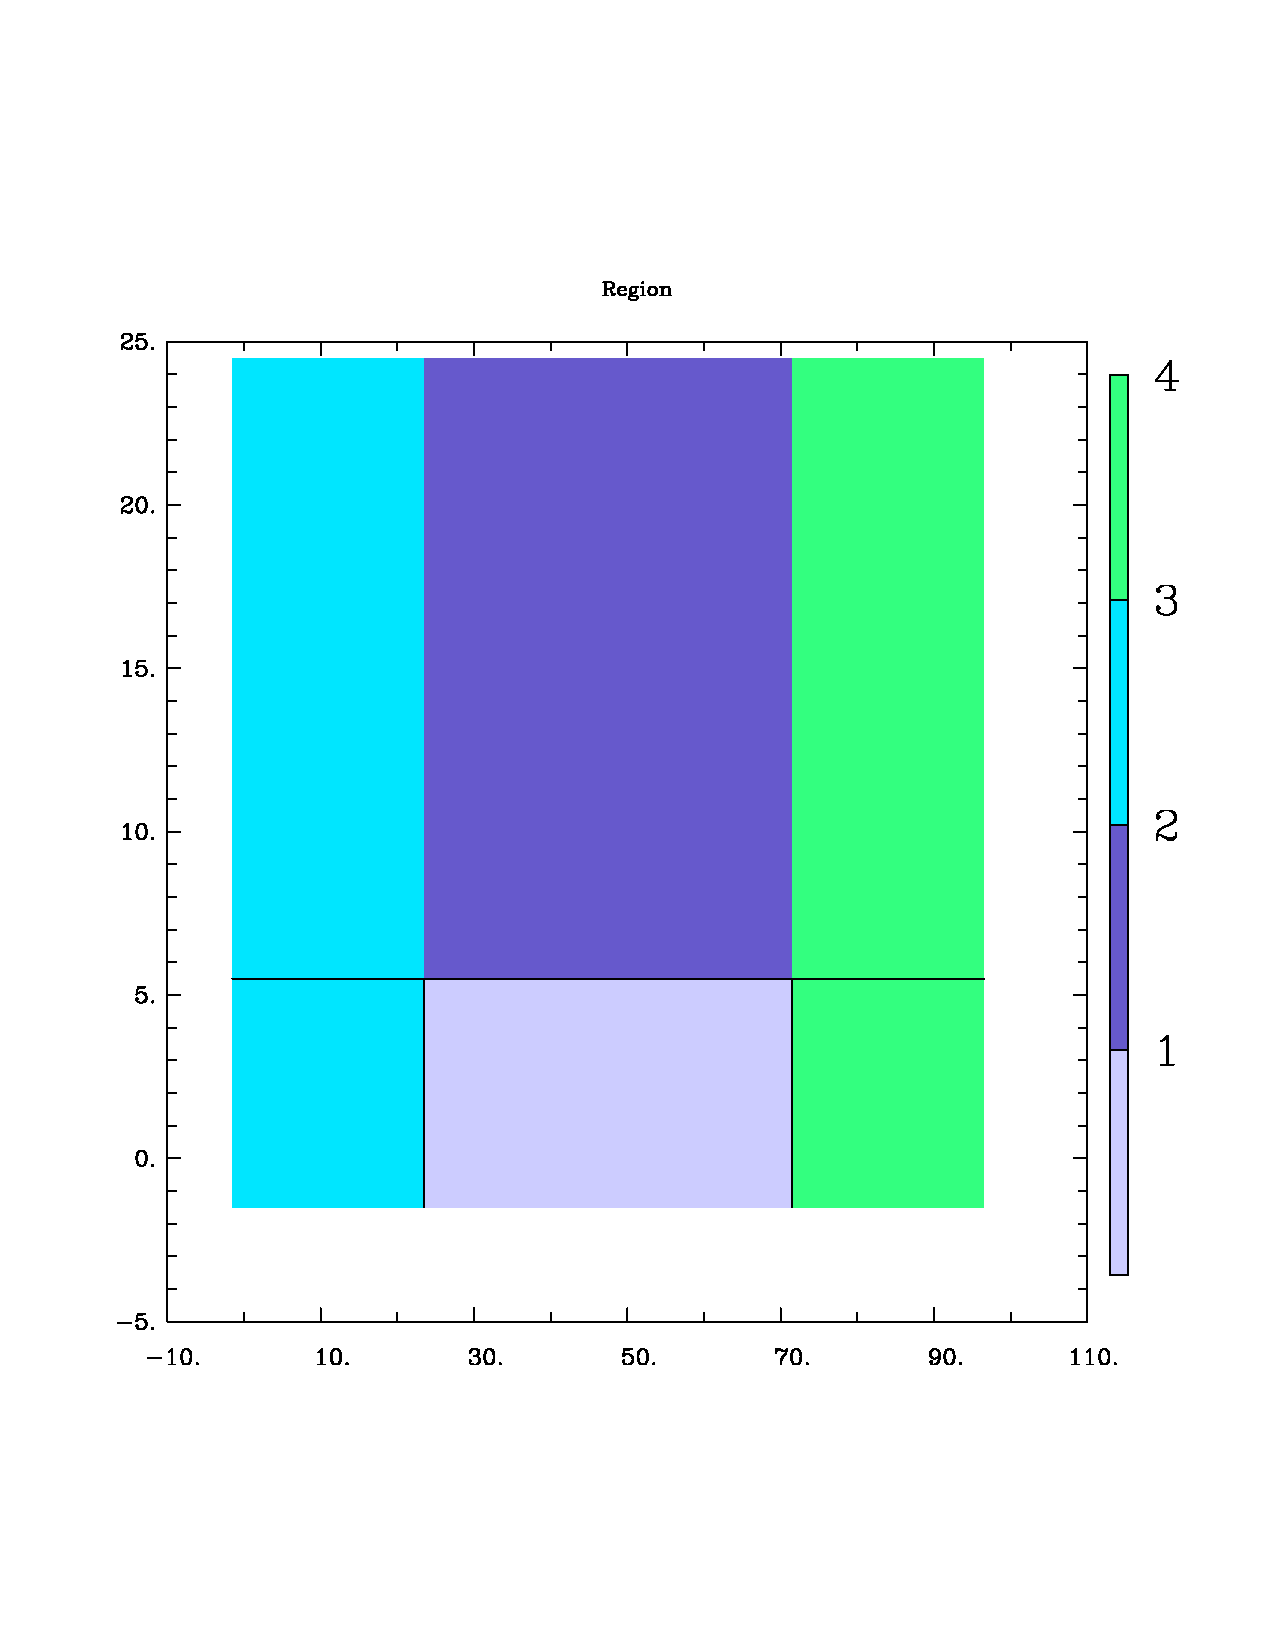
\includegraphics[height=7cm]{SN_comp.pdf}}
  \subfigure[Physics domain]{\label{fig:SN_phys}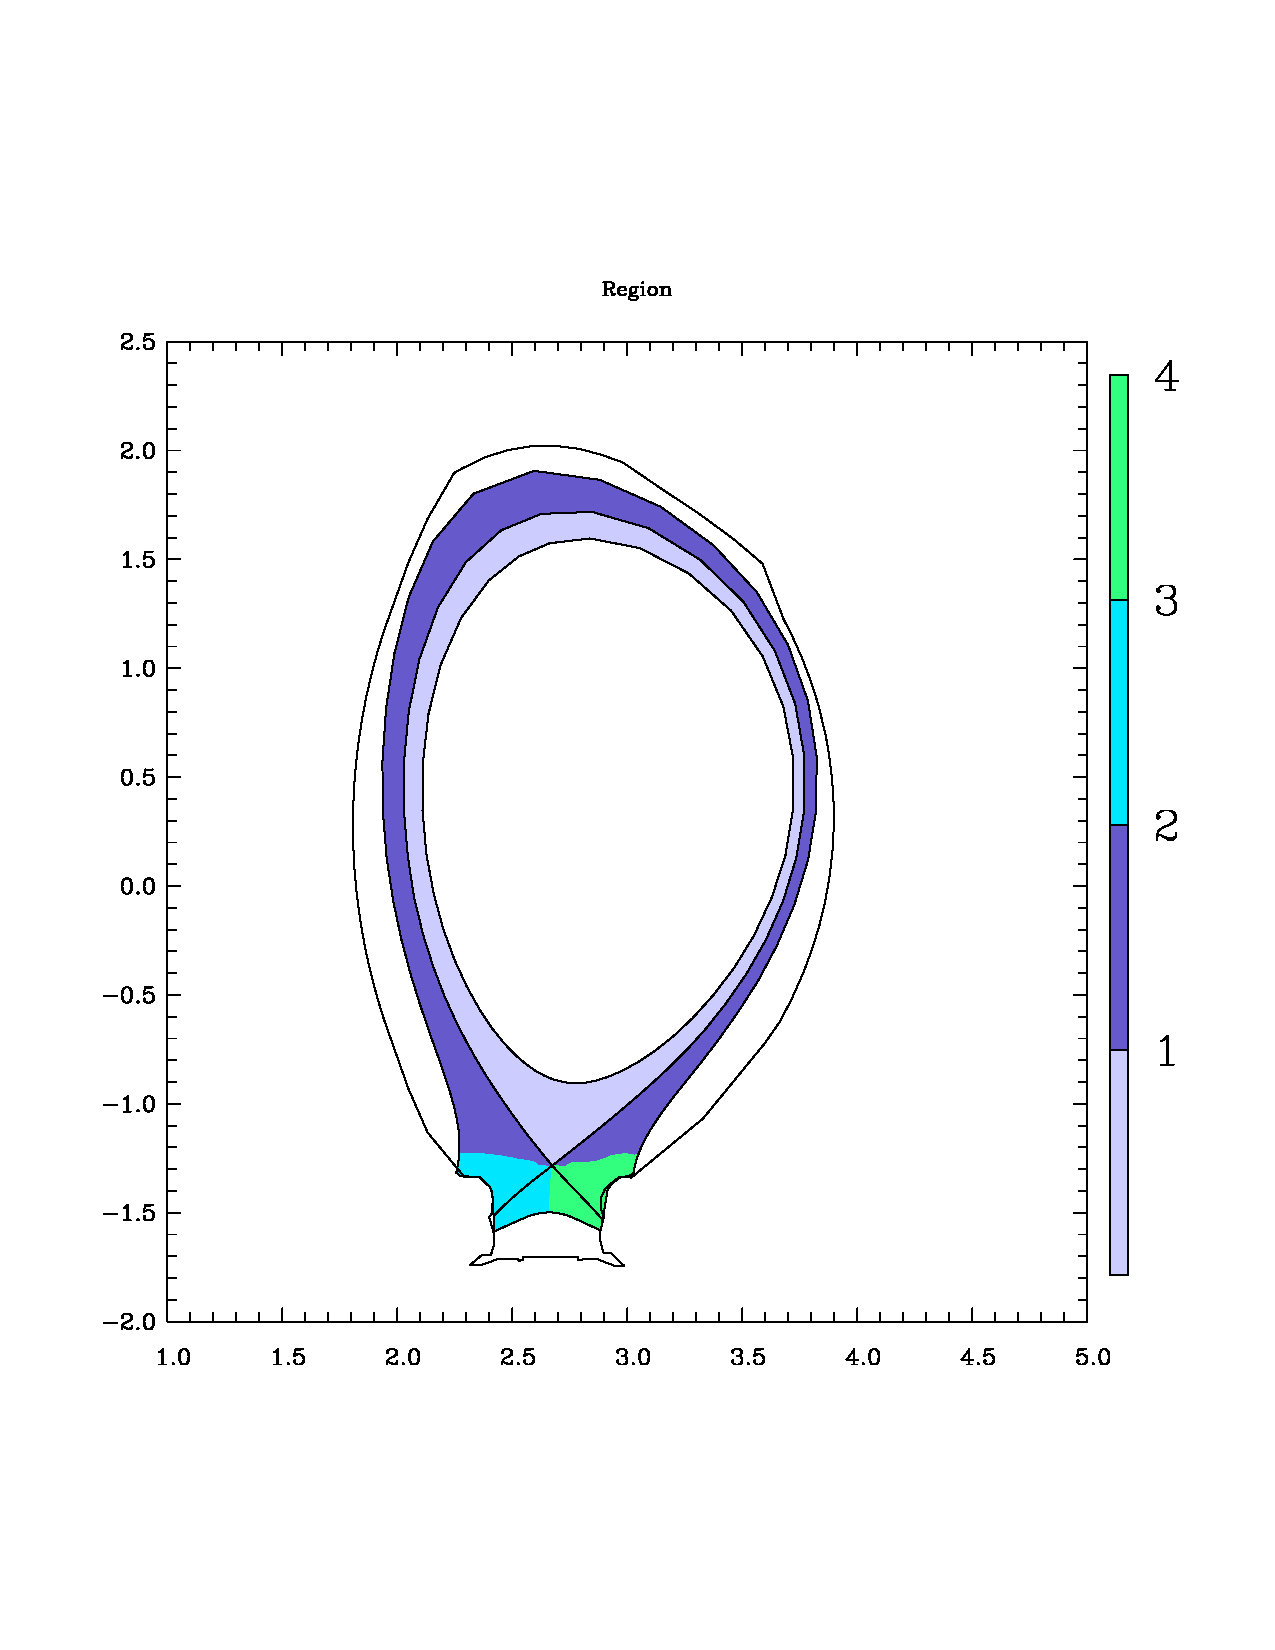
\includegraphics[height=7cm]{SN_phys.pdf}}
\else
  \subfigure[Computational domain]{\label{fig:SN_comp}
\includegraphics[height=7cm]{SN_comp.epsi}}
  \subfigure[Physics domain]{\label{fig:SN_phys}
\includegraphics[height=7cm]{SN_phys.epsi}}
\fi
  \caption{Region numbers for single-null geometries.}\label{fig:SN_regions}
\end{figure}

\begin{figure}[hbtp]
  \centering
\ifpdf 
  \subfigure[Computational domain]{\label{fig:DN_comp}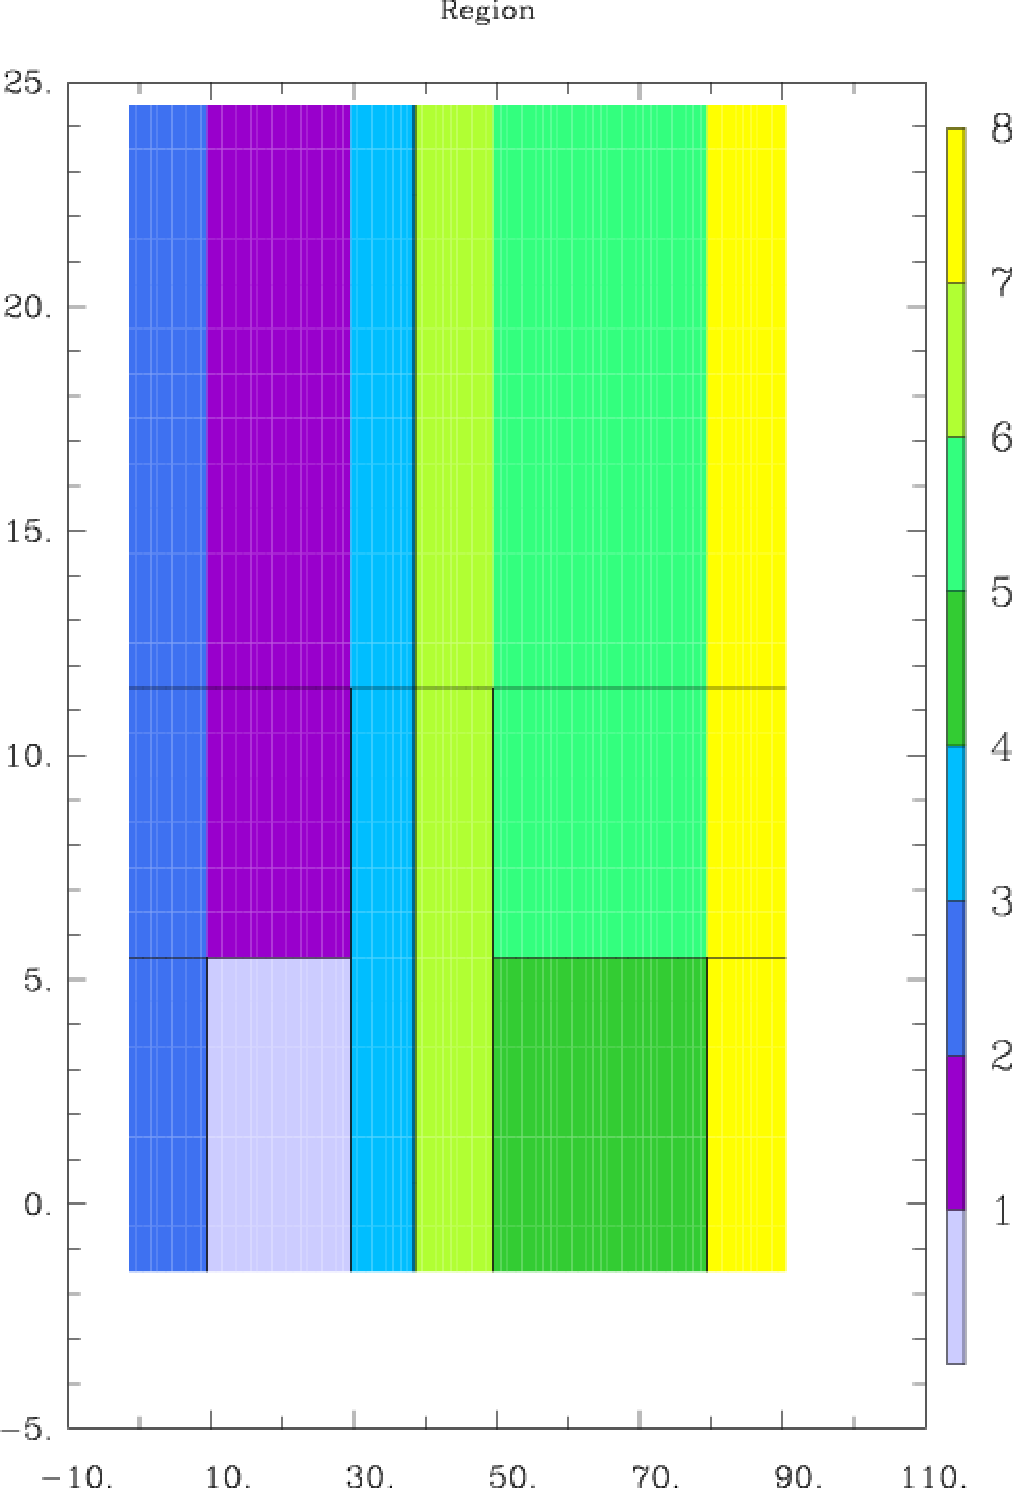
\includegraphics[height=7cm]{DN_comp.pdf}}
  \subfigure[Physics domain]{\label{fig:DN_phys}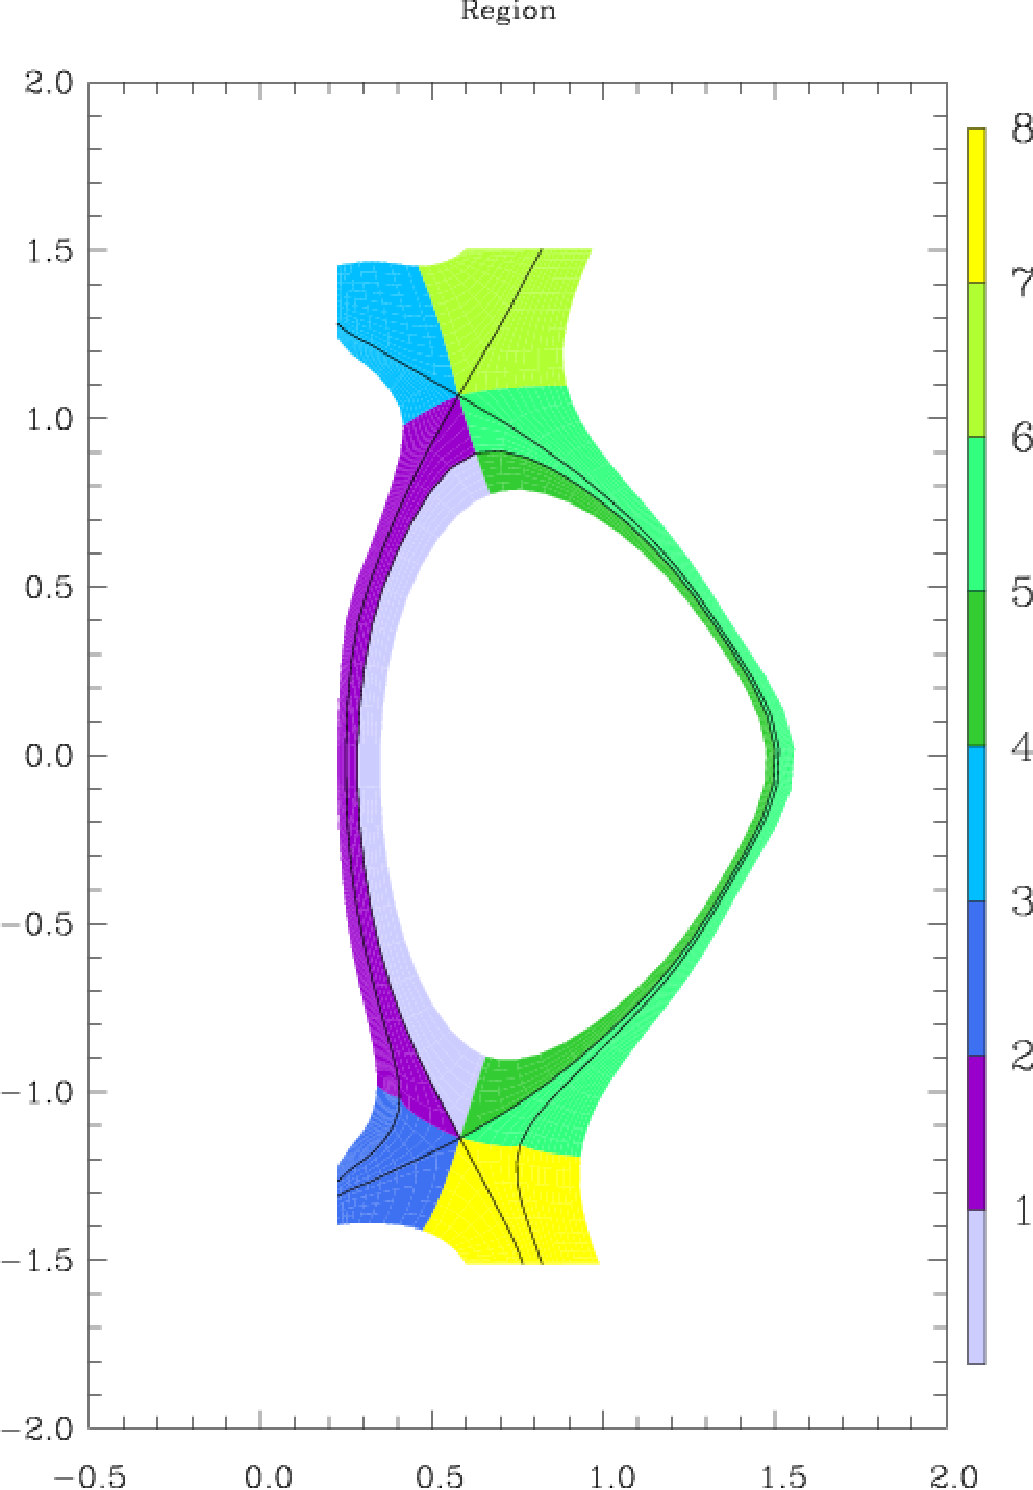
\includegraphics[height=7cm]{DN_phys.pdf}}
\else
  \subfigure[Computational domain]{\label{fig:DN_comp}
\includegraphics[height=7cm]{DN_comp.epsi}}
  \subfigure[Physics domain]{\label{fig:DN_phys}
\includegraphics[height=7cm]{DN_phys.epsi}}
\fi
  \caption{Region numbers for double-null geometries.}\label{fig:DN_regions}
\end{figure}

\subsection{b2.transport.inputfile}
\index{b2.transport.inputfile}\index{b2tqna}\index{b2tqna\_inputfile}\index{transport coefficients}\label{lab:b2:transport:inputfile}\index{b2ah.dat}\index{b2mn.dat}\index{b2.transport.parameters}

See also Appendix \ref{lis:b2cdcn} for a more up-to-date description. 
 
This allows for a radial variation ... for a simpler option see
section \ref{lab:b2:transport:parameters}.

If \verb!'b2tqna_inputfile'! is set to 1 in \verb!b2mn.dat!
then the transport coefficients are read in from the namelist in
\verb!b2.transport.inputfile! instead of being taken from the file
created by \verb!b2ah! and possibly modified in \verb!b2mn.dat!.
This then allows one to set radially 
varying profiles of the transport coefficients, and to achieve time
dependence in these transport coefficients by triggering a read of a
new file (as for \verb!b2.transport.parameters!).
The transport coefficients are specified by the \verb!transport! namelist
as described below.

The input format for these files is somewhat arcane (the relevant
subroutine is \verb!transport_input!, to be found in \verb!b2mod_input_profile.F!) and an
example, without the modification for reading in a new file triggered
by time, which is the same as for the \verb!b2.transport.parameters!, is
included below.

The basic idea is to specify pairs of numbers which give the position
and value of the relevant transport coefficients.

\verb!tdata! has four indices:

The value of the first index $=1$ means position in space, $=2$ means the value.

The second is used to index the various positions (6 positions in the
example below, specified by \verb!ndata!). The total number of positions should not
exceed $ny+2$, as having transport coefficient profiles finer than the 
plasma grid resolution is overkill.

The third index of \verb!tdata! relates to the kind of transport coefficient 
being specified, where:
\begin{description}\index{kind\_coeff}
  \item[kind\_coeff.eq.1 $\Rightarrow$ dna0  ]   particle density-driven diffusivity $D_\perp^{na}$
  \item[kind\_coeff.eq.2 $\Rightarrow$ dpa0  ]   particle pressure-driven diffusivity $D_\perp^{pa}$
  \item[kind\_coeff.eq.3 $\Rightarrow$ hcib  ]   ion thermal anomalous diffusivity $\chi_i$        
  \item[kind\_coeff.eq.4 $\Rightarrow$ hce0  ]   electron thermal anomalous diffusivity $\chi_e$
  \item[kind\_coeff.eq.5 $\Rightarrow$ vla0\_x]  $x$-component of the anomalous "pinch" velocity
  \item[kind\_coeff.eq.6 $\Rightarrow$ vla0\_y]  $y$-component of the anomalous "pinch" velocity
  \item[kind\_coeff.eq.7 $\Rightarrow$ vsa0  ]   anomalous viscosity
  \item[kind\_coeff.eq.8 $\Rightarrow$ sig0  ]   anomalous radial electrical conductivity
  \item[kind\_coeff.eq.9 $\Rightarrow$ alf0  ]   anomalous radial thermo-electric coefficient
\end{description}
                
The fourth index is the species index.

Again, as in Section \ref{lab:b2cmpt}, it is important, for numerical stability reasons, 
to provide mechanisms by which some
particle transport and radial current can be established. If the transport coefficients
are given here, this means that, first, the \verb!dna0! and \verb!dpa0! arrays 
cannot be simultaneously zero when solving density equations. Second, the arrays 
\verb!sig0! and \verb!alf0! cannot be
simultaneously zero when solving the potential equations without drift current terms on.
The code will fail a transport coefficients test in \verb!b2tral! otherwise.

The relevant routine was written by

\begin{verbatim}
!**************************************************************************
!*     subroutine for reading in experimental transport coefficients from *
!*     the midplane and calculating transport coefficients                *
!*     for B2.5 (written by Heimo Buerbaumer 1999)                        *
!*     Inputfile:  b2.transport.inputfile                                 *
!**************************************************************************
\end{verbatim}

Some additional description of the relevant variables is as follows:

\begin{description}
  \item[ndata(1,i,j)]\index{ndata} where $i$ is an index for the type of transport coefficient
     being defined (see table above) and $j$ is a species index ($0$ for atoms and $1$
     for ions in a $D$-only case, for instance, and irrelevant (use $1$) for electron 
     coefficients). \verb!ndata! is the
     number of data points where the value of the transport coefficients is given.
  \item[addspec(k,i,j)]\index{addspec} are the indices of any additional species whose
     transport coefficients are also described by the same set of numbers. $k$
     is a dummy that runs from $1$ to the number of additional species
     described.
  \item[tdata(1,m,i,j)]\index{tdata} are the radial positions (measured in metres) of the 
     \verb!ndata(1,i,j)! points,
     where $m$ runs from $1$ to \verb!ndata(1,i,j)!. By default, the radial positions are
     measured from the separatrix outward, along the outer midplane, but this can be changed by
     making use of the $ixref$ and $iyref$ switches, respectively, to modify the poloidal
     location of the profile and the radial position from which the distances are measured. 
  \item[tdata(2,m,i,j)] are the corresponding values of the coefficients.
  \item[no\_pflux]\index{no\_pflux} is a logical that, if \verb!.true.!, does not apply these
     transport coefficients to the private flux region(s).
\end{description}

So in the example file below, three transport coefficients profiles
are given, i.e. in order, $D_\perp^{na}$, $\chi_i$ and $\chi_e$, defined
with 6 points each, and setting a transport barrier around the separatrix.
Note that the radial locations of those points are quite
independent of where the mesh is. The code interpolates the transport
values onto the mesh, so one needs not worry about making sure
that a point is at an exact cell location. 
It is recommended that the first and last points be a large distance away 
from the separatrix, typically well outside the computational
domain. This ensures that the code is still interpolating and not
using (possibly different) default values when computing coefficients for cells near the
edges of the mesh. The interpolation the code uses is a
monotonicity-preserving cubic Hermite polynomial spline from the NAG
library, or a simple linear interpolation if the NAG library is
unavailable at compilation time. For computational cells located 
outside the range provided by the \verb!tdata(1,m,i,j)! positions, 
the code will use whatever
'default' values were declared previously. As a reminder, the order of 
precedence of the transport coefficients settings is:
\begin{verbatim}
b2ah.dat < b2mn.dat < b2.tranport.parameters < b2.transport.inputfile
\end{verbatim}

The following contains an example where the flag \verb!no_pflux! is
used to switch off the setting of transport coefficients in the
private flux region.

\VerbatimInput[fontsize=\footnotesize]{b2.transport.inputfile}

\subsection{b2.sources.profile}
\index{b2.sources.profile}\index{b2sral}\index{b2sral\_inputfile}\index{sources}\label{lab:b2:sources:profile}

See also Appendix \ref{lis:b2cdcn} for a more up-to-date description. 
 
One can also set radially dependent source profiles, in much the same way as with
\verb!b2.transport.inputfile!, with the \verb!b2.sources.profile! input file, 
accessed by setting 'b2sral\_inputfile' to '1'. The logic is the same in terms
of fixing radial positions, applicable species, etc...

The coefficient types go as:
\begin{enumerate}
   \item Particle sources {\em sna} \index{b2plot, exna}
   \item Parallel momentum sources {\em smo} \index{b2plot, exmo}
   \item Electron heat sources {\em she} \index{b2plot, exhe}
   \item Ion heat sources {\em shi} \index{b2plot, exhi}
   \item Electric charge sources {\em sch} \index{b2plot, exch}
   \item Electric particle source (non-ambipolar) {\em sne} \index{b2plot, exne}
\end{enumerate}

It is also possible to multiply these radial profiles by an axial form factor.
This axial multiplier is set in the same way as the poloidal profile.

The description of the variables found in \verb!b2.sources.profile! is as follows:
\begin{description}
  \item[nsdata(1,i,j)]\index{nsdata} where $i$ is an index for the type of source
     being defined (see table above) and $j$ is a species index ($0$ for atoms and $1$
     for ions in a $D$-only case, for instance, and irrelevant (use $1$) for electron 
     sources). \verb!nsdata! is the
     number of data points where the strength of the source is given.
  \item[sdata(1,m,i,j)]\index{sdata} are the radial positions (measured in metres) of the 
     \verb!nsdata(1,i,j)! points,
     where $m$ runs from $1$ to \verb!nsdata(1,i,j)!. By default, the radial positions are
     measured from the separatrix outward, along the outer midplane, but this can be changed by
     making use of the $ixref$ and $iyref$ switches, respectively, to modify the poloidal
     location of the profile and the radial position from which the distances are measured. 
  \item[sdata(2,m,i,j)] are the corresponding strengths of the sources.
  \item[nxdata(k,i,j)]\index{nxdata} where $i$ is an index for the type of source
     being defined (see table above) and $j$ is a species index ($0$ for atoms and $1$
     for ions in a $D$-only case, for instance, and irrelevant (use $1$) for electron 
     sources). \verb!nxdata! is the
     number of data points where the value of the axial multiplier to the source is given.
     If $k$ is equal to $1$, the data is to be understood as function of normalized
     connection length. If $k$ is equal to $2$, then the axial profile is given in terms
     of the normalized computational coordinate (running from $0$ to $1$ as $ix$ runs from
     $-1$ to $nx$). 
  \item[xdata(1,m,i,j)]\index{xdata} are the axial positions (normalised to the total length) 
     of the \verb!nxdata(1,i,j)! points,
     where $m$ runs from $1$ to \verb!nxdata(1,i,j)!. By default, the connection length
     used is the one measured just inside the separatrix, with the origin 
     located at the outer midplane, but this can be changed by
     making use of the $ixref$ and $iyref$ switches, respectively, to modify the poloidal
     location of the origin and the radial position along which the distances are measured.
     In case the reference location is chosen inside a closed field line region, the axial
     multiplier is set to zero everywhere on the open field lines. 
  \item[xdata(2,m,i,j)] are the corresponding values of the source strengths.
  \item[divheat]\index{divheat} is the total volumetric ion heat source (in $W/m^{3}$) 
     spread equally throughout the divertor volume.
\end{description}

The results of these imported source profiles can be visualised in
\btwoplot with the {\bf exna}, {\bf exmo}, {\bf exhe}, {\bf exhi},
{\bf exch}, and {\bf exne} commands. An example of input file is given below:

\VerbatimInput[fontsize=\footnotesize]{b2.sources.profile}

\subsection{b2.neutrals.parameters}
\index{b2.neutrals.parameters}\label{lab:b2:neutrals:parameters}

See descriptions in Coupled \verb!Eirene! chapter \ref{cha:coupledb2eirene}
and Appendix \ref{lis:b2cdcn}.

\subsection{b2.atomic\_physics\_rescale.parameters}
\index{b2.atomic\_physics\_rescale.parameters}\label{lab:b2:atomic_physics_rescale:parameters}

Contains a series of multipliers to the atomic physics rates provided by \verb!b2ar! in \verb!b2frates!.
These are:
\begin{description}
  \item[RESCALE\_SA]\index{RESCALE\_SA} \verb!real*8 array, length NS!,
  contains the scaling factor per species to be applied to the ionisation rates
  \item[RESCALE\_RA]\index{RESCALE\_RA} \verb!real*8 array, length NS!,
  contains the scaling factor per species to be applied to the recombination rates
  \item[RESCALE\_QA]\index{RESCALE\_QA} \verb!real*8 array, length NS!,
  contains the scaling factor per species to be applied to the electron cooling rates
  \item[RESCALE\_CX]\index{RESCALE\_CX} \verb!real*8 array, length NS!,
  contains the scaling factor per species to be applied to the charge exchange rates
  \item[RESCALE\_RD]\index{RESCALE\_RD} \verb!real*8 array, length NS!,
  contains the scaling factor per species to be applied to the line radiation rates
  \item[RESCALE\_BR]\index{RESCALE\_BR} \verb!real*8 array, length NS!,
  contains the scaling factor per species to be applied to the bremsstrahlung radiation rates
\end{description}

See Appendix \ref{lis:b2cdcn} for a full description.

\subsection{b2.user.parameters}
\index{b2.user.parameters}\label{lab:b2:user:parameters}

See descriptions in Coupled \verb!Eirene! chapter \ref{cha:coupledb2eirene}
and Appendix \ref{lis:b2cdcn}.

\subsection{b2.XXX.parameters}

See descriptions in Appendix \ref{lis:b2cdcn}.

\subsection{While the code is running}
\label{sec:b2running}

While the code is running and writing into \verb!run.log!, a number of
the scripts described in section \ref{sec:scripts} can be run.

\verb!cpu!\index{cpu} shows how much CPU time each iteration has taken and is a
quick way of monitoring the progress of a run.

\begin{verbatim}
18:22> cpu
# /scratch/dpc/solps5.0_test_xpb/src/Braams/b2/runs/JET_B2_comparison/50401/57_coarse/2e19_8MW
1 2.129999935626984
2 1.940000295639038
3 1.730000019073486
4 1.719999313354492
5 1.710000038146973
6 1.720000267028809
7 1.690000534057617
8 1.710000038146973
9 1.679999351501465
10 1.700000762939453
11 1.699998855590820
12 1.710000991821289
13 1.699998855590820
18:22> 
\end{verbatim}

All of the residuals of a pure deuterium run can be plotted with
\verb!resall_D!\index{resall\_D}, figure \ref{fig:resallD}. 

\begin{figure}[hbtp]
\ifpdf 
    \centerline{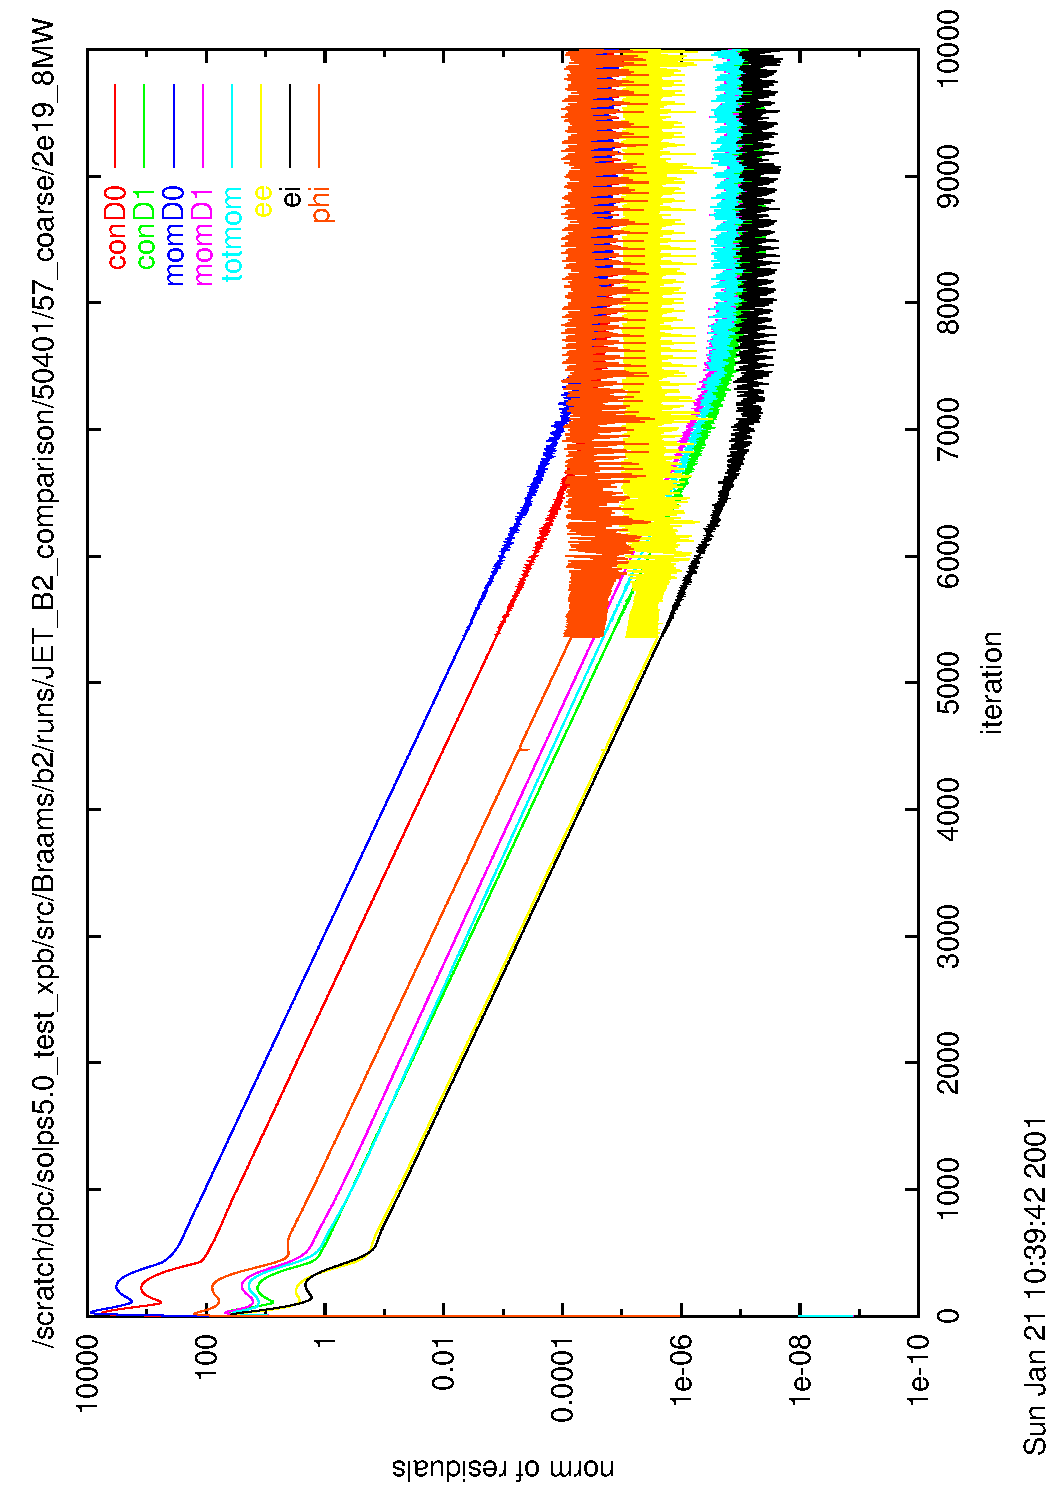
\includegraphics[origin=br,angle=-90,height=8cm]{resall_D.pdf}}
\else
    \centerline{\includegraphics[origin=br,angle=-90,height=8cm]{resall_D.ps}}
\fi
    \caption{Residuals.}
    \label{fig:resallD}
\end{figure}

The power crossing various surfaces can be seen with
\verb!energy_analysis!\index{energy\_analysis} or 
\verb!energy_analysis.py!\index{energy\_analysis.py}, figure \ref{fig:energyanalysis}.
The detailed definition of these surfaces can be found in Appendix \ref{cha:regions} 
or the commented header to the \verb!init_region! subroutine in 
\verb!b2agfs.F!.

\begin{figure}[hbtp]
\ifpdf 
    \centerline{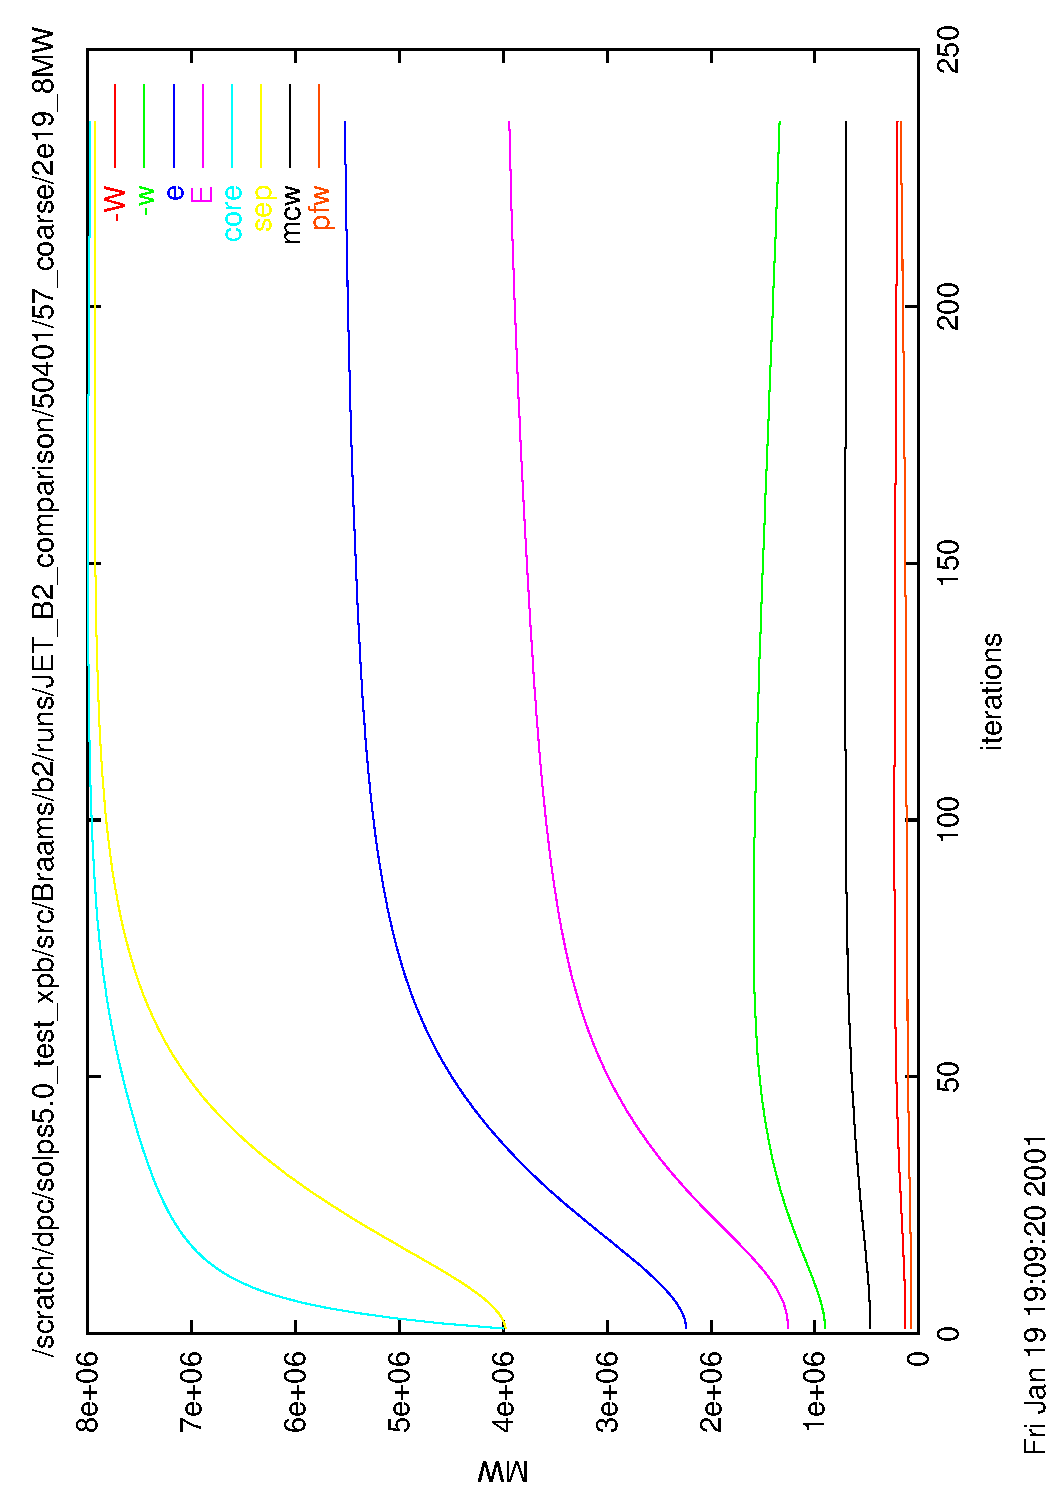
\includegraphics[origin=br,angle=-90,height=8cm]{energy_analysis.pdf}}
\else
    \centerline{\includegraphics[origin=br,angle=-90,height=8cm]{energy_analysis.ps}}
\fi
    \caption{Power crossing various surfaces.}
    \label{fig:energyanalysis}
\end{figure}

\verb!2dt tesepm!\index{2d, tesepm} can be used to plot the separatrix
temperature as a function of time, figure \ref{fig:tesepm}.  See table
\ref{tab:2db2time} (page \pageref{tab:2db2time}) for a list of
quantities that can be plotted in this way.

\begin{figure}[hbtp]
\ifpdf 
    \centerline{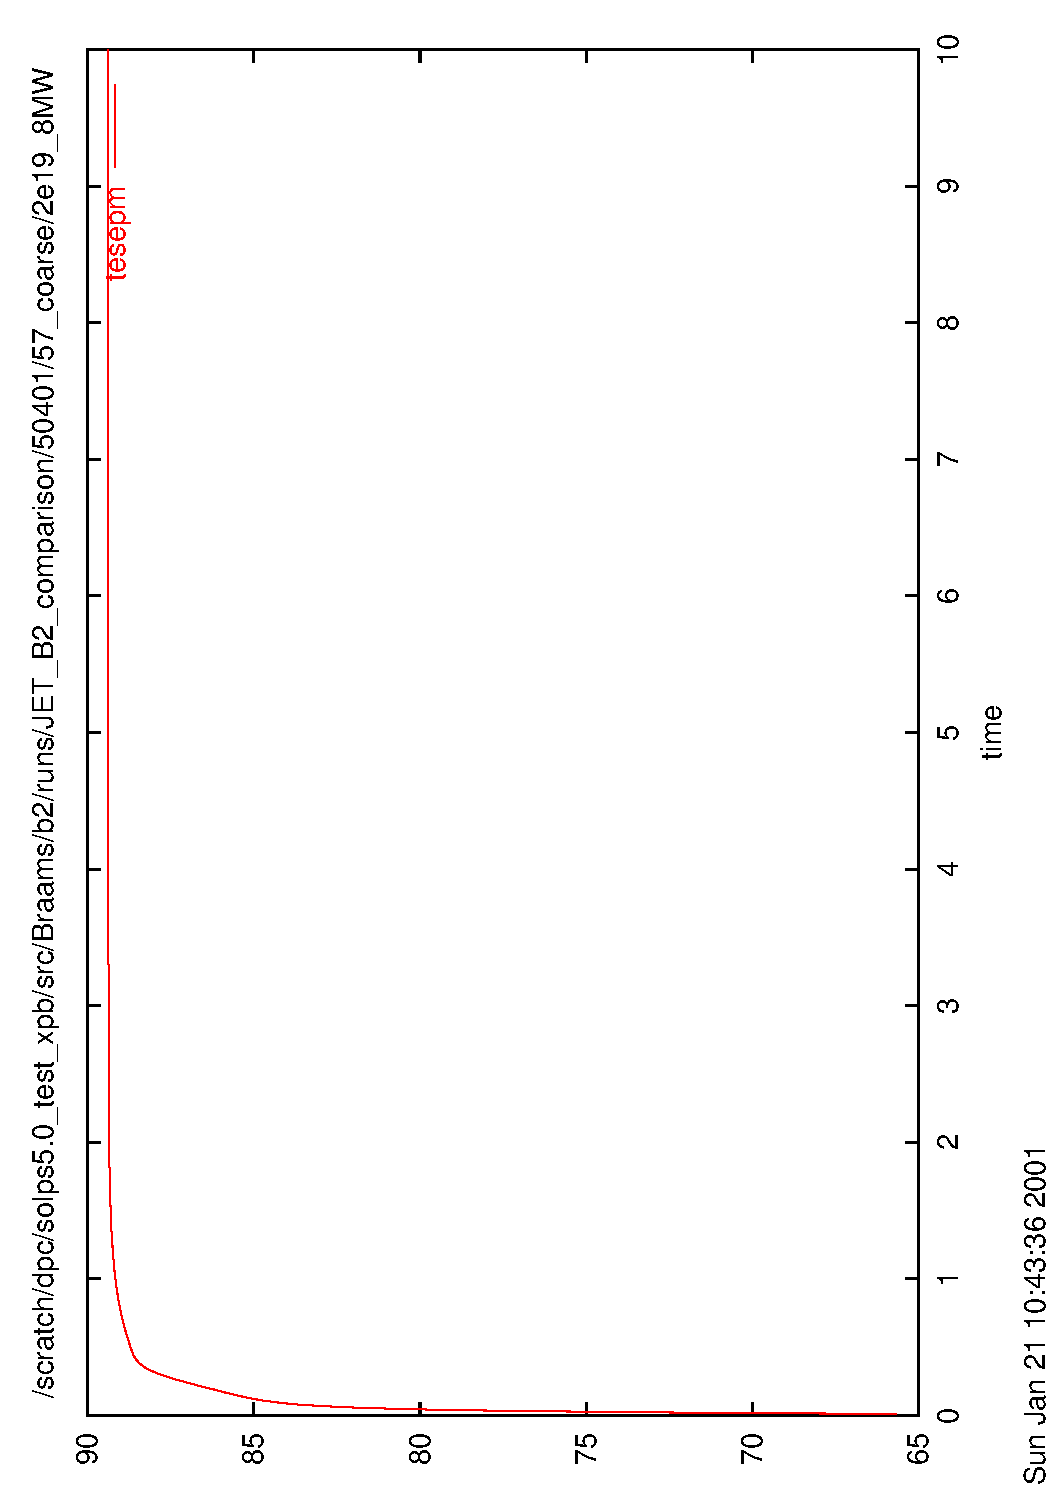
\includegraphics[origin=br,angle=-90,height=8cm]{tesepm.pdf}}
\else
    \centerline{\includegraphics[origin=br,angle=-90,height=8cm]{tesepm.ps}}
\fi
    \caption{Upstream (outer midplane) electron temperature.}
    \label{fig:tesepm}
\end{figure}

\verb!!\index{} 

\verb!!\index{} 

\verb!!\index{} 

\newpage
\section{b2pl, the plotting program}
\index{b2pl}\index{b2plot}\label{sec:b2pl}

%%sed 's:^     [^ ]:@@@:' $SOLPSTOP/modules/B2.5/src/b2plot/b2plot.F | awk 'BEGIN{save=""}/^[^@][^@][^@]/&&save!=""{print save}/^[^@][^@][^@]/{save=$0}/^@@@/{save=save" "$0}END{print save}' | sed 's; *@@@ *;;g' | egrep "case *\( *'|description *=" | sed -e "s;.*case *('\(.*\)');cmd: \1;" -e "s; *description *= *'\(.*\)';desc: \1;" | awk -F: 'BEGIN{save=""}/^cmd/&&save!=""{print save}/^cmd:/{save=$2}/^desc/{save=save"\t"$2}END{print save}' | sed 's:\! ::' | sed "s:',':,:g" | sed "s:'':':g" | expand >! b2plot.commands

The following commands apply:

\VerbatimInput[fontsize=\footnotesize]{b2plot.commands}

A revised copy of the \btwoplot manual can be found in Appendix
\ref{cha:b2plotmanual}, page \pageref{cha:b2plotmanual}.  Note that some
of the quantities have changed name between \SOLPSfour and \SOLPSfive versions, 
\index{b2plot, changes from SOLPS4.0 to SOLPS5.0}table \ref{tab:changedplotquantities}, and that
whereas \verb!ix! ran from \verb!0! to \verb!nx+1! it now runs from
\verb!-1! to \verb!nx!, \verb!iy! which ran from \verb!0! to \verb!ny+1! 
now runs from \verb!-1! to \verb!ny! and \verb!is! which ran from \verb!1!
to \verb!ns! now runs from \verb!0! to \verb!ns-1!.

\begin{table}[hbtp]
  \leavevmode
  \begin{center}
    \begin{tabular}{|l|l|}
    \hline
    \SOLPSfour  & \SOLPSfive  \\ \hline
    ni          & na          \\
    zi          & za          \\
    up          & ua          \\
    dx          & hx          \\
    dy          & hy1         \\
    feex        & fhex        \\
    feey        & fhey        \\
    feix        & fhix        \\
    feiy        & fhiy        \\
    fnix        & fnax        \\
    fniy        & fnay        \\ \hline
    \end{tabular}
    \caption{Changes of quantity names from \SOLPSfour \btwoplot to \SOLPSfive {\bf b2pl.exe}.}
    \label{tab:changedplotquantities}
  \end{center}
\end{table}

\newpage
\section{b2yt, changing from one grid size and species set to another}
\index{b2yt}\index{b2fstatt}\label{sec:b2yt}\index{input.dat}\index{input.dat.2}\index{b2mn.dat}\index{b2fgmtry}
\index{b2fgmtry.old}\index{b2mn.dat.2}\index{b2.boundary.parameters}\index{b2.boundary.parameters.2}
\index{b2.neutrals.parameters}\index{b2.neutrals.parameters.2}\index{b2ah.dat}\index{b2ah.dat.2}
\index{b2.wall\_save.parameters}\index{b2.wall\_save.parameters.2}\index{b2frates}\index{b2fpardf}
\index{b2.transport.parameters}\index{b2.transport.parameters.2}\index{SOLPS\_FLUIDS}

This utility program allows a user to take a \verb!b2fstate! solution file
with size $nx \times ny$ and transform it into an $nx1 \times ny1$ \verb!b2fstatt!
file, provided the numbers of real cells in both $x$ and
$y$ directions in the new solution are divisors of the ones in the original mesh. Other 
files necessary to proceed with the run under the new geometry will also be produced. The 
two numbers $nx11$ and $ny1$ are provided by the user in the \verb!b2yt.dat! 
file. The \verb!b2yt.dat! file should contain, for example:
\begin{verbatim}
*dimens         (nx1, ny1; free format)
  8  8
\end{verbatim}
with any optional switches mentioned afterwards, to create a solution on an $8 \times 8$ grid.

A solution for non-commensurate grids is also available, requiring
instead that the topology of the two solutions be the same, and works by 2-D
interpolation of the plasma data in the computational domain, by region. This is 
activated with the 'b2ytdr\_non\_commensurate' option set to '1' in \verb!b2yt.dat!. 

The conversion of the \verb!Eirene! input file additionally requires for the converter program to know the original version of \verb!Eirene! with which the input file was used, and this is provided by means of the 'eirene\_format' switch. Its possible values (case-insensitive) are:
\begin{description}
  \item[``old''] for input files from {\bf SOLPS4.0} and {\bf SOLPS5.0} runs using "old" Eirene\_96
  \item[``new''] for input files from {\bf SOLPS4.0} and {\bf SOLPS5.0} runs using "new" Eirene\_99
  \item[``facelift''] for input files from \SOLPSfiveone runs
  \item[``juelich''] for input files from Juelich \verb!Eirene! versions (2008 and younger)
  \item[``iter''] (default) for input files from {\bf SOLPS4.2/4.3} and \SOLPSITER runs
\end{description}
The \verb!input.dat.2! file that the converter will create will follow the \SOLPSITER format.

The conversion of the \verb!Eirene! output file (\verb!fort.44!) additionally requires for the converter program to know the original version of \verb!SOLPS! with which the output file was created, and this is provided by means of the 'solps\_version' switch. Its possible values (case-insensitive) are:
\begin{description}
  \item[``4.3''] for \verb!fort.44! output files from {\bf SOLPS4.3} runs
  \item[``5.0''] for \verb!fort.44! output files from {\bf SOLPS5.0} runs
  \item[``5.1''] for \verb!fort.44! output files from \SOLPSfiveone runs
  \item[``5.2''] for \verb!fort.44! output files from {\bf SOLPS5.2} runs
  \item[``iter''] (default) for input files from \SOLPSITER runs (no conversion necessary)
\end{description}
The \verb!fort.44.2! file that the converter will create will follow the \SOLPSITER format.

\verb!b2yt! may also be used
to change the order of species (for example changing from $D+C+He$ to $D+He+C$) or for
bundling, de-bundling or re-bundling species, or even removing species and complete
isonuclear sequences. It is however not possible to use this converter to {\em add} 
a new isonuclear sequence. When modifying the species data, the user
should run \verb!b2ar! with the new species arrangement before running \verb!b2yt!
to obtain a temporary file \verb!b2frates!. After \verb!b2yt! has been run succesfully,
then the user should re-run \verb!b2ah! (using the produced \verb!b2ah.dat.2! file,
after renaming it \verb!b2ah.dat!) and \verb!b2ar! before re-launching the run.

If a new geometry is requested, the \verb!b2yt! program should be run after the 
new geometry file ($nx1 \times ny1$) has 
been produced and is available in the run directory as \verb!b2fgmtry!. 
The old geometry file should also remain available in 
the run directory as \verb!b2fgmtry.old!.

The program also needs the \verb!b2mn.dat! and any other used input files (such 
as \verb!input.dat!, \verb!b2.*.parameters! or \verb!b2.*.inputfile!) from 
the original run. 

It is important for proper \verb!b2yt! execution that the necessary files have the
expected seniority from the Makefile. Therefore, you must ensure that:
\begin{enumerate}
  \item \verb!b2fstate! is the {\em youngest} file.
  \item \verb!b2frates! (or \verb!../baserun/b2frates!) is {\em older} than \verb!b2fstate! but {\em younger} than \verb!b2fgmtry!.
  \item \verb!b2fpardf! (or \verb!../baserun/b2fpardf!) is {\em younger} than \verb!b2ah.dat! and 
         {\em older} than \verb!b2frates!.
  \item \verb!b2fgmtry! must be {\em younger} than \verb!b2ag.dat! and {\em older} than \verb!b2fpardf!.
\end{enumerate}

So, ALL of the following must be verified:
\begin{verbatim}
b2ag.dat < b2fgmtry < b2fpardf < b2frates < b2fstate

b2ah.dat < b2fpardf

b2ar.dat < b2frates
\end{verbatim}
If this order is not met, use a series of "touch 'filename' " commands
to give the files new dates. The best to check this is to run the command:
\begin{verbatim}
b2run -n b2yt
\end{verbatim}
which will launch a dry-run of the Makefile invoking \verb!b2yt!. Then, make sure
that this dry-run only attempts to run \verb!b2yt! and no other programs. If it 
does call, say \verb!b2ag! and/or \verb!b2mn!, then the age hierarchy above was
not respected. In that case, you can run the script
\begin{verbatim}
correct_b2yt_timestamps
\end{verbatim}
to get the correct ordering of files. Do check again afterwards with the dry-run
command to make sure it worked.

Upon successful termination of \verb!b2yt!, the user will find a \verb!b2fstatt!
file containing the transformed plasma state, as well as a \verb!b2mn.dat.2! file which 
will contain the updated run switches appropriate for the new geometry and species
selection. Similarly, if
\verb!b2.boundary.parameters! and \verb!b2.neutrals.parameters! files were present
in the working directory, files \verb!b2.boundary.parameters.2! and 
\verb!b2.neutrals.parameters.2!,
respectively, will contain the updated namelist variables. The program will also create
a new \verb!b2.wall_save.parameters.2! file containing the new wall namelist settings
when appropriate. Other \verb!B2.5! input files are treated in the same fashion. The 
code will also attempt to create a new \verb!SOLPS_FLUIDS.2! file appropriate for the 
new species list.

If an \verb!input.dat! file is present in the run directory, the code will also attempt
to produce a new \verb!input.dat.2! file. In order to
ensure consistency between the \verb!B2.5! and \verb!Eirene! modified inputs, it is 
important that the order of the neutrals boundary conditions in 
\verb!b2.neutrals.parameters! and the strata in \verb!input.dat! match!
When species are being re-bundled, possible 
conflicts may occur between their individual settings. In such cases, the code behaviour 
is to use the setting from the highest charge state within the bundle. If species are 
being removed, strata, tallies or diagnostics involving these species may either be 
removed from the input file or revert to their default settings. The user is encouraged 
to check that those choices are appropriate and modify them as needed. 

At this time, not all cases involving reshuffling of bundles have been tested, and the 
user is encouraged to check the \verb!b2yt! output files visually after execution to 
make sure no mistakes remain. No attempt is made to adjust or modify the text labels
pertaining to the various input files, so the user is encouraged to adapt those to the
new case being built. Report of conversion errors or omissions to the developer team 
are always welcome. 

\newpage
\section{b2co, recovering from a crash}
\label{sec:b2co}\index{b2co}\index{plasmastate}\index{B2.5, run recovery}\index{b2fstate}

In case of a computer crash during a run, it may be possible to recover
the results and continue the simulation. The code writes, at regular
intervals (default is 3600 CPU seconds, and can be modified with use of the
'b2mndr\_cpu' and 'b2mndr\_plasmatim' switches, see Appendix \ref{lis:b2cdci} for details and additional options),
recovery files entitled \verb!plasmastate.XXXX! and \verb!b2.*_save.parameters.XXXX! in the \verb!b2mn.exe.dir! run
subdirectory. The \verb!XXXX! are numbers indicating the order in which the
files were written. The \verb!plasmastate! files contain the same information as the \verb!b2fstati! or
\verb!b2fstate! files, but in a more compact format. In order to recover from
a crash, the user should then:
\begin{enumerate}
  \item Check for the presence of \verb!plasmastate.XXXX! files in the \verb!b2mn.exe.dir! run subdirectory
  \item If present, check that the most recent file is of the same size as the others (sometimes the crash happens while writing the \verb!plasmastate! file!)
  \item \verb!setenv PLASMASTATE b2mn.exe.dir/plasmastate.XXXX! where \verb!XXXX! is the number of the desired \verb!plasmastate! file
  \item \verb!b2run b2co! which will create a \verb!b2fstate! file
  \item \verb!mv b2fstate b2fstati!
  \item Re-launch the run
\end{enumerate}

This procedure will re-start the run from the point at which the \verb!plasmastate! file was written. In cases with feedback schemes active, the feedback values will be grabbed from the relevant \verb!b2.*_save.parameters.XXXX! files and a new set of
\verb!b2.*_save.parameters! files will be created.

\newpage
\section{b2rd, fetching an archived run}
\label{sec:b2rd}\index{b2rd}\index{shotnumber.history}\index{B2.5, recover an archived run}\index{b2fstate}\index{b2fgmtrt}\index{b2fgmtry}

If a run has been archived into the \verb!MDSplus! tree structure (see \ref{cha:MDSplus} for details)
it is possible to extract from the tree the information necessary to obtain \verb!b2fstate! and \verb!b2fgmtry! files 
from which to continue the run. To do so, follow the procedure below:
\begin{enumerate}
  \item Check for the presence of a \verb!shotnumber.history! file in the run directory
  \item If present, the fetched run will be the one with the run number specified last in \verb!shotnumber.history!
  \item If absent or incorrect, create or modify the \verb!shotnumber.history! file to add an extra line at the end with the run number of the run you which to retrieve
  \item \verb!b2run b2rd! which will create a \verb!b2fstate! file
  \item \verb!mv b2fstate b2fstati!
  \item \verb!mv b2fgmtrt b2fgmtry!
  \item Re-launch the run
\end{enumerate}

This procedure will re-start the run from the point at which the \verb!MDSplus! file was written. However, the input files
and run settings are not retrieved along with \verb!b2fstate! (these are not stored) so the user must check the input data 
present in the run directory before re-launching a case. In cases with feedback schemes active, for example, the feedback 
values will be the ones stored in the appropriate namelists from the \verb!b2.*.parameters! files in the run directory. Concerning the retrieval of the geometry case, some quantities must be recomputed by \verb!b2rd! as they are not saved in \verb!MDSplus!, so the code assumes a tokamak geometry and that the mesh is a basis mesh.

\newpage
\section{b2xx, the others}

\chapter{Running the standalone version of Eirene}
\label{cha:standaloneeirene}

\verb!Eirene! is documented at 
\href{http://www.eirene.de/}{http://www.eirene.de/}.
The user is strongly encouraged to check out that very complete manual.
Reference \cite{Reiter2005} also provides a useful description.

\begin{verbatim}
  sei
  gmake depend
  gmake listobj
  gmake tags
  gmake depend
  gmake
\end{verbatim}
%% $

See also the next chapter and section \ref{sec:DIMENSIONS} for setting the array sizes 
and useful file links for \verb!Eirene! before compilation.

\chapter{Running the coupled version of B2.5-Eirene}
\label{cha:coupledb2eirene}

In the run directory, you should execute the command
\begin{verbatim}
  setup_baserun_eirene_links
\end{verbatim}\index{setup\_baserun\_eirene\_links}
to establish the links \verb!Eirene! needs to the relevant atomic data files,
as well as some links needed for diagnostic scripts.
Using the ``-r'' option with this scripts creates relative links. Default behaviour is to create absolute links.

%% Examples files from https://solps-mdsplus.aug.ipp.mpg.de/repos/SOLPS/trunk/solps_examples/solps5.1/bench_mark/AUG_16151_D+C+He/

\section{Input files}

Below are given the input files used for the \verb!D+C+He! benchmark
case that can be found on the SVN server. The location of these is
https://solps-mdsplus.aug.ipp.mpg.de/repos/SOLPS/trunk/solps\_examples/solps5.1/bench\_mark/AUG\_16151\_D+C+He/ .

\subsection{b2ag.dat}
\index{b2ag.dat, D+C+He example}
\VerbatimInput[fontsize=\footnotesize]{D+C+He/b2ag.dat}

\subsection{b2ai.dat}
\index{b2ai.dat, D+C+He example}
\VerbatimInput[fontsize=\footnotesize]{D+C+He/b2ai.dat}

\subsection{b2ar.dat}
\index{b2ar.dat, D+C+He example}
\VerbatimInput[fontsize=\footnotesize]{D+C+He/b2ar.dat}

\subsection{b2ah.dat}
\index{b2ah.dat, D+C+He example}
\VerbatimInput[fontsize=\footnotesize]{D+C+He/b2ah.dat}

\subsection{b2mn.dat}
\index{b2mn.dat, D+C+He example}
\VerbatimInput[fontsize=\footnotesize]{D+C+He/b2mn.dat}

\subsection{b2.boundary.parameters}
\index{b2.boundary.parameters, D+C+He example}
\VerbatimInput[fontsize=\footnotesize]{D+C+He/b2.boundary.parameters}

\subsection{b2.numerics.parameters}
\index{b2.numerics.parameters, D+C+He example}
\VerbatimInput[fontsize=\footnotesize]{D+C+He/b2.numerics.parameters}

\subsection{b2.transport.parameters}
\index{b2.transport.parameters, D+C+He example}
\VerbatimInput[fontsize=\footnotesize]{D+C+He/b2.transport.parameters}

\subsection{b2.neutrals.parameters}
\index{b2.neutrals.parameters, D+C+He example}
\VerbatimInput[fontsize=\footnotesize]{D+C+He/b2.neutrals.parameters}

In this file the user defines many parameters that are used for communication
between the
\verb|B2.5| and \verb|Eirene| parts of the code. Please see Appendix
\ref{lis:b2cdcn} for full details. In particular, it is
essential that the neutrals boundary conditions declared here match, in
number and in order, the strata declared in the \verb!Eirene! input file. 

Some differences between the \SOLPSITER and {\bf SOLPS5.0} behaviours
should be noted here.

First, the number of strata \verb|NSTRAI| need no longer include the 
time-dependent ``T'' stratum.

Second, the array sizes of \verb|chemical_sputter_yield|, is used, now need to match the 
actual number of wall and non-standard surfaces 
\verb!NLIM! and \verb!NSTS! as they are found in the \$\verb!Eirene! input file. 
Non-zero values should only be assigned to
actual walls (so the 200 in the above example corresponds to the real number of walls declared in block 3B of the \verb!Eirene!
\verb!input.dat! file used for the same case) and to the non-standard surfaces (block 3A) corresponding to the targets. Note that
the surface numbering considers block 3B first, and then block 3A, so non-standard surfaces will have
indices varying between \verb!NLIM+1! and \verb!NLIM+NSTS!. Moreover,
\verb!Eirene! adds a last non-standard (absorbing) surface that is used as a ``time
boundary''. If the \verb!Eirene! input file is being produced by use of the 
\verb!Uinp! utility and/or the \verb!triang! script, then a 
\verb!b2.neutrals.parameters.2! file meeting these criteria will be created,
provided a \verb!b2.neutrals.parameters! file containing any other data not
deductible from the \verb!DG! model is present.   

Third, in \SOLPSITERns, the North and South boundaries of the \verb!B2.5! grid are 
no longer recycling/sputtering surfaces but rather only switching surfaces to the 
triangular grid regions.

\section{Changing dt}

With \SOLPSfour one was often limited to a timestep of $1 \times
10^{-6} s$ -- $1 \times10^{-5} s$.  With \SOLPSfive this restriction
seems to have been lifted, at least for some parameter regimes.  In
figure \ref{fig:tesepm1} we show the time evolution of the upstream
separatrix temperature for time-steps of $1 \times 10^{-6} s$, $1
\times 10^{-5} s$, $1 \times 10^{-4} s$, $1 \times 10^{-3} s$ and $1
\times 10^{-2} s$.  All of the runs seem to be behaving similarly,
though at the highest time-step there is a time shift.

\begin{figure}[hbtp]
\ifpdf 
    \centerline{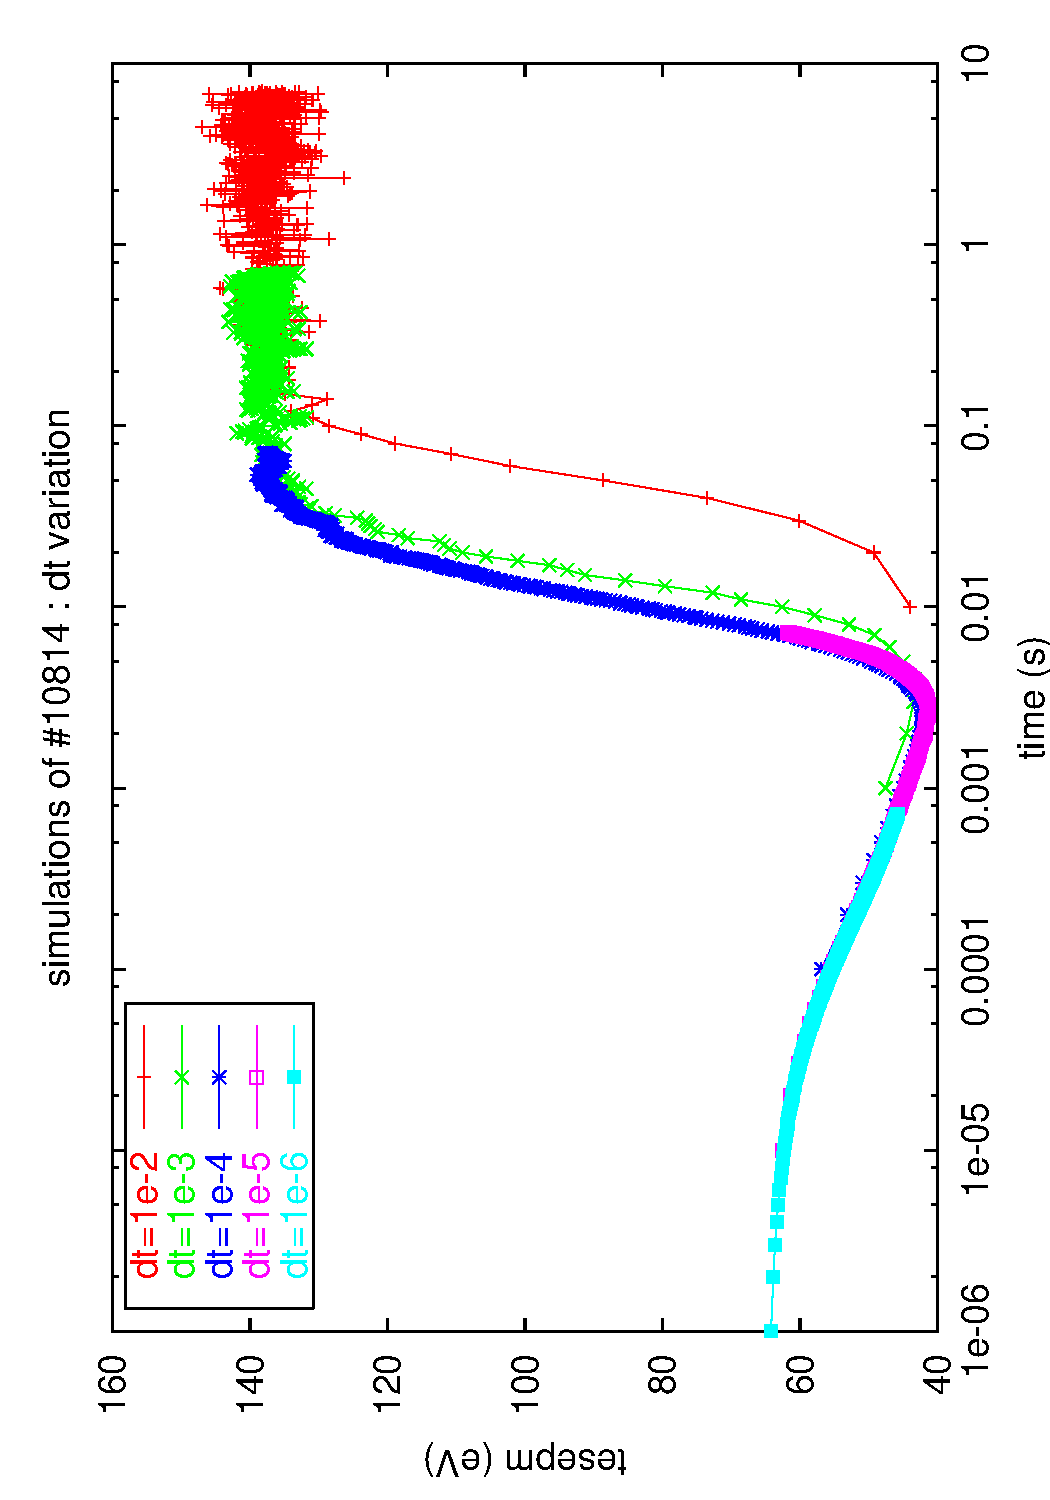
\includegraphics[origin=br,angle=-90,height=8cm]{compare_10814_tesepm_1.pdf}}
\else
    \centerline{\includegraphics[origin=br,angle=-90,height=8cm]{compare_10814_tesepm_1.ps}}
\fi
    \caption{Upstream (outer midplane) electron temperature for a
    range of time-steps.}
    \label{fig:tesepm1}
\end{figure}

In figure \ref{fig:tesepm2} we see the same quantity plotted for the
a range of time-steps but with an additional core speed-up factor coming
from \verb!b2.numerics.parameters!.

\begin{figure}[hbtp]
\ifpdf 
    \centerline{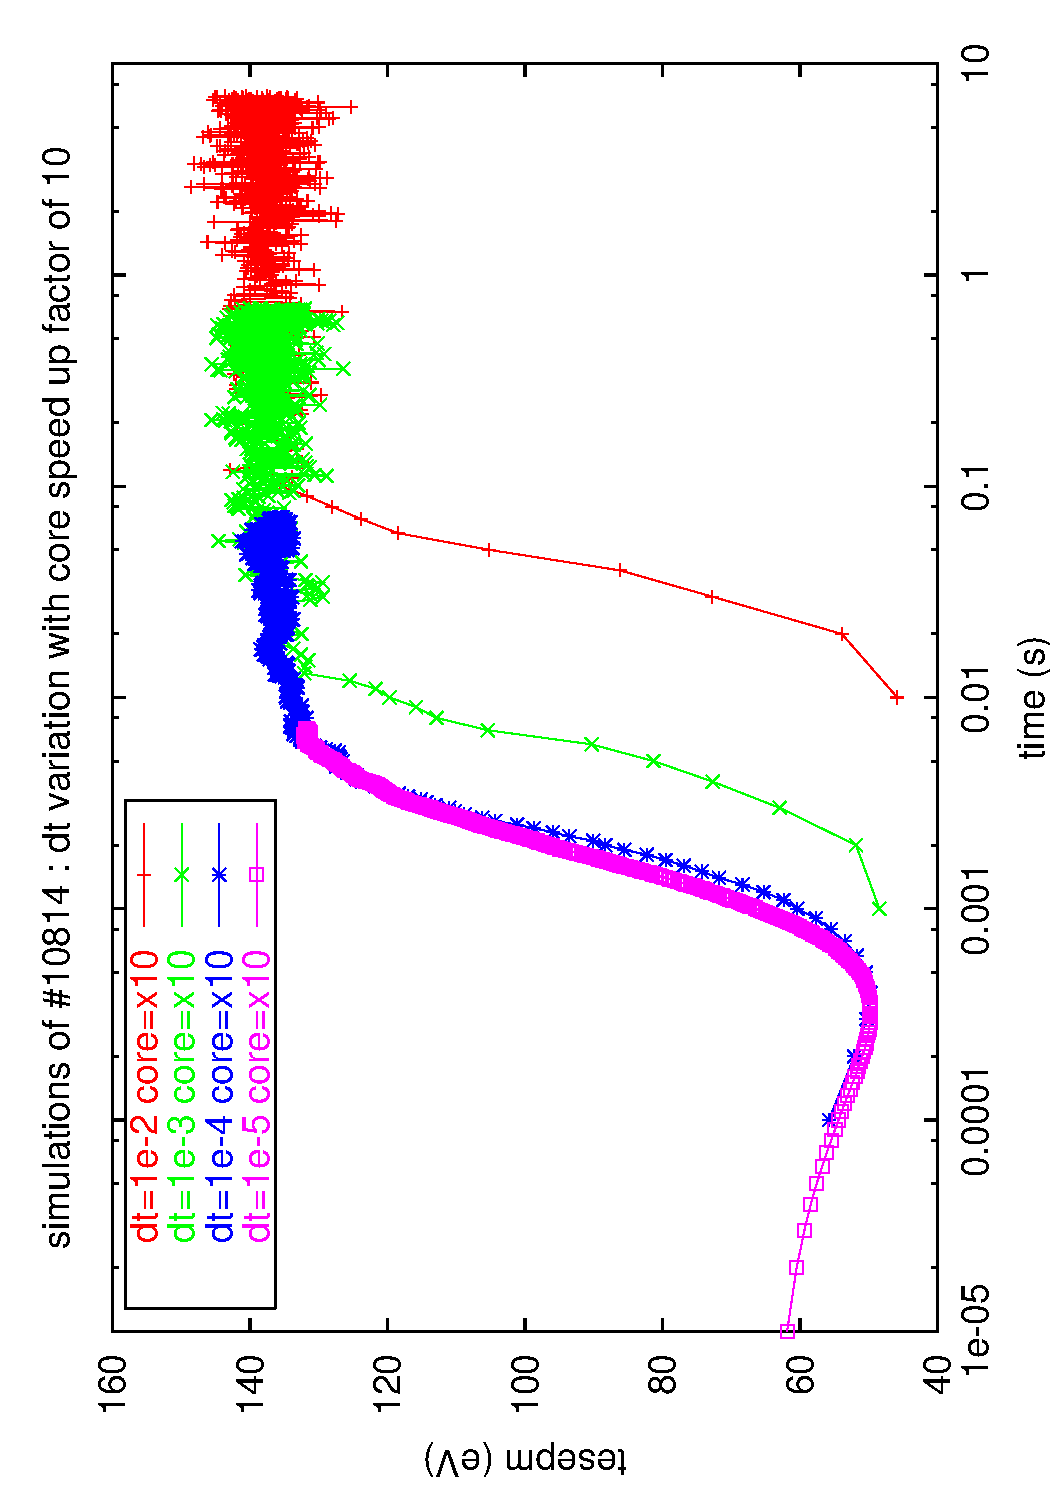
\includegraphics[origin=br,angle=-90,height=8cm]{compare_10814_tesepm_2.pdf}}
\else
    \centerline{\includegraphics[origin=br,angle=-90,height=8cm]{compare_10814_tesepm_2.ps}}
\fi
    \caption{Upstream (outer midplane) electron temperature for a
    range of time-steps with a core speed-up factor.}
    \label{fig:tesepm2}
\end{figure}

Figure \ref{fig:tesepm3} combines the data form figures \ref{fig:tesepm1} and \ref{fig:tesepm2}.

\begin{figure}[hbtp]
\ifpdf 
    \centerline{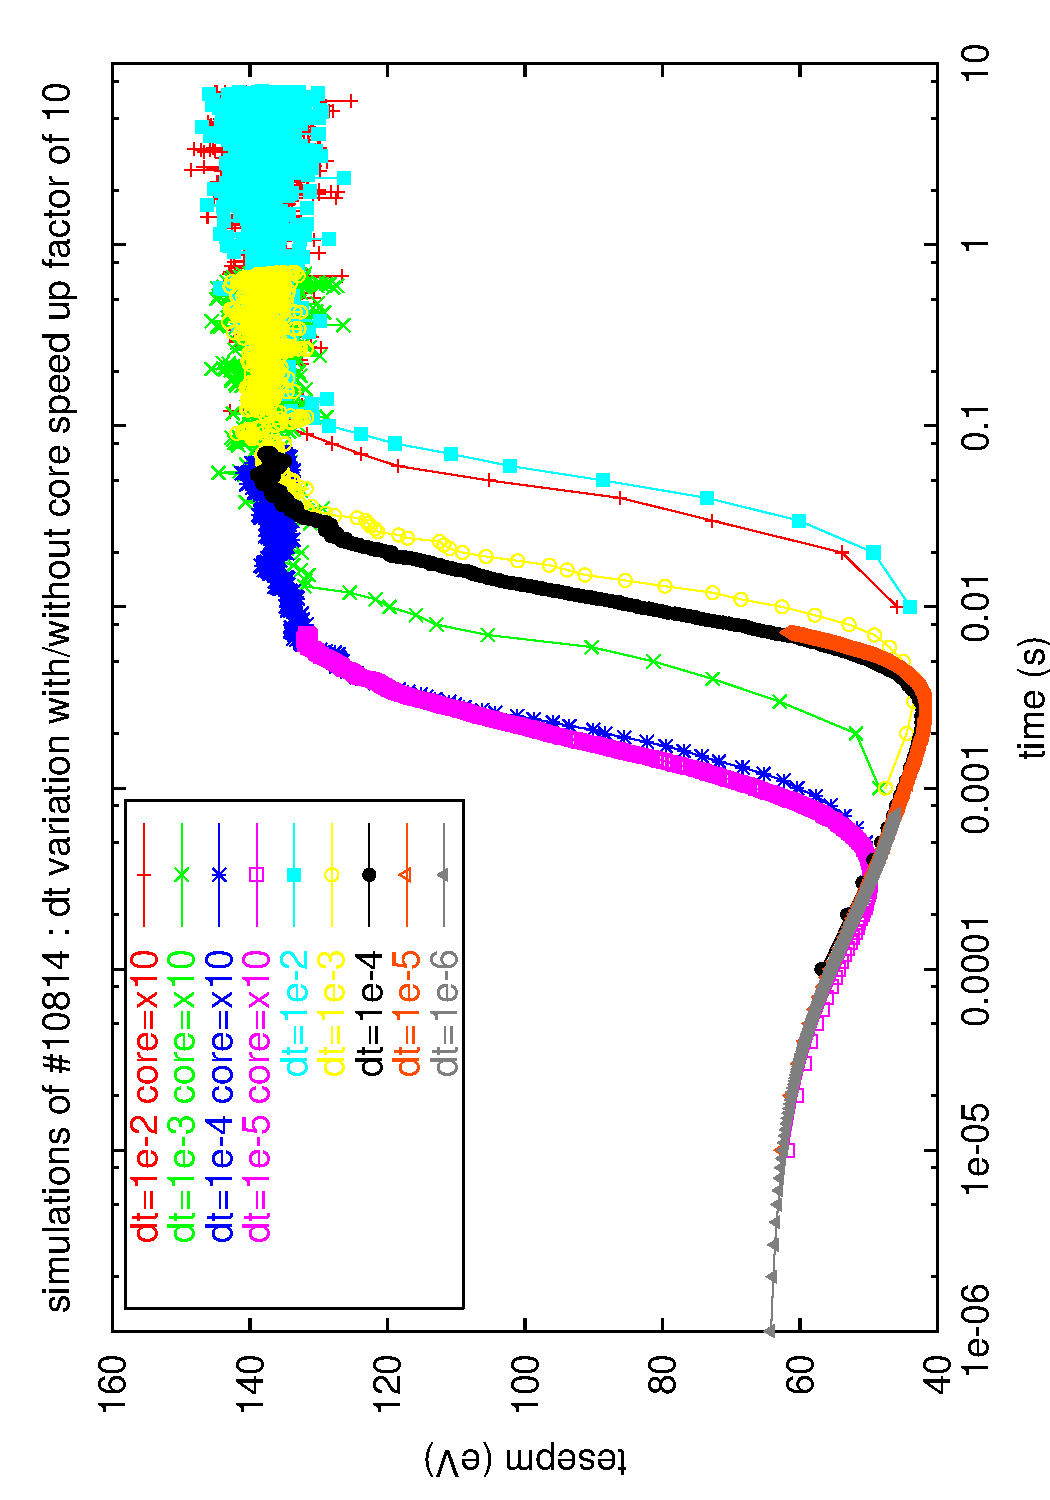
\includegraphics[origin=br,angle=-90,height=8cm]{compare_10814_tesepm_3.pdf}}
\else
    \centerline{\includegraphics[origin=br,angle=-90,height=8cm]{compare_10814_tesepm_3.ps}}
\fi
    \caption{Upstream (outer midplane) electron temperature for a
    range of time-steps with and without a core speed-up factor.}
    \label{fig:tesepm3}
\end{figure}

Figures \ref{fig:tesepm4}, \ref{fig:tesepm5} and \ref{fig:tesepm6}
show the outer target separatrix temperatures corresponding to figures
\ref{fig:tesepm1}, \ref{fig:tesepm2} and \ref{fig:tesepm3}.

\begin{figure}[hbtp]
\ifpdf 
    \centerline{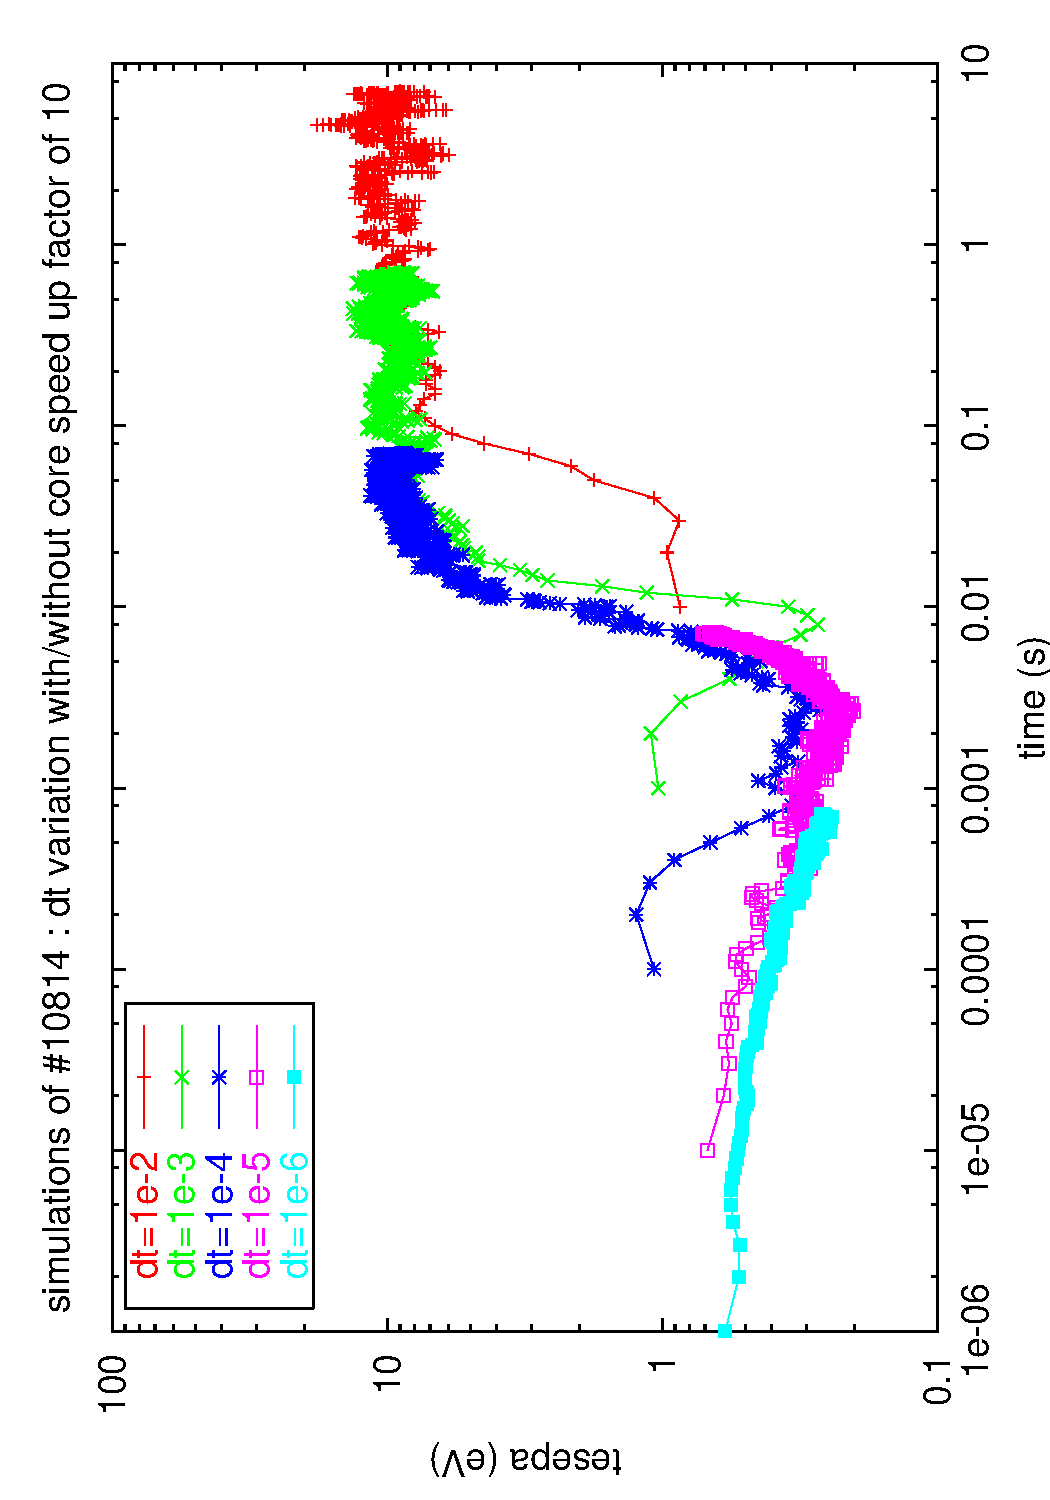
\includegraphics[origin=br,angle=-90,height=8cm]{compare_10814_tesepm_4.pdf}}
\else
    \centerline{\includegraphics[origin=br,angle=-90,height=8cm]{compare_10814_tesepm_4.ps}}
\fi
    \caption{Downstream (outer target) electron temperature for a
    range of time-steps.}
    \label{fig:tesepm4}
\end{figure}


\begin{figure}[hbtp]
\ifpdf 
    \centerline{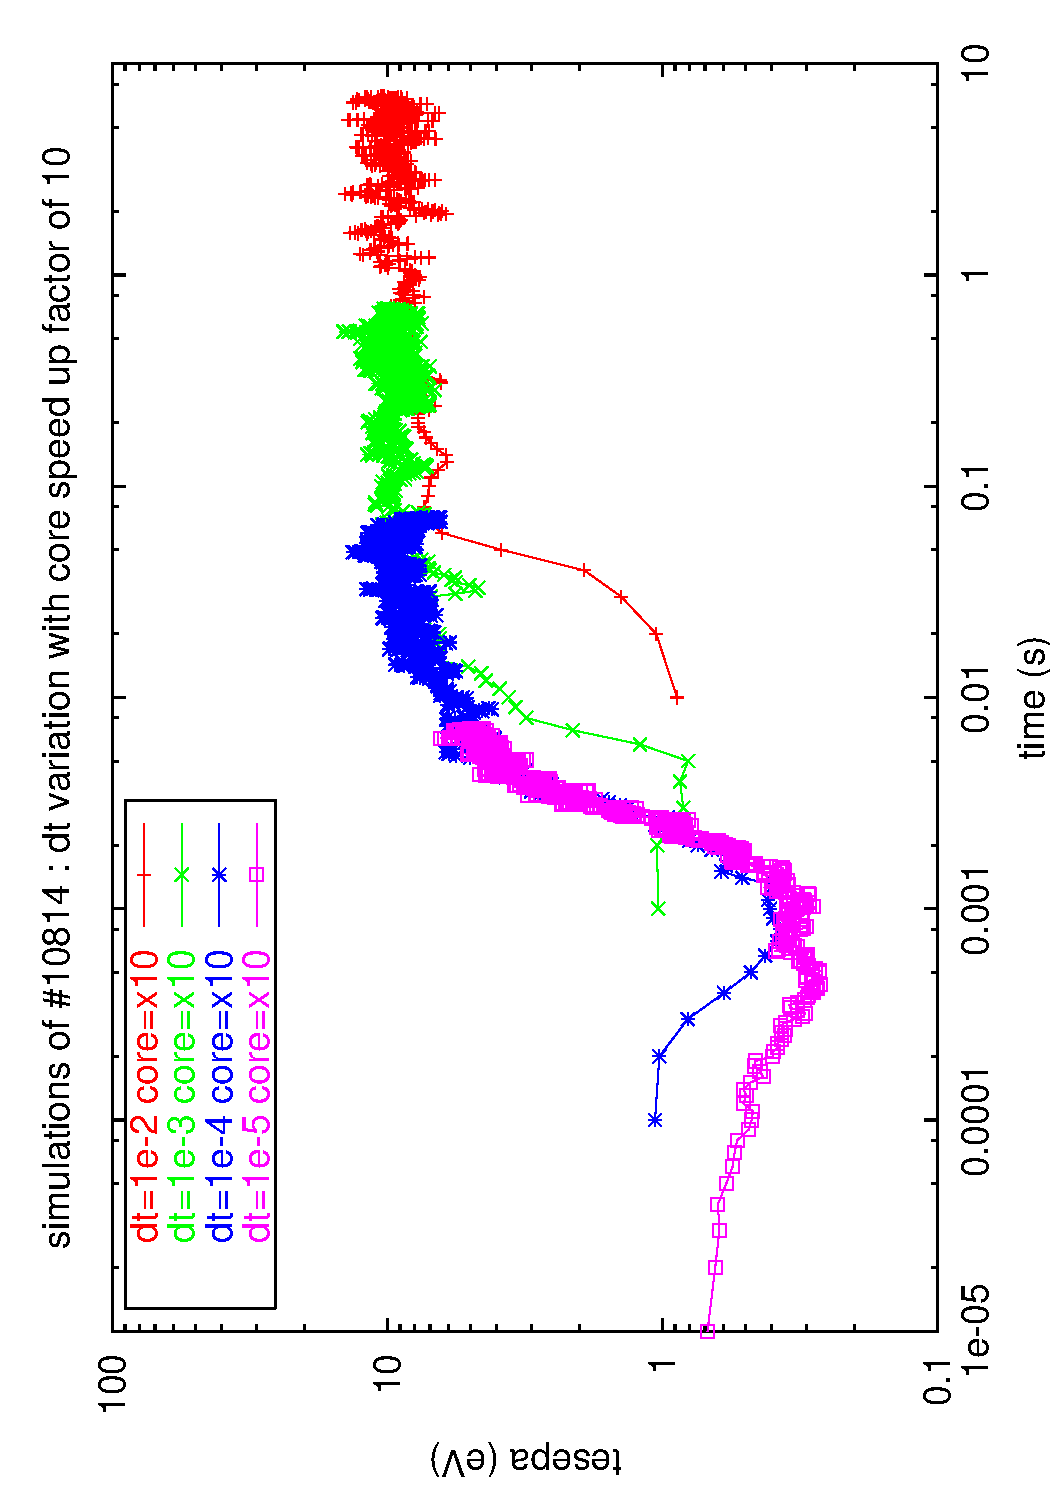
\includegraphics[origin=br,angle=-90,height=8cm]{compare_10814_tesepm_5.pdf}}
\else
    \centerline{\includegraphics[origin=br,angle=-90,height=8cm]{compare_10814_tesepm_5.ps}}
\fi
    \caption{Downstream (outer target) electron temperature for a
    range of time-steps with a core speed-up factor.}
    \label{fig:tesepm5}
\end{figure}


\begin{figure}[hbtp]
\ifpdf 
    \centerline{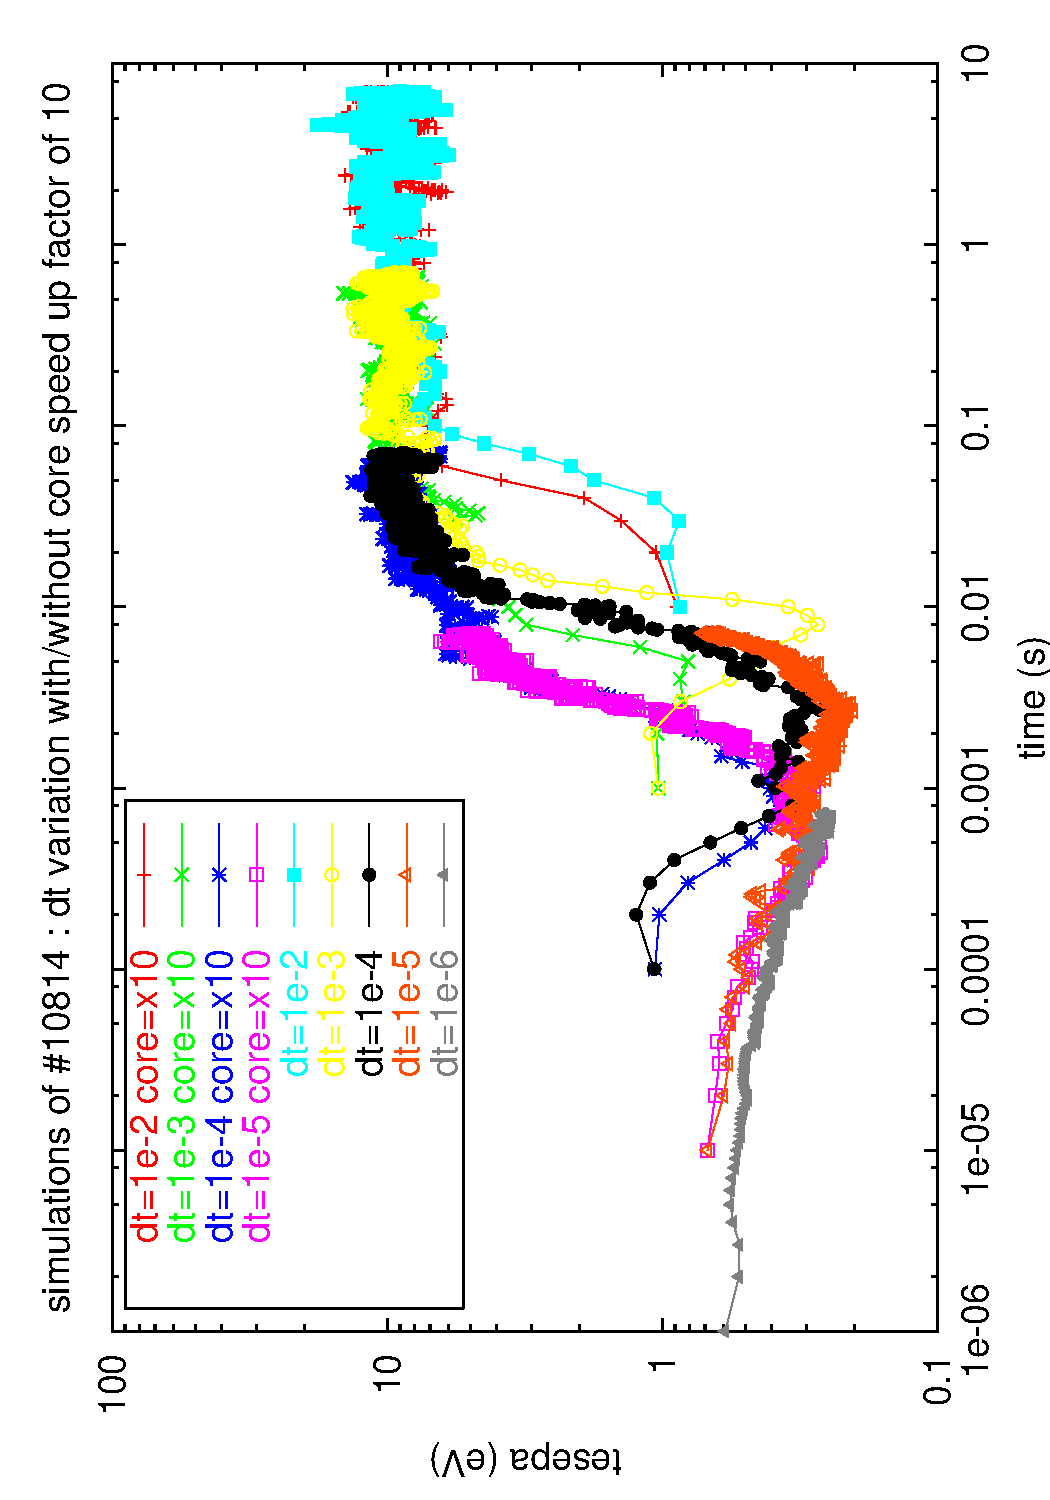
\includegraphics[origin=br,angle=-90,height=8cm]{compare_10814_tesepm_6.pdf}}
\else
    \centerline{\includegraphics[origin=br,angle=-90,height=8cm]{compare_10814_tesepm_6.ps}}
\fi
    \caption{Downstream (outer target) electron temperature for a
    range of time-steps with and without a core speed-up factor.}
    \label{fig:tesepm6}
\end{figure}

Figures \ref{fig:tesepm7}, \ref{fig:tesepm8} and \ref{fig:tesepm9}
show continuation runs.

\begin{figure}[hbtp]
\ifpdf 
    \centerline{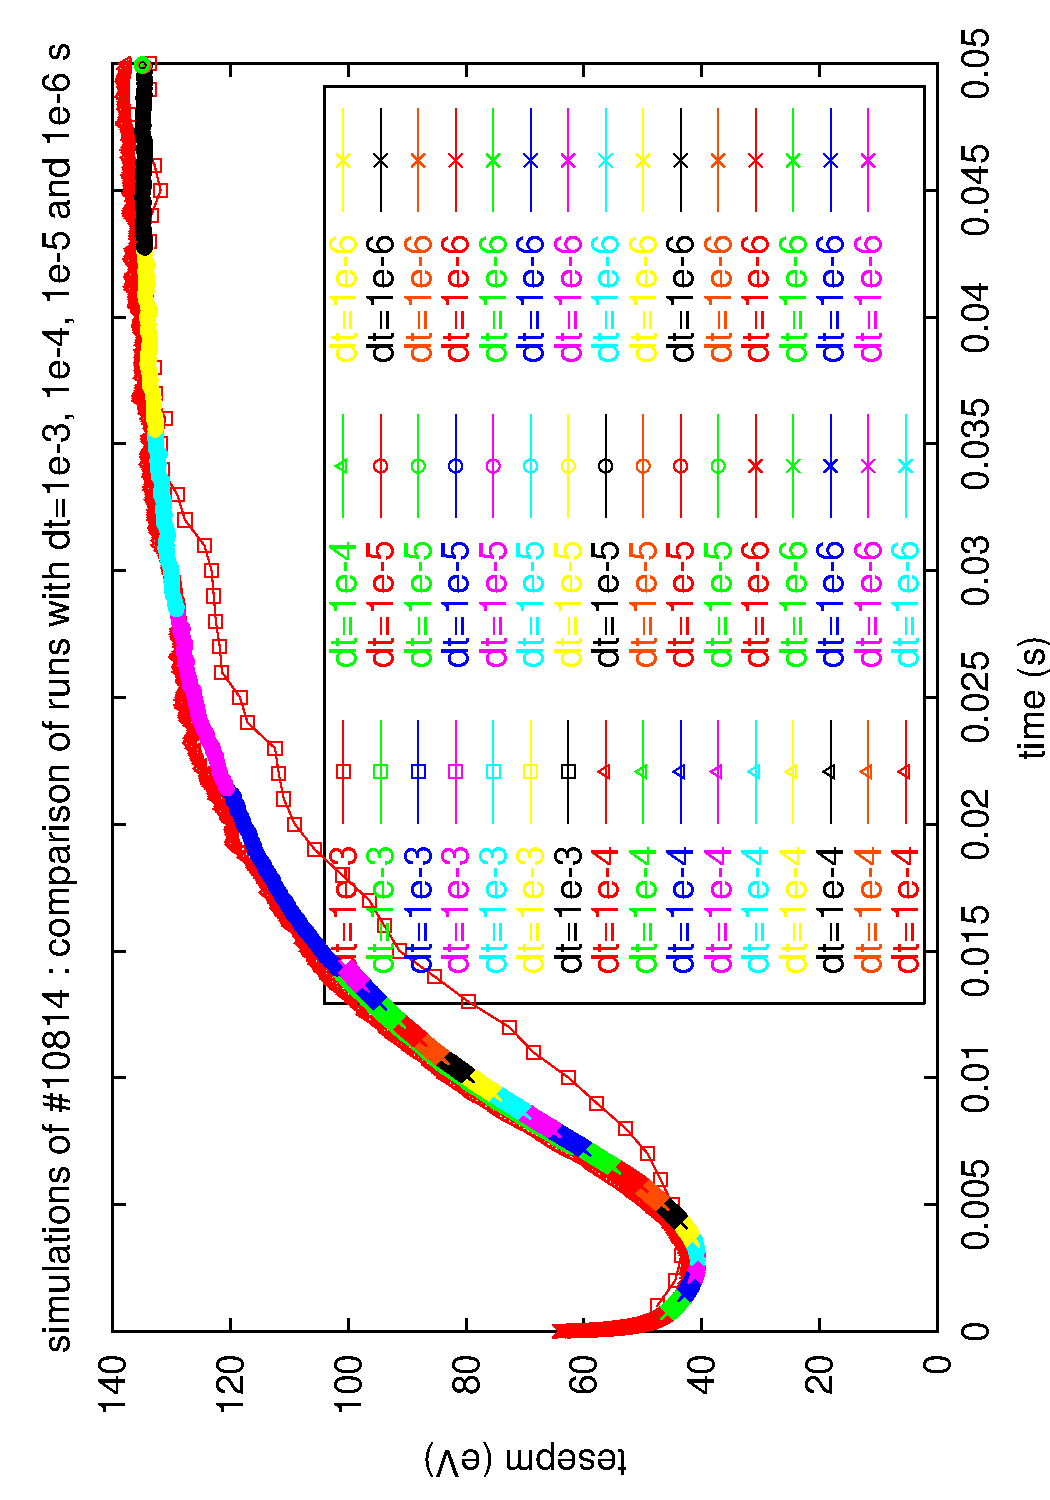
\includegraphics[origin=br,angle=-90,height=8cm]{compare_10814_tesepm_7.pdf}}
\else
    \centerline{\includegraphics[origin=br,angle=-90,height=8cm]{compare_10814_tesepm_7.ps}}
\fi
    \caption{Upstream (outer midplane) electron temperature.}
    \label{fig:tesepm7}
\end{figure}


\begin{figure}[hbtp]
\ifpdf 
    \centerline{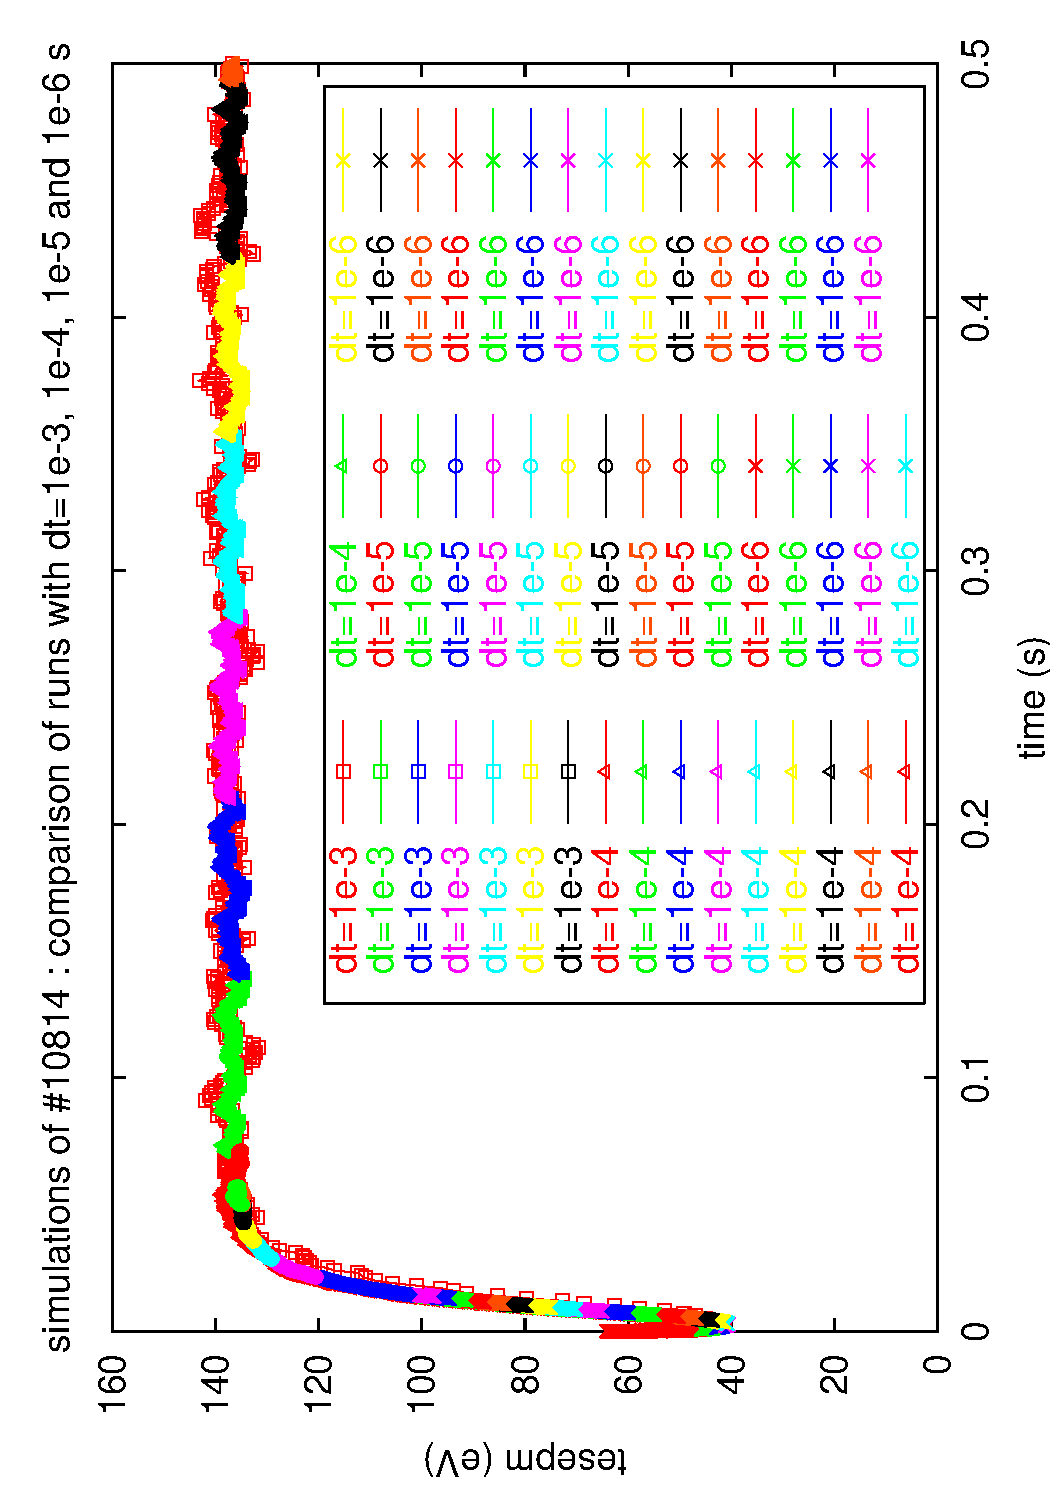
\includegraphics[origin=br,angle=-90,height=8cm]{compare_10814_tesepm_8.pdf}}
\else
    \centerline{\includegraphics[origin=br,angle=-90,height=8cm]{compare_10814_tesepm_8.ps}}
\fi
    \caption{Upstream (outer midplane) electron temperature.}
    \label{fig:tesepm8}
\end{figure}


\begin{figure}[hbtp]
\ifpdf 
    \centerline{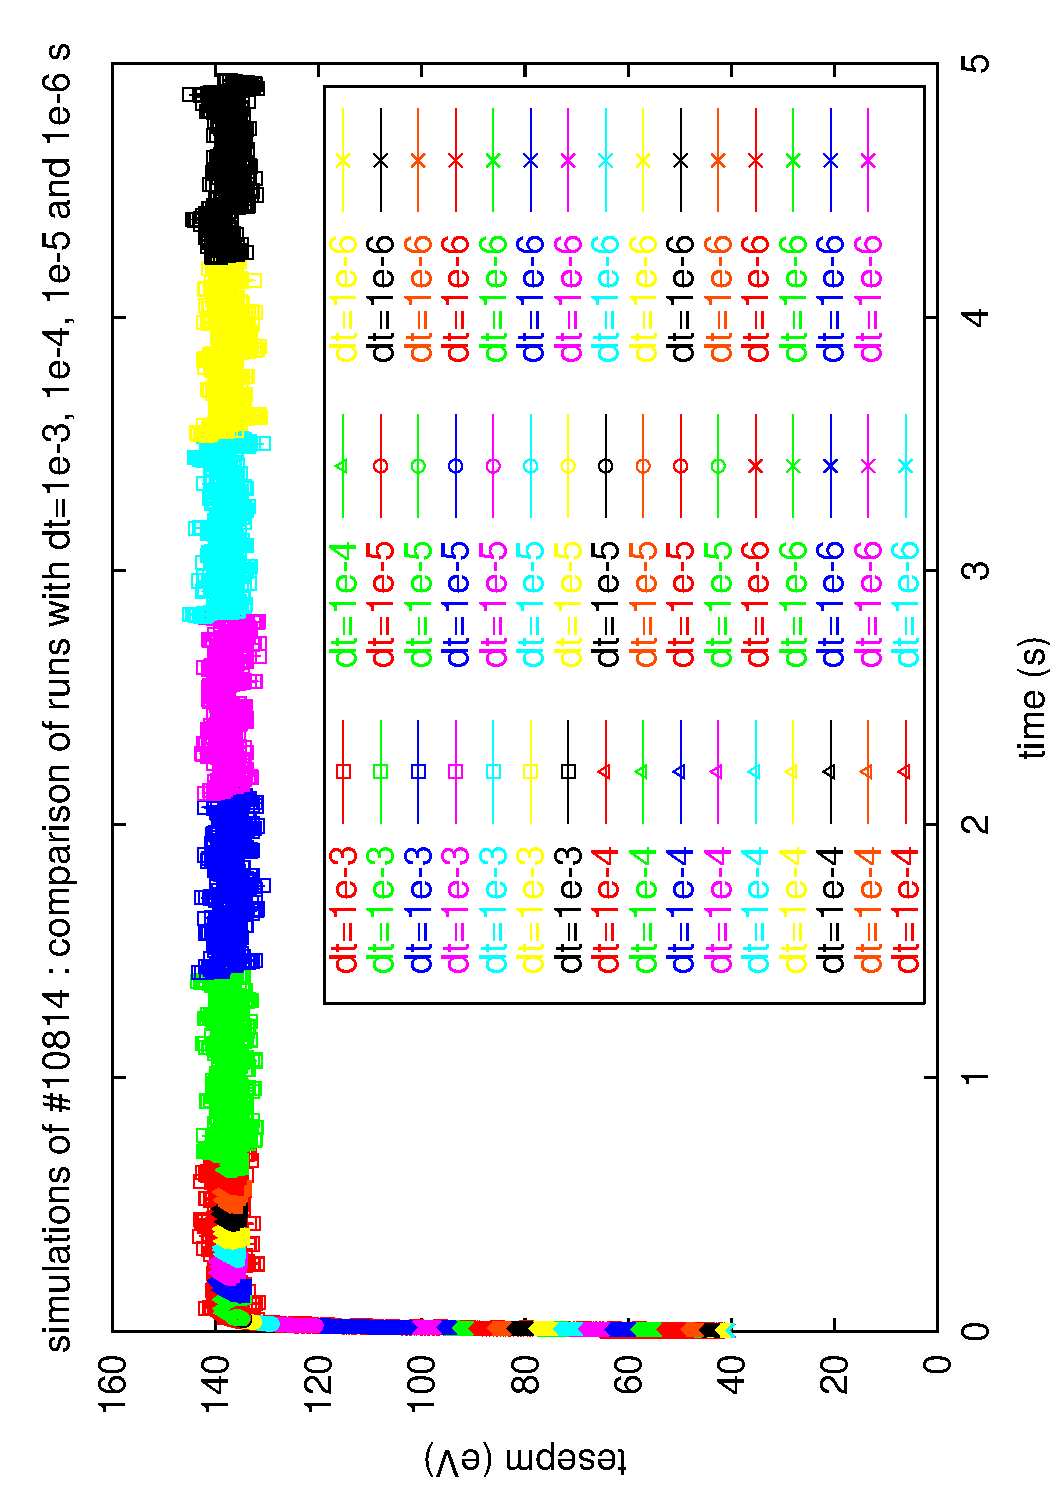
\includegraphics[origin=br,angle=-90,height=8cm]{compare_10814_tesepm_9.pdf}}
\else
    \centerline{\includegraphics[origin=br,angle=-90,height=8cm]{compare_10814_tesepm_9.ps}}
\fi
    \caption{Upstream (outer midplane) electron temperature.}
    \label{fig:tesepm9}
\end{figure}

\chapter{Using MDSPLUS}
\index{MDSPLUS}\label{cha:MDSplus}

A routine has been added, \verb!b2md!\index{b2md}, which allows one to save
the output from \SOLPSfive to an \verb!MDSplus! server in Garching.  (For more
information about \verb!MDSplus! see the Web site at \verb!www.mdsplus.org!.)

The reverse operation, namely recovering an archived run from the \verb!MDSplus!
server, is performed by \verb!b2rd!\index{b2rd}.

In order to use this facility, you need to ask David Coster at IPP-Garching to
add you to the list of authorized \verb!MDSplus! writers, supplying the username
which will be used, as well as the machine/domain.

In order to compile the code with \verb!MDSplus!, the environment variable
\verb!SOLPS_CPP!\index{SOLPS\_CPP} should contain
\verb!-DMDSPLUS!\index{-DMDSPLUS}, and a 
\begin{verbatim}
sbb ; gmake clean ; gmake depend ; gmake
\end{verbatim}
is safest.  Before doing this, the \verb!MDSPLUS_DIR! environment
needs to be set --- consult your systems people about this, or the
\verb!MDSplus! documentation.

[At IPP on the TOK linux cluster, add the following to \verb!.login!:
\begin{verbatim}
setenv MDSPLUS_DIR /afs/ipp-garching.mpg.de/home/d/dpc/@sys/mdsplus
source $MDSPLUS_DIR/setup.csh
\end{verbatim}
%% $
and add
\begin{verbatim}
setenv SOLPS_CPP '-DMDSPLUS'
\end{verbatim}
to one of the \verb!setup.csh.*! files in \$\verb!SOLPSTOP/SETUP!.]
 
\verb!b2md! requires as input \verb!b2md.dat! and this is searched for in the
present working directory, the \verb!baserun! directory, and in the
\$\verb!SOLPSTOP/data.local/mdsplus! and \$\verb!SOLPSTOP/data/mdsplus! directories,
if present, in order. See Appendix \ref{lis:b2cdcn} for a content description.

An example \verb!b2md.dat! is:
\VerbatimInput[fontsize=\footnotesize]{MDSPLUS/b2md.dat}

To save a new run to the \verb!MDSplus! server, execute
\begin{verbatim}
save_mds
\end{verbatim}
which should create \verb!shotnumber.history! which contains the
``shotnumber'' for the run on the server (not to be confused with the
experimental shot number).  The output from the operation will be saved in
\verb!b2md.log! and this should be checked for errors.

A run can be re-saved to the same shotnumber with
\begin{verbatim}
resave_mds
\end{verbatim}
which uses the ``shotnumber'' in \verb!shotnumber.history!.

The \verb!shotnumber.history! file can later be read by \verb!b2rd! which will
then fetch from the \verb!MDSplus! tree the archived shot corresponding to
the last number stored within.

\section{SOLPS tree structure}
\index{SOLPS tree structure in MDSplus}
\index{tree structure in MDSplus}
\index{MDSplus SOLPS tree structure}

%%rsync -avP ~/afs/MDSPLUS_examples/*.TCL.index MDSPLUS/

The \verb!solps! tree consists of the main tree, \verb!SOLPS!, and six sub-trees: \verb!IDENT!,
\verb!SNAPSHOT!, \verb!TALLIES!, \verb!TIMEDEP!, \verb!MOVIES! and \verb!DIAG!.

The signals in, for example, \verb!TIMEDEP! can be accessed as
\verb!\SOLPS::TOP.TIMEDEP.DP:IMPSEP!\ or alternatively 
\verb!\TIMEDEP::TOP.DP:IMPSEP!.

\subsection{SOLPS}

\VerbatimInput[fontsize=\footnotesize]{MDSPLUS/SOLPS_MODEL.TCL.index}

\subsection{IDENT}

\VerbatimInput[fontsize=\footnotesize]{MDSPLUS/IDENT_MODEL.TCL.index}

\subsection{SNAPSHOT}

\VerbatimInput[fontsize=\footnotesize]{MDSPLUS/SNAPSHOT_MODEL.TCL.index}

\subsection{TALLIES}

\VerbatimInput[fontsize=\footnotesize]{MDSPLUS/TALLIES_MODEL.TCL.index}

\subsection{TIMEDEP}

\VerbatimInput[fontsize=\footnotesize]{MDSPLUS/TIMEDEP_MODEL.TCL.index}

\subsection{MOVIES}

\VerbatimInput[fontsize=\footnotesize]{MDSPLUS/MOVIES_MODEL.TCL.index}

\subsection{DIAG}

\VerbatimInput[fontsize=\footnotesize]{MDSPLUS/DIAG_MODEL.TCL.index}

\section{Accessing data from the MDSPLUS server}

\subsection{Using standard experimental data viewing programs}

The \verb!MDSplus! server name is \verb!solps-mdsplus.aug.ipp.mpg.de:8001!.

The tree name is \verb!solps!.

An example shotnumber is \verb!4293!.

Example signal names are \verb!\top.timedep.ne:ompsep!,
\verb!\top.timedep.te:ompsep! (Outer midplane electron density and temperature), and 
\verb!\top.timedep.ti:ompsep! (Outer midplane ion temperature).

\subsubsection{cview}
\index{cview}

\begin{itemize}
\item start \verb!cview!
\item \verb!Shot! = \verb!4293!
\item In the table:
  \begin{itemize}
  \item \verb!shot! = \verb!0!
  \item \verb!shot! = \verb!+solps!
  \item \verb!diag! = \verb!solps!
  \item \verb!name! = \verb!\top.timedep.ne:ompsep!
  \end{itemize}
\end{itemize}

Adding \verb!\top.timedep.ne:ompsep! and \verb!\top.timedep.ne:ompsep!, the
graph in figure \ref{fig:cviewsolpsmdsplus} is produced.

\begin{figure}[htbp]
  \centering
  \ifpdf 
    \centerline{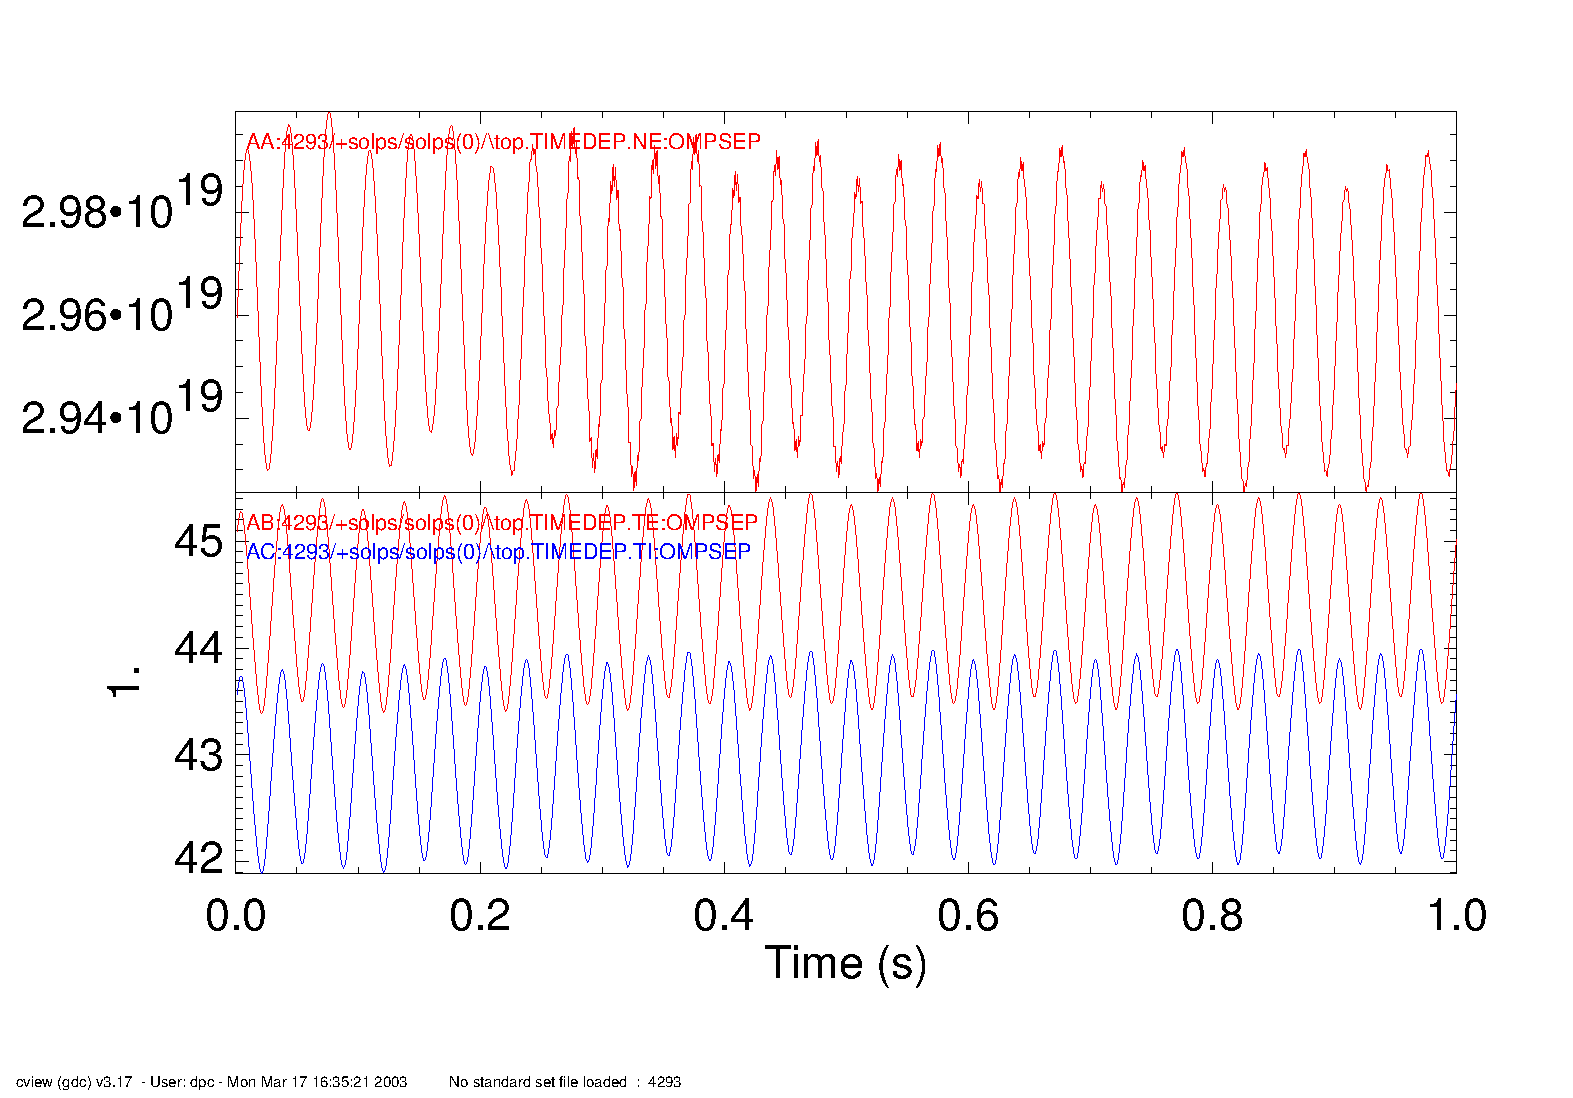
\includegraphics[height=8cm]{MDSPLUS/cview_mdsplus_example.pdf}}
\else
    \centerline{\includegraphics[height=8cm]{MDSPLUS/cview_mdsplus_example.eps}}
\fi
  \caption{Using CVIEW to access SOLPS MDSplus data.}
  \label{fig:cviewsolpsmdsplus}
\end{figure}

\subsubsection{jetdsp}
\index{jetdsp}

\begin{itemize}
\item start \verb!JETDSP!
\item \verb!File|Read Signal!
\item \verb!MDS+! option
\item \verb!MDS+ server:! = \verb!solps-mdsplus.aug.ipp.mpg.de:8001!
\item \verb!Shot number:! = \verb!4293!
\item \verb!Tree:! = \verb!solps!
\item \verb!Signal:! = \verb!\top.timedep.ne:ompsep!
\item \verb!Read! button
\end{itemize}

You can also use
\begin{itemize}
\item start \verb!JETDSP!
\item \verb!File|Read Signal!
\item \verb!MDS+! option
\item \verb!MDS+ server:! = \verb!solps-mdsplus.aug.ipp.mpg.de:8001!
\item \verb!Shot number:! = \verb!4293!
\item \verb!Tree:! = \verb!timedep!
\item \verb!Signal:! = \verb!\top.ne:ompsep!
\item \verb!Read! button
\end{itemize}

Adding \verb!te:ompsep! and \verb!ti:ompsep!, the graph in figure
\ref{fig:jetdspsolpsmdsplus} is produced.

\begin{figure}[htbp]
  \centering
  \ifpdf 
    \centerline{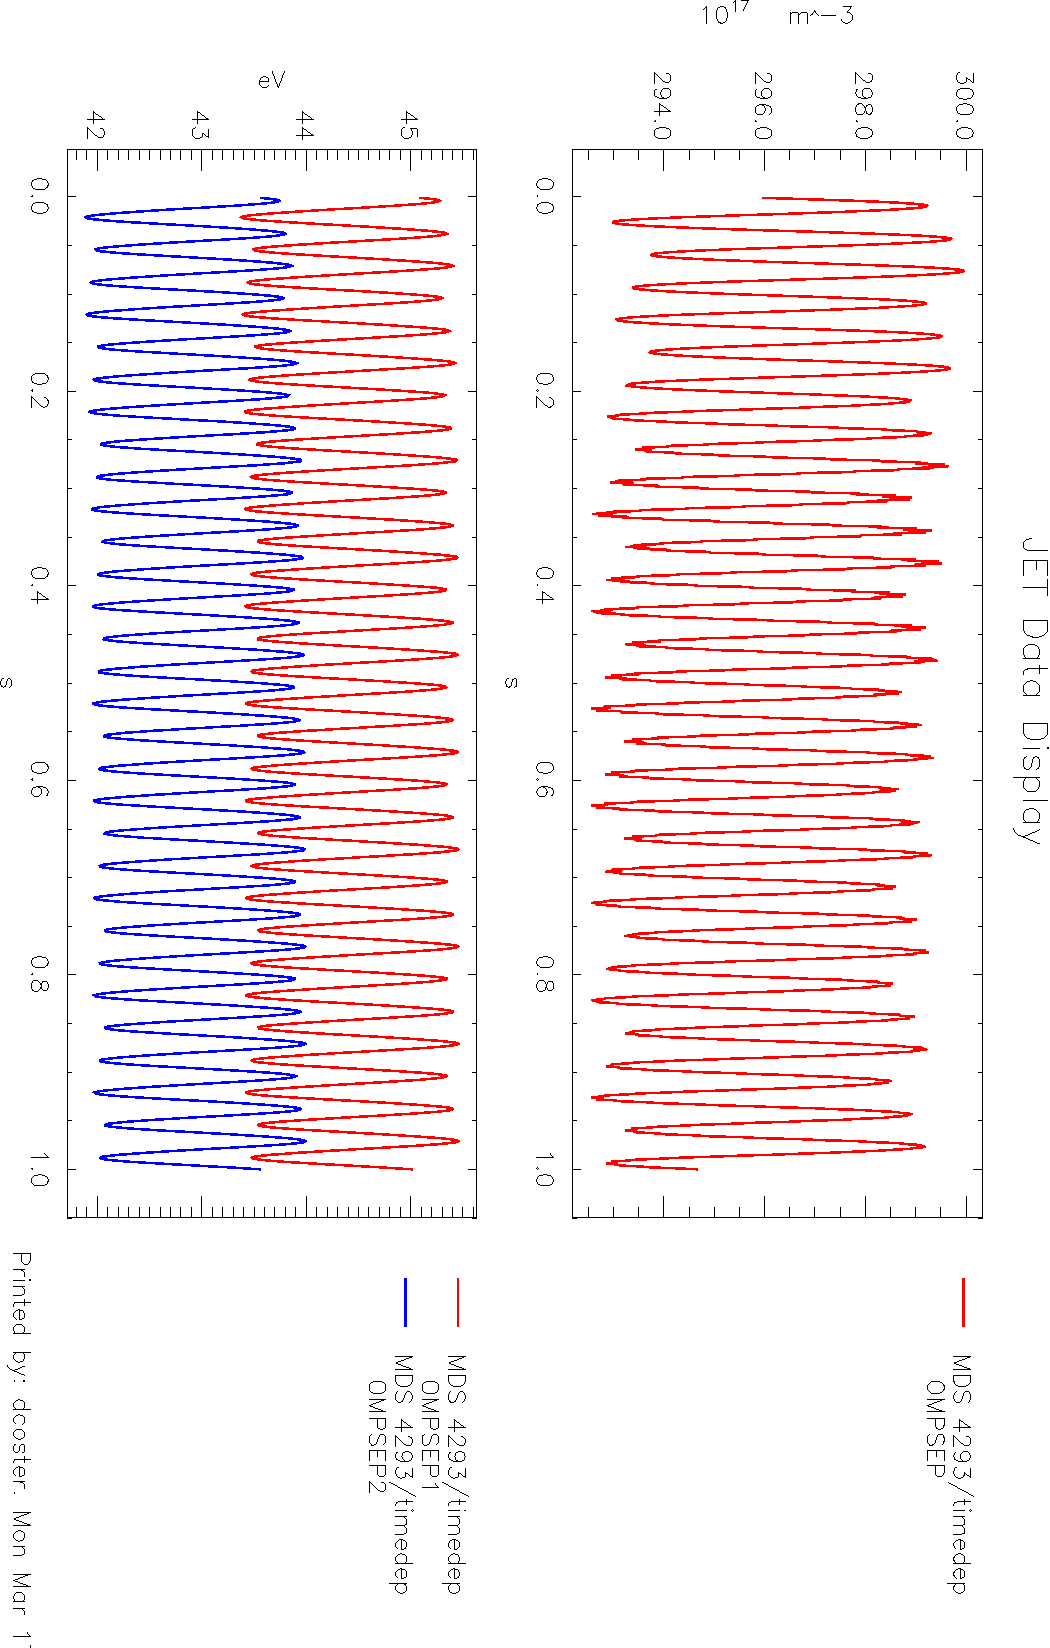
\includegraphics[origin=bl,angle=+90,height=8cm]{MDSPLUS/jetdsp_mdsplus_example.pdf}}
\else
    \centerline{
\includegraphics[origin=bl,angle=+90,height=8cm]{MDSPLUS/jetdsp_mdsplus_example.epsi}}
\fi
  \caption{Using JETDSP to access SOLPS MDSplus data.}
  \label{fig:jetdspsolpsmdsplus}
\end{figure}

\subsubsection{reviewplus}
\index{reviewplus}

\subsection{Using IDL}
\index{idl}

\begin{verbatim}
mdsconnect,'solps-mdsplus.aug.ipp.mpg.de:8001'
mdsopen,'solps',251
te_coarse=mdsvalue('\top.snapshot:te')
cr_coarse=mdsvalue('\top.snapshot.grid:cr')
mdsopen,'solps',288
te_fine=mdsvalue('\top.snapshot:te')
cr_fine=mdsvalue('\top.snapshot.grid:cr')
mdsclose
mdsdisconnect
plot,cr_coarse[*,8],te_coarse[*,8],linestyle=1,psym=-1,yrange=[0,50]
oplot,cr_fine[*,10],te_fine[*,10],linestyle=2,psym=-2
\end{verbatim}

\subsection{Using MATLAB}
\index{matlab}

\begin{verbatim}
mdsopen('solps-mdsplus.aug.ipp.mpg.de:8001::solps',nshot);
onx= mdsvalue('\SOLPS::TOP.SNAPSHOT.DIMENSIONS:NX');
ny = mdsvalue('\SOLPS::TOP.SNAPSHOT.DIMENSIONS:NY'); %number of radial cells
ne = mdsvalue('\SOLPS::TOP.SNAPSHOT:NE');  
te = mdsvalue('\SOLPS::TOP.SNAPSHOT:TE');
ti = mdsvalue('\SOLPS::TOP.SNAPSHOT:TI');
sep= mdsvalue('\SOLPS::TOP.TIMEDEP.OMP:DS');
qe = 1.602e-19; %Elementary charge in C
amu= 1.660542e-27; %Atomic mass unit in kg

%Calculate the ion sound speed at outer target
cs2o = qe .* (ti(onx-1,:) + te(onx-1,:)) ./ (2*amu);

%Outer target
neo  = ne(onx-1,:);
osja = neo .* qe .* sqrt(cs2o) / 1.0e4;

cr = mdsvalue('\SOLPS::TOP.SNAPSHOT.GRID:CR'); %R-coordinate of cell centre
ocr= cr(onx,:); %R coordinates of outer target cells
cz = mdsvalue('\SOLPS::TOP.SNAPSHOT.GRID:CZ'); %Z-coordinate of cell centre
ocz= cz(onx,:); %Z coordinate of outer target cells
mdsclose('MDSIP');

[map2mid,oms]=jhmap2mid(26730,ocr,ocz,0.7);
rrsep= map2mid.Rmid-map2mid.Rlcfs;

plot(rrsep,osja,'k');
\end{verbatim}

\subsection{Using Python}
\index{python}

You will need the MDSplus interface for python.  

\begin{verbatim}
import pmds
from pylab import *

pmds.mdsconnect ('solps-mdsplus.aug.ipp.mpg.de:8001')
pmds.mdsopen('solps',12380)
r=pmds.mdsvalue('\\top.snapshot.grid:r')
z=pmds.mdsvalue('\\top.snapshot.grid:z')
pmds.mdsdisconnect ()

print(r)  
print(z)  
\end{verbatim}

For additional information about using python, see\\
\href{https://wiki.eu-euforia.eu/index.php/Fusion\_dataset\_with\_Python\_and\_VisIt}{https://wiki.eu-euforia.eu/index.php/Fusion\_dataset\_with\_Python\_and\_VisIt}\\
(this activity occurred within the EUFORIA project,
\href{http://www.euforia-project.eu/}{http://www.euforia-project.eu/}).

\index{python, plots to compare profiles}
Typing
\begin{verbatim}
  python
  import compare_shots
\end{verbatim}
with the following as \verb!compare_shots.py!:
\VerbatimInput[fontsize=\footnotesize]{compare_shots.py}
produced figure \ref{fig:python_compare_shots}.

\begin{figure}[hbtp]
\ifpdf 
    \centerline{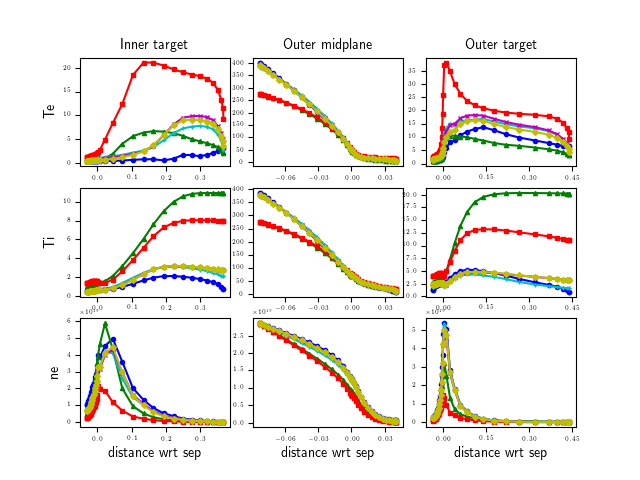
\includegraphics[height=8cm]{compare_shots.png}}
\else
    \centerline{\includegraphics[height=8cm]{compare_shots.ps}}
\fi
    \caption{Comparison of profiles for a range of shots.}
    \label{fig:python_compare_shots}
\end{figure}

In another, more complicated, example, python was used to create the frames of a movie on the ITM Gateway machine.
\index{movie, python}\index{python, movie}
\begin{verbatim}
set c=0
foreach i ( `cat shots` )
  set tbase=`echo $c | awk '{print $1*1000*1e-5}'`
  mkdir $i
  echo Submitting $i with offset $tbase
  ( cd $i ; sed -e "s:#1#:${i}:g" -e "s:#2#:${tbase}:g" < ../QSUB.shot | bsub )
  @ c++
  sleep 5
end
\end{verbatim}
with \verb!QSUB.shot! containing \VerbatimInput[fontsize=\footnotesize]{QSUB.shot.python_movie} and \verb!shots! containing \VerbatimInput[fontsize=\footnotesize]{shots.python_movie}

This launches one job per SOLPS shot-number.  Then the frames were renumbered by
\begin{verbatim}
mkdir frames
cd frames/
set c=0
foreach i ( `cat ../shots` )
  set p=`echo $c | awk '{printf "%03i\n",$1}'`
  echo $p
  @ c++
  foreach j ( `cd ../$i ; echo tmp_????.png`)
    ln -s ../$i/$j `echo $j | sed "s:tmp_0:tmp_${p}:"`
  end
end
\end{verbatim}

The individual frames were then combined into a movie with
\begin{verbatim}
mencoder 'mf://frames/tmp_??????.png' -mf type=png:fps=30 -ovc lavc -lavcopts \
 vcodec=wmv2 -oac copy -o fb_nesepm=5.0e19.ELM_2cm_X10.rqahesum.mpg
\end{verbatim}

The resultant movie can be found at\\
\href{http://solps-mdsplus.aug.ipp.mpg.de/SOLPS/fb\_nesepm=5.0e19.ELM\_2cm\_X10.rqahesum.mpg}{http://solps-mdsplus.aug.ipp.mpg.de/SOLPS/fb\_nesepm=5.0e19.ELM\_2cm\_X10.rqahesum.mpg}

\section{Querying the database}
\index{database}\index{querying database}

All cases are also entered into a \verb!MySQL!\index{MySQL}
(\href{http://www.mysql.com/}{http://www.mysql.com/}) database.

A Web interface to the database is available at
\href{http://solps-mdsplus.aug.ipp.mpg.de/solps/}{http://solps-mdsplus.aug.ipp.mpg.de/solps/} 
via \verb!Zope!\index{Zope}\\
(\href{http://www.zope.org/}{http://www.zope.org/}).

The database can also be queried via \verb!MySQL! commands passed via \verb!MDSplus!. An \verb!IDL!
example of querying the database to find the number of shots supplied by each
user follows:

\index{database query via IDL}
\begin{verbatim}
mdsconnect,'solps-mdsplus.aug.ipp.mpg.de:8001'
ans=mdsvalue("sql('select user,count(*) from id group by user','solps')")
mdsdisconnect
help,ans
print,transpose(ans)
\end{verbatim}

Another, more complicated, \verb!IDL! example is:

\begin{verbatim}
mdsconnect,'solps-mdsplus.aug.ipp.mpg.de:8001'
ans=mdsvalue("sql('select solpsindex,shot,time,ompsep_te,ompsep_ti,user,exp 
   from id where ompsep_te>110.0 and ompsep_te<120.0','solps')")
mdsdisconnect
help,ans
print,format='(i6,1x,i6,1x,f6.3,1x,f6.2,1x,1x,f6.2,1x,a10,1x,a)',transpose(ans)
plot,ans(*,3),ans(*,4),psym=4,xtitle='Te (eV)',ytitle='Ti (eV)'
\end{verbatim}

\index{database query via python}\index{python, database qyery}
And a similar example in python:
\begin{verbatim}
python sql_solps.py
\end{verbatim}
with \verb!sql_solps.py! containing
\VerbatimInput[fontsize=\footnotesize]{sql_solps.py} The resultant
plots are givien in figures \ref{fig:python_sql_scatter},
\ref{fig:python_sql_hexbin_lin} and \ref{fig:python_sql_hexbin_log}.

\begin{figure}[hbtp]
\ifpdf 
    \centerline{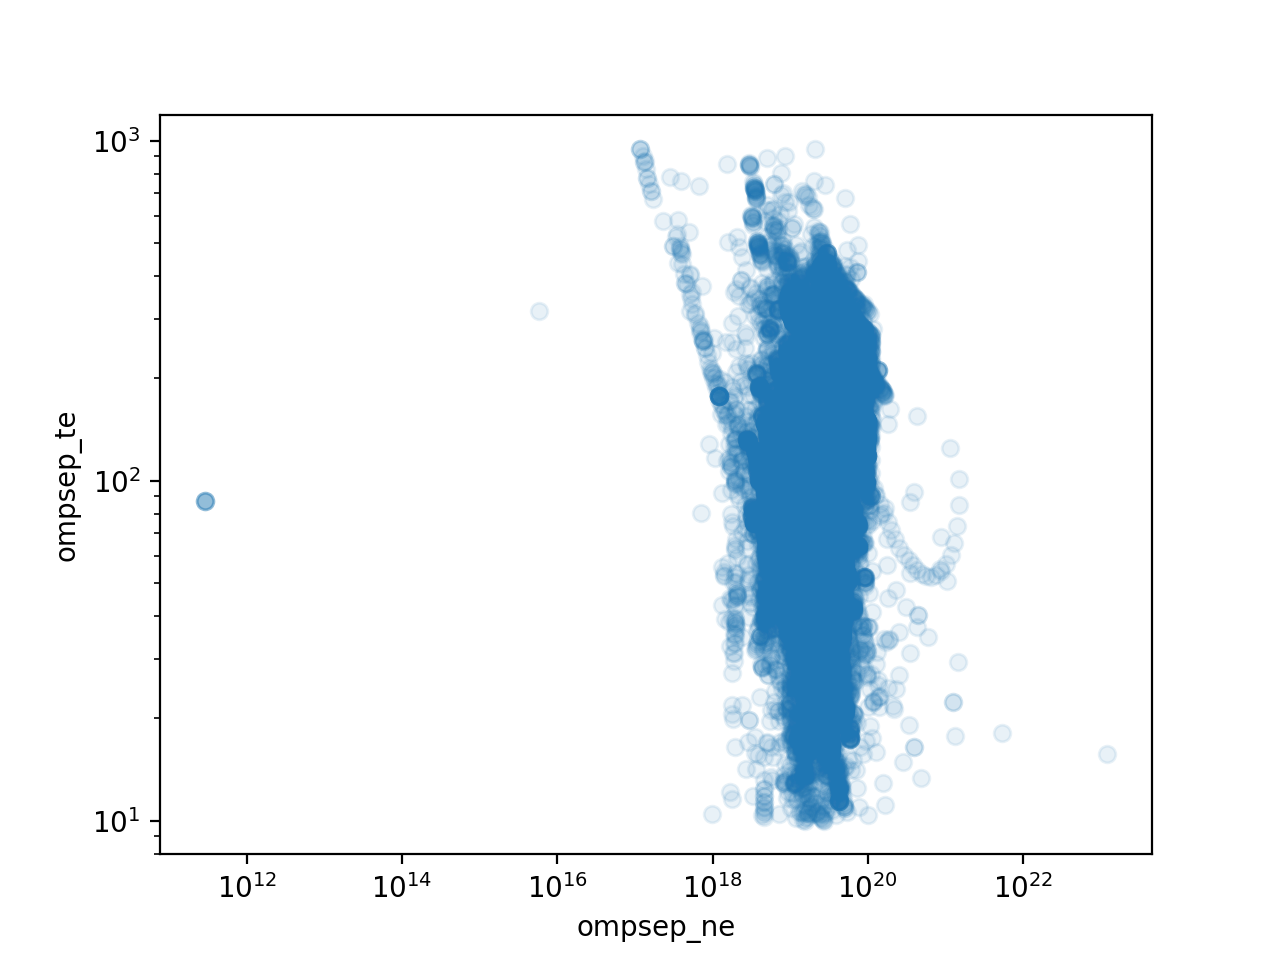
\includegraphics[height=8cm]{sql_scatter.png}}
\else
    \centerline{\includegraphics[height=8cm]{sql_scatter.ps}}
\fi
    \caption{Comparison of profiles for a range of shots.}
    \label{fig:python_sql_scatter}
\end{figure}

\begin{figure}[hbtp]
\ifpdf 
    \centerline{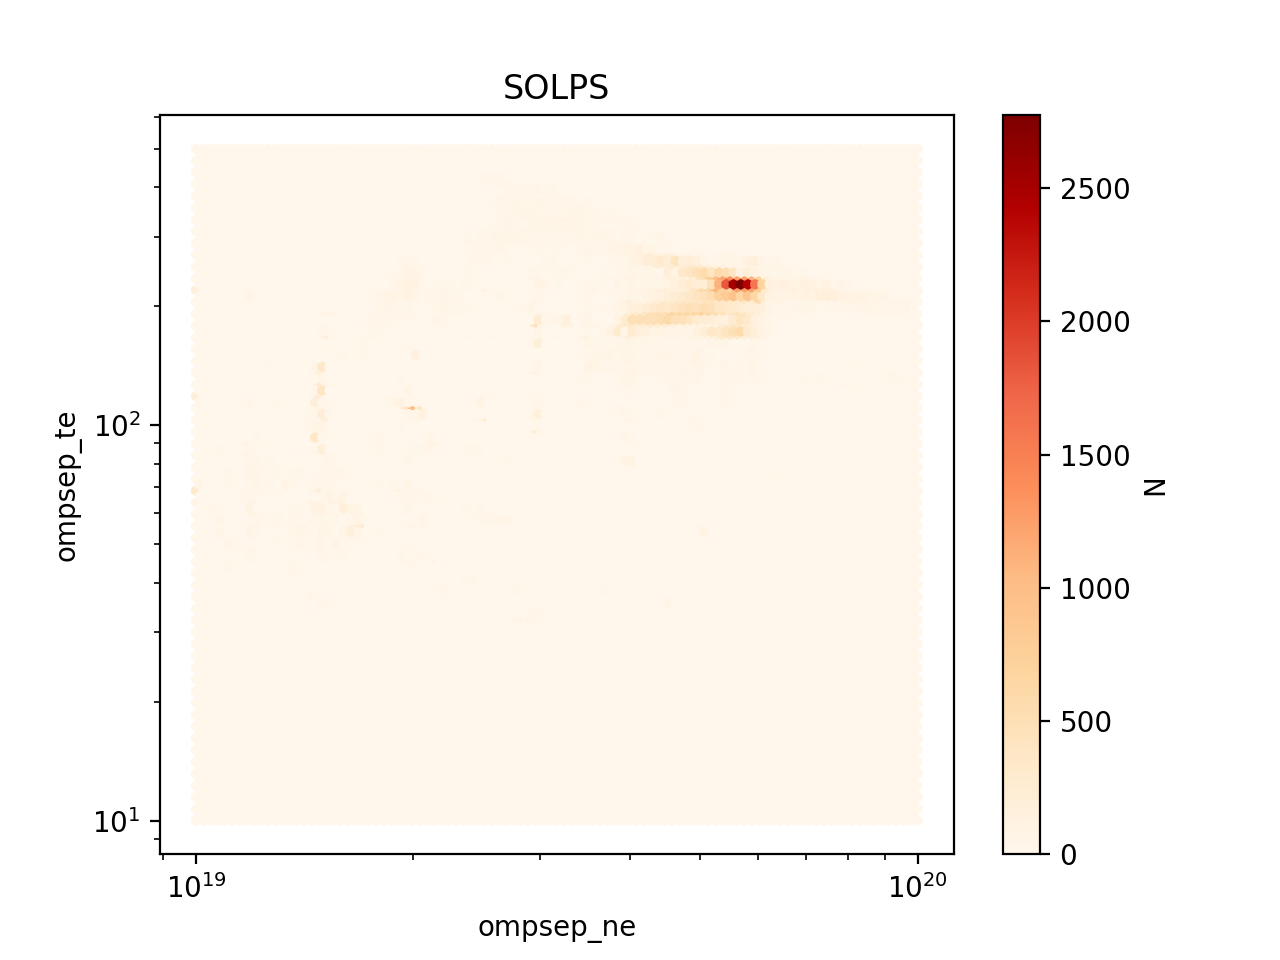
\includegraphics[height=8cm]{sql_hexbin_lin.png}}
\else
    \centerline{\includegraphics[height=8cm]{sql_hexbin_lin.ps}}
\fi
    \caption{Comparison of profiles for a range of shots.}
    \label{fig:python_sql_hexbin_lin}
\end{figure}

\begin{figure}[hbtp]
\ifpdf 
    \centerline{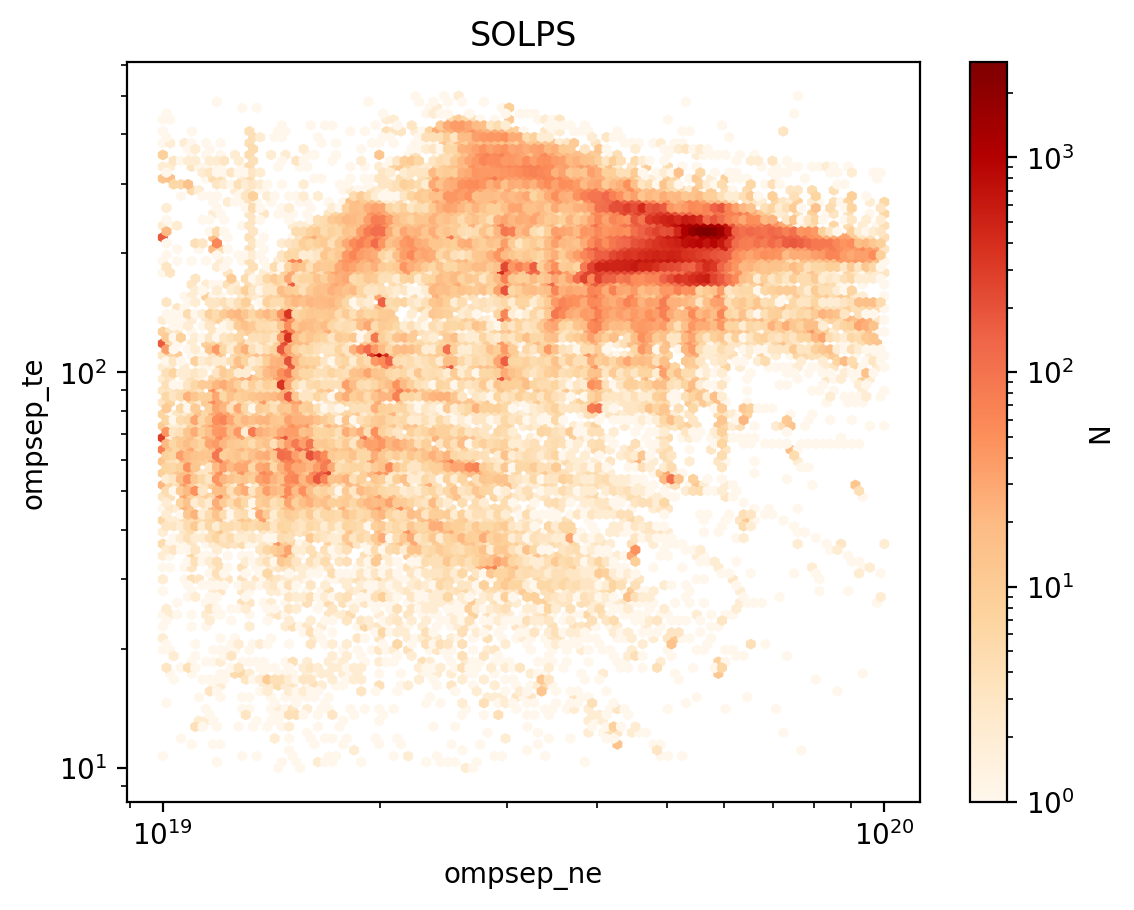
\includegraphics[height=8cm]{sql_hexbin_log.png}}
\else
    \centerline{\includegraphics[height=8cm]{sql_hexbin_log.ps}}
\fi
    \caption{Comparison of profiles for a range of shots.}
    \label{fig:python_sql_hexbin_log}
\end{figure}


\section{Coupling to other codes via MDSplus}
\index{Coupling to other codes via MDSplus}

Coupling of \verb!SOLPS! to other codes has in the past been done mostly by
exchanging files.  The preferred route for the future is to use the \verb!SOLPS MDSplus! tree.

As an example of how to do this, a short example \verb!FORTRAN! code which queries
the \verb!SOLPS MDSplus! server and then writes geometry information in the standard
\verb!Sonnet! format is presented below.  The code uses Wolfgang Suttrop's
\verb!libitdb! library
(\href{http://www.ipp.mpg.de/~Wolfgang.Suttrop/mdsplus/libitdb/}{http://www.ipp.mpg.de/~Wolfgang.Suttrop/mdsplus/libitdb/}).

\begin{verbatim}
      program write_files
      implicit none
      integer nxdmax, nydmax
      parameter (nxdmax=1024, nydmax=1024)
      integer ishot, status, iargc, lng,
     1 sizes(4), ndim, ndim1, ndim2, ndim3,
     2 icell, ix, iy, nx, ny
      character arg*256, string*256
      real*8 cr(-1:nxdmax, -1:nydmax),  cz(-1:nxdmax, -1:nydmax),
     1 crx(-1:nxdmax, -1:nydmax, 0:3), cry(-1:nxdmax, -1:nydmax, 0:3),
     2 bb(-1:nxdmax, -1:nydmax, 0:3),
     3 dum1(1), dum2(1), dum3(1), b0r0

      if(iargc().ne.1) then
        write(*,*) 'One argument expected, not ',iargc()
        stop
      endif
      call getarg(1,arg)
      read(arg,*) ishot

      call itdb_open(status,"solps-mdsplus.aug.ipp.mpg.de:8001",
     1 "solps", ishot)
      call itdb_err_msg('itdb_open',status)

      lng=len(string)
      call itdb_gettext(status,"\TOP.IDENT:USER",string,lng)
      call itdb_err_msg('itdb_gettext',status)
      write(*,*) string(1:lng)

      ndim=2
      ndim1=0                 ! nxdmax+2
      sizes(1)=nxdmax+2
      ndim2=0                 ! nydmax+2
      sizes(2)=nydmax+2
      ndim3=0                 ! 1+3
      sizes(3)=1+3

      ndim=2
      ndim1=0                 ! nxdmax+2
      sizes(1)=nxdmax+2
      ndim2=0                 ! nydmax+2
      sizes(2)=nydmax+2
      ndim3=0                 ! 1+3
      CALL itdb_getsig(status,'\TOP.SNAPSHOT.GRID:CR',
     *     ndim,sizes,cr,ndim1,dum1,ndim2,dum2,ndim3,dum3)
      call itdb_err_msg('itdb_getsig',status)
      write(*,*) 'CR: ',ndim,sizes(1:ndim),ndim1,ndim2,ndim3
      ndim=2
      ndim1=0                 ! nxdmax+2
      sizes(1)=nxdmax+2
      ndim2=0                 ! nydmax+2
      sizes(2)=nydmax+2
      ndim3=0                 ! 1+3
      CALL itdb_getsig(status,'\TOP.SNAPSHOT.GRID:CZ',
     *     ndim,sizes,cz,ndim1,dum1,ndim2,dum2,ndim3,dum3)
      call itdb_err_msg('itdb_getsig',status)
      write(*,*) 'CZ: ',ndim,sizes(1:ndim),ndim1,ndim2,ndim3
      ndim=3
      ndim1=0                 ! nxdmax+2
      sizes(1)=nxdmax+2
      ndim2=0                 ! nydmax+2
      sizes(2)=nydmax+2
      ndim3=0                 ! 1+3
      sizes(3)=1+3
      CALL itdb_getsig(status,'\TOP.SNAPSHOT.GRID:R',
     *     ndim,sizes,crx,ndim1,dum1,ndim2,dum2,ndim3,dum3)
      call itdb_err_msg('itdb_getsig',status)
      write(*,*) 'R: ',ndim,sizes(1:ndim),ndim1,ndim2,ndim3
      ndim=3
      ndim1=0                 ! nxdmax+2
      sizes(1)=nxdmax+2
      ndim2=0                 ! nydmax+2
      sizes(2)=nydmax+2
      ndim3=0                 ! 1+3
      sizes(3)=1+3
      CALL itdb_getsig(status,'\TOP.SNAPSHOT.GRID:Z',
     *     ndim,sizes,cry,ndim1,dum1,ndim2,dum2,ndim3,dum3)
      call itdb_err_msg('itdb_getsig',status)
      write(*,*) 'Z: ',ndim,sizes(1:ndim),ndim1,ndim2,ndim3
      ndim=3
      ndim1=0                 ! nxdmax+2
      sizes(1)=nxdmax+2
      ndim2=0                 ! nydmax+2
      sizes(2)=nydmax+2
      ndim3=0                 ! 1+3
      sizes(3)=1+3
      CALL itdb_getsig(status,'\TOP.SNAPSHOT:B',
     *     ndim,sizes,bb,ndim1,dum1,ndim2,dum2,ndim3,dum3)
      call itdb_err_msg('itdb_getsig',status)
      write(*,*) 'B: ',ndim,sizes(1:ndim),ndim1,ndim2,ndim3

      call itdb_close(status)
      call itdb_err_msg('itdb_close',status)

      nx=sizes(1)-2
      ny=sizes(2)-2

      open(99,file=trim(arg)//'.sonnet')
      icell=0
      write(99,*)
      write(99,'(3x,a/)') 'Element output:'
      b0r0=cr(-1,-1)*bb(-1,-1,3)

      write(99,*) '   R*Btor =',b0r0
      write(99,'(/3x,2a)')
     1 '======================================',
     2 '=================================================='
      do iy=-1,ny
        do ix=-1,nx
          write(99,10001) icell,ix+1,iy+1,
     1     crx(ix,iy,2),cry(ix,iy,2),crx(ix,iy,3),cry(ix,iy,3)
10001     format(3x,'Element',i5,' = (',i3,',',i3,'): (',
     .     1pe17.10,',',1pe17.10,')',
     .     6x,'(',1pe17.10,',',1pe17.10,')')
          write(99,10002)
     1     sqrt(bb(ix,iy,0)**2+bb(ix,iy,1)**2)/bb(ix,iy,3),
     2     cr(ix,iy),cz(ix,iy)
10002     format(3x,'Field ratio  = ',1pe17.10,13x,
     .     '(',1pe17.10,',',1pe17.10,')')
          write(99,10003)
     1     crx(ix,iy,0),cry(ix,iy,0),crx(ix,iy,1),cry(ix,iy,1)
10003     format(
     .     t30,'(',1pe17.10,',',1pe17.10,')',
     .     6x,'(',1pe17.10,',',1pe17.10,')')
          write(99,10005)
10005     format(3x,
     1     '--------------------------------------------------',
     2     '--------------------------------------')
          icell=icell+1
        enddo
      enddo
      close(99)

      end

      subroutine itdb_err_msg(name,status)
      implicit none
      character*(*) name
      integer status

      if (status.ne.0) then
        write(*,*) 'Routine ',trim(name),' returned error code ',status
      endif
      return
      end
\end{verbatim}


\section{Some information about the server}

The IPP MDSplus server is a dual processor 2.8~GHz AMD Opteron machine with 4~GB RAM
running SUSE LINUX 10.1 (X86-64).  The data is stored in MR-AFS.

%% echo As of `date` the SOLPS MDSplus server \"solps-mdsplus.aug.ipp.mpg.de:8001\" contained `hexdump -e '1/4 "%d\n"' < /afs/ipp-garching.mpg.de/home/d/dpc/MDS/models/shotid.sys` cases consisting of `/afs/ipp-garching.mpg.de/bin/fs lq ~/MDS/0/000/0?? | awk '/xxx/{kbytes+=$3}/files/{files+=$5}END{print kbytes/1024/1024" GB in "files" files"}'`.

As of Wed Jun 1 21:30:57 CEST 2005 the SOLPS MDSplus server
"solps-mdsplus.aug.ipp.mpg.de:8001" contained 12497 cases consisting of
387.158 GB in 261099 files.

As of Wed Jul 26 19:12:53 CEST 2006 the SOLPS MDSplus server
"solps-mdsplus.aug.ipp.mpg.de:8001" contained 15999 cases consisting of
995.904 GB in 334534 files.

As of Sat Mar 8 00:46:36 CET 2008 the SOLPS MDSplus server
"solps-mdsplus.aug.ipp.mpg.de:8001" contained 22190 cases consisting
of 2824.17 GB in 464547 files.

As of Tue Oct 7 19:45:57 CEST 2008 the SOLPS MDSplus server
"solps-mdsplus.aug.ipp.mpg.de:8001" contained 25623 cases consisting
of 3646.37 GB in 536644 files.

As of Tue Jan 13 10:05:51 MET 2009 the SOLPS MDSplus server
"solps-mdsplus.aug.ipp.mpg.de:8001" contained 26448 cases consisting
of 3802.68 GB in 553970 files.

\chapter{Running DivGeo}
\label{cha:divgeo}\index{DG, running}

You will need to choose your device, {\it e.g.}: \index{DEVICE}
\begin{verbatim}
  setenv DEVICE upgrade
\end{verbatim}
Available choices are:
\begin{description}
\item[asdex] ASDEX (Garching, Germany), now HL--2A (Chengdu, China)
\item[cfns] Compact Fusion Neutron Source (China)
\item[cmod] Alcator C--Mod (Boston, USA)
\item[d3d] DIII--D (San Diego, USA)
\item[dream] (Japan)
\item[east] EAST (Hefei, China)
\item[iter] ITER (Cadarache, France) (default)
\item[iter.dg] link to \verb!iter!
\item[iterm] ITER (modified)
\item[jet] JET (Culham, UK)
\item[jt60u] JT60--U (Naka, Japan)
\item[kstar] KSTAR (Korea)
\item[mast] MAST (Culham, UK)
\item[nhtx] NHTX (Hefei, China)
\item[sst] SST (Gandhinagar, India)
\item[t15m] T15--M (Moscow, Russia)
\item[tcv] TCV (Lausanne, Switzerland)
\item[upgrade] ASDEX--Upgrade (Garching, Germany)
\item[upgrade.dg] link to \verb!upgrade!
\end{description}
The default setting for \verb!DEVICE! can be changed for each local
implementation {\em via} use of the \verb!setup.csh.*! files listed
in section \ref{sec:setup}.

The environment variable \$\verb!DG! contains the path 
\$\verb!SOLPSTOP/modules/DivGeo!.
To start \verb!DG!, the command is:
\begin{verbatim}
  ./dg &
\end{verbatim}
or
\begin{verbatim}
  ./dg case.dg &
\end{verbatim}
where \verb!case.dg! is an existing case.

The reader is referred to the \verb!DG! manual in Appendix \ref{cha:dgmanual}
for further information of running \verb!DG! itself.

After saving ({\tt File|Save}) and outputting ({\tt File|Output}) you
will then need to \index{lns}
\begin{verbatim}
  ./lns case
\end{verbatim}
where \verb!case! is the name of the just saved case (without the
\verb!.dg! extension). This links the \verb!DG! output files to
files named \verb!dg.*! in the \verb!Carre! run directory.

Then you will probably want to generate the grid --- this is described
in the next chapter.  After the grid has been created, you can import
it back into \verb!DG! ({\tt File|Import|Mesh}) to check it.

\chapter{Running Carre}
\label{cha:carre}\index{Carre, running}

The command\index{sbc}
\begin{verbatim}
    sbc
\end{verbatim}
will take you to \$\verb!{SOLPSTOP}/base/Carre!.

If \verb!Carre! is not yet compiled, you will need to do \index{Carre, compiling}
\begin{verbatim}
  ssc
  gmake tags
  gmake listobj
  gmake depend
  gmake
\end{verbatim}

To run \verb!Carre!, assuming that you are working on a case from \verb!DG!,
you would then need to do
\begin{verbatim}
  carre -
\end{verbatim}
and then either type \verb!return! to accept the default, or a \verb!y! if
asked to accept \verb!Carre!'s choices.

The presence in the run directory of a file called \verb!ncar.cfg!, with the
first character of the first line non-blank, will cause the program to use
'publication-ready' settings for the graphs, namely thicker and visible lines
and and easier-to-read font. \index{ncar.cfg}

The program will propose a table (see next chapter for an example) containing, 
for each
region of the grid, the relevant meshing parameters. The first table 
(titled \verb!SEPARATRIX SEGMENTS!) includes the variables for the poloidal
meshing along the separatrix. For a single-null case, segment 1 goes from 
the inner divertor to the X-point, segment 2 from the outer divertor to
the X-point, and segment 3 around the core in the clockwise direction.
For more complicated geometries, see the \verb!Carre! original paper 
\cite{Marchand1996}. The variables in the table mean: 

\begin{description}
  \item[nptseg]\index{nptseg} Number of poloidal mesh points along the segment
  \item[lg]\index{lg} Length of the segment (in $m$)
  \item[deltp1]\index{deltp1} Distance from the $1^{st}$ to the $2^{nd}$ mesh point (The first mesh point is defined to be the X-point) (in $m$)
  \item[deltpn]\index{deltpn} Distance from the penultimate to the last mesh point (The last mesh point is defined to be the strike point) (in $m$)
  \item[dpmin]\index{dpmin} Minimum distance achieved between two neighbouring points (in $m$)
  \item[dpmax]\index{dpmax} Maximum distance achieved between two neighbouring points (in $m$)
\end{description}

Of the above, the user is only allowed to change \verb!nptseg!, \verb!deltp1! and \verb!deltpn!. If the code, when using the default parameters (which are imported from the \verb!DG! run), initially fails, re-run trying a different set of parameters. The code in some cases gives some indication of which region and which surface was problematic. For the most common error scenarios, some sanity checks are performed at this stage and the code will not allow the user to continue unless all of these are satisfied. In particular, make sure that for each individual segment \verb!lg!, \verb!deltp1!, \verb!deltpn!, \verb!dpmin! and \verb!dpmax! are all of the same sign. It is recommended to have the sizes of the mesh steps on all sides of the X-points to be comparable, and to increase resolution gradually towards the strike points. The values of \verb!dpmin! and \verb!dpmax! can be used to check the monotonicity of the mesh step size. For reasons related to numerical convergence of the plasma solvers, the grid spacing between neighbouring cells should not change too quickly and must be prevented from collapsing to zero. To this effect, \verb!Carre! imposes a minimum grid spacing given by the \verb!pasmin!\index{pasmin} value. However, the spacing of the points as initially provided by \verb!DG! is unaware of that limit, and thus it is often the case that the user must adapt either the grid spacings or \verb!pasmin! (or both) before being allowed to continue.

The second table 
(titled \verb!RADIAL DISTRIBUTIONS!) includes the variables for the radial
meshing away from the separatrix. For a single-null case, region 1 is the
private flux region (PFR), and region 2 the scrape-off layer (SOL).
For more complicated geometries, see the \verb!Carre! original paper
\cite{Marchand1996}.

\begin{description}
  \item[repart]\index{repart} Radial repartition of points is done according
to distance if \verb!repart=1! (recommended) or according to the magnetic flux function \verb!psi! if \verb!repart=2!. Units for the quantities below are then
either $m$ or $Wb$.
  \item[npr]\index{npr} Number of radial mesh points in the region
  \item[width]\index{width} Width of the region
  \item[deltr1]\index{deltr1} Distance from the $1^{st}$ to the $2^{nd}$ mesh point (The first mesh point is defined to be on the separatrix)
  \item[deltrn]\index{deltrn} Distance from the penultimate to the last mesh point
  \item[drmin]\index{drmin} Minimum distance achieved between two neighbouring points
  \item[drmax]\index{drmax} Maximum distance achieved between two neighbouring points
\end{description}

The user is only allowed to change \verb!repart!, \verb!npr!, \verb!deltr1! and \verb!deltrn!. Again, make sure that for each individual segment \verb!width!, \verb!deltr1!, \verb!deltrn!, \verb!drmin! and \verb!drmax! are all of the same sign. Regions on opposite sides of the separatrix will usually have opposite signs for their respective \verb!width! values. It is recommended to have the sizes of the mesh steps on both sides of the separatrix be comparable, and to decrease resolution gradually towards the boundaries. For disconnected double-null cases, the region between the two separatrices must be meshed with special care. The values of \verb!drmin! and \verb!drmax! can be used to check the monotonicity of the mesh step size. 

The third table 
(titled \verb!CENTRAL REGION!) includes the variables for the radial
meshing in the core. For a single-null case, this is region 3.
The \verb!repart! switch from above applies here as well.
For more complicated geometries, see the \verb!Carre! original paper \cite{Marchand1996}.

\begin{description}
  \item[pntrat]\index{pntrat} Radial penetration from the separatrix into the core to the innermost meshed flux surface. The O-point is located at the value \verb!pntrat max!.
  \item[npr]\index{npr} Number of radial mesh points in the core
  \item[width]\index{width} Width of the region
  \item[deltr1]\index{deltr1} Distance from the $1^{st}$ to the $2^{nd}$ mesh point (The first mesh point is defined to be on the separatrix)
  \item[deltrn]\index{deltrn} Distance from the penultimate to the last mesh point
  \item[drmin]\index{drmin} Minimum distance achieved between two neighbouring points
  \item[drmax]\index{drmax} Maximum distance achieved between two neighbouring points
\end{description}

The user is only allowed to change \verb!pntrat!, \verb!npr!, \verb!deltr1! and \verb!deltrn!. Again, the code forces the user to ensure that \verb!width!, \verb!deltr1!, \verb!deltrn!, \verb!drmin! and \verb!drmax! are all of the same sign. It is recommended to keep the sizes of the mesh steps on both sides of the separatrix to be comparable (compare with the \verb!RADIAL DISTRIBUTIONS! table), and to decrease resolution gradually towards the inner core boundary and outer regions. The values of \verb!drmin! and \verb!drmax! can be used to check the monotonicity of the mesh step size. For a \verb!B2! or \verb!B2.5! run, it is necessary that \verb!npr! in the PFR and core regions be the same. This check will be performed by the \verb!b2ag! grid preprocessor and an error message returned if the condition is not satisfied. Similar more complicated checks will be done for double-null geometries.

The fourth table (titled \verb!GUARD LENGTH FOR EACH DIVERTOR PLATE!) gives 
the poloidal length (in $m$) \verb!tgarde! over which the grid is to be adjusted from strictly orthogonal to coincident with the target geometry. This is a highly device-dependent quantity, but a value of the order of the length of the relevant separatrix segment is recommended. In single-null geometries, \verb!tgarde(1)! refers to the inner target, and \verb!tgarde(2)! to the outer target.

The last table (titled \verb!RELAXATION PARAMETERS USED TO CONSTRUCT THE MESH!)
gives numerical parameters used to smooth out the mesh.
\verb!Carre! uses a relaxation scheme to optimize the mesh so as to make it as orthogonal as possible within the given
constraints of the field geometry and the shape of the target plates. The parameters governing this scheme are:

\begin{description}
  \item[nrelax]\index{nrelax} The maximum number of iterations allowed 
  \item[relax]\index{relax} The relaxation factor used 
  \item[pasmin]\index{pasmin} The minimal spacing required between neighbouring surfaces in the poloidal direction
  \item[rlcept]\index{rlcept} The maximum desired deviation from orthogonality (averaged over a flux surface)
\end{description}

If the code fails to position the points poloidally in a way that satisfies the optimization 
criteria, an error message will be printed showing the deviation from orthogonality obtained and 
options likely to improve it. The user
may ignore the message and proceed, but the mesh provided may not then be of sufficient quality.

Lastly, there is a ``hidden'' language variable \verb!sellan!\index{sellan} (default value 'english') that can be changed 
to its original 'francais'. 

Once all the settings have been chosen, it is often convenient to save them, so as to not have to re-enter them on the next \verb!Carre! meshing attempt. This is achieved by means of the '(S)ave' option within the \verb!carre! script, provided that the user does not start the next meshing attempt with the '(P)repare'option, but rather jumps directly to '(G)rid'.

After running \verb!Carre!, it is recommended to have a look at the mesh and decide if one wants to modify it before 
proceeding much further (see previous section). The default settings may not be appropriate for all cases. It is 
particularly important to check the mesh near the separatrix, the X-point(s) and the target plates.

In some cases, the \verb!carre -! script will fail. In that case, one can still
run \verb!Carre! in ``standalone'' mode by invoking:
\begin{verbatim}
  ssc
  builds/${HOST_NAME}.${COMPILER}(.debug)/carre
\end{verbatim}


\chapter{Running agg}
\label{cha:agg}

\verb!agg! is an interface to \verb!Carre! for generating the grid for
a specified ASDEX Upgrade shot at a particular time point.  There is
also a similar program, \verb!aggj! for JET. \verb!agg! was written
by Heimo B{\"u}rbaumer.

Running the code at IPP produces:
\begin{verbatim}
15:36> ./aggs
AGG: Automatic Grid Generator
For fully automatic use type: aggs -s shotnumber -t time
and optionally: -nx pol.grid -ny rad.grid -depth distance
with shotnumber as integer, time in s (2.7), poloidal grid (96,...)
rad.grid (32, ... ) and distance betw. X-Point and inner boundary in cm
For half-automatic use type: aggs -i
Requesting shot 10095(1) of DPC:EQI 10095(1)                                
Requesting shot 8650 of AUGD:YGC 8650                                
 kkEQPFM: ierr=0
 kkEQpfx: ierr=0
 kkrzBrzt: ierr0
 1.74294448,  1.52229261,  2.15042973,  1.68617392,  1.11173415
 0.130604938,  -0.858187616,  0.449555516,  1.26027465,  -0.581599176
 ngr,ngz=65,  129
 10095,  3.20000005,  1 dpc  EQI 96x24
 Starting
 newpag OK
 cpsets ok
 cprect ok
 cpcldr ok
 Pre-selected points are identified.
 o-point:     1.7426E+00    1.3054E-01
 x-point:     1.5218E+00   -8.5777E-01

 
 Do you accept the selection (y/n)?
 
 Entering sptris: npx=  1
 
 ipx,ix,jx,ptx,pty =  1  26  28    1.5217840062009  -0.85776841963238
 psi(ix,jx),CCW =   -7.9810600000000D-04    8.9943400000000D-05    4.3189500000000D-04
    -1.7131000000000D-03
 fctpx =   -1.5440357642937D-04
 
 idir,nbdfav,isep =  1  0  0
 i1,i2,j1,j2,iref,jref =  28  28  27  28  28  27
 psi(i1,j1),psi(i2,j2),fctpx(ipx)=   -2.4685900000000D-03   -5.0395700000000D-03
    -1.5440357642937D-04
 i1,i2,j1,j2,iref,jref =  28  28  28  29  28  28
 psi(i1,j1),psi(i2,j2),fctpx(ipx)=   -5.0395700000000D-03   -3.9870700000000D-03
    -1.5440357642937D-04
 i1,i2,j1,j2,iref,jref =  28  28  29  30  28  29
 psi(i1,j1),psi(i2,j2),fctpx(ipx)=   -3.9870700000000D-03    8.0841800000000D-04
    -1.5440357642937D-04
 Cell crossing: k,isep,ipx,separx,separy =  2  1  1    1.5600000000000
   -0.82721824912211
 insert: indstr,nbdef,ipx  1  0  1
 
 idir,nbdfav,isep =  2  1  1
 i1,i2,j1,j2,iref,jref =  28  27  30  30  27  30
 psi(i1,j1),psi(i2,j2),fctpx(ipx)=    8.0841800000000D-04    4.4249300000000D-03
    -1.5440357642937D-04
 i1,i2,j1,j2,iref,jref =  27  26  30  30  26  30
 psi(i1,j1),psi(i2,j2),fctpx(ipx)=    4.4249300000000D-03    9.2840200000000D-04
    -1.5440357642937D-04
 i1,i2,j1,j2,iref,jref =  26  25  30  30  25  30
 psi(i1,j1),psi(i2,j2),fctpx(ipx)=    9.2840200000000D-04   -8.7230800000000D-03
    -1.5440357642937D-04
 Cell crossing: k,isep,ipx,separx,separy =  2  2  1    1.4966342819380
   -0.82250000000000
 insert: indstr,nbdef,ipx  2  1  1
 
 idir,nbdfav,isep =  3  2  2
 i1,i2,j1,j2,iref,jref =  25  25  30  29  24  29
 psi(i1,j1),psi(i2,j2),fctpx(ipx)=   -8.7230800000000D-03   -9.5526000000000D-03
    -1.5440357642937D-04
 i1,i2,j1,j2,iref,jref =  25  25  29  28  24  28
 psi(i1,j1),psi(i2,j2),fctpx(ipx)=   -9.5526000000000D-03   -7.2130600000000D-03
    -1.5440357642937D-04
 i1,i2,j1,j2,iref,jref =  25  25  28  27  24  27
 psi(i1,j1),psi(i2,j2),fctpx(ipx)=   -7.2130600000000D-03   -1.7010600000000D-03
    -1.5440357642937D-04
 
 idir,nbdfav,isep =  4  2  2
 i1,i2,j1,j2,iref,jref =  25  26  27  27  25  26
 psi(i1,j1),psi(i2,j2),fctpx(ipx)=   -1.7010600000000D-03    3.5539300000000D-03
    -1.5440357642937D-04
 Cell crossing: k,isep,ipx,separx,separy =  2  3  1    1.4788296443394
   -0.89300000000000
 insert: indstr,nbdef,ipx  1  2  1
 i1,i2,j1,j2,iref,jref =  26  27  27  27  26  26
 psi(i1,j1),psi(i2,j2),fctpx(ipx)=    3.5539300000000D-03    3.4159400000000D-03
    -1.5440357642937D-04
 i1,i2,j1,j2,iref,jref =  27  28  27  27  27  26
 psi(i1,j1),psi(i2,j2),fctpx(ipx)=    3.4159400000000D-03   -2.4685900000000D-03
    -1.5440357642937D-04
 Cell crossing: k,isep,ipx,separx,separy =  2  4  1    1.5482020156738
   -0.89300000000000
 insert: indstr,nbdef,ipx  2  2  1
 
 After idir loop: isep,ipx,nbdef,nbdfav =   4  1  2  2
 
 after x-point loop: isep,ipx,nbdef,nbdfav =   4  2  2  2
 ixp_hlp :  1  1
 xsttmp :    1.2536294134836    1.6897170950977
 ysttmp :   -1.0691543089581   -1.0565671252574
 nptot
   226 220  18  14
     0   0   0   0
 indplq
     1   2   1   2
     0   0   0   0
 Entering trgarng: nbdef=  2
 inddef:       1         2
 indxpt:       1         1
 xst:     1.254E+00 1.690E+00
 yst:    -1.069E+00-1.057E+00
 Single intersections :   2
 jj :   1  2
 ll :   1  1
 Complete x-points:   1
 kk :   1
 Before re-arrangement. k =   2
 jj :   1  2
 After re-arrangement:   2
 inddef:       1         2
 xst:     1.254E+00 1.690E+00
 yst:    -1.069E+00-1.057E+00
 Leaving trgarng:   2
 Entering orddef: npx,nbdef=   1  2
 inddef:    1   2
 xst:   1.25E+00  1.69E+00
 yst:  -1.07E+00 -1.06E+00
 ptx:   1.52E+00
 pty:  -8.58E-01
 After ordering in y
 inddef:    2   1
   i ipx    xy      pty     aire  :                  wx                :                  wy
   1  1 -8.58E-01 1.31E-01-4.44E-02 1.52E+00 1.69E+00 1.25E+00 1.52E+00-8.58E-01-1.06E+00-1.07E+00-8.58E-01
 After ordering in x
 inddef:    2   1
 Leaving sptris...
 
 === carre *..10.0 - before frtier
 ptx:  1.5218E+00  1.7426E+00  0.0000E+00  0.0000E+00
 pty: -8.5777E-01  1.3054E-01  0.0000E+00  0.0000E+00
 nptot(4,nxpoints)
   204    1   17   13    0    0    0    0    0    0    0    0    0    0    0    0
 Strike points (presumably)
 x:  1.5218E+00  1.5218E+00  1.2536E+00  1.6897E+00  0.0000E+00  0.0000E+00  0.0000E+00  0.0000E+00

 y: -8.5777E-01 -8.5777E-01 -1.0692E+00 -1.0566E+00  0.0000E+00  0.0000E+00  0.0000E+00  0.0000E+00



         SEPARATRICES

 #   nptseg(i)   lg(i)      deltp1(i)   deltpn(i)     dpmin       dpmax
===========================================================================
 1      25      2.6059E-01  5.2083E-03  5.2083E-03  5.2083E-03  1.4051E-02
 2      25      3.4168E-01  5.2083E-03  5.2083E-03  5.2083E-03  1.9340E-02
 3      49      4.1421E+00  5.2083E-03  5.2083E-03  5.2083E-03  1.2942E-01


         RADIAL DISTRIBUTIONS
             Distribution in psi: repart=    2

region  npr(i)    width     deltr1(i)   deltrn(i)     drmin       drmax
===========================================================================
 1      13     -1.3291E-01 -1.0000E-03 -2.0833E-03 -1.7192E-02 -1.0000E-03
 2      13      5.0702E-02  1.0000E-03  2.0833E-03  1.0000E-03  5.9821E-03


         CENTRAL REGION: region i=  3     pntrat max.=1.01267691

pntrat  npr(i)    width     deltr1(i)   deltrn(i)     drmin       drmax
===========================================================================
0.3000   13     2.3836E-01  1.0000E-03  2.0833E-03  1.0000E-03  3.1572E-02


         GUARD LENGTH FOR EACH DIVERTOR PLATE

tgarde(1)      tgarde(2)
===========================================================================
0.00000         0.00000


         RELAXATION PARAMETERS USED TO CONSTRUCT THE MESH

===========================================================================
nrelax        relax          pasmin         rlcept
  200         0.200           5.000E-03      1.000E-06


Do you wish to accept these values (y/n)?
 ir=  2
 ir=  3
 ir=  4
 ir=  5
 ir=  6
 ir=  7
 ir=  8
 ir=  9
 ir=  10
 ir=  11
 ir=  12
 ir=  13
 ir=  2
 ir=  3
 ir=  4
 ir=  5
 ir=  6
 ir=  7
 ir=  8
 ir=  9
 ir=  10
 ir=  11
 ir=  12
 ir=  13
 ir=  2
 ir=  3
 ir=  4
 ir=  5
 ir=  6
 ir=  7
 ir=  8
 ir=  9
 ir=  10
 ir=  11
 ir=  12
 ir=  13
Warning: Distance Separatix-outer grid line is small: 2.40 cm !
But mesh-generation is valid !
 Distance Separatix-outer grid line in private flux region is: 6.37 cm !
 Name of the file containing the carre grid
 Select the output format
 1: standard mailtri format
 2: format B2.5
 3: format SONNET-DIVIMP
 4: format DG-SONNET-B2-EIRENE
 ===> Entering b2agfz. nreg =   3
 Input: b0r0 =    -4.1984658200000
 topology: sn-down             
15:37> 
\end{verbatim}

\appendix

\chapter{Internal B2.5 documentation}
\label{cha:intb2doc}

\section{b2cdca.F}
\label{lis:b2cdca}\index{b2cdca.F}\index{B2.5, list of routines}

\VerbatimInput[fontsize=\footnotesize]{b2cdcr.F}

\section{b2cdcr.F}
\label{lis:b2cdcr}\index{b2cdcr.F}\index{B2.5, list of routines}

\VerbatimInput[fontsize=\footnotesize]{b2cdcr.F}

\section{b2cdcv.F}
\label{lis:b2cdcv}\index{b2cdcv.F}\index{B2.5, list of variables}

\VerbatimInput[fontsize=\footnotesize]{b2cdcv.F}

\section{b2cdci.F}
\label{lis:b2cdci}\index{b2cdci.F}\index{B2.5, list of switches}

\VerbatimInput[fontsize=\footnotesize]{b2cdci.F}

\section{b2cdcn.F}
\label{lis:b2cdcn}\index{b2cdcn.F}\index{B2.5, list of namelists}

\VerbatimInput[fontsize=\footnotesize]{b2cdcn.F}

\chapter{The physics of B2.5}
\label{cha:b2physics}

An extensive review of \verb!B2-Eirene! has been published as \cite{SOLPS2006}\index{SOLPS review}.
It is asked that authors using \verb!SOLPS! simulation results cite that work when
referring to the code. This document, only some short sections of which are detailed
below, can be found as part of the \verb!SOLPS! package at \$\verb!SOLPSTOP/doc/CPP_2006.pdf!.

The equations are written on a 
curvilinear orthogonal coordinate system.
The $x$-coordinate varies along flux surfaces and the $y$-coordinate varies
perpendicular to flux surfaces (see figure \ref{fig:geo}), 
$z$ is the toroidal direction.  

\begin{figure}[hbt]
\centerline{
\ifpdf 
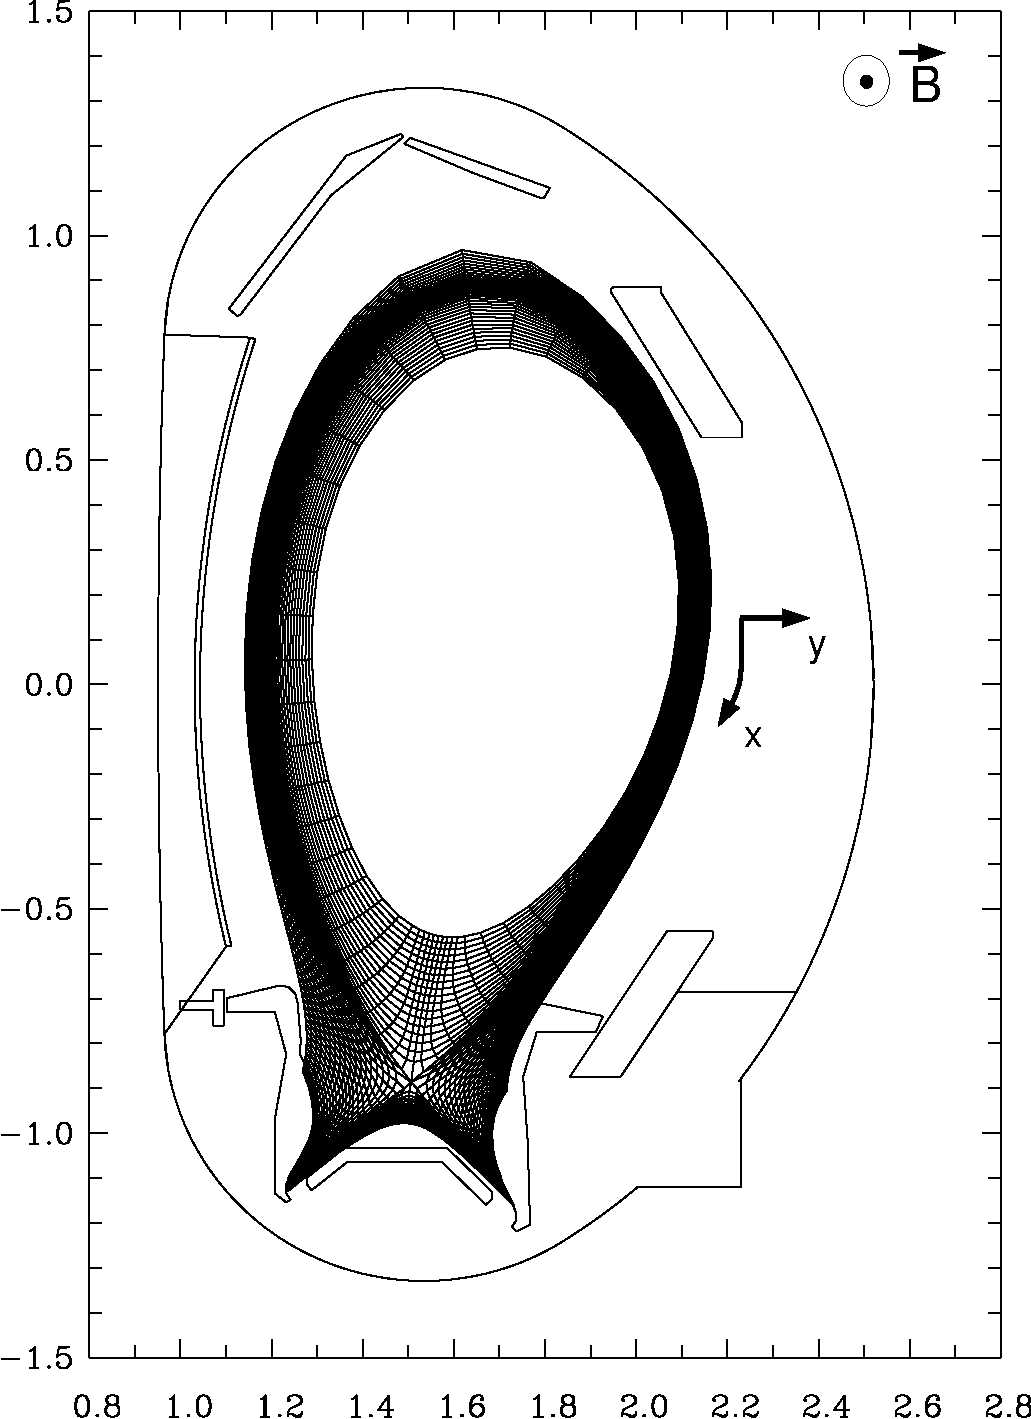
\includegraphics[width=8.0cm]{b2plot_1.pdf}
\else
\includegraphics[width=8.0cm]{b2plot.1.epsi}
\fi
}
\caption{Coordinate system: $x$ is the poloidal coordinate,
$y$ is the radial coordinate orthogonal to the flux surfaces. The
coordinate $\perp$ corresponds to the direction perpendicular
both to the magnetic field and to the $y$-axis. The directions
of magnetic field and plasma current correspond to normal
operation conditions of ASDEX--Upgrade (ion $\nabla B$ drift
directed towards the X-point).
 }
\label{fig:geo}
\end{figure}

The metric coefficients are
$h_x=1/\|\grad x\|$, $h_y=1/\|\grad y\|$ and $\sqrt{g}=h_xh_yh_z$.
One can replace $h_z$ by $2 \pi R$,
where $R$ is the local major radius.  Components of a vector are the
projections on unit basis vectors
; they are not the contravariant or
covariant components ($b_x = B_x/B$, $b_z = B_z/B$).
Ion velocities $V_{\perp}$ (velocity perpendicular both
to magnetic field $B$ and the $y$-axis) and $V_y$ are
determined from the two components of the momentum balance equation
for ions perpendicular to a magnetic field. Using the Braginskii expression
for the friction force, one obtains:\\
\begin{gather}
\label{eq:nf1}
V_{\perp} = V_{\perp}^{\left( a \right)} - \frac{1}{enB}
\frac{1}{h_y}\frac{\partial nT_i}{\partial y} + 
V_{\perp}^{\left( in \right)} + V_{\perp}^{\left( vis \right)} +
V_{\perp}^{\left( s \right)}
\end{gather}
\begin{gather}
\label{eq:nf2}
V_y = V_y^{\left( a \right)} + \frac{B_z}{enB^2}
\frac{1}{h_x}\frac{\partial nT_i}{\partial x} + 
V_y^{\left( in \right)} + V_y^{\left( vis \right)} +
V_y^{\left( s \right)}
\end{gather}
Velocities $V_{\perp,y}^{\left( a \right)}$ are the sum of the 
$\vec{E} \times \vec{B}$ drifts and diffusive and thermo-diffusive
velocities. 
This part corresponds to the ambipolar flux. It is the same both for ions and
electrons.
The second term in the r.h.s. of 
Eqs. (\ref{eq:nf1}) and (\ref{eq:nf2})
corresponds to diamagnetic flow of ions, while the other terms  are caused 
by inertial, viscous and ion-neutral friction forces. 
These non-ambipolar terms are 
connected with currents: $\vec{V}^{\left( in \right)} = \vec{j}^{\left( in \right)}/en,
\vec{V}^{\left( vis \right)} = \vec{j}^{\left( vis \right)}/en,
\vec{V}^{\left( s \right)} = \vec{j}^{\left( s \right)}/en$.\\ 
In the presence of anomalous transport 
($D$ is the classical diffusion coefficient, $D=\frac{T_e+T_i}{eb} 
\frac{\nu_{ei}}{\omega_{ce}}$, with electron cyclotron frequency
$\omega_{ce}$ and electron-ion collision frequency $\nu_{ei}$)
\begin{gather}
\label{eq:nf3}
V_{\perp}^{\left( a \right)} =
- \frac{1}{B}\frac{1}{h_y}\frac{\partial \Phi}{\partial y}
-\frac{D}{T_e+T_i} \frac{b_z}{h_x}\left(\frac{\partial p}{n \partial x}
-\frac{3}{2}\frac{\partial T_e}{\partial x}\right)
-D_{AN}^n\frac{1}{h_x n} \frac{\partial n}{\partial x}
-D_{AN}^p\frac{1}{h_x n} \frac{\partial p_i}{\partial x}
+V_{\perp}^{\left( AN \right)}
\end{gather}
\begin{gather}
\label{eq:nf44}
V_y^{\left( a \right)} =
\frac{B_z}{B^2}\frac{1}{h_x}\frac{\partial \Phi}{\partial x}
-\frac{D}{T_e+T_i} \frac{1}{h_y}\left(\frac{\partial p}{n \partial y}
-\frac{3}{2}\frac{\partial T_e}{\partial y}\right)
-D_{AN}^n\frac{1}{h_y n} \frac{\partial n}{\partial y}
-D_{AN}^p\frac{1}{h_y n} \frac{\partial p_i}{\partial y}
+V_y^{\left( AN \right)}
\end{gather}
The poloidal velocity is a sum $V_x = b_z V_{\perp} + b_x V_{\parallel}$.

In the particle balance 
the fact that the diamagnetic 
velocity is almost divergence free is taken into
account. Therefore, instead of the diamagnetic velocity
it is possible to introduce an effective 
velocity $\vec{\tilde{V}}^{\left( dia \right)}$, 
which gives the same contribution 
to the divergence of the particle flux:
\begin{gather}
\label{eq:nf4}
\frac{\partial n}{\partial t} +
     \frac{1}{\sqrt{g}} \frac{\partial }{\partial x}
      \left(\frac{\sqrt{g}}{h_x} n\left(b_x V_{\parallel} +
     b_z V_{\perp}^{\left( 0 \right)}\right)\right)+
     \frac{1}{\sqrt{g}} \frac{\partial }{\partial y}
      \left(\frac{\sqrt{g}}{h_y} n V_y^{\left( 0 \right)}\right)
= S^n
\end{gather}
\begin{gather}\label{eq:nf5}
V_{\perp}^{\left( 0 \right)} = V_{\perp}^{\left( a \right)} +
V_{\perp}^{\left( in \right)} + V_{\perp}^{\left( vis \right)} +
V_{\perp}^{\left( s \right)} + \tilde{V}_{\perp}^{\left( dia \right)}
\end{gather}
\begin{gather}\label{eq:nf6}
V_{y}^{\left( 0 \right)} = V_{y}^{\left( a \right)} +
V_{y}^{\left( in \right)} + V_{y}^{\left( vis \right)} +
V_{y}^{\left( s \right)} + \tilde{V}_{y}^{\left( dia \right)}
\end{gather}
\begin{gather}\label{eq:nf7}
\tilde{V}_{\perp}^{\left( dia \right)} = \frac{T_i B_z}{e}
\frac{\partial}{h_y \partial y}\left(\frac{1}{B^2}\right)
\end{gather}
\begin{gather}\label{eq:nf8}
\tilde{V}_y^{\left( dia \right)} = -\frac{T_i B_z}{e}
\frac{\partial}{h_x \partial x}\left(\frac{1}{B^2}\right)
\end{gather}
The velocity $\tilde{V}^{{\left(dia\right)}}$ is an effective velocity. It
represents vertical guiding centre drift of ions caused by 
$\nabla B$.\\

Combining the inertia and gyroviscosity terms in the Braginskii equations, 
one finds
\begin{multline}\label{eq:mom}
\hfill m_i \left[ \frac{\partial n V_{\parallel}}{\partial t} +
     \frac{1}{\sqrt{g}} \frac{\partial }{\partial x}
      \left( \frac{\sqrt{g}}{h_x} n 
       \left( V_{\perp}^{\left( 0 \right)} b_z
            + V_{\parallel} b_x \right) 
       V_{\parallel} \right) +
     \frac{1}{\sqrt{g}} \frac{\partial }{\partial y}
      \left( \frac{\sqrt{g}}{h_y} n V_y^{\left( 0 \right)} V_{\parallel} \right)
\right] = \hfill \\
\hfill -\frac{b_x}{h_x}\frac{\partial n T_i}{\partial x} -
b_x \frac{en}{h_x}\frac{\partial \Phi}{\partial x} + F_k +
\frac{4}{3} b_x B^{3/2} \frac{\partial }{h_x \partial x}
\left(\frac{\eta_0 b_x}{B^2} 
\frac{\partial\left(\sqrt{B}\left(V_{\parallel}+b_x \left(V^{(dia)}_{\perp} + V^{(E)}_{\perp}\right)\right)\right)}
{h_x \partial x}\right)
\hfill \\
\hfill + B^{3/2} b_x \frac{\partial}{h_x \partial x}
\left(\frac{b_x}{\nu_{ii} B^2} 
\frac{\partial\left(\sqrt{B}q_{i\parallel}^{\left( 0 \right)}
\right)}{h_x \partial x}\right)+
     \frac{1}{\sqrt{g}} \frac{\partial }{\partial y}
      \left(\frac{\sqrt{g}}{h_y^2} \eta_2 \frac{\partial V_{\parallel}}
{\partial y}\right) \hfill \\
\hfill
      + \frac{1}{\sqrt{g}} \frac{\partial }{\partial x}
      \left(\frac{\sqrt{g}}{h_x^2} \eta_2 \frac{\partial V_{\parallel}}
{\partial x}\right) 
+ S_{i \parallel}^m + R_{ie\parallel}. \hfill
\end{multline}
The diamagnetic terms in the l.h.s. of (\ref{eq:mom}) are almost cancelled 
\cite{ROGNLIEN98A, ROGNLIEN98B, ROGNLIEN99A, HINTON94C}, so that
velocities normal to the flux surface in the second and third term,
as in the particle balance equation, are determined by (\ref{eq:nf1}) and (\ref{eq:nf2}). 
In \cite{HINTON94C}
the divergent part of diamagnetic velocity has been 
neglected. Here, it is kept, because the corresponding flux is still
relatively large and can be comparable with the diffusive flux even
for anomalous diffusion coefficients. The authors of 
\cite{ROGNLIEN98A, ROGNLIEN98B, ROGNLIEN99A} also kept this
flux.
In contrast to 
\cite{ROGNLIEN98A, ROGNLIEN98B, ROGNLIEN99A}
there is an additional term of the same kind in the r.h.s. of 
Eq. (\ref{eq:mom}):
\begin{gather}
F_k = - m_i \left(\frac{1}{\sqrt{g}} \frac{\partial }{\partial x}
      \left(\frac{\sqrt{g}}{h_x} n V_{\parallel} 
      \tilde{V}_{\perp}^{\left( dia \right)} b_z \right) +
      \frac{1}{\sqrt{g}} \frac{\partial }{\partial y}
      \left(\frac{\sqrt{g}}{h_y} n V_{\parallel} 
      \tilde{V}_y^{\left( dia \right)} \right)\right)
\end{gather}
This parallel force is the Coriolis force, connected with the 
diamagnetic drift velocity and 
toroidal (parallel) rotation. This force can be obtained in a different
way by averaging the drift kinetic equation 
\cite{MIHAIL84A} and is of the same order
as the inertia terms.

Parallel viscosity is represented 
by the fourth and fifth terms in the r.h.s. 
The former is the Balescu
parallel viscosity with coefficient $\eta _0 = \dfrac{4}{3} 0.96 \sqrt{2} n T_i / \nu_{ii}$. 
The latter corresponds to the parallel viscosity driven 
by parallel ion heat flux 
$q_{i\parallel}^{\left( 0 \right)} = 
- \kappa _{i,\parallel} b_x \frac{1}{h_x} \frac{\partial T_i}{\partial x}$. 
This viscosity is absent in the Braginskii equations, however, in a tokamak,
where parallel particle flux multiplied by temperature is of
the order of the ion heat flux, these two 
viscosities are of the same order. On closed flux surfaces far from 
the separatrix, the flux-surface-averaged parallel 
viscosity coincides with the well-known 
neoclassical expression for the Pfirsch-Schl{\"u}ter regime
\cite{HIRSHMAN81A}. 
Thus, parallel viscosity in Eq. (\ref{eq:mom}) provides smooth transition to 
neoclassical theory. 
The classical perpendicular viscosity coefficient 
can 
be replaced by an anomalous value as in
\cite{ROGNLIEN98A, ROGNLIEN98B, ROGNLIEN99A}: $\eta _2 =
n m_i D_{AN}^n$. Perpendicular viscosity and inertia terms with the
anomalous particle flux are responsible for the transport of the
parallel momentum in radial and poloidal directions. The radial transport
can be rather important despite the fact that $\eta_2 \ll \eta _0$, since
the scale in the radial direction is rather small.

The term  $S_{i \parallel}^m$  represents the parallel momentum loss due to 
ion-neutral friction and parallel momentum input from neutral beam injection. 
$R_{ie\parallel}$ is the ion-electron friction.

The parallel momentum balance for electrons has the standard form:
\begin{gather}
j_{\parallel} = \sigma _{\parallel} \left(
\frac{b_x}{e} \frac{1}{h_x} \left( \frac{\partial n T_e}{n \partial x} +
0.71 \frac{\partial T_e}{\partial x} \right) 
- \frac{b_x}{h_x} \frac{\partial \Phi}{\partial x} \right).
\end{gather}

Expressions for $j_{\perp}$ and $j_y$ are obtained from radial and 
poloidal projections of the total momentum balance equation (the sum
of electron and ion momentum balance equations). 
The resulting current is a sum of contributions from pressure 
gradient (diamagnetic current) $\vec{j}^{\left( dia \right)}$, inertia
and gyroviscosity $\vec{j}^{\left( in \right)}$, viscosity
$\vec{j}^{\left( vis \right)}$ and ion-neutral friction
$\vec{j}^{\left( s \right)}$. 
Similar to the particle continuity equation, the effective 
current $\vec{\tilde{j}}$ is introduced, which gives the same contribution to 
$\nabla \vec{j}$, as the ordinary current. This gives the current continuity
equation
\begin{gather}\label{eq:curr0}
     \frac{1}{\sqrt{g}} \frac{\partial }{\partial x}
      \left(\frac{\sqrt{g}}{h_x} \tilde{j}_x\right)+
     \frac{1}{\sqrt{g}} \frac{\partial }{\partial y}
      \left(\frac{\sqrt{g}}{h_y} \tilde{j}_y\right)
= 0~.
\end{gather}
\begin{gather}\label{eq:curr1}
\tilde{j}_x = b_z \tilde{j}_{\perp} + b_x \tilde{j}_{\parallel}~.
\end{gather}
\begin{gather}\label{eq:curr2}
\vec{j} = \vec{\tilde{j}}^{\left( dia \right)} + \vec{j}^{\left( in \right)}
+ \vec{j}^{\left( vis \right)} + \vec{j}^{\left( s \right)}
+\vec{j}_{\parallel}~.
\end{gather}
The effective diamagnetic current can be chosen in a form
\begin{gather}\label{eq:curr3}
\tilde{j}_{\perp}^{\left( dia \right)} =
\frac{1}{b_z}\frac{n\left( T_e + T_i \right) B_z}{h_y}
\frac{\partial}{\partial y}\left(\frac{1}{B^2}\right)~,
\end{gather}
\begin{gather}\label{eq:curr4}
\tilde{j}_y^{\left( dia \right)} =
- \frac{n\left( T_e + T_i \right) B_z}{h_x}
\frac{\partial}{\partial x}\left(\frac{1}{B^2}\right)~.
\end{gather}
Current driven by parallel viscosity should be taken into account in 
Eqs. (\ref{eq:curr0}), (\ref{eq:curr1}) and (\ref{eq:curr2}). 
This current is a small correction to the diamagnetic current 
Eqs. (\ref{eq:curr3}) and (\ref{eq:curr4}).
However, on closed flux surfaces, where the pressure is almost constant, 
the diamagnetic current averaged
over the flux surfaces tends to zero. The resulting remaining part can 
become comparable to the parallel viscosity-driven current, which is
necessary to satisfy the condition that the averaged net radial current
should be zero. 
The terms, which contain the plasma viscosity, produce almost 
divergence-free currents. 
Similar to the case of diamagnetic currents, it can be reduced
to
\begin{gather}
\tilde{j}_{\perp}^{\left( vis \parallel \right)} =
- \frac{B_x \eta _0}{3 \sqrt{B}}
\frac{\partial\left(\sqrt{B}\left(V_{\parallel}+b_x \left(V^{(dia)}_{\perp} + V^{(E)}_{\perp}\right)\right)\right)}
{h_x \partial x}
\frac{\partial}{h_y \partial y}
\left(\frac{1}{B^2}\right)
\end{gather}
\begin{gather}
\tilde{j}_y^{\left( vis \parallel \right)} =
b_z\frac{B_x \eta _0}{3 \sqrt{B}}
\frac{\partial\left(\sqrt{B}\left(V_{\parallel}+b_x \left(V^{(dia)}_{\perp} + V^{(E)}_{\perp}\right)\right)\right)}
{h_x \partial x}
\frac{\partial}{h_x \partial x}
\left(\frac{1}{B^2}\right)
\end{gather}
The current produced by components of viscosity tensor connected 
with heat fluxes is:
\begin{gather}
\tilde{j}_{\perp}^{\left( vis q \right)} =
- \frac{0.24 B_x}{\sqrt{B} \nu_{ii}}\frac{\partial
\left(q_{i \parallel}^{\left( 0 \right)} \sqrt{B}\right)}{h_x \partial x}
\frac{\partial}{h_y \partial y}
\left(\frac{1}{B^2}\right)
\end{gather}
\begin{gather}
\tilde{j}_y^{\left( vis q \right)} =
b_z\frac{0.24 B_x}{\sqrt{B} \nu_{ii}}\frac{\partial
\left(q_{i \parallel}^{\left( 0 \right)} \sqrt{B}\right)}{h_x \partial x}
\frac{\partial}{h_x \partial x}
\left(\frac{1}{B^2}\right)
\end{gather}

The second part of the current contains contributions from both inertia
and gyroviscosity forces. In contrast to the parallel momentum balance,
the cancellation is not complete (as has been noticed in 
\cite{HINTON94C}). Expressions
for this part of the current are

\begin{multline}
\hfill j_{\perp}^{\left(in\right)}= - \frac{m_i}{B}
\left[\frac{\partial n V_{y}}{\partial t} +
     \frac{1}{\sqrt{g}} \frac{\partial }{\partial x}
      \left(\frac{\sqrt{g}}{h_x} n\left(V_{\perp}^{\left( 0 \right)} b_z
+ V_{\parallel} b_x \right) V_{y}\right)+
     \frac{1}{\sqrt{g}} \frac{\partial }{\partial y}
      \left(\frac{\sqrt{g}}{h_y} n V_y^{\left( 0 \right)} V_{y}\right)
\right] \hfill \\
\hfill -
\frac{2 b_x}{B} \frac{1}{h_x}\frac{\partial}{\partial x}
\left(\eta_3  
\frac{\partial V_{\parallel}}{h_x \partial x}\right)+
\frac{m_i}{B} n V_{\parallel}^2 \frac{\partial ln h_z}{h_y \partial y}
\hfill
\end{multline}

\begin{multline}
\hfill j_{y}^{\left(in\right)}= \frac{m_i}{B}
\left[\frac{\partial n V_{\perp}}{\partial t} +
     \frac{1}{\sqrt{g}} \frac{\partial }{\partial x}
      \left(\frac{\sqrt{g}}{h_x} n\left(V_{\perp}^{\left( 0 \right)} b_z
+ V_{\parallel} b_x \right) V_{\perp}\right)+
     \frac{1}{\sqrt{g}} \frac{\partial }{\partial y}
      \left(\frac{\sqrt{g}}{h_y} n V_y^{\left( 0 \right)} V_{\perp}\right)
\right] \hfill \\
\hfill -
\frac{2 b_x}{B} \frac{1}{h_x}\frac{\partial}{\partial x}
\left(\eta_3  
\frac{\partial V_{\parallel}}{h_y \partial y}\right) -
\frac{m_i}{B} n V_{\parallel}^2 \frac{\partial ln h_z}{h_x \partial x}
\hfill
\end{multline}

where $\eta_3 = \frac{n T_i}{2 \omega_{ci}}, \eta _1 = \frac{\eta _2}{4}$.

The last terms proportional to the gradient of $B$ correspond to the vertical
guiding centre drift of ions caused by the centrifugal force. This current
can be simply added to the diamagnetic current. Other terms seem to be less
important.

The contribution from perpendicular viscosity is
\begin{multline}
\hfill j_{\perp}^{\left(vis \perp \right)}= \frac{1}{B}
\left[\frac{1}{h_x}\frac{\partial}{\partial x}\left(\eta_1 
     \frac{\partial V_y}{h_x \partial x}\right)+
 \frac{1}{h_y}\frac{\partial}{\partial y}\left(\eta_1 
     \frac{\partial V_y}{h_y \partial y}\right)+
\frac{1}{h_x h_y }\frac{\partial \eta_1}{\partial x}
     \frac{\partial V_{\perp}}{\partial y}-
\frac{1}{h_x h_y }\frac{\partial \eta_1}{\partial y}
     \frac{\partial V_{\perp}}{\partial x}\right] \hfill \\
\hfill +
\frac{4 b_x}{B} \frac{1}{h_x h_y}
\left(\frac{\partial \eta_1}{\partial x} \frac{\partial V_{\parallel}}
{\partial y} - \frac{\partial \eta_1}{\partial y}\frac{\partial V_{\parallel}}
{\partial x}
\right)
\hfill
\end{multline}
\begin{gather}
j_{y}^{\left(vis \perp \right)}= -\frac{1}{B}
\left[\frac{1}{h_y}\frac{\partial}{\partial y}\left(\eta_1 
     \frac{\partial V_{\perp}}{h_y \partial y}\right)+
 \frac{1}{h_x}\frac{\partial}{\partial x}\left(\eta_1 
     \frac{\partial V_{\perp}}{h_x \partial x}\right)-
\frac{1}{h_x h_y }\frac{\partial \eta_1}{\partial x}
     \frac{\partial V_y}{\partial y}+
\frac{1}{h_x h_y }\frac{\partial \eta_1}{\partial y}
     \frac{\partial V_y}{\partial x}\right].
\end{gather}

Here, the largest term is the first one in the r.h.s. of the expression
for the radial current, since the radial derivatives are the largest.
This current corresponds to a pure cylindrical approximation. It is
responsible, for example, for closing currents near flush-mounted probes
\cite{ROZ99A}.
It was taken into account in 
\cite{ROGNLIEN99A, RADFORD96A}. However, in the problem of global current
structure in the edge plasma, the currents driven by parallel viscosity seem
to be more important.

The total current caused by viscosity is
\begin{gather}
\vec{j}^{\left(vis\right)} = \vec{j}^{\left(vis \parallel\right)} +
\vec{j}^{\left(vis \perp\right)} +
\vec{j}^{\left(vis q\right)}
~.
\end{gather}

The contribution from ion neutral friction is
\begin{gather}
j_{\perp}^{\left(s\right)} = \frac{S_{iy}^m}{B}
~.
\end{gather}
\begin{gather}
j_{y}^{\left(s\right)} = -\frac{S_{i \perp}^m}{B}
~,
\end{gather}
where $S_{iy}^m$ and $S_{i \perp}^m$ are the momentum sinks due to
ion-neutral friction. 
\begin{gather}
S_{i \perp}^m = - n \mu_{iN} \nu_{iN} \left( V_{\perp} - V_{\perp N}\right)
~,
\end{gather}
\begin{gather}
S_{i y}^m = - n \mu_{iN} \nu_{iN} \left( V_{y} - V_{y N}\right)
~,
\end{gather}
where $\mu_{iN}=m_i/2$ is the effective mass, $\nu_{iN}= n_N <V_{iN} 
\sigma_{cx}>$ is the ion-neutral collision frequency,
$n_N$ is the neutral density and $\vec{V_{iN}}$ is the neutral mean
velocity. For the ion velocity used above,
only electric and diamagnetic drifts are left, neglecting smaller terms,
to obtain
\begin{gather}
\tilde j_{x}^{\left(s\right)} = \tilde j_{\perp}^ {\left(s\right)} b_z =
- \sigma _{iN} b_z^2 \frac{\partial \Phi}{h_x \partial x}-
\sigma _{iN} b_z^2 \frac{1}{e n}\frac{\partial n T_i}{h_x \partial x}+
\sigma _{iN} B_z V_{yN}
~,
\end{gather}
\begin{gather}
\tilde j_{y}^{\left(s\right)} =
- \sigma _{iN} \frac{\partial \Phi}{h_y \partial y}-
\sigma _{iN} \frac{1}{e n}\frac{\partial n T_i}{h_y \partial y}-
\sigma _{iN} B V_{\perp N}
~,
\end{gather}
where $\sigma _{iN}$ is the ion-neutral perpendicular conductivity
\begin{gather}
\sigma _{iN} =
\frac{n m_i <V_{iN} \sigma_{cx}> n_N}{2 B^2}
~.
\end{gather}

The rate of charge-exchange $<V_{iN} \sigma_{cx}>$ can
be expressed through the mobility $K_0$ measured in the absence of a 
magnetic field for room temperature and atmospheric pressure for
deuterium \cite{MCDANIEL73A}:
\begin{gather}
K_0 =
\frac{2 e}{m_i <V_{iN} \sigma_{cx}> n_N^{\left(0\right)}}
~,
\end{gather}
with $n_N^{\left(0\right)} = 2.687 \cdot 10^{25} m^{-3}$ and
$K_0 = 11.2 \cdot 10^{-4} \frac{m^2}{s V}$.
Assuming that the charge-exchange cross-section is approximately constant
one gets
\begin{gather}
<V_{iN} \sigma_{cx}> = 3.2 \cdot 10^{-15} \sqrt{\frac{T_i}{0.026}} 
\frac{m^3}{s}
~,
\end{gather}
where $T_i$ is measured in $eV$. A similar expression, which gives approximately
the same result, is \cite{ROZ88A}:
\begin{gather}
<V_{iN} \sigma_{cx}> = \frac{32 \sigma _{cx}}{3 \sqrt{\pi}}
\sqrt{\frac{T_i}{m_i}}
\frac{m^3}{s}
~.
\end{gather}.


In the energy balance equations 
appears
a special problem, which is the 
possible inclusion of an anomalous radial current.
The basic guidelines are as follows:
\begin{itemize}
\item The expression must be as simple as possible, and the most convenient
format is an Ohm-like expression;
\item The system of equations must be informed about this non-classical
contribution, but
\item The classical core of the equations must not be disturbed.
\end{itemize}
Apparently, the radial current would enter the electron energy equation
via the Joule term, but this manipulation is inappropriate since one cannot 
be sure that this term directly heats the electrons, which is the case in
a purely classical setup. The proper thing to do is to keep only 
the non-radial classical contribution in the Joule term, and 
construct additional heat exchange terms
containing the radial current.
In this way, the system decides how to thermodynamically allocate the
``alien'' heat term, among electrons and ion species.\\
For this reason, one cannot simply use the standard Ohm's
law in the radial direction with anomalous coefficients, or any other
prescribed expression whatsoever, as a constructive procedure is necessary
for simultaneously producing the radial current as well as the heat exchange
terms. At this point it has to be mentioned that this peculiarity arises
only in the multifluid case, whereas in the single species case 
these heat exchange terms can indeed be constructed even using a prescribed
expression for the radial current. \\
The trick for carrying out this program is to correct the electron friction
density $\vec{R}^e$ by adding the term $n_e e \tilde{\eta}_\perp \vec{J}_\perp$
similar to the classical one, only using the {\itshape ad hoc} parameter
$\tilde{\eta}_\perp$. \\
Since $\vec{R}^e=-{\sum_{a}\vec{R}^a}$, one has a
modified total ion momentum equation at hand which in conjuction with the
pressure equilibrium (not affected by the additional term)
$\vec{J} \times \vec{B} =  \nabla P$, gives the diffusive part of the
radial current, namely
\begin{gather}
J_y^{diff}=\frac{\tilde{\eta}_\perp en_e}{B^2} \frac{\partial P_i}{\partial y}
\end{gather}
where $P_i$ is the total ion pressure. This dependency is also found in
\cite{ROGNLIEN98A}. Moreover, an additional dependence on the radial
electric field can potentially be added without interfering with
the procedure. \\
The final step, namely the construction of the heat exchange terms, is
performed by claiming that the well known relation \cite{BAELMANS94A}
(adapted for the multifluid case)
\begin{gather}
Q_e=-\sum_{a} \left (Q_a + (\vec{u}^a - \vec{u}^e) \cdot \vec{R}^a \right )~,
\end{gather}
which stems from the fundamental null space of the collision operator,
is still true while carrying the modified friction.
Claiming this, after
performing the proper manipulations in the energy
equations, one reveals the {\itshape ad hoc} 
contribution as the exchange term that one wants,
which reads
$
\sum_{a} (\vec{u}^a -\vec{u}^e)_\perp n_a \frac{Z_a^2}{Z_{eff}}e \tilde{\eta}_\perp \vec{J}_\perp
$
added in the total ion energy equation and subtracted from the
electron equation.
Note that in the single species case, this term boils down to
$
\tilde{\eta}_\perp J_\perp ^2
$
removing energy from the electrons,  depositing it to the ions, a feature
predicted by neoclassical theory \cite{ROSENBLUTH72A}.\\

In the final form of the energy balance equations, the convective heat 
flux and the diamagnetic heat flux are combined as in 
\cite{ROGNLIEN98A, ROGNLIEN98B, ROGNLIEN99A, HINTON94C}, see also
\cite{ROZ99A}.

The energy balance equation for the electrons is
\begin{multline}
\hfill
     \frac{3}{2} \frac{\partial nT_e}{\partial t} +
     \frac{1}{\sqrt{g}} \frac{\partial }{\partial x}
      \left(\frac{\sqrt{g}}{h_x} \tilde{q}_{ex}\right) +
     \frac{1}{\sqrt{g}} \frac{\partial }{\partial y}
      \left(\frac{\sqrt{g}}{h_y} \tilde{q}_{ey}\right) +
     \frac{nT_e}{\sqrt{g}}\frac{\partial }{\partial x}
      \left(\frac{\sqrt{g}}{h_x}\left(
      V_{\parallel} - j_{\parallel}/en\right)b_x\right) \hfill \\
\hfill     =
     Q_e + n T_e B \frac{1}{h_x h_y}\left(\frac{\partial \Phi}{\partial y}
     \frac{\partial}{\partial x}\left(\frac{1}{B^2}\right)
     -\frac{\partial \Phi}{\partial x}\frac{\partial}{\partial y}
     \left(\frac{1}{B^2}\right)\right)~,\hfill
\end{multline}
where
\begin{multline}
\hfill        \tilde{q}_{ex} = \frac{3}{2} n T_e \left(- \frac{b_z}{B h_y}
         \frac{\partial \Phi}{\partial y}
         + b_x V_{\parallel} - b_x j_{\parallel} / en + b_z V_{\perp}^{(AN)} \right) \hfill \\
     \hfill + \frac{5}{2} n T_e b_z \left(
     - \frac{D}{T_e+T_i} \frac{b_z}{h_x} \left(\frac{\partial p}{n \partial x}
     - \frac{3}{2} \frac{\partial T_e}{\partial x} \right)
     - D_{AN}^n \frac{1}{h_x n} \frac{\partial n}{\partial x}
     - D_{AN}^p \frac{1}{h_x n} \frac{\partial p_i}{\partial x} \right)
     + n V_{e\perp}^{(AN)}
      \hfill \\
      \hfill   - 0.71 b_x j_{\parallel} T_e/e - \kappa _{e \parallel}
         \frac{b_x^2}{h_x} \frac{\partial T_e}{\partial x}
         - \kappa _{e \perp} b_z^2 \frac{1}{h_x} 
         \frac{\partial T_e}{\partial x} \hfill \\
      \hfill   + \frac{3}{2}\frac{T_e}{e B} \frac{\nu_{ei}}{\omega _{ce}}
         \frac{b_z^2}{h_x} \frac{\partial n\left(T_e+T_i\right)}{\partial x}
         - \frac{5}{2} n T_e^2 \frac{B_z}{e}
         \frac{\partial}{h_y \partial y}\left(\frac{1}{B^2}\right) ~ , \hfill
\end{multline}
\begin{multline}
\hfill  \tilde{q}_{ey} = \frac{3}{2} n T_e \left( \frac{B_z}{B^2} \frac{1}{h_x}
        \frac{\partial \Phi}{\partial x} + V_{y}^{(AN)} \right) \hfill \\
     \hfill  + \frac{5}{2} n T_e \left(
     - \frac{D}{T_e+T_i} \frac{1}{h_y} \left( \frac{\partial p}{n \partial y}
     - \frac{3}{2} \frac{\partial T_e}{\partial y} \right)
     - D_{AN}^n \frac{1}{h_y n} \frac{\partial n}{\partial y}
     - D_{AN}^p \frac{1}{h_y n} \frac{\partial p_i}{\partial y} \right)
     + n V_{ey}^{(AN)}
         \hfill \\
         \hfill - \kappa _{e \perp} \frac{1}{h_y} \frac{\partial T_e}{\partial y}
         + \frac{3}{2}\frac{T_e}{e B} \frac{\nu _{ei}}{\omega_{ce}}
         \frac{1}{h_y} \frac{\partial n\left(T_e+T_i\right)}{\partial y}
         + \frac{5}{2} n T_e^2 \frac{B_z}{e}
         \frac{\partial}{h_x \partial x}\left(\frac{1}{B^2} \right) ~ , \hfill
\end{multline}
\begin{gather}
        Q_{\Delta} = \frac{3 m_e}{m_i} n \nu _{ei} \left(
T_e - T_i
\right)~,
\end{gather}
\begin{gather}
        Q_u = R _{ie \parallel} j_{\parallel}/en~,
\end{gather}
\begin{gather}
        Q_{AN} = \sum_{a} \left(\vec{u}^a -\vec{u}^e\right)_\perp n_a 
                 \frac{Z_a^2}{Z_{eff}}e \tilde{\eta}_\perp \vec{J}_\perp~,
\end{gather}
\begin{gather}
        Q_e = -Q_{\Delta} - Q_u - Q_{AN}~.
\end{gather}


Here $\kappa _{e \parallel}$ is the Balescu (not Braginskii as stated in the CPP review paper \cite{SOLPS_review} 
or in \$\verb!SOLPSTOP/doc/CPP_2006.pdf!) heat 
conductivity with a possible heat
flux limit \cite{BRAAMS96B}. 
The leading numerical coefficient is then $\frac{5}{2} \frac{2.16 z}{1 + 0.27 z}$ as opposed to 3.16 for the Braginskii
formula \cite{NRL}. The perpendicular heat conductivity 
$\kappa _{e \perp}$ can be 
either classical or anomalous. In the last term of the energy balance
equation, it is taken into account that the $\vec{E} \times \vec{B}$
drift velocity is
almost divergence-free.

The ion energy balance equation is
\begin{multline}\label{eq:ion_energy} \hfill
     \frac{3}{2} \frac{\partial nT_i}{\partial t} +
     \frac{1}{\sqrt{g}} \frac{\partial }{\partial x}
      \left(\frac{\sqrt{g}}{h_x} \tilde{q}_{ix}\right) +
     \frac{1}{\sqrt{g}} \frac{\partial }{\partial y}
      \left(\frac{\sqrt{g}}{h_y} \tilde{q}_{iy}\right) +
     \frac{nT_i}{\sqrt{g}}\frac{\partial }{\partial x}
      \left(\frac{\sqrt{g}}{h_x} V_{\parallel} b_x \right) \hfill \\
     \hfill =
     Q_{\Delta} + Q_{AN} + \frac{\eta _0}{3} \left(2 b_x 
     \frac{\partial V_{\parallel}}{h_x \partial x}\right)^2+ 
     n T_i B 
     \frac{1}{h_x h_y}\left(\frac{\partial \Phi}{\partial y}
     \frac{\partial}{\partial x}\left(\frac{1}{B^2}\right)
     -\frac{\partial \Phi}{\partial x}\frac{\partial}{\partial y}
     \left(\frac{1}{B^2}\right)\right)~,\hfill
\end{multline}
where
\begin{multline} \hfill
        \tilde{q}_{ix} = \frac{3}{2} n T_i \left(- \frac{b_z}{B h_y}
        \frac{\partial \Phi}{\partial y}
         + b_x V_{\parallel} + b_z V_{\perp}^{(AN)} \right) \hfill \\
\hfill + \frac{5}{2} n T_i b_z\left(
     - \frac{D}{T_e+T_i} \frac{b_z}{h_x}\left(\frac{\partial p}{n \partial x}
     - \frac{3}{2} \frac{\partial T_e}{\partial x} \right)
     - D_{AN}^n \frac{1}{h_x n} \frac{\partial n}{\partial x}
     - D_{AN}^p \frac{1}{h_x n} \frac{\partial p_i}{\partial x}\right)
     + n V_{i\perp}^{(AN)}
         \hfill \\ \hfill
         + \frac{5}{2} n T_i b_z \tilde{V} _{\perp}^{\left(dia\right)}
         - \kappa _{i \parallel}
         \frac{b_x^2}{h_x} \frac{\partial T_i}{\partial x}
         - \kappa _{i \perp} b_z^2 \frac{1}{h_x} 
         \frac{\partial T_i}{\partial x} ~, \hfill
\end{multline}
\begin{multline} \hfill
        \tilde{q}_{iy} = \frac{3}{2} n T_i \left( \frac{B_z}{B^2} 
         \frac{1}{h_x} \frac{\partial \Phi}{\partial x} + V_{y}^{(AN)} \right) 
        \hfill \\ \hfill
     + \frac{5}{2} n T_i \left(
     - \frac{D}{T_e+T_i} \frac{1}{h_y} \left( \frac{\partial p}{n \partial y}
     - \frac{3}{2} \frac{\partial T_e}{\partial y}\right)
     - D_{AN}^n \frac{1}{h_y n} \frac{\partial n}{\partial y}
     - D_{AN}^p \frac{1}{h_y n} \frac{\partial p_i}{\partial y} \right)
     + n V_{iy}^{(AN)} \hfill \\ \hfill
         - \kappa _{e \perp} \frac{1}{h_y} 
         \frac{\partial T_i}{\partial y}
         + \frac{5}{2} n T_i \tilde{V} _{y}^{\left(dia\right)} ~. \hfill 
\end{multline}

As for the electrons, the parallel heat conductivity is classical with
a possible heat flux limit, while the perpendicular contribution
can be either 
classical or anomalous.

There is discussion in the literature on how to take into account anomalous
terms in the energy balance equations. One point of view (see e.g. 
\cite{ZAGORSKI98A})
is to cancel the contribution from anomalous particle fluxes in the
terms $p_i \nabla \cdot \vec{V}_i$ (or $\vec{V}_i \cdot \nabla p_i$ if equations
are written in a different form). In contrast, according to the
derivation 
\cite{HINTON94C},
where a kinetic equation with fluctuating term has been integrated, the
anomalous fluxes should be kept in all terms of the energy balance
equations. This variant was used in \verb!UEDGE! \cite{ROGNLIEN98A, ROGNLIEN98B, ROGNLIEN99A}. 
In \verb!B2.5! only the contribution
from anomalous radial particle flux to the convective heat flux are left
in the expressions for $\tilde{q}_{e,i}$. In the term  
$p_i \nabla \cdot \vec{V}_i$ the anomalous particle flux is absent. 

\section{Boundary conditions with drifts and currents}
\index{drifts and currents, boundary conditions}
\index{boundary conditions, drifts and currents}

Whether one deals with the diamagnetic or $\bf{E}\times\bf{B}$ perpendicular
drift velocity, special care must be taken to avoid unphysical flows
at the plates. The standard boundary condition is to require that the flow be
at least sonic at the sheath entrance \cite{STANGEBY95B}, 
which translates into:

\begin{equation}\label{eq:Chodura}
V_{\parallel} \ge C_s - \frac{b_z}{b_x} V_{\perp} ~,
\end{equation}

where $C_s$ is the local sound speed and $\frac{b_z}{b_x}$ is the inverse
of the field line pitch. However, for very small pitch angles, as in
stellarators, the $V_{\perp}$ term may overpower the sound 
velocity \cite{FENG99A}
and then the boundary condition would require a plasma flow exiting the plate.
Therefore, the pitch angle at the plates is limited to be no less than
1 degree (user parameter, see switch ``b2agfs\_min\_pitch'' in Appendix \ref{lis:b2cdci}), 
motivated by the engineering limits met when attempting to align the
divertor tiles with the magnetic field. The solution procedure of the code
was also modified so as ensure that no unphysical flows were being created,
and solves the parallel momentum equation using the updated electric potential.

Boundary conditions for the current continuity equation at the plates
correspond to sheath current-voltage characteristics
\begin{equation}\label{eq:sheath-voltage}
j_x = en\left(b_x c_s - b_x \frac{1}{\sqrt{2 \pi}} \sqrt{\frac{T_e}{m_e}} 
      exp\left(- \frac{e \Phi}{T_e}\right) \left(1 - \gamma\right)\right),
\end{equation}
where $\gamma$ is the secondary electron emission coefficient. At the inner
(core) flux surface the currents are set either to the divergent part
of the diamagnetic current or to zero. Both variants give the same result
and both guarantee that the net current integrated over the inner flux surface
should be zero. At the walls, the same conditions on the normal current
components were imposed as for the inner core.

The electron and ion heat fluxes to the target plates are
\begin{equation}\label{eq:target_qe}
\tilde q_{ex} = b_x \frac{n}{\sqrt{2 \pi}} \sqrt{\frac{T_e}{m_e}} 
      exp\left(- \frac{e \Phi}{T_e}\right) \left(1 - \gamma\right)
     \left(T_e \frac{1+\gamma}{1-\gamma} + e \Phi\right),
\end{equation}
\begin{equation}\label{eq:target_qi}
\tilde q_{ex} = \frac{3}{2}n T_i c_s b_x.
\end{equation}

The question of kinetic
boundary conditions including drifts is not yet finally clarified
and will need further work from both kinetic and fluid modelling
\cite{CHANKIN94AB,STANGEBY95B}.

\section{Problems for a fluid description of the edge plasma}  
\index{flux limits}

To apply a fluid model for the description of the edge,
a specific ordering of lengths is necessary.

The necessary condition for a fluid model is
that all characteristic lengths (characteristic length
of the sheath, which is a microscopic length scale of about 10 Debye lengths;
electron and ion mean free path ranging from sub-cm to meters; neutral mean
free path, which is centimeters to meters; heat conduction length which is typically
five times the mean free path length due to the dominant contribution from tail
electrons or ions)
are smaller than the parallel connection length (order of several tens of meters). This
is usually fulfilled in edge plasmas with the following possible exceptions:
\begin{enumerate}
  \item at low temperatures, e.g.
           near the target in the divertor, 
           steeper gradients result in non--local heat flux contributions. In general,
           a non-local description might be necessary 
            (weighted mean of temperature profile over
           five mean free lengths of electrons or ions). However, a simpler correction
           is sometimes satisfactory and is used in the code (see below).
  \item at high temperatures
        (midplane, near separatrix).
        Corrections for flux limit and for periodic systems on closed 
        field lines are necessary due to the fact that the heat conduction
        mean free path is larger than the connection length.
  \item the sheath cannot be resolved by a fluid model and is represented
        by boundary conditions at the sheath entrance deduced from kinetic
        models.
\end{enumerate}

Simple heat flux and momentum flux (viscosity)
limits are available. 
The heat flux limit is formulated as
\begin{gather}
  \kappa _{\parallel}=\frac{\kappa _{SH}}{1+|q_{SH}/q_{fl}|},
\end{gather}

with the classical Spitzer--H\"arm heat flux
\begin{gather}
 q_{SH}=-\kappa _{\parallel ,SH} \cdot \frac{\partial T_e}{\partial x}
\end{gather}

and the flux limit
\begin{gather}
 q_{fl}=\alpha n_e T_e^{3/2} \sqrt{m_e }
\end{gather}

($\alpha \approx 0.2$ from comparison with kinetic calculations for electrons;
the situation for ions is less clear).

The momentum flux limit is done the same way
\begin{gather}
  \eta _{\parallel} =\frac{\eta _{cl,a}}
   {1+|q_{cl,a}/q_{fl,a}|},
\end{gather}

with the classical momentum flux
\begin{gather}
  q_{cl,a}=-\eta _{\parallel,a} \cdot
  \frac{\partial u_{\parallel,a}}{\partial x}
\end{gather}
and the flux limit
\begin{gather}
 q_{fl,a}=\alpha p_{a}
\end{gather}
(with $\alpha = 0.5$). Unfortunately, for this correction even less kinetic 
work
exists than for the heat flux limits. 

Additionally, 
long mean free path corrections of classical heat conduction and viscosity
(in the core) are applied.
For periodic systems and small perturbations one gets
\cite{NEUHAUSER86A}:
\begin{gather}
   q_{\parallel , eff}
    = q_{SH}/\left(h_{\parallel}^2 \lambda_{HC}^2 +1\right),
\end{gather}

with wavenumber of periodicity
\begin{gather}
  h_{\parallel}=2 \pi / \lambda_{\parallel},
\end{gather}
\begin{gather}
  \lambda_{\parallel}=2 \pi R q
\end{gather}

and mean free path of tail electrons
\cite{CHODURA84A}
\begin{gather}
  \lambda_{HC} (\mbox{m}) = 7.5\cdot 10^{16} \cdot T_e^2(\mbox{eV})/n_e(
  \mbox{m}^{-3}).
\end{gather}

Fokker--Planck computer simulations of electron heat transport in laser 
plasmas 
\cite{LLE91}
show that a better description is obtained for a linear
correction:
\begin{gather}
  q_{\parallel , eff}
    = q_{SH}/(h_{\parallel} \lambda_{HC} +1).
\end{gather}

Applying these limits for the core, convergence behaviour of the code
improves significantly.\\
A more correct kinetic limit would imply a
non--local heat transport (and viscosity,...) description.
The parallel heat--flux at a point should be determined by
classical fluxes at points
up to typically five mean--free paths away. As an additional feature, one 
would get
pre--heating effects by fast electrons, maybe important for the ELMs.
Work is necessary to generalize this to the SOL
\cite{KRASH92A,YURI91A}
and this has to be cross--checked
with kinetic calculations \cite{Abou-Assaleh92}. Also, numerical problems due
to this non--local description have to be solved \cite{PRASAD91A}.

In general, if these kinetic corrections become important, quantative 
conclusions are
questionable, because the fluid model is no longer strictly valid. 
Considerations of 
particle, energy and momentum conservation still guarantee a qualitatively 
correct
description. The flux-limiters are designed are defined to give the correct 
answer
in the fully collisional and in the fully collisionless regime.

Parametric studies varying the various flux limiters should be done, 
particularly
for predictive work. Specific experimental scenarios would be required to 
calibrate
the flux limiters. However, complete experimental data sets including 
electron and
ion temperatures and densities at the target plate and upstream are necessary.
Fortunately, at higher densities these corrections are not important. 
Furthermore,
one should note, that mapping of target data to the midplane and the 
extraction of
anomalous radial transport coefficients from such a procedure is 
questionable in the
regime where flux limiters are important
\cite{CosterHinM2003}.

As an example,  
SOLPS5.0 calculations for JET using deuterium, carbon and helium are shown in 
Figs.~\ref{cflmi_1e19} and \ref{cflmi_2e19}.
The predicted electron temperatures at the outer target are shown for 
two different upstream densities.
In each graph, the ion energy flux limit is varied and the sensitivity of the 
target profiles to this variation is obvious. 

\begin{figure}[bt]
\ifpdf 
    \centerline{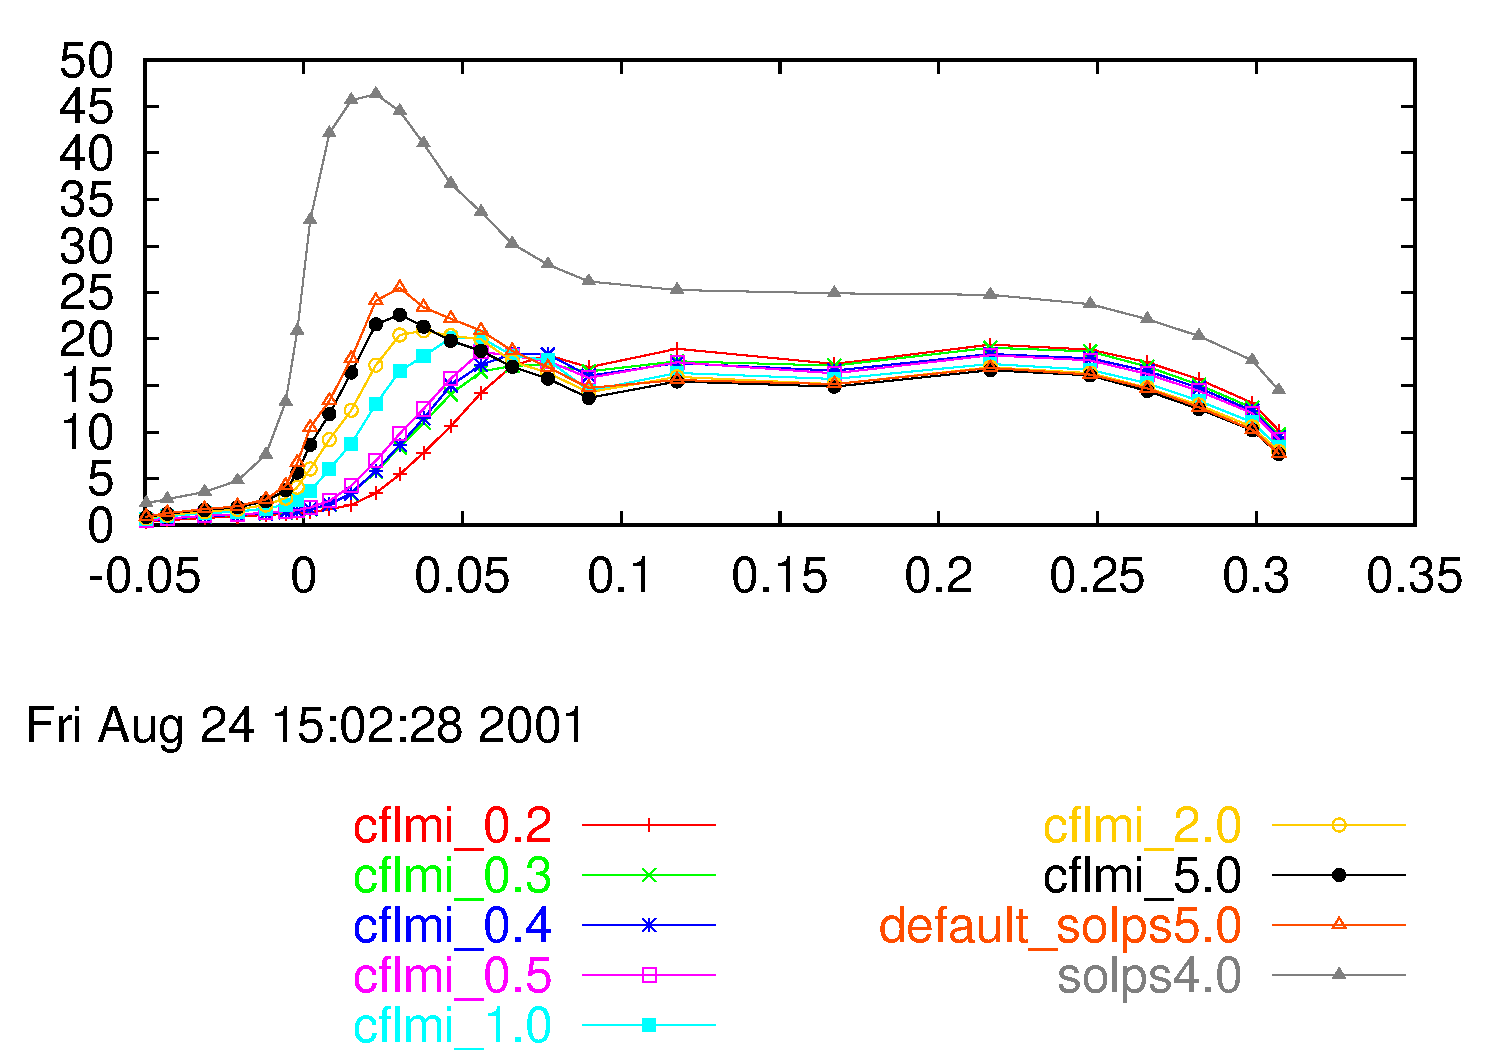
\includegraphics[width=11cm]{cflmi_1e19.pdf}} 
\else
    \centerline{\includegraphics[angle=-90,width=11cm]{cflmi_1e19.ps}} 
\fi
\caption{Impact of ion flux limits for a $10^{19}~~m^{-3}$ upstream density case.}
\label{cflmi_1e19}
\vspace*{1cm}
\end{figure}

\begin{figure}[bt]
\ifpdf 
    \centerline{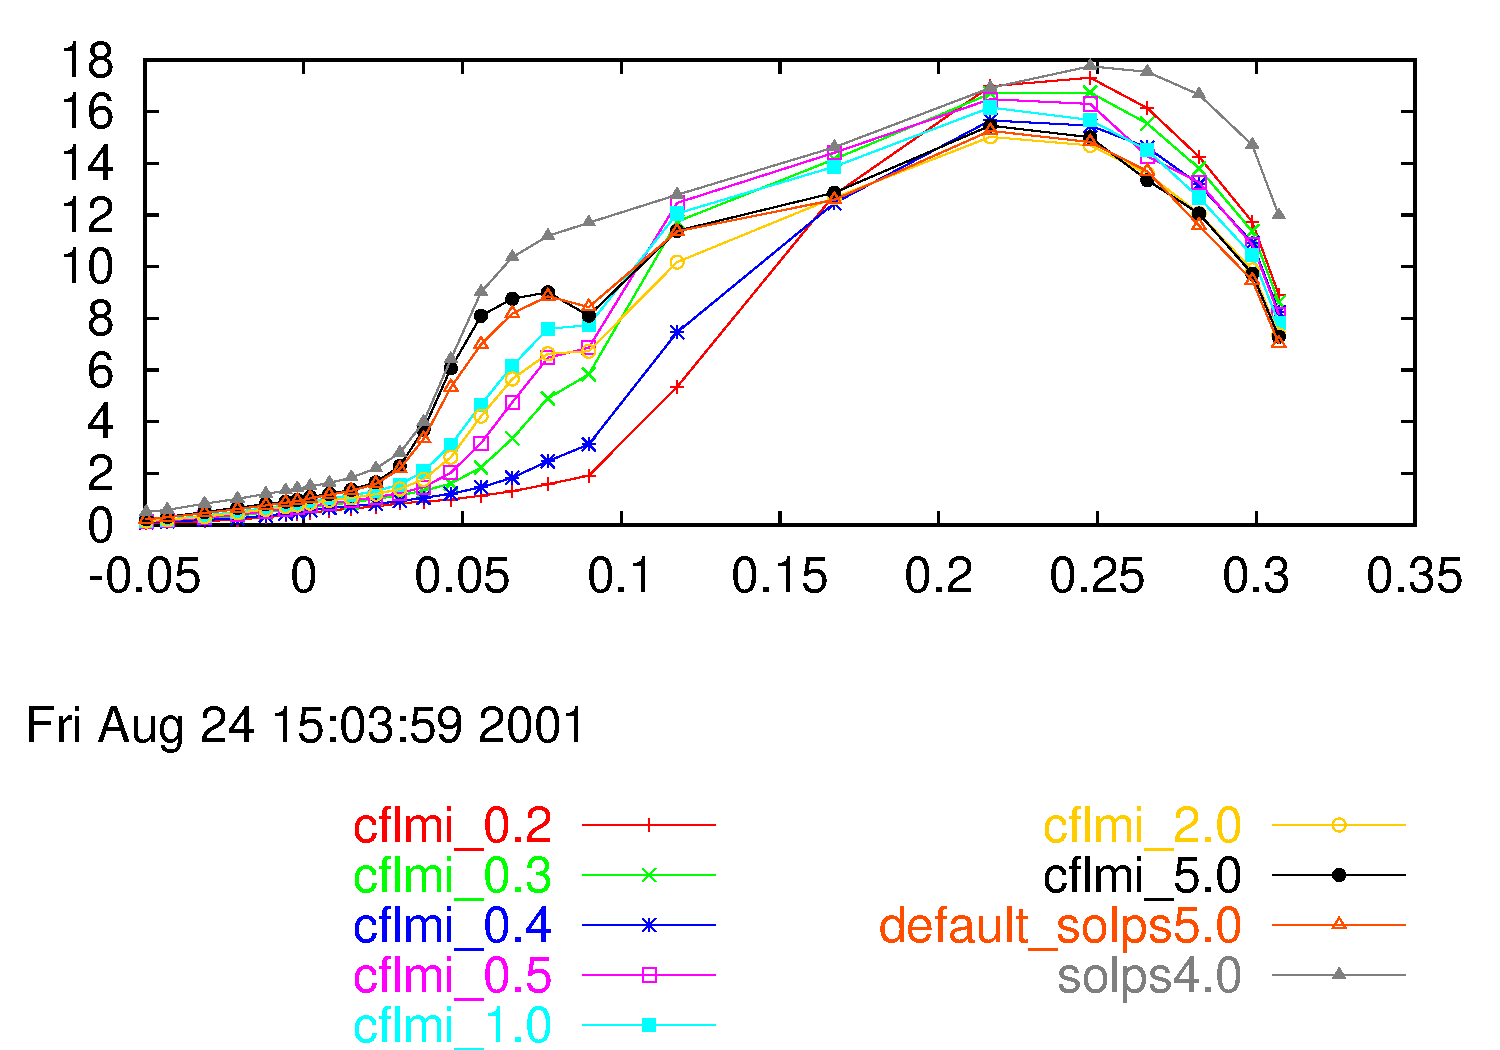
\includegraphics[width=11cm]{cflmi_2e19.pdf}} 
\else
    \centerline{\includegraphics[angle=-90,width=11cm]{cflmi_2e19.ps}} 
\fi
\caption{Impact of ion flux limits for a $2 \times 10^{19}~~m^{-3}$ upstream density case.}
\label{cflmi_2e19}
\end{figure}

\section{Neutral fluid model}
\index{neutrals, fluid model}

As an alternative to the complete kinetic Monte-Carlo description offered by \verb!Eirene!,
a simpler and faster neutral fluid model is also available as \verb!B2.5! stand-alone. The surface sources of neutrals are
then given by user-defined recycling models, possibly enhanced with local sputtering models 
when impurities are considered (see e.g.~\cite{Warrier04}). The volume sources of neutrals are given by 
plasma recombination rates computed by the \verb!B2.5! atomic physics packages. The neutral species is then
treated just as the other plasma species, with its own particle and momentum transport equations in the parallel
direction, equivalent to Eqs.~(\ref{eq:nf4}) and (\ref{eq:mom}). The neutrals are assumed to have the same common
temperature as all other ion species and the neutral energy balance equation becomes simply a component
of Eq.~(\ref{eq:ion_energy}). Of course, terms due to charged particle motions or currents do not appear 
for neutral species.

The neutral species transport coefficients are usually given by the following equations:
\begin{gather}\index{neutrals, transport coefficients}
 D^{n}_{AN,0} = 0,
\end{gather}
\begin{gather}
 D^{p}_{AN,0} = C + \sqrt{\frac{T_i}{m_N}} ( \sigma_{CX} n_i + \sigma_{in} n_e ),
\end{gather}
where $m_N$ is the mass of the neutral species, and $C$, $\sigma_{CX}$ and $\sigma_{in}$ are three constants given by
the user, representing hydrogen gas diffusion, and the charge-exchange and ionization cross-sections, respectively.
As an option, one may choose to use cross-sections from atomic databases instead of constants, with their appropriate
parameter dependencies. The diffusion coefficients can also be bounded to avoid unphysically large or small values.

Additionally, the heat and particle fluxes carried by neutrals can be flux-limited, following the formalism
laid out in~\cite{UMANSKY03A}\index{neutrals, flux limits}. On the one hand, we flux-limit the neutral contribution 
to the ion heat diffusivity, involved
in the conductive heat flux computation. On the other hand, we also flux-limit the convective 
particle and energy fluxes of neutrals. Because these limits apply for neutral species, both the parallel
and perpendicular directions are to be considered.
The basic formula used is:
\begin{gather}
X \Rightarrow  \frac{X}{\left[ 1 + \left|\frac{X}{\alpha F}\right|^\gamma\right]^{(1/\gamma)}}
\end{gather}
where
$X$ is the quantity to limit and $F$ is the limiting value.
Typically, the $\gamma$ coefficient is set to $\gamma=1$
or $2$; if $\gamma=1$ is used, then the absolute value of the flux
ratio is taken.  The value of $\alpha$ is of order unity; the
precise value is unimportant, but the goal is to limit the flux to a value of
approximately $n {\bar v}/4$, where ${\bar v} = \sqrt{(8T/\pi m)} = 2 v_T /\sqrt{\pi}$.
One could also use $v_T$ rather than ${\bar v}$, but the
difference is not very significant; in fact, flux
limits of $\sim n {\bar v}/2$ are often chosen, since too severe flux limits sometimes make the
solutions more difficult to obtain.

For the thermal diffusivities, the individual species 
diffusivities are flux-limited, then multiplied by the corresponding density (ion or neutral) and
then added up in a term which gets multiplied by the (common) ion
temperature gradient. For the neutrals, the heat conductivity is
\begin{gather}
\chi_N  = n_N \lambda_{CX} v_T ,
\end{gather}
where $\lambda_{CX} = 1/(\sigma_{CX} n_i)$ is the the neutral CX mean-free-path,
$n_N$ is the neutral density, and $v_T$ is the (neutral, ion) thermal
velocity.  Thus, this conductivity gets limited as
\begin{gather}
\chi_N \Rightarrow \frac{n_N \lambda_{CX} v_T}{{\left[1 + {\left|\frac{n_N \lambda_{CX} v_T \nabla T_i}
{\alpha_2 v_T n_N T_i}\right|}^{\gamma_2} \right]}^{(1/\gamma_2)}}
\end{gather}
where $\alpha_2 \sim 1$ again.  Some cancellations can be made in the equation,
but all terms are included for clarity.  Again, either $\gamma_2=1$ or $\gamma_2=2$ could be used.

In general, both of these terms can be important for
limiting the heat flux, as the neutral convective velocity shows up as a
convective heat flux.  In fact, because neutral gradients can be larger
than $T_i$ gradients, the convective velocity corrections might be the most
important.
The impact of the fluid model and associated flux limits, in comparison with
the \verb!Eirene! Monte-Carlo model, is covered in detail with examples in~\cite{CosterHinM2003}.

\subsection{First-flight model}
\index{neutrals, first-flight model}

As an intermediate approximation between the fluid and kinetic neutral transport models,
a so-called ``first-flight'' model has been implemented. In this model, the first trajectory
flight of neutrals launched from the computational domain boundary (at the plates or the wall
boundaries) is followed until the neutral undergoes ionization or charge-exchange, and then 
passed on to the neutral fluid model. In practice, as an initial computational step,
one defines a number of chords (user-specified, usually 9)
radiating from each edge boundary segment into the plasma, and computes the length travelled by
each chord within each plasma cell it crosses. Then, at each time step, the locally injected neutral flux 
(from recycling, sputtering, or the like) is launched along each chord (with a normalized intensity 
determined by some pre-determined angular dependence)
and considered to be attenuated within each intersected cell according to the local CX and ionization mean free paths,
while the balancing plasma sources and sinks in that cell are computed.
The effect of such a model is also shown in~\cite{CosterHinM2003}.

\subsection{B2.5-Eirene coupling} 
\index{neutral sources, coupling}\label{sec:sourcescoupling}

The coupling procedure between the plasma fluid and Monte-Carlo
neutral parts of the SOLPS package is done by means of passing arrays in
both directions, namely the \verb!braeir! and \verb!eirbra! modules. 
The plasma fluid code delivers a plasma background on which
the neutral trajectories are computed (also available as files \verb!fort.30! for 
the plasma geometry and \verb!fort.31! for the plasma solution), and the associated particle, parallel momentum
and energy sources are deduced (returned {\it via} the \verb!fort.44! file). Then, in order to translate the total energy 
sources from the Monte-Carlo code into the internal energy sources needed for 
the plasma fluid solution, we apply the following conversion rules, where the $E$ superscript
represents the energy sources in \verb!Eirene! (and old \verb!B2!) and $H$ the heat sources in \verb!B2.5!:
 
\hspace*{2cm}
\begin{minipage}{12cm}
  \begin{align}
    \mbox{total energy} & \Rightarrow\ S_a^E\ =\ \int \frac{1}{2}m_av_a^2S_a\ 
d^3v,\\
    \mbox{internal energy} & \Rightarrow\ S_a^H\ =\ \int \frac{1}{2}m_a\left(
v_a-u_a\right)^2S_a\ d^3v,\\
    & \rightarrow\ S_a^H \ =\ S_a^E-u_a\cdot S_a^{mom}+\frac{1}{2}m_au_a^2
S_a^{particle}.
  \end{align}
\end{minipage}

The derivation is as follows. The energy source rate from \verb!Eirene! is computed as:

\begin{equation*}
S_i^E = \sum_a S_a^E = \sum_a \sum_{Ea} \frac{1}{2} m_a v_a^2
\end{equation*} 

where the $\sum_a$ is taken over all species, and $\sum_{Ea}$ over the
newly ionised particles of species $a$ coming from the \verb!Eirene! strata.
We also define the particle and parallel momentum source rates:

\begin{align*}
S_i^{particle} = \sum_a S_{Ea}^{particle} &= \sum_a \sum_{Ea} 1 \\
\vec{S}_i^{mom} = \sum_a \vec{S}_{Ea}^{mom} &= \sum_a \sum_{Ea} m_a \vec{v}_a
\end{align*}

We need $S_i^H$, which, neglecting all other terms, is defined by:

\begin{equation*}
\frac {\partial}{\partial t} \left( \frac{3}{2} n_i T_i \right) = \frac {\partial}{\partial t} \left( \sum_a \frac{3}{2} n_a T_a \right) = S_i^H
\end{equation*} 

Thus,

\begin{equation*}
\frac{3}{2} \sum_a \left( n_a^{t+\Delta t} T_a^{t+\Delta t} - n_a^t T_a^t \right) = S_i^H \Delta t
\end{equation*}

\begin{equation*}
\frac{3}{2} \sum_a \left[ \left( n_a^t + S_a^{particle} \Delta t \right) T_a^{t+\Delta t} - n_a^t T_a^t \right] = S_i^H \Delta t
\end{equation*}

For a drifting Maxwellian distribution with drift velocity 
$\vec{u}_a$, the temperature (in energy units) is defined as:
\begin{equation*}
\frac{3}{2} T_a = \left \langle \frac{1}{2} m_a {\left( \vec{v}_a - \vec{u}_a \right)}^2 \right \rangle
\end{equation*}

In \verb!B2!, we assume $T_a = T_i$ and use $n_i = \sum_a n_a$.

So we can write:
\begin{equation}\label{eq:heatsources}
\sum_a \left( n_a^t + S_a^{particle} \Delta t \right) 
{\left \langle \frac{1}{2} m_a {\left( \vec{v}_a - \vec{u}_a \right)}^2 \right \rangle}^{t+\Delta t}
- \sum_a n_a^t {\left \langle \frac{1}{2} m_a {\left( \vec{v}_a - \vec{u}_a \right)}^2 \right \rangle}^t = S_i^H \Delta t 
\end{equation}

We define:
\begin{align*}
\vec{u}_a^{t+\Delta t} &= {\left \langle \vec{v}_a \right \rangle}^{t+\Delta t} = \frac{n_a^t\vec{u}_a^t + \frac{1}{m_a} \vec{S}_a^{mom} \Delta t}{n_a^t + S_a^{particle} \Delta t} \\
\delta\vec{u}_a &= \vec{u}_a^{t+ \Delta t} - \vec{u}_a^t = \frac{\frac{1}{m_a} \vec{S}_a^{mom} \Delta t - \vec{u}_a^t S_a^{particle} \Delta t}{n_a^t + S_a^{particle} \Delta t}
\end{align*}

And make use of:
\begin{align*}
{\left \langle \frac{1}{2} m_a {\left( \vec{v}_a - \vec{u}_a \right)}^2 \right \rangle}^{t+\Delta t} &= 
{\left \langle \frac{1}{2} m_a {\left( \vec{v}_a - \left( \vec{u}_a^t + \delta\vec{u}_a \right) \right)}^2 \right \rangle}^{t+\Delta t} \\
 &= {\left \langle \frac{1}{2} m_a \left( v_a^2 - 2 \vec{v}_a\cdot\vec{u}_a^t - 2 \vec{v}_a\cdot\delta\vec{u}_a + {u_a^t}^2 + 2 \delta\vec{u}_a\cdot\vec{u}_a^t + {(\delta u_a)}^2 \right) \right \rangle}^{t+\Delta t} \\
 &= {\left \langle \frac{1}{2} m_a \left[ {\left( \vec{v}_a - \vec{u}_a^t \right)}^2 + \left( - 2 \vec{v}_a\cdot\delta\vec{u}_a + 2 \delta\vec{u}_a\cdot\vec{u}_a^t + {(\delta u_a)}^2 \right) \right] \right \rangle}^{t+\Delta t} \\
 &= {\left \langle \frac{1}{2} m_a {\left( \vec{v}_a - \vec{u}_a^t \right)}^2 \right \rangle}^{t+\Delta t} 
  - m_a {\left \langle \vec{v}_a\cdot\delta\vec{u}_a \right \rangle}^{t+\Delta t} 
  + m_a {\left \langle \vec{u}_a^t\cdot\delta\vec{u}_a \right \rangle}^{t+\Delta t} 
  + \frac{1}{2} m_a {(\delta u_a)}^2 \\
 &= {\left \langle \frac{1}{2} m_a {\left( \vec{v}_a - \vec{u}_a^t \right)}^2 \right \rangle}^{t+\Delta t} 
  - m_a \delta\vec{u}_a \cdot \left( \vec{u}_a^{t+\Delta t} - \vec{u}_a^t \right) + \frac{1}{2} m_a {(\delta u_a)}^2 \\
 &= {\left \langle \frac{1}{2} m_a {\left( \vec{v}_a - \vec{u}_a^t \right)}^2 \right \rangle}^{t+\Delta t} 
  - \frac{1}{2} m_a {(\delta u_a)}^2
\end{align*}

Writing out the first average explicitly:
\begin{align*}
& {\left \langle \frac{1}{2} m_a {\left( \vec{v}_a - \vec{u}_a^t \right)}^2 \right \rangle}^{t+\Delta t} \\ 
& = \frac{\int n_a^t {\left( \frac{m_a}{2 \pi T_a^t} \right)}^{\frac{3}{2}} \frac{1}{2} m_a
{\left( \vec{v}_a - \vec{u}_a^t \right)}^2 \exp \left( -\frac{1}{2}m_a\frac{{\left( \vec{v}_a - \vec{u}_a^t \right)}^2}{T_a^t} \right) d^3 \vec{v}_a
+ \sum_a \frac{1}{2}m_a {\left( \vec{v}_a - \vec{u}_a^t \right)}^2 \Delta t }{n_a^t + S_a^{particle} \Delta t} \\
&= \frac{1}{n_a^t + S_a^{particle} \Delta t} \left[ \frac{3}{2} n_a^t T_a^t + \sum_a \frac{1}{2} m_a v_a^2 \Delta t
+ \frac{1}{2}m_a {u_a^t}^2 S_a^{particle} \Delta t - \vec{u}_a^t\cdot\vec{S}_a^{mom} \Delta t \right]
\\
&= \frac{1}{n_a^t + S_a^{particle} \Delta t} \left[ \frac{3}{2} n_a^t T_a^t + S_a^E \Delta t + \frac{1}{2}m_a{u_a^t}^2S_a^{particle} \Delta t - \vec{u}_a^t\cdot\vec{S}_a^{mom} \Delta t \right]
\end{align*}

Putting all this back into Eq.~(\ref{eq:heatsources}), we obtain:
\begin{align*}
\sum_a & \left\{ \left[ \frac{3}{2} n_a^t T_a^t + S_a^E \Delta t + \frac{1}{2}m_a{u_a^t}^2S_a^{particle} \Delta t 
- \vec{u}_a^t\cdot\vec{S}_a^{mom} \Delta t \right] - 
\left( n_a^t + S_a^{particle} \Delta t \right) \frac{1}{2} m_a {(\delta u_a)}^2 \right\} \\
-& \sum_a \frac{3}{2} n_a^t T_a^t = S_i^H \Delta t
\end{align*}

Thus:
\begin{equation}\label{eq:sources}
S_i^H = \sum_a S_a^E - \sum_a \vec{u}_a^t\cdot\vec{S}_a^{mom} + \sum_a \frac{1}{2} m_a {u_a^t}^2 S_a^{particle} - \sum_a \frac{n_a^t + S_a^{particle} \Delta t}{\Delta t} \frac{1}{2} m_a {(\delta u_a)}^2
\end{equation}

In the code, we previously had only the first three terms in the R.H.S. of the final equation above. But for very strong sources, dominating the background plasma, the higher order correction is necessary.
 
In some cases, it may also be essential to ensure excellent particle conservation. During a coupled
run timestep, as the \verb!B2! internal iterations make the plasma solution evolve away from the plasma
background originally used for the computation of the \verb!Eirene! sources above, it may become
necessary to rescale these. A scheme to do so was developped by A. Kukushkin for ITER applications \cite{Kukushkin2002PPCF}
and can be activated using the 'eirene\_ank\_mods' switch. See the listing in Appendix \ref{lis:b2cdci}
and the additional description in the \$\verb!SOLPSTOP/doc/Source_Scaling_in_B2.pdf! file.

\section{Classical transport: Braginskii vs Balescu}
\index{Classical transport}\index{Braginskii}\index{Balescu}\label{sec:balescubraginskii}

In \SOLPSfour the classical transport coefficients were derived from Braginskii \cite{Braginskii65}.
In \SOLPSfive these have been replaced with expressions from Balescu \cite{BALESCUA98A}, sometimes fitted
as a function of the local $Z_{eff}$.
The table below provides the differences between the two models.
It is possible in the code to use either model, or even the full Balescu 21-moment expressions, as well as
a Zhdanov fit to the table published in the Braginskii paper as a function of $Z_{eff}$. 
See the use of the switches 'b2tqce\_model' and 'b2tqca\_model' as described in Appendix \ref{lis:b2cdci}.

\begin{center}
    \begin{longtable}{|l|l|l|l|}
    \hline
    \multicolumn{4}{|l|}{\small\sl continued from previous page} \\
    \hline quantity & functional dependence & \multicolumn{2}{|c|}{changing prefactor} \\
    \hline          &                       & Braginskii & fits to Balescu \\
    \hline \endhead
    \hline quantity & functional dependence & \multicolumn{2}{|c|}{prefactor} \\
    \hline          &                       & Braginskii & fits to Balescu \\
    \hline \endfirsthead
    \hline
    \multicolumn{3}{|l|}{\small\sl continued on next page} \\
    \hline \endfoot
    \endlastfoot
$\kappa _{e \parallel}$ & $\frac{T_e^{5/2}}{m_e ln \Lambda}$ & 3.16 & $\frac{5}{2} \frac{2.16 Z_{eff}}{1 + 0.27 Z_{eff}} \approx 4.25 \; \mbox{for} \; Z_{eff} = 1$ \\
$\kappa _{i \parallel}$ & $\frac{T_i^{5/2}}{m_i Z_i^2 ln \Lambda}$ & 3.9 & 3.98 \\
$\eta _{i \parallel}$ & $\frac{T_i^{5/2}}{m_i Z_i^2 ln \Lambda}$ & 1.92 & $\frac{4}{3} \sqrt{2} \; 0.96 \approx 1.81 $ \\
    \hline
    \caption{Comparison of prefactors in Balescu and Braginskii classical transport coefficients}
    \label{tab:comparetransport}
  \end{longtable}
\end{center}

Note that this table does not contain the full prefactors, but only the physically meaningful changing pieces 
between the models.

In figures \ref{fig:hce} to \ref{fig:alf}, 
we illustrate the dependencies of the electronic classical transport coefficients as a 
function of $Z_{eff}$ , comparing the \SOLPSfive fit used by default, the exact 21-moment Balescu expressions, the
Zhdanov fit to Braginskii and the \SOLPSfour values.

\begin{figure}[bt]
\ifpdf 
    \centerline{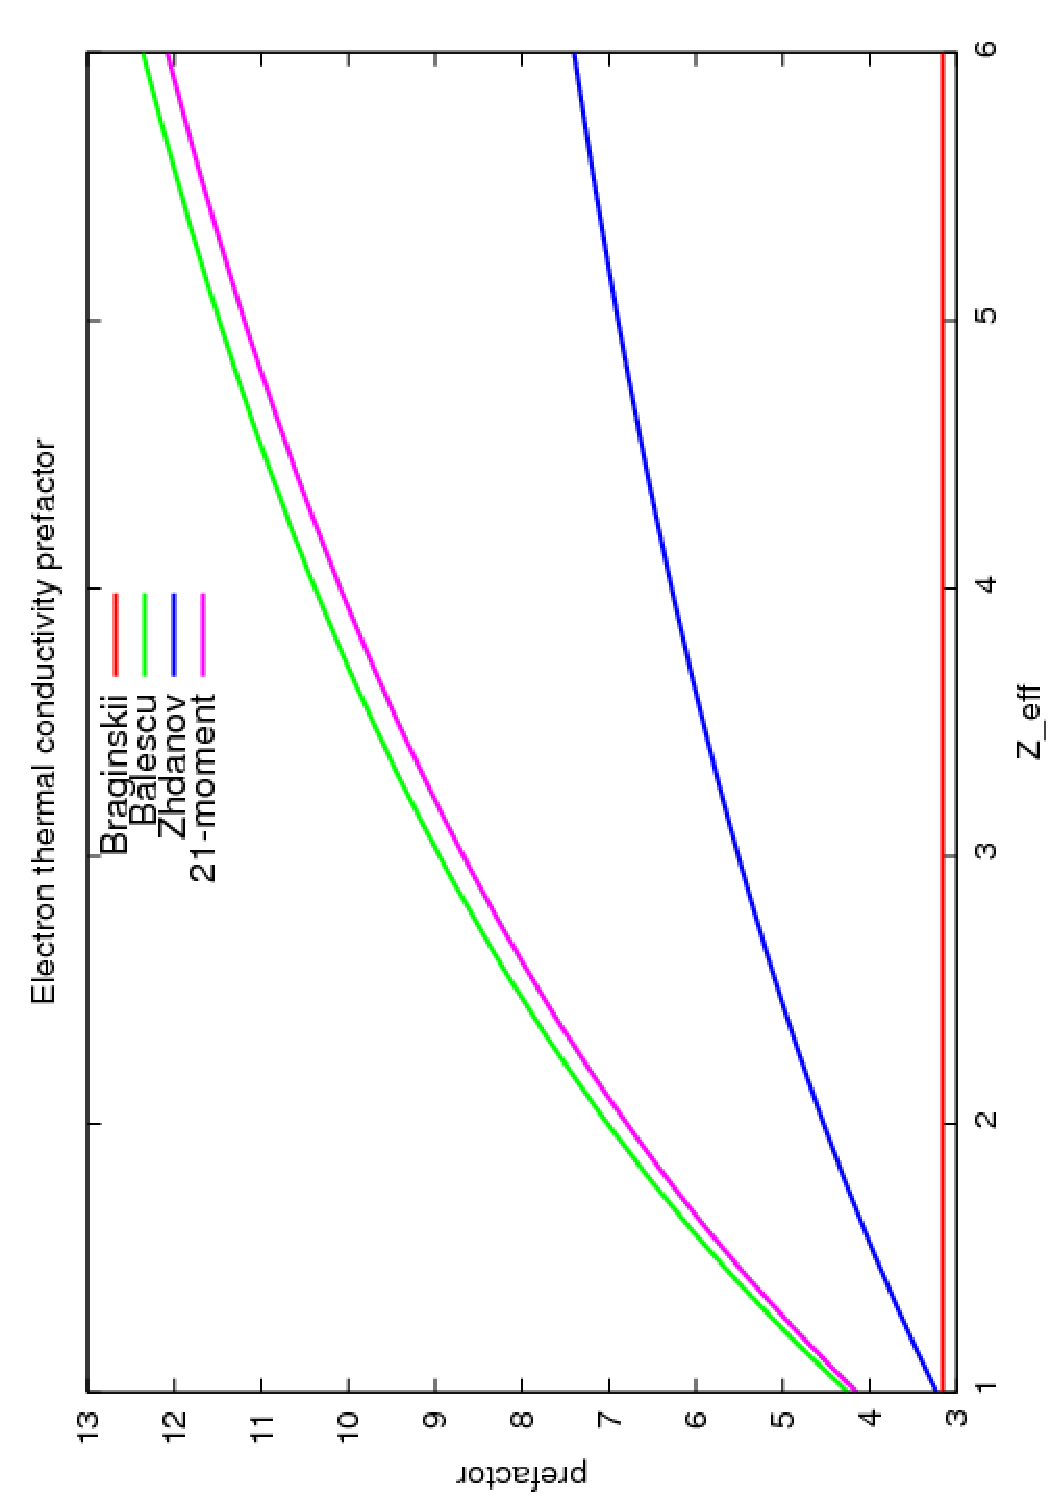
\includegraphics[angle=-90,width=11cm]{hce.pdf}} 
\else
    \centerline{
\includegraphics[angle=-90,width=11cm]{hce.epsi}} 
\fi
\caption{Dependence of the various models for the $\kappa _{e \parallel}$ prefactor as a function of $Z_{eff}$.}
\label{fig:hce}
\vspace*{1cm}
\end{figure}

\begin{figure}[bt]
\ifpdf 
    \centerline{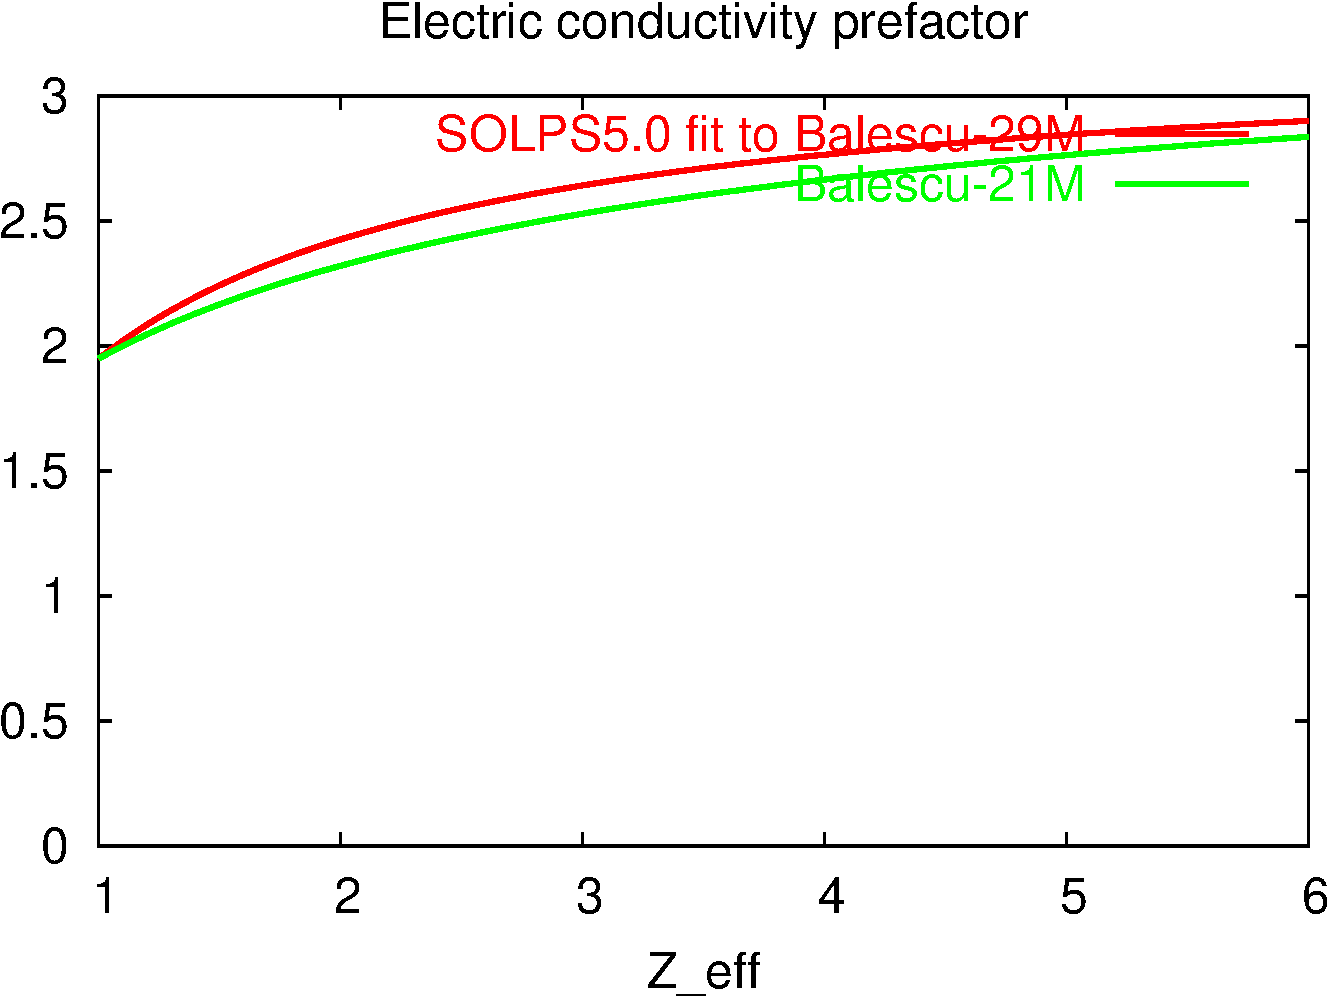
\includegraphics[width=11cm]{sig.pdf}} 
\else
    \centerline{
\includegraphics[angle=-90,width=11cm]{sig.epsi}} 
\fi
\caption{Dependence of the various models for the $\sigma_{\parallel}$ prefactor as a function of $Z_{eff}$.}
\label{fig:sig}
\vspace*{1cm}
\end{figure}

\begin{figure}[bt]
\ifpdf 
    \centerline{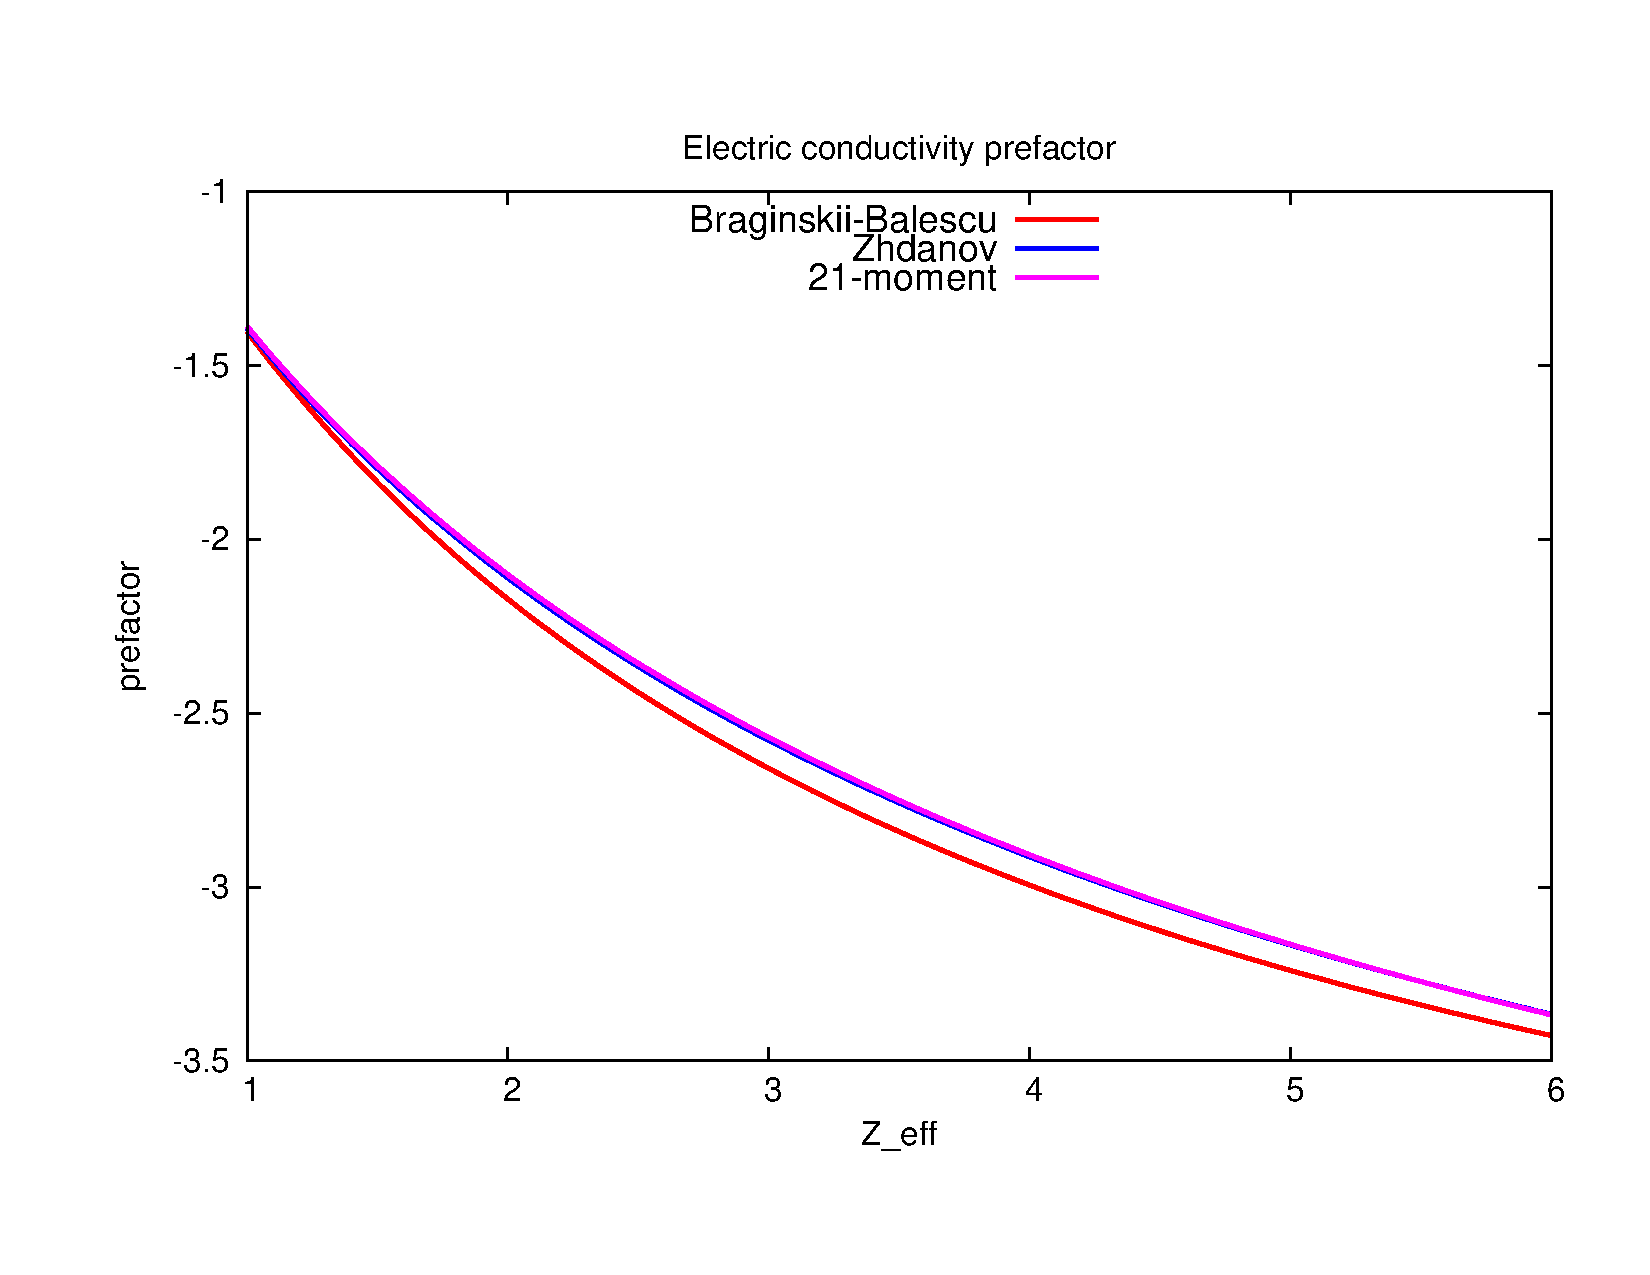
\includegraphics[width=11cm]{alf.pdf}} 
\else
    \centerline{
\includegraphics[angle=-90,width=11cm]{alf.epsi}} 
\fi
\caption{Dependence of the various models for the $\alpha_{e \parallel}$ prefactor as a function of $Z_{eff}$.}
\label{fig:alf}
\vspace*{1cm}
\end{figure}

\chapter{Model equations for B2.5}
\label{cha:equations}\index{B2.5, model}\index{B2.5, equations}\index{equations}\index{model}

%-------- Equations by S.P. Voskoboynikov ---------

\begin{equation}
\frac{\partial n_a}{\partial t} + \frac{1}{\sqrt g}\frac{\partial}{\partial x}\left( \frac{\sqrt g}{h_x} \widetilde{\Gamma}_{ax} \right) +   \frac{1}{\sqrt g}\frac{\partial}{\partial y}\left( \frac{\sqrt g}{h_y} \widetilde{\Gamma}_{ay} \right) = S_a^n, a = 0, 1, \ldots, n_s-1
\end{equation}

\begin{equation}
\widetilde{ \Gamma}_{ax} = \left( b_x V_{\parallel a} + V_{ax}^{\left( E \right)} + V_{ax}^{\left( AN \right)} + V^{corr \_ dpc} \right) n_a - D_a^n \frac{1}{h_x} \frac{\partial n_a}{\partial x} - \widetilde{D}_{ax}^p \frac{1}{h_x} \frac{\partial p_a}{\partial x} - D_{axy} \frac{1}{h_y} \frac{\partial n_a T_i}{\partial y}
\end{equation}

\begin{equation}
\widetilde{ \Gamma}_{ay} = \left( V_{ay}^{\left( E \right)} + V_{ay}^{\left( AN \right)} + \frac{j^{\left( AN \right)} + j_y^{\left( in \right)} + \widetilde{j_y}^{\left( vis \parallel \right)}}{e n_a} \right) n_a - D_a^n \frac{1}{h_y} \frac{\partial n_a}{\partial y} - \widetilde{D}_{ay}^p \frac{1}{h_y} \frac{\partial p_a}{\partial y} + D_{ayx} \frac{1}{h_x} \frac{\partial n_a T_i}{\partial x}
\end{equation}

\begin{equation}
\Gamma_{ax} = \left( b_x V_{\parallel a} + V_{ax}^{\left( E \right)} + \widetilde{V}_{xa}^{\left( dia \right)} + V_{ax}^{\left( AN \right)} + V^{corr \_ dpc} \right) n_a - D_a^n \frac{1}{h_x} \frac{\partial n_a}{\partial x} - \widetilde{D}_{ax}^p \frac{1}{h_x} \frac{\partial p_a}{\partial x}
\end{equation}

\begin{equation}
\Gamma_{ay} = \left( V_{ay}^{\left( E \right)} + \widetilde{V}_{ya}^{\left( dia \right)} + V_{ay}^{\left( AN \right)} + \frac{j^{\left( AN \right)} + j_y^{\left( in \right)} + \widetilde{j_y}^{\left( vis \parallel \right)}}{e n_a} \right) n_a - D_a^n \frac{1}{h_y} \frac{\partial n_a}{\partial y} - \widetilde{D}_{ay}^p \frac{1}{h_y} \frac{\partial p_a}{\partial y}
\end{equation}

\begin{equation}
\Gamma_{ax}^{ \left( \text{no drift} \right)} = \left( b_x V_{\parallel a} + V_{ax}^{\left( AN \right)} + 0 \cdot V^{corr \_ dpc} \right) n_a
\end{equation}

%?????????, ???? ?? ? ???? ??-?? ?????? ay ??? ax!!!!!!!!!!!!!!!!
\begin{equation} 
\Gamma_{ay}^{ \left( \text{no drift} \right)} = \left( V_{ax}^{\left( AN \right)} \right) n_a, \text{really 0 as } V_{ax}^{\left( AN \right)} = 0
\end{equation}

\begin{equation}
\Gamma_{ax}^{\left( Eir \right)} = \left( b_x V_{\parallel a} + V_{ax}^{\left( E \right)} + V_{xa}^{\left( dia \right)} + V_{ax}^{\left( AN \right)} + V^{corr \_ dpc} \right) n_a - D_a^n \frac{1}{h_x} \frac{\partial n_a}{\partial x} 
\end{equation}

% ?? ?????? ?? ??? ???? ??????? ?? n_a?
\begin{equation} 
\Gamma_{ay}^{\left( Eir \right)} = \left( V_{ay}^{\left( E \right)} + V_{ya}^{\left( dia \right)} + V_{ay}^{\left( AN \right)} + \frac{j^{\left( AN \right)} + j_y^{\left( in \right)} + \widetilde{j_y}^{\left( vis \parallel \right)}}{e} \right) n_a - D_a^n \frac{1}{h_y} \frac{\partial n_a}{\partial y} 
\end{equation}

\noindent where
\begin{tabular}{cc}
$\begin{matrix}
V_{xa}^{\left( dia \right)} & =
& \left\{
\begin{matrix}
-\frac{B_z}{Z_a e B^2 n_a} \frac{\partial n_a T_i}{h_y \partial y} & \ z_a \neq 0 \\
0, & \ z_a = 0
\end{matrix} \right.
\end{matrix}$

&

$\begin{matrix}
V_{ya}^{\left( dia \right)} & =
& \left\{
\begin{matrix}
\frac{B_z}{Z_a e B^2 n_a} \frac{\partial n_a T_i}{h_x \partial x} & \ z_a \neq 0 \\
0, & \ z_a = 0
\end{matrix} \right.
\end{matrix}$
\end{tabular}

\begin{equation}
E_{k,a}=\frac{m_a}2 \left[   u^2_{\parallel a}+\left( W_{a\perp}^{\text{(dia)}}+V_{a\perp}^{\text{(ExB)}}  \right)^2    +   \left(  W_{\text{ay}}^{\text{(dia)}} + V_{\text{ay}}^{\text{(ExB)}}\right)^2    \right]
\end{equation}

\begin{tabular}{cc}
$\begin{matrix}
W_{a \perp}^{\left( dia \right)} & =
& \left\{
\begin{matrix}
-\frac{B_z}{Z_a e B^2 n_a} \frac{\partial n_a T_i}{h_y \partial y}, & \ z_a \neq 0 \\
0, & \ z_a = 0
\end{matrix} \right.
\end{matrix}$
&
$\begin{matrix}
W_{ay}^{\left( dia \right)} & =
& \left\{
\begin{matrix}
\frac{B_z}{Z_a e B^2 n_a} \frac{\partial n_a T_i}{h_x \partial x}, & \ z_a \neq 0 \\
0, & \ z_a = 0
\end{matrix} \right.
\end{matrix}$
\end{tabular}

\begin{tabular}{cc}
$\begin{matrix}
V_{a \perp}^{\left( E \times B \right)} & =
& \left\{
\begin{matrix}
-\frac{B_z}{B^2} \frac{\partial \phi}{h_y \partial y}, & \ z_a \neq 0 \\
0, & \ z_a = 0
\end{matrix} \right.
\end{matrix}$
&
$\begin{matrix}
V_{ay}^{\left( E \times B \right)} & =
& \left\{
\begin{matrix}
\frac{B_z}{B^2} \frac{\partial\phi}{h_x \partial x}, & \ z_a \neq 0 \\
0, & \ z_a = 0
\end{matrix} \right.
\end{matrix}$
\end{tabular}

\subsubsection{Source terms in density equations}
{\centering}
$S_a^n=S_{I_a}^n+S_{I_{a+1}}^n+S_{R_a}^n+S_{R_{a-1}}^n+S_{CX_a}^n+S_{CX_{a-1}}^n$,
{\centering}


%-------- end of 1st page -------------

$z_a$ --- the atomic charge of species (a)
$z_{n_a}$ --- the nuclear charge of species (a)

\begin{equation}
\begin{matrix}
S_{I_a}^n & =
& \left\{
\begin{matrix}
-r_{I_a} n_e n_a, & \ a=0,\ldots,n_s-2,z_a<z_{a+1} \mbox{ and } z_{n_a}=z_{n_{a+1}}\\
0
\end{matrix} \right.
\end{matrix}
\end{equation}

\begin{equation}
\begin{matrix}
S_{I_{a+1}}^n & =
& \left\{
\begin{matrix}
r_{I_a} n_e n_a, & \ a=0,\ldots,n_s-2,z_a<z_{a+1} \mbox{ and } z_{n_a}=z_{n_{a+1}}\\
0
\end{matrix} \right.
\end{matrix}
\end{equation}

\begin{equation}
r_{I_a} = exp \left( r_{0,I_a}+r_{1,I_a} ln\left(\frac{T_e}e\right)\right)
\end{equation}
%-------------------
\begin{equation}
\begin{matrix}
S_{R_a}^n & =
& \left\{
\begin{matrix}
-r_{R_a} n_e n_a, & \ a=1,\ldots,n_s-1,z_{a-1}<z_a \text{and} z_{{n-1}_a}=z_{n_a}\\
0
\end{matrix} \right.
\end{matrix}
\end{equation}

\begin{equation}
\begin{matrix}
S_{R_{a-1}}^n & =
& \left\{
\begin{matrix}
r_{R_a} n_e n_a, & \ a=1,\ldots,n_s-1,z_{a-1}<z_a \text{ and } z_{{n-1}_a}=z_{n_a}\\
0
\end{matrix} \right.
\end{matrix}
\end{equation}

\begin{equation}
r_{R_a}=\text{exp}\left(r_{0,R_a}+r_{1,R_a}\text{ln}\left(\frac{T_e}e\right)\right)
\end{equation}
%-------------------
\begin{equation}
\begin{matrix}
S_{CX_a}^n & =
& \left\{
\begin{matrix}
-r_{CX_a} n_e n_a, & \ a=1,\ldots,n_s-1,z_{a-1}<z_a \text{ and } z_{{n-1}_a}=z_{n_a}\\
0
\end{matrix} \right.
\end{matrix}
\end{equation}

\begin{equation}
\begin{matrix}
S_{CX_{a-1}}^n & =
& \left\{
\begin{matrix}
r_{CX_a} n_e n_a, & \ a=1,\ldots,n_s-1,z_{a-1}<z_a \text{ and } z_{{n-1}_a}=z_{n_a}\\
0
\end{matrix} \right.
\end{matrix}
\end{equation}

\begin{equation}
r_{CX_a} = exp \left(
	r_{0,CX_a} + r_{1,CX_a} ln  \left(
		\frac{m_p T_e} m_{a_0} e 
	\right)
\right)
\end{equation}

$n_e = \sum \limits^{n_s-1}_{a=0} z_a n_a$, $n_i = \sum \limits^{n_s-1}_{a=0} n_a$
$p_a = n_a \left( z_a T_e + T_i \right)$, $p_e=n_e T_e$


\begin{equation}
V^{corr\_dpc} = \frac{c^{corr\_dpc}}{16} |b_x| \sqrt{\frac{p_a}{m_a n_a}} \frac{\partial
^2}{\partial x^2} \left( \frac 1{p_a} \frac{\partial p_a}{\partial x} \right)
\end{equation}

\begin{equation}
\begin{matrix}
V_{ax}^{\left( E\right)} & =
& \left\{
\begin{matrix}
-c_{E\times B}   \frac{B_z}{B^2}   \frac 1{h_y}  \frac{\partial \varphi }{\partial y}, & \ z_a \neq 0 \\
0, & \ z_a = 0
\end{matrix} \right.
\end{matrix}
\end{equation}

\begin{equation}
\begin{matrix}
V_{ay}^{\left( E \right)} & =
& \left\{
\begin{matrix}
c_{E\times B}   \frac{B_z}{B^2}   \frac 1{h_x}   \frac{\partial \varphi }{\partial x}, & \ z_a \neq 0 \\
0, & \ z_a = 0
\end{matrix} \right.
\end{matrix}
\end{equation}

%-------- end of 2d page -------------

\begin{equation}
\begin{matrix}
\widetilde{V}_{xa}^{\left( dia \right)} & =
& \left\{
\begin{matrix}
c_{dia} \frac{T_i B_z}{Z_a e}   \frac{\partial}{h_y\partial y} \left(\frac 1{B^2} \right), & \ z_a \neq 0 \\
0, & \ z_a = 0
\end{matrix} \right.
\end{matrix}
\end{equation}

\begin{equation}
\begin{matrix}
\widetilde{V}_{ya}^{\left( dia \right)} & =
& \left\{
\begin{matrix}
-c_{dia} \frac{T_i B_z}{Z_a e}   \frac{\partial}{h_x\partial x} \left(\frac 1{B^2} \right), & \ z_a \neq 0 \\
0, & \ z_a = 0
\end{matrix} \right.
\end{matrix}
\end{equation}

$
\left\{ 
\begin{matrix}
D_{axy}= \left( \frac 1{B^2} - \frac 1{\langle B^2\rangle}   \right)  \frac{B_z}{z_a e}, & z_a \neq 0\\
D_{axy}=0, & z_a=0
\end{matrix}
\right.
$, where $\left \langle B^2 \right \rangle = \frac{\iint \limits_{core} B^2 \sqrt{g} dx dy}{\iint \limits_{core} \sqrt{g} dx dy}$

\begin{equation}
\left\{ 
\begin{matrix}
D_{ayx} = \left( \frac 1{B^2} - \frac 1{\langle B^2\rangle}   \right)  \frac{B_z}{z_a e}, & z_a \neq 0\\
D_{ayx} = 0, & z_a=0
\end{matrix}
\right.
\end{equation}

$D_a^n = D^n_{ANa}$

\begin{equation}
D_{ANa}^n=\left( c_{D_a^N,0}+c_{D_a^N,1}\frac{10^{20}}{n_e}+c_{D_a^N,2}D_a^f+c_{D_a^N,3}\frac{6,2\cdot
10^{-2}T_e}{e|B|}\right)f_D(x,y),
\end{equation}

\begin{equation}
\begin{matrix}
f_D(x,y) & =
& \left\{
\begin{matrix}
1, & \ z_a = 0 \\
\alpha_{1,D}, & \ -\delta _{1,D}\le y\le 0, x\in \text{Core}, z_a \neq 0 \\
\alpha_{2,D}, & \ 0\le y\le \delta _{2,D}, x\in \text{Core} \\
\alpha_{3,D}, & \ x,y\in \text{Pr} \cup \text{SOL}
\end{matrix} \right.
\end{matrix}
\end{equation}

$a=0,\;\;\;c_{D_a^N,0}=0,\;\;\;c_{D_a^N,1}=0,\;\;\;c_{D_a^N,2}=0,\;\;\;c_{D_a^N,3}=0$

$ a=1,\;\;\; c_{D_a^N,0}=0,\;\;\;c_{D_a^N,1}=0,\;\;\;c_{D_a^N,2}=1,\;\;\;c_{D_a^N,3}=0$

$D_a^f=c_{D_a^f,0}+c_{D_a^f,1}\frac{10^{20}}{n_i}+\frac{c_{D_a^f,2}\sqrt{\frac{T_i}{m_a}}}{c_{D_a^f,3}n_i+c_{D_a^f,4}n_e},$


%-------- end of 3d page -------------

\begin{equation}
\begin{matrix}
\widetilde  D_{\text{ax}}^p & =
& \left\{
\begin{matrix}
\frac{D_a^p}
{\left(1+\left(\frac{D_a^p|\frac 1{h_x}\frac{\partial p_a}{\partial x}|}{\mathit{\alpha n}_a\frac{V_{T_i}} 4}\right)^{\gamma _1}\right)^{\frac 1{\gamma_1}}}, 
& \ V_{T_i}=\sqrt{\frac{8T_i}{\mathit{\pi m}_a}}, & \ z_a = 0 \\
D_a^p, & \ z_a \neq 0 \\
\end{matrix} \right.
\end{matrix}
\end{equation}

\begin{equation}
\begin{matrix}
\widetilde D_{\text{ay}}^p & =
& \left\{
\begin{matrix}
\frac{D_a^p}
{\left(1+\left(\frac{D_a^p|\frac 1{h_y}\frac{\partial p_a}{\partial y}|}{\mathit{\alpha n}_a\frac{V_{T_i}} 4}\right)^{\gamma _1}\right)^{\frac 1{\gamma_1}}}, 
& \ V_{T_i}=\sqrt{\frac{8T_i}{\mathit{\pi m}_a}}, & \ z_a = 0 \\
D_a^p, & \ z_a \neq 0 \\
\end{matrix} \right.
\end{matrix}
\end{equation}

$D_a^p = D_{ANa}^p$

\begin{equation*}
D_{ANa}^p=\frac 1{z_aT_e+T_i} \left( c_{D_a^p,0} + c_{D_a^p,1} \frac{10^{20}}{n_e} + c_{D_a^p,2} D_a^f + c_{D_a^p,3} \frac{6,2\cdot
10^{-2}T_e}{e|B|}\right),
\end{equation*}

\begin{equation*}
a=0,c_{D_a^p,0}=0, c_{D_a^p,1}=0, c_{D_a^p,2}=1, c_{D_a^p,3}=0
\end{equation*}
\begin{equation*}
a=1, c_{D_a^p,0}=0, c_{D_a^p,1}=0, c_{D_a^p,2}=0, c_{D_a^p,3}=0
\end{equation*}

$V_{ax}^{AN}=0$

\begin{equation*}
V_{ay}^{AN} = c_{V_a^{AN},0} + c_{V_a^{AN},1} \frac{10^{20}}{n_e} + c_{V_a^{AN},2} D_a^f + c_{V_a^{AN},3} \frac{6,2\cdot 10^{-2}T_e}{e|B|}
\end{equation*}

$a=0, c_{V_a^{AN},0}=0, c_{V_a^{AN},1}=0, c_{V_a^{AN},2}=0, c_{V_a^{AN},3}=0$

$a=1, c_{V_a^{AN},0}=0, c_{V_a^{AN},1}=0, c_{V_a^{AN},2}=0, c_{V_a^{AN},3}=0$

\begin{eqnarray*}
m_a \frac{\partial n_a V_{\parallel a}}{\partial t} +
\frac 1{h_z\sqrt g} \frac{\partial}{\partial x} \left( \frac{h_z\sqrt g}{h_x} \Gamma_{ax}^m \right) +
\frac 1{h_z\sqrt g} \frac{\partial}{\partial y} \left( \frac{h_z\sqrt g}{h_y} \Gamma_{ay}^m \right) +
\frac{b_x}{h_x}\frac{\partial n_a T_i}{\partial x} +
Z_a e n_a \frac{b_x}{h_x} \frac{\partial \varphi}{\partial x} =\\
S_{a \parallel}^m + S_{CF_a}^m + S_{fr_a}^m + S_{Term_a}^{m} + S_{I_a}^m + S_{R_a}^m + S_{CX_a}^m
\end{eqnarray*}

\begin{eqnarray*}
m_a \frac{\partial n_a V_{\parallel a}}{\partial t} +
\frac 1{h_z\sqrt g} \frac{\partial}{\partial x} \left( \frac{h_z \sqrt g}{h_x} \Gamma_{ax}^m \right) +
\frac 1{h_z\sqrt g} \frac{\partial}{\partial y} \left( \frac{h_z \sqrt g}{h_y} \Gamma_{ay}^m \right) +
\frac{b_x}{h_x} \frac{\partial n_a T_i}{\partial x} +
\frac{b_x}{h_x} \frac{Z_a n_a \partial n_e T_e}{n_e \partial x} = \\
= \mbox{old form} = S_{a \parallel}^m + S_{CF_a}^m + S_{fr_a}^m + S_{Term_a}^{m} + S_{I_a}^m + S_{R_a}^m + S_{CX_a}^m
\end{eqnarray*}

%-------- end of 4th page -------------

$S_{a \parallel}^m = - \left( \nabla \pi_a^{\parallel} \right)_{\parallel}$

\begin{equation}
\begin{matrix}
\left( \nabla \pi_a^{\parallel} \right)_{\parallel} & =
& \left\{
\begin{matrix}
0, & \ z_a \neq 1 \\
- \frac{\partial}{h_z\sqrt g\partial x}
\left(\frac{h_z\sqrt g}{h_x} \frac 4 3 \eta_{ax}
\frac{\partial ln \left( h_z B^{\frac 1 2} \right) }{B^{\frac 1 2} h_x \partial x}\right)
B^{\frac 1 2} V_{\parallel a} -
B^{\frac 3 2} b_x \frac{\partial}{h_x \partial x}
\left( \alpha^{NEO} \frac{b_x \tilde {\tau}_a}{B^2} \frac{\partial \left(B^{\frac 1 2} \tilde q^{0} \right)}{h_x \partial x}\right), 
& \ z_a = 1 \\
\end{matrix} \right.
\end{matrix}
\end{equation}

$S_{CF}^m = m_a b_x n_a V_{\parallel a}^2 \frac 1{h_z h_x} \frac{\partial h_z}{\partial x}$

$S_a^m = S_{fr,a}^m + S_{Term}^m + S_{I_a}^m + S_{R_a}^m + S_{CX_a}^m$,

Parallel momentum source due to ionization
\begin{equation*}
S_{I_a}^m = S_{I_a}^q + S_{I_{a+1}}^q
\end{equation*}

\begin{equation}
\begin{matrix}
S_{I_a}^q & =
& \left\{
\begin{matrix}
-r_{I_a} n_e n_a \left( \frac{m_a+m_{a+1}}2 \right) V_{\parallel a}, & \ a=0,\ldots,n_s-2, & \ z_a<z_{a+1} \mbox{ and } z_{n_a}= z_{n_{a+1}}, \\
0, \\
\end{matrix} \right.
\end{matrix}
\end{equation}

\begin{equation}
\begin{matrix}
S_{I_{a+1}}^q & =
& \left\{
\begin{matrix}
r_{I_a} n_e n_a \left( \frac{m_a+m_{a+1}}2 \right) V_{\parallel a}, & \ a=0,\ldots,n_s-2, & \ z_a<z_{a+1} \text{ and } z_{n_a}= z_{n_{a+1}}, \\
0, \\
\end{matrix} \right.
\end{matrix}
\end{equation}

Parallel momentum source due to recombination

\begin{equation*}
S_{R_a}^m = S_{R_a}^q + S_{R_{a-1}}^q
\end{equation*}

\begin{equation}
\begin{matrix}
S_{R_a}^q & =
& \left\{
\begin{matrix}
-r_{R_a} n_e n_a \left( \frac{m_a+m_{a-1}}2 \right) V_{\parallel a}, & \ a=0,\ldots,n_s-1, & \ z_{a-1}<z_a \text{ and } z_{n_{a-1}}= z_{n_a}, \\
0, \\
\end{matrix} \right.
\end{matrix}
\end{equation}

\begin{equation}
\begin{matrix}
S_{R_{a-1}}^q & =
& \left\{
\begin{matrix}
r_{R_a} n_e n_a \left( \frac{m_a+m_{a+1}}2 \right) V_{\parallel a}, & \ a=0,\ldots,n_s-1, & \ z_{a-1}<z_a \text{ and } z_{n_{a-1}}= z_{n_a}, \\
0, \\
\end{matrix} \right.
\end{matrix}
\end{equation}


%---------- nedorazvitoe uravnenie? ----------
\begin{equation*}
S_{CX_a}^m=
\end{equation*}


\begin{equation}
S^m_{fr,a} = 
\sum \limits^{n_s-1}_{\substack{b = 0, \\ b\neq a, z_a \neq 0, z_b \neq 0}} \frac 1{\tau_p} m_p 
\sqrt{ \frac {\frac{m_a}{m_p} \frac{m_b}{m_p}} {\frac{m_a}{m_p} + \frac{m_b}{m_p}} }
z_a^2 z_b^2 n_b n_a \left( V_{b \parallel} - V_{a \parallel} \right)
\text{- friction force (b2sifr)}
\end{equation}

$\tau_p = \frac 3{4\sqrt{2\pi}}
\frac{\sqrt{m_p}T_i^{\frac 3 2}}{\Lambda}
\left(\frac{4 \pi \varepsilon_0}{e^2}\right)^2$, where the Coulomb logarithm  $\Lambda $ can be chosen as

%-------- end of 5th page -------------

\begin{equation}
\begin{matrix}
\Lambda & =
& \left\{
\begin{matrix}
12 \\
max \{ 5; 23.4 - 1.15 \cdot log_{10} \left( \frac{n_e}{10^6} \right) + 3.45 \cdot log_{10} \left( \frac{T_e}e \right)  \}, & \frac{T_e}{e} \leq 50 & \mbox{\scriptsize{Braginsky}} \\
max \{ 5; 25.3 - 1.15 \cdot log_{10} \left( \frac{n_e}{10^6} \right) + 2.30 \cdot log_{10} \left( \frac{T_e}e \right)  \}, & \frac{T_e}{e} > 50 &  \mbox{\scriptsize{formula}}\\
max \{ 5; 17.3 - 0.5 \cdot log_e \left( \frac{n_e}{10^{20}} \right) + 1.5 \cdot log_e \left( \frac{T_e}{e \cdot 10^3} \right)  \} & \mbox{\scriptsize{Wesson formula}} &\mbox{\scriptsize{for ion-ion collisions}}\\
\end{matrix} \right.
\end{matrix}
\end{equation}

$S_{Term,a}^m = 
n_a \left(
	\frac{z_a}{n_e} - \frac{z_a^2}{n_{e^2}} 
\right)
n_e b_x e
\left[
	\hat E_x - \frac 1 e \left(
		c_{th_e,a} \Delta_{T_e} + c_{th_i,a} \Delta_{T_i}
	\right)
\right],$ thermal force (b2sifr)

\begin{equation*}
n_{e^2 }= \sum \limits^{n_s-1}_{a=0} z_a^2 n_a, \;\;\;\ l_{t_e}=0.3; \;\;\;\;\; l_{t_i}=0,3; \;\;\;\;\; z_{\lambda_e}=\frac{1.5\cdot
10^{16}}{n_e} \left( \frac{T_e} e \right)^2, \;\;\;\;\; z_{\lambda_i}=\frac{1.5 \cdot 10^{16}}{n_{e^2}}\left(\frac{T_i} e\right)^2
\end{equation*}

\begin{equation}
\begin{matrix}
\Delta _{T_e} & =
& \left\{
\begin{matrix}
\frac{\partial T_e}{h_x\partial x}, && l_{t_e} \leq 0 \\

\Biggl|
	min \left\{ 
		\Bigl|
			\frac{\partial T_e}{h_x \partial x} 
		\Bigr|, \frac{l_{t_e} T_e}{z_{\lambda_e}|b_x|}
	\right\} 
\Biggr|,
& \frac{\partial T_e}{h_x \partial x} \ge 0, & l_{t_e}>0 \\

-\Bigl| 
	min \left\{ 
		\Bigl|
			\frac{\partial T_e}{h_x \partial x} 
		\Bigr|, \frac{l_{t_e} T_e}{z_{\lambda_e}|b_x|}			
	\right\} 
\Bigr|,
& \frac{\partial T_e}{h_x \partial x} < 0, & l_{t_e}>0 
\end{matrix} \right.
\end{matrix}
\end{equation}

\begin{equation}
\begin{matrix}
\Delta _{T_i} & =
& \left\{
\begin{matrix}
\frac{\partial T_i}{h_x\partial x}, && l_{t_i} \leq 0 \\
\Bigl| 
	min \Bigl\{ 
		\Bigl| \frac{\partial T_i}{h_x \partial x} 
		\Bigr|, \frac{l_{t_i} T_i}{z_{\lambda_i}|b_x|} 				
	\Bigr\} 
\Bigr|,
& \frac{\partial T_i}{h_x \partial x} \ge 0, & l_{t_i}>0 \\
-\Bigl| 
	min \Bigl\{
		\Bigl| 
			\frac{\partial T_i}{h_x \partial x} 
		\Bigr|, \frac{l_{t_i} T_i}{z_{\lambda_i}|b_x|}
	\Bigr\} 
\Bigr|,
& \frac{\partial T_i}{h_x \partial x} < 0, & l_{t_i}>0 
\end{matrix} \right.
\end{matrix}
\end{equation}

$c_{th_e,a} = 0, a=0,\ldots,n_s-1$ and $c_{th_i,a}=2.65, a=0,\ldots, n_s-1$ if 21 moment approximation is not used.

\begin{equation}
\Gamma^m_{ax} =
m_a V_{\parallel a} \Gamma_{ax} + m_a V_{\parallel a} \Gamma_{ax}^{\left( dia \right)} + 
\frac 4 3 \eta_{ax} \frac{\partial ln h_z}{h_x \partial x} V_{\partial a} - 
\frac 4 3 \eta_{ax} \frac{\partial V_{\partial a}}{h_x \partial x}
\end{equation}

\begin{equation}
\Gamma^m_{ay} =
m_a V_{\parallel a} \Gamma_{ay} + m_a V_{\parallel a} \Gamma_{ay}^{\left( dia \right)} -
\eta_{ay} \frac{\partial V_{\parallel a}}{h_y \partial y}
\end{equation}

$\Gamma^{\left( dia \right)}_{ax} = n_a \widetilde{V}^{\left( dia \right)}_{\perp a}$,

$\Gamma^{\left( dia \right)}_{ay} = n_a \widetilde{V}^{\left( dia \right)}_{ya}$,

$\eta_{ax} = \eta_{AN_a} + \widetilde{\widetilde{\eta}}_{CL_{ax}}$

%-------- end of 6th page -------------

\begin{equation}
\begin{matrix}
\eta_{AN_a} & =
& \left\{
\begin{matrix}
\left( c_{\eta_a,0} + c_{\eta_a,1} \frac{10^{20}}{n_e} + c_{\eta_a,2} D_a^f + 
c_{\eta _a,3} \frac{6.2 \cdot 10^{-2} T_e}{e|B|}\right)
m_a n_a f_{\eta _a}(x,y), & z_a\neq 0 \\
\left( c_{\eta_a,0} + c_{\eta_a,1} \frac{10^{20}}{n_e} + c_{\eta_a,2} D_a^f + 
c_{\eta _a,3} \frac{6.2 \cdot 10^{-2} T_e}{e|B|}\right)
m_a n_a , & z_a = 0
\end{matrix} \right.
\end{matrix}
\end{equation}

\begin{equation}
\begin{matrix}
f_{\eta _a}(x,y) & =
& \left\{
\begin{matrix}
1, & \ z_a = 0 \\
\alpha_{1,\eta _a}, & \ -\delta _{1,\eta _a} \le y \le 0, & x \in \text{Core}, z_a \neq 0 \\
\alpha_{2,\eta _a}, & \ 0\le y\le \delta _{2,\eta _a}, & x \in \text{Core} \\
\alpha_{3,\eta _a}, & \ x,y\in \text{Pr} \cup \text{SOL}
\end{matrix} \right.
\end{matrix}
\end{equation}

$ a = 0, \;\;\;  c_{\eta _a,0} = 0, \;\;\;  c_{\eta _a,1} = 0, \;\;\;  c_{\eta _a,2} = 1,  \;\;\;  c_{\eta _a,3} = 0$
$ a = 1, \;\;\;  c_{\eta _a,0} = 0, \;\;\;  c_{\eta _a,1} = 0, \;\;\;  c_{\eta _a,2} = 1,  \;\;\;  c_{\eta _a,3} = 0$

$\widetilde{\widetilde{\eta}}_{CLax} = c_{\eta_{ax}^{(CL)}} \widetilde{\eta}_{CLax}$

\begin{equation}
\begin{matrix}
c_{\eta_{ax}^{(CL)}} & =
& \left\{
\begin{matrix}
1, & \ z_a \neq 0 \; \text{and only for inner flux surfaces} \\
\frac 1 
{1 + \frac{
\frac{\sqrt g}{h_x} \widetilde{\eta}_{CLax}  \bigl| \frac{\partial V_{\parallel a}}{h_x \partial x} \bigr|
}
{V_{m_a}^{(max)}}  
}, &  
\text{for all other cases} \\
\end{matrix} \right.
\end{matrix}
\end{equation}

$V_{m_a}^{(max)} = c_{f \; lim_2} \frac{\sqrt g}{h_x} |b_x| n_a T_i$
$\widetilde{\eta }_{CLax} = c_{\eta_{ax}^{(CL)}}^{Luciani} \eta_{CLax} b_x^2$

'b2trcl\_lluciani' '1'

$\begin{matrix}
c_{\eta_{ax}^{(CL)}}^{Luciani} & =
& \left\{
\begin{matrix}
\frac 1 {
1 + \frac{
7.5 \cdot 10^{16} \left( \frac{T_i} e \right)^2}
{c(y) \sum \limits_{a=0}^{n_s-1} z_a^2 n_a}
}
, & \ z_a \neq 0 \; \text{and only for inner flux surfaces,} \\
1, &  \text{for all other cases} \\
\end{matrix} \right.
\end{matrix}$

For plateau and banana correction 'b2trcl\_lluciani' '3'

%-------- end of 7th page -------------

$
\begin{matrix}
c_{\eta_{ax}^{(CL)}}^{Luciani} & =
& \left\{
\begin{matrix}
\frac 1{1 + 
\frac{15.12 \cdot 10^{16} \left( \frac{T_i}e \right)^2}
{c(y)\sum \limits_{a=0}^{n_s-1} z_a^2 n_a}}
\cdot
\frac 1{1 +
\frac{15.12 \cdot 10^{16} \cdot \varepsilon^{3/2} \left( \frac{T_i} e \right)^2}
{c(y)\sum \limits_{a=0}^{n_s-1} z_a^2 n_a}}
, & \ z_a \neq 0 \; \mbox{\scriptsize{and only for inner flux surfaces,}} \\
1, &  \text{for all other cases} \\
\end{matrix} \right.
\end{matrix}
$

$c \left( y \right) = \oint h_x |b_x|^{-1} dx$, \ \ \ \  $\varepsilon = \frac
{\left( \oint h_x dx \right)^2}
{\oint \sqrt g / h_y dx}$

$
\begin{matrix}
\eta_{CLax} & =
& \left\{
\begin{matrix}
0, & \ z_a = 0 ,  \\
\eta \sqrt{2} T_i n_a \tau_a b_x^2, & \ z_a \neq 0  \\
\end{matrix} \right.
\end{matrix}
$

$\eta = 0.96$,

$\tau _a = \frac 3{4 \sqrt{2\pi}}  
\frac {\sqrt{m_a} T_i^{\frac 3 2}} {z_a^2 z_{eff} n_e \Lambda}
\left( \frac{4 \pi \varepsilon_0}{e^2} \right)^2$, where the Coulomb logarithm  $\Lambda $
can be chosen as

$
\begin{matrix}
\Lambda & =
& \left\{
\begin{matrix}
12 \\
max \{ 5; 23.4 - 1.15 \cdot log_{10} \left( \frac{n_e}{10^6} \right) + 3.45 \cdot log_{10} \left( \frac{T_e}e \right)  \}, & \frac{T_e}{e} \leq 50 & \mbox{\scriptsize{Braginsky}} \\
max \{ 5; 25.3 - 1.15 \cdot log_{10} \left( \frac{n_e}{10^6} \right) + 2.30 \cdot log_{10} \left( \frac{T_e}e \right)  \}, & \frac{T_e}{e} > 50  & \mbox{\scriptsize{formula}}\\
max \{ 5; 17.3 - 0.5 \cdot log_e \left( \frac{n_e}{10^{20}} \right) + 1.5 \cdot log_e \left( \frac{T_e}{e \cdot 10^3} \right)  \} & \mbox{\scriptsize{Wesson formula}} & \mbox{\scriptsize{for ion-ion collisions}} \\
\end{matrix} \right.
\end{matrix}
$

$\eta_{ay} = \eta_{AN_a} + \eta_{CL_{ay}}$

$\widetilde{q}^{(0)} = q^{(1)} arctg \left( \frac{q^{(0)}}{q^{(1)}} \right), \; q^{(1)} = c_{q1} n_i T_i \sqrt{\frac{T_i + T_e}{m_i}}$

$c_{ql} = 0.5$ or 'b2siav\_cqip1'  '0.1' in b2mn.dat

the three-point smoothing procedure is imposed twice on $\widetilde{q}^{(0)}$ along x-direction

in case if 'b2siav\_style\_qip'  '0' in b2mn.dat

$
\begin{matrix}
q^{(0)} = q_{a\parallel}^{(0)} + 
\frac B{B_x} q_{ax}^{(dia)} & =
& \left\{
\begin{matrix}
0 & \text{outside the separatrix} \\
-\frac 5 2 \frac{B_z B}{B_x \langle B^2 \rangle} \frac{nT_i}e \frac{\partial T_i}{h_y \partial y}
& \text{inside the separatrix}
\end{matrix} \right.
\end{matrix}
$

in case if b2siav\_style\_qip 1 in b2mn.dat

%-------- end of 8th page -------------

$
\begin{matrix}
q^{(0)} = q_{a\parallel}^{(0)} + 
\frac B{B_x} q_{ax}^{(dia)} & =
& \left\{
\begin{matrix}
0 & \text{outside the separatrix} \\
-\widetilde{\widetilde{k}}_{ix}^{(CL)} b_x \frac{ \partial T_i}{h_x \partial x}
-\frac 5 2 \frac{B_z B}{B_x \langle B^2 \rangle} \frac{nT_i}e \frac{\partial T_i}{h_y \partial y}
& \text{inside the separatrix}
\end{matrix} \right.
\end{matrix}
$

$
\widetilde{\tau}_a =
\frac{\tau_a}{1+\frac{15,12\cdot 10^{16}\left(\frac{T_i}
e\right)^2}{c(y) \sum \limits^{n_s-1}_{a=0} z_a^2 n_a}}
\cdot 
\frac 1 {1 + 
\frac{15.12 \cdot 10^{16} \cdot \varepsilon^{3/2} \left( \frac{T_i} e \right)^2}
{c(y) \sum \limits^{n_s-1}_{a=0} z_a^2 n_a}}
$

This correction is compatible only with plateau and banana correction 'b2trcl\_lluciani' '3'

$\alpha^{NEO} = \frac 8{15} 
\left( 
\frac{-0.17 + 1.05\nu_{\ast}^{1/2} + 2.7\nu_{\ast}^2 \varepsilon^3}
{1 + 0.7\nu_{\ast}^{1/2} + \nu_{\ast}^2\varepsilon^3} -1 \right)$ gives the correct coefficient before
the temperature gradient in the neoclassical electric field in the plateau and banana regime

$\nu_{\ast} = \frac{c \left( y \right)} 
{2 \pi \varepsilon^{3/2} \tau_a \sqrt{T_i/m_a}}$,\ \ \ \  
$c \left( y \right) = \oint h_x |b_x|^{-1}dx$, \ \ \ \ 
$\varepsilon = \frac{\left(\oint h_x dx \right)^2}
{\oint \sqrt g /h_y dx}$

\begin{eqnarray}
\frac 3 2 \frac{\partial n_e T_e}{\partial t} + 
\frac 1{\sqrt g} \frac{\partial }{\partial x} \left( \frac{\sqrt g}{h_x} \widetilde{q}_{ex} \right) +
\frac 1{\sqrt g} \frac{\partial }{\partial y} \left( \frac{\sqrt g}{h_y} \widetilde{q}_{ey} \right) +
\frac{n_e T_e}{\sqrt g} \frac{\partial}{\partial x} \left(\frac{\sqrt g}{h_x} b_x V_{e \parallel} \right) =\\
= Q_e + c_{E\times B} n_e T_e B_z \frac 1{h_x h_y}
\left(
	\frac{\partial \varphi }{\partial y} \frac{\partial }{\partial x} \left(\frac 1{B^2} \right) -
	\frac{\partial \varphi }{\partial x} \frac{\partial }{\partial y} \left(\frac 1{B^2} \right)
\right)
- 
\frac{\widetilde{j}_y^{(st)}}{e n_e} \frac{\partial n_e T_e}{h_y \partial y}
+ j_x \hat E_x + 0 \cdot j_y \hat E_y
\end{eqnarray}

$Q_e = -Q_{\Delta } - Q_R$ 
$Q_{\Delta} = c_{eqp} \Lambda e^{\frac 3 2} 
\frac{
	\sum \limits_{a=0}^{n_s-1}\frac{z_a^2 m_p}{m_a}n_a
	}
	{n_i}
\frac{n_e n_i}{T_e^{\frac 3 2}}
(T_e - T_i),\;\;\; c_{eqp}=4.8 \cdot 10^{-15},\;\;$ where  $\Lambda $ can be chosen as

$
\begin{matrix}
\Lambda & =
& \left\{
\begin{matrix}
12 \\
max \{ 5; 23.4 - 1.15 \cdot log_{10} \left( \frac{n_e}{10^6} \right) + 3.45 \cdot log_{10} \left( \frac{T_e}e \right)  \}, & \frac{T_e}{e} \leq 50 & \text{Braginsky formula} \\
max \{ 5; 25.3 - 1.15 \cdot log_{10} \left( \frac{n_e}{10^6} \right) + 2.30 \cdot log_{10} \left( \frac{T_e}e \right)  \}, & \frac{T_e}{e} > 50  \\
max \{ 5; 17.3 - 0.5 \cdot log_e \left( \frac{n_e}{10^{20}} \right) + 1.5 \cdot log_e \left( \frac{T_e}{e \cdot 10^3} \right)  \} && \text{Wesson formula for ion-ion collisions} \\
\end{matrix} \right.
\end{matrix}
$

$Q_R = \sum \limits_{a=0}^{n_s-1} r_{Q_a} n_e n_a$ from b2stel
 
 %-------- end of 9th page -------------
 
\begin{equation*}
\widetilde{q}_{ex} = \widetilde{f}_{ex} T_e - \kappa_{ex} \frac 1{h_x} \frac{\partial T_e} {\partial x} + 
0 \cdot \alpha_{ex} T_e \hat E_x - q_{ex}^{P.Sch}
\end{equation*}

\begin{equation*}
\widetilde{f}_{ex} = \frac 3 2 \Gamma_{ex} + V_{ex}^{(Str)} n_e - 0.71 \frac{j_{ \left( \parallel \right) }}e
\end{equation*}

\begin{equation*}
q_{ex}^{P.Sch} = -\frac 5 2 D_{exy} \frac 1{h_y} \frac{\partial n_e T_e^2} {\partial y}
\end{equation*}
 
 
$D_{exy} = \left( \frac 1{B^2} - \frac 1{\langle B^2 \rangle} \right) \frac{B_z} e$ 
$D_{eyx} = \left( \frac 1{B^2} - \frac 1{\langle B^2 \rangle} \right) \frac{B_z} e$
where $\langle B^2 \rangle = \frac{\iint \limits_{core} B^2 \sqrt g dxdy}
{\iint \limits_{core} \sqrt g dxdy}$

\begin{equation*}
q_{ex} = 
\left[
	\frac 3 2 \Gamma_{ex} - 0.71 \frac{j_{\left( \parallel \right) }} e 
	-
	\frac 5 2 n_e T_e \frac{B_z}e \frac{\partial}{h_y\partial y} \left( \frac 1{B^2} \right) + 
	V_{ex}^{(Str)} n_e 
\right] T_e
-
\kappa_{ex} \frac 1{h_x} \frac{\partial T_e}{\partial x} + 0\cdot \alpha_{ex} T_e \hat E_x
\end{equation*}

$\Gamma_{ex} = \sum \limits_{a=0}^{n_s-1} z_a \Gamma_{ax}^{(he)} - \frac{j_{\parallel}} e$,

\begin{equation*}
\Gamma_{ax}^{(he)} = 
\left(
	b_x V_{a \parallel} + V_{ax}^{(E)} + \frac 5 3 V_a^{(AN)} + V^{corr\_dpc}
\right) n_a -
\frac 5 3 \left[
	D_a^n \frac 1{h_x} \frac{\partial n_a}{\partial x} + \widetilde{D}_{ax}^p \frac	1{h_x} \frac{\partial p_a}{\partial x}
\right]
\end{equation*}

\begin{equation*}
q_{ex}^{(Eir)} =
\left[
	\frac 5 2 \Gamma_{ex}^{(Eir)} + V_{ex}^{(Str)}n_e
	- 0.71 b_x \frac{j_{\parallel}} e
\right] T_e - 
\kappa_{ex} \frac 1{h_x} \frac{\partial T_e}{\partial x}
\end{equation*}

\begin{equation*}
q_{ey}^{(Eir)} =
\left[
	\frac 5 2 \Gamma_{ex}^{(Eir)} + V_{ey}^{(Str)}n_e
\right] T_e - 
\kappa_{ey} \frac 1{h_y} \frac{\partial T_e}{\partial y}
\end{equation*}

where

\begin{equation*}
\Gamma_{ex}^{(Eir)} = 
\left(
	b_x V_{\parallel b} + V_{bx}^{(E)} + V_{bx}^{(dia)} + V_{bx}^{(AN)}
\right) n_b -
D_a^n \frac 1{h_x} \frac{\partial n_a}{\partial x}
\end{equation*}

\begin{equation*}
\Gamma_{ey}^{(Eir)} = 
\left(
	V_{by}^{(E)} + V_{by}^{(dia)} + V_{by}^{(AN)}
\right) n_b -
D_a^n \frac 1{h_y} \frac{\partial n_a}{\partial y}
\end{equation*}
 
$V_{ex}^{(dia)} = \frac{B_z}{e B^2 n_e} \frac{\partial n_e T_e}{h_y \partial y}$ \ \ \ \ \ \ 
$V_{ey}^{(dia)} = -\frac{B_z}{e B^2 n_e} \frac{\partial n_e T_e}{h_x \partial x}$

$V_{ex}^{(Str)} = 0$

$\kappa_{ex} = \kappa_e^{(AN)} + \widetilde{\widetilde{\kappa}}_{ex}^{(CL)}$,

$\kappa_e^{(AN)} = \chi_e n_e$,

$\chi_e = \left( 
	c_{h_e,0} + c_{h_e,1} \frac{10^{20}}{n_e} + c_{h_e,3} \frac{6.2 \cdot 10^{-2} T_e}{e|B|}
\right) f_{h_e} (x,y)$,

%-------- end of 10th page -------------

$c_{h_e,0} = 1.2, \;\; c_{h_e,1}=0, \;\;\; c_{h_e,3}=0$,
 
$
\begin{matrix}
f_{h_e}(x,y) & =
& \left\{
\begin{matrix}
\alpha_{1,h_e}, & \ -\delta _{1,h_e} \le y \le 0, & x \in \text{Core}, \\
\alpha_{2,h_e}, & \ 0 \le y \le \delta _{2,h_e}, & x \in \text{Core} \\
\alpha_{3,h_e}, & \ x,y\in \text{Pr} \cup \text{SOL}
\end{matrix} \right.
\end{matrix}
$

$\widetilde{\widetilde{\kappa}}_{ex}^{(CL)} = c_{k_{ex}}^{(Flim)}   \widetilde{\kappa}_{ex}^{(CL)}$
 
$
\begin{matrix}
c_{k_{ex}}^{Flim} & =
& \left\{
\begin{matrix}
1, & \text{only for inner flux surfaces,} \\
\frac 1 {
	1 + \frac{
	\frac{\sqrt g}{h_x} \widetilde{\kappa}_{ex}^{(CL)}
	\bigl| 
		\frac{\partial T_e}{h_x \partial x}
	\bigr|}
	{ V_{h_e}^{(max)} n_e T_e}
}
&  \text{for other flux surfaces} \\
\end{matrix} \right.
\end{matrix}
$

$V_{h_e}^{(max)} = c_{f \text{lim}_0} \frac{\sqrt g}{h_x}|b_x| \sqrt{\frac{T_e}{m_e}}$,
$\widetilde{\kappa}_{ex}^{(CL)} = c_{\eta_{ax}^{(CL)}}^{(Luciani)} \kappa_{ex}^{(CL)} b_x^2$

For plateau and banana correction 'b2trcl\_lluciani' '3'

$
\begin{matrix}
c_{\eta_{ax}^{(CL)}}^{(Luciani)} & =
& \left\{
\begin{matrix}
0.58 \varepsilon^{\frac{3}{2}}/K_1, & \text{only for inner flux surfaces,} \\
1, &  \text{for other flux surfaces} \\
\end{matrix} \right.
\end{matrix}
$

\begin{equation*}
K_1 = \frac 1{1 + 2.01 \cdot \nu_{\ast e}^{1/2} + 1.53 \cdot \nu_{\ast e}} + 
\frac{0.52 \cdot \varepsilon^3 \cdot \nu_{\ast e}}{1 + 0.89 \cdot \varepsilon^{3/2} \cdot \nu_{\ast e}}
\end{equation*}

$\nu_{\ast e} = \frac{c \left( y \right)}{2 \pi \varepsilon^{3/2} \tau_e \sqrt{T_e/m_e}}$,


$\tau_e = \frac 3{4\sqrt{2\pi}}  
\frac{\sqrt{m_e} T_e^{\frac 3 2}} {z_{eff} n_e \Lambda}
\left( \frac{4 \pi \varepsilon_0}{e^2}\right)^2$, where Coulomb logarithm  $\Lambda $ can
be chosen as

$
\begin{matrix}
\Lambda & =
& \left\{
\begin{matrix}
12 \\
max \{ 5; 23.4 - 1.15 \cdot log_{10} \left( \frac{n_e}{10^6} \right) + 3.45 \cdot log_{10} \left( \frac{T_e}e \right)  \}, & \frac{T_e}{e} \leq 50 & \text{Braginsky formula} \\
max \{ 5; 25.3 - 1.15 \cdot log_{10} \left( \frac{n_e}{10^6} \right) + 2.30 \cdot log_{10} \left( \frac{T_e}e \right)  \}, & \frac{T_e}{e} > 50  \\
max \{ 5; 17.3 - 0.5 \cdot log_e \left( \frac{n_e}{10^{20}} \right) + 1.5 \cdot log_e \left( \frac{T_e}{e \cdot 10^3} \right)  \} && \text{Wesson formula for ion-ion collisions} \\
\end{matrix} \right.
\end{matrix}
$

%-------- end of 11th page -------------

but it was as below

$
\begin{matrix}
c_{\eta_{ex}^{(CL)}}^{Luciani} & =
& \left\{
\begin{matrix}
\frac 1 {
1 + \frac{
7.5 \cdot 10^{16} \left( \frac{T_e} e \right)^2}
{c(y) \sum \limits_{a=0}^{n_s-1} z_a^2 n_a}
}
, &  \text{only for inner flux surfaces,} \\
1, &  \text{for all other cases} \\
\end{matrix} \right.
\end{matrix}
$

$
\begin{matrix}
c \left( y \right) & =
& \left\{
\begin{matrix}
\int \frac{h_x \left( x,y \right)}{|b_x|}dx
, &  \text{for inner flux surfaces,} \\
0, &  \text{for other} \\
\end{matrix} \right.
\end{matrix}
$

$\kappa_{ex}^{(CL)} = \frac 5 2\frac{T_e}{m_e} f_{k_e} 
\left( z_{eff} \right) n_e \tau_e$, old form

$f_{k_e} \left( z_{eff} \right) = \frac{2.16 z_{eff}}{1 + 0.27 z_{eff}}$,
old form

$\kappa_{ex}^{(CL)} = \frac{T_e}{m_e} f_{k_e} \left( z_{eff} \right) n_e \tau_e$, new form

$f_{k_e}\left( z_{eff} \right )= 
\frac{3.9 + 2.3/z_{eff}}{0.31 + 1.2/z_{eff} + 0.41/z_{eff}^2}$,
new Zhdanov expression

$z_{eff} = \frac{\sum \limits_{a=0}^{n_s-1} z_a^2n_a}{n_e}$,

$V_{e \parallel} = \frac 1{e n_e} \left[
\sum \limits_{a=0}^{n_s -1} z_a e n_a V_{a\parallel} - \frac{j^{(\parallel)}_x}{b_x}
\right]$,

$j^{(\parallel)}_x = \sigma_{\parallel} \hat E_x - \alpha_{ex} \frac 1{h_x} \frac{\partial T_e}{\partial x}$,

$\hat E_x = \frac 1{en_e h_x} \frac{\partial n_e T_e}{\partial x} - \frac 1{h_x} \frac{\partial \varphi}{\partial x}$,

$\sigma_{\parallel} = \sigma_{AN \parallel} + \widetilde{\sigma}_{CL \parallel}$,

$\sigma_{AN \parallel} = 0$ 

\begin{equation*}
\widetilde{\sigma}_{CL \parallel} = c_{\sigma_{CL \parallel}}^{(Luciani)}\sigma_{CL \parallel}
\end{equation*}

For plateau and banana correction 'b2trcl\_lluciani' '3' 

$
\begin{matrix}
c_{\sigma_{CL \parallel}^{(Luciani)}} & =
& \left\{
\begin{matrix}
0.58 \varepsilon^{\frac{3}{2}}/K_1, & \text{only for inner flux surfaces,} \\
1, &  \text{for other flux surfaces} \\
\end{matrix} \right.
\end{matrix}
$

But it was as below

%-------- end of 12th page -------------

$
\begin{matrix}
c_{\sigma_{CL \parallel}^{(Luciani)}} & =
& \left\{
\begin{matrix}
\frac 1 {
1 + \frac{
7.5 \cdot 10^{16} \left( \frac{T_e} e \right)^2}
{c(y) \sum \limits_{a=0}^{n_s-1} z_a^2 n_a}
}
, &  \text{only for inner flux surfaces,} \\
1, &  \text{for all other cases} \\
\end{matrix} \right.
\end{matrix}
$

$\sigma_{CL \parallel} = b_x^2 \frac{e^2}{m_e} f_{\sigma_e} \left( z_{eff} \right) n_e \tau_e$,

$f_{\sigma_e} \left( z_{eff} \right) = \frac{4.95 z_{eff}}{1 + 1.54 z_{eff}}$,

$\alpha_{ex} = \alpha_{ANx} + \widetilde{\widetilde{\alpha}}_{CLx}$,

$\alpha_{ANx}=0$,

\begin{equation*}
\widetilde{\widetilde{\alpha}}_{CLx} = c_{k_e}^{(F\text{lim})} \widetilde{\alpha}_{CLx}
\end{equation*}

\begin{equation*}
\widetilde{\alpha}_{CLx} = c_{k^{(CL)_{ex}}}^{(Luciani)} \alpha_{CLx} b_x
\end{equation*}

$\alpha_{CLx} = b_x^2 \sqrt{\frac 5 2} \frac e{m_e} f_{\alpha} \left(z_{eff} \right) n_e \tau _e$,

$f_{\alpha} \left( z_{eff} \right) = -\frac{1.25 z_{eff}}{1 + 0.41 z_{eff}}$,

\begin{equation*}
\widetilde q_{ey} = \widetilde f_{ey} T_e - \kappa_{ey} \frac 1{h_y} \frac{\partial T_e}{\partial y} +
0 \cdot \alpha_{ey} T_e \hat E_y - q_{ey}^{P.Sch}
\end{equation*}

\begin{equation*}
\widetilde f_{ey} = \frac 3 2 \left(\Gamma_{ey} - \frac 5 3 \frac{j_y^{\left( ST \right)}} e \right) +
V_{ey}^{(Str)} n_e
\end{equation*}

\begin{equation*}
q_{ey}^{P.Sch} = \frac 5 2 D_{eyx} \frac 1{h_x} \frac{\partial n_e T_e^2}{\partial x}
\end{equation*}

\begin{equation*}
q_{ey} = \left[
	\frac 3 2 \Gamma_{ey} - \frac 5 2 \frac{j_y^{\left( ST \right)}} e +
	\frac 5 2 n_e T_e \frac{B_z}e \frac{\partial }{h_x \partial	x}\left( \frac 1{B^2} \right) +
	V_{ey}^{(Str)} n_e
\right] T_e -
\kappa_{ey} \frac 1{h_y} \frac{\partial T_e}{\partial y} + 0 \cdot \alpha_{ey} T_e \hat E_y
\end{equation*}

\begin{equation*}
\Gamma_{ey} = \sum \limits_{a=0}^{n_s-1} z_a \Gamma_{ay}^{(he)}
\end{equation*}

\begin{equation*}
\Gamma_{ay}^{(he)} = \left( \frac 5 3 V_a^{(AN)} + V_{ay}^{(E)} \right) n_a - \frac 5 3 \left[
	D_a^n \frac 1{h_y} \frac{\partial n_a}{\partial y} + 
	\widetilde D_{ay}^p \frac 1{h_y} \frac{\partial	p_a}{\partial y}
\right]
\end{equation*}

%-------- end of 13th page -------------

$V_{ey}^{(Str)} = 0$

$\hat E_y = \frac 1{e n_e h_y} \frac{\partial n_e T_e}{\partial y} - \frac 1{h_y}\frac{\partial \varphi }{\partial y}$,

$\kappa_{ey} = \kappa_e^{(AN)} + \kappa_{ey}^{(CL)} +\ kappa_e^{(ST)}$,

$\kappa_{ey}^{(CL)} = 0$

$
\begin{matrix}
c_{\kappa_{e}^{(ST)}} & =
& \left\{
\begin{matrix}
1.6 \alpha^{(ST)} \sigma^{(ST)} T_e / e^2
, &  y \in \left[ -\Delta^{(ST)},0 \right], & \alpha^{(ST)} \approx  2 \\
0, &  y \notin \left[ -\Delta^{(ST)},0 \right]\\
\end{matrix} \right.
\end{matrix}
$

$\alpha_{ey} = \alpha_{ANy} + \alpha_{CLy}$,

\begin{equation*}
\alpha_{ANy} = \left(
	c_{\alpha ,0} + c_{\alpha,1} \frac{10^{20}}{n_e} + 
	c_{\alpha,3} \frac{6,2\cdot	10^{-2} T_e}{e |B|}
\right) n_e \sqrt{\frac e{T_e}}
\end{equation*}

$c_{\alpha,0} = 10^{-3}, \;\;\; c_{\alpha,1} = 0,\;\;\; c_{\alpha,3} = 0$

$\alpha _{CLy} = 0$

\begin{eqnarray}
\frac{3}{2} \frac{\partial n_i T_i}{\partial t} + \frac{1}{\sqrt g} \frac{\partial}{\partial x} \left(
	\frac{\sqrt g}{h_x} \widetilde q_{ix}
\right)  + \frac{1}{\sqrt g} \frac{\partial}{\partial y} \left(
	\frac{\sqrt g}{h_y} \widetilde q_{iy}
\right) + \sum \limits^{n_s-1}_{a = 0} \frac{\partial n_a T_i}{\sqrt{g}} \frac{\partial}{\partial x} \left(
	\frac{\sqrt g}{h_x} V_{a \parallel} b_x
\right) =
\\
= Q_{\delta} = Q_{F_{ab}} +  c_{E \times B} T_i B_z \frac{1}{h_x h_y} \left(
	\frac{\partial \varphi}{\partial y} \frac{\partial}{\partial x} \left(
		\frac{1}{B^2}
	\right) - 
	\frac{\partial \varphi}{\partial x} \frac{\partial}{\partial y} \left(
		\frac{1}{B^2}
	\right)
\right)
\sum \limits^{n_s-1}_{\substack{a = 0, \\ z_a \neq 0}} n_a +
\\
+ \sum \limits^{n_s-1}_{\substack{a = 0, \\ z_a \neq 0}} \left(
	\frac{4}{3} \eta_{ax} \left( 
		\frac{\partial V_{a \parallel}}{h_x \partial x}
	\right)^2 
	+ \eta_{ANa} \left(
		\frac{\partial V_{a \parallel}}{h_y \partial y}
	\right)^2
\right) + Q_I^{(i)} + Q_R^{(i)},
\end{eqnarray}

Contribution from friction between charged species

\begin{equation*}
Q_{F_{ab}} = 
\sum \limits^{n_s-1}_{\substack{b = 0,\\ z_b \neq 0}}
\sum \limits^{n_s-1}_{\substack{a = b + 1, \\ z_a \neq 0}}
\frac 1{4 \tau_p} m_p 
\sqrt{ \frac {\frac{m_a}{m_p} \frac{m_b}{m_p}} {\frac{m_a}{m_p} + \frac{m_b}{m_p}} }
z_a^2 z_b^2 n_b n_a \left( V_{a \parallel} - V_{b \parallel} \right)^2
\end{equation*}

Atom heat source due to ionization

$Q_I^{(i)} = \sum \limits_{a=0}{n_s-2} Q_{I_a}^{(i)}$,

$
\begin{matrix}
Q_{I_a}^{(i)} & =
& \left\{
\begin{matrix}
r_{I_a} n_e n_a \left( \frac{m_a + m_{a+1}}4 \right)
\left( V_{\parallel a} - V_{\parallel a+1} \right)^2,
& z_a < z_{a+1} \& z_n = z_{n+1} \\
0 \\
\end{matrix} \right.
\end{matrix}
$

Atom heat source due to recombination

%-------- end of 14th page -------------

$Q_R^{(i)} = \sum \limits_{a=0}{n_s-1} Q_{R_a}^{(i)}$,

$
\begin{matrix}
Q_{R_a}^{(i)} & =
& \left\{
\begin{matrix}
r_{R_a} n_e n_a \left( \frac{m_a + m_{a-1}}4 \right)
\left( V_{\parallel a} - V_{\parallel a-1} \right)^2,
& z_{a-1} < z_a \& z_{n-1} = z_n \\
0 \\
\end{matrix} \right.
\end{matrix}
$

$\tau_p = \frac 3{4\sqrt{2\pi }} \frac{\sqrt{m_p} T_i^{\frac 3 2}}{\Lambda} \left( \frac{4 \pi \varepsilon_0}{e^2}\right)^2$, where the Coulomb logarithm  $\Lambda $ can be chosen as

$
\begin{matrix}
\Lambda & =
& \left\{
\begin{matrix}
12 \\
23.4 - 1.15 \cdot log_{10} \left( \frac{n_e}{10^6} \right) + 3.45 \cdot log_{10} \left( \frac{T_e}e \right), & \frac{T_e}{e} \leq 50 & \text{Braginsky formula} \\
25.3 - 1.15 \cdot log_{10} \left( \frac{n_e}{10^6} \right) + 2.30 \cdot log_{10} \left( \frac{T_e}e \right), & \frac{T_e}{e} > 50  \\
max \{ 5; 17.3 - 0.5 \cdot log_e \left( \frac{n_e}{10^{20}} \right) + 1.5 \cdot log_e \left( \frac{T_e}{e \cdot 10^3} \right)  \} && \text{Wesson formula for ion-ion collisions} \\
\end{matrix} \right.
\end{matrix}
$

$\widetilde q_{ix} = \widetilde f_{ix} T_i - \kappa_{ix} \frac 1{h_x} \frac{\partial T_i}{\partial x} - q_{ix}^{P.Sch}$

$\widetilde f_{ix} = \frac 3 2 \Gamma_{ix} + V_{ix}^{(Str)} n_i$

\begin{equation*}
q_{ix}^{P.Sch} = \frac 5 2 \sum \limits^{n_s-1}_{\substack{a = 0,\\ z_a \neq 0}} D_{axy} \frac 1{h_y} \frac{\partial n_a T_i^2}{\partial y}
\end{equation*}

\begin{equation*}
q_{ix} = \left[
	\frac 3 2 \Gamma_{ix} - 
	\frac 5 2 \sum \limits^{n_s-1}_{\substack{a = 0,\\ z_a \neq 0}} n_a \widetilde V_{ax}^{(dia)} +
	V_{ix}^{(Str)} n_i
\right] T_e -
\kappa_{ix} \frac 1{h_x} \frac{\partial T_i}{\partial x}
\end{equation*}

$\Gamma_{ix} = \sum \limits^{n_s-1}_{a = 0} \Gamma_{ax}^{(he)}$

\begin{equation*}
q_{ix}^{(Eir)} = 
\frac 5 2 \sum \limits^{n_s-1}_{\substack{a = 0,\\ z_a \neq 0}} \Gamma_{ax}^{(Eir)} T_i +
\kappa_{ix} \frac 1{h_x} \frac{\partial T_i}{\partial x}
\end{equation*}

$\kappa_{ix} = \kappa_i^{(AN)} + \widetilde{\widetilde{\kappa}}_{ix}^{(CL)}$,

$k_i^{(AN)} = \sum \limits_{a = 0}^{n_s - 1} \widetilde k_a^{(AN)}$,

%-------- end of 15th page -------------

$
\begin{matrix}
\widetilde{\kappa}_a^{(AN)} & =
& \left\{
\begin{matrix}
\kappa_a^{(AN)}, & z_a \neq 0 \\
\frac {k_a^{(AN)}} 
{\left(
	1 + \left(
			\frac{k_a^{(AN)} \bigl| \frac{\partial T_i}{h_x \partial x} \bigr|}
			{\alpha V_{h_i} n_a T_i}
		\right)^{\gamma_2}
\right)^{\frac 1{\gamma_2}}}
& z_a = 0 \\
\end{matrix} \right.
\end{matrix}
$

$V_{h_i} = \sqrt{\frac{2 T_i}{m_a}}$,

$k_a^{(AN)} = \chi_a^{(AN)} n_a$,

$\chi_a^{(AN)} = \left(
c_{h_a,0} + c_{h_a,1} \frac{10^{20}}{n_e} + c_{h_a,2} D_a^f + c_{h_a,3}\frac{6.2 \cdot 10^{-2} T_e}{e|B|}
\right) f_{h_a} (x,y)$,


$ a = 0, \;\;\;  c_{h_a,0} = 0, \;\;\;  c_{h_a,1} = 0, \;\;\;  c_{h_a,2} = 1.4,  \;\;\;  c_{h_a,3} = 0$
$ a = 1, \;\;\;  c_{h_a,0} = 0, \;\;\;  c_{h_a,1} = 0, \;\;\;  c_{h_a,2} = 1.2,  \;\;\;  c_{h_a,3} = 0$

$
\begin{matrix}
f_{h_a}(x,y) & =
& \left\{
\begin{matrix}
1, & \ z_a = 0 \\
\alpha_{1,h_a}, & \ -\delta_{1,h_a} \le y \le 0, & x \in \text{Core}, z_a \neq 0 \\
\alpha_{2,h_a}, & \ 0\le y\le \delta_{2,h_a}, & x \in \text{Core}, \\
\alpha_{3,h_a}, & \ x,y\in \text{Pr} \cup \text{SOL}
\end{matrix} \right.
\end{matrix}
$

$\widetilde{\widetilde{\kappa}}_{ix}^{(CL)} = c_{k_{ix}}^{(Flim)} \widetilde{\kappa}_{ix}^{(CL)}$
 
$
\begin{matrix}
c_{k_{ix}}^{Flim} & =
& \left\{
\begin{matrix}
1, & \text{for inner flux surfaces,} \\
\frac 1 {
	1 + \frac{
	\frac{\sqrt g}{h_x} \widetilde{\kappa}_{ix}^{(CL)}
	\bigl| 
		\frac{\partial T_i}{h_x \partial x}
	\bigr|}
	{ V_{h_i}^{(max)} n_i T_i}
}
&  \text{for other flux surfaces} \\
\end{matrix} \right.
\end{matrix}
$

$V_{h_i}^{(ax)} = c_{f\text{lim}_1} \frac{\sqrt g}{h_x} |b_x| \sqrt{\frac{T_i}{m_p}} 
\frac{\sum \limits_{a=0}^{n_s-1}  n_a \sqrt{\frac{m_p}{m_a}}}{n_i}$,

$c_{f\text{lim}_1} = 0.15$

$\tilde{\kappa}_{ix}^{(CL)} = c_{k_{ix}}^{(Luciani)} \kappa_{ix}^{(CL)}$,

'b2trcl\_lluciani' '1'

%-------- end of 16th page -------------

$
\begin{matrix}
c_{k_{ix}^{(Luciani)}} & =
& \left\{
\begin{matrix}
\frac 1 {
1 + \frac{
7.5 \cdot 10^{16} \left( \frac{T_i} e \right)^2}
{c(y) \sum \limits_{a=0}^{n_s-1} z_a^2 n_a}
}
, &  \text{for inner flux surfaces,} \\
1, &  \text{for all other cases} \\
\end{matrix} \right.
\end{matrix}
$

For plateau and banana correction 'b2trcl\_lluciani' '3'

$c_{k_{ix}^{(Luciani)}} = 1.6 \cdot \varepsilon^{3/2} / K_2$,

\begin{equation*}
K_2 = \frac{
	0.66 + 1.88 \cdot \sqrt{\varepsilon}- 1.54 \cdot \varepsilon 
}
{
	1 + 1.03 \cdot \nu_{\ast }^{1/2} + 0.31 \cdot \nu_{\ast}
}
+
\frac{
	1.17 \cdot \varepsilon ^3 \cdot \nu_{\ast}
}
{
	1 + 0.74 \cdot \varepsilon^{3/2} \cdot \nu_{\ast}
}
\end{equation*}

$
\kappa_{ix}^{(CL)} = 
\frac 5 2 b_x^2 \sum \limits^{n_s-1}_{\substack{a = 0, \\ z_a \neq 0}} \frac{T_i}{m_a} n_a f_{k_i} \tau_a, 
$

$f_{k_i} = 2.253$

For the integral modeling 'b2trcl\_integral\_modeling' '1' in the region of the overlap with ASTRA in the inner part of the core:

\begin{equation}
\widetilde{\kappa}_{ix}^{(CL)} = \frac{25}4 \left(
	n_1 T_i \frac{B_z}{B_x h_y}
\right)^2
\frac{h_{y\text{(outer midplane)}}} e
\left[
\oint \frac{\sqrt g}{B^2} \left( 1-\frac{B^2}{\langle B^2 \rangle} \right)^2 dx
\right] \times K_{\text{ASTRA}},
\end{equation}

here $\langle B^2 \rangle = \frac{\oint B^2 \sqrt{g} dx}{\oint \sqrt g dx}$

from ASTRA we get  $T_i/e$ and $\oint q_i^{NEO} dS$ as a functions of  $R_{\text{(outer midplane)}}$ and calculate

$K_{ASTRA} = \frac{-1}{\oint q_i^{NEO} dS} \frac{d(T_i/e)}{dR_{\text{(outer midplane)}}}$ as a function of the flux surface in B2

$V_{ix}^{(Str)}=0$

\begin{equation*}
\widetilde q_{iy} = \widetilde f_{iy} T_i - 
\kappa_{iy} \frac 1{h_y} \frac{\partial T_i}{\partial y} -
q_{iy}^{P.Sch}
\end{equation*}

\begin{equation*}
\widetilde f_{iy} = \frac 3 2 \Gamma_{iy} + V_{iy}^{(Str)} n_i + \frac 3 2 \frac{\left( 
	j^{(AN)} + \widetilde j_y^{(vis \parallel)} + j_y^{(in)}
\right)} e
\end{equation*}

\begin{equation*}
q_{iy}^{P.Sch} = -\frac{5}{2} \sum \limits^{n_s-1}_{\substack{a = 0, \\ z_a \neq 0}} D_{ayx} 
\frac{1}{h_x} \frac{\partial n_a T^2_i}{\partial x}
\end{equation*}

%-------- end of 17th page -------------

\begin{equation*}
q_{iy} = \left[
	\frac{3}{2} \Gamma_{iy} +
	\frac{5}{2} \sum \limits^{n_s-1}_{\substack{a = 0, \\ z_a \neq 0}} n_a \widetilde V_{iy}^{(dia)} +
	V_{iy}^{(Str)} n_i +
	\frac{3}{2} \beta_{\text{S cot t}} \frac{j_y^{(in)}}{e} +
	\frac 3 2 \frac{\left( 
		j^{(AN)} + \widetilde j_y^{(vis \parallel)} + j_y^{(in)}
	\right)} e
\right] T_i -
\kappa_{iy} \frac{1}{h_y} \frac{\partial T_i}{\partial y}
\end{equation*}

$
\begin{matrix}
\beta_{\text{S cot t}} = &
& \left\{
\begin{matrix}
0, & \text{for us} \\
1, & \text{for Bruce Scott} \\
\end{matrix} \right.
\end{matrix}
$

$\Gamma = \sum \limits_{a = 0}^{n_s -1} \Gamma_{ay}^{(he)}$

\begin{equation*}
q_{iy}^{(Eir)} = 
\frac{5}{2} \sum \limits^{n_s-1}_{\substack{a = 0, \\ z_a \neq 0}} \Gamma_{ay}^{(Eir)} T_i -
\kappa_{iy} \frac{1}{h_y} \frac{\partial T_i}{\partial y}
\end{equation*}

$V_{iy}^{(Str)} = 0$

$\kappa_{iy} = \kappa_i^{(AN)} + \kappa_{iy}^{(CL)}$,

$k_i^{(AN)} = \sum \limits_{a=0}^{n_s-1} \widetilde k_a^{(AN)}$,

\begin{equation*}
\begin{matrix}
\widetilde k_a^{(AN)} = &
& \left\{
\begin{matrix}
\kappa_a^{(AN)}, & z_a \neq 0 \\
\frac {k_a^{(AN)}} 
{\left(
	1 + \left(
			\frac{k_a^{(AN)} \bigl| \frac{\partial T_i}{h_y \partial y} \bigr|}
			{\alpha V_{h_i} n_a T_i}
		\right)^{\gamma_2}
\right)^{\frac 1{\gamma_2}}}
, & z_a = 0 \\
\end{matrix} \right.
\end{matrix}
\end{equation*}

$\kappa_{iy}^{(CL)} = 0$

\begin{equation*}
\frac 1{\sqrt g} \frac{\partial}{\partial x} \left( \frac{\sqrt g}{h_x} j_x \right) + 
\frac 1{\sqrt g} \frac{\partial}{\partial y} \left( \frac{\sqrt g}{h_y} j_y \right) = 0
\end{equation*}

$j_x = j_x^{(AN)} + \widetilde j_x^{(dia)} + j_x^{(in)} + \widetilde j_x^{(vis \parallel)} + \widetilde j_x^{(vis \perp)}
+ \widetilde j_x^{(visq)} + \widetilde j_x^{(s)} + j^{(\parallel)}_x$,

$j_x^{(AN)} = - \sigma_{AN} \frac{\partial \varphi}{h_x \partial x}$

\begin{equation}
\widetilde j_x^{(dia)} = B_z \frac{
	\sum \limits^{n_s-1}_{\substack{a = 0, \\ z_a \neq 0}} n_a \left(
		z_aT_e + T_i
	\right)
}{h_y}
\frac{\partial}{\partial y}
\left( \frac{1}{B^2} \right),
\end{equation}

\begin{equation}
\widetilde j_x^{(in)} = \frac{B_z}2 \frac{\partial}{h_y \partial y}
\left( \frac{1}{B^2} \right)
\sum \limits^{n_s-1}_{\substack{a = 0, \\ z_a \neq 0}} m_a n_a V^2_{a \parallel},
\end{equation}

%-------- end of 18th page -------------

\begin{equation}
\widetilde j_x^{(vis \parallel)} = 
- \frac{b_z B_x}{3 B^{\frac{1}{2}}} 
\frac{\partial}{h_y \partial y}
\left( \frac{1}{B^2} \right)
\sum \limits^{n_s-1}_{\substack{a = 0, \\ z_a \neq 0}}\eta_{ax}
\frac{\partial \left( \sqrt{B} V_{a \parallel} \right)}{h_x \partial x},
\end{equation}

$\widetilde j_x^{(vis \perp)} = 0$,

\begin{equation}
\widetilde j_x^{(visq)} = 
- 0.24 \alpha^{NEO} \widetilde{\tau}_a b_z
\frac{B_x}{B^{\frac{1}{2}}} 
\frac{\partial}{h_y \partial y}
\left( \frac{1}{B^2} \right)
\frac{\partial \left( q^{(0)} B^{\frac{1}{2}} \right)}{h_x \partial x} 
\text{ , } z_a = 1 \text{ and } z_n =1 \text{, } q^{(0)} \text{ see above}
\end{equation}

\begin{equation}
\widetilde j_x^{(s)} = 
- \sigma_{a0} b_z^2 \frac{\partial \varphi}{h_x \partial x} 
- \sigma_{a0} b_z^2 \frac{1}{Z_a e n_a} \frac{\partial n_a T_i}{h_x \partial x} 
+ \sigma_{a0} b_z^2  B_z V_{0y}
\text{ , } a = 1, \;\;\;\;\;\;\;?
\end{equation}

\begin{equation}
\sigma_{a0} = 
\frac{
m_a n_a \left\langle V_{a0} \sigma_{ex} n_0 \right\rangle
}
{2 B^2}
\text{ , } a = 1,\;\;\;\;\;\;\;?
\end{equation}

\begin{equation}
\left\langle V_{a0} \sigma_{ex} n_0 \right\rangle = 3.2 \cdot 10^{-15} \sqrt{\frac{T_i}{0.026e}}
\end{equation}

$V_{0y} = \frac{\Gamma_{0y} }{n_0}$

$j_x^{(\parallel)}$ - see above

$j_y = j^{AN} + \widetilde j_y^{(dia)} + j_y^{(in)} + \widetilde j_y^{(vis \parallel)} + \widetilde j_y^{(vis \perp)}
+ \widetilde j_y^{(visq)} + \widetilde j_y^{(s)} + \widetilde j_y^{(st)}$,

$j_y^{AN} = - \sigma_{ANy} \frac{\partial \varphi}{h_y \partial y} $

\begin{equation}
\widetilde j_y^{(dia)} = - B_z \frac{
	\sum \limits^{n_s-1}_{\substack{a = 0, \\ z_a \neq 0}} n_a \left(
		z_a T_e + T_i
	\right)
}{h_x}
\frac{\partial}{\partial x}
\left( \frac{1}{B^2} \right),
\end{equation}

\begin{equation}
\widetilde j_y^{(in)} = - \frac{B_z}2 \frac{\partial}{h_x \partial x}
\left( \frac{1}{B^2} \right)
\sum \limits^{n_s-1}_{\substack{a = 0, \\ z_a \neq 0}} m_a n_a V^2_{a \parallel},
\end{equation}

\begin{equation}
\widetilde j_y^{(vis \parallel)} = 
\frac{b_z B_x}{3 B^{\frac{1}{2}}} 
\frac{\partial}{h_x \partial x}
\left( \frac{1}{B^2} \right)
\sum \limits^{n_s-1}_{\substack{a = 0, \\ z_a \neq 0}}\eta_{ax}
\frac{\partial \left( \sqrt{B} V_{a \parallel} \right)}{h_x \partial x},
\end{equation}

not agreed with parallel momentum balance 

\begin{equation}
\widetilde j_y^{(vis \perp)} = 
- \frac{1}{B \sqrt{g}}
\frac{\partial}{\partial y}
\left(
	\frac{\sqrt{g}}{h_y}
	\frac{\eta_{ANa}}{4}
	\frac{\partial V_{a \perp}}{h_y \partial y}
\right)
\text{ , } a = a_{main},
\end{equation}

%-------- end of 19th page -------------

\begin{equation*}
V_{a \perp} = 
- \frac 1{B h_y}\frac{\partial \varphi}{\partial y}
- \frac 1{z_a e B h_y n_a} \frac{\partial n_a T_i}{\partial y}
\end{equation*}

\begin{equation}
\widetilde j_y^{(visq)} = 
0.24 \alpha^{NEO} \widetilde{\tau}_a b_z
\frac{B_x}{B^{\frac{1}{2}}} 
\frac{\partial}{h_y \partial y}
\left( \frac{1}{B^2} \right)
\frac{\partial \left( q^{(0)} B^{\frac{1}{2}} \right)}{h_x \partial x} 
\text{ , } z_a = 1 \text{ and } z_n = 1 \text{, } q^{(0)} \text{ see above}
\end{equation}

\begin{equation}
\widetilde j_x^{(s)} = 
- \sigma_{a0} \frac{\partial \varphi}{h_y \partial y} 
- \sigma_{a0} \frac{1}{Z_a e n_a} \frac{\partial n_a T_i}{h_y \partial y} 
+ \sigma_{a0} b_z^2  B_z V_{0x}
\text{ , } a = 1, \mbox{    ?}
\end{equation}

\begin{equation*}
\begin{matrix}
\widetilde j_x^{(st)} = &
& \left\{
\begin{matrix}
-\sigma^{(ST)}\left(
	\frac 1{h_y} \frac{\partial \varphi}{\partial y} -
	\frac{T_e}{e n_e}\frac 1{h_y} \frac{\partial n_e}{\partial y} -
	\frac{0.5}e \frac 1{h_y} \frac{\partial T_e}{\partial y}
\right)
, & y \in \left[ -\Delta^{(ST)},0 \right] \\
0, &  y \notin \left[ -\Delta^{(ST)},0 \right] \\
\end{matrix} \right.
\end{matrix}
\end{equation*}

\begin{equation*}
\begin{matrix}
\sigma^{(ST)} = &
& \left\{
\begin{matrix}
c_{\sigma^{(ST)}} e n_e
, & y \in \left[ -\Delta^{(ST)},0 \right], & c_{\sigma^{(ST)}} > c_{\sigma_{ANy}} \\
0, &  y \notin \left[ -\Delta^{(ST)},0 \right] \\
\end{matrix} \right.
\end{matrix}
\end{equation*}

$V_{0x}=\frac{\Gamma_{0x}}{n_0}$

$\sigma_y=\sigma_{ANy} + \sigma_{CLy}$

$\sigma_{AN}$  depends on 'b2tqna\_model\_sig'

\begin{equation*}
\sigma_{AN} = \left(
	c_{\sigma_a,0} + c_{\sigma_a,1} \frac{10^{20}}{n_e} +
	c_{\sigma_a,3} \frac{6.2 \cdot 10^{-2} T_e}{e|B|} +
	c_{\sigma_a,4} e^{-c_{\sigma_a,5}\left(\frac y{L\left(x\right)}\right)^2}
\right) e \widetilde n_e \text{ , } n_e \text{, or}
\end{equation*}

\begin{equation*}
\sigma_{AN} = \left(
	c_{\sigma_a,0} + c_{\sigma_a,1} \frac{10^{20}}{n_e} +
	c_{\sigma_a,3} \frac{6.2 \cdot 10^{-2} T_e}{e|B|} +
	c_{\sigma_a,4} e^{-c_{\sigma_a,5}\left(\frac y{L\left(x\right)}\right)^2}
\right) e \widetilde n_e \text{ , } \widetilde n_e \text{ ---  density at inner flux surface }
\end{equation*}

\begin{equation*}
L\left( x \right) = \int \limits_0^{y_{out}} h_y \left( x,y \right) dy 
\end{equation*}

$c_{\sigma_a,0} = 10^{-6} \div 10^{-3}$,   $c_{\sigma_a,1}=0$,  $c_{\sigma_a,3}=0$,

$\sigma_{CLy} = 0$

%-------- end of 20th page -------------

\subsubsection{Typical boundary conditions}
\paragraph{Particle balance equation}
$S_{n_a} = S_{n_a,0} + S_{n_a,1} n_a$

\paragraph{South. Private region}

$z_a = 0$

\begin{equation}
\frac{\sqrt g}{h_y}\Gamma_{ay} \Bigl|_{S_0} 
=
\left[
p_{n_a,a,1} \frac{\sqrt g}{h_y} \sqrt{\frac{z_a T_e + T_i}{m_a}} n_a \Bigl|_{S_0}
+
\sum \limits_{a=0}^{n_s-1} r_{rec,a,0} c_{nsr} 
max \left\{0, -\frac{\sqrt g}{h_y} \Gamma_{ay} \right\}
\right] \Bigr|_{S_0}
\end{equation}
leakage(10), dpc

$p_{n_a,a,1} = -10^{-2}, \;\; r_{rec,0,0} = 0,\;\; r_{rec,1,0} = 1$

\begin{equation}
\frac{\sqrt g}{h_y} \widetilde{\Gamma}_{ay} \Bigl|_{S_0} 
=
\left[
c_{n_a,a,2} \frac{\sqrt g}{h_y} \sqrt{\frac{z_a T_e + T_i}{m_a}} n_a 
+
\sum \limits_{a=0}^{n_s-1} c_{rec,a,0} c_{nsr} 
max \left\{0, -\frac{\sqrt g}{h_y} \Gamma_{ay} \right\}
\right] \Bigr|_{S_0}
\end{equation}
BCCON = 10

$\widetilde{Gamma}_{ay}$ was replaced by $\Gamma_{ay}$

$c_{n_a,a,2} = -10^{-2}, \;\; r_{rec,0,0} = 0,\;\; r_{rec,1,0} = 1$

$c_{nsr}$ --- neutral sources rescale coefficient, $1$ --- when working B2 and $10^{-10}$ when Eirene coupling

$z_a \neq 0$

$\frac{\sqrt g}{h_y} \Gamma_{ay} \Bigl|_{S_0} =
p_{n_a,a,1} \frac{\sqrt g}{h_y} \sqrt{\frac{z_a T_e + T_i}{m_a}} n_a \Bigr|_{S_0}$ leakage(10), $p_{n_a,a,1} = -10^{-3}$, dpc

\begin{equation}
\frac{\sqrt g}{h_y} \widetilde{\Gamma}_{ay} \Bigl|_{S_0} 
=
\left[
c_{n_a,a,2} \frac{\sqrt g}{h_y} \sqrt{\frac{z_a T_e + T_i}{m_a}} n_a 
+
\frac{\sqrt g}{h_y} D_{ayx} \frac{1}{h_x} \frac{\partial n_a T_i}{\partial x}
+
min \left\{0, -\frac{\sqrt g}{h_y} n_a V_y^{(E)} \right\}
\right] \Bigr|_{S_0}
\end{equation}
BCCON = 10

\begin{equation}
-\frac{\sqrt g}{h_y^2} D_{ay}^n \frac{\partial n_a}{\partial y} \Bigl|_{S_0}
=
\left[
c_{n_a,a,2} \frac{\sqrt g}{h_y} \sqrt{\frac{z_a T_e + T_i}{m_a}} n_a 
\right] \Bigr|_{S_0}
\end{equation}
BCCON = 15

$c_{n_a,a,2} = -10^{-3}$

\paragraph{South 1. Core plasma}

$z_a = 0$

%-------- end of 21t page -------------

$\frac{\sqrt g}{h_y} \widetilde{\Gamma}_{ay} \Bigl|_{S_1} = 0$ total particle flux (8), dpc

$\frac{\sqrt g}{h_y} \Gamma_{ay} \Bigl|_{S_1} = 0$ 

$z_a \neq 0$

constant density (1)

\begin{equation}
\frac{\sqrt g}{h_y} \widetilde{\Gamma}_{ay} \Bigl|_{S_1} 
=
\frac{\sqrt{g}}{h_y}
\left(
	v_{big} n_s |_{S_1} - v_{big} n_a
\right) \Bigl|_{S_1}, 
\;\;
v_{big} = 10^{18},
\;\;
n_a |_{S_1} \text{ is a given density}
\end{equation}

the total particle flux with constant flux density (8)

\begin{equation*}
\frac{\sqrt g}{h_y} \widetilde{\Gamma}_{ay} \Bigl|_{S_1} = 
p_{n,a,0} \frac{
\frac{\sqrt g}{h_y}
}{
\sum \limits_i \left(
	\frac{\sqrt g}{h_y}
\right)_{i, -1} \Bigr|_{S_1}
}
+
\frac{\sqrt g}{h_y} D_{ayx} \frac 1{h_x} \frac{\partial n_a T_i}{\partial x} +
\frac{\sqrt g}{h_y}V_{ya}^{(E)} n_a \Bigr|_{S_1}
\end{equation*}

\paragraph{North}

$z_a = 0$

\begin{equation}
-\frac{\sqrt g}{h_y} \Gamma_{ay} \Bigl|_{N} 
=
\left[
p_{n_a,a,1} \frac{\sqrt g}{h_y} \sqrt{\frac{z_a T_e + T_i}{m_a}} n_a \Bigl|_N 
+
\sum \limits_{a=0}^{n_s-1} r_{rec,a,0} c_{nsr} 
max \left\{0, -\frac{\sqrt g}{h_y} \Gamma_{ay} \right\}
\right] \Bigr|_{N}
\end{equation}

leakage (10), dpc

$p_{n_a,a,1} = 0, \;\; r_{rec,0,0} = 0,\;\; r_{rec,1,0} = 1$

\begin{equation}
- \frac{\sqrt g}{h_y} \widetilde{\Gamma}_{ay} \Bigl|_{N} 
=
\sum \limits_{a=0}^{n_s-1} c_{rec,a,0} c_{nsr} 
max \left\{0, -\frac{\sqrt g}{h_y} \Gamma_{ay} \right\}
\end{equation}

$\widetilde{Gamma}_{ay}$ was replaced by $\Gamma_{ay}$

$c_{rec,0,0} = 0,\;\; c_{rec,1,0} = 1$

$z_a \neq 0$

\begin{equation}
-\frac{\sqrt g}{h_y} \Gamma_{ay} \Bigl|_N
=
p_{n_a,a,1} \frac{\sqrt g}{h_y} \sqrt{\frac{z_a T_e + T_i}{m_a}} n_a  \Bigr|_{N}
\end{equation}

leakage (10), $p_{n,a,1} = 10^{-3}$, dpc

%-------- end of 22d page -------------

\begin{equation}
- \frac{\sqrt g}{h_y} \widetilde{\Gamma}_{ay} \Bigl|_N 
=
\left[
c_{n_a,a,2} \frac{\sqrt g}{h_y} \sqrt{\frac{z_a T_e + T_i}{m_a}} n_a 
-
\frac{\sqrt g}{h_y} D_{ayx} \frac{1}{h_x} \frac{\partial n_a T_i}{\partial x}
-
max \left\{ 0, \frac{\sqrt g}{h_y} n_a V_y^{(E)} \right\}
\right] \Bigr|_{S_0}
\end{equation}
BCCON = 10

\begin{equation}
\frac{\sqrt g}{h_y^2} D_{ay}^n \frac{\partial n_a}{\partial y} \Bigl|_N
=
\left[
c_{n_a,a,2} \frac{\sqrt g}{h_y} \sqrt{\frac{z_a T_e + T_i}{m_a}} n_a 
\right] \Bigr|_N
\end{equation}
BCCON = 15

$c_{n_a, a, 2} = 10^{-3}$

\paragraph{North with puffing}

$z_a = 0$

\begin{equation}
- \frac{\sqrt g}{h_y} \widetilde{\Gamma}_{ay} \Bigl|_N 
=
\left[
p_{n,a,0} \frac{\sqrt g}{h_y} \Bigl|_N
+
\sum \limits_{a=0}^{n_s-1} c_{rec,a,0} c_{nsr} 
max \left\{0, -\frac{\sqrt g}{h_y} \Gamma_{ay} \right\}
\right] \Bigr|_N
\end{equation}

the particle flux per unit area (5)	or 

$\widetilde{Gamma}_{ay}$ was replaced by $\Gamma_{ay}$

\begin{equation*}
- \frac{\sqrt g}{h_y} \widetilde{\Gamma}_{ay} \Bigl|_N = 
\frac{ p_{n,a,0}
}{
\sum \limits_{i=0}^{N_x-1} \left(
	\frac{\sqrt g}{h_y}
\right)_{i, N_y}} 
\frac{\sqrt g}{h_y} \Bigl|_N
+
\sum \limits_{a=0}^{n_s-1} \left[
	c_{rec,a,0} c_{nsr} 
	max \left\{0, \frac{\sqrt g}{h_y} \Gamma_{ay} \right\}
\right]
\Bigl|_N
\end{equation*}

the total particle flux with constant flux density (8)

\begin{equation*}
- \frac{\sqrt g}{h_y} \widetilde{\Gamma}_{ay} \Bigl|_N = 
	\sum \limits_{a=0}^{n_s-1} \left[
		c_{rec,a,0} c_{nsr} 
		max \left\{ 
			0, \frac{\sqrt g}{h_y} \Gamma_{ay} 
		\right\} 
		+
		c_{n,a,0} \frac{\sqrt g}{h_y}
	\right]
\Biggr|_N
\end{equation*}

$\widetilde{Gamma}_{ay}$ was replaced by $\Gamma_{ay}$

$c_{rec,0,0} = 0,\;\; c_{rec,1,0} = 1,\;\; c_{n,0,0} \approx 10^{21},\;\; c_{n,1,0} =0 $

$z_a \neq 0$

\begin{equation}
- \frac{\sqrt g}{h_y} \widetilde{\Gamma}_{ay} \Bigl|_N 
=
\left[
c_{n_a,a,2} \frac{\sqrt g}{h_y} \sqrt{\frac{z_a T_e + T_i}{m_a}} n_a 
-
\frac{\sqrt g}{h_y} D_{ayx} \frac{1}{h_x} \frac{\partial n_a T_i}{\partial x}
-
max \left\{ 0, \frac{\sqrt g}{h_y} n_a V_y^{(E)} \right\}
\right] \Bigr|_N
\end{equation}
BCCON = 10

$c_{n_a,a,2} = 10^{21} $

\paragraph{West}

%-------- end of 23d page -------------

$z_a = 0$

\begin{equation}
\frac{\sqrt g}{h_x} \Gamma_{ax} \Bigl|_W 
=
\left[
p_{n,a,1} \frac{\sqrt g}{h_y}
+
\sum \limits_{a=0}^{n_s-1} r_{rec,a,0} c_{nsr} 
max \left\{0, -\frac{\sqrt g}{h_x} \Gamma_{ax} \right\}
\right] \Bigr|_W
\end{equation}

particle flux per unit area (5), dpc 

$r_{rec,0,0} = 0,\;\; r_{rec,1,0} = 1,\;\; p_{n_a,a,1} = 0 $

\begin{equation}
- \frac{\sqrt g}{h_x} \widetilde{\Gamma}_{ax} \Bigl|_W
=
\left[
p_{n,a,1} \frac{\sqrt g}{h_x}
+
\sum \limits_{a=0}^{n_s-1} c_{rec,a,0} c_{nsr} 
max \left\{0, -\frac{\sqrt g}{h_x} \Gamma_{ax} \right\}
\right] \Bigr|_W
\end{equation}

$\widetilde{Gamma}_{ax}$ was replaced by $\Gamma_{ax}$ (5)

$c_{rec,0,0} = 0,\;\; c_{rec,1,0} = 1,\;\; p_{n_a,a,1} = 0 $

$z_a \neq 0$

\begin{equation*}
\frac{\sqrt g}{h_x} \Gamma_{ax} \biggl|_W = 
10^{20} \frac{\sqrt{g}}{h_x} \frac{\partial n_a}{\partial x}
\biggl|_W
\end{equation*}

sheath density bc (3) dpc

\begin{equation*}
\frac{\sqrt g}{h_x} \widetilde{\Gamma}_{ax}|_W
=
\left[
c_{n,a,7} \frac{\sqrt g}{h_x} |b_x| 
\sqrt{\frac{\sum \limits_{b=0}^{n_s-1} p_b}{\sum \limits_{b=0}^{n_s-1} m_b n_b} n_a}
-
\frac{\sqrt g}{h_x} D_{axy} \frac 1{h_y} \frac{\partial n_a T_i}{\partial y}
\right]
\Biggl|_W
\end{equation*}

sound speed flux bc (14)

$c_{n,1,7} = -1 $

\begin{equation}
\frac{\sqrt g}{h_x} \widetilde{\Gamma}_{ax} \Bigl|_W 
=
\left[
min \left\{
0, c_{n,a,7} \left(
-\frac{\sqrt g}{h_x} b_x V_{\parallel a} n_a -\frac{\sqrt g}{h_x} V_{ax}^{(E)} n_a
\right)
\right\}
-
\frac{\sqrt g}{h_x} D_{axy} \frac{1}{h_y} \frac{\partial n_a T_i}{\partial y}
\right]
\Biggl|_W
\end{equation}

BCCON = 25

$c_{n,1,7} = -1 $

\paragraph{East}

$z_a = 0$

\begin{equation}
- \frac{\sqrt g}{h_x} \Gamma_{ax} \Biggl|_E 
=
\left[
p_{n,a,1} \frac{\sqrt g}{h_y}
+
\sum \limits_{a=0}^{n_s-1} r_{rec,a,0} c_{nsr} 
max \left\{0, \frac{\sqrt g}{h_x} \Gamma_{ax} \right\}
\right] \Biggr|_E
\end{equation}

particle flux per unit area (5), dpc 

$r_{rec,0,0} = 0,\;\; r_{rec,1,0} = 1,\;\; p_{n_a,a,1} = 0 $

%-------- end of 24th page -------------


\begin{equation}
- \frac{\sqrt g}{h_x} \widetilde{\Gamma}_{ax} \Biggl|_E
=
\left[
\sum \limits_{a=0}^{n_s-1} c_{rec,a,0} c_{nsr} 
max \left\{0, \frac{\sqrt g}{h_x} \Gamma_{ax} \right\}
\right] \Biggr|_E
\end{equation}

$\widetilde{Gamma}_{ax}$ was replaced by $\Gamma_{ax}$ (5)

$c_{rec,0,0} = 0,\;\; c_{rec,1,0} = 1$

$z_a \neq 0$

\begin{equation*}
- \frac{\sqrt g}{h_x} \Gamma_{ax} \Biggl|_E = 
- 10^{20} \frac{\sqrt{g}}{h_x} \frac{\partial n_a}{\partial x}
\Biggl|_E
\end{equation*}

sheath density bc (3) dpc

\begin{equation*}
- \frac{\sqrt g}{h_x} \widetilde{\Gamma}_{ax} \Biggl|_E
=
\left[
c_{n,a,7} \frac{\sqrt g}{h_x} |b_x| 
\sqrt{\frac{\sum \limits_{b=0}^{n_s-1} p_b}{\sum \limits_{b=0}^{n_s-1} m_b n_b} n_a}
+
\frac{\sqrt g}{h_x} D_{axy} \frac 1{h_y} \frac{\partial n_a T_i}{\partial y}
\right]
\Biggl|_E
\end{equation*}

sound speed flux bc (14)

$c_{n,1,7} = -1 $

\begin{equation}
- \frac{\sqrt g}{h_x} \widetilde{\Gamma}_{ax} \Biggl|_E 
=
\left[
min \left\{
0, c_{n,a,7} \left(
\frac{\sqrt g}{h_x} b_x V_{\parallel a} n_a +\frac{\sqrt g}{h_x} V_{ax}^{(E)} n_a
\right)
\right\}
+
\frac{\sqrt g}{h_x} D_{axy} \frac{1}{h_y} \frac{\partial n_a T_i}{\partial y}
\right]
\Biggl|_E
\end{equation}

BCCON = 25

$c_{n,1,7} = -1 $

\subsubsection{Parallel momentum balance for ions}

$S_{m_a} = S_{m_a,0} + S_{m_a,1} u_{\parallel a} + S_{m_a,2} m_a n_a + S_{m_a,3} m_a n_a u_{\parallel a}$

\paragraph{South. Private region}

$z_a = 0$,

$h_z \frac{\sqrt g}{h_y} \Gamma_{ay}^m \bigl|_{S_0} =
\left[
p_{m,a,1} p_{m,a,2} h_z \frac{\sqrt g}{h_y} -
p_{m,a,2} h_z \frac{\sqrt g}{h_y} V_{\parallel a}
\right] \Biggr|_{S_0}$ weak velocity (4) dpc

$p_{m,a,1}=0,\;\;\;p_{m,a,2}=10^5$

We had these b.c.

$h_z \frac{\sqrt g}{h_y} \Gamma_{ay}^m \Bigl|_{S_0} =
\left[
c_{m,a,3} h_z \frac{\sqrt g}{h_y} m_a n_a V_{\parallel a} +
c_{m,a,6} max \left(0,-h_z \frac{\sqrt g}{h_y} \frac{\Gamma_{ay}^{(cor)}}{n_a} \right) 
m_a n_a V_{\parallel a}
\right] \Bigr|_{S_0}$, delete term with max !

%-------- end of 25th page -------------

$\Gamma_{ay}^{(cor)} = \Gamma_{ay} + \Gamma_{ay}^{(dia)}$

$c_{m,a,3} = -10^{10}$, we have $c_{m,a,6}=-1$, but not $c_{m,a,6}=0$

Inserted into b2stbc\_phys for bcmom(12) as  $c_{m,a,3} \rightarrow p_{m,a,2} = -10^{10},c_{m,a,6} \rightarrow p_{m,a,1} = -1$

$z_a\neq 0,$

\begin{equation}
h_z \frac{\sqrt g}{h_y} \Gamma_{ay}^m \Bigl|_{S_0} =
\left[
	p_{m,a,1} p_{m,a,2} h_z \frac{\sqrt g}{h_y} - 
	p_{m,a,2} h_z \frac{\sqrt g}{h_y} V_{\parallel a}
\right] \Biggr|_{S_0},
\end{equation}

weak velocity (4) dpc

$p_{m,a,1} = 0$, $p_{m,a,2} = 10^5$

\begin{equation}
h_z \frac{\sqrt g}{h_y} \Gamma_{ay}^m \Bigl|_{S_0} =
\left[
	c_{m,a,3} h_z \frac{\sqrt g}{h_y} m_a n_a V_{\parallel a} + 
	c_{m,a,6} max \left( 
		0, -h_z \frac{\sqrt g}{h_y} \frac{\Gamma_{ay}^{(cor)}}{n_a} 
	\right) m_a n_a V_{\parallel a}
\right] \Biggr|_{S_0},
\end{equation}

delete term with max!

$\Gamma_{ay}^{(cor)} = \Gamma_{ay} + \Gamma_{ay}^{(dia)}$

$c_{m,a,3} = 0$,  $c_{m,a,6} = -1$

\paragraph{South 1. Core}

$z_a=0$

$h_z \frac{\sqrt g}{h_y} \Gamma_{ay}^m \biggl|_{S_1} = \left[
	p_{m,a,1} p_{m,a,2} h_z \frac{\sqrt g}{h_y} - 
	p_{m,a,2} h_z \frac{\sqrt g}{h_y} V_{\parallel a}
\right] \Biggl|_{S_1}$ \ \ \ \ \ weak velocity (4) dpc

$p_{m,a,1} = 0,\;\;\;p_{m,a,2} = 10^5$

$h_z \frac{\sqrt g}{h_y} \Gamma_{ay}^m \biggl|_{S_1} = c_{m,a,3} h_z \frac{\sqrt g}{h_y} m_a n_a V_{\parallel a} \Bigr|_{S_1}$

$c_{m,a,3} = -10^{10}$

Inserted into b2stbc\_phys for bcmom(12) as $c_{m,a,3} \rightarrow p_{m,a,2} = -10^{10},\;c_{m,a,6} \rightarrow
p_{m,a,1} = 0$

$z_a \neq 0$

%-------- end of 26th page -------------


$\frac{\sqrt g}{h_y} \Gamma_{ay}^m \biggl|_{S_1} = \left[
	p_{m,a,1} p_{m,a,2} \frac{\sqrt g}{h_y} -
	p_{m,a,2} \frac{\sqrt g}{h_y} V_{\parallel a}
\right] \Biggl|_{S_1}$     weak velocity(4) dpc

$p_{m,a,1}=0,\;\;\;p_{m,a,2}=10^5$

$h_z \frac{\sqrt g}{h_y} \Gamma_{ay}^m \Bigl|_{S_1} =
c_{m,a,3} h_z \frac{\sqrt g}{h_y} m_a n_a V_{\parallel a} \Biggl|_{S_1} + \left[
h_z \frac{\sqrt g}{h_y} m_a \langle n_a \rangle \left( -2 \right)\frac{\langle T_i \rangle B_z}{ez_a}\frac{\partial }{h_x \partial x} \left( \frac 1{B^2} \right) \langle V_{\parallel a} \rangle c_{drift} +
c_{corflux} h_z \frac{\sqrt g}{h_y}
\right] \Biggl|_{S_1}$

BCMOM=14

$c_{m,a,3} = -10^{10}$

The value of the parallel velocity as a function of poloidal coordinate

$
\frac{\sqrt g}{h_y} \Gamma_{ay}^m \Bigl|_{S_1} =
\left[
	p_{m,a,1} \frac{\langle B \rangle}B
	p_{m,a,2} \frac{\sqrt g}{h_y} -
	p_{m,a,2} \frac{\sqrt g}{h_y} V_{\parallel a} 
\right] \Biggr|_{S_1}$, where  $\langle B \rangle =
\frac{\iint \limits_{core} B \sqrt g\ dxdy}{\iint \limits_{core} \sqrt g\ dxdy}
$

BCMOM=15

\paragraph{North}

$z_a=0$,

$-\frac{\sqrt g}{h_y} \Gamma_{ay}^m \biggl|_N = \left[
	p_{m,a,1} p_{m,a,2} \frac{\sqrt g}{h_y} - 
	p_{m,a,2} \frac{\sqrt g}{h_y} V_{\parallel a}\right] 
\Biggl|_N$ \ \ \ \ \ weak velocity (4) dpc

$p_{m,a,1} = 0,\;\;\;p_{m,a,2} = 10^5$

$-h_z \frac{\sqrt g}{h_y} \Gamma_{ay}^m \Bigl|_N = \left[
	c_{m,a,3} h_z \frac{\sqrt g}{h_y} m_a n_a V_{\parallel a} +
	c_{m,a,6} max \left( 
		0, h_z \frac{\sqrt g}{h_y} \frac{\Gamma_{ay}^{(cor)}}{n_a} 
	\right) m_a n_a V_{\parallel a}
\right]
\Biggr|_N$

delete term with max !

$c_{m,a,3} = -10^{10}$, we have  $c_{m,a,6} = -1$, but not $c_{m,a,6} = 0$

Inserted into b2stbc\_phys for bcmom(12) as $c_{m,a,3} \rightarrow p_{m,a,2} = -10^{10},\;c_{m,a,6} \rightarrow
p_{m,a,1} = -1$

$z_a \neq 0$,

%-------- end of 27th page -------------

$-\frac{\sqrt g}{h_y} \Gamma_{ay}^m \biggl|_N = \left[
	p_{m,a,1} p_{m,a,2} \frac{\sqrt g}{h_y} -
	p_{m,a,2} \frac{\sqrt g}{h_y} V_{\parallel a}
\right]|_N$     weak velocity(4) dpc

$p_{m,a,1}=0,\;\;\;p_{m,a,2}=10^5$

$-h_z \frac{\sqrt g}{h_y} \Gamma_{ay}^m \Bigl|_N = 
\left[
c_{m,a,3} h_z \frac{\sqrt g}{h_y} m_a n_a V_{\parallel a} +
c_{m,a,6} max \left( 
	0, h_z \frac{\sqrt g}{h_y} \frac{\Gamma_{ay}^{(cor)}}{n_a} 
\right) m_a n_a V_{\parallel a}
\right] \Biggl|_N$

$c_{m,a,3} = 0$, $c_{m,a,6} = -1$

\paragraph{West}

$z_a=0$, $p_{m,a,1} = 0$

$z_a \neq 0$, $p_{m,a,1} = 1$

$h_z \frac{\sqrt g}{h_x} \Gamma_{ax}^m \biggl|_W = \left[
	p_{m,a,1} \frac{u_{big}}{\epsilon^2} V_{West} m_a n_a - 
	\frac{u_{big}}{\epsilon^2} h_z \frac{\sqrt g}{h_x} |b_x| m_a n_a V_{\parallel a}
\right] 
\Biggl|_W$ \ \ \ \ \ BCMOM = 13

$V_{West} = 
- h_z \frac{\sqrt g}{h_x} \frac{|b_x|}{b_x} V_{ax}^{(E \times B)}
- h_z \frac{\sqrt g}{h_x} b_x 
\sqrt{\frac{\sum \limits_{a=0}^{n_s-1} p_a}
{\sum \limits_{a=0}^{n_s-1} m_a n_a}}$

$z_a = 0$, specified parallel velocity(1) dpc

$\frac{\sqrt g}{h_x} \Gamma_{ax}^m \biggl|_W = \left[
	u_{big} n_{e00} a_{m, a} \frac{\sqrt{g}}{h_x} p_{m,a,1} - 
	u_{big} n_{e00} a_{m, a} \frac{\sqrt{g}}{h_x} V_{\parallel a}
\right] 
\Biggl|_W$, $p_{m,a,1}=0$, $u_{big} = 10^{18}$, $n_{e00} = 10^{20}$, dpc

$z_a \neq 0$, sheath velocity (3) dpc

$p_{m,a,2} < 0.5$, sound\_model = 0,

$\frac{\sqrt g}{h_x} \Gamma_{ax}^m \biggl|_W = \left[
	-\frac{u_{big}}{\epsilon^2}  n_a m_a \frac{\sqrt{g}}{h_x} u_{p_{out}} 
	-\frac{u_{big}}{\epsilon^2}  n_a m_a \frac{\sqrt{g}}{h_x} V_{\parallel a}
\right] 
\Biggl|_W$, dpc

%-------- end of 28th page -------------

$p_{m,a,1} = 1$, $p_{m,a,2} = 0$, $u_{big} = 10^{18}$, $n_{e00} = 10^{20}$, $\epsilon = 10^{-10}$

$u_{p_{out}} = \text{max} \left\{ 0, \frac{u_{u_{out}}}{b_x} + \frac{u_a^{(dia)}}{b_x}  \right\}$,
$u_{u_{out}} = p_{m,a,1} c_s |b_x|$,
$c_s = \sqrt{\frac{\sum \limits_{a=0}^{n_s-1} p_a}{\sum \limits_{a=0}^{n_s-1} m_a n_a}}$,

\paragraph{East}

$z_a=0$, $p_{m,a,1} = 0$

$z_a \neq 0$, $p_{m,a,1} = 1$

$-h_z \frac{\sqrt g}{h_x} \Gamma_{ax}^m \biggl|_E = \left[
	p_{m,a,1} \frac{u_{big}}{\epsilon^2} V_{West} m_a n_a - 
	\frac{u_{big}}{\epsilon^2} h_z \frac{\sqrt g}{h_x} |b_x| m_a n_a V_{\parallel a}
\right] 
\Biggl|_W$ \ \ \ \ \ BCMOM = 13

$V_{East} = 
- h_z \frac{\sqrt g}{h_x} \frac{|b_x|}{b_x} V_{ax}^{(E \times B)}
+ h_z \frac{\sqrt g}{h_x} b_x 
\sqrt{\frac{\sum \limits_{a=0}^{n_s-1} p_a}
{\sum \limits_{a=0}^{n_s-1} m_a n_a}}$

$z_a = 0$, specified parallel velocity(1) dpc

$-\frac{\sqrt g}{h_x} \Gamma_{ax}^m \biggl|_E = \left[
	u_{big} n_{e00} a_{m, a} \frac{\sqrt{g}}{h_x} p_{m,a,1} - 
	u_{big} n_{e00} a_{m, a} \frac{\sqrt{g}}{h_x} V_{\parallel a}
\right] 
\Biggl|_E$, $p_{m,a,1}=0$, $u_{big} = 10^{18}$, $n_{e00} = 10^{20}$, dpc

$z_a \neq 0$, sheath velocity (3) dpc

$p_{m,a,2} < 0.5$, sound\_model = 0,

$-\frac{\sqrt g}{h_x} \Gamma_{ax}^m \biggl|_E = \left[
	-\frac{u_{big}}{\epsilon^2}  n_a m_a \frac{\sqrt{g}}{h_x} u_{p_{out}} 
	-\frac{u_{big}}{\epsilon^2}  n_a m_a \frac{\sqrt{g}}{h_x} V_{\parallel a}
\right] 
\Biggl|_E$, dpc

$p_{m,a,1} = 1$, $p_{m,a,2} = 0$, $u_{big} = 10^{18}$, $n_{e00} = 10^{20}$, $\epsilon = 10^{-10}$

$u_{p_{out}} = max \left\{ 0, \frac{u_{u_{out}}}{b_x} - \frac{u_a^{(dia)}}{b_x}  \right\}$,
$u_{u_{out}} = p_{m,a,1} c_s |b_x|$,
$c_s = \sqrt{\frac{\sum \limits_{a=0}^{n_s-1} p_a}{\sum \limits_{a=0}^{n_s-1} m_a n_a}}$,

%-------- end of 29th page -------------

\subsubsection{Current continuity equation}

$S_{ch} = S_{ch,0} + S_{ch,1} \varphi + S_{ch,2} n_e + S_{ch,3} n_e \varphi$

\paragraph{South. Private region}

$\frac{\sqrt{g}}{h_y} j_y \Biggl|_{S_0} = 0$, dpc

\begin{equation*}
\begin{matrix}
\frac{\sqrt{g}}{h_y} j_y \Biggl|_{S_0} = &
& \left\{
\begin{matrix}
0, & facdrift = 0 \\
\frac{\sqrt{g}}{h_y}
\left(
	\widetilde j_y^{(dia)} + j_y^{(in)} + \widetilde j_y^{(vis \parallel)} + \widetilde j_y^{(vis \perp)}
	+ \widetilde j_y^{(visq)} + \widetilde j_y^{(s)}
\right) \Biggl|_{S_0}
, & facdrift \neq 0 \\
\end{matrix} \right.
\end{matrix}
\end{equation*}

\paragraph{South 1. Core}

\begin{equation*}
\begin{matrix}
\frac{\sqrt{g}}{h_y} j_y \Biggl|_{S_1} = &
& \left\{
\begin{matrix}
0, & facdrift = 0 \\
\frac{\sqrt{g}}{h_y}
\left(
	\left\langle \widetilde j_y^{(dia)} \right\rangle
\right) \Biggl|_{S_0}
, & facdrift \neq 0 \\
\end{matrix} \right.
\end{matrix}
\end{equation*}

$\left\langle \widetilde j_y^{(dia)} \right\rangle$ ?, dpc

\begin{equation*}
\begin{matrix}
\frac{\sqrt{g}}{h_y} j_y \Biggl|_{S_1} = &
& \left\{
\begin{matrix}
0, & facdrift = 0 \\
\frac{\sqrt{g}}{h_y}
\left(
	\left\langle \widetilde j_y^{(dia)} \right\rangle + 
	\left\langle j_y^{(in)} \right\rangle
\right) \Biggl|_{S_0}
, & facdrift \neq 0 \\
\end{matrix} \right.
\end{matrix}
\end{equation*}

\begin{equation*}
\left\langle \widetilde j_y^{(dia)} \right\rangle = 
- \frac{
	B_z \left\langle 
		\sum \limits^{n_s-1}_{\substack{a = 0, \\ z_a \neq 0}} n_a \left(
			z_a T_e + T_i
		\right)
	\right\rangle
}{h_x}
\frac{\partial}{\partial x}
\left( \frac{1}{B^2} \right)
\end{equation*}

\begin{equation*}
\left\langle j_y^{(in)} \right\rangle = 
- \frac{B_z}{2}
\frac{\partial}{h_x \partial x} 
\left( \frac{1}{B^2} \right)
\sum \limits^{n_s-1}_{\substack{a = 0, \\ z_a \neq 0}} m_a n_a \left\langle
	V^2_{a \parallel}
\right\rangle,
\end{equation*}

\paragraph{North}

\begin{equation*}
\begin{matrix}
\frac{\sqrt{g}}{h_y} j_y \Biggl|_N = &
& \left\{
\begin{matrix}
0, & facdrift = 0 \\
\frac{\sqrt{g}}{h_y}
\left(
	\left\langle \widetilde j_y^{(dia)} \right\rangle
\right) \Biggl|_N
, & facdrift \neq 0 \\
\end{matrix} \right.
\end{matrix}
\end{equation*}

$\left\langle \widetilde j_y^{(dia)} \right\rangle$ ?, dpc

%-------- end of 30th page -------------

\begin{equation*}
\begin{matrix}
\frac{\sqrt{g}}{h_y} j_y \Biggl|_N = &
& \left\{
\begin{matrix}
0, & facdrift = 0 \\
\frac{\sqrt{g}}{h_y}
\left(
	\widetilde j_y^{(dia)} + j_y^{(in)} + \widetilde j_y^{(vis \parallel)} + \widetilde j_y^{(vis \perp)}
	+ \widetilde j_y^{(visq)} + \widetilde j_y^{(s)}
\right) \Biggl|_N
, & facdrift \neq 0 \\
\end{matrix} \right.
\end{matrix}
\end{equation*}

\paragraph{West}

$\frac{\sqrt g}{h_x} j_x \Biggl|_W =
\frac{\sqrt g}{h_x} e \left[
	c_{ch,6} \sum \limits_{b=0}^{n_s-1} z_a \left(
		c_{n,a,7} |b_x| \sqrt{\frac{\sum \limits_{b=0}^{n_s-1} p_b}{\sum \limits_{b=0}^{n_s-1} m_b n_b}} n_a
	\right) + 
	\left( 1 - \gamma_e \right) |b_x| n_e \frac 1{\sqrt{2\pi}}
	\sqrt{\frac{T_e}{m_e}} \text{exp} \left( -\frac{e \varphi}{T_e} \right)
\right] \Biggr|_W$, new form

$\frac{\sqrt g}{h_x} j_x \Biggl|_W =
\frac{\sqrt g}{h_x} e \left[
	c_{ch,6} \sum \limits_{b=0}^{n_s-1} z_a \Gamma_{ax} +
	c_{ch,7} |b_x| n_e \frac 1{\sqrt{2\pi}}
	\sqrt{\frac{T_e}{m_e}} \text{exp} \left( -\frac{e \varphi}{T_e} \right)
\right] \Biggr|_W$, old form

sheath potential bc (3)

$\frac{\sqrt g}{h_x} j_x \Biggl|_W =
\frac{\sqrt g}{h_x} e \left[
	\sum \limits_{b=0}^{n_s-1} z_a \Gamma_{ax} +
	\left( 1 - \gamma_e \right) |b_x| n_e \frac 1{\sqrt{2\pi}}
	\sqrt{\frac{T_e}{m_e}} \text{exp} \left( -\frac{e \left( \varphi - p_{\varphi,2}\right)}{T_e} \right)
\right] \Biggr|_W$, dpc

\paragraph{East}

$-\frac{\sqrt g}{h_x} j_x \Biggl|_E =
\frac{\sqrt g}{h_x} e \left[
	c_{ch,6} \sum \limits_{b=0}^{n_s-1} z_a \left(
		c_{n,a,7} |b_x| \sqrt{\frac{\sum \limits_{b=0}^{n_s-1} p_b}{\sum \limits_{b=0}^{n_s-1} m_b n_b}} n_a
	\right) + 
	\left( 1 - \gamma_e \right) |b_x| n_e \frac 1{\sqrt{2\pi}}
	\sqrt{\frac{T_e}{m_e}} \text{exp} \left( -\frac{e \varphi}{T_e} \right)
\right] \Biggr|_E$, new form

$-\frac{\sqrt g}{h_x} j_x \Biggl|_E =
\frac{\sqrt g}{h_x} e \left[
	- c_{ch,6} \sum \limits_{b=0}^{n_s-1} z_a \Gamma_{ax} +
	c_{ch,7} |b_x| n_e \frac 1{\sqrt{2\pi}}
	\sqrt{\frac{T_e}{m_e}} \text{exp} \left( -\frac{e \varphi}{T_e} \right)
\right] \Biggr|_E$, old form

$c_{ch,7} = 1 - \gamma_e $,  $c_{ch,6} = 1$

sheath potential bc (3)

$-\frac{\sqrt g}{h_x} j_x \Biggl|_E =
\frac{\sqrt g}{h_x} e \left[
	-\sum \limits_{b=0}^{n_s-1} z_a \Gamma_{ax} +
	\left( 1 - \gamma_e \right) |b_x| n_e \frac 1{\sqrt{2\pi}}
	\sqrt{\frac{T_e}{m_e}} \text{exp} \left( -\frac{e \left( \varphi - p_{\varphi,2}\right)}{T_e} \right)
\right] \Biggr|_E$, dpc

%-------- end of 31t page -------------

\subsubsection{Energy balance equation for electrons}

$S_{h_e} = S_{h_e,0} + S_{h_e,1} T_e + S_{h_e,2} n_e + S_{h_e,3} n_e T_e$

\paragraph{South. Private region}

$\frac{\sqrt g}{h_y} \widetilde q_{ey} \Bigl|_{S_0} = \left[
	\left(
		c_{h_e,2} \frac{\sqrt g}{h_y} \sqrt{\frac{T_e}{m_e}}
	\right) T_e n_e 
	+
	c_{h_e,7} max \left(
		0, -\frac{\sqrt g}{h_y} \widetilde f_{ey}
	\right) T_e - q_{ex}^{P.Sch}
\right] \Biggr|_{S_0}$, bcene=11

$c_{h_e,2} = -10^{-4}$,  $c_{h_e,7} = -1$,  $c_{h_e,2} \rightarrow p_{h_e,2} = -10^{-4}$,  $c_{h_e,7} \rightarrow p_{h_e,1} = -1$


$ -\frac{\sqrt g}{h_y} k_{ey} \frac{\partial T_e}{h_y \partial y} \Biggl|_{S_0} = \left[ \left( p_{h_e,1} \frac{\sqrt g}{h_y}\sqrt{\frac{T_e}{m_e}} \right) T_e n_e \right] \Biggr|_{S_0}$, bcene=22

electron temperature decay length (9)

$\frac{\sqrt g}{h_y} q_{ey} \Bigl|_{S_0} = \left[
	\frac 5 2 \sum \limits_{a=0}^{n_s-1} z_a S_{n_a,0} T_e
	-
	\frac{\sqrt g}{h_y} \frac{\kappa_e^{(AN)}}{p_{h_e,1}} T_e
	+
	\frac 5	2 \sum \limits_{a=0}^{n_s-1} z_a S_{n_a,1} n_a T_e
\right] \Biggr|_{S_0}, \;\;\;\;\; p_{h_e,1} = 10^{-2}$, dpc

\paragraph{South 1. Core}

$\frac{\sqrt g}{h_y} \widetilde q_{ey} \Biggl|_{S_1} = \left[
	\left(
		c_{h_e,0} \frac{\sqrt g}{h_y}
		+
		c_{h_e,1} \frac{\sqrt g}{h_y} T_e
	\right)
\right] \Biggr|_{S_1}$

$c_{h_e,0} = 4 \cdot 10^{13}$,  $c_{h_e,a,1} = -10^{30}$,

total electron energy flux (8)

$\frac{\sqrt g}{h_y} q_{ey} \biggl|_{S_1} = p_{h_e,1} \frac{
	\frac{\sqrt g}{h_y}}
	{\sum \limits_{core} \left( \frac{\sqrt g}{h_y} \right)}
\Biggr|_{S_1},
\;\;p_{h_e,1} = 8 \cdot 10^5$, dpc

\paragraph{North}

$-\frac{\sqrt g}{h_y} \widetilde q_{ey} \Bigl|_N = \left[
	\left(
		c_{h_e,2} \frac{\sqrt g}{h_y} \sqrt{\frac{T_e}{m_e}}
	\right) T_e n_e 
	+
	c_{h_e,7} max \left(
		0, \frac{\sqrt g}{h_y} \widetilde f_{ey}
	\right) T_e - q_{ex}^{P.Sch}
\right] \Biggr|_N$, bcene=11

%-------- end of 32d page -------------

$c_{h_e,2} = -10^{-4}$,  $c_{h_e,7} = -1$


$ \frac{\sqrt g}{h_y} k_{ey} \frac{\partial T_e}{h_y \partial y} \Biggl|_N = \left[ \left( p_{h_e,1} \frac{\sqrt g}{h_y}\sqrt{\frac{T_e}{m_e}} \right) T_e n_e \right] \Biggr|_N$, bcene=22

electron temperature decay length (9)

$-\frac{\sqrt g}{h_y} q_{ey} \Bigl|_N = \left[
	\frac 5 2 \sum \limits_{a=0}^{n_s-1} z_a S_{n_a,0} T_e
	-
	\frac{\sqrt g}{h_y} \frac{\kappa_e^{(AN)}}{p_{h_e,1}} T_e
	+
	\frac 5	2 \sum \limits_{a=0}^{n_s-1} z_a S_{n_a,1} n_a T_e
\right] \Biggr|_N, \;\;\;\;\; p_{h_e,1} = 10^{-2}$, dpc

\paragraph{West}

bcene\_15\_style.eq.0
	
$\frac{\sqrt g}{h_x} \widetilde q_{ex} \Bigl|_W = \left[
	-\left( 
		\frac{1 + \gamma}{1 -\ gamma} T_e + e\varphi
	\right)
	max\left(
		0,\frac{\sqrt g}{h_x} |b_x| n_e
		\sqrt{\frac{\sum \limits_{a=0}^{n_s-1} p_a}{\sum \limits_{a=0}^{n_s-1} m_a n_a}}
		+
		\frac{\sqrt g}{h_x} b_x \frac{j_{\parallel}}e
	\right)
	-
	\frac{\sqrt g}{h_x} q_{ex}^{P.Sch}
\right] \Biggr|_W$ bcene=15

$\frac{\sqrt g}{h_x} \widetilde q_{ex} \Bigl|_W = \left[
	-\left( 
		\frac{1 + \gamma}{1 -\ gamma} + \frac{e\varphi}{T_e} 
	\right)
	max\left(
		0,\frac{\sqrt g}{h_x} |b_x| n_e
		\sqrt{\frac{\sum \limits_{a=0}^{n_s-1} p_a}{\sum \limits_{a=0}^{n_s-1} m_a n_a}}
		+
		\frac{\sqrt g}{h_x} b_x \frac{j_{\parallel}}e
	\right) T_e
	-
	\frac{\sqrt g}{h_x} q_{ex}^{P.Sch}
\right] \Biggr|_W$ bcene=15

bcene\_15\_style.eq.1

$\frac{\sqrt g}{h_x} \widetilde q_{ex} \Biggl|_W = \left[
	-\frac{\sqrt g}{h_x} |b_x| \left(
		\left( 1 + \gamma_e \right) T_e +
		\left( 1 - \gamma_e \right) e \varphi
	\right) n_e \frac{1}{\sqrt{2 \pi}}
	\sqrt{\frac{T_e}{m_e}} \mbox{exp} \left( -\frac{e \varphi}{T_e} \right)
	-
	\frac{\sqrt g}{h_x} q_{ex}^{P.Sch}
\right] \Biggr|_W$, bcene=15


sheath electron (3)

$p_{m,a_{main},2} < 0.5$, sound\_mode

if $p_{h_e,1} > 0$ then

$\frac{\sqrt g}{h_x} q_{ex} \Bigl|_W = \left[
	p_{h_e,1} + e\frac{\varphi - p_{\varphi,2}}{T_e}
\right]
\frac{\sqrt g}{h_x} \nu_{e_{out}} T_e 
-
\frac{\sqrt g}{h_x} q_{ex}^{P.Sch}
\Biggr|_W,
\;\;\;\;\;p_{h_e,1} = 0.9,\;\;\;\;\; p_{\varphi,2} = 0,$

%-------- end of 33d page -------------

$\nu_{e_{out}} = min \left\{
	0,-u_{u_{out}} n_e - \frac{j_x}e
\right\}
,\;\;\;\;\;\;\;\;\;
u_{u_{out}} = p_{m,a_{main},1} c_s |b_x|
,\;\;\;\;\;\;\;\;
c_s = \sqrt{\frac{\sum \limits_{a=0}^{n_s-1} p_a}{\sum \limits_{a=0}^{n_s-1} m_a n_a}}$

endif

\paragraph{East}

bcene\_15\_style.eq.0
	
$-\frac{\sqrt g}{h_x} \widetilde q_{ex} \Bigl|_E = \left[
	-\left( 
		\frac{1 + \gamma}{1 -\ gamma} T_e + e\varphi
	\right)
	max\left(
		0,\frac{\sqrt g}{h_x} |b_x| n_e
		\sqrt{\frac{\sum \limits_{b=0}^{n_s-1} p_b}{\sum \limits_{b=0}^{n_s-1} m_b n_b}}
		-
		\frac{\sqrt g}{h_x} b_x \frac{j_{\parallel}}e
	\right)
	+
	\frac{\sqrt g}{h_x} q_{ex}^{P.Sch}
\right] \Biggr|_E$ bcene=15

$-\frac{\sqrt g}{h_x} \widetilde q_{ex} \Bigl|_E = \left[
	-\left( 
		\frac{1 + \gamma}{1 -\ gamma} + \frac{e\varphi}{T_e} 
	\right)
	max\left(
		0,\frac{\sqrt g}{h_x} |b_x| n_e
		\sqrt{\frac{\sum \limits_{a=0}^{n_s-1} p_b}{\sum \limits_{a=0}^{n_s-1} m_b n_b}}
		+
		\frac{\sqrt g}{h_x} b_x \frac{j_{\parallel}}e
	\right) T_e
	-
	\frac{\sqrt g}{h_x} q_{ex}^{P.Sch}
\right] \Biggr|_E$ bcene=15

bcene\_15\_style.eq.1

$-\frac{\sqrt g}{h_x} \widetilde q_{ex} \Biggl|_E = \left[
	-\frac{\sqrt g}{h_x} |b_x| \left(
		\left( 1 + \gamma_e \right) T_e +
		\left( 1 - \gamma_e \right) e \varphi
	\right) n_e \frac{1}{\sqrt{2 \pi}}
	\sqrt{\frac{T_e}{m_e}} \mbox{exp} \left( -\frac{e \varphi}{T_e} \right)
	+
	\frac{\sqrt g}{h_x} q_{ex}^{P.Sch}
\right] \Biggr|_E$, bcene=15

sheath electron (3)

$p_{m,a_{main},2} < 0.5$, sound\_mode

if $p_{h_e,1} > 0$ then

$-\frac{\sqrt g}{h_x} q_{ex} \Bigl|_E = -\left[
	p_{h_e,1} + e\frac{\varphi - p_{\varphi,2}}{T_e}
\right]
\frac{\sqrt g}{h_x} \nu_{e_{out}} T_e 
+
\frac{\sqrt g}{h_x} q_{ex}^{P.Sch}
\Biggr|_E,
\;\;\;\;\;p_{h_e,1} = 0.9,\;\;\;\;\; p_{\varphi,2} = 0,$

$\nu_{e_{out}} = max \left\{
	0,u_{u_{out}} n_e - \frac{j_x}e
\right\}
,\;\;\;\;\;\;\;\;\;
u_{u_{out}} = p_{m,a_{main},1} c_s |b_x|
,\;\;\;\;\;\;\;\;
c_s = \sqrt{\frac{\sum \limits_{a=0}^{n_s-1} p_a}{\sum \limits_{a=0}^{n_s-1} m_a n_a}}$

endif

%-------- end of 34th page -------------

\subsubsection{Energy balance equation for electrons}

$S_{h_i} = S_{h_i,0} + S_{h_i,1} T_i + S_{h_i,2} n_i + S_{h_i,3} n_i T_i$

\paragraph{South. Private region}

ion temperature decay length (9)

\begin{equation*}
\begin{matrix}
\frac{\sqrt g}{h_y} q_{iy} \Bigl|_{S_0} = &
& \left\{
\begin{matrix}
\frac 5 2 \sum \limits_{a=0}^{n_s-1} S_{n_a,0}T_i
-
\frac{\sqrt g}{h_y} \frac{\kappa_i^{(AN)}}{p_{h_i,1}} T_i
+
\frac 5 2 \sum \limits_{a=0}^{n_s-1} S_{n_a,1} n_a T_i+ \\
+\sum \limits_{a=0}^{n_s-1} max \left\{
	e_{rec,a} \left(
		\frac{3}{2} + B_{oRiS}
	\right)\left(
		z_{a,f} T_{e,f} + T_{i,f}
	\right),\left(
		\frac{3}{2} + B_{oRiS}
	\right) T_{Surf} k_B
\right\}
r_{rec,a,0} c_{nsr} max \left\{
	0, -\frac{\sqrt g}{h_y} \Gamma_{ay}
\right\}
\end{matrix} \right] \Biggl|_{S_0} 
\end{matrix}
\end{equation*}

$p_{h_i,1} = 10^{-2}$, $e_{rec,0} = 0$, $e_{rec,1} = 0.3$, $r_{rec,0,0} = 0$, $r_{rec,1,0} = 1$

$\frac{\sqrt g}{h_y} \widetilde q_{iy} \Bigl|_{S_0} 
=
p_{h_i,2} \sum \limits^{n_s-1}_{\substack{a = 0, \\ z_a \neq 0}}
+ \left(
	\frac{\sqrt g}{h_y} n_a \sqrt{\frac{z_a T_e + T_i}{m_a}}
\right) T_i \Bigr|_{S_0} +
max \left\{0, -\frac{\sqrt g}{h_y} \widetilde f_y^{(E)} \right\} T_i
\Biggr|_{S_0}$, bcene=21

$p_{h_i,1} = -1$, $p_{h_i,2} = -10^{-2}$

$\frac{\sqrt g}{h_y} \widetilde q_{iy} \Bigl|_{S_0} 
=
p_{h_i,2} \sum \limits^{n_s-1}_{\substack{a = 0, \\ z_a \neq 0}} \left(
	\frac{\sqrt g}{h_y} n_a \sqrt{\frac{z_a T_e + T_i}{m_a}}
\right) T_i \Bigr|_{S_0} +
max \left\{0, -\frac{\sqrt g}{h_y} \widetilde f_y^{(E)} \right\} T_i
\Biggr|_{S_0}$, bceni=21

$-\frac{\sqrt g}{h_y} k_{iy} \frac{\partial T_i}{h_y \partial y} \Bigl|_{S_0} 
=
p_{h_i,1} \sum \limits^{n_s-1}_{\substack{a = 0, \\ z_a \neq 0}} \left(
	\frac{\sqrt g}{h_y} n_a \sqrt{\frac{z_a T_e + T_i}{m_a}}
\right) T_i \Bigr|_{S_0}$, bceni=22

$\frac{\sqrt g}{h_y} \widetilde q_{iy} \Bigl|_{S_0} 
=
\sum \limits^{n_s-1}_{\substack{a = 0, \\ z_a \neq 0}} \left(
	c_{h_i,a,2} \frac{\sqrt g}{h_y} \frac{n_a}{n_i} \sqrt{\frac{z_a T_e + T_i}{m_a}}
\right) n_i T_i \Bigr|_{S_0} 
+
c_{h_i,0,7} max \left\{0, -\frac{\sqrt g}{h_y} \widetilde f_{iy} \right\} T_i
\Biggr|_{S_0}$, b2stbc\_spb

$c_{h_i,a,2} = -10^{-2}$

\paragraph{South 1. Core}

total ion energy flux (8)

%-------- end of 35th page -------------

$\frac{\sqrt g}{h_y} \widetilde q_{iy} \biggl|_{S_1} = p_{h_i,1} \frac{
	\frac{\sqrt g}{h_y}}
	{\sum \limits_{core} \left( \frac{\sqrt g}{h_y} \right)}
\Biggr|_{S_1},
\;\;p_{h_i,1} = 8 \cdot 10^5$, dpc

$\frac{\sqrt g}{h_y} \widetilde q_{iy} \Bigl|_{S_1} = 
\sum \limits_{a=0}^{n_s-1} 
\left[
	\left(
		c_{h_i,a,0} \frac{\sqrt g}{h_y} \frac{n_a}{n_i}
		+
		c_{h_i,a,1} \frac{\sqrt g}{h_y} \frac{n_a}{n_i} T_e
	\right)
\right] \Biggr|_{S_1}$

$c_{h_i,a,0} = 4 \cdot 10^{13}$, $c_{h_i,a,1} = -10^{30}, a=0.1$,

\paragraph{North}

\begin{equation*}
\begin{matrix}
-\frac{\sqrt g}{h_y} q_{iy} \Bigl|_N = &
& \left[
\begin{matrix}
\frac 5 2 \sum \limits_{a=0}^{n_s-1} S_{n_a,0} T_i
-
\frac{\sqrt g}{h_y} \frac{\kappa_i^{(AN)}}{p_{h_i,1}} T_i
+
\frac 5 2 \sum \limits_{a=0}^{n_s-1} S_{n_a,1} n_a T_i + \\
+ \sum \limits_{a=0}^{n_s-1} max \left\{
	e_{rec,a} \left(
		\frac{3}{2} + B_{oRiS}
	\right)\left(
		z_{a,f} T_{e,f} + T_{i,f}
	\right),\left(
		\frac{3}{2} + B_{oRiS}
	\right) T_{Surf} k_B
\right\}
r_{rec,a,0} c_{nsr} max \left\{
	0, \frac{\sqrt g}{h_y} \Gamma_{ay}
\right\}
\end{matrix} \right] \Biggl|_N
\end{matrix}
\end{equation*}

$p_{h_i,1} = 10^{-2}$, $e_{rec,0} = 0$, $e_{rec,1} = 0.3$, $r_{rec,0,0} = 0$, $r_{rec,1,0} = 1$

$-\frac{\sqrt g}{h_y} \widetilde q_{iy} \Bigl|_N
=
p_{h_i,2} \sum \limits^{n_s-1}_{\substack{a = 0, \\ z_a \neq 0}} \left(
	\frac{\sqrt g}{h_y} n_a \sqrt{\frac{z_a T_e + T_i}{m_a}}
\right) T_i \Biggr|_N
+
p_{h_i,1} max \left\{0, -\frac{\sqrt g}{h_y} \widetilde f_{iy} \right\} T_i
\Biggr|_N$, bceni=21

$p_{h_i,1} = -1$, $p_{h_i,2} = 10^{-2}$

$\frac{\sqrt g}{h_y} k_{iy} \frac{\partial T_i}{h_y \partial y} \Bigl|_N
=
p_{h_i,1} \sum \limits^{n_s-1}_{\substack{a = 0, \\ z_a \neq 0}} \left(
	\frac{\sqrt g}{h_y} n_a \sqrt{\frac{z_a T_e + T_i}{m_a}}
\right) T_i \Bigr|_N$, bceni=22

$-\frac{\sqrt g}{h_y} \widetilde q_{iy} \Bigl|_N
=
\sum \limits^{n_s-1}_{\substack{a = 0, \\ z_a \neq 0}} \left(
	c_{h_i,a,2}  \frac{\sqrt g}{h_y} \frac{n_a }{n_i} \sqrt{\frac{z_a T_e + T_i}{m_a}}
\right) n_i T_i \Biggr|_N
+
c_{h_i,0,7} max \left\{0, -\frac{\sqrt g}{h_y} \widetilde f_{iy} \right\} T_i
\Biggr|_N$, b2stbc\_spb

%-------- end of 36th page -------------

$c_{h_i,a,2} = -10^{-2}$

\paragraph{West}

$\frac{\sqrt g}{h_x} \widetilde q_{ix} \Bigl|_W = 
\frac{\sqrt g}{h_x} |b_x| 
\sqrt{\frac{\sum \limits_{a=0}^{n_s-1} p_a}{\sum \limits_{a=0}^{n_s-1} m_a n_a}} T_i
\sum \limits^{n_s-1}_{\substack{a = 0, \\ z_a \neq 0}} n_a
-
\frac{\sqrt g}{h_x} q_{ix}^{P.Sch}
\Biggr|_W$ bceni=15

$\frac{\sqrt g}{h_x} \widetilde q_{ix} \Bigl|_W = 
\sum \limits^{n_s-1}_{\substack{a = 0, \\ z_a \neq 0}}
\left[
	-\left( 
		c_{h_i,a,7}
		\frac{\sqrt g}{h_x} |b_x|
		\sqrt{\frac{\sum \limits_{a=0}^{n_s-1} p_a}{\sum \limits_{a=0}^{n_s-1} m_a n_a}}
	\right) n_i T_i
	-
	\frac{\sqrt g}{h_x} q_{ix}^{P.Sch}
\right] \Biggr|_W$ b2stbc\_spb

$c_{h_i,a,7} = -1.5$

sheath ion (3)

$p_{m,a_{main},2} < 0.5$, sound\_model = 0,

if $p_{h_i,1} > 0$ then

\begin{equation*}
\begin{matrix}
\frac{\sqrt g}{h_y} \widetilde q_{iy} \Bigl|_W = &
& \left[
\begin{matrix}
\sum \limits_{z_a \neq 0} \left(
	\frac{\sqrt g}{h_x} \frac{p_{h_i,2}}2 u_{u_{out}} m_a n_a
	\left(
		u_{p_{out}}^2 + \left(
			u_{a,x}^{(dia)}
		\right)^2
	\right) T_i
	-
	\frac{\sqrt g}{h_x} p_{h_i,1} u_{u_{out}} n_a T_i 
\right)+ \\

+ \sum \limits_{a=0}^{n_s-1} max \left\{
	c_{rec,a,1} \left(
		\frac{3}{2} + B_{oRiS}
	\right)\left(
		z_{a,f} T_{e,f} + T_{i,f}
	\right),\left(
		\frac{3}{2} + B_{oRiS}
	\right) T_{Surf} k_B
\right\}
r_{rec,a,0} c_{nsr} max \left\{
	0, -\frac{\sqrt g}{h_x} \Gamma_{ax}
\right\}
\end{matrix} \right] \Biggl|_N ,
\end{matrix}
\end{equation*}

$u_{p_{out}} = max \left\{
	0, \frac{u_{u_{out}}}{b_x} + \frac{u_{1,x}^{(dia)}}{b_x}
\right\}$

if neutrals\_namelist.eq.1.or.use\_eirene.ne.0

then $p_{h_i,1} = 2.5$, $e_{rec,0} = 0$, $e_{rec,1} = 0.3$, $r_{rec,0} = 0$, $r_{rec,1} = 1$

else $p_{h_i,1} = 2.5$, $c_{rec,0,0} = 0$, $c_{rec,1,0} = 1$, $c_{rec,0,1} = 0$, $r_{rec,1} = 0.3$

should be $p_{h_i,1} = 1.5$!

$u_{u_{out}} = p_{m,a_{main},1} c_s |b_x|$, $c_s = \sqrt{\frac{\sum \limits_{a=0}^{n_s-1} p_a}{\sum \limits_{a=0}^{n_s-1} m_a n_a}}$, $p_{m,a_{main},1} = 1.0$

endif

%-------- end of 37th page -------------

\paragraph{East}

$-\frac{\sqrt g}{h_x} \widetilde q_{ix} \Bigl|_E = 
p_{h_i,1} \frac{\sqrt g}{h_x} |b_x| 
\sqrt{\frac{\sum \limits_{a=0}^{n_s-1} p_a}{\sum \limits_{a=0}^{n_s-1} m_a n_a}} T_i
\sum \limits^{n_s-1}_{\substack{a = 0, \\ z_a \neq 0}} n_a
-
\frac{\sqrt g}{h_x} q_{ix}^{P.Sch}
\Biggr|_E$ bceni=15

$-\frac{\sqrt g}{h_x} \widetilde q_{ix} \Bigl|_E = 
\sum \limits^{n_s-1}_{\substack{a = 0, \\ z_a \neq 0}}
\left[
	-\left( 
		c_{h_i,a,7}
		\frac{\sqrt g}{h_x} |b_x|
		\sqrt{\frac{\sum \limits_{a=0}^{n_s-1} p_a}{\sum \limits_{a=0}^{n_s-1} m_a n_a}}
		\frac{n_a}{n_i}
	\right) n_i T_i
	+
	\frac{\sqrt g}{h_x} q_{ix}^{P.Sch}
\right] \Biggr|_E$ b2stbc\_spb

$c_{h_i,a,7} = -1.5$

sheath ion (3)

$p_{m,a_{main},2} < 0.5$, sound\_model = 0,

if $p_{h_i,1} > 0$ then

\begin{equation*}
\begin{matrix}
-\frac{\sqrt g}{h_x} \widetilde q_{ix} \Bigl|_E = &
& \left[
\begin{matrix}
\sum \limits_{z_a \neq 0} \left(
	-\frac{\sqrt g}{h_x} \frac{p_{h_i,2}}2 u_{u_{out}} m_a n_a
	\left(
		u_{p_{out}}^2 + \left(
			u_{a,x}^{(dia)}
		\right)^2
	\right) T_i
	-
	\frac{\sqrt g}{h_x} p_{h_i,1} u_{u_{out}} n_a T_i 
\right)+ \\

+ \sum \limits_{a=0}^{n_s-1} max \left\{
	c_{rec,a,1} \left(
		\frac{3}{2} + B_{oRiS}
	\right)\left(
		z_{a,f} T_{e,f} + T_{i,f}
	\right),\left(
		\frac{3}{2} + B_{oRiS}
	\right) T_{Surf} k_B
\right\}
c_{rec,a,0} c_{nsr} max \left\{
	0, \frac{\sqrt g}{h_x} \Gamma_{ax}
\right\}
\end{matrix} \right] \Biggl|_E ,
\end{matrix}
\end{equation*}

$u_{p_{out}} = max \left\{
	0, \frac{u_{u_{out}}}{b_x} - \frac{u_{1,x}^{(dia)}}{b_x}
\right\}$

if neutrals\_namelist.eq.1.or.use\_eirene.ne.0

then $p_{h_i,1} = 2.5$, $e_{rec,0} = 0$, $e_{rec,1} = 0.3$, $r_{rec,0} = 0$, $r_{rec,1} = 1$

else $p_{h_i,1} = 2.5$, $c_{rec,0,0} = 0$, $c_{rec,1,0} = 1$, $c_{rec,0,1} = 0$, $r_{rec,1} = 0.3$

$u_{u_{out}} = p_{m,a_{main},1} c_s |b_x|$, $c_s = \sqrt{\frac{\sum \limits_{a=0}^{n_s-1} p_a}{\sum \limits_{a=0}^{n_s-1} m_a n_a}}$, $p_{m,a_{main},1} = 1.0$

endif

%-------- end of 38th page -------------

\paragraph{Appendix}

Old form of  $\left( \nabla \pi_a^{\parallel}\right)_{\parallel}$ was

\begin{equation*}
\begin{matrix}
\left( \nabla \pi_a^{\parallel}\right)_{\parallel} = &
& \left[
\begin{matrix}
0, & a \neq 1\\

-\frac 4 3 b_x B^{\frac 3 2} \frac{\partial}{h_x \partial x} \left(
	\frac{
		c_{\eta_{ax}^{(CL)}} c_{\eta_{ax}^{(CL)}}^{(Luciani)} \eta_{CLax} b_x
	}{B^2}
	\frac{
		\partial \left(
			B^{\frac 1 2} \left(
				V_{a \parallel} + 0 \cdot \frac	B{B_x} V_{ax}^{(dia)} + 0 \cdot \frac B{B_x} V_x^{(E)}
			\right)
		\right)
	}{h_x\partial x}
\right)
, & a = 1\\

-0 \cdot B^{\frac 3 2} b_x \frac{\partial }{h_x \partial x} \left(
	\frac{b_x}{\nu_{aa} B^2}
	\frac{\partial \left(
		B^{\frac 1 2} \left(q_{a \partial}^{(0)} + \frac B{B_x} q_{ax}^{(dia)} \right)
	\right)}{h_x\partial x}
\right)
\end{matrix} \right. 
\end{matrix}
\end{equation*}

Contribution from anomalous viscosity was contained in l.h.s.

Because of  $\eta_{ANa} \ll \widetilde{\widetilde{\eta}}_{CLax}$, $\eta_{ax} \approx widetilde{\widetilde{\eta}}_{CLax}$ and taking into account $B_x h_x h_y = \text{const}$

\begin{eqnarray}
-\frac 4 3 b_x B^{\frac 3 2} \frac{\partial}{h_x \partial x} \left(
	\frac{c_{\eta_{ax}^{(CL)}} c_{\eta_{ax}^{(CL)}}^{(Luciani)} \eta_{CLax} b_x}{B^2}
	\frac{ \partial \left( B^{\frac 1 2} V_{a \parallel} \right)}{h_x \partial x}
\right)
=
\frac{\partial}{h_z \sqrt g \partial x} \left(
	\frac{h_z \sqrt g}{h_x} \left(
		\frac 4 3 \eta_{ax} \frac{\partial \text{ln} h_z}{h_x \partial x} V_{\parallel a}
		-
		\frac 4 3 \eta_{ax} \frac{\partial V_{\parallel a}}{h_x \partial x}
	\right)
\right)-
\\
-\frac{\partial}{h_z \sqrt g \partial x} \left(
	\frac{h_z \sqrt g}{h_x} \frac 4 3 \eta _{ax} \frac{\partial	\text{ln} \left( h_z B^{\frac 1 2} \right)}
	{B^{\frac 1 2} h_x \partial x}
\right) B^{\frac 1 2} V_{\parallel a}, \;\;\;\;\;\;\; a = 1
\end{eqnarray}

%-------- end of 39th page -------------

New form of $\left( \nabla \pi _a^{\parallel} \right)_{\parallel}$

\begin{equation*}
\begin{matrix}
\left( \nabla \pi_a^{\parallel}\right)_{\parallel} = &
& \left[
\begin{matrix}
0, & a \neq 1\\

\frac{\partial}{h_z \sqrt g \partial x} \left(
	\frac{h_z \sqrt g}{h_x} \left(
		\frac 4 3 \eta_{ax} \frac{\partial \text{ln}h_z}{h_x \partial x} V_{\parallel a}
		-
		\frac 4 3 \eta_{ax} \frac{\partial V_{\parallel a}}{h_x \partial x}
	\right)
\right)
-
\frac{\partial}{h_z \sqrt g \partial x}\left(
	\frac{h_z \sqrt g}{h_x} \frac 4 3 \eta_{ax} 
	\frac{\partial \text{ln} \left( h_z B^{\frac 1 2} \right)}{B^{\frac 1 2} h_x \partial x}
\right) B^{\frac 1 2} V_{\parallel a}
\end{matrix} \right.
\end{matrix}
\end{equation*}

About scaling of residuals

\begin{equation}
\frac{
	\sum \limits_{i=0}^{n_x-1} \sum \limits_{j=0}^{n_y-1} \biggl| r_{n_a,i,j} \biggr|
}{
	\sum \limits_{i=0}^{n_x-1} \sum \limits_{j=0}^{n_xy-1} \sqrt{g_{i,j}} n_{a,i,j}
}
\end{equation}

\begin{equation}
\frac{
	\sum \limits_{i=0}^{n_x-1} \sum \limits_{j=0}^{n_y-1} \biggl| r_{u_a,i,j} \biggr|
}{
	\sum \limits_{i=0}^{n_x-1} \sum \limits_{j=0}^{n_xy-1} \sqrt{g_{i,j}} n_{a,i,j} \sqrt{m_a T_i}
}
\end{equation}

\begin{equation}
\frac{
	\sum \limits_{i=0}^{n_x-1} \sum \limits_{j=0}^{n_y-1} \biggl| r_{h_e,i,j} \biggr|
}{
	\frac{3}{2} \sum \limits_{a=0}^{n_s-1} \sum \limits_{j=0}^{n_xy-1} \sqrt{g_{i,j}} n_{a,i,j} 
	\left( z_a T_e + T_i \right)
}
\end{equation}

\begin{equation}
\frac{
	\sum \limits_{i=0}^{n_x-1} \sum \limits_{j=0}^{n_y-1} \biggl| r_{h_i,i,j} \biggr|
}{
	\frac{3}{2} \sum \limits_{a=0}^{n_s-1} \sum \limits_{j=0}^{n_xy-1} \sqrt{g_{i,j}} n_{a,i,j} 
	\left( z_a T_e + T_i \right)
}
\end{equation}

\begin{equation}
\frac{
	\sum \limits_{i=0}^{n_x-1} \sum \limits_{j=0}^{n_y-1} \biggl| r_{po,i,j} \biggr|
}{
	\frac{3}{2} \sum \limits_{a=0}^{n_s-1} \sum \limits_{j=0}^{n_xy-1} \sqrt{g_{i,j}} z_a e n_{a,i,j} 
}
\end{equation}



\chapter{Boundary conditions in B2.5}
\label{cha:Mladen}\index{boundary conditions}

\section{Introduction}

The boundary conditions are implemented in the \verb!B2.5! code by means of the
boundary sources, that is in a similar way as the volume sources due to the
atomic processes, but they are defined only in the boundary cells of the
computational grid~\cite{BAELMANS94A}. It means that in a case of the
boundary conditions at the material surfaces the boundary cells have a role
of combined electrostatic sheath and quasineutral collisionless magnetic
presheath, which cannot be modelled with the \verb!B2.5! fluid equations. According
to the existing fluid models of the magnetized boundary plasma, the role of
the magnetic presheath, which is located between the collisional plasma
presheath and electrostatic sheath, is to deflect the charged particles from
their average motion along the magnetic field lines to the direction
perpendicular to the wall. The average ion velocity along the magnetic field
direction at the entrance of the magnetic presheath from the collisional
presheath side is at least the local ion sound velocity, that is 
$c_{sMPSE}=\sqrt{\frac {k_{B}(ZT_{eMPSE}+T_{iMPSE})}{m_{i}}}$ in a two-component
plasma, or $u_{\Vert MPSE} \geq c_{sMPSE}$~\cite{STANGEBY95A}. The component of
the average ion velocity at the entrance of the electrostatic sheath, which
is perpendicular to the wall, is also greater than or equal to the local ion
sound velocity, i.e. $u_{SE} \geq c_{sSE}$~\cite{Riemann1991a,STANGEBY95A}.
Since both the magnetic presheath and electrostatic sheath are
collisionless regions and assuming that the dissipative effects due to some
turbulent mechanisms are negligible in these regions, particle, momentum and
energy fluxes are conserved in these regions. The \verb!B2.5! equations for the
bulk plasma are approximately valid in the collisional presheath, assuming
that the charged particle velocity distributions do not differ significantly
from Maxwellian or drifting-Maxwellian distributions. (However, it should be
emphasized that according to the two-scale kinetic analysis of the boundary
plasma near the solid surface, pure Maxwellian or drifting-Maxwellian ion
velocity distributions cannot satisfy the generalized Bohm 
criterion~\cite{Riemann1991a,Riemann1997,Daube1999}). It means that they provide
the values for the charged particle densities, drift velocities, ion and
electron temperatures at the magnetic presheath edge ($MPSE$), which can be
used for calculating the fluxes at the magnetic presheath edge. The value of
the poloidal component of the ion drift velocity at the magnetic presheath
edge obtained from the bulk transport equations should be corrected, because
of the effects related to the stronger local electric field in the magnetic
presheath. This electric field causes a strong acceleration of the ions
along the magnetic field lines, similarly to a non-magnetic
plasma presheath or when the magnetic field is perpendicular to
the surface, and an additional poloidal $\mathbf{E \times B}$ drift due to the
radial component of the electric field. In some cases the $\mathbf{E \times B}$
drift velocity can be comparable with the local ion sound 
velocity~\cite{STANGEBY95B,ROGNLIEN99A,ROGNLIEN99B}. The correction of the
poloidal component of the ion drift velocity due to the 
$\mathbf{B} \times \nabla p$ drift is usually negligible, since it contributes mostly to
the ion flow parallel to the surface~\cite{CHANKIN94AB}. However, more
detailed investigations of the importance of this drift should be performed
in the future studies, which should include also kinetic models and
numerical simulations (e.g. particle and/or kinetic simulations) of the
magnetized boundary plasma.

The boundary sources in the \verb!B2.5! code are defined by the boundary cell
averages or volume integrals of the negative divergences of the incoming
fluxes into the boundary cells. The boundary condition for the continuity
equation for each atomic species is given by: 
\begin{equation}
S_{p}=-\int_{B.V.}\nabla\cdot\mathbf{\Gamma}\text{ }dV=-\int_{B.S.}\mathbf{%
\Gamma\cdot} d\mathbf{A}\text{,}   \label{1}
\end{equation}
which means that in the discretized form of this equation the value of the
particle flux, $\Gamma_{j}=n\left\langle v_{j}\right\rangle $, at the
magnetic presheath edge as a function of the macroscopic plasma parameters
should be specified. The boundary condition for the momentum equation is: 
\begin{equation}
\mathbf{S}_{m}=-\int_{B.V.}\nabla\cdot\underline{\mathbf{M}}\text{ }%
dV=-\int_{B.S.}\underline{\mathbf{M}}\cdot d\mathbf{A}\text{.}   \label{2}
\end{equation}
In this case the appropriate components of the momentum tensor, 
$M_{jk}=mn\left\langle v_{j}v_{k}\right\rangle $, at the magnetic presheath
edge should be specified in the discretized equations. Similarly, the energy
or heat boundary sources are given by: 
\begin{equation}
S_{q}=-\int_{B.V.}\nabla\cdot\mathbf{Q}\text{ }dV=-\int_{B.S.}\mathbf{Q\cdot}%
d\mathbf{A}\text{,}   \label{3}
\end{equation}
where the appropriate components of the electron and/or ion heat flux, 
$Q_{j}=\frac{1}{2}mn\left\langle v^{2}v_{j}\right\rangle $, at the magnetic
presheath edge as functions of the macroscopic plasma parameters should be
specified in the discretized equations. The boundary charge source is given
by: 
\begin{equation}
S_{ch}=-\int_{B.V.}\nabla\cdot\mathbf{j}\text{ }dV=-\int_{B.S.}\mathbf{j\cdot%
}d\mathbf{A}\text{,}   \label{4}
\end{equation}
where the electric current density, $\mathbf{j}=e\left( \sum_{\alpha
}Z_{\alpha}\mathbf{\Gamma}_{\alpha}-\mathbf{\Gamma}_{e}\right) $, at the
magnetic presheath edge should be specified in the discretized equations.

\section{Analytical Expressions for the Standard (``Old'') Boundary Sources
in the B2.5 Code}

The boundary sources are expressed as linear and/or weakly non-linear
functions of the macroscopic plasma parameters ($n_{\alpha}$, $n_{e}$, 
$u_{\alpha x}$, $T_{i}$, $T_{e}$, $\Phi$), calculated in
the cells neighbouring the boundary cells. Specific dependencies of the
boundary sources on these parameters are determined by the choice of the
coefficients $C_{pj\alpha}$, $C_{mj\alpha}$, $C_{hij\alpha}$, $C_{hej}$ and 
$C_{chj}$. These coefficients are free input parameters,
which depend on the theoretical model used for describing the boundary
conditions. They must be written by the user in the input file 
\verb!b2ah.dat! (section \ref{sec:b2ah}). If the \verb!b2ah.dat! file already exists and the boundary
conditions for the new simulation are not significantly different, it is
practical to write any minor changes to the boundary conditions in the input
file \verb!b2mn.dat! (section \ref{sec:b2mn}). (If the existing \verb!b2ah.dat! file is
corrected, it is not necessary to do that.) When the theoretical model
predicts more complicated non-linear dependence of the boundary fluxes on
the plasma parameters, the effects of these non-linearities can be only
approximately taken into consideration in the calculation, e.g. by some
appropriate choice of the numerical values of the input parameters. More 
details about the numerical implementation of
the boundary sources can be found in the \verb!b2stbc.F! source code.

\subsection{Definitions of Physical Parameters Used in the Analytical
Expressions for the Standard Boundary Sources}

All following quantities are calculated locally at the appropriate boundary
-- ``SOUTH'' (S), ``NORTH'' (N), ``WEST'' (W), and ``EAST'' (E) --, i.e. in the boundary cells:
\begin{equation}
S_{0}=V/h_{y1}\text{, \ \ \ }h_{y1}=h_{y}\cos(\widehat{x}\widehat{y}) 
\label{5}
\end{equation}
for the ``SOUTH'' and ``NORTH'' boundaries, where $V$ is the volume of the boundary
cell, $h_{y}$ is the $y$-diameter (radial length) of the boundary cell and 
$\cos(\widehat{x}\widehat{y})$ is the cosine of the complementary angle
between the $x$-direction and $y$-direction on the boundary cell;
\begin{equation}
S_{0}=V/h_{x}   \label{6}
\end{equation}
for the ``WEST'' and ``EAST'' boundaries, where $V$ is the volume of the boundary cell
and $h_{x}$ is the $x$-diameter (poloidal length) of the boundary cell;
\begin{equation}
S_{1}=\left| S_{1}^{\pm}\right| =\left| \frac{B_{y}}{B}A\right|   \label{7}
\end{equation}
for the ``SOUTH'' and ``NORTH'' boundaries, where $S_{1}^{\pm}$ is the product of the
magnetic field pitch and the surface area on the cell face between the
boundary cell and its neighbouring (previous) cell ($(ix,-1)$ and $(ix,0)$ for
the ``SOUTH'' and $(ix,ny)$ and $(ix,ny-1)$ for the ``NORTH'');
\begin{equation}
S_{1}=\left| S_{1}^{\pm}\right| =\left| \frac{B_{x}}{B}A\right|   \label{8}
\end{equation}
for the ``WEST'' and ``EAST'' boundaries, where $S_{1}^{\pm}$ is the product of the
magnetic field pitch and the surface area on the cell face between the
boundary cell and its neighbouring (previous) cell ($(-1,iy)$ and $(0,iy)$ for
the ``WEST'' and $(nx,iy)$ and $(nx-1,iy)$ for the ``EAST'');
\begin{equation}
c_{s\alpha}=\sqrt{\frac{k_{B}\left( Z_{\alpha}T_{e}+T_{i}\right) }
{A_{\alpha}m_{p}}}=\sqrt{\frac{k_{B}\left( Z_{\alpha}T_{e}+T_{i}\right) }
{m_{\alpha}}}   \label{9}
\end{equation}
is the isothermal ion sound velocity for the atomic species $\alpha$;
\begin{equation}
c_{st}=\sqrt{\frac{\sum_{\alpha}n_{\alpha}k_{B}\left(
Z_{\alpha}T_{e}+T_{i}\right) }{\sum_{\alpha}n_{\alpha}A_{\alpha}m_{p}}}=
\sqrt{\frac {\sum_{\alpha}n_{\alpha}k_{B}\left( Z_{\alpha}T_{e}+T_{i}\right)
}{\sum_{\alpha}n_{\alpha}m_{\alpha}}}   \label{10}
\end{equation}
is the isothermal ion sound velocity for a multispecies plasma (default model)
or, if \verb!b2stbc_sound_model! is set to 1:
\begin{equation}
c_{st}=\sqrt{\sum_{\alpha}\frac{n_\alpha k_{B} \left( Z_\alpha T_e + T_i \right)}{m_\alpha n_i}}~.
\end{equation}
\begin{equation}
c_{sD\alpha}=\max\left(c_{s\alpha},0.1c_{s\alpha}\pm\left( B_{z}/B_{x}\right)
u_{Dx}\right)   \label{11}
\end{equation}
is the conditionally corrected ion drift velocity of the atomic species $\alpha$
due to the poloidal $\mathbf{E \times B}$ drift, where ''$+$'' applies to the
``WEST'' and ''$-$'' to the ``EAST'' boundaries; the approximate correction is used only if 
$0.1c_{s\alpha}\pm\left( B_{z}/B_{x}\right) u_{Dx}>c_{s\alpha}$;
\begin{equation}
c_{stD}=\max\left(c_{st},0.1c_{st}\pm\left( B_{z}/B_{x}\right) u_{Dx}\right) 
\label{12}
\end{equation}
is the conditionally corrected ion drift velocity of the multispecies plasma due
to the poloidal $\mathbf{E \times B}$ drift, where ''$+$'' applies to the ``WEST''
and ''$-$'' to the ``EAST'' boundaries; the approximate correction is used only if 
$0.1c_{st}\pm\left( B_{z}/B_{x}\right) u_{Dx}>c_{st}$;
\begin{equation}
\rho_{\alpha}=A_{\alpha}m_{p}n_{\alpha}=m_{\alpha}n_{\alpha}   \label{13}
\end{equation}
is the mass density of atomic species $\alpha$;
\begin{equation}
n_{i}=\sum_{\alpha}n_{\alpha}   \label{14}
\end{equation}
is the total atomic species (ion) particle density;
\begin{equation}
t_{\alpha}=\frac{n_{\alpha}}{n_{i}}   \label{15}
\end{equation}
is the relative concentration (particle density) of the atomic species $\alpha$;
\begin{equation}
\mathbf{j}_{i}=\pm e\sum_{\alpha}Z_{\alpha}\mathbf{\Gamma}_{\alpha} 
\label{16}
\end{equation}
is the positive ion electric current density in the boundary cells, where 
''$+$'' applies to the ``NORTH'' and ``EAST'' boundaries and ''$-$'' to
the ``SOUTH'' and ``WEST'' boundaries;
\begin{equation}
v_{th,e}=\sqrt{\frac{k_{B}T_{e}}{m_{e}}}   \label{17}
\end{equation}
is the electron thermal velocity;
\begin{equation}
J_{e}=\frac{1}{\sqrt{2\pi}}en_{e}v_{th,e}S_{1}\exp\left( -\frac{e\Phi}{%
k_{B}T_{e}}\right)   \label{18}
\end{equation}
is the current carried by the electrons;
the electron and ion temperatures are expressed in energy units and
\begin{equation}
\mathbf{Q}_{h\alpha D}=\kappa_{\times\alpha}\left( \mathbf{b\times\nabla }
T_{\alpha}\right) S_{0}   \label{20}
\end{equation}
is the diamagnetic component of the heat current for species $\alpha$,
where $\mathbf{b=}\frac{\mathbf{B}}{B}$.

\subsection{Standard Boundary Sources}

Analytical formulae for the standard boundary sources are presented in this
subsection. Their numerical implementation is included in the \verb!b2stbc.F!
source code. The \verb!B2.5! code architecture is flexible enough so
that it is possible to change the expressions for the boundary sources
without changing the other parts of the source code, i.e. only the
numerical values of the boundary sources are used in further
calculations.

\subsubsection{``SOUTH'' Boundary (Cells (ix,-1))}

\paragraph{Particle Sources}

\begin{equation}
S_{p\alpha}=S_{p0\alpha}+S_{p1\alpha}n_{\alpha}   \label{21}
\end{equation}

\begin{equation}
S_{p0\alpha}=C_{p0\alpha}S_{0}   \label{22}
\end{equation}

\begin{equation}
S_{p1\alpha}=C_{p1\alpha}S_{0}+C_{p2\alpha}c_{s\alpha}S_{0}+C_{p3\alpha}
c_{s\alpha}S_{1}+C_{p4\alpha}c_{st}S_{0}+C_{p5\alpha}c_{st}S_{1} 
\label{23}
\end{equation}

\paragraph{Parallel momentum Sources}

\begin{equation}
S_{m\alpha}=S_{m0\alpha}+S_{m1\alpha}u_{\alpha x}+S_{m2\alpha}\rho_{\alpha}
+S_{m3\alpha}\rho_{\alpha}u_{\alpha x}   \label{24}
\end{equation}

\begin{equation}
S_{m0\alpha}=C_{m0\alpha}S_{0}   \label{25}
\end{equation}

\begin{equation}
S_{m1\alpha}=0   \label{26}
\end{equation}

\begin{equation}
S_{m2\alpha}=C_{m1\alpha}\left( -c_{s\alpha}\right) S_{1}^{\pm}+C_{m2\alpha}
\left( -c_{st}\right) S_{1}^{\pm}+C_{m5\alpha}
\frac{\max\left(0,\Gamma_{\alpha y}\right) }{n_{\alpha}}   \label{27}
\end{equation}

\begin{equation}
S_{m3\alpha}=C_{m3\alpha}S_{0}+C_{m4\alpha}S_{1}+C_{m6\alpha}
\frac{\max\left( 0,-\Gamma_{\alpha y}\right) }{n_{\alpha}}   \label{28}
\end{equation}

\paragraph{All Atom/Ion Heat Source}

\begin{equation}
S_{hi}=S_{hi0}+S_{hi1}T_{i}+S_{hi2}n_{i}+S_{hi3}n_{i}T_{i}   \label{29}
\end{equation}

\begin{equation}
S_{hi0}=\sum_{\alpha}\bigl[ C_{hi0\alpha}t_{\alpha}S_{0}+C_{hi6\alpha}
\max\left( 0,\Gamma_{\alpha y}\right) \bigr] +Q_{hiDy}   \label{30}
\end{equation}

\begin{equation}
S_{hi1}=\sum_{\alpha}C_{hi1\alpha}t_{\alpha}S_{0}+\frac{Q_{hiDy}}{T_i}   \label{31}
\end{equation}

\begin{equation}
S_{hi2}=0   \label{32}
\end{equation}

\begin{equation}\begin{split}
S_{hi3}=\sum_{\alpha}\biggl[ ~ & C_{hi2\alpha}t_{\alpha}c_{s\alpha}S_{0}+C_{hi3\alpha}
t_{\alpha}c_{s\alpha}S_{1}+C_{hi4\alpha}t_{\alpha}c_{st}S_{0}+ \\
~ & C_{hi5\alpha}t_{\alpha}c_{st}S_{1}+C_{hi7\alpha}
\frac{\max\left(0,-\Gamma_{\alpha y}\right) }{n_{i}}\biggr]   \label{33}
\end{split}\end{equation}

\paragraph{Electron Heat Source}

\begin{equation}
S_{he}=S_{he0}+S_{he1}T_{e}+S_{he2}n_{e}+S_{he3}n_{e}T_e   \label{34}
\end{equation}

\begin{equation}
S_{he0}=C_{he0}S_{0}+C_{he6}\max\left( 0,\Gamma_{ey}\right) +Q_{heDy} 
\label{35}
\end{equation}

\begin{equation}
S_{he1}=C_{he1}S_{0}+\frac{Q_{heDy}}{T_{e}}   \label{36}
\end{equation}

\begin{equation}
S_{he2}=0   \label{37}
\end{equation}

\begin{equation}\begin{split}
S_{he3}= ~ & C_{he2}v_{th,e}S_{0}+C_{he3}v_{th,e}S_{1}+C_{he4}c_{st}S_{0}+ \\
~ & C_{he5}c_{st}S_{1}+C_{he7}\frac{\max\left( 0,-\Gamma_{ey}\right) }{n_{e}} 
\label{38}
\end{split}\end{equation}

\paragraph{Electric Charge Source}

\begin{equation}
S_{ch}=S_{ch0}+S_{ch1}\Phi+S_{ch2}n_{e}+S_{ch3}n_{e}\Phi   \label{39}
\end{equation}

\begin{equation}
S_{ch0}=C_{ch7}J_{ey}-C_{ch6}J_{iy}+
\max\left(C_{ch6}J_{iy},C_{ch7}J_{ey}\right) \frac{e\Phi}{T_{e}}   \label{40}
\end{equation}
\bigskip

\begin{equation}
S_{ch1}=-\frac{\max\left( C_{ch6}J_{iy},C_{ch7}J_{ey}\right) e}{T_e}   \label{41}
\end{equation}

\begin{equation}
S_{ch2}=C_{ch0}ev_{th,e}S_{0}+C_{ch2}ev_{th,e}S_{1}+C_{ch4}ec_{st}S_{1} 
\label{42}
\end{equation}

\begin{equation}
S_{ch3}=C_{ch1}\frac{e^{2}v_{th,e}S_{0}}{T_{e}}+C_{ch3}
\frac{e^{2}v_{th,e}S_{1}}{T_{e}}+C_{ch5}\frac{e^{2}c_{st}S_{1}}{T_{e}}   \label{43}
\end{equation}

\subsubsection{``NORTH'' Boundary (Cells (ix,ny))}

\paragraph{Particle Sources}

\begin{equation}
S_{p\alpha}=S_{p0\alpha}+S_{p1\alpha}n_{\alpha}   \label{44}
\end{equation}

\begin{equation}
S_{p0\alpha}=C_{p0\alpha}S_{0}   \label{45}
\end{equation}

\begin{equation}
S_{p1\alpha}=C_{p1\alpha}S_{0}+C_{p2\alpha}c_{s\alpha}S_{0}+C_{p3\alpha}
c_{s\alpha}S_{1}+C_{p4\alpha}c_{st}S_{0}+C_{p5\alpha}c_{st}S_{1} 
\label{46}
\end{equation}

\paragraph{Parallel momentum Sources}

\begin{equation}
S_{m\alpha}=S_{m0\alpha}+S_{m1\alpha}u_{\alpha x}+S_{m2\alpha}\rho_{\alpha}
+S_{m3\alpha}\rho_{\alpha}u_{\alpha x}   \label{47}
\end{equation}

\begin{equation}
S_{m0\alpha}=C_{m0\alpha}S_{0}   \label{48}
\end{equation}

\begin{equation}
S_{m1\alpha}=0   \label{49}
\end{equation}

\begin{equation}
S_{m2\alpha}=C_{m1\alpha}c_{s\alpha}S_{1}^{\pm}+C_{m2\alpha}c_{st}S_{1}^{\pm}
+C_{m5\alpha}\frac{\max\left( 0,-\Gamma_{\alpha y}\right) }{n_{\alpha}}  \label{50}
\end{equation}

\begin{equation}
S_{m3\alpha}=C_{m3\alpha}S_{0}+C_{m4\alpha}S_{1}+C_{m6\alpha}
\frac{\max\left( 0,\Gamma_{\alpha y}\right) }{n_{\alpha}}   \label{51}
\end{equation}

\paragraph{All Atom/Ion Heat Source}

\begin{equation}
S_{hi}=S_{hi0}+S_{hi1}T_{i}+S_{hi2}n_{i}+S_{hi3}n_{i}T_{i}   \label{52}
\end{equation}

\begin{equation}
S_{hi0}=\sum_{\alpha}\bigl[ C_{hi0\alpha}t_{\alpha}S_{0}+C_{hi6\alpha}
\max\left( 0,-\Gamma_{\alpha y}\right) \bigr] -Q_{hiDy}   \label{53}
\end{equation}

\begin{equation}
S_{hi1}=\sum_{\alpha}C_{hi1\alpha}t_{\alpha}S_{0}-\frac{Q_{hiDy}}{T_{i}}   \label{54}
\end{equation}

\begin{equation}
S_{hi2}=0   \label{55}
\end{equation}

\begin{equation}\begin{split}
S_{hi3}=\sum_{\alpha}\biggl[ ~ & C_{hi2\alpha}t_{\alpha}c_{s\alpha}S_{0}+C_{hi3\alpha}
t_{\alpha}c_{s\alpha}S_{1}+C_{hi4\alpha}t_{\alpha}c_{st}S_{0}+ \\
~ & C_{hi5\alpha}t_{\alpha}c_{st}S_{1}+C_{hi7\alpha}
\frac{\max\left(0,\Gamma_{\alpha y}\right) }{n_{i}}\biggr]   \label{56}
\end{split}\end{equation}

\paragraph{Electron Heat Source}

\begin{equation}
S_{he}=S_{he0}+S_{he1}T_{e}+S_{he2}n_{e}+S_{he3}n_{e}T_{e}   \label{57}
\end{equation}

\begin{equation}
S_{he0}=C_{he0}S_{0}+C_{he6}\max\left( 0,-\Gamma_{ey}\right) -Q_{heDy} 
\label{58}
\end{equation}

\begin{equation}
S_{he1}=C_{he1}S_{0}-\frac{Q_{heDy}}{T_{e}}   \label{59}
\end{equation}

\begin{equation}
S_{he2}=0   \label{60}
\end{equation}

\begin{equation}\begin{split}
S_{he3}= ~ &C_{he2}v_{th,e}S_{0}+C_{he3}v_{th,e}S_{1}+C_{he4}c_{st}S_{0}+ \\
~ & C_{he5}c_{st}S_{1}+C_{he7}\frac{\max\left( 0,\Gamma_{ey}\right) }{n_{e}}   \label{61}
\end{split}\end{equation}

\paragraph{Electric Charge Source}

\begin{equation}
S_{ch}=S_{ch0}+S_{ch1}\Phi+S_{ch2}n_{e}+S_{ch3}n_{e}\Phi   \label{62}
\end{equation}

\begin{equation}
S_{ch0}=C_{ch7}J_{ey}-C_{ch6}J_{iy}+
\max\left(C_{ch6}J_{iy},C_{ch7}J_{ey}\right) \frac{e\Phi}{T_{e}}   \label{63}
\end{equation}
\bigskip

\begin{equation}
S_{ch1}=-\frac{\max\left( C_{ch6}J_{iy},C_{ch7}J_{ey}\right) e}{T_{e}}   \label{64}
\end{equation}

\begin{equation}
S_{ch2}=C_{ch0}ev_{th,e}S_{0}+C_{ch2}ev_{th,e}S_{1}+C_{ch4}ec_{st}S_{1}   \label{65}
\end{equation}

\begin{equation}
S_{ch3}=C_{ch1}\frac{e^{2}v_{th,e}S_{0}}{T_{e}}+C_{ch3}
\frac{e^{2}v_{th,e}S_{1}}{T_{e}}+C_{ch5}\frac{e^{2}c_{st}S_{1}}{T_{e}}   \label{66}
\end{equation}

\subsubsection{``WEST'' Boundary (Cells (-1,iy), Divertor Plate)}

\paragraph{Particle Sources}

\begin{equation}
S_{p\alpha}=S_{p0\alpha}+S_{p1\alpha}n_{\alpha}   \label{67}
\end{equation}

\begin{equation}
S_{p0\alpha}=C_{p0\alpha}S_{0}+C_{p6\alpha}
\max\left( 0,u_{\alpha x}S_{1}^{\pm}\right)   \label{68}
\end{equation}

\begin{equation}\begin{split}
S_{p1\alpha}= ~ &C_{p1\alpha}S_{0}+C_{p2\alpha}c_{sD\alpha}S_{0}+C_{p3\alpha}
c_{sD\alpha}S_{1}+C_{p4\alpha}c_{stD}S_{0}+ \\
~ & C_{p5\alpha}c_{stD}S_{1}+C_{p7\alpha}\max\left( 0,-u_{\alpha x}S_{1}^{\pm}\right)   \label{69}
\end{split}\end{equation}

\paragraph{Parallel momentum Sources}

\begin{equation}
S_{m\alpha}=S_{m0\alpha}+S_{m1\alpha}u_{\alpha x}+S_{m2\alpha}\rho_{\alpha}
+S_{m3\alpha}\rho_{\alpha}u_{\alpha x}   \label{70}
\end{equation}

\begin{equation}
S_{m0\alpha}=C_{m0\alpha}S_{0}   \label{71}
\end{equation}

\begin{equation}
S_{m1\alpha}=0   \label{72}
\end{equation}

\begin{equation}
S_{m2\alpha}=C_{m1\alpha}\left( -c_{sD\alpha}\right)
S_{1}^{\pm}+C_{m2\alpha}\left( -c_{stD}\right) S_{1}^{\pm}+C_{m5\alpha}
\frac{\max\left( 0,\Gamma_{\alpha x}\right) }{n_{\alpha}}   \label{73}
\end{equation}

\begin{equation}
S_{m3\alpha}=C_{m3\alpha}S_{0}+C_{m4\alpha}S_{1}+C_{m6\alpha}
\frac{\max\left( 0,-\Gamma_{\alpha x}\right) }{n_{\alpha}}   \label{74}
\end{equation}

\paragraph{All Atom/Ion Heat Source}

\begin{equation}
S_{hi}=S_{hi0}+S_{hi1}T_{i}+S_{hi2}n_{i}+S_{hi3}n_{i}T_{i}   \label{75}
\end{equation}

\begin{equation}
S_{hi0}=\sum_{\alpha}\bigl[ C_{hi0\alpha}t_{\alpha}S_{0}+C_{hi6\alpha}
\max\left( 0,\Gamma_{\alpha x}\right) \bigr] +Q_{hiDx}   \label{76}
\end{equation}

\begin{equation}
S_{hi1}=\sum_{\alpha}C_{hi1\alpha}t_{\alpha}S_{0}+\frac{Q_{hiDx}}{T_{i}}   \label{77}
\end{equation}

\begin{equation}
S_{hi2}=0   \label{78}
\end{equation}

\begin{equation}\begin{split}
S_{hi3}=\sum_{\alpha}\biggl[ ~ & C_{hi2\alpha}t_{\alpha}c_{sD\alpha}S_{0}+C_{hi3\alpha}
t_{\alpha}c_{sD\alpha}S_{1}+C_{hi4\alpha}t_{\alpha}c_{stD}S_{0}+ \\
~ & C_{hi5\alpha}t_{\alpha}c_{stD}S_{1}+C_{hi7\alpha}
\frac{\max\left(0,-\Gamma_{\alpha x}\right) }{n_{i}}\biggr]   \label{79}
\end{split}\end{equation}

\paragraph{\protect\bigskip Electron Heat Source}

\begin{equation}
S_{he}=S_{he0}+S_{he1}T_{e}+S_{he2}n_{e}+S_{he3}n_{e}T_{e}   \label{80}
\end{equation}

\begin{equation}
S_{he0}=C_{he0}S_{0}+C_{he6}\max\left( 0,\Gamma_{ex}\right) +Q_{heDx} 
\label{81}
\end{equation}

\begin{equation}
S_{he1}=C_{he1}S_{0}+\frac{Q_{heDx}}{T_{e}}   \label{82}
\end{equation}

\begin{equation}
S_{he2}=0   \label{83}
\end{equation}

\begin{equation}\begin{split}
S_{he3}= ~ & C_{he2}v_{th,e}S_{0}+C_{he3}v_{th,e}S_{1}+C_{he4}c_{stD}S_{0}+ \\
~ & C_{he5}c_{stD}S_{1}+C_{he7}\frac{\max\left( 0,-\Gamma_{ex}\right) }{n_{e}} 
\label{84}
\end{split}\end{equation}

\paragraph{Electric Charge Source}

\begin{equation}
S_{ch}=S_{ch0}+S_{ch1}\Phi+S_{ch2}n_{e}+S_{ch3}n_{e}\Phi   \label{85}
\end{equation}

\begin{equation}
S_{ch0}=C_{ch7}J_{ex}-C_{ch6}J_{ix}+
\max\left(C_{ch6}J_{ix},C_{ch7}J_{ex}\right) \frac{e\Phi}{T_{e}}   \label{86}
\end{equation}
\bigskip

\begin{equation}
S_{ch1}=-\frac{\max\left( C_{ch6}J_{ix},C_{ch7}J_{ex}\right) e}{T_{e}}   \label{87}
\end{equation}

\begin{equation}
S_{ch2}=C_{ch0}ev_{th,e}S_{0}+C_{ch2}ev_{th,e}S_{1}+C_{ch4}ec_{stD}S_{1} 
\label{88}
\end{equation}

\begin{equation}
S_{ch3}=C_{ch1}\frac{e^{2}v_{th,e}S_{0}}{T_{e}}+C_{ch3}
\frac{e^{2}v_{th,e}S_{1}}{T_{e}}+C_{ch5}\frac{e^{2}c_{stD}S_{1}}{T_{e}}   \label{89}
\end{equation}

\subsubsection{``EAST'' Boundary (Cells (nx,iy), Divertor Plate)}

\paragraph{Particle Sources}

\begin{equation}
S_{p\alpha}=S_{p0\alpha}+S_{p1\alpha}n_{\alpha}   \label{90}
\end{equation}

\begin{equation}
S_{p0\alpha}=C_{p0\alpha}S_{0}+C_{p6\alpha}
\max\left( 0,-u_{\alpha x}S_{1}^{\pm}\right)   \label{91}
\end{equation}

\begin{equation}\begin{split}
S_{p1\alpha}= ~ & C_{p1\alpha}S_{0}+C_{p2\alpha}c_{sD\alpha}S_{0}+C_{p3\alpha}
c_{sD\alpha}S_{1}+C_{p4\alpha}c_{stD}S_{0}+ \\
~ & C_{p5\alpha}c_{stD}S_{1}+C_{p7\alpha}\max\left( 0,u_{\alpha x}S_{1}^{\pm}\right)   \label{92}
\end{split}\end{equation}

\paragraph{Parallel momentum Sources}

\begin{equation}
S_{m\alpha}=S_{m0\alpha}+S_{m1\alpha}u_{\alpha x}+S_{m2\alpha}\rho_{\alpha}
+S_{m3\alpha}\rho_{\alpha}u_{\alpha x}   \label{93}
\end{equation}

\begin{equation}
S_{m0\alpha}=C_{m0\alpha}S_{0}   \label{94}
\end{equation}

\begin{equation}
S_{m1\alpha}=0   \label{95}
\end{equation}

\begin{equation}
S_{m2\alpha}=C_{m1\alpha}c_{sD\alpha}S_{1}^{\pm}+C_{m2\alpha}c_{stD}S_{1}^{\pm}
+C_{m5\alpha}\frac{\max\left( 0,-\Gamma_{\alpha x}\right) }{n_{\alpha }} 
\label{96}
\end{equation}

\begin{equation}
S_{m3\alpha}=C_{m3\alpha}S_{0}+C_{m4\alpha}S_{1}+C_{m6\alpha}
\frac{\max\left( 0,\Gamma_{\alpha x}\right) }{n_{\alpha}}   \label{97}
\end{equation}

\paragraph{All Atom/Ion Heat Source}

\begin{equation}
S_{hi}=S_{hi0}+S_{hi1}T_{i}+S_{hi2}n_{i}+S_{hi3}n_{i}T_{i}   \label{98}
\end{equation}

\begin{equation}
S_{hi0}=\sum_{\alpha}\bigl[ C_{hi0\alpha}t_{\alpha}S_{0}+C_{hi6\alpha}
\max\left( 0,-\Gamma_{\alpha x}\right) \bigr] -Q_{hiDx}   \label{99}
\end{equation}

\begin{equation}
S_{hi1}=\sum_{\alpha}C_{hi1\alpha}t_{\alpha}S_{0}-\frac{Q_{hiDx}}{T_{i}}   \label{100}
\end{equation}

\begin{equation}
S_{hi2}=0   \label{101}
\end{equation}

\begin{equation}\begin{split}
S_{hi3}=\sum_{\alpha}\biggl[ ~ & C_{hi2\alpha}t_{\alpha}c_{sD\alpha}S_{0}+C_{hi3\alpha}
t_{\alpha}c_{sD\alpha}S_{1}+C_{hi4\alpha}t_{\alpha}c_{stD}S_{0}+ \\
~ & C_{hi5\alpha}t_{\alpha}c_{stD}S_{1}+C_{hi7\alpha}
\frac{\max\left(0,\Gamma_{\alpha x}\right) }{n_{i}}\biggr]   \label{102}
\end{split}\end{equation}

\paragraph{\protect\bigskip Electron Heat Source}

\begin{equation}
S_{he}=S_{he0}+S_{he1}T_{e}+S_{he2}n_{e}+S_{he3}n_{e}T_{e}   \label{103}
\end{equation}

\begin{equation}
S_{he0}=C_{he0}S_{0}+C_{he6}\max\left( 0,-\Gamma_{ex}\right) -Q_{heDx} 
\label{104}
\end{equation}

\begin{equation}
S_{he1}=C_{he1}S_{0}-\frac{Q_{heDx}}{T_{e}}   \label{105}
\end{equation}

\begin{equation}
S_{he2}=0   \label{106}
\end{equation}

\begin{equation}\begin{split}
S_{he3} =~ & C_{he2}v_{th,e}S_{0}+C_{he3}v_{th,e}S_{1}+C_{he4}c_{stD}S_{0}+ \\
~ & C_{he5}c_{stD}S_{1}+C_{he7}\frac{\max\left( 0,\Gamma_{ex}\right) }{n_{e}} 
\label{107}
\end{split}\end{equation}

\paragraph{Electric Charge Source}

\begin{equation}
S_{ch}=S_{ch0}+S_{ch1}\Phi+S_{ch2}n_{e}+S_{ch3}n_{e}\Phi   \label{108}
\end{equation}

\begin{equation}
S_{ch0}=C_{ch7}J_{ex}-C_{ch6}J_{ix}+
\max\left(C_{ch6}J_{ix},C_{ch7}J_{ex}\right) \frac{e\Phi}{T_{e}} 
\label{109}
\end{equation}
\bigskip

\begin{equation}
S_{ch1}=-\frac{\max\left( C_{ch6}J_{ix},C_{ch7}J_{ex}\right) e}{T_{e}}   \label{110}
\end{equation}

\begin{equation}
S_{ch2}=C_{ch0}ev_{th,e}S_{0}+C_{ch2}ev_{th,e}S_{1}+C_{ch4}ec_{stD}S_{1} 
\label{111}
\end{equation}

\begin{equation}
S_{ch3}=C_{ch1}\frac{e^{2}v_{th,e}S_{0}}{T_{e}}+C_{ch3}
\frac{e^{2}v_{th,e}S_{1}}{T_{e}}+C_{ch5}\frac{e^{2}c_{stD}S_{1}}{T_{e}}   \label{112}
\end{equation}

\clearpage

\chapter{Quantities stored in b2time.nc}
\label{cha:b2time}\index{b2time.nc, quantities stored
  in}\index{time-dependent quantities, b2time.nc}\index{b2time.nc}

The following scalar time dependent quantities are stored in
\verb!b2time.nc! and can be plotted by
\begin{verbatim}
  2dt tesepm
\end{verbatim}
to plot the midplane separatrix electron temperature as a function of
time, or
\begin{verbatim}
  2d nesepm tesepm
\end{verbatim}
to plot the midplane separatrix electron temperature versus the midplane separatrix electron density.

In the case of double-null runs, the divertor and separatrix quantities are given in pairs. For the midplane quantities,
the first value is for the outer midplane, and the second value for the inner midplane. Divertor quantities show
first the bottom then the top divertor.

In the case of linear runs, the midplane refers, by default, to the midpoint of the domain. 
The divertor throat quantities are not defined.

In all cases, the point of reference of the midplane quantities can be adjusted by changing the value of $jxa$\index{jxa}
(and $jxi$\index{jxi} for double-null runs) by assigning it an explicit value in the \verb!b2mn.dat! file.

\begin{center}
    \begin{longtable}{|l|l|l|}
    \hline
    \multicolumn{3}{|l|}{\small\sl continued from previous page} \\
    \hline quantity & description & units \\
    \hline \endhead
    \hline quantity & description & units \\
    \hline \endfirsthead
    \hline
    \multicolumn{3}{|l|}{\small\sl continued on next page} \\
    \hline \endfoot
    \endlastfoot
ntstep \index{ntstep}\index{b2time.nc, ntstep} & timestep index & $  $ \\
timesa \index{timesa}\index{b2time.nc, timesa} & time stamp & $s $ \\
fnixip \index{fnixip}\index{b2time.nc, fnixip} & integrated poloidal particle flux, inboard divertor & $s^{-1}$ \\
feexip \index{feexip}\index{b2time.nc, feexip} & integrated poloidal electron energy flux, inboard divertor & $W $ \\
feixip \index{feixip}\index{b2time.nc, feixip} & integrated poloidal ion energy flux, inboard divertor & $W $ \\
fetxip \index{fetxip}\index{b2time.nc, fetxip} & integrated poloidal total energy flux, inboard divertor & $W $ \\
fchxip \index{fchxip}\index{b2time.nc, fchxip} & integrated poloidal current, inboard divertor & $A $ \\
fnixap \index{fnixap}\index{b2time.nc, fnixap} & integrated poloidal particle flux, outboard divertor & $s^{-1}$ \\
feexap \index{feexap}\index{b2time.nc, feexap} & integrated poloidal electron energy flux, outboard divertor & $W $ \\
feixap \index{feixap}\index{b2time.nc, feixap} & integrated poloidal ion energy flux, outboard divertor & $W $ \\
fetxap \index{fetxap}\index{b2time.nc, fetxap} & integrated poloidal total energy flux, outboard divertor & $W $ \\
fchxap \index{fchxap}\index{b2time.nc, fchxap} & integrated poloidal current, outboard divertor & $A $ \\
nesepi \index{nesepi}\index{b2time.nc, nesepi} & separatrix electron density, inboard divertor & $m^{-3}$ \\
tesepi \index{tesepi}\index{b2time.nc, tesepi} & separatrix electron temperature, inboard divertor & $eV$ \\
tisepi \index{tisepi}\index{b2time.nc, tisepi} & separatrix ion temperature, inboard divertor & $eV$ \\
tpsepi \index{tpsepi}\index{b2time.nc, tpsepi} & separatrix target temperature, inboard divertor & $K $ \\
posepi \index{posepi}\index{b2time.nc, posepi} & separatrix potential, inboard divertor & $V $ \\
nesepm \index{nesepm}\index{b2time.nc, nesepm} & separatrix electron density, outer midplane & $m^{-3}$ \\
tesepm \index{tesepm}\index{b2time.nc, tesepm} & separatrix electron temperature, outer midplane & $eV$ \\
tisepm \index{tisepm}\index{b2time.nc, tisepm} & separatrix ion temperature, outer midplane & $eV$ \\
posepm \index{posepm}\index{b2time.nc, posepm} & separatrix potential, outer midplane & $V $ \\
dnsepm \index{dnsepm}\index{b2time.nc, dnsepm} & density diffusion coefficient, outer midplane & $m^2.s^{-1}$ \\
dpsepm \index{dpsepm}\index{b2time.nc, dpsepm} & pressure diffusion coefficient, outer midplane & $m^2.s^{-1}$ \\
kesepm \index{kesepm}\index{b2time.nc, kesepm} & electron thermal diffusivity, outer midplane & $m^2.s^{-1}$ \\
kisepm \index{kisepm}\index{b2time.nc, kisepm} & ion thermal diffusivity, outer midplane & $m^2.s^{-1}$ \\
vxsepm \index{vxsepm}\index{b2time.nc, vxsepm} & poloidal pinch velocity, outer midplane & $m.s^{-1}$ \\
vysepm \index{vysepm}\index{b2time.nc, vysepm} & radial pinch velocity, outer midplane & $m.s^{-1}$ \\
vssepm \index{vssepm}\index{b2time.nc, vssepm} & particle viscosity, outer midplane & $m^2.s^{-1}$ \\
nesepa \index{nesepa}\index{b2time.nc, nesepa} & separatrix electron density, outboard divertor & $m^{-3}$ \\
tesepa \index{tesepa}\index{b2time.nc, tesepa} & separatrix electron temperature, outboard divertor & $eV$ \\
tisepa \index{tisepa}\index{b2time.nc, tisepa} & separatrix ion temperature, outboard divertor & $eV$ \\
tpsepa \index{tpsepa}\index{b2time.nc, tpsepa} & separatrix target temperature, outboard divertor & $K $ \\
posepa \index{posepa}\index{b2time.nc, posepa} & separatrix potential, outboard divertor max & $V $ \\
nemxip \index{nemxip}\index{b2time.nc, nemxip} & maximum electron density, inboard divertor & $m^{-3}$ \\
temxip \index{temxip}\index{b2time.nc, temxip} & maximum electron temperature, inboard divertor & $eV$ \\
timxip \index{timxip}\index{b2time.nc, timxip} & maximum ion temperature, inboard divertor & $eV$ \\
tpmxip \index{tpmxip}\index{b2time.nc, tpmxip} & maximum target temperature, inboard divertor & $K $ \\
pomxip \index{pomxip}\index{b2time.nc, pomxip} & maximum potential, inboard divertor & $V $ \\
nemxap \index{nemxap}\index{b2time.nc, nemxap} & maximum electron density, outboard divertor & $m^{-3}$ \\
temxap \index{temxap}\index{b2time.nc, temxap} & maximum electron temperature, outboard divertor & $eV$ \\
timxap \index{timxap}\index{b2time.nc, timxap} & maximum ion temperature, outboard divertor  & $eV$ \\
tpmxap \index{tpmxap}\index{b2time.nc, tpmxap} & maximum target temperature, outboard divertor & $K $ \\
pomxap \index{pomxap}\index{b2time.nc, pomxap} & maximum potential, outboard divertor & $V $ \\
fniyip \index{fniyip}\index{b2time.nc, fniyip} & integrated perpendicular particle flux, main chamber & $s^{-1}$ \\
feeyip \index{feeyip}\index{b2time.nc, feeyip} & integrated perpendicular electron energy flux, main chamber & $W $ \\
feiyip \index{feiyip}\index{b2time.nc, feiyip} & integrated perpendicular ion energy flux, main chamber & $W $ \\
fetyip \index{fetyip}\index{b2time.nc, fetyip} & integrated perpendicular total energy flux, main chamber & $W $ \\
fchyip \index{fchyip}\index{b2time.nc, fchyip} & integrated perpendicular current, main chamber & $A $ \\
fniyap \index{fniyap}\index{b2time.nc, fniyap} & integrated perpendicular particle flux, divertor region & $s^{-1}$ \\
feeyap \index{feeyap}\index{b2time.nc, feeyap} & integrated perpendicular electron energy flux, divertor region & $W $ \\
feiyap \index{feiyap}\index{b2time.nc, feiyap} & integrated perpendicular ion energy flux, divertor region & $W $ \\
fetyap \index{fetyap}\index{b2time.nc, fetyap} & integrated perpendicular total energy flux, divertor region & $W $ \\
fchyap \index{fchyap}\index{b2time.nc, fchyap} & integrated perpendicular current, divertor region & $A $ \\
pwmxip \index{pwmxip}\index{b2time.nc, pwmxip} & maximum total power flux, inboard divertor & $W.m^{-2}$ \\
pwmxap \index{pwmxap}\index{b2time.nc, pwmxap} & maximum total power flux, outboard divertor & $W.m^{-2}$ \\
tmne \index{tmne}\index{b2time.nc, tmne} & total number of particles & $  $ \\
tmte \index{tmte}\index{b2time.nc, tmte} & total electron energy & $eV$ \\
tmti \index{tmti}\index{b2time.nc, tmti} & total ion energy & $eV$ \\
tmhacore \index{tmhacore}\index{b2time.nc, tmhacore} & $H_\alpha$ emissivity, core & $photons.m^{-2}.sr^{-1}?$ \\
tmhasol \index{tmhasol}\index{b2time.nc, tmhasol} & $H_\alpha$ emissivity, SOL above the X-point & $photons.m^{-2}.sr^{-1}?$ \\
tmhadiv \index{tmhadiv}\index{b2time.nc, tmhadiv} & $H_\alpha$ emissivity, divertor region & $photons.m^{-2}.sr^{-1}?$ \\
fnisip \index{fnisip}\index{b2time.nc, fnisip} & poloidal particle flux, into inboard separatrix throat & $s^{-1}$ \\
feesip \index{feesip}\index{b2time.nc, feesip} & poloidal electron energy flux, into inboard separatrix throat & $W $ \\
feisip \index{feisip}\index{b2time.nc, feisip} & poloidal ion energy flux, into inboard separatrix throat & $W $ \\
fetsip \index{fetsip}\index{b2time.nc, fetsip} & poloidal total energy flux, into inboard separatrix throat & $W $ \\
fchsip \index{fchsip}\index{b2time.nc, fchsip} & poloidal current, into inboard separatrix throat & $A $ \\
fnisap \index{fnisap}\index{b2time.nc, fnisap} & poloidal particle flux, into outboard separatrix throat & $s^{-1}$ \\
feesap \index{feesap}\index{b2time.nc, feesap} & poloidal electron energy flux, into outboard separatrix throat & $W $ \\
feisap \index{feisap}\index{b2time.nc, feisap} & poloidal ion energy flux, into outboard separatrix throat & $W $ \\
fetsap \index{fetsap}\index{b2time.nc, fetsap} & poloidal total energy flux, into outboard separatrix throat & $W $ \\
fchsap \index{fchsap}\index{b2time.nc, fchsap} & poloidal current, into outboard separatrix throat & $A $ \\
fnisipp \index{fnisipp}\index{b2time.nc, fnisipp} & poloidal particle flux, core x-pt flux region & $s^{-1}$ \\
feesipp \index{feesipp}\index{b2time.nc, feesipp} & poloidal electron energy flux, core x-pt flux region & $W $ \\
feisipp \index{feisipp}\index{b2time.nc, feisipp} & poloidal ion energy flux, core x-pt flux region & $W $ \\
fetsipp \index{fetsipp}\index{b2time.nc, fetsipp} & poloidal total energy flux, core x-pt flux region & $W $ \\
fchsipp \index{fchsipp}\index{b2time.nc, fchsipp} & poloidal current, core x-pt flux region & $A $ \\
fnisapp \index{fnisapp}\index{b2time.nc, fnisapp} & poloidal particle flux, x-pt private flux region & $s^{-1}$ \\
feesapp \index{feesapp}\index{b2time.nc, feesapp} & poloidal electron energy flux, x-pt private flux region & $W $ \\
feisapp \index{feisapp}\index{b2time.nc, feisapp} & poloidal ion energy flux, x-pt private flux region & $W $ \\
fetsapp \index{fetsapp}\index{b2time.nc, fetsapp} & poloidal total energy flux, x-pt private flux region & $W $ \\
fchsapp \index{fchsapp}\index{b2time.nc, fchsapp} & poloidal current, x-pt private flux region & $A $ \\
    \hline
    \caption{Scalar time dependent quantities stored in b2time.nc}
    \label{tab:2db2time}
  \end{longtable}
\end{center}

The following are vector time dependent quantities stored in
\verb!b2time.nc!.  These are quantities along lines of constant
{\em ix} at the inner target (\verb!l!), inner midplane (\verb!i!),
outer midplane (\verb!a!) and outer target (\verb!r!).  The
positions of the inner and outer midplanes can be selected by
\verb!b2mwti_jxi! and \verb!b2mwti_jxa!, respectively, in
\verb!b2mn.dat!.

Note that, when processed with \verb!2d_profiles!, the fluxes are renormalised by the
contact area to the neighbouring cells, and therefore their units must all be multiplied
by $m^{-2}$. When using \verb!2d_profiles_extended!, additional files are created using
the name template \verb!f?3d?P.last10! where the area used is the surface area
perpendicular to the magnetic field direction.

\begin{center}
    \begin{longtable}{|l|l|l|}
    \hline
    \multicolumn{3}{|l|}{\small\sl continued from previous page} \\
    \hline quantity & description & units \\
    \hline \endhead
    \hline quantity & description & units \\
    \hline \endfirsthead
    \hline
    \multicolumn{3}{|l|}{\small\sl continued on next page} \\
    \hline \endfoot
    \endlastfoot
fn3dl \index{fn3dl}\index{b2time.nc, fn3dl} & poloidal particle flux, inboard divertor & $s^{-1}$ \\
fl3dl \index{fl3dl}\index{b2time.nc, fl3dl} & poloidal electron flux, inboard divertor & $s^{-1}$ \\
fo3dl \index{fo3dl}\index{b2time.nc, fo3dl} & poloidal total ion flux, inboard divertor & $s^{-1}$ \\
fe3dl \index{fe3dl}\index{b2time.nc, fe3dl} & poloidal electron energy flux, inboard divertor & $W $ \\
fi3dl \index{fi3dl}\index{b2time.nc, fi3dl} & poloidal ion energy flux, inboard divertor & $W $ \\
ft3dl \index{ft3dl}\index{b2time.nc, ft3dl} & poloidal total energy flux, inboard divertor & $W $ \\
fc3dl \index{fc3dl}\index{b2time.nc, fc3dl} & poloidal current, inboard divertor  & $A $ \\
ne3dl \index{ne3dl}\index{b2time.nc, ne3dl} & electron density, inboard divertor & $m^{-3}$ \\
te3dl \index{te3dl}\index{b2time.nc, te3dl} & electron temperature, inboard divertor & $eV$ \\
ti3dl \index{ti3dl}\index{b2time.nc, ti3dl} & ion temperature, inboard divertor & $eV$ \\
tp3dl \index{tp3dl}\index{b2time.nc, tp3dl} & target temperature, inboard divertor & $K $ \\
po3dl \index{po3dl}\index{b2time.nc, po3dl} & potential, inboard divertor & $V $ \\
an3dl \index{an3dl}\index{b2time.nc, an3dl} & atom density, inboard divertor & $m^{-3}$ \\
mn3dl \index{mn3dl}\index{b2time.nc, mn3dl} & molecule density, inboard divertor & $m^{-3}$ \\
ne3di \index{ne3di}\index{b2time.nc, ne3di} & electron density, inboard midplane & $m^{-3}$ \\
te3di \index{te3di}\index{b2time.nc, te3di} & electron temperature, inboard midplane & $eV$ \\
ti3di \index{ti3di}\index{b2time.nc, ti3di} & ion temperature, inboard midplane & $eV$ \\
po3di \index{po3di}\index{b2time.nc, po3di} & potential, inboard midplane & $V $ \\
an3di \index{an3di}\index{b2time.nc, an3di} & atom density, inboard midplane & $m^{-3}$ \\
mn3di \index{mn3di}\index{b2time.nc, mn3di} & molecule density, inboard midplane & $m^{-3}$ \\
dn3di \index{dn3di}\index{b2time.nc, dn3di} & particle density diffusivity, inboard midplane & $m^2.s^{-1}$ \\
dp3di \index{dp3di}\index{b2time.nc, dp3di} & particle pressure diffusivity, inboard midplane & $m^2.s^{-1}$ \\
ke3di \index{ke3di}\index{b2time.nc, ke3di} & electron heat diffusivity, inboard midplane & $m^2.s^{-1}$ \\
ki3di \index{ki3di}\index{b2time.nc, ki3di} & ion heat diffusivity, inboard midplane & $m^2.s^{-1}$ \\
vs3di \index{vs3di}\index{b2time.nc, vs3di} & ion viscosity, inboard midplane & $m^2.s^{-1}$ \\
vx3di \index{vx3di}\index{b2time.nc, vx3di} & ion poloidal pinch velocity, inboard midplane & $m.s^{-1}$ \\
vy3di \index{vy3di}\index{b2time.nc, vy3di} & ion radial pinch velocity, inboard midplane & $m.s^{-1}$ \\
ne3da \index{ne3da}\index{b2time.nc, ne3da} & electron density, outboard midplane & $m^{-3}$ \\
te3da \index{te3da}\index{b2time.nc, te3da} & electron temperature, outboard midplane & $eV$ \\
ti3da \index{ti3da}\index{b2time.nc, ti3da} & ion temperature, outboard midplane & $eV$ \\
po3da \index{po3da}\index{b2time.nc, po3da} & potential, outboard midplane & $V $ \\
an3da \index{an3da}\index{b2time.nc, an3da} & atom density, outboard midplane & $m^{-3}$ \\
mn3da \index{mn3da}\index{b2time.nc, mn3da} & molecule density, outboard midplane & $m^{-3}$ \\
dn3da \index{dn3da}\index{b2time.nc, dn3da} & particle density diffusivity, outboard midplane & $m^2.s^{-1}$ \\
dp3da \index{dp3da}\index{b2time.nc, dp3da} & particle pressure diffusivity, outboard midplane & $m^2.s^{-1}$ \\
ke3da \index{ke3da}\index{b2time.nc, ke3da} & electron heat diffusivity, outboard midplane & $m^2.s^{-1}$ \\
ki3da \index{ki3da}\index{b2time.nc, ki3da} & ion heat diffusivity, outboard midplane & $m^2.s^{-1}$ \\
vs3da \index{vs3da}\index{b2time.nc, vs3da} & ion viscosity, outboard midplane & $m^2.s^{-1}$ \\
vx3da \index{vx3da}\index{b2time.nc, vx3da} & ion poloidal pinch velocity, outboard midplane & $m.s^{-1}$ \\
vy3da \index{vy3da}\index{b2time.nc, vy3da} & ion radial pinch velocity, outboard midplane & $m.s^{-1}$ \\
ne3dr \index{ne3dr}\index{b2time.nc, ne3dr} & electron density, outboard divertor & $m^{-3}$ \\
te3dr \index{te3dr}\index{b2time.nc, te3dr} & electron temperature, outboard divertor & $eV$ \\
ti3dr \index{ti3dr}\index{b2time.nc, ti3dr} & ion temperature, outboard divertor & $eV$ \\
tp3dr \index{tp3dr}\index{b2time.nc, tp3dr} & target temperature, outboard divertor & $K $ \\
po3dr \index{po3dr}\index{b2time.nc, po3dr} & potential, outboard divertor & $V $ \\
an3dr \index{an3dr}\index{b2time.nc, an3dr} & atom density, outboard divertor & $m^{-3}$ \\
mn3dr \index{mn3dr}\index{b2time.nc, mn3dr} & molecule density, outboard divertor & $m^{-3}$ \\
fn3dr \index{fn3dr}\index{b2time.nc, fn3dr} & poloidal particle flux, outboard divertor & $s^{-1}$ \\
fe3dr \index{fe3dr}\index{b2time.nc, fe3dr} & poloidal electron energy flux, outboard divertor & $W $ \\
fi3dr \index{fi3dr}\index{b2time.nc, fi3dr} & poloidal ion energy flux, outboard divertor & $W $ \\
ft3dr \index{ft3dr}\index{b2time.nc, ft3dr} & poloidal total energy flux, outboard divertor & $W $ \\
fc3dr \index{fc3dr}\index{b2time.nc, fc3dr} & poloidal current, outboard divertor & $A $ \\
fl3dr \index{fl3dr}\index{b2time.nc, fl3dr} & poloidal electron flux, outboard divertor & $s^{-1}$ \\
fo3dr \index{fo3dr}\index{b2time.nc, fo3dr} & poloidal total ion flux, outboard divertor & $s^{-1}$ \\
    \hline
    \caption{Vector time dependent quantities stored in b2time.nc}
    \label{tab:3db2time}
  \end{longtable}
\end{center}

In the case of double-null geometries, additional quantities are
created related to the inboard top (\verb!tl!) and 
outboard top (\verb!tr!) divertors. These are listed below.
\begin{center}
    \begin{longtable}{|l|l|l|}
    \hline
    \multicolumn{3}{|l|}{\small\sl continued from previous page} \\
    \hline quantity & description & units \\
    \hline \endhead
    \hline quantity & description & units \\
    \hline \endfirsthead
    \hline
    \multicolumn{3}{|l|}{\small\sl continued on next page} \\
    \hline \endfoot
    \endlastfoot
ne3dtl \index{ne3dtl}\index{b2time.nc, ne3dtl} & electron density, inboard top divertor & $m^{-3}$ \\
te3dtl \index{te3dtl}\index{b2time.nc, te3dtl} & electron temperature, inboard top divertor & $eV$ \\
ti3dtl \index{ti3dtl}\index{b2time.nc, ti3dtl} & ion temperature, inboard top divertor & $eV$ \\
tp3dtl \index{tp3dtl}\index{b2time.nc, tp3dtl} & target temperature, inboard top divertor & $K $ \\
po3dtl \index{po3dtl}\index{b2time.nc, po3dtl} & potential, inboard top divertor & $V $ \\
an3dtl \index{an3dtl}\index{b2time.nc, an3dtl} & atom density, inboard top divertor & $m^{-3}$ \\
mn3dtl \index{mn3dtl}\index{b2time.nc, mn3dtl} & molecule density, inboard top divertor & $m^{-3}$ \\
fn3dtl \index{fn3dtl}\index{b2time.nc, fn3dtl} & poloidal particle flux, inboard top divertor & $s^{-1}$ \\
fe3dtl \index{fe3dtl}\index{b2time.nc, fe3dtl} & poloidal electron energy flux, inboard top divertor & $W $ \\
fi3dtl \index{fi3dtl}\index{b2time.nc, fi3dtl} & poloidal ion energy flux, inboard top divertor & $W $ \\
ft3dtl \index{ft3dtl}\index{b2time.nc, ft3dtl} & poloidal total energy flux, inboard top divertor & $W $ \\
fc3dtl \index{fc3dtl}\index{b2time.nc, fc3dtl} & poloidal current, inboard top divertor  & $A $ \\
fl3dtl \index{fl3dtl}\index{b2time.nc, fl3dtl} & poloidal electron flux, inboard top divertor & $s^{-1}$ \\
fo3dtl \index{fo3dtl}\index{b2time.nc, fo3dtl} & poloidal total ion flux, inboard top divertor & $s^{-1}$ \\
ne3dtr \index{ne3dtr}\index{b2time.nc, ne3dtr} & electron density, outboard top divertor & $m^{-3}$ \\
te3dtr \index{te3dtr}\index{b2time.nc, te3dtr} & electron temperature, outboard top divertor & $eV$ \\
ti3dtr \index{ti3dtr}\index{b2time.nc, ti3dtr} & ion temperature, outboard top divertor & $eV$ \\
tp3dtl \index{tp3dtl}\index{b2time.nc, tp3dtl} & target temperature, outboard top divertor & $K $ \\
po3dtr \index{po3dtr}\index{b2time.nc, po3dtr} & potential, outboard top divertor & $V $ \\
an3dtr \index{an3dtr}\index{b2time.nc, an3dtr} & atom density, outboard top divertor & $m^{-3}$ \\
mn3dtr \index{mn3dtr}\index{b2time.nc, mn3dtr} & molecule density, outboard top divertor & $m^{-3}$ \\
fn3dtr \index{fn3dtr}\index{b2time.nc, fn3dtr} & poloidal particle flux, outboard top divertor & $s^{-1}$ \\
fe3dtr \index{fe3dtr}\index{b2time.nc, fe3dtr} & poloidal electron energy flux, outboard top divertor & $W $ \\
fi3dtr \index{fi3dtr}\index{b2time.nc, fi3dtr} & poloidal ion energy flux, outboard top divertor & $W $ \\
ft3dtr \index{ft3dtr}\index{b2time.nc, ft3dtr} & poloidal total energy flux, outboard top divertor & $W $ \\
fc3dtr \index{fc3dtr}\index{b2time.nc, fc3dtr} & poloidal current, outboard top divertor  & $A $ \\
fl3dtr \index{fl3dtr}\index{b2time.nc, fl3dtr} & poloidal electron flux, outboard top divertor & $s^{-1}$ \\
fo3dtr \index{fo3dtr}\index{b2time.nc, fo3dtr} & poloidal total ion flux, outboard top divertor & $s^{-1}$ \\
    \hline
    \caption{Double-null vector time dependent quantities stored in b2time.nc}
    \label{tab:4db2time}
  \end{longtable}
\end{center}
   
\clearpage

\chapter{Quantities stored in b2tallies.nc}
\label{cha:b2tallies}\index{b2tallies.nc, quantities stored
  in}\index{time-dependent quantities, b2tallies.nc}\index{b2tallies.nc}

These are the tallies stored in \verb!b2time.nc!.

Note: some of the descriptions are wrong and need to be updated!
Please check in subroutine \verb!b2tallies.F!!

The meaning of the dimensions are:
\begin{description}
\item[vreg] volume region tally (see Appendix \ref{cha:regions} and section \ref{lab:b2:numerics:parameters}). Here, however, region 0 stands for the whole plasma.
\item[xreg] $x$-directed region tally (see Appendix \ref{cha:regions})
\item[yreg] $y$-directed region tally (see Appendix \ref{cha:regions})
\item[ns] species index
\item[time] time index
\end{description}

\begin{center}
    \begin{longtable}{|l|l|l|l|}
    \hline
    \multicolumn{4}{|l|}{\small\sl continued from previous page} \\
    \hline quantity & dimensions & units & description \\
    \hline \endhead
    \hline quantity & dimensions & units & description \\
    \hline \endfirsthead
    \hline
    \multicolumn{4}{|l|}{\small\sl continued on next page} \\
    \hline \endfoot
    \endlastfoot
b2bremreg \index{b2bremreg}\index{b2tallies.nc, b2bremreg}                       & vreg, time     & $W$           & Bremsstrahlung radiation rate \\
b2divua \index{b2divua}\index{b2tallies.nc, b2divua}                             & vreg, time     & $W$           & Heating term from $\nabla u_a$ \\
b2divue \index{b2divue}\index{b2tallies.nc, b2divue}                             & vreg, time     & $W$           & Heating term from $\nabla u_e$ \\
b2exba \index{b2exba}\index{b2tallies.nc, b2exba}                                & vreg, time     & $W$           & Heating term to ions from ${\bf E} \times {\bf B}$ \\
b2exbe \index{b2exbe}\index{b2tallies.nc, b2exbe}                                & vreg, time     & $W$           & Heating term to electrons from ${\bf E} \times {\bf B}$ \\
b2fraa \index{b2fraa}\index{b2tallies.nc, b2fraa}                                & vreg, time     & $W$           & Heating from inter-species friction \\
b2joule \index{b2joule}\index{b2tallies.nc, b2joule}                             & vreg, time     & $W$           & Joule heating \\
b2qie \index{b2qie}\index{b2tallies.nc, b2qie}                                   & vreg, time     & $W$           & Electron/ion exchange term \\
b2radreg \index{b2radreg}\index{b2tallies.nc, b2radreg}                          & vreg, time     & $W$           & Line radiation rate \\
b2she \index{b2she}\index{b2tallies.nc, b2she}                                   & vreg, time     & $W$           & Incoming electron heat sources \\
b2she0 \index{b2she0}\index{b2tallies.nc, b2she0}                                & vreg, time     & $W$           & Electron heat sources from \verb!b2sihs.F! \\
b2shi \index{b2shi}\index{b2tallies.nc, b2shi}                                   & vreg, time     & $W$           & Incoming ion heat sources \\
b2shi0 \index{b2shi0}\index{b2tallies.nc, b2shi0}                                & vreg, time     & $W$           & Ion heat sources from \verb!b2sihs.F! \\
b2stbc\_sch\_reg \index{b2stbc\_sch\_reg}\index{b2tallies.nc, b2stbc\_sch\_reg}  & vreg, time     & $A$           & Boundary charge source \\
b2stbc\_she\_reg \index{b2stbc\_she\_reg}\index{b2tallies.nc, b2stbc\_she\_reg}  & vreg, time     & $W$           & Boundary electron energy source \\
b2stbc\_shi\_reg \index{b2stbc\_shi\_reg}\index{b2tallies.nc, b2stbc\_shi\_reg}  & vreg, time     & $W$           & Boundary ion energy source \\
b2stbc\_smo\_reg \index{b2stbc\_smo\_reg}\index{b2tallies.nc, b2stbc\_smo\_reg}  & vreg, ns, time & $kg.m.s^{-1}$ & Boundary parallel momentum source \\
b2stbc\_sna\_reg \index{b2stbc\_sna\_reg}\index{b2tallies.nc, b2stbc\_sna\_reg}  & vreg, ns, time & $s^{-1}$      & Boundary particle source \\
b2stbc\_sne\_reg \index{b2stbc\_sne\_reg}\index{b2tallies.nc, b2stbc\_sne\_reg}  & vreg, time     & $s^{-1}$      & Boundary electron source \\
b2stbr\_sch\_reg \index{b2stbr\_sch\_reg}\index{b2tallies.nc, b2stbr\_sch\_reg}  & vreg, time     & $A$           & Recycling charge source \\
b2stbr\_she\_reg \index{b2stbr\_she\_reg}\index{b2tallies.nc, b2stbr\_she\_reg}  & vreg, time     & $W$           & Recycling electron energy source \\
b2stbr\_shi\_reg \index{b2stbr\_shi\_reg}\index{b2tallies.nc, b2stbr\_shi\_reg}  & vreg, time     & $W$           & Recycling ion energy source \\
b2stbr\_smo\_reg \index{b2stbr\_smo\_reg}\index{b2tallies.nc, b2stbr\_smo\_reg}  & vreg, ns, time & $kg.m.s^{-1}$ & Recycling parallel momentum source \\
b2stbr\_sna\_reg \index{b2stbr\_sna\_reg}\index{b2tallies.nc, b2stbr\_sna\_reg}  & vreg, ns, time & $s^{-1}$      & Recycling particle source \\
b2stbr\_sne\_reg \index{b2stbr\_sne\_reg}\index{b2tallies.nc, b2stbr\_sne\_reg}  & vreg, time     & $s^{-1}$      & Recycling electron source \\
b2stbm\_sch\_reg \index{b2stbm\_sch\_reg}\index{b2tallies.nc, b2stbm\_sch\_reg}  & vreg, time     & $A$           & Additional charge source \\
b2stbm\_she\_reg \index{b2stbm\_she\_reg}\index{b2tallies.nc, b2stbm\_she\_reg}  & vreg, time     & $W$           & Additional electron energy source \\
b2stbm\_shi\_reg \index{b2stbm\_shi\_reg}\index{b2tallies.nc, b2stbm\_shi\_reg}  & vreg, time     & $W$           & Additional ion energy source \\
b2stbm\_smo\_reg \index{b2stbm\_smo\_reg}\index{b2tallies.nc, b2stbm\_smo\_reg}  & vreg, ns, time & $kg.m.s^{-1}$ & Additional parallel momentum source \\
b2stbm\_sna\_reg \index{b2stbm\_sna\_reg}\index{b2tallies.nc, b2stbm\_sna\_reg}  & vreg, ns, time & $s^{-1}$      & Additional particle source \\
b2stbm\_sne\_reg \index{b2stbm\_sne\_reg}\index{b2tallies.nc, b2stbm\_sne\_reg}  & vreg, time     & $s^{-1}$      & Additional electron source \\
b2str \index{b2str}\index{b2tallies.nc, b2str}                                   & vreg, time     & $W$           & Strange term \\
b2visa \index{b2visa}\index{b2tallies.nc, b2visa}                                & vreg, time     & $W$           & Ion viscous heating \\
b2wrong1 \index{b2wrong1}\index{b2tallies.nc, b2wrong1}                          & vreg, time     & $W$           & Obsolete \\
b2wrong2 \index{b2wrong2}\index{b2tallies.nc, b2wrong2}                          & vreg, time     & $W$           & Obsolete \\
b2wrong3 \index{b2wrong3}\index{b2tallies.nc, b2wrong3}                          & vreg, time     & $W$           & Obsolete \\
fchxreg \index{fchxreg}\index{b2tallies.nc, fchxreg}                             & xreg, time     & $A$           & Poloidal current \\
fchyreg \index{fchyreg}\index{b2tallies.nc, fchyreg}                             & yreg, time     & $A$           & Radial current \\
fhexreg \index{fhexreg}\index{b2tallies.nc, fhexreg}                             & xreg, time     & $W$           & Poloidal electron thermal energy flux \\
fheyreg \index{fheyreg}\index{b2tallies.nc, fheyreg}                             & yreg, time     & $W$           & Radial electron thermal energy flux \\
fhixreg \index{fhixreg}\index{b2tallies.nc, fhixreg}                             & xreg, time     & $W$           & Poloidal ion thermal energy flux \\
fhiyreg \index{fhiyreg}\index{b2tallies.nc, fhiyreg}                             & yreg, time     & $W$           & Radial ion thermal energy flux \\
fhmxreg \index{fhmxreg}\index{b2tallies.nc, fhmxreg}                             & xreg, ns, time & $W$           & Poloidal parallel kinetic energy flux \\
fhmyreg \index{fhmyreg}\index{b2tallies.nc, fhmyreg}                             & yreg, ns, time & $W$           & Radial parallel kinetic energy flux \\
fhpxreg \index{fhpxreg}\index{b2tallies.nc, fhpxreg}                             & xreg, ns, time & $W$           & Poloidal ionization energy flux \\
fhpyreg \index{fhpyreg}\index{b2tallies.nc, fhpyreg}                             & yreg, ns, time & $W$           & Radial ionization energy flux \\
fhjxreg \index{fhjxreg}\index{b2tallies.nc, fhjxreg}                             & xreg, time     & $W$           & Poloidal electrostatic energy flux \\
fhjyreg \index{fhjyreg}\index{b2tallies.nc, fhjyreg}                             & yreg, time     & $W$           & Radial electrostatic energy flux \\
fhtxreg \index{fhtxreg}\index{b2tallies.nc, fhtxreg}                             & xreg, time     & $W$           & Poloidal total energy flux \\
fhtyreg \index{fhtyreg}\index{b2tallies.nc, fhtyreg}                             & yreg, time     & $W$           & Radial total energy flux \\
fnaxreg \index{fnaxreg}\index{b2tallies.nc, fnaxreg}                             & xreg, ns, time & $s{^-1}$      & Poloidal particle flux \\
fnayreg \index{fnayreg}\index{b2tallies.nc, fnayreg}                             & yreg, ns, time & ${s^-1}$      & Radial particle flux \\
nareg \index{nareg}\index{b2tallies.nc, nareg}                                   & vreg, ns, time & $m^{-3}$      & Average ion density $\frac{\int n_a dV}{\int dV}$ \\
ne2reg \index{ne2reg}\index{b2tallies.nc, ne2reg}                                & vreg, time     & $m^{-3}$      & Average weighted density $\frac{\int Z_a^2 n_a dV}{\int dV}$ \\
nereg \index{nereg}\index{b2tallies.nc, nereg}                                   & vreg, time     & $m^{-3}$      & Average electron density $\frac{\int n_e dV}{\int dV}$ \\
nireg \index{nireg}\index{b2tallies.nc, nireg}                                   & vreg, time     & $m^{-3}$      & Average total ion density $\frac{\int n_i dV}{\int dV}$  \\
poreg \index{poreg}\index{b2tallies.nc, poreg}                                   & vreg, time     & $eV$          & Average potential $\frac{\int \Phi dV}{\int dV}$ \\
qconvexreg \index{qconvexreg}\index{b2tallies.nc, qconvexreg}                    & xreg, time     & $W$           & Poloidally convected electron energy  \\
qconveyreg \index{qconveyreg}\index{b2tallies.nc, qconveyreg}                    & yreg, time     & $W$           & Radially convected electron energy \\
qconvixreg \index{qconvixreg}\index{b2tallies.nc, qconvixreg}                    & xreg, ns, time & $W$           & Poloidally convected ion energy \\
qconviyreg \index{qconviyreg}\index{b2tallies.nc, qconviyreg}                    & yreg, ns, time & $W$           & Radially convected ion energy \\
rcxhireg \index{rcxhireg}\index{b2tallies.nc, rcxhireg}                          & vreg, ns, time & $W$           & Charge-exchange ion energy source \\
rcxmoreg \index{rcxmoreg}\index{b2tallies.nc, rcxmoreg}                          & vreg, ns, time & $kg.m.s^{-1}$ & Charge-exchange ion parallel momentum source \\
rcxnareg \index{rcxnareg}\index{b2tallies.nc, rcxnareg}                          & vreg, ns, time & $s^{-1}$      & Charge-exchange particle source \\
resco\_reg \index{resco\_reg}\index{b2tallies.nc, resco\_reg}                    & vreg, ns, time &               & Continuity equation residuals \\
reshe\_reg \index{reshe\_reg}\index{b2tallies.nc, reshe\_reg}                    & vreg, time     & $W$           & Electron heat equation residuals \\
reshi\_reg \index{reshi\_reg}\index{b2tallies.nc, reshi\_reg}                    & vreg, time     & $W$           & Ion heat equation residuals \\
resmo\_reg \index{resmo\_reg}\index{b2tallies.nc, resmo\_reg}                    & vreg, ns, time & $kg.m.s^{-1}$ & Parallel momentum equations residuals \\
resmt\_reg \index{resmt\_reg}\index{b2tallies.nc, resmt\_reg}                    & vreg, time     & $kg.m.s^{-1}$ & Total parallel momentum equation residuals \\
respo\_reg \index{respo\_reg}\index{b2tallies.nc, respo\_reg}                    & vreg, time     & $eV$          & Potential equation residuals \\
rqahereg \index{rqahereg}\index{b2tallies.nc, rqahereg}                          & vreg, ns, time & $W$           & Electron cooling rate \\
rqbrmreg \index{rqbrmreg}\index{b2tallies.nc, rqbrmreg}                          & vreg, ns, time & $W$           & Bremsstrahlung \\
rqradreg \index{rqradreg}\index{b2tallies.nc, rqradreg}                          & vreg, ns, time & $W$           & Line radiation \\
rrahireg \index{rrahireg}\index{b2tallies.nc, rrahireg}                          & vreg, ns, time & $W$           & Recombination ion heat source \\
rramoreg \index{rramoreg}\index{b2tallies.nc, rramoreg}                          & vreg, ns, time & $kg.m.s^{-1}$ & Recombination parallel momentum source \\
rranareg \index{rranareg}\index{b2tallies.nc, rranareg}                          & vreg, ns, time & $s^{-1}$      & Recombination particle source \\
rsahireg \index{rsahireg}\index{b2tallies.nc, rsahireg}                          & vreg, ns, time & $W$           & Ionisation ion heat source \\
rsamoreg \index{rsamoreg}\index{b2tallies.nc, rsamoreg}                          & vreg, ns, time & $kg.m.s^{-1}$ & Ionisation parallel momentum source \\
rsanareg \index{rsanareg}\index{b2tallies.nc, rsanareg}                          & vreg, ns, time & $s^{-1}$      & Ionisation particle source \\
tereg \index{tereg}\index{b2tallies.nc, tereg}                                   & vreg, time     & $eV$          & Average electron temperature $\frac{\int T_e n_e dV}{\int n_e dV}$ \\
tireg \index{tireg}\index{b2tallies.nc, tireg}                                   & vreg, time     & $eV$          & Average ion temperature $\frac{\int T_i n_i dV}{\int n_i dV}$ \\
volreg \index{volreg}\index{b2tallies.nc, volreg}                                & vreg, time     & $m^3$         & Total volume $\int dV$\\
    \hline
    \caption{Quantities stored in b2tallies.nc}
    \label{tab:b2tallies}
  \end{longtable}
\end{center}
   
\clearpage

\chapter{Region definitions}
\label{cha:regions}\index{regions}\index{vreg}\index{xreg}\index{yreg}\index{NREG}

Three types of regions are defined in \verb!b2agfs.F!: volume,
$x$-directed and $y$-directed.  The number of volume regions should also
be stored in the \verb!NREG! environment variable (or through the presence
of an \verb!NREG! ASCII file containing only the number of regions) as it is
used for a variety of analysis scripts.
Typical configurations for 1-D, limiter, 
SN, DN (Connected and Disconnected) and periodic stellarator island cases are 
shown below:

\clearpage
\section{Regions for 1-D cases}
\index{regions, 1-D cases}

For this geometry, \verb!NREG! should be set to $1$.

Volume regions:
\begin{verbatim}
+-----------------------------+
|                             |
|              1              |
|                             |
+-----------------------------+

region 1 === plasma
\end{verbatim}

$X$-directed regions:
\begin{verbatim}
+-----------------------------+
|                             |
1                             2
|                             |
+-----------------------------+

region 1 === left target
region 2 === right target
\end{verbatim}
                                 
$Y$-directed regions:
\begin{verbatim}
+--------------2--------------+
|                             |
|                             |
|                             |
+--------------1--------------+

region 1 === core boundary
region 3 === SOL boundary
\end{verbatim}

\clearpage
\section{Regions for limiter cases}
\index{regions, limiter cases}

For this geometry, \verb!NREG! should be set to $2$.

Volume regions:
\begin{verbatim}
+-------------------------------+
|                               |
|               2               |
|                               |
+/-----------------------------\+
||                             ||
||              1              ||
||                             ||
++-----------------------------++

region 1 === core
region 2 === SOL
\end{verbatim}

$X$-directed regions:
\begin{verbatim}
+-------------------------------+
|                               |
1                               2
|                               |
+/-----------------------------\+
||                             ||
||3                            ||
||                             ||
++-----------------------------++

region 1 === left target
region 2 === right target
region 3 === connection between both sides of core
\end{verbatim}
                                 
$Y$-directed regions:
\begin{verbatim}
+---------------3---------------+
|                               |
|                               |
|                               |
+/--------------2--------------\+
||                             ||
||                             ||
||                             ||
++--------------1--------------++

region 1 === core boundary
region 2 === separatrix
region 3 === SOL boundary
\end{verbatim}

\clearpage
\section{Regions for SN}
\index{regions, SN cases}

For this geometry, \verb!NREG! should be set to $4$ (default).

Volume regions:

See also section \ref{lab:b2:numerics:parameters} for a specific example.

\begin{verbatim}
+-------+---------------+-------+
|       :               :       |
|       :       2       :       |
|       :               :       |
|   3   +---------------+   4   |
|       |               |       |
|       |       1       |       |
|       |               |       |
+-------+---------------+-------+

region 1 === core
region 2 === SOL
region 3 === inboard divertor
region 4 === outboard divertor
\end{verbatim}

$X$-directed regions:
\begin{verbatim}
+-------+---------------+-------+
|       :               :       |
|       2               3       |
|       :               :       |
1       +---------------+       4
|       |               |       |
|       |5              |6      |
|       |               |       |
+-------+---------------+-------+

region 1 === inboard target
region 2 === entrance to inboard divertor
region 3 === entrance to outboard divertor
region 4 === outboard target
region 5 === connection between both sides of core
region 6 === connection between both sides of divertor
\end{verbatim}

\clearpage
$Y$-directed regions:
\begin{verbatim}
+---5---+-------6-------+---7---+
|       :               :       |
|       :               :       |
|       :               :       |
|       +-------4-------+       |
|       |               |       |
|       |               |       |
|       |               |       |
+---1---+-------2-------+---3---+

region 1 === inboard divertor private flux wall boundary
region 2 === core boundary
region 3 === outboard divertor private flux wall boundary
region 4 === separatrix
region 5 === inboard divertor to main chamber wall boundary
region 6 === SOL to main chamber wall boundary
region 7 === outboard divertor to main chamber wall boundary
\end{verbatim}

\clearpage
\section{Regions for CDN}
\index{regions, CDN cases}

For this geometry, \verb!NREG! should be set to $8$.

Volume regions:
\begin{verbatim}
+-------+---------------+-------++-------+---------------+-------+
|       :               :       ||       :               :       |
|       :       2       :       ||       :       6       :       |
|       :               :       ||       :               :       |
|   3   +---------------+   4   ||   7   +---------------+   8   |
|       |               |       ||       |               |       |
|       |       1       |       ||       |       5       |       |
|       |               |       ||       |               |       |
+-------+---------------+-------++-------+---------------+-------+

region 1 === left core
region 2 === left SOL
region 3 === left inboard divertor
region 4 === left outboard divertor
region 5 === right core
region 6 === right SOL
region 7 === right inboard divertor
region 8 === right outboard divertor
\end{verbatim}

$X$-directed regions:
\begin{verbatim}
+-------+---------------+-------++-------+---------------+-------+
|       :               :       ||       :               :       |
|       2               3       ||       6               7       |
|       :               :       ||       :               :       |
1       +---------------+       45       +---------------+       8
|       |               |       ||       |               |       |
|       |9              |10     ||       |11             |12     |
|       |               |       ||       |               |       |
+-------+---------------+-------++-------+---------------+-------+

region 1 === left inboard divertor target
region 2 === entrance to left inboard divertor
region 3 === entrance to left outboard divertor
region 4 === left outboard target
region 5 === right inboard target
region 6 === entrance to right inboard divertor
region 7 === entrance to right outboard divertor
region 8 === right outboard target
region 9 === connection between left inboard and right outboard core
region 10 === connection between left outboard and right inboard private flux region
region 11 === connection between right inboard and left outboard core
region 12 === connection between right outboard and left inboard private flux region 
\end{verbatim}

\clearpage
$Y$-directed regions:
\begin{verbatim}
+---5---+-------6-------+---7---++--12---+------13-------+--14---+
|       :               :       ||       :               :       |
|       :               :       ||       :               :       |
|       :               :       ||       :               :       |
|       +-------4-------+       ||       +------11-------+       |
|       |               |       ||       |               |       |
|       |               |       ||       |               |       |
|       |               |       ||       |               |       |
+---1---+-------2-------+---3---++---8---+-------9-------+--10---+

region 1 === left inboard divertor private flux wall boundary
region 2 === left core boundary
region 3 === left outboard divertor private flux wall boundary
region 4 === left separatrix
region 5 === left inboard divertor main chamber wall boundary
region 6 === left SOL main chamber wall boundary
region 7 === left outboard divertor main chamber wall boundary
region 8 === right inboard divertor private flux wall boundary
region 9 === right core boundary
region 10 === right outboard divertor private flux wall boundary
region 11 === right separatrix
region 12 === right inboard divertor main chamber wall boundary
region 13 === right SOL main chamber wall boundary
region 14 === right outboard divertor main chamber wall boundary
\end{verbatim}

\clearpage
\section{Regions for DDN}
\index{regions, DDN cases}

The case presented below corresponds to one where the active (or innermost)
X-point is located at the bottom of the plasma (i.e. a DND case). For the
oppositve DNU configuration, the only change is the relative radial positions
of the inner divertor boundaries between SOL-connected and PFR-connected 
halves and the position of the $x$-directed region 13 moves to being between
$x$-directed regions 9 and 2 instead of being between $x$-directed regions 11 and 6.

For both cases, \verb!NREG! should be set to $8$.

Volume regions:

See also section \ref{lab:b2:numerics:parameters} for a specific example.

\begin{verbatim}
+-------+---------------+-------++-------+---------------+-------+
|       :               :       ||       :               :       |
|       :       2       :       ||       :       6       :       |
|       :               +...4...||...7...+               :       |
|       :               |       ||       |               :       |
|...3...+---------------+       ||       +---------------+...8...|
|       |       1       |       ||       |       5       |       |
|       |               |       ||       |               |       |
+-------+---------------+-------++-------+---------------+-------+

region 1 === left core
region 2 === left SOL
region 3 === left inboard divertor
region 4 === left outboard divertor
region 5 === right core
region 6 === right SOL
region 7 === right inboard divertor
region 8 === right outboard divertor
\end{verbatim}

\clearpage
$X$-directed regions:
\begin{verbatim}
+-------+---------------+-------++-------+---------------+-------+
|       :               :       ||       :               :       |
|       2               3       ||       6               7       |
|       :               +.......45.......+               :       |
|       :               |       ||       |13             :       |
1.......+---------------+10     ||       +---------------+.......8
|       |9              |       ||       |11             |12     |
|       |               |       ||       |               |       |
+-------+---------------+-------++-------+---------------+-------+

region 1 === left inboard divertor target
region 2 === entrance to left inboard divertor
region 3 === entrance to left outboard divertor
region 4 === left outboard target
region 5 === right inboard target
region 6 === entrance to right inboard divertor
region 7 === entrance to right outboard divertor
region 8 === right outboard target
region 9 === connection between left inboard and right outboard core
region 10 === connection between left outboard and right inboard private flux region
region 11 === connection between right inboard and left outboard core
region 12 === connection between right outboard and left inboard private flux region 
region 13 === connection between right and left SOL
\end{verbatim}

$Y$-directed regions:
\begin{verbatim}
+---5---+-------6-------+---7---++--12---+------13-------+--14---+
|       :               :       ||       :               :       |
|       :               :       ||       :               :       |
|       :               +.......||.......+               :       |
|       :               |       ||       |               :       |
|.......+-------4-------+       ||       +------11-------+.......|
|       |               |       ||       |               |       |
|       |               |       ||       |               |       |
+---1---+-------2-------+---3---++---8---+-------9-------+--10---+

region 1 === left inboard divertor private flux wall boundary
region 2 === left core boundary
region 3 === left outboard divertor private flux wall boundary
region 4 === left separatrix
region 5 === left inboard divertor main chamber wall boundary
region 6 === left SOL main chamber wall boundary
region 7 === left outboard divertor main chamber wall boundary
region 8 === right inboard divertor private flux wall boundary
region 9 === right core boundary
region 10 === right outboard divertor private flux wall boundary
region 11 === right separatrix
region 12 === right inboard divertor main chamber wall boundary
region 13 === right SOL main chamber wall boundary
region 14 === right outboard divertor main chamber wall boundary
\end{verbatim}

\clearpage
\section{Regions for periodic BC stellarator island case}
\index{regions, periodic BC stellarator island cases}

The reader is referred to~\cite{BONNINPSI14} for a fuller description of this 
geometry.
Note that the side edges of the core (volume region 1) are periodicity 
boundaries.

For this geometry, \verb!NREG! should be set to $5$.

Volume regions:
\begin{verbatim}
++-----------------------------++
||              5              ||
+\-----------------------------/+
|               2               |
+-------+---------------+-------+
|       |               |       |
|   3   |       1       |   4   |
|       |               |       |
+-------+---------------+-------+

region 1 === core
region 2 === SOL
region 3 === inboard divertor
region 4 === outboard divertor
region 5 === island
\end{verbatim}

$X$-directed regions:
\begin{verbatim}
++-----------------------------++
||7                            ||
+\-----------------------------/+
|       2               3       |
1-------+---------------+-------4
|       |               |       |
|       |5              |6      |
|       |               |       |
+-------+---------------+-------+

region 1 === inboard target
region 2 === entrance to inboard divertor
region 3 === entrance to outboard divertor
region 4 === outboard target
region 5 === connection between both sides of core
region 6 === connection between both sides of private flux region
region 7 === connection between both sides of island
\end{verbatim}

\clearpage
$Y$-directed regions:
\begin{verbatim}
++--------------6--------------++
||                             ||
+\--------------8--------------/+
|                               |
+---5---+-------4-------+---7---+
|       |               |       |
|       |               |       |
|       |               |       |
+---1---+-------2-------+---3---+

region 1 === inboard divertor private flux wall boundary
region 2 === core boundary
region 3 === outboard divertor private flux wall boundary
region 4 === separatrix
region 5 === entrance to inboard private flux region
region 6 === island center
region 7 === entrance to outboard private flux region
region 8 === island boundary
\end{verbatim}

\clearpage

\chapter{b2plot manual}
\label{cha:b2plotmanual}

\section{Introduction}

\btwoplot is designed to take data from \verb!B2!, \verb!B2.5! or \verb!B2.5-Eirene! and plot it
under interactive control.  It uses \verb!NCAR! and so the user must have
access to the \verb!NCAR! environment. Some, but far from all, functionalities
have been ported so that \btwoplot may also work in the \verb!PLPLOT!
environment. Preprocessing before compilation with \verb!-DPLPLOT! option is then necessary
(see section \ref{sec:compilingb2} for more details).
Data from the \verb!B2SXDR!, and, if available, the \verb!B2SDIAG! (for \SOLPSfour runs), 
\verb!b2fstate!, \verb!b2fplasma!, \verb!b2frates!, \verb!b2fgmtry!, \verb!b2mn.dat!
(for \SOLPSfive runs) and \verb!fort.44! (when running
with \verb!Eirene!) files are read in, and then
commands are read in from \verb!stdin!.

The basic idea in using \btwoplot is to specify the data quantity, some
transformations, and then the plot command.  \btwoplot is stack
based: six different stacks are used\index{b2plot, stacks}.  The most important stack is
the ``matrix'' stack which is used to store quantities on the
computational grid.  These quantities can be $nx \times ny \times
ns$ where $nx$ and $ny$ are the size of the grid, and $ns$ ranges over
the species.  An ``integer'' stack is used to supply arguments for some of
the commands.  A ``real'' stack is also used to supply arguments for some
commands and, importantly, for storing values to be used in doing
arithmetic on the ``matrix'' stack.  The fourth stack stores
``string'' values, and is also used for supplying data for some
commands.  The fifth stack is a "wall" stack, which contains
quantities that can be defined only on the edges of the domain.
The wall data is of size $nbnd \times ns$, where $nbnd$ is the number
of boundary cells.
The sixth stack is the "target" stack, which contains data relevant
to the target deposition and heat transfer models (only for \SOLPSfive runs).
The target data is of size $nbnd \times ndepth$, where $ndepth$
is the number of depth discretization points of the target elements in the
direction normal to the vessel surface.
As input lines are parsed, each input entity is identified
as being a command, a real value, an integer value or a string value.
If insufficient data is stored on the appropriate stacks for 
command execution, an error message will be returned and no other action will be taken.
The real, integer or string values are placed on the ``real'',
``integer'' or ``string'' stacks, respectively.  Integers and reals
are distinguished by the latter having a decimal point, or having an
\verb!e! or \verb!E! indicating exponential notation.  The ``integer'',
``real'' and ``string'' stacks have a capacity of 1000 values each,
and the strings can be up to 256 characters long. 
If a stack overflow occurs, an error is returned and no action is taken. 
The ``matrix'', ``wall'' and ``target'' stacks have a capacity of 10 data
sets each. If a stack overflow occurs, the data set at the bottom of the stack
is dropped, and the command can proceed. Stack overflows can be avoided by using
the appropriate {\bf drop} (see \ref{sec:drop}) commands once a stack quantity is
no longer needed.

\section{Commands}

Commands are
distinguished from strings by the latter being surrounded by single
quote marks.  Several types of commands are distinguished (sometimes
somewhat arbitrarily): available data quantities (plasma, wall, or target), 
available commands acting on stack quantities on or the plots, 
setting real plot parameters (like maxima and minima), string valued commands,
and storing constants onto the stacks.

The available data quantities are given in table
\ref{tab:available-quantities}. These are quantities like the electron
temperature, or the particle densities and typically store the results
on the ``matrix'' stack.  Some of these commands also take arguments
when calculating derived data.

\begin{center}\index{b2plot, plasma quantities}
  \begin{longtable}{|l|l|}
    \hline
    \multicolumn{2}{|l|}{\small\sl continued from previous page} \\
    \hline quantity & description $(units)$ \\
    \hline \endhead
    \hline quantity & description $(units)$ \\
    \hline \endfirsthead
    \hline
    \multicolumn{2}{|l|}{\small\sl continued on next page} \\
    \hline \endfoot
    \endlastfoot
    ahal     & \index{b2plot, ahal} Atomic $H_\alpha$ emissivity $(photons.m^{-3}.s^{-1})$ \\
    alf      & \index{b2plot, alf} Thermo-electric coefficient $(\Omega^{-1}.m^{-1})$ \\
    alph     & \index{b2plot, alph} Ratio of pressure gradient to critical ballooning value \\
    b        & \index{b2plot, b} Magnetic field components $(T)$ \\
    b2br     & \index{b2plot, b2br} Bremsstrahlung losses $(W)$ \\
    b2espcr  & \index{b2plot, b2espcr} \verb!Eirene! species index \\
    b2im     & \index{b2plot, b2im} Momentum ionization/recombination losses $(s^{-1})$ (\SOLPSfour runs) \\
    b2in     & \index{b2plot, b2in} Particle ionization/recombination losses $(s^{-1})$ (\SOLPSfour runs) \\
    b2io     & \index{b2plot, b2io} Ionization/recombination losses $(W)$ (\SOLPSfour runs) \\
    b2ne     & \index{b2plot, b2ne} Electron energy neutral losses $(W)$ (\SOLPSfour runs) \\
    b2ni     & \index{b2plot, b2ni} Ion energy neutral losses $(W)$ (\SOLPSfour runs) \\
    b2nm     & \index{b2plot, b2nm} Momentum neutral losses $(s^{-1})$ (\SOLPSfour runs) \\
    b2nn     & \index{b2plot, b2nn} Particle neutral losses $(s^{-1})$  (\SOLPSfour runs)\\
    b2ra     & \index{b2plot, b2ra} Line radiation losses $(W)$ \\
    bb       & \index{b2plot, bb} Total magnetic field $(T)$ \\
    bc       & \index{b2plot, bc} Boundary condition number \\
    bcch     & \index{b2plot, bcch} Boundary charge source {\em b2stbc\_sch} $(A)$ \\
    bche     & \index{b2plot, bche} Boundary electron heat source {\em b2stbc\_she} $(W)$ \\
    bchi     & \index{b2plot, bchi} Boundary ion heat source {\em b2stbc\_shi} $(W)$ \\
    bcmo     & \index{b2plot, bcmo} Boundary parallel momentum source {\em b2stbc\_smo} $(N)$ \\
    bcna     & \index{b2plot, bcna} Boundary particle source {\em b2stbc\_sna} $(particles.s^{-1})$ \\
    bix      & \index{b2plot, bix} Bottom neighbour {\em ix} coordinate \\
    biy      & \index{b2plot, biy} Bottom neighbour {\em iy} coordinate  \\
    brch     & \index{b2plot, brch} Recycling charge source {\em b2stbr\_sch} $(A)$ \\
    brhe     & \index{b2plot, brhe} Recycling electron heat source {\em b2stbr\_she} $(W)$ \\
    brhi     & \index{b2plot, brhi} Recycling ion heat source {\em b2stbr\_shi} $(W)$ \\
    brmo     & \index{b2plot, brmo} Recycling parallel momentum source {\em b2stbr\_smo} $(N)$ \\
    brna     & \index{b2plot, brna} Recycling particle source {\em b2stbr\_sna} $(particles.s^{-1})$ \\
    bvis     & \index{b2plot, bvis} Braams viscosity piece $(m.kg^{-1}.s^{-1})$ \\
    bx, bpol       & \index{b2plot, bx} Poloidal magnetic field $(T)$ \index{b2plot, bpol} \\
    by, brad       & \index{b2plot, by} Radial magnetic field $(T)$ \index{b2plot, brad} \\
    bz, btor       & \index{b2plot, bz} Toroidal magnetic field $(T)$ \index{b2plot, btor} \\
    cd       & \index{b2plot, cd} Poloidal component of diamagnetic current $(m.s^{-1})$ \\
    ceqp     & \index{b2plot, ceqp} Equipartition term multiplier \\
    chhichii & \index{b2plot, chhichii} Chang-Hinton $\chi_i$ $(m^2.s^{-1})$ \\
    chineo   & \index{b2plot, chineo} Neoclassical heat conductivity $\chi$ $(m^2.s^{-1})$ \\
    coni     & \index{b2plot, coni} Coronal equilibrium densities \\ 
    conn     & \index{b2plot, conn} Connection length $(m)$ \\
    cora     & \index{b2plot, cora} Coronal equilibrium radiation rate (per homonuclear sequence) $(W)$ \\ 
    cpa      & \index{b2plot, cpa} Pressure correction $(Pa)$ \\
    cpo      & \index{b2plot, cpo} Electric potential correction $(V)$ \\
    cr       & \index{b2plot, cr} Radial coordinate $(m)$ \\
    crx      & \index{b2plot, crx} Corner radial coordinate $(m)$ \\
    cry      & \index{b2plot, cry} Corner vertical coordinate $(m)$ \\
    cte      & \index{b2plot, cte} Electron temperature correction $(J)$ \\
    cti      & \index{b2plot, cti} Ion temperature correction $(J)$ \\
    cua      & \index{b2plot, cua} Parallel velocity correction $(m.s^{-1})$ \\
    cut      & \index{b2plot, cut} Total momentum correction $(kg.m.s^{-1})$ \\
    cvsx     & \index{b2plot, cvsx} Parallel classical viscosity $(m.kg^{-1}.s^{-1})$ \\
    cvsy     & \index{b2plot, cvsy} Radial classical viscosity $(m.kg^{-1}.s^{-1})$ \\
    cvv      & \index{b2plot, cvv} {\em CORVV} (\SOLPSfour runs) \\
    cz       & \index{b2plot, cz} Vertical coordinate $(m)$ \\
    d        & \index{b2plot, d} Particle density diffusion coefficient $(m^2.s^{-1})$ \\
    dab2     & \index{b2plot, dab2} Atomic density $(m^{-3})$ \\
    dd       & \index{b2plot, dd} Radial component of diamagnetic current $(m.s^{-1})$ \\
    deltab   & \index{b2plot, deltab} Ratio of collision frequency to gyro-frequency \\
    deltal   & \index{b2plot, deltal} Ratio of Larmor radius to minimum gradient length \\
    deltapar & \index{b2plot, deltapar} Ratio of perpendicular to parallel dynamics \\
    deltaw   & \index{b2plot, deltaw} Ratio of banana width to minimum gradient length \\
    deltawn  & \index{b2plot, deltawn} Ratio of banana width to density gradient length \\
    deltawt  & \index{b2plot, deltawt} Ratio of banana width to temperature gradient length \\
    dfhe     & \index{b2plot, dfhe} Divergence of the electron energy flux $(W)$ \\
    dfhi     & \index{b2plot, dfhi} Divergence of the ion energy flux $(W)$ \\
    dfhj     & \index{b2plot, dfhj} Divergence of the electrostatic energy flux $(A)$ \\
    dfhm     & \index{b2plot, dfhm} Divergence of the parallel kinetic energy flux $(W)$ \\
    dfhp     & \index{b2plot, dfhp} Divergence of the potential energy flux $(W)$ \\
    dfmo     & \index{b2plot, dfmo} Divergence of the momentum flux $(N.s)$ \\
    dfna     & \index{b2plot, dfna} Divergence of the particle flux $(s^{-1})$ \\
    dhet, dfhet     & \index{b2plot, dhet} Divergence of the electron total energy flux $(W)$ \index{b2plot, dfhet} \\
    dhit, dfhit     & \index{b2plot, dhit} Divergence of the electron total energy flux $(W)$ \index{b2plot, dfhit} \\
    dib2     & \index{b2plot, dib2} Test ion density $(m^{-3})$ \\
    dmb2     & \index{b2plot, dmb2} Molecular density $(m^{-3})$ \\
    dnneo    & \index{b2plot, dnneo} Neoclassical particle diffusivity $D_n$ $(m^2.s^{-1})$ \\
    dp       & \index{b2plot, dp} Particle pressure diffusion coefficient $(m^2.s^{-1})$ \\
    dvua     & \index{b2plot, dvua} Ion heat source {\em b2sihs\_divua} $(W)$ \\
    dvue     & \index{b2plot, dvue} Electron heat source {\em b2sihs\_divue} $(W)$ \\
    dx       & \index{b2plot, dx} Cell poloidal length {\em dx} $(m)$ (\SOLPSfour runs) \\
    dy       & \index{b2plot, dy} Cell radial width {\em dy} $(m)$ (\SOLPSfour runs) \\
    ebal     & \index{b2plot, ebal} Energy balance $(W)$ \\
    ebld     & \index{b2plot, ebld} Energy balance (-divergence of fluxes) $(W)$ \\
    ebls     & \index{b2plot, ebls} Energy balance (sources) $(W)$ \\
    edissml  & \index{b2plot, edissml} Power to atoms due to molecule dissociation $(W)$ \\
    ehx      & \index{b2plot, ehx} {\em ehx} $(V)$ \\
    ehy      & \index{b2plot, ehy} {\em ehy} $(V)$ \\
    exba     & \index{b2plot, exba} ${\bf E} \times {\bf B}$ ion heating term {\em b2sihs\_exba} $(W)$ \\
    exbe     & \index{b2plot, exbe} ${\bf E} \times {\bf B}$ electron heating term {\em b2sihs\_exbe} $(W)$ \\
    exch     & \index{b2plot, exch} External charge source {\em ext\_sch} $(A)$ \\
    exhe     & \index{b2plot, exhe} External electron heat source {\em ext\_she} $(W)$ \\
    exhi     & \index{b2plot, exhi} External ion heat source {\em ext\_shi} $(W)$ \\
    exmo     & \index{b2plot, exmo} External parallel momentum source {\em ext\_smo} $(N)$ \\
    exna     & \index{b2plot, exna} External particle source {\em ext\_sna} $(particles.s^{-1})$ \\
    fac\_exb & \index{b2plot, fac\_exb} ${\bf E} \times {\bf B}$ drift multiplier {\em fac\_ExB} \\
    fac\_vis & \index{b2plot, fac\_vis} Viscosity drift terms multiplier {\em fac\_vis} \\
    facdrift & \index{b2plot, facdrift} Diamagnetic drift terms multiplier {\em facdrift} \\
    fax\_ext & \index{b2plot, fax\_ext} External species poloidal flux $(s^{-1})$ \\
    fay\_ext & \index{b2plot, fay\_ext} External species radial flux $(s^{-1})$ \\
    fchx     & \index{b2plot, fchx} Poloidal current $(A)$ \\
    fchx32   & \index{b2plot, fchx32} Convective poloidal current $(A)$ (Does not include drift contributions) \\
    fchx52   & \index{b2plot, fchx52} Conductive poloidal current $(A)$ (Does not include drift contributions) \\
    fchxn    & \index{b2plot, fchxn} Poloidal component of inertial current {\em fchin} $(A)$ \\
    fchxvspa & \index{b2plot, fchxvspa} Poloidal component of parallel viscosity current {\em fchvispar} $(A)$ \\
    fchxvspe & \index{b2plot, fchxvspe} Poloidal component of perpendicular viscosity current {\em fchvisper} $(A)$ \\
    fchp     & \index{b2plot, fchp} Parallel current $(A)$ \\
    fchy     & \index{b2plot, fchy} Radial current $(A)$ \\
    fchy32   & \index{b2plot, fchy32} Convective radial current $(A)$ (Does not include drift contributions) \\
    fchy52   & \index{b2plot, fchy52} Conductive radial current $(A)$ (Does not include drift contributions) \\
    fchyn    & \index{b2plot, fchyn} Radial component of inertial current {\em fchin} $(A)$ \\
    fchyvspa & \index{b2plot, fchyvspa} Radial component of parallel viscosity current {\em fchvispar} $(A)$ \\
    fchyvspe & \index{b2plot, fchyvspe} Radial component of perpendicular viscosity current {\em fchvisper} $(A)$ \\
    fetx     & \index{b2plot, fetx} Total poloidal internal energy flux $(W)$ \\
    fety     & \index{b2plot, fety} Total radial internal energy flux $(W)$ \\
    fhetx    & \index{b2plot, fhetx} Poloidal total electron energy flux $(W)$ \\
    fhety    & \index{b2plot, fhety} Radial total electron energy flux $(W)$ \\
    fhex     & \index{b2plot, fhex} Poloidal electron energy flux $(W)$ \\
    fhey     & \index{b2plot, fhey} Radial electron energy flux $(W)$ \\
    fhitx    & \index{b2plot, fhitx} Poloidal total ion energy flux $(W)$ \\
    fhity    & \index{b2plot, fhity} Radial total ion energy flux $(W)$ \\
    fhix     & \index{b2plot, fhix} Poloidal ion energy flux $(W)$ \\
    fhiy     & \index{b2plot, fhiy} Radial ion energy flux $(W)$ \\
    fhjx     & \index{b2plot, fhjx} Poloidal electrostatic energy flux $(W)$ \\
    fhjy     & \index{b2plot, fhjy} Radial electrostatic energy flux $(W)$ \\
    fhmx     & \index{b2plot, fhmx} Poloidal parallel kinetic energy flux $(W)$ \\
    fhmy     & \index{b2plot, fhmy} Radial parallel kinetic energy flux $(W)$ \\
    fhpx     & \index{b2plot, fhpx} Poloidal potential energy flux $(W)$ \\
    fhpy     & \index{b2plot, fhpy} Radial potential energy flux $(W)$ \\
    fhtx     & \index{b2plot, fhtx} Poloidal total energy flux $(W)$ \\
    fhty     & \index{b2plot, fhty} Peprendicular total energy flux $(W)$ \\
    fle      & \index{b2plot, fle} Electron heat flux limit factor \\
    fli      & \index{b2plot, fli} Ion heat flux limit factor \\
    flvisc   & \index{b2plot, flvisc} Viscosity flux limit factor \\
    fmox     & \index{b2plot, fmox} Poloidal momentum flux $(N)$ \\
    fmoy     & \index{b2plot, fmoy} Radial momentum flux $(N)$ \\
    fmx      & \index{b2plot, fmx} Poloidal mass flux $(kg.s^{-1})$ \\
    fmy      & \index{b2plot, fmy} Radial mass flux $(kg.s^{-1})$ \\
    fnax     & \index{b2plot, fnax} Poloidal particle flux $(s^{-1})$ \\
    fnax32   & \index{b2plot, fnax32} Convective poloidal particle flux $(s^{-1})$ \\
    fnax52   & \index{b2plot, fnax52} Conductive poloidal particle flux $(s^{-1})$ \\
    fnaxnodr & \index{b2plot, fnaxnodr} Poloidal particle flux without drifts $(s^{-1})$ \\
    fnay     & \index{b2plot, fnay} Radial particle flux $(s^{-1})$ \\
    fnay32   & \index{b2plot, fnay32} Convective radial particle flux $(s^{-1})$ \\
    fnay52   & \index{b2plot, fnay52} Conductive radial particle flux $(s^{-1})$ \\
    fnaynodr & \index{b2plot, fnaynodr} Radial particle flux without drifts $(s^{-1})$ \\
    fnex32   & \index{b2plot, fnex32} Convective poloidal electron flux $(s^{-1})$ (Does not include drift contributions) \\
    fnex52   & \index{b2plot, fnex52} Conductive poloidal electron flux $(s^{-1})$ (Does not include drift contributions) \\
    fney32   & \index{b2plot, fney32} Convective radial electron flux $(s^{-1})$ (Does not include drift contributions) \\
    fney52   & \index{b2plot, fney52} Conductive radial electron flux $(s^{-1})$ (Does not include drift contributions) \\
    fnix32   & \index{b2plot, fnix32} Convective poloidal total ion flux $(s^{-1})$ (Does not include drift contributions) \\
    fnix52   & \index{b2plot, fnix52} Conductive poloidal total ion flux $(s^{-1})$ (Does not include drift contributions) \\
    fniy32   & \index{b2plot, fniy32} Convective radial total ion flux $(s^{-1})$ (Does not include drift contributions) \\
    fniy52   & \index{b2plot, fniy52} Conductive radial total ion flux $(s^{-1})$ (Does not include drift contributions) \\
    fraa     & \index{b2plot, fraa} Friction heating term {\em b2sihs\_fraa} $(W)$ \\
    gdcl     & \index{b2plot, gdcl} Guard cells \\
    hx       & \index{b2plot, hx} Poloidal cell length $(m)$ \\
    hy       & \index{b2plot, hy} Radial cell width $(m)$ \\
    hy1      & \index{b2plot, hy1} Shear-corrected radial cell width $(m)$ \\
    iix      & \index{b2plot, iix} Poloidal cell index {\em ix} \\
    iiy      & \index{b2plot, iiy} Radial cell index {\em iy} \\
    iseq     & \index{b2plot, iseq} Species index {\em is} is equal to \\
    isge     & \index{b2plot, isge} Species index {\em is} is greater than or equal to \\
    isgt     & \index{b2plot, isgt} Species index {\em is} is greater than \\
    isle     & \index{b2plot, isle} Species index {\em is} is less than or equal to \\
    islt     & \index{b2plot, islt} Species index {\em is} is less than \\
    ix       & \index{b2plot, ix} Poloidal cell index {\em ix} (normalized) \\
    ixeq     & \index{b2plot, ixeq} Poloidal cell index {\em ix} is equal to \\
    ixge     & \index{b2plot, ixge} Poloidal cell index {\em ix} is greater than or equal to \\
    ixgt     & \index{b2plot, ixgt} Poloidal cell index {\em ix} is greater than \\
    ixle     & \index{b2plot, ixle} Poloidal cell index {\em ix} is less than or equal to \\
    ixlt     & \index{b2plot, ixlt} Poloidal cell index {\em ix} is less than \\
    iy       & \index{b2plot, iy} Radial cell index {\em iy} (normalized) \\
    iyeq     & \index{b2plot, iyeq} Radial cell index {\em iy} is equal to \\
    iyge     & \index{b2plot, iyge} Radial cell index {\em iy} is greater than or equal to \\
    iygt     & \index{b2plot, iygt} Radial cell index {\em iy} is greater than \\
    iyle     & \index{b2plot, iyle} Radial cell index {\em iy} is less than or equal to \\
    iylt     & \index{b2plot, iylt} Radial cell index {\em iy} is less than \\
    joul     & \index{b2plot, joul} Joule heating term {\em b2sihs\_joule} $(W)$ \\
    ke       & \index{b2plot, ke} Parallel kinetic energy $(J)$ \\
    kye      & \index{b2plot, kye} Electron heat diffusivity $\chi_e$ $(m^2.s^{-1})$ \\
    kyi      & \index{b2plot, kyi} Ion heat diffusivity $\chi_i$ $(m^2.s^{-1})$ \\
    kyi0     & \index{b2plot, kyi0} Total ion heat diffusivity $(m^2.s^{-1})$ \\
    lix      & \index{b2plot, lix} Left neighbour poloidal index {\em leftix} \\
    liy      & \index{b2plot, liy} Left neighbour radial index {\em leftiy} \\
    lnlam    & \index{b2plot, lnlam} Coulomb logarithm \\
    lnn      & \index{b2plot, lnn} Density gradient length $(m)$ \\
    ltt      & \index{b2plot, ltt} Temperature gradient length $(m)$ \\
    mach     & \index{b2plot, mach} Mach number \\
    mach4    & \index{b2plot, mach4} Mach number (\SOLPSfour calculation) \\
    mch2     & \index{b2plot, mch2} Normalized parallel velocity \\
    mhal     & \index{b2plot, mhal} Molecular $H_\alpha$ emissivity $(photons.m^{-3}.s^{-1})$ \\
    mi       & \index{b2plot, mi} Ion mass $(kg)$ \\
    mi\_ext  & \index{b2plot, mi\_ext} External species mass $(kg)$ \\
    na       & \index{b2plot, na} Ion density $(m^{-3})$ (\SOLPSfive runs) \\
    na0      & \index{b2plot, na0} Ion density {\em na} at previous time step $(m^{-3})$ \\
    na\_ext  & \index{b2plot, na\_ext} External species density $(m^{-3})$ \\
    ne       & \index{b2plot, ne} Electron density $(m^{-3})$ \\
    ne2      & \index{b2plot, ne2} ne2 $(m^{-3})$ \\
    ne\_ext  & \index{b2plot, ne\_ext} Electron density associated with external species $(m^{-3})$ \\
    neutrad  & \index{b2plot, neutrad} Total power loss due to atom radiation $(W)$ \\
    nflfhix  & \index{b2plot, nflfhix} Neutral flux limits for poloidal ion energy flux \\
    nflfhiy  & \index{b2plot, nflfhiy} Neutral flux limits for radial ion energy flux \\
    nflfnax  & \index{b2plot, nflfnax} Neutral flux limits for poloidal particle flux \\
    nflfnay  & \index{b2plot, nflfnay} Neutral flux limits for radial particle flux \\
    nh       & \index{b2plot, nh} Total atomic hydrogen density $(m^{-3})$ \\
    ni       & \index{b2plot, ni} Ion density $(m^{-3})$ (\SOLPSfour runs) \\
    niso     & \index{b2plot, niso} Isolating region number \\
    nreg     & \index{b2plot, nreg} Region number \\
    nua      & \index{b2plot, nua} Total collision frequency $(s^{-1})$ \\
    nuab     & \index{b2plot, nuab} Two species collision frequency $(s^{-1})$ \\
    nustar   & \index{b2plot, nustar} Normalized collisionality \\
    omega    & \index{b2plot, omega} Gyro-frequency $(rad.s^{-1})$ \\
    p*       & \index{b2plot, p*} Dynamic pressure $(Pa)$ \\
    pbal     & \index{b2plot, pbal} Particle balance \\
    pefa     & \index{b2plot, pefa} Poloidal atomic energy flux $(W.m^{-2})$ \\
    pefm     & \index{b2plot, pefm} Poloidal molecular energy flux $(W.m^{-2})$ \\
    pfla     & \index{b2plot, pfla} Poloidal atomic flux $(s^{-1}.m^{-2})$ \\
    pflm     & \index{b2plot, pflm} Poloidal molecular flux $(s^{-1}.m^{-2})$ \\
    phi      & \index{b2plot, phi} Plasma potential $(V)$ (\SOLPSfour runs) \\
    pit, pitch      & \index{b2plot, pit} Pitch \index{b2plot, pitch} \\
    po       & \index{b2plot, po} Electric potential $(V)$ \\
    po0      & \index{b2plot, po0} Electric potential {\em po} at previous time step $(V)$ \\
    pot      & \index{b2plot, pot} Potential energy (cumulative) $(eV)$ \\
    pot*     & \index{b2plot, pot*} Ionization energy [shifted down one] $(eV)$ \\
    poti     & \index{b2plot, poti} Ionization energy $(eV)$ \\
    pr       & \index{b2plot, pr} Static pressure $(Pa)$ \\
    q        & \index{b2plot, q} Safety factor \\
    qc       & \index{b2plot, qc} Cosine of the angle between flux line direction and left cell face \\ 
    qz0      & \index{b2plot, qz0} Sine of the angle away from orthogonality of the grid \\
    qz1      & \index{b2plot, qz1} Cosine of the angle away from orthogonality of the grid \\
    rc       & \index{b2plot, rc} Recycling condition number \\
    rco      & \index{b2plot, rco} Continuity residuals \\
    rcxi     & \index{b2plot, rcxi} Ion energy neutral losses ({\em rcxhi}) $(W)$ \\
    rcxm     & \index{b2plot, rcxm} Ion momentum neutral losses ({\em rcxmo}) $(s^{-1})$ \\
    rcxn     & \index{b2plot, rcxn} Particle neutral losses ({\em rcxna}) $(s^{-1})$ \\
    rdi      & \index{b2plot, rdi} {\em RESDI} (\SOLPSfour runs) \\
    rdi1     & \index{b2plot, rdi1} {\em RESDI1} (\SOLPSfour runs) \\
    ree      & \index{b2plot, ree} Electron energy equation residuals $(W)$ \\
    refa     & \index{b2plot, refa} Radial atomic energy flux $(W.m^{-2})$ \\
    refm     & \index{b2plot, refm} Radial molecular energy flux $(W.m^{-2})$ \\
    rei      & \index{b2plot, rei} Ion energy equation residuals $(W)$ \\
    rfla     & \index{b2plot, rfla} Radial atomic flux $(s^{-1}.m^{-2})$ \\
    rflm     & \index{b2plot, rflm} Radial molecular flux $(s^{-1}.m^{-2})$ \\
    rhol     & \index{b2plot, rhol} Full-B Larmor radius $(m)$ \\
    rix      & \index{b2plot, rix} Right neighbour poloidal index {\em rightix} \\
    riy      & \index{b2plot, riy} Right neighbour radial index {\em rightiy} \\
    rlcl     & \index{b2plot, rlcl} Real cells \\
    rmo      & \index{b2plot, rmo} Momentum equation residuals $(kg.m.s^{-1})$ \\
    rmt      & \index{b2plot, rmt} Total momentum equation residuals $(kg.m.s^{-1})$ \\
    ro       & \index{b2plot, ro} Mass density $(kg.m^{-3})$ \\
    rpo      & \index{b2plot, rpo} Potential equation residuals $(V)$ \\
    rqae     & \index{b2plot, rqae} Electron cooling rate ({\em rqahe}) $(W)$ \\
    rrai     & \index{b2plot, rrai} Recombination ion energy losses ({\em rsahi}) $(W)$ \\
    rram     & \index{b2plot, rram} Recombination ion momentum losses ({\em rsamo}) $(m.s^{-2})$ \\
    rran     & \index{b2plot, rran} Recombination ion particle losses ({\em rsana}) $(s^{-1})$ \\
    rsai     & \index{b2plot, rsai} Ionization ion energy losses ({\em rsahi}) $(W)$ \\
    rsam     & \index{b2plot, rsam} Ionization ion momentum losses ({\em rsamo}) $(m.s^{-2})$ \\
    rsan     & \index{b2plot, rsan} Ionization ion particle losses ({\em rsana}) $(s^{-1})$ \\
    rud      & \index{b2plot, rud} {\em RESUD} (\SOLPSfour runs) \\
    rudc     & \index{b2plot, rudc} {\em RESUDC} (\SOLPSfour runs) \\
    rvd      & \index{b2plot, rvd} {\em RESVD} (\SOLPSfour runs) \\
    s        & \index{b2plot, s} Magnetic shear \\
    sch      & \index{b2plot, sch} Charge sources $(C)$ \\
    she      & \index{b2plot, she} Electron energy sources $(W)$ \\
    shi      & \index{b2plot, shi} Ion energy sources $(W)$ \\
    sig      & \index{b2plot, sig} Anomalous conductivity $(\Omega^{-1}.m^{-1})$ \\
    smaf     & \index{b2plot, smaf} Parallel momentum source from friction {\em b2npmo\_smaf} $(N)$ \\
    smag     & \index{b2plot, smag} Parallel momentum source from thermal force {\em b2npmo\_smag} $(N)$ \\
    smav     & \index{b2plot, smav} Parallel momentum source from additional viscosity {\em b2npmo\_smav} $(N)$ \\
    smfr     & \index{b2plot, smfr} Friction force $(N)$ \\
    smo      & \index{b2plot, smo} Momentum sources $(N)$ \\
    smp      & \index{b2plot, smp} Self pressure force $(N)$ (\SOLPSfour runs) \\
    smpr     & \index{b2plot, smpr} Thermal force (proportional to exhp) $(N)$ \\
    smpt     & \index{b2plot, smpt} Thermal force (proportional to Ti and Te gradients) $(N)$ \\
    smq      & \index{b2plot, smq} Total momentum sources $(N)$ \\
    smth     & \index{b2plot, smth} Thermal force $(N)$ \\
    sna      & \index{b2plot, sna} Particle sources $(particles.s^{-1})$ \\
    srcml    & \index{b2plot, srcml} 'Molecule dissociation rate $(molecules.s^{-1})$ \\
    str      & \index{b2plot, str} Heating from strange term {\em b2sihs\_str} $(W)$ \\
    sx       & \index{b2plot, sx} Poloidal area of contact for cell $(m^2)$ \\
    sxperp   & \index{b2plot, sxperp} Poloidal area perpendicular to $x$-direction $(m^2)$ \\
    sy       & \index{b2plot, sy} Radial area of contact for cell $(m^2)$ \\
    tab2     & \index{b2plot, tab2} Neutral atom temperature $(eV)$ \\
    ta\_ext  & \index{b2plot, ta\_ext} External species temperature $(eV)$ \\
    te       & \index{b2plot, te} Electron temperature $(eV)$ \\
    te0      & \index{b2plot, te0} Electron temperature {\em te} at previous time step $(eV)$ \\
    ti       & \index{b2plot, ti} Ion temperature $(eV)$ \\
    ti0      & \index{b2plot, ti0} Ion temperature {\em ti} at previous time step $(eV)$ \\
    tib2     & \index{b2plot, tib2} Test ion temperature $(eV)$ \\
    tix      & \index{b2plot, tix} Top neighbour poloidal index {\em topix} \\
    tiy      & \index{b2plot, tiy} Top neighbour radial index {\em topiy} \\
    tmb2     & \index{b2plot, tmb2} Neutral molecule temperature $(eV)$ \\
    ua       & \index{b2plot, ua} Parallel velocity ({\em ua}) $(m.s^{-1})$ (\SOLPSfive runs) \\
    ua0      & \index{b2plot, ua0} Parallel velocity {\em ua} at previous time step $(m.s^{-1})$ \\
    ua\_ext  & \index{b2plot, ua\_ext} External species parallel velocity $(m.s^{-1})$ \\
    ud       & \index{b2plot, ud} Poloidal component of drift velocity $(m.s^{-1})$ \\
    ue       & \index{b2plot, ue} Parallel electron velocity ({\em ue}) $(m.s^{-1})$ \\
    up       & \index{b2plot, up} Parallel velocity ({\em up}) $(m.s^{-1})$ (\SOLPSfour runs) \\
    up       & \index{b2plot, up} Poloidal velocity ({\em up}) $(m.s^{-1})$ (\SOLPSfive runs) \\
    uu       & \index{b2plot, uu} Poloidal velocity ({\em uu}) $(m.s^{-1})$ (\SOLPSfour runs) \\
    vadia.x  & \index{b2plot, vadia.x} Poloidal component of divergent part of diamagnetic drift velocity $(m.s^{-1})$ \\
    vadia.y  & \index{b2plot, vadia.y} Radial component of divergent part of diamagnetic drift velocity $(m.s^{-1})$ \\
    valfven  & \index{b2plot, valfven} Alfv{\'e}n velocity $v_{\mbox{\small{\it Alfv{\'e}n}}}$ $(m.s^{-1})$ \\
    vcon     & \index{b2plot, vcon} $v_{con}$ $(m.s^{-1})$ (\SOLPSfour runs) \\
    vd       & \index{b2plot, vd} Radial component of drift velocity $(m.s^{-1})$ \\
    vexb.x   & \index{b2plot, vexb.x} Poloidal component of ${\bf E} \times {\bf B}$ drift velocity $(m.s^{-1})$ \\
    vexb.y   & \index{b2plot, vexb.y} Radial component of ${\bf E} \times {\bf B}$ drift velocity $(m.s^{-1})$ \\
    visa     & \index{b2plot, visa} Viscous heating term {\em b2sihs\_visa} $(W)$ \\
    visc     & \index{b2plot, visc} Viscosity $(m.kg^{-1}.s^{-1})$ \\
    vlax     & \index{b2plot, vlax} Poloidal pinch velocity $(m.s^{-1})$ \\
    vlay     & \index{b2plot, vlay} Radial pinch velocity $(m.s^{-1})$ \\
    vol      & \index{b2plot, vol} Cell volume $(m^3)$ \\
    vnneo    & \index{b2plot, vnneo} Neoclassical particle pinch $v_n$ $(m.s^{-1})$ \\
    vth      & \index{b2plot, vth} Thermal velocity $v_{th}$ $(m.s^{-1})$ \\
    vthe     & \index{b2plot, vthe} Electron thermal velocity $v_{th,e}$ $(m.s^{-1})$ \\
    vthi     & \index{b2plot, vthi} Ion thermal velocity $v_{th,i}$ $(m.s^{-1})$ \\
    vv       & \index{b2plot, vv} Radial velocity ({\em vv}) $(m.s^{-1})$ \\
    vv0      & \index{b2plot, vv0} Radial velocity {\em vv} at previous time step $(m.s^{-1})$ \\
    vwneo    & \index{b2plot, vnneo} Neoclassical heat pinch $v_w$ $(m.s^{-1})$ \\
    wadia.x  & \index{b2plot, wadia.x} Poloidal component of total diamagnetic drift velocity $(m.s^{-1})$ \\
    wadia.y  & \index{b2plot, wadia.y} Radial component of total diamagnetic drift velocity $(m.s^{-1})$ \\
    wb       & \index{b2plot, wb} Width of the banana orbit $(m)$ \\
    wce      & \index{b2plot, wce} Electron cyclotron frequency $\omega_{ce}$ $(rad.s^{-1})$ \\
    wci      & \index{b2plot, wci} Ion cyclotron frequency $\omega_{ci}$ $(rad.s^{-1})$ \\
    wpe      & \index{b2plot, wpe} Plasma frequency $\omega_{pe}$ $(rad.s^{-1})$ \\
    ww       & \index{b2plot, ww} Toroidal velocity ({\em ww}) $(m.s{-1})$ \\
    xreg     & \index{b2plot, xreg} $x$-directed flux region number \\
    xymap    & \index{b2plot, xymap} Index of wall segment {\em xymap} \\
    yreg     & \index{b2plot, yreg} $y$-directed flux region number \\
    za\_ext  & \index{b2plot, za\_ext} External species charge $(amu)$ \\
    za2\_ext & \index{b2plot, za2\_ext} External species squared charge $(amu)$ \\
    zeff     & \index{b2plot, zeff} $Z$ effective $(amu)$ \\ 
    zi, za   & \index{b2plot, zi} Ion charge $(amu)$ \index{b2plot, za} \\ 
    zn       & \index{b2plot, zn} Nuclear charge $(amu)$ \\
    zn\_ext  & \index{b2plot, zn\_ext} External species nuclear charge $(amu)$ \\
    \hline
    \caption{Available quantities}
    \label{tab:available-quantities}
  \end{longtable}
\end{center}

Note that the {\bf nreg}, {\bf niso}, {\bf xreg}, and {\bf yreg} commands require an integer
argument $<$ireg$>$. If $<$ireg$>$=0, the arrays will contain the region
number of each cell. If $<$ireg$>$ is greater than 0, the cells in region with index $<$ireg$>$ will contain 1.0, and the rest will contain zero. If $<$ireg$>$ is less than 0, the cells in region with index $-<$ireg$>$ will contain zero, and the rest will contain 1.0.

Similarly, the source arrays {\bf sna}, {\bf smo}, {\bf smq}, {\bf she}, {\bf shi}, and
{\bf sch} require an integer argument $<$isel$>$, varying from 0 to 3 (0 to 1 for {\bf sna}). Then the data 
stack contains the linearized source data according to the description found in Appendix \ref{lis:b2cdcv}.
The same treatment applies to {\bf smaf}, {\bf smag} and {\bf smav}.

For the corner coordinates arrays {\bf crx} and {\bf cry}, an integer argument must be provided to determine the corner
index according to the following\index{cell corner indices}:
\begin{description}
  \item[0] Bottom left
  \item[1] Bottom right
  \item[2] Top left
  \item[3] Top right
\end{description}
where the topology is that of the computational domain. This means that for a cell with indices $(ix,iy)$,
the left face is shared with $(ix-1,iy)$, the right face with $(ix+1,iy)$, the top face with $(ix,iy+1)$,
and the bottom face with $(ix,iy-1)$.

The arrays {\bf ixlt}, {\bf ixeq}, {\bf ixgt}, {\bf iylt}, {\bf iyeq}, {\bf iygt}, 
{\bf islt}, {\bf iseq}, and {\bf isgt} also all require an integer argument $<$i$>$,
with which the logical comparison is done. If the comparison test is true, the arrays
will contain 1.0, otherwise they will contain zero.

The commands acting on the matrix stack are given in table
\ref{tab:available-commands}.  These involve some manipulation or use of
the data on the ``matrix'' stack.  The stack requirements of each command
are shown in the table for the integer ('i'), real ('r'), string ('s'),
matrix ('m'), wall ('w') and target ('t') stacks. Whenever these stack requirements
are not met, an error is returned and no action is taken.

\begin{center}\index{b2plot, stack commands}
  \begin{longtable}{|c|c|c|c|c|c|c|c|l|}
    \hline
    \multicolumn{9}{|l|}{\small\sl continued from previous page} \\
    \hline command & \multicolumn{6}{|c|}{stack requirements} & section & description \\
    \hline   & 'i' & 'r' & 's' & 'm' & 'w' & 't' &   &   \\
    \hline \endhead
    \hline command & \multicolumn{6}{|c|}{stack requirements} & section & description \\
    \hline   & 'i' & 'r' & 's' & 'm' & 'w' & 't' &   &   \\
    \hline \endfirsthead
    \hline
    \multicolumn{9}{|l|}{\small\sl continued on next page} \\
    \hline \endfoot
    \endlastfoot
    abs \index{b2plot, abs}         & 0 & 0 & 0 & 1 & 0 & 0 & \ref{sec:abs}   & Absolute value \\       
    arox \index{b2plot, arox}        & 0 & 0 & 0 & 1 & 0 & 0 & \ref{sec:arox}  & Use as array for arrow $X$-component \\       
    aroy \index{b2plot, aroy}        & 0 & 0 & 0 & 1 & 0 & 0 & \ref{sec:aroy}  & Use as array for arrow $Y$-component \\       
    ave \index{b2plot, ave}         & 1 & 0 & 0 & 0 & 0 & 0 & \ref{sec:ave}   & Perform average \\
    bala \index{b2plot, bala}        & 0 & 0 & 0 & 1 & 0 & 0 & \ref{sec:bala}  & Compute balance \\ 
    chs \index{b2plot, chs}         & 0 & 0 & 0 & 1 & 0 & 0 & \ref{sec:chs}   & Change sign \\        
    dase \index{b2plot, dase}        & 0 & 0 & 0 & 1 & 0 & 0 & \ref{sec:dase}  & Set as {\em dab2} array \\
    ddx \index{b2plot, ddx}         & 0 & 0 & 0 & 1 & 0 & 0 & \ref{sec:ddx}   & Differentiate with respect to $x$ \\
    ddy \index{b2plot, ddy}         & 0 & 0 & 0 & 1 & 0 & 0 & \ref{sec:ddy}   & Differentiate with respect to $y$ \\
    drop \index{b2plot, drop}        & 0 & 0 & 0 & 1 & 0 & 0 & \ref{sec:drop}  & Drop array on top of stack \\         
    dup \index{b2plot, dup}         & 0 & 0 & 0 & 1 & 0 & 0 & \ref{sec:dup}   & Duplicate array on top of stack \\        
    eirc \index{b2plot, eirc}        & 0 & 0 & 0 & 0 & 0 & 0 & \ref{sec:eirc}  & Copy \verb!Eirene! data onto \verb!B2.5! data \\ 
    f.lx \index{b2plot, f.lx}        & 1 & 0 & 0 & 1 & 0 & 0 & \ref{sec:f.lx}  & Plot against $\log(x)$ \\       
    f.ly \index{b2plot, f.ly}        & 1 & 0 & 0 & 1 & 0 & 0 & \ref{sec:f.ly}  & Plot against $\log(y)$ \\  
    f.x \index{b2plot, f.x}         & 1 & 0 & 0 & 1 & 0 & 0 & \ref{sec:f.x}   & Plot against $x$ \\       
    f.y \index{b2plot, f.y}         & 1 & 0 & 0 & 1 & 0 & 0 & \ref{sec:f.y}   & Plot against $y$ \\        
    intx \index{b2plot, intx}        & 0 & 0 & 0 & 1 & 0 & 0 & \ref{sec:intx}  & Integrate along $x$ \\       
    inty \index{b2plot, inty}        & 0 & 0 & 0 & 1 & 0 & 0 & \ref{sec:inty}  & Integrate along $y$ \\       
    line \index{b2plot, line}        & 1 & 0 & 0 & 0 & 0 & 0 & \ref{sec:line}  & Choose $x$- or $y$-directed graphs \\ 
    list \index{b2plot, list}        & 0 & 0 & 0 & 1 & 0 & 0 & \ref{sec:list}  & List the contents of the matrix stack \\
    ln \index{b2plot, ln}          & 0 & 0 & 0 & 1 & 0 & 0 & \ref{sec:ln}    & Take natural logarithm of array \\       
    log \index{b2plot, log}         & 0 & 0 & 0 & 1 & 0 & 0 & \ref{sec:log}   & Take $log_{10}$ of array \\       
    m* \index{b2plot, m*}          & 0 & 0 & 0 & 2 & 0 & 0 & \ref{sec:m*}    & Matrix multiplication\\       
    m+ \index{b2plot, m+}          & 0 & 0 & 0 & 2 & 0 & 0 & \ref{sec:m+}    & Matrix addition \\       
    m- \index{b2plot, m-}          & 0 & 0 & 0 & 2 & 0 & 0 & \ref{sec:m-}    & Matrix substraction \\       
    m/ \index{b2plot, m/}          & 0 & 0 & 0 & 2 & 0 & 0 & \ref{sec:m/}    & Matrix division \\       
    mdims \index{b2plot, mdims}     & 0 & 0 & 0 & 0 & 0 & 0 & \ref{sec:mdims} & Prints the dimensions and contents of the matrix stack \\      
    meq \index{b2plot, meq}         & 0 & 0 & 0 & 2 & 0 & 0 & \ref{sec:meq}   & Matrix equal to \\      
    mge \index{b2plot, mge}         & 0 & 0 & 0 & 2 & 0 & 0 & \ref{sec:mge}   & Matrix greater than or equal to \\      
    mgt \index{b2plot, mgt}         & 0 & 0 & 0 & 2 & 0 & 0 & \ref{sec:mgt}   & Matrix greater than \\      
    mle \index{b2plot, mle}         & 0 & 0 & 0 & 2 & 0 & 0 & \ref{sec:mle}   & Matrix less than or equal to \\      
    mlt \index{b2plot, mlt}         & 0 & 0 & 0 & 2 & 0 & 0 & \ref{sec:mlt}   & Matrix less than \\      
    mmax \index{b2plot, mmax}        & 0 & 0 & 0 & 2 & 0 & 0 & \ref{sec:mmax}  & Maximum of two matrices \\
    mmid \index{b2plot, mmid}        & 0 & 0 & 0 & 0 & 0 & 0 & \ref{sec:mmid}  & Map data to midplane \\
    mmin \index{b2plot, mmin}        & 0 & 0 & 0 & 2 & 0 & 0 & \ref{sec:mmin}  & Minimum of two matrices \\
    mne \index{b2plot, mne}         & 0 & 0 & 0 & 2 & 0 & 0 & \ref{sec:mne}   & Matrix not equal to \\      
    nese \index{b2plot, nese}        & 0 & 0 & 0 & 0 & 0 & 0 & \ref{sec:nese}  & Overwrite onto electron density array \\
    nspe \index{b2plot, nspe}, nspec \index{b2plot, nspec} & 3 & 0 & 0 & 0 & 0 & 0 & \ref{sec:nspe}  & New spectrometer \\ 
    over \index{b2plot, over}        & 0 & 0 & 0 & 2 & 0 & 0 & \ref{sec:over}  & Copy over second top element of matrix stack \\
    pne \index{b2plot, pne}         & 0 & 0 & 0 & 1 & 0 & 0 & \ref{sec:pne}   & Divide by electron density \\
    pos \index{b2plot, pos}         & 0 & 0 & 0 & 1 & 0 & 0 & \ref{sec:pos}   & Is positive? \\
    psx \index{b2plot, psx}         & 0 & 0 & 0 & 1 & 0 & 0 & \ref{sec:psx}   & Divide by poloidal contact area \\
    psxperp \index{b2plot, psxperp}         & 0 & 0 & 0 & 1 & 0 & 0 & \ref{sec:psxperp}   & Divide by area perpendicular to flux tube\\
    psy \index{b2plot, psy}         & 0 & 0 & 0 & 1 & 0 & 0 & \ref{sec:psy}   & Divide by radial contact area \\
    pvol \index{b2plot, pvol}        & 0 & 0 & 0 & 1 & 0 & 0 & \ref{sec:pvol}  & Divide by cell volume \\
    rigz \index{b2plot, rigz}        & 0 & 0 & 0 & 0 & 0 & 0 & \ref{sec:rigz}  & Toggles use of ignorable cells (\SOLPSfour runs) \\ 
    rm* \index{b2plot, rm*}         & 0 & 1 & 0 & 1 & 0 & 0 & \ref{sec:rm*}   & Matrix multiplication by real \\
    rm** \index{b2plot, rm**}        & 0 & 1 & 0 & 1 & 0 & 0 & \ref{sec:rm**}  & Matrix taken to a real power \\
    rm+ \index{b2plot, rm+}         & 0 & 1 & 0 & 1 & 0 & 0 & \ref{sec:rm+}   & Real added to matrix \\
    rm- \index{b2plot, rm-}         & 0 & 1 & 0 & 1 & 0 & 0 & \ref{sec:rm-}   & Real substracted from matrix \\
    rm/ \index{b2plot, rm/}         & 0 & 1 & 0 & 1 & 0 & 0 & \ref{sec:rm/}   & Matrix divided by real \\
    rmma \index{b2plot, rmma}        & 0 & 1 & 0 & 1 & 0 & 0 & \ref{sec:rmma}  & Maximum between real and matrix \\
    rmmi \index{b2plot, rmmi}        & 0 & 1 & 0 & 1 & 0 & 0 & \ref{sec:rmmi}  & Minimum between real and matrix \\
    spec \index{b2plot, spec}        & 0 & 0 & 0 & 0 & 0 & 0 & \ref{sec:spec}  & Old spectrometer \\
    sqrt \index{b2plot, sqrt}        & 0 & 0 & 0 & 1 & 0 & 0 & \ref{sec:sqrt}  & Square root of matrix \\
    stow \index{b2plot, stow}        & 0 & 0 & 0 & 1 & 0 & 0 & \ref{sec:stow}  & Copy top of matrix stack to wall stack \\ 
    sumx \index{b2plot, sumx}        & 0 & 0 & 0 & 1 & 0 & 0 & \ref{sec:sumx}  & Sum over $x$ \\
    sumy \index{b2plot, sumy}        & 0 & 0 & 0 & 1 & 0 & 0 & \ref{sec:sumy}  & Sum over $y$ \\
    sumz \index{b2plot, sumz}        & 2 & 0 & 0 & 1 & 0 & 0 & \ref{sec:sumz}  & Sum over species \\
    swap \index{b2plot, swap}        & 0 & 0 & 0 & 2 & 0 & 0 & \ref{sec:swap}  & Swap top two matrices on stack \\
    t\_\#p \index{b2plot, t\_\#p}      & 1 & 0 & 0 & 0 & 0 & 0 & \ref{sec:t_hashp} & Number of trajectories \\ 
    tese \index{b2plot, tese}        & 0 & 0 & 0 & 1 & 0 & 0 & \ref{sec:tese}  & Copy top of stack onto electron temperature \\
    traj \index{b2plot, traj}        & 7+* & 0 & 0 & 1 & 0 & 0 & \ref{sec:traj}  & Trajectories \\
    uuse \index{b2plot, uuse}        & 0 & 0 & 0 & 1 & 0 & 0 & \ref{sec:uuse}  & Set $X$-component of trajectory flows \\
    vvse \index{b2plot, vvse}        & 0 & 0 & 0 & 1 & 0 & 0 & \ref{sec:vvse}  & Set $Y$-component of trajectory flows \\
    wtos \index{b2plot, wtos}        & 0 & 0 & 0 & 0 & 1 & 0 & \ref{sec:wtos}  & Copy wall stack array onto matrix stack \\ 
    xsel \index{b2plot, xsel}        & 1 & 0 & 0 & 1 & 0 & 0 & \ref{sec:xsel}  & Select $X$ value \\
    xtow \index{b2plot, xtow}        & 1 & 0 & 0 & 0 & 0 & 0 & \ref{sec:xtow}  & Copy $X$-row of matrix onto wall stack \\
    ysel \index{b2plot, ysel}        & 1 & 0 & 0 & 1 & 0 & 0 & \ref{sec:ysel}  & Select $Y$ value \\
    ytow \index{b2plot, ytow}        & 1 & 0 & 0 & 0 & 0 & 0 & \ref{sec:ytow}  & Copy $Y$-column of matrix onto wall stack \\
    zrng \index{b2plot, zrng}        & 2 & 0 & 0 & 1 & 0 & 0 & \ref{sec:zrng}  & Select species range \\
    zsel \index{b2plot, zsel}        & 1 & 0 & 0 & 1 & 0 & 0 & \ref{sec:zsel}  & Select species index \\ 
    \hline
    \caption{Commands acting on the "matrix" stack together with their stack requirements.}
    \label{tab:available-commands}
  \end{longtable}
\end{center}

The commands acting on the ``matrix'' stack plotting are given in table
\ref{tab:matrixplot-commands}.  These modify some behavior or
appearance of the "`matrix"' stack plot.  Their arguments requirements
are indicated in the table.  

\begin{center}\index{b2plot, plot commands}
  \begin{longtable}{|c|c|c|c|c|c|c|c|l|}
    \hline
    \multicolumn{9}{|l|}{\small\sl continued from previous page} \\
    \hline command & \multicolumn{6}{|c|}{stack requirements} & section & description \\
    \hline   & 'i' & 'r' & 's' & 'm' & 'w' & 't' &   &   \\
    \hline \endhead
    \hline command & \multicolumn{6}{|c|}{stack requirements} & section & description \\
    \hline   & 'i' & 'r' & 's' & 'm' & 'w' & 't' &   &   \\
    \hline \endfirsthead
    \hline
    \multicolumn{9}{|l|}{\small\sl continued on next page} \\
    \hline \endfoot
    \endlastfoot
    a4l \index{b2plot, a4l}         & 0 & 0 & 0 & 0 & 0 & 0 & \ref{sec:a4l}    & A4 landscape \\       
    a4p \index{b2plot, a4p}         & 0 & 0 & 0 & 0 & 0 & 0 & \ref{sec:a4p}    & A4 portrait \\       
    acol \index{b2plot, acol}        & 1 & 0 & 0 & 0 & 0 & 0 & \ref{sec:acol}   & Arrow colour \\
    arow \index{b2plot, arow}        & 0 & 1 & 0 & 0 & 0 & 0 & \ref{sec:arow}   & Set arrow length scale \\       
    arww \index{b2plot, arww}        & 0 & 1 & 0 & 0 & 0 & 0 & \ref{sec:arww}   & Set arrow line width \\        
    aspc \index{b2plot, aspc}        & 0 & 0 & 0 & 0 & 0 & 0 & \ref{sec:aspc}   & Toggle aspect ratio \\       
    bcol \index{b2plot, bcol}        & 1 & 0 & 0 & 0 & 0 & 0 & \ref{sec:bcol}   & Colour of label bar title \\
    both \index{b2plot, both}        & 0 & 0 & 0 & 0 & 0 & 0 & \ref{sec:both}   & Computational and physical domain plots \\       
    bw \index{b2plot, bw}          & 0 & 0 & 0 & 0 & 0 & 0 & \ref{sec:bw}     & Black-and-white plots only \\       
    clvd \index{b2plot, clvd}        & 0 & 3 & 0 & 0 & 0 & 0 & \ref{sec:clvd}   & Customize contour levels (delta) \\        
    clvl \index{b2plot, clvl}        & 0 & 0 & 0 & 0 & 0 & 0 & \ref{sec:clvl}   & Turn off contour levels \\        
    clvn \index{b2plot, clvn}        & 1 & 2 & 0 & 0 & 0 & 0 & \ref{sec:clvn}   & Customize contour levels (number) \\       
    clvp \index{b2plot, clvp}        & 2 & 0 & 0 & 1 & 0 & 0 & \ref{sec:clvp}   & Customize contour levels (proportion) \\       
    clvs \index{b2plot, clvs}        & 1 & * & 0 & 0 & 0 & 0 & \ref{sec:clvs}   & Customize contour levels (specified) \\         
    col \index{b2plot, col}         & 0 & 0 & 0 & 0 & 0 & 0 & \ref{sec:col}    & Colour plots \\        
    comp \index{b2plot, comp}        & 0 & 0 & 0 & 0 & 0 & 0 & \ref{sec:comp}   & Computational domain plots only \\         
    cont \index{b2plot, cont}        & 0 & 0 & 0 & 1 & 0 & 0 & \ref{sec:cont}   & Contour plot \\         
    dcol \index{b2plot, dcol}        & 1 & 0 & 0 & 0 & 0 & 0 & \ref{sec:dcol}   & Colour for matrix data line plots \\
    eclv \index{b2plot, eclv}        & 0 & 0 & 0 & 0 & 0 & 0 & \ref{sec:eclv}   & Empty contour levels \\       
    ecol \index{b2plot, ecol}        & 1 & 0 & 0 & 0 & 0 & 0 & \ref{sec:ecol}   & Experimental data colour \\ 
    expl \index{b2plot, expl}        & 0 & 0 & 0 & 0 & 0 & 0 & \ref{sec:expl}   & Toggle line or scatter experimental data plot \\
    exps \index{b2plot, exps}        & 1 & 0 & 0 & 0 & 0 & 0 & \ref{sec:exps}   & Symbol for experimental scatter plot \\
    ewid \index{b2plot, ewid}        & 0 & 1 & 0 & 0 & 0 & 0 & \ref{sec:ewid}   & Experimental data line width \\
    fclv \index{b2plot, fclv}        & 0 & 0 & 0 & 0 & 0 & 0 & \ref{sec:fclv}   & Fill contour levels \\       
    filo \index{b2plot, filo}        & 1 & 0 & 0 & 0 & 0 & 0 & \ref{sec:filo}   & Fill option \\       
    font \index{b2plot, font}        & 1 & 0 & 0 & 0 & 0 & 0 & \ref{sec:font}   & Set font \\       
    gcol \index{b2plot, gcol}        & 1 & 0 & 0 & 0 & 0 & 0 & \ref{sec:gcol}   & Colour of graph title \\
    glob \index{b2plot, glob}        & 0 & 0 & 0 & 0 & 0 & 0 & \ref{sec:glob}   & Copy {\em extralabel} to the global label field \\
    grid \index{b2plot, grid}        & 0 & 0 & 0 & 0 & 0 & 0 & \ref{sec:grid}   & Add grid to plot \\         
    hcol \index{b2plot, hcol}        & 1 & 0 & 0 & 0 & 0 & 0 & \ref{sec:hcol}   & Colour of global header \\
    i* \index{b2plot, i*}          & 2 & 0 & 0 & 0 & 0 & 0 & \ref{sec:i*}     & Integer multiplication \\
    i** \index{b2plot, i**}         & 2 & 0 & 0 & 0 & 0 & 0 & \ref{sec:i**}    & Integer to the power \\
    i+ \index{b2plot, i+}          & 2 & 0 & 0 & 0 & 0 & 0 & \ref{sec:i+}     & Integer addition \\
    i- \index{b2plot, i-}          & 2 & 0 & 0 & 0 & 0 & 0 & \ref{sec:i-}     & Integer substraction \\
    i/ \index{b2plot, i/}          & 2 & 0 & 0 & 0 & 0 & 0 & \ref{sec:i/}     & Integer division \\
    idrop \index{b2plot, idrop}       & 1 & 0 & 0 & 0 & 0 & 0 & \ref{sec:idrop}  & Drop top element from the integer stack \\       
    idup \index{b2plot, idup}        & 1 & 0 & 0 & 0 & 0 & 0 & \ref{sec:idup}   & Duplicate top element from the integer stack \\  
    imp \index{b2plot, imp}         & 1 & 0 & 0 & 0 & 0 & 0 & \ref{sec:imp}    & Set $jxi$ (inner midplane coordinate) \\     
    iover \index{b2plot, iover}       & 2 & 0 & 0 & 0 & 0 & 0 & \ref{sec:iover}  & Copy over second element from the integer stack to top \\
    iprt \index{b2plot, iprt}        & 1 & 0 & 0 & 0 & 0 & 0 & \ref{sec:iprt}   & Outputs the integer stack \\   
    iswap \index{b2plot, iswap}       & 2 & 0 & 0 & 0 & 0 & 0 & \ref{sec:iswap}  & Swap top two elements from the integer stack \\       
    itom \index{b2plot, itom}        & 1 & 0 & 0 & 0 & 0 & 0 & \ref{sec:itom}   & Copy integer onto matrix stack \\
    itor \index{b2plot, itor}        & 1 & 0 & 0 & 0 & 0 & 0 & \ref{sec:itom}   & Copy integer onto real stack \\
    itostr \index{b2plot, itostr}      & 1 & 0 & 0 & 0 & 0 & 0 & \ref{sec:itom}   & Write integer onto string stack \\
    itot \index{b2plot, itot}        & 1 & 0 & 0 & 0 & 0 & 0 & \ref{sec:itom}   & Copy integer onto target stack \\
    itow \index{b2plot, itow}        & 1 & 0 & 0 & 0 & 0 & 0 & \ref{sec:itom}   & Copy integer onto wall stack \\
    lacl \index{b2plot, lacl}        & 0 & 0 & 0 & 0 & 0 & 0 & \ref{sec:lacl}   & Labels along contour plots \\       
    lbof \index{b2plot, lbof}        & 0 & 0 & 0 & 0 & 0 & 0 & \ref{sec:lbof}   & Labels off \\       
    lbon \index{b2plot, lbon}        & 0 & 0 & 0 & 0 & 0 & 0 & \ref{sec:lbon}   & Labels on \\  
    lbsa \index{b2plot, lbsa}        & 0 & 0 & 0 & 0 & 0 & 0 & \ref{sec:lbsa}   & Toggle label lines \\     
    lbsz \index{b2plot, lbsz}        & 0 & 1 & 0 & 0 & 0 & 0 & \ref{sec:lbsz}   & Label size \\       
    lfsz \index{b2plot, lfsz}        & 1 & 0 & 0 & 0 & 0 & 0 & \ref{sec:lfsz}   & Line label font size \\       
    lhor \index{b2plot, lhor}        & 0 & 0 & 0 & 0 & 0 & 0 & \ref{sec:lhor}   & Horizontal labels \\       
    linf \index{b2plot, linf}        & 0 & 0 & 0 & 0 & 0 & 0 & \ref{sec:linf}   & Linear functions plot \\       
    lint \index{b2plot, lint}        & 0 & 0 & 0 & 0 & 0 & 0 & \ref{sec:lint}   & Linear time for trajectories plot \\       
    linx \index{b2plot, linx}        & 0 & 0 & 0 & 0 & 0 & 0 & \ref{sec:linx}   & Linear $X$ scale \\       
    logf \index{b2plot, logf}        & 0 & 0 & 0 & 0 & 0 & 0 & \ref{sec:logf}   & Logarithmic functions plot \\
    logt \index{b2plot, logt}        & 0 & 0 & 0 & 0 & 0 & 0 & \ref{sec:logt}   & Logarithmic time for trajectories plot \\       
    logx \index{b2plot, logx}        & 0 & 0 & 0 & 0 & 0 & 0 & \ref{sec:logx}   & Logarithmic $X$ scale \\       
    lwid \index{b2plot, lwid}        & 0 & 1 & 0 & 0 & 0 & 0 & \ref{sec:lwid}   & Line width \\       
    mcol \index{b2plot, mcol}        & 1 & 0 & 0 & 0 & 0 & 0 & \ref{sec:mcol}   & Mesh colour \\ 
    mesh \index{b2plot, mesh}        & 0 & 0 & 0 & 0 & 0 & 0 & \ref{sec:mesh}   & Plot mesh \\ 
    mvsk \index{b2plot, mvsk}        & 1 & 0 & 0 & 0 & 0 & 0 & \ref{sec:mvsk}   & Movie skip \\
    ndec \index{b2plot, ndec}        & 1 & 0 & 0 & 0 & 0 & 0 & \ref{sec:ndec}   & Number of logarithmic decades \\
    new \index{b2plot, new}         & 0 & 0 & 0 & 0 & 0 & 0 & \ref{sec:new}    & New page \\
    neo\_ic \index{b2plot, neo\_ic}  & 1 & 0 & 0 & 0 & 0 & 0 & \ref{sec:neoic}   & Option for neoclassical calculation \\ 
    noax \index{b2plot, noax}        & 0 & 0 & 0 & 0 & 0 & 0 & \ref{sec:noax}   & No axes \\ 
    nocp \index{b2plot, nocp}        & 0 & 0 & 0 & 0 & 0 & 0 & \ref{sec:nocp}   & No contour plot \\
    ocol \index{b2plot, ocol}        & 1 & 0 & 0 & 0 & 0 & 0 & \ref{sec:ocol}   & Outline colour \\ 
    omp \index{b2plot, omp}         & 1 & 0 & 0 & 0 & 0 & 0 & \ref{sec:omp}    & Set $jxa$ (outer midplane coordinate) \\
    outl \index{b2plot, outl}        & 0 & 0 & 0 & 0 & 0 & 0 & \ref{sec:outl}   & Plot outline \\
    owid \index{b2plot, owid}        & 0 & 1 & 0 & 0 & 0 & 0 & \ref{sec:owid}   & Outline line width \\
    page \index{b2plot, page}        & 2 & 0 & 0 & 0 & 0 & 0 & \ref{sec:page}   & Number of graphs per page \\
    part \index{b2plot, part}        & 0 & 1 & 0 & 0 & 0 & 0 & \ref{sec:part}   & Partition colour map \\ 
    phys \index{b2plot, phys}        & 0 & 0 & 0 & 0 & 0 & 0 & \ref{sec:phys}   & Physical domain plots only \\
    r* \index{b2plot, r*}          & 0 & 2 & 0 & 0 & 0 & 0 & \ref{sec:r*}     & Real multiplication \\
    r** \index{b2plot, r**}         & 0 & 2 & 0 & 0 & 0 & 0 & \ref{sec:r**}    & Real to the power \\
    r+ \index{b2plot, r+}          & 0 & 2 & 0 & 0 & 0 & 0 & \ref{sec:r+}     & Real addition \\
    r- \index{b2plot, r-}          & 0 & 2 & 0 & 0 & 0 & 0 & \ref{sec:r-}     & Real substraction \\
    r/ \index{b2plot, r/}          & 0 & 2 & 0 & 0 & 0 & 0 & \ref{sec:r/}     & Real division \\
    rdrop \index{b2plot, rdrop}       & 0 & 1 & 0 & 0 & 0 & 0 & \ref{sec:rdrop}  & Drop top element from the real stack \\       
    rdup \index{b2plot, rdup}        & 0 & 1 & 0 & 0 & 0 & 0 & \ref{sec:rdup}   & Duplicate top element from the real stack \\       
    reso \index{b2plot, reso}        & 0 & 0 & 0 & 0 & 0 & 0 & \ref{sec:reso}   & Reset output \\ 
    rigz \index{b2plot, rigz}        & 0 & 0 & 0 & 0 & 0 & 0 & \ref{sec:rigz}   & Toggle use of ignore regions \\
    rover \index{b2plot, rover}       & 0 & 2 & 0 & 0 & 0 & 0 & \ref{sec:rover}  & Copy over second element from the real stack to top \\ 
    rprt \index{b2plot, rprt}        & 0 & 1 & 0 & 0 & 0 & 0 & \ref{sec:rprt}   & Outputs the real stack \\   
    rswap \index{b2plot, rswap}       & 0 & 2 & 0 & 0 & 0 & 0 & \ref{sec:rswap}  & Swap top two elements from the real stack \\       
    rtom \index{b2plot, rtom}        & 0 & 1 & 0 & 0 & 0 & 0 & \ref{sec:itom}   & Copy real onto matrix stack \\
    rtostr \index{b2plot, rtostr}      & 0 & 1 & 0 & 0 & 0 & 0 & \ref{sec:itom}   & Write real onto string stack \\
    rtot \index{b2plot, rtot}        & 0 & 1 & 0 & 0 & 0 & 0 & \ref{sec:itom}   & Copy real onto target stack \\
    rtow \index{b2plot, rtow}        & 0 & 1 & 0 & 0 & 0 & 0 & \ref{sec:itom}   & Copy real onto wall stack \\
    same \index{b2plot, same}        & 0 & 0 & 0 & 0 & 0 & 0 & \ref{sec:same}   & Next graph on same axes \\
    scol \index{b2plot, scol}        & 1 & 0 & 0 & 0 & 0 & 0 & \ref{sec:scol}   & Separatrix colour \\ 
    sep \index{b2plot, sep}          & 0 & 0 & 0 & 0 & 0 & 0 & \ref{sec:sep}    & Plot separatrices \\
    sepw \index{b2plot, sepw}        & 0 & 1 & 0 & 0 & 0 & 0 & \ref{sec:sepw}   & Separatrix line width \\
    shco \index{b2plot, shco}        & 0 & 0 & 0 & 0 & 0 & 0 & \ref{sec:shco}   & \\ 
    spln \index{b2plot, spln}        & 0 & 0 & 0 & 1 & 0 & 0 & \ref{sec:spln}   & Spline plot \\
    sq \index{b2plot, sq}            & 0 & 0 & 0 & 0 & 0 & 0 & \ref{sec:sq}     & Square aspect ratio plot \\
    stdl \index{b2plot, stdl}        & 0 & 0 & 0 & 0 & 0 & 0 & \ref{sec:stdl}   & Set standard label as {\em extralabel} \\
    surf \index{b2plot, surf}        & 0 & 0 & 0 & 1 & 0 & 0 & \ref{sec:surf}   & Surface plot \\
    swid \index{b2plot, swid}        & 1 & 0 & 0 & 0 & 0 & 0 & \ref{sec:swid}   & Set \verb!WINID! \\ 
    t\_r+ \index{b2plot, t\_r+}      & 0 & 0 & 0 & 0 & 0 & 0 & \ref{sec:t_r+}   & Set ratio to \verb!.true.! \\ 
    t\_r- \index{b2plot, t\_r-}      & 0 & 0 & 0 & 0 & 0 & 0 & \ref{sec:t_r-}   & Set ratio to \verb!.false.! \\
    target \index{b2plot, target}    & 0 & 0 & 0 & 0 & 0 & 1 & \ref{sec:target} & Add target data to plot \\ 
    tcol \index{b2plot, tcol}        & 1 & 0 & 0 & 0 & 0 & 0 & \ref{sec:tcol}   & Colour for target data line plots \\
    trgoff \index{b2plot, trgoff}    & 0 & 0 & 0 & 0 & 0 & 0 & \ref{sec:trgoff} & Turn off target data in plot \\ 
    vcol \index{b2plot, vcol}        & 1 & 0 & 0 & 0 & 0 & 0 & \ref{sec:vcol}   & Vessel colour \\ 
    vesl \index{b2plot, vesl}        & 0 & 0 & 0 & 0 & 0 & 0 & \ref{sec:vesl}   & Plot vessel \\
    vwid \index{b2plot, vwid}        & 0 & 1 & 0 & 0 & 0 & 0 & \ref{sec:vwid}   & Vessel line width \\
    wall \index{b2plot, wall}        & 0 & 0 & 0 & 0 & 1 & 0 & \ref{sec:wall}   & Add wall data to plot \\
    wcol \index{b2plot, wcol}        & 1 & 0 & 0 & 0 & 0 & 0 & \ref{sec:wcol}   & Colour for wall data line plots \\
    writ \index{b2plot, writ}, write \index{b2plot, write} & 0 & 0 & 0 & 0 & 0 & 0 & \ref{sec:writ}   & Write output file \\
    xcol \index{b2plot, xcol}        & 1 & 0 & 0 & 0 & 0 & 0 & \ref{sec:xcol}   & Colour of extra label \\
    xpar \index{b2plot, xpar}        & 0 & 0 & 0 & 0 & 0 & 0 & \ref{sec:xpar}   & Set $X$ coordinate to parallel length of fieldline \\
    xpol \index{b2plot, xpol}        & 0 & 0 & 0 & 0 & 0 & 0 & \ref{sec:xpol}   & Set $X$ coordinate to poloidal length \\
    xyrz \index{b2plot, xyrz}        & 0 & 0 & 0 & 0 & 0 & 0 & \ref{sec:xyrz}   & Output plot ranges and boundaries \\ 
    yref \index{b2plot, yref}        & 1 & 0 & 0 & 0 & 0 & 0 & \ref{sec:yref}   & Set $yref$ (radial reference coordinate) \\
    ytra \index{b2plot, ytra}        & 1 & 0 & 0 & 0 & 0 & 0 & \ref{sec:ytra}   & Transform $Y$ coordinate for comparison to experiment \\
    zcol \index{b2plot, zcol}        & 1 & 0 & 0 & 0 & 0 & 0 & \ref{sec:zcol}   & Colour of zero axes \\
    zero \index{b2plot, zero}        & 0 & 0 & 0 & 0 & 0 & 0 & \ref{sec:zero}   & Add zero axes to plot \\
    zwid \index{b2plot, zwid}        & 0 & 1 & 0 & 0 & 0 & 0 & \ref{sec:zwid}   & Zero axes line width \\       
    \hline
    \caption{Commands acting on the "matrix" stack plotting together with their stack requirements.}
    \label{tab:matrixplot-commands}
  \end{longtable}
\end{center}

The maxima and minima for plotting can
be set by changing the real variables listed in table
\ref{tab:real-variables}.  These commands take one value from the
``real'' stack and store it in an associated global variable.

\begin{center}\index{b2plot, real variables}
  \begin{longtable}{|l|l|}
    \hline
    \multicolumn{2}{|l|}{\small\sl continued from previous page} \\
    \hline name & use $(units)$ \\
    \hline \endhead
    \hline name & use $(units)$ \\
    \hline \endfirsthead
    \hline
    \multicolumn{2}{|l|}{\small\sl continued on next page} \\
    \hline \endfoot
    \endlastfoot
    a0 \index{b2plot, a0}      & $R$ radius of the ellipse in \verb!chord.F! $(m)$ \\
    b0 \index{b2plot, b0}      & $R$ radius of the ellipse in \verb!chord.F! $(m)$ \\
    fmax \index{b2plot, fmax}    & Maximum function value for plotting \\
    fmin \index{b2plot, fmin}    & Minimum function value for plotting \\
    omax \index{b2plot, omax}    & Maximum ordinate for 2-D plots \\
    omin \index{b2plot, omin}    & Minimum ordinate for 2-D plots \\
    r0 \index{b2plot, r0}      & $R$ position of the ellipse in \verb!chord.F! $(m)$ \\
    rmax \index{b2plot, rmax}    & Maximum $R$ for plotting in the physical domain $(m)$ \\
    rmin \index{b2plot, rmin}    & Minimum $R$ for plotting in the physical domain $(m)$ \\
    rshi \index{b2plot, rshi}    & Relative $R$ shift to be applied to chords $(m)$ \\
    smax \index{b2plot, smax}    & Maximum ordinate for wall plots \\
    smin \index{b2plot, smin}    & Minimum ordinate for wall plots \\
    t\_pt \index{b2plot, t\_pt}   & Total flight time of particles in \verb!caltraj! $(s)$ \\
    trgfmax \index{b2plot, trgfmax} & Maximum function value for plotting in the target domain \\
    trgfmin \index{b2plot, trgfmin} & Minimum function value plotting in the target domain \\
    trgomax \index{b2plot, trgomax} & Maximum ordinate for target domain 2-D plots \\
    trgomin \index{b2plot, trgomin} & Minimum ordinate for target domain 2-D plots \\
    trgrmax \index{b2plot, trgrmax} & Maximum $R$ for plotting in the target domain $(m)$ \\
    trgrmin \index{b2plot, trgrmin} & Minimum $R$ for plotting in the target domain $(m)$ \\
    trgxmax \index{b2plot, trgxmax} & Maximum $x$ for plotting in the target domain \\
    trgxmin \index{b2plot, trgxmin} & Minimum $x$ for plotting in the target domain \\
    trgymax \index{b2plot, trgymax} & Maximum $y$ for plotting in the target domain \\
    trgymin \index{b2plot, trgymin} & Minimum $y$ for plotting in the target domain \\
    trgzmax \index{b2plot, trgzmax} & Maximum $Z$ for plotting in the target domain $(m)$ \\
    trgzmin \index{b2plot, trgzmin} & Minimum $Z$ for plotting in the target domain $(m)$ \\
    tt0 \index{b2plot, tt0}     & Function value inside the ellipse in \verb!chord.F! \\
    wmax \index{b2plot, wmax}    & Maximum function value for plotting in wall domain \\
    wmin \index{b2plot, wmin}    & Minimum function value for plotting in wall domain \\
    xmax \index{b2plot, xmax}    & Maximum $x$ for plotting in the computational domain \\
    xmin \index{b2plot, xmin}    & Minimum $x$ for plotting in the computational domain \\
    xref \index{b2plot, xref}    & Reference position in $x$: 0.0=left, 0.5=mid, 1.0=right \\
    ymax \index{b2plot, ymax}    & Maximum $y$ for plotting in the computational domain \\
    ymin \index{b2plot, ymin}    & Minimum $y$ for plotting in the computational domain \\
    z0 \index{b2plot, z0}        & $Z$ position of the ellipse in \verb!chord.F! $(m)$ \\
    zmax \index{b2plot, zmax}    & Maximum $Z$ for plotting in the physical domain $(m)$ \\
    zmin \index{b2plot, zmin}    & Minimum $Z$ for plotting in the physical domain $(m)$ \\ 
    zshi \index{b2plot, zshi}    & Relative $Z$ shift to be applied to chords $(m)$ \\
    \hline
    \caption{Commands assigning real variables from stack for use in plotting}
    \label{tab:real-variables}
  \end{longtable}
\end{center}

Values for the text variables mentioned in
tables \ref{tab:character-variables} can also be set.  These text
variables often form the argument for a command.  Typically these
commands take one value off the ``string'' stack.

\begin{center}\index{b2plot, character commands}
  \begin{longtable}{|c|c|c|c|c|c|c|c|l|}
    \hline
    \multicolumn{9}{|l|}{\small\sl continued from previous page} \\
    \hline name & \multicolumn{6}{|c|}{stack requirements} & section & use \\
    \hline   & 'i' & 'r' & 's' & 'm' & 'w' & 't' &   &   \\
    \hline \endhead
    \hline name & \multicolumn{6}{|c|}{stack requirements} & section & use \\
    \hline   & 'i' & 'r' & 's' & 'm' & 'w' & 't' &   &   \\
    \hline \endfirsthead
    \hline
    \multicolumn{9}{|l|}{\small\sl continued on next page} \\
    \hline \endfoot
    \endlastfoot
    adas \index{b2plot, adas}     & 0 & 0 & 1 & 0 & 0 & 0 & \ref{sec:adas}     & Access \verb!ADAS! data \\
    amju \index{b2plot, amju}, amjuel \index{b2plot, anjuel} & 0 & 0 & 4 & 0 & 0 & 0 & \ref{sec:amju} & Access \verb!AMJUEL! data \\
    cam \index{b2plot, cam}      & 0 & 0 & 1 & 0 & 0 & 0 & \ref{sec:cam}      & Camera plot \\
    chbx \index{b2plot, chbx}     & 0 & 0 & 1 & 0 & 0 & 0 & \ref{sec:chbx}     & Boxcar average of chords \\
    chmp \index{b2plot, chmp}     & 0 & 0 & 1 & 0 & 0 & 0 & \ref{sec:chmp}     & Chord contributions to the mesh element \\
    chor \index{b2plot, chor}     & 0 & 0 & 1 & 0 & 0 & 0 & \ref{sec:chor}     & Filename containing chords (for integration) \\
    chpl \index{b2plot, chpl}     & 0 & 0 & 1 & 0 & 0 & 0 & \ref{sec:chpl}     & Filename containing chords (to plot) \\
    chvl \index{b2plot, chvl}     & 0 & 0 & 1 & 0 & 0 & 0 & \ref{sec:chvl}     & Value at positions \\
    cltb \index{b2plot, cltb}     & 0 & 0 & 1 & 0 & 0 & 0 & \ref{sec:cltb}     & Filename for a colour table \\
    cmd \index{b2plot, cmd}      & 0 & 0 & 1 & 0 & 0 & 0 & \ref{sec:cmd}      & Filename from which to take commands \\
    cmdcdf \index{b2plot, cmdcdf}   & 0 & 0 & 1 & 0 & 0 & 0 & \ref{sec:cmdcdf}   & Loop command file on \verb!CDF! data \\
    expf \index{b2plot, expf}     & 0 & 0 & 1 & 0 & 0 & 0 & \ref{sec:expf}     & Experimental data file \\
    extl \index{b2plot, extl}     & 0 & 0 & 1 & 0 & 0 & 0 & \ref{sec:extl}     & Extra label \\
    flux \index{b2plot, flux}     & 0 & 0 & 1 & 0 & 0 & 0 & \ref{sec:flux}     & Call \verb!WOSlib! flux routine \\
    glbl \index{b2plot, glbl}     & 0 & 0 & 1 & 1 & 0 & 0 & \ref{sec:glbl}     & Set graph label \\
    movi \index{b2plot, movi}     & 0 & 0 & 1 & 0 & 0 & 0 & \ref{sec:movi}     & Movie \\ 
    movie \index{b2plot, movie}, nmovie \index{b2plot, nmovie} & 2 & 0 & 1 & 0 & 0 & 0 & \ref{sec:movie} & New movie option \\
    mprt \index{b2plot, mprt}     & 0 & 0 & 1 & 1 & 0 & 0 & \ref{sec:mprt}     & Output top of matrix stack to a file \\ 
    mtab \index{b2plot, mtab}     & 4 & 0 & 1 & 1 & 0 & 0 & \ref{sec:mtab}     & Output part of the matrix on top of the stack to a file \\ 
    omovie \index{b2plot, omovie}   & 2 & 0 & 2 & 0 & 0 & 0 & \ref{sec:omovie}   & Old movie option \\
    oson \index{b2plot, oson}     & 0 & 0 & 1 & 0 & 0 & 0 & \ref{sec:oson}     & Output geometry in \verb!Sonnet! format \\
    outp \index{b2plot, outp}     & 2 & 0 & 1 & 1 & 0 & 0 & \ref{sec:outp}     & Prints value of specific element \\
    pdev \index{b2plot, pdev}     & 0 & 0 & 1 & 0 & 0 & 0 & \ref{sec:pdev}     & \verb!PLPLOT! device name \\
    saw \index{b2plot, saw}      & 2 & 0 & 1 & 0 & 0 & 0 & \ref{sec:saw}      & Read external data onto the matrix stack \\
    saws \index{b2plot, saws}     & 3 & 0 & 1 & 0 & 0 & 0 & \ref{sec:saws}     & Read external fluid species data onto the matrix stack \\
    sawx \index{b2plot, sawx}     & 3 & 0 & 1 & 0 & 0 & 0 & \ref{sec:sawx}     & Read external additional species data onto the matrix stack \\
    scat \index{b2plot, scat}     & 0 & 0 & 2 & 0 & 0 & 0 & \ref{sec:scat}     & Concatenate two strings \\
    sdrop \index{b2plot, sdrop}    & 0 & 0 & 1 & 0 & 0 & 0 & \ref{sec:sdrop}    & Drop top of string stack \\
    sdup \index{b2plot, sdup}     & 0 & 0 & 1 & 0 & 0 & 0 & \ref{sec:sdup}     & Duplicate top of string stack \\
    slbl \index{b2plot, slbl}     & 1 & 0 & 1 & 1 & 0 & 0 & \ref{sec:slbl}     & Set species label \\
    sonn \index{b2plot, sonn}     & 0 & 0 & 1 & 0 & 0 & 0 & \ref{sec:sonn}     & Read a new \verb!Sonnet! geometry \\
    sover \index{b2plot, sover}    & 0 & 0 & 2 & 0 & 0 & 0 & \ref{sec:sover}    & Copy over the second element of the string stack \\
    sprt \index{b2plot, sprt}     & 0 & 0 & 1 & 0 & 0 & 0 & \ref{sec:sprt}     & Outputs the string stack \\
    sswap \index{b2plot, sswap}    & 0 & 0 & 2 & 0 & 0 & 0 & \ref{sec:sswap}    & Swap the top two elements of the string stack \\
    tlbl \index{b2plot, tlbl}     & 0 & 0 & 1 & 0 & 0 & 1 & \ref{sec:tlbl}     & Set target graph label \\
    trgblbl \index{b2plot, trgblbl}  & 0 & 0 & 1 & 0 & 0 & 0 & \ref{sec:trgblbl}  & Set target bar label \\
    trgprt \index{b2plot, trgprt}     & 0 & 0 & 1 & 0 & 0 & 1 & \ref{sec:trgprt}     & Output top of target stack to a file \\ 
    trgtab \index{b2plot, trgtab}     & 4 & 0 & 1 & 0 & 0 & 1 & \ref{sec:trgtab}     & Output part of the top of the target stack to a file \\ 
    uedgegrd \index{b2plot, uedgegrd} & 0 & 1 & 1 & 0 & 0 & 0 & \ref{sec:uedgegrd} & Output geometry in \verb!UEDGE! format \\
    wallblbl \index{b2plot, wallblbl} & 0 & 0 & 1 & 0 & 0 & 0 & \ref{sec:wallblbl} & Set wall bar label \\
    wlbl \index{b2plot, wlbl}     & 0 & 0 & 1 & 0 & 1 & 0 & \ref{sec:wlbl}     & Set wall graph label \\
    wprt \index{b2plot, wprt}     & 0 & 0 & 1 & 0 & 1 & 0 & \ref{sec:wprt}     & Output top of wall stack to a file \\ 
    wslbl \index{b2plot, wslbl}   & 1 & 0 & 1 & 0 & 1 & 0 & \ref{sec:wslbl}    & Set wall species label \\
    wtab \index{b2plot, wtab}     & 2 & 0 & 1 & 0 & 1 & 0 & \ref{sec:wtab}     & Output part of the top of the wall stack to a file \\ 
    \hline
    \caption{Commands taking character strings as parameters.  Note
      that the string should be delimited by single quotes.}
    \label{tab:character-variables}
  \end{longtable}
\end{center}

In table \ref{tab:wallquantities}, we give the list of quantities that
are available for use on the ``wall'' stack, containing values defined at the boundary surface
at the edge of the computational domain. Some deviations from strict adherence to MKS units 
are noted in \textcolor{Red}{red} in the table.

\begin{center}\index{b2plot, wall quantities}
  \begin{longtable}{|l|l|}
    \hline
    \multicolumn{2}{|l|}{\small\sl continued from previous page} \\
    \hline name & description $(units)$ \\
    \hline \endhead
    \hline name & description $(units)$ \\
    \hline \endfirsthead
    \hline
    \multicolumn{2}{|l|}{\small\sl continued on next page} \\
    \hline \endfoot
    \endlastfoot
    backscae \index{b2plot, backscae}  & Backscattering energy fraction \\
    backscat \index{b2plot, backscat}  & Backscattering fraction \\
    bbdyemis \index{b2plot, bbdyemis}  & Blackbody emissivity \\
    c\_cp\_b1 \index{b2plot, c\_cp\_b1}  & Coating heat capacity $b_1$ factor $(J.\textcolor{Red}{g}^{-1}.K^{-1})$ \\
    c\_cp\_b2 \index{b2plot, c\_cp\_b2}  & Coating heat capacity $b_2$ factor $(J.\textcolor{Red}{g}^{-1}.K^{-2})$ \\
    c\_cp\_b3 \index{b2plot, c\_cp\_b3}  & Coating heat capacity $b_3$ factor $(J.\textcolor{Red}{g}^{-1}.K)$ \\
    ckappa\_a \index{b2plot, ckappa\_a}  & Coating factor $a$ in $\kappa=1/(aT+b)$ $(m.W^{-1})$ \\
    ckappaa1 \index{b2plot, ckappaa1} & Coating factor $a_1$ in $\kappa$ polynomial fit $(W.m^{-1}.K^{-1})$ \\
    ckappaa2 \index{b2plot, ckappaa2} & Coating factor $a_2$ in $\kappa$ polynomial fit $(W.m^{-1}.K^{-2})$ \\
    ckappaa3 \index{b2plot, ckappaa3} & Coating factor $a_3$ in $\kappa$ polynomial fit $(W.m^{-1}.K^{-3})$ \\
    ckappaa4 \index{b2plot, ckappaa4} & Coating factor $a_4$ in $\kappa$ polynomial fit $(W.m^{-1}.K^{-4})$ \\
    ckappa\_b \index{b2plot, ckappa\_b}  & Coating factor $b$ in $\kappa=1/(aT+b)$ $(m.K.W^{-1})$ \\
    ckapppa1 \index{b2plot, ckapppa1}  & Coating factor $a_1$ in $\kappa_\perp$ polynomial fit $(W.m^{-1}.K^{-1})$ \\
    ckapppa2 \index{b2plot, ckapppa2}  & Coating factor $a_2$ in $\kappa_\perp$ polynomial fit $(W.m^{-1}.K^{-2})$ \\
    ckapppa3 \index{b2plot, ckapppa3}  & Coating factor $a_3$ in $\kappa_\perp$ polynomial fit $(W.m^{-1}.K^{-3})$ \\
    ckapppa4 \index{b2plot, ckapppa4}  & Coating factor $a_4$ in $\kappa_\perp$ polynomial fit $(W.m^{-1}.K^{-4})$ \\
    coathick \index{b2plot, coathick}  & Wall element coating thickness $(m)$ \\
    cooltemp \index{b2plot, cooltemp}  & Coolant temperature on back side of wall element $(K)$ \\
    cp\_b1 \index{b2plot, cp\_b1}    & Heat capacity $b_1$ factor $(J.\textcolor{Red}{g}^{-1}.K^{-1})$ \\
    cp\_b2 \index{b2plot, cp\_b2}    & Heat capacity $b_2$ factor $(J.\textcolor{Red}{g}^{-1}.K^{-2})$ \\
    cp\_b3 \index{b2plot, cp\_b3}    & Heat capacity $b_3$ factor $(J.\textcolor{Red}{g}^{-1}.K)$ \\
    ctgdns \index{b2plot, ctgdns}    & Wall element coating material density $(kg.m^{-3})$ \\ 
    depo\_ml \index{b2plot, depo\_ml}  & Monolayer deposition $(monolayers)$ \\
    deposit \index{b2plot, deposit} & Gross deposition $(particles)$ \\
    east \index{b2plot, east}       & Wall elements corresponding to the East boundary \\
    ei \index{b2plot, ei}           & Incident energy $(eV)$ \\
    erel \index{b2plot, erel}       & Chemical sputtering factor {\em erel} \\
    ero\_ml \index{b2plot, ero\_ml} & Monolayer erosion $(monolayers)$ \\
    erosion \index{b2plot, erosion} & Gross erosion $(particles)$ \\
    ibnd \index{b2plot, ibnd}       & Wall element number \\
    imapx \index{b2plot, imapx}     & Wall element {\em ix} position \\
    imapy \index{b2plot, imapy}     & Wall element {\em iy} position \\
    isweq \index{b2plot, isweq}     & Species index {\em is} equal to \\
    iswge \index{b2plot, iswgt}     & Species index {\em is} greater than or
    equal to \\
    iswgt \index{b2plot, iswgt}     & Species index {\em is} greater than \\
    iswle \index{b2plot, iswle}     & Species index {\em is} less than or
    equal to \\
    iswlt \index{b2plot, iswlt}     & Species index {\em is} less than \\
    iweq \index{b2plot, iweq}      & Wall elements whose index is equal to \\
    iwge \index{b2plot, iwge}      & Wall elements whose index is greater than or
    equal to \\
    iwgt \index{b2plot, iwgt}      & Wall elements whose index is greater than \\
    iwle \index{b2plot, iwle}      & Wall elements whose index is less than or
    equal to \\
    iwlt \index{b2plot, iwlt}      & Wall elements whose index is less than \\
    kappa\_a \index{b2plot, kappa\_a}  & Factor $a$ in $\kappa=1/(aT+b)$ $(m.W^{-1})$ \\
    kappa\_a1 \index{b2plot, kappa\_a1} & Factor $a_1$ in $\kappa$ polynomial fit $(W.m^{-1}.K^{-1})$ \\
    kappa\_a2 \index{b2plot, kappa\_a2} & Factor $a_2$ in $\kappa$ polynomial fit $(W.m^{-1}.K^{-2})$ \\
    kappa\_a3 \index{b2plot, kappa\_a3} & Factor $a_3$ in $\kappa$ polynomial fit $(W.m^{-1}.K^{-3})$ \\
    kappa\_a4 \index{b2plot, kappa\_a4} & Factor $a_4$ in $\kappa$ polynomial fit $(W.m^{-1}.K^{-4})$ \\
    kappa\_b \index{b2plot, kappa\_b}  & Factor $b$ in $\kappa=1/(aT+b)$ $(m.K.W^{-1})$ \\
    kappapa1 \index{b2plot, kappapa1}  & Factor $a_1$ in $\kappa_\perp$ polynomial fit $(W.m^{-1}.K^{-1})$ \\
    kappapa2 \index{b2plot, kappapa2}  & Factor $a_2$ in $\kappa_\perp$ polynomial fit $(W.m^{-1}.K^{-2})$ \\
    kappapa3 \index{b2plot, kappapa3}  & Factor $a_3$ in $\kappa_\perp$ polynomial fit $(W.m^{-1}.K^{-3})$ \\
    kappapa4 \index{b2plot, kappapa4}  & Factor $a_4$ in $\kappa_\perp$ polynomial fit $(W.m^{-1}.K^{-4})$ \\
    lcp \index{b2plot, lcp}  & Layer heat capacity $(J.kg^{-1}.K^{-1})$ \\
    ldepth \index{b2plot, ldepth}   & Layer depth $(m)$ \\
    lemis \index{b2plot, lemis}     & Layer blackbody emissivity \\
    lkappa \index{b2plot, lkappa}   & Layer heat conductivity $(W.m^{-1}.K^{-1})$ \\
    lrho \index{b2plot, lrho}       & Layer mass density $(kg.m^{-3})$ \\
    lthick \index{b2plot, lthick}   & Layer thickness $(m)$ \\
    north \index{b2plot, north}     & Wall elements corresponding to the North boundary \\
    nseg \index{b2plot, nseg}      & Wall segment number \\
    plathick \index{b2plot, plathick}  & Wall element thickness $(m)$ \\
    qevap \index{b2plot, qevap}     & Energy lost by vaporisation $(W.m^{-2})$ \\ 
    qrad \index{b2plot, qrad}      & Energy lost by blackbody radiation $(W.m^{-2})$ \\ 
    r1 \index{b2plot, r1}        & Start $R$ position of wall element $(m)$ \\
    r2 \index{b2plot, r2}        & End $R$ position of wall element $(m)$ \\
    south \index{b2plot, south}     & Wall elements corresponding to the South boundary \\
    sput \index{b2plot, sput}      & Physical sputtering yield \\
    sput2 \index{b2plot, sput2}     & Physical sputtering energy yield \\
    sputchem \index{b2plot, sputchem}  & Chemical sputtering yield \\
    sputfrac \index{b2plot, sputfrac}  & Layer fraction \\
    sputres \index{b2plot, sputres}   & Radiation enhanced sputtering yield \\
    stckcoef \index{b2plot, stckcoef}  & Sticking coefficient \\
    sublheat \index{b2plot, sublheat}  & Heat of sublimation $(J.kg^{-1})$ \\
    tgdns \index{b2plot, tgdns}     & Wall element material density $(kg.m^{-3})$ \\ 
    thermev \index{b2plot, thermev}   & Thermal evaporation flux $(m^{-2}.s^{-1})$ \\
    time \index{b2plot, time}      & Wall element time $(s)$ \\
    vapprs \index{b2plot, vapprs}    & Vapor pressure $(Pa)$ \\
    vapprs\_a \index{b2plot, vapprs\_a} & Vapor pressure $A$ factor $(K)$ \\
    vapprs\_b \index{b2plot, vapprs\_b} & Vapor pressure $B$ factor \\
    vaprtemp \index{b2plot, vaprtemp}  & Vaporisation temperature of wall material $(K)$ \\
    wallarea \index{b2plot, wallarea}  & Wall area $(m^2)$ \\
    walldist \index{b2plot, walldist}  & Distance along wall $(m)$ \\
    wallflux \index{b2plot, wallflux}  & Wall particle flux $(s^{-1})$ \\
    wallhflx \index{b2plot, wallhflx}  & Wall heat flux $(W.m^{-2})$ \\
    wallngth \index{b2plot, wallngth}  & Wall element length $(m)$ \\
    walltemp \index{b2plot, walltemp}  & Wall surface temperature $(K)$ \\
    west \index{b2plot, west}      & Wall elements corresponding to the West boundary \\
    z1 \index{b2plot, z1}        & Start $Z$ position of wall element $(m)$ \\
    z2 \index{b2plot, z2}        & End $Z$ position of wall element $(m)$ \\
    \hline
    \caption{Quantities that can be stored in the ``wall'' stack.}
    \label{tab:wallquantities}
  \end{longtable}
\end{center}

Note that the {\bf nseg} command requires an integer
argument $<$iseg$>$. If $<$iseg$>$=0, the arrays will contain the wall segment
number of each element. If $<$iseg$>$ is larger than 0, the elements in segment 
with index $<$iseg$>$ will contain 1.0, and the rest will contain zero. 
If $<$iseg$>$ is less than 0, the elements in segment 
with index $-<$iseg$>$ will contain zero, and the rest will contain 1.0.

The arrays {\bf iwlt}, {\bf iweq}, {\bf iwgt},  
{\bf iswlt}, {\bf isweq}, and {\bf iswgt} all require an integer argument $<$i$>$,
with which the logical comparison is done. If the comparison test is true, the arrays
will contain 1.0, otherwise they will contain zero.

In table \ref{tab:wallcommands}, we give the list of commands that
act on the ``wall'' stack or affect wall graphs.

\begin{center}\index{b2plot, wall commands}
  \begin{longtable}{|c|c|c|c|c|c|c|c|l|}
    \hline
    \multicolumn{9}{|l|}{\small\sl continued from previous page} \\
    \hline name & \multicolumn{6}{|c|}{stack requirements} & section & use \\
    \hline   & 'i' & 'r' & 's' & 'm' & 'w' & 't' &   &   \\
    \hline \endhead
    \hline name & \multicolumn{6}{|c|}{stack requirements} & section & use \\
    \hline   & 'i' & 'r' & 's' & 'm' & 'w' & 't' &   &   \\
    \hline \endfirsthead
    \hline
    \multicolumn{9}{|l|}{\small\sl continued on next page} \\
    \hline \endfoot
    \endlastfoot
    ddw \index{b2plot, ddw}       & 0 & 0 & 0 & 0 & 1 & 0 & \ref{sec:ddw}      & Take derivative along wall length \\
    intw \index{b2plot, intw}      & 0 & 0 & 0 & 0 & 1 & 0 & \ref{sec:intw}     & Integrate over walls (per segment) \\
    intw* \index{b2plot, intw*}     & 0 & 0 & 0 & 0 & 1 & 0 & \ref{sec:intw*}    & Integrate over walls (all segments) \\
    linw \index{b2plot, linw}      & 0 & 0 & 0 & 0 & 1 & 0 & \ref{sec:linw}     & Use linear scale for wall plot \\
    linxw \index{b2plot, linxw}     & 0 & 0 & 0 & 0 & 1 & 0 & \ref{sec:linxw}    & Use linear abscissa for wall plot \\
    logw \index{b2plot, logw}      & 0 & 0 & 0 & 0 & 0 & 0 & \ref{sec:logw}     & Use logarithmic scale for wall plot \\
    logxw \index{b2plot, logxw}     & 0 & 0 & 0 & 0 & 0 & 0 & \ref{sec:logxw}    & Use logarithmic abscissa for wall plot \\
    outpw \index{b2plot, outpw}     & 1 & 0 & 1 & 0 & 1 & 0 & \ref{sec:outpw}    & Output the value of a specific wall element \\
    plwl \index{b2plot, plwl}      & 0 & 0 & 0 & 0 & 1 & 0 & \ref{sec:plwl}     & Plot in wall domain \\
    pswa \index{b2plot, pswa}      & 0 & 0 & 0 & 0 & 1 & 0 & \ref{sec:pswa}     & Divide per wall element area \\
    pwne \index{b2plot, pwne}      & 0 & 0 & 0 & 0 & 1 & 0 & \ref{sec:pwne}     & Divide by electron density \\
    rwm* \index{b2plot, rwm*}      & 0 & 1 & 0 & 0 & 1 & 0 & \ref{sec:rwm*}     & Wall data * real \\
    rwm** \index{b2plot, rwm**}     & 0 & 1 & 0 & 0 & 1 & 0 & \ref{sec:rwm**}    & Wall data ** real \\
    rwm+ \index{b2plot, rwm+}      & 0 & 1 & 0 & 0 & 1 & 0 & \ref{sec:rwm+}     & Wall data + real \\
    rwm- \index{b2plot, rwm-}      & 0 & 1 & 0 & 0 & 1 & 0 & \ref{sec:rwm-}     & Wall data - real \\
    rwm/ \index{b2plot, rwm/}      & 0 & 1 & 0 & 0 & 1 & 0 & \ref{sec:rwm*}     & Wall data / real \\
    rwmma \index{b2plot, rwmma}     & 0 & 1 & 0 & 0 & 1 & 0 & \ref{sec:rwmma}    & Maximum of wall data and real \\
    rwmmi \index{b2plot, rwmmi}     & 0 & 1 & 0 & 0 & 1 & 0 & \ref{sec:rwmmi}    & Minimum of wall data and real \\
    sumw \index{b2plot, sumw}      & 0 & 0 & 0 & 0 & 1 & 0 & \ref{sec:sumw}     & Sum over walls \\
    wabs \index{b2plot, wabs}      & 0 & 0 & 0 & 0 & 1 & 0 & \ref{sec:wabs}     & Absolute value \\
    wall \index{b2plot, wall}      & 0 & 0 & 0 & 0 & 1 & 0 & \ref{sec:wall}     & Add wall data to contour plot \\
    wall\_ank \index{b2plot, wall\_ank} & 1 & 0 & 0 & 0 & 0 & 0 & \ref{sec:wall_ank} & Add ANK wall data to contour plot \\
    wallf \index{b2plot, wallf}     & 0 & 0 & 1 & 0 & 0 & 0 & \ref{sec:wallf}    & Add experimental data to wall plot \\
    wchs \index{b2plot, wchs}      & 0 & 0 & 0 & 0 & 1 & 0 & \ref{sec:wchs}     & Change sign of wall data \\
    wclvd \index{b2plot, wclvd}     & 0 & 3 & 0 & 0 & 0 & 0 & \ref{sec:wclvd}    & Customize wall contour levels (delta) \\
    wclvn \index{b2plot, wclvn}     & 1 & 2 & 0 & 0 & 0 & 0 & \ref{sec:wclvn}    & Customize wall contour levels (number) \\
    wclvp \index{b2plot, wclvp}     & 2 & 0 & 0 & 0 & 1 & 0 & \ref{sec:wclvp}    & Customize wall contour levels (proportion) \\
    wclvs \index{b2plot, wclvs}     & 1 & * & 0 & 0 & 0 & 0 & \ref{sec:wclvs}    & Customize wall contour levels (specified) \\
    wdrop \index{b2plot, wdrop}     & 0 & 0 & 0 & 0 & 1 & 0 & \ref{sec:wdrop}    & Drop top of wall stack \\
    wdup \index{b2plot, wdup}      & 0 & 0 & 0 & 0 & 1 & 0 & \ref{sec:wdup}     & Duplicate top of wall stack \\
    wexp \index{b2plot, wexp}      & 0 & 0 & 0 & 0 & 1 & 0 & \ref{sec:wexp}     & Take exponential of wall data \\
    wlist \index{b2plot, wlist}     & 0 & 0 & 0 & 0 & 1 & 0 & \ref{sec:wlist}    & Lists the contents of the wall stack \\
    wln \index{b2plot, wln}       & 0 & 0 & 0 & 0 & 1 & 0 & \ref{sec:wln}      & Take natural logarithm of wall data \\
    wlog \index{b2plot, wlog}      & 0 & 0 & 0 & 0 & 1 & 0 & \ref{sec:wlog}     & Take $log_{10}$ of wall data \\
    wm* \index{b2plot, wm*}       & 0 & 0 & 0 & 0 & 2 & 0 & \ref{sec:wm*}      & Wall stack multiplication \\
    wm+ \index{b2plot, wm+}       & 0 & 0 & 0 & 0 & 2 & 0 & \ref{sec:wm+}      & Wall stack addition \\
    wm- \index{b2plot, wm-}       & 0 & 0 & 0 & 0 & 2 & 0 & \ref{sec:wm-}      & Wall stack substraction \\
    wm/ \index{b2plot, wm/}       & 0 & 0 & 0 & 0 & 2 & 0 & \ref{sec:wm/}      & Wall stack division \\
    wmeq \index{b2plot, wmeq}      & 0 & 1 & 0 & 0 & 1 & 0 & \ref{sec:wmeq}     & Wall matrix element is equal to \\
    wmge \index{b2plot, wmge}      & 0 & 1 & 0 & 0 & 1 & 0 & \ref{sec:wmge}     & Wall matrix element is greater than or equal to \\
    wmgt \index{b2plot, wmgt}      & 0 & 1 & 0 & 0 & 1 & 0 & \ref{sec:wmgt}     & Wall matrix element is greater than \\
    wmle \index{b2plot, wmle}      & 0 & 1 & 0 & 0 & 1 & 0 & \ref{sec:wmle}     & Wall matrix element is less than or equal to \\
    wmlt \index{b2plot, wmlt}      & 0 & 1 & 0 & 0 & 1 & 0 & \ref{sec:wmlt}     & Wall matrix element is less than \\
    wmmax \index{b2plot, wmmax}     & 0 & 0 & 0 & 0 & 2 & 0 & \ref{sec:wmmax}    & Maximum of top two elements on the wall stack \\
    wmmin \index{b2plot, wmmin}     & 0 & 0 & 0 & 0 & 2 & 0 & \ref{sec:wmmin}    & Minimum of top two elements on the wall stack \\
    wmne \index{b2plot, wmne}      & 0 & 1 & 0 & 0 & 1 & 0 & \ref{sec:wmne}     & Wall matrix element is not equal to \\
    woff \index{b2plot, woff}      & 0 & 0 & 0 & 0 & 0 & 0 & \ref{sec:woff}     & Turn off wall plots \\
    wover \index{b2plot, wover}     & 0 & 0 & 0 & 0 & 2 & 0 & \ref{sec:wover}    & Copy over the second element of the wall stack \\
    wpos \index{b2plot, wpos}      & 0 & 0 & 0 & 0 & 1 & 0 & \ref{sec:wpos}     & Is wall data element positive? \\
    wprt \index{b2plot, wprt}      & 0 & 0 & 1 & 0 & 1 & 0 & \ref{sec:wprt}     & Prints the wall data onto a file \\
    wsaw \index{b2plot, wsaw}      & 1 & 0 & 1 & 0 & 0 & 0 & \ref{sec:wsaw}     & Read external data onto the wall stack \\
    wsel \index{b2plot, wsel}      & 1 & 0 & 0 & 0 & 1 & 0 & \ref{sec:wsel}     & Select wall element \\
    wsqrt \index{b2plot, wsqrt}     & 0 & 0 & 0 & 0 & 1 & 0 & \ref{sec:wsqrt}    & Take square root of wall data \\
    wsumz \index{b2plot, wsumz}     & 2 & 0 & 0 & 0 & 1 & 0 & \ref{sec:wsumz}    & Sum over species \\
    wswap \index{b2plot, wswap}     & 0 & 0 & 0 & 0 & 2 & 0 & \ref{sec:wswap}    & Swap top two elements of wall stack \\
    wtos \index{b2plot, wtos}      & 0 & 0 & 0 & 0 & 1 & 0 & \ref{sec:wtos}     & Copy wall data onto matrix stack \\
    wtot \index{b2plot, wtot}      & 0 & 0 & 0 & 0 & 1 & 0 & \ref{sec:wtot}     & Copy wall data onto target stack \\
    wwid \index{b2plot, wwid}      & 0 & 1 & 0 & 0 & 0 & 0 & \ref{sec:wwid}     & Wall linewidth \\
    wzrng \index{b2plot, wzrng}     & 2 & 0 & 0 & 0 & 1 & 0 & \ref{sec:wzrng}    & Select species range in wall data \\
    wzsel \index{b2plot, wzsel}     & 1 & 0 & 0 & 0 & 1 & 0 & \ref{sec:wzsel}    & Select species in wall data \\
    \hline
    \caption{Commands related to the ``wall'' stack and wall plots.}
    \label{tab:wallcommands}
  \end{longtable}
\end{center}

In table \ref{tab:targetquantities}, we give the list of quantities that
are available for use on the ``target'' stack, containing values defined 
inside the target elements, if the appropriate \SOLPSfive models have been 
activated. Note that by default, the ``target'' stack contains the target
temperature (in $K$) upon \btwoplot start-up.

\begin{center}\index{b2plot, target quantities}
  \begin{longtable}{|c|l|}
    \hline
    \multicolumn{2}{|l|}{\small\sl continued from previous page} \\
    \hline name & description $(units)$ \\
    \hline \endhead
    \hline name & description $(units)$ \\
    \hline \endfirsthead
    \hline
    \multicolumn{2}{|l|}{\small\sl continued on next page} \\
    \hline \endfoot
    \endlastfoot
    cp \index{b2plot, cp}        & Target specific heat capacity $(J.kg^{-1}.K^{-1})$ \\
    dkappadt \index{b2plot, dkappadt}  & Derivative of target heat conductivity $(W.m^{-1}.K^{-2})$ \\
    itrgeq \index{b2plot, itrgeq}    & Is the target element index equal to? \\
    itrgge \index{b2plot, itrgge}    & Is the target element index greater
    than or equal to? \\
    itrggt \index{b2plot, itrggt}    & Is the target element index greater than? \\
    itrgle \index{b2plot, itrgle}    & Is the target element index less than
    or equal to? \\
    itrglt \index{b2plot, itrglt}    & Is the target element index less than? \\
    kappa \index{b2plot, kappa}     & Target heat conductivity (from polynomial fit) $(W.m^{-1}.K^{-1})$ \\
    kappa\_ab \index{b2plot, kappa\_ab} & Target heat conductivity (from $1/(aT+b)$ fit) $(W.m^{-1}.K^{-1})$ \\
    kappap \index{b2plot, kappap}    & Perpendicular target heat conductivity $(W.m^{-1}.K^{-1})$ \\
    kappapdt \index{b2plot, kappapdt}  & Perpendicular target heat conductivity derivative $(W.m^{-1}.K^{-2})$ \\
    trgdepth \index{b2plot, trgdepth}  & Target element depth $(m)$ \\
    trgeast \index{b2plot, trgeast}   & Target elements pertaining to the East boundary \\
    trgibnd \index{b2plot, trgibnd}     & Target element index \\
    trgiz \index{b2plot, trgiz}     & Target depth index \\
    trgl \index{b2plot, trgl}      & ANK target loading \\
    trgnorth \index{b2plot, trgnorth}  & Target elements pertaining to the North boundary \\
    trgr1 \index{b2plot, trgr1}     & Radial coordinate of first side of target element $(m)$ \\
    trgr2 \index{b2plot, trgr2}     & Radial coordinate of second side of target element $(m)$ \\
    trgseg \index{b2plot, trgseg}    & Target wall segment index \\
    trgsouth \index{b2plot, trgsouth}  & Target elements pertaining to the South boundary \\
    trgtemp \index{b2plot, trgtemp}   & Target temperature $(K)$ (default) \\
    trgvol \index{b2plot, trgvol}    & Target element volume $(m^3)$ \\
    trgwest \index{b2plot, trgwest}   & Target elements pertaining to the West boundary \\
    trgwidth \index{b2plot, trgwidth}  & Target element width $(m)$ \\
    trgz1 \index{b2plot, trgz1}     & $Z$ coordinate of first side of target element $(m)$ \\
    trgz2 \index{b2plot, trgz2}     & $Z$ coordinate of second side of target element $(m)$ \\
    ztrgeq \index{b2plot, ztrgeq}    & Is the target element depth index equal to? \\
    ztrgge \index{b2plot, ztrgge}    & Is the target element depth index
    greater than or equal to? \\
    ztrggt \index{b2plot, ztrggt}    & Is the target element depth index greater than? \\
    ztrgle \index{b2plot, ztrgle}    & Is the target element depth index less
    than or equal to? \\
    ztrglt \index{b2plot, ztrglt}    & Is the target element depth index less than? \\
    \hline
    \caption{Available target quantities for plotting.}
    \label{tab:targetquantities}
  \end{longtable}
\end{center}
    
The arrays {\bf itrglt}, {\bf itrgeq}, {\bf itrggt}, {\bf ztrglt}, {\bf ztrgeq}, and {\bf ztrggt} 
all require an integer argument $<$i$>$,
with which the logical comparison is done. If the comparison test is true, the arrays
will contain 1.0, otherwise they will contain zero.

The {\bf trgseg} command requires an integer argument $<$iseg$>$. 
If $<$iseg$>$=0, the arrays will contain the wall segment
number of each element. If $<$iseg$>$ is larger than 0, 
the elements in segment with index $<$iseg$>$
will contain 1.0, and the rest will contain zero.
If $<$iseg$>$ is less than 0, 
the elements in segment with index $-<$iseg$>$
will contain zero, and the others will contain 1.0.

In table \ref{tab:targetcommands}, we give the list of commands that
act on the ``target'' stack or affect target graphs, with their respective
stack requirements.

\begin{center}\index{b2plot, target commands}
  \begin{longtable}{|c|c|c|c|c|c|c|c|l|}
    \hline
    \multicolumn{9}{|l|}{\small\sl continued from previous page} \\
    \hline name & \multicolumn{6}{|c|}{stack requirements} & section & use \\
    \hline   & 'i' & 'r' & 's' & 'm' & 'w' & 't' &   &   \\
    \hline \endhead
    \hline name & \multicolumn{6}{|c|}{stack requirements} & section & use \\
    \hline   & 'i' & 'r' & 's' & 'm' & 'w' & 't' &   &   \\
    \hline \endfirsthead
    \hline
    \multicolumn{9}{|l|}{\small\sl continued on next page} \\
    \hline \endfoot
    \endlastfoot
    inttrgw \index{b2plot, inttrgw}  & 0 & 0 & 0 & 0 & 0 & 1 & \ref{sec:inttrgw}  & Integrate along walls (all segments) \\
    inttrgw* \index{b2plot, inttrgw*} & 0 & 0 & 0 & 0 & 0 & 1 & \ref{sec:inttrgw}  & Integrate along walls (per segment) \\
    inttrgz \index{b2plot, inttrgz}  & 0 & 0 & 0 & 0 & 0 & 1 & \ref{sec:inttrgz}  & Integrate in depth \\
    lintrg \index{b2plot, lintrg}   & 0 & 0 & 0 & 0 & 0 & 0 & \ref{sec:lintrg}   & Linear target plot \\
    linxtrg \index{b2plot, linxtrg}  & 0 & 0 & 0 & 0 & 0 & 0 & \ref{sec:linxtrg}  & Linear abscissae target plot \\
    logtrg \index{b2plot, logtrg}   & 0 & 0 & 0 & 0 & 0 & 0 & \ref{sec:logtrg}   & Logarithmic target plot \\
    logxtrg \index{b2plot, logxtrg}  & 0 & 0 & 0 & 0 & 0 & 0 & \ref{sec:logxtrg}  & Logarithmic abscissae target plot \\
    outptrg \index{b2plot, outptrg}  & 2 & 0 & 1 & 0 & 0 & 1 & \ref{sec:outptrg}  & Outputs an element of target data \\
    rtrgm* \index{b2plot, rtrgm*}   & 0 & 1 & 0 & 0 & 0 & 1 & \ref{sec:rtrgm*}   & Multiply the target data with a real \\
    rtrgm** \index{b2plot, rtrgm**}  & 0 & 1 & 0 & 0 & 0 & 1 & \ref{sec:rtrgm**}  & Take the target data to a real power \\
    rtrgm+ \index{b2plot, rtrgm+}   & 0 & 1 & 0 & 0 & 0 & 1 & \ref{sec:rtrgm+}   & Add a real to the target data \\
    rtrgm- \index{b2plot, rtrgm-}   & 0 & 1 & 0 & 0 & 0 & 1 & \ref{sec:rtrgm-}   & Substract a real from the target data \\
    rtrgm/ \index{b2plot, rtrgm/}   & 0 & 1 & 0 & 0 & 0 & 1 & \ref{sec:rtrgm/}   & Divide the target data by a real \\
    rtrgmma \index{b2plot, rtrgmma}  & 0 & 1 & 0 & 0 & 0 & 1 & \ref{sec:rtrgmma}  & Take the maximum of the target data and a real \\
    rtrgmmi \index{b2plot, rtrgmmi}  & 0 & 1 & 0 & 0 & 0 & 1 & \ref{sec:rtrgmmi}  & Take the minimum of the target data and a real \\
    sumtrgw \index{b2plot, sumtrgw}  & 0 & 0 & 0 & 0 & 0 & 1 & \ref{sec:sumtrgw}  & Sum along wall coordinate \\
    sumtrgz \index{b2plot, sumtrgz}  & 0 & 0 & 0 & 0 & 0 & 1 & \ref{sec:sumtrgz}  & Sum over target depth \\
    tclvd \index{b2plot, tclvd}    & 0 & 3 & 0 & 0 & 0 & 0 & \ref{sec:tclvd}    & Customize target contour levels (delta) \\
    tclvn \index{b2plot, tclvn}    & 1 & 2 & 0 & 0 & 0 & 0 & \ref{sec:tclvn}    & Customize target contour levels (number) \\
    tclvp \index{b2plot, tclvp}    & 2 & 0 & 0 & 0 & 0 & 1 & \ref{sec:tclvp}    & Customize target contour levels (proportion) \\
    tclvs \index{b2plot, tclvs}    & 1 & * & 0 & 0 & 0 & 0 & \ref{sec:tclvs}    & Customize target contour levels (specified) \\
    trg.w \index{b2plot, trg.w}    & 1 & 0 & 0 & 0 & 0 & 1 & \ref{sec:trg.w}    & Line target plot against wall element \\
    trg.z \index{b2plot, trg.z}    & 1 & 0 & 0 & 0 & 0 & 1 & \ref{sec:trg.z}    & Line target plot against target depth \\
    trgabs \index{b2plot, trgabs}   & 0 & 0 & 0 & 0 & 0 & 1 & \ref{sec:trgabs}   & Absolute value of target data \\
    trgchs \index{b2plot, trgchs}   & 0 & 0 & 0 & 0 & 0 & 1 & \ref{sec:trgchs}   & Change sign of target data \\
    trgddp \index{b2plot, trgddp}   & 0 & 0 & 0 & 0 & 0 & 1 & \ref{sec:trgddp}   & Take derivative of target data along perpendicular direction \\
    trgddw \index{b2plot, trgddw}   & 0 & 0 & 0 & 0 & 0 & 1 & \ref{sec:trgddw}   & Take derivative of target data along wall coordinate \\
    trgddz \index{b2plot, trgddz}   & 0 & 0 & 0 & 0 & 0 & 1 & \ref{sec:trgddz}   & Take derivative of target data along target depth \\
    trgdrop \index{b2plot, trgdrop}  & 0 & 0 & 0 & 0 & 0 & 1 & \ref{sec:trgdrop}  & Drop the top element from the target stack \\
    trgdup \index{b2plot, trgdup}   & 0 & 0 & 0 & 0 & 0 & 1 & \ref{sec:trgdup}   & Duplicate the top element from the target stack \\
    trgeq \index{b2plot, trgeq}    & 0 & 1 & 0 & 0 & 0 & 1 & \ref{sec:trgeq}    & Target data is equal to \\
    trgexp \index{b2plot, trgexp}   & 0 & 0 & 0 & 0 & 0 & 1 & \ref{sec:trgexp}   & Take exponential of target data \\
    trgge \index{b2plot, trgge}    & 0 & 1 & 0 & 0 & 0 & 1 & \ref{sec:trgge}    & Target data is greater than or equal to \\
    trggt \index{b2plot, trggt}    & 0 & 1 & 0 & 0 & 0 & 1 & \ref{sec:trggt}    & Target data is greater than \\
    trgle \index{b2plot, trgle}    & 0 & 1 & 0 & 0 & 0 & 1 & \ref{sec:trgle}    & Target data is less than or equal to \\
    trglist \index{b2plot, trglist}  & 0 & 0 & 0 & 0 & 0 & 1 & \ref{sec:trglist}  & List the contents of the target stack \\
    trgln \index{b2plot, trgln}    & 0 & 0 & 0 & 0 & 0 & 1 & \ref{sec:trgln}    & Take natural logarithm of target data \\
    trglog \index{b2plot, trglog}   & 0 & 0 & 0 & 0 & 0 & 1 & \ref{sec:trglog}   & Take $log_{10}$ of target data \\
    trglt \index{b2plot, trglt}    & 0 & 1 & 0 & 0 & 0 & 1 & \ref{sec:trglt}    & Target data is less than \\
    trgm* \index{b2plot, trgm*}    & 0 & 0 & 0 & 0 & 0 & 2 & \ref{sec:trgm*}    & Target stack multiplication \\
    trgm+ \index{b2plot, trgm+}    & 0 & 0 & 0 & 0 & 0 & 2 & \ref{sec:trgm+}    & Target stack addition \\
    trgm- \index{b2plot, trgm-}    & 0 & 0 & 0 & 0 & 0 & 2 & \ref{sec:trgm-}    & Target stack substraction \\
    trgm/ \index{b2plot, trgm/}    & 0 & 0 & 0 & 0 & 0 & 2 & \ref{sec:trgm/}    & Target stack division \\
    trgmmax \index{b2plot, trgmmax}  & 0 & 0 & 0 & 0 & 0 & 2 & \ref{sec:trgmmax}  & Maximum of top two elements of target stack \\
    trgmmin \index{b2plot, trgmmin}  & 0 & 0 & 0 & 0 & 0 & 2 & \ref{sec:trgmmin}  & Minimum of top two elements of target stack \\
    trgne \index{b2plot, trgne}    & 0 & 1 & 0 & 0 & 0 & 1 & \ref{sec:trgne}    & Target data is not equal to \\
    trgover \index{b2plot, trgover}  & 0 & 0 & 0 & 0 & 0 & 2 & \ref{sec:trgover}  & Copy over second element on top of target stack \\
    trgpos \index{b2plot, trgpos}   & 0 & 0 & 0 & 0 & 0 & 1 & \ref{sec:trgpos}   & Is target data positive? \\
    trgsqrt \index{b2plot, trgsqrt}  & 0 & 0 & 0 & 0 & 0 & 1 & \ref{sec:trgsqrt}  & Take square root of target data \\
    trgsurf \index{b2plot, trgsurf}  & 0 & 0 & 0 & 0 & 0 & 1 & \ref{sec:trgsurf}  & Create target data contour plot \\
    trgswap \index{b2plot, trgswap}  & 0 & 0 & 0 & 0 & 0 & 2 & \ref{sec:trgswap}  & Swap top two elements of target stack \\
    trgtow \index{b2plot, trgtow}   & 0 & 0 & 0 & 0 & 0 & 1 & \ref{sec:trgtow}   & Copy target data onto wall stack \\
    trgwsel \index{b2plot, trgwsel}  & 1 & 0 & 0 & 0 & 0 & 1 & \ref{sec:trgwsel}  & Select wall element in target data \\
    trgzsel \index{b2plot, trgzsel}  & 1 & 0 & 0 & 0 & 0 & 1 & \ref{sec:trgzsel}  & Select depth element in target data \\
    \hline
    \caption{Commands related to the ``target'' stack and target plots.}
    \label{tab:targetcommands}
  \end{longtable}
\end{center}

Additionally, some real and integer constants used by the code can be read
into the ``real'' and ``integer'' stacks of \btwoplot for further manipulation. These are given
in the table \ref{tab:b2plotconstants}.

\begin{center}\index{b2plot, constants}
  \begin{longtable}{|c|l|}
    \hline
    \multicolumn{2}{|l|}{\small\sl continued from previous page} \\
    \hline name & description $(units)$ \\
    \hline \endhead
    \hline name & description $(units)$ \\
    \hline \endfirsthead
    \hline
    \multicolumn{2}{|l|}{\small\sl continued on next page} \\
    \hline \endfoot
    \endlastfoot
    avogr \index{b2plot, avogr}  & Avogadro's constant $N_A$ $(mol^{-1})$ \\
    c \index{b2plot, c}      & Speed of light $c$ $(m/s)$ \\
    eps0 \index{b2plot, eps0}   & Electric permittivity of vacuum $\epsilon_0$ $(F)$ \\
    ev \index{b2plot, ev}     & Electron-Volt $eV$ $(J)$ \\
    ismain \index{b2plot, ismain} & Index of the main plasma species \\
    ixref \index{b2plot, ixref}    & Index of reference poloidal location \\
    iyref \index{b2plot, iyref}    & Index of reference radial location \\
    jxa \index{b2plot, jxa}    & Outer midplane index \\
    jxi \index{b2plot, jxi}    & Inner midplane index \\
    kbolt \index{b2plot, kbolt}  & Boltzmann's constant $k_B$ $(J.K^{-1})$ \\
    me \index{b2plot, me}     & Electron mass $m_e$ $(kg)$ \\
    mp \index{b2plot, mp}     & Proton mass $m_p$ $(kg)$ \\
    mu0 \index{b2plot, mu0}    & Magnetic permittivity of vacuum $\mu_0$ $(F.m^{-1})$ \\
    nbnd \index{b2plot, nbnd}   & Number of boundary cells \\
    ndepth \index{b2plot, ndepth} & Size of target arrays in depth direction \\
    ns \index{b2plot, ns}     & Number of species \\
    nspecies \index{b2plot, nspecies}     & Number of homonuclear sequences \\
    nx \index{b2plot, nx}     & Mesh size in poloidal direction \\
    nxtl \index{b2plot, nxtl}   & Position index of top inner divertor in DN cases \\
    nxtr \index{b2plot, nxtr}   & Position index of top outer divertor in DN cases \\
    ny \index{b2plot, ny}     & Mesh size in radial direction \\
    pi \index{b2plot, pi}     & $\pi$ \\
    qe \index{b2plot, qe}     & Electron charge $q_e$ $(C)$ \\
    \hline
    \caption{Available \btwoplot constants.}
    \label{tab:b2plotconstants}
  \end{longtable}
\end{center}

In table \ref{tab:extracommands} some additional commands are given.

\begin{center}\index{b2plot, additional commands}
  \begin{longtable}{|c|l|}
    \hline
    \multicolumn{2}{|l|}{\small\sl continued from previous page} \\
    \hline name & use \\
    \hline \endhead
    \hline name & use \\
    \hline \endfirsthead
    \hline
    \multicolumn{2}{|l|}{\small\sl continued on next page} \\
    \hline \endfoot
    \endlastfoot
    coro \index{b2plot, coro}        & Print coronal rates \\
    debu \index{b2plot, debu}, debug \index{b2plot, debug} & Set debugging information level \\
    eof \index{b2plot, eof}         & Indicate end of file \\
    f30 \index{b2plot, f30}         & Create a \verb!fort.30! file \\
    f31 \index{b2plot, f31}         & Create a \verb!fort.31! file \\
    help \index{b2plot, help}        & Print available commands \\
    tranprof \index{b2plot, tranprof}    & Create \verb!b2.transport.parameters! file \\
    user \index{b2plot, user}        & Available for user-defined functions \\
    wlld \index{b2plot, wlld}        & Produces ANK wall loading files \\
    quit \index{b2plot, quit}, exit, end \index{b2plot, exit}\index{b2plot, end} & Terminate program \\
    \hline
    \caption{Additional commands.}
    \label{tab:extracommands}
  \end{longtable}
\end{center}

The {\bf coro} command, with integer argument $<$is$>$ and real argument $<$T$>$ 
prints to \verb!stdout! the coronal radiation
rates for the homonuclear sequence of species $<$is$>$ at temperature $<$T$>$ (in $eV$).

The {\bf debu} command, with integer argument $<$level$>$,
sets up the level of debugging information to $<$level$>$ (default 0).
The higher the value of $<$level$>$, the more output is produced. 
{\bf debug} is an alias for {\bf debu}.

The {\bf wlld} command requires an integer argument $<$ig$>$. Let
$<$ig$>$ = KLM. If M.ne.0, then the file {\em radsrc.b2e} is produced,
containing the radiation sources (in $MW/m^2$). If L.ne.0, then the
file {\em wlld.dat} is produced, which contains the power loading
from the plasma onto the Eirene walls. If K.ne.0, then a set of files
is produced containing the power loading on the targets.

\section{Common errors}
\index{b2plot, troubleshooting}

Amongst the most common errors are
\begin{itemize}
\item not distinguishing between real and integer values --- real
  values have a decimal point in them or are written in exponential
  notation, integers consist only of numerals (preceded by a sign, if
  necessary);
\item not preceding commands by their arguments --- the whole program is
  structured to use a prefix notation (think HP calculator!);
\item not delimiting character strings by single quotes.
\end{itemize}

\section{Available Functions and Operators in \btwoplot }

Section \ref{sec:dataplotting} describes the commands used to produce a
plot.  Sections \ref{sec:datamanipulation} describes commands that manipulate
quantities on the ``matrix'' stack, and \ref{sec:arithmetic} describes the
commands that can be used to do arithmetic.  Stack manipulating
commands are described in section \ref{sec:stack}.  Graph appearance is covered in
sections \ref{sec:pageformat} (page format), \ref{sec:graphformat} (graph
format) and \ref{sec:graphappearance} (graph appearance).  Overlays to
contour plots are covered in section \ref{sec:contouroverlays} and changing
contour parameters in section \ref{sec:contourparameters}.  There is a grab bag of
miscellaneous commands in section \ref{sec:miscellaneous}.

\subsection{Data plotting commands}\label{sec:dataplotting}
\index{b2plot, data plotting commands}

These commands are typically used to produce a plot.

See section \ref{sec:graphappearance} for a list of commands that can be used to
change the graph appearance (text font, label size, overlays), and section
\ref{sec:graphformat} for commands changing the graph format (physical or
computational domain, aspect ratio, linear or logarithmic).

See also the {\bf chor} (\ref{sec:chor}), {\bf chpl} (\ref{sec:chpl}), 
{\bf chbx} (\ref{sec:chbx}),
{\bf chvl} (\ref{sec:chvl}), {\bf flux} (\ref{sec:flux}), 
{\bf chmp} (\ref{sec:chmp}), {\bf cam}
(\ref{sec:cam}) and {\bf movi} (\ref{sec:movi}) commands.

A simple example is:
\begin{verbatim}
echo a4l 2 1 page 2.0 lbsz stdl glob vesl sep logf 3 ndec phys ni cont dab2 surf | b2plot
\end{verbatim}
which produced figure \ref{fig:d3d}.

\begin{figure}[hbtp]
\ifpdf 
    \centerline{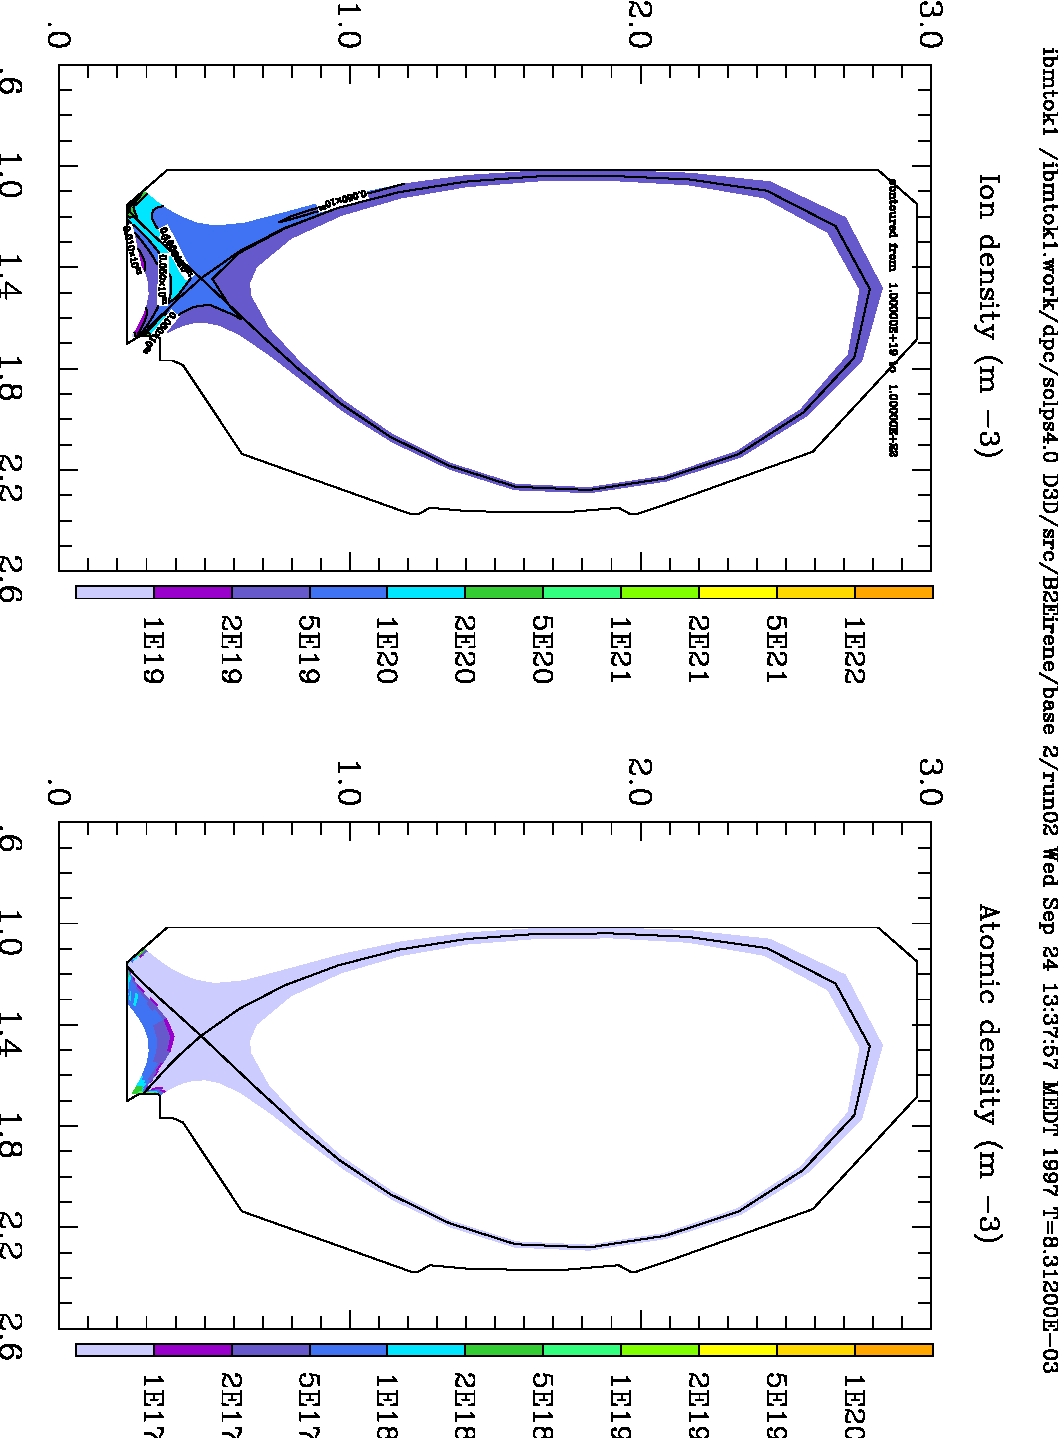
\includegraphics[angle=90,height=8cm]{b2plot_d3d.pdf}}
\else
    \centerline{
\includegraphics[angle=90,height=8cm]{b2plot_d3d.epsi}}
\fi
    \caption{Ion and atomic densities for DIII--D.}
    \label{fig:d3d}
\end{figure}

\subsubsection{cont}\index{b2plot, cont}\label{sec:cont}
Plots contour plots of the current data.  See figure \ref{fig:d3d}.
See section \ref{sec:contourparameters} for a list of commands that can be used to
change the appearance of contour plots.  Section \ref{sec:pageformat}
covers global changes to the plotting (square, landscape or portrait,
number of graphs per page). The use of {\bf surf} (see \ref{sec:surf}) is preferred
over that of {\bf cont}.

\subsubsection{$<$pos,{\bf I}$>$ f.x}\index{b2plot, f.x}\label{sec:f.x}
Plots the 2-D graph of the matrix data at $iy=<$pos$>$ versus $x$.
Vertical lines will be added to the plot to delimit any
eventual unconnected domain boundaries. Use of {\bf xpol} (default, see \ref{sec:xpol}) 
or {\bf xpar} (see \ref{sec:xpar}) commands allows one to toggle between plotting 
against poloidal or parallel distance along the field line. 

\subsubsection{$<$pos,{\bf I}$>$ f.y}\index{b2plot, f.y}\label{sec:f.y}
Plots the 2-D graph of the matrix data at $ix=<$pos$>$ versus $y$.
Use of the {\bf mmid} (see \ref{sec:mmid}) command allows for plotting versus the
outer midplane (or another position chosen by the user) radial coordinate.

\subsubsection{$<$n1,{\bf I}$>$ f.lx}\index{b2plot, f.lx}\label{sec:f.lx}
Plots the 2-D graph of the matrix data at $iy=<$pos$>$ versus $\log(x)$.
Equivalent to a combination of {\bf logx} (see \ref{sec:logx}) and {\bf f.x} above,
but remembers ths old setting of linear or logarithmic abscissa scale.

\subsubsection{$<$n1,{\bf I}$>$ f.ly}\index{b2plot, f.ly}\label{sec:f.ly}
Plots the 2-D graph of the matrix data at $ix=<$pos$>$ versus $\log(y)$.
Equivalent to a combination of {\bf logx} (see \ref{sec:logx}) and {\bf f.y} above,
but remembers ths old setting of linear or logarithmic abscissa scale.

\subsubsection{plwl}\index{b2plot, plwl}\label{sec:plwl}
Plots in the ``wall'' domain (applicable to wall data only).
This creates 2-D plots, with vertical lines separating
the various wall segments.

\subsubsection{$<$pos,{\bf I}$>$ trg.w}\index{b2plot, trg.w}\label{sec:trg.w}
Plots the 2-D graph of target data at $iz=<$pos$>$ versus wall coordinate.
Vertical lines will be added to the plot to delimit 
the various wall segments.  

\subsubsection{$<$pos,{\bf I}$>$ trg.z}\index{b2plot, trg.z}\label{sec:trg.z}
Plots the 2-D graph of target data at element $i=<$pos$>$ versus $z$.

\subsubsection{$<$n1,{\bf I}$>$ line}\index{b2plot, line}\label{sec:line}
Chooses between plotting against $x$-coordinate (default, $<$n1$>$=1)
or $y$-coordinate ($<$n1$>$=2). Not sure this works.

\subsubsection{mesh}\index{b2plot, mesh}\label{sec:mesh}
Plots the mesh. The colour of the mesh can be chosen 
with the {\bf mcol} (see \ref{sec:mcol}) command.

\subsubsection{surf}\index{b2plot, surf}\label{sec:surf}
Produces a ``patch'' plot where each cell is plotted in the
colour associated with its value.  This can be useful when the data is
noisy and contour plots take excessive time.  See figure \ref{fig:d3d}.
Recommended.

\subsubsection{trgsurf}\index{b2plot, trgsurf}\label{sec:trgsurf}
Produces a "patch" plot of the target domain.
Note that the side in contact with the plasma is at the bottom of the target computational domain.

\subsubsection{traj}\index{b2plot, traj}\label{sec:traj}\index{b2plot, uuse}\label{sec:uuse}\index{b2plot, vvse}\label{sec:vvse}\index{b2plot, t\_\#p}\label{sec:t_hashp}\index{b2plot, lint}\label{sec:lint}\index{b2plot, logt}\label{sec:logt}
\index{b2plot, trajectories plot}

Plots trajectories.  The following commands
\begin{verbatim}
echo phys a4p vesl sep outl 70 1 70 36 1000 traj | b2plot
\end{verbatim}
produced the results shown in figure \ref{fig:traj}.

\begin{figure}[hbtp]
\ifpdf 
    \centerline{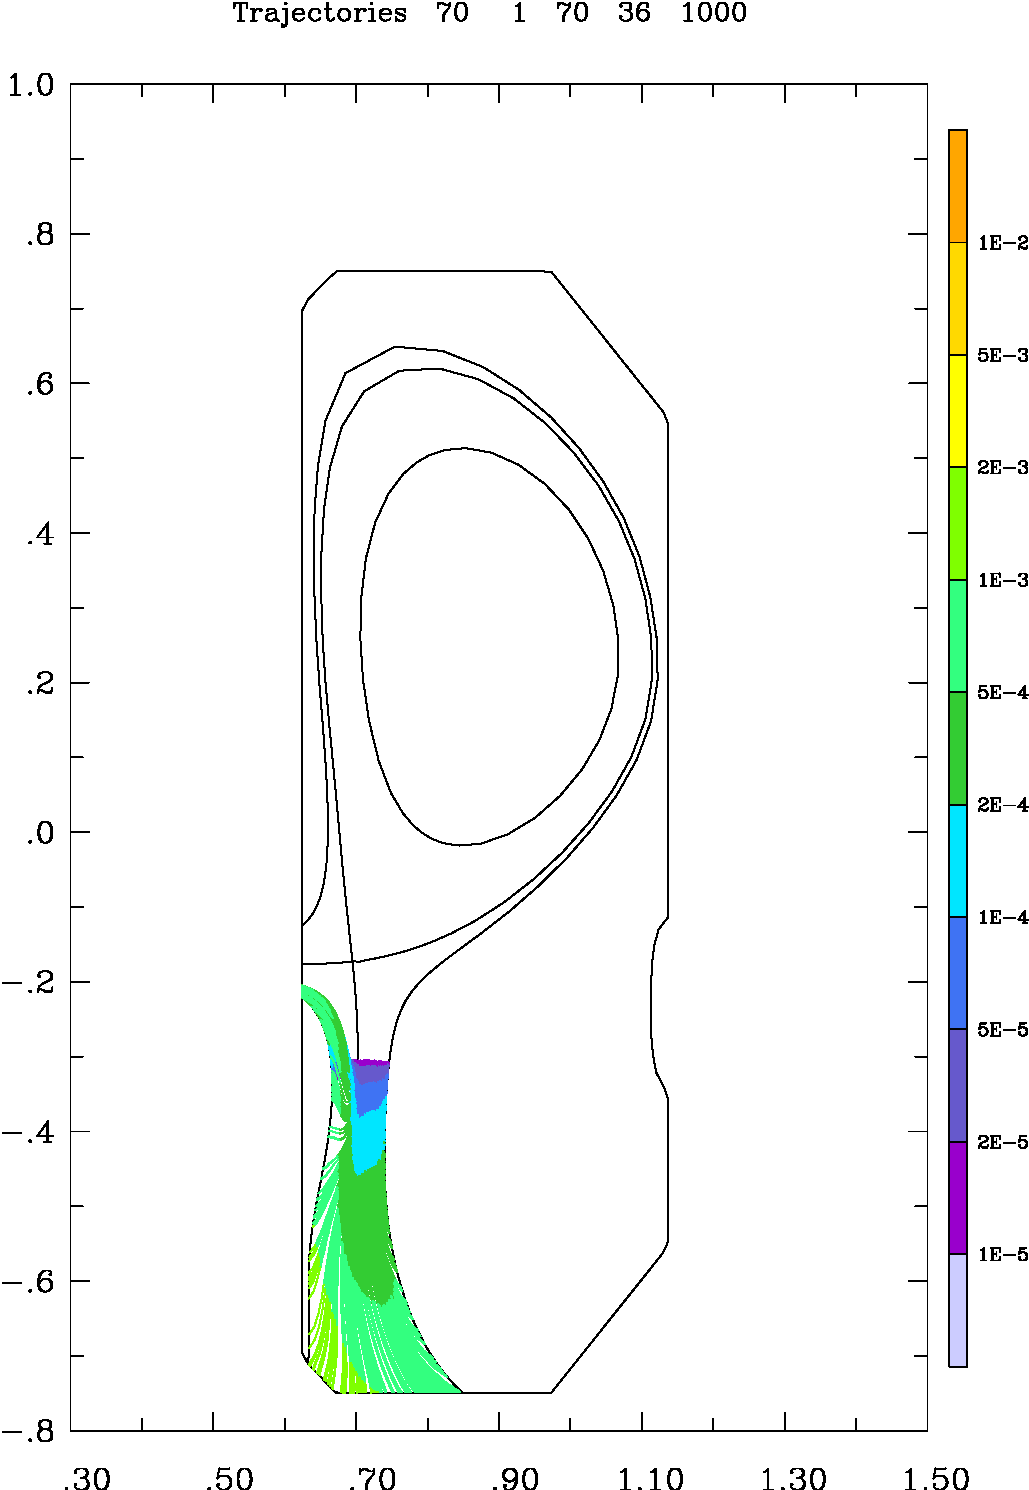
\includegraphics[height=8cm]{b2plot_70_1_70_36_1000.pdf}}
\else
    \centerline{
\includegraphics[height=8cm]{b2plot_70_1_70_36_1000.epsi}}
\fi
    \caption{Trajectory plot.}
    \label{fig:traj}
\end{figure}

The command seems to have changed since that example.  The command
takes a variable number of integer arguments, the minimum number being
8.

The first 4 numbers specify the bottom left and top right coordinates
of a rectangle in which the test particles are to be started
($ix_{start}~iy_{start}~ix_{end}~iy_{end}$) (0's will be replaced by the
appropriate limit).  The next number specifies the amount
of test particles to be started (if positive the particles are started
weighted by volume, if negative then the weighting function is taken
off the matrix stack).  This is then followed by a flag (1 for a
movie, otherwise normal trajectories), and then the species indices
come next.  The last argument specifies the number of species.
The use of {\bf uuse} and {\bf vvse} allows one to replace the particle velocities
matrices used by default to compute the trajectories with data from the
matrix stack.

The following example uses 2000 particles, weighted by particle
number, over the entire domain, for the 6 charge states of carbon.

\begin{verbatim}
stdl glob
a4p
phys 
-1.2 zmin 1.2 zmax
1.0 lbsz 0.005 dots
'rgb.pal' cltb 
vesl sep outl 
2000 t_#p 
1e-3 t_pt 
! b2nn b2in m+ 0.0 rmma
ni vol m*
0 0 0 0 -2000 1 2 3 4 5 6 7 6 traj 
drop
\end{verbatim}

From the code documentation:
\begin{verbatim}
C     This routine is used to plot trajectories of particles using the
C     velocity fields uutraj and vvtraj from B2SXDR. To call this routine
C     one must specify at least 8 parameters: ixmin, iymin, ixmax, iymax,
C     # of particles, 1 or 0 for movie or lines, species indices (at least
C     one), and last but not least the total number of species indices one 
C     has given in the step before. A valid call could be:
C     0 0 95 35 100 0 0 1 traj
C     This should plot the trajectories of 100 particles which start
C     in any of the cells between cell (0,0) (southwest corner) and
C     cell (95,35) (northeast corner) as lines for hydrogen (0=H).
C     Note that the cell and species indices start at zero!
C     The number of time steps (plots) is given by the "t_#p" command.
C     The total flight time of the particles is given by the "t_pt" command. 
C     The velocity fields uutraj and vvtraj can be overwritten using the
C     "uuse" and "vvse" commands. Their defaults values are ua and fna/na/sy
C     respectively. If the number of particles is positive, then the
C     particles are born randomly, with the probability of being born in a
C     cell being proportional to the cell volume. This probability weighting
C     can be changed by calling "traj" with a negative number of particles.
C     Then the weighting function is whatever field is on top of the matrix
C     stack. For example, this set of commands does the following:
C     fnax na m/ psx 0 zsel uuse  ! uutraj set to poloidal neutral flow velocity
C     fnay na m/ psy 0 zsel vvse  ! vvtraj set to radial neutral flow velocity
C     1000 t_#p                   ! 1000 time steps
C     1e-4 t_pt                   ! followed for a total time of 1.e-4 s.
C     na 0 zsel                   ! weighted with neutral density
C     0 0 0 0 -1000 0 0 1 traj    ! over the entire physical domain (0 0 0 0)
C               ! 1000 particles using non-default weighting function (-1000)
C               ! trajectories plotted (0)
C               ! for species 0 (=H neutrals) (0)
C               ! total of species considered is 1 (1)
C     =======================================================================
\end{verbatim}

The trajectories are coloured according to the length of time the particle has traveled
along it (illustrated by the label bar to the right of the graph). This label bar can
be set to be logarithmic (default) with the {\bf logt} command, or linear with the
{\bf lint} command.


\subsection{Data manipulating functions}\label{sec:datamanipulation}
\index{b2plot, data manipulation}

\subsubsection{abs}\index{b2plot, abs}\label{sec:abs}
Take the absolute value of the matrix data values.

\subsubsection{wabs}\index{b2plot, wabs}\label{sec:wabs}
Take the absolute value of the wall data values.

\subsubsection{trgabs}\index{b2plot, trgabs}\label{sec:trgabs}
Take the absolute value of the target data values.

\subsubsection{chs}\index{b2plot, chs}\label{sec:chs}
Change sign of matrix data.

\subsubsection{trgchs}\index{b2plot, trgchs}\label{sec:trgchs}
Change sign of target data.

\subsubsection{wchs}\index{b2plot, wchs}\label{sec:wchs}
Change sign of wall data.

\subsubsection{ddw}\index{b2plot, ddw}\label{sec:ddw}
Differentiates the wall data with respect to coordinate along wall perimeter.

\subsubsection{ddx}\index{b2plot, ddx}\label{sec:ddx}
Differentiates the matrix data with respect to poloidal coordinate $x$.

\subsubsection{ddy}\index{b2plot, ddy}\label{sec:ddy}
Differentiates the matrix data with respect to radial coordinate $y$.

\subsubsection{trgddp}\index{b2plot, trgddp}\label{sec:trgddp}
Differentiates the target data with respect to perpendicular coordinate.

\subsubsection{trgddw}\index{b2plot, trgddw}\label{sec:trgddw}
Differentiates the target data with respect to coordinate along wall perimeter.

\subsubsection{trgddz}\index{b2plot, trgddz}\label{sec:trgddz}
Differentiates the target data with respect to depth coordinate $z$.

\subsubsection{inttrgw}\index{b2plot, inttrgw}\label{sec:inttrgw}
Integrates data from the target stack along wall direction, summing over all wall segments.

\subsubsection{inttrgw*}\index{b2plot, inttrgw*}\label{sec:inttrgw*}
Integrates data from the target stack along wall direction, each segment being done separately.

\subsubsection{inttrgz}\index{b2plot, inttrgz}\label{sec:inttrgz}
Integrates data from the target stack in depth direction.

\subsubsection{intw}\index{b2plot, intw}\label{sec:intw}
Integrates data from the wall stack, summing over all wall segments.

\subsubsection{intw*}\index{b2plot, intw*}\label{sec:intw*}
Integrates data from the wall stack, each segment being done separately.

\subsubsection{intx}\index{b2plot, intx}\label{sec:intx}
Integrates data from the matrix stack along the $x$-direction, taking connectivities into account.

\subsubsection{inty}\index{b2plot, inty}\label{sec:inty}
Integrates data from the matrix stack along the $y$-direction.

\subsubsection{pne}\index{b2plot, pne}\label{sec:pne}
Divides the matrix data by the electron density $n_e$.

\subsubsection{pwne}\index{b2plot, pwne}\label{sec:pwne}
Divides the wall data by the local electron density $n_e$.

\subsubsection{pswa}\index{b2plot, pswa}\label{sec:pswa}
Divides the wall data by the wall element area.

\subsubsection{psx}\index{b2plot, psx}\label{sec:psx}
Divides the matrix data by $s_x$ --- the contact cell area between cells in the
$x$-direction.

\subsubsection{psxperp}\index{b2plot, psxperp}\label{sec:psxperp}
Divides the matrix data by $s_x$ --- the cell area perpendicular to the
$x$-direction.

\subsubsection{psy}\index{b2plot, psy}\label{sec:psy}
Divides the matrix data by $s_y$ --- the cell area perpendicular to the
$y$-direction.

\subsubsection{pvol}\index{b2plot, pvol}\label{sec:pvol}
Divides the matrix data by the volume of the cells.

\subsubsection{sumtrgw}\index{b2plot, sumtrgw}\label{sec:sumtrgw}
Sums the target data along the wall coordinate, and then copies the sum to all elements.

\subsubsection{sumtrgz}\index{b2plot, sumtrgz}\label{sec:sumtrgz}
Sums the target data depth-wise, and then copies the sum to all $z$-positions.

\subsubsection{sumw}\index{b2plot, sumw}\label{sec:sumw}
Sums the wall data, and then copies the sum to all elements.

\subsubsection{sumx}\index{b2plot, sumx}\label{sec:sumx}
Sums the matrix data over the entire $x$-direction, and then copies the sum to all $x$-positions.

\subsubsection{sumy}\index{b2plot, sumy}\label{sec:sumy}
Sums the matrix data over the entire $y$-direction, and then copies the sum to all $y$-positions.

\subsubsection{$<$is$_{start}$,{\bf I}$>$ $<$is$_{end}$,{\bf I}$>$ sumz}\index{b2plot, sumz}\label{sec:sumz}
Sums the matrix data over the $z$-direction from $<$is$_{start}$$>$ to $<$is$_{end}$$>$, and then copies the
sum to the first $z$ position. If $<$is$_{start}$$>$=$<$is$_{end}$$>$=0, then the sum is done
over all species.

\subsubsection{$<$is$_{start}$,{\bf I}$>$ $<$is$_{end}$,{\bf I}$>$ wsumz}\index{b2plot, wsumz}\label{sec:wsumz}
Sums the wall data over the $z$-direction from $<$is$_{start}$$>$ to $<$is$_{end}$$>$, and then copies the
sum to the first $z$ position. If $<$is$_{start}$$>$=$<$is$_{end}$$>$=0, then the sum is done
over all species.

\subsubsection{$<$is$_{start}$,{\bf I}$>$ $<$is$_{end}$,{\bf I}$>$ zrng}\index{b2plot, zrng}\label{sec:zrng}
Selects the subset over species extended from species index $<$is$_{start}$$>$ to
species index $<$is$_{end}$$>$ from the matrix data. 

\subsubsection{$<$is$_{start}$,{\bf I}$>$ $<$is$_{end}$,{\bf I}$>$ wzrng}\index{b2plot, wzrng}\label{sec:wzrng}
Selects the subset over species extended from species index $<$is$_{start}$$>$ to
species index $<$is$_{end}$$>$ from the wall data. 

\subsubsection{$<$i,{\bf I}$>$ wsel}\index{b2plot, wsel}\label{sec:wsel}
Propagates the wall data value from element $<$i$>$ to all other elements.

\subsubsection{$<$ix,{\bf I}$>$ xsel}\index{b2plot, xsel}\label{sec:xsel}
Propagates the matrix data value in the specified position $<$ix$>$ to all other $x$ values.

\subsubsection{$<$iy,{\bf I}$>$ ysel}\index{b2plot, ysel}\label{sec:ysel}
Propagates the matrix data value in the specified position $<$iy$>$ to all other $y$ values.

\subsubsection{$<$is,{\bf I}$>$ zsel}\index{b2plot, zsel}\label{sec:zsel}
Propagates the matrix data value in the specified position $<$is$>$ to all other $z$
(species) values.

\subsubsection{$<$i,{\bf I}$>$ trgwsel}\index{b2plot, trgwsel}\label{sec:trgwsel}
Propagates the target data value from the specified element $<$i$>$ to all other elements.

\subsubsection{$<$iz,{\bf I}$>$ trgzsel}\index{b2plot, trgzsel}\label{sec:trgzsel}
Propagates the target data value at the specified depth $<$iz$>$ to all other $z$ values.

\subsubsection{$<$is,{\bf I}$>$ wzsel}\index{b2plot, wzsel}\label{sec:wzsel}
Propagates the wall data value in the specified position $<$is$>$ to all other $z$
(species) values.

\subsubsection{rigz}\index{b2plot, rigz}\label{sec:rigz}
Toggles the inclusion of ignorable cells in the plots. The ignorable cells
are the guard cells at the boundaries and cells from isolated regions.

\subsubsection{log}\index{b2plot, log}\label{sec:log}
Computes logarithm base 10 of a matrix.

\subsubsection{ln}\index{b2plot, ln}\label{sec:ln}
Computes natural logarithm of a matrix.

\subsubsection{sqrt}\index{b2plot, sqrt}\label{sec:sqrt}
Takes square root of a matrix.

\subsubsection{exp}\index{b2plot, exp}\label{sec:exp}
Computes exponential of a matrix.

\subsubsection{trglog}\index{b2plot, trglog}\label{sec:trglog}
Computes logarithm base 10 of target data.

\subsubsection{trgln}\index{b2plot, trgln}\label{sec:trgln}
Computes natural logarithm of target data.

\subsubsection{trgsqrt}\index{b2plot, trgsqrt}\label{sec:trgsqrt}
Takes square root of target data.

\subsubsection{trgexp}\index{b2plot, trgexp}\label{sec:trgexp}
Computes exponential of target data.

\subsubsection{wlog}\index{b2plot, wlog}\label{sec:wlog}
Computes logarithm base 10 of wall data.

\subsubsection{wln}\index{b2plot, wln}\label{sec:wln}
Computes natural logarithm of wall data.

\subsubsection{wsqrt}\index{b2plot, wsqrt}\label{sec:wsqrt}
Takes square root of wall data.

\subsubsection{wexp}\index{b2plot, wexp}\label{sec:wexp}
Computes exponential of wall data.


\subsection{Arithmetic commands}\label{sec:arithmetic}
\index{b2plot, arithmetic commands}

\subsubsection{m+}\index{b2plot, m+}\label{sec:m+}
Adds the two arrays on the top of the matrix stack.

\subsubsection{m-}\index{b2plot, m-}\label{sec:m-}
Subtracts the array on the top of the matrix stack from the array second from
the top.

\subsubsection{m*}\index{b2plot, m*}\label{sec:m*}
Multiplies the two arrays on the top of the matrix stack.

\subsubsection{m/}\index{b2plot, m/}\label{sec:m/}
Divides the array secod from the top of the matrix stack by the array on
the top. Division by a zero element will yield zero.

\subsubsection{mmin}\index{b2plot, mmin}\label{sec:mmin}
Minimum of two top matrices on the stack.

\subsubsection{mmax}\index{b2plot, mmax}\label{sec:mmax}
Minimum of two top matrices on the stack.

\subsubsection{$<$r1,{\bf R}$>$ $<$r2,{\bf R}$>$ r+}\index{b2plot, r+}\label{sec:r+}
Adds the two real values $<$r1$>$ and $<$r2$>$ on the top of the real stack.

\subsubsection{$<$r1,{\bf R}$>$ $<$r2,{\bf R}$>$ r-}\index{b2plot, r-}\label{sec:r-}
Subtracts the real value on the top of the real stack $<$r2$>$ from the real value
second from the top $<$r1$>$.

\subsubsection{$<$r1,{\bf R}$>$ $<$r2,{\bf R}$>$ r*}\index{b2plot, r*}\label{sec:r*}
Multiplies the two real values $<$r1$>$ and $<$r2$>$ on the top of the real stack.

\subsubsection{$<$r1,{\bf R}$>$ $<$r2,{\bf R}$>$ r/}\index{b2plot, r/}\label{sec:r/}
Divides the real value second from the top of the real stack $<$r1$>$ by the real value on the top of the real stack $<$r2$>$. Division by 0 will yield an error and do nothing.

\subsubsection{$<$r1,{\bf R}$>$ $<$r2,{\bf R}$>$ r**}\index{b2plot, r**}\label{sec:r**}
Raises the real value second from the top of the real stack $<$r1$>$ to the power of
the real value on the top $<$r2$>$. $0^0$ will yield an error and do nothing.

\subsubsection{$<$number,{\bf R}$>$ rm+}\index{b2plot, rm+}\label{sec:rm+}
Adds $<$number$>$ to the array on the top of the matrix stack.

\subsubsection{$<$number,{\bf R}$>$ rm-}\index{b2plot, rm-}\label{sec:rm-}
Substracts $<$number$>$ from the array on the top of the matrix stack.

\subsubsection{$<$number,{\bf R}$>$ rm*}\index{b2plot, rm*}\label{sec:rm*}
Multiplies the array on the top of the matrix stack by $<$number$>$.

\subsubsection{$<$number,{\bf R}$>$ rm/}\index{b2plot, rm/}\label{sec:rm/}
Divides the array on the top of the matrix stack by $<$number$>$. Division by
zero will yield an error and do nothing.

\subsubsection{$<$number,{\bf R}$>$ rm**}\index{b2plot, rm**}\label{sec:rm**}
Raises each element of the array on the top of the matrix stack to the $<$number$>$-th power. If $<$number$>$=0, the result will be 1.0 for all cells.

\subsubsection{$<$number,{\bf R}$>$ rmmi}\index{b2plot, rmmi}\label{sec:rmmi}
Minimum of a matrix and $<$number$>$.

\subsubsection{$<$number,{\bf R}$>$ rmma}\index{b2plot, rmma}\label{sec:rmma}
Maximum of a matrix and $<$number$>$.

\subsubsection{$<$number,{\bf R}$>$ rtrgm+}\index{b2plot, rtrgm+}\label{sec:rtrgm+}
Adds $<$number$>$ to the array on the top of the target stack.

\subsubsection{$<$number,{\bf R}$>$ rtrgm-}\index{b2plot, rtrgm-}\label{sec:rtrgm-}
Substracts $<$number$>$ from the array on the top of the target stack.

\subsubsection{$<$number,{\bf R}$>$ rtrgm*}\index{b2plot, rtrgm*}\label{sec:rtrgm*}
Multiplies the array on the top of the target stack by $<$number$>$.

\subsubsection{$<$number,{\bf R}$>$ rtrgm/}\index{b2plot, rtrgm/}\label{sec:rtrgm/}
Divides the array on the top of the target stack by $<$number$>$. Division by
zero will yield an error and do nothing.

\subsubsection{$<$number,{\bf R}$>$ rtrgm**}\index{b2plot, rtrgm**}\label{sec:rtrgm**}
Raises each element of the array on the top of the target stack to the $<$number$>$-th power. If $<$number$>$=0, the result will be 1.0 for all elements.

\subsubsection{$<$number,{\bf R}$>$ rtrgmmi}\index{b2plot, rtrgmmi}\label{sec:rtrgmmi}
Minimum of target data and $<$number$>$.

\subsubsection{$<$number,{\bf R}$>$ rtrgmma}\index{b2plot, rtrgmma}\label{sec:rtrgmma}
Maximum of target data and $<$number$>$.

\subsubsection{$<$number,{\bf R}$>$ rwm+}\index{b2plot, rwm+}\label{sec:rwm+}
Adds $<$number$>$ to the array on the top of the wall stack.

\subsubsection{$<$number,{\bf R}$>$ rwm-}\index{b2plot, rwm-}\label{sec:rwm-}
Substracts $<$number$>$ from the array on the top of the wall stack.

\subsubsection{$<$number,{\bf R}$>$ rwm*}\index{b2plot, rwm*}\label{sec:rwm*}
Multiplies the array on the top of the wall stack by $<$number$>$.

\subsubsection{$<$number,{\bf R}$>$ rwm/}\index{b2plot, rwm/}\label{sec:rwm/}
Divides the array on the top of the wall stack by $<$number$>$. Division by
zero will yield an error and do nothing.

\subsubsection{$<$number,{\bf R}$>$ rwm**}\index{b2plot, rwm**}\label{sec:rwm**}
Raises each element of the array on the top of the wall stack to the $<$number$>$-th power. If $<$number$>$=0, the result will be 1.0 for all elements.

\subsubsection{$<$number,{\bf R}$>$ rwmmi}\index{b2plot, rwmmi}\label{sec:rwmmi}
Minimum of wall data and $<$number$>$.

\subsubsection{$<$number,{\bf R}$>$ rwmma}\index{b2plot, rwmma}\label{sec:rwmma}
Maximum of wall data and $<$number$>$.

\subsubsection{$<$number,{\bf R}$>$ meq}\index{b2plot, meq}\label{sec:meq}
If a matrix element is equal to $<$number$>$, sets this matrix element to 1.0.
Otherwise, sets it to zero.

\subsubsection{$<$number,{\bf R}$>$ mne}\index{b2plot, mne}\label{sec:mne}
If a matrix element is not equal to $<$number$>$, sets this matrix element to 1.0.
Otherwise, sets it to zero.

\subsubsection{$<$number,{\bf R}$>$ mge}\index{b2plot, mge}\label{sec:mge}
If a matrix element is greater than or equal to $<$number$>$, sets this matrix element to 1.0.
Otherwise, sets it to zero.

\subsubsection{$<$number,{\bf R}$>$ mgt}\index{b2plot, mgt}\label{sec:mgt}
If a matrix element is greater than $<$number$>$, sets this matrix element to 1.0.
Otherwise, sets it to zero.

\subsubsection{$<$number,{\bf R}$>$ mle}\index{b2plot, mle}\label{sec:mle}
If a matrix element is less than or equal to $<$number$>$, sets this matrix element to 1.0.
Otherwise, sets it to zero.

\subsubsection{$<$number,{\bf R}$>$ mlt}\index{b2plot, mlt}\label{sec:mlt}
If a matrix element is less than $<$number$>$, sets this matrix element to 1.0.
Otherwise, sets it to zero.

\subsubsection{pos}\index{b2plot, pos}\label{sec:pos}
If a matrix element is positive, sets this matrix element to 1.0.
Otherwise, sets it to zero.

\subsubsection{$<$i1,{\bf I}$>$ $<$i2,{\bf I}$>$ i+}\index{b2plot, i+}\label{sec:i+}
Adds the two integer values $<$i1$>$ and $<$i2$>$ on the top of the integer stack.

\subsubsection{$<$i1,{\bf I}$>$ $<$i2,{\bf I}$>$ i-}\index{b2plot, i-}\label{sec:i-}
Subtracts the integer value on the top of the integer stack $<$i2$>$ from the integer value
second from the top $<$i1$>$.

\subsubsection{$<$i1,{\bf I}$>$ $<$i2,{\bf I}$>$ i*}\index{b2plot, i*}\label{sec:i*}
Multiplies the two integer values $<$i1$>$ and $<$i2$>$ on the top of the integer stack.

\subsubsection{$<$i1,{\bf I}$>$ $<$i2,{\bf I}$>$ i/}\index{b2plot, i/}\label{sec:i/}
Divides the integer value second from the top of the integer stack $<$i1$>$ by the integer value on top of the integer stack $<$i2$>$. This is integer division! Division by 0 will yield an error and do nothing.

\subsubsection{$<$i1,{\bf I}$>$ $<$i2,{\bf I}$>$ i**}\index{b2plot, i**}\label{sec:i**}
Raises the integer value second from the top of the integer stack $<$i1$>$ to the power of
the integer value on the top $<$i2$>$. $0^0$ will yield an error and do nothing.

\subsubsection{$<$number,{\bf R}$>$ trgeq}\index{b2plot, trgeq}\label{sec:trgeq}
If a target element is equal to $<$number$>$, sets this target element to 1.0.
Otherwise, sets it to zero.

\subsubsection{$<$number,{\bf R}$>$ trgne}\index{b2plot, trgne}\label{sec:trgne}
If a target element is not equal to $<$number$>$, sets this target element to 1.0.
Otherwise, sets it to zero.

\subsubsection{$<$number,{\bf R}$>$ trgge}\index{b2plot, trgge}\label{sec:trgge}
If a target element is greater than or equal to $<$number$>$, sets this target element to 1.0.
Otherwise, sets it to zero.

\subsubsection{$<$number,{\bf R}$>$ trggt}\index{b2plot, trggt}\label{sec:trggt}
If a target element is greater than $<$number$>$, sets this target element to 1.0.
Otherwise, sets it to zero.

\subsubsection{$<$number,{\bf R}$>$ trgle}\index{b2plot, trgle}\label{sec:trgle}
If a target element is less than or equal to $<$number$>$, sets this target element to 1.0.
Otherwise, sets it to zero.

\subsubsection{$<$number,{\bf R}$>$ trglt}\index{b2plot, trglt}\label{sec:trglt}
If a target element is less than $<$number$>$, sets this target element to 1.0.
Otherwise, sets it to zero.

\subsubsection{trgmmin}\index{b2plot, trgmmin}\label{sec:trgmmin}
Minimum of two top matrices on the target stack.

\subsubsection{trgmmax}\index{b2plot, trgmmax}\label{sec:trgmmax}
Maximum of two top matrices on the target stack.

\subsubsection{trgm+}\index{b2plot, trgm+}\label{sec:trgm+}
Adds the two arrays on the top of the target stack.

\subsubsection{trgm-}\index{b2plot, trgm-}\label{sec:trgm-}
Subtracts the array on the top of the target stack from the array second from
the top.

\subsubsection{trgm*}\index{b2plot, trgm*}\label{sec:trgm*}
Multiplies the two arrays on the top of the target stack.

\subsubsection{trgm/}\index{b2plot, trgm/}\label{sec:trgm/}
Divides the array second from the top of the target stack by the array on the top.
Division by a zero element will yield zero.

\subsubsection{trgpos}\index{b2plot, trgpos}\label{sec:trgpos}
If a target element is positive, sets this target element to 1.0.
Otherwise, sets it to zero.

\subsubsection{wm+}\index{b2plot, wm+}\label{sec:wm+}
Adds the two arrays on the top of the wall stack.

\subsubsection{wm-}\index{b2plot, wm-}\label{sec:wm-}
Subtracts the array on the top of the wall stack from the array second from
the top.

\subsubsection{wm*}\index{b2plot, wm*}\label{sec:wm*}
Multiplies the two arrays on the top of the wall stack.

\subsubsection{wm/}\index{b2plot, wm/}\label{sec:wm/}
Divides the array second from the top of the wall stack by the array on 
the top. Division by a zero element will yield zero.

\subsubsection{wmmin}\index{b2plot, wmmin}\label{sec:wmmin}
Minimum of two top data sets on the wall stack.

\subsubsection{wmmax}\index{b2plot, wmmax}\label{sec:wmmax}
Minimum of two top data sets on the wall stack.

\subsubsection{$<$number,{\bf R}$>$ wmeq}\index{b2plot, wmeq}\label{sec:wmeq}
If a wall element is equal to $<$number$>$, sets this wall element to 1.0.
Otherwise, sets it to zero.

\subsubsection{$<$number,{\bf R}$>$ wmne}\index{b2plot, wmne}\label{sec:wmne}
If a wall element is not equal to $<$number$>$, sets this wall element to 1.0.
Otherwise, sets it to zero.

\subsubsection{$<$number,{\bf R}$>$ wmge}\index{b2plot, wmge}\label{sec:wmge}
If a wall element is greater than or equal to $<$number$>$, sets this wall element to 1.0.
Otherwise, sets it to zero.

\subsubsection{$<$number,{\bf R}$>$ wmgt}\index{b2plot, wmgt}\label{sec:wmgt}
If a wall element is greater than $<$number$>$, sets this wall element to 1.0.
Otherwise, sets it to zero.

\subsubsection{$<$number,{\bf R}$>$ wmle}\index{b2plot, wmle}\label{sec:wmle}
If a wall element is less than or equal to $<$number$>$, sets this wall element to 1.0.
Otherwise, sets it to zero.

\subsubsection{$<$number,{\bf R}$>$ wmlt}\index{b2plot, wmlt}\label{sec:wmlt}
If a wall element is less than $<$number$>$, sets this wall element to 1.0.
Otherwise, sets it to zero.

\subsubsection{wpos}\index{b2plot, wpos}\label{sec:wpos}
If a wall element is positive, sets this wall element to 1.0.
Otherwise, sets it to zero.


\subsection{Stack manipulating commands}\label{sec:stack}
\index{b2plot, stack manipulation}

\subsubsection{drop}\index{b2plot, drop}\label{sec:drop}
Deletes the array on the top of the matrix stack.

\subsubsection{dup}\index{b2plot, dup}\label{sec:dup}
Duplicates the array on the top of the matrix stack.

\subsubsection{swap}\index{b2plot, swap}\label{sec:swap}
Swaps the top two arrays on the matrix stack.

\subsubsection{over}\index{b2plot, over}\label{sec:over}
Copies the array second from the top to the top of the matrix stack.

\subsubsection{list}\index{b2plot, list}\label{sec:list}
Lists the contents of the matrix stack by printing the titles
of the stored matrices to \verb!stdout!.

\subsubsection{mdims}\index{b2plot, mdims}\label{sec:mdims}
Prints the dimensions and contents (i.e. data set titles) of the matrix
stack to \verb!stdout!.

\subsubsection{rdrop}\index{b2plot, rdrop}\label{sec:rdrop}
Deletes the real on the top of the real stack.

\subsubsection{rdup}\index{b2plot, rdup}\label{sec:rdup}
Duplicates the real on the top of the real stack.

\subsubsection{rswap}\index{b2plot, rswap}\label{sec:rswap}
Swaps the top two reals on the real stack.

\subsubsection{rover}\index{b2plot, rover}\label{sec:rover}
Copies the real second from the top to the top of the real stack.

\subsubsection{rtostr}\index{b2plot, rtostr}\label{sec:rtostr}
Writes the real on top of the real stack to the top of the string stack.

\subsubsection{rtom}\index{b2plot, rtom}\label{sec:rtom}
Copies the real on top of the real stack to the top of the matrix stack.

\subsubsection{rtow}\index{b2plot, rtow}\label{sec:rtow}
Copies the real on top of the real stack to the top of the wall stack.

\subsubsection{rtot}\index{b2plot, rtot}\label{sec:rtot}
Copies the real on top of the real stack to the top of the target stack.

\subsubsection{rprt}\index{b2plot, rprt}\label{sec:rprt}
Outputs the contents of the real stack to \verb:stdout:, and to \verb:b2plot.write: 
(in the \SOLPSfour environment) or \verb:b2pl.exe.dir/b2plot.write: 
(in the \SOLPSfive environment) if {\bf writ} is active.

\subsubsection{idrop}\index{b2plot, idrop}\label{sec:idrop}
Deletes the integer on the top of the integer stack.

\subsubsection{idup}\index{b2plot, idup}\label{sec:idup}
Duplicates the integer on the top of the integer stack.

\subsubsection{iswap}\index{b2plot, iswap}\label{sec:iswap}
Swaps the top two integers on the integer stack.

\subsubsection{iover}\index{b2plot, iover}\label{sec:iover}
Copies the integer second from the top to the top of the integer stack.

\subsubsection{itor}\index{b2plot, itor}\label{sec:itor}
Copies the integer on top of the integer stack to the top of the real stack.

\subsubsection{itostr}\index{b2plot, itostr}\label{sec:itostr}
Writes the integer on top of the integer stack to the top of the string stack.

\subsubsection{itom}\index{b2plot, itom}\label{sec:itom}
Copies the integer on top of the integer stack to the top of the matrix stack.

\subsubsection{itow}\index{b2plot, itow}\label{sec:itow}
Copies the integer on top of the integer stack to the top of the wall stack.

\subsubsection{itot}\index{b2plot, itot}\label{sec:itot}
Copies the integer on top of the integer stack to the top of the target stack.

\subsubsection{iprt}\index{b2plot, iprt}\label{sec:iprt}
Outputs the contents of the integer stack to \verb:stdout:, and to \verb:b2plot.write: 
(in the \SOLPSfour environment) or \verb:b2pl.exe.dir/b2plot.write: 
(in the \SOLPSfive environment) if {\bf writ} is active.

\subsubsection{scat}\index{b2plot, scat}\label{sec:scat}
Concatenates the top two strings of the string stack.

\subsubsection{sdrop}\index{b2plot, sdrop}\label{sec:sdrop}
Deletes the string on the top of the string stack.

\subsubsection{sdup}\index{b2plot, sdup}\label{sec:sdup}
Duplicates the string on the top of the string stack.

\subsubsection{sswap}\index{b2plot, sswap}\label{sec:sswap}
Swaps the top two strings on the string stack.

\subsubsection{sover}\index{b2plot, sover}\label{sec:sover}
Copies the string second from the top to the top of the string stack.

\subsubsection{sprt}\index{b2plot, sprt}\label{sec:sprt}
Outputs the contents of the string stack to \verb:stdout:, and to \verb:b2plot.write: 
(in the \SOLPSfour environment) or \verb:b2pl.exe.dir/b2plot.write: 
(in the \SOLPSfive environment) if {\bf writ} is active.

\subsubsection{$<$nx,{\bf I}$>$ $<$ny,{\bf I}$>$ $<$filename,{\bf S}$>$ saw}\index{b2plot, saw}\label{sec:saw}
Reads the matrix of size $(<$nx$>+2) \times (<$ny$>+2)$ from file $<$filename$>$ into the
matrix stack.

\subsubsection{$<$nx,{\bf I}$>$ $<$ny,{\bf I}$>$ $<$nz,{\bf I}$>$ $<$filename,{\bf S}$>$ saws}\index{b2plot, saws}\label{sec:saws}
Reads the matrix of size $(<$nx$>+2) \times (<$ny$>+2) \times nz$ from file $<$filename$>$ into the
matrix stack. Expects $nz$ to match $ns$ and that the data refers to the fluid plasma species.

\subsubsection{$<$nx,{\bf I}$>$ $<$ny,{\bf I}$>$ $<$nz,{\bf I}$>$ $<$filename,{\bf S}$>$ sawx}\index{b2plot, sawx}\label{sec:sawx}
Reads the matrix of size $(<$nx$>+2) \times (<$ny$>+2) \times nz$ from file $<$filename$>$ into the
matrix stack. Expects $nz$ to match $ns\_ext$ and that the data refers to the additional species followed by the
external code to which {\bf SOLPS} is coupled.

\subsubsection{$<$nwall,{\bf I}$>$ $<$filename,{\bf S}$>$ wsaw}\index{b2plot, wsaw}\label{sec:wsaw}
Reads the array of size $<$nwall$>$ from file $<$filename$>$ into the wall stack.

\subsubsection{stow}\index{b2plot, stow}\label{sec:stow} 
Copies the array on top of the matrix stack to the wall data stack. Only the matrix
elements from boundary cells will be copied over, onto the corresponding wall elements.

\subsubsection{trgdrop}\index{b2plot, trgdrop}\label{sec:trgdrop}
Deletes the array on the top of the target stack.

\subsubsection{trgdup}\index{b2plot, trgdup}\label{sec:trgdup}
Duplicates the array on the top of the target stack.

\subsubsection{trgswap}\index{b2plot, trgswap}\label{sec:trgswap}
Swaps the top two arrays on the target stack.

\subsubsection{trgover}\index{b2plot, trgover}\label{sec:trgover}
Copies the array second from the top to the top of the target stack.

\subsubsection{trglist}\index{b2plot, trglist}\label{sec:trglist}
Lists the contents of the target stack by printing the titles
of the stored matrices to \verb!stdout!.

\subsubsection{trgtow}\index{b2plot, trgtow}\label{sec:trgtow} 
Copies the matrix on top of the target data stack onto the wall data stack. Only the
top surface target data values will be copied onto the corresponding wall elements.

\subsubsection{wdrop}\index{b2plot, wdrop}\label{sec:wdrop}
Deletes the array on the top of the wall stack.

\subsubsection{wdup}\index{b2plot, wdup}\label{sec:wdup}
Duplicates the array on the top of the wall stack.

\subsubsection{wswap}\index{b2plot, wswap}\label{sec:wswap}
Swaps the top two arrays on the wall stack.

\subsubsection{wover}\index{b2plot, wover}\label{sec:wover}
Copies the array second from the top to the top of the wall stack.

\subsubsection{wlist}\index{b2plot, wlist}\label{sec:wlist}
Lists the contents of the wall stack by printing the titles
of the stored matrices to \verb!stdout!.

\subsubsection{wtos}\index{b2plot, wtos}\label{sec:wtos} 
Copies the array on top of the wall data stack onto the matrix stack. Each wall element
value is copied onto the corresponding boundary cell in the matrix stack. Inner cells
of the matrix stack will contain zero.

\subsubsection{wtot}\index{b2plot, wtot}\label{sec:wtot} 
Copies the array on top of the wall data stack onto the target stack. Each wall element
value is copied onto the corresponding column of cells in the target stack. 

\subsubsection{$<$ix,{\bf I}$>$ xtow}\index{b2plot, xtow}\label{sec:xtow} 
Copies the data from the $ix$-th row of the array on top of the matrix stack to the wall data stack.

\subsubsection{$<$iy,{\bf I}$>$ ytow}\index{b2plot, ytow}\label{sec:ytow} 
Copies the data from the $iy$-th column of the array on top of the matrix stack to the wall data stack.


\subsection{Page format parameters}\label{sec:pageformat}
\index{b2plot, page format commands}

\subsubsection{a4l}\index{b2plot, a4l}\label{sec:a4l}
Sets the plot area for A4 landscape. Use ``ctrans -d ps.mono.land |
a4page | lpr''.

\subsubsection{a4p}\index{b2plot, a4p}\label{sec:a4p}
Sets the plot area for A4 portrait.  Use ``ctrans -d ps.mono | a4page |
lpr''.

\subsubsection{sq}\index{b2plot, sq}\label{sec:sq}
Sets the plot area to be square. This ensures that the$x$ and $y$ scaling factors are the same.

\subsubsection{$<$nx,{\bf I}$>$ $<$ny,{\bf I}$>$ page}\index{b2plot, page}\label{sec:page}
Plots $<$nx$>$ graphs in the $x$-direction and $<$ny$>$ in the $y$-direction on the same page.


\subsection{Graph format commands}\index{b2plot, graphformat}\label{sec:graphformat}
\index{b2plot, graph format commands}

\subsubsection{both}\index{b2plot, both}\label{sec:both}
Plots on both the physical and computational meshes.

\subsubsection{comp}\index{b2plot, comp}\label{sec:comp}
Plots on computational mesh only.

\subsubsection{phys}\index{b2plot, phys}\label{sec:phys}
Plots on the physical mesh only.

\subsubsection{aspc}\index{b2plot, aspc}\label{sec:aspc}
Toggles whether aspect ratio should be preserved for physical 
and computational domain plots (default \verb!.true.!). 
If \verb!.false.!, the plot region limits will be those defined
from the $xmin~xmax~ymin~ymax$, etc... values.

\subsubsection{linf}\index{b2plot, linf}\label{sec:linf}
Sets linear scaling for the function values (default).

\subsubsection{logf}\index{b2plot, logf}\label{sec:logf}
Sets logarithmic scaling for the function values.

\subsubsection{lintrg}\index{b2plot, lintrg}\label{sec:lintrg}
Sets linear scaling for the target data values (default).

\subsubsection{logtrg}\index{b2plot, logtrg}\label{sec:logtrg}
Sets logarithmic scaling for the target data values.

\subsubsection{linxtrg}\index{b2plot, linxtrg}\label{sec:linxtrg}
Sets linear abscissae for the target data values (default).

\subsubsection{logxtrg}\index{b2plot, logxtrg}\label{sec:logxtrg}
Sets logarithmic abscissae scaling for the target data values.

\subsubsection{linx}\index{b2plot, linx}\label{sec:linx}
Sets linear scaling for the abscissae values (default).

\subsubsection{logx}\index{b2plot, logx}\label{sec:logx}
Sets logarithmic scaling for the abscissae values.

\subsubsection{xpar}\index{b2plot, xpar}\label{sec:xpar}
Plots 2-D plots against parallel $x$ distance.

\subsubsection{xpol}\index{b2plot, xpol}\label{sec:xpol}
Plots 2-D plots against poloidal $x$ distance (default).

\subsubsection{$<$n,{\bf I}$>$ ndec}\index{b2plot, ndec}\label{sec:ndec}
Sets number of decades to $<$n$>$ for logarithmic plots (default 10). 
If $n = 0$, restores the default value.

\subsubsection{mmid}\index{b2plot, mmid}\label{sec:mmid}
Toggles mapping to midplane coordinate for 2-D plots. The midplane
is assumed to be located at $ix=jxa$. See commands {\bf omp} (section \ref{sec:omp}) and 
{\bf jxa} (section \ref{sec:omp}) for setting and knowing its value.


\subsection{Graph appearance commands}\label{sec:graphappearance}
\index{b2plot, graph appearance commands}

\subsubsection{bw}\index{b2plot, bw}\label{sec:bw}
Want black and white for some plots.

\subsubsection{col}\index{b2plot, col}\label{sec:col}
Want colour for some plots.

\subsubsection{$<$number,{\bf I}$>$ font}\index{b2plot, font}\label{sec:font}
Changes the current font type to $<$number$>$
\begin{itemize}
\item -25 TIMES ROMAN
\item -26 TIMES BOLD
\item -21 HELVETICA
\item -22 HELVETICA BOLD
\item -29 COURIER
\item -30 COURIER BOLD
\end{itemize}
There are even more available fonts --- refer to \verb!NCAR! manpage.

In general, it is possible to change fonts within a text string to be printed
on the graph, for the commands below taking a string as argument. For example,
the command
\begin{verbatim}
'D-\\Ga\\R (photons m^{-3} s^{-1})' extl
\end{verbatim}
would give an extra graph label containing ``D-$\alpha$ (photons m$^{-3}$ s$^{-1}$)''.

\subsubsection{stdl}\index{b2plot, stdl}\label{sec:stdl}
Sets standard label as {\em extralabel}:
\begin{verbatim}
'\${HOST} \${PWD} `date` T=\${TIME}'
\end{verbatim}

\subsubsection{$<$label, {\bf S}$>$ glbl}\index{b2plot, glbl}\label{sec:glbl}
Sets the current graph label to $<$label$>$.

\subsubsection{$<$number,{\bf I}$>$ $<$label, {\bf S}$>$ slbl}\index{b2plot, slbl}\label{sec:slbl}
Sets the species label of species index $<$number$>$ to $<$label$>$ for the current graph.

\subsubsection{$<$label, {\bf S}$>$ tlbl}\index{b2plot, tlbl}\label{sec:tlbl}
Sets the current target graph label to $<$label$>$.

\subsubsection{$<$label, {\bf S}$>$ trgblbl}\index{b2plot, trgblbl}\label{sec:trgblbl}
Sets the current target bar label to $<$label$>$.

\subsubsection{$<$label, {\bf S}$>$ wlbl}\index{b2plot, wlbl}\label{sec:wlbl}
Sets the current wall graph label to $<$label$>$.

\subsubsection{$<$number,{\bf I}$>$ $<$label, {\bf S}$>$ wslbl}\index{b2plot, wslbl}\label{sec:wslbl}
Sets the species label of species index $<$number$>$ to $<$label$>$ for the current wall graph.

\subsubsection{$<$label, {\bf S}$>$ wallblbl}\index{b2plot, wallblbl}\label{sec:wallblbl}
Sets the current wall bar label to $<$label$>$.

\subsubsection{glob}\index{b2plot, glob}\label{sec:glob}
Copies the contents of {\em extralabel} into the global header for all graphs.

\subsubsection{$<$factor,{\bf R}$>$ lbsz}\index{b2plot, lbsz}\label{sec:lbsz}
Sets label size to $<$factor$>$ times default size (default = 1.0).

\subsubsection{$<$number,{\bf I}$>$ lfsz}\index{b2plot, lfsz}\label{sec:lfsz}
Sets line label font size to $<$number$>$ (default = 0). If $<$number$>$ is between 0 and 3, then the size
represents 1., 1.5, 2., and 3. times an 8-plotter address unit width. Otherwise, it represents the character 
width in plotter address units.

\subsubsection{noax}\index{b2plot, noax}\label{sec:noax}
Does not plot axes.

\subsubsection{$<$factor,{\bf R}$>$ lwid}\index{b2plot, lwid}\label{sec:lwid}
Changes line width to $<$factor$>$ times default width.

\subsubsection{same}\index{b2plot, same}\label{sec:same}
The next graphs occur on the same set of axes.  Terminated with {\bf new}.

\subsubsection{new}\index{b2plot, new}\label{sec:new}
Starts graphs on a new set of axes.


\subsection{Overlays to contour and line plots}\label{sec:contouroverlays}
\index{b2plot, contour overlays}

\subsubsection{zero}\index{b2plot, zero}\label{sec:zero}
Toggles the plotting of dotted axes lines at zero.

\subsubsection{$<$factor,{\bf R}$>$ zwid}\index{b2plot, zwid}\label{sec:zwid}
Changes width of dotted axes lines at zero to $<$factor$>$ times default width.

\subsubsection{$<$ncol,{\bf I}$>$ zcol}\index{b2plot, zcol}\label{sec:zcol}\index{b2plot, colour table}
Plots axes line at zero with colour $<$ncol$>$ (default 1). The colours available by default are:
\begin{enumerate}
  \item[ 0] White (background)
  \item[ 1] Black (default)
  \item[ 2] Lavender
  \item[ 3] Dark Violet
  \item[ 4] Slate Blue
  \item[ 5] Royal Blue
  \item[ 6] Deep Sky Blue
  \item[ 7] Aqua
  \item[ 8] Green
  \item[ 9] Celeste
  \item[10] Chartreuse
  \item[11] Green Yellow
  \item[12] Yellow
  \item[13] Golden
  \item[14] Orange
  \item[15] Orange Red
  \item[16] Red
  \item[17] Orchid
\end{enumerate}
These values can be overridden by use of the {\bf cltb} command.

\subsubsection{$<$ncol,{\bf I}$>$ dcol}\index{b2plot, dcol}\label{sec:dcol}
Colour to be used for matrix data line plots (default 1). 
If {\bf dcol} is set to a negative value, the data plot lines will use
a succession of colours starting from $|dcol|$ with increasing index.
See {\bf zcol} above for a list of available colours.

\subsubsection{$<$ncol,{\bf I}$>$ tcol}\index{b2plot, tcol}\label{sec:tcol}
Colour to be used for target data line plots (default 1). 
If {\bf tcol} is set to a negative value, the data plot lines will use
a succession of colours starting from $|tcol|$ with increasing index.
See {\bf zcol} above for a list of available colours.

\subsubsection{$<$ncol,{\bf I}$>$ wcol}\index{b2plot, wcol}\label{sec:wcol}
Colour to be used for wall data line plots (default 1). 
If {\bf wcol} is set to a negative value, the data plot lines will use
a succession of colours starting from $|wcol|$ with increasing index.
See {\bf zcol} above for a list of available colours.

\subsubsection{$<$ncol,{\bf I}$>$ bcol}\index{b2plot, bcol}\label{sec:bcol}
Colour to be used for printing label bar title (default 1). 
See {\bf zcol} above for a list of available colours.

\subsubsection{$<$ncol,{\bf I}$>$ gcol}\index{b2plot, gcol}\label{sec:gcol}
Colour to be used for printing graph title (default 1). 
See {\bf zcol} above for a list of available colours.

\subsubsection{$<$ncol,{\bf I}$>$ hcol}\index{b2plot, hcol}\label{sec:hcol}
Colour to be used for printing global header (default 1). 
See {\bf zcol} above for a list of available colours.

\subsubsection{$<$ncol,{\bf I}$>$ xcol}\index{b2plot, xcol}\label{sec:xcol}
Colour to be used for printing extra label (default 1). 
See {\bf zcol} above for a list of available colours.

\subsubsection{$<$length,{\bf R}$>$ arow}\index{b2plot, arow}\label{sec:arow}\index{b2plot, arox}\label{sec:arox}\index{b2plot, aroy}\label{sec:aroy}
Produces flow chart of array {\em fnax} and {\em fnay} using a maximum arrow
length of $<$length$>$ meters. The use of {\em fnax} and {\em fnay} can be superseded
by the the commands {\bf arox} and {\bf aroy}, respectively, which will then use
data from the matrix stack for computing the arrow directions instead.

\subsubsection{$<$widthfactor,{\bf R}$>$ arww}\index{b2plot, arww}\label{sec:arww}
Changes default arrow width by $<$widthfactor$>$ (default 1.0).

\subsubsection{$<$ncol,{\bf I}$>$ acol}\index{b2plot, acol}\label{sec:acol}
Plots overlaid arrows with colour $<$ncol$>$ (default 1). 
See {\bf zcol} above for a list of available colours.

\subsubsection{$<$data file,{\bf S}$>$ expf}\index{b2plot, expf}\label{sec:expf}
File from which to take experimental data to be plotted with code data.

\subsubsection{expl}\index{b2plot, expl}\label{sec:expl}
Toggles between plotting the experimental data as a line (default) or as a scatter plot.

\subsubsection{$<$expsymbol,{\bf I}$>$ exps}\index{b2plot, exps}\label{sec:exps}
Choice of the symbol to be used forthe experimental data scatter plots (default 5).
The numbering convention is the same as used in the \verb!libgr! library from \verb!Eirene!.

\subsubsection{$<$data file,{\bf S}$>$ wallf}\index{b2plot, wallf}\label{sec:wallf}
File from which to take experimental data to be plotted with wall data.

\subsubsection{$<$ncol,{\bf I}$>$ ecol}\index{b2plot, ecol}\label{sec:ecol}
Plots experimental data overlay with colour $<$ncol$>$ (default 1). 
If {\bf ecol} is set to a negative value, the data plot lines will use
a succession of colours starting from $|ecol|$ with increasing index.
See {\bf zcol} above for a list of available colours.

\subsubsection{$<$widthfactor,{\bf R}$>$ ewid}\index{b2plot, ewid}\label{sec:ewid}
Changes the experimental data overlay line width by $<$widthfactor$>$ (default 1.0). 

\subsubsection{$<$n,{\bf I}$>$ ytra}\index{b2plot, ytra}\label{sec:ytra}
Choose transformation function ($<$n$>$.ne.0) for radial
coordinate to compare with experimental data, according to
\verb!n.s.r.z.a_inner! and \verb!n.s.r.z.a_outer!
files in the \$\verb!SOLPSTOP/data.local! or \$\verb!SOLPSTOP/data! 
directories.

\subsubsection{sep}\index{b2plot, sep}\label{sec:sep}
Toggles drawing of the separatrices.

\subsubsection{$<$ncol,{\bf I}$>$ scol}\index{b2plot, scol}\label{sec:scol}
Plots separatrices with colour $<$ncol$>$ (default 1).
Also applies to the vertical separators drawn for 2-D plots.
See {\bf zcol} above for a list of available colours.

\subsubsection{$<$widthfactor,{\bf R}$>$ sepw}\index{b2plot, sepw}\label{sec:sepw}
Changes the default width of the separatrices line by $<$widthfactor$>$ (default 1.0). 
Also applies to the vertical separators drawn for 2-D plots.

\subsubsection{vesl}\index{b2plot, vesl}\label{sec:vesl}
Toggles drawing of the outline of vacuum vessel. 
The data for this option is obtained from the file \verb!mesh.extra! if it exists. 
If the \verb!mesh.extra! file is not found, does nothing.

\subsubsection{$<$ncol,{\bf I}$>$ vcol}\index{b2plot, vcol}\label{sec:vcol}
Plots overlaid vacuum vessel outline with colour $<$ncol$>$ (default 1).
See {\bf zcol} above for a list of available colours.

\subsubsection{$<$widthfactor,{\bf R}$>$ vwid}\index{b2plot, vwid}\label{sec:vwid}
Changes the default width of the vessel outline by $<$widthfactor$>$ (default 1.0). 

\subsubsection{grid}\index{b2plot, grid}\label{sec:grid}
Toggles drawing of overlaid mesh.

\subsubsection{$<$ncol,{\bf I}$>$ mcol}\index{b2plot, mcol}\label{sec:mcol}
Sets colour of overlaid mesh to $<$ncol$>$ (default 1).
See {\bf zcol} above for a list of available colours.

\subsubsection{outl}\index{b2plot, outl}\label{sec:outl}
Toggles plotting of plasma domain outline.
When target elements overlays are also plotted, then the target elements outline is activated as well.

\subsubsection{$<$ncol,{\bf I}$>$ ocol}\index{b2plot, ocol}\label{sec:ocol}
Sets colour of overlaid plasma outline to $<$ncol$>$ (default 1).
See {\bf zcol} above for a list of available colours.

\subsubsection{$<$widthfactor,{\bf R}$>$ owid}\index{b2plot, owid}\label{sec:owid}
Changes the default width of the overlaid plasma outline by $<$widthfactor$>$ (default 1.0). 

\subsubsection{wall}\index{b2plot, wall}\label{sec:wall}
Toggles plotting of additional wall data.

\subsubsection{woff}\index{b2plot, woff}\label{sec:woff}
Turns off plotting of additional wall data (default).

\subsubsection{$<$widthfactor,{\bf R}$>$ wwid}\index{b2plot, wwid}\label{sec:wwid}
Changes the default width of the wall data overlay line by $<$widthfactor$>$ (default 10.0).

\subsubsection{logw}\index{b2plot, logw}\label{sec:logw}
Selects logarithmic scale for wall plots.

\subsubsection{linw}\index{b2plot, linw}\label{sec:linw}
Selects linear scale for wall plots (default).

\subsubsection{logxw}\index{b2plot, logxw}\label{sec:logxw}
Selects logarithmic abscissae for wall plots.

\subsubsection{linxw}\index{b2plot, linxw}\label{sec:linxw}
Selects linear abscissae for wall plots (default).

\subsubsection{target}\index{b2plot, target}\label{sec:target}
Turns on plotting of additional target data.

\subsubsection{trgoff}\index{b2plot, trgoff}\label{sec:trgoff}
Turns off plotting of additional target data (default).


\subsection{Changing contour parameters}\label{sec:contourparameters}
\index{b2plot, contour parameters}

\subsubsection{nocp}\index{b2plot, nocp}\label{sec:nocp}
Does not plot contour plot.

\subsubsection{$<$level$_{min}$,{\bf R}$>$ $<$level$_{max}$,{\bf R}$>$ $<$delta,{\bf R}$>$ clvd}\index{b2plot, clvd}\label{sec:clvd}
Starts contour levels at $<$level$_{min}$$>$ increasing by $<$delta$>$ up
to $<$level$_{max}$$>$.

\subsubsection{$<$level$_{min}$,{\bf R}$>$ $<$level$_{max}$,{\bf R}$>$ $<$n,{\bf I}$>$ clvn}\index{b2plot, clvn}\label{sec:clvn}
Produces $<$n$>$ contour levels going from $<$level$_{min}$$>$ to $<$level$_{max}$$>$.

\subsubsection{$<$n,{\bf I}$>$ $<$level$_1$,{\bf R}$>$ ... $<$level$_n$,{\bf R}$>$ clvs}\index{b2plot, clvs}\label{sec:clvs}
Sets $<$n$>$ contour levels to the values specified by $<$label$_i$$>$.

\begin{verbatim}
0 clvs
\end{verbatim}
can be used to go back to the default contour labelling scheme after use
of {\bf clvd}, {\bf clvn}, {\bf clvp} or {\bf clvs}.

\subsubsection{$<$npplvm,{\bf I}$>$ $<$npplvp,{\bf I}$>$ clvp}\index{b2plot, clvp}\label{sec:clvp}
Sets up contour levels according to their proportion inside the plasma domain.
The levels are arranged so that the integral of the absolute value of 
the data over the region between each two neighbouring level lines is the same.
If $<$npplvm$>$.lt.0, then this integral is equal (approximately) 
to $1/|<$npplvp$>|$) of the integral over the whole volume.
If $<$npplvm$>$.ge.0, then the regions of positive and negative data
values are treated separately, with $|<$npplvp$>|$ data intervals for
the positive and $<$npplvm$>$ for the negative data range. In this case,
if $<$npplvp$>$.ge.0 then 0 is added to the level list, otherwise, the 
negative and positive values closest to zero fall in the same zone.

\subsubsection{$<$level$_{min}$,{\bf R}$>$ $<$level$_{max}$,{\bf R}$>$ $<$delta,{\bf R}$>$ tclvd}\index{b2plot, tclvd}\label{sec:tclvd}
Starts contour levels at $<$level$_{min}$$>$ increasing by $<$delta$>$ up
to $<$level$_{max}$$>$ for target data contour plot.

\subsubsection{$<$level$_{min}$,{\bf R}$>$ $<$level$_{max}$,{\bf R}$>$ $<$n,{\bf I}$>$ tclvn}\index{b2plot, tclvn}\label{sec:tclvn}
Produces $<$n$>$ contour levels going from $<$level$_{min}$$>$ to $<$level$_{max}$$>$ for target data contour plot.

\subsubsection{$<$n,{\bf I}$>$ $<$level$_1$,{\bf R}$>$ ... $<$level$_n$,{\bf R}$>$ tclvs}\index{b2plot, tclvs}\label{sec:tclvs}
Sets $<$n$>$ contour levels to the values specified by $<$label$_i$$>$ for target data contour plots.
As above, the command \verb!0 tclvs! can be used to revert back to default behaviour.

\subsubsection{$<$npplvm,{\bf I}$>$ $<$npplvp,{\bf I}$>$ tclvp}\index{b2plot, tclvp}\label{sec:tclvp}
Sets up contour levels according to their proportion inside the target domain, as per the {\bf clvp} logic above.

\subsubsection{$<$level$_{min}$,{\bf R}$>$ $<$level$_{max}$,{\bf R}$>$ $<$delta,{\bf R}$>$ wclvd}\index{b2plot, wclvd}\label{sec:wclvd}
Selects threshold levels at $<$level$_{min}$$>$ increasing by $<$delta$>$ up
to $<$level$_{max}$$>$, for use in the wall data colour scheme.

\subsubsection{$<$level$_{min}$,{\bf R}$>$ $<$level$_{max}$,{\bf R}$>$ $<$n,{\bf I}$>$ wclvn}\index{b2plot, wclvn}\label{sec:wclvn}
Produces $<$n$>$ threshold levels starting from $<$level$_{min}$$>$ to $<$level$_{max}$$>$ for the wall data
colour scheme.

\subsubsection{$<$n,{\bf I}$>$ $<$level$_1$,{\bf R}$>$ ... $<$level$_n$,{\bf R}$>$ wclvs}\index{b2plot, wclvs}\label{sec:wclvs}
Sets $<$n$>$ threshold levels to the values specified by $<$label$_i$$>$ for the wall data colour scheme.
As above, the command \verb!0 wclvs! can be used to revert back to default behaviour.

\subsubsection{$<$npplvm,{\bf I}$>$ $<$npplvp,{\bf I}$>$ wclvp}\index{b2plot, wclvp}\label{sec:wclvp}
Sets threshold levels for the wall data colour scheme, as per the {\bf cvlp} logic above.

\subsubsection{clvl}\index{b2plot, clvl}\label{sec:clvl}
Switches off contour level lines to be drawn into filled contour plot.

\subsubsection{eclv}\index{b2plot, eclv}\label{sec:eclv}
Switches to empty contour levels (for output on BW-Laser).

\subsubsection{fclv}\index{b2plot, fclv}\label{sec:fclv}
Switches to filled contour levels (default).

\subsubsection{lacl}\index{b2plot, lacl}\label{sec:lacl}
Switches to labels along contour lines.

\subsubsection{lhor}\index{b2plot, lhor}\label{sec:lhor}
Switches to horizontal labels (default).

\subsubsection{lbon}\index{b2plot, lbon}\label{sec:lbon}
Draws niveau labels into contour plot. (default).

\subsubsection{lbof}\index{b2plot, lbof}\label{sec:lbof}
Does not draw labels into contour plot.

\subsubsection{lbsa}\index{b2plot, lbsa}\label{sec:lbsa}
Toggles labeling of lines for 2-D plots with multiple curves (default \verb!.TRUE.!).

\subsubsection{spln}\index{b2plot, spln}\label{sec:spln}
Uses spline interpolation for plot (very slow !!!).

\subsubsection{$<$fill\_opt,{\bf I}$>$ filo}\index{b2plot, filo}\label{sec:filo}
Sets the fill option to $<$fill\_opt$>$.  If it equals 0, then colours
are selected from the available colour range and adjacent levels might
have the same value, otherwise modulo selection of colours is enabled
and colour cycling might occur.


\subsection{miscellaneous}\label{sec:miscellaneous}

\subsubsection{neo\_ic}\index{b2plot, nei\_ic}\index{neoclassical}\index{neoart}\label{sec:neoic}
The command takes a single integer argument and uses this to choose which transport contributions to include from NEOART.

The choices are:
\begin{description}
\item[0] NEOART: classical,
\item[1] NEOART: banana plateau,
\item[2] NEOART: Pfirsch-Schlueter,
\item[3] NEOART: banana plateau + Pfirsch-Schlueter, and
\item[4] NEOART: all.
\end{description}

The available neoclassical quantitities are:
\begin{description}
\item[dnneo] Neoclassical particle diffusivity $D_n$ $(m^2.s^{-1})$, 
\item[chineo] Neoclassical heat conductivity $\chi$ $(m^2.s^{-1})$,
\item[vnneo] Neoclassical particle pinch $v_n$ $(m.s^{-1})$, and
\item[vwneo] Neoclassical heat pinch $v_w$ $(m.s^{-1})$.
\end{description}

Related quantities are:
\begin{description}
\item[lnn] Density gradient length $(m)$,
\item[ltt] Temperature gradient length $(m)$,
\item[nuab] Two species collision frequency $(s^{-1})$,
\item[nua] Total collision frequency $(s^{-1})$,
\item[nustar] Normalized collisionality,
\item[vth] Thermal velocity $v_{th}$ $(m.s^{-1})$,
\item[rhol] Full-B Larmor radius $(m)$,
\item[deltal] Ratio of Larmor radius to minimum gradient length,
\item[wb] Width of the banana orbit $(m)$,
\item[deltaw] Ratio of banana width to minimum gradient length
\item[deltawn] Ratio of banana width to density gradient length
\item[deltawt] Ratio of banana width to temperature gradient length
\item[omega] Gyro-frequency $(rad.s^{-1})$
\item[deltab] Ratio of collision frequency to gyro-frequency, and
\item[deltapar] Ratio of perpendicular to parallel dynamics.
\end{description}

\subsubsection{dase}\index{b2plot, dase}\label{sec:dase}
Overwrites the {\em dab2} array with the top of the matrix stack.

\subsubsection{eirc}\index{b2plot, eirc}\label{sec:eirc}
Copies \verb!Eirene! data onto \verb!B2.5! data. Specifically, the densities of neutrals
species (when a match between \verb!B2.5! and \verb!Eirene! species can be found)
computed from \verb!Eirene! ({\em dab2}) are added to the fluid neutral densities from
\verb!B2.5! ({\em na}).

\subsubsection{writ}\index{b2plot, writ}\label{sec:writ}
Writes out the labels and values for all simple 2-D plots to \verb:b2plot.write: (in the \SOLPSfour environment)
or \verb:b2pl.exe.dir/b2plot.write: (in the \SOLPSfive environment).
{\bf write} is an alias for {\bf writ}.

\subsubsection{$<$filename,{\bf S}$>$ mprt}\index{b2plot, mprt}\label{sec:mprt}
Writes out the top of the matrix stack to $<$filename$>$ (in the \SOLPSfour environment)
or (in the \SOLPSfive environment) \verb:b2pl.exe.dir/:$<$filename$>$.

\subsubsection{$<$ix1,{\bf I}$>$ $<$ix2,{\bf I}$>$ $<$iy1,{\bf I}$>$ $<$iy2,{\bf I}$>$ $<$filename,{\bf S}$>$ mtab}\index{b2plot, mtab}\label{sec:mtab}
Writes out a table extracted from the matrix on the top of the stack to $<$filename$>$ (in the \SOLPSfour environment)
or (in the \SOLPSfive environment) \verb:b2pl.exe.dir/:$<$filename$>$. $0$ $0$ pairs for the $ix$ or $iy$ values will 
output the entire $ix$ or $iy$ range, respectively.

\subsubsection{$<$filename,{\bf S}$>$ wprt}\index{b2plot, wprt}\label{sec:wprt}
Writes out the top of the wall stack to $<$filename$>$ (in the \SOLPSfour environment)
or (in the \SOLPSfive environment) \verb:b2pl.exe.dir/:$<$filename$>$.

\subsubsection{$<$iw1,{\bf I}$>$ $<$iw2,{\bf I}$>$ $<$filename,{\bf S}$>$ wtab}\index{b2plot, wtab}\label{sec:wtab}
Writes out a table extracted from the array on the top of the wall stack to $<$filename$>$ (in the \SOLPSfour environment)
or (in the \SOLPSfive environment) \verb:b2pl.exe.dir/:$<$filename$>$. A $0$ $0$ pair for the $iw$ value will 
output the entire range.

\subsubsection{$<$filename,{\bf S}$>$ trgprt}\index{b2plot, trgprt}\label{sec:trgprt}
Writes out the top of the target stack to $<$filename$>$ (in the \SOLPSfour environment)
or (in the \SOLPSfive environment) \verb:b2pl.exe.dir/:$<$filename$>$.

\subsubsection{$<$iw1,{\bf I}$>$ $<$iw2,{\bf I}$>$ $<$depth1,{\bf I}$>$ $<$depth2,{\bf I}$>$ $<$filename,{\bf S}$>$ trgtab}\index{b2plot, trgtab}\label{sec:trgtab}
Writes out a table extracted from the matrix on the top of the target stack to $<$filename$>$ (in the \SOLPSfour environment)
or (in the \SOLPSfive environment) \verb:b2pl.exe.dir/:$<$filename$>$. $0$ $0$ pairs for the $iw$ or $depth$ values will 
output the entire wall element or depth ranges, respectively.

\subsubsection{$<$ix,{\bf I}$>$ $<$iy,{\bf I}$>$ $<$filename,{\bf S}$>$ outp}\index{b2plot, outp}\label{sec:outp}
Writes out element ($<$ix$>$,$<$iy$>$) from the top of the matrix stack to $<$filename$>$ (in the \SOLPSfour environment)
or \verb:b2pl.exe.dir/:$<$filename$>$ (in the \SOLPSfive environment).

\subsubsection{$<$i,{\bf I}$>$ $<$iz,{\bf I}$>$ $<$filename,{\bf S}$>$ outptrg}\index{b2plot, outptrg}\label{sec:outptrg}
Writes out element ($<$i$>$,$<$iz$>$) from the top of the target stack to $<$filename$>$ (in the \SOLPSfour environment)
or \verb:b2pl.exe.dir/:$<$filename$>$ (in the \SOLPSfive environment).

\subsubsection{$<$i,{\bf I}$>$ $<$filename,{\bf S}$>$ outpw}\index{b2plot, outpw}\label{sec:outpw}
Writes out element $<$i$>$ from the top of the wall stack to $<$filename$>$ (in the \SOLPSfour environment)
or (in the \SOLPSfive environment) to \verb:b2pl.exe.dir/:$<$filename$>$.

\subsubsection{f30}\index{b2plot, f30}\label{sec:f30}
Produces the \verb:fort.30: file containing the geometry for use within \verb!Eirene!.

\subsubsection{f31}\index{b2plot, f31}\label{sec:f31}
Produces the \verb:fort.31: file containing the plasma state for use within \verb!Eirene!.

\subsubsection{tranprof}\index{b2plot, tranprof}\label{sec:tranprof}
\index{b2.transport.profile, output by b2plot}
Outputs the transport profile information as a \verb:b2.transport.parameters: file.

\subsubsection{reso}\index{b2plot, reso}\label{sec:reso}
Resets plotting output.

\subsubsection{spec}\index{b2plot, spec}\label{sec:spec}
Generates the spectral line emissivities from the Summers' data stored
in \$\verb!SOLPSTOP/data/summers!.

\subsubsection{$<$is,{\bf I}$>$ $<$lambda,{\bf I}$>$ $<$delta,{\bf I}$>$ nspe}\index{b2plot, nspe}\label{sec:nspe}\index{ADAS}
Generates the spectral line emissivities according to the \verb!ADAS! database \cite{ADAS}, stored in \$\verb!SOLPSTOP/modules/adas!
or \$\verb!SOLPSTOP/data.local/adas!, for species index $<$is$>$, centered around wavelength $<$lambda$>$ (in {\em \AA}), 
with width $<$delta$>$ (in {\em \AA}).
{\bf nspec} is an alias for {\bf nspe}.

\subsubsection{$<$n,{\bf I}$>$ mvsk}\index{b2plot, mvsk}\label{sec:mvsk}
Sets the movie skip factor to $<$n$>$ (default 1).

\subsubsection{nese}\index{b2plot, nese}\label{sec:nese}
Overwrites the $n_e$ array with the top of the matrix stack.

\subsubsection{tese}\index{b2plot, tese}\label{sec:tese}
Overwrites the $T_e$ array with the top of the matrix stack.

\subsubsection{$<$ix,{\bf I}$>$ imp}\index{b2plot, imp}\label{sec:imp}
Overwrites the inner midplane location index {\em jxi} with $<$ix$>$.
See description of 'b2mwti\_jxi' switch (see Appendix \ref{lis:b2cdci}) for the
computation of its default value.

\subsubsection{$<$ix,{\bf I}$>$ omp}\index{b2plot, omp}\label{sec:omp}
Overwrites the outer midplane location index {\em jxa} with $<$ix$>$.
See description of 'b2mwti\_jxa' switch (see Appendix \ref{lis:b2cdci}) for the
computation of its default value.

\subsubsection{$<$iy,{\bf I}$>$ yref}\index{b2plot, yref}\label{sec:yref}
Overwrites the radial reference location index {\em iyref} with $<$iy$>$.
See description of 'set\_transport\_iyref' switch (see Appendix \ref{lis:b2cdci}) 
for the computation of its default value (usually the separatrix location).

\subsubsection{$<$igm,{\bf I}$>$ $<$iig,{\bf I}$>$ trgl}\index{b2plot, trgl}\label{sec:trgl}
ANK target loading. Not yet written.

\subsubsection{$<$n,{\bf I}$>$ ave}\index{b2plot, ave}\label{sec:ave} 
Averages over $<$n$>$ chords for {\bf chor} and {\bf chvl}.

\subsubsection{$<$device name,{\bf S}$>$ pdev}\index{b2plot, pdev}\label{sec:pdev} 
Sets value of \verb!PLPLOT! device name to $<$device name$>$.

\subsubsection{$<$winid,{\bf I}$>$ swid}\index{b2plot, swid}\label{sec:swid} 
Sets value of \verb!WIN_ID! environment variable (part of \verb!TCL/TK! interface) to $<$winid$>$.

\subsubsection{xyrz}\index{b2plot, xyrz}\label{sec:xyrz}
Outputs {\em xmin}, {\em xmax}, {\em ymin}, {\em ymax}, {\em rmin}, {\em rmax}, {\em zmin}, and {\em zmax} to stdout.


\subsection{Still need to do}

\begin{description}
\item[bala] \index{b2plot, bala}\label{sec:bala} Computes departure from pressure balance along field line
\item[shco] \index{b2plot, shco}\label{sec:shco} currently not used (meant for \verb!TCL/TK! interface)
\item[t\_r+] \index{b2plot, t\_r+}\label{sec:t_r+} set {\em ratio} to \verb!.true.! (default)
\item[t\_r-] \index{b2plot, t\_r-}\label{sec:t_r-} set {\em ratio} to \verb!.false.!. Not sure this does anything.
\item[part] \index{b2plot, part}\label{sec:part} partition colour map
\item[wall\_ank] \index{b2plot, wall\_ank}\label{sec:wall_ank} Add ANK wall data to contour plot
\end{description}

\subsubsection{user}\index{b2plot, user}\label{sec:user}
Optional user routine.

\subsubsection{eof, exit, quit, end}\index{b2plot, eof}\label{sec:eof}\index{b2plot, exit}\label{sec:exit}\index{b2plot, quit}\label{sec:quit}\index{b2plot, end}\label{sec:end}
Use of any of {\bf eof}, {\bf exit}, {\bf end} or {\bf quit} will terminate the \btwoplot run.


\section{Commands taking a string parameter}

\subsection{$<$extra label$>$ extl}\index{b2plot, extl}\label{sec:extl}
Specifies an additional label to appear on the graphs.

\subsubsection{Options to the 'extl' string}
In your configuration file you can specify additional 'text' which
is added to the title of a plot.
There are several \TeX\--like commands available:
\begin{itemize}
\item $\backslash R$ Switch to the "Roman" part of the \verb!PWRITX! database
\item $\backslash G$ Switch to the "Greek" part of the \verb!PWRITX! database
\item $\backslash d$ switches to default typeface
\item $\backslash g$ switches to Greek typeface
\item $\backslash r$ switches to standard roman typeface
\item $\backslash h$ changes font size to huge
\item $\backslash t$ changes font size to tiny
\item $\hat{}$ switches to superscript, e.g. word$^{super}$
\item $\_$ switches to subscript, e.g. word$_{sub}$
\item $\backslash n$ returns to normal level
\item $\backslash h$ increases font size by 130 percent
\item $\backslash t$ decreases font size by 70 percent
\end{itemize}
It is however not possible to iterate super--/subscript with any of the
other options like Roman or Greek font type!
This can be achieved by using $\hat{}$ and $\_$, closing super- or subscript
with $\backslash n$: \\
$ \hat{}   \backslash g lt\backslash n\backslash\mbox{r text  expands to }
^{\lambda\tau} text$

Environment variables can also be included by using, for example
\$\{PWD\}.  \verb!PWD! could be any environment variable except \verb!TIME!,
\verb!LABEL! or \verb!SONNETFILE! (either lower or uppercase) where the
values stored in the \verb!B2SXDR! file are used.

Commands to be executed externally by a shell and returning a value can be
entered between \`s, e.g.
\begin{verbatim}
`date`
\end{verbatim}

See section \ref{sec:stdl} for the label set by {\em stdl} for an example using
environment variables as well as shell expansions.

\subsection{$<$palette file$>$ cltb}\index{b2plot, cltb}\label{sec:cltb}
Reads in the specifications for an alternative palette.  The data
format is RGB triplets for each colour.

If the file does not exist in the current working directory, the
directories \$\verb!SOLPSTOP/data.local/palettes! and
\$\verb!SOLPSTOP/scripts/palettes! are searched in order.

\subsection{$<$chord file$>$ chor}\index{b2plot, chor}\label{sec:chor}\index{b2plot, chord plots}
Reads in chords from the specified file and calculates the line
integrals for the currently specified data.  The data format in the
file consists of a label (in single quotes) followed by an integer
specifying the number of points to be sampled along the line.
Following this line are lines consisting of pairs of $X$, $Y$, and $Z$ coordinates
and a numeric value.  The numeric value is used as the ordinate when
plotting the chord integrals.

If the file does not exist in the current working directory, the
directories \$\verb!SOLPSTOP/data.local/chords! and
\$\verb!SOLPSTOP/data/chords! are searched in order.

\subsection{$<$chord file$>$ chpl}\index{b2plot, chpl}\label{sec:chpl}
The chords specified by the chord file are plotted in the physical
plane.  Data format for the file is as for {\bf chor} (see \ref{sec:chor}).

Currently the following diagnostics have chords:
\begin{itemize}
\item BLS, figure \ref{fig:BLS}, use:
  \begin{verbatim}
spec 'BLS.chords' chor
  \end{verbatim}
\item BOL, figure \ref{fig:BOL}, use:
  \begin{verbatim}
b2ra pvol abs 0 0 sumz 'BOL.chords' chor
  \end{verbatim}
\item DCN, figure \ref{fig:DCN}, use:
  \begin{verbatim}
ne 'DCN.chords' chor
  \end{verbatim}
\item DIV, figure \ref{fig:DIV}, use:
  \begin{verbatim}
spec 'DIV.chords' chor
  \end{verbatim}
\item HAL, figure \ref{fig:HAL}, \ref{fig:HAL_13}, \ref{fig:HAL_6Bo},
  \ref{fig:HAL_6Bu} and \ref{fig:HAL_8Co}:
  \begin{verbatim}
ahal mhal m+ 'HAL.chords' chor
  \end{verbatim}
\end{itemize}

\begin{figure}[hbtp]
  \centering
\ifpdf 
  \subfigure[BLS.chords]{\label{fig:BLS}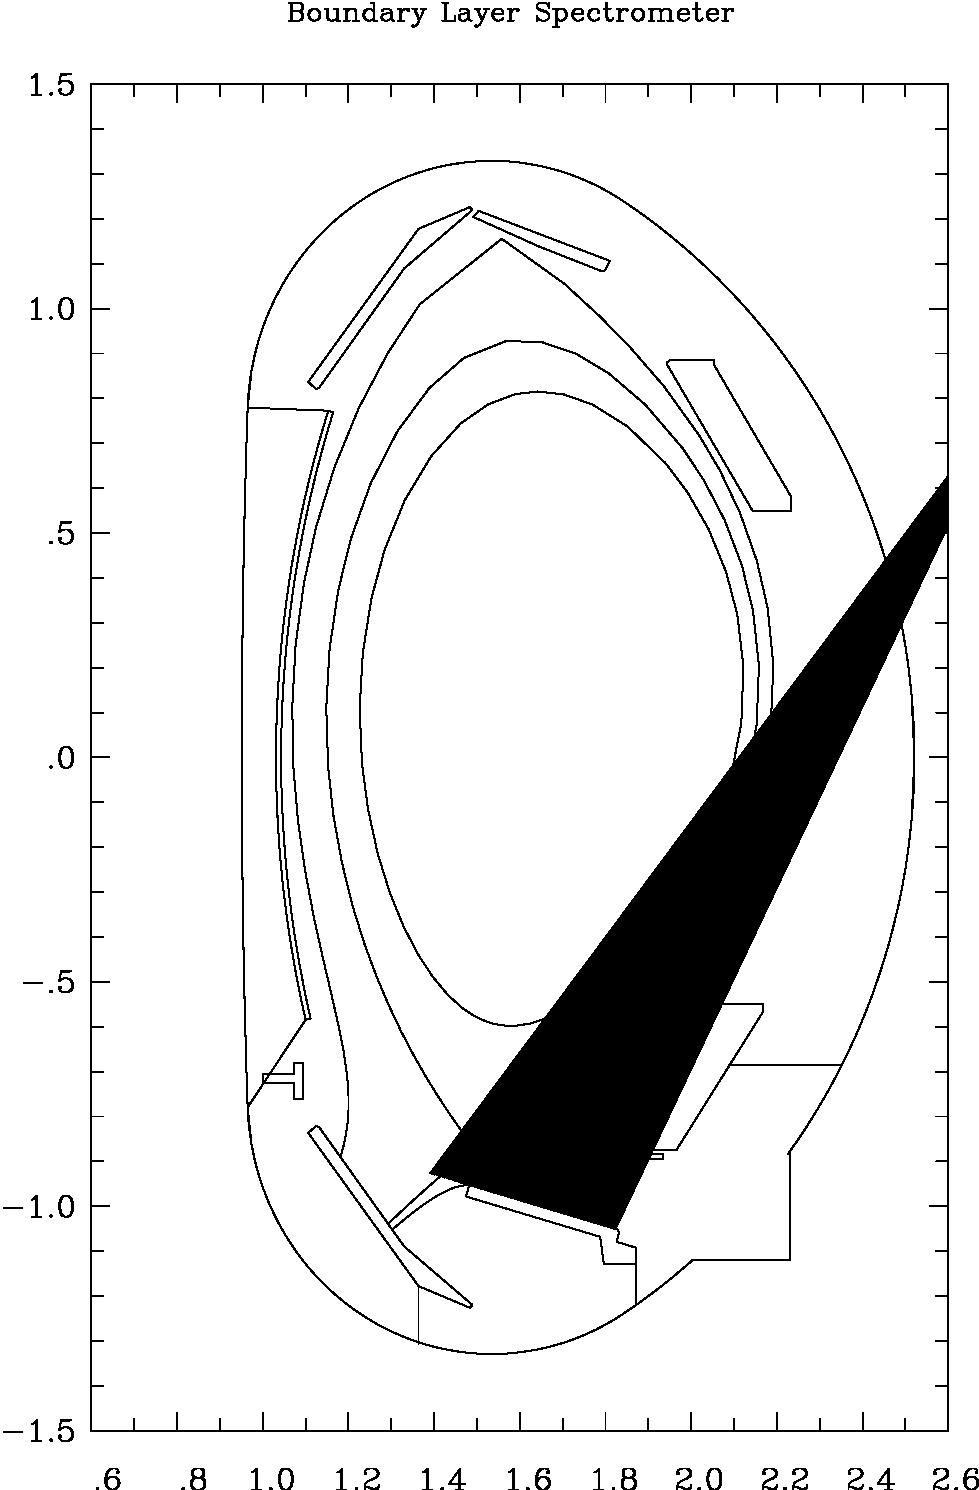
\includegraphics[height=6cm]{BLS_chords.pdf}}
  \subfigure[BOL.chords]{\label{fig:BOL}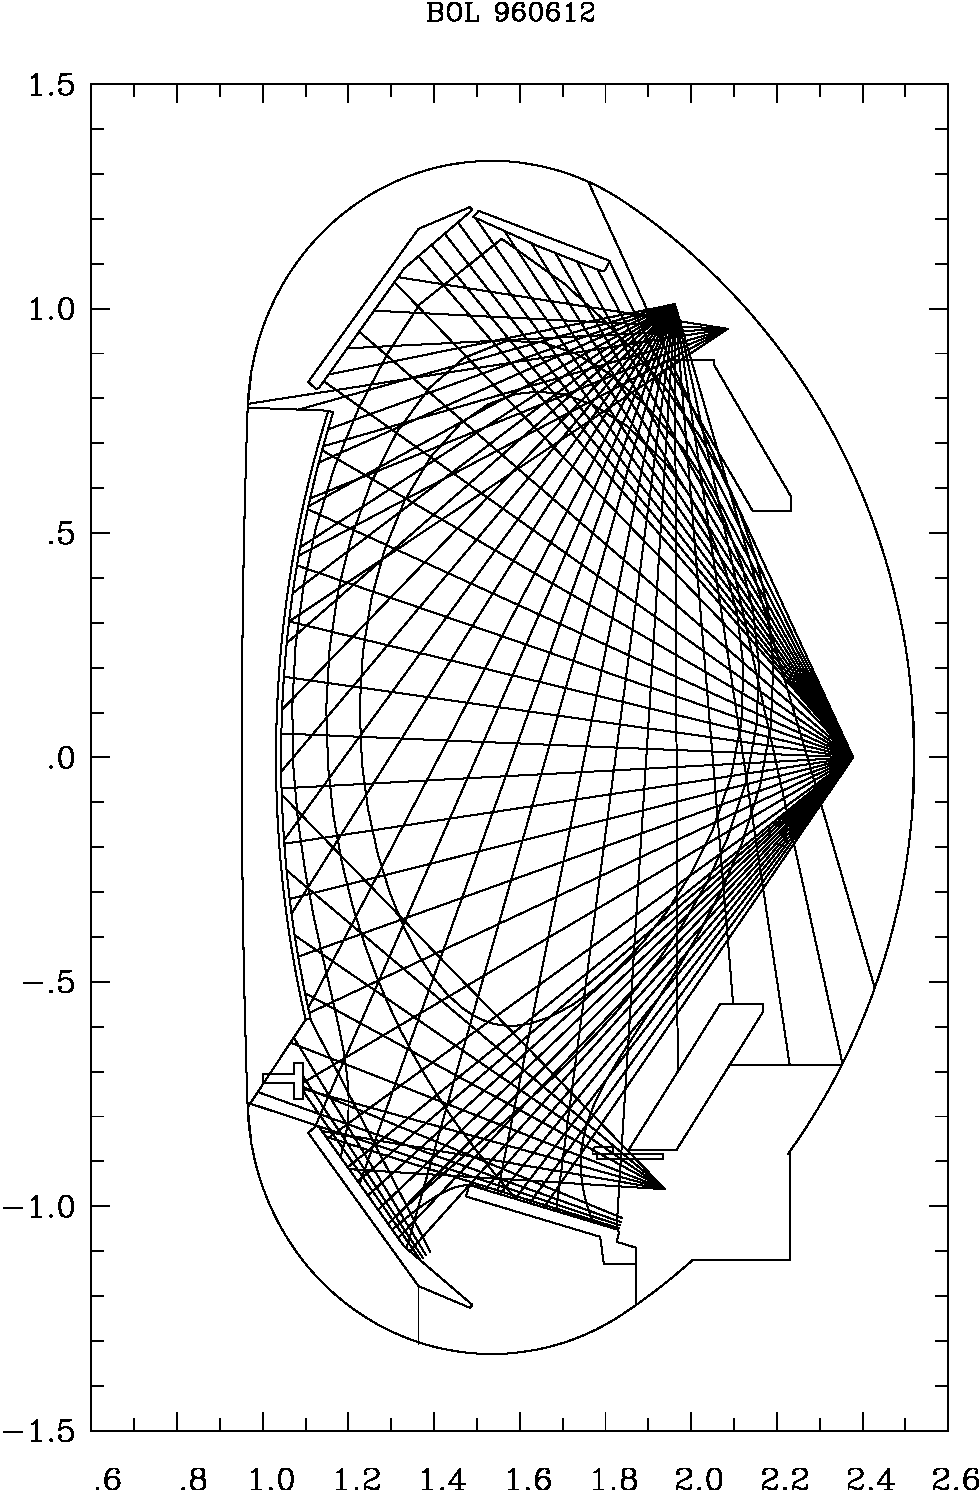
\includegraphics[height=6cm]{BOL_chords.pdf}}
  \subfigure[DCN.chords]{\label{fig:DCN}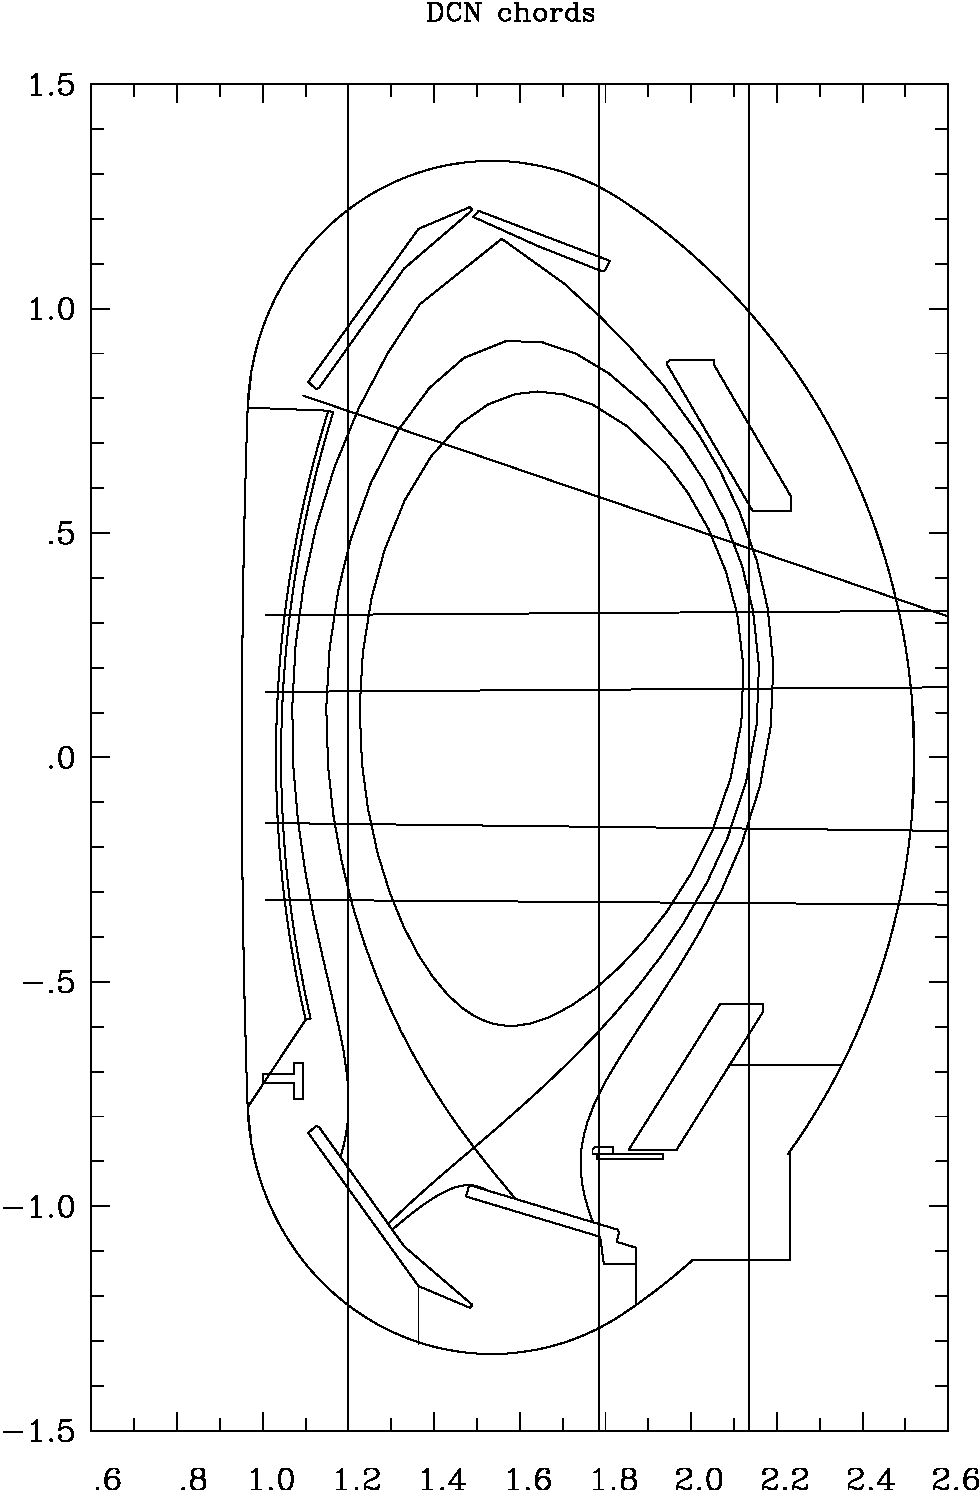
\includegraphics[height=6cm]{DCN_chords.pdf}}
  \subfigure[DIV.chords]{\label{fig:DIV}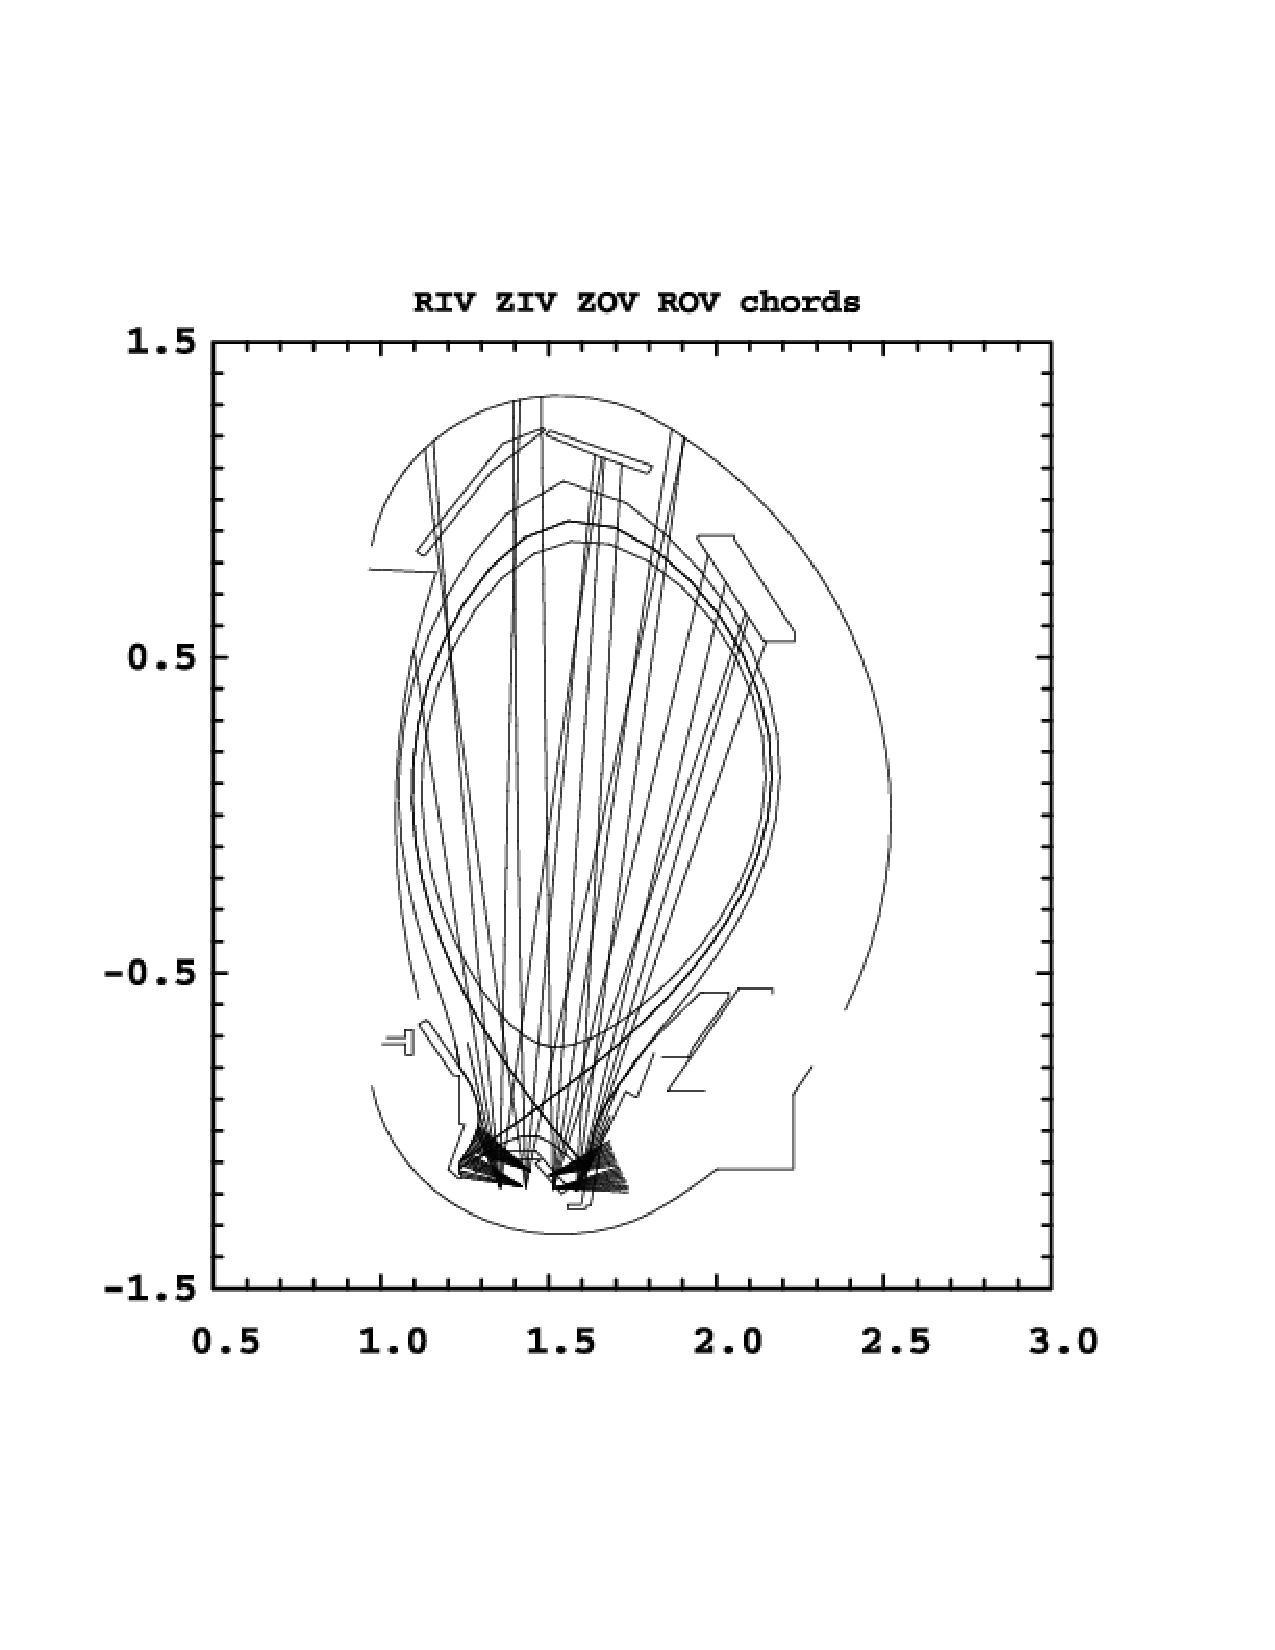
\includegraphics[height=6cm]{DIV_chords.pdf}}
\else
  \subfigure[BLS.chords]{\label{fig:BLS}\includegraphics[height=6cm]{BLS.chords.epsi}}
  \subfigure[BOL.chords]{\label{fig:BOL}\includegraphics[height=6cm]{BOL.chords.epsi}}
  \subfigure[DCN.chords]{\label{fig:DCN}\includegraphics[height=6cm]{DCN.chords.epsi}}
  \subfigure[DIV.chords]{\label{fig:DIV}\includegraphics[height=6cm]{DIV.chords.epsi}}
\fi
  \caption{BLS, BOL, DCN and DIV chords.}
\end{figure}

\begin{figure}[hbtp]
  \centering
\ifpdf 
  \subfigure[HAL.chords]{\label{fig:HAL}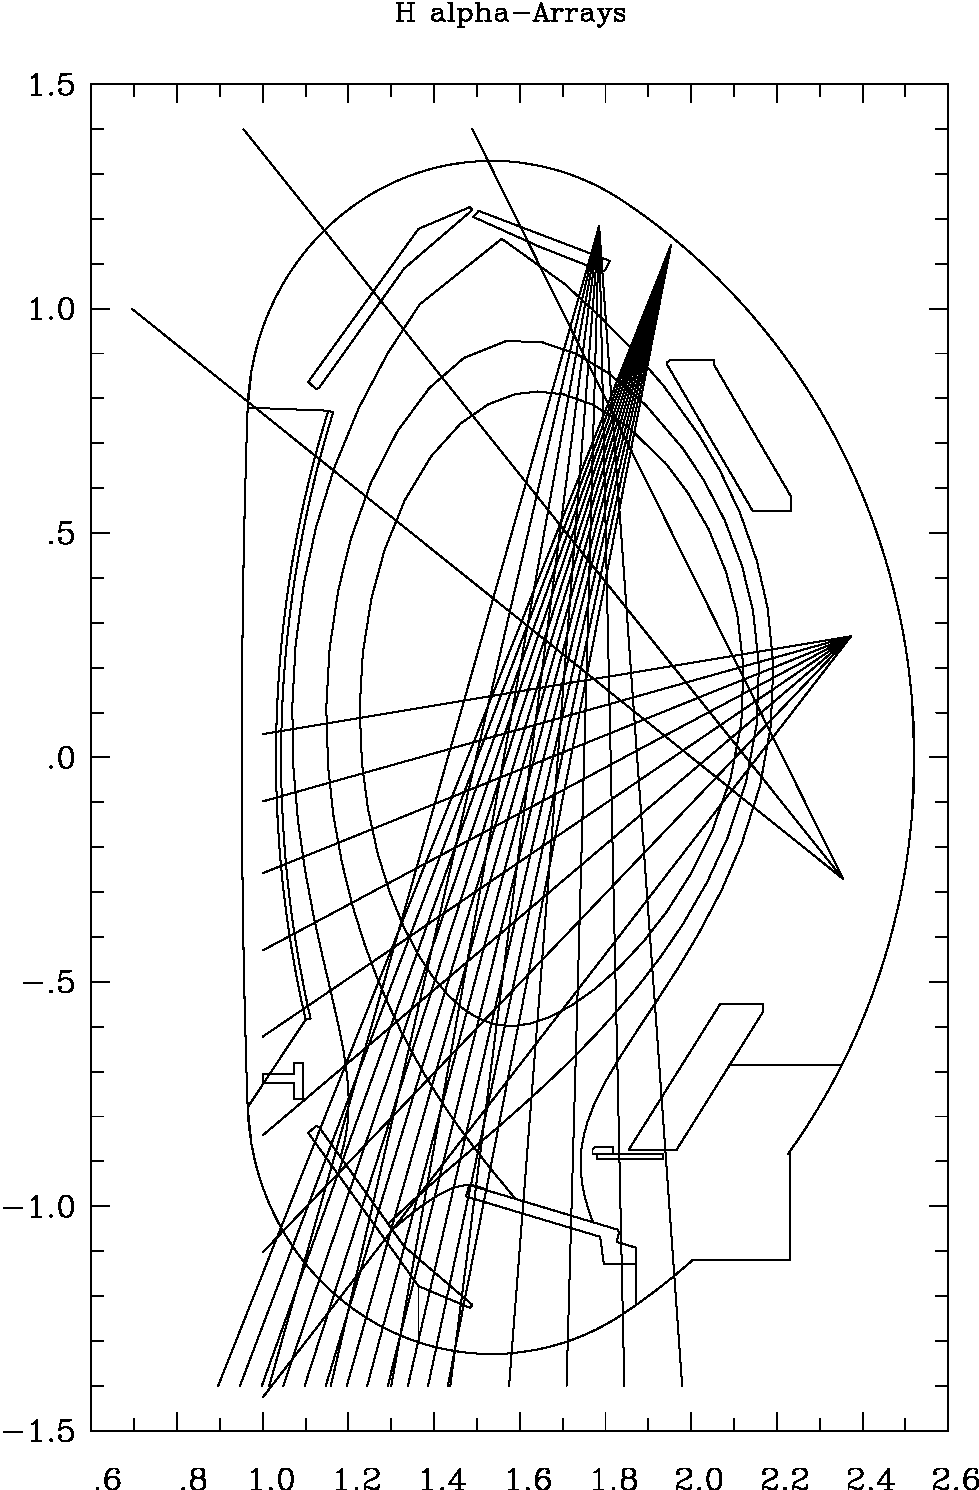
\includegraphics[height=7cm]{HAL_chords.pdf}}
  \subfigure[HAL\_13.chords]{\label{fig:HAL_13}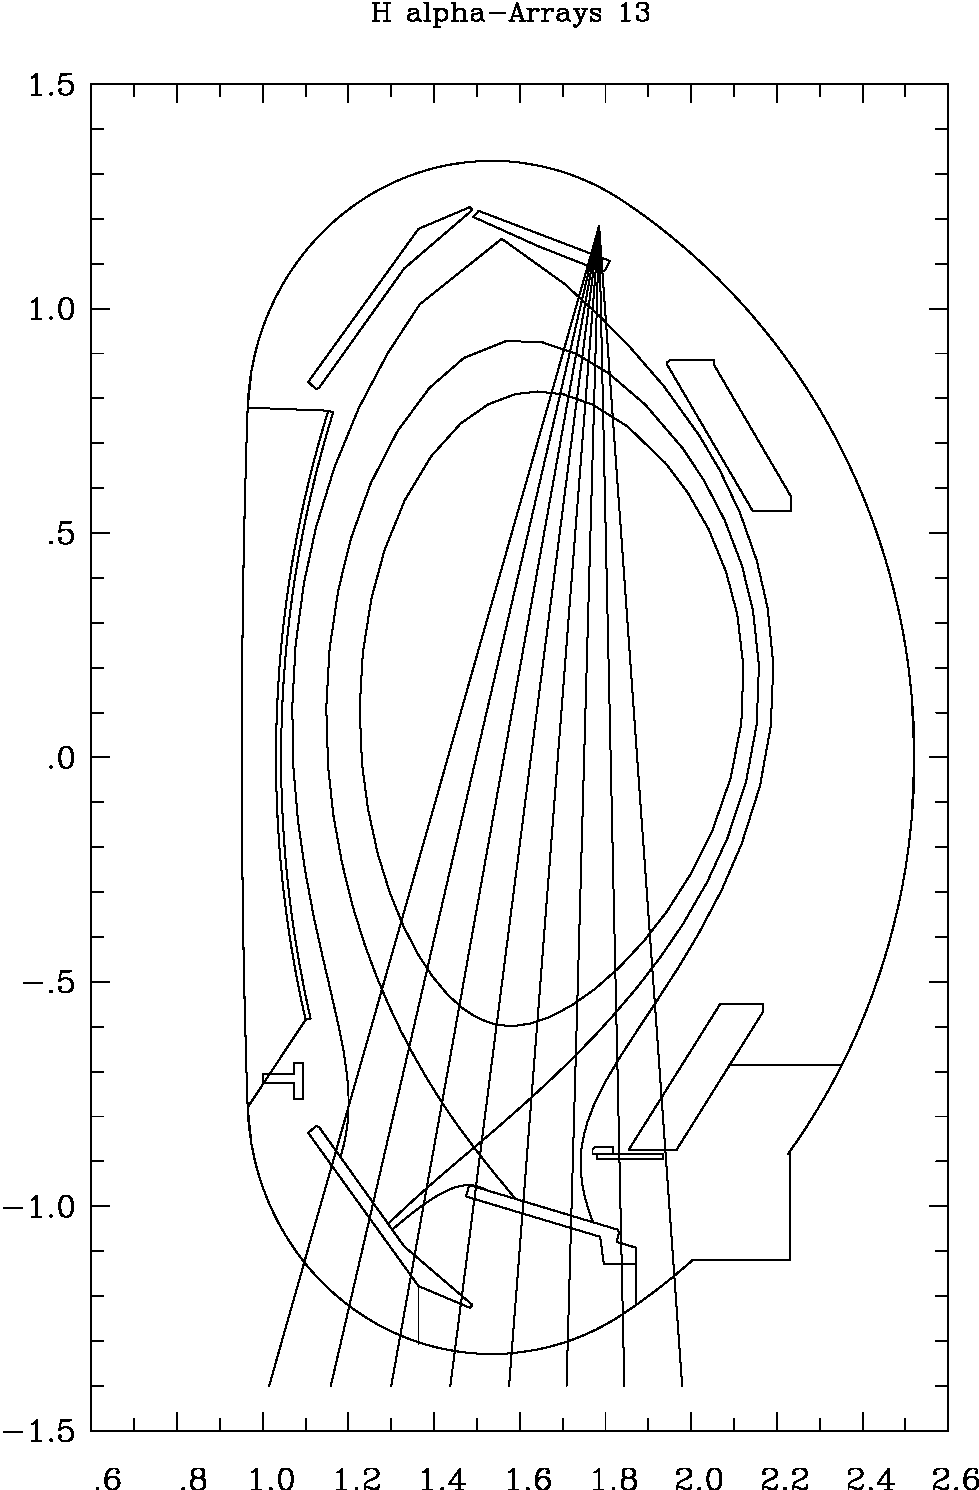
\includegraphics[height=7cm]{HAL_13_chords.pdf}}
  \subfigure[HAL\_6Bo.chords]{\label{fig:HAL_6Bo}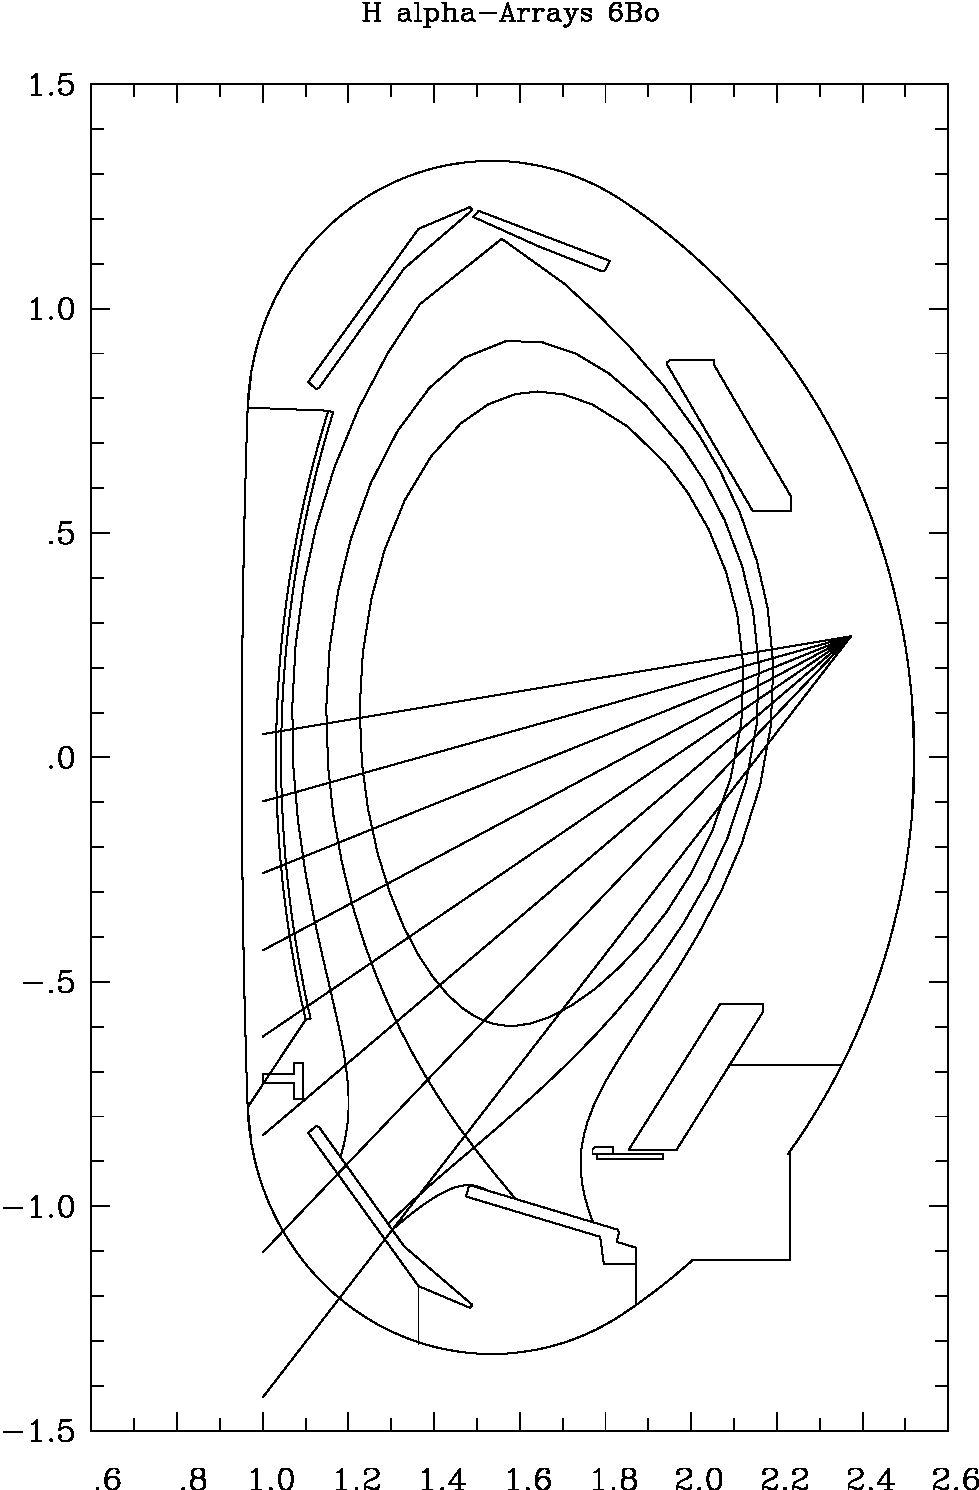
\includegraphics[height=7cm]{HAL_6Bo_chords.pdf}}
  \subfigure[HAL\_6Bu.chords]{\label{fig:HAL_6Bu}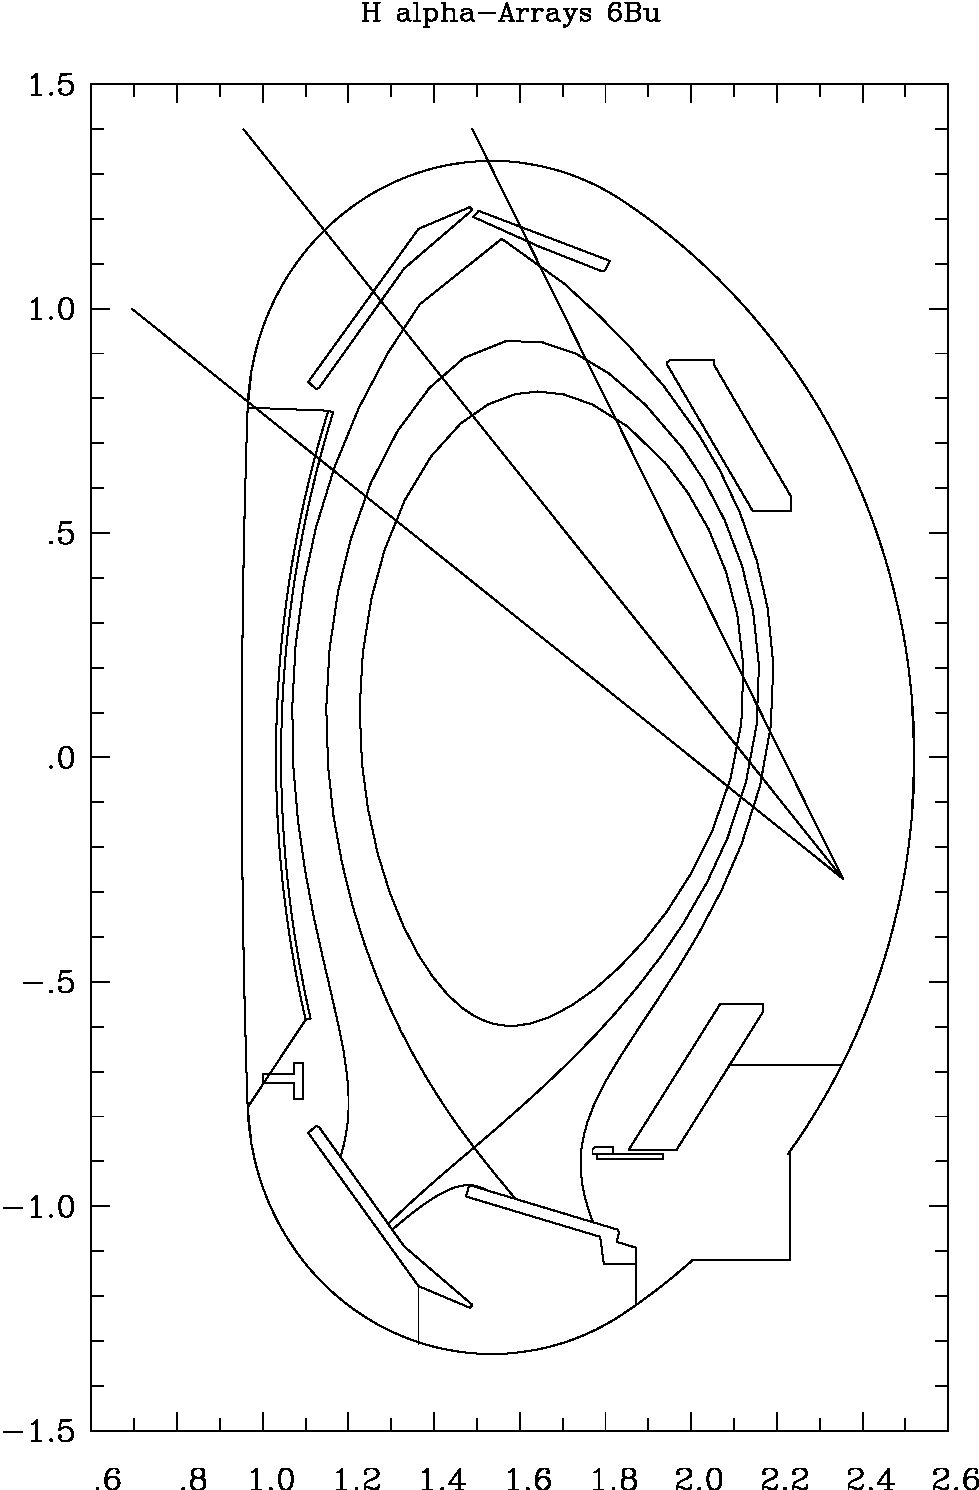
\includegraphics[height=7cm]{HAL_6Bu_chords.pdf}}
  \subfigure[HAL\_8Co.chords]{\label{fig:HAL_8Co}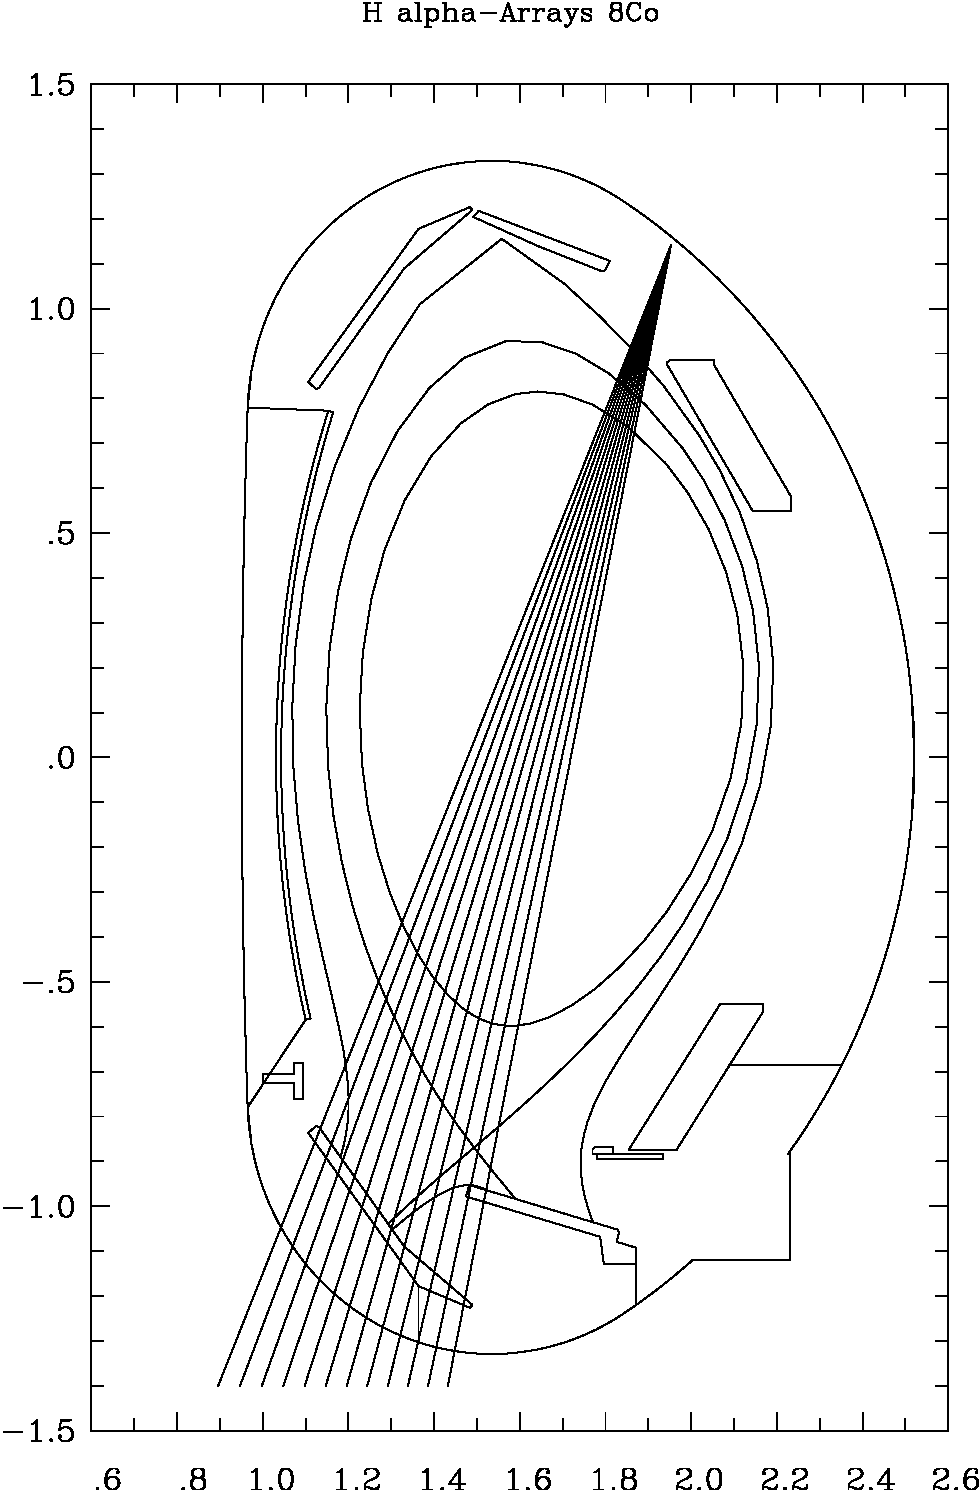
\includegraphics[height=7cm]{HAL_8Co_chords.pdf}}
\else
  \subfigure[HAL.chords]{\label{fig:HAL}\includegraphics[height=7cm]{HAL.chords.epsi}}
  \subfigure[HAL\_13.chords]{\label{fig:HAL_13}\includegraphics[height=7cm]{HAL_13.chords.epsi}}
  \subfigure[HAL\_6Bo.chords]{\label{fig:HAL_6Bo}\includegraphics[height=7cm]{HAL_6Bo.chords.epsi}}
  \subfigure[HAL\_6Bu.chords]{\label{fig:HAL_6Bu}\includegraphics[height=7cm]{HAL_6Bu.chords.epsi}}
  \subfigure[HAL\_8Co.chords]{\label{fig:HAL_8Co}\includegraphics[height=7cm]{HAL_8Co.chords.epsi}}
\fi
  \caption{HAL chords.}
\end{figure}

\subsection{$<$command file$>$ cmd}\index{b2plot, cmd}\label{sec:cmd}
Further commands are taken from the specified file.  If the file does
not exist in the current working directory, the directories
\$\verb!SOLPSTOP/data.local/commands! and
\$\verb!SOLPSTOP/scripts/commands! are searched in order.

\subsection{$<$CDF command file$>$ cmdcdf}\index{b2plot, cmdcdf}\label{sec:cmdcdf}
\verb!CDF! commands used repetitively (for movie frames) are taken from the specified file.  
If the file does not exist in the current working directory, the directories
\$\verb!SOLPSTOP/data.local/commands! and
\$\verb!SOLPSTOP/scripts/commands! are searched in order.

\subsection{$<$chord file$>$ chbx}\index{b2plot, chbx}\label{sec:chbx}
Chord integral averaged over three chords. Equivalent to using the {\bf 3 ave} command.

\subsection{$<$position file$>$ chvl}\index{b2plot, chvl}\label{sec:chvl}
The value is plotted at the specified positions.

\subsection{$<$flux info$>$ flux}\index{b2plot, flux}\label{sec:flux}
Needs to be compiled with \verb!-DWOS!.  String should contain shot number,
time within the shot, and the diagnostic name.  Then causes the
equilibrium for this shot to overlay subsequent plots.

\subsection{$<$chord file$>$ chmp}\index{b2plot, chmp}\label{sec:chmp}
Plots a contour plot of the chord contribution to the mesh element.

\subsection{$<$chord file$>$ cam}\index{b2plot, cam}\label{sec:cam}
Camera plot.  The chord file needs to contain some additional
information on the first line.

\subsection{$<$CDF file name$>$ movi}\index{b2plot, movi}\label{sec:movi}
Used for specifying the \verb!CDF! file if a movie is to be made.

\subsection{$<$istart,{\bf I}$>$ $<$iend,{\bf I}$>$ $<$varname, {\bf S}$>$ movie}\index{b2plot, movie}\label{sec:movie}
Creates a movie for timeslice $<$istart$>$ to time slice $<$iend$>$ of variable $<$varname$>$. The
list of available quantities in given in Appendix \ref{cha:b2time}. The time interval between frames can be
controlled with the {\bf mvsk} command.
{\bf nmovie} is an alias for {\bf movie}.

\subsection{$<$istart,{\bf I}$>$ $<$iend,{\bf I}$>$ $<$filename, {\bf S}$>$ $<$varname, {\bf S}$>$ omovie}\index{b2plot, omovie}\label{sec:omovie}
Creates a movie for timeslice $<$istart$>$ to time slice $<$iend$>$ of variable $<$varname$>$ read
from file $<$filename$>$. 

\subsection{$<$sonnetfile$>$ sonn}\index{b2plot, sonn}\label{sec:sonn}
Reads in a new \verb!Sonnet! geometry file.

\subsection{$<$output\_sonnet file$>$ oson}\index{b2plot, oson}\label{sec:oson}
Outputs the geometry in \verb!Sonnet! \verb!ASCII! format.

\subsection{$<$z$_{shift}$,{\bf R}$>$ $<$UEDGE grid file$>$ uedgegrd}\index{b2plot, uedgegrd}\label{sec:uedgegrd}
Outputs the geometry in \verb!UEDGE! ASCII format. The grid can be shifted in the vertical
direction by an amount of $<$z$_{shift}>$ meters.

\subsection{$<$filename$>$ $<$H123$>$ $<$reac$>$ $<$crc$>$ amju}\index{b2plot, amju}\label{sec:amju}
Computes a reaction rate as per the \verb!Eirene! specification. Consult the
\verb!Eirene! manual for details.
{\bf amjuel} is an alias for {\bf amju}.

\subsection{$<$reac$>$ adas}\index{b2plot, adas}\label{sec:adas}\index{ADAS}
Computes a reaction rate as per the \verb!ADAS! specification. The $<$reac$>$ string should be something of the
form 'acd89'. The matrix obtained contains then all the rates from these files, for all species in the run, extracted
from the files stored in \$\verb!SOLPSTOP/modules/adas! or \$\verb!SOLPSTOP/data.local/adas!.

\section{Environment variables}

\begin{description}
\item[B2PLOT\_DEV] is used to specify plotting to any combination of
  ``x11'', ``ps'' or ``cgm'' (default is ``ps'').  Under \verb!tcsh!, use 
  \begin{verbatim}
setenv B2PLOT_DEV 'x11 ps'
  \end{verbatim}
\item[SOLPSTOP] used to specify the top of the \verb!SOLPS! tree.
\end{description}

Environment variables can also be used in the {\bf extl} command
(see \ref{sec:extl}). If not explicitly set by the user, they inherit 
their value from the \verb!setup.csh.*! files in the \$\verb!SOLPSTOP!
directory.

\section{Examples}

Some simple (and not so simple) examples of plots that can be obtained with
\btwoplot commands are shown in the next section.

\subsection{Mesh plot}
\index{b2plot, mesh plot}

Here (figure \ref{fig:mesh}) we have two plots of the computational and physical grids, captioned with
the commands used to obtain them. 

\begin{figure}[hbtp]
  \centering
\ifpdf 
  \subfigure[comp a4p mesh]{\label{fig:comp}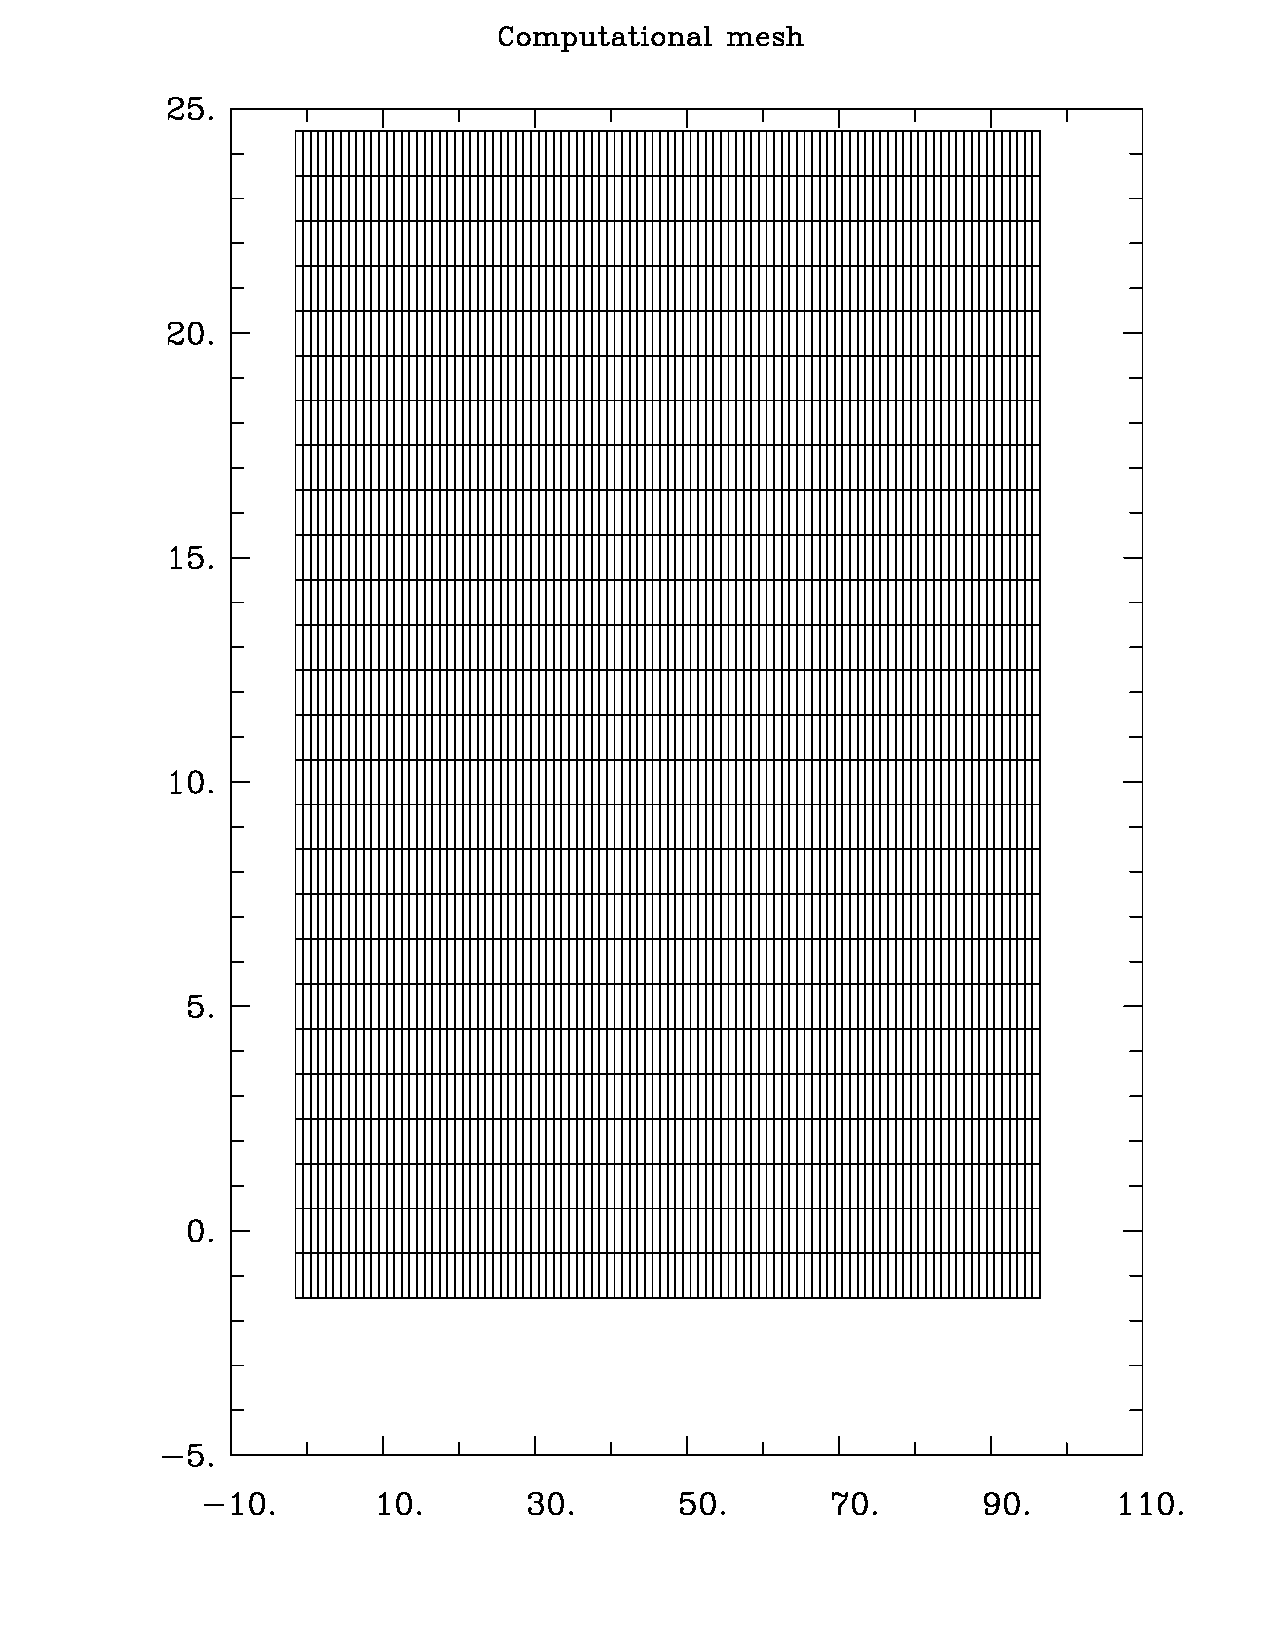
\includegraphics[height=6cm]{comp.pdf}}
  \subfigure[phys a4p mesh]{\label{fig:phys}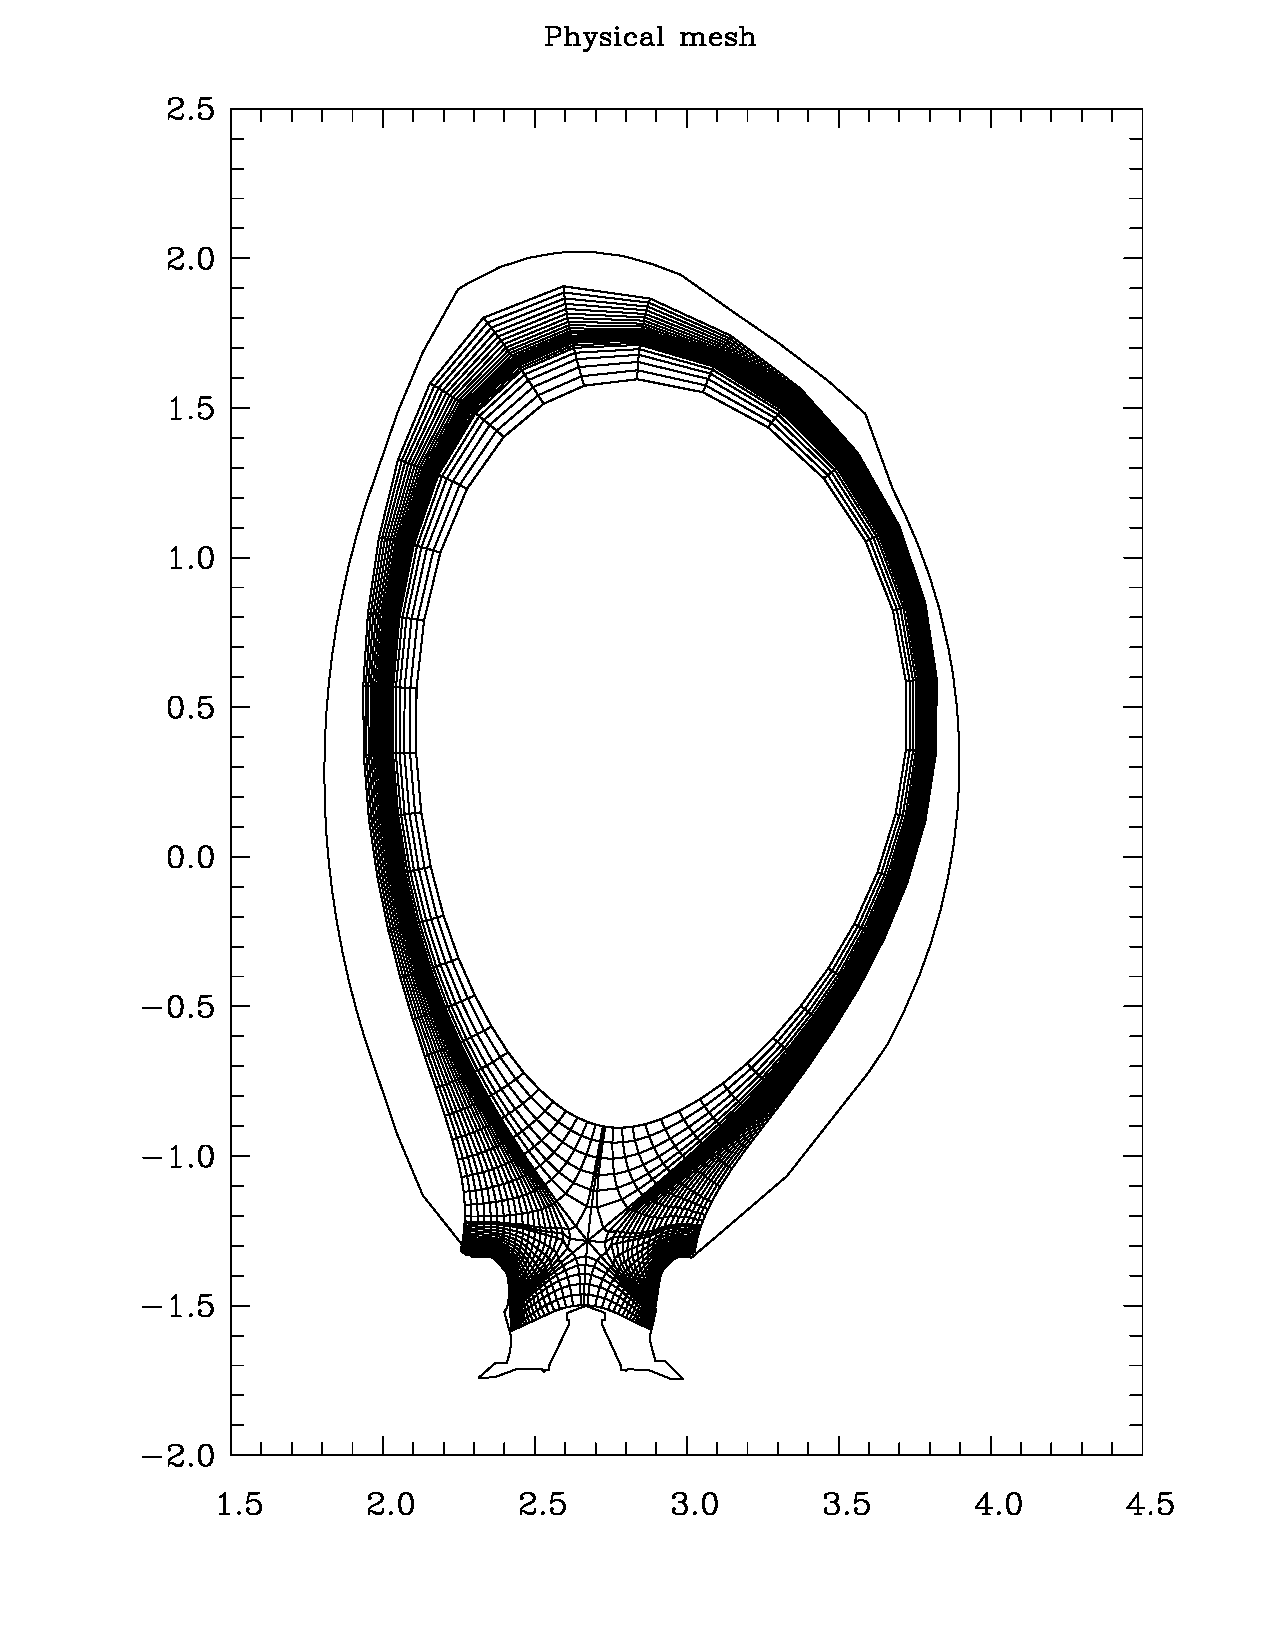
\includegraphics[height=6cm]{phys.pdf}}
\else
  \subfigure[comp a4p mesh]{\label{fig:comp}
\includegraphics[height=6cm]{comp.epsi}}
  \subfigure[phys a4p mesh]{\label{fig:phys}
\includegraphics[height=6cm]{phys.epsi}}
\fi
  \caption{Mesh plots.}
  \label{fig:mesh}
\end{figure}

\subsection{Plotting plasma solution data}
\index{b2plot, plotting plasma quantities}

Data from the plasma solution, stored on the ``matrix'' stack, can be visualized as per figure \ref{fig:te}.

\begin{figure}[hbtp]
  \centering
\ifpdf 
  \subfigure[comp a4p te surf]{\label{fig:tecomp}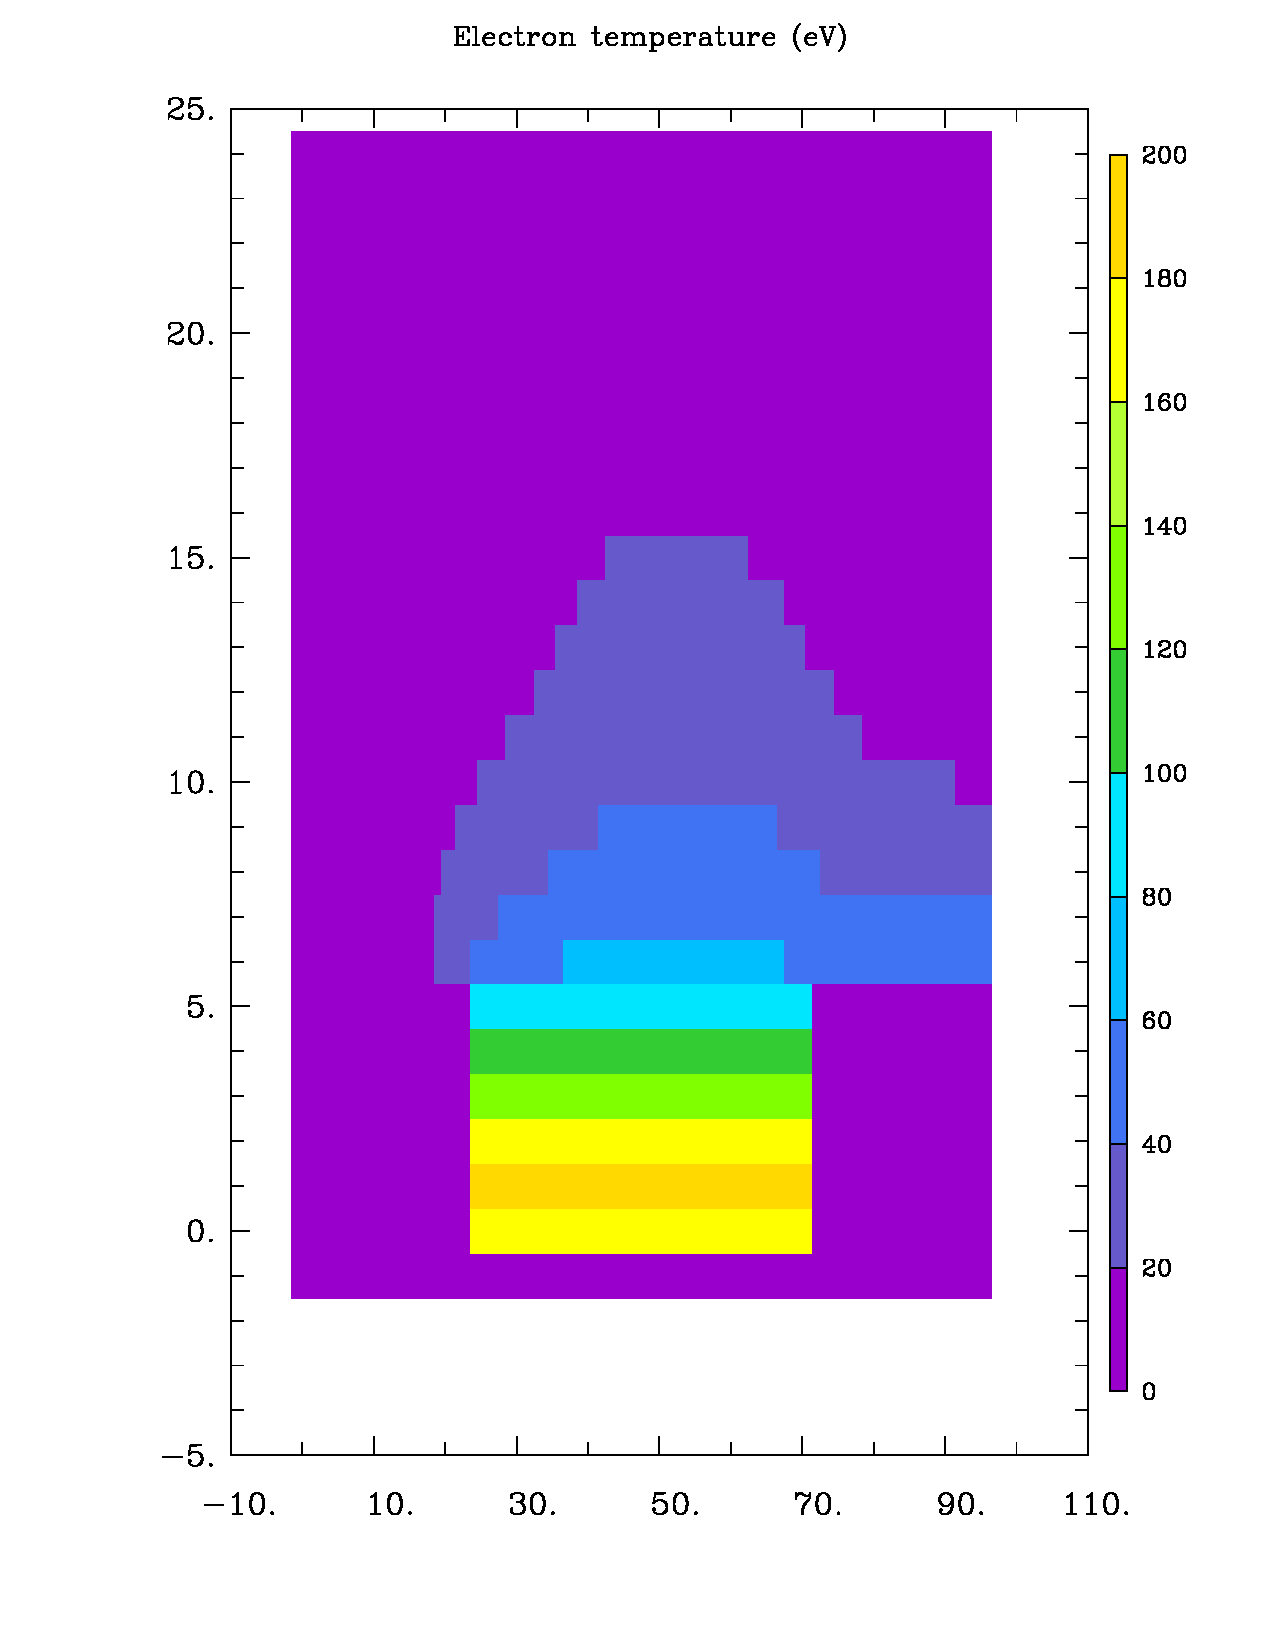
\includegraphics[height=6cm]{Te_comp.pdf}}
  \subfigure[phys a4p -2.2 zmin 2.2 zmax 2.0 lbsz sep outl vesl logf 3 ndec te surf]{\label{fig:tephys}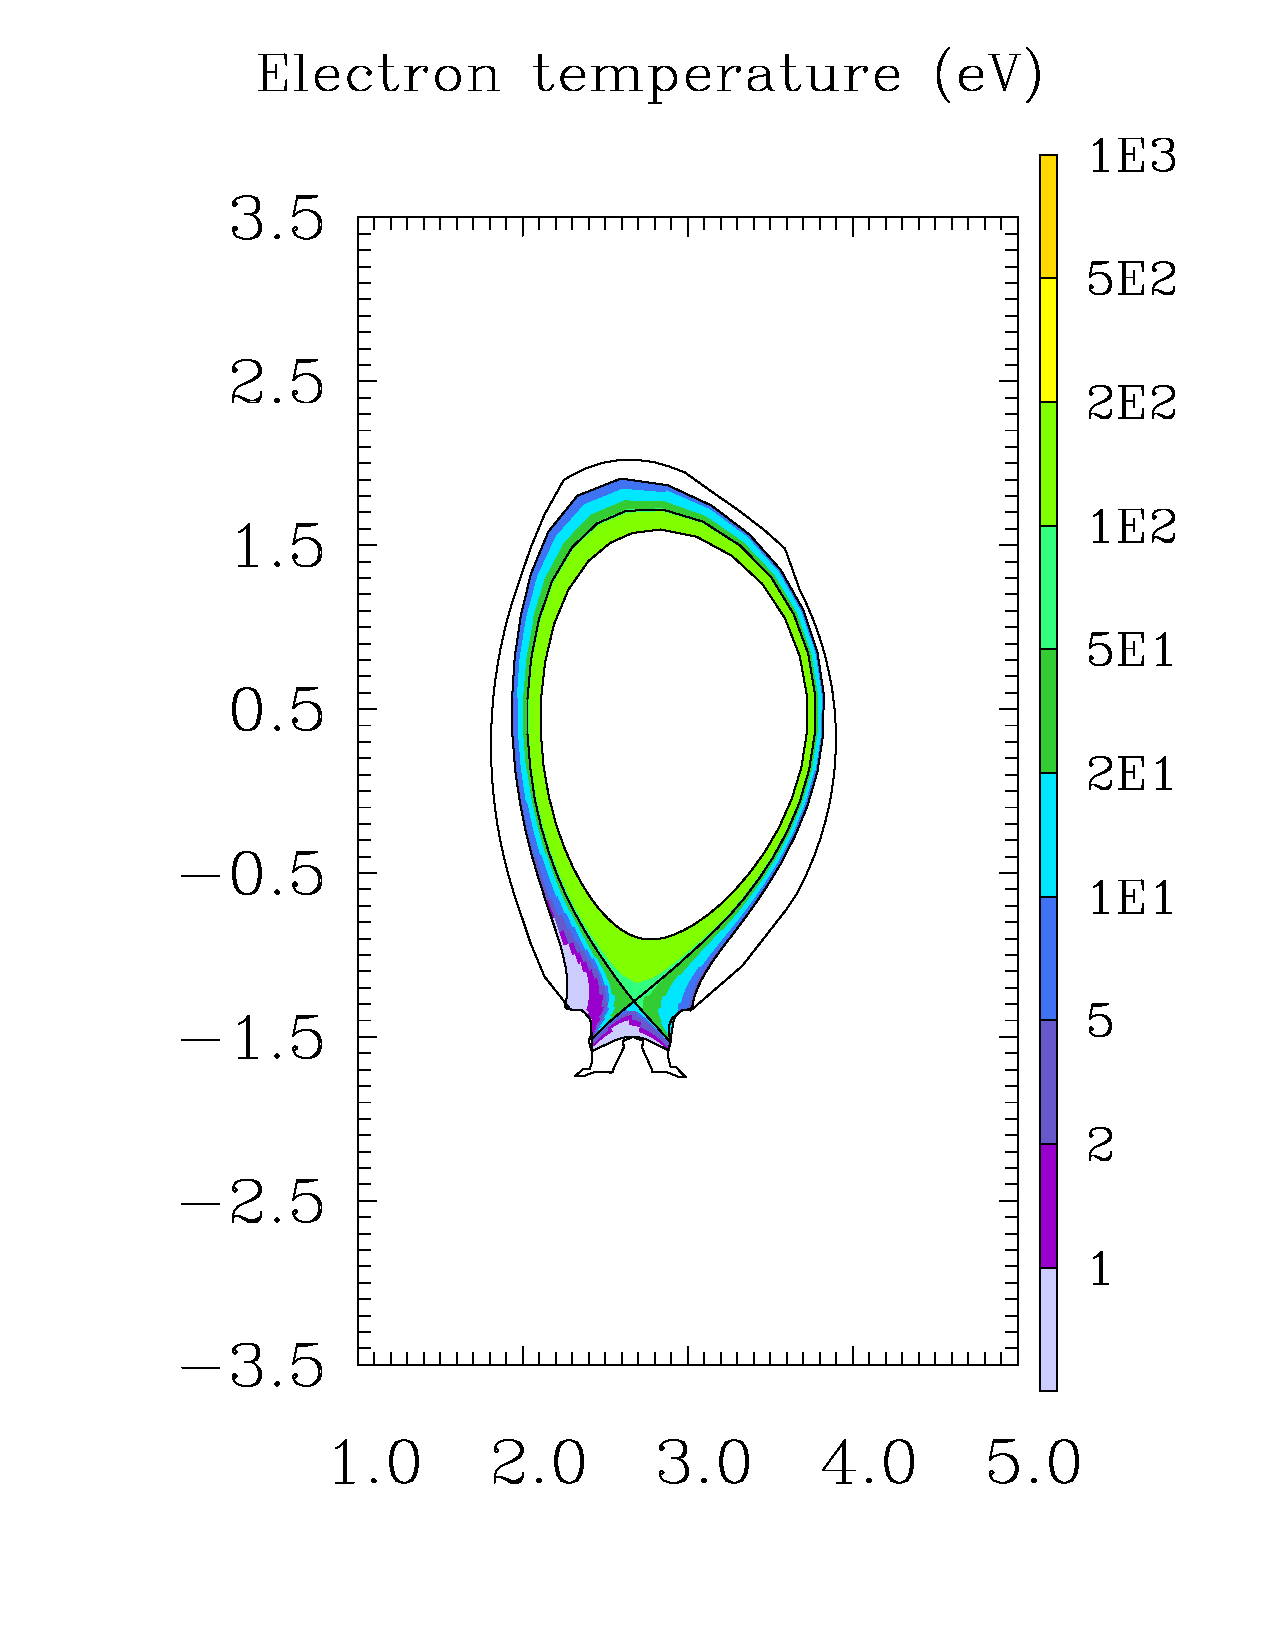
\includegraphics[height=6cm]{Te_phys.pdf}}
\else
  \subfigure[comp a4p te surf]{\label{fig:tecomp}
\includegraphics[height=6cm]{Te_comp.epsi}}
  \subfigure[phys a4p -2.2 zmin 2.2 zmax 2.0 lbsz sep outl vesl logf 3 ndec te surf]{\label{fig:tephys}
\includegraphics[height=6cm]{Te_phys.epsi}}
\fi
  \caption{Electron temperature plots.}
  \label{fig:te}
\end{figure}

Note that here the physical domain plot ({\bf phys} figure \ref{fig:tephys}) has been modified to have more readable
labels ({\bf 2.0 lbsz}), a logarithmic scale ({\bf logf}) covering 3 decades ({\bf 3 ndec}),
includes the magnetic separatrix ({\bf sep}), the plasma outline ({\bf outl}), the vacuum
vessel ({\bf vesl}), and has an extended vertical range ({\bf -2.2 zmin 2.2 zmax}). Note however that
the plotting program always attempts to maintain ``nice'' axis bounds and conserve the graph
aspect ration (unless {\bf aspc} is toggled).

Other examples:

\begin{figure}[hbtp]
  \centering
\ifpdf 
  \subfigure[phys a4p noax 0 nreg]{\label{fig:noax}
\includegraphics[height=6cm]{noax.pdf}}
  \subfigure[phys a4p ti te m/ surf]{\label{fig:tioverte}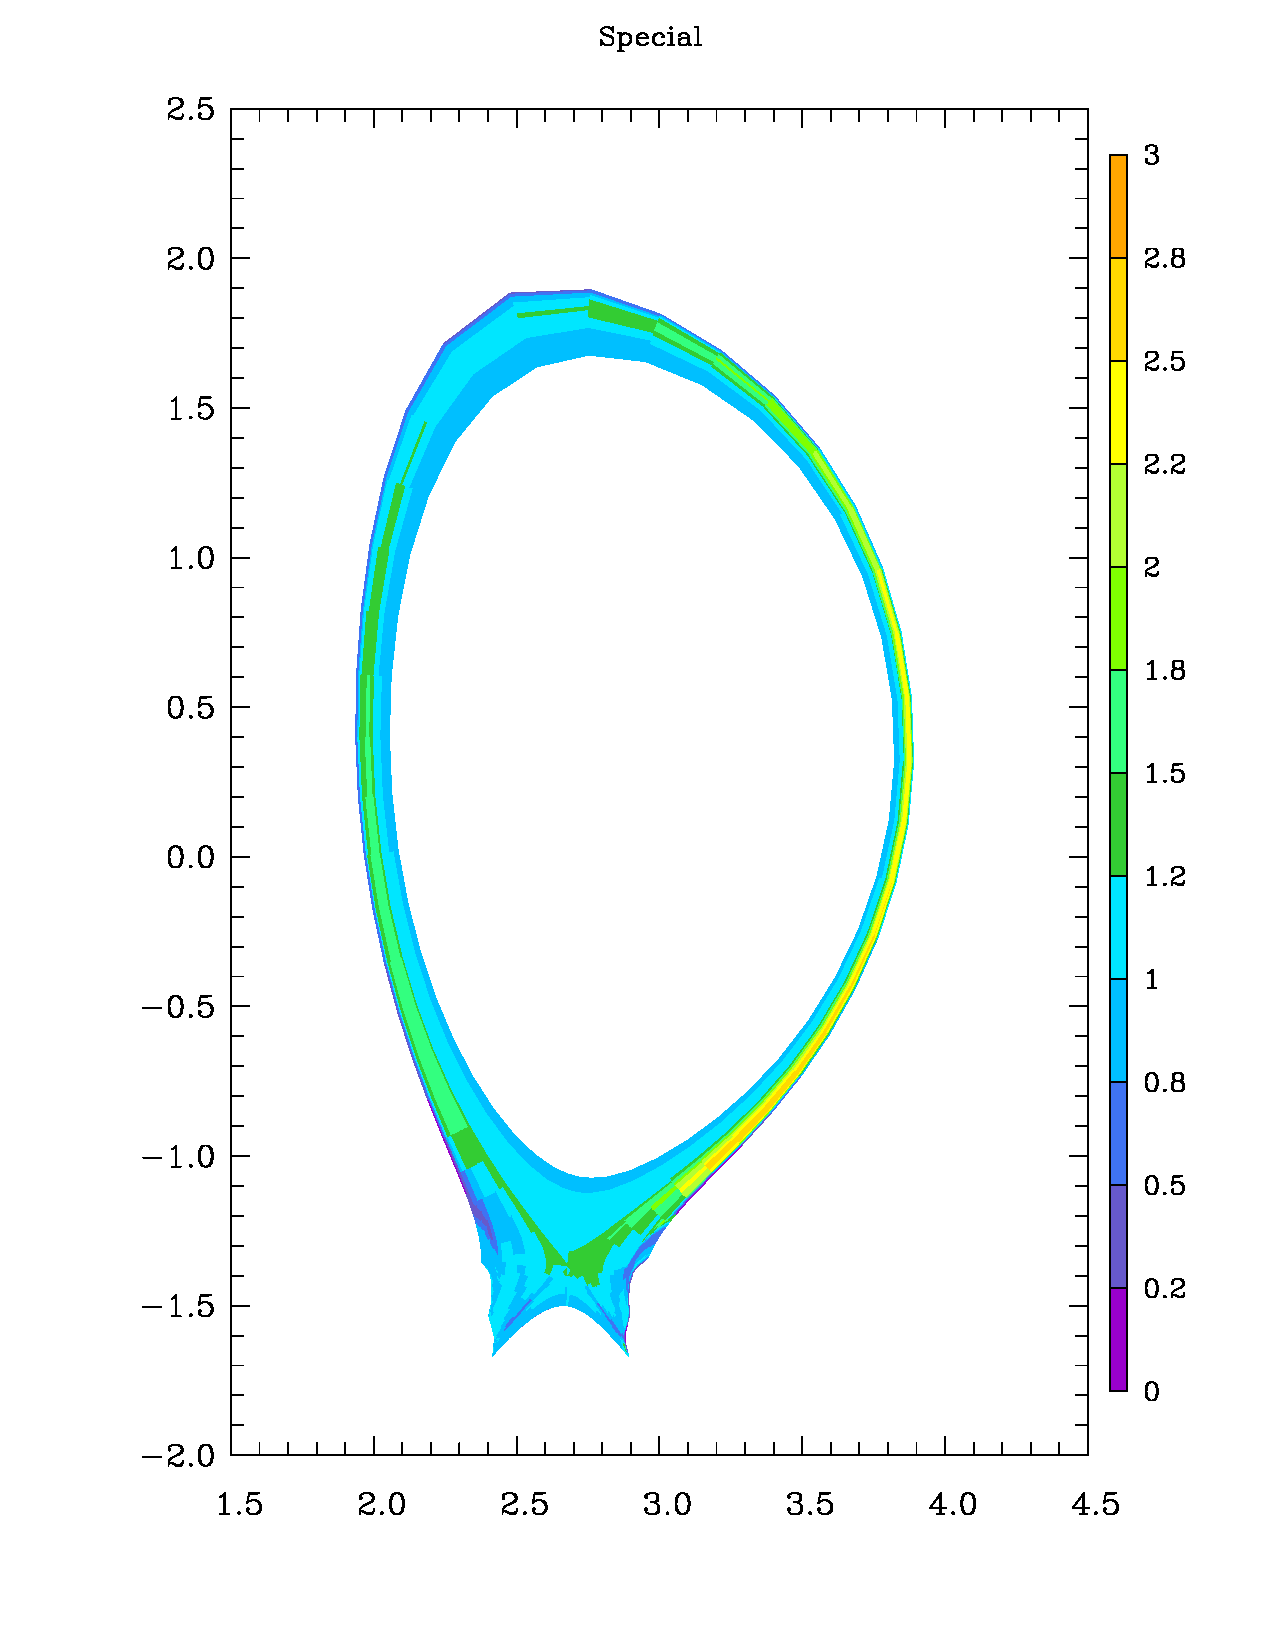
\includegraphics[height=6cm]{Ti_Te.pdf}}
\else
  \subfigure[phys a4p noax 0 nreg]{\label{fig:noax}
\includegraphics[height=6cm]{noax.epsi}}
  \subfigure[phys a4p ti te m/ surf]{\label{fig:tioverte}
\includegraphics[height=6cm]{Ti_Te.epsi}}
\fi
  \caption{Other solution data plots.}
  \label{fig:otherdata}
\end{figure}

In figure \ref{fig:tioverte}, we obtain the ratio of ion to electron 
temperature, while figure \ref{fig:noax} is a region plot (like the ones in 
Fig. \ref{fig:SN_regions}, obtained with {\bf sep vesl outl 0 nreg surf}, and 
Fig. \ref{fig:DN_regions}, obtained with {\bf sep 0 nreg surf}).

\subsection{Chord plots}
\index{b2plot, chord plots}

In figure \ref{fig:JETchords} we have an example of chord plots as applied to the KL2 diagnostic on JET.

\begin{figure}[hbtp]
  \centering
\ifpdf 
  \subfigure[a4p vesl outl sep 'JET/KL2.chords' chpl]{\label{fig:chpl}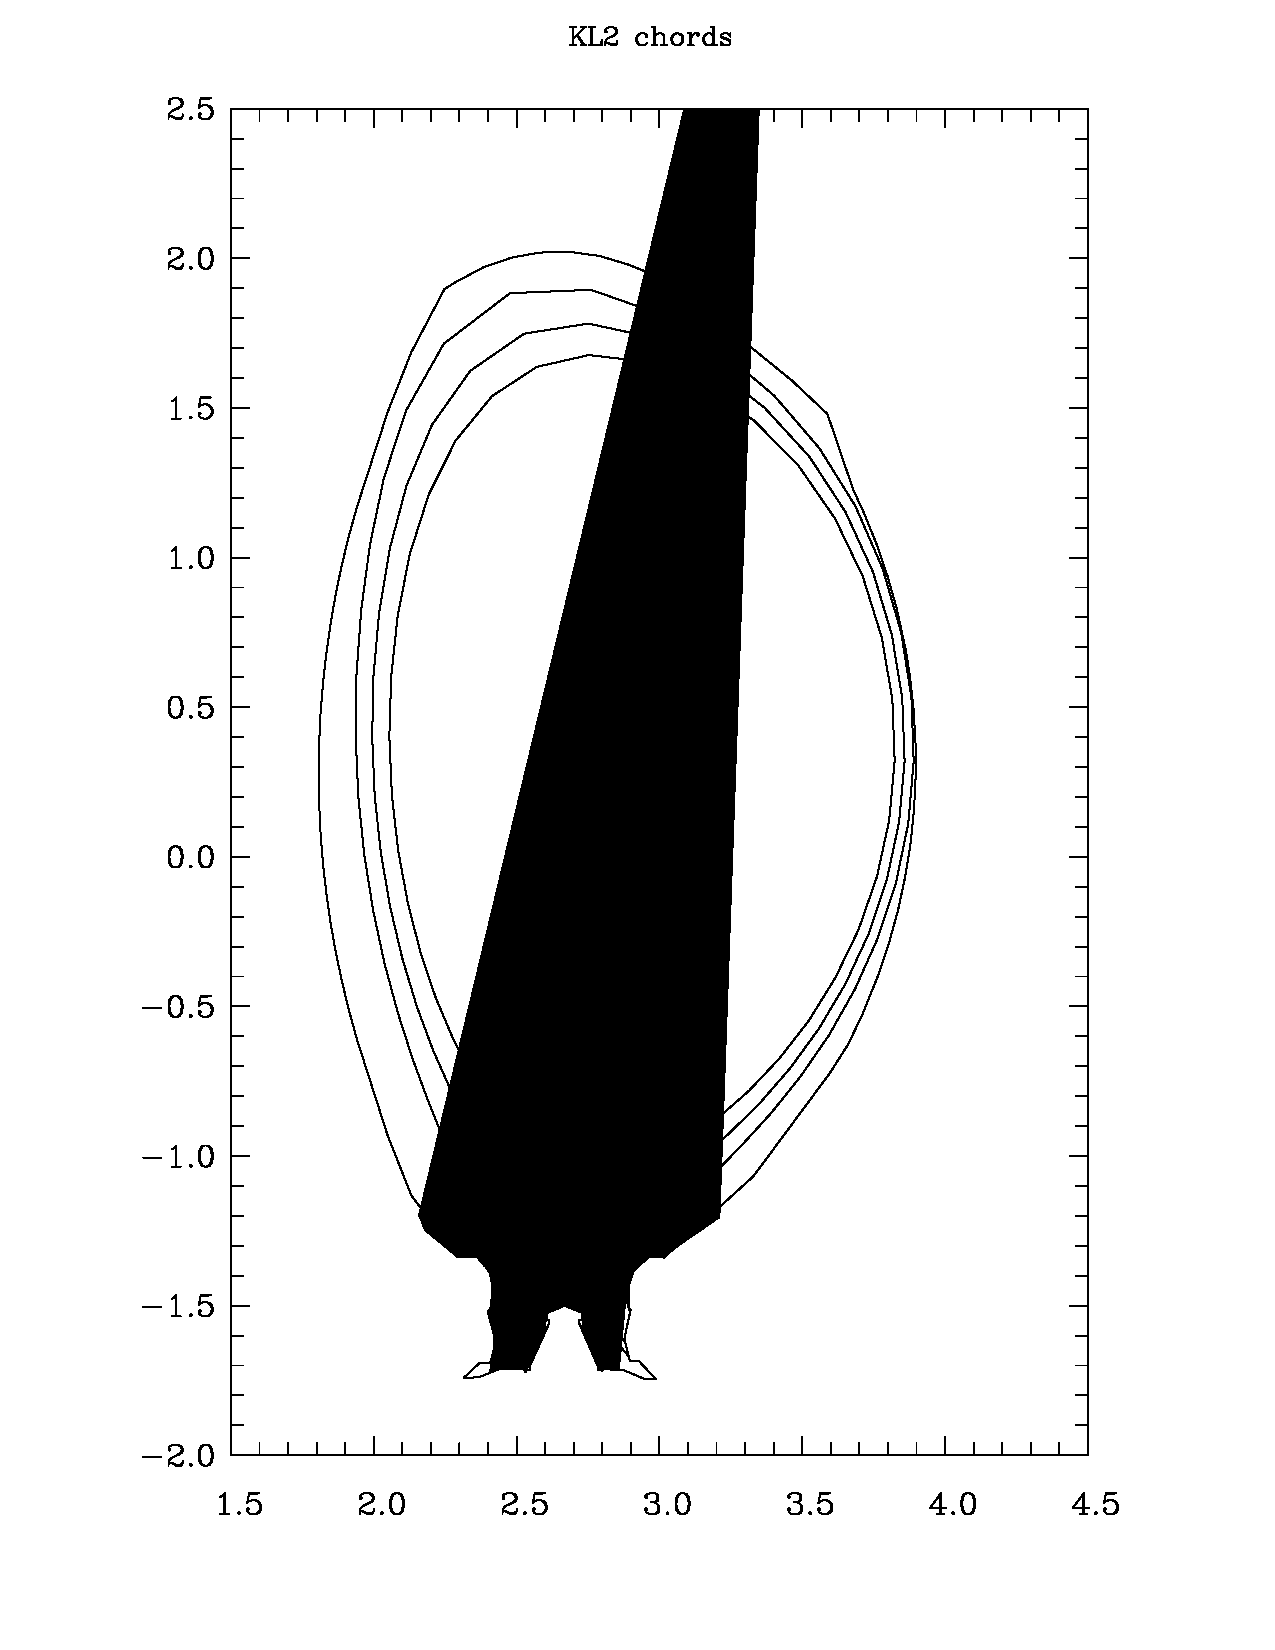
\includegraphics[height=6cm]{chpl.pdf}}
  \subfigure[a4l phys 3 6581 1 nspec '658 nm CII' extl 'JET/KL2.chords' chor]{\label{fig:chor}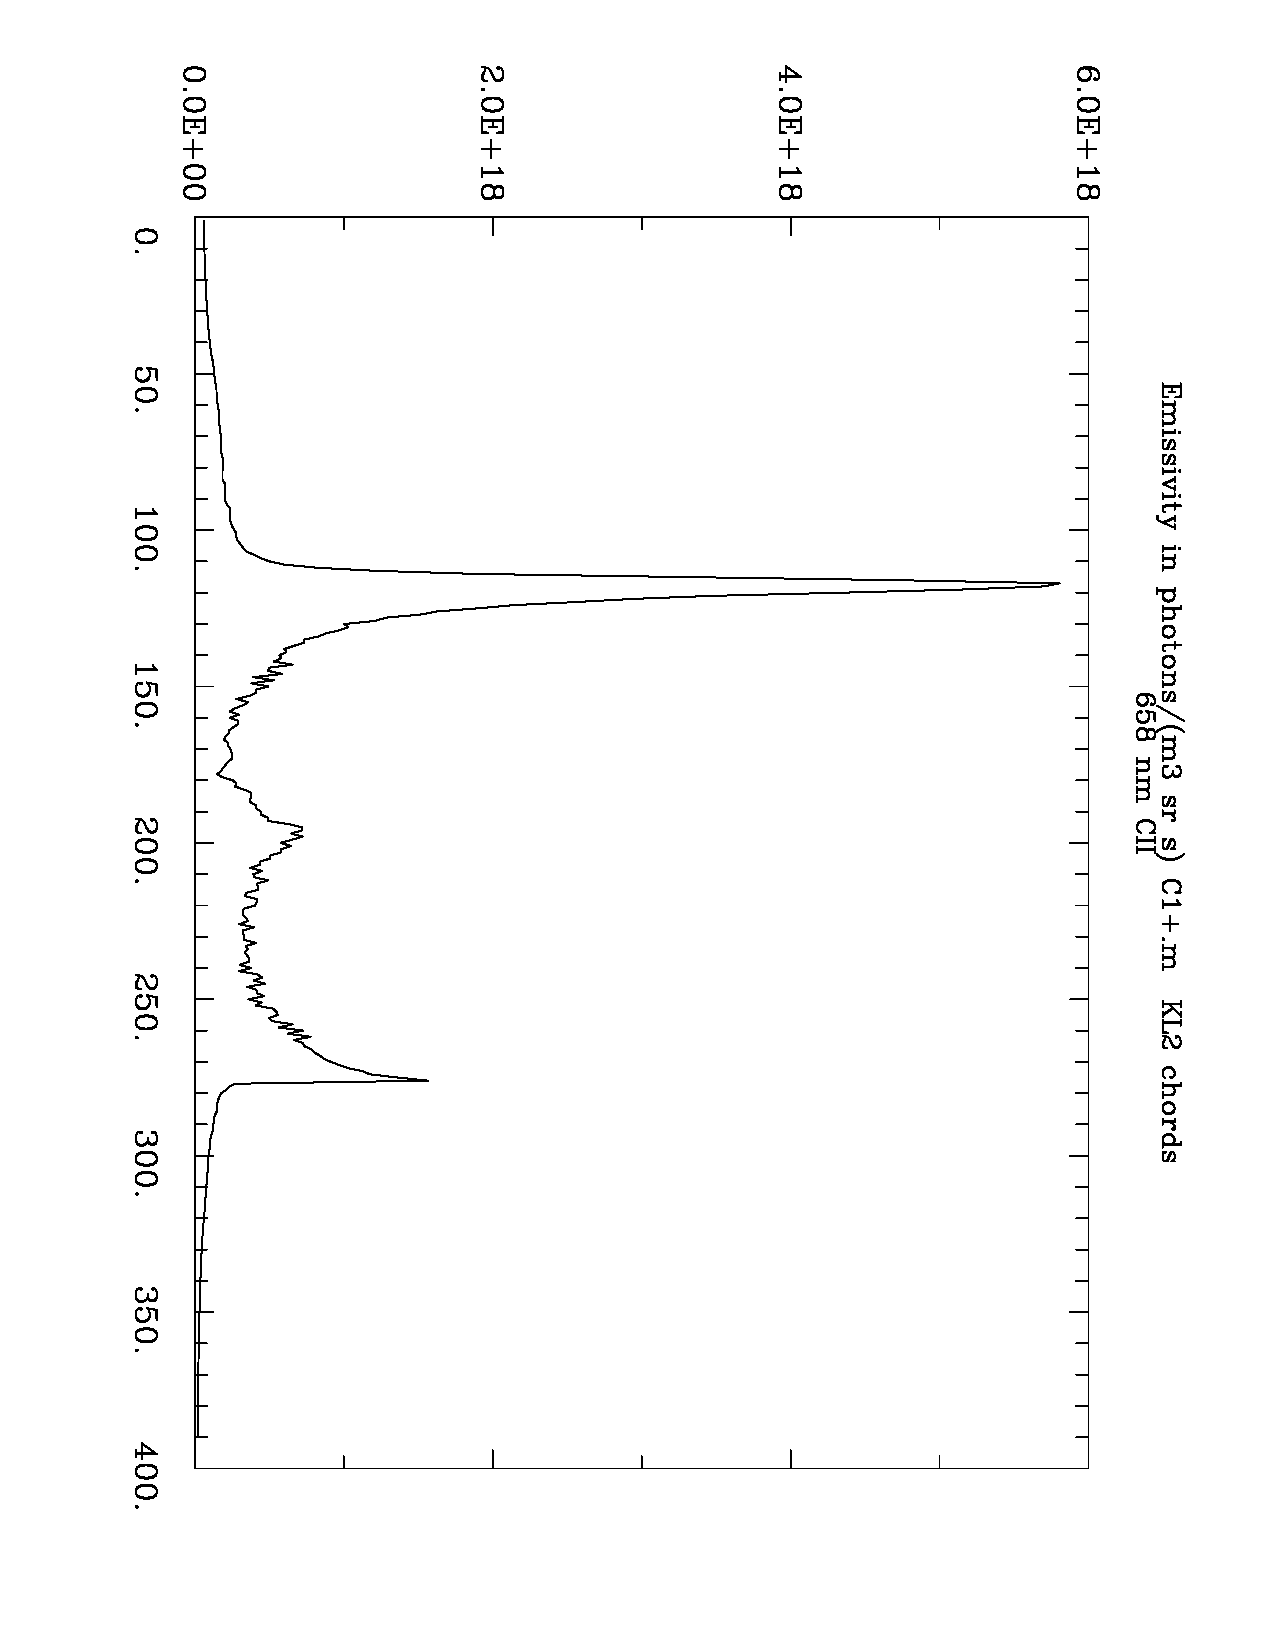
\includegraphics[angle=90,height=6cm]{chor.pdf}}
\else
  \subfigure[a4p vesl outl sep 'JET/KL2.chords' chpl]{\label{fig:chpl}
\includegraphics[height=6cm]{chpl.epsi}}
  \subfigure[a4l phys 3 6581 1 nspec '658 nm CII' extl 'JET/KL2.chords' chor]{\label{fig:chor}
\includegraphics[angle=90,height=6cm]{chor.epsi}}
\fi
  \caption{Chord plots applied to JET.}
  \label{fig:JETchords}
\end{figure}

The first {\bf chpl} plot (\ref{fig:chpl}) gives the physical position of the chords, 
as obtained from the \verb!JET/KL2.chords! file in the 
\$\verb!SOLPSTOP/data/chords! directory. The second {\bf chpl} plot (\ref{fig:chor}), 
in landscape mode {\bf a4l}, shows the emissivity of a C$^+$ line 
(species 3) at $\lambda = 6581 \pm 1$ {\em \AA} ({\bf 3 6581 1 nspec}). 
The {\bf extl} instruction gives the extra label on the second title line.  

\subsection{Wall plots}
\index{wall segments}\index{b2plot, plotting wall quantities}

In figure \ref{fig:wallplots}, we show examples of wall plots.

\begin{figure}[hbtp]
  \centering
\ifpdf 
  \subfigure[phys 0 nseg 4 1. 2. 3. 4. wclvs 10.0 wwid wall mesh]{\label{fig:nseg}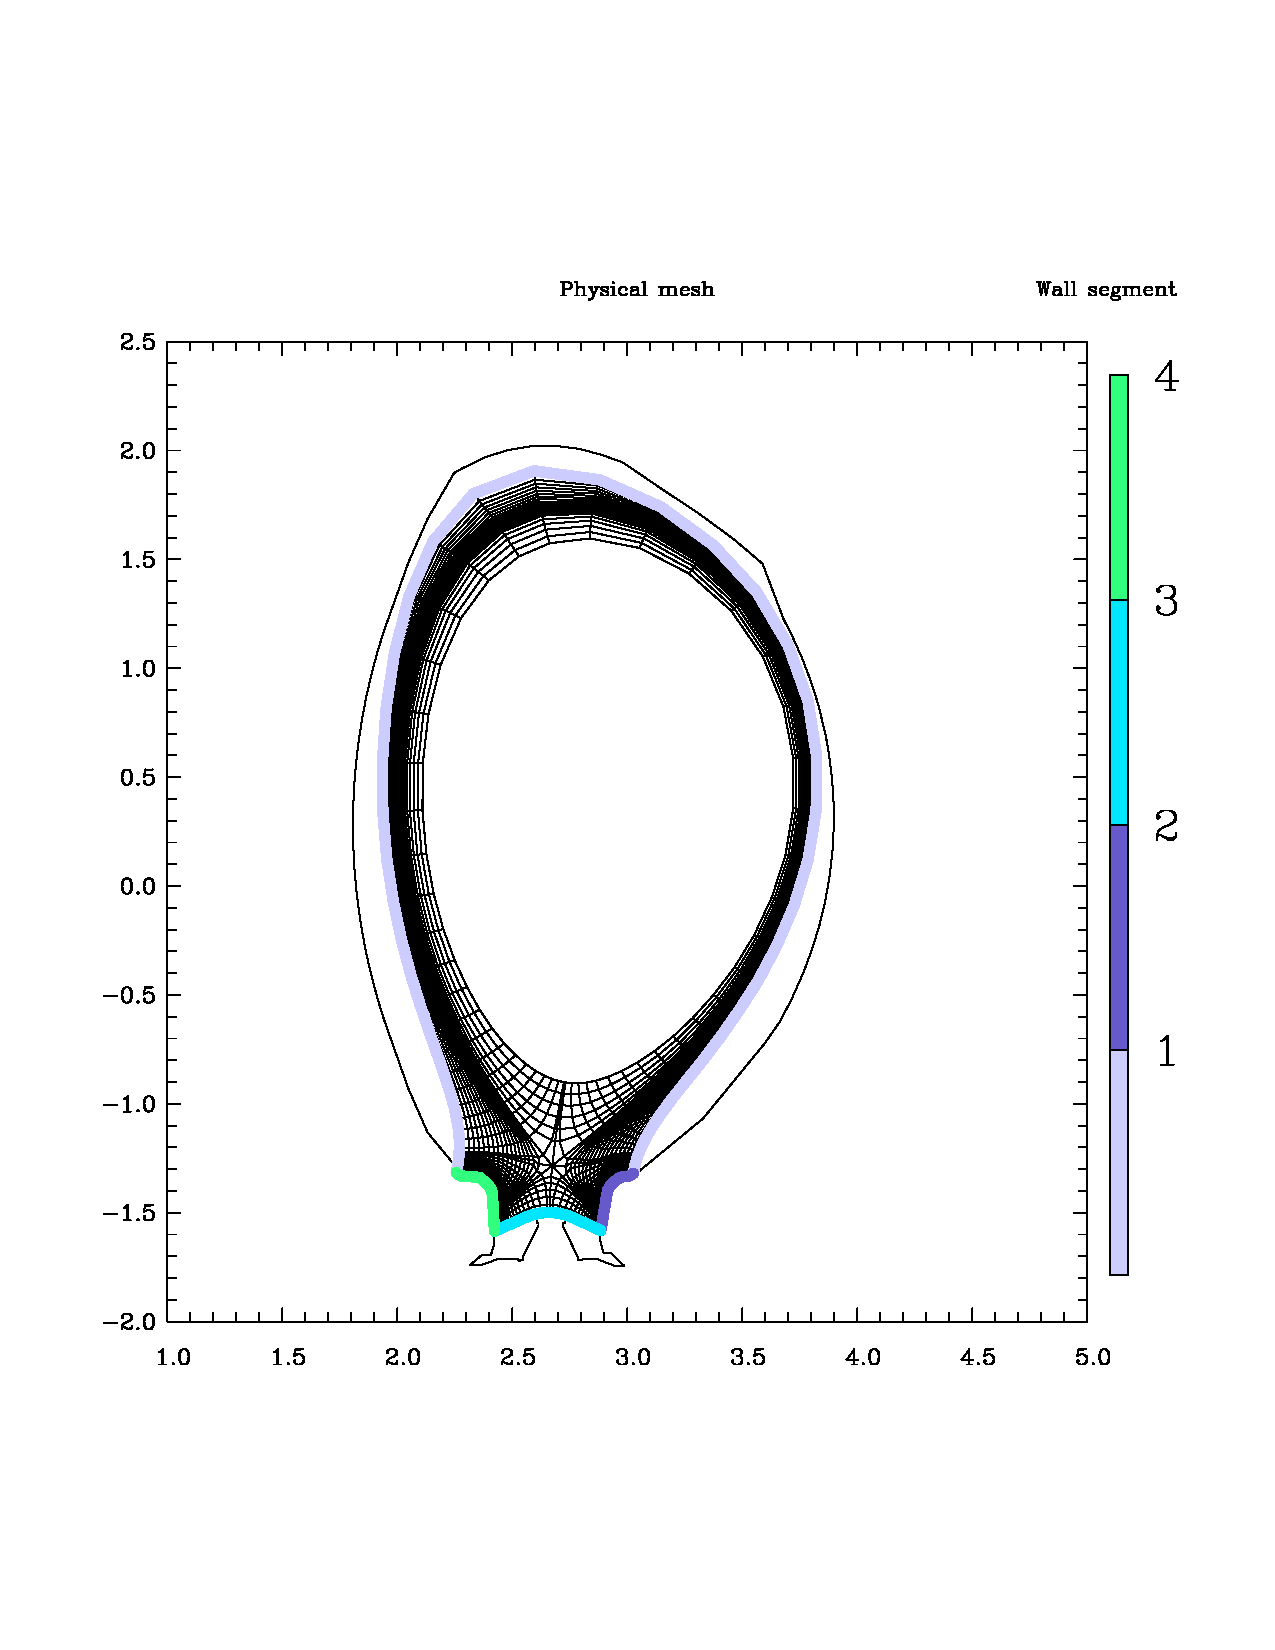
\includegraphics[height=6cm]{nseg.pdf}}
  \subfigure[vesl sep phys wall 10.0 wwid sputchem 1 wzsel 3 ndec logw fnax 1 zsel 'Ychem D+' wallblbl surf]{\label{fig:Ychem}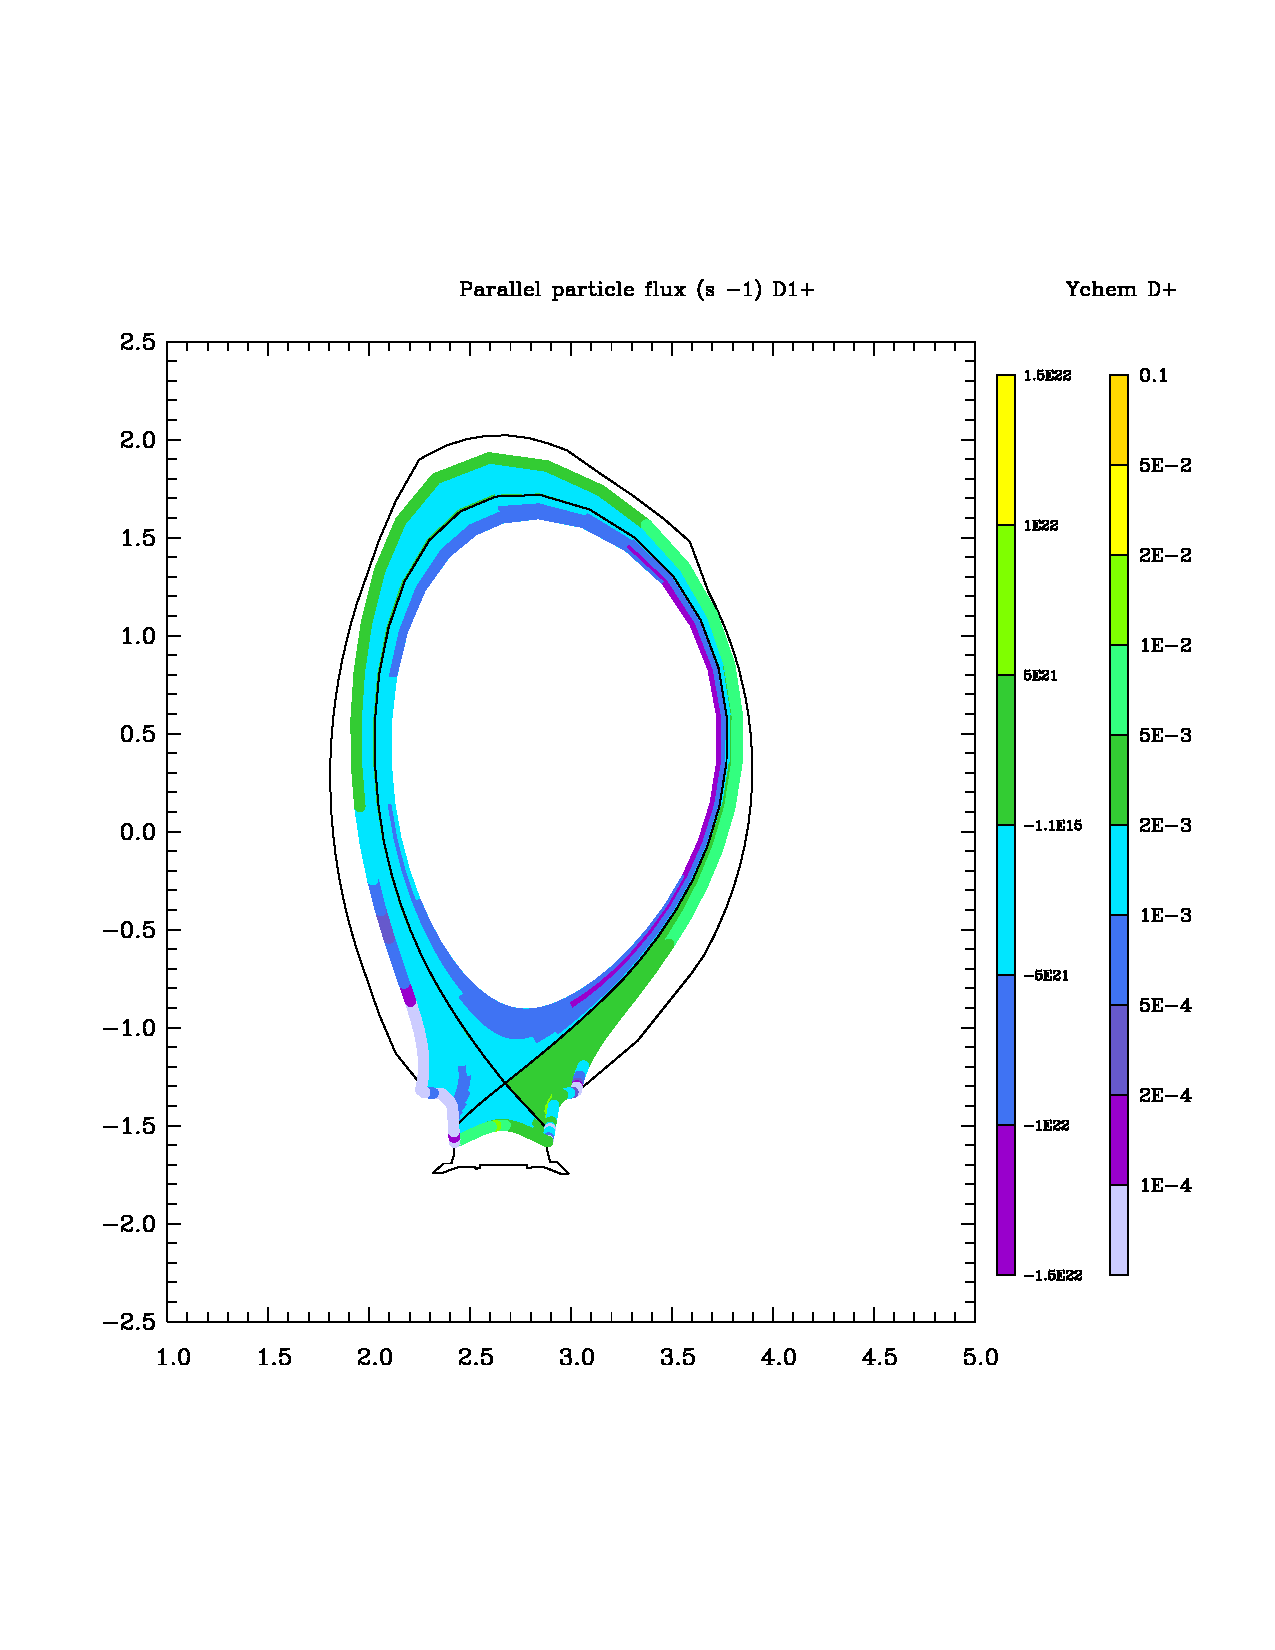
\includegraphics[height=6cm]{Ychem.pdf}}
\else
  \subfigure[phys 0 nseg 4 1. 2. 3. 4. wclvs 10.0 wwid wall mesh]{\label{fig:nseg}
\includegraphics[height=6cm]{nseg.epsi}}
  \subfigure[vesl sep phys wall 10.0 wwid sputchem 1 wzsel 3 ndec logw fnax 1 zsel 'Ychem D+' wallblbl surf]{\label{fig:Ychem}
\includegraphics[height=6cm]{Ychem.epsi}}
\fi
  \caption{Wall plots.}
  \label{fig:wallplots}
\end{figure}

The wall segment indices are illustrated in figure \ref{fig:nseg}, obtained with the {\bf 0 nseg} command. We impose the contour levels to be at the values 1 through 4 with the {\bf 4 1. 2. 3. 4. wclvs} command. The thickness of the drawn wall line is given by {\bf 10.0 wwid}. {\bf wall} asks for the wall data overlay on top of the requested {\bf mesh} plot.

Another more complex example is given in figure \ref{fig:Ychem}. It combines a {\bf surf} plot of the D$^+$ poloidal 
particle flux ({\bf fnax 1 zsel}, as D$^+$ has species index 1), with a {\bf wall} plot of the chemical sputtering 
yield for D$^+$ ({\bf sputchem 1 wzsel}). The latter is done on a logarithmic scale ({\bf logw}), covering 3 decades 
({\bf 3 ndec}). The label for the colour bar for the wall data is shortened with {\bf 'Ychem D+' wallblbl}. The wall
colour bar is the rightmost one. Not choosing
the {\bf zsel} and {\bf wzsel} options would have given a series of plots, one per species, with their individual
poloidal particle flux and chemical sputtering yield. If only the {\bf wzsel} option is used, one obtains a series of
{\bf surf} plots with all the same ``wall'' data overlay. If only the {\bf zsel} option is used, then the {\bf wall} 
overlay will come from the first species, namely D$^0$ in this case. It is therefore recommended to always make sure 
that the species dimensions of the ``matrix'' and ``wall'' data match!

\subsection{Target plot}
\index{b2plot, plotting target quantities}

In figure \ref{fig:targetplots}, we show examples of target plots.

\begin{figure}[hbtp]
  \centering
\ifpdf 
  \subfigure[comp sep 10.0 wwid wallhflx wall kappa trgsurf]{\label{fig:Kappa}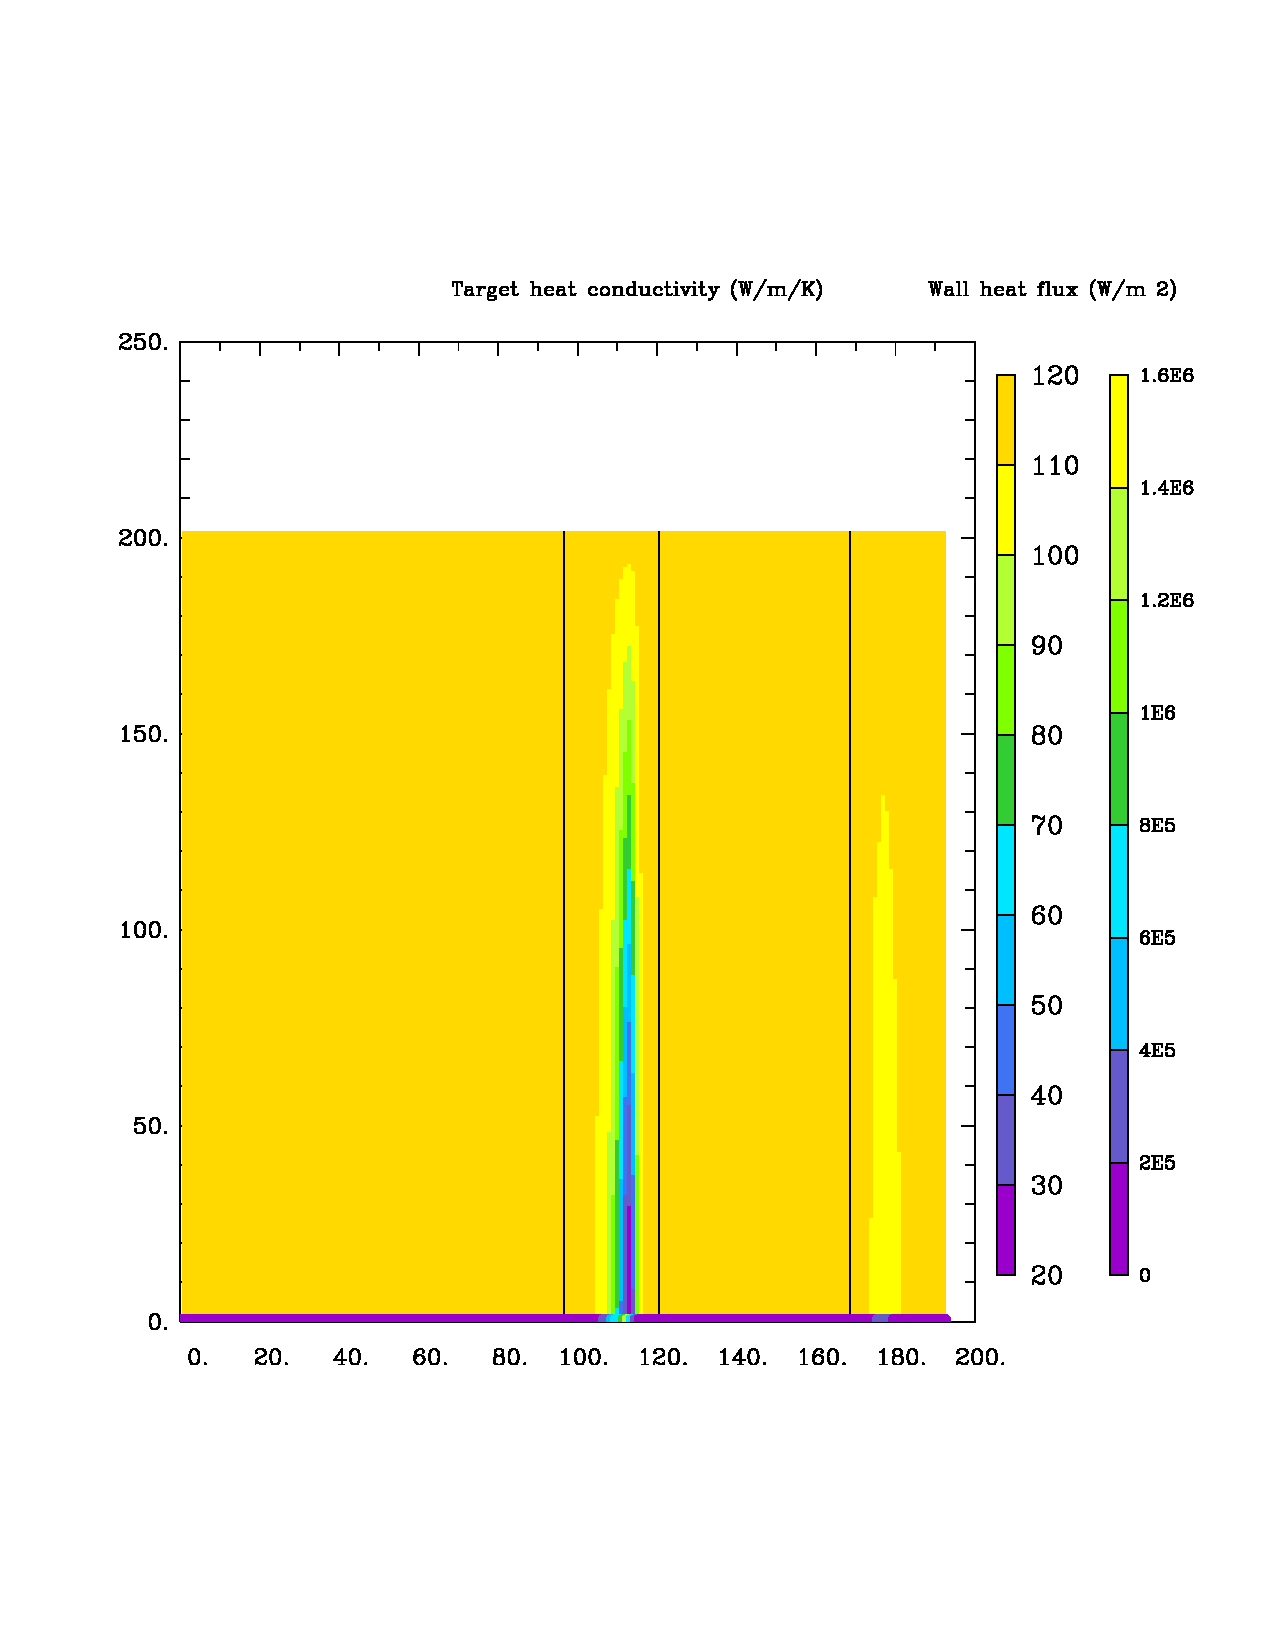
\includegraphics[height=6cm]{Kappa.pdf}}
  \subfigure[a4l outl vesl 2.2 rmin 3.2 rmax -1.0 zmax -1.75 zmin sep 8.0 wwid logw te logf 5 ndec cooltemp wtot trgm- phys 'Tp-Tc (K)' trgblbl wallflux 1 wzsel 'D+ wall flux' wallblbl wall target logtrg surf]{\label{fig:Triple}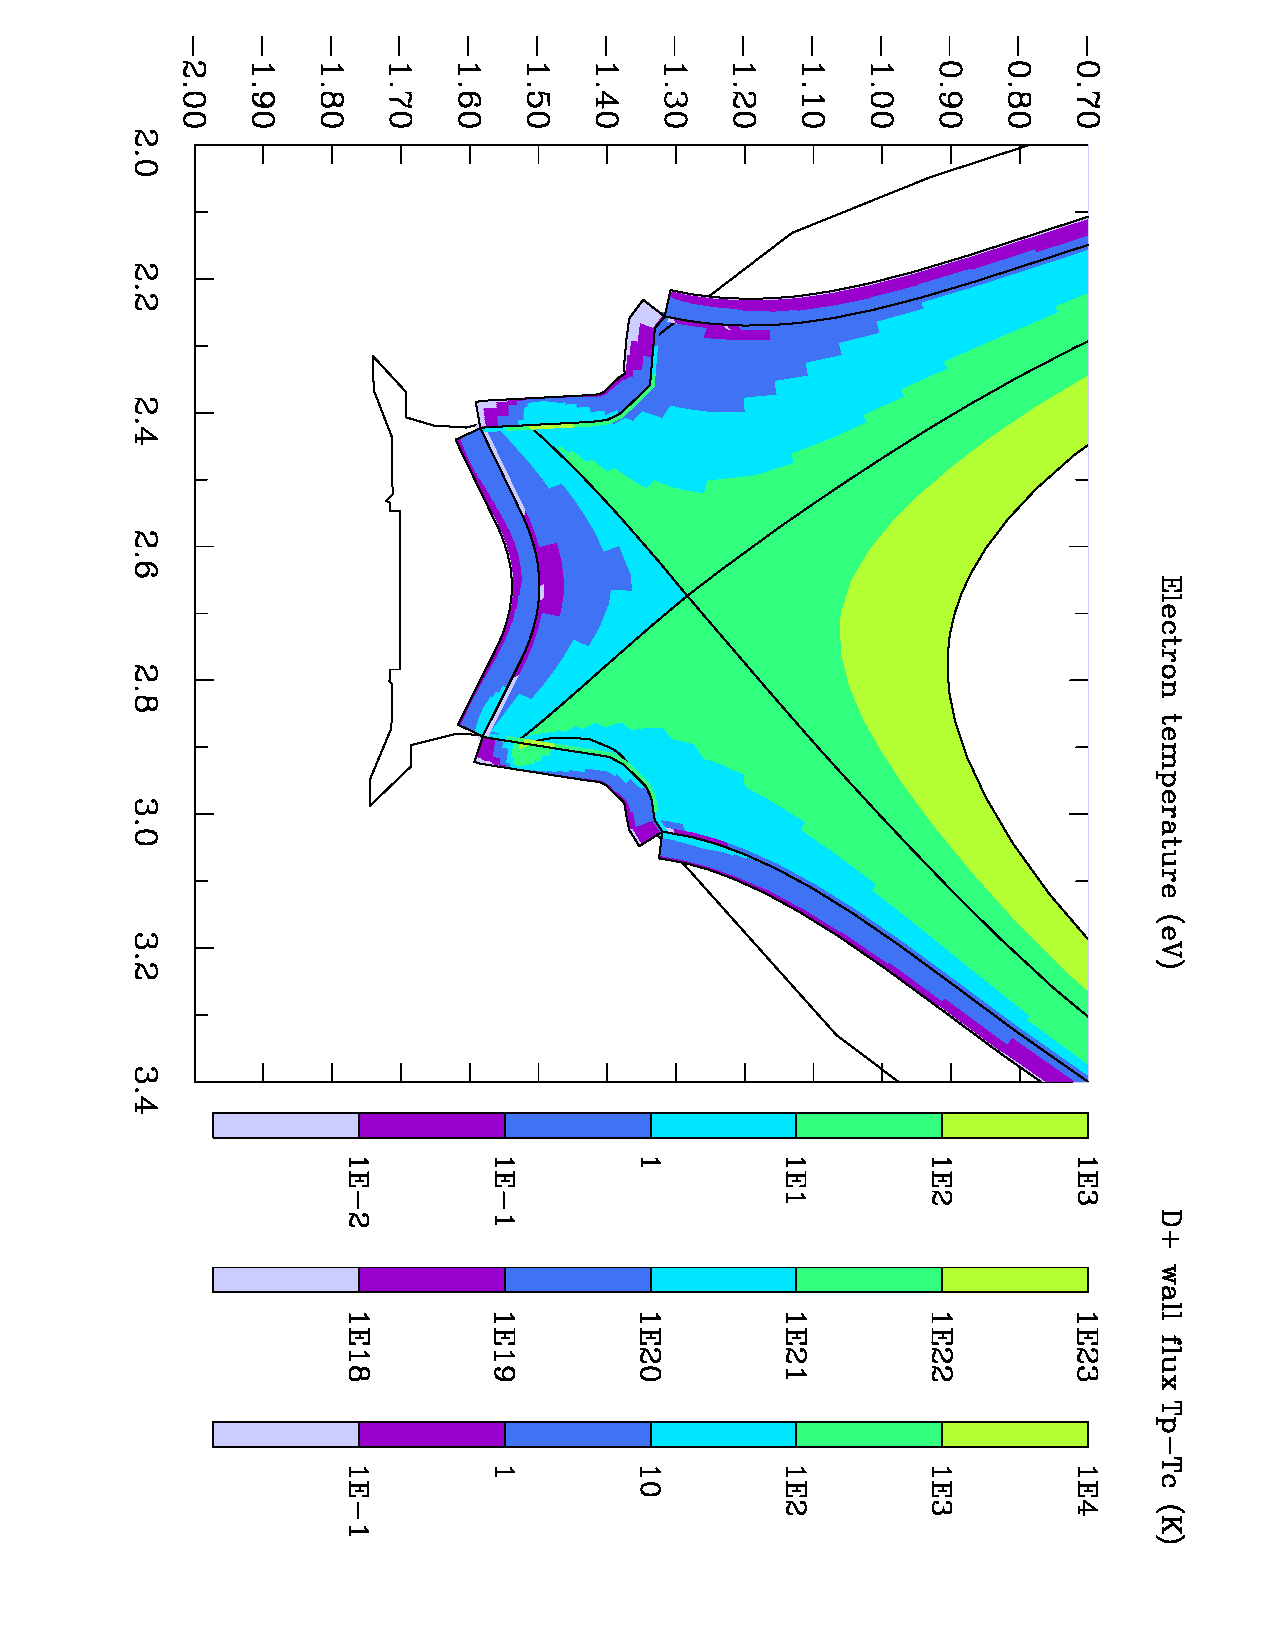
\includegraphics[angle=90,height=6cm]{Triple.pdf}}
\else
  \subfigure[comp sep 10.0 wwid wallhflx wall kappa trgsurf]{\label{fig:Kappa}
\includegraphics[height=6cm]{Kappa.epsi}}
  \subfigure[a4l outl vesl 2.2 rmin 3.2 rmax -1.0 zmax -1.75 zmin sep 8.0 wwid logw te logf 5 ndec cooltemp wtot trgm- phys 'Tp-Tc (K)' trgblbl wallflux 1 wzsel 'D+ wall flux' wallblbl wall target logtrg surf]{\label{fig:Triple}
\includegraphics[angle=90,height=6cm]{Triple.epsi}}
\fi
  \caption{Target plots.}
  \label{fig:targetplots}
\end{figure}

The first plot (figure \ref{fig:Kappa}) shows the target heat conductivity ({\bf kappa}) in the target 
computational domain ({\bf comp} and {\bf trgsurf}).
The vertical separators ({\bf sep}) indicate the segment boundaries. 
The overlay line at $y$=0, i.e. at the target surface in contact with the plasma is the {\bf wall} data,
here the incoming plasma heat flux ({\bf wallhflx}).

The second plot (figure \ref{fig:Triple}) is a triple plot\index{b2plot, triple plot}, containing
a plasma quantity from the ``matrix'' stack, (here {\bf te}), with {\bf wall} and {\bf target} overlays.
The ``matrix'' ({\bf logf}), ``wall'' ({\bf logw}) and ``target'' ({\bf trglog}) data are all plotted on
a logarithmic scale. The target data is obtained with the command
\begin{verbatim}
cooltemp wtot trgm- 
\end{verbatim}
which takes the ``wall'' quantity {\bf cooltemp}, the temperature at the cooled end of the target plate, copies it
over to the ``target'' stack ({\bf wtot}), and subtracts it from the preceding ``target'' stack value (here the
target temperature, which is loaded onto the stack by default at startup). So we obtain the amount by which
the target has been heated by the plasma, and label it with {\bf 'Tp-Tc (K)' trgblbl}. 
The wall overlay data is the D$^+$ particle flux to the wall ({\bf wallflux 1 wzsel}), labeled with
{\bf 'D+ wall flux' wallblbl}. The colour bars, from left to right, correspond to the ``matrix'', ``wall''
and ``target'' data arrays.

\subsection{Radiation plot}
\index{b2plot, radiation plots}

The following was used to produce a plot (figure \ref{fig:b2rad}) of
the emissivity arising out of radiation for C and Ne.

\begin{verbatim}
! b2plot < b2rad.plot ; ctrans -d ps.land.color gmeta | a4page > ! tmp.ps
a4l 2 1 page lbof logf phys
b2ra pvol abs 2 2 sumz 1.0e4 fmin 1.0e8 fmax 'Carbon' extl cont
b2ra pvol abs 3 3 sumz 1.0e4 fmin 1.0e8 fmax 'Neon' extl cont
\end{verbatim}

The first line is a comment indicating how \btwoplot should be run (the
file containing the above lines was called \verb!b2rad.plot!), and how
the PostScript file should be generated.

The second line sets up an A4 landscape format with two graphs next to
each other, sets labelling of contour levels off, logarithmic scaling
and plotting on the physical domain only.

The third and fourth lines plot the line radiation data for the 2$^{nd}$
and 3$^{rd}$ species respectively, setting the data minimum to $10^4$ and
maximum to $10^8$, labelling the graphs ``Carbon'' and ``Neon''
respectively.

\begin{figure}[hbtp]
\ifpdf 
    \centerline{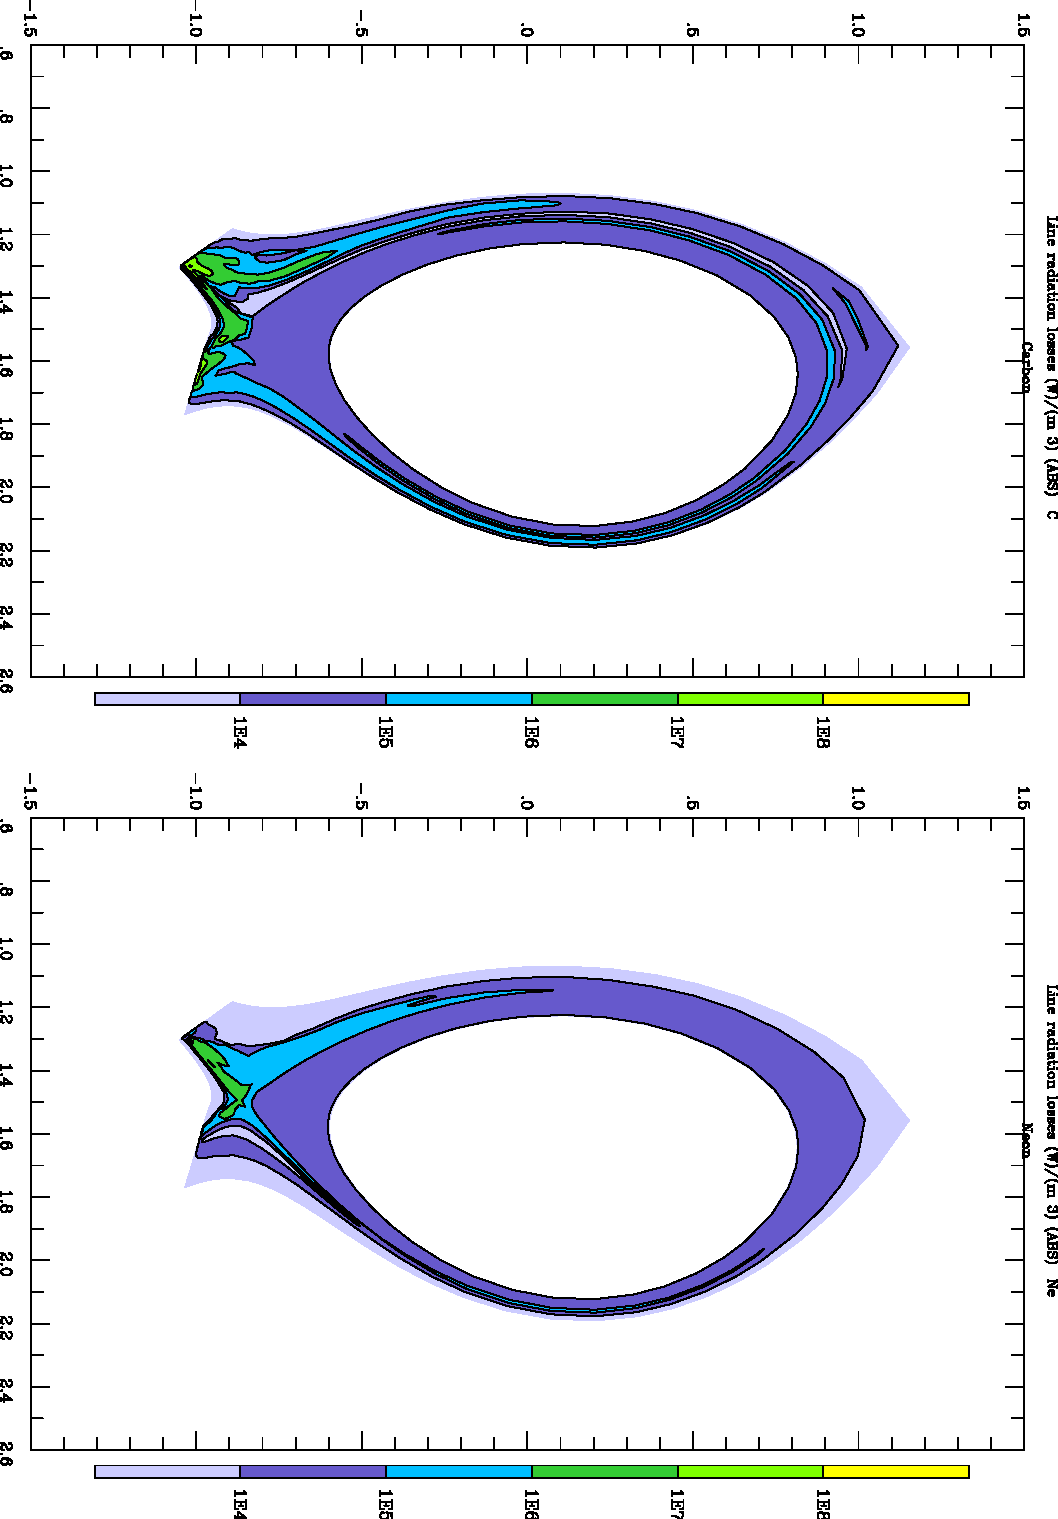
\includegraphics[angle=90,height=10cm]{b2plot_b2rad.pdf}}
\else
    \centerline{
\includegraphics[angle=90,height=10cm]{b2plot_b2rad.epsi}}
\fi
    \caption{C and Ne radiation.}
    \label{fig:b2rad}
\end{figure}

\subsection{Fluxes and values plot}

The following was used to calculate and plot integrated values of
fluxes and some local quantities along various lines.  See figure \ref{fig:fluxes}.

\begin{verbatim}
'${HOST} ${PWD} `date` T=${TIME}' extl glob
a4p 2 2 page
phys
feex sumy 19 f.x drop
feey sumx 57 f.y drop
feix sumy 19 f.x drop
feiy sumx 57 f.y drop
fnix 1 1 sumz sumy 19 f.x drop
fnix 2 7 sumz sumy 19 f.x drop
fnix 8 17 sumz sumy 19 f.x drop
fnix 18 19 sumz sumy 19 f.x drop
fniy 1 1 sumz sumx 57 f.y drop
fniy 2 7 sumz sumx 57 f.y drop
fniy 8 17 sumz sumx 57 f.y drop
fniy 18 19 sumz sumx 57 f.y drop
phys
ni 1 1 sumz 0.0 fmin 0.0 fmax 57 f.y drop
ni 2 7 sumz 0.0 fmin 0.0 fmax 57 f.y drop
ni 8 17 sumz 0.0 fmin 0.0 fmax 57 f.y drop
ni 18 19 sumz 0.0 fmin 0.0 fmax 57 f.y drop
te 0.0 fmin 0.0 fmax 57 f.y drop
ti 0.0 fmin 0.0 fmax 57 f.y drop
zeff 0.0 fmin 0.0 fmax 57 f.y drop
ne 0.0 fmin 0.0 fmax 57 f.y drop
\end{verbatim}
%% $

This example plots a series of line plots in a $2 \times 2$ format on an A4
portrait page.  Liberal use is made of {\bf sumx} and {\bf sumy} to produce
appropriate sums, and of {\bf sumz} to sum over the same species.  {\bf f.x}
and {\bf f.y} are used to plot the line plots.  Setting both {\bf fmin} and
{\bf fmax} to 0.0 means each plot is scaled separately --- otherwise the
scaling is done on all of the data.

\begin{figure}[hbtp]
  \centering
\ifpdf 
  \subfigure[Page 1]{\label{fig:fluxes_p1}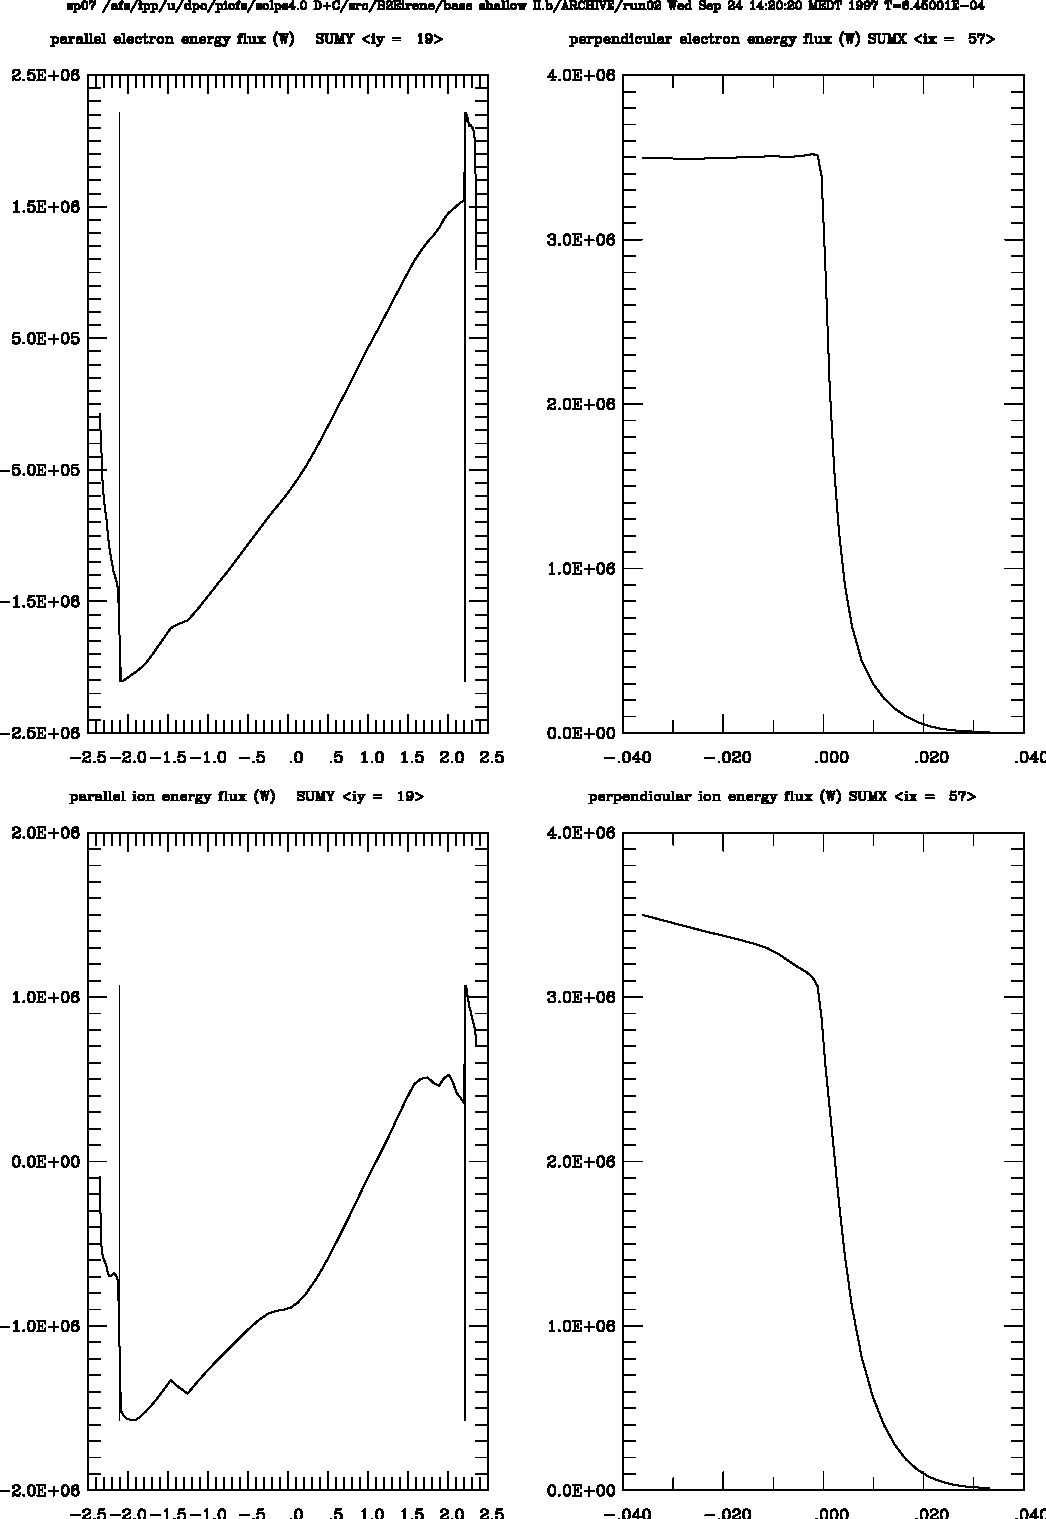
\includegraphics[height=7cm]{b2plot_fluxes_1.pdf}}
  \subfigure[Page 2]{\label{fig:fluxes_p2}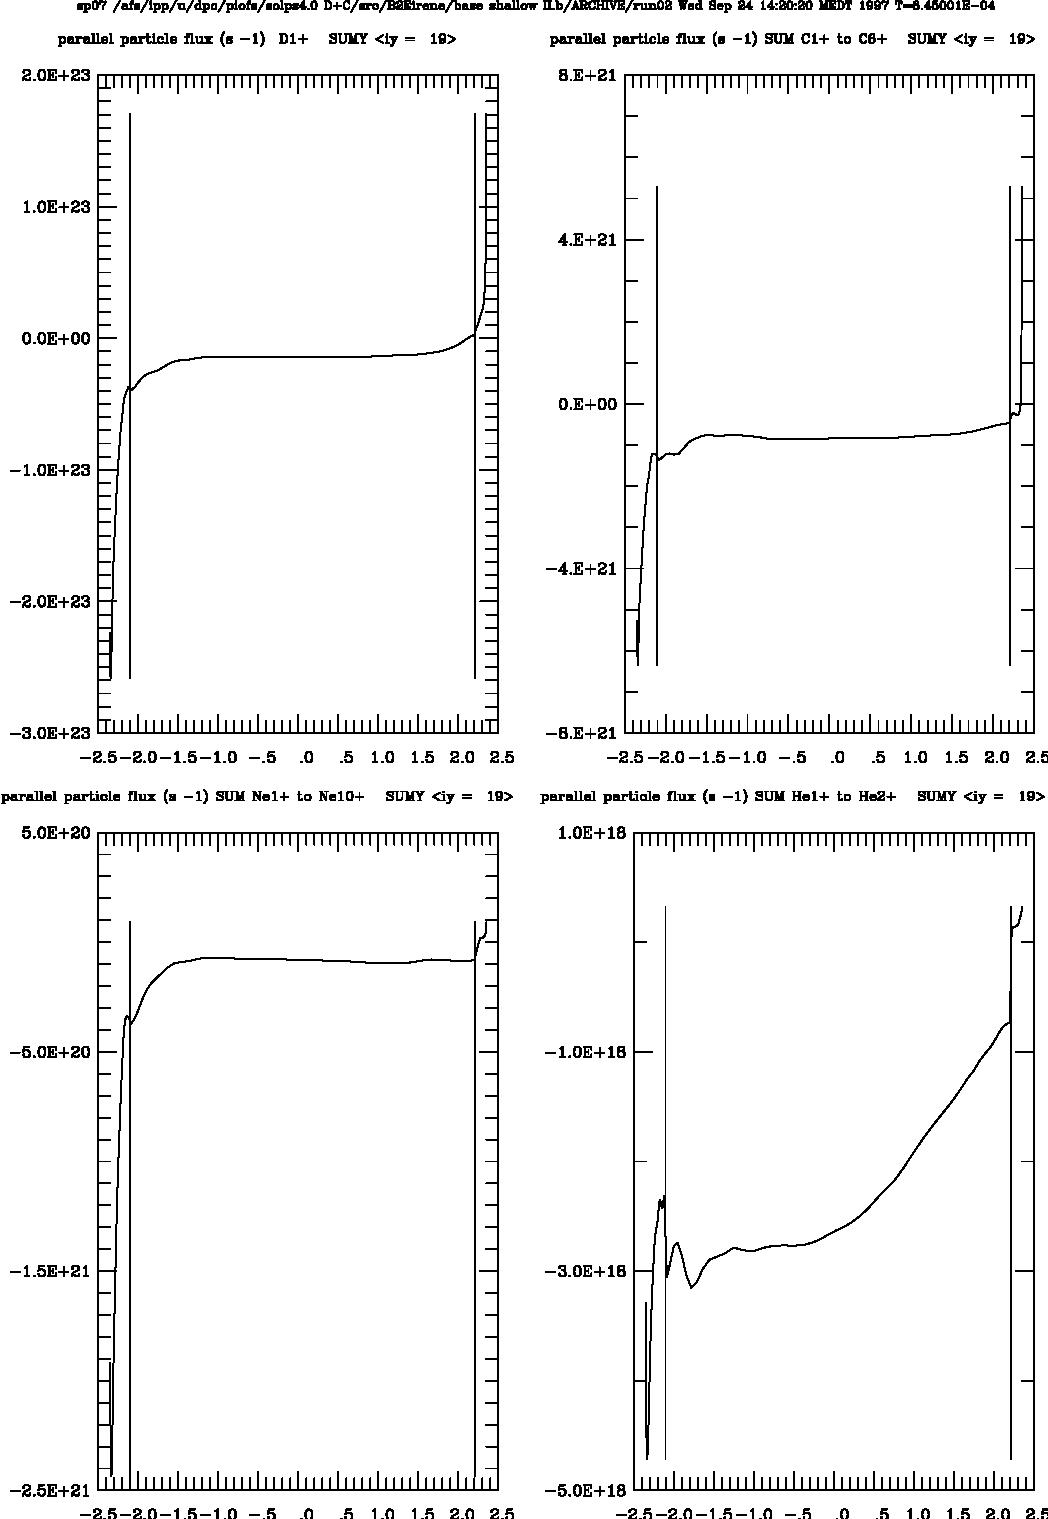
\includegraphics[height=7cm]{b2plot_fluxes_2.pdf}}
  \subfigure[Page 3]{\label{fig:fluxes_p3}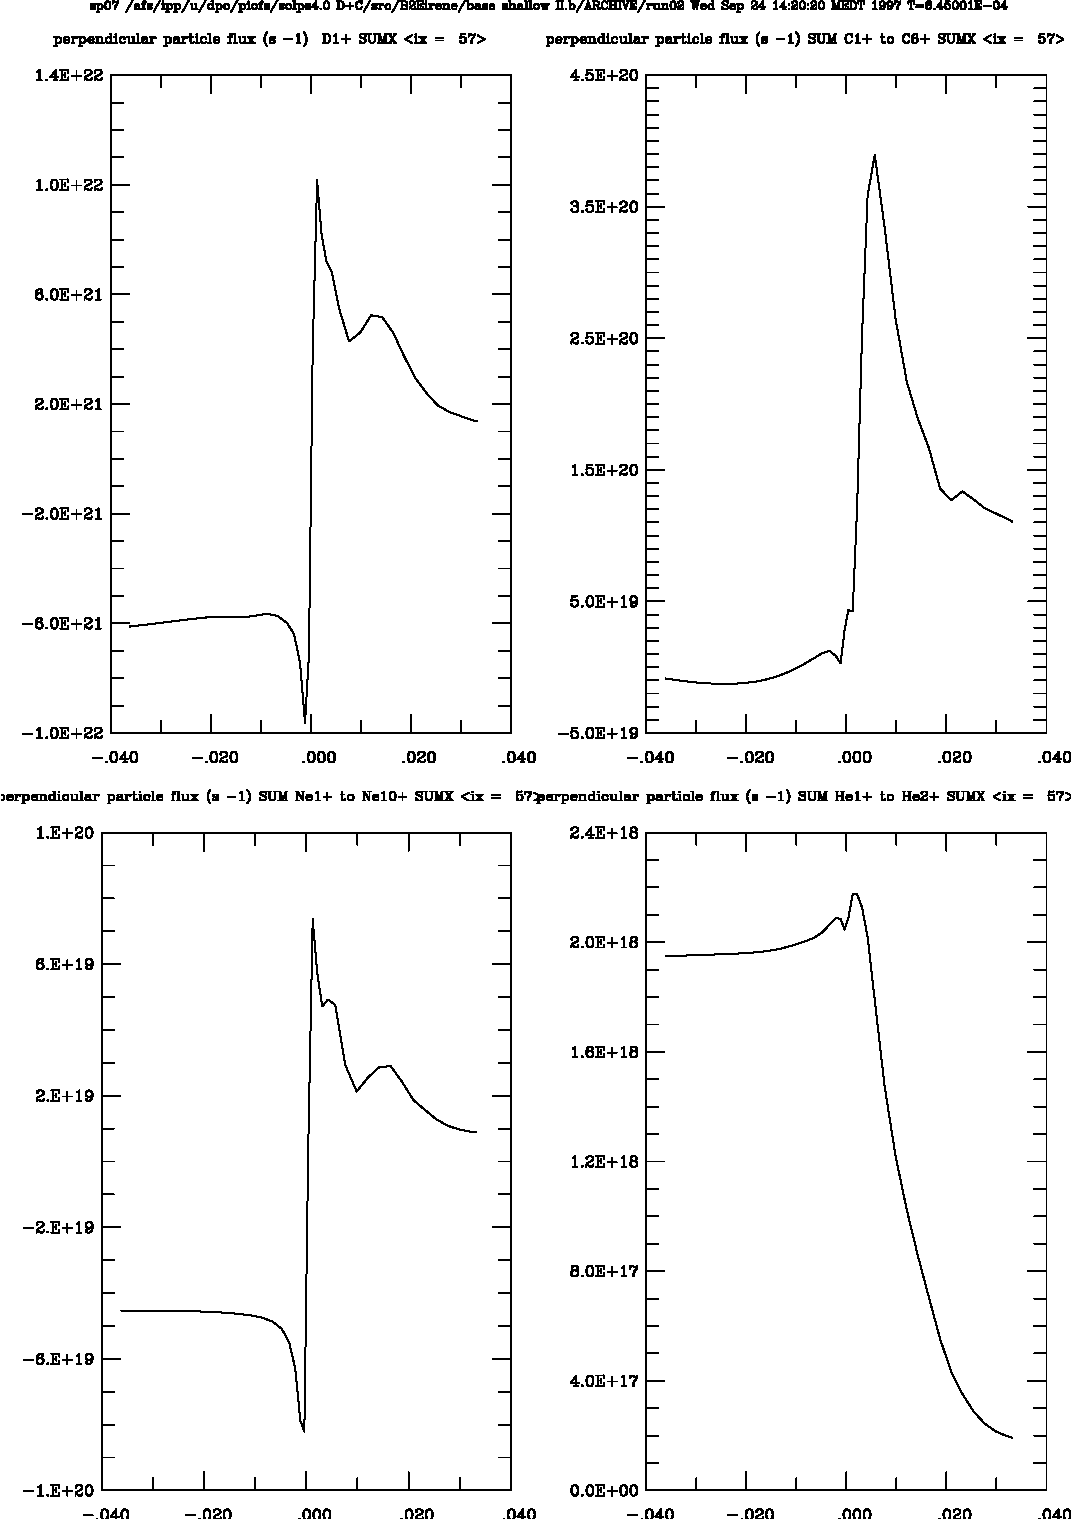
\includegraphics[height=7cm]{b2plot_fluxes_3.pdf}}
  \subfigure[Page 4]{\label{fig:fluxes_p4}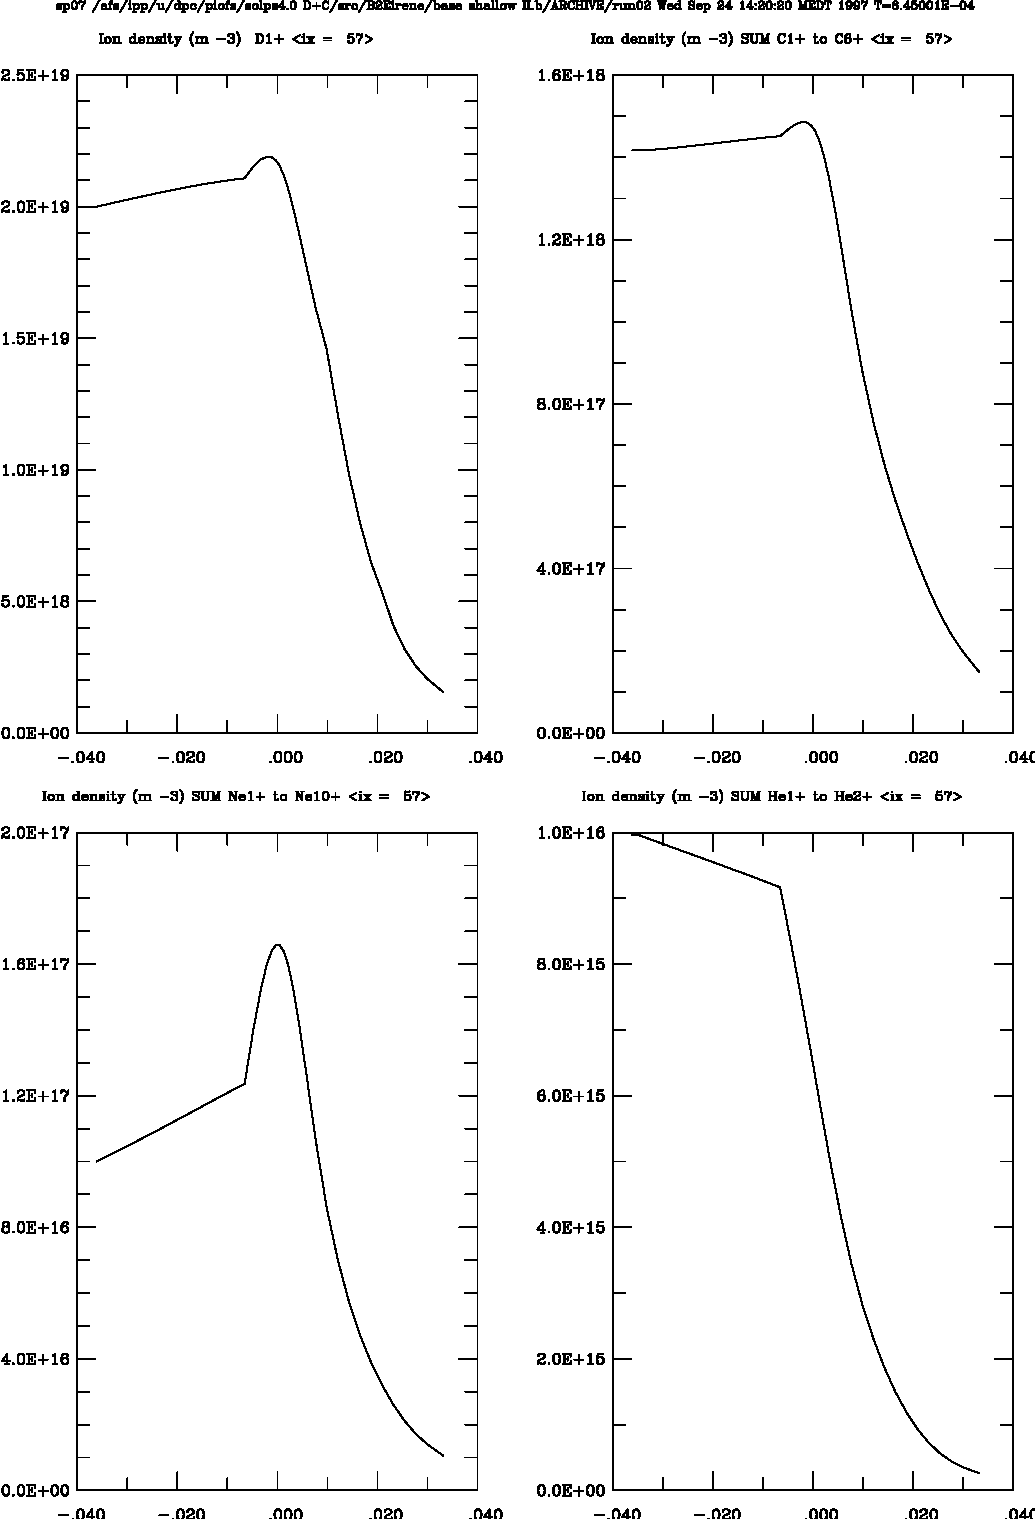
\includegraphics[height=7cm]{b2plot_fluxes_4.pdf}}
  \subfigure[Page 5]{\label{fig:fluxes_p5}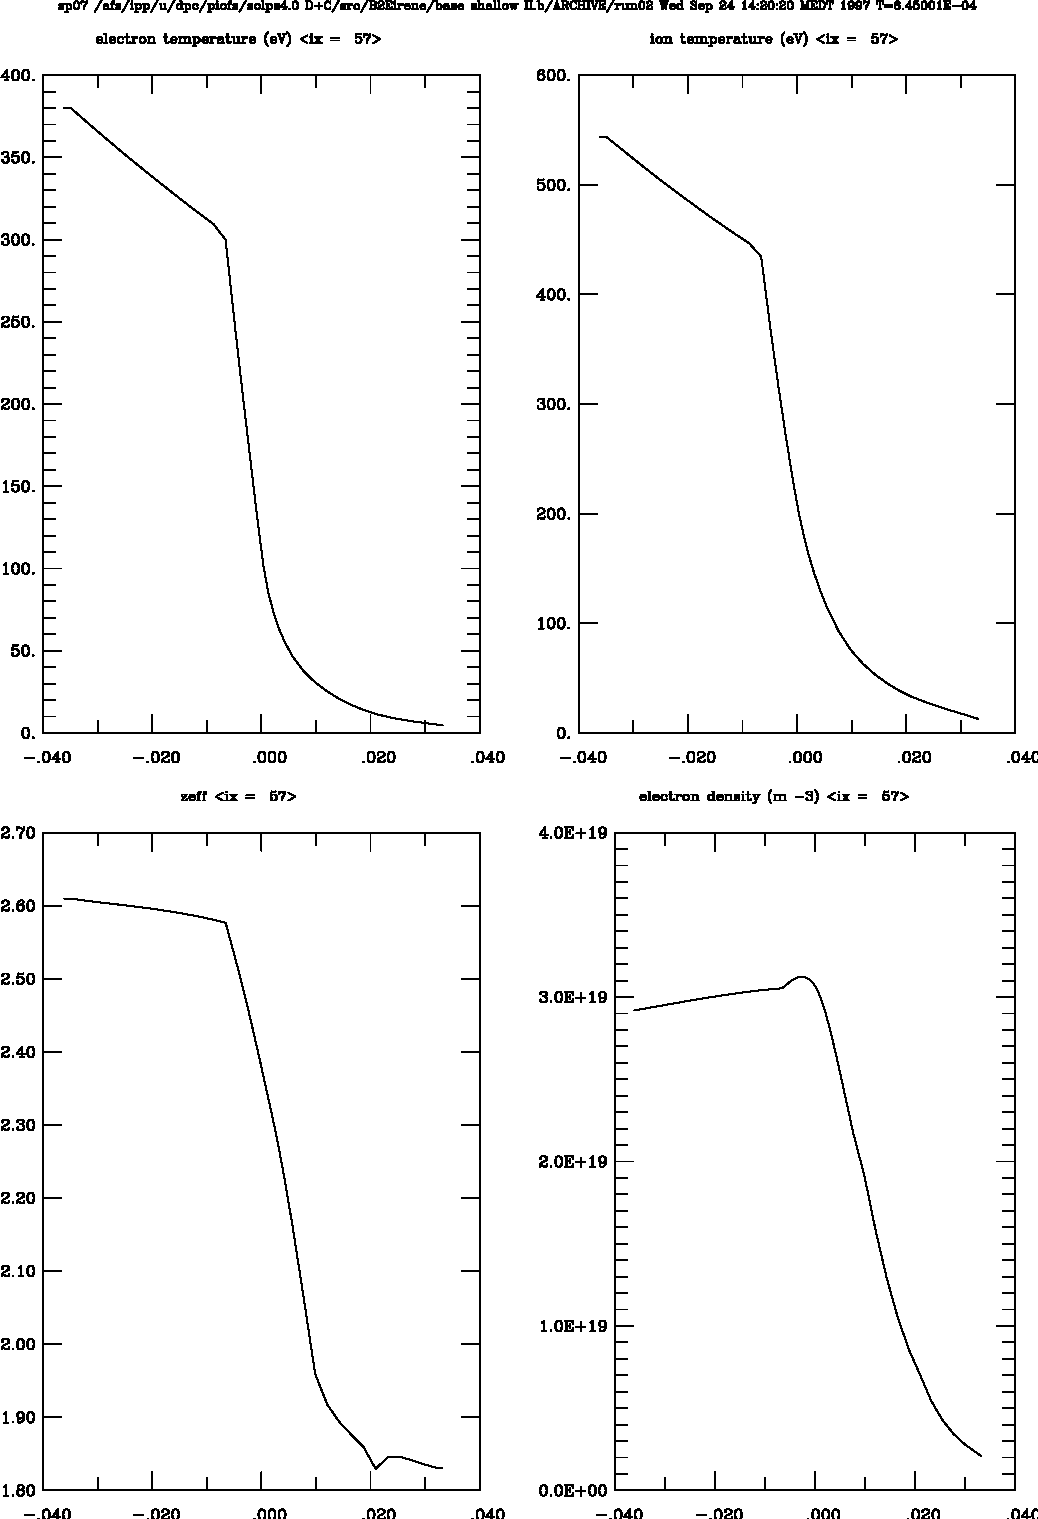
\includegraphics[height=7cm]{b2plot_fluxes_5.pdf}}
\else
  \subfigure[Page 1]{\label{fig:fluxes_p1}
\includegraphics[height=7cm]{b2plot_fluxes_1.epsi}}
  \subfigure[Page 2]{\label{fig:fluxes_p2}
\includegraphics[height=7cm]{b2plot_fluxes_2.epsi}}
  \subfigure[Page 3]{\label{fig:fluxes_p3}
\includegraphics[height=7cm]{b2plot_fluxes_3.epsi}}
  \subfigure[Page 4]{\label{fig:fluxes_p4}
\includegraphics[height=7cm]{b2plot_fluxes_4.epsi}}
  \subfigure[Page 5]{\label{fig:fluxes_p5}
\includegraphics[height=7cm]{b2plot_fluxes_5.epsi}}
\fi
  \caption{Line plots of fluxes and other quantities.}\label{fig:fluxes}
\end{figure}

\clearpage

\chapter{Miscellaneous}
\label{cha:Misc}

\section{DIMENSIONS.F}\index{DIMENSIONS.F}\label{sec:DIMENSIONS}

The file \$\verb!SOLPSTOP/modules/B2.5/src/include/DIMENSIONS.F! and its local version
\$\verb!SOLPSTOP/modules/B2.5/src/include.local/DIMENSIONS.F! contain key dimensions 
that determine
the sizes of arrays that can be defined by namelists
in \verb!b2.*.parameters! files (for compatibility with 
certain compilers).

The quantities defined in \verb!DIMENSIONS.F! are:
\begin{description}
\item[DEF\_ISOEXTRA]\index{DEF\_ISOEXTRA}\index{ISOEXTRA} the maximum
number of extra isolating cells
\item[DEF\_NADD]\index{DEF\_NADD}\index{NADD} the maximum number of
additional vacuum cells outside the gridded domain in \verb!Eirene!
\item[DEF\_NATM]\index{DEF\_NATM}\index{NATM} the maximum number of
neutral atomic species to be handled by \verb!Eirene!
\item[DEF\_NCHEN]\index{DEF\_NCHEN}\index{NCHEN} the maximum number of
energy bins for the diagnostic chords in \verb!Eirene!
\item[DEF\_NCUT]\index{DEF\_NCUT}\index{NCUT} the maximum number of
``cuts'' (2 for single null cases, 4 for double nulls)
\item[DEF\_NFL]\index{DEF\_NFL}\index{NFL} the maximum number of charged fluids
passed from \verb!B2.5! to \verb!Eirene!
\item[DEF\_NGSTAL]\index{DEF\_NGSTAL}\index{NGSTAL} the maximum number
of grids on which spatially resolved surface tallies are computed
\item[DEF\_NION]\index{DEF\_NION}\index{NION} the maximum number of molecular
ion species to be handled by \verb!Eirene!
\item[DEF\_NLIM]\index{DEF\_NLIM}\index{NLIM} the maximum number of
additional surfaces to be handled by \verb!Eirene!
\item[DEF\_NMOL]\index{DEF\_NMOL}\index{NMOL} the maximum number of
neutral molecular species to be handled by \verb!Eirene!
\item[DEF\_NPHID]\index{DEF\_NPHID}\index{NPHID} the maximum number of
toroidal standard surfaces
\item[DEF\_NPLS]\index{DEF\_NPLS}\index{NPLS} the maximum number of background 
plasma species to be handled by \verb!Eirene!
\item[DEF\_NPRNL]\index{DEF\_NPRNL}\index{NPRNL} the maximum number of
particles that can be saved in the time dependent arrays
\item[DEF\_NREAC]\index{DEF\_NREAC}\index{NREAC} the maximum number of
reaction cards that can be created by \verb!Uinp!
\item[DEF\_NRDS]\index{DEF\_NREAC}\index{NREAC} the maximum number of
molecular dissociation reaction cards that can be created by \verb!Uinp!
\item[DEF\_NREC]\index{DEF\_NREAC}\index{NREAC} the maximum number of
recombination reaction cards that can be created by \verb!Uinp!
\item[DEF\_NREL]\index{DEF\_NREAC}\index{NREAC} the maximum number of
elastic collisions reaction cards that can be created by \verb!Uinp!
\item[DEF\_NSD]\index{DEF\_NSD}\index{NSD} the maximum number of plasma
species handled in \verb!B2.5!
\item[DEF\_NSPCSRFG]\index{DEF\_NSPCSRFG}\index{NSPCSRFG} the maximum
number of groups of \verb!Eirene! surfaces for which the data can be
transferred from \verb!B2.5! (\verb!DG! specification "Surface special")
\item[DEF\_NSRFS]\index{DEF\_NSRFS}\index{NSRFS} the maximum number of
surfaces in a stratum
\item[DEF\_NSTRA]\index{DEF\_NSTRA}\index{NSTRA} the maximum number of
\verb!Eirene! strata
\item[DEF\_NSTS]\index{DEF\_NSTS}\index{NSTS} the maximum number of non-default 
standard surfaces to be handled by \verb!Eirene!
\item[DEF\_NTOR]\index{DEF\_NTOR}\index{NTOR} the maximum number of toroidal
periodicity boundaries
\item[DEF\_NXD]\index{DEF\_NXD}\index{NXD} the maximum number of cells
in the $x$ (parallel or poloidal) direction not including two guard
cells
\item[DEF\_NYD]\index{DEF\_NYD}\index{NYD} the maximum number of cells
in the radial direction not including two guard cells
%%\item[] the maximum number of 
%%\item[] the maximum number of 
\end{description}

The current default settings of \verb!DIMENSIONS.F!, correponding to a D+He+C DN case, are:
\VerbatimInput[fontsize=\footnotesize]{DIMENSIONS.F}

\section{Making movies}

\section{Compiling B2.5}
\label{sec:compilingb2}\index{B2.5, compiling}\index{B2.5, Makefile}

(See also section \ref{sec:b2}, page \pageref{sec:b2}.)

The following is the \verb!Makefile! provided with the Master 
in the \verb!sbb! directory:

\VerbatimInput[fontsize=\footnotesize]{B2_5.Makefile}

and, as a prototypical example, the \verb!config.ITER.ifort64! in
the \verb!config! subdirectory: \index{B2.5, compiling options}

\VerbatimInput[fontsize=\footnotesize]{B2_5.config.ITER.ifort64}

If the user wishes to modify the compiling options used, the creation
of a \verb!config.!\$\verb!${HOST_NAME}.!\$\verb!${COMPILER}.local! file 
is recommended, in which to store the modified settings. Since the \verb!Makefile!
reads those after the 
\verb!config/compiler.!\$\verb!${HOST_NAME}.!\$\verb!${COMPILER}! file,
they need only contain the modified definitions. 

\section{Defines}

\subsection{B2.5-Eirene}
\index{DEFINES, used in compiling B2.5-Eirene}

We list here the possible compiler options that can be used when compiling the
coupled version of \verb!B2.5-Eirene!. These options are shared across both the
\verb!B2.5! and \verb!Eirene! source codes.

\begin{description}
\item[ALLOCATE\_AND\_NAMELIST] \index{ALLOCATE\_AND\_NAMELIST} To be used if the compiler allows dynamically allocated namelist arrays
\item[B25\_EIRENE] \index{B25\_EIRENE} Set internally by the \verb!Makefile! and used to identify differences between source code for stand-alone \verb!B2.5! and coupled \verb!B2.5-Eirene! applications
\item[NO\_B2\_CHEM\_SPUT] \index{NO\_B2\_CHEM\_SPUT} Used to indicate that chemical sputtering is specified through \verb!Eirene! arrays instead of \verb!B2.5!.
\item[NO\_GETENV] \index{NO\_GETENV} No \verb!GETENV! system call available
\item[USE\_MPI] \index{USE\_MPI} Set internally by the \verb!Makefile! and used to identify code necessary for MPI applications
\item[USE\_PXFGETENV] \index{USE\_PXFGETENV} Uses \verb!PXFGETENV!
  instead of \verb!GETENV!
\end{description}

\index{SOLPS\_CPP}
If you want to activate any of these options, you should add
\verb!-DOPTION! (where \verb!OPTION! might, for example, be
\verb!CLASSICAL_CURRENT!) to the \verb!SOLPS_CPP! environment variable
with
\begin{verbatim}
  setenv SOLPS_CPP '-DOPTION'
\end{verbatim}
and then recompile all of the routines affected (if unsure which
routines are affected, recompile them all with
\begin{verbatim}
  gmake clean
  gmake depend
  gmake
\end{verbatim}
).  If \verb!SOLPS_CPP! already had a value, you would want to do
\begin{verbatim}
  setenv SOLPS_CPP "$SOLPS_CPP -DOPTION"
\end{verbatim}
%% $
so that the new option is added to the list. (Unsupported \verb!ksh!
or \verb!bash! users would use something like
\begin{verbatim}
  export SOLPS_CPP="$SOLPS_CPP -DOPTION"
\end{verbatim}
%%$
).

\subsection{B2.5}
\index{DEFINES, used in compiling B2.5}

%%grep #if $SOLPSTOP/modules/B2.5/src/*/*.F | awk '{print $2}' | sort | uniq

We list here the additional compiler options available that only affect compilation of
\verb!B2.5!.

\begin{description}
\item[ASTRA] \index{ASTRA} To be used if one wishes to run in coupled mode with the core transport code ASTRA
\item[CDF\_MOVIE] \index{CDF\_MOVIE} To be used if \verb!CDF! movie output is desired
\item[CLASSICAL\_CURRENT] \index{CLASSICAL\_CURRENT} Turns on classical current drift term
\item[COMPLICATED] \index{COMPLICATED} Uses a more ``complicated'' model for chord integration
\item[DEF\_MAXCHORDS] \index{DEF\_MAXCHORDS} Maximum number of chords to be considered (default 10000)
\item[F77] index{F77} Identifies specific code to \verb!Fortran-77! compilers
\item[HITS\_PER\_CHORD] \index{HITS\_PER\_CHORD} Maximum number of chord points per cell? (default 50)
\item[HPUX] \index{HPUX} Specific to HP computers
\item[IBMaix] \index{IBMaix} Specific to IBM AIX computers
\item[JET] \index{JET} Enables some additional output for coupling to the JET post-processor
\item[MDSPLUS] \index{MDSPLUS} Enables \verb!MDSplus! output
\item[NAG22] \index{NAG22} Specific to using the Nag Mark 22 or higher mathematical library
\item[NAGF95] \index{NAGF95} Specific to the \verb!NAG! F95 compiler
\item[NCAR4] \index{NCAR4} Used to specify NCAR4 rather than NCAR3
\item[NO\_21] \index{NO\_21} Do not use 21-moment model for thermal and viscous forces
\item[NO\_CDF] \index{NO\_CDF} No \verb!CDF! library available
\item[NO\_F01AAF] \index{NO\_F01AAF} No \verb!NAG! routine \verb!F01AAF! --- uses
  its replacement instead (needed if linking with Version 17 or later of \verb!NAG!)
\item[NO\_LONG\_LINES] \index{NO\_LONG\_LINES} Identify those
  compilers which have a limitation to relatively short output lines
\item[NO\_NAG] \index{NO\_NAG} No \verb!NAG! libraries available
\item[NO\_OPT] \index{NO\_OPT} No compiler optimization 
\item[PAR\_OPT] \index{PAR\_OPT} Runs the code in a special interpretive parameter optimization mode
\item[PERFMON] \index{PERFMON} Enable performance monitoring
\item[PLPLOT] \index{PLPLOT} Use \verb!PLPLOT! instead of \verb!NCAR! for plotting
\item[PSR] \index{PSR} Specific to the Pacific Sierra VAST compiler
\item[SCL\_IMP\_RCI] \index{SCL\_IMP\_RCI} Toggles scaling of impurities tallies
\item[USE\_CDF\_B2STIME] \index{USE\_CDF\_B2STIME} Specific for \SOLPSfour \verb!CDF! tallies
\item[WANT\_PROCESS] \index{WANT\_PROCESS} Enables the code for the
  \SOLPSfive to \SOLPSfour converter.
\item[WANT\_THIS] \index{WANT\_THIS} (default) Adds some boundary condition treatments
\item[WINDOWS] \index{WINDOWS} Specific to Windows implementations
\item[WOS] \index{WOS} Uses the \verb!WOS! libraries for accessing
  experimental data at IPP.
\end{description}

%%grep #if $SOLPSTOP/modules/B2.5/src/*/*.F | awk '{print $2,$1}' | sort | uniq


\begin{center}
  \begin{longtable}{|l|l|}
    \hline
    \multicolumn{2}{|l|}{\small\sl continued from previous page} \\
    \hline name & used in \\
    \hline \endhead
    \hline name & used in \\
    \hline \endfirsthead
    \hline
    \multicolumn{2}{|l|}{\small\sl continued on next page} \\
    \hline \endfoot
    \endlastfoot
ALLOCATE\_AND\_NAMELIST & b2plot/init\_wall.F \\
ALLOCATE\_AND\_NAMELIST & modules/b2mod\_boundary\_namelist.F \\
ALLOCATE\_AND\_NAMELIST & modules/b2mod\_input\_profile.F \\
ALLOCATE\_AND\_NAMELIST & modules/b2mod\_layer.F \\
ALLOCATE\_AND\_NAMELIST & modules/b2mod\_neutrals\_namelist.F \\
ALLOCATE\_AND\_NAMELIST & modules/b2mod\_numerics\_namelist.F \\
ALLOCATE\_AND\_NAMELIST & modules/b2mod\_sputter.F \\
ALLOCATE\_AND\_NAMELIST & modules/b2mod\_transport\_models.F \\
ALLOCATE\_AND\_NAMELIST & modules/b2mod\_transport\_namelist.F \\
ALLOCATE\_AND\_NAMELIST & modules/b2mod\_user\_namelist.F \\
ALLOCATE\_AND\_NAMELIST & modules/b2mod\_wall.F \\
ALLOCATE\_AND\_NAMELIST & postprocessing/b2yt\_wall.F \\
ALLOCATE\_AND\_NAMELIST & sources/b2stbr.F \\
ASTRA & modules/b2mod\_astra\_to\_b2.F \\
ASTRA & sources/b2stbc\_phys.F \\
ASTRA & sources/b2stbr.F \\
ASTRA & sources/b2stcx.F \\
ASTRA & sources/b2stel.F \\
ASTRA & transport/b2strcl.F \\
B25\_EIRENE & b2plot/b2pinp.F \\
B25\_EIRENE & b2plot/b2plot.F \\
B25\_EIRENE & b2plot/b2pnwl.F \\
B25\_EIRENE & b2plot/b2ptrgl.F \\
B25\_EIRENE & b2plot/b2pwinm.F \\
B25\_EIRENE & b2plot/b2pwlprp.F \\
B25\_EIRENE & b2plot/b2pwsort.F \\
B25\_EIRENE & b2plot/get\_from\_movie\_cdf.F \\
B25\_EIRENE & b2plot/ngread.F \\
B25\_EIRENE & convert/b2mds.F \\
B25\_EIRENE & driver/b2mndr.F \\
B25\_EIRENE & driver/b2mn.F \\
B25\_EIRENE & driver/b2mwti.F \\
B25\_EIRENE & postprocessing/b2ytdr.F \\
B25\_EIRENE & sources/b2stbr.F \\
B25\_EIRENE & modules/b2mod\_astra\_to\_b2.F \\
B25\_EIRENE & modules/b2mod\_diag.F \\
B25\_EIRENE & modules/b2mod\_neutrals\_namelist.F \\
B25\_EIRENE & modules/b2mod\_work.F \\
B25\_EIRENE & output/b2wdat.F \\
B25\_EIRENE & postprocessing/b2ytdr.F \\
B25\_EIRENE & sources/b2stbc\_phys.F \\
B25\_EIRENE & sources/b2stbm.F \\
B25\_EIRENE & sources/b2stbr.F \\
B25\_EIRENE & sources/eirene\_f30f31.F \\
B25\_EIRENE & sources/eirene\_mc.F \\
B25\_EIRENE & sources/eirene\_mc\_init.F \\
B25\_EIRENE & transport/b2tinnt.F \\
B25\_EIRENE & user/b2blnc.F \\
B25\_EIRENE & user/b2blne.F \\
B25\_EIRENE & user/b2blnm.F \\
B25\_EIRENE & user/b2trace.F \\
B25\_EIRENE & user/b2usrtrc.F \\
B25\_EIRENE & user/b2wrint.F \\
B25\_EIRENE & user/b2wrsep.F \\
B25\_EIRENE & user/cdfmovie.F \\
B25\_EIRENE & utility/rdneutrs.F \\
CDF\_MOVIE & b2plot/caltraj.F \\
CDF\_MOVIE & b2plot/process\_chords.F \\
CLASSICAL\_CURRENT & transport/b2tfch.F \\
CLASSICAL\_CURRENT & transport/b2tfhe.F \\
COMPLICATED & sources/b2stbc\_fb.F \\
DEF\_MAXCHORDS & b2plot/process\_chords.F \\
EASY & b2plot/chord.F \\
F77 & user/b2file.F \\
HITS\_PER\_CHORD & b2plot/process\_chords.F \\
HPUX & convert/b2mds.F \\
HPUX & b2plot/b2plot.F \\
IBMaix & driver/b2mwti.F \\
IBMaix & b2plot/b2plot.F \\
IBMaix & postprocessing/b2ytdr.F \\
IBMaix & user/b2file.F \\
JET & driver/b2mn.F \\
JET & driver/b2mndr.F \\
JET & driver/b2mnds.F \\
JET & driver/b2mnastra.F \\
JET & driver/b2mn\_opt.F \\
JET & modules/b2mod\_ppout.F \\
JET & preprocessing/b2ardr.F \\
MDSPLUS & convert/b2cdf2mds.F \\
MDSPLUS & convert/b2cdfmovies2mds.F \\
MDSPLUS & convert/b2cdftallies2mds.F \\
MDSPLUS & convert/b2mddr.F \\
MDSPLUS & convert/b2mds.F \\
MDSPLUS & driver/b2rd.F \\
MDSPLUS & modules/b2mod\_mdsplus.F \\
MDSPLUS & utility/mds\_routines.F \\
NAG22 & b2plot/caltraj.F \\
NAGF95 & convert/b2mds.F \\
NAGF95 & driver/b2co.F \\
NAGF95 & output/b2wgpj\_gnuplot.F \\
NAGF95 & modules/b2mod\_ppout.F \\
NAGF95 & modules/b2mod\_solpstop.F \\
NAGF95 & utility/open\_file.F \\
NAGF95 & utility/usrnam.F \\
NAGF95 & b2plot/b2plot.F \\
NAGF95 & b2plot/dhdata.F \\
NAGF95 & b2plot/initialize\_plotting.F \\
NAGF95 & b2plot/set\_extralabel.F \\
NAGF95 & b2plot/spect.F \\
NCAR4 & b2plot/end\_page.F \\
NCAR4 & b2plot/initialize\_plotting.F \\
NCAR4 & b2plot/terminate\_plotting.F \\
NO\_21 & transport/b2trcl.F \\
NO\_B2\_CHEM\_SPUT & modules/b2mod\_neutrals\_namelist.F \\
NO\_B2\_CHEM\_SPUT & postprocessing/b2ytdr.F \\
NO\_B2\_CHEM\_SPUT & sources/eirene\_mc.F \\
NO\_CDF & convert/b2cdf2mds.F \\
NO\_CDF & convert/b2cdfmovies2mds.F \\
NO\_CDF & convert/b2cdftallies2mds.F \\
NO\_CDF & convert/process.F \\
NO\_CDF & driver/b2mndr.F \\
NO\_CDF & driver/b2mwti.F \\
NO\_CDF & modules/b2mod\_movies.F \\
NO\_CDF & modules/b2mod\_tallies.F \\
NO\_CDF & modules/b2mod\_wall.F \\
NO\_CDF & output/tallies.F \\
NO\_CDF & sources/b2stbr.F \\
NO\_CDF & b2plot/b2plot.F \\
NO\_CDF & b2plot/get\_from\_movie\_cdf.F \\
NO\_CDF & user/cdfmovie.F \\
NO\_CDF & utility/cdf\_routines.F \\
NO\_F01AAF & transport/b2tr21.F \\
NO\_GETENV & convert/b2mds.F \\
NO\_GETENV & modules/b2mod\_ppout.F \\
NO\_GETENV & modules/b2mod\_solpstop.F \\
NO\_GETENV & b2plot/b2plot.F \\
NO\_GETENV & b2plot/dhdata.F \\
NO\_GETENV & b2plot/spect.F \\
NO\_GETENV & utility/open\_file.F \\
NO\_LONG\_LINES & output/tallies.F \\
NO\_NAG & sources/heatdiff1D.F \\
NO\_NAG & transport/b2tr21.F \\
NO\_NAG & b2plot/caltraj.F \\
NO\_NAG & utility/nagsubst.F \\
NO\_OPT & b2plot/b2plot.F \\ 
NO\_OPT & postprocessing/b2ytdr.F \\ 
PAR\_OPT & sources/b2stbc\_phys.F \\ 
PAR\_OPT & transport/b2tqna.F \\ 
PERFMON & utility/prgend.F \\
PERFMON & utility/prgini.F \\
PERFMON & utility/subsys.F \\
PLPLOT & b2plot/b2plot.F \\
PLPLOT & b2plot/color.F \\
PLPLOT & b2plot/end\_page.F \\
PLPLOT & b2plot/font.F \\
PLPLOT & b2plot/fx.F \\
PLPLOT & b2plot/fy.F \\
PLPLOT & b2plot/gslwsc\_d.F \\
PLPLOT & b2plot/init\_page.F \\
PLPLOT & b2plot/initialize\_plotting.F \\
PLPLOT & b2plot/lined\_d.F \\
PLPLOT & b2plot/mesh.F \\
PLPLOT & b2plot/meshit.F \\
PLPLOT & b2plot/plotpatch.F \\
PLPLOT & b2plot/plottarget.F \\
PLPLOT & b2plot/plot\_wall\_elements.F \\
PLPLOT & b2plot/pltoutline.F \\
PLPLOT & b2plot/pltsptrix.F \\
PLPLOT & b2plot/plttarget.F \\
PLPLOT & b2plot/pltvessel.F \\
PLPLOT & b2plot/pltwall.F \\
PLPLOT & b2plot/set\_a4l.F \\
PLPLOT & b2plot/set\_a4p.F \\
PLPLOT & b2plot/set\_extralabel.F \\
PLPLOT & b2plot/terminate\_plotting.F \\
PLPLOT & b2plot/trgw.F \\
PLPLOT & b2plot/trgz.F \\
PLPLOT & utility/lbfill.F \\
PLPLOT & utility/ncardummy.F \\
PLPLOT & utility/pagdef.F \\
PLPLOT & utility/pagend.F \\
PLPLOT & utility/pagini.F \\
PSR & modules/b2mod\_b2plot.F \\
PSR & modules/b2mod\_elements.F \\
PSR & modules/b2mod\_sputter.F \\
SCL\_IMP\_RCI & user/b2wrint.F \\
USE\_CDF\_B2STIME & modules/b2mod\_comtimpl.F \\
USE\_MPI & driver/b2mn.F \\
USE\_PXFGETENV & convert/b2mds.F \\
USE\_PXFGETENV & b2plot/b2plot.F \\
USE\_PXFGETENV & b2plot/dhdata.F \\
USE\_PXFGETENV & b2plot/initialize\_plotting.F \\
USE\_PXFGETENV & b2plot/set\_extralabel.F \\
USE\_PXFGETENV & b2plot/spect.F \\
USE\_PXFGETENV & driver/b2co.F \\
USE\_PXFGETENV & modules/b2mod\_ppout.F \\
USE\_PXFGETENV & modules/b2mod\_solpstop.F \\
USE\_PXFGETENV & utility/open\_file.F \\
USE\_PXFGETENV & utility/usrnam.F \\
WANT\_PROCESS & convert/process.F \\
WANT\_THIS & sources/b2stbc\_phys.F \\
WINDOWS & b2plot/initialize\_plotting.F \\ 
WINDOWS & driver/b2obeq.F \\ 
WINDOWS & driver/b2obfn.F \\ 
WINDOWS & driver/b2oblm.F \\ 
WINDOWS & driver/b2op.F \\ 
WINDOWS & modules/b2mod\_b2plot\_values.F \\ 
WINDOWS & modules/b2mod\_sputter.F \\ 
WINDOWS & postprocessing/.F \\ 
WOS & b2plot/additional\_elements.F \\
WOS & b2plot/flux.F \\
    \hline
    \caption{Defines for B2.5 and where they are used.}
    \label{tab:B2defines}
  \end{longtable}
\end{center}

\index{SOLPS\_CPP}\index{B25\_DEFINES}
If you want to activate any of these options, you should add
\verb!-DOPTION! (where \verb!OPTION! might, for example, be
\verb!CLASSICAL_CURRENT!) to either the \verb!SOLPS_CPP! 
or the \verb!B25_DEFINES! environment variable with
\begin{verbatim}
  setenv B25_DEFINES '-DOPTION'
\end{verbatim}
and then recompile all of the routines affected (if unsure which
routines are affected, recompile them all with
\begin{verbatim}
  gmake clean
  gmake depend
  gmake
\end{verbatim}
).  If \verb!B25_DEFINES! already had a value, you would want to do
\begin{verbatim}
  setenv B25_DEFINES "$B25_DEFINES -DOPTION"
\end{verbatim}
%% $
so that the new option is added to the list. (Unsupported \verb!ksh!
or \verb!bash! users would use something like
\begin{verbatim}
  export B25_DEFINES="$B25_DEFINES -DOPTION"
\end{verbatim}
%% $
). If choosing to use \verb!SOLPS_CPP! instead, the procedure is the same as
in the previous section.

\subsection{Eirene}
\index{DEFINES, used in compiling Eirene}

%%grep #if $SOLPSTOP/modules/Eirene/*/*.[Ff] $SOLPSTOP/modules/Eirene/*/*/*.[Ff]* | grep -v builds | awk '{print $2,$1}' | sort | uniq

There are currently no additional compiler options exclusive to \verb!Eirene!, but we list below where the joint \verb!B2.5-Eirene! switches are used.

\begin{center}
  \begin{longtable}{|l|l|}
    \hline
    \multicolumn{2}{|l|}{\small\sl continued from previous page} \\
    \hline name & used in \\
    \hline \endhead
    \hline name & used in \\
    \hline \endfirsthead
    \hline
    \multicolumn{2}{|l|}{\small\sl continued on next page} \\
    \hline \endfoot
    \endlastfoot
ALLOCATE\_AND\_NAMELIST & startup-routines/find\_param.F \\
B25\_EIRENE & startup-routines/find\_param.f \\
NO\_B2\_CHEM\_SPUT & interfaces/couple\_SOLPS-ITER/eirmod\_extrab25.F90 \\
NO\_B2\_CHEM\_SPUT & interfaces/couple\_SOLPS-ITER/infcop.F \\
NO\_GETENV & file-handling/get\_solpstop.f \\
USE\_MPI & interfaces/couple\_SOLPS-ITER/eirsrt.f \\
USE\_MPI & interfaces/couple\_SOLPS-ITER/infcop.f \\
USE\_MPI & main-routines/eirene.f \\
USE\_MPI & main-routines/mcarlo.f \\
USE\_MPI & modules/eirmod\_eirbra.f \\
USE\_MPI & startup-routines/input.f \\
USE\_PXFGETENV & file-handling/get\_solpstop.f \\
    \hline
    \caption{Defines for Eirene and where they are used.}
    \label{tab:Eirdefines}
  \end{longtable}
\end{center}

\index{SOLPS\_CPP}\index{EIRENE\_DEFINES}
If you want to activate any of these options, you should add
\verb!-DOPTION! (where \verb!OPTION! might, for example, be
\verb!NO_NAG!) to either the \verb!SOLPS_CPP! or the
\verb!EIRENE_DEFINES! environment variable with 
\begin{verbatim}
  setenv EIRENE_DEFINES '-DOPTION'
\end{verbatim}
and then recompile all of the routines affected (if unsure which
routines are affected, recompile them all with
\begin{verbatim}
  gmake clean
  gmake depend
  gmake
\end{verbatim}
).  If \verb!EIRENE_DEFINES! already had a value, you would want to do
\begin{verbatim}
  setenv EIRENE_DEFINES "$EIRENE_DEFINES -DOPTION"
\end{verbatim}
%% $
so that the new option is added to the list. (Unsupported \verb!ksh!
or \verb!bash! users would use something like
\begin{verbatim}
  export EIRENE_DEFINES="$EIRENE_DEFINES -DOPTION"
\end{verbatim}
%% $
). If choosing to use \verb!SOLPS_CPP! instead, the procedure is the same as
in the previous section.

\section{NAG calls in SOLPS}
\index{NAG calls in SOLPS}

\subsection{B2.5}
\index{NAG calls in B2.5}

The NAG calls from \verb!B2.5! are given in table \ref{tab:nagb2}.

\begin{table}[hbtp]
  \centering
  \begin{tabular}{|c|c|p{10cm}|} \hline
b2mndr.f                &  X05BAF & returns the amount of processor time used since an unspecified previous time, via the routine name \\ \hline
b2mod\_input\_profile.f &  E01BEF & computes a monotonicity-preserving piecewise cubic Hermite interpolant to a set of data points \\ \hline
b2mod\_input\_profile.f &  E01BFF & evaluates a piecewise cubic Hermite interpolant, as computed by E01BEF \\ \hline
b2stbr.f                &  X05BAF & returns the amount of processor time used since an unspecified previous time, via the routine name \\ \hline
b2tr21.f                &  F01AAF & performs a matrix inversion (OBSOLETE) \\ \hline
b2tr21.f                &  F06QFF & performs the matrix-copy operation \\ \hline
b2tr21.f                &  F07ADF & (DGETRF) computes the LU factorization of a real m by n matrix. \\ \hline
b2tr21.f                &  F07AJF & (DGETRI) computes the inverse of a real matrix A, where A has been factorized by F07ADF (DGETRF). \\ \hline
b2ux5p.f                &  X05BAF & returns the amount of processor time used since an unspecified previous time, via the routine name \\ \hline
b2ux7p.f                &  X05BAF & returns the amount of processor time used since an unspecified previous time, via the routine name \\ \hline
caltraj.f               &  G05CAF & returns a pseudo-random number taken from a uniform distribution between 0 and 1 \\ \hline
caltraj.f               &  G05CBF & sets the seeds used by the generator mechanism \\ \hline
caltraj.f               &  X05BAF & returns the amount of processor time used since an unspecified previous time, via the routine name \\ \hline
daytim.f                &  X05AAF & returns the current date and time \\ \hline
daytim.f                &  X05ABF & converts from a seven-integer format time and date, as returned by X05AAF, into a character string, returned via the routine name \\ \hline
heatdiff1D.f            &  D03PCF & integrates a system of linear or nonlinear parabolic partial differential equations (PDEs) in one space variable. \\ \hline
ilutern\_7\_solps.f     &  X05BAF & returns the amount of processor time used since an unspecified previous time, via the routine name \\ \hline
macheps.f               &  X02AJF & returns the machine precision \\ \hline
machsfr.f               &  X02AMF & returns the safe range of floating-point arithmetic \\ \hline
  \end{tabular}
  \caption{NAG calls from B2.5}
  \label{tab:nagb2}
\end{table}

\subsection{EIRENE}
\index{NAG calls in EIRENE}

The NAG calls from \verb!Eirene! are given in table \ref{tab:nageirene}.

\begin{table}[hbtp]
  \centering
  \begin{tabular}{|c|c|p{10cm}|} \hline
erf.f            & S15AEF & returns the value of the error function erf, via the routine name. \\ \hline
second\_own.f    & X05BAF & returns the amount of processor time used since an unspecified previous time, via the routine name \\ \hline
  \end{tabular}
  \caption{NAG calls from Eirene}
  \label{tab:nageirene}
\end{table}

\section{Performance monitoring}
\index{PERFMON}\index{performance monitoring}

This is an experimental feature!

This only works at the moment using the \verb!linux.Fujitsu! or \verb!linux.ifort64! 
compilers, and then only at Garching!

You need to set
\begin{verbatim}
setenv PERFMON -DPERFMON
\end{verbatim}
and then do (in \verb!sbb!)
\begin{verbatim}
rm $OBJECTCODE/prgend.? $OBJECTCODE/prgini.? $OBJECTCODE/subsys.?
gmake
\end{verbatim}
%% $

\chapter{DG manual: Version 2.10}
\label{cha:dgmanual}

\centerline{\it A. Kukushkin, K. Kukushkin}
\centerline{ITER Organization}
\centerline{\it A. Chin, D. Stotler}
\centerline{Princeton Plasma Physics Laboratory}

\begin{figure}[hbtp]
\ifpdf 
  \centerline{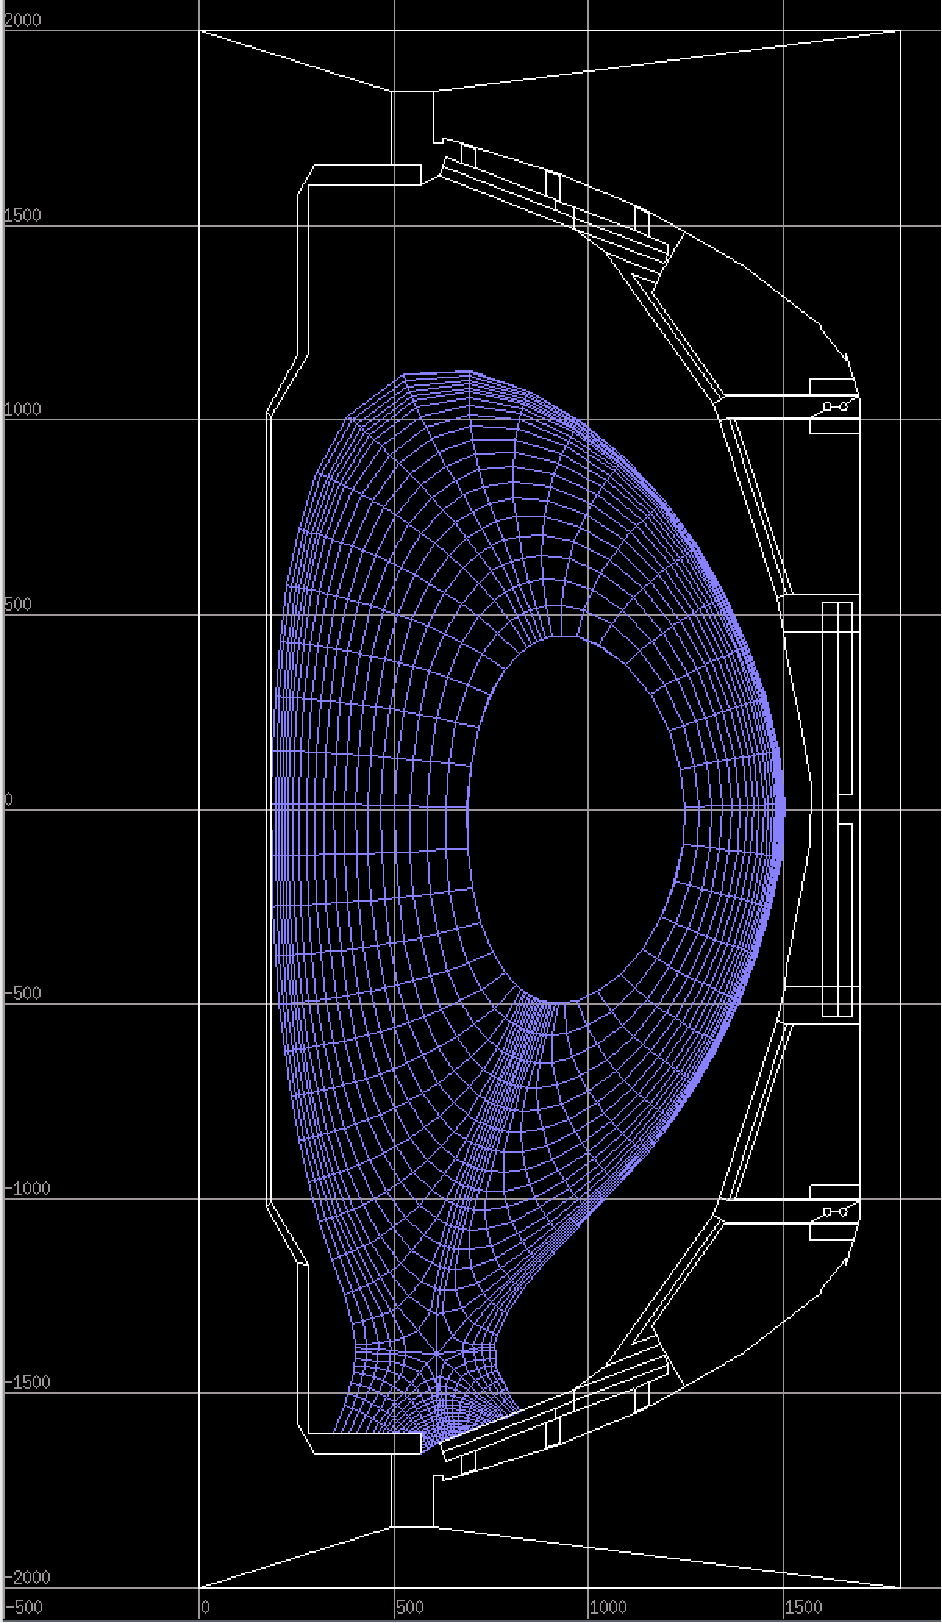
\includegraphics[height=12.0cm]{nstx_22_dg.pdf}}
\else
  \centerline{
\includegraphics[height=12.0cm]{nstx_22_dg.epsi}} 
\fi
\end{figure}

This is the user's manual for the \verb!DG! geometry definition
code. Its primary objective is to simplify the specification of the
geometry, and other input data, required for the simulation of the
boundary of magnetic fusion devices.  The most straightforward application
of the code is to divertor tokamak geometries (having one or two 
X-points), although in principle other magnetic configurations
are possible.  The flexible design of \verb!DG! allows its
output to be used with multiple magnetic fusion simulation codes,
including \verb!B2-Eirene! and \verb!DEGAS 2!.  In fact, some
of the objects defined in \verb!DG! and described in this manual
may be desigined specifically for use by these codes.

\section{Introduction}

This is the user's manual for the \verb!DG! geometry definition
code. Its primary objective is to simplify the specification of the
geometry, and other input data, required for the simulation of the
boundary of magnetic fusion devices.  The most straightforward application
of the code is to divertor tokamak geometries (having one or two 
X-points), although in principle other magnetic configurations
are possible.  The flexible design of \verb!DG! allows its
output to be used with multiple magnetic fusion simulation codes,
including \verb!B2-Eirene! and \verb!DEGAS 2!.  In fact, some
of the objects defined in \verb!DG! and described in this manual
may be desigined specifically for use by these codes.

\subsection{Purpose of DG}

\verb!DG! is the backbone of the {\bf Interactive Graphical Interface}
package. It allows user to visualize the model geometry, to modify it,
and to specify the geometry-related data necessary for a grid
generator and modelling codes. It was originally designed to alleviate
transfer of the divertor geometry from the CAD system to the 
\verb!B2-Eirene! code package. However, it has proved to become a powerful
tool of more general purpose, allowing one, e.g., to specify
arbitrary shape of the divertor structures, to check visually the
quality of the computational grids produced by a mesh generator, to
analyse the error messages from the Monte-Carlo routine, to assess
easily the compatibility of the plasma equilibrium used in the
calculations and the wall geometry of the machine, etc. It can also
be very efficient as a sort of very simple drawing program to design
the problem geometry from scratch, and not only for \verb!B2-Eirene!. With
use of this code, the most boring and time-consuming part of the
preparatory work necessary for the edge plasma modelling in a
realistic geometry, becomes really a pleasure. Try it and see
yourself!

\subsection{DG objects}

\subsubsection{External objects}

The external objects are the files which \verb!DG! imports or exports. They
normally have default extensions by which are used by the code when
displaying the lists of files in the I/O control windows. The
following table gives a brief description of the files used in \verb!DG!.

\begin{center}
    \begin{longtable}{|l|p{10cm}|l|}
    \hline
    \multicolumn{3}{|l|}{\small\sl continued from previous page} \\
    \hline          & {\large\bf Description} & {\large\bf Extension} \\
    \hline \endhead
    \hline          & {\large\bf Description} & {\large\bf Extension} \\
    \hline \endfirsthead
    \hline
    \multicolumn{3}{|l|}{\small\sl continued on next page} \\
    \hline \endfoot
    \endlastfoot
{\bf Input files:}&                                      &           \\ \hline
\verb!DG! model     & All the data relevant to the model   & .dg \\
Template     & Geometry data from CAD drawing or other source
                                                    & .ogr \\
Equilibrium  & Values of the poloidal magnetic flux on a regular grid
                                                    & .equ \\
Mesh         & The computational grid to be used by \verb!B2-Eirene!
                                                    & \\ \hline
{\bf Output files:}&                                      & \\ \hline
\verb!DG! model     & All the data relevant to the model   & .dg \\
Output file  & Specification of the \textit{elements} and some other 
information - to be used by the interface routines producing 
the input files for \verb!B2-Eirene!                & .dgo \\
Targets file & Specification of the \textit{targets} - to be used by the 
interface routines producing the input files for \verb!B2-Eirene! and \verb!Sonnet! or \verb!Carre!
                                                    & .trg \\
Structure file&Specification of the structures - to be used 
by the interface routines producing the input files for \verb!Sonnet! or \verb!Carre!
                                                    & .str \\ \hline

{\bf Configuration file:}&                                & \\ \hline
              & The file containing information on the \verb!DG! \textit{layers} and 
\textit{variables}. 
                                                    & .dgc \\
    \hline
    \caption{DG external objects}
    \label{tab:dgexternalobjects}
  \end{longtable}
\end{center}

\subsubsection{Internal objects}
\label{sec:internalobjects}

The internal objects are those with which you deal when working with \verb!DG!. 

\begin{center}
    \begin{longtable}{|l|p{12cm}|}
    \hline
    \multicolumn{2}{|l|}{\small\sl continued from previous page} \\
    \hline {\large\bf Objects} & {\large\bf Description} \\
    \hline \endhead
    \hline {\large\bf Objects} & {\large\bf Description} \\
    \hline \endfirsthead
    \hline
    \multicolumn{2}{|l|}{\small\sl continued on next page} \\
    \hline \endfoot
    \endlastfoot
{\bf Drawing objects}&             \\
Points               & 
Just points (displayed as red squares) which can be used to create
\textit{elements} or for diagnostic purpose.
\\
Irregular points
&  
Every point which is not regular. A regular point connects
exactly two \textit{elements} having the same orientation (see
\textit{External normals})
\\
Elements
& 
Straight line segments (displayed in bright white) connecting
\textit{points}. Normally, they represent material surfaces
in the neutral transport code (``additional surfaces''
in \verb!Eirene! parlance). You can edit elements (create,
delete, split, join, change orientation, etc.) and assign
\textit{variables} to them.
\\
Surfaces
& 
Contours of constant poloidal flux 
(displayed
in yellow) computed from \textit{equilibrium} data. You can create,
move, and delete them. The surfaces allow you to specify the
requirements on the radial mesh for the mesh generator
(\verb!Sonnet! or \verb!Carre!), and also to
check the compatibility of your wall structures with the magnetic
configuration.
\\
Grid points
& 
Points on the separatrix which represent partition of the magnetic
surfaces in different regions for the grid generator
(\verb!Sonnet! or \verb!Carre!). They are
displayed as dashes in magenta, the separatrix being drawn in red.
\\
Separators
& 
Straight line segments (displayed in cyan) connecting the outer nodes
of the computational \textit{mesh} with surrounding \textit{structure}. The separators
also represent additional surfaces, but you can only re-position their
outer edges. Their purpose is separation of \textit{additional cells} - in
terms of \verb!Eirene!. As of V. 1.4 of \verb!DG!, ``separators'' have been temporarily 
disabled. \\
Sources             &
Special points which can be grouped together (displayed as white
asterisks). They can be used to specify the point sources of neutrals,
- and also in calculation of radiation load onto the first wall. \\
Equilibrium         &
A simple visualisation of the equilibrium data - red and blue dashes
corresponding to negative and positive, respectively, 
values of the poloidal magnetic flux. \\
Mesh                &
Computational mesh, displayed in blue, produced with a grid generator 
(\verb!Sonnet! or \verb!Carre!) and imported into \verb!DG!. 
Allows you to check the quality of the mesh and
to make the necessary corrections to the input data for the grid
generator. \\
Chords              &
Straight line segments representing the \verb!Eirene!
and \btwoplot diagnostic chords. \\
Cells               &
Regions outside the computational mesh surrounded by the elements,
separators, and the mesh edges (\textit{additional cells} - in terms of
\verb!Eirene!). \\
External normals    &
Are displayed as magenta dashes and depict the orientation of the elements. They 
point to the right as you move from the beginning to the end
of an element. This is the direction of the external normal in terms
of \verb!Eirene!. \\
Template            &
Imported graphics from external source (e.g. from CAD drawing or from
old \verb!Eirene! input file). The template is displayed in cyan, and it can
be converted into \textit{elements}. \\
Axes                &
Coordinate axes which can be displayed on the drawing. \\
Grid                &
Coordinate grid which can be displayed on the drawing. \\
X-point             & 
The X-point of the magnetic equilibrium; it effectively separates the divertor
from the core plasma.  In double-null configurations, there are two
X-points which may or may not be on the same flux surface.
The code must be told the topology of the equilibrium (see \textit{topology})
in order to locate the X-points.
This must be done before specifying \textit{surfaces} or 
\textit{grid points}.
 \\
Topology
 &  
The topology of the magnetic separatrix.  A set of commonly used topologies
is provided with \verb!DG!.  Once the \textit{equilibrium} and topology have been
imported, the code will attempt to locate the X-point(s); if successful, the
separatrix (or separatrices) will be drawn in red.
 \\
{\bf Additional data}&    \\
Variables           &
Typically used to associate various pieces of data with the \textit{elements}.
This information can be then passed to 
other codes via the output files.
 \\
 
Layers
 &  
Groups of variables.
 \\
 
Targets
 &  
Bound the \textit{surfaces} in the poloidal direction, and thus must be
specified for the grid generator.  They are thus analogous to the 
actual divertor targets in a tokamak.
 \\
Structure
& 
Bound the \textit{surfaces} in the radial direction.  They are thus
analogous to the walls of the vacuum vessel in a tokamak.
\\
Target edges
&
The elements which should be reconnected to the corresponding corners
of the calculational mesh in order to avoid mismatches of the mesh
and the targets in the Monte-Carlo calculations. \\
    \hline
    \caption{DG internal objects}
    \label{tab:dginternalobjects}
  \end{longtable}
\end{center}


\section{Using DG}

\subsection{Starting DG}

\index{DG, starting}
To start \verb!DG! with a blank window, type:
\begin{verbatim}
  dg &
\end{verbatim}
at the UNIX prompt.

To start \verb!DG! with an existing model (or several models) loaded, type:
\begin{verbatim}
  dg <filename.dg> [...] &
\end{verbatim}

After you start \verb!DG!, the main window will appear.

\subsection{Main window}

After you start \verb!DG!, the main window appears. It has four areas: menu bar, toolbar, work area and the message line. 

\subsubsection{Menu bar}

\index{DG, menu bar}
The menu bar gives you access to the most of the \verb!DG! functionality. It
contains several buttons, which can be used to open the corresponding
menus by clicking the left mouse button on it. Every menu can be torn
off and left on the screen after opening it. In order to do
this, just click at the dashed line at the top of the menu window. In this document,
we will show menu items in {\tt typewriter} font.

The following menus are available at present:

\begin{description}
  \item[File] You use this to start a new model, to work with
external objects (to save or open the model; to import templates,
equilibrium files, topologies, 
or computational meshes; to produce the output files
which are used for generation of the input files for computational
codes), or to quit the application.
  \item[Edit] Allows you to perform some global operations,
such as recovering from errors, selecting and de-selecting all
elements, creation or removal of groups of objects, and shift or
rotation of the picture.
  \item[View] Here you can control the overall view of the
model and specify which objects should be
visible on the screen.
  \item[Commands] Allows you to perform global commands on
the model such as converting 
a \textit{template} to \textit{elements} and 
renumbering the elements.
  \item[Variables] You will use this to specify
additional geometry-related information for the output files (eg.,
location of targets, boundary conditions for the Monte-Carlo routine,
etc.).
  \item[Options] From this menu you can tailor the main window
and operating mode
to fit you preferences. It also allows you to customize the DG
variables \textit{(only for experienced users!).}
  \item[Window] Allows you to open more windows with
different views of the same model, to close the current window, to open
a window showing the statistics for the model, and to open the
{\tt Toolbox}.
  \item[Help] This is the way to get some online help on DG and
to identify its current version.
\end{description}

\subsubsection{Toolbar}

\index{DG, toolbar}
The toolbar allows you to assign different \textit{tools} to each of the mouse
buttons. It has 3 option menus-for the three buttons- that contain the
list of available tools. If your mouse has less than three buttons,
then only the leftmost option menu(s) are activated.

\subsubsection{Work area}

\index{DG, work area}
The work area is the area where the drawing is displayed. Here you can
move around the drawing, and you can use \textit{tools} to edit it. The
work area can optionally display coordinate axes and coordinate grid
to simplify positioning of objects.

\subsubsection{Message line}

\index{DG, message line}
The message line is located below the work area. It is used to display
error messages and information on the objects. Error messages are
sometimes displayed in an error box instead of the message line, and
in this case you must click {\tt OK} to proceed.

\subsection{Using tools}

\index{DG, using tools}
{\bf Tools} are used to perform actions in the work area. They allow
you to create, move, modify, or remove objects, to query information
on the objects and to move around the drawing.
In this document, we will indicate tools in \textit{\texttt{italic
typewriter}} font.

A tool \textit{must} be assigned to a mouse button in order to be used. You can
select the tool to be assigned to each of the mouse buttons either
from the toolbar, or from the {\tt ToolBox} (accessible from the {\tt Window} menu). There is one
small difference between these two options. Operating with the
toolbar, only the left mouse button should be used to select the tools associated
with the three mouse buttons,
On the other hand, when working with the {\tt Toolbox}, 
a tool is associated
with a given mouse button by clicking that button on the tool.

To use a tool, move the mouse pointer into the work area and depress
the mouse button to which the tool has been assigned. Then, you can
optionally drag the mouse. To complete the mouse drag, release the mouse button
with the mouse pointer still inside the work area. To cancel the
action associated with the drag, 
move the mouse pointer out of the work area and release the
mouse button.

Some tools require you to 'select' an object. To select an object,
move the mouse pointer to the object and depress the mouse button. The
object selected will be highlighted in another colour. The \textit{green} colour
means OK, while the \textit{red} one indicates that the operation cannot be
done. Normally, some explanatory text appears in such cases on the
message line.

\subsection{Using Undo}

\index{DG, undo}
You can reverse the effect of almost any operation by issuing the
{\tt Edit|Undo} menu command. You can also reverse the effect of {\tt Undo}
command by {\tt Edit|Redo}. The \verb!DG! keeps track of practically all the
operations you did starting from opening the window, and thus you can
recover from almost all the errors you could make in the coarse of the
model editing. To reverse the effect of all the Undo commands you
issued, use {\tt Edit|Redo} all.

\section{Working with models}

\subsection{Opening an existing model}

\index{DG, open}
To open an existing \verb!DG! model from \verb!DG!, use the {\tt File|Open...} menu
command. A dialog box will appear prompting you for a filename. You
can either select a file from the list or type the filename in the
edit field. Then press {\tt Ok}. A new window displaying the selected model
will be opened. If you issue the {\tt File|Open...} command
immediately after starting \verb!DG!, the file will be loaded in the current
window. If an error happens, the error box appears. Press {\tt Ok} to
close the error box.

To start \verb!DG! with an existing model loaded, specify the filename on the
\verb!DG! command line. If you specify multiple filenames, \verb!DG! will open a
separate window for each model.

\subsection{Creating a new model}

\index{DG, new}
To create a new, empty model with \verb!DG!, use the {\tt File|New} menu
command. A new blank window will be opened.

When you start \verb!DG! without parameters, the \verb!DG! window is blank.

\subsection{Saving a model}

\index{DG, save}
To save a model, use the {\tt File|Save} menu command. A dialog
box will appear prompting you for a filename. If the current model has
a filename assigned to it, this filename will appear in the edit
field.  In order to save the model under a different name, or to save
the newly-created file, you should either enter the new name in the
edit field, or select a name from the list (to overwrite an existing
file).  After that, press {\tt OK}. An autosave feature
automatically saves a version of the file with a '\verb!~!'
appended to the name every 5 minutes (see 
{\tt Options|Save interval }); of course, a new file must
be saved before this can work.  If you need to use this file (e.g.,
in the event that \verb!DG! crashes unexpectedly), you should rename this
file to remove the '\verb!~!'.

\subsection{Quitting DG}
\index{DG, quit}

To quit \verb!DG!, you must close all windows.

To close a window, issue the {\tt Window|Close} menu command. You can
also use the window manager to close a window. 
You can also use the window manager to close a window
click the ``X'' at the top right of the menu. With Motif Window
Manager, simply double-click the system menu. If you've made changes
to the model in this window, a warning box will appear. Select
{\tt Save} to save the model. Select {\tt Discard} to close the
window without saving changes. Select {\tt Cancel} to leave the
window open.

To close all windows, use the {\tt File|Exit program} menu command.

There is a caveat in the current version of \verb!DG! that iconified windows
containing unsaved work are not de-iconified after these commands. You
will have to de-iconify them manually in order to see their warning
boxes. All other iconified windows will be closed without problems.

\section{Working with elements}

\subsection{Converting a template}

\index{DG, converting a template}\index{DG, template}
It is often more convenient to convert a template into a set of
elements and then edit them to suit your needs, rather than to define
all elements by hand.

First, you should import the template. Choose the
{\tt File|Template...}  menu command. A dialog box will appear
prompting for a filename, similar to that for opening \verb!DG! files. After
importing the template, choose {\tt View|Picture} view to adjust the
zoom factor in order to make the template visible. Enable
{\tt View|Axes} and {\tt View|Grid} to display the coordinate
system.

\verb!DG! lets you adjust the template position by moving it by a fixed
distance and/or rotating it 90 degrees around (0,0). To adjust the
position, choose the {\tt Edit|Move/Rotate...} menu command. A dialog
box will appear. Enable the {\tt Template} check box. To move the
template, enter $X$- and $Y$-increments and press {\tt Move}. To rotate,
press {\tt Rotate}. If the template moves out of sight, again choose
{\tt View|Picture} view. Press {\tt Close} when done.

To convert the template into a set of elements, choose
{\tt Commands|Convert} template.

Note that after the conversion, the template remains visible. This is
convenient for editing elements, because the difference from the
original template is visible. You can hide or display the template by
disabling or enabling {\tt View|Template}. To unload the template
permanently, choose {\tt Edit|Delete|Template}.

Elements produced in this manner are sometimes improperly connected or
have wrong external normals. Manual editing of the elements may be required to 
remedy these problems. 

\subsection{Creating elements manually}

There are several tools for creating new elements.

\index{DG, adding elements}
Use {\tt Add element} to create the first element or to attach an element to
a pre-defined point. Move the mouse pointer to the starting point and
press the mouse button. Then move the pointer to the ending point and
release the mouse button.

\index{DG, splitting elements}
Use {\tt Split element} to split an element into two. Select an
element. It will split into two. Drag the newly created point to the
desired location and release the mouse button.

\index{DG, connecting points}
Use {\tt Connect points} to create an element between two pre-defined
points. Select the first point, move the mouse cursor to the second
one and release the mouse button. You cannot create more than one
element between the same two points.

You can also use the {\tt Edit|Create|Point...} menu command to
create points that will be later connected using the {\tt Connect points}
tool. A dialog box will appear. Enter the desired coordinates and
press {\tt Create}. The dialog box will remain on the screen, allowing you
to create more than one point without re-opening it. To close the
dialog box, press {\tt Cancel}.

\subsection{Editing elements}

There are several tools for modifications of existing elements.

\index{DG, deleting elements}
Use {\tt Delete} to remove an element. Select the element and release the
mouse button.

\index{DG, joining elements}
Use {\tt Join elements} to join two adjanced elements into one
(reverse effect of {\tt Split element}). Select the point between the
elements and release the mouse button. You can only join elements
around a regular point. There must be exactly two elements attached
and their external normals must point to the same direction.

\index{DG, moving elements}
Use {\tt Move/Stretch} to move a point with all attached elements.
Select the point and drag it to the new location. Then release the
mouse button.

\index{DG, repositioning elements}
Use {\tt Reposition} to attach one end of an element to another
point. Select the element near one of its ends, move the mouse
pointer to another pre-defined point and release the button.

\subsection{Changing external normals}

\index{DG, changing external normals}
Having the external normals of adjacent elements aligned permits them
to be easily marked; some operations also require the normals of
adjacent elements to be aligned (i.e., for the points involved in the
operation to 
all be regular). 

To display or hide external normals, enable or disable
{\tt View|External normals}.

Use the {\tt Reverse normals} tool to change directions of external
normals. Select an element to change its normal. Moving the mouse
pointer to adjacent elements will force their normals to point to the
same direction as that of the first element. Release the mouse button
to end the action.

\subsection{Renumbering elements}

\index{DG, renumbering elements}
Each element has a unique integer label associated with it. These 
determine the order in which the elements are written into the output file. This
feature is very useful for debugging. \verb!DG! uses an internal counter to
assign these numbers. Each time the user creates an element, the
counter is incremented by one and its value is used as the element
number. However, when the user deletes an element, the remaining elements are
not renumbered and the counter is not decremented. Since many unused
numbers consume disk space and may slow down programs that use \verb!DG!
output, these unused element numbers should be periodically eliminated. Renumbering elements is
absolutely safe except when you are doing some debugging and need
these numbers to identify elements in the output file.

\index{DG, diplaying numbers}\index{DG, hiding numbers}
To display or hide element numbers, enable or disable {\tt View|Display|Numbers}.

To count unused numbers, choose {\tt Window|Statistics} in order to
display information about the current file. The 'unused numbers' entry
contains this count.

\index{DG, eliminating unused numbers}
To eliminate unused element numbers, choose {\tt Commands|Renumber elements}.

\section{Controlling how objects are displayed}

\subsection{Changing the zoom factor and location}

\index{DG, zoom}
You can use the {\tt Zoom} tool to move around the drawing and to change the
zoom factor. You can also use commands from the {\tt View} menu.

To move around with the {\tt Zoom} tool, press and release the mouse
button anywhere in the work area without moving the mouse. The work
area will be adjusted so that the location where the button was
pressed is moved to the centre. Alternatively, you can press
Shift+mouse button, move the mouse pointer and release the button. The
work area will be adjusted so that the location where the button was
pressed is now shown where the button has been released.

To change the zoom factor with the {\tt Zoom} tool, press the mouse
button, move the mouse in order to draw a rectangle around the area to
be shown in the work area. Then, release the mouse button. Note that
the area actually shown may be enlargened in order to preserve the
aspect ratio.

The {\tt View|Zoom in} command increases the zoom factor.

The {\tt View|Zoom out} command decreases the zoom factor.

The {\tt View|Picture view} command adjusts the zoom factor and
location so that all objects fit into the work area. This command
ignores objects that are hidden because of settings in the {\tt View} menu.

The {\tt View|Selection view} command adjusts the zoom factor and
location so that all marked objects fit into the work area.

\subsection{Hiding and displaying objects}

\index{DG, hiding objects}\index{DG, displaying objects}
Toggle buttons in the {\tt View} menu let you hide or display the coordinate
system and various kinds of objects.

Note that you cannot select an object that is not displayed. In
particular, you can only select points that are displayed (a small
square is drawn around the point). The {\tt View|Points} setting
controls the display of points. When it is disabled, the
{\tt View|Irregular points}  setting controls the display of
irregular points. It is convenient to display only irregular points
while correcting a converted template, because irregularities can be
seen very easily.

\section{Rotating the view}
\label{sec:rotateview}\index{DG, rotating view}

The display may now be viewed at any angle of rotation. The user may
specify the desired angle by using the 
Rotate tool, the commands under the 
{\tt View|Rotate} menu,
or the equivalent 
keyboard shortcuts to increment (``Ctrl+(''), decrement (``Ctrl+)''), or
zero the angle ({\tt Rectify}, 
shortcut ``Ctrl+C''); see Fig.~\ref{fig:rotate30}. 
The rotation does not affect the
underlying structures being displayed, but only the drawing procedure.
The {\tt Previous view} command will undo rotations.
Rotations are saved starting with file format version 115.  
Files of older formats are still compatible; the default angle will be 0.
Note that the Picture View command 
({\tt View|Picture View}) zeroes
the rotation angle.

\begin{figure}[hbtp]
\ifpdf 
  \centerline{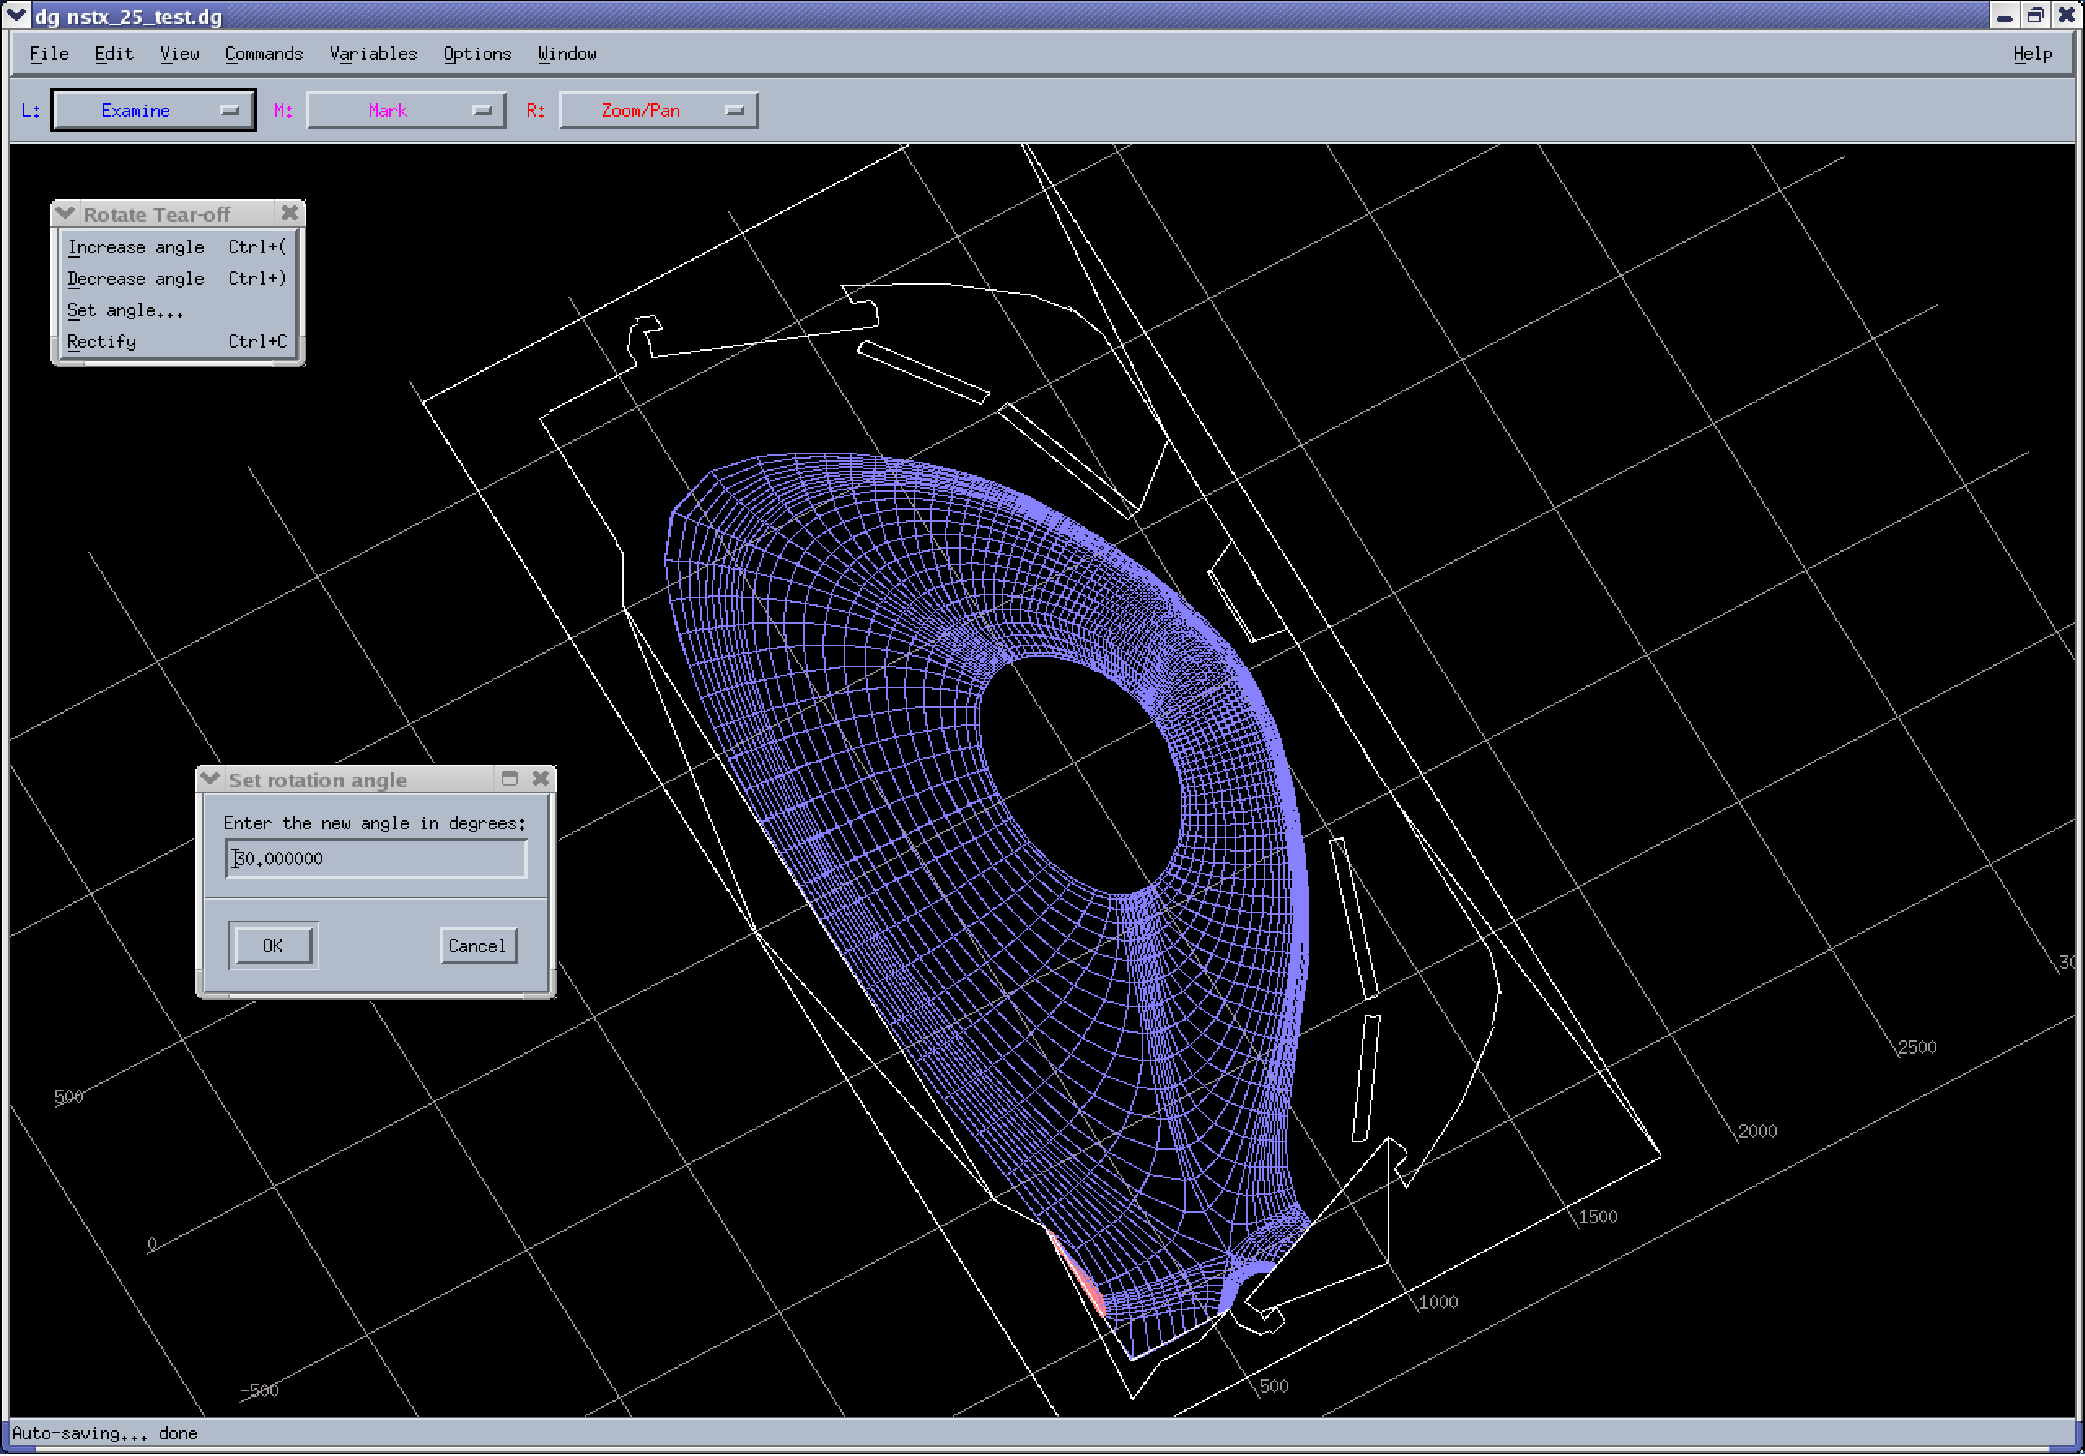
\includegraphics[width=15.0cm]{rotation_30.pdf}}
\else
  \centerline{
\includegraphics[width=15.0cm]{rotation_30.epsi}}
\fi
\caption{Demonstration of a rotated view with associated dialog box and tear-off menu.}
\label{fig:rotate30}
\end{figure}

\section{Stretching and shrinking the view}
\label{sec:stretchview}\index{DG, stretching and shrinking view}

The aspect ratio may be ``unlocked'' by enabling the 
{\tt View|Mode|Stretch} button.
In {\tt Stretch} view mode, the
{\tt View|Stretch/Shrink}
menu item becomes active (see Fig.~\ref{fig:stretch2x5y}), 
and the user may use these tools to
stretch or shrink the $x$ and $y$ axes. 
To stretch or shrink the current view by a factor of 2, 
use the first four buttons of this menu.  The keyboard shortcuts are
``Ctrl+Shift+H'' to stretch horizontally (in the $x$ direction), 
``Ctrl+H'' to shrink horizontally, ``Ctrl+Shift+V'' to stretch vertically
(in the $y$ direction), and ``Ctrl+V'' to shrink vertically.  
Precise stretching or shrinking factors can be specified with the
{\tt Stretch \ldots} dialog.  The aspect ratio can be reset
with the {\tt Justify} menu item.
Additionally, zooming with the highlighted
rectangle now zooms to display exactly the contents inside the rectangle,
rather than expanding to ensure the proper aspect ratio. Disabling
{\tt Stretch} mode redraws the display with proper aspect ratio and
preserves the ratio in future changes of view.

\begin{figure}[hbtp]
\ifpdf
  \centerline{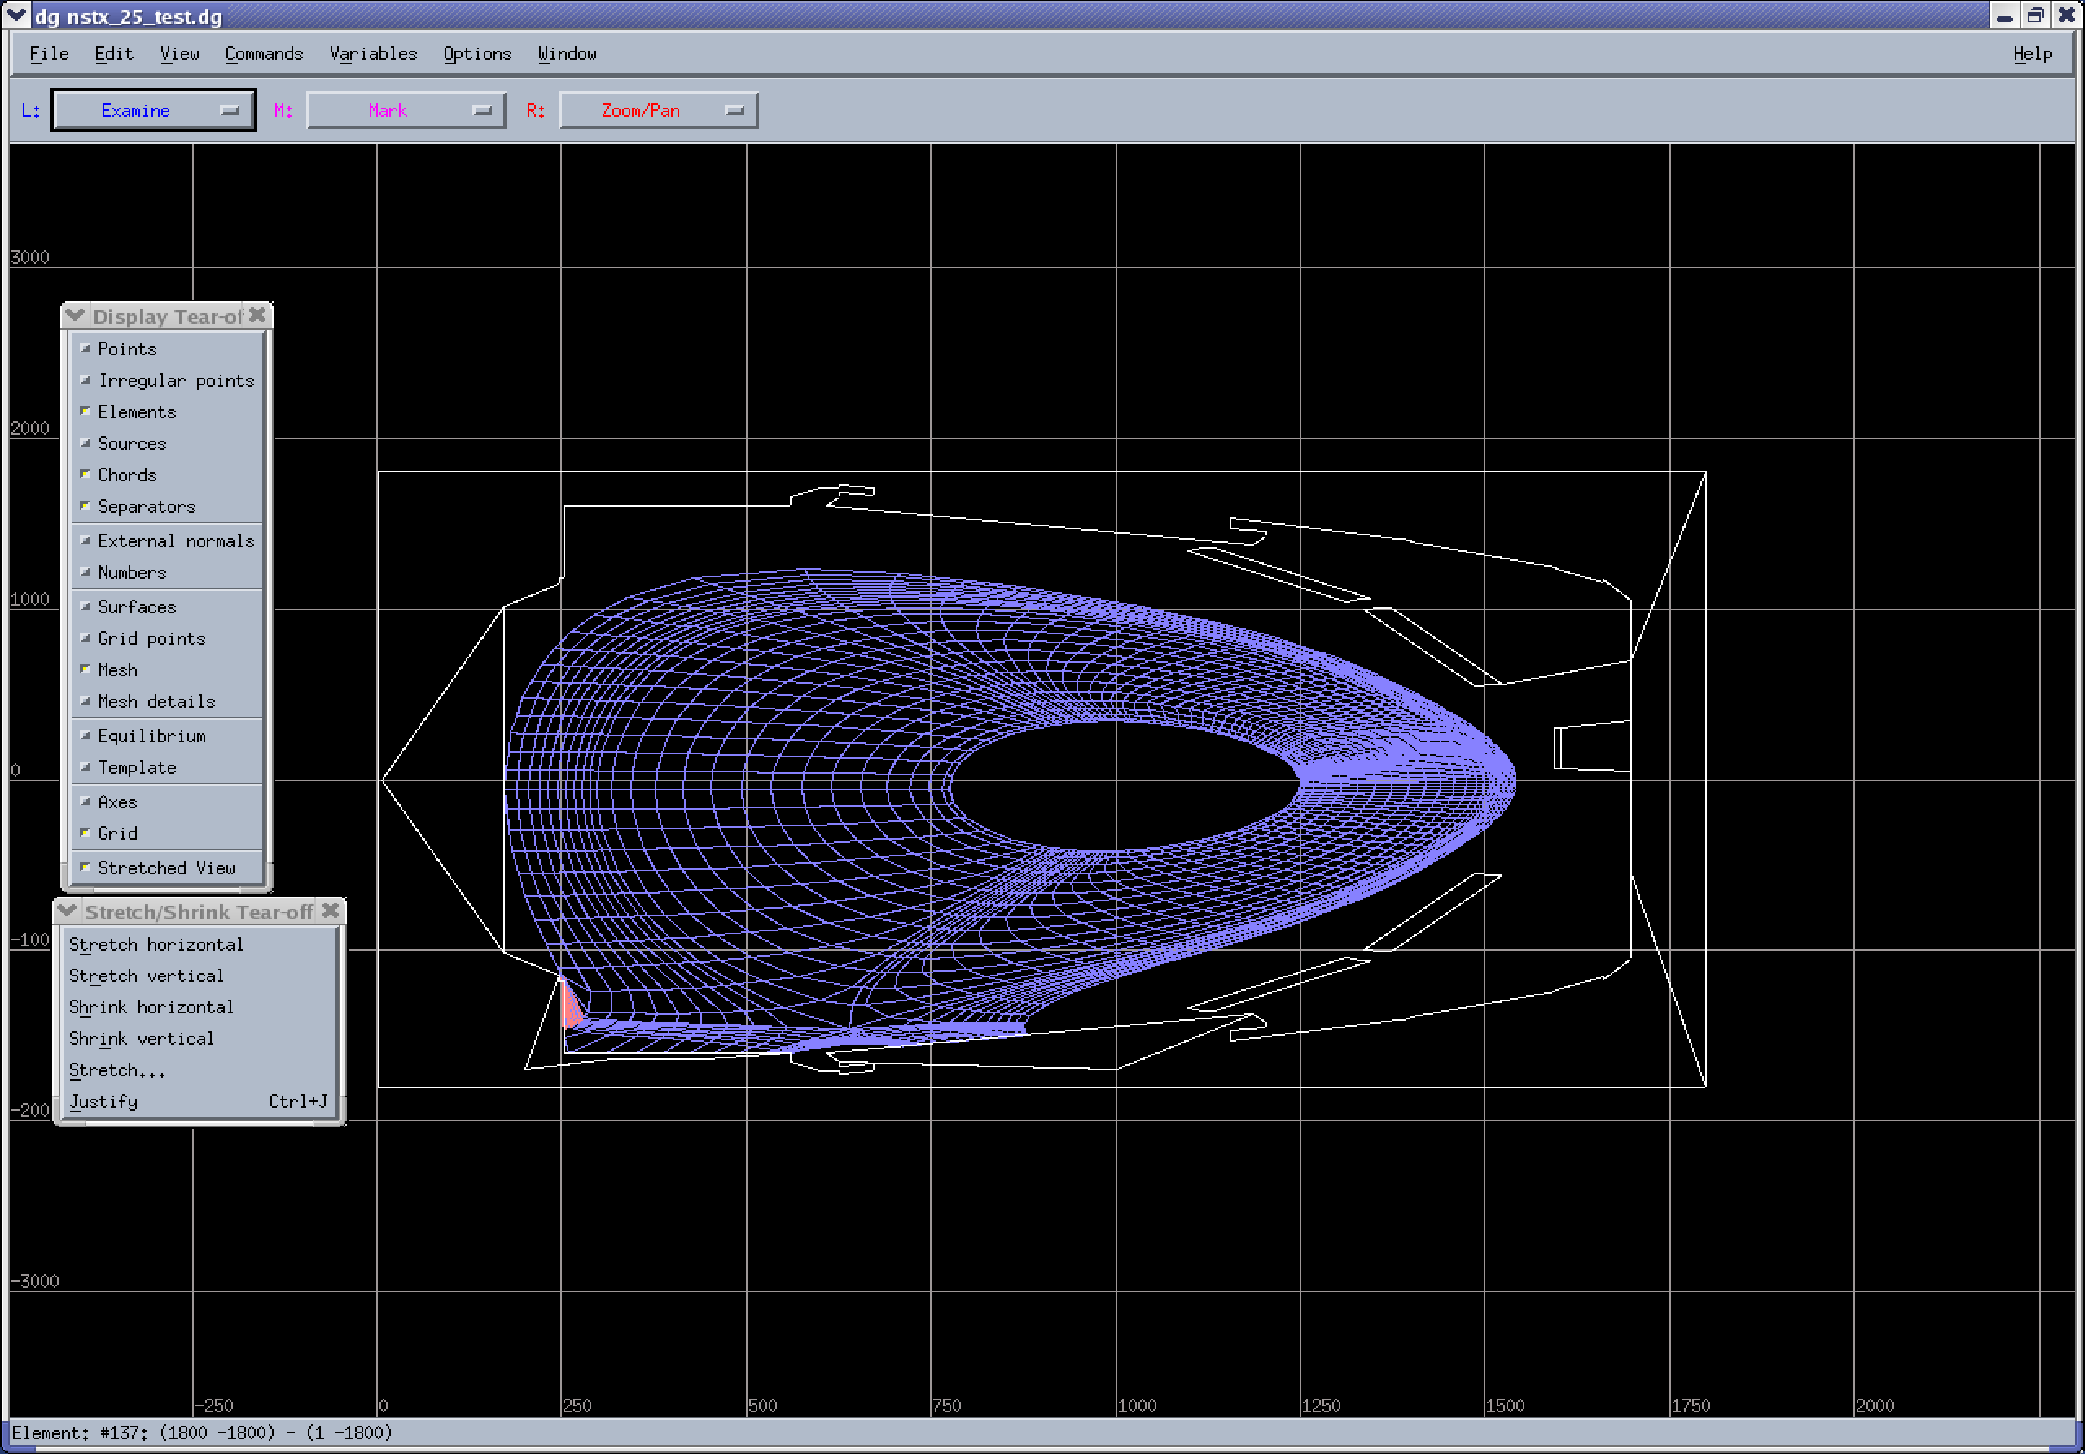
\includegraphics[width=15.0cm]{stretch_2x_5y.pdf}}
\else
  \centerline{
\includegraphics[width=15.0cm]{stretch_2x_5y.epsi}}
\fi
\caption{Demonstration of the variable aspect ratio capability along with
the associated tear-off menu.}
\label{fig:stretch2x5y}
\end{figure}

The {\tt Stretch}
tool works a little differently since it can stretch either
horizontally or vertically.  If the mouse is within 45$^{\circ}$ of an
imaginary horizontal line through the center of the window, a mouse drag
will stretch or shrink the view in the horizontal direction.  Likewise, if the
mouse is within 45$^{\circ}$ of the vertical line through the center of
the window, a mouse drag stretches or shrinks in the veritical 
direction.  If {\tt Stretch} mode 
is disabled, the {\tt Stretch} tool does
nothing.

Note that the {\tt Picture View} command 
({\tt View|Picture View}) resets
the aspect ratio, but does not disable {\tt Stretch} mode.

% We still have Alan's description of the application of the stretch and
% rotation capability to manipulate mesh cells. Suggest putting it later
% with mesh related stuff or perhaps in an appendix.
\section{Top-down view}
\label{sec:topdownview}\index{DG, top-down view}

To facilitate visualization and specification of chords 
with nonzero toroidal extent (see Sec.~\ref{sec:chords}), a view from above the
torus is now available via the
{\tt View|Mode|Top-down view}
button.  When this button is enabled, the main window depicts the view of the
present geometry looking down along the $y$ axis.  The elements in the
model are assumed to be toroidally symmetric.  In this view, the elements are
displayed as 48 (arbitrarily chosen) straight line segments.  The only
other objects currently displayed in this view are chords, although
working drawing procedures exist for all markable objects. Since displaying
every element in the model would likely result in confusion, the user
must select the specific elements to be depicted.  The variable
{\tt Top View Elements} has been defined for this purpose
({\tt Variables|Top View Elements}).
The appearance of chords (with some toroidal extent) can be toggled with
either {\tt View|Display|Chords} 
or {\tt View|Display|3dchords}.
As in the normal (poloidal) view, 
{\tt View|Display|Elements} toggles the appearance of elements in the top view.
Since top view was intended to be used only for chords, many tools are 
disabled in this mode.  Likewise, since top view uses the same 
screen coordinates as the normal view, it may be necessary to rezoom 
after switching between the two views.  
{\tt View|Picture View}
can be used for this purpose in either mode. 

\section{Working with magnetic surfaces and grid points}

\subsection{Equilibrium conversion and manipulation}
\label{sec:equtrn}\index{equtrn}

The \$\verb!SOLPSTOP/modules/DivGeo/dg/equtrn!
directory has some utilities for converting between various
widely used formats for magnetic equilibrium files and for making minor
modifications to them.

The listings and documentation below may be out of date. The updated
documentation of the supported scripts is now to be found in
\$\verb!SOLPSTOP/modules/DivGeo/dg/equtrn/doxygen/refman.pdf!.

\subsubsection{d2d}
\index{d2d}\index{dg2dg}\index{DG, doubling resolution}

This is a script that invokes the \verb!dg2dg! executable.  Its sole
function is to double the resolution of a \verb!DG! equilibrium file.  To 
invoke it:
\begin{quote}
\texttt{d2d $<$filein$>$.equ $<$fileout$>$.equ}
\end{quote}

\subsubsection{d2e}
\index{d2e}\index{dg2ef}\index{DG, convert to EFIT equilibrium}

This is a script that invokes the \verb!dg2ef!
executable to convert a
\verb!DG! equilibrium file to the \verb!EFIT! format (specifically, the \verb!EFIT! ``g'' file).
This is invoked with (the file suffixes are recommended for clarity
and are not enforced):
\begin{quote}
\texttt{d2e $<$filein$>$.equ $<$fileout$>$.efit}
\end{quote}

Some older \verb!DG! files lack the magnetic field data needed for this conversion.
The default name for the file containing its value is 
\verb!field.snn! (i.e., using the above invocation).  
Alternatively, the name of the file containing the field can be 
specified as a third argument:
\begin{quote}
\texttt{d2e $<$filein$>$.equ $<$fileout$>$.efit $<$fieldfile$>$}
\end{quote}

\subsubsection{d2v}
\index{d2v}\index{dg2vr}\index{DG, convert to Carre equilibrium}

This is a script that invokes the \verb!dg2vr!
executable to convert a
\verb!DG! equilibrium file to the \verb!Carre! (or TdeV) equilibrium 
format.
This is invoked with (the file suffixes are recommended for clarity
and are not enforced):
\begin{quote}
\texttt{d2v $<$filein$>$.equ $<$fileout$>$.v}
\end{quote}

Some older \verb!DG! files lack the magnetic field data needed for this conversion.
The default name for the file containing its value is 
\verb!field.snn! (i.e., using the above invocation).  
Alternatively, the name of the file containing the field can be 
specified as a third argument:
\begin{quote}
\texttt{d2v $<$filein$>$.equ $<$fileout$>$.v $<$fieldfile$>$}
\end{quote}

\subsubsection{e2d}
\index{e2d}\index{ef2dg}\index{DG, converting from EFIT equilibrium}

This is a script that invokes the \verb!ef2dg!
executable to convert an \verb!EFIT! format (specifically, the \verb!EFIT! ``g'' file)
equilibrium to the format read by \verb!DG!. 
This is invoked with (the file suffixes are recommended for clarity
and are not enforced):
\begin{quote}
\texttt{e2d $<$filein$>$.efit $<$fileout$>$.equ}
\end{quote}

\subsubsection{n2d}
\index{n2d}\index{nn2d}\index{nk2dg}\index{DG, converting from Naka equilibrium}

This is a script that invokes the \verb!nk2dg! 
executable to convert an equilibrium in the
``Naka'' format
to the format read by \verb!DG!. 
This is invoked with (the file suffixes are suggested for clarity
and are not enforced):
\begin{quote}
\texttt{n2d $<$filein$>$.nk $<$fileout$>$.equ}
\end{quote}

\subsubsection{rps}
\index{rps}\index{risepsi}\index{DG, shifting flux values}

This is a script that invokes the \verb!risepsi! executable. 
Its sole
function is to increase the poloidal flux values in the
\verb!DG! equilibrium file by the specified amount.  To 
invoke it:
\begin{quote}
\texttt{rps $<$filein$>$.equ $<$fileout$>$.equ $<$increment$>$}
\end{quote}

\subsubsection{v2d}
\index{v2d}\index{vr2dg}\index{DG, converting from Carre equilibrium}

This is a script that invokes the \verb!vr2dg! 
executable to convert an equilibrium in the \verb!Carre! (or TdeV) format
to the format read by \verb!DG!. 
This is invoked with (the file suffixes are recommended for clarity
and are not enforced):
\begin{quote}
\texttt{v2d $<$filein$>$.v $<$fileout$>$.equ}
\end{quote}

By default, this script will look for the value of the magnetic field
in a file \verb!field.snn!. 
Alternatively, the name of the file containing the field can be 
specified as a third argument:
\begin{quote}
\texttt{v2d $<$filein$>$.v $<$fileout$>$.equ $<$fieldfile$>$}
\end{quote}

\subsubsection{cropequ}
\index{cropequ}\index{DG, crop equilibrium}

This is an executable (no corresponding script) that crops a
\verb!DG! equilibrium file.  The code is invoked with:
(the file suffixes are recommended for clarity
and are not enforced):
\begin{quote}
\texttt{cropequ $<$filein$>$.equ $<$fileout$>$.equ}
\end{quote}

The code will print out the dimension and spatial extent of the input
equilibrium grid then request the values for the output grid in the
order: number of radial grid points, minimum radius, maximum radius,
number of vertical grid points, minimum vertical coordinate, 
maximum vertical coordinate.  The maximum number of grid points is 257
(can be increased via a parameter statement in the code).  The code
will requires the requested spatial extent to lie within that of the
input grid.  If it does not, the offending parameter is reset to
match the corresponding value from the input grid.

\subsubsection{prinequ}
\index{prinequ}\index{DG, print equilibrium}

This is an executable (no corresponding script) that prints out the
contents of a \verb!DG! equilibrium file in tabular format.  The file 
is read from standard input and the result is sent to standard out.
So, the preferred invocation would be
(the file suffixes are recommended for clarity
and are not enforced):
\begin{quote}
\texttt{prinequ $<$ $<$filein$>$.equ $>$ $<$fileout$>$.txt}
\end{quote}

\subsection{Importing equilibrium}
\index{DG, equilibrium}\index{DG, importing an equilibrium}

An equilibrium file must be imported before defining any surfaces or
grid points.

To import an equilibrium file, choose {\tt File|Import|Equilibrium...} . A
dialog box will appear prompting for a filename. Select a file and
press {\tt Ok}.  Select {\tt View|Picture} view to make sure the
equilibrium grid is visible in the work area. Red colour represents
positive $\psi$ values, while blue represents the negative ones.

\subsection{Output mode}
\index{DG, output mode}

The detailed procedures for creating and editing surfaces and grid
points differ slightly for the \verb!Sonnet! and \verb!Carre! mesh generators.
So, before undertaking these tasks, the user should select the
appopriate output mode in {\tt Options|Output mode}.
Since only the \verb!Carre! code is distributed along with this manual,
only procedures pertinent to it will be described.

This dialog box also allows the user to determine which objects are
examined for consistency when \verb!DG!'s output is requested
(via {\tt File|Output...}).  Selecting all of these
checks is recommended.  Users should override them only if they are
aware of the consequences of the object in question being improperly
defined.

\subsection{Creating and editing surfaces}
\index{DG, surfaces}\label{sec:createsurfaces}

As was noted in Sec.~\ref{sec:internalobjects}, surfaces are drawn between
targets and are bounded by structures.  
The target related variables are single elements set using the
variables 
{\tt Variables|Inner edge of inner target}, etc.,
where the first ``inner'' and ``outer'' refers to the inner and outer edge
of the computational mesh, respectively, and the second to the
usual inner and outer divertor target.  There is an additional
set of targets available for double-null geometries; see:
{\tt Variables|Add|Extra targets for DN}.
The structures are set with the variable
{\tt Variables|Structure}.  There may be one or more
of these.

In \verb!Carre! mode, the user begins the process of surface creation by manually
creating the surface that will represent the innermost core surface
via the {\tt Add surface} tool.  
Just click it inside core plasma at the
desired location (the tool will not work anywhere else).
Its location can be altered via the {\tt Move}
tool.  It can only be deleted
by executing the {\tt Edit|Delete|Surfaces} command
(this deletes {\em all} surfaces).

The next step is to open the {\tt Create surface(s)...} dialog,
{\tt Edit|Create|Surfaces...} (see Fig~\ref{fig:createsurfacesfig}).
In \verb!Carre! mode, the user can only create multiple surfaces (i.e., the {\tt Single}
option will not work).  The {\tt Area} menu determines in which part
(topologically) of the equilibrium the surfaces will be drawn.  The number
of cells must be input manually.  The line graph in the dialog box is a
simple depiction of the relative spacing of the surfaces.  In \verb!Carre! mode,
only the {\tt Delta Law} is available.  In this case, the two parameters
{\tt Delta1} and {\tt Delta2} specify a quadratic function used to determine
this spacing  
(The deltas specify the relative normalized
difference between the levels of the
first two, and the last two surfaces).

While these parameters can be input directly, the preferred
means of setting them is to click and drag the black line in the graph to
achieve the desired spacing variation.  When the {\tt Create} button is
clicked, the surfaces will be generated with this spacing and drawn in 
\verb!DG!'s main window.  If a model has an existing set of surfaces that the
user wishes to tweak, click on one with the {\tt Examine} tool and then
click the {\tt <<} button in the {\tt Create surface(s)...} 
dialog; this will
import the parameters describing these surfaces.

\begin{figure}[hbtp]
\ifpdf
  \centerline{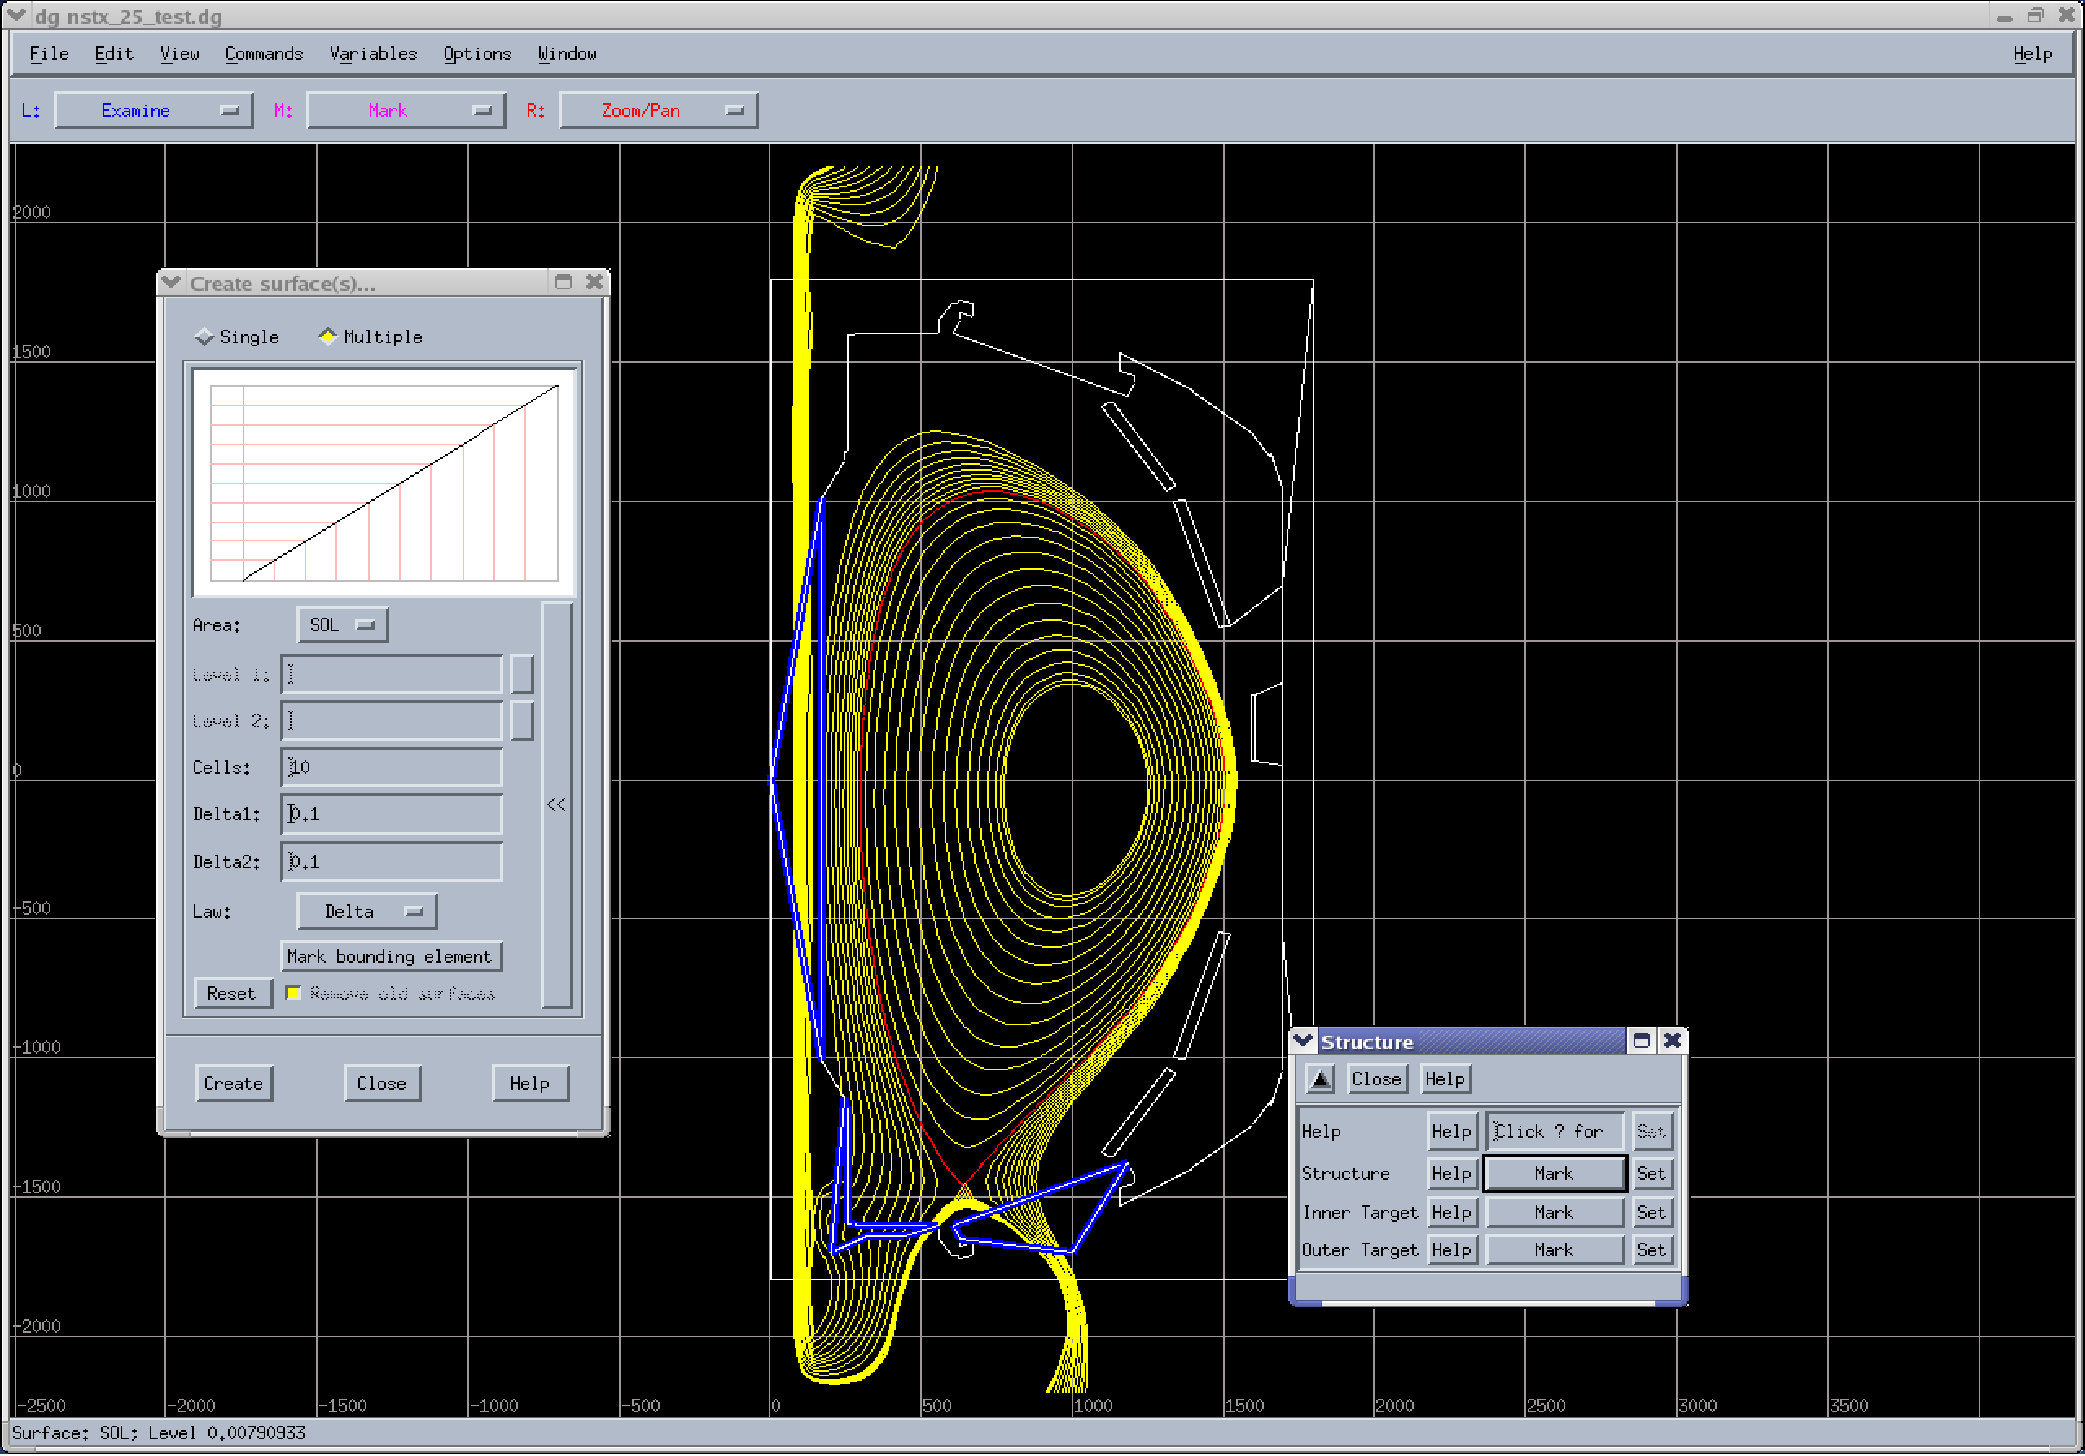
\includegraphics[width=15.0cm]{bde_structure.pdf}}
\else
  \centerline{
\includegraphics[width=15.0cm]{bde_structure.epsi}}
\fi
\caption{{\tt Create Surface(s)...} dialog with highlighted {\tt Structures}.}
\label{fig:createsurfacesfig}
\end{figure}

Note that the dialog will {\em not} enforce constraints on the number of
cells (e.g., that the number of core and PFR cells must be equal); the
user must check to be sure that all such constraints are satisfied.
\verb!Carre! will perform its own set of checks when invoked as well.

\verb!DG!'s algorithm for calculating the outermost flux surface level for unbounded
regions (e.g., PFR and SOL)
uses the {\tt Structure} and 
{\tt Inner / Outer targets} variables. The only
elements that the algorithm is aware of are those specified in the
{\tt Structure} variable, shown in Fig.~\ref{fig:createsurfacesfig}.
Additionally, the algorithm
recognizes at least two subsets of the structures, the ``targets'', which
consist of all closed loops in the structure on which elements in the 
{\tt Inner target} and {\tt Outer target} variables lie. 
All {\tt target} elements must lie on a
closed loop in order that the targets have a well-defined ``inside'' and
``outside''.
The outermost surface level is then defined as the flux value
differing most greatly from the value on the separatrix, whose corresponding
flux surface passes through every target but encounters no other elements in
the structure. This value is computed, to as much accuracy as the
resolution of the equilibrium allows, as the least of 1) the global maximum
on each target and 2) the global minimum on all other elements in the
structure, where maximum and minimum are understood to be in terms of
absolute deviation from the separatrix flux.

With this procedure, it is clear that the outermost level must be a flux
extremum of some element of the structure; we call this element the
``bounding element''. The capability was added to \verb!DG! to record this bounding
element during surface creation and mark it from within the 
{\tt Create Surface(s)...} dialog. See, e.g., Fig.~\ref{fig:boundingelement}.
Note that the core region has no bounding
element. By
identifying what \verb!DG! considers as the bounding element, we may easily adjust
the extent of the flux surfaces by moving the bounding element to change the
level of its extremum. Note that once the structure is
changed, the bounding element might different than before. 

\begin{figure}[hbtp]
\ifpdf
  \centerline{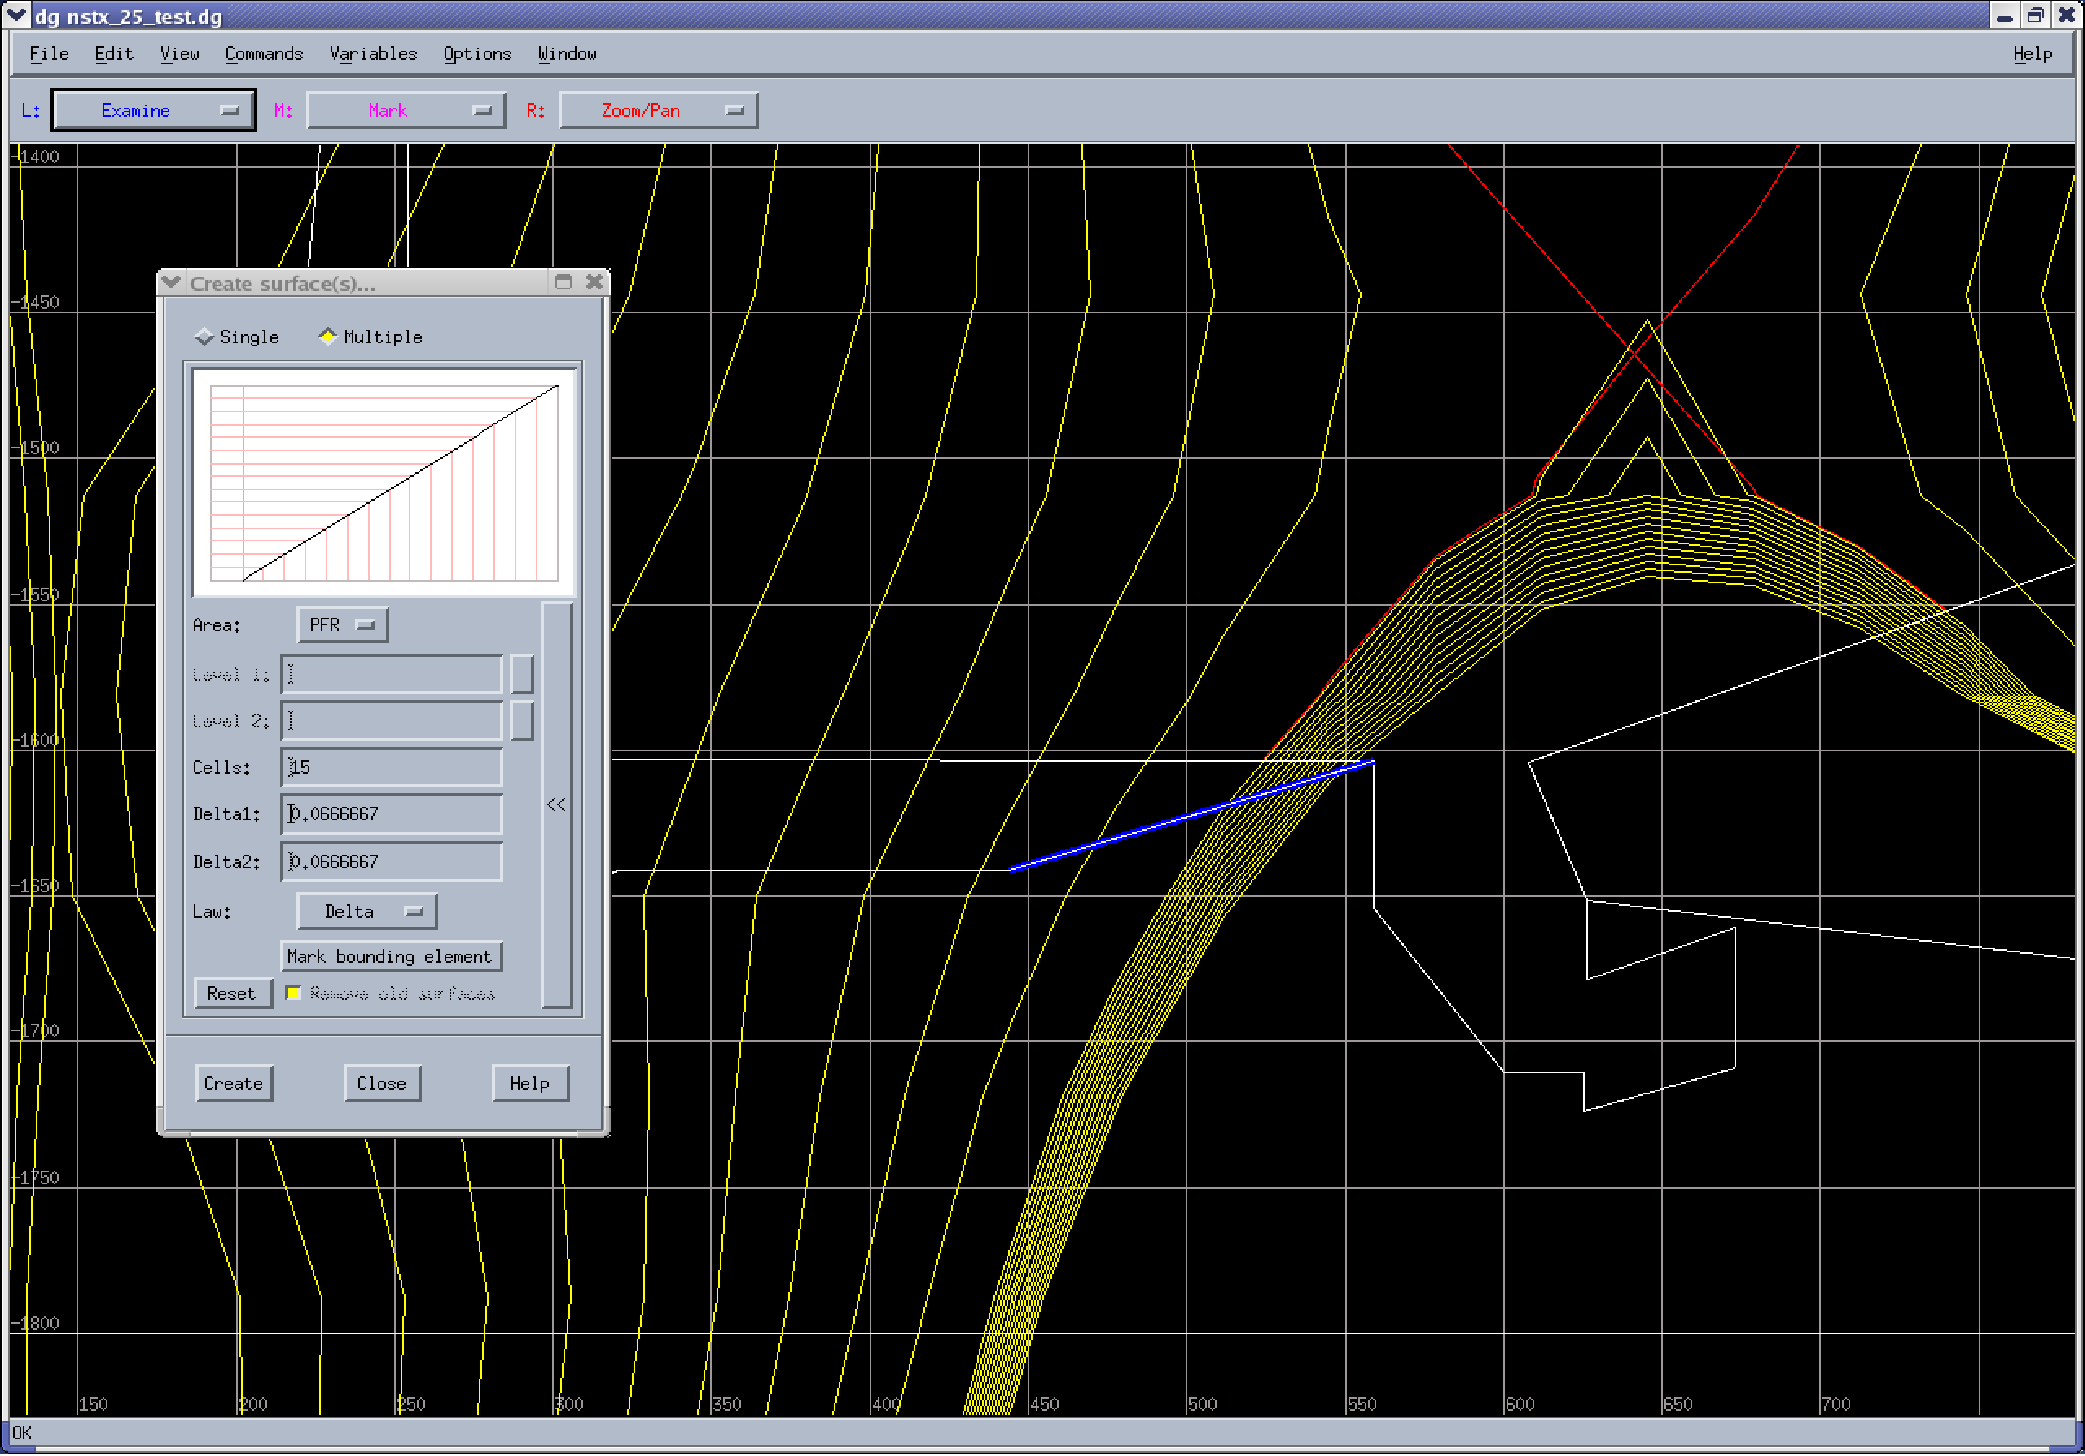
\includegraphics[width=15.0cm]{bde_pfr_zoom.pdf}}
\else
  \centerline{
\includegraphics[width=15.0cm]{bde_pfr_zoom.epsi}}
\fi
\caption{Zoom of the PFR showing the highlighted ``bounding element''.}
\label{fig:boundingelement}
\end{figure}

\subsubsection{In case of difficulty \ldots}

% THIS DESCRIPTION STILL HAS A LITTLE TOO MUCH CODE JARGON (namely,
% the ``surface zones'') TO BE USEFUL.  Come back to this if it can
% be clarified.

The process of creating surfaces is perhaps the most confusing and difficult
aspect of using \verb!DG!.  Moreover, the algorithm it uses for choosing the
outermost flux surface level differs in detail from the one used by
\verb!Carre!.  If you are having problems getting the surfaces you want,
you might benefit from reading the precise description of \verb!DG!'s
current algorithm for setting the outermost flux level:

It is to be understood that ``maximum'' and ``minimum'' 
always refer to the absolute flux deviation from the separatrix.
First, find the surface zone and the separatrix(ces) of the zone. If
there are two separatrices, draw surfaces from one to the other. Else
if the zone is marked as "limit by surface", find the farthest surface
in the zone and draw surfaces to it.  (In practice, only one surface
by be added manually in this zone, so that surfaces are always bounded
by that one.)

Else, initialize the maximum level to infinity and get the structure
variable, which includes the targets.  The structure is split into
chains of adjacent elements, where each element in a chain may be
connected to at most one other element at each endpoint.  If there are
branching points in any chain, an error is returned.  The chains are
organized into three groups: the first group consists of chains which
contain elements that have been specified as a target.  These chains
must contain the entire target variable and must form a closed loop,
otherwise an error is returned.  The second group consists of chains
with no target elements that form a closed loop, and the third group
consists of chains with no target elements that do not form a closed
loop.

For each chain in the first group, for each element in the chain, if
neither endpoint is in the surface zone, skip it, else get the maximum
and minimum flux levels on the element from the equilibrium.  Find the
maximum level on the chain, and set the surface level maximum to the
innermost of these levels.  Also, find the minimum level on the chain,
and set the surface level minimum to the outermost of these levels.

For each of the elements in the second or third group, if the first
endpoint is not in the surface zone, skip it, else get the minimum
flux level on the element.  If it is less than the current surface
level minimum, skip it, else if it is still less than the current
surface level maximum, set the surface level maximum to this level.

\index{DG, adding surfaces}
You can use the {\tt Add surface} tool to create surfaces visually. It is
also possible to create surfaces with the {\tt Edit|Create|Surface} menu
command. To move or delete surfaces, use {\tt Move/Stretch} and {\tt Delete}
tools.

To use the {\tt Add surface} tool, press the mouse button anywhere in
the equilibrium. A surface will appear. Move the mouse pointer to
adjust the surface position. When ready, release the mouse button.

The {\tt Edit|Create|Surface menu} command is similar to
{\tt Edit|Create|Point}. A dialog box will appear prompting for
coordinates. After you press {\tt Create}, a magnetic surface will be drawn
through the specified location.

\index{DG, moving surfaces}\index{DG, deleting surfaces}
To use {\tt Move/Stretch} and {\tt Delete} tools, select a surface.
Then drag it to the new location and release the mouse button resp.
simply release the mouse button to delete it.

To delete all surfaces, use the {\tt Edit|Delete|Surfaces} menu command.

\subsection{Defining the X-point}
\index{DG, X-point}

In some older \verb!DG! version, you must define the X-point before working with grid points. This is
necessary if version of \verb!DG! used cannot detect the X-point
location automatically. By defining it, you give \verb!DG! a hint how to
display grid points and process user input. \verb!DG! does not write the 
X-point location into the output file.

For performance reasons, the separatrix is drawn as series of line
segments. Because of this, it is not displayed very accurately,
especially near the X-point.

First, define the targets so that they are intersected by the
separatrix. Then, use the {\tt Set X Point} tool to define a rectangle
around the X-point. Press the mouse button at one corner of the
rectangle, move the mouse pointer to the opposite corner and release
the mouse button. In case of success, the separatrix will be drawn in
the work area. Otherwise, an error message will be displayed in the
message line. If you get the 'Invalid X point location' error message,
try selecting a bigger rectangle.

Note that the separatrix inside this rectangle is represented by two 
intersecting line segments that could even intersect with surfaces!

With an X-point defined, you can use the {\tt Set X Point} tool to
redefine it.

\subsection{Creating and editing grid points}
\index{DG, grid points}

\index{DG, adding grid points}
The {\tt Add grid point} tool lets you visually define grid points.
In addition, the {\tt Edit|Create|Grid point(s)} menu command lets you
define a grid point by specifying its value or fill a zone on the
separatrix with a given number of grid points.
In \verb!Carre! mode, the only available method for creating grid points 
is with the {\tt multiple} option of the 
{\tt Create grid point(s)\ldots}
dialog box.  In particular, the {\tt Add grid point} tool
will not work, nor will the {\tt Move} or
{\tt Delete} tools have any
effect on the grid points.

In \verb!Carre! mode, the operation of this dialog box is directly
analogous to that used to create surfaces (Sec.~\ref{sec:createsurfaces}).
The ``zone'' refers to the section of the separatrix along which
grid points are to be created.
The number of cells must be input manually.  The line graph in the dialog box is a
simple depiction of the relative spacing of the grid points.  In \verb!Carre! mode,
only the {\tt Delta Law} is available.  In this case, the two parameters
{\tt Delta1} and {\tt Delta2} specify a quadratic function used to determine
this spacing.  While these parameters can be input directly, the preferred
means of setting them is to click and drag the black line in the graph to
achieve the desired spacing variation.  When the {\tt Create} button is
clicked, the grid points will be generated with this spacing and drawn in 
\verb!DG!'s main window.  If a model has an existing set of grid points that the
user wishes to tweak, click on one 
of these grid points with the {\tt Examine} tool and then
click the {\tt <<} button in the {\tt Create grid point(s)...} 
dialog; this will
import the parameters describing these grid points.
Note that the dialog will {\em not} enforce constraints on the number of
cells (e.g., that the number of grid points on either side of the
PFR must be equal); the
user must check to be sure that all such constraints are satisfied.
Again, \verb!Carre! will perform its own series of such checks when invoked.

With the {\tt Add grid point} tool, move the mouse pointer to the
desired location on the separatrix and press the mouse button. A grid
point will be created at this location. You can move the mouse pointer
to adjust its position. When finished, release the mouse button.

The {\tt Edit|Create|Grid point(s)} menu command brings up a dialog
box prompting you for a separatrix zone and alternatively, number of
grid points to create or a grid point value. Two radio buttons let you
choose between filling the zone with grid points and creating a grid
point with an exact value. After entering values, press {\tt Create}.
Filling a zone with grid points will remove all previous grid points
from that zone.

\index{DG, moving grid points}
Use the {\tt Move/Stretch} tool to move a grid point or to 'stretch'
grid points of one zone. To move a single grid point, select it, then
drag it to the new location and release the mouse button. To 'stretch'
grid points, move the mouse pointer to one of them, press Shift+mouse
button and drag it to the new location. All other grid points in that
zone will be 'stretched'.

\index{DG, deleting grid points}
Use the {\tt Delete} tool to remove grid points. Select the grid
point to delete and release the mouse button.

Use the {\tt Edit|Delete|Grid} points menu command to delete all grid
points.

\section{Working with chords}
\label{sec:chords}\index{DG, chords}

Chords are presently the only objects in \verb!DG! that are not confined to the
poloidal plane (i.e., that may be non-axisymmetric).
For purposes of defining chords in three
dimensions, two coordinate
modes have been established. 
In ``Cartesian'' mode, $Z$ is the
vertical axis in the ``top-down view'' (Sec.~\ref{sec:topdownview});
the horizontal axis in the poloidal plane is $X$ and the
vertical axis is $Y$ (note: this is a left-handed coordinate system).
In ``Cylindrical'' mode, $Z$ is the vertical coordinate in the poloidal
plane, identical to $Y$ in ``Cartesian'' mode. 
In the ``top-down view'',
the horizontal axis is
designated as $R$ and the toroidal angle as $\phi$ (counterclockwise relative
to the horizontal axis) is entered in degrees. 

Chords can be displayed with either 
{\tt View|Display|Chords} or {\tt View|Display|3dchords}.  For chords
confined to the poloidal plane, these are identical, and chords will
not be visible in the ``top-down view''.  For chords with a toroidal
extent, selecting 
{\tt View|Display|Chords} in the 
poloidal plane results in straight
line segments connecting the 
$X$ and $Y$ ``Cartesian'' coordinates of the chord end points.
Equivalently in the ``Cylindrical'' mode, these are the $R$
and $Z$ coordinates at the end points.  In contrast,
{\tt View|Display|3dchords} shows the projection
of the toroidal path of the chords on the $Z = 0$ (``Cartesian'')
or $\phi = 0$ (``Cylindrical'') plane.  In the ``top-down view'',
both {\tt View|Display|Chords} and
{\tt View|Display|3dchords} show the straight
line paths of the chords in the $X$-$Z$ (``Cartesian'') or
$R \cos \phi$-$R \sin \phi$ (``Cylindrical'') plane.

Starting with file format version 115, chords with $X$, $Y$,
and $Z$
components may be saved and loaded.

\subsection{Creating chords}
\index{DG, creating chords}

The {\tt Add Chord} tool 
allows you to create chords graphically.  To
create a chord, move the mouse pointer to the desired location of its
beginning and press the mouse button the tool is assigned to. Without
releasing the mouse button, move the mouse pointer to the desired
location of the other end of the chord and release the mouse button.
{\tt Chords} can also be created from marked {\tt Elements} via the 
{\tt Commands|Convert|Elements to chords}
command.  Duplicate chords are not produced and the 
original elements are deleted.

The third method for creating chords is with the 
{\tt Edit|Create|Chord...} dialog.

\subsection{Modifying chords}
\index{DG, modifying chords}

The {\tt Move} tool allows chords to be manipulated in either
the poloidal plane or in ``top-down view''.  The user can
manipulate either the {\tt Chords} object (displayed by
{\tt View|Display|Chords}) or the
{\tt 3dchords} object 
(displayed by {\tt View|Display|3dchords}.
The {\tt Adjust chord} tool moves an end point of the chord
while keeping its radial coordinate constant.  Holding down the
``shift'' key while using the {\tt Move} 
tool replicates this behavior,
but with slightly
different graphics that conform to the rest of the {\tt Move} 
tool.

Chords have an orientation, just like elements; this
orientation is displayed with 
{\tt View|Display|External normals}.
The {\tt Reverse normals} tool can be used to change this 
orientation. Note that when this tool is dragged, it will only
operate on objects of the same type as the
first object encountered, either chords or elements. 

\index{DG, extending chords}
The {\tt Extend chord} tool linearly
extends (i.e., replaces) the second endpoint of a chord to lie on
the nearest element, or the nearest marked element if elements have
been marked.  The
{\tt Edit|Extend chords} commands applies does
this for all marked chords.  The 
{\tt Edit|Mark all chords} command can be used
to mark all chords in preparation for extension.

{\em Note:} as of August 2007, the ``mathematically correct'' procedure
for extending chords has not been debugged. However, two macros
defined in \verb!chords.c! may be used to select a different preferred
implementation of the procedure.  \texttt{EXTCHORD\_2D} 
selects the 2-D
procedure, which does not support chords with nonzero
toroidal extent,
and \texttt{EXTCHORD\_OLD} selects the partially correct, stable
3-D procedure, which does not work for horizontal chords and ignores
horizontal elements. (This is enabled in the current
release of \verb!DG!).
If neither macro is defined, the code defaults to
the incomplete procedure, which may show unpredictable behavior during
use.

\index{DG, deleting chords}
The {\tt Edit|Delete|Chords} command deletes all chords.

\section{Working with sources}
\index{DG, sources}

\subsection{Creating and editing sources}

\verb!DG! allows the user to define sources and to attach variables to them.

\index{DG, creating a source}
To create sources, use the {\tt Add source} tool. Move the mouse
pointer to the desired location in the work area and press the mouse
button. A source will be created at this location. You can move the
mouse pointer to adjust its position. When finished, release the
mouse button.

To create a source by entering its coordinates, select
{\tt Edit|Create|Source...} . A dialog box will appear prompting for
coordinates. Enter values and press {\tt Create}. A source will be
created.  The dialog box will remain on the screen, allowing you to
define multiple sources without re-opening it. Press {\tt Cancel} to
close the dialog box.

\index{DG, moving a source}
To move a source to a new location, use the {\tt Move/Stretch} tool.
Select the source to move, drag it to the new location and release the
mouse button.

\index{DG, deleting a source}
To delete a source, use the {\tt Delete} tool. Select the source to
delete and release the mouse button.

To delete all sources, issue the {\tt Edit|Delete|Sources} menu command.

\section{Working with meshes}
\index{DG, meshes}

\subsection{Importing a SONNET format mesh}

\index{DG, importing a SONNET grid}
\verb!DG! allows you to import a mesh in the \verb!Sonnet! format. \verb!Carre!'s output 
mesh can be converted into this format, as can meshes produced by other
codes. At present, it
can only read the ASCII version of the grid file. The grid can then be
displayed in the working area.

To import the mesh, use the {\tt File|Import|Mesh...} menu
command. A dialog box will appear prompting you for a filename. Select
a file from the list or type the filename in the edit field. Then
press {\tt Load}.  The mesh will be imported and displayed in
the work area. If nothing is displayed, select {\tt View|Picture}
view to enlarge the area displayed. Also, make sure that
{\tt View|Display|Mesh} is enabled.

To hide or display the mesh, toggle {\tt View|Display|Mesh}.
To unload it, select {\tt Edit|Delete|Mesh}.

\subsection{Modifying a mesh}
\index{DG, modifying a mesh}

\verb!DG!'s graphical interface permits limited modification of a mesh that has
been imported.  The altered mesh can be written out to a text file (in
the \verb!Sonnet! format) for use by other codes.  The primary tool for this
purpose is the {\tt Move mesh point} tool.  The actions of this tool
are governed by the settings specified in the 
{\tt Options|Mesh editing...} dialog.
They only affect one-dimensional movements of mesh points.

{\tt Slide along} specifies how movements of mesh points are confined.
When {\tt Magnetic surfaces} is in effect, the movement is confined to a
magnetic surface passing through the original location of the mesh
point. This method should work fine except for the vicinity of the 
X-point, where magnetic surfaces drawn by \verb!DG! become distorted.
When {\tt Splines} is in effect, the movement is confined to a spline
passing through a row of existing mesh points.  This method may be
useful in the vicinity of the X-point.

{\tt Margin} specifies the minimum distance between adjacent mesh
points. If this limit is about to get exceeded, adjacent points start
moving in order to ``make room''.
The {\tt Double border} setting, when enabled, instructs \verb!DG! to treat
outermost mesh cells as a double border. They would be resized
together with adjacent ``regular'' cells.

A modified mesh can be written out with the 
{\tt File|Export|Mesh...} dialog.

\subsection{Repairing mesh cells using rotated view and variable aspect ratio}
\index{DG, repairing cells}

Mesh cells highlighted in pink in \verb!DG!'s main window are either concave
(have an interior angle greater than 180 degrees) or consist of
overlap with a neighboring cell.  These problems typically arise where
the mesh generator (\verb!Carre! or otherwise) is forcing the mesh to
conform to the specified divertor target shape and usually involve
cells that are stretched significantly in one direction.

The ability to rotate and stretch the view allows the structure of the
problem cells to be discerned and repaired.
As an example, we consider a certain mesh generated for the NSTX experiment
which contains twisted cells near the inner divertor, Fig.~\ref{fig:twisted}. 
By zooming, stretching, and rotating the view using the tools 
described in Secs.~\ref{sec:rotateview} and \ref{sec:stretchview}, 
we arrive at a much clearer depiction
of the problem, Fig.~\ref{fig:twistedstretch}.
We see that the edges of the cells crossed the enforced boundary,
twisting the mesh cells in the process.  At this point, the user can
straightforwardly use the {\tt Move mesh point} 
tool to manually repair the cells.

\begin{figure}[bt]
\ifpdf
  \centerline{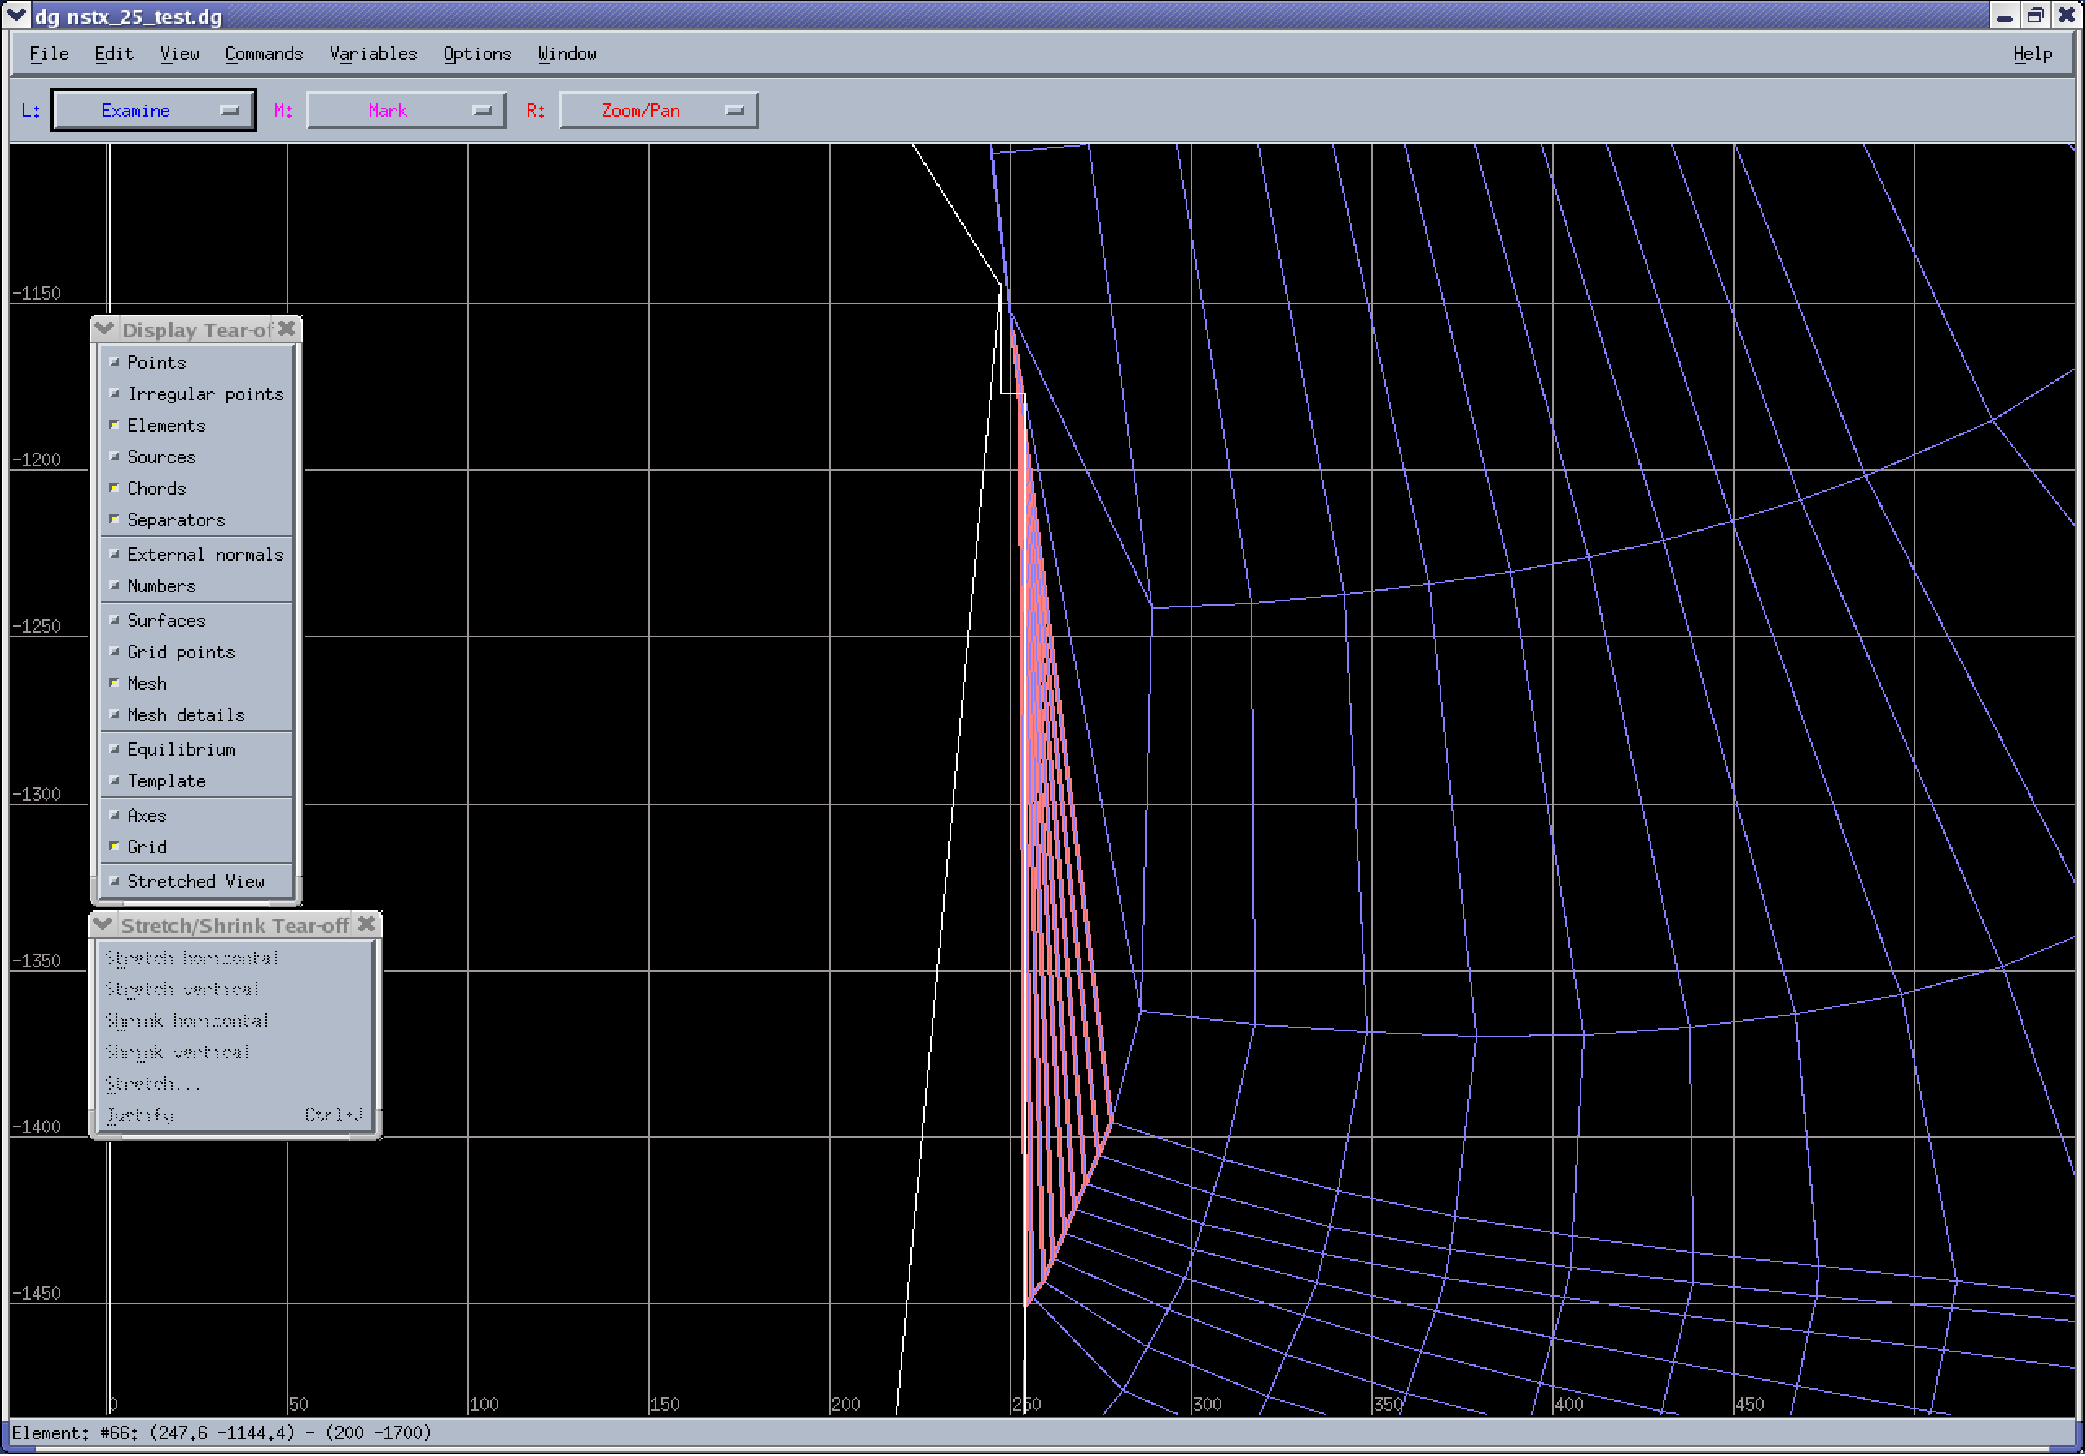
\includegraphics[width=15.0cm]{twisted_nostretch.pdf}}
\else
  \centerline{
\includegraphics[width=15.0cm]{twisted_nostretch.epsi}}
\fi
\caption{Zoom of the twisted mesh cells near the inner divertor target of an NSTX geometry.}
\label{fig:twisted}
\end{figure}

\begin{figure}[bt]
\ifpdf
  \centerline{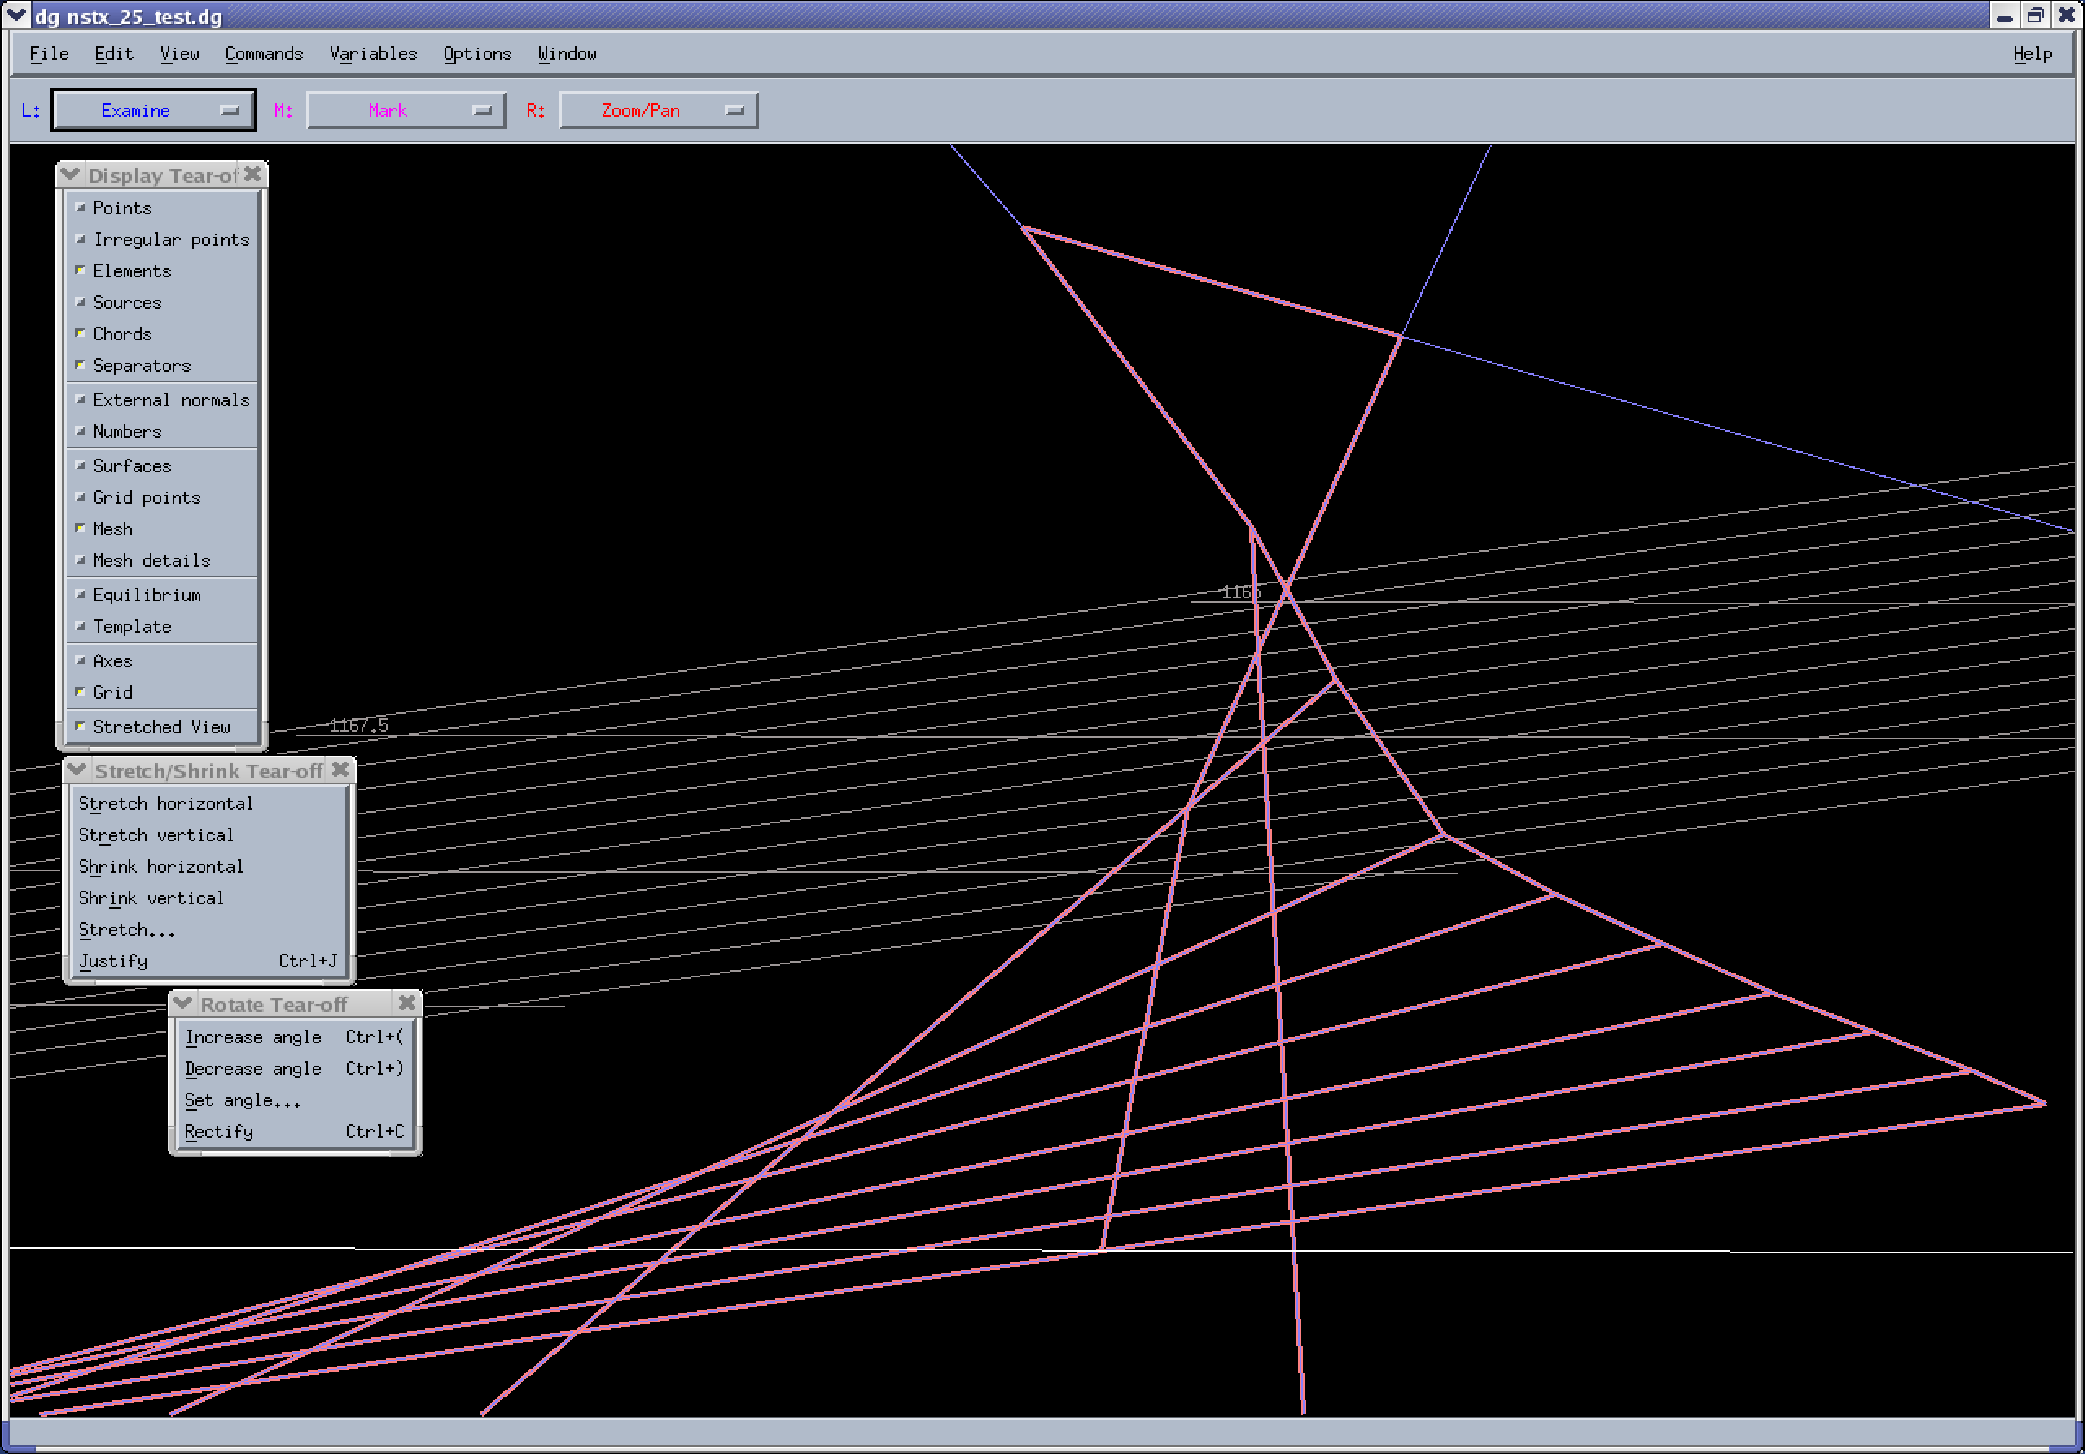
\includegraphics[width=15.0cm]{twisted_top_rotate_stretch.pdf}}
\else
  \centerline{
\includegraphics[width=15.0cm]{twisted_top_rotate_stretch.epsi}}
\fi
\caption{After stretching and rotation, the overlapping of the cells in
the upper part of the region cells depicted in Fig.~\ref{fig:twisted} becomes
clear.}
\label{fig:twistedstretch}
\end{figure}

\subsection{Defining cells}
\index{DG, defining cells}

With \verb!DG!, you can define cells between the \verb!Sonnet! grid and the
structure (both objects must be present). You define cells by creating
separators between them. You create separators with the
{\tt Edit|Create|Separators} menu command. To adjust individual
separators, use the {\tt Reposition} tool. The
{\tt Edit|Delete|Separators}  menu command removes all separators.
You cannot add or remove individual separators with \verb!DG!.

To work with separators, you must define a suitable structure and
import a \verb!Sonnet! grid.

Use the {\tt Edit|Create|Separators} menu command to create
separators between the structure and the \verb!Sonnet! grid.

Use the {\tt Reposition} tool to attach a separator to a different
structure point. Select the separator and move the mouse cursor a
structure point. Then release the mouse button.

Use the {\tt Edit|Delete|Separators} menu command to delete all
separators.

\section{Working with variables}
\index{DG, variables}

\subsection{Basics}

With \verb!DG!, you can use {\tt Variables} to specify information that cannot be
edited visually in the work area. Variables are written into the
output file and can be processed by other programs. Some variables
(targets and structure) also have important functions in \verb!DG!.

Variables must be set up by a power user before using them. This
procedure is described in {\bf Customizing DG} (section \ref{sec:DGcustom}). Each variable has
following attributes\index{DG, variable attributes}:
\begin{description}
\item[Name] \index{DG, variables, name}is written into the output file
  and is otherwise invisible.
\item[Description] \index{DG, variables, name}is the name that is
  shown to the user.
\item[Type] \index{DG, variables, type}defines type of values the
  variable can hold.
\item[Scope] \index{DG, variables, scope}specifies what objects the
  variable applies for.
\item[Export/No export] \index{DG, variables, export/no
    export}determines whether values are written into the output file.
\item[Default value] \index{DG, variables, default value}is the
  default value for newly-created objects.
\item[Help text] \index{DG, variables, help text}is displayed to the
  user when s/he asks for it.
\end{description}

These attributes are normally defined by a power user while setting up
variables. A normal user should have some idea of the type and the
scope in order to be able to set correct values for correct objects.

Each variable has a {\tt type}. A variable can hold either a text
value ({\tt integer}, {\tt real} or {\tt text}) or a set of
elements ({\tt element}, {\tt set of elements}, {\tt target},
{\tt structure}, {\tt part of structure}). \verb!DG! prevents the user from
entering values of a wrong type.

The {\tt scope} determines objects the variable is attached to. There
are 4 possible scopes:
\begin{description}
 \item[Layers] means that the variable has one value for the whole
  layer.
\item[Elements] means the variable has a separate value for each
  element.
\item[Sources] means the variable has a separate value for each
  source.
\item[Chords] means the variable has a separate value for
each chord.
\end{description}

As noted above, variables are organized 
into {\tt layers} with \verb!DG! displaying each
layer in a separate dialog box.

The power user defines {\tt layer types} and the minimum and the
maximum number of layers of each type.

\subsection{Working with layers}

Layers may have one or more instantiations in a particular
model.  For some layers, a single instance is 
all that is needed 
to specify the desired information; \verb!DG! will not
permit the creation of additional instances of this same
layer.  In the latter case, \verb!DG! will assign an integer
count as the instances are created. 
Some layer instances are predefined (e.g., 
{\tt Structure}) and cannot be created or destroyed
by the user, power or otherwise.

To create an instance of a specific layer, select the layer from the
{\tt Variables|Add} submenu. A dialog box for editing the variables in this
layer instance will appear. If the maximum number of instances of a
specific layer already exist, this layer will not be displayed in the {\tt Add}
menu. If this menu becomes empty, the {\tt Variables|Add} cascade button
will be grayed.

To destroy an instance of a layer, select its name in the {\tt Variables|Remove}
submenu. If there are multiple instances of a layer, there will be a submenu associated
with that layer, listing the integer indices of those instances.
If only the minimum number of instances of a specific layer 
already exist, layers of this type will not be displayed in this menu.
If this menu becomes empty, the {\tt Variables|Remove} cascade button
will be grayed.

To display the dialog box for an existing layer instance, select its name 
and instance index (if applicable) under 
the {\tt Variables} menu.

To hide the dialog box for a layer, press the {\tt Close} button in
that dialog box.

\subsection{Setting variables}
\index{DG, variables, setting}

To set variables in a layer, you need to display the dialog box for
that layer first.

The dialog box for each instance of a layer displays its variables,
allowing them to be set, viewed, and modified.
The title of this dialog box is the name of the layer; if there are 
multiple instances, the integer index of the particular index
is also displayed here.  At the top of the dialog
box, there is a row of buttons that affect the entire box.
Below this are fields for the individual variables.  Finally, there
is a status line at the bottom of the dialog box.

The ``$\bigtriangleup$'' 
button on top of the dialog box allows you to ``roll it up''
so that the box occupies less screen space. In
order to restore the dialog box to its full size, press this button
again.

The dialog box can be resized using the window manager. If it is
reduced in size, scrollbars appear, allowing you to scroll the
content. The functionality of the dialog box is NOT affected by
resizing it or rolling it up. In particular, the {\tt Set all} button also
affects variables that are invisible.

For each variable, the dialog box contains its name, a {\tt Help} button, a
text field for entering the new value (for text-like variables) or a 
{\tt Mark}
button (for {\tt set of objects} variables), and a {\tt Set} button.
The {\tt Help} button, when pressed, displays help about the variable.
The text field is used to enter new values for text variables. When
the text field has keyboard focus, the status line displays the
current value of the variable. For text variables that apply to
elements, chords or sources, only variables that apply to marked
objects are accessed.  {\tt Filename} variables differ from {\tt Text}
in that the user can select the file interactively (press the
{\tt Enter} key on your keyboard in the text field to bring up the
file selection dialog); the variable is not valid unless the file 
exists and is readable at the time of the variable check.

The {\tt Mark} button, available only for {\tt Set of objects} variables,
marks the objects contained in the variable.
The {\tt Set} button sets the variable to the new value. For text
variables, the new value must be entered in the text
field. For variables storing sets of objects, the objects must be
marked.

The {\tt Set all} button in the top row, when pressed, has exactly the
same effect as pressing the {\tt Set} button of each variable except that
empty new values for variables that apply to elements, sources or
chords are ignored. This button is only available if the layer
consists of text variables only.

The {\tt Reset all} button, when pressed, resets all text fields to
present values of corresponding variables. It is only available in
layers consisting of text variables only. The text field is cleared
for variables that apply to elements, sources or chords when marked
objects have different values.

% NOT SURE THE HOLD BUTTON IS BEING USED.
% The {\tt Hold} toggle button controls how text fields for variables that
% apply to elements, sources or chords are updated. When {\tt Hold} is
% disabled, these fields are updated whenever an object is marked or
% unmarked. When {\tt Hold} is enabled, these fields are not updated.

The {\tt Close} button closes the dialog box.

Pressing the right mouse button over a text field or a button
associated with a variable brings up a pop-up menu. If the mouse has
less than 3 buttons, the menu can be displayed by pressing ``Ctrl+left''
button.
The {\tt Reset} command sets the text field to the current value of the
variable, similar to the {\tt Reset all} button but affecting only one
variable. For variables storing sets of objects, this command acts
exactly like the {\tt Mark} button.
The {\tt Display values} command displays values of variables that apply
to elements, chords or sources next to corresponding objects. In order
to remove these ``labels'', highlight any object or use the 
{\tt View|Remove labels} command from the main menu.
Commands in the {\tt Compare} submenu compare values of the variable to
the value entered in the edit field and mark matching objects.
Both the {\tt Display values} command and the {\tt Compare} submenu are only
available for variables that apply to elements, sources or chords.

To set a value for a variable that contains a set of elements, mark
the desired elements and press its {\tt >} button.

To set a value for a text variable that applies to the layer, enter
the value in the {\tt New Value} text field and press the {\tt >}
button.

To set a value for a text variable that applies to elements or
sources, first mark elements or sources the value should be assigned
to. To set a new value, enter it in the {\tt New Value} text field
and press the {\tt >} button.

Current values for variables are always displayed in corresponding
{\tt Old Value} text boxes. For variables that apply to elements or
sources, only values for marked objects are considered. If all values
are the same, a value will be displayed, otherwise the word
{\tt Different}.

To copy the current value of a variable into its {\tt New Value}
text field, press its {\tt <} button. For a variable containing a
set of elements, the elements belonging to the variable will be
marked.

The {\tt Accept} button has exactly the same effect as pressing all {\tt >}
buttons except that empty new values are ignored.

The {\tt Reset} button has exactly the same effect as pressing all
{\tt <} buttons.

The {\tt Hold} toggle button controls how {\tt New Value} fields of
variables that apply to elements or sources are updated. With
{\tt Hold}  disabled, these fields are updated every time objects are
marked and unmarked. When it is enabled, no such updates happen.

You can easily copy values between different elements or sources.
Disable {\tt Hold} and mark objects containing the desired value.
Then enable {\tt Hold} and mark objects the values should be assigned
to. Press {\tt Accept} to set new values.

\section{Creating output files}
\index{DG, creating output files}

\subsection{Types of output files}

\verb!DG! produces 3 output files:
\begin{description}
  \item[Structure file] contains the structure.
  \item[Targets file] contains targets, surfaces and grid
points.
  \item[Output file] contains elements, sources, separators
and the values of the variables associated with all of the
layer instances for the current model.
\end{description}

The current version of \verb!DG! requires structure, targets, surfaces and grid
points to be defined. Also, all {\tt integer} and {\tt real} variables must be set
to non-empty values.

\subsection{Producing output files}

\verb!DG! generates names of output files by attaching different extensions
to the name of the \verb!DG! file. If the current file has no name yet, save
it with the {\tt File|Save} command before producing the output.

To produce the output files, choose the {\tt File|Output} menu
command. A dialog box will appear asking for confirmation. Press
{\tt Ok} to create the files.

\section{Customizing DG}
\index{DG, customizing}\label{sec:DGcustom}

\subsection{Installing DG}
\index{DG, installing}

To install \verb!DG!, you need to:
\begin{itemize}
\item Compile and link its sources
\item Make sure that the help file exists and has the right name
\item Make sure that the configuration file exists and has the right name
\end{itemize}

\verb!DG! is an X Windows application. The correct \verb!DISPLAY! setting is
necessary.

Some useful infos on installing are contained in the {\bf Customizing DG} section (\ref{sec:DGcustom}).

\subsection{Files needed by DG}
\index{DG, files needed by}

\begin{description}
  \item[dg] Executable file
  \item[dg.dgh] Help file
  \item[dg.dgc] Configuration file
\end{description}

\subsection{Specifying directory masks}
\index{DG, directory masks}

You can customize directory masks \verb!DG! displays in file selection dialog
boxes by setting the following environment variables:
\begin{description}
\item[DGOPENMASK] Directory mask for {\tt File|Open}
\item[DGSAVEMASK] Directory mask for {\tt File|Save}
\item[DGEQUILMASK] Directory mask for {\tt File|Equilibrium}
\item[DGTEMPLATEMASK] Directory mask for {\tt File|Template}
\item[DGSONNETMASK] Directory mask for {\tt File|Sonnet grid}
\end{description}

\subsection{The configuration file}
\index{DG, configuration file}

There is a special \verb!DG! file, the {\bf configuration file}. Its
filename is normally produced by appending {\tt .dgc} to the name of the
executable. The configuration file has two functions:
\begin{enumerate}
  \item When the {\tt File|New} command is executed, the configuration file
is loaded into the new window.
  \item When a \verb!DG! file is being opened, the configuration file is used to
update its definitions of variables and layers.
\end{enumerate}

\verb!DG! normally writes these definitions in \verb!DG! files. When a \verb!DG! file is
opened, they are normally ignored and definitions from the
configuration file are used instead. This ensures that all files
loaded in \verb!DG! have identical definitions of layers and variables.

Default values are not updated in the current version of \verb!DG!.

\subsubsection{Specifying the configuration file}

Sometimes it is necessary to use a different configuration file or not
to use any at all.

To use a different configuration file, start \verb!DG! with the following
command:
\begin{verbatim}
dg -cfg <filename-with-extension>
\end{verbatim}

To use \verb!DG! without loading a configuration file, type

\begin{verbatim}
dg -nocfg
\end{verbatim}

NOTE:   There are some bugs in \verb!DG! that appear only when it is started
without any configuration and sometimes cause an exception.

\subsection{Creating or modifying the configuration file}

Use the {\tt Options|Setup} menu command to create/modify the
configuration file. 

The {\tt Setup} dialog box and all dialog boxes you open during setup
are modal. For this reason, you can work only with the topmost dialog
box.

Choose the {\tt Variables...} submenu in order to edit definitions of variables
and layers in the current file. The {\tt Layer types} dialog box will
appear.

Press {\tt Save as configuration} to save the current file as a
configuration file. A dialog box will appear prompting for a filename.
Normally, it already contains the right name. Select {\tt Ok} to save
the file in the current window as configuration.

Press {\tt Close} to close the dialog box.

\subsubsection{Adding, modifying and removing layer types}

To define a layer type, choose {\tt Add} in the {\tt Layer types}
dialog box. The new {\tt Layer type} options dialog box will appear.

Enter the name of the layer type to create in the {\tt Name} text
field. The name should contain only alphanumeric characters. This name
will be written into the output file.

Enter the description in the {\tt Description} text field. In the
{\tt MinInstances/MaxInstances} text field, enter the minimum and
the maximum number of layers of this type. You will have to use 0 for
{\tt MinInstances} because there are no layers of this type yet. You
can change {\tt MinInstances} later after creating the minimum number
of layers.

Press the {\tt Ok} button to create the layer type.

To remove a layer type, select it in the list and press {\tt Delete}.

To modify a layer type, select it in the list and press {\tt Modify}.
The {\tt Layer type options} dialog box will appear. You can change
name, description, {\tt Min/MaxInstances} here. Note that if you change the
name, layers contained in \verb!DG! files under the old name will be ignored.

To close the {\tt Layer types} dialog box, press {\tt Close}.

\subsubsection{Setting up variables}

To define the variables that will constitute a layer, first display its 
{\tt Layer type options} dialog box ({\tt Modify}). This dialog box contains a
rectangular area with buttons. These buttons represent row/column
positions of variables in dialog boxes. Buttons containing the string
{\tt Empty} mean that no variable is defined at this position.

To create a variable at a specific position, press the {\tt Empty}
button at that position. The {\tt New variable} dialog box will appear.

Enter the name of the variable to be created in the {\tt Name} field. The
name must contain only alphanumeric character.

Select the type and the scope in corresponding option menus. Check the
{\tt Do not export} toggle button to prevent the variable from being
written into the output file. Structure and targets are normally not
exported because they are written into separate files.

Press {\tt Ok} to create the variable.

To modify a variable definition, press its button in the 
{\tt Layer type options} dialog box. The {\tt Variable options} 
dialog box will
appear. After making changes, press {\tt Ok}. Note that if you change
the name, variables contained in \verb!DG! files under the old name will be
ignored.

To remove a variable, press its button in the 
{\tt Layer type options} dialog box. The {\tt Variable options} 
dialog box will appear. Press {\tt Remove} to remove the variable.

\subsubsection{Adding help text to variables}

\verb!DG! lets you add help text to variables. The user can display the help
text by pressing the {\tt Help} button located near the name of the variable in
the {\tt Variables} dialog box.

To edit a help text for a variable, display its {\tt Variable options}
dialog box and press {\tt Edit help}. The {\tt Help for variable} editor dialog box with a
text editing field will appear. Edit the help text in the editing
field and press {\tt Ok}.

\subsubsection{Setting default values}

\verb!DG! lets you define default values for variables. When a new layer,
element or source is created, the default values are used for the
newly created object.

It is suggested that you define default values for all variables
because \verb!DG! will not generate output files when some variables have
empty values. A search for empty values can be very difficult and cost
a lot of time.

To define default values for variables in a layer type, display its
{\tt Layer type options} dialog box and 
choose the variable for which you wish to set a default. 
In its {\tt Variables:} dialog box there is a
{\tt Default value} field for this purpose.

Default values from the configuration file are used only to create new
\verb!DG! files. When opening an existing file, default values from the
configuration are ignored.

\section{File formats}
\index{DG, file formats}

\subsection{Simple template file format}

Besides the {\tt Neutral File} exported from \verb!PATRAN!, \verb!DG! can also import
templates in a very simple format where the geometry is speified as a
set of polygons (in general, open). In this case, each line of the
input file either contains a pair of the co-ordinates of the next
corner, or is empty. 

\subsection{Structure file format}

The first line in the structure file contains the number of closed chains in the structure.

Then, for each chain, starting with the outermost, the following block
appears:
\begin{verbatim}
<number of points in the chain>
<x1> , <y1>
...
\end{verbatim}

For the outermost chain, the bounding rectangle is added.

Points are output in counterclockwise order when the external normals
of the elements in the chain point outwards. Otherwise, they are
output in clockwise order.

\subsection{Targets file format}

The targets file (for a single-null model) has the following format:
\begin{verbatim}
target 1
line
  <x> , <y>
  ...
target 2
line
  <x> , <y>
  ...
region 1
levels
  <level>
  ...
region 2
levels
  <level>
  ...
region 3
levels
  <level>
  ...
zone 0
points
  <value>
  ...
zone 1
points
  <value>
  ...
zone 2
points
  <value>
  ...

<eof>
\end{verbatim}

The {\tt target1} and {\tt target2} blocks contain point coordinates for targets. 

The {\tt region 1...3} blocks contain levels of surfaces. Regions have
following meaning:
\begin{description}
  \item[region 1] Main Plasma
  \item[region 2] SOL
  \item[region 3] Private Flux
\end{description}

The {\tt zone 1...3} blocks contain values of grid points
(between 0 and 1). Zones have following meaning:
\begin{description}
  \item[zone 1] Main chamber
  \item[zone 2] Inner divertor
  \item[zone 3] Outer divertor
\end{description}

\subsection{Output file format}

The output file has the following format:

\begin{verbatim}
p1
  <x> , <y> , <z>
  ...
p2
  <x> , <y> , <z>
misselem
  <number>
  ...
sprtrs
  <number>
  ...
sources
  <x> , <y>
cells <cellnum>
  <number>
  ...
...
<layer name> <layer number>
  <variable>
  ...
...
finish
\end{verbatim}userdata

{\tt p1} and {\tt p2} sections containt coordinates of origins and
ends of elements and/or separators, sorted after element number. For
unused numbers, dummy coordinates are output. The $Z$ coordinate is
always 0.

The {\tt misselem} section contains unused element numbers. Elements
with these numbers {\bf must} be ignored.

The {\tt sprtrs} section lists numbers of separators in {\tt p1} and
{\tt p2} arrays.

The {\tt sources} section lists sources.

If separators are defined, there is a {\tt cells} section for each
cell. Each section lists numbers of elements and separators included
in its cell.

For each layer, a {\tt <layer name>} {\tt <layer number>} section is
present. Layer name is the name of the layer type. Layer number is
used to distinguish between layers of the same type. Each section
contains a {\tt <variable>} entry for each variable in the layer.

The {\tt <variable>} block has following formats:
\begin{itemize}
  \item Text variables that apply to the layer:
\begin{verbatim}
<variable name> <value>
\end{verbatim}
  \item Text variables that apply to elements or sources:
\begin{verbatim}
<variable name>
  <value>
  ...
\end{verbatim}
  \item For variables that apply to elements, a value for each element number
is included. Dummy valurs are used for unused numbers. For variables
that apply to sources, a value for each source is included. Values are
written in the same order as sources in the {\tt sources} section.
  \item ``Set of elements'' variables that apply to the layer:
\begin{verbatim}
<variable name>
  <element number>
  ...
\end{verbatim}
\end{itemize}

\chapter{Some information from the SOLPS 2002 Course Notes}
\label{cha:coursenotes}

The following information is extracted from the SOLPS Course Notes given at
JET in 2002.

\section{Breakdown of B2.5 programs}
\index{B2.5, programs}\label{sec:b2programs}

\verb!B2.5! consists of a number of programs
\begin{description}
\item[\textcolor{Red}{b2ag}] \index{b2ag} prepares the geometry and magnetic field (see \ref{sec:b2ag})
\item[\textcolor{Red}{b2ah}] \index{b2ah} prepares the default physics parameters (see \ref{sec:b2ah})
\item[\textcolor{Red}{b2ai}] \index{b2ai} prepares the initial plasma state (see \ref{sec:b2ai})
\item[\textcolor{Red}{b2ar}] \index{b2ar} prepares a table of atomic rate coefficients (see \ref{sec:b2ar})
\item[\textcolor{Red}{b2co}] \index{b2co} one option when running the main program is to write out a
  short restart file periodically; this program converts such a
  restart file into the normal version (see \ref{sec:b2co})
\item[b2fu] \index{b2fu} the opposite of {\bf b2uf}; it converts a formatted plasma
  file \verb!b2fplasmf! to the normal unformatted \verb!b2fplasma!
\item[\textcolor{Red}{b2md}] \index{b2md} saves the \SOLPSfive output to the \verb!MDSplus! server (see \ref{cha:MDSplus})
\item[\textcolor{Red}{b2mn}] \index{b2mn} the main program (see \ref{sec:b2mn})
\item[\textcolor{Red}{b2pl}] \index{b2pl} the plot program (see \ref{sec:b2pl} and Appendix \ref{cha:b2plotmanual})
\item[\textcolor{Red}{b2rd}] \index{b2rd} retrieves the \SOLPSfive output from the \verb!MDSplus! server (see \ref{cha:MDSplus})
\item[b2ts] \index{b2ts} an example post-processing program; it reads the basic
  output files produced by {\bf b2mn} and prints some simple geometric
  quantities
\item[b2uf] \index{b2uf} the normal \verb!b2fplasma! file (used for plotting) is
  written using FORTRAN unformatted writes; this program reads such a
  file and writes it out as a formatted file, \verb!b2fplasmf!.
  Typically used for moving the \verb!b2fplasma! to a different
  computer architecture.
\item[b2xd] \index{b2xd} was used in the transition stage from \SOLPSfour to \SOLPSfive
  --- it converts from the \SOLPSfive plasma state file to that used by
  \SOLPSfour
\item[b2yg] \index{b2yg} plots the geometry and magnetic field
\item[b2yh] \index{b2yh} prints the table of physics parameters
\item[b2yi] \index{b2yi} plots the plasma state
\item[b2yi\_gnuplot] \index{b2yi\_gnuplot} a version of {\bf b2yi} using \verb!gnuplot! instead of \verb!NCAR!
\item[b2ym] \index{b2ym} claims to produce a movie
\item[b2yn] \index{b2yn} plots the progress of the inner \verb!B2.5! iterations
\item[b2yp] \index{b2yp} displays the plasma state
\item[b2yq] \index{b2yq} claims to provide a quick display of the evolution data
\item[b2yr] \index{b2yr} plots the atomic rate coefficients
\item[\textcolor{Red}{b2yt}] \index{b2yt} transfers the plasma from one mesh to another mesh of a different size (see \ref{sec:b2yt})
\end{description}

\clearpage
\section{B2.5 ``.dat'' and ``.prt'' files}
\index{B2.5, input/output files}\label{sec:b2IOfiles}

\begin{table}[hbtp]
  \leavevmode
  \begin{center}
\begin{tabular}{l|l|l}
filename & formatted? & read by \\ \hline
b2ag.dat \index{b2ag.dat} & formatted &  b2ag b2ai \\
b2ah.dat \index{b2ah.dat} & formatted &  b2ah \\
b2ai.dat \index{b2ai.dat} & formatted &  b2ai \\
b2ar.dat \index{b2ar.dat} & formatted &  b2ar \\
b2md.dat \index{b2md.dat} & formatted &  b2md \\
b2mn.dat \index{b2mn.dat} & formatted &  b2md b2mn b2pl b2yi b2yi\_gnuplot b2yn b2yp b2yt \\
b2yg.dat \index{b2yg.dat} & formatted &  b2yg \\
b2yh.dat \index{b2yh.dat} & formatted &  b2yh \\
b2yi.dat \index{b2yi.dat} & formatted &  b2yi \\
b2ym.dat \index{b2ym.dat} & formatted &  b2ym \\
b2yn.dat \index{b2yn.dat} & formatted &  b2yn \\
b2yp.dat \index{b2yp.dat} & formatted &  b2yp \\
b2yq.dat \index{b2yq.dat} & formatted &  b2yq \\
b2yr.dat \index{b2yr.dat} & formatted &  b2yr \\
b2yt.dat \index{b2yt.dat} & formatted &  b2yt \\
stra.dat \index{stra.dat} & formatted &  b2ar \\
weis.dat \index{weis.dat} & formatted &  b2ar \\
\end{tabular}
  \end{center}
\end{table}

\begin{table}[hbtp]
  \leavevmode
  \begin{center}
\begin{tabular}{l|l|l}
filename & formatted? & written by \\ \hline
b2ag.prt \index{b2ag.prt} & formatted & b2ag \\
b2ah.prt \index{b2ah.prt} & formatted & b2ah \\
b2ai.prt \index{b2ai.prt} & formatted & b2ai \\
b2ar.prt \index{b2ar.prt} & formatted & b2ar \\
b2co.prt \index{b2co.prt} & formatted & b2co \\
b2fu.prt \index{b2fu.prt} & formatted & b2fu \\
b2md.prt \index{b2md.prt} & formatted & b2md \\
b2mn.prt \index{b2mn.prt} & formatted & b2mn \\
b2rd.prt \index{b2rd.prt} & formatted & b2rd \\
b2uf.prt \index{b2uf.prt} & formatted & b2uf \\
b2yg.prt \index{b2yg.prt} & formatted & b2yg \\
b2yh.prt \index{b2yh.prt} & formatted & b2yh \\
b2yi.prt \index{b2yi.prt} & formatted & b2yi \\
b2ym.prt \index{b2ym.prt} & formatted & b2ym \\
b2yn.prt \index{b2yn.prt} & formatted & b2yn \\
b2yp.prt \index{b2yp.prt} & formatted & b2yp \\
b2yq.prt \index{b2yq.prt} & formatted & b2yq \\
b2yr.prt \index{b2yr.prt} & formatted & b2yr \\
b2yt.prt \index{b2yt.prt} & formatted & b2yt \\
\end{tabular}
  \end{center}
\end{table}

\clearpage
\section{B2.5 communication files}
\index{B2.5, communication files}\label{sec:b2files}

\begin{table}[hbtp]
  \leavevmode
  \begin{center}
\begin{tabular}{l|l|l|p{4cm}|p{4cm}}
filename & formatted? & written by & read by & contents \\ \hline
b2fgmtry \index{b2fgmtry} & un*formatted & b2ag & b2ah b2ai b2co b2fu b2md b2mn b2pl b2ts b2uf b2xd b2yg b2yh b2yp b2yt & geometry \\
b2fmovie \index{b2fmovie} & un*formatted & b2mn & b2ym & movie of plasma evolution \\
b2fparam \index{b2fparam} & un*formatted & b2mn & b2md b2fu b2pl b2ts b2uf b2xd b2yh b2yp & run parameters used for plotting \\
b2fpardf \index{b2fpardf} & un*formatted & b2ah & b2co b2mn b2yt & transport parameters \\
b2fplasma \index{b2fplasma} & unformatted & b2fu b2mn & b2md b2pl b2ts b2uf b2xd & plasma state used for plotting \\
b2fplasmf \index{b2fplasmf} & formatted & b2uf & b2fu & plasma state used for plotting \\
b2frates \index{b2frates} & un*formatted & b2ar & b2mn b2pl b2yr b2yt b2md & atomic physics rates \\
b2fstate \index{b2fstate} & un*formatted & b2co b2mn b2rd & b2fu b2md b2pl b2ts b2uf b2xd b2yi b2yi\_gnuplot b2yp b2yt & final plasma state \\
b2fstati \index{b2fstati} & un*formatted & b2ai & b2co b2mn & initial plasma state \\
b2fstatt \index{b2fstatt} & un*formatted & b2yt & & plasma state on a new grid \\
b2fgmtrt \index{b2fgmtrt} & un*formatted & b2rd & & recovered geometry file \\
b2ftrace \index{b2ftrace} & un*formatted & b2mn & b2yq & residuals \\
b2ftrack \index{b2ftrack} & un*formatted & b2mn & b2yn & residuals \\
b2specp \index{b2specp} & formatted & b2yp & & sources \\
tran \index{tran} & formatted & b2mn & & plasma state used for archiving at JET \\
\end{tabular}
  \end{center}
\end{table}

\chapter{Subversion repository logs}
\index{subversion repository logs}

\section{SOLPS-ITER}
\index{GIT repository log, SOLPS-ITER}

\VerbatimInput[fontsize=\footnotesize]{solps-iter_git.log}

\section{Changes in output for the AUG\_16151\_D test case}

Whenever the code is changed, small changes can appear in the results of a simulation.  In this section we look at some changes that have appeared as a result of the changes between r1360 and r1463.

The base case was stored as revision 1360 at 2008-01-30 13:39:40 GMT
and saved in MDSplus as 21393.  This forms the {\bf REF} case for the
following discussion.

The first variant, {\bf 000} looked at used the r1463 for all files
except for b2mod\_constants.F, where the r1403 version was used.
(r1404 introduced a new more accurate set of physics constants.)

The second variant, {\bf 001}, used the r1463 revision for all files,
but the run was performed with the previously generated
\verb!b2frates!, \verb!b2fgmtry| and \verb!b2fpardf! files.

The third variant, {\bf 002}, used the r1463 revision for all files,
with the run performed with newly generated \verb!b2frates!,
\verb!b2fgmtry| and \verb!b2fpardf! files.

Two subvariants of {\bf 002} were then performed: {\bf 002a} with old
\verb!b2frates! but newly calculated \verb!b2fgmtry! and
\verb!b2fpardf!; and {\bf 002b} with old \verb!b2fgmtry! but newly
calculated \verb!b2frates! and \verb!b2fpardf!.

\begin{figure}[hbt]
  \centerline{
    \hfill
    REF
    \hfill \hfill
    000
    \hfill \hfill
    001
    \hfill
  }
  \centerline{
    \ifpdf 
    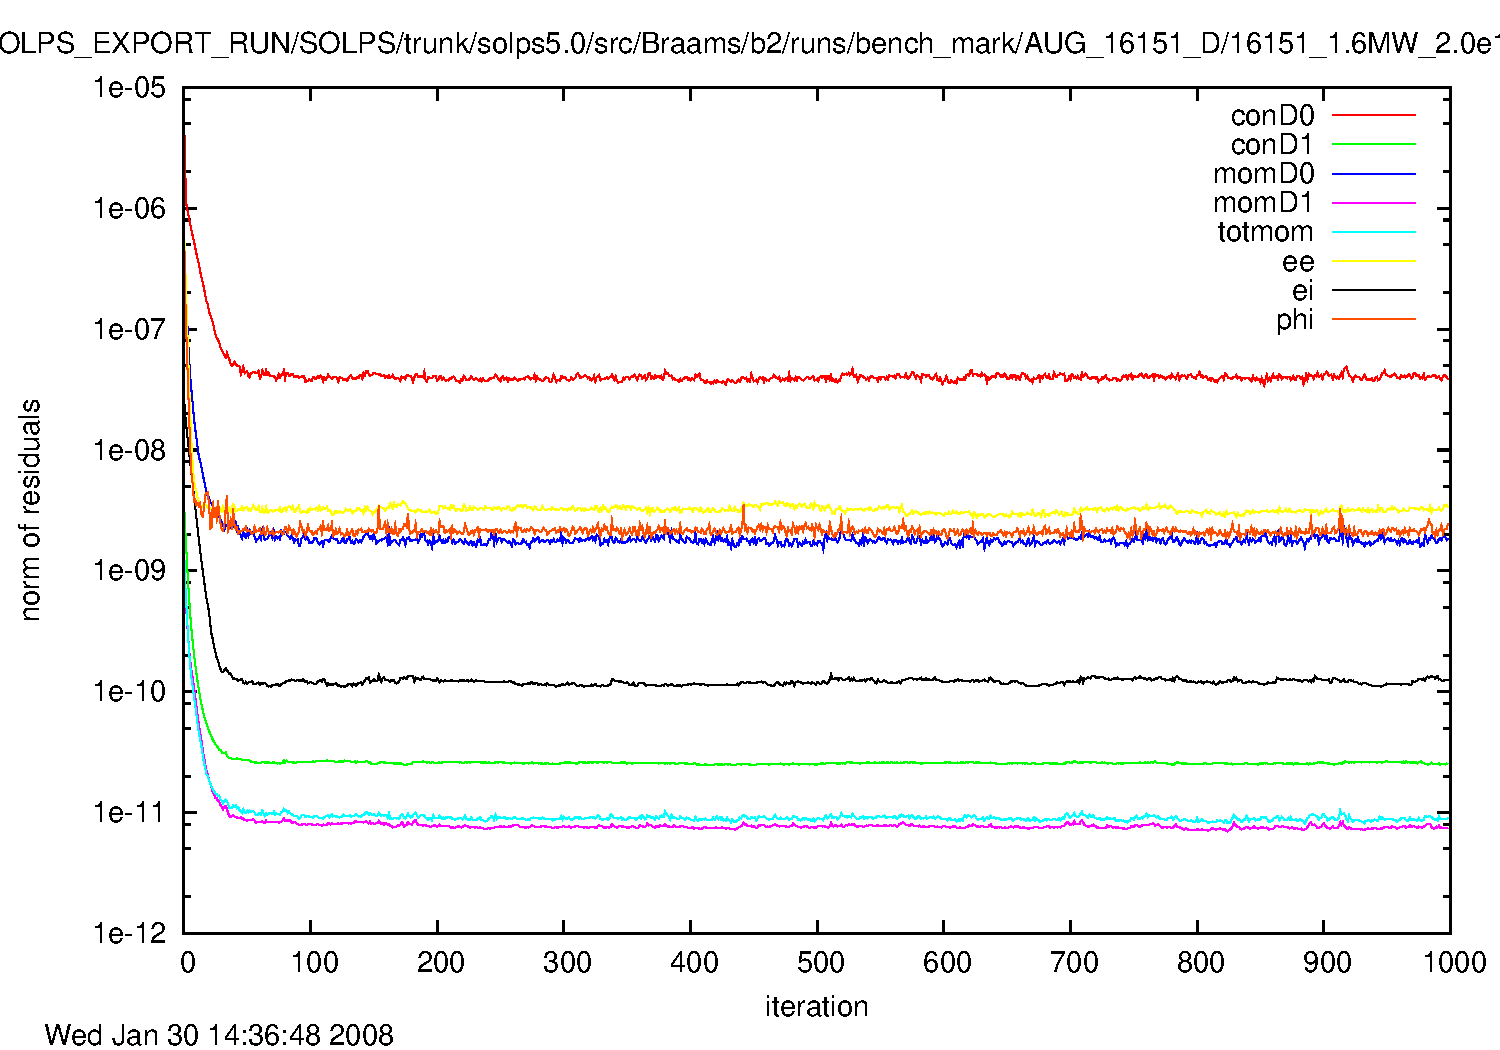
\includegraphics[width=6.0cm]{resall_D_REF.pdf}
    \else
    
\includegraphics[origin=br,angle=-90,width=6.0cm]{resall_D_REF.epsi}
    \fi
    \hfill
    \ifpdf 
    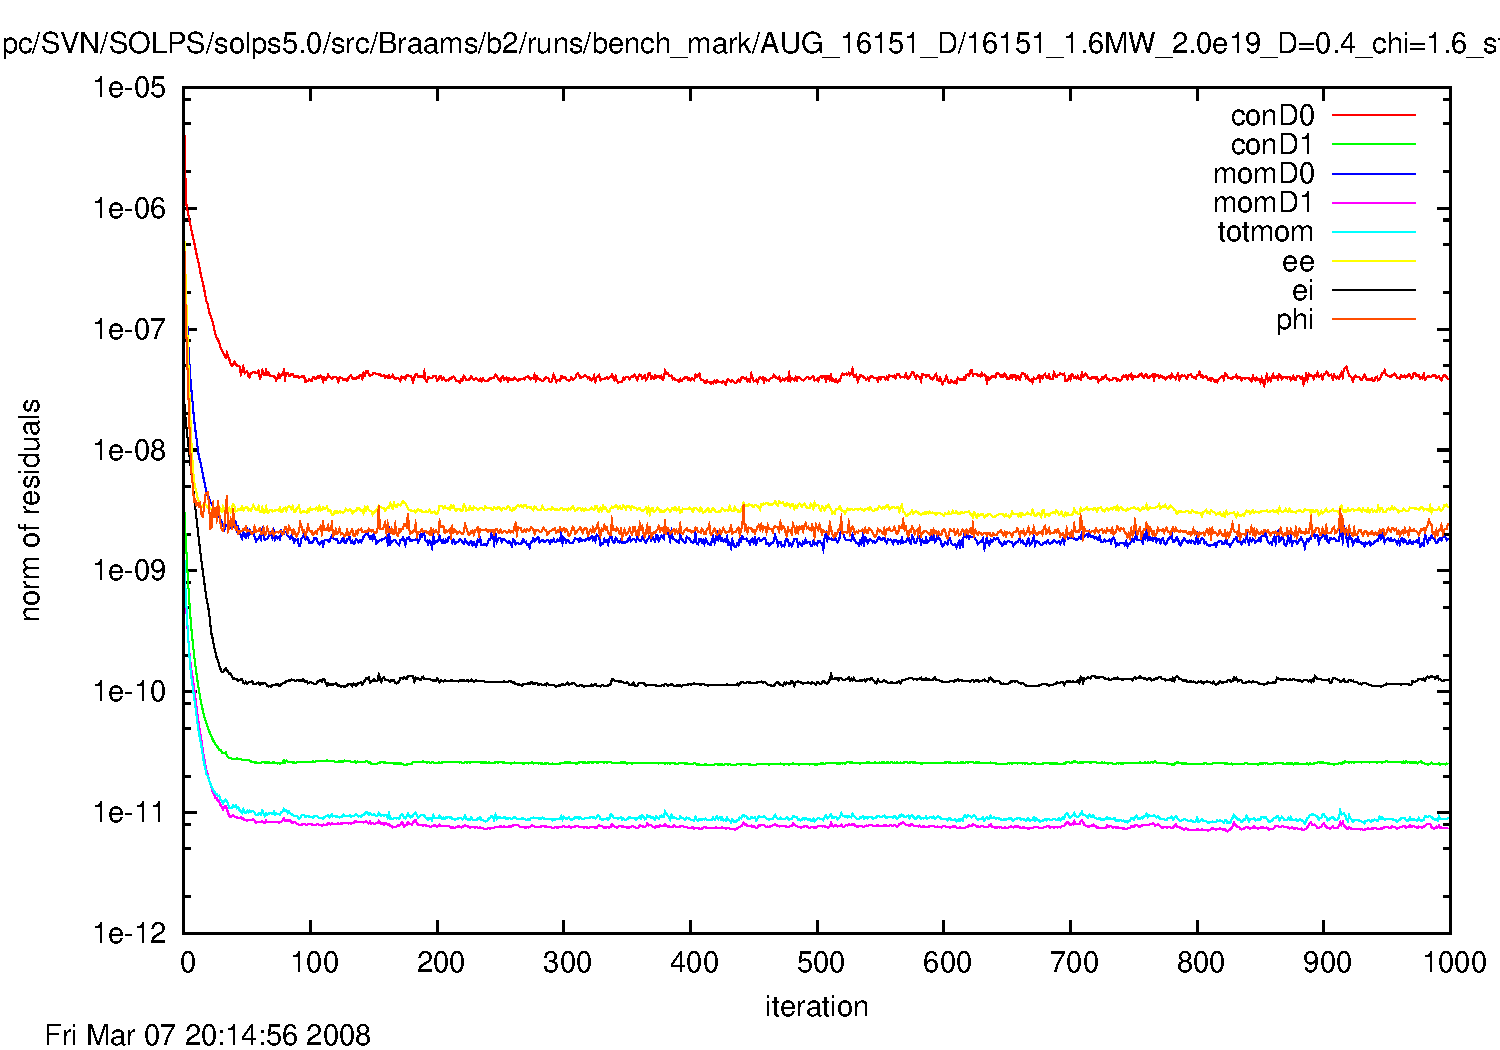
\includegraphics[width=6.0cm]{resall_D_000.pdf}
    \else
    
\includegraphics[origin=br,angle=-90,width=6.0cm]{resall_D_000.epsi}
    \fi
    \hfill
    \ifpdf 
    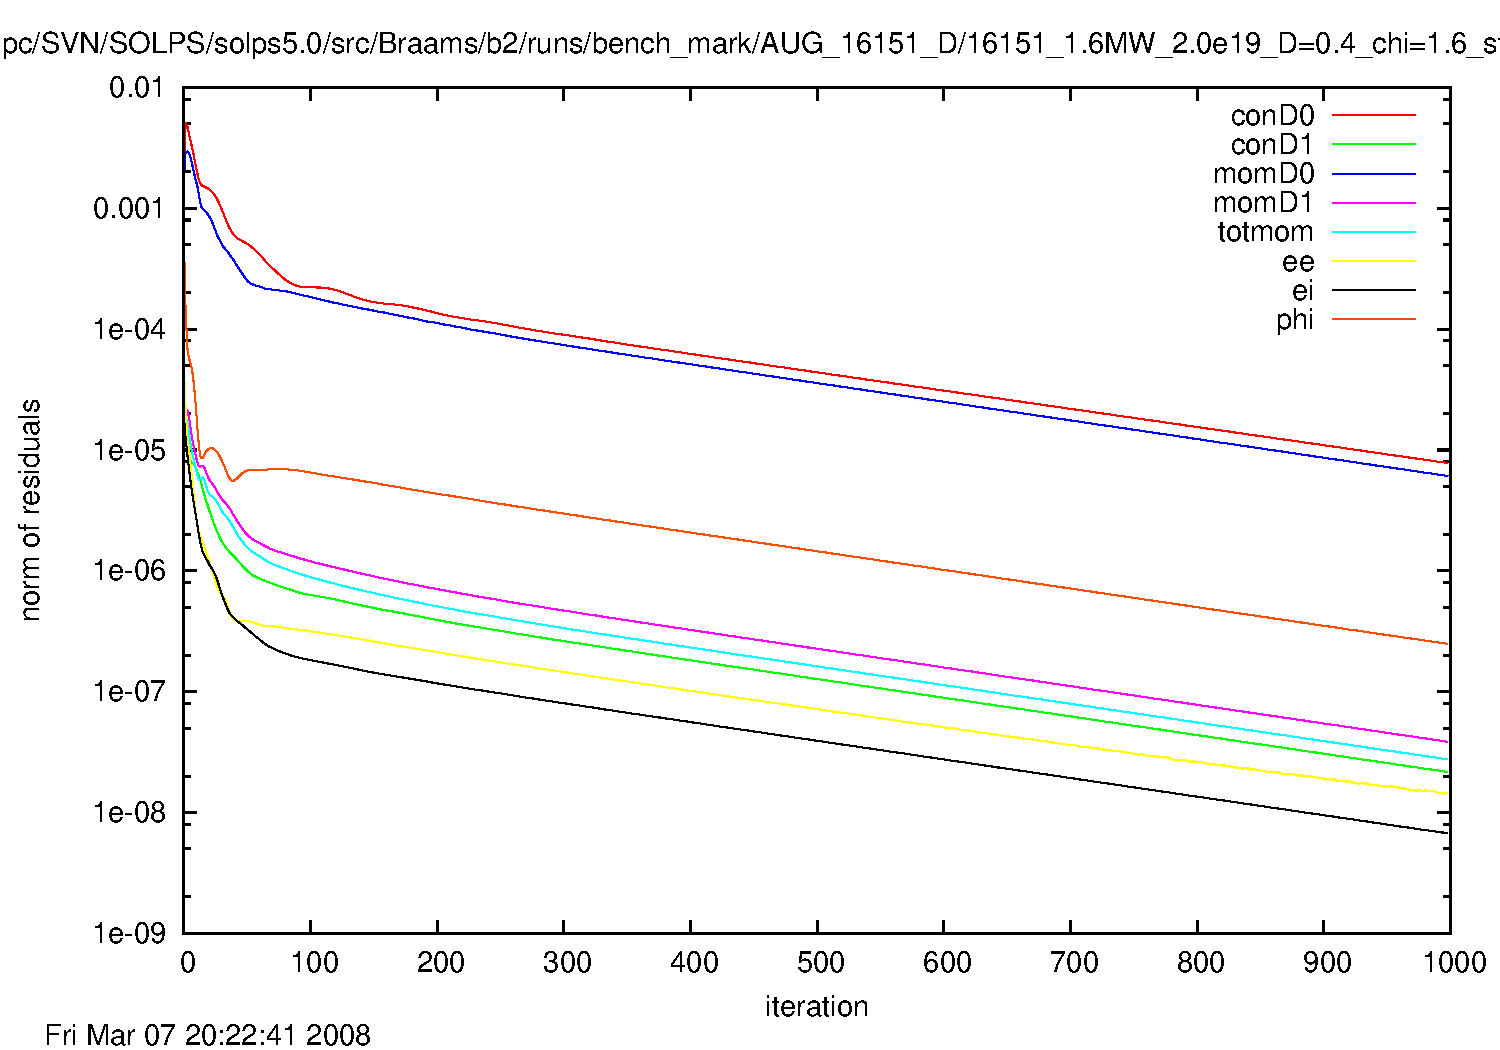
\includegraphics[width=6.0cm]{resall_D_001.pdf}
    \else
    
\includegraphics[origin=br,angle=-90,width=6.0cm]{resall_D_001.epsi}
    \fi
  }
  \centerline{
    \hfill
    002
    \hfill \hfill
    002a
    \hfill \hfill
    002b
    \hfill
  }
  \centerline{
    \ifpdf 
    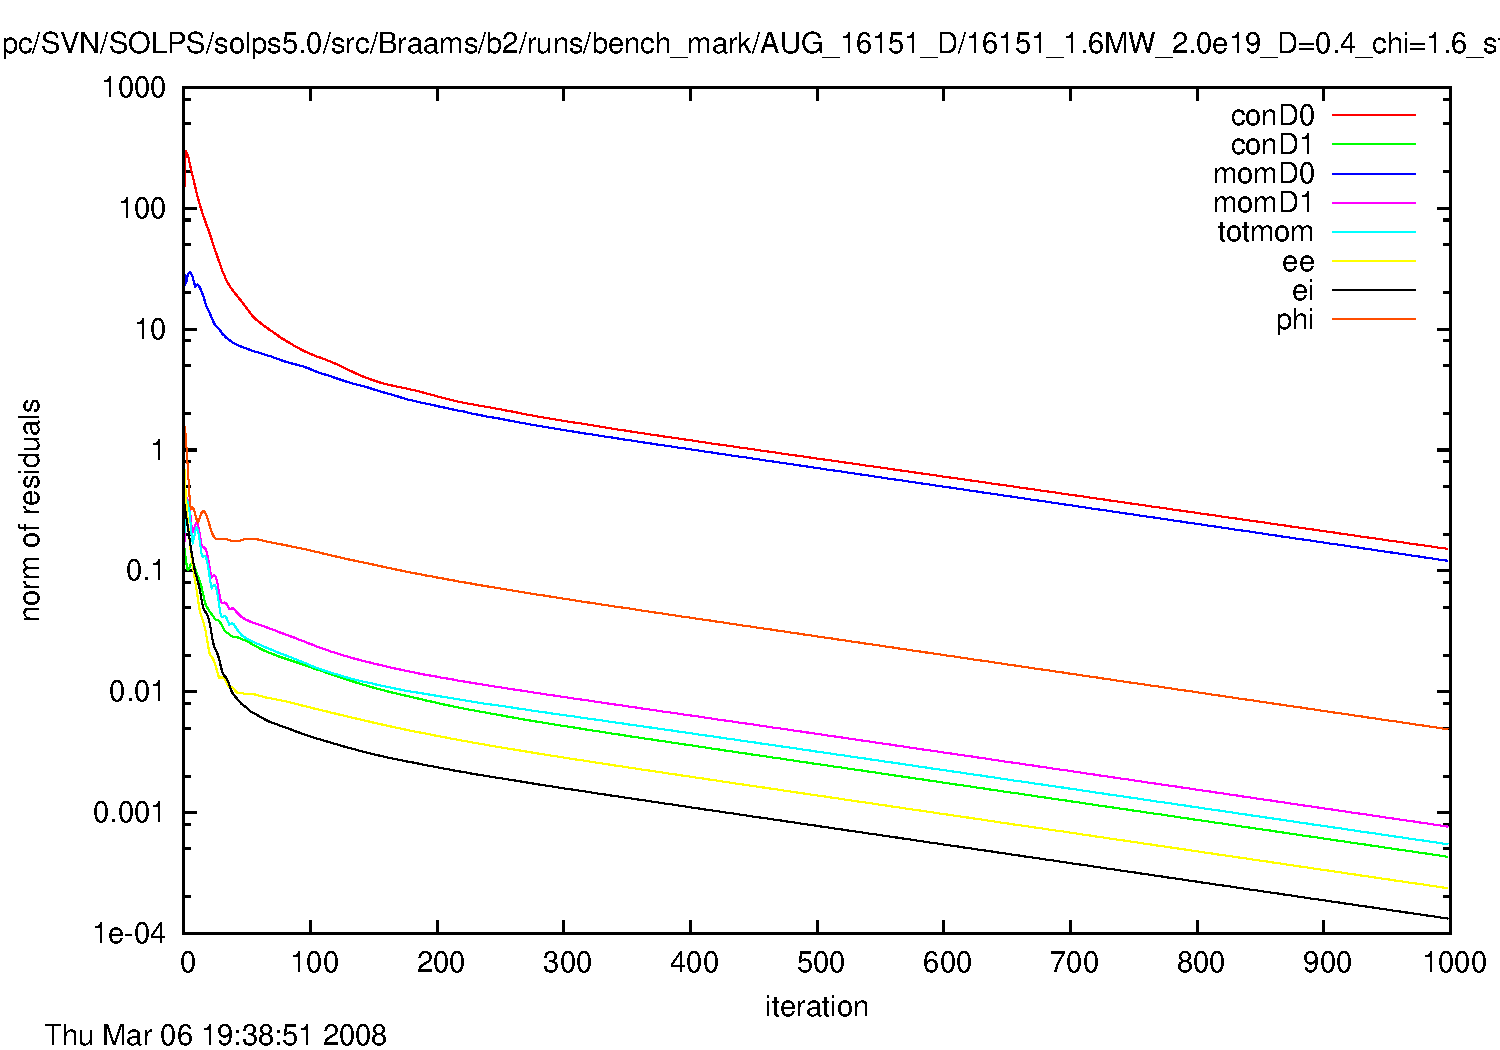
\includegraphics[width=6.0cm]{resall_D_002.pdf}
    \else
    
\includegraphics[origin=br,angle=-90,width=6.0cm]{resall_D_002.epsi}
    \fi
    \hfill
    \ifpdf 
    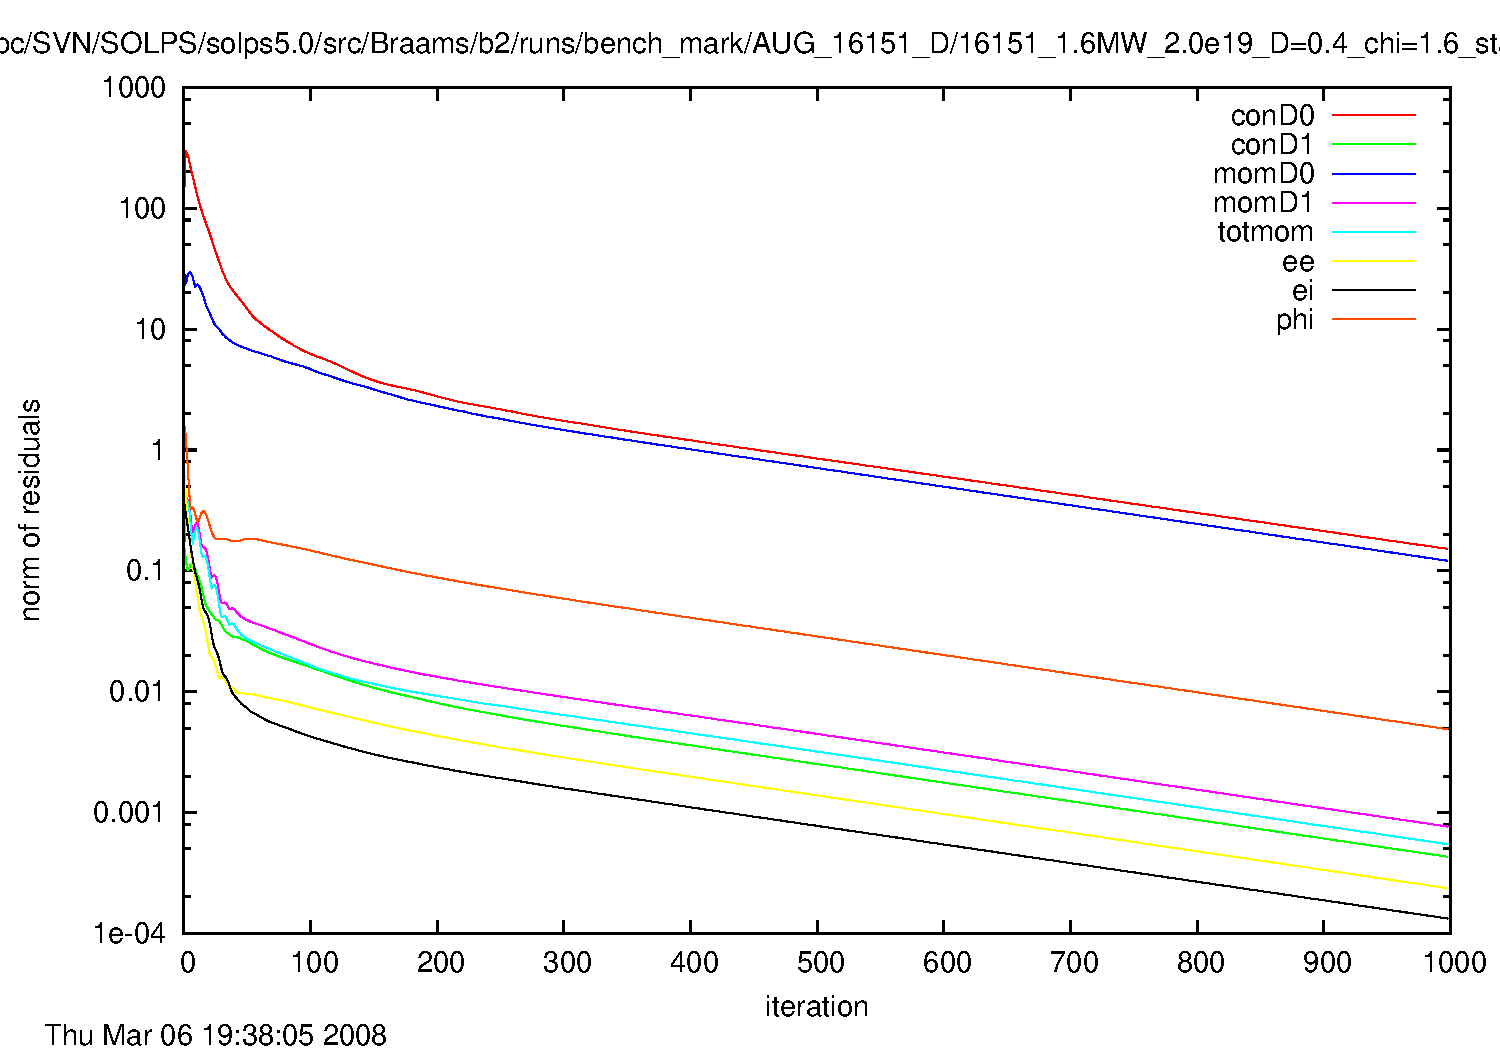
\includegraphics[width=6.0cm]{resall_D_002a.pdf}
    \else
    
\includegraphics[origin=br,angle=-90,width=6.0cm]{resall_D_002a.epsi}
    \fi
    \hfill
    \ifpdf 
    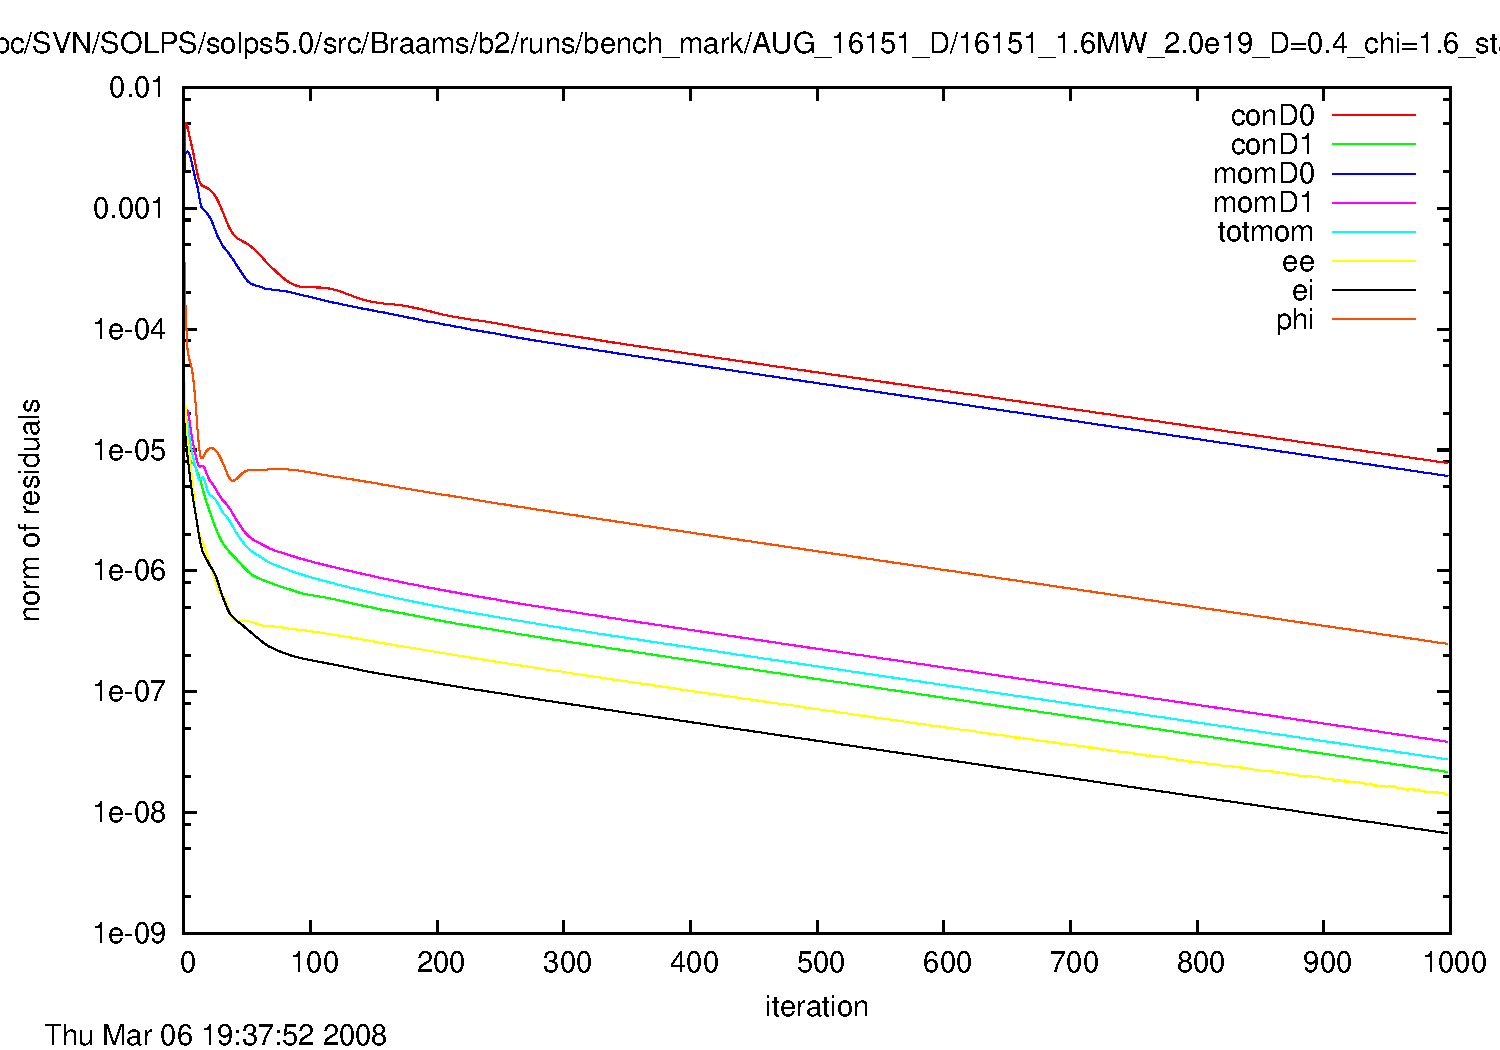
\includegraphics[width=6.0cm]{resall_D_002b.pdf}
    \else
    
\includegraphics[origin=br,angle=-90,width=6.0cm]{resall_D_002b.epsi}
    \fi
  }
  \caption{Residuals of the AUG\_16151\_D standard case for different code versions and options.}
  \label{fig:resDcomp}
\end{figure}

The following observations were made (see figure \ref{fig:resDcomp}):
\begin{description}
\item[000] same as {\bf REF}
\item[001] small kick in the residuals ($< 0.01$)
\item[002] larger kick in the residuals (between 100 and 1000)
\item[002a] very similar to {\bf 002}
\item[002b] very similar to {\bf 001}
\end{description}

\begin{figure}[hbt]
  \centerline{
    \hfill
    Relative change in $T_e$
    \hfill \hfill
    Relative change in $n_e$
    \hfill
  }
  \centerline{
    \ifpdf 
    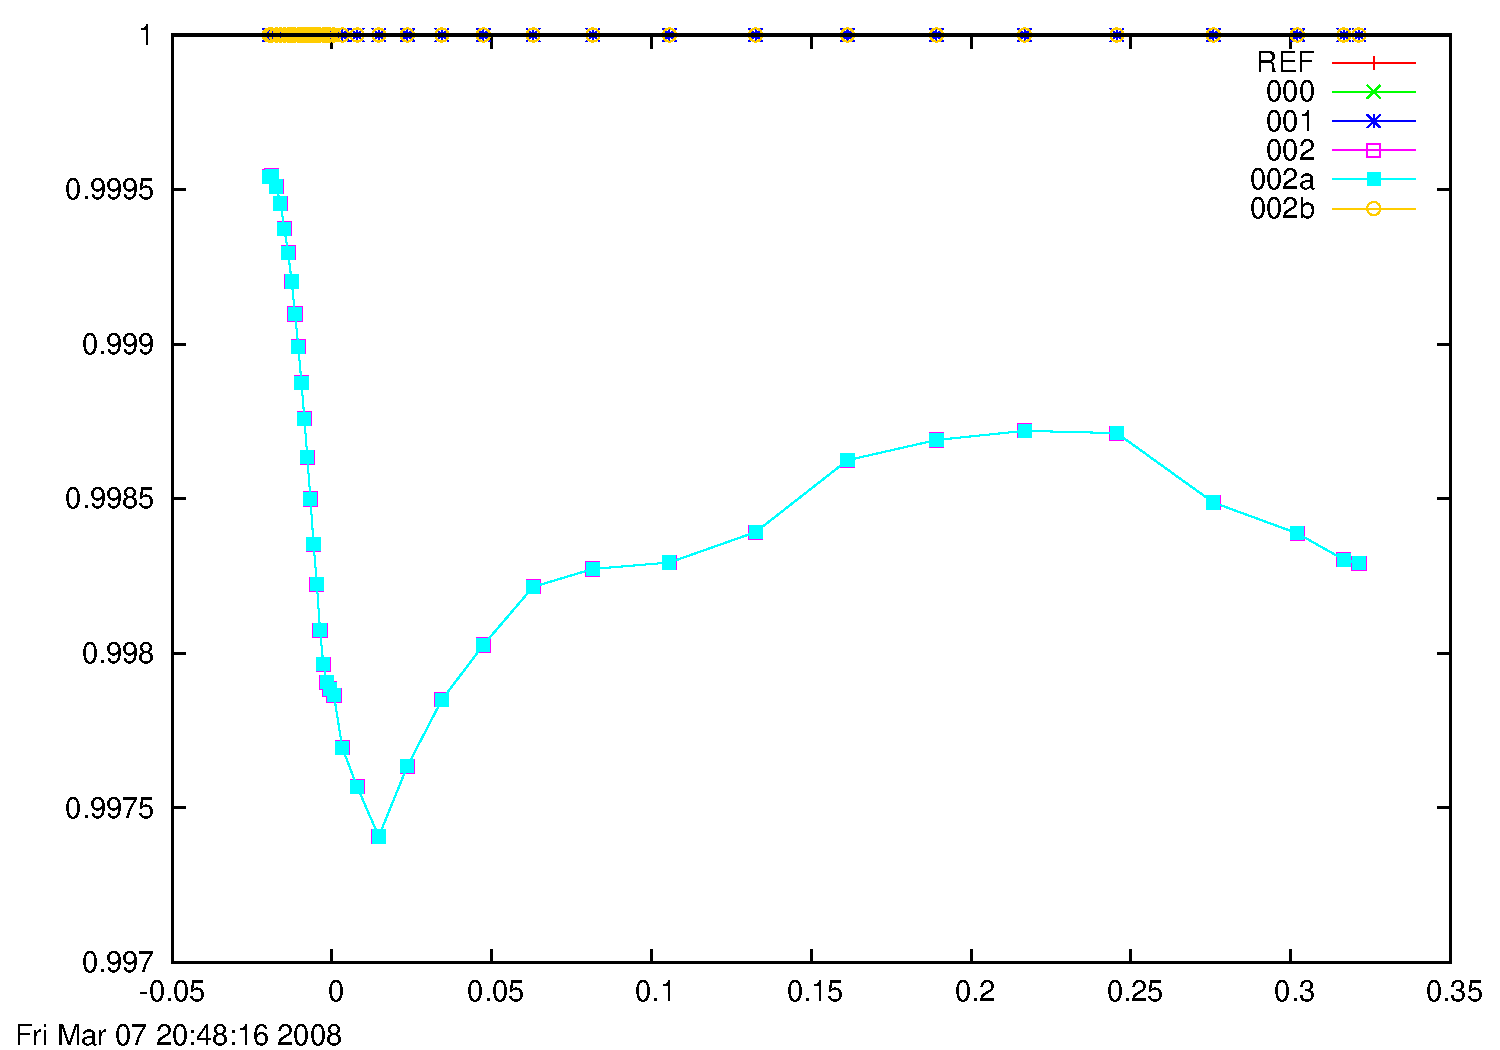
\includegraphics[width=9.0cm]{te3dr_relative_changes.pdf}
    \else
    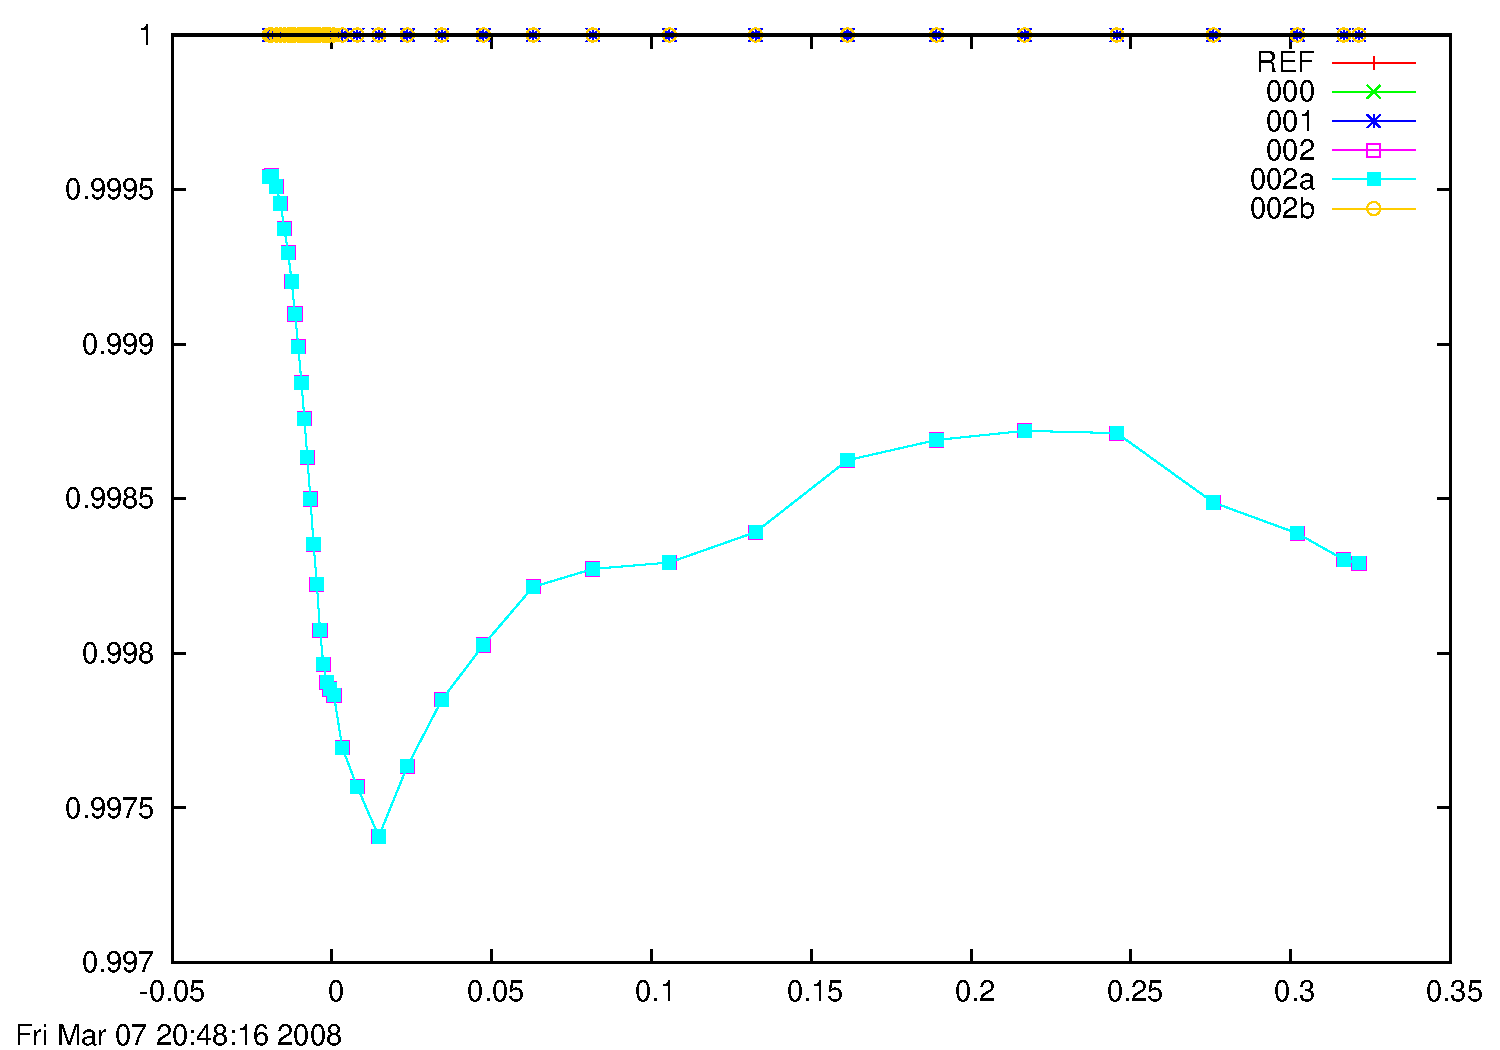
\includegraphics[origin=br,angle=-90,width=9.0cm]{te3dr_relative_changes}
    \fi
    \hfill
    \ifpdf 
    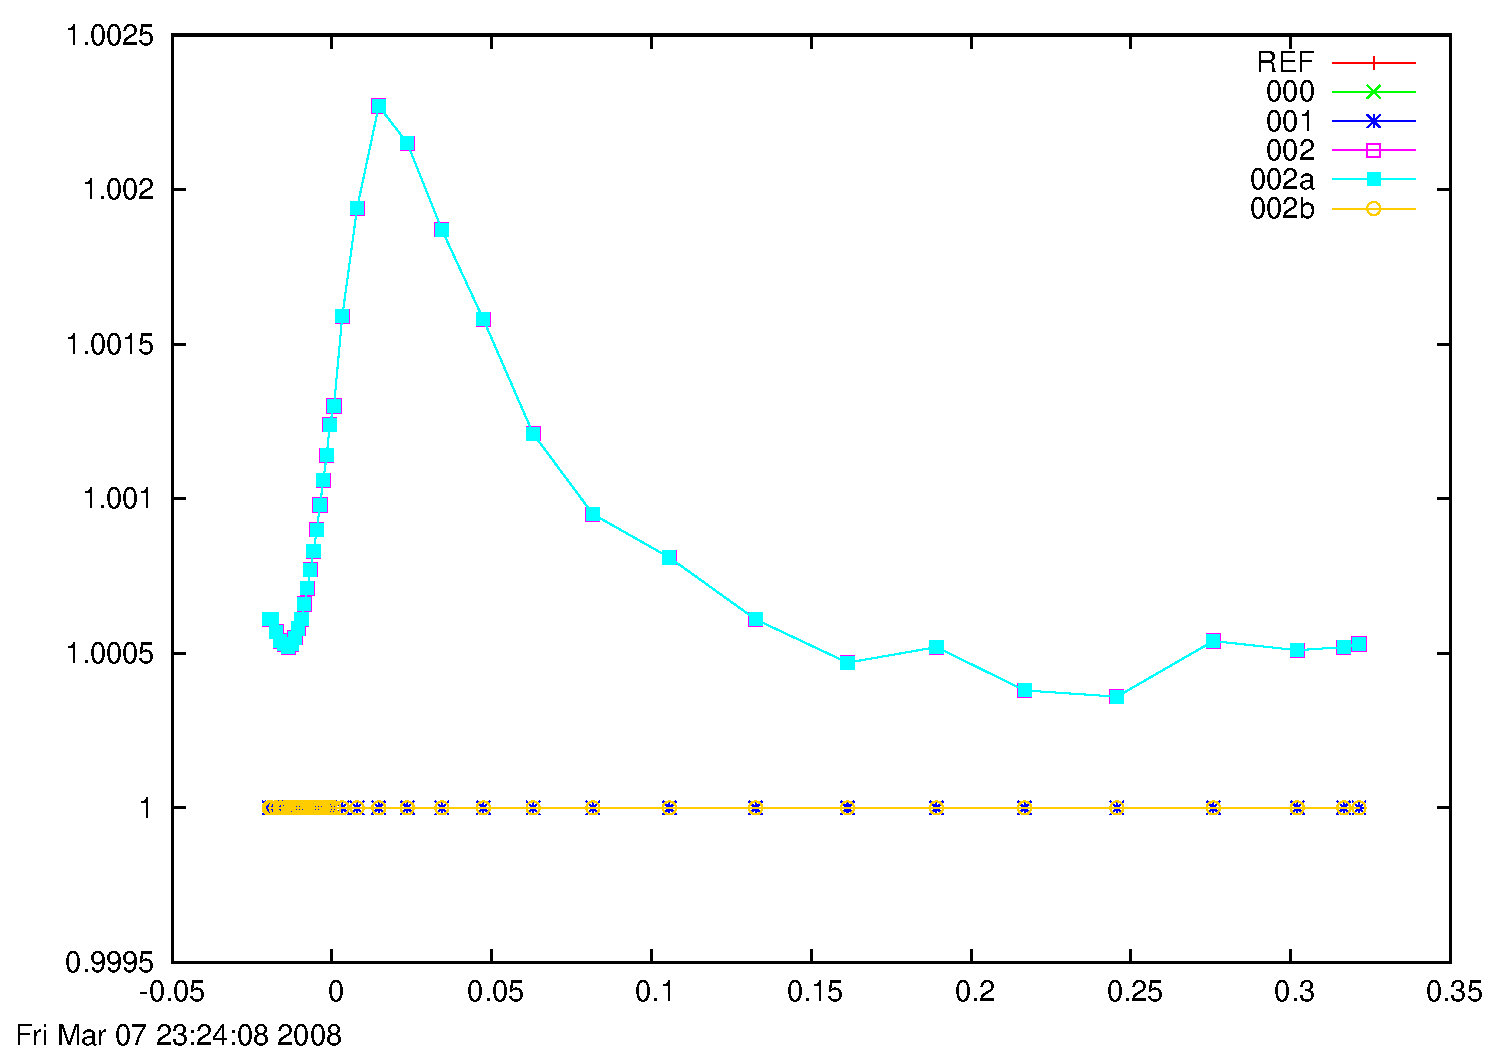
\includegraphics[width=9.0cm]{ne3dr_relative_changes.pdf}
    \else
    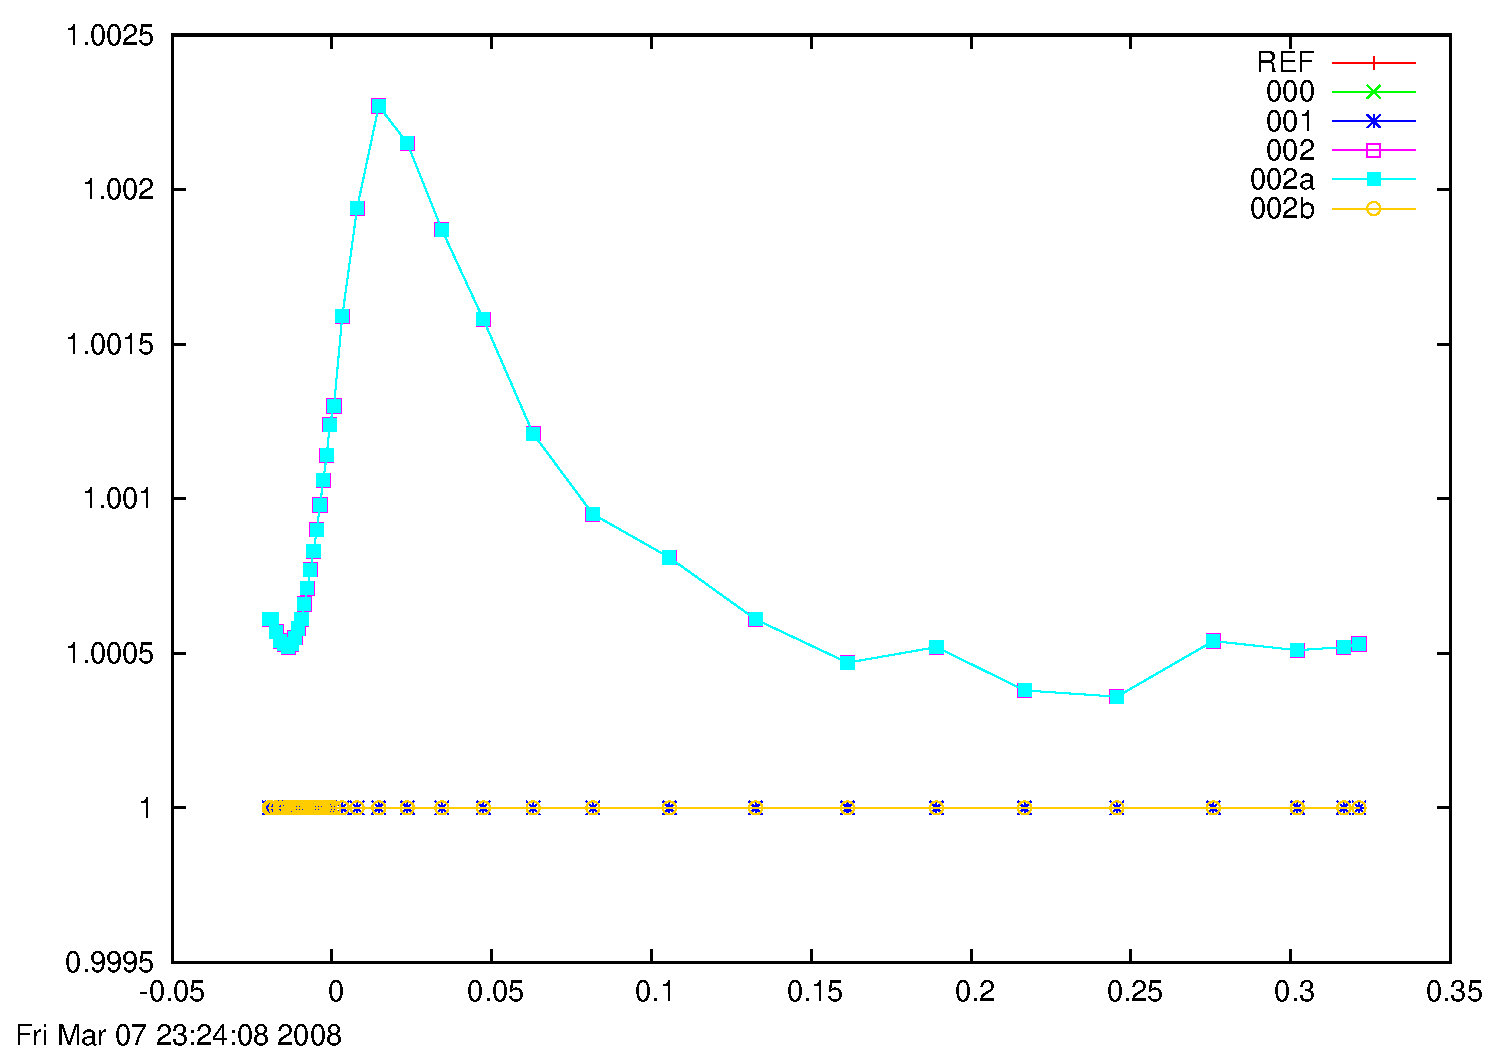
\includegraphics[origin=br,angle=-90,width=9.0cm]{ne3dr_relative_changes}
    \fi
  }
  \caption{Relative changes for the considered options.}
  \label{fig:relchangetene}
\end{figure}

Comparing (figure \ref{fig:relchangetene}) the converged values of te
at the outer target, {\bf 000}, {\bf 001} and {\bf 002b} gave the same
answer as {\bf REF}.  {\bf 001} and {\bf 002b} gave the same answer,
and the maximum relative change was 0.997408. (For ne at the outer
target, the maximum relative error was 1.00227.)

The conclusion: the largest effect seems to have come from the
correction in the cell volumes (causing a change in \verb!b2fgmtry!),
but this caused a small final change.  The change of physics constants
introduced a very small effect, seen only as a jump in the residuals.

\bibliographystyle{iaea}
\bibliography{tok,aug,general,extern,main,model,divgas,mnw,xpb}

\documentclass[a4paper,10pt]{report}
\usepackage{ifpdf}
%% \newif\ifpdf 
%% \ifx\pdfoutput\undefined 
%%   \pdffalse % we are not running PDFLaTeX 
%% \else 
%%   \pdfoutput=1 % we are running PDFLaTeX 
%% \pdftrue 
%% \fi
\ifpdf 
  \usepackage[pdftex]{graphicx} 
  \pdfcompresslevel=9 
\else
  \usepackage{graphicx} 
\fi
\ifpdf 
\else
\fi
\usepackage{times}
\usepackage{makeidx}
\usepackage{multirow}
\usepackage{fullpage}
\usepackage{drafthead}
\usepackage{draftcopy}
\usepackage{supertabular}
\usepackage{parskip}
\usepackage{multicol}
\usepackage{fancyvrb}
\usepackage{longtable}
\usepackage[scriptsize]{subfigure}
\usepackage{amsmath}
\usepackage{tocbibind}
\ifpdf 
\usepackage{thumbpdf}
\usepackage[pageanchor,pdftex,backref,hyperindex,colorlinks,bookmarks,bookmarksnumbered]{hyperref} %bookmarksopen,
\else
\usepackage{hyperref}
\fi
\usepackage{color}

\def\topfraction{.9}
\def\bottomfraction{.9}
\def\textfraction{.1}
\def\floatpagefraction{.9}
\def\headsep{25pt}

\hyphenation{author another created financial paper re-commend-ed Post-Script}

\newcommand\SOLPSfour{{\bf SOLPS 4.x} }
\newcommand\SOLPSfive{{\bf SOLPS 5.x} }
\newcommand\SOLPSfivens{{\bf SOLPS 5.x}}
\newcommand\SOLPSfiveone{{\bf SOLPS 5.1} }
\newcommand\SOLPSfiveonens{{\bf SOLPS 5.1}}
\newcommand\SOLPSITER{{\bf SOLPS-ITER} }
\newcommand\SOLPSITERns{{\bf SOLPS-ITER}}
\newcommand{\btwoplot}{{\bf b2plot} }
\newcommand{\btwoplotns}{{\bf b2plot}}
\newcommand{\grad}{\nabla}
\definecolor{Red}{rgb}{1.0,0.0,0.0}

\makeindex

\begin{document}

\mbox{}
\vfill
{\Huge \hfill \SOLPSITER \hfill}
\vfill

\newpage
\tableofcontents
\listoffigures
\listoftables

\chapter*{Preface}
This is the combined work of many authors.  Started by D.P.~Coster, it
includes contributions from
\begin{itemize}
\item D.P~Coster and O.~Wenisch, the original \btwoplot manual
\item K.~and A.S.~Kukushkin, the \verb!DG! manual, with revisions by A.~Chin and D.~Stotler
\item M.~Stanojevic, on boundary conditions
\item X.~Bonnin, for many contributions and the \SOLPSITER updates
\item S.~Voskoboynikov, for the \SOLPSITER model equations
\end{itemize}
All errors, omissions {\it etc.} should be e-mailed to \verb!Xavier.Bonnin@iter.org!.

\chapter{Introduction}
\label{cha:intro}

This document describes the \SOLPSITER code package and its components.
Following this introduction is a chapter (\ref{cha:structure})
describing the structure of the code.  Then chapter
\ref{cha:standaloneb2} describes the stand-alone version of \verb!B2.5!.  This
is followed by a description of the stand-alone version of \verb!Eirene! in
chapter \ref{cha:standaloneeirene} and then of the coupled \verb!B2.5-Eirene!
in chapter \ref{cha:coupledb2eirene}.  Then follow chapters on \verb!DivGeo!
(\ref{cha:divgeo}), \verb!Carre! (\ref{cha:carre}) and \verb!agg! (\ref{cha:agg}).
Appendix \ref{cha:intb2doc} contains copies of the \verb!B2.5! internal
documentation files, \ref{cha:b2physics} describes the physics in \verb!B2.5!,
\ref{cha:equations} gives the full model equations used in \verb!B2.5!,
\ref{cha:Mladen} gives details about some
\verb!B2.5! boundary conditions,
\ref{cha:b2time} information about the quantities stored in
\verb!b2time.nc!, 
\ref{cha:b2tallies} information about the quantities stored in
\verb!b2tallies.nc!,
\ref{cha:regions} gives the region definitions used in the code,
\ref{cha:b2plotmanual} is an updated
version of the \btwoplot manual, \ref{cha:Misc}
contains information about array dimensions and compilation options, 
\ref{cha:dgmanual} is the \verb!DG! manual, and lastly
\ref{cha:coursenotes} includes a listing of the programs and files included
in the \verb!B2.5! part of the \SOLPSITER package.

Historically, there have been many implementations of the
\verb!SOLPS! (Scrape-Off Layer Plasma Simulation)
code package, according
to which version of the fluid plasma code (\verb!B2! or \verb!B2.5!) and of
the \verb!Eirene! Monte-Carlo neutral transport code are used. We distinguish between
\SOLPSfour which uses \verb!B2! and \SOLPSfive which uses \verb!B2.5!.
This document is devoted solely to \SOLPSITER although several features are
common to multiple versions. \SOLPSITER contains the \verb!B2.5! plasma kernel and a recent version of \verb!Eirene!. 
Most of the current development and support 
is done exclusively on \SOLPSfive and \SOLPSITER versions (with the important exception of the Forschungszentrum J{\"u}lich and their collaborators where \SOLPSfour is still in use). The main
differences of note between \verb!B2! and \verb!B2.5! are:
\begin{enumerate}
  \item For ions, \verb!B2! solves a {\em total} energy equation, while \verb!B2.5!
solves an {\em internal} energy equation. See section \ref{sec:sourcescoupling} for an 
example of the consequences.
  \item The primary momentum variable is the {\em poloidal} velocity in \verb!B2! and the
{\em parallel} velocity in \verb!B2.5!.
  \item The velocities are computed on cell faces in \verb!B2! and on cell centres in \verb!B2.5!.
  \item The current continuity equation is solved by default in \verb!B2.5!, but not in \verb!B2!. 
  \item The treatment of drifts and currents is much more complete in \verb!B2.5! than in \verb!B2!.
  \item Classical transport in \verb!B2.5! follows the Balescu treatment by default, while it uses
Braginskii in \verb!B2! (see \ref{sec:balescubraginskii} for a comparison).
  \item Some variables names and indexing have changed. See section \ref{sec:b2pl} for a partial list.
  \item The run parameters to \verb!B2.5! are split into several input files. See sections 
\ref{sec:b2mn}, \ref{lis:b2cdcn} and \ref{sec:b2files} for a detailed description.
\end{enumerate}
\index{Converting from SOLPS4 to SOLPS5}
\index{Converting from SOLPS5 to SOLPS4}
Some effort has been undertaken for the user to be able to toggle between the \SOLPSfour and
\SOLPSfive numerical treatments. The interested reader is referred to the listing of run switches
in section \ref{lis:b2cdci} for the complete list. Two converters also exist to transfer run output 
from \SOLPSfour or \SOLPSfive to \SOLPSITERns:
\begin{description}
  \item[From 4 to 5 and ITER] \verb!b2sxdr!\index{b2sxdr}
  \item[From 5 and ITER to 4] \verb!b2xd!\index{b2xd}
  \item[From 5 to ITER] \verb!b2yt!\index{b2yt} 
\end{description}

Additional documentation on other code versions can be found in the \$\verb!{SOLPSTOP}/doc! directory.
Namely, the original report by Bas Braams is:
\begin{verbatim}
BRAAMS_-_A_Multi-Fluid_Code_for_the_Simulation_of_the_Edge_Plasma_in_Tokamaks_-_NET_Report_1987.pdf ,
\end{verbatim}
and an excellent review of \SOLPSfour can be found in:
\begin{verbatim}
Martine_Baelmans_-_Juelich_Report_1994.pdf .
\end{verbatim}

Several of the {\bf SOLPS4.2} features are detailed in \verb!Kotov_SOLPS42_Report.pdf!.

The next section discusses obtaining and updating the code.

\section{Obtaining and updating the code}
\label{solpsdistribution}\index{Obtaining the code}\index{B2.5, obtaining}\index{SOLPS-ITER, obtaining}\index{Eirene, obtaining}\index{dg, obtaining}\index{DG, obtaining}\index{DivGeo, obtaining}\index{Carre, obtaining}\index{Updating the code}\index{B2.5, Updating}\index{SOLPS-ITER, Updating}\index{Eirene, Updating}\index{dg, Updating}\index{DG, updating}\index{DivGeo, Updating}\index{Carre, Updating}

To obtain the code a request should be sent to Xavier Bonnin
(\verb!Xavier.Bonnin@iter.org!) at ITER, the code Responsible Officer (RO).  

The first formality will then be for the prospective users to obtain and IDM (ITER Document Management) account, in case they do not have one already. This account request will be done by the RO, and the requesting user will receive an automated electronic message asking for confirmation of the provided e-mail address. With this account, the user will have access to the \SOLPSITER GIT repository (\href{https://git.iter.org/projects/BND/repos/solps-iter/browse}{https://git.iter.org/projects/BND/repos/solps-iter/browse}) maintained at the IO, the \SOLPSITER SharePoint web site hosted by ITER (\href{https://portal.iter.org/departments/POP/CM/IMAS/Forms/AllItems.aspx}{https://portal.iter.org/departments/POP/CM/IMAS/Forms/AllItems.aspx}, folder ``SOLPS-ITER'', works best with Internet Explorer). The account request will also serve for registration of the user to the \SOLPSITER mailing list (\verb!SOLPS-ITER@iter.org!).

The \SOLPSITER Git repository also includes the repositories for \verb!B2.5!, \verb!EIRENE!, \verb!Carre! and \verb!DivGeo! individually as submodules.

One can generally browse the ITER Git repositories here: \href{https://git.iter.org}{https://git.iter.org} and \SOLPSITER specifically here: \href{https://git.iter.org/projects/BND/repos/solps-iter/browse}{https://git.iter.org/projects/BND/repos/solps-iter/browse}, but since these repositories are restricted users will first need to authenticate with their ITER (IDM) username and password - possibly twice, once for the intranet, and once for the Git web front end in the top right-hand corner in the web browser window.

To do this, one must upload a copy of their public ssh key here: \href{https://git.iter.org/plugins/servlet/ssh/account/keys}{https://git.iter.org/plugins/servlet/ssh/account/keys} (by following links under ``Manage Account''). Then one should be able to simply clone a copy of \SOLPSITER to a local machine by doing:

\begin{verbatim}
> git clone ssh://git@git.iter.org/bnd/solps-iter.git
> cd solps-iter
> git submodule init
> git submodule update
\end{verbatim}

Since the user-id is immutably encoded into any changes, it is always a good idea to properly configure a local installation of Git on all the systems on which one plans on making code revisions with, e.g.:

\begin{verbatim}
> git config --global user.name "Your Name"
> git config --global user.email your.name@anywhere.you.are
\end{verbatim}

Users all have write access to these repositories although not to the \verb!develop!, \verb!master! or \verb!svn/*! branches.  This basically means one should create \verb!feature/[topic]!, \verb!bugfix/[topic]!, or \verb!hotfix/[topic]! branches and raise a ``Pull Request'' (\href{https://git.iter.org/projects/BND/repos/solps-iter/pull-requests}{https://git.iter.org/projects/BND/repos/solps-iter/pull-requests}) to have them merged into the \verb!develop! branch after pushing them back to the ITER repository.

Issues are handled using JIRA (\href{https://jira.iter.org/browse/IMAS}{https://jira.iter.org/browse/IMAS}) and users should feel encouraged to create new issues associated with \SOLPSITER (selected from the drop-down list of components) if they have any problems or suggestions. (Please ignore the options associated with resource estimates and sprints.)

For more general help with Git, we can recommend the documentation here (\href{http://git-scm.com/}{http://git-scm.com/}) and the Pro Git book (linked from there) in particular.

When using Git, the command
\begin{verbatim}
> git status
\end{verbatim}
will check if there are any local changes to your local copies of the version-controlled files from the repository, using as a reference the state of the repository from when you last cloned or updated it. To update these
references to the current state of the \verb!origin! repository, please use
\begin{verbatim}
> git fetch
\end{verbatim}
If that command returns no output, then your references are up-to-date. Otherwise, if someone else has
been committing changes to the repository, Git will indicate the tags of the updated repository. You can then import these latest changes with the command
\begin{verbatim}
> git pull
\end{verbatim}
followed by
\begin{verbatim}
> git submodule update
\end{verbatim}
which will also update the files contained in the various submodules \SOLPSITER is linking to. It is best to do this with your local directory up-to-date and your local changes committed, otherwise Git will ask you to resolve any conflicts before you may proceed.

\SOLPSITER is a complicated code package and it would be difficult to learn how to install, compile and run it from this document and the internal documentation alone.  In the past we have found that an initial visit of at least two weeks to a research team already proficient with \SOLPSITER use with subsequent visits, or about two months and no further visits, are desirable.  

The Git \SOLPSITER repository is structured as a self-contained whole, but some effort was also devoted to be able to check out, as individual stand-alone modules, the main pieces of the SOLPS suite, i.e. \verb!DivGeo!, \verb!Carre!, \verb!Eirene! and \verb!B2.5!, although this is not recommended.

\section{Requirements}
\index{Requirements}

To best use the \SOLPSITER code suite, the user will need, locally installed:

\begin{description}
\item[Fortran 90/95 Compiler] the main programs are written in \verb!FORTRAN 90!; some routines still require a ``-r8'' option
\item[C Compiler] the \verb!DivGeo! code and a few utility routines are written in \verb!C!
\item[MPI] Parallelization framework (optional)
\item[NAG]\index{NAG} mathematical library (optional)
\item[BLAS/LAPACK] mathematical libraries
\item[NCAR] plotting library
\item[GR] plotting library (optional)
\item[GKS] graphical kernel library
\item[HDF5] data storage library
\item[NetCDF]\index{netcdf} storage/archival library (optional)
\item[MSCL] utility library
\item[makedepend] to build the dependencies needed by the \verb!Makefiles!
\item[gnuplot] for many analysis scripts
\item[nc2text] for obtaining time-dependent data traces
\item[plotmtv] for obtaining graphs of the time evolution of various profiles
\item[LaTeX interpreter] to produce this manual
\item[GIT] version control software
\item[/bin/bash] used by some scripts
\item[/bin/csh] used by some scripts
\item[/bin/ksh] used by some scripts
\item[/bin/sh] used by some scripts
\item[/bin/tcsh] used by some scripts
\end{description}

For all the various libraries, it is recommended that they be installed as modules, so that they
may be shared amongst multiple users on the same machine, so as not to duplicate large files and to
centralize their management. Most, but not all, of these libraries are publicly available from the 
Internet. The MSCL library is distributed and can be obtained from the ITER GIT repository at
\href{https://git.iter.org/projects/LIB/repos/mscl/browse}{https://git.iter.org/projects/LIB/repos/mscl/browse}.

If one uses local copies of these libraries, a copy or link to them should be put in the 
\$\verb!{SOLPSTOP}/lib/!\$\verb!{HOST_NAME}.!\$\verb!{COMPILER}! directory.

\section{Initial set-up}
\index{Initial set-up}

For each local implementation, environment variables are used to designate
the location where the various libraries are to be found, as well as the preferred compilers to be 
used. These are propagated throughout the \SOLPSITER code structure and used by the Makefiles and
the various scripts. It is therefore important to carefully assign their values.

These environment variables are found in files config.\$\verb!{HOST_NAME}!.\$\verb!{COMPILER}!.

The current list of recognized hostnames, deduced by means of the \verb!whereami! script, includes:
\begin{description}\index{Hostnames}
  \item[ASIPP] Academica Sinica, Hefei: *.ipp.cas.cn
  \item[CCFE] CCFE domain: *.ccfe.ac.uk
  \item[FZJ] Forschungszentrum J{\"u}lich domain: *.fz-juelich.de, *.ipp.kfa-juelich.de
  \item[GA] General Atomics: *.fusion.gat.com
  \item[IFERC] IFERC supercomputer: *.iferc-csc.org
  \item[IPP] IPP-Garching domain: *.ipp.mpg.de, *.ipp-garching.mpg.de, *.rzg.mpg.de
  \item[IPP-HGW] IPP-Greifswald domain: *.ipp-hgw.mpg.de
  \item[ITER] ITER domain: *.iter.org
  \item[ITM] ITM Gateway machine: *.itm.rzg.mpg.de, *.efda-itm.eu
  \item[JET] JET domain: *.jet.uk
  \item[LEUVEN] KU-Leuven domain: *.mech.kuleuven.be
  \item[NERSC] DOE supercomputer center: *.nersc.gov
  \item[PPPL] PPPL domain: *.pppl.gov
  \item[WM] College of William and Mary: *.wm.edu
  \item[default] everywhere else
\end{description}

If your domain name is not on this list, please add it to \verb!whereami!.

At the moment the following compiler platforms are supported, assuming a Linux work environment:
\begin{description}\index{Platforms}
  \item[pgf90] Portland Group 32-bit Fortran compiler, in use at JET and ORNL
  \item[ifort64] Intel 64-bit Fortran compiler, in use at ITER and IPP
  \item[gfortran] The gfortran compiler, in use at FZ-J{\"u}lich, KU-Leuven
\end{description}

For each hostname domain, a default compiler can be defined by means of the \$\verb!default_compiler!
file. This default can be overridden by giving the desired compiler name as an argument following
the \verb!setup.csh! command, i.e.:
\begin{verbatim}
  source setup.csh ifort64
\end{verbatim}

If your domain name does not yet have a default compiler associated with it or you want to change it,
please edit the \verb!default_compiler! switch accordingly.

Then, if this is the first installation in your file space, please do:
\begin{verbatim}
  first_setup
\end{verbatim}

This will, if they are not already present in the distribution, create the various \verb!config.!\$\verb!{HOST_NAME}.!\$\verb!{COMPILER}! files for each of the \SOLPSITER submodules. Feel free to modify them afterwards according to your local requirements. As with \verb!whereami! and \verb!default_compiler!, if those modifications are worth sharing with the other users, please commit them back to the repository using a pull request.

For each combination of hostname and compiler, the set of corresponding environment variables are loaded
from the \$\verb!{SOLPSTOP}\SETUP\setup.csh.!\$\verb!{HOST_NAME}.!\$\verb!{COMPILER}! file and, subsequently, 
the \$\verb!{SOLPSTOP}\SETUP\setup.csh.!\$\verb!{HOST_NAME}.!\$\verb!{COMPILER}.local! file.
The compiler switches are given through the configuration file 
\$\verb!{SOLPSTOP}\SETUP\config.!\$\verb!{HOST_NAME}.!\$verb!{COMPILER}!. This last file should contain the
location of all the main libraries with which the \SOLPSITER executables will be linked and their
linking instructions. It also contains the shared compiler directives for all the \SOLPSITER object files
and the name of the debugger program to be used, if any.
Users should make sure the settings within these files fit their run environment and modify them as needed.
If changes are needed, please forward them to the \SOLPSITER RO so that they may be included in the
set of distributed files to help other future users.

For the case where single submodules are cloned from the \SOLPSITER repository, without the full regalia of
programs, additional sets of config files can be found in the \verb!config! directory in each module. The 
compiler specific to this module are included there. Users are encouraged to modify these as needed. If local
changes are required that should not be archived in the repository, then users should create a file named
\verb!config.!\$\verb!{HOST_NAME}.!\$\verb!{COMPILER}.local! which the \verb!Makefile! will load and use to
overwrite the more general settings from the distributed \verb!config! file.

Some Windows\index{Windows} implementations have been attempted, and require an additional \verb!-DWINDOWS! compiler switch, but are not currently being supported.

If you wish your domain name to be included in the list of hostnames above, please contact the 
\SOLPSITER RO and send the
hostname you would like to have and the Internet address range to which it would apply. Please
also send the relevant compiler config files so they may be distributed to future users from the 
same domain or serve as examples for other users using the same compiler.

If the NAG library is not available (it requires a pay licence), then the BLAS and
LAPACK packages should be used instead, and links to them added to the corresponding \verb!config! files.

To compile the coupled version of the code you should begin by checking that the default
array dimensions provided fit your problem size. These are stored in the file
\$\verb!SOLPSTOP/modules/B2.5/src/include/DIMENSIONS.F!. If the dimensions are not right for you,
the do the following:
with:\index{DIMENSIONS.F}
\begin{verbatim}
  sb2
  cd src
  mkdir -p include.local
  cp include/DIMENSIONS.F include.local
\end{verbatim}
and edit the file \verb!include.local/DIMENSIONS.F! so that the 
dimensions (mainly used for the namelists in \verb!B2.5!) are
big enough (see the description of the relevant variables in section \ref{sec:DIMENSIONS}).

Once the config files and dimensions have been filled in with the appropriate information for the
local implementation desired, one proceeds with the compilation of the code. For this
purpose, a master \SOLPSITER \verb!Makefile! is provided, located at \$\verb!{SOLPSTOP}/Makefile!.\index{Makefile} The options supported by this \verb!Makefile! are:
\begin{description}\index{Compiling the code}\index{B2.5, compiling}\index{SOLPS-ITER, compiling}\index{Eirene, compiling}\index{DivGeo, compiling}\index{Carre, compiling}
  \item[solps] (Default) Compiles the necessary components for a full \SOLPSITER implementation, including:
    \begin{description}
      \item[libs] Installs the needed libraries according to config file
      \item[carre] The \verb!Carre! grid generator and associated translators
      \item[divgeo] The \verb!DivGeo! graphical input file builder and accompanying equilibrium and template converters
      \item[b25eirene] The \verb!B2.5-Eirene! main code and accompanying programs
      \item[uinp] The \verb!Uinp! translator from \verb!DivGeo! output to \verb!B2.5-Eirene! input
      \item[sonnet-light] The \verb!Sonnet! library
      \item[triang] The \verb!Tria! and \verb!Triageom! triangulation utilities
      \item[manual] Builds this manual
    \end{description}
  \item[all] The same as {\bf solps} above, but in addition:
    \begin{description}
      \item[b25] The \verb!B2.5! stand-alone plasma fluid solver and accompanying programs
      \item[eirene] The \verb!Eirene! stand-alone Monte-Carlo neutral transport code
    \end{description}
  \item[nox] The same as {\bf solps} above, but without linking to any graphical libraries:
    \begin{description}
      \item[carre\_nox] The \verb!Carre! grid generator will not generate graphs
      \item[b25eirene\_nox] Only the \verb!B2.5-Eirene! executable will be built without graphics
      \item[triang\_nox] The \verb!tria.eps! and \verb!triageom.eps! files will not be produced
      \item[uinp\_nox] The \verb!Uinp! translator from \verb!DivGeo! output to \verb!B2.5-Eirene! input
      \item[manual] Builds this manual
      \item[libs, divgeo, sonnet-light] Will not be built
    \end{description}
  \item[nox\_build] The same as {\bf nox} above and used for compilation tests on the Continous Integration server:
    \begin{description}
      \item[carre\_nox] The \verb!Carre! grid generator will not generate graphs
      \item[b25eirene\_nox] Only the \verb!B2.5-Eirene! executable will be built without graphics
      \item[triang\_nox] The \verb!tria.eps! and \verb!triageom.eps! files will not be produced
      \item[uinp\_nox] The \verb!Uinp! translator from \verb!DivGeo! output to \verb!B2.5-Eirene! input
      \item[libs, divgeo, sonnet-light, manual] Will not be built
    \end{description}
  \item[carre] The \verb!Carre! grid generator and associated translators only
  \item[divgeo] The \verb!DivGeo! graphical input file builder and accompanying equilibrium and template converters only
  \item[b25] The \verb!B2.5! stand-alone plasma fluid solver and accompanying programs only
  \item[eirene] The \verb!Eirene! stand-alone Monte-Carlo neutral transport code only
  \item[b25eirene] The \verb!B2.5-Eirene! main code and accompanying programs only
  \item[uinp] The \verb!Uinp! translator from \verb!DivGeo! output to \verb!B2.5-Eirene! input only (requires {\bf b25eirene} previous compilation)
  \item[sonnet-light] The \verb!Sonnet! library only
  \item[triang] The \verb!Tria! and \verb!Triageom! triangulation utilities only
  \item[b2sxdr] The \verb!b2sxdr! converter from \SOLPSfour to \SOLPSITER
  \item[manual] This manual only
  \item[listobj] Builds the list of object files for the various code components
  \item[depend] Builds the dependencies files for the various code components
  \item[tags] Builds \verb!etags! files for easy source code searched using \verb!emacs!
  \item[VERSION] Updates the GIT version number included in the source code and output
  \item[clean] Alias to {\bf clean\_solps}
\end{description}

Adding the \verb!_mpi! suffix at the end of any of build targets will execute the command
with MPI parallelization options, when relevant, and put the executables in a separate 
\verb!builds!\$\verb!{TOOL_CHAIN}.mpi! directory.

Adding the \verb!_debug! suffix at the end of any of build targets will execute the command
in debug mode, and put the executables in a separate 
\verb!builds!\$\verb!{TOOL_CHAIN}.debug! directory.

For compilation of the \verb!Sonnet! library, the user should first do:
\begin{verbatim}
fs sysname
\end{verbatim}
and copy the result in \$\verb!{SOLPSTOP}\modules\Sonnet-light\Makefile!. 

\section{Before every \SOLPSITER session}
\index{Run set-up}

At the beginning of every \SOLPSITER session, the user must load up the \SOLPSITER
environment, which will contain the aliases and environment variables needed for
smooth code operation (See also Section \ref{sec:setup} for full details). 
\SOLPSITER is expected to be run within the TC-shell. This is achieved by the command:
\index{setup.csh}
\begin{verbatim}
tcsh
source setup.csh
\end{verbatim}

Among other things, these setup files establish some aliases that are useful for navigating the \SOLPSITER directory structure (see details in Chapter \ref{cha:structure}). Those aliases are:
\begin{description}
  \item[stop] Goes to \$\verb!{SOLPSTOP}!, the \SOLPSITER top directory
  \item[sb2, sbb] Go to \$\verb!{SOLPSTOP}/modules/B2.5!, the \verb!B2.5! top directory
  \item[sei] Goes to \$\verb!{SOLPSTOP}/modules/Eirene!, the \verb!Eirene! top directory
  \item[ssc] Goes to \$\verb!{SOLPSTOP}/modules/Carre!, the \verb!Carre! top directory
  \item[ssd] Goes to \$\verb!{SOLPSTOP}/modules/DivGeo!, the \verb!DivGeo! top directory
  \item[sst] Goes to \$\verb!{SOLPSTOP}/modules/Triang!, the \verb!Tria! top directory
  \item[ssu] Goes to \$\verb!{SOLPSTOP}/modules/Uinp!, the \verb!Uinp! top directory
  \item[ssw] Goes to \$\verb!{SOLPSTOP}/modules/Sonnet!, the \verb!Sonnet! top directory
  \item[slib] Goes to \$\verb!{SOLPSTOP}/lib/!\$\verb!{HOST_NAME}.!\$\verb!{COMPILER}!, the directory where libraries are stored
  \item[srun, sbr] Go to \$\verb!{SOLPSTOP}/runs/!, the top run directory
  \item[scr] Goes to \$\verb!{SOLPSTOP}/scripts!, the directory where the scripts are stored
  \item[\$DG] The location of the \verb!DivGeo! top directory
\end{description}

It is also possible to toggle between versions of the code compiled with and without debug options (array bounds checking, traceback, etc...) by use of the \verb!set_debug! and \verb!unset_debug! commands. Similarly, the
\verb!set_mpi! and \verb!unset_mpi! will turn on or off, respectively, compilation with MPI parallelization flags. By default, neither debug nor MPI flags are turned on. 

After activating one of these flags and upon succesful compilation, it is recommended to do:
\begin{verbatim}
  rehash
\end{verbatim}
to refresh the list of executables to be found with the search path.

\chapter{The structure}
\label{cha:structure}

The \SOLPSITER directory has the following global structure:

%% find $SOLPSTOP -follow -maxdepth 2 -type d -print | sed -e "s:${SOLPSTOP}:SOLPSTOP:" | sed -e 's:[^/]*/:|   :g' | sed 's:\(\(|   \)*\)|   :\1+---:'

\begin{verbatim}
SOLPSTOP
+---doc
|   +---SOLPS_2002_Course
|   +---solps
+---scripts
+---modules
|   +---Sonnet-light
|   +---fxdr
|   +---Triang
|   +---Uinp
|   +---Carre
|   +---amds
|   +---B2.5
|   +---solps4-5
|   +---DivGeo
|   +---Eirene
+---lib
|   +---ITER.ifort64
+---runs
+---SETUP
\end{verbatim}

In order to set up the appropriate environment variables and aliases, the command
\begin{verbatim}
source setup.csh
\end{verbatim}
should be executed in the top level directory.  

Three important environment variables are \verb!SOLPSTOP! which points
to the top level directory, \verb!HOST_NAME! which tells \SOLPSITER in
which environment it is running and \verb!COMPILER! which identifies the
chosen Fortran compiler ({\it e.g.} \verb!ifort64!).

\section{setup.csh}
\index{setup.csh}\label{sec:setup}

The \verb!setup.csh! file and its subsidiaries \$\verb!{SOLPSTOP}/SETUP/setup.csh.!\$\verb!{HOST_NAME}.!\$\verb!{COMPILER}! and \$\verb!{SOLPSTOP}/SETUP/config.!\$\verb!{HOST_NAME}.!\$\verb!{COMPILER}! are used to load any modules packages useful for the local \SOLPSITER run environment and the following environment variables:
\begin{enumerate}
\item \verb!DBX!\index{DBX}, the name of the debugger to be used
\item \verb!NCARG_ROOT!\index{NCARG\_ROOT}, the root of the \verb!NCAR! tree, and
  \verb!LD_NCARG!, the appropriate loader instruction to load \verb!NCAR!
\item \verb!NETCDF_ROOT!\index{NETCDF\_ROOT}, the root of the \verb!NetCDF! tree, and
  \verb!LD_NETCDF!, the appropriate loader instruction to load \verb!NetCDF!
\item \verb!MSCL_ROOT!\index{MSCL\_ROOT}, the root of the \verb!mscl! tree, and
  \verb!LD_MSCL!, the appropriate loader instruction to load the \verb!mscl! library
\item \verb!GR_ROOT!\index{GR\_ROOT}, the root of the \verb!GR! tree, and
  \verb!LD_GR!, the appropriate loader instruction to load the \verb!GR! library (a graphics package produced by FZ-J{\"u}lich and used by \verb!Eirene!)
\item \verb!GKS_ROOT!\index{GKS\_ROOT}, the root of the \verb!GKS! tree, and
  \verb!LD_GKS!, the appropriate loader instruction to load the \verb!GKS! library
\item \verb!NAGDIR!\index{NAGDIR}, the root of the \verb!NAG! tree, and
  \verb!LD_NAG!, the appropriate loader instruction to load the \verb!NAG! library
\item \verb!MDSPLUS_DIR!\index{MDSPLUS\_DIR}, the root of the \verb!MDSplus! tree, and
  \verb!LD_MDSPLUS!, the appropriate loader instruction to load \verb!MDSplus!
\item \verb!DEVICE!\index{DEVICE} the name of the fusion device most likely to be simulated for this \verb!HOST_NAME! (see \ref{cha:divgeo} for available choices)
\item \verb!PERFMON!\index{PERFMON}, an environement variable used by
  the compiler to know whether to enable the performance monitoring libraries
\item \verb!SOLPS_CPP!\index{SOLPS\_CPP}, an environment variable containing the global ``defines'' 
  to use during compilation of \verb!SOLPS! code components
\item \verb!EIRENE_DEFINES!\index{EIRENE\_DEFINES}, an environment variable containing the additional 
  `defines'' to use during compilation of \verb!Eirene!
\item some aliases to move around the tree (\verb!sbb!, \verb!sei!,
  {\it etc.})
\item some aliases for plotting (\verb!xyplot!, etc...)
\item two aliases to swap between the debug and no\_debug versions of
  the code (\verb!set_debug! and \verb!set_nodebug!)
\item two aliases to swap between the MPI and no\_MPI versions of
  the code (\verb!set_mpi! and \verb!set_nompi!)
\end{enumerate}
Of course, any additional desired definitions can be added. The preferred place for those is, for those variables that need not be shared by other users, the \$\verb!{SOLPSTOP}/SETUP/setup.csh.!\$\verb!{HOST_NAME}.!\$\verb!{COMPILER}.local! file.

However, the \SOLPSITER GIT server 
holds several examples in the \$\verb!SOLPSTOP/SETUP/! directory.  

The command\index{stop}
\begin{verbatim}
    stop
\end{verbatim}
will take you to \$\verb!{SOLPSTOP}!. 

\newpage\section{data}
\index{data}

Contrary to previous {\bf SOLPS} versions, there is no more centralized
version-controlled \$\verb!SOLPSTOP/data! directory. The user may create 
one if needed, and use it a similar structure as in the past.

For data files that are still experimental in nature, the option 
to create a parallel \verb!data.local! directory, with 
the same structure (only putting in the needed new files and subdirectories),
at the level \$\verb!{SOLPSTOP}/data.local! is also still availbale. 
The code routinely checks for
the existence of local data before relying on the presence of Master copies.

Because the \SOLPSITER distribution is split into submodules, the data files
that are accessed exclusively by either \verb!Eirene! or \verb!B2.5! are now
placed in directories named \verb!Database! and placed in the corresponding
\$\verb!{SOLPSTOP}/modules! directory. Files that were needed by the 
post-processing or analysis scripts are now placed within the 
\$\verb!{SOLPSTOP}/scripts! directory. The files described in this paragraph
are still version-controlled.

The most important of these data files are:
\begin{description}
\item[AMJUEL] \index{AMJUEL} is an \verb!Eirene! input file containing atomic
  physics rates
\item[H2VIBR] \index{H2VIBR} is an \verb!Eirene! input file containing atomic
  physics rates for the vibrational states of hydrogen molecules
\item[HYDHEL] \index{HYDHEL} is an \verb!Eirene! input file containing atomic
  physics rates for hydrogen and helium
\item[MARLOWE] \index{MARLOWE} is an \verb!Eirene! input file containing
  surface data
\item[METHANE] \index{METHANE} is an \verb!Eirene! input file containing atomic
  physics rate for methane
\item[SPUTER] \index{SPUTER} is an \verb!Eirene! input file containing
  sputtering data
\item[STRAHL] \index{STRAHL} is a \verb!B2! and \verb!B2.5! input file containing atomic
  physics rates
\item[TRIM] \index{TRIM} is an \verb!Eirene! input file containing atomic
  physics rate for methane
\item[ionization\_potentials] \index{ionization\_potentials} is a \verb!B2! and \verb!B2.5!
  input file containing ionization potentials
\item[incatm] \index{incatm} is a \verb!B2.5! input file containing data for 
  atomic mass, surface binding energy and density of all elements
\item[ratadas.filelist] \index{ratadas.filelist}\index{b2ar}\index{ADAS} is a \verb!B2.5! input file
  containing information used to index into the ADAS files when the
  ``adas'' option is used in \verb!b2ar! (see section \ref{sec:b2ar}) 
\item[stra.dat] \index{stra.dat}\index{b2ar}\index{baserun}\index{STRAHL} is a file containing \verb!STRAHL!
  atomic data results for use by \verb!b2ar! when building \verb!b2frates! files where the 'strahl' data
  option is chosen. Must be copied to the local \verb!baserun! directory.
\item[weis.dat] \index{weis.dat}\index{b2ar}\index{baserun} is a file containing atomic data 
  results for hydrogen by Weisheit {\it et al.} for use by \verb!b2ar! when building \verb!b2frates! files. 
  Must be copied to the local \verb!baserun! directory.
\end{description}

\subsection{adas}
\index{adas}\index{ADAS}
The \verb!modules/adas! subdirectory contains files which are used to tell various programs
which \verb!ADAS! files to use.

\verb!source.location! indicates which class of lines to use (``pjr''
currently) and the name of the other index file (\verb!ratadas.filelist!
currently).

\verb!ratadas.filelist! indicates the global source of the \verb!ADAS! files,
and which ``years'' to use.

\subsection{AMDS}
\index{AMDS}

Contains atomic and molecular data necessary for \verb!DG!.

\subsection{Bulk\_properties}
\index{Bulk\_properties}

Contains data for bulk properties of different target materials.
A sample file to be filled by the user for additional materials 
is contained in \verb!blank!.

This directory is now located in \verb!modules/B2.5/Database!.

\subsection{scripts/commands}
\index{commands}

Contains various \btwoplot commands.

\subsection{scripts/palettes}
\index{palettes}

Contains the palettes that can be used by \btwoplot and \verb!mtv_3d! scripts.

\subsection{Surface\_properties}
\index{Surface\_properties}

Contains data for surface properties of different target materials.
A sample file to be filled by the user for additional materials 
is contained in \verb!blank!.

This directory is now located in \verb!modules/B2.5/Database!.

\subsection{TRIM}
\index{TRIM}

Contains \verb!TRIM! data used by \verb!Eirene!, pointed to by a \verb!cpath!
instruction in the \verb!Eirene! input file.

This directory is now located in \verb!modules/Eirene/Database/Surfacedata!.

\subsection{trim.data}
\index{trim.data}

Subdivided into \verb!range.data!, \verb!refl.data! and \verb!sputter.data!
directories. They contain the \verb!TRIM! range, reflection and sputtering
data used by \verb!B2.5!. Files ending in \verb!e! are for energy, in
\verb!n! are for particles.

This directory is now located in \verb!modules/B2.5/Database!.

\newpage
\section{modules}
\index{modules}\index{include}

\begin{verbatim}
+---modules
|   +---Sonnet-light
|   +---fxdr
|   +---Triang
|   +---Uinp
|   +---Carre
|   +---adas
|   +---amds
|   +---B2.5
|   +---solps4-5
|   +---DivGeo
|   +---Eirene
\end{verbatim}

The \verb!modules/B2.5! subtree contains the source directories
for \verb!B2.5!; \verb!modules/Eirene! for the Monte-Carlo code, \verb!modules/Carre! and
\verb!modules\fxdr!
the grid generator and associated converter, 
\verb!modules/DivGeo! for the \verb!DG! graphical interface
to the grid preprocessor, \verb!modules/Triang! for the \verb!Eirene! triangular mesh generator,
\verb!modules/Uinp! for the \verb!Uinp! input file generator, 
\verb!modules/adas! for the ADAS atomic data files,
\verb!modules/amds! for the automated generator
of atomic physics blocks for \verb!Eirene!, 
\verb!modules/solps4-5! for the \verb!b2sxdr! converter from
\SOLPSfour to \SOLPSITERns, and \verb!modules\Sonnet-light! for the \verb!Sonnet! library in use
for \SOLPSfour grids.

\newpage\section{scripts}
\label{sec:scripts}

The command\index{scr}
\begin{verbatim}
    scr
\end{verbatim}
will take you to \$\verb!{SOLPSTOP}/scripts!. 

The number of scripts developped for various {\bf SOLPS} versions is very large. Efforts are currently underway to translate all the relevant ones for use within \SOLPSITERns. Any of these scripts can be copied to the \$\verb!{SOLPSTOP}/scripts.local! directory for local user modifications as desired. A non-exhaustive listing of these scripts, with some explanation as to their purpose, follows:
\begin{itemize}
\item the residuals can be plotted with 
  \begin{description}
  \item[resall\_D]\index{resall\_D} all residuals for a $D$-only case
  \item[resall\_D+\_only]\index{resall\_D+\_only} all residuals for a $D^+$-only case
  \item[resall\_D+D]\index{resall\_D+D} all residuals for test cases where we treat two separate $D$ sequences
  \item[resall\_D+T]\index{resall\_D+T} all residuals for a $D+T$ case
  \item[resall\_H]\index{resall\_H} all residuals for a $H$ only case
  \item[resrest]\index{resrest} residuals for non-species dependent equations
  \item[res\_D+C]\index{res\_D+C} non-species dependent residuals for a $D+C$ case
  \item[res\_D+O]\index{res\_D+O}  non-species dependent residuals for a $D+O$ case
  \item[res\_D+C+He]\index{res\_D+C+He} non-species dependent residuals for a $D+C+He$ case
  \item[res\_D+C+Ar+Ne+He]\index{res\_D+C+Ar+Ne+He} non-species dependent residuals for a $D+C+Ar+Ne+He$ case
  \item[resco]\index{resco} continuity residuals 
  \item[resco\_reg]\index{resco\_reg} continuity residuals per region
  \item[resco\_reg\_region \#1]\index{resco\_reg\_region} continuity residuals per region for species \#1 (default 0)
  \item[resco\_D+C]\index{resco\_D+C} continuity residuals for a $D+C$ case
  \item[resco\_D+O]\index{resco\_D+O} continuity residuals for a $D+O$ case
  \item[resco\_D+C+He]\index{resco\_D+C+He} continuity residuals for a $D+C+He$ case
  \item[resmo]\index{resmo} parallel momentum residuals per species
  \item[resmo\_reg \#1]\index{resmo\_reg} parallel momentum residuals per species for region \#1 (default 0)
  \item[resmo\_reg\_region \#1]\index{resmo\_reg\_region} parallel momentum residuals per region for species \#1 (default 0)
  \item[resmo\_D+C]\index{resmo\_D+C} parallel momentum residuals for a $D+C$ case
  \item[resmo\_D+O]\index{resmo\_D+O} parallel momentum residuals for a $D+O$ case
  \item[resmo\_D+C+He]\index{resmo\_D+C+He} parallel momentum residuals for a $D+C+He$ case
  \item[resmt\_reg]\index{resmt\_reg} residuals of the total parallel momentum equation
  \item[reshe\_reg]\index{reshe\_reg} residuals of the electron heat equation per region
  \item[reshi\_reg]\index{reshi\_reg} residuals of the ion heat equation per region
  \item[respo] \index{respo} residuals of the potential equation,
    including the internal iterations
  \item[respo\_num] \index{respo\_num} the number of internal
    potential equation iterations
  \item[respo\_reg]\index{respo\_reg} residuals of the potential equation per region
  \item[resopt]\index{resopt} Internal script to apply options to above residuals scripts (see below)
  \item[resmod \#1]\index{resmod} Selects residuals {\it modulo} \#1 (default all)
  \end{description}
all of the above can take ``-m \#'' to plot the residuals {\it modulo} ``\#'' occurences
and/or ``-l \#'' to plot the last ``\#'' residuals 
and/or ``-a \#'' to plot the average residual over ``\#'' occurences.
The options are applied in that order independently of the order in which they were typed.
\item power/particle losses (see section \ref{cha:regions} and Appendix \ref{lab:b2:numerics:parameters} for the region definitions)
  \begin{description}
  \item[b2stbc\_sna\_reg \#1]\index{b2stbc\_sna\_reg} Boundary particle sources for region \#1 (default 0)
  \item[b2stbr\_sna\_reg \#1]\index{b2stbr\_sna\_reg} Recycling particle sources for region \#1 (default 0)
  \item[b2stbm\_sna\_reg \#1]\index{b2stbm\_sna\_reg} Additional particle sources for region \#1 (default 0)
  \item[b2stbc\_smo\_reg \#1]\index{b2stbc\_smo\_reg} Boundary parallel momentum sources for region \#1 (default 0)
  \item[b2stbr\_smo\_reg \#1]\index{b2stbr\_smo\_reg} Recycling parallel momentum sources for region \#1 (default 0)
  \item[b2stbm\_smo\_reg \#1]\index{b2stbm\_smo\_reg} Additional parallel momentum sources for region \#1 (default 0)
  \item[rcxhireg \#1]\index{rcxhireg} charge exchange energy for region \#1 (default 0)
  \item[rcxnareg \#1]\index{rcxnareg} charge exchange rate for region \#1 (default 0)
  \item[rqahereg \#1]\index{rqahereg} electron heat loss for region \#1 (default 0)
  \item[rqbrmreg \#1]\index{rqbrmreg} bremsstrahlung losses for region \#1 (default 0)
  \item[rqradreg \#1]\index{rqradreg} total radiation rate for region \#1 (default 0)
  \item[rrahireg \#1]\index{rrahireg} recombination energy for region \#1 (default 0)
  \item[rranareg \#1]\index{rranareg} recombination rate for region \#1 (default 0)
  \item[rsahireg \#1]\index{rsahireg} ionization energy for region \#1 (default 0)
  \item[rsanareg \#1]\index{rsanareg} ionization rate for region \#1 (default 0)
  \item[b2stbc\_she\_reg\_region \#1]\index{b2stbc\_she\_reg\_region} Boundary electron heat sources, by
    region, for species  \#1 (default 0)
  \item[b2stbc\_shi\_reg\_region \#1]\index{b2stbc\_shi\_reg\_region} Boundary ion heat sources, by
    region, for species  \#1 (default 0)
  \item[b2stbc\_sne\_reg\_region \#1]\index{b2stbc\_sne\_reg\_region} Boundary electron particle sources, by
    region, for species  \#1 (default 0)
  \item[b2stbc\_sch\_reg\_region \#1]\index{b2stbc\_sch\_reg\_region} Boundary charge sources, by
    region, for species  \#1 (default 0)
  \item[b2stbc\_sna\_reg\_region \#1]\index{b2stbc\_sna\_reg\_region} Boundary particle sources, by
    region, for species  \#1 (default 0)
  \item[b2stbc\_smo\_reg\_region \#1]\index{b2stbc\_smo\_reg\_region} Boundary parallel momentum sources, by
    region, for species  \#1 (default 0)
  \item[b2stbr\_she\_reg\_region \#1]\index{b2stbr\_she\_reg\_region} Recycling electron heat sources, by
    region, for species  \#1 (default 0)
  \item[b2stbr\_shi\_reg\_region \#1]\index{b2stbr\_shi\_reg\_region} Recycling ion heat sources, by
    region, for species  \#1 (default 0)
  \item[b2stbr\_sne\_reg\_region \#1]\index{b2stbr\_sne\_reg\_region} Recycling electron particle sources, by
    region, for species  \#1 (default 0)
  \item[b2stbr\_sch\_reg\_region \#1]\index{b2stbr\_sch\_reg\_region} Recycling charge sources, by
    region, for species  \#1 (default 0)
  \item[b2stbr\_sna\_reg\_region \#1]\index{b2stbr\_sna\_reg\_region} Recycling particle sources, by
    region, for species  \#1 (default 0)
  \item[b2stbr\_smo\_reg\_region \#1]\index{b2stbr\_smo\_reg\_region} Recycling parallel momentum sources, by
    region, for species  \#1 (default 0)
  \item[b2stbm\_she\_reg\_region \#1]\index{b2stbm\_she\_reg\_region} Additional electron heat sources, by
    region, for species  \#1 (default 0)
  \item[b2stbm\_shi\_reg\_region \#1]\index{b2stbm\_shi\_reg\_region} Additional ion heat sources, by
    region, for species  \#1 (default 0)
  \item[b2stbm\_sne\_reg\_region \#1]\index{b2stbm\_sne\_reg\_region} Additional electron particle sources, by
    region, for species  \#1 (default 0)
  \item[b2stbm\_sch\_reg\_region \#1]\index{b2stbm\_sch\_reg\_region} Additional charge sources, by
    region, for species  \#1 (default 0)
  \item[b2stbm\_sna\_reg\_region \#1]\index{b2stbm\_sna\_reg\_region} Additional particle sources, by
    region, for species  \#1 (default 0)
  \item[b2stbm\_smo\_reg\_region \#1]\index{b2stbm\_smo\_reg\_region} Additional parallel momentum sources, by
    region, for species  \#1 (default 0)
  \item[rcxhireg\_region \#1]\index{rcxhireg\_region} charge exchange
    energy, by region, for species  \#1 (default 0)
  \item[rcxnareg\_region \#1]\index{rcxnareg\_region} charge exchange
    rate, by region, for species  \#1 (default 0)
  \item[rqahereg\_region \#1]\index{rqahereg\_region} electron heat loss,
    by region, for species  \#1 (default 0)
  \item[rqbrmreg\_region \#1]\index{rqbrmreg\_region} bremsstrahlung radiation loss,
    by region, for species  \#1 (default 0)
  \item[rqradreg\_region \#1]\index{rqradreg\_region} total radiation rate,
    by region, for species  \#1 (default 0)
  \item[rrahireg\_region \#1]\index{rrahireg\_region} recombination
    energy, by region, for species  \#1 (default 0)
  \item[rranareg\_region \#1]\index{rranareg\_region} recombination rate,
    by region, for species  \#1 (default 0)
  \item[rsahireg\_region \#1]\index{rsahireg\_region} ionization energy,
    by region, for species  \#1 (default 0)
  \item[rsanareg\_region \#1]\index{rsanareg\_region} ionization rate, by
    region, for species  \#1 (default 0)
  \end{description}
these require the \verb!SOLPS_FLUIDS! and \verb!NREG! variables to be set 
correctly (see section \ref{lab:b2:numerics:parameters} and Appendix \ref{cha:regions}
for the definitions of the regions)\index{SOLPS\_FLUIDS}\index{NREG}
\item plotting
  \begin{description}
  \item[plot]\index{plot} The various \verb!xyplot!\#, \verb!lxyplot!\#, \verb!xlyplot!\# and
    \verb!lxlyplot!\# call \verb!plot! passing their name as the 1$^{st}$ parameter; \verb!plot!
    parses the 1$^{st}$ parameter to determine if $\log x$ (\verb!lx!) or $\log y$ (\verb!ly!)
    and the number of curves (\#); args 1..\# specify labels for curves;
    the next two arguments specify $x$- and $y$-axis labels, the last specifies
    a header. The system normally uses \verb!gnuplot.cmd! for the
    \verb!gnuplot! commands, and \verb!gnuplot.data! for the data.  A
    number of environment variables can be used to modify the
    behaviour of plot:
    \begin{description}
    \item[GNUPLOT\_BATCH] used at the start of the process of
    specifying a batch of plots that should all be processed together
    into one PostScript file.  The basic structure for using this
    feature would be of the following form:
    \begin{verbatim}
setenv GNUPLOT_BATCH yes
setenv GNUPLOT_POSTSCRIPT_OPTIONS 'color solid'
setenv PRINT_PLOT b2time2d.ps
rm -f GNUPLOT_COUNT gnuplot.cmd
echo 0 > GNUPLOT_COUNT

2dt nesepm
2dt tesepm tisepm
2dt nesepi nemxip nesepa nemxap
...
2dt tmne
2dt tmte tmti

gnuplot gnuplot.cmd
rm GNUPLOT_COUNT gnuplot.*data
    \end{verbatim}
    where the \verb!2dt! could be any series of commands that use
    \verb!plot! for their graphics.  See the script \verb!2d_plots!
    (\ref{script:2dplots} on page \pageref{script:2dplots}) for an
    example
    \item[GNUPLOT\_CMD]\index{GNUPLOT\_CMD} changes the command file used from
    \verb!gnuplot.cmd! to the filename specified by this environment
    variable
    \item[GNUPLOT\_COUNT]\index{GNUPLOT\_COUNT} internal environment variable used for
    batch plots
    \item[GNUPLOT\_DATA]\index{GNUPLOT\_DATA} changes the data file used from
    \verb!gnuplot.data! to the filename specified by this environment
    variable
    \item[GNUPLOT\_DELAY]\index{GNUPLOT\_DELAY} allows the user to change the delay
    set at the bottom of \verb!gnuplot.cmd!
    \item[GNUPLOT\_EXTRA]\index{GNUPLOT\_EXTRA} adds the contents of the file whose name is
    stored in \verb!GNUPLOT_EXTRA! to the \verb!gnuplot.cmd! file
    \item[GNUPLOT\_LINEWIDTH]\index{GNUPLOT\_LINEWIDTH} changes the line width being used
    \item[GNUPLOT\_MAX\_POINTS]\index{GNUPLOT\_MAX\_POINTS} sets the maximum number of points
    that will be plotted; if more points are present, the data will be
    averaged so that the limit will not be exceeded
    \item[GNUPLOT\_MAX\_POINTS\_FACTOR]\index{GNUPLOT\_MAX\_POINTS\_FACTOR} integer factor by which
    the number of points is reduced to be below that set by
    \verb!GNUPLOT_MAX_POINTS! (defaults to 2)
    \item[GNUPLOT\_NOTIMESTAMP]\index{GNUPLOT\_NOTIMESTAMP} removes the timestamp from the plots
    \item[GNUPLOT\_POINTSIZE]\index{GNUPLOT\_POINTSIZE} changes the size of points plotted
    \item[GNUPLOT\_POSTSCRIPT\_OPTIONS]\index{GNUPLOT\_POSTSCRIPT\_OPTIONS} \verb!gnuplot! options for the
    PostScript driver
    \item[GNUPLOT\_TERM]\index{GNUPLOT\_TERM} provides the ``term'' information for \verb!gnuplot!
    \item[GNUPLOT\_TMP]\index{GNUPLOT\_TMP} causes the \verb!gnuplot.cmd! and
    \verb!gnuplot.data! temporary files to be written to the directory
    specified by this environment variable. Also moves the location of the \verb!GNUPLOT_EXTRA! and 
    \verb!GNUPLOT_COUNT! files to being located in \verb!GNUPLOT_TMP!.
    \item[PLOTPOINTS]\index{PLOTPOINTS} just plot points
    \item[PRINT\_PLOT]\index{PRINT\_PLOT} if set to a filename, then PostScript is
    written to that file; else if set but empty, PostScript is sent to the
    default printer; otherwise the plot is done to the X terminal
    \end{description}
    If the file \verb!GNUPLOT_COUNT! exists, then an internal counter
    \verb!GNUPLOT_COUNT! is set by reading the number from the file;
    incremented; and then saved to the file; instead of using
    \verb!gnuplot.data! for the data, the file
    \verb!gnuplot.!\$\verb!GNUPLOT_COUNT.data! is used and the commands for
    plotting are concatenated to \verb!gnuplot.cmd! allowing for
    multiple pages of plots.
  \item[plot\_png]\index{plot\_png} produces a PNG output file instead
  \item[xyplot ]\index{xyplot } alias for simple ``$x~y$'' plot
  \item[xyplot2]\index{xyplot2} alias for simple ``$x~y_1~y_2$'' plot
  \item[xyplot3]\index{xyplot3} alias for simple ``$x~y_1~y_2~y_3$'' plot
  \item[xyplot4]\index{xyplot4} alias for simple ``$x~y_1~y_2~y_3~y_4$'' plot
  \item[xyplot5]\index{xyplot5} alias for simple ``$x~y_1~y_2~y_3~y_4~y_5$'' plot
  \item[xyplot6]\index{xyplot6} alias for simple ``$x~y_1~y_2~y_3~y_4~y_5~y_6$'' plot
  \item[xyplot7]\index{xyplot7} alias for simple ``$x~y_1~y_2~y_3~y_4~y_5~y_6~y_7$'' plot
  \item[xyplot8]\index{xyplot8} alias for simple ``$x~y_1~y_2~y_3~y_4~y_5~y_6~y_7~y_8$'' plot
  \item[xyplot9]\index{xyplot9} alias for simple ``$x~y_1~y_2~y_3~y_4~y_5~y_6~y_7~y_8~y_9$'' plot
  \item[xlyplot ]\index{xlyplot } alias for simple ``$x~\log(y)$'' plot
  \item[xlyplot2]\index{xlyplot2} alias for simple ``$x~\log(y_1)~\log(y_2)$'' plot
  \item[xlyplot3]\index{xlyplot3} alias for simple ``$x~\log(y_1)~\log(y_2)~\log(y_3)$'' plot
  \item[xlyplot4]\index{xlyplot4} alias for simple ``$x~\log(y_1)~\log(y_2)~\log(y_3)~\log(y_4)$'' plot
  \item[xlyplot5]\index{xlyplot5} alias for simple ``$x~\log(y_1)~\log(y_2)~\log(y_3)~\log(y_4)~\log(y_5)$'' plot
  \item[xlyplot6]\index{xlyplot6} alias for simple ``$x~\log(y_1)~\log(y_2)~\log(y_3)~\log(y_4)~\log(y_5)~\log(y_6)$'' plot
  \item[xlyplot7]\index{xlyplot7} alias for simple ``$x~\log(y_1)~\log(y_2)~\log(y_3)~\log(y_4)~\log(y_5)~\log(y_6)~\log(y_7)$'' plot 
  \item[xlyplot8]\index{xlyplot8} alias for simple ``$x~\log(y_1)~\log(y_2)~\log(y_3)~\log(y_4)~\log(y_5)~\log(y_6)~\log(y_7)~\log(y_8)$'' plot 
  \item[xlyplot9]\index{xlyplot9} alias for simple ``$x~\log(y_1)~\log(y_2)~\log(y_3)~\log(y_4)~\log(y_5)~\log(y_6)~\log(y_7)~\log(y_8)~\log(y_9)$'' plot 
  \item[lxyplot ]\index{lxyplot } alias for simple ``$\log(x)~y$'' plot
  \item[lxyplot2]\index{lxyplot2} alias for simple ``$\log(x)~y_1~y_2$'' plot
  \item[lxyplot3]\index{lxyplot3} alias for simple ``$\log(x)~y_1~y_2~y_3$'' plot
  \item[lxyplot4]\index{lxyplot4} alias for simple ``$\log(x)~y_1~y_2~y_3~y_4$'' plot
  \item[lxyplot5]\index{lxyplot5} alias for simple ``$\log(x)~y_1~y_2~y_3~y_4~y_5$'' plot
  \item[lxyplot6]\index{lxyplot6} alias for simple ``$\log(x)~y_1~y_2~y_3~y_4~y_5~y_6$'' plot
  \item[lxyplot7]\index{lxyplot7} alias for simple ``$\log(x)~y_1~y_2~y_3~y_4~y_5~y_6~y_7$'' plot
  \item[lxyplot8]\index{lxyplot8} alias for simple ``$\log(x)~y_1~y_2~y_3~y_4~y_5~y_6~y_7~y_8$'' plot
  \item[lxyplot9]\index{lxyplot9} alias for simple ``$\log(x)~y_1~y_2~y_3~y_4~y_5~y_6~y_7~y_8~y_9$'' plot
  \item[lxlyplot ]\index{lxlyplot } alias for simple ``$\log(x)~\log(y)$'' plot
  \item[lxlyplot2]\index{lxlyplot2} alias for simple ``$\log(x)~\log(y_1)~\log(y_2)$'' plot
  \item[lxlyplot3]\index{lxlyplot3} alias for simple ``$\log(x)~\log(y_1)~\log(y_2)~\log(y_3)$'' plot
  \item[lxlyplot4]\index{lxlyplot4} alias for simple ``$\log(x)~\log(y_1)~\log(y_2)~\log(y_3)~\log(y_4)$'' plot
  \item[lxlyplot5]\index{lxlyplot5} alias for simple ``$\log(x)~\log(y_1)~\log(y_2)~\log(y_3)~\log(y_4)~\log(y_5)$'' plot
  \item[lxlyplot6]\index{lxlyplot6} alias for simple ``$\log(x)~\log(y_1)~\log(y_2)~\log(y_3)~\log(y_4)~\log(y_5)~\log(y_6)$'' plot
  \item[lxlyplot7]\index{lxlyplot7} alias for simple ``$\log(x)~\log(y_1)~\log(y_2)~\log(y_3)~\log(y_4)~\log(y_5)~\log(y_6)~\log(y_7)$'' plot 
  \item[lxlyplot8]\index{lxlyplot8} alias for simple ``$\log(x)~\log(y_1)~\log(y_2)~\log(y_3)~\log(y_4)~\log(y_5)~\log(y_6)~\log(y_7)~\log(y_8)$'' plot 
  \item[lxlyplot9]\index{lxlyplot9} alias for simple ``$\log(x)~\log(y_1)~\log(y_2)~\log(y_3)~\log(y_4)~\log(y_5)~\log(y_6)~\log(y_7)~\log(y_8)~\log(y_9)$'' plot 
  \end{description}
\item Detailed run diagnostics (Many of these invoke the ``plot'' command described above and can be toggled to use a
logarithmic $y$ scale by use of an additional ``l'' argument while ``L'' also plots the absolute values of
negative quantities on the same scale and ``M'' the absolute values of negative quantities in a separate plot)
  \begin{description}
  \item[2d]\index{2d} plots time dependent quantities from
    \verb!b2time.nc! (Appendix \ref{cha:b2time}), 2$^{nd}$, 3$^{rd}$ {\it etc.\ versus} the 1$^{st}$ argument.
  \item[2da]\index{2da} prints time dependent quantities from
    \verb!b2time.nc! (Appendix \ref{cha:b2time}), 2$^{nd}$, 3$^{rd}$ {\it etc.\ versus} the 1$^{st}$ argument.
  \item[2dt]\index{2dt} plots time dependent quantities from
    \verb!b2time.nc! (Appendix \ref{cha:b2time}) versus time.
  \item[2d\_plots]\label{script:2dplots}\index{2d\_plots} prepares \verb!b2time.ps! from
    \verb!b2time.nc! (Appendix \ref{cha:b2time}).  This uses the batch
    feature of the \verb!plot! command.
  \item[2d\_profiles]\index{2d\_profiles} creates \verb!*.last10! files for plotting.
    When processing fluxes, divides them by the area of contact to the neighbouring cell.
  \item[2d\_profiles\_extended]\index{2d\_profiles\_extended} creates \verb!*.last10! files for plotting.
    When processing fluxes, divides them by the area of contact to the neighbouring cell.
    The flux files ending in \verb!P.last10! are divided by the perpendicular area of the cell face.
  \item[2d.summarize]\index{2d.summarize} Outputs the time dependent quantities from the last time point in \verb!b2time.nc!.
  \item[D+\_fluid\_fluxes]\index{D+\_fluid\_fluxes} Plots the fluxes of $D^+$ ions across the grid boundaries for a \verb!B2.5! standalone case
  \item[D0\_fluid\_fluxes]\index{D0\_fluid\_fluxes} Plots the fluxes of $D^0$ neutrals across the grid boundaries for a \verb!B2.5! standalone case
  \item[D\_coupled\_conservation]\index{D\_coupled\_conservation} Plots the particle balance of D for coupled runs
  \item[D\_coupled\_conservation\_core]\index{D\_coupled\_conservation\_core} Plots the particle balance of D in the core plasma for coupled runs
  \item[D\_fluid\_conservation]\index{D\_fluid\_conservation} Plots the particle balance of D for \verb!B2.5! standalone runs
  \item[D\_fluid\_conservation\_core]\index{D\_fluid\_conservation\_core} Plots the particle balance of D in the core plasma for \verb!B2.5! standalone runs
  \item[D\_fluid\_fluxes]\index{D\_fluid\_fluxes} Plots the fluxes of D across the grid boundaries for a \verb!B2.5! standalone case
  \item[He\_coupled\_conservation\_core]\index{He\_coupled\_conservation\_core} Plots the particle balance of He in the core plasma for coupled runs
  \item[He\_fluid\_conservation]\index{He\_fluid\_conservation} Plots the particle balance of He for \verb!B2.5! standalone runs
  \item[He\_fluid\_fluxes]\index{He\_fluid\_fluxes} Plots the fluxes of He across the grid boundaries for a \verb!B2.5! standalone case
  \item[bremsstrahlung]\index{bremsstrahlung} Obsolete. Plots bremsstrahlung losses in \SOLPSfour cases. Use \verb!rqbrmreg! instead.
  \item[cpu]\index{cpu} Lists the CPU time per \verb!B2.5! timestep.
  \item[delta]\index{delta} Plots the maximum fractional change of the primary variables per \verb!B2.5! timestep.
  \item[density]\index{density} Plots the time evolution of the density in a \verb!B2.5! run.
  \item[display\_tallies]\index{display\_tallies} Displays the \verb!B2.5! tallies in an easy-to-read format (argument ``H'' gives the first instance, and ``L'' the last instance)
  \item[energy\_analysis]\index{energy\_analysis} Plots the energy flows across certain important surfaces in \verb!B2.5!.
  \item[energy\_analysis\_fht]\index{energy\_analysis\_fht} Plots the total energy flows across certain important surfaces in \verb!B2.5!.
  \item[energy\_analysis\_total]\index{energy\_analysis\_total} Plots the total energy flows across certain important surfaces in \verb!B2.5!.
  \item[energy\_balance]\index{energy\_balance} Plots the energy balance.
  \item[energy\_balance\_core]\index{energy\_balance\_core} Plots the energy balance for the core plasma.
  \item[energy\_balance\_core\_extended]\index{energy\_balance\_core\_extended} Plots an extended version including volumetric sources of the energy balance for the core plasma.
  \item[energy\_balance\_extended]\index{energy\_balance\_extended} Plots an extended version including volumetric sources of the energy balance.
  \item[fhexreg]\index{fhexreg} Plots the electron energy flow across important $x$-directed surfaces in \verb!B2.5!.
  \item[fheyreg]\index{fheyreg} Plots the electron energy flow across important $y$-directed surfaces in \verb!B2.5!.
  \item[fhixreg]\index{fhixreg} Plots the ion energy flow across important $x$-directed surfaces in \verb!B2.5!.
  \item[fhiyreg]\index{fhiyreg} Plots the ion energy flow across important $y$-directed surfaces in \verb!B2.5!.
  \item[fhmxreg]\index{fhmxreg} Plots the parallel kinetic energy flow across important $x$-directed surfaces in \verb!B2.5!.
  \item[fhmyreg]\index{fhmyreg} Plots the parallel kinetic energy flow across important $y$-directed surfaces in \verb!B2.5!.
  \item[fhpxreg]\index{fhpxreg} Plots the ionization energy flow across important $x$-directed surfaces in \verb!B2.5!.
  \item[fhpyreg]\index{fhpyreg} Plots the ionization energy flow across important $y$-directed surfaces in \verb!B2.5!.
  \item[fhjxreg]\index{fhjxreg} Plots the electrostatic energy flow across important $x$-directed surfaces in \verb!B2.5!.
  \item[fhjyreg]\index{fhjyreg} Plots the electrostatic energy flow across important $y$-directed surfaces in \verb!B2.5!.
  \item[fhtxreg]\index{fhtxreg} Plots the total energy flow across important $x$-directed surfaces in \verb!B2.5!.
  \item[fhtyreg]\index{fhtyreg} Plots the total energy flow across important $y$-directed surfaces in \verb!B2.5!.
  \item[fluid\_fluxes \#1 \#2]\index{fluid\_fluxes} Plots the sum of fluid fluxes for species numbers varying from \#1 to \#2 (respective defaults are 0 and 1). Also exists as a Python script. Fluxes into the domain are shown as negative values, fluxes out of the domain as positive values.
  \item[fluxt \#1]\index{fluxt} Gives the recycling fluxes for the first \#1 \verb!Eirene! strata. The default value is all the strata, as read from the \verb!b2.neutrals.parameters! file, or if not present, the \$\verb!SOLPSTOP/modules/B2.5/src/include.local/DIMENSIONS.F! file, or if not present, the \$\verb!SOLPSTOP/modules/B2.5/src/include/DIMENSIONS.F! file.
  \item[internal\_energy\_balance]\index{internal\_energy\_balance} Outputs the energy balance tallies.
  \item[internal\_energy\_balance\_coupled]\index{internal\_energy\_balance\_coupled} Outputs the energy balance tallies for a coupled run.
  \item[joule\_heating]\index{joule\_heating} Plots the amount of Joule heating per region.
  \item[mtv\_3d]\index{mtv\_3d} Plots the time evolution of a \verb!CDF! quantity (Appendix \ref{cha:b2time}) profile.
  \item[mtv\_3d\_f]\index{mtv\_3d\_f} Plots the time evolution of the profile of the flux of a \verb!CDF! quantity (Appendix \ref{cha:b2time}) along the targets.
  \item[mtv\_3d\_nf]\index{mtv\_3d\_nf} Plots the time evolution of the profile of a \verb!CDF! quantity (Appendix \ref{cha:b2time}) along both targets side by side.
  \item[mtv\_3d\_t]\index{mtv\_3d\_t} Plots the time evolution of the profile of the a \verb!CDF! quantity (Appendix \ref{cha:b2time}) along the targets.
  \item[nareg \#1]\index{nareg} Shows averaged density per region for species \#1.
  \item[nareg\_species \#1]\index{nareg\_species} Shows averaged density per species for region \#1.
  \item[nereg]\index{nereg} Shows averaged electron density per region.
  \item[nesepm\_feedback]\index{nesepm\_feedback} Plots in \verb!feedback.ps! the parameters of the {\em nesepm\_sol} feedback scheme.
  \item[nesepm\_feedback\_by\_core]\index{nesepm\_feedback\_by\_core} Plots in \verb!feedback.ps! the parameters of the {\em nesepm} feedback scheme.
  \item[nesepm\_feedback\_by\_pfr]\index{nesepm\_feedback\_by\_pfr} Plots in \verb!feedback.ps! the parameters of the {\em nesepm\_pfr} feedback scheme.
  \item[nesepm\_feedback\_fluid]\index{nesepm\_feedback\_fluid} Plots in \verb!feedback.ps! the parameters of the {\em nesepm\_sol} feedback scheme for fluid runs.
  \item[nireg]\index{nireg} Shows averaged total ion density per region.
  \item[print\_species]\index{print\_species} Prints the list of species included in the run.
  \item[reflection]\index{reflection} Shows reflected particle fluxes (for \verb!B2.5! standalone runs).
  \item[reflection\_energy]\index{reflection\_energy} Shows reflected energy fluxes (for \verb!B2.5! standalone runs).
  \item[sputter]\index{sputter} Shows sputtering particle fluxes (for \verb!B2.5! standalone runs).
  \item[sputter\_energy]\index{sputter\_energy} Shows sputtering energy fluxes (for \verb!B2.5! standalone runs).
  \item[sputter\_RES]\index{sputter\_RES} Shows RES sputtering particle fluxes (for \verb!B2.5! standalone runs).
  \item[sputter\_RES\_energy]\index{sputter\_RES\_energy} Shows RES sputtering energy fluxes (for \verb!B2.5! standalone runs).
  \item[sputter\_chemical]\index{sputter\_chemical} Shows chemical sputtering particle fluxes (for \verb!B2.5! standalone runs).
  \item[sputter\_chemical\_energy]\index{sputter\_chemical\_energy} Shows chemical sputtering energy fluxes (for \verb!B2.5! standalone runs).
  \item[sputter\_physical]\index{sputter\_physical} Shows physical sputtering particle fluxes (for \verb!B2.5! standalone runs).
  \item[sputter\_physical\_energy]\index{sputter\_physical\_energy} Shows physical sputtering energy fluxes (for \verb!B2.5! standalone runs).
  \item[thermal\_evaporation]\index{thermal\_evaporation} Shows thermal evaporation particle fluxes (for \verb!B2.5! standalone runs).
  \item[thermal\_evaporation\_energy]\index{thermal\_evaporation\_energy} Shows thermal evaporation energy fluxes (for \verb!B2.5! standalone runs).
  \item[tereg]\index{tereg} Shows averaged electron temperature per region.
  \item[time\_dep]\index{time\_dep} Script to obtain time traces of many useful quantities.
  \item[tireg]\index{tireg} Shows averaged ion temperature per region.
  \item[viscous\_heating]\index{viscous\_heating} Shows the viscous heating term per region.
  \item[zeffreg]\index{zeffreg} Shows $Z_{eff}$ per region.
  \end{description}
many of the above require the \verb!SOLPS_FLUIDS! and \verb!NREG! variables to be set 
correctly (see section \ref{lab:b2:numerics:parameters} and Appendix \ref{cha:regions}
for the definitions of the regions and surfaces)\index{SOLPS\_FLUIDS}\index{NREG}
\item Utility
  \begin{description}
  \item[ave.awk \#1]\index{ave.awk} Performs an average over the \#1 rows (default all).
  \item[awk.first+even]\index{awk.first+even} Selects the first and every even column from an array of data.
  \item[awk.integrate]\index{awk.integrate} Integrates an array of data.
  \item[awk.mesh]\index{awk.mesh} Outputs the \verb!mesh.extra! file data in a form usable for \verb!xyplot!.
  \item[awk.notfirst]\index{awk.notfirst} Removes the first column from an array of data.
  \item[awk.plot\_mesh \#1]\index{awk.plot\_mesh} Outputs the mesh specified as \#1 in a form usable for \verb!xyplot!.
  \item[awk.transpose]\index{awk.transpose} Transposes an array of data.
  \item[convert\_from\_solps4.3 \#1]\index{convert\_from\_solps4.3} Converts run number \#1 from \$\verb!DEVICE! from the SOLPS4.3 ITER archive to a \SOLPSITER run in directory \$\verb!SOLPSTOP\runs\!\$\verb|DEVICE\|\#1 .
  \item[grf]\index{grf} A more effective version of ``grep'' when searching for use of a variable in source code.
  \item[plot\_cps \#1]\index{plot\_cps} Copies \verb!gnuplot.cmd! to
    \verb!gnuplot_cps.cmd!, modifying it so that colour plotting occurs to \#1
    or by default \verb!out.ps!; executes \verb!gnuplot! on new file.
    The location of these files can be modified by use of the \verb!GNUPLOT_TMP! variable.
  \item[plot\_it]\index{plot\_it} Utility script used to produce complex plots.
  \item[plot\_ps \#1]\index{plot\_ps} Copies \verb!gnuplot.cmd! to
    \verb!gnuplot_ps.cmd!, modifying it so that black-and-white plotting
    occurs to \#1 or by default \verb!out.ps!; executes \verb!gnuplot! on new file.
    The location of these files can be modified by use of the \verb!GNUPLOT_TMP! variable.
  \item[plot\_set]\index{plot\_set} Utility script preparing files for complex plots.
  \item[species]\index{species} Obtains the list of species from \verb!SOLPS_FLUIDS!.
  \item[wavelength\_to\_energy]\index{wavelength\_to\_energy} Converts a wavelength (in {\em \AA}) to an energy (in $eV$).
  \end{description}
\item Others
  \begin{description}
  \item[augsubmit]\index{augsubmit} Script to launch runs on the IPP--Garching cluster.
  \item[b2]\index{b2} Shortcut to \verb!B2!.
  \item[b2fstate\_OK]\index{b2fstate\_OK} Checks that the \verb!b2fstate! file
    is of correct size and content.
  \item[b2p]\index{b2p} Script to obtain a standard series of \btwoplot graphs.
  \item[b2pc]\index{b2pc} Script to obtain a standard series of \btwoplot graphs.
  \item[b2pl]\index{b2pl} Script to obtain a standard series of \btwoplot graphs.
  \item[b2plot]\index{b2plot} Shortcut to \btwoplotns. A ``-n'' option allows for dry-run tests.A ``-d'' option allows to run within the chosen debugger. A ``-s'' option allows to run \btwoplot with coupling to \verb!Eirene! data.
  \item[b2pp]\index{b2pp} Script to obtain a standard series of \btwoplot graphs.
  \item[b2pt]\index{b2pt} Script to obtain a standard series of \btwoplot graphs.
  \item[b2run]\index{b2run} Shortcut to the \verb!Makefile! launching \verb!B2.5!. A ``-n'' option allows for dry-run tests. A ``-d'' option allows to run within the chosen debugger. A ``-s'' option allows to run \verb!B2.5! in stand-alone mode.
  \item[b2run\_hgw\_cluster]\index{b2run\_hgw\_clus} Shortcut to the \verb!Makefile! launching \verb!B2.5! for the IPP--Greifswald cluster. A ``-n'' option allows for dry-run tests.
  \item[b2sxdr]\index{b2sxdr} Shortcut to the \SOLPSfour to \SOLPSfive
    converter. A ``-n'' option allows for dry-run tests. A ``-d'' option allows to run within the chosen debugger. A ``-s'' option allows to specify the run to convert was not coupled to \verb!Eirene!.
  \item[correct\_baserun\_timestamps]\index{correct\_baserun\_timestamps}
    Makes sure the timestamps for the start-up files in the \verb!baserun!
    directory are in the right chronological order.
  \item[correct\_b2yt\_timestamps]\index{correct\_b2yt\_timestamps}
    Makes sure the timestamps for the start-up files in the current
    directory are in the right chronological order for the \verb!b2yt! converter.
  \item[count]\index{count} 
  \item[d2d]\index{d2d} Doubles the resolution of the \verb!DG! equilibrium file (see Sec.~\ref{sec:equtrn}).
  \item[d2e]\index{d2e} Converts \verb!DG! equilibrium files to \verb!EFIT! format (see Sec.~\ref{sec:equtrn}).
  \item[d2v]\index{d2v} Converts \verb!DG! equilibrium files to \verb!Carre! format (see Sec.~\ref{sec:equtrn}).
  \item[datestamp]\index{datestamp} Gets a date stamp from the machine.
  \item[e2d]\index{e2d} Converts \verb!EFIT! equilibrium files to \verb!DG! format (see Sec.~\ref{sec:equtrn}).
  \item[eirobj]\index{eirobj} Alias to run \verb!Eirene! standalone with graphics.
  \item[eirobjx]\index{eirobjx} Alias to run \verb!Eirene! standalone without graphics.
  \item[first\_setup]\index{first\_setup} Creates the \verb!config.!\$\verb!{HOST_NAME}.!\$\verb!{COMPILER}! files in each of the \SOLPSITER submodules.
  \item[gtdr]\index{gtdr} Script to make a directory tree local.
  \item[gtfl]\index{gtfl} [ANK] Replaces the specified links by the files they are linked to
  \item[gwsubmit]\index{gwsubmit} Script to launch runs on the ITM Gateway machine.
  \item[hgwsubmit]\index{hgwsubmit} Script to launch runs on the IPP--Greifswald cluster.
  \item[input.dat\_to\_mesh.extra]\index{input.dat\_to\_mesh.extra}\index{input.dat}\index{mesh.extra} Converts standard input (usually directed from a \verb!input.dat! file) into a \verb!mesh.extra! file.
  \item[jetsubmit]\index{jetsubmit} Script to launch runs at JET (obsolete, replaced by \verb!jetsubmit.new! below).
  \item[jetsubmit.new]\index{jetsubmit.new} Script to launch runs at JET.
  \item[last10]\index{last10} Truncates the \verb!run.log! file to contain only the output from the last 10 written code iterations and stores them in \verb!run.log.last10!.
  \item[lndr]\index{lndr} [ANK] routine to generate shadow trees.
  \item[mds\_id]\index{mds\_id} Obtains certain data necessary for run identification when saving to the \verb!MDSplus! database.
  \item[min\_ave\_max.awk]\index{min\_ave\_max.awk} 
  \item[n2d]\index{n2d} Converts ``Naka'' format equilibrium files to \verb!DG! format (see Sec.~\ref{sec:equtrn}).
  \item[nn2d]\index{nn2d} Converts new ``Naka'' format equilibrium files to \verb!DG! format (see Sec.~\ref{sec:equtrn}).
  \item[nereg]\index{nereg} Shows averaged density per region.
  \item[noquote\_pwd]\index{noquote\_pwd} Returns the current working directory as a string without quotes (c.f.\ \verb!quote_pwd!).
  \item[pipe\_b2.log]\index{pipe\_b2.log} Prepares the \verb!B2! log file for use by other scripts.
  \item[pipe\_run.log]\index{pipe\_run.log} Prepares the \verb!B2.5! log file for use by other scripts.
  \item[plot\_mesh \#1 \#2]\index{plot\_mesh} Plots the mesh specified as \#1 accompanied by the \verb!mesh.extra! file specified as \#2 as \#1.ps.
  \item[preserve\_scratch\_to\_work]\index{preserve\_scratch\_to\_work} List of instructions to move run results from temporary scratch space to a backed-up filespace
  \item[QSUB.postprocess]\index{QSUB.postprocess} List of instructions appended to the \verb!B2.5! stand-alone submission scripts for run post-processing
  \item[QSUB.postprocess\_coupled]\index{QSUB.postprocess\_coupled} List of instructions appended to the \SOLPSITER submission scripts for run post-processing
  \item[quote\_pwd]\index{quote\_pwd} Returns the current working directory as a string with quotes (c.f.\ \verb!noquote_pwd!).
  \item[resave\_mds]\index{resave\_mds} Update an archived \verb!MDSplus! case.
  \item[rps]\index{rps} Shifts $\Psi$ values by a given amount within a \verb!DG! equilibrium file (see Sec.~\ref{sec:equtrn}).
  \item[save\_mds]\index{save\_mds} Archive an \verb!MDSplus! case.
  \item[setup\_baserun\_eirene\_links]\index{setup\_baserun\_eirene\_links} Prepares the run directory before a \verb!B2.5-Eirene! run by settings up links to the proper data files.
  \item[SOLPS4to5]\index{SOLPS4to5} Script to convert a \SOLPSfour run directory into a \SOLPSfive one.
  \item[summarize\_run]\index{summarize\_run} List of instructions provided during job submission for obtaining a standard set of run diagnostics
  \item[update\_eirene]\index{update\_eirene} Updates the \$\verb!SOLPSTOP/modules/Eirene! directory.
  \item[update\_libs]\index{update\_libs} Updates the \$\verb!SOLPSTOP/src/lib! directory.
  \item[update\_links]\index{update\_links} Updates linked files to the \verb!SOLPS! Master in the current directory structure.
  \item[v2d]\index{v2d} Converts \verb!Carre! format equilibrium files to \verb!DG! format (see Sec.~\ref{sec:equtrn}).
  \item[] 
  \end{description}
\end{itemize}

Some new Python \index{Python scripts} based scripts have also been added:
\begin{description}
  \item[energy\_analysis.py]\index{energy\_analysis.py} Energy
    passing through various surfaces.
  \item[fluid\_fluxes.py \#1 \#2]\index{fluid\_fluxes.py} Fluid fluxes
    through various surfaces summed from species \#1 to \#2. 
  \item[nareg.py \#1]\index{nareg.py} Average ion densities for region \#1.
  \item[nereg.py]\index{nereg.py} Average electron densities.
  \item[rqradreg.py \#1]\index{rqradreg.py} Line radiation summed over
    each species' charge states for region \#1.
  \item[rranareg.py \#1]\index{rranareg.py} Recombination rates for
    region \#1.
  \item[rsanareg.py \#1]\index{rsanareg.py} Ionization rates for
    region \#1.
  \item[tereg.py]\index{tereg.py} Average electron temperatures.
  \item[tireg.py]\index{tireg.py} Average ion temperatures.
  \item[zeffreg.py]\index{zeffreg.py} Average $Z_{eff}$.
\end{description}

\paragraph{Still need to do :}

The following have not yet been documented --- user contributions are
welcome!
\begin{description}
  \item[2d\_last10]\index{2d\_last10}
  \item[CAMERA.mtv]\index{CAMERA.mtv}
  \item[EI+EE]\index{EI+EE}
  \item[SAMVOL]\index{SAMVOL}
  \item[SAMVOL.old]\index{SAMVOL.old}
  \item[SSEI+SSEE]\index{SSEI+SSEE}
  \item[SSEI+SSEE+SSN]\index{SSEI+SSEE+SSN}
  \item[VarID\_Find]\index{VarID\_Find}
  \item[X\_fluid\_fluxes]\index{X\_fluid\_fluxes}
  \item[a4page]\index{a4page}
  \item[abs\_err\_energy]\index{abs\_err\_energy}
  \item[abs\_err\_particle]\index{abs\_err\_particle}
  \item[adjust\_color]\index{adjust\_color}
  \item[alpha]\index{alpha}
  \item[append\_table]\index{append\_table}
  \item[awk.average]\index{awk.average}
  \item[awk.derivative]\index{awk.derivative}
  \item[awk.integrate]\index{awk.integrate}
  \item[awk.mod]\index{awk.mod}
  \item[awk.radial\_average]\index{awk.radial\_average}
  \item[awk.reverse]\index{awk.reverse}
  \item[awk.reverse.columns]\index{awk.reverse.columns}
  \item[awk.split\_row]\index{awk.split\_row}
  \item[awk.stddev]\index{awk.stddev}
  \item[awk.sum\_over\_row]\index{awk.sum\_over\_row}
  \item[b2d]\index{b2d}
  \item[b2plot.write\_to\_plotmtv]\index{b2plot.write\_to\_plotmtv}
  \item[blank]\index{blank}
  \item[canonical]\index{canonical}
  \item[check\_energy\_sources]\index{check\_energy\_sources}
  \item[chop\_pwd]\index{chop\_pwd}
  \item[chords\_to\_gnuplot]\index{chords\_to\_gnuplot}
  \item[chords\_to\_mtv]\index{chords\_to\_mtv}
  \item[clean\_trca]\index{clean\_trca}
  \item[clear\_deposition\_erosion]\index{clear\_deposition\_erosion}
  \item[climb\_and\_look\_for]\index{climb\_and\_look\_for}
  \item[cnvtria]\index{cnvtria}
  \item[commands.help]\index{commands.help}
  \item[comp\_prf]\index{comp\_prf}
  \item[convert\_to\_jpg]\index{convert\_to\_jpg}
  \item[cuttrc]\index{cuttrc}
  \item[elements\_to\_plot\_segments]\index{elements\_to\_plot\_segments}
  \item[exp\_data]\index{exp\_data}
  \item[extract.baldur]\index{extract.baldur}
  \item[feedback.H]\index{feedback.H}
  \item[feedback.Ne]\index{feedback.Ne}
  \item[feedback.d+ne\_puff]\index{feedback.d+ne\_puff}
  \item[feedback.d+ne\_sep]\index{feedback.d+ne\_sep}
  \item[feedback.d\_puff]\index{feedback.d\_puff}
  \item[feedback.d\_sep]\index{feedback.d\_sep}
  \item[feedback.ne\_puff]\index{feedback.ne\_puff}
  \item[feedback.ne\_sep]\index{feedback.ne\_sep}
  \item[feedback\_recomb\_flux]\index{feedback\_recomb\_flux}
  \item[feedback\_recomb\_recyc]\index{feedback\_recomb\_recyc}
  \item[fix\_b2e]\index{fix\_b2e}
  \item[fluxes.37]\index{fluxes.37}
  \item[gaspuff]\index{gaspuff}
  \item[generate\_extract\_files]\index{generate\_extract\_files}
  \item[get\_next\_run\_no]\index{get\_next\_run\_no}
  \item[get\_parm.bpl]\index{get\_parm.bpl}
  \item[gnuplot.BOL]\index{gnuplot.BOL}
  \item[gnuplot.DCN]\index{gnuplot.DCN}
  \item[gnuplot.DCN\_2]\index{gnuplot.DCN\_2}
  \item[gnuplot.HAL\_8Co\_atm]\index{gnuplot.HAL\_8Co\_atm}
  \item[gnuplot.HAL\_8Co\_mol]\index{gnuplot.HAL\_8Co\_mol}
  \item[gnuplot.HALatm]\index{gnuplot.HALatm}
  \item[gnuplot.HALmol]\index{gnuplot.HALmol}
  \item[gnuplot.gih]\index{gnuplot.gih}
  \item[gnuplot.lines]\index{gnuplot.lines}
  \item[gnuplot.phys]\index{gnuplot.phys}
  \item[gtdr.ank]\index{gtdr.ank}
  \item[hlp\_blne]\index{hlp\_blne}
  \item[hlp\_blnn]\index{hlp\_blnn}
  \item[hlp\_ee]\index{hlp\_ee}
  \item[hlp\_ei]\index{hlp\_ei}
  \item[hlp\_ep]\index{hlp\_ep}
  \item[hlp\_es]\index{hlp\_es}
  \item[hlp\_res]\index{hlp\_res}
  \item[hlp\_species]\index{hlp\_species}
  \item[hlp\_src]\index{hlp\_src}
  \item[hlp\_src\_cp]\index{hlp\_src\_cp}
  \item[hlp\_src\_run]\index{hlp\_src\_run}
  \item[imprad]\index{imprad}
  \item[imprad\_print]\index{imprad\_print}
  \item[install.sh]\index{install.sh}
  \item[int.awk]\index{int.awk}
  \item[join\_b2.diagnostics]\index{join\_b2.diagnostics}
  \item[lasergnu]\index{lasergnu}
  \item[last10\_3d]\index{last10\_3d}
  \item[last\_2d]\index{last\_2d}
  \item[last\_2d\_a]\index{last\_2d\_a}
  \item[last\_2d\_b]\index{last\_2d\_b}
  \item[last\_2d\_formats]\index{last\_2d\_formats}
  \item[last\_2d\_v1]\index{last\_2d\_v1}
  \item[last\_2d\_v10]\index{last\_2d\_v10}
  \item[last\_2d\_v10\_formats]\index{last\_2d\_v10\_formats}
  \item[last\_2d\_v1\_a]\index{last\_2d\_v1\_a}
  \item[last\_2d\_v1\_b]\index{last\_2d\_v1\_b}
  \item[last\_2d\_v1\_formats]\index{last\_2d\_v1\_formats}
  \item[last\_2d\_v2]\index{last\_2d\_v2}
  \item[last\_2d\_v2\_a]\index{last\_2d\_v2\_a}
  \item[last\_2d\_v2\_b]\index{last\_2d\_v2\_b}
  \item[last\_2d\_v2\_formats]\index{last\_2d\_v2\_formats}
  \item[last\_2d\_v5\_formats]\index{last\_2d\_v5\_formats}
  \item[last\_2d\_v7]\index{last\_2d\_v7}
  \item[last\_2d\_v8]\index{last\_2d\_v8}
  \item[last\_2d\_v8\_formats]\index{last\_2d\_v8\_formats}
  \item[last\_2d\_v9]\index{last\_2d\_v9}
  \item[last\_2d\_v9\_formats]\index{last\_2d\_v9\_formats}
  \item[last\_2d\_write]\index{last\_2d\_write}
  \item[last\_2d\_write\_input]\index{last\_2d\_write\_input}
  \item[lln]\index{lln}
  \item[lndir]\index{lndir}
  \item[lndr.old]\index{lndr.old}
  \item[losses]\index{losses}
  \item[maxconverge]\index{maxconverge}
  \item[mtv.BOL]\index{mtv.BOL}
  \item[mtv.HAL\_8Co\_atm]\index{mtv.HAL\_8Co\_atm}
  \item[mtv.lines]\index{mtv.lines}
  \item[mtv\_HAL.cmds]\index{mtv\_HAL.cmds}
  \item[multips]\index{multips}
  \item[neutral\_fluxes]\index{neutral\_fluxes}
  \item[new\_update]\index{new\_update}
  \item[p2d]\index{p2d}
  \item[parse\_b2pw]\index{parse\_b2pw}
  \item[part\_bln\_blnr]\index{part\_bln\_blnr}
  \item[part\_flux\_D]\index{part\_flux\_D}
  \item[part\_flux\_He]\index{part\_flux\_He}
  \item[part\_flux\_Ne]\index{part\_flux\_Ne}
  \item[part\_flux\_tot]\index{part\_flux\_tot}
  \item[plot\_atomic\_data]\index{plot\_atomic\_data}
  \item[plot\_bc\_conpar13]\index{plot\_bc\_conpar13}
  \item[plot\_emf]\index{plot\_emf}
  \item[plot\_lp]\index{plot\_lp}
  \item[plot\_rad\_split]\index{plot\_rad\_split}
  \item[plot\_rzpsi.dat]\index{plot\_rzpsi.dat}
  \item[plot\_structure]\index{plot\_structure}
  \item[plot\_time\_slices]\index{plot\_time\_slices}
  \item[plot\_trg]\index{plot\_trg}
  \item[plotdg]\index{plotdg}
  \item[plotsum]\index{plotsum}
  \item[plotsum\_id]\index{plotsum\_id}
  \item[plotsum\_legend]\index{plotsum\_legend}
  \item[plotsum\_shot]\index{plotsum\_shot}
  \item[plt\_sum]\index{plt\_sum}
  \item[pos.vel]\index{pos.vel}
  \item[power\_balance]\index{power\_balance}
  \item[power\_integrals]\index{power\_integrals}
  \item[prefetch\_mds]\index{prefetch\_mds}
  \item[print\_file]\index{print\_file}
  \item[process\_mtv\_lines]\index{process\_mtv\_lines}
  \item[qsub\_env]\index{qsub\_env}
  \item[rad\_frac]\index{rad\_frac}
  \item[rad\_frac\_core]\index{rad\_frac\_core}
  \item[rad\_frac\_region]\index{rad\_frac\_region}
  \item[rad\_loss]\index{rad\_loss}
  \item[rad\_loss\_recyc]\index{rad\_loss\_recyc}
  \item[rad\_loss\_species]\index{rad\_loss\_species}
  \item[rad\_loss\_sum]\index{rad\_loss\_sum}
  \item[rad\_loss\_sum\_fudge]\index{rad\_loss\_sum\_fudge}
  \item[rdl]\index{rdl}
  \item[recomb]\index{recomb}
  \item[regv\_sum\_over\_species]\index{regv\_sum\_over\_species}
  \item[regxy\_sum\_over\_species]\index{regxy\_sum\_over\_species}
  \item[rel\_err]\index{rel\_err}
  \item[rename]\index{rename}
  \item[replot]\index{replot}
  \item[reread]\index{reread}
  \item[resave\_mds\_conditional]\index{resave\_mds\_conditional}
  \item[rlndr]\index{rlndr}
  \item[rmp]\index{rmp}
  \item[run]\index{run}
  \item[saveb2]\index{saveb2}
  \item[select\_time\_slice]\index{select\_time\_slice}
  \item[sep\_den]\index{sep\_den}
  \item[sltbcl]\index{sltbcl}
  \item[sort\_loadmap]\index{sort\_loadmap}
  \item[sputter.OLD]\index{sputter.OLD}
  \item[startup\_shadow]\index{startup\_shadow}
  \item[sum.awk]\index{sum.awk}
  \item[tar\_run]\index{tar\_run}
  \item[tb2e]\index{tb2e}
  \item[td]\index{td}
  \item[time\_step]\index{time\_step}
  \item[traces\_cat]\index{traces\_cat}
  \item[transform\_gnuplot\_to\_plotmtv]\index{transform\_gnuplot\_to\_plotmtv}
  \item[trc]\index{trc}
  \item[trc\_3]\index{trc\_3}
  \item[trcp]\index{trcp}
  \item[trcpp]\index{trcpp}
  \item[triang]\index{triang}
  \item[triang.conf]\index{triang.conf}
  \item[update.b2.parameters]\index{update.b2.parameters}
  \item[update\_execs]\index{update\_execs}
  \item[watch]\index{watch}
  \item[watch.FRM]\index{watch.FRM}
  \item[watch.XDR]\index{watch.XDR}
\end{description}

\newpage\section{lib}

%%find $SOLPSTOP/lib -follow -maxdepth 2 -type d -print | sed -e "s:${SOLPSTOP}:SOLPSTOP:" | sed -e 's:[^/]*/:|   :g' | sed 's:\(\(|   \)*\)|   :\1+---:'

The \verb!lib! subtree contains libraries used during compilation.

\begin{verbatim}
SOLPSTOP
+---lib
|   +---ITER.ifort64
\end{verbatim}

Since most of the libraries are now expected to be provided as modules, only the
\verb!Sonnet! library, \verb!libsonnet.a!, needs to be stored here. However, local
copies of the required libraries can also be put there at the user´s convenience.

The command\index{slib}
\begin{verbatim}
    slib
\end{verbatim}
will take you to \$\verb!{SOLPSTOP}/lib/!\$\verb!{HOST_NAME}.!\$\verb!{COMPILER}!.

\newpage\subsection{modules/B2.5}
\index{B2.5}\ref{sec:b2}

The different versions of \verb!B2.5! are shown below:

%%find $SOLPSTOP/modules/B2.5 -follow -maxdepth 1 -type d -print | sed -e "s:${SOLPSTOP}:SOLPSTOP:" | sed -e 's:[^/]*/:|   :g' | sed 's:\(\(|   \)*\)|   :\1+---:'

\begin{verbatim}
SOLPSTOP
+---modules
|   +---B2.5
|   |   +---config
|   |   +---src
|   |   +---src.local (optional)
|   |   +---builds
\end{verbatim}

\begin{description}
\item[config] \index{config} contains compiler option files
\item[src.local] \index{src.local}\index{B2.5,
    local}\label{src.local} is an optional location which can contain locally modified source files (not version-controlled)
\item[src] \index{src}\index{B2.5, src}\label{b2.5_src}
  contains the \verb!B2.5! source code files
\item[builds]\index{builds}\index{B2.5, builds} contains the compiled object files for building the \verb!B2.5! executables.
\end{description}

A more varied selection of \verb!B2.5! historical versions is available within the {\bf SOLPS5.0} distribution.

The commands\index{ssb}\index{sb2}
\begin{verbatim}
    ssb
\end{verbatim}
or
\begin{verbatim}
    sb2
\end{verbatim}
will take you to \$\verb!{SOLPSTOP}/modules/B2.5!.

\subsubsection{Local modifications to the B2.5 source}
\label{b2codemodifications}\index{B2.5, modifying the
  source}\index{modifying the source of B2.5}

With the installation instructions from Section~\ref{solpsdistribution},  
users get a local clone of the \verb!B2.5! GIT submodule, and 
{\bf this is the only supported option!}  
The files in \verb!src! will be version-controlled and updated whenever the
user will pull in new code version.
If, however, one wishes to make local changes to a file and protect those from
GIT updates, the procedure for that purpose is to copy the file you want to change to
\verb!src.local! and then edit that file.  You will then need to do
\begin{verbatim}
  sbb
  gmake local
\end{verbatim}
to create the \verb!src.local! directory. Once you have copied and edited the
file(s) you need to change in \verb!src.local!, you should recompile with:
\begin{verbatim}
  stop
  gmake listobj
  gmake tags
  gmake depend
  gmake
\end{verbatim}
so that the local file is used. The last \verb!gmake! command may of course be
replaced by \verb!gmake (debug_)solps!, \verb!gmake (debug_)solps_mpi!, 
\verb!gmake (debug_)all! or \verb!gmake (debug_)all_mpi! as needed. 

If this local change should no longer
be needed, then it should be removed from \verb!src.local! and the
following performed:
\begin{verbatim}
  stop
  gmake clean
  gmake listobj
  gmake tags
  gmake depend
  gmake
\end{verbatim}
If you want to avoid a long recompilation, you need to remove from the \verb!builds/*/!
directories , the object and module files corresponding to your locally changed file(s),
and then ask for a normal recompilation with a single \verb!gmake! command.

If the user wishes to modify the compiling options used, the creation
of a \verb!config.!\$\verb!{HOST_NAME}.!\$\verb!{COMPILER}.local! file in the
\verb!config! subdirectory is recommended. Since the \verb!Makefile!
reads those after the \verb!config.!\$\verb!{HOST_NAME}.!\$\verb!{COMPILER}! file,
they need only contain the modified definitions. 

If you just want to compile \verb!b2mn.exe!, you can do
\begin{verbatim}
    gmake MAIN
\end{verbatim}
or to compile all but the graphics programs
\begin{verbatim}
    gmake NOPLOT
\end{verbatim}
To compile everything, including the converters from \SOLPSfive to
and from \SOLPSfour (which might not function as they require a complicated
combination of options), you can
\begin{verbatim}
    gmake ALL
\end{verbatim}
The default compiles all but the \SOLPSfive to \SOLPSfour converters.

If you wish to submit code changes for a pull request so that they may be inserted in the
general \SOLPSITER distribution or to have them version-controlled within your own topical
branches, the locally modified files need to remain in the \verb!src! 
version-controlled directories.

\newpage\subsubsection{modules/B2.5/src}

Within the \verb!modules/B2.5/src! source directory, we have:

%%find $SOLPSTOP/modules/B2.5/src -follow -maxdepth 2 -type d -print | sed -e "s:${SOLPSTOP}:SOLPSTOP:" | sed -e 's:[^/]*/:|   :g' | sed 's:\(\(|   \)*\)|   :\1+---:'

\begin{verbatim}
SOLPSTOP
+---modules
|   +---B2.5
|   |   +---src.local
|   |   +---src
|   |   |   +---b2aux
|   |   |   +---solvers
|   |   |   +---sources
|   |   |   +---include
|   |   |   +---include.local (optional)
|   |   |   +---documentation
|   |   |   +---postprocessing
|   |   |   +---user
|   |   |   +---driver
|   |   |   +---utility
|   |   |   +---output
|   |   |   +---input
|   |   |   +---preprocessing
|   |   |   +---b2plot
|   |   |   +---modules
|   |   |   +---modules.local (optional)
|   |   |   +---convert
|   |   |   +---transport
|   |   |   +---common
|   |   |   +---equations
|   |   +---Database
|   |   |   +---Bulk_properties
|   |   |   +---Surface_properties
|   |   |   +---trim.data
|   |   |   |   +---range.data
|   |   |   |   +---refl.data
|   |   |   |   +---sputter.data
|   |   +---builds
|   |   |   +---couple_Eirene.ITER.ifort64
|   |   |   +---standalone.ITER.ifort64
|   |   |   +---couple_Eirene.ITER.ifort64.mpi
|   |   |   +---standalone.ITER.ifort64.mpi
|   |   |   +---couple_Eirene.ITER.ifort64.debug
|   |   |   +---standalone.ITER.ifort64.debug
|   |   |   +---couple_Eirene.ITER.ifort64.mpi.debug
|   |   |   +---standalone.ITER.ifort64.mpi.debug
\end{verbatim}

Similarly to the \verb!src.local! directory, two additional local directories are provided
\verb!src/include.local! and \verb!src/modules.local! for locally modified include files
and modules, respectively, that the user does not wish to have updated by the version
control software. The same compilation instructions as in previous 
Section~\ref{b2codemodifications} apply.

The user wanting to delve deeper into the source code is directed to the detailed routine
listing in Appendix \ref{lis:b2cdcr}. 

The \verb!Database! directory contain the data files which \verb!B2.5!
relies on to compute things such as reaction rates, wall element surface 
temperatures, etc...

\newpage
\subsection{modules/Eirene}
\index{Eirene}\label{cha:eirene}

%%find $SOLPSTOP/modules/Eirene -follow -maxdepth 3 -type d -print | sed -e "s:${SOLPSTOP}:SOLPSTOP:" | sed -e 's:[^/]*/:|   :g' | sed 's:\(\(|   \)*\)|   :\1+---:'

\begin{verbatim}
SOLPSTOP
+---modules
|   +---Eirene
|   |   +---broadcast
|   |   +---mathematics
|   |   +---tetrahedrons
|   |   +---broadcast_dummy
|   |   +---startup-routines
|   |   +---diagno
|   |   +---assistant
|   |   +---plotting
|   |   +---geometry
|   |   |   +---trc-time-routines
|   |   |   +---time-routines
|   |   +---file-handling
|   |   +---surface-processes
|   |   +---photons
|   |   +---volume-processes
|   |   +---sampling
|   |   +---xdr-dummy
|   |   +---config
|   |   +---output
|   |   +---grsoft-dummy
|   |   +---main-routines
|   |   +---modules
|   |   +---iterate
|   |   +---particle-tracing
|   |   +---ioflush
|   |   +---plot_dummy
|   |   +---scoring
|   |   +---interfaces
|   |   |   +---couple_Dummy
|   |   |   +---couple_Tria
|   |   |   +---couple_SOLPS-ITER
|   |   +---user-routines
|   |   |   +---user_general
|   |   |   +---user_iter
|   |   +---local
|   |   +---Database
|   |   |   +---AMdata
|   |   |   +---Surfacedata
|   |   |   |   +---TRIM
|   |   +---builds
|   |   |   +---couple_SOLPS-ITER.ITER.ifort64
|   |   |   +---standalone.ITER.ifort64
|   |   |   +---couple_SOLPS-ITER.ITER.ifort64.mpi
|   |   |   +---standalone.ITER.ifort64.mpi
|   |   |   +---couple_SOLPS-ITER.ITER.ifort64.debug
|   |   |   +---standalone.ITER.ifort64.debug
|   |   |   +---couple_SOLPS-ITER.ITER.ifort64.mpi.debug
|   |   |   +---standalone.ITER.ifort64.mpi.debug
\end{verbatim}

The command\index{sei}
\begin{verbatim}
    sei
\end{verbatim}
will take you to \$\verb!{SOLPSTOP}/modules/Eirene!.

Because \verb!Eirene! is distributed as a stand-alone submodule and is being maintained
by FZ-J{\"u}lich, some of the directories found above correspond to \verb!Eirene! 
implementations other than that used in \SOLPSITERns. These are the subdirectories
within \verb!interfaces! and \verb!user-routines!. \SOLPSITER uses only the code found in
the \verb!interfaces\couple_SOLPS-ITER! and \verb!user-routines\user_iter! subdirectories.
The other are included for compatibility with the FZ-J{\"u}lich master \verb!Eirene!
repository.

Additionally, the \verb!Database! directory contain the data files which \verb!Eirene!
relies on to compute things such as backscattering coefficients, atomic reactions, etc...

As with \verb!B2.5!, a \verb!local! directory for the user that wishes to make code
changes sheltered from GIT updates. The same procedures apply.

Note that if you want to use the coupled version of the code, you
should compile \verb!Eirene! first.

If routines have been added or removed, if the dependencies have been
altered or if this is the first compilation in a new tree, and you are not
compiling using the \SOLPSITER master \verb!Makefile!, you should do
\index{Eirene, compilation}
\begin{verbatim}
    gmake depend
    gmake listobj
    gmake tags
    gmake depend
    gmake
\end{verbatim}
The first \verb!gmake depend! is only needed for a brand new compilation.
The \verb!gmake listobj! command is needed for a first-time compilation or if 
a new source file has been added. 
The \verb!gmake tags! command is needed if this is the first compilation or new
files are added or a new routine has been added within an existing source file.
The second \verb!gmake depend! is needed if this is the first compilation or
if the dependencies have been altered.

If the user wishes to modify the compiling options used, the creation
of a \verb!config.!\$\verb!{HOST_NAME}.!\$\verb!{COMPILER}.local! file in the
\verb!config! subdirectory is recommended. Since the \verb!Makefile!
reads those after the \verb!config.!\$\verb!{HOST_NAME}.!\$\verb!{COMPILER}! file,
they need only contain the modified definitions. 

If you are having problems (you've tried to be clever with altering
files, or the \verb!SOLPS! administrator has), you might need to do
\begin{verbatim}
    gmake clean
    rm builds/*/LISTOBJ
    gmake depend
    gmake listobj
    gmake tags
    gmake depend
    gmake
\end{verbatim}

\newpage

As distributed:
 
\section{runs}
\index{B2.5, runs}\label{sec:b2runs}

The runs for \SOLPSITER are done in \verb!runs!.

%%find $SOLPSTOP/runs -follow -maxdepth 2 -type d -print | sed -e "s:${SOLPSTOP}:SOLPSTOP:" | sed -e 's:[^/]*/:|   :g' | sed 's:\(\(|   \)*\)|   :\1+---:'

\begin{verbatim}
SOLPSTOP
+---runs
\end{verbatim}

The commands\index{srun}
\begin{verbatim}
    srun
\end{verbatim}
and\index{sbr}
\begin{verbatim}
    sbr
\end{verbatim}
will take you to \$\verb!{SOLPSTOP}/runs!.

Usually a ``case series'' would be run in a sub-directory of
\$\verb!{SOLPSTOP}/runs!.  Sometimes, further subdirectories are created to
separate categories of runs --- the depth of sub-directories is a
matter of taste!  In each of the directories, a \verb!baserun!
sub-directory is created, and then, at the same level, run directories.  
The \verb!baserun!
directory contains the defaults for all of the other directories at
its same level, and typically the grid generation steps and the input build programs 
\verb!b2ag!, \verb!b2ah!, \verb!b2ar!
and \verb!b2ai! are run in this directory (see chapter \ref{cha:standaloneb2}).

\chapter{Running the standalone version of B2.5}
\label{cha:standaloneb2}

The compilation of \verb!B2.5! is described in section \ref{sec:b2} on page
\pageref{sec:b2}.

The run directory is described in section \ref{sec:b2runs} on page
\pageref{sec:b2runs}. It is accessible with the \verb!sbr! and \verb!srun! commands.

The main code is \verb!b2mn.exe! but it needs input files written
by \verb!b2ag.exe!, \verb!b2ah.exe!, \verb!b2ar.exe! and
\verb!b2ai.exe!.  As described in section \ref{sec:b2runs}, these last four are
usually run in the \verb!baserun! directory, and then \verb!b2mn.exe!
is run in the actual run directory.

The general way of running any of these programs is by
\begin{verbatim}
    gmake -f ../../Makefile b2XX.prt
\end{verbatim}
or
\begin{verbatim}
    gmake -f ../../Makefile b2fYYYYY
\end{verbatim}
where \verb!b2XX.exe! would be the program run, and \verb!b2fYYYYY!
would be one of the output files created by the program.  The number
of \verb!../!s in the \verb!../../Makefile! would reflect how many
levels the actual run directory is below the
\$\verb!{SOLPSTOP}/runs! directory (the \verb!Makefile! is in
\$\verb!{SOLPSTOP}/runs! and the \verb!Makefile! could also be
accessed via \$\verb!{SOLPSTOP}/runs/Makefile! in the
above examples and in the following sections.  

A useful shortcut is to use\index{b2run}
\begin{verbatim}
    b2run b2XX
\end{verbatim}
This automatically does the \verb!gmake! for you, finding the \verb!Makefile!
for itself by climbing up the tree. You can add options to the \verb!b2run! command:
\begin{description}
  \item[-n] Will run the \verb!Makefile! in dry-run mode. This is useful to check that all the needed files for the runs are in the right order of precedence. If they are not, the \verb!correct_baserun_timestamps! script can be used to re-order the pre-requisite files found in the associated \verb!baserun! directory
  \item[-s] Specifies that one wishes to run \verb!B2.5! in stand-alone mode, i.e. without any coupling to \verb!Eirene!.
  \item[-d ``debugger\_name''] Allows to run \verb!b2XX! with the named debugger. If not debugger name is specified, the debugger defined with the DBX environment variable and specified in the \$\verb!{SOLPSTOP}/SETUP/setup.csh.!\$\verb!{HOST_NAME}.!\$\verb!{COMPILER}.local! or \$\verb!{SOLPSTOP}/SETUP/setup.csh.!\$\verb!{HOST_NAME}.!\$\verb!{COMPILER}! files will be used.
\end{description}

To stop an on-going run in a clean way, before it has reached the initially requested
number of iterations, one can use, from the run directory:
\begin{verbatim}
    touch b2mn.exe.dir/.quit
\end{verbatim}
This will force the code to stop cleanly at the end of the current iteration, and 
produce all the output files in an orderlt fashion, which then can be post-processed
with the usual tools.

When submitting jobs in a cluster environment, one will make use of the job submission scripts provided
in the \$\verb!{SOLPSTOP}/runs! directory (\verb!QSUB.*! files). These allow for the job submission to be
done in a file space that is outside the \$\verb!{SOLPSTOP}! tree, provided there is a file named \verb!SOLPSTOP! in the run directory or above that contains the path to the \$\verb!{SOLPSTOP}! tree.

The examples presented below are for a pure D plasma.

\newpage\section{b2ag, setting up the geometry}
\index{b2fgmtry}\label{sec:b2ag}\index{b2ag}

\verb!b2ag! prepares the geometry file, \verb!b2fgmtry!, reading the
input file \verb!b2ag.dat!

It is run by doing
\begin{verbatim}
    gmake -f ../../Makefile b2ag.prt
\end{verbatim}
or
\begin{verbatim}
    gmake -f ../../Makefile b2fgmtry
\end{verbatim}
or, best:
\begin{verbatim}
    b2run b2ag
\end{verbatim}

\subsection{b2ag.dat}
\index{b2ag.dat}

In the following example of \verb!b2ag.dat!, we identify the mesh file
as \verb!jet.50401.58000.geo!, identify it as being of size $96 \times
24$ and require a $96 \times 24$ \verb!b2fgmtry! file to be prepared.

\VerbatimInput[fontsize=\footnotesize]{D/b2ag.dat}

\begin{description}
\item[*dimens] specifies the size of the grid
  \begin{itemize}
  \item first pair is \verb!NX! \& \verb!NY! of the grid you want to produce
  \item second pair is the size of the grid that was originally created
    \begin{itemize}
    \item each needs to be an integer multiple of the corresponding
      entry of the first pair. Note that for double-null cases, the interior
      guard cells corresponding to the top divertor boundaries should not be
      multiplied.
    \end{itemize}
  \end{itemize}
\item[*param] at least 100 additional numbers, of which only the first
  is relevant for us
  \begin{description}
  \item[-1.0] read the mesh data using the ``simplified'' \verb!Carre! format
  \item[-2.0] read the mesh data using the \verb!Sonnet! format
  \end{description}
\item[b2agfs\_geometry] specifies the mesh file to be read
  \begin{itemize}
  \item searched for in (in order)
    \begin{enumerate}
    \item the \verb!b2ag.exe.dir! sub-directory of the current run
      directory
    \item the current run directory
    \item \$\verb!SOLPSTOP/data.local/meshes!
    \item \$\verb!SOLPSTOP/data/meshes!
    \end{enumerate}
  \end{itemize}
\item[...] other options can be used to modify the mesh and magnetic
  field information that are read in from the mesh file (see Appendix \ref{lis:b2cdci})
\end{description}

\verb!b2ag! will also prepare the grid information in the format usable by \verb!Eirene!,
i.e. a \verb!fort.30! file.

\newpage\section{b2ah, setting up the default physics parameters}
\index{b2fpardf}\label{sec:b2ah}\index{b2ah}

\verb!b2ah! prepares the default physics file, \verb!b2fpardf!,
reading the input file \verb!b2ah.dat!

\begin{verbatim}
    gmake -f ../../Makefile b2ah.prt
\end{verbatim}
or
\begin{verbatim}
    gmake -f ../../Makefile b2fpardf
\end{verbatim}
or, best:
\begin{verbatim}
    b2run b2ah
\end{verbatim}

\subsection{b2ah.dat}
\index{b2ah.dat, D example}

The recommended way of specifying the actual values used for boundary
conditions and transport coefficients is specified later.

\VerbatimInput[fontsize=\footnotesize]{D/b2ah.dat}

The basic structure is
\begin{description}
\item[*dimens] the number of charge states
\item[*label] specifies, on the next line, a label for the run
\item[*b2cmpa] specifies a block of basic parameters
\item[*b2cmpb] specifies a block of boundary conditions
\item[*b2cmpt] specifies a block of transport coefficients
\end{description}

Taking each of the \verb!b2cmp! blocks in turn:

\subsubsection{b2cmpa, basic parameters}
\index{b2cmpa}\index{basic parameters}

The \verb!b2cmpa! block contains
\begin{description}
\item[*specs] atomic charge, nuclear charge, atomic mass and atomic
  charge squared; this data should match that given in \verb!b2ai.dat!
\end{description}

Starting with code version \verb!01.001.024!, an alternative means of
describing the plasma species and filling out the \verb!b2cmpa! block
is provided, in order to allow for bundling of charge states, when
running cases with high-$Z$ species. The relevant description is then
\begin{description}
\item[*specs] minimum atomic charge of the stage, maximum atomic charge
  of the stage, nuclear charge, and atomic mass; this data should match 
  that given in \verb!b2ai.dat!
\end{description}

The code can accept indifferently both types of input and makes the
appropriate self-consistency checks. It is not permitted to bundle
neutral and ionized species together.

\subsubsection{b2cmpb, boundary conditions}
\index{b2cmpb}\index{boundary conditions}

The \verb!b2cmpb! block contains
\begin{description}
\item[*cbregs] specifies the number of regions where boundary
  conditions will be specified
  \begin{itemize}
  \item the ``south'' boundary is broken into three pieces with one
    quarter of the cells in the first region, half of the cells in the
    second, and the remaining quarter in the third region (inner
    target private flux, core, outer private flux). This is geometry-dependent
    information the code will check against the mesh connectivity and
    return an error if the two do not match
  \item the ``north'', ``west'' and ``east'' are not broken up, and
    correspond to the SOL boundary, inner target and outer target,
    respectively. For double-null cases, the north boundary should
    be split into two sections
  \end{itemize}
\item[*region] one block for each of the regions containing; the
  immediately following line being the region identifier
  \begin{description}
    \item[*cbsna] boundary conditions for density (1 line per species)
    \item[*cbsmo] boundary conditions for parallel momentum (1 line per species)
    \item[*cbshi] ion/neutral (or ``atomic'') temperature/energy
    boundary condition (1 line per species)
    \item[*cbshe] electron temperature/heat flux boundary condition
    \item[*cbsch] boundary condition for the electric potential equation
    \item[*cbrec] recycling coefficients (1 line per species)
    \item[*cbmsa] [unused]
    \item[*cbmsb] [unused] (1 line per species)
  \end{description}
\end{description}

The exact form of the specification is somewhat arcane: users are
referred to the code (\verb!b2stbc_bas!) for the definitive meaning,
or to the write-up in Appendix \ref{cha:Mladen}.

Users are encouraged to use the ``physics'' formulation of the
boundary conditions specified later (see section \ref{lab:b2:boundary:parameters}), 
rather than the ``Bas'' formulation listed here.
For double-null cases, the ``south'' boundary must be split in six pieces,
and the ``north'' boundary in two. However, the \verb!b2ah! format does
not allow for the specification of additional ``east'' or ``west'' boundaries,
so double-null users {\bf must} use the ``physics'' formulation in addition.

The boundary condition implemented arises from numerical combinations
of the eight parameters with various quantities from the code.

Anything from this block can be overridden in \verb!b2mn.dat! and,
depending on switches in \verb!b2mn.dat!, by
\verb!b2.boundary.parameters! (the recycling coefficients can be
overridden by \verb!b2.neutrals.parameters! 
(see section \ref{lab:b2:neutrals:parameters})).

\subsubsection{b2cmpt, transport coefficients}
\index{b2cmpt}\index{transport coefficients}\label{lab:b2cmpt}

The \verb!b2cmpt! block contains
\begin{description}

\item[*cfdf0] auxiliary transport quantity (1 line per species)
\item[*cfdna] density driven particle diffusion coefficient (1 line per species)
\item[*cfdpa] pressure driven particle diffusion coefficient (1 line per species)
\item[*cfvla] anomalous ``pinch'' velocity (1 line per species)
\item[*cfvsa] anomalous transverse momentum diffusivity (1 line per species)
\item[*cfhci] anomalous ion/neutral heat diffusivity (1 line per species)
\item[*cfhce] anomalous electron heat diffusivity
\item[*cfsig] diffusivity corresponding to the anomalous electrical
  conductivity
\item[*cfalf] diffusivity corresponding to the anomalous
  thermo-electric coefficient
\item[*cflim] coefficients for flux limiting
\end{description}

Users are encouraged to use the ``physics'' formulation of the
transport coefficients using the namelist formulation in
\verb!b2.transport.parameters! or
\verb!b2.transport.inputfile! as described in
sections \ref{lab:b2:transport:parameters} and \ref{lab:b2:transport:inputfile}.

The transport coefficients implemented arise from numerical combinations
of the seven parameters with various quantities from the code.

Anything from this block can be overridden in \verb!b2mn.dat! and,
depending on switches in \verb!b2mn.dat!, by use of the
\verb!b2.transport.parameters! (section \ref{lab:b2:transport:parameters}) and
\verb!b2.transport.inputfile! (section \ref{lab:b2:transport:inputfile}) files.

Fuller descriptions are found in \verb!b2cdcv.F! in the \verb!documentation!
sub-directory of the \verb!B2.5! source code (see Appendix \ref{lis:b2cdcv}), and the
relevant subroutine is \verb!b2tqna!.

It is important, for numerical stability reasons, to provide mechanisms by which some
particle transport and radial current (if the electric potential equation is being solved)
can be established. If the transport is given by
\verb!b2cmpt!, this means that, first, the \verb!cfdna! and \verb!cfdpa! arrays 
cannot be simultaneously zero when solving density equations. Second, the arrays 
\verb!cfsig! and \verb!cfalf! cannot be
simultaneously zero when solving the potential equations without drift current terms on.
The code will fail a transport coefficients test in \verb!b2tral! otherwise.

\newpage
\section{b2ar, setting up the atomic physics rates}
\index{b2frates}\label{sec:b2ar}\index{b2ar}

\verb!b2ar! prepares the default atomic physics rates file, \verb!b2frates!,
reading the input file \verb!b2ar.dat!

\begin{verbatim}
    gmake -f ../../Makefile b2ar.prt
\end{verbatim}
or
\begin{verbatim}
    gmake -f ../../Makefile b2frates
\end{verbatim}
or, best:
\begin{verbatim}
    b2run b2ar
\end{verbatim}

\subsection{b2ar.dat}
\index{b2ar.dat, D example}

\VerbatimInput[fontsize=\footnotesize]{D/b2ar.dat}

\begin{description}
\item[tlohi] range of temperatures for atomic physics table in $eV$
\item[nlohi] range of densities for atomic physics table in $m^{-3}$
\item[numnuc] number of distinct species
\item[nucspec] nuclear charge, lowest charge state, highest charge state
\item[flag] which atomic physics database to use
\item[tailep] fraction of supra-thermal electrons used in correcting the rates
\item[switches] optional, described in \verb!b2cdci!, (see Appendix \ref{lis:b2cdci})
\end{description}

The allowable choices for the {\bf flag} switch are:
\begin{description}
\item[``adpak'']\index{ADPAK} A complete atomic physics package with scaling law rates applicable to all charge states, but not always of high accuracy \cite{ADPAK}
\item[``strahl'']\index{STRAHL} A collisional-radiative package developped at IPP--Garching \cite{BEHRINGER87A}, stored in the \verb!stra.dat!\index{stra.dat} file
\item[``adas'']\index{ADAS} (Atomic Data and Analysis Structure) A complete collisional-radiative atomic physics database, actively being maintained and upgraded \cite{ADAS,ADAS2006}. Recommended. Available at \href{http://adas.phys.strath.ac.uk/}{http://adas.phys.strath.ac.uk/}
\item[``amns'']\index{AMNS} (Atomic, Molecular, Nuclear, and Surface data) For ITM-environment runs only, uses access to the ITM AMNS tools and database
\end{description}

\index{Weisheit}
Unless the user chooses to activate the ``b2ardr\_no\_weisheit'' switch (see
section \ref{lis:b2cdci} for description), the hydrogen rates come from
\cite{Weisheit} and \cite{Janev1984} and overwrite those provided by the data packages above. Those 
data are stored in the \verb!weis.dat!\index{weis.dat} file which should be present in the
\verb!baserun! directory where \verb!b2ar! is run. When running \verb!b2ar.dat! using the
dedicated \verb!Makefile!, this is automatically done.

Supplemental information on atomic physics rates can be found in the file

\$\verb!{SOLPSTOP}/doc/SOLPS_2002_Course/atomic_physics.pdf! .
%% [[[May want to add some stuff from the atomic physics course notes]]]

\section{b2yr, plotting the atomic physics rates}
\index{b2frates}\label{sec:b2yr}\index{b2yr}

The command 
\begin{verbatim}
    b2run b2yr
\end{verbatim}
will produce a \verb!b2yr.ps! file containing a series of
plots detailing the dependencies of the atomic rates on density and temperature for
each isonuclear sequence, as well as a \verb!b2yr.prt! ASCII file containing
tables of these rates. 

The presence in the run directory of a file called \verb!ncar.cfg!, with the
first character of the first line non-blank, will cause the program to use
'publication-ready' settings for the graphs, namely thicker and more visible lines
and an easier-to-read font.\index{ncar.cfg}

The user has the option when running the main code to rescale the rates given by \verb!b2ar!
through the use of the \verb!b2.atomic_physics_rescale.parameters! file. See 
\ref{lab:b2:atomic_physics_rescale:parameters} for details.

\newpage
\section{b2ai, the default initial plasma state}
\index{b2fstati}\label{sec:b2ai}\index{b2ai}

\verb!b2ai! prepares the default initial plasma state file, \verb!b2fstati!,
reading the input file \verb!b2ai.dat!

\begin{verbatim}
    gmake -f ../../Makefile b2ai.prt
\end{verbatim}
or
\begin{verbatim}
    gmake -f ../../Makefile b2fstati
\end{verbatim}
or, best:
\begin{verbatim}
    b2run b2ai
\end{verbatim}

\subsection{b2ai.dat}
\index{b2ai.dat, D example}

\VerbatimInput[fontsize=\footnotesize]{D/b2ai.dat}

The basic structure is
\begin{description}
\item[*dimens] the number of charge states
\item[*label] a label
\item[*specs] atomic charge, nuclear charge, atomic mass and atomic
  charge squared for each charge state
\item[*naini] initial densities for each of the charge states, in $m^{-3}$
\item[*ttini] initial ion and electron temperature, in $eV$
\end{description}

The initial potential is set to 3.1 times the initial temperature.

Starting with code version \verb!01.001.024!, an alternative means of
describing the plasma species and filling out the \verb!b2cmpa! block
is provided, in order to allow for bundling of charge states, when
running cases with high-$Z$ species. The relevant description is then
\begin{description}
\item[*specs] minimum atomic charge of the stage, maximum atomic charge
  of the stage, nuclear charge, and atomic mass; this data should match 
  that given in \verb!b2ah.dat!
\end{description}

The code can accept indifferently both types of input and makes the
appropriate self-consistency checks. It is not permitted to bundle
neutral and ionized species together.

The initial state being created by \verb!b2ai.dat! will be a homogeneous
isothermal static plasma, which is very far from a realistic plasma edge
solution. It is therefore almost always better ans strongly recommended
to start a case using an already converged case of the same topology and
containing the same main species, even it does not have the same grid size,
or corresponds to a different device, or if the species list is somewhat different.
To convert such a solution to the parameters of the case at hand, the \verb!byt!
converter is provided. See Section~\ref{sec:b2yt} for details on how to use it.

\newpage
\section{b2mn, the main program}
\index{b2fparam}
\index{b2fstate}
\index{b2fmovie}
\index{b2ftrace}
\index{b2ftrack}
\index{b2fplasma}
\index{b2time.nc}
\label{sec:b2mn}
\index{b2mn}

The program can be run with one of the following
\begin{verbatim}
    gmake -f ../../Makefile b2mn.prt
    gmake -f ../../Makefile b2fparam
    gmake -f ../../Makefile b2fstate
    gmake -f ../../Makefile b2fmovie
    gmake -f ../../Makefile b2ftrace
    gmake -f ../../Makefile b2ftrack
    gmake -f ../../Makefile b2fplasma
    gmake -f ../../Makefile b2time.nc
\end{verbatim}
or, best:
\begin{verbatim}
    b2run b2mn
\end{verbatim}

With all of these the code output will come to the screen.  It is
recommended that it be re-directed to the file \verb!run.log! and the
program run in the background.  Thus
\begin{verbatim}
    b2run b2mn > run.log &
\end{verbatim}

The code reads its data from \verb!b2mn.dat!, and optionally from a
number of other files, as described below.  Options for monitoring the
code run are described in section \ref{sec:b2running}.

\subsection{b2mn.dat}
\index{b2mn.dat, D example}

\VerbatimInput[fontsize=\footnotesize]{D/b2mn.dat}

The basic structure of \verb!b2mn.dat! is
\begin{description}
  \item[*label] specifies, on the next line, a label for the run
  \item[*b2cmpa] specifies a block of basic parameters, overriding
  those specified in the block of the same name in \verb!b2ah.dat!
  \item[*b2cmpb] specifies a block of boundary conditions, overriding
  those specified in the block of the same name in \verb!b2ah.dat!
  \item[*b2cmpt] specifies a block of transport coefficients, overriding
  those specified in the block of the same name in \verb!b2ah.dat!
  \item[switches] described in \verb!b2cdci!, (see Appendix \ref{lis:b2cdci})
\end{description}

\subsection{b2.boundary.parameters}
\index{b2.boundary.parameters}\index{b2stbc}\index{b2stbc\_boundary\_namelist}\index{boundary conditions}\label{lab:b2:boundary:parameters}

See also Appendix \ref{lis:b2cdcn} for a more up-to-date description. 
 
If \verb!'b2stbc_boundary_namelist'! is set to 1 in \verb!b2mn.dat!
then the boundary conditions are read in from
\verb!b2.boundary.parameters! instead of being taken from the file
created by \verb!b2ah! and possibly modified in \verb!b2mn.dat!.
The boundary conditions are specified by the \verb!boundary! namelist
which contains
\begin{description}
\item[NBC]\index{NBC} \verb!integer!, number of boundary segments
\item[BCCHAR]\index{BCCHAR} \verb!character array, length NBC!, specifying the nature of
  the boundary segment
  \begin{description}
  \item[N] ``North'' boundary
  \item[S] ``South'' boundary
  \item[W] ``West'' boundary
  \item[E] ``East'' boundary
  \item[X] ``X'' boundary used for specifying a fixed value on
  a row of cells
  \item[Y] ``Y'' boundary used for specifying a fixed value on
  a column of cells
  \end{description}
\item[BCPOS]\index{BCPOS} \verb!integer array, length NBC!, for North, South
  or X boundary conditions, it specifies the row index; for West, East
  and Y boundary conditions, it specifies the column index
\item[BCSTART]\index{BCSTART} \verb!integer array, length NBC!, for North,
  South or X boundary conditions, it specifies the start column index;
  for West, East and Y boundary conditions, it specifies the start row
  index
\item[BCEND]\index{BCEND} \verb!integer array, length NBC!, for North, South
  or X boundary conditions, it specifies the end column index; for
  West, East and Y boundary conditions, it specifies the end row index
\item[BCCON]\index{BCCON} \verb!integer array, length NS * NBC!, specifying
  the type of density boundary condition for each segment and species
  (fastest varying index is species); makes use of \verb!CONPAR! to
  specify additional information, as indicated
  \begin{description}
  \item[1] prescribe the value of the density, \verb!CONPAR(,,1)!
  specifies the required density in $m^{-3}$
  \item[2] prescribe the gradient of the density, \verb!CONPAR(,,1)!
  specifies the required density gradient in $m^{-4}$
  \item[3] sheath conditions, \verb!CONPAR(,,1)! not used (zero
  gradient is used)
  \item[4] prescribe the value of the density, weakly a mixed boundary
  condition, \verb!CONPAR(,,1)! specifies the required density in
  $m^{-3}$ and \verb!CONPAR(,,2)! specifies the ``strength'' of the
  boundary condition
  \item[5] prescribe the particle flux per unit area,
  \verb!CONPAR(,,1)! specifies the required particle flux density in
  $m^{-2} s^{-1}$
  \item[6] prescribe the total particle flux for a constant density,
  \verb!CONPAR(,,1)! specifies the particle flux in
  $s^{-1}$
  \item[7] prescribe the density as a function of other plasma
  parameters [not yet available]
  \item[8] prescribe the total particle flux with constant flux
  density, \verb!CONPAR(,,1)! specifies the particle flux in
  $s^{-1}$
  \item[9] prescribe the decay length for the density,
  \verb!CONPAR(,,1)! specifies the gradient length in $m$
  \item[10] leakage option for density, \verb!CONPAR(,,1)! specifies
  the leakage factor, $\alpha$ in $\Gamma_{\mbox{loss}} = \alpha C_{s,a} n_a$
  \item[11] particle flux feedback boundary condition,
  \verb!CONPAR(,,1)! not used, derived from \verb!CBSNA(0,IS,IREG)!.
  The species used must be declared using the \verb!b2stbc_isfeedback! switch.
  \item[12] particle density feedback boundary condition, as above,
  \verb!CONPAR(,,1)! not used, derived from \verb!CBSNA(0,IS,IREG)!.
  The species used must be declared using the \verb!b2stbc_isfeedback! switch.
  \item[13] particle density to achieve specified total flux,
  \verb!CONPAR(,,1)! is the specified radial flux crossing the surface 
  \verb!b2stbc_type13_ref! steps away from the boundary, to which is added
  the returning flux of ionised neutrals that crossed into the plasma core
  ({\it via} \verb!CONPAR(,,3)!) when running with \verb!Eirene! and the 
  'ionising\_core' switch is used,
  \verb!CONPAR(,,2)! is the strength of the feedback.
  \item[14] sound speed velocity flux,
  \verb!CONPAR(,,1)! is a multiplier to the outgoing sound speed $C_{s, \mbox{collective}}$.
  \item[20] constant density feedback condition,
  \verb!CONPAR(,,1)! specifies the desired density in $m^{-3}$.
  \item[21] constant density feedback scaled by density on the ring \verb!bc_type21_ref! away,
  \verb!CONPAR(,,1)! specifies the desired density in $m^{-3}$,
  \verb!CONPAR(,,2)! is the strength of the feedback.
  \end{description}
\item[BCMOM]\index{BCMOM} \verb!integer array, length NS * NBC!, specifying
  the type of parallel momentum or velocity boundary condition for each segment
  and species (fastest varying index is species); makes use of \verb!MOMPAR! to
  specify additional information, as indicated
  \begin{description}
  \item[1] prescribe the value of the parallel velocity,
  \verb!MOMPAR(,,1)! specifies the parallel velocity in $m.s^{-1}$
  \item[2] prescribe the gradient of the parallel velocity,
  \verb!MOMPAR(,,1)! specifies the parallel velocity gradient in $s^{-1}$
  \item[3] sheath conditions, mach number as input, if
  \verb!MOMPAR(,,2)! $< \frac12$, then the velocity is set to exactly
  \verb!MOMPAR(,,1)! $\times C_{s, \mbox{collective}}$, otherwise the
  velocity is set to be at least \verb!MOMPAR(,,1)! $\times
  C_{s,\mbox{species}}$
  \item[4] prescribe the value of the velocity, weakly a mixed
  boundary condition, \verb!MOMPAR(,,1)! specifies the parallel
  velocity in $m.s^{-1}$ and \verb!MOMPAR(,,2)! specifies the
  ``strength'' of the boundary condition
  \item[5] prescribe the parallel momentum flux per unit area,
  \verb!MOMPAR(,,1)! specifies the parallel momentum flux density in $N.m^{-2}$
  \item[6] prescribe the total parallel momentum flux for a constant
  parallel velocity [not yet available]
  \item[7] prescribe the parallel momentum as a function of other plasma
  parameters [not yet available]
  \item[8] special : limited shear, imposes zero gradient for the Mach number.
  [[[Eventually intended to have \verb!MOMPAR(,,1)! specify the
  gradient of the Mach number in $m^{-1}$]]]
  \item[9] prescribe the total parallel momentum flux with constant flux
  density, \verb!MOMPAR(,,1)! specifies the parallel momentum flux in $N$
  \item[10] prescribe the decay length for the parallel momentum,
  \verb!MOMPAR(,,1)! specifies the decay length in $m$
  \item[11] Rozhansky viscosity condition for the parallel momentum,
  \verb!MOMPAR(,,1)! is not used
  \end{description}
\item[BCENE]\index{BCENE} \verb!integer array, length NBC!, specifying
  the type of electron energy or temperature boundary condition for
  each segment; makes use of \verb!ENEPAR! to specify additional
  information, as indicated
  \begin{description}
  \item[1] prescribe the value of the electron temperature,
  \verb!ENEPAR(,1)! specifies the temperature in $eV$
  \item[2] prescribe the gradient of the electron temperature,
  \verb!ENEPAR(,1)! specifies the temperature gradient in $eV.m^{-1}$
  \item[3] sheath conditions, electron energy transmission,
  \verb!ENEPAR(,1)! specifies an additional contribution to the energy
  transmission coefficient in addition to that of the potential
  difference [the sound speed used depends on settings of
  \verb!MOMPAR(,ISMAIN,2)! and the \verb!b2stbc_sound_model! switch]
  \item[4] prescribe the value of the electron temperature, weakly a
  mixed boundary condition, \verb!ENEPAR(,1)! specifies the
  temperature in $eV$ and \verb!ENEPAR(,2)! specifies the
  ``strength'' of the boundary condition
  \item[5] prescribe the electron energy flux per unit area,
  \verb!ENEPAR(,1)! specifies the energy flux density in $W.m^{-2}$
  \item[6] prescribe the total electron energy flux for a constant
  electron temperature, \verb!ENEPAR(,1)! specifies the energy flux
  in $W$ (no longer supported, use types [16] or [17] instead)
  \item[7] prescribe the electron temperature as a function of
  other plasma parameters [not yet available]
  \item[8] prescribe the total electron heat flux with constant flux
  density, \verb!ENEPAR(,1)! specifies the energy flux in $W$
  \item[9] prescribe the decay length for the electron temperature,
  \verb!ENEPAR(,1)! specifies the decay length in $m$ (can also use type [19] instead)
  \item[10] feedback option for core, \verb!ENEPAR(,1)! not used,
  derived from \verb!cbshe(0,coreregno)!
  \item[11] not used
  \item[12] sheath conditions, electron energy transmission coefficient,
  \verb!ENEPAR(,1)! specifies an energy transmission factor,
  $\delta_e$ in $Q_e = \delta_e \Gamma_e T_e$
  \item[13] prescribe the electron energy flux per unit area
  proportional to temperature, \verb!ENEPAR(,1)! specifies the energy
  flux density per temperature in $W.m^{-2}.J^{-1}$ (the temperature
  here in $J$)
  \item[14] leakage option for electron energy, \verb!ENEPAR(,1)! specifies
  the leakage factor, $\alpha$ in $\Gamma_{\mbox{loss}} = \alpha C_{s, \mbox{collective}} n_e$
  \item[15] not used
  \item[16] Feedback boundary condition with constant temperature,
    \verb!ENEPAR(,1)! specifies the power flux in $W$ across the flux surface
    with index \verb!b2stbc_type16_ref! (default=-1), \verb!ENEPAR(,2)!
    should be something like \verb!0.1! and specifies the strength of the
    feedback. Also see type [17] below.
  \item[17] Feedback boundary condition with constant shared temperature
    for both electrons and ions, with \verb!ENEPAR(,1) + ENIPAR(,1)! giving 
    the total power flux in $W$ across the flux surface
    with index \verb!b2stbc_type16_ref! (default=-1), \verb!ENEPAR(,2)!
    should be something like \verb!0.1! and specifies the strength of the
    feedback. Replaces [16] for high densities and large values of 
    \verb!b2stbc_type16_ref!.
  \item[18] Fractional drop condition. Not yet working.
  \item[19] same as [9] but to be used when simultaneously setting BCCON=1 on the same boundary.
  \item[20] Feedback boundary condition with constant temperature,
  as per type [16] but with \verb!type20_! switches and a different
  feedback scheme.
  \item[21] constant electron temperature feedback scaled by electron temperature on the ring \verb!bc_type21_ref! away,
  \verb!ENEPAR(,,1)! specifies the desired electron temperature in $eV$,
  \verb!ENEPAR(,,2)! is the strength of the feedback.
  \end{description}
\item[BCENI]\index{BCENI} \verb!integer array, length NBC!, specifying the
  type of ion energy or temperature boundary condition for each
  segment; makes use of \verb!ENIPAR! to specify additional
  information, as indicated
  \begin{description}
  \item[1] prescribe the value of the ion temperature,
  \verb!ENIPAR(,1)! specifies the temperature in $eV$
  \item[2] prescribe the gradient of the ion temperature,
  \verb!ENIPAR(,1)! specifies the temperature gradient in $eV.m^{-1}$
  \item[3] sheath conditions, ion energy transmission,
  \verb!ENIPAR(,1)! specifies the contribution to the energy
  transmission coefficient [the sound speed used depends on settings
  of \verb!MOMPAR(,ISMAIN,2)! and the \verb!b2stbc_sound_model! switch]
  \item[4] prescribe the value of the ion temperature, weakly a mixed
  boundary condition, \verb!ENIPAR(,1)! specifies the temperature in
  $eV$ and \verb!ENIPAR(,2)! specifies the ``strength'' of the
  boundary condition
  \item[5] prescribe the ion energy flux per unit area,
  \verb!ENIPAR(,1)! specifies the energy flux density in $W.m^{-2}$
  \item[6] prescribe the total ion energy flux for a constant ion
  temperature, \verb!ENIPAR(,1)! specifies the energy flux in $W$
  (no longer supported, use types [16] or [17] instead)
  \item[7] prescribe the ion temperature as a function of other plasma
  parameters [not yet available]
  \item[8] prescribe the total ion heat flux with constant flux
  density, \verb!ENIPAR(,1)! specifies the energy flux in $W$
  \item[9] prescribe the decay length for the ion temperature,
  \verb!ENIPAR(,1)! specifies the decay length in $m$ (can also use type [19] instead)
  \item[10] feedback option for core, \verb!ENIPAR(,1)! not used,
  derived from \verb!cbshi(0,ISMAIN,coreregno)!
  \item[11] sheath conditions, ion energy transmission coefficient,
  \verb!ENIPAR(,1)! specifies an energy transmission factor,
  $\delta_i$ in $Q_i = \delta_i T_i \sum_a n_a C_{s,a}$
  \item[12] sheath conditions, ion energy transmission coefficient,
  \verb!ENIPAR(,1)! specifies an energy transmission factor,
  $\delta_i$ in $Q_i = \delta_i T_i \sum_a \Gamma_a$
  \item[13] prescribe the ion energy flux per unit area proportional
  to temperature, \verb!ENIPAR(,1)! specifies the energy flux density
  per temperature in $W.m^{-2}.J^{-1}$ (the temperature here in $J$)
  \item[14] leakage option for ion energy, \verb!ENIPAR(,1)! specifies
  the leakage factor, $\alpha$ in $\Gamma_{\mbox{loss}} = \alpha C_{s,a} n_a$
  \item[15] not used
  \item[16] Feedback boundary condition with constant temperature,
    \verb!ENIPAR(,1)! specifies the power flux in $W$ across the flux surface
    with index \verb!b2stbc_type16_ref! (default=-1), \verb!ENIPAR(,2)!
    should be something like \verb!0.1! and specifies the strength of the
    feedback. Also see type [17] below.
  \item[17] Feedback boundary condition with constant shared temperature
    for both electrons and ions, see \verb!BCENE=17! above for description.
  \item[18] Fractional drop condition. Not yet working.
  \item[19] same as [9] but to be used when simultaneously setting BCCON=1 on the same boundary.
  \item[20] Feedback boundary condition with constant temperature,
  as per type [16] but with \verb!type20_! switches and a different
  feedback scheme.
  \item[21] constant ion temperature feedback scaled by ion temperature on the ring \verb!bc_type21_ref! away,
  \verb!ENIPAR(,,1)! specifies the desired ion temperature in $eV$,
  \verb!ENIPAR(,,2)! is the strength of the feedback.
  \end{description}
\item[BCPOT]\index{BCPOT} \verb!integer array, length NBC!, specifying the
  type of electric potential or current boundary condition for each
  segment; makes use of \verb!POTPAR! to specify additional
  information, as indicated
  \begin{description}
  \item[1] prescribe the value of the potential, \verb!POTPAR(,1)!
  specifies the potential in $V$
  \item[2] prescribe the gradient of the potential, \verb!POTPAR(,1)!
  specifies the potential gradient in $V.m^{-1}$
  \item[3] sheath conditions, 
  \verb!POTPAR(,2)! used for biasing [see code for details]
  \item[4] prescribe the value of the potential weakly a mixed
  boundary condition, \verb!POTPAR(,1)! specifies the potential in
  $V$ and \verb!POTPAR(,2)! specifies the ``strength'' of the
  boundary condition
  \item[5] prescribe the current flux density per unit area,
    \verb!POTPAR(,1)! specifies the electric current flux density in
    $A.m^{-2}$
  \item[6] prescribe the total current flux density for a
  constant potential [not yet available]
  \item[7] prescribe the potential as a function of other
  plasma parameters [not yet available]
  \item[8] prescribe the total electric current with constant flux
  density, \verb!POTPAR(,1)! specifies the electric current in $A$
  \item[9] prescribe the decay length for the potential,
  \verb!POTPAR(,1)! specifies the decay length in $m$
  \item[10] feedback option for core [not yet tested!!!!!!!!!] (based
  on using \verb!cbsch(0,coreregno)!)
  \item[21] constant potential feedback scaled by potential on the ring \verb!bc_type21_ref! away,
  \verb!POTPAR(,,1)! specifies the desired electric potential in $V$,
  \verb!POTPAR(,,2)! is the strength of the feedback.
  \end{description}
\item[CONPAR]\index{CONPAR} \verb!real array, length NS * NBC * 2!, supplies
  the additional parameters needed for the option specified by
  \verb!BCCON!
\item[MOMPAR]\index{MOMPAR} \verb!real array, length NS * NBC * 2!, supplies
  the additional parameters needed for the option specified by
  \verb!BCMOM!
\item[ENEPAR]\index{ENEPAR} \verb!real array, length NBC * 2!, supplies the
  additional parameters needed for the option specified by
  \verb!BCENE!
\item[ENIPAR]\index{ENIPAR} \verb!real array, length NBC * 2!, supplies the
  additional parameters needed for the option specified by
  \verb!BCENI!
\item[POTPAR]\index{POTPAR} \verb!real array, length NBC * 2!, supplies the
  additional parameters needed for the option specified by
  \verb!BCPOT!
\item[GAMMAI]\index{GAMMAI} \verb!real!, ratio of specific heats (adiabatic coefficient)
\item[GAMMAE]\index{GAMMAE} \verb!real!, secondary electron emission coefficient
\item[LBNDUSR]\index{LBNDUSR} \verb!logical!, if true will also
  call Bas' boundary condition routine after the end of the physics
  boundary condition routine
\item[LFEEDBACK]\index{LFEEDBACK} \verb!logical!, if true enables various
  feedback mechanisms (needed for any feedback mechanisms)
\item[NNISO]\index{NNISO} \verb!integer!, number of dead (or isolated)
  regions
\item[NXISO1]\index{NXISO1} \verb!integer array, length NNISO!, column number
  of bottom left corner of the dead regions 
\item[NXISO2]\index{NXISO2} \verb!integer array, length NNISO!, column number
  of top right corner of the dead regions 
\item[NYISO1]\index{NYISO1} \verb!integer array, length NNISO!, row number
  of bottom left corner of the dead regions 
\item[NYISO2]\index{NYISO2} \verb!integer array, length NNISO!, row number
  of top right corner of the dead regions 
\item[NIISO]\index{NIISO} \verb!real array, length NS!, ion densities of the
  dead regions in $m^{-3}$
\item[TEISO]\index{TEISO} \verb!real!, electron temperature  of the
  dead regions in $eV$
\item[TIISO]\index{TIISO} \verb!real!, ion temperature of the
  dead regions in $eV$
\item[PHIISO]\index{PHIISO} \verb!real!, electric potential of the
  dead regions in $V$
\item[BOUNDARY\_FILENAME]\index{BOUNDARY\_FILENAME} \verb!filename!, the name of a new
  boundary input file that will be read based on a condition
  determined by $\mod($\verb!TIM!,\verb!BOUNDARY_TIME_MOD!$)>$\verb!BOUNDARY_TIME_SWITCH!
\item[BOUNDARY\_TIME\_MOD]\index{BOUNDARY\_TIME\_MOD} \verb!real!,
  the basic time periodicity used to set time varying boundary
  conditions, in $s$
\item[BOUNDARY\_TIME\_SWITCH]\index{BOUNDARY\_TIME\_SWITCH}
  \verb!real!, the basic time at which a switch is to be made to a new
  boundary input file, in $s$
\item[LCBS]\index{LCBS} \verb!integer array, length NBC!, indices of the core boundary
  segments in \verb!B2! and \verb!B2.5! for passing to \verb!Eirene!
\end{description}
Additional boundary conditions modifications due to
drifts\index{boundary conditions, drifts}\index{drifts, boundary
conditions} are automatically included if drifts are turned on (the
core current is adjusted to be its neo-classical value, and the Bohm
criterion at the plates is adjusted to include drift velocities).

\subsection{b2.transport.parameters}
\index{b2.transport.parameters}\index{b2tqna}\index{b2tqna\_transport\_namelist}\index{transport coefficients}\label{lab:b2:transport:parameters}

See also Appendix \ref{lis:b2cdcn} for a more up-to-date description. 
 
If \verb!'b2tqna_transport_namelist'! is set to 1 in \verb!b2mn.dat!
then the transport coefficients are read in from the namelist found in
\verb!b2.transport.parameters! instead of being taken from the file
created by \verb!b2ah! and possibly modified in \verb!b2mn.dat!.
The transport coefficients are specified by the \verb!transport! namelist
which contains
\begin{description}
\item[FLAG\_DNA]\index{FLAG\_DNA} \verb!integer array, length NS!, density driven particle diffusion model
  \begin{description}
  \item[0] use value specified in \verb!b2cmpt! block in
  \verb!b2ah.dat!, perhaps overridden in \verb!b2mn.dat!
  \item[1] constant value specified by \verb!PARM_DNA(IS)!
  \item[2] constant value specified by \verb!PARM_DNA(IS)! scaled by
  $\frac{10^{20}}{n_e [m^{-3}]}$
  \item[3] constant value specified by \verb!PARM_DNA(IS)! scaled by
  Bohm ($\frac{T_e [eV]}{16 B [T]}$)
  \item[4] constant value specified by \verb!PARM_DNA(IS)! (flux scaled)
  \end{description}
\item[FLAG\_DPA]\index{FLAG\_DPA} \verb!integer array, length NS!, pressure driven particle diffusion model
  \begin{description}
  \item[0] use value specified in \verb!b2cmpt! block in
  \verb!b2ah.dat!, perhaps overridden in \verb!b2mn.dat!
  \item[1] constant value specified by \verb!PARM_DPA(IS)!
  \item[2] constant value specified by \verb!PARM_DPA(IS)! scaled by
  $\frac{10^{20}}{n_e [m^{-3}]}$
  \item[3] constant value specified by \verb!PARM_DPA(IS)! scaled by
  Bohm ($\frac{T_e [eV]}{16 B [T]}$)
  \item[4] constant value specified by \verb!PARM_DPA(IS)! (flux scaled)
  \end{description}
\item[FLAG\_VLA]\index{FLAG\_VLA} \verb!integer array, length NS!, radial pinch velocity model
  \begin{description}
  \item[0] use value specified in \verb!b2cmpt! block in
  \verb!b2ah.dat!, perhaps overridden in \verb!b2mn.dat!
  \item[1] constant value specified by \verb!PARM_VLA(IS)!
  \item[2] constant value specified by \verb!PARM_VLA(IS)! scaled by
  $\frac{10^{20}}{n_e [m^{-3}]}$
  \item[3] constant value specified by \verb!PARM_VLA(IS)! scaled by
  Bohm ($\frac{T_e [eV]}{16 B [T]}$)
  \item[4] constant value specified by \verb!PARM_VLA(IS)! (flux scaled)
  \end{description}
\item[FLAG\_VSA]\index{FLAG\_VSA} \verb!integer array, length NS!, anomalous viscosity model
  \begin{description}
  \item[0] use value specified in \verb!b2cmpt! block in
  \verb!b2ah.dat!, perhaps overridden in \verb!b2mn.dat!
  \item[1] constant value specified by \verb!PARM_VSA(IS)!
  \item[2] constant value specified by \verb!PARM_VSA(IS)! scaled by
  $\frac{10^{20}}{n_e [m^{-3}]}$
  \item[3] constant value specified by \verb!PARM_VSA(IS)! scaled by
  Bohm ($\frac{T_e [eV]}{16 B [T]}$)
  \item[4] constant value specified by \verb!PARM_VSA(IS)! (flux scaled)
  \end{description}
\item[FLAG\_HCI]\index{FLAG\_HCI} \verb!integer array, length NS!, anomalous ion thermal diffusivity model
  \begin{description}
  \item[0] use value specified in \verb!b2cmpt! block in
  \verb!b2ah.dat!, perhaps overridden in \verb!b2mn.dat!
  \item[1] constant value specified by \verb!PARM_HCI(IS)!
  \item[2] constant value specified by \verb!PARM_HCI(IS)! scaled by
  $\frac{10^{20}}{n_e [m^{-3}]}$
  \item[3] constant value specified by \verb!PARM_HCI(IS)! scaled by
  Bohm ($\frac{T_e [eV]}{16 B [T]}$)
  \item[4] constant value specified by \verb!PARM_HCI(IS)! (flux scaled)
  \end{description}
\item[FLAG\_HCE]\index{FLAG\_HCE} \verb!integer!, anomalous electron thermal diffusivity model
  \begin{description}
  \item[0] use value specified in \verb!b2cmpt! block in
  \verb!b2ah.dat!, perhaps overridden in \verb!b2mn.dat!
  \item[1] constant value specified by \verb!PARM_HCE!
  \item[2] constant value specified by \verb!PARM_HCE! scaled by
  $\frac{10^{20}}{n_e [m^{-3}]}$
  \item[3] constant value specified by \verb!PARM_HCE! scaled by
  Bohm ($\frac{T_e [eV]}{16 B [T]}$)
  \item[4] constant value specified by \verb!PARM_HCE! (flux scaled)
  \end{description}
\item[FLAG\_SIG]\index{FLAG\_SIG} \verb!integer!, anomalous current conductivity model
  \begin{description}
  \item[0] use value specified in \verb!b2cmpt! block in
  \verb!b2ah.dat!, perhaps overridden in \verb!b2mn.dat!
  \item[1] constant value specified by \verb!PARM_SIG!
  \item[2] constant value specified by \verb!PARM_SIG! scaled by
  $\frac{10^{20}}{n_e [m^{-3}]}$
  \item[3] constant value specified by \verb!PARM_SIG! scaled by
  Bohm ($\frac{T_e [eV]}{16 B [T]}$)
  \item[4] constant value specified by \verb!PARM_SIG! (flux scaled)
  \end{description}
\item[FLAG\_ALF]\index{FLAG\_ALF} \verb!integer!, anomalous thermo-electric current model
  \begin{description}
  \item[0] use value specified in \verb!b2cmpt! block in
  \verb!b2ah.dat!, perhaps overridden in \verb!b2mn.dat!
  \item[1] constant value specified by \verb!PARM_ALF!
  \item[2] constant value specified by \verb!PARM_ALF! scaled by
  $\frac{10^{20}}{n_e [m^{-3}]}$
  \item[3] constant value specified by \verb!PARM_ALF! scaled by
  Bohm ($\frac{T_e [eV]}{16 B [T]}$)
  \item[4] constant value specified by \verb!PARM_ALF! (flux scaled)
  \end{description}
\item[PARM\_DNA]\index{PARM\_DNA} \verb!real array, length NS!,
  provides parameters for FLAG\_DNA
\item[PARM\_DPA]\index{PARM\_DPA} \verb!real array, length NS!,
  provides parameters for FLAG\_DPA
\item[PARM\_VLA]\index{PARM\_VLA} \verb!real array, length NS!,
  provides parameters for FLAG\_VLA
\item[PARM\_VSA]\index{PARM\_VSA} \verb!real array, length NS!,
  provides parameters for FLAG\_VSA
\item[PARM\_HCI]\index{PARM\_HCI} \verb!real array, length NS!,
  provides parameters for FLAG\_HCI
\item[PARM\_HCE]\index{PARM\_HCE} \verb!real!,
  provides parameters for FLAG\_HCE
\item[PARM\_SIG]\index{PARM\_SIG} \verb!real!,
  provides parameters for FLAG\_SIG
\item[PARM\_ALF]\index{PARM\_ALF} \verb!real!,
  provides parameters for FLAG\_ALF
\item[CFLME]\index{CFLME} \verb!real!,
  multiplier to the electron flux limit
\item[CFLMI]\index{CFLMI} \verb!real!,
  multiplier to the ion flux limit
\item[CFLMV]\index{CFLMV} \verb!real!,
  multiplier to the viscosity flux limit
\item[TRANSPORT\_FILENAME]\index{TRANSPORT\_FILENAME} \verb!filename!, the name of a new
  transport input file that will be read based on a condition
  determined by $\mod($\verb!TIM!,\verb!TRANSPORT_TIME_MOD!$)>$\verb!TRANSPORT_TIME_SWITCH!
\item[TRANSPORT\_TIME\_MOD]\index{TRANSPORT\_TIME\_MOD}  \verb!real!,
  the basic time periodicity used to set time varying transport
  coefficients, in $s$
\item[TRANSPORT\_TIME\_SWITCH]\index{TRANSPORT\_TIME\_SWITCH} 
  \verb!real!, the basic time at which a switch is to be made to a new
  transport input file, in $s$
\end{description}
See also section \ref{lab:b2:transport:inputfile} for an alternative
description of the transport coefficients which allows for radial
variation.

As stated in the \verb!b2cmpt! block description (Section \ref{lab:b2cmpt}), 
for numerical stability reasons, mechanisms must exist to provide some
particle transport and establish radial currents. Therefore, the user 
must not, when determining the transport coefficients by use of the
\verb!b2.transport.parameters! file, set both \verb!parm_dna! and \verb!parm_dpa! 
simultaneously to zero when solving density equations. Similarly, 
\verb!parm_sig! and \verb!parm_alf! must not simultaneously be set to
zero when solving the potential equations without drift current terms on.
The code will fail a transport coefficients test in \verb!b2tral! otherwise.

\subsection{b2.numerics.parameters}
\index{b2.numerics.parameters}\label{lab:b2:numerics:parameters}

See also Appendix \ref{lis:b2cdcn} for a more up-to-date description. 
 
\begin{description}\index{NREG}
\item[DTCO]\index{DTCO} \verb!real array, length NS * NREG!, the
  timestep multiplier for the continuity equation of species
  \verb!IS! in region \verb!IREG!
\item[DTMO]\index{DTMO} \verb!real array, length NS * NREG!, the
  timestep multiplier for the parallel momentum equation of species
  \verb!IS! in region \verb!IREG!
\item[DTEE]\index{DTEE} \verb!real array, length NREG!, the
  timestep multiplier for the electron energy equation in region \verb!IREG!
\item[DTEI]\index{DTEI} \verb!real array, length NREG!, the
  timestep multiplier for the ion energy equation in region \verb!IREG!
\item[SOLVECO]\index{SOLVECO} \verb!logical array, length NS * NREG!,
  indicates whether the continuity equations are to be solved in each region
\item[SOLVEMO]\index{SOLVEMO} \verb!logical array, length NS * NREG!,
  indicates whether the parallel momentum equations are to be solved in each region
\item[SOLVEPO]\index{SOLVEPO} \verb!logical array, length NREG!,
  indicates whether the potential equation is to be solved in each region
\item[SOLVEEE]\index{SOLVEEE} \verb!logical array, length NREG!,
  indicates whether the electron heat equation is to be solved in each region
\item[SOLVEEI]\index{SOLVEEI} \verb!logical array, length NREG!,
  indicates whether the ion heat equation is to be solved in each region
\item[TIME\_FACTOR\_REQUIRED]\index{TIME\_FACTOR\_REQUIRED}
  \verb!real!, related to local source re-scaling 
  (see routine \verb!b2srsm.F!)
\item[CORE\_DT\_SUPPRESSION]\index{CORE\_DT\_SUPPRESSION} \verb!real!,
  multiplier to the timestep for the innermost core ring of cells
\item[CORE\_DT\_FACTOR]\index{CORE\_DT\_FACTOR} \verb!real!,
  multiplier to the timestep for successive core rings of cells
\end{description}

The region indices are defined as follows for a SN case:
\begin{itemize}\index{regions}
  \item[0] Dead regions (unused cells)
  \item[1] Core
  \item[2] SOL
  \item[3] Inner Divertor
  \item[4] Outer Divertor
\end{itemize}
The extent of those regions in both computational and physical space is shown 
in Fig.~\ref{fig:SN_regions}. For double-null configurations, the regions 
follow a similar numbering scheme (modulo 4) as shown in 
Fig.~\ref{fig:DN_regions}. Details for other geometries can be found in the 
\verb!init_region! routine of \verb!b2agfs.F! and in Appendix \ref{cha:regions}.

\begin{figure}[hbtp]
  \centering
\ifpdf 
  \subfigure[Computational domain]{\label{fig:SN_comp}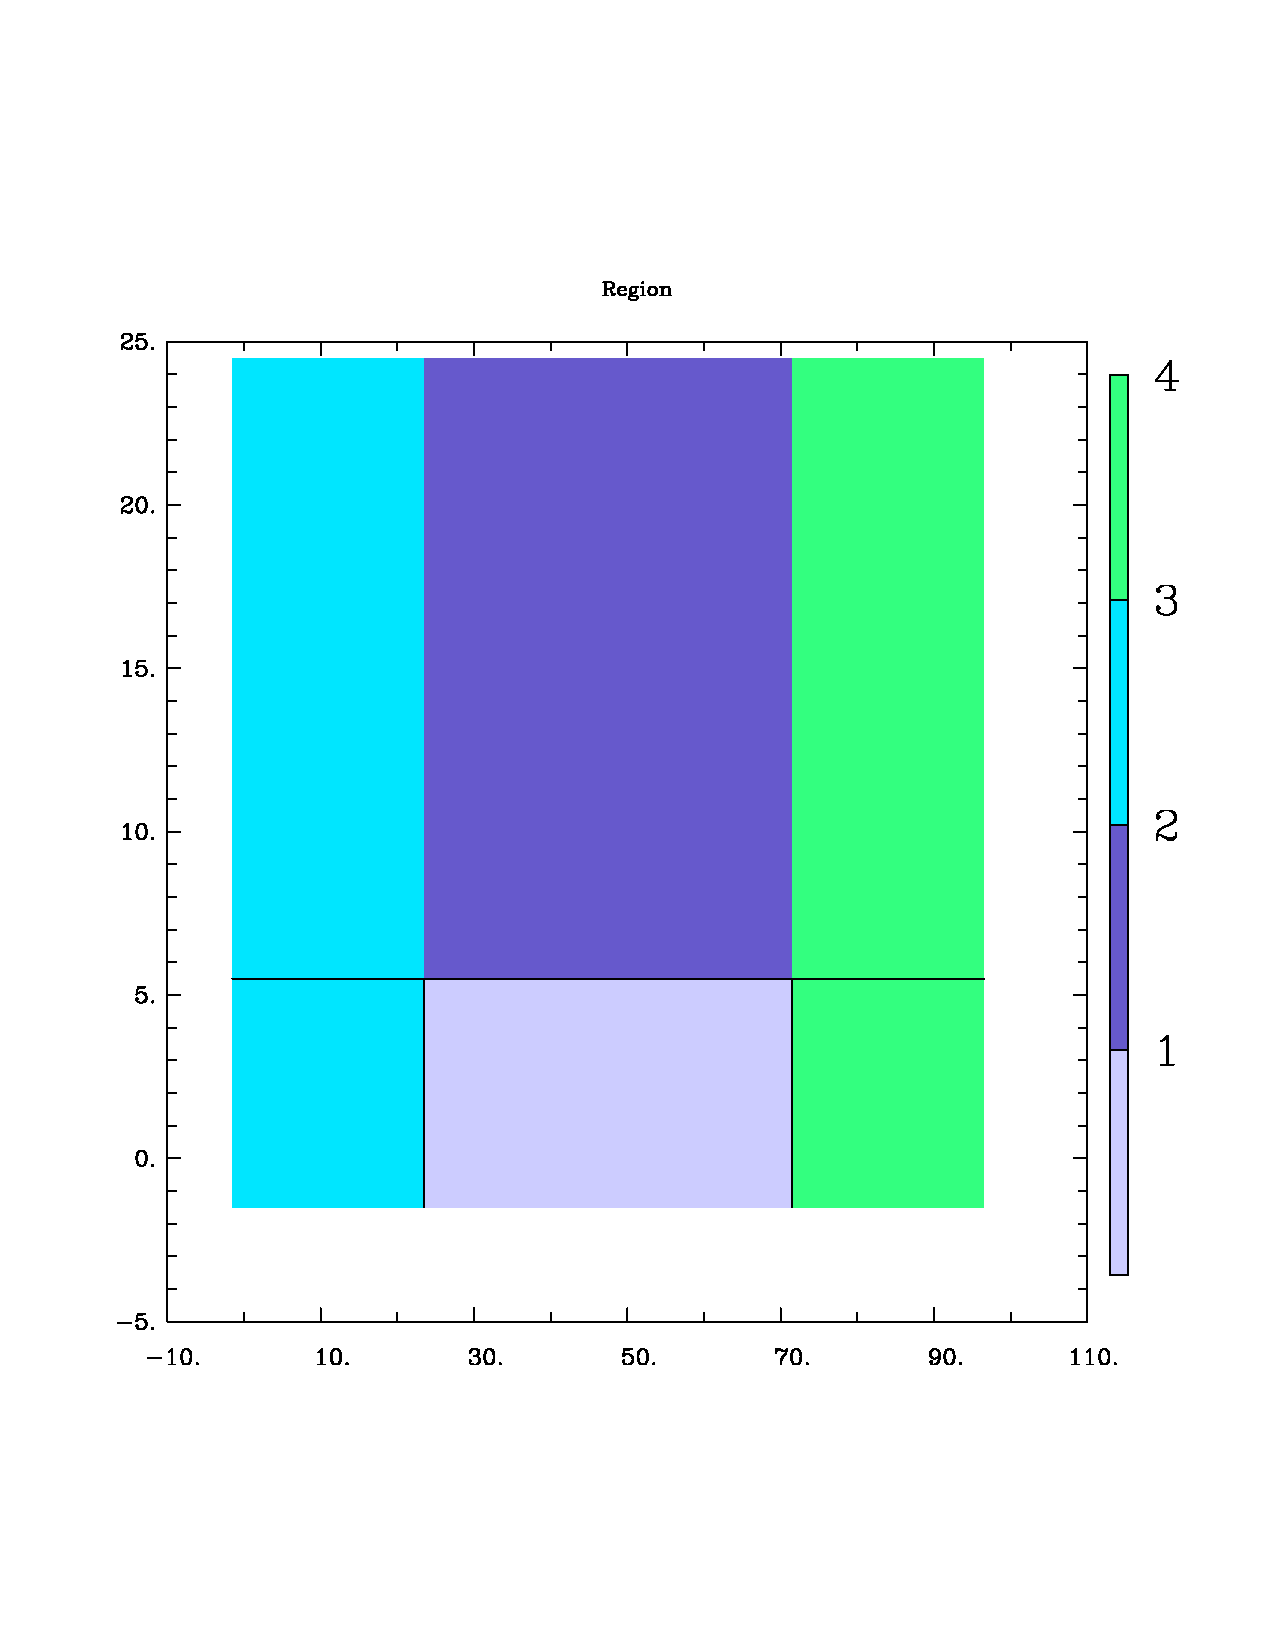
\includegraphics[height=7cm]{SN_comp.pdf}}
  \subfigure[Physics domain]{\label{fig:SN_phys}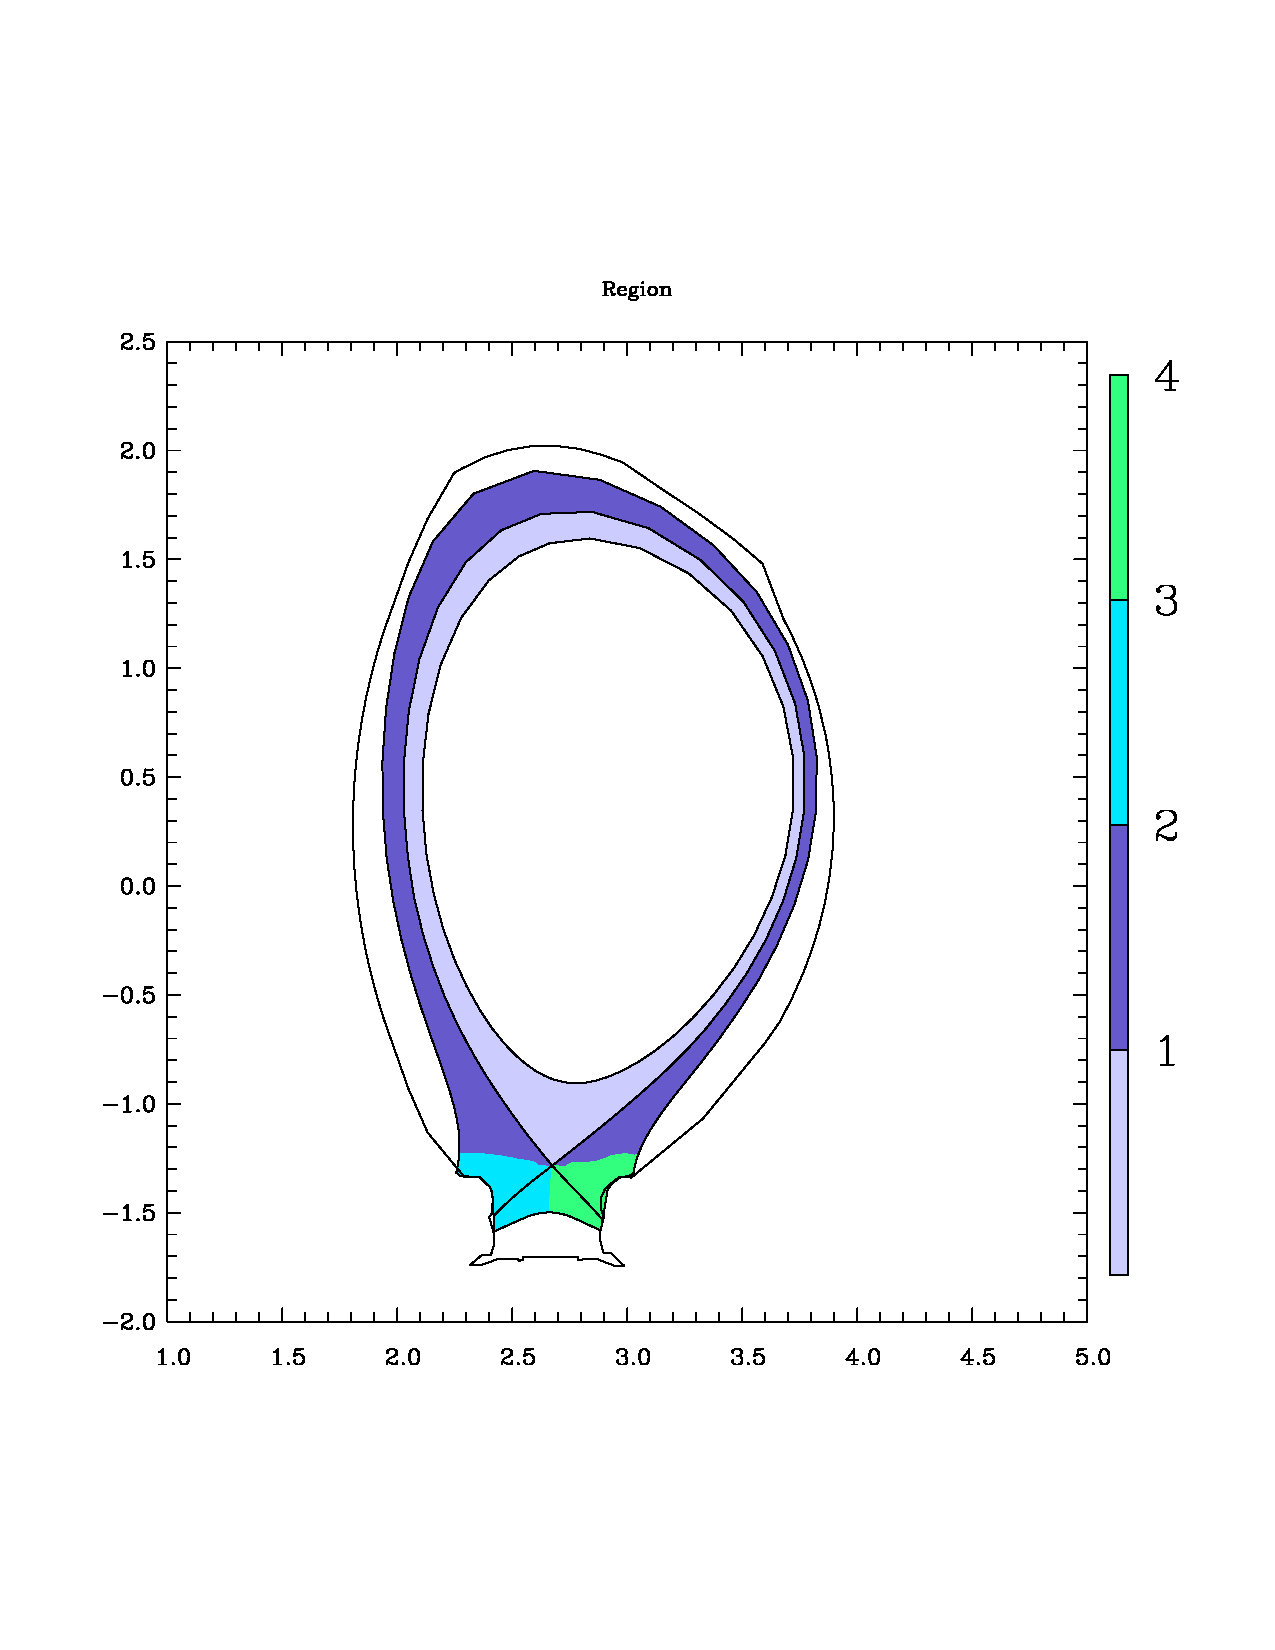
\includegraphics[height=7cm]{SN_phys.pdf}}
\else
  \subfigure[Computational domain]{\label{fig:SN_comp}
\includegraphics[height=7cm]{SN_comp.epsi}}
  \subfigure[Physics domain]{\label{fig:SN_phys}
\includegraphics[height=7cm]{SN_phys.epsi}}
\fi
  \caption{Region numbers for single-null geometries.}\label{fig:SN_regions}
\end{figure}

\begin{figure}[hbtp]
  \centering
\ifpdf 
  \subfigure[Computational domain]{\label{fig:DN_comp}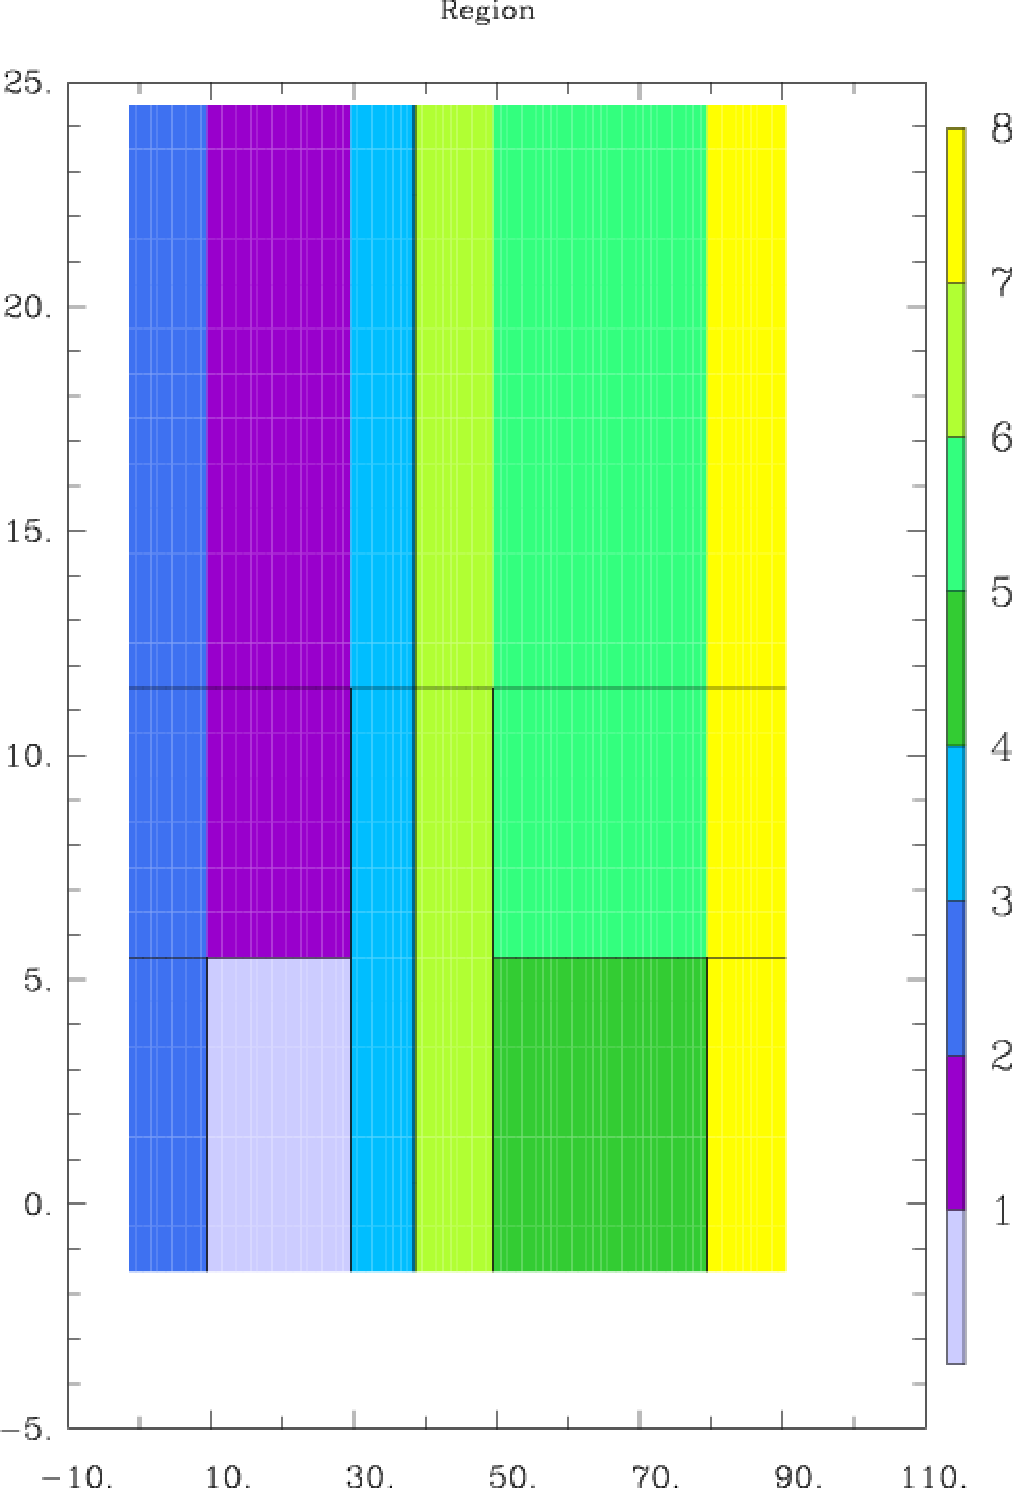
\includegraphics[height=7cm]{DN_comp.pdf}}
  \subfigure[Physics domain]{\label{fig:DN_phys}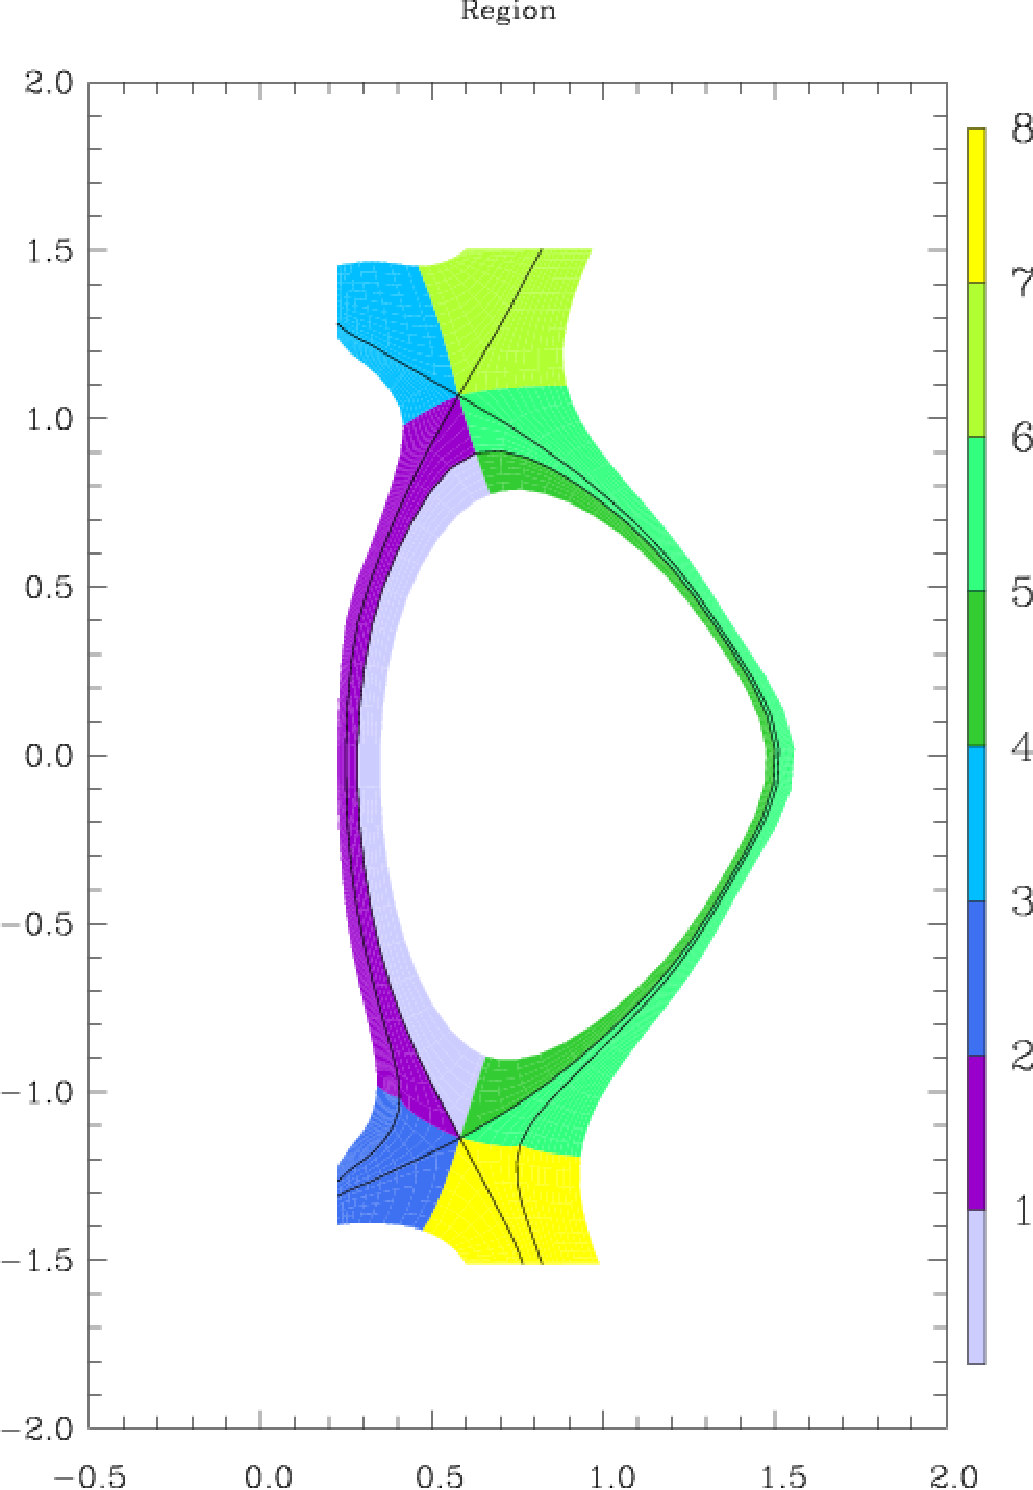
\includegraphics[height=7cm]{DN_phys.pdf}}
\else
  \subfigure[Computational domain]{\label{fig:DN_comp}
\includegraphics[height=7cm]{DN_comp.epsi}}
  \subfigure[Physics domain]{\label{fig:DN_phys}
\includegraphics[height=7cm]{DN_phys.epsi}}
\fi
  \caption{Region numbers for double-null geometries.}\label{fig:DN_regions}
\end{figure}

\subsection{b2.transport.inputfile}
\index{b2.transport.inputfile}\index{b2tqna}\index{b2tqna\_inputfile}\index{transport coefficients}\label{lab:b2:transport:inputfile}\index{b2ah.dat}\index{b2mn.dat}\index{b2.transport.parameters}

See also Appendix \ref{lis:b2cdcn} for a more up-to-date description. 
 
This allows for a radial variation ... for a simpler option see
section \ref{lab:b2:transport:parameters}.

If \verb!'b2tqna_inputfile'! is set to 1 in \verb!b2mn.dat!
then the transport coefficients are read in from the namelist in
\verb!b2.transport.inputfile! instead of being taken from the file
created by \verb!b2ah! and possibly modified in \verb!b2mn.dat!.
This then allows one to set radially 
varying profiles of the transport coefficients, and to achieve time
dependence in these transport coefficients by triggering a read of a
new file (as for \verb!b2.transport.parameters!).
The transport coefficients are specified by the \verb!transport! namelist
as described below.

The input format for these files is somewhat arcane (the relevant
subroutine is \verb!transport_input!, to be found in \verb!b2mod_input_profile.F!) and an
example, without the modification for reading in a new file triggered
by time, which is the same as for the \verb!b2.transport.parameters!, is
included below.

The basic idea is to specify pairs of numbers which give the position
and value of the relevant transport coefficients.

\verb!tdata! has four indices:

The value of the first index $=1$ means position in space, $=2$ means the value.

The second is used to index the various positions (6 positions in the
example below, specified by \verb!ndata!). The total number of positions should not
exceed $ny+2$, as having transport coefficient profiles finer than the 
plasma grid resolution is overkill.

The third index of \verb!tdata! relates to the kind of transport coefficient 
being specified, where:
\begin{description}\index{kind\_coeff}
  \item[kind\_coeff.eq.1 $\Rightarrow$ dna0  ]   particle density-driven diffusivity $D_\perp^{na}$
  \item[kind\_coeff.eq.2 $\Rightarrow$ dpa0  ]   particle pressure-driven diffusivity $D_\perp^{pa}$
  \item[kind\_coeff.eq.3 $\Rightarrow$ hcib  ]   ion thermal anomalous diffusivity $\chi_i$        
  \item[kind\_coeff.eq.4 $\Rightarrow$ hce0  ]   electron thermal anomalous diffusivity $\chi_e$
  \item[kind\_coeff.eq.5 $\Rightarrow$ vla0\_x]  $x$-component of the anomalous "pinch" velocity
  \item[kind\_coeff.eq.6 $\Rightarrow$ vla0\_y]  $y$-component of the anomalous "pinch" velocity
  \item[kind\_coeff.eq.7 $\Rightarrow$ vsa0  ]   anomalous viscosity
  \item[kind\_coeff.eq.8 $\Rightarrow$ sig0  ]   anomalous radial electrical conductivity
  \item[kind\_coeff.eq.9 $\Rightarrow$ alf0  ]   anomalous radial thermo-electric coefficient
\end{description}
                
The fourth index is the species index.

Again, as in Section \ref{lab:b2cmpt}, it is important, for numerical stability reasons, 
to provide mechanisms by which some
particle transport and radial current can be established. If the transport coefficients
are given here, this means that, first, the \verb!dna0! and \verb!dpa0! arrays 
cannot be simultaneously zero when solving density equations. Second, the arrays 
\verb!sig0! and \verb!alf0! cannot be
simultaneously zero when solving the potential equations without drift current terms on.
The code will fail a transport coefficients test in \verb!b2tral! otherwise.

The relevant routine was written by

\begin{verbatim}
!**************************************************************************
!*     subroutine for reading in experimental transport coefficients from *
!*     the midplane and calculating transport coefficients                *
!*     for B2.5 (written by Heimo Buerbaumer 1999)                        *
!*     Inputfile:  b2.transport.inputfile                                 *
!**************************************************************************
\end{verbatim}

Some additional description of the relevant variables is as follows:

\begin{description}
  \item[ndata(1,i,j)]\index{ndata} where $i$ is an index for the type of transport coefficient
     being defined (see table above) and $j$ is a species index ($0$ for atoms and $1$
     for ions in a $D$-only case, for instance, and irrelevant (use $1$) for electron 
     coefficients). \verb!ndata! is the
     number of data points where the value of the transport coefficients is given.
  \item[addspec(k,i,j)]\index{addspec} are the indices of any additional species whose
     transport coefficients are also described by the same set of numbers. $k$
     is a dummy that runs from $1$ to the number of additional species
     described.
  \item[tdata(1,m,i,j)]\index{tdata} are the radial positions (measured in metres) of the 
     \verb!ndata(1,i,j)! points,
     where $m$ runs from $1$ to \verb!ndata(1,i,j)!. By default, the radial positions are
     measured from the separatrix outward, along the outer midplane, but this can be changed by
     making use of the $ixref$ and $iyref$ switches, respectively, to modify the poloidal
     location of the profile and the radial position from which the distances are measured. 
  \item[tdata(2,m,i,j)] are the corresponding values of the coefficients.
  \item[no\_pflux]\index{no\_pflux} is a logical that, if \verb!.true.!, does not apply these
     transport coefficients to the private flux region(s).
\end{description}

So in the example file below, three transport coefficients profiles
are given, i.e. in order, $D_\perp^{na}$, $\chi_i$ and $\chi_e$, defined
with 6 points each, and setting a transport barrier around the separatrix.
Note that the radial locations of those points are quite
independent of where the mesh is. The code interpolates the transport
values onto the mesh, so one needs not worry about making sure
that a point is at an exact cell location. 
It is recommended that the first and last points be a large distance away 
from the separatrix, typically well outside the computational
domain. This ensures that the code is still interpolating and not
using (possibly different) default values when computing coefficients for cells near the
edges of the mesh. The interpolation the code uses is a
monotonicity-preserving cubic Hermite polynomial spline from the NAG
library, or a simple linear interpolation if the NAG library is
unavailable at compilation time. For computational cells located 
outside the range provided by the \verb!tdata(1,m,i,j)! positions, 
the code will use whatever
'default' values were declared previously. As a reminder, the order of 
precedence of the transport coefficients settings is:
\begin{verbatim}
b2ah.dat < b2mn.dat < b2.tranport.parameters < b2.transport.inputfile
\end{verbatim}

The following contains an example where the flag \verb!no_pflux! is
used to switch off the setting of transport coefficients in the
private flux region.

\VerbatimInput[fontsize=\footnotesize]{b2.transport.inputfile}

\subsection{b2.sources.profile}
\index{b2.sources.profile}\index{b2sral}\index{b2sral\_inputfile}\index{sources}\label{lab:b2:sources:profile}

See also Appendix \ref{lis:b2cdcn} for a more up-to-date description. 
 
One can also set radially dependent source profiles, in much the same way as with
\verb!b2.transport.inputfile!, with the \verb!b2.sources.profile! input file, 
accessed by setting 'b2sral\_inputfile' to '1'. The logic is the same in terms
of fixing radial positions, applicable species, etc...

The coefficient types go as:
\begin{enumerate}
   \item Particle sources {\em sna} \index{b2plot, exna}
   \item Parallel momentum sources {\em smo} \index{b2plot, exmo}
   \item Electron heat sources {\em she} \index{b2plot, exhe}
   \item Ion heat sources {\em shi} \index{b2plot, exhi}
   \item Electric charge sources {\em sch} \index{b2plot, exch}
   \item Electric particle source (non-ambipolar) {\em sne} \index{b2plot, exne}
\end{enumerate}

It is also possible to multiply these radial profiles by an axial form factor.
This axial multiplier is set in the same way as the poloidal profile.

The description of the variables found in \verb!b2.sources.profile! is as follows:
\begin{description}
  \item[nsdata(1,i,j)]\index{nsdata} where $i$ is an index for the type of source
     being defined (see table above) and $j$ is a species index ($0$ for atoms and $1$
     for ions in a $D$-only case, for instance, and irrelevant (use $1$) for electron 
     sources). \verb!nsdata! is the
     number of data points where the strength of the source is given.
  \item[sdata(1,m,i,j)]\index{sdata} are the radial positions (measured in metres) of the 
     \verb!nsdata(1,i,j)! points,
     where $m$ runs from $1$ to \verb!nsdata(1,i,j)!. By default, the radial positions are
     measured from the separatrix outward, along the outer midplane, but this can be changed by
     making use of the $ixref$ and $iyref$ switches, respectively, to modify the poloidal
     location of the profile and the radial position from which the distances are measured. 
  \item[sdata(2,m,i,j)] are the corresponding strengths of the sources.
  \item[nxdata(k,i,j)]\index{nxdata} where $i$ is an index for the type of source
     being defined (see table above) and $j$ is a species index ($0$ for atoms and $1$
     for ions in a $D$-only case, for instance, and irrelevant (use $1$) for electron 
     sources). \verb!nxdata! is the
     number of data points where the value of the axial multiplier to the source is given.
     If $k$ is equal to $1$, the data is to be understood as function of normalized
     connection length. If $k$ is equal to $2$, then the axial profile is given in terms
     of the normalized computational coordinate (running from $0$ to $1$ as $ix$ runs from
     $-1$ to $nx$). 
  \item[xdata(1,m,i,j)]\index{xdata} are the axial positions (normalised to the total length) 
     of the \verb!nxdata(1,i,j)! points,
     where $m$ runs from $1$ to \verb!nxdata(1,i,j)!. By default, the connection length
     used is the one measured just inside the separatrix, with the origin 
     located at the outer midplane, but this can be changed by
     making use of the $ixref$ and $iyref$ switches, respectively, to modify the poloidal
     location of the origin and the radial position along which the distances are measured.
     In case the reference location is chosen inside a closed field line region, the axial
     multiplier is set to zero everywhere on the open field lines. 
  \item[xdata(2,m,i,j)] are the corresponding values of the source strengths.
  \item[divheat]\index{divheat} is the total volumetric ion heat source (in $W/m^{3}$) 
     spread equally throughout the divertor volume.
\end{description}

The results of these imported source profiles can be visualised in
\btwoplot with the {\bf exna}, {\bf exmo}, {\bf exhe}, {\bf exhi},
{\bf exch}, and {\bf exne} commands. An example of input file is given below:

\VerbatimInput[fontsize=\footnotesize]{b2.sources.profile}

\subsection{b2.neutrals.parameters}
\index{b2.neutrals.parameters}\label{lab:b2:neutrals:parameters}

See descriptions in Coupled \verb!Eirene! chapter \ref{cha:coupledb2eirene}
and Appendix \ref{lis:b2cdcn}.

\subsection{b2.atomic\_physics\_rescale.parameters}
\index{b2.atomic\_physics\_rescale.parameters}\label{lab:b2:atomic_physics_rescale:parameters}

Contains a series of multipliers to the atomic physics rates provided by \verb!b2ar! in \verb!b2frates!.
These are:
\begin{description}
  \item[RESCALE\_SA]\index{RESCALE\_SA} \verb!real*8 array, length NS!,
  contains the scaling factor per species to be applied to the ionisation rates
  \item[RESCALE\_RA]\index{RESCALE\_RA} \verb!real*8 array, length NS!,
  contains the scaling factor per species to be applied to the recombination rates
  \item[RESCALE\_QA]\index{RESCALE\_QA} \verb!real*8 array, length NS!,
  contains the scaling factor per species to be applied to the electron cooling rates
  \item[RESCALE\_CX]\index{RESCALE\_CX} \verb!real*8 array, length NS!,
  contains the scaling factor per species to be applied to the charge exchange rates
  \item[RESCALE\_RD]\index{RESCALE\_RD} \verb!real*8 array, length NS!,
  contains the scaling factor per species to be applied to the line radiation rates
  \item[RESCALE\_BR]\index{RESCALE\_BR} \verb!real*8 array, length NS!,
  contains the scaling factor per species to be applied to the bremsstrahlung radiation rates
\end{description}

See Appendix \ref{lis:b2cdcn} for a full description.

\subsection{b2.user.parameters}
\index{b2.user.parameters}\label{lab:b2:user:parameters}

See descriptions in Coupled \verb!Eirene! chapter \ref{cha:coupledb2eirene}
and Appendix \ref{lis:b2cdcn}.

\subsection{b2.XXX.parameters}

See descriptions in Appendix \ref{lis:b2cdcn}.

\subsection{While the code is running}
\label{sec:b2running}

While the code is running and writing into \verb!run.log!, a number of
the scripts described in section \ref{sec:scripts} can be run.

\verb!cpu!\index{cpu} shows how much CPU time each iteration has taken and is a
quick way of monitoring the progress of a run.

\begin{verbatim}
18:22> cpu
# /scratch/dpc/solps5.0_test_xpb/src/Braams/b2/runs/JET_B2_comparison/50401/57_coarse/2e19_8MW
1 2.129999935626984
2 1.940000295639038
3 1.730000019073486
4 1.719999313354492
5 1.710000038146973
6 1.720000267028809
7 1.690000534057617
8 1.710000038146973
9 1.679999351501465
10 1.700000762939453
11 1.699998855590820
12 1.710000991821289
13 1.699998855590820
18:22> 
\end{verbatim}

All of the residuals of a pure deuterium run can be plotted with
\verb!resall_D!\index{resall\_D}, figure \ref{fig:resallD}. 

\begin{figure}[hbtp]
\ifpdf 
    \centerline{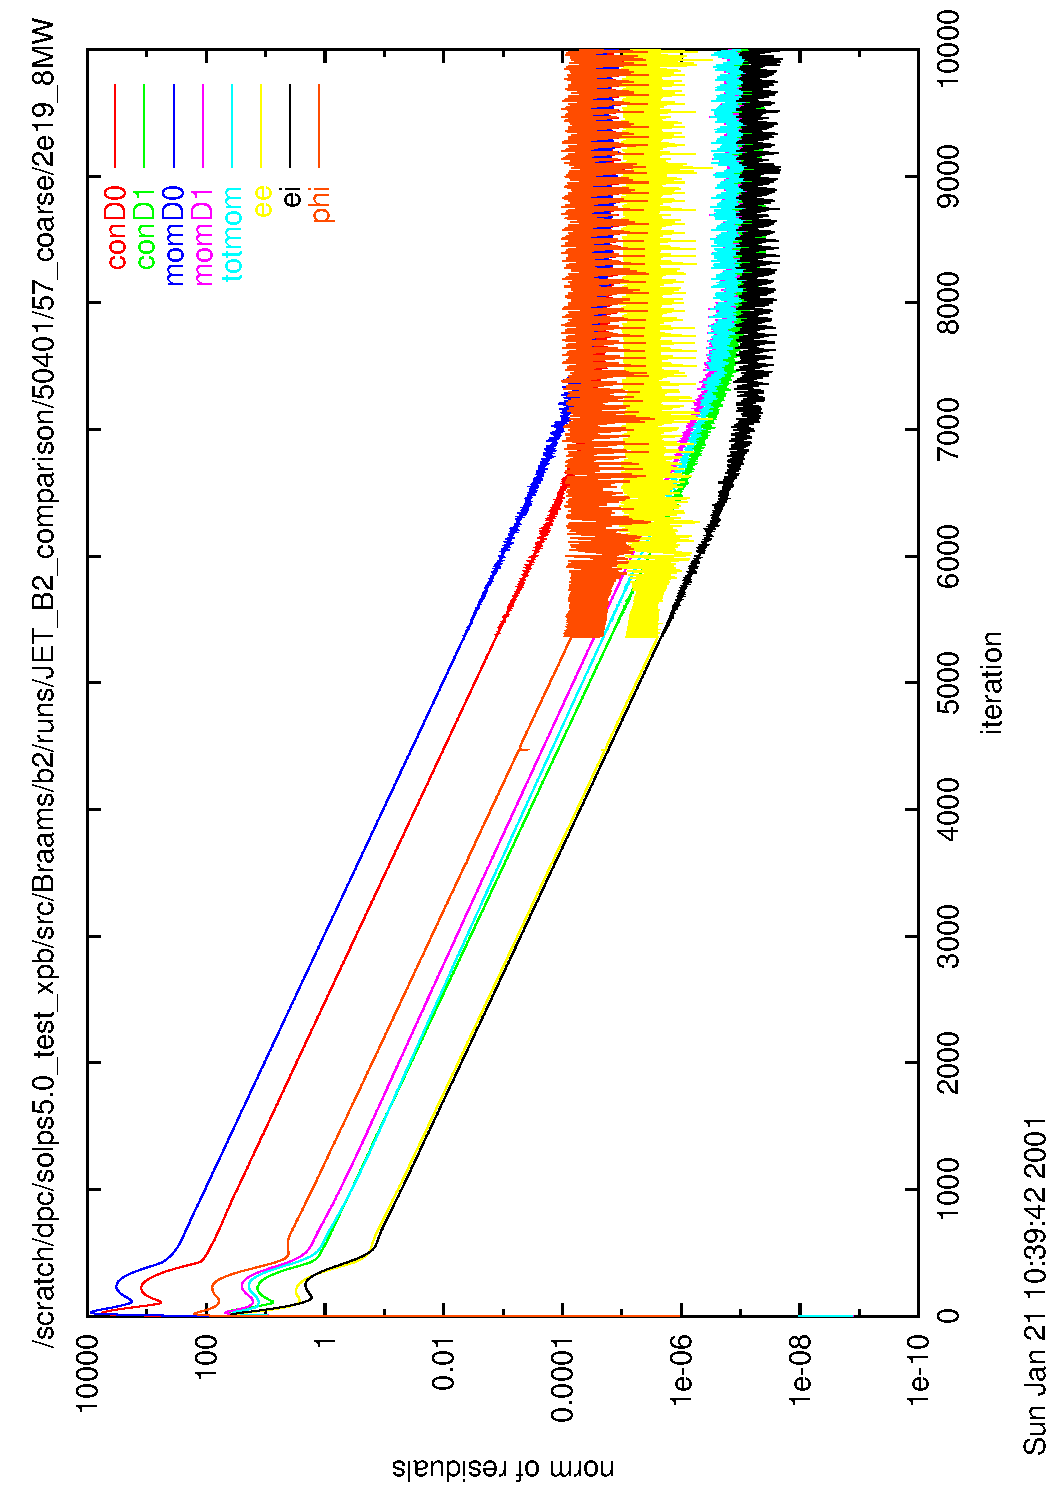
\includegraphics[origin=br,angle=-90,height=8cm]{resall_D.pdf}}
\else
    \centerline{\includegraphics[origin=br,angle=-90,height=8cm]{resall_D.ps}}
\fi
    \caption{Residuals.}
    \label{fig:resallD}
\end{figure}

The power crossing various surfaces can be seen with
\verb!energy_analysis!\index{energy\_analysis} or 
\verb!energy_analysis.py!\index{energy\_analysis.py}, figure \ref{fig:energyanalysis}.
The detailed definition of these surfaces can be found in Appendix \ref{cha:regions} 
or the commented header to the \verb!init_region! subroutine in 
\verb!b2agfs.F!.

\begin{figure}[hbtp]
\ifpdf 
    \centerline{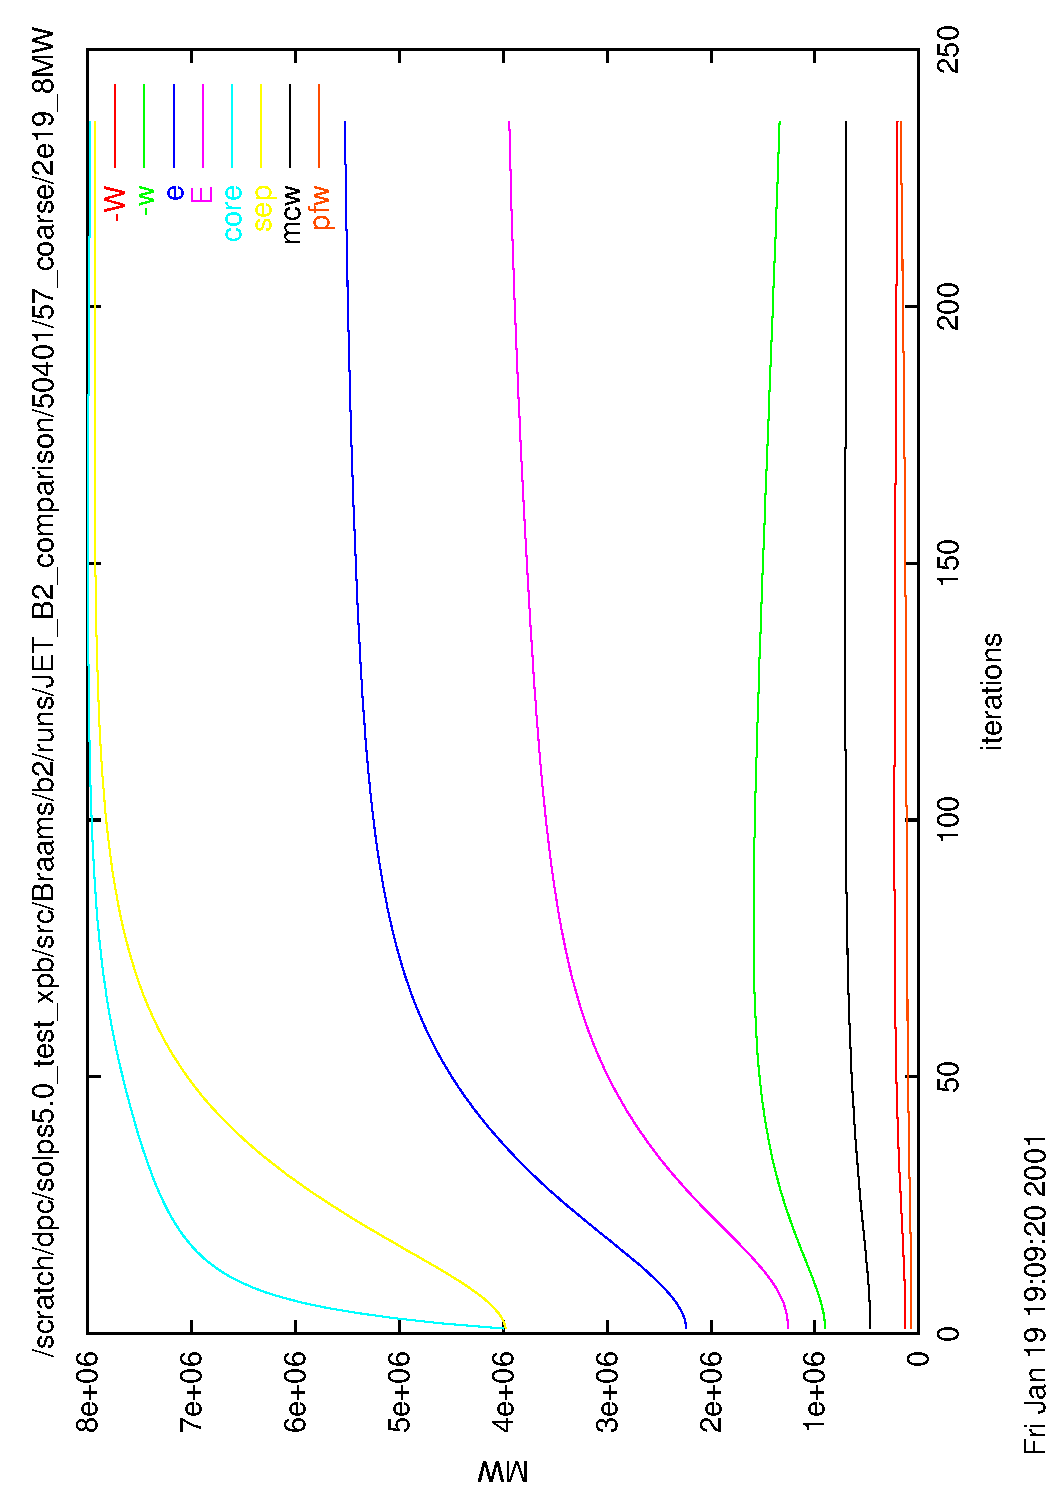
\includegraphics[origin=br,angle=-90,height=8cm]{energy_analysis.pdf}}
\else
    \centerline{\includegraphics[origin=br,angle=-90,height=8cm]{energy_analysis.ps}}
\fi
    \caption{Power crossing various surfaces.}
    \label{fig:energyanalysis}
\end{figure}

\verb!2dt tesepm!\index{2d, tesepm} can be used to plot the separatrix
temperature as a function of time, figure \ref{fig:tesepm}.  See table
\ref{tab:2db2time} (page \pageref{tab:2db2time}) for a list of
quantities that can be plotted in this way.

\begin{figure}[hbtp]
\ifpdf 
    \centerline{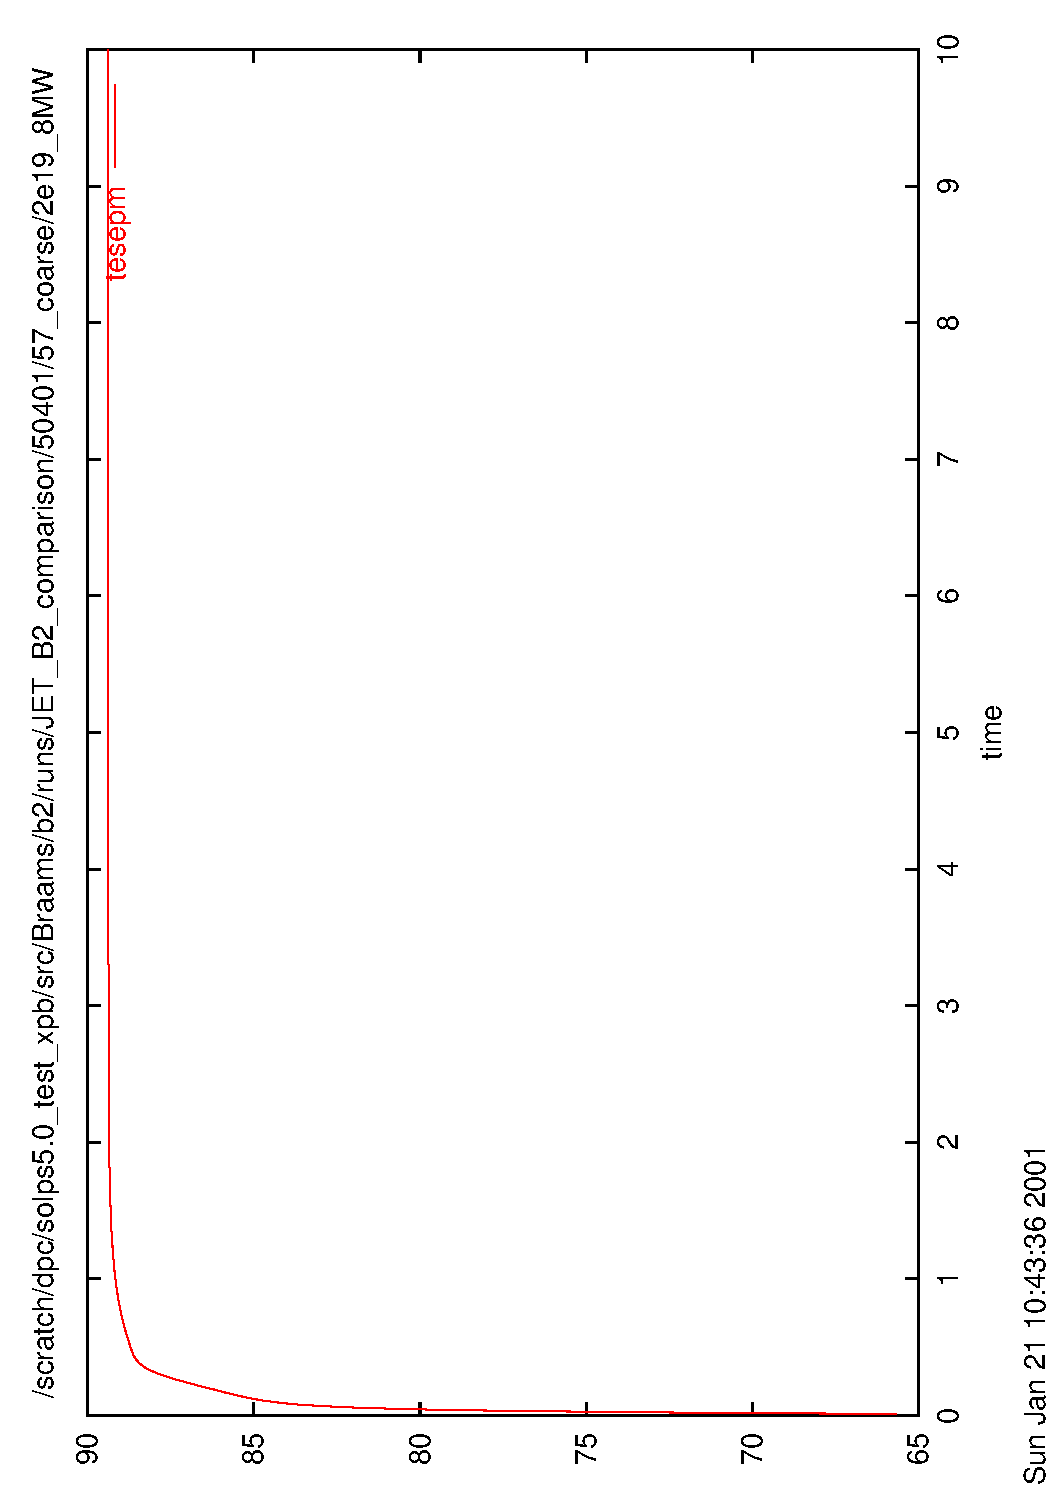
\includegraphics[origin=br,angle=-90,height=8cm]{tesepm.pdf}}
\else
    \centerline{\includegraphics[origin=br,angle=-90,height=8cm]{tesepm.ps}}
\fi
    \caption{Upstream (outer midplane) electron temperature.}
    \label{fig:tesepm}
\end{figure}

\verb!!\index{} 

\verb!!\index{} 

\verb!!\index{} 

\newpage
\section{b2pl, the plotting program}
\index{b2pl}\index{b2plot}\label{sec:b2pl}

%%sed 's:^     [^ ]:@@@:' $SOLPSTOP/modules/B2.5/src/b2plot/b2plot.F | awk 'BEGIN{save=""}/^[^@][^@][^@]/&&save!=""{print save}/^[^@][^@][^@]/{save=$0}/^@@@/{save=save" "$0}END{print save}' | sed 's; *@@@ *;;g' | egrep "case *\( *'|description *=" | sed -e "s;.*case *('\(.*\)');cmd: \1;" -e "s; *description *= *'\(.*\)';desc: \1;" | awk -F: 'BEGIN{save=""}/^cmd/&&save!=""{print save}/^cmd:/{save=$2}/^desc/{save=save"\t"$2}END{print save}' | sed 's:\! ::' | sed "s:',':,:g" | sed "s:'':':g" | expand >! b2plot.commands

The following commands apply:

\VerbatimInput[fontsize=\footnotesize]{b2plot.commands}

A revised copy of the \btwoplot manual can be found in Appendix
\ref{cha:b2plotmanual}, page \pageref{cha:b2plotmanual}.  Note that some
of the quantities have changed name between \SOLPSfour and \SOLPSfive versions, 
\index{b2plot, changes from SOLPS4.0 to SOLPS5.0}table \ref{tab:changedplotquantities}, and that
whereas \verb!ix! ran from \verb!0! to \verb!nx+1! it now runs from
\verb!-1! to \verb!nx!, \verb!iy! which ran from \verb!0! to \verb!ny+1! 
now runs from \verb!-1! to \verb!ny! and \verb!is! which ran from \verb!1!
to \verb!ns! now runs from \verb!0! to \verb!ns-1!.

\begin{table}[hbtp]
  \leavevmode
  \begin{center}
    \begin{tabular}{|l|l|}
    \hline
    \SOLPSfour  & \SOLPSfive  \\ \hline
    ni          & na          \\
    zi          & za          \\
    up          & ua          \\
    dx          & hx          \\
    dy          & hy1         \\
    feex        & fhex        \\
    feey        & fhey        \\
    feix        & fhix        \\
    feiy        & fhiy        \\
    fnix        & fnax        \\
    fniy        & fnay        \\ \hline
    \end{tabular}
    \caption{Changes of quantity names from \SOLPSfour \btwoplot to \SOLPSfive {\bf b2pl.exe}.}
    \label{tab:changedplotquantities}
  \end{center}
\end{table}

\newpage
\section{b2yt, changing from one grid size and species set to another}
\index{b2yt}\index{b2fstatt}\label{sec:b2yt}\index{input.dat}\index{input.dat.2}\index{b2mn.dat}\index{b2fgmtry}
\index{b2fgmtry.old}\index{b2mn.dat.2}\index{b2.boundary.parameters}\index{b2.boundary.parameters.2}
\index{b2.neutrals.parameters}\index{b2.neutrals.parameters.2}\index{b2ah.dat}\index{b2ah.dat.2}
\index{b2.wall\_save.parameters}\index{b2.wall\_save.parameters.2}\index{b2frates}\index{b2fpardf}
\index{b2.transport.parameters}\index{b2.transport.parameters.2}\index{SOLPS\_FLUIDS}

This utility program allows a user to take a \verb!b2fstate! solution file
with size $nx \times ny$ and transform it into an $nx1 \times ny1$ \verb!b2fstatt!
file, provided the numbers of real cells in both $x$ and
$y$ directions in the new solution are divisors of the ones in the original mesh. Other 
files necessary to proceed with the run under the new geometry will also be produced. The 
two numbers $nx11$ and $ny1$ are provided by the user in the \verb!b2yt.dat! 
file. The \verb!b2yt.dat! file should contain, for example:
\begin{verbatim}
*dimens         (nx1, ny1; free format)
  8  8
\end{verbatim}
with any optional switches mentioned afterwards, to create a solution on an $8 \times 8$ grid.

A solution for non-commensurate grids is also available, requiring
instead that the topology of the two solutions be the same, and works by 2-D
interpolation of the plasma data in the computational domain, by region. This is 
activated with the 'b2ytdr\_non\_commensurate' option set to '1' in \verb!b2yt.dat!. 

The conversion of the \verb!Eirene! input file additionally requires for the converter program to know the original version of \verb!Eirene! with which the input file was used, and this is provided by means of the 'eirene\_format' switch. Its possible values (case-insensitive) are:
\begin{description}
  \item[``old''] for input files from {\bf SOLPS4.0} and {\bf SOLPS5.0} runs using "old" Eirene\_96
  \item[``new''] for input files from {\bf SOLPS4.0} and {\bf SOLPS5.0} runs using "new" Eirene\_99
  \item[``facelift''] for input files from \SOLPSfiveone runs
  \item[``juelich''] for input files from Juelich \verb!Eirene! versions (2008 and younger)
  \item[``iter''] (default) for input files from {\bf SOLPS4.2/4.3} and \SOLPSITER runs
\end{description}
The \verb!input.dat.2! file that the converter will create will follow the \SOLPSITER format.

The conversion of the \verb!Eirene! output file (\verb!fort.44!) additionally requires for the converter program to know the original version of \verb!SOLPS! with which the output file was created, and this is provided by means of the 'solps\_version' switch. Its possible values (case-insensitive) are:
\begin{description}
  \item[``4.3''] for \verb!fort.44! output files from {\bf SOLPS4.3} runs
  \item[``5.0''] for \verb!fort.44! output files from {\bf SOLPS5.0} runs
  \item[``5.1''] for \verb!fort.44! output files from \SOLPSfiveone runs
  \item[``5.2''] for \verb!fort.44! output files from {\bf SOLPS5.2} runs
  \item[``iter''] (default) for input files from \SOLPSITER runs (no conversion necessary)
\end{description}
The \verb!fort.44.2! file that the converter will create will follow the \SOLPSITER format.

\verb!b2yt! may also be used
to change the order of species (for example changing from $D+C+He$ to $D+He+C$) or for
bundling, de-bundling or re-bundling species, or even removing species and complete
isonuclear sequences. It is however not possible to use this converter to {\em add} 
a new isonuclear sequence. When modifying the species data, the user
should run \verb!b2ar! with the new species arrangement before running \verb!b2yt!
to obtain a temporary file \verb!b2frates!. After \verb!b2yt! has been run succesfully,
then the user should re-run \verb!b2ah! (using the produced \verb!b2ah.dat.2! file,
after renaming it \verb!b2ah.dat!) and \verb!b2ar! before re-launching the run.

If a new geometry is requested, the \verb!b2yt! program should be run after the 
new geometry file ($nx1 \times ny1$) has 
been produced and is available in the run directory as \verb!b2fgmtry!. 
The old geometry file should also remain available in 
the run directory as \verb!b2fgmtry.old!.

The program also needs the \verb!b2mn.dat! and any other used input files (such 
as \verb!input.dat!, \verb!b2.*.parameters! or \verb!b2.*.inputfile!) from 
the original run. 

It is important for proper \verb!b2yt! execution that the necessary files have the
expected seniority from the Makefile. Therefore, you must ensure that:
\begin{enumerate}
  \item \verb!b2fstate! is the {\em youngest} file.
  \item \verb!b2frates! (or \verb!../baserun/b2frates!) is {\em older} than \verb!b2fstate! but {\em younger} than \verb!b2fgmtry!.
  \item \verb!b2fpardf! (or \verb!../baserun/b2fpardf!) is {\em younger} than \verb!b2ah.dat! and 
         {\em older} than \verb!b2frates!.
  \item \verb!b2fgmtry! must be {\em younger} than \verb!b2ag.dat! and {\em older} than \verb!b2fpardf!.
\end{enumerate}

So, ALL of the following must be verified:
\begin{verbatim}
b2ag.dat < b2fgmtry < b2fpardf < b2frates < b2fstate

b2ah.dat < b2fpardf

b2ar.dat < b2frates
\end{verbatim}
If this order is not met, use a series of "touch 'filename' " commands
to give the files new dates. The best to check this is to run the command:
\begin{verbatim}
b2run -n b2yt
\end{verbatim}
which will launch a dry-run of the Makefile invoking \verb!b2yt!. Then, make sure
that this dry-run only attempts to run \verb!b2yt! and no other programs. If it 
does call, say \verb!b2ag! and/or \verb!b2mn!, then the age hierarchy above was
not respected. In that case, you can run the script
\begin{verbatim}
correct_b2yt_timestamps
\end{verbatim}
to get the correct ordering of files. Do check again afterwards with the dry-run
command to make sure it worked.

Upon successful termination of \verb!b2yt!, the user will find a \verb!b2fstatt!
file containing the transformed plasma state, as well as a \verb!b2mn.dat.2! file which 
will contain the updated run switches appropriate for the new geometry and species
selection. Similarly, if
\verb!b2.boundary.parameters! and \verb!b2.neutrals.parameters! files were present
in the working directory, files \verb!b2.boundary.parameters.2! and 
\verb!b2.neutrals.parameters.2!,
respectively, will contain the updated namelist variables. The program will also create
a new \verb!b2.wall_save.parameters.2! file containing the new wall namelist settings
when appropriate. Other \verb!B2.5! input files are treated in the same fashion. The 
code will also attempt to create a new \verb!SOLPS_FLUIDS.2! file appropriate for the 
new species list.

If an \verb!input.dat! file is present in the run directory, the code will also attempt
to produce a new \verb!input.dat.2! file. In order to
ensure consistency between the \verb!B2.5! and \verb!Eirene! modified inputs, it is 
important that the order of the neutrals boundary conditions in 
\verb!b2.neutrals.parameters! and the strata in \verb!input.dat! match!
When species are being re-bundled, possible 
conflicts may occur between their individual settings. In such cases, the code behaviour 
is to use the setting from the highest charge state within the bundle. If species are 
being removed, strata, tallies or diagnostics involving these species may either be 
removed from the input file or revert to their default settings. The user is encouraged 
to check that those choices are appropriate and modify them as needed. 

At this time, not all cases involving reshuffling of bundles have been tested, and the 
user is encouraged to check the \verb!b2yt! output files visually after execution to 
make sure no mistakes remain. No attempt is made to adjust or modify the text labels
pertaining to the various input files, so the user is encouraged to adapt those to the
new case being built. Report of conversion errors or omissions to the developer team 
are always welcome. 

\newpage
\section{b2co, recovering from a crash}
\label{sec:b2co}\index{b2co}\index{plasmastate}\index{B2.5, run recovery}\index{b2fstate}

In case of a computer crash during a run, it may be possible to recover
the results and continue the simulation. The code writes, at regular
intervals (default is 3600 CPU seconds, and can be modified with use of the
'b2mndr\_cpu' and 'b2mndr\_plasmatim' switches, see Appendix \ref{lis:b2cdci} for details and additional options),
recovery files entitled \verb!plasmastate.XXXX! and \verb!b2.*_save.parameters.XXXX! in the \verb!b2mn.exe.dir! run
subdirectory. The \verb!XXXX! are numbers indicating the order in which the
files were written. The \verb!plasmastate! files contain the same information as the \verb!b2fstati! or
\verb!b2fstate! files, but in a more compact format. In order to recover from
a crash, the user should then:
\begin{enumerate}
  \item Check for the presence of \verb!plasmastate.XXXX! files in the \verb!b2mn.exe.dir! run subdirectory
  \item If present, check that the most recent file is of the same size as the others (sometimes the crash happens while writing the \verb!plasmastate! file!)
  \item \verb!setenv PLASMASTATE b2mn.exe.dir/plasmastate.XXXX! where \verb!XXXX! is the number of the desired \verb!plasmastate! file
  \item \verb!b2run b2co! which will create a \verb!b2fstate! file
  \item \verb!mv b2fstate b2fstati!
  \item Re-launch the run
\end{enumerate}

This procedure will re-start the run from the point at which the \verb!plasmastate! file was written. In cases with feedback schemes active, the feedback values will be grabbed from the relevant \verb!b2.*_save.parameters.XXXX! files and a new set of
\verb!b2.*_save.parameters! files will be created.

\newpage
\section{b2rd, fetching an archived run}
\label{sec:b2rd}\index{b2rd}\index{shotnumber.history}\index{B2.5, recover an archived run}\index{b2fstate}\index{b2fgmtrt}\index{b2fgmtry}

If a run has been archived into the \verb!MDSplus! tree structure (see \ref{cha:MDSplus} for details)
it is possible to extract from the tree the information necessary to obtain \verb!b2fstate! and \verb!b2fgmtry! files 
from which to continue the run. To do so, follow the procedure below:
\begin{enumerate}
  \item Check for the presence of a \verb!shotnumber.history! file in the run directory
  \item If present, the fetched run will be the one with the run number specified last in \verb!shotnumber.history!
  \item If absent or incorrect, create or modify the \verb!shotnumber.history! file to add an extra line at the end with the run number of the run you which to retrieve
  \item \verb!b2run b2rd! which will create a \verb!b2fstate! file
  \item \verb!mv b2fstate b2fstati!
  \item \verb!mv b2fgmtrt b2fgmtry!
  \item Re-launch the run
\end{enumerate}

This procedure will re-start the run from the point at which the \verb!MDSplus! file was written. However, the input files
and run settings are not retrieved along with \verb!b2fstate! (these are not stored) so the user must check the input data 
present in the run directory before re-launching a case. In cases with feedback schemes active, for example, the feedback 
values will be the ones stored in the appropriate namelists from the \verb!b2.*.parameters! files in the run directory. Concerning the retrieval of the geometry case, some quantities must be recomputed by \verb!b2rd! as they are not saved in \verb!MDSplus!, so the code assumes a tokamak geometry and that the mesh is a basis mesh.

\newpage
\section{b2xx, the others}

\chapter{Running the standalone version of Eirene}
\label{cha:standaloneeirene}

\verb!Eirene! is documented at 
\href{http://www.eirene.de/}{http://www.eirene.de/}.
The user is strongly encouraged to check out that very complete manual.
Reference \cite{Reiter2005} also provides a useful description.

\begin{verbatim}
  sei
  gmake depend
  gmake listobj
  gmake tags
  gmake depend
  gmake
\end{verbatim}
%% $

See also the next chapter and section \ref{sec:DIMENSIONS} for setting the array sizes 
and useful file links for \verb!Eirene! before compilation.

\chapter{Running the coupled version of B2.5-Eirene}
\label{cha:coupledb2eirene}

In the run directory, you should execute the command
\begin{verbatim}
  setup_baserun_eirene_links
\end{verbatim}\index{setup\_baserun\_eirene\_links}
to establish the links \verb!Eirene! needs to the relevant atomic data files,
as well as some links needed for diagnostic scripts.
Using the ``-r'' option with this scripts creates relative links. Default behaviour is to create absolute links.

%% Examples files from https://solps-mdsplus.aug.ipp.mpg.de/repos/SOLPS/trunk/solps_examples/solps5.1/bench_mark/AUG_16151_D+C+He/

\section{Input files}

Below are given the input files used for the \verb!D+C+He! benchmark
case that can be found on the SVN server. The location of these is
https://solps-mdsplus.aug.ipp.mpg.de/repos/SOLPS/trunk/solps\_examples/solps5.1/bench\_mark/AUG\_16151\_D+C+He/ .

\subsection{b2ag.dat}
\index{b2ag.dat, D+C+He example}
\VerbatimInput[fontsize=\footnotesize]{D+C+He/b2ag.dat}

\subsection{b2ai.dat}
\index{b2ai.dat, D+C+He example}
\VerbatimInput[fontsize=\footnotesize]{D+C+He/b2ai.dat}

\subsection{b2ar.dat}
\index{b2ar.dat, D+C+He example}
\VerbatimInput[fontsize=\footnotesize]{D+C+He/b2ar.dat}

\subsection{b2ah.dat}
\index{b2ah.dat, D+C+He example}
\VerbatimInput[fontsize=\footnotesize]{D+C+He/b2ah.dat}

\subsection{b2mn.dat}
\index{b2mn.dat, D+C+He example}
\VerbatimInput[fontsize=\footnotesize]{D+C+He/b2mn.dat}

\subsection{b2.boundary.parameters}
\index{b2.boundary.parameters, D+C+He example}
\VerbatimInput[fontsize=\footnotesize]{D+C+He/b2.boundary.parameters}

\subsection{b2.numerics.parameters}
\index{b2.numerics.parameters, D+C+He example}
\VerbatimInput[fontsize=\footnotesize]{D+C+He/b2.numerics.parameters}

\subsection{b2.transport.parameters}
\index{b2.transport.parameters, D+C+He example}
\VerbatimInput[fontsize=\footnotesize]{D+C+He/b2.transport.parameters}

\subsection{b2.neutrals.parameters}
\index{b2.neutrals.parameters, D+C+He example}
\VerbatimInput[fontsize=\footnotesize]{D+C+He/b2.neutrals.parameters}

In this file the user defines many parameters that are used for communication
between the
\verb|B2.5| and \verb|Eirene| parts of the code. Please see Appendix
\ref{lis:b2cdcn} for full details. In particular, it is
essential that the neutrals boundary conditions declared here match, in
number and in order, the strata declared in the \verb!Eirene! input file. 

Some differences between the \SOLPSITER and {\bf SOLPS5.0} behaviours
should be noted here.

First, the number of strata \verb|NSTRAI| need no longer include the 
time-dependent ``T'' stratum.

Second, the array sizes of \verb|chemical_sputter_yield|, is used, now need to match the 
actual number of wall and non-standard surfaces 
\verb!NLIM! and \verb!NSTS! as they are found in the \$\verb!Eirene! input file. 
Non-zero values should only be assigned to
actual walls (so the 200 in the above example corresponds to the real number of walls declared in block 3B of the \verb!Eirene!
\verb!input.dat! file used for the same case) and to the non-standard surfaces (block 3A) corresponding to the targets. Note that
the surface numbering considers block 3B first, and then block 3A, so non-standard surfaces will have
indices varying between \verb!NLIM+1! and \verb!NLIM+NSTS!. Moreover,
\verb!Eirene! adds a last non-standard (absorbing) surface that is used as a ``time
boundary''. If the \verb!Eirene! input file is being produced by use of the 
\verb!Uinp! utility and/or the \verb!triang! script, then a 
\verb!b2.neutrals.parameters.2! file meeting these criteria will be created,
provided a \verb!b2.neutrals.parameters! file containing any other data not
deductible from the \verb!DG! model is present.   

Third, in \SOLPSITERns, the North and South boundaries of the \verb!B2.5! grid are 
no longer recycling/sputtering surfaces but rather only switching surfaces to the 
triangular grid regions.

\section{Changing dt}

With \SOLPSfour one was often limited to a timestep of $1 \times
10^{-6} s$ -- $1 \times10^{-5} s$.  With \SOLPSfive this restriction
seems to have been lifted, at least for some parameter regimes.  In
figure \ref{fig:tesepm1} we show the time evolution of the upstream
separatrix temperature for time-steps of $1 \times 10^{-6} s$, $1
\times 10^{-5} s$, $1 \times 10^{-4} s$, $1 \times 10^{-3} s$ and $1
\times 10^{-2} s$.  All of the runs seem to be behaving similarly,
though at the highest time-step there is a time shift.

\begin{figure}[hbtp]
\ifpdf 
    \centerline{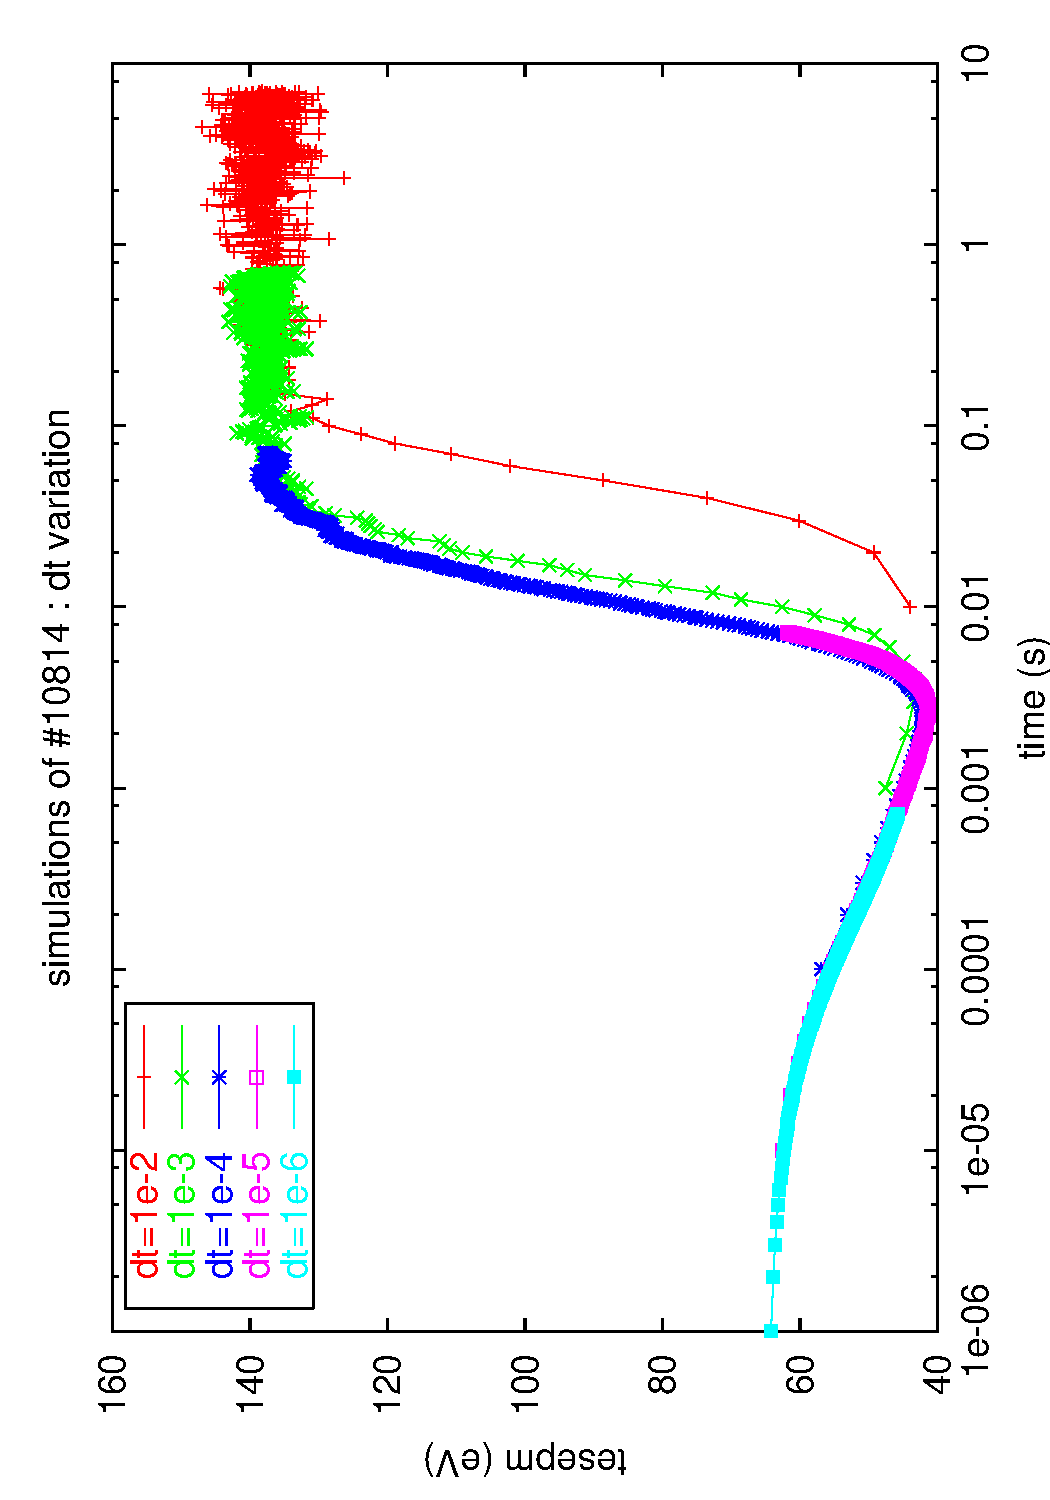
\includegraphics[origin=br,angle=-90,height=8cm]{compare_10814_tesepm_1.pdf}}
\else
    \centerline{\includegraphics[origin=br,angle=-90,height=8cm]{compare_10814_tesepm_1.ps}}
\fi
    \caption{Upstream (outer midplane) electron temperature for a
    range of time-steps.}
    \label{fig:tesepm1}
\end{figure}

In figure \ref{fig:tesepm2} we see the same quantity plotted for the
a range of time-steps but with an additional core speed-up factor coming
from \verb!b2.numerics.parameters!.

\begin{figure}[hbtp]
\ifpdf 
    \centerline{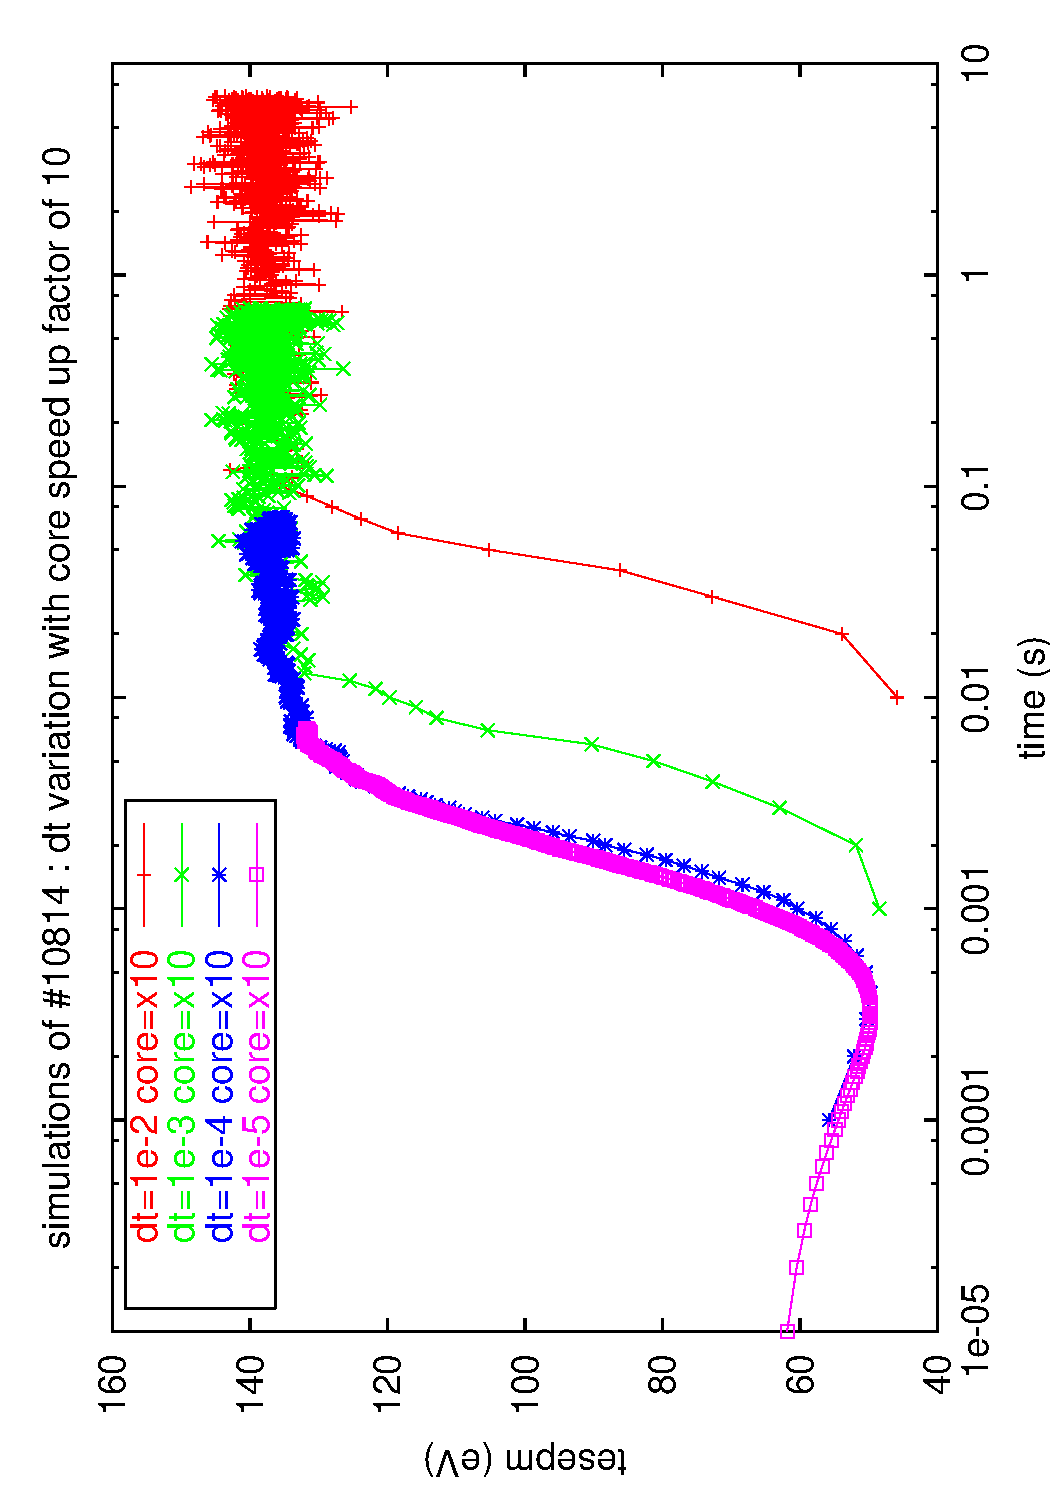
\includegraphics[origin=br,angle=-90,height=8cm]{compare_10814_tesepm_2.pdf}}
\else
    \centerline{\includegraphics[origin=br,angle=-90,height=8cm]{compare_10814_tesepm_2.ps}}
\fi
    \caption{Upstream (outer midplane) electron temperature for a
    range of time-steps with a core speed-up factor.}
    \label{fig:tesepm2}
\end{figure}

Figure \ref{fig:tesepm3} combines the data form figures \ref{fig:tesepm1} and \ref{fig:tesepm2}.

\begin{figure}[hbtp]
\ifpdf 
    \centerline{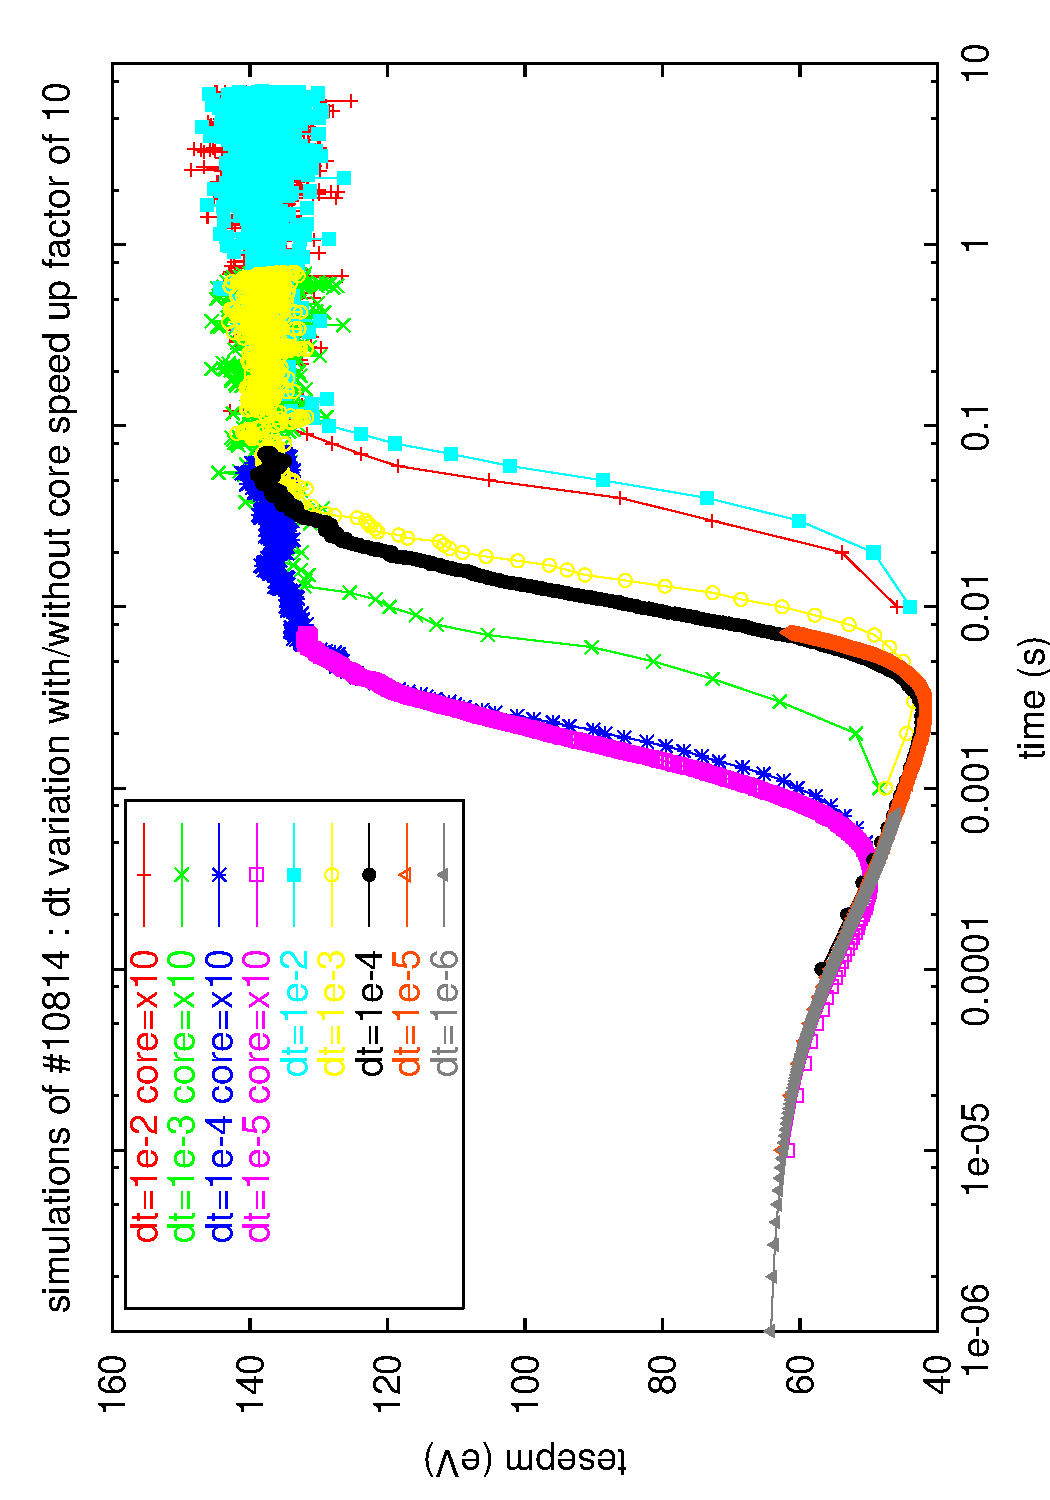
\includegraphics[origin=br,angle=-90,height=8cm]{compare_10814_tesepm_3.pdf}}
\else
    \centerline{\includegraphics[origin=br,angle=-90,height=8cm]{compare_10814_tesepm_3.ps}}
\fi
    \caption{Upstream (outer midplane) electron temperature for a
    range of time-steps with and without a core speed-up factor.}
    \label{fig:tesepm3}
\end{figure}

Figures \ref{fig:tesepm4}, \ref{fig:tesepm5} and \ref{fig:tesepm6}
show the outer target separatrix temperatures corresponding to figures
\ref{fig:tesepm1}, \ref{fig:tesepm2} and \ref{fig:tesepm3}.

\begin{figure}[hbtp]
\ifpdf 
    \centerline{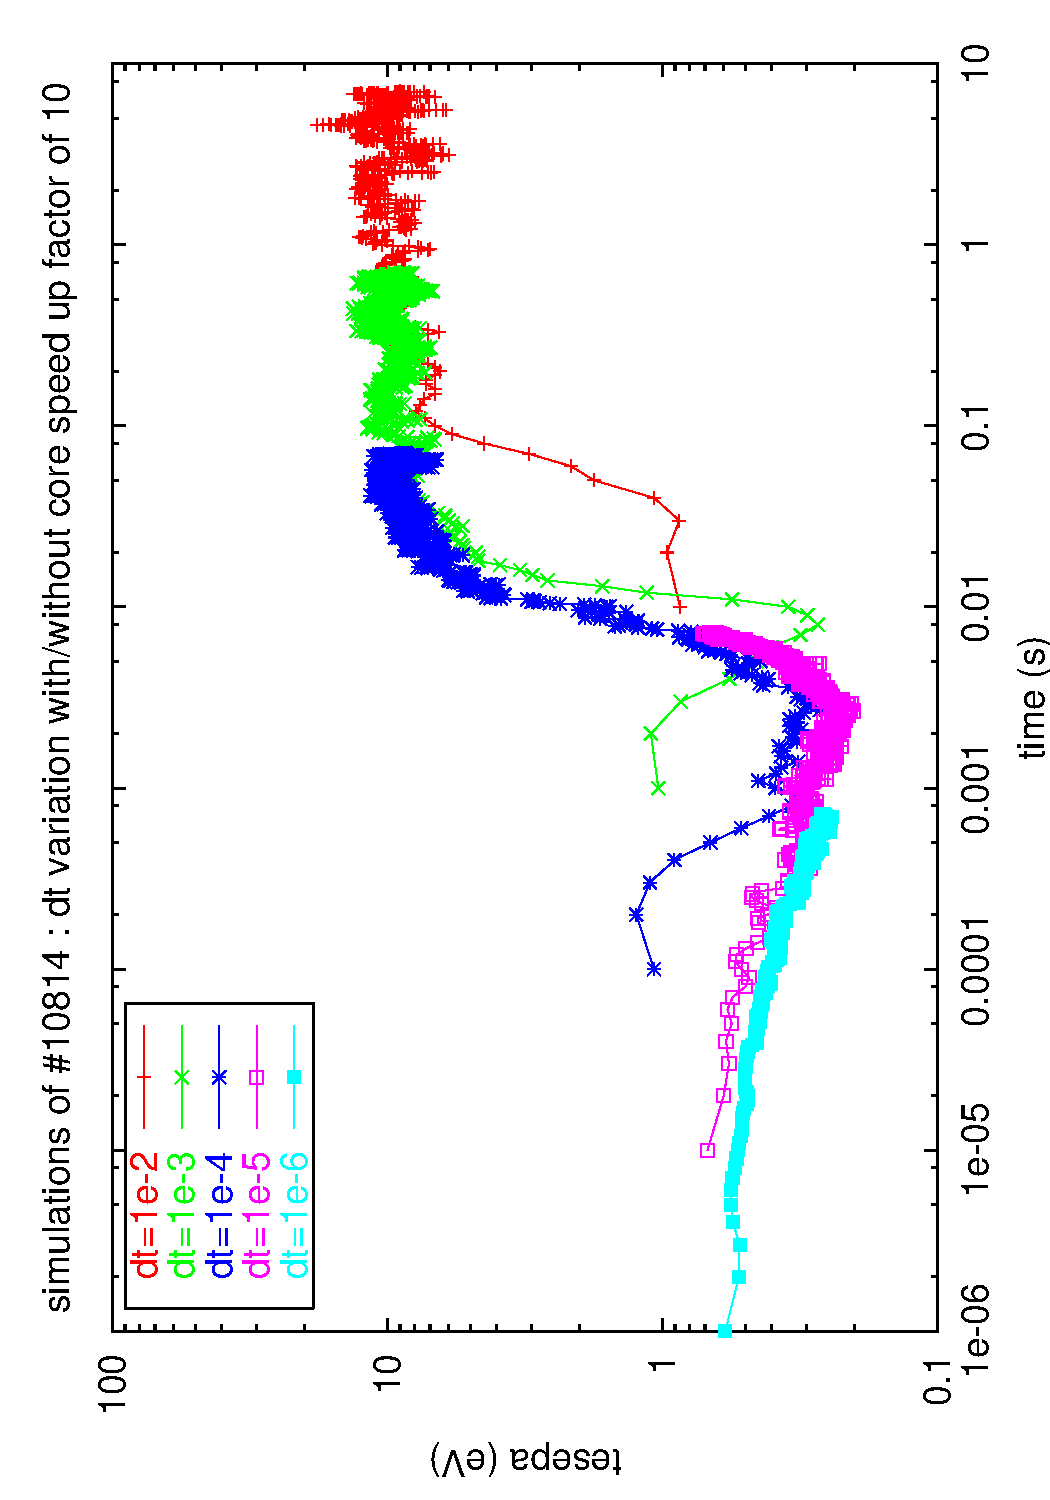
\includegraphics[origin=br,angle=-90,height=8cm]{compare_10814_tesepm_4.pdf}}
\else
    \centerline{\includegraphics[origin=br,angle=-90,height=8cm]{compare_10814_tesepm_4.ps}}
\fi
    \caption{Downstream (outer target) electron temperature for a
    range of time-steps.}
    \label{fig:tesepm4}
\end{figure}


\begin{figure}[hbtp]
\ifpdf 
    \centerline{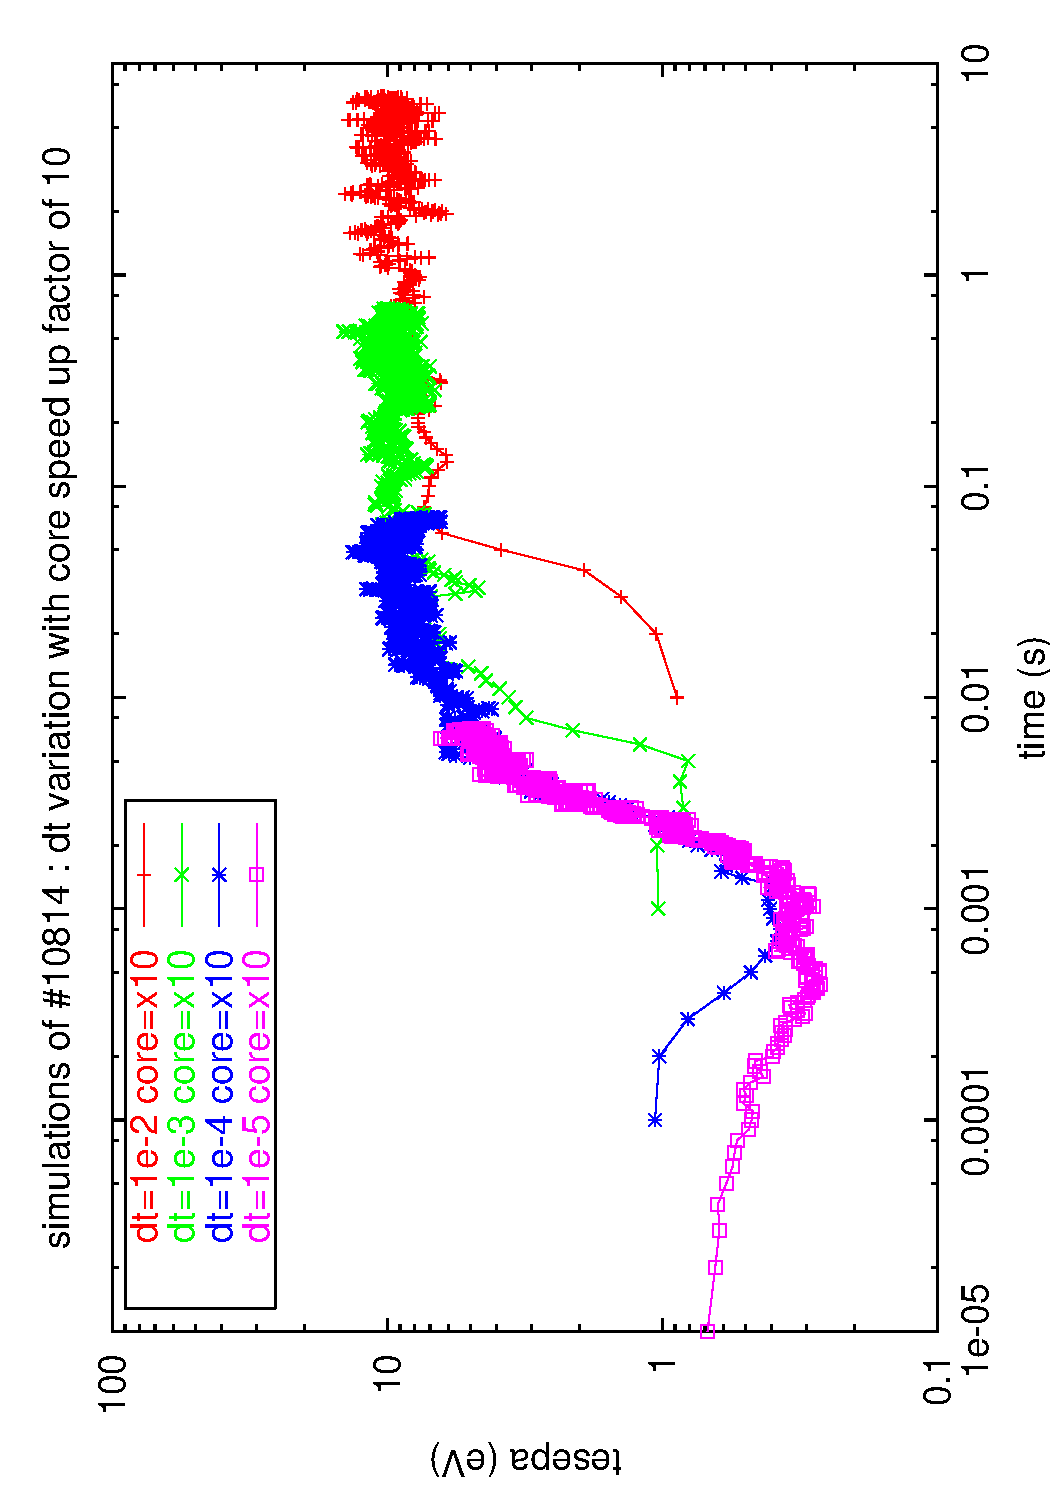
\includegraphics[origin=br,angle=-90,height=8cm]{compare_10814_tesepm_5.pdf}}
\else
    \centerline{\includegraphics[origin=br,angle=-90,height=8cm]{compare_10814_tesepm_5.ps}}
\fi
    \caption{Downstream (outer target) electron temperature for a
    range of time-steps with a core speed-up factor.}
    \label{fig:tesepm5}
\end{figure}


\begin{figure}[hbtp]
\ifpdf 
    \centerline{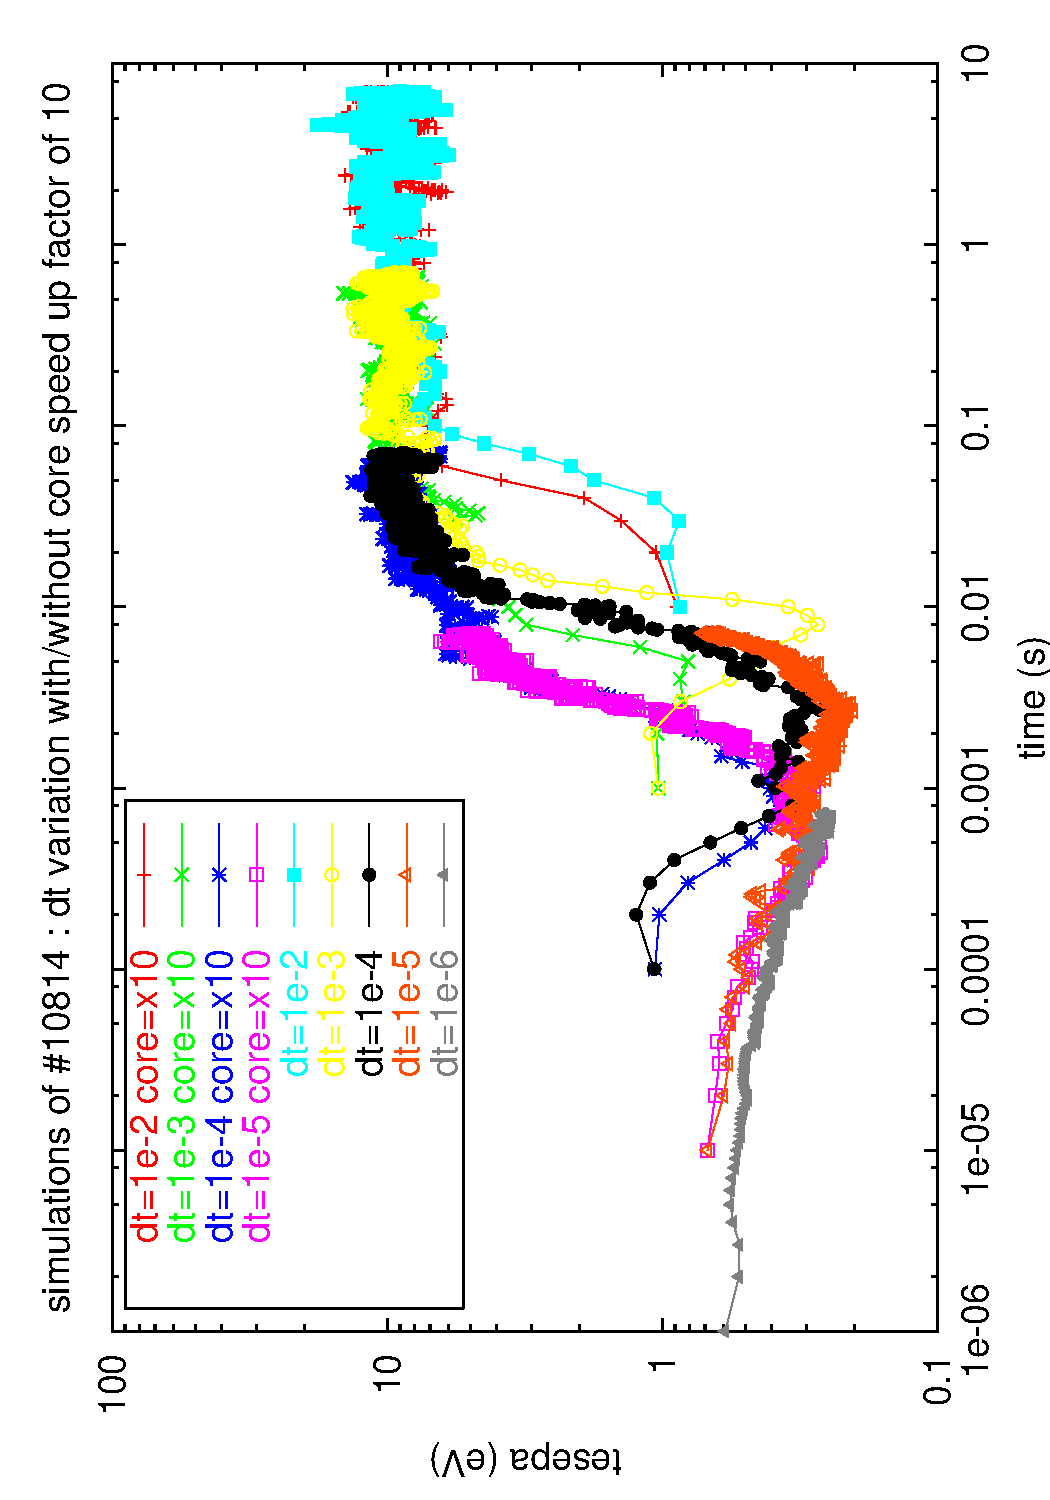
\includegraphics[origin=br,angle=-90,height=8cm]{compare_10814_tesepm_6.pdf}}
\else
    \centerline{\includegraphics[origin=br,angle=-90,height=8cm]{compare_10814_tesepm_6.ps}}
\fi
    \caption{Downstream (outer target) electron temperature for a
    range of time-steps with and without a core speed-up factor.}
    \label{fig:tesepm6}
\end{figure}

Figures \ref{fig:tesepm7}, \ref{fig:tesepm8} and \ref{fig:tesepm9}
show continuation runs.

\begin{figure}[hbtp]
\ifpdf 
    \centerline{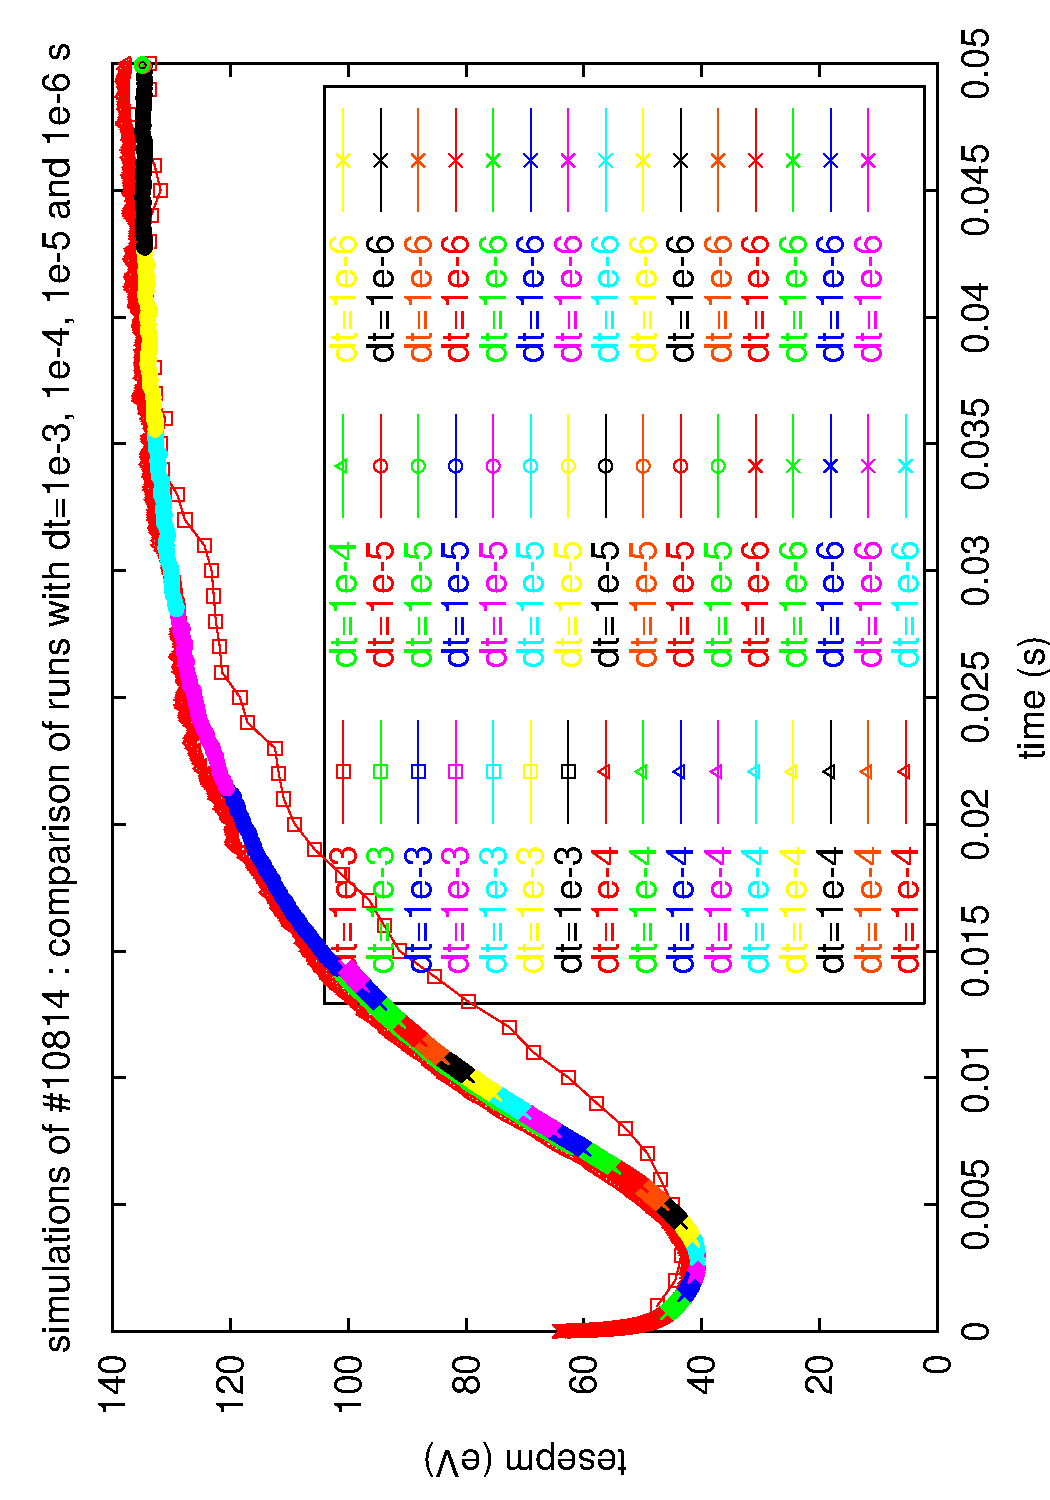
\includegraphics[origin=br,angle=-90,height=8cm]{compare_10814_tesepm_7.pdf}}
\else
    \centerline{\includegraphics[origin=br,angle=-90,height=8cm]{compare_10814_tesepm_7.ps}}
\fi
    \caption{Upstream (outer midplane) electron temperature.}
    \label{fig:tesepm7}
\end{figure}


\begin{figure}[hbtp]
\ifpdf 
    \centerline{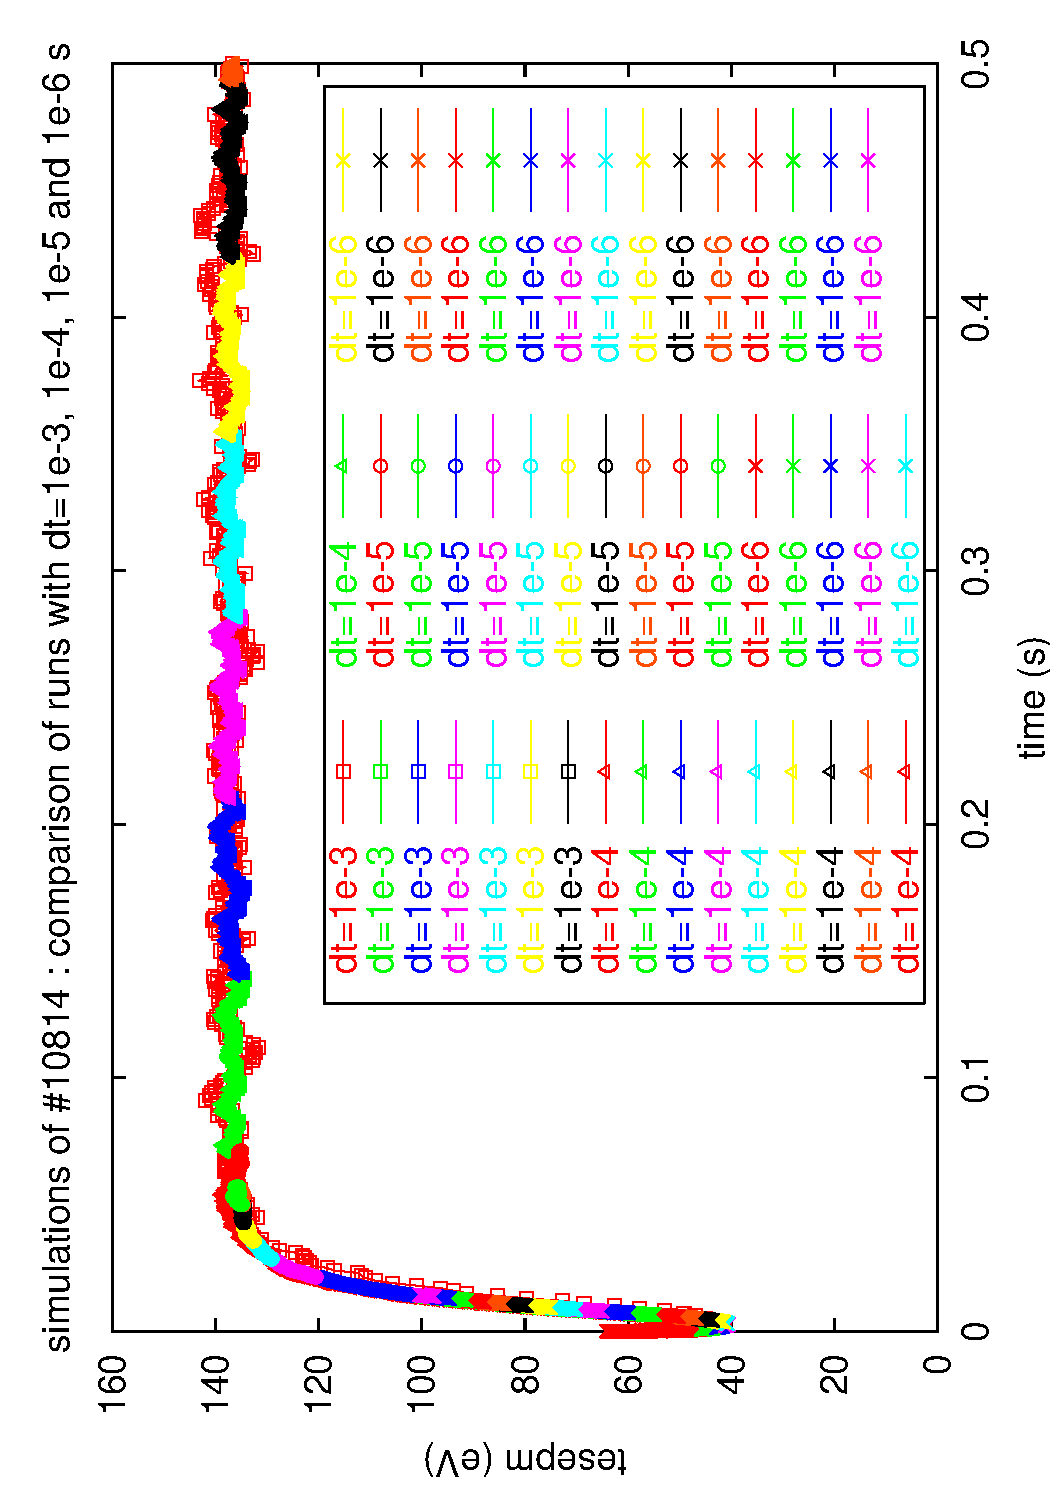
\includegraphics[origin=br,angle=-90,height=8cm]{compare_10814_tesepm_8.pdf}}
\else
    \centerline{\includegraphics[origin=br,angle=-90,height=8cm]{compare_10814_tesepm_8.ps}}
\fi
    \caption{Upstream (outer midplane) electron temperature.}
    \label{fig:tesepm8}
\end{figure}


\begin{figure}[hbtp]
\ifpdf 
    \centerline{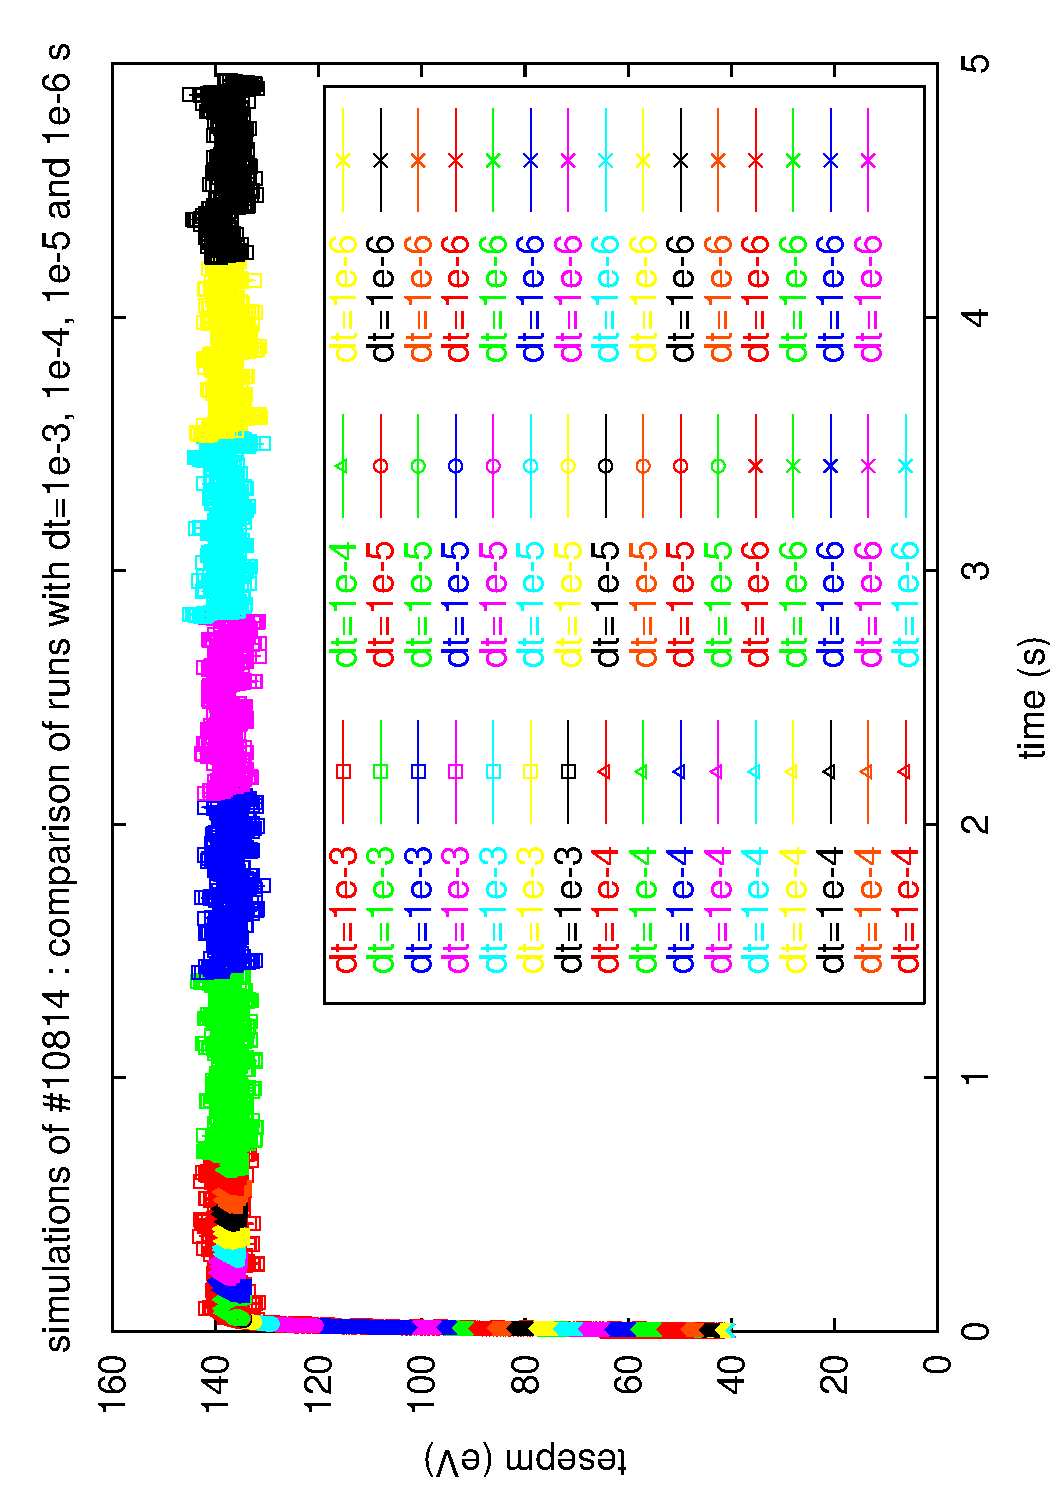
\includegraphics[origin=br,angle=-90,height=8cm]{compare_10814_tesepm_9.pdf}}
\else
    \centerline{\includegraphics[origin=br,angle=-90,height=8cm]{compare_10814_tesepm_9.ps}}
\fi
    \caption{Upstream (outer midplane) electron temperature.}
    \label{fig:tesepm9}
\end{figure}

\chapter{Using MDSPLUS}
\index{MDSPLUS}\label{cha:MDSplus}

A routine has been added, \verb!b2md!\index{b2md}, which allows one to save
the output from \SOLPSfive to an \verb!MDSplus! server in Garching.  (For more
information about \verb!MDSplus! see the Web site at \verb!www.mdsplus.org!.)

The reverse operation, namely recovering an archived run from the \verb!MDSplus!
server, is performed by \verb!b2rd!\index{b2rd}.

In order to use this facility, you need to ask David Coster at IPP-Garching to
add you to the list of authorized \verb!MDSplus! writers, supplying the username
which will be used, as well as the machine/domain.

In order to compile the code with \verb!MDSplus!, the environment variable
\verb!SOLPS_CPP!\index{SOLPS\_CPP} should contain
\verb!-DMDSPLUS!\index{-DMDSPLUS}, and a 
\begin{verbatim}
sbb ; gmake clean ; gmake depend ; gmake
\end{verbatim}
is safest.  Before doing this, the \verb!MDSPLUS_DIR! environment
needs to be set --- consult your systems people about this, or the
\verb!MDSplus! documentation.

[At IPP on the TOK linux cluster, add the following to \verb!.login!:
\begin{verbatim}
setenv MDSPLUS_DIR /afs/ipp-garching.mpg.de/home/d/dpc/@sys/mdsplus
source $MDSPLUS_DIR/setup.csh
\end{verbatim}
%% $
and add
\begin{verbatim}
setenv SOLPS_CPP '-DMDSPLUS'
\end{verbatim}
to one of the \verb!setup.csh.*! files in \$\verb!SOLPSTOP/SETUP!.]
 
\verb!b2md! requires as input \verb!b2md.dat! and this is searched for in the
present working directory, the \verb!baserun! directory, and in the
\$\verb!SOLPSTOP/data.local/mdsplus! and \$\verb!SOLPSTOP/data/mdsplus! directories,
if present, in order. See Appendix \ref{lis:b2cdcn} for a content description.

An example \verb!b2md.dat! is:
\VerbatimInput[fontsize=\footnotesize]{MDSPLUS/b2md.dat}

To save a new run to the \verb!MDSplus! server, execute
\begin{verbatim}
save_mds
\end{verbatim}
which should create \verb!shotnumber.history! which contains the
``shotnumber'' for the run on the server (not to be confused with the
experimental shot number).  The output from the operation will be saved in
\verb!b2md.log! and this should be checked for errors.

A run can be re-saved to the same shotnumber with
\begin{verbatim}
resave_mds
\end{verbatim}
which uses the ``shotnumber'' in \verb!shotnumber.history!.

The \verb!shotnumber.history! file can later be read by \verb!b2rd! which will
then fetch from the \verb!MDSplus! tree the archived shot corresponding to
the last number stored within.

\section{SOLPS tree structure}
\index{SOLPS tree structure in MDSplus}
\index{tree structure in MDSplus}
\index{MDSplus SOLPS tree structure}

%%rsync -avP ~/afs/MDSPLUS_examples/*.TCL.index MDSPLUS/

The \verb!solps! tree consists of the main tree, \verb!SOLPS!, and six sub-trees: \verb!IDENT!,
\verb!SNAPSHOT!, \verb!TALLIES!, \verb!TIMEDEP!, \verb!MOVIES! and \verb!DIAG!.

The signals in, for example, \verb!TIMEDEP! can be accessed as
\verb!\SOLPS::TOP.TIMEDEP.DP:IMPSEP!\ or alternatively 
\verb!\TIMEDEP::TOP.DP:IMPSEP!.

\subsection{SOLPS}

\VerbatimInput[fontsize=\footnotesize]{MDSPLUS/SOLPS_MODEL.TCL.index}

\subsection{IDENT}

\VerbatimInput[fontsize=\footnotesize]{MDSPLUS/IDENT_MODEL.TCL.index}

\subsection{SNAPSHOT}

\VerbatimInput[fontsize=\footnotesize]{MDSPLUS/SNAPSHOT_MODEL.TCL.index}

\subsection{TALLIES}

\VerbatimInput[fontsize=\footnotesize]{MDSPLUS/TALLIES_MODEL.TCL.index}

\subsection{TIMEDEP}

\VerbatimInput[fontsize=\footnotesize]{MDSPLUS/TIMEDEP_MODEL.TCL.index}

\subsection{MOVIES}

\VerbatimInput[fontsize=\footnotesize]{MDSPLUS/MOVIES_MODEL.TCL.index}

\subsection{DIAG}

\VerbatimInput[fontsize=\footnotesize]{MDSPLUS/DIAG_MODEL.TCL.index}

\section{Accessing data from the MDSPLUS server}

\subsection{Using standard experimental data viewing programs}

The \verb!MDSplus! server name is \verb!solps-mdsplus.aug.ipp.mpg.de:8001!.

The tree name is \verb!solps!.

An example shotnumber is \verb!4293!.

Example signal names are \verb!\top.timedep.ne:ompsep!,
\verb!\top.timedep.te:ompsep! (Outer midplane electron density and temperature), and 
\verb!\top.timedep.ti:ompsep! (Outer midplane ion temperature).

\subsubsection{cview}
\index{cview}

\begin{itemize}
\item start \verb!cview!
\item \verb!Shot! = \verb!4293!
\item In the table:
  \begin{itemize}
  \item \verb!shot! = \verb!0!
  \item \verb!shot! = \verb!+solps!
  \item \verb!diag! = \verb!solps!
  \item \verb!name! = \verb!\top.timedep.ne:ompsep!
  \end{itemize}
\end{itemize}

Adding \verb!\top.timedep.ne:ompsep! and \verb!\top.timedep.ne:ompsep!, the
graph in figure \ref{fig:cviewsolpsmdsplus} is produced.

\begin{figure}[htbp]
  \centering
  \ifpdf 
    \centerline{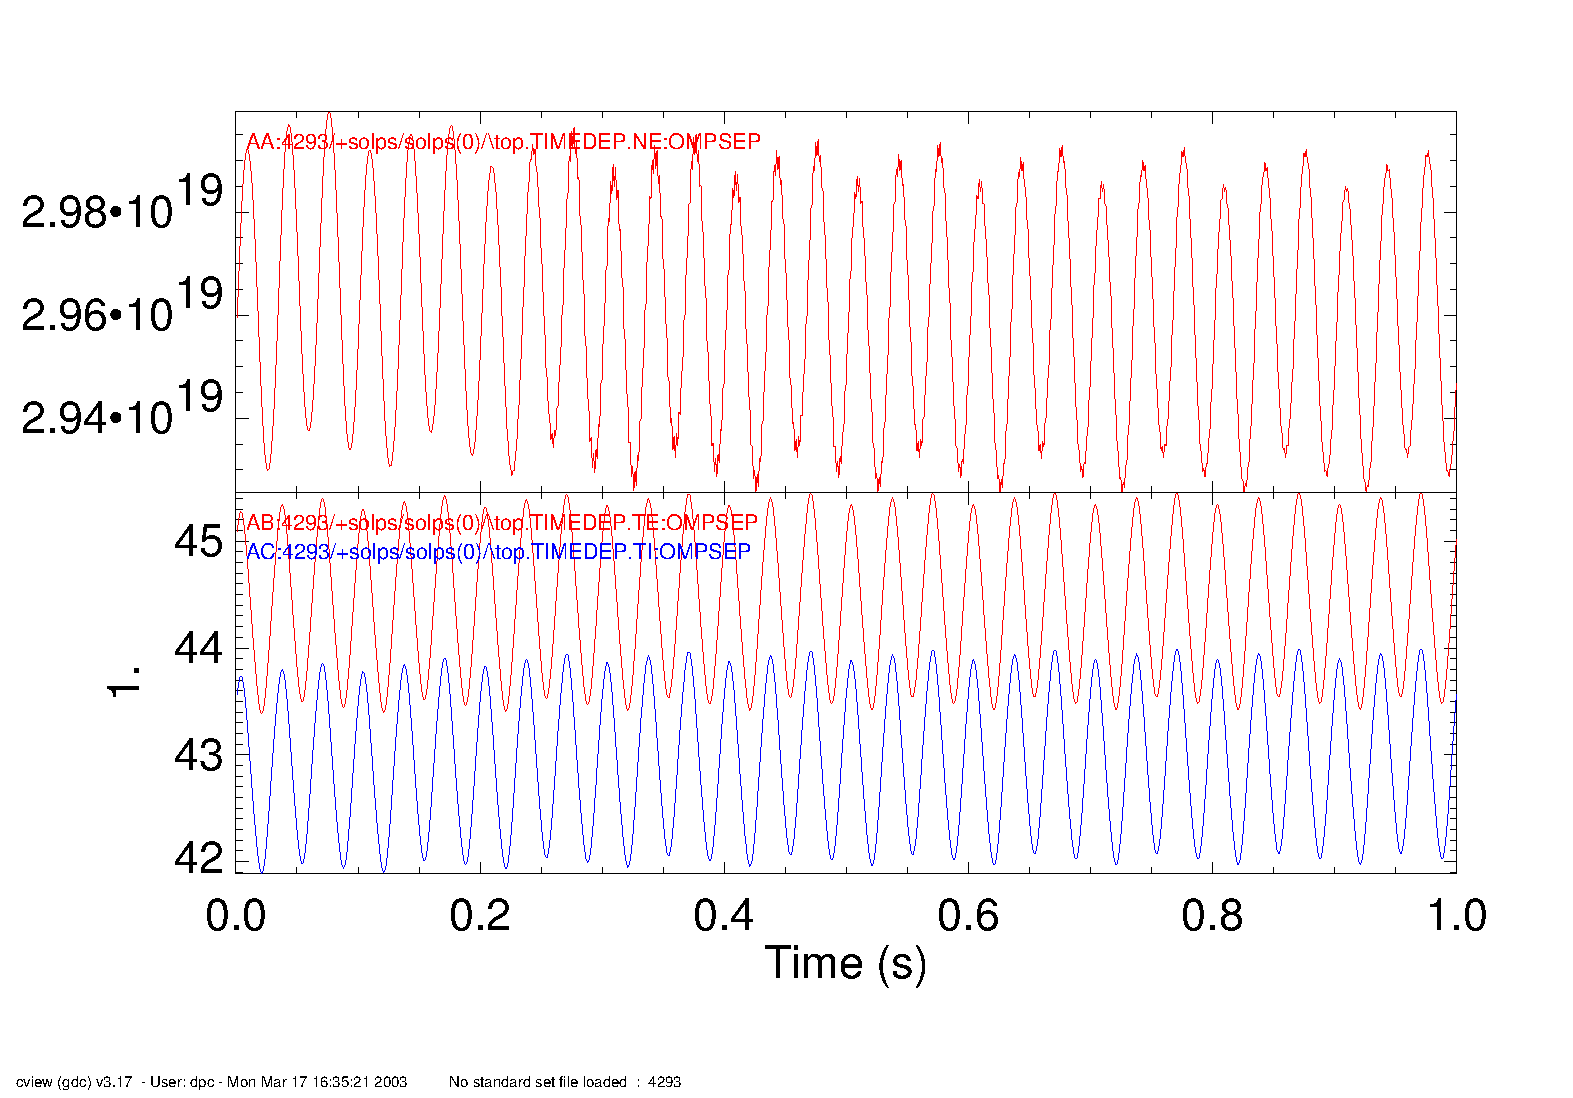
\includegraphics[height=8cm]{MDSPLUS/cview_mdsplus_example.pdf}}
\else
    \centerline{\includegraphics[height=8cm]{MDSPLUS/cview_mdsplus_example.eps}}
\fi
  \caption{Using CVIEW to access SOLPS MDSplus data.}
  \label{fig:cviewsolpsmdsplus}
\end{figure}

\subsubsection{jetdsp}
\index{jetdsp}

\begin{itemize}
\item start \verb!JETDSP!
\item \verb!File|Read Signal!
\item \verb!MDS+! option
\item \verb!MDS+ server:! = \verb!solps-mdsplus.aug.ipp.mpg.de:8001!
\item \verb!Shot number:! = \verb!4293!
\item \verb!Tree:! = \verb!solps!
\item \verb!Signal:! = \verb!\top.timedep.ne:ompsep!
\item \verb!Read! button
\end{itemize}

You can also use
\begin{itemize}
\item start \verb!JETDSP!
\item \verb!File|Read Signal!
\item \verb!MDS+! option
\item \verb!MDS+ server:! = \verb!solps-mdsplus.aug.ipp.mpg.de:8001!
\item \verb!Shot number:! = \verb!4293!
\item \verb!Tree:! = \verb!timedep!
\item \verb!Signal:! = \verb!\top.ne:ompsep!
\item \verb!Read! button
\end{itemize}

Adding \verb!te:ompsep! and \verb!ti:ompsep!, the graph in figure
\ref{fig:jetdspsolpsmdsplus} is produced.

\begin{figure}[htbp]
  \centering
  \ifpdf 
    \centerline{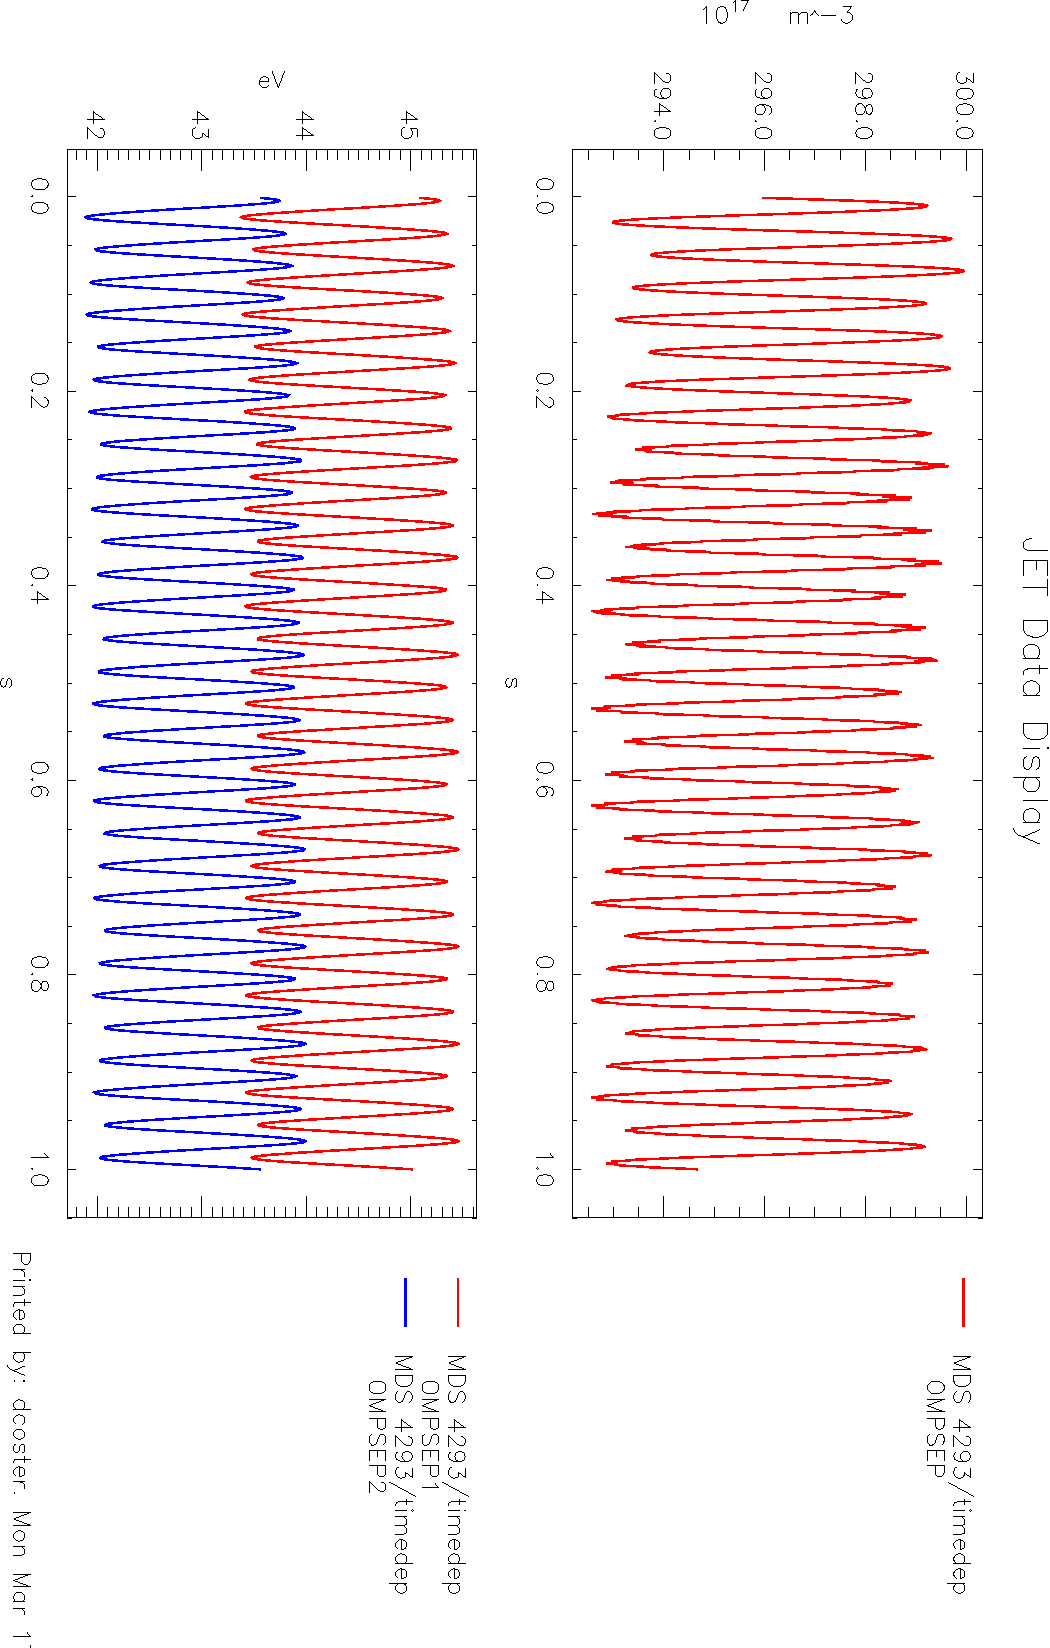
\includegraphics[origin=bl,angle=+90,height=8cm]{MDSPLUS/jetdsp_mdsplus_example.pdf}}
\else
    \centerline{
\includegraphics[origin=bl,angle=+90,height=8cm]{MDSPLUS/jetdsp_mdsplus_example.epsi}}
\fi
  \caption{Using JETDSP to access SOLPS MDSplus data.}
  \label{fig:jetdspsolpsmdsplus}
\end{figure}

\subsubsection{reviewplus}
\index{reviewplus}

\subsection{Using IDL}
\index{idl}

\begin{verbatim}
mdsconnect,'solps-mdsplus.aug.ipp.mpg.de:8001'
mdsopen,'solps',251
te_coarse=mdsvalue('\top.snapshot:te')
cr_coarse=mdsvalue('\top.snapshot.grid:cr')
mdsopen,'solps',288
te_fine=mdsvalue('\top.snapshot:te')
cr_fine=mdsvalue('\top.snapshot.grid:cr')
mdsclose
mdsdisconnect
plot,cr_coarse[*,8],te_coarse[*,8],linestyle=1,psym=-1,yrange=[0,50]
oplot,cr_fine[*,10],te_fine[*,10],linestyle=2,psym=-2
\end{verbatim}

\subsection{Using MATLAB}
\index{matlab}

\begin{verbatim}
mdsopen('solps-mdsplus.aug.ipp.mpg.de:8001::solps',nshot);
onx= mdsvalue('\SOLPS::TOP.SNAPSHOT.DIMENSIONS:NX');
ny = mdsvalue('\SOLPS::TOP.SNAPSHOT.DIMENSIONS:NY'); %number of radial cells
ne = mdsvalue('\SOLPS::TOP.SNAPSHOT:NE');  
te = mdsvalue('\SOLPS::TOP.SNAPSHOT:TE');
ti = mdsvalue('\SOLPS::TOP.SNAPSHOT:TI');
sep= mdsvalue('\SOLPS::TOP.TIMEDEP.OMP:DS');
qe = 1.602e-19; %Elementary charge in C
amu= 1.660542e-27; %Atomic mass unit in kg

%Calculate the ion sound speed at outer target
cs2o = qe .* (ti(onx-1,:) + te(onx-1,:)) ./ (2*amu);

%Outer target
neo  = ne(onx-1,:);
osja = neo .* qe .* sqrt(cs2o) / 1.0e4;

cr = mdsvalue('\SOLPS::TOP.SNAPSHOT.GRID:CR'); %R-coordinate of cell centre
ocr= cr(onx,:); %R coordinates of outer target cells
cz = mdsvalue('\SOLPS::TOP.SNAPSHOT.GRID:CZ'); %Z-coordinate of cell centre
ocz= cz(onx,:); %Z coordinate of outer target cells
mdsclose('MDSIP');

[map2mid,oms]=jhmap2mid(26730,ocr,ocz,0.7);
rrsep= map2mid.Rmid-map2mid.Rlcfs;

plot(rrsep,osja,'k');
\end{verbatim}

\subsection{Using Python}
\index{python}

You will need the MDSplus interface for python.  

\begin{verbatim}
import pmds
from pylab import *

pmds.mdsconnect ('solps-mdsplus.aug.ipp.mpg.de:8001')
pmds.mdsopen('solps',12380)
r=pmds.mdsvalue('\\top.snapshot.grid:r')
z=pmds.mdsvalue('\\top.snapshot.grid:z')
pmds.mdsdisconnect ()

print(r)  
print(z)  
\end{verbatim}

For additional information about using python, see\\
\href{https://wiki.eu-euforia.eu/index.php/Fusion\_dataset\_with\_Python\_and\_VisIt}{https://wiki.eu-euforia.eu/index.php/Fusion\_dataset\_with\_Python\_and\_VisIt}\\
(this activity occurred within the EUFORIA project,
\href{http://www.euforia-project.eu/}{http://www.euforia-project.eu/}).

\index{python, plots to compare profiles}
Typing
\begin{verbatim}
  python
  import compare_shots
\end{verbatim}
with the following as \verb!compare_shots.py!:
\VerbatimInput[fontsize=\footnotesize]{compare_shots.py}
produced figure \ref{fig:python_compare_shots}.

\begin{figure}[hbtp]
\ifpdf 
    \centerline{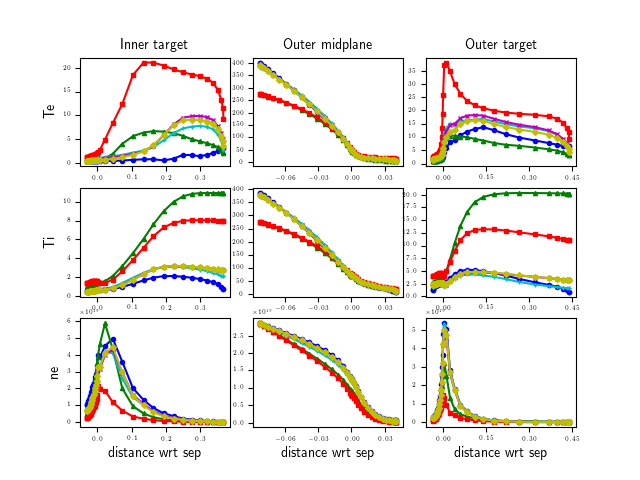
\includegraphics[height=8cm]{compare_shots.png}}
\else
    \centerline{\includegraphics[height=8cm]{compare_shots.ps}}
\fi
    \caption{Comparison of profiles for a range of shots.}
    \label{fig:python_compare_shots}
\end{figure}

In another, more complicated, example, python was used to create the frames of a movie on the ITM Gateway machine.
\index{movie, python}\index{python, movie}
\begin{verbatim}
set c=0
foreach i ( `cat shots` )
  set tbase=`echo $c | awk '{print $1*1000*1e-5}'`
  mkdir $i
  echo Submitting $i with offset $tbase
  ( cd $i ; sed -e "s:#1#:${i}:g" -e "s:#2#:${tbase}:g" < ../QSUB.shot | bsub )
  @ c++
  sleep 5
end
\end{verbatim}
with \verb!QSUB.shot! containing \VerbatimInput[fontsize=\footnotesize]{QSUB.shot.python_movie} and \verb!shots! containing \VerbatimInput[fontsize=\footnotesize]{shots.python_movie}

This launches one job per SOLPS shot-number.  Then the frames were renumbered by
\begin{verbatim}
mkdir frames
cd frames/
set c=0
foreach i ( `cat ../shots` )
  set p=`echo $c | awk '{printf "%03i\n",$1}'`
  echo $p
  @ c++
  foreach j ( `cd ../$i ; echo tmp_????.png`)
    ln -s ../$i/$j `echo $j | sed "s:tmp_0:tmp_${p}:"`
  end
end
\end{verbatim}

The individual frames were then combined into a movie with
\begin{verbatim}
mencoder 'mf://frames/tmp_??????.png' -mf type=png:fps=30 -ovc lavc -lavcopts \
 vcodec=wmv2 -oac copy -o fb_nesepm=5.0e19.ELM_2cm_X10.rqahesum.mpg
\end{verbatim}

The resultant movie can be found at\\
\href{http://solps-mdsplus.aug.ipp.mpg.de/SOLPS/fb\_nesepm=5.0e19.ELM\_2cm\_X10.rqahesum.mpg}{http://solps-mdsplus.aug.ipp.mpg.de/SOLPS/fb\_nesepm=5.0e19.ELM\_2cm\_X10.rqahesum.mpg}

\section{Querying the database}
\index{database}\index{querying database}

All cases are also entered into a \verb!MySQL!\index{MySQL}
(\href{http://www.mysql.com/}{http://www.mysql.com/}) database.

A Web interface to the database is available at
\href{http://solps-mdsplus.aug.ipp.mpg.de/solps/}{http://solps-mdsplus.aug.ipp.mpg.de/solps/} 
via \verb!Zope!\index{Zope}\\
(\href{http://www.zope.org/}{http://www.zope.org/}).

The database can also be queried via \verb!MySQL! commands passed via \verb!MDSplus!. An \verb!IDL!
example of querying the database to find the number of shots supplied by each
user follows:

\index{database query via IDL}
\begin{verbatim}
mdsconnect,'solps-mdsplus.aug.ipp.mpg.de:8001'
ans=mdsvalue("sql('select user,count(*) from id group by user','solps')")
mdsdisconnect
help,ans
print,transpose(ans)
\end{verbatim}

Another, more complicated, \verb!IDL! example is:

\begin{verbatim}
mdsconnect,'solps-mdsplus.aug.ipp.mpg.de:8001'
ans=mdsvalue("sql('select solpsindex,shot,time,ompsep_te,ompsep_ti,user,exp 
   from id where ompsep_te>110.0 and ompsep_te<120.0','solps')")
mdsdisconnect
help,ans
print,format='(i6,1x,i6,1x,f6.3,1x,f6.2,1x,1x,f6.2,1x,a10,1x,a)',transpose(ans)
plot,ans(*,3),ans(*,4),psym=4,xtitle='Te (eV)',ytitle='Ti (eV)'
\end{verbatim}

\index{database query via python}\index{python, database qyery}
And a similar example in python:
\begin{verbatim}
python sql_solps.py
\end{verbatim}
with \verb!sql_solps.py! containing
\VerbatimInput[fontsize=\footnotesize]{sql_solps.py} The resultant
plots are givien in figures \ref{fig:python_sql_scatter},
\ref{fig:python_sql_hexbin_lin} and \ref{fig:python_sql_hexbin_log}.

\begin{figure}[hbtp]
\ifpdf 
    \centerline{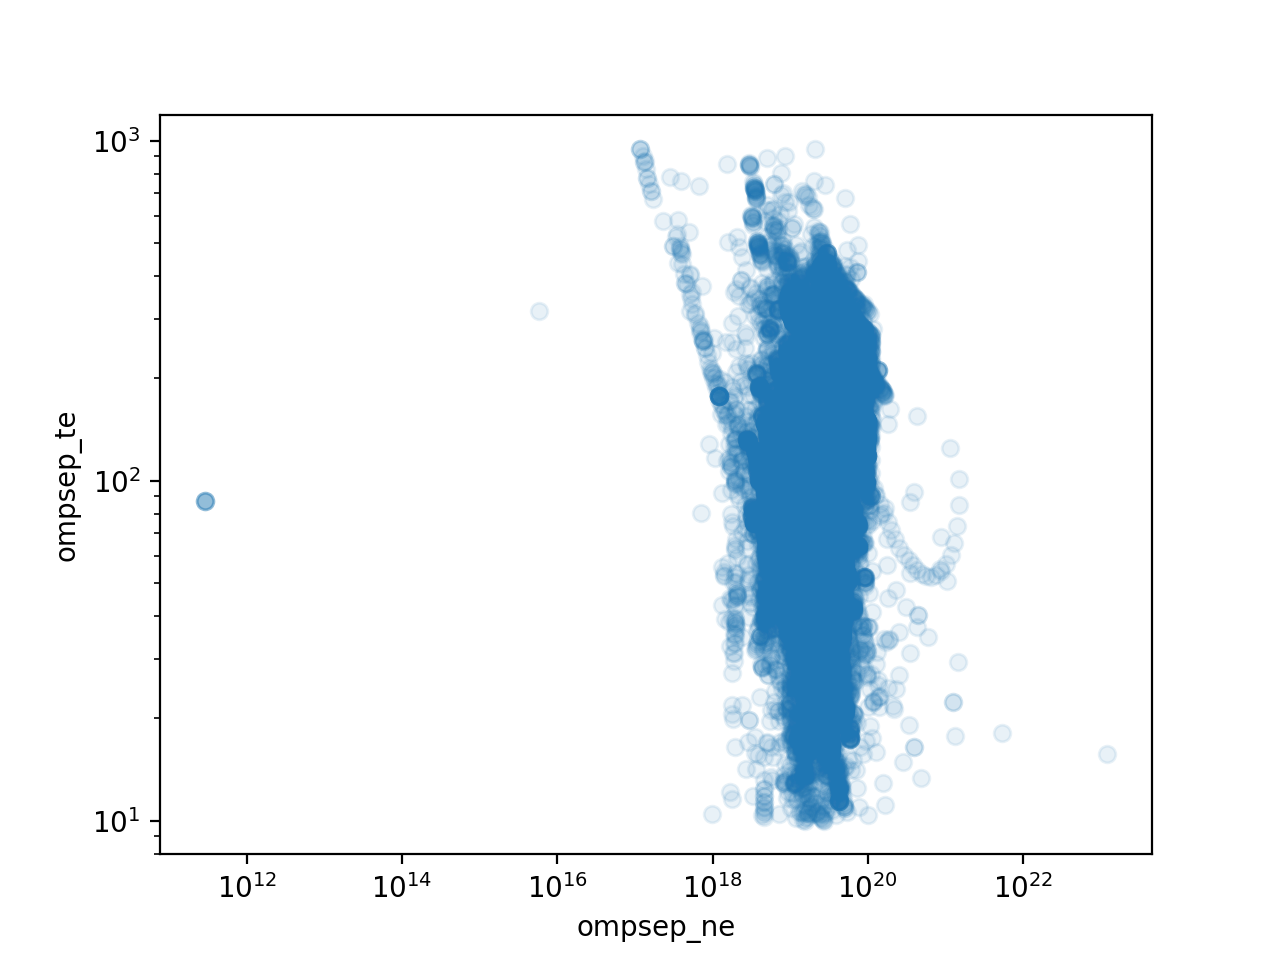
\includegraphics[height=8cm]{sql_scatter.png}}
\else
    \centerline{\includegraphics[height=8cm]{sql_scatter.ps}}
\fi
    \caption{Comparison of profiles for a range of shots.}
    \label{fig:python_sql_scatter}
\end{figure}

\begin{figure}[hbtp]
\ifpdf 
    \centerline{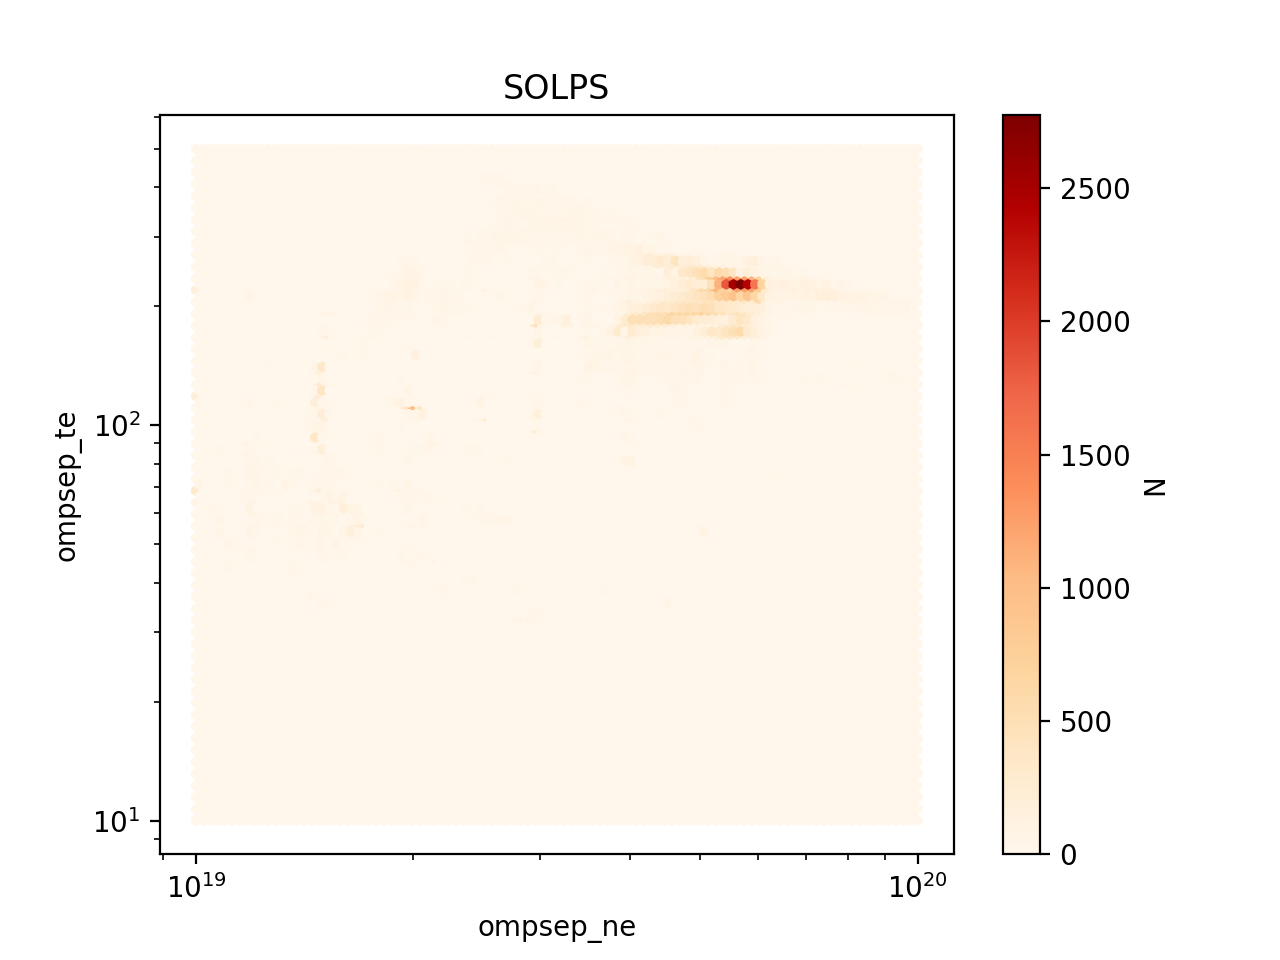
\includegraphics[height=8cm]{sql_hexbin_lin.png}}
\else
    \centerline{\includegraphics[height=8cm]{sql_hexbin_lin.ps}}
\fi
    \caption{Comparison of profiles for a range of shots.}
    \label{fig:python_sql_hexbin_lin}
\end{figure}

\begin{figure}[hbtp]
\ifpdf 
    \centerline{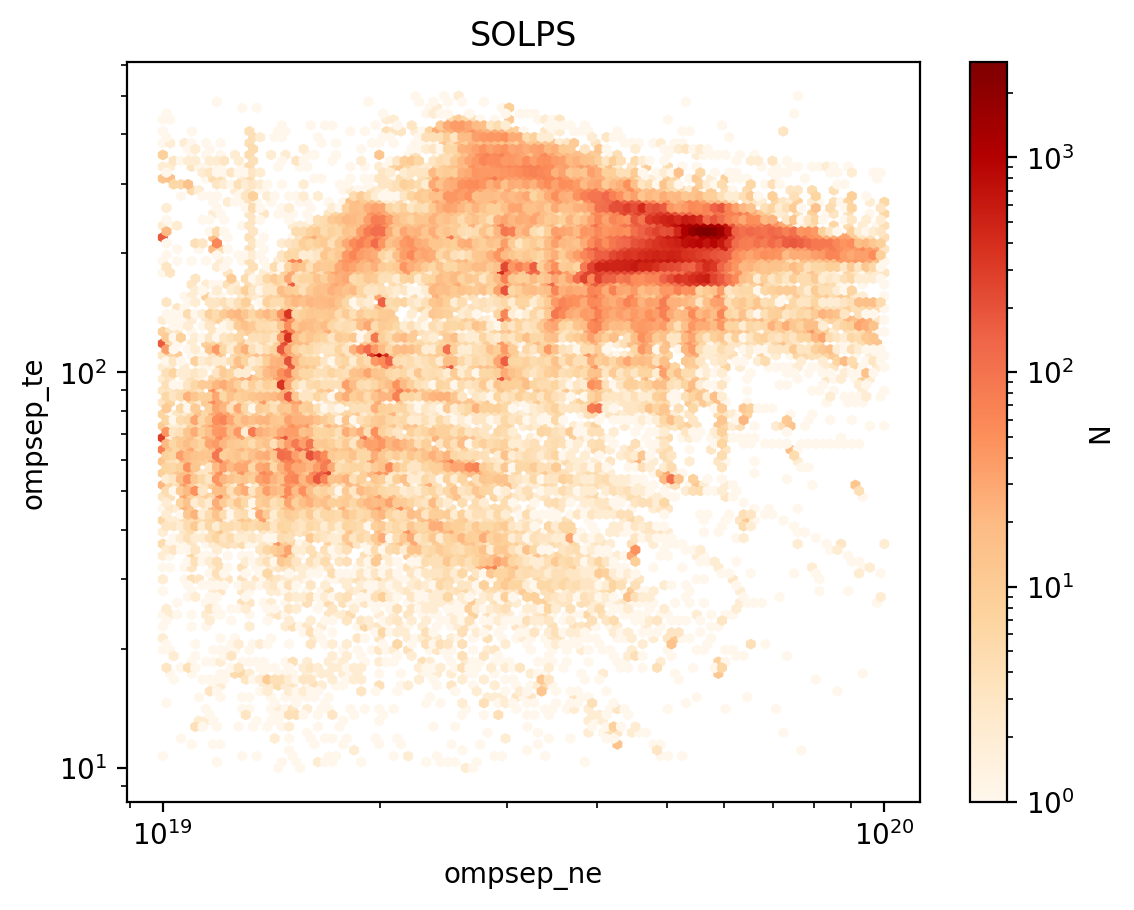
\includegraphics[height=8cm]{sql_hexbin_log.png}}
\else
    \centerline{\includegraphics[height=8cm]{sql_hexbin_log.ps}}
\fi
    \caption{Comparison of profiles for a range of shots.}
    \label{fig:python_sql_hexbin_log}
\end{figure}


\section{Coupling to other codes via MDSplus}
\index{Coupling to other codes via MDSplus}

Coupling of \verb!SOLPS! to other codes has in the past been done mostly by
exchanging files.  The preferred route for the future is to use the \verb!SOLPS MDSplus! tree.

As an example of how to do this, a short example \verb!FORTRAN! code which queries
the \verb!SOLPS MDSplus! server and then writes geometry information in the standard
\verb!Sonnet! format is presented below.  The code uses Wolfgang Suttrop's
\verb!libitdb! library
(\href{http://www.ipp.mpg.de/~Wolfgang.Suttrop/mdsplus/libitdb/}{http://www.ipp.mpg.de/~Wolfgang.Suttrop/mdsplus/libitdb/}).

\begin{verbatim}
      program write_files
      implicit none
      integer nxdmax, nydmax
      parameter (nxdmax=1024, nydmax=1024)
      integer ishot, status, iargc, lng,
     1 sizes(4), ndim, ndim1, ndim2, ndim3,
     2 icell, ix, iy, nx, ny
      character arg*256, string*256
      real*8 cr(-1:nxdmax, -1:nydmax),  cz(-1:nxdmax, -1:nydmax),
     1 crx(-1:nxdmax, -1:nydmax, 0:3), cry(-1:nxdmax, -1:nydmax, 0:3),
     2 bb(-1:nxdmax, -1:nydmax, 0:3),
     3 dum1(1), dum2(1), dum3(1), b0r0

      if(iargc().ne.1) then
        write(*,*) 'One argument expected, not ',iargc()
        stop
      endif
      call getarg(1,arg)
      read(arg,*) ishot

      call itdb_open(status,"solps-mdsplus.aug.ipp.mpg.de:8001",
     1 "solps", ishot)
      call itdb_err_msg('itdb_open',status)

      lng=len(string)
      call itdb_gettext(status,"\TOP.IDENT:USER",string,lng)
      call itdb_err_msg('itdb_gettext',status)
      write(*,*) string(1:lng)

      ndim=2
      ndim1=0                 ! nxdmax+2
      sizes(1)=nxdmax+2
      ndim2=0                 ! nydmax+2
      sizes(2)=nydmax+2
      ndim3=0                 ! 1+3
      sizes(3)=1+3

      ndim=2
      ndim1=0                 ! nxdmax+2
      sizes(1)=nxdmax+2
      ndim2=0                 ! nydmax+2
      sizes(2)=nydmax+2
      ndim3=0                 ! 1+3
      CALL itdb_getsig(status,'\TOP.SNAPSHOT.GRID:CR',
     *     ndim,sizes,cr,ndim1,dum1,ndim2,dum2,ndim3,dum3)
      call itdb_err_msg('itdb_getsig',status)
      write(*,*) 'CR: ',ndim,sizes(1:ndim),ndim1,ndim2,ndim3
      ndim=2
      ndim1=0                 ! nxdmax+2
      sizes(1)=nxdmax+2
      ndim2=0                 ! nydmax+2
      sizes(2)=nydmax+2
      ndim3=0                 ! 1+3
      CALL itdb_getsig(status,'\TOP.SNAPSHOT.GRID:CZ',
     *     ndim,sizes,cz,ndim1,dum1,ndim2,dum2,ndim3,dum3)
      call itdb_err_msg('itdb_getsig',status)
      write(*,*) 'CZ: ',ndim,sizes(1:ndim),ndim1,ndim2,ndim3
      ndim=3
      ndim1=0                 ! nxdmax+2
      sizes(1)=nxdmax+2
      ndim2=0                 ! nydmax+2
      sizes(2)=nydmax+2
      ndim3=0                 ! 1+3
      sizes(3)=1+3
      CALL itdb_getsig(status,'\TOP.SNAPSHOT.GRID:R',
     *     ndim,sizes,crx,ndim1,dum1,ndim2,dum2,ndim3,dum3)
      call itdb_err_msg('itdb_getsig',status)
      write(*,*) 'R: ',ndim,sizes(1:ndim),ndim1,ndim2,ndim3
      ndim=3
      ndim1=0                 ! nxdmax+2
      sizes(1)=nxdmax+2
      ndim2=0                 ! nydmax+2
      sizes(2)=nydmax+2
      ndim3=0                 ! 1+3
      sizes(3)=1+3
      CALL itdb_getsig(status,'\TOP.SNAPSHOT.GRID:Z',
     *     ndim,sizes,cry,ndim1,dum1,ndim2,dum2,ndim3,dum3)
      call itdb_err_msg('itdb_getsig',status)
      write(*,*) 'Z: ',ndim,sizes(1:ndim),ndim1,ndim2,ndim3
      ndim=3
      ndim1=0                 ! nxdmax+2
      sizes(1)=nxdmax+2
      ndim2=0                 ! nydmax+2
      sizes(2)=nydmax+2
      ndim3=0                 ! 1+3
      sizes(3)=1+3
      CALL itdb_getsig(status,'\TOP.SNAPSHOT:B',
     *     ndim,sizes,bb,ndim1,dum1,ndim2,dum2,ndim3,dum3)
      call itdb_err_msg('itdb_getsig',status)
      write(*,*) 'B: ',ndim,sizes(1:ndim),ndim1,ndim2,ndim3

      call itdb_close(status)
      call itdb_err_msg('itdb_close',status)

      nx=sizes(1)-2
      ny=sizes(2)-2

      open(99,file=trim(arg)//'.sonnet')
      icell=0
      write(99,*)
      write(99,'(3x,a/)') 'Element output:'
      b0r0=cr(-1,-1)*bb(-1,-1,3)

      write(99,*) '   R*Btor =',b0r0
      write(99,'(/3x,2a)')
     1 '======================================',
     2 '=================================================='
      do iy=-1,ny
        do ix=-1,nx
          write(99,10001) icell,ix+1,iy+1,
     1     crx(ix,iy,2),cry(ix,iy,2),crx(ix,iy,3),cry(ix,iy,3)
10001     format(3x,'Element',i5,' = (',i3,',',i3,'): (',
     .     1pe17.10,',',1pe17.10,')',
     .     6x,'(',1pe17.10,',',1pe17.10,')')
          write(99,10002)
     1     sqrt(bb(ix,iy,0)**2+bb(ix,iy,1)**2)/bb(ix,iy,3),
     2     cr(ix,iy),cz(ix,iy)
10002     format(3x,'Field ratio  = ',1pe17.10,13x,
     .     '(',1pe17.10,',',1pe17.10,')')
          write(99,10003)
     1     crx(ix,iy,0),cry(ix,iy,0),crx(ix,iy,1),cry(ix,iy,1)
10003     format(
     .     t30,'(',1pe17.10,',',1pe17.10,')',
     .     6x,'(',1pe17.10,',',1pe17.10,')')
          write(99,10005)
10005     format(3x,
     1     '--------------------------------------------------',
     2     '--------------------------------------')
          icell=icell+1
        enddo
      enddo
      close(99)

      end

      subroutine itdb_err_msg(name,status)
      implicit none
      character*(*) name
      integer status

      if (status.ne.0) then
        write(*,*) 'Routine ',trim(name),' returned error code ',status
      endif
      return
      end
\end{verbatim}


\section{Some information about the server}

The IPP MDSplus server is a dual processor 2.8~GHz AMD Opteron machine with 4~GB RAM
running SUSE LINUX 10.1 (X86-64).  The data is stored in MR-AFS.

%% echo As of `date` the SOLPS MDSplus server \"solps-mdsplus.aug.ipp.mpg.de:8001\" contained `hexdump -e '1/4 "%d\n"' < /afs/ipp-garching.mpg.de/home/d/dpc/MDS/models/shotid.sys` cases consisting of `/afs/ipp-garching.mpg.de/bin/fs lq ~/MDS/0/000/0?? | awk '/xxx/{kbytes+=$3}/files/{files+=$5}END{print kbytes/1024/1024" GB in "files" files"}'`.

As of Wed Jun 1 21:30:57 CEST 2005 the SOLPS MDSplus server
"solps-mdsplus.aug.ipp.mpg.de:8001" contained 12497 cases consisting of
387.158 GB in 261099 files.

As of Wed Jul 26 19:12:53 CEST 2006 the SOLPS MDSplus server
"solps-mdsplus.aug.ipp.mpg.de:8001" contained 15999 cases consisting of
995.904 GB in 334534 files.

As of Sat Mar 8 00:46:36 CET 2008 the SOLPS MDSplus server
"solps-mdsplus.aug.ipp.mpg.de:8001" contained 22190 cases consisting
of 2824.17 GB in 464547 files.

As of Tue Oct 7 19:45:57 CEST 2008 the SOLPS MDSplus server
"solps-mdsplus.aug.ipp.mpg.de:8001" contained 25623 cases consisting
of 3646.37 GB in 536644 files.

As of Tue Jan 13 10:05:51 MET 2009 the SOLPS MDSplus server
"solps-mdsplus.aug.ipp.mpg.de:8001" contained 26448 cases consisting
of 3802.68 GB in 553970 files.

\chapter{Running DivGeo}
\label{cha:divgeo}\index{DG, running}

You will need to choose your device, {\it e.g.}: \index{DEVICE}
\begin{verbatim}
  setenv DEVICE upgrade
\end{verbatim}
Available choices are:
\begin{description}
\item[asdex] ASDEX (Garching, Germany), now HL--2A (Chengdu, China)
\item[cfns] Compact Fusion Neutron Source (China)
\item[cmod] Alcator C--Mod (Boston, USA)
\item[d3d] DIII--D (San Diego, USA)
\item[dream] (Japan)
\item[east] EAST (Hefei, China)
\item[iter] ITER (Cadarache, France) (default)
\item[iter.dg] link to \verb!iter!
\item[iterm] ITER (modified)
\item[jet] JET (Culham, UK)
\item[jt60u] JT60--U (Naka, Japan)
\item[kstar] KSTAR (Korea)
\item[mast] MAST (Culham, UK)
\item[nhtx] NHTX (Hefei, China)
\item[sst] SST (Gandhinagar, India)
\item[t15m] T15--M (Moscow, Russia)
\item[tcv] TCV (Lausanne, Switzerland)
\item[upgrade] ASDEX--Upgrade (Garching, Germany)
\item[upgrade.dg] link to \verb!upgrade!
\end{description}
The default setting for \verb!DEVICE! can be changed for each local
implementation {\em via} use of the \verb!setup.csh.*! files listed
in section \ref{sec:setup}.

The environment variable \$\verb!DG! contains the path 
\$\verb!SOLPSTOP/modules/DivGeo!.
To start \verb!DG!, the command is:
\begin{verbatim}
  ./dg &
\end{verbatim}
or
\begin{verbatim}
  ./dg case.dg &
\end{verbatim}
where \verb!case.dg! is an existing case.

The reader is referred to the \verb!DG! manual in Appendix \ref{cha:dgmanual}
for further information of running \verb!DG! itself.

After saving ({\tt File|Save}) and outputting ({\tt File|Output}) you
will then need to \index{lns}
\begin{verbatim}
  ./lns case
\end{verbatim}
where \verb!case! is the name of the just saved case (without the
\verb!.dg! extension). This links the \verb!DG! output files to
files named \verb!dg.*! in the \verb!Carre! run directory.

Then you will probably want to generate the grid --- this is described
in the next chapter.  After the grid has been created, you can import
it back into \verb!DG! ({\tt File|Import|Mesh}) to check it.

\chapter{Running Carre}
\label{cha:carre}\index{Carre, running}

The command\index{sbc}
\begin{verbatim}
    sbc
\end{verbatim}
will take you to \$\verb!{SOLPSTOP}/base/Carre!.

If \verb!Carre! is not yet compiled, you will need to do \index{Carre, compiling}
\begin{verbatim}
  ssc
  gmake tags
  gmake listobj
  gmake depend
  gmake
\end{verbatim}

To run \verb!Carre!, assuming that you are working on a case from \verb!DG!,
you would then need to do
\begin{verbatim}
  carre -
\end{verbatim}
and then either type \verb!return! to accept the default, or a \verb!y! if
asked to accept \verb!Carre!'s choices.

The presence in the run directory of a file called \verb!ncar.cfg!, with the
first character of the first line non-blank, will cause the program to use
'publication-ready' settings for the graphs, namely thicker and visible lines
and and easier-to-read font. \index{ncar.cfg}

The program will propose a table (see next chapter for an example) containing, 
for each
region of the grid, the relevant meshing parameters. The first table 
(titled \verb!SEPARATRIX SEGMENTS!) includes the variables for the poloidal
meshing along the separatrix. For a single-null case, segment 1 goes from 
the inner divertor to the X-point, segment 2 from the outer divertor to
the X-point, and segment 3 around the core in the clockwise direction.
For more complicated geometries, see the \verb!Carre! original paper 
\cite{Marchand1996}. The variables in the table mean: 

\begin{description}
  \item[nptseg]\index{nptseg} Number of poloidal mesh points along the segment
  \item[lg]\index{lg} Length of the segment (in $m$)
  \item[deltp1]\index{deltp1} Distance from the $1^{st}$ to the $2^{nd}$ mesh point (The first mesh point is defined to be the X-point) (in $m$)
  \item[deltpn]\index{deltpn} Distance from the penultimate to the last mesh point (The last mesh point is defined to be the strike point) (in $m$)
  \item[dpmin]\index{dpmin} Minimum distance achieved between two neighbouring points (in $m$)
  \item[dpmax]\index{dpmax} Maximum distance achieved between two neighbouring points (in $m$)
\end{description}

Of the above, the user is only allowed to change \verb!nptseg!, \verb!deltp1! and \verb!deltpn!. If the code, when using the default parameters (which are imported from the \verb!DG! run), initially fails, re-run trying a different set of parameters. The code in some cases gives some indication of which region and which surface was problematic. For the most common error scenarios, some sanity checks are performed at this stage and the code will not allow the user to continue unless all of these are satisfied. In particular, make sure that for each individual segment \verb!lg!, \verb!deltp1!, \verb!deltpn!, \verb!dpmin! and \verb!dpmax! are all of the same sign. It is recommended to have the sizes of the mesh steps on all sides of the X-points to be comparable, and to increase resolution gradually towards the strike points. The values of \verb!dpmin! and \verb!dpmax! can be used to check the monotonicity of the mesh step size. For reasons related to numerical convergence of the plasma solvers, the grid spacing between neighbouring cells should not change too quickly and must be prevented from collapsing to zero. To this effect, \verb!Carre! imposes a minimum grid spacing given by the \verb!pasmin!\index{pasmin} value. However, the spacing of the points as initially provided by \verb!DG! is unaware of that limit, and thus it is often the case that the user must adapt either the grid spacings or \verb!pasmin! (or both) before being allowed to continue.

The second table 
(titled \verb!RADIAL DISTRIBUTIONS!) includes the variables for the radial
meshing away from the separatrix. For a single-null case, region 1 is the
private flux region (PFR), and region 2 the scrape-off layer (SOL).
For more complicated geometries, see the \verb!Carre! original paper
\cite{Marchand1996}.

\begin{description}
  \item[repart]\index{repart} Radial repartition of points is done according
to distance if \verb!repart=1! (recommended) or according to the magnetic flux function \verb!psi! if \verb!repart=2!. Units for the quantities below are then
either $m$ or $Wb$.
  \item[npr]\index{npr} Number of radial mesh points in the region
  \item[width]\index{width} Width of the region
  \item[deltr1]\index{deltr1} Distance from the $1^{st}$ to the $2^{nd}$ mesh point (The first mesh point is defined to be on the separatrix)
  \item[deltrn]\index{deltrn} Distance from the penultimate to the last mesh point
  \item[drmin]\index{drmin} Minimum distance achieved between two neighbouring points
  \item[drmax]\index{drmax} Maximum distance achieved between two neighbouring points
\end{description}

The user is only allowed to change \verb!repart!, \verb!npr!, \verb!deltr1! and \verb!deltrn!. Again, make sure that for each individual segment \verb!width!, \verb!deltr1!, \verb!deltrn!, \verb!drmin! and \verb!drmax! are all of the same sign. Regions on opposite sides of the separatrix will usually have opposite signs for their respective \verb!width! values. It is recommended to have the sizes of the mesh steps on both sides of the separatrix be comparable, and to decrease resolution gradually towards the boundaries. For disconnected double-null cases, the region between the two separatrices must be meshed with special care. The values of \verb!drmin! and \verb!drmax! can be used to check the monotonicity of the mesh step size. 

The third table 
(titled \verb!CENTRAL REGION!) includes the variables for the radial
meshing in the core. For a single-null case, this is region 3.
The \verb!repart! switch from above applies here as well.
For more complicated geometries, see the \verb!Carre! original paper \cite{Marchand1996}.

\begin{description}
  \item[pntrat]\index{pntrat} Radial penetration from the separatrix into the core to the innermost meshed flux surface. The O-point is located at the value \verb!pntrat max!.
  \item[npr]\index{npr} Number of radial mesh points in the core
  \item[width]\index{width} Width of the region
  \item[deltr1]\index{deltr1} Distance from the $1^{st}$ to the $2^{nd}$ mesh point (The first mesh point is defined to be on the separatrix)
  \item[deltrn]\index{deltrn} Distance from the penultimate to the last mesh point
  \item[drmin]\index{drmin} Minimum distance achieved between two neighbouring points
  \item[drmax]\index{drmax} Maximum distance achieved between two neighbouring points
\end{description}

The user is only allowed to change \verb!pntrat!, \verb!npr!, \verb!deltr1! and \verb!deltrn!. Again, the code forces the user to ensure that \verb!width!, \verb!deltr1!, \verb!deltrn!, \verb!drmin! and \verb!drmax! are all of the same sign. It is recommended to keep the sizes of the mesh steps on both sides of the separatrix to be comparable (compare with the \verb!RADIAL DISTRIBUTIONS! table), and to decrease resolution gradually towards the inner core boundary and outer regions. The values of \verb!drmin! and \verb!drmax! can be used to check the monotonicity of the mesh step size. For a \verb!B2! or \verb!B2.5! run, it is necessary that \verb!npr! in the PFR and core regions be the same. This check will be performed by the \verb!b2ag! grid preprocessor and an error message returned if the condition is not satisfied. Similar more complicated checks will be done for double-null geometries.

The fourth table (titled \verb!GUARD LENGTH FOR EACH DIVERTOR PLATE!) gives 
the poloidal length (in $m$) \verb!tgarde! over which the grid is to be adjusted from strictly orthogonal to coincident with the target geometry. This is a highly device-dependent quantity, but a value of the order of the length of the relevant separatrix segment is recommended. In single-null geometries, \verb!tgarde(1)! refers to the inner target, and \verb!tgarde(2)! to the outer target.

The last table (titled \verb!RELAXATION PARAMETERS USED TO CONSTRUCT THE MESH!)
gives numerical parameters used to smooth out the mesh.
\verb!Carre! uses a relaxation scheme to optimize the mesh so as to make it as orthogonal as possible within the given
constraints of the field geometry and the shape of the target plates. The parameters governing this scheme are:

\begin{description}
  \item[nrelax]\index{nrelax} The maximum number of iterations allowed 
  \item[relax]\index{relax} The relaxation factor used 
  \item[pasmin]\index{pasmin} The minimal spacing required between neighbouring surfaces in the poloidal direction
  \item[rlcept]\index{rlcept} The maximum desired deviation from orthogonality (averaged over a flux surface)
\end{description}

If the code fails to position the points poloidally in a way that satisfies the optimization 
criteria, an error message will be printed showing the deviation from orthogonality obtained and 
options likely to improve it. The user
may ignore the message and proceed, but the mesh provided may not then be of sufficient quality.

Lastly, there is a ``hidden'' language variable \verb!sellan!\index{sellan} (default value 'english') that can be changed 
to its original 'francais'. 

Once all the settings have been chosen, it is often convenient to save them, so as to not have to re-enter them on the next \verb!Carre! meshing attempt. This is achieved by means of the '(S)ave' option within the \verb!carre! script, provided that the user does not start the next meshing attempt with the '(P)repare'option, but rather jumps directly to '(G)rid'.

After running \verb!Carre!, it is recommended to have a look at the mesh and decide if one wants to modify it before 
proceeding much further (see previous section). The default settings may not be appropriate for all cases. It is 
particularly important to check the mesh near the separatrix, the X-point(s) and the target plates.

In some cases, the \verb!carre -! script will fail. In that case, one can still
run \verb!Carre! in ``standalone'' mode by invoking:
\begin{verbatim}
  ssc
  builds/${HOST_NAME}.${COMPILER}(.debug)/carre
\end{verbatim}


\chapter{Running agg}
\label{cha:agg}

\verb!agg! is an interface to \verb!Carre! for generating the grid for
a specified ASDEX Upgrade shot at a particular time point.  There is
also a similar program, \verb!aggj! for JET. \verb!agg! was written
by Heimo B{\"u}rbaumer.

Running the code at IPP produces:
\begin{verbatim}
15:36> ./aggs
AGG: Automatic Grid Generator
For fully automatic use type: aggs -s shotnumber -t time
and optionally: -nx pol.grid -ny rad.grid -depth distance
with shotnumber as integer, time in s (2.7), poloidal grid (96,...)
rad.grid (32, ... ) and distance betw. X-Point and inner boundary in cm
For half-automatic use type: aggs -i
Requesting shot 10095(1) of DPC:EQI 10095(1)                                
Requesting shot 8650 of AUGD:YGC 8650                                
 kkEQPFM: ierr=0
 kkEQpfx: ierr=0
 kkrzBrzt: ierr0
 1.74294448,  1.52229261,  2.15042973,  1.68617392,  1.11173415
 0.130604938,  -0.858187616,  0.449555516,  1.26027465,  -0.581599176
 ngr,ngz=65,  129
 10095,  3.20000005,  1 dpc  EQI 96x24
 Starting
 newpag OK
 cpsets ok
 cprect ok
 cpcldr ok
 Pre-selected points are identified.
 o-point:     1.7426E+00    1.3054E-01
 x-point:     1.5218E+00   -8.5777E-01

 
 Do you accept the selection (y/n)?
 
 Entering sptris: npx=  1
 
 ipx,ix,jx,ptx,pty =  1  26  28    1.5217840062009  -0.85776841963238
 psi(ix,jx),CCW =   -7.9810600000000D-04    8.9943400000000D-05    4.3189500000000D-04
    -1.7131000000000D-03
 fctpx =   -1.5440357642937D-04
 
 idir,nbdfav,isep =  1  0  0
 i1,i2,j1,j2,iref,jref =  28  28  27  28  28  27
 psi(i1,j1),psi(i2,j2),fctpx(ipx)=   -2.4685900000000D-03   -5.0395700000000D-03
    -1.5440357642937D-04
 i1,i2,j1,j2,iref,jref =  28  28  28  29  28  28
 psi(i1,j1),psi(i2,j2),fctpx(ipx)=   -5.0395700000000D-03   -3.9870700000000D-03
    -1.5440357642937D-04
 i1,i2,j1,j2,iref,jref =  28  28  29  30  28  29
 psi(i1,j1),psi(i2,j2),fctpx(ipx)=   -3.9870700000000D-03    8.0841800000000D-04
    -1.5440357642937D-04
 Cell crossing: k,isep,ipx,separx,separy =  2  1  1    1.5600000000000
   -0.82721824912211
 insert: indstr,nbdef,ipx  1  0  1
 
 idir,nbdfav,isep =  2  1  1
 i1,i2,j1,j2,iref,jref =  28  27  30  30  27  30
 psi(i1,j1),psi(i2,j2),fctpx(ipx)=    8.0841800000000D-04    4.4249300000000D-03
    -1.5440357642937D-04
 i1,i2,j1,j2,iref,jref =  27  26  30  30  26  30
 psi(i1,j1),psi(i2,j2),fctpx(ipx)=    4.4249300000000D-03    9.2840200000000D-04
    -1.5440357642937D-04
 i1,i2,j1,j2,iref,jref =  26  25  30  30  25  30
 psi(i1,j1),psi(i2,j2),fctpx(ipx)=    9.2840200000000D-04   -8.7230800000000D-03
    -1.5440357642937D-04
 Cell crossing: k,isep,ipx,separx,separy =  2  2  1    1.4966342819380
   -0.82250000000000
 insert: indstr,nbdef,ipx  2  1  1
 
 idir,nbdfav,isep =  3  2  2
 i1,i2,j1,j2,iref,jref =  25  25  30  29  24  29
 psi(i1,j1),psi(i2,j2),fctpx(ipx)=   -8.7230800000000D-03   -9.5526000000000D-03
    -1.5440357642937D-04
 i1,i2,j1,j2,iref,jref =  25  25  29  28  24  28
 psi(i1,j1),psi(i2,j2),fctpx(ipx)=   -9.5526000000000D-03   -7.2130600000000D-03
    -1.5440357642937D-04
 i1,i2,j1,j2,iref,jref =  25  25  28  27  24  27
 psi(i1,j1),psi(i2,j2),fctpx(ipx)=   -7.2130600000000D-03   -1.7010600000000D-03
    -1.5440357642937D-04
 
 idir,nbdfav,isep =  4  2  2
 i1,i2,j1,j2,iref,jref =  25  26  27  27  25  26
 psi(i1,j1),psi(i2,j2),fctpx(ipx)=   -1.7010600000000D-03    3.5539300000000D-03
    -1.5440357642937D-04
 Cell crossing: k,isep,ipx,separx,separy =  2  3  1    1.4788296443394
   -0.89300000000000
 insert: indstr,nbdef,ipx  1  2  1
 i1,i2,j1,j2,iref,jref =  26  27  27  27  26  26
 psi(i1,j1),psi(i2,j2),fctpx(ipx)=    3.5539300000000D-03    3.4159400000000D-03
    -1.5440357642937D-04
 i1,i2,j1,j2,iref,jref =  27  28  27  27  27  26
 psi(i1,j1),psi(i2,j2),fctpx(ipx)=    3.4159400000000D-03   -2.4685900000000D-03
    -1.5440357642937D-04
 Cell crossing: k,isep,ipx,separx,separy =  2  4  1    1.5482020156738
   -0.89300000000000
 insert: indstr,nbdef,ipx  2  2  1
 
 After idir loop: isep,ipx,nbdef,nbdfav =   4  1  2  2
 
 after x-point loop: isep,ipx,nbdef,nbdfav =   4  2  2  2
 ixp_hlp :  1  1
 xsttmp :    1.2536294134836    1.6897170950977
 ysttmp :   -1.0691543089581   -1.0565671252574
 nptot
   226 220  18  14
     0   0   0   0
 indplq
     1   2   1   2
     0   0   0   0
 Entering trgarng: nbdef=  2
 inddef:       1         2
 indxpt:       1         1
 xst:     1.254E+00 1.690E+00
 yst:    -1.069E+00-1.057E+00
 Single intersections :   2
 jj :   1  2
 ll :   1  1
 Complete x-points:   1
 kk :   1
 Before re-arrangement. k =   2
 jj :   1  2
 After re-arrangement:   2
 inddef:       1         2
 xst:     1.254E+00 1.690E+00
 yst:    -1.069E+00-1.057E+00
 Leaving trgarng:   2
 Entering orddef: npx,nbdef=   1  2
 inddef:    1   2
 xst:   1.25E+00  1.69E+00
 yst:  -1.07E+00 -1.06E+00
 ptx:   1.52E+00
 pty:  -8.58E-01
 After ordering in y
 inddef:    2   1
   i ipx    xy      pty     aire  :                  wx                :                  wy
   1  1 -8.58E-01 1.31E-01-4.44E-02 1.52E+00 1.69E+00 1.25E+00 1.52E+00-8.58E-01-1.06E+00-1.07E+00-8.58E-01
 After ordering in x
 inddef:    2   1
 Leaving sptris...
 
 === carre *..10.0 - before frtier
 ptx:  1.5218E+00  1.7426E+00  0.0000E+00  0.0000E+00
 pty: -8.5777E-01  1.3054E-01  0.0000E+00  0.0000E+00
 nptot(4,nxpoints)
   204    1   17   13    0    0    0    0    0    0    0    0    0    0    0    0
 Strike points (presumably)
 x:  1.5218E+00  1.5218E+00  1.2536E+00  1.6897E+00  0.0000E+00  0.0000E+00  0.0000E+00  0.0000E+00

 y: -8.5777E-01 -8.5777E-01 -1.0692E+00 -1.0566E+00  0.0000E+00  0.0000E+00  0.0000E+00  0.0000E+00



         SEPARATRICES

 #   nptseg(i)   lg(i)      deltp1(i)   deltpn(i)     dpmin       dpmax
===========================================================================
 1      25      2.6059E-01  5.2083E-03  5.2083E-03  5.2083E-03  1.4051E-02
 2      25      3.4168E-01  5.2083E-03  5.2083E-03  5.2083E-03  1.9340E-02
 3      49      4.1421E+00  5.2083E-03  5.2083E-03  5.2083E-03  1.2942E-01


         RADIAL DISTRIBUTIONS
             Distribution in psi: repart=    2

region  npr(i)    width     deltr1(i)   deltrn(i)     drmin       drmax
===========================================================================
 1      13     -1.3291E-01 -1.0000E-03 -2.0833E-03 -1.7192E-02 -1.0000E-03
 2      13      5.0702E-02  1.0000E-03  2.0833E-03  1.0000E-03  5.9821E-03


         CENTRAL REGION: region i=  3     pntrat max.=1.01267691

pntrat  npr(i)    width     deltr1(i)   deltrn(i)     drmin       drmax
===========================================================================
0.3000   13     2.3836E-01  1.0000E-03  2.0833E-03  1.0000E-03  3.1572E-02


         GUARD LENGTH FOR EACH DIVERTOR PLATE

tgarde(1)      tgarde(2)
===========================================================================
0.00000         0.00000


         RELAXATION PARAMETERS USED TO CONSTRUCT THE MESH

===========================================================================
nrelax        relax          pasmin         rlcept
  200         0.200           5.000E-03      1.000E-06


Do you wish to accept these values (y/n)?
 ir=  2
 ir=  3
 ir=  4
 ir=  5
 ir=  6
 ir=  7
 ir=  8
 ir=  9
 ir=  10
 ir=  11
 ir=  12
 ir=  13
 ir=  2
 ir=  3
 ir=  4
 ir=  5
 ir=  6
 ir=  7
 ir=  8
 ir=  9
 ir=  10
 ir=  11
 ir=  12
 ir=  13
 ir=  2
 ir=  3
 ir=  4
 ir=  5
 ir=  6
 ir=  7
 ir=  8
 ir=  9
 ir=  10
 ir=  11
 ir=  12
 ir=  13
Warning: Distance Separatix-outer grid line is small: 2.40 cm !
But mesh-generation is valid !
 Distance Separatix-outer grid line in private flux region is: 6.37 cm !
 Name of the file containing the carre grid
 Select the output format
 1: standard mailtri format
 2: format B2.5
 3: format SONNET-DIVIMP
 4: format DG-SONNET-B2-EIRENE
 ===> Entering b2agfz. nreg =   3
 Input: b0r0 =    -4.1984658200000
 topology: sn-down             
15:37> 
\end{verbatim}

\appendix

\chapter{Internal B2.5 documentation}
\label{cha:intb2doc}

\section{b2cdca.F}
\label{lis:b2cdca}\index{b2cdca.F}\index{B2.5, list of routines}

\VerbatimInput[fontsize=\footnotesize]{b2cdcr.F}

\section{b2cdcr.F}
\label{lis:b2cdcr}\index{b2cdcr.F}\index{B2.5, list of routines}

\VerbatimInput[fontsize=\footnotesize]{b2cdcr.F}

\section{b2cdcv.F}
\label{lis:b2cdcv}\index{b2cdcv.F}\index{B2.5, list of variables}

\VerbatimInput[fontsize=\footnotesize]{b2cdcv.F}

\section{b2cdci.F}
\label{lis:b2cdci}\index{b2cdci.F}\index{B2.5, list of switches}

\VerbatimInput[fontsize=\footnotesize]{b2cdci.F}

\section{b2cdcn.F}
\label{lis:b2cdcn}\index{b2cdcn.F}\index{B2.5, list of namelists}

\VerbatimInput[fontsize=\footnotesize]{b2cdcn.F}

\chapter{The physics of B2.5}
\label{cha:b2physics}

An extensive review of \verb!B2-Eirene! has been published as \cite{SOLPS2006}\index{SOLPS review}.
It is asked that authors using \verb!SOLPS! simulation results cite that work when
referring to the code. This document, only some short sections of which are detailed
below, can be found as part of the \verb!SOLPS! package at \$\verb!SOLPSTOP/doc/CPP_2006.pdf!.

The equations are written on a 
curvilinear orthogonal coordinate system.
The $x$-coordinate varies along flux surfaces and the $y$-coordinate varies
perpendicular to flux surfaces (see figure \ref{fig:geo}), 
$z$ is the toroidal direction.  

\begin{figure}[hbt]
\centerline{
\ifpdf 
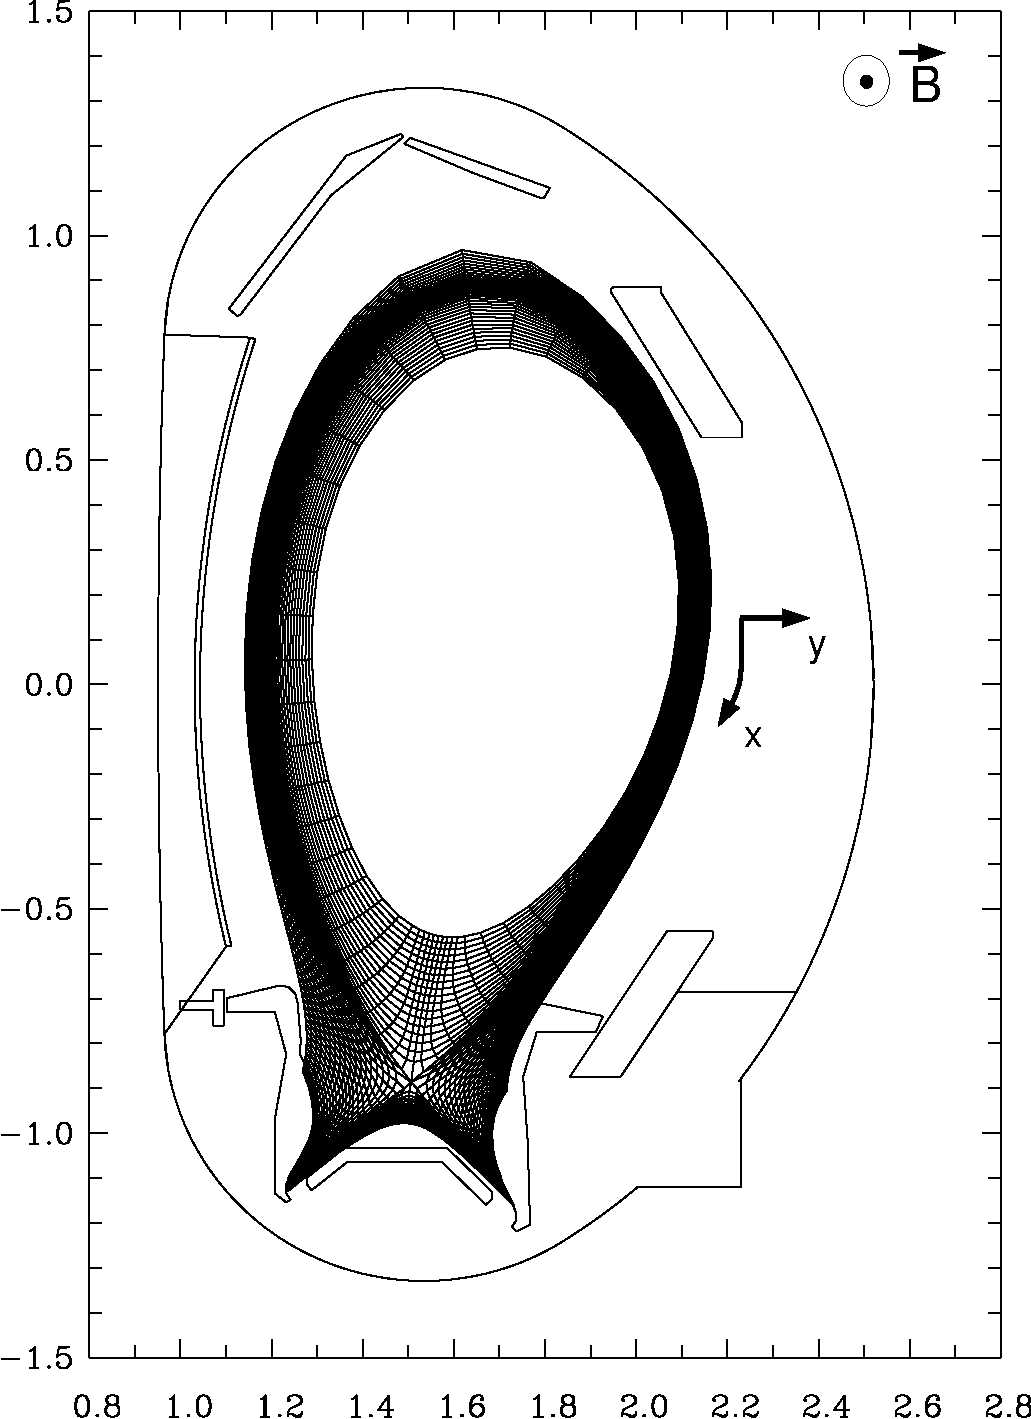
\includegraphics[width=8.0cm]{b2plot_1.pdf}
\else
\includegraphics[width=8.0cm]{b2plot.1.epsi}
\fi
}
\caption{Coordinate system: $x$ is the poloidal coordinate,
$y$ is the radial coordinate orthogonal to the flux surfaces. The
coordinate $\perp$ corresponds to the direction perpendicular
both to the magnetic field and to the $y$-axis. The directions
of magnetic field and plasma current correspond to normal
operation conditions of ASDEX--Upgrade (ion $\nabla B$ drift
directed towards the X-point).
 }
\label{fig:geo}
\end{figure}

The metric coefficients are
$h_x=1/\|\grad x\|$, $h_y=1/\|\grad y\|$ and $\sqrt{g}=h_xh_yh_z$.
One can replace $h_z$ by $2 \pi R$,
where $R$ is the local major radius.  Components of a vector are the
projections on unit basis vectors
; they are not the contravariant or
covariant components ($b_x = B_x/B$, $b_z = B_z/B$).
Ion velocities $V_{\perp}$ (velocity perpendicular both
to magnetic field $B$ and the $y$-axis) and $V_y$ are
determined from the two components of the momentum balance equation
for ions perpendicular to a magnetic field. Using the Braginskii expression
for the friction force, one obtains:\\
\begin{gather}
\label{eq:nf1}
V_{\perp} = V_{\perp}^{\left( a \right)} - \frac{1}{enB}
\frac{1}{h_y}\frac{\partial nT_i}{\partial y} + 
V_{\perp}^{\left( in \right)} + V_{\perp}^{\left( vis \right)} +
V_{\perp}^{\left( s \right)}
\end{gather}
\begin{gather}
\label{eq:nf2}
V_y = V_y^{\left( a \right)} + \frac{B_z}{enB^2}
\frac{1}{h_x}\frac{\partial nT_i}{\partial x} + 
V_y^{\left( in \right)} + V_y^{\left( vis \right)} +
V_y^{\left( s \right)}
\end{gather}
Velocities $V_{\perp,y}^{\left( a \right)}$ are the sum of the 
$\vec{E} \times \vec{B}$ drifts and diffusive and thermo-diffusive
velocities. 
This part corresponds to the ambipolar flux. It is the same both for ions and
electrons.
The second term in the r.h.s. of 
Eqs. (\ref{eq:nf1}) and (\ref{eq:nf2})
corresponds to diamagnetic flow of ions, while the other terms  are caused 
by inertial, viscous and ion-neutral friction forces. 
These non-ambipolar terms are 
connected with currents: $\vec{V}^{\left( in \right)} = \vec{j}^{\left( in \right)}/en,
\vec{V}^{\left( vis \right)} = \vec{j}^{\left( vis \right)}/en,
\vec{V}^{\left( s \right)} = \vec{j}^{\left( s \right)}/en$.\\ 
In the presence of anomalous transport 
($D$ is the classical diffusion coefficient, $D=\frac{T_e+T_i}{eb} 
\frac{\nu_{ei}}{\omega_{ce}}$, with electron cyclotron frequency
$\omega_{ce}$ and electron-ion collision frequency $\nu_{ei}$)
\begin{gather}
\label{eq:nf3}
V_{\perp}^{\left( a \right)} =
- \frac{1}{B}\frac{1}{h_y}\frac{\partial \Phi}{\partial y}
-\frac{D}{T_e+T_i} \frac{b_z}{h_x}\left(\frac{\partial p}{n \partial x}
-\frac{3}{2}\frac{\partial T_e}{\partial x}\right)
-D_{AN}^n\frac{1}{h_x n} \frac{\partial n}{\partial x}
-D_{AN}^p\frac{1}{h_x n} \frac{\partial p_i}{\partial x}
+V_{\perp}^{\left( AN \right)}
\end{gather}
\begin{gather}
\label{eq:nf44}
V_y^{\left( a \right)} =
\frac{B_z}{B^2}\frac{1}{h_x}\frac{\partial \Phi}{\partial x}
-\frac{D}{T_e+T_i} \frac{1}{h_y}\left(\frac{\partial p}{n \partial y}
-\frac{3}{2}\frac{\partial T_e}{\partial y}\right)
-D_{AN}^n\frac{1}{h_y n} \frac{\partial n}{\partial y}
-D_{AN}^p\frac{1}{h_y n} \frac{\partial p_i}{\partial y}
+V_y^{\left( AN \right)}
\end{gather}
The poloidal velocity is a sum $V_x = b_z V_{\perp} + b_x V_{\parallel}$.

In the particle balance 
the fact that the diamagnetic 
velocity is almost divergence free is taken into
account. Therefore, instead of the diamagnetic velocity
it is possible to introduce an effective 
velocity $\vec{\tilde{V}}^{\left( dia \right)}$, 
which gives the same contribution 
to the divergence of the particle flux:
\begin{gather}
\label{eq:nf4}
\frac{\partial n}{\partial t} +
     \frac{1}{\sqrt{g}} \frac{\partial }{\partial x}
      \left(\frac{\sqrt{g}}{h_x} n\left(b_x V_{\parallel} +
     b_z V_{\perp}^{\left( 0 \right)}\right)\right)+
     \frac{1}{\sqrt{g}} \frac{\partial }{\partial y}
      \left(\frac{\sqrt{g}}{h_y} n V_y^{\left( 0 \right)}\right)
= S^n
\end{gather}
\begin{gather}\label{eq:nf5}
V_{\perp}^{\left( 0 \right)} = V_{\perp}^{\left( a \right)} +
V_{\perp}^{\left( in \right)} + V_{\perp}^{\left( vis \right)} +
V_{\perp}^{\left( s \right)} + \tilde{V}_{\perp}^{\left( dia \right)}
\end{gather}
\begin{gather}\label{eq:nf6}
V_{y}^{\left( 0 \right)} = V_{y}^{\left( a \right)} +
V_{y}^{\left( in \right)} + V_{y}^{\left( vis \right)} +
V_{y}^{\left( s \right)} + \tilde{V}_{y}^{\left( dia \right)}
\end{gather}
\begin{gather}\label{eq:nf7}
\tilde{V}_{\perp}^{\left( dia \right)} = \frac{T_i B_z}{e}
\frac{\partial}{h_y \partial y}\left(\frac{1}{B^2}\right)
\end{gather}
\begin{gather}\label{eq:nf8}
\tilde{V}_y^{\left( dia \right)} = -\frac{T_i B_z}{e}
\frac{\partial}{h_x \partial x}\left(\frac{1}{B^2}\right)
\end{gather}
The velocity $\tilde{V}^{{\left(dia\right)}}$ is an effective velocity. It
represents vertical guiding centre drift of ions caused by 
$\nabla B$.\\

Combining the inertia and gyroviscosity terms in the Braginskii equations, 
one finds
\begin{multline}\label{eq:mom}
\hfill m_i \left[ \frac{\partial n V_{\parallel}}{\partial t} +
     \frac{1}{\sqrt{g}} \frac{\partial }{\partial x}
      \left( \frac{\sqrt{g}}{h_x} n 
       \left( V_{\perp}^{\left( 0 \right)} b_z
            + V_{\parallel} b_x \right) 
       V_{\parallel} \right) +
     \frac{1}{\sqrt{g}} \frac{\partial }{\partial y}
      \left( \frac{\sqrt{g}}{h_y} n V_y^{\left( 0 \right)} V_{\parallel} \right)
\right] = \hfill \\
\hfill -\frac{b_x}{h_x}\frac{\partial n T_i}{\partial x} -
b_x \frac{en}{h_x}\frac{\partial \Phi}{\partial x} + F_k +
\frac{4}{3} b_x B^{3/2} \frac{\partial }{h_x \partial x}
\left(\frac{\eta_0 b_x}{B^2} 
\frac{\partial\left(\sqrt{B}\left(V_{\parallel}+b_x \left(V^{(dia)}_{\perp} + V^{(E)}_{\perp}\right)\right)\right)}
{h_x \partial x}\right)
\hfill \\
\hfill + B^{3/2} b_x \frac{\partial}{h_x \partial x}
\left(\frac{b_x}{\nu_{ii} B^2} 
\frac{\partial\left(\sqrt{B}q_{i\parallel}^{\left( 0 \right)}
\right)}{h_x \partial x}\right)+
     \frac{1}{\sqrt{g}} \frac{\partial }{\partial y}
      \left(\frac{\sqrt{g}}{h_y^2} \eta_2 \frac{\partial V_{\parallel}}
{\partial y}\right) \hfill \\
\hfill
      + \frac{1}{\sqrt{g}} \frac{\partial }{\partial x}
      \left(\frac{\sqrt{g}}{h_x^2} \eta_2 \frac{\partial V_{\parallel}}
{\partial x}\right) 
+ S_{i \parallel}^m + R_{ie\parallel}. \hfill
\end{multline}
The diamagnetic terms in the l.h.s. of (\ref{eq:mom}) are almost cancelled 
\cite{ROGNLIEN98A, ROGNLIEN98B, ROGNLIEN99A, HINTON94C}, so that
velocities normal to the flux surface in the second and third term,
as in the particle balance equation, are determined by (\ref{eq:nf1}) and (\ref{eq:nf2}). 
In \cite{HINTON94C}
the divergent part of diamagnetic velocity has been 
neglected. Here, it is kept, because the corresponding flux is still
relatively large and can be comparable with the diffusive flux even
for anomalous diffusion coefficients. The authors of 
\cite{ROGNLIEN98A, ROGNLIEN98B, ROGNLIEN99A} also kept this
flux.
In contrast to 
\cite{ROGNLIEN98A, ROGNLIEN98B, ROGNLIEN99A}
there is an additional term of the same kind in the r.h.s. of 
Eq. (\ref{eq:mom}):
\begin{gather}
F_k = - m_i \left(\frac{1}{\sqrt{g}} \frac{\partial }{\partial x}
      \left(\frac{\sqrt{g}}{h_x} n V_{\parallel} 
      \tilde{V}_{\perp}^{\left( dia \right)} b_z \right) +
      \frac{1}{\sqrt{g}} \frac{\partial }{\partial y}
      \left(\frac{\sqrt{g}}{h_y} n V_{\parallel} 
      \tilde{V}_y^{\left( dia \right)} \right)\right)
\end{gather}
This parallel force is the Coriolis force, connected with the 
diamagnetic drift velocity and 
toroidal (parallel) rotation. This force can be obtained in a different
way by averaging the drift kinetic equation 
\cite{MIHAIL84A} and is of the same order
as the inertia terms.

Parallel viscosity is represented 
by the fourth and fifth terms in the r.h.s. 
The former is the Balescu
parallel viscosity with coefficient $\eta _0 = \dfrac{4}{3} 0.96 \sqrt{2} n T_i / \nu_{ii}$. 
The latter corresponds to the parallel viscosity driven 
by parallel ion heat flux 
$q_{i\parallel}^{\left( 0 \right)} = 
- \kappa _{i,\parallel} b_x \frac{1}{h_x} \frac{\partial T_i}{\partial x}$. 
This viscosity is absent in the Braginskii equations, however, in a tokamak,
where parallel particle flux multiplied by temperature is of
the order of the ion heat flux, these two 
viscosities are of the same order. On closed flux surfaces far from 
the separatrix, the flux-surface-averaged parallel 
viscosity coincides with the well-known 
neoclassical expression for the Pfirsch-Schl{\"u}ter regime
\cite{HIRSHMAN81A}. 
Thus, parallel viscosity in Eq. (\ref{eq:mom}) provides smooth transition to 
neoclassical theory. 
The classical perpendicular viscosity coefficient 
can 
be replaced by an anomalous value as in
\cite{ROGNLIEN98A, ROGNLIEN98B, ROGNLIEN99A}: $\eta _2 =
n m_i D_{AN}^n$. Perpendicular viscosity and inertia terms with the
anomalous particle flux are responsible for the transport of the
parallel momentum in radial and poloidal directions. The radial transport
can be rather important despite the fact that $\eta_2 \ll \eta _0$, since
the scale in the radial direction is rather small.

The term  $S_{i \parallel}^m$  represents the parallel momentum loss due to 
ion-neutral friction and parallel momentum input from neutral beam injection. 
$R_{ie\parallel}$ is the ion-electron friction.

The parallel momentum balance for electrons has the standard form:
\begin{gather}
j_{\parallel} = \sigma _{\parallel} \left(
\frac{b_x}{e} \frac{1}{h_x} \left( \frac{\partial n T_e}{n \partial x} +
0.71 \frac{\partial T_e}{\partial x} \right) 
- \frac{b_x}{h_x} \frac{\partial \Phi}{\partial x} \right).
\end{gather}

Expressions for $j_{\perp}$ and $j_y$ are obtained from radial and 
poloidal projections of the total momentum balance equation (the sum
of electron and ion momentum balance equations). 
The resulting current is a sum of contributions from pressure 
gradient (diamagnetic current) $\vec{j}^{\left( dia \right)}$, inertia
and gyroviscosity $\vec{j}^{\left( in \right)}$, viscosity
$\vec{j}^{\left( vis \right)}$ and ion-neutral friction
$\vec{j}^{\left( s \right)}$. 
Similar to the particle continuity equation, the effective 
current $\vec{\tilde{j}}$ is introduced, which gives the same contribution to 
$\nabla \vec{j}$, as the ordinary current. This gives the current continuity
equation
\begin{gather}\label{eq:curr0}
     \frac{1}{\sqrt{g}} \frac{\partial }{\partial x}
      \left(\frac{\sqrt{g}}{h_x} \tilde{j}_x\right)+
     \frac{1}{\sqrt{g}} \frac{\partial }{\partial y}
      \left(\frac{\sqrt{g}}{h_y} \tilde{j}_y\right)
= 0~.
\end{gather}
\begin{gather}\label{eq:curr1}
\tilde{j}_x = b_z \tilde{j}_{\perp} + b_x \tilde{j}_{\parallel}~.
\end{gather}
\begin{gather}\label{eq:curr2}
\vec{j} = \vec{\tilde{j}}^{\left( dia \right)} + \vec{j}^{\left( in \right)}
+ \vec{j}^{\left( vis \right)} + \vec{j}^{\left( s \right)}
+\vec{j}_{\parallel}~.
\end{gather}
The effective diamagnetic current can be chosen in a form
\begin{gather}\label{eq:curr3}
\tilde{j}_{\perp}^{\left( dia \right)} =
\frac{1}{b_z}\frac{n\left( T_e + T_i \right) B_z}{h_y}
\frac{\partial}{\partial y}\left(\frac{1}{B^2}\right)~,
\end{gather}
\begin{gather}\label{eq:curr4}
\tilde{j}_y^{\left( dia \right)} =
- \frac{n\left( T_e + T_i \right) B_z}{h_x}
\frac{\partial}{\partial x}\left(\frac{1}{B^2}\right)~.
\end{gather}
Current driven by parallel viscosity should be taken into account in 
Eqs. (\ref{eq:curr0}), (\ref{eq:curr1}) and (\ref{eq:curr2}). 
This current is a small correction to the diamagnetic current 
Eqs. (\ref{eq:curr3}) and (\ref{eq:curr4}).
However, on closed flux surfaces, where the pressure is almost constant, 
the diamagnetic current averaged
over the flux surfaces tends to zero. The resulting remaining part can 
become comparable to the parallel viscosity-driven current, which is
necessary to satisfy the condition that the averaged net radial current
should be zero. 
The terms, which contain the plasma viscosity, produce almost 
divergence-free currents. 
Similar to the case of diamagnetic currents, it can be reduced
to
\begin{gather}
\tilde{j}_{\perp}^{\left( vis \parallel \right)} =
- \frac{B_x \eta _0}{3 \sqrt{B}}
\frac{\partial\left(\sqrt{B}\left(V_{\parallel}+b_x \left(V^{(dia)}_{\perp} + V^{(E)}_{\perp}\right)\right)\right)}
{h_x \partial x}
\frac{\partial}{h_y \partial y}
\left(\frac{1}{B^2}\right)
\end{gather}
\begin{gather}
\tilde{j}_y^{\left( vis \parallel \right)} =
b_z\frac{B_x \eta _0}{3 \sqrt{B}}
\frac{\partial\left(\sqrt{B}\left(V_{\parallel}+b_x \left(V^{(dia)}_{\perp} + V^{(E)}_{\perp}\right)\right)\right)}
{h_x \partial x}
\frac{\partial}{h_x \partial x}
\left(\frac{1}{B^2}\right)
\end{gather}
The current produced by components of viscosity tensor connected 
with heat fluxes is:
\begin{gather}
\tilde{j}_{\perp}^{\left( vis q \right)} =
- \frac{0.24 B_x}{\sqrt{B} \nu_{ii}}\frac{\partial
\left(q_{i \parallel}^{\left( 0 \right)} \sqrt{B}\right)}{h_x \partial x}
\frac{\partial}{h_y \partial y}
\left(\frac{1}{B^2}\right)
\end{gather}
\begin{gather}
\tilde{j}_y^{\left( vis q \right)} =
b_z\frac{0.24 B_x}{\sqrt{B} \nu_{ii}}\frac{\partial
\left(q_{i \parallel}^{\left( 0 \right)} \sqrt{B}\right)}{h_x \partial x}
\frac{\partial}{h_x \partial x}
\left(\frac{1}{B^2}\right)
\end{gather}

The second part of the current contains contributions from both inertia
and gyroviscosity forces. In contrast to the parallel momentum balance,
the cancellation is not complete (as has been noticed in 
\cite{HINTON94C}). Expressions
for this part of the current are

\begin{multline}
\hfill j_{\perp}^{\left(in\right)}= - \frac{m_i}{B}
\left[\frac{\partial n V_{y}}{\partial t} +
     \frac{1}{\sqrt{g}} \frac{\partial }{\partial x}
      \left(\frac{\sqrt{g}}{h_x} n\left(V_{\perp}^{\left( 0 \right)} b_z
+ V_{\parallel} b_x \right) V_{y}\right)+
     \frac{1}{\sqrt{g}} \frac{\partial }{\partial y}
      \left(\frac{\sqrt{g}}{h_y} n V_y^{\left( 0 \right)} V_{y}\right)
\right] \hfill \\
\hfill -
\frac{2 b_x}{B} \frac{1}{h_x}\frac{\partial}{\partial x}
\left(\eta_3  
\frac{\partial V_{\parallel}}{h_x \partial x}\right)+
\frac{m_i}{B} n V_{\parallel}^2 \frac{\partial ln h_z}{h_y \partial y}
\hfill
\end{multline}

\begin{multline}
\hfill j_{y}^{\left(in\right)}= \frac{m_i}{B}
\left[\frac{\partial n V_{\perp}}{\partial t} +
     \frac{1}{\sqrt{g}} \frac{\partial }{\partial x}
      \left(\frac{\sqrt{g}}{h_x} n\left(V_{\perp}^{\left( 0 \right)} b_z
+ V_{\parallel} b_x \right) V_{\perp}\right)+
     \frac{1}{\sqrt{g}} \frac{\partial }{\partial y}
      \left(\frac{\sqrt{g}}{h_y} n V_y^{\left( 0 \right)} V_{\perp}\right)
\right] \hfill \\
\hfill -
\frac{2 b_x}{B} \frac{1}{h_x}\frac{\partial}{\partial x}
\left(\eta_3  
\frac{\partial V_{\parallel}}{h_y \partial y}\right) -
\frac{m_i}{B} n V_{\parallel}^2 \frac{\partial ln h_z}{h_x \partial x}
\hfill
\end{multline}

where $\eta_3 = \frac{n T_i}{2 \omega_{ci}}, \eta _1 = \frac{\eta _2}{4}$.

The last terms proportional to the gradient of $B$ correspond to the vertical
guiding centre drift of ions caused by the centrifugal force. This current
can be simply added to the diamagnetic current. Other terms seem to be less
important.

The contribution from perpendicular viscosity is
\begin{multline}
\hfill j_{\perp}^{\left(vis \perp \right)}= \frac{1}{B}
\left[\frac{1}{h_x}\frac{\partial}{\partial x}\left(\eta_1 
     \frac{\partial V_y}{h_x \partial x}\right)+
 \frac{1}{h_y}\frac{\partial}{\partial y}\left(\eta_1 
     \frac{\partial V_y}{h_y \partial y}\right)+
\frac{1}{h_x h_y }\frac{\partial \eta_1}{\partial x}
     \frac{\partial V_{\perp}}{\partial y}-
\frac{1}{h_x h_y }\frac{\partial \eta_1}{\partial y}
     \frac{\partial V_{\perp}}{\partial x}\right] \hfill \\
\hfill +
\frac{4 b_x}{B} \frac{1}{h_x h_y}
\left(\frac{\partial \eta_1}{\partial x} \frac{\partial V_{\parallel}}
{\partial y} - \frac{\partial \eta_1}{\partial y}\frac{\partial V_{\parallel}}
{\partial x}
\right)
\hfill
\end{multline}
\begin{gather}
j_{y}^{\left(vis \perp \right)}= -\frac{1}{B}
\left[\frac{1}{h_y}\frac{\partial}{\partial y}\left(\eta_1 
     \frac{\partial V_{\perp}}{h_y \partial y}\right)+
 \frac{1}{h_x}\frac{\partial}{\partial x}\left(\eta_1 
     \frac{\partial V_{\perp}}{h_x \partial x}\right)-
\frac{1}{h_x h_y }\frac{\partial \eta_1}{\partial x}
     \frac{\partial V_y}{\partial y}+
\frac{1}{h_x h_y }\frac{\partial \eta_1}{\partial y}
     \frac{\partial V_y}{\partial x}\right].
\end{gather}

Here, the largest term is the first one in the r.h.s. of the expression
for the radial current, since the radial derivatives are the largest.
This current corresponds to a pure cylindrical approximation. It is
responsible, for example, for closing currents near flush-mounted probes
\cite{ROZ99A}.
It was taken into account in 
\cite{ROGNLIEN99A, RADFORD96A}. However, in the problem of global current
structure in the edge plasma, the currents driven by parallel viscosity seem
to be more important.

The total current caused by viscosity is
\begin{gather}
\vec{j}^{\left(vis\right)} = \vec{j}^{\left(vis \parallel\right)} +
\vec{j}^{\left(vis \perp\right)} +
\vec{j}^{\left(vis q\right)}
~.
\end{gather}

The contribution from ion neutral friction is
\begin{gather}
j_{\perp}^{\left(s\right)} = \frac{S_{iy}^m}{B}
~.
\end{gather}
\begin{gather}
j_{y}^{\left(s\right)} = -\frac{S_{i \perp}^m}{B}
~,
\end{gather}
where $S_{iy}^m$ and $S_{i \perp}^m$ are the momentum sinks due to
ion-neutral friction. 
\begin{gather}
S_{i \perp}^m = - n \mu_{iN} \nu_{iN} \left( V_{\perp} - V_{\perp N}\right)
~,
\end{gather}
\begin{gather}
S_{i y}^m = - n \mu_{iN} \nu_{iN} \left( V_{y} - V_{y N}\right)
~,
\end{gather}
where $\mu_{iN}=m_i/2$ is the effective mass, $\nu_{iN}= n_N <V_{iN} 
\sigma_{cx}>$ is the ion-neutral collision frequency,
$n_N$ is the neutral density and $\vec{V_{iN}}$ is the neutral mean
velocity. For the ion velocity used above,
only electric and diamagnetic drifts are left, neglecting smaller terms,
to obtain
\begin{gather}
\tilde j_{x}^{\left(s\right)} = \tilde j_{\perp}^ {\left(s\right)} b_z =
- \sigma _{iN} b_z^2 \frac{\partial \Phi}{h_x \partial x}-
\sigma _{iN} b_z^2 \frac{1}{e n}\frac{\partial n T_i}{h_x \partial x}+
\sigma _{iN} B_z V_{yN}
~,
\end{gather}
\begin{gather}
\tilde j_{y}^{\left(s\right)} =
- \sigma _{iN} \frac{\partial \Phi}{h_y \partial y}-
\sigma _{iN} \frac{1}{e n}\frac{\partial n T_i}{h_y \partial y}-
\sigma _{iN} B V_{\perp N}
~,
\end{gather}
where $\sigma _{iN}$ is the ion-neutral perpendicular conductivity
\begin{gather}
\sigma _{iN} =
\frac{n m_i <V_{iN} \sigma_{cx}> n_N}{2 B^2}
~.
\end{gather}

The rate of charge-exchange $<V_{iN} \sigma_{cx}>$ can
be expressed through the mobility $K_0$ measured in the absence of a 
magnetic field for room temperature and atmospheric pressure for
deuterium \cite{MCDANIEL73A}:
\begin{gather}
K_0 =
\frac{2 e}{m_i <V_{iN} \sigma_{cx}> n_N^{\left(0\right)}}
~,
\end{gather}
with $n_N^{\left(0\right)} = 2.687 \cdot 10^{25} m^{-3}$ and
$K_0 = 11.2 \cdot 10^{-4} \frac{m^2}{s V}$.
Assuming that the charge-exchange cross-section is approximately constant
one gets
\begin{gather}
<V_{iN} \sigma_{cx}> = 3.2 \cdot 10^{-15} \sqrt{\frac{T_i}{0.026}} 
\frac{m^3}{s}
~,
\end{gather}
where $T_i$ is measured in $eV$. A similar expression, which gives approximately
the same result, is \cite{ROZ88A}:
\begin{gather}
<V_{iN} \sigma_{cx}> = \frac{32 \sigma _{cx}}{3 \sqrt{\pi}}
\sqrt{\frac{T_i}{m_i}}
\frac{m^3}{s}
~.
\end{gather}.


In the energy balance equations 
appears
a special problem, which is the 
possible inclusion of an anomalous radial current.
The basic guidelines are as follows:
\begin{itemize}
\item The expression must be as simple as possible, and the most convenient
format is an Ohm-like expression;
\item The system of equations must be informed about this non-classical
contribution, but
\item The classical core of the equations must not be disturbed.
\end{itemize}
Apparently, the radial current would enter the electron energy equation
via the Joule term, but this manipulation is inappropriate since one cannot 
be sure that this term directly heats the electrons, which is the case in
a purely classical setup. The proper thing to do is to keep only 
the non-radial classical contribution in the Joule term, and 
construct additional heat exchange terms
containing the radial current.
In this way, the system decides how to thermodynamically allocate the
``alien'' heat term, among electrons and ion species.\\
For this reason, one cannot simply use the standard Ohm's
law in the radial direction with anomalous coefficients, or any other
prescribed expression whatsoever, as a constructive procedure is necessary
for simultaneously producing the radial current as well as the heat exchange
terms. At this point it has to be mentioned that this peculiarity arises
only in the multifluid case, whereas in the single species case 
these heat exchange terms can indeed be constructed even using a prescribed
expression for the radial current. \\
The trick for carrying out this program is to correct the electron friction
density $\vec{R}^e$ by adding the term $n_e e \tilde{\eta}_\perp \vec{J}_\perp$
similar to the classical one, only using the {\itshape ad hoc} parameter
$\tilde{\eta}_\perp$. \\
Since $\vec{R}^e=-{\sum_{a}\vec{R}^a}$, one has a
modified total ion momentum equation at hand which in conjuction with the
pressure equilibrium (not affected by the additional term)
$\vec{J} \times \vec{B} =  \nabla P$, gives the diffusive part of the
radial current, namely
\begin{gather}
J_y^{diff}=\frac{\tilde{\eta}_\perp en_e}{B^2} \frac{\partial P_i}{\partial y}
\end{gather}
where $P_i$ is the total ion pressure. This dependency is also found in
\cite{ROGNLIEN98A}. Moreover, an additional dependence on the radial
electric field can potentially be added without interfering with
the procedure. \\
The final step, namely the construction of the heat exchange terms, is
performed by claiming that the well known relation \cite{BAELMANS94A}
(adapted for the multifluid case)
\begin{gather}
Q_e=-\sum_{a} \left (Q_a + (\vec{u}^a - \vec{u}^e) \cdot \vec{R}^a \right )~,
\end{gather}
which stems from the fundamental null space of the collision operator,
is still true while carrying the modified friction.
Claiming this, after
performing the proper manipulations in the energy
equations, one reveals the {\itshape ad hoc} 
contribution as the exchange term that one wants,
which reads
$
\sum_{a} (\vec{u}^a -\vec{u}^e)_\perp n_a \frac{Z_a^2}{Z_{eff}}e \tilde{\eta}_\perp \vec{J}_\perp
$
added in the total ion energy equation and subtracted from the
electron equation.
Note that in the single species case, this term boils down to
$
\tilde{\eta}_\perp J_\perp ^2
$
removing energy from the electrons,  depositing it to the ions, a feature
predicted by neoclassical theory \cite{ROSENBLUTH72A}.\\

In the final form of the energy balance equations, the convective heat 
flux and the diamagnetic heat flux are combined as in 
\cite{ROGNLIEN98A, ROGNLIEN98B, ROGNLIEN99A, HINTON94C}, see also
\cite{ROZ99A}.

The energy balance equation for the electrons is
\begin{multline}
\hfill
     \frac{3}{2} \frac{\partial nT_e}{\partial t} +
     \frac{1}{\sqrt{g}} \frac{\partial }{\partial x}
      \left(\frac{\sqrt{g}}{h_x} \tilde{q}_{ex}\right) +
     \frac{1}{\sqrt{g}} \frac{\partial }{\partial y}
      \left(\frac{\sqrt{g}}{h_y} \tilde{q}_{ey}\right) +
     \frac{nT_e}{\sqrt{g}}\frac{\partial }{\partial x}
      \left(\frac{\sqrt{g}}{h_x}\left(
      V_{\parallel} - j_{\parallel}/en\right)b_x\right) \hfill \\
\hfill     =
     Q_e + n T_e B \frac{1}{h_x h_y}\left(\frac{\partial \Phi}{\partial y}
     \frac{\partial}{\partial x}\left(\frac{1}{B^2}\right)
     -\frac{\partial \Phi}{\partial x}\frac{\partial}{\partial y}
     \left(\frac{1}{B^2}\right)\right)~,\hfill
\end{multline}
where
\begin{multline}
\hfill        \tilde{q}_{ex} = \frac{3}{2} n T_e \left(- \frac{b_z}{B h_y}
         \frac{\partial \Phi}{\partial y}
         + b_x V_{\parallel} - b_x j_{\parallel} / en + b_z V_{\perp}^{(AN)} \right) \hfill \\
     \hfill + \frac{5}{2} n T_e b_z \left(
     - \frac{D}{T_e+T_i} \frac{b_z}{h_x} \left(\frac{\partial p}{n \partial x}
     - \frac{3}{2} \frac{\partial T_e}{\partial x} \right)
     - D_{AN}^n \frac{1}{h_x n} \frac{\partial n}{\partial x}
     - D_{AN}^p \frac{1}{h_x n} \frac{\partial p_i}{\partial x} \right)
     + n V_{e\perp}^{(AN)}
      \hfill \\
      \hfill   - 0.71 b_x j_{\parallel} T_e/e - \kappa _{e \parallel}
         \frac{b_x^2}{h_x} \frac{\partial T_e}{\partial x}
         - \kappa _{e \perp} b_z^2 \frac{1}{h_x} 
         \frac{\partial T_e}{\partial x} \hfill \\
      \hfill   + \frac{3}{2}\frac{T_e}{e B} \frac{\nu_{ei}}{\omega _{ce}}
         \frac{b_z^2}{h_x} \frac{\partial n\left(T_e+T_i\right)}{\partial x}
         - \frac{5}{2} n T_e^2 \frac{B_z}{e}
         \frac{\partial}{h_y \partial y}\left(\frac{1}{B^2}\right) ~ , \hfill
\end{multline}
\begin{multline}
\hfill  \tilde{q}_{ey} = \frac{3}{2} n T_e \left( \frac{B_z}{B^2} \frac{1}{h_x}
        \frac{\partial \Phi}{\partial x} + V_{y}^{(AN)} \right) \hfill \\
     \hfill  + \frac{5}{2} n T_e \left(
     - \frac{D}{T_e+T_i} \frac{1}{h_y} \left( \frac{\partial p}{n \partial y}
     - \frac{3}{2} \frac{\partial T_e}{\partial y} \right)
     - D_{AN}^n \frac{1}{h_y n} \frac{\partial n}{\partial y}
     - D_{AN}^p \frac{1}{h_y n} \frac{\partial p_i}{\partial y} \right)
     + n V_{ey}^{(AN)}
         \hfill \\
         \hfill - \kappa _{e \perp} \frac{1}{h_y} \frac{\partial T_e}{\partial y}
         + \frac{3}{2}\frac{T_e}{e B} \frac{\nu _{ei}}{\omega_{ce}}
         \frac{1}{h_y} \frac{\partial n\left(T_e+T_i\right)}{\partial y}
         + \frac{5}{2} n T_e^2 \frac{B_z}{e}
         \frac{\partial}{h_x \partial x}\left(\frac{1}{B^2} \right) ~ , \hfill
\end{multline}
\begin{gather}
        Q_{\Delta} = \frac{3 m_e}{m_i} n \nu _{ei} \left(
T_e - T_i
\right)~,
\end{gather}
\begin{gather}
        Q_u = R _{ie \parallel} j_{\parallel}/en~,
\end{gather}
\begin{gather}
        Q_{AN} = \sum_{a} \left(\vec{u}^a -\vec{u}^e\right)_\perp n_a 
                 \frac{Z_a^2}{Z_{eff}}e \tilde{\eta}_\perp \vec{J}_\perp~,
\end{gather}
\begin{gather}
        Q_e = -Q_{\Delta} - Q_u - Q_{AN}~.
\end{gather}


Here $\kappa _{e \parallel}$ is the Balescu (not Braginskii as stated in the CPP review paper \cite{SOLPS_review} 
or in \$\verb!SOLPSTOP/doc/CPP_2006.pdf!) heat 
conductivity with a possible heat
flux limit \cite{BRAAMS96B}. 
The leading numerical coefficient is then $\frac{5}{2} \frac{2.16 z}{1 + 0.27 z}$ as opposed to 3.16 for the Braginskii
formula \cite{NRL}. The perpendicular heat conductivity 
$\kappa _{e \perp}$ can be 
either classical or anomalous. In the last term of the energy balance
equation, it is taken into account that the $\vec{E} \times \vec{B}$
drift velocity is
almost divergence-free.

The ion energy balance equation is
\begin{multline}\label{eq:ion_energy} \hfill
     \frac{3}{2} \frac{\partial nT_i}{\partial t} +
     \frac{1}{\sqrt{g}} \frac{\partial }{\partial x}
      \left(\frac{\sqrt{g}}{h_x} \tilde{q}_{ix}\right) +
     \frac{1}{\sqrt{g}} \frac{\partial }{\partial y}
      \left(\frac{\sqrt{g}}{h_y} \tilde{q}_{iy}\right) +
     \frac{nT_i}{\sqrt{g}}\frac{\partial }{\partial x}
      \left(\frac{\sqrt{g}}{h_x} V_{\parallel} b_x \right) \hfill \\
     \hfill =
     Q_{\Delta} + Q_{AN} + \frac{\eta _0}{3} \left(2 b_x 
     \frac{\partial V_{\parallel}}{h_x \partial x}\right)^2+ 
     n T_i B 
     \frac{1}{h_x h_y}\left(\frac{\partial \Phi}{\partial y}
     \frac{\partial}{\partial x}\left(\frac{1}{B^2}\right)
     -\frac{\partial \Phi}{\partial x}\frac{\partial}{\partial y}
     \left(\frac{1}{B^2}\right)\right)~,\hfill
\end{multline}
where
\begin{multline} \hfill
        \tilde{q}_{ix} = \frac{3}{2} n T_i \left(- \frac{b_z}{B h_y}
        \frac{\partial \Phi}{\partial y}
         + b_x V_{\parallel} + b_z V_{\perp}^{(AN)} \right) \hfill \\
\hfill + \frac{5}{2} n T_i b_z\left(
     - \frac{D}{T_e+T_i} \frac{b_z}{h_x}\left(\frac{\partial p}{n \partial x}
     - \frac{3}{2} \frac{\partial T_e}{\partial x} \right)
     - D_{AN}^n \frac{1}{h_x n} \frac{\partial n}{\partial x}
     - D_{AN}^p \frac{1}{h_x n} \frac{\partial p_i}{\partial x}\right)
     + n V_{i\perp}^{(AN)}
         \hfill \\ \hfill
         + \frac{5}{2} n T_i b_z \tilde{V} _{\perp}^{\left(dia\right)}
         - \kappa _{i \parallel}
         \frac{b_x^2}{h_x} \frac{\partial T_i}{\partial x}
         - \kappa _{i \perp} b_z^2 \frac{1}{h_x} 
         \frac{\partial T_i}{\partial x} ~, \hfill
\end{multline}
\begin{multline} \hfill
        \tilde{q}_{iy} = \frac{3}{2} n T_i \left( \frac{B_z}{B^2} 
         \frac{1}{h_x} \frac{\partial \Phi}{\partial x} + V_{y}^{(AN)} \right) 
        \hfill \\ \hfill
     + \frac{5}{2} n T_i \left(
     - \frac{D}{T_e+T_i} \frac{1}{h_y} \left( \frac{\partial p}{n \partial y}
     - \frac{3}{2} \frac{\partial T_e}{\partial y}\right)
     - D_{AN}^n \frac{1}{h_y n} \frac{\partial n}{\partial y}
     - D_{AN}^p \frac{1}{h_y n} \frac{\partial p_i}{\partial y} \right)
     + n V_{iy}^{(AN)} \hfill \\ \hfill
         - \kappa _{e \perp} \frac{1}{h_y} 
         \frac{\partial T_i}{\partial y}
         + \frac{5}{2} n T_i \tilde{V} _{y}^{\left(dia\right)} ~. \hfill 
\end{multline}

As for the electrons, the parallel heat conductivity is classical with
a possible heat flux limit, while the perpendicular contribution
can be either 
classical or anomalous.

There is discussion in the literature on how to take into account anomalous
terms in the energy balance equations. One point of view (see e.g. 
\cite{ZAGORSKI98A})
is to cancel the contribution from anomalous particle fluxes in the
terms $p_i \nabla \cdot \vec{V}_i$ (or $\vec{V}_i \cdot \nabla p_i$ if equations
are written in a different form). In contrast, according to the
derivation 
\cite{HINTON94C},
where a kinetic equation with fluctuating term has been integrated, the
anomalous fluxes should be kept in all terms of the energy balance
equations. This variant was used in \verb!UEDGE! \cite{ROGNLIEN98A, ROGNLIEN98B, ROGNLIEN99A}. 
In \verb!B2.5! only the contribution
from anomalous radial particle flux to the convective heat flux are left
in the expressions for $\tilde{q}_{e,i}$. In the term  
$p_i \nabla \cdot \vec{V}_i$ the anomalous particle flux is absent. 

\section{Boundary conditions with drifts and currents}
\index{drifts and currents, boundary conditions}
\index{boundary conditions, drifts and currents}

Whether one deals with the diamagnetic or $\bf{E}\times\bf{B}$ perpendicular
drift velocity, special care must be taken to avoid unphysical flows
at the plates. The standard boundary condition is to require that the flow be
at least sonic at the sheath entrance \cite{STANGEBY95B}, 
which translates into:

\begin{equation}\label{eq:Chodura}
V_{\parallel} \ge C_s - \frac{b_z}{b_x} V_{\perp} ~,
\end{equation}

where $C_s$ is the local sound speed and $\frac{b_z}{b_x}$ is the inverse
of the field line pitch. However, for very small pitch angles, as in
stellarators, the $V_{\perp}$ term may overpower the sound 
velocity \cite{FENG99A}
and then the boundary condition would require a plasma flow exiting the plate.
Therefore, the pitch angle at the plates is limited to be no less than
1 degree (user parameter, see switch ``b2agfs\_min\_pitch'' in Appendix \ref{lis:b2cdci}), 
motivated by the engineering limits met when attempting to align the
divertor tiles with the magnetic field. The solution procedure of the code
was also modified so as ensure that no unphysical flows were being created,
and solves the parallel momentum equation using the updated electric potential.

Boundary conditions for the current continuity equation at the plates
correspond to sheath current-voltage characteristics
\begin{equation}\label{eq:sheath-voltage}
j_x = en\left(b_x c_s - b_x \frac{1}{\sqrt{2 \pi}} \sqrt{\frac{T_e}{m_e}} 
      exp\left(- \frac{e \Phi}{T_e}\right) \left(1 - \gamma\right)\right),
\end{equation}
where $\gamma$ is the secondary electron emission coefficient. At the inner
(core) flux surface the currents are set either to the divergent part
of the diamagnetic current or to zero. Both variants give the same result
and both guarantee that the net current integrated over the inner flux surface
should be zero. At the walls, the same conditions on the normal current
components were imposed as for the inner core.

The electron and ion heat fluxes to the target plates are
\begin{equation}\label{eq:target_qe}
\tilde q_{ex} = b_x \frac{n}{\sqrt{2 \pi}} \sqrt{\frac{T_e}{m_e}} 
      exp\left(- \frac{e \Phi}{T_e}\right) \left(1 - \gamma\right)
     \left(T_e \frac{1+\gamma}{1-\gamma} + e \Phi\right),
\end{equation}
\begin{equation}\label{eq:target_qi}
\tilde q_{ex} = \frac{3}{2}n T_i c_s b_x.
\end{equation}

The question of kinetic
boundary conditions including drifts is not yet finally clarified
and will need further work from both kinetic and fluid modelling
\cite{CHANKIN94AB,STANGEBY95B}.

\section{Problems for a fluid description of the edge plasma}  
\index{flux limits}

To apply a fluid model for the description of the edge,
a specific ordering of lengths is necessary.

The necessary condition for a fluid model is
that all characteristic lengths (characteristic length
of the sheath, which is a microscopic length scale of about 10 Debye lengths;
electron and ion mean free path ranging from sub-cm to meters; neutral mean
free path, which is centimeters to meters; heat conduction length which is typically
five times the mean free path length due to the dominant contribution from tail
electrons or ions)
are smaller than the parallel connection length (order of several tens of meters). This
is usually fulfilled in edge plasmas with the following possible exceptions:
\begin{enumerate}
  \item at low temperatures, e.g.
           near the target in the divertor, 
           steeper gradients result in non--local heat flux contributions. In general,
           a non-local description might be necessary 
            (weighted mean of temperature profile over
           five mean free lengths of electrons or ions). However, a simpler correction
           is sometimes satisfactory and is used in the code (see below).
  \item at high temperatures
        (midplane, near separatrix).
        Corrections for flux limit and for periodic systems on closed 
        field lines are necessary due to the fact that the heat conduction
        mean free path is larger than the connection length.
  \item the sheath cannot be resolved by a fluid model and is represented
        by boundary conditions at the sheath entrance deduced from kinetic
        models.
\end{enumerate}

Simple heat flux and momentum flux (viscosity)
limits are available. 
The heat flux limit is formulated as
\begin{gather}
  \kappa _{\parallel}=\frac{\kappa _{SH}}{1+|q_{SH}/q_{fl}|},
\end{gather}

with the classical Spitzer--H\"arm heat flux
\begin{gather}
 q_{SH}=-\kappa _{\parallel ,SH} \cdot \frac{\partial T_e}{\partial x}
\end{gather}

and the flux limit
\begin{gather}
 q_{fl}=\alpha n_e T_e^{3/2} \sqrt{m_e }
\end{gather}

($\alpha \approx 0.2$ from comparison with kinetic calculations for electrons;
the situation for ions is less clear).

The momentum flux limit is done the same way
\begin{gather}
  \eta _{\parallel} =\frac{\eta _{cl,a}}
   {1+|q_{cl,a}/q_{fl,a}|},
\end{gather}

with the classical momentum flux
\begin{gather}
  q_{cl,a}=-\eta _{\parallel,a} \cdot
  \frac{\partial u_{\parallel,a}}{\partial x}
\end{gather}
and the flux limit
\begin{gather}
 q_{fl,a}=\alpha p_{a}
\end{gather}
(with $\alpha = 0.5$). Unfortunately, for this correction even less kinetic 
work
exists than for the heat flux limits. 

Additionally, 
long mean free path corrections of classical heat conduction and viscosity
(in the core) are applied.
For periodic systems and small perturbations one gets
\cite{NEUHAUSER86A}:
\begin{gather}
   q_{\parallel , eff}
    = q_{SH}/\left(h_{\parallel}^2 \lambda_{HC}^2 +1\right),
\end{gather}

with wavenumber of periodicity
\begin{gather}
  h_{\parallel}=2 \pi / \lambda_{\parallel},
\end{gather}
\begin{gather}
  \lambda_{\parallel}=2 \pi R q
\end{gather}

and mean free path of tail electrons
\cite{CHODURA84A}
\begin{gather}
  \lambda_{HC} (\mbox{m}) = 7.5\cdot 10^{16} \cdot T_e^2(\mbox{eV})/n_e(
  \mbox{m}^{-3}).
\end{gather}

Fokker--Planck computer simulations of electron heat transport in laser 
plasmas 
\cite{LLE91}
show that a better description is obtained for a linear
correction:
\begin{gather}
  q_{\parallel , eff}
    = q_{SH}/(h_{\parallel} \lambda_{HC} +1).
\end{gather}

Applying these limits for the core, convergence behaviour of the code
improves significantly.\\
A more correct kinetic limit would imply a
non--local heat transport (and viscosity,...) description.
The parallel heat--flux at a point should be determined by
classical fluxes at points
up to typically five mean--free paths away. As an additional feature, one 
would get
pre--heating effects by fast electrons, maybe important for the ELMs.
Work is necessary to generalize this to the SOL
\cite{KRASH92A,YURI91A}
and this has to be cross--checked
with kinetic calculations \cite{Abou-Assaleh92}. Also, numerical problems due
to this non--local description have to be solved \cite{PRASAD91A}.

In general, if these kinetic corrections become important, quantative 
conclusions are
questionable, because the fluid model is no longer strictly valid. 
Considerations of 
particle, energy and momentum conservation still guarantee a qualitatively 
correct
description. The flux-limiters are designed are defined to give the correct 
answer
in the fully collisional and in the fully collisionless regime.

Parametric studies varying the various flux limiters should be done, 
particularly
for predictive work. Specific experimental scenarios would be required to 
calibrate
the flux limiters. However, complete experimental data sets including 
electron and
ion temperatures and densities at the target plate and upstream are necessary.
Fortunately, at higher densities these corrections are not important. 
Furthermore,
one should note, that mapping of target data to the midplane and the 
extraction of
anomalous radial transport coefficients from such a procedure is 
questionable in the
regime where flux limiters are important
\cite{CosterHinM2003}.

As an example,  
SOLPS5.0 calculations for JET using deuterium, carbon and helium are shown in 
Figs.~\ref{cflmi_1e19} and \ref{cflmi_2e19}.
The predicted electron temperatures at the outer target are shown for 
two different upstream densities.
In each graph, the ion energy flux limit is varied and the sensitivity of the 
target profiles to this variation is obvious. 

\begin{figure}[bt]
\ifpdf 
    \centerline{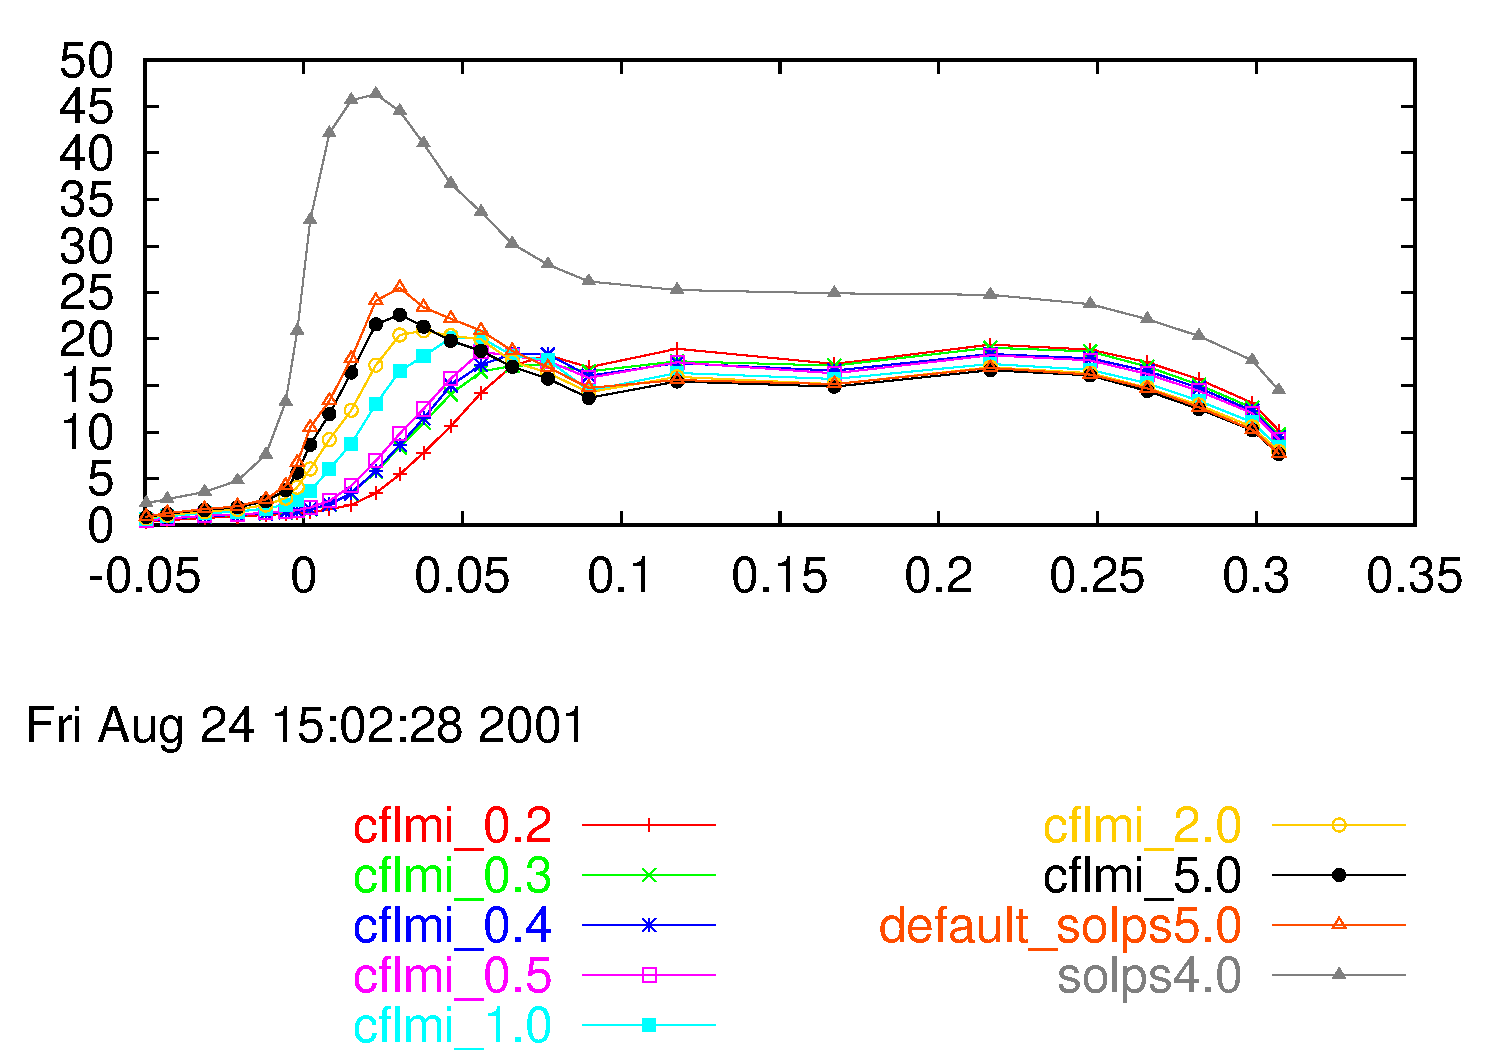
\includegraphics[width=11cm]{cflmi_1e19.pdf}} 
\else
    \centerline{\includegraphics[angle=-90,width=11cm]{cflmi_1e19.ps}} 
\fi
\caption{Impact of ion flux limits for a $10^{19}~~m^{-3}$ upstream density case.}
\label{cflmi_1e19}
\vspace*{1cm}
\end{figure}

\begin{figure}[bt]
\ifpdf 
    \centerline{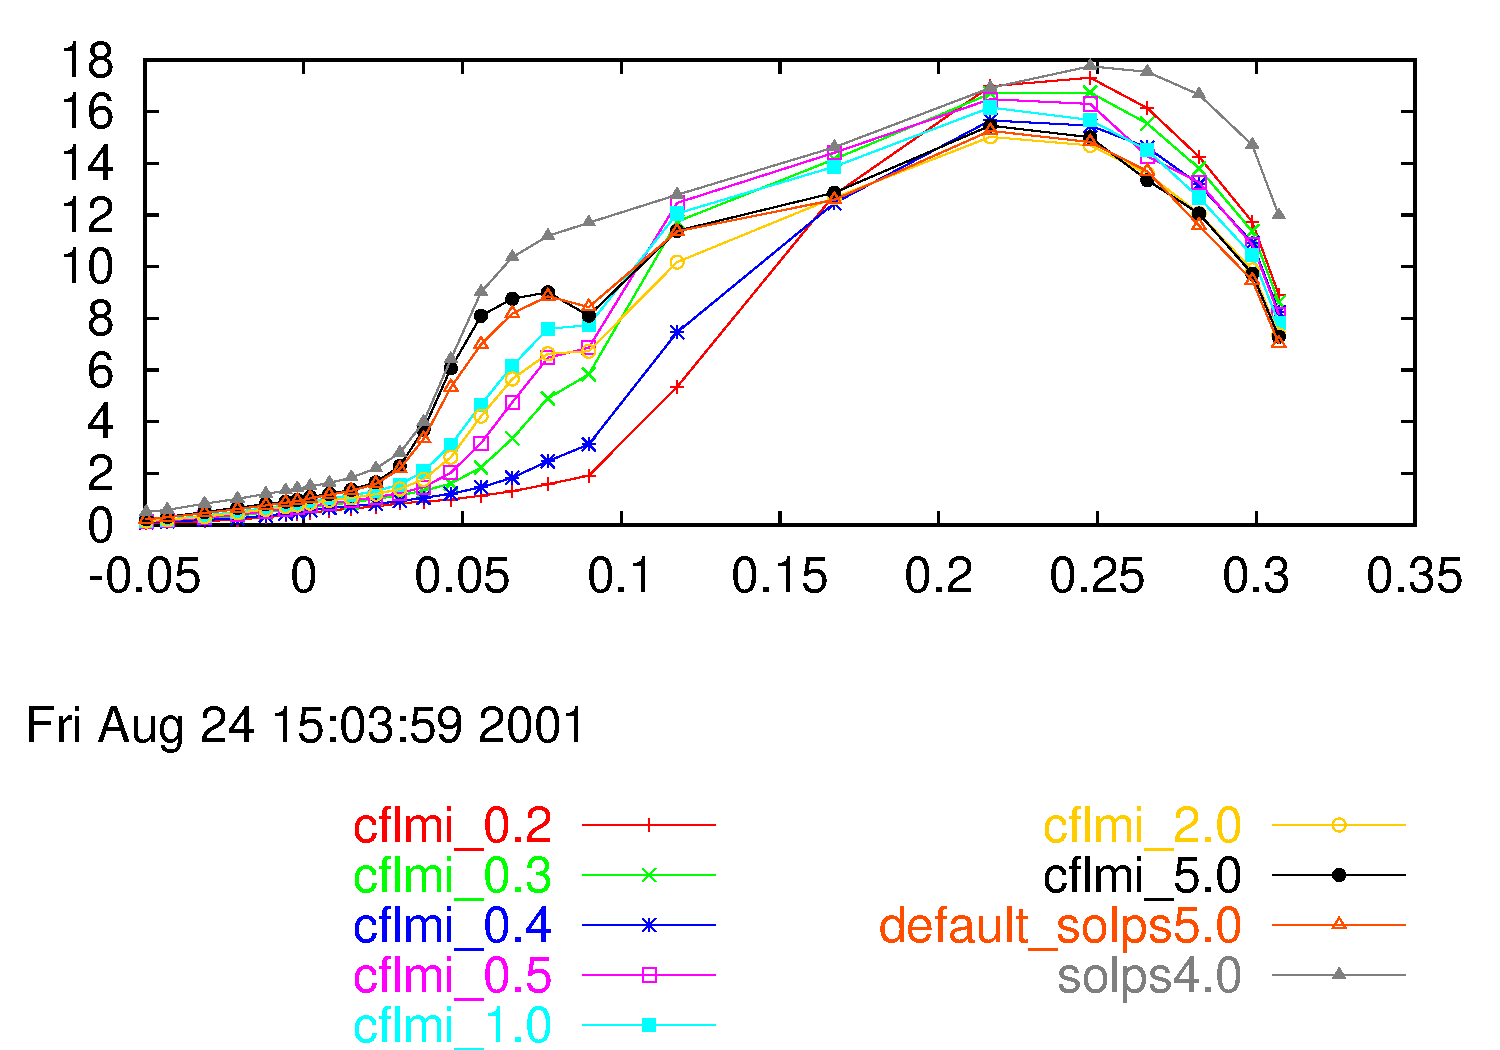
\includegraphics[width=11cm]{cflmi_2e19.pdf}} 
\else
    \centerline{\includegraphics[angle=-90,width=11cm]{cflmi_2e19.ps}} 
\fi
\caption{Impact of ion flux limits for a $2 \times 10^{19}~~m^{-3}$ upstream density case.}
\label{cflmi_2e19}
\end{figure}

\section{Neutral fluid model}
\index{neutrals, fluid model}

As an alternative to the complete kinetic Monte-Carlo description offered by \verb!Eirene!,
a simpler and faster neutral fluid model is also available as \verb!B2.5! stand-alone. The surface sources of neutrals are
then given by user-defined recycling models, possibly enhanced with local sputtering models 
when impurities are considered (see e.g.~\cite{Warrier04}). The volume sources of neutrals are given by 
plasma recombination rates computed by the \verb!B2.5! atomic physics packages. The neutral species is then
treated just as the other plasma species, with its own particle and momentum transport equations in the parallel
direction, equivalent to Eqs.~(\ref{eq:nf4}) and (\ref{eq:mom}). The neutrals are assumed to have the same common
temperature as all other ion species and the neutral energy balance equation becomes simply a component
of Eq.~(\ref{eq:ion_energy}). Of course, terms due to charged particle motions or currents do not appear 
for neutral species.

The neutral species transport coefficients are usually given by the following equations:
\begin{gather}\index{neutrals, transport coefficients}
 D^{n}_{AN,0} = 0,
\end{gather}
\begin{gather}
 D^{p}_{AN,0} = C + \sqrt{\frac{T_i}{m_N}} ( \sigma_{CX} n_i + \sigma_{in} n_e ),
\end{gather}
where $m_N$ is the mass of the neutral species, and $C$, $\sigma_{CX}$ and $\sigma_{in}$ are three constants given by
the user, representing hydrogen gas diffusion, and the charge-exchange and ionization cross-sections, respectively.
As an option, one may choose to use cross-sections from atomic databases instead of constants, with their appropriate
parameter dependencies. The diffusion coefficients can also be bounded to avoid unphysically large or small values.

Additionally, the heat and particle fluxes carried by neutrals can be flux-limited, following the formalism
laid out in~\cite{UMANSKY03A}\index{neutrals, flux limits}. On the one hand, we flux-limit the neutral contribution 
to the ion heat diffusivity, involved
in the conductive heat flux computation. On the other hand, we also flux-limit the convective 
particle and energy fluxes of neutrals. Because these limits apply for neutral species, both the parallel
and perpendicular directions are to be considered.
The basic formula used is:
\begin{gather}
X \Rightarrow  \frac{X}{\left[ 1 + \left|\frac{X}{\alpha F}\right|^\gamma\right]^{(1/\gamma)}}
\end{gather}
where
$X$ is the quantity to limit and $F$ is the limiting value.
Typically, the $\gamma$ coefficient is set to $\gamma=1$
or $2$; if $\gamma=1$ is used, then the absolute value of the flux
ratio is taken.  The value of $\alpha$ is of order unity; the
precise value is unimportant, but the goal is to limit the flux to a value of
approximately $n {\bar v}/4$, where ${\bar v} = \sqrt{(8T/\pi m)} = 2 v_T /\sqrt{\pi}$.
One could also use $v_T$ rather than ${\bar v}$, but the
difference is not very significant; in fact, flux
limits of $\sim n {\bar v}/2$ are often chosen, since too severe flux limits sometimes make the
solutions more difficult to obtain.

For the thermal diffusivities, the individual species 
diffusivities are flux-limited, then multiplied by the corresponding density (ion or neutral) and
then added up in a term which gets multiplied by the (common) ion
temperature gradient. For the neutrals, the heat conductivity is
\begin{gather}
\chi_N  = n_N \lambda_{CX} v_T ,
\end{gather}
where $\lambda_{CX} = 1/(\sigma_{CX} n_i)$ is the the neutral CX mean-free-path,
$n_N$ is the neutral density, and $v_T$ is the (neutral, ion) thermal
velocity.  Thus, this conductivity gets limited as
\begin{gather}
\chi_N \Rightarrow \frac{n_N \lambda_{CX} v_T}{{\left[1 + {\left|\frac{n_N \lambda_{CX} v_T \nabla T_i}
{\alpha_2 v_T n_N T_i}\right|}^{\gamma_2} \right]}^{(1/\gamma_2)}}
\end{gather}
where $\alpha_2 \sim 1$ again.  Some cancellations can be made in the equation,
but all terms are included for clarity.  Again, either $\gamma_2=1$ or $\gamma_2=2$ could be used.

In general, both of these terms can be important for
limiting the heat flux, as the neutral convective velocity shows up as a
convective heat flux.  In fact, because neutral gradients can be larger
than $T_i$ gradients, the convective velocity corrections might be the most
important.
The impact of the fluid model and associated flux limits, in comparison with
the \verb!Eirene! Monte-Carlo model, is covered in detail with examples in~\cite{CosterHinM2003}.

\subsection{First-flight model}
\index{neutrals, first-flight model}

As an intermediate approximation between the fluid and kinetic neutral transport models,
a so-called ``first-flight'' model has been implemented. In this model, the first trajectory
flight of neutrals launched from the computational domain boundary (at the plates or the wall
boundaries) is followed until the neutral undergoes ionization or charge-exchange, and then 
passed on to the neutral fluid model. In practice, as an initial computational step,
one defines a number of chords (user-specified, usually 9)
radiating from each edge boundary segment into the plasma, and computes the length travelled by
each chord within each plasma cell it crosses. Then, at each time step, the locally injected neutral flux 
(from recycling, sputtering, or the like) is launched along each chord (with a normalized intensity 
determined by some pre-determined angular dependence)
and considered to be attenuated within each intersected cell according to the local CX and ionization mean free paths,
while the balancing plasma sources and sinks in that cell are computed.
The effect of such a model is also shown in~\cite{CosterHinM2003}.

\subsection{B2.5-Eirene coupling} 
\index{neutral sources, coupling}\label{sec:sourcescoupling}

The coupling procedure between the plasma fluid and Monte-Carlo
neutral parts of the SOLPS package is done by means of passing arrays in
both directions, namely the \verb!braeir! and \verb!eirbra! modules. 
The plasma fluid code delivers a plasma background on which
the neutral trajectories are computed (also available as files \verb!fort.30! for 
the plasma geometry and \verb!fort.31! for the plasma solution), and the associated particle, parallel momentum
and energy sources are deduced (returned {\it via} the \verb!fort.44! file). Then, in order to translate the total energy 
sources from the Monte-Carlo code into the internal energy sources needed for 
the plasma fluid solution, we apply the following conversion rules, where the $E$ superscript
represents the energy sources in \verb!Eirene! (and old \verb!B2!) and $H$ the heat sources in \verb!B2.5!:
 
\hspace*{2cm}
\begin{minipage}{12cm}
  \begin{align}
    \mbox{total energy} & \Rightarrow\ S_a^E\ =\ \int \frac{1}{2}m_av_a^2S_a\ 
d^3v,\\
    \mbox{internal energy} & \Rightarrow\ S_a^H\ =\ \int \frac{1}{2}m_a\left(
v_a-u_a\right)^2S_a\ d^3v,\\
    & \rightarrow\ S_a^H \ =\ S_a^E-u_a\cdot S_a^{mom}+\frac{1}{2}m_au_a^2
S_a^{particle}.
  \end{align}
\end{minipage}

The derivation is as follows. The energy source rate from \verb!Eirene! is computed as:

\begin{equation*}
S_i^E = \sum_a S_a^E = \sum_a \sum_{Ea} \frac{1}{2} m_a v_a^2
\end{equation*} 

where the $\sum_a$ is taken over all species, and $\sum_{Ea}$ over the
newly ionised particles of species $a$ coming from the \verb!Eirene! strata.
We also define the particle and parallel momentum source rates:

\begin{align*}
S_i^{particle} = \sum_a S_{Ea}^{particle} &= \sum_a \sum_{Ea} 1 \\
\vec{S}_i^{mom} = \sum_a \vec{S}_{Ea}^{mom} &= \sum_a \sum_{Ea} m_a \vec{v}_a
\end{align*}

We need $S_i^H$, which, neglecting all other terms, is defined by:

\begin{equation*}
\frac {\partial}{\partial t} \left( \frac{3}{2} n_i T_i \right) = \frac {\partial}{\partial t} \left( \sum_a \frac{3}{2} n_a T_a \right) = S_i^H
\end{equation*} 

Thus,

\begin{equation*}
\frac{3}{2} \sum_a \left( n_a^{t+\Delta t} T_a^{t+\Delta t} - n_a^t T_a^t \right) = S_i^H \Delta t
\end{equation*}

\begin{equation*}
\frac{3}{2} \sum_a \left[ \left( n_a^t + S_a^{particle} \Delta t \right) T_a^{t+\Delta t} - n_a^t T_a^t \right] = S_i^H \Delta t
\end{equation*}

For a drifting Maxwellian distribution with drift velocity 
$\vec{u}_a$, the temperature (in energy units) is defined as:
\begin{equation*}
\frac{3}{2} T_a = \left \langle \frac{1}{2} m_a {\left( \vec{v}_a - \vec{u}_a \right)}^2 \right \rangle
\end{equation*}

In \verb!B2!, we assume $T_a = T_i$ and use $n_i = \sum_a n_a$.

So we can write:
\begin{equation}\label{eq:heatsources}
\sum_a \left( n_a^t + S_a^{particle} \Delta t \right) 
{\left \langle \frac{1}{2} m_a {\left( \vec{v}_a - \vec{u}_a \right)}^2 \right \rangle}^{t+\Delta t}
- \sum_a n_a^t {\left \langle \frac{1}{2} m_a {\left( \vec{v}_a - \vec{u}_a \right)}^2 \right \rangle}^t = S_i^H \Delta t 
\end{equation}

We define:
\begin{align*}
\vec{u}_a^{t+\Delta t} &= {\left \langle \vec{v}_a \right \rangle}^{t+\Delta t} = \frac{n_a^t\vec{u}_a^t + \frac{1}{m_a} \vec{S}_a^{mom} \Delta t}{n_a^t + S_a^{particle} \Delta t} \\
\delta\vec{u}_a &= \vec{u}_a^{t+ \Delta t} - \vec{u}_a^t = \frac{\frac{1}{m_a} \vec{S}_a^{mom} \Delta t - \vec{u}_a^t S_a^{particle} \Delta t}{n_a^t + S_a^{particle} \Delta t}
\end{align*}

And make use of:
\begin{align*}
{\left \langle \frac{1}{2} m_a {\left( \vec{v}_a - \vec{u}_a \right)}^2 \right \rangle}^{t+\Delta t} &= 
{\left \langle \frac{1}{2} m_a {\left( \vec{v}_a - \left( \vec{u}_a^t + \delta\vec{u}_a \right) \right)}^2 \right \rangle}^{t+\Delta t} \\
 &= {\left \langle \frac{1}{2} m_a \left( v_a^2 - 2 \vec{v}_a\cdot\vec{u}_a^t - 2 \vec{v}_a\cdot\delta\vec{u}_a + {u_a^t}^2 + 2 \delta\vec{u}_a\cdot\vec{u}_a^t + {(\delta u_a)}^2 \right) \right \rangle}^{t+\Delta t} \\
 &= {\left \langle \frac{1}{2} m_a \left[ {\left( \vec{v}_a - \vec{u}_a^t \right)}^2 + \left( - 2 \vec{v}_a\cdot\delta\vec{u}_a + 2 \delta\vec{u}_a\cdot\vec{u}_a^t + {(\delta u_a)}^2 \right) \right] \right \rangle}^{t+\Delta t} \\
 &= {\left \langle \frac{1}{2} m_a {\left( \vec{v}_a - \vec{u}_a^t \right)}^2 \right \rangle}^{t+\Delta t} 
  - m_a {\left \langle \vec{v}_a\cdot\delta\vec{u}_a \right \rangle}^{t+\Delta t} 
  + m_a {\left \langle \vec{u}_a^t\cdot\delta\vec{u}_a \right \rangle}^{t+\Delta t} 
  + \frac{1}{2} m_a {(\delta u_a)}^2 \\
 &= {\left \langle \frac{1}{2} m_a {\left( \vec{v}_a - \vec{u}_a^t \right)}^2 \right \rangle}^{t+\Delta t} 
  - m_a \delta\vec{u}_a \cdot \left( \vec{u}_a^{t+\Delta t} - \vec{u}_a^t \right) + \frac{1}{2} m_a {(\delta u_a)}^2 \\
 &= {\left \langle \frac{1}{2} m_a {\left( \vec{v}_a - \vec{u}_a^t \right)}^2 \right \rangle}^{t+\Delta t} 
  - \frac{1}{2} m_a {(\delta u_a)}^2
\end{align*}

Writing out the first average explicitly:
\begin{align*}
& {\left \langle \frac{1}{2} m_a {\left( \vec{v}_a - \vec{u}_a^t \right)}^2 \right \rangle}^{t+\Delta t} \\ 
& = \frac{\int n_a^t {\left( \frac{m_a}{2 \pi T_a^t} \right)}^{\frac{3}{2}} \frac{1}{2} m_a
{\left( \vec{v}_a - \vec{u}_a^t \right)}^2 \exp \left( -\frac{1}{2}m_a\frac{{\left( \vec{v}_a - \vec{u}_a^t \right)}^2}{T_a^t} \right) d^3 \vec{v}_a
+ \sum_a \frac{1}{2}m_a {\left( \vec{v}_a - \vec{u}_a^t \right)}^2 \Delta t }{n_a^t + S_a^{particle} \Delta t} \\
&= \frac{1}{n_a^t + S_a^{particle} \Delta t} \left[ \frac{3}{2} n_a^t T_a^t + \sum_a \frac{1}{2} m_a v_a^2 \Delta t
+ \frac{1}{2}m_a {u_a^t}^2 S_a^{particle} \Delta t - \vec{u}_a^t\cdot\vec{S}_a^{mom} \Delta t \right]
\\
&= \frac{1}{n_a^t + S_a^{particle} \Delta t} \left[ \frac{3}{2} n_a^t T_a^t + S_a^E \Delta t + \frac{1}{2}m_a{u_a^t}^2S_a^{particle} \Delta t - \vec{u}_a^t\cdot\vec{S}_a^{mom} \Delta t \right]
\end{align*}

Putting all this back into Eq.~(\ref{eq:heatsources}), we obtain:
\begin{align*}
\sum_a & \left\{ \left[ \frac{3}{2} n_a^t T_a^t + S_a^E \Delta t + \frac{1}{2}m_a{u_a^t}^2S_a^{particle} \Delta t 
- \vec{u}_a^t\cdot\vec{S}_a^{mom} \Delta t \right] - 
\left( n_a^t + S_a^{particle} \Delta t \right) \frac{1}{2} m_a {(\delta u_a)}^2 \right\} \\
-& \sum_a \frac{3}{2} n_a^t T_a^t = S_i^H \Delta t
\end{align*}

Thus:
\begin{equation}\label{eq:sources}
S_i^H = \sum_a S_a^E - \sum_a \vec{u}_a^t\cdot\vec{S}_a^{mom} + \sum_a \frac{1}{2} m_a {u_a^t}^2 S_a^{particle} - \sum_a \frac{n_a^t + S_a^{particle} \Delta t}{\Delta t} \frac{1}{2} m_a {(\delta u_a)}^2
\end{equation}

In the code, we previously had only the first three terms in the R.H.S. of the final equation above. But for very strong sources, dominating the background plasma, the higher order correction is necessary.
 
In some cases, it may also be essential to ensure excellent particle conservation. During a coupled
run timestep, as the \verb!B2! internal iterations make the plasma solution evolve away from the plasma
background originally used for the computation of the \verb!Eirene! sources above, it may become
necessary to rescale these. A scheme to do so was developped by A. Kukushkin for ITER applications \cite{Kukushkin2002PPCF}
and can be activated using the 'eirene\_ank\_mods' switch. See the listing in Appendix \ref{lis:b2cdci}
and the additional description in the \$\verb!SOLPSTOP/doc/Source_Scaling_in_B2.pdf! file.

\section{Classical transport: Braginskii vs Balescu}
\index{Classical transport}\index{Braginskii}\index{Balescu}\label{sec:balescubraginskii}

In \SOLPSfour the classical transport coefficients were derived from Braginskii \cite{Braginskii65}.
In \SOLPSfive these have been replaced with expressions from Balescu \cite{BALESCUA98A}, sometimes fitted
as a function of the local $Z_{eff}$.
The table below provides the differences between the two models.
It is possible in the code to use either model, or even the full Balescu 21-moment expressions, as well as
a Zhdanov fit to the table published in the Braginskii paper as a function of $Z_{eff}$. 
See the use of the switches 'b2tqce\_model' and 'b2tqca\_model' as described in Appendix \ref{lis:b2cdci}.

\begin{center}
    \begin{longtable}{|l|l|l|l|}
    \hline
    \multicolumn{4}{|l|}{\small\sl continued from previous page} \\
    \hline quantity & functional dependence & \multicolumn{2}{|c|}{changing prefactor} \\
    \hline          &                       & Braginskii & fits to Balescu \\
    \hline \endhead
    \hline quantity & functional dependence & \multicolumn{2}{|c|}{prefactor} \\
    \hline          &                       & Braginskii & fits to Balescu \\
    \hline \endfirsthead
    \hline
    \multicolumn{3}{|l|}{\small\sl continued on next page} \\
    \hline \endfoot
    \endlastfoot
$\kappa _{e \parallel}$ & $\frac{T_e^{5/2}}{m_e ln \Lambda}$ & 3.16 & $\frac{5}{2} \frac{2.16 Z_{eff}}{1 + 0.27 Z_{eff}} \approx 4.25 \; \mbox{for} \; Z_{eff} = 1$ \\
$\kappa _{i \parallel}$ & $\frac{T_i^{5/2}}{m_i Z_i^2 ln \Lambda}$ & 3.9 & 3.98 \\
$\eta _{i \parallel}$ & $\frac{T_i^{5/2}}{m_i Z_i^2 ln \Lambda}$ & 1.92 & $\frac{4}{3} \sqrt{2} \; 0.96 \approx 1.81 $ \\
    \hline
    \caption{Comparison of prefactors in Balescu and Braginskii classical transport coefficients}
    \label{tab:comparetransport}
  \end{longtable}
\end{center}

Note that this table does not contain the full prefactors, but only the physically meaningful changing pieces 
between the models.

In figures \ref{fig:hce} to \ref{fig:alf}, 
we illustrate the dependencies of the electronic classical transport coefficients as a 
function of $Z_{eff}$ , comparing the \SOLPSfive fit used by default, the exact 21-moment Balescu expressions, the
Zhdanov fit to Braginskii and the \SOLPSfour values.

\begin{figure}[bt]
\ifpdf 
    \centerline{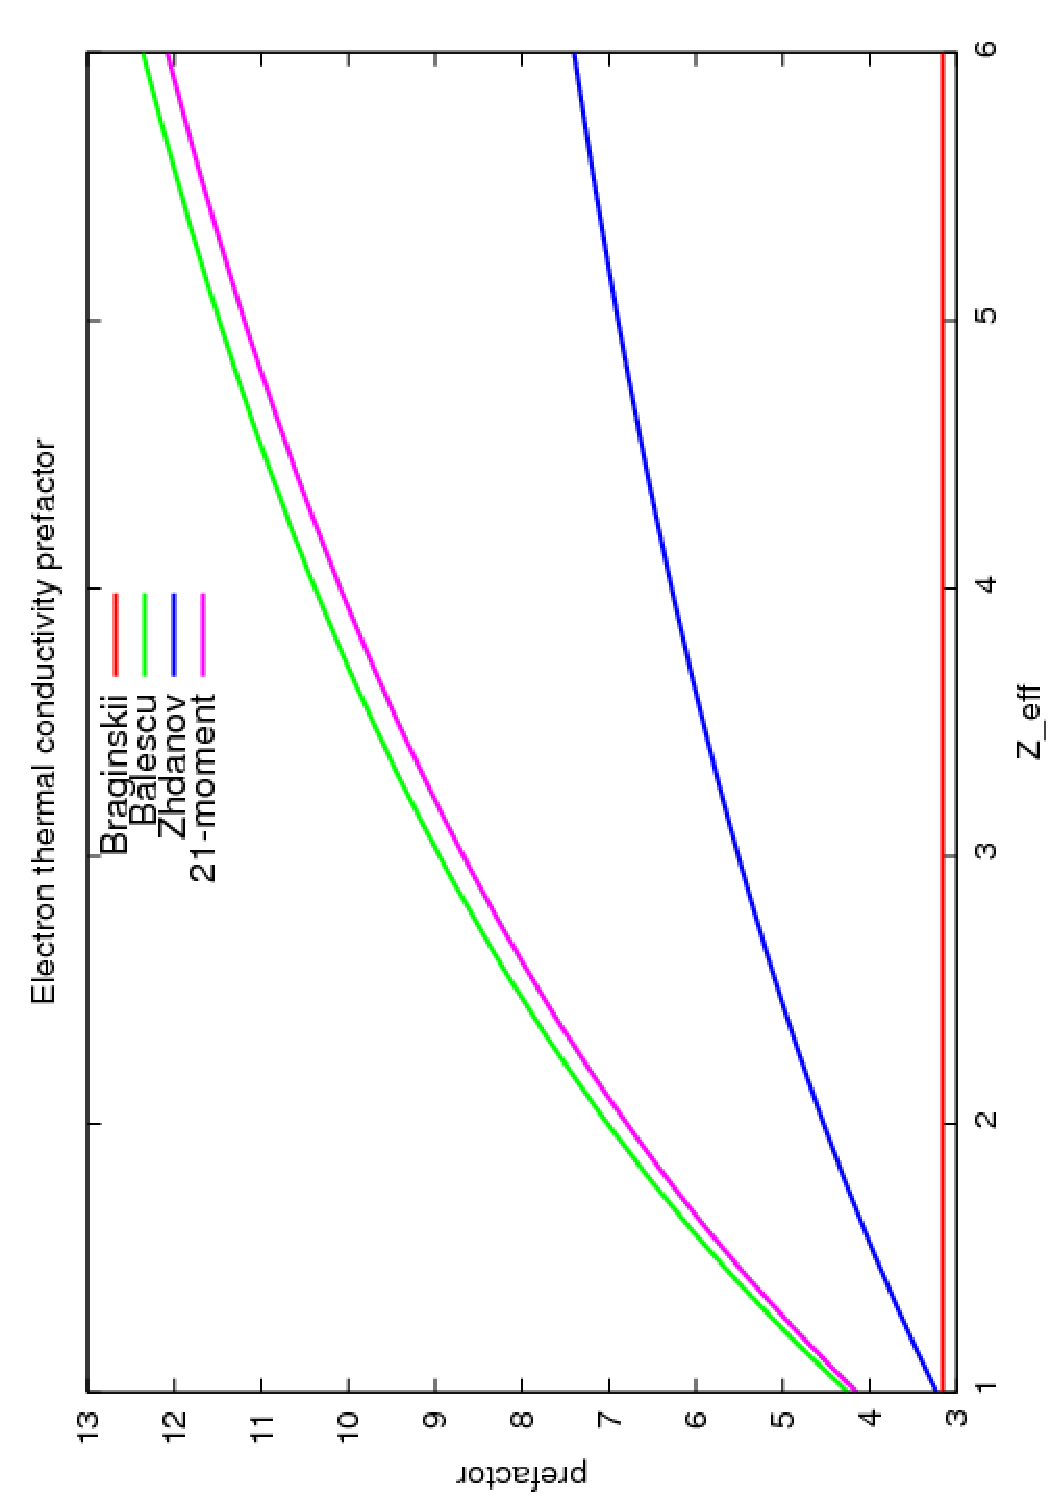
\includegraphics[angle=-90,width=11cm]{hce.pdf}} 
\else
    \centerline{
\includegraphics[angle=-90,width=11cm]{hce.epsi}} 
\fi
\caption{Dependence of the various models for the $\kappa _{e \parallel}$ prefactor as a function of $Z_{eff}$.}
\label{fig:hce}
\vspace*{1cm}
\end{figure}

\begin{figure}[bt]
\ifpdf 
    \centerline{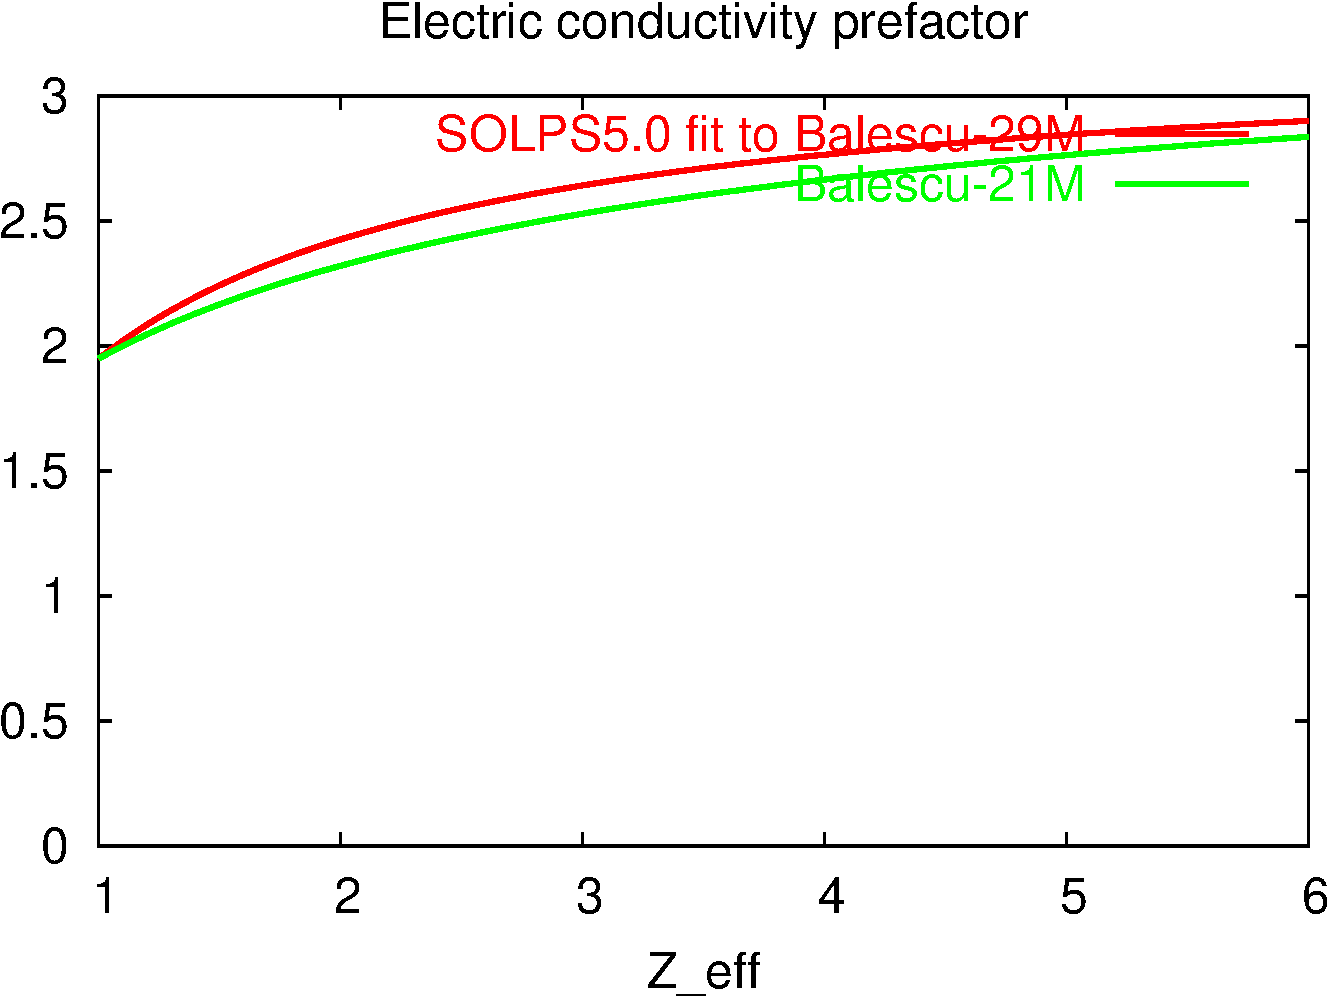
\includegraphics[width=11cm]{sig.pdf}} 
\else
    \centerline{
\includegraphics[angle=-90,width=11cm]{sig.epsi}} 
\fi
\caption{Dependence of the various models for the $\sigma_{\parallel}$ prefactor as a function of $Z_{eff}$.}
\label{fig:sig}
\vspace*{1cm}
\end{figure}

\begin{figure}[bt]
\ifpdf 
    \centerline{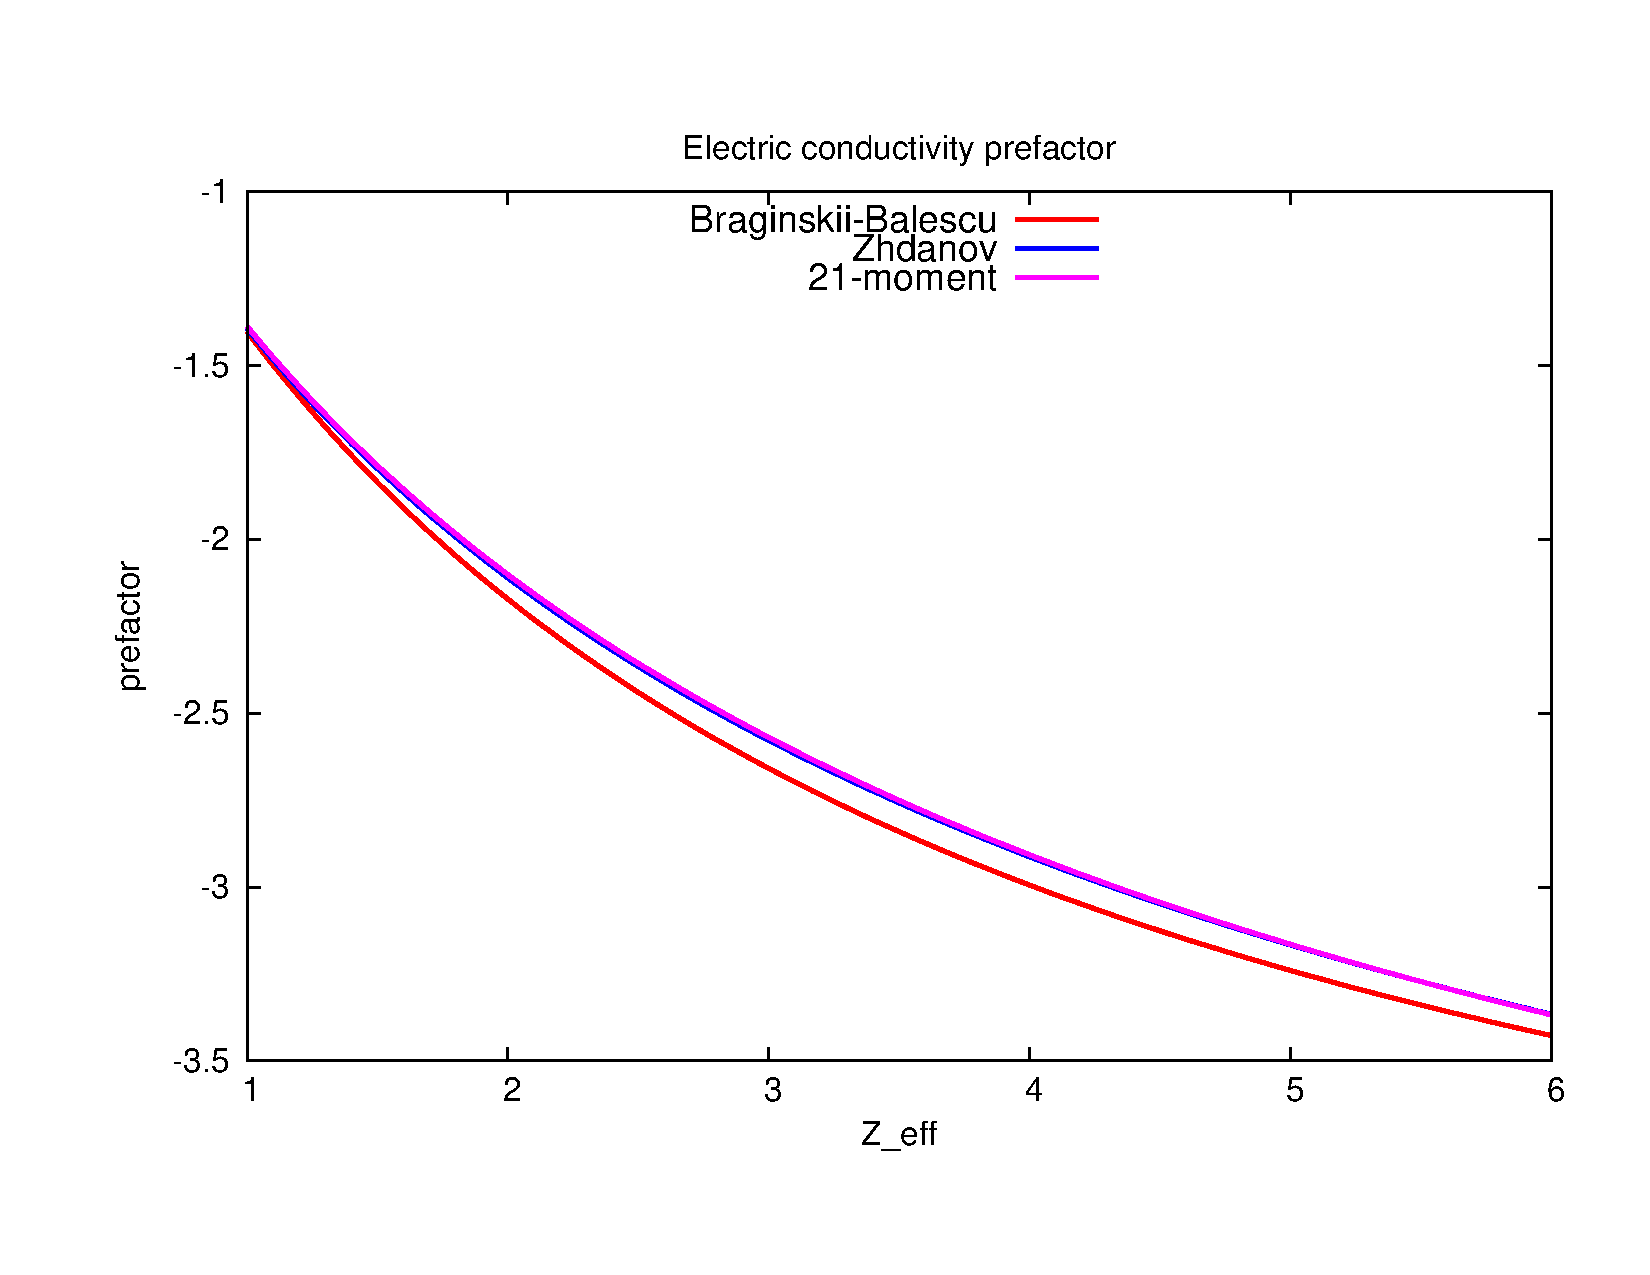
\includegraphics[width=11cm]{alf.pdf}} 
\else
    \centerline{
\includegraphics[angle=-90,width=11cm]{alf.epsi}} 
\fi
\caption{Dependence of the various models for the $\alpha_{e \parallel}$ prefactor as a function of $Z_{eff}$.}
\label{fig:alf}
\vspace*{1cm}
\end{figure}

\chapter{Model equations for B2.5}
\label{cha:equations}\index{B2.5, model}\index{B2.5, equations}\index{equations}\index{model}

%-------- Equations by S.P. Voskoboynikov ---------

\begin{equation}
\frac{\partial n_a}{\partial t} + \frac{1}{\sqrt g}\frac{\partial}{\partial x}\left( \frac{\sqrt g}{h_x} \widetilde{\Gamma}_{ax} \right) +   \frac{1}{\sqrt g}\frac{\partial}{\partial y}\left( \frac{\sqrt g}{h_y} \widetilde{\Gamma}_{ay} \right) = S_a^n, a = 0, 1, \ldots, n_s-1
\end{equation}

\begin{equation}
\widetilde{ \Gamma}_{ax} = \left( b_x V_{\parallel a} + V_{ax}^{\left( E \right)} + V_{ax}^{\left( AN \right)} + V^{corr \_ dpc} \right) n_a - D_a^n \frac{1}{h_x} \frac{\partial n_a}{\partial x} - \widetilde{D}_{ax}^p \frac{1}{h_x} \frac{\partial p_a}{\partial x} - D_{axy} \frac{1}{h_y} \frac{\partial n_a T_i}{\partial y}
\end{equation}

\begin{equation}
\widetilde{ \Gamma}_{ay} = \left( V_{ay}^{\left( E \right)} + V_{ay}^{\left( AN \right)} + \frac{j^{\left( AN \right)} + j_y^{\left( in \right)} + \widetilde{j_y}^{\left( vis \parallel \right)}}{e n_a} \right) n_a - D_a^n \frac{1}{h_y} \frac{\partial n_a}{\partial y} - \widetilde{D}_{ay}^p \frac{1}{h_y} \frac{\partial p_a}{\partial y} + D_{ayx} \frac{1}{h_x} \frac{\partial n_a T_i}{\partial x}
\end{equation}

\begin{equation}
\Gamma_{ax} = \left( b_x V_{\parallel a} + V_{ax}^{\left( E \right)} + \widetilde{V}_{xa}^{\left( dia \right)} + V_{ax}^{\left( AN \right)} + V^{corr \_ dpc} \right) n_a - D_a^n \frac{1}{h_x} \frac{\partial n_a}{\partial x} - \widetilde{D}_{ax}^p \frac{1}{h_x} \frac{\partial p_a}{\partial x}
\end{equation}

\begin{equation}
\Gamma_{ay} = \left( V_{ay}^{\left( E \right)} + \widetilde{V}_{ya}^{\left( dia \right)} + V_{ay}^{\left( AN \right)} + \frac{j^{\left( AN \right)} + j_y^{\left( in \right)} + \widetilde{j_y}^{\left( vis \parallel \right)}}{e n_a} \right) n_a - D_a^n \frac{1}{h_y} \frac{\partial n_a}{\partial y} - \widetilde{D}_{ay}^p \frac{1}{h_y} \frac{\partial p_a}{\partial y}
\end{equation}

\begin{equation}
\Gamma_{ax}^{ \left( \text{no drift} \right)} = \left( b_x V_{\parallel a} + V_{ax}^{\left( AN \right)} + 0 \cdot V^{corr \_ dpc} \right) n_a
\end{equation}

%?????????, ???? ?? ? ???? ??-?? ?????? ay ??? ax!!!!!!!!!!!!!!!!
\begin{equation} 
\Gamma_{ay}^{ \left( \text{no drift} \right)} = \left( V_{ax}^{\left( AN \right)} \right) n_a, \text{really 0 as } V_{ax}^{\left( AN \right)} = 0
\end{equation}

\begin{equation}
\Gamma_{ax}^{\left( Eir \right)} = \left( b_x V_{\parallel a} + V_{ax}^{\left( E \right)} + V_{xa}^{\left( dia \right)} + V_{ax}^{\left( AN \right)} + V^{corr \_ dpc} \right) n_a - D_a^n \frac{1}{h_x} \frac{\partial n_a}{\partial x} 
\end{equation}

% ?? ?????? ?? ??? ???? ??????? ?? n_a?
\begin{equation} 
\Gamma_{ay}^{\left( Eir \right)} = \left( V_{ay}^{\left( E \right)} + V_{ya}^{\left( dia \right)} + V_{ay}^{\left( AN \right)} + \frac{j^{\left( AN \right)} + j_y^{\left( in \right)} + \widetilde{j_y}^{\left( vis \parallel \right)}}{e} \right) n_a - D_a^n \frac{1}{h_y} \frac{\partial n_a}{\partial y} 
\end{equation}

\noindent where
\begin{tabular}{cc}
$\begin{matrix}
V_{xa}^{\left( dia \right)} & =
& \left\{
\begin{matrix}
-\frac{B_z}{Z_a e B^2 n_a} \frac{\partial n_a T_i}{h_y \partial y} & \ z_a \neq 0 \\
0, & \ z_a = 0
\end{matrix} \right.
\end{matrix}$

&

$\begin{matrix}
V_{ya}^{\left( dia \right)} & =
& \left\{
\begin{matrix}
\frac{B_z}{Z_a e B^2 n_a} \frac{\partial n_a T_i}{h_x \partial x} & \ z_a \neq 0 \\
0, & \ z_a = 0
\end{matrix} \right.
\end{matrix}$
\end{tabular}

\begin{equation}
E_{k,a}=\frac{m_a}2 \left[   u^2_{\parallel a}+\left( W_{a\perp}^{\text{(dia)}}+V_{a\perp}^{\text{(ExB)}}  \right)^2    +   \left(  W_{\text{ay}}^{\text{(dia)}} + V_{\text{ay}}^{\text{(ExB)}}\right)^2    \right]
\end{equation}

\begin{tabular}{cc}
$\begin{matrix}
W_{a \perp}^{\left( dia \right)} & =
& \left\{
\begin{matrix}
-\frac{B_z}{Z_a e B^2 n_a} \frac{\partial n_a T_i}{h_y \partial y}, & \ z_a \neq 0 \\
0, & \ z_a = 0
\end{matrix} \right.
\end{matrix}$
&
$\begin{matrix}
W_{ay}^{\left( dia \right)} & =
& \left\{
\begin{matrix}
\frac{B_z}{Z_a e B^2 n_a} \frac{\partial n_a T_i}{h_x \partial x}, & \ z_a \neq 0 \\
0, & \ z_a = 0
\end{matrix} \right.
\end{matrix}$
\end{tabular}

\begin{tabular}{cc}
$\begin{matrix}
V_{a \perp}^{\left( E \times B \right)} & =
& \left\{
\begin{matrix}
-\frac{B_z}{B^2} \frac{\partial \phi}{h_y \partial y}, & \ z_a \neq 0 \\
0, & \ z_a = 0
\end{matrix} \right.
\end{matrix}$
&
$\begin{matrix}
V_{ay}^{\left( E \times B \right)} & =
& \left\{
\begin{matrix}
\frac{B_z}{B^2} \frac{\partial\phi}{h_x \partial x}, & \ z_a \neq 0 \\
0, & \ z_a = 0
\end{matrix} \right.
\end{matrix}$
\end{tabular}

\subsubsection{Source terms in density equations}
{\centering}
$S_a^n=S_{I_a}^n+S_{I_{a+1}}^n+S_{R_a}^n+S_{R_{a-1}}^n+S_{CX_a}^n+S_{CX_{a-1}}^n$,
{\centering}


%-------- end of 1st page -------------

$z_a$ --- the atomic charge of species (a)
$z_{n_a}$ --- the nuclear charge of species (a)

\begin{equation}
\begin{matrix}
S_{I_a}^n & =
& \left\{
\begin{matrix}
-r_{I_a} n_e n_a, & \ a=0,\ldots,n_s-2,z_a<z_{a+1} \mbox{ and } z_{n_a}=z_{n_{a+1}}\\
0
\end{matrix} \right.
\end{matrix}
\end{equation}

\begin{equation}
\begin{matrix}
S_{I_{a+1}}^n & =
& \left\{
\begin{matrix}
r_{I_a} n_e n_a, & \ a=0,\ldots,n_s-2,z_a<z_{a+1} \mbox{ and } z_{n_a}=z_{n_{a+1}}\\
0
\end{matrix} \right.
\end{matrix}
\end{equation}

\begin{equation}
r_{I_a} = exp \left( r_{0,I_a}+r_{1,I_a} ln\left(\frac{T_e}e\right)\right)
\end{equation}
%-------------------
\begin{equation}
\begin{matrix}
S_{R_a}^n & =
& \left\{
\begin{matrix}
-r_{R_a} n_e n_a, & \ a=1,\ldots,n_s-1,z_{a-1}<z_a \text{and} z_{{n-1}_a}=z_{n_a}\\
0
\end{matrix} \right.
\end{matrix}
\end{equation}

\begin{equation}
\begin{matrix}
S_{R_{a-1}}^n & =
& \left\{
\begin{matrix}
r_{R_a} n_e n_a, & \ a=1,\ldots,n_s-1,z_{a-1}<z_a \text{ and } z_{{n-1}_a}=z_{n_a}\\
0
\end{matrix} \right.
\end{matrix}
\end{equation}

\begin{equation}
r_{R_a}=\text{exp}\left(r_{0,R_a}+r_{1,R_a}\text{ln}\left(\frac{T_e}e\right)\right)
\end{equation}
%-------------------
\begin{equation}
\begin{matrix}
S_{CX_a}^n & =
& \left\{
\begin{matrix}
-r_{CX_a} n_e n_a, & \ a=1,\ldots,n_s-1,z_{a-1}<z_a \text{ and } z_{{n-1}_a}=z_{n_a}\\
0
\end{matrix} \right.
\end{matrix}
\end{equation}

\begin{equation}
\begin{matrix}
S_{CX_{a-1}}^n & =
& \left\{
\begin{matrix}
r_{CX_a} n_e n_a, & \ a=1,\ldots,n_s-1,z_{a-1}<z_a \text{ and } z_{{n-1}_a}=z_{n_a}\\
0
\end{matrix} \right.
\end{matrix}
\end{equation}

\begin{equation}
r_{CX_a} = exp \left(
	r_{0,CX_a} + r_{1,CX_a} ln  \left(
		\frac{m_p T_e} m_{a_0} e 
	\right)
\right)
\end{equation}

$n_e = \sum \limits^{n_s-1}_{a=0} z_a n_a$, $n_i = \sum \limits^{n_s-1}_{a=0} n_a$
$p_a = n_a \left( z_a T_e + T_i \right)$, $p_e=n_e T_e$


\begin{equation}
V^{corr\_dpc} = \frac{c^{corr\_dpc}}{16} |b_x| \sqrt{\frac{p_a}{m_a n_a}} \frac{\partial
^2}{\partial x^2} \left( \frac 1{p_a} \frac{\partial p_a}{\partial x} \right)
\end{equation}

\begin{equation}
\begin{matrix}
V_{ax}^{\left( E\right)} & =
& \left\{
\begin{matrix}
-c_{E\times B}   \frac{B_z}{B^2}   \frac 1{h_y}  \frac{\partial \varphi }{\partial y}, & \ z_a \neq 0 \\
0, & \ z_a = 0
\end{matrix} \right.
\end{matrix}
\end{equation}

\begin{equation}
\begin{matrix}
V_{ay}^{\left( E \right)} & =
& \left\{
\begin{matrix}
c_{E\times B}   \frac{B_z}{B^2}   \frac 1{h_x}   \frac{\partial \varphi }{\partial x}, & \ z_a \neq 0 \\
0, & \ z_a = 0
\end{matrix} \right.
\end{matrix}
\end{equation}

%-------- end of 2d page -------------

\begin{equation}
\begin{matrix}
\widetilde{V}_{xa}^{\left( dia \right)} & =
& \left\{
\begin{matrix}
c_{dia} \frac{T_i B_z}{Z_a e}   \frac{\partial}{h_y\partial y} \left(\frac 1{B^2} \right), & \ z_a \neq 0 \\
0, & \ z_a = 0
\end{matrix} \right.
\end{matrix}
\end{equation}

\begin{equation}
\begin{matrix}
\widetilde{V}_{ya}^{\left( dia \right)} & =
& \left\{
\begin{matrix}
-c_{dia} \frac{T_i B_z}{Z_a e}   \frac{\partial}{h_x\partial x} \left(\frac 1{B^2} \right), & \ z_a \neq 0 \\
0, & \ z_a = 0
\end{matrix} \right.
\end{matrix}
\end{equation}

$
\left\{ 
\begin{matrix}
D_{axy}= \left( \frac 1{B^2} - \frac 1{\langle B^2\rangle}   \right)  \frac{B_z}{z_a e}, & z_a \neq 0\\
D_{axy}=0, & z_a=0
\end{matrix}
\right.
$, where $\left \langle B^2 \right \rangle = \frac{\iint \limits_{core} B^2 \sqrt{g} dx dy}{\iint \limits_{core} \sqrt{g} dx dy}$

\begin{equation}
\left\{ 
\begin{matrix}
D_{ayx} = \left( \frac 1{B^2} - \frac 1{\langle B^2\rangle}   \right)  \frac{B_z}{z_a e}, & z_a \neq 0\\
D_{ayx} = 0, & z_a=0
\end{matrix}
\right.
\end{equation}

$D_a^n = D^n_{ANa}$

\begin{equation}
D_{ANa}^n=\left( c_{D_a^N,0}+c_{D_a^N,1}\frac{10^{20}}{n_e}+c_{D_a^N,2}D_a^f+c_{D_a^N,3}\frac{6,2\cdot
10^{-2}T_e}{e|B|}\right)f_D(x,y),
\end{equation}

\begin{equation}
\begin{matrix}
f_D(x,y) & =
& \left\{
\begin{matrix}
1, & \ z_a = 0 \\
\alpha_{1,D}, & \ -\delta _{1,D}\le y\le 0, x\in \text{Core}, z_a \neq 0 \\
\alpha_{2,D}, & \ 0\le y\le \delta _{2,D}, x\in \text{Core} \\
\alpha_{3,D}, & \ x,y\in \text{Pr} \cup \text{SOL}
\end{matrix} \right.
\end{matrix}
\end{equation}

$a=0,\;\;\;c_{D_a^N,0}=0,\;\;\;c_{D_a^N,1}=0,\;\;\;c_{D_a^N,2}=0,\;\;\;c_{D_a^N,3}=0$

$ a=1,\;\;\; c_{D_a^N,0}=0,\;\;\;c_{D_a^N,1}=0,\;\;\;c_{D_a^N,2}=1,\;\;\;c_{D_a^N,3}=0$

$D_a^f=c_{D_a^f,0}+c_{D_a^f,1}\frac{10^{20}}{n_i}+\frac{c_{D_a^f,2}\sqrt{\frac{T_i}{m_a}}}{c_{D_a^f,3}n_i+c_{D_a^f,4}n_e},$


%-------- end of 3d page -------------

\begin{equation}
\begin{matrix}
\widetilde  D_{\text{ax}}^p & =
& \left\{
\begin{matrix}
\frac{D_a^p}
{\left(1+\left(\frac{D_a^p|\frac 1{h_x}\frac{\partial p_a}{\partial x}|}{\mathit{\alpha n}_a\frac{V_{T_i}} 4}\right)^{\gamma _1}\right)^{\frac 1{\gamma_1}}}, 
& \ V_{T_i}=\sqrt{\frac{8T_i}{\mathit{\pi m}_a}}, & \ z_a = 0 \\
D_a^p, & \ z_a \neq 0 \\
\end{matrix} \right.
\end{matrix}
\end{equation}

\begin{equation}
\begin{matrix}
\widetilde D_{\text{ay}}^p & =
& \left\{
\begin{matrix}
\frac{D_a^p}
{\left(1+\left(\frac{D_a^p|\frac 1{h_y}\frac{\partial p_a}{\partial y}|}{\mathit{\alpha n}_a\frac{V_{T_i}} 4}\right)^{\gamma _1}\right)^{\frac 1{\gamma_1}}}, 
& \ V_{T_i}=\sqrt{\frac{8T_i}{\mathit{\pi m}_a}}, & \ z_a = 0 \\
D_a^p, & \ z_a \neq 0 \\
\end{matrix} \right.
\end{matrix}
\end{equation}

$D_a^p = D_{ANa}^p$

\begin{equation*}
D_{ANa}^p=\frac 1{z_aT_e+T_i} \left( c_{D_a^p,0} + c_{D_a^p,1} \frac{10^{20}}{n_e} + c_{D_a^p,2} D_a^f + c_{D_a^p,3} \frac{6,2\cdot
10^{-2}T_e}{e|B|}\right),
\end{equation*}

\begin{equation*}
a=0,c_{D_a^p,0}=0, c_{D_a^p,1}=0, c_{D_a^p,2}=1, c_{D_a^p,3}=0
\end{equation*}
\begin{equation*}
a=1, c_{D_a^p,0}=0, c_{D_a^p,1}=0, c_{D_a^p,2}=0, c_{D_a^p,3}=0
\end{equation*}

$V_{ax}^{AN}=0$

\begin{equation*}
V_{ay}^{AN} = c_{V_a^{AN},0} + c_{V_a^{AN},1} \frac{10^{20}}{n_e} + c_{V_a^{AN},2} D_a^f + c_{V_a^{AN},3} \frac{6,2\cdot 10^{-2}T_e}{e|B|}
\end{equation*}

$a=0, c_{V_a^{AN},0}=0, c_{V_a^{AN},1}=0, c_{V_a^{AN},2}=0, c_{V_a^{AN},3}=0$

$a=1, c_{V_a^{AN},0}=0, c_{V_a^{AN},1}=0, c_{V_a^{AN},2}=0, c_{V_a^{AN},3}=0$

\begin{eqnarray*}
m_a \frac{\partial n_a V_{\parallel a}}{\partial t} +
\frac 1{h_z\sqrt g} \frac{\partial}{\partial x} \left( \frac{h_z\sqrt g}{h_x} \Gamma_{ax}^m \right) +
\frac 1{h_z\sqrt g} \frac{\partial}{\partial y} \left( \frac{h_z\sqrt g}{h_y} \Gamma_{ay}^m \right) +
\frac{b_x}{h_x}\frac{\partial n_a T_i}{\partial x} +
Z_a e n_a \frac{b_x}{h_x} \frac{\partial \varphi}{\partial x} =\\
S_{a \parallel}^m + S_{CF_a}^m + S_{fr_a}^m + S_{Term_a}^{m} + S_{I_a}^m + S_{R_a}^m + S_{CX_a}^m
\end{eqnarray*}

\begin{eqnarray*}
m_a \frac{\partial n_a V_{\parallel a}}{\partial t} +
\frac 1{h_z\sqrt g} \frac{\partial}{\partial x} \left( \frac{h_z \sqrt g}{h_x} \Gamma_{ax}^m \right) +
\frac 1{h_z\sqrt g} \frac{\partial}{\partial y} \left( \frac{h_z \sqrt g}{h_y} \Gamma_{ay}^m \right) +
\frac{b_x}{h_x} \frac{\partial n_a T_i}{\partial x} +
\frac{b_x}{h_x} \frac{Z_a n_a \partial n_e T_e}{n_e \partial x} = \\
= \mbox{old form} = S_{a \parallel}^m + S_{CF_a}^m + S_{fr_a}^m + S_{Term_a}^{m} + S_{I_a}^m + S_{R_a}^m + S_{CX_a}^m
\end{eqnarray*}

%-------- end of 4th page -------------

$S_{a \parallel}^m = - \left( \nabla \pi_a^{\parallel} \right)_{\parallel}$

\begin{equation}
\begin{matrix}
\left( \nabla \pi_a^{\parallel} \right)_{\parallel} & =
& \left\{
\begin{matrix}
0, & \ z_a \neq 1 \\
- \frac{\partial}{h_z\sqrt g\partial x}
\left(\frac{h_z\sqrt g}{h_x} \frac 4 3 \eta_{ax}
\frac{\partial ln \left( h_z B^{\frac 1 2} \right) }{B^{\frac 1 2} h_x \partial x}\right)
B^{\frac 1 2} V_{\parallel a} -
B^{\frac 3 2} b_x \frac{\partial}{h_x \partial x}
\left( \alpha^{NEO} \frac{b_x \tilde {\tau}_a}{B^2} \frac{\partial \left(B^{\frac 1 2} \tilde q^{0} \right)}{h_x \partial x}\right), 
& \ z_a = 1 \\
\end{matrix} \right.
\end{matrix}
\end{equation}

$S_{CF}^m = m_a b_x n_a V_{\parallel a}^2 \frac 1{h_z h_x} \frac{\partial h_z}{\partial x}$

$S_a^m = S_{fr,a}^m + S_{Term}^m + S_{I_a}^m + S_{R_a}^m + S_{CX_a}^m$,

Parallel momentum source due to ionization
\begin{equation*}
S_{I_a}^m = S_{I_a}^q + S_{I_{a+1}}^q
\end{equation*}

\begin{equation}
\begin{matrix}
S_{I_a}^q & =
& \left\{
\begin{matrix}
-r_{I_a} n_e n_a \left( \frac{m_a+m_{a+1}}2 \right) V_{\parallel a}, & \ a=0,\ldots,n_s-2, & \ z_a<z_{a+1} \mbox{ and } z_{n_a}= z_{n_{a+1}}, \\
0, \\
\end{matrix} \right.
\end{matrix}
\end{equation}

\begin{equation}
\begin{matrix}
S_{I_{a+1}}^q & =
& \left\{
\begin{matrix}
r_{I_a} n_e n_a \left( \frac{m_a+m_{a+1}}2 \right) V_{\parallel a}, & \ a=0,\ldots,n_s-2, & \ z_a<z_{a+1} \text{ and } z_{n_a}= z_{n_{a+1}}, \\
0, \\
\end{matrix} \right.
\end{matrix}
\end{equation}

Parallel momentum source due to recombination

\begin{equation*}
S_{R_a}^m = S_{R_a}^q + S_{R_{a-1}}^q
\end{equation*}

\begin{equation}
\begin{matrix}
S_{R_a}^q & =
& \left\{
\begin{matrix}
-r_{R_a} n_e n_a \left( \frac{m_a+m_{a-1}}2 \right) V_{\parallel a}, & \ a=0,\ldots,n_s-1, & \ z_{a-1}<z_a \text{ and } z_{n_{a-1}}= z_{n_a}, \\
0, \\
\end{matrix} \right.
\end{matrix}
\end{equation}

\begin{equation}
\begin{matrix}
S_{R_{a-1}}^q & =
& \left\{
\begin{matrix}
r_{R_a} n_e n_a \left( \frac{m_a+m_{a+1}}2 \right) V_{\parallel a}, & \ a=0,\ldots,n_s-1, & \ z_{a-1}<z_a \text{ and } z_{n_{a-1}}= z_{n_a}, \\
0, \\
\end{matrix} \right.
\end{matrix}
\end{equation}


%---------- nedorazvitoe uravnenie? ----------
\begin{equation*}
S_{CX_a}^m=
\end{equation*}


\begin{equation}
S^m_{fr,a} = 
\sum \limits^{n_s-1}_{\substack{b = 0, \\ b\neq a, z_a \neq 0, z_b \neq 0}} \frac 1{\tau_p} m_p 
\sqrt{ \frac {\frac{m_a}{m_p} \frac{m_b}{m_p}} {\frac{m_a}{m_p} + \frac{m_b}{m_p}} }
z_a^2 z_b^2 n_b n_a \left( V_{b \parallel} - V_{a \parallel} \right)
\text{- friction force (b2sifr)}
\end{equation}

$\tau_p = \frac 3{4\sqrt{2\pi}}
\frac{\sqrt{m_p}T_i^{\frac 3 2}}{\Lambda}
\left(\frac{4 \pi \varepsilon_0}{e^2}\right)^2$, where the Coulomb logarithm  $\Lambda $ can be chosen as

%-------- end of 5th page -------------

\begin{equation}
\begin{matrix}
\Lambda & =
& \left\{
\begin{matrix}
12 \\
max \{ 5; 23.4 - 1.15 \cdot log_{10} \left( \frac{n_e}{10^6} \right) + 3.45 \cdot log_{10} \left( \frac{T_e}e \right)  \}, & \frac{T_e}{e} \leq 50 & \mbox{\scriptsize{Braginsky}} \\
max \{ 5; 25.3 - 1.15 \cdot log_{10} \left( \frac{n_e}{10^6} \right) + 2.30 \cdot log_{10} \left( \frac{T_e}e \right)  \}, & \frac{T_e}{e} > 50 &  \mbox{\scriptsize{formula}}\\
max \{ 5; 17.3 - 0.5 \cdot log_e \left( \frac{n_e}{10^{20}} \right) + 1.5 \cdot log_e \left( \frac{T_e}{e \cdot 10^3} \right)  \} & \mbox{\scriptsize{Wesson formula}} &\mbox{\scriptsize{for ion-ion collisions}}\\
\end{matrix} \right.
\end{matrix}
\end{equation}

$S_{Term,a}^m = 
n_a \left(
	\frac{z_a}{n_e} - \frac{z_a^2}{n_{e^2}} 
\right)
n_e b_x e
\left[
	\hat E_x - \frac 1 e \left(
		c_{th_e,a} \Delta_{T_e} + c_{th_i,a} \Delta_{T_i}
	\right)
\right],$ thermal force (b2sifr)

\begin{equation*}
n_{e^2 }= \sum \limits^{n_s-1}_{a=0} z_a^2 n_a, \;\;\;\ l_{t_e}=0.3; \;\;\;\;\; l_{t_i}=0,3; \;\;\;\;\; z_{\lambda_e}=\frac{1.5\cdot
10^{16}}{n_e} \left( \frac{T_e} e \right)^2, \;\;\;\;\; z_{\lambda_i}=\frac{1.5 \cdot 10^{16}}{n_{e^2}}\left(\frac{T_i} e\right)^2
\end{equation*}

\begin{equation}
\begin{matrix}
\Delta _{T_e} & =
& \left\{
\begin{matrix}
\frac{\partial T_e}{h_x\partial x}, && l_{t_e} \leq 0 \\

\Biggl|
	min \left\{ 
		\Bigl|
			\frac{\partial T_e}{h_x \partial x} 
		\Bigr|, \frac{l_{t_e} T_e}{z_{\lambda_e}|b_x|}
	\right\} 
\Biggr|,
& \frac{\partial T_e}{h_x \partial x} \ge 0, & l_{t_e}>0 \\

-\Bigl| 
	min \left\{ 
		\Bigl|
			\frac{\partial T_e}{h_x \partial x} 
		\Bigr|, \frac{l_{t_e} T_e}{z_{\lambda_e}|b_x|}			
	\right\} 
\Bigr|,
& \frac{\partial T_e}{h_x \partial x} < 0, & l_{t_e}>0 
\end{matrix} \right.
\end{matrix}
\end{equation}

\begin{equation}
\begin{matrix}
\Delta _{T_i} & =
& \left\{
\begin{matrix}
\frac{\partial T_i}{h_x\partial x}, && l_{t_i} \leq 0 \\
\Bigl| 
	min \Bigl\{ 
		\Bigl| \frac{\partial T_i}{h_x \partial x} 
		\Bigr|, \frac{l_{t_i} T_i}{z_{\lambda_i}|b_x|} 				
	\Bigr\} 
\Bigr|,
& \frac{\partial T_i}{h_x \partial x} \ge 0, & l_{t_i}>0 \\
-\Bigl| 
	min \Bigl\{
		\Bigl| 
			\frac{\partial T_i}{h_x \partial x} 
		\Bigr|, \frac{l_{t_i} T_i}{z_{\lambda_i}|b_x|}
	\Bigr\} 
\Bigr|,
& \frac{\partial T_i}{h_x \partial x} < 0, & l_{t_i}>0 
\end{matrix} \right.
\end{matrix}
\end{equation}

$c_{th_e,a} = 0, a=0,\ldots,n_s-1$ and $c_{th_i,a}=2.65, a=0,\ldots, n_s-1$ if 21 moment approximation is not used.

\begin{equation}
\Gamma^m_{ax} =
m_a V_{\parallel a} \Gamma_{ax} + m_a V_{\parallel a} \Gamma_{ax}^{\left( dia \right)} + 
\frac 4 3 \eta_{ax} \frac{\partial ln h_z}{h_x \partial x} V_{\partial a} - 
\frac 4 3 \eta_{ax} \frac{\partial V_{\partial a}}{h_x \partial x}
\end{equation}

\begin{equation}
\Gamma^m_{ay} =
m_a V_{\parallel a} \Gamma_{ay} + m_a V_{\parallel a} \Gamma_{ay}^{\left( dia \right)} -
\eta_{ay} \frac{\partial V_{\parallel a}}{h_y \partial y}
\end{equation}

$\Gamma^{\left( dia \right)}_{ax} = n_a \widetilde{V}^{\left( dia \right)}_{\perp a}$,

$\Gamma^{\left( dia \right)}_{ay} = n_a \widetilde{V}^{\left( dia \right)}_{ya}$,

$\eta_{ax} = \eta_{AN_a} + \widetilde{\widetilde{\eta}}_{CL_{ax}}$

%-------- end of 6th page -------------

\begin{equation}
\begin{matrix}
\eta_{AN_a} & =
& \left\{
\begin{matrix}
\left( c_{\eta_a,0} + c_{\eta_a,1} \frac{10^{20}}{n_e} + c_{\eta_a,2} D_a^f + 
c_{\eta _a,3} \frac{6.2 \cdot 10^{-2} T_e}{e|B|}\right)
m_a n_a f_{\eta _a}(x,y), & z_a\neq 0 \\
\left( c_{\eta_a,0} + c_{\eta_a,1} \frac{10^{20}}{n_e} + c_{\eta_a,2} D_a^f + 
c_{\eta _a,3} \frac{6.2 \cdot 10^{-2} T_e}{e|B|}\right)
m_a n_a , & z_a = 0
\end{matrix} \right.
\end{matrix}
\end{equation}

\begin{equation}
\begin{matrix}
f_{\eta _a}(x,y) & =
& \left\{
\begin{matrix}
1, & \ z_a = 0 \\
\alpha_{1,\eta _a}, & \ -\delta _{1,\eta _a} \le y \le 0, & x \in \text{Core}, z_a \neq 0 \\
\alpha_{2,\eta _a}, & \ 0\le y\le \delta _{2,\eta _a}, & x \in \text{Core} \\
\alpha_{3,\eta _a}, & \ x,y\in \text{Pr} \cup \text{SOL}
\end{matrix} \right.
\end{matrix}
\end{equation}

$ a = 0, \;\;\;  c_{\eta _a,0} = 0, \;\;\;  c_{\eta _a,1} = 0, \;\;\;  c_{\eta _a,2} = 1,  \;\;\;  c_{\eta _a,3} = 0$
$ a = 1, \;\;\;  c_{\eta _a,0} = 0, \;\;\;  c_{\eta _a,1} = 0, \;\;\;  c_{\eta _a,2} = 1,  \;\;\;  c_{\eta _a,3} = 0$

$\widetilde{\widetilde{\eta}}_{CLax} = c_{\eta_{ax}^{(CL)}} \widetilde{\eta}_{CLax}$

\begin{equation}
\begin{matrix}
c_{\eta_{ax}^{(CL)}} & =
& \left\{
\begin{matrix}
1, & \ z_a \neq 0 \; \text{and only for inner flux surfaces} \\
\frac 1 
{1 + \frac{
\frac{\sqrt g}{h_x} \widetilde{\eta}_{CLax}  \bigl| \frac{\partial V_{\parallel a}}{h_x \partial x} \bigr|
}
{V_{m_a}^{(max)}}  
}, &  
\text{for all other cases} \\
\end{matrix} \right.
\end{matrix}
\end{equation}

$V_{m_a}^{(max)} = c_{f \; lim_2} \frac{\sqrt g}{h_x} |b_x| n_a T_i$
$\widetilde{\eta }_{CLax} = c_{\eta_{ax}^{(CL)}}^{Luciani} \eta_{CLax} b_x^2$

'b2trcl\_lluciani' '1'

$\begin{matrix}
c_{\eta_{ax}^{(CL)}}^{Luciani} & =
& \left\{
\begin{matrix}
\frac 1 {
1 + \frac{
7.5 \cdot 10^{16} \left( \frac{T_i} e \right)^2}
{c(y) \sum \limits_{a=0}^{n_s-1} z_a^2 n_a}
}
, & \ z_a \neq 0 \; \text{and only for inner flux surfaces,} \\
1, &  \text{for all other cases} \\
\end{matrix} \right.
\end{matrix}$

For plateau and banana correction 'b2trcl\_lluciani' '3'

%-------- end of 7th page -------------

$
\begin{matrix}
c_{\eta_{ax}^{(CL)}}^{Luciani} & =
& \left\{
\begin{matrix}
\frac 1{1 + 
\frac{15.12 \cdot 10^{16} \left( \frac{T_i}e \right)^2}
{c(y)\sum \limits_{a=0}^{n_s-1} z_a^2 n_a}}
\cdot
\frac 1{1 +
\frac{15.12 \cdot 10^{16} \cdot \varepsilon^{3/2} \left( \frac{T_i} e \right)^2}
{c(y)\sum \limits_{a=0}^{n_s-1} z_a^2 n_a}}
, & \ z_a \neq 0 \; \mbox{\scriptsize{and only for inner flux surfaces,}} \\
1, &  \text{for all other cases} \\
\end{matrix} \right.
\end{matrix}
$

$c \left( y \right) = \oint h_x |b_x|^{-1} dx$, \ \ \ \  $\varepsilon = \frac
{\left( \oint h_x dx \right)^2}
{\oint \sqrt g / h_y dx}$

$
\begin{matrix}
\eta_{CLax} & =
& \left\{
\begin{matrix}
0, & \ z_a = 0 ,  \\
\eta \sqrt{2} T_i n_a \tau_a b_x^2, & \ z_a \neq 0  \\
\end{matrix} \right.
\end{matrix}
$

$\eta = 0.96$,

$\tau _a = \frac 3{4 \sqrt{2\pi}}  
\frac {\sqrt{m_a} T_i^{\frac 3 2}} {z_a^2 z_{eff} n_e \Lambda}
\left( \frac{4 \pi \varepsilon_0}{e^2} \right)^2$, where the Coulomb logarithm  $\Lambda $
can be chosen as

$
\begin{matrix}
\Lambda & =
& \left\{
\begin{matrix}
12 \\
max \{ 5; 23.4 - 1.15 \cdot log_{10} \left( \frac{n_e}{10^6} \right) + 3.45 \cdot log_{10} \left( \frac{T_e}e \right)  \}, & \frac{T_e}{e} \leq 50 & \mbox{\scriptsize{Braginsky}} \\
max \{ 5; 25.3 - 1.15 \cdot log_{10} \left( \frac{n_e}{10^6} \right) + 2.30 \cdot log_{10} \left( \frac{T_e}e \right)  \}, & \frac{T_e}{e} > 50  & \mbox{\scriptsize{formula}}\\
max \{ 5; 17.3 - 0.5 \cdot log_e \left( \frac{n_e}{10^{20}} \right) + 1.5 \cdot log_e \left( \frac{T_e}{e \cdot 10^3} \right)  \} & \mbox{\scriptsize{Wesson formula}} & \mbox{\scriptsize{for ion-ion collisions}} \\
\end{matrix} \right.
\end{matrix}
$

$\eta_{ay} = \eta_{AN_a} + \eta_{CL_{ay}}$

$\widetilde{q}^{(0)} = q^{(1)} arctg \left( \frac{q^{(0)}}{q^{(1)}} \right), \; q^{(1)} = c_{q1} n_i T_i \sqrt{\frac{T_i + T_e}{m_i}}$

$c_{ql} = 0.5$ or 'b2siav\_cqip1'  '0.1' in b2mn.dat

the three-point smoothing procedure is imposed twice on $\widetilde{q}^{(0)}$ along x-direction

in case if 'b2siav\_style\_qip'  '0' in b2mn.dat

$
\begin{matrix}
q^{(0)} = q_{a\parallel}^{(0)} + 
\frac B{B_x} q_{ax}^{(dia)} & =
& \left\{
\begin{matrix}
0 & \text{outside the separatrix} \\
-\frac 5 2 \frac{B_z B}{B_x \langle B^2 \rangle} \frac{nT_i}e \frac{\partial T_i}{h_y \partial y}
& \text{inside the separatrix}
\end{matrix} \right.
\end{matrix}
$

in case if b2siav\_style\_qip 1 in b2mn.dat

%-------- end of 8th page -------------

$
\begin{matrix}
q^{(0)} = q_{a\parallel}^{(0)} + 
\frac B{B_x} q_{ax}^{(dia)} & =
& \left\{
\begin{matrix}
0 & \text{outside the separatrix} \\
-\widetilde{\widetilde{k}}_{ix}^{(CL)} b_x \frac{ \partial T_i}{h_x \partial x}
-\frac 5 2 \frac{B_z B}{B_x \langle B^2 \rangle} \frac{nT_i}e \frac{\partial T_i}{h_y \partial y}
& \text{inside the separatrix}
\end{matrix} \right.
\end{matrix}
$

$
\widetilde{\tau}_a =
\frac{\tau_a}{1+\frac{15,12\cdot 10^{16}\left(\frac{T_i}
e\right)^2}{c(y) \sum \limits^{n_s-1}_{a=0} z_a^2 n_a}}
\cdot 
\frac 1 {1 + 
\frac{15.12 \cdot 10^{16} \cdot \varepsilon^{3/2} \left( \frac{T_i} e \right)^2}
{c(y) \sum \limits^{n_s-1}_{a=0} z_a^2 n_a}}
$

This correction is compatible only with plateau and banana correction 'b2trcl\_lluciani' '3'

$\alpha^{NEO} = \frac 8{15} 
\left( 
\frac{-0.17 + 1.05\nu_{\ast}^{1/2} + 2.7\nu_{\ast}^2 \varepsilon^3}
{1 + 0.7\nu_{\ast}^{1/2} + \nu_{\ast}^2\varepsilon^3} -1 \right)$ gives the correct coefficient before
the temperature gradient in the neoclassical electric field in the plateau and banana regime

$\nu_{\ast} = \frac{c \left( y \right)} 
{2 \pi \varepsilon^{3/2} \tau_a \sqrt{T_i/m_a}}$,\ \ \ \  
$c \left( y \right) = \oint h_x |b_x|^{-1}dx$, \ \ \ \ 
$\varepsilon = \frac{\left(\oint h_x dx \right)^2}
{\oint \sqrt g /h_y dx}$

\begin{eqnarray}
\frac 3 2 \frac{\partial n_e T_e}{\partial t} + 
\frac 1{\sqrt g} \frac{\partial }{\partial x} \left( \frac{\sqrt g}{h_x} \widetilde{q}_{ex} \right) +
\frac 1{\sqrt g} \frac{\partial }{\partial y} \left( \frac{\sqrt g}{h_y} \widetilde{q}_{ey} \right) +
\frac{n_e T_e}{\sqrt g} \frac{\partial}{\partial x} \left(\frac{\sqrt g}{h_x} b_x V_{e \parallel} \right) =\\
= Q_e + c_{E\times B} n_e T_e B_z \frac 1{h_x h_y}
\left(
	\frac{\partial \varphi }{\partial y} \frac{\partial }{\partial x} \left(\frac 1{B^2} \right) -
	\frac{\partial \varphi }{\partial x} \frac{\partial }{\partial y} \left(\frac 1{B^2} \right)
\right)
- 
\frac{\widetilde{j}_y^{(st)}}{e n_e} \frac{\partial n_e T_e}{h_y \partial y}
+ j_x \hat E_x + 0 \cdot j_y \hat E_y
\end{eqnarray}

$Q_e = -Q_{\Delta } - Q_R$ 
$Q_{\Delta} = c_{eqp} \Lambda e^{\frac 3 2} 
\frac{
	\sum \limits_{a=0}^{n_s-1}\frac{z_a^2 m_p}{m_a}n_a
	}
	{n_i}
\frac{n_e n_i}{T_e^{\frac 3 2}}
(T_e - T_i),\;\;\; c_{eqp}=4.8 \cdot 10^{-15},\;\;$ where  $\Lambda $ can be chosen as

$
\begin{matrix}
\Lambda & =
& \left\{
\begin{matrix}
12 \\
max \{ 5; 23.4 - 1.15 \cdot log_{10} \left( \frac{n_e}{10^6} \right) + 3.45 \cdot log_{10} \left( \frac{T_e}e \right)  \}, & \frac{T_e}{e} \leq 50 & \text{Braginsky formula} \\
max \{ 5; 25.3 - 1.15 \cdot log_{10} \left( \frac{n_e}{10^6} \right) + 2.30 \cdot log_{10} \left( \frac{T_e}e \right)  \}, & \frac{T_e}{e} > 50  \\
max \{ 5; 17.3 - 0.5 \cdot log_e \left( \frac{n_e}{10^{20}} \right) + 1.5 \cdot log_e \left( \frac{T_e}{e \cdot 10^3} \right)  \} && \text{Wesson formula for ion-ion collisions} \\
\end{matrix} \right.
\end{matrix}
$

$Q_R = \sum \limits_{a=0}^{n_s-1} r_{Q_a} n_e n_a$ from b2stel
 
 %-------- end of 9th page -------------
 
\begin{equation*}
\widetilde{q}_{ex} = \widetilde{f}_{ex} T_e - \kappa_{ex} \frac 1{h_x} \frac{\partial T_e} {\partial x} + 
0 \cdot \alpha_{ex} T_e \hat E_x - q_{ex}^{P.Sch}
\end{equation*}

\begin{equation*}
\widetilde{f}_{ex} = \frac 3 2 \Gamma_{ex} + V_{ex}^{(Str)} n_e - 0.71 \frac{j_{ \left( \parallel \right) }}e
\end{equation*}

\begin{equation*}
q_{ex}^{P.Sch} = -\frac 5 2 D_{exy} \frac 1{h_y} \frac{\partial n_e T_e^2} {\partial y}
\end{equation*}
 
 
$D_{exy} = \left( \frac 1{B^2} - \frac 1{\langle B^2 \rangle} \right) \frac{B_z} e$ 
$D_{eyx} = \left( \frac 1{B^2} - \frac 1{\langle B^2 \rangle} \right) \frac{B_z} e$
where $\langle B^2 \rangle = \frac{\iint \limits_{core} B^2 \sqrt g dxdy}
{\iint \limits_{core} \sqrt g dxdy}$

\begin{equation*}
q_{ex} = 
\left[
	\frac 3 2 \Gamma_{ex} - 0.71 \frac{j_{\left( \parallel \right) }} e 
	-
	\frac 5 2 n_e T_e \frac{B_z}e \frac{\partial}{h_y\partial y} \left( \frac 1{B^2} \right) + 
	V_{ex}^{(Str)} n_e 
\right] T_e
-
\kappa_{ex} \frac 1{h_x} \frac{\partial T_e}{\partial x} + 0\cdot \alpha_{ex} T_e \hat E_x
\end{equation*}

$\Gamma_{ex} = \sum \limits_{a=0}^{n_s-1} z_a \Gamma_{ax}^{(he)} - \frac{j_{\parallel}} e$,

\begin{equation*}
\Gamma_{ax}^{(he)} = 
\left(
	b_x V_{a \parallel} + V_{ax}^{(E)} + \frac 5 3 V_a^{(AN)} + V^{corr\_dpc}
\right) n_a -
\frac 5 3 \left[
	D_a^n \frac 1{h_x} \frac{\partial n_a}{\partial x} + \widetilde{D}_{ax}^p \frac	1{h_x} \frac{\partial p_a}{\partial x}
\right]
\end{equation*}

\begin{equation*}
q_{ex}^{(Eir)} =
\left[
	\frac 5 2 \Gamma_{ex}^{(Eir)} + V_{ex}^{(Str)}n_e
	- 0.71 b_x \frac{j_{\parallel}} e
\right] T_e - 
\kappa_{ex} \frac 1{h_x} \frac{\partial T_e}{\partial x}
\end{equation*}

\begin{equation*}
q_{ey}^{(Eir)} =
\left[
	\frac 5 2 \Gamma_{ex}^{(Eir)} + V_{ey}^{(Str)}n_e
\right] T_e - 
\kappa_{ey} \frac 1{h_y} \frac{\partial T_e}{\partial y}
\end{equation*}

where

\begin{equation*}
\Gamma_{ex}^{(Eir)} = 
\left(
	b_x V_{\parallel b} + V_{bx}^{(E)} + V_{bx}^{(dia)} + V_{bx}^{(AN)}
\right) n_b -
D_a^n \frac 1{h_x} \frac{\partial n_a}{\partial x}
\end{equation*}

\begin{equation*}
\Gamma_{ey}^{(Eir)} = 
\left(
	V_{by}^{(E)} + V_{by}^{(dia)} + V_{by}^{(AN)}
\right) n_b -
D_a^n \frac 1{h_y} \frac{\partial n_a}{\partial y}
\end{equation*}
 
$V_{ex}^{(dia)} = \frac{B_z}{e B^2 n_e} \frac{\partial n_e T_e}{h_y \partial y}$ \ \ \ \ \ \ 
$V_{ey}^{(dia)} = -\frac{B_z}{e B^2 n_e} \frac{\partial n_e T_e}{h_x \partial x}$

$V_{ex}^{(Str)} = 0$

$\kappa_{ex} = \kappa_e^{(AN)} + \widetilde{\widetilde{\kappa}}_{ex}^{(CL)}$,

$\kappa_e^{(AN)} = \chi_e n_e$,

$\chi_e = \left( 
	c_{h_e,0} + c_{h_e,1} \frac{10^{20}}{n_e} + c_{h_e,3} \frac{6.2 \cdot 10^{-2} T_e}{e|B|}
\right) f_{h_e} (x,y)$,

%-------- end of 10th page -------------

$c_{h_e,0} = 1.2, \;\; c_{h_e,1}=0, \;\;\; c_{h_e,3}=0$,
 
$
\begin{matrix}
f_{h_e}(x,y) & =
& \left\{
\begin{matrix}
\alpha_{1,h_e}, & \ -\delta _{1,h_e} \le y \le 0, & x \in \text{Core}, \\
\alpha_{2,h_e}, & \ 0 \le y \le \delta _{2,h_e}, & x \in \text{Core} \\
\alpha_{3,h_e}, & \ x,y\in \text{Pr} \cup \text{SOL}
\end{matrix} \right.
\end{matrix}
$

$\widetilde{\widetilde{\kappa}}_{ex}^{(CL)} = c_{k_{ex}}^{(Flim)}   \widetilde{\kappa}_{ex}^{(CL)}$
 
$
\begin{matrix}
c_{k_{ex}}^{Flim} & =
& \left\{
\begin{matrix}
1, & \text{only for inner flux surfaces,} \\
\frac 1 {
	1 + \frac{
	\frac{\sqrt g}{h_x} \widetilde{\kappa}_{ex}^{(CL)}
	\bigl| 
		\frac{\partial T_e}{h_x \partial x}
	\bigr|}
	{ V_{h_e}^{(max)} n_e T_e}
}
&  \text{for other flux surfaces} \\
\end{matrix} \right.
\end{matrix}
$

$V_{h_e}^{(max)} = c_{f \text{lim}_0} \frac{\sqrt g}{h_x}|b_x| \sqrt{\frac{T_e}{m_e}}$,
$\widetilde{\kappa}_{ex}^{(CL)} = c_{\eta_{ax}^{(CL)}}^{(Luciani)} \kappa_{ex}^{(CL)} b_x^2$

For plateau and banana correction 'b2trcl\_lluciani' '3'

$
\begin{matrix}
c_{\eta_{ax}^{(CL)}}^{(Luciani)} & =
& \left\{
\begin{matrix}
0.58 \varepsilon^{\frac{3}{2}}/K_1, & \text{only for inner flux surfaces,} \\
1, &  \text{for other flux surfaces} \\
\end{matrix} \right.
\end{matrix}
$

\begin{equation*}
K_1 = \frac 1{1 + 2.01 \cdot \nu_{\ast e}^{1/2} + 1.53 \cdot \nu_{\ast e}} + 
\frac{0.52 \cdot \varepsilon^3 \cdot \nu_{\ast e}}{1 + 0.89 \cdot \varepsilon^{3/2} \cdot \nu_{\ast e}}
\end{equation*}

$\nu_{\ast e} = \frac{c \left( y \right)}{2 \pi \varepsilon^{3/2} \tau_e \sqrt{T_e/m_e}}$,


$\tau_e = \frac 3{4\sqrt{2\pi}}  
\frac{\sqrt{m_e} T_e^{\frac 3 2}} {z_{eff} n_e \Lambda}
\left( \frac{4 \pi \varepsilon_0}{e^2}\right)^2$, where Coulomb logarithm  $\Lambda $ can
be chosen as

$
\begin{matrix}
\Lambda & =
& \left\{
\begin{matrix}
12 \\
max \{ 5; 23.4 - 1.15 \cdot log_{10} \left( \frac{n_e}{10^6} \right) + 3.45 \cdot log_{10} \left( \frac{T_e}e \right)  \}, & \frac{T_e}{e} \leq 50 & \text{Braginsky formula} \\
max \{ 5; 25.3 - 1.15 \cdot log_{10} \left( \frac{n_e}{10^6} \right) + 2.30 \cdot log_{10} \left( \frac{T_e}e \right)  \}, & \frac{T_e}{e} > 50  \\
max \{ 5; 17.3 - 0.5 \cdot log_e \left( \frac{n_e}{10^{20}} \right) + 1.5 \cdot log_e \left( \frac{T_e}{e \cdot 10^3} \right)  \} && \text{Wesson formula for ion-ion collisions} \\
\end{matrix} \right.
\end{matrix}
$

%-------- end of 11th page -------------

but it was as below

$
\begin{matrix}
c_{\eta_{ex}^{(CL)}}^{Luciani} & =
& \left\{
\begin{matrix}
\frac 1 {
1 + \frac{
7.5 \cdot 10^{16} \left( \frac{T_e} e \right)^2}
{c(y) \sum \limits_{a=0}^{n_s-1} z_a^2 n_a}
}
, &  \text{only for inner flux surfaces,} \\
1, &  \text{for all other cases} \\
\end{matrix} \right.
\end{matrix}
$

$
\begin{matrix}
c \left( y \right) & =
& \left\{
\begin{matrix}
\int \frac{h_x \left( x,y \right)}{|b_x|}dx
, &  \text{for inner flux surfaces,} \\
0, &  \text{for other} \\
\end{matrix} \right.
\end{matrix}
$

$\kappa_{ex}^{(CL)} = \frac 5 2\frac{T_e}{m_e} f_{k_e} 
\left( z_{eff} \right) n_e \tau_e$, old form

$f_{k_e} \left( z_{eff} \right) = \frac{2.16 z_{eff}}{1 + 0.27 z_{eff}}$,
old form

$\kappa_{ex}^{(CL)} = \frac{T_e}{m_e} f_{k_e} \left( z_{eff} \right) n_e \tau_e$, new form

$f_{k_e}\left( z_{eff} \right )= 
\frac{3.9 + 2.3/z_{eff}}{0.31 + 1.2/z_{eff} + 0.41/z_{eff}^2}$,
new Zhdanov expression

$z_{eff} = \frac{\sum \limits_{a=0}^{n_s-1} z_a^2n_a}{n_e}$,

$V_{e \parallel} = \frac 1{e n_e} \left[
\sum \limits_{a=0}^{n_s -1} z_a e n_a V_{a\parallel} - \frac{j^{(\parallel)}_x}{b_x}
\right]$,

$j^{(\parallel)}_x = \sigma_{\parallel} \hat E_x - \alpha_{ex} \frac 1{h_x} \frac{\partial T_e}{\partial x}$,

$\hat E_x = \frac 1{en_e h_x} \frac{\partial n_e T_e}{\partial x} - \frac 1{h_x} \frac{\partial \varphi}{\partial x}$,

$\sigma_{\parallel} = \sigma_{AN \parallel} + \widetilde{\sigma}_{CL \parallel}$,

$\sigma_{AN \parallel} = 0$ 

\begin{equation*}
\widetilde{\sigma}_{CL \parallel} = c_{\sigma_{CL \parallel}}^{(Luciani)}\sigma_{CL \parallel}
\end{equation*}

For plateau and banana correction 'b2trcl\_lluciani' '3' 

$
\begin{matrix}
c_{\sigma_{CL \parallel}^{(Luciani)}} & =
& \left\{
\begin{matrix}
0.58 \varepsilon^{\frac{3}{2}}/K_1, & \text{only for inner flux surfaces,} \\
1, &  \text{for other flux surfaces} \\
\end{matrix} \right.
\end{matrix}
$

But it was as below

%-------- end of 12th page -------------

$
\begin{matrix}
c_{\sigma_{CL \parallel}^{(Luciani)}} & =
& \left\{
\begin{matrix}
\frac 1 {
1 + \frac{
7.5 \cdot 10^{16} \left( \frac{T_e} e \right)^2}
{c(y) \sum \limits_{a=0}^{n_s-1} z_a^2 n_a}
}
, &  \text{only for inner flux surfaces,} \\
1, &  \text{for all other cases} \\
\end{matrix} \right.
\end{matrix}
$

$\sigma_{CL \parallel} = b_x^2 \frac{e^2}{m_e} f_{\sigma_e} \left( z_{eff} \right) n_e \tau_e$,

$f_{\sigma_e} \left( z_{eff} \right) = \frac{4.95 z_{eff}}{1 + 1.54 z_{eff}}$,

$\alpha_{ex} = \alpha_{ANx} + \widetilde{\widetilde{\alpha}}_{CLx}$,

$\alpha_{ANx}=0$,

\begin{equation*}
\widetilde{\widetilde{\alpha}}_{CLx} = c_{k_e}^{(F\text{lim})} \widetilde{\alpha}_{CLx}
\end{equation*}

\begin{equation*}
\widetilde{\alpha}_{CLx} = c_{k^{(CL)_{ex}}}^{(Luciani)} \alpha_{CLx} b_x
\end{equation*}

$\alpha_{CLx} = b_x^2 \sqrt{\frac 5 2} \frac e{m_e} f_{\alpha} \left(z_{eff} \right) n_e \tau _e$,

$f_{\alpha} \left( z_{eff} \right) = -\frac{1.25 z_{eff}}{1 + 0.41 z_{eff}}$,

\begin{equation*}
\widetilde q_{ey} = \widetilde f_{ey} T_e - \kappa_{ey} \frac 1{h_y} \frac{\partial T_e}{\partial y} +
0 \cdot \alpha_{ey} T_e \hat E_y - q_{ey}^{P.Sch}
\end{equation*}

\begin{equation*}
\widetilde f_{ey} = \frac 3 2 \left(\Gamma_{ey} - \frac 5 3 \frac{j_y^{\left( ST \right)}} e \right) +
V_{ey}^{(Str)} n_e
\end{equation*}

\begin{equation*}
q_{ey}^{P.Sch} = \frac 5 2 D_{eyx} \frac 1{h_x} \frac{\partial n_e T_e^2}{\partial x}
\end{equation*}

\begin{equation*}
q_{ey} = \left[
	\frac 3 2 \Gamma_{ey} - \frac 5 2 \frac{j_y^{\left( ST \right)}} e +
	\frac 5 2 n_e T_e \frac{B_z}e \frac{\partial }{h_x \partial	x}\left( \frac 1{B^2} \right) +
	V_{ey}^{(Str)} n_e
\right] T_e -
\kappa_{ey} \frac 1{h_y} \frac{\partial T_e}{\partial y} + 0 \cdot \alpha_{ey} T_e \hat E_y
\end{equation*}

\begin{equation*}
\Gamma_{ey} = \sum \limits_{a=0}^{n_s-1} z_a \Gamma_{ay}^{(he)}
\end{equation*}

\begin{equation*}
\Gamma_{ay}^{(he)} = \left( \frac 5 3 V_a^{(AN)} + V_{ay}^{(E)} \right) n_a - \frac 5 3 \left[
	D_a^n \frac 1{h_y} \frac{\partial n_a}{\partial y} + 
	\widetilde D_{ay}^p \frac 1{h_y} \frac{\partial	p_a}{\partial y}
\right]
\end{equation*}

%-------- end of 13th page -------------

$V_{ey}^{(Str)} = 0$

$\hat E_y = \frac 1{e n_e h_y} \frac{\partial n_e T_e}{\partial y} - \frac 1{h_y}\frac{\partial \varphi }{\partial y}$,

$\kappa_{ey} = \kappa_e^{(AN)} + \kappa_{ey}^{(CL)} +\ kappa_e^{(ST)}$,

$\kappa_{ey}^{(CL)} = 0$

$
\begin{matrix}
c_{\kappa_{e}^{(ST)}} & =
& \left\{
\begin{matrix}
1.6 \alpha^{(ST)} \sigma^{(ST)} T_e / e^2
, &  y \in \left[ -\Delta^{(ST)},0 \right], & \alpha^{(ST)} \approx  2 \\
0, &  y \notin \left[ -\Delta^{(ST)},0 \right]\\
\end{matrix} \right.
\end{matrix}
$

$\alpha_{ey} = \alpha_{ANy} + \alpha_{CLy}$,

\begin{equation*}
\alpha_{ANy} = \left(
	c_{\alpha ,0} + c_{\alpha,1} \frac{10^{20}}{n_e} + 
	c_{\alpha,3} \frac{6,2\cdot	10^{-2} T_e}{e |B|}
\right) n_e \sqrt{\frac e{T_e}}
\end{equation*}

$c_{\alpha,0} = 10^{-3}, \;\;\; c_{\alpha,1} = 0,\;\;\; c_{\alpha,3} = 0$

$\alpha _{CLy} = 0$

\begin{eqnarray}
\frac{3}{2} \frac{\partial n_i T_i}{\partial t} + \frac{1}{\sqrt g} \frac{\partial}{\partial x} \left(
	\frac{\sqrt g}{h_x} \widetilde q_{ix}
\right)  + \frac{1}{\sqrt g} \frac{\partial}{\partial y} \left(
	\frac{\sqrt g}{h_y} \widetilde q_{iy}
\right) + \sum \limits^{n_s-1}_{a = 0} \frac{\partial n_a T_i}{\sqrt{g}} \frac{\partial}{\partial x} \left(
	\frac{\sqrt g}{h_x} V_{a \parallel} b_x
\right) =
\\
= Q_{\delta} = Q_{F_{ab}} +  c_{E \times B} T_i B_z \frac{1}{h_x h_y} \left(
	\frac{\partial \varphi}{\partial y} \frac{\partial}{\partial x} \left(
		\frac{1}{B^2}
	\right) - 
	\frac{\partial \varphi}{\partial x} \frac{\partial}{\partial y} \left(
		\frac{1}{B^2}
	\right)
\right)
\sum \limits^{n_s-1}_{\substack{a = 0, \\ z_a \neq 0}} n_a +
\\
+ \sum \limits^{n_s-1}_{\substack{a = 0, \\ z_a \neq 0}} \left(
	\frac{4}{3} \eta_{ax} \left( 
		\frac{\partial V_{a \parallel}}{h_x \partial x}
	\right)^2 
	+ \eta_{ANa} \left(
		\frac{\partial V_{a \parallel}}{h_y \partial y}
	\right)^2
\right) + Q_I^{(i)} + Q_R^{(i)},
\end{eqnarray}

Contribution from friction between charged species

\begin{equation*}
Q_{F_{ab}} = 
\sum \limits^{n_s-1}_{\substack{b = 0,\\ z_b \neq 0}}
\sum \limits^{n_s-1}_{\substack{a = b + 1, \\ z_a \neq 0}}
\frac 1{4 \tau_p} m_p 
\sqrt{ \frac {\frac{m_a}{m_p} \frac{m_b}{m_p}} {\frac{m_a}{m_p} + \frac{m_b}{m_p}} }
z_a^2 z_b^2 n_b n_a \left( V_{a \parallel} - V_{b \parallel} \right)^2
\end{equation*}

Atom heat source due to ionization

$Q_I^{(i)} = \sum \limits_{a=0}{n_s-2} Q_{I_a}^{(i)}$,

$
\begin{matrix}
Q_{I_a}^{(i)} & =
& \left\{
\begin{matrix}
r_{I_a} n_e n_a \left( \frac{m_a + m_{a+1}}4 \right)
\left( V_{\parallel a} - V_{\parallel a+1} \right)^2,
& z_a < z_{a+1} \& z_n = z_{n+1} \\
0 \\
\end{matrix} \right.
\end{matrix}
$

Atom heat source due to recombination

%-------- end of 14th page -------------

$Q_R^{(i)} = \sum \limits_{a=0}{n_s-1} Q_{R_a}^{(i)}$,

$
\begin{matrix}
Q_{R_a}^{(i)} & =
& \left\{
\begin{matrix}
r_{R_a} n_e n_a \left( \frac{m_a + m_{a-1}}4 \right)
\left( V_{\parallel a} - V_{\parallel a-1} \right)^2,
& z_{a-1} < z_a \& z_{n-1} = z_n \\
0 \\
\end{matrix} \right.
\end{matrix}
$

$\tau_p = \frac 3{4\sqrt{2\pi }} \frac{\sqrt{m_p} T_i^{\frac 3 2}}{\Lambda} \left( \frac{4 \pi \varepsilon_0}{e^2}\right)^2$, where the Coulomb logarithm  $\Lambda $ can be chosen as

$
\begin{matrix}
\Lambda & =
& \left\{
\begin{matrix}
12 \\
23.4 - 1.15 \cdot log_{10} \left( \frac{n_e}{10^6} \right) + 3.45 \cdot log_{10} \left( \frac{T_e}e \right), & \frac{T_e}{e} \leq 50 & \text{Braginsky formula} \\
25.3 - 1.15 \cdot log_{10} \left( \frac{n_e}{10^6} \right) + 2.30 \cdot log_{10} \left( \frac{T_e}e \right), & \frac{T_e}{e} > 50  \\
max \{ 5; 17.3 - 0.5 \cdot log_e \left( \frac{n_e}{10^{20}} \right) + 1.5 \cdot log_e \left( \frac{T_e}{e \cdot 10^3} \right)  \} && \text{Wesson formula for ion-ion collisions} \\
\end{matrix} \right.
\end{matrix}
$

$\widetilde q_{ix} = \widetilde f_{ix} T_i - \kappa_{ix} \frac 1{h_x} \frac{\partial T_i}{\partial x} - q_{ix}^{P.Sch}$

$\widetilde f_{ix} = \frac 3 2 \Gamma_{ix} + V_{ix}^{(Str)} n_i$

\begin{equation*}
q_{ix}^{P.Sch} = \frac 5 2 \sum \limits^{n_s-1}_{\substack{a = 0,\\ z_a \neq 0}} D_{axy} \frac 1{h_y} \frac{\partial n_a T_i^2}{\partial y}
\end{equation*}

\begin{equation*}
q_{ix} = \left[
	\frac 3 2 \Gamma_{ix} - 
	\frac 5 2 \sum \limits^{n_s-1}_{\substack{a = 0,\\ z_a \neq 0}} n_a \widetilde V_{ax}^{(dia)} +
	V_{ix}^{(Str)} n_i
\right] T_e -
\kappa_{ix} \frac 1{h_x} \frac{\partial T_i}{\partial x}
\end{equation*}

$\Gamma_{ix} = \sum \limits^{n_s-1}_{a = 0} \Gamma_{ax}^{(he)}$

\begin{equation*}
q_{ix}^{(Eir)} = 
\frac 5 2 \sum \limits^{n_s-1}_{\substack{a = 0,\\ z_a \neq 0}} \Gamma_{ax}^{(Eir)} T_i +
\kappa_{ix} \frac 1{h_x} \frac{\partial T_i}{\partial x}
\end{equation*}

$\kappa_{ix} = \kappa_i^{(AN)} + \widetilde{\widetilde{\kappa}}_{ix}^{(CL)}$,

$k_i^{(AN)} = \sum \limits_{a = 0}^{n_s - 1} \widetilde k_a^{(AN)}$,

%-------- end of 15th page -------------

$
\begin{matrix}
\widetilde{\kappa}_a^{(AN)} & =
& \left\{
\begin{matrix}
\kappa_a^{(AN)}, & z_a \neq 0 \\
\frac {k_a^{(AN)}} 
{\left(
	1 + \left(
			\frac{k_a^{(AN)} \bigl| \frac{\partial T_i}{h_x \partial x} \bigr|}
			{\alpha V_{h_i} n_a T_i}
		\right)^{\gamma_2}
\right)^{\frac 1{\gamma_2}}}
& z_a = 0 \\
\end{matrix} \right.
\end{matrix}
$

$V_{h_i} = \sqrt{\frac{2 T_i}{m_a}}$,

$k_a^{(AN)} = \chi_a^{(AN)} n_a$,

$\chi_a^{(AN)} = \left(
c_{h_a,0} + c_{h_a,1} \frac{10^{20}}{n_e} + c_{h_a,2} D_a^f + c_{h_a,3}\frac{6.2 \cdot 10^{-2} T_e}{e|B|}
\right) f_{h_a} (x,y)$,


$ a = 0, \;\;\;  c_{h_a,0} = 0, \;\;\;  c_{h_a,1} = 0, \;\;\;  c_{h_a,2} = 1.4,  \;\;\;  c_{h_a,3} = 0$
$ a = 1, \;\;\;  c_{h_a,0} = 0, \;\;\;  c_{h_a,1} = 0, \;\;\;  c_{h_a,2} = 1.2,  \;\;\;  c_{h_a,3} = 0$

$
\begin{matrix}
f_{h_a}(x,y) & =
& \left\{
\begin{matrix}
1, & \ z_a = 0 \\
\alpha_{1,h_a}, & \ -\delta_{1,h_a} \le y \le 0, & x \in \text{Core}, z_a \neq 0 \\
\alpha_{2,h_a}, & \ 0\le y\le \delta_{2,h_a}, & x \in \text{Core}, \\
\alpha_{3,h_a}, & \ x,y\in \text{Pr} \cup \text{SOL}
\end{matrix} \right.
\end{matrix}
$

$\widetilde{\widetilde{\kappa}}_{ix}^{(CL)} = c_{k_{ix}}^{(Flim)} \widetilde{\kappa}_{ix}^{(CL)}$
 
$
\begin{matrix}
c_{k_{ix}}^{Flim} & =
& \left\{
\begin{matrix}
1, & \text{for inner flux surfaces,} \\
\frac 1 {
	1 + \frac{
	\frac{\sqrt g}{h_x} \widetilde{\kappa}_{ix}^{(CL)}
	\bigl| 
		\frac{\partial T_i}{h_x \partial x}
	\bigr|}
	{ V_{h_i}^{(max)} n_i T_i}
}
&  \text{for other flux surfaces} \\
\end{matrix} \right.
\end{matrix}
$

$V_{h_i}^{(ax)} = c_{f\text{lim}_1} \frac{\sqrt g}{h_x} |b_x| \sqrt{\frac{T_i}{m_p}} 
\frac{\sum \limits_{a=0}^{n_s-1}  n_a \sqrt{\frac{m_p}{m_a}}}{n_i}$,

$c_{f\text{lim}_1} = 0.15$

$\tilde{\kappa}_{ix}^{(CL)} = c_{k_{ix}}^{(Luciani)} \kappa_{ix}^{(CL)}$,

'b2trcl\_lluciani' '1'

%-------- end of 16th page -------------

$
\begin{matrix}
c_{k_{ix}^{(Luciani)}} & =
& \left\{
\begin{matrix}
\frac 1 {
1 + \frac{
7.5 \cdot 10^{16} \left( \frac{T_i} e \right)^2}
{c(y) \sum \limits_{a=0}^{n_s-1} z_a^2 n_a}
}
, &  \text{for inner flux surfaces,} \\
1, &  \text{for all other cases} \\
\end{matrix} \right.
\end{matrix}
$

For plateau and banana correction 'b2trcl\_lluciani' '3'

$c_{k_{ix}^{(Luciani)}} = 1.6 \cdot \varepsilon^{3/2} / K_2$,

\begin{equation*}
K_2 = \frac{
	0.66 + 1.88 \cdot \sqrt{\varepsilon}- 1.54 \cdot \varepsilon 
}
{
	1 + 1.03 \cdot \nu_{\ast }^{1/2} + 0.31 \cdot \nu_{\ast}
}
+
\frac{
	1.17 \cdot \varepsilon ^3 \cdot \nu_{\ast}
}
{
	1 + 0.74 \cdot \varepsilon^{3/2} \cdot \nu_{\ast}
}
\end{equation*}

$
\kappa_{ix}^{(CL)} = 
\frac 5 2 b_x^2 \sum \limits^{n_s-1}_{\substack{a = 0, \\ z_a \neq 0}} \frac{T_i}{m_a} n_a f_{k_i} \tau_a, 
$

$f_{k_i} = 2.253$

For the integral modeling 'b2trcl\_integral\_modeling' '1' in the region of the overlap with ASTRA in the inner part of the core:

\begin{equation}
\widetilde{\kappa}_{ix}^{(CL)} = \frac{25}4 \left(
	n_1 T_i \frac{B_z}{B_x h_y}
\right)^2
\frac{h_{y\text{(outer midplane)}}} e
\left[
\oint \frac{\sqrt g}{B^2} \left( 1-\frac{B^2}{\langle B^2 \rangle} \right)^2 dx
\right] \times K_{\text{ASTRA}},
\end{equation}

here $\langle B^2 \rangle = \frac{\oint B^2 \sqrt{g} dx}{\oint \sqrt g dx}$

from ASTRA we get  $T_i/e$ and $\oint q_i^{NEO} dS$ as a functions of  $R_{\text{(outer midplane)}}$ and calculate

$K_{ASTRA} = \frac{-1}{\oint q_i^{NEO} dS} \frac{d(T_i/e)}{dR_{\text{(outer midplane)}}}$ as a function of the flux surface in B2

$V_{ix}^{(Str)}=0$

\begin{equation*}
\widetilde q_{iy} = \widetilde f_{iy} T_i - 
\kappa_{iy} \frac 1{h_y} \frac{\partial T_i}{\partial y} -
q_{iy}^{P.Sch}
\end{equation*}

\begin{equation*}
\widetilde f_{iy} = \frac 3 2 \Gamma_{iy} + V_{iy}^{(Str)} n_i + \frac 3 2 \frac{\left( 
	j^{(AN)} + \widetilde j_y^{(vis \parallel)} + j_y^{(in)}
\right)} e
\end{equation*}

\begin{equation*}
q_{iy}^{P.Sch} = -\frac{5}{2} \sum \limits^{n_s-1}_{\substack{a = 0, \\ z_a \neq 0}} D_{ayx} 
\frac{1}{h_x} \frac{\partial n_a T^2_i}{\partial x}
\end{equation*}

%-------- end of 17th page -------------

\begin{equation*}
q_{iy} = \left[
	\frac{3}{2} \Gamma_{iy} +
	\frac{5}{2} \sum \limits^{n_s-1}_{\substack{a = 0, \\ z_a \neq 0}} n_a \widetilde V_{iy}^{(dia)} +
	V_{iy}^{(Str)} n_i +
	\frac{3}{2} \beta_{\text{S cot t}} \frac{j_y^{(in)}}{e} +
	\frac 3 2 \frac{\left( 
		j^{(AN)} + \widetilde j_y^{(vis \parallel)} + j_y^{(in)}
	\right)} e
\right] T_i -
\kappa_{iy} \frac{1}{h_y} \frac{\partial T_i}{\partial y}
\end{equation*}

$
\begin{matrix}
\beta_{\text{S cot t}} = &
& \left\{
\begin{matrix}
0, & \text{for us} \\
1, & \text{for Bruce Scott} \\
\end{matrix} \right.
\end{matrix}
$

$\Gamma = \sum \limits_{a = 0}^{n_s -1} \Gamma_{ay}^{(he)}$

\begin{equation*}
q_{iy}^{(Eir)} = 
\frac{5}{2} \sum \limits^{n_s-1}_{\substack{a = 0, \\ z_a \neq 0}} \Gamma_{ay}^{(Eir)} T_i -
\kappa_{iy} \frac{1}{h_y} \frac{\partial T_i}{\partial y}
\end{equation*}

$V_{iy}^{(Str)} = 0$

$\kappa_{iy} = \kappa_i^{(AN)} + \kappa_{iy}^{(CL)}$,

$k_i^{(AN)} = \sum \limits_{a=0}^{n_s-1} \widetilde k_a^{(AN)}$,

\begin{equation*}
\begin{matrix}
\widetilde k_a^{(AN)} = &
& \left\{
\begin{matrix}
\kappa_a^{(AN)}, & z_a \neq 0 \\
\frac {k_a^{(AN)}} 
{\left(
	1 + \left(
			\frac{k_a^{(AN)} \bigl| \frac{\partial T_i}{h_y \partial y} \bigr|}
			{\alpha V_{h_i} n_a T_i}
		\right)^{\gamma_2}
\right)^{\frac 1{\gamma_2}}}
, & z_a = 0 \\
\end{matrix} \right.
\end{matrix}
\end{equation*}

$\kappa_{iy}^{(CL)} = 0$

\begin{equation*}
\frac 1{\sqrt g} \frac{\partial}{\partial x} \left( \frac{\sqrt g}{h_x} j_x \right) + 
\frac 1{\sqrt g} \frac{\partial}{\partial y} \left( \frac{\sqrt g}{h_y} j_y \right) = 0
\end{equation*}

$j_x = j_x^{(AN)} + \widetilde j_x^{(dia)} + j_x^{(in)} + \widetilde j_x^{(vis \parallel)} + \widetilde j_x^{(vis \perp)}
+ \widetilde j_x^{(visq)} + \widetilde j_x^{(s)} + j^{(\parallel)}_x$,

$j_x^{(AN)} = - \sigma_{AN} \frac{\partial \varphi}{h_x \partial x}$

\begin{equation}
\widetilde j_x^{(dia)} = B_z \frac{
	\sum \limits^{n_s-1}_{\substack{a = 0, \\ z_a \neq 0}} n_a \left(
		z_aT_e + T_i
	\right)
}{h_y}
\frac{\partial}{\partial y}
\left( \frac{1}{B^2} \right),
\end{equation}

\begin{equation}
\widetilde j_x^{(in)} = \frac{B_z}2 \frac{\partial}{h_y \partial y}
\left( \frac{1}{B^2} \right)
\sum \limits^{n_s-1}_{\substack{a = 0, \\ z_a \neq 0}} m_a n_a V^2_{a \parallel},
\end{equation}

%-------- end of 18th page -------------

\begin{equation}
\widetilde j_x^{(vis \parallel)} = 
- \frac{b_z B_x}{3 B^{\frac{1}{2}}} 
\frac{\partial}{h_y \partial y}
\left( \frac{1}{B^2} \right)
\sum \limits^{n_s-1}_{\substack{a = 0, \\ z_a \neq 0}}\eta_{ax}
\frac{\partial \left( \sqrt{B} V_{a \parallel} \right)}{h_x \partial x},
\end{equation}

$\widetilde j_x^{(vis \perp)} = 0$,

\begin{equation}
\widetilde j_x^{(visq)} = 
- 0.24 \alpha^{NEO} \widetilde{\tau}_a b_z
\frac{B_x}{B^{\frac{1}{2}}} 
\frac{\partial}{h_y \partial y}
\left( \frac{1}{B^2} \right)
\frac{\partial \left( q^{(0)} B^{\frac{1}{2}} \right)}{h_x \partial x} 
\text{ , } z_a = 1 \text{ and } z_n =1 \text{, } q^{(0)} \text{ see above}
\end{equation}

\begin{equation}
\widetilde j_x^{(s)} = 
- \sigma_{a0} b_z^2 \frac{\partial \varphi}{h_x \partial x} 
- \sigma_{a0} b_z^2 \frac{1}{Z_a e n_a} \frac{\partial n_a T_i}{h_x \partial x} 
+ \sigma_{a0} b_z^2  B_z V_{0y}
\text{ , } a = 1, \;\;\;\;\;\;\;?
\end{equation}

\begin{equation}
\sigma_{a0} = 
\frac{
m_a n_a \left\langle V_{a0} \sigma_{ex} n_0 \right\rangle
}
{2 B^2}
\text{ , } a = 1,\;\;\;\;\;\;\;?
\end{equation}

\begin{equation}
\left\langle V_{a0} \sigma_{ex} n_0 \right\rangle = 3.2 \cdot 10^{-15} \sqrt{\frac{T_i}{0.026e}}
\end{equation}

$V_{0y} = \frac{\Gamma_{0y} }{n_0}$

$j_x^{(\parallel)}$ - see above

$j_y = j^{AN} + \widetilde j_y^{(dia)} + j_y^{(in)} + \widetilde j_y^{(vis \parallel)} + \widetilde j_y^{(vis \perp)}
+ \widetilde j_y^{(visq)} + \widetilde j_y^{(s)} + \widetilde j_y^{(st)}$,

$j_y^{AN} = - \sigma_{ANy} \frac{\partial \varphi}{h_y \partial y} $

\begin{equation}
\widetilde j_y^{(dia)} = - B_z \frac{
	\sum \limits^{n_s-1}_{\substack{a = 0, \\ z_a \neq 0}} n_a \left(
		z_a T_e + T_i
	\right)
}{h_x}
\frac{\partial}{\partial x}
\left( \frac{1}{B^2} \right),
\end{equation}

\begin{equation}
\widetilde j_y^{(in)} = - \frac{B_z}2 \frac{\partial}{h_x \partial x}
\left( \frac{1}{B^2} \right)
\sum \limits^{n_s-1}_{\substack{a = 0, \\ z_a \neq 0}} m_a n_a V^2_{a \parallel},
\end{equation}

\begin{equation}
\widetilde j_y^{(vis \parallel)} = 
\frac{b_z B_x}{3 B^{\frac{1}{2}}} 
\frac{\partial}{h_x \partial x}
\left( \frac{1}{B^2} \right)
\sum \limits^{n_s-1}_{\substack{a = 0, \\ z_a \neq 0}}\eta_{ax}
\frac{\partial \left( \sqrt{B} V_{a \parallel} \right)}{h_x \partial x},
\end{equation}

not agreed with parallel momentum balance 

\begin{equation}
\widetilde j_y^{(vis \perp)} = 
- \frac{1}{B \sqrt{g}}
\frac{\partial}{\partial y}
\left(
	\frac{\sqrt{g}}{h_y}
	\frac{\eta_{ANa}}{4}
	\frac{\partial V_{a \perp}}{h_y \partial y}
\right)
\text{ , } a = a_{main},
\end{equation}

%-------- end of 19th page -------------

\begin{equation*}
V_{a \perp} = 
- \frac 1{B h_y}\frac{\partial \varphi}{\partial y}
- \frac 1{z_a e B h_y n_a} \frac{\partial n_a T_i}{\partial y}
\end{equation*}

\begin{equation}
\widetilde j_y^{(visq)} = 
0.24 \alpha^{NEO} \widetilde{\tau}_a b_z
\frac{B_x}{B^{\frac{1}{2}}} 
\frac{\partial}{h_y \partial y}
\left( \frac{1}{B^2} \right)
\frac{\partial \left( q^{(0)} B^{\frac{1}{2}} \right)}{h_x \partial x} 
\text{ , } z_a = 1 \text{ and } z_n = 1 \text{, } q^{(0)} \text{ see above}
\end{equation}

\begin{equation}
\widetilde j_x^{(s)} = 
- \sigma_{a0} \frac{\partial \varphi}{h_y \partial y} 
- \sigma_{a0} \frac{1}{Z_a e n_a} \frac{\partial n_a T_i}{h_y \partial y} 
+ \sigma_{a0} b_z^2  B_z V_{0x}
\text{ , } a = 1, \mbox{    ?}
\end{equation}

\begin{equation*}
\begin{matrix}
\widetilde j_x^{(st)} = &
& \left\{
\begin{matrix}
-\sigma^{(ST)}\left(
	\frac 1{h_y} \frac{\partial \varphi}{\partial y} -
	\frac{T_e}{e n_e}\frac 1{h_y} \frac{\partial n_e}{\partial y} -
	\frac{0.5}e \frac 1{h_y} \frac{\partial T_e}{\partial y}
\right)
, & y \in \left[ -\Delta^{(ST)},0 \right] \\
0, &  y \notin \left[ -\Delta^{(ST)},0 \right] \\
\end{matrix} \right.
\end{matrix}
\end{equation*}

\begin{equation*}
\begin{matrix}
\sigma^{(ST)} = &
& \left\{
\begin{matrix}
c_{\sigma^{(ST)}} e n_e
, & y \in \left[ -\Delta^{(ST)},0 \right], & c_{\sigma^{(ST)}} > c_{\sigma_{ANy}} \\
0, &  y \notin \left[ -\Delta^{(ST)},0 \right] \\
\end{matrix} \right.
\end{matrix}
\end{equation*}

$V_{0x}=\frac{\Gamma_{0x}}{n_0}$

$\sigma_y=\sigma_{ANy} + \sigma_{CLy}$

$\sigma_{AN}$  depends on 'b2tqna\_model\_sig'

\begin{equation*}
\sigma_{AN} = \left(
	c_{\sigma_a,0} + c_{\sigma_a,1} \frac{10^{20}}{n_e} +
	c_{\sigma_a,3} \frac{6.2 \cdot 10^{-2} T_e}{e|B|} +
	c_{\sigma_a,4} e^{-c_{\sigma_a,5}\left(\frac y{L\left(x\right)}\right)^2}
\right) e \widetilde n_e \text{ , } n_e \text{, or}
\end{equation*}

\begin{equation*}
\sigma_{AN} = \left(
	c_{\sigma_a,0} + c_{\sigma_a,1} \frac{10^{20}}{n_e} +
	c_{\sigma_a,3} \frac{6.2 \cdot 10^{-2} T_e}{e|B|} +
	c_{\sigma_a,4} e^{-c_{\sigma_a,5}\left(\frac y{L\left(x\right)}\right)^2}
\right) e \widetilde n_e \text{ , } \widetilde n_e \text{ ---  density at inner flux surface }
\end{equation*}

\begin{equation*}
L\left( x \right) = \int \limits_0^{y_{out}} h_y \left( x,y \right) dy 
\end{equation*}

$c_{\sigma_a,0} = 10^{-6} \div 10^{-3}$,   $c_{\sigma_a,1}=0$,  $c_{\sigma_a,3}=0$,

$\sigma_{CLy} = 0$

%-------- end of 20th page -------------

\subsubsection{Typical boundary conditions}
\paragraph{Particle balance equation}
$S_{n_a} = S_{n_a,0} + S_{n_a,1} n_a$

\paragraph{South. Private region}

$z_a = 0$

\begin{equation}
\frac{\sqrt g}{h_y}\Gamma_{ay} \Bigl|_{S_0} 
=
\left[
p_{n_a,a,1} \frac{\sqrt g}{h_y} \sqrt{\frac{z_a T_e + T_i}{m_a}} n_a \Bigl|_{S_0}
+
\sum \limits_{a=0}^{n_s-1} r_{rec,a,0} c_{nsr} 
max \left\{0, -\frac{\sqrt g}{h_y} \Gamma_{ay} \right\}
\right] \Bigr|_{S_0}
\end{equation}
leakage(10), dpc

$p_{n_a,a,1} = -10^{-2}, \;\; r_{rec,0,0} = 0,\;\; r_{rec,1,0} = 1$

\begin{equation}
\frac{\sqrt g}{h_y} \widetilde{\Gamma}_{ay} \Bigl|_{S_0} 
=
\left[
c_{n_a,a,2} \frac{\sqrt g}{h_y} \sqrt{\frac{z_a T_e + T_i}{m_a}} n_a 
+
\sum \limits_{a=0}^{n_s-1} c_{rec,a,0} c_{nsr} 
max \left\{0, -\frac{\sqrt g}{h_y} \Gamma_{ay} \right\}
\right] \Bigr|_{S_0}
\end{equation}
BCCON = 10

$\widetilde{Gamma}_{ay}$ was replaced by $\Gamma_{ay}$

$c_{n_a,a,2} = -10^{-2}, \;\; r_{rec,0,0} = 0,\;\; r_{rec,1,0} = 1$

$c_{nsr}$ --- neutral sources rescale coefficient, $1$ --- when working B2 and $10^{-10}$ when Eirene coupling

$z_a \neq 0$

$\frac{\sqrt g}{h_y} \Gamma_{ay} \Bigl|_{S_0} =
p_{n_a,a,1} \frac{\sqrt g}{h_y} \sqrt{\frac{z_a T_e + T_i}{m_a}} n_a \Bigr|_{S_0}$ leakage(10), $p_{n_a,a,1} = -10^{-3}$, dpc

\begin{equation}
\frac{\sqrt g}{h_y} \widetilde{\Gamma}_{ay} \Bigl|_{S_0} 
=
\left[
c_{n_a,a,2} \frac{\sqrt g}{h_y} \sqrt{\frac{z_a T_e + T_i}{m_a}} n_a 
+
\frac{\sqrt g}{h_y} D_{ayx} \frac{1}{h_x} \frac{\partial n_a T_i}{\partial x}
+
min \left\{0, -\frac{\sqrt g}{h_y} n_a V_y^{(E)} \right\}
\right] \Bigr|_{S_0}
\end{equation}
BCCON = 10

\begin{equation}
-\frac{\sqrt g}{h_y^2} D_{ay}^n \frac{\partial n_a}{\partial y} \Bigl|_{S_0}
=
\left[
c_{n_a,a,2} \frac{\sqrt g}{h_y} \sqrt{\frac{z_a T_e + T_i}{m_a}} n_a 
\right] \Bigr|_{S_0}
\end{equation}
BCCON = 15

$c_{n_a,a,2} = -10^{-3}$

\paragraph{South 1. Core plasma}

$z_a = 0$

%-------- end of 21t page -------------

$\frac{\sqrt g}{h_y} \widetilde{\Gamma}_{ay} \Bigl|_{S_1} = 0$ total particle flux (8), dpc

$\frac{\sqrt g}{h_y} \Gamma_{ay} \Bigl|_{S_1} = 0$ 

$z_a \neq 0$

constant density (1)

\begin{equation}
\frac{\sqrt g}{h_y} \widetilde{\Gamma}_{ay} \Bigl|_{S_1} 
=
\frac{\sqrt{g}}{h_y}
\left(
	v_{big} n_s |_{S_1} - v_{big} n_a
\right) \Bigl|_{S_1}, 
\;\;
v_{big} = 10^{18},
\;\;
n_a |_{S_1} \text{ is a given density}
\end{equation}

the total particle flux with constant flux density (8)

\begin{equation*}
\frac{\sqrt g}{h_y} \widetilde{\Gamma}_{ay} \Bigl|_{S_1} = 
p_{n,a,0} \frac{
\frac{\sqrt g}{h_y}
}{
\sum \limits_i \left(
	\frac{\sqrt g}{h_y}
\right)_{i, -1} \Bigr|_{S_1}
}
+
\frac{\sqrt g}{h_y} D_{ayx} \frac 1{h_x} \frac{\partial n_a T_i}{\partial x} +
\frac{\sqrt g}{h_y}V_{ya}^{(E)} n_a \Bigr|_{S_1}
\end{equation*}

\paragraph{North}

$z_a = 0$

\begin{equation}
-\frac{\sqrt g}{h_y} \Gamma_{ay} \Bigl|_{N} 
=
\left[
p_{n_a,a,1} \frac{\sqrt g}{h_y} \sqrt{\frac{z_a T_e + T_i}{m_a}} n_a \Bigl|_N 
+
\sum \limits_{a=0}^{n_s-1} r_{rec,a,0} c_{nsr} 
max \left\{0, -\frac{\sqrt g}{h_y} \Gamma_{ay} \right\}
\right] \Bigr|_{N}
\end{equation}

leakage (10), dpc

$p_{n_a,a,1} = 0, \;\; r_{rec,0,0} = 0,\;\; r_{rec,1,0} = 1$

\begin{equation}
- \frac{\sqrt g}{h_y} \widetilde{\Gamma}_{ay} \Bigl|_{N} 
=
\sum \limits_{a=0}^{n_s-1} c_{rec,a,0} c_{nsr} 
max \left\{0, -\frac{\sqrt g}{h_y} \Gamma_{ay} \right\}
\end{equation}

$\widetilde{Gamma}_{ay}$ was replaced by $\Gamma_{ay}$

$c_{rec,0,0} = 0,\;\; c_{rec,1,0} = 1$

$z_a \neq 0$

\begin{equation}
-\frac{\sqrt g}{h_y} \Gamma_{ay} \Bigl|_N
=
p_{n_a,a,1} \frac{\sqrt g}{h_y} \sqrt{\frac{z_a T_e + T_i}{m_a}} n_a  \Bigr|_{N}
\end{equation}

leakage (10), $p_{n,a,1} = 10^{-3}$, dpc

%-------- end of 22d page -------------

\begin{equation}
- \frac{\sqrt g}{h_y} \widetilde{\Gamma}_{ay} \Bigl|_N 
=
\left[
c_{n_a,a,2} \frac{\sqrt g}{h_y} \sqrt{\frac{z_a T_e + T_i}{m_a}} n_a 
-
\frac{\sqrt g}{h_y} D_{ayx} \frac{1}{h_x} \frac{\partial n_a T_i}{\partial x}
-
max \left\{ 0, \frac{\sqrt g}{h_y} n_a V_y^{(E)} \right\}
\right] \Bigr|_{S_0}
\end{equation}
BCCON = 10

\begin{equation}
\frac{\sqrt g}{h_y^2} D_{ay}^n \frac{\partial n_a}{\partial y} \Bigl|_N
=
\left[
c_{n_a,a,2} \frac{\sqrt g}{h_y} \sqrt{\frac{z_a T_e + T_i}{m_a}} n_a 
\right] \Bigr|_N
\end{equation}
BCCON = 15

$c_{n_a, a, 2} = 10^{-3}$

\paragraph{North with puffing}

$z_a = 0$

\begin{equation}
- \frac{\sqrt g}{h_y} \widetilde{\Gamma}_{ay} \Bigl|_N 
=
\left[
p_{n,a,0} \frac{\sqrt g}{h_y} \Bigl|_N
+
\sum \limits_{a=0}^{n_s-1} c_{rec,a,0} c_{nsr} 
max \left\{0, -\frac{\sqrt g}{h_y} \Gamma_{ay} \right\}
\right] \Bigr|_N
\end{equation}

the particle flux per unit area (5)	or 

$\widetilde{Gamma}_{ay}$ was replaced by $\Gamma_{ay}$

\begin{equation*}
- \frac{\sqrt g}{h_y} \widetilde{\Gamma}_{ay} \Bigl|_N = 
\frac{ p_{n,a,0}
}{
\sum \limits_{i=0}^{N_x-1} \left(
	\frac{\sqrt g}{h_y}
\right)_{i, N_y}} 
\frac{\sqrt g}{h_y} \Bigl|_N
+
\sum \limits_{a=0}^{n_s-1} \left[
	c_{rec,a,0} c_{nsr} 
	max \left\{0, \frac{\sqrt g}{h_y} \Gamma_{ay} \right\}
\right]
\Bigl|_N
\end{equation*}

the total particle flux with constant flux density (8)

\begin{equation*}
- \frac{\sqrt g}{h_y} \widetilde{\Gamma}_{ay} \Bigl|_N = 
	\sum \limits_{a=0}^{n_s-1} \left[
		c_{rec,a,0} c_{nsr} 
		max \left\{ 
			0, \frac{\sqrt g}{h_y} \Gamma_{ay} 
		\right\} 
		+
		c_{n,a,0} \frac{\sqrt g}{h_y}
	\right]
\Biggr|_N
\end{equation*}

$\widetilde{Gamma}_{ay}$ was replaced by $\Gamma_{ay}$

$c_{rec,0,0} = 0,\;\; c_{rec,1,0} = 1,\;\; c_{n,0,0} \approx 10^{21},\;\; c_{n,1,0} =0 $

$z_a \neq 0$

\begin{equation}
- \frac{\sqrt g}{h_y} \widetilde{\Gamma}_{ay} \Bigl|_N 
=
\left[
c_{n_a,a,2} \frac{\sqrt g}{h_y} \sqrt{\frac{z_a T_e + T_i}{m_a}} n_a 
-
\frac{\sqrt g}{h_y} D_{ayx} \frac{1}{h_x} \frac{\partial n_a T_i}{\partial x}
-
max \left\{ 0, \frac{\sqrt g}{h_y} n_a V_y^{(E)} \right\}
\right] \Bigr|_N
\end{equation}
BCCON = 10

$c_{n_a,a,2} = 10^{21} $

\paragraph{West}

%-------- end of 23d page -------------

$z_a = 0$

\begin{equation}
\frac{\sqrt g}{h_x} \Gamma_{ax} \Bigl|_W 
=
\left[
p_{n,a,1} \frac{\sqrt g}{h_y}
+
\sum \limits_{a=0}^{n_s-1} r_{rec,a,0} c_{nsr} 
max \left\{0, -\frac{\sqrt g}{h_x} \Gamma_{ax} \right\}
\right] \Bigr|_W
\end{equation}

particle flux per unit area (5), dpc 

$r_{rec,0,0} = 0,\;\; r_{rec,1,0} = 1,\;\; p_{n_a,a,1} = 0 $

\begin{equation}
- \frac{\sqrt g}{h_x} \widetilde{\Gamma}_{ax} \Bigl|_W
=
\left[
p_{n,a,1} \frac{\sqrt g}{h_x}
+
\sum \limits_{a=0}^{n_s-1} c_{rec,a,0} c_{nsr} 
max \left\{0, -\frac{\sqrt g}{h_x} \Gamma_{ax} \right\}
\right] \Bigr|_W
\end{equation}

$\widetilde{Gamma}_{ax}$ was replaced by $\Gamma_{ax}$ (5)

$c_{rec,0,0} = 0,\;\; c_{rec,1,0} = 1,\;\; p_{n_a,a,1} = 0 $

$z_a \neq 0$

\begin{equation*}
\frac{\sqrt g}{h_x} \Gamma_{ax} \biggl|_W = 
10^{20} \frac{\sqrt{g}}{h_x} \frac{\partial n_a}{\partial x}
\biggl|_W
\end{equation*}

sheath density bc (3) dpc

\begin{equation*}
\frac{\sqrt g}{h_x} \widetilde{\Gamma}_{ax}|_W
=
\left[
c_{n,a,7} \frac{\sqrt g}{h_x} |b_x| 
\sqrt{\frac{\sum \limits_{b=0}^{n_s-1} p_b}{\sum \limits_{b=0}^{n_s-1} m_b n_b} n_a}
-
\frac{\sqrt g}{h_x} D_{axy} \frac 1{h_y} \frac{\partial n_a T_i}{\partial y}
\right]
\Biggl|_W
\end{equation*}

sound speed flux bc (14)

$c_{n,1,7} = -1 $

\begin{equation}
\frac{\sqrt g}{h_x} \widetilde{\Gamma}_{ax} \Bigl|_W 
=
\left[
min \left\{
0, c_{n,a,7} \left(
-\frac{\sqrt g}{h_x} b_x V_{\parallel a} n_a -\frac{\sqrt g}{h_x} V_{ax}^{(E)} n_a
\right)
\right\}
-
\frac{\sqrt g}{h_x} D_{axy} \frac{1}{h_y} \frac{\partial n_a T_i}{\partial y}
\right]
\Biggl|_W
\end{equation}

BCCON = 25

$c_{n,1,7} = -1 $

\paragraph{East}

$z_a = 0$

\begin{equation}
- \frac{\sqrt g}{h_x} \Gamma_{ax} \Biggl|_E 
=
\left[
p_{n,a,1} \frac{\sqrt g}{h_y}
+
\sum \limits_{a=0}^{n_s-1} r_{rec,a,0} c_{nsr} 
max \left\{0, \frac{\sqrt g}{h_x} \Gamma_{ax} \right\}
\right] \Biggr|_E
\end{equation}

particle flux per unit area (5), dpc 

$r_{rec,0,0} = 0,\;\; r_{rec,1,0} = 1,\;\; p_{n_a,a,1} = 0 $

%-------- end of 24th page -------------


\begin{equation}
- \frac{\sqrt g}{h_x} \widetilde{\Gamma}_{ax} \Biggl|_E
=
\left[
\sum \limits_{a=0}^{n_s-1} c_{rec,a,0} c_{nsr} 
max \left\{0, \frac{\sqrt g}{h_x} \Gamma_{ax} \right\}
\right] \Biggr|_E
\end{equation}

$\widetilde{Gamma}_{ax}$ was replaced by $\Gamma_{ax}$ (5)

$c_{rec,0,0} = 0,\;\; c_{rec,1,0} = 1$

$z_a \neq 0$

\begin{equation*}
- \frac{\sqrt g}{h_x} \Gamma_{ax} \Biggl|_E = 
- 10^{20} \frac{\sqrt{g}}{h_x} \frac{\partial n_a}{\partial x}
\Biggl|_E
\end{equation*}

sheath density bc (3) dpc

\begin{equation*}
- \frac{\sqrt g}{h_x} \widetilde{\Gamma}_{ax} \Biggl|_E
=
\left[
c_{n,a,7} \frac{\sqrt g}{h_x} |b_x| 
\sqrt{\frac{\sum \limits_{b=0}^{n_s-1} p_b}{\sum \limits_{b=0}^{n_s-1} m_b n_b} n_a}
+
\frac{\sqrt g}{h_x} D_{axy} \frac 1{h_y} \frac{\partial n_a T_i}{\partial y}
\right]
\Biggl|_E
\end{equation*}

sound speed flux bc (14)

$c_{n,1,7} = -1 $

\begin{equation}
- \frac{\sqrt g}{h_x} \widetilde{\Gamma}_{ax} \Biggl|_E 
=
\left[
min \left\{
0, c_{n,a,7} \left(
\frac{\sqrt g}{h_x} b_x V_{\parallel a} n_a +\frac{\sqrt g}{h_x} V_{ax}^{(E)} n_a
\right)
\right\}
+
\frac{\sqrt g}{h_x} D_{axy} \frac{1}{h_y} \frac{\partial n_a T_i}{\partial y}
\right]
\Biggl|_E
\end{equation}

BCCON = 25

$c_{n,1,7} = -1 $

\subsubsection{Parallel momentum balance for ions}

$S_{m_a} = S_{m_a,0} + S_{m_a,1} u_{\parallel a} + S_{m_a,2} m_a n_a + S_{m_a,3} m_a n_a u_{\parallel a}$

\paragraph{South. Private region}

$z_a = 0$,

$h_z \frac{\sqrt g}{h_y} \Gamma_{ay}^m \bigl|_{S_0} =
\left[
p_{m,a,1} p_{m,a,2} h_z \frac{\sqrt g}{h_y} -
p_{m,a,2} h_z \frac{\sqrt g}{h_y} V_{\parallel a}
\right] \Biggr|_{S_0}$ weak velocity (4) dpc

$p_{m,a,1}=0,\;\;\;p_{m,a,2}=10^5$

We had these b.c.

$h_z \frac{\sqrt g}{h_y} \Gamma_{ay}^m \Bigl|_{S_0} =
\left[
c_{m,a,3} h_z \frac{\sqrt g}{h_y} m_a n_a V_{\parallel a} +
c_{m,a,6} max \left(0,-h_z \frac{\sqrt g}{h_y} \frac{\Gamma_{ay}^{(cor)}}{n_a} \right) 
m_a n_a V_{\parallel a}
\right] \Bigr|_{S_0}$, delete term with max !

%-------- end of 25th page -------------

$\Gamma_{ay}^{(cor)} = \Gamma_{ay} + \Gamma_{ay}^{(dia)}$

$c_{m,a,3} = -10^{10}$, we have $c_{m,a,6}=-1$, but not $c_{m,a,6}=0$

Inserted into b2stbc\_phys for bcmom(12) as  $c_{m,a,3} \rightarrow p_{m,a,2} = -10^{10},c_{m,a,6} \rightarrow p_{m,a,1} = -1$

$z_a\neq 0,$

\begin{equation}
h_z \frac{\sqrt g}{h_y} \Gamma_{ay}^m \Bigl|_{S_0} =
\left[
	p_{m,a,1} p_{m,a,2} h_z \frac{\sqrt g}{h_y} - 
	p_{m,a,2} h_z \frac{\sqrt g}{h_y} V_{\parallel a}
\right] \Biggr|_{S_0},
\end{equation}

weak velocity (4) dpc

$p_{m,a,1} = 0$, $p_{m,a,2} = 10^5$

\begin{equation}
h_z \frac{\sqrt g}{h_y} \Gamma_{ay}^m \Bigl|_{S_0} =
\left[
	c_{m,a,3} h_z \frac{\sqrt g}{h_y} m_a n_a V_{\parallel a} + 
	c_{m,a,6} max \left( 
		0, -h_z \frac{\sqrt g}{h_y} \frac{\Gamma_{ay}^{(cor)}}{n_a} 
	\right) m_a n_a V_{\parallel a}
\right] \Biggr|_{S_0},
\end{equation}

delete term with max!

$\Gamma_{ay}^{(cor)} = \Gamma_{ay} + \Gamma_{ay}^{(dia)}$

$c_{m,a,3} = 0$,  $c_{m,a,6} = -1$

\paragraph{South 1. Core}

$z_a=0$

$h_z \frac{\sqrt g}{h_y} \Gamma_{ay}^m \biggl|_{S_1} = \left[
	p_{m,a,1} p_{m,a,2} h_z \frac{\sqrt g}{h_y} - 
	p_{m,a,2} h_z \frac{\sqrt g}{h_y} V_{\parallel a}
\right] \Biggl|_{S_1}$ \ \ \ \ \ weak velocity (4) dpc

$p_{m,a,1} = 0,\;\;\;p_{m,a,2} = 10^5$

$h_z \frac{\sqrt g}{h_y} \Gamma_{ay}^m \biggl|_{S_1} = c_{m,a,3} h_z \frac{\sqrt g}{h_y} m_a n_a V_{\parallel a} \Bigr|_{S_1}$

$c_{m,a,3} = -10^{10}$

Inserted into b2stbc\_phys for bcmom(12) as $c_{m,a,3} \rightarrow p_{m,a,2} = -10^{10},\;c_{m,a,6} \rightarrow
p_{m,a,1} = 0$

$z_a \neq 0$

%-------- end of 26th page -------------


$\frac{\sqrt g}{h_y} \Gamma_{ay}^m \biggl|_{S_1} = \left[
	p_{m,a,1} p_{m,a,2} \frac{\sqrt g}{h_y} -
	p_{m,a,2} \frac{\sqrt g}{h_y} V_{\parallel a}
\right] \Biggl|_{S_1}$     weak velocity(4) dpc

$p_{m,a,1}=0,\;\;\;p_{m,a,2}=10^5$

$h_z \frac{\sqrt g}{h_y} \Gamma_{ay}^m \Bigl|_{S_1} =
c_{m,a,3} h_z \frac{\sqrt g}{h_y} m_a n_a V_{\parallel a} \Biggl|_{S_1} + \left[
h_z \frac{\sqrt g}{h_y} m_a \langle n_a \rangle \left( -2 \right)\frac{\langle T_i \rangle B_z}{ez_a}\frac{\partial }{h_x \partial x} \left( \frac 1{B^2} \right) \langle V_{\parallel a} \rangle c_{drift} +
c_{corflux} h_z \frac{\sqrt g}{h_y}
\right] \Biggl|_{S_1}$

BCMOM=14

$c_{m,a,3} = -10^{10}$

The value of the parallel velocity as a function of poloidal coordinate

$
\frac{\sqrt g}{h_y} \Gamma_{ay}^m \Bigl|_{S_1} =
\left[
	p_{m,a,1} \frac{\langle B \rangle}B
	p_{m,a,2} \frac{\sqrt g}{h_y} -
	p_{m,a,2} \frac{\sqrt g}{h_y} V_{\parallel a} 
\right] \Biggr|_{S_1}$, where  $\langle B \rangle =
\frac{\iint \limits_{core} B \sqrt g\ dxdy}{\iint \limits_{core} \sqrt g\ dxdy}
$

BCMOM=15

\paragraph{North}

$z_a=0$,

$-\frac{\sqrt g}{h_y} \Gamma_{ay}^m \biggl|_N = \left[
	p_{m,a,1} p_{m,a,2} \frac{\sqrt g}{h_y} - 
	p_{m,a,2} \frac{\sqrt g}{h_y} V_{\parallel a}\right] 
\Biggl|_N$ \ \ \ \ \ weak velocity (4) dpc

$p_{m,a,1} = 0,\;\;\;p_{m,a,2} = 10^5$

$-h_z \frac{\sqrt g}{h_y} \Gamma_{ay}^m \Bigl|_N = \left[
	c_{m,a,3} h_z \frac{\sqrt g}{h_y} m_a n_a V_{\parallel a} +
	c_{m,a,6} max \left( 
		0, h_z \frac{\sqrt g}{h_y} \frac{\Gamma_{ay}^{(cor)}}{n_a} 
	\right) m_a n_a V_{\parallel a}
\right]
\Biggr|_N$

delete term with max !

$c_{m,a,3} = -10^{10}$, we have  $c_{m,a,6} = -1$, but not $c_{m,a,6} = 0$

Inserted into b2stbc\_phys for bcmom(12) as $c_{m,a,3} \rightarrow p_{m,a,2} = -10^{10},\;c_{m,a,6} \rightarrow
p_{m,a,1} = -1$

$z_a \neq 0$,

%-------- end of 27th page -------------

$-\frac{\sqrt g}{h_y} \Gamma_{ay}^m \biggl|_N = \left[
	p_{m,a,1} p_{m,a,2} \frac{\sqrt g}{h_y} -
	p_{m,a,2} \frac{\sqrt g}{h_y} V_{\parallel a}
\right]|_N$     weak velocity(4) dpc

$p_{m,a,1}=0,\;\;\;p_{m,a,2}=10^5$

$-h_z \frac{\sqrt g}{h_y} \Gamma_{ay}^m \Bigl|_N = 
\left[
c_{m,a,3} h_z \frac{\sqrt g}{h_y} m_a n_a V_{\parallel a} +
c_{m,a,6} max \left( 
	0, h_z \frac{\sqrt g}{h_y} \frac{\Gamma_{ay}^{(cor)}}{n_a} 
\right) m_a n_a V_{\parallel a}
\right] \Biggl|_N$

$c_{m,a,3} = 0$, $c_{m,a,6} = -1$

\paragraph{West}

$z_a=0$, $p_{m,a,1} = 0$

$z_a \neq 0$, $p_{m,a,1} = 1$

$h_z \frac{\sqrt g}{h_x} \Gamma_{ax}^m \biggl|_W = \left[
	p_{m,a,1} \frac{u_{big}}{\epsilon^2} V_{West} m_a n_a - 
	\frac{u_{big}}{\epsilon^2} h_z \frac{\sqrt g}{h_x} |b_x| m_a n_a V_{\parallel a}
\right] 
\Biggl|_W$ \ \ \ \ \ BCMOM = 13

$V_{West} = 
- h_z \frac{\sqrt g}{h_x} \frac{|b_x|}{b_x} V_{ax}^{(E \times B)}
- h_z \frac{\sqrt g}{h_x} b_x 
\sqrt{\frac{\sum \limits_{a=0}^{n_s-1} p_a}
{\sum \limits_{a=0}^{n_s-1} m_a n_a}}$

$z_a = 0$, specified parallel velocity(1) dpc

$\frac{\sqrt g}{h_x} \Gamma_{ax}^m \biggl|_W = \left[
	u_{big} n_{e00} a_{m, a} \frac{\sqrt{g}}{h_x} p_{m,a,1} - 
	u_{big} n_{e00} a_{m, a} \frac{\sqrt{g}}{h_x} V_{\parallel a}
\right] 
\Biggl|_W$, $p_{m,a,1}=0$, $u_{big} = 10^{18}$, $n_{e00} = 10^{20}$, dpc

$z_a \neq 0$, sheath velocity (3) dpc

$p_{m,a,2} < 0.5$, sound\_model = 0,

$\frac{\sqrt g}{h_x} \Gamma_{ax}^m \biggl|_W = \left[
	-\frac{u_{big}}{\epsilon^2}  n_a m_a \frac{\sqrt{g}}{h_x} u_{p_{out}} 
	-\frac{u_{big}}{\epsilon^2}  n_a m_a \frac{\sqrt{g}}{h_x} V_{\parallel a}
\right] 
\Biggl|_W$, dpc

%-------- end of 28th page -------------

$p_{m,a,1} = 1$, $p_{m,a,2} = 0$, $u_{big} = 10^{18}$, $n_{e00} = 10^{20}$, $\epsilon = 10^{-10}$

$u_{p_{out}} = \text{max} \left\{ 0, \frac{u_{u_{out}}}{b_x} + \frac{u_a^{(dia)}}{b_x}  \right\}$,
$u_{u_{out}} = p_{m,a,1} c_s |b_x|$,
$c_s = \sqrt{\frac{\sum \limits_{a=0}^{n_s-1} p_a}{\sum \limits_{a=0}^{n_s-1} m_a n_a}}$,

\paragraph{East}

$z_a=0$, $p_{m,a,1} = 0$

$z_a \neq 0$, $p_{m,a,1} = 1$

$-h_z \frac{\sqrt g}{h_x} \Gamma_{ax}^m \biggl|_E = \left[
	p_{m,a,1} \frac{u_{big}}{\epsilon^2} V_{West} m_a n_a - 
	\frac{u_{big}}{\epsilon^2} h_z \frac{\sqrt g}{h_x} |b_x| m_a n_a V_{\parallel a}
\right] 
\Biggl|_W$ \ \ \ \ \ BCMOM = 13

$V_{East} = 
- h_z \frac{\sqrt g}{h_x} \frac{|b_x|}{b_x} V_{ax}^{(E \times B)}
+ h_z \frac{\sqrt g}{h_x} b_x 
\sqrt{\frac{\sum \limits_{a=0}^{n_s-1} p_a}
{\sum \limits_{a=0}^{n_s-1} m_a n_a}}$

$z_a = 0$, specified parallel velocity(1) dpc

$-\frac{\sqrt g}{h_x} \Gamma_{ax}^m \biggl|_E = \left[
	u_{big} n_{e00} a_{m, a} \frac{\sqrt{g}}{h_x} p_{m,a,1} - 
	u_{big} n_{e00} a_{m, a} \frac{\sqrt{g}}{h_x} V_{\parallel a}
\right] 
\Biggl|_E$, $p_{m,a,1}=0$, $u_{big} = 10^{18}$, $n_{e00} = 10^{20}$, dpc

$z_a \neq 0$, sheath velocity (3) dpc

$p_{m,a,2} < 0.5$, sound\_model = 0,

$-\frac{\sqrt g}{h_x} \Gamma_{ax}^m \biggl|_E = \left[
	-\frac{u_{big}}{\epsilon^2}  n_a m_a \frac{\sqrt{g}}{h_x} u_{p_{out}} 
	-\frac{u_{big}}{\epsilon^2}  n_a m_a \frac{\sqrt{g}}{h_x} V_{\parallel a}
\right] 
\Biggl|_E$, dpc

$p_{m,a,1} = 1$, $p_{m,a,2} = 0$, $u_{big} = 10^{18}$, $n_{e00} = 10^{20}$, $\epsilon = 10^{-10}$

$u_{p_{out}} = max \left\{ 0, \frac{u_{u_{out}}}{b_x} - \frac{u_a^{(dia)}}{b_x}  \right\}$,
$u_{u_{out}} = p_{m,a,1} c_s |b_x|$,
$c_s = \sqrt{\frac{\sum \limits_{a=0}^{n_s-1} p_a}{\sum \limits_{a=0}^{n_s-1} m_a n_a}}$,

%-------- end of 29th page -------------

\subsubsection{Current continuity equation}

$S_{ch} = S_{ch,0} + S_{ch,1} \varphi + S_{ch,2} n_e + S_{ch,3} n_e \varphi$

\paragraph{South. Private region}

$\frac{\sqrt{g}}{h_y} j_y \Biggl|_{S_0} = 0$, dpc

\begin{equation*}
\begin{matrix}
\frac{\sqrt{g}}{h_y} j_y \Biggl|_{S_0} = &
& \left\{
\begin{matrix}
0, & facdrift = 0 \\
\frac{\sqrt{g}}{h_y}
\left(
	\widetilde j_y^{(dia)} + j_y^{(in)} + \widetilde j_y^{(vis \parallel)} + \widetilde j_y^{(vis \perp)}
	+ \widetilde j_y^{(visq)} + \widetilde j_y^{(s)}
\right) \Biggl|_{S_0}
, & facdrift \neq 0 \\
\end{matrix} \right.
\end{matrix}
\end{equation*}

\paragraph{South 1. Core}

\begin{equation*}
\begin{matrix}
\frac{\sqrt{g}}{h_y} j_y \Biggl|_{S_1} = &
& \left\{
\begin{matrix}
0, & facdrift = 0 \\
\frac{\sqrt{g}}{h_y}
\left(
	\left\langle \widetilde j_y^{(dia)} \right\rangle
\right) \Biggl|_{S_0}
, & facdrift \neq 0 \\
\end{matrix} \right.
\end{matrix}
\end{equation*}

$\left\langle \widetilde j_y^{(dia)} \right\rangle$ ?, dpc

\begin{equation*}
\begin{matrix}
\frac{\sqrt{g}}{h_y} j_y \Biggl|_{S_1} = &
& \left\{
\begin{matrix}
0, & facdrift = 0 \\
\frac{\sqrt{g}}{h_y}
\left(
	\left\langle \widetilde j_y^{(dia)} \right\rangle + 
	\left\langle j_y^{(in)} \right\rangle
\right) \Biggl|_{S_0}
, & facdrift \neq 0 \\
\end{matrix} \right.
\end{matrix}
\end{equation*}

\begin{equation*}
\left\langle \widetilde j_y^{(dia)} \right\rangle = 
- \frac{
	B_z \left\langle 
		\sum \limits^{n_s-1}_{\substack{a = 0, \\ z_a \neq 0}} n_a \left(
			z_a T_e + T_i
		\right)
	\right\rangle
}{h_x}
\frac{\partial}{\partial x}
\left( \frac{1}{B^2} \right)
\end{equation*}

\begin{equation*}
\left\langle j_y^{(in)} \right\rangle = 
- \frac{B_z}{2}
\frac{\partial}{h_x \partial x} 
\left( \frac{1}{B^2} \right)
\sum \limits^{n_s-1}_{\substack{a = 0, \\ z_a \neq 0}} m_a n_a \left\langle
	V^2_{a \parallel}
\right\rangle,
\end{equation*}

\paragraph{North}

\begin{equation*}
\begin{matrix}
\frac{\sqrt{g}}{h_y} j_y \Biggl|_N = &
& \left\{
\begin{matrix}
0, & facdrift = 0 \\
\frac{\sqrt{g}}{h_y}
\left(
	\left\langle \widetilde j_y^{(dia)} \right\rangle
\right) \Biggl|_N
, & facdrift \neq 0 \\
\end{matrix} \right.
\end{matrix}
\end{equation*}

$\left\langle \widetilde j_y^{(dia)} \right\rangle$ ?, dpc

%-------- end of 30th page -------------

\begin{equation*}
\begin{matrix}
\frac{\sqrt{g}}{h_y} j_y \Biggl|_N = &
& \left\{
\begin{matrix}
0, & facdrift = 0 \\
\frac{\sqrt{g}}{h_y}
\left(
	\widetilde j_y^{(dia)} + j_y^{(in)} + \widetilde j_y^{(vis \parallel)} + \widetilde j_y^{(vis \perp)}
	+ \widetilde j_y^{(visq)} + \widetilde j_y^{(s)}
\right) \Biggl|_N
, & facdrift \neq 0 \\
\end{matrix} \right.
\end{matrix}
\end{equation*}

\paragraph{West}

$\frac{\sqrt g}{h_x} j_x \Biggl|_W =
\frac{\sqrt g}{h_x} e \left[
	c_{ch,6} \sum \limits_{b=0}^{n_s-1} z_a \left(
		c_{n,a,7} |b_x| \sqrt{\frac{\sum \limits_{b=0}^{n_s-1} p_b}{\sum \limits_{b=0}^{n_s-1} m_b n_b}} n_a
	\right) + 
	\left( 1 - \gamma_e \right) |b_x| n_e \frac 1{\sqrt{2\pi}}
	\sqrt{\frac{T_e}{m_e}} \text{exp} \left( -\frac{e \varphi}{T_e} \right)
\right] \Biggr|_W$, new form

$\frac{\sqrt g}{h_x} j_x \Biggl|_W =
\frac{\sqrt g}{h_x} e \left[
	c_{ch,6} \sum \limits_{b=0}^{n_s-1} z_a \Gamma_{ax} +
	c_{ch,7} |b_x| n_e \frac 1{\sqrt{2\pi}}
	\sqrt{\frac{T_e}{m_e}} \text{exp} \left( -\frac{e \varphi}{T_e} \right)
\right] \Biggr|_W$, old form

sheath potential bc (3)

$\frac{\sqrt g}{h_x} j_x \Biggl|_W =
\frac{\sqrt g}{h_x} e \left[
	\sum \limits_{b=0}^{n_s-1} z_a \Gamma_{ax} +
	\left( 1 - \gamma_e \right) |b_x| n_e \frac 1{\sqrt{2\pi}}
	\sqrt{\frac{T_e}{m_e}} \text{exp} \left( -\frac{e \left( \varphi - p_{\varphi,2}\right)}{T_e} \right)
\right] \Biggr|_W$, dpc

\paragraph{East}

$-\frac{\sqrt g}{h_x} j_x \Biggl|_E =
\frac{\sqrt g}{h_x} e \left[
	c_{ch,6} \sum \limits_{b=0}^{n_s-1} z_a \left(
		c_{n,a,7} |b_x| \sqrt{\frac{\sum \limits_{b=0}^{n_s-1} p_b}{\sum \limits_{b=0}^{n_s-1} m_b n_b}} n_a
	\right) + 
	\left( 1 - \gamma_e \right) |b_x| n_e \frac 1{\sqrt{2\pi}}
	\sqrt{\frac{T_e}{m_e}} \text{exp} \left( -\frac{e \varphi}{T_e} \right)
\right] \Biggr|_E$, new form

$-\frac{\sqrt g}{h_x} j_x \Biggl|_E =
\frac{\sqrt g}{h_x} e \left[
	- c_{ch,6} \sum \limits_{b=0}^{n_s-1} z_a \Gamma_{ax} +
	c_{ch,7} |b_x| n_e \frac 1{\sqrt{2\pi}}
	\sqrt{\frac{T_e}{m_e}} \text{exp} \left( -\frac{e \varphi}{T_e} \right)
\right] \Biggr|_E$, old form

$c_{ch,7} = 1 - \gamma_e $,  $c_{ch,6} = 1$

sheath potential bc (3)

$-\frac{\sqrt g}{h_x} j_x \Biggl|_E =
\frac{\sqrt g}{h_x} e \left[
	-\sum \limits_{b=0}^{n_s-1} z_a \Gamma_{ax} +
	\left( 1 - \gamma_e \right) |b_x| n_e \frac 1{\sqrt{2\pi}}
	\sqrt{\frac{T_e}{m_e}} \text{exp} \left( -\frac{e \left( \varphi - p_{\varphi,2}\right)}{T_e} \right)
\right] \Biggr|_E$, dpc

%-------- end of 31t page -------------

\subsubsection{Energy balance equation for electrons}

$S_{h_e} = S_{h_e,0} + S_{h_e,1} T_e + S_{h_e,2} n_e + S_{h_e,3} n_e T_e$

\paragraph{South. Private region}

$\frac{\sqrt g}{h_y} \widetilde q_{ey} \Bigl|_{S_0} = \left[
	\left(
		c_{h_e,2} \frac{\sqrt g}{h_y} \sqrt{\frac{T_e}{m_e}}
	\right) T_e n_e 
	+
	c_{h_e,7} max \left(
		0, -\frac{\sqrt g}{h_y} \widetilde f_{ey}
	\right) T_e - q_{ex}^{P.Sch}
\right] \Biggr|_{S_0}$, bcene=11

$c_{h_e,2} = -10^{-4}$,  $c_{h_e,7} = -1$,  $c_{h_e,2} \rightarrow p_{h_e,2} = -10^{-4}$,  $c_{h_e,7} \rightarrow p_{h_e,1} = -1$


$ -\frac{\sqrt g}{h_y} k_{ey} \frac{\partial T_e}{h_y \partial y} \Biggl|_{S_0} = \left[ \left( p_{h_e,1} \frac{\sqrt g}{h_y}\sqrt{\frac{T_e}{m_e}} \right) T_e n_e \right] \Biggr|_{S_0}$, bcene=22

electron temperature decay length (9)

$\frac{\sqrt g}{h_y} q_{ey} \Bigl|_{S_0} = \left[
	\frac 5 2 \sum \limits_{a=0}^{n_s-1} z_a S_{n_a,0} T_e
	-
	\frac{\sqrt g}{h_y} \frac{\kappa_e^{(AN)}}{p_{h_e,1}} T_e
	+
	\frac 5	2 \sum \limits_{a=0}^{n_s-1} z_a S_{n_a,1} n_a T_e
\right] \Biggr|_{S_0}, \;\;\;\;\; p_{h_e,1} = 10^{-2}$, dpc

\paragraph{South 1. Core}

$\frac{\sqrt g}{h_y} \widetilde q_{ey} \Biggl|_{S_1} = \left[
	\left(
		c_{h_e,0} \frac{\sqrt g}{h_y}
		+
		c_{h_e,1} \frac{\sqrt g}{h_y} T_e
	\right)
\right] \Biggr|_{S_1}$

$c_{h_e,0} = 4 \cdot 10^{13}$,  $c_{h_e,a,1} = -10^{30}$,

total electron energy flux (8)

$\frac{\sqrt g}{h_y} q_{ey} \biggl|_{S_1} = p_{h_e,1} \frac{
	\frac{\sqrt g}{h_y}}
	{\sum \limits_{core} \left( \frac{\sqrt g}{h_y} \right)}
\Biggr|_{S_1},
\;\;p_{h_e,1} = 8 \cdot 10^5$, dpc

\paragraph{North}

$-\frac{\sqrt g}{h_y} \widetilde q_{ey} \Bigl|_N = \left[
	\left(
		c_{h_e,2} \frac{\sqrt g}{h_y} \sqrt{\frac{T_e}{m_e}}
	\right) T_e n_e 
	+
	c_{h_e,7} max \left(
		0, \frac{\sqrt g}{h_y} \widetilde f_{ey}
	\right) T_e - q_{ex}^{P.Sch}
\right] \Biggr|_N$, bcene=11

%-------- end of 32d page -------------

$c_{h_e,2} = -10^{-4}$,  $c_{h_e,7} = -1$


$ \frac{\sqrt g}{h_y} k_{ey} \frac{\partial T_e}{h_y \partial y} \Biggl|_N = \left[ \left( p_{h_e,1} \frac{\sqrt g}{h_y}\sqrt{\frac{T_e}{m_e}} \right) T_e n_e \right] \Biggr|_N$, bcene=22

electron temperature decay length (9)

$-\frac{\sqrt g}{h_y} q_{ey} \Bigl|_N = \left[
	\frac 5 2 \sum \limits_{a=0}^{n_s-1} z_a S_{n_a,0} T_e
	-
	\frac{\sqrt g}{h_y} \frac{\kappa_e^{(AN)}}{p_{h_e,1}} T_e
	+
	\frac 5	2 \sum \limits_{a=0}^{n_s-1} z_a S_{n_a,1} n_a T_e
\right] \Biggr|_N, \;\;\;\;\; p_{h_e,1} = 10^{-2}$, dpc

\paragraph{West}

bcene\_15\_style.eq.0
	
$\frac{\sqrt g}{h_x} \widetilde q_{ex} \Bigl|_W = \left[
	-\left( 
		\frac{1 + \gamma}{1 -\ gamma} T_e + e\varphi
	\right)
	max\left(
		0,\frac{\sqrt g}{h_x} |b_x| n_e
		\sqrt{\frac{\sum \limits_{a=0}^{n_s-1} p_a}{\sum \limits_{a=0}^{n_s-1} m_a n_a}}
		+
		\frac{\sqrt g}{h_x} b_x \frac{j_{\parallel}}e
	\right)
	-
	\frac{\sqrt g}{h_x} q_{ex}^{P.Sch}
\right] \Biggr|_W$ bcene=15

$\frac{\sqrt g}{h_x} \widetilde q_{ex} \Bigl|_W = \left[
	-\left( 
		\frac{1 + \gamma}{1 -\ gamma} + \frac{e\varphi}{T_e} 
	\right)
	max\left(
		0,\frac{\sqrt g}{h_x} |b_x| n_e
		\sqrt{\frac{\sum \limits_{a=0}^{n_s-1} p_a}{\sum \limits_{a=0}^{n_s-1} m_a n_a}}
		+
		\frac{\sqrt g}{h_x} b_x \frac{j_{\parallel}}e
	\right) T_e
	-
	\frac{\sqrt g}{h_x} q_{ex}^{P.Sch}
\right] \Biggr|_W$ bcene=15

bcene\_15\_style.eq.1

$\frac{\sqrt g}{h_x} \widetilde q_{ex} \Biggl|_W = \left[
	-\frac{\sqrt g}{h_x} |b_x| \left(
		\left( 1 + \gamma_e \right) T_e +
		\left( 1 - \gamma_e \right) e \varphi
	\right) n_e \frac{1}{\sqrt{2 \pi}}
	\sqrt{\frac{T_e}{m_e}} \mbox{exp} \left( -\frac{e \varphi}{T_e} \right)
	-
	\frac{\sqrt g}{h_x} q_{ex}^{P.Sch}
\right] \Biggr|_W$, bcene=15


sheath electron (3)

$p_{m,a_{main},2} < 0.5$, sound\_mode

if $p_{h_e,1} > 0$ then

$\frac{\sqrt g}{h_x} q_{ex} \Bigl|_W = \left[
	p_{h_e,1} + e\frac{\varphi - p_{\varphi,2}}{T_e}
\right]
\frac{\sqrt g}{h_x} \nu_{e_{out}} T_e 
-
\frac{\sqrt g}{h_x} q_{ex}^{P.Sch}
\Biggr|_W,
\;\;\;\;\;p_{h_e,1} = 0.9,\;\;\;\;\; p_{\varphi,2} = 0,$

%-------- end of 33d page -------------

$\nu_{e_{out}} = min \left\{
	0,-u_{u_{out}} n_e - \frac{j_x}e
\right\}
,\;\;\;\;\;\;\;\;\;
u_{u_{out}} = p_{m,a_{main},1} c_s |b_x|
,\;\;\;\;\;\;\;\;
c_s = \sqrt{\frac{\sum \limits_{a=0}^{n_s-1} p_a}{\sum \limits_{a=0}^{n_s-1} m_a n_a}}$

endif

\paragraph{East}

bcene\_15\_style.eq.0
	
$-\frac{\sqrt g}{h_x} \widetilde q_{ex} \Bigl|_E = \left[
	-\left( 
		\frac{1 + \gamma}{1 -\ gamma} T_e + e\varphi
	\right)
	max\left(
		0,\frac{\sqrt g}{h_x} |b_x| n_e
		\sqrt{\frac{\sum \limits_{b=0}^{n_s-1} p_b}{\sum \limits_{b=0}^{n_s-1} m_b n_b}}
		-
		\frac{\sqrt g}{h_x} b_x \frac{j_{\parallel}}e
	\right)
	+
	\frac{\sqrt g}{h_x} q_{ex}^{P.Sch}
\right] \Biggr|_E$ bcene=15

$-\frac{\sqrt g}{h_x} \widetilde q_{ex} \Bigl|_E = \left[
	-\left( 
		\frac{1 + \gamma}{1 -\ gamma} + \frac{e\varphi}{T_e} 
	\right)
	max\left(
		0,\frac{\sqrt g}{h_x} |b_x| n_e
		\sqrt{\frac{\sum \limits_{a=0}^{n_s-1} p_b}{\sum \limits_{a=0}^{n_s-1} m_b n_b}}
		+
		\frac{\sqrt g}{h_x} b_x \frac{j_{\parallel}}e
	\right) T_e
	-
	\frac{\sqrt g}{h_x} q_{ex}^{P.Sch}
\right] \Biggr|_E$ bcene=15

bcene\_15\_style.eq.1

$-\frac{\sqrt g}{h_x} \widetilde q_{ex} \Biggl|_E = \left[
	-\frac{\sqrt g}{h_x} |b_x| \left(
		\left( 1 + \gamma_e \right) T_e +
		\left( 1 - \gamma_e \right) e \varphi
	\right) n_e \frac{1}{\sqrt{2 \pi}}
	\sqrt{\frac{T_e}{m_e}} \mbox{exp} \left( -\frac{e \varphi}{T_e} \right)
	+
	\frac{\sqrt g}{h_x} q_{ex}^{P.Sch}
\right] \Biggr|_E$, bcene=15

sheath electron (3)

$p_{m,a_{main},2} < 0.5$, sound\_mode

if $p_{h_e,1} > 0$ then

$-\frac{\sqrt g}{h_x} q_{ex} \Bigl|_E = -\left[
	p_{h_e,1} + e\frac{\varphi - p_{\varphi,2}}{T_e}
\right]
\frac{\sqrt g}{h_x} \nu_{e_{out}} T_e 
+
\frac{\sqrt g}{h_x} q_{ex}^{P.Sch}
\Biggr|_E,
\;\;\;\;\;p_{h_e,1} = 0.9,\;\;\;\;\; p_{\varphi,2} = 0,$

$\nu_{e_{out}} = max \left\{
	0,u_{u_{out}} n_e - \frac{j_x}e
\right\}
,\;\;\;\;\;\;\;\;\;
u_{u_{out}} = p_{m,a_{main},1} c_s |b_x|
,\;\;\;\;\;\;\;\;
c_s = \sqrt{\frac{\sum \limits_{a=0}^{n_s-1} p_a}{\sum \limits_{a=0}^{n_s-1} m_a n_a}}$

endif

%-------- end of 34th page -------------

\subsubsection{Energy balance equation for electrons}

$S_{h_i} = S_{h_i,0} + S_{h_i,1} T_i + S_{h_i,2} n_i + S_{h_i,3} n_i T_i$

\paragraph{South. Private region}

ion temperature decay length (9)

\begin{equation*}
\begin{matrix}
\frac{\sqrt g}{h_y} q_{iy} \Bigl|_{S_0} = &
& \left\{
\begin{matrix}
\frac 5 2 \sum \limits_{a=0}^{n_s-1} S_{n_a,0}T_i
-
\frac{\sqrt g}{h_y} \frac{\kappa_i^{(AN)}}{p_{h_i,1}} T_i
+
\frac 5 2 \sum \limits_{a=0}^{n_s-1} S_{n_a,1} n_a T_i+ \\
+\sum \limits_{a=0}^{n_s-1} max \left\{
	e_{rec,a} \left(
		\frac{3}{2} + B_{oRiS}
	\right)\left(
		z_{a,f} T_{e,f} + T_{i,f}
	\right),\left(
		\frac{3}{2} + B_{oRiS}
	\right) T_{Surf} k_B
\right\}
r_{rec,a,0} c_{nsr} max \left\{
	0, -\frac{\sqrt g}{h_y} \Gamma_{ay}
\right\}
\end{matrix} \right] \Biggl|_{S_0} 
\end{matrix}
\end{equation*}

$p_{h_i,1} = 10^{-2}$, $e_{rec,0} = 0$, $e_{rec,1} = 0.3$, $r_{rec,0,0} = 0$, $r_{rec,1,0} = 1$

$\frac{\sqrt g}{h_y} \widetilde q_{iy} \Bigl|_{S_0} 
=
p_{h_i,2} \sum \limits^{n_s-1}_{\substack{a = 0, \\ z_a \neq 0}}
+ \left(
	\frac{\sqrt g}{h_y} n_a \sqrt{\frac{z_a T_e + T_i}{m_a}}
\right) T_i \Bigr|_{S_0} +
max \left\{0, -\frac{\sqrt g}{h_y} \widetilde f_y^{(E)} \right\} T_i
\Biggr|_{S_0}$, bcene=21

$p_{h_i,1} = -1$, $p_{h_i,2} = -10^{-2}$

$\frac{\sqrt g}{h_y} \widetilde q_{iy} \Bigl|_{S_0} 
=
p_{h_i,2} \sum \limits^{n_s-1}_{\substack{a = 0, \\ z_a \neq 0}} \left(
	\frac{\sqrt g}{h_y} n_a \sqrt{\frac{z_a T_e + T_i}{m_a}}
\right) T_i \Bigr|_{S_0} +
max \left\{0, -\frac{\sqrt g}{h_y} \widetilde f_y^{(E)} \right\} T_i
\Biggr|_{S_0}$, bceni=21

$-\frac{\sqrt g}{h_y} k_{iy} \frac{\partial T_i}{h_y \partial y} \Bigl|_{S_0} 
=
p_{h_i,1} \sum \limits^{n_s-1}_{\substack{a = 0, \\ z_a \neq 0}} \left(
	\frac{\sqrt g}{h_y} n_a \sqrt{\frac{z_a T_e + T_i}{m_a}}
\right) T_i \Bigr|_{S_0}$, bceni=22

$\frac{\sqrt g}{h_y} \widetilde q_{iy} \Bigl|_{S_0} 
=
\sum \limits^{n_s-1}_{\substack{a = 0, \\ z_a \neq 0}} \left(
	c_{h_i,a,2} \frac{\sqrt g}{h_y} \frac{n_a}{n_i} \sqrt{\frac{z_a T_e + T_i}{m_a}}
\right) n_i T_i \Bigr|_{S_0} 
+
c_{h_i,0,7} max \left\{0, -\frac{\sqrt g}{h_y} \widetilde f_{iy} \right\} T_i
\Biggr|_{S_0}$, b2stbc\_spb

$c_{h_i,a,2} = -10^{-2}$

\paragraph{South 1. Core}

total ion energy flux (8)

%-------- end of 35th page -------------

$\frac{\sqrt g}{h_y} \widetilde q_{iy} \biggl|_{S_1} = p_{h_i,1} \frac{
	\frac{\sqrt g}{h_y}}
	{\sum \limits_{core} \left( \frac{\sqrt g}{h_y} \right)}
\Biggr|_{S_1},
\;\;p_{h_i,1} = 8 \cdot 10^5$, dpc

$\frac{\sqrt g}{h_y} \widetilde q_{iy} \Bigl|_{S_1} = 
\sum \limits_{a=0}^{n_s-1} 
\left[
	\left(
		c_{h_i,a,0} \frac{\sqrt g}{h_y} \frac{n_a}{n_i}
		+
		c_{h_i,a,1} \frac{\sqrt g}{h_y} \frac{n_a}{n_i} T_e
	\right)
\right] \Biggr|_{S_1}$

$c_{h_i,a,0} = 4 \cdot 10^{13}$, $c_{h_i,a,1} = -10^{30}, a=0.1$,

\paragraph{North}

\begin{equation*}
\begin{matrix}
-\frac{\sqrt g}{h_y} q_{iy} \Bigl|_N = &
& \left[
\begin{matrix}
\frac 5 2 \sum \limits_{a=0}^{n_s-1} S_{n_a,0} T_i
-
\frac{\sqrt g}{h_y} \frac{\kappa_i^{(AN)}}{p_{h_i,1}} T_i
+
\frac 5 2 \sum \limits_{a=0}^{n_s-1} S_{n_a,1} n_a T_i + \\
+ \sum \limits_{a=0}^{n_s-1} max \left\{
	e_{rec,a} \left(
		\frac{3}{2} + B_{oRiS}
	\right)\left(
		z_{a,f} T_{e,f} + T_{i,f}
	\right),\left(
		\frac{3}{2} + B_{oRiS}
	\right) T_{Surf} k_B
\right\}
r_{rec,a,0} c_{nsr} max \left\{
	0, \frac{\sqrt g}{h_y} \Gamma_{ay}
\right\}
\end{matrix} \right] \Biggl|_N
\end{matrix}
\end{equation*}

$p_{h_i,1} = 10^{-2}$, $e_{rec,0} = 0$, $e_{rec,1} = 0.3$, $r_{rec,0,0} = 0$, $r_{rec,1,0} = 1$

$-\frac{\sqrt g}{h_y} \widetilde q_{iy} \Bigl|_N
=
p_{h_i,2} \sum \limits^{n_s-1}_{\substack{a = 0, \\ z_a \neq 0}} \left(
	\frac{\sqrt g}{h_y} n_a \sqrt{\frac{z_a T_e + T_i}{m_a}}
\right) T_i \Biggr|_N
+
p_{h_i,1} max \left\{0, -\frac{\sqrt g}{h_y} \widetilde f_{iy} \right\} T_i
\Biggr|_N$, bceni=21

$p_{h_i,1} = -1$, $p_{h_i,2} = 10^{-2}$

$\frac{\sqrt g}{h_y} k_{iy} \frac{\partial T_i}{h_y \partial y} \Bigl|_N
=
p_{h_i,1} \sum \limits^{n_s-1}_{\substack{a = 0, \\ z_a \neq 0}} \left(
	\frac{\sqrt g}{h_y} n_a \sqrt{\frac{z_a T_e + T_i}{m_a}}
\right) T_i \Bigr|_N$, bceni=22

$-\frac{\sqrt g}{h_y} \widetilde q_{iy} \Bigl|_N
=
\sum \limits^{n_s-1}_{\substack{a = 0, \\ z_a \neq 0}} \left(
	c_{h_i,a,2}  \frac{\sqrt g}{h_y} \frac{n_a }{n_i} \sqrt{\frac{z_a T_e + T_i}{m_a}}
\right) n_i T_i \Biggr|_N
+
c_{h_i,0,7} max \left\{0, -\frac{\sqrt g}{h_y} \widetilde f_{iy} \right\} T_i
\Biggr|_N$, b2stbc\_spb

%-------- end of 36th page -------------

$c_{h_i,a,2} = -10^{-2}$

\paragraph{West}

$\frac{\sqrt g}{h_x} \widetilde q_{ix} \Bigl|_W = 
\frac{\sqrt g}{h_x} |b_x| 
\sqrt{\frac{\sum \limits_{a=0}^{n_s-1} p_a}{\sum \limits_{a=0}^{n_s-1} m_a n_a}} T_i
\sum \limits^{n_s-1}_{\substack{a = 0, \\ z_a \neq 0}} n_a
-
\frac{\sqrt g}{h_x} q_{ix}^{P.Sch}
\Biggr|_W$ bceni=15

$\frac{\sqrt g}{h_x} \widetilde q_{ix} \Bigl|_W = 
\sum \limits^{n_s-1}_{\substack{a = 0, \\ z_a \neq 0}}
\left[
	-\left( 
		c_{h_i,a,7}
		\frac{\sqrt g}{h_x} |b_x|
		\sqrt{\frac{\sum \limits_{a=0}^{n_s-1} p_a}{\sum \limits_{a=0}^{n_s-1} m_a n_a}}
	\right) n_i T_i
	-
	\frac{\sqrt g}{h_x} q_{ix}^{P.Sch}
\right] \Biggr|_W$ b2stbc\_spb

$c_{h_i,a,7} = -1.5$

sheath ion (3)

$p_{m,a_{main},2} < 0.5$, sound\_model = 0,

if $p_{h_i,1} > 0$ then

\begin{equation*}
\begin{matrix}
\frac{\sqrt g}{h_y} \widetilde q_{iy} \Bigl|_W = &
& \left[
\begin{matrix}
\sum \limits_{z_a \neq 0} \left(
	\frac{\sqrt g}{h_x} \frac{p_{h_i,2}}2 u_{u_{out}} m_a n_a
	\left(
		u_{p_{out}}^2 + \left(
			u_{a,x}^{(dia)}
		\right)^2
	\right) T_i
	-
	\frac{\sqrt g}{h_x} p_{h_i,1} u_{u_{out}} n_a T_i 
\right)+ \\

+ \sum \limits_{a=0}^{n_s-1} max \left\{
	c_{rec,a,1} \left(
		\frac{3}{2} + B_{oRiS}
	\right)\left(
		z_{a,f} T_{e,f} + T_{i,f}
	\right),\left(
		\frac{3}{2} + B_{oRiS}
	\right) T_{Surf} k_B
\right\}
r_{rec,a,0} c_{nsr} max \left\{
	0, -\frac{\sqrt g}{h_x} \Gamma_{ax}
\right\}
\end{matrix} \right] \Biggl|_N ,
\end{matrix}
\end{equation*}

$u_{p_{out}} = max \left\{
	0, \frac{u_{u_{out}}}{b_x} + \frac{u_{1,x}^{(dia)}}{b_x}
\right\}$

if neutrals\_namelist.eq.1.or.use\_eirene.ne.0

then $p_{h_i,1} = 2.5$, $e_{rec,0} = 0$, $e_{rec,1} = 0.3$, $r_{rec,0} = 0$, $r_{rec,1} = 1$

else $p_{h_i,1} = 2.5$, $c_{rec,0,0} = 0$, $c_{rec,1,0} = 1$, $c_{rec,0,1} = 0$, $r_{rec,1} = 0.3$

should be $p_{h_i,1} = 1.5$!

$u_{u_{out}} = p_{m,a_{main},1} c_s |b_x|$, $c_s = \sqrt{\frac{\sum \limits_{a=0}^{n_s-1} p_a}{\sum \limits_{a=0}^{n_s-1} m_a n_a}}$, $p_{m,a_{main},1} = 1.0$

endif

%-------- end of 37th page -------------

\paragraph{East}

$-\frac{\sqrt g}{h_x} \widetilde q_{ix} \Bigl|_E = 
p_{h_i,1} \frac{\sqrt g}{h_x} |b_x| 
\sqrt{\frac{\sum \limits_{a=0}^{n_s-1} p_a}{\sum \limits_{a=0}^{n_s-1} m_a n_a}} T_i
\sum \limits^{n_s-1}_{\substack{a = 0, \\ z_a \neq 0}} n_a
-
\frac{\sqrt g}{h_x} q_{ix}^{P.Sch}
\Biggr|_E$ bceni=15

$-\frac{\sqrt g}{h_x} \widetilde q_{ix} \Bigl|_E = 
\sum \limits^{n_s-1}_{\substack{a = 0, \\ z_a \neq 0}}
\left[
	-\left( 
		c_{h_i,a,7}
		\frac{\sqrt g}{h_x} |b_x|
		\sqrt{\frac{\sum \limits_{a=0}^{n_s-1} p_a}{\sum \limits_{a=0}^{n_s-1} m_a n_a}}
		\frac{n_a}{n_i}
	\right) n_i T_i
	+
	\frac{\sqrt g}{h_x} q_{ix}^{P.Sch}
\right] \Biggr|_E$ b2stbc\_spb

$c_{h_i,a,7} = -1.5$

sheath ion (3)

$p_{m,a_{main},2} < 0.5$, sound\_model = 0,

if $p_{h_i,1} > 0$ then

\begin{equation*}
\begin{matrix}
-\frac{\sqrt g}{h_x} \widetilde q_{ix} \Bigl|_E = &
& \left[
\begin{matrix}
\sum \limits_{z_a \neq 0} \left(
	-\frac{\sqrt g}{h_x} \frac{p_{h_i,2}}2 u_{u_{out}} m_a n_a
	\left(
		u_{p_{out}}^2 + \left(
			u_{a,x}^{(dia)}
		\right)^2
	\right) T_i
	-
	\frac{\sqrt g}{h_x} p_{h_i,1} u_{u_{out}} n_a T_i 
\right)+ \\

+ \sum \limits_{a=0}^{n_s-1} max \left\{
	c_{rec,a,1} \left(
		\frac{3}{2} + B_{oRiS}
	\right)\left(
		z_{a,f} T_{e,f} + T_{i,f}
	\right),\left(
		\frac{3}{2} + B_{oRiS}
	\right) T_{Surf} k_B
\right\}
c_{rec,a,0} c_{nsr} max \left\{
	0, \frac{\sqrt g}{h_x} \Gamma_{ax}
\right\}
\end{matrix} \right] \Biggl|_E ,
\end{matrix}
\end{equation*}

$u_{p_{out}} = max \left\{
	0, \frac{u_{u_{out}}}{b_x} - \frac{u_{1,x}^{(dia)}}{b_x}
\right\}$

if neutrals\_namelist.eq.1.or.use\_eirene.ne.0

then $p_{h_i,1} = 2.5$, $e_{rec,0} = 0$, $e_{rec,1} = 0.3$, $r_{rec,0} = 0$, $r_{rec,1} = 1$

else $p_{h_i,1} = 2.5$, $c_{rec,0,0} = 0$, $c_{rec,1,0} = 1$, $c_{rec,0,1} = 0$, $r_{rec,1} = 0.3$

$u_{u_{out}} = p_{m,a_{main},1} c_s |b_x|$, $c_s = \sqrt{\frac{\sum \limits_{a=0}^{n_s-1} p_a}{\sum \limits_{a=0}^{n_s-1} m_a n_a}}$, $p_{m,a_{main},1} = 1.0$

endif

%-------- end of 38th page -------------

\paragraph{Appendix}

Old form of  $\left( \nabla \pi_a^{\parallel}\right)_{\parallel}$ was

\begin{equation*}
\begin{matrix}
\left( \nabla \pi_a^{\parallel}\right)_{\parallel} = &
& \left[
\begin{matrix}
0, & a \neq 1\\

-\frac 4 3 b_x B^{\frac 3 2} \frac{\partial}{h_x \partial x} \left(
	\frac{
		c_{\eta_{ax}^{(CL)}} c_{\eta_{ax}^{(CL)}}^{(Luciani)} \eta_{CLax} b_x
	}{B^2}
	\frac{
		\partial \left(
			B^{\frac 1 2} \left(
				V_{a \parallel} + 0 \cdot \frac	B{B_x} V_{ax}^{(dia)} + 0 \cdot \frac B{B_x} V_x^{(E)}
			\right)
		\right)
	}{h_x\partial x}
\right)
, & a = 1\\

-0 \cdot B^{\frac 3 2} b_x \frac{\partial }{h_x \partial x} \left(
	\frac{b_x}{\nu_{aa} B^2}
	\frac{\partial \left(
		B^{\frac 1 2} \left(q_{a \partial}^{(0)} + \frac B{B_x} q_{ax}^{(dia)} \right)
	\right)}{h_x\partial x}
\right)
\end{matrix} \right. 
\end{matrix}
\end{equation*}

Contribution from anomalous viscosity was contained in l.h.s.

Because of  $\eta_{ANa} \ll \widetilde{\widetilde{\eta}}_{CLax}$, $\eta_{ax} \approx widetilde{\widetilde{\eta}}_{CLax}$ and taking into account $B_x h_x h_y = \text{const}$

\begin{eqnarray}
-\frac 4 3 b_x B^{\frac 3 2} \frac{\partial}{h_x \partial x} \left(
	\frac{c_{\eta_{ax}^{(CL)}} c_{\eta_{ax}^{(CL)}}^{(Luciani)} \eta_{CLax} b_x}{B^2}
	\frac{ \partial \left( B^{\frac 1 2} V_{a \parallel} \right)}{h_x \partial x}
\right)
=
\frac{\partial}{h_z \sqrt g \partial x} \left(
	\frac{h_z \sqrt g}{h_x} \left(
		\frac 4 3 \eta_{ax} \frac{\partial \text{ln} h_z}{h_x \partial x} V_{\parallel a}
		-
		\frac 4 3 \eta_{ax} \frac{\partial V_{\parallel a}}{h_x \partial x}
	\right)
\right)-
\\
-\frac{\partial}{h_z \sqrt g \partial x} \left(
	\frac{h_z \sqrt g}{h_x} \frac 4 3 \eta _{ax} \frac{\partial	\text{ln} \left( h_z B^{\frac 1 2} \right)}
	{B^{\frac 1 2} h_x \partial x}
\right) B^{\frac 1 2} V_{\parallel a}, \;\;\;\;\;\;\; a = 1
\end{eqnarray}

%-------- end of 39th page -------------

New form of $\left( \nabla \pi _a^{\parallel} \right)_{\parallel}$

\begin{equation*}
\begin{matrix}
\left( \nabla \pi_a^{\parallel}\right)_{\parallel} = &
& \left[
\begin{matrix}
0, & a \neq 1\\

\frac{\partial}{h_z \sqrt g \partial x} \left(
	\frac{h_z \sqrt g}{h_x} \left(
		\frac 4 3 \eta_{ax} \frac{\partial \text{ln}h_z}{h_x \partial x} V_{\parallel a}
		-
		\frac 4 3 \eta_{ax} \frac{\partial V_{\parallel a}}{h_x \partial x}
	\right)
\right)
-
\frac{\partial}{h_z \sqrt g \partial x}\left(
	\frac{h_z \sqrt g}{h_x} \frac 4 3 \eta_{ax} 
	\frac{\partial \text{ln} \left( h_z B^{\frac 1 2} \right)}{B^{\frac 1 2} h_x \partial x}
\right) B^{\frac 1 2} V_{\parallel a}
\end{matrix} \right.
\end{matrix}
\end{equation*}

About scaling of residuals

\begin{equation}
\frac{
	\sum \limits_{i=0}^{n_x-1} \sum \limits_{j=0}^{n_y-1} \biggl| r_{n_a,i,j} \biggr|
}{
	\sum \limits_{i=0}^{n_x-1} \sum \limits_{j=0}^{n_xy-1} \sqrt{g_{i,j}} n_{a,i,j}
}
\end{equation}

\begin{equation}
\frac{
	\sum \limits_{i=0}^{n_x-1} \sum \limits_{j=0}^{n_y-1} \biggl| r_{u_a,i,j} \biggr|
}{
	\sum \limits_{i=0}^{n_x-1} \sum \limits_{j=0}^{n_xy-1} \sqrt{g_{i,j}} n_{a,i,j} \sqrt{m_a T_i}
}
\end{equation}

\begin{equation}
\frac{
	\sum \limits_{i=0}^{n_x-1} \sum \limits_{j=0}^{n_y-1} \biggl| r_{h_e,i,j} \biggr|
}{
	\frac{3}{2} \sum \limits_{a=0}^{n_s-1} \sum \limits_{j=0}^{n_xy-1} \sqrt{g_{i,j}} n_{a,i,j} 
	\left( z_a T_e + T_i \right)
}
\end{equation}

\begin{equation}
\frac{
	\sum \limits_{i=0}^{n_x-1} \sum \limits_{j=0}^{n_y-1} \biggl| r_{h_i,i,j} \biggr|
}{
	\frac{3}{2} \sum \limits_{a=0}^{n_s-1} \sum \limits_{j=0}^{n_xy-1} \sqrt{g_{i,j}} n_{a,i,j} 
	\left( z_a T_e + T_i \right)
}
\end{equation}

\begin{equation}
\frac{
	\sum \limits_{i=0}^{n_x-1} \sum \limits_{j=0}^{n_y-1} \biggl| r_{po,i,j} \biggr|
}{
	\frac{3}{2} \sum \limits_{a=0}^{n_s-1} \sum \limits_{j=0}^{n_xy-1} \sqrt{g_{i,j}} z_a e n_{a,i,j} 
}
\end{equation}



\chapter{Boundary conditions in B2.5}
\label{cha:Mladen}\index{boundary conditions}

\section{Introduction}

The boundary conditions are implemented in the \verb!B2.5! code by means of the
boundary sources, that is in a similar way as the volume sources due to the
atomic processes, but they are defined only in the boundary cells of the
computational grid~\cite{BAELMANS94A}. It means that in a case of the
boundary conditions at the material surfaces the boundary cells have a role
of combined electrostatic sheath and quasineutral collisionless magnetic
presheath, which cannot be modelled with the \verb!B2.5! fluid equations. According
to the existing fluid models of the magnetized boundary plasma, the role of
the magnetic presheath, which is located between the collisional plasma
presheath and electrostatic sheath, is to deflect the charged particles from
their average motion along the magnetic field lines to the direction
perpendicular to the wall. The average ion velocity along the magnetic field
direction at the entrance of the magnetic presheath from the collisional
presheath side is at least the local ion sound velocity, that is 
$c_{sMPSE}=\sqrt{\frac {k_{B}(ZT_{eMPSE}+T_{iMPSE})}{m_{i}}}$ in a two-component
plasma, or $u_{\Vert MPSE} \geq c_{sMPSE}$~\cite{STANGEBY95A}. The component of
the average ion velocity at the entrance of the electrostatic sheath, which
is perpendicular to the wall, is also greater than or equal to the local ion
sound velocity, i.e. $u_{SE} \geq c_{sSE}$~\cite{Riemann1991a,STANGEBY95A}.
Since both the magnetic presheath and electrostatic sheath are
collisionless regions and assuming that the dissipative effects due to some
turbulent mechanisms are negligible in these regions, particle, momentum and
energy fluxes are conserved in these regions. The \verb!B2.5! equations for the
bulk plasma are approximately valid in the collisional presheath, assuming
that the charged particle velocity distributions do not differ significantly
from Maxwellian or drifting-Maxwellian distributions. (However, it should be
emphasized that according to the two-scale kinetic analysis of the boundary
plasma near the solid surface, pure Maxwellian or drifting-Maxwellian ion
velocity distributions cannot satisfy the generalized Bohm 
criterion~\cite{Riemann1991a,Riemann1997,Daube1999}). It means that they provide
the values for the charged particle densities, drift velocities, ion and
electron temperatures at the magnetic presheath edge ($MPSE$), which can be
used for calculating the fluxes at the magnetic presheath edge. The value of
the poloidal component of the ion drift velocity at the magnetic presheath
edge obtained from the bulk transport equations should be corrected, because
of the effects related to the stronger local electric field in the magnetic
presheath. This electric field causes a strong acceleration of the ions
along the magnetic field lines, similarly to a non-magnetic
plasma presheath or when the magnetic field is perpendicular to
the surface, and an additional poloidal $\mathbf{E \times B}$ drift due to the
radial component of the electric field. In some cases the $\mathbf{E \times B}$
drift velocity can be comparable with the local ion sound 
velocity~\cite{STANGEBY95B,ROGNLIEN99A,ROGNLIEN99B}. The correction of the
poloidal component of the ion drift velocity due to the 
$\mathbf{B} \times \nabla p$ drift is usually negligible, since it contributes mostly to
the ion flow parallel to the surface~\cite{CHANKIN94AB}. However, more
detailed investigations of the importance of this drift should be performed
in the future studies, which should include also kinetic models and
numerical simulations (e.g. particle and/or kinetic simulations) of the
magnetized boundary plasma.

The boundary sources in the \verb!B2.5! code are defined by the boundary cell
averages or volume integrals of the negative divergences of the incoming
fluxes into the boundary cells. The boundary condition for the continuity
equation for each atomic species is given by: 
\begin{equation}
S_{p}=-\int_{B.V.}\nabla\cdot\mathbf{\Gamma}\text{ }dV=-\int_{B.S.}\mathbf{%
\Gamma\cdot} d\mathbf{A}\text{,}   \label{1}
\end{equation}
which means that in the discretized form of this equation the value of the
particle flux, $\Gamma_{j}=n\left\langle v_{j}\right\rangle $, at the
magnetic presheath edge as a function of the macroscopic plasma parameters
should be specified. The boundary condition for the momentum equation is: 
\begin{equation}
\mathbf{S}_{m}=-\int_{B.V.}\nabla\cdot\underline{\mathbf{M}}\text{ }%
dV=-\int_{B.S.}\underline{\mathbf{M}}\cdot d\mathbf{A}\text{.}   \label{2}
\end{equation}
In this case the appropriate components of the momentum tensor, 
$M_{jk}=mn\left\langle v_{j}v_{k}\right\rangle $, at the magnetic presheath
edge should be specified in the discretized equations. Similarly, the energy
or heat boundary sources are given by: 
\begin{equation}
S_{q}=-\int_{B.V.}\nabla\cdot\mathbf{Q}\text{ }dV=-\int_{B.S.}\mathbf{Q\cdot}%
d\mathbf{A}\text{,}   \label{3}
\end{equation}
where the appropriate components of the electron and/or ion heat flux, 
$Q_{j}=\frac{1}{2}mn\left\langle v^{2}v_{j}\right\rangle $, at the magnetic
presheath edge as functions of the macroscopic plasma parameters should be
specified in the discretized equations. The boundary charge source is given
by: 
\begin{equation}
S_{ch}=-\int_{B.V.}\nabla\cdot\mathbf{j}\text{ }dV=-\int_{B.S.}\mathbf{j\cdot%
}d\mathbf{A}\text{,}   \label{4}
\end{equation}
where the electric current density, $\mathbf{j}=e\left( \sum_{\alpha
}Z_{\alpha}\mathbf{\Gamma}_{\alpha}-\mathbf{\Gamma}_{e}\right) $, at the
magnetic presheath edge should be specified in the discretized equations.

\section{Analytical Expressions for the Standard (``Old'') Boundary Sources
in the B2.5 Code}

The boundary sources are expressed as linear and/or weakly non-linear
functions of the macroscopic plasma parameters ($n_{\alpha}$, $n_{e}$, 
$u_{\alpha x}$, $T_{i}$, $T_{e}$, $\Phi$), calculated in
the cells neighbouring the boundary cells. Specific dependencies of the
boundary sources on these parameters are determined by the choice of the
coefficients $C_{pj\alpha}$, $C_{mj\alpha}$, $C_{hij\alpha}$, $C_{hej}$ and 
$C_{chj}$. These coefficients are free input parameters,
which depend on the theoretical model used for describing the boundary
conditions. They must be written by the user in the input file 
\verb!b2ah.dat! (section \ref{sec:b2ah}). If the \verb!b2ah.dat! file already exists and the boundary
conditions for the new simulation are not significantly different, it is
practical to write any minor changes to the boundary conditions in the input
file \verb!b2mn.dat! (section \ref{sec:b2mn}). (If the existing \verb!b2ah.dat! file is
corrected, it is not necessary to do that.) When the theoretical model
predicts more complicated non-linear dependence of the boundary fluxes on
the plasma parameters, the effects of these non-linearities can be only
approximately taken into consideration in the calculation, e.g. by some
appropriate choice of the numerical values of the input parameters. More 
details about the numerical implementation of
the boundary sources can be found in the \verb!b2stbc.F! source code.

\subsection{Definitions of Physical Parameters Used in the Analytical
Expressions for the Standard Boundary Sources}

All following quantities are calculated locally at the appropriate boundary
-- ``SOUTH'' (S), ``NORTH'' (N), ``WEST'' (W), and ``EAST'' (E) --, i.e. in the boundary cells:
\begin{equation}
S_{0}=V/h_{y1}\text{, \ \ \ }h_{y1}=h_{y}\cos(\widehat{x}\widehat{y}) 
\label{5}
\end{equation}
for the ``SOUTH'' and ``NORTH'' boundaries, where $V$ is the volume of the boundary
cell, $h_{y}$ is the $y$-diameter (radial length) of the boundary cell and 
$\cos(\widehat{x}\widehat{y})$ is the cosine of the complementary angle
between the $x$-direction and $y$-direction on the boundary cell;
\begin{equation}
S_{0}=V/h_{x}   \label{6}
\end{equation}
for the ``WEST'' and ``EAST'' boundaries, where $V$ is the volume of the boundary cell
and $h_{x}$ is the $x$-diameter (poloidal length) of the boundary cell;
\begin{equation}
S_{1}=\left| S_{1}^{\pm}\right| =\left| \frac{B_{y}}{B}A\right|   \label{7}
\end{equation}
for the ``SOUTH'' and ``NORTH'' boundaries, where $S_{1}^{\pm}$ is the product of the
magnetic field pitch and the surface area on the cell face between the
boundary cell and its neighbouring (previous) cell ($(ix,-1)$ and $(ix,0)$ for
the ``SOUTH'' and $(ix,ny)$ and $(ix,ny-1)$ for the ``NORTH'');
\begin{equation}
S_{1}=\left| S_{1}^{\pm}\right| =\left| \frac{B_{x}}{B}A\right|   \label{8}
\end{equation}
for the ``WEST'' and ``EAST'' boundaries, where $S_{1}^{\pm}$ is the product of the
magnetic field pitch and the surface area on the cell face between the
boundary cell and its neighbouring (previous) cell ($(-1,iy)$ and $(0,iy)$ for
the ``WEST'' and $(nx,iy)$ and $(nx-1,iy)$ for the ``EAST'');
\begin{equation}
c_{s\alpha}=\sqrt{\frac{k_{B}\left( Z_{\alpha}T_{e}+T_{i}\right) }
{A_{\alpha}m_{p}}}=\sqrt{\frac{k_{B}\left( Z_{\alpha}T_{e}+T_{i}\right) }
{m_{\alpha}}}   \label{9}
\end{equation}
is the isothermal ion sound velocity for the atomic species $\alpha$;
\begin{equation}
c_{st}=\sqrt{\frac{\sum_{\alpha}n_{\alpha}k_{B}\left(
Z_{\alpha}T_{e}+T_{i}\right) }{\sum_{\alpha}n_{\alpha}A_{\alpha}m_{p}}}=
\sqrt{\frac {\sum_{\alpha}n_{\alpha}k_{B}\left( Z_{\alpha}T_{e}+T_{i}\right)
}{\sum_{\alpha}n_{\alpha}m_{\alpha}}}   \label{10}
\end{equation}
is the isothermal ion sound velocity for a multispecies plasma (default model)
or, if \verb!b2stbc_sound_model! is set to 1:
\begin{equation}
c_{st}=\sqrt{\sum_{\alpha}\frac{n_\alpha k_{B} \left( Z_\alpha T_e + T_i \right)}{m_\alpha n_i}}~.
\end{equation}
\begin{equation}
c_{sD\alpha}=\max\left(c_{s\alpha},0.1c_{s\alpha}\pm\left( B_{z}/B_{x}\right)
u_{Dx}\right)   \label{11}
\end{equation}
is the conditionally corrected ion drift velocity of the atomic species $\alpha$
due to the poloidal $\mathbf{E \times B}$ drift, where ''$+$'' applies to the
``WEST'' and ''$-$'' to the ``EAST'' boundaries; the approximate correction is used only if 
$0.1c_{s\alpha}\pm\left( B_{z}/B_{x}\right) u_{Dx}>c_{s\alpha}$;
\begin{equation}
c_{stD}=\max\left(c_{st},0.1c_{st}\pm\left( B_{z}/B_{x}\right) u_{Dx}\right) 
\label{12}
\end{equation}
is the conditionally corrected ion drift velocity of the multispecies plasma due
to the poloidal $\mathbf{E \times B}$ drift, where ''$+$'' applies to the ``WEST''
and ''$-$'' to the ``EAST'' boundaries; the approximate correction is used only if 
$0.1c_{st}\pm\left( B_{z}/B_{x}\right) u_{Dx}>c_{st}$;
\begin{equation}
\rho_{\alpha}=A_{\alpha}m_{p}n_{\alpha}=m_{\alpha}n_{\alpha}   \label{13}
\end{equation}
is the mass density of atomic species $\alpha$;
\begin{equation}
n_{i}=\sum_{\alpha}n_{\alpha}   \label{14}
\end{equation}
is the total atomic species (ion) particle density;
\begin{equation}
t_{\alpha}=\frac{n_{\alpha}}{n_{i}}   \label{15}
\end{equation}
is the relative concentration (particle density) of the atomic species $\alpha$;
\begin{equation}
\mathbf{j}_{i}=\pm e\sum_{\alpha}Z_{\alpha}\mathbf{\Gamma}_{\alpha} 
\label{16}
\end{equation}
is the positive ion electric current density in the boundary cells, where 
''$+$'' applies to the ``NORTH'' and ``EAST'' boundaries and ''$-$'' to
the ``SOUTH'' and ``WEST'' boundaries;
\begin{equation}
v_{th,e}=\sqrt{\frac{k_{B}T_{e}}{m_{e}}}   \label{17}
\end{equation}
is the electron thermal velocity;
\begin{equation}
J_{e}=\frac{1}{\sqrt{2\pi}}en_{e}v_{th,e}S_{1}\exp\left( -\frac{e\Phi}{%
k_{B}T_{e}}\right)   \label{18}
\end{equation}
is the current carried by the electrons;
the electron and ion temperatures are expressed in energy units and
\begin{equation}
\mathbf{Q}_{h\alpha D}=\kappa_{\times\alpha}\left( \mathbf{b\times\nabla }
T_{\alpha}\right) S_{0}   \label{20}
\end{equation}
is the diamagnetic component of the heat current for species $\alpha$,
where $\mathbf{b=}\frac{\mathbf{B}}{B}$.

\subsection{Standard Boundary Sources}

Analytical formulae for the standard boundary sources are presented in this
subsection. Their numerical implementation is included in the \verb!b2stbc.F!
source code. The \verb!B2.5! code architecture is flexible enough so
that it is possible to change the expressions for the boundary sources
without changing the other parts of the source code, i.e. only the
numerical values of the boundary sources are used in further
calculations.

\subsubsection{``SOUTH'' Boundary (Cells (ix,-1))}

\paragraph{Particle Sources}

\begin{equation}
S_{p\alpha}=S_{p0\alpha}+S_{p1\alpha}n_{\alpha}   \label{21}
\end{equation}

\begin{equation}
S_{p0\alpha}=C_{p0\alpha}S_{0}   \label{22}
\end{equation}

\begin{equation}
S_{p1\alpha}=C_{p1\alpha}S_{0}+C_{p2\alpha}c_{s\alpha}S_{0}+C_{p3\alpha}
c_{s\alpha}S_{1}+C_{p4\alpha}c_{st}S_{0}+C_{p5\alpha}c_{st}S_{1} 
\label{23}
\end{equation}

\paragraph{Parallel momentum Sources}

\begin{equation}
S_{m\alpha}=S_{m0\alpha}+S_{m1\alpha}u_{\alpha x}+S_{m2\alpha}\rho_{\alpha}
+S_{m3\alpha}\rho_{\alpha}u_{\alpha x}   \label{24}
\end{equation}

\begin{equation}
S_{m0\alpha}=C_{m0\alpha}S_{0}   \label{25}
\end{equation}

\begin{equation}
S_{m1\alpha}=0   \label{26}
\end{equation}

\begin{equation}
S_{m2\alpha}=C_{m1\alpha}\left( -c_{s\alpha}\right) S_{1}^{\pm}+C_{m2\alpha}
\left( -c_{st}\right) S_{1}^{\pm}+C_{m5\alpha}
\frac{\max\left(0,\Gamma_{\alpha y}\right) }{n_{\alpha}}   \label{27}
\end{equation}

\begin{equation}
S_{m3\alpha}=C_{m3\alpha}S_{0}+C_{m4\alpha}S_{1}+C_{m6\alpha}
\frac{\max\left( 0,-\Gamma_{\alpha y}\right) }{n_{\alpha}}   \label{28}
\end{equation}

\paragraph{All Atom/Ion Heat Source}

\begin{equation}
S_{hi}=S_{hi0}+S_{hi1}T_{i}+S_{hi2}n_{i}+S_{hi3}n_{i}T_{i}   \label{29}
\end{equation}

\begin{equation}
S_{hi0}=\sum_{\alpha}\bigl[ C_{hi0\alpha}t_{\alpha}S_{0}+C_{hi6\alpha}
\max\left( 0,\Gamma_{\alpha y}\right) \bigr] +Q_{hiDy}   \label{30}
\end{equation}

\begin{equation}
S_{hi1}=\sum_{\alpha}C_{hi1\alpha}t_{\alpha}S_{0}+\frac{Q_{hiDy}}{T_i}   \label{31}
\end{equation}

\begin{equation}
S_{hi2}=0   \label{32}
\end{equation}

\begin{equation}\begin{split}
S_{hi3}=\sum_{\alpha}\biggl[ ~ & C_{hi2\alpha}t_{\alpha}c_{s\alpha}S_{0}+C_{hi3\alpha}
t_{\alpha}c_{s\alpha}S_{1}+C_{hi4\alpha}t_{\alpha}c_{st}S_{0}+ \\
~ & C_{hi5\alpha}t_{\alpha}c_{st}S_{1}+C_{hi7\alpha}
\frac{\max\left(0,-\Gamma_{\alpha y}\right) }{n_{i}}\biggr]   \label{33}
\end{split}\end{equation}

\paragraph{Electron Heat Source}

\begin{equation}
S_{he}=S_{he0}+S_{he1}T_{e}+S_{he2}n_{e}+S_{he3}n_{e}T_e   \label{34}
\end{equation}

\begin{equation}
S_{he0}=C_{he0}S_{0}+C_{he6}\max\left( 0,\Gamma_{ey}\right) +Q_{heDy} 
\label{35}
\end{equation}

\begin{equation}
S_{he1}=C_{he1}S_{0}+\frac{Q_{heDy}}{T_{e}}   \label{36}
\end{equation}

\begin{equation}
S_{he2}=0   \label{37}
\end{equation}

\begin{equation}\begin{split}
S_{he3}= ~ & C_{he2}v_{th,e}S_{0}+C_{he3}v_{th,e}S_{1}+C_{he4}c_{st}S_{0}+ \\
~ & C_{he5}c_{st}S_{1}+C_{he7}\frac{\max\left( 0,-\Gamma_{ey}\right) }{n_{e}} 
\label{38}
\end{split}\end{equation}

\paragraph{Electric Charge Source}

\begin{equation}
S_{ch}=S_{ch0}+S_{ch1}\Phi+S_{ch2}n_{e}+S_{ch3}n_{e}\Phi   \label{39}
\end{equation}

\begin{equation}
S_{ch0}=C_{ch7}J_{ey}-C_{ch6}J_{iy}+
\max\left(C_{ch6}J_{iy},C_{ch7}J_{ey}\right) \frac{e\Phi}{T_{e}}   \label{40}
\end{equation}
\bigskip

\begin{equation}
S_{ch1}=-\frac{\max\left( C_{ch6}J_{iy},C_{ch7}J_{ey}\right) e}{T_e}   \label{41}
\end{equation}

\begin{equation}
S_{ch2}=C_{ch0}ev_{th,e}S_{0}+C_{ch2}ev_{th,e}S_{1}+C_{ch4}ec_{st}S_{1} 
\label{42}
\end{equation}

\begin{equation}
S_{ch3}=C_{ch1}\frac{e^{2}v_{th,e}S_{0}}{T_{e}}+C_{ch3}
\frac{e^{2}v_{th,e}S_{1}}{T_{e}}+C_{ch5}\frac{e^{2}c_{st}S_{1}}{T_{e}}   \label{43}
\end{equation}

\subsubsection{``NORTH'' Boundary (Cells (ix,ny))}

\paragraph{Particle Sources}

\begin{equation}
S_{p\alpha}=S_{p0\alpha}+S_{p1\alpha}n_{\alpha}   \label{44}
\end{equation}

\begin{equation}
S_{p0\alpha}=C_{p0\alpha}S_{0}   \label{45}
\end{equation}

\begin{equation}
S_{p1\alpha}=C_{p1\alpha}S_{0}+C_{p2\alpha}c_{s\alpha}S_{0}+C_{p3\alpha}
c_{s\alpha}S_{1}+C_{p4\alpha}c_{st}S_{0}+C_{p5\alpha}c_{st}S_{1} 
\label{46}
\end{equation}

\paragraph{Parallel momentum Sources}

\begin{equation}
S_{m\alpha}=S_{m0\alpha}+S_{m1\alpha}u_{\alpha x}+S_{m2\alpha}\rho_{\alpha}
+S_{m3\alpha}\rho_{\alpha}u_{\alpha x}   \label{47}
\end{equation}

\begin{equation}
S_{m0\alpha}=C_{m0\alpha}S_{0}   \label{48}
\end{equation}

\begin{equation}
S_{m1\alpha}=0   \label{49}
\end{equation}

\begin{equation}
S_{m2\alpha}=C_{m1\alpha}c_{s\alpha}S_{1}^{\pm}+C_{m2\alpha}c_{st}S_{1}^{\pm}
+C_{m5\alpha}\frac{\max\left( 0,-\Gamma_{\alpha y}\right) }{n_{\alpha}}  \label{50}
\end{equation}

\begin{equation}
S_{m3\alpha}=C_{m3\alpha}S_{0}+C_{m4\alpha}S_{1}+C_{m6\alpha}
\frac{\max\left( 0,\Gamma_{\alpha y}\right) }{n_{\alpha}}   \label{51}
\end{equation}

\paragraph{All Atom/Ion Heat Source}

\begin{equation}
S_{hi}=S_{hi0}+S_{hi1}T_{i}+S_{hi2}n_{i}+S_{hi3}n_{i}T_{i}   \label{52}
\end{equation}

\begin{equation}
S_{hi0}=\sum_{\alpha}\bigl[ C_{hi0\alpha}t_{\alpha}S_{0}+C_{hi6\alpha}
\max\left( 0,-\Gamma_{\alpha y}\right) \bigr] -Q_{hiDy}   \label{53}
\end{equation}

\begin{equation}
S_{hi1}=\sum_{\alpha}C_{hi1\alpha}t_{\alpha}S_{0}-\frac{Q_{hiDy}}{T_{i}}   \label{54}
\end{equation}

\begin{equation}
S_{hi2}=0   \label{55}
\end{equation}

\begin{equation}\begin{split}
S_{hi3}=\sum_{\alpha}\biggl[ ~ & C_{hi2\alpha}t_{\alpha}c_{s\alpha}S_{0}+C_{hi3\alpha}
t_{\alpha}c_{s\alpha}S_{1}+C_{hi4\alpha}t_{\alpha}c_{st}S_{0}+ \\
~ & C_{hi5\alpha}t_{\alpha}c_{st}S_{1}+C_{hi7\alpha}
\frac{\max\left(0,\Gamma_{\alpha y}\right) }{n_{i}}\biggr]   \label{56}
\end{split}\end{equation}

\paragraph{Electron Heat Source}

\begin{equation}
S_{he}=S_{he0}+S_{he1}T_{e}+S_{he2}n_{e}+S_{he3}n_{e}T_{e}   \label{57}
\end{equation}

\begin{equation}
S_{he0}=C_{he0}S_{0}+C_{he6}\max\left( 0,-\Gamma_{ey}\right) -Q_{heDy} 
\label{58}
\end{equation}

\begin{equation}
S_{he1}=C_{he1}S_{0}-\frac{Q_{heDy}}{T_{e}}   \label{59}
\end{equation}

\begin{equation}
S_{he2}=0   \label{60}
\end{equation}

\begin{equation}\begin{split}
S_{he3}= ~ &C_{he2}v_{th,e}S_{0}+C_{he3}v_{th,e}S_{1}+C_{he4}c_{st}S_{0}+ \\
~ & C_{he5}c_{st}S_{1}+C_{he7}\frac{\max\left( 0,\Gamma_{ey}\right) }{n_{e}}   \label{61}
\end{split}\end{equation}

\paragraph{Electric Charge Source}

\begin{equation}
S_{ch}=S_{ch0}+S_{ch1}\Phi+S_{ch2}n_{e}+S_{ch3}n_{e}\Phi   \label{62}
\end{equation}

\begin{equation}
S_{ch0}=C_{ch7}J_{ey}-C_{ch6}J_{iy}+
\max\left(C_{ch6}J_{iy},C_{ch7}J_{ey}\right) \frac{e\Phi}{T_{e}}   \label{63}
\end{equation}
\bigskip

\begin{equation}
S_{ch1}=-\frac{\max\left( C_{ch6}J_{iy},C_{ch7}J_{ey}\right) e}{T_{e}}   \label{64}
\end{equation}

\begin{equation}
S_{ch2}=C_{ch0}ev_{th,e}S_{0}+C_{ch2}ev_{th,e}S_{1}+C_{ch4}ec_{st}S_{1}   \label{65}
\end{equation}

\begin{equation}
S_{ch3}=C_{ch1}\frac{e^{2}v_{th,e}S_{0}}{T_{e}}+C_{ch3}
\frac{e^{2}v_{th,e}S_{1}}{T_{e}}+C_{ch5}\frac{e^{2}c_{st}S_{1}}{T_{e}}   \label{66}
\end{equation}

\subsubsection{``WEST'' Boundary (Cells (-1,iy), Divertor Plate)}

\paragraph{Particle Sources}

\begin{equation}
S_{p\alpha}=S_{p0\alpha}+S_{p1\alpha}n_{\alpha}   \label{67}
\end{equation}

\begin{equation}
S_{p0\alpha}=C_{p0\alpha}S_{0}+C_{p6\alpha}
\max\left( 0,u_{\alpha x}S_{1}^{\pm}\right)   \label{68}
\end{equation}

\begin{equation}\begin{split}
S_{p1\alpha}= ~ &C_{p1\alpha}S_{0}+C_{p2\alpha}c_{sD\alpha}S_{0}+C_{p3\alpha}
c_{sD\alpha}S_{1}+C_{p4\alpha}c_{stD}S_{0}+ \\
~ & C_{p5\alpha}c_{stD}S_{1}+C_{p7\alpha}\max\left( 0,-u_{\alpha x}S_{1}^{\pm}\right)   \label{69}
\end{split}\end{equation}

\paragraph{Parallel momentum Sources}

\begin{equation}
S_{m\alpha}=S_{m0\alpha}+S_{m1\alpha}u_{\alpha x}+S_{m2\alpha}\rho_{\alpha}
+S_{m3\alpha}\rho_{\alpha}u_{\alpha x}   \label{70}
\end{equation}

\begin{equation}
S_{m0\alpha}=C_{m0\alpha}S_{0}   \label{71}
\end{equation}

\begin{equation}
S_{m1\alpha}=0   \label{72}
\end{equation}

\begin{equation}
S_{m2\alpha}=C_{m1\alpha}\left( -c_{sD\alpha}\right)
S_{1}^{\pm}+C_{m2\alpha}\left( -c_{stD}\right) S_{1}^{\pm}+C_{m5\alpha}
\frac{\max\left( 0,\Gamma_{\alpha x}\right) }{n_{\alpha}}   \label{73}
\end{equation}

\begin{equation}
S_{m3\alpha}=C_{m3\alpha}S_{0}+C_{m4\alpha}S_{1}+C_{m6\alpha}
\frac{\max\left( 0,-\Gamma_{\alpha x}\right) }{n_{\alpha}}   \label{74}
\end{equation}

\paragraph{All Atom/Ion Heat Source}

\begin{equation}
S_{hi}=S_{hi0}+S_{hi1}T_{i}+S_{hi2}n_{i}+S_{hi3}n_{i}T_{i}   \label{75}
\end{equation}

\begin{equation}
S_{hi0}=\sum_{\alpha}\bigl[ C_{hi0\alpha}t_{\alpha}S_{0}+C_{hi6\alpha}
\max\left( 0,\Gamma_{\alpha x}\right) \bigr] +Q_{hiDx}   \label{76}
\end{equation}

\begin{equation}
S_{hi1}=\sum_{\alpha}C_{hi1\alpha}t_{\alpha}S_{0}+\frac{Q_{hiDx}}{T_{i}}   \label{77}
\end{equation}

\begin{equation}
S_{hi2}=0   \label{78}
\end{equation}

\begin{equation}\begin{split}
S_{hi3}=\sum_{\alpha}\biggl[ ~ & C_{hi2\alpha}t_{\alpha}c_{sD\alpha}S_{0}+C_{hi3\alpha}
t_{\alpha}c_{sD\alpha}S_{1}+C_{hi4\alpha}t_{\alpha}c_{stD}S_{0}+ \\
~ & C_{hi5\alpha}t_{\alpha}c_{stD}S_{1}+C_{hi7\alpha}
\frac{\max\left(0,-\Gamma_{\alpha x}\right) }{n_{i}}\biggr]   \label{79}
\end{split}\end{equation}

\paragraph{\protect\bigskip Electron Heat Source}

\begin{equation}
S_{he}=S_{he0}+S_{he1}T_{e}+S_{he2}n_{e}+S_{he3}n_{e}T_{e}   \label{80}
\end{equation}

\begin{equation}
S_{he0}=C_{he0}S_{0}+C_{he6}\max\left( 0,\Gamma_{ex}\right) +Q_{heDx} 
\label{81}
\end{equation}

\begin{equation}
S_{he1}=C_{he1}S_{0}+\frac{Q_{heDx}}{T_{e}}   \label{82}
\end{equation}

\begin{equation}
S_{he2}=0   \label{83}
\end{equation}

\begin{equation}\begin{split}
S_{he3}= ~ & C_{he2}v_{th,e}S_{0}+C_{he3}v_{th,e}S_{1}+C_{he4}c_{stD}S_{0}+ \\
~ & C_{he5}c_{stD}S_{1}+C_{he7}\frac{\max\left( 0,-\Gamma_{ex}\right) }{n_{e}} 
\label{84}
\end{split}\end{equation}

\paragraph{Electric Charge Source}

\begin{equation}
S_{ch}=S_{ch0}+S_{ch1}\Phi+S_{ch2}n_{e}+S_{ch3}n_{e}\Phi   \label{85}
\end{equation}

\begin{equation}
S_{ch0}=C_{ch7}J_{ex}-C_{ch6}J_{ix}+
\max\left(C_{ch6}J_{ix},C_{ch7}J_{ex}\right) \frac{e\Phi}{T_{e}}   \label{86}
\end{equation}
\bigskip

\begin{equation}
S_{ch1}=-\frac{\max\left( C_{ch6}J_{ix},C_{ch7}J_{ex}\right) e}{T_{e}}   \label{87}
\end{equation}

\begin{equation}
S_{ch2}=C_{ch0}ev_{th,e}S_{0}+C_{ch2}ev_{th,e}S_{1}+C_{ch4}ec_{stD}S_{1} 
\label{88}
\end{equation}

\begin{equation}
S_{ch3}=C_{ch1}\frac{e^{2}v_{th,e}S_{0}}{T_{e}}+C_{ch3}
\frac{e^{2}v_{th,e}S_{1}}{T_{e}}+C_{ch5}\frac{e^{2}c_{stD}S_{1}}{T_{e}}   \label{89}
\end{equation}

\subsubsection{``EAST'' Boundary (Cells (nx,iy), Divertor Plate)}

\paragraph{Particle Sources}

\begin{equation}
S_{p\alpha}=S_{p0\alpha}+S_{p1\alpha}n_{\alpha}   \label{90}
\end{equation}

\begin{equation}
S_{p0\alpha}=C_{p0\alpha}S_{0}+C_{p6\alpha}
\max\left( 0,-u_{\alpha x}S_{1}^{\pm}\right)   \label{91}
\end{equation}

\begin{equation}\begin{split}
S_{p1\alpha}= ~ & C_{p1\alpha}S_{0}+C_{p2\alpha}c_{sD\alpha}S_{0}+C_{p3\alpha}
c_{sD\alpha}S_{1}+C_{p4\alpha}c_{stD}S_{0}+ \\
~ & C_{p5\alpha}c_{stD}S_{1}+C_{p7\alpha}\max\left( 0,u_{\alpha x}S_{1}^{\pm}\right)   \label{92}
\end{split}\end{equation}

\paragraph{Parallel momentum Sources}

\begin{equation}
S_{m\alpha}=S_{m0\alpha}+S_{m1\alpha}u_{\alpha x}+S_{m2\alpha}\rho_{\alpha}
+S_{m3\alpha}\rho_{\alpha}u_{\alpha x}   \label{93}
\end{equation}

\begin{equation}
S_{m0\alpha}=C_{m0\alpha}S_{0}   \label{94}
\end{equation}

\begin{equation}
S_{m1\alpha}=0   \label{95}
\end{equation}

\begin{equation}
S_{m2\alpha}=C_{m1\alpha}c_{sD\alpha}S_{1}^{\pm}+C_{m2\alpha}c_{stD}S_{1}^{\pm}
+C_{m5\alpha}\frac{\max\left( 0,-\Gamma_{\alpha x}\right) }{n_{\alpha }} 
\label{96}
\end{equation}

\begin{equation}
S_{m3\alpha}=C_{m3\alpha}S_{0}+C_{m4\alpha}S_{1}+C_{m6\alpha}
\frac{\max\left( 0,\Gamma_{\alpha x}\right) }{n_{\alpha}}   \label{97}
\end{equation}

\paragraph{All Atom/Ion Heat Source}

\begin{equation}
S_{hi}=S_{hi0}+S_{hi1}T_{i}+S_{hi2}n_{i}+S_{hi3}n_{i}T_{i}   \label{98}
\end{equation}

\begin{equation}
S_{hi0}=\sum_{\alpha}\bigl[ C_{hi0\alpha}t_{\alpha}S_{0}+C_{hi6\alpha}
\max\left( 0,-\Gamma_{\alpha x}\right) \bigr] -Q_{hiDx}   \label{99}
\end{equation}

\begin{equation}
S_{hi1}=\sum_{\alpha}C_{hi1\alpha}t_{\alpha}S_{0}-\frac{Q_{hiDx}}{T_{i}}   \label{100}
\end{equation}

\begin{equation}
S_{hi2}=0   \label{101}
\end{equation}

\begin{equation}\begin{split}
S_{hi3}=\sum_{\alpha}\biggl[ ~ & C_{hi2\alpha}t_{\alpha}c_{sD\alpha}S_{0}+C_{hi3\alpha}
t_{\alpha}c_{sD\alpha}S_{1}+C_{hi4\alpha}t_{\alpha}c_{stD}S_{0}+ \\
~ & C_{hi5\alpha}t_{\alpha}c_{stD}S_{1}+C_{hi7\alpha}
\frac{\max\left(0,\Gamma_{\alpha x}\right) }{n_{i}}\biggr]   \label{102}
\end{split}\end{equation}

\paragraph{\protect\bigskip Electron Heat Source}

\begin{equation}
S_{he}=S_{he0}+S_{he1}T_{e}+S_{he2}n_{e}+S_{he3}n_{e}T_{e}   \label{103}
\end{equation}

\begin{equation}
S_{he0}=C_{he0}S_{0}+C_{he6}\max\left( 0,-\Gamma_{ex}\right) -Q_{heDx} 
\label{104}
\end{equation}

\begin{equation}
S_{he1}=C_{he1}S_{0}-\frac{Q_{heDx}}{T_{e}}   \label{105}
\end{equation}

\begin{equation}
S_{he2}=0   \label{106}
\end{equation}

\begin{equation}\begin{split}
S_{he3} =~ & C_{he2}v_{th,e}S_{0}+C_{he3}v_{th,e}S_{1}+C_{he4}c_{stD}S_{0}+ \\
~ & C_{he5}c_{stD}S_{1}+C_{he7}\frac{\max\left( 0,\Gamma_{ex}\right) }{n_{e}} 
\label{107}
\end{split}\end{equation}

\paragraph{Electric Charge Source}

\begin{equation}
S_{ch}=S_{ch0}+S_{ch1}\Phi+S_{ch2}n_{e}+S_{ch3}n_{e}\Phi   \label{108}
\end{equation}

\begin{equation}
S_{ch0}=C_{ch7}J_{ex}-C_{ch6}J_{ix}+
\max\left(C_{ch6}J_{ix},C_{ch7}J_{ex}\right) \frac{e\Phi}{T_{e}} 
\label{109}
\end{equation}
\bigskip

\begin{equation}
S_{ch1}=-\frac{\max\left( C_{ch6}J_{ix},C_{ch7}J_{ex}\right) e}{T_{e}}   \label{110}
\end{equation}

\begin{equation}
S_{ch2}=C_{ch0}ev_{th,e}S_{0}+C_{ch2}ev_{th,e}S_{1}+C_{ch4}ec_{stD}S_{1} 
\label{111}
\end{equation}

\begin{equation}
S_{ch3}=C_{ch1}\frac{e^{2}v_{th,e}S_{0}}{T_{e}}+C_{ch3}
\frac{e^{2}v_{th,e}S_{1}}{T_{e}}+C_{ch5}\frac{e^{2}c_{stD}S_{1}}{T_{e}}   \label{112}
\end{equation}

\clearpage

\chapter{Quantities stored in b2time.nc}
\label{cha:b2time}\index{b2time.nc, quantities stored
  in}\index{time-dependent quantities, b2time.nc}\index{b2time.nc}

The following scalar time dependent quantities are stored in
\verb!b2time.nc! and can be plotted by
\begin{verbatim}
  2dt tesepm
\end{verbatim}
to plot the midplane separatrix electron temperature as a function of
time, or
\begin{verbatim}
  2d nesepm tesepm
\end{verbatim}
to plot the midplane separatrix electron temperature versus the midplane separatrix electron density.

In the case of double-null runs, the divertor and separatrix quantities are given in pairs. For the midplane quantities,
the first value is for the outer midplane, and the second value for the inner midplane. Divertor quantities show
first the bottom then the top divertor.

In the case of linear runs, the midplane refers, by default, to the midpoint of the domain. 
The divertor throat quantities are not defined.

In all cases, the point of reference of the midplane quantities can be adjusted by changing the value of $jxa$\index{jxa}
(and $jxi$\index{jxi} for double-null runs) by assigning it an explicit value in the \verb!b2mn.dat! file.

\begin{center}
    \begin{longtable}{|l|l|l|}
    \hline
    \multicolumn{3}{|l|}{\small\sl continued from previous page} \\
    \hline quantity & description & units \\
    \hline \endhead
    \hline quantity & description & units \\
    \hline \endfirsthead
    \hline
    \multicolumn{3}{|l|}{\small\sl continued on next page} \\
    \hline \endfoot
    \endlastfoot
ntstep \index{ntstep}\index{b2time.nc, ntstep} & timestep index & $  $ \\
timesa \index{timesa}\index{b2time.nc, timesa} & time stamp & $s $ \\
fnixip \index{fnixip}\index{b2time.nc, fnixip} & integrated poloidal particle flux, inboard divertor & $s^{-1}$ \\
feexip \index{feexip}\index{b2time.nc, feexip} & integrated poloidal electron energy flux, inboard divertor & $W $ \\
feixip \index{feixip}\index{b2time.nc, feixip} & integrated poloidal ion energy flux, inboard divertor & $W $ \\
fetxip \index{fetxip}\index{b2time.nc, fetxip} & integrated poloidal total energy flux, inboard divertor & $W $ \\
fchxip \index{fchxip}\index{b2time.nc, fchxip} & integrated poloidal current, inboard divertor & $A $ \\
fnixap \index{fnixap}\index{b2time.nc, fnixap} & integrated poloidal particle flux, outboard divertor & $s^{-1}$ \\
feexap \index{feexap}\index{b2time.nc, feexap} & integrated poloidal electron energy flux, outboard divertor & $W $ \\
feixap \index{feixap}\index{b2time.nc, feixap} & integrated poloidal ion energy flux, outboard divertor & $W $ \\
fetxap \index{fetxap}\index{b2time.nc, fetxap} & integrated poloidal total energy flux, outboard divertor & $W $ \\
fchxap \index{fchxap}\index{b2time.nc, fchxap} & integrated poloidal current, outboard divertor & $A $ \\
nesepi \index{nesepi}\index{b2time.nc, nesepi} & separatrix electron density, inboard divertor & $m^{-3}$ \\
tesepi \index{tesepi}\index{b2time.nc, tesepi} & separatrix electron temperature, inboard divertor & $eV$ \\
tisepi \index{tisepi}\index{b2time.nc, tisepi} & separatrix ion temperature, inboard divertor & $eV$ \\
tpsepi \index{tpsepi}\index{b2time.nc, tpsepi} & separatrix target temperature, inboard divertor & $K $ \\
posepi \index{posepi}\index{b2time.nc, posepi} & separatrix potential, inboard divertor & $V $ \\
nesepm \index{nesepm}\index{b2time.nc, nesepm} & separatrix electron density, outer midplane & $m^{-3}$ \\
tesepm \index{tesepm}\index{b2time.nc, tesepm} & separatrix electron temperature, outer midplane & $eV$ \\
tisepm \index{tisepm}\index{b2time.nc, tisepm} & separatrix ion temperature, outer midplane & $eV$ \\
posepm \index{posepm}\index{b2time.nc, posepm} & separatrix potential, outer midplane & $V $ \\
dnsepm \index{dnsepm}\index{b2time.nc, dnsepm} & density diffusion coefficient, outer midplane & $m^2.s^{-1}$ \\
dpsepm \index{dpsepm}\index{b2time.nc, dpsepm} & pressure diffusion coefficient, outer midplane & $m^2.s^{-1}$ \\
kesepm \index{kesepm}\index{b2time.nc, kesepm} & electron thermal diffusivity, outer midplane & $m^2.s^{-1}$ \\
kisepm \index{kisepm}\index{b2time.nc, kisepm} & ion thermal diffusivity, outer midplane & $m^2.s^{-1}$ \\
vxsepm \index{vxsepm}\index{b2time.nc, vxsepm} & poloidal pinch velocity, outer midplane & $m.s^{-1}$ \\
vysepm \index{vysepm}\index{b2time.nc, vysepm} & radial pinch velocity, outer midplane & $m.s^{-1}$ \\
vssepm \index{vssepm}\index{b2time.nc, vssepm} & particle viscosity, outer midplane & $m^2.s^{-1}$ \\
nesepa \index{nesepa}\index{b2time.nc, nesepa} & separatrix electron density, outboard divertor & $m^{-3}$ \\
tesepa \index{tesepa}\index{b2time.nc, tesepa} & separatrix electron temperature, outboard divertor & $eV$ \\
tisepa \index{tisepa}\index{b2time.nc, tisepa} & separatrix ion temperature, outboard divertor & $eV$ \\
tpsepa \index{tpsepa}\index{b2time.nc, tpsepa} & separatrix target temperature, outboard divertor & $K $ \\
posepa \index{posepa}\index{b2time.nc, posepa} & separatrix potential, outboard divertor max & $V $ \\
nemxip \index{nemxip}\index{b2time.nc, nemxip} & maximum electron density, inboard divertor & $m^{-3}$ \\
temxip \index{temxip}\index{b2time.nc, temxip} & maximum electron temperature, inboard divertor & $eV$ \\
timxip \index{timxip}\index{b2time.nc, timxip} & maximum ion temperature, inboard divertor & $eV$ \\
tpmxip \index{tpmxip}\index{b2time.nc, tpmxip} & maximum target temperature, inboard divertor & $K $ \\
pomxip \index{pomxip}\index{b2time.nc, pomxip} & maximum potential, inboard divertor & $V $ \\
nemxap \index{nemxap}\index{b2time.nc, nemxap} & maximum electron density, outboard divertor & $m^{-3}$ \\
temxap \index{temxap}\index{b2time.nc, temxap} & maximum electron temperature, outboard divertor & $eV$ \\
timxap \index{timxap}\index{b2time.nc, timxap} & maximum ion temperature, outboard divertor  & $eV$ \\
tpmxap \index{tpmxap}\index{b2time.nc, tpmxap} & maximum target temperature, outboard divertor & $K $ \\
pomxap \index{pomxap}\index{b2time.nc, pomxap} & maximum potential, outboard divertor & $V $ \\
fniyip \index{fniyip}\index{b2time.nc, fniyip} & integrated perpendicular particle flux, main chamber & $s^{-1}$ \\
feeyip \index{feeyip}\index{b2time.nc, feeyip} & integrated perpendicular electron energy flux, main chamber & $W $ \\
feiyip \index{feiyip}\index{b2time.nc, feiyip} & integrated perpendicular ion energy flux, main chamber & $W $ \\
fetyip \index{fetyip}\index{b2time.nc, fetyip} & integrated perpendicular total energy flux, main chamber & $W $ \\
fchyip \index{fchyip}\index{b2time.nc, fchyip} & integrated perpendicular current, main chamber & $A $ \\
fniyap \index{fniyap}\index{b2time.nc, fniyap} & integrated perpendicular particle flux, divertor region & $s^{-1}$ \\
feeyap \index{feeyap}\index{b2time.nc, feeyap} & integrated perpendicular electron energy flux, divertor region & $W $ \\
feiyap \index{feiyap}\index{b2time.nc, feiyap} & integrated perpendicular ion energy flux, divertor region & $W $ \\
fetyap \index{fetyap}\index{b2time.nc, fetyap} & integrated perpendicular total energy flux, divertor region & $W $ \\
fchyap \index{fchyap}\index{b2time.nc, fchyap} & integrated perpendicular current, divertor region & $A $ \\
pwmxip \index{pwmxip}\index{b2time.nc, pwmxip} & maximum total power flux, inboard divertor & $W.m^{-2}$ \\
pwmxap \index{pwmxap}\index{b2time.nc, pwmxap} & maximum total power flux, outboard divertor & $W.m^{-2}$ \\
tmne \index{tmne}\index{b2time.nc, tmne} & total number of particles & $  $ \\
tmte \index{tmte}\index{b2time.nc, tmte} & total electron energy & $eV$ \\
tmti \index{tmti}\index{b2time.nc, tmti} & total ion energy & $eV$ \\
tmhacore \index{tmhacore}\index{b2time.nc, tmhacore} & $H_\alpha$ emissivity, core & $photons.m^{-2}.sr^{-1}?$ \\
tmhasol \index{tmhasol}\index{b2time.nc, tmhasol} & $H_\alpha$ emissivity, SOL above the X-point & $photons.m^{-2}.sr^{-1}?$ \\
tmhadiv \index{tmhadiv}\index{b2time.nc, tmhadiv} & $H_\alpha$ emissivity, divertor region & $photons.m^{-2}.sr^{-1}?$ \\
fnisip \index{fnisip}\index{b2time.nc, fnisip} & poloidal particle flux, into inboard separatrix throat & $s^{-1}$ \\
feesip \index{feesip}\index{b2time.nc, feesip} & poloidal electron energy flux, into inboard separatrix throat & $W $ \\
feisip \index{feisip}\index{b2time.nc, feisip} & poloidal ion energy flux, into inboard separatrix throat & $W $ \\
fetsip \index{fetsip}\index{b2time.nc, fetsip} & poloidal total energy flux, into inboard separatrix throat & $W $ \\
fchsip \index{fchsip}\index{b2time.nc, fchsip} & poloidal current, into inboard separatrix throat & $A $ \\
fnisap \index{fnisap}\index{b2time.nc, fnisap} & poloidal particle flux, into outboard separatrix throat & $s^{-1}$ \\
feesap \index{feesap}\index{b2time.nc, feesap} & poloidal electron energy flux, into outboard separatrix throat & $W $ \\
feisap \index{feisap}\index{b2time.nc, feisap} & poloidal ion energy flux, into outboard separatrix throat & $W $ \\
fetsap \index{fetsap}\index{b2time.nc, fetsap} & poloidal total energy flux, into outboard separatrix throat & $W $ \\
fchsap \index{fchsap}\index{b2time.nc, fchsap} & poloidal current, into outboard separatrix throat & $A $ \\
fnisipp \index{fnisipp}\index{b2time.nc, fnisipp} & poloidal particle flux, core x-pt flux region & $s^{-1}$ \\
feesipp \index{feesipp}\index{b2time.nc, feesipp} & poloidal electron energy flux, core x-pt flux region & $W $ \\
feisipp \index{feisipp}\index{b2time.nc, feisipp} & poloidal ion energy flux, core x-pt flux region & $W $ \\
fetsipp \index{fetsipp}\index{b2time.nc, fetsipp} & poloidal total energy flux, core x-pt flux region & $W $ \\
fchsipp \index{fchsipp}\index{b2time.nc, fchsipp} & poloidal current, core x-pt flux region & $A $ \\
fnisapp \index{fnisapp}\index{b2time.nc, fnisapp} & poloidal particle flux, x-pt private flux region & $s^{-1}$ \\
feesapp \index{feesapp}\index{b2time.nc, feesapp} & poloidal electron energy flux, x-pt private flux region & $W $ \\
feisapp \index{feisapp}\index{b2time.nc, feisapp} & poloidal ion energy flux, x-pt private flux region & $W $ \\
fetsapp \index{fetsapp}\index{b2time.nc, fetsapp} & poloidal total energy flux, x-pt private flux region & $W $ \\
fchsapp \index{fchsapp}\index{b2time.nc, fchsapp} & poloidal current, x-pt private flux region & $A $ \\
    \hline
    \caption{Scalar time dependent quantities stored in b2time.nc}
    \label{tab:2db2time}
  \end{longtable}
\end{center}

The following are vector time dependent quantities stored in
\verb!b2time.nc!.  These are quantities along lines of constant
{\em ix} at the inner target (\verb!l!), inner midplane (\verb!i!),
outer midplane (\verb!a!) and outer target (\verb!r!).  The
positions of the inner and outer midplanes can be selected by
\verb!b2mwti_jxi! and \verb!b2mwti_jxa!, respectively, in
\verb!b2mn.dat!.

Note that, when processed with \verb!2d_profiles!, the fluxes are renormalised by the
contact area to the neighbouring cells, and therefore their units must all be multiplied
by $m^{-2}$. When using \verb!2d_profiles_extended!, additional files are created using
the name template \verb!f?3d?P.last10! where the area used is the surface area
perpendicular to the magnetic field direction.

\begin{center}
    \begin{longtable}{|l|l|l|}
    \hline
    \multicolumn{3}{|l|}{\small\sl continued from previous page} \\
    \hline quantity & description & units \\
    \hline \endhead
    \hline quantity & description & units \\
    \hline \endfirsthead
    \hline
    \multicolumn{3}{|l|}{\small\sl continued on next page} \\
    \hline \endfoot
    \endlastfoot
fn3dl \index{fn3dl}\index{b2time.nc, fn3dl} & poloidal particle flux, inboard divertor & $s^{-1}$ \\
fl3dl \index{fl3dl}\index{b2time.nc, fl3dl} & poloidal electron flux, inboard divertor & $s^{-1}$ \\
fo3dl \index{fo3dl}\index{b2time.nc, fo3dl} & poloidal total ion flux, inboard divertor & $s^{-1}$ \\
fe3dl \index{fe3dl}\index{b2time.nc, fe3dl} & poloidal electron energy flux, inboard divertor & $W $ \\
fi3dl \index{fi3dl}\index{b2time.nc, fi3dl} & poloidal ion energy flux, inboard divertor & $W $ \\
ft3dl \index{ft3dl}\index{b2time.nc, ft3dl} & poloidal total energy flux, inboard divertor & $W $ \\
fc3dl \index{fc3dl}\index{b2time.nc, fc3dl} & poloidal current, inboard divertor  & $A $ \\
ne3dl \index{ne3dl}\index{b2time.nc, ne3dl} & electron density, inboard divertor & $m^{-3}$ \\
te3dl \index{te3dl}\index{b2time.nc, te3dl} & electron temperature, inboard divertor & $eV$ \\
ti3dl \index{ti3dl}\index{b2time.nc, ti3dl} & ion temperature, inboard divertor & $eV$ \\
tp3dl \index{tp3dl}\index{b2time.nc, tp3dl} & target temperature, inboard divertor & $K $ \\
po3dl \index{po3dl}\index{b2time.nc, po3dl} & potential, inboard divertor & $V $ \\
an3dl \index{an3dl}\index{b2time.nc, an3dl} & atom density, inboard divertor & $m^{-3}$ \\
mn3dl \index{mn3dl}\index{b2time.nc, mn3dl} & molecule density, inboard divertor & $m^{-3}$ \\
ne3di \index{ne3di}\index{b2time.nc, ne3di} & electron density, inboard midplane & $m^{-3}$ \\
te3di \index{te3di}\index{b2time.nc, te3di} & electron temperature, inboard midplane & $eV$ \\
ti3di \index{ti3di}\index{b2time.nc, ti3di} & ion temperature, inboard midplane & $eV$ \\
po3di \index{po3di}\index{b2time.nc, po3di} & potential, inboard midplane & $V $ \\
an3di \index{an3di}\index{b2time.nc, an3di} & atom density, inboard midplane & $m^{-3}$ \\
mn3di \index{mn3di}\index{b2time.nc, mn3di} & molecule density, inboard midplane & $m^{-3}$ \\
dn3di \index{dn3di}\index{b2time.nc, dn3di} & particle density diffusivity, inboard midplane & $m^2.s^{-1}$ \\
dp3di \index{dp3di}\index{b2time.nc, dp3di} & particle pressure diffusivity, inboard midplane & $m^2.s^{-1}$ \\
ke3di \index{ke3di}\index{b2time.nc, ke3di} & electron heat diffusivity, inboard midplane & $m^2.s^{-1}$ \\
ki3di \index{ki3di}\index{b2time.nc, ki3di} & ion heat diffusivity, inboard midplane & $m^2.s^{-1}$ \\
vs3di \index{vs3di}\index{b2time.nc, vs3di} & ion viscosity, inboard midplane & $m^2.s^{-1}$ \\
vx3di \index{vx3di}\index{b2time.nc, vx3di} & ion poloidal pinch velocity, inboard midplane & $m.s^{-1}$ \\
vy3di \index{vy3di}\index{b2time.nc, vy3di} & ion radial pinch velocity, inboard midplane & $m.s^{-1}$ \\
ne3da \index{ne3da}\index{b2time.nc, ne3da} & electron density, outboard midplane & $m^{-3}$ \\
te3da \index{te3da}\index{b2time.nc, te3da} & electron temperature, outboard midplane & $eV$ \\
ti3da \index{ti3da}\index{b2time.nc, ti3da} & ion temperature, outboard midplane & $eV$ \\
po3da \index{po3da}\index{b2time.nc, po3da} & potential, outboard midplane & $V $ \\
an3da \index{an3da}\index{b2time.nc, an3da} & atom density, outboard midplane & $m^{-3}$ \\
mn3da \index{mn3da}\index{b2time.nc, mn3da} & molecule density, outboard midplane & $m^{-3}$ \\
dn3da \index{dn3da}\index{b2time.nc, dn3da} & particle density diffusivity, outboard midplane & $m^2.s^{-1}$ \\
dp3da \index{dp3da}\index{b2time.nc, dp3da} & particle pressure diffusivity, outboard midplane & $m^2.s^{-1}$ \\
ke3da \index{ke3da}\index{b2time.nc, ke3da} & electron heat diffusivity, outboard midplane & $m^2.s^{-1}$ \\
ki3da \index{ki3da}\index{b2time.nc, ki3da} & ion heat diffusivity, outboard midplane & $m^2.s^{-1}$ \\
vs3da \index{vs3da}\index{b2time.nc, vs3da} & ion viscosity, outboard midplane & $m^2.s^{-1}$ \\
vx3da \index{vx3da}\index{b2time.nc, vx3da} & ion poloidal pinch velocity, outboard midplane & $m.s^{-1}$ \\
vy3da \index{vy3da}\index{b2time.nc, vy3da} & ion radial pinch velocity, outboard midplane & $m.s^{-1}$ \\
ne3dr \index{ne3dr}\index{b2time.nc, ne3dr} & electron density, outboard divertor & $m^{-3}$ \\
te3dr \index{te3dr}\index{b2time.nc, te3dr} & electron temperature, outboard divertor & $eV$ \\
ti3dr \index{ti3dr}\index{b2time.nc, ti3dr} & ion temperature, outboard divertor & $eV$ \\
tp3dr \index{tp3dr}\index{b2time.nc, tp3dr} & target temperature, outboard divertor & $K $ \\
po3dr \index{po3dr}\index{b2time.nc, po3dr} & potential, outboard divertor & $V $ \\
an3dr \index{an3dr}\index{b2time.nc, an3dr} & atom density, outboard divertor & $m^{-3}$ \\
mn3dr \index{mn3dr}\index{b2time.nc, mn3dr} & molecule density, outboard divertor & $m^{-3}$ \\
fn3dr \index{fn3dr}\index{b2time.nc, fn3dr} & poloidal particle flux, outboard divertor & $s^{-1}$ \\
fe3dr \index{fe3dr}\index{b2time.nc, fe3dr} & poloidal electron energy flux, outboard divertor & $W $ \\
fi3dr \index{fi3dr}\index{b2time.nc, fi3dr} & poloidal ion energy flux, outboard divertor & $W $ \\
ft3dr \index{ft3dr}\index{b2time.nc, ft3dr} & poloidal total energy flux, outboard divertor & $W $ \\
fc3dr \index{fc3dr}\index{b2time.nc, fc3dr} & poloidal current, outboard divertor & $A $ \\
fl3dr \index{fl3dr}\index{b2time.nc, fl3dr} & poloidal electron flux, outboard divertor & $s^{-1}$ \\
fo3dr \index{fo3dr}\index{b2time.nc, fo3dr} & poloidal total ion flux, outboard divertor & $s^{-1}$ \\
    \hline
    \caption{Vector time dependent quantities stored in b2time.nc}
    \label{tab:3db2time}
  \end{longtable}
\end{center}

In the case of double-null geometries, additional quantities are
created related to the inboard top (\verb!tl!) and 
outboard top (\verb!tr!) divertors. These are listed below.
\begin{center}
    \begin{longtable}{|l|l|l|}
    \hline
    \multicolumn{3}{|l|}{\small\sl continued from previous page} \\
    \hline quantity & description & units \\
    \hline \endhead
    \hline quantity & description & units \\
    \hline \endfirsthead
    \hline
    \multicolumn{3}{|l|}{\small\sl continued on next page} \\
    \hline \endfoot
    \endlastfoot
ne3dtl \index{ne3dtl}\index{b2time.nc, ne3dtl} & electron density, inboard top divertor & $m^{-3}$ \\
te3dtl \index{te3dtl}\index{b2time.nc, te3dtl} & electron temperature, inboard top divertor & $eV$ \\
ti3dtl \index{ti3dtl}\index{b2time.nc, ti3dtl} & ion temperature, inboard top divertor & $eV$ \\
tp3dtl \index{tp3dtl}\index{b2time.nc, tp3dtl} & target temperature, inboard top divertor & $K $ \\
po3dtl \index{po3dtl}\index{b2time.nc, po3dtl} & potential, inboard top divertor & $V $ \\
an3dtl \index{an3dtl}\index{b2time.nc, an3dtl} & atom density, inboard top divertor & $m^{-3}$ \\
mn3dtl \index{mn3dtl}\index{b2time.nc, mn3dtl} & molecule density, inboard top divertor & $m^{-3}$ \\
fn3dtl \index{fn3dtl}\index{b2time.nc, fn3dtl} & poloidal particle flux, inboard top divertor & $s^{-1}$ \\
fe3dtl \index{fe3dtl}\index{b2time.nc, fe3dtl} & poloidal electron energy flux, inboard top divertor & $W $ \\
fi3dtl \index{fi3dtl}\index{b2time.nc, fi3dtl} & poloidal ion energy flux, inboard top divertor & $W $ \\
ft3dtl \index{ft3dtl}\index{b2time.nc, ft3dtl} & poloidal total energy flux, inboard top divertor & $W $ \\
fc3dtl \index{fc3dtl}\index{b2time.nc, fc3dtl} & poloidal current, inboard top divertor  & $A $ \\
fl3dtl \index{fl3dtl}\index{b2time.nc, fl3dtl} & poloidal electron flux, inboard top divertor & $s^{-1}$ \\
fo3dtl \index{fo3dtl}\index{b2time.nc, fo3dtl} & poloidal total ion flux, inboard top divertor & $s^{-1}$ \\
ne3dtr \index{ne3dtr}\index{b2time.nc, ne3dtr} & electron density, outboard top divertor & $m^{-3}$ \\
te3dtr \index{te3dtr}\index{b2time.nc, te3dtr} & electron temperature, outboard top divertor & $eV$ \\
ti3dtr \index{ti3dtr}\index{b2time.nc, ti3dtr} & ion temperature, outboard top divertor & $eV$ \\
tp3dtl \index{tp3dtl}\index{b2time.nc, tp3dtl} & target temperature, outboard top divertor & $K $ \\
po3dtr \index{po3dtr}\index{b2time.nc, po3dtr} & potential, outboard top divertor & $V $ \\
an3dtr \index{an3dtr}\index{b2time.nc, an3dtr} & atom density, outboard top divertor & $m^{-3}$ \\
mn3dtr \index{mn3dtr}\index{b2time.nc, mn3dtr} & molecule density, outboard top divertor & $m^{-3}$ \\
fn3dtr \index{fn3dtr}\index{b2time.nc, fn3dtr} & poloidal particle flux, outboard top divertor & $s^{-1}$ \\
fe3dtr \index{fe3dtr}\index{b2time.nc, fe3dtr} & poloidal electron energy flux, outboard top divertor & $W $ \\
fi3dtr \index{fi3dtr}\index{b2time.nc, fi3dtr} & poloidal ion energy flux, outboard top divertor & $W $ \\
ft3dtr \index{ft3dtr}\index{b2time.nc, ft3dtr} & poloidal total energy flux, outboard top divertor & $W $ \\
fc3dtr \index{fc3dtr}\index{b2time.nc, fc3dtr} & poloidal current, outboard top divertor  & $A $ \\
fl3dtr \index{fl3dtr}\index{b2time.nc, fl3dtr} & poloidal electron flux, outboard top divertor & $s^{-1}$ \\
fo3dtr \index{fo3dtr}\index{b2time.nc, fo3dtr} & poloidal total ion flux, outboard top divertor & $s^{-1}$ \\
    \hline
    \caption{Double-null vector time dependent quantities stored in b2time.nc}
    \label{tab:4db2time}
  \end{longtable}
\end{center}
   
\clearpage

\chapter{Quantities stored in b2tallies.nc}
\label{cha:b2tallies}\index{b2tallies.nc, quantities stored
  in}\index{time-dependent quantities, b2tallies.nc}\index{b2tallies.nc}

These are the tallies stored in \verb!b2time.nc!.

Note: some of the descriptions are wrong and need to be updated!
Please check in subroutine \verb!b2tallies.F!!

The meaning of the dimensions are:
\begin{description}
\item[vreg] volume region tally (see Appendix \ref{cha:regions} and section \ref{lab:b2:numerics:parameters}). Here, however, region 0 stands for the whole plasma.
\item[xreg] $x$-directed region tally (see Appendix \ref{cha:regions})
\item[yreg] $y$-directed region tally (see Appendix \ref{cha:regions})
\item[ns] species index
\item[time] time index
\end{description}

\begin{center}
    \begin{longtable}{|l|l|l|l|}
    \hline
    \multicolumn{4}{|l|}{\small\sl continued from previous page} \\
    \hline quantity & dimensions & units & description \\
    \hline \endhead
    \hline quantity & dimensions & units & description \\
    \hline \endfirsthead
    \hline
    \multicolumn{4}{|l|}{\small\sl continued on next page} \\
    \hline \endfoot
    \endlastfoot
b2bremreg \index{b2bremreg}\index{b2tallies.nc, b2bremreg}                       & vreg, time     & $W$           & Bremsstrahlung radiation rate \\
b2divua \index{b2divua}\index{b2tallies.nc, b2divua}                             & vreg, time     & $W$           & Heating term from $\nabla u_a$ \\
b2divue \index{b2divue}\index{b2tallies.nc, b2divue}                             & vreg, time     & $W$           & Heating term from $\nabla u_e$ \\
b2exba \index{b2exba}\index{b2tallies.nc, b2exba}                                & vreg, time     & $W$           & Heating term to ions from ${\bf E} \times {\bf B}$ \\
b2exbe \index{b2exbe}\index{b2tallies.nc, b2exbe}                                & vreg, time     & $W$           & Heating term to electrons from ${\bf E} \times {\bf B}$ \\
b2fraa \index{b2fraa}\index{b2tallies.nc, b2fraa}                                & vreg, time     & $W$           & Heating from inter-species friction \\
b2joule \index{b2joule}\index{b2tallies.nc, b2joule}                             & vreg, time     & $W$           & Joule heating \\
b2qie \index{b2qie}\index{b2tallies.nc, b2qie}                                   & vreg, time     & $W$           & Electron/ion exchange term \\
b2radreg \index{b2radreg}\index{b2tallies.nc, b2radreg}                          & vreg, time     & $W$           & Line radiation rate \\
b2she \index{b2she}\index{b2tallies.nc, b2she}                                   & vreg, time     & $W$           & Incoming electron heat sources \\
b2she0 \index{b2she0}\index{b2tallies.nc, b2she0}                                & vreg, time     & $W$           & Electron heat sources from \verb!b2sihs.F! \\
b2shi \index{b2shi}\index{b2tallies.nc, b2shi}                                   & vreg, time     & $W$           & Incoming ion heat sources \\
b2shi0 \index{b2shi0}\index{b2tallies.nc, b2shi0}                                & vreg, time     & $W$           & Ion heat sources from \verb!b2sihs.F! \\
b2stbc\_sch\_reg \index{b2stbc\_sch\_reg}\index{b2tallies.nc, b2stbc\_sch\_reg}  & vreg, time     & $A$           & Boundary charge source \\
b2stbc\_she\_reg \index{b2stbc\_she\_reg}\index{b2tallies.nc, b2stbc\_she\_reg}  & vreg, time     & $W$           & Boundary electron energy source \\
b2stbc\_shi\_reg \index{b2stbc\_shi\_reg}\index{b2tallies.nc, b2stbc\_shi\_reg}  & vreg, time     & $W$           & Boundary ion energy source \\
b2stbc\_smo\_reg \index{b2stbc\_smo\_reg}\index{b2tallies.nc, b2stbc\_smo\_reg}  & vreg, ns, time & $kg.m.s^{-1}$ & Boundary parallel momentum source \\
b2stbc\_sna\_reg \index{b2stbc\_sna\_reg}\index{b2tallies.nc, b2stbc\_sna\_reg}  & vreg, ns, time & $s^{-1}$      & Boundary particle source \\
b2stbc\_sne\_reg \index{b2stbc\_sne\_reg}\index{b2tallies.nc, b2stbc\_sne\_reg}  & vreg, time     & $s^{-1}$      & Boundary electron source \\
b2stbr\_sch\_reg \index{b2stbr\_sch\_reg}\index{b2tallies.nc, b2stbr\_sch\_reg}  & vreg, time     & $A$           & Recycling charge source \\
b2stbr\_she\_reg \index{b2stbr\_she\_reg}\index{b2tallies.nc, b2stbr\_she\_reg}  & vreg, time     & $W$           & Recycling electron energy source \\
b2stbr\_shi\_reg \index{b2stbr\_shi\_reg}\index{b2tallies.nc, b2stbr\_shi\_reg}  & vreg, time     & $W$           & Recycling ion energy source \\
b2stbr\_smo\_reg \index{b2stbr\_smo\_reg}\index{b2tallies.nc, b2stbr\_smo\_reg}  & vreg, ns, time & $kg.m.s^{-1}$ & Recycling parallel momentum source \\
b2stbr\_sna\_reg \index{b2stbr\_sna\_reg}\index{b2tallies.nc, b2stbr\_sna\_reg}  & vreg, ns, time & $s^{-1}$      & Recycling particle source \\
b2stbr\_sne\_reg \index{b2stbr\_sne\_reg}\index{b2tallies.nc, b2stbr\_sne\_reg}  & vreg, time     & $s^{-1}$      & Recycling electron source \\
b2stbm\_sch\_reg \index{b2stbm\_sch\_reg}\index{b2tallies.nc, b2stbm\_sch\_reg}  & vreg, time     & $A$           & Additional charge source \\
b2stbm\_she\_reg \index{b2stbm\_she\_reg}\index{b2tallies.nc, b2stbm\_she\_reg}  & vreg, time     & $W$           & Additional electron energy source \\
b2stbm\_shi\_reg \index{b2stbm\_shi\_reg}\index{b2tallies.nc, b2stbm\_shi\_reg}  & vreg, time     & $W$           & Additional ion energy source \\
b2stbm\_smo\_reg \index{b2stbm\_smo\_reg}\index{b2tallies.nc, b2stbm\_smo\_reg}  & vreg, ns, time & $kg.m.s^{-1}$ & Additional parallel momentum source \\
b2stbm\_sna\_reg \index{b2stbm\_sna\_reg}\index{b2tallies.nc, b2stbm\_sna\_reg}  & vreg, ns, time & $s^{-1}$      & Additional particle source \\
b2stbm\_sne\_reg \index{b2stbm\_sne\_reg}\index{b2tallies.nc, b2stbm\_sne\_reg}  & vreg, time     & $s^{-1}$      & Additional electron source \\
b2str \index{b2str}\index{b2tallies.nc, b2str}                                   & vreg, time     & $W$           & Strange term \\
b2visa \index{b2visa}\index{b2tallies.nc, b2visa}                                & vreg, time     & $W$           & Ion viscous heating \\
b2wrong1 \index{b2wrong1}\index{b2tallies.nc, b2wrong1}                          & vreg, time     & $W$           & Obsolete \\
b2wrong2 \index{b2wrong2}\index{b2tallies.nc, b2wrong2}                          & vreg, time     & $W$           & Obsolete \\
b2wrong3 \index{b2wrong3}\index{b2tallies.nc, b2wrong3}                          & vreg, time     & $W$           & Obsolete \\
fchxreg \index{fchxreg}\index{b2tallies.nc, fchxreg}                             & xreg, time     & $A$           & Poloidal current \\
fchyreg \index{fchyreg}\index{b2tallies.nc, fchyreg}                             & yreg, time     & $A$           & Radial current \\
fhexreg \index{fhexreg}\index{b2tallies.nc, fhexreg}                             & xreg, time     & $W$           & Poloidal electron thermal energy flux \\
fheyreg \index{fheyreg}\index{b2tallies.nc, fheyreg}                             & yreg, time     & $W$           & Radial electron thermal energy flux \\
fhixreg \index{fhixreg}\index{b2tallies.nc, fhixreg}                             & xreg, time     & $W$           & Poloidal ion thermal energy flux \\
fhiyreg \index{fhiyreg}\index{b2tallies.nc, fhiyreg}                             & yreg, time     & $W$           & Radial ion thermal energy flux \\
fhmxreg \index{fhmxreg}\index{b2tallies.nc, fhmxreg}                             & xreg, ns, time & $W$           & Poloidal parallel kinetic energy flux \\
fhmyreg \index{fhmyreg}\index{b2tallies.nc, fhmyreg}                             & yreg, ns, time & $W$           & Radial parallel kinetic energy flux \\
fhpxreg \index{fhpxreg}\index{b2tallies.nc, fhpxreg}                             & xreg, ns, time & $W$           & Poloidal ionization energy flux \\
fhpyreg \index{fhpyreg}\index{b2tallies.nc, fhpyreg}                             & yreg, ns, time & $W$           & Radial ionization energy flux \\
fhjxreg \index{fhjxreg}\index{b2tallies.nc, fhjxreg}                             & xreg, time     & $W$           & Poloidal electrostatic energy flux \\
fhjyreg \index{fhjyreg}\index{b2tallies.nc, fhjyreg}                             & yreg, time     & $W$           & Radial electrostatic energy flux \\
fhtxreg \index{fhtxreg}\index{b2tallies.nc, fhtxreg}                             & xreg, time     & $W$           & Poloidal total energy flux \\
fhtyreg \index{fhtyreg}\index{b2tallies.nc, fhtyreg}                             & yreg, time     & $W$           & Radial total energy flux \\
fnaxreg \index{fnaxreg}\index{b2tallies.nc, fnaxreg}                             & xreg, ns, time & $s{^-1}$      & Poloidal particle flux \\
fnayreg \index{fnayreg}\index{b2tallies.nc, fnayreg}                             & yreg, ns, time & ${s^-1}$      & Radial particle flux \\
nareg \index{nareg}\index{b2tallies.nc, nareg}                                   & vreg, ns, time & $m^{-3}$      & Average ion density $\frac{\int n_a dV}{\int dV}$ \\
ne2reg \index{ne2reg}\index{b2tallies.nc, ne2reg}                                & vreg, time     & $m^{-3}$      & Average weighted density $\frac{\int Z_a^2 n_a dV}{\int dV}$ \\
nereg \index{nereg}\index{b2tallies.nc, nereg}                                   & vreg, time     & $m^{-3}$      & Average electron density $\frac{\int n_e dV}{\int dV}$ \\
nireg \index{nireg}\index{b2tallies.nc, nireg}                                   & vreg, time     & $m^{-3}$      & Average total ion density $\frac{\int n_i dV}{\int dV}$  \\
poreg \index{poreg}\index{b2tallies.nc, poreg}                                   & vreg, time     & $eV$          & Average potential $\frac{\int \Phi dV}{\int dV}$ \\
qconvexreg \index{qconvexreg}\index{b2tallies.nc, qconvexreg}                    & xreg, time     & $W$           & Poloidally convected electron energy  \\
qconveyreg \index{qconveyreg}\index{b2tallies.nc, qconveyreg}                    & yreg, time     & $W$           & Radially convected electron energy \\
qconvixreg \index{qconvixreg}\index{b2tallies.nc, qconvixreg}                    & xreg, ns, time & $W$           & Poloidally convected ion energy \\
qconviyreg \index{qconviyreg}\index{b2tallies.nc, qconviyreg}                    & yreg, ns, time & $W$           & Radially convected ion energy \\
rcxhireg \index{rcxhireg}\index{b2tallies.nc, rcxhireg}                          & vreg, ns, time & $W$           & Charge-exchange ion energy source \\
rcxmoreg \index{rcxmoreg}\index{b2tallies.nc, rcxmoreg}                          & vreg, ns, time & $kg.m.s^{-1}$ & Charge-exchange ion parallel momentum source \\
rcxnareg \index{rcxnareg}\index{b2tallies.nc, rcxnareg}                          & vreg, ns, time & $s^{-1}$      & Charge-exchange particle source \\
resco\_reg \index{resco\_reg}\index{b2tallies.nc, resco\_reg}                    & vreg, ns, time &               & Continuity equation residuals \\
reshe\_reg \index{reshe\_reg}\index{b2tallies.nc, reshe\_reg}                    & vreg, time     & $W$           & Electron heat equation residuals \\
reshi\_reg \index{reshi\_reg}\index{b2tallies.nc, reshi\_reg}                    & vreg, time     & $W$           & Ion heat equation residuals \\
resmo\_reg \index{resmo\_reg}\index{b2tallies.nc, resmo\_reg}                    & vreg, ns, time & $kg.m.s^{-1}$ & Parallel momentum equations residuals \\
resmt\_reg \index{resmt\_reg}\index{b2tallies.nc, resmt\_reg}                    & vreg, time     & $kg.m.s^{-1}$ & Total parallel momentum equation residuals \\
respo\_reg \index{respo\_reg}\index{b2tallies.nc, respo\_reg}                    & vreg, time     & $eV$          & Potential equation residuals \\
rqahereg \index{rqahereg}\index{b2tallies.nc, rqahereg}                          & vreg, ns, time & $W$           & Electron cooling rate \\
rqbrmreg \index{rqbrmreg}\index{b2tallies.nc, rqbrmreg}                          & vreg, ns, time & $W$           & Bremsstrahlung \\
rqradreg \index{rqradreg}\index{b2tallies.nc, rqradreg}                          & vreg, ns, time & $W$           & Line radiation \\
rrahireg \index{rrahireg}\index{b2tallies.nc, rrahireg}                          & vreg, ns, time & $W$           & Recombination ion heat source \\
rramoreg \index{rramoreg}\index{b2tallies.nc, rramoreg}                          & vreg, ns, time & $kg.m.s^{-1}$ & Recombination parallel momentum source \\
rranareg \index{rranareg}\index{b2tallies.nc, rranareg}                          & vreg, ns, time & $s^{-1}$      & Recombination particle source \\
rsahireg \index{rsahireg}\index{b2tallies.nc, rsahireg}                          & vreg, ns, time & $W$           & Ionisation ion heat source \\
rsamoreg \index{rsamoreg}\index{b2tallies.nc, rsamoreg}                          & vreg, ns, time & $kg.m.s^{-1}$ & Ionisation parallel momentum source \\
rsanareg \index{rsanareg}\index{b2tallies.nc, rsanareg}                          & vreg, ns, time & $s^{-1}$      & Ionisation particle source \\
tereg \index{tereg}\index{b2tallies.nc, tereg}                                   & vreg, time     & $eV$          & Average electron temperature $\frac{\int T_e n_e dV}{\int n_e dV}$ \\
tireg \index{tireg}\index{b2tallies.nc, tireg}                                   & vreg, time     & $eV$          & Average ion temperature $\frac{\int T_i n_i dV}{\int n_i dV}$ \\
volreg \index{volreg}\index{b2tallies.nc, volreg}                                & vreg, time     & $m^3$         & Total volume $\int dV$\\
    \hline
    \caption{Quantities stored in b2tallies.nc}
    \label{tab:b2tallies}
  \end{longtable}
\end{center}
   
\clearpage

\chapter{Region definitions}
\label{cha:regions}\index{regions}\index{vreg}\index{xreg}\index{yreg}\index{NREG}

Three types of regions are defined in \verb!b2agfs.F!: volume,
$x$-directed and $y$-directed.  The number of volume regions should also
be stored in the \verb!NREG! environment variable (or through the presence
of an \verb!NREG! ASCII file containing only the number of regions) as it is
used for a variety of analysis scripts.
Typical configurations for 1-D, limiter, 
SN, DN (Connected and Disconnected) and periodic stellarator island cases are 
shown below:

\clearpage
\section{Regions for 1-D cases}
\index{regions, 1-D cases}

For this geometry, \verb!NREG! should be set to $1$.

Volume regions:
\begin{verbatim}
+-----------------------------+
|                             |
|              1              |
|                             |
+-----------------------------+

region 1 === plasma
\end{verbatim}

$X$-directed regions:
\begin{verbatim}
+-----------------------------+
|                             |
1                             2
|                             |
+-----------------------------+

region 1 === left target
region 2 === right target
\end{verbatim}
                                 
$Y$-directed regions:
\begin{verbatim}
+--------------2--------------+
|                             |
|                             |
|                             |
+--------------1--------------+

region 1 === core boundary
region 3 === SOL boundary
\end{verbatim}

\clearpage
\section{Regions for limiter cases}
\index{regions, limiter cases}

For this geometry, \verb!NREG! should be set to $2$.

Volume regions:
\begin{verbatim}
+-------------------------------+
|                               |
|               2               |
|                               |
+/-----------------------------\+
||                             ||
||              1              ||
||                             ||
++-----------------------------++

region 1 === core
region 2 === SOL
\end{verbatim}

$X$-directed regions:
\begin{verbatim}
+-------------------------------+
|                               |
1                               2
|                               |
+/-----------------------------\+
||                             ||
||3                            ||
||                             ||
++-----------------------------++

region 1 === left target
region 2 === right target
region 3 === connection between both sides of core
\end{verbatim}
                                 
$Y$-directed regions:
\begin{verbatim}
+---------------3---------------+
|                               |
|                               |
|                               |
+/--------------2--------------\+
||                             ||
||                             ||
||                             ||
++--------------1--------------++

region 1 === core boundary
region 2 === separatrix
region 3 === SOL boundary
\end{verbatim}

\clearpage
\section{Regions for SN}
\index{regions, SN cases}

For this geometry, \verb!NREG! should be set to $4$ (default).

Volume regions:

See also section \ref{lab:b2:numerics:parameters} for a specific example.

\begin{verbatim}
+-------+---------------+-------+
|       :               :       |
|       :       2       :       |
|       :               :       |
|   3   +---------------+   4   |
|       |               |       |
|       |       1       |       |
|       |               |       |
+-------+---------------+-------+

region 1 === core
region 2 === SOL
region 3 === inboard divertor
region 4 === outboard divertor
\end{verbatim}

$X$-directed regions:
\begin{verbatim}
+-------+---------------+-------+
|       :               :       |
|       2               3       |
|       :               :       |
1       +---------------+       4
|       |               |       |
|       |5              |6      |
|       |               |       |
+-------+---------------+-------+

region 1 === inboard target
region 2 === entrance to inboard divertor
region 3 === entrance to outboard divertor
region 4 === outboard target
region 5 === connection between both sides of core
region 6 === connection between both sides of divertor
\end{verbatim}

\clearpage
$Y$-directed regions:
\begin{verbatim}
+---5---+-------6-------+---7---+
|       :               :       |
|       :               :       |
|       :               :       |
|       +-------4-------+       |
|       |               |       |
|       |               |       |
|       |               |       |
+---1---+-------2-------+---3---+

region 1 === inboard divertor private flux wall boundary
region 2 === core boundary
region 3 === outboard divertor private flux wall boundary
region 4 === separatrix
region 5 === inboard divertor to main chamber wall boundary
region 6 === SOL to main chamber wall boundary
region 7 === outboard divertor to main chamber wall boundary
\end{verbatim}

\clearpage
\section{Regions for CDN}
\index{regions, CDN cases}

For this geometry, \verb!NREG! should be set to $8$.

Volume regions:
\begin{verbatim}
+-------+---------------+-------++-------+---------------+-------+
|       :               :       ||       :               :       |
|       :       2       :       ||       :       6       :       |
|       :               :       ||       :               :       |
|   3   +---------------+   4   ||   7   +---------------+   8   |
|       |               |       ||       |               |       |
|       |       1       |       ||       |       5       |       |
|       |               |       ||       |               |       |
+-------+---------------+-------++-------+---------------+-------+

region 1 === left core
region 2 === left SOL
region 3 === left inboard divertor
region 4 === left outboard divertor
region 5 === right core
region 6 === right SOL
region 7 === right inboard divertor
region 8 === right outboard divertor
\end{verbatim}

$X$-directed regions:
\begin{verbatim}
+-------+---------------+-------++-------+---------------+-------+
|       :               :       ||       :               :       |
|       2               3       ||       6               7       |
|       :               :       ||       :               :       |
1       +---------------+       45       +---------------+       8
|       |               |       ||       |               |       |
|       |9              |10     ||       |11             |12     |
|       |               |       ||       |               |       |
+-------+---------------+-------++-------+---------------+-------+

region 1 === left inboard divertor target
region 2 === entrance to left inboard divertor
region 3 === entrance to left outboard divertor
region 4 === left outboard target
region 5 === right inboard target
region 6 === entrance to right inboard divertor
region 7 === entrance to right outboard divertor
region 8 === right outboard target
region 9 === connection between left inboard and right outboard core
region 10 === connection between left outboard and right inboard private flux region
region 11 === connection between right inboard and left outboard core
region 12 === connection between right outboard and left inboard private flux region 
\end{verbatim}

\clearpage
$Y$-directed regions:
\begin{verbatim}
+---5---+-------6-------+---7---++--12---+------13-------+--14---+
|       :               :       ||       :               :       |
|       :               :       ||       :               :       |
|       :               :       ||       :               :       |
|       +-------4-------+       ||       +------11-------+       |
|       |               |       ||       |               |       |
|       |               |       ||       |               |       |
|       |               |       ||       |               |       |
+---1---+-------2-------+---3---++---8---+-------9-------+--10---+

region 1 === left inboard divertor private flux wall boundary
region 2 === left core boundary
region 3 === left outboard divertor private flux wall boundary
region 4 === left separatrix
region 5 === left inboard divertor main chamber wall boundary
region 6 === left SOL main chamber wall boundary
region 7 === left outboard divertor main chamber wall boundary
region 8 === right inboard divertor private flux wall boundary
region 9 === right core boundary
region 10 === right outboard divertor private flux wall boundary
region 11 === right separatrix
region 12 === right inboard divertor main chamber wall boundary
region 13 === right SOL main chamber wall boundary
region 14 === right outboard divertor main chamber wall boundary
\end{verbatim}

\clearpage
\section{Regions for DDN}
\index{regions, DDN cases}

The case presented below corresponds to one where the active (or innermost)
X-point is located at the bottom of the plasma (i.e. a DND case). For the
oppositve DNU configuration, the only change is the relative radial positions
of the inner divertor boundaries between SOL-connected and PFR-connected 
halves and the position of the $x$-directed region 13 moves to being between
$x$-directed regions 9 and 2 instead of being between $x$-directed regions 11 and 6.

For both cases, \verb!NREG! should be set to $8$.

Volume regions:

See also section \ref{lab:b2:numerics:parameters} for a specific example.

\begin{verbatim}
+-------+---------------+-------++-------+---------------+-------+
|       :               :       ||       :               :       |
|       :       2       :       ||       :       6       :       |
|       :               +...4...||...7...+               :       |
|       :               |       ||       |               :       |
|...3...+---------------+       ||       +---------------+...8...|
|       |       1       |       ||       |       5       |       |
|       |               |       ||       |               |       |
+-------+---------------+-------++-------+---------------+-------+

region 1 === left core
region 2 === left SOL
region 3 === left inboard divertor
region 4 === left outboard divertor
region 5 === right core
region 6 === right SOL
region 7 === right inboard divertor
region 8 === right outboard divertor
\end{verbatim}

\clearpage
$X$-directed regions:
\begin{verbatim}
+-------+---------------+-------++-------+---------------+-------+
|       :               :       ||       :               :       |
|       2               3       ||       6               7       |
|       :               +.......45.......+               :       |
|       :               |       ||       |13             :       |
1.......+---------------+10     ||       +---------------+.......8
|       |9              |       ||       |11             |12     |
|       |               |       ||       |               |       |
+-------+---------------+-------++-------+---------------+-------+

region 1 === left inboard divertor target
region 2 === entrance to left inboard divertor
region 3 === entrance to left outboard divertor
region 4 === left outboard target
region 5 === right inboard target
region 6 === entrance to right inboard divertor
region 7 === entrance to right outboard divertor
region 8 === right outboard target
region 9 === connection between left inboard and right outboard core
region 10 === connection between left outboard and right inboard private flux region
region 11 === connection between right inboard and left outboard core
region 12 === connection between right outboard and left inboard private flux region 
region 13 === connection between right and left SOL
\end{verbatim}

$Y$-directed regions:
\begin{verbatim}
+---5---+-------6-------+---7---++--12---+------13-------+--14---+
|       :               :       ||       :               :       |
|       :               :       ||       :               :       |
|       :               +.......||.......+               :       |
|       :               |       ||       |               :       |
|.......+-------4-------+       ||       +------11-------+.......|
|       |               |       ||       |               |       |
|       |               |       ||       |               |       |
+---1---+-------2-------+---3---++---8---+-------9-------+--10---+

region 1 === left inboard divertor private flux wall boundary
region 2 === left core boundary
region 3 === left outboard divertor private flux wall boundary
region 4 === left separatrix
region 5 === left inboard divertor main chamber wall boundary
region 6 === left SOL main chamber wall boundary
region 7 === left outboard divertor main chamber wall boundary
region 8 === right inboard divertor private flux wall boundary
region 9 === right core boundary
region 10 === right outboard divertor private flux wall boundary
region 11 === right separatrix
region 12 === right inboard divertor main chamber wall boundary
region 13 === right SOL main chamber wall boundary
region 14 === right outboard divertor main chamber wall boundary
\end{verbatim}

\clearpage
\section{Regions for periodic BC stellarator island case}
\index{regions, periodic BC stellarator island cases}

The reader is referred to~\cite{BONNINPSI14} for a fuller description of this 
geometry.
Note that the side edges of the core (volume region 1) are periodicity 
boundaries.

For this geometry, \verb!NREG! should be set to $5$.

Volume regions:
\begin{verbatim}
++-----------------------------++
||              5              ||
+\-----------------------------/+
|               2               |
+-------+---------------+-------+
|       |               |       |
|   3   |       1       |   4   |
|       |               |       |
+-------+---------------+-------+

region 1 === core
region 2 === SOL
region 3 === inboard divertor
region 4 === outboard divertor
region 5 === island
\end{verbatim}

$X$-directed regions:
\begin{verbatim}
++-----------------------------++
||7                            ||
+\-----------------------------/+
|       2               3       |
1-------+---------------+-------4
|       |               |       |
|       |5              |6      |
|       |               |       |
+-------+---------------+-------+

region 1 === inboard target
region 2 === entrance to inboard divertor
region 3 === entrance to outboard divertor
region 4 === outboard target
region 5 === connection between both sides of core
region 6 === connection between both sides of private flux region
region 7 === connection between both sides of island
\end{verbatim}

\clearpage
$Y$-directed regions:
\begin{verbatim}
++--------------6--------------++
||                             ||
+\--------------8--------------/+
|                               |
+---5---+-------4-------+---7---+
|       |               |       |
|       |               |       |
|       |               |       |
+---1---+-------2-------+---3---+

region 1 === inboard divertor private flux wall boundary
region 2 === core boundary
region 3 === outboard divertor private flux wall boundary
region 4 === separatrix
region 5 === entrance to inboard private flux region
region 6 === island center
region 7 === entrance to outboard private flux region
region 8 === island boundary
\end{verbatim}

\clearpage

\chapter{b2plot manual}
\label{cha:b2plotmanual}

\section{Introduction}

\btwoplot is designed to take data from \verb!B2!, \verb!B2.5! or \verb!B2.5-Eirene! and plot it
under interactive control.  It uses \verb!NCAR! and so the user must have
access to the \verb!NCAR! environment. Some, but far from all, functionalities
have been ported so that \btwoplot may also work in the \verb!PLPLOT!
environment. Preprocessing before compilation with \verb!-DPLPLOT! option is then necessary
(see section \ref{sec:compilingb2} for more details).
Data from the \verb!B2SXDR!, and, if available, the \verb!B2SDIAG! (for \SOLPSfour runs), 
\verb!b2fstate!, \verb!b2fplasma!, \verb!b2frates!, \verb!b2fgmtry!, \verb!b2mn.dat!
(for \SOLPSfive runs) and \verb!fort.44! (when running
with \verb!Eirene!) files are read in, and then
commands are read in from \verb!stdin!.

The basic idea in using \btwoplot is to specify the data quantity, some
transformations, and then the plot command.  \btwoplot is stack
based: six different stacks are used\index{b2plot, stacks}.  The most important stack is
the ``matrix'' stack which is used to store quantities on the
computational grid.  These quantities can be $nx \times ny \times
ns$ where $nx$ and $ny$ are the size of the grid, and $ns$ ranges over
the species.  An ``integer'' stack is used to supply arguments for some of
the commands.  A ``real'' stack is also used to supply arguments for some
commands and, importantly, for storing values to be used in doing
arithmetic on the ``matrix'' stack.  The fourth stack stores
``string'' values, and is also used for supplying data for some
commands.  The fifth stack is a "wall" stack, which contains
quantities that can be defined only on the edges of the domain.
The wall data is of size $nbnd \times ns$, where $nbnd$ is the number
of boundary cells.
The sixth stack is the "target" stack, which contains data relevant
to the target deposition and heat transfer models (only for \SOLPSfive runs).
The target data is of size $nbnd \times ndepth$, where $ndepth$
is the number of depth discretization points of the target elements in the
direction normal to the vessel surface.
As input lines are parsed, each input entity is identified
as being a command, a real value, an integer value or a string value.
If insufficient data is stored on the appropriate stacks for 
command execution, an error message will be returned and no other action will be taken.
The real, integer or string values are placed on the ``real'',
``integer'' or ``string'' stacks, respectively.  Integers and reals
are distinguished by the latter having a decimal point, or having an
\verb!e! or \verb!E! indicating exponential notation.  The ``integer'',
``real'' and ``string'' stacks have a capacity of 1000 values each,
and the strings can be up to 256 characters long. 
If a stack overflow occurs, an error is returned and no action is taken. 
The ``matrix'', ``wall'' and ``target'' stacks have a capacity of 10 data
sets each. If a stack overflow occurs, the data set at the bottom of the stack
is dropped, and the command can proceed. Stack overflows can be avoided by using
the appropriate {\bf drop} (see \ref{sec:drop}) commands once a stack quantity is
no longer needed.

\section{Commands}

Commands are
distinguished from strings by the latter being surrounded by single
quote marks.  Several types of commands are distinguished (sometimes
somewhat arbitrarily): available data quantities (plasma, wall, or target), 
available commands acting on stack quantities on or the plots, 
setting real plot parameters (like maxima and minima), string valued commands,
and storing constants onto the stacks.

The available data quantities are given in table
\ref{tab:available-quantities}. These are quantities like the electron
temperature, or the particle densities and typically store the results
on the ``matrix'' stack.  Some of these commands also take arguments
when calculating derived data.

\begin{center}\index{b2plot, plasma quantities}
  \begin{longtable}{|l|l|}
    \hline
    \multicolumn{2}{|l|}{\small\sl continued from previous page} \\
    \hline quantity & description $(units)$ \\
    \hline \endhead
    \hline quantity & description $(units)$ \\
    \hline \endfirsthead
    \hline
    \multicolumn{2}{|l|}{\small\sl continued on next page} \\
    \hline \endfoot
    \endlastfoot
    ahal     & \index{b2plot, ahal} Atomic $H_\alpha$ emissivity $(photons.m^{-3}.s^{-1})$ \\
    alf      & \index{b2plot, alf} Thermo-electric coefficient $(\Omega^{-1}.m^{-1})$ \\
    alph     & \index{b2plot, alph} Ratio of pressure gradient to critical ballooning value \\
    b        & \index{b2plot, b} Magnetic field components $(T)$ \\
    b2br     & \index{b2plot, b2br} Bremsstrahlung losses $(W)$ \\
    b2espcr  & \index{b2plot, b2espcr} \verb!Eirene! species index \\
    b2im     & \index{b2plot, b2im} Momentum ionization/recombination losses $(s^{-1})$ (\SOLPSfour runs) \\
    b2in     & \index{b2plot, b2in} Particle ionization/recombination losses $(s^{-1})$ (\SOLPSfour runs) \\
    b2io     & \index{b2plot, b2io} Ionization/recombination losses $(W)$ (\SOLPSfour runs) \\
    b2ne     & \index{b2plot, b2ne} Electron energy neutral losses $(W)$ (\SOLPSfour runs) \\
    b2ni     & \index{b2plot, b2ni} Ion energy neutral losses $(W)$ (\SOLPSfour runs) \\
    b2nm     & \index{b2plot, b2nm} Momentum neutral losses $(s^{-1})$ (\SOLPSfour runs) \\
    b2nn     & \index{b2plot, b2nn} Particle neutral losses $(s^{-1})$  (\SOLPSfour runs)\\
    b2ra     & \index{b2plot, b2ra} Line radiation losses $(W)$ \\
    bb       & \index{b2plot, bb} Total magnetic field $(T)$ \\
    bc       & \index{b2plot, bc} Boundary condition number \\
    bcch     & \index{b2plot, bcch} Boundary charge source {\em b2stbc\_sch} $(A)$ \\
    bche     & \index{b2plot, bche} Boundary electron heat source {\em b2stbc\_she} $(W)$ \\
    bchi     & \index{b2plot, bchi} Boundary ion heat source {\em b2stbc\_shi} $(W)$ \\
    bcmo     & \index{b2plot, bcmo} Boundary parallel momentum source {\em b2stbc\_smo} $(N)$ \\
    bcna     & \index{b2plot, bcna} Boundary particle source {\em b2stbc\_sna} $(particles.s^{-1})$ \\
    bix      & \index{b2plot, bix} Bottom neighbour {\em ix} coordinate \\
    biy      & \index{b2plot, biy} Bottom neighbour {\em iy} coordinate  \\
    brch     & \index{b2plot, brch} Recycling charge source {\em b2stbr\_sch} $(A)$ \\
    brhe     & \index{b2plot, brhe} Recycling electron heat source {\em b2stbr\_she} $(W)$ \\
    brhi     & \index{b2plot, brhi} Recycling ion heat source {\em b2stbr\_shi} $(W)$ \\
    brmo     & \index{b2plot, brmo} Recycling parallel momentum source {\em b2stbr\_smo} $(N)$ \\
    brna     & \index{b2plot, brna} Recycling particle source {\em b2stbr\_sna} $(particles.s^{-1})$ \\
    bvis     & \index{b2plot, bvis} Braams viscosity piece $(m.kg^{-1}.s^{-1})$ \\
    bx, bpol       & \index{b2plot, bx} Poloidal magnetic field $(T)$ \index{b2plot, bpol} \\
    by, brad       & \index{b2plot, by} Radial magnetic field $(T)$ \index{b2plot, brad} \\
    bz, btor       & \index{b2plot, bz} Toroidal magnetic field $(T)$ \index{b2plot, btor} \\
    cd       & \index{b2plot, cd} Poloidal component of diamagnetic current $(m.s^{-1})$ \\
    ceqp     & \index{b2plot, ceqp} Equipartition term multiplier \\
    chhichii & \index{b2plot, chhichii} Chang-Hinton $\chi_i$ $(m^2.s^{-1})$ \\
    chineo   & \index{b2plot, chineo} Neoclassical heat conductivity $\chi$ $(m^2.s^{-1})$ \\
    coni     & \index{b2plot, coni} Coronal equilibrium densities \\ 
    conn     & \index{b2plot, conn} Connection length $(m)$ \\
    cora     & \index{b2plot, cora} Coronal equilibrium radiation rate (per homonuclear sequence) $(W)$ \\ 
    cpa      & \index{b2plot, cpa} Pressure correction $(Pa)$ \\
    cpo      & \index{b2plot, cpo} Electric potential correction $(V)$ \\
    cr       & \index{b2plot, cr} Radial coordinate $(m)$ \\
    crx      & \index{b2plot, crx} Corner radial coordinate $(m)$ \\
    cry      & \index{b2plot, cry} Corner vertical coordinate $(m)$ \\
    cte      & \index{b2plot, cte} Electron temperature correction $(J)$ \\
    cti      & \index{b2plot, cti} Ion temperature correction $(J)$ \\
    cua      & \index{b2plot, cua} Parallel velocity correction $(m.s^{-1})$ \\
    cut      & \index{b2plot, cut} Total momentum correction $(kg.m.s^{-1})$ \\
    cvsx     & \index{b2plot, cvsx} Parallel classical viscosity $(m.kg^{-1}.s^{-1})$ \\
    cvsy     & \index{b2plot, cvsy} Radial classical viscosity $(m.kg^{-1}.s^{-1})$ \\
    cvv      & \index{b2plot, cvv} {\em CORVV} (\SOLPSfour runs) \\
    cz       & \index{b2plot, cz} Vertical coordinate $(m)$ \\
    d        & \index{b2plot, d} Particle density diffusion coefficient $(m^2.s^{-1})$ \\
    dab2     & \index{b2plot, dab2} Atomic density $(m^{-3})$ \\
    dd       & \index{b2plot, dd} Radial component of diamagnetic current $(m.s^{-1})$ \\
    deltab   & \index{b2plot, deltab} Ratio of collision frequency to gyro-frequency \\
    deltal   & \index{b2plot, deltal} Ratio of Larmor radius to minimum gradient length \\
    deltapar & \index{b2plot, deltapar} Ratio of perpendicular to parallel dynamics \\
    deltaw   & \index{b2plot, deltaw} Ratio of banana width to minimum gradient length \\
    deltawn  & \index{b2plot, deltawn} Ratio of banana width to density gradient length \\
    deltawt  & \index{b2plot, deltawt} Ratio of banana width to temperature gradient length \\
    dfhe     & \index{b2plot, dfhe} Divergence of the electron energy flux $(W)$ \\
    dfhi     & \index{b2plot, dfhi} Divergence of the ion energy flux $(W)$ \\
    dfhj     & \index{b2plot, dfhj} Divergence of the electrostatic energy flux $(A)$ \\
    dfhm     & \index{b2plot, dfhm} Divergence of the parallel kinetic energy flux $(W)$ \\
    dfhp     & \index{b2plot, dfhp} Divergence of the potential energy flux $(W)$ \\
    dfmo     & \index{b2plot, dfmo} Divergence of the momentum flux $(N.s)$ \\
    dfna     & \index{b2plot, dfna} Divergence of the particle flux $(s^{-1})$ \\
    dhet, dfhet     & \index{b2plot, dhet} Divergence of the electron total energy flux $(W)$ \index{b2plot, dfhet} \\
    dhit, dfhit     & \index{b2plot, dhit} Divergence of the electron total energy flux $(W)$ \index{b2plot, dfhit} \\
    dib2     & \index{b2plot, dib2} Test ion density $(m^{-3})$ \\
    dmb2     & \index{b2plot, dmb2} Molecular density $(m^{-3})$ \\
    dnneo    & \index{b2plot, dnneo} Neoclassical particle diffusivity $D_n$ $(m^2.s^{-1})$ \\
    dp       & \index{b2plot, dp} Particle pressure diffusion coefficient $(m^2.s^{-1})$ \\
    dvua     & \index{b2plot, dvua} Ion heat source {\em b2sihs\_divua} $(W)$ \\
    dvue     & \index{b2plot, dvue} Electron heat source {\em b2sihs\_divue} $(W)$ \\
    dx       & \index{b2plot, dx} Cell poloidal length {\em dx} $(m)$ (\SOLPSfour runs) \\
    dy       & \index{b2plot, dy} Cell radial width {\em dy} $(m)$ (\SOLPSfour runs) \\
    ebal     & \index{b2plot, ebal} Energy balance $(W)$ \\
    ebld     & \index{b2plot, ebld} Energy balance (-divergence of fluxes) $(W)$ \\
    ebls     & \index{b2plot, ebls} Energy balance (sources) $(W)$ \\
    edissml  & \index{b2plot, edissml} Power to atoms due to molecule dissociation $(W)$ \\
    ehx      & \index{b2plot, ehx} {\em ehx} $(V)$ \\
    ehy      & \index{b2plot, ehy} {\em ehy} $(V)$ \\
    exba     & \index{b2plot, exba} ${\bf E} \times {\bf B}$ ion heating term {\em b2sihs\_exba} $(W)$ \\
    exbe     & \index{b2plot, exbe} ${\bf E} \times {\bf B}$ electron heating term {\em b2sihs\_exbe} $(W)$ \\
    exch     & \index{b2plot, exch} External charge source {\em ext\_sch} $(A)$ \\
    exhe     & \index{b2plot, exhe} External electron heat source {\em ext\_she} $(W)$ \\
    exhi     & \index{b2plot, exhi} External ion heat source {\em ext\_shi} $(W)$ \\
    exmo     & \index{b2plot, exmo} External parallel momentum source {\em ext\_smo} $(N)$ \\
    exna     & \index{b2plot, exna} External particle source {\em ext\_sna} $(particles.s^{-1})$ \\
    fac\_exb & \index{b2plot, fac\_exb} ${\bf E} \times {\bf B}$ drift multiplier {\em fac\_ExB} \\
    fac\_vis & \index{b2plot, fac\_vis} Viscosity drift terms multiplier {\em fac\_vis} \\
    facdrift & \index{b2plot, facdrift} Diamagnetic drift terms multiplier {\em facdrift} \\
    fax\_ext & \index{b2plot, fax\_ext} External species poloidal flux $(s^{-1})$ \\
    fay\_ext & \index{b2plot, fay\_ext} External species radial flux $(s^{-1})$ \\
    fchx     & \index{b2plot, fchx} Poloidal current $(A)$ \\
    fchx32   & \index{b2plot, fchx32} Convective poloidal current $(A)$ (Does not include drift contributions) \\
    fchx52   & \index{b2plot, fchx52} Conductive poloidal current $(A)$ (Does not include drift contributions) \\
    fchxn    & \index{b2plot, fchxn} Poloidal component of inertial current {\em fchin} $(A)$ \\
    fchxvspa & \index{b2plot, fchxvspa} Poloidal component of parallel viscosity current {\em fchvispar} $(A)$ \\
    fchxvspe & \index{b2plot, fchxvspe} Poloidal component of perpendicular viscosity current {\em fchvisper} $(A)$ \\
    fchp     & \index{b2plot, fchp} Parallel current $(A)$ \\
    fchy     & \index{b2plot, fchy} Radial current $(A)$ \\
    fchy32   & \index{b2plot, fchy32} Convective radial current $(A)$ (Does not include drift contributions) \\
    fchy52   & \index{b2plot, fchy52} Conductive radial current $(A)$ (Does not include drift contributions) \\
    fchyn    & \index{b2plot, fchyn} Radial component of inertial current {\em fchin} $(A)$ \\
    fchyvspa & \index{b2plot, fchyvspa} Radial component of parallel viscosity current {\em fchvispar} $(A)$ \\
    fchyvspe & \index{b2plot, fchyvspe} Radial component of perpendicular viscosity current {\em fchvisper} $(A)$ \\
    fetx     & \index{b2plot, fetx} Total poloidal internal energy flux $(W)$ \\
    fety     & \index{b2plot, fety} Total radial internal energy flux $(W)$ \\
    fhetx    & \index{b2plot, fhetx} Poloidal total electron energy flux $(W)$ \\
    fhety    & \index{b2plot, fhety} Radial total electron energy flux $(W)$ \\
    fhex     & \index{b2plot, fhex} Poloidal electron energy flux $(W)$ \\
    fhey     & \index{b2plot, fhey} Radial electron energy flux $(W)$ \\
    fhitx    & \index{b2plot, fhitx} Poloidal total ion energy flux $(W)$ \\
    fhity    & \index{b2plot, fhity} Radial total ion energy flux $(W)$ \\
    fhix     & \index{b2plot, fhix} Poloidal ion energy flux $(W)$ \\
    fhiy     & \index{b2plot, fhiy} Radial ion energy flux $(W)$ \\
    fhjx     & \index{b2plot, fhjx} Poloidal electrostatic energy flux $(W)$ \\
    fhjy     & \index{b2plot, fhjy} Radial electrostatic energy flux $(W)$ \\
    fhmx     & \index{b2plot, fhmx} Poloidal parallel kinetic energy flux $(W)$ \\
    fhmy     & \index{b2plot, fhmy} Radial parallel kinetic energy flux $(W)$ \\
    fhpx     & \index{b2plot, fhpx} Poloidal potential energy flux $(W)$ \\
    fhpy     & \index{b2plot, fhpy} Radial potential energy flux $(W)$ \\
    fhtx     & \index{b2plot, fhtx} Poloidal total energy flux $(W)$ \\
    fhty     & \index{b2plot, fhty} Peprendicular total energy flux $(W)$ \\
    fle      & \index{b2plot, fle} Electron heat flux limit factor \\
    fli      & \index{b2plot, fli} Ion heat flux limit factor \\
    flvisc   & \index{b2plot, flvisc} Viscosity flux limit factor \\
    fmox     & \index{b2plot, fmox} Poloidal momentum flux $(N)$ \\
    fmoy     & \index{b2plot, fmoy} Radial momentum flux $(N)$ \\
    fmx      & \index{b2plot, fmx} Poloidal mass flux $(kg.s^{-1})$ \\
    fmy      & \index{b2plot, fmy} Radial mass flux $(kg.s^{-1})$ \\
    fnax     & \index{b2plot, fnax} Poloidal particle flux $(s^{-1})$ \\
    fnax32   & \index{b2plot, fnax32} Convective poloidal particle flux $(s^{-1})$ \\
    fnax52   & \index{b2plot, fnax52} Conductive poloidal particle flux $(s^{-1})$ \\
    fnaxnodr & \index{b2plot, fnaxnodr} Poloidal particle flux without drifts $(s^{-1})$ \\
    fnay     & \index{b2plot, fnay} Radial particle flux $(s^{-1})$ \\
    fnay32   & \index{b2plot, fnay32} Convective radial particle flux $(s^{-1})$ \\
    fnay52   & \index{b2plot, fnay52} Conductive radial particle flux $(s^{-1})$ \\
    fnaynodr & \index{b2plot, fnaynodr} Radial particle flux without drifts $(s^{-1})$ \\
    fnex32   & \index{b2plot, fnex32} Convective poloidal electron flux $(s^{-1})$ (Does not include drift contributions) \\
    fnex52   & \index{b2plot, fnex52} Conductive poloidal electron flux $(s^{-1})$ (Does not include drift contributions) \\
    fney32   & \index{b2plot, fney32} Convective radial electron flux $(s^{-1})$ (Does not include drift contributions) \\
    fney52   & \index{b2plot, fney52} Conductive radial electron flux $(s^{-1})$ (Does not include drift contributions) \\
    fnix32   & \index{b2plot, fnix32} Convective poloidal total ion flux $(s^{-1})$ (Does not include drift contributions) \\
    fnix52   & \index{b2plot, fnix52} Conductive poloidal total ion flux $(s^{-1})$ (Does not include drift contributions) \\
    fniy32   & \index{b2plot, fniy32} Convective radial total ion flux $(s^{-1})$ (Does not include drift contributions) \\
    fniy52   & \index{b2plot, fniy52} Conductive radial total ion flux $(s^{-1})$ (Does not include drift contributions) \\
    fraa     & \index{b2plot, fraa} Friction heating term {\em b2sihs\_fraa} $(W)$ \\
    gdcl     & \index{b2plot, gdcl} Guard cells \\
    hx       & \index{b2plot, hx} Poloidal cell length $(m)$ \\
    hy       & \index{b2plot, hy} Radial cell width $(m)$ \\
    hy1      & \index{b2plot, hy1} Shear-corrected radial cell width $(m)$ \\
    iix      & \index{b2plot, iix} Poloidal cell index {\em ix} \\
    iiy      & \index{b2plot, iiy} Radial cell index {\em iy} \\
    iseq     & \index{b2plot, iseq} Species index {\em is} is equal to \\
    isge     & \index{b2plot, isge} Species index {\em is} is greater than or equal to \\
    isgt     & \index{b2plot, isgt} Species index {\em is} is greater than \\
    isle     & \index{b2plot, isle} Species index {\em is} is less than or equal to \\
    islt     & \index{b2plot, islt} Species index {\em is} is less than \\
    ix       & \index{b2plot, ix} Poloidal cell index {\em ix} (normalized) \\
    ixeq     & \index{b2plot, ixeq} Poloidal cell index {\em ix} is equal to \\
    ixge     & \index{b2plot, ixge} Poloidal cell index {\em ix} is greater than or equal to \\
    ixgt     & \index{b2plot, ixgt} Poloidal cell index {\em ix} is greater than \\
    ixle     & \index{b2plot, ixle} Poloidal cell index {\em ix} is less than or equal to \\
    ixlt     & \index{b2plot, ixlt} Poloidal cell index {\em ix} is less than \\
    iy       & \index{b2plot, iy} Radial cell index {\em iy} (normalized) \\
    iyeq     & \index{b2plot, iyeq} Radial cell index {\em iy} is equal to \\
    iyge     & \index{b2plot, iyge} Radial cell index {\em iy} is greater than or equal to \\
    iygt     & \index{b2plot, iygt} Radial cell index {\em iy} is greater than \\
    iyle     & \index{b2plot, iyle} Radial cell index {\em iy} is less than or equal to \\
    iylt     & \index{b2plot, iylt} Radial cell index {\em iy} is less than \\
    joul     & \index{b2plot, joul} Joule heating term {\em b2sihs\_joule} $(W)$ \\
    ke       & \index{b2plot, ke} Parallel kinetic energy $(J)$ \\
    kye      & \index{b2plot, kye} Electron heat diffusivity $\chi_e$ $(m^2.s^{-1})$ \\
    kyi      & \index{b2plot, kyi} Ion heat diffusivity $\chi_i$ $(m^2.s^{-1})$ \\
    kyi0     & \index{b2plot, kyi0} Total ion heat diffusivity $(m^2.s^{-1})$ \\
    lix      & \index{b2plot, lix} Left neighbour poloidal index {\em leftix} \\
    liy      & \index{b2plot, liy} Left neighbour radial index {\em leftiy} \\
    lnlam    & \index{b2plot, lnlam} Coulomb logarithm \\
    lnn      & \index{b2plot, lnn} Density gradient length $(m)$ \\
    ltt      & \index{b2plot, ltt} Temperature gradient length $(m)$ \\
    mach     & \index{b2plot, mach} Mach number \\
    mach4    & \index{b2plot, mach4} Mach number (\SOLPSfour calculation) \\
    mch2     & \index{b2plot, mch2} Normalized parallel velocity \\
    mhal     & \index{b2plot, mhal} Molecular $H_\alpha$ emissivity $(photons.m^{-3}.s^{-1})$ \\
    mi       & \index{b2plot, mi} Ion mass $(kg)$ \\
    mi\_ext  & \index{b2plot, mi\_ext} External species mass $(kg)$ \\
    na       & \index{b2plot, na} Ion density $(m^{-3})$ (\SOLPSfive runs) \\
    na0      & \index{b2plot, na0} Ion density {\em na} at previous time step $(m^{-3})$ \\
    na\_ext  & \index{b2plot, na\_ext} External species density $(m^{-3})$ \\
    ne       & \index{b2plot, ne} Electron density $(m^{-3})$ \\
    ne2      & \index{b2plot, ne2} ne2 $(m^{-3})$ \\
    ne\_ext  & \index{b2plot, ne\_ext} Electron density associated with external species $(m^{-3})$ \\
    neutrad  & \index{b2plot, neutrad} Total power loss due to atom radiation $(W)$ \\
    nflfhix  & \index{b2plot, nflfhix} Neutral flux limits for poloidal ion energy flux \\
    nflfhiy  & \index{b2plot, nflfhiy} Neutral flux limits for radial ion energy flux \\
    nflfnax  & \index{b2plot, nflfnax} Neutral flux limits for poloidal particle flux \\
    nflfnay  & \index{b2plot, nflfnay} Neutral flux limits for radial particle flux \\
    nh       & \index{b2plot, nh} Total atomic hydrogen density $(m^{-3})$ \\
    ni       & \index{b2plot, ni} Ion density $(m^{-3})$ (\SOLPSfour runs) \\
    niso     & \index{b2plot, niso} Isolating region number \\
    nreg     & \index{b2plot, nreg} Region number \\
    nua      & \index{b2plot, nua} Total collision frequency $(s^{-1})$ \\
    nuab     & \index{b2plot, nuab} Two species collision frequency $(s^{-1})$ \\
    nustar   & \index{b2plot, nustar} Normalized collisionality \\
    omega    & \index{b2plot, omega} Gyro-frequency $(rad.s^{-1})$ \\
    p*       & \index{b2plot, p*} Dynamic pressure $(Pa)$ \\
    pbal     & \index{b2plot, pbal} Particle balance \\
    pefa     & \index{b2plot, pefa} Poloidal atomic energy flux $(W.m^{-2})$ \\
    pefm     & \index{b2plot, pefm} Poloidal molecular energy flux $(W.m^{-2})$ \\
    pfla     & \index{b2plot, pfla} Poloidal atomic flux $(s^{-1}.m^{-2})$ \\
    pflm     & \index{b2plot, pflm} Poloidal molecular flux $(s^{-1}.m^{-2})$ \\
    phi      & \index{b2plot, phi} Plasma potential $(V)$ (\SOLPSfour runs) \\
    pit, pitch      & \index{b2plot, pit} Pitch \index{b2plot, pitch} \\
    po       & \index{b2plot, po} Electric potential $(V)$ \\
    po0      & \index{b2plot, po0} Electric potential {\em po} at previous time step $(V)$ \\
    pot      & \index{b2plot, pot} Potential energy (cumulative) $(eV)$ \\
    pot*     & \index{b2plot, pot*} Ionization energy [shifted down one] $(eV)$ \\
    poti     & \index{b2plot, poti} Ionization energy $(eV)$ \\
    pr       & \index{b2plot, pr} Static pressure $(Pa)$ \\
    q        & \index{b2plot, q} Safety factor \\
    qc       & \index{b2plot, qc} Cosine of the angle between flux line direction and left cell face \\ 
    qz0      & \index{b2plot, qz0} Sine of the angle away from orthogonality of the grid \\
    qz1      & \index{b2plot, qz1} Cosine of the angle away from orthogonality of the grid \\
    rc       & \index{b2plot, rc} Recycling condition number \\
    rco      & \index{b2plot, rco} Continuity residuals \\
    rcxi     & \index{b2plot, rcxi} Ion energy neutral losses ({\em rcxhi}) $(W)$ \\
    rcxm     & \index{b2plot, rcxm} Ion momentum neutral losses ({\em rcxmo}) $(s^{-1})$ \\
    rcxn     & \index{b2plot, rcxn} Particle neutral losses ({\em rcxna}) $(s^{-1})$ \\
    rdi      & \index{b2plot, rdi} {\em RESDI} (\SOLPSfour runs) \\
    rdi1     & \index{b2plot, rdi1} {\em RESDI1} (\SOLPSfour runs) \\
    ree      & \index{b2plot, ree} Electron energy equation residuals $(W)$ \\
    refa     & \index{b2plot, refa} Radial atomic energy flux $(W.m^{-2})$ \\
    refm     & \index{b2plot, refm} Radial molecular energy flux $(W.m^{-2})$ \\
    rei      & \index{b2plot, rei} Ion energy equation residuals $(W)$ \\
    rfla     & \index{b2plot, rfla} Radial atomic flux $(s^{-1}.m^{-2})$ \\
    rflm     & \index{b2plot, rflm} Radial molecular flux $(s^{-1}.m^{-2})$ \\
    rhol     & \index{b2plot, rhol} Full-B Larmor radius $(m)$ \\
    rix      & \index{b2plot, rix} Right neighbour poloidal index {\em rightix} \\
    riy      & \index{b2plot, riy} Right neighbour radial index {\em rightiy} \\
    rlcl     & \index{b2plot, rlcl} Real cells \\
    rmo      & \index{b2plot, rmo} Momentum equation residuals $(kg.m.s^{-1})$ \\
    rmt      & \index{b2plot, rmt} Total momentum equation residuals $(kg.m.s^{-1})$ \\
    ro       & \index{b2plot, ro} Mass density $(kg.m^{-3})$ \\
    rpo      & \index{b2plot, rpo} Potential equation residuals $(V)$ \\
    rqae     & \index{b2plot, rqae} Electron cooling rate ({\em rqahe}) $(W)$ \\
    rrai     & \index{b2plot, rrai} Recombination ion energy losses ({\em rsahi}) $(W)$ \\
    rram     & \index{b2plot, rram} Recombination ion momentum losses ({\em rsamo}) $(m.s^{-2})$ \\
    rran     & \index{b2plot, rran} Recombination ion particle losses ({\em rsana}) $(s^{-1})$ \\
    rsai     & \index{b2plot, rsai} Ionization ion energy losses ({\em rsahi}) $(W)$ \\
    rsam     & \index{b2plot, rsam} Ionization ion momentum losses ({\em rsamo}) $(m.s^{-2})$ \\
    rsan     & \index{b2plot, rsan} Ionization ion particle losses ({\em rsana}) $(s^{-1})$ \\
    rud      & \index{b2plot, rud} {\em RESUD} (\SOLPSfour runs) \\
    rudc     & \index{b2plot, rudc} {\em RESUDC} (\SOLPSfour runs) \\
    rvd      & \index{b2plot, rvd} {\em RESVD} (\SOLPSfour runs) \\
    s        & \index{b2plot, s} Magnetic shear \\
    sch      & \index{b2plot, sch} Charge sources $(C)$ \\
    she      & \index{b2plot, she} Electron energy sources $(W)$ \\
    shi      & \index{b2plot, shi} Ion energy sources $(W)$ \\
    sig      & \index{b2plot, sig} Anomalous conductivity $(\Omega^{-1}.m^{-1})$ \\
    smaf     & \index{b2plot, smaf} Parallel momentum source from friction {\em b2npmo\_smaf} $(N)$ \\
    smag     & \index{b2plot, smag} Parallel momentum source from thermal force {\em b2npmo\_smag} $(N)$ \\
    smav     & \index{b2plot, smav} Parallel momentum source from additional viscosity {\em b2npmo\_smav} $(N)$ \\
    smfr     & \index{b2plot, smfr} Friction force $(N)$ \\
    smo      & \index{b2plot, smo} Momentum sources $(N)$ \\
    smp      & \index{b2plot, smp} Self pressure force $(N)$ (\SOLPSfour runs) \\
    smpr     & \index{b2plot, smpr} Thermal force (proportional to exhp) $(N)$ \\
    smpt     & \index{b2plot, smpt} Thermal force (proportional to Ti and Te gradients) $(N)$ \\
    smq      & \index{b2plot, smq} Total momentum sources $(N)$ \\
    smth     & \index{b2plot, smth} Thermal force $(N)$ \\
    sna      & \index{b2plot, sna} Particle sources $(particles.s^{-1})$ \\
    srcml    & \index{b2plot, srcml} 'Molecule dissociation rate $(molecules.s^{-1})$ \\
    str      & \index{b2plot, str} Heating from strange term {\em b2sihs\_str} $(W)$ \\
    sx       & \index{b2plot, sx} Poloidal area of contact for cell $(m^2)$ \\
    sxperp   & \index{b2plot, sxperp} Poloidal area perpendicular to $x$-direction $(m^2)$ \\
    sy       & \index{b2plot, sy} Radial area of contact for cell $(m^2)$ \\
    tab2     & \index{b2plot, tab2} Neutral atom temperature $(eV)$ \\
    ta\_ext  & \index{b2plot, ta\_ext} External species temperature $(eV)$ \\
    te       & \index{b2plot, te} Electron temperature $(eV)$ \\
    te0      & \index{b2plot, te0} Electron temperature {\em te} at previous time step $(eV)$ \\
    ti       & \index{b2plot, ti} Ion temperature $(eV)$ \\
    ti0      & \index{b2plot, ti0} Ion temperature {\em ti} at previous time step $(eV)$ \\
    tib2     & \index{b2plot, tib2} Test ion temperature $(eV)$ \\
    tix      & \index{b2plot, tix} Top neighbour poloidal index {\em topix} \\
    tiy      & \index{b2plot, tiy} Top neighbour radial index {\em topiy} \\
    tmb2     & \index{b2plot, tmb2} Neutral molecule temperature $(eV)$ \\
    ua       & \index{b2plot, ua} Parallel velocity ({\em ua}) $(m.s^{-1})$ (\SOLPSfive runs) \\
    ua0      & \index{b2plot, ua0} Parallel velocity {\em ua} at previous time step $(m.s^{-1})$ \\
    ua\_ext  & \index{b2plot, ua\_ext} External species parallel velocity $(m.s^{-1})$ \\
    ud       & \index{b2plot, ud} Poloidal component of drift velocity $(m.s^{-1})$ \\
    ue       & \index{b2plot, ue} Parallel electron velocity ({\em ue}) $(m.s^{-1})$ \\
    up       & \index{b2plot, up} Parallel velocity ({\em up}) $(m.s^{-1})$ (\SOLPSfour runs) \\
    up       & \index{b2plot, up} Poloidal velocity ({\em up}) $(m.s^{-1})$ (\SOLPSfive runs) \\
    uu       & \index{b2plot, uu} Poloidal velocity ({\em uu}) $(m.s^{-1})$ (\SOLPSfour runs) \\
    vadia.x  & \index{b2plot, vadia.x} Poloidal component of divergent part of diamagnetic drift velocity $(m.s^{-1})$ \\
    vadia.y  & \index{b2plot, vadia.y} Radial component of divergent part of diamagnetic drift velocity $(m.s^{-1})$ \\
    valfven  & \index{b2plot, valfven} Alfv{\'e}n velocity $v_{\mbox{\small{\it Alfv{\'e}n}}}$ $(m.s^{-1})$ \\
    vcon     & \index{b2plot, vcon} $v_{con}$ $(m.s^{-1})$ (\SOLPSfour runs) \\
    vd       & \index{b2plot, vd} Radial component of drift velocity $(m.s^{-1})$ \\
    vexb.x   & \index{b2plot, vexb.x} Poloidal component of ${\bf E} \times {\bf B}$ drift velocity $(m.s^{-1})$ \\
    vexb.y   & \index{b2plot, vexb.y} Radial component of ${\bf E} \times {\bf B}$ drift velocity $(m.s^{-1})$ \\
    visa     & \index{b2plot, visa} Viscous heating term {\em b2sihs\_visa} $(W)$ \\
    visc     & \index{b2plot, visc} Viscosity $(m.kg^{-1}.s^{-1})$ \\
    vlax     & \index{b2plot, vlax} Poloidal pinch velocity $(m.s^{-1})$ \\
    vlay     & \index{b2plot, vlay} Radial pinch velocity $(m.s^{-1})$ \\
    vol      & \index{b2plot, vol} Cell volume $(m^3)$ \\
    vnneo    & \index{b2plot, vnneo} Neoclassical particle pinch $v_n$ $(m.s^{-1})$ \\
    vth      & \index{b2plot, vth} Thermal velocity $v_{th}$ $(m.s^{-1})$ \\
    vthe     & \index{b2plot, vthe} Electron thermal velocity $v_{th,e}$ $(m.s^{-1})$ \\
    vthi     & \index{b2plot, vthi} Ion thermal velocity $v_{th,i}$ $(m.s^{-1})$ \\
    vv       & \index{b2plot, vv} Radial velocity ({\em vv}) $(m.s^{-1})$ \\
    vv0      & \index{b2plot, vv0} Radial velocity {\em vv} at previous time step $(m.s^{-1})$ \\
    vwneo    & \index{b2plot, vnneo} Neoclassical heat pinch $v_w$ $(m.s^{-1})$ \\
    wadia.x  & \index{b2plot, wadia.x} Poloidal component of total diamagnetic drift velocity $(m.s^{-1})$ \\
    wadia.y  & \index{b2plot, wadia.y} Radial component of total diamagnetic drift velocity $(m.s^{-1})$ \\
    wb       & \index{b2plot, wb} Width of the banana orbit $(m)$ \\
    wce      & \index{b2plot, wce} Electron cyclotron frequency $\omega_{ce}$ $(rad.s^{-1})$ \\
    wci      & \index{b2plot, wci} Ion cyclotron frequency $\omega_{ci}$ $(rad.s^{-1})$ \\
    wpe      & \index{b2plot, wpe} Plasma frequency $\omega_{pe}$ $(rad.s^{-1})$ \\
    ww       & \index{b2plot, ww} Toroidal velocity ({\em ww}) $(m.s{-1})$ \\
    xreg     & \index{b2plot, xreg} $x$-directed flux region number \\
    xymap    & \index{b2plot, xymap} Index of wall segment {\em xymap} \\
    yreg     & \index{b2plot, yreg} $y$-directed flux region number \\
    za\_ext  & \index{b2plot, za\_ext} External species charge $(amu)$ \\
    za2\_ext & \index{b2plot, za2\_ext} External species squared charge $(amu)$ \\
    zeff     & \index{b2plot, zeff} $Z$ effective $(amu)$ \\ 
    zi, za   & \index{b2plot, zi} Ion charge $(amu)$ \index{b2plot, za} \\ 
    zn       & \index{b2plot, zn} Nuclear charge $(amu)$ \\
    zn\_ext  & \index{b2plot, zn\_ext} External species nuclear charge $(amu)$ \\
    \hline
    \caption{Available quantities}
    \label{tab:available-quantities}
  \end{longtable}
\end{center}

Note that the {\bf nreg}, {\bf niso}, {\bf xreg}, and {\bf yreg} commands require an integer
argument $<$ireg$>$. If $<$ireg$>$=0, the arrays will contain the region
number of each cell. If $<$ireg$>$ is greater than 0, the cells in region with index $<$ireg$>$ will contain 1.0, and the rest will contain zero. If $<$ireg$>$ is less than 0, the cells in region with index $-<$ireg$>$ will contain zero, and the rest will contain 1.0.

Similarly, the source arrays {\bf sna}, {\bf smo}, {\bf smq}, {\bf she}, {\bf shi}, and
{\bf sch} require an integer argument $<$isel$>$, varying from 0 to 3 (0 to 1 for {\bf sna}). Then the data 
stack contains the linearized source data according to the description found in Appendix \ref{lis:b2cdcv}.
The same treatment applies to {\bf smaf}, {\bf smag} and {\bf smav}.

For the corner coordinates arrays {\bf crx} and {\bf cry}, an integer argument must be provided to determine the corner
index according to the following\index{cell corner indices}:
\begin{description}
  \item[0] Bottom left
  \item[1] Bottom right
  \item[2] Top left
  \item[3] Top right
\end{description}
where the topology is that of the computational domain. This means that for a cell with indices $(ix,iy)$,
the left face is shared with $(ix-1,iy)$, the right face with $(ix+1,iy)$, the top face with $(ix,iy+1)$,
and the bottom face with $(ix,iy-1)$.

The arrays {\bf ixlt}, {\bf ixeq}, {\bf ixgt}, {\bf iylt}, {\bf iyeq}, {\bf iygt}, 
{\bf islt}, {\bf iseq}, and {\bf isgt} also all require an integer argument $<$i$>$,
with which the logical comparison is done. If the comparison test is true, the arrays
will contain 1.0, otherwise they will contain zero.

The commands acting on the matrix stack are given in table
\ref{tab:available-commands}.  These involve some manipulation or use of
the data on the ``matrix'' stack.  The stack requirements of each command
are shown in the table for the integer ('i'), real ('r'), string ('s'),
matrix ('m'), wall ('w') and target ('t') stacks. Whenever these stack requirements
are not met, an error is returned and no action is taken.

\begin{center}\index{b2plot, stack commands}
  \begin{longtable}{|c|c|c|c|c|c|c|c|l|}
    \hline
    \multicolumn{9}{|l|}{\small\sl continued from previous page} \\
    \hline command & \multicolumn{6}{|c|}{stack requirements} & section & description \\
    \hline   & 'i' & 'r' & 's' & 'm' & 'w' & 't' &   &   \\
    \hline \endhead
    \hline command & \multicolumn{6}{|c|}{stack requirements} & section & description \\
    \hline   & 'i' & 'r' & 's' & 'm' & 'w' & 't' &   &   \\
    \hline \endfirsthead
    \hline
    \multicolumn{9}{|l|}{\small\sl continued on next page} \\
    \hline \endfoot
    \endlastfoot
    abs \index{b2plot, abs}         & 0 & 0 & 0 & 1 & 0 & 0 & \ref{sec:abs}   & Absolute value \\       
    arox \index{b2plot, arox}        & 0 & 0 & 0 & 1 & 0 & 0 & \ref{sec:arox}  & Use as array for arrow $X$-component \\       
    aroy \index{b2plot, aroy}        & 0 & 0 & 0 & 1 & 0 & 0 & \ref{sec:aroy}  & Use as array for arrow $Y$-component \\       
    ave \index{b2plot, ave}         & 1 & 0 & 0 & 0 & 0 & 0 & \ref{sec:ave}   & Perform average \\
    bala \index{b2plot, bala}        & 0 & 0 & 0 & 1 & 0 & 0 & \ref{sec:bala}  & Compute balance \\ 
    chs \index{b2plot, chs}         & 0 & 0 & 0 & 1 & 0 & 0 & \ref{sec:chs}   & Change sign \\        
    dase \index{b2plot, dase}        & 0 & 0 & 0 & 1 & 0 & 0 & \ref{sec:dase}  & Set as {\em dab2} array \\
    ddx \index{b2plot, ddx}         & 0 & 0 & 0 & 1 & 0 & 0 & \ref{sec:ddx}   & Differentiate with respect to $x$ \\
    ddy \index{b2plot, ddy}         & 0 & 0 & 0 & 1 & 0 & 0 & \ref{sec:ddy}   & Differentiate with respect to $y$ \\
    drop \index{b2plot, drop}        & 0 & 0 & 0 & 1 & 0 & 0 & \ref{sec:drop}  & Drop array on top of stack \\         
    dup \index{b2plot, dup}         & 0 & 0 & 0 & 1 & 0 & 0 & \ref{sec:dup}   & Duplicate array on top of stack \\        
    eirc \index{b2plot, eirc}        & 0 & 0 & 0 & 0 & 0 & 0 & \ref{sec:eirc}  & Copy \verb!Eirene! data onto \verb!B2.5! data \\ 
    f.lx \index{b2plot, f.lx}        & 1 & 0 & 0 & 1 & 0 & 0 & \ref{sec:f.lx}  & Plot against $\log(x)$ \\       
    f.ly \index{b2plot, f.ly}        & 1 & 0 & 0 & 1 & 0 & 0 & \ref{sec:f.ly}  & Plot against $\log(y)$ \\  
    f.x \index{b2plot, f.x}         & 1 & 0 & 0 & 1 & 0 & 0 & \ref{sec:f.x}   & Plot against $x$ \\       
    f.y \index{b2plot, f.y}         & 1 & 0 & 0 & 1 & 0 & 0 & \ref{sec:f.y}   & Plot against $y$ \\        
    intx \index{b2plot, intx}        & 0 & 0 & 0 & 1 & 0 & 0 & \ref{sec:intx}  & Integrate along $x$ \\       
    inty \index{b2plot, inty}        & 0 & 0 & 0 & 1 & 0 & 0 & \ref{sec:inty}  & Integrate along $y$ \\       
    line \index{b2plot, line}        & 1 & 0 & 0 & 0 & 0 & 0 & \ref{sec:line}  & Choose $x$- or $y$-directed graphs \\ 
    list \index{b2plot, list}        & 0 & 0 & 0 & 1 & 0 & 0 & \ref{sec:list}  & List the contents of the matrix stack \\
    ln \index{b2plot, ln}          & 0 & 0 & 0 & 1 & 0 & 0 & \ref{sec:ln}    & Take natural logarithm of array \\       
    log \index{b2plot, log}         & 0 & 0 & 0 & 1 & 0 & 0 & \ref{sec:log}   & Take $log_{10}$ of array \\       
    m* \index{b2plot, m*}          & 0 & 0 & 0 & 2 & 0 & 0 & \ref{sec:m*}    & Matrix multiplication\\       
    m+ \index{b2plot, m+}          & 0 & 0 & 0 & 2 & 0 & 0 & \ref{sec:m+}    & Matrix addition \\       
    m- \index{b2plot, m-}          & 0 & 0 & 0 & 2 & 0 & 0 & \ref{sec:m-}    & Matrix substraction \\       
    m/ \index{b2plot, m/}          & 0 & 0 & 0 & 2 & 0 & 0 & \ref{sec:m/}    & Matrix division \\       
    mdims \index{b2plot, mdims}     & 0 & 0 & 0 & 0 & 0 & 0 & \ref{sec:mdims} & Prints the dimensions and contents of the matrix stack \\      
    meq \index{b2plot, meq}         & 0 & 0 & 0 & 2 & 0 & 0 & \ref{sec:meq}   & Matrix equal to \\      
    mge \index{b2plot, mge}         & 0 & 0 & 0 & 2 & 0 & 0 & \ref{sec:mge}   & Matrix greater than or equal to \\      
    mgt \index{b2plot, mgt}         & 0 & 0 & 0 & 2 & 0 & 0 & \ref{sec:mgt}   & Matrix greater than \\      
    mle \index{b2plot, mle}         & 0 & 0 & 0 & 2 & 0 & 0 & \ref{sec:mle}   & Matrix less than or equal to \\      
    mlt \index{b2plot, mlt}         & 0 & 0 & 0 & 2 & 0 & 0 & \ref{sec:mlt}   & Matrix less than \\      
    mmax \index{b2plot, mmax}        & 0 & 0 & 0 & 2 & 0 & 0 & \ref{sec:mmax}  & Maximum of two matrices \\
    mmid \index{b2plot, mmid}        & 0 & 0 & 0 & 0 & 0 & 0 & \ref{sec:mmid}  & Map data to midplane \\
    mmin \index{b2plot, mmin}        & 0 & 0 & 0 & 2 & 0 & 0 & \ref{sec:mmin}  & Minimum of two matrices \\
    mne \index{b2plot, mne}         & 0 & 0 & 0 & 2 & 0 & 0 & \ref{sec:mne}   & Matrix not equal to \\      
    nese \index{b2plot, nese}        & 0 & 0 & 0 & 0 & 0 & 0 & \ref{sec:nese}  & Overwrite onto electron density array \\
    nspe \index{b2plot, nspe}, nspec \index{b2plot, nspec} & 3 & 0 & 0 & 0 & 0 & 0 & \ref{sec:nspe}  & New spectrometer \\ 
    over \index{b2plot, over}        & 0 & 0 & 0 & 2 & 0 & 0 & \ref{sec:over}  & Copy over second top element of matrix stack \\
    pne \index{b2plot, pne}         & 0 & 0 & 0 & 1 & 0 & 0 & \ref{sec:pne}   & Divide by electron density \\
    pos \index{b2plot, pos}         & 0 & 0 & 0 & 1 & 0 & 0 & \ref{sec:pos}   & Is positive? \\
    psx \index{b2plot, psx}         & 0 & 0 & 0 & 1 & 0 & 0 & \ref{sec:psx}   & Divide by poloidal contact area \\
    psxperp \index{b2plot, psxperp}         & 0 & 0 & 0 & 1 & 0 & 0 & \ref{sec:psxperp}   & Divide by area perpendicular to flux tube\\
    psy \index{b2plot, psy}         & 0 & 0 & 0 & 1 & 0 & 0 & \ref{sec:psy}   & Divide by radial contact area \\
    pvol \index{b2plot, pvol}        & 0 & 0 & 0 & 1 & 0 & 0 & \ref{sec:pvol}  & Divide by cell volume \\
    rigz \index{b2plot, rigz}        & 0 & 0 & 0 & 0 & 0 & 0 & \ref{sec:rigz}  & Toggles use of ignorable cells (\SOLPSfour runs) \\ 
    rm* \index{b2plot, rm*}         & 0 & 1 & 0 & 1 & 0 & 0 & \ref{sec:rm*}   & Matrix multiplication by real \\
    rm** \index{b2plot, rm**}        & 0 & 1 & 0 & 1 & 0 & 0 & \ref{sec:rm**}  & Matrix taken to a real power \\
    rm+ \index{b2plot, rm+}         & 0 & 1 & 0 & 1 & 0 & 0 & \ref{sec:rm+}   & Real added to matrix \\
    rm- \index{b2plot, rm-}         & 0 & 1 & 0 & 1 & 0 & 0 & \ref{sec:rm-}   & Real substracted from matrix \\
    rm/ \index{b2plot, rm/}         & 0 & 1 & 0 & 1 & 0 & 0 & \ref{sec:rm/}   & Matrix divided by real \\
    rmma \index{b2plot, rmma}        & 0 & 1 & 0 & 1 & 0 & 0 & \ref{sec:rmma}  & Maximum between real and matrix \\
    rmmi \index{b2plot, rmmi}        & 0 & 1 & 0 & 1 & 0 & 0 & \ref{sec:rmmi}  & Minimum between real and matrix \\
    spec \index{b2plot, spec}        & 0 & 0 & 0 & 0 & 0 & 0 & \ref{sec:spec}  & Old spectrometer \\
    sqrt \index{b2plot, sqrt}        & 0 & 0 & 0 & 1 & 0 & 0 & \ref{sec:sqrt}  & Square root of matrix \\
    stow \index{b2plot, stow}        & 0 & 0 & 0 & 1 & 0 & 0 & \ref{sec:stow}  & Copy top of matrix stack to wall stack \\ 
    sumx \index{b2plot, sumx}        & 0 & 0 & 0 & 1 & 0 & 0 & \ref{sec:sumx}  & Sum over $x$ \\
    sumy \index{b2plot, sumy}        & 0 & 0 & 0 & 1 & 0 & 0 & \ref{sec:sumy}  & Sum over $y$ \\
    sumz \index{b2plot, sumz}        & 2 & 0 & 0 & 1 & 0 & 0 & \ref{sec:sumz}  & Sum over species \\
    swap \index{b2plot, swap}        & 0 & 0 & 0 & 2 & 0 & 0 & \ref{sec:swap}  & Swap top two matrices on stack \\
    t\_\#p \index{b2plot, t\_\#p}      & 1 & 0 & 0 & 0 & 0 & 0 & \ref{sec:t_hashp} & Number of trajectories \\ 
    tese \index{b2plot, tese}        & 0 & 0 & 0 & 1 & 0 & 0 & \ref{sec:tese}  & Copy top of stack onto electron temperature \\
    traj \index{b2plot, traj}        & 7+* & 0 & 0 & 1 & 0 & 0 & \ref{sec:traj}  & Trajectories \\
    uuse \index{b2plot, uuse}        & 0 & 0 & 0 & 1 & 0 & 0 & \ref{sec:uuse}  & Set $X$-component of trajectory flows \\
    vvse \index{b2plot, vvse}        & 0 & 0 & 0 & 1 & 0 & 0 & \ref{sec:vvse}  & Set $Y$-component of trajectory flows \\
    wtos \index{b2plot, wtos}        & 0 & 0 & 0 & 0 & 1 & 0 & \ref{sec:wtos}  & Copy wall stack array onto matrix stack \\ 
    xsel \index{b2plot, xsel}        & 1 & 0 & 0 & 1 & 0 & 0 & \ref{sec:xsel}  & Select $X$ value \\
    xtow \index{b2plot, xtow}        & 1 & 0 & 0 & 0 & 0 & 0 & \ref{sec:xtow}  & Copy $X$-row of matrix onto wall stack \\
    ysel \index{b2plot, ysel}        & 1 & 0 & 0 & 1 & 0 & 0 & \ref{sec:ysel}  & Select $Y$ value \\
    ytow \index{b2plot, ytow}        & 1 & 0 & 0 & 0 & 0 & 0 & \ref{sec:ytow}  & Copy $Y$-column of matrix onto wall stack \\
    zrng \index{b2plot, zrng}        & 2 & 0 & 0 & 1 & 0 & 0 & \ref{sec:zrng}  & Select species range \\
    zsel \index{b2plot, zsel}        & 1 & 0 & 0 & 1 & 0 & 0 & \ref{sec:zsel}  & Select species index \\ 
    \hline
    \caption{Commands acting on the "matrix" stack together with their stack requirements.}
    \label{tab:available-commands}
  \end{longtable}
\end{center}

The commands acting on the ``matrix'' stack plotting are given in table
\ref{tab:matrixplot-commands}.  These modify some behavior or
appearance of the "`matrix"' stack plot.  Their arguments requirements
are indicated in the table.  

\begin{center}\index{b2plot, plot commands}
  \begin{longtable}{|c|c|c|c|c|c|c|c|l|}
    \hline
    \multicolumn{9}{|l|}{\small\sl continued from previous page} \\
    \hline command & \multicolumn{6}{|c|}{stack requirements} & section & description \\
    \hline   & 'i' & 'r' & 's' & 'm' & 'w' & 't' &   &   \\
    \hline \endhead
    \hline command & \multicolumn{6}{|c|}{stack requirements} & section & description \\
    \hline   & 'i' & 'r' & 's' & 'm' & 'w' & 't' &   &   \\
    \hline \endfirsthead
    \hline
    \multicolumn{9}{|l|}{\small\sl continued on next page} \\
    \hline \endfoot
    \endlastfoot
    a4l \index{b2plot, a4l}         & 0 & 0 & 0 & 0 & 0 & 0 & \ref{sec:a4l}    & A4 landscape \\       
    a4p \index{b2plot, a4p}         & 0 & 0 & 0 & 0 & 0 & 0 & \ref{sec:a4p}    & A4 portrait \\       
    acol \index{b2plot, acol}        & 1 & 0 & 0 & 0 & 0 & 0 & \ref{sec:acol}   & Arrow colour \\
    arow \index{b2plot, arow}        & 0 & 1 & 0 & 0 & 0 & 0 & \ref{sec:arow}   & Set arrow length scale \\       
    arww \index{b2plot, arww}        & 0 & 1 & 0 & 0 & 0 & 0 & \ref{sec:arww}   & Set arrow line width \\        
    aspc \index{b2plot, aspc}        & 0 & 0 & 0 & 0 & 0 & 0 & \ref{sec:aspc}   & Toggle aspect ratio \\       
    bcol \index{b2plot, bcol}        & 1 & 0 & 0 & 0 & 0 & 0 & \ref{sec:bcol}   & Colour of label bar title \\
    both \index{b2plot, both}        & 0 & 0 & 0 & 0 & 0 & 0 & \ref{sec:both}   & Computational and physical domain plots \\       
    bw \index{b2plot, bw}          & 0 & 0 & 0 & 0 & 0 & 0 & \ref{sec:bw}     & Black-and-white plots only \\       
    clvd \index{b2plot, clvd}        & 0 & 3 & 0 & 0 & 0 & 0 & \ref{sec:clvd}   & Customize contour levels (delta) \\        
    clvl \index{b2plot, clvl}        & 0 & 0 & 0 & 0 & 0 & 0 & \ref{sec:clvl}   & Turn off contour levels \\        
    clvn \index{b2plot, clvn}        & 1 & 2 & 0 & 0 & 0 & 0 & \ref{sec:clvn}   & Customize contour levels (number) \\       
    clvp \index{b2plot, clvp}        & 2 & 0 & 0 & 1 & 0 & 0 & \ref{sec:clvp}   & Customize contour levels (proportion) \\       
    clvs \index{b2plot, clvs}        & 1 & * & 0 & 0 & 0 & 0 & \ref{sec:clvs}   & Customize contour levels (specified) \\         
    col \index{b2plot, col}         & 0 & 0 & 0 & 0 & 0 & 0 & \ref{sec:col}    & Colour plots \\        
    comp \index{b2plot, comp}        & 0 & 0 & 0 & 0 & 0 & 0 & \ref{sec:comp}   & Computational domain plots only \\         
    cont \index{b2plot, cont}        & 0 & 0 & 0 & 1 & 0 & 0 & \ref{sec:cont}   & Contour plot \\         
    dcol \index{b2plot, dcol}        & 1 & 0 & 0 & 0 & 0 & 0 & \ref{sec:dcol}   & Colour for matrix data line plots \\
    eclv \index{b2plot, eclv}        & 0 & 0 & 0 & 0 & 0 & 0 & \ref{sec:eclv}   & Empty contour levels \\       
    ecol \index{b2plot, ecol}        & 1 & 0 & 0 & 0 & 0 & 0 & \ref{sec:ecol}   & Experimental data colour \\ 
    expl \index{b2plot, expl}        & 0 & 0 & 0 & 0 & 0 & 0 & \ref{sec:expl}   & Toggle line or scatter experimental data plot \\
    exps \index{b2plot, exps}        & 1 & 0 & 0 & 0 & 0 & 0 & \ref{sec:exps}   & Symbol for experimental scatter plot \\
    ewid \index{b2plot, ewid}        & 0 & 1 & 0 & 0 & 0 & 0 & \ref{sec:ewid}   & Experimental data line width \\
    fclv \index{b2plot, fclv}        & 0 & 0 & 0 & 0 & 0 & 0 & \ref{sec:fclv}   & Fill contour levels \\       
    filo \index{b2plot, filo}        & 1 & 0 & 0 & 0 & 0 & 0 & \ref{sec:filo}   & Fill option \\       
    font \index{b2plot, font}        & 1 & 0 & 0 & 0 & 0 & 0 & \ref{sec:font}   & Set font \\       
    gcol \index{b2plot, gcol}        & 1 & 0 & 0 & 0 & 0 & 0 & \ref{sec:gcol}   & Colour of graph title \\
    glob \index{b2plot, glob}        & 0 & 0 & 0 & 0 & 0 & 0 & \ref{sec:glob}   & Copy {\em extralabel} to the global label field \\
    grid \index{b2plot, grid}        & 0 & 0 & 0 & 0 & 0 & 0 & \ref{sec:grid}   & Add grid to plot \\         
    hcol \index{b2plot, hcol}        & 1 & 0 & 0 & 0 & 0 & 0 & \ref{sec:hcol}   & Colour of global header \\
    i* \index{b2plot, i*}          & 2 & 0 & 0 & 0 & 0 & 0 & \ref{sec:i*}     & Integer multiplication \\
    i** \index{b2plot, i**}         & 2 & 0 & 0 & 0 & 0 & 0 & \ref{sec:i**}    & Integer to the power \\
    i+ \index{b2plot, i+}          & 2 & 0 & 0 & 0 & 0 & 0 & \ref{sec:i+}     & Integer addition \\
    i- \index{b2plot, i-}          & 2 & 0 & 0 & 0 & 0 & 0 & \ref{sec:i-}     & Integer substraction \\
    i/ \index{b2plot, i/}          & 2 & 0 & 0 & 0 & 0 & 0 & \ref{sec:i/}     & Integer division \\
    idrop \index{b2plot, idrop}       & 1 & 0 & 0 & 0 & 0 & 0 & \ref{sec:idrop}  & Drop top element from the integer stack \\       
    idup \index{b2plot, idup}        & 1 & 0 & 0 & 0 & 0 & 0 & \ref{sec:idup}   & Duplicate top element from the integer stack \\  
    imp \index{b2plot, imp}         & 1 & 0 & 0 & 0 & 0 & 0 & \ref{sec:imp}    & Set $jxi$ (inner midplane coordinate) \\     
    iover \index{b2plot, iover}       & 2 & 0 & 0 & 0 & 0 & 0 & \ref{sec:iover}  & Copy over second element from the integer stack to top \\
    iprt \index{b2plot, iprt}        & 1 & 0 & 0 & 0 & 0 & 0 & \ref{sec:iprt}   & Outputs the integer stack \\   
    iswap \index{b2plot, iswap}       & 2 & 0 & 0 & 0 & 0 & 0 & \ref{sec:iswap}  & Swap top two elements from the integer stack \\       
    itom \index{b2plot, itom}        & 1 & 0 & 0 & 0 & 0 & 0 & \ref{sec:itom}   & Copy integer onto matrix stack \\
    itor \index{b2plot, itor}        & 1 & 0 & 0 & 0 & 0 & 0 & \ref{sec:itom}   & Copy integer onto real stack \\
    itostr \index{b2plot, itostr}      & 1 & 0 & 0 & 0 & 0 & 0 & \ref{sec:itom}   & Write integer onto string stack \\
    itot \index{b2plot, itot}        & 1 & 0 & 0 & 0 & 0 & 0 & \ref{sec:itom}   & Copy integer onto target stack \\
    itow \index{b2plot, itow}        & 1 & 0 & 0 & 0 & 0 & 0 & \ref{sec:itom}   & Copy integer onto wall stack \\
    lacl \index{b2plot, lacl}        & 0 & 0 & 0 & 0 & 0 & 0 & \ref{sec:lacl}   & Labels along contour plots \\       
    lbof \index{b2plot, lbof}        & 0 & 0 & 0 & 0 & 0 & 0 & \ref{sec:lbof}   & Labels off \\       
    lbon \index{b2plot, lbon}        & 0 & 0 & 0 & 0 & 0 & 0 & \ref{sec:lbon}   & Labels on \\  
    lbsa \index{b2plot, lbsa}        & 0 & 0 & 0 & 0 & 0 & 0 & \ref{sec:lbsa}   & Toggle label lines \\     
    lbsz \index{b2plot, lbsz}        & 0 & 1 & 0 & 0 & 0 & 0 & \ref{sec:lbsz}   & Label size \\       
    lfsz \index{b2plot, lfsz}        & 1 & 0 & 0 & 0 & 0 & 0 & \ref{sec:lfsz}   & Line label font size \\       
    lhor \index{b2plot, lhor}        & 0 & 0 & 0 & 0 & 0 & 0 & \ref{sec:lhor}   & Horizontal labels \\       
    linf \index{b2plot, linf}        & 0 & 0 & 0 & 0 & 0 & 0 & \ref{sec:linf}   & Linear functions plot \\       
    lint \index{b2plot, lint}        & 0 & 0 & 0 & 0 & 0 & 0 & \ref{sec:lint}   & Linear time for trajectories plot \\       
    linx \index{b2plot, linx}        & 0 & 0 & 0 & 0 & 0 & 0 & \ref{sec:linx}   & Linear $X$ scale \\       
    logf \index{b2plot, logf}        & 0 & 0 & 0 & 0 & 0 & 0 & \ref{sec:logf}   & Logarithmic functions plot \\
    logt \index{b2plot, logt}        & 0 & 0 & 0 & 0 & 0 & 0 & \ref{sec:logt}   & Logarithmic time for trajectories plot \\       
    logx \index{b2plot, logx}        & 0 & 0 & 0 & 0 & 0 & 0 & \ref{sec:logx}   & Logarithmic $X$ scale \\       
    lwid \index{b2plot, lwid}        & 0 & 1 & 0 & 0 & 0 & 0 & \ref{sec:lwid}   & Line width \\       
    mcol \index{b2plot, mcol}        & 1 & 0 & 0 & 0 & 0 & 0 & \ref{sec:mcol}   & Mesh colour \\ 
    mesh \index{b2plot, mesh}        & 0 & 0 & 0 & 0 & 0 & 0 & \ref{sec:mesh}   & Plot mesh \\ 
    mvsk \index{b2plot, mvsk}        & 1 & 0 & 0 & 0 & 0 & 0 & \ref{sec:mvsk}   & Movie skip \\
    ndec \index{b2plot, ndec}        & 1 & 0 & 0 & 0 & 0 & 0 & \ref{sec:ndec}   & Number of logarithmic decades \\
    new \index{b2plot, new}         & 0 & 0 & 0 & 0 & 0 & 0 & \ref{sec:new}    & New page \\
    neo\_ic \index{b2plot, neo\_ic}  & 1 & 0 & 0 & 0 & 0 & 0 & \ref{sec:neoic}   & Option for neoclassical calculation \\ 
    noax \index{b2plot, noax}        & 0 & 0 & 0 & 0 & 0 & 0 & \ref{sec:noax}   & No axes \\ 
    nocp \index{b2plot, nocp}        & 0 & 0 & 0 & 0 & 0 & 0 & \ref{sec:nocp}   & No contour plot \\
    ocol \index{b2plot, ocol}        & 1 & 0 & 0 & 0 & 0 & 0 & \ref{sec:ocol}   & Outline colour \\ 
    omp \index{b2plot, omp}         & 1 & 0 & 0 & 0 & 0 & 0 & \ref{sec:omp}    & Set $jxa$ (outer midplane coordinate) \\
    outl \index{b2plot, outl}        & 0 & 0 & 0 & 0 & 0 & 0 & \ref{sec:outl}   & Plot outline \\
    owid \index{b2plot, owid}        & 0 & 1 & 0 & 0 & 0 & 0 & \ref{sec:owid}   & Outline line width \\
    page \index{b2plot, page}        & 2 & 0 & 0 & 0 & 0 & 0 & \ref{sec:page}   & Number of graphs per page \\
    part \index{b2plot, part}        & 0 & 1 & 0 & 0 & 0 & 0 & \ref{sec:part}   & Partition colour map \\ 
    phys \index{b2plot, phys}        & 0 & 0 & 0 & 0 & 0 & 0 & \ref{sec:phys}   & Physical domain plots only \\
    r* \index{b2plot, r*}          & 0 & 2 & 0 & 0 & 0 & 0 & \ref{sec:r*}     & Real multiplication \\
    r** \index{b2plot, r**}         & 0 & 2 & 0 & 0 & 0 & 0 & \ref{sec:r**}    & Real to the power \\
    r+ \index{b2plot, r+}          & 0 & 2 & 0 & 0 & 0 & 0 & \ref{sec:r+}     & Real addition \\
    r- \index{b2plot, r-}          & 0 & 2 & 0 & 0 & 0 & 0 & \ref{sec:r-}     & Real substraction \\
    r/ \index{b2plot, r/}          & 0 & 2 & 0 & 0 & 0 & 0 & \ref{sec:r/}     & Real division \\
    rdrop \index{b2plot, rdrop}       & 0 & 1 & 0 & 0 & 0 & 0 & \ref{sec:rdrop}  & Drop top element from the real stack \\       
    rdup \index{b2plot, rdup}        & 0 & 1 & 0 & 0 & 0 & 0 & \ref{sec:rdup}   & Duplicate top element from the real stack \\       
    reso \index{b2plot, reso}        & 0 & 0 & 0 & 0 & 0 & 0 & \ref{sec:reso}   & Reset output \\ 
    rigz \index{b2plot, rigz}        & 0 & 0 & 0 & 0 & 0 & 0 & \ref{sec:rigz}   & Toggle use of ignore regions \\
    rover \index{b2plot, rover}       & 0 & 2 & 0 & 0 & 0 & 0 & \ref{sec:rover}  & Copy over second element from the real stack to top \\ 
    rprt \index{b2plot, rprt}        & 0 & 1 & 0 & 0 & 0 & 0 & \ref{sec:rprt}   & Outputs the real stack \\   
    rswap \index{b2plot, rswap}       & 0 & 2 & 0 & 0 & 0 & 0 & \ref{sec:rswap}  & Swap top two elements from the real stack \\       
    rtom \index{b2plot, rtom}        & 0 & 1 & 0 & 0 & 0 & 0 & \ref{sec:itom}   & Copy real onto matrix stack \\
    rtostr \index{b2plot, rtostr}      & 0 & 1 & 0 & 0 & 0 & 0 & \ref{sec:itom}   & Write real onto string stack \\
    rtot \index{b2plot, rtot}        & 0 & 1 & 0 & 0 & 0 & 0 & \ref{sec:itom}   & Copy real onto target stack \\
    rtow \index{b2plot, rtow}        & 0 & 1 & 0 & 0 & 0 & 0 & \ref{sec:itom}   & Copy real onto wall stack \\
    same \index{b2plot, same}        & 0 & 0 & 0 & 0 & 0 & 0 & \ref{sec:same}   & Next graph on same axes \\
    scol \index{b2plot, scol}        & 1 & 0 & 0 & 0 & 0 & 0 & \ref{sec:scol}   & Separatrix colour \\ 
    sep \index{b2plot, sep}          & 0 & 0 & 0 & 0 & 0 & 0 & \ref{sec:sep}    & Plot separatrices \\
    sepw \index{b2plot, sepw}        & 0 & 1 & 0 & 0 & 0 & 0 & \ref{sec:sepw}   & Separatrix line width \\
    shco \index{b2plot, shco}        & 0 & 0 & 0 & 0 & 0 & 0 & \ref{sec:shco}   & \\ 
    spln \index{b2plot, spln}        & 0 & 0 & 0 & 1 & 0 & 0 & \ref{sec:spln}   & Spline plot \\
    sq \index{b2plot, sq}            & 0 & 0 & 0 & 0 & 0 & 0 & \ref{sec:sq}     & Square aspect ratio plot \\
    stdl \index{b2plot, stdl}        & 0 & 0 & 0 & 0 & 0 & 0 & \ref{sec:stdl}   & Set standard label as {\em extralabel} \\
    surf \index{b2plot, surf}        & 0 & 0 & 0 & 1 & 0 & 0 & \ref{sec:surf}   & Surface plot \\
    swid \index{b2plot, swid}        & 1 & 0 & 0 & 0 & 0 & 0 & \ref{sec:swid}   & Set \verb!WINID! \\ 
    t\_r+ \index{b2plot, t\_r+}      & 0 & 0 & 0 & 0 & 0 & 0 & \ref{sec:t_r+}   & Set ratio to \verb!.true.! \\ 
    t\_r- \index{b2plot, t\_r-}      & 0 & 0 & 0 & 0 & 0 & 0 & \ref{sec:t_r-}   & Set ratio to \verb!.false.! \\
    target \index{b2plot, target}    & 0 & 0 & 0 & 0 & 0 & 1 & \ref{sec:target} & Add target data to plot \\ 
    tcol \index{b2plot, tcol}        & 1 & 0 & 0 & 0 & 0 & 0 & \ref{sec:tcol}   & Colour for target data line plots \\
    trgoff \index{b2plot, trgoff}    & 0 & 0 & 0 & 0 & 0 & 0 & \ref{sec:trgoff} & Turn off target data in plot \\ 
    vcol \index{b2plot, vcol}        & 1 & 0 & 0 & 0 & 0 & 0 & \ref{sec:vcol}   & Vessel colour \\ 
    vesl \index{b2plot, vesl}        & 0 & 0 & 0 & 0 & 0 & 0 & \ref{sec:vesl}   & Plot vessel \\
    vwid \index{b2plot, vwid}        & 0 & 1 & 0 & 0 & 0 & 0 & \ref{sec:vwid}   & Vessel line width \\
    wall \index{b2plot, wall}        & 0 & 0 & 0 & 0 & 1 & 0 & \ref{sec:wall}   & Add wall data to plot \\
    wcol \index{b2plot, wcol}        & 1 & 0 & 0 & 0 & 0 & 0 & \ref{sec:wcol}   & Colour for wall data line plots \\
    writ \index{b2plot, writ}, write \index{b2plot, write} & 0 & 0 & 0 & 0 & 0 & 0 & \ref{sec:writ}   & Write output file \\
    xcol \index{b2plot, xcol}        & 1 & 0 & 0 & 0 & 0 & 0 & \ref{sec:xcol}   & Colour of extra label \\
    xpar \index{b2plot, xpar}        & 0 & 0 & 0 & 0 & 0 & 0 & \ref{sec:xpar}   & Set $X$ coordinate to parallel length of fieldline \\
    xpol \index{b2plot, xpol}        & 0 & 0 & 0 & 0 & 0 & 0 & \ref{sec:xpol}   & Set $X$ coordinate to poloidal length \\
    xyrz \index{b2plot, xyrz}        & 0 & 0 & 0 & 0 & 0 & 0 & \ref{sec:xyrz}   & Output plot ranges and boundaries \\ 
    yref \index{b2plot, yref}        & 1 & 0 & 0 & 0 & 0 & 0 & \ref{sec:yref}   & Set $yref$ (radial reference coordinate) \\
    ytra \index{b2plot, ytra}        & 1 & 0 & 0 & 0 & 0 & 0 & \ref{sec:ytra}   & Transform $Y$ coordinate for comparison to experiment \\
    zcol \index{b2plot, zcol}        & 1 & 0 & 0 & 0 & 0 & 0 & \ref{sec:zcol}   & Colour of zero axes \\
    zero \index{b2plot, zero}        & 0 & 0 & 0 & 0 & 0 & 0 & \ref{sec:zero}   & Add zero axes to plot \\
    zwid \index{b2plot, zwid}        & 0 & 1 & 0 & 0 & 0 & 0 & \ref{sec:zwid}   & Zero axes line width \\       
    \hline
    \caption{Commands acting on the "matrix" stack plotting together with their stack requirements.}
    \label{tab:matrixplot-commands}
  \end{longtable}
\end{center}

The maxima and minima for plotting can
be set by changing the real variables listed in table
\ref{tab:real-variables}.  These commands take one value from the
``real'' stack and store it in an associated global variable.

\begin{center}\index{b2plot, real variables}
  \begin{longtable}{|l|l|}
    \hline
    \multicolumn{2}{|l|}{\small\sl continued from previous page} \\
    \hline name & use $(units)$ \\
    \hline \endhead
    \hline name & use $(units)$ \\
    \hline \endfirsthead
    \hline
    \multicolumn{2}{|l|}{\small\sl continued on next page} \\
    \hline \endfoot
    \endlastfoot
    a0 \index{b2plot, a0}      & $R$ radius of the ellipse in \verb!chord.F! $(m)$ \\
    b0 \index{b2plot, b0}      & $R$ radius of the ellipse in \verb!chord.F! $(m)$ \\
    fmax \index{b2plot, fmax}    & Maximum function value for plotting \\
    fmin \index{b2plot, fmin}    & Minimum function value for plotting \\
    omax \index{b2plot, omax}    & Maximum ordinate for 2-D plots \\
    omin \index{b2plot, omin}    & Minimum ordinate for 2-D plots \\
    r0 \index{b2plot, r0}      & $R$ position of the ellipse in \verb!chord.F! $(m)$ \\
    rmax \index{b2plot, rmax}    & Maximum $R$ for plotting in the physical domain $(m)$ \\
    rmin \index{b2plot, rmin}    & Minimum $R$ for plotting in the physical domain $(m)$ \\
    rshi \index{b2plot, rshi}    & Relative $R$ shift to be applied to chords $(m)$ \\
    smax \index{b2plot, smax}    & Maximum ordinate for wall plots \\
    smin \index{b2plot, smin}    & Minimum ordinate for wall plots \\
    t\_pt \index{b2plot, t\_pt}   & Total flight time of particles in \verb!caltraj! $(s)$ \\
    trgfmax \index{b2plot, trgfmax} & Maximum function value for plotting in the target domain \\
    trgfmin \index{b2plot, trgfmin} & Minimum function value plotting in the target domain \\
    trgomax \index{b2plot, trgomax} & Maximum ordinate for target domain 2-D plots \\
    trgomin \index{b2plot, trgomin} & Minimum ordinate for target domain 2-D plots \\
    trgrmax \index{b2plot, trgrmax} & Maximum $R$ for plotting in the target domain $(m)$ \\
    trgrmin \index{b2plot, trgrmin} & Minimum $R$ for plotting in the target domain $(m)$ \\
    trgxmax \index{b2plot, trgxmax} & Maximum $x$ for plotting in the target domain \\
    trgxmin \index{b2plot, trgxmin} & Minimum $x$ for plotting in the target domain \\
    trgymax \index{b2plot, trgymax} & Maximum $y$ for plotting in the target domain \\
    trgymin \index{b2plot, trgymin} & Minimum $y$ for plotting in the target domain \\
    trgzmax \index{b2plot, trgzmax} & Maximum $Z$ for plotting in the target domain $(m)$ \\
    trgzmin \index{b2plot, trgzmin} & Minimum $Z$ for plotting in the target domain $(m)$ \\
    tt0 \index{b2plot, tt0}     & Function value inside the ellipse in \verb!chord.F! \\
    wmax \index{b2plot, wmax}    & Maximum function value for plotting in wall domain \\
    wmin \index{b2plot, wmin}    & Minimum function value for plotting in wall domain \\
    xmax \index{b2plot, xmax}    & Maximum $x$ for plotting in the computational domain \\
    xmin \index{b2plot, xmin}    & Minimum $x$ for plotting in the computational domain \\
    xref \index{b2plot, xref}    & Reference position in $x$: 0.0=left, 0.5=mid, 1.0=right \\
    ymax \index{b2plot, ymax}    & Maximum $y$ for plotting in the computational domain \\
    ymin \index{b2plot, ymin}    & Minimum $y$ for plotting in the computational domain \\
    z0 \index{b2plot, z0}        & $Z$ position of the ellipse in \verb!chord.F! $(m)$ \\
    zmax \index{b2plot, zmax}    & Maximum $Z$ for plotting in the physical domain $(m)$ \\
    zmin \index{b2plot, zmin}    & Minimum $Z$ for plotting in the physical domain $(m)$ \\ 
    zshi \index{b2plot, zshi}    & Relative $Z$ shift to be applied to chords $(m)$ \\
    \hline
    \caption{Commands assigning real variables from stack for use in plotting}
    \label{tab:real-variables}
  \end{longtable}
\end{center}

Values for the text variables mentioned in
tables \ref{tab:character-variables} can also be set.  These text
variables often form the argument for a command.  Typically these
commands take one value off the ``string'' stack.

\begin{center}\index{b2plot, character commands}
  \begin{longtable}{|c|c|c|c|c|c|c|c|l|}
    \hline
    \multicolumn{9}{|l|}{\small\sl continued from previous page} \\
    \hline name & \multicolumn{6}{|c|}{stack requirements} & section & use \\
    \hline   & 'i' & 'r' & 's' & 'm' & 'w' & 't' &   &   \\
    \hline \endhead
    \hline name & \multicolumn{6}{|c|}{stack requirements} & section & use \\
    \hline   & 'i' & 'r' & 's' & 'm' & 'w' & 't' &   &   \\
    \hline \endfirsthead
    \hline
    \multicolumn{9}{|l|}{\small\sl continued on next page} \\
    \hline \endfoot
    \endlastfoot
    adas \index{b2plot, adas}     & 0 & 0 & 1 & 0 & 0 & 0 & \ref{sec:adas}     & Access \verb!ADAS! data \\
    amju \index{b2plot, amju}, amjuel \index{b2plot, anjuel} & 0 & 0 & 4 & 0 & 0 & 0 & \ref{sec:amju} & Access \verb!AMJUEL! data \\
    cam \index{b2plot, cam}      & 0 & 0 & 1 & 0 & 0 & 0 & \ref{sec:cam}      & Camera plot \\
    chbx \index{b2plot, chbx}     & 0 & 0 & 1 & 0 & 0 & 0 & \ref{sec:chbx}     & Boxcar average of chords \\
    chmp \index{b2plot, chmp}     & 0 & 0 & 1 & 0 & 0 & 0 & \ref{sec:chmp}     & Chord contributions to the mesh element \\
    chor \index{b2plot, chor}     & 0 & 0 & 1 & 0 & 0 & 0 & \ref{sec:chor}     & Filename containing chords (for integration) \\
    chpl \index{b2plot, chpl}     & 0 & 0 & 1 & 0 & 0 & 0 & \ref{sec:chpl}     & Filename containing chords (to plot) \\
    chvl \index{b2plot, chvl}     & 0 & 0 & 1 & 0 & 0 & 0 & \ref{sec:chvl}     & Value at positions \\
    cltb \index{b2plot, cltb}     & 0 & 0 & 1 & 0 & 0 & 0 & \ref{sec:cltb}     & Filename for a colour table \\
    cmd \index{b2plot, cmd}      & 0 & 0 & 1 & 0 & 0 & 0 & \ref{sec:cmd}      & Filename from which to take commands \\
    cmdcdf \index{b2plot, cmdcdf}   & 0 & 0 & 1 & 0 & 0 & 0 & \ref{sec:cmdcdf}   & Loop command file on \verb!CDF! data \\
    expf \index{b2plot, expf}     & 0 & 0 & 1 & 0 & 0 & 0 & \ref{sec:expf}     & Experimental data file \\
    extl \index{b2plot, extl}     & 0 & 0 & 1 & 0 & 0 & 0 & \ref{sec:extl}     & Extra label \\
    flux \index{b2plot, flux}     & 0 & 0 & 1 & 0 & 0 & 0 & \ref{sec:flux}     & Call \verb!WOSlib! flux routine \\
    glbl \index{b2plot, glbl}     & 0 & 0 & 1 & 1 & 0 & 0 & \ref{sec:glbl}     & Set graph label \\
    movi \index{b2plot, movi}     & 0 & 0 & 1 & 0 & 0 & 0 & \ref{sec:movi}     & Movie \\ 
    movie \index{b2plot, movie}, nmovie \index{b2plot, nmovie} & 2 & 0 & 1 & 0 & 0 & 0 & \ref{sec:movie} & New movie option \\
    mprt \index{b2plot, mprt}     & 0 & 0 & 1 & 1 & 0 & 0 & \ref{sec:mprt}     & Output top of matrix stack to a file \\ 
    mtab \index{b2plot, mtab}     & 4 & 0 & 1 & 1 & 0 & 0 & \ref{sec:mtab}     & Output part of the matrix on top of the stack to a file \\ 
    omovie \index{b2plot, omovie}   & 2 & 0 & 2 & 0 & 0 & 0 & \ref{sec:omovie}   & Old movie option \\
    oson \index{b2plot, oson}     & 0 & 0 & 1 & 0 & 0 & 0 & \ref{sec:oson}     & Output geometry in \verb!Sonnet! format \\
    outp \index{b2plot, outp}     & 2 & 0 & 1 & 1 & 0 & 0 & \ref{sec:outp}     & Prints value of specific element \\
    pdev \index{b2plot, pdev}     & 0 & 0 & 1 & 0 & 0 & 0 & \ref{sec:pdev}     & \verb!PLPLOT! device name \\
    saw \index{b2plot, saw}      & 2 & 0 & 1 & 0 & 0 & 0 & \ref{sec:saw}      & Read external data onto the matrix stack \\
    saws \index{b2plot, saws}     & 3 & 0 & 1 & 0 & 0 & 0 & \ref{sec:saws}     & Read external fluid species data onto the matrix stack \\
    sawx \index{b2plot, sawx}     & 3 & 0 & 1 & 0 & 0 & 0 & \ref{sec:sawx}     & Read external additional species data onto the matrix stack \\
    scat \index{b2plot, scat}     & 0 & 0 & 2 & 0 & 0 & 0 & \ref{sec:scat}     & Concatenate two strings \\
    sdrop \index{b2plot, sdrop}    & 0 & 0 & 1 & 0 & 0 & 0 & \ref{sec:sdrop}    & Drop top of string stack \\
    sdup \index{b2plot, sdup}     & 0 & 0 & 1 & 0 & 0 & 0 & \ref{sec:sdup}     & Duplicate top of string stack \\
    slbl \index{b2plot, slbl}     & 1 & 0 & 1 & 1 & 0 & 0 & \ref{sec:slbl}     & Set species label \\
    sonn \index{b2plot, sonn}     & 0 & 0 & 1 & 0 & 0 & 0 & \ref{sec:sonn}     & Read a new \verb!Sonnet! geometry \\
    sover \index{b2plot, sover}    & 0 & 0 & 2 & 0 & 0 & 0 & \ref{sec:sover}    & Copy over the second element of the string stack \\
    sprt \index{b2plot, sprt}     & 0 & 0 & 1 & 0 & 0 & 0 & \ref{sec:sprt}     & Outputs the string stack \\
    sswap \index{b2plot, sswap}    & 0 & 0 & 2 & 0 & 0 & 0 & \ref{sec:sswap}    & Swap the top two elements of the string stack \\
    tlbl \index{b2plot, tlbl}     & 0 & 0 & 1 & 0 & 0 & 1 & \ref{sec:tlbl}     & Set target graph label \\
    trgblbl \index{b2plot, trgblbl}  & 0 & 0 & 1 & 0 & 0 & 0 & \ref{sec:trgblbl}  & Set target bar label \\
    trgprt \index{b2plot, trgprt}     & 0 & 0 & 1 & 0 & 0 & 1 & \ref{sec:trgprt}     & Output top of target stack to a file \\ 
    trgtab \index{b2plot, trgtab}     & 4 & 0 & 1 & 0 & 0 & 1 & \ref{sec:trgtab}     & Output part of the top of the target stack to a file \\ 
    uedgegrd \index{b2plot, uedgegrd} & 0 & 1 & 1 & 0 & 0 & 0 & \ref{sec:uedgegrd} & Output geometry in \verb!UEDGE! format \\
    wallblbl \index{b2plot, wallblbl} & 0 & 0 & 1 & 0 & 0 & 0 & \ref{sec:wallblbl} & Set wall bar label \\
    wlbl \index{b2plot, wlbl}     & 0 & 0 & 1 & 0 & 1 & 0 & \ref{sec:wlbl}     & Set wall graph label \\
    wprt \index{b2plot, wprt}     & 0 & 0 & 1 & 0 & 1 & 0 & \ref{sec:wprt}     & Output top of wall stack to a file \\ 
    wslbl \index{b2plot, wslbl}   & 1 & 0 & 1 & 0 & 1 & 0 & \ref{sec:wslbl}    & Set wall species label \\
    wtab \index{b2plot, wtab}     & 2 & 0 & 1 & 0 & 1 & 0 & \ref{sec:wtab}     & Output part of the top of the wall stack to a file \\ 
    \hline
    \caption{Commands taking character strings as parameters.  Note
      that the string should be delimited by single quotes.}
    \label{tab:character-variables}
  \end{longtable}
\end{center}

In table \ref{tab:wallquantities}, we give the list of quantities that
are available for use on the ``wall'' stack, containing values defined at the boundary surface
at the edge of the computational domain. Some deviations from strict adherence to MKS units 
are noted in \textcolor{Red}{red} in the table.

\begin{center}\index{b2plot, wall quantities}
  \begin{longtable}{|l|l|}
    \hline
    \multicolumn{2}{|l|}{\small\sl continued from previous page} \\
    \hline name & description $(units)$ \\
    \hline \endhead
    \hline name & description $(units)$ \\
    \hline \endfirsthead
    \hline
    \multicolumn{2}{|l|}{\small\sl continued on next page} \\
    \hline \endfoot
    \endlastfoot
    backscae \index{b2plot, backscae}  & Backscattering energy fraction \\
    backscat \index{b2plot, backscat}  & Backscattering fraction \\
    bbdyemis \index{b2plot, bbdyemis}  & Blackbody emissivity \\
    c\_cp\_b1 \index{b2plot, c\_cp\_b1}  & Coating heat capacity $b_1$ factor $(J.\textcolor{Red}{g}^{-1}.K^{-1})$ \\
    c\_cp\_b2 \index{b2plot, c\_cp\_b2}  & Coating heat capacity $b_2$ factor $(J.\textcolor{Red}{g}^{-1}.K^{-2})$ \\
    c\_cp\_b3 \index{b2plot, c\_cp\_b3}  & Coating heat capacity $b_3$ factor $(J.\textcolor{Red}{g}^{-1}.K)$ \\
    ckappa\_a \index{b2plot, ckappa\_a}  & Coating factor $a$ in $\kappa=1/(aT+b)$ $(m.W^{-1})$ \\
    ckappaa1 \index{b2plot, ckappaa1} & Coating factor $a_1$ in $\kappa$ polynomial fit $(W.m^{-1}.K^{-1})$ \\
    ckappaa2 \index{b2plot, ckappaa2} & Coating factor $a_2$ in $\kappa$ polynomial fit $(W.m^{-1}.K^{-2})$ \\
    ckappaa3 \index{b2plot, ckappaa3} & Coating factor $a_3$ in $\kappa$ polynomial fit $(W.m^{-1}.K^{-3})$ \\
    ckappaa4 \index{b2plot, ckappaa4} & Coating factor $a_4$ in $\kappa$ polynomial fit $(W.m^{-1}.K^{-4})$ \\
    ckappa\_b \index{b2plot, ckappa\_b}  & Coating factor $b$ in $\kappa=1/(aT+b)$ $(m.K.W^{-1})$ \\
    ckapppa1 \index{b2plot, ckapppa1}  & Coating factor $a_1$ in $\kappa_\perp$ polynomial fit $(W.m^{-1}.K^{-1})$ \\
    ckapppa2 \index{b2plot, ckapppa2}  & Coating factor $a_2$ in $\kappa_\perp$ polynomial fit $(W.m^{-1}.K^{-2})$ \\
    ckapppa3 \index{b2plot, ckapppa3}  & Coating factor $a_3$ in $\kappa_\perp$ polynomial fit $(W.m^{-1}.K^{-3})$ \\
    ckapppa4 \index{b2plot, ckapppa4}  & Coating factor $a_4$ in $\kappa_\perp$ polynomial fit $(W.m^{-1}.K^{-4})$ \\
    coathick \index{b2plot, coathick}  & Wall element coating thickness $(m)$ \\
    cooltemp \index{b2plot, cooltemp}  & Coolant temperature on back side of wall element $(K)$ \\
    cp\_b1 \index{b2plot, cp\_b1}    & Heat capacity $b_1$ factor $(J.\textcolor{Red}{g}^{-1}.K^{-1})$ \\
    cp\_b2 \index{b2plot, cp\_b2}    & Heat capacity $b_2$ factor $(J.\textcolor{Red}{g}^{-1}.K^{-2})$ \\
    cp\_b3 \index{b2plot, cp\_b3}    & Heat capacity $b_3$ factor $(J.\textcolor{Red}{g}^{-1}.K)$ \\
    ctgdns \index{b2plot, ctgdns}    & Wall element coating material density $(kg.m^{-3})$ \\ 
    depo\_ml \index{b2plot, depo\_ml}  & Monolayer deposition $(monolayers)$ \\
    deposit \index{b2plot, deposit} & Gross deposition $(particles)$ \\
    east \index{b2plot, east}       & Wall elements corresponding to the East boundary \\
    ei \index{b2plot, ei}           & Incident energy $(eV)$ \\
    erel \index{b2plot, erel}       & Chemical sputtering factor {\em erel} \\
    ero\_ml \index{b2plot, ero\_ml} & Monolayer erosion $(monolayers)$ \\
    erosion \index{b2plot, erosion} & Gross erosion $(particles)$ \\
    ibnd \index{b2plot, ibnd}       & Wall element number \\
    imapx \index{b2plot, imapx}     & Wall element {\em ix} position \\
    imapy \index{b2plot, imapy}     & Wall element {\em iy} position \\
    isweq \index{b2plot, isweq}     & Species index {\em is} equal to \\
    iswge \index{b2plot, iswgt}     & Species index {\em is} greater than or
    equal to \\
    iswgt \index{b2plot, iswgt}     & Species index {\em is} greater than \\
    iswle \index{b2plot, iswle}     & Species index {\em is} less than or
    equal to \\
    iswlt \index{b2plot, iswlt}     & Species index {\em is} less than \\
    iweq \index{b2plot, iweq}      & Wall elements whose index is equal to \\
    iwge \index{b2plot, iwge}      & Wall elements whose index is greater than or
    equal to \\
    iwgt \index{b2plot, iwgt}      & Wall elements whose index is greater than \\
    iwle \index{b2plot, iwle}      & Wall elements whose index is less than or
    equal to \\
    iwlt \index{b2plot, iwlt}      & Wall elements whose index is less than \\
    kappa\_a \index{b2plot, kappa\_a}  & Factor $a$ in $\kappa=1/(aT+b)$ $(m.W^{-1})$ \\
    kappa\_a1 \index{b2plot, kappa\_a1} & Factor $a_1$ in $\kappa$ polynomial fit $(W.m^{-1}.K^{-1})$ \\
    kappa\_a2 \index{b2plot, kappa\_a2} & Factor $a_2$ in $\kappa$ polynomial fit $(W.m^{-1}.K^{-2})$ \\
    kappa\_a3 \index{b2plot, kappa\_a3} & Factor $a_3$ in $\kappa$ polynomial fit $(W.m^{-1}.K^{-3})$ \\
    kappa\_a4 \index{b2plot, kappa\_a4} & Factor $a_4$ in $\kappa$ polynomial fit $(W.m^{-1}.K^{-4})$ \\
    kappa\_b \index{b2plot, kappa\_b}  & Factor $b$ in $\kappa=1/(aT+b)$ $(m.K.W^{-1})$ \\
    kappapa1 \index{b2plot, kappapa1}  & Factor $a_1$ in $\kappa_\perp$ polynomial fit $(W.m^{-1}.K^{-1})$ \\
    kappapa2 \index{b2plot, kappapa2}  & Factor $a_2$ in $\kappa_\perp$ polynomial fit $(W.m^{-1}.K^{-2})$ \\
    kappapa3 \index{b2plot, kappapa3}  & Factor $a_3$ in $\kappa_\perp$ polynomial fit $(W.m^{-1}.K^{-3})$ \\
    kappapa4 \index{b2plot, kappapa4}  & Factor $a_4$ in $\kappa_\perp$ polynomial fit $(W.m^{-1}.K^{-4})$ \\
    lcp \index{b2plot, lcp}  & Layer heat capacity $(J.kg^{-1}.K^{-1})$ \\
    ldepth \index{b2plot, ldepth}   & Layer depth $(m)$ \\
    lemis \index{b2plot, lemis}     & Layer blackbody emissivity \\
    lkappa \index{b2plot, lkappa}   & Layer heat conductivity $(W.m^{-1}.K^{-1})$ \\
    lrho \index{b2plot, lrho}       & Layer mass density $(kg.m^{-3})$ \\
    lthick \index{b2plot, lthick}   & Layer thickness $(m)$ \\
    north \index{b2plot, north}     & Wall elements corresponding to the North boundary \\
    nseg \index{b2plot, nseg}      & Wall segment number \\
    plathick \index{b2plot, plathick}  & Wall element thickness $(m)$ \\
    qevap \index{b2plot, qevap}     & Energy lost by vaporisation $(W.m^{-2})$ \\ 
    qrad \index{b2plot, qrad}      & Energy lost by blackbody radiation $(W.m^{-2})$ \\ 
    r1 \index{b2plot, r1}        & Start $R$ position of wall element $(m)$ \\
    r2 \index{b2plot, r2}        & End $R$ position of wall element $(m)$ \\
    south \index{b2plot, south}     & Wall elements corresponding to the South boundary \\
    sput \index{b2plot, sput}      & Physical sputtering yield \\
    sput2 \index{b2plot, sput2}     & Physical sputtering energy yield \\
    sputchem \index{b2plot, sputchem}  & Chemical sputtering yield \\
    sputfrac \index{b2plot, sputfrac}  & Layer fraction \\
    sputres \index{b2plot, sputres}   & Radiation enhanced sputtering yield \\
    stckcoef \index{b2plot, stckcoef}  & Sticking coefficient \\
    sublheat \index{b2plot, sublheat}  & Heat of sublimation $(J.kg^{-1})$ \\
    tgdns \index{b2plot, tgdns}     & Wall element material density $(kg.m^{-3})$ \\ 
    thermev \index{b2plot, thermev}   & Thermal evaporation flux $(m^{-2}.s^{-1})$ \\
    time \index{b2plot, time}      & Wall element time $(s)$ \\
    vapprs \index{b2plot, vapprs}    & Vapor pressure $(Pa)$ \\
    vapprs\_a \index{b2plot, vapprs\_a} & Vapor pressure $A$ factor $(K)$ \\
    vapprs\_b \index{b2plot, vapprs\_b} & Vapor pressure $B$ factor \\
    vaprtemp \index{b2plot, vaprtemp}  & Vaporisation temperature of wall material $(K)$ \\
    wallarea \index{b2plot, wallarea}  & Wall area $(m^2)$ \\
    walldist \index{b2plot, walldist}  & Distance along wall $(m)$ \\
    wallflux \index{b2plot, wallflux}  & Wall particle flux $(s^{-1})$ \\
    wallhflx \index{b2plot, wallhflx}  & Wall heat flux $(W.m^{-2})$ \\
    wallngth \index{b2plot, wallngth}  & Wall element length $(m)$ \\
    walltemp \index{b2plot, walltemp}  & Wall surface temperature $(K)$ \\
    west \index{b2plot, west}      & Wall elements corresponding to the West boundary \\
    z1 \index{b2plot, z1}        & Start $Z$ position of wall element $(m)$ \\
    z2 \index{b2plot, z2}        & End $Z$ position of wall element $(m)$ \\
    \hline
    \caption{Quantities that can be stored in the ``wall'' stack.}
    \label{tab:wallquantities}
  \end{longtable}
\end{center}

Note that the {\bf nseg} command requires an integer
argument $<$iseg$>$. If $<$iseg$>$=0, the arrays will contain the wall segment
number of each element. If $<$iseg$>$ is larger than 0, the elements in segment 
with index $<$iseg$>$ will contain 1.0, and the rest will contain zero. 
If $<$iseg$>$ is less than 0, the elements in segment 
with index $-<$iseg$>$ will contain zero, and the rest will contain 1.0.

The arrays {\bf iwlt}, {\bf iweq}, {\bf iwgt},  
{\bf iswlt}, {\bf isweq}, and {\bf iswgt} all require an integer argument $<$i$>$,
with which the logical comparison is done. If the comparison test is true, the arrays
will contain 1.0, otherwise they will contain zero.

In table \ref{tab:wallcommands}, we give the list of commands that
act on the ``wall'' stack or affect wall graphs.

\begin{center}\index{b2plot, wall commands}
  \begin{longtable}{|c|c|c|c|c|c|c|c|l|}
    \hline
    \multicolumn{9}{|l|}{\small\sl continued from previous page} \\
    \hline name & \multicolumn{6}{|c|}{stack requirements} & section & use \\
    \hline   & 'i' & 'r' & 's' & 'm' & 'w' & 't' &   &   \\
    \hline \endhead
    \hline name & \multicolumn{6}{|c|}{stack requirements} & section & use \\
    \hline   & 'i' & 'r' & 's' & 'm' & 'w' & 't' &   &   \\
    \hline \endfirsthead
    \hline
    \multicolumn{9}{|l|}{\small\sl continued on next page} \\
    \hline \endfoot
    \endlastfoot
    ddw \index{b2plot, ddw}       & 0 & 0 & 0 & 0 & 1 & 0 & \ref{sec:ddw}      & Take derivative along wall length \\
    intw \index{b2plot, intw}      & 0 & 0 & 0 & 0 & 1 & 0 & \ref{sec:intw}     & Integrate over walls (per segment) \\
    intw* \index{b2plot, intw*}     & 0 & 0 & 0 & 0 & 1 & 0 & \ref{sec:intw*}    & Integrate over walls (all segments) \\
    linw \index{b2plot, linw}      & 0 & 0 & 0 & 0 & 1 & 0 & \ref{sec:linw}     & Use linear scale for wall plot \\
    linxw \index{b2plot, linxw}     & 0 & 0 & 0 & 0 & 1 & 0 & \ref{sec:linxw}    & Use linear abscissa for wall plot \\
    logw \index{b2plot, logw}      & 0 & 0 & 0 & 0 & 0 & 0 & \ref{sec:logw}     & Use logarithmic scale for wall plot \\
    logxw \index{b2plot, logxw}     & 0 & 0 & 0 & 0 & 0 & 0 & \ref{sec:logxw}    & Use logarithmic abscissa for wall plot \\
    outpw \index{b2plot, outpw}     & 1 & 0 & 1 & 0 & 1 & 0 & \ref{sec:outpw}    & Output the value of a specific wall element \\
    plwl \index{b2plot, plwl}      & 0 & 0 & 0 & 0 & 1 & 0 & \ref{sec:plwl}     & Plot in wall domain \\
    pswa \index{b2plot, pswa}      & 0 & 0 & 0 & 0 & 1 & 0 & \ref{sec:pswa}     & Divide per wall element area \\
    pwne \index{b2plot, pwne}      & 0 & 0 & 0 & 0 & 1 & 0 & \ref{sec:pwne}     & Divide by electron density \\
    rwm* \index{b2plot, rwm*}      & 0 & 1 & 0 & 0 & 1 & 0 & \ref{sec:rwm*}     & Wall data * real \\
    rwm** \index{b2plot, rwm**}     & 0 & 1 & 0 & 0 & 1 & 0 & \ref{sec:rwm**}    & Wall data ** real \\
    rwm+ \index{b2plot, rwm+}      & 0 & 1 & 0 & 0 & 1 & 0 & \ref{sec:rwm+}     & Wall data + real \\
    rwm- \index{b2plot, rwm-}      & 0 & 1 & 0 & 0 & 1 & 0 & \ref{sec:rwm-}     & Wall data - real \\
    rwm/ \index{b2plot, rwm/}      & 0 & 1 & 0 & 0 & 1 & 0 & \ref{sec:rwm*}     & Wall data / real \\
    rwmma \index{b2plot, rwmma}     & 0 & 1 & 0 & 0 & 1 & 0 & \ref{sec:rwmma}    & Maximum of wall data and real \\
    rwmmi \index{b2plot, rwmmi}     & 0 & 1 & 0 & 0 & 1 & 0 & \ref{sec:rwmmi}    & Minimum of wall data and real \\
    sumw \index{b2plot, sumw}      & 0 & 0 & 0 & 0 & 1 & 0 & \ref{sec:sumw}     & Sum over walls \\
    wabs \index{b2plot, wabs}      & 0 & 0 & 0 & 0 & 1 & 0 & \ref{sec:wabs}     & Absolute value \\
    wall \index{b2plot, wall}      & 0 & 0 & 0 & 0 & 1 & 0 & \ref{sec:wall}     & Add wall data to contour plot \\
    wall\_ank \index{b2plot, wall\_ank} & 1 & 0 & 0 & 0 & 0 & 0 & \ref{sec:wall_ank} & Add ANK wall data to contour plot \\
    wallf \index{b2plot, wallf}     & 0 & 0 & 1 & 0 & 0 & 0 & \ref{sec:wallf}    & Add experimental data to wall plot \\
    wchs \index{b2plot, wchs}      & 0 & 0 & 0 & 0 & 1 & 0 & \ref{sec:wchs}     & Change sign of wall data \\
    wclvd \index{b2plot, wclvd}     & 0 & 3 & 0 & 0 & 0 & 0 & \ref{sec:wclvd}    & Customize wall contour levels (delta) \\
    wclvn \index{b2plot, wclvn}     & 1 & 2 & 0 & 0 & 0 & 0 & \ref{sec:wclvn}    & Customize wall contour levels (number) \\
    wclvp \index{b2plot, wclvp}     & 2 & 0 & 0 & 0 & 1 & 0 & \ref{sec:wclvp}    & Customize wall contour levels (proportion) \\
    wclvs \index{b2plot, wclvs}     & 1 & * & 0 & 0 & 0 & 0 & \ref{sec:wclvs}    & Customize wall contour levels (specified) \\
    wdrop \index{b2plot, wdrop}     & 0 & 0 & 0 & 0 & 1 & 0 & \ref{sec:wdrop}    & Drop top of wall stack \\
    wdup \index{b2plot, wdup}      & 0 & 0 & 0 & 0 & 1 & 0 & \ref{sec:wdup}     & Duplicate top of wall stack \\
    wexp \index{b2plot, wexp}      & 0 & 0 & 0 & 0 & 1 & 0 & \ref{sec:wexp}     & Take exponential of wall data \\
    wlist \index{b2plot, wlist}     & 0 & 0 & 0 & 0 & 1 & 0 & \ref{sec:wlist}    & Lists the contents of the wall stack \\
    wln \index{b2plot, wln}       & 0 & 0 & 0 & 0 & 1 & 0 & \ref{sec:wln}      & Take natural logarithm of wall data \\
    wlog \index{b2plot, wlog}      & 0 & 0 & 0 & 0 & 1 & 0 & \ref{sec:wlog}     & Take $log_{10}$ of wall data \\
    wm* \index{b2plot, wm*}       & 0 & 0 & 0 & 0 & 2 & 0 & \ref{sec:wm*}      & Wall stack multiplication \\
    wm+ \index{b2plot, wm+}       & 0 & 0 & 0 & 0 & 2 & 0 & \ref{sec:wm+}      & Wall stack addition \\
    wm- \index{b2plot, wm-}       & 0 & 0 & 0 & 0 & 2 & 0 & \ref{sec:wm-}      & Wall stack substraction \\
    wm/ \index{b2plot, wm/}       & 0 & 0 & 0 & 0 & 2 & 0 & \ref{sec:wm/}      & Wall stack division \\
    wmeq \index{b2plot, wmeq}      & 0 & 1 & 0 & 0 & 1 & 0 & \ref{sec:wmeq}     & Wall matrix element is equal to \\
    wmge \index{b2plot, wmge}      & 0 & 1 & 0 & 0 & 1 & 0 & \ref{sec:wmge}     & Wall matrix element is greater than or equal to \\
    wmgt \index{b2plot, wmgt}      & 0 & 1 & 0 & 0 & 1 & 0 & \ref{sec:wmgt}     & Wall matrix element is greater than \\
    wmle \index{b2plot, wmle}      & 0 & 1 & 0 & 0 & 1 & 0 & \ref{sec:wmle}     & Wall matrix element is less than or equal to \\
    wmlt \index{b2plot, wmlt}      & 0 & 1 & 0 & 0 & 1 & 0 & \ref{sec:wmlt}     & Wall matrix element is less than \\
    wmmax \index{b2plot, wmmax}     & 0 & 0 & 0 & 0 & 2 & 0 & \ref{sec:wmmax}    & Maximum of top two elements on the wall stack \\
    wmmin \index{b2plot, wmmin}     & 0 & 0 & 0 & 0 & 2 & 0 & \ref{sec:wmmin}    & Minimum of top two elements on the wall stack \\
    wmne \index{b2plot, wmne}      & 0 & 1 & 0 & 0 & 1 & 0 & \ref{sec:wmne}     & Wall matrix element is not equal to \\
    woff \index{b2plot, woff}      & 0 & 0 & 0 & 0 & 0 & 0 & \ref{sec:woff}     & Turn off wall plots \\
    wover \index{b2plot, wover}     & 0 & 0 & 0 & 0 & 2 & 0 & \ref{sec:wover}    & Copy over the second element of the wall stack \\
    wpos \index{b2plot, wpos}      & 0 & 0 & 0 & 0 & 1 & 0 & \ref{sec:wpos}     & Is wall data element positive? \\
    wprt \index{b2plot, wprt}      & 0 & 0 & 1 & 0 & 1 & 0 & \ref{sec:wprt}     & Prints the wall data onto a file \\
    wsaw \index{b2plot, wsaw}      & 1 & 0 & 1 & 0 & 0 & 0 & \ref{sec:wsaw}     & Read external data onto the wall stack \\
    wsel \index{b2plot, wsel}      & 1 & 0 & 0 & 0 & 1 & 0 & \ref{sec:wsel}     & Select wall element \\
    wsqrt \index{b2plot, wsqrt}     & 0 & 0 & 0 & 0 & 1 & 0 & \ref{sec:wsqrt}    & Take square root of wall data \\
    wsumz \index{b2plot, wsumz}     & 2 & 0 & 0 & 0 & 1 & 0 & \ref{sec:wsumz}    & Sum over species \\
    wswap \index{b2plot, wswap}     & 0 & 0 & 0 & 0 & 2 & 0 & \ref{sec:wswap}    & Swap top two elements of wall stack \\
    wtos \index{b2plot, wtos}      & 0 & 0 & 0 & 0 & 1 & 0 & \ref{sec:wtos}     & Copy wall data onto matrix stack \\
    wtot \index{b2plot, wtot}      & 0 & 0 & 0 & 0 & 1 & 0 & \ref{sec:wtot}     & Copy wall data onto target stack \\
    wwid \index{b2plot, wwid}      & 0 & 1 & 0 & 0 & 0 & 0 & \ref{sec:wwid}     & Wall linewidth \\
    wzrng \index{b2plot, wzrng}     & 2 & 0 & 0 & 0 & 1 & 0 & \ref{sec:wzrng}    & Select species range in wall data \\
    wzsel \index{b2plot, wzsel}     & 1 & 0 & 0 & 0 & 1 & 0 & \ref{sec:wzsel}    & Select species in wall data \\
    \hline
    \caption{Commands related to the ``wall'' stack and wall plots.}
    \label{tab:wallcommands}
  \end{longtable}
\end{center}

In table \ref{tab:targetquantities}, we give the list of quantities that
are available for use on the ``target'' stack, containing values defined 
inside the target elements, if the appropriate \SOLPSfive models have been 
activated. Note that by default, the ``target'' stack contains the target
temperature (in $K$) upon \btwoplot start-up.

\begin{center}\index{b2plot, target quantities}
  \begin{longtable}{|c|l|}
    \hline
    \multicolumn{2}{|l|}{\small\sl continued from previous page} \\
    \hline name & description $(units)$ \\
    \hline \endhead
    \hline name & description $(units)$ \\
    \hline \endfirsthead
    \hline
    \multicolumn{2}{|l|}{\small\sl continued on next page} \\
    \hline \endfoot
    \endlastfoot
    cp \index{b2plot, cp}        & Target specific heat capacity $(J.kg^{-1}.K^{-1})$ \\
    dkappadt \index{b2plot, dkappadt}  & Derivative of target heat conductivity $(W.m^{-1}.K^{-2})$ \\
    itrgeq \index{b2plot, itrgeq}    & Is the target element index equal to? \\
    itrgge \index{b2plot, itrgge}    & Is the target element index greater
    than or equal to? \\
    itrggt \index{b2plot, itrggt}    & Is the target element index greater than? \\
    itrgle \index{b2plot, itrgle}    & Is the target element index less than
    or equal to? \\
    itrglt \index{b2plot, itrglt}    & Is the target element index less than? \\
    kappa \index{b2plot, kappa}     & Target heat conductivity (from polynomial fit) $(W.m^{-1}.K^{-1})$ \\
    kappa\_ab \index{b2plot, kappa\_ab} & Target heat conductivity (from $1/(aT+b)$ fit) $(W.m^{-1}.K^{-1})$ \\
    kappap \index{b2plot, kappap}    & Perpendicular target heat conductivity $(W.m^{-1}.K^{-1})$ \\
    kappapdt \index{b2plot, kappapdt}  & Perpendicular target heat conductivity derivative $(W.m^{-1}.K^{-2})$ \\
    trgdepth \index{b2plot, trgdepth}  & Target element depth $(m)$ \\
    trgeast \index{b2plot, trgeast}   & Target elements pertaining to the East boundary \\
    trgibnd \index{b2plot, trgibnd}     & Target element index \\
    trgiz \index{b2plot, trgiz}     & Target depth index \\
    trgl \index{b2plot, trgl}      & ANK target loading \\
    trgnorth \index{b2plot, trgnorth}  & Target elements pertaining to the North boundary \\
    trgr1 \index{b2plot, trgr1}     & Radial coordinate of first side of target element $(m)$ \\
    trgr2 \index{b2plot, trgr2}     & Radial coordinate of second side of target element $(m)$ \\
    trgseg \index{b2plot, trgseg}    & Target wall segment index \\
    trgsouth \index{b2plot, trgsouth}  & Target elements pertaining to the South boundary \\
    trgtemp \index{b2plot, trgtemp}   & Target temperature $(K)$ (default) \\
    trgvol \index{b2plot, trgvol}    & Target element volume $(m^3)$ \\
    trgwest \index{b2plot, trgwest}   & Target elements pertaining to the West boundary \\
    trgwidth \index{b2plot, trgwidth}  & Target element width $(m)$ \\
    trgz1 \index{b2plot, trgz1}     & $Z$ coordinate of first side of target element $(m)$ \\
    trgz2 \index{b2plot, trgz2}     & $Z$ coordinate of second side of target element $(m)$ \\
    ztrgeq \index{b2plot, ztrgeq}    & Is the target element depth index equal to? \\
    ztrgge \index{b2plot, ztrgge}    & Is the target element depth index
    greater than or equal to? \\
    ztrggt \index{b2plot, ztrggt}    & Is the target element depth index greater than? \\
    ztrgle \index{b2plot, ztrgle}    & Is the target element depth index less
    than or equal to? \\
    ztrglt \index{b2plot, ztrglt}    & Is the target element depth index less than? \\
    \hline
    \caption{Available target quantities for plotting.}
    \label{tab:targetquantities}
  \end{longtable}
\end{center}
    
The arrays {\bf itrglt}, {\bf itrgeq}, {\bf itrggt}, {\bf ztrglt}, {\bf ztrgeq}, and {\bf ztrggt} 
all require an integer argument $<$i$>$,
with which the logical comparison is done. If the comparison test is true, the arrays
will contain 1.0, otherwise they will contain zero.

The {\bf trgseg} command requires an integer argument $<$iseg$>$. 
If $<$iseg$>$=0, the arrays will contain the wall segment
number of each element. If $<$iseg$>$ is larger than 0, 
the elements in segment with index $<$iseg$>$
will contain 1.0, and the rest will contain zero.
If $<$iseg$>$ is less than 0, 
the elements in segment with index $-<$iseg$>$
will contain zero, and the others will contain 1.0.

In table \ref{tab:targetcommands}, we give the list of commands that
act on the ``target'' stack or affect target graphs, with their respective
stack requirements.

\begin{center}\index{b2plot, target commands}
  \begin{longtable}{|c|c|c|c|c|c|c|c|l|}
    \hline
    \multicolumn{9}{|l|}{\small\sl continued from previous page} \\
    \hline name & \multicolumn{6}{|c|}{stack requirements} & section & use \\
    \hline   & 'i' & 'r' & 's' & 'm' & 'w' & 't' &   &   \\
    \hline \endhead
    \hline name & \multicolumn{6}{|c|}{stack requirements} & section & use \\
    \hline   & 'i' & 'r' & 's' & 'm' & 'w' & 't' &   &   \\
    \hline \endfirsthead
    \hline
    \multicolumn{9}{|l|}{\small\sl continued on next page} \\
    \hline \endfoot
    \endlastfoot
    inttrgw \index{b2plot, inttrgw}  & 0 & 0 & 0 & 0 & 0 & 1 & \ref{sec:inttrgw}  & Integrate along walls (all segments) \\
    inttrgw* \index{b2plot, inttrgw*} & 0 & 0 & 0 & 0 & 0 & 1 & \ref{sec:inttrgw}  & Integrate along walls (per segment) \\
    inttrgz \index{b2plot, inttrgz}  & 0 & 0 & 0 & 0 & 0 & 1 & \ref{sec:inttrgz}  & Integrate in depth \\
    lintrg \index{b2plot, lintrg}   & 0 & 0 & 0 & 0 & 0 & 0 & \ref{sec:lintrg}   & Linear target plot \\
    linxtrg \index{b2plot, linxtrg}  & 0 & 0 & 0 & 0 & 0 & 0 & \ref{sec:linxtrg}  & Linear abscissae target plot \\
    logtrg \index{b2plot, logtrg}   & 0 & 0 & 0 & 0 & 0 & 0 & \ref{sec:logtrg}   & Logarithmic target plot \\
    logxtrg \index{b2plot, logxtrg}  & 0 & 0 & 0 & 0 & 0 & 0 & \ref{sec:logxtrg}  & Logarithmic abscissae target plot \\
    outptrg \index{b2plot, outptrg}  & 2 & 0 & 1 & 0 & 0 & 1 & \ref{sec:outptrg}  & Outputs an element of target data \\
    rtrgm* \index{b2plot, rtrgm*}   & 0 & 1 & 0 & 0 & 0 & 1 & \ref{sec:rtrgm*}   & Multiply the target data with a real \\
    rtrgm** \index{b2plot, rtrgm**}  & 0 & 1 & 0 & 0 & 0 & 1 & \ref{sec:rtrgm**}  & Take the target data to a real power \\
    rtrgm+ \index{b2plot, rtrgm+}   & 0 & 1 & 0 & 0 & 0 & 1 & \ref{sec:rtrgm+}   & Add a real to the target data \\
    rtrgm- \index{b2plot, rtrgm-}   & 0 & 1 & 0 & 0 & 0 & 1 & \ref{sec:rtrgm-}   & Substract a real from the target data \\
    rtrgm/ \index{b2plot, rtrgm/}   & 0 & 1 & 0 & 0 & 0 & 1 & \ref{sec:rtrgm/}   & Divide the target data by a real \\
    rtrgmma \index{b2plot, rtrgmma}  & 0 & 1 & 0 & 0 & 0 & 1 & \ref{sec:rtrgmma}  & Take the maximum of the target data and a real \\
    rtrgmmi \index{b2plot, rtrgmmi}  & 0 & 1 & 0 & 0 & 0 & 1 & \ref{sec:rtrgmmi}  & Take the minimum of the target data and a real \\
    sumtrgw \index{b2plot, sumtrgw}  & 0 & 0 & 0 & 0 & 0 & 1 & \ref{sec:sumtrgw}  & Sum along wall coordinate \\
    sumtrgz \index{b2plot, sumtrgz}  & 0 & 0 & 0 & 0 & 0 & 1 & \ref{sec:sumtrgz}  & Sum over target depth \\
    tclvd \index{b2plot, tclvd}    & 0 & 3 & 0 & 0 & 0 & 0 & \ref{sec:tclvd}    & Customize target contour levels (delta) \\
    tclvn \index{b2plot, tclvn}    & 1 & 2 & 0 & 0 & 0 & 0 & \ref{sec:tclvn}    & Customize target contour levels (number) \\
    tclvp \index{b2plot, tclvp}    & 2 & 0 & 0 & 0 & 0 & 1 & \ref{sec:tclvp}    & Customize target contour levels (proportion) \\
    tclvs \index{b2plot, tclvs}    & 1 & * & 0 & 0 & 0 & 0 & \ref{sec:tclvs}    & Customize target contour levels (specified) \\
    trg.w \index{b2plot, trg.w}    & 1 & 0 & 0 & 0 & 0 & 1 & \ref{sec:trg.w}    & Line target plot against wall element \\
    trg.z \index{b2plot, trg.z}    & 1 & 0 & 0 & 0 & 0 & 1 & \ref{sec:trg.z}    & Line target plot against target depth \\
    trgabs \index{b2plot, trgabs}   & 0 & 0 & 0 & 0 & 0 & 1 & \ref{sec:trgabs}   & Absolute value of target data \\
    trgchs \index{b2plot, trgchs}   & 0 & 0 & 0 & 0 & 0 & 1 & \ref{sec:trgchs}   & Change sign of target data \\
    trgddp \index{b2plot, trgddp}   & 0 & 0 & 0 & 0 & 0 & 1 & \ref{sec:trgddp}   & Take derivative of target data along perpendicular direction \\
    trgddw \index{b2plot, trgddw}   & 0 & 0 & 0 & 0 & 0 & 1 & \ref{sec:trgddw}   & Take derivative of target data along wall coordinate \\
    trgddz \index{b2plot, trgddz}   & 0 & 0 & 0 & 0 & 0 & 1 & \ref{sec:trgddz}   & Take derivative of target data along target depth \\
    trgdrop \index{b2plot, trgdrop}  & 0 & 0 & 0 & 0 & 0 & 1 & \ref{sec:trgdrop}  & Drop the top element from the target stack \\
    trgdup \index{b2plot, trgdup}   & 0 & 0 & 0 & 0 & 0 & 1 & \ref{sec:trgdup}   & Duplicate the top element from the target stack \\
    trgeq \index{b2plot, trgeq}    & 0 & 1 & 0 & 0 & 0 & 1 & \ref{sec:trgeq}    & Target data is equal to \\
    trgexp \index{b2plot, trgexp}   & 0 & 0 & 0 & 0 & 0 & 1 & \ref{sec:trgexp}   & Take exponential of target data \\
    trgge \index{b2plot, trgge}    & 0 & 1 & 0 & 0 & 0 & 1 & \ref{sec:trgge}    & Target data is greater than or equal to \\
    trggt \index{b2plot, trggt}    & 0 & 1 & 0 & 0 & 0 & 1 & \ref{sec:trggt}    & Target data is greater than \\
    trgle \index{b2plot, trgle}    & 0 & 1 & 0 & 0 & 0 & 1 & \ref{sec:trgle}    & Target data is less than or equal to \\
    trglist \index{b2plot, trglist}  & 0 & 0 & 0 & 0 & 0 & 1 & \ref{sec:trglist}  & List the contents of the target stack \\
    trgln \index{b2plot, trgln}    & 0 & 0 & 0 & 0 & 0 & 1 & \ref{sec:trgln}    & Take natural logarithm of target data \\
    trglog \index{b2plot, trglog}   & 0 & 0 & 0 & 0 & 0 & 1 & \ref{sec:trglog}   & Take $log_{10}$ of target data \\
    trglt \index{b2plot, trglt}    & 0 & 1 & 0 & 0 & 0 & 1 & \ref{sec:trglt}    & Target data is less than \\
    trgm* \index{b2plot, trgm*}    & 0 & 0 & 0 & 0 & 0 & 2 & \ref{sec:trgm*}    & Target stack multiplication \\
    trgm+ \index{b2plot, trgm+}    & 0 & 0 & 0 & 0 & 0 & 2 & \ref{sec:trgm+}    & Target stack addition \\
    trgm- \index{b2plot, trgm-}    & 0 & 0 & 0 & 0 & 0 & 2 & \ref{sec:trgm-}    & Target stack substraction \\
    trgm/ \index{b2plot, trgm/}    & 0 & 0 & 0 & 0 & 0 & 2 & \ref{sec:trgm/}    & Target stack division \\
    trgmmax \index{b2plot, trgmmax}  & 0 & 0 & 0 & 0 & 0 & 2 & \ref{sec:trgmmax}  & Maximum of top two elements of target stack \\
    trgmmin \index{b2plot, trgmmin}  & 0 & 0 & 0 & 0 & 0 & 2 & \ref{sec:trgmmin}  & Minimum of top two elements of target stack \\
    trgne \index{b2plot, trgne}    & 0 & 1 & 0 & 0 & 0 & 1 & \ref{sec:trgne}    & Target data is not equal to \\
    trgover \index{b2plot, trgover}  & 0 & 0 & 0 & 0 & 0 & 2 & \ref{sec:trgover}  & Copy over second element on top of target stack \\
    trgpos \index{b2plot, trgpos}   & 0 & 0 & 0 & 0 & 0 & 1 & \ref{sec:trgpos}   & Is target data positive? \\
    trgsqrt \index{b2plot, trgsqrt}  & 0 & 0 & 0 & 0 & 0 & 1 & \ref{sec:trgsqrt}  & Take square root of target data \\
    trgsurf \index{b2plot, trgsurf}  & 0 & 0 & 0 & 0 & 0 & 1 & \ref{sec:trgsurf}  & Create target data contour plot \\
    trgswap \index{b2plot, trgswap}  & 0 & 0 & 0 & 0 & 0 & 2 & \ref{sec:trgswap}  & Swap top two elements of target stack \\
    trgtow \index{b2plot, trgtow}   & 0 & 0 & 0 & 0 & 0 & 1 & \ref{sec:trgtow}   & Copy target data onto wall stack \\
    trgwsel \index{b2plot, trgwsel}  & 1 & 0 & 0 & 0 & 0 & 1 & \ref{sec:trgwsel}  & Select wall element in target data \\
    trgzsel \index{b2plot, trgzsel}  & 1 & 0 & 0 & 0 & 0 & 1 & \ref{sec:trgzsel}  & Select depth element in target data \\
    \hline
    \caption{Commands related to the ``target'' stack and target plots.}
    \label{tab:targetcommands}
  \end{longtable}
\end{center}

Additionally, some real and integer constants used by the code can be read
into the ``real'' and ``integer'' stacks of \btwoplot for further manipulation. These are given
in the table \ref{tab:b2plotconstants}.

\begin{center}\index{b2plot, constants}
  \begin{longtable}{|c|l|}
    \hline
    \multicolumn{2}{|l|}{\small\sl continued from previous page} \\
    \hline name & description $(units)$ \\
    \hline \endhead
    \hline name & description $(units)$ \\
    \hline \endfirsthead
    \hline
    \multicolumn{2}{|l|}{\small\sl continued on next page} \\
    \hline \endfoot
    \endlastfoot
    avogr \index{b2plot, avogr}  & Avogadro's constant $N_A$ $(mol^{-1})$ \\
    c \index{b2plot, c}      & Speed of light $c$ $(m/s)$ \\
    eps0 \index{b2plot, eps0}   & Electric permittivity of vacuum $\epsilon_0$ $(F)$ \\
    ev \index{b2plot, ev}     & Electron-Volt $eV$ $(J)$ \\
    ismain \index{b2plot, ismain} & Index of the main plasma species \\
    ixref \index{b2plot, ixref}    & Index of reference poloidal location \\
    iyref \index{b2plot, iyref}    & Index of reference radial location \\
    jxa \index{b2plot, jxa}    & Outer midplane index \\
    jxi \index{b2plot, jxi}    & Inner midplane index \\
    kbolt \index{b2plot, kbolt}  & Boltzmann's constant $k_B$ $(J.K^{-1})$ \\
    me \index{b2plot, me}     & Electron mass $m_e$ $(kg)$ \\
    mp \index{b2plot, mp}     & Proton mass $m_p$ $(kg)$ \\
    mu0 \index{b2plot, mu0}    & Magnetic permittivity of vacuum $\mu_0$ $(F.m^{-1})$ \\
    nbnd \index{b2plot, nbnd}   & Number of boundary cells \\
    ndepth \index{b2plot, ndepth} & Size of target arrays in depth direction \\
    ns \index{b2plot, ns}     & Number of species \\
    nspecies \index{b2plot, nspecies}     & Number of homonuclear sequences \\
    nx \index{b2plot, nx}     & Mesh size in poloidal direction \\
    nxtl \index{b2plot, nxtl}   & Position index of top inner divertor in DN cases \\
    nxtr \index{b2plot, nxtr}   & Position index of top outer divertor in DN cases \\
    ny \index{b2plot, ny}     & Mesh size in radial direction \\
    pi \index{b2plot, pi}     & $\pi$ \\
    qe \index{b2plot, qe}     & Electron charge $q_e$ $(C)$ \\
    \hline
    \caption{Available \btwoplot constants.}
    \label{tab:b2plotconstants}
  \end{longtable}
\end{center}

In table \ref{tab:extracommands} some additional commands are given.

\begin{center}\index{b2plot, additional commands}
  \begin{longtable}{|c|l|}
    \hline
    \multicolumn{2}{|l|}{\small\sl continued from previous page} \\
    \hline name & use \\
    \hline \endhead
    \hline name & use \\
    \hline \endfirsthead
    \hline
    \multicolumn{2}{|l|}{\small\sl continued on next page} \\
    \hline \endfoot
    \endlastfoot
    coro \index{b2plot, coro}        & Print coronal rates \\
    debu \index{b2plot, debu}, debug \index{b2plot, debug} & Set debugging information level \\
    eof \index{b2plot, eof}         & Indicate end of file \\
    f30 \index{b2plot, f30}         & Create a \verb!fort.30! file \\
    f31 \index{b2plot, f31}         & Create a \verb!fort.31! file \\
    help \index{b2plot, help}        & Print available commands \\
    tranprof \index{b2plot, tranprof}    & Create \verb!b2.transport.parameters! file \\
    user \index{b2plot, user}        & Available for user-defined functions \\
    wlld \index{b2plot, wlld}        & Produces ANK wall loading files \\
    quit \index{b2plot, quit}, exit, end \index{b2plot, exit}\index{b2plot, end} & Terminate program \\
    \hline
    \caption{Additional commands.}
    \label{tab:extracommands}
  \end{longtable}
\end{center}

The {\bf coro} command, with integer argument $<$is$>$ and real argument $<$T$>$ 
prints to \verb!stdout! the coronal radiation
rates for the homonuclear sequence of species $<$is$>$ at temperature $<$T$>$ (in $eV$).

The {\bf debu} command, with integer argument $<$level$>$,
sets up the level of debugging information to $<$level$>$ (default 0).
The higher the value of $<$level$>$, the more output is produced. 
{\bf debug} is an alias for {\bf debu}.

The {\bf wlld} command requires an integer argument $<$ig$>$. Let
$<$ig$>$ = KLM. If M.ne.0, then the file {\em radsrc.b2e} is produced,
containing the radiation sources (in $MW/m^2$). If L.ne.0, then the
file {\em wlld.dat} is produced, which contains the power loading
from the plasma onto the Eirene walls. If K.ne.0, then a set of files
is produced containing the power loading on the targets.

\section{Common errors}
\index{b2plot, troubleshooting}

Amongst the most common errors are
\begin{itemize}
\item not distinguishing between real and integer values --- real
  values have a decimal point in them or are written in exponential
  notation, integers consist only of numerals (preceded by a sign, if
  necessary);
\item not preceding commands by their arguments --- the whole program is
  structured to use a prefix notation (think HP calculator!);
\item not delimiting character strings by single quotes.
\end{itemize}

\section{Available Functions and Operators in \btwoplot }

Section \ref{sec:dataplotting} describes the commands used to produce a
plot.  Sections \ref{sec:datamanipulation} describes commands that manipulate
quantities on the ``matrix'' stack, and \ref{sec:arithmetic} describes the
commands that can be used to do arithmetic.  Stack manipulating
commands are described in section \ref{sec:stack}.  Graph appearance is covered in
sections \ref{sec:pageformat} (page format), \ref{sec:graphformat} (graph
format) and \ref{sec:graphappearance} (graph appearance).  Overlays to
contour plots are covered in section \ref{sec:contouroverlays} and changing
contour parameters in section \ref{sec:contourparameters}.  There is a grab bag of
miscellaneous commands in section \ref{sec:miscellaneous}.

\subsection{Data plotting commands}\label{sec:dataplotting}
\index{b2plot, data plotting commands}

These commands are typically used to produce a plot.

See section \ref{sec:graphappearance} for a list of commands that can be used to
change the graph appearance (text font, label size, overlays), and section
\ref{sec:graphformat} for commands changing the graph format (physical or
computational domain, aspect ratio, linear or logarithmic).

See also the {\bf chor} (\ref{sec:chor}), {\bf chpl} (\ref{sec:chpl}), 
{\bf chbx} (\ref{sec:chbx}),
{\bf chvl} (\ref{sec:chvl}), {\bf flux} (\ref{sec:flux}), 
{\bf chmp} (\ref{sec:chmp}), {\bf cam}
(\ref{sec:cam}) and {\bf movi} (\ref{sec:movi}) commands.

A simple example is:
\begin{verbatim}
echo a4l 2 1 page 2.0 lbsz stdl glob vesl sep logf 3 ndec phys ni cont dab2 surf | b2plot
\end{verbatim}
which produced figure \ref{fig:d3d}.

\begin{figure}[hbtp]
\ifpdf 
    \centerline{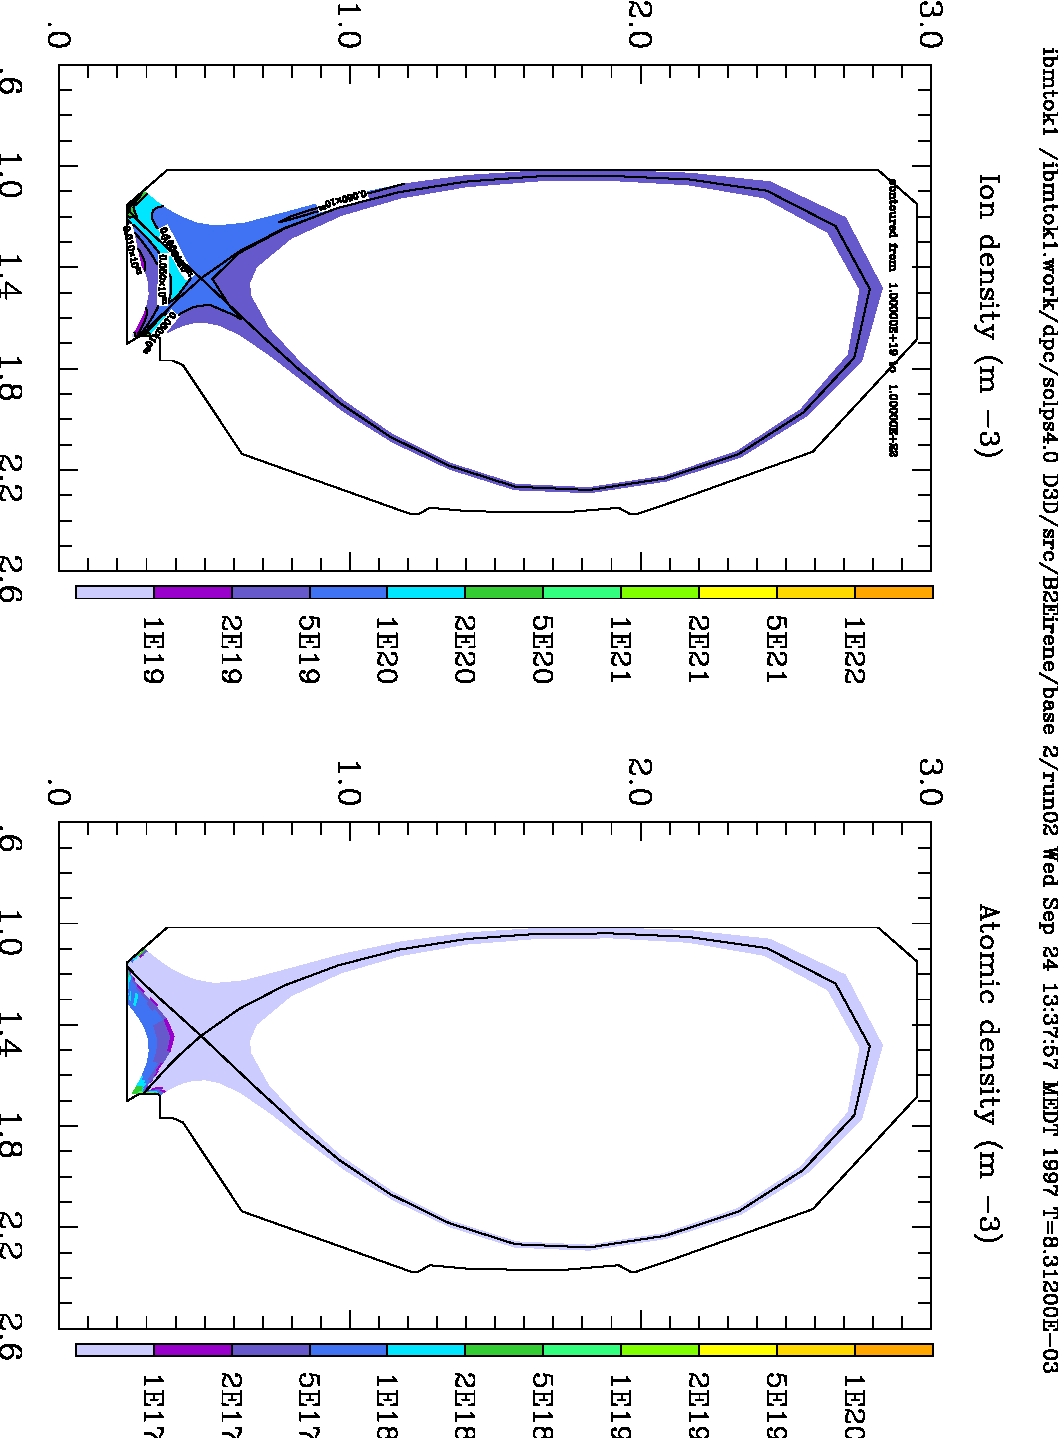
\includegraphics[angle=90,height=8cm]{b2plot_d3d.pdf}}
\else
    \centerline{
\includegraphics[angle=90,height=8cm]{b2plot_d3d.epsi}}
\fi
    \caption{Ion and atomic densities for DIII--D.}
    \label{fig:d3d}
\end{figure}

\subsubsection{cont}\index{b2plot, cont}\label{sec:cont}
Plots contour plots of the current data.  See figure \ref{fig:d3d}.
See section \ref{sec:contourparameters} for a list of commands that can be used to
change the appearance of contour plots.  Section \ref{sec:pageformat}
covers global changes to the plotting (square, landscape or portrait,
number of graphs per page). The use of {\bf surf} (see \ref{sec:surf}) is preferred
over that of {\bf cont}.

\subsubsection{$<$pos,{\bf I}$>$ f.x}\index{b2plot, f.x}\label{sec:f.x}
Plots the 2-D graph of the matrix data at $iy=<$pos$>$ versus $x$.
Vertical lines will be added to the plot to delimit any
eventual unconnected domain boundaries. Use of {\bf xpol} (default, see \ref{sec:xpol}) 
or {\bf xpar} (see \ref{sec:xpar}) commands allows one to toggle between plotting 
against poloidal or parallel distance along the field line. 

\subsubsection{$<$pos,{\bf I}$>$ f.y}\index{b2plot, f.y}\label{sec:f.y}
Plots the 2-D graph of the matrix data at $ix=<$pos$>$ versus $y$.
Use of the {\bf mmid} (see \ref{sec:mmid}) command allows for plotting versus the
outer midplane (or another position chosen by the user) radial coordinate.

\subsubsection{$<$n1,{\bf I}$>$ f.lx}\index{b2plot, f.lx}\label{sec:f.lx}
Plots the 2-D graph of the matrix data at $iy=<$pos$>$ versus $\log(x)$.
Equivalent to a combination of {\bf logx} (see \ref{sec:logx}) and {\bf f.x} above,
but remembers ths old setting of linear or logarithmic abscissa scale.

\subsubsection{$<$n1,{\bf I}$>$ f.ly}\index{b2plot, f.ly}\label{sec:f.ly}
Plots the 2-D graph of the matrix data at $ix=<$pos$>$ versus $\log(y)$.
Equivalent to a combination of {\bf logx} (see \ref{sec:logx}) and {\bf f.y} above,
but remembers ths old setting of linear or logarithmic abscissa scale.

\subsubsection{plwl}\index{b2plot, plwl}\label{sec:plwl}
Plots in the ``wall'' domain (applicable to wall data only).
This creates 2-D plots, with vertical lines separating
the various wall segments.

\subsubsection{$<$pos,{\bf I}$>$ trg.w}\index{b2plot, trg.w}\label{sec:trg.w}
Plots the 2-D graph of target data at $iz=<$pos$>$ versus wall coordinate.
Vertical lines will be added to the plot to delimit 
the various wall segments.  

\subsubsection{$<$pos,{\bf I}$>$ trg.z}\index{b2plot, trg.z}\label{sec:trg.z}
Plots the 2-D graph of target data at element $i=<$pos$>$ versus $z$.

\subsubsection{$<$n1,{\bf I}$>$ line}\index{b2plot, line}\label{sec:line}
Chooses between plotting against $x$-coordinate (default, $<$n1$>$=1)
or $y$-coordinate ($<$n1$>$=2). Not sure this works.

\subsubsection{mesh}\index{b2plot, mesh}\label{sec:mesh}
Plots the mesh. The colour of the mesh can be chosen 
with the {\bf mcol} (see \ref{sec:mcol}) command.

\subsubsection{surf}\index{b2plot, surf}\label{sec:surf}
Produces a ``patch'' plot where each cell is plotted in the
colour associated with its value.  This can be useful when the data is
noisy and contour plots take excessive time.  See figure \ref{fig:d3d}.
Recommended.

\subsubsection{trgsurf}\index{b2plot, trgsurf}\label{sec:trgsurf}
Produces a "patch" plot of the target domain.
Note that the side in contact with the plasma is at the bottom of the target computational domain.

\subsubsection{traj}\index{b2plot, traj}\label{sec:traj}\index{b2plot, uuse}\label{sec:uuse}\index{b2plot, vvse}\label{sec:vvse}\index{b2plot, t\_\#p}\label{sec:t_hashp}\index{b2plot, lint}\label{sec:lint}\index{b2plot, logt}\label{sec:logt}
\index{b2plot, trajectories plot}

Plots trajectories.  The following commands
\begin{verbatim}
echo phys a4p vesl sep outl 70 1 70 36 1000 traj | b2plot
\end{verbatim}
produced the results shown in figure \ref{fig:traj}.

\begin{figure}[hbtp]
\ifpdf 
    \centerline{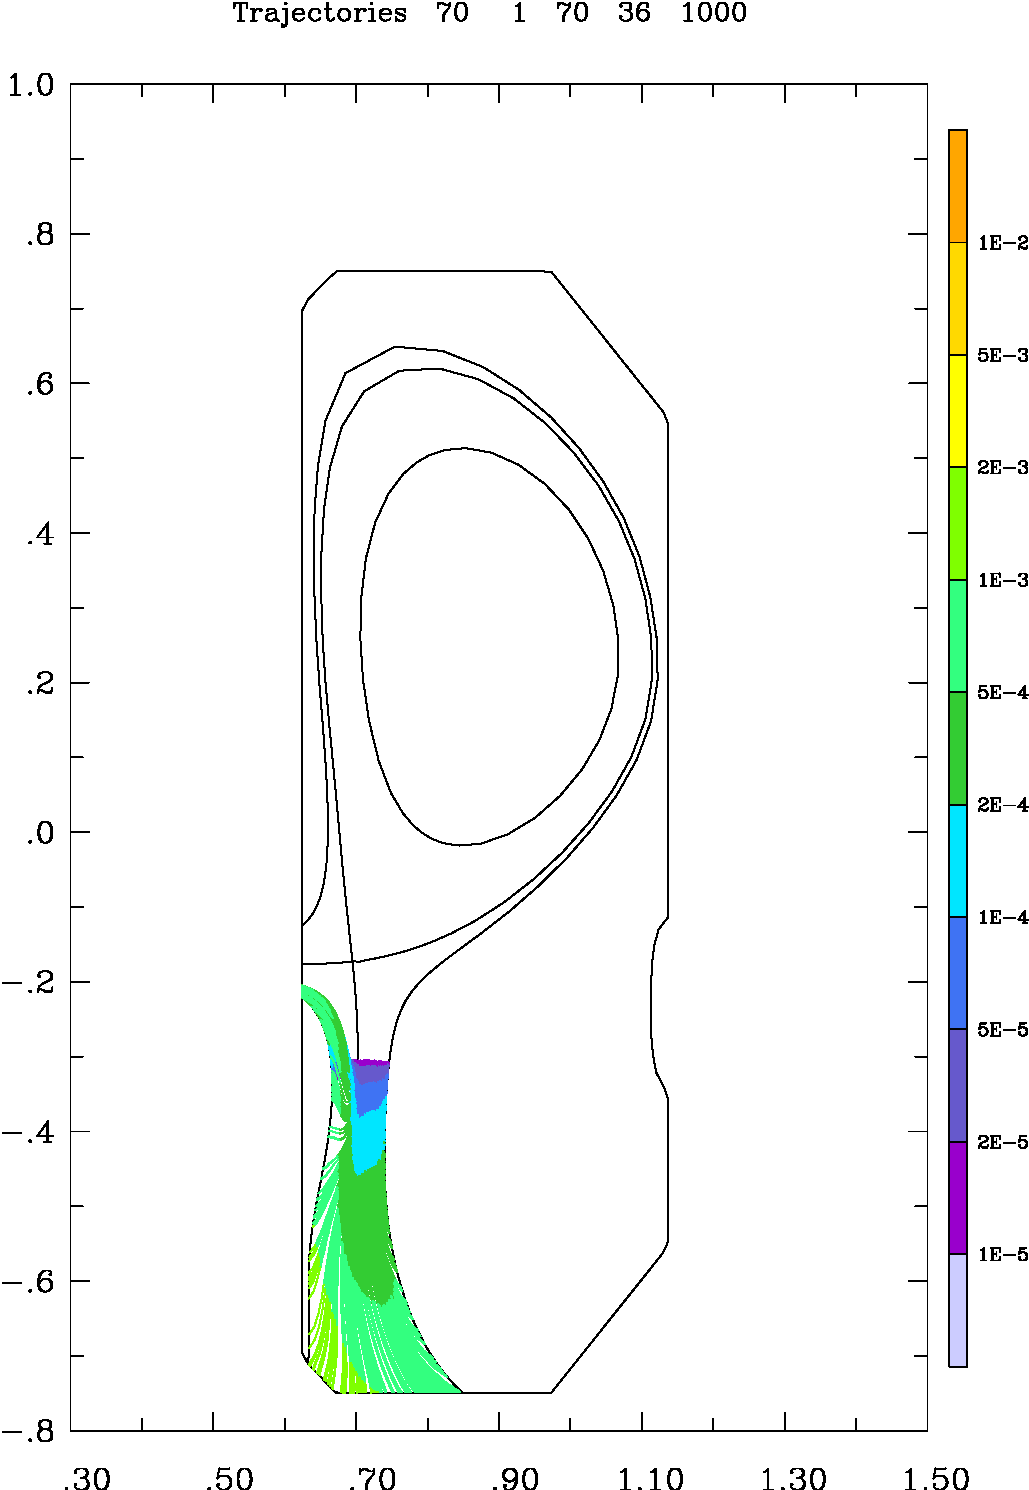
\includegraphics[height=8cm]{b2plot_70_1_70_36_1000.pdf}}
\else
    \centerline{
\includegraphics[height=8cm]{b2plot_70_1_70_36_1000.epsi}}
\fi
    \caption{Trajectory plot.}
    \label{fig:traj}
\end{figure}

The command seems to have changed since that example.  The command
takes a variable number of integer arguments, the minimum number being
8.

The first 4 numbers specify the bottom left and top right coordinates
of a rectangle in which the test particles are to be started
($ix_{start}~iy_{start}~ix_{end}~iy_{end}$) (0's will be replaced by the
appropriate limit).  The next number specifies the amount
of test particles to be started (if positive the particles are started
weighted by volume, if negative then the weighting function is taken
off the matrix stack).  This is then followed by a flag (1 for a
movie, otherwise normal trajectories), and then the species indices
come next.  The last argument specifies the number of species.
The use of {\bf uuse} and {\bf vvse} allows one to replace the particle velocities
matrices used by default to compute the trajectories with data from the
matrix stack.

The following example uses 2000 particles, weighted by particle
number, over the entire domain, for the 6 charge states of carbon.

\begin{verbatim}
stdl glob
a4p
phys 
-1.2 zmin 1.2 zmax
1.0 lbsz 0.005 dots
'rgb.pal' cltb 
vesl sep outl 
2000 t_#p 
1e-3 t_pt 
! b2nn b2in m+ 0.0 rmma
ni vol m*
0 0 0 0 -2000 1 2 3 4 5 6 7 6 traj 
drop
\end{verbatim}

From the code documentation:
\begin{verbatim}
C     This routine is used to plot trajectories of particles using the
C     velocity fields uutraj and vvtraj from B2SXDR. To call this routine
C     one must specify at least 8 parameters: ixmin, iymin, ixmax, iymax,
C     # of particles, 1 or 0 for movie or lines, species indices (at least
C     one), and last but not least the total number of species indices one 
C     has given in the step before. A valid call could be:
C     0 0 95 35 100 0 0 1 traj
C     This should plot the trajectories of 100 particles which start
C     in any of the cells between cell (0,0) (southwest corner) and
C     cell (95,35) (northeast corner) as lines for hydrogen (0=H).
C     Note that the cell and species indices start at zero!
C     The number of time steps (plots) is given by the "t_#p" command.
C     The total flight time of the particles is given by the "t_pt" command. 
C     The velocity fields uutraj and vvtraj can be overwritten using the
C     "uuse" and "vvse" commands. Their defaults values are ua and fna/na/sy
C     respectively. If the number of particles is positive, then the
C     particles are born randomly, with the probability of being born in a
C     cell being proportional to the cell volume. This probability weighting
C     can be changed by calling "traj" with a negative number of particles.
C     Then the weighting function is whatever field is on top of the matrix
C     stack. For example, this set of commands does the following:
C     fnax na m/ psx 0 zsel uuse  ! uutraj set to poloidal neutral flow velocity
C     fnay na m/ psy 0 zsel vvse  ! vvtraj set to radial neutral flow velocity
C     1000 t_#p                   ! 1000 time steps
C     1e-4 t_pt                   ! followed for a total time of 1.e-4 s.
C     na 0 zsel                   ! weighted with neutral density
C     0 0 0 0 -1000 0 0 1 traj    ! over the entire physical domain (0 0 0 0)
C               ! 1000 particles using non-default weighting function (-1000)
C               ! trajectories plotted (0)
C               ! for species 0 (=H neutrals) (0)
C               ! total of species considered is 1 (1)
C     =======================================================================
\end{verbatim}

The trajectories are coloured according to the length of time the particle has traveled
along it (illustrated by the label bar to the right of the graph). This label bar can
be set to be logarithmic (default) with the {\bf logt} command, or linear with the
{\bf lint} command.


\subsection{Data manipulating functions}\label{sec:datamanipulation}
\index{b2plot, data manipulation}

\subsubsection{abs}\index{b2plot, abs}\label{sec:abs}
Take the absolute value of the matrix data values.

\subsubsection{wabs}\index{b2plot, wabs}\label{sec:wabs}
Take the absolute value of the wall data values.

\subsubsection{trgabs}\index{b2plot, trgabs}\label{sec:trgabs}
Take the absolute value of the target data values.

\subsubsection{chs}\index{b2plot, chs}\label{sec:chs}
Change sign of matrix data.

\subsubsection{trgchs}\index{b2plot, trgchs}\label{sec:trgchs}
Change sign of target data.

\subsubsection{wchs}\index{b2plot, wchs}\label{sec:wchs}
Change sign of wall data.

\subsubsection{ddw}\index{b2plot, ddw}\label{sec:ddw}
Differentiates the wall data with respect to coordinate along wall perimeter.

\subsubsection{ddx}\index{b2plot, ddx}\label{sec:ddx}
Differentiates the matrix data with respect to poloidal coordinate $x$.

\subsubsection{ddy}\index{b2plot, ddy}\label{sec:ddy}
Differentiates the matrix data with respect to radial coordinate $y$.

\subsubsection{trgddp}\index{b2plot, trgddp}\label{sec:trgddp}
Differentiates the target data with respect to perpendicular coordinate.

\subsubsection{trgddw}\index{b2plot, trgddw}\label{sec:trgddw}
Differentiates the target data with respect to coordinate along wall perimeter.

\subsubsection{trgddz}\index{b2plot, trgddz}\label{sec:trgddz}
Differentiates the target data with respect to depth coordinate $z$.

\subsubsection{inttrgw}\index{b2plot, inttrgw}\label{sec:inttrgw}
Integrates data from the target stack along wall direction, summing over all wall segments.

\subsubsection{inttrgw*}\index{b2plot, inttrgw*}\label{sec:inttrgw*}
Integrates data from the target stack along wall direction, each segment being done separately.

\subsubsection{inttrgz}\index{b2plot, inttrgz}\label{sec:inttrgz}
Integrates data from the target stack in depth direction.

\subsubsection{intw}\index{b2plot, intw}\label{sec:intw}
Integrates data from the wall stack, summing over all wall segments.

\subsubsection{intw*}\index{b2plot, intw*}\label{sec:intw*}
Integrates data from the wall stack, each segment being done separately.

\subsubsection{intx}\index{b2plot, intx}\label{sec:intx}
Integrates data from the matrix stack along the $x$-direction, taking connectivities into account.

\subsubsection{inty}\index{b2plot, inty}\label{sec:inty}
Integrates data from the matrix stack along the $y$-direction.

\subsubsection{pne}\index{b2plot, pne}\label{sec:pne}
Divides the matrix data by the electron density $n_e$.

\subsubsection{pwne}\index{b2plot, pwne}\label{sec:pwne}
Divides the wall data by the local electron density $n_e$.

\subsubsection{pswa}\index{b2plot, pswa}\label{sec:pswa}
Divides the wall data by the wall element area.

\subsubsection{psx}\index{b2plot, psx}\label{sec:psx}
Divides the matrix data by $s_x$ --- the contact cell area between cells in the
$x$-direction.

\subsubsection{psxperp}\index{b2plot, psxperp}\label{sec:psxperp}
Divides the matrix data by $s_x$ --- the cell area perpendicular to the
$x$-direction.

\subsubsection{psy}\index{b2plot, psy}\label{sec:psy}
Divides the matrix data by $s_y$ --- the cell area perpendicular to the
$y$-direction.

\subsubsection{pvol}\index{b2plot, pvol}\label{sec:pvol}
Divides the matrix data by the volume of the cells.

\subsubsection{sumtrgw}\index{b2plot, sumtrgw}\label{sec:sumtrgw}
Sums the target data along the wall coordinate, and then copies the sum to all elements.

\subsubsection{sumtrgz}\index{b2plot, sumtrgz}\label{sec:sumtrgz}
Sums the target data depth-wise, and then copies the sum to all $z$-positions.

\subsubsection{sumw}\index{b2plot, sumw}\label{sec:sumw}
Sums the wall data, and then copies the sum to all elements.

\subsubsection{sumx}\index{b2plot, sumx}\label{sec:sumx}
Sums the matrix data over the entire $x$-direction, and then copies the sum to all $x$-positions.

\subsubsection{sumy}\index{b2plot, sumy}\label{sec:sumy}
Sums the matrix data over the entire $y$-direction, and then copies the sum to all $y$-positions.

\subsubsection{$<$is$_{start}$,{\bf I}$>$ $<$is$_{end}$,{\bf I}$>$ sumz}\index{b2plot, sumz}\label{sec:sumz}
Sums the matrix data over the $z$-direction from $<$is$_{start}$$>$ to $<$is$_{end}$$>$, and then copies the
sum to the first $z$ position. If $<$is$_{start}$$>$=$<$is$_{end}$$>$=0, then the sum is done
over all species.

\subsubsection{$<$is$_{start}$,{\bf I}$>$ $<$is$_{end}$,{\bf I}$>$ wsumz}\index{b2plot, wsumz}\label{sec:wsumz}
Sums the wall data over the $z$-direction from $<$is$_{start}$$>$ to $<$is$_{end}$$>$, and then copies the
sum to the first $z$ position. If $<$is$_{start}$$>$=$<$is$_{end}$$>$=0, then the sum is done
over all species.

\subsubsection{$<$is$_{start}$,{\bf I}$>$ $<$is$_{end}$,{\bf I}$>$ zrng}\index{b2plot, zrng}\label{sec:zrng}
Selects the subset over species extended from species index $<$is$_{start}$$>$ to
species index $<$is$_{end}$$>$ from the matrix data. 

\subsubsection{$<$is$_{start}$,{\bf I}$>$ $<$is$_{end}$,{\bf I}$>$ wzrng}\index{b2plot, wzrng}\label{sec:wzrng}
Selects the subset over species extended from species index $<$is$_{start}$$>$ to
species index $<$is$_{end}$$>$ from the wall data. 

\subsubsection{$<$i,{\bf I}$>$ wsel}\index{b2plot, wsel}\label{sec:wsel}
Propagates the wall data value from element $<$i$>$ to all other elements.

\subsubsection{$<$ix,{\bf I}$>$ xsel}\index{b2plot, xsel}\label{sec:xsel}
Propagates the matrix data value in the specified position $<$ix$>$ to all other $x$ values.

\subsubsection{$<$iy,{\bf I}$>$ ysel}\index{b2plot, ysel}\label{sec:ysel}
Propagates the matrix data value in the specified position $<$iy$>$ to all other $y$ values.

\subsubsection{$<$is,{\bf I}$>$ zsel}\index{b2plot, zsel}\label{sec:zsel}
Propagates the matrix data value in the specified position $<$is$>$ to all other $z$
(species) values.

\subsubsection{$<$i,{\bf I}$>$ trgwsel}\index{b2plot, trgwsel}\label{sec:trgwsel}
Propagates the target data value from the specified element $<$i$>$ to all other elements.

\subsubsection{$<$iz,{\bf I}$>$ trgzsel}\index{b2plot, trgzsel}\label{sec:trgzsel}
Propagates the target data value at the specified depth $<$iz$>$ to all other $z$ values.

\subsubsection{$<$is,{\bf I}$>$ wzsel}\index{b2plot, wzsel}\label{sec:wzsel}
Propagates the wall data value in the specified position $<$is$>$ to all other $z$
(species) values.

\subsubsection{rigz}\index{b2plot, rigz}\label{sec:rigz}
Toggles the inclusion of ignorable cells in the plots. The ignorable cells
are the guard cells at the boundaries and cells from isolated regions.

\subsubsection{log}\index{b2plot, log}\label{sec:log}
Computes logarithm base 10 of a matrix.

\subsubsection{ln}\index{b2plot, ln}\label{sec:ln}
Computes natural logarithm of a matrix.

\subsubsection{sqrt}\index{b2plot, sqrt}\label{sec:sqrt}
Takes square root of a matrix.

\subsubsection{exp}\index{b2plot, exp}\label{sec:exp}
Computes exponential of a matrix.

\subsubsection{trglog}\index{b2plot, trglog}\label{sec:trglog}
Computes logarithm base 10 of target data.

\subsubsection{trgln}\index{b2plot, trgln}\label{sec:trgln}
Computes natural logarithm of target data.

\subsubsection{trgsqrt}\index{b2plot, trgsqrt}\label{sec:trgsqrt}
Takes square root of target data.

\subsubsection{trgexp}\index{b2plot, trgexp}\label{sec:trgexp}
Computes exponential of target data.

\subsubsection{wlog}\index{b2plot, wlog}\label{sec:wlog}
Computes logarithm base 10 of wall data.

\subsubsection{wln}\index{b2plot, wln}\label{sec:wln}
Computes natural logarithm of wall data.

\subsubsection{wsqrt}\index{b2plot, wsqrt}\label{sec:wsqrt}
Takes square root of wall data.

\subsubsection{wexp}\index{b2plot, wexp}\label{sec:wexp}
Computes exponential of wall data.


\subsection{Arithmetic commands}\label{sec:arithmetic}
\index{b2plot, arithmetic commands}

\subsubsection{m+}\index{b2plot, m+}\label{sec:m+}
Adds the two arrays on the top of the matrix stack.

\subsubsection{m-}\index{b2plot, m-}\label{sec:m-}
Subtracts the array on the top of the matrix stack from the array second from
the top.

\subsubsection{m*}\index{b2plot, m*}\label{sec:m*}
Multiplies the two arrays on the top of the matrix stack.

\subsubsection{m/}\index{b2plot, m/}\label{sec:m/}
Divides the array secod from the top of the matrix stack by the array on
the top. Division by a zero element will yield zero.

\subsubsection{mmin}\index{b2plot, mmin}\label{sec:mmin}
Minimum of two top matrices on the stack.

\subsubsection{mmax}\index{b2plot, mmax}\label{sec:mmax}
Minimum of two top matrices on the stack.

\subsubsection{$<$r1,{\bf R}$>$ $<$r2,{\bf R}$>$ r+}\index{b2plot, r+}\label{sec:r+}
Adds the two real values $<$r1$>$ and $<$r2$>$ on the top of the real stack.

\subsubsection{$<$r1,{\bf R}$>$ $<$r2,{\bf R}$>$ r-}\index{b2plot, r-}\label{sec:r-}
Subtracts the real value on the top of the real stack $<$r2$>$ from the real value
second from the top $<$r1$>$.

\subsubsection{$<$r1,{\bf R}$>$ $<$r2,{\bf R}$>$ r*}\index{b2plot, r*}\label{sec:r*}
Multiplies the two real values $<$r1$>$ and $<$r2$>$ on the top of the real stack.

\subsubsection{$<$r1,{\bf R}$>$ $<$r2,{\bf R}$>$ r/}\index{b2plot, r/}\label{sec:r/}
Divides the real value second from the top of the real stack $<$r1$>$ by the real value on the top of the real stack $<$r2$>$. Division by 0 will yield an error and do nothing.

\subsubsection{$<$r1,{\bf R}$>$ $<$r2,{\bf R}$>$ r**}\index{b2plot, r**}\label{sec:r**}
Raises the real value second from the top of the real stack $<$r1$>$ to the power of
the real value on the top $<$r2$>$. $0^0$ will yield an error and do nothing.

\subsubsection{$<$number,{\bf R}$>$ rm+}\index{b2plot, rm+}\label{sec:rm+}
Adds $<$number$>$ to the array on the top of the matrix stack.

\subsubsection{$<$number,{\bf R}$>$ rm-}\index{b2plot, rm-}\label{sec:rm-}
Substracts $<$number$>$ from the array on the top of the matrix stack.

\subsubsection{$<$number,{\bf R}$>$ rm*}\index{b2plot, rm*}\label{sec:rm*}
Multiplies the array on the top of the matrix stack by $<$number$>$.

\subsubsection{$<$number,{\bf R}$>$ rm/}\index{b2plot, rm/}\label{sec:rm/}
Divides the array on the top of the matrix stack by $<$number$>$. Division by
zero will yield an error and do nothing.

\subsubsection{$<$number,{\bf R}$>$ rm**}\index{b2plot, rm**}\label{sec:rm**}
Raises each element of the array on the top of the matrix stack to the $<$number$>$-th power. If $<$number$>$=0, the result will be 1.0 for all cells.

\subsubsection{$<$number,{\bf R}$>$ rmmi}\index{b2plot, rmmi}\label{sec:rmmi}
Minimum of a matrix and $<$number$>$.

\subsubsection{$<$number,{\bf R}$>$ rmma}\index{b2plot, rmma}\label{sec:rmma}
Maximum of a matrix and $<$number$>$.

\subsubsection{$<$number,{\bf R}$>$ rtrgm+}\index{b2plot, rtrgm+}\label{sec:rtrgm+}
Adds $<$number$>$ to the array on the top of the target stack.

\subsubsection{$<$number,{\bf R}$>$ rtrgm-}\index{b2plot, rtrgm-}\label{sec:rtrgm-}
Substracts $<$number$>$ from the array on the top of the target stack.

\subsubsection{$<$number,{\bf R}$>$ rtrgm*}\index{b2plot, rtrgm*}\label{sec:rtrgm*}
Multiplies the array on the top of the target stack by $<$number$>$.

\subsubsection{$<$number,{\bf R}$>$ rtrgm/}\index{b2plot, rtrgm/}\label{sec:rtrgm/}
Divides the array on the top of the target stack by $<$number$>$. Division by
zero will yield an error and do nothing.

\subsubsection{$<$number,{\bf R}$>$ rtrgm**}\index{b2plot, rtrgm**}\label{sec:rtrgm**}
Raises each element of the array on the top of the target stack to the $<$number$>$-th power. If $<$number$>$=0, the result will be 1.0 for all elements.

\subsubsection{$<$number,{\bf R}$>$ rtrgmmi}\index{b2plot, rtrgmmi}\label{sec:rtrgmmi}
Minimum of target data and $<$number$>$.

\subsubsection{$<$number,{\bf R}$>$ rtrgmma}\index{b2plot, rtrgmma}\label{sec:rtrgmma}
Maximum of target data and $<$number$>$.

\subsubsection{$<$number,{\bf R}$>$ rwm+}\index{b2plot, rwm+}\label{sec:rwm+}
Adds $<$number$>$ to the array on the top of the wall stack.

\subsubsection{$<$number,{\bf R}$>$ rwm-}\index{b2plot, rwm-}\label{sec:rwm-}
Substracts $<$number$>$ from the array on the top of the wall stack.

\subsubsection{$<$number,{\bf R}$>$ rwm*}\index{b2plot, rwm*}\label{sec:rwm*}
Multiplies the array on the top of the wall stack by $<$number$>$.

\subsubsection{$<$number,{\bf R}$>$ rwm/}\index{b2plot, rwm/}\label{sec:rwm/}
Divides the array on the top of the wall stack by $<$number$>$. Division by
zero will yield an error and do nothing.

\subsubsection{$<$number,{\bf R}$>$ rwm**}\index{b2plot, rwm**}\label{sec:rwm**}
Raises each element of the array on the top of the wall stack to the $<$number$>$-th power. If $<$number$>$=0, the result will be 1.0 for all elements.

\subsubsection{$<$number,{\bf R}$>$ rwmmi}\index{b2plot, rwmmi}\label{sec:rwmmi}
Minimum of wall data and $<$number$>$.

\subsubsection{$<$number,{\bf R}$>$ rwmma}\index{b2plot, rwmma}\label{sec:rwmma}
Maximum of wall data and $<$number$>$.

\subsubsection{$<$number,{\bf R}$>$ meq}\index{b2plot, meq}\label{sec:meq}
If a matrix element is equal to $<$number$>$, sets this matrix element to 1.0.
Otherwise, sets it to zero.

\subsubsection{$<$number,{\bf R}$>$ mne}\index{b2plot, mne}\label{sec:mne}
If a matrix element is not equal to $<$number$>$, sets this matrix element to 1.0.
Otherwise, sets it to zero.

\subsubsection{$<$number,{\bf R}$>$ mge}\index{b2plot, mge}\label{sec:mge}
If a matrix element is greater than or equal to $<$number$>$, sets this matrix element to 1.0.
Otherwise, sets it to zero.

\subsubsection{$<$number,{\bf R}$>$ mgt}\index{b2plot, mgt}\label{sec:mgt}
If a matrix element is greater than $<$number$>$, sets this matrix element to 1.0.
Otherwise, sets it to zero.

\subsubsection{$<$number,{\bf R}$>$ mle}\index{b2plot, mle}\label{sec:mle}
If a matrix element is less than or equal to $<$number$>$, sets this matrix element to 1.0.
Otherwise, sets it to zero.

\subsubsection{$<$number,{\bf R}$>$ mlt}\index{b2plot, mlt}\label{sec:mlt}
If a matrix element is less than $<$number$>$, sets this matrix element to 1.0.
Otherwise, sets it to zero.

\subsubsection{pos}\index{b2plot, pos}\label{sec:pos}
If a matrix element is positive, sets this matrix element to 1.0.
Otherwise, sets it to zero.

\subsubsection{$<$i1,{\bf I}$>$ $<$i2,{\bf I}$>$ i+}\index{b2plot, i+}\label{sec:i+}
Adds the two integer values $<$i1$>$ and $<$i2$>$ on the top of the integer stack.

\subsubsection{$<$i1,{\bf I}$>$ $<$i2,{\bf I}$>$ i-}\index{b2plot, i-}\label{sec:i-}
Subtracts the integer value on the top of the integer stack $<$i2$>$ from the integer value
second from the top $<$i1$>$.

\subsubsection{$<$i1,{\bf I}$>$ $<$i2,{\bf I}$>$ i*}\index{b2plot, i*}\label{sec:i*}
Multiplies the two integer values $<$i1$>$ and $<$i2$>$ on the top of the integer stack.

\subsubsection{$<$i1,{\bf I}$>$ $<$i2,{\bf I}$>$ i/}\index{b2plot, i/}\label{sec:i/}
Divides the integer value second from the top of the integer stack $<$i1$>$ by the integer value on top of the integer stack $<$i2$>$. This is integer division! Division by 0 will yield an error and do nothing.

\subsubsection{$<$i1,{\bf I}$>$ $<$i2,{\bf I}$>$ i**}\index{b2plot, i**}\label{sec:i**}
Raises the integer value second from the top of the integer stack $<$i1$>$ to the power of
the integer value on the top $<$i2$>$. $0^0$ will yield an error and do nothing.

\subsubsection{$<$number,{\bf R}$>$ trgeq}\index{b2plot, trgeq}\label{sec:trgeq}
If a target element is equal to $<$number$>$, sets this target element to 1.0.
Otherwise, sets it to zero.

\subsubsection{$<$number,{\bf R}$>$ trgne}\index{b2plot, trgne}\label{sec:trgne}
If a target element is not equal to $<$number$>$, sets this target element to 1.0.
Otherwise, sets it to zero.

\subsubsection{$<$number,{\bf R}$>$ trgge}\index{b2plot, trgge}\label{sec:trgge}
If a target element is greater than or equal to $<$number$>$, sets this target element to 1.0.
Otherwise, sets it to zero.

\subsubsection{$<$number,{\bf R}$>$ trggt}\index{b2plot, trggt}\label{sec:trggt}
If a target element is greater than $<$number$>$, sets this target element to 1.0.
Otherwise, sets it to zero.

\subsubsection{$<$number,{\bf R}$>$ trgle}\index{b2plot, trgle}\label{sec:trgle}
If a target element is less than or equal to $<$number$>$, sets this target element to 1.0.
Otherwise, sets it to zero.

\subsubsection{$<$number,{\bf R}$>$ trglt}\index{b2plot, trglt}\label{sec:trglt}
If a target element is less than $<$number$>$, sets this target element to 1.0.
Otherwise, sets it to zero.

\subsubsection{trgmmin}\index{b2plot, trgmmin}\label{sec:trgmmin}
Minimum of two top matrices on the target stack.

\subsubsection{trgmmax}\index{b2plot, trgmmax}\label{sec:trgmmax}
Maximum of two top matrices on the target stack.

\subsubsection{trgm+}\index{b2plot, trgm+}\label{sec:trgm+}
Adds the two arrays on the top of the target stack.

\subsubsection{trgm-}\index{b2plot, trgm-}\label{sec:trgm-}
Subtracts the array on the top of the target stack from the array second from
the top.

\subsubsection{trgm*}\index{b2plot, trgm*}\label{sec:trgm*}
Multiplies the two arrays on the top of the target stack.

\subsubsection{trgm/}\index{b2plot, trgm/}\label{sec:trgm/}
Divides the array second from the top of the target stack by the array on the top.
Division by a zero element will yield zero.

\subsubsection{trgpos}\index{b2plot, trgpos}\label{sec:trgpos}
If a target element is positive, sets this target element to 1.0.
Otherwise, sets it to zero.

\subsubsection{wm+}\index{b2plot, wm+}\label{sec:wm+}
Adds the two arrays on the top of the wall stack.

\subsubsection{wm-}\index{b2plot, wm-}\label{sec:wm-}
Subtracts the array on the top of the wall stack from the array second from
the top.

\subsubsection{wm*}\index{b2plot, wm*}\label{sec:wm*}
Multiplies the two arrays on the top of the wall stack.

\subsubsection{wm/}\index{b2plot, wm/}\label{sec:wm/}
Divides the array second from the top of the wall stack by the array on 
the top. Division by a zero element will yield zero.

\subsubsection{wmmin}\index{b2plot, wmmin}\label{sec:wmmin}
Minimum of two top data sets on the wall stack.

\subsubsection{wmmax}\index{b2plot, wmmax}\label{sec:wmmax}
Minimum of two top data sets on the wall stack.

\subsubsection{$<$number,{\bf R}$>$ wmeq}\index{b2plot, wmeq}\label{sec:wmeq}
If a wall element is equal to $<$number$>$, sets this wall element to 1.0.
Otherwise, sets it to zero.

\subsubsection{$<$number,{\bf R}$>$ wmne}\index{b2plot, wmne}\label{sec:wmne}
If a wall element is not equal to $<$number$>$, sets this wall element to 1.0.
Otherwise, sets it to zero.

\subsubsection{$<$number,{\bf R}$>$ wmge}\index{b2plot, wmge}\label{sec:wmge}
If a wall element is greater than or equal to $<$number$>$, sets this wall element to 1.0.
Otherwise, sets it to zero.

\subsubsection{$<$number,{\bf R}$>$ wmgt}\index{b2plot, wmgt}\label{sec:wmgt}
If a wall element is greater than $<$number$>$, sets this wall element to 1.0.
Otherwise, sets it to zero.

\subsubsection{$<$number,{\bf R}$>$ wmle}\index{b2plot, wmle}\label{sec:wmle}
If a wall element is less than or equal to $<$number$>$, sets this wall element to 1.0.
Otherwise, sets it to zero.

\subsubsection{$<$number,{\bf R}$>$ wmlt}\index{b2plot, wmlt}\label{sec:wmlt}
If a wall element is less than $<$number$>$, sets this wall element to 1.0.
Otherwise, sets it to zero.

\subsubsection{wpos}\index{b2plot, wpos}\label{sec:wpos}
If a wall element is positive, sets this wall element to 1.0.
Otherwise, sets it to zero.


\subsection{Stack manipulating commands}\label{sec:stack}
\index{b2plot, stack manipulation}

\subsubsection{drop}\index{b2plot, drop}\label{sec:drop}
Deletes the array on the top of the matrix stack.

\subsubsection{dup}\index{b2plot, dup}\label{sec:dup}
Duplicates the array on the top of the matrix stack.

\subsubsection{swap}\index{b2plot, swap}\label{sec:swap}
Swaps the top two arrays on the matrix stack.

\subsubsection{over}\index{b2plot, over}\label{sec:over}
Copies the array second from the top to the top of the matrix stack.

\subsubsection{list}\index{b2plot, list}\label{sec:list}
Lists the contents of the matrix stack by printing the titles
of the stored matrices to \verb!stdout!.

\subsubsection{mdims}\index{b2plot, mdims}\label{sec:mdims}
Prints the dimensions and contents (i.e. data set titles) of the matrix
stack to \verb!stdout!.

\subsubsection{rdrop}\index{b2plot, rdrop}\label{sec:rdrop}
Deletes the real on the top of the real stack.

\subsubsection{rdup}\index{b2plot, rdup}\label{sec:rdup}
Duplicates the real on the top of the real stack.

\subsubsection{rswap}\index{b2plot, rswap}\label{sec:rswap}
Swaps the top two reals on the real stack.

\subsubsection{rover}\index{b2plot, rover}\label{sec:rover}
Copies the real second from the top to the top of the real stack.

\subsubsection{rtostr}\index{b2plot, rtostr}\label{sec:rtostr}
Writes the real on top of the real stack to the top of the string stack.

\subsubsection{rtom}\index{b2plot, rtom}\label{sec:rtom}
Copies the real on top of the real stack to the top of the matrix stack.

\subsubsection{rtow}\index{b2plot, rtow}\label{sec:rtow}
Copies the real on top of the real stack to the top of the wall stack.

\subsubsection{rtot}\index{b2plot, rtot}\label{sec:rtot}
Copies the real on top of the real stack to the top of the target stack.

\subsubsection{rprt}\index{b2plot, rprt}\label{sec:rprt}
Outputs the contents of the real stack to \verb:stdout:, and to \verb:b2plot.write: 
(in the \SOLPSfour environment) or \verb:b2pl.exe.dir/b2plot.write: 
(in the \SOLPSfive environment) if {\bf writ} is active.

\subsubsection{idrop}\index{b2plot, idrop}\label{sec:idrop}
Deletes the integer on the top of the integer stack.

\subsubsection{idup}\index{b2plot, idup}\label{sec:idup}
Duplicates the integer on the top of the integer stack.

\subsubsection{iswap}\index{b2plot, iswap}\label{sec:iswap}
Swaps the top two integers on the integer stack.

\subsubsection{iover}\index{b2plot, iover}\label{sec:iover}
Copies the integer second from the top to the top of the integer stack.

\subsubsection{itor}\index{b2plot, itor}\label{sec:itor}
Copies the integer on top of the integer stack to the top of the real stack.

\subsubsection{itostr}\index{b2plot, itostr}\label{sec:itostr}
Writes the integer on top of the integer stack to the top of the string stack.

\subsubsection{itom}\index{b2plot, itom}\label{sec:itom}
Copies the integer on top of the integer stack to the top of the matrix stack.

\subsubsection{itow}\index{b2plot, itow}\label{sec:itow}
Copies the integer on top of the integer stack to the top of the wall stack.

\subsubsection{itot}\index{b2plot, itot}\label{sec:itot}
Copies the integer on top of the integer stack to the top of the target stack.

\subsubsection{iprt}\index{b2plot, iprt}\label{sec:iprt}
Outputs the contents of the integer stack to \verb:stdout:, and to \verb:b2plot.write: 
(in the \SOLPSfour environment) or \verb:b2pl.exe.dir/b2plot.write: 
(in the \SOLPSfive environment) if {\bf writ} is active.

\subsubsection{scat}\index{b2plot, scat}\label{sec:scat}
Concatenates the top two strings of the string stack.

\subsubsection{sdrop}\index{b2plot, sdrop}\label{sec:sdrop}
Deletes the string on the top of the string stack.

\subsubsection{sdup}\index{b2plot, sdup}\label{sec:sdup}
Duplicates the string on the top of the string stack.

\subsubsection{sswap}\index{b2plot, sswap}\label{sec:sswap}
Swaps the top two strings on the string stack.

\subsubsection{sover}\index{b2plot, sover}\label{sec:sover}
Copies the string second from the top to the top of the string stack.

\subsubsection{sprt}\index{b2plot, sprt}\label{sec:sprt}
Outputs the contents of the string stack to \verb:stdout:, and to \verb:b2plot.write: 
(in the \SOLPSfour environment) or \verb:b2pl.exe.dir/b2plot.write: 
(in the \SOLPSfive environment) if {\bf writ} is active.

\subsubsection{$<$nx,{\bf I}$>$ $<$ny,{\bf I}$>$ $<$filename,{\bf S}$>$ saw}\index{b2plot, saw}\label{sec:saw}
Reads the matrix of size $(<$nx$>+2) \times (<$ny$>+2)$ from file $<$filename$>$ into the
matrix stack.

\subsubsection{$<$nx,{\bf I}$>$ $<$ny,{\bf I}$>$ $<$nz,{\bf I}$>$ $<$filename,{\bf S}$>$ saws}\index{b2plot, saws}\label{sec:saws}
Reads the matrix of size $(<$nx$>+2) \times (<$ny$>+2) \times nz$ from file $<$filename$>$ into the
matrix stack. Expects $nz$ to match $ns$ and that the data refers to the fluid plasma species.

\subsubsection{$<$nx,{\bf I}$>$ $<$ny,{\bf I}$>$ $<$nz,{\bf I}$>$ $<$filename,{\bf S}$>$ sawx}\index{b2plot, sawx}\label{sec:sawx}
Reads the matrix of size $(<$nx$>+2) \times (<$ny$>+2) \times nz$ from file $<$filename$>$ into the
matrix stack. Expects $nz$ to match $ns\_ext$ and that the data refers to the additional species followed by the
external code to which {\bf SOLPS} is coupled.

\subsubsection{$<$nwall,{\bf I}$>$ $<$filename,{\bf S}$>$ wsaw}\index{b2plot, wsaw}\label{sec:wsaw}
Reads the array of size $<$nwall$>$ from file $<$filename$>$ into the wall stack.

\subsubsection{stow}\index{b2plot, stow}\label{sec:stow} 
Copies the array on top of the matrix stack to the wall data stack. Only the matrix
elements from boundary cells will be copied over, onto the corresponding wall elements.

\subsubsection{trgdrop}\index{b2plot, trgdrop}\label{sec:trgdrop}
Deletes the array on the top of the target stack.

\subsubsection{trgdup}\index{b2plot, trgdup}\label{sec:trgdup}
Duplicates the array on the top of the target stack.

\subsubsection{trgswap}\index{b2plot, trgswap}\label{sec:trgswap}
Swaps the top two arrays on the target stack.

\subsubsection{trgover}\index{b2plot, trgover}\label{sec:trgover}
Copies the array second from the top to the top of the target stack.

\subsubsection{trglist}\index{b2plot, trglist}\label{sec:trglist}
Lists the contents of the target stack by printing the titles
of the stored matrices to \verb!stdout!.

\subsubsection{trgtow}\index{b2plot, trgtow}\label{sec:trgtow} 
Copies the matrix on top of the target data stack onto the wall data stack. Only the
top surface target data values will be copied onto the corresponding wall elements.

\subsubsection{wdrop}\index{b2plot, wdrop}\label{sec:wdrop}
Deletes the array on the top of the wall stack.

\subsubsection{wdup}\index{b2plot, wdup}\label{sec:wdup}
Duplicates the array on the top of the wall stack.

\subsubsection{wswap}\index{b2plot, wswap}\label{sec:wswap}
Swaps the top two arrays on the wall stack.

\subsubsection{wover}\index{b2plot, wover}\label{sec:wover}
Copies the array second from the top to the top of the wall stack.

\subsubsection{wlist}\index{b2plot, wlist}\label{sec:wlist}
Lists the contents of the wall stack by printing the titles
of the stored matrices to \verb!stdout!.

\subsubsection{wtos}\index{b2plot, wtos}\label{sec:wtos} 
Copies the array on top of the wall data stack onto the matrix stack. Each wall element
value is copied onto the corresponding boundary cell in the matrix stack. Inner cells
of the matrix stack will contain zero.

\subsubsection{wtot}\index{b2plot, wtot}\label{sec:wtot} 
Copies the array on top of the wall data stack onto the target stack. Each wall element
value is copied onto the corresponding column of cells in the target stack. 

\subsubsection{$<$ix,{\bf I}$>$ xtow}\index{b2plot, xtow}\label{sec:xtow} 
Copies the data from the $ix$-th row of the array on top of the matrix stack to the wall data stack.

\subsubsection{$<$iy,{\bf I}$>$ ytow}\index{b2plot, ytow}\label{sec:ytow} 
Copies the data from the $iy$-th column of the array on top of the matrix stack to the wall data stack.


\subsection{Page format parameters}\label{sec:pageformat}
\index{b2plot, page format commands}

\subsubsection{a4l}\index{b2plot, a4l}\label{sec:a4l}
Sets the plot area for A4 landscape. Use ``ctrans -d ps.mono.land |
a4page | lpr''.

\subsubsection{a4p}\index{b2plot, a4p}\label{sec:a4p}
Sets the plot area for A4 portrait.  Use ``ctrans -d ps.mono | a4page |
lpr''.

\subsubsection{sq}\index{b2plot, sq}\label{sec:sq}
Sets the plot area to be square. This ensures that the$x$ and $y$ scaling factors are the same.

\subsubsection{$<$nx,{\bf I}$>$ $<$ny,{\bf I}$>$ page}\index{b2plot, page}\label{sec:page}
Plots $<$nx$>$ graphs in the $x$-direction and $<$ny$>$ in the $y$-direction on the same page.


\subsection{Graph format commands}\index{b2plot, graphformat}\label{sec:graphformat}
\index{b2plot, graph format commands}

\subsubsection{both}\index{b2plot, both}\label{sec:both}
Plots on both the physical and computational meshes.

\subsubsection{comp}\index{b2plot, comp}\label{sec:comp}
Plots on computational mesh only.

\subsubsection{phys}\index{b2plot, phys}\label{sec:phys}
Plots on the physical mesh only.

\subsubsection{aspc}\index{b2plot, aspc}\label{sec:aspc}
Toggles whether aspect ratio should be preserved for physical 
and computational domain plots (default \verb!.true.!). 
If \verb!.false.!, the plot region limits will be those defined
from the $xmin~xmax~ymin~ymax$, etc... values.

\subsubsection{linf}\index{b2plot, linf}\label{sec:linf}
Sets linear scaling for the function values (default).

\subsubsection{logf}\index{b2plot, logf}\label{sec:logf}
Sets logarithmic scaling for the function values.

\subsubsection{lintrg}\index{b2plot, lintrg}\label{sec:lintrg}
Sets linear scaling for the target data values (default).

\subsubsection{logtrg}\index{b2plot, logtrg}\label{sec:logtrg}
Sets logarithmic scaling for the target data values.

\subsubsection{linxtrg}\index{b2plot, linxtrg}\label{sec:linxtrg}
Sets linear abscissae for the target data values (default).

\subsubsection{logxtrg}\index{b2plot, logxtrg}\label{sec:logxtrg}
Sets logarithmic abscissae scaling for the target data values.

\subsubsection{linx}\index{b2plot, linx}\label{sec:linx}
Sets linear scaling for the abscissae values (default).

\subsubsection{logx}\index{b2plot, logx}\label{sec:logx}
Sets logarithmic scaling for the abscissae values.

\subsubsection{xpar}\index{b2plot, xpar}\label{sec:xpar}
Plots 2-D plots against parallel $x$ distance.

\subsubsection{xpol}\index{b2plot, xpol}\label{sec:xpol}
Plots 2-D plots against poloidal $x$ distance (default).

\subsubsection{$<$n,{\bf I}$>$ ndec}\index{b2plot, ndec}\label{sec:ndec}
Sets number of decades to $<$n$>$ for logarithmic plots (default 10). 
If $n = 0$, restores the default value.

\subsubsection{mmid}\index{b2plot, mmid}\label{sec:mmid}
Toggles mapping to midplane coordinate for 2-D plots. The midplane
is assumed to be located at $ix=jxa$. See commands {\bf omp} (section \ref{sec:omp}) and 
{\bf jxa} (section \ref{sec:omp}) for setting and knowing its value.


\subsection{Graph appearance commands}\label{sec:graphappearance}
\index{b2plot, graph appearance commands}

\subsubsection{bw}\index{b2plot, bw}\label{sec:bw}
Want black and white for some plots.

\subsubsection{col}\index{b2plot, col}\label{sec:col}
Want colour for some plots.

\subsubsection{$<$number,{\bf I}$>$ font}\index{b2plot, font}\label{sec:font}
Changes the current font type to $<$number$>$
\begin{itemize}
\item -25 TIMES ROMAN
\item -26 TIMES BOLD
\item -21 HELVETICA
\item -22 HELVETICA BOLD
\item -29 COURIER
\item -30 COURIER BOLD
\end{itemize}
There are even more available fonts --- refer to \verb!NCAR! manpage.

In general, it is possible to change fonts within a text string to be printed
on the graph, for the commands below taking a string as argument. For example,
the command
\begin{verbatim}
'D-\\Ga\\R (photons m^{-3} s^{-1})' extl
\end{verbatim}
would give an extra graph label containing ``D-$\alpha$ (photons m$^{-3}$ s$^{-1}$)''.

\subsubsection{stdl}\index{b2plot, stdl}\label{sec:stdl}
Sets standard label as {\em extralabel}:
\begin{verbatim}
'\${HOST} \${PWD} `date` T=\${TIME}'
\end{verbatim}

\subsubsection{$<$label, {\bf S}$>$ glbl}\index{b2plot, glbl}\label{sec:glbl}
Sets the current graph label to $<$label$>$.

\subsubsection{$<$number,{\bf I}$>$ $<$label, {\bf S}$>$ slbl}\index{b2plot, slbl}\label{sec:slbl}
Sets the species label of species index $<$number$>$ to $<$label$>$ for the current graph.

\subsubsection{$<$label, {\bf S}$>$ tlbl}\index{b2plot, tlbl}\label{sec:tlbl}
Sets the current target graph label to $<$label$>$.

\subsubsection{$<$label, {\bf S}$>$ trgblbl}\index{b2plot, trgblbl}\label{sec:trgblbl}
Sets the current target bar label to $<$label$>$.

\subsubsection{$<$label, {\bf S}$>$ wlbl}\index{b2plot, wlbl}\label{sec:wlbl}
Sets the current wall graph label to $<$label$>$.

\subsubsection{$<$number,{\bf I}$>$ $<$label, {\bf S}$>$ wslbl}\index{b2plot, wslbl}\label{sec:wslbl}
Sets the species label of species index $<$number$>$ to $<$label$>$ for the current wall graph.

\subsubsection{$<$label, {\bf S}$>$ wallblbl}\index{b2plot, wallblbl}\label{sec:wallblbl}
Sets the current wall bar label to $<$label$>$.

\subsubsection{glob}\index{b2plot, glob}\label{sec:glob}
Copies the contents of {\em extralabel} into the global header for all graphs.

\subsubsection{$<$factor,{\bf R}$>$ lbsz}\index{b2plot, lbsz}\label{sec:lbsz}
Sets label size to $<$factor$>$ times default size (default = 1.0).

\subsubsection{$<$number,{\bf I}$>$ lfsz}\index{b2plot, lfsz}\label{sec:lfsz}
Sets line label font size to $<$number$>$ (default = 0). If $<$number$>$ is between 0 and 3, then the size
represents 1., 1.5, 2., and 3. times an 8-plotter address unit width. Otherwise, it represents the character 
width in plotter address units.

\subsubsection{noax}\index{b2plot, noax}\label{sec:noax}
Does not plot axes.

\subsubsection{$<$factor,{\bf R}$>$ lwid}\index{b2plot, lwid}\label{sec:lwid}
Changes line width to $<$factor$>$ times default width.

\subsubsection{same}\index{b2plot, same}\label{sec:same}
The next graphs occur on the same set of axes.  Terminated with {\bf new}.

\subsubsection{new}\index{b2plot, new}\label{sec:new}
Starts graphs on a new set of axes.


\subsection{Overlays to contour and line plots}\label{sec:contouroverlays}
\index{b2plot, contour overlays}

\subsubsection{zero}\index{b2plot, zero}\label{sec:zero}
Toggles the plotting of dotted axes lines at zero.

\subsubsection{$<$factor,{\bf R}$>$ zwid}\index{b2plot, zwid}\label{sec:zwid}
Changes width of dotted axes lines at zero to $<$factor$>$ times default width.

\subsubsection{$<$ncol,{\bf I}$>$ zcol}\index{b2plot, zcol}\label{sec:zcol}\index{b2plot, colour table}
Plots axes line at zero with colour $<$ncol$>$ (default 1). The colours available by default are:
\begin{enumerate}
  \item[ 0] White (background)
  \item[ 1] Black (default)
  \item[ 2] Lavender
  \item[ 3] Dark Violet
  \item[ 4] Slate Blue
  \item[ 5] Royal Blue
  \item[ 6] Deep Sky Blue
  \item[ 7] Aqua
  \item[ 8] Green
  \item[ 9] Celeste
  \item[10] Chartreuse
  \item[11] Green Yellow
  \item[12] Yellow
  \item[13] Golden
  \item[14] Orange
  \item[15] Orange Red
  \item[16] Red
  \item[17] Orchid
\end{enumerate}
These values can be overridden by use of the {\bf cltb} command.

\subsubsection{$<$ncol,{\bf I}$>$ dcol}\index{b2plot, dcol}\label{sec:dcol}
Colour to be used for matrix data line plots (default 1). 
If {\bf dcol} is set to a negative value, the data plot lines will use
a succession of colours starting from $|dcol|$ with increasing index.
See {\bf zcol} above for a list of available colours.

\subsubsection{$<$ncol,{\bf I}$>$ tcol}\index{b2plot, tcol}\label{sec:tcol}
Colour to be used for target data line plots (default 1). 
If {\bf tcol} is set to a negative value, the data plot lines will use
a succession of colours starting from $|tcol|$ with increasing index.
See {\bf zcol} above for a list of available colours.

\subsubsection{$<$ncol,{\bf I}$>$ wcol}\index{b2plot, wcol}\label{sec:wcol}
Colour to be used for wall data line plots (default 1). 
If {\bf wcol} is set to a negative value, the data plot lines will use
a succession of colours starting from $|wcol|$ with increasing index.
See {\bf zcol} above for a list of available colours.

\subsubsection{$<$ncol,{\bf I}$>$ bcol}\index{b2plot, bcol}\label{sec:bcol}
Colour to be used for printing label bar title (default 1). 
See {\bf zcol} above for a list of available colours.

\subsubsection{$<$ncol,{\bf I}$>$ gcol}\index{b2plot, gcol}\label{sec:gcol}
Colour to be used for printing graph title (default 1). 
See {\bf zcol} above for a list of available colours.

\subsubsection{$<$ncol,{\bf I}$>$ hcol}\index{b2plot, hcol}\label{sec:hcol}
Colour to be used for printing global header (default 1). 
See {\bf zcol} above for a list of available colours.

\subsubsection{$<$ncol,{\bf I}$>$ xcol}\index{b2plot, xcol}\label{sec:xcol}
Colour to be used for printing extra label (default 1). 
See {\bf zcol} above for a list of available colours.

\subsubsection{$<$length,{\bf R}$>$ arow}\index{b2plot, arow}\label{sec:arow}\index{b2plot, arox}\label{sec:arox}\index{b2plot, aroy}\label{sec:aroy}
Produces flow chart of array {\em fnax} and {\em fnay} using a maximum arrow
length of $<$length$>$ meters. The use of {\em fnax} and {\em fnay} can be superseded
by the the commands {\bf arox} and {\bf aroy}, respectively, which will then use
data from the matrix stack for computing the arrow directions instead.

\subsubsection{$<$widthfactor,{\bf R}$>$ arww}\index{b2plot, arww}\label{sec:arww}
Changes default arrow width by $<$widthfactor$>$ (default 1.0).

\subsubsection{$<$ncol,{\bf I}$>$ acol}\index{b2plot, acol}\label{sec:acol}
Plots overlaid arrows with colour $<$ncol$>$ (default 1). 
See {\bf zcol} above for a list of available colours.

\subsubsection{$<$data file,{\bf S}$>$ expf}\index{b2plot, expf}\label{sec:expf}
File from which to take experimental data to be plotted with code data.

\subsubsection{expl}\index{b2plot, expl}\label{sec:expl}
Toggles between plotting the experimental data as a line (default) or as a scatter plot.

\subsubsection{$<$expsymbol,{\bf I}$>$ exps}\index{b2plot, exps}\label{sec:exps}
Choice of the symbol to be used forthe experimental data scatter plots (default 5).
The numbering convention is the same as used in the \verb!libgr! library from \verb!Eirene!.

\subsubsection{$<$data file,{\bf S}$>$ wallf}\index{b2plot, wallf}\label{sec:wallf}
File from which to take experimental data to be plotted with wall data.

\subsubsection{$<$ncol,{\bf I}$>$ ecol}\index{b2plot, ecol}\label{sec:ecol}
Plots experimental data overlay with colour $<$ncol$>$ (default 1). 
If {\bf ecol} is set to a negative value, the data plot lines will use
a succession of colours starting from $|ecol|$ with increasing index.
See {\bf zcol} above for a list of available colours.

\subsubsection{$<$widthfactor,{\bf R}$>$ ewid}\index{b2plot, ewid}\label{sec:ewid}
Changes the experimental data overlay line width by $<$widthfactor$>$ (default 1.0). 

\subsubsection{$<$n,{\bf I}$>$ ytra}\index{b2plot, ytra}\label{sec:ytra}
Choose transformation function ($<$n$>$.ne.0) for radial
coordinate to compare with experimental data, according to
\verb!n.s.r.z.a_inner! and \verb!n.s.r.z.a_outer!
files in the \$\verb!SOLPSTOP/data.local! or \$\verb!SOLPSTOP/data! 
directories.

\subsubsection{sep}\index{b2plot, sep}\label{sec:sep}
Toggles drawing of the separatrices.

\subsubsection{$<$ncol,{\bf I}$>$ scol}\index{b2plot, scol}\label{sec:scol}
Plots separatrices with colour $<$ncol$>$ (default 1).
Also applies to the vertical separators drawn for 2-D plots.
See {\bf zcol} above for a list of available colours.

\subsubsection{$<$widthfactor,{\bf R}$>$ sepw}\index{b2plot, sepw}\label{sec:sepw}
Changes the default width of the separatrices line by $<$widthfactor$>$ (default 1.0). 
Also applies to the vertical separators drawn for 2-D plots.

\subsubsection{vesl}\index{b2plot, vesl}\label{sec:vesl}
Toggles drawing of the outline of vacuum vessel. 
The data for this option is obtained from the file \verb!mesh.extra! if it exists. 
If the \verb!mesh.extra! file is not found, does nothing.

\subsubsection{$<$ncol,{\bf I}$>$ vcol}\index{b2plot, vcol}\label{sec:vcol}
Plots overlaid vacuum vessel outline with colour $<$ncol$>$ (default 1).
See {\bf zcol} above for a list of available colours.

\subsubsection{$<$widthfactor,{\bf R}$>$ vwid}\index{b2plot, vwid}\label{sec:vwid}
Changes the default width of the vessel outline by $<$widthfactor$>$ (default 1.0). 

\subsubsection{grid}\index{b2plot, grid}\label{sec:grid}
Toggles drawing of overlaid mesh.

\subsubsection{$<$ncol,{\bf I}$>$ mcol}\index{b2plot, mcol}\label{sec:mcol}
Sets colour of overlaid mesh to $<$ncol$>$ (default 1).
See {\bf zcol} above for a list of available colours.

\subsubsection{outl}\index{b2plot, outl}\label{sec:outl}
Toggles plotting of plasma domain outline.
When target elements overlays are also plotted, then the target elements outline is activated as well.

\subsubsection{$<$ncol,{\bf I}$>$ ocol}\index{b2plot, ocol}\label{sec:ocol}
Sets colour of overlaid plasma outline to $<$ncol$>$ (default 1).
See {\bf zcol} above for a list of available colours.

\subsubsection{$<$widthfactor,{\bf R}$>$ owid}\index{b2plot, owid}\label{sec:owid}
Changes the default width of the overlaid plasma outline by $<$widthfactor$>$ (default 1.0). 

\subsubsection{wall}\index{b2plot, wall}\label{sec:wall}
Toggles plotting of additional wall data.

\subsubsection{woff}\index{b2plot, woff}\label{sec:woff}
Turns off plotting of additional wall data (default).

\subsubsection{$<$widthfactor,{\bf R}$>$ wwid}\index{b2plot, wwid}\label{sec:wwid}
Changes the default width of the wall data overlay line by $<$widthfactor$>$ (default 10.0).

\subsubsection{logw}\index{b2plot, logw}\label{sec:logw}
Selects logarithmic scale for wall plots.

\subsubsection{linw}\index{b2plot, linw}\label{sec:linw}
Selects linear scale for wall plots (default).

\subsubsection{logxw}\index{b2plot, logxw}\label{sec:logxw}
Selects logarithmic abscissae for wall plots.

\subsubsection{linxw}\index{b2plot, linxw}\label{sec:linxw}
Selects linear abscissae for wall plots (default).

\subsubsection{target}\index{b2plot, target}\label{sec:target}
Turns on plotting of additional target data.

\subsubsection{trgoff}\index{b2plot, trgoff}\label{sec:trgoff}
Turns off plotting of additional target data (default).


\subsection{Changing contour parameters}\label{sec:contourparameters}
\index{b2plot, contour parameters}

\subsubsection{nocp}\index{b2plot, nocp}\label{sec:nocp}
Does not plot contour plot.

\subsubsection{$<$level$_{min}$,{\bf R}$>$ $<$level$_{max}$,{\bf R}$>$ $<$delta,{\bf R}$>$ clvd}\index{b2plot, clvd}\label{sec:clvd}
Starts contour levels at $<$level$_{min}$$>$ increasing by $<$delta$>$ up
to $<$level$_{max}$$>$.

\subsubsection{$<$level$_{min}$,{\bf R}$>$ $<$level$_{max}$,{\bf R}$>$ $<$n,{\bf I}$>$ clvn}\index{b2plot, clvn}\label{sec:clvn}
Produces $<$n$>$ contour levels going from $<$level$_{min}$$>$ to $<$level$_{max}$$>$.

\subsubsection{$<$n,{\bf I}$>$ $<$level$_1$,{\bf R}$>$ ... $<$level$_n$,{\bf R}$>$ clvs}\index{b2plot, clvs}\label{sec:clvs}
Sets $<$n$>$ contour levels to the values specified by $<$label$_i$$>$.

\begin{verbatim}
0 clvs
\end{verbatim}
can be used to go back to the default contour labelling scheme after use
of {\bf clvd}, {\bf clvn}, {\bf clvp} or {\bf clvs}.

\subsubsection{$<$npplvm,{\bf I}$>$ $<$npplvp,{\bf I}$>$ clvp}\index{b2plot, clvp}\label{sec:clvp}
Sets up contour levels according to their proportion inside the plasma domain.
The levels are arranged so that the integral of the absolute value of 
the data over the region between each two neighbouring level lines is the same.
If $<$npplvm$>$.lt.0, then this integral is equal (approximately) 
to $1/|<$npplvp$>|$) of the integral over the whole volume.
If $<$npplvm$>$.ge.0, then the regions of positive and negative data
values are treated separately, with $|<$npplvp$>|$ data intervals for
the positive and $<$npplvm$>$ for the negative data range. In this case,
if $<$npplvp$>$.ge.0 then 0 is added to the level list, otherwise, the 
negative and positive values closest to zero fall in the same zone.

\subsubsection{$<$level$_{min}$,{\bf R}$>$ $<$level$_{max}$,{\bf R}$>$ $<$delta,{\bf R}$>$ tclvd}\index{b2plot, tclvd}\label{sec:tclvd}
Starts contour levels at $<$level$_{min}$$>$ increasing by $<$delta$>$ up
to $<$level$_{max}$$>$ for target data contour plot.

\subsubsection{$<$level$_{min}$,{\bf R}$>$ $<$level$_{max}$,{\bf R}$>$ $<$n,{\bf I}$>$ tclvn}\index{b2plot, tclvn}\label{sec:tclvn}
Produces $<$n$>$ contour levels going from $<$level$_{min}$$>$ to $<$level$_{max}$$>$ for target data contour plot.

\subsubsection{$<$n,{\bf I}$>$ $<$level$_1$,{\bf R}$>$ ... $<$level$_n$,{\bf R}$>$ tclvs}\index{b2plot, tclvs}\label{sec:tclvs}
Sets $<$n$>$ contour levels to the values specified by $<$label$_i$$>$ for target data contour plots.
As above, the command \verb!0 tclvs! can be used to revert back to default behaviour.

\subsubsection{$<$npplvm,{\bf I}$>$ $<$npplvp,{\bf I}$>$ tclvp}\index{b2plot, tclvp}\label{sec:tclvp}
Sets up contour levels according to their proportion inside the target domain, as per the {\bf clvp} logic above.

\subsubsection{$<$level$_{min}$,{\bf R}$>$ $<$level$_{max}$,{\bf R}$>$ $<$delta,{\bf R}$>$ wclvd}\index{b2plot, wclvd}\label{sec:wclvd}
Selects threshold levels at $<$level$_{min}$$>$ increasing by $<$delta$>$ up
to $<$level$_{max}$$>$, for use in the wall data colour scheme.

\subsubsection{$<$level$_{min}$,{\bf R}$>$ $<$level$_{max}$,{\bf R}$>$ $<$n,{\bf I}$>$ wclvn}\index{b2plot, wclvn}\label{sec:wclvn}
Produces $<$n$>$ threshold levels starting from $<$level$_{min}$$>$ to $<$level$_{max}$$>$ for the wall data
colour scheme.

\subsubsection{$<$n,{\bf I}$>$ $<$level$_1$,{\bf R}$>$ ... $<$level$_n$,{\bf R}$>$ wclvs}\index{b2plot, wclvs}\label{sec:wclvs}
Sets $<$n$>$ threshold levels to the values specified by $<$label$_i$$>$ for the wall data colour scheme.
As above, the command \verb!0 wclvs! can be used to revert back to default behaviour.

\subsubsection{$<$npplvm,{\bf I}$>$ $<$npplvp,{\bf I}$>$ wclvp}\index{b2plot, wclvp}\label{sec:wclvp}
Sets threshold levels for the wall data colour scheme, as per the {\bf cvlp} logic above.

\subsubsection{clvl}\index{b2plot, clvl}\label{sec:clvl}
Switches off contour level lines to be drawn into filled contour plot.

\subsubsection{eclv}\index{b2plot, eclv}\label{sec:eclv}
Switches to empty contour levels (for output on BW-Laser).

\subsubsection{fclv}\index{b2plot, fclv}\label{sec:fclv}
Switches to filled contour levels (default).

\subsubsection{lacl}\index{b2plot, lacl}\label{sec:lacl}
Switches to labels along contour lines.

\subsubsection{lhor}\index{b2plot, lhor}\label{sec:lhor}
Switches to horizontal labels (default).

\subsubsection{lbon}\index{b2plot, lbon}\label{sec:lbon}
Draws niveau labels into contour plot. (default).

\subsubsection{lbof}\index{b2plot, lbof}\label{sec:lbof}
Does not draw labels into contour plot.

\subsubsection{lbsa}\index{b2plot, lbsa}\label{sec:lbsa}
Toggles labeling of lines for 2-D plots with multiple curves (default \verb!.TRUE.!).

\subsubsection{spln}\index{b2plot, spln}\label{sec:spln}
Uses spline interpolation for plot (very slow !!!).

\subsubsection{$<$fill\_opt,{\bf I}$>$ filo}\index{b2plot, filo}\label{sec:filo}
Sets the fill option to $<$fill\_opt$>$.  If it equals 0, then colours
are selected from the available colour range and adjacent levels might
have the same value, otherwise modulo selection of colours is enabled
and colour cycling might occur.


\subsection{miscellaneous}\label{sec:miscellaneous}

\subsubsection{neo\_ic}\index{b2plot, nei\_ic}\index{neoclassical}\index{neoart}\label{sec:neoic}
The command takes a single integer argument and uses this to choose which transport contributions to include from NEOART.

The choices are:
\begin{description}
\item[0] NEOART: classical,
\item[1] NEOART: banana plateau,
\item[2] NEOART: Pfirsch-Schlueter,
\item[3] NEOART: banana plateau + Pfirsch-Schlueter, and
\item[4] NEOART: all.
\end{description}

The available neoclassical quantitities are:
\begin{description}
\item[dnneo] Neoclassical particle diffusivity $D_n$ $(m^2.s^{-1})$, 
\item[chineo] Neoclassical heat conductivity $\chi$ $(m^2.s^{-1})$,
\item[vnneo] Neoclassical particle pinch $v_n$ $(m.s^{-1})$, and
\item[vwneo] Neoclassical heat pinch $v_w$ $(m.s^{-1})$.
\end{description}

Related quantities are:
\begin{description}
\item[lnn] Density gradient length $(m)$,
\item[ltt] Temperature gradient length $(m)$,
\item[nuab] Two species collision frequency $(s^{-1})$,
\item[nua] Total collision frequency $(s^{-1})$,
\item[nustar] Normalized collisionality,
\item[vth] Thermal velocity $v_{th}$ $(m.s^{-1})$,
\item[rhol] Full-B Larmor radius $(m)$,
\item[deltal] Ratio of Larmor radius to minimum gradient length,
\item[wb] Width of the banana orbit $(m)$,
\item[deltaw] Ratio of banana width to minimum gradient length
\item[deltawn] Ratio of banana width to density gradient length
\item[deltawt] Ratio of banana width to temperature gradient length
\item[omega] Gyro-frequency $(rad.s^{-1})$
\item[deltab] Ratio of collision frequency to gyro-frequency, and
\item[deltapar] Ratio of perpendicular to parallel dynamics.
\end{description}

\subsubsection{dase}\index{b2plot, dase}\label{sec:dase}
Overwrites the {\em dab2} array with the top of the matrix stack.

\subsubsection{eirc}\index{b2plot, eirc}\label{sec:eirc}
Copies \verb!Eirene! data onto \verb!B2.5! data. Specifically, the densities of neutrals
species (when a match between \verb!B2.5! and \verb!Eirene! species can be found)
computed from \verb!Eirene! ({\em dab2}) are added to the fluid neutral densities from
\verb!B2.5! ({\em na}).

\subsubsection{writ}\index{b2plot, writ}\label{sec:writ}
Writes out the labels and values for all simple 2-D plots to \verb:b2plot.write: (in the \SOLPSfour environment)
or \verb:b2pl.exe.dir/b2plot.write: (in the \SOLPSfive environment).
{\bf write} is an alias for {\bf writ}.

\subsubsection{$<$filename,{\bf S}$>$ mprt}\index{b2plot, mprt}\label{sec:mprt}
Writes out the top of the matrix stack to $<$filename$>$ (in the \SOLPSfour environment)
or (in the \SOLPSfive environment) \verb:b2pl.exe.dir/:$<$filename$>$.

\subsubsection{$<$ix1,{\bf I}$>$ $<$ix2,{\bf I}$>$ $<$iy1,{\bf I}$>$ $<$iy2,{\bf I}$>$ $<$filename,{\bf S}$>$ mtab}\index{b2plot, mtab}\label{sec:mtab}
Writes out a table extracted from the matrix on the top of the stack to $<$filename$>$ (in the \SOLPSfour environment)
or (in the \SOLPSfive environment) \verb:b2pl.exe.dir/:$<$filename$>$. $0$ $0$ pairs for the $ix$ or $iy$ values will 
output the entire $ix$ or $iy$ range, respectively.

\subsubsection{$<$filename,{\bf S}$>$ wprt}\index{b2plot, wprt}\label{sec:wprt}
Writes out the top of the wall stack to $<$filename$>$ (in the \SOLPSfour environment)
or (in the \SOLPSfive environment) \verb:b2pl.exe.dir/:$<$filename$>$.

\subsubsection{$<$iw1,{\bf I}$>$ $<$iw2,{\bf I}$>$ $<$filename,{\bf S}$>$ wtab}\index{b2plot, wtab}\label{sec:wtab}
Writes out a table extracted from the array on the top of the wall stack to $<$filename$>$ (in the \SOLPSfour environment)
or (in the \SOLPSfive environment) \verb:b2pl.exe.dir/:$<$filename$>$. A $0$ $0$ pair for the $iw$ value will 
output the entire range.

\subsubsection{$<$filename,{\bf S}$>$ trgprt}\index{b2plot, trgprt}\label{sec:trgprt}
Writes out the top of the target stack to $<$filename$>$ (in the \SOLPSfour environment)
or (in the \SOLPSfive environment) \verb:b2pl.exe.dir/:$<$filename$>$.

\subsubsection{$<$iw1,{\bf I}$>$ $<$iw2,{\bf I}$>$ $<$depth1,{\bf I}$>$ $<$depth2,{\bf I}$>$ $<$filename,{\bf S}$>$ trgtab}\index{b2plot, trgtab}\label{sec:trgtab}
Writes out a table extracted from the matrix on the top of the target stack to $<$filename$>$ (in the \SOLPSfour environment)
or (in the \SOLPSfive environment) \verb:b2pl.exe.dir/:$<$filename$>$. $0$ $0$ pairs for the $iw$ or $depth$ values will 
output the entire wall element or depth ranges, respectively.

\subsubsection{$<$ix,{\bf I}$>$ $<$iy,{\bf I}$>$ $<$filename,{\bf S}$>$ outp}\index{b2plot, outp}\label{sec:outp}
Writes out element ($<$ix$>$,$<$iy$>$) from the top of the matrix stack to $<$filename$>$ (in the \SOLPSfour environment)
or \verb:b2pl.exe.dir/:$<$filename$>$ (in the \SOLPSfive environment).

\subsubsection{$<$i,{\bf I}$>$ $<$iz,{\bf I}$>$ $<$filename,{\bf S}$>$ outptrg}\index{b2plot, outptrg}\label{sec:outptrg}
Writes out element ($<$i$>$,$<$iz$>$) from the top of the target stack to $<$filename$>$ (in the \SOLPSfour environment)
or \verb:b2pl.exe.dir/:$<$filename$>$ (in the \SOLPSfive environment).

\subsubsection{$<$i,{\bf I}$>$ $<$filename,{\bf S}$>$ outpw}\index{b2plot, outpw}\label{sec:outpw}
Writes out element $<$i$>$ from the top of the wall stack to $<$filename$>$ (in the \SOLPSfour environment)
or (in the \SOLPSfive environment) to \verb:b2pl.exe.dir/:$<$filename$>$.

\subsubsection{f30}\index{b2plot, f30}\label{sec:f30}
Produces the \verb:fort.30: file containing the geometry for use within \verb!Eirene!.

\subsubsection{f31}\index{b2plot, f31}\label{sec:f31}
Produces the \verb:fort.31: file containing the plasma state for use within \verb!Eirene!.

\subsubsection{tranprof}\index{b2plot, tranprof}\label{sec:tranprof}
\index{b2.transport.profile, output by b2plot}
Outputs the transport profile information as a \verb:b2.transport.parameters: file.

\subsubsection{reso}\index{b2plot, reso}\label{sec:reso}
Resets plotting output.

\subsubsection{spec}\index{b2plot, spec}\label{sec:spec}
Generates the spectral line emissivities from the Summers' data stored
in \$\verb!SOLPSTOP/data/summers!.

\subsubsection{$<$is,{\bf I}$>$ $<$lambda,{\bf I}$>$ $<$delta,{\bf I}$>$ nspe}\index{b2plot, nspe}\label{sec:nspe}\index{ADAS}
Generates the spectral line emissivities according to the \verb!ADAS! database \cite{ADAS}, stored in \$\verb!SOLPSTOP/modules/adas!
or \$\verb!SOLPSTOP/data.local/adas!, for species index $<$is$>$, centered around wavelength $<$lambda$>$ (in {\em \AA}), 
with width $<$delta$>$ (in {\em \AA}).
{\bf nspec} is an alias for {\bf nspe}.

\subsubsection{$<$n,{\bf I}$>$ mvsk}\index{b2plot, mvsk}\label{sec:mvsk}
Sets the movie skip factor to $<$n$>$ (default 1).

\subsubsection{nese}\index{b2plot, nese}\label{sec:nese}
Overwrites the $n_e$ array with the top of the matrix stack.

\subsubsection{tese}\index{b2plot, tese}\label{sec:tese}
Overwrites the $T_e$ array with the top of the matrix stack.

\subsubsection{$<$ix,{\bf I}$>$ imp}\index{b2plot, imp}\label{sec:imp}
Overwrites the inner midplane location index {\em jxi} with $<$ix$>$.
See description of 'b2mwti\_jxi' switch (see Appendix \ref{lis:b2cdci}) for the
computation of its default value.

\subsubsection{$<$ix,{\bf I}$>$ omp}\index{b2plot, omp}\label{sec:omp}
Overwrites the outer midplane location index {\em jxa} with $<$ix$>$.
See description of 'b2mwti\_jxa' switch (see Appendix \ref{lis:b2cdci}) for the
computation of its default value.

\subsubsection{$<$iy,{\bf I}$>$ yref}\index{b2plot, yref}\label{sec:yref}
Overwrites the radial reference location index {\em iyref} with $<$iy$>$.
See description of 'set\_transport\_iyref' switch (see Appendix \ref{lis:b2cdci}) 
for the computation of its default value (usually the separatrix location).

\subsubsection{$<$igm,{\bf I}$>$ $<$iig,{\bf I}$>$ trgl}\index{b2plot, trgl}\label{sec:trgl}
ANK target loading. Not yet written.

\subsubsection{$<$n,{\bf I}$>$ ave}\index{b2plot, ave}\label{sec:ave} 
Averages over $<$n$>$ chords for {\bf chor} and {\bf chvl}.

\subsubsection{$<$device name,{\bf S}$>$ pdev}\index{b2plot, pdev}\label{sec:pdev} 
Sets value of \verb!PLPLOT! device name to $<$device name$>$.

\subsubsection{$<$winid,{\bf I}$>$ swid}\index{b2plot, swid}\label{sec:swid} 
Sets value of \verb!WIN_ID! environment variable (part of \verb!TCL/TK! interface) to $<$winid$>$.

\subsubsection{xyrz}\index{b2plot, xyrz}\label{sec:xyrz}
Outputs {\em xmin}, {\em xmax}, {\em ymin}, {\em ymax}, {\em rmin}, {\em rmax}, {\em zmin}, and {\em zmax} to stdout.


\subsection{Still need to do}

\begin{description}
\item[bala] \index{b2plot, bala}\label{sec:bala} Computes departure from pressure balance along field line
\item[shco] \index{b2plot, shco}\label{sec:shco} currently not used (meant for \verb!TCL/TK! interface)
\item[t\_r+] \index{b2plot, t\_r+}\label{sec:t_r+} set {\em ratio} to \verb!.true.! (default)
\item[t\_r-] \index{b2plot, t\_r-}\label{sec:t_r-} set {\em ratio} to \verb!.false.!. Not sure this does anything.
\item[part] \index{b2plot, part}\label{sec:part} partition colour map
\item[wall\_ank] \index{b2plot, wall\_ank}\label{sec:wall_ank} Add ANK wall data to contour plot
\end{description}

\subsubsection{user}\index{b2plot, user}\label{sec:user}
Optional user routine.

\subsubsection{eof, exit, quit, end}\index{b2plot, eof}\label{sec:eof}\index{b2plot, exit}\label{sec:exit}\index{b2plot, quit}\label{sec:quit}\index{b2plot, end}\label{sec:end}
Use of any of {\bf eof}, {\bf exit}, {\bf end} or {\bf quit} will terminate the \btwoplot run.


\section{Commands taking a string parameter}

\subsection{$<$extra label$>$ extl}\index{b2plot, extl}\label{sec:extl}
Specifies an additional label to appear on the graphs.

\subsubsection{Options to the 'extl' string}
In your configuration file you can specify additional 'text' which
is added to the title of a plot.
There are several \TeX\--like commands available:
\begin{itemize}
\item $\backslash R$ Switch to the "Roman" part of the \verb!PWRITX! database
\item $\backslash G$ Switch to the "Greek" part of the \verb!PWRITX! database
\item $\backslash d$ switches to default typeface
\item $\backslash g$ switches to Greek typeface
\item $\backslash r$ switches to standard roman typeface
\item $\backslash h$ changes font size to huge
\item $\backslash t$ changes font size to tiny
\item $\hat{}$ switches to superscript, e.g. word$^{super}$
\item $\_$ switches to subscript, e.g. word$_{sub}$
\item $\backslash n$ returns to normal level
\item $\backslash h$ increases font size by 130 percent
\item $\backslash t$ decreases font size by 70 percent
\end{itemize}
It is however not possible to iterate super--/subscript with any of the
other options like Roman or Greek font type!
This can be achieved by using $\hat{}$ and $\_$, closing super- or subscript
with $\backslash n$: \\
$ \hat{}   \backslash g lt\backslash n\backslash\mbox{r text  expands to }
^{\lambda\tau} text$

Environment variables can also be included by using, for example
\$\{PWD\}.  \verb!PWD! could be any environment variable except \verb!TIME!,
\verb!LABEL! or \verb!SONNETFILE! (either lower or uppercase) where the
values stored in the \verb!B2SXDR! file are used.

Commands to be executed externally by a shell and returning a value can be
entered between \`s, e.g.
\begin{verbatim}
`date`
\end{verbatim}

See section \ref{sec:stdl} for the label set by {\em stdl} for an example using
environment variables as well as shell expansions.

\subsection{$<$palette file$>$ cltb}\index{b2plot, cltb}\label{sec:cltb}
Reads in the specifications for an alternative palette.  The data
format is RGB triplets for each colour.

If the file does not exist in the current working directory, the
directories \$\verb!SOLPSTOP/data.local/palettes! and
\$\verb!SOLPSTOP/scripts/palettes! are searched in order.

\subsection{$<$chord file$>$ chor}\index{b2plot, chor}\label{sec:chor}\index{b2plot, chord plots}
Reads in chords from the specified file and calculates the line
integrals for the currently specified data.  The data format in the
file consists of a label (in single quotes) followed by an integer
specifying the number of points to be sampled along the line.
Following this line are lines consisting of pairs of $X$, $Y$, and $Z$ coordinates
and a numeric value.  The numeric value is used as the ordinate when
plotting the chord integrals.

If the file does not exist in the current working directory, the
directories \$\verb!SOLPSTOP/data.local/chords! and
\$\verb!SOLPSTOP/data/chords! are searched in order.

\subsection{$<$chord file$>$ chpl}\index{b2plot, chpl}\label{sec:chpl}
The chords specified by the chord file are plotted in the physical
plane.  Data format for the file is as for {\bf chor} (see \ref{sec:chor}).

Currently the following diagnostics have chords:
\begin{itemize}
\item BLS, figure \ref{fig:BLS}, use:
  \begin{verbatim}
spec 'BLS.chords' chor
  \end{verbatim}
\item BOL, figure \ref{fig:BOL}, use:
  \begin{verbatim}
b2ra pvol abs 0 0 sumz 'BOL.chords' chor
  \end{verbatim}
\item DCN, figure \ref{fig:DCN}, use:
  \begin{verbatim}
ne 'DCN.chords' chor
  \end{verbatim}
\item DIV, figure \ref{fig:DIV}, use:
  \begin{verbatim}
spec 'DIV.chords' chor
  \end{verbatim}
\item HAL, figure \ref{fig:HAL}, \ref{fig:HAL_13}, \ref{fig:HAL_6Bo},
  \ref{fig:HAL_6Bu} and \ref{fig:HAL_8Co}:
  \begin{verbatim}
ahal mhal m+ 'HAL.chords' chor
  \end{verbatim}
\end{itemize}

\begin{figure}[hbtp]
  \centering
\ifpdf 
  \subfigure[BLS.chords]{\label{fig:BLS}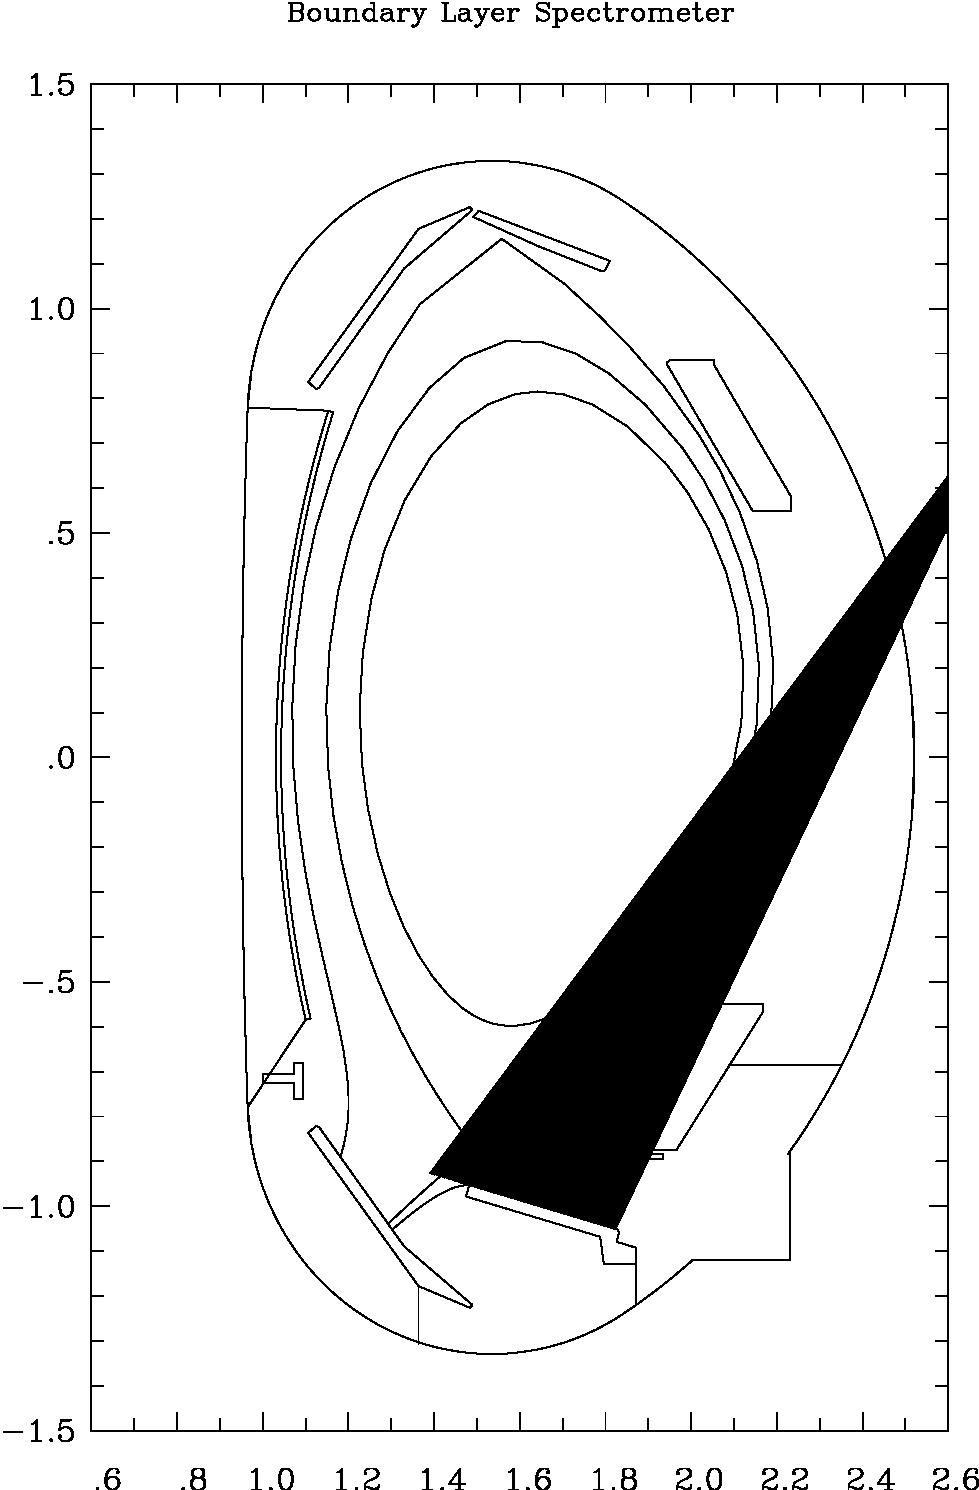
\includegraphics[height=6cm]{BLS_chords.pdf}}
  \subfigure[BOL.chords]{\label{fig:BOL}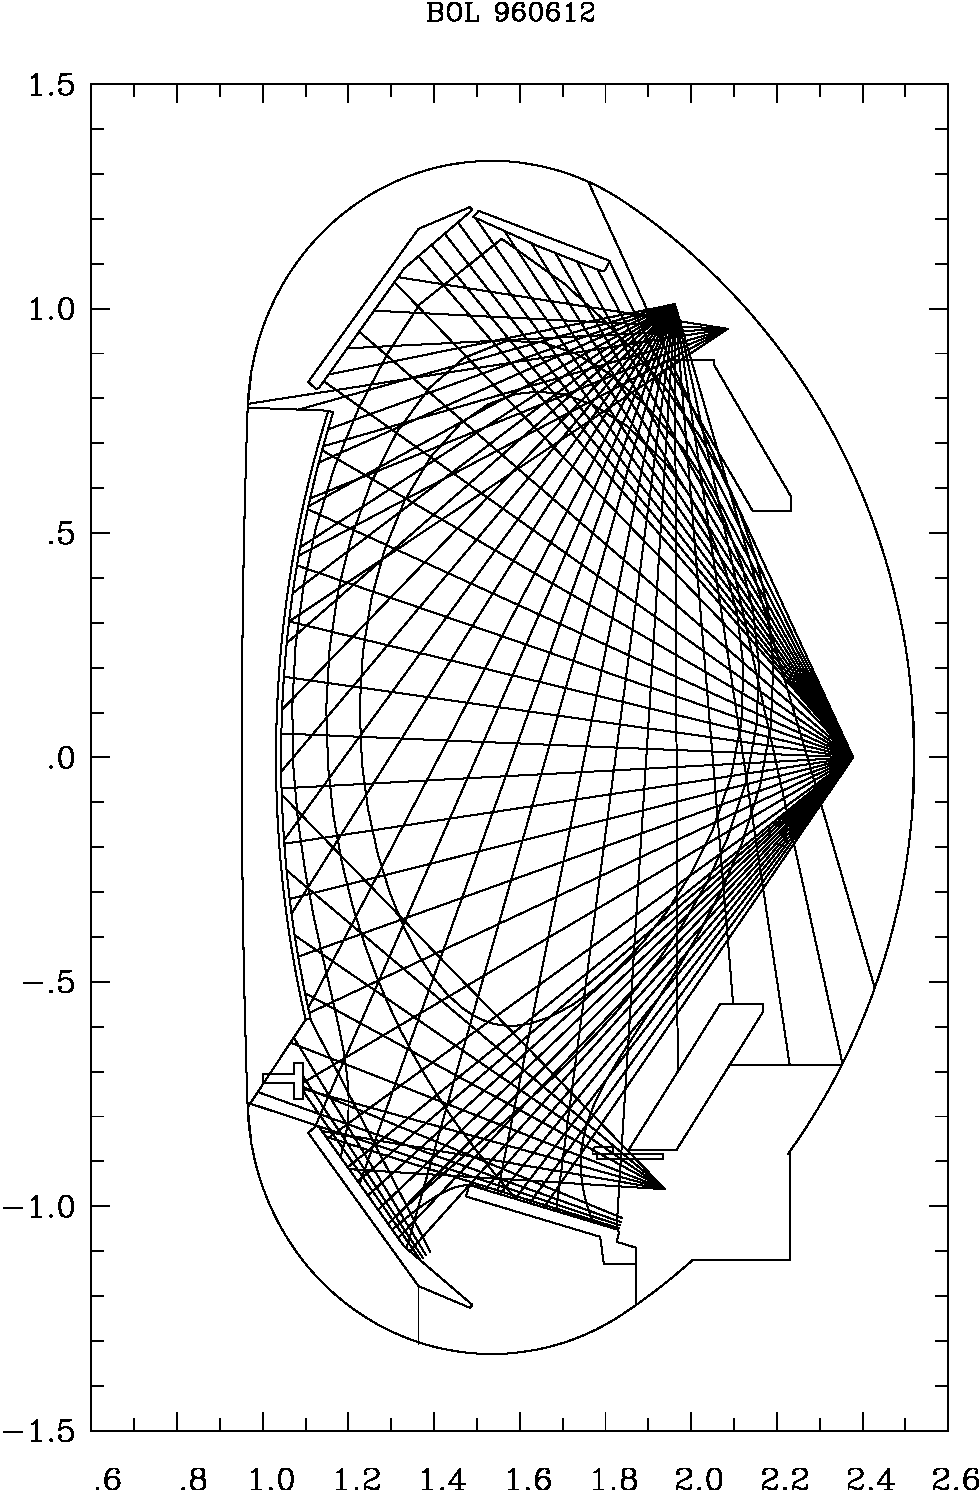
\includegraphics[height=6cm]{BOL_chords.pdf}}
  \subfigure[DCN.chords]{\label{fig:DCN}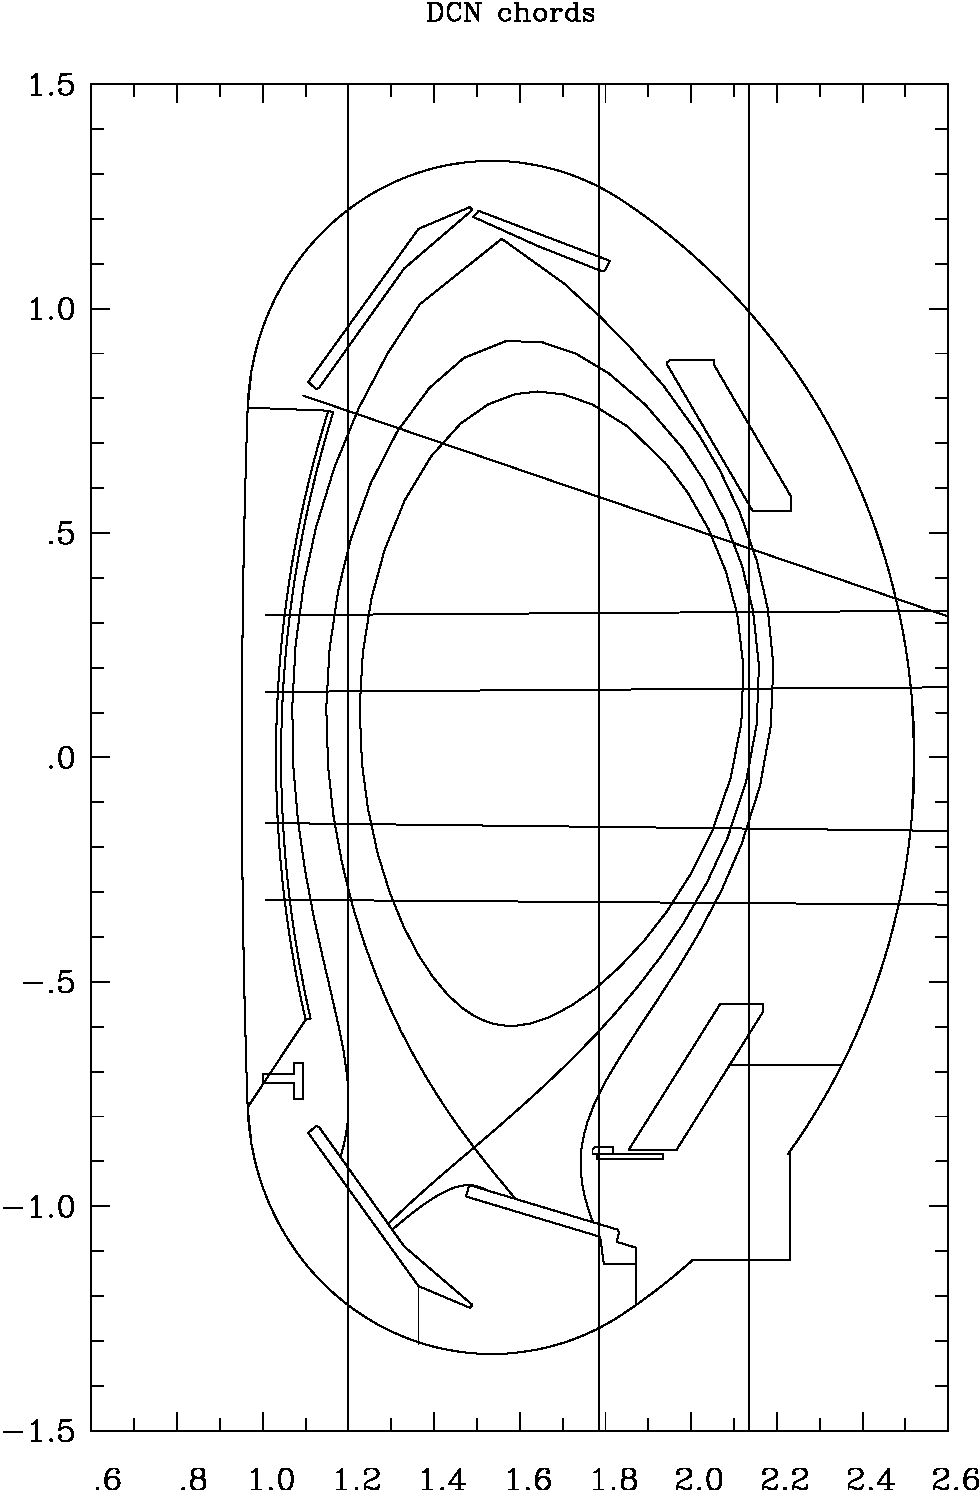
\includegraphics[height=6cm]{DCN_chords.pdf}}
  \subfigure[DIV.chords]{\label{fig:DIV}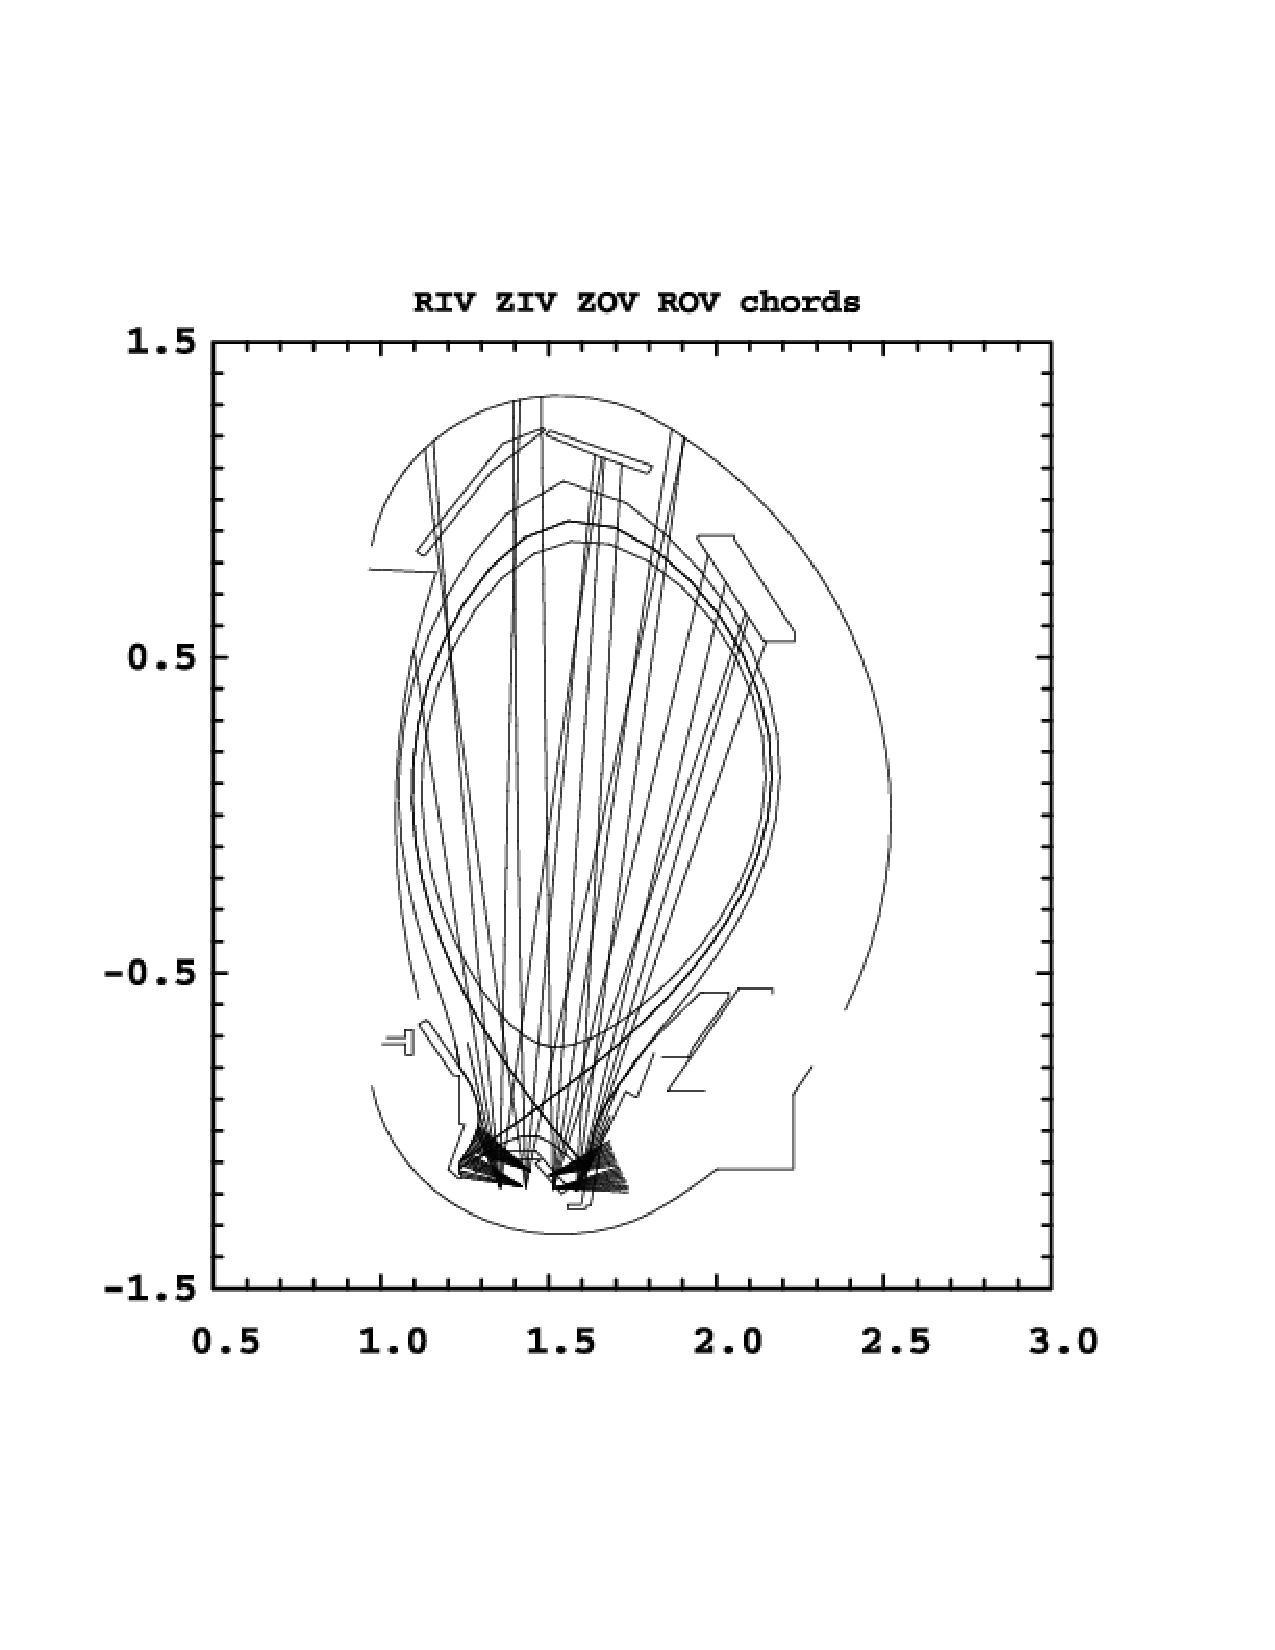
\includegraphics[height=6cm]{DIV_chords.pdf}}
\else
  \subfigure[BLS.chords]{\label{fig:BLS}\includegraphics[height=6cm]{BLS.chords.epsi}}
  \subfigure[BOL.chords]{\label{fig:BOL}\includegraphics[height=6cm]{BOL.chords.epsi}}
  \subfigure[DCN.chords]{\label{fig:DCN}\includegraphics[height=6cm]{DCN.chords.epsi}}
  \subfigure[DIV.chords]{\label{fig:DIV}\includegraphics[height=6cm]{DIV.chords.epsi}}
\fi
  \caption{BLS, BOL, DCN and DIV chords.}
\end{figure}

\begin{figure}[hbtp]
  \centering
\ifpdf 
  \subfigure[HAL.chords]{\label{fig:HAL}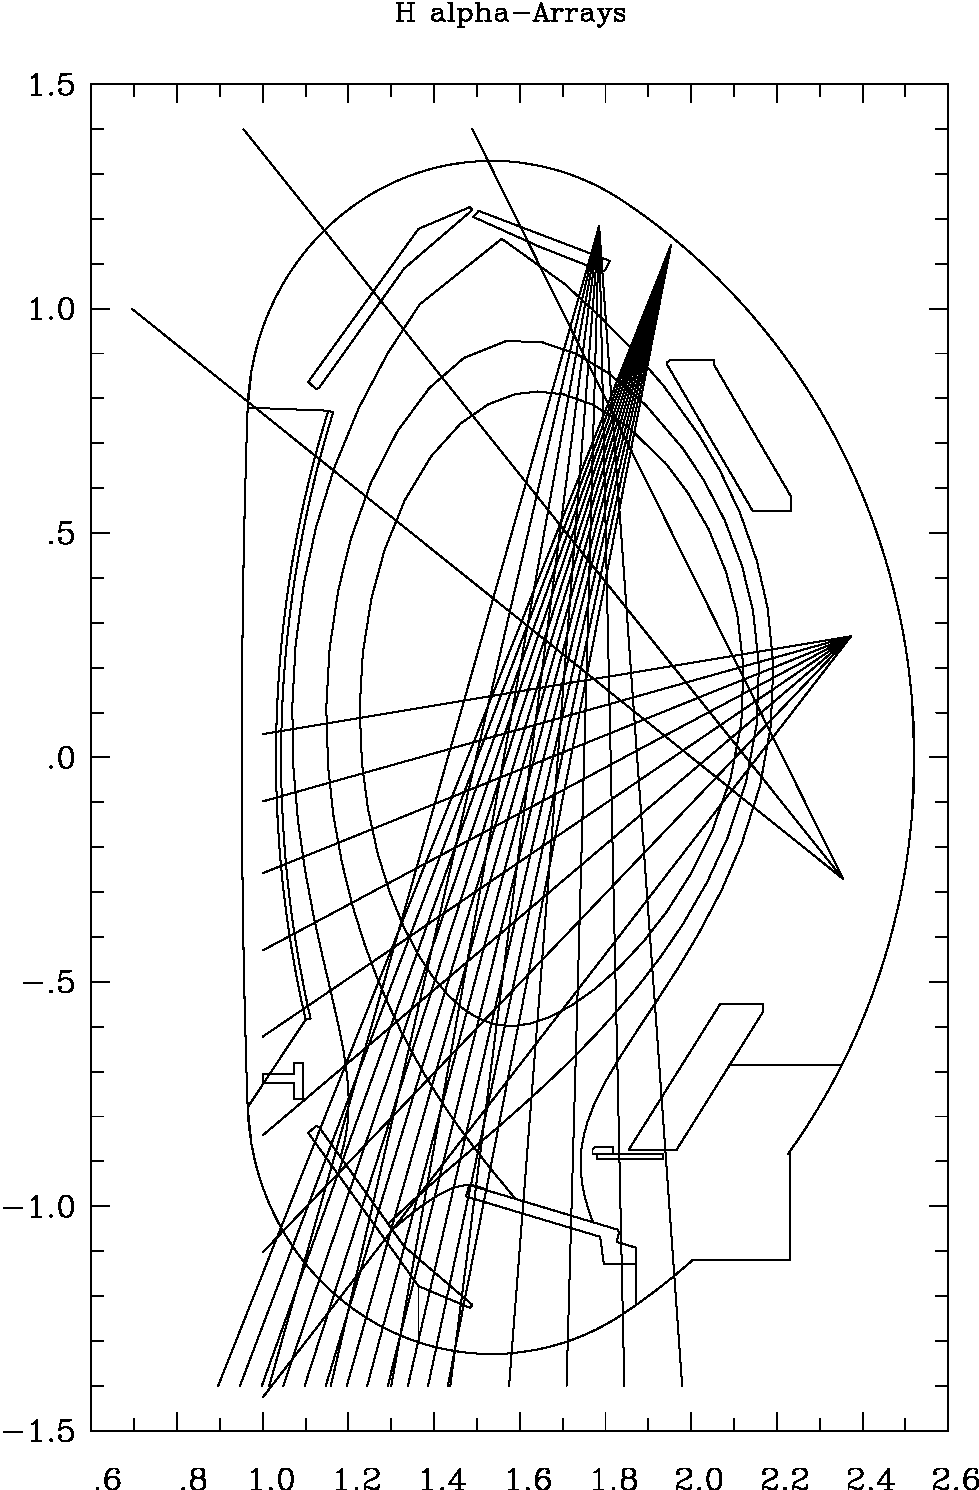
\includegraphics[height=7cm]{HAL_chords.pdf}}
  \subfigure[HAL\_13.chords]{\label{fig:HAL_13}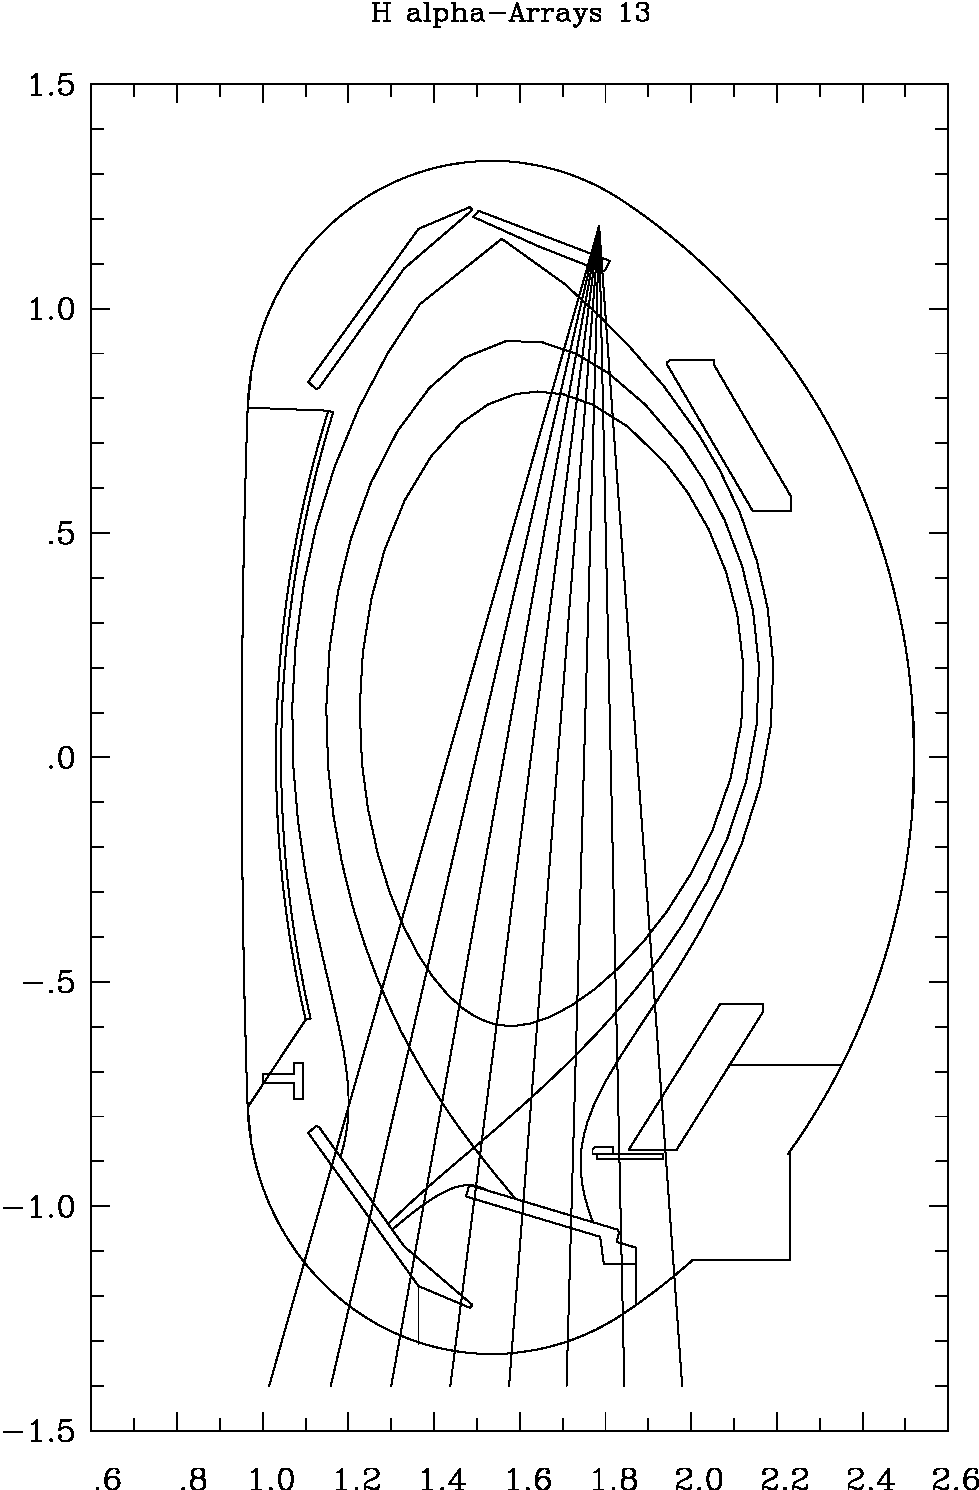
\includegraphics[height=7cm]{HAL_13_chords.pdf}}
  \subfigure[HAL\_6Bo.chords]{\label{fig:HAL_6Bo}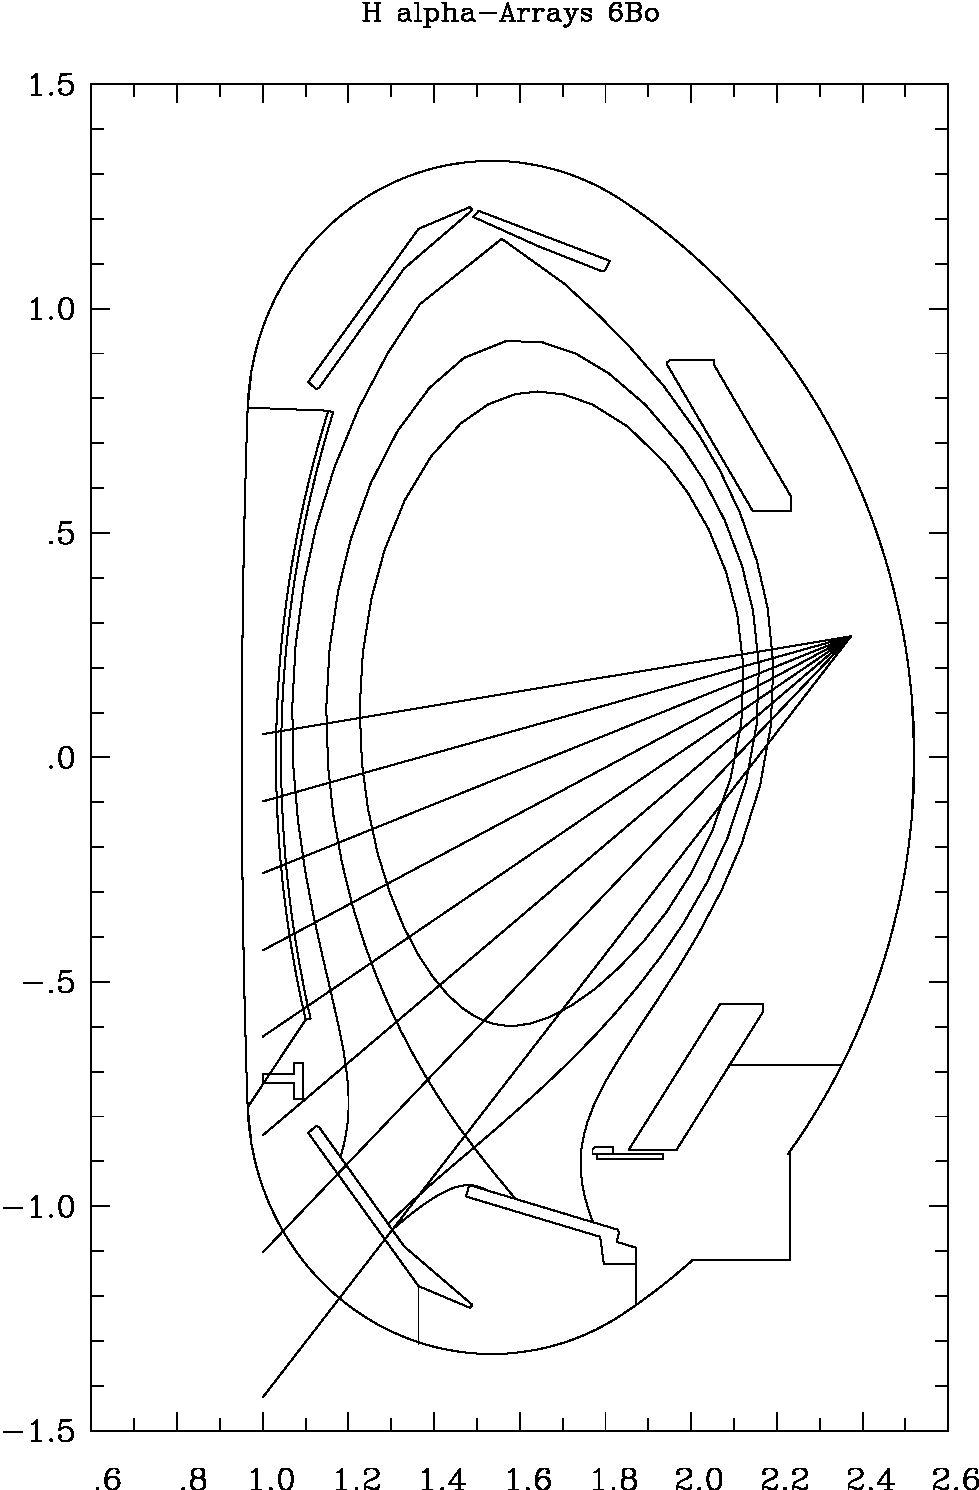
\includegraphics[height=7cm]{HAL_6Bo_chords.pdf}}
  \subfigure[HAL\_6Bu.chords]{\label{fig:HAL_6Bu}\includegraphics[height=7cm]{HAL_6Bu_chords.pdf}}
  \subfigure[HAL\_8Co.chords]{\label{fig:HAL_8Co}\includegraphics[height=7cm]{HAL_8Co_chords.pdf}}
\else
  \subfigure[HAL.chords]{\label{fig:HAL}\includegraphics[height=7cm]{HAL.chords.epsi}}
  \subfigure[HAL\_13.chords]{\label{fig:HAL_13}\includegraphics[height=7cm]{HAL_13.chords.epsi}}
  \subfigure[HAL\_6Bo.chords]{\label{fig:HAL_6Bo}\includegraphics[height=7cm]{HAL_6Bo.chords.epsi}}
  \subfigure[HAL\_6Bu.chords]{\label{fig:HAL_6Bu}\includegraphics[height=7cm]{HAL_6Bu.chords.epsi}}
  \subfigure[HAL\_8Co.chords]{\label{fig:HAL_8Co}\includegraphics[height=7cm]{HAL_8Co.chords.epsi}}
\fi
  \caption{HAL chords.}
\end{figure}

\subsection{$<$command file$>$ cmd}\index{b2plot, cmd}\label{sec:cmd}
Further commands are taken from the specified file.  If the file does
not exist in the current working directory, the directories
\$\verb!SOLPSTOP/data.local/commands! and
\$\verb!SOLPSTOP/scripts/commands! are searched in order.

\subsection{$<$CDF command file$>$ cmdcdf}\index{b2plot, cmdcdf}\label{sec:cmdcdf}
\verb!CDF! commands used repetitively (for movie frames) are taken from the specified file.  
If the file does not exist in the current working directory, the directories
\$\verb!SOLPSTOP/data.local/commands! and
\$\verb!SOLPSTOP/scripts/commands! are searched in order.

\subsection{$<$chord file$>$ chbx}\index{b2plot, chbx}\label{sec:chbx}
Chord integral averaged over three chords. Equivalent to using the {\bf 3 ave} command.

\subsection{$<$position file$>$ chvl}\index{b2plot, chvl}\label{sec:chvl}
The value is plotted at the specified positions.

\subsection{$<$flux info$>$ flux}\index{b2plot, flux}\label{sec:flux}
Needs to be compiled with \verb!-DWOS!.  String should contain shot number,
time within the shot, and the diagnostic name.  Then causes the
equilibrium for this shot to overlay subsequent plots.

\subsection{$<$chord file$>$ chmp}\index{b2plot, chmp}\label{sec:chmp}
Plots a contour plot of the chord contribution to the mesh element.

\subsection{$<$chord file$>$ cam}\index{b2plot, cam}\label{sec:cam}
Camera plot.  The chord file needs to contain some additional
information on the first line.

\subsection{$<$CDF file name$>$ movi}\index{b2plot, movi}\label{sec:movi}
Used for specifying the \verb!CDF! file if a movie is to be made.

\subsection{$<$istart,{\bf I}$>$ $<$iend,{\bf I}$>$ $<$varname, {\bf S}$>$ movie}\index{b2plot, movie}\label{sec:movie}
Creates a movie for timeslice $<$istart$>$ to time slice $<$iend$>$ of variable $<$varname$>$. The
list of available quantities in given in Appendix \ref{cha:b2time}. The time interval between frames can be
controlled with the {\bf mvsk} command.
{\bf nmovie} is an alias for {\bf movie}.

\subsection{$<$istart,{\bf I}$>$ $<$iend,{\bf I}$>$ $<$filename, {\bf S}$>$ $<$varname, {\bf S}$>$ omovie}\index{b2plot, omovie}\label{sec:omovie}
Creates a movie for timeslice $<$istart$>$ to time slice $<$iend$>$ of variable $<$varname$>$ read
from file $<$filename$>$. 

\subsection{$<$sonnetfile$>$ sonn}\index{b2plot, sonn}\label{sec:sonn}
Reads in a new \verb!Sonnet! geometry file.

\subsection{$<$output\_sonnet file$>$ oson}\index{b2plot, oson}\label{sec:oson}
Outputs the geometry in \verb!Sonnet! \verb!ASCII! format.

\subsection{$<$z$_{shift}$,{\bf R}$>$ $<$UEDGE grid file$>$ uedgegrd}\index{b2plot, uedgegrd}\label{sec:uedgegrd}
Outputs the geometry in \verb!UEDGE! ASCII format. The grid can be shifted in the vertical
direction by an amount of $<$z$_{shift}>$ meters.

\subsection{$<$filename$>$ $<$H123$>$ $<$reac$>$ $<$crc$>$ amju}\index{b2plot, amju}\label{sec:amju}
Computes a reaction rate as per the \verb!Eirene! specification. Consult the
\verb!Eirene! manual for details.
{\bf amjuel} is an alias for {\bf amju}.

\subsection{$<$reac$>$ adas}\index{b2plot, adas}\label{sec:adas}\index{ADAS}
Computes a reaction rate as per the \verb!ADAS! specification. The $<$reac$>$ string should be something of the
form 'acd89'. The matrix obtained contains then all the rates from these files, for all species in the run, extracted
from the files stored in \$\verb!SOLPSTOP/modules/adas! or \$\verb!SOLPSTOP/data.local/adas!.

\section{Environment variables}

\begin{description}
\item[B2PLOT\_DEV] is used to specify plotting to any combination of
  ``x11'', ``ps'' or ``cgm'' (default is ``ps'').  Under \verb!tcsh!, use 
  \begin{verbatim}
setenv B2PLOT_DEV 'x11 ps'
  \end{verbatim}
\item[SOLPSTOP] used to specify the top of the \verb!SOLPS! tree.
\end{description}

Environment variables can also be used in the {\bf extl} command
(see \ref{sec:extl}). If not explicitly set by the user, they inherit 
their value from the \verb!setup.csh.*! files in the \$\verb!SOLPSTOP!
directory.

\section{Examples}

Some simple (and not so simple) examples of plots that can be obtained with
\btwoplot commands are shown in the next section.

\subsection{Mesh plot}
\index{b2plot, mesh plot}

Here (figure \ref{fig:mesh}) we have two plots of the computational and physical grids, captioned with
the commands used to obtain them. 

\begin{figure}[hbtp]
  \centering
\ifpdf 
  \subfigure[comp a4p mesh]{\label{fig:comp}\includegraphics[height=6cm]{comp.pdf}}
  \subfigure[phys a4p mesh]{\label{fig:phys}\includegraphics[height=6cm]{phys.pdf}}
\else
  \subfigure[comp a4p mesh]{\label{fig:comp}\includegraphics[height=6cm]{comp.epsi}}
  \subfigure[phys a4p mesh]{\label{fig:phys}\includegraphics[height=6cm]{phys.epsi}}
\fi
  \caption{Mesh plots.}
  \label{fig:mesh}
\end{figure}

\subsection{Plotting plasma solution data}
\index{b2plot, plotting plasma quantities}

Data from the plasma solution, stored on the ``matrix'' stack, can be visualized as per figure \ref{fig:te}.

\begin{figure}[hbtp]
  \centering
\ifpdf 
  \subfigure[comp a4p te surf]{\label{fig:tecomp}\includegraphics[height=6cm]{Te_comp.pdf}}
  \subfigure[phys a4p -2.2 zmin 2.2 zmax 2.0 lbsz sep outl vesl logf 3 ndec te surf]{\label{fig:tephys}\includegraphics[height=6cm]{Te_phys.pdf}}
\else
  \subfigure[comp a4p te surf]{\label{fig:tecomp}\includegraphics[height=6cm]{Te_comp.epsi}}
  \subfigure[phys a4p -2.2 zmin 2.2 zmax 2.0 lbsz sep outl vesl logf 3 ndec te surf]{\label{fig:tephys}\includegraphics[height=6cm]{Te_phys.epsi}}
\fi
  \caption{Electron temperature plots.}
  \label{fig:te}
\end{figure}

Note that here the physical domain plot ({\bf phys} figure \ref{fig:tephys}) has been modified to have more readable
labels ({\bf 2.0 lbsz}), a logarithmic scale ({\bf logf}) covering 3 decades ({\bf 3 ndec}),
includes the magnetic separatrix ({\bf sep}), the plasma outline ({\bf outl}), the vacuum
vessel ({\bf vesl}), and has an extended vertical range ({\bf -2.2 zmin 2.2 zmax}). Note however that
the plotting program always attempts to maintain ``nice'' axis bounds and conserve the graph
aspect ration (unless {\bf aspc} is toggled).

Other examples:

\begin{figure}[hbtp]
  \centering
\ifpdf 
  \subfigure[phys a4p noax 0 nreg]{\label{fig:noax}\includegraphics[height=6cm]{noax.pdf}}
  \subfigure[phys a4p ti te m/ surf]{\label{fig:tioverte}\includegraphics[height=6cm]{Ti_Te.pdf}}
\else
  \subfigure[phys a4p noax 0 nreg]{\label{fig:noax}\includegraphics[height=6cm]{noax.epsi}}
  \subfigure[phys a4p ti te m/ surf]{\label{fig:tioverte}\includegraphics[height=6cm]{Ti_Te.epsi}}
\fi
  \caption{Other solution data plots.}
  \label{fig:otherdata}
\end{figure}

In figure \ref{fig:tioverte}, we obtain the ratio of ion to electron 
temperature, while figure \ref{fig:noax} is a region plot (like the ones in 
Fig. \ref{fig:SN_regions}, obtained with {\bf sep vesl outl 0 nreg surf}, and 
Fig. \ref{fig:DN_regions}, obtained with {\bf sep 0 nreg surf}).

\subsection{Chord plots}
\index{b2plot, chord plots}

In figure \ref{fig:JETchords} we have an example of chord plots as applied to the KL2 diagnostic on JET.

\begin{figure}[hbtp]
  \centering
\ifpdf 
  \subfigure[a4p vesl outl sep 'JET/KL2.chords' chpl]{\label{fig:chpl}\includegraphics[height=6cm]{chpl.pdf}}
  \subfigure[a4l phys 3 6581 1 nspec '658 nm CII' extl 'JET/KL2.chords' chor]{\label{fig:chor}\includegraphics[angle=90,height=6cm]{chor.pdf}}
\else
  \subfigure[a4p vesl outl sep 'JET/KL2.chords' chpl]{\label{fig:chpl}\includegraphics[height=6cm]{chpl.epsi}}
  \subfigure[a4l phys 3 6581 1 nspec '658 nm CII' extl 'JET/KL2.chords' chor]{\label{fig:chor}\includegraphics[angle=90,height=6cm]{chor.epsi}}
\fi
  \caption{Chord plots applied to JET.}
  \label{fig:JETchords}
\end{figure}

The first {\bf chpl} plot (\ref{fig:chpl}) gives the physical position of the chords, 
as obtained from the \verb!JET/KL2.chords! file in the 
\$\verb!SOLPSTOP/data/chords! directory. The second {\bf chpl} plot (\ref{fig:chor}), 
in landscape mode {\bf a4l}, shows the emissivity of a C$^+$ line 
(species 3) at $\lambda = 6581 \pm 1$ {\em \AA} ({\bf 3 6581 1 nspec}). 
The {\bf extl} instruction gives the extra label on the second title line.  

\subsection{Wall plots}
\index{wall segments}\index{b2plot, plotting wall quantities}

In figure \ref{fig:wallplots}, we show examples of wall plots.

\begin{figure}[hbtp]
  \centering
\ifpdf 
  \subfigure[phys 0 nseg 4 1. 2. 3. 4. wclvs 10.0 wwid wall mesh]{\label{fig:nseg}\includegraphics[height=6cm]{nseg.pdf}}
  \subfigure[vesl sep phys wall 10.0 wwid sputchem 1 wzsel 3 ndec logw fnax 1 zsel 'Ychem D+' wallblbl surf]{\label{fig:Ychem}\includegraphics[height=6cm]{Ychem.pdf}}
\else
  \subfigure[phys 0 nseg 4 1. 2. 3. 4. wclvs 10.0 wwid wall mesh]{\label{fig:nseg}\includegraphics[height=6cm]{nseg.epsi}}
  \subfigure[vesl sep phys wall 10.0 wwid sputchem 1 wzsel 3 ndec logw fnax 1 zsel 'Ychem D+' wallblbl surf]{\label{fig:Ychem}\includegraphics[height=6cm]{Ychem.epsi}}
\fi
  \caption{Wall plots.}
  \label{fig:wallplots}
\end{figure}

The wall segment indices are illustrated in figure \ref{fig:nseg}, obtained with the {\bf 0 nseg} command. We impose the contour levels to be at the values 1 through 4 with the {\bf 4 1. 2. 3. 4. wclvs} command. The thickness of the drawn wall line is given by {\bf 10.0 wwid}. {\bf wall} asks for the wall data overlay on top of the requested {\bf mesh} plot.

Another more complex example is given in figure \ref{fig:Ychem}. It combines a {\bf surf} plot of the D$^+$ poloidal 
particle flux ({\bf fnax 1 zsel}, as D$^+$ has species index 1), with a {\bf wall} plot of the chemical sputtering 
yield for D$^+$ ({\bf sputchem 1 wzsel}). The latter is done on a logarithmic scale ({\bf logw}), covering 3 decades 
({\bf 3 ndec}). The label for the colour bar for the wall data is shortened with {\bf 'Ychem D+' wallblbl}. The wall
colour bar is the rightmost one. Not choosing
the {\bf zsel} and {\bf wzsel} options would have given a series of plots, one per species, with their individual
poloidal particle flux and chemical sputtering yield. If only the {\bf wzsel} option is used, one obtains a series of
{\bf surf} plots with all the same ``wall'' data overlay. If only the {\bf zsel} option is used, then the {\bf wall} 
overlay will come from the first species, namely D$^0$ in this case. It is therefore recommended to always make sure 
that the species dimensions of the ``matrix'' and ``wall'' data match!

\subsection{Target plot}
\index{b2plot, plotting target quantities}

In figure \ref{fig:targetplots}, we show examples of target plots.

\begin{figure}[hbtp]
  \centering
\ifpdf 
  \subfigure[comp sep 10.0 wwid wallhflx wall kappa trgsurf]{\label{fig:Kappa}\includegraphics[height=6cm]{Kappa.pdf}}
  \subfigure[a4l outl vesl 2.2 rmin 3.2 rmax -1.0 zmax -1.75 zmin sep 8.0 wwid logw te logf 5 ndec cooltemp wtot trgm- phys 'Tp-Tc (K)' trgblbl wallflux 1 wzsel 'D+ wall flux' wallblbl wall target logtrg surf]{\label{fig:Triple}\includegraphics[angle=90,height=6cm]{Triple.pdf}}
\else
  \subfigure[comp sep 10.0 wwid wallhflx wall kappa trgsurf]{\label{fig:Kappa}\includegraphics[height=6cm]{Kappa.epsi}}
  \subfigure[a4l outl vesl 2.2 rmin 3.2 rmax -1.0 zmax -1.75 zmin sep 8.0 wwid logw te logf 5 ndec cooltemp wtot trgm- phys 'Tp-Tc (K)' trgblbl wallflux 1 wzsel 'D+ wall flux' wallblbl wall target logtrg surf]{\label{fig:Triple}\includegraphics[angle=90,height=6cm]{Triple.epsi}}
\fi
  \caption{Target plots.}
  \label{fig:targetplots}
\end{figure}

The first plot (figure \ref{fig:Kappa}) shows the target heat conductivity ({\bf kappa}) in the target 
computational domain ({\bf comp} and {\bf trgsurf}).
The vertical separators ({\bf sep}) indicate the segment boundaries. 
The overlay line at $y$=0, i.e. at the target surface in contact with the plasma is the {\bf wall} data,
here the incoming plasma heat flux ({\bf wallhflx}).

The second plot (figure \ref{fig:Triple}) is a triple plot\index{b2plot, triple plot}, containing
a plasma quantity from the ``matrix'' stack, (here {\bf te}), with {\bf wall} and {\bf target} overlays.
The ``matrix'' ({\bf logf}), ``wall'' ({\bf logw}) and ``target'' ({\bf trglog}) data are all plotted on
a logarithmic scale. The target data is obtained with the command
\begin{verbatim}
cooltemp wtot trgm- 
\end{verbatim}
which takes the ``wall'' quantity {\bf cooltemp}, the temperature at the cooled end of the target plate, copies it
over to the ``target'' stack ({\bf wtot}), and subtracts it from the preceding ``target'' stack value (here the
target temperature, which is loaded onto the stack by default at startup). So we obtain the amount by which
the target has been heated by the plasma, and label it with {\bf 'Tp-Tc (K)' trgblbl}. 
The wall overlay data is the D$^+$ particle flux to the wall ({\bf wallflux 1 wzsel}), labeled with
{\bf 'D+ wall flux' wallblbl}. The colour bars, from left to right, correspond to the ``matrix'', ``wall''
and ``target'' data arrays.

\subsection{Radiation plot}
\index{b2plot, radiation plots}

The following was used to produce a plot (figure \ref{fig:b2rad}) of
the emissivity arising out of radiation for C and Ne.

\begin{verbatim}
! b2plot < b2rad.plot ; ctrans -d ps.land.color gmeta | a4page > ! tmp.ps
a4l 2 1 page lbof logf phys
b2ra pvol abs 2 2 sumz 1.0e4 fmin 1.0e8 fmax 'Carbon' extl cont
b2ra pvol abs 3 3 sumz 1.0e4 fmin 1.0e8 fmax 'Neon' extl cont
\end{verbatim}

The first line is a comment indicating how \btwoplot should be run (the
file containing the above lines was called \verb!b2rad.plot!), and how
the PostScript file should be generated.

The second line sets up an A4 landscape format with two graphs next to
each other, sets labelling of contour levels off, logarithmic scaling
and plotting on the physical domain only.

The third and fourth lines plot the line radiation data for the 2$^{nd}$
and 3$^{rd}$ species respectively, setting the data minimum to $10^4$ and
maximum to $10^8$, labelling the graphs ``Carbon'' and ``Neon''
respectively.

\begin{figure}[hbtp]
\ifpdf 
    \centerline{\includegraphics[angle=90,height=10cm]{b2plot_b2rad.pdf}}
\else
    \centerline{\includegraphics[angle=90,height=10cm]{b2plot_b2rad.epsi}}
\fi
    \caption{C and Ne radiation.}
    \label{fig:b2rad}
\end{figure}

\subsection{Fluxes and values plot}

The following was used to calculate and plot integrated values of
fluxes and some local quantities along various lines.  See figure \ref{fig:fluxes}.

\begin{verbatim}
'${HOST} ${PWD} `date` T=${TIME}' extl glob
a4p 2 2 page
phys
feex sumy 19 f.x drop
feey sumx 57 f.y drop
feix sumy 19 f.x drop
feiy sumx 57 f.y drop
fnix 1 1 sumz sumy 19 f.x drop
fnix 2 7 sumz sumy 19 f.x drop
fnix 8 17 sumz sumy 19 f.x drop
fnix 18 19 sumz sumy 19 f.x drop
fniy 1 1 sumz sumx 57 f.y drop
fniy 2 7 sumz sumx 57 f.y drop
fniy 8 17 sumz sumx 57 f.y drop
fniy 18 19 sumz sumx 57 f.y drop
phys
ni 1 1 sumz 0.0 fmin 0.0 fmax 57 f.y drop
ni 2 7 sumz 0.0 fmin 0.0 fmax 57 f.y drop
ni 8 17 sumz 0.0 fmin 0.0 fmax 57 f.y drop
ni 18 19 sumz 0.0 fmin 0.0 fmax 57 f.y drop
te 0.0 fmin 0.0 fmax 57 f.y drop
ti 0.0 fmin 0.0 fmax 57 f.y drop
zeff 0.0 fmin 0.0 fmax 57 f.y drop
ne 0.0 fmin 0.0 fmax 57 f.y drop
\end{verbatim}
%% $

This example plots a series of line plots in a $2 \times 2$ format on an A4
portrait page.  Liberal use is made of {\bf sumx} and {\bf sumy} to produce
appropriate sums, and of {\bf sumz} to sum over the same species.  {\bf f.x}
and {\bf f.y} are used to plot the line plots.  Setting both {\bf fmin} and
{\bf fmax} to 0.0 means each plot is scaled separately --- otherwise the
scaling is done on all of the data.

\begin{figure}[hbtp]
  \centering
\ifpdf 
  \subfigure[Page 1]{\label{fig:fluxes_p1}\includegraphics[height=7cm]{b2plot_fluxes_1.pdf}}
  \subfigure[Page 2]{\label{fig:fluxes_p2}\includegraphics[height=7cm]{b2plot_fluxes_2.pdf}}
  \subfigure[Page 3]{\label{fig:fluxes_p3}\includegraphics[height=7cm]{b2plot_fluxes_3.pdf}}
  \subfigure[Page 4]{\label{fig:fluxes_p4}\includegraphics[height=7cm]{b2plot_fluxes_4.pdf}}
  \subfigure[Page 5]{\label{fig:fluxes_p5}\includegraphics[height=7cm]{b2plot_fluxes_5.pdf}}
\else
  \subfigure[Page 1]{\label{fig:fluxes_p1}\includegraphics[height=7cm]{b2plot_fluxes_1.epsi}}
  \subfigure[Page 2]{\label{fig:fluxes_p2}\includegraphics[height=7cm]{b2plot_fluxes_2.epsi}}
  \subfigure[Page 3]{\label{fig:fluxes_p3}\includegraphics[height=7cm]{b2plot_fluxes_3.epsi}}
  \subfigure[Page 4]{\label{fig:fluxes_p4}\includegraphics[height=7cm]{b2plot_fluxes_4.epsi}}
  \subfigure[Page 5]{\label{fig:fluxes_p5}\includegraphics[height=7cm]{b2plot_fluxes_5.epsi}}
\fi
  \caption{Line plots of fluxes and other quantities.}\label{fig:fluxes}
\end{figure}

\clearpage

\chapter{Miscellaneous}
\label{cha:Misc}

\section{DIMENSIONS.F}\index{DIMENSIONS.F}\label{sec:DIMENSIONS}

The file \$\verb!SOLPSTOP/modules/B2.5/src/include/DIMENSIONS.F! and its local version
\$\verb!SOLPSTOP/modules/B2.5/src/include.local/DIMENSIONS.F! contain key dimensions 
that determine
the sizes of arrays that can be defined by namelists
in \verb!b2.*.parameters! files (for compatibility with 
certain compilers).

The quantities defined in \verb!DIMENSIONS.F! are:
\begin{description}
\item[DEF\_ISOEXTRA]\index{DEF\_ISOEXTRA}\index{ISOEXTRA} the maximum
number of extra isolating cells
\item[DEF\_NADD]\index{DEF\_NADD}\index{NADD} the maximum number of
additional vacuum cells outside the gridded domain in \verb!Eirene!
\item[DEF\_NATM]\index{DEF\_NATM}\index{NATM} the maximum number of
neutral atomic species to be handled by \verb!Eirene!
\item[DEF\_NCHEN]\index{DEF\_NCHEN}\index{NCHEN} the maximum number of
energy bins for the diagnostic chords in \verb!Eirene!
\item[DEF\_NCUT]\index{DEF\_NCUT}\index{NCUT} the maximum number of
``cuts'' (2 for single null cases, 4 for double nulls)
\item[DEF\_NFL]\index{DEF\_NFL}\index{NFL} the maximum number of charged fluids
passed from \verb!B2.5! to \verb!Eirene!
\item[DEF\_NGSTAL]\index{DEF\_NGSTAL}\index{NGSTAL} the maximum number
of grids on which spatially resolved surface tallies are computed
\item[DEF\_NION]\index{DEF\_NION}\index{NION} the maximum number of molecular
ion species to be handled by \verb!Eirene!
\item[DEF\_NLIM]\index{DEF\_NLIM}\index{NLIM} the maximum number of
additional surfaces to be handled by \verb!Eirene!
\item[DEF\_NMOL]\index{DEF\_NMOL}\index{NMOL} the maximum number of
neutral molecular species to be handled by \verb!Eirene!
\item[DEF\_NPHID]\index{DEF\_NPHID}\index{NPHID} the maximum number of
toroidal standard surfaces
\item[DEF\_NPLS]\index{DEF\_NPLS}\index{NPLS} the maximum number of background 
plasma species to be handled by \verb!Eirene!
\item[DEF\_NPRNL]\index{DEF\_NPRNL}\index{NPRNL} the maximum number of
particles that can be saved in the time dependent arrays
\item[DEF\_NREAC]\index{DEF\_NREAC}\index{NREAC} the maximum number of
reaction cards that can be created by \verb!Uinp!
\item[DEF\_NRDS]\index{DEF\_NREAC}\index{NREAC} the maximum number of
molecular dissociation reaction cards that can be created by \verb!Uinp!
\item[DEF\_NREC]\index{DEF\_NREAC}\index{NREAC} the maximum number of
recombination reaction cards that can be created by \verb!Uinp!
\item[DEF\_NREL]\index{DEF\_NREAC}\index{NREAC} the maximum number of
elastic collisions reaction cards that can be created by \verb!Uinp!
\item[DEF\_NSD]\index{DEF\_NSD}\index{NSD} the maximum number of plasma
species handled in \verb!B2.5!
\item[DEF\_NSPCSRFG]\index{DEF\_NSPCSRFG}\index{NSPCSRFG} the maximum
number of groups of \verb!Eirene! surfaces for which the data can be
transferred from \verb!B2.5! (\verb!DG! specification "Surface special")
\item[DEF\_NSRFS]\index{DEF\_NSRFS}\index{NSRFS} the maximum number of
surfaces in a stratum
\item[DEF\_NSTRA]\index{DEF\_NSTRA}\index{NSTRA} the maximum number of
\verb!Eirene! strata
\item[DEF\_NSTS]\index{DEF\_NSTS}\index{NSTS} the maximum number of non-default 
standard surfaces to be handled by \verb!Eirene!
\item[DEF\_NTOR]\index{DEF\_NTOR}\index{NTOR} the maximum number of toroidal
periodicity boundaries
\item[DEF\_NXD]\index{DEF\_NXD}\index{NXD} the maximum number of cells
in the $x$ (parallel or poloidal) direction not including two guard
cells
\item[DEF\_NYD]\index{DEF\_NYD}\index{NYD} the maximum number of cells
in the radial direction not including two guard cells
%%\item[] the maximum number of 
%%\item[] the maximum number of 
\end{description}

The current default settings of \verb!DIMENSIONS.F!, correponding to a D+He+C DN case, are:
\VerbatimInput[fontsize=\footnotesize]{DIMENSIONS.F}

\section{Making movies}

\section{Compiling B2.5}
\label{sec:compilingb2}\index{B2.5, compiling}\index{B2.5, Makefile}

(See also section \ref{sec:b2}, page \pageref{sec:b2}.)

The following is the \verb!Makefile! provided with the Master 
in the \verb!sbb! directory:

\VerbatimInput[fontsize=\footnotesize]{B2_5.Makefile}

and, as a prototypical example, the \verb!config.ITER.ifort64! in
the \verb!config! subdirectory: \index{B2.5, compiling options}

\VerbatimInput[fontsize=\footnotesize]{B2_5.config.ITER.ifort64}

If the user wishes to modify the compiling options used, the creation
of a \verb!config.!\$\verb!${HOST_NAME}.!\$\verb!${COMPILER}.local! file 
is recommended, in which to store the modified settings. Since the \verb!Makefile!
reads those after the 
\verb!config/compiler.!\$\verb!${HOST_NAME}.!\$\verb!${COMPILER}! file,
they need only contain the modified definitions. 

\section{Defines}

\subsection{B2.5-Eirene}
\index{DEFINES, used in compiling B2.5-Eirene}

We list here the possible compiler options that can be used when compiling the
coupled version of \verb!B2.5-Eirene!. These options are shared across both the
\verb!B2.5! and \verb!Eirene! source codes.

\begin{description}
\item[ALLOCATE\_AND\_NAMELIST] \index{ALLOCATE\_AND\_NAMELIST} To be used if the compiler allows dynamically allocated namelist arrays
\item[B25\_EIRENE] \index{B25\_EIRENE} Set internally by the \verb!Makefile! and used to identify differences between source code for stand-alone \verb!B2.5! and coupled \verb!B2.5-Eirene! applications
\item[NO\_B2\_CHEM\_SPUT] \index{NO\_B2\_CHEM\_SPUT} Used to indicate that chemical sputtering is specified through \verb!Eirene! arrays instead of \verb!B2.5!.
\item[NO\_GETENV] \index{NO\_GETENV} No \verb!GETENV! system call available
\item[USE\_MPI] \index{USE\_MPI} Set internally by the \verb!Makefile! and used to identify code necessary for MPI applications
\item[USE\_PXFGETENV] \index{USE\_PXFGETENV} Uses \verb!PXFGETENV!
  instead of \verb!GETENV!
\end{description}

\index{SOLPS\_CPP}
If you want to activate any of these options, you should add
\verb!-DOPTION! (where \verb!OPTION! might, for example, be
\verb!CLASSICAL_CURRENT!) to the \verb!SOLPS_CPP! environment variable
with
\begin{verbatim}
  setenv SOLPS_CPP '-DOPTION'
\end{verbatim}
and then recompile all of the routines affected (if unsure which
routines are affected, recompile them all with
\begin{verbatim}
  gmake clean
  gmake depend
  gmake
\end{verbatim}
).  If \verb!SOLPS_CPP! already had a value, you would want to do
\begin{verbatim}
  setenv SOLPS_CPP "$SOLPS_CPP -DOPTION"
\end{verbatim}
%% $
so that the new option is added to the list. (Unsupported \verb!ksh!
or \verb!bash! users would use something like
\begin{verbatim}
  export SOLPS_CPP="$SOLPS_CPP -DOPTION"
\end{verbatim}
%%$
).

\subsection{B2.5}
\index{DEFINES, used in compiling B2.5}

%%grep #if $SOLPSTOP/modules/B2.5/src/*/*.F | awk '{print $2}' | sort | uniq

We list here the additional compiler options available that only affect compilation of
\verb!B2.5!.

\begin{description}
\item[ASTRA] \index{ASTRA} To be used if one wishes to run in coupled mode with the core transport code ASTRA
\item[CDF\_MOVIE] \index{CDF\_MOVIE} To be used if \verb!CDF! movie output is desired
\item[CLASSICAL\_CURRENT] \index{CLASSICAL\_CURRENT} Turns on classical current drift term
\item[COMPLICATED] \index{COMPLICATED} Uses a more ``complicated'' model for chord integration
\item[DEF\_MAXCHORDS] \index{DEF\_MAXCHORDS} Maximum number of chords to be considered (default 10000)
\item[F77] index{F77} Identifies specific code to \verb!Fortran-77! compilers
\item[HITS\_PER\_CHORD] \index{HITS\_PER\_CHORD} Maximum number of chord points per cell? (default 50)
\item[HPUX] \index{HPUX} Specific to HP computers
\item[IBMaix] \index{IBMaix} Specific to IBM AIX computers
\item[JET] \index{JET} Enables some additional output for coupling to the JET post-processor
\item[MDSPLUS] \index{MDSPLUS} Enables \verb!MDSplus! output
\item[NAG22] \index{NAG22} Specific to using the Nag Mark 22 or higher mathematical library
\item[NAGF95] \index{NAGF95} Specific to the \verb!NAG! F95 compiler
\item[NCAR4] \index{NCAR4} Used to specify NCAR4 rather than NCAR3
\item[NO\_21] \index{NO\_21} Do not use 21-moment model for thermal and viscous forces
\item[NO\_CDF] \index{NO\_CDF} No \verb!CDF! library available
\item[NO\_F01AAF] \index{NO\_F01AAF} No \verb!NAG! routine \verb!F01AAF! --- uses
  its replacement instead (needed if linking with Version 17 or later of \verb!NAG!)
\item[NO\_LONG\_LINES] \index{NO\_LONG\_LINES} Identify those
  compilers which have a limitation to relatively short output lines
\item[NO\_NAG] \index{NO\_NAG} No \verb!NAG! libraries available
\item[NO\_OPT] \index{NO\_OPT} No compiler optimization 
\item[PAR\_OPT] \index{PAR\_OPT} Runs the code in a special interpretive parameter optimization mode
\item[PERFMON] \index{PERFMON} Enable performance monitoring
\item[PLPLOT] \index{PLPLOT} Use \verb!PLPLOT! instead of \verb!NCAR! for plotting
\item[PSR] \index{PSR} Specific to the Pacific Sierra VAST compiler
\item[SCL\_IMP\_RCI] \index{SCL\_IMP\_RCI} Toggles scaling of impurities tallies
\item[USE\_CDF\_B2STIME] \index{USE\_CDF\_B2STIME} Specific for \SOLPSfour \verb!CDF! tallies
\item[WANT\_PROCESS] \index{WANT\_PROCESS} Enables the code for the
  \SOLPSfive to \SOLPSfour converter.
\item[WANT\_THIS] \index{WANT\_THIS} (default) Adds some boundary condition treatments
\item[WINDOWS] \index{WINDOWS} Specific to Windows implementations
\item[WOS] \index{WOS} Uses the \verb!WOS! libraries for accessing
  experimental data at IPP.
\end{description}

%%grep #if $SOLPSTOP/modules/B2.5/src/*/*.F | awk '{print $2,$1}' | sort | uniq


\begin{center}
  \begin{longtable}{|l|l|}
    \hline
    \multicolumn{2}{|l|}{\small\sl continued from previous page} \\
    \hline name & used in \\
    \hline \endhead
    \hline name & used in \\
    \hline \endfirsthead
    \hline
    \multicolumn{2}{|l|}{\small\sl continued on next page} \\
    \hline \endfoot
    \endlastfoot
ALLOCATE\_AND\_NAMELIST & b2plot/init\_wall.F \\
ALLOCATE\_AND\_NAMELIST & modules/b2mod\_boundary\_namelist.F \\
ALLOCATE\_AND\_NAMELIST & modules/b2mod\_input\_profile.F \\
ALLOCATE\_AND\_NAMELIST & modules/b2mod\_layer.F \\
ALLOCATE\_AND\_NAMELIST & modules/b2mod\_neutrals\_namelist.F \\
ALLOCATE\_AND\_NAMELIST & modules/b2mod\_numerics\_namelist.F \\
ALLOCATE\_AND\_NAMELIST & modules/b2mod\_sputter.F \\
ALLOCATE\_AND\_NAMELIST & modules/b2mod\_transport\_models.F \\
ALLOCATE\_AND\_NAMELIST & modules/b2mod\_transport\_namelist.F \\
ALLOCATE\_AND\_NAMELIST & modules/b2mod\_user\_namelist.F \\
ALLOCATE\_AND\_NAMELIST & modules/b2mod\_wall.F \\
ALLOCATE\_AND\_NAMELIST & postprocessing/b2yt\_wall.F \\
ALLOCATE\_AND\_NAMELIST & sources/b2stbr.F \\
ASTRA & modules/b2mod\_astra\_to\_b2.F \\
ASTRA & sources/b2stbc\_phys.F \\
ASTRA & sources/b2stbr.F \\
ASTRA & sources/b2stcx.F \\
ASTRA & sources/b2stel.F \\
ASTRA & transport/b2strcl.F \\
B25\_EIRENE & b2plot/b2pinp.F \\
B25\_EIRENE & b2plot/b2plot.F \\
B25\_EIRENE & b2plot/b2pnwl.F \\
B25\_EIRENE & b2plot/b2ptrgl.F \\
B25\_EIRENE & b2plot/b2pwinm.F \\
B25\_EIRENE & b2plot/b2pwlprp.F \\
B25\_EIRENE & b2plot/b2pwsort.F \\
B25\_EIRENE & b2plot/get\_from\_movie\_cdf.F \\
B25\_EIRENE & b2plot/ngread.F \\
B25\_EIRENE & convert/b2mds.F \\
B25\_EIRENE & driver/b2mndr.F \\
B25\_EIRENE & driver/b2mn.F \\
B25\_EIRENE & driver/b2mwti.F \\
B25\_EIRENE & postprocessing/b2ytdr.F \\
B25\_EIRENE & sources/b2stbr.F \\
B25\_EIRENE & modules/b2mod\_astra\_to\_b2.F \\
B25\_EIRENE & modules/b2mod\_diag.F \\
B25\_EIRENE & modules/b2mod\_neutrals\_namelist.F \\
B25\_EIRENE & modules/b2mod\_work.F \\
B25\_EIRENE & output/b2wdat.F \\
B25\_EIRENE & postprocessing/b2ytdr.F \\
B25\_EIRENE & sources/b2stbc\_phys.F \\
B25\_EIRENE & sources/b2stbm.F \\
B25\_EIRENE & sources/b2stbr.F \\
B25\_EIRENE & sources/eirene\_f30f31.F \\
B25\_EIRENE & sources/eirene\_mc.F \\
B25\_EIRENE & sources/eirene\_mc\_init.F \\
B25\_EIRENE & transport/b2tinnt.F \\
B25\_EIRENE & user/b2blnc.F \\
B25\_EIRENE & user/b2blne.F \\
B25\_EIRENE & user/b2blnm.F \\
B25\_EIRENE & user/b2trace.F \\
B25\_EIRENE & user/b2usrtrc.F \\
B25\_EIRENE & user/b2wrint.F \\
B25\_EIRENE & user/b2wrsep.F \\
B25\_EIRENE & user/cdfmovie.F \\
B25\_EIRENE & utility/rdneutrs.F \\
CDF\_MOVIE & b2plot/caltraj.F \\
CDF\_MOVIE & b2plot/process\_chords.F \\
CLASSICAL\_CURRENT & transport/b2tfch.F \\
CLASSICAL\_CURRENT & transport/b2tfhe.F \\
COMPLICATED & sources/b2stbc\_fb.F \\
DEF\_MAXCHORDS & b2plot/process\_chords.F \\
EASY & b2plot/chord.F \\
F77 & user/b2file.F \\
HITS\_PER\_CHORD & b2plot/process\_chords.F \\
HPUX & convert/b2mds.F \\
HPUX & b2plot/b2plot.F \\
IBMaix & driver/b2mwti.F \\
IBMaix & b2plot/b2plot.F \\
IBMaix & postprocessing/b2ytdr.F \\
IBMaix & user/b2file.F \\
JET & driver/b2mn.F \\
JET & driver/b2mndr.F \\
JET & driver/b2mnds.F \\
JET & driver/b2mnastra.F \\
JET & driver/b2mn\_opt.F \\
JET & modules/b2mod\_ppout.F \\
JET & preprocessing/b2ardr.F \\
MDSPLUS & convert/b2cdf2mds.F \\
MDSPLUS & convert/b2cdfmovies2mds.F \\
MDSPLUS & convert/b2cdftallies2mds.F \\
MDSPLUS & convert/b2mddr.F \\
MDSPLUS & convert/b2mds.F \\
MDSPLUS & driver/b2rd.F \\
MDSPLUS & modules/b2mod\_mdsplus.F \\
MDSPLUS & utility/mds\_routines.F \\
NAG22 & b2plot/caltraj.F \\
NAGF95 & convert/b2mds.F \\
NAGF95 & driver/b2co.F \\
NAGF95 & output/b2wgpj\_gnuplot.F \\
NAGF95 & modules/b2mod\_ppout.F \\
NAGF95 & modules/b2mod\_solpstop.F \\
NAGF95 & utility/open\_file.F \\
NAGF95 & utility/usrnam.F \\
NAGF95 & b2plot/b2plot.F \\
NAGF95 & b2plot/dhdata.F \\
NAGF95 & b2plot/initialize\_plotting.F \\
NAGF95 & b2plot/set\_extralabel.F \\
NAGF95 & b2plot/spect.F \\
NCAR4 & b2plot/end\_page.F \\
NCAR4 & b2plot/initialize\_plotting.F \\
NCAR4 & b2plot/terminate\_plotting.F \\
NO\_21 & transport/b2trcl.F \\
NO\_B2\_CHEM\_SPUT & modules/b2mod\_neutrals\_namelist.F \\
NO\_B2\_CHEM\_SPUT & postprocessing/b2ytdr.F \\
NO\_B2\_CHEM\_SPUT & sources/eirene\_mc.F \\
NO\_CDF & convert/b2cdf2mds.F \\
NO\_CDF & convert/b2cdfmovies2mds.F \\
NO\_CDF & convert/b2cdftallies2mds.F \\
NO\_CDF & convert/process.F \\
NO\_CDF & driver/b2mndr.F \\
NO\_CDF & driver/b2mwti.F \\
NO\_CDF & modules/b2mod\_movies.F \\
NO\_CDF & modules/b2mod\_tallies.F \\
NO\_CDF & modules/b2mod\_wall.F \\
NO\_CDF & output/tallies.F \\
NO\_CDF & sources/b2stbr.F \\
NO\_CDF & b2plot/b2plot.F \\
NO\_CDF & b2plot/get\_from\_movie\_cdf.F \\
NO\_CDF & user/cdfmovie.F \\
NO\_CDF & utility/cdf\_routines.F \\
NO\_F01AAF & transport/b2tr21.F \\
NO\_GETENV & convert/b2mds.F \\
NO\_GETENV & modules/b2mod\_ppout.F \\
NO\_GETENV & modules/b2mod\_solpstop.F \\
NO\_GETENV & b2plot/b2plot.F \\
NO\_GETENV & b2plot/dhdata.F \\
NO\_GETENV & b2plot/spect.F \\
NO\_GETENV & utility/open\_file.F \\
NO\_LONG\_LINES & output/tallies.F \\
NO\_NAG & sources/heatdiff1D.F \\
NO\_NAG & transport/b2tr21.F \\
NO\_NAG & b2plot/caltraj.F \\
NO\_NAG & utility/nagsubst.F \\
NO\_OPT & b2plot/b2plot.F \\ 
NO\_OPT & postprocessing/b2ytdr.F \\ 
PAR\_OPT & sources/b2stbc\_phys.F \\ 
PAR\_OPT & transport/b2tqna.F \\ 
PERFMON & utility/prgend.F \\
PERFMON & utility/prgini.F \\
PERFMON & utility/subsys.F \\
PLPLOT & b2plot/b2plot.F \\
PLPLOT & b2plot/color.F \\
PLPLOT & b2plot/end\_page.F \\
PLPLOT & b2plot/font.F \\
PLPLOT & b2plot/fx.F \\
PLPLOT & b2plot/fy.F \\
PLPLOT & b2plot/gslwsc\_d.F \\
PLPLOT & b2plot/init\_page.F \\
PLPLOT & b2plot/initialize\_plotting.F \\
PLPLOT & b2plot/lined\_d.F \\
PLPLOT & b2plot/mesh.F \\
PLPLOT & b2plot/meshit.F \\
PLPLOT & b2plot/plotpatch.F \\
PLPLOT & b2plot/plottarget.F \\
PLPLOT & b2plot/plot\_wall\_elements.F \\
PLPLOT & b2plot/pltoutline.F \\
PLPLOT & b2plot/pltsptrix.F \\
PLPLOT & b2plot/plttarget.F \\
PLPLOT & b2plot/pltvessel.F \\
PLPLOT & b2plot/pltwall.F \\
PLPLOT & b2plot/set\_a4l.F \\
PLPLOT & b2plot/set\_a4p.F \\
PLPLOT & b2plot/set\_extralabel.F \\
PLPLOT & b2plot/terminate\_plotting.F \\
PLPLOT & b2plot/trgw.F \\
PLPLOT & b2plot/trgz.F \\
PLPLOT & utility/lbfill.F \\
PLPLOT & utility/ncardummy.F \\
PLPLOT & utility/pagdef.F \\
PLPLOT & utility/pagend.F \\
PLPLOT & utility/pagini.F \\
PSR & modules/b2mod\_b2plot.F \\
PSR & modules/b2mod\_elements.F \\
PSR & modules/b2mod\_sputter.F \\
SCL\_IMP\_RCI & user/b2wrint.F \\
USE\_CDF\_B2STIME & modules/b2mod\_comtimpl.F \\
USE\_MPI & driver/b2mn.F \\
USE\_PXFGETENV & convert/b2mds.F \\
USE\_PXFGETENV & b2plot/b2plot.F \\
USE\_PXFGETENV & b2plot/dhdata.F \\
USE\_PXFGETENV & b2plot/initialize\_plotting.F \\
USE\_PXFGETENV & b2plot/set\_extralabel.F \\
USE\_PXFGETENV & b2plot/spect.F \\
USE\_PXFGETENV & driver/b2co.F \\
USE\_PXFGETENV & modules/b2mod\_ppout.F \\
USE\_PXFGETENV & modules/b2mod\_solpstop.F \\
USE\_PXFGETENV & utility/open\_file.F \\
USE\_PXFGETENV & utility/usrnam.F \\
WANT\_PROCESS & convert/process.F \\
WANT\_THIS & sources/b2stbc\_phys.F \\
WINDOWS & b2plot/initialize\_plotting.F \\ 
WINDOWS & driver/b2obeq.F \\ 
WINDOWS & driver/b2obfn.F \\ 
WINDOWS & driver/b2oblm.F \\ 
WINDOWS & driver/b2op.F \\ 
WINDOWS & modules/b2mod\_b2plot\_values.F \\ 
WINDOWS & modules/b2mod\_sputter.F \\ 
WINDOWS & postprocessing/.F \\ 
WOS & b2plot/additional\_elements.F \\
WOS & b2plot/flux.F \\
    \hline
    \caption{Defines for B2.5 and where they are used.}
    \label{tab:B2defines}
  \end{longtable}
\end{center}

\index{SOLPS\_CPP}\index{B25\_DEFINES}
If you want to activate any of these options, you should add
\verb!-DOPTION! (where \verb!OPTION! might, for example, be
\verb!CLASSICAL_CURRENT!) to either the \verb!SOLPS_CPP! 
or the \verb!B25_DEFINES! environment variable with
\begin{verbatim}
  setenv B25_DEFINES '-DOPTION'
\end{verbatim}
and then recompile all of the routines affected (if unsure which
routines are affected, recompile them all with
\begin{verbatim}
  gmake clean
  gmake depend
  gmake
\end{verbatim}
).  If \verb!B25_DEFINES! already had a value, you would want to do
\begin{verbatim}
  setenv B25_DEFINES "$B25_DEFINES -DOPTION"
\end{verbatim}
%% $
so that the new option is added to the list. (Unsupported \verb!ksh!
or \verb!bash! users would use something like
\begin{verbatim}
  export B25_DEFINES="$B25_DEFINES -DOPTION"
\end{verbatim}
%% $
). If choosing to use \verb!SOLPS_CPP! instead, the procedure is the same as
in the previous section.

\subsection{Eirene}
\index{DEFINES, used in compiling Eirene}

%%grep #if $SOLPSTOP/modules/Eirene/*/*.[Ff] $SOLPSTOP/modules/Eirene/*/*/*.[Ff]* | grep -v builds | awk '{print $2,$1}' | sort | uniq

There are currently no additional compiler options exclusive to \verb!Eirene!, but we list below where the joint \verb!B2.5-Eirene! switches are used.

\begin{center}
  \begin{longtable}{|l|l|}
    \hline
    \multicolumn{2}{|l|}{\small\sl continued from previous page} \\
    \hline name & used in \\
    \hline \endhead
    \hline name & used in \\
    \hline \endfirsthead
    \hline
    \multicolumn{2}{|l|}{\small\sl continued on next page} \\
    \hline \endfoot
    \endlastfoot
ALLOCATE\_AND\_NAMELIST & startup-routines/find\_param.F \\
B25\_EIRENE & startup-routines/find\_param.f \\
NO\_B2\_CHEM\_SPUT & interfaces/couple\_SOLPS-ITER/eirmod\_extrab25.F90 \\
NO\_B2\_CHEM\_SPUT & interfaces/couple\_SOLPS-ITER/infcop.F \\
NO\_GETENV & file-handling/get\_solpstop.f \\
USE\_MPI & interfaces/couple\_SOLPS-ITER/eirsrt.f \\
USE\_MPI & interfaces/couple\_SOLPS-ITER/infcop.f \\
USE\_MPI & main-routines/eirene.f \\
USE\_MPI & main-routines/mcarlo.f \\
USE\_MPI & modules/eirmod\_eirbra.f \\
USE\_MPI & startup-routines/input.f \\
USE\_PXFGETENV & file-handling/get\_solpstop.f \\
    \hline
    \caption{Defines for Eirene and where they are used.}
    \label{tab:Eirdefines}
  \end{longtable}
\end{center}

\index{SOLPS\_CPP}\index{EIRENE\_DEFINES}
If you want to activate any of these options, you should add
\verb!-DOPTION! (where \verb!OPTION! might, for example, be
\verb!NO_NAG!) to either the \verb!SOLPS_CPP! or the
\verb!EIRENE_DEFINES! environment variable with 
\begin{verbatim}
  setenv EIRENE_DEFINES '-DOPTION'
\end{verbatim}
and then recompile all of the routines affected (if unsure which
routines are affected, recompile them all with
\begin{verbatim}
  gmake clean
  gmake depend
  gmake
\end{verbatim}
).  If \verb!EIRENE_DEFINES! already had a value, you would want to do
\begin{verbatim}
  setenv EIRENE_DEFINES "$EIRENE_DEFINES -DOPTION"
\end{verbatim}
%% $
so that the new option is added to the list. (Unsupported \verb!ksh!
or \verb!bash! users would use something like
\begin{verbatim}
  export EIRENE_DEFINES="$EIRENE_DEFINES -DOPTION"
\end{verbatim}
%% $
). If choosing to use \verb!SOLPS_CPP! instead, the procedure is the same as
in the previous section.

\section{NAG calls in SOLPS}
\index{NAG calls in SOLPS}

\subsection{B2.5}
\index{NAG calls in B2.5}

The NAG calls from \verb!B2.5! are given in table \ref{tab:nagb2}.

\begin{table}[hbtp]
  \centering
  \begin{tabular}{|c|c|p{10cm}|} \hline
b2mndr.f                &  X05BAF & returns the amount of processor time used since an unspecified previous time, via the routine name \\ \hline
b2mod\_input\_profile.f &  E01BEF & computes a monotonicity-preserving piecewise cubic Hermite interpolant to a set of data points \\ \hline
b2mod\_input\_profile.f &  E01BFF & evaluates a piecewise cubic Hermite interpolant, as computed by E01BEF \\ \hline
b2stbr.f                &  X05BAF & returns the amount of processor time used since an unspecified previous time, via the routine name \\ \hline
b2tr21.f                &  F01AAF & performs a matrix inversion (OBSOLETE) \\ \hline
b2tr21.f                &  F06QFF & performs the matrix-copy operation \\ \hline
b2tr21.f                &  F07ADF & (DGETRF) computes the LU factorization of a real m by n matrix. \\ \hline
b2tr21.f                &  F07AJF & (DGETRI) computes the inverse of a real matrix A, where A has been factorized by F07ADF (DGETRF). \\ \hline
b2ux5p.f                &  X05BAF & returns the amount of processor time used since an unspecified previous time, via the routine name \\ \hline
b2ux7p.f                &  X05BAF & returns the amount of processor time used since an unspecified previous time, via the routine name \\ \hline
caltraj.f               &  G05CAF & returns a pseudo-random number taken from a uniform distribution between 0 and 1 \\ \hline
caltraj.f               &  G05CBF & sets the seeds used by the generator mechanism \\ \hline
caltraj.f               &  X05BAF & returns the amount of processor time used since an unspecified previous time, via the routine name \\ \hline
daytim.f                &  X05AAF & returns the current date and time \\ \hline
daytim.f                &  X05ABF & converts from a seven-integer format time and date, as returned by X05AAF, into a character string, returned via the routine name \\ \hline
heatdiff1D.f            &  D03PCF & integrates a system of linear or nonlinear parabolic partial differential equations (PDEs) in one space variable. \\ \hline
ilutern\_7\_solps.f     &  X05BAF & returns the amount of processor time used since an unspecified previous time, via the routine name \\ \hline
macheps.f               &  X02AJF & returns the machine precision \\ \hline
machsfr.f               &  X02AMF & returns the safe range of floating-point arithmetic \\ \hline
  \end{tabular}
  \caption{NAG calls from B2.5}
  \label{tab:nagb2}
\end{table}

\subsection{EIRENE}
\index{NAG calls in EIRENE}

The NAG calls from \verb!Eirene! are given in table \ref{tab:nageirene}.

\begin{table}[hbtp]
  \centering
  \begin{tabular}{|c|c|p{10cm}|} \hline
erf.f            & S15AEF & returns the value of the error function erf, via the routine name. \\ \hline
second\_own.f    & X05BAF & returns the amount of processor time used since an unspecified previous time, via the routine name \\ \hline
  \end{tabular}
  \caption{NAG calls from Eirene}
  \label{tab:nageirene}
\end{table}

\section{Performance monitoring}
\index{PERFMON}\index{performance monitoring}

This is an experimental feature!

This only works at the moment using the \verb!linux.Fujitsu! or \verb!linux.ifort64! 
compilers, and then only at Garching!

You need to set
\begin{verbatim}
setenv PERFMON -DPERFMON
\end{verbatim}
and then do (in \verb!sbb!)
\begin{verbatim}
rm $OBJECTCODE/prgend.? $OBJECTCODE/prgini.? $OBJECTCODE/subsys.?
gmake
\end{verbatim}
%% $

\chapter{DG manual: Version 2.10}
\label{cha:dgmanual}

\centerline{\it A. Kukushkin, K. Kukushkin}
\centerline{ITER Organization}
\centerline{\it A. Chin, D. Stotler}
\centerline{Princeton Plasma Physics Laboratory}

\begin{figure}[hbtp]
\ifpdf 
  \centerline{\includegraphics[height=12.0cm]{nstx_22_dg.pdf}}
\else
  \centerline{\includegraphics[height=12.0cm]{nstx_22_dg.epsi}} 
\fi
\end{figure}

This is the user's manual for the \verb!DG! geometry definition
code. Its primary objective is to simplify the specification of the
geometry, and other input data, required for the simulation of the
boundary of magnetic fusion devices.  The most straightforward application
of the code is to divertor tokamak geometries (having one or two 
X-points), although in principle other magnetic configurations
are possible.  The flexible design of \verb!DG! allows its
output to be used with multiple magnetic fusion simulation codes,
including \verb!B2-Eirene! and \verb!DEGAS 2!.  In fact, some
of the objects defined in \verb!DG! and described in this manual
may be desigined specifically for use by these codes.

\section{Introduction}

This is the user's manual for the \verb!DG! geometry definition
code. Its primary objective is to simplify the specification of the
geometry, and other input data, required for the simulation of the
boundary of magnetic fusion devices.  The most straightforward application
of the code is to divertor tokamak geometries (having one or two 
X-points), although in principle other magnetic configurations
are possible.  The flexible design of \verb!DG! allows its
output to be used with multiple magnetic fusion simulation codes,
including \verb!B2-Eirene! and \verb!DEGAS 2!.  In fact, some
of the objects defined in \verb!DG! and described in this manual
may be desigined specifically for use by these codes.

\subsection{Purpose of DG}

\verb!DG! is the backbone of the {\bf Interactive Graphical Interface}
package. It allows user to visualize the model geometry, to modify it,
and to specify the geometry-related data necessary for a grid
generator and modelling codes. It was originally designed to alleviate
transfer of the divertor geometry from the CAD system to the 
\verb!B2-Eirene! code package. However, it has proved to become a powerful
tool of more general purpose, allowing one, e.g., to specify
arbitrary shape of the divertor structures, to check visually the
quality of the computational grids produced by a mesh generator, to
analyse the error messages from the Monte-Carlo routine, to assess
easily the compatibility of the plasma equilibrium used in the
calculations and the wall geometry of the machine, etc. It can also
be very efficient as a sort of very simple drawing program to design
the problem geometry from scratch, and not only for \verb!B2-Eirene!. With
use of this code, the most boring and time-consuming part of the
preparatory work necessary for the edge plasma modelling in a
realistic geometry, becomes really a pleasure. Try it and see
yourself!

\subsection{DG objects}

\subsubsection{External objects}

The external objects are the files which \verb!DG! imports or exports. They
normally have default extensions by which are used by the code when
displaying the lists of files in the I/O control windows. The
following table gives a brief description of the files used in \verb!DG!.

\begin{center}
    \begin{longtable}{|l|p{10cm}|l|}
    \hline
    \multicolumn{3}{|l|}{\small\sl continued from previous page} \\
    \hline          & {\large\bf Description} & {\large\bf Extension} \\
    \hline \endhead
    \hline          & {\large\bf Description} & {\large\bf Extension} \\
    \hline \endfirsthead
    \hline
    \multicolumn{3}{|l|}{\small\sl continued on next page} \\
    \hline \endfoot
    \endlastfoot
{\bf Input files:}&                                      &           \\ \hline
\verb!DG! model     & All the data relevant to the model   & .dg \\
Template     & Geometry data from CAD drawing or other source
                                                    & .ogr \\
Equilibrium  & Values of the poloidal magnetic flux on a regular grid
                                                    & .equ \\
Mesh         & The computational grid to be used by \verb!B2-Eirene!
                                                    & \\ \hline
{\bf Output files:}&                                      & \\ \hline
\verb!DG! model     & All the data relevant to the model   & .dg \\
Output file  & Specification of the \textit{elements} and some other 
information - to be used by the interface routines producing 
the input files for \verb!B2-Eirene!                & .dgo \\
Targets file & Specification of the \textit{targets} - to be used by the 
interface routines producing the input files for \verb!B2-Eirene! and \verb!Sonnet! or \verb!Carre!
                                                    & .trg \\
Structure file&Specification of the structures - to be used 
by the interface routines producing the input files for \verb!Sonnet! or \verb!Carre!
                                                    & .str \\ \hline

{\bf Configuration file:}&                                & \\ \hline
              & The file containing information on the \verb!DG! \textit{layers} and 
\textit{variables}. 
                                                    & .dgc \\
    \hline
    \caption{DG external objects}
    \label{tab:dgexternalobjects}
  \end{longtable}
\end{center}

\subsubsection{Internal objects}
\label{sec:internalobjects}

The internal objects are those with which you deal when working with \verb!DG!. 

\begin{center}
    \begin{longtable}{|l|p{12cm}|}
    \hline
    \multicolumn{2}{|l|}{\small\sl continued from previous page} \\
    \hline {\large\bf Objects} & {\large\bf Description} \\
    \hline \endhead
    \hline {\large\bf Objects} & {\large\bf Description} \\
    \hline \endfirsthead
    \hline
    \multicolumn{2}{|l|}{\small\sl continued on next page} \\
    \hline \endfoot
    \endlastfoot
{\bf Drawing objects}&             \\
Points               & 
Just points (displayed as red squares) which can be used to create
\textit{elements} or for diagnostic purpose.
\\
Irregular points
&  
Every point which is not regular. A regular point connects
exactly two \textit{elements} having the same orientation (see
\textit{External normals})
\\
Elements
& 
Straight line segments (displayed in bright white) connecting
\textit{points}. Normally, they represent material surfaces
in the neutral transport code (``additional surfaces''
in \verb!Eirene! parlance). You can edit elements (create,
delete, split, join, change orientation, etc.) and assign
\textit{variables} to them.
\\
Surfaces
& 
Contours of constant poloidal flux 
(displayed
in yellow) computed from \textit{equilibrium} data. You can create,
move, and delete them. The surfaces allow you to specify the
requirements on the radial mesh for the mesh generator
(\verb!Sonnet! or \verb!Carre!), and also to
check the compatibility of your wall structures with the magnetic
configuration.
\\
Grid points
& 
Points on the separatrix which represent partition of the magnetic
surfaces in different regions for the grid generator
(\verb!Sonnet! or \verb!Carre!). They are
displayed as dashes in magenta, the separatrix being drawn in red.
\\
Separators
& 
Straight line segments (displayed in cyan) connecting the outer nodes
of the computational \textit{mesh} with surrounding \textit{structure}. The separators
also represent additional surfaces, but you can only re-position their
outer edges. Their purpose is separation of \textit{additional cells} - in
terms of \verb!Eirene!. As of V. 1.4 of \verb!DG!, ``separators'' have been temporarily 
disabled. \\
Sources             &
Special points which can be grouped together (displayed as white
asterisks). They can be used to specify the point sources of neutrals,
- and also in calculation of radiation load onto the first wall. \\
Equilibrium         &
A simple visualisation of the equilibrium data - red and blue dashes
corresponding to negative and positive, respectively, 
values of the poloidal magnetic flux. \\
Mesh                &
Computational mesh, displayed in blue, produced with a grid generator 
(\verb!Sonnet! or \verb!Carre!) and imported into \verb!DG!. 
Allows you to check the quality of the mesh and
to make the necessary corrections to the input data for the grid
generator. \\
Chords              &
Straight line segments representing the \verb!Eirene!
and \btwoplot diagnostic chords. \\
Cells               &
Regions outside the computational mesh surrounded by the elements,
separators, and the mesh edges (\textit{additional cells} - in terms of
\verb!Eirene!). \\
External normals    &
Are displayed as magenta dashes and depict the orientation of the elements. They 
point to the right as you move from the beginning to the end
of an element. This is the direction of the external normal in terms
of \verb!Eirene!. \\
Template            &
Imported graphics from external source (e.g. from CAD drawing or from
old \verb!Eirene! input file). The template is displayed in cyan, and it can
be converted into \textit{elements}. \\
Axes                &
Coordinate axes which can be displayed on the drawing. \\
Grid                &
Coordinate grid which can be displayed on the drawing. \\
X-point             & 
The X-point of the magnetic equilibrium; it effectively separates the divertor
from the core plasma.  In double-null configurations, there are two
X-points which may or may not be on the same flux surface.
The code must be told the topology of the equilibrium (see \textit{topology})
in order to locate the X-points.
This must be done before specifying \textit{surfaces} or 
\textit{grid points}.
 \\
Topology
 &  
The topology of the magnetic separatrix.  A set of commonly used topologies
is provided with \verb!DG!.  Once the \textit{equilibrium} and topology have been
imported, the code will attempt to locate the X-point(s); if successful, the
separatrix (or separatrices) will be drawn in red.
 \\
{\bf Additional data}&    \\
Variables           &
Typically used to associate various pieces of data with the \textit{elements}.
This information can be then passed to 
other codes via the output files.
 \\
 
Layers
 &  
Groups of variables.
 \\
 
Targets
 &  
Bound the \textit{surfaces} in the poloidal direction, and thus must be
specified for the grid generator.  They are thus analogous to the 
actual divertor targets in a tokamak.
 \\
Structure
& 
Bound the \textit{surfaces} in the radial direction.  They are thus
analogous to the walls of the vacuum vessel in a tokamak.
\\
Target edges
&
The elements which should be reconnected to the corresponding corners
of the calculational mesh in order to avoid mismatches of the mesh
and the targets in the Monte-Carlo calculations. \\
    \hline
    \caption{DG internal objects}
    \label{tab:dginternalobjects}
  \end{longtable}
\end{center}


\section{Using DG}

\subsection{Starting DG}

\index{DG, starting}
To start \verb!DG! with a blank window, type:
\begin{verbatim}
  dg &
\end{verbatim}
at the UNIX prompt.

To start \verb!DG! with an existing model (or several models) loaded, type:
\begin{verbatim}
  dg <filename.dg> [...] &
\end{verbatim}

After you start \verb!DG!, the main window will appear.

\subsection{Main window}

After you start \verb!DG!, the main window appears. It has four areas: menu bar, toolbar, work area and the message line. 

\subsubsection{Menu bar}

\index{DG, menu bar}
The menu bar gives you access to the most of the \verb!DG! functionality. It
contains several buttons, which can be used to open the corresponding
menus by clicking the left mouse button on it. Every menu can be torn
off and left on the screen after opening it. In order to do
this, just click at the dashed line at the top of the menu window. In this document,
we will show menu items in {\tt typewriter} font.

The following menus are available at present:

\begin{description}
  \item[File] You use this to start a new model, to work with
external objects (to save or open the model; to import templates,
equilibrium files, topologies, 
or computational meshes; to produce the output files
which are used for generation of the input files for computational
codes), or to quit the application.
  \item[Edit] Allows you to perform some global operations,
such as recovering from errors, selecting and de-selecting all
elements, creation or removal of groups of objects, and shift or
rotation of the picture.
  \item[View] Here you can control the overall view of the
model and specify which objects should be
visible on the screen.
  \item[Commands] Allows you to perform global commands on
the model such as converting 
a \textit{template} to \textit{elements} and 
renumbering the elements.
  \item[Variables] You will use this to specify
additional geometry-related information for the output files (eg.,
location of targets, boundary conditions for the Monte-Carlo routine,
etc.).
  \item[Options] From this menu you can tailor the main window
and operating mode
to fit you preferences. It also allows you to customize the DG
variables \textit{(only for experienced users!).}
  \item[Window] Allows you to open more windows with
different views of the same model, to close the current window, to open
a window showing the statistics for the model, and to open the
{\tt Toolbox}.
  \item[Help] This is the way to get some online help on DG and
to identify its current version.
\end{description}

\subsubsection{Toolbar}

\index{DG, toolbar}
The toolbar allows you to assign different \textit{tools} to each of the mouse
buttons. It has 3 option menus-for the three buttons- that contain the
list of available tools. If your mouse has less than three buttons,
then only the leftmost option menu(s) are activated.

\subsubsection{Work area}

\index{DG, work area}
The work area is the area where the drawing is displayed. Here you can
move around the drawing, and you can use \textit{tools} to edit it. The
work area can optionally display coordinate axes and coordinate grid
to simplify positioning of objects.

\subsubsection{Message line}

\index{DG, message line}
The message line is located below the work area. It is used to display
error messages and information on the objects. Error messages are
sometimes displayed in an error box instead of the message line, and
in this case you must click {\tt OK} to proceed.

\subsection{Using tools}

\index{DG, using tools}
{\bf Tools} are used to perform actions in the work area. They allow
you to create, move, modify, or remove objects, to query information
on the objects and to move around the drawing.
In this document, we will indicate tools in \textit{\texttt{italic
typewriter}} font.

A tool \textit{must} be assigned to a mouse button in order to be used. You can
select the tool to be assigned to each of the mouse buttons either
from the toolbar, or from the {\tt ToolBox} (accessible from the {\tt Window} menu). There is one
small difference between these two options. Operating with the
toolbar, only the left mouse button should be used to select the tools associated
with the three mouse buttons,
On the other hand, when working with the {\tt Toolbox}, 
a tool is associated
with a given mouse button by clicking that button on the tool.

To use a tool, move the mouse pointer into the work area and depress
the mouse button to which the tool has been assigned. Then, you can
optionally drag the mouse. To complete the mouse drag, release the mouse button
with the mouse pointer still inside the work area. To cancel the
action associated with the drag, 
move the mouse pointer out of the work area and release the
mouse button.

Some tools require you to 'select' an object. To select an object,
move the mouse pointer to the object and depress the mouse button. The
object selected will be highlighted in another colour. The \textit{green} colour
means OK, while the \textit{red} one indicates that the operation cannot be
done. Normally, some explanatory text appears in such cases on the
message line.

\subsection{Using Undo}

\index{DG, undo}
You can reverse the effect of almost any operation by issuing the
{\tt Edit|Undo} menu command. You can also reverse the effect of {\tt Undo}
command by {\tt Edit|Redo}. The \verb!DG! keeps track of practically all the
operations you did starting from opening the window, and thus you can
recover from almost all the errors you could make in the coarse of the
model editing. To reverse the effect of all the Undo commands you
issued, use {\tt Edit|Redo} all.

\section{Working with models}

\subsection{Opening an existing model}

\index{DG, open}
To open an existing \verb!DG! model from \verb!DG!, use the {\tt File|Open...} menu
command. A dialog box will appear prompting you for a filename. You
can either select a file from the list or type the filename in the
edit field. Then press {\tt Ok}. A new window displaying the selected model
will be opened. If you issue the {\tt File|Open...} command
immediately after starting \verb!DG!, the file will be loaded in the current
window. If an error happens, the error box appears. Press {\tt Ok} to
close the error box.

To start \verb!DG! with an existing model loaded, specify the filename on the
\verb!DG! command line. If you specify multiple filenames, \verb!DG! will open a
separate window for each model.

\subsection{Creating a new model}

\index{DG, new}
To create a new, empty model with \verb!DG!, use the {\tt File|New} menu
command. A new blank window will be opened.

When you start \verb!DG! without parameters, the \verb!DG! window is blank.

\subsection{Saving a model}

\index{DG, save}
To save a model, use the {\tt File|Save} menu command. A dialog
box will appear prompting you for a filename. If the current model has
a filename assigned to it, this filename will appear in the edit
field.  In order to save the model under a different name, or to save
the newly-created file, you should either enter the new name in the
edit field, or select a name from the list (to overwrite an existing
file).  After that, press {\tt OK}. An autosave feature
automatically saves a version of the file with a '\verb!~!'
appended to the name every 5 minutes (see 
{\tt Options|Save interval }); of course, a new file must
be saved before this can work.  If you need to use this file (e.g.,
in the event that \verb!DG! crashes unexpectedly), you should rename this
file to remove the '\verb!~!'.

\subsection{Quitting DG}
\index{DG, quit}

To quit \verb!DG!, you must close all windows.

To close a window, issue the {\tt Window|Close} menu command. You can
also use the window manager to close a window. 
You can also use the window manager to close a window
click the ``X'' at the top right of the menu. With Motif Window
Manager, simply double-click the system menu. If you've made changes
to the model in this window, a warning box will appear. Select
{\tt Save} to save the model. Select {\tt Discard} to close the
window without saving changes. Select {\tt Cancel} to leave the
window open.

To close all windows, use the {\tt File|Exit program} menu command.

There is a caveat in the current version of \verb!DG! that iconified windows
containing unsaved work are not de-iconified after these commands. You
will have to de-iconify them manually in order to see their warning
boxes. All other iconified windows will be closed without problems.

\section{Working with elements}

\subsection{Converting a template}

\index{DG, converting a template}\index{DG, template}
It is often more convenient to convert a template into a set of
elements and then edit them to suit your needs, rather than to define
all elements by hand.

First, you should import the template. Choose the
{\tt File|Template...}  menu command. A dialog box will appear
prompting for a filename, similar to that for opening \verb!DG! files. After
importing the template, choose {\tt View|Picture} view to adjust the
zoom factor in order to make the template visible. Enable
{\tt View|Axes} and {\tt View|Grid} to display the coordinate
system.

\verb!DG! lets you adjust the template position by moving it by a fixed
distance and/or rotating it 90 degrees around (0,0). To adjust the
position, choose the {\tt Edit|Move/Rotate...} menu command. A dialog
box will appear. Enable the {\tt Template} check box. To move the
template, enter $X$- and $Y$-increments and press {\tt Move}. To rotate,
press {\tt Rotate}. If the template moves out of sight, again choose
{\tt View|Picture} view. Press {\tt Close} when done.

To convert the template into a set of elements, choose
{\tt Commands|Convert} template.

Note that after the conversion, the template remains visible. This is
convenient for editing elements, because the difference from the
original template is visible. You can hide or display the template by
disabling or enabling {\tt View|Template}. To unload the template
permanently, choose {\tt Edit|Delete|Template}.

Elements produced in this manner are sometimes improperly connected or
have wrong external normals. Manual editing of the elements may be required to 
remedy these problems. 

\subsection{Creating elements manually}

There are several tools for creating new elements.

\index{DG, adding elements}
Use {\tt Add element} to create the first element or to attach an element to
a pre-defined point. Move the mouse pointer to the starting point and
press the mouse button. Then move the pointer to the ending point and
release the mouse button.

\index{DG, splitting elements}
Use {\tt Split element} to split an element into two. Select an
element. It will split into two. Drag the newly created point to the
desired location and release the mouse button.

\index{DG, connecting points}
Use {\tt Connect points} to create an element between two pre-defined
points. Select the first point, move the mouse cursor to the second
one and release the mouse button. You cannot create more than one
element between the same two points.

You can also use the {\tt Edit|Create|Point...} menu command to
create points that will be later connected using the {\tt Connect points}
tool. A dialog box will appear. Enter the desired coordinates and
press {\tt Create}. The dialog box will remain on the screen, allowing you
to create more than one point without re-opening it. To close the
dialog box, press {\tt Cancel}.

\subsection{Editing elements}

There are several tools for modifications of existing elements.

\index{DG, deleting elements}
Use {\tt Delete} to remove an element. Select the element and release the
mouse button.

\index{DG, joining elements}
Use {\tt Join elements} to join two adjanced elements into one
(reverse effect of {\tt Split element}). Select the point between the
elements and release the mouse button. You can only join elements
around a regular point. There must be exactly two elements attached
and their external normals must point to the same direction.

\index{DG, moving elements}
Use {\tt Move/Stretch} to move a point with all attached elements.
Select the point and drag it to the new location. Then release the
mouse button.

\index{DG, repositioning elements}
Use {\tt Reposition} to attach one end of an element to another
point. Select the element near one of its ends, move the mouse
pointer to another pre-defined point and release the button.

\subsection{Changing external normals}

\index{DG, changing external normals}
Having the external normals of adjacent elements aligned permits them
to be easily marked; some operations also require the normals of
adjacent elements to be aligned (i.e., for the points involved in the
operation to 
all be regular). 

To display or hide external normals, enable or disable
{\tt View|External normals}.

Use the {\tt Reverse normals} tool to change directions of external
normals. Select an element to change its normal. Moving the mouse
pointer to adjacent elements will force their normals to point to the
same direction as that of the first element. Release the mouse button
to end the action.

\subsection{Renumbering elements}

\index{DG, renumbering elements}
Each element has a unique integer label associated with it. These 
determine the order in which the elements are written into the output file. This
feature is very useful for debugging. \verb!DG! uses an internal counter to
assign these numbers. Each time the user creates an element, the
counter is incremented by one and its value is used as the element
number. However, when the user deletes an element, the remaining elements are
not renumbered and the counter is not decremented. Since many unused
numbers consume disk space and may slow down programs that use \verb!DG!
output, these unused element numbers should be periodically eliminated. Renumbering elements is
absolutely safe except when you are doing some debugging and need
these numbers to identify elements in the output file.

\index{DG, diplaying numbers}\index{DG, hiding numbers}
To display or hide element numbers, enable or disable {\tt View|Display|Numbers}.

To count unused numbers, choose {\tt Window|Statistics} in order to
display information about the current file. The 'unused numbers' entry
contains this count.

\index{DG, eliminating unused numbers}
To eliminate unused element numbers, choose {\tt Commands|Renumber elements}.

\section{Controlling how objects are displayed}

\subsection{Changing the zoom factor and location}

\index{DG, zoom}
You can use the {\tt Zoom} tool to move around the drawing and to change the
zoom factor. You can also use commands from the {\tt View} menu.

To move around with the {\tt Zoom} tool, press and release the mouse
button anywhere in the work area without moving the mouse. The work
area will be adjusted so that the location where the button was
pressed is moved to the centre. Alternatively, you can press
Shift+mouse button, move the mouse pointer and release the button. The
work area will be adjusted so that the location where the button was
pressed is now shown where the button has been released.

To change the zoom factor with the {\tt Zoom} tool, press the mouse
button, move the mouse in order to draw a rectangle around the area to
be shown in the work area. Then, release the mouse button. Note that
the area actually shown may be enlargened in order to preserve the
aspect ratio.

The {\tt View|Zoom in} command increases the zoom factor.

The {\tt View|Zoom out} command decreases the zoom factor.

The {\tt View|Picture view} command adjusts the zoom factor and
location so that all objects fit into the work area. This command
ignores objects that are hidden because of settings in the {\tt View} menu.

The {\tt View|Selection view} command adjusts the zoom factor and
location so that all marked objects fit into the work area.

\subsection{Hiding and displaying objects}

\index{DG, hiding objects}\index{DG, displaying objects}
Toggle buttons in the {\tt View} menu let you hide or display the coordinate
system and various kinds of objects.

Note that you cannot select an object that is not displayed. In
particular, you can only select points that are displayed (a small
square is drawn around the point). The {\tt View|Points} setting
controls the display of points. When it is disabled, the
{\tt View|Irregular points}  setting controls the display of
irregular points. It is convenient to display only irregular points
while correcting a converted template, because irregularities can be
seen very easily.

\section{Rotating the view}
\label{sec:rotateview}\index{DG, rotating view}

The display may now be viewed at any angle of rotation. The user may
specify the desired angle by using the 
Rotate tool, the commands under the 
{\tt View|Rotate} menu,
or the equivalent 
keyboard shortcuts to increment (``Ctrl+(''), decrement (``Ctrl+)''), or
zero the angle ({\tt Rectify}, 
shortcut ``Ctrl+C''); see Fig.~\ref{fig:rotate30}. 
The rotation does not affect the
underlying structures being displayed, but only the drawing procedure.
The {\tt Previous view} command will undo rotations.
Rotations are saved starting with file format version 115.  
Files of older formats are still compatible; the default angle will be 0.
Note that the Picture View command 
({\tt View|Picture View}) zeroes
the rotation angle.

\begin{figure}[hbtp]
\ifpdf 
  \centerline{\includegraphics[width=15.0cm]{rotation_30.pdf}}
\else
  \centerline{\includegraphics[width=15.0cm]{rotation_30.epsi}}
\fi
\caption{Demonstration of a rotated view with associated dialog box and tear-off menu.}
\label{fig:rotate30}
\end{figure}

\section{Stretching and shrinking the view}
\label{sec:stretchview}\index{DG, stretching and shrinking view}

The aspect ratio may be ``unlocked'' by enabling the 
{\tt View|Mode|Stretch} button.
In {\tt Stretch} view mode, the
{\tt View|Stretch/Shrink}
menu item becomes active (see Fig.~\ref{fig:stretch2x5y}), 
and the user may use these tools to
stretch or shrink the $x$ and $y$ axes. 
To stretch or shrink the current view by a factor of 2, 
use the first four buttons of this menu.  The keyboard shortcuts are
``Ctrl+Shift+H'' to stretch horizontally (in the $x$ direction), 
``Ctrl+H'' to shrink horizontally, ``Ctrl+Shift+V'' to stretch vertically
(in the $y$ direction), and ``Ctrl+V'' to shrink vertically.  
Precise stretching or shrinking factors can be specified with the
{\tt Stretch \ldots} dialog.  The aspect ratio can be reset
with the {\tt Justify} menu item.
Additionally, zooming with the highlighted
rectangle now zooms to display exactly the contents inside the rectangle,
rather than expanding to ensure the proper aspect ratio. Disabling
{\tt Stretch} mode redraws the display with proper aspect ratio and
preserves the ratio in future changes of view.

\begin{figure}[hbtp]
\ifpdf
  \centerline{\includegraphics[width=15.0cm]{stretch_2x_5y.pdf}}
\else
  \centerline{\includegraphics[width=15.0cm]{stretch_2x_5y.epsi}}
\fi
\caption{Demonstration of the variable aspect ratio capability along with
the associated tear-off menu.}
\label{fig:stretch2x5y}
\end{figure}

The {\tt Stretch}
tool works a little differently since it can stretch either
horizontally or vertically.  If the mouse is within 45$^{\circ}$ of an
imaginary horizontal line through the center of the window, a mouse drag
will stretch or shrink the view in the horizontal direction.  Likewise, if the
mouse is within 45$^{\circ}$ of the vertical line through the center of
the window, a mouse drag stretches or shrinks in the veritical 
direction.  If {\tt Stretch} mode 
is disabled, the {\tt Stretch} tool does
nothing.

Note that the {\tt Picture View} command 
({\tt View|Picture View}) resets
the aspect ratio, but does not disable {\tt Stretch} mode.

% We still have Alan's description of the application of the stretch and
% rotation capability to manipulate mesh cells. Suggest putting it later
% with mesh related stuff or perhaps in an appendix.
\section{Top-down view}
\label{sec:topdownview}\index{DG, top-down view}

To facilitate visualization and specification of chords 
with nonzero toroidal extent (see Sec.~\ref{sec:chords}), a view from above the
torus is now available via the
{\tt View|Mode|Top-down view}
button.  When this button is enabled, the main window depicts the view of the
present geometry looking down along the $y$ axis.  The elements in the
model are assumed to be toroidally symmetric.  In this view, the elements are
displayed as 48 (arbitrarily chosen) straight line segments.  The only
other objects currently displayed in this view are chords, although
working drawing procedures exist for all markable objects. Since displaying
every element in the model would likely result in confusion, the user
must select the specific elements to be depicted.  The variable
{\tt Top View Elements} has been defined for this purpose
({\tt Variables|Top View Elements}).
The appearance of chords (with some toroidal extent) can be toggled with
either {\tt View|Display|Chords} 
or {\tt View|Display|3dchords}.
As in the normal (poloidal) view, 
{\tt View|Display|Elements} toggles the appearance of elements in the top view.
Since top view was intended to be used only for chords, many tools are 
disabled in this mode.  Likewise, since top view uses the same 
screen coordinates as the normal view, it may be necessary to rezoom 
after switching between the two views.  
{\tt View|Picture View}
can be used for this purpose in either mode. 

\section{Working with magnetic surfaces and grid points}

\subsection{Equilibrium conversion and manipulation}
\label{sec:equtrn}\index{equtrn}

The \$\verb!SOLPSTOP/modules/DivGeo/dg/equtrn!
directory has some utilities for converting between various
widely used formats for magnetic equilibrium files and for making minor
modifications to them.

The listings and documentation below may be out of date. The updated
documentation of the supported scripts is now to be found in
\$\verb!SOLPSTOP/modules/DivGeo/dg/equtrn/doxygen/refman.pdf!.

\subsubsection{d2d}
\index{d2d}\index{dg2dg}\index{DG, doubling resolution}

This is a script that invokes the \verb!dg2dg! executable.  Its sole
function is to double the resolution of a \verb!DG! equilibrium file.  To 
invoke it:
\begin{quote}
\texttt{d2d $<$filein$>$.equ $<$fileout$>$.equ}
\end{quote}

\subsubsection{d2e}
\index{d2e}\index{dg2ef}\index{DG, convert to EFIT equilibrium}

This is a script that invokes the \verb!dg2ef!
executable to convert a
\verb!DG! equilibrium file to the \verb!EFIT! format (specifically, the \verb!EFIT! ``g'' file).
This is invoked with (the file suffixes are recommended for clarity
and are not enforced):
\begin{quote}
\texttt{d2e $<$filein$>$.equ $<$fileout$>$.efit}
\end{quote}

Some older \verb!DG! files lack the magnetic field data needed for this conversion.
The default name for the file containing its value is 
\verb!field.snn! (i.e., using the above invocation).  
Alternatively, the name of the file containing the field can be 
specified as a third argument:
\begin{quote}
\texttt{d2e $<$filein$>$.equ $<$fileout$>$.efit $<$fieldfile$>$}
\end{quote}

\subsubsection{d2v}
\index{d2v}\index{dg2vr}\index{DG, convert to Carre equilibrium}

This is a script that invokes the \verb!dg2vr!
executable to convert a
\verb!DG! equilibrium file to the \verb!Carre! (or TdeV) equilibrium 
format.
This is invoked with (the file suffixes are recommended for clarity
and are not enforced):
\begin{quote}
\texttt{d2v $<$filein$>$.equ $<$fileout$>$.v}
\end{quote}

Some older \verb!DG! files lack the magnetic field data needed for this conversion.
The default name for the file containing its value is 
\verb!field.snn! (i.e., using the above invocation).  
Alternatively, the name of the file containing the field can be 
specified as a third argument:
\begin{quote}
\texttt{d2v $<$filein$>$.equ $<$fileout$>$.v $<$fieldfile$>$}
\end{quote}

\subsubsection{e2d}
\index{e2d}\index{ef2dg}\index{DG, converting from EFIT equilibrium}

This is a script that invokes the \verb!ef2dg!
executable to convert an \verb!EFIT! format (specifically, the \verb!EFIT! ``g'' file)
equilibrium to the format read by \verb!DG!. 
This is invoked with (the file suffixes are recommended for clarity
and are not enforced):
\begin{quote}
\texttt{e2d $<$filein$>$.efit $<$fileout$>$.equ}
\end{quote}

\subsubsection{n2d}
\index{n2d}\index{nn2d}\index{nk2dg}\index{DG, converting from Naka equilibrium}

This is a script that invokes the \verb!nk2dg! 
executable to convert an equilibrium in the
``Naka'' format
to the format read by \verb!DG!. 
This is invoked with (the file suffixes are suggested for clarity
and are not enforced):
\begin{quote}
\texttt{n2d $<$filein$>$.nk $<$fileout$>$.equ}
\end{quote}

\subsubsection{rps}
\index{rps}\index{risepsi}\index{DG, shifting flux values}

This is a script that invokes the \verb!risepsi! executable. 
Its sole
function is to increase the poloidal flux values in the
\verb!DG! equilibrium file by the specified amount.  To 
invoke it:
\begin{quote}
\texttt{rps $<$filein$>$.equ $<$fileout$>$.equ $<$increment$>$}
\end{quote}

\subsubsection{v2d}
\index{v2d}\index{vr2dg}\index{DG, converting from Carre equilibrium}

This is a script that invokes the \verb!vr2dg! 
executable to convert an equilibrium in the \verb!Carre! (or TdeV) format
to the format read by \verb!DG!. 
This is invoked with (the file suffixes are recommended for clarity
and are not enforced):
\begin{quote}
\texttt{v2d $<$filein$>$.v $<$fileout$>$.equ}
\end{quote}

By default, this script will look for the value of the magnetic field
in a file \verb!field.snn!. 
Alternatively, the name of the file containing the field can be 
specified as a third argument:
\begin{quote}
\texttt{v2d $<$filein$>$.v $<$fileout$>$.equ $<$fieldfile$>$}
\end{quote}

\subsubsection{cropequ}
\index{cropequ}\index{DG, crop equilibrium}

This is an executable (no corresponding script) that crops a
\verb!DG! equilibrium file.  The code is invoked with:
(the file suffixes are recommended for clarity
and are not enforced):
\begin{quote}
\texttt{cropequ $<$filein$>$.equ $<$fileout$>$.equ}
\end{quote}

The code will print out the dimension and spatial extent of the input
equilibrium grid then request the values for the output grid in the
order: number of radial grid points, minimum radius, maximum radius,
number of vertical grid points, minimum vertical coordinate, 
maximum vertical coordinate.  The maximum number of grid points is 257
(can be increased via a parameter statement in the code).  The code
will requires the requested spatial extent to lie within that of the
input grid.  If it does not, the offending parameter is reset to
match the corresponding value from the input grid.

\subsubsection{prinequ}
\index{prinequ}\index{DG, print equilibrium}

This is an executable (no corresponding script) that prints out the
contents of a \verb!DG! equilibrium file in tabular format.  The file 
is read from standard input and the result is sent to standard out.
So, the preferred invocation would be
(the file suffixes are recommended for clarity
and are not enforced):
\begin{quote}
\texttt{prinequ $<$ $<$filein$>$.equ $>$ $<$fileout$>$.txt}
\end{quote}

\subsection{Importing equilibrium}
\index{DG, equilibrium}\index{DG, importing an equilibrium}

An equilibrium file must be imported before defining any surfaces or
grid points.

To import an equilibrium file, choose {\tt File|Import|Equilibrium...} . A
dialog box will appear prompting for a filename. Select a file and
press {\tt Ok}.  Select {\tt View|Picture} view to make sure the
equilibrium grid is visible in the work area. Red colour represents
positive $\psi$ values, while blue represents the negative ones.

\subsection{Output mode}
\index{DG, output mode}

The detailed procedures for creating and editing surfaces and grid
points differ slightly for the \verb!Sonnet! and \verb!Carre! mesh generators.
So, before undertaking these tasks, the user should select the
appopriate output mode in {\tt Options|Output mode}.
Since only the \verb!Carre! code is distributed along with this manual,
only procedures pertinent to it will be described.

This dialog box also allows the user to determine which objects are
examined for consistency when \verb!DG!'s output is requested
(via {\tt File|Output...}).  Selecting all of these
checks is recommended.  Users should override them only if they are
aware of the consequences of the object in question being improperly
defined.

\subsection{Creating and editing surfaces}
\index{DG, surfaces}\label{sec:createsurfaces}

As was noted in Sec.~\ref{sec:internalobjects}, surfaces are drawn between
targets and are bounded by structures.  
The target related variables are single elements set using the
variables 
{\tt Variables|Inner edge of inner target}, etc.,
where the first ``inner'' and ``outer'' refers to the inner and outer edge
of the computational mesh, respectively, and the second to the
usual inner and outer divertor target.  There is an additional
set of targets available for double-null geometries; see:
{\tt Variables|Add|Extra targets for DN}.
The structures are set with the variable
{\tt Variables|Structure}.  There may be one or more
of these.

In \verb!Carre! mode, the user begins the process of surface creation by manually
creating the surface that will represent the innermost core surface
via the {\tt Add surface} tool.  
Just click it inside core plasma at the
desired location (the tool will not work anywhere else).
Its location can be altered via the {\tt Move}
tool.  It can only be deleted
by executing the {\tt Edit|Delete|Surfaces} command
(this deletes {\em all} surfaces).

The next step is to open the {\tt Create surface(s)...} dialog,
{\tt Edit|Create|Surfaces...} (see Fig~\ref{fig:createsurfacesfig}).
In \verb!Carre! mode, the user can only create multiple surfaces (i.e., the {\tt Single}
option will not work).  The {\tt Area} menu determines in which part
(topologically) of the equilibrium the surfaces will be drawn.  The number
of cells must be input manually.  The line graph in the dialog box is a
simple depiction of the relative spacing of the surfaces.  In \verb!Carre! mode,
only the {\tt Delta Law} is available.  In this case, the two parameters
{\tt Delta1} and {\tt Delta2} specify a quadratic function used to determine
this spacing  
(The deltas specify the relative normalized
difference between the levels of the
first two, and the last two surfaces).

While these parameters can be input directly, the preferred
means of setting them is to click and drag the black line in the graph to
achieve the desired spacing variation.  When the {\tt Create} button is
clicked, the surfaces will be generated with this spacing and drawn in 
\verb!DG!'s main window.  If a model has an existing set of surfaces that the
user wishes to tweak, click on one with the {\tt Examine} tool and then
click the {\tt <<} button in the {\tt Create surface(s)...} 
dialog; this will
import the parameters describing these surfaces.

\begin{figure}[hbtp]
\ifpdf
  \centerline{\includegraphics[width=15.0cm]{bde_structure.pdf}}
\else
  \centerline{\includegraphics[width=15.0cm]{bde_structure.epsi}}
\fi
\caption{{\tt Create Surface(s)...} dialog with highlighted {\tt Structures}.}
\label{fig:createsurfacesfig}
\end{figure}

Note that the dialog will {\em not} enforce constraints on the number of
cells (e.g., that the number of core and PFR cells must be equal); the
user must check to be sure that all such constraints are satisfied.
\verb!Carre! will perform its own set of checks when invoked as well.

\verb!DG!'s algorithm for calculating the outermost flux surface level for unbounded
regions (e.g., PFR and SOL)
uses the {\tt Structure} and 
{\tt Inner / Outer targets} variables. The only
elements that the algorithm is aware of are those specified in the
{\tt Structure} variable, shown in Fig.~\ref{fig:createsurfacesfig}.
Additionally, the algorithm
recognizes at least two subsets of the structures, the ``targets'', which
consist of all closed loops in the structure on which elements in the 
{\tt Inner target} and {\tt Outer target} variables lie. 
All {\tt target} elements must lie on a
closed loop in order that the targets have a well-defined ``inside'' and
``outside''.
The outermost surface level is then defined as the flux value
differing most greatly from the value on the separatrix, whose corresponding
flux surface passes through every target but encounters no other elements in
the structure. This value is computed, to as much accuracy as the
resolution of the equilibrium allows, as the least of 1) the global maximum
on each target and 2) the global minimum on all other elements in the
structure, where maximum and minimum are understood to be in terms of
absolute deviation from the separatrix flux.

With this procedure, it is clear that the outermost level must be a flux
extremum of some element of the structure; we call this element the
``bounding element''. The capability was added to \verb!DG! to record this bounding
element during surface creation and mark it from within the 
{\tt Create Surface(s)...} dialog. See, e.g., Fig.~\ref{fig:boundingelement}.
Note that the core region has no bounding
element. By
identifying what \verb!DG! considers as the bounding element, we may easily adjust
the extent of the flux surfaces by moving the bounding element to change the
level of its extremum. Note that once the structure is
changed, the bounding element might different than before. 

\begin{figure}[hbtp]
\ifpdf
  \centerline{\includegraphics[width=15.0cm]{bde_pfr_zoom.pdf}}
\else
  \centerline{\includegraphics[width=15.0cm]{bde_pfr_zoom.epsi}}
\fi
\caption{Zoom of the PFR showing the highlighted ``bounding element''.}
\label{fig:boundingelement}
\end{figure}

\subsubsection{In case of difficulty \ldots}

% THIS DESCRIPTION STILL HAS A LITTLE TOO MUCH CODE JARGON (namely,
% the ``surface zones'') TO BE USEFUL.  Come back to this if it can
% be clarified.

The process of creating surfaces is perhaps the most confusing and difficult
aspect of using \verb!DG!.  Moreover, the algorithm it uses for choosing the
outermost flux surface level differs in detail from the one used by
\verb!Carre!.  If you are having problems getting the surfaces you want,
you might benefit from reading the precise description of \verb!DG!'s
current algorithm for setting the outermost flux level:

It is to be understood that ``maximum'' and ``minimum'' 
always refer to the absolute flux deviation from the separatrix.
First, find the surface zone and the separatrix(ces) of the zone. If
there are two separatrices, draw surfaces from one to the other. Else
if the zone is marked as "limit by surface", find the farthest surface
in the zone and draw surfaces to it.  (In practice, only one surface
by be added manually in this zone, so that surfaces are always bounded
by that one.)

Else, initialize the maximum level to infinity and get the structure
variable, which includes the targets.  The structure is split into
chains of adjacent elements, where each element in a chain may be
connected to at most one other element at each endpoint.  If there are
branching points in any chain, an error is returned.  The chains are
organized into three groups: the first group consists of chains which
contain elements that have been specified as a target.  These chains
must contain the entire target variable and must form a closed loop,
otherwise an error is returned.  The second group consists of chains
with no target elements that form a closed loop, and the third group
consists of chains with no target elements that do not form a closed
loop.

For each chain in the first group, for each element in the chain, if
neither endpoint is in the surface zone, skip it, else get the maximum
and minimum flux levels on the element from the equilibrium.  Find the
maximum level on the chain, and set the surface level maximum to the
innermost of these levels.  Also, find the minimum level on the chain,
and set the surface level minimum to the outermost of these levels.

For each of the elements in the second or third group, if the first
endpoint is not in the surface zone, skip it, else get the minimum
flux level on the element.  If it is less than the current surface
level minimum, skip it, else if it is still less than the current
surface level maximum, set the surface level maximum to this level.

\index{DG, adding surfaces}
You can use the {\tt Add surface} tool to create surfaces visually. It is
also possible to create surfaces with the {\tt Edit|Create|Surface} menu
command. To move or delete surfaces, use {\tt Move/Stretch} and {\tt Delete}
tools.

To use the {\tt Add surface} tool, press the mouse button anywhere in
the equilibrium. A surface will appear. Move the mouse pointer to
adjust the surface position. When ready, release the mouse button.

The {\tt Edit|Create|Surface menu} command is similar to
{\tt Edit|Create|Point}. A dialog box will appear prompting for
coordinates. After you press {\tt Create}, a magnetic surface will be drawn
through the specified location.

\index{DG, moving surfaces}\index{DG, deleting surfaces}
To use {\tt Move/Stretch} and {\tt Delete} tools, select a surface.
Then drag it to the new location and release the mouse button resp.
simply release the mouse button to delete it.

To delete all surfaces, use the {\tt Edit|Delete|Surfaces} menu command.

\subsection{Defining the X-point}
\index{DG, X-point}

In some older \verb!DG! version, you must define the X-point before working with grid points. This is
necessary if version of \verb!DG! used cannot detect the X-point
location automatically. By defining it, you give \verb!DG! a hint how to
display grid points and process user input. \verb!DG! does not write the 
X-point location into the output file.

For performance reasons, the separatrix is drawn as series of line
segments. Because of this, it is not displayed very accurately,
especially near the X-point.

First, define the targets so that they are intersected by the
separatrix. Then, use the {\tt Set X Point} tool to define a rectangle
around the X-point. Press the mouse button at one corner of the
rectangle, move the mouse pointer to the opposite corner and release
the mouse button. In case of success, the separatrix will be drawn in
the work area. Otherwise, an error message will be displayed in the
message line. If you get the 'Invalid X point location' error message,
try selecting a bigger rectangle.

Note that the separatrix inside this rectangle is represented by two 
intersecting line segments that could even intersect with surfaces!

With an X-point defined, you can use the {\tt Set X Point} tool to
redefine it.

\subsection{Creating and editing grid points}
\index{DG, grid points}

\index{DG, adding grid points}
The {\tt Add grid point} tool lets you visually define grid points.
In addition, the {\tt Edit|Create|Grid point(s)} menu command lets you
define a grid point by specifying its value or fill a zone on the
separatrix with a given number of grid points.
In \verb!Carre! mode, the only available method for creating grid points 
is with the {\tt multiple} option of the 
{\tt Create grid point(s)\ldots}
dialog box.  In particular, the {\tt Add grid point} tool
will not work, nor will the {\tt Move} or
{\tt Delete} tools have any
effect on the grid points.

In \verb!Carre! mode, the operation of this dialog box is directly
analogous to that used to create surfaces (Sec.~\ref{sec:createsurfaces}).
The ``zone'' refers to the section of the separatrix along which
grid points are to be created.
The number of cells must be input manually.  The line graph in the dialog box is a
simple depiction of the relative spacing of the grid points.  In \verb!Carre! mode,
only the {\tt Delta Law} is available.  In this case, the two parameters
{\tt Delta1} and {\tt Delta2} specify a quadratic function used to determine
this spacing.  While these parameters can be input directly, the preferred
means of setting them is to click and drag the black line in the graph to
achieve the desired spacing variation.  When the {\tt Create} button is
clicked, the grid points will be generated with this spacing and drawn in 
\verb!DG!'s main window.  If a model has an existing set of grid points that the
user wishes to tweak, click on one 
of these grid points with the {\tt Examine} tool and then
click the {\tt <<} button in the {\tt Create grid point(s)...} 
dialog; this will
import the parameters describing these grid points.
Note that the dialog will {\em not} enforce constraints on the number of
cells (e.g., that the number of grid points on either side of the
PFR must be equal); the
user must check to be sure that all such constraints are satisfied.
Again, \verb!Carre! will perform its own series of such checks when invoked.

With the {\tt Add grid point} tool, move the mouse pointer to the
desired location on the separatrix and press the mouse button. A grid
point will be created at this location. You can move the mouse pointer
to adjust its position. When finished, release the mouse button.

The {\tt Edit|Create|Grid point(s)} menu command brings up a dialog
box prompting you for a separatrix zone and alternatively, number of
grid points to create or a grid point value. Two radio buttons let you
choose between filling the zone with grid points and creating a grid
point with an exact value. After entering values, press {\tt Create}.
Filling a zone with grid points will remove all previous grid points
from that zone.

\index{DG, moving grid points}
Use the {\tt Move/Stretch} tool to move a grid point or to 'stretch'
grid points of one zone. To move a single grid point, select it, then
drag it to the new location and release the mouse button. To 'stretch'
grid points, move the mouse pointer to one of them, press Shift+mouse
button and drag it to the new location. All other grid points in that
zone will be 'stretched'.

\index{DG, deleting grid points}
Use the {\tt Delete} tool to remove grid points. Select the grid
point to delete and release the mouse button.

Use the {\tt Edit|Delete|Grid} points menu command to delete all grid
points.

\section{Working with chords}
\label{sec:chords}\index{DG, chords}

Chords are presently the only objects in \verb!DG! that are not confined to the
poloidal plane (i.e., that may be non-axisymmetric).
For purposes of defining chords in three
dimensions, two coordinate
modes have been established. 
In ``Cartesian'' mode, $Z$ is the
vertical axis in the ``top-down view'' (Sec.~\ref{sec:topdownview});
the horizontal axis in the poloidal plane is $X$ and the
vertical axis is $Y$ (note: this is a left-handed coordinate system).
In ``Cylindrical'' mode, $Z$ is the vertical coordinate in the poloidal
plane, identical to $Y$ in ``Cartesian'' mode. 
In the ``top-down view'',
the horizontal axis is
designated as $R$ and the toroidal angle as $\phi$ (counterclockwise relative
to the horizontal axis) is entered in degrees. 

Chords can be displayed with either 
{\tt View|Display|Chords} or {\tt View|Display|3dchords}.  For chords
confined to the poloidal plane, these are identical, and chords will
not be visible in the ``top-down view''.  For chords with a toroidal
extent, selecting 
{\tt View|Display|Chords} in the 
poloidal plane results in straight
line segments connecting the 
$X$ and $Y$ ``Cartesian'' coordinates of the chord end points.
Equivalently in the ``Cylindrical'' mode, these are the $R$
and $Z$ coordinates at the end points.  In contrast,
{\tt View|Display|3dchords} shows the projection
of the toroidal path of the chords on the $Z = 0$ (``Cartesian'')
or $\phi = 0$ (``Cylindrical'') plane.  In the ``top-down view'',
both {\tt View|Display|Chords} and
{\tt View|Display|3dchords} show the straight
line paths of the chords in the $X$-$Z$ (``Cartesian'') or
$R \cos \phi$-$R \sin \phi$ (``Cylindrical'') plane.

Starting with file format version 115, chords with $X$, $Y$,
and $Z$
components may be saved and loaded.

\subsection{Creating chords}
\index{DG, creating chords}

The {\tt Add Chord} tool 
allows you to create chords graphically.  To
create a chord, move the mouse pointer to the desired location of its
beginning and press the mouse button the tool is assigned to. Without
releasing the mouse button, move the mouse pointer to the desired
location of the other end of the chord and release the mouse button.
{\tt Chords} can also be created from marked {\tt Elements} via the 
{\tt Commands|Convert|Elements to chords}
command.  Duplicate chords are not produced and the 
original elements are deleted.

The third method for creating chords is with the 
{\tt Edit|Create|Chord...} dialog.

\subsection{Modifying chords}
\index{DG, modifying chords}

The {\tt Move} tool allows chords to be manipulated in either
the poloidal plane or in ``top-down view''.  The user can
manipulate either the {\tt Chords} object (displayed by
{\tt View|Display|Chords}) or the
{\tt 3dchords} object 
(displayed by {\tt View|Display|3dchords}.
The {\tt Adjust chord} tool moves an end point of the chord
while keeping its radial coordinate constant.  Holding down the
``shift'' key while using the {\tt Move} 
tool replicates this behavior,
but with slightly
different graphics that conform to the rest of the {\tt Move} 
tool.

Chords have an orientation, just like elements; this
orientation is displayed with 
{\tt View|Display|External normals}.
The {\tt Reverse normals} tool can be used to change this 
orientation. Note that when this tool is dragged, it will only
operate on objects of the same type as the
first object encountered, either chords or elements. 

\index{DG, extending chords}
The {\tt Extend chord} tool linearly
extends (i.e., replaces) the second endpoint of a chord to lie on
the nearest element, or the nearest marked element if elements have
been marked.  The
{\tt Edit|Extend chords} commands applies does
this for all marked chords.  The 
{\tt Edit|Mark all chords} command can be used
to mark all chords in preparation for extension.

{\em Note:} as of August 2007, the ``mathematically correct'' procedure
for extending chords has not been debugged. However, two macros
defined in \verb!chords.c! may be used to select a different preferred
implementation of the procedure.  \texttt{EXTCHORD\_2D} 
selects the 2-D
procedure, which does not support chords with nonzero
toroidal extent,
and \texttt{EXTCHORD\_OLD} selects the partially correct, stable
3-D procedure, which does not work for horizontal chords and ignores
horizontal elements. (This is enabled in the current
release of \verb!DG!).
If neither macro is defined, the code defaults to
the incomplete procedure, which may show unpredictable behavior during
use.

\index{DG, deleting chords}
The {\tt Edit|Delete|Chords} command deletes all chords.

\section{Working with sources}
\index{DG, sources}

\subsection{Creating and editing sources}

\verb!DG! allows the user to define sources and to attach variables to them.

\index{DG, creating a source}
To create sources, use the {\tt Add source} tool. Move the mouse
pointer to the desired location in the work area and press the mouse
button. A source will be created at this location. You can move the
mouse pointer to adjust its position. When finished, release the
mouse button.

To create a source by entering its coordinates, select
{\tt Edit|Create|Source...} . A dialog box will appear prompting for
coordinates. Enter values and press {\tt Create}. A source will be
created.  The dialog box will remain on the screen, allowing you to
define multiple sources without re-opening it. Press {\tt Cancel} to
close the dialog box.

\index{DG, moving a source}
To move a source to a new location, use the {\tt Move/Stretch} tool.
Select the source to move, drag it to the new location and release the
mouse button.

\index{DG, deleting a source}
To delete a source, use the {\tt Delete} tool. Select the source to
delete and release the mouse button.

To delete all sources, issue the {\tt Edit|Delete|Sources} menu command.

\section{Working with meshes}
\index{DG, meshes}

\subsection{Importing a SONNET format mesh}

\index{DG, importing a SONNET grid}
\verb!DG! allows you to import a mesh in the \verb!Sonnet! format. \verb!Carre!'s output 
mesh can be converted into this format, as can meshes produced by other
codes. At present, it
can only read the ASCII version of the grid file. The grid can then be
displayed in the working area.

To import the mesh, use the {\tt File|Import|Mesh...} menu
command. A dialog box will appear prompting you for a filename. Select
a file from the list or type the filename in the edit field. Then
press {\tt Load}.  The mesh will be imported and displayed in
the work area. If nothing is displayed, select {\tt View|Picture}
view to enlarge the area displayed. Also, make sure that
{\tt View|Display|Mesh} is enabled.

To hide or display the mesh, toggle {\tt View|Display|Mesh}.
To unload it, select {\tt Edit|Delete|Mesh}.

\subsection{Modifying a mesh}
\index{DG, modifying a mesh}

\verb!DG!'s graphical interface permits limited modification of a mesh that has
been imported.  The altered mesh can be written out to a text file (in
the \verb!Sonnet! format) for use by other codes.  The primary tool for this
purpose is the {\tt Move mesh point} tool.  The actions of this tool
are governed by the settings specified in the 
{\tt Options|Mesh editing...} dialog.
They only affect one-dimensional movements of mesh points.

{\tt Slide along} specifies how movements of mesh points are confined.
When {\tt Magnetic surfaces} is in effect, the movement is confined to a
magnetic surface passing through the original location of the mesh
point. This method should work fine except for the vicinity of the 
X-point, where magnetic surfaces drawn by \verb!DG! become distorted.
When {\tt Splines} is in effect, the movement is confined to a spline
passing through a row of existing mesh points.  This method may be
useful in the vicinity of the X-point.

{\tt Margin} specifies the minimum distance between adjacent mesh
points. If this limit is about to get exceeded, adjacent points start
moving in order to ``make room''.
The {\tt Double border} setting, when enabled, instructs \verb!DG! to treat
outermost mesh cells as a double border. They would be resized
together with adjacent ``regular'' cells.

A modified mesh can be written out with the 
{\tt File|Export|Mesh...} dialog.

\subsection{Repairing mesh cells using rotated view and variable aspect ratio}
\index{DG, repairing cells}

Mesh cells highlighted in pink in \verb!DG!'s main window are either concave
(have an interior angle greater than 180 degrees) or consist of
overlap with a neighboring cell.  These problems typically arise where
the mesh generator (\verb!Carre! or otherwise) is forcing the mesh to
conform to the specified divertor target shape and usually involve
cells that are stretched significantly in one direction.

The ability to rotate and stretch the view allows the structure of the
problem cells to be discerned and repaired.
As an example, we consider a certain mesh generated for the NSTX experiment
which contains twisted cells near the inner divertor, Fig.~\ref{fig:twisted}. 
By zooming, stretching, and rotating the view using the tools 
described in Secs.~\ref{sec:rotateview} and \ref{sec:stretchview}, 
we arrive at a much clearer depiction
of the problem, Fig.~\ref{fig:twistedstretch}.
We see that the edges of the cells crossed the enforced boundary,
twisting the mesh cells in the process.  At this point, the user can
straightforwardly use the {\tt Move mesh point} 
tool to manually repair the cells.

\begin{figure}[bt]
\ifpdf
  \centerline{\includegraphics[width=15.0cm]{twisted_nostretch.pdf}}
\else
  \centerline{\includegraphics[width=15.0cm]{twisted_nostretch.epsi}}
\fi
\caption{Zoom of the twisted mesh cells near the inner divertor target of an NSTX geometry.}
\label{fig:twisted}
\end{figure}

\begin{figure}[bt]
\ifpdf
  \centerline{\includegraphics[width=15.0cm]{twisted_top_rotate_stretch.pdf}}
\else
  \centerline{\includegraphics[width=15.0cm]{twisted_top_rotate_stretch.epsi}}
\fi
\caption{After stretching and rotation, the overlapping of the cells in
the upper part of the region cells depicted in Fig.~\ref{fig:twisted} becomes
clear.}
\label{fig:twistedstretch}
\end{figure}

\subsection{Defining cells}
\index{DG, defining cells}

With \verb!DG!, you can define cells between the \verb!Sonnet! grid and the
structure (both objects must be present). You define cells by creating
separators between them. You create separators with the
{\tt Edit|Create|Separators} menu command. To adjust individual
separators, use the {\tt Reposition} tool. The
{\tt Edit|Delete|Separators}  menu command removes all separators.
You cannot add or remove individual separators with \verb!DG!.

To work with separators, you must define a suitable structure and
import a \verb!Sonnet! grid.

Use the {\tt Edit|Create|Separators} menu command to create
separators between the structure and the \verb!Sonnet! grid.

Use the {\tt Reposition} tool to attach a separator to a different
structure point. Select the separator and move the mouse cursor a
structure point. Then release the mouse button.

Use the {\tt Edit|Delete|Separators} menu command to delete all
separators.

\section{Working with variables}
\index{DG, variables}

\subsection{Basics}

With \verb!DG!, you can use {\tt Variables} to specify information that cannot be
edited visually in the work area. Variables are written into the
output file and can be processed by other programs. Some variables
(targets and structure) also have important functions in \verb!DG!.

Variables must be set up by a power user before using them. This
procedure is described in {\bf Customizing DG} (section \ref{sec:DGcustom}). Each variable has
following attributes\index{DG, variable attributes}:
\begin{description}
\item[Name] \index{DG, variables, name}is written into the output file
  and is otherwise invisible.
\item[Description] \index{DG, variables, name}is the name that is
  shown to the user.
\item[Type] \index{DG, variables, type}defines type of values the
  variable can hold.
\item[Scope] \index{DG, variables, scope}specifies what objects the
  variable applies for.
\item[Export/No export] \index{DG, variables, export/no
    export}determines whether values are written into the output file.
\item[Default value] \index{DG, variables, default value}is the
  default value for newly-created objects.
\item[Help text] \index{DG, variables, help text}is displayed to the
  user when s/he asks for it.
\end{description}

These attributes are normally defined by a power user while setting up
variables. A normal user should have some idea of the type and the
scope in order to be able to set correct values for correct objects.

Each variable has a {\tt type}. A variable can hold either a text
value ({\tt integer}, {\tt real} or {\tt text}) or a set of
elements ({\tt element}, {\tt set of elements}, {\tt target},
{\tt structure}, {\tt part of structure}). \verb!DG! prevents the user from
entering values of a wrong type.

The {\tt scope} determines objects the variable is attached to. There
are 4 possible scopes:
\begin{description}
 \item[Layers] means that the variable has one value for the whole
  layer.
\item[Elements] means the variable has a separate value for each
  element.
\item[Sources] means the variable has a separate value for each
  source.
\item[Chords] means the variable has a separate value for
each chord.
\end{description}

As noted above, variables are organized 
into {\tt layers} with \verb!DG! displaying each
layer in a separate dialog box.

The power user defines {\tt layer types} and the minimum and the
maximum number of layers of each type.

\subsection{Working with layers}

Layers may have one or more instantiations in a particular
model.  For some layers, a single instance is 
all that is needed 
to specify the desired information; \verb!DG! will not
permit the creation of additional instances of this same
layer.  In the latter case, \verb!DG! will assign an integer
count as the instances are created. 
Some layer instances are predefined (e.g., 
{\tt Structure}) and cannot be created or destroyed
by the user, power or otherwise.

To create an instance of a specific layer, select the layer from the
{\tt Variables|Add} submenu. A dialog box for editing the variables in this
layer instance will appear. If the maximum number of instances of a
specific layer already exist, this layer will not be displayed in the {\tt Add}
menu. If this menu becomes empty, the {\tt Variables|Add} cascade button
will be grayed.

To destroy an instance of a layer, select its name in the {\tt Variables|Remove}
submenu. If there are multiple instances of a layer, there will be a submenu associated
with that layer, listing the integer indices of those instances.
If only the minimum number of instances of a specific layer 
already exist, layers of this type will not be displayed in this menu.
If this menu becomes empty, the {\tt Variables|Remove} cascade button
will be grayed.

To display the dialog box for an existing layer instance, select its name 
and instance index (if applicable) under 
the {\tt Variables} menu.

To hide the dialog box for a layer, press the {\tt Close} button in
that dialog box.

\subsection{Setting variables}
\index{DG, variables, setting}

To set variables in a layer, you need to display the dialog box for
that layer first.

The dialog box for each instance of a layer displays its variables,
allowing them to be set, viewed, and modified.
The title of this dialog box is the name of the layer; if there are 
multiple instances, the integer index of the particular index
is also displayed here.  At the top of the dialog
box, there is a row of buttons that affect the entire box.
Below this are fields for the individual variables.  Finally, there
is a status line at the bottom of the dialog box.

The ``$\bigtriangleup$'' 
button on top of the dialog box allows you to ``roll it up''
so that the box occupies less screen space. In
order to restore the dialog box to its full size, press this button
again.

The dialog box can be resized using the window manager. If it is
reduced in size, scrollbars appear, allowing you to scroll the
content. The functionality of the dialog box is NOT affected by
resizing it or rolling it up. In particular, the {\tt Set all} button also
affects variables that are invisible.

For each variable, the dialog box contains its name, a {\tt Help} button, a
text field for entering the new value (for text-like variables) or a 
{\tt Mark}
button (for {\tt set of objects} variables), and a {\tt Set} button.
The {\tt Help} button, when pressed, displays help about the variable.
The text field is used to enter new values for text variables. When
the text field has keyboard focus, the status line displays the
current value of the variable. For text variables that apply to
elements, chords or sources, only variables that apply to marked
objects are accessed.  {\tt Filename} variables differ from {\tt Text}
in that the user can select the file interactively (press the
{\tt Enter} key on your keyboard in the text field to bring up the
file selection dialog); the variable is not valid unless the file 
exists and is readable at the time of the variable check.

The {\tt Mark} button, available only for {\tt Set of objects} variables,
marks the objects contained in the variable.
The {\tt Set} button sets the variable to the new value. For text
variables, the new value must be entered in the text
field. For variables storing sets of objects, the objects must be
marked.

The {\tt Set all} button in the top row, when pressed, has exactly the
same effect as pressing the {\tt Set} button of each variable except that
empty new values for variables that apply to elements, sources or
chords are ignored. This button is only available if the layer
consists of text variables only.

The {\tt Reset all} button, when pressed, resets all text fields to
present values of corresponding variables. It is only available in
layers consisting of text variables only. The text field is cleared
for variables that apply to elements, sources or chords when marked
objects have different values.

% NOT SURE THE HOLD BUTTON IS BEING USED.
% The {\tt Hold} toggle button controls how text fields for variables that
% apply to elements, sources or chords are updated. When {\tt Hold} is
% disabled, these fields are updated whenever an object is marked or
% unmarked. When {\tt Hold} is enabled, these fields are not updated.

The {\tt Close} button closes the dialog box.

Pressing the right mouse button over a text field or a button
associated with a variable brings up a pop-up menu. If the mouse has
less than 3 buttons, the menu can be displayed by pressing ``Ctrl+left''
button.
The {\tt Reset} command sets the text field to the current value of the
variable, similar to the {\tt Reset all} button but affecting only one
variable. For variables storing sets of objects, this command acts
exactly like the {\tt Mark} button.
The {\tt Display values} command displays values of variables that apply
to elements, chords or sources next to corresponding objects. In order
to remove these ``labels'', highlight any object or use the 
{\tt View|Remove labels} command from the main menu.
Commands in the {\tt Compare} submenu compare values of the variable to
the value entered in the edit field and mark matching objects.
Both the {\tt Display values} command and the {\tt Compare} submenu are only
available for variables that apply to elements, sources or chords.

To set a value for a variable that contains a set of elements, mark
the desired elements and press its {\tt >} button.

To set a value for a text variable that applies to the layer, enter
the value in the {\tt New Value} text field and press the {\tt >}
button.

To set a value for a text variable that applies to elements or
sources, first mark elements or sources the value should be assigned
to. To set a new value, enter it in the {\tt New Value} text field
and press the {\tt >} button.

Current values for variables are always displayed in corresponding
{\tt Old Value} text boxes. For variables that apply to elements or
sources, only values for marked objects are considered. If all values
are the same, a value will be displayed, otherwise the word
{\tt Different}.

To copy the current value of a variable into its {\tt New Value}
text field, press its {\tt <} button. For a variable containing a
set of elements, the elements belonging to the variable will be
marked.

The {\tt Accept} button has exactly the same effect as pressing all {\tt >}
buttons except that empty new values are ignored.

The {\tt Reset} button has exactly the same effect as pressing all
{\tt <} buttons.

The {\tt Hold} toggle button controls how {\tt New Value} fields of
variables that apply to elements or sources are updated. With
{\tt Hold}  disabled, these fields are updated every time objects are
marked and unmarked. When it is enabled, no such updates happen.

You can easily copy values between different elements or sources.
Disable {\tt Hold} and mark objects containing the desired value.
Then enable {\tt Hold} and mark objects the values should be assigned
to. Press {\tt Accept} to set new values.

\section{Creating output files}
\index{DG, creating output files}

\subsection{Types of output files}

\verb!DG! produces 3 output files:
\begin{description}
  \item[Structure file] contains the structure.
  \item[Targets file] contains targets, surfaces and grid
points.
  \item[Output file] contains elements, sources, separators
and the values of the variables associated with all of the
layer instances for the current model.
\end{description}

The current version of \verb!DG! requires structure, targets, surfaces and grid
points to be defined. Also, all {\tt integer} and {\tt real} variables must be set
to non-empty values.

\subsection{Producing output files}

\verb!DG! generates names of output files by attaching different extensions
to the name of the \verb!DG! file. If the current file has no name yet, save
it with the {\tt File|Save} command before producing the output.

To produce the output files, choose the {\tt File|Output} menu
command. A dialog box will appear asking for confirmation. Press
{\tt Ok} to create the files.

\section{Customizing DG}
\index{DG, customizing}\label{sec:DGcustom}

\subsection{Installing DG}
\index{DG, installing}

To install \verb!DG!, you need to:
\begin{itemize}
\item Compile and link its sources
\item Make sure that the help file exists and has the right name
\item Make sure that the configuration file exists and has the right name
\end{itemize}

\verb!DG! is an X Windows application. The correct \verb!DISPLAY! setting is
necessary.

Some useful infos on installing are contained in the {\bf Customizing DG} section (\ref{sec:DGcustom}).

\subsection{Files needed by DG}
\index{DG, files needed by}

\begin{description}
  \item[dg] Executable file
  \item[dg.dgh] Help file
  \item[dg.dgc] Configuration file
\end{description}

\subsection{Specifying directory masks}
\index{DG, directory masks}

You can customize directory masks \verb!DG! displays in file selection dialog
boxes by setting the following environment variables:
\begin{description}
\item[DGOPENMASK] Directory mask for {\tt File|Open}
\item[DGSAVEMASK] Directory mask for {\tt File|Save}
\item[DGEQUILMASK] Directory mask for {\tt File|Equilibrium}
\item[DGTEMPLATEMASK] Directory mask for {\tt File|Template}
\item[DGSONNETMASK] Directory mask for {\tt File|Sonnet grid}
\end{description}

\subsection{The configuration file}
\index{DG, configuration file}

There is a special \verb!DG! file, the {\bf configuration file}. Its
filename is normally produced by appending {\tt .dgc} to the name of the
executable. The configuration file has two functions:
\begin{enumerate}
  \item When the {\tt File|New} command is executed, the configuration file
is loaded into the new window.
  \item When a \verb!DG! file is being opened, the configuration file is used to
update its definitions of variables and layers.
\end{enumerate}

\verb!DG! normally writes these definitions in \verb!DG! files. When a \verb!DG! file is
opened, they are normally ignored and definitions from the
configuration file are used instead. This ensures that all files
loaded in \verb!DG! have identical definitions of layers and variables.

Default values are not updated in the current version of \verb!DG!.

\subsubsection{Specifying the configuration file}

Sometimes it is necessary to use a different configuration file or not
to use any at all.

To use a different configuration file, start \verb!DG! with the following
command:
\begin{verbatim}
dg -cfg <filename-with-extension>
\end{verbatim}

To use \verb!DG! without loading a configuration file, type

\begin{verbatim}
dg -nocfg
\end{verbatim}

NOTE:   There are some bugs in \verb!DG! that appear only when it is started
without any configuration and sometimes cause an exception.

\subsection{Creating or modifying the configuration file}

Use the {\tt Options|Setup} menu command to create/modify the
configuration file. 

The {\tt Setup} dialog box and all dialog boxes you open during setup
are modal. For this reason, you can work only with the topmost dialog
box.

Choose the {\tt Variables...} submenu in order to edit definitions of variables
and layers in the current file. The {\tt Layer types} dialog box will
appear.

Press {\tt Save as configuration} to save the current file as a
configuration file. A dialog box will appear prompting for a filename.
Normally, it already contains the right name. Select {\tt Ok} to save
the file in the current window as configuration.

Press {\tt Close} to close the dialog box.

\subsubsection{Adding, modifying and removing layer types}

To define a layer type, choose {\tt Add} in the {\tt Layer types}
dialog box. The new {\tt Layer type} options dialog box will appear.

Enter the name of the layer type to create in the {\tt Name} text
field. The name should contain only alphanumeric characters. This name
will be written into the output file.

Enter the description in the {\tt Description} text field. In the
{\tt MinInstances/MaxInstances} text field, enter the minimum and
the maximum number of layers of this type. You will have to use 0 for
{\tt MinInstances} because there are no layers of this type yet. You
can change {\tt MinInstances} later after creating the minimum number
of layers.

Press the {\tt Ok} button to create the layer type.

To remove a layer type, select it in the list and press {\tt Delete}.

To modify a layer type, select it in the list and press {\tt Modify}.
The {\tt Layer type options} dialog box will appear. You can change
name, description, {\tt Min/MaxInstances} here. Note that if you change the
name, layers contained in \verb!DG! files under the old name will be ignored.

To close the {\tt Layer types} dialog box, press {\tt Close}.

\subsubsection{Setting up variables}

To define the variables that will constitute a layer, first display its 
{\tt Layer type options} dialog box ({\tt Modify}). This dialog box contains a
rectangular area with buttons. These buttons represent row/column
positions of variables in dialog boxes. Buttons containing the string
{\tt Empty} mean that no variable is defined at this position.

To create a variable at a specific position, press the {\tt Empty}
button at that position. The {\tt New variable} dialog box will appear.

Enter the name of the variable to be created in the {\tt Name} field. The
name must contain only alphanumeric character.

Select the type and the scope in corresponding option menus. Check the
{\tt Do not export} toggle button to prevent the variable from being
written into the output file. Structure and targets are normally not
exported because they are written into separate files.

Press {\tt Ok} to create the variable.

To modify a variable definition, press its button in the 
{\tt Layer type options} dialog box. The {\tt Variable options} 
dialog box will
appear. After making changes, press {\tt Ok}. Note that if you change
the name, variables contained in \verb!DG! files under the old name will be
ignored.

To remove a variable, press its button in the 
{\tt Layer type options} dialog box. The {\tt Variable options} 
dialog box will appear. Press {\tt Remove} to remove the variable.

\subsubsection{Adding help text to variables}

\verb!DG! lets you add help text to variables. The user can display the help
text by pressing the {\tt Help} button located near the name of the variable in
the {\tt Variables} dialog box.

To edit a help text for a variable, display its {\tt Variable options}
dialog box and press {\tt Edit help}. The {\tt Help for variable} editor dialog box with a
text editing field will appear. Edit the help text in the editing
field and press {\tt Ok}.

\subsubsection{Setting default values}

\verb!DG! lets you define default values for variables. When a new layer,
element or source is created, the default values are used for the
newly created object.

It is suggested that you define default values for all variables
because \verb!DG! will not generate output files when some variables have
empty values. A search for empty values can be very difficult and cost
a lot of time.

To define default values for variables in a layer type, display its
{\tt Layer type options} dialog box and 
choose the variable for which you wish to set a default. 
In its {\tt Variables:} dialog box there is a
{\tt Default value} field for this purpose.

Default values from the configuration file are used only to create new
\verb!DG! files. When opening an existing file, default values from the
configuration are ignored.

\section{File formats}
\index{DG, file formats}

\subsection{Simple template file format}

Besides the {\tt Neutral File} exported from \verb!PATRAN!, \verb!DG! can also import
templates in a very simple format where the geometry is speified as a
set of polygons (in general, open). In this case, each line of the
input file either contains a pair of the co-ordinates of the next
corner, or is empty. 

\subsection{Structure file format}

The first line in the structure file contains the number of closed chains in the structure.

Then, for each chain, starting with the outermost, the following block
appears:
\begin{verbatim}
<number of points in the chain>
<x1> , <y1>
...
\end{verbatim}

For the outermost chain, the bounding rectangle is added.

Points are output in counterclockwise order when the external normals
of the elements in the chain point outwards. Otherwise, they are
output in clockwise order.

\subsection{Targets file format}

The targets file (for a single-null model) has the following format:
\begin{verbatim}
target 1
line
  <x> , <y>
  ...
target 2
line
  <x> , <y>
  ...
region 1
levels
  <level>
  ...
region 2
levels
  <level>
  ...
region 3
levels
  <level>
  ...
zone 0
points
  <value>
  ...
zone 1
points
  <value>
  ...
zone 2
points
  <value>
  ...

<eof>
\end{verbatim}

The {\tt target1} and {\tt target2} blocks contain point coordinates for targets. 

The {\tt region 1...3} blocks contain levels of surfaces. Regions have
following meaning:
\begin{description}
  \item[region 1] Main Plasma
  \item[region 2] SOL
  \item[region 3] Private Flux
\end{description}

The {\tt zone 1...3} blocks contain values of grid points
(between 0 and 1). Zones have following meaning:
\begin{description}
  \item[zone 1] Main chamber
  \item[zone 2] Inner divertor
  \item[zone 3] Outer divertor
\end{description}

\subsection{Output file format}

The output file has the following format:

\begin{verbatim}
p1
  <x> , <y> , <z>
  ...
p2
  <x> , <y> , <z>
misselem
  <number>
  ...
sprtrs
  <number>
  ...
sources
  <x> , <y>
cells <cellnum>
  <number>
  ...
...
<layer name> <layer number>
  <variable>
  ...
...
finish
\end{verbatim}userdata

{\tt p1} and {\tt p2} sections containt coordinates of origins and
ends of elements and/or separators, sorted after element number. For
unused numbers, dummy coordinates are output. The $Z$ coordinate is
always 0.

The {\tt misselem} section contains unused element numbers. Elements
with these numbers {\bf must} be ignored.

The {\tt sprtrs} section lists numbers of separators in {\tt p1} and
{\tt p2} arrays.

The {\tt sources} section lists sources.

If separators are defined, there is a {\tt cells} section for each
cell. Each section lists numbers of elements and separators included
in its cell.

For each layer, a {\tt <layer name>} {\tt <layer number>} section is
present. Layer name is the name of the layer type. Layer number is
used to distinguish between layers of the same type. Each section
contains a {\tt <variable>} entry for each variable in the layer.

The {\tt <variable>} block has following formats:
\begin{itemize}
  \item Text variables that apply to the layer:
\begin{verbatim}
<variable name> <value>
\end{verbatim}
  \item Text variables that apply to elements or sources:
\begin{verbatim}
<variable name>
  <value>
  ...
\end{verbatim}
  \item For variables that apply to elements, a value for each element number
is included. Dummy valurs are used for unused numbers. For variables
that apply to sources, a value for each source is included. Values are
written in the same order as sources in the {\tt sources} section.
  \item ``Set of elements'' variables that apply to the layer:
\begin{verbatim}
<variable name>
  <element number>
  ...
\end{verbatim}
\end{itemize}

\chapter{Some information from the SOLPS 2002 Course Notes}
\label{cha:coursenotes}

The following information is extracted from the SOLPS Course Notes given at
JET in 2002.

\section{Breakdown of B2.5 programs}
\index{B2.5, programs}\label{sec:b2programs}

\verb!B2.5! consists of a number of programs
\begin{description}
\item[\textcolor{Red}{b2ag}] \index{b2ag} prepares the geometry and magnetic field (see \ref{sec:b2ag})
\item[\textcolor{Red}{b2ah}] \index{b2ah} prepares the default physics parameters (see \ref{sec:b2ah})
\item[\textcolor{Red}{b2ai}] \index{b2ai} prepares the initial plasma state (see \ref{sec:b2ai})
\item[\textcolor{Red}{b2ar}] \index{b2ar} prepares a table of atomic rate coefficients (see \ref{sec:b2ar})
\item[\textcolor{Red}{b2co}] \index{b2co} one option when running the main program is to write out a
  short restart file periodically; this program converts such a
  restart file into the normal version (see \ref{sec:b2co})
\item[b2fu] \index{b2fu} the opposite of {\bf b2uf}; it converts a formatted plasma
  file \verb!b2fplasmf! to the normal unformatted \verb!b2fplasma!
\item[\textcolor{Red}{b2md}] \index{b2md} saves the \SOLPSfive output to the \verb!MDSplus! server (see \ref{cha:MDSplus})
\item[\textcolor{Red}{b2mn}] \index{b2mn} the main program (see \ref{sec:b2mn})
\item[\textcolor{Red}{b2pl}] \index{b2pl} the plot program (see \ref{sec:b2pl} and Appendix \ref{cha:b2plotmanual})
\item[\textcolor{Red}{b2rd}] \index{b2rd} retrieves the \SOLPSfive output from the \verb!MDSplus! server (see \ref{cha:MDSplus})
\item[b2ts] \index{b2ts} an example post-processing program; it reads the basic
  output files produced by {\bf b2mn} and prints some simple geometric
  quantities
\item[b2uf] \index{b2uf} the normal \verb!b2fplasma! file (used for plotting) is
  written using FORTRAN unformatted writes; this program reads such a
  file and writes it out as a formatted file, \verb!b2fplasmf!.
  Typically used for moving the \verb!b2fplasma! to a different
  computer architecture.
\item[b2xd] \index{b2xd} was used in the transition stage from \SOLPSfour to \SOLPSfive
  --- it converts from the \SOLPSfive plasma state file to that used by
  \SOLPSfour
\item[b2yg] \index{b2yg} plots the geometry and magnetic field
\item[b2yh] \index{b2yh} prints the table of physics parameters
\item[b2yi] \index{b2yi} plots the plasma state
\item[b2yi\_gnuplot] \index{b2yi\_gnuplot} a version of {\bf b2yi} using \verb!gnuplot! instead of \verb!NCAR!
\item[b2ym] \index{b2ym} claims to produce a movie
\item[b2yn] \index{b2yn} plots the progress of the inner \verb!B2.5! iterations
\item[b2yp] \index{b2yp} displays the plasma state
\item[b2yq] \index{b2yq} claims to provide a quick display of the evolution data
\item[b2yr] \index{b2yr} plots the atomic rate coefficients
\item[\textcolor{Red}{b2yt}] \index{b2yt} transfers the plasma from one mesh to another mesh of a different size (see \ref{sec:b2yt})
\end{description}

\clearpage
\section{B2.5 ``.dat'' and ``.prt'' files}
\index{B2.5, input/output files}\label{sec:b2IOfiles}

\begin{table}[hbtp]
  \leavevmode
  \begin{center}
\begin{tabular}{l|l|l}
filename & formatted? & read by \\ \hline
b2ag.dat \index{b2ag.dat} & formatted &  b2ag b2ai \\
b2ah.dat \index{b2ah.dat} & formatted &  b2ah \\
b2ai.dat \index{b2ai.dat} & formatted &  b2ai \\
b2ar.dat \index{b2ar.dat} & formatted &  b2ar \\
b2md.dat \index{b2md.dat} & formatted &  b2md \\
b2mn.dat \index{b2mn.dat} & formatted &  b2md b2mn b2pl b2yi b2yi\_gnuplot b2yn b2yp b2yt \\
b2yg.dat \index{b2yg.dat} & formatted &  b2yg \\
b2yh.dat \index{b2yh.dat} & formatted &  b2yh \\
b2yi.dat \index{b2yi.dat} & formatted &  b2yi \\
b2ym.dat \index{b2ym.dat} & formatted &  b2ym \\
b2yn.dat \index{b2yn.dat} & formatted &  b2yn \\
b2yp.dat \index{b2yp.dat} & formatted &  b2yp \\
b2yq.dat \index{b2yq.dat} & formatted &  b2yq \\
b2yr.dat \index{b2yr.dat} & formatted &  b2yr \\
b2yt.dat \index{b2yt.dat} & formatted &  b2yt \\
stra.dat \index{stra.dat} & formatted &  b2ar \\
weis.dat \index{weis.dat} & formatted &  b2ar \\
\end{tabular}
  \end{center}
\end{table}

\begin{table}[hbtp]
  \leavevmode
  \begin{center}
\begin{tabular}{l|l|l}
filename & formatted? & written by \\ \hline
b2ag.prt \index{b2ag.prt} & formatted & b2ag \\
b2ah.prt \index{b2ah.prt} & formatted & b2ah \\
b2ai.prt \index{b2ai.prt} & formatted & b2ai \\
b2ar.prt \index{b2ar.prt} & formatted & b2ar \\
b2co.prt \index{b2co.prt} & formatted & b2co \\
b2fu.prt \index{b2fu.prt} & formatted & b2fu \\
b2md.prt \index{b2md.prt} & formatted & b2md \\
b2mn.prt \index{b2mn.prt} & formatted & b2mn \\
b2rd.prt \index{b2rd.prt} & formatted & b2rd \\
b2uf.prt \index{b2uf.prt} & formatted & b2uf \\
b2yg.prt \index{b2yg.prt} & formatted & b2yg \\
b2yh.prt \index{b2yh.prt} & formatted & b2yh \\
b2yi.prt \index{b2yi.prt} & formatted & b2yi \\
b2ym.prt \index{b2ym.prt} & formatted & b2ym \\
b2yn.prt \index{b2yn.prt} & formatted & b2yn \\
b2yp.prt \index{b2yp.prt} & formatted & b2yp \\
b2yq.prt \index{b2yq.prt} & formatted & b2yq \\
b2yr.prt \index{b2yr.prt} & formatted & b2yr \\
b2yt.prt \index{b2yt.prt} & formatted & b2yt \\
\end{tabular}
  \end{center}
\end{table}

\clearpage
\section{B2.5 communication files}
\index{B2.5, communication files}\label{sec:b2files}

\begin{table}[hbtp]
  \leavevmode
  \begin{center}
\begin{tabular}{l|l|l|p{4cm}|p{4cm}}
filename & formatted? & written by & read by & contents \\ \hline
b2fgmtry \index{b2fgmtry} & un*formatted & b2ag & b2ah b2ai b2co b2fu b2md b2mn b2pl b2ts b2uf b2xd b2yg b2yh b2yp b2yt & geometry \\
b2fmovie \index{b2fmovie} & un*formatted & b2mn & b2ym & movie of plasma evolution \\
b2fparam \index{b2fparam} & un*formatted & b2mn & b2md b2fu b2pl b2ts b2uf b2xd b2yh b2yp & run parameters used for plotting \\
b2fpardf \index{b2fpardf} & un*formatted & b2ah & b2co b2mn b2yt & transport parameters \\
b2fplasma \index{b2fplasma} & unformatted & b2fu b2mn & b2md b2pl b2ts b2uf b2xd & plasma state used for plotting \\
b2fplasmf \index{b2fplasmf} & formatted & b2uf & b2fu & plasma state used for plotting \\
b2frates \index{b2frates} & un*formatted & b2ar & b2mn b2pl b2yr b2yt b2md & atomic physics rates \\
b2fstate \index{b2fstate} & un*formatted & b2co b2mn b2rd & b2fu b2md b2pl b2ts b2uf b2xd b2yi b2yi\_gnuplot b2yp b2yt & final plasma state \\
b2fstati \index{b2fstati} & un*formatted & b2ai & b2co b2mn & initial plasma state \\
b2fstatt \index{b2fstatt} & un*formatted & b2yt & & plasma state on a new grid \\
b2fgmtrt \index{b2fgmtrt} & un*formatted & b2rd & & recovered geometry file \\
b2ftrace \index{b2ftrace} & un*formatted & b2mn & b2yq & residuals \\
b2ftrack \index{b2ftrack} & un*formatted & b2mn & b2yn & residuals \\
b2specp \index{b2specp} & formatted & b2yp & & sources \\
tran \index{tran} & formatted & b2mn & & plasma state used for archiving at JET \\
\end{tabular}
  \end{center}
\end{table}

\chapter{Subversion repository logs}
\index{subversion repository logs}

\section{SOLPS-ITER}
\index{GIT repository log, SOLPS-ITER}

\VerbatimInput[fontsize=\footnotesize]{solps-iter_git.log}

\section{Changes in output for the AUG\_16151\_D test case}

Whenever the code is changed, small changes can appear in the results of a simulation.  In this section we look at some changes that have appeared as a result of the changes between r1360 and r1463.

The base case was stored as revision 1360 at 2008-01-30 13:39:40 GMT
and saved in MDSplus as 21393.  This forms the {\bf REF} case for the
following discussion.

The first variant, {\bf 000} looked at used the r1463 for all files
except for b2mod\_constants.F, where the r1403 version was used.
(r1404 introduced a new more accurate set of physics constants.)

The second variant, {\bf 001}, used the r1463 revision for all files,
but the run was performed with the previously generated
\verb!b2frates!, \verb!b2fgmtry| and \verb!b2fpardf! files.

The third variant, {\bf 002}, used the r1463 revision for all files,
with the run performed with newly generated \verb!b2frates!,
\verb!b2fgmtry| and \verb!b2fpardf! files.

Two subvariants of {\bf 002} were then performed: {\bf 002a} with old
\verb!b2frates! but newly calculated \verb!b2fgmtry! and
\verb!b2fpardf!; and {\bf 002b} with old \verb!b2fgmtry! but newly
calculated \verb!b2frates! and \verb!b2fpardf!.

\begin{figure}[hbt]
  \centerline{
    \hfill
    REF
    \hfill \hfill
    000
    \hfill \hfill
    001
    \hfill
  }
  \centerline{
    \ifpdf 
    \includegraphics[width=6.0cm]{resall_D_REF.pdf}
    \else
    \includegraphics[origin=br,angle=-90,width=6.0cm]{resall_D_REF.epsi}
    \fi
    \hfill
    \ifpdf 
    \includegraphics[width=6.0cm]{resall_D_000.pdf}
    \else
    \includegraphics[origin=br,angle=-90,width=6.0cm]{resall_D_000.epsi}
    \fi
    \hfill
    \ifpdf 
    \includegraphics[width=6.0cm]{resall_D_001.pdf}
    \else
    \includegraphics[origin=br,angle=-90,width=6.0cm]{resall_D_001.epsi}
    \fi
  }
  \centerline{
    \hfill
    002
    \hfill \hfill
    002a
    \hfill \hfill
    002b
    \hfill
  }
  \centerline{
    \ifpdf 
    \includegraphics[width=6.0cm]{resall_D_002.pdf}
    \else
    \includegraphics[origin=br,angle=-90,width=6.0cm]{resall_D_002.epsi}
    \fi
    \hfill
    \ifpdf 
    \includegraphics[width=6.0cm]{resall_D_002a.pdf}
    \else
    \includegraphics[origin=br,angle=-90,width=6.0cm]{resall_D_002a.epsi}
    \fi
    \hfill
    \ifpdf 
    \includegraphics[width=6.0cm]{resall_D_002b.pdf}
    \else
    \includegraphics[origin=br,angle=-90,width=6.0cm]{resall_D_002b.epsi}
    \fi
  }
  \caption{Residuals of the AUG\_16151\_D standard case for different code versions and options.}
  \label{fig:resDcomp}
\end{figure}

The following observations were made (see figure \ref{fig:resDcomp}):
\begin{description}
\item[000] same as {\bf REF}
\item[001] small kick in the residuals ($< 0.01$)
\item[002] larger kick in the residuals (between 100 and 1000)
\item[002a] very similar to {\bf 002}
\item[002b] very similar to {\bf 001}
\end{description}

\begin{figure}[hbt]
  \centerline{
    \hfill
    Relative change in $T_e$
    \hfill \hfill
    Relative change in $n_e$
    \hfill
  }
  \centerline{
    \ifpdf 
    \includegraphics[width=9.0cm]{te3dr_relative_changes.pdf}
    \else
    \includegraphics[origin=br,angle=-90,width=9.0cm]{te3dr_relative_changes}
    \fi
    \hfill
    \ifpdf 
    \includegraphics[width=9.0cm]{ne3dr_relative_changes.pdf}
    \else
    \includegraphics[origin=br,angle=-90,width=9.0cm]{ne3dr_relative_changes}
    \fi
  }
  \caption{Relative changes for the considered options.}
  \label{fig:relchangetene}
\end{figure}

Comparing (figure \ref{fig:relchangetene}) the converged values of te
at the outer target, {\bf 000}, {\bf 001} and {\bf 002b} gave the same
answer as {\bf REF}.  {\bf 001} and {\bf 002b} gave the same answer,
and the maximum relative change was 0.997408. (For ne at the outer
target, the maximum relative error was 1.00227.)

The conclusion: the largest effect seems to have come from the
correction in the cell volumes (causing a change in \verb!b2fgmtry!),
but this caused a small final change.  The change of physics constants
introduced a very small effect, seen only as a jump in the residuals.

\bibliographystyle{iaea}
\bibliography{tok,aug,general,extern,main,model,divgas,mnw,xpb}

\documentclass[a4paper,10pt]{report}
\usepackage{ifpdf}
%% \newif\ifpdf 
%% \ifx\pdfoutput\undefined 
%%   \pdffalse % we are not running PDFLaTeX 
%% \else 
%%   \pdfoutput=1 % we are running PDFLaTeX 
%% \pdftrue 
%% \fi
\ifpdf 
  \usepackage[pdftex]{graphicx} 
  \pdfcompresslevel=9 
\else
  \usepackage{graphicx} 
\fi
\ifpdf 
\else
\fi
\usepackage{times}
\usepackage{makeidx}
\usepackage{multirow}
\usepackage{fullpage}
\usepackage{drafthead}
\usepackage{draftcopy}
\usepackage{supertabular}
\usepackage{parskip}
\usepackage{multicol}
\usepackage{fancyvrb}
\usepackage{longtable}
\usepackage[scriptsize]{subfigure}
\usepackage{amsmath}
\usepackage{tocbibind}
\ifpdf 
\usepackage{thumbpdf}
\usepackage[pageanchor,pdftex,backref,hyperindex,colorlinks,bookmarks,bookmarksnumbered]{hyperref} %bookmarksopen,
\else
\usepackage{hyperref}
\fi
\usepackage{color}

\def\topfraction{.9}
\def\bottomfraction{.9}
\def\textfraction{.1}
\def\floatpagefraction{.9}
\def\headsep{25pt}

\hyphenation{author another created financial paper re-commend-ed Post-Script}

\newcommand\SOLPSfour{{\bf SOLPS 4.x} }
\newcommand\SOLPSfive{{\bf SOLPS 5.x} }
\newcommand\SOLPSfivens{{\bf SOLPS 5.x}}
\newcommand\SOLPSfiveone{{\bf SOLPS 5.1} }
\newcommand\SOLPSfiveonens{{\bf SOLPS 5.1}}
\newcommand\SOLPSITER{{\bf SOLPS-ITER} }
\newcommand\SOLPSITERns{{\bf SOLPS-ITER}}
\newcommand{\btwoplot}{{\bf b2plot} }
\newcommand{\btwoplotns}{{\bf b2plot}}
\newcommand{\grad}{\nabla}
\definecolor{Red}{rgb}{1.0,0.0,0.0}

\makeindex

\begin{document}

\mbox{}
\vfill
{\Huge \hfill \SOLPSITER \hfill}
\vfill

\newpage
\tableofcontents
\listoffigures
\listoftables

\chapter*{Preface}
This is the combined work of many authors.  Started by D.P.~Coster, it
includes contributions from
\begin{itemize}
\item D.P~Coster and O.~Wenisch, the original \btwoplot manual
\item K.~and A.S.~Kukushkin, the \verb!DG! manual, with revisions by A.~Chin and D.~Stotler
\item M.~Stanojevic, on boundary conditions
\item X.~Bonnin, for many contributions and the \SOLPSITER updates
\item S.~Voskoboynikov, for the \SOLPSITER model equations
\end{itemize}
All errors, omissions {\it etc.} should be e-mailed to \verb!Xavier.Bonnin@iter.org!.

\chapter{Introduction}
\label{cha:intro}

This document describes the \SOLPSITER code package and its components.
Following this introduction is a chapter (\ref{cha:structure})
describing the structure of the code.  Then chapter
\ref{cha:standaloneb2} describes the stand-alone version of \verb!B2.5!.  This
is followed by a description of the stand-alone version of \verb!Eirene! in
chapter \ref{cha:standaloneeirene} and then of the coupled \verb!B2.5-Eirene!
in chapter \ref{cha:coupledb2eirene}.  Then follow chapters on \verb!DivGeo!
(\ref{cha:divgeo}), \verb!Carre! (\ref{cha:carre}) and \verb!agg! (\ref{cha:agg}).
Appendix \ref{cha:intb2doc} contains copies of the \verb!B2.5! internal
documentation files, \ref{cha:b2physics} describes the physics in \verb!B2.5!,
\ref{cha:equations} gives the full model equations used in \verb!B2.5!,
\ref{cha:Mladen} gives details about some
\verb!B2.5! boundary conditions,
\ref{cha:b2time} information about the quantities stored in
\verb!b2time.nc!, 
\ref{cha:b2tallies} information about the quantities stored in
\verb!b2tallies.nc!,
\ref{cha:regions} gives the region definitions used in the code,
\ref{cha:b2plotmanual} is an updated
version of the \btwoplot manual, \ref{cha:Misc}
contains information about array dimensions and compilation options, 
\ref{cha:dgmanual} is the \verb!DG! manual, and lastly
\ref{cha:coursenotes} includes a listing of the programs and files included
in the \verb!B2.5! part of the \SOLPSITER package.

Historically, there have been many implementations of the
\verb!SOLPS! (Scrape-Off Layer Plasma Simulation)
code package, according
to which version of the fluid plasma code (\verb!B2! or \verb!B2.5!) and of
the \verb!Eirene! Monte-Carlo neutral transport code are used. We distinguish between
\SOLPSfour which uses \verb!B2! and \SOLPSfive which uses \verb!B2.5!.
This document is devoted solely to \SOLPSITER although several features are
common to multiple versions. \SOLPSITER contains the \verb!B2.5! plasma kernel and a recent version of \verb!Eirene!. 
Most of the current development and support 
is done exclusively on \SOLPSfive and \SOLPSITER versions (with the important exception of the Forschungszentrum J{\"u}lich and their collaborators where \SOLPSfour is still in use). The main
differences of note between \verb!B2! and \verb!B2.5! are:
\begin{enumerate}
  \item For ions, \verb!B2! solves a {\em total} energy equation, while \verb!B2.5!
solves an {\em internal} energy equation. See section \ref{sec:sourcescoupling} for an 
example of the consequences.
  \item The primary momentum variable is the {\em poloidal} velocity in \verb!B2! and the
{\em parallel} velocity in \verb!B2.5!.
  \item The velocities are computed on cell faces in \verb!B2! and on cell centres in \verb!B2.5!.
  \item The current continuity equation is solved by default in \verb!B2.5!, but not in \verb!B2!. 
  \item The treatment of drifts and currents is much more complete in \verb!B2.5! than in \verb!B2!.
  \item Classical transport in \verb!B2.5! follows the Balescu treatment by default, while it uses
Braginskii in \verb!B2! (see \ref{sec:balescubraginskii} for a comparison).
  \item Some variables names and indexing have changed. See section \ref{sec:b2pl} for a partial list.
  \item The run parameters to \verb!B2.5! are split into several input files. See sections 
\ref{sec:b2mn}, \ref{lis:b2cdcn} and \ref{sec:b2files} for a detailed description.
\end{enumerate}
\index{Converting from SOLPS4 to SOLPS5}
\index{Converting from SOLPS5 to SOLPS4}
Some effort has been undertaken for the user to be able to toggle between the \SOLPSfour and
\SOLPSfive numerical treatments. The interested reader is referred to the listing of run switches
in section \ref{lis:b2cdci} for the complete list. Two converters also exist to transfer run output 
from \SOLPSfour or \SOLPSfive to \SOLPSITERns:
\begin{description}
  \item[From 4 to 5 and ITER] \verb!b2sxdr!\index{b2sxdr}
  \item[From 5 and ITER to 4] \verb!b2xd!\index{b2xd}
  \item[From 5 to ITER] \verb!b2yt!\index{b2yt} 
\end{description}

Additional documentation on other code versions can be found in the \$\verb!{SOLPSTOP}/doc! directory.
Namely, the original report by Bas Braams is:
\begin{verbatim}
BRAAMS_-_A_Multi-Fluid_Code_for_the_Simulation_of_the_Edge_Plasma_in_Tokamaks_-_NET_Report_1987.pdf ,
\end{verbatim}
and an excellent review of \SOLPSfour can be found in:
\begin{verbatim}
Martine_Baelmans_-_Juelich_Report_1994.pdf .
\end{verbatim}

Several of the {\bf SOLPS4.2} features are detailed in \verb!Kotov_SOLPS42_Report.pdf!.

The next section discusses obtaining and updating the code.

\section{Obtaining and updating the code}
\label{solpsdistribution}\index{Obtaining the code}\index{B2.5, obtaining}\index{SOLPS-ITER, obtaining}\index{Eirene, obtaining}\index{dg, obtaining}\index{DG, obtaining}\index{DivGeo, obtaining}\index{Carre, obtaining}\index{Updating the code}\index{B2.5, Updating}\index{SOLPS-ITER, Updating}\index{Eirene, Updating}\index{dg, Updating}\index{DG, updating}\index{DivGeo, Updating}\index{Carre, Updating}

To obtain the code a request should be sent to Xavier Bonnin
(\verb!Xavier.Bonnin@iter.org!) at ITER, the code Responsible Officer (RO).  

The first formality will then be for the prospective users to obtain and IDM (ITER Document Management) account, in case they do not have one already. This account request will be done by the RO, and the requesting user will receive an automated electronic message asking for confirmation of the provided e-mail address. With this account, the user will have access to the \SOLPSITER GIT repository (\href{https://git.iter.org/projects/BND/repos/solps-iter/browse}{https://git.iter.org/projects/BND/repos/solps-iter/browse}) maintained at the IO, the \SOLPSITER SharePoint web site hosted by ITER (\href{https://portal.iter.org/departments/POP/CM/IMAS/Forms/AllItems.aspx}{https://portal.iter.org/departments/POP/CM/IMAS/Forms/AllItems.aspx}, folder ``SOLPS-ITER'', works best with Internet Explorer). The account request will also serve for registration of the user to the \SOLPSITER mailing list (\verb!SOLPS-ITER@iter.org!).

The \SOLPSITER Git repository also includes the repositories for \verb!B2.5!, \verb!EIRENE!, \verb!Carre! and \verb!DivGeo! individually as submodules.

One can generally browse the ITER Git repositories here: \href{https://git.iter.org}{https://git.iter.org} and \SOLPSITER specifically here: \href{https://git.iter.org/projects/BND/repos/solps-iter/browse}{https://git.iter.org/projects/BND/repos/solps-iter/browse}, but since these repositories are restricted users will first need to authenticate with their ITER (IDM) username and password - possibly twice, once for the intranet, and once for the Git web front end in the top right-hand corner in the web browser window.

To do this, one must upload a copy of their public ssh key here: \href{https://git.iter.org/plugins/servlet/ssh/account/keys}{https://git.iter.org/plugins/servlet/ssh/account/keys} (by following links under ``Manage Account''). Then one should be able to simply clone a copy of \SOLPSITER to a local machine by doing:

\begin{verbatim}
> git clone ssh://git@git.iter.org/bnd/solps-iter.git
> cd solps-iter
> git submodule init
> git submodule update
\end{verbatim}

Since the user-id is immutably encoded into any changes, it is always a good idea to properly configure a local installation of Git on all the systems on which one plans on making code revisions with, e.g.:

\begin{verbatim}
> git config --global user.name "Your Name"
> git config --global user.email your.name@anywhere.you.are
\end{verbatim}

Users all have write access to these repositories although not to the \verb!develop!, \verb!master! or \verb!svn/*! branches.  This basically means one should create \verb!feature/[topic]!, \verb!bugfix/[topic]!, or \verb!hotfix/[topic]! branches and raise a ``Pull Request'' (\href{https://git.iter.org/projects/BND/repos/solps-iter/pull-requests}{https://git.iter.org/projects/BND/repos/solps-iter/pull-requests}) to have them merged into the \verb!develop! branch after pushing them back to the ITER repository.

Issues are handled using JIRA (\href{https://jira.iter.org/browse/IMAS}{https://jira.iter.org/browse/IMAS}) and users should feel encouraged to create new issues associated with \SOLPSITER (selected from the drop-down list of components) if they have any problems or suggestions. (Please ignore the options associated with resource estimates and sprints.)

For more general help with Git, we can recommend the documentation here (\href{http://git-scm.com/}{http://git-scm.com/}) and the Pro Git book (linked from there) in particular.

When using Git, the command
\begin{verbatim}
> git status
\end{verbatim}
will check if there are any local changes to your local copies of the version-controlled files from the repository, using as a reference the state of the repository from when you last cloned or updated it. To update these
references to the current state of the \verb!origin! repository, please use
\begin{verbatim}
> git fetch
\end{verbatim}
If that command returns no output, then your references are up-to-date. Otherwise, if someone else has
been committing changes to the repository, Git will indicate the tags of the updated repository. You can then import these latest changes with the command
\begin{verbatim}
> git pull
\end{verbatim}
followed by
\begin{verbatim}
> git submodule update
\end{verbatim}
which will also update the files contained in the various submodules \SOLPSITER is linking to. It is best to do this with your local directory up-to-date and your local changes committed, otherwise Git will ask you to resolve any conflicts before you may proceed.

\SOLPSITER is a complicated code package and it would be difficult to learn how to install, compile and run it from this document and the internal documentation alone.  In the past we have found that an initial visit of at least two weeks to a research team already proficient with \SOLPSITER use with subsequent visits, or about two months and no further visits, are desirable.  

The Git \SOLPSITER repository is structured as a self-contained whole, but some effort was also devoted to be able to check out, as individual stand-alone modules, the main pieces of the SOLPS suite, i.e. \verb!DivGeo!, \verb!Carre!, \verb!Eirene! and \verb!B2.5!, although this is not recommended.

\section{Requirements}
\index{Requirements}

To best use the \SOLPSITER code suite, the user will need, locally installed:

\begin{description}
\item[Fortran 90/95 Compiler] the main programs are written in \verb!FORTRAN 90!; some routines still require a ``-r8'' option
\item[C Compiler] the \verb!DivGeo! code and a few utility routines are written in \verb!C!
\item[MPI] Parallelization framework (optional)
\item[NAG]\index{NAG} mathematical library (optional)
\item[BLAS/LAPACK] mathematical libraries
\item[NCAR] plotting library
\item[GR] plotting library (optional)
\item[GKS] graphical kernel library
\item[HDF5] data storage library
\item[NetCDF]\index{netcdf} storage/archival library (optional)
\item[MSCL] utility library
\item[makedepend] to build the dependencies needed by the \verb!Makefiles!
\item[gnuplot] for many analysis scripts
\item[nc2text] for obtaining time-dependent data traces
\item[plotmtv] for obtaining graphs of the time evolution of various profiles
\item[LaTeX interpreter] to produce this manual
\item[GIT] version control software
\item[/bin/bash] used by some scripts
\item[/bin/csh] used by some scripts
\item[/bin/ksh] used by some scripts
\item[/bin/sh] used by some scripts
\item[/bin/tcsh] used by some scripts
\end{description}

For all the various libraries, it is recommended that they be installed as modules, so that they
may be shared amongst multiple users on the same machine, so as not to duplicate large files and to
centralize their management. Most, but not all, of these libraries are publicly available from the 
Internet. The MSCL library is distributed and can be obtained from the ITER GIT repository at
\href{https://git.iter.org/projects/LIB/repos/mscl/browse}{https://git.iter.org/projects/LIB/repos/mscl/browse}.

If one uses local copies of these libraries, a copy or link to them should be put in the 
\$\verb!{SOLPSTOP}/lib/!\$\verb!{HOST_NAME}.!\$\verb!{COMPILER}! directory.

\section{Initial set-up}
\index{Initial set-up}

For each local implementation, environment variables are used to designate
the location where the various libraries are to be found, as well as the preferred compilers to be 
used. These are propagated throughout the \SOLPSITER code structure and used by the Makefiles and
the various scripts. It is therefore important to carefully assign their values.

These environment variables are found in files config.\$\verb!{HOST_NAME}!.\$\verb!{COMPILER}!.

The current list of recognized hostnames, deduced by means of the \verb!whereami! script, includes:
\begin{description}\index{Hostnames}
  \item[ASIPP] Academica Sinica, Hefei: *.ipp.cas.cn
  \item[CCFE] CCFE domain: *.ccfe.ac.uk
  \item[FZJ] Forschungszentrum J{\"u}lich domain: *.fz-juelich.de, *.ipp.kfa-juelich.de
  \item[GA] General Atomics: *.fusion.gat.com
  \item[IFERC] IFERC supercomputer: *.iferc-csc.org
  \item[IPP] IPP-Garching domain: *.ipp.mpg.de, *.ipp-garching.mpg.de, *.rzg.mpg.de
  \item[IPP-HGW] IPP-Greifswald domain: *.ipp-hgw.mpg.de
  \item[ITER] ITER domain: *.iter.org
  \item[ITM] ITM Gateway machine: *.itm.rzg.mpg.de, *.efda-itm.eu
  \item[JET] JET domain: *.jet.uk
  \item[LEUVEN] KU-Leuven domain: *.mech.kuleuven.be
  \item[NERSC] DOE supercomputer center: *.nersc.gov
  \item[PPPL] PPPL domain: *.pppl.gov
  \item[WM] College of William and Mary: *.wm.edu
  \item[default] everywhere else
\end{description}

If your domain name is not on this list, please add it to \verb!whereami!.

At the moment the following compiler platforms are supported, assuming a Linux work environment:
\begin{description}\index{Platforms}
  \item[pgf90] Portland Group 32-bit Fortran compiler, in use at JET and ORNL
  \item[ifort64] Intel 64-bit Fortran compiler, in use at ITER and IPP
  \item[gfortran] The gfortran compiler, in use at FZ-J{\"u}lich, KU-Leuven
\end{description}

For each hostname domain, a default compiler can be defined by means of the \$\verb!default_compiler!
file. This default can be overridden by giving the desired compiler name as an argument following
the \verb!setup.csh! command, i.e.:
\begin{verbatim}
  source setup.csh ifort64
\end{verbatim}

If your domain name does not yet have a default compiler associated with it or you want to change it,
please edit the \verb!default_compiler! switch accordingly.

Then, if this is the first installation in your file space, please do:
\begin{verbatim}
  first_setup
\end{verbatim}

This will, if they are not already present in the distribution, create the various \verb!config.!\$\verb!{HOST_NAME}.!\$\verb!{COMPILER}! files for each of the \SOLPSITER submodules. Feel free to modify them afterwards according to your local requirements. As with \verb!whereami! and \verb!default_compiler!, if those modifications are worth sharing with the other users, please commit them back to the repository using a pull request.

For each combination of hostname and compiler, the set of corresponding environment variables are loaded
from the \$\verb!{SOLPSTOP}\SETUP\setup.csh.!\$\verb!{HOST_NAME}.!\$\verb!{COMPILER}! file and, subsequently, 
the \$\verb!{SOLPSTOP}\SETUP\setup.csh.!\$\verb!{HOST_NAME}.!\$\verb!{COMPILER}.local! file.
The compiler switches are given through the configuration file 
\$\verb!{SOLPSTOP}\SETUP\config.!\$\verb!{HOST_NAME}.!\$verb!{COMPILER}!. This last file should contain the
location of all the main libraries with which the \SOLPSITER executables will be linked and their
linking instructions. It also contains the shared compiler directives for all the \SOLPSITER object files
and the name of the debugger program to be used, if any.
Users should make sure the settings within these files fit their run environment and modify them as needed.
If changes are needed, please forward them to the \SOLPSITER RO so that they may be included in the
set of distributed files to help other future users.

For the case where single submodules are cloned from the \SOLPSITER repository, without the full regalia of
programs, additional sets of config files can be found in the \verb!config! directory in each module. The 
compiler specific to this module are included there. Users are encouraged to modify these as needed. If local
changes are required that should not be archived in the repository, then users should create a file named
\verb!config.!\$\verb!{HOST_NAME}.!\$\verb!{COMPILER}.local! which the \verb!Makefile! will load and use to
overwrite the more general settings from the distributed \verb!config! file.

Some Windows\index{Windows} implementations have been attempted, and require an additional \verb!-DWINDOWS! compiler switch, but are not currently being supported.

If you wish your domain name to be included in the list of hostnames above, please contact the 
\SOLPSITER RO and send the
hostname you would like to have and the Internet address range to which it would apply. Please
also send the relevant compiler config files so they may be distributed to future users from the 
same domain or serve as examples for other users using the same compiler.

If the NAG library is not available (it requires a pay licence), then the BLAS and
LAPACK packages should be used instead, and links to them added to the corresponding \verb!config! files.

To compile the coupled version of the code you should begin by checking that the default
array dimensions provided fit your problem size. These are stored in the file
\$\verb!SOLPSTOP/modules/B2.5/src/include/DIMENSIONS.F!. If the dimensions are not right for you,
the do the following:
with:\index{DIMENSIONS.F}
\begin{verbatim}
  sb2
  cd src
  mkdir -p include.local
  cp include/DIMENSIONS.F include.local
\end{verbatim}
and edit the file \verb!include.local/DIMENSIONS.F! so that the 
dimensions (mainly used for the namelists in \verb!B2.5!) are
big enough (see the description of the relevant variables in section \ref{sec:DIMENSIONS}).

Once the config files and dimensions have been filled in with the appropriate information for the
local implementation desired, one proceeds with the compilation of the code. For this
purpose, a master \SOLPSITER \verb!Makefile! is provided, located at \$\verb!{SOLPSTOP}/Makefile!.\index{Makefile} The options supported by this \verb!Makefile! are:
\begin{description}\index{Compiling the code}\index{B2.5, compiling}\index{SOLPS-ITER, compiling}\index{Eirene, compiling}\index{DivGeo, compiling}\index{Carre, compiling}
  \item[solps] (Default) Compiles the necessary components for a full \SOLPSITER implementation, including:
    \begin{description}
      \item[libs] Installs the needed libraries according to config file
      \item[carre] The \verb!Carre! grid generator and associated translators
      \item[divgeo] The \verb!DivGeo! graphical input file builder and accompanying equilibrium and template converters
      \item[b25eirene] The \verb!B2.5-Eirene! main code and accompanying programs
      \item[uinp] The \verb!Uinp! translator from \verb!DivGeo! output to \verb!B2.5-Eirene! input
      \item[sonnet-light] The \verb!Sonnet! library
      \item[triang] The \verb!Tria! and \verb!Triageom! triangulation utilities
      \item[manual] Builds this manual
    \end{description}
  \item[all] The same as {\bf solps} above, but in addition:
    \begin{description}
      \item[b25] The \verb!B2.5! stand-alone plasma fluid solver and accompanying programs
      \item[eirene] The \verb!Eirene! stand-alone Monte-Carlo neutral transport code
    \end{description}
  \item[nox] The same as {\bf solps} above, but without linking to any graphical libraries:
    \begin{description}
      \item[carre\_nox] The \verb!Carre! grid generator will not generate graphs
      \item[b25eirene\_nox] Only the \verb!B2.5-Eirene! executable will be built without graphics
      \item[triang\_nox] The \verb!tria.eps! and \verb!triageom.eps! files will not be produced
      \item[uinp\_nox] The \verb!Uinp! translator from \verb!DivGeo! output to \verb!B2.5-Eirene! input
      \item[manual] Builds this manual
      \item[libs, divgeo, sonnet-light] Will not be built
    \end{description}
  \item[nox\_build] The same as {\bf nox} above and used for compilation tests on the Continous Integration server:
    \begin{description}
      \item[carre\_nox] The \verb!Carre! grid generator will not generate graphs
      \item[b25eirene\_nox] Only the \verb!B2.5-Eirene! executable will be built without graphics
      \item[triang\_nox] The \verb!tria.eps! and \verb!triageom.eps! files will not be produced
      \item[uinp\_nox] The \verb!Uinp! translator from \verb!DivGeo! output to \verb!B2.5-Eirene! input
      \item[libs, divgeo, sonnet-light, manual] Will not be built
    \end{description}
  \item[carre] The \verb!Carre! grid generator and associated translators only
  \item[divgeo] The \verb!DivGeo! graphical input file builder and accompanying equilibrium and template converters only
  \item[b25] The \verb!B2.5! stand-alone plasma fluid solver and accompanying programs only
  \item[eirene] The \verb!Eirene! stand-alone Monte-Carlo neutral transport code only
  \item[b25eirene] The \verb!B2.5-Eirene! main code and accompanying programs only
  \item[uinp] The \verb!Uinp! translator from \verb!DivGeo! output to \verb!B2.5-Eirene! input only (requires {\bf b25eirene} previous compilation)
  \item[sonnet-light] The \verb!Sonnet! library only
  \item[triang] The \verb!Tria! and \verb!Triageom! triangulation utilities only
  \item[b2sxdr] The \verb!b2sxdr! converter from \SOLPSfour to \SOLPSITER
  \item[manual] This manual only
  \item[listobj] Builds the list of object files for the various code components
  \item[depend] Builds the dependencies files for the various code components
  \item[tags] Builds \verb!etags! files for easy source code searched using \verb!emacs!
  \item[VERSION] Updates the GIT version number included in the source code and output
  \item[clean] Alias to {\bf clean\_solps}
\end{description}

Adding the \verb!_mpi! suffix at the end of any of build targets will execute the command
with MPI parallelization options, when relevant, and put the executables in a separate 
\verb!builds!\$\verb!{TOOL_CHAIN}.mpi! directory.

Adding the \verb!_debug! suffix at the end of any of build targets will execute the command
in debug mode, and put the executables in a separate 
\verb!builds!\$\verb!{TOOL_CHAIN}.debug! directory.

For compilation of the \verb!Sonnet! library, the user should first do:
\begin{verbatim}
fs sysname
\end{verbatim}
and copy the result in \$\verb!{SOLPSTOP}\modules\Sonnet-light\Makefile!. 

\section{Before every \SOLPSITER session}
\index{Run set-up}

At the beginning of every \SOLPSITER session, the user must load up the \SOLPSITER
environment, which will contain the aliases and environment variables needed for
smooth code operation (See also Section \ref{sec:setup} for full details). 
\SOLPSITER is expected to be run within the TC-shell. This is achieved by the command:
\index{setup.csh}
\begin{verbatim}
tcsh
source setup.csh
\end{verbatim}

Among other things, these setup files establish some aliases that are useful for navigating the \SOLPSITER directory structure (see details in Chapter \ref{cha:structure}). Those aliases are:
\begin{description}
  \item[stop] Goes to \$\verb!{SOLPSTOP}!, the \SOLPSITER top directory
  \item[sb2, sbb] Go to \$\verb!{SOLPSTOP}/modules/B2.5!, the \verb!B2.5! top directory
  \item[sei] Goes to \$\verb!{SOLPSTOP}/modules/Eirene!, the \verb!Eirene! top directory
  \item[ssc] Goes to \$\verb!{SOLPSTOP}/modules/Carre!, the \verb!Carre! top directory
  \item[ssd] Goes to \$\verb!{SOLPSTOP}/modules/DivGeo!, the \verb!DivGeo! top directory
  \item[sst] Goes to \$\verb!{SOLPSTOP}/modules/Triang!, the \verb!Tria! top directory
  \item[ssu] Goes to \$\verb!{SOLPSTOP}/modules/Uinp!, the \verb!Uinp! top directory
  \item[ssw] Goes to \$\verb!{SOLPSTOP}/modules/Sonnet!, the \verb!Sonnet! top directory
  \item[slib] Goes to \$\verb!{SOLPSTOP}/lib/!\$\verb!{HOST_NAME}.!\$\verb!{COMPILER}!, the directory where libraries are stored
  \item[srun, sbr] Go to \$\verb!{SOLPSTOP}/runs/!, the top run directory
  \item[scr] Goes to \$\verb!{SOLPSTOP}/scripts!, the directory where the scripts are stored
  \item[\$DG] The location of the \verb!DivGeo! top directory
\end{description}

It is also possible to toggle between versions of the code compiled with and without debug options (array bounds checking, traceback, etc...) by use of the \verb!set_debug! and \verb!unset_debug! commands. Similarly, the
\verb!set_mpi! and \verb!unset_mpi! will turn on or off, respectively, compilation with MPI parallelization flags. By default, neither debug nor MPI flags are turned on. 

After activating one of these flags and upon succesful compilation, it is recommended to do:
\begin{verbatim}
  rehash
\end{verbatim}
to refresh the list of executables to be found with the search path.

\chapter{The structure}
\label{cha:structure}

The \SOLPSITER directory has the following global structure:

%% find $SOLPSTOP -follow -maxdepth 2 -type d -print | sed -e "s:${SOLPSTOP}:SOLPSTOP:" | sed -e 's:[^/]*/:|   :g' | sed 's:\(\(|   \)*\)|   :\1+---:'

\begin{verbatim}
SOLPSTOP
+---doc
|   +---SOLPS_2002_Course
|   +---solps
+---scripts
+---modules
|   +---Sonnet-light
|   +---fxdr
|   +---Triang
|   +---Uinp
|   +---Carre
|   +---amds
|   +---B2.5
|   +---solps4-5
|   +---DivGeo
|   +---Eirene
+---lib
|   +---ITER.ifort64
+---runs
+---SETUP
\end{verbatim}

In order to set up the appropriate environment variables and aliases, the command
\begin{verbatim}
source setup.csh
\end{verbatim}
should be executed in the top level directory.  

Three important environment variables are \verb!SOLPSTOP! which points
to the top level directory, \verb!HOST_NAME! which tells \SOLPSITER in
which environment it is running and \verb!COMPILER! which identifies the
chosen Fortran compiler ({\it e.g.} \verb!ifort64!).

\section{setup.csh}
\index{setup.csh}\label{sec:setup}

The \verb!setup.csh! file and its subsidiaries \$\verb!{SOLPSTOP}/SETUP/setup.csh.!\$\verb!{HOST_NAME}.!\$\verb!{COMPILER}! and \$\verb!{SOLPSTOP}/SETUP/config.!\$\verb!{HOST_NAME}.!\$\verb!{COMPILER}! are used to load any modules packages useful for the local \SOLPSITER run environment and the following environment variables:
\begin{enumerate}
\item \verb!DBX!\index{DBX}, the name of the debugger to be used
\item \verb!NCARG_ROOT!\index{NCARG\_ROOT}, the root of the \verb!NCAR! tree, and
  \verb!LD_NCARG!, the appropriate loader instruction to load \verb!NCAR!
\item \verb!NETCDF_ROOT!\index{NETCDF\_ROOT}, the root of the \verb!NetCDF! tree, and
  \verb!LD_NETCDF!, the appropriate loader instruction to load \verb!NetCDF!
\item \verb!MSCL_ROOT!\index{MSCL\_ROOT}, the root of the \verb!mscl! tree, and
  \verb!LD_MSCL!, the appropriate loader instruction to load the \verb!mscl! library
\item \verb!GR_ROOT!\index{GR\_ROOT}, the root of the \verb!GR! tree, and
  \verb!LD_GR!, the appropriate loader instruction to load the \verb!GR! library (a graphics package produced by FZ-J{\"u}lich and used by \verb!Eirene!)
\item \verb!GKS_ROOT!\index{GKS\_ROOT}, the root of the \verb!GKS! tree, and
  \verb!LD_GKS!, the appropriate loader instruction to load the \verb!GKS! library
\item \verb!NAGDIR!\index{NAGDIR}, the root of the \verb!NAG! tree, and
  \verb!LD_NAG!, the appropriate loader instruction to load the \verb!NAG! library
\item \verb!MDSPLUS_DIR!\index{MDSPLUS\_DIR}, the root of the \verb!MDSplus! tree, and
  \verb!LD_MDSPLUS!, the appropriate loader instruction to load \verb!MDSplus!
\item \verb!DEVICE!\index{DEVICE} the name of the fusion device most likely to be simulated for this \verb!HOST_NAME! (see \ref{cha:divgeo} for available choices)
\item \verb!PERFMON!\index{PERFMON}, an environement variable used by
  the compiler to know whether to enable the performance monitoring libraries
\item \verb!SOLPS_CPP!\index{SOLPS\_CPP}, an environment variable containing the global ``defines'' 
  to use during compilation of \verb!SOLPS! code components
\item \verb!EIRENE_DEFINES!\index{EIRENE\_DEFINES}, an environment variable containing the additional 
  `defines'' to use during compilation of \verb!Eirene!
\item some aliases to move around the tree (\verb!sbb!, \verb!sei!,
  {\it etc.})
\item some aliases for plotting (\verb!xyplot!, etc...)
\item two aliases to swap between the debug and no\_debug versions of
  the code (\verb!set_debug! and \verb!set_nodebug!)
\item two aliases to swap between the MPI and no\_MPI versions of
  the code (\verb!set_mpi! and \verb!set_nompi!)
\end{enumerate}
Of course, any additional desired definitions can be added. The preferred place for those is, for those variables that need not be shared by other users, the \$\verb!{SOLPSTOP}/SETUP/setup.csh.!\$\verb!{HOST_NAME}.!\$\verb!{COMPILER}.local! file.

However, the \SOLPSITER GIT server 
holds several examples in the \$\verb!SOLPSTOP/SETUP/! directory.  

The command\index{stop}
\begin{verbatim}
    stop
\end{verbatim}
will take you to \$\verb!{SOLPSTOP}!. 

\newpage\section{data}
\index{data}

Contrary to previous {\bf SOLPS} versions, there is no more centralized
version-controlled \$\verb!SOLPSTOP/data! directory. The user may create 
one if needed, and use it a similar structure as in the past.

For data files that are still experimental in nature, the option 
to create a parallel \verb!data.local! directory, with 
the same structure (only putting in the needed new files and subdirectories),
at the level \$\verb!{SOLPSTOP}/data.local! is also still availbale. 
The code routinely checks for
the existence of local data before relying on the presence of Master copies.

Because the \SOLPSITER distribution is split into submodules, the data files
that are accessed exclusively by either \verb!Eirene! or \verb!B2.5! are now
placed in directories named \verb!Database! and placed in the corresponding
\$\verb!{SOLPSTOP}/modules! directory. Files that were needed by the 
post-processing or analysis scripts are now placed within the 
\$\verb!{SOLPSTOP}/scripts! directory. The files described in this paragraph
are still version-controlled.

The most important of these data files are:
\begin{description}
\item[AMJUEL] \index{AMJUEL} is an \verb!Eirene! input file containing atomic
  physics rates
\item[H2VIBR] \index{H2VIBR} is an \verb!Eirene! input file containing atomic
  physics rates for the vibrational states of hydrogen molecules
\item[HYDHEL] \index{HYDHEL} is an \verb!Eirene! input file containing atomic
  physics rates for hydrogen and helium
\item[MARLOWE] \index{MARLOWE} is an \verb!Eirene! input file containing
  surface data
\item[METHANE] \index{METHANE} is an \verb!Eirene! input file containing atomic
  physics rate for methane
\item[SPUTER] \index{SPUTER} is an \verb!Eirene! input file containing
  sputtering data
\item[STRAHL] \index{STRAHL} is a \verb!B2! and \verb!B2.5! input file containing atomic
  physics rates
\item[TRIM] \index{TRIM} is an \verb!Eirene! input file containing atomic
  physics rate for methane
\item[ionization\_potentials] \index{ionization\_potentials} is a \verb!B2! and \verb!B2.5!
  input file containing ionization potentials
\item[incatm] \index{incatm} is a \verb!B2.5! input file containing data for 
  atomic mass, surface binding energy and density of all elements
\item[ratadas.filelist] \index{ratadas.filelist}\index{b2ar}\index{ADAS} is a \verb!B2.5! input file
  containing information used to index into the ADAS files when the
  ``adas'' option is used in \verb!b2ar! (see section \ref{sec:b2ar}) 
\item[stra.dat] \index{stra.dat}\index{b2ar}\index{baserun}\index{STRAHL} is a file containing \verb!STRAHL!
  atomic data results for use by \verb!b2ar! when building \verb!b2frates! files where the 'strahl' data
  option is chosen. Must be copied to the local \verb!baserun! directory.
\item[weis.dat] \index{weis.dat}\index{b2ar}\index{baserun} is a file containing atomic data 
  results for hydrogen by Weisheit {\it et al.} for use by \verb!b2ar! when building \verb!b2frates! files. 
  Must be copied to the local \verb!baserun! directory.
\end{description}

\subsection{adas}
\index{adas}\index{ADAS}
The \verb!modules/adas! subdirectory contains files which are used to tell various programs
which \verb!ADAS! files to use.

\verb!source.location! indicates which class of lines to use (``pjr''
currently) and the name of the other index file (\verb!ratadas.filelist!
currently).

\verb!ratadas.filelist! indicates the global source of the \verb!ADAS! files,
and which ``years'' to use.

\subsection{AMDS}
\index{AMDS}

Contains atomic and molecular data necessary for \verb!DG!.

\subsection{Bulk\_properties}
\index{Bulk\_properties}

Contains data for bulk properties of different target materials.
A sample file to be filled by the user for additional materials 
is contained in \verb!blank!.

This directory is now located in \verb!modules/B2.5/Database!.

\subsection{scripts/commands}
\index{commands}

Contains various \btwoplot commands.

\subsection{scripts/palettes}
\index{palettes}

Contains the palettes that can be used by \btwoplot and \verb!mtv_3d! scripts.

\subsection{Surface\_properties}
\index{Surface\_properties}

Contains data for surface properties of different target materials.
A sample file to be filled by the user for additional materials 
is contained in \verb!blank!.

This directory is now located in \verb!modules/B2.5/Database!.

\subsection{TRIM}
\index{TRIM}

Contains \verb!TRIM! data used by \verb!Eirene!, pointed to by a \verb!cpath!
instruction in the \verb!Eirene! input file.

This directory is now located in \verb!modules/Eirene/Database/Surfacedata!.

\subsection{trim.data}
\index{trim.data}

Subdivided into \verb!range.data!, \verb!refl.data! and \verb!sputter.data!
directories. They contain the \verb!TRIM! range, reflection and sputtering
data used by \verb!B2.5!. Files ending in \verb!e! are for energy, in
\verb!n! are for particles.

This directory is now located in \verb!modules/B2.5/Database!.

\newpage
\section{modules}
\index{modules}\index{include}

\begin{verbatim}
+---modules
|   +---Sonnet-light
|   +---fxdr
|   +---Triang
|   +---Uinp
|   +---Carre
|   +---adas
|   +---amds
|   +---B2.5
|   +---solps4-5
|   +---DivGeo
|   +---Eirene
\end{verbatim}

The \verb!modules/B2.5! subtree contains the source directories
for \verb!B2.5!; \verb!modules/Eirene! for the Monte-Carlo code, \verb!modules/Carre! and
\verb!modules\fxdr!
the grid generator and associated converter, 
\verb!modules/DivGeo! for the \verb!DG! graphical interface
to the grid preprocessor, \verb!modules/Triang! for the \verb!Eirene! triangular mesh generator,
\verb!modules/Uinp! for the \verb!Uinp! input file generator, 
\verb!modules/adas! for the ADAS atomic data files,
\verb!modules/amds! for the automated generator
of atomic physics blocks for \verb!Eirene!, 
\verb!modules/solps4-5! for the \verb!b2sxdr! converter from
\SOLPSfour to \SOLPSITERns, and \verb!modules\Sonnet-light! for the \verb!Sonnet! library in use
for \SOLPSfour grids.

\newpage\section{scripts}
\label{sec:scripts}

The command\index{scr}
\begin{verbatim}
    scr
\end{verbatim}
will take you to \$\verb!{SOLPSTOP}/scripts!. 

The number of scripts developped for various {\bf SOLPS} versions is very large. Efforts are currently underway to translate all the relevant ones for use within \SOLPSITERns. Any of these scripts can be copied to the \$\verb!{SOLPSTOP}/scripts.local! directory for local user modifications as desired. A non-exhaustive listing of these scripts, with some explanation as to their purpose, follows:
\begin{itemize}
\item the residuals can be plotted with 
  \begin{description}
  \item[resall\_D]\index{resall\_D} all residuals for a $D$-only case
  \item[resall\_D+\_only]\index{resall\_D+\_only} all residuals for a $D^+$-only case
  \item[resall\_D+D]\index{resall\_D+D} all residuals for test cases where we treat two separate $D$ sequences
  \item[resall\_D+T]\index{resall\_D+T} all residuals for a $D+T$ case
  \item[resall\_H]\index{resall\_H} all residuals for a $H$ only case
  \item[resrest]\index{resrest} residuals for non-species dependent equations
  \item[res\_D+C]\index{res\_D+C} non-species dependent residuals for a $D+C$ case
  \item[res\_D+O]\index{res\_D+O}  non-species dependent residuals for a $D+O$ case
  \item[res\_D+C+He]\index{res\_D+C+He} non-species dependent residuals for a $D+C+He$ case
  \item[res\_D+C+Ar+Ne+He]\index{res\_D+C+Ar+Ne+He} non-species dependent residuals for a $D+C+Ar+Ne+He$ case
  \item[resco]\index{resco} continuity residuals 
  \item[resco\_reg]\index{resco\_reg} continuity residuals per region
  \item[resco\_reg\_region \#1]\index{resco\_reg\_region} continuity residuals per region for species \#1 (default 0)
  \item[resco\_D+C]\index{resco\_D+C} continuity residuals for a $D+C$ case
  \item[resco\_D+O]\index{resco\_D+O} continuity residuals for a $D+O$ case
  \item[resco\_D+C+He]\index{resco\_D+C+He} continuity residuals for a $D+C+He$ case
  \item[resmo]\index{resmo} parallel momentum residuals per species
  \item[resmo\_reg \#1]\index{resmo\_reg} parallel momentum residuals per species for region \#1 (default 0)
  \item[resmo\_reg\_region \#1]\index{resmo\_reg\_region} parallel momentum residuals per region for species \#1 (default 0)
  \item[resmo\_D+C]\index{resmo\_D+C} parallel momentum residuals for a $D+C$ case
  \item[resmo\_D+O]\index{resmo\_D+O} parallel momentum residuals for a $D+O$ case
  \item[resmo\_D+C+He]\index{resmo\_D+C+He} parallel momentum residuals for a $D+C+He$ case
  \item[resmt\_reg]\index{resmt\_reg} residuals of the total parallel momentum equation
  \item[reshe\_reg]\index{reshe\_reg} residuals of the electron heat equation per region
  \item[reshi\_reg]\index{reshi\_reg} residuals of the ion heat equation per region
  \item[respo] \index{respo} residuals of the potential equation,
    including the internal iterations
  \item[respo\_num] \index{respo\_num} the number of internal
    potential equation iterations
  \item[respo\_reg]\index{respo\_reg} residuals of the potential equation per region
  \item[resopt]\index{resopt} Internal script to apply options to above residuals scripts (see below)
  \item[resmod \#1]\index{resmod} Selects residuals {\it modulo} \#1 (default all)
  \end{description}
all of the above can take ``-m \#'' to plot the residuals {\it modulo} ``\#'' occurences
and/or ``-l \#'' to plot the last ``\#'' residuals 
and/or ``-a \#'' to plot the average residual over ``\#'' occurences.
The options are applied in that order independently of the order in which they were typed.
\item power/particle losses (see section \ref{cha:regions} and Appendix \ref{lab:b2:numerics:parameters} for the region definitions)
  \begin{description}
  \item[b2stbc\_sna\_reg \#1]\index{b2stbc\_sna\_reg} Boundary particle sources for region \#1 (default 0)
  \item[b2stbr\_sna\_reg \#1]\index{b2stbr\_sna\_reg} Recycling particle sources for region \#1 (default 0)
  \item[b2stbm\_sna\_reg \#1]\index{b2stbm\_sna\_reg} Additional particle sources for region \#1 (default 0)
  \item[b2stbc\_smo\_reg \#1]\index{b2stbc\_smo\_reg} Boundary parallel momentum sources for region \#1 (default 0)
  \item[b2stbr\_smo\_reg \#1]\index{b2stbr\_smo\_reg} Recycling parallel momentum sources for region \#1 (default 0)
  \item[b2stbm\_smo\_reg \#1]\index{b2stbm\_smo\_reg} Additional parallel momentum sources for region \#1 (default 0)
  \item[rcxhireg \#1]\index{rcxhireg} charge exchange energy for region \#1 (default 0)
  \item[rcxnareg \#1]\index{rcxnareg} charge exchange rate for region \#1 (default 0)
  \item[rqahereg \#1]\index{rqahereg} electron heat loss for region \#1 (default 0)
  \item[rqbrmreg \#1]\index{rqbrmreg} bremsstrahlung losses for region \#1 (default 0)
  \item[rqradreg \#1]\index{rqradreg} total radiation rate for region \#1 (default 0)
  \item[rrahireg \#1]\index{rrahireg} recombination energy for region \#1 (default 0)
  \item[rranareg \#1]\index{rranareg} recombination rate for region \#1 (default 0)
  \item[rsahireg \#1]\index{rsahireg} ionization energy for region \#1 (default 0)
  \item[rsanareg \#1]\index{rsanareg} ionization rate for region \#1 (default 0)
  \item[b2stbc\_she\_reg\_region \#1]\index{b2stbc\_she\_reg\_region} Boundary electron heat sources, by
    region, for species  \#1 (default 0)
  \item[b2stbc\_shi\_reg\_region \#1]\index{b2stbc\_shi\_reg\_region} Boundary ion heat sources, by
    region, for species  \#1 (default 0)
  \item[b2stbc\_sne\_reg\_region \#1]\index{b2stbc\_sne\_reg\_region} Boundary electron particle sources, by
    region, for species  \#1 (default 0)
  \item[b2stbc\_sch\_reg\_region \#1]\index{b2stbc\_sch\_reg\_region} Boundary charge sources, by
    region, for species  \#1 (default 0)
  \item[b2stbc\_sna\_reg\_region \#1]\index{b2stbc\_sna\_reg\_region} Boundary particle sources, by
    region, for species  \#1 (default 0)
  \item[b2stbc\_smo\_reg\_region \#1]\index{b2stbc\_smo\_reg\_region} Boundary parallel momentum sources, by
    region, for species  \#1 (default 0)
  \item[b2stbr\_she\_reg\_region \#1]\index{b2stbr\_she\_reg\_region} Recycling electron heat sources, by
    region, for species  \#1 (default 0)
  \item[b2stbr\_shi\_reg\_region \#1]\index{b2stbr\_shi\_reg\_region} Recycling ion heat sources, by
    region, for species  \#1 (default 0)
  \item[b2stbr\_sne\_reg\_region \#1]\index{b2stbr\_sne\_reg\_region} Recycling electron particle sources, by
    region, for species  \#1 (default 0)
  \item[b2stbr\_sch\_reg\_region \#1]\index{b2stbr\_sch\_reg\_region} Recycling charge sources, by
    region, for species  \#1 (default 0)
  \item[b2stbr\_sna\_reg\_region \#1]\index{b2stbr\_sna\_reg\_region} Recycling particle sources, by
    region, for species  \#1 (default 0)
  \item[b2stbr\_smo\_reg\_region \#1]\index{b2stbr\_smo\_reg\_region} Recycling parallel momentum sources, by
    region, for species  \#1 (default 0)
  \item[b2stbm\_she\_reg\_region \#1]\index{b2stbm\_she\_reg\_region} Additional electron heat sources, by
    region, for species  \#1 (default 0)
  \item[b2stbm\_shi\_reg\_region \#1]\index{b2stbm\_shi\_reg\_region} Additional ion heat sources, by
    region, for species  \#1 (default 0)
  \item[b2stbm\_sne\_reg\_region \#1]\index{b2stbm\_sne\_reg\_region} Additional electron particle sources, by
    region, for species  \#1 (default 0)
  \item[b2stbm\_sch\_reg\_region \#1]\index{b2stbm\_sch\_reg\_region} Additional charge sources, by
    region, for species  \#1 (default 0)
  \item[b2stbm\_sna\_reg\_region \#1]\index{b2stbm\_sna\_reg\_region} Additional particle sources, by
    region, for species  \#1 (default 0)
  \item[b2stbm\_smo\_reg\_region \#1]\index{b2stbm\_smo\_reg\_region} Additional parallel momentum sources, by
    region, for species  \#1 (default 0)
  \item[rcxhireg\_region \#1]\index{rcxhireg\_region} charge exchange
    energy, by region, for species  \#1 (default 0)
  \item[rcxnareg\_region \#1]\index{rcxnareg\_region} charge exchange
    rate, by region, for species  \#1 (default 0)
  \item[rqahereg\_region \#1]\index{rqahereg\_region} electron heat loss,
    by region, for species  \#1 (default 0)
  \item[rqbrmreg\_region \#1]\index{rqbrmreg\_region} bremsstrahlung radiation loss,
    by region, for species  \#1 (default 0)
  \item[rqradreg\_region \#1]\index{rqradreg\_region} total radiation rate,
    by region, for species  \#1 (default 0)
  \item[rrahireg\_region \#1]\index{rrahireg\_region} recombination
    energy, by region, for species  \#1 (default 0)
  \item[rranareg\_region \#1]\index{rranareg\_region} recombination rate,
    by region, for species  \#1 (default 0)
  \item[rsahireg\_region \#1]\index{rsahireg\_region} ionization energy,
    by region, for species  \#1 (default 0)
  \item[rsanareg\_region \#1]\index{rsanareg\_region} ionization rate, by
    region, for species  \#1 (default 0)
  \end{description}
these require the \verb!SOLPS_FLUIDS! and \verb!NREG! variables to be set 
correctly (see section \ref{lab:b2:numerics:parameters} and Appendix \ref{cha:regions}
for the definitions of the regions)\index{SOLPS\_FLUIDS}\index{NREG}
\item plotting
  \begin{description}
  \item[plot]\index{plot} The various \verb!xyplot!\#, \verb!lxyplot!\#, \verb!xlyplot!\# and
    \verb!lxlyplot!\# call \verb!plot! passing their name as the 1$^{st}$ parameter; \verb!plot!
    parses the 1$^{st}$ parameter to determine if $\log x$ (\verb!lx!) or $\log y$ (\verb!ly!)
    and the number of curves (\#); args 1..\# specify labels for curves;
    the next two arguments specify $x$- and $y$-axis labels, the last specifies
    a header. The system normally uses \verb!gnuplot.cmd! for the
    \verb!gnuplot! commands, and \verb!gnuplot.data! for the data.  A
    number of environment variables can be used to modify the
    behaviour of plot:
    \begin{description}
    \item[GNUPLOT\_BATCH] used at the start of the process of
    specifying a batch of plots that should all be processed together
    into one PostScript file.  The basic structure for using this
    feature would be of the following form:
    \begin{verbatim}
setenv GNUPLOT_BATCH yes
setenv GNUPLOT_POSTSCRIPT_OPTIONS 'color solid'
setenv PRINT_PLOT b2time2d.ps
rm -f GNUPLOT_COUNT gnuplot.cmd
echo 0 > GNUPLOT_COUNT

2dt nesepm
2dt tesepm tisepm
2dt nesepi nemxip nesepa nemxap
...
2dt tmne
2dt tmte tmti

gnuplot gnuplot.cmd
rm GNUPLOT_COUNT gnuplot.*data
    \end{verbatim}
    where the \verb!2dt! could be any series of commands that use
    \verb!plot! for their graphics.  See the script \verb!2d_plots!
    (\ref{script:2dplots} on page \pageref{script:2dplots}) for an
    example
    \item[GNUPLOT\_CMD]\index{GNUPLOT\_CMD} changes the command file used from
    \verb!gnuplot.cmd! to the filename specified by this environment
    variable
    \item[GNUPLOT\_COUNT]\index{GNUPLOT\_COUNT} internal environment variable used for
    batch plots
    \item[GNUPLOT\_DATA]\index{GNUPLOT\_DATA} changes the data file used from
    \verb!gnuplot.data! to the filename specified by this environment
    variable
    \item[GNUPLOT\_DELAY]\index{GNUPLOT\_DELAY} allows the user to change the delay
    set at the bottom of \verb!gnuplot.cmd!
    \item[GNUPLOT\_EXTRA]\index{GNUPLOT\_EXTRA} adds the contents of the file whose name is
    stored in \verb!GNUPLOT_EXTRA! to the \verb!gnuplot.cmd! file
    \item[GNUPLOT\_LINEWIDTH]\index{GNUPLOT\_LINEWIDTH} changes the line width being used
    \item[GNUPLOT\_MAX\_POINTS]\index{GNUPLOT\_MAX\_POINTS} sets the maximum number of points
    that will be plotted; if more points are present, the data will be
    averaged so that the limit will not be exceeded
    \item[GNUPLOT\_MAX\_POINTS\_FACTOR]\index{GNUPLOT\_MAX\_POINTS\_FACTOR} integer factor by which
    the number of points is reduced to be below that set by
    \verb!GNUPLOT_MAX_POINTS! (defaults to 2)
    \item[GNUPLOT\_NOTIMESTAMP]\index{GNUPLOT\_NOTIMESTAMP} removes the timestamp from the plots
    \item[GNUPLOT\_POINTSIZE]\index{GNUPLOT\_POINTSIZE} changes the size of points plotted
    \item[GNUPLOT\_POSTSCRIPT\_OPTIONS]\index{GNUPLOT\_POSTSCRIPT\_OPTIONS} \verb!gnuplot! options for the
    PostScript driver
    \item[GNUPLOT\_TERM]\index{GNUPLOT\_TERM} provides the ``term'' information for \verb!gnuplot!
    \item[GNUPLOT\_TMP]\index{GNUPLOT\_TMP} causes the \verb!gnuplot.cmd! and
    \verb!gnuplot.data! temporary files to be written to the directory
    specified by this environment variable. Also moves the location of the \verb!GNUPLOT_EXTRA! and 
    \verb!GNUPLOT_COUNT! files to being located in \verb!GNUPLOT_TMP!.
    \item[PLOTPOINTS]\index{PLOTPOINTS} just plot points
    \item[PRINT\_PLOT]\index{PRINT\_PLOT} if set to a filename, then PostScript is
    written to that file; else if set but empty, PostScript is sent to the
    default printer; otherwise the plot is done to the X terminal
    \end{description}
    If the file \verb!GNUPLOT_COUNT! exists, then an internal counter
    \verb!GNUPLOT_COUNT! is set by reading the number from the file;
    incremented; and then saved to the file; instead of using
    \verb!gnuplot.data! for the data, the file
    \verb!gnuplot.!\$\verb!GNUPLOT_COUNT.data! is used and the commands for
    plotting are concatenated to \verb!gnuplot.cmd! allowing for
    multiple pages of plots.
  \item[plot\_png]\index{plot\_png} produces a PNG output file instead
  \item[xyplot ]\index{xyplot } alias for simple ``$x~y$'' plot
  \item[xyplot2]\index{xyplot2} alias for simple ``$x~y_1~y_2$'' plot
  \item[xyplot3]\index{xyplot3} alias for simple ``$x~y_1~y_2~y_3$'' plot
  \item[xyplot4]\index{xyplot4} alias for simple ``$x~y_1~y_2~y_3~y_4$'' plot
  \item[xyplot5]\index{xyplot5} alias for simple ``$x~y_1~y_2~y_3~y_4~y_5$'' plot
  \item[xyplot6]\index{xyplot6} alias for simple ``$x~y_1~y_2~y_3~y_4~y_5~y_6$'' plot
  \item[xyplot7]\index{xyplot7} alias for simple ``$x~y_1~y_2~y_3~y_4~y_5~y_6~y_7$'' plot
  \item[xyplot8]\index{xyplot8} alias for simple ``$x~y_1~y_2~y_3~y_4~y_5~y_6~y_7~y_8$'' plot
  \item[xyplot9]\index{xyplot9} alias for simple ``$x~y_1~y_2~y_3~y_4~y_5~y_6~y_7~y_8~y_9$'' plot
  \item[xlyplot ]\index{xlyplot } alias for simple ``$x~\log(y)$'' plot
  \item[xlyplot2]\index{xlyplot2} alias for simple ``$x~\log(y_1)~\log(y_2)$'' plot
  \item[xlyplot3]\index{xlyplot3} alias for simple ``$x~\log(y_1)~\log(y_2)~\log(y_3)$'' plot
  \item[xlyplot4]\index{xlyplot4} alias for simple ``$x~\log(y_1)~\log(y_2)~\log(y_3)~\log(y_4)$'' plot
  \item[xlyplot5]\index{xlyplot5} alias for simple ``$x~\log(y_1)~\log(y_2)~\log(y_3)~\log(y_4)~\log(y_5)$'' plot
  \item[xlyplot6]\index{xlyplot6} alias for simple ``$x~\log(y_1)~\log(y_2)~\log(y_3)~\log(y_4)~\log(y_5)~\log(y_6)$'' plot
  \item[xlyplot7]\index{xlyplot7} alias for simple ``$x~\log(y_1)~\log(y_2)~\log(y_3)~\log(y_4)~\log(y_5)~\log(y_6)~\log(y_7)$'' plot 
  \item[xlyplot8]\index{xlyplot8} alias for simple ``$x~\log(y_1)~\log(y_2)~\log(y_3)~\log(y_4)~\log(y_5)~\log(y_6)~\log(y_7)~\log(y_8)$'' plot 
  \item[xlyplot9]\index{xlyplot9} alias for simple ``$x~\log(y_1)~\log(y_2)~\log(y_3)~\log(y_4)~\log(y_5)~\log(y_6)~\log(y_7)~\log(y_8)~\log(y_9)$'' plot 
  \item[lxyplot ]\index{lxyplot } alias for simple ``$\log(x)~y$'' plot
  \item[lxyplot2]\index{lxyplot2} alias for simple ``$\log(x)~y_1~y_2$'' plot
  \item[lxyplot3]\index{lxyplot3} alias for simple ``$\log(x)~y_1~y_2~y_3$'' plot
  \item[lxyplot4]\index{lxyplot4} alias for simple ``$\log(x)~y_1~y_2~y_3~y_4$'' plot
  \item[lxyplot5]\index{lxyplot5} alias for simple ``$\log(x)~y_1~y_2~y_3~y_4~y_5$'' plot
  \item[lxyplot6]\index{lxyplot6} alias for simple ``$\log(x)~y_1~y_2~y_3~y_4~y_5~y_6$'' plot
  \item[lxyplot7]\index{lxyplot7} alias for simple ``$\log(x)~y_1~y_2~y_3~y_4~y_5~y_6~y_7$'' plot
  \item[lxyplot8]\index{lxyplot8} alias for simple ``$\log(x)~y_1~y_2~y_3~y_4~y_5~y_6~y_7~y_8$'' plot
  \item[lxyplot9]\index{lxyplot9} alias for simple ``$\log(x)~y_1~y_2~y_3~y_4~y_5~y_6~y_7~y_8~y_9$'' plot
  \item[lxlyplot ]\index{lxlyplot } alias for simple ``$\log(x)~\log(y)$'' plot
  \item[lxlyplot2]\index{lxlyplot2} alias for simple ``$\log(x)~\log(y_1)~\log(y_2)$'' plot
  \item[lxlyplot3]\index{lxlyplot3} alias for simple ``$\log(x)~\log(y_1)~\log(y_2)~\log(y_3)$'' plot
  \item[lxlyplot4]\index{lxlyplot4} alias for simple ``$\log(x)~\log(y_1)~\log(y_2)~\log(y_3)~\log(y_4)$'' plot
  \item[lxlyplot5]\index{lxlyplot5} alias for simple ``$\log(x)~\log(y_1)~\log(y_2)~\log(y_3)~\log(y_4)~\log(y_5)$'' plot
  \item[lxlyplot6]\index{lxlyplot6} alias for simple ``$\log(x)~\log(y_1)~\log(y_2)~\log(y_3)~\log(y_4)~\log(y_5)~\log(y_6)$'' plot
  \item[lxlyplot7]\index{lxlyplot7} alias for simple ``$\log(x)~\log(y_1)~\log(y_2)~\log(y_3)~\log(y_4)~\log(y_5)~\log(y_6)~\log(y_7)$'' plot 
  \item[lxlyplot8]\index{lxlyplot8} alias for simple ``$\log(x)~\log(y_1)~\log(y_2)~\log(y_3)~\log(y_4)~\log(y_5)~\log(y_6)~\log(y_7)~\log(y_8)$'' plot 
  \item[lxlyplot9]\index{lxlyplot9} alias for simple ``$\log(x)~\log(y_1)~\log(y_2)~\log(y_3)~\log(y_4)~\log(y_5)~\log(y_6)~\log(y_7)~\log(y_8)~\log(y_9)$'' plot 
  \end{description}
\item Detailed run diagnostics (Many of these invoke the ``plot'' command described above and can be toggled to use a
logarithmic $y$ scale by use of an additional ``l'' argument while ``L'' also plots the absolute values of
negative quantities on the same scale and ``M'' the absolute values of negative quantities in a separate plot)
  \begin{description}
  \item[2d]\index{2d} plots time dependent quantities from
    \verb!b2time.nc! (Appendix \ref{cha:b2time}), 2$^{nd}$, 3$^{rd}$ {\it etc.\ versus} the 1$^{st}$ argument.
  \item[2da]\index{2da} prints time dependent quantities from
    \verb!b2time.nc! (Appendix \ref{cha:b2time}), 2$^{nd}$, 3$^{rd}$ {\it etc.\ versus} the 1$^{st}$ argument.
  \item[2dt]\index{2dt} plots time dependent quantities from
    \verb!b2time.nc! (Appendix \ref{cha:b2time}) versus time.
  \item[2d\_plots]\label{script:2dplots}\index{2d\_plots} prepares \verb!b2time.ps! from
    \verb!b2time.nc! (Appendix \ref{cha:b2time}).  This uses the batch
    feature of the \verb!plot! command.
  \item[2d\_profiles]\index{2d\_profiles} creates \verb!*.last10! files for plotting.
    When processing fluxes, divides them by the area of contact to the neighbouring cell.
  \item[2d\_profiles\_extended]\index{2d\_profiles\_extended} creates \verb!*.last10! files for plotting.
    When processing fluxes, divides them by the area of contact to the neighbouring cell.
    The flux files ending in \verb!P.last10! are divided by the perpendicular area of the cell face.
  \item[2d.summarize]\index{2d.summarize} Outputs the time dependent quantities from the last time point in \verb!b2time.nc!.
  \item[D+\_fluid\_fluxes]\index{D+\_fluid\_fluxes} Plots the fluxes of $D^+$ ions across the grid boundaries for a \verb!B2.5! standalone case
  \item[D0\_fluid\_fluxes]\index{D0\_fluid\_fluxes} Plots the fluxes of $D^0$ neutrals across the grid boundaries for a \verb!B2.5! standalone case
  \item[D\_coupled\_conservation]\index{D\_coupled\_conservation} Plots the particle balance of D for coupled runs
  \item[D\_coupled\_conservation\_core]\index{D\_coupled\_conservation\_core} Plots the particle balance of D in the core plasma for coupled runs
  \item[D\_fluid\_conservation]\index{D\_fluid\_conservation} Plots the particle balance of D for \verb!B2.5! standalone runs
  \item[D\_fluid\_conservation\_core]\index{D\_fluid\_conservation\_core} Plots the particle balance of D in the core plasma for \verb!B2.5! standalone runs
  \item[D\_fluid\_fluxes]\index{D\_fluid\_fluxes} Plots the fluxes of D across the grid boundaries for a \verb!B2.5! standalone case
  \item[He\_coupled\_conservation\_core]\index{He\_coupled\_conservation\_core} Plots the particle balance of He in the core plasma for coupled runs
  \item[He\_fluid\_conservation]\index{He\_fluid\_conservation} Plots the particle balance of He for \verb!B2.5! standalone runs
  \item[He\_fluid\_fluxes]\index{He\_fluid\_fluxes} Plots the fluxes of He across the grid boundaries for a \verb!B2.5! standalone case
  \item[bremsstrahlung]\index{bremsstrahlung} Obsolete. Plots bremsstrahlung losses in \SOLPSfour cases. Use \verb!rqbrmreg! instead.
  \item[cpu]\index{cpu} Lists the CPU time per \verb!B2.5! timestep.
  \item[delta]\index{delta} Plots the maximum fractional change of the primary variables per \verb!B2.5! timestep.
  \item[density]\index{density} Plots the time evolution of the density in a \verb!B2.5! run.
  \item[display\_tallies]\index{display\_tallies} Displays the \verb!B2.5! tallies in an easy-to-read format (argument ``H'' gives the first instance, and ``L'' the last instance)
  \item[energy\_analysis]\index{energy\_analysis} Plots the energy flows across certain important surfaces in \verb!B2.5!.
  \item[energy\_analysis\_fht]\index{energy\_analysis\_fht} Plots the total energy flows across certain important surfaces in \verb!B2.5!.
  \item[energy\_analysis\_total]\index{energy\_analysis\_total} Plots the total energy flows across certain important surfaces in \verb!B2.5!.
  \item[energy\_balance]\index{energy\_balance} Plots the energy balance.
  \item[energy\_balance\_core]\index{energy\_balance\_core} Plots the energy balance for the core plasma.
  \item[energy\_balance\_core\_extended]\index{energy\_balance\_core\_extended} Plots an extended version including volumetric sources of the energy balance for the core plasma.
  \item[energy\_balance\_extended]\index{energy\_balance\_extended} Plots an extended version including volumetric sources of the energy balance.
  \item[fhexreg]\index{fhexreg} Plots the electron energy flow across important $x$-directed surfaces in \verb!B2.5!.
  \item[fheyreg]\index{fheyreg} Plots the electron energy flow across important $y$-directed surfaces in \verb!B2.5!.
  \item[fhixreg]\index{fhixreg} Plots the ion energy flow across important $x$-directed surfaces in \verb!B2.5!.
  \item[fhiyreg]\index{fhiyreg} Plots the ion energy flow across important $y$-directed surfaces in \verb!B2.5!.
  \item[fhmxreg]\index{fhmxreg} Plots the parallel kinetic energy flow across important $x$-directed surfaces in \verb!B2.5!.
  \item[fhmyreg]\index{fhmyreg} Plots the parallel kinetic energy flow across important $y$-directed surfaces in \verb!B2.5!.
  \item[fhpxreg]\index{fhpxreg} Plots the ionization energy flow across important $x$-directed surfaces in \verb!B2.5!.
  \item[fhpyreg]\index{fhpyreg} Plots the ionization energy flow across important $y$-directed surfaces in \verb!B2.5!.
  \item[fhjxreg]\index{fhjxreg} Plots the electrostatic energy flow across important $x$-directed surfaces in \verb!B2.5!.
  \item[fhjyreg]\index{fhjyreg} Plots the electrostatic energy flow across important $y$-directed surfaces in \verb!B2.5!.
  \item[fhtxreg]\index{fhtxreg} Plots the total energy flow across important $x$-directed surfaces in \verb!B2.5!.
  \item[fhtyreg]\index{fhtyreg} Plots the total energy flow across important $y$-directed surfaces in \verb!B2.5!.
  \item[fluid\_fluxes \#1 \#2]\index{fluid\_fluxes} Plots the sum of fluid fluxes for species numbers varying from \#1 to \#2 (respective defaults are 0 and 1). Also exists as a Python script. Fluxes into the domain are shown as negative values, fluxes out of the domain as positive values.
  \item[fluxt \#1]\index{fluxt} Gives the recycling fluxes for the first \#1 \verb!Eirene! strata. The default value is all the strata, as read from the \verb!b2.neutrals.parameters! file, or if not present, the \$\verb!SOLPSTOP/modules/B2.5/src/include.local/DIMENSIONS.F! file, or if not present, the \$\verb!SOLPSTOP/modules/B2.5/src/include/DIMENSIONS.F! file.
  \item[internal\_energy\_balance]\index{internal\_energy\_balance} Outputs the energy balance tallies.
  \item[internal\_energy\_balance\_coupled]\index{internal\_energy\_balance\_coupled} Outputs the energy balance tallies for a coupled run.
  \item[joule\_heating]\index{joule\_heating} Plots the amount of Joule heating per region.
  \item[mtv\_3d]\index{mtv\_3d} Plots the time evolution of a \verb!CDF! quantity (Appendix \ref{cha:b2time}) profile.
  \item[mtv\_3d\_f]\index{mtv\_3d\_f} Plots the time evolution of the profile of the flux of a \verb!CDF! quantity (Appendix \ref{cha:b2time}) along the targets.
  \item[mtv\_3d\_nf]\index{mtv\_3d\_nf} Plots the time evolution of the profile of a \verb!CDF! quantity (Appendix \ref{cha:b2time}) along both targets side by side.
  \item[mtv\_3d\_t]\index{mtv\_3d\_t} Plots the time evolution of the profile of the a \verb!CDF! quantity (Appendix \ref{cha:b2time}) along the targets.
  \item[nareg \#1]\index{nareg} Shows averaged density per region for species \#1.
  \item[nareg\_species \#1]\index{nareg\_species} Shows averaged density per species for region \#1.
  \item[nereg]\index{nereg} Shows averaged electron density per region.
  \item[nesepm\_feedback]\index{nesepm\_feedback} Plots in \verb!feedback.ps! the parameters of the {\em nesepm\_sol} feedback scheme.
  \item[nesepm\_feedback\_by\_core]\index{nesepm\_feedback\_by\_core} Plots in \verb!feedback.ps! the parameters of the {\em nesepm} feedback scheme.
  \item[nesepm\_feedback\_by\_pfr]\index{nesepm\_feedback\_by\_pfr} Plots in \verb!feedback.ps! the parameters of the {\em nesepm\_pfr} feedback scheme.
  \item[nesepm\_feedback\_fluid]\index{nesepm\_feedback\_fluid} Plots in \verb!feedback.ps! the parameters of the {\em nesepm\_sol} feedback scheme for fluid runs.
  \item[nireg]\index{nireg} Shows averaged total ion density per region.
  \item[print\_species]\index{print\_species} Prints the list of species included in the run.
  \item[reflection]\index{reflection} Shows reflected particle fluxes (for \verb!B2.5! standalone runs).
  \item[reflection\_energy]\index{reflection\_energy} Shows reflected energy fluxes (for \verb!B2.5! standalone runs).
  \item[sputter]\index{sputter} Shows sputtering particle fluxes (for \verb!B2.5! standalone runs).
  \item[sputter\_energy]\index{sputter\_energy} Shows sputtering energy fluxes (for \verb!B2.5! standalone runs).
  \item[sputter\_RES]\index{sputter\_RES} Shows RES sputtering particle fluxes (for \verb!B2.5! standalone runs).
  \item[sputter\_RES\_energy]\index{sputter\_RES\_energy} Shows RES sputtering energy fluxes (for \verb!B2.5! standalone runs).
  \item[sputter\_chemical]\index{sputter\_chemical} Shows chemical sputtering particle fluxes (for \verb!B2.5! standalone runs).
  \item[sputter\_chemical\_energy]\index{sputter\_chemical\_energy} Shows chemical sputtering energy fluxes (for \verb!B2.5! standalone runs).
  \item[sputter\_physical]\index{sputter\_physical} Shows physical sputtering particle fluxes (for \verb!B2.5! standalone runs).
  \item[sputter\_physical\_energy]\index{sputter\_physical\_energy} Shows physical sputtering energy fluxes (for \verb!B2.5! standalone runs).
  \item[thermal\_evaporation]\index{thermal\_evaporation} Shows thermal evaporation particle fluxes (for \verb!B2.5! standalone runs).
  \item[thermal\_evaporation\_energy]\index{thermal\_evaporation\_energy} Shows thermal evaporation energy fluxes (for \verb!B2.5! standalone runs).
  \item[tereg]\index{tereg} Shows averaged electron temperature per region.
  \item[time\_dep]\index{time\_dep} Script to obtain time traces of many useful quantities.
  \item[tireg]\index{tireg} Shows averaged ion temperature per region.
  \item[viscous\_heating]\index{viscous\_heating} Shows the viscous heating term per region.
  \item[zeffreg]\index{zeffreg} Shows $Z_{eff}$ per region.
  \end{description}
many of the above require the \verb!SOLPS_FLUIDS! and \verb!NREG! variables to be set 
correctly (see section \ref{lab:b2:numerics:parameters} and Appendix \ref{cha:regions}
for the definitions of the regions and surfaces)\index{SOLPS\_FLUIDS}\index{NREG}
\item Utility
  \begin{description}
  \item[ave.awk \#1]\index{ave.awk} Performs an average over the \#1 rows (default all).
  \item[awk.first+even]\index{awk.first+even} Selects the first and every even column from an array of data.
  \item[awk.integrate]\index{awk.integrate} Integrates an array of data.
  \item[awk.mesh]\index{awk.mesh} Outputs the \verb!mesh.extra! file data in a form usable for \verb!xyplot!.
  \item[awk.notfirst]\index{awk.notfirst} Removes the first column from an array of data.
  \item[awk.plot\_mesh \#1]\index{awk.plot\_mesh} Outputs the mesh specified as \#1 in a form usable for \verb!xyplot!.
  \item[awk.transpose]\index{awk.transpose} Transposes an array of data.
  \item[convert\_from\_solps4.3 \#1]\index{convert\_from\_solps4.3} Converts run number \#1 from \$\verb!DEVICE! from the SOLPS4.3 ITER archive to a \SOLPSITER run in directory \$\verb!SOLPSTOP\runs\!\$\verb|DEVICE\|\#1 .
  \item[grf]\index{grf} A more effective version of ``grep'' when searching for use of a variable in source code.
  \item[plot\_cps \#1]\index{plot\_cps} Copies \verb!gnuplot.cmd! to
    \verb!gnuplot_cps.cmd!, modifying it so that colour plotting occurs to \#1
    or by default \verb!out.ps!; executes \verb!gnuplot! on new file.
    The location of these files can be modified by use of the \verb!GNUPLOT_TMP! variable.
  \item[plot\_it]\index{plot\_it} Utility script used to produce complex plots.
  \item[plot\_ps \#1]\index{plot\_ps} Copies \verb!gnuplot.cmd! to
    \verb!gnuplot_ps.cmd!, modifying it so that black-and-white plotting
    occurs to \#1 or by default \verb!out.ps!; executes \verb!gnuplot! on new file.
    The location of these files can be modified by use of the \verb!GNUPLOT_TMP! variable.
  \item[plot\_set]\index{plot\_set} Utility script preparing files for complex plots.
  \item[species]\index{species} Obtains the list of species from \verb!SOLPS_FLUIDS!.
  \item[wavelength\_to\_energy]\index{wavelength\_to\_energy} Converts a wavelength (in {\em \AA}) to an energy (in $eV$).
  \end{description}
\item Others
  \begin{description}
  \item[augsubmit]\index{augsubmit} Script to launch runs on the IPP--Garching cluster.
  \item[b2]\index{b2} Shortcut to \verb!B2!.
  \item[b2fstate\_OK]\index{b2fstate\_OK} Checks that the \verb!b2fstate! file
    is of correct size and content.
  \item[b2p]\index{b2p} Script to obtain a standard series of \btwoplot graphs.
  \item[b2pc]\index{b2pc} Script to obtain a standard series of \btwoplot graphs.
  \item[b2pl]\index{b2pl} Script to obtain a standard series of \btwoplot graphs.
  \item[b2plot]\index{b2plot} Shortcut to \btwoplotns. A ``-n'' option allows for dry-run tests.A ``-d'' option allows to run within the chosen debugger. A ``-s'' option allows to run \btwoplot with coupling to \verb!Eirene! data.
  \item[b2pp]\index{b2pp} Script to obtain a standard series of \btwoplot graphs.
  \item[b2pt]\index{b2pt} Script to obtain a standard series of \btwoplot graphs.
  \item[b2run]\index{b2run} Shortcut to the \verb!Makefile! launching \verb!B2.5!. A ``-n'' option allows for dry-run tests. A ``-d'' option allows to run within the chosen debugger. A ``-s'' option allows to run \verb!B2.5! in stand-alone mode.
  \item[b2run\_hgw\_cluster]\index{b2run\_hgw\_clus} Shortcut to the \verb!Makefile! launching \verb!B2.5! for the IPP--Greifswald cluster. A ``-n'' option allows for dry-run tests.
  \item[b2sxdr]\index{b2sxdr} Shortcut to the \SOLPSfour to \SOLPSfive
    converter. A ``-n'' option allows for dry-run tests. A ``-d'' option allows to run within the chosen debugger. A ``-s'' option allows to specify the run to convert was not coupled to \verb!Eirene!.
  \item[correct\_baserun\_timestamps]\index{correct\_baserun\_timestamps}
    Makes sure the timestamps for the start-up files in the \verb!baserun!
    directory are in the right chronological order.
  \item[correct\_b2yt\_timestamps]\index{correct\_b2yt\_timestamps}
    Makes sure the timestamps for the start-up files in the current
    directory are in the right chronological order for the \verb!b2yt! converter.
  \item[count]\index{count} 
  \item[d2d]\index{d2d} Doubles the resolution of the \verb!DG! equilibrium file (see Sec.~\ref{sec:equtrn}).
  \item[d2e]\index{d2e} Converts \verb!DG! equilibrium files to \verb!EFIT! format (see Sec.~\ref{sec:equtrn}).
  \item[d2v]\index{d2v} Converts \verb!DG! equilibrium files to \verb!Carre! format (see Sec.~\ref{sec:equtrn}).
  \item[datestamp]\index{datestamp} Gets a date stamp from the machine.
  \item[e2d]\index{e2d} Converts \verb!EFIT! equilibrium files to \verb!DG! format (see Sec.~\ref{sec:equtrn}).
  \item[eirobj]\index{eirobj} Alias to run \verb!Eirene! standalone with graphics.
  \item[eirobjx]\index{eirobjx} Alias to run \verb!Eirene! standalone without graphics.
  \item[first\_setup]\index{first\_setup} Creates the \verb!config.!\$\verb!{HOST_NAME}.!\$\verb!{COMPILER}! files in each of the \SOLPSITER submodules.
  \item[gtdr]\index{gtdr} Script to make a directory tree local.
  \item[gtfl]\index{gtfl} [ANK] Replaces the specified links by the files they are linked to
  \item[gwsubmit]\index{gwsubmit} Script to launch runs on the ITM Gateway machine.
  \item[hgwsubmit]\index{hgwsubmit} Script to launch runs on the IPP--Greifswald cluster.
  \item[input.dat\_to\_mesh.extra]\index{input.dat\_to\_mesh.extra}\index{input.dat}\index{mesh.extra} Converts standard input (usually directed from a \verb!input.dat! file) into a \verb!mesh.extra! file.
  \item[jetsubmit]\index{jetsubmit} Script to launch runs at JET (obsolete, replaced by \verb!jetsubmit.new! below).
  \item[jetsubmit.new]\index{jetsubmit.new} Script to launch runs at JET.
  \item[last10]\index{last10} Truncates the \verb!run.log! file to contain only the output from the last 10 written code iterations and stores them in \verb!run.log.last10!.
  \item[lndr]\index{lndr} [ANK] routine to generate shadow trees.
  \item[mds\_id]\index{mds\_id} Obtains certain data necessary for run identification when saving to the \verb!MDSplus! database.
  \item[min\_ave\_max.awk]\index{min\_ave\_max.awk} 
  \item[n2d]\index{n2d} Converts ``Naka'' format equilibrium files to \verb!DG! format (see Sec.~\ref{sec:equtrn}).
  \item[nn2d]\index{nn2d} Converts new ``Naka'' format equilibrium files to \verb!DG! format (see Sec.~\ref{sec:equtrn}).
  \item[nereg]\index{nereg} Shows averaged density per region.
  \item[noquote\_pwd]\index{noquote\_pwd} Returns the current working directory as a string without quotes (c.f.\ \verb!quote_pwd!).
  \item[pipe\_b2.log]\index{pipe\_b2.log} Prepares the \verb!B2! log file for use by other scripts.
  \item[pipe\_run.log]\index{pipe\_run.log} Prepares the \verb!B2.5! log file for use by other scripts.
  \item[plot\_mesh \#1 \#2]\index{plot\_mesh} Plots the mesh specified as \#1 accompanied by the \verb!mesh.extra! file specified as \#2 as \#1.ps.
  \item[preserve\_scratch\_to\_work]\index{preserve\_scratch\_to\_work} List of instructions to move run results from temporary scratch space to a backed-up filespace
  \item[QSUB.postprocess]\index{QSUB.postprocess} List of instructions appended to the \verb!B2.5! stand-alone submission scripts for run post-processing
  \item[QSUB.postprocess\_coupled]\index{QSUB.postprocess\_coupled} List of instructions appended to the \SOLPSITER submission scripts for run post-processing
  \item[quote\_pwd]\index{quote\_pwd} Returns the current working directory as a string with quotes (c.f.\ \verb!noquote_pwd!).
  \item[resave\_mds]\index{resave\_mds} Update an archived \verb!MDSplus! case.
  \item[rps]\index{rps} Shifts $\Psi$ values by a given amount within a \verb!DG! equilibrium file (see Sec.~\ref{sec:equtrn}).
  \item[save\_mds]\index{save\_mds} Archive an \verb!MDSplus! case.
  \item[setup\_baserun\_eirene\_links]\index{setup\_baserun\_eirene\_links} Prepares the run directory before a \verb!B2.5-Eirene! run by settings up links to the proper data files.
  \item[SOLPS4to5]\index{SOLPS4to5} Script to convert a \SOLPSfour run directory into a \SOLPSfive one.
  \item[summarize\_run]\index{summarize\_run} List of instructions provided during job submission for obtaining a standard set of run diagnostics
  \item[update\_eirene]\index{update\_eirene} Updates the \$\verb!SOLPSTOP/modules/Eirene! directory.
  \item[update\_libs]\index{update\_libs} Updates the \$\verb!SOLPSTOP/src/lib! directory.
  \item[update\_links]\index{update\_links} Updates linked files to the \verb!SOLPS! Master in the current directory structure.
  \item[v2d]\index{v2d} Converts \verb!Carre! format equilibrium files to \verb!DG! format (see Sec.~\ref{sec:equtrn}).
  \item[] 
  \end{description}
\end{itemize}

Some new Python \index{Python scripts} based scripts have also been added:
\begin{description}
  \item[energy\_analysis.py]\index{energy\_analysis.py} Energy
    passing through various surfaces.
  \item[fluid\_fluxes.py \#1 \#2]\index{fluid\_fluxes.py} Fluid fluxes
    through various surfaces summed from species \#1 to \#2. 
  \item[nareg.py \#1]\index{nareg.py} Average ion densities for region \#1.
  \item[nereg.py]\index{nereg.py} Average electron densities.
  \item[rqradreg.py \#1]\index{rqradreg.py} Line radiation summed over
    each species' charge states for region \#1.
  \item[rranareg.py \#1]\index{rranareg.py} Recombination rates for
    region \#1.
  \item[rsanareg.py \#1]\index{rsanareg.py} Ionization rates for
    region \#1.
  \item[tereg.py]\index{tereg.py} Average electron temperatures.
  \item[tireg.py]\index{tireg.py} Average ion temperatures.
  \item[zeffreg.py]\index{zeffreg.py} Average $Z_{eff}$.
\end{description}

\paragraph{Still need to do :}

The following have not yet been documented --- user contributions are
welcome!
\begin{description}
  \item[2d\_last10]\index{2d\_last10}
  \item[CAMERA.mtv]\index{CAMERA.mtv}
  \item[EI+EE]\index{EI+EE}
  \item[SAMVOL]\index{SAMVOL}
  \item[SAMVOL.old]\index{SAMVOL.old}
  \item[SSEI+SSEE]\index{SSEI+SSEE}
  \item[SSEI+SSEE+SSN]\index{SSEI+SSEE+SSN}
  \item[VarID\_Find]\index{VarID\_Find}
  \item[X\_fluid\_fluxes]\index{X\_fluid\_fluxes}
  \item[a4page]\index{a4page}
  \item[abs\_err\_energy]\index{abs\_err\_energy}
  \item[abs\_err\_particle]\index{abs\_err\_particle}
  \item[adjust\_color]\index{adjust\_color}
  \item[alpha]\index{alpha}
  \item[append\_table]\index{append\_table}
  \item[awk.average]\index{awk.average}
  \item[awk.derivative]\index{awk.derivative}
  \item[awk.integrate]\index{awk.integrate}
  \item[awk.mod]\index{awk.mod}
  \item[awk.radial\_average]\index{awk.radial\_average}
  \item[awk.reverse]\index{awk.reverse}
  \item[awk.reverse.columns]\index{awk.reverse.columns}
  \item[awk.split\_row]\index{awk.split\_row}
  \item[awk.stddev]\index{awk.stddev}
  \item[awk.sum\_over\_row]\index{awk.sum\_over\_row}
  \item[b2d]\index{b2d}
  \item[b2plot.write\_to\_plotmtv]\index{b2plot.write\_to\_plotmtv}
  \item[blank]\index{blank}
  \item[canonical]\index{canonical}
  \item[check\_energy\_sources]\index{check\_energy\_sources}
  \item[chop\_pwd]\index{chop\_pwd}
  \item[chords\_to\_gnuplot]\index{chords\_to\_gnuplot}
  \item[chords\_to\_mtv]\index{chords\_to\_mtv}
  \item[clean\_trca]\index{clean\_trca}
  \item[clear\_deposition\_erosion]\index{clear\_deposition\_erosion}
  \item[climb\_and\_look\_for]\index{climb\_and\_look\_for}
  \item[cnvtria]\index{cnvtria}
  \item[commands.help]\index{commands.help}
  \item[comp\_prf]\index{comp\_prf}
  \item[convert\_to\_jpg]\index{convert\_to\_jpg}
  \item[cuttrc]\index{cuttrc}
  \item[elements\_to\_plot\_segments]\index{elements\_to\_plot\_segments}
  \item[exp\_data]\index{exp\_data}
  \item[extract.baldur]\index{extract.baldur}
  \item[feedback.H]\index{feedback.H}
  \item[feedback.Ne]\index{feedback.Ne}
  \item[feedback.d+ne\_puff]\index{feedback.d+ne\_puff}
  \item[feedback.d+ne\_sep]\index{feedback.d+ne\_sep}
  \item[feedback.d\_puff]\index{feedback.d\_puff}
  \item[feedback.d\_sep]\index{feedback.d\_sep}
  \item[feedback.ne\_puff]\index{feedback.ne\_puff}
  \item[feedback.ne\_sep]\index{feedback.ne\_sep}
  \item[feedback\_recomb\_flux]\index{feedback\_recomb\_flux}
  \item[feedback\_recomb\_recyc]\index{feedback\_recomb\_recyc}
  \item[fix\_b2e]\index{fix\_b2e}
  \item[fluxes.37]\index{fluxes.37}
  \item[gaspuff]\index{gaspuff}
  \item[generate\_extract\_files]\index{generate\_extract\_files}
  \item[get\_next\_run\_no]\index{get\_next\_run\_no}
  \item[get\_parm.bpl]\index{get\_parm.bpl}
  \item[gnuplot.BOL]\index{gnuplot.BOL}
  \item[gnuplot.DCN]\index{gnuplot.DCN}
  \item[gnuplot.DCN\_2]\index{gnuplot.DCN\_2}
  \item[gnuplot.HAL\_8Co\_atm]\index{gnuplot.HAL\_8Co\_atm}
  \item[gnuplot.HAL\_8Co\_mol]\index{gnuplot.HAL\_8Co\_mol}
  \item[gnuplot.HALatm]\index{gnuplot.HALatm}
  \item[gnuplot.HALmol]\index{gnuplot.HALmol}
  \item[gnuplot.gih]\index{gnuplot.gih}
  \item[gnuplot.lines]\index{gnuplot.lines}
  \item[gnuplot.phys]\index{gnuplot.phys}
  \item[gtdr.ank]\index{gtdr.ank}
  \item[hlp\_blne]\index{hlp\_blne}
  \item[hlp\_blnn]\index{hlp\_blnn}
  \item[hlp\_ee]\index{hlp\_ee}
  \item[hlp\_ei]\index{hlp\_ei}
  \item[hlp\_ep]\index{hlp\_ep}
  \item[hlp\_es]\index{hlp\_es}
  \item[hlp\_res]\index{hlp\_res}
  \item[hlp\_species]\index{hlp\_species}
  \item[hlp\_src]\index{hlp\_src}
  \item[hlp\_src\_cp]\index{hlp\_src\_cp}
  \item[hlp\_src\_run]\index{hlp\_src\_run}
  \item[imprad]\index{imprad}
  \item[imprad\_print]\index{imprad\_print}
  \item[install.sh]\index{install.sh}
  \item[int.awk]\index{int.awk}
  \item[join\_b2.diagnostics]\index{join\_b2.diagnostics}
  \item[lasergnu]\index{lasergnu}
  \item[last10\_3d]\index{last10\_3d}
  \item[last\_2d]\index{last\_2d}
  \item[last\_2d\_a]\index{last\_2d\_a}
  \item[last\_2d\_b]\index{last\_2d\_b}
  \item[last\_2d\_formats]\index{last\_2d\_formats}
  \item[last\_2d\_v1]\index{last\_2d\_v1}
  \item[last\_2d\_v10]\index{last\_2d\_v10}
  \item[last\_2d\_v10\_formats]\index{last\_2d\_v10\_formats}
  \item[last\_2d\_v1\_a]\index{last\_2d\_v1\_a}
  \item[last\_2d\_v1\_b]\index{last\_2d\_v1\_b}
  \item[last\_2d\_v1\_formats]\index{last\_2d\_v1\_formats}
  \item[last\_2d\_v2]\index{last\_2d\_v2}
  \item[last\_2d\_v2\_a]\index{last\_2d\_v2\_a}
  \item[last\_2d\_v2\_b]\index{last\_2d\_v2\_b}
  \item[last\_2d\_v2\_formats]\index{last\_2d\_v2\_formats}
  \item[last\_2d\_v5\_formats]\index{last\_2d\_v5\_formats}
  \item[last\_2d\_v7]\index{last\_2d\_v7}
  \item[last\_2d\_v8]\index{last\_2d\_v8}
  \item[last\_2d\_v8\_formats]\index{last\_2d\_v8\_formats}
  \item[last\_2d\_v9]\index{last\_2d\_v9}
  \item[last\_2d\_v9\_formats]\index{last\_2d\_v9\_formats}
  \item[last\_2d\_write]\index{last\_2d\_write}
  \item[last\_2d\_write\_input]\index{last\_2d\_write\_input}
  \item[lln]\index{lln}
  \item[lndir]\index{lndir}
  \item[lndr.old]\index{lndr.old}
  \item[losses]\index{losses}
  \item[maxconverge]\index{maxconverge}
  \item[mtv.BOL]\index{mtv.BOL}
  \item[mtv.HAL\_8Co\_atm]\index{mtv.HAL\_8Co\_atm}
  \item[mtv.lines]\index{mtv.lines}
  \item[mtv\_HAL.cmds]\index{mtv\_HAL.cmds}
  \item[multips]\index{multips}
  \item[neutral\_fluxes]\index{neutral\_fluxes}
  \item[new\_update]\index{new\_update}
  \item[p2d]\index{p2d}
  \item[parse\_b2pw]\index{parse\_b2pw}
  \item[part\_bln\_blnr]\index{part\_bln\_blnr}
  \item[part\_flux\_D]\index{part\_flux\_D}
  \item[part\_flux\_He]\index{part\_flux\_He}
  \item[part\_flux\_Ne]\index{part\_flux\_Ne}
  \item[part\_flux\_tot]\index{part\_flux\_tot}
  \item[plot\_atomic\_data]\index{plot\_atomic\_data}
  \item[plot\_bc\_conpar13]\index{plot\_bc\_conpar13}
  \item[plot\_emf]\index{plot\_emf}
  \item[plot\_lp]\index{plot\_lp}
  \item[plot\_rad\_split]\index{plot\_rad\_split}
  \item[plot\_rzpsi.dat]\index{plot\_rzpsi.dat}
  \item[plot\_structure]\index{plot\_structure}
  \item[plot\_time\_slices]\index{plot\_time\_slices}
  \item[plot\_trg]\index{plot\_trg}
  \item[plotdg]\index{plotdg}
  \item[plotsum]\index{plotsum}
  \item[plotsum\_id]\index{plotsum\_id}
  \item[plotsum\_legend]\index{plotsum\_legend}
  \item[plotsum\_shot]\index{plotsum\_shot}
  \item[plt\_sum]\index{plt\_sum}
  \item[pos.vel]\index{pos.vel}
  \item[power\_balance]\index{power\_balance}
  \item[power\_integrals]\index{power\_integrals}
  \item[prefetch\_mds]\index{prefetch\_mds}
  \item[print\_file]\index{print\_file}
  \item[process\_mtv\_lines]\index{process\_mtv\_lines}
  \item[qsub\_env]\index{qsub\_env}
  \item[rad\_frac]\index{rad\_frac}
  \item[rad\_frac\_core]\index{rad\_frac\_core}
  \item[rad\_frac\_region]\index{rad\_frac\_region}
  \item[rad\_loss]\index{rad\_loss}
  \item[rad\_loss\_recyc]\index{rad\_loss\_recyc}
  \item[rad\_loss\_species]\index{rad\_loss\_species}
  \item[rad\_loss\_sum]\index{rad\_loss\_sum}
  \item[rad\_loss\_sum\_fudge]\index{rad\_loss\_sum\_fudge}
  \item[rdl]\index{rdl}
  \item[recomb]\index{recomb}
  \item[regv\_sum\_over\_species]\index{regv\_sum\_over\_species}
  \item[regxy\_sum\_over\_species]\index{regxy\_sum\_over\_species}
  \item[rel\_err]\index{rel\_err}
  \item[rename]\index{rename}
  \item[replot]\index{replot}
  \item[reread]\index{reread}
  \item[resave\_mds\_conditional]\index{resave\_mds\_conditional}
  \item[rlndr]\index{rlndr}
  \item[rmp]\index{rmp}
  \item[run]\index{run}
  \item[saveb2]\index{saveb2}
  \item[select\_time\_slice]\index{select\_time\_slice}
  \item[sep\_den]\index{sep\_den}
  \item[sltbcl]\index{sltbcl}
  \item[sort\_loadmap]\index{sort\_loadmap}
  \item[sputter.OLD]\index{sputter.OLD}
  \item[startup\_shadow]\index{startup\_shadow}
  \item[sum.awk]\index{sum.awk}
  \item[tar\_run]\index{tar\_run}
  \item[tb2e]\index{tb2e}
  \item[td]\index{td}
  \item[time\_step]\index{time\_step}
  \item[traces\_cat]\index{traces\_cat}
  \item[transform\_gnuplot\_to\_plotmtv]\index{transform\_gnuplot\_to\_plotmtv}
  \item[trc]\index{trc}
  \item[trc\_3]\index{trc\_3}
  \item[trcp]\index{trcp}
  \item[trcpp]\index{trcpp}
  \item[triang]\index{triang}
  \item[triang.conf]\index{triang.conf}
  \item[update.b2.parameters]\index{update.b2.parameters}
  \item[update\_execs]\index{update\_execs}
  \item[watch]\index{watch}
  \item[watch.FRM]\index{watch.FRM}
  \item[watch.XDR]\index{watch.XDR}
\end{description}

\newpage\section{lib}

%%find $SOLPSTOP/lib -follow -maxdepth 2 -type d -print | sed -e "s:${SOLPSTOP}:SOLPSTOP:" | sed -e 's:[^/]*/:|   :g' | sed 's:\(\(|   \)*\)|   :\1+---:'

The \verb!lib! subtree contains libraries used during compilation.

\begin{verbatim}
SOLPSTOP
+---lib
|   +---ITER.ifort64
\end{verbatim}

Since most of the libraries are now expected to be provided as modules, only the
\verb!Sonnet! library, \verb!libsonnet.a!, needs to be stored here. However, local
copies of the required libraries can also be put there at the user´s convenience.

The command\index{slib}
\begin{verbatim}
    slib
\end{verbatim}
will take you to \$\verb!{SOLPSTOP}/lib/!\$\verb!{HOST_NAME}.!\$\verb!{COMPILER}!.

\newpage\subsection{modules/B2.5}
\index{B2.5}\ref{sec:b2}

The different versions of \verb!B2.5! are shown below:

%%find $SOLPSTOP/modules/B2.5 -follow -maxdepth 1 -type d -print | sed -e "s:${SOLPSTOP}:SOLPSTOP:" | sed -e 's:[^/]*/:|   :g' | sed 's:\(\(|   \)*\)|   :\1+---:'

\begin{verbatim}
SOLPSTOP
+---modules
|   +---B2.5
|   |   +---config
|   |   +---src
|   |   +---src.local (optional)
|   |   +---builds
\end{verbatim}

\begin{description}
\item[config] \index{config} contains compiler option files
\item[src.local] \index{src.local}\index{B2.5,
    local}\label{src.local} is an optional location which can contain locally modified source files (not version-controlled)
\item[src] \index{src}\index{B2.5, src}\label{b2.5_src}
  contains the \verb!B2.5! source code files
\item[builds]\index{builds}\index{B2.5, builds} contains the compiled object files for building the \verb!B2.5! executables.
\end{description}

A more varied selection of \verb!B2.5! historical versions is available within the {\bf SOLPS5.0} distribution.

The commands\index{ssb}\index{sb2}
\begin{verbatim}
    ssb
\end{verbatim}
or
\begin{verbatim}
    sb2
\end{verbatim}
will take you to \$\verb!{SOLPSTOP}/modules/B2.5!.

\subsubsection{Local modifications to the B2.5 source}
\label{b2codemodifications}\index{B2.5, modifying the
  source}\index{modifying the source of B2.5}

With the installation instructions from Section~\ref{solpsdistribution},  
users get a local clone of the \verb!B2.5! GIT submodule, and 
{\bf this is the only supported option!}  
The files in \verb!src! will be version-controlled and updated whenever the
user will pull in new code version.
If, however, one wishes to make local changes to a file and protect those from
GIT updates, the procedure for that purpose is to copy the file you want to change to
\verb!src.local! and then edit that file.  You will then need to do
\begin{verbatim}
  sbb
  gmake local
\end{verbatim}
to create the \verb!src.local! directory. Once you have copied and edited the
file(s) you need to change in \verb!src.local!, you should recompile with:
\begin{verbatim}
  stop
  gmake listobj
  gmake tags
  gmake depend
  gmake
\end{verbatim}
so that the local file is used. The last \verb!gmake! command may of course be
replaced by \verb!gmake (debug_)solps!, \verb!gmake (debug_)solps_mpi!, 
\verb!gmake (debug_)all! or \verb!gmake (debug_)all_mpi! as needed. 

If this local change should no longer
be needed, then it should be removed from \verb!src.local! and the
following performed:
\begin{verbatim}
  stop
  gmake clean
  gmake listobj
  gmake tags
  gmake depend
  gmake
\end{verbatim}
If you want to avoid a long recompilation, you need to remove from the \verb!builds/*/!
directories , the object and module files corresponding to your locally changed file(s),
and then ask for a normal recompilation with a single \verb!gmake! command.

If the user wishes to modify the compiling options used, the creation
of a \verb!config.!\$\verb!{HOST_NAME}.!\$\verb!{COMPILER}.local! file in the
\verb!config! subdirectory is recommended. Since the \verb!Makefile!
reads those after the \verb!config.!\$\verb!{HOST_NAME}.!\$\verb!{COMPILER}! file,
they need only contain the modified definitions. 

If you just want to compile \verb!b2mn.exe!, you can do
\begin{verbatim}
    gmake MAIN
\end{verbatim}
or to compile all but the graphics programs
\begin{verbatim}
    gmake NOPLOT
\end{verbatim}
To compile everything, including the converters from \SOLPSfive to
and from \SOLPSfour (which might not function as they require a complicated
combination of options), you can
\begin{verbatim}
    gmake ALL
\end{verbatim}
The default compiles all but the \SOLPSfive to \SOLPSfour converters.

If you wish to submit code changes for a pull request so that they may be inserted in the
general \SOLPSITER distribution or to have them version-controlled within your own topical
branches, the locally modified files need to remain in the \verb!src! 
version-controlled directories.

\newpage\subsubsection{modules/B2.5/src}

Within the \verb!modules/B2.5/src! source directory, we have:

%%find $SOLPSTOP/modules/B2.5/src -follow -maxdepth 2 -type d -print | sed -e "s:${SOLPSTOP}:SOLPSTOP:" | sed -e 's:[^/]*/:|   :g' | sed 's:\(\(|   \)*\)|   :\1+---:'

\begin{verbatim}
SOLPSTOP
+---modules
|   +---B2.5
|   |   +---src.local
|   |   +---src
|   |   |   +---b2aux
|   |   |   +---solvers
|   |   |   +---sources
|   |   |   +---include
|   |   |   +---include.local (optional)
|   |   |   +---documentation
|   |   |   +---postprocessing
|   |   |   +---user
|   |   |   +---driver
|   |   |   +---utility
|   |   |   +---output
|   |   |   +---input
|   |   |   +---preprocessing
|   |   |   +---b2plot
|   |   |   +---modules
|   |   |   +---modules.local (optional)
|   |   |   +---convert
|   |   |   +---transport
|   |   |   +---common
|   |   |   +---equations
|   |   +---Database
|   |   |   +---Bulk_properties
|   |   |   +---Surface_properties
|   |   |   +---trim.data
|   |   |   |   +---range.data
|   |   |   |   +---refl.data
|   |   |   |   +---sputter.data
|   |   +---builds
|   |   |   +---couple_Eirene.ITER.ifort64
|   |   |   +---standalone.ITER.ifort64
|   |   |   +---couple_Eirene.ITER.ifort64.mpi
|   |   |   +---standalone.ITER.ifort64.mpi
|   |   |   +---couple_Eirene.ITER.ifort64.debug
|   |   |   +---standalone.ITER.ifort64.debug
|   |   |   +---couple_Eirene.ITER.ifort64.mpi.debug
|   |   |   +---standalone.ITER.ifort64.mpi.debug
\end{verbatim}

Similarly to the \verb!src.local! directory, two additional local directories are provided
\verb!src/include.local! and \verb!src/modules.local! for locally modified include files
and modules, respectively, that the user does not wish to have updated by the version
control software. The same compilation instructions as in previous 
Section~\ref{b2codemodifications} apply.

The user wanting to delve deeper into the source code is directed to the detailed routine
listing in Appendix \ref{lis:b2cdcr}. 

The \verb!Database! directory contain the data files which \verb!B2.5!
relies on to compute things such as reaction rates, wall element surface 
temperatures, etc...

\newpage
\subsection{modules/Eirene}
\index{Eirene}\label{cha:eirene}

%%find $SOLPSTOP/modules/Eirene -follow -maxdepth 3 -type d -print | sed -e "s:${SOLPSTOP}:SOLPSTOP:" | sed -e 's:[^/]*/:|   :g' | sed 's:\(\(|   \)*\)|   :\1+---:'

\begin{verbatim}
SOLPSTOP
+---modules
|   +---Eirene
|   |   +---broadcast
|   |   +---mathematics
|   |   +---tetrahedrons
|   |   +---broadcast_dummy
|   |   +---startup-routines
|   |   +---diagno
|   |   +---assistant
|   |   +---plotting
|   |   +---geometry
|   |   |   +---trc-time-routines
|   |   |   +---time-routines
|   |   +---file-handling
|   |   +---surface-processes
|   |   +---photons
|   |   +---volume-processes
|   |   +---sampling
|   |   +---xdr-dummy
|   |   +---config
|   |   +---output
|   |   +---grsoft-dummy
|   |   +---main-routines
|   |   +---modules
|   |   +---iterate
|   |   +---particle-tracing
|   |   +---ioflush
|   |   +---plot_dummy
|   |   +---scoring
|   |   +---interfaces
|   |   |   +---couple_Dummy
|   |   |   +---couple_Tria
|   |   |   +---couple_SOLPS-ITER
|   |   +---user-routines
|   |   |   +---user_general
|   |   |   +---user_iter
|   |   +---local
|   |   +---Database
|   |   |   +---AMdata
|   |   |   +---Surfacedata
|   |   |   |   +---TRIM
|   |   +---builds
|   |   |   +---couple_SOLPS-ITER.ITER.ifort64
|   |   |   +---standalone.ITER.ifort64
|   |   |   +---couple_SOLPS-ITER.ITER.ifort64.mpi
|   |   |   +---standalone.ITER.ifort64.mpi
|   |   |   +---couple_SOLPS-ITER.ITER.ifort64.debug
|   |   |   +---standalone.ITER.ifort64.debug
|   |   |   +---couple_SOLPS-ITER.ITER.ifort64.mpi.debug
|   |   |   +---standalone.ITER.ifort64.mpi.debug
\end{verbatim}

The command\index{sei}
\begin{verbatim}
    sei
\end{verbatim}
will take you to \$\verb!{SOLPSTOP}/modules/Eirene!.

Because \verb!Eirene! is distributed as a stand-alone submodule and is being maintained
by FZ-J{\"u}lich, some of the directories found above correspond to \verb!Eirene! 
implementations other than that used in \SOLPSITERns. These are the subdirectories
within \verb!interfaces! and \verb!user-routines!. \SOLPSITER uses only the code found in
the \verb!interfaces\couple_SOLPS-ITER! and \verb!user-routines\user_iter! subdirectories.
The other are included for compatibility with the FZ-J{\"u}lich master \verb!Eirene!
repository.

Additionally, the \verb!Database! directory contain the data files which \verb!Eirene!
relies on to compute things such as backscattering coefficients, atomic reactions, etc...

As with \verb!B2.5!, a \verb!local! directory for the user that wishes to make code
changes sheltered from GIT updates. The same procedures apply.

Note that if you want to use the coupled version of the code, you
should compile \verb!Eirene! first.

If routines have been added or removed, if the dependencies have been
altered or if this is the first compilation in a new tree, and you are not
compiling using the \SOLPSITER master \verb!Makefile!, you should do
\index{Eirene, compilation}
\begin{verbatim}
    gmake depend
    gmake listobj
    gmake tags
    gmake depend
    gmake
\end{verbatim}
The first \verb!gmake depend! is only needed for a brand new compilation.
The \verb!gmake listobj! command is needed for a first-time compilation or if 
a new source file has been added. 
The \verb!gmake tags! command is needed if this is the first compilation or new
files are added or a new routine has been added within an existing source file.
The second \verb!gmake depend! is needed if this is the first compilation or
if the dependencies have been altered.

If the user wishes to modify the compiling options used, the creation
of a \verb!config.!\$\verb!{HOST_NAME}.!\$\verb!{COMPILER}.local! file in the
\verb!config! subdirectory is recommended. Since the \verb!Makefile!
reads those after the \verb!config.!\$\verb!{HOST_NAME}.!\$\verb!{COMPILER}! file,
they need only contain the modified definitions. 

If you are having problems (you've tried to be clever with altering
files, or the \verb!SOLPS! administrator has), you might need to do
\begin{verbatim}
    gmake clean
    rm builds/*/LISTOBJ
    gmake depend
    gmake listobj
    gmake tags
    gmake depend
    gmake
\end{verbatim}

\newpage

As distributed:
 
\section{runs}
\index{B2.5, runs}\label{sec:b2runs}

The runs for \SOLPSITER are done in \verb!runs!.

%%find $SOLPSTOP/runs -follow -maxdepth 2 -type d -print | sed -e "s:${SOLPSTOP}:SOLPSTOP:" | sed -e 's:[^/]*/:|   :g' | sed 's:\(\(|   \)*\)|   :\1+---:'

\begin{verbatim}
SOLPSTOP
+---runs
\end{verbatim}

The commands\index{srun}
\begin{verbatim}
    srun
\end{verbatim}
and\index{sbr}
\begin{verbatim}
    sbr
\end{verbatim}
will take you to \$\verb!{SOLPSTOP}/runs!.

Usually a ``case series'' would be run in a sub-directory of
\$\verb!{SOLPSTOP}/runs!.  Sometimes, further subdirectories are created to
separate categories of runs --- the depth of sub-directories is a
matter of taste!  In each of the directories, a \verb!baserun!
sub-directory is created, and then, at the same level, run directories.  
The \verb!baserun!
directory contains the defaults for all of the other directories at
its same level, and typically the grid generation steps and the input build programs 
\verb!b2ag!, \verb!b2ah!, \verb!b2ar!
and \verb!b2ai! are run in this directory (see chapter \ref{cha:standaloneb2}).

\chapter{Running the standalone version of B2.5}
\label{cha:standaloneb2}

The compilation of \verb!B2.5! is described in section \ref{sec:b2} on page
\pageref{sec:b2}.

The run directory is described in section \ref{sec:b2runs} on page
\pageref{sec:b2runs}. It is accessible with the \verb!sbr! and \verb!srun! commands.

The main code is \verb!b2mn.exe! but it needs input files written
by \verb!b2ag.exe!, \verb!b2ah.exe!, \verb!b2ar.exe! and
\verb!b2ai.exe!.  As described in section \ref{sec:b2runs}, these last four are
usually run in the \verb!baserun! directory, and then \verb!b2mn.exe!
is run in the actual run directory.

The general way of running any of these programs is by
\begin{verbatim}
    gmake -f ../../Makefile b2XX.prt
\end{verbatim}
or
\begin{verbatim}
    gmake -f ../../Makefile b2fYYYYY
\end{verbatim}
where \verb!b2XX.exe! would be the program run, and \verb!b2fYYYYY!
would be one of the output files created by the program.  The number
of \verb!../!s in the \verb!../../Makefile! would reflect how many
levels the actual run directory is below the
\$\verb!{SOLPSTOP}/runs! directory (the \verb!Makefile! is in
\$\verb!{SOLPSTOP}/runs! and the \verb!Makefile! could also be
accessed via \$\verb!{SOLPSTOP}/runs/Makefile! in the
above examples and in the following sections.  

A useful shortcut is to use\index{b2run}
\begin{verbatim}
    b2run b2XX
\end{verbatim}
This automatically does the \verb!gmake! for you, finding the \verb!Makefile!
for itself by climbing up the tree. You can add options to the \verb!b2run! command:
\begin{description}
  \item[-n] Will run the \verb!Makefile! in dry-run mode. This is useful to check that all the needed files for the runs are in the right order of precedence. If they are not, the \verb!correct_baserun_timestamps! script can be used to re-order the pre-requisite files found in the associated \verb!baserun! directory
  \item[-s] Specifies that one wishes to run \verb!B2.5! in stand-alone mode, i.e. without any coupling to \verb!Eirene!.
  \item[-d ``debugger\_name''] Allows to run \verb!b2XX! with the named debugger. If not debugger name is specified, the debugger defined with the DBX environment variable and specified in the \$\verb!{SOLPSTOP}/SETUP/setup.csh.!\$\verb!{HOST_NAME}.!\$\verb!{COMPILER}.local! or \$\verb!{SOLPSTOP}/SETUP/setup.csh.!\$\verb!{HOST_NAME}.!\$\verb!{COMPILER}! files will be used.
\end{description}

To stop an on-going run in a clean way, before it has reached the initially requested
number of iterations, one can use, from the run directory:
\begin{verbatim}
    touch b2mn.exe.dir/.quit
\end{verbatim}
This will force the code to stop cleanly at the end of the current iteration, and 
produce all the output files in an orderlt fashion, which then can be post-processed
with the usual tools.

When submitting jobs in a cluster environment, one will make use of the job submission scripts provided
in the \$\verb!{SOLPSTOP}/runs! directory (\verb!QSUB.*! files). These allow for the job submission to be
done in a file space that is outside the \$\verb!{SOLPSTOP}! tree, provided there is a file named \verb!SOLPSTOP! in the run directory or above that contains the path to the \$\verb!{SOLPSTOP}! tree.

The examples presented below are for a pure D plasma.

\newpage\section{b2ag, setting up the geometry}
\index{b2fgmtry}\label{sec:b2ag}\index{b2ag}

\verb!b2ag! prepares the geometry file, \verb!b2fgmtry!, reading the
input file \verb!b2ag.dat!

It is run by doing
\begin{verbatim}
    gmake -f ../../Makefile b2ag.prt
\end{verbatim}
or
\begin{verbatim}
    gmake -f ../../Makefile b2fgmtry
\end{verbatim}
or, best:
\begin{verbatim}
    b2run b2ag
\end{verbatim}

\subsection{b2ag.dat}
\index{b2ag.dat}

In the following example of \verb!b2ag.dat!, we identify the mesh file
as \verb!jet.50401.58000.geo!, identify it as being of size $96 \times
24$ and require a $96 \times 24$ \verb!b2fgmtry! file to be prepared.

\VerbatimInput[fontsize=\footnotesize]{D/b2ag.dat}

\begin{description}
\item[*dimens] specifies the size of the grid
  \begin{itemize}
  \item first pair is \verb!NX! \& \verb!NY! of the grid you want to produce
  \item second pair is the size of the grid that was originally created
    \begin{itemize}
    \item each needs to be an integer multiple of the corresponding
      entry of the first pair. Note that for double-null cases, the interior
      guard cells corresponding to the top divertor boundaries should not be
      multiplied.
    \end{itemize}
  \end{itemize}
\item[*param] at least 100 additional numbers, of which only the first
  is relevant for us
  \begin{description}
  \item[-1.0] read the mesh data using the ``simplified'' \verb!Carre! format
  \item[-2.0] read the mesh data using the \verb!Sonnet! format
  \end{description}
\item[b2agfs\_geometry] specifies the mesh file to be read
  \begin{itemize}
  \item searched for in (in order)
    \begin{enumerate}
    \item the \verb!b2ag.exe.dir! sub-directory of the current run
      directory
    \item the current run directory
    \item \$\verb!SOLPSTOP/data.local/meshes!
    \item \$\verb!SOLPSTOP/data/meshes!
    \end{enumerate}
  \end{itemize}
\item[...] other options can be used to modify the mesh and magnetic
  field information that are read in from the mesh file (see Appendix \ref{lis:b2cdci})
\end{description}

\verb!b2ag! will also prepare the grid information in the format usable by \verb!Eirene!,
i.e. a \verb!fort.30! file.

\newpage\section{b2ah, setting up the default physics parameters}
\index{b2fpardf}\label{sec:b2ah}\index{b2ah}

\verb!b2ah! prepares the default physics file, \verb!b2fpardf!,
reading the input file \verb!b2ah.dat!

\begin{verbatim}
    gmake -f ../../Makefile b2ah.prt
\end{verbatim}
or
\begin{verbatim}
    gmake -f ../../Makefile b2fpardf
\end{verbatim}
or, best:
\begin{verbatim}
    b2run b2ah
\end{verbatim}

\subsection{b2ah.dat}
\index{b2ah.dat, D example}

The recommended way of specifying the actual values used for boundary
conditions and transport coefficients is specified later.

\VerbatimInput[fontsize=\footnotesize]{D/b2ah.dat}

The basic structure is
\begin{description}
\item[*dimens] the number of charge states
\item[*label] specifies, on the next line, a label for the run
\item[*b2cmpa] specifies a block of basic parameters
\item[*b2cmpb] specifies a block of boundary conditions
\item[*b2cmpt] specifies a block of transport coefficients
\end{description}

Taking each of the \verb!b2cmp! blocks in turn:

\subsubsection{b2cmpa, basic parameters}
\index{b2cmpa}\index{basic parameters}

The \verb!b2cmpa! block contains
\begin{description}
\item[*specs] atomic charge, nuclear charge, atomic mass and atomic
  charge squared; this data should match that given in \verb!b2ai.dat!
\end{description}

Starting with code version \verb!01.001.024!, an alternative means of
describing the plasma species and filling out the \verb!b2cmpa! block
is provided, in order to allow for bundling of charge states, when
running cases with high-$Z$ species. The relevant description is then
\begin{description}
\item[*specs] minimum atomic charge of the stage, maximum atomic charge
  of the stage, nuclear charge, and atomic mass; this data should match 
  that given in \verb!b2ai.dat!
\end{description}

The code can accept indifferently both types of input and makes the
appropriate self-consistency checks. It is not permitted to bundle
neutral and ionized species together.

\subsubsection{b2cmpb, boundary conditions}
\index{b2cmpb}\index{boundary conditions}

The \verb!b2cmpb! block contains
\begin{description}
\item[*cbregs] specifies the number of regions where boundary
  conditions will be specified
  \begin{itemize}
  \item the ``south'' boundary is broken into three pieces with one
    quarter of the cells in the first region, half of the cells in the
    second, and the remaining quarter in the third region (inner
    target private flux, core, outer private flux). This is geometry-dependent
    information the code will check against the mesh connectivity and
    return an error if the two do not match
  \item the ``north'', ``west'' and ``east'' are not broken up, and
    correspond to the SOL boundary, inner target and outer target,
    respectively. For double-null cases, the north boundary should
    be split into two sections
  \end{itemize}
\item[*region] one block for each of the regions containing; the
  immediately following line being the region identifier
  \begin{description}
    \item[*cbsna] boundary conditions for density (1 line per species)
    \item[*cbsmo] boundary conditions for parallel momentum (1 line per species)
    \item[*cbshi] ion/neutral (or ``atomic'') temperature/energy
    boundary condition (1 line per species)
    \item[*cbshe] electron temperature/heat flux boundary condition
    \item[*cbsch] boundary condition for the electric potential equation
    \item[*cbrec] recycling coefficients (1 line per species)
    \item[*cbmsa] [unused]
    \item[*cbmsb] [unused] (1 line per species)
  \end{description}
\end{description}

The exact form of the specification is somewhat arcane: users are
referred to the code (\verb!b2stbc_bas!) for the definitive meaning,
or to the write-up in Appendix \ref{cha:Mladen}.

Users are encouraged to use the ``physics'' formulation of the
boundary conditions specified later (see section \ref{lab:b2:boundary:parameters}), 
rather than the ``Bas'' formulation listed here.
For double-null cases, the ``south'' boundary must be split in six pieces,
and the ``north'' boundary in two. However, the \verb!b2ah! format does
not allow for the specification of additional ``east'' or ``west'' boundaries,
so double-null users {\bf must} use the ``physics'' formulation in addition.

The boundary condition implemented arises from numerical combinations
of the eight parameters with various quantities from the code.

Anything from this block can be overridden in \verb!b2mn.dat! and,
depending on switches in \verb!b2mn.dat!, by
\verb!b2.boundary.parameters! (the recycling coefficients can be
overridden by \verb!b2.neutrals.parameters! 
(see section \ref{lab:b2:neutrals:parameters})).

\subsubsection{b2cmpt, transport coefficients}
\index{b2cmpt}\index{transport coefficients}\label{lab:b2cmpt}

The \verb!b2cmpt! block contains
\begin{description}

\item[*cfdf0] auxiliary transport quantity (1 line per species)
\item[*cfdna] density driven particle diffusion coefficient (1 line per species)
\item[*cfdpa] pressure driven particle diffusion coefficient (1 line per species)
\item[*cfvla] anomalous ``pinch'' velocity (1 line per species)
\item[*cfvsa] anomalous transverse momentum diffusivity (1 line per species)
\item[*cfhci] anomalous ion/neutral heat diffusivity (1 line per species)
\item[*cfhce] anomalous electron heat diffusivity
\item[*cfsig] diffusivity corresponding to the anomalous electrical
  conductivity
\item[*cfalf] diffusivity corresponding to the anomalous
  thermo-electric coefficient
\item[*cflim] coefficients for flux limiting
\end{description}

Users are encouraged to use the ``physics'' formulation of the
transport coefficients using the namelist formulation in
\verb!b2.transport.parameters! or
\verb!b2.transport.inputfile! as described in
sections \ref{lab:b2:transport:parameters} and \ref{lab:b2:transport:inputfile}.

The transport coefficients implemented arise from numerical combinations
of the seven parameters with various quantities from the code.

Anything from this block can be overridden in \verb!b2mn.dat! and,
depending on switches in \verb!b2mn.dat!, by use of the
\verb!b2.transport.parameters! (section \ref{lab:b2:transport:parameters}) and
\verb!b2.transport.inputfile! (section \ref{lab:b2:transport:inputfile}) files.

Fuller descriptions are found in \verb!b2cdcv.F! in the \verb!documentation!
sub-directory of the \verb!B2.5! source code (see Appendix \ref{lis:b2cdcv}), and the
relevant subroutine is \verb!b2tqna!.

It is important, for numerical stability reasons, to provide mechanisms by which some
particle transport and radial current (if the electric potential equation is being solved)
can be established. If the transport is given by
\verb!b2cmpt!, this means that, first, the \verb!cfdna! and \verb!cfdpa! arrays 
cannot be simultaneously zero when solving density equations. Second, the arrays 
\verb!cfsig! and \verb!cfalf! cannot be
simultaneously zero when solving the potential equations without drift current terms on.
The code will fail a transport coefficients test in \verb!b2tral! otherwise.

\newpage
\section{b2ar, setting up the atomic physics rates}
\index{b2frates}\label{sec:b2ar}\index{b2ar}

\verb!b2ar! prepares the default atomic physics rates file, \verb!b2frates!,
reading the input file \verb!b2ar.dat!

\begin{verbatim}
    gmake -f ../../Makefile b2ar.prt
\end{verbatim}
or
\begin{verbatim}
    gmake -f ../../Makefile b2frates
\end{verbatim}
or, best:
\begin{verbatim}
    b2run b2ar
\end{verbatim}

\subsection{b2ar.dat}
\index{b2ar.dat, D example}

\VerbatimInput[fontsize=\footnotesize]{D/b2ar.dat}

\begin{description}
\item[tlohi] range of temperatures for atomic physics table in $eV$
\item[nlohi] range of densities for atomic physics table in $m^{-3}$
\item[numnuc] number of distinct species
\item[nucspec] nuclear charge, lowest charge state, highest charge state
\item[flag] which atomic physics database to use
\item[tailep] fraction of supra-thermal electrons used in correcting the rates
\item[switches] optional, described in \verb!b2cdci!, (see Appendix \ref{lis:b2cdci})
\end{description}

The allowable choices for the {\bf flag} switch are:
\begin{description}
\item[``adpak'']\index{ADPAK} A complete atomic physics package with scaling law rates applicable to all charge states, but not always of high accuracy \cite{ADPAK}
\item[``strahl'']\index{STRAHL} A collisional-radiative package developped at IPP--Garching \cite{BEHRINGER87A}, stored in the \verb!stra.dat!\index{stra.dat} file
\item[``adas'']\index{ADAS} (Atomic Data and Analysis Structure) A complete collisional-radiative atomic physics database, actively being maintained and upgraded \cite{ADAS,ADAS2006}. Recommended. Available at \href{http://adas.phys.strath.ac.uk/}{http://adas.phys.strath.ac.uk/}
\item[``amns'']\index{AMNS} (Atomic, Molecular, Nuclear, and Surface data) For ITM-environment runs only, uses access to the ITM AMNS tools and database
\end{description}

\index{Weisheit}
Unless the user chooses to activate the ``b2ardr\_no\_weisheit'' switch (see
section \ref{lis:b2cdci} for description), the hydrogen rates come from
\cite{Weisheit} and \cite{Janev1984} and overwrite those provided by the data packages above. Those 
data are stored in the \verb!weis.dat!\index{weis.dat} file which should be present in the
\verb!baserun! directory where \verb!b2ar! is run. When running \verb!b2ar.dat! using the
dedicated \verb!Makefile!, this is automatically done.

Supplemental information on atomic physics rates can be found in the file

\$\verb!{SOLPSTOP}/doc/SOLPS_2002_Course/atomic_physics.pdf! .
%% [[[May want to add some stuff from the atomic physics course notes]]]

\section{b2yr, plotting the atomic physics rates}
\index{b2frates}\label{sec:b2yr}\index{b2yr}

The command 
\begin{verbatim}
    b2run b2yr
\end{verbatim}
will produce a \verb!b2yr.ps! file containing a series of
plots detailing the dependencies of the atomic rates on density and temperature for
each isonuclear sequence, as well as a \verb!b2yr.prt! ASCII file containing
tables of these rates. 

The presence in the run directory of a file called \verb!ncar.cfg!, with the
first character of the first line non-blank, will cause the program to use
'publication-ready' settings for the graphs, namely thicker and more visible lines
and an easier-to-read font.\index{ncar.cfg}

The user has the option when running the main code to rescale the rates given by \verb!b2ar!
through the use of the \verb!b2.atomic_physics_rescale.parameters! file. See 
\ref{lab:b2:atomic_physics_rescale:parameters} for details.

\newpage
\section{b2ai, the default initial plasma state}
\index{b2fstati}\label{sec:b2ai}\index{b2ai}

\verb!b2ai! prepares the default initial plasma state file, \verb!b2fstati!,
reading the input file \verb!b2ai.dat!

\begin{verbatim}
    gmake -f ../../Makefile b2ai.prt
\end{verbatim}
or
\begin{verbatim}
    gmake -f ../../Makefile b2fstati
\end{verbatim}
or, best:
\begin{verbatim}
    b2run b2ai
\end{verbatim}

\subsection{b2ai.dat}
\index{b2ai.dat, D example}

\VerbatimInput[fontsize=\footnotesize]{D/b2ai.dat}

The basic structure is
\begin{description}
\item[*dimens] the number of charge states
\item[*label] a label
\item[*specs] atomic charge, nuclear charge, atomic mass and atomic
  charge squared for each charge state
\item[*naini] initial densities for each of the charge states, in $m^{-3}$
\item[*ttini] initial ion and electron temperature, in $eV$
\end{description}

The initial potential is set to 3.1 times the initial temperature.

Starting with code version \verb!01.001.024!, an alternative means of
describing the plasma species and filling out the \verb!b2cmpa! block
is provided, in order to allow for bundling of charge states, when
running cases with high-$Z$ species. The relevant description is then
\begin{description}
\item[*specs] minimum atomic charge of the stage, maximum atomic charge
  of the stage, nuclear charge, and atomic mass; this data should match 
  that given in \verb!b2ah.dat!
\end{description}

The code can accept indifferently both types of input and makes the
appropriate self-consistency checks. It is not permitted to bundle
neutral and ionized species together.

The initial state being created by \verb!b2ai.dat! will be a homogeneous
isothermal static plasma, which is very far from a realistic plasma edge
solution. It is therefore almost always better ans strongly recommended
to start a case using an already converged case of the same topology and
containing the same main species, even it does not have the same grid size,
or corresponds to a different device, or if the species list is somewhat different.
To convert such a solution to the parameters of the case at hand, the \verb!byt!
converter is provided. See Section~\ref{sec:b2yt} for details on how to use it.

\newpage
\section{b2mn, the main program}
\index{b2fparam}
\index{b2fstate}
\index{b2fmovie}
\index{b2ftrace}
\index{b2ftrack}
\index{b2fplasma}
\index{b2time.nc}
\label{sec:b2mn}
\index{b2mn}

The program can be run with one of the following
\begin{verbatim}
    gmake -f ../../Makefile b2mn.prt
    gmake -f ../../Makefile b2fparam
    gmake -f ../../Makefile b2fstate
    gmake -f ../../Makefile b2fmovie
    gmake -f ../../Makefile b2ftrace
    gmake -f ../../Makefile b2ftrack
    gmake -f ../../Makefile b2fplasma
    gmake -f ../../Makefile b2time.nc
\end{verbatim}
or, best:
\begin{verbatim}
    b2run b2mn
\end{verbatim}

With all of these the code output will come to the screen.  It is
recommended that it be re-directed to the file \verb!run.log! and the
program run in the background.  Thus
\begin{verbatim}
    b2run b2mn > run.log &
\end{verbatim}

The code reads its data from \verb!b2mn.dat!, and optionally from a
number of other files, as described below.  Options for monitoring the
code run are described in section \ref{sec:b2running}.

\subsection{b2mn.dat}
\index{b2mn.dat, D example}

\VerbatimInput[fontsize=\footnotesize]{D/b2mn.dat}

The basic structure of \verb!b2mn.dat! is
\begin{description}
  \item[*label] specifies, on the next line, a label for the run
  \item[*b2cmpa] specifies a block of basic parameters, overriding
  those specified in the block of the same name in \verb!b2ah.dat!
  \item[*b2cmpb] specifies a block of boundary conditions, overriding
  those specified in the block of the same name in \verb!b2ah.dat!
  \item[*b2cmpt] specifies a block of transport coefficients, overriding
  those specified in the block of the same name in \verb!b2ah.dat!
  \item[switches] described in \verb!b2cdci!, (see Appendix \ref{lis:b2cdci})
\end{description}

\subsection{b2.boundary.parameters}
\index{b2.boundary.parameters}\index{b2stbc}\index{b2stbc\_boundary\_namelist}\index{boundary conditions}\label{lab:b2:boundary:parameters}

See also Appendix \ref{lis:b2cdcn} for a more up-to-date description. 
 
If \verb!'b2stbc_boundary_namelist'! is set to 1 in \verb!b2mn.dat!
then the boundary conditions are read in from
\verb!b2.boundary.parameters! instead of being taken from the file
created by \verb!b2ah! and possibly modified in \verb!b2mn.dat!.
The boundary conditions are specified by the \verb!boundary! namelist
which contains
\begin{description}
\item[NBC]\index{NBC} \verb!integer!, number of boundary segments
\item[BCCHAR]\index{BCCHAR} \verb!character array, length NBC!, specifying the nature of
  the boundary segment
  \begin{description}
  \item[N] ``North'' boundary
  \item[S] ``South'' boundary
  \item[W] ``West'' boundary
  \item[E] ``East'' boundary
  \item[X] ``X'' boundary used for specifying a fixed value on
  a row of cells
  \item[Y] ``Y'' boundary used for specifying a fixed value on
  a column of cells
  \end{description}
\item[BCPOS]\index{BCPOS} \verb!integer array, length NBC!, for North, South
  or X boundary conditions, it specifies the row index; for West, East
  and Y boundary conditions, it specifies the column index
\item[BCSTART]\index{BCSTART} \verb!integer array, length NBC!, for North,
  South or X boundary conditions, it specifies the start column index;
  for West, East and Y boundary conditions, it specifies the start row
  index
\item[BCEND]\index{BCEND} \verb!integer array, length NBC!, for North, South
  or X boundary conditions, it specifies the end column index; for
  West, East and Y boundary conditions, it specifies the end row index
\item[BCCON]\index{BCCON} \verb!integer array, length NS * NBC!, specifying
  the type of density boundary condition for each segment and species
  (fastest varying index is species); makes use of \verb!CONPAR! to
  specify additional information, as indicated
  \begin{description}
  \item[1] prescribe the value of the density, \verb!CONPAR(,,1)!
  specifies the required density in $m^{-3}$
  \item[2] prescribe the gradient of the density, \verb!CONPAR(,,1)!
  specifies the required density gradient in $m^{-4}$
  \item[3] sheath conditions, \verb!CONPAR(,,1)! not used (zero
  gradient is used)
  \item[4] prescribe the value of the density, weakly a mixed boundary
  condition, \verb!CONPAR(,,1)! specifies the required density in
  $m^{-3}$ and \verb!CONPAR(,,2)! specifies the ``strength'' of the
  boundary condition
  \item[5] prescribe the particle flux per unit area,
  \verb!CONPAR(,,1)! specifies the required particle flux density in
  $m^{-2} s^{-1}$
  \item[6] prescribe the total particle flux for a constant density,
  \verb!CONPAR(,,1)! specifies the particle flux in
  $s^{-1}$
  \item[7] prescribe the density as a function of other plasma
  parameters [not yet available]
  \item[8] prescribe the total particle flux with constant flux
  density, \verb!CONPAR(,,1)! specifies the particle flux in
  $s^{-1}$
  \item[9] prescribe the decay length for the density,
  \verb!CONPAR(,,1)! specifies the gradient length in $m$
  \item[10] leakage option for density, \verb!CONPAR(,,1)! specifies
  the leakage factor, $\alpha$ in $\Gamma_{\mbox{loss}} = \alpha C_{s,a} n_a$
  \item[11] particle flux feedback boundary condition,
  \verb!CONPAR(,,1)! not used, derived from \verb!CBSNA(0,IS,IREG)!.
  The species used must be declared using the \verb!b2stbc_isfeedback! switch.
  \item[12] particle density feedback boundary condition, as above,
  \verb!CONPAR(,,1)! not used, derived from \verb!CBSNA(0,IS,IREG)!.
  The species used must be declared using the \verb!b2stbc_isfeedback! switch.
  \item[13] particle density to achieve specified total flux,
  \verb!CONPAR(,,1)! is the specified radial flux crossing the surface 
  \verb!b2stbc_type13_ref! steps away from the boundary, to which is added
  the returning flux of ionised neutrals that crossed into the plasma core
  ({\it via} \verb!CONPAR(,,3)!) when running with \verb!Eirene! and the 
  'ionising\_core' switch is used,
  \verb!CONPAR(,,2)! is the strength of the feedback.
  \item[14] sound speed velocity flux,
  \verb!CONPAR(,,1)! is a multiplier to the outgoing sound speed $C_{s, \mbox{collective}}$.
  \item[20] constant density feedback condition,
  \verb!CONPAR(,,1)! specifies the desired density in $m^{-3}$.
  \item[21] constant density feedback scaled by density on the ring \verb!bc_type21_ref! away,
  \verb!CONPAR(,,1)! specifies the desired density in $m^{-3}$,
  \verb!CONPAR(,,2)! is the strength of the feedback.
  \end{description}
\item[BCMOM]\index{BCMOM} \verb!integer array, length NS * NBC!, specifying
  the type of parallel momentum or velocity boundary condition for each segment
  and species (fastest varying index is species); makes use of \verb!MOMPAR! to
  specify additional information, as indicated
  \begin{description}
  \item[1] prescribe the value of the parallel velocity,
  \verb!MOMPAR(,,1)! specifies the parallel velocity in $m.s^{-1}$
  \item[2] prescribe the gradient of the parallel velocity,
  \verb!MOMPAR(,,1)! specifies the parallel velocity gradient in $s^{-1}$
  \item[3] sheath conditions, mach number as input, if
  \verb!MOMPAR(,,2)! $< \frac12$, then the velocity is set to exactly
  \verb!MOMPAR(,,1)! $\times C_{s, \mbox{collective}}$, otherwise the
  velocity is set to be at least \verb!MOMPAR(,,1)! $\times
  C_{s,\mbox{species}}$
  \item[4] prescribe the value of the velocity, weakly a mixed
  boundary condition, \verb!MOMPAR(,,1)! specifies the parallel
  velocity in $m.s^{-1}$ and \verb!MOMPAR(,,2)! specifies the
  ``strength'' of the boundary condition
  \item[5] prescribe the parallel momentum flux per unit area,
  \verb!MOMPAR(,,1)! specifies the parallel momentum flux density in $N.m^{-2}$
  \item[6] prescribe the total parallel momentum flux for a constant
  parallel velocity [not yet available]
  \item[7] prescribe the parallel momentum as a function of other plasma
  parameters [not yet available]
  \item[8] special : limited shear, imposes zero gradient for the Mach number.
  [[[Eventually intended to have \verb!MOMPAR(,,1)! specify the
  gradient of the Mach number in $m^{-1}$]]]
  \item[9] prescribe the total parallel momentum flux with constant flux
  density, \verb!MOMPAR(,,1)! specifies the parallel momentum flux in $N$
  \item[10] prescribe the decay length for the parallel momentum,
  \verb!MOMPAR(,,1)! specifies the decay length in $m$
  \item[11] Rozhansky viscosity condition for the parallel momentum,
  \verb!MOMPAR(,,1)! is not used
  \end{description}
\item[BCENE]\index{BCENE} \verb!integer array, length NBC!, specifying
  the type of electron energy or temperature boundary condition for
  each segment; makes use of \verb!ENEPAR! to specify additional
  information, as indicated
  \begin{description}
  \item[1] prescribe the value of the electron temperature,
  \verb!ENEPAR(,1)! specifies the temperature in $eV$
  \item[2] prescribe the gradient of the electron temperature,
  \verb!ENEPAR(,1)! specifies the temperature gradient in $eV.m^{-1}$
  \item[3] sheath conditions, electron energy transmission,
  \verb!ENEPAR(,1)! specifies an additional contribution to the energy
  transmission coefficient in addition to that of the potential
  difference [the sound speed used depends on settings of
  \verb!MOMPAR(,ISMAIN,2)! and the \verb!b2stbc_sound_model! switch]
  \item[4] prescribe the value of the electron temperature, weakly a
  mixed boundary condition, \verb!ENEPAR(,1)! specifies the
  temperature in $eV$ and \verb!ENEPAR(,2)! specifies the
  ``strength'' of the boundary condition
  \item[5] prescribe the electron energy flux per unit area,
  \verb!ENEPAR(,1)! specifies the energy flux density in $W.m^{-2}$
  \item[6] prescribe the total electron energy flux for a constant
  electron temperature, \verb!ENEPAR(,1)! specifies the energy flux
  in $W$ (no longer supported, use types [16] or [17] instead)
  \item[7] prescribe the electron temperature as a function of
  other plasma parameters [not yet available]
  \item[8] prescribe the total electron heat flux with constant flux
  density, \verb!ENEPAR(,1)! specifies the energy flux in $W$
  \item[9] prescribe the decay length for the electron temperature,
  \verb!ENEPAR(,1)! specifies the decay length in $m$ (can also use type [19] instead)
  \item[10] feedback option for core, \verb!ENEPAR(,1)! not used,
  derived from \verb!cbshe(0,coreregno)!
  \item[11] not used
  \item[12] sheath conditions, electron energy transmission coefficient,
  \verb!ENEPAR(,1)! specifies an energy transmission factor,
  $\delta_e$ in $Q_e = \delta_e \Gamma_e T_e$
  \item[13] prescribe the electron energy flux per unit area
  proportional to temperature, \verb!ENEPAR(,1)! specifies the energy
  flux density per temperature in $W.m^{-2}.J^{-1}$ (the temperature
  here in $J$)
  \item[14] leakage option for electron energy, \verb!ENEPAR(,1)! specifies
  the leakage factor, $\alpha$ in $\Gamma_{\mbox{loss}} = \alpha C_{s, \mbox{collective}} n_e$
  \item[15] not used
  \item[16] Feedback boundary condition with constant temperature,
    \verb!ENEPAR(,1)! specifies the power flux in $W$ across the flux surface
    with index \verb!b2stbc_type16_ref! (default=-1), \verb!ENEPAR(,2)!
    should be something like \verb!0.1! and specifies the strength of the
    feedback. Also see type [17] below.
  \item[17] Feedback boundary condition with constant shared temperature
    for both electrons and ions, with \verb!ENEPAR(,1) + ENIPAR(,1)! giving 
    the total power flux in $W$ across the flux surface
    with index \verb!b2stbc_type16_ref! (default=-1), \verb!ENEPAR(,2)!
    should be something like \verb!0.1! and specifies the strength of the
    feedback. Replaces [16] for high densities and large values of 
    \verb!b2stbc_type16_ref!.
  \item[18] Fractional drop condition. Not yet working.
  \item[19] same as [9] but to be used when simultaneously setting BCCON=1 on the same boundary.
  \item[20] Feedback boundary condition with constant temperature,
  as per type [16] but with \verb!type20_! switches and a different
  feedback scheme.
  \item[21] constant electron temperature feedback scaled by electron temperature on the ring \verb!bc_type21_ref! away,
  \verb!ENEPAR(,,1)! specifies the desired electron temperature in $eV$,
  \verb!ENEPAR(,,2)! is the strength of the feedback.
  \end{description}
\item[BCENI]\index{BCENI} \verb!integer array, length NBC!, specifying the
  type of ion energy or temperature boundary condition for each
  segment; makes use of \verb!ENIPAR! to specify additional
  information, as indicated
  \begin{description}
  \item[1] prescribe the value of the ion temperature,
  \verb!ENIPAR(,1)! specifies the temperature in $eV$
  \item[2] prescribe the gradient of the ion temperature,
  \verb!ENIPAR(,1)! specifies the temperature gradient in $eV.m^{-1}$
  \item[3] sheath conditions, ion energy transmission,
  \verb!ENIPAR(,1)! specifies the contribution to the energy
  transmission coefficient [the sound speed used depends on settings
  of \verb!MOMPAR(,ISMAIN,2)! and the \verb!b2stbc_sound_model! switch]
  \item[4] prescribe the value of the ion temperature, weakly a mixed
  boundary condition, \verb!ENIPAR(,1)! specifies the temperature in
  $eV$ and \verb!ENIPAR(,2)! specifies the ``strength'' of the
  boundary condition
  \item[5] prescribe the ion energy flux per unit area,
  \verb!ENIPAR(,1)! specifies the energy flux density in $W.m^{-2}$
  \item[6] prescribe the total ion energy flux for a constant ion
  temperature, \verb!ENIPAR(,1)! specifies the energy flux in $W$
  (no longer supported, use types [16] or [17] instead)
  \item[7] prescribe the ion temperature as a function of other plasma
  parameters [not yet available]
  \item[8] prescribe the total ion heat flux with constant flux
  density, \verb!ENIPAR(,1)! specifies the energy flux in $W$
  \item[9] prescribe the decay length for the ion temperature,
  \verb!ENIPAR(,1)! specifies the decay length in $m$ (can also use type [19] instead)
  \item[10] feedback option for core, \verb!ENIPAR(,1)! not used,
  derived from \verb!cbshi(0,ISMAIN,coreregno)!
  \item[11] sheath conditions, ion energy transmission coefficient,
  \verb!ENIPAR(,1)! specifies an energy transmission factor,
  $\delta_i$ in $Q_i = \delta_i T_i \sum_a n_a C_{s,a}$
  \item[12] sheath conditions, ion energy transmission coefficient,
  \verb!ENIPAR(,1)! specifies an energy transmission factor,
  $\delta_i$ in $Q_i = \delta_i T_i \sum_a \Gamma_a$
  \item[13] prescribe the ion energy flux per unit area proportional
  to temperature, \verb!ENIPAR(,1)! specifies the energy flux density
  per temperature in $W.m^{-2}.J^{-1}$ (the temperature here in $J$)
  \item[14] leakage option for ion energy, \verb!ENIPAR(,1)! specifies
  the leakage factor, $\alpha$ in $\Gamma_{\mbox{loss}} = \alpha C_{s,a} n_a$
  \item[15] not used
  \item[16] Feedback boundary condition with constant temperature,
    \verb!ENIPAR(,1)! specifies the power flux in $W$ across the flux surface
    with index \verb!b2stbc_type16_ref! (default=-1), \verb!ENIPAR(,2)!
    should be something like \verb!0.1! and specifies the strength of the
    feedback. Also see type [17] below.
  \item[17] Feedback boundary condition with constant shared temperature
    for both electrons and ions, see \verb!BCENE=17! above for description.
  \item[18] Fractional drop condition. Not yet working.
  \item[19] same as [9] but to be used when simultaneously setting BCCON=1 on the same boundary.
  \item[20] Feedback boundary condition with constant temperature,
  as per type [16] but with \verb!type20_! switches and a different
  feedback scheme.
  \item[21] constant ion temperature feedback scaled by ion temperature on the ring \verb!bc_type21_ref! away,
  \verb!ENIPAR(,,1)! specifies the desired ion temperature in $eV$,
  \verb!ENIPAR(,,2)! is the strength of the feedback.
  \end{description}
\item[BCPOT]\index{BCPOT} \verb!integer array, length NBC!, specifying the
  type of electric potential or current boundary condition for each
  segment; makes use of \verb!POTPAR! to specify additional
  information, as indicated
  \begin{description}
  \item[1] prescribe the value of the potential, \verb!POTPAR(,1)!
  specifies the potential in $V$
  \item[2] prescribe the gradient of the potential, \verb!POTPAR(,1)!
  specifies the potential gradient in $V.m^{-1}$
  \item[3] sheath conditions, 
  \verb!POTPAR(,2)! used for biasing [see code for details]
  \item[4] prescribe the value of the potential weakly a mixed
  boundary condition, \verb!POTPAR(,1)! specifies the potential in
  $V$ and \verb!POTPAR(,2)! specifies the ``strength'' of the
  boundary condition
  \item[5] prescribe the current flux density per unit area,
    \verb!POTPAR(,1)! specifies the electric current flux density in
    $A.m^{-2}$
  \item[6] prescribe the total current flux density for a
  constant potential [not yet available]
  \item[7] prescribe the potential as a function of other
  plasma parameters [not yet available]
  \item[8] prescribe the total electric current with constant flux
  density, \verb!POTPAR(,1)! specifies the electric current in $A$
  \item[9] prescribe the decay length for the potential,
  \verb!POTPAR(,1)! specifies the decay length in $m$
  \item[10] feedback option for core [not yet tested!!!!!!!!!] (based
  on using \verb!cbsch(0,coreregno)!)
  \item[21] constant potential feedback scaled by potential on the ring \verb!bc_type21_ref! away,
  \verb!POTPAR(,,1)! specifies the desired electric potential in $V$,
  \verb!POTPAR(,,2)! is the strength of the feedback.
  \end{description}
\item[CONPAR]\index{CONPAR} \verb!real array, length NS * NBC * 2!, supplies
  the additional parameters needed for the option specified by
  \verb!BCCON!
\item[MOMPAR]\index{MOMPAR} \verb!real array, length NS * NBC * 2!, supplies
  the additional parameters needed for the option specified by
  \verb!BCMOM!
\item[ENEPAR]\index{ENEPAR} \verb!real array, length NBC * 2!, supplies the
  additional parameters needed for the option specified by
  \verb!BCENE!
\item[ENIPAR]\index{ENIPAR} \verb!real array, length NBC * 2!, supplies the
  additional parameters needed for the option specified by
  \verb!BCENI!
\item[POTPAR]\index{POTPAR} \verb!real array, length NBC * 2!, supplies the
  additional parameters needed for the option specified by
  \verb!BCPOT!
\item[GAMMAI]\index{GAMMAI} \verb!real!, ratio of specific heats (adiabatic coefficient)
\item[GAMMAE]\index{GAMMAE} \verb!real!, secondary electron emission coefficient
\item[LBNDUSR]\index{LBNDUSR} \verb!logical!, if true will also
  call Bas' boundary condition routine after the end of the physics
  boundary condition routine
\item[LFEEDBACK]\index{LFEEDBACK} \verb!logical!, if true enables various
  feedback mechanisms (needed for any feedback mechanisms)
\item[NNISO]\index{NNISO} \verb!integer!, number of dead (or isolated)
  regions
\item[NXISO1]\index{NXISO1} \verb!integer array, length NNISO!, column number
  of bottom left corner of the dead regions 
\item[NXISO2]\index{NXISO2} \verb!integer array, length NNISO!, column number
  of top right corner of the dead regions 
\item[NYISO1]\index{NYISO1} \verb!integer array, length NNISO!, row number
  of bottom left corner of the dead regions 
\item[NYISO2]\index{NYISO2} \verb!integer array, length NNISO!, row number
  of top right corner of the dead regions 
\item[NIISO]\index{NIISO} \verb!real array, length NS!, ion densities of the
  dead regions in $m^{-3}$
\item[TEISO]\index{TEISO} \verb!real!, electron temperature  of the
  dead regions in $eV$
\item[TIISO]\index{TIISO} \verb!real!, ion temperature of the
  dead regions in $eV$
\item[PHIISO]\index{PHIISO} \verb!real!, electric potential of the
  dead regions in $V$
\item[BOUNDARY\_FILENAME]\index{BOUNDARY\_FILENAME} \verb!filename!, the name of a new
  boundary input file that will be read based on a condition
  determined by $\mod($\verb!TIM!,\verb!BOUNDARY_TIME_MOD!$)>$\verb!BOUNDARY_TIME_SWITCH!
\item[BOUNDARY\_TIME\_MOD]\index{BOUNDARY\_TIME\_MOD} \verb!real!,
  the basic time periodicity used to set time varying boundary
  conditions, in $s$
\item[BOUNDARY\_TIME\_SWITCH]\index{BOUNDARY\_TIME\_SWITCH}
  \verb!real!, the basic time at which a switch is to be made to a new
  boundary input file, in $s$
\item[LCBS]\index{LCBS} \verb!integer array, length NBC!, indices of the core boundary
  segments in \verb!B2! and \verb!B2.5! for passing to \verb!Eirene!
\end{description}
Additional boundary conditions modifications due to
drifts\index{boundary conditions, drifts}\index{drifts, boundary
conditions} are automatically included if drifts are turned on (the
core current is adjusted to be its neo-classical value, and the Bohm
criterion at the plates is adjusted to include drift velocities).

\subsection{b2.transport.parameters}
\index{b2.transport.parameters}\index{b2tqna}\index{b2tqna\_transport\_namelist}\index{transport coefficients}\label{lab:b2:transport:parameters}

See also Appendix \ref{lis:b2cdcn} for a more up-to-date description. 
 
If \verb!'b2tqna_transport_namelist'! is set to 1 in \verb!b2mn.dat!
then the transport coefficients are read in from the namelist found in
\verb!b2.transport.parameters! instead of being taken from the file
created by \verb!b2ah! and possibly modified in \verb!b2mn.dat!.
The transport coefficients are specified by the \verb!transport! namelist
which contains
\begin{description}
\item[FLAG\_DNA]\index{FLAG\_DNA} \verb!integer array, length NS!, density driven particle diffusion model
  \begin{description}
  \item[0] use value specified in \verb!b2cmpt! block in
  \verb!b2ah.dat!, perhaps overridden in \verb!b2mn.dat!
  \item[1] constant value specified by \verb!PARM_DNA(IS)!
  \item[2] constant value specified by \verb!PARM_DNA(IS)! scaled by
  $\frac{10^{20}}{n_e [m^{-3}]}$
  \item[3] constant value specified by \verb!PARM_DNA(IS)! scaled by
  Bohm ($\frac{T_e [eV]}{16 B [T]}$)
  \item[4] constant value specified by \verb!PARM_DNA(IS)! (flux scaled)
  \end{description}
\item[FLAG\_DPA]\index{FLAG\_DPA} \verb!integer array, length NS!, pressure driven particle diffusion model
  \begin{description}
  \item[0] use value specified in \verb!b2cmpt! block in
  \verb!b2ah.dat!, perhaps overridden in \verb!b2mn.dat!
  \item[1] constant value specified by \verb!PARM_DPA(IS)!
  \item[2] constant value specified by \verb!PARM_DPA(IS)! scaled by
  $\frac{10^{20}}{n_e [m^{-3}]}$
  \item[3] constant value specified by \verb!PARM_DPA(IS)! scaled by
  Bohm ($\frac{T_e [eV]}{16 B [T]}$)
  \item[4] constant value specified by \verb!PARM_DPA(IS)! (flux scaled)
  \end{description}
\item[FLAG\_VLA]\index{FLAG\_VLA} \verb!integer array, length NS!, radial pinch velocity model
  \begin{description}
  \item[0] use value specified in \verb!b2cmpt! block in
  \verb!b2ah.dat!, perhaps overridden in \verb!b2mn.dat!
  \item[1] constant value specified by \verb!PARM_VLA(IS)!
  \item[2] constant value specified by \verb!PARM_VLA(IS)! scaled by
  $\frac{10^{20}}{n_e [m^{-3}]}$
  \item[3] constant value specified by \verb!PARM_VLA(IS)! scaled by
  Bohm ($\frac{T_e [eV]}{16 B [T]}$)
  \item[4] constant value specified by \verb!PARM_VLA(IS)! (flux scaled)
  \end{description}
\item[FLAG\_VSA]\index{FLAG\_VSA} \verb!integer array, length NS!, anomalous viscosity model
  \begin{description}
  \item[0] use value specified in \verb!b2cmpt! block in
  \verb!b2ah.dat!, perhaps overridden in \verb!b2mn.dat!
  \item[1] constant value specified by \verb!PARM_VSA(IS)!
  \item[2] constant value specified by \verb!PARM_VSA(IS)! scaled by
  $\frac{10^{20}}{n_e [m^{-3}]}$
  \item[3] constant value specified by \verb!PARM_VSA(IS)! scaled by
  Bohm ($\frac{T_e [eV]}{16 B [T]}$)
  \item[4] constant value specified by \verb!PARM_VSA(IS)! (flux scaled)
  \end{description}
\item[FLAG\_HCI]\index{FLAG\_HCI} \verb!integer array, length NS!, anomalous ion thermal diffusivity model
  \begin{description}
  \item[0] use value specified in \verb!b2cmpt! block in
  \verb!b2ah.dat!, perhaps overridden in \verb!b2mn.dat!
  \item[1] constant value specified by \verb!PARM_HCI(IS)!
  \item[2] constant value specified by \verb!PARM_HCI(IS)! scaled by
  $\frac{10^{20}}{n_e [m^{-3}]}$
  \item[3] constant value specified by \verb!PARM_HCI(IS)! scaled by
  Bohm ($\frac{T_e [eV]}{16 B [T]}$)
  \item[4] constant value specified by \verb!PARM_HCI(IS)! (flux scaled)
  \end{description}
\item[FLAG\_HCE]\index{FLAG\_HCE} \verb!integer!, anomalous electron thermal diffusivity model
  \begin{description}
  \item[0] use value specified in \verb!b2cmpt! block in
  \verb!b2ah.dat!, perhaps overridden in \verb!b2mn.dat!
  \item[1] constant value specified by \verb!PARM_HCE!
  \item[2] constant value specified by \verb!PARM_HCE! scaled by
  $\frac{10^{20}}{n_e [m^{-3}]}$
  \item[3] constant value specified by \verb!PARM_HCE! scaled by
  Bohm ($\frac{T_e [eV]}{16 B [T]}$)
  \item[4] constant value specified by \verb!PARM_HCE! (flux scaled)
  \end{description}
\item[FLAG\_SIG]\index{FLAG\_SIG} \verb!integer!, anomalous current conductivity model
  \begin{description}
  \item[0] use value specified in \verb!b2cmpt! block in
  \verb!b2ah.dat!, perhaps overridden in \verb!b2mn.dat!
  \item[1] constant value specified by \verb!PARM_SIG!
  \item[2] constant value specified by \verb!PARM_SIG! scaled by
  $\frac{10^{20}}{n_e [m^{-3}]}$
  \item[3] constant value specified by \verb!PARM_SIG! scaled by
  Bohm ($\frac{T_e [eV]}{16 B [T]}$)
  \item[4] constant value specified by \verb!PARM_SIG! (flux scaled)
  \end{description}
\item[FLAG\_ALF]\index{FLAG\_ALF} \verb!integer!, anomalous thermo-electric current model
  \begin{description}
  \item[0] use value specified in \verb!b2cmpt! block in
  \verb!b2ah.dat!, perhaps overridden in \verb!b2mn.dat!
  \item[1] constant value specified by \verb!PARM_ALF!
  \item[2] constant value specified by \verb!PARM_ALF! scaled by
  $\frac{10^{20}}{n_e [m^{-3}]}$
  \item[3] constant value specified by \verb!PARM_ALF! scaled by
  Bohm ($\frac{T_e [eV]}{16 B [T]}$)
  \item[4] constant value specified by \verb!PARM_ALF! (flux scaled)
  \end{description}
\item[PARM\_DNA]\index{PARM\_DNA} \verb!real array, length NS!,
  provides parameters for FLAG\_DNA
\item[PARM\_DPA]\index{PARM\_DPA} \verb!real array, length NS!,
  provides parameters for FLAG\_DPA
\item[PARM\_VLA]\index{PARM\_VLA} \verb!real array, length NS!,
  provides parameters for FLAG\_VLA
\item[PARM\_VSA]\index{PARM\_VSA} \verb!real array, length NS!,
  provides parameters for FLAG\_VSA
\item[PARM\_HCI]\index{PARM\_HCI} \verb!real array, length NS!,
  provides parameters for FLAG\_HCI
\item[PARM\_HCE]\index{PARM\_HCE} \verb!real!,
  provides parameters for FLAG\_HCE
\item[PARM\_SIG]\index{PARM\_SIG} \verb!real!,
  provides parameters for FLAG\_SIG
\item[PARM\_ALF]\index{PARM\_ALF} \verb!real!,
  provides parameters for FLAG\_ALF
\item[CFLME]\index{CFLME} \verb!real!,
  multiplier to the electron flux limit
\item[CFLMI]\index{CFLMI} \verb!real!,
  multiplier to the ion flux limit
\item[CFLMV]\index{CFLMV} \verb!real!,
  multiplier to the viscosity flux limit
\item[TRANSPORT\_FILENAME]\index{TRANSPORT\_FILENAME} \verb!filename!, the name of a new
  transport input file that will be read based on a condition
  determined by $\mod($\verb!TIM!,\verb!TRANSPORT_TIME_MOD!$)>$\verb!TRANSPORT_TIME_SWITCH!
\item[TRANSPORT\_TIME\_MOD]\index{TRANSPORT\_TIME\_MOD}  \verb!real!,
  the basic time periodicity used to set time varying transport
  coefficients, in $s$
\item[TRANSPORT\_TIME\_SWITCH]\index{TRANSPORT\_TIME\_SWITCH} 
  \verb!real!, the basic time at which a switch is to be made to a new
  transport input file, in $s$
\end{description}
See also section \ref{lab:b2:transport:inputfile} for an alternative
description of the transport coefficients which allows for radial
variation.

As stated in the \verb!b2cmpt! block description (Section \ref{lab:b2cmpt}), 
for numerical stability reasons, mechanisms must exist to provide some
particle transport and establish radial currents. Therefore, the user 
must not, when determining the transport coefficients by use of the
\verb!b2.transport.parameters! file, set both \verb!parm_dna! and \verb!parm_dpa! 
simultaneously to zero when solving density equations. Similarly, 
\verb!parm_sig! and \verb!parm_alf! must not simultaneously be set to
zero when solving the potential equations without drift current terms on.
The code will fail a transport coefficients test in \verb!b2tral! otherwise.

\subsection{b2.numerics.parameters}
\index{b2.numerics.parameters}\label{lab:b2:numerics:parameters}

See also Appendix \ref{lis:b2cdcn} for a more up-to-date description. 
 
\begin{description}\index{NREG}
\item[DTCO]\index{DTCO} \verb!real array, length NS * NREG!, the
  timestep multiplier for the continuity equation of species
  \verb!IS! in region \verb!IREG!
\item[DTMO]\index{DTMO} \verb!real array, length NS * NREG!, the
  timestep multiplier for the parallel momentum equation of species
  \verb!IS! in region \verb!IREG!
\item[DTEE]\index{DTEE} \verb!real array, length NREG!, the
  timestep multiplier for the electron energy equation in region \verb!IREG!
\item[DTEI]\index{DTEI} \verb!real array, length NREG!, the
  timestep multiplier for the ion energy equation in region \verb!IREG!
\item[SOLVECO]\index{SOLVECO} \verb!logical array, length NS * NREG!,
  indicates whether the continuity equations are to be solved in each region
\item[SOLVEMO]\index{SOLVEMO} \verb!logical array, length NS * NREG!,
  indicates whether the parallel momentum equations are to be solved in each region
\item[SOLVEPO]\index{SOLVEPO} \verb!logical array, length NREG!,
  indicates whether the potential equation is to be solved in each region
\item[SOLVEEE]\index{SOLVEEE} \verb!logical array, length NREG!,
  indicates whether the electron heat equation is to be solved in each region
\item[SOLVEEI]\index{SOLVEEI} \verb!logical array, length NREG!,
  indicates whether the ion heat equation is to be solved in each region
\item[TIME\_FACTOR\_REQUIRED]\index{TIME\_FACTOR\_REQUIRED}
  \verb!real!, related to local source re-scaling 
  (see routine \verb!b2srsm.F!)
\item[CORE\_DT\_SUPPRESSION]\index{CORE\_DT\_SUPPRESSION} \verb!real!,
  multiplier to the timestep for the innermost core ring of cells
\item[CORE\_DT\_FACTOR]\index{CORE\_DT\_FACTOR} \verb!real!,
  multiplier to the timestep for successive core rings of cells
\end{description}

The region indices are defined as follows for a SN case:
\begin{itemize}\index{regions}
  \item[0] Dead regions (unused cells)
  \item[1] Core
  \item[2] SOL
  \item[3] Inner Divertor
  \item[4] Outer Divertor
\end{itemize}
The extent of those regions in both computational and physical space is shown 
in Fig.~\ref{fig:SN_regions}. For double-null configurations, the regions 
follow a similar numbering scheme (modulo 4) as shown in 
Fig.~\ref{fig:DN_regions}. Details for other geometries can be found in the 
\verb!init_region! routine of \verb!b2agfs.F! and in Appendix \ref{cha:regions}.

\begin{figure}[hbtp]
  \centering
\ifpdf 
  \subfigure[Computational domain]{\label{fig:SN_comp}\includegraphics[height=7cm]{SN_comp.pdf}}
  \subfigure[Physics domain]{\label{fig:SN_phys}\includegraphics[height=7cm]{SN_phys.pdf}}
\else
  \subfigure[Computational domain]{\label{fig:SN_comp}\includegraphics[height=7cm]{SN_comp.epsi}}
  \subfigure[Physics domain]{\label{fig:SN_phys}\includegraphics[height=7cm]{SN_phys.epsi}}
\fi
  \caption{Region numbers for single-null geometries.}\label{fig:SN_regions}
\end{figure}

\begin{figure}[hbtp]
  \centering
\ifpdf 
  \subfigure[Computational domain]{\label{fig:DN_comp}\includegraphics[height=7cm]{DN_comp.pdf}}
  \subfigure[Physics domain]{\label{fig:DN_phys}\includegraphics[height=7cm]{DN_phys.pdf}}
\else
  \subfigure[Computational domain]{\label{fig:DN_comp}\includegraphics[height=7cm]{DN_comp.epsi}}
  \subfigure[Physics domain]{\label{fig:DN_phys}\includegraphics[height=7cm]{DN_phys.epsi}}
\fi
  \caption{Region numbers for double-null geometries.}\label{fig:DN_regions}
\end{figure}

\subsection{b2.transport.inputfile}
\index{b2.transport.inputfile}\index{b2tqna}\index{b2tqna\_inputfile}\index{transport coefficients}\label{lab:b2:transport:inputfile}\index{b2ah.dat}\index{b2mn.dat}\index{b2.transport.parameters}

See also Appendix \ref{lis:b2cdcn} for a more up-to-date description. 
 
This allows for a radial variation ... for a simpler option see
section \ref{lab:b2:transport:parameters}.

If \verb!'b2tqna_inputfile'! is set to 1 in \verb!b2mn.dat!
then the transport coefficients are read in from the namelist in
\verb!b2.transport.inputfile! instead of being taken from the file
created by \verb!b2ah! and possibly modified in \verb!b2mn.dat!.
This then allows one to set radially 
varying profiles of the transport coefficients, and to achieve time
dependence in these transport coefficients by triggering a read of a
new file (as for \verb!b2.transport.parameters!).
The transport coefficients are specified by the \verb!transport! namelist
as described below.

The input format for these files is somewhat arcane (the relevant
subroutine is \verb!transport_input!, to be found in \verb!b2mod_input_profile.F!) and an
example, without the modification for reading in a new file triggered
by time, which is the same as for the \verb!b2.transport.parameters!, is
included below.

The basic idea is to specify pairs of numbers which give the position
and value of the relevant transport coefficients.

\verb!tdata! has four indices:

The value of the first index $=1$ means position in space, $=2$ means the value.

The second is used to index the various positions (6 positions in the
example below, specified by \verb!ndata!). The total number of positions should not
exceed $ny+2$, as having transport coefficient profiles finer than the 
plasma grid resolution is overkill.

The third index of \verb!tdata! relates to the kind of transport coefficient 
being specified, where:
\begin{description}\index{kind\_coeff}
  \item[kind\_coeff.eq.1 $\Rightarrow$ dna0  ]   particle density-driven diffusivity $D_\perp^{na}$
  \item[kind\_coeff.eq.2 $\Rightarrow$ dpa0  ]   particle pressure-driven diffusivity $D_\perp^{pa}$
  \item[kind\_coeff.eq.3 $\Rightarrow$ hcib  ]   ion thermal anomalous diffusivity $\chi_i$        
  \item[kind\_coeff.eq.4 $\Rightarrow$ hce0  ]   electron thermal anomalous diffusivity $\chi_e$
  \item[kind\_coeff.eq.5 $\Rightarrow$ vla0\_x]  $x$-component of the anomalous "pinch" velocity
  \item[kind\_coeff.eq.6 $\Rightarrow$ vla0\_y]  $y$-component of the anomalous "pinch" velocity
  \item[kind\_coeff.eq.7 $\Rightarrow$ vsa0  ]   anomalous viscosity
  \item[kind\_coeff.eq.8 $\Rightarrow$ sig0  ]   anomalous radial electrical conductivity
  \item[kind\_coeff.eq.9 $\Rightarrow$ alf0  ]   anomalous radial thermo-electric coefficient
\end{description}
                
The fourth index is the species index.

Again, as in Section \ref{lab:b2cmpt}, it is important, for numerical stability reasons, 
to provide mechanisms by which some
particle transport and radial current can be established. If the transport coefficients
are given here, this means that, first, the \verb!dna0! and \verb!dpa0! arrays 
cannot be simultaneously zero when solving density equations. Second, the arrays 
\verb!sig0! and \verb!alf0! cannot be
simultaneously zero when solving the potential equations without drift current terms on.
The code will fail a transport coefficients test in \verb!b2tral! otherwise.

The relevant routine was written by

\begin{verbatim}
!**************************************************************************
!*     subroutine for reading in experimental transport coefficients from *
!*     the midplane and calculating transport coefficients                *
!*     for B2.5 (written by Heimo Buerbaumer 1999)                        *
!*     Inputfile:  b2.transport.inputfile                                 *
!**************************************************************************
\end{verbatim}

Some additional description of the relevant variables is as follows:

\begin{description}
  \item[ndata(1,i,j)]\index{ndata} where $i$ is an index for the type of transport coefficient
     being defined (see table above) and $j$ is a species index ($0$ for atoms and $1$
     for ions in a $D$-only case, for instance, and irrelevant (use $1$) for electron 
     coefficients). \verb!ndata! is the
     number of data points where the value of the transport coefficients is given.
  \item[addspec(k,i,j)]\index{addspec} are the indices of any additional species whose
     transport coefficients are also described by the same set of numbers. $k$
     is a dummy that runs from $1$ to the number of additional species
     described.
  \item[tdata(1,m,i,j)]\index{tdata} are the radial positions (measured in metres) of the 
     \verb!ndata(1,i,j)! points,
     where $m$ runs from $1$ to \verb!ndata(1,i,j)!. By default, the radial positions are
     measured from the separatrix outward, along the outer midplane, but this can be changed by
     making use of the $ixref$ and $iyref$ switches, respectively, to modify the poloidal
     location of the profile and the radial position from which the distances are measured. 
  \item[tdata(2,m,i,j)] are the corresponding values of the coefficients.
  \item[no\_pflux]\index{no\_pflux} is a logical that, if \verb!.true.!, does not apply these
     transport coefficients to the private flux region(s).
\end{description}

So in the example file below, three transport coefficients profiles
are given, i.e. in order, $D_\perp^{na}$, $\chi_i$ and $\chi_e$, defined
with 6 points each, and setting a transport barrier around the separatrix.
Note that the radial locations of those points are quite
independent of where the mesh is. The code interpolates the transport
values onto the mesh, so one needs not worry about making sure
that a point is at an exact cell location. 
It is recommended that the first and last points be a large distance away 
from the separatrix, typically well outside the computational
domain. This ensures that the code is still interpolating and not
using (possibly different) default values when computing coefficients for cells near the
edges of the mesh. The interpolation the code uses is a
monotonicity-preserving cubic Hermite polynomial spline from the NAG
library, or a simple linear interpolation if the NAG library is
unavailable at compilation time. For computational cells located 
outside the range provided by the \verb!tdata(1,m,i,j)! positions, 
the code will use whatever
'default' values were declared previously. As a reminder, the order of 
precedence of the transport coefficients settings is:
\begin{verbatim}
b2ah.dat < b2mn.dat < b2.tranport.parameters < b2.transport.inputfile
\end{verbatim}

The following contains an example where the flag \verb!no_pflux! is
used to switch off the setting of transport coefficients in the
private flux region.

\VerbatimInput[fontsize=\footnotesize]{b2.transport.inputfile}

\subsection{b2.sources.profile}
\index{b2.sources.profile}\index{b2sral}\index{b2sral\_inputfile}\index{sources}\label{lab:b2:sources:profile}

See also Appendix \ref{lis:b2cdcn} for a more up-to-date description. 
 
One can also set radially dependent source profiles, in much the same way as with
\verb!b2.transport.inputfile!, with the \verb!b2.sources.profile! input file, 
accessed by setting 'b2sral\_inputfile' to '1'. The logic is the same in terms
of fixing radial positions, applicable species, etc...

The coefficient types go as:
\begin{enumerate}
   \item Particle sources {\em sna} \index{b2plot, exna}
   \item Parallel momentum sources {\em smo} \index{b2plot, exmo}
   \item Electron heat sources {\em she} \index{b2plot, exhe}
   \item Ion heat sources {\em shi} \index{b2plot, exhi}
   \item Electric charge sources {\em sch} \index{b2plot, exch}
   \item Electric particle source (non-ambipolar) {\em sne} \index{b2plot, exne}
\end{enumerate}

It is also possible to multiply these radial profiles by an axial form factor.
This axial multiplier is set in the same way as the poloidal profile.

The description of the variables found in \verb!b2.sources.profile! is as follows:
\begin{description}
  \item[nsdata(1,i,j)]\index{nsdata} where $i$ is an index for the type of source
     being defined (see table above) and $j$ is a species index ($0$ for atoms and $1$
     for ions in a $D$-only case, for instance, and irrelevant (use $1$) for electron 
     sources). \verb!nsdata! is the
     number of data points where the strength of the source is given.
  \item[sdata(1,m,i,j)]\index{sdata} are the radial positions (measured in metres) of the 
     \verb!nsdata(1,i,j)! points,
     where $m$ runs from $1$ to \verb!nsdata(1,i,j)!. By default, the radial positions are
     measured from the separatrix outward, along the outer midplane, but this can be changed by
     making use of the $ixref$ and $iyref$ switches, respectively, to modify the poloidal
     location of the profile and the radial position from which the distances are measured. 
  \item[sdata(2,m,i,j)] are the corresponding strengths of the sources.
  \item[nxdata(k,i,j)]\index{nxdata} where $i$ is an index for the type of source
     being defined (see table above) and $j$ is a species index ($0$ for atoms and $1$
     for ions in a $D$-only case, for instance, and irrelevant (use $1$) for electron 
     sources). \verb!nxdata! is the
     number of data points where the value of the axial multiplier to the source is given.
     If $k$ is equal to $1$, the data is to be understood as function of normalized
     connection length. If $k$ is equal to $2$, then the axial profile is given in terms
     of the normalized computational coordinate (running from $0$ to $1$ as $ix$ runs from
     $-1$ to $nx$). 
  \item[xdata(1,m,i,j)]\index{xdata} are the axial positions (normalised to the total length) 
     of the \verb!nxdata(1,i,j)! points,
     where $m$ runs from $1$ to \verb!nxdata(1,i,j)!. By default, the connection length
     used is the one measured just inside the separatrix, with the origin 
     located at the outer midplane, but this can be changed by
     making use of the $ixref$ and $iyref$ switches, respectively, to modify the poloidal
     location of the origin and the radial position along which the distances are measured.
     In case the reference location is chosen inside a closed field line region, the axial
     multiplier is set to zero everywhere on the open field lines. 
  \item[xdata(2,m,i,j)] are the corresponding values of the source strengths.
  \item[divheat]\index{divheat} is the total volumetric ion heat source (in $W/m^{3}$) 
     spread equally throughout the divertor volume.
\end{description}

The results of these imported source profiles can be visualised in
\btwoplot with the {\bf exna}, {\bf exmo}, {\bf exhe}, {\bf exhi},
{\bf exch}, and {\bf exne} commands. An example of input file is given below:

\VerbatimInput[fontsize=\footnotesize]{b2.sources.profile}

\subsection{b2.neutrals.parameters}
\index{b2.neutrals.parameters}\label{lab:b2:neutrals:parameters}

See descriptions in Coupled \verb!Eirene! chapter \ref{cha:coupledb2eirene}
and Appendix \ref{lis:b2cdcn}.

\subsection{b2.atomic\_physics\_rescale.parameters}
\index{b2.atomic\_physics\_rescale.parameters}\label{lab:b2:atomic_physics_rescale:parameters}

Contains a series of multipliers to the atomic physics rates provided by \verb!b2ar! in \verb!b2frates!.
These are:
\begin{description}
  \item[RESCALE\_SA]\index{RESCALE\_SA} \verb!real*8 array, length NS!,
  contains the scaling factor per species to be applied to the ionisation rates
  \item[RESCALE\_RA]\index{RESCALE\_RA} \verb!real*8 array, length NS!,
  contains the scaling factor per species to be applied to the recombination rates
  \item[RESCALE\_QA]\index{RESCALE\_QA} \verb!real*8 array, length NS!,
  contains the scaling factor per species to be applied to the electron cooling rates
  \item[RESCALE\_CX]\index{RESCALE\_CX} \verb!real*8 array, length NS!,
  contains the scaling factor per species to be applied to the charge exchange rates
  \item[RESCALE\_RD]\index{RESCALE\_RD} \verb!real*8 array, length NS!,
  contains the scaling factor per species to be applied to the line radiation rates
  \item[RESCALE\_BR]\index{RESCALE\_BR} \verb!real*8 array, length NS!,
  contains the scaling factor per species to be applied to the bremsstrahlung radiation rates
\end{description}

See Appendix \ref{lis:b2cdcn} for a full description.

\subsection{b2.user.parameters}
\index{b2.user.parameters}\label{lab:b2:user:parameters}

See descriptions in Coupled \verb!Eirene! chapter \ref{cha:coupledb2eirene}
and Appendix \ref{lis:b2cdcn}.

\subsection{b2.XXX.parameters}

See descriptions in Appendix \ref{lis:b2cdcn}.

\subsection{While the code is running}
\label{sec:b2running}

While the code is running and writing into \verb!run.log!, a number of
the scripts described in section \ref{sec:scripts} can be run.

\verb!cpu!\index{cpu} shows how much CPU time each iteration has taken and is a
quick way of monitoring the progress of a run.

\begin{verbatim}
18:22> cpu
# /scratch/dpc/solps5.0_test_xpb/src/Braams/b2/runs/JET_B2_comparison/50401/57_coarse/2e19_8MW
1 2.129999935626984
2 1.940000295639038
3 1.730000019073486
4 1.719999313354492
5 1.710000038146973
6 1.720000267028809
7 1.690000534057617
8 1.710000038146973
9 1.679999351501465
10 1.700000762939453
11 1.699998855590820
12 1.710000991821289
13 1.699998855590820
18:22> 
\end{verbatim}

All of the residuals of a pure deuterium run can be plotted with
\verb!resall_D!\index{resall\_D}, figure \ref{fig:resallD}. 

\begin{figure}[hbtp]
\ifpdf 
    \centerline{\includegraphics[origin=br,angle=-90,height=8cm]{resall_D.pdf}}
\else
    \centerline{\includegraphics[origin=br,angle=-90,height=8cm]{resall_D.ps}}
\fi
    \caption{Residuals.}
    \label{fig:resallD}
\end{figure}

The power crossing various surfaces can be seen with
\verb!energy_analysis!\index{energy\_analysis} or 
\verb!energy_analysis.py!\index{energy\_analysis.py}, figure \ref{fig:energyanalysis}.
The detailed definition of these surfaces can be found in Appendix \ref{cha:regions} 
or the commented header to the \verb!init_region! subroutine in 
\verb!b2agfs.F!.

\begin{figure}[hbtp]
\ifpdf 
    \centerline{\includegraphics[origin=br,angle=-90,height=8cm]{energy_analysis.pdf}}
\else
    \centerline{\includegraphics[origin=br,angle=-90,height=8cm]{energy_analysis.ps}}
\fi
    \caption{Power crossing various surfaces.}
    \label{fig:energyanalysis}
\end{figure}

\verb!2dt tesepm!\index{2d, tesepm} can be used to plot the separatrix
temperature as a function of time, figure \ref{fig:tesepm}.  See table
\ref{tab:2db2time} (page \pageref{tab:2db2time}) for a list of
quantities that can be plotted in this way.

\begin{figure}[hbtp]
\ifpdf 
    \centerline{\includegraphics[origin=br,angle=-90,height=8cm]{tesepm.pdf}}
\else
    \centerline{\includegraphics[origin=br,angle=-90,height=8cm]{tesepm.ps}}
\fi
    \caption{Upstream (outer midplane) electron temperature.}
    \label{fig:tesepm}
\end{figure}

\verb!!\index{} 

\verb!!\index{} 

\verb!!\index{} 

\newpage
\section{b2pl, the plotting program}
\index{b2pl}\index{b2plot}\label{sec:b2pl}

%%sed 's:^     [^ ]:@@@:' $SOLPSTOP/modules/B2.5/src/b2plot/b2plot.F | awk 'BEGIN{save=""}/^[^@][^@][^@]/&&save!=""{print save}/^[^@][^@][^@]/{save=$0}/^@@@/{save=save" "$0}END{print save}' | sed 's; *@@@ *;;g' | egrep "case *\( *'|description *=" | sed -e "s;.*case *('\(.*\)');cmd: \1;" -e "s; *description *= *'\(.*\)';desc: \1;" | awk -F: 'BEGIN{save=""}/^cmd/&&save!=""{print save}/^cmd:/{save=$2}/^desc/{save=save"\t"$2}END{print save}' | sed 's:\! ::' | sed "s:',':,:g" | sed "s:'':':g" | expand >! b2plot.commands

The following commands apply:

\VerbatimInput[fontsize=\footnotesize]{b2plot.commands}

A revised copy of the \btwoplot manual can be found in Appendix
\ref{cha:b2plotmanual}, page \pageref{cha:b2plotmanual}.  Note that some
of the quantities have changed name between \SOLPSfour and \SOLPSfive versions, 
\index{b2plot, changes from SOLPS4.0 to SOLPS5.0}table \ref{tab:changedplotquantities}, and that
whereas \verb!ix! ran from \verb!0! to \verb!nx+1! it now runs from
\verb!-1! to \verb!nx!, \verb!iy! which ran from \verb!0! to \verb!ny+1! 
now runs from \verb!-1! to \verb!ny! and \verb!is! which ran from \verb!1!
to \verb!ns! now runs from \verb!0! to \verb!ns-1!.

\begin{table}[hbtp]
  \leavevmode
  \begin{center}
    \begin{tabular}{|l|l|}
    \hline
    \SOLPSfour  & \SOLPSfive  \\ \hline
    ni          & na          \\
    zi          & za          \\
    up          & ua          \\
    dx          & hx          \\
    dy          & hy1         \\
    feex        & fhex        \\
    feey        & fhey        \\
    feix        & fhix        \\
    feiy        & fhiy        \\
    fnix        & fnax        \\
    fniy        & fnay        \\ \hline
    \end{tabular}
    \caption{Changes of quantity names from \SOLPSfour \btwoplot to \SOLPSfive {\bf b2pl.exe}.}
    \label{tab:changedplotquantities}
  \end{center}
\end{table}

\newpage
\section{b2yt, changing from one grid size and species set to another}
\index{b2yt}\index{b2fstatt}\label{sec:b2yt}\index{input.dat}\index{input.dat.2}\index{b2mn.dat}\index{b2fgmtry}
\index{b2fgmtry.old}\index{b2mn.dat.2}\index{b2.boundary.parameters}\index{b2.boundary.parameters.2}
\index{b2.neutrals.parameters}\index{b2.neutrals.parameters.2}\index{b2ah.dat}\index{b2ah.dat.2}
\index{b2.wall\_save.parameters}\index{b2.wall\_save.parameters.2}\index{b2frates}\index{b2fpardf}
\index{b2.transport.parameters}\index{b2.transport.parameters.2}\index{SOLPS\_FLUIDS}

This utility program allows a user to take a \verb!b2fstate! solution file
with size $nx \times ny$ and transform it into an $nx1 \times ny1$ \verb!b2fstatt!
file, provided the numbers of real cells in both $x$ and
$y$ directions in the new solution are divisors of the ones in the original mesh. Other 
files necessary to proceed with the run under the new geometry will also be produced. The 
two numbers $nx11$ and $ny1$ are provided by the user in the \verb!b2yt.dat! 
file. The \verb!b2yt.dat! file should contain, for example:
\begin{verbatim}
*dimens         (nx1, ny1; free format)
  8  8
\end{verbatim}
with any optional switches mentioned afterwards, to create a solution on an $8 \times 8$ grid.

A solution for non-commensurate grids is also available, requiring
instead that the topology of the two solutions be the same, and works by 2-D
interpolation of the plasma data in the computational domain, by region. This is 
activated with the 'b2ytdr\_non\_commensurate' option set to '1' in \verb!b2yt.dat!. 

The conversion of the \verb!Eirene! input file additionally requires for the converter program to know the original version of \verb!Eirene! with which the input file was used, and this is provided by means of the 'eirene\_format' switch. Its possible values (case-insensitive) are:
\begin{description}
  \item[``old''] for input files from {\bf SOLPS4.0} and {\bf SOLPS5.0} runs using "old" Eirene\_96
  \item[``new''] for input files from {\bf SOLPS4.0} and {\bf SOLPS5.0} runs using "new" Eirene\_99
  \item[``facelift''] for input files from \SOLPSfiveone runs
  \item[``juelich''] for input files from Juelich \verb!Eirene! versions (2008 and younger)
  \item[``iter''] (default) for input files from {\bf SOLPS4.2/4.3} and \SOLPSITER runs
\end{description}
The \verb!input.dat.2! file that the converter will create will follow the \SOLPSITER format.

The conversion of the \verb!Eirene! output file (\verb!fort.44!) additionally requires for the converter program to know the original version of \verb!SOLPS! with which the output file was created, and this is provided by means of the 'solps\_version' switch. Its possible values (case-insensitive) are:
\begin{description}
  \item[``4.3''] for \verb!fort.44! output files from {\bf SOLPS4.3} runs
  \item[``5.0''] for \verb!fort.44! output files from {\bf SOLPS5.0} runs
  \item[``5.1''] for \verb!fort.44! output files from \SOLPSfiveone runs
  \item[``5.2''] for \verb!fort.44! output files from {\bf SOLPS5.2} runs
  \item[``iter''] (default) for input files from \SOLPSITER runs (no conversion necessary)
\end{description}
The \verb!fort.44.2! file that the converter will create will follow the \SOLPSITER format.

\verb!b2yt! may also be used
to change the order of species (for example changing from $D+C+He$ to $D+He+C$) or for
bundling, de-bundling or re-bundling species, or even removing species and complete
isonuclear sequences. It is however not possible to use this converter to {\em add} 
a new isonuclear sequence. When modifying the species data, the user
should run \verb!b2ar! with the new species arrangement before running \verb!b2yt!
to obtain a temporary file \verb!b2frates!. After \verb!b2yt! has been run succesfully,
then the user should re-run \verb!b2ah! (using the produced \verb!b2ah.dat.2! file,
after renaming it \verb!b2ah.dat!) and \verb!b2ar! before re-launching the run.

If a new geometry is requested, the \verb!b2yt! program should be run after the 
new geometry file ($nx1 \times ny1$) has 
been produced and is available in the run directory as \verb!b2fgmtry!. 
The old geometry file should also remain available in 
the run directory as \verb!b2fgmtry.old!.

The program also needs the \verb!b2mn.dat! and any other used input files (such 
as \verb!input.dat!, \verb!b2.*.parameters! or \verb!b2.*.inputfile!) from 
the original run. 

It is important for proper \verb!b2yt! execution that the necessary files have the
expected seniority from the Makefile. Therefore, you must ensure that:
\begin{enumerate}
  \item \verb!b2fstate! is the {\em youngest} file.
  \item \verb!b2frates! (or \verb!../baserun/b2frates!) is {\em older} than \verb!b2fstate! but {\em younger} than \verb!b2fgmtry!.
  \item \verb!b2fpardf! (or \verb!../baserun/b2fpardf!) is {\em younger} than \verb!b2ah.dat! and 
         {\em older} than \verb!b2frates!.
  \item \verb!b2fgmtry! must be {\em younger} than \verb!b2ag.dat! and {\em older} than \verb!b2fpardf!.
\end{enumerate}

So, ALL of the following must be verified:
\begin{verbatim}
b2ag.dat < b2fgmtry < b2fpardf < b2frates < b2fstate

b2ah.dat < b2fpardf

b2ar.dat < b2frates
\end{verbatim}
If this order is not met, use a series of "touch 'filename' " commands
to give the files new dates. The best to check this is to run the command:
\begin{verbatim}
b2run -n b2yt
\end{verbatim}
which will launch a dry-run of the Makefile invoking \verb!b2yt!. Then, make sure
that this dry-run only attempts to run \verb!b2yt! and no other programs. If it 
does call, say \verb!b2ag! and/or \verb!b2mn!, then the age hierarchy above was
not respected. In that case, you can run the script
\begin{verbatim}
correct_b2yt_timestamps
\end{verbatim}
to get the correct ordering of files. Do check again afterwards with the dry-run
command to make sure it worked.

Upon successful termination of \verb!b2yt!, the user will find a \verb!b2fstatt!
file containing the transformed plasma state, as well as a \verb!b2mn.dat.2! file which 
will contain the updated run switches appropriate for the new geometry and species
selection. Similarly, if
\verb!b2.boundary.parameters! and \verb!b2.neutrals.parameters! files were present
in the working directory, files \verb!b2.boundary.parameters.2! and 
\verb!b2.neutrals.parameters.2!,
respectively, will contain the updated namelist variables. The program will also create
a new \verb!b2.wall_save.parameters.2! file containing the new wall namelist settings
when appropriate. Other \verb!B2.5! input files are treated in the same fashion. The 
code will also attempt to create a new \verb!SOLPS_FLUIDS.2! file appropriate for the 
new species list.

If an \verb!input.dat! file is present in the run directory, the code will also attempt
to produce a new \verb!input.dat.2! file. In order to
ensure consistency between the \verb!B2.5! and \verb!Eirene! modified inputs, it is 
important that the order of the neutrals boundary conditions in 
\verb!b2.neutrals.parameters! and the strata in \verb!input.dat! match!
When species are being re-bundled, possible 
conflicts may occur between their individual settings. In such cases, the code behaviour 
is to use the setting from the highest charge state within the bundle. If species are 
being removed, strata, tallies or diagnostics involving these species may either be 
removed from the input file or revert to their default settings. The user is encouraged 
to check that those choices are appropriate and modify them as needed. 

At this time, not all cases involving reshuffling of bundles have been tested, and the 
user is encouraged to check the \verb!b2yt! output files visually after execution to 
make sure no mistakes remain. No attempt is made to adjust or modify the text labels
pertaining to the various input files, so the user is encouraged to adapt those to the
new case being built. Report of conversion errors or omissions to the developer team 
are always welcome. 

\newpage
\section{b2co, recovering from a crash}
\label{sec:b2co}\index{b2co}\index{plasmastate}\index{B2.5, run recovery}\index{b2fstate}

In case of a computer crash during a run, it may be possible to recover
the results and continue the simulation. The code writes, at regular
intervals (default is 3600 CPU seconds, and can be modified with use of the
'b2mndr\_cpu' and 'b2mndr\_plasmatim' switches, see Appendix \ref{lis:b2cdci} for details and additional options),
recovery files entitled \verb!plasmastate.XXXX! and \verb!b2.*_save.parameters.XXXX! in the \verb!b2mn.exe.dir! run
subdirectory. The \verb!XXXX! are numbers indicating the order in which the
files were written. The \verb!plasmastate! files contain the same information as the \verb!b2fstati! or
\verb!b2fstate! files, but in a more compact format. In order to recover from
a crash, the user should then:
\begin{enumerate}
  \item Check for the presence of \verb!plasmastate.XXXX! files in the \verb!b2mn.exe.dir! run subdirectory
  \item If present, check that the most recent file is of the same size as the others (sometimes the crash happens while writing the \verb!plasmastate! file!)
  \item \verb!setenv PLASMASTATE b2mn.exe.dir/plasmastate.XXXX! where \verb!XXXX! is the number of the desired \verb!plasmastate! file
  \item \verb!b2run b2co! which will create a \verb!b2fstate! file
  \item \verb!mv b2fstate b2fstati!
  \item Re-launch the run
\end{enumerate}

This procedure will re-start the run from the point at which the \verb!plasmastate! file was written. In cases with feedback schemes active, the feedback values will be grabbed from the relevant \verb!b2.*_save.parameters.XXXX! files and a new set of
\verb!b2.*_save.parameters! files will be created.

\newpage
\section{b2rd, fetching an archived run}
\label{sec:b2rd}\index{b2rd}\index{shotnumber.history}\index{B2.5, recover an archived run}\index{b2fstate}\index{b2fgmtrt}\index{b2fgmtry}

If a run has been archived into the \verb!MDSplus! tree structure (see \ref{cha:MDSplus} for details)
it is possible to extract from the tree the information necessary to obtain \verb!b2fstate! and \verb!b2fgmtry! files 
from which to continue the run. To do so, follow the procedure below:
\begin{enumerate}
  \item Check for the presence of a \verb!shotnumber.history! file in the run directory
  \item If present, the fetched run will be the one with the run number specified last in \verb!shotnumber.history!
  \item If absent or incorrect, create or modify the \verb!shotnumber.history! file to add an extra line at the end with the run number of the run you which to retrieve
  \item \verb!b2run b2rd! which will create a \verb!b2fstate! file
  \item \verb!mv b2fstate b2fstati!
  \item \verb!mv b2fgmtrt b2fgmtry!
  \item Re-launch the run
\end{enumerate}

This procedure will re-start the run from the point at which the \verb!MDSplus! file was written. However, the input files
and run settings are not retrieved along with \verb!b2fstate! (these are not stored) so the user must check the input data 
present in the run directory before re-launching a case. In cases with feedback schemes active, for example, the feedback 
values will be the ones stored in the appropriate namelists from the \verb!b2.*.parameters! files in the run directory. Concerning the retrieval of the geometry case, some quantities must be recomputed by \verb!b2rd! as they are not saved in \verb!MDSplus!, so the code assumes a tokamak geometry and that the mesh is a basis mesh.

\newpage
\section{b2xx, the others}

\chapter{Running the standalone version of Eirene}
\label{cha:standaloneeirene}

\verb!Eirene! is documented at 
\href{http://www.eirene.de/}{http://www.eirene.de/}.
The user is strongly encouraged to check out that very complete manual.
Reference \cite{Reiter2005} also provides a useful description.

\begin{verbatim}
  sei
  gmake depend
  gmake listobj
  gmake tags
  gmake depend
  gmake
\end{verbatim}
%% $

See also the next chapter and section \ref{sec:DIMENSIONS} for setting the array sizes 
and useful file links for \verb!Eirene! before compilation.

\chapter{Running the coupled version of B2.5-Eirene}
\label{cha:coupledb2eirene}

In the run directory, you should execute the command
\begin{verbatim}
  setup_baserun_eirene_links
\end{verbatim}\index{setup\_baserun\_eirene\_links}
to establish the links \verb!Eirene! needs to the relevant atomic data files,
as well as some links needed for diagnostic scripts.
Using the ``-r'' option with this scripts creates relative links. Default behaviour is to create absolute links.

%% Examples files from https://solps-mdsplus.aug.ipp.mpg.de/repos/SOLPS/trunk/solps_examples/solps5.1/bench_mark/AUG_16151_D+C+He/

\section{Input files}

Below are given the input files used for the \verb!D+C+He! benchmark
case that can be found on the SVN server. The location of these is
https://solps-mdsplus.aug.ipp.mpg.de/repos/SOLPS/trunk/solps\_examples/solps5.1/bench\_mark/AUG\_16151\_D+C+He/ .

\subsection{b2ag.dat}
\index{b2ag.dat, D+C+He example}
\VerbatimInput[fontsize=\footnotesize]{D+C+He/b2ag.dat}

\subsection{b2ai.dat}
\index{b2ai.dat, D+C+He example}
\VerbatimInput[fontsize=\footnotesize]{D+C+He/b2ai.dat}

\subsection{b2ar.dat}
\index{b2ar.dat, D+C+He example}
\VerbatimInput[fontsize=\footnotesize]{D+C+He/b2ar.dat}

\subsection{b2ah.dat}
\index{b2ah.dat, D+C+He example}
\VerbatimInput[fontsize=\footnotesize]{D+C+He/b2ah.dat}

\subsection{b2mn.dat}
\index{b2mn.dat, D+C+He example}
\VerbatimInput[fontsize=\footnotesize]{D+C+He/b2mn.dat}

\subsection{b2.boundary.parameters}
\index{b2.boundary.parameters, D+C+He example}
\VerbatimInput[fontsize=\footnotesize]{D+C+He/b2.boundary.parameters}

\subsection{b2.numerics.parameters}
\index{b2.numerics.parameters, D+C+He example}
\VerbatimInput[fontsize=\footnotesize]{D+C+He/b2.numerics.parameters}

\subsection{b2.transport.parameters}
\index{b2.transport.parameters, D+C+He example}
\VerbatimInput[fontsize=\footnotesize]{D+C+He/b2.transport.parameters}

\subsection{b2.neutrals.parameters}
\index{b2.neutrals.parameters, D+C+He example}
\VerbatimInput[fontsize=\footnotesize]{D+C+He/b2.neutrals.parameters}

In this file the user defines many parameters that are used for communication
between the
\verb|B2.5| and \verb|Eirene| parts of the code. Please see Appendix
\ref{lis:b2cdcn} for full details. In particular, it is
essential that the neutrals boundary conditions declared here match, in
number and in order, the strata declared in the \verb!Eirene! input file. 

Some differences between the \SOLPSITER and {\bf SOLPS5.0} behaviours
should be noted here.

First, the number of strata \verb|NSTRAI| need no longer include the 
time-dependent ``T'' stratum.

Second, the array sizes of \verb|chemical_sputter_yield|, is used, now need to match the 
actual number of wall and non-standard surfaces 
\verb!NLIM! and \verb!NSTS! as they are found in the \$\verb!Eirene! input file. 
Non-zero values should only be assigned to
actual walls (so the 200 in the above example corresponds to the real number of walls declared in block 3B of the \verb!Eirene!
\verb!input.dat! file used for the same case) and to the non-standard surfaces (block 3A) corresponding to the targets. Note that
the surface numbering considers block 3B first, and then block 3A, so non-standard surfaces will have
indices varying between \verb!NLIM+1! and \verb!NLIM+NSTS!. Moreover,
\verb!Eirene! adds a last non-standard (absorbing) surface that is used as a ``time
boundary''. If the \verb!Eirene! input file is being produced by use of the 
\verb!Uinp! utility and/or the \verb!triang! script, then a 
\verb!b2.neutrals.parameters.2! file meeting these criteria will be created,
provided a \verb!b2.neutrals.parameters! file containing any other data not
deductible from the \verb!DG! model is present.   

Third, in \SOLPSITERns, the North and South boundaries of the \verb!B2.5! grid are 
no longer recycling/sputtering surfaces but rather only switching surfaces to the 
triangular grid regions.

\section{Changing dt}

With \SOLPSfour one was often limited to a timestep of $1 \times
10^{-6} s$ -- $1 \times10^{-5} s$.  With \SOLPSfive this restriction
seems to have been lifted, at least for some parameter regimes.  In
figure \ref{fig:tesepm1} we show the time evolution of the upstream
separatrix temperature for time-steps of $1 \times 10^{-6} s$, $1
\times 10^{-5} s$, $1 \times 10^{-4} s$, $1 \times 10^{-3} s$ and $1
\times 10^{-2} s$.  All of the runs seem to be behaving similarly,
though at the highest time-step there is a time shift.

\begin{figure}[hbtp]
\ifpdf 
    \centerline{\includegraphics[origin=br,angle=-90,height=8cm]{compare_10814_tesepm_1.pdf}}
\else
    \centerline{\includegraphics[origin=br,angle=-90,height=8cm]{compare_10814_tesepm_1.ps}}
\fi
    \caption{Upstream (outer midplane) electron temperature for a
    range of time-steps.}
    \label{fig:tesepm1}
\end{figure}

In figure \ref{fig:tesepm2} we see the same quantity plotted for the
a range of time-steps but with an additional core speed-up factor coming
from \verb!b2.numerics.parameters!.

\begin{figure}[hbtp]
\ifpdf 
    \centerline{\includegraphics[origin=br,angle=-90,height=8cm]{compare_10814_tesepm_2.pdf}}
\else
    \centerline{\includegraphics[origin=br,angle=-90,height=8cm]{compare_10814_tesepm_2.ps}}
\fi
    \caption{Upstream (outer midplane) electron temperature for a
    range of time-steps with a core speed-up factor.}
    \label{fig:tesepm2}
\end{figure}

Figure \ref{fig:tesepm3} combines the data form figures \ref{fig:tesepm1} and \ref{fig:tesepm2}.

\begin{figure}[hbtp]
\ifpdf 
    \centerline{\includegraphics[origin=br,angle=-90,height=8cm]{compare_10814_tesepm_3.pdf}}
\else
    \centerline{\includegraphics[origin=br,angle=-90,height=8cm]{compare_10814_tesepm_3.ps}}
\fi
    \caption{Upstream (outer midplane) electron temperature for a
    range of time-steps with and without a core speed-up factor.}
    \label{fig:tesepm3}
\end{figure}

Figures \ref{fig:tesepm4}, \ref{fig:tesepm5} and \ref{fig:tesepm6}
show the outer target separatrix temperatures corresponding to figures
\ref{fig:tesepm1}, \ref{fig:tesepm2} and \ref{fig:tesepm3}.

\begin{figure}[hbtp]
\ifpdf 
    \centerline{\includegraphics[origin=br,angle=-90,height=8cm]{compare_10814_tesepm_4.pdf}}
\else
    \centerline{\includegraphics[origin=br,angle=-90,height=8cm]{compare_10814_tesepm_4.ps}}
\fi
    \caption{Downstream (outer target) electron temperature for a
    range of time-steps.}
    \label{fig:tesepm4}
\end{figure}


\begin{figure}[hbtp]
\ifpdf 
    \centerline{\includegraphics[origin=br,angle=-90,height=8cm]{compare_10814_tesepm_5.pdf}}
\else
    \centerline{\includegraphics[origin=br,angle=-90,height=8cm]{compare_10814_tesepm_5.ps}}
\fi
    \caption{Downstream (outer target) electron temperature for a
    range of time-steps with a core speed-up factor.}
    \label{fig:tesepm5}
\end{figure}


\begin{figure}[hbtp]
\ifpdf 
    \centerline{\includegraphics[origin=br,angle=-90,height=8cm]{compare_10814_tesepm_6.pdf}}
\else
    \centerline{\includegraphics[origin=br,angle=-90,height=8cm]{compare_10814_tesepm_6.ps}}
\fi
    \caption{Downstream (outer target) electron temperature for a
    range of time-steps with and without a core speed-up factor.}
    \label{fig:tesepm6}
\end{figure}

Figures \ref{fig:tesepm7}, \ref{fig:tesepm8} and \ref{fig:tesepm9}
show continuation runs.

\begin{figure}[hbtp]
\ifpdf 
    \centerline{\includegraphics[origin=br,angle=-90,height=8cm]{compare_10814_tesepm_7.pdf}}
\else
    \centerline{\includegraphics[origin=br,angle=-90,height=8cm]{compare_10814_tesepm_7.ps}}
\fi
    \caption{Upstream (outer midplane) electron temperature.}
    \label{fig:tesepm7}
\end{figure}


\begin{figure}[hbtp]
\ifpdf 
    \centerline{\includegraphics[origin=br,angle=-90,height=8cm]{compare_10814_tesepm_8.pdf}}
\else
    \centerline{\includegraphics[origin=br,angle=-90,height=8cm]{compare_10814_tesepm_8.ps}}
\fi
    \caption{Upstream (outer midplane) electron temperature.}
    \label{fig:tesepm8}
\end{figure}


\begin{figure}[hbtp]
\ifpdf 
    \centerline{\includegraphics[origin=br,angle=-90,height=8cm]{compare_10814_tesepm_9.pdf}}
\else
    \centerline{\includegraphics[origin=br,angle=-90,height=8cm]{compare_10814_tesepm_9.ps}}
\fi
    \caption{Upstream (outer midplane) electron temperature.}
    \label{fig:tesepm9}
\end{figure}

\chapter{Using MDSPLUS}
\index{MDSPLUS}\label{cha:MDSplus}

A routine has been added, \verb!b2md!\index{b2md}, which allows one to save
the output from \SOLPSfive to an \verb!MDSplus! server in Garching.  (For more
information about \verb!MDSplus! see the Web site at \verb!www.mdsplus.org!.)

The reverse operation, namely recovering an archived run from the \verb!MDSplus!
server, is performed by \verb!b2rd!\index{b2rd}.

In order to use this facility, you need to ask David Coster at IPP-Garching to
add you to the list of authorized \verb!MDSplus! writers, supplying the username
which will be used, as well as the machine/domain.

In order to compile the code with \verb!MDSplus!, the environment variable
\verb!SOLPS_CPP!\index{SOLPS\_CPP} should contain
\verb!-DMDSPLUS!\index{-DMDSPLUS}, and a 
\begin{verbatim}
sbb ; gmake clean ; gmake depend ; gmake
\end{verbatim}
is safest.  Before doing this, the \verb!MDSPLUS_DIR! environment
needs to be set --- consult your systems people about this, or the
\verb!MDSplus! documentation.

[At IPP on the TOK linux cluster, add the following to \verb!.login!:
\begin{verbatim}
setenv MDSPLUS_DIR /afs/ipp-garching.mpg.de/home/d/dpc/@sys/mdsplus
source $MDSPLUS_DIR/setup.csh
\end{verbatim}
%% $
and add
\begin{verbatim}
setenv SOLPS_CPP '-DMDSPLUS'
\end{verbatim}
to one of the \verb!setup.csh.*! files in \$\verb!SOLPSTOP/SETUP!.]
 
\verb!b2md! requires as input \verb!b2md.dat! and this is searched for in the
present working directory, the \verb!baserun! directory, and in the
\$\verb!SOLPSTOP/data.local/mdsplus! and \$\verb!SOLPSTOP/data/mdsplus! directories,
if present, in order. See Appendix \ref{lis:b2cdcn} for a content description.

An example \verb!b2md.dat! is:
\VerbatimInput[fontsize=\footnotesize]{MDSPLUS/b2md.dat}

To save a new run to the \verb!MDSplus! server, execute
\begin{verbatim}
save_mds
\end{verbatim}
which should create \verb!shotnumber.history! which contains the
``shotnumber'' for the run on the server (not to be confused with the
experimental shot number).  The output from the operation will be saved in
\verb!b2md.log! and this should be checked for errors.

A run can be re-saved to the same shotnumber with
\begin{verbatim}
resave_mds
\end{verbatim}
which uses the ``shotnumber'' in \verb!shotnumber.history!.

The \verb!shotnumber.history! file can later be read by \verb!b2rd! which will
then fetch from the \verb!MDSplus! tree the archived shot corresponding to
the last number stored within.

\section{SOLPS tree structure}
\index{SOLPS tree structure in MDSplus}
\index{tree structure in MDSplus}
\index{MDSplus SOLPS tree structure}

%%rsync -avP ~/afs/MDSPLUS_examples/*.TCL.index MDSPLUS/

The \verb!solps! tree consists of the main tree, \verb!SOLPS!, and six sub-trees: \verb!IDENT!,
\verb!SNAPSHOT!, \verb!TALLIES!, \verb!TIMEDEP!, \verb!MOVIES! and \verb!DIAG!.

The signals in, for example, \verb!TIMEDEP! can be accessed as
\verb!\SOLPS::TOP.TIMEDEP.DP:IMPSEP!\ or alternatively 
\verb!\TIMEDEP::TOP.DP:IMPSEP!.

\subsection{SOLPS}

\VerbatimInput[fontsize=\footnotesize]{MDSPLUS/SOLPS_MODEL.TCL.index}

\subsection{IDENT}

\VerbatimInput[fontsize=\footnotesize]{MDSPLUS/IDENT_MODEL.TCL.index}

\subsection{SNAPSHOT}

\VerbatimInput[fontsize=\footnotesize]{MDSPLUS/SNAPSHOT_MODEL.TCL.index}

\subsection{TALLIES}

\VerbatimInput[fontsize=\footnotesize]{MDSPLUS/TALLIES_MODEL.TCL.index}

\subsection{TIMEDEP}

\VerbatimInput[fontsize=\footnotesize]{MDSPLUS/TIMEDEP_MODEL.TCL.index}

\subsection{MOVIES}

\VerbatimInput[fontsize=\footnotesize]{MDSPLUS/MOVIES_MODEL.TCL.index}

\subsection{DIAG}

\VerbatimInput[fontsize=\footnotesize]{MDSPLUS/DIAG_MODEL.TCL.index}

\section{Accessing data from the MDSPLUS server}

\subsection{Using standard experimental data viewing programs}

The \verb!MDSplus! server name is \verb!solps-mdsplus.aug.ipp.mpg.de:8001!.

The tree name is \verb!solps!.

An example shotnumber is \verb!4293!.

Example signal names are \verb!\top.timedep.ne:ompsep!,
\verb!\top.timedep.te:ompsep! (Outer midplane electron density and temperature), and 
\verb!\top.timedep.ti:ompsep! (Outer midplane ion temperature).

\subsubsection{cview}
\index{cview}

\begin{itemize}
\item start \verb!cview!
\item \verb!Shot! = \verb!4293!
\item In the table:
  \begin{itemize}
  \item \verb!shot! = \verb!0!
  \item \verb!shot! = \verb!+solps!
  \item \verb!diag! = \verb!solps!
  \item \verb!name! = \verb!\top.timedep.ne:ompsep!
  \end{itemize}
\end{itemize}

Adding \verb!\top.timedep.ne:ompsep! and \verb!\top.timedep.ne:ompsep!, the
graph in figure \ref{fig:cviewsolpsmdsplus} is produced.

\begin{figure}[htbp]
  \centering
  \ifpdf 
    \centerline{\includegraphics[height=8cm]{MDSPLUS/cview_mdsplus_example.pdf}}
\else
    \centerline{\includegraphics[height=8cm]{MDSPLUS/cview_mdsplus_example.eps}}
\fi
  \caption{Using CVIEW to access SOLPS MDSplus data.}
  \label{fig:cviewsolpsmdsplus}
\end{figure}

\subsubsection{jetdsp}
\index{jetdsp}

\begin{itemize}
\item start \verb!JETDSP!
\item \verb!File|Read Signal!
\item \verb!MDS+! option
\item \verb!MDS+ server:! = \verb!solps-mdsplus.aug.ipp.mpg.de:8001!
\item \verb!Shot number:! = \verb!4293!
\item \verb!Tree:! = \verb!solps!
\item \verb!Signal:! = \verb!\top.timedep.ne:ompsep!
\item \verb!Read! button
\end{itemize}

You can also use
\begin{itemize}
\item start \verb!JETDSP!
\item \verb!File|Read Signal!
\item \verb!MDS+! option
\item \verb!MDS+ server:! = \verb!solps-mdsplus.aug.ipp.mpg.de:8001!
\item \verb!Shot number:! = \verb!4293!
\item \verb!Tree:! = \verb!timedep!
\item \verb!Signal:! = \verb!\top.ne:ompsep!
\item \verb!Read! button
\end{itemize}

Adding \verb!te:ompsep! and \verb!ti:ompsep!, the graph in figure
\ref{fig:jetdspsolpsmdsplus} is produced.

\begin{figure}[htbp]
  \centering
  \ifpdf 
    \centerline{\includegraphics[origin=bl,angle=+90,height=8cm]{MDSPLUS/jetdsp_mdsplus_example.pdf}}
\else
    \centerline{\includegraphics[origin=bl,angle=+90,height=8cm]{MDSPLUS/jetdsp_mdsplus_example.epsi}}
\fi
  \caption{Using JETDSP to access SOLPS MDSplus data.}
  \label{fig:jetdspsolpsmdsplus}
\end{figure}

\subsubsection{reviewplus}
\index{reviewplus}

\subsection{Using IDL}
\index{idl}

\begin{verbatim}
mdsconnect,'solps-mdsplus.aug.ipp.mpg.de:8001'
mdsopen,'solps',251
te_coarse=mdsvalue('\top.snapshot:te')
cr_coarse=mdsvalue('\top.snapshot.grid:cr')
mdsopen,'solps',288
te_fine=mdsvalue('\top.snapshot:te')
cr_fine=mdsvalue('\top.snapshot.grid:cr')
mdsclose
mdsdisconnect
plot,cr_coarse[*,8],te_coarse[*,8],linestyle=1,psym=-1,yrange=[0,50]
oplot,cr_fine[*,10],te_fine[*,10],linestyle=2,psym=-2
\end{verbatim}

\subsection{Using MATLAB}
\index{matlab}

\begin{verbatim}
mdsopen('solps-mdsplus.aug.ipp.mpg.de:8001::solps',nshot);
onx= mdsvalue('\SOLPS::TOP.SNAPSHOT.DIMENSIONS:NX');
ny = mdsvalue('\SOLPS::TOP.SNAPSHOT.DIMENSIONS:NY'); %number of radial cells
ne = mdsvalue('\SOLPS::TOP.SNAPSHOT:NE');  
te = mdsvalue('\SOLPS::TOP.SNAPSHOT:TE');
ti = mdsvalue('\SOLPS::TOP.SNAPSHOT:TI');
sep= mdsvalue('\SOLPS::TOP.TIMEDEP.OMP:DS');
qe = 1.602e-19; %Elementary charge in C
amu= 1.660542e-27; %Atomic mass unit in kg

%Calculate the ion sound speed at outer target
cs2o = qe .* (ti(onx-1,:) + te(onx-1,:)) ./ (2*amu);

%Outer target
neo  = ne(onx-1,:);
osja = neo .* qe .* sqrt(cs2o) / 1.0e4;

cr = mdsvalue('\SOLPS::TOP.SNAPSHOT.GRID:CR'); %R-coordinate of cell centre
ocr= cr(onx,:); %R coordinates of outer target cells
cz = mdsvalue('\SOLPS::TOP.SNAPSHOT.GRID:CZ'); %Z-coordinate of cell centre
ocz= cz(onx,:); %Z coordinate of outer target cells
mdsclose('MDSIP');

[map2mid,oms]=jhmap2mid(26730,ocr,ocz,0.7);
rrsep= map2mid.Rmid-map2mid.Rlcfs;

plot(rrsep,osja,'k');
\end{verbatim}

\subsection{Using Python}
\index{python}

You will need the MDSplus interface for python.  

\begin{verbatim}
import pmds
from pylab import *

pmds.mdsconnect ('solps-mdsplus.aug.ipp.mpg.de:8001')
pmds.mdsopen('solps',12380)
r=pmds.mdsvalue('\\top.snapshot.grid:r')
z=pmds.mdsvalue('\\top.snapshot.grid:z')
pmds.mdsdisconnect ()

print(r)  
print(z)  
\end{verbatim}

For additional information about using python, see\\
\href{https://wiki.eu-euforia.eu/index.php/Fusion\_dataset\_with\_Python\_and\_VisIt}{https://wiki.eu-euforia.eu/index.php/Fusion\_dataset\_with\_Python\_and\_VisIt}\\
(this activity occurred within the EUFORIA project,
\href{http://www.euforia-project.eu/}{http://www.euforia-project.eu/}).

\index{python, plots to compare profiles}
Typing
\begin{verbatim}
  python
  import compare_shots
\end{verbatim}
with the following as \verb!compare_shots.py!:
\VerbatimInput[fontsize=\footnotesize]{compare_shots.py}
produced figure \ref{fig:python_compare_shots}.

\begin{figure}[hbtp]
\ifpdf 
    \centerline{\includegraphics[height=8cm]{compare_shots.png}}
\else
    \centerline{\includegraphics[height=8cm]{compare_shots.ps}}
\fi
    \caption{Comparison of profiles for a range of shots.}
    \label{fig:python_compare_shots}
\end{figure}

In another, more complicated, example, python was used to create the frames of a movie on the ITM Gateway machine.
\index{movie, python}\index{python, movie}
\begin{verbatim}
set c=0
foreach i ( `cat shots` )
  set tbase=`echo $c | awk '{print $1*1000*1e-5}'`
  mkdir $i
  echo Submitting $i with offset $tbase
  ( cd $i ; sed -e "s:#1#:${i}:g" -e "s:#2#:${tbase}:g" < ../QSUB.shot | bsub )
  @ c++
  sleep 5
end
\end{verbatim}
with \verb!QSUB.shot! containing \VerbatimInput[fontsize=\footnotesize]{QSUB.shot.python_movie} and \verb!shots! containing \VerbatimInput[fontsize=\footnotesize]{shots.python_movie}

This launches one job per SOLPS shot-number.  Then the frames were renumbered by
\begin{verbatim}
mkdir frames
cd frames/
set c=0
foreach i ( `cat ../shots` )
  set p=`echo $c | awk '{printf "%03i\n",$1}'`
  echo $p
  @ c++
  foreach j ( `cd ../$i ; echo tmp_????.png`)
    ln -s ../$i/$j `echo $j | sed "s:tmp_0:tmp_${p}:"`
  end
end
\end{verbatim}

The individual frames were then combined into a movie with
\begin{verbatim}
mencoder 'mf://frames/tmp_??????.png' -mf type=png:fps=30 -ovc lavc -lavcopts \
 vcodec=wmv2 -oac copy -o fb_nesepm=5.0e19.ELM_2cm_X10.rqahesum.mpg
\end{verbatim}

The resultant movie can be found at\\
\href{http://solps-mdsplus.aug.ipp.mpg.de/SOLPS/fb\_nesepm=5.0e19.ELM\_2cm\_X10.rqahesum.mpg}{http://solps-mdsplus.aug.ipp.mpg.de/SOLPS/fb\_nesepm=5.0e19.ELM\_2cm\_X10.rqahesum.mpg}

\section{Querying the database}
\index{database}\index{querying database}

All cases are also entered into a \verb!MySQL!\index{MySQL}
(\href{http://www.mysql.com/}{http://www.mysql.com/}) database.

A Web interface to the database is available at
\href{http://solps-mdsplus.aug.ipp.mpg.de/solps/}{http://solps-mdsplus.aug.ipp.mpg.de/solps/} 
via \verb!Zope!\index{Zope}\\
(\href{http://www.zope.org/}{http://www.zope.org/}).

The database can also be queried via \verb!MySQL! commands passed via \verb!MDSplus!. An \verb!IDL!
example of querying the database to find the number of shots supplied by each
user follows:

\index{database query via IDL}
\begin{verbatim}
mdsconnect,'solps-mdsplus.aug.ipp.mpg.de:8001'
ans=mdsvalue("sql('select user,count(*) from id group by user','solps')")
mdsdisconnect
help,ans
print,transpose(ans)
\end{verbatim}

Another, more complicated, \verb!IDL! example is:

\begin{verbatim}
mdsconnect,'solps-mdsplus.aug.ipp.mpg.de:8001'
ans=mdsvalue("sql('select solpsindex,shot,time,ompsep_te,ompsep_ti,user,exp 
   from id where ompsep_te>110.0 and ompsep_te<120.0','solps')")
mdsdisconnect
help,ans
print,format='(i6,1x,i6,1x,f6.3,1x,f6.2,1x,1x,f6.2,1x,a10,1x,a)',transpose(ans)
plot,ans(*,3),ans(*,4),psym=4,xtitle='Te (eV)',ytitle='Ti (eV)'
\end{verbatim}

\index{database query via python}\index{python, database qyery}
And a similar example in python:
\begin{verbatim}
python sql_solps.py
\end{verbatim}
with \verb!sql_solps.py! containing
\VerbatimInput[fontsize=\footnotesize]{sql_solps.py} The resultant
plots are givien in figures \ref{fig:python_sql_scatter},
\ref{fig:python_sql_hexbin_lin} and \ref{fig:python_sql_hexbin_log}.

\begin{figure}[hbtp]
\ifpdf 
    \centerline{\includegraphics[height=8cm]{sql_scatter.png}}
\else
    \centerline{\includegraphics[height=8cm]{sql_scatter.ps}}
\fi
    \caption{Comparison of profiles for a range of shots.}
    \label{fig:python_sql_scatter}
\end{figure}

\begin{figure}[hbtp]
\ifpdf 
    \centerline{\includegraphics[height=8cm]{sql_hexbin_lin.png}}
\else
    \centerline{\includegraphics[height=8cm]{sql_hexbin_lin.ps}}
\fi
    \caption{Comparison of profiles for a range of shots.}
    \label{fig:python_sql_hexbin_lin}
\end{figure}

\begin{figure}[hbtp]
\ifpdf 
    \centerline{\includegraphics[height=8cm]{sql_hexbin_log.png}}
\else
    \centerline{\includegraphics[height=8cm]{sql_hexbin_log.ps}}
\fi
    \caption{Comparison of profiles for a range of shots.}
    \label{fig:python_sql_hexbin_log}
\end{figure}


\section{Coupling to other codes via MDSplus}
\index{Coupling to other codes via MDSplus}

Coupling of \verb!SOLPS! to other codes has in the past been done mostly by
exchanging files.  The preferred route for the future is to use the \verb!SOLPS MDSplus! tree.

As an example of how to do this, a short example \verb!FORTRAN! code which queries
the \verb!SOLPS MDSplus! server and then writes geometry information in the standard
\verb!Sonnet! format is presented below.  The code uses Wolfgang Suttrop's
\verb!libitdb! library
(\href{http://www.ipp.mpg.de/~Wolfgang.Suttrop/mdsplus/libitdb/}{http://www.ipp.mpg.de/~Wolfgang.Suttrop/mdsplus/libitdb/}).

\begin{verbatim}
      program write_files
      implicit none
      integer nxdmax, nydmax
      parameter (nxdmax=1024, nydmax=1024)
      integer ishot, status, iargc, lng,
     1 sizes(4), ndim, ndim1, ndim2, ndim3,
     2 icell, ix, iy, nx, ny
      character arg*256, string*256
      real*8 cr(-1:nxdmax, -1:nydmax),  cz(-1:nxdmax, -1:nydmax),
     1 crx(-1:nxdmax, -1:nydmax, 0:3), cry(-1:nxdmax, -1:nydmax, 0:3),
     2 bb(-1:nxdmax, -1:nydmax, 0:3),
     3 dum1(1), dum2(1), dum3(1), b0r0

      if(iargc().ne.1) then
        write(*,*) 'One argument expected, not ',iargc()
        stop
      endif
      call getarg(1,arg)
      read(arg,*) ishot

      call itdb_open(status,"solps-mdsplus.aug.ipp.mpg.de:8001",
     1 "solps", ishot)
      call itdb_err_msg('itdb_open',status)

      lng=len(string)
      call itdb_gettext(status,"\TOP.IDENT:USER",string,lng)
      call itdb_err_msg('itdb_gettext',status)
      write(*,*) string(1:lng)

      ndim=2
      ndim1=0                 ! nxdmax+2
      sizes(1)=nxdmax+2
      ndim2=0                 ! nydmax+2
      sizes(2)=nydmax+2
      ndim3=0                 ! 1+3
      sizes(3)=1+3

      ndim=2
      ndim1=0                 ! nxdmax+2
      sizes(1)=nxdmax+2
      ndim2=0                 ! nydmax+2
      sizes(2)=nydmax+2
      ndim3=0                 ! 1+3
      CALL itdb_getsig(status,'\TOP.SNAPSHOT.GRID:CR',
     *     ndim,sizes,cr,ndim1,dum1,ndim2,dum2,ndim3,dum3)
      call itdb_err_msg('itdb_getsig',status)
      write(*,*) 'CR: ',ndim,sizes(1:ndim),ndim1,ndim2,ndim3
      ndim=2
      ndim1=0                 ! nxdmax+2
      sizes(1)=nxdmax+2
      ndim2=0                 ! nydmax+2
      sizes(2)=nydmax+2
      ndim3=0                 ! 1+3
      CALL itdb_getsig(status,'\TOP.SNAPSHOT.GRID:CZ',
     *     ndim,sizes,cz,ndim1,dum1,ndim2,dum2,ndim3,dum3)
      call itdb_err_msg('itdb_getsig',status)
      write(*,*) 'CZ: ',ndim,sizes(1:ndim),ndim1,ndim2,ndim3
      ndim=3
      ndim1=0                 ! nxdmax+2
      sizes(1)=nxdmax+2
      ndim2=0                 ! nydmax+2
      sizes(2)=nydmax+2
      ndim3=0                 ! 1+3
      sizes(3)=1+3
      CALL itdb_getsig(status,'\TOP.SNAPSHOT.GRID:R',
     *     ndim,sizes,crx,ndim1,dum1,ndim2,dum2,ndim3,dum3)
      call itdb_err_msg('itdb_getsig',status)
      write(*,*) 'R: ',ndim,sizes(1:ndim),ndim1,ndim2,ndim3
      ndim=3
      ndim1=0                 ! nxdmax+2
      sizes(1)=nxdmax+2
      ndim2=0                 ! nydmax+2
      sizes(2)=nydmax+2
      ndim3=0                 ! 1+3
      sizes(3)=1+3
      CALL itdb_getsig(status,'\TOP.SNAPSHOT.GRID:Z',
     *     ndim,sizes,cry,ndim1,dum1,ndim2,dum2,ndim3,dum3)
      call itdb_err_msg('itdb_getsig',status)
      write(*,*) 'Z: ',ndim,sizes(1:ndim),ndim1,ndim2,ndim3
      ndim=3
      ndim1=0                 ! nxdmax+2
      sizes(1)=nxdmax+2
      ndim2=0                 ! nydmax+2
      sizes(2)=nydmax+2
      ndim3=0                 ! 1+3
      sizes(3)=1+3
      CALL itdb_getsig(status,'\TOP.SNAPSHOT:B',
     *     ndim,sizes,bb,ndim1,dum1,ndim2,dum2,ndim3,dum3)
      call itdb_err_msg('itdb_getsig',status)
      write(*,*) 'B: ',ndim,sizes(1:ndim),ndim1,ndim2,ndim3

      call itdb_close(status)
      call itdb_err_msg('itdb_close',status)

      nx=sizes(1)-2
      ny=sizes(2)-2

      open(99,file=trim(arg)//'.sonnet')
      icell=0
      write(99,*)
      write(99,'(3x,a/)') 'Element output:'
      b0r0=cr(-1,-1)*bb(-1,-1,3)

      write(99,*) '   R*Btor =',b0r0
      write(99,'(/3x,2a)')
     1 '======================================',
     2 '=================================================='
      do iy=-1,ny
        do ix=-1,nx
          write(99,10001) icell,ix+1,iy+1,
     1     crx(ix,iy,2),cry(ix,iy,2),crx(ix,iy,3),cry(ix,iy,3)
10001     format(3x,'Element',i5,' = (',i3,',',i3,'): (',
     .     1pe17.10,',',1pe17.10,')',
     .     6x,'(',1pe17.10,',',1pe17.10,')')
          write(99,10002)
     1     sqrt(bb(ix,iy,0)**2+bb(ix,iy,1)**2)/bb(ix,iy,3),
     2     cr(ix,iy),cz(ix,iy)
10002     format(3x,'Field ratio  = ',1pe17.10,13x,
     .     '(',1pe17.10,',',1pe17.10,')')
          write(99,10003)
     1     crx(ix,iy,0),cry(ix,iy,0),crx(ix,iy,1),cry(ix,iy,1)
10003     format(
     .     t30,'(',1pe17.10,',',1pe17.10,')',
     .     6x,'(',1pe17.10,',',1pe17.10,')')
          write(99,10005)
10005     format(3x,
     1     '--------------------------------------------------',
     2     '--------------------------------------')
          icell=icell+1
        enddo
      enddo
      close(99)

      end

      subroutine itdb_err_msg(name,status)
      implicit none
      character*(*) name
      integer status

      if (status.ne.0) then
        write(*,*) 'Routine ',trim(name),' returned error code ',status
      endif
      return
      end
\end{verbatim}


\section{Some information about the server}

The IPP MDSplus server is a dual processor 2.8~GHz AMD Opteron machine with 4~GB RAM
running SUSE LINUX 10.1 (X86-64).  The data is stored in MR-AFS.

%% echo As of `date` the SOLPS MDSplus server \"solps-mdsplus.aug.ipp.mpg.de:8001\" contained `hexdump -e '1/4 "%d\n"' < /afs/ipp-garching.mpg.de/home/d/dpc/MDS/models/shotid.sys` cases consisting of `/afs/ipp-garching.mpg.de/bin/fs lq ~/MDS/0/000/0?? | awk '/xxx/{kbytes+=$3}/files/{files+=$5}END{print kbytes/1024/1024" GB in "files" files"}'`.

As of Wed Jun 1 21:30:57 CEST 2005 the SOLPS MDSplus server
"solps-mdsplus.aug.ipp.mpg.de:8001" contained 12497 cases consisting of
387.158 GB in 261099 files.

As of Wed Jul 26 19:12:53 CEST 2006 the SOLPS MDSplus server
"solps-mdsplus.aug.ipp.mpg.de:8001" contained 15999 cases consisting of
995.904 GB in 334534 files.

As of Sat Mar 8 00:46:36 CET 2008 the SOLPS MDSplus server
"solps-mdsplus.aug.ipp.mpg.de:8001" contained 22190 cases consisting
of 2824.17 GB in 464547 files.

As of Tue Oct 7 19:45:57 CEST 2008 the SOLPS MDSplus server
"solps-mdsplus.aug.ipp.mpg.de:8001" contained 25623 cases consisting
of 3646.37 GB in 536644 files.

As of Tue Jan 13 10:05:51 MET 2009 the SOLPS MDSplus server
"solps-mdsplus.aug.ipp.mpg.de:8001" contained 26448 cases consisting
of 3802.68 GB in 553970 files.

\chapter{Running DivGeo}
\label{cha:divgeo}\index{DG, running}

You will need to choose your device, {\it e.g.}: \index{DEVICE}
\begin{verbatim}
  setenv DEVICE upgrade
\end{verbatim}
Available choices are:
\begin{description}
\item[asdex] ASDEX (Garching, Germany), now HL--2A (Chengdu, China)
\item[cfns] Compact Fusion Neutron Source (China)
\item[cmod] Alcator C--Mod (Boston, USA)
\item[d3d] DIII--D (San Diego, USA)
\item[dream] (Japan)
\item[east] EAST (Hefei, China)
\item[iter] ITER (Cadarache, France) (default)
\item[iter.dg] link to \verb!iter!
\item[iterm] ITER (modified)
\item[jet] JET (Culham, UK)
\item[jt60u] JT60--U (Naka, Japan)
\item[kstar] KSTAR (Korea)
\item[mast] MAST (Culham, UK)
\item[nhtx] NHTX (Hefei, China)
\item[sst] SST (Gandhinagar, India)
\item[t15m] T15--M (Moscow, Russia)
\item[tcv] TCV (Lausanne, Switzerland)
\item[upgrade] ASDEX--Upgrade (Garching, Germany)
\item[upgrade.dg] link to \verb!upgrade!
\end{description}
The default setting for \verb!DEVICE! can be changed for each local
implementation {\em via} use of the \verb!setup.csh.*! files listed
in section \ref{sec:setup}.

The environment variable \$\verb!DG! contains the path 
\$\verb!SOLPSTOP/modules/DivGeo!.
To start \verb!DG!, the command is:
\begin{verbatim}
  ./dg &
\end{verbatim}
or
\begin{verbatim}
  ./dg case.dg &
\end{verbatim}
where \verb!case.dg! is an existing case.

The reader is referred to the \verb!DG! manual in Appendix \ref{cha:dgmanual}
for further information of running \verb!DG! itself.

After saving ({\tt File|Save}) and outputting ({\tt File|Output}) you
will then need to \index{lns}
\begin{verbatim}
  ./lns case
\end{verbatim}
where \verb!case! is the name of the just saved case (without the
\verb!.dg! extension). This links the \verb!DG! output files to
files named \verb!dg.*! in the \verb!Carre! run directory.

Then you will probably want to generate the grid --- this is described
in the next chapter.  After the grid has been created, you can import
it back into \verb!DG! ({\tt File|Import|Mesh}) to check it.

\chapter{Running Carre}
\label{cha:carre}\index{Carre, running}

The command\index{sbc}
\begin{verbatim}
    sbc
\end{verbatim}
will take you to \$\verb!{SOLPSTOP}/base/Carre!.

If \verb!Carre! is not yet compiled, you will need to do \index{Carre, compiling}
\begin{verbatim}
  ssc
  gmake tags
  gmake listobj
  gmake depend
  gmake
\end{verbatim}

To run \verb!Carre!, assuming that you are working on a case from \verb!DG!,
you would then need to do
\begin{verbatim}
  carre -
\end{verbatim}
and then either type \verb!return! to accept the default, or a \verb!y! if
asked to accept \verb!Carre!'s choices.

The presence in the run directory of a file called \verb!ncar.cfg!, with the
first character of the first line non-blank, will cause the program to use
'publication-ready' settings for the graphs, namely thicker and visible lines
and and easier-to-read font. \index{ncar.cfg}

The program will propose a table (see next chapter for an example) containing, 
for each
region of the grid, the relevant meshing parameters. The first table 
(titled \verb!SEPARATRIX SEGMENTS!) includes the variables for the poloidal
meshing along the separatrix. For a single-null case, segment 1 goes from 
the inner divertor to the X-point, segment 2 from the outer divertor to
the X-point, and segment 3 around the core in the clockwise direction.
For more complicated geometries, see the \verb!Carre! original paper 
\cite{Marchand1996}. The variables in the table mean: 

\begin{description}
  \item[nptseg]\index{nptseg} Number of poloidal mesh points along the segment
  \item[lg]\index{lg} Length of the segment (in $m$)
  \item[deltp1]\index{deltp1} Distance from the $1^{st}$ to the $2^{nd}$ mesh point (The first mesh point is defined to be the X-point) (in $m$)
  \item[deltpn]\index{deltpn} Distance from the penultimate to the last mesh point (The last mesh point is defined to be the strike point) (in $m$)
  \item[dpmin]\index{dpmin} Minimum distance achieved between two neighbouring points (in $m$)
  \item[dpmax]\index{dpmax} Maximum distance achieved between two neighbouring points (in $m$)
\end{description}

Of the above, the user is only allowed to change \verb!nptseg!, \verb!deltp1! and \verb!deltpn!. If the code, when using the default parameters (which are imported from the \verb!DG! run), initially fails, re-run trying a different set of parameters. The code in some cases gives some indication of which region and which surface was problematic. For the most common error scenarios, some sanity checks are performed at this stage and the code will not allow the user to continue unless all of these are satisfied. In particular, make sure that for each individual segment \verb!lg!, \verb!deltp1!, \verb!deltpn!, \verb!dpmin! and \verb!dpmax! are all of the same sign. It is recommended to have the sizes of the mesh steps on all sides of the X-points to be comparable, and to increase resolution gradually towards the strike points. The values of \verb!dpmin! and \verb!dpmax! can be used to check the monotonicity of the mesh step size. For reasons related to numerical convergence of the plasma solvers, the grid spacing between neighbouring cells should not change too quickly and must be prevented from collapsing to zero. To this effect, \verb!Carre! imposes a minimum grid spacing given by the \verb!pasmin!\index{pasmin} value. However, the spacing of the points as initially provided by \verb!DG! is unaware of that limit, and thus it is often the case that the user must adapt either the grid spacings or \verb!pasmin! (or both) before being allowed to continue.

The second table 
(titled \verb!RADIAL DISTRIBUTIONS!) includes the variables for the radial
meshing away from the separatrix. For a single-null case, region 1 is the
private flux region (PFR), and region 2 the scrape-off layer (SOL).
For more complicated geometries, see the \verb!Carre! original paper
\cite{Marchand1996}.

\begin{description}
  \item[repart]\index{repart} Radial repartition of points is done according
to distance if \verb!repart=1! (recommended) or according to the magnetic flux function \verb!psi! if \verb!repart=2!. Units for the quantities below are then
either $m$ or $Wb$.
  \item[npr]\index{npr} Number of radial mesh points in the region
  \item[width]\index{width} Width of the region
  \item[deltr1]\index{deltr1} Distance from the $1^{st}$ to the $2^{nd}$ mesh point (The first mesh point is defined to be on the separatrix)
  \item[deltrn]\index{deltrn} Distance from the penultimate to the last mesh point
  \item[drmin]\index{drmin} Minimum distance achieved between two neighbouring points
  \item[drmax]\index{drmax} Maximum distance achieved between two neighbouring points
\end{description}

The user is only allowed to change \verb!repart!, \verb!npr!, \verb!deltr1! and \verb!deltrn!. Again, make sure that for each individual segment \verb!width!, \verb!deltr1!, \verb!deltrn!, \verb!drmin! and \verb!drmax! are all of the same sign. Regions on opposite sides of the separatrix will usually have opposite signs for their respective \verb!width! values. It is recommended to have the sizes of the mesh steps on both sides of the separatrix be comparable, and to decrease resolution gradually towards the boundaries. For disconnected double-null cases, the region between the two separatrices must be meshed with special care. The values of \verb!drmin! and \verb!drmax! can be used to check the monotonicity of the mesh step size. 

The third table 
(titled \verb!CENTRAL REGION!) includes the variables for the radial
meshing in the core. For a single-null case, this is region 3.
The \verb!repart! switch from above applies here as well.
For more complicated geometries, see the \verb!Carre! original paper \cite{Marchand1996}.

\begin{description}
  \item[pntrat]\index{pntrat} Radial penetration from the separatrix into the core to the innermost meshed flux surface. The O-point is located at the value \verb!pntrat max!.
  \item[npr]\index{npr} Number of radial mesh points in the core
  \item[width]\index{width} Width of the region
  \item[deltr1]\index{deltr1} Distance from the $1^{st}$ to the $2^{nd}$ mesh point (The first mesh point is defined to be on the separatrix)
  \item[deltrn]\index{deltrn} Distance from the penultimate to the last mesh point
  \item[drmin]\index{drmin} Minimum distance achieved between two neighbouring points
  \item[drmax]\index{drmax} Maximum distance achieved between two neighbouring points
\end{description}

The user is only allowed to change \verb!pntrat!, \verb!npr!, \verb!deltr1! and \verb!deltrn!. Again, the code forces the user to ensure that \verb!width!, \verb!deltr1!, \verb!deltrn!, \verb!drmin! and \verb!drmax! are all of the same sign. It is recommended to keep the sizes of the mesh steps on both sides of the separatrix to be comparable (compare with the \verb!RADIAL DISTRIBUTIONS! table), and to decrease resolution gradually towards the inner core boundary and outer regions. The values of \verb!drmin! and \verb!drmax! can be used to check the monotonicity of the mesh step size. For a \verb!B2! or \verb!B2.5! run, it is necessary that \verb!npr! in the PFR and core regions be the same. This check will be performed by the \verb!b2ag! grid preprocessor and an error message returned if the condition is not satisfied. Similar more complicated checks will be done for double-null geometries.

The fourth table (titled \verb!GUARD LENGTH FOR EACH DIVERTOR PLATE!) gives 
the poloidal length (in $m$) \verb!tgarde! over which the grid is to be adjusted from strictly orthogonal to coincident with the target geometry. This is a highly device-dependent quantity, but a value of the order of the length of the relevant separatrix segment is recommended. In single-null geometries, \verb!tgarde(1)! refers to the inner target, and \verb!tgarde(2)! to the outer target.

The last table (titled \verb!RELAXATION PARAMETERS USED TO CONSTRUCT THE MESH!)
gives numerical parameters used to smooth out the mesh.
\verb!Carre! uses a relaxation scheme to optimize the mesh so as to make it as orthogonal as possible within the given
constraints of the field geometry and the shape of the target plates. The parameters governing this scheme are:

\begin{description}
  \item[nrelax]\index{nrelax} The maximum number of iterations allowed 
  \item[relax]\index{relax} The relaxation factor used 
  \item[pasmin]\index{pasmin} The minimal spacing required between neighbouring surfaces in the poloidal direction
  \item[rlcept]\index{rlcept} The maximum desired deviation from orthogonality (averaged over a flux surface)
\end{description}

If the code fails to position the points poloidally in a way that satisfies the optimization 
criteria, an error message will be printed showing the deviation from orthogonality obtained and 
options likely to improve it. The user
may ignore the message and proceed, but the mesh provided may not then be of sufficient quality.

Lastly, there is a ``hidden'' language variable \verb!sellan!\index{sellan} (default value 'english') that can be changed 
to its original 'francais'. 

Once all the settings have been chosen, it is often convenient to save them, so as to not have to re-enter them on the next \verb!Carre! meshing attempt. This is achieved by means of the '(S)ave' option within the \verb!carre! script, provided that the user does not start the next meshing attempt with the '(P)repare'option, but rather jumps directly to '(G)rid'.

After running \verb!Carre!, it is recommended to have a look at the mesh and decide if one wants to modify it before 
proceeding much further (see previous section). The default settings may not be appropriate for all cases. It is 
particularly important to check the mesh near the separatrix, the X-point(s) and the target plates.

In some cases, the \verb!carre -! script will fail. In that case, one can still
run \verb!Carre! in ``standalone'' mode by invoking:
\begin{verbatim}
  ssc
  builds/${HOST_NAME}.${COMPILER}(.debug)/carre
\end{verbatim}


\chapter{Running agg}
\label{cha:agg}

\verb!agg! is an interface to \verb!Carre! for generating the grid for
a specified ASDEX Upgrade shot at a particular time point.  There is
also a similar program, \verb!aggj! for JET. \verb!agg! was written
by Heimo B{\"u}rbaumer.

Running the code at IPP produces:
\begin{verbatim}
15:36> ./aggs
AGG: Automatic Grid Generator
For fully automatic use type: aggs -s shotnumber -t time
and optionally: -nx pol.grid -ny rad.grid -depth distance
with shotnumber as integer, time in s (2.7), poloidal grid (96,...)
rad.grid (32, ... ) and distance betw. X-Point and inner boundary in cm
For half-automatic use type: aggs -i
Requesting shot 10095(1) of DPC:EQI 10095(1)                                
Requesting shot 8650 of AUGD:YGC 8650                                
 kkEQPFM: ierr=0
 kkEQpfx: ierr=0
 kkrzBrzt: ierr0
 1.74294448,  1.52229261,  2.15042973,  1.68617392,  1.11173415
 0.130604938,  -0.858187616,  0.449555516,  1.26027465,  -0.581599176
 ngr,ngz=65,  129
 10095,  3.20000005,  1 dpc  EQI 96x24
 Starting
 newpag OK
 cpsets ok
 cprect ok
 cpcldr ok
 Pre-selected points are identified.
 o-point:     1.7426E+00    1.3054E-01
 x-point:     1.5218E+00   -8.5777E-01

 
 Do you accept the selection (y/n)?
 
 Entering sptris: npx=  1
 
 ipx,ix,jx,ptx,pty =  1  26  28    1.5217840062009  -0.85776841963238
 psi(ix,jx),CCW =   -7.9810600000000D-04    8.9943400000000D-05    4.3189500000000D-04
    -1.7131000000000D-03
 fctpx =   -1.5440357642937D-04
 
 idir,nbdfav,isep =  1  0  0
 i1,i2,j1,j2,iref,jref =  28  28  27  28  28  27
 psi(i1,j1),psi(i2,j2),fctpx(ipx)=   -2.4685900000000D-03   -5.0395700000000D-03
    -1.5440357642937D-04
 i1,i2,j1,j2,iref,jref =  28  28  28  29  28  28
 psi(i1,j1),psi(i2,j2),fctpx(ipx)=   -5.0395700000000D-03   -3.9870700000000D-03
    -1.5440357642937D-04
 i1,i2,j1,j2,iref,jref =  28  28  29  30  28  29
 psi(i1,j1),psi(i2,j2),fctpx(ipx)=   -3.9870700000000D-03    8.0841800000000D-04
    -1.5440357642937D-04
 Cell crossing: k,isep,ipx,separx,separy =  2  1  1    1.5600000000000
   -0.82721824912211
 insert: indstr,nbdef,ipx  1  0  1
 
 idir,nbdfav,isep =  2  1  1
 i1,i2,j1,j2,iref,jref =  28  27  30  30  27  30
 psi(i1,j1),psi(i2,j2),fctpx(ipx)=    8.0841800000000D-04    4.4249300000000D-03
    -1.5440357642937D-04
 i1,i2,j1,j2,iref,jref =  27  26  30  30  26  30
 psi(i1,j1),psi(i2,j2),fctpx(ipx)=    4.4249300000000D-03    9.2840200000000D-04
    -1.5440357642937D-04
 i1,i2,j1,j2,iref,jref =  26  25  30  30  25  30
 psi(i1,j1),psi(i2,j2),fctpx(ipx)=    9.2840200000000D-04   -8.7230800000000D-03
    -1.5440357642937D-04
 Cell crossing: k,isep,ipx,separx,separy =  2  2  1    1.4966342819380
   -0.82250000000000
 insert: indstr,nbdef,ipx  2  1  1
 
 idir,nbdfav,isep =  3  2  2
 i1,i2,j1,j2,iref,jref =  25  25  30  29  24  29
 psi(i1,j1),psi(i2,j2),fctpx(ipx)=   -8.7230800000000D-03   -9.5526000000000D-03
    -1.5440357642937D-04
 i1,i2,j1,j2,iref,jref =  25  25  29  28  24  28
 psi(i1,j1),psi(i2,j2),fctpx(ipx)=   -9.5526000000000D-03   -7.2130600000000D-03
    -1.5440357642937D-04
 i1,i2,j1,j2,iref,jref =  25  25  28  27  24  27
 psi(i1,j1),psi(i2,j2),fctpx(ipx)=   -7.2130600000000D-03   -1.7010600000000D-03
    -1.5440357642937D-04
 
 idir,nbdfav,isep =  4  2  2
 i1,i2,j1,j2,iref,jref =  25  26  27  27  25  26
 psi(i1,j1),psi(i2,j2),fctpx(ipx)=   -1.7010600000000D-03    3.5539300000000D-03
    -1.5440357642937D-04
 Cell crossing: k,isep,ipx,separx,separy =  2  3  1    1.4788296443394
   -0.89300000000000
 insert: indstr,nbdef,ipx  1  2  1
 i1,i2,j1,j2,iref,jref =  26  27  27  27  26  26
 psi(i1,j1),psi(i2,j2),fctpx(ipx)=    3.5539300000000D-03    3.4159400000000D-03
    -1.5440357642937D-04
 i1,i2,j1,j2,iref,jref =  27  28  27  27  27  26
 psi(i1,j1),psi(i2,j2),fctpx(ipx)=    3.4159400000000D-03   -2.4685900000000D-03
    -1.5440357642937D-04
 Cell crossing: k,isep,ipx,separx,separy =  2  4  1    1.5482020156738
   -0.89300000000000
 insert: indstr,nbdef,ipx  2  2  1
 
 After idir loop: isep,ipx,nbdef,nbdfav =   4  1  2  2
 
 after x-point loop: isep,ipx,nbdef,nbdfav =   4  2  2  2
 ixp_hlp :  1  1
 xsttmp :    1.2536294134836    1.6897170950977
 ysttmp :   -1.0691543089581   -1.0565671252574
 nptot
   226 220  18  14
     0   0   0   0
 indplq
     1   2   1   2
     0   0   0   0
 Entering trgarng: nbdef=  2
 inddef:       1         2
 indxpt:       1         1
 xst:     1.254E+00 1.690E+00
 yst:    -1.069E+00-1.057E+00
 Single intersections :   2
 jj :   1  2
 ll :   1  1
 Complete x-points:   1
 kk :   1
 Before re-arrangement. k =   2
 jj :   1  2
 After re-arrangement:   2
 inddef:       1         2
 xst:     1.254E+00 1.690E+00
 yst:    -1.069E+00-1.057E+00
 Leaving trgarng:   2
 Entering orddef: npx,nbdef=   1  2
 inddef:    1   2
 xst:   1.25E+00  1.69E+00
 yst:  -1.07E+00 -1.06E+00
 ptx:   1.52E+00
 pty:  -8.58E-01
 After ordering in y
 inddef:    2   1
   i ipx    xy      pty     aire  :                  wx                :                  wy
   1  1 -8.58E-01 1.31E-01-4.44E-02 1.52E+00 1.69E+00 1.25E+00 1.52E+00-8.58E-01-1.06E+00-1.07E+00-8.58E-01
 After ordering in x
 inddef:    2   1
 Leaving sptris...
 
 === carre *..10.0 - before frtier
 ptx:  1.5218E+00  1.7426E+00  0.0000E+00  0.0000E+00
 pty: -8.5777E-01  1.3054E-01  0.0000E+00  0.0000E+00
 nptot(4,nxpoints)
   204    1   17   13    0    0    0    0    0    0    0    0    0    0    0    0
 Strike points (presumably)
 x:  1.5218E+00  1.5218E+00  1.2536E+00  1.6897E+00  0.0000E+00  0.0000E+00  0.0000E+00  0.0000E+00

 y: -8.5777E-01 -8.5777E-01 -1.0692E+00 -1.0566E+00  0.0000E+00  0.0000E+00  0.0000E+00  0.0000E+00



         SEPARATRICES

 #   nptseg(i)   lg(i)      deltp1(i)   deltpn(i)     dpmin       dpmax
===========================================================================
 1      25      2.6059E-01  5.2083E-03  5.2083E-03  5.2083E-03  1.4051E-02
 2      25      3.4168E-01  5.2083E-03  5.2083E-03  5.2083E-03  1.9340E-02
 3      49      4.1421E+00  5.2083E-03  5.2083E-03  5.2083E-03  1.2942E-01


         RADIAL DISTRIBUTIONS
             Distribution in psi: repart=    2

region  npr(i)    width     deltr1(i)   deltrn(i)     drmin       drmax
===========================================================================
 1      13     -1.3291E-01 -1.0000E-03 -2.0833E-03 -1.7192E-02 -1.0000E-03
 2      13      5.0702E-02  1.0000E-03  2.0833E-03  1.0000E-03  5.9821E-03


         CENTRAL REGION: region i=  3     pntrat max.=1.01267691

pntrat  npr(i)    width     deltr1(i)   deltrn(i)     drmin       drmax
===========================================================================
0.3000   13     2.3836E-01  1.0000E-03  2.0833E-03  1.0000E-03  3.1572E-02


         GUARD LENGTH FOR EACH DIVERTOR PLATE

tgarde(1)      tgarde(2)
===========================================================================
0.00000         0.00000


         RELAXATION PARAMETERS USED TO CONSTRUCT THE MESH

===========================================================================
nrelax        relax          pasmin         rlcept
  200         0.200           5.000E-03      1.000E-06


Do you wish to accept these values (y/n)?
 ir=  2
 ir=  3
 ir=  4
 ir=  5
 ir=  6
 ir=  7
 ir=  8
 ir=  9
 ir=  10
 ir=  11
 ir=  12
 ir=  13
 ir=  2
 ir=  3
 ir=  4
 ir=  5
 ir=  6
 ir=  7
 ir=  8
 ir=  9
 ir=  10
 ir=  11
 ir=  12
 ir=  13
 ir=  2
 ir=  3
 ir=  4
 ir=  5
 ir=  6
 ir=  7
 ir=  8
 ir=  9
 ir=  10
 ir=  11
 ir=  12
 ir=  13
Warning: Distance Separatix-outer grid line is small: 2.40 cm !
But mesh-generation is valid !
 Distance Separatix-outer grid line in private flux region is: 6.37 cm !
 Name of the file containing the carre grid
 Select the output format
 1: standard mailtri format
 2: format B2.5
 3: format SONNET-DIVIMP
 4: format DG-SONNET-B2-EIRENE
 ===> Entering b2agfz. nreg =   3
 Input: b0r0 =    -4.1984658200000
 topology: sn-down             
15:37> 
\end{verbatim}

\appendix

\chapter{Internal B2.5 documentation}
\label{cha:intb2doc}

\section{b2cdca.F}
\label{lis:b2cdca}\index{b2cdca.F}\index{B2.5, list of routines}

\VerbatimInput[fontsize=\footnotesize]{b2cdcr.F}

\section{b2cdcr.F}
\label{lis:b2cdcr}\index{b2cdcr.F}\index{B2.5, list of routines}

\VerbatimInput[fontsize=\footnotesize]{b2cdcr.F}

\section{b2cdcv.F}
\label{lis:b2cdcv}\index{b2cdcv.F}\index{B2.5, list of variables}

\VerbatimInput[fontsize=\footnotesize]{b2cdcv.F}

\section{b2cdci.F}
\label{lis:b2cdci}\index{b2cdci.F}\index{B2.5, list of switches}

\VerbatimInput[fontsize=\footnotesize]{b2cdci.F}

\section{b2cdcn.F}
\label{lis:b2cdcn}\index{b2cdcn.F}\index{B2.5, list of namelists}

\VerbatimInput[fontsize=\footnotesize]{b2cdcn.F}

\chapter{The physics of B2.5}
\label{cha:b2physics}

An extensive review of \verb!B2-Eirene! has been published as \cite{SOLPS2006}\index{SOLPS review}.
It is asked that authors using \verb!SOLPS! simulation results cite that work when
referring to the code. This document, only some short sections of which are detailed
below, can be found as part of the \verb!SOLPS! package at \$\verb!SOLPSTOP/doc/CPP_2006.pdf!.

The equations are written on a 
curvilinear orthogonal coordinate system.
The $x$-coordinate varies along flux surfaces and the $y$-coordinate varies
perpendicular to flux surfaces (see figure \ref{fig:geo}), 
$z$ is the toroidal direction.  

\begin{figure}[hbt]
\centerline{
\ifpdf 
\includegraphics[width=8.0cm]{b2plot_1.pdf}
\else
\includegraphics[width=8.0cm]{b2plot.1.epsi}
\fi
}
\caption{Coordinate system: $x$ is the poloidal coordinate,
$y$ is the radial coordinate orthogonal to the flux surfaces. The
coordinate $\perp$ corresponds to the direction perpendicular
both to the magnetic field and to the $y$-axis. The directions
of magnetic field and plasma current correspond to normal
operation conditions of ASDEX--Upgrade (ion $\nabla B$ drift
directed towards the X-point).
 }
\label{fig:geo}
\end{figure}

The metric coefficients are
$h_x=1/\|\grad x\|$, $h_y=1/\|\grad y\|$ and $\sqrt{g}=h_xh_yh_z$.
One can replace $h_z$ by $2 \pi R$,
where $R$ is the local major radius.  Components of a vector are the
projections on unit basis vectors
; they are not the contravariant or
covariant components ($b_x = B_x/B$, $b_z = B_z/B$).
Ion velocities $V_{\perp}$ (velocity perpendicular both
to magnetic field $B$ and the $y$-axis) and $V_y$ are
determined from the two components of the momentum balance equation
for ions perpendicular to a magnetic field. Using the Braginskii expression
for the friction force, one obtains:\\
\begin{gather}
\label{eq:nf1}
V_{\perp} = V_{\perp}^{\left( a \right)} - \frac{1}{enB}
\frac{1}{h_y}\frac{\partial nT_i}{\partial y} + 
V_{\perp}^{\left( in \right)} + V_{\perp}^{\left( vis \right)} +
V_{\perp}^{\left( s \right)}
\end{gather}
\begin{gather}
\label{eq:nf2}
V_y = V_y^{\left( a \right)} + \frac{B_z}{enB^2}
\frac{1}{h_x}\frac{\partial nT_i}{\partial x} + 
V_y^{\left( in \right)} + V_y^{\left( vis \right)} +
V_y^{\left( s \right)}
\end{gather}
Velocities $V_{\perp,y}^{\left( a \right)}$ are the sum of the 
$\vec{E} \times \vec{B}$ drifts and diffusive and thermo-diffusive
velocities. 
This part corresponds to the ambipolar flux. It is the same both for ions and
electrons.
The second term in the r.h.s. of 
Eqs. (\ref{eq:nf1}) and (\ref{eq:nf2})
corresponds to diamagnetic flow of ions, while the other terms  are caused 
by inertial, viscous and ion-neutral friction forces. 
These non-ambipolar terms are 
connected with currents: $\vec{V}^{\left( in \right)} = \vec{j}^{\left( in \right)}/en,
\vec{V}^{\left( vis \right)} = \vec{j}^{\left( vis \right)}/en,
\vec{V}^{\left( s \right)} = \vec{j}^{\left( s \right)}/en$.\\ 
In the presence of anomalous transport 
($D$ is the classical diffusion coefficient, $D=\frac{T_e+T_i}{eb} 
\frac{\nu_{ei}}{\omega_{ce}}$, with electron cyclotron frequency
$\omega_{ce}$ and electron-ion collision frequency $\nu_{ei}$)
\begin{gather}
\label{eq:nf3}
V_{\perp}^{\left( a \right)} =
- \frac{1}{B}\frac{1}{h_y}\frac{\partial \Phi}{\partial y}
-\frac{D}{T_e+T_i} \frac{b_z}{h_x}\left(\frac{\partial p}{n \partial x}
-\frac{3}{2}\frac{\partial T_e}{\partial x}\right)
-D_{AN}^n\frac{1}{h_x n} \frac{\partial n}{\partial x}
-D_{AN}^p\frac{1}{h_x n} \frac{\partial p_i}{\partial x}
+V_{\perp}^{\left( AN \right)}
\end{gather}
\begin{gather}
\label{eq:nf44}
V_y^{\left( a \right)} =
\frac{B_z}{B^2}\frac{1}{h_x}\frac{\partial \Phi}{\partial x}
-\frac{D}{T_e+T_i} \frac{1}{h_y}\left(\frac{\partial p}{n \partial y}
-\frac{3}{2}\frac{\partial T_e}{\partial y}\right)
-D_{AN}^n\frac{1}{h_y n} \frac{\partial n}{\partial y}
-D_{AN}^p\frac{1}{h_y n} \frac{\partial p_i}{\partial y}
+V_y^{\left( AN \right)}
\end{gather}
The poloidal velocity is a sum $V_x = b_z V_{\perp} + b_x V_{\parallel}$.

In the particle balance 
the fact that the diamagnetic 
velocity is almost divergence free is taken into
account. Therefore, instead of the diamagnetic velocity
it is possible to introduce an effective 
velocity $\vec{\tilde{V}}^{\left( dia \right)}$, 
which gives the same contribution 
to the divergence of the particle flux:
\begin{gather}
\label{eq:nf4}
\frac{\partial n}{\partial t} +
     \frac{1}{\sqrt{g}} \frac{\partial }{\partial x}
      \left(\frac{\sqrt{g}}{h_x} n\left(b_x V_{\parallel} +
     b_z V_{\perp}^{\left( 0 \right)}\right)\right)+
     \frac{1}{\sqrt{g}} \frac{\partial }{\partial y}
      \left(\frac{\sqrt{g}}{h_y} n V_y^{\left( 0 \right)}\right)
= S^n
\end{gather}
\begin{gather}\label{eq:nf5}
V_{\perp}^{\left( 0 \right)} = V_{\perp}^{\left( a \right)} +
V_{\perp}^{\left( in \right)} + V_{\perp}^{\left( vis \right)} +
V_{\perp}^{\left( s \right)} + \tilde{V}_{\perp}^{\left( dia \right)}
\end{gather}
\begin{gather}\label{eq:nf6}
V_{y}^{\left( 0 \right)} = V_{y}^{\left( a \right)} +
V_{y}^{\left( in \right)} + V_{y}^{\left( vis \right)} +
V_{y}^{\left( s \right)} + \tilde{V}_{y}^{\left( dia \right)}
\end{gather}
\begin{gather}\label{eq:nf7}
\tilde{V}_{\perp}^{\left( dia \right)} = \frac{T_i B_z}{e}
\frac{\partial}{h_y \partial y}\left(\frac{1}{B^2}\right)
\end{gather}
\begin{gather}\label{eq:nf8}
\tilde{V}_y^{\left( dia \right)} = -\frac{T_i B_z}{e}
\frac{\partial}{h_x \partial x}\left(\frac{1}{B^2}\right)
\end{gather}
The velocity $\tilde{V}^{{\left(dia\right)}}$ is an effective velocity. It
represents vertical guiding centre drift of ions caused by 
$\nabla B$.\\

Combining the inertia and gyroviscosity terms in the Braginskii equations, 
one finds
\begin{multline}\label{eq:mom}
\hfill m_i \left[ \frac{\partial n V_{\parallel}}{\partial t} +
     \frac{1}{\sqrt{g}} \frac{\partial }{\partial x}
      \left( \frac{\sqrt{g}}{h_x} n 
       \left( V_{\perp}^{\left( 0 \right)} b_z
            + V_{\parallel} b_x \right) 
       V_{\parallel} \right) +
     \frac{1}{\sqrt{g}} \frac{\partial }{\partial y}
      \left( \frac{\sqrt{g}}{h_y} n V_y^{\left( 0 \right)} V_{\parallel} \right)
\right] = \hfill \\
\hfill -\frac{b_x}{h_x}\frac{\partial n T_i}{\partial x} -
b_x \frac{en}{h_x}\frac{\partial \Phi}{\partial x} + F_k +
\frac{4}{3} b_x B^{3/2} \frac{\partial }{h_x \partial x}
\left(\frac{\eta_0 b_x}{B^2} 
\frac{\partial\left(\sqrt{B}\left(V_{\parallel}+b_x \left(V^{(dia)}_{\perp} + V^{(E)}_{\perp}\right)\right)\right)}
{h_x \partial x}\right)
\hfill \\
\hfill + B^{3/2} b_x \frac{\partial}{h_x \partial x}
\left(\frac{b_x}{\nu_{ii} B^2} 
\frac{\partial\left(\sqrt{B}q_{i\parallel}^{\left( 0 \right)}
\right)}{h_x \partial x}\right)+
     \frac{1}{\sqrt{g}} \frac{\partial }{\partial y}
      \left(\frac{\sqrt{g}}{h_y^2} \eta_2 \frac{\partial V_{\parallel}}
{\partial y}\right) \hfill \\
\hfill
      + \frac{1}{\sqrt{g}} \frac{\partial }{\partial x}
      \left(\frac{\sqrt{g}}{h_x^2} \eta_2 \frac{\partial V_{\parallel}}
{\partial x}\right) 
+ S_{i \parallel}^m + R_{ie\parallel}. \hfill
\end{multline}
The diamagnetic terms in the l.h.s. of (\ref{eq:mom}) are almost cancelled 
\cite{ROGNLIEN98A, ROGNLIEN98B, ROGNLIEN99A, HINTON94C}, so that
velocities normal to the flux surface in the second and third term,
as in the particle balance equation, are determined by (\ref{eq:nf1}) and (\ref{eq:nf2}). 
In \cite{HINTON94C}
the divergent part of diamagnetic velocity has been 
neglected. Here, it is kept, because the corresponding flux is still
relatively large and can be comparable with the diffusive flux even
for anomalous diffusion coefficients. The authors of 
\cite{ROGNLIEN98A, ROGNLIEN98B, ROGNLIEN99A} also kept this
flux.
In contrast to 
\cite{ROGNLIEN98A, ROGNLIEN98B, ROGNLIEN99A}
there is an additional term of the same kind in the r.h.s. of 
Eq. (\ref{eq:mom}):
\begin{gather}
F_k = - m_i \left(\frac{1}{\sqrt{g}} \frac{\partial }{\partial x}
      \left(\frac{\sqrt{g}}{h_x} n V_{\parallel} 
      \tilde{V}_{\perp}^{\left( dia \right)} b_z \right) +
      \frac{1}{\sqrt{g}} \frac{\partial }{\partial y}
      \left(\frac{\sqrt{g}}{h_y} n V_{\parallel} 
      \tilde{V}_y^{\left( dia \right)} \right)\right)
\end{gather}
This parallel force is the Coriolis force, connected with the 
diamagnetic drift velocity and 
toroidal (parallel) rotation. This force can be obtained in a different
way by averaging the drift kinetic equation 
\cite{MIHAIL84A} and is of the same order
as the inertia terms.

Parallel viscosity is represented 
by the fourth and fifth terms in the r.h.s. 
The former is the Balescu
parallel viscosity with coefficient $\eta _0 = \dfrac{4}{3} 0.96 \sqrt{2} n T_i / \nu_{ii}$. 
The latter corresponds to the parallel viscosity driven 
by parallel ion heat flux 
$q_{i\parallel}^{\left( 0 \right)} = 
- \kappa _{i,\parallel} b_x \frac{1}{h_x} \frac{\partial T_i}{\partial x}$. 
This viscosity is absent in the Braginskii equations, however, in a tokamak,
where parallel particle flux multiplied by temperature is of
the order of the ion heat flux, these two 
viscosities are of the same order. On closed flux surfaces far from 
the separatrix, the flux-surface-averaged parallel 
viscosity coincides with the well-known 
neoclassical expression for the Pfirsch-Schl{\"u}ter regime
\cite{HIRSHMAN81A}. 
Thus, parallel viscosity in Eq. (\ref{eq:mom}) provides smooth transition to 
neoclassical theory. 
The classical perpendicular viscosity coefficient 
can 
be replaced by an anomalous value as in
\cite{ROGNLIEN98A, ROGNLIEN98B, ROGNLIEN99A}: $\eta _2 =
n m_i D_{AN}^n$. Perpendicular viscosity and inertia terms with the
anomalous particle flux are responsible for the transport of the
parallel momentum in radial and poloidal directions. The radial transport
can be rather important despite the fact that $\eta_2 \ll \eta _0$, since
the scale in the radial direction is rather small.

The term  $S_{i \parallel}^m$  represents the parallel momentum loss due to 
ion-neutral friction and parallel momentum input from neutral beam injection. 
$R_{ie\parallel}$ is the ion-electron friction.

The parallel momentum balance for electrons has the standard form:
\begin{gather}
j_{\parallel} = \sigma _{\parallel} \left(
\frac{b_x}{e} \frac{1}{h_x} \left( \frac{\partial n T_e}{n \partial x} +
0.71 \frac{\partial T_e}{\partial x} \right) 
- \frac{b_x}{h_x} \frac{\partial \Phi}{\partial x} \right).
\end{gather}

Expressions for $j_{\perp}$ and $j_y$ are obtained from radial and 
poloidal projections of the total momentum balance equation (the sum
of electron and ion momentum balance equations). 
The resulting current is a sum of contributions from pressure 
gradient (diamagnetic current) $\vec{j}^{\left( dia \right)}$, inertia
and gyroviscosity $\vec{j}^{\left( in \right)}$, viscosity
$\vec{j}^{\left( vis \right)}$ and ion-neutral friction
$\vec{j}^{\left( s \right)}$. 
Similar to the particle continuity equation, the effective 
current $\vec{\tilde{j}}$ is introduced, which gives the same contribution to 
$\nabla \vec{j}$, as the ordinary current. This gives the current continuity
equation
\begin{gather}\label{eq:curr0}
     \frac{1}{\sqrt{g}} \frac{\partial }{\partial x}
      \left(\frac{\sqrt{g}}{h_x} \tilde{j}_x\right)+
     \frac{1}{\sqrt{g}} \frac{\partial }{\partial y}
      \left(\frac{\sqrt{g}}{h_y} \tilde{j}_y\right)
= 0~.
\end{gather}
\begin{gather}\label{eq:curr1}
\tilde{j}_x = b_z \tilde{j}_{\perp} + b_x \tilde{j}_{\parallel}~.
\end{gather}
\begin{gather}\label{eq:curr2}
\vec{j} = \vec{\tilde{j}}^{\left( dia \right)} + \vec{j}^{\left( in \right)}
+ \vec{j}^{\left( vis \right)} + \vec{j}^{\left( s \right)}
+\vec{j}_{\parallel}~.
\end{gather}
The effective diamagnetic current can be chosen in a form
\begin{gather}\label{eq:curr3}
\tilde{j}_{\perp}^{\left( dia \right)} =
\frac{1}{b_z}\frac{n\left( T_e + T_i \right) B_z}{h_y}
\frac{\partial}{\partial y}\left(\frac{1}{B^2}\right)~,
\end{gather}
\begin{gather}\label{eq:curr4}
\tilde{j}_y^{\left( dia \right)} =
- \frac{n\left( T_e + T_i \right) B_z}{h_x}
\frac{\partial}{\partial x}\left(\frac{1}{B^2}\right)~.
\end{gather}
Current driven by parallel viscosity should be taken into account in 
Eqs. (\ref{eq:curr0}), (\ref{eq:curr1}) and (\ref{eq:curr2}). 
This current is a small correction to the diamagnetic current 
Eqs. (\ref{eq:curr3}) and (\ref{eq:curr4}).
However, on closed flux surfaces, where the pressure is almost constant, 
the diamagnetic current averaged
over the flux surfaces tends to zero. The resulting remaining part can 
become comparable to the parallel viscosity-driven current, which is
necessary to satisfy the condition that the averaged net radial current
should be zero. 
The terms, which contain the plasma viscosity, produce almost 
divergence-free currents. 
Similar to the case of diamagnetic currents, it can be reduced
to
\begin{gather}
\tilde{j}_{\perp}^{\left( vis \parallel \right)} =
- \frac{B_x \eta _0}{3 \sqrt{B}}
\frac{\partial\left(\sqrt{B}\left(V_{\parallel}+b_x \left(V^{(dia)}_{\perp} + V^{(E)}_{\perp}\right)\right)\right)}
{h_x \partial x}
\frac{\partial}{h_y \partial y}
\left(\frac{1}{B^2}\right)
\end{gather}
\begin{gather}
\tilde{j}_y^{\left( vis \parallel \right)} =
b_z\frac{B_x \eta _0}{3 \sqrt{B}}
\frac{\partial\left(\sqrt{B}\left(V_{\parallel}+b_x \left(V^{(dia)}_{\perp} + V^{(E)}_{\perp}\right)\right)\right)}
{h_x \partial x}
\frac{\partial}{h_x \partial x}
\left(\frac{1}{B^2}\right)
\end{gather}
The current produced by components of viscosity tensor connected 
with heat fluxes is:
\begin{gather}
\tilde{j}_{\perp}^{\left( vis q \right)} =
- \frac{0.24 B_x}{\sqrt{B} \nu_{ii}}\frac{\partial
\left(q_{i \parallel}^{\left( 0 \right)} \sqrt{B}\right)}{h_x \partial x}
\frac{\partial}{h_y \partial y}
\left(\frac{1}{B^2}\right)
\end{gather}
\begin{gather}
\tilde{j}_y^{\left( vis q \right)} =
b_z\frac{0.24 B_x}{\sqrt{B} \nu_{ii}}\frac{\partial
\left(q_{i \parallel}^{\left( 0 \right)} \sqrt{B}\right)}{h_x \partial x}
\frac{\partial}{h_x \partial x}
\left(\frac{1}{B^2}\right)
\end{gather}

The second part of the current contains contributions from both inertia
and gyroviscosity forces. In contrast to the parallel momentum balance,
the cancellation is not complete (as has been noticed in 
\cite{HINTON94C}). Expressions
for this part of the current are

\begin{multline}
\hfill j_{\perp}^{\left(in\right)}= - \frac{m_i}{B}
\left[\frac{\partial n V_{y}}{\partial t} +
     \frac{1}{\sqrt{g}} \frac{\partial }{\partial x}
      \left(\frac{\sqrt{g}}{h_x} n\left(V_{\perp}^{\left( 0 \right)} b_z
+ V_{\parallel} b_x \right) V_{y}\right)+
     \frac{1}{\sqrt{g}} \frac{\partial }{\partial y}
      \left(\frac{\sqrt{g}}{h_y} n V_y^{\left( 0 \right)} V_{y}\right)
\right] \hfill \\
\hfill -
\frac{2 b_x}{B} \frac{1}{h_x}\frac{\partial}{\partial x}
\left(\eta_3  
\frac{\partial V_{\parallel}}{h_x \partial x}\right)+
\frac{m_i}{B} n V_{\parallel}^2 \frac{\partial ln h_z}{h_y \partial y}
\hfill
\end{multline}

\begin{multline}
\hfill j_{y}^{\left(in\right)}= \frac{m_i}{B}
\left[\frac{\partial n V_{\perp}}{\partial t} +
     \frac{1}{\sqrt{g}} \frac{\partial }{\partial x}
      \left(\frac{\sqrt{g}}{h_x} n\left(V_{\perp}^{\left( 0 \right)} b_z
+ V_{\parallel} b_x \right) V_{\perp}\right)+
     \frac{1}{\sqrt{g}} \frac{\partial }{\partial y}
      \left(\frac{\sqrt{g}}{h_y} n V_y^{\left( 0 \right)} V_{\perp}\right)
\right] \hfill \\
\hfill -
\frac{2 b_x}{B} \frac{1}{h_x}\frac{\partial}{\partial x}
\left(\eta_3  
\frac{\partial V_{\parallel}}{h_y \partial y}\right) -
\frac{m_i}{B} n V_{\parallel}^2 \frac{\partial ln h_z}{h_x \partial x}
\hfill
\end{multline}

where $\eta_3 = \frac{n T_i}{2 \omega_{ci}}, \eta _1 = \frac{\eta _2}{4}$.

The last terms proportional to the gradient of $B$ correspond to the vertical
guiding centre drift of ions caused by the centrifugal force. This current
can be simply added to the diamagnetic current. Other terms seem to be less
important.

The contribution from perpendicular viscosity is
\begin{multline}
\hfill j_{\perp}^{\left(vis \perp \right)}= \frac{1}{B}
\left[\frac{1}{h_x}\frac{\partial}{\partial x}\left(\eta_1 
     \frac{\partial V_y}{h_x \partial x}\right)+
 \frac{1}{h_y}\frac{\partial}{\partial y}\left(\eta_1 
     \frac{\partial V_y}{h_y \partial y}\right)+
\frac{1}{h_x h_y }\frac{\partial \eta_1}{\partial x}
     \frac{\partial V_{\perp}}{\partial y}-
\frac{1}{h_x h_y }\frac{\partial \eta_1}{\partial y}
     \frac{\partial V_{\perp}}{\partial x}\right] \hfill \\
\hfill +
\frac{4 b_x}{B} \frac{1}{h_x h_y}
\left(\frac{\partial \eta_1}{\partial x} \frac{\partial V_{\parallel}}
{\partial y} - \frac{\partial \eta_1}{\partial y}\frac{\partial V_{\parallel}}
{\partial x}
\right)
\hfill
\end{multline}
\begin{gather}
j_{y}^{\left(vis \perp \right)}= -\frac{1}{B}
\left[\frac{1}{h_y}\frac{\partial}{\partial y}\left(\eta_1 
     \frac{\partial V_{\perp}}{h_y \partial y}\right)+
 \frac{1}{h_x}\frac{\partial}{\partial x}\left(\eta_1 
     \frac{\partial V_{\perp}}{h_x \partial x}\right)-
\frac{1}{h_x h_y }\frac{\partial \eta_1}{\partial x}
     \frac{\partial V_y}{\partial y}+
\frac{1}{h_x h_y }\frac{\partial \eta_1}{\partial y}
     \frac{\partial V_y}{\partial x}\right].
\end{gather}

Here, the largest term is the first one in the r.h.s. of the expression
for the radial current, since the radial derivatives are the largest.
This current corresponds to a pure cylindrical approximation. It is
responsible, for example, for closing currents near flush-mounted probes
\cite{ROZ99A}.
It was taken into account in 
\cite{ROGNLIEN99A, RADFORD96A}. However, in the problem of global current
structure in the edge plasma, the currents driven by parallel viscosity seem
to be more important.

The total current caused by viscosity is
\begin{gather}
\vec{j}^{\left(vis\right)} = \vec{j}^{\left(vis \parallel\right)} +
\vec{j}^{\left(vis \perp\right)} +
\vec{j}^{\left(vis q\right)}
~.
\end{gather}

The contribution from ion neutral friction is
\begin{gather}
j_{\perp}^{\left(s\right)} = \frac{S_{iy}^m}{B}
~.
\end{gather}
\begin{gather}
j_{y}^{\left(s\right)} = -\frac{S_{i \perp}^m}{B}
~,
\end{gather}
where $S_{iy}^m$ and $S_{i \perp}^m$ are the momentum sinks due to
ion-neutral friction. 
\begin{gather}
S_{i \perp}^m = - n \mu_{iN} \nu_{iN} \left( V_{\perp} - V_{\perp N}\right)
~,
\end{gather}
\begin{gather}
S_{i y}^m = - n \mu_{iN} \nu_{iN} \left( V_{y} - V_{y N}\right)
~,
\end{gather}
where $\mu_{iN}=m_i/2$ is the effective mass, $\nu_{iN}= n_N <V_{iN} 
\sigma_{cx}>$ is the ion-neutral collision frequency,
$n_N$ is the neutral density and $\vec{V_{iN}}$ is the neutral mean
velocity. For the ion velocity used above,
only electric and diamagnetic drifts are left, neglecting smaller terms,
to obtain
\begin{gather}
\tilde j_{x}^{\left(s\right)} = \tilde j_{\perp}^ {\left(s\right)} b_z =
- \sigma _{iN} b_z^2 \frac{\partial \Phi}{h_x \partial x}-
\sigma _{iN} b_z^2 \frac{1}{e n}\frac{\partial n T_i}{h_x \partial x}+
\sigma _{iN} B_z V_{yN}
~,
\end{gather}
\begin{gather}
\tilde j_{y}^{\left(s\right)} =
- \sigma _{iN} \frac{\partial \Phi}{h_y \partial y}-
\sigma _{iN} \frac{1}{e n}\frac{\partial n T_i}{h_y \partial y}-
\sigma _{iN} B V_{\perp N}
~,
\end{gather}
where $\sigma _{iN}$ is the ion-neutral perpendicular conductivity
\begin{gather}
\sigma _{iN} =
\frac{n m_i <V_{iN} \sigma_{cx}> n_N}{2 B^2}
~.
\end{gather}

The rate of charge-exchange $<V_{iN} \sigma_{cx}>$ can
be expressed through the mobility $K_0$ measured in the absence of a 
magnetic field for room temperature and atmospheric pressure for
deuterium \cite{MCDANIEL73A}:
\begin{gather}
K_0 =
\frac{2 e}{m_i <V_{iN} \sigma_{cx}> n_N^{\left(0\right)}}
~,
\end{gather}
with $n_N^{\left(0\right)} = 2.687 \cdot 10^{25} m^{-3}$ and
$K_0 = 11.2 \cdot 10^{-4} \frac{m^2}{s V}$.
Assuming that the charge-exchange cross-section is approximately constant
one gets
\begin{gather}
<V_{iN} \sigma_{cx}> = 3.2 \cdot 10^{-15} \sqrt{\frac{T_i}{0.026}} 
\frac{m^3}{s}
~,
\end{gather}
where $T_i$ is measured in $eV$. A similar expression, which gives approximately
the same result, is \cite{ROZ88A}:
\begin{gather}
<V_{iN} \sigma_{cx}> = \frac{32 \sigma _{cx}}{3 \sqrt{\pi}}
\sqrt{\frac{T_i}{m_i}}
\frac{m^3}{s}
~.
\end{gather}.


In the energy balance equations 
appears
a special problem, which is the 
possible inclusion of an anomalous radial current.
The basic guidelines are as follows:
\begin{itemize}
\item The expression must be as simple as possible, and the most convenient
format is an Ohm-like expression;
\item The system of equations must be informed about this non-classical
contribution, but
\item The classical core of the equations must not be disturbed.
\end{itemize}
Apparently, the radial current would enter the electron energy equation
via the Joule term, but this manipulation is inappropriate since one cannot 
be sure that this term directly heats the electrons, which is the case in
a purely classical setup. The proper thing to do is to keep only 
the non-radial classical contribution in the Joule term, and 
construct additional heat exchange terms
containing the radial current.
In this way, the system decides how to thermodynamically allocate the
``alien'' heat term, among electrons and ion species.\\
For this reason, one cannot simply use the standard Ohm's
law in the radial direction with anomalous coefficients, or any other
prescribed expression whatsoever, as a constructive procedure is necessary
for simultaneously producing the radial current as well as the heat exchange
terms. At this point it has to be mentioned that this peculiarity arises
only in the multifluid case, whereas in the single species case 
these heat exchange terms can indeed be constructed even using a prescribed
expression for the radial current. \\
The trick for carrying out this program is to correct the electron friction
density $\vec{R}^e$ by adding the term $n_e e \tilde{\eta}_\perp \vec{J}_\perp$
similar to the classical one, only using the {\itshape ad hoc} parameter
$\tilde{\eta}_\perp$. \\
Since $\vec{R}^e=-{\sum_{a}\vec{R}^a}$, one has a
modified total ion momentum equation at hand which in conjuction with the
pressure equilibrium (not affected by the additional term)
$\vec{J} \times \vec{B} =  \nabla P$, gives the diffusive part of the
radial current, namely
\begin{gather}
J_y^{diff}=\frac{\tilde{\eta}_\perp en_e}{B^2} \frac{\partial P_i}{\partial y}
\end{gather}
where $P_i$ is the total ion pressure. This dependency is also found in
\cite{ROGNLIEN98A}. Moreover, an additional dependence on the radial
electric field can potentially be added without interfering with
the procedure. \\
The final step, namely the construction of the heat exchange terms, is
performed by claiming that the well known relation \cite{BAELMANS94A}
(adapted for the multifluid case)
\begin{gather}
Q_e=-\sum_{a} \left (Q_a + (\vec{u}^a - \vec{u}^e) \cdot \vec{R}^a \right )~,
\end{gather}
which stems from the fundamental null space of the collision operator,
is still true while carrying the modified friction.
Claiming this, after
performing the proper manipulations in the energy
equations, one reveals the {\itshape ad hoc} 
contribution as the exchange term that one wants,
which reads
$
\sum_{a} (\vec{u}^a -\vec{u}^e)_\perp n_a \frac{Z_a^2}{Z_{eff}}e \tilde{\eta}_\perp \vec{J}_\perp
$
added in the total ion energy equation and subtracted from the
electron equation.
Note that in the single species case, this term boils down to
$
\tilde{\eta}_\perp J_\perp ^2
$
removing energy from the electrons,  depositing it to the ions, a feature
predicted by neoclassical theory \cite{ROSENBLUTH72A}.\\

In the final form of the energy balance equations, the convective heat 
flux and the diamagnetic heat flux are combined as in 
\cite{ROGNLIEN98A, ROGNLIEN98B, ROGNLIEN99A, HINTON94C}, see also
\cite{ROZ99A}.

The energy balance equation for the electrons is
\begin{multline}
\hfill
     \frac{3}{2} \frac{\partial nT_e}{\partial t} +
     \frac{1}{\sqrt{g}} \frac{\partial }{\partial x}
      \left(\frac{\sqrt{g}}{h_x} \tilde{q}_{ex}\right) +
     \frac{1}{\sqrt{g}} \frac{\partial }{\partial y}
      \left(\frac{\sqrt{g}}{h_y} \tilde{q}_{ey}\right) +
     \frac{nT_e}{\sqrt{g}}\frac{\partial }{\partial x}
      \left(\frac{\sqrt{g}}{h_x}\left(
      V_{\parallel} - j_{\parallel}/en\right)b_x\right) \hfill \\
\hfill     =
     Q_e + n T_e B \frac{1}{h_x h_y}\left(\frac{\partial \Phi}{\partial y}
     \frac{\partial}{\partial x}\left(\frac{1}{B^2}\right)
     -\frac{\partial \Phi}{\partial x}\frac{\partial}{\partial y}
     \left(\frac{1}{B^2}\right)\right)~,\hfill
\end{multline}
where
\begin{multline}
\hfill        \tilde{q}_{ex} = \frac{3}{2} n T_e \left(- \frac{b_z}{B h_y}
         \frac{\partial \Phi}{\partial y}
         + b_x V_{\parallel} - b_x j_{\parallel} / en + b_z V_{\perp}^{(AN)} \right) \hfill \\
     \hfill + \frac{5}{2} n T_e b_z \left(
     - \frac{D}{T_e+T_i} \frac{b_z}{h_x} \left(\frac{\partial p}{n \partial x}
     - \frac{3}{2} \frac{\partial T_e}{\partial x} \right)
     - D_{AN}^n \frac{1}{h_x n} \frac{\partial n}{\partial x}
     - D_{AN}^p \frac{1}{h_x n} \frac{\partial p_i}{\partial x} \right)
     + n V_{e\perp}^{(AN)}
      \hfill \\
      \hfill   - 0.71 b_x j_{\parallel} T_e/e - \kappa _{e \parallel}
         \frac{b_x^2}{h_x} \frac{\partial T_e}{\partial x}
         - \kappa _{e \perp} b_z^2 \frac{1}{h_x} 
         \frac{\partial T_e}{\partial x} \hfill \\
      \hfill   + \frac{3}{2}\frac{T_e}{e B} \frac{\nu_{ei}}{\omega _{ce}}
         \frac{b_z^2}{h_x} \frac{\partial n\left(T_e+T_i\right)}{\partial x}
         - \frac{5}{2} n T_e^2 \frac{B_z}{e}
         \frac{\partial}{h_y \partial y}\left(\frac{1}{B^2}\right) ~ , \hfill
\end{multline}
\begin{multline}
\hfill  \tilde{q}_{ey} = \frac{3}{2} n T_e \left( \frac{B_z}{B^2} \frac{1}{h_x}
        \frac{\partial \Phi}{\partial x} + V_{y}^{(AN)} \right) \hfill \\
     \hfill  + \frac{5}{2} n T_e \left(
     - \frac{D}{T_e+T_i} \frac{1}{h_y} \left( \frac{\partial p}{n \partial y}
     - \frac{3}{2} \frac{\partial T_e}{\partial y} \right)
     - D_{AN}^n \frac{1}{h_y n} \frac{\partial n}{\partial y}
     - D_{AN}^p \frac{1}{h_y n} \frac{\partial p_i}{\partial y} \right)
     + n V_{ey}^{(AN)}
         \hfill \\
         \hfill - \kappa _{e \perp} \frac{1}{h_y} \frac{\partial T_e}{\partial y}
         + \frac{3}{2}\frac{T_e}{e B} \frac{\nu _{ei}}{\omega_{ce}}
         \frac{1}{h_y} \frac{\partial n\left(T_e+T_i\right)}{\partial y}
         + \frac{5}{2} n T_e^2 \frac{B_z}{e}
         \frac{\partial}{h_x \partial x}\left(\frac{1}{B^2} \right) ~ , \hfill
\end{multline}
\begin{gather}
        Q_{\Delta} = \frac{3 m_e}{m_i} n \nu _{ei} \left(
T_e - T_i
\right)~,
\end{gather}
\begin{gather}
        Q_u = R _{ie \parallel} j_{\parallel}/en~,
\end{gather}
\begin{gather}
        Q_{AN} = \sum_{a} \left(\vec{u}^a -\vec{u}^e\right)_\perp n_a 
                 \frac{Z_a^2}{Z_{eff}}e \tilde{\eta}_\perp \vec{J}_\perp~,
\end{gather}
\begin{gather}
        Q_e = -Q_{\Delta} - Q_u - Q_{AN}~.
\end{gather}


Here $\kappa _{e \parallel}$ is the Balescu (not Braginskii as stated in the CPP review paper \cite{SOLPS_review} 
or in \$\verb!SOLPSTOP/doc/CPP_2006.pdf!) heat 
conductivity with a possible heat
flux limit \cite{BRAAMS96B}. 
The leading numerical coefficient is then $\frac{5}{2} \frac{2.16 z}{1 + 0.27 z}$ as opposed to 3.16 for the Braginskii
formula \cite{NRL}. The perpendicular heat conductivity 
$\kappa _{e \perp}$ can be 
either classical or anomalous. In the last term of the energy balance
equation, it is taken into account that the $\vec{E} \times \vec{B}$
drift velocity is
almost divergence-free.

The ion energy balance equation is
\begin{multline}\label{eq:ion_energy} \hfill
     \frac{3}{2} \frac{\partial nT_i}{\partial t} +
     \frac{1}{\sqrt{g}} \frac{\partial }{\partial x}
      \left(\frac{\sqrt{g}}{h_x} \tilde{q}_{ix}\right) +
     \frac{1}{\sqrt{g}} \frac{\partial }{\partial y}
      \left(\frac{\sqrt{g}}{h_y} \tilde{q}_{iy}\right) +
     \frac{nT_i}{\sqrt{g}}\frac{\partial }{\partial x}
      \left(\frac{\sqrt{g}}{h_x} V_{\parallel} b_x \right) \hfill \\
     \hfill =
     Q_{\Delta} + Q_{AN} + \frac{\eta _0}{3} \left(2 b_x 
     \frac{\partial V_{\parallel}}{h_x \partial x}\right)^2+ 
     n T_i B 
     \frac{1}{h_x h_y}\left(\frac{\partial \Phi}{\partial y}
     \frac{\partial}{\partial x}\left(\frac{1}{B^2}\right)
     -\frac{\partial \Phi}{\partial x}\frac{\partial}{\partial y}
     \left(\frac{1}{B^2}\right)\right)~,\hfill
\end{multline}
where
\begin{multline} \hfill
        \tilde{q}_{ix} = \frac{3}{2} n T_i \left(- \frac{b_z}{B h_y}
        \frac{\partial \Phi}{\partial y}
         + b_x V_{\parallel} + b_z V_{\perp}^{(AN)} \right) \hfill \\
\hfill + \frac{5}{2} n T_i b_z\left(
     - \frac{D}{T_e+T_i} \frac{b_z}{h_x}\left(\frac{\partial p}{n \partial x}
     - \frac{3}{2} \frac{\partial T_e}{\partial x} \right)
     - D_{AN}^n \frac{1}{h_x n} \frac{\partial n}{\partial x}
     - D_{AN}^p \frac{1}{h_x n} \frac{\partial p_i}{\partial x}\right)
     + n V_{i\perp}^{(AN)}
         \hfill \\ \hfill
         + \frac{5}{2} n T_i b_z \tilde{V} _{\perp}^{\left(dia\right)}
         - \kappa _{i \parallel}
         \frac{b_x^2}{h_x} \frac{\partial T_i}{\partial x}
         - \kappa _{i \perp} b_z^2 \frac{1}{h_x} 
         \frac{\partial T_i}{\partial x} ~, \hfill
\end{multline}
\begin{multline} \hfill
        \tilde{q}_{iy} = \frac{3}{2} n T_i \left( \frac{B_z}{B^2} 
         \frac{1}{h_x} \frac{\partial \Phi}{\partial x} + V_{y}^{(AN)} \right) 
        \hfill \\ \hfill
     + \frac{5}{2} n T_i \left(
     - \frac{D}{T_e+T_i} \frac{1}{h_y} \left( \frac{\partial p}{n \partial y}
     - \frac{3}{2} \frac{\partial T_e}{\partial y}\right)
     - D_{AN}^n \frac{1}{h_y n} \frac{\partial n}{\partial y}
     - D_{AN}^p \frac{1}{h_y n} \frac{\partial p_i}{\partial y} \right)
     + n V_{iy}^{(AN)} \hfill \\ \hfill
         - \kappa _{e \perp} \frac{1}{h_y} 
         \frac{\partial T_i}{\partial y}
         + \frac{5}{2} n T_i \tilde{V} _{y}^{\left(dia\right)} ~. \hfill 
\end{multline}

As for the electrons, the parallel heat conductivity is classical with
a possible heat flux limit, while the perpendicular contribution
can be either 
classical or anomalous.

There is discussion in the literature on how to take into account anomalous
terms in the energy balance equations. One point of view (see e.g. 
\cite{ZAGORSKI98A})
is to cancel the contribution from anomalous particle fluxes in the
terms $p_i \nabla \cdot \vec{V}_i$ (or $\vec{V}_i \cdot \nabla p_i$ if equations
are written in a different form). In contrast, according to the
derivation 
\cite{HINTON94C},
where a kinetic equation with fluctuating term has been integrated, the
anomalous fluxes should be kept in all terms of the energy balance
equations. This variant was used in \verb!UEDGE! \cite{ROGNLIEN98A, ROGNLIEN98B, ROGNLIEN99A}. 
In \verb!B2.5! only the contribution
from anomalous radial particle flux to the convective heat flux are left
in the expressions for $\tilde{q}_{e,i}$. In the term  
$p_i \nabla \cdot \vec{V}_i$ the anomalous particle flux is absent. 

\section{Boundary conditions with drifts and currents}
\index{drifts and currents, boundary conditions}
\index{boundary conditions, drifts and currents}

Whether one deals with the diamagnetic or $\bf{E}\times\bf{B}$ perpendicular
drift velocity, special care must be taken to avoid unphysical flows
at the plates. The standard boundary condition is to require that the flow be
at least sonic at the sheath entrance \cite{STANGEBY95B}, 
which translates into:

\begin{equation}\label{eq:Chodura}
V_{\parallel} \ge C_s - \frac{b_z}{b_x} V_{\perp} ~,
\end{equation}

where $C_s$ is the local sound speed and $\frac{b_z}{b_x}$ is the inverse
of the field line pitch. However, for very small pitch angles, as in
stellarators, the $V_{\perp}$ term may overpower the sound 
velocity \cite{FENG99A}
and then the boundary condition would require a plasma flow exiting the plate.
Therefore, the pitch angle at the plates is limited to be no less than
1 degree (user parameter, see switch ``b2agfs\_min\_pitch'' in Appendix \ref{lis:b2cdci}), 
motivated by the engineering limits met when attempting to align the
divertor tiles with the magnetic field. The solution procedure of the code
was also modified so as ensure that no unphysical flows were being created,
and solves the parallel momentum equation using the updated electric potential.

Boundary conditions for the current continuity equation at the plates
correspond to sheath current-voltage characteristics
\begin{equation}\label{eq:sheath-voltage}
j_x = en\left(b_x c_s - b_x \frac{1}{\sqrt{2 \pi}} \sqrt{\frac{T_e}{m_e}} 
      exp\left(- \frac{e \Phi}{T_e}\right) \left(1 - \gamma\right)\right),
\end{equation}
where $\gamma$ is the secondary electron emission coefficient. At the inner
(core) flux surface the currents are set either to the divergent part
of the diamagnetic current or to zero. Both variants give the same result
and both guarantee that the net current integrated over the inner flux surface
should be zero. At the walls, the same conditions on the normal current
components were imposed as for the inner core.

The electron and ion heat fluxes to the target plates are
\begin{equation}\label{eq:target_qe}
\tilde q_{ex} = b_x \frac{n}{\sqrt{2 \pi}} \sqrt{\frac{T_e}{m_e}} 
      exp\left(- \frac{e \Phi}{T_e}\right) \left(1 - \gamma\right)
     \left(T_e \frac{1+\gamma}{1-\gamma} + e \Phi\right),
\end{equation}
\begin{equation}\label{eq:target_qi}
\tilde q_{ex} = \frac{3}{2}n T_i c_s b_x.
\end{equation}

The question of kinetic
boundary conditions including drifts is not yet finally clarified
and will need further work from both kinetic and fluid modelling
\cite{CHANKIN94AB,STANGEBY95B}.

\section{Problems for a fluid description of the edge plasma}  
\index{flux limits}

To apply a fluid model for the description of the edge,
a specific ordering of lengths is necessary.

The necessary condition for a fluid model is
that all characteristic lengths (characteristic length
of the sheath, which is a microscopic length scale of about 10 Debye lengths;
electron and ion mean free path ranging from sub-cm to meters; neutral mean
free path, which is centimeters to meters; heat conduction length which is typically
five times the mean free path length due to the dominant contribution from tail
electrons or ions)
are smaller than the parallel connection length (order of several tens of meters). This
is usually fulfilled in edge plasmas with the following possible exceptions:
\begin{enumerate}
  \item at low temperatures, e.g.
           near the target in the divertor, 
           steeper gradients result in non--local heat flux contributions. In general,
           a non-local description might be necessary 
            (weighted mean of temperature profile over
           five mean free lengths of electrons or ions). However, a simpler correction
           is sometimes satisfactory and is used in the code (see below).
  \item at high temperatures
        (midplane, near separatrix).
        Corrections for flux limit and for periodic systems on closed 
        field lines are necessary due to the fact that the heat conduction
        mean free path is larger than the connection length.
  \item the sheath cannot be resolved by a fluid model and is represented
        by boundary conditions at the sheath entrance deduced from kinetic
        models.
\end{enumerate}

Simple heat flux and momentum flux (viscosity)
limits are available. 
The heat flux limit is formulated as
\begin{gather}
  \kappa _{\parallel}=\frac{\kappa _{SH}}{1+|q_{SH}/q_{fl}|},
\end{gather}

with the classical Spitzer--H\"arm heat flux
\begin{gather}
 q_{SH}=-\kappa _{\parallel ,SH} \cdot \frac{\partial T_e}{\partial x}
\end{gather}

and the flux limit
\begin{gather}
 q_{fl}=\alpha n_e T_e^{3/2} \sqrt{m_e }
\end{gather}

($\alpha \approx 0.2$ from comparison with kinetic calculations for electrons;
the situation for ions is less clear).

The momentum flux limit is done the same way
\begin{gather}
  \eta _{\parallel} =\frac{\eta _{cl,a}}
   {1+|q_{cl,a}/q_{fl,a}|},
\end{gather}

with the classical momentum flux
\begin{gather}
  q_{cl,a}=-\eta _{\parallel,a} \cdot
  \frac{\partial u_{\parallel,a}}{\partial x}
\end{gather}
and the flux limit
\begin{gather}
 q_{fl,a}=\alpha p_{a}
\end{gather}
(with $\alpha = 0.5$). Unfortunately, for this correction even less kinetic 
work
exists than for the heat flux limits. 

Additionally, 
long mean free path corrections of classical heat conduction and viscosity
(in the core) are applied.
For periodic systems and small perturbations one gets
\cite{NEUHAUSER86A}:
\begin{gather}
   q_{\parallel , eff}
    = q_{SH}/\left(h_{\parallel}^2 \lambda_{HC}^2 +1\right),
\end{gather}

with wavenumber of periodicity
\begin{gather}
  h_{\parallel}=2 \pi / \lambda_{\parallel},
\end{gather}
\begin{gather}
  \lambda_{\parallel}=2 \pi R q
\end{gather}

and mean free path of tail electrons
\cite{CHODURA84A}
\begin{gather}
  \lambda_{HC} (\mbox{m}) = 7.5\cdot 10^{16} \cdot T_e^2(\mbox{eV})/n_e(
  \mbox{m}^{-3}).
\end{gather}

Fokker--Planck computer simulations of electron heat transport in laser 
plasmas 
\cite{LLE91}
show that a better description is obtained for a linear
correction:
\begin{gather}
  q_{\parallel , eff}
    = q_{SH}/(h_{\parallel} \lambda_{HC} +1).
\end{gather}

Applying these limits for the core, convergence behaviour of the code
improves significantly.\\
A more correct kinetic limit would imply a
non--local heat transport (and viscosity,...) description.
The parallel heat--flux at a point should be determined by
classical fluxes at points
up to typically five mean--free paths away. As an additional feature, one 
would get
pre--heating effects by fast electrons, maybe important for the ELMs.
Work is necessary to generalize this to the SOL
\cite{KRASH92A,YURI91A}
and this has to be cross--checked
with kinetic calculations \cite{Abou-Assaleh92}. Also, numerical problems due
to this non--local description have to be solved \cite{PRASAD91A}.

In general, if these kinetic corrections become important, quantative 
conclusions are
questionable, because the fluid model is no longer strictly valid. 
Considerations of 
particle, energy and momentum conservation still guarantee a qualitatively 
correct
description. The flux-limiters are designed are defined to give the correct 
answer
in the fully collisional and in the fully collisionless regime.

Parametric studies varying the various flux limiters should be done, 
particularly
for predictive work. Specific experimental scenarios would be required to 
calibrate
the flux limiters. However, complete experimental data sets including 
electron and
ion temperatures and densities at the target plate and upstream are necessary.
Fortunately, at higher densities these corrections are not important. 
Furthermore,
one should note, that mapping of target data to the midplane and the 
extraction of
anomalous radial transport coefficients from such a procedure is 
questionable in the
regime where flux limiters are important
\cite{CosterHinM2003}.

As an example,  
SOLPS5.0 calculations for JET using deuterium, carbon and helium are shown in 
Figs.~\ref{cflmi_1e19} and \ref{cflmi_2e19}.
The predicted electron temperatures at the outer target are shown for 
two different upstream densities.
In each graph, the ion energy flux limit is varied and the sensitivity of the 
target profiles to this variation is obvious. 

\begin{figure}[bt]
\ifpdf 
    \centerline{\includegraphics[width=11cm]{cflmi_1e19.pdf}} 
\else
    \centerline{\includegraphics[angle=-90,width=11cm]{cflmi_1e19.ps}} 
\fi
\caption{Impact of ion flux limits for a $10^{19}~~m^{-3}$ upstream density case.}
\label{cflmi_1e19}
\vspace*{1cm}
\end{figure}

\begin{figure}[bt]
\ifpdf 
    \centerline{\includegraphics[width=11cm]{cflmi_2e19.pdf}} 
\else
    \centerline{\includegraphics[angle=-90,width=11cm]{cflmi_2e19.ps}} 
\fi
\caption{Impact of ion flux limits for a $2 \times 10^{19}~~m^{-3}$ upstream density case.}
\label{cflmi_2e19}
\end{figure}

\section{Neutral fluid model}
\index{neutrals, fluid model}

As an alternative to the complete kinetic Monte-Carlo description offered by \verb!Eirene!,
a simpler and faster neutral fluid model is also available as \verb!B2.5! stand-alone. The surface sources of neutrals are
then given by user-defined recycling models, possibly enhanced with local sputtering models 
when impurities are considered (see e.g.~\cite{Warrier04}). The volume sources of neutrals are given by 
plasma recombination rates computed by the \verb!B2.5! atomic physics packages. The neutral species is then
treated just as the other plasma species, with its own particle and momentum transport equations in the parallel
direction, equivalent to Eqs.~(\ref{eq:nf4}) and (\ref{eq:mom}). The neutrals are assumed to have the same common
temperature as all other ion species and the neutral energy balance equation becomes simply a component
of Eq.~(\ref{eq:ion_energy}). Of course, terms due to charged particle motions or currents do not appear 
for neutral species.

The neutral species transport coefficients are usually given by the following equations:
\begin{gather}\index{neutrals, transport coefficients}
 D^{n}_{AN,0} = 0,
\end{gather}
\begin{gather}
 D^{p}_{AN,0} = C + \sqrt{\frac{T_i}{m_N}} ( \sigma_{CX} n_i + \sigma_{in} n_e ),
\end{gather}
where $m_N$ is the mass of the neutral species, and $C$, $\sigma_{CX}$ and $\sigma_{in}$ are three constants given by
the user, representing hydrogen gas diffusion, and the charge-exchange and ionization cross-sections, respectively.
As an option, one may choose to use cross-sections from atomic databases instead of constants, with their appropriate
parameter dependencies. The diffusion coefficients can also be bounded to avoid unphysically large or small values.

Additionally, the heat and particle fluxes carried by neutrals can be flux-limited, following the formalism
laid out in~\cite{UMANSKY03A}\index{neutrals, flux limits}. On the one hand, we flux-limit the neutral contribution 
to the ion heat diffusivity, involved
in the conductive heat flux computation. On the other hand, we also flux-limit the convective 
particle and energy fluxes of neutrals. Because these limits apply for neutral species, both the parallel
and perpendicular directions are to be considered.
The basic formula used is:
\begin{gather}
X \Rightarrow  \frac{X}{\left[ 1 + \left|\frac{X}{\alpha F}\right|^\gamma\right]^{(1/\gamma)}}
\end{gather}
where
$X$ is the quantity to limit and $F$ is the limiting value.
Typically, the $\gamma$ coefficient is set to $\gamma=1$
or $2$; if $\gamma=1$ is used, then the absolute value of the flux
ratio is taken.  The value of $\alpha$ is of order unity; the
precise value is unimportant, but the goal is to limit the flux to a value of
approximately $n {\bar v}/4$, where ${\bar v} = \sqrt{(8T/\pi m)} = 2 v_T /\sqrt{\pi}$.
One could also use $v_T$ rather than ${\bar v}$, but the
difference is not very significant; in fact, flux
limits of $\sim n {\bar v}/2$ are often chosen, since too severe flux limits sometimes make the
solutions more difficult to obtain.

For the thermal diffusivities, the individual species 
diffusivities are flux-limited, then multiplied by the corresponding density (ion or neutral) and
then added up in a term which gets multiplied by the (common) ion
temperature gradient. For the neutrals, the heat conductivity is
\begin{gather}
\chi_N  = n_N \lambda_{CX} v_T ,
\end{gather}
where $\lambda_{CX} = 1/(\sigma_{CX} n_i)$ is the the neutral CX mean-free-path,
$n_N$ is the neutral density, and $v_T$ is the (neutral, ion) thermal
velocity.  Thus, this conductivity gets limited as
\begin{gather}
\chi_N \Rightarrow \frac{n_N \lambda_{CX} v_T}{{\left[1 + {\left|\frac{n_N \lambda_{CX} v_T \nabla T_i}
{\alpha_2 v_T n_N T_i}\right|}^{\gamma_2} \right]}^{(1/\gamma_2)}}
\end{gather}
where $\alpha_2 \sim 1$ again.  Some cancellations can be made in the equation,
but all terms are included for clarity.  Again, either $\gamma_2=1$ or $\gamma_2=2$ could be used.

In general, both of these terms can be important for
limiting the heat flux, as the neutral convective velocity shows up as a
convective heat flux.  In fact, because neutral gradients can be larger
than $T_i$ gradients, the convective velocity corrections might be the most
important.
The impact of the fluid model and associated flux limits, in comparison with
the \verb!Eirene! Monte-Carlo model, is covered in detail with examples in~\cite{CosterHinM2003}.

\subsection{First-flight model}
\index{neutrals, first-flight model}

As an intermediate approximation between the fluid and kinetic neutral transport models,
a so-called ``first-flight'' model has been implemented. In this model, the first trajectory
flight of neutrals launched from the computational domain boundary (at the plates or the wall
boundaries) is followed until the neutral undergoes ionization or charge-exchange, and then 
passed on to the neutral fluid model. In practice, as an initial computational step,
one defines a number of chords (user-specified, usually 9)
radiating from each edge boundary segment into the plasma, and computes the length travelled by
each chord within each plasma cell it crosses. Then, at each time step, the locally injected neutral flux 
(from recycling, sputtering, or the like) is launched along each chord (with a normalized intensity 
determined by some pre-determined angular dependence)
and considered to be attenuated within each intersected cell according to the local CX and ionization mean free paths,
while the balancing plasma sources and sinks in that cell are computed.
The effect of such a model is also shown in~\cite{CosterHinM2003}.

\subsection{B2.5-Eirene coupling} 
\index{neutral sources, coupling}\label{sec:sourcescoupling}

The coupling procedure between the plasma fluid and Monte-Carlo
neutral parts of the SOLPS package is done by means of passing arrays in
both directions, namely the \verb!braeir! and \verb!eirbra! modules. 
The plasma fluid code delivers a plasma background on which
the neutral trajectories are computed (also available as files \verb!fort.30! for 
the plasma geometry and \verb!fort.31! for the plasma solution), and the associated particle, parallel momentum
and energy sources are deduced (returned {\it via} the \verb!fort.44! file). Then, in order to translate the total energy 
sources from the Monte-Carlo code into the internal energy sources needed for 
the plasma fluid solution, we apply the following conversion rules, where the $E$ superscript
represents the energy sources in \verb!Eirene! (and old \verb!B2!) and $H$ the heat sources in \verb!B2.5!:
 
\hspace*{2cm}
\begin{minipage}{12cm}
  \begin{align}
    \mbox{total energy} & \Rightarrow\ S_a^E\ =\ \int \frac{1}{2}m_av_a^2S_a\ 
d^3v,\\
    \mbox{internal energy} & \Rightarrow\ S_a^H\ =\ \int \frac{1}{2}m_a\left(
v_a-u_a\right)^2S_a\ d^3v,\\
    & \rightarrow\ S_a^H \ =\ S_a^E-u_a\cdot S_a^{mom}+\frac{1}{2}m_au_a^2
S_a^{particle}.
  \end{align}
\end{minipage}

The derivation is as follows. The energy source rate from \verb!Eirene! is computed as:

\begin{equation*}
S_i^E = \sum_a S_a^E = \sum_a \sum_{Ea} \frac{1}{2} m_a v_a^2
\end{equation*} 

where the $\sum_a$ is taken over all species, and $\sum_{Ea}$ over the
newly ionised particles of species $a$ coming from the \verb!Eirene! strata.
We also define the particle and parallel momentum source rates:

\begin{align*}
S_i^{particle} = \sum_a S_{Ea}^{particle} &= \sum_a \sum_{Ea} 1 \\
\vec{S}_i^{mom} = \sum_a \vec{S}_{Ea}^{mom} &= \sum_a \sum_{Ea} m_a \vec{v}_a
\end{align*}

We need $S_i^H$, which, neglecting all other terms, is defined by:

\begin{equation*}
\frac {\partial}{\partial t} \left( \frac{3}{2} n_i T_i \right) = \frac {\partial}{\partial t} \left( \sum_a \frac{3}{2} n_a T_a \right) = S_i^H
\end{equation*} 

Thus,

\begin{equation*}
\frac{3}{2} \sum_a \left( n_a^{t+\Delta t} T_a^{t+\Delta t} - n_a^t T_a^t \right) = S_i^H \Delta t
\end{equation*}

\begin{equation*}
\frac{3}{2} \sum_a \left[ \left( n_a^t + S_a^{particle} \Delta t \right) T_a^{t+\Delta t} - n_a^t T_a^t \right] = S_i^H \Delta t
\end{equation*}

For a drifting Maxwellian distribution with drift velocity 
$\vec{u}_a$, the temperature (in energy units) is defined as:
\begin{equation*}
\frac{3}{2} T_a = \left \langle \frac{1}{2} m_a {\left( \vec{v}_a - \vec{u}_a \right)}^2 \right \rangle
\end{equation*}

In \verb!B2!, we assume $T_a = T_i$ and use $n_i = \sum_a n_a$.

So we can write:
\begin{equation}\label{eq:heatsources}
\sum_a \left( n_a^t + S_a^{particle} \Delta t \right) 
{\left \langle \frac{1}{2} m_a {\left( \vec{v}_a - \vec{u}_a \right)}^2 \right \rangle}^{t+\Delta t}
- \sum_a n_a^t {\left \langle \frac{1}{2} m_a {\left( \vec{v}_a - \vec{u}_a \right)}^2 \right \rangle}^t = S_i^H \Delta t 
\end{equation}

We define:
\begin{align*}
\vec{u}_a^{t+\Delta t} &= {\left \langle \vec{v}_a \right \rangle}^{t+\Delta t} = \frac{n_a^t\vec{u}_a^t + \frac{1}{m_a} \vec{S}_a^{mom} \Delta t}{n_a^t + S_a^{particle} \Delta t} \\
\delta\vec{u}_a &= \vec{u}_a^{t+ \Delta t} - \vec{u}_a^t = \frac{\frac{1}{m_a} \vec{S}_a^{mom} \Delta t - \vec{u}_a^t S_a^{particle} \Delta t}{n_a^t + S_a^{particle} \Delta t}
\end{align*}

And make use of:
\begin{align*}
{\left \langle \frac{1}{2} m_a {\left( \vec{v}_a - \vec{u}_a \right)}^2 \right \rangle}^{t+\Delta t} &= 
{\left \langle \frac{1}{2} m_a {\left( \vec{v}_a - \left( \vec{u}_a^t + \delta\vec{u}_a \right) \right)}^2 \right \rangle}^{t+\Delta t} \\
 &= {\left \langle \frac{1}{2} m_a \left( v_a^2 - 2 \vec{v}_a\cdot\vec{u}_a^t - 2 \vec{v}_a\cdot\delta\vec{u}_a + {u_a^t}^2 + 2 \delta\vec{u}_a\cdot\vec{u}_a^t + {(\delta u_a)}^2 \right) \right \rangle}^{t+\Delta t} \\
 &= {\left \langle \frac{1}{2} m_a \left[ {\left( \vec{v}_a - \vec{u}_a^t \right)}^2 + \left( - 2 \vec{v}_a\cdot\delta\vec{u}_a + 2 \delta\vec{u}_a\cdot\vec{u}_a^t + {(\delta u_a)}^2 \right) \right] \right \rangle}^{t+\Delta t} \\
 &= {\left \langle \frac{1}{2} m_a {\left( \vec{v}_a - \vec{u}_a^t \right)}^2 \right \rangle}^{t+\Delta t} 
  - m_a {\left \langle \vec{v}_a\cdot\delta\vec{u}_a \right \rangle}^{t+\Delta t} 
  + m_a {\left \langle \vec{u}_a^t\cdot\delta\vec{u}_a \right \rangle}^{t+\Delta t} 
  + \frac{1}{2} m_a {(\delta u_a)}^2 \\
 &= {\left \langle \frac{1}{2} m_a {\left( \vec{v}_a - \vec{u}_a^t \right)}^2 \right \rangle}^{t+\Delta t} 
  - m_a \delta\vec{u}_a \cdot \left( \vec{u}_a^{t+\Delta t} - \vec{u}_a^t \right) + \frac{1}{2} m_a {(\delta u_a)}^2 \\
 &= {\left \langle \frac{1}{2} m_a {\left( \vec{v}_a - \vec{u}_a^t \right)}^2 \right \rangle}^{t+\Delta t} 
  - \frac{1}{2} m_a {(\delta u_a)}^2
\end{align*}

Writing out the first average explicitly:
\begin{align*}
& {\left \langle \frac{1}{2} m_a {\left( \vec{v}_a - \vec{u}_a^t \right)}^2 \right \rangle}^{t+\Delta t} \\ 
& = \frac{\int n_a^t {\left( \frac{m_a}{2 \pi T_a^t} \right)}^{\frac{3}{2}} \frac{1}{2} m_a
{\left( \vec{v}_a - \vec{u}_a^t \right)}^2 \exp \left( -\frac{1}{2}m_a\frac{{\left( \vec{v}_a - \vec{u}_a^t \right)}^2}{T_a^t} \right) d^3 \vec{v}_a
+ \sum_a \frac{1}{2}m_a {\left( \vec{v}_a - \vec{u}_a^t \right)}^2 \Delta t }{n_a^t + S_a^{particle} \Delta t} \\
&= \frac{1}{n_a^t + S_a^{particle} \Delta t} \left[ \frac{3}{2} n_a^t T_a^t + \sum_a \frac{1}{2} m_a v_a^2 \Delta t
+ \frac{1}{2}m_a {u_a^t}^2 S_a^{particle} \Delta t - \vec{u}_a^t\cdot\vec{S}_a^{mom} \Delta t \right]
\\
&= \frac{1}{n_a^t + S_a^{particle} \Delta t} \left[ \frac{3}{2} n_a^t T_a^t + S_a^E \Delta t + \frac{1}{2}m_a{u_a^t}^2S_a^{particle} \Delta t - \vec{u}_a^t\cdot\vec{S}_a^{mom} \Delta t \right]
\end{align*}

Putting all this back into Eq.~(\ref{eq:heatsources}), we obtain:
\begin{align*}
\sum_a & \left\{ \left[ \frac{3}{2} n_a^t T_a^t + S_a^E \Delta t + \frac{1}{2}m_a{u_a^t}^2S_a^{particle} \Delta t 
- \vec{u}_a^t\cdot\vec{S}_a^{mom} \Delta t \right] - 
\left( n_a^t + S_a^{particle} \Delta t \right) \frac{1}{2} m_a {(\delta u_a)}^2 \right\} \\
-& \sum_a \frac{3}{2} n_a^t T_a^t = S_i^H \Delta t
\end{align*}

Thus:
\begin{equation}\label{eq:sources}
S_i^H = \sum_a S_a^E - \sum_a \vec{u}_a^t\cdot\vec{S}_a^{mom} + \sum_a \frac{1}{2} m_a {u_a^t}^2 S_a^{particle} - \sum_a \frac{n_a^t + S_a^{particle} \Delta t}{\Delta t} \frac{1}{2} m_a {(\delta u_a)}^2
\end{equation}

In the code, we previously had only the first three terms in the R.H.S. of the final equation above. But for very strong sources, dominating the background plasma, the higher order correction is necessary.
 
In some cases, it may also be essential to ensure excellent particle conservation. During a coupled
run timestep, as the \verb!B2! internal iterations make the plasma solution evolve away from the plasma
background originally used for the computation of the \verb!Eirene! sources above, it may become
necessary to rescale these. A scheme to do so was developped by A. Kukushkin for ITER applications \cite{Kukushkin2002PPCF}
and can be activated using the 'eirene\_ank\_mods' switch. See the listing in Appendix \ref{lis:b2cdci}
and the additional description in the \$\verb!SOLPSTOP/doc/Source_Scaling_in_B2.pdf! file.

\section{Classical transport: Braginskii vs Balescu}
\index{Classical transport}\index{Braginskii}\index{Balescu}\label{sec:balescubraginskii}

In \SOLPSfour the classical transport coefficients were derived from Braginskii \cite{Braginskii65}.
In \SOLPSfive these have been replaced with expressions from Balescu \cite{BALESCUA98A}, sometimes fitted
as a function of the local $Z_{eff}$.
The table below provides the differences between the two models.
It is possible in the code to use either model, or even the full Balescu 21-moment expressions, as well as
a Zhdanov fit to the table published in the Braginskii paper as a function of $Z_{eff}$. 
See the use of the switches 'b2tqce\_model' and 'b2tqca\_model' as described in Appendix \ref{lis:b2cdci}.

\begin{center}
    \begin{longtable}{|l|l|l|l|}
    \hline
    \multicolumn{4}{|l|}{\small\sl continued from previous page} \\
    \hline quantity & functional dependence & \multicolumn{2}{|c|}{changing prefactor} \\
    \hline          &                       & Braginskii & fits to Balescu \\
    \hline \endhead
    \hline quantity & functional dependence & \multicolumn{2}{|c|}{prefactor} \\
    \hline          &                       & Braginskii & fits to Balescu \\
    \hline \endfirsthead
    \hline
    \multicolumn{3}{|l|}{\small\sl continued on next page} \\
    \hline \endfoot
    \endlastfoot
$\kappa _{e \parallel}$ & $\frac{T_e^{5/2}}{m_e ln \Lambda}$ & 3.16 & $\frac{5}{2} \frac{2.16 Z_{eff}}{1 + 0.27 Z_{eff}} \approx 4.25 \; \mbox{for} \; Z_{eff} = 1$ \\
$\kappa _{i \parallel}$ & $\frac{T_i^{5/2}}{m_i Z_i^2 ln \Lambda}$ & 3.9 & 3.98 \\
$\eta _{i \parallel}$ & $\frac{T_i^{5/2}}{m_i Z_i^2 ln \Lambda}$ & 1.92 & $\frac{4}{3} \sqrt{2} \; 0.96 \approx 1.81 $ \\
    \hline
    \caption{Comparison of prefactors in Balescu and Braginskii classical transport coefficients}
    \label{tab:comparetransport}
  \end{longtable}
\end{center}

Note that this table does not contain the full prefactors, but only the physically meaningful changing pieces 
between the models.

In figures \ref{fig:hce} to \ref{fig:alf}, 
we illustrate the dependencies of the electronic classical transport coefficients as a 
function of $Z_{eff}$ , comparing the \SOLPSfive fit used by default, the exact 21-moment Balescu expressions, the
Zhdanov fit to Braginskii and the \SOLPSfour values.

\begin{figure}[bt]
\ifpdf 
    \centerline{\includegraphics[angle=-90,width=11cm]{hce.pdf}} 
\else
    \centerline{\includegraphics[angle=-90,width=11cm]{hce.epsi}} 
\fi
\caption{Dependence of the various models for the $\kappa _{e \parallel}$ prefactor as a function of $Z_{eff}$.}
\label{fig:hce}
\vspace*{1cm}
\end{figure}

\begin{figure}[bt]
\ifpdf 
    \centerline{\includegraphics[width=11cm]{sig.pdf}} 
\else
    \centerline{\includegraphics[angle=-90,width=11cm]{sig.epsi}} 
\fi
\caption{Dependence of the various models for the $\sigma_{\parallel}$ prefactor as a function of $Z_{eff}$.}
\label{fig:sig}
\vspace*{1cm}
\end{figure}

\begin{figure}[bt]
\ifpdf 
    \centerline{\includegraphics[width=11cm]{alf.pdf}} 
\else
    \centerline{\includegraphics[angle=-90,width=11cm]{alf.epsi}} 
\fi
\caption{Dependence of the various models for the $\alpha_{e \parallel}$ prefactor as a function of $Z_{eff}$.}
\label{fig:alf}
\vspace*{1cm}
\end{figure}

\chapter{Model equations for B2.5}
\label{cha:equations}\index{B2.5, model}\index{B2.5, equations}\index{equations}\index{model}

%-------- Equations by S.P. Voskoboynikov ---------

\begin{equation}
\frac{\partial n_a}{\partial t} + \frac{1}{\sqrt g}\frac{\partial}{\partial x}\left( \frac{\sqrt g}{h_x} \widetilde{\Gamma}_{ax} \right) +   \frac{1}{\sqrt g}\frac{\partial}{\partial y}\left( \frac{\sqrt g}{h_y} \widetilde{\Gamma}_{ay} \right) = S_a^n, a = 0, 1, \ldots, n_s-1
\end{equation}

\begin{equation}
\widetilde{ \Gamma}_{ax} = \left( b_x V_{\parallel a} + V_{ax}^{\left( E \right)} + V_{ax}^{\left( AN \right)} + V^{corr \_ dpc} \right) n_a - D_a^n \frac{1}{h_x} \frac{\partial n_a}{\partial x} - \widetilde{D}_{ax}^p \frac{1}{h_x} \frac{\partial p_a}{\partial x} - D_{axy} \frac{1}{h_y} \frac{\partial n_a T_i}{\partial y}
\end{equation}

\begin{equation}
\widetilde{ \Gamma}_{ay} = \left( V_{ay}^{\left( E \right)} + V_{ay}^{\left( AN \right)} + \frac{j^{\left( AN \right)} + j_y^{\left( in \right)} + \widetilde{j_y}^{\left( vis \parallel \right)}}{e n_a} \right) n_a - D_a^n \frac{1}{h_y} \frac{\partial n_a}{\partial y} - \widetilde{D}_{ay}^p \frac{1}{h_y} \frac{\partial p_a}{\partial y} + D_{ayx} \frac{1}{h_x} \frac{\partial n_a T_i}{\partial x}
\end{equation}

\begin{equation}
\Gamma_{ax} = \left( b_x V_{\parallel a} + V_{ax}^{\left( E \right)} + \widetilde{V}_{xa}^{\left( dia \right)} + V_{ax}^{\left( AN \right)} + V^{corr \_ dpc} \right) n_a - D_a^n \frac{1}{h_x} \frac{\partial n_a}{\partial x} - \widetilde{D}_{ax}^p \frac{1}{h_x} \frac{\partial p_a}{\partial x}
\end{equation}

\begin{equation}
\Gamma_{ay} = \left( V_{ay}^{\left( E \right)} + \widetilde{V}_{ya}^{\left( dia \right)} + V_{ay}^{\left( AN \right)} + \frac{j^{\left( AN \right)} + j_y^{\left( in \right)} + \widetilde{j_y}^{\left( vis \parallel \right)}}{e n_a} \right) n_a - D_a^n \frac{1}{h_y} \frac{\partial n_a}{\partial y} - \widetilde{D}_{ay}^p \frac{1}{h_y} \frac{\partial p_a}{\partial y}
\end{equation}

\begin{equation}
\Gamma_{ax}^{ \left( \text{no drift} \right)} = \left( b_x V_{\parallel a} + V_{ax}^{\left( AN \right)} + 0 \cdot V^{corr \_ dpc} \right) n_a
\end{equation}

%?????????, ???? ?? ? ???? ??-?? ?????? ay ??? ax!!!!!!!!!!!!!!!!
\begin{equation} 
\Gamma_{ay}^{ \left( \text{no drift} \right)} = \left( V_{ax}^{\left( AN \right)} \right) n_a, \text{really 0 as } V_{ax}^{\left( AN \right)} = 0
\end{equation}

\begin{equation}
\Gamma_{ax}^{\left( Eir \right)} = \left( b_x V_{\parallel a} + V_{ax}^{\left( E \right)} + V_{xa}^{\left( dia \right)} + V_{ax}^{\left( AN \right)} + V^{corr \_ dpc} \right) n_a - D_a^n \frac{1}{h_x} \frac{\partial n_a}{\partial x} 
\end{equation}

% ?? ?????? ?? ??? ???? ??????? ?? n_a?
\begin{equation} 
\Gamma_{ay}^{\left( Eir \right)} = \left( V_{ay}^{\left( E \right)} + V_{ya}^{\left( dia \right)} + V_{ay}^{\left( AN \right)} + \frac{j^{\left( AN \right)} + j_y^{\left( in \right)} + \widetilde{j_y}^{\left( vis \parallel \right)}}{e} \right) n_a - D_a^n \frac{1}{h_y} \frac{\partial n_a}{\partial y} 
\end{equation}

\noindent where
\begin{tabular}{cc}
$\begin{matrix}
V_{xa}^{\left( dia \right)} & =
& \left\{
\begin{matrix}
-\frac{B_z}{Z_a e B^2 n_a} \frac{\partial n_a T_i}{h_y \partial y} & \ z_a \neq 0 \\
0, & \ z_a = 0
\end{matrix} \right.
\end{matrix}$

&

$\begin{matrix}
V_{ya}^{\left( dia \right)} & =
& \left\{
\begin{matrix}
\frac{B_z}{Z_a e B^2 n_a} \frac{\partial n_a T_i}{h_x \partial x} & \ z_a \neq 0 \\
0, & \ z_a = 0
\end{matrix} \right.
\end{matrix}$
\end{tabular}

\begin{equation}
E_{k,a}=\frac{m_a}2 \left[   u^2_{\parallel a}+\left( W_{a\perp}^{\text{(dia)}}+V_{a\perp}^{\text{(ExB)}}  \right)^2    +   \left(  W_{\text{ay}}^{\text{(dia)}} + V_{\text{ay}}^{\text{(ExB)}}\right)^2    \right]
\end{equation}

\begin{tabular}{cc}
$\begin{matrix}
W_{a \perp}^{\left( dia \right)} & =
& \left\{
\begin{matrix}
-\frac{B_z}{Z_a e B^2 n_a} \frac{\partial n_a T_i}{h_y \partial y}, & \ z_a \neq 0 \\
0, & \ z_a = 0
\end{matrix} \right.
\end{matrix}$
&
$\begin{matrix}
W_{ay}^{\left( dia \right)} & =
& \left\{
\begin{matrix}
\frac{B_z}{Z_a e B^2 n_a} \frac{\partial n_a T_i}{h_x \partial x}, & \ z_a \neq 0 \\
0, & \ z_a = 0
\end{matrix} \right.
\end{matrix}$
\end{tabular}

\begin{tabular}{cc}
$\begin{matrix}
V_{a \perp}^{\left( E \times B \right)} & =
& \left\{
\begin{matrix}
-\frac{B_z}{B^2} \frac{\partial \phi}{h_y \partial y}, & \ z_a \neq 0 \\
0, & \ z_a = 0
\end{matrix} \right.
\end{matrix}$
&
$\begin{matrix}
V_{ay}^{\left( E \times B \right)} & =
& \left\{
\begin{matrix}
\frac{B_z}{B^2} \frac{\partial\phi}{h_x \partial x}, & \ z_a \neq 0 \\
0, & \ z_a = 0
\end{matrix} \right.
\end{matrix}$
\end{tabular}

\subsubsection{Source terms in density equations}
{\centering}
$S_a^n=S_{I_a}^n+S_{I_{a+1}}^n+S_{R_a}^n+S_{R_{a-1}}^n+S_{CX_a}^n+S_{CX_{a-1}}^n$,
{\centering}


%-------- end of 1st page -------------

$z_a$ --- the atomic charge of species (a)
$z_{n_a}$ --- the nuclear charge of species (a)

\begin{equation}
\begin{matrix}
S_{I_a}^n & =
& \left\{
\begin{matrix}
-r_{I_a} n_e n_a, & \ a=0,\ldots,n_s-2,z_a<z_{a+1} \mbox{ and } z_{n_a}=z_{n_{a+1}}\\
0
\end{matrix} \right.
\end{matrix}
\end{equation}

\begin{equation}
\begin{matrix}
S_{I_{a+1}}^n & =
& \left\{
\begin{matrix}
r_{I_a} n_e n_a, & \ a=0,\ldots,n_s-2,z_a<z_{a+1} \mbox{ and } z_{n_a}=z_{n_{a+1}}\\
0
\end{matrix} \right.
\end{matrix}
\end{equation}

\begin{equation}
r_{I_a} = exp \left( r_{0,I_a}+r_{1,I_a} ln\left(\frac{T_e}e\right)\right)
\end{equation}
%-------------------
\begin{equation}
\begin{matrix}
S_{R_a}^n & =
& \left\{
\begin{matrix}
-r_{R_a} n_e n_a, & \ a=1,\ldots,n_s-1,z_{a-1}<z_a \text{and} z_{{n-1}_a}=z_{n_a}\\
0
\end{matrix} \right.
\end{matrix}
\end{equation}

\begin{equation}
\begin{matrix}
S_{R_{a-1}}^n & =
& \left\{
\begin{matrix}
r_{R_a} n_e n_a, & \ a=1,\ldots,n_s-1,z_{a-1}<z_a \text{ and } z_{{n-1}_a}=z_{n_a}\\
0
\end{matrix} \right.
\end{matrix}
\end{equation}

\begin{equation}
r_{R_a}=\text{exp}\left(r_{0,R_a}+r_{1,R_a}\text{ln}\left(\frac{T_e}e\right)\right)
\end{equation}
%-------------------
\begin{equation}
\begin{matrix}
S_{CX_a}^n & =
& \left\{
\begin{matrix}
-r_{CX_a} n_e n_a, & \ a=1,\ldots,n_s-1,z_{a-1}<z_a \text{ and } z_{{n-1}_a}=z_{n_a}\\
0
\end{matrix} \right.
\end{matrix}
\end{equation}

\begin{equation}
\begin{matrix}
S_{CX_{a-1}}^n & =
& \left\{
\begin{matrix}
r_{CX_a} n_e n_a, & \ a=1,\ldots,n_s-1,z_{a-1}<z_a \text{ and } z_{{n-1}_a}=z_{n_a}\\
0
\end{matrix} \right.
\end{matrix}
\end{equation}

\begin{equation}
r_{CX_a} = exp \left(
	r_{0,CX_a} + r_{1,CX_a} ln  \left(
		\frac{m_p T_e} m_{a_0} e 
	\right)
\right)
\end{equation}

$n_e = \sum \limits^{n_s-1}_{a=0} z_a n_a$, $n_i = \sum \limits^{n_s-1}_{a=0} n_a$
$p_a = n_a \left( z_a T_e + T_i \right)$, $p_e=n_e T_e$


\begin{equation}
V^{corr\_dpc} = \frac{c^{corr\_dpc}}{16} |b_x| \sqrt{\frac{p_a}{m_a n_a}} \frac{\partial
^2}{\partial x^2} \left( \frac 1{p_a} \frac{\partial p_a}{\partial x} \right)
\end{equation}

\begin{equation}
\begin{matrix}
V_{ax}^{\left( E\right)} & =
& \left\{
\begin{matrix}
-c_{E\times B}   \frac{B_z}{B^2}   \frac 1{h_y}  \frac{\partial \varphi }{\partial y}, & \ z_a \neq 0 \\
0, & \ z_a = 0
\end{matrix} \right.
\end{matrix}
\end{equation}

\begin{equation}
\begin{matrix}
V_{ay}^{\left( E \right)} & =
& \left\{
\begin{matrix}
c_{E\times B}   \frac{B_z}{B^2}   \frac 1{h_x}   \frac{\partial \varphi }{\partial x}, & \ z_a \neq 0 \\
0, & \ z_a = 0
\end{matrix} \right.
\end{matrix}
\end{equation}

%-------- end of 2d page -------------

\begin{equation}
\begin{matrix}
\widetilde{V}_{xa}^{\left( dia \right)} & =
& \left\{
\begin{matrix}
c_{dia} \frac{T_i B_z}{Z_a e}   \frac{\partial}{h_y\partial y} \left(\frac 1{B^2} \right), & \ z_a \neq 0 \\
0, & \ z_a = 0
\end{matrix} \right.
\end{matrix}
\end{equation}

\begin{equation}
\begin{matrix}
\widetilde{V}_{ya}^{\left( dia \right)} & =
& \left\{
\begin{matrix}
-c_{dia} \frac{T_i B_z}{Z_a e}   \frac{\partial}{h_x\partial x} \left(\frac 1{B^2} \right), & \ z_a \neq 0 \\
0, & \ z_a = 0
\end{matrix} \right.
\end{matrix}
\end{equation}

$
\left\{ 
\begin{matrix}
D_{axy}= \left( \frac 1{B^2} - \frac 1{\langle B^2\rangle}   \right)  \frac{B_z}{z_a e}, & z_a \neq 0\\
D_{axy}=0, & z_a=0
\end{matrix}
\right.
$, where $\left \langle B^2 \right \rangle = \frac{\iint \limits_{core} B^2 \sqrt{g} dx dy}{\iint \limits_{core} \sqrt{g} dx dy}$

\begin{equation}
\left\{ 
\begin{matrix}
D_{ayx} = \left( \frac 1{B^2} - \frac 1{\langle B^2\rangle}   \right)  \frac{B_z}{z_a e}, & z_a \neq 0\\
D_{ayx} = 0, & z_a=0
\end{matrix}
\right.
\end{equation}

$D_a^n = D^n_{ANa}$

\begin{equation}
D_{ANa}^n=\left( c_{D_a^N,0}+c_{D_a^N,1}\frac{10^{20}}{n_e}+c_{D_a^N,2}D_a^f+c_{D_a^N,3}\frac{6,2\cdot
10^{-2}T_e}{e|B|}\right)f_D(x,y),
\end{equation}

\begin{equation}
\begin{matrix}
f_D(x,y) & =
& \left\{
\begin{matrix}
1, & \ z_a = 0 \\
\alpha_{1,D}, & \ -\delta _{1,D}\le y\le 0, x\in \text{Core}, z_a \neq 0 \\
\alpha_{2,D}, & \ 0\le y\le \delta _{2,D}, x\in \text{Core} \\
\alpha_{3,D}, & \ x,y\in \text{Pr} \cup \text{SOL}
\end{matrix} \right.
\end{matrix}
\end{equation}

$a=0,\;\;\;c_{D_a^N,0}=0,\;\;\;c_{D_a^N,1}=0,\;\;\;c_{D_a^N,2}=0,\;\;\;c_{D_a^N,3}=0$

$ a=1,\;\;\; c_{D_a^N,0}=0,\;\;\;c_{D_a^N,1}=0,\;\;\;c_{D_a^N,2}=1,\;\;\;c_{D_a^N,3}=0$

$D_a^f=c_{D_a^f,0}+c_{D_a^f,1}\frac{10^{20}}{n_i}+\frac{c_{D_a^f,2}\sqrt{\frac{T_i}{m_a}}}{c_{D_a^f,3}n_i+c_{D_a^f,4}n_e},$


%-------- end of 3d page -------------

\begin{equation}
\begin{matrix}
\widetilde  D_{\text{ax}}^p & =
& \left\{
\begin{matrix}
\frac{D_a^p}
{\left(1+\left(\frac{D_a^p|\frac 1{h_x}\frac{\partial p_a}{\partial x}|}{\mathit{\alpha n}_a\frac{V_{T_i}} 4}\right)^{\gamma _1}\right)^{\frac 1{\gamma_1}}}, 
& \ V_{T_i}=\sqrt{\frac{8T_i}{\mathit{\pi m}_a}}, & \ z_a = 0 \\
D_a^p, & \ z_a \neq 0 \\
\end{matrix} \right.
\end{matrix}
\end{equation}

\begin{equation}
\begin{matrix}
\widetilde D_{\text{ay}}^p & =
& \left\{
\begin{matrix}
\frac{D_a^p}
{\left(1+\left(\frac{D_a^p|\frac 1{h_y}\frac{\partial p_a}{\partial y}|}{\mathit{\alpha n}_a\frac{V_{T_i}} 4}\right)^{\gamma _1}\right)^{\frac 1{\gamma_1}}}, 
& \ V_{T_i}=\sqrt{\frac{8T_i}{\mathit{\pi m}_a}}, & \ z_a = 0 \\
D_a^p, & \ z_a \neq 0 \\
\end{matrix} \right.
\end{matrix}
\end{equation}

$D_a^p = D_{ANa}^p$

\begin{equation*}
D_{ANa}^p=\frac 1{z_aT_e+T_i} \left( c_{D_a^p,0} + c_{D_a^p,1} \frac{10^{20}}{n_e} + c_{D_a^p,2} D_a^f + c_{D_a^p,3} \frac{6,2\cdot
10^{-2}T_e}{e|B|}\right),
\end{equation*}

\begin{equation*}
a=0,c_{D_a^p,0}=0, c_{D_a^p,1}=0, c_{D_a^p,2}=1, c_{D_a^p,3}=0
\end{equation*}
\begin{equation*}
a=1, c_{D_a^p,0}=0, c_{D_a^p,1}=0, c_{D_a^p,2}=0, c_{D_a^p,3}=0
\end{equation*}

$V_{ax}^{AN}=0$

\begin{equation*}
V_{ay}^{AN} = c_{V_a^{AN},0} + c_{V_a^{AN},1} \frac{10^{20}}{n_e} + c_{V_a^{AN},2} D_a^f + c_{V_a^{AN},3} \frac{6,2\cdot 10^{-2}T_e}{e|B|}
\end{equation*}

$a=0, c_{V_a^{AN},0}=0, c_{V_a^{AN},1}=0, c_{V_a^{AN},2}=0, c_{V_a^{AN},3}=0$

$a=1, c_{V_a^{AN},0}=0, c_{V_a^{AN},1}=0, c_{V_a^{AN},2}=0, c_{V_a^{AN},3}=0$

\begin{eqnarray*}
m_a \frac{\partial n_a V_{\parallel a}}{\partial t} +
\frac 1{h_z\sqrt g} \frac{\partial}{\partial x} \left( \frac{h_z\sqrt g}{h_x} \Gamma_{ax}^m \right) +
\frac 1{h_z\sqrt g} \frac{\partial}{\partial y} \left( \frac{h_z\sqrt g}{h_y} \Gamma_{ay}^m \right) +
\frac{b_x}{h_x}\frac{\partial n_a T_i}{\partial x} +
Z_a e n_a \frac{b_x}{h_x} \frac{\partial \varphi}{\partial x} =\\
S_{a \parallel}^m + S_{CF_a}^m + S_{fr_a}^m + S_{Term_a}^{m} + S_{I_a}^m + S_{R_a}^m + S_{CX_a}^m
\end{eqnarray*}

\begin{eqnarray*}
m_a \frac{\partial n_a V_{\parallel a}}{\partial t} +
\frac 1{h_z\sqrt g} \frac{\partial}{\partial x} \left( \frac{h_z \sqrt g}{h_x} \Gamma_{ax}^m \right) +
\frac 1{h_z\sqrt g} \frac{\partial}{\partial y} \left( \frac{h_z \sqrt g}{h_y} \Gamma_{ay}^m \right) +
\frac{b_x}{h_x} \frac{\partial n_a T_i}{\partial x} +
\frac{b_x}{h_x} \frac{Z_a n_a \partial n_e T_e}{n_e \partial x} = \\
= \mbox{old form} = S_{a \parallel}^m + S_{CF_a}^m + S_{fr_a}^m + S_{Term_a}^{m} + S_{I_a}^m + S_{R_a}^m + S_{CX_a}^m
\end{eqnarray*}

%-------- end of 4th page -------------

$S_{a \parallel}^m = - \left( \nabla \pi_a^{\parallel} \right)_{\parallel}$

\begin{equation}
\begin{matrix}
\left( \nabla \pi_a^{\parallel} \right)_{\parallel} & =
& \left\{
\begin{matrix}
0, & \ z_a \neq 1 \\
- \frac{\partial}{h_z\sqrt g\partial x}
\left(\frac{h_z\sqrt g}{h_x} \frac 4 3 \eta_{ax}
\frac{\partial ln \left( h_z B^{\frac 1 2} \right) }{B^{\frac 1 2} h_x \partial x}\right)
B^{\frac 1 2} V_{\parallel a} -
B^{\frac 3 2} b_x \frac{\partial}{h_x \partial x}
\left( \alpha^{NEO} \frac{b_x \tilde {\tau}_a}{B^2} \frac{\partial \left(B^{\frac 1 2} \tilde q^{0} \right)}{h_x \partial x}\right), 
& \ z_a = 1 \\
\end{matrix} \right.
\end{matrix}
\end{equation}

$S_{CF}^m = m_a b_x n_a V_{\parallel a}^2 \frac 1{h_z h_x} \frac{\partial h_z}{\partial x}$

$S_a^m = S_{fr,a}^m + S_{Term}^m + S_{I_a}^m + S_{R_a}^m + S_{CX_a}^m$,

Parallel momentum source due to ionization
\begin{equation*}
S_{I_a}^m = S_{I_a}^q + S_{I_{a+1}}^q
\end{equation*}

\begin{equation}
\begin{matrix}
S_{I_a}^q & =
& \left\{
\begin{matrix}
-r_{I_a} n_e n_a \left( \frac{m_a+m_{a+1}}2 \right) V_{\parallel a}, & \ a=0,\ldots,n_s-2, & \ z_a<z_{a+1} \mbox{ and } z_{n_a}= z_{n_{a+1}}, \\
0, \\
\end{matrix} \right.
\end{matrix}
\end{equation}

\begin{equation}
\begin{matrix}
S_{I_{a+1}}^q & =
& \left\{
\begin{matrix}
r_{I_a} n_e n_a \left( \frac{m_a+m_{a+1}}2 \right) V_{\parallel a}, & \ a=0,\ldots,n_s-2, & \ z_a<z_{a+1} \text{ and } z_{n_a}= z_{n_{a+1}}, \\
0, \\
\end{matrix} \right.
\end{matrix}
\end{equation}

Parallel momentum source due to recombination

\begin{equation*}
S_{R_a}^m = S_{R_a}^q + S_{R_{a-1}}^q
\end{equation*}

\begin{equation}
\begin{matrix}
S_{R_a}^q & =
& \left\{
\begin{matrix}
-r_{R_a} n_e n_a \left( \frac{m_a+m_{a-1}}2 \right) V_{\parallel a}, & \ a=0,\ldots,n_s-1, & \ z_{a-1}<z_a \text{ and } z_{n_{a-1}}= z_{n_a}, \\
0, \\
\end{matrix} \right.
\end{matrix}
\end{equation}

\begin{equation}
\begin{matrix}
S_{R_{a-1}}^q & =
& \left\{
\begin{matrix}
r_{R_a} n_e n_a \left( \frac{m_a+m_{a+1}}2 \right) V_{\parallel a}, & \ a=0,\ldots,n_s-1, & \ z_{a-1}<z_a \text{ and } z_{n_{a-1}}= z_{n_a}, \\
0, \\
\end{matrix} \right.
\end{matrix}
\end{equation}


%---------- nedorazvitoe uravnenie? ----------
\begin{equation*}
S_{CX_a}^m=
\end{equation*}


\begin{equation}
S^m_{fr,a} = 
\sum \limits^{n_s-1}_{\substack{b = 0, \\ b\neq a, z_a \neq 0, z_b \neq 0}} \frac 1{\tau_p} m_p 
\sqrt{ \frac {\frac{m_a}{m_p} \frac{m_b}{m_p}} {\frac{m_a}{m_p} + \frac{m_b}{m_p}} }
z_a^2 z_b^2 n_b n_a \left( V_{b \parallel} - V_{a \parallel} \right)
\text{- friction force (b2sifr)}
\end{equation}

$\tau_p = \frac 3{4\sqrt{2\pi}}
\frac{\sqrt{m_p}T_i^{\frac 3 2}}{\Lambda}
\left(\frac{4 \pi \varepsilon_0}{e^2}\right)^2$, where the Coulomb logarithm  $\Lambda $ can be chosen as

%-------- end of 5th page -------------

\begin{equation}
\begin{matrix}
\Lambda & =
& \left\{
\begin{matrix}
12 \\
max \{ 5; 23.4 - 1.15 \cdot log_{10} \left( \frac{n_e}{10^6} \right) + 3.45 \cdot log_{10} \left( \frac{T_e}e \right)  \}, & \frac{T_e}{e} \leq 50 & \mbox{\scriptsize{Braginsky}} \\
max \{ 5; 25.3 - 1.15 \cdot log_{10} \left( \frac{n_e}{10^6} \right) + 2.30 \cdot log_{10} \left( \frac{T_e}e \right)  \}, & \frac{T_e}{e} > 50 &  \mbox{\scriptsize{formula}}\\
max \{ 5; 17.3 - 0.5 \cdot log_e \left( \frac{n_e}{10^{20}} \right) + 1.5 \cdot log_e \left( \frac{T_e}{e \cdot 10^3} \right)  \} & \mbox{\scriptsize{Wesson formula}} &\mbox{\scriptsize{for ion-ion collisions}}\\
\end{matrix} \right.
\end{matrix}
\end{equation}

$S_{Term,a}^m = 
n_a \left(
	\frac{z_a}{n_e} - \frac{z_a^2}{n_{e^2}} 
\right)
n_e b_x e
\left[
	\hat E_x - \frac 1 e \left(
		c_{th_e,a} \Delta_{T_e} + c_{th_i,a} \Delta_{T_i}
	\right)
\right],$ thermal force (b2sifr)

\begin{equation*}
n_{e^2 }= \sum \limits^{n_s-1}_{a=0} z_a^2 n_a, \;\;\;\ l_{t_e}=0.3; \;\;\;\;\; l_{t_i}=0,3; \;\;\;\;\; z_{\lambda_e}=\frac{1.5\cdot
10^{16}}{n_e} \left( \frac{T_e} e \right)^2, \;\;\;\;\; z_{\lambda_i}=\frac{1.5 \cdot 10^{16}}{n_{e^2}}\left(\frac{T_i} e\right)^2
\end{equation*}

\begin{equation}
\begin{matrix}
\Delta _{T_e} & =
& \left\{
\begin{matrix}
\frac{\partial T_e}{h_x\partial x}, && l_{t_e} \leq 0 \\

\Biggl|
	min \left\{ 
		\Bigl|
			\frac{\partial T_e}{h_x \partial x} 
		\Bigr|, \frac{l_{t_e} T_e}{z_{\lambda_e}|b_x|}
	\right\} 
\Biggr|,
& \frac{\partial T_e}{h_x \partial x} \ge 0, & l_{t_e}>0 \\

-\Bigl| 
	min \left\{ 
		\Bigl|
			\frac{\partial T_e}{h_x \partial x} 
		\Bigr|, \frac{l_{t_e} T_e}{z_{\lambda_e}|b_x|}			
	\right\} 
\Bigr|,
& \frac{\partial T_e}{h_x \partial x} < 0, & l_{t_e}>0 
\end{matrix} \right.
\end{matrix}
\end{equation}

\begin{equation}
\begin{matrix}
\Delta _{T_i} & =
& \left\{
\begin{matrix}
\frac{\partial T_i}{h_x\partial x}, && l_{t_i} \leq 0 \\
\Bigl| 
	min \Bigl\{ 
		\Bigl| \frac{\partial T_i}{h_x \partial x} 
		\Bigr|, \frac{l_{t_i} T_i}{z_{\lambda_i}|b_x|} 				
	\Bigr\} 
\Bigr|,
& \frac{\partial T_i}{h_x \partial x} \ge 0, & l_{t_i}>0 \\
-\Bigl| 
	min \Bigl\{
		\Bigl| 
			\frac{\partial T_i}{h_x \partial x} 
		\Bigr|, \frac{l_{t_i} T_i}{z_{\lambda_i}|b_x|}
	\Bigr\} 
\Bigr|,
& \frac{\partial T_i}{h_x \partial x} < 0, & l_{t_i}>0 
\end{matrix} \right.
\end{matrix}
\end{equation}

$c_{th_e,a} = 0, a=0,\ldots,n_s-1$ and $c_{th_i,a}=2.65, a=0,\ldots, n_s-1$ if 21 moment approximation is not used.

\begin{equation}
\Gamma^m_{ax} =
m_a V_{\parallel a} \Gamma_{ax} + m_a V_{\parallel a} \Gamma_{ax}^{\left( dia \right)} + 
\frac 4 3 \eta_{ax} \frac{\partial ln h_z}{h_x \partial x} V_{\partial a} - 
\frac 4 3 \eta_{ax} \frac{\partial V_{\partial a}}{h_x \partial x}
\end{equation}

\begin{equation}
\Gamma^m_{ay} =
m_a V_{\parallel a} \Gamma_{ay} + m_a V_{\parallel a} \Gamma_{ay}^{\left( dia \right)} -
\eta_{ay} \frac{\partial V_{\parallel a}}{h_y \partial y}
\end{equation}

$\Gamma^{\left( dia \right)}_{ax} = n_a \widetilde{V}^{\left( dia \right)}_{\perp a}$,

$\Gamma^{\left( dia \right)}_{ay} = n_a \widetilde{V}^{\left( dia \right)}_{ya}$,

$\eta_{ax} = \eta_{AN_a} + \widetilde{\widetilde{\eta}}_{CL_{ax}}$

%-------- end of 6th page -------------

\begin{equation}
\begin{matrix}
\eta_{AN_a} & =
& \left\{
\begin{matrix}
\left( c_{\eta_a,0} + c_{\eta_a,1} \frac{10^{20}}{n_e} + c_{\eta_a,2} D_a^f + 
c_{\eta _a,3} \frac{6.2 \cdot 10^{-2} T_e}{e|B|}\right)
m_a n_a f_{\eta _a}(x,y), & z_a\neq 0 \\
\left( c_{\eta_a,0} + c_{\eta_a,1} \frac{10^{20}}{n_e} + c_{\eta_a,2} D_a^f + 
c_{\eta _a,3} \frac{6.2 \cdot 10^{-2} T_e}{e|B|}\right)
m_a n_a , & z_a = 0
\end{matrix} \right.
\end{matrix}
\end{equation}

\begin{equation}
\begin{matrix}
f_{\eta _a}(x,y) & =
& \left\{
\begin{matrix}
1, & \ z_a = 0 \\
\alpha_{1,\eta _a}, & \ -\delta _{1,\eta _a} \le y \le 0, & x \in \text{Core}, z_a \neq 0 \\
\alpha_{2,\eta _a}, & \ 0\le y\le \delta _{2,\eta _a}, & x \in \text{Core} \\
\alpha_{3,\eta _a}, & \ x,y\in \text{Pr} \cup \text{SOL}
\end{matrix} \right.
\end{matrix}
\end{equation}

$ a = 0, \;\;\;  c_{\eta _a,0} = 0, \;\;\;  c_{\eta _a,1} = 0, \;\;\;  c_{\eta _a,2} = 1,  \;\;\;  c_{\eta _a,3} = 0$
$ a = 1, \;\;\;  c_{\eta _a,0} = 0, \;\;\;  c_{\eta _a,1} = 0, \;\;\;  c_{\eta _a,2} = 1,  \;\;\;  c_{\eta _a,3} = 0$

$\widetilde{\widetilde{\eta}}_{CLax} = c_{\eta_{ax}^{(CL)}} \widetilde{\eta}_{CLax}$

\begin{equation}
\begin{matrix}
c_{\eta_{ax}^{(CL)}} & =
& \left\{
\begin{matrix}
1, & \ z_a \neq 0 \; \text{and only for inner flux surfaces} \\
\frac 1 
{1 + \frac{
\frac{\sqrt g}{h_x} \widetilde{\eta}_{CLax}  \bigl| \frac{\partial V_{\parallel a}}{h_x \partial x} \bigr|
}
{V_{m_a}^{(max)}}  
}, &  
\text{for all other cases} \\
\end{matrix} \right.
\end{matrix}
\end{equation}

$V_{m_a}^{(max)} = c_{f \; lim_2} \frac{\sqrt g}{h_x} |b_x| n_a T_i$
$\widetilde{\eta }_{CLax} = c_{\eta_{ax}^{(CL)}}^{Luciani} \eta_{CLax} b_x^2$

'b2trcl\_lluciani' '1'

$\begin{matrix}
c_{\eta_{ax}^{(CL)}}^{Luciani} & =
& \left\{
\begin{matrix}
\frac 1 {
1 + \frac{
7.5 \cdot 10^{16} \left( \frac{T_i} e \right)^2}
{c(y) \sum \limits_{a=0}^{n_s-1} z_a^2 n_a}
}
, & \ z_a \neq 0 \; \text{and only for inner flux surfaces,} \\
1, &  \text{for all other cases} \\
\end{matrix} \right.
\end{matrix}$

For plateau and banana correction 'b2trcl\_lluciani' '3'

%-------- end of 7th page -------------

$
\begin{matrix}
c_{\eta_{ax}^{(CL)}}^{Luciani} & =
& \left\{
\begin{matrix}
\frac 1{1 + 
\frac{15.12 \cdot 10^{16} \left( \frac{T_i}e \right)^2}
{c(y)\sum \limits_{a=0}^{n_s-1} z_a^2 n_a}}
\cdot
\frac 1{1 +
\frac{15.12 \cdot 10^{16} \cdot \varepsilon^{3/2} \left( \frac{T_i} e \right)^2}
{c(y)\sum \limits_{a=0}^{n_s-1} z_a^2 n_a}}
, & \ z_a \neq 0 \; \mbox{\scriptsize{and only for inner flux surfaces,}} \\
1, &  \text{for all other cases} \\
\end{matrix} \right.
\end{matrix}
$

$c \left( y \right) = \oint h_x |b_x|^{-1} dx$, \ \ \ \  $\varepsilon = \frac
{\left( \oint h_x dx \right)^2}
{\oint \sqrt g / h_y dx}$

$
\begin{matrix}
\eta_{CLax} & =
& \left\{
\begin{matrix}
0, & \ z_a = 0 ,  \\
\eta \sqrt{2} T_i n_a \tau_a b_x^2, & \ z_a \neq 0  \\
\end{matrix} \right.
\end{matrix}
$

$\eta = 0.96$,

$\tau _a = \frac 3{4 \sqrt{2\pi}}  
\frac {\sqrt{m_a} T_i^{\frac 3 2}} {z_a^2 z_{eff} n_e \Lambda}
\left( \frac{4 \pi \varepsilon_0}{e^2} \right)^2$, where the Coulomb logarithm  $\Lambda $
can be chosen as

$
\begin{matrix}
\Lambda & =
& \left\{
\begin{matrix}
12 \\
max \{ 5; 23.4 - 1.15 \cdot log_{10} \left( \frac{n_e}{10^6} \right) + 3.45 \cdot log_{10} \left( \frac{T_e}e \right)  \}, & \frac{T_e}{e} \leq 50 & \mbox{\scriptsize{Braginsky}} \\
max \{ 5; 25.3 - 1.15 \cdot log_{10} \left( \frac{n_e}{10^6} \right) + 2.30 \cdot log_{10} \left( \frac{T_e}e \right)  \}, & \frac{T_e}{e} > 50  & \mbox{\scriptsize{formula}}\\
max \{ 5; 17.3 - 0.5 \cdot log_e \left( \frac{n_e}{10^{20}} \right) + 1.5 \cdot log_e \left( \frac{T_e}{e \cdot 10^3} \right)  \} & \mbox{\scriptsize{Wesson formula}} & \mbox{\scriptsize{for ion-ion collisions}} \\
\end{matrix} \right.
\end{matrix}
$

$\eta_{ay} = \eta_{AN_a} + \eta_{CL_{ay}}$

$\widetilde{q}^{(0)} = q^{(1)} arctg \left( \frac{q^{(0)}}{q^{(1)}} \right), \; q^{(1)} = c_{q1} n_i T_i \sqrt{\frac{T_i + T_e}{m_i}}$

$c_{ql} = 0.5$ or 'b2siav\_cqip1'  '0.1' in b2mn.dat

the three-point smoothing procedure is imposed twice on $\widetilde{q}^{(0)}$ along x-direction

in case if 'b2siav\_style\_qip'  '0' in b2mn.dat

$
\begin{matrix}
q^{(0)} = q_{a\parallel}^{(0)} + 
\frac B{B_x} q_{ax}^{(dia)} & =
& \left\{
\begin{matrix}
0 & \text{outside the separatrix} \\
-\frac 5 2 \frac{B_z B}{B_x \langle B^2 \rangle} \frac{nT_i}e \frac{\partial T_i}{h_y \partial y}
& \text{inside the separatrix}
\end{matrix} \right.
\end{matrix}
$

in case if b2siav\_style\_qip 1 in b2mn.dat

%-------- end of 8th page -------------

$
\begin{matrix}
q^{(0)} = q_{a\parallel}^{(0)} + 
\frac B{B_x} q_{ax}^{(dia)} & =
& \left\{
\begin{matrix}
0 & \text{outside the separatrix} \\
-\widetilde{\widetilde{k}}_{ix}^{(CL)} b_x \frac{ \partial T_i}{h_x \partial x}
-\frac 5 2 \frac{B_z B}{B_x \langle B^2 \rangle} \frac{nT_i}e \frac{\partial T_i}{h_y \partial y}
& \text{inside the separatrix}
\end{matrix} \right.
\end{matrix}
$

$
\widetilde{\tau}_a =
\frac{\tau_a}{1+\frac{15,12\cdot 10^{16}\left(\frac{T_i}
e\right)^2}{c(y) \sum \limits^{n_s-1}_{a=0} z_a^2 n_a}}
\cdot 
\frac 1 {1 + 
\frac{15.12 \cdot 10^{16} \cdot \varepsilon^{3/2} \left( \frac{T_i} e \right)^2}
{c(y) \sum \limits^{n_s-1}_{a=0} z_a^2 n_a}}
$

This correction is compatible only with plateau and banana correction 'b2trcl\_lluciani' '3'

$\alpha^{NEO} = \frac 8{15} 
\left( 
\frac{-0.17 + 1.05\nu_{\ast}^{1/2} + 2.7\nu_{\ast}^2 \varepsilon^3}
{1 + 0.7\nu_{\ast}^{1/2} + \nu_{\ast}^2\varepsilon^3} -1 \right)$ gives the correct coefficient before
the temperature gradient in the neoclassical electric field in the plateau and banana regime

$\nu_{\ast} = \frac{c \left( y \right)} 
{2 \pi \varepsilon^{3/2} \tau_a \sqrt{T_i/m_a}}$,\ \ \ \  
$c \left( y \right) = \oint h_x |b_x|^{-1}dx$, \ \ \ \ 
$\varepsilon = \frac{\left(\oint h_x dx \right)^2}
{\oint \sqrt g /h_y dx}$

\begin{eqnarray}
\frac 3 2 \frac{\partial n_e T_e}{\partial t} + 
\frac 1{\sqrt g} \frac{\partial }{\partial x} \left( \frac{\sqrt g}{h_x} \widetilde{q}_{ex} \right) +
\frac 1{\sqrt g} \frac{\partial }{\partial y} \left( \frac{\sqrt g}{h_y} \widetilde{q}_{ey} \right) +
\frac{n_e T_e}{\sqrt g} \frac{\partial}{\partial x} \left(\frac{\sqrt g}{h_x} b_x V_{e \parallel} \right) =\\
= Q_e + c_{E\times B} n_e T_e B_z \frac 1{h_x h_y}
\left(
	\frac{\partial \varphi }{\partial y} \frac{\partial }{\partial x} \left(\frac 1{B^2} \right) -
	\frac{\partial \varphi }{\partial x} \frac{\partial }{\partial y} \left(\frac 1{B^2} \right)
\right)
- 
\frac{\widetilde{j}_y^{(st)}}{e n_e} \frac{\partial n_e T_e}{h_y \partial y}
+ j_x \hat E_x + 0 \cdot j_y \hat E_y
\end{eqnarray}

$Q_e = -Q_{\Delta } - Q_R$ 
$Q_{\Delta} = c_{eqp} \Lambda e^{\frac 3 2} 
\frac{
	\sum \limits_{a=0}^{n_s-1}\frac{z_a^2 m_p}{m_a}n_a
	}
	{n_i}
\frac{n_e n_i}{T_e^{\frac 3 2}}
(T_e - T_i),\;\;\; c_{eqp}=4.8 \cdot 10^{-15},\;\;$ where  $\Lambda $ can be chosen as

$
\begin{matrix}
\Lambda & =
& \left\{
\begin{matrix}
12 \\
max \{ 5; 23.4 - 1.15 \cdot log_{10} \left( \frac{n_e}{10^6} \right) + 3.45 \cdot log_{10} \left( \frac{T_e}e \right)  \}, & \frac{T_e}{e} \leq 50 & \text{Braginsky formula} \\
max \{ 5; 25.3 - 1.15 \cdot log_{10} \left( \frac{n_e}{10^6} \right) + 2.30 \cdot log_{10} \left( \frac{T_e}e \right)  \}, & \frac{T_e}{e} > 50  \\
max \{ 5; 17.3 - 0.5 \cdot log_e \left( \frac{n_e}{10^{20}} \right) + 1.5 \cdot log_e \left( \frac{T_e}{e \cdot 10^3} \right)  \} && \text{Wesson formula for ion-ion collisions} \\
\end{matrix} \right.
\end{matrix}
$

$Q_R = \sum \limits_{a=0}^{n_s-1} r_{Q_a} n_e n_a$ from b2stel
 
 %-------- end of 9th page -------------
 
\begin{equation*}
\widetilde{q}_{ex} = \widetilde{f}_{ex} T_e - \kappa_{ex} \frac 1{h_x} \frac{\partial T_e} {\partial x} + 
0 \cdot \alpha_{ex} T_e \hat E_x - q_{ex}^{P.Sch}
\end{equation*}

\begin{equation*}
\widetilde{f}_{ex} = \frac 3 2 \Gamma_{ex} + V_{ex}^{(Str)} n_e - 0.71 \frac{j_{ \left( \parallel \right) }}e
\end{equation*}

\begin{equation*}
q_{ex}^{P.Sch} = -\frac 5 2 D_{exy} \frac 1{h_y} \frac{\partial n_e T_e^2} {\partial y}
\end{equation*}
 
 
$D_{exy} = \left( \frac 1{B^2} - \frac 1{\langle B^2 \rangle} \right) \frac{B_z} e$ 
$D_{eyx} = \left( \frac 1{B^2} - \frac 1{\langle B^2 \rangle} \right) \frac{B_z} e$
where $\langle B^2 \rangle = \frac{\iint \limits_{core} B^2 \sqrt g dxdy}
{\iint \limits_{core} \sqrt g dxdy}$

\begin{equation*}
q_{ex} = 
\left[
	\frac 3 2 \Gamma_{ex} - 0.71 \frac{j_{\left( \parallel \right) }} e 
	-
	\frac 5 2 n_e T_e \frac{B_z}e \frac{\partial}{h_y\partial y} \left( \frac 1{B^2} \right) + 
	V_{ex}^{(Str)} n_e 
\right] T_e
-
\kappa_{ex} \frac 1{h_x} \frac{\partial T_e}{\partial x} + 0\cdot \alpha_{ex} T_e \hat E_x
\end{equation*}

$\Gamma_{ex} = \sum \limits_{a=0}^{n_s-1} z_a \Gamma_{ax}^{(he)} - \frac{j_{\parallel}} e$,

\begin{equation*}
\Gamma_{ax}^{(he)} = 
\left(
	b_x V_{a \parallel} + V_{ax}^{(E)} + \frac 5 3 V_a^{(AN)} + V^{corr\_dpc}
\right) n_a -
\frac 5 3 \left[
	D_a^n \frac 1{h_x} \frac{\partial n_a}{\partial x} + \widetilde{D}_{ax}^p \frac	1{h_x} \frac{\partial p_a}{\partial x}
\right]
\end{equation*}

\begin{equation*}
q_{ex}^{(Eir)} =
\left[
	\frac 5 2 \Gamma_{ex}^{(Eir)} + V_{ex}^{(Str)}n_e
	- 0.71 b_x \frac{j_{\parallel}} e
\right] T_e - 
\kappa_{ex} \frac 1{h_x} \frac{\partial T_e}{\partial x}
\end{equation*}

\begin{equation*}
q_{ey}^{(Eir)} =
\left[
	\frac 5 2 \Gamma_{ex}^{(Eir)} + V_{ey}^{(Str)}n_e
\right] T_e - 
\kappa_{ey} \frac 1{h_y} \frac{\partial T_e}{\partial y}
\end{equation*}

where

\begin{equation*}
\Gamma_{ex}^{(Eir)} = 
\left(
	b_x V_{\parallel b} + V_{bx}^{(E)} + V_{bx}^{(dia)} + V_{bx}^{(AN)}
\right) n_b -
D_a^n \frac 1{h_x} \frac{\partial n_a}{\partial x}
\end{equation*}

\begin{equation*}
\Gamma_{ey}^{(Eir)} = 
\left(
	V_{by}^{(E)} + V_{by}^{(dia)} + V_{by}^{(AN)}
\right) n_b -
D_a^n \frac 1{h_y} \frac{\partial n_a}{\partial y}
\end{equation*}
 
$V_{ex}^{(dia)} = \frac{B_z}{e B^2 n_e} \frac{\partial n_e T_e}{h_y \partial y}$ \ \ \ \ \ \ 
$V_{ey}^{(dia)} = -\frac{B_z}{e B^2 n_e} \frac{\partial n_e T_e}{h_x \partial x}$

$V_{ex}^{(Str)} = 0$

$\kappa_{ex} = \kappa_e^{(AN)} + \widetilde{\widetilde{\kappa}}_{ex}^{(CL)}$,

$\kappa_e^{(AN)} = \chi_e n_e$,

$\chi_e = \left( 
	c_{h_e,0} + c_{h_e,1} \frac{10^{20}}{n_e} + c_{h_e,3} \frac{6.2 \cdot 10^{-2} T_e}{e|B|}
\right) f_{h_e} (x,y)$,

%-------- end of 10th page -------------

$c_{h_e,0} = 1.2, \;\; c_{h_e,1}=0, \;\;\; c_{h_e,3}=0$,
 
$
\begin{matrix}
f_{h_e}(x,y) & =
& \left\{
\begin{matrix}
\alpha_{1,h_e}, & \ -\delta _{1,h_e} \le y \le 0, & x \in \text{Core}, \\
\alpha_{2,h_e}, & \ 0 \le y \le \delta _{2,h_e}, & x \in \text{Core} \\
\alpha_{3,h_e}, & \ x,y\in \text{Pr} \cup \text{SOL}
\end{matrix} \right.
\end{matrix}
$

$\widetilde{\widetilde{\kappa}}_{ex}^{(CL)} = c_{k_{ex}}^{(Flim)}   \widetilde{\kappa}_{ex}^{(CL)}$
 
$
\begin{matrix}
c_{k_{ex}}^{Flim} & =
& \left\{
\begin{matrix}
1, & \text{only for inner flux surfaces,} \\
\frac 1 {
	1 + \frac{
	\frac{\sqrt g}{h_x} \widetilde{\kappa}_{ex}^{(CL)}
	\bigl| 
		\frac{\partial T_e}{h_x \partial x}
	\bigr|}
	{ V_{h_e}^{(max)} n_e T_e}
}
&  \text{for other flux surfaces} \\
\end{matrix} \right.
\end{matrix}
$

$V_{h_e}^{(max)} = c_{f \text{lim}_0} \frac{\sqrt g}{h_x}|b_x| \sqrt{\frac{T_e}{m_e}}$,
$\widetilde{\kappa}_{ex}^{(CL)} = c_{\eta_{ax}^{(CL)}}^{(Luciani)} \kappa_{ex}^{(CL)} b_x^2$

For plateau and banana correction 'b2trcl\_lluciani' '3'

$
\begin{matrix}
c_{\eta_{ax}^{(CL)}}^{(Luciani)} & =
& \left\{
\begin{matrix}
0.58 \varepsilon^{\frac{3}{2}}/K_1, & \text{only for inner flux surfaces,} \\
1, &  \text{for other flux surfaces} \\
\end{matrix} \right.
\end{matrix}
$

\begin{equation*}
K_1 = \frac 1{1 + 2.01 \cdot \nu_{\ast e}^{1/2} + 1.53 \cdot \nu_{\ast e}} + 
\frac{0.52 \cdot \varepsilon^3 \cdot \nu_{\ast e}}{1 + 0.89 \cdot \varepsilon^{3/2} \cdot \nu_{\ast e}}
\end{equation*}

$\nu_{\ast e} = \frac{c \left( y \right)}{2 \pi \varepsilon^{3/2} \tau_e \sqrt{T_e/m_e}}$,


$\tau_e = \frac 3{4\sqrt{2\pi}}  
\frac{\sqrt{m_e} T_e^{\frac 3 2}} {z_{eff} n_e \Lambda}
\left( \frac{4 \pi \varepsilon_0}{e^2}\right)^2$, where Coulomb logarithm  $\Lambda $ can
be chosen as

$
\begin{matrix}
\Lambda & =
& \left\{
\begin{matrix}
12 \\
max \{ 5; 23.4 - 1.15 \cdot log_{10} \left( \frac{n_e}{10^6} \right) + 3.45 \cdot log_{10} \left( \frac{T_e}e \right)  \}, & \frac{T_e}{e} \leq 50 & \text{Braginsky formula} \\
max \{ 5; 25.3 - 1.15 \cdot log_{10} \left( \frac{n_e}{10^6} \right) + 2.30 \cdot log_{10} \left( \frac{T_e}e \right)  \}, & \frac{T_e}{e} > 50  \\
max \{ 5; 17.3 - 0.5 \cdot log_e \left( \frac{n_e}{10^{20}} \right) + 1.5 \cdot log_e \left( \frac{T_e}{e \cdot 10^3} \right)  \} && \text{Wesson formula for ion-ion collisions} \\
\end{matrix} \right.
\end{matrix}
$

%-------- end of 11th page -------------

but it was as below

$
\begin{matrix}
c_{\eta_{ex}^{(CL)}}^{Luciani} & =
& \left\{
\begin{matrix}
\frac 1 {
1 + \frac{
7.5 \cdot 10^{16} \left( \frac{T_e} e \right)^2}
{c(y) \sum \limits_{a=0}^{n_s-1} z_a^2 n_a}
}
, &  \text{only for inner flux surfaces,} \\
1, &  \text{for all other cases} \\
\end{matrix} \right.
\end{matrix}
$

$
\begin{matrix}
c \left( y \right) & =
& \left\{
\begin{matrix}
\int \frac{h_x \left( x,y \right)}{|b_x|}dx
, &  \text{for inner flux surfaces,} \\
0, &  \text{for other} \\
\end{matrix} \right.
\end{matrix}
$

$\kappa_{ex}^{(CL)} = \frac 5 2\frac{T_e}{m_e} f_{k_e} 
\left( z_{eff} \right) n_e \tau_e$, old form

$f_{k_e} \left( z_{eff} \right) = \frac{2.16 z_{eff}}{1 + 0.27 z_{eff}}$,
old form

$\kappa_{ex}^{(CL)} = \frac{T_e}{m_e} f_{k_e} \left( z_{eff} \right) n_e \tau_e$, new form

$f_{k_e}\left( z_{eff} \right )= 
\frac{3.9 + 2.3/z_{eff}}{0.31 + 1.2/z_{eff} + 0.41/z_{eff}^2}$,
new Zhdanov expression

$z_{eff} = \frac{\sum \limits_{a=0}^{n_s-1} z_a^2n_a}{n_e}$,

$V_{e \parallel} = \frac 1{e n_e} \left[
\sum \limits_{a=0}^{n_s -1} z_a e n_a V_{a\parallel} - \frac{j^{(\parallel)}_x}{b_x}
\right]$,

$j^{(\parallel)}_x = \sigma_{\parallel} \hat E_x - \alpha_{ex} \frac 1{h_x} \frac{\partial T_e}{\partial x}$,

$\hat E_x = \frac 1{en_e h_x} \frac{\partial n_e T_e}{\partial x} - \frac 1{h_x} \frac{\partial \varphi}{\partial x}$,

$\sigma_{\parallel} = \sigma_{AN \parallel} + \widetilde{\sigma}_{CL \parallel}$,

$\sigma_{AN \parallel} = 0$ 

\begin{equation*}
\widetilde{\sigma}_{CL \parallel} = c_{\sigma_{CL \parallel}}^{(Luciani)}\sigma_{CL \parallel}
\end{equation*}

For plateau and banana correction 'b2trcl\_lluciani' '3' 

$
\begin{matrix}
c_{\sigma_{CL \parallel}^{(Luciani)}} & =
& \left\{
\begin{matrix}
0.58 \varepsilon^{\frac{3}{2}}/K_1, & \text{only for inner flux surfaces,} \\
1, &  \text{for other flux surfaces} \\
\end{matrix} \right.
\end{matrix}
$

But it was as below

%-------- end of 12th page -------------

$
\begin{matrix}
c_{\sigma_{CL \parallel}^{(Luciani)}} & =
& \left\{
\begin{matrix}
\frac 1 {
1 + \frac{
7.5 \cdot 10^{16} \left( \frac{T_e} e \right)^2}
{c(y) \sum \limits_{a=0}^{n_s-1} z_a^2 n_a}
}
, &  \text{only for inner flux surfaces,} \\
1, &  \text{for all other cases} \\
\end{matrix} \right.
\end{matrix}
$

$\sigma_{CL \parallel} = b_x^2 \frac{e^2}{m_e} f_{\sigma_e} \left( z_{eff} \right) n_e \tau_e$,

$f_{\sigma_e} \left( z_{eff} \right) = \frac{4.95 z_{eff}}{1 + 1.54 z_{eff}}$,

$\alpha_{ex} = \alpha_{ANx} + \widetilde{\widetilde{\alpha}}_{CLx}$,

$\alpha_{ANx}=0$,

\begin{equation*}
\widetilde{\widetilde{\alpha}}_{CLx} = c_{k_e}^{(F\text{lim})} \widetilde{\alpha}_{CLx}
\end{equation*}

\begin{equation*}
\widetilde{\alpha}_{CLx} = c_{k^{(CL)_{ex}}}^{(Luciani)} \alpha_{CLx} b_x
\end{equation*}

$\alpha_{CLx} = b_x^2 \sqrt{\frac 5 2} \frac e{m_e} f_{\alpha} \left(z_{eff} \right) n_e \tau _e$,

$f_{\alpha} \left( z_{eff} \right) = -\frac{1.25 z_{eff}}{1 + 0.41 z_{eff}}$,

\begin{equation*}
\widetilde q_{ey} = \widetilde f_{ey} T_e - \kappa_{ey} \frac 1{h_y} \frac{\partial T_e}{\partial y} +
0 \cdot \alpha_{ey} T_e \hat E_y - q_{ey}^{P.Sch}
\end{equation*}

\begin{equation*}
\widetilde f_{ey} = \frac 3 2 \left(\Gamma_{ey} - \frac 5 3 \frac{j_y^{\left( ST \right)}} e \right) +
V_{ey}^{(Str)} n_e
\end{equation*}

\begin{equation*}
q_{ey}^{P.Sch} = \frac 5 2 D_{eyx} \frac 1{h_x} \frac{\partial n_e T_e^2}{\partial x}
\end{equation*}

\begin{equation*}
q_{ey} = \left[
	\frac 3 2 \Gamma_{ey} - \frac 5 2 \frac{j_y^{\left( ST \right)}} e +
	\frac 5 2 n_e T_e \frac{B_z}e \frac{\partial }{h_x \partial	x}\left( \frac 1{B^2} \right) +
	V_{ey}^{(Str)} n_e
\right] T_e -
\kappa_{ey} \frac 1{h_y} \frac{\partial T_e}{\partial y} + 0 \cdot \alpha_{ey} T_e \hat E_y
\end{equation*}

\begin{equation*}
\Gamma_{ey} = \sum \limits_{a=0}^{n_s-1} z_a \Gamma_{ay}^{(he)}
\end{equation*}

\begin{equation*}
\Gamma_{ay}^{(he)} = \left( \frac 5 3 V_a^{(AN)} + V_{ay}^{(E)} \right) n_a - \frac 5 3 \left[
	D_a^n \frac 1{h_y} \frac{\partial n_a}{\partial y} + 
	\widetilde D_{ay}^p \frac 1{h_y} \frac{\partial	p_a}{\partial y}
\right]
\end{equation*}

%-------- end of 13th page -------------

$V_{ey}^{(Str)} = 0$

$\hat E_y = \frac 1{e n_e h_y} \frac{\partial n_e T_e}{\partial y} - \frac 1{h_y}\frac{\partial \varphi }{\partial y}$,

$\kappa_{ey} = \kappa_e^{(AN)} + \kappa_{ey}^{(CL)} +\ kappa_e^{(ST)}$,

$\kappa_{ey}^{(CL)} = 0$

$
\begin{matrix}
c_{\kappa_{e}^{(ST)}} & =
& \left\{
\begin{matrix}
1.6 \alpha^{(ST)} \sigma^{(ST)} T_e / e^2
, &  y \in \left[ -\Delta^{(ST)},0 \right], & \alpha^{(ST)} \approx  2 \\
0, &  y \notin \left[ -\Delta^{(ST)},0 \right]\\
\end{matrix} \right.
\end{matrix}
$

$\alpha_{ey} = \alpha_{ANy} + \alpha_{CLy}$,

\begin{equation*}
\alpha_{ANy} = \left(
	c_{\alpha ,0} + c_{\alpha,1} \frac{10^{20}}{n_e} + 
	c_{\alpha,3} \frac{6,2\cdot	10^{-2} T_e}{e |B|}
\right) n_e \sqrt{\frac e{T_e}}
\end{equation*}

$c_{\alpha,0} = 10^{-3}, \;\;\; c_{\alpha,1} = 0,\;\;\; c_{\alpha,3} = 0$

$\alpha _{CLy} = 0$

\begin{eqnarray}
\frac{3}{2} \frac{\partial n_i T_i}{\partial t} + \frac{1}{\sqrt g} \frac{\partial}{\partial x} \left(
	\frac{\sqrt g}{h_x} \widetilde q_{ix}
\right)  + \frac{1}{\sqrt g} \frac{\partial}{\partial y} \left(
	\frac{\sqrt g}{h_y} \widetilde q_{iy}
\right) + \sum \limits^{n_s-1}_{a = 0} \frac{\partial n_a T_i}{\sqrt{g}} \frac{\partial}{\partial x} \left(
	\frac{\sqrt g}{h_x} V_{a \parallel} b_x
\right) =
\\
= Q_{\delta} = Q_{F_{ab}} +  c_{E \times B} T_i B_z \frac{1}{h_x h_y} \left(
	\frac{\partial \varphi}{\partial y} \frac{\partial}{\partial x} \left(
		\frac{1}{B^2}
	\right) - 
	\frac{\partial \varphi}{\partial x} \frac{\partial}{\partial y} \left(
		\frac{1}{B^2}
	\right)
\right)
\sum \limits^{n_s-1}_{\substack{a = 0, \\ z_a \neq 0}} n_a +
\\
+ \sum \limits^{n_s-1}_{\substack{a = 0, \\ z_a \neq 0}} \left(
	\frac{4}{3} \eta_{ax} \left( 
		\frac{\partial V_{a \parallel}}{h_x \partial x}
	\right)^2 
	+ \eta_{ANa} \left(
		\frac{\partial V_{a \parallel}}{h_y \partial y}
	\right)^2
\right) + Q_I^{(i)} + Q_R^{(i)},
\end{eqnarray}

Contribution from friction between charged species

\begin{equation*}
Q_{F_{ab}} = 
\sum \limits^{n_s-1}_{\substack{b = 0,\\ z_b \neq 0}}
\sum \limits^{n_s-1}_{\substack{a = b + 1, \\ z_a \neq 0}}
\frac 1{4 \tau_p} m_p 
\sqrt{ \frac {\frac{m_a}{m_p} \frac{m_b}{m_p}} {\frac{m_a}{m_p} + \frac{m_b}{m_p}} }
z_a^2 z_b^2 n_b n_a \left( V_{a \parallel} - V_{b \parallel} \right)^2
\end{equation*}

Atom heat source due to ionization

$Q_I^{(i)} = \sum \limits_{a=0}{n_s-2} Q_{I_a}^{(i)}$,

$
\begin{matrix}
Q_{I_a}^{(i)} & =
& \left\{
\begin{matrix}
r_{I_a} n_e n_a \left( \frac{m_a + m_{a+1}}4 \right)
\left( V_{\parallel a} - V_{\parallel a+1} \right)^2,
& z_a < z_{a+1} \& z_n = z_{n+1} \\
0 \\
\end{matrix} \right.
\end{matrix}
$

Atom heat source due to recombination

%-------- end of 14th page -------------

$Q_R^{(i)} = \sum \limits_{a=0}{n_s-1} Q_{R_a}^{(i)}$,

$
\begin{matrix}
Q_{R_a}^{(i)} & =
& \left\{
\begin{matrix}
r_{R_a} n_e n_a \left( \frac{m_a + m_{a-1}}4 \right)
\left( V_{\parallel a} - V_{\parallel a-1} \right)^2,
& z_{a-1} < z_a \& z_{n-1} = z_n \\
0 \\
\end{matrix} \right.
\end{matrix}
$

$\tau_p = \frac 3{4\sqrt{2\pi }} \frac{\sqrt{m_p} T_i^{\frac 3 2}}{\Lambda} \left( \frac{4 \pi \varepsilon_0}{e^2}\right)^2$, where the Coulomb logarithm  $\Lambda $ can be chosen as

$
\begin{matrix}
\Lambda & =
& \left\{
\begin{matrix}
12 \\
23.4 - 1.15 \cdot log_{10} \left( \frac{n_e}{10^6} \right) + 3.45 \cdot log_{10} \left( \frac{T_e}e \right), & \frac{T_e}{e} \leq 50 & \text{Braginsky formula} \\
25.3 - 1.15 \cdot log_{10} \left( \frac{n_e}{10^6} \right) + 2.30 \cdot log_{10} \left( \frac{T_e}e \right), & \frac{T_e}{e} > 50  \\
max \{ 5; 17.3 - 0.5 \cdot log_e \left( \frac{n_e}{10^{20}} \right) + 1.5 \cdot log_e \left( \frac{T_e}{e \cdot 10^3} \right)  \} && \text{Wesson formula for ion-ion collisions} \\
\end{matrix} \right.
\end{matrix}
$

$\widetilde q_{ix} = \widetilde f_{ix} T_i - \kappa_{ix} \frac 1{h_x} \frac{\partial T_i}{\partial x} - q_{ix}^{P.Sch}$

$\widetilde f_{ix} = \frac 3 2 \Gamma_{ix} + V_{ix}^{(Str)} n_i$

\begin{equation*}
q_{ix}^{P.Sch} = \frac 5 2 \sum \limits^{n_s-1}_{\substack{a = 0,\\ z_a \neq 0}} D_{axy} \frac 1{h_y} \frac{\partial n_a T_i^2}{\partial y}
\end{equation*}

\begin{equation*}
q_{ix} = \left[
	\frac 3 2 \Gamma_{ix} - 
	\frac 5 2 \sum \limits^{n_s-1}_{\substack{a = 0,\\ z_a \neq 0}} n_a \widetilde V_{ax}^{(dia)} +
	V_{ix}^{(Str)} n_i
\right] T_e -
\kappa_{ix} \frac 1{h_x} \frac{\partial T_i}{\partial x}
\end{equation*}

$\Gamma_{ix} = \sum \limits^{n_s-1}_{a = 0} \Gamma_{ax}^{(he)}$

\begin{equation*}
q_{ix}^{(Eir)} = 
\frac 5 2 \sum \limits^{n_s-1}_{\substack{a = 0,\\ z_a \neq 0}} \Gamma_{ax}^{(Eir)} T_i +
\kappa_{ix} \frac 1{h_x} \frac{\partial T_i}{\partial x}
\end{equation*}

$\kappa_{ix} = \kappa_i^{(AN)} + \widetilde{\widetilde{\kappa}}_{ix}^{(CL)}$,

$k_i^{(AN)} = \sum \limits_{a = 0}^{n_s - 1} \widetilde k_a^{(AN)}$,

%-------- end of 15th page -------------

$
\begin{matrix}
\widetilde{\kappa}_a^{(AN)} & =
& \left\{
\begin{matrix}
\kappa_a^{(AN)}, & z_a \neq 0 \\
\frac {k_a^{(AN)}} 
{\left(
	1 + \left(
			\frac{k_a^{(AN)} \bigl| \frac{\partial T_i}{h_x \partial x} \bigr|}
			{\alpha V_{h_i} n_a T_i}
		\right)^{\gamma_2}
\right)^{\frac 1{\gamma_2}}}
& z_a = 0 \\
\end{matrix} \right.
\end{matrix}
$

$V_{h_i} = \sqrt{\frac{2 T_i}{m_a}}$,

$k_a^{(AN)} = \chi_a^{(AN)} n_a$,

$\chi_a^{(AN)} = \left(
c_{h_a,0} + c_{h_a,1} \frac{10^{20}}{n_e} + c_{h_a,2} D_a^f + c_{h_a,3}\frac{6.2 \cdot 10^{-2} T_e}{e|B|}
\right) f_{h_a} (x,y)$,


$ a = 0, \;\;\;  c_{h_a,0} = 0, \;\;\;  c_{h_a,1} = 0, \;\;\;  c_{h_a,2} = 1.4,  \;\;\;  c_{h_a,3} = 0$
$ a = 1, \;\;\;  c_{h_a,0} = 0, \;\;\;  c_{h_a,1} = 0, \;\;\;  c_{h_a,2} = 1.2,  \;\;\;  c_{h_a,3} = 0$

$
\begin{matrix}
f_{h_a}(x,y) & =
& \left\{
\begin{matrix}
1, & \ z_a = 0 \\
\alpha_{1,h_a}, & \ -\delta_{1,h_a} \le y \le 0, & x \in \text{Core}, z_a \neq 0 \\
\alpha_{2,h_a}, & \ 0\le y\le \delta_{2,h_a}, & x \in \text{Core}, \\
\alpha_{3,h_a}, & \ x,y\in \text{Pr} \cup \text{SOL}
\end{matrix} \right.
\end{matrix}
$

$\widetilde{\widetilde{\kappa}}_{ix}^{(CL)} = c_{k_{ix}}^{(Flim)} \widetilde{\kappa}_{ix}^{(CL)}$
 
$
\begin{matrix}
c_{k_{ix}}^{Flim} & =
& \left\{
\begin{matrix}
1, & \text{for inner flux surfaces,} \\
\frac 1 {
	1 + \frac{
	\frac{\sqrt g}{h_x} \widetilde{\kappa}_{ix}^{(CL)}
	\bigl| 
		\frac{\partial T_i}{h_x \partial x}
	\bigr|}
	{ V_{h_i}^{(max)} n_i T_i}
}
&  \text{for other flux surfaces} \\
\end{matrix} \right.
\end{matrix}
$

$V_{h_i}^{(ax)} = c_{f\text{lim}_1} \frac{\sqrt g}{h_x} |b_x| \sqrt{\frac{T_i}{m_p}} 
\frac{\sum \limits_{a=0}^{n_s-1}  n_a \sqrt{\frac{m_p}{m_a}}}{n_i}$,

$c_{f\text{lim}_1} = 0.15$

$\tilde{\kappa}_{ix}^{(CL)} = c_{k_{ix}}^{(Luciani)} \kappa_{ix}^{(CL)}$,

'b2trcl\_lluciani' '1'

%-------- end of 16th page -------------

$
\begin{matrix}
c_{k_{ix}^{(Luciani)}} & =
& \left\{
\begin{matrix}
\frac 1 {
1 + \frac{
7.5 \cdot 10^{16} \left( \frac{T_i} e \right)^2}
{c(y) \sum \limits_{a=0}^{n_s-1} z_a^2 n_a}
}
, &  \text{for inner flux surfaces,} \\
1, &  \text{for all other cases} \\
\end{matrix} \right.
\end{matrix}
$

For plateau and banana correction 'b2trcl\_lluciani' '3'

$c_{k_{ix}^{(Luciani)}} = 1.6 \cdot \varepsilon^{3/2} / K_2$,

\begin{equation*}
K_2 = \frac{
	0.66 + 1.88 \cdot \sqrt{\varepsilon}- 1.54 \cdot \varepsilon 
}
{
	1 + 1.03 \cdot \nu_{\ast }^{1/2} + 0.31 \cdot \nu_{\ast}
}
+
\frac{
	1.17 \cdot \varepsilon ^3 \cdot \nu_{\ast}
}
{
	1 + 0.74 \cdot \varepsilon^{3/2} \cdot \nu_{\ast}
}
\end{equation*}

$
\kappa_{ix}^{(CL)} = 
\frac 5 2 b_x^2 \sum \limits^{n_s-1}_{\substack{a = 0, \\ z_a \neq 0}} \frac{T_i}{m_a} n_a f_{k_i} \tau_a, 
$

$f_{k_i} = 2.253$

For the integral modeling 'b2trcl\_integral\_modeling' '1' in the region of the overlap with ASTRA in the inner part of the core:

\begin{equation}
\widetilde{\kappa}_{ix}^{(CL)} = \frac{25}4 \left(
	n_1 T_i \frac{B_z}{B_x h_y}
\right)^2
\frac{h_{y\text{(outer midplane)}}} e
\left[
\oint \frac{\sqrt g}{B^2} \left( 1-\frac{B^2}{\langle B^2 \rangle} \right)^2 dx
\right] \times K_{\text{ASTRA}},
\end{equation}

here $\langle B^2 \rangle = \frac{\oint B^2 \sqrt{g} dx}{\oint \sqrt g dx}$

from ASTRA we get  $T_i/e$ and $\oint q_i^{NEO} dS$ as a functions of  $R_{\text{(outer midplane)}}$ and calculate

$K_{ASTRA} = \frac{-1}{\oint q_i^{NEO} dS} \frac{d(T_i/e)}{dR_{\text{(outer midplane)}}}$ as a function of the flux surface in B2

$V_{ix}^{(Str)}=0$

\begin{equation*}
\widetilde q_{iy} = \widetilde f_{iy} T_i - 
\kappa_{iy} \frac 1{h_y} \frac{\partial T_i}{\partial y} -
q_{iy}^{P.Sch}
\end{equation*}

\begin{equation*}
\widetilde f_{iy} = \frac 3 2 \Gamma_{iy} + V_{iy}^{(Str)} n_i + \frac 3 2 \frac{\left( 
	j^{(AN)} + \widetilde j_y^{(vis \parallel)} + j_y^{(in)}
\right)} e
\end{equation*}

\begin{equation*}
q_{iy}^{P.Sch} = -\frac{5}{2} \sum \limits^{n_s-1}_{\substack{a = 0, \\ z_a \neq 0}} D_{ayx} 
\frac{1}{h_x} \frac{\partial n_a T^2_i}{\partial x}
\end{equation*}

%-------- end of 17th page -------------

\begin{equation*}
q_{iy} = \left[
	\frac{3}{2} \Gamma_{iy} +
	\frac{5}{2} \sum \limits^{n_s-1}_{\substack{a = 0, \\ z_a \neq 0}} n_a \widetilde V_{iy}^{(dia)} +
	V_{iy}^{(Str)} n_i +
	\frac{3}{2} \beta_{\text{S cot t}} \frac{j_y^{(in)}}{e} +
	\frac 3 2 \frac{\left( 
		j^{(AN)} + \widetilde j_y^{(vis \parallel)} + j_y^{(in)}
	\right)} e
\right] T_i -
\kappa_{iy} \frac{1}{h_y} \frac{\partial T_i}{\partial y}
\end{equation*}

$
\begin{matrix}
\beta_{\text{S cot t}} = &
& \left\{
\begin{matrix}
0, & \text{for us} \\
1, & \text{for Bruce Scott} \\
\end{matrix} \right.
\end{matrix}
$

$\Gamma = \sum \limits_{a = 0}^{n_s -1} \Gamma_{ay}^{(he)}$

\begin{equation*}
q_{iy}^{(Eir)} = 
\frac{5}{2} \sum \limits^{n_s-1}_{\substack{a = 0, \\ z_a \neq 0}} \Gamma_{ay}^{(Eir)} T_i -
\kappa_{iy} \frac{1}{h_y} \frac{\partial T_i}{\partial y}
\end{equation*}

$V_{iy}^{(Str)} = 0$

$\kappa_{iy} = \kappa_i^{(AN)} + \kappa_{iy}^{(CL)}$,

$k_i^{(AN)} = \sum \limits_{a=0}^{n_s-1} \widetilde k_a^{(AN)}$,

\begin{equation*}
\begin{matrix}
\widetilde k_a^{(AN)} = &
& \left\{
\begin{matrix}
\kappa_a^{(AN)}, & z_a \neq 0 \\
\frac {k_a^{(AN)}} 
{\left(
	1 + \left(
			\frac{k_a^{(AN)} \bigl| \frac{\partial T_i}{h_y \partial y} \bigr|}
			{\alpha V_{h_i} n_a T_i}
		\right)^{\gamma_2}
\right)^{\frac 1{\gamma_2}}}
, & z_a = 0 \\
\end{matrix} \right.
\end{matrix}
\end{equation*}

$\kappa_{iy}^{(CL)} = 0$

\begin{equation*}
\frac 1{\sqrt g} \frac{\partial}{\partial x} \left( \frac{\sqrt g}{h_x} j_x \right) + 
\frac 1{\sqrt g} \frac{\partial}{\partial y} \left( \frac{\sqrt g}{h_y} j_y \right) = 0
\end{equation*}

$j_x = j_x^{(AN)} + \widetilde j_x^{(dia)} + j_x^{(in)} + \widetilde j_x^{(vis \parallel)} + \widetilde j_x^{(vis \perp)}
+ \widetilde j_x^{(visq)} + \widetilde j_x^{(s)} + j^{(\parallel)}_x$,

$j_x^{(AN)} = - \sigma_{AN} \frac{\partial \varphi}{h_x \partial x}$

\begin{equation}
\widetilde j_x^{(dia)} = B_z \frac{
	\sum \limits^{n_s-1}_{\substack{a = 0, \\ z_a \neq 0}} n_a \left(
		z_aT_e + T_i
	\right)
}{h_y}
\frac{\partial}{\partial y}
\left( \frac{1}{B^2} \right),
\end{equation}

\begin{equation}
\widetilde j_x^{(in)} = \frac{B_z}2 \frac{\partial}{h_y \partial y}
\left( \frac{1}{B^2} \right)
\sum \limits^{n_s-1}_{\substack{a = 0, \\ z_a \neq 0}} m_a n_a V^2_{a \parallel},
\end{equation}

%-------- end of 18th page -------------

\begin{equation}
\widetilde j_x^{(vis \parallel)} = 
- \frac{b_z B_x}{3 B^{\frac{1}{2}}} 
\frac{\partial}{h_y \partial y}
\left( \frac{1}{B^2} \right)
\sum \limits^{n_s-1}_{\substack{a = 0, \\ z_a \neq 0}}\eta_{ax}
\frac{\partial \left( \sqrt{B} V_{a \parallel} \right)}{h_x \partial x},
\end{equation}

$\widetilde j_x^{(vis \perp)} = 0$,

\begin{equation}
\widetilde j_x^{(visq)} = 
- 0.24 \alpha^{NEO} \widetilde{\tau}_a b_z
\frac{B_x}{B^{\frac{1}{2}}} 
\frac{\partial}{h_y \partial y}
\left( \frac{1}{B^2} \right)
\frac{\partial \left( q^{(0)} B^{\frac{1}{2}} \right)}{h_x \partial x} 
\text{ , } z_a = 1 \text{ and } z_n =1 \text{, } q^{(0)} \text{ see above}
\end{equation}

\begin{equation}
\widetilde j_x^{(s)} = 
- \sigma_{a0} b_z^2 \frac{\partial \varphi}{h_x \partial x} 
- \sigma_{a0} b_z^2 \frac{1}{Z_a e n_a} \frac{\partial n_a T_i}{h_x \partial x} 
+ \sigma_{a0} b_z^2  B_z V_{0y}
\text{ , } a = 1, \;\;\;\;\;\;\;?
\end{equation}

\begin{equation}
\sigma_{a0} = 
\frac{
m_a n_a \left\langle V_{a0} \sigma_{ex} n_0 \right\rangle
}
{2 B^2}
\text{ , } a = 1,\;\;\;\;\;\;\;?
\end{equation}

\begin{equation}
\left\langle V_{a0} \sigma_{ex} n_0 \right\rangle = 3.2 \cdot 10^{-15} \sqrt{\frac{T_i}{0.026e}}
\end{equation}

$V_{0y} = \frac{\Gamma_{0y} }{n_0}$

$j_x^{(\parallel)}$ - see above

$j_y = j^{AN} + \widetilde j_y^{(dia)} + j_y^{(in)} + \widetilde j_y^{(vis \parallel)} + \widetilde j_y^{(vis \perp)}
+ \widetilde j_y^{(visq)} + \widetilde j_y^{(s)} + \widetilde j_y^{(st)}$,

$j_y^{AN} = - \sigma_{ANy} \frac{\partial \varphi}{h_y \partial y} $

\begin{equation}
\widetilde j_y^{(dia)} = - B_z \frac{
	\sum \limits^{n_s-1}_{\substack{a = 0, \\ z_a \neq 0}} n_a \left(
		z_a T_e + T_i
	\right)
}{h_x}
\frac{\partial}{\partial x}
\left( \frac{1}{B^2} \right),
\end{equation}

\begin{equation}
\widetilde j_y^{(in)} = - \frac{B_z}2 \frac{\partial}{h_x \partial x}
\left( \frac{1}{B^2} \right)
\sum \limits^{n_s-1}_{\substack{a = 0, \\ z_a \neq 0}} m_a n_a V^2_{a \parallel},
\end{equation}

\begin{equation}
\widetilde j_y^{(vis \parallel)} = 
\frac{b_z B_x}{3 B^{\frac{1}{2}}} 
\frac{\partial}{h_x \partial x}
\left( \frac{1}{B^2} \right)
\sum \limits^{n_s-1}_{\substack{a = 0, \\ z_a \neq 0}}\eta_{ax}
\frac{\partial \left( \sqrt{B} V_{a \parallel} \right)}{h_x \partial x},
\end{equation}

not agreed with parallel momentum balance 

\begin{equation}
\widetilde j_y^{(vis \perp)} = 
- \frac{1}{B \sqrt{g}}
\frac{\partial}{\partial y}
\left(
	\frac{\sqrt{g}}{h_y}
	\frac{\eta_{ANa}}{4}
	\frac{\partial V_{a \perp}}{h_y \partial y}
\right)
\text{ , } a = a_{main},
\end{equation}

%-------- end of 19th page -------------

\begin{equation*}
V_{a \perp} = 
- \frac 1{B h_y}\frac{\partial \varphi}{\partial y}
- \frac 1{z_a e B h_y n_a} \frac{\partial n_a T_i}{\partial y}
\end{equation*}

\begin{equation}
\widetilde j_y^{(visq)} = 
0.24 \alpha^{NEO} \widetilde{\tau}_a b_z
\frac{B_x}{B^{\frac{1}{2}}} 
\frac{\partial}{h_y \partial y}
\left( \frac{1}{B^2} \right)
\frac{\partial \left( q^{(0)} B^{\frac{1}{2}} \right)}{h_x \partial x} 
\text{ , } z_a = 1 \text{ and } z_n = 1 \text{, } q^{(0)} \text{ see above}
\end{equation}

\begin{equation}
\widetilde j_x^{(s)} = 
- \sigma_{a0} \frac{\partial \varphi}{h_y \partial y} 
- \sigma_{a0} \frac{1}{Z_a e n_a} \frac{\partial n_a T_i}{h_y \partial y} 
+ \sigma_{a0} b_z^2  B_z V_{0x}
\text{ , } a = 1, \mbox{    ?}
\end{equation}

\begin{equation*}
\begin{matrix}
\widetilde j_x^{(st)} = &
& \left\{
\begin{matrix}
-\sigma^{(ST)}\left(
	\frac 1{h_y} \frac{\partial \varphi}{\partial y} -
	\frac{T_e}{e n_e}\frac 1{h_y} \frac{\partial n_e}{\partial y} -
	\frac{0.5}e \frac 1{h_y} \frac{\partial T_e}{\partial y}
\right)
, & y \in \left[ -\Delta^{(ST)},0 \right] \\
0, &  y \notin \left[ -\Delta^{(ST)},0 \right] \\
\end{matrix} \right.
\end{matrix}
\end{equation*}

\begin{equation*}
\begin{matrix}
\sigma^{(ST)} = &
& \left\{
\begin{matrix}
c_{\sigma^{(ST)}} e n_e
, & y \in \left[ -\Delta^{(ST)},0 \right], & c_{\sigma^{(ST)}} > c_{\sigma_{ANy}} \\
0, &  y \notin \left[ -\Delta^{(ST)},0 \right] \\
\end{matrix} \right.
\end{matrix}
\end{equation*}

$V_{0x}=\frac{\Gamma_{0x}}{n_0}$

$\sigma_y=\sigma_{ANy} + \sigma_{CLy}$

$\sigma_{AN}$  depends on 'b2tqna\_model\_sig'

\begin{equation*}
\sigma_{AN} = \left(
	c_{\sigma_a,0} + c_{\sigma_a,1} \frac{10^{20}}{n_e} +
	c_{\sigma_a,3} \frac{6.2 \cdot 10^{-2} T_e}{e|B|} +
	c_{\sigma_a,4} e^{-c_{\sigma_a,5}\left(\frac y{L\left(x\right)}\right)^2}
\right) e \widetilde n_e \text{ , } n_e \text{, or}
\end{equation*}

\begin{equation*}
\sigma_{AN} = \left(
	c_{\sigma_a,0} + c_{\sigma_a,1} \frac{10^{20}}{n_e} +
	c_{\sigma_a,3} \frac{6.2 \cdot 10^{-2} T_e}{e|B|} +
	c_{\sigma_a,4} e^{-c_{\sigma_a,5}\left(\frac y{L\left(x\right)}\right)^2}
\right) e \widetilde n_e \text{ , } \widetilde n_e \text{ ---  density at inner flux surface }
\end{equation*}

\begin{equation*}
L\left( x \right) = \int \limits_0^{y_{out}} h_y \left( x,y \right) dy 
\end{equation*}

$c_{\sigma_a,0} = 10^{-6} \div 10^{-3}$,   $c_{\sigma_a,1}=0$,  $c_{\sigma_a,3}=0$,

$\sigma_{CLy} = 0$

%-------- end of 20th page -------------

\subsubsection{Typical boundary conditions}
\paragraph{Particle balance equation}
$S_{n_a} = S_{n_a,0} + S_{n_a,1} n_a$

\paragraph{South. Private region}

$z_a = 0$

\begin{equation}
\frac{\sqrt g}{h_y}\Gamma_{ay} \Bigl|_{S_0} 
=
\left[
p_{n_a,a,1} \frac{\sqrt g}{h_y} \sqrt{\frac{z_a T_e + T_i}{m_a}} n_a \Bigl|_{S_0}
+
\sum \limits_{a=0}^{n_s-1} r_{rec,a,0} c_{nsr} 
max \left\{0, -\frac{\sqrt g}{h_y} \Gamma_{ay} \right\}
\right] \Bigr|_{S_0}
\end{equation}
leakage(10), dpc

$p_{n_a,a,1} = -10^{-2}, \;\; r_{rec,0,0} = 0,\;\; r_{rec,1,0} = 1$

\begin{equation}
\frac{\sqrt g}{h_y} \widetilde{\Gamma}_{ay} \Bigl|_{S_0} 
=
\left[
c_{n_a,a,2} \frac{\sqrt g}{h_y} \sqrt{\frac{z_a T_e + T_i}{m_a}} n_a 
+
\sum \limits_{a=0}^{n_s-1} c_{rec,a,0} c_{nsr} 
max \left\{0, -\frac{\sqrt g}{h_y} \Gamma_{ay} \right\}
\right] \Bigr|_{S_0}
\end{equation}
BCCON = 10

$\widetilde{Gamma}_{ay}$ was replaced by $\Gamma_{ay}$

$c_{n_a,a,2} = -10^{-2}, \;\; r_{rec,0,0} = 0,\;\; r_{rec,1,0} = 1$

$c_{nsr}$ --- neutral sources rescale coefficient, $1$ --- when working B2 and $10^{-10}$ when Eirene coupling

$z_a \neq 0$

$\frac{\sqrt g}{h_y} \Gamma_{ay} \Bigl|_{S_0} =
p_{n_a,a,1} \frac{\sqrt g}{h_y} \sqrt{\frac{z_a T_e + T_i}{m_a}} n_a \Bigr|_{S_0}$ leakage(10), $p_{n_a,a,1} = -10^{-3}$, dpc

\begin{equation}
\frac{\sqrt g}{h_y} \widetilde{\Gamma}_{ay} \Bigl|_{S_0} 
=
\left[
c_{n_a,a,2} \frac{\sqrt g}{h_y} \sqrt{\frac{z_a T_e + T_i}{m_a}} n_a 
+
\frac{\sqrt g}{h_y} D_{ayx} \frac{1}{h_x} \frac{\partial n_a T_i}{\partial x}
+
min \left\{0, -\frac{\sqrt g}{h_y} n_a V_y^{(E)} \right\}
\right] \Bigr|_{S_0}
\end{equation}
BCCON = 10

\begin{equation}
-\frac{\sqrt g}{h_y^2} D_{ay}^n \frac{\partial n_a}{\partial y} \Bigl|_{S_0}
=
\left[
c_{n_a,a,2} \frac{\sqrt g}{h_y} \sqrt{\frac{z_a T_e + T_i}{m_a}} n_a 
\right] \Bigr|_{S_0}
\end{equation}
BCCON = 15

$c_{n_a,a,2} = -10^{-3}$

\paragraph{South 1. Core plasma}

$z_a = 0$

%-------- end of 21t page -------------

$\frac{\sqrt g}{h_y} \widetilde{\Gamma}_{ay} \Bigl|_{S_1} = 0$ total particle flux (8), dpc

$\frac{\sqrt g}{h_y} \Gamma_{ay} \Bigl|_{S_1} = 0$ 

$z_a \neq 0$

constant density (1)

\begin{equation}
\frac{\sqrt g}{h_y} \widetilde{\Gamma}_{ay} \Bigl|_{S_1} 
=
\frac{\sqrt{g}}{h_y}
\left(
	v_{big} n_s |_{S_1} - v_{big} n_a
\right) \Bigl|_{S_1}, 
\;\;
v_{big} = 10^{18},
\;\;
n_a |_{S_1} \text{ is a given density}
\end{equation}

the total particle flux with constant flux density (8)

\begin{equation*}
\frac{\sqrt g}{h_y} \widetilde{\Gamma}_{ay} \Bigl|_{S_1} = 
p_{n,a,0} \frac{
\frac{\sqrt g}{h_y}
}{
\sum \limits_i \left(
	\frac{\sqrt g}{h_y}
\right)_{i, -1} \Bigr|_{S_1}
}
+
\frac{\sqrt g}{h_y} D_{ayx} \frac 1{h_x} \frac{\partial n_a T_i}{\partial x} +
\frac{\sqrt g}{h_y}V_{ya}^{(E)} n_a \Bigr|_{S_1}
\end{equation*}

\paragraph{North}

$z_a = 0$

\begin{equation}
-\frac{\sqrt g}{h_y} \Gamma_{ay} \Bigl|_{N} 
=
\left[
p_{n_a,a,1} \frac{\sqrt g}{h_y} \sqrt{\frac{z_a T_e + T_i}{m_a}} n_a \Bigl|_N 
+
\sum \limits_{a=0}^{n_s-1} r_{rec,a,0} c_{nsr} 
max \left\{0, -\frac{\sqrt g}{h_y} \Gamma_{ay} \right\}
\right] \Bigr|_{N}
\end{equation}

leakage (10), dpc

$p_{n_a,a,1} = 0, \;\; r_{rec,0,0} = 0,\;\; r_{rec,1,0} = 1$

\begin{equation}
- \frac{\sqrt g}{h_y} \widetilde{\Gamma}_{ay} \Bigl|_{N} 
=
\sum \limits_{a=0}^{n_s-1} c_{rec,a,0} c_{nsr} 
max \left\{0, -\frac{\sqrt g}{h_y} \Gamma_{ay} \right\}
\end{equation}

$\widetilde{Gamma}_{ay}$ was replaced by $\Gamma_{ay}$

$c_{rec,0,0} = 0,\;\; c_{rec,1,0} = 1$

$z_a \neq 0$

\begin{equation}
-\frac{\sqrt g}{h_y} \Gamma_{ay} \Bigl|_N
=
p_{n_a,a,1} \frac{\sqrt g}{h_y} \sqrt{\frac{z_a T_e + T_i}{m_a}} n_a  \Bigr|_{N}
\end{equation}

leakage (10), $p_{n,a,1} = 10^{-3}$, dpc

%-------- end of 22d page -------------

\begin{equation}
- \frac{\sqrt g}{h_y} \widetilde{\Gamma}_{ay} \Bigl|_N 
=
\left[
c_{n_a,a,2} \frac{\sqrt g}{h_y} \sqrt{\frac{z_a T_e + T_i}{m_a}} n_a 
-
\frac{\sqrt g}{h_y} D_{ayx} \frac{1}{h_x} \frac{\partial n_a T_i}{\partial x}
-
max \left\{ 0, \frac{\sqrt g}{h_y} n_a V_y^{(E)} \right\}
\right] \Bigr|_{S_0}
\end{equation}
BCCON = 10

\begin{equation}
\frac{\sqrt g}{h_y^2} D_{ay}^n \frac{\partial n_a}{\partial y} \Bigl|_N
=
\left[
c_{n_a,a,2} \frac{\sqrt g}{h_y} \sqrt{\frac{z_a T_e + T_i}{m_a}} n_a 
\right] \Bigr|_N
\end{equation}
BCCON = 15

$c_{n_a, a, 2} = 10^{-3}$

\paragraph{North with puffing}

$z_a = 0$

\begin{equation}
- \frac{\sqrt g}{h_y} \widetilde{\Gamma}_{ay} \Bigl|_N 
=
\left[
p_{n,a,0} \frac{\sqrt g}{h_y} \Bigl|_N
+
\sum \limits_{a=0}^{n_s-1} c_{rec,a,0} c_{nsr} 
max \left\{0, -\frac{\sqrt g}{h_y} \Gamma_{ay} \right\}
\right] \Bigr|_N
\end{equation}

the particle flux per unit area (5)	or 

$\widetilde{Gamma}_{ay}$ was replaced by $\Gamma_{ay}$

\begin{equation*}
- \frac{\sqrt g}{h_y} \widetilde{\Gamma}_{ay} \Bigl|_N = 
\frac{ p_{n,a,0}
}{
\sum \limits_{i=0}^{N_x-1} \left(
	\frac{\sqrt g}{h_y}
\right)_{i, N_y}} 
\frac{\sqrt g}{h_y} \Bigl|_N
+
\sum \limits_{a=0}^{n_s-1} \left[
	c_{rec,a,0} c_{nsr} 
	max \left\{0, \frac{\sqrt g}{h_y} \Gamma_{ay} \right\}
\right]
\Bigl|_N
\end{equation*}

the total particle flux with constant flux density (8)

\begin{equation*}
- \frac{\sqrt g}{h_y} \widetilde{\Gamma}_{ay} \Bigl|_N = 
	\sum \limits_{a=0}^{n_s-1} \left[
		c_{rec,a,0} c_{nsr} 
		max \left\{ 
			0, \frac{\sqrt g}{h_y} \Gamma_{ay} 
		\right\} 
		+
		c_{n,a,0} \frac{\sqrt g}{h_y}
	\right]
\Biggr|_N
\end{equation*}

$\widetilde{Gamma}_{ay}$ was replaced by $\Gamma_{ay}$

$c_{rec,0,0} = 0,\;\; c_{rec,1,0} = 1,\;\; c_{n,0,0} \approx 10^{21},\;\; c_{n,1,0} =0 $

$z_a \neq 0$

\begin{equation}
- \frac{\sqrt g}{h_y} \widetilde{\Gamma}_{ay} \Bigl|_N 
=
\left[
c_{n_a,a,2} \frac{\sqrt g}{h_y} \sqrt{\frac{z_a T_e + T_i}{m_a}} n_a 
-
\frac{\sqrt g}{h_y} D_{ayx} \frac{1}{h_x} \frac{\partial n_a T_i}{\partial x}
-
max \left\{ 0, \frac{\sqrt g}{h_y} n_a V_y^{(E)} \right\}
\right] \Bigr|_N
\end{equation}
BCCON = 10

$c_{n_a,a,2} = 10^{21} $

\paragraph{West}

%-------- end of 23d page -------------

$z_a = 0$

\begin{equation}
\frac{\sqrt g}{h_x} \Gamma_{ax} \Bigl|_W 
=
\left[
p_{n,a,1} \frac{\sqrt g}{h_y}
+
\sum \limits_{a=0}^{n_s-1} r_{rec,a,0} c_{nsr} 
max \left\{0, -\frac{\sqrt g}{h_x} \Gamma_{ax} \right\}
\right] \Bigr|_W
\end{equation}

particle flux per unit area (5), dpc 

$r_{rec,0,0} = 0,\;\; r_{rec,1,0} = 1,\;\; p_{n_a,a,1} = 0 $

\begin{equation}
- \frac{\sqrt g}{h_x} \widetilde{\Gamma}_{ax} \Bigl|_W
=
\left[
p_{n,a,1} \frac{\sqrt g}{h_x}
+
\sum \limits_{a=0}^{n_s-1} c_{rec,a,0} c_{nsr} 
max \left\{0, -\frac{\sqrt g}{h_x} \Gamma_{ax} \right\}
\right] \Bigr|_W
\end{equation}

$\widetilde{Gamma}_{ax}$ was replaced by $\Gamma_{ax}$ (5)

$c_{rec,0,0} = 0,\;\; c_{rec,1,0} = 1,\;\; p_{n_a,a,1} = 0 $

$z_a \neq 0$

\begin{equation*}
\frac{\sqrt g}{h_x} \Gamma_{ax} \biggl|_W = 
10^{20} \frac{\sqrt{g}}{h_x} \frac{\partial n_a}{\partial x}
\biggl|_W
\end{equation*}

sheath density bc (3) dpc

\begin{equation*}
\frac{\sqrt g}{h_x} \widetilde{\Gamma}_{ax}|_W
=
\left[
c_{n,a,7} \frac{\sqrt g}{h_x} |b_x| 
\sqrt{\frac{\sum \limits_{b=0}^{n_s-1} p_b}{\sum \limits_{b=0}^{n_s-1} m_b n_b} n_a}
-
\frac{\sqrt g}{h_x} D_{axy} \frac 1{h_y} \frac{\partial n_a T_i}{\partial y}
\right]
\Biggl|_W
\end{equation*}

sound speed flux bc (14)

$c_{n,1,7} = -1 $

\begin{equation}
\frac{\sqrt g}{h_x} \widetilde{\Gamma}_{ax} \Bigl|_W 
=
\left[
min \left\{
0, c_{n,a,7} \left(
-\frac{\sqrt g}{h_x} b_x V_{\parallel a} n_a -\frac{\sqrt g}{h_x} V_{ax}^{(E)} n_a
\right)
\right\}
-
\frac{\sqrt g}{h_x} D_{axy} \frac{1}{h_y} \frac{\partial n_a T_i}{\partial y}
\right]
\Biggl|_W
\end{equation}

BCCON = 25

$c_{n,1,7} = -1 $

\paragraph{East}

$z_a = 0$

\begin{equation}
- \frac{\sqrt g}{h_x} \Gamma_{ax} \Biggl|_E 
=
\left[
p_{n,a,1} \frac{\sqrt g}{h_y}
+
\sum \limits_{a=0}^{n_s-1} r_{rec,a,0} c_{nsr} 
max \left\{0, \frac{\sqrt g}{h_x} \Gamma_{ax} \right\}
\right] \Biggr|_E
\end{equation}

particle flux per unit area (5), dpc 

$r_{rec,0,0} = 0,\;\; r_{rec,1,0} = 1,\;\; p_{n_a,a,1} = 0 $

%-------- end of 24th page -------------


\begin{equation}
- \frac{\sqrt g}{h_x} \widetilde{\Gamma}_{ax} \Biggl|_E
=
\left[
\sum \limits_{a=0}^{n_s-1} c_{rec,a,0} c_{nsr} 
max \left\{0, \frac{\sqrt g}{h_x} \Gamma_{ax} \right\}
\right] \Biggr|_E
\end{equation}

$\widetilde{Gamma}_{ax}$ was replaced by $\Gamma_{ax}$ (5)

$c_{rec,0,0} = 0,\;\; c_{rec,1,0} = 1$

$z_a \neq 0$

\begin{equation*}
- \frac{\sqrt g}{h_x} \Gamma_{ax} \Biggl|_E = 
- 10^{20} \frac{\sqrt{g}}{h_x} \frac{\partial n_a}{\partial x}
\Biggl|_E
\end{equation*}

sheath density bc (3) dpc

\begin{equation*}
- \frac{\sqrt g}{h_x} \widetilde{\Gamma}_{ax} \Biggl|_E
=
\left[
c_{n,a,7} \frac{\sqrt g}{h_x} |b_x| 
\sqrt{\frac{\sum \limits_{b=0}^{n_s-1} p_b}{\sum \limits_{b=0}^{n_s-1} m_b n_b} n_a}
+
\frac{\sqrt g}{h_x} D_{axy} \frac 1{h_y} \frac{\partial n_a T_i}{\partial y}
\right]
\Biggl|_E
\end{equation*}

sound speed flux bc (14)

$c_{n,1,7} = -1 $

\begin{equation}
- \frac{\sqrt g}{h_x} \widetilde{\Gamma}_{ax} \Biggl|_E 
=
\left[
min \left\{
0, c_{n,a,7} \left(
\frac{\sqrt g}{h_x} b_x V_{\parallel a} n_a +\frac{\sqrt g}{h_x} V_{ax}^{(E)} n_a
\right)
\right\}
+
\frac{\sqrt g}{h_x} D_{axy} \frac{1}{h_y} \frac{\partial n_a T_i}{\partial y}
\right]
\Biggl|_E
\end{equation}

BCCON = 25

$c_{n,1,7} = -1 $

\subsubsection{Parallel momentum balance for ions}

$S_{m_a} = S_{m_a,0} + S_{m_a,1} u_{\parallel a} + S_{m_a,2} m_a n_a + S_{m_a,3} m_a n_a u_{\parallel a}$

\paragraph{South. Private region}

$z_a = 0$,

$h_z \frac{\sqrt g}{h_y} \Gamma_{ay}^m \bigl|_{S_0} =
\left[
p_{m,a,1} p_{m,a,2} h_z \frac{\sqrt g}{h_y} -
p_{m,a,2} h_z \frac{\sqrt g}{h_y} V_{\parallel a}
\right] \Biggr|_{S_0}$ weak velocity (4) dpc

$p_{m,a,1}=0,\;\;\;p_{m,a,2}=10^5$

We had these b.c.

$h_z \frac{\sqrt g}{h_y} \Gamma_{ay}^m \Bigl|_{S_0} =
\left[
c_{m,a,3} h_z \frac{\sqrt g}{h_y} m_a n_a V_{\parallel a} +
c_{m,a,6} max \left(0,-h_z \frac{\sqrt g}{h_y} \frac{\Gamma_{ay}^{(cor)}}{n_a} \right) 
m_a n_a V_{\parallel a}
\right] \Bigr|_{S_0}$, delete term with max !

%-------- end of 25th page -------------

$\Gamma_{ay}^{(cor)} = \Gamma_{ay} + \Gamma_{ay}^{(dia)}$

$c_{m,a,3} = -10^{10}$, we have $c_{m,a,6}=-1$, but not $c_{m,a,6}=0$

Inserted into b2stbc\_phys for bcmom(12) as  $c_{m,a,3} \rightarrow p_{m,a,2} = -10^{10},c_{m,a,6} \rightarrow p_{m,a,1} = -1$

$z_a\neq 0,$

\begin{equation}
h_z \frac{\sqrt g}{h_y} \Gamma_{ay}^m \Bigl|_{S_0} =
\left[
	p_{m,a,1} p_{m,a,2} h_z \frac{\sqrt g}{h_y} - 
	p_{m,a,2} h_z \frac{\sqrt g}{h_y} V_{\parallel a}
\right] \Biggr|_{S_0},
\end{equation}

weak velocity (4) dpc

$p_{m,a,1} = 0$, $p_{m,a,2} = 10^5$

\begin{equation}
h_z \frac{\sqrt g}{h_y} \Gamma_{ay}^m \Bigl|_{S_0} =
\left[
	c_{m,a,3} h_z \frac{\sqrt g}{h_y} m_a n_a V_{\parallel a} + 
	c_{m,a,6} max \left( 
		0, -h_z \frac{\sqrt g}{h_y} \frac{\Gamma_{ay}^{(cor)}}{n_a} 
	\right) m_a n_a V_{\parallel a}
\right] \Biggr|_{S_0},
\end{equation}

delete term with max!

$\Gamma_{ay}^{(cor)} = \Gamma_{ay} + \Gamma_{ay}^{(dia)}$

$c_{m,a,3} = 0$,  $c_{m,a,6} = -1$

\paragraph{South 1. Core}

$z_a=0$

$h_z \frac{\sqrt g}{h_y} \Gamma_{ay}^m \biggl|_{S_1} = \left[
	p_{m,a,1} p_{m,a,2} h_z \frac{\sqrt g}{h_y} - 
	p_{m,a,2} h_z \frac{\sqrt g}{h_y} V_{\parallel a}
\right] \Biggl|_{S_1}$ \ \ \ \ \ weak velocity (4) dpc

$p_{m,a,1} = 0,\;\;\;p_{m,a,2} = 10^5$

$h_z \frac{\sqrt g}{h_y} \Gamma_{ay}^m \biggl|_{S_1} = c_{m,a,3} h_z \frac{\sqrt g}{h_y} m_a n_a V_{\parallel a} \Bigr|_{S_1}$

$c_{m,a,3} = -10^{10}$

Inserted into b2stbc\_phys for bcmom(12) as $c_{m,a,3} \rightarrow p_{m,a,2} = -10^{10},\;c_{m,a,6} \rightarrow
p_{m,a,1} = 0$

$z_a \neq 0$

%-------- end of 26th page -------------


$\frac{\sqrt g}{h_y} \Gamma_{ay}^m \biggl|_{S_1} = \left[
	p_{m,a,1} p_{m,a,2} \frac{\sqrt g}{h_y} -
	p_{m,a,2} \frac{\sqrt g}{h_y} V_{\parallel a}
\right] \Biggl|_{S_1}$     weak velocity(4) dpc

$p_{m,a,1}=0,\;\;\;p_{m,a,2}=10^5$

$h_z \frac{\sqrt g}{h_y} \Gamma_{ay}^m \Bigl|_{S_1} =
c_{m,a,3} h_z \frac{\sqrt g}{h_y} m_a n_a V_{\parallel a} \Biggl|_{S_1} + \left[
h_z \frac{\sqrt g}{h_y} m_a \langle n_a \rangle \left( -2 \right)\frac{\langle T_i \rangle B_z}{ez_a}\frac{\partial }{h_x \partial x} \left( \frac 1{B^2} \right) \langle V_{\parallel a} \rangle c_{drift} +
c_{corflux} h_z \frac{\sqrt g}{h_y}
\right] \Biggl|_{S_1}$

BCMOM=14

$c_{m,a,3} = -10^{10}$

The value of the parallel velocity as a function of poloidal coordinate

$
\frac{\sqrt g}{h_y} \Gamma_{ay}^m \Bigl|_{S_1} =
\left[
	p_{m,a,1} \frac{\langle B \rangle}B
	p_{m,a,2} \frac{\sqrt g}{h_y} -
	p_{m,a,2} \frac{\sqrt g}{h_y} V_{\parallel a} 
\right] \Biggr|_{S_1}$, where  $\langle B \rangle =
\frac{\iint \limits_{core} B \sqrt g\ dxdy}{\iint \limits_{core} \sqrt g\ dxdy}
$

BCMOM=15

\paragraph{North}

$z_a=0$,

$-\frac{\sqrt g}{h_y} \Gamma_{ay}^m \biggl|_N = \left[
	p_{m,a,1} p_{m,a,2} \frac{\sqrt g}{h_y} - 
	p_{m,a,2} \frac{\sqrt g}{h_y} V_{\parallel a}\right] 
\Biggl|_N$ \ \ \ \ \ weak velocity (4) dpc

$p_{m,a,1} = 0,\;\;\;p_{m,a,2} = 10^5$

$-h_z \frac{\sqrt g}{h_y} \Gamma_{ay}^m \Bigl|_N = \left[
	c_{m,a,3} h_z \frac{\sqrt g}{h_y} m_a n_a V_{\parallel a} +
	c_{m,a,6} max \left( 
		0, h_z \frac{\sqrt g}{h_y} \frac{\Gamma_{ay}^{(cor)}}{n_a} 
	\right) m_a n_a V_{\parallel a}
\right]
\Biggr|_N$

delete term with max !

$c_{m,a,3} = -10^{10}$, we have  $c_{m,a,6} = -1$, but not $c_{m,a,6} = 0$

Inserted into b2stbc\_phys for bcmom(12) as $c_{m,a,3} \rightarrow p_{m,a,2} = -10^{10},\;c_{m,a,6} \rightarrow
p_{m,a,1} = -1$

$z_a \neq 0$,

%-------- end of 27th page -------------

$-\frac{\sqrt g}{h_y} \Gamma_{ay}^m \biggl|_N = \left[
	p_{m,a,1} p_{m,a,2} \frac{\sqrt g}{h_y} -
	p_{m,a,2} \frac{\sqrt g}{h_y} V_{\parallel a}
\right]|_N$     weak velocity(4) dpc

$p_{m,a,1}=0,\;\;\;p_{m,a,2}=10^5$

$-h_z \frac{\sqrt g}{h_y} \Gamma_{ay}^m \Bigl|_N = 
\left[
c_{m,a,3} h_z \frac{\sqrt g}{h_y} m_a n_a V_{\parallel a} +
c_{m,a,6} max \left( 
	0, h_z \frac{\sqrt g}{h_y} \frac{\Gamma_{ay}^{(cor)}}{n_a} 
\right) m_a n_a V_{\parallel a}
\right] \Biggl|_N$

$c_{m,a,3} = 0$, $c_{m,a,6} = -1$

\paragraph{West}

$z_a=0$, $p_{m,a,1} = 0$

$z_a \neq 0$, $p_{m,a,1} = 1$

$h_z \frac{\sqrt g}{h_x} \Gamma_{ax}^m \biggl|_W = \left[
	p_{m,a,1} \frac{u_{big}}{\epsilon^2} V_{West} m_a n_a - 
	\frac{u_{big}}{\epsilon^2} h_z \frac{\sqrt g}{h_x} |b_x| m_a n_a V_{\parallel a}
\right] 
\Biggl|_W$ \ \ \ \ \ BCMOM = 13

$V_{West} = 
- h_z \frac{\sqrt g}{h_x} \frac{|b_x|}{b_x} V_{ax}^{(E \times B)}
- h_z \frac{\sqrt g}{h_x} b_x 
\sqrt{\frac{\sum \limits_{a=0}^{n_s-1} p_a}
{\sum \limits_{a=0}^{n_s-1} m_a n_a}}$

$z_a = 0$, specified parallel velocity(1) dpc

$\frac{\sqrt g}{h_x} \Gamma_{ax}^m \biggl|_W = \left[
	u_{big} n_{e00} a_{m, a} \frac{\sqrt{g}}{h_x} p_{m,a,1} - 
	u_{big} n_{e00} a_{m, a} \frac{\sqrt{g}}{h_x} V_{\parallel a}
\right] 
\Biggl|_W$, $p_{m,a,1}=0$, $u_{big} = 10^{18}$, $n_{e00} = 10^{20}$, dpc

$z_a \neq 0$, sheath velocity (3) dpc

$p_{m,a,2} < 0.5$, sound\_model = 0,

$\frac{\sqrt g}{h_x} \Gamma_{ax}^m \biggl|_W = \left[
	-\frac{u_{big}}{\epsilon^2}  n_a m_a \frac{\sqrt{g}}{h_x} u_{p_{out}} 
	-\frac{u_{big}}{\epsilon^2}  n_a m_a \frac{\sqrt{g}}{h_x} V_{\parallel a}
\right] 
\Biggl|_W$, dpc

%-------- end of 28th page -------------

$p_{m,a,1} = 1$, $p_{m,a,2} = 0$, $u_{big} = 10^{18}$, $n_{e00} = 10^{20}$, $\epsilon = 10^{-10}$

$u_{p_{out}} = \text{max} \left\{ 0, \frac{u_{u_{out}}}{b_x} + \frac{u_a^{(dia)}}{b_x}  \right\}$,
$u_{u_{out}} = p_{m,a,1} c_s |b_x|$,
$c_s = \sqrt{\frac{\sum \limits_{a=0}^{n_s-1} p_a}{\sum \limits_{a=0}^{n_s-1} m_a n_a}}$,

\paragraph{East}

$z_a=0$, $p_{m,a,1} = 0$

$z_a \neq 0$, $p_{m,a,1} = 1$

$-h_z \frac{\sqrt g}{h_x} \Gamma_{ax}^m \biggl|_E = \left[
	p_{m,a,1} \frac{u_{big}}{\epsilon^2} V_{West} m_a n_a - 
	\frac{u_{big}}{\epsilon^2} h_z \frac{\sqrt g}{h_x} |b_x| m_a n_a V_{\parallel a}
\right] 
\Biggl|_W$ \ \ \ \ \ BCMOM = 13

$V_{East} = 
- h_z \frac{\sqrt g}{h_x} \frac{|b_x|}{b_x} V_{ax}^{(E \times B)}
+ h_z \frac{\sqrt g}{h_x} b_x 
\sqrt{\frac{\sum \limits_{a=0}^{n_s-1} p_a}
{\sum \limits_{a=0}^{n_s-1} m_a n_a}}$

$z_a = 0$, specified parallel velocity(1) dpc

$-\frac{\sqrt g}{h_x} \Gamma_{ax}^m \biggl|_E = \left[
	u_{big} n_{e00} a_{m, a} \frac{\sqrt{g}}{h_x} p_{m,a,1} - 
	u_{big} n_{e00} a_{m, a} \frac{\sqrt{g}}{h_x} V_{\parallel a}
\right] 
\Biggl|_E$, $p_{m,a,1}=0$, $u_{big} = 10^{18}$, $n_{e00} = 10^{20}$, dpc

$z_a \neq 0$, sheath velocity (3) dpc

$p_{m,a,2} < 0.5$, sound\_model = 0,

$-\frac{\sqrt g}{h_x} \Gamma_{ax}^m \biggl|_E = \left[
	-\frac{u_{big}}{\epsilon^2}  n_a m_a \frac{\sqrt{g}}{h_x} u_{p_{out}} 
	-\frac{u_{big}}{\epsilon^2}  n_a m_a \frac{\sqrt{g}}{h_x} V_{\parallel a}
\right] 
\Biggl|_E$, dpc

$p_{m,a,1} = 1$, $p_{m,a,2} = 0$, $u_{big} = 10^{18}$, $n_{e00} = 10^{20}$, $\epsilon = 10^{-10}$

$u_{p_{out}} = max \left\{ 0, \frac{u_{u_{out}}}{b_x} - \frac{u_a^{(dia)}}{b_x}  \right\}$,
$u_{u_{out}} = p_{m,a,1} c_s |b_x|$,
$c_s = \sqrt{\frac{\sum \limits_{a=0}^{n_s-1} p_a}{\sum \limits_{a=0}^{n_s-1} m_a n_a}}$,

%-------- end of 29th page -------------

\subsubsection{Current continuity equation}

$S_{ch} = S_{ch,0} + S_{ch,1} \varphi + S_{ch,2} n_e + S_{ch,3} n_e \varphi$

\paragraph{South. Private region}

$\frac{\sqrt{g}}{h_y} j_y \Biggl|_{S_0} = 0$, dpc

\begin{equation*}
\begin{matrix}
\frac{\sqrt{g}}{h_y} j_y \Biggl|_{S_0} = &
& \left\{
\begin{matrix}
0, & facdrift = 0 \\
\frac{\sqrt{g}}{h_y}
\left(
	\widetilde j_y^{(dia)} + j_y^{(in)} + \widetilde j_y^{(vis \parallel)} + \widetilde j_y^{(vis \perp)}
	+ \widetilde j_y^{(visq)} + \widetilde j_y^{(s)}
\right) \Biggl|_{S_0}
, & facdrift \neq 0 \\
\end{matrix} \right.
\end{matrix}
\end{equation*}

\paragraph{South 1. Core}

\begin{equation*}
\begin{matrix}
\frac{\sqrt{g}}{h_y} j_y \Biggl|_{S_1} = &
& \left\{
\begin{matrix}
0, & facdrift = 0 \\
\frac{\sqrt{g}}{h_y}
\left(
	\left\langle \widetilde j_y^{(dia)} \right\rangle
\right) \Biggl|_{S_0}
, & facdrift \neq 0 \\
\end{matrix} \right.
\end{matrix}
\end{equation*}

$\left\langle \widetilde j_y^{(dia)} \right\rangle$ ?, dpc

\begin{equation*}
\begin{matrix}
\frac{\sqrt{g}}{h_y} j_y \Biggl|_{S_1} = &
& \left\{
\begin{matrix}
0, & facdrift = 0 \\
\frac{\sqrt{g}}{h_y}
\left(
	\left\langle \widetilde j_y^{(dia)} \right\rangle + 
	\left\langle j_y^{(in)} \right\rangle
\right) \Biggl|_{S_0}
, & facdrift \neq 0 \\
\end{matrix} \right.
\end{matrix}
\end{equation*}

\begin{equation*}
\left\langle \widetilde j_y^{(dia)} \right\rangle = 
- \frac{
	B_z \left\langle 
		\sum \limits^{n_s-1}_{\substack{a = 0, \\ z_a \neq 0}} n_a \left(
			z_a T_e + T_i
		\right)
	\right\rangle
}{h_x}
\frac{\partial}{\partial x}
\left( \frac{1}{B^2} \right)
\end{equation*}

\begin{equation*}
\left\langle j_y^{(in)} \right\rangle = 
- \frac{B_z}{2}
\frac{\partial}{h_x \partial x} 
\left( \frac{1}{B^2} \right)
\sum \limits^{n_s-1}_{\substack{a = 0, \\ z_a \neq 0}} m_a n_a \left\langle
	V^2_{a \parallel}
\right\rangle,
\end{equation*}

\paragraph{North}

\begin{equation*}
\begin{matrix}
\frac{\sqrt{g}}{h_y} j_y \Biggl|_N = &
& \left\{
\begin{matrix}
0, & facdrift = 0 \\
\frac{\sqrt{g}}{h_y}
\left(
	\left\langle \widetilde j_y^{(dia)} \right\rangle
\right) \Biggl|_N
, & facdrift \neq 0 \\
\end{matrix} \right.
\end{matrix}
\end{equation*}

$\left\langle \widetilde j_y^{(dia)} \right\rangle$ ?, dpc

%-------- end of 30th page -------------

\begin{equation*}
\begin{matrix}
\frac{\sqrt{g}}{h_y} j_y \Biggl|_N = &
& \left\{
\begin{matrix}
0, & facdrift = 0 \\
\frac{\sqrt{g}}{h_y}
\left(
	\widetilde j_y^{(dia)} + j_y^{(in)} + \widetilde j_y^{(vis \parallel)} + \widetilde j_y^{(vis \perp)}
	+ \widetilde j_y^{(visq)} + \widetilde j_y^{(s)}
\right) \Biggl|_N
, & facdrift \neq 0 \\
\end{matrix} \right.
\end{matrix}
\end{equation*}

\paragraph{West}

$\frac{\sqrt g}{h_x} j_x \Biggl|_W =
\frac{\sqrt g}{h_x} e \left[
	c_{ch,6} \sum \limits_{b=0}^{n_s-1} z_a \left(
		c_{n,a,7} |b_x| \sqrt{\frac{\sum \limits_{b=0}^{n_s-1} p_b}{\sum \limits_{b=0}^{n_s-1} m_b n_b}} n_a
	\right) + 
	\left( 1 - \gamma_e \right) |b_x| n_e \frac 1{\sqrt{2\pi}}
	\sqrt{\frac{T_e}{m_e}} \text{exp} \left( -\frac{e \varphi}{T_e} \right)
\right] \Biggr|_W$, new form

$\frac{\sqrt g}{h_x} j_x \Biggl|_W =
\frac{\sqrt g}{h_x} e \left[
	c_{ch,6} \sum \limits_{b=0}^{n_s-1} z_a \Gamma_{ax} +
	c_{ch,7} |b_x| n_e \frac 1{\sqrt{2\pi}}
	\sqrt{\frac{T_e}{m_e}} \text{exp} \left( -\frac{e \varphi}{T_e} \right)
\right] \Biggr|_W$, old form

sheath potential bc (3)

$\frac{\sqrt g}{h_x} j_x \Biggl|_W =
\frac{\sqrt g}{h_x} e \left[
	\sum \limits_{b=0}^{n_s-1} z_a \Gamma_{ax} +
	\left( 1 - \gamma_e \right) |b_x| n_e \frac 1{\sqrt{2\pi}}
	\sqrt{\frac{T_e}{m_e}} \text{exp} \left( -\frac{e \left( \varphi - p_{\varphi,2}\right)}{T_e} \right)
\right] \Biggr|_W$, dpc

\paragraph{East}

$-\frac{\sqrt g}{h_x} j_x \Biggl|_E =
\frac{\sqrt g}{h_x} e \left[
	c_{ch,6} \sum \limits_{b=0}^{n_s-1} z_a \left(
		c_{n,a,7} |b_x| \sqrt{\frac{\sum \limits_{b=0}^{n_s-1} p_b}{\sum \limits_{b=0}^{n_s-1} m_b n_b}} n_a
	\right) + 
	\left( 1 - \gamma_e \right) |b_x| n_e \frac 1{\sqrt{2\pi}}
	\sqrt{\frac{T_e}{m_e}} \text{exp} \left( -\frac{e \varphi}{T_e} \right)
\right] \Biggr|_E$, new form

$-\frac{\sqrt g}{h_x} j_x \Biggl|_E =
\frac{\sqrt g}{h_x} e \left[
	- c_{ch,6} \sum \limits_{b=0}^{n_s-1} z_a \Gamma_{ax} +
	c_{ch,7} |b_x| n_e \frac 1{\sqrt{2\pi}}
	\sqrt{\frac{T_e}{m_e}} \text{exp} \left( -\frac{e \varphi}{T_e} \right)
\right] \Biggr|_E$, old form

$c_{ch,7} = 1 - \gamma_e $,  $c_{ch,6} = 1$

sheath potential bc (3)

$-\frac{\sqrt g}{h_x} j_x \Biggl|_E =
\frac{\sqrt g}{h_x} e \left[
	-\sum \limits_{b=0}^{n_s-1} z_a \Gamma_{ax} +
	\left( 1 - \gamma_e \right) |b_x| n_e \frac 1{\sqrt{2\pi}}
	\sqrt{\frac{T_e}{m_e}} \text{exp} \left( -\frac{e \left( \varphi - p_{\varphi,2}\right)}{T_e} \right)
\right] \Biggr|_E$, dpc

%-------- end of 31t page -------------

\subsubsection{Energy balance equation for electrons}

$S_{h_e} = S_{h_e,0} + S_{h_e,1} T_e + S_{h_e,2} n_e + S_{h_e,3} n_e T_e$

\paragraph{South. Private region}

$\frac{\sqrt g}{h_y} \widetilde q_{ey} \Bigl|_{S_0} = \left[
	\left(
		c_{h_e,2} \frac{\sqrt g}{h_y} \sqrt{\frac{T_e}{m_e}}
	\right) T_e n_e 
	+
	c_{h_e,7} max \left(
		0, -\frac{\sqrt g}{h_y} \widetilde f_{ey}
	\right) T_e - q_{ex}^{P.Sch}
\right] \Biggr|_{S_0}$, bcene=11

$c_{h_e,2} = -10^{-4}$,  $c_{h_e,7} = -1$,  $c_{h_e,2} \rightarrow p_{h_e,2} = -10^{-4}$,  $c_{h_e,7} \rightarrow p_{h_e,1} = -1$


$ -\frac{\sqrt g}{h_y} k_{ey} \frac{\partial T_e}{h_y \partial y} \Biggl|_{S_0} = \left[ \left( p_{h_e,1} \frac{\sqrt g}{h_y}\sqrt{\frac{T_e}{m_e}} \right) T_e n_e \right] \Biggr|_{S_0}$, bcene=22

electron temperature decay length (9)

$\frac{\sqrt g}{h_y} q_{ey} \Bigl|_{S_0} = \left[
	\frac 5 2 \sum \limits_{a=0}^{n_s-1} z_a S_{n_a,0} T_e
	-
	\frac{\sqrt g}{h_y} \frac{\kappa_e^{(AN)}}{p_{h_e,1}} T_e
	+
	\frac 5	2 \sum \limits_{a=0}^{n_s-1} z_a S_{n_a,1} n_a T_e
\right] \Biggr|_{S_0}, \;\;\;\;\; p_{h_e,1} = 10^{-2}$, dpc

\paragraph{South 1. Core}

$\frac{\sqrt g}{h_y} \widetilde q_{ey} \Biggl|_{S_1} = \left[
	\left(
		c_{h_e,0} \frac{\sqrt g}{h_y}
		+
		c_{h_e,1} \frac{\sqrt g}{h_y} T_e
	\right)
\right] \Biggr|_{S_1}$

$c_{h_e,0} = 4 \cdot 10^{13}$,  $c_{h_e,a,1} = -10^{30}$,

total electron energy flux (8)

$\frac{\sqrt g}{h_y} q_{ey} \biggl|_{S_1} = p_{h_e,1} \frac{
	\frac{\sqrt g}{h_y}}
	{\sum \limits_{core} \left( \frac{\sqrt g}{h_y} \right)}
\Biggr|_{S_1},
\;\;p_{h_e,1} = 8 \cdot 10^5$, dpc

\paragraph{North}

$-\frac{\sqrt g}{h_y} \widetilde q_{ey} \Bigl|_N = \left[
	\left(
		c_{h_e,2} \frac{\sqrt g}{h_y} \sqrt{\frac{T_e}{m_e}}
	\right) T_e n_e 
	+
	c_{h_e,7} max \left(
		0, \frac{\sqrt g}{h_y} \widetilde f_{ey}
	\right) T_e - q_{ex}^{P.Sch}
\right] \Biggr|_N$, bcene=11

%-------- end of 32d page -------------

$c_{h_e,2} = -10^{-4}$,  $c_{h_e,7} = -1$


$ \frac{\sqrt g}{h_y} k_{ey} \frac{\partial T_e}{h_y \partial y} \Biggl|_N = \left[ \left( p_{h_e,1} \frac{\sqrt g}{h_y}\sqrt{\frac{T_e}{m_e}} \right) T_e n_e \right] \Biggr|_N$, bcene=22

electron temperature decay length (9)

$-\frac{\sqrt g}{h_y} q_{ey} \Bigl|_N = \left[
	\frac 5 2 \sum \limits_{a=0}^{n_s-1} z_a S_{n_a,0} T_e
	-
	\frac{\sqrt g}{h_y} \frac{\kappa_e^{(AN)}}{p_{h_e,1}} T_e
	+
	\frac 5	2 \sum \limits_{a=0}^{n_s-1} z_a S_{n_a,1} n_a T_e
\right] \Biggr|_N, \;\;\;\;\; p_{h_e,1} = 10^{-2}$, dpc

\paragraph{West}

bcene\_15\_style.eq.0
	
$\frac{\sqrt g}{h_x} \widetilde q_{ex} \Bigl|_W = \left[
	-\left( 
		\frac{1 + \gamma}{1 -\ gamma} T_e + e\varphi
	\right)
	max\left(
		0,\frac{\sqrt g}{h_x} |b_x| n_e
		\sqrt{\frac{\sum \limits_{a=0}^{n_s-1} p_a}{\sum \limits_{a=0}^{n_s-1} m_a n_a}}
		+
		\frac{\sqrt g}{h_x} b_x \frac{j_{\parallel}}e
	\right)
	-
	\frac{\sqrt g}{h_x} q_{ex}^{P.Sch}
\right] \Biggr|_W$ bcene=15

$\frac{\sqrt g}{h_x} \widetilde q_{ex} \Bigl|_W = \left[
	-\left( 
		\frac{1 + \gamma}{1 -\ gamma} + \frac{e\varphi}{T_e} 
	\right)
	max\left(
		0,\frac{\sqrt g}{h_x} |b_x| n_e
		\sqrt{\frac{\sum \limits_{a=0}^{n_s-1} p_a}{\sum \limits_{a=0}^{n_s-1} m_a n_a}}
		+
		\frac{\sqrt g}{h_x} b_x \frac{j_{\parallel}}e
	\right) T_e
	-
	\frac{\sqrt g}{h_x} q_{ex}^{P.Sch}
\right] \Biggr|_W$ bcene=15

bcene\_15\_style.eq.1

$\frac{\sqrt g}{h_x} \widetilde q_{ex} \Biggl|_W = \left[
	-\frac{\sqrt g}{h_x} |b_x| \left(
		\left( 1 + \gamma_e \right) T_e +
		\left( 1 - \gamma_e \right) e \varphi
	\right) n_e \frac{1}{\sqrt{2 \pi}}
	\sqrt{\frac{T_e}{m_e}} \mbox{exp} \left( -\frac{e \varphi}{T_e} \right)
	-
	\frac{\sqrt g}{h_x} q_{ex}^{P.Sch}
\right] \Biggr|_W$, bcene=15


sheath electron (3)

$p_{m,a_{main},2} < 0.5$, sound\_mode

if $p_{h_e,1} > 0$ then

$\frac{\sqrt g}{h_x} q_{ex} \Bigl|_W = \left[
	p_{h_e,1} + e\frac{\varphi - p_{\varphi,2}}{T_e}
\right]
\frac{\sqrt g}{h_x} \nu_{e_{out}} T_e 
-
\frac{\sqrt g}{h_x} q_{ex}^{P.Sch}
\Biggr|_W,
\;\;\;\;\;p_{h_e,1} = 0.9,\;\;\;\;\; p_{\varphi,2} = 0,$

%-------- end of 33d page -------------

$\nu_{e_{out}} = min \left\{
	0,-u_{u_{out}} n_e - \frac{j_x}e
\right\}
,\;\;\;\;\;\;\;\;\;
u_{u_{out}} = p_{m,a_{main},1} c_s |b_x|
,\;\;\;\;\;\;\;\;
c_s = \sqrt{\frac{\sum \limits_{a=0}^{n_s-1} p_a}{\sum \limits_{a=0}^{n_s-1} m_a n_a}}$

endif

\paragraph{East}

bcene\_15\_style.eq.0
	
$-\frac{\sqrt g}{h_x} \widetilde q_{ex} \Bigl|_E = \left[
	-\left( 
		\frac{1 + \gamma}{1 -\ gamma} T_e + e\varphi
	\right)
	max\left(
		0,\frac{\sqrt g}{h_x} |b_x| n_e
		\sqrt{\frac{\sum \limits_{b=0}^{n_s-1} p_b}{\sum \limits_{b=0}^{n_s-1} m_b n_b}}
		-
		\frac{\sqrt g}{h_x} b_x \frac{j_{\parallel}}e
	\right)
	+
	\frac{\sqrt g}{h_x} q_{ex}^{P.Sch}
\right] \Biggr|_E$ bcene=15

$-\frac{\sqrt g}{h_x} \widetilde q_{ex} \Bigl|_E = \left[
	-\left( 
		\frac{1 + \gamma}{1 -\ gamma} + \frac{e\varphi}{T_e} 
	\right)
	max\left(
		0,\frac{\sqrt g}{h_x} |b_x| n_e
		\sqrt{\frac{\sum \limits_{a=0}^{n_s-1} p_b}{\sum \limits_{a=0}^{n_s-1} m_b n_b}}
		+
		\frac{\sqrt g}{h_x} b_x \frac{j_{\parallel}}e
	\right) T_e
	-
	\frac{\sqrt g}{h_x} q_{ex}^{P.Sch}
\right] \Biggr|_E$ bcene=15

bcene\_15\_style.eq.1

$-\frac{\sqrt g}{h_x} \widetilde q_{ex} \Biggl|_E = \left[
	-\frac{\sqrt g}{h_x} |b_x| \left(
		\left( 1 + \gamma_e \right) T_e +
		\left( 1 - \gamma_e \right) e \varphi
	\right) n_e \frac{1}{\sqrt{2 \pi}}
	\sqrt{\frac{T_e}{m_e}} \mbox{exp} \left( -\frac{e \varphi}{T_e} \right)
	+
	\frac{\sqrt g}{h_x} q_{ex}^{P.Sch}
\right] \Biggr|_E$, bcene=15

sheath electron (3)

$p_{m,a_{main},2} < 0.5$, sound\_mode

if $p_{h_e,1} > 0$ then

$-\frac{\sqrt g}{h_x} q_{ex} \Bigl|_E = -\left[
	p_{h_e,1} + e\frac{\varphi - p_{\varphi,2}}{T_e}
\right]
\frac{\sqrt g}{h_x} \nu_{e_{out}} T_e 
+
\frac{\sqrt g}{h_x} q_{ex}^{P.Sch}
\Biggr|_E,
\;\;\;\;\;p_{h_e,1} = 0.9,\;\;\;\;\; p_{\varphi,2} = 0,$

$\nu_{e_{out}} = max \left\{
	0,u_{u_{out}} n_e - \frac{j_x}e
\right\}
,\;\;\;\;\;\;\;\;\;
u_{u_{out}} = p_{m,a_{main},1} c_s |b_x|
,\;\;\;\;\;\;\;\;
c_s = \sqrt{\frac{\sum \limits_{a=0}^{n_s-1} p_a}{\sum \limits_{a=0}^{n_s-1} m_a n_a}}$

endif

%-------- end of 34th page -------------

\subsubsection{Energy balance equation for electrons}

$S_{h_i} = S_{h_i,0} + S_{h_i,1} T_i + S_{h_i,2} n_i + S_{h_i,3} n_i T_i$

\paragraph{South. Private region}

ion temperature decay length (9)

\begin{equation*}
\begin{matrix}
\frac{\sqrt g}{h_y} q_{iy} \Bigl|_{S_0} = &
& \left\{
\begin{matrix}
\frac 5 2 \sum \limits_{a=0}^{n_s-1} S_{n_a,0}T_i
-
\frac{\sqrt g}{h_y} \frac{\kappa_i^{(AN)}}{p_{h_i,1}} T_i
+
\frac 5 2 \sum \limits_{a=0}^{n_s-1} S_{n_a,1} n_a T_i+ \\
+\sum \limits_{a=0}^{n_s-1} max \left\{
	e_{rec,a} \left(
		\frac{3}{2} + B_{oRiS}
	\right)\left(
		z_{a,f} T_{e,f} + T_{i,f}
	\right),\left(
		\frac{3}{2} + B_{oRiS}
	\right) T_{Surf} k_B
\right\}
r_{rec,a,0} c_{nsr} max \left\{
	0, -\frac{\sqrt g}{h_y} \Gamma_{ay}
\right\}
\end{matrix} \right] \Biggl|_{S_0} 
\end{matrix}
\end{equation*}

$p_{h_i,1} = 10^{-2}$, $e_{rec,0} = 0$, $e_{rec,1} = 0.3$, $r_{rec,0,0} = 0$, $r_{rec,1,0} = 1$

$\frac{\sqrt g}{h_y} \widetilde q_{iy} \Bigl|_{S_0} 
=
p_{h_i,2} \sum \limits^{n_s-1}_{\substack{a = 0, \\ z_a \neq 0}}
+ \left(
	\frac{\sqrt g}{h_y} n_a \sqrt{\frac{z_a T_e + T_i}{m_a}}
\right) T_i \Bigr|_{S_0} +
max \left\{0, -\frac{\sqrt g}{h_y} \widetilde f_y^{(E)} \right\} T_i
\Biggr|_{S_0}$, bcene=21

$p_{h_i,1} = -1$, $p_{h_i,2} = -10^{-2}$

$\frac{\sqrt g}{h_y} \widetilde q_{iy} \Bigl|_{S_0} 
=
p_{h_i,2} \sum \limits^{n_s-1}_{\substack{a = 0, \\ z_a \neq 0}} \left(
	\frac{\sqrt g}{h_y} n_a \sqrt{\frac{z_a T_e + T_i}{m_a}}
\right) T_i \Bigr|_{S_0} +
max \left\{0, -\frac{\sqrt g}{h_y} \widetilde f_y^{(E)} \right\} T_i
\Biggr|_{S_0}$, bceni=21

$-\frac{\sqrt g}{h_y} k_{iy} \frac{\partial T_i}{h_y \partial y} \Bigl|_{S_0} 
=
p_{h_i,1} \sum \limits^{n_s-1}_{\substack{a = 0, \\ z_a \neq 0}} \left(
	\frac{\sqrt g}{h_y} n_a \sqrt{\frac{z_a T_e + T_i}{m_a}}
\right) T_i \Bigr|_{S_0}$, bceni=22

$\frac{\sqrt g}{h_y} \widetilde q_{iy} \Bigl|_{S_0} 
=
\sum \limits^{n_s-1}_{\substack{a = 0, \\ z_a \neq 0}} \left(
	c_{h_i,a,2} \frac{\sqrt g}{h_y} \frac{n_a}{n_i} \sqrt{\frac{z_a T_e + T_i}{m_a}}
\right) n_i T_i \Bigr|_{S_0} 
+
c_{h_i,0,7} max \left\{0, -\frac{\sqrt g}{h_y} \widetilde f_{iy} \right\} T_i
\Biggr|_{S_0}$, b2stbc\_spb

$c_{h_i,a,2} = -10^{-2}$

\paragraph{South 1. Core}

total ion energy flux (8)

%-------- end of 35th page -------------

$\frac{\sqrt g}{h_y} \widetilde q_{iy} \biggl|_{S_1} = p_{h_i,1} \frac{
	\frac{\sqrt g}{h_y}}
	{\sum \limits_{core} \left( \frac{\sqrt g}{h_y} \right)}
\Biggr|_{S_1},
\;\;p_{h_i,1} = 8 \cdot 10^5$, dpc

$\frac{\sqrt g}{h_y} \widetilde q_{iy} \Bigl|_{S_1} = 
\sum \limits_{a=0}^{n_s-1} 
\left[
	\left(
		c_{h_i,a,0} \frac{\sqrt g}{h_y} \frac{n_a}{n_i}
		+
		c_{h_i,a,1} \frac{\sqrt g}{h_y} \frac{n_a}{n_i} T_e
	\right)
\right] \Biggr|_{S_1}$

$c_{h_i,a,0} = 4 \cdot 10^{13}$, $c_{h_i,a,1} = -10^{30}, a=0.1$,

\paragraph{North}

\begin{equation*}
\begin{matrix}
-\frac{\sqrt g}{h_y} q_{iy} \Bigl|_N = &
& \left[
\begin{matrix}
\frac 5 2 \sum \limits_{a=0}^{n_s-1} S_{n_a,0} T_i
-
\frac{\sqrt g}{h_y} \frac{\kappa_i^{(AN)}}{p_{h_i,1}} T_i
+
\frac 5 2 \sum \limits_{a=0}^{n_s-1} S_{n_a,1} n_a T_i + \\
+ \sum \limits_{a=0}^{n_s-1} max \left\{
	e_{rec,a} \left(
		\frac{3}{2} + B_{oRiS}
	\right)\left(
		z_{a,f} T_{e,f} + T_{i,f}
	\right),\left(
		\frac{3}{2} + B_{oRiS}
	\right) T_{Surf} k_B
\right\}
r_{rec,a,0} c_{nsr} max \left\{
	0, \frac{\sqrt g}{h_y} \Gamma_{ay}
\right\}
\end{matrix} \right] \Biggl|_N
\end{matrix}
\end{equation*}

$p_{h_i,1} = 10^{-2}$, $e_{rec,0} = 0$, $e_{rec,1} = 0.3$, $r_{rec,0,0} = 0$, $r_{rec,1,0} = 1$

$-\frac{\sqrt g}{h_y} \widetilde q_{iy} \Bigl|_N
=
p_{h_i,2} \sum \limits^{n_s-1}_{\substack{a = 0, \\ z_a \neq 0}} \left(
	\frac{\sqrt g}{h_y} n_a \sqrt{\frac{z_a T_e + T_i}{m_a}}
\right) T_i \Biggr|_N
+
p_{h_i,1} max \left\{0, -\frac{\sqrt g}{h_y} \widetilde f_{iy} \right\} T_i
\Biggr|_N$, bceni=21

$p_{h_i,1} = -1$, $p_{h_i,2} = 10^{-2}$

$\frac{\sqrt g}{h_y} k_{iy} \frac{\partial T_i}{h_y \partial y} \Bigl|_N
=
p_{h_i,1} \sum \limits^{n_s-1}_{\substack{a = 0, \\ z_a \neq 0}} \left(
	\frac{\sqrt g}{h_y} n_a \sqrt{\frac{z_a T_e + T_i}{m_a}}
\right) T_i \Bigr|_N$, bceni=22

$-\frac{\sqrt g}{h_y} \widetilde q_{iy} \Bigl|_N
=
\sum \limits^{n_s-1}_{\substack{a = 0, \\ z_a \neq 0}} \left(
	c_{h_i,a,2}  \frac{\sqrt g}{h_y} \frac{n_a }{n_i} \sqrt{\frac{z_a T_e + T_i}{m_a}}
\right) n_i T_i \Biggr|_N
+
c_{h_i,0,7} max \left\{0, -\frac{\sqrt g}{h_y} \widetilde f_{iy} \right\} T_i
\Biggr|_N$, b2stbc\_spb

%-------- end of 36th page -------------

$c_{h_i,a,2} = -10^{-2}$

\paragraph{West}

$\frac{\sqrt g}{h_x} \widetilde q_{ix} \Bigl|_W = 
\frac{\sqrt g}{h_x} |b_x| 
\sqrt{\frac{\sum \limits_{a=0}^{n_s-1} p_a}{\sum \limits_{a=0}^{n_s-1} m_a n_a}} T_i
\sum \limits^{n_s-1}_{\substack{a = 0, \\ z_a \neq 0}} n_a
-
\frac{\sqrt g}{h_x} q_{ix}^{P.Sch}
\Biggr|_W$ bceni=15

$\frac{\sqrt g}{h_x} \widetilde q_{ix} \Bigl|_W = 
\sum \limits^{n_s-1}_{\substack{a = 0, \\ z_a \neq 0}}
\left[
	-\left( 
		c_{h_i,a,7}
		\frac{\sqrt g}{h_x} |b_x|
		\sqrt{\frac{\sum \limits_{a=0}^{n_s-1} p_a}{\sum \limits_{a=0}^{n_s-1} m_a n_a}}
	\right) n_i T_i
	-
	\frac{\sqrt g}{h_x} q_{ix}^{P.Sch}
\right] \Biggr|_W$ b2stbc\_spb

$c_{h_i,a,7} = -1.5$

sheath ion (3)

$p_{m,a_{main},2} < 0.5$, sound\_model = 0,

if $p_{h_i,1} > 0$ then

\begin{equation*}
\begin{matrix}
\frac{\sqrt g}{h_y} \widetilde q_{iy} \Bigl|_W = &
& \left[
\begin{matrix}
\sum \limits_{z_a \neq 0} \left(
	\frac{\sqrt g}{h_x} \frac{p_{h_i,2}}2 u_{u_{out}} m_a n_a
	\left(
		u_{p_{out}}^2 + \left(
			u_{a,x}^{(dia)}
		\right)^2
	\right) T_i
	-
	\frac{\sqrt g}{h_x} p_{h_i,1} u_{u_{out}} n_a T_i 
\right)+ \\

+ \sum \limits_{a=0}^{n_s-1} max \left\{
	c_{rec,a,1} \left(
		\frac{3}{2} + B_{oRiS}
	\right)\left(
		z_{a,f} T_{e,f} + T_{i,f}
	\right),\left(
		\frac{3}{2} + B_{oRiS}
	\right) T_{Surf} k_B
\right\}
r_{rec,a,0} c_{nsr} max \left\{
	0, -\frac{\sqrt g}{h_x} \Gamma_{ax}
\right\}
\end{matrix} \right] \Biggl|_N ,
\end{matrix}
\end{equation*}

$u_{p_{out}} = max \left\{
	0, \frac{u_{u_{out}}}{b_x} + \frac{u_{1,x}^{(dia)}}{b_x}
\right\}$

if neutrals\_namelist.eq.1.or.use\_eirene.ne.0

then $p_{h_i,1} = 2.5$, $e_{rec,0} = 0$, $e_{rec,1} = 0.3$, $r_{rec,0} = 0$, $r_{rec,1} = 1$

else $p_{h_i,1} = 2.5$, $c_{rec,0,0} = 0$, $c_{rec,1,0} = 1$, $c_{rec,0,1} = 0$, $r_{rec,1} = 0.3$

should be $p_{h_i,1} = 1.5$!

$u_{u_{out}} = p_{m,a_{main},1} c_s |b_x|$, $c_s = \sqrt{\frac{\sum \limits_{a=0}^{n_s-1} p_a}{\sum \limits_{a=0}^{n_s-1} m_a n_a}}$, $p_{m,a_{main},1} = 1.0$

endif

%-------- end of 37th page -------------

\paragraph{East}

$-\frac{\sqrt g}{h_x} \widetilde q_{ix} \Bigl|_E = 
p_{h_i,1} \frac{\sqrt g}{h_x} |b_x| 
\sqrt{\frac{\sum \limits_{a=0}^{n_s-1} p_a}{\sum \limits_{a=0}^{n_s-1} m_a n_a}} T_i
\sum \limits^{n_s-1}_{\substack{a = 0, \\ z_a \neq 0}} n_a
-
\frac{\sqrt g}{h_x} q_{ix}^{P.Sch}
\Biggr|_E$ bceni=15

$-\frac{\sqrt g}{h_x} \widetilde q_{ix} \Bigl|_E = 
\sum \limits^{n_s-1}_{\substack{a = 0, \\ z_a \neq 0}}
\left[
	-\left( 
		c_{h_i,a,7}
		\frac{\sqrt g}{h_x} |b_x|
		\sqrt{\frac{\sum \limits_{a=0}^{n_s-1} p_a}{\sum \limits_{a=0}^{n_s-1} m_a n_a}}
		\frac{n_a}{n_i}
	\right) n_i T_i
	+
	\frac{\sqrt g}{h_x} q_{ix}^{P.Sch}
\right] \Biggr|_E$ b2stbc\_spb

$c_{h_i,a,7} = -1.5$

sheath ion (3)

$p_{m,a_{main},2} < 0.5$, sound\_model = 0,

if $p_{h_i,1} > 0$ then

\begin{equation*}
\begin{matrix}
-\frac{\sqrt g}{h_x} \widetilde q_{ix} \Bigl|_E = &
& \left[
\begin{matrix}
\sum \limits_{z_a \neq 0} \left(
	-\frac{\sqrt g}{h_x} \frac{p_{h_i,2}}2 u_{u_{out}} m_a n_a
	\left(
		u_{p_{out}}^2 + \left(
			u_{a,x}^{(dia)}
		\right)^2
	\right) T_i
	-
	\frac{\sqrt g}{h_x} p_{h_i,1} u_{u_{out}} n_a T_i 
\right)+ \\

+ \sum \limits_{a=0}^{n_s-1} max \left\{
	c_{rec,a,1} \left(
		\frac{3}{2} + B_{oRiS}
	\right)\left(
		z_{a,f} T_{e,f} + T_{i,f}
	\right),\left(
		\frac{3}{2} + B_{oRiS}
	\right) T_{Surf} k_B
\right\}
c_{rec,a,0} c_{nsr} max \left\{
	0, \frac{\sqrt g}{h_x} \Gamma_{ax}
\right\}
\end{matrix} \right] \Biggl|_E ,
\end{matrix}
\end{equation*}

$u_{p_{out}} = max \left\{
	0, \frac{u_{u_{out}}}{b_x} - \frac{u_{1,x}^{(dia)}}{b_x}
\right\}$

if neutrals\_namelist.eq.1.or.use\_eirene.ne.0

then $p_{h_i,1} = 2.5$, $e_{rec,0} = 0$, $e_{rec,1} = 0.3$, $r_{rec,0} = 0$, $r_{rec,1} = 1$

else $p_{h_i,1} = 2.5$, $c_{rec,0,0} = 0$, $c_{rec,1,0} = 1$, $c_{rec,0,1} = 0$, $r_{rec,1} = 0.3$

$u_{u_{out}} = p_{m,a_{main},1} c_s |b_x|$, $c_s = \sqrt{\frac{\sum \limits_{a=0}^{n_s-1} p_a}{\sum \limits_{a=0}^{n_s-1} m_a n_a}}$, $p_{m,a_{main},1} = 1.0$

endif

%-------- end of 38th page -------------

\paragraph{Appendix}

Old form of  $\left( \nabla \pi_a^{\parallel}\right)_{\parallel}$ was

\begin{equation*}
\begin{matrix}
\left( \nabla \pi_a^{\parallel}\right)_{\parallel} = &
& \left[
\begin{matrix}
0, & a \neq 1\\

-\frac 4 3 b_x B^{\frac 3 2} \frac{\partial}{h_x \partial x} \left(
	\frac{
		c_{\eta_{ax}^{(CL)}} c_{\eta_{ax}^{(CL)}}^{(Luciani)} \eta_{CLax} b_x
	}{B^2}
	\frac{
		\partial \left(
			B^{\frac 1 2} \left(
				V_{a \parallel} + 0 \cdot \frac	B{B_x} V_{ax}^{(dia)} + 0 \cdot \frac B{B_x} V_x^{(E)}
			\right)
		\right)
	}{h_x\partial x}
\right)
, & a = 1\\

-0 \cdot B^{\frac 3 2} b_x \frac{\partial }{h_x \partial x} \left(
	\frac{b_x}{\nu_{aa} B^2}
	\frac{\partial \left(
		B^{\frac 1 2} \left(q_{a \partial}^{(0)} + \frac B{B_x} q_{ax}^{(dia)} \right)
	\right)}{h_x\partial x}
\right)
\end{matrix} \right. 
\end{matrix}
\end{equation*}

Contribution from anomalous viscosity was contained in l.h.s.

Because of  $\eta_{ANa} \ll \widetilde{\widetilde{\eta}}_{CLax}$, $\eta_{ax} \approx widetilde{\widetilde{\eta}}_{CLax}$ and taking into account $B_x h_x h_y = \text{const}$

\begin{eqnarray}
-\frac 4 3 b_x B^{\frac 3 2} \frac{\partial}{h_x \partial x} \left(
	\frac{c_{\eta_{ax}^{(CL)}} c_{\eta_{ax}^{(CL)}}^{(Luciani)} \eta_{CLax} b_x}{B^2}
	\frac{ \partial \left( B^{\frac 1 2} V_{a \parallel} \right)}{h_x \partial x}
\right)
=
\frac{\partial}{h_z \sqrt g \partial x} \left(
	\frac{h_z \sqrt g}{h_x} \left(
		\frac 4 3 \eta_{ax} \frac{\partial \text{ln} h_z}{h_x \partial x} V_{\parallel a}
		-
		\frac 4 3 \eta_{ax} \frac{\partial V_{\parallel a}}{h_x \partial x}
	\right)
\right)-
\\
-\frac{\partial}{h_z \sqrt g \partial x} \left(
	\frac{h_z \sqrt g}{h_x} \frac 4 3 \eta _{ax} \frac{\partial	\text{ln} \left( h_z B^{\frac 1 2} \right)}
	{B^{\frac 1 2} h_x \partial x}
\right) B^{\frac 1 2} V_{\parallel a}, \;\;\;\;\;\;\; a = 1
\end{eqnarray}

%-------- end of 39th page -------------

New form of $\left( \nabla \pi _a^{\parallel} \right)_{\parallel}$

\begin{equation*}
\begin{matrix}
\left( \nabla \pi_a^{\parallel}\right)_{\parallel} = &
& \left[
\begin{matrix}
0, & a \neq 1\\

\frac{\partial}{h_z \sqrt g \partial x} \left(
	\frac{h_z \sqrt g}{h_x} \left(
		\frac 4 3 \eta_{ax} \frac{\partial \text{ln}h_z}{h_x \partial x} V_{\parallel a}
		-
		\frac 4 3 \eta_{ax} \frac{\partial V_{\parallel a}}{h_x \partial x}
	\right)
\right)
-
\frac{\partial}{h_z \sqrt g \partial x}\left(
	\frac{h_z \sqrt g}{h_x} \frac 4 3 \eta_{ax} 
	\frac{\partial \text{ln} \left( h_z B^{\frac 1 2} \right)}{B^{\frac 1 2} h_x \partial x}
\right) B^{\frac 1 2} V_{\parallel a}
\end{matrix} \right.
\end{matrix}
\end{equation*}

About scaling of residuals

\begin{equation}
\frac{
	\sum \limits_{i=0}^{n_x-1} \sum \limits_{j=0}^{n_y-1} \biggl| r_{n_a,i,j} \biggr|
}{
	\sum \limits_{i=0}^{n_x-1} \sum \limits_{j=0}^{n_xy-1} \sqrt{g_{i,j}} n_{a,i,j}
}
\end{equation}

\begin{equation}
\frac{
	\sum \limits_{i=0}^{n_x-1} \sum \limits_{j=0}^{n_y-1} \biggl| r_{u_a,i,j} \biggr|
}{
	\sum \limits_{i=0}^{n_x-1} \sum \limits_{j=0}^{n_xy-1} \sqrt{g_{i,j}} n_{a,i,j} \sqrt{m_a T_i}
}
\end{equation}

\begin{equation}
\frac{
	\sum \limits_{i=0}^{n_x-1} \sum \limits_{j=0}^{n_y-1} \biggl| r_{h_e,i,j} \biggr|
}{
	\frac{3}{2} \sum \limits_{a=0}^{n_s-1} \sum \limits_{j=0}^{n_xy-1} \sqrt{g_{i,j}} n_{a,i,j} 
	\left( z_a T_e + T_i \right)
}
\end{equation}

\begin{equation}
\frac{
	\sum \limits_{i=0}^{n_x-1} \sum \limits_{j=0}^{n_y-1} \biggl| r_{h_i,i,j} \biggr|
}{
	\frac{3}{2} \sum \limits_{a=0}^{n_s-1} \sum \limits_{j=0}^{n_xy-1} \sqrt{g_{i,j}} n_{a,i,j} 
	\left( z_a T_e + T_i \right)
}
\end{equation}

\begin{equation}
\frac{
	\sum \limits_{i=0}^{n_x-1} \sum \limits_{j=0}^{n_y-1} \biggl| r_{po,i,j} \biggr|
}{
	\frac{3}{2} \sum \limits_{a=0}^{n_s-1} \sum \limits_{j=0}^{n_xy-1} \sqrt{g_{i,j}} z_a e n_{a,i,j} 
}
\end{equation}



\chapter{Boundary conditions in B2.5}
\label{cha:Mladen}\index{boundary conditions}

\section{Introduction}

The boundary conditions are implemented in the \verb!B2.5! code by means of the
boundary sources, that is in a similar way as the volume sources due to the
atomic processes, but they are defined only in the boundary cells of the
computational grid~\cite{BAELMANS94A}. It means that in a case of the
boundary conditions at the material surfaces the boundary cells have a role
of combined electrostatic sheath and quasineutral collisionless magnetic
presheath, which cannot be modelled with the \verb!B2.5! fluid equations. According
to the existing fluid models of the magnetized boundary plasma, the role of
the magnetic presheath, which is located between the collisional plasma
presheath and electrostatic sheath, is to deflect the charged particles from
their average motion along the magnetic field lines to the direction
perpendicular to the wall. The average ion velocity along the magnetic field
direction at the entrance of the magnetic presheath from the collisional
presheath side is at least the local ion sound velocity, that is 
$c_{sMPSE}=\sqrt{\frac {k_{B}(ZT_{eMPSE}+T_{iMPSE})}{m_{i}}}$ in a two-component
plasma, or $u_{\Vert MPSE} \geq c_{sMPSE}$~\cite{STANGEBY95A}. The component of
the average ion velocity at the entrance of the electrostatic sheath, which
is perpendicular to the wall, is also greater than or equal to the local ion
sound velocity, i.e. $u_{SE} \geq c_{sSE}$~\cite{Riemann1991a,STANGEBY95A}.
Since both the magnetic presheath and electrostatic sheath are
collisionless regions and assuming that the dissipative effects due to some
turbulent mechanisms are negligible in these regions, particle, momentum and
energy fluxes are conserved in these regions. The \verb!B2.5! equations for the
bulk plasma are approximately valid in the collisional presheath, assuming
that the charged particle velocity distributions do not differ significantly
from Maxwellian or drifting-Maxwellian distributions. (However, it should be
emphasized that according to the two-scale kinetic analysis of the boundary
plasma near the solid surface, pure Maxwellian or drifting-Maxwellian ion
velocity distributions cannot satisfy the generalized Bohm 
criterion~\cite{Riemann1991a,Riemann1997,Daube1999}). It means that they provide
the values for the charged particle densities, drift velocities, ion and
electron temperatures at the magnetic presheath edge ($MPSE$), which can be
used for calculating the fluxes at the magnetic presheath edge. The value of
the poloidal component of the ion drift velocity at the magnetic presheath
edge obtained from the bulk transport equations should be corrected, because
of the effects related to the stronger local electric field in the magnetic
presheath. This electric field causes a strong acceleration of the ions
along the magnetic field lines, similarly to a non-magnetic
plasma presheath or when the magnetic field is perpendicular to
the surface, and an additional poloidal $\mathbf{E \times B}$ drift due to the
radial component of the electric field. In some cases the $\mathbf{E \times B}$
drift velocity can be comparable with the local ion sound 
velocity~\cite{STANGEBY95B,ROGNLIEN99A,ROGNLIEN99B}. The correction of the
poloidal component of the ion drift velocity due to the 
$\mathbf{B} \times \nabla p$ drift is usually negligible, since it contributes mostly to
the ion flow parallel to the surface~\cite{CHANKIN94AB}. However, more
detailed investigations of the importance of this drift should be performed
in the future studies, which should include also kinetic models and
numerical simulations (e.g. particle and/or kinetic simulations) of the
magnetized boundary plasma.

The boundary sources in the \verb!B2.5! code are defined by the boundary cell
averages or volume integrals of the negative divergences of the incoming
fluxes into the boundary cells. The boundary condition for the continuity
equation for each atomic species is given by: 
\begin{equation}
S_{p}=-\int_{B.V.}\nabla\cdot\mathbf{\Gamma}\text{ }dV=-\int_{B.S.}\mathbf{%
\Gamma\cdot} d\mathbf{A}\text{,}   \label{1}
\end{equation}
which means that in the discretized form of this equation the value of the
particle flux, $\Gamma_{j}=n\left\langle v_{j}\right\rangle $, at the
magnetic presheath edge as a function of the macroscopic plasma parameters
should be specified. The boundary condition for the momentum equation is: 
\begin{equation}
\mathbf{S}_{m}=-\int_{B.V.}\nabla\cdot\underline{\mathbf{M}}\text{ }%
dV=-\int_{B.S.}\underline{\mathbf{M}}\cdot d\mathbf{A}\text{.}   \label{2}
\end{equation}
In this case the appropriate components of the momentum tensor, 
$M_{jk}=mn\left\langle v_{j}v_{k}\right\rangle $, at the magnetic presheath
edge should be specified in the discretized equations. Similarly, the energy
or heat boundary sources are given by: 
\begin{equation}
S_{q}=-\int_{B.V.}\nabla\cdot\mathbf{Q}\text{ }dV=-\int_{B.S.}\mathbf{Q\cdot}%
d\mathbf{A}\text{,}   \label{3}
\end{equation}
where the appropriate components of the electron and/or ion heat flux, 
$Q_{j}=\frac{1}{2}mn\left\langle v^{2}v_{j}\right\rangle $, at the magnetic
presheath edge as functions of the macroscopic plasma parameters should be
specified in the discretized equations. The boundary charge source is given
by: 
\begin{equation}
S_{ch}=-\int_{B.V.}\nabla\cdot\mathbf{j}\text{ }dV=-\int_{B.S.}\mathbf{j\cdot%
}d\mathbf{A}\text{,}   \label{4}
\end{equation}
where the electric current density, $\mathbf{j}=e\left( \sum_{\alpha
}Z_{\alpha}\mathbf{\Gamma}_{\alpha}-\mathbf{\Gamma}_{e}\right) $, at the
magnetic presheath edge should be specified in the discretized equations.

\section{Analytical Expressions for the Standard (``Old'') Boundary Sources
in the B2.5 Code}

The boundary sources are expressed as linear and/or weakly non-linear
functions of the macroscopic plasma parameters ($n_{\alpha}$, $n_{e}$, 
$u_{\alpha x}$, $T_{i}$, $T_{e}$, $\Phi$), calculated in
the cells neighbouring the boundary cells. Specific dependencies of the
boundary sources on these parameters are determined by the choice of the
coefficients $C_{pj\alpha}$, $C_{mj\alpha}$, $C_{hij\alpha}$, $C_{hej}$ and 
$C_{chj}$. These coefficients are free input parameters,
which depend on the theoretical model used for describing the boundary
conditions. They must be written by the user in the input file 
\verb!b2ah.dat! (section \ref{sec:b2ah}). If the \verb!b2ah.dat! file already exists and the boundary
conditions for the new simulation are not significantly different, it is
practical to write any minor changes to the boundary conditions in the input
file \verb!b2mn.dat! (section \ref{sec:b2mn}). (If the existing \verb!b2ah.dat! file is
corrected, it is not necessary to do that.) When the theoretical model
predicts more complicated non-linear dependence of the boundary fluxes on
the plasma parameters, the effects of these non-linearities can be only
approximately taken into consideration in the calculation, e.g. by some
appropriate choice of the numerical values of the input parameters. More 
details about the numerical implementation of
the boundary sources can be found in the \verb!b2stbc.F! source code.

\subsection{Definitions of Physical Parameters Used in the Analytical
Expressions for the Standard Boundary Sources}

All following quantities are calculated locally at the appropriate boundary
-- ``SOUTH'' (S), ``NORTH'' (N), ``WEST'' (W), and ``EAST'' (E) --, i.e. in the boundary cells:
\begin{equation}
S_{0}=V/h_{y1}\text{, \ \ \ }h_{y1}=h_{y}\cos(\widehat{x}\widehat{y}) 
\label{5}
\end{equation}
for the ``SOUTH'' and ``NORTH'' boundaries, where $V$ is the volume of the boundary
cell, $h_{y}$ is the $y$-diameter (radial length) of the boundary cell and 
$\cos(\widehat{x}\widehat{y})$ is the cosine of the complementary angle
between the $x$-direction and $y$-direction on the boundary cell;
\begin{equation}
S_{0}=V/h_{x}   \label{6}
\end{equation}
for the ``WEST'' and ``EAST'' boundaries, where $V$ is the volume of the boundary cell
and $h_{x}$ is the $x$-diameter (poloidal length) of the boundary cell;
\begin{equation}
S_{1}=\left| S_{1}^{\pm}\right| =\left| \frac{B_{y}}{B}A\right|   \label{7}
\end{equation}
for the ``SOUTH'' and ``NORTH'' boundaries, where $S_{1}^{\pm}$ is the product of the
magnetic field pitch and the surface area on the cell face between the
boundary cell and its neighbouring (previous) cell ($(ix,-1)$ and $(ix,0)$ for
the ``SOUTH'' and $(ix,ny)$ and $(ix,ny-1)$ for the ``NORTH'');
\begin{equation}
S_{1}=\left| S_{1}^{\pm}\right| =\left| \frac{B_{x}}{B}A\right|   \label{8}
\end{equation}
for the ``WEST'' and ``EAST'' boundaries, where $S_{1}^{\pm}$ is the product of the
magnetic field pitch and the surface area on the cell face between the
boundary cell and its neighbouring (previous) cell ($(-1,iy)$ and $(0,iy)$ for
the ``WEST'' and $(nx,iy)$ and $(nx-1,iy)$ for the ``EAST'');
\begin{equation}
c_{s\alpha}=\sqrt{\frac{k_{B}\left( Z_{\alpha}T_{e}+T_{i}\right) }
{A_{\alpha}m_{p}}}=\sqrt{\frac{k_{B}\left( Z_{\alpha}T_{e}+T_{i}\right) }
{m_{\alpha}}}   \label{9}
\end{equation}
is the isothermal ion sound velocity for the atomic species $\alpha$;
\begin{equation}
c_{st}=\sqrt{\frac{\sum_{\alpha}n_{\alpha}k_{B}\left(
Z_{\alpha}T_{e}+T_{i}\right) }{\sum_{\alpha}n_{\alpha}A_{\alpha}m_{p}}}=
\sqrt{\frac {\sum_{\alpha}n_{\alpha}k_{B}\left( Z_{\alpha}T_{e}+T_{i}\right)
}{\sum_{\alpha}n_{\alpha}m_{\alpha}}}   \label{10}
\end{equation}
is the isothermal ion sound velocity for a multispecies plasma (default model)
or, if \verb!b2stbc_sound_model! is set to 1:
\begin{equation}
c_{st}=\sqrt{\sum_{\alpha}\frac{n_\alpha k_{B} \left( Z_\alpha T_e + T_i \right)}{m_\alpha n_i}}~.
\end{equation}
\begin{equation}
c_{sD\alpha}=\max\left(c_{s\alpha},0.1c_{s\alpha}\pm\left( B_{z}/B_{x}\right)
u_{Dx}\right)   \label{11}
\end{equation}
is the conditionally corrected ion drift velocity of the atomic species $\alpha$
due to the poloidal $\mathbf{E \times B}$ drift, where ''$+$'' applies to the
``WEST'' and ''$-$'' to the ``EAST'' boundaries; the approximate correction is used only if 
$0.1c_{s\alpha}\pm\left( B_{z}/B_{x}\right) u_{Dx}>c_{s\alpha}$;
\begin{equation}
c_{stD}=\max\left(c_{st},0.1c_{st}\pm\left( B_{z}/B_{x}\right) u_{Dx}\right) 
\label{12}
\end{equation}
is the conditionally corrected ion drift velocity of the multispecies plasma due
to the poloidal $\mathbf{E \times B}$ drift, where ''$+$'' applies to the ``WEST''
and ''$-$'' to the ``EAST'' boundaries; the approximate correction is used only if 
$0.1c_{st}\pm\left( B_{z}/B_{x}\right) u_{Dx}>c_{st}$;
\begin{equation}
\rho_{\alpha}=A_{\alpha}m_{p}n_{\alpha}=m_{\alpha}n_{\alpha}   \label{13}
\end{equation}
is the mass density of atomic species $\alpha$;
\begin{equation}
n_{i}=\sum_{\alpha}n_{\alpha}   \label{14}
\end{equation}
is the total atomic species (ion) particle density;
\begin{equation}
t_{\alpha}=\frac{n_{\alpha}}{n_{i}}   \label{15}
\end{equation}
is the relative concentration (particle density) of the atomic species $\alpha$;
\begin{equation}
\mathbf{j}_{i}=\pm e\sum_{\alpha}Z_{\alpha}\mathbf{\Gamma}_{\alpha} 
\label{16}
\end{equation}
is the positive ion electric current density in the boundary cells, where 
''$+$'' applies to the ``NORTH'' and ``EAST'' boundaries and ''$-$'' to
the ``SOUTH'' and ``WEST'' boundaries;
\begin{equation}
v_{th,e}=\sqrt{\frac{k_{B}T_{e}}{m_{e}}}   \label{17}
\end{equation}
is the electron thermal velocity;
\begin{equation}
J_{e}=\frac{1}{\sqrt{2\pi}}en_{e}v_{th,e}S_{1}\exp\left( -\frac{e\Phi}{%
k_{B}T_{e}}\right)   \label{18}
\end{equation}
is the current carried by the electrons;
the electron and ion temperatures are expressed in energy units and
\begin{equation}
\mathbf{Q}_{h\alpha D}=\kappa_{\times\alpha}\left( \mathbf{b\times\nabla }
T_{\alpha}\right) S_{0}   \label{20}
\end{equation}
is the diamagnetic component of the heat current for species $\alpha$,
where $\mathbf{b=}\frac{\mathbf{B}}{B}$.

\subsection{Standard Boundary Sources}

Analytical formulae for the standard boundary sources are presented in this
subsection. Their numerical implementation is included in the \verb!b2stbc.F!
source code. The \verb!B2.5! code architecture is flexible enough so
that it is possible to change the expressions for the boundary sources
without changing the other parts of the source code, i.e. only the
numerical values of the boundary sources are used in further
calculations.

\subsubsection{``SOUTH'' Boundary (Cells (ix,-1))}

\paragraph{Particle Sources}

\begin{equation}
S_{p\alpha}=S_{p0\alpha}+S_{p1\alpha}n_{\alpha}   \label{21}
\end{equation}

\begin{equation}
S_{p0\alpha}=C_{p0\alpha}S_{0}   \label{22}
\end{equation}

\begin{equation}
S_{p1\alpha}=C_{p1\alpha}S_{0}+C_{p2\alpha}c_{s\alpha}S_{0}+C_{p3\alpha}
c_{s\alpha}S_{1}+C_{p4\alpha}c_{st}S_{0}+C_{p5\alpha}c_{st}S_{1} 
\label{23}
\end{equation}

\paragraph{Parallel momentum Sources}

\begin{equation}
S_{m\alpha}=S_{m0\alpha}+S_{m1\alpha}u_{\alpha x}+S_{m2\alpha}\rho_{\alpha}
+S_{m3\alpha}\rho_{\alpha}u_{\alpha x}   \label{24}
\end{equation}

\begin{equation}
S_{m0\alpha}=C_{m0\alpha}S_{0}   \label{25}
\end{equation}

\begin{equation}
S_{m1\alpha}=0   \label{26}
\end{equation}

\begin{equation}
S_{m2\alpha}=C_{m1\alpha}\left( -c_{s\alpha}\right) S_{1}^{\pm}+C_{m2\alpha}
\left( -c_{st}\right) S_{1}^{\pm}+C_{m5\alpha}
\frac{\max\left(0,\Gamma_{\alpha y}\right) }{n_{\alpha}}   \label{27}
\end{equation}

\begin{equation}
S_{m3\alpha}=C_{m3\alpha}S_{0}+C_{m4\alpha}S_{1}+C_{m6\alpha}
\frac{\max\left( 0,-\Gamma_{\alpha y}\right) }{n_{\alpha}}   \label{28}
\end{equation}

\paragraph{All Atom/Ion Heat Source}

\begin{equation}
S_{hi}=S_{hi0}+S_{hi1}T_{i}+S_{hi2}n_{i}+S_{hi3}n_{i}T_{i}   \label{29}
\end{equation}

\begin{equation}
S_{hi0}=\sum_{\alpha}\bigl[ C_{hi0\alpha}t_{\alpha}S_{0}+C_{hi6\alpha}
\max\left( 0,\Gamma_{\alpha y}\right) \bigr] +Q_{hiDy}   \label{30}
\end{equation}

\begin{equation}
S_{hi1}=\sum_{\alpha}C_{hi1\alpha}t_{\alpha}S_{0}+\frac{Q_{hiDy}}{T_i}   \label{31}
\end{equation}

\begin{equation}
S_{hi2}=0   \label{32}
\end{equation}

\begin{equation}\begin{split}
S_{hi3}=\sum_{\alpha}\biggl[ ~ & C_{hi2\alpha}t_{\alpha}c_{s\alpha}S_{0}+C_{hi3\alpha}
t_{\alpha}c_{s\alpha}S_{1}+C_{hi4\alpha}t_{\alpha}c_{st}S_{0}+ \\
~ & C_{hi5\alpha}t_{\alpha}c_{st}S_{1}+C_{hi7\alpha}
\frac{\max\left(0,-\Gamma_{\alpha y}\right) }{n_{i}}\biggr]   \label{33}
\end{split}\end{equation}

\paragraph{Electron Heat Source}

\begin{equation}
S_{he}=S_{he0}+S_{he1}T_{e}+S_{he2}n_{e}+S_{he3}n_{e}T_e   \label{34}
\end{equation}

\begin{equation}
S_{he0}=C_{he0}S_{0}+C_{he6}\max\left( 0,\Gamma_{ey}\right) +Q_{heDy} 
\label{35}
\end{equation}

\begin{equation}
S_{he1}=C_{he1}S_{0}+\frac{Q_{heDy}}{T_{e}}   \label{36}
\end{equation}

\begin{equation}
S_{he2}=0   \label{37}
\end{equation}

\begin{equation}\begin{split}
S_{he3}= ~ & C_{he2}v_{th,e}S_{0}+C_{he3}v_{th,e}S_{1}+C_{he4}c_{st}S_{0}+ \\
~ & C_{he5}c_{st}S_{1}+C_{he7}\frac{\max\left( 0,-\Gamma_{ey}\right) }{n_{e}} 
\label{38}
\end{split}\end{equation}

\paragraph{Electric Charge Source}

\begin{equation}
S_{ch}=S_{ch0}+S_{ch1}\Phi+S_{ch2}n_{e}+S_{ch3}n_{e}\Phi   \label{39}
\end{equation}

\begin{equation}
S_{ch0}=C_{ch7}J_{ey}-C_{ch6}J_{iy}+
\max\left(C_{ch6}J_{iy},C_{ch7}J_{ey}\right) \frac{e\Phi}{T_{e}}   \label{40}
\end{equation}
\bigskip

\begin{equation}
S_{ch1}=-\frac{\max\left( C_{ch6}J_{iy},C_{ch7}J_{ey}\right) e}{T_e}   \label{41}
\end{equation}

\begin{equation}
S_{ch2}=C_{ch0}ev_{th,e}S_{0}+C_{ch2}ev_{th,e}S_{1}+C_{ch4}ec_{st}S_{1} 
\label{42}
\end{equation}

\begin{equation}
S_{ch3}=C_{ch1}\frac{e^{2}v_{th,e}S_{0}}{T_{e}}+C_{ch3}
\frac{e^{2}v_{th,e}S_{1}}{T_{e}}+C_{ch5}\frac{e^{2}c_{st}S_{1}}{T_{e}}   \label{43}
\end{equation}

\subsubsection{``NORTH'' Boundary (Cells (ix,ny))}

\paragraph{Particle Sources}

\begin{equation}
S_{p\alpha}=S_{p0\alpha}+S_{p1\alpha}n_{\alpha}   \label{44}
\end{equation}

\begin{equation}
S_{p0\alpha}=C_{p0\alpha}S_{0}   \label{45}
\end{equation}

\begin{equation}
S_{p1\alpha}=C_{p1\alpha}S_{0}+C_{p2\alpha}c_{s\alpha}S_{0}+C_{p3\alpha}
c_{s\alpha}S_{1}+C_{p4\alpha}c_{st}S_{0}+C_{p5\alpha}c_{st}S_{1} 
\label{46}
\end{equation}

\paragraph{Parallel momentum Sources}

\begin{equation}
S_{m\alpha}=S_{m0\alpha}+S_{m1\alpha}u_{\alpha x}+S_{m2\alpha}\rho_{\alpha}
+S_{m3\alpha}\rho_{\alpha}u_{\alpha x}   \label{47}
\end{equation}

\begin{equation}
S_{m0\alpha}=C_{m0\alpha}S_{0}   \label{48}
\end{equation}

\begin{equation}
S_{m1\alpha}=0   \label{49}
\end{equation}

\begin{equation}
S_{m2\alpha}=C_{m1\alpha}c_{s\alpha}S_{1}^{\pm}+C_{m2\alpha}c_{st}S_{1}^{\pm}
+C_{m5\alpha}\frac{\max\left( 0,-\Gamma_{\alpha y}\right) }{n_{\alpha}}  \label{50}
\end{equation}

\begin{equation}
S_{m3\alpha}=C_{m3\alpha}S_{0}+C_{m4\alpha}S_{1}+C_{m6\alpha}
\frac{\max\left( 0,\Gamma_{\alpha y}\right) }{n_{\alpha}}   \label{51}
\end{equation}

\paragraph{All Atom/Ion Heat Source}

\begin{equation}
S_{hi}=S_{hi0}+S_{hi1}T_{i}+S_{hi2}n_{i}+S_{hi3}n_{i}T_{i}   \label{52}
\end{equation}

\begin{equation}
S_{hi0}=\sum_{\alpha}\bigl[ C_{hi0\alpha}t_{\alpha}S_{0}+C_{hi6\alpha}
\max\left( 0,-\Gamma_{\alpha y}\right) \bigr] -Q_{hiDy}   \label{53}
\end{equation}

\begin{equation}
S_{hi1}=\sum_{\alpha}C_{hi1\alpha}t_{\alpha}S_{0}-\frac{Q_{hiDy}}{T_{i}}   \label{54}
\end{equation}

\begin{equation}
S_{hi2}=0   \label{55}
\end{equation}

\begin{equation}\begin{split}
S_{hi3}=\sum_{\alpha}\biggl[ ~ & C_{hi2\alpha}t_{\alpha}c_{s\alpha}S_{0}+C_{hi3\alpha}
t_{\alpha}c_{s\alpha}S_{1}+C_{hi4\alpha}t_{\alpha}c_{st}S_{0}+ \\
~ & C_{hi5\alpha}t_{\alpha}c_{st}S_{1}+C_{hi7\alpha}
\frac{\max\left(0,\Gamma_{\alpha y}\right) }{n_{i}}\biggr]   \label{56}
\end{split}\end{equation}

\paragraph{Electron Heat Source}

\begin{equation}
S_{he}=S_{he0}+S_{he1}T_{e}+S_{he2}n_{e}+S_{he3}n_{e}T_{e}   \label{57}
\end{equation}

\begin{equation}
S_{he0}=C_{he0}S_{0}+C_{he6}\max\left( 0,-\Gamma_{ey}\right) -Q_{heDy} 
\label{58}
\end{equation}

\begin{equation}
S_{he1}=C_{he1}S_{0}-\frac{Q_{heDy}}{T_{e}}   \label{59}
\end{equation}

\begin{equation}
S_{he2}=0   \label{60}
\end{equation}

\begin{equation}\begin{split}
S_{he3}= ~ &C_{he2}v_{th,e}S_{0}+C_{he3}v_{th,e}S_{1}+C_{he4}c_{st}S_{0}+ \\
~ & C_{he5}c_{st}S_{1}+C_{he7}\frac{\max\left( 0,\Gamma_{ey}\right) }{n_{e}}   \label{61}
\end{split}\end{equation}

\paragraph{Electric Charge Source}

\begin{equation}
S_{ch}=S_{ch0}+S_{ch1}\Phi+S_{ch2}n_{e}+S_{ch3}n_{e}\Phi   \label{62}
\end{equation}

\begin{equation}
S_{ch0}=C_{ch7}J_{ey}-C_{ch6}J_{iy}+
\max\left(C_{ch6}J_{iy},C_{ch7}J_{ey}\right) \frac{e\Phi}{T_{e}}   \label{63}
\end{equation}
\bigskip

\begin{equation}
S_{ch1}=-\frac{\max\left( C_{ch6}J_{iy},C_{ch7}J_{ey}\right) e}{T_{e}}   \label{64}
\end{equation}

\begin{equation}
S_{ch2}=C_{ch0}ev_{th,e}S_{0}+C_{ch2}ev_{th,e}S_{1}+C_{ch4}ec_{st}S_{1}   \label{65}
\end{equation}

\begin{equation}
S_{ch3}=C_{ch1}\frac{e^{2}v_{th,e}S_{0}}{T_{e}}+C_{ch3}
\frac{e^{2}v_{th,e}S_{1}}{T_{e}}+C_{ch5}\frac{e^{2}c_{st}S_{1}}{T_{e}}   \label{66}
\end{equation}

\subsubsection{``WEST'' Boundary (Cells (-1,iy), Divertor Plate)}

\paragraph{Particle Sources}

\begin{equation}
S_{p\alpha}=S_{p0\alpha}+S_{p1\alpha}n_{\alpha}   \label{67}
\end{equation}

\begin{equation}
S_{p0\alpha}=C_{p0\alpha}S_{0}+C_{p6\alpha}
\max\left( 0,u_{\alpha x}S_{1}^{\pm}\right)   \label{68}
\end{equation}

\begin{equation}\begin{split}
S_{p1\alpha}= ~ &C_{p1\alpha}S_{0}+C_{p2\alpha}c_{sD\alpha}S_{0}+C_{p3\alpha}
c_{sD\alpha}S_{1}+C_{p4\alpha}c_{stD}S_{0}+ \\
~ & C_{p5\alpha}c_{stD}S_{1}+C_{p7\alpha}\max\left( 0,-u_{\alpha x}S_{1}^{\pm}\right)   \label{69}
\end{split}\end{equation}

\paragraph{Parallel momentum Sources}

\begin{equation}
S_{m\alpha}=S_{m0\alpha}+S_{m1\alpha}u_{\alpha x}+S_{m2\alpha}\rho_{\alpha}
+S_{m3\alpha}\rho_{\alpha}u_{\alpha x}   \label{70}
\end{equation}

\begin{equation}
S_{m0\alpha}=C_{m0\alpha}S_{0}   \label{71}
\end{equation}

\begin{equation}
S_{m1\alpha}=0   \label{72}
\end{equation}

\begin{equation}
S_{m2\alpha}=C_{m1\alpha}\left( -c_{sD\alpha}\right)
S_{1}^{\pm}+C_{m2\alpha}\left( -c_{stD}\right) S_{1}^{\pm}+C_{m5\alpha}
\frac{\max\left( 0,\Gamma_{\alpha x}\right) }{n_{\alpha}}   \label{73}
\end{equation}

\begin{equation}
S_{m3\alpha}=C_{m3\alpha}S_{0}+C_{m4\alpha}S_{1}+C_{m6\alpha}
\frac{\max\left( 0,-\Gamma_{\alpha x}\right) }{n_{\alpha}}   \label{74}
\end{equation}

\paragraph{All Atom/Ion Heat Source}

\begin{equation}
S_{hi}=S_{hi0}+S_{hi1}T_{i}+S_{hi2}n_{i}+S_{hi3}n_{i}T_{i}   \label{75}
\end{equation}

\begin{equation}
S_{hi0}=\sum_{\alpha}\bigl[ C_{hi0\alpha}t_{\alpha}S_{0}+C_{hi6\alpha}
\max\left( 0,\Gamma_{\alpha x}\right) \bigr] +Q_{hiDx}   \label{76}
\end{equation}

\begin{equation}
S_{hi1}=\sum_{\alpha}C_{hi1\alpha}t_{\alpha}S_{0}+\frac{Q_{hiDx}}{T_{i}}   \label{77}
\end{equation}

\begin{equation}
S_{hi2}=0   \label{78}
\end{equation}

\begin{equation}\begin{split}
S_{hi3}=\sum_{\alpha}\biggl[ ~ & C_{hi2\alpha}t_{\alpha}c_{sD\alpha}S_{0}+C_{hi3\alpha}
t_{\alpha}c_{sD\alpha}S_{1}+C_{hi4\alpha}t_{\alpha}c_{stD}S_{0}+ \\
~ & C_{hi5\alpha}t_{\alpha}c_{stD}S_{1}+C_{hi7\alpha}
\frac{\max\left(0,-\Gamma_{\alpha x}\right) }{n_{i}}\biggr]   \label{79}
\end{split}\end{equation}

\paragraph{\protect\bigskip Electron Heat Source}

\begin{equation}
S_{he}=S_{he0}+S_{he1}T_{e}+S_{he2}n_{e}+S_{he3}n_{e}T_{e}   \label{80}
\end{equation}

\begin{equation}
S_{he0}=C_{he0}S_{0}+C_{he6}\max\left( 0,\Gamma_{ex}\right) +Q_{heDx} 
\label{81}
\end{equation}

\begin{equation}
S_{he1}=C_{he1}S_{0}+\frac{Q_{heDx}}{T_{e}}   \label{82}
\end{equation}

\begin{equation}
S_{he2}=0   \label{83}
\end{equation}

\begin{equation}\begin{split}
S_{he3}= ~ & C_{he2}v_{th,e}S_{0}+C_{he3}v_{th,e}S_{1}+C_{he4}c_{stD}S_{0}+ \\
~ & C_{he5}c_{stD}S_{1}+C_{he7}\frac{\max\left( 0,-\Gamma_{ex}\right) }{n_{e}} 
\label{84}
\end{split}\end{equation}

\paragraph{Electric Charge Source}

\begin{equation}
S_{ch}=S_{ch0}+S_{ch1}\Phi+S_{ch2}n_{e}+S_{ch3}n_{e}\Phi   \label{85}
\end{equation}

\begin{equation}
S_{ch0}=C_{ch7}J_{ex}-C_{ch6}J_{ix}+
\max\left(C_{ch6}J_{ix},C_{ch7}J_{ex}\right) \frac{e\Phi}{T_{e}}   \label{86}
\end{equation}
\bigskip

\begin{equation}
S_{ch1}=-\frac{\max\left( C_{ch6}J_{ix},C_{ch7}J_{ex}\right) e}{T_{e}}   \label{87}
\end{equation}

\begin{equation}
S_{ch2}=C_{ch0}ev_{th,e}S_{0}+C_{ch2}ev_{th,e}S_{1}+C_{ch4}ec_{stD}S_{1} 
\label{88}
\end{equation}

\begin{equation}
S_{ch3}=C_{ch1}\frac{e^{2}v_{th,e}S_{0}}{T_{e}}+C_{ch3}
\frac{e^{2}v_{th,e}S_{1}}{T_{e}}+C_{ch5}\frac{e^{2}c_{stD}S_{1}}{T_{e}}   \label{89}
\end{equation}

\subsubsection{``EAST'' Boundary (Cells (nx,iy), Divertor Plate)}

\paragraph{Particle Sources}

\begin{equation}
S_{p\alpha}=S_{p0\alpha}+S_{p1\alpha}n_{\alpha}   \label{90}
\end{equation}

\begin{equation}
S_{p0\alpha}=C_{p0\alpha}S_{0}+C_{p6\alpha}
\max\left( 0,-u_{\alpha x}S_{1}^{\pm}\right)   \label{91}
\end{equation}

\begin{equation}\begin{split}
S_{p1\alpha}= ~ & C_{p1\alpha}S_{0}+C_{p2\alpha}c_{sD\alpha}S_{0}+C_{p3\alpha}
c_{sD\alpha}S_{1}+C_{p4\alpha}c_{stD}S_{0}+ \\
~ & C_{p5\alpha}c_{stD}S_{1}+C_{p7\alpha}\max\left( 0,u_{\alpha x}S_{1}^{\pm}\right)   \label{92}
\end{split}\end{equation}

\paragraph{Parallel momentum Sources}

\begin{equation}
S_{m\alpha}=S_{m0\alpha}+S_{m1\alpha}u_{\alpha x}+S_{m2\alpha}\rho_{\alpha}
+S_{m3\alpha}\rho_{\alpha}u_{\alpha x}   \label{93}
\end{equation}

\begin{equation}
S_{m0\alpha}=C_{m0\alpha}S_{0}   \label{94}
\end{equation}

\begin{equation}
S_{m1\alpha}=0   \label{95}
\end{equation}

\begin{equation}
S_{m2\alpha}=C_{m1\alpha}c_{sD\alpha}S_{1}^{\pm}+C_{m2\alpha}c_{stD}S_{1}^{\pm}
+C_{m5\alpha}\frac{\max\left( 0,-\Gamma_{\alpha x}\right) }{n_{\alpha }} 
\label{96}
\end{equation}

\begin{equation}
S_{m3\alpha}=C_{m3\alpha}S_{0}+C_{m4\alpha}S_{1}+C_{m6\alpha}
\frac{\max\left( 0,\Gamma_{\alpha x}\right) }{n_{\alpha}}   \label{97}
\end{equation}

\paragraph{All Atom/Ion Heat Source}

\begin{equation}
S_{hi}=S_{hi0}+S_{hi1}T_{i}+S_{hi2}n_{i}+S_{hi3}n_{i}T_{i}   \label{98}
\end{equation}

\begin{equation}
S_{hi0}=\sum_{\alpha}\bigl[ C_{hi0\alpha}t_{\alpha}S_{0}+C_{hi6\alpha}
\max\left( 0,-\Gamma_{\alpha x}\right) \bigr] -Q_{hiDx}   \label{99}
\end{equation}

\begin{equation}
S_{hi1}=\sum_{\alpha}C_{hi1\alpha}t_{\alpha}S_{0}-\frac{Q_{hiDx}}{T_{i}}   \label{100}
\end{equation}

\begin{equation}
S_{hi2}=0   \label{101}
\end{equation}

\begin{equation}\begin{split}
S_{hi3}=\sum_{\alpha}\biggl[ ~ & C_{hi2\alpha}t_{\alpha}c_{sD\alpha}S_{0}+C_{hi3\alpha}
t_{\alpha}c_{sD\alpha}S_{1}+C_{hi4\alpha}t_{\alpha}c_{stD}S_{0}+ \\
~ & C_{hi5\alpha}t_{\alpha}c_{stD}S_{1}+C_{hi7\alpha}
\frac{\max\left(0,\Gamma_{\alpha x}\right) }{n_{i}}\biggr]   \label{102}
\end{split}\end{equation}

\paragraph{\protect\bigskip Electron Heat Source}

\begin{equation}
S_{he}=S_{he0}+S_{he1}T_{e}+S_{he2}n_{e}+S_{he3}n_{e}T_{e}   \label{103}
\end{equation}

\begin{equation}
S_{he0}=C_{he0}S_{0}+C_{he6}\max\left( 0,-\Gamma_{ex}\right) -Q_{heDx} 
\label{104}
\end{equation}

\begin{equation}
S_{he1}=C_{he1}S_{0}-\frac{Q_{heDx}}{T_{e}}   \label{105}
\end{equation}

\begin{equation}
S_{he2}=0   \label{106}
\end{equation}

\begin{equation}\begin{split}
S_{he3} =~ & C_{he2}v_{th,e}S_{0}+C_{he3}v_{th,e}S_{1}+C_{he4}c_{stD}S_{0}+ \\
~ & C_{he5}c_{stD}S_{1}+C_{he7}\frac{\max\left( 0,\Gamma_{ex}\right) }{n_{e}} 
\label{107}
\end{split}\end{equation}

\paragraph{Electric Charge Source}

\begin{equation}
S_{ch}=S_{ch0}+S_{ch1}\Phi+S_{ch2}n_{e}+S_{ch3}n_{e}\Phi   \label{108}
\end{equation}

\begin{equation}
S_{ch0}=C_{ch7}J_{ex}-C_{ch6}J_{ix}+
\max\left(C_{ch6}J_{ix},C_{ch7}J_{ex}\right) \frac{e\Phi}{T_{e}} 
\label{109}
\end{equation}
\bigskip

\begin{equation}
S_{ch1}=-\frac{\max\left( C_{ch6}J_{ix},C_{ch7}J_{ex}\right) e}{T_{e}}   \label{110}
\end{equation}

\begin{equation}
S_{ch2}=C_{ch0}ev_{th,e}S_{0}+C_{ch2}ev_{th,e}S_{1}+C_{ch4}ec_{stD}S_{1} 
\label{111}
\end{equation}

\begin{equation}
S_{ch3}=C_{ch1}\frac{e^{2}v_{th,e}S_{0}}{T_{e}}+C_{ch3}
\frac{e^{2}v_{th,e}S_{1}}{T_{e}}+C_{ch5}\frac{e^{2}c_{stD}S_{1}}{T_{e}}   \label{112}
\end{equation}

\clearpage

\chapter{Quantities stored in b2time.nc}
\label{cha:b2time}\index{b2time.nc, quantities stored
  in}\index{time-dependent quantities, b2time.nc}\index{b2time.nc}

The following scalar time dependent quantities are stored in
\verb!b2time.nc! and can be plotted by
\begin{verbatim}
  2dt tesepm
\end{verbatim}
to plot the midplane separatrix electron temperature as a function of
time, or
\begin{verbatim}
  2d nesepm tesepm
\end{verbatim}
to plot the midplane separatrix electron temperature versus the midplane separatrix electron density.

In the case of double-null runs, the divertor and separatrix quantities are given in pairs. For the midplane quantities,
the first value is for the outer midplane, and the second value for the inner midplane. Divertor quantities show
first the bottom then the top divertor.

In the case of linear runs, the midplane refers, by default, to the midpoint of the domain. 
The divertor throat quantities are not defined.

In all cases, the point of reference of the midplane quantities can be adjusted by changing the value of $jxa$\index{jxa}
(and $jxi$\index{jxi} for double-null runs) by assigning it an explicit value in the \verb!b2mn.dat! file.

\begin{center}
    \begin{longtable}{|l|l|l|}
    \hline
    \multicolumn{3}{|l|}{\small\sl continued from previous page} \\
    \hline quantity & description & units \\
    \hline \endhead
    \hline quantity & description & units \\
    \hline \endfirsthead
    \hline
    \multicolumn{3}{|l|}{\small\sl continued on next page} \\
    \hline \endfoot
    \endlastfoot
ntstep \index{ntstep}\index{b2time.nc, ntstep} & timestep index & $  $ \\
timesa \index{timesa}\index{b2time.nc, timesa} & time stamp & $s $ \\
fnixip \index{fnixip}\index{b2time.nc, fnixip} & integrated poloidal particle flux, inboard divertor & $s^{-1}$ \\
feexip \index{feexip}\index{b2time.nc, feexip} & integrated poloidal electron energy flux, inboard divertor & $W $ \\
feixip \index{feixip}\index{b2time.nc, feixip} & integrated poloidal ion energy flux, inboard divertor & $W $ \\
fetxip \index{fetxip}\index{b2time.nc, fetxip} & integrated poloidal total energy flux, inboard divertor & $W $ \\
fchxip \index{fchxip}\index{b2time.nc, fchxip} & integrated poloidal current, inboard divertor & $A $ \\
fnixap \index{fnixap}\index{b2time.nc, fnixap} & integrated poloidal particle flux, outboard divertor & $s^{-1}$ \\
feexap \index{feexap}\index{b2time.nc, feexap} & integrated poloidal electron energy flux, outboard divertor & $W $ \\
feixap \index{feixap}\index{b2time.nc, feixap} & integrated poloidal ion energy flux, outboard divertor & $W $ \\
fetxap \index{fetxap}\index{b2time.nc, fetxap} & integrated poloidal total energy flux, outboard divertor & $W $ \\
fchxap \index{fchxap}\index{b2time.nc, fchxap} & integrated poloidal current, outboard divertor & $A $ \\
nesepi \index{nesepi}\index{b2time.nc, nesepi} & separatrix electron density, inboard divertor & $m^{-3}$ \\
tesepi \index{tesepi}\index{b2time.nc, tesepi} & separatrix electron temperature, inboard divertor & $eV$ \\
tisepi \index{tisepi}\index{b2time.nc, tisepi} & separatrix ion temperature, inboard divertor & $eV$ \\
tpsepi \index{tpsepi}\index{b2time.nc, tpsepi} & separatrix target temperature, inboard divertor & $K $ \\
posepi \index{posepi}\index{b2time.nc, posepi} & separatrix potential, inboard divertor & $V $ \\
nesepm \index{nesepm}\index{b2time.nc, nesepm} & separatrix electron density, outer midplane & $m^{-3}$ \\
tesepm \index{tesepm}\index{b2time.nc, tesepm} & separatrix electron temperature, outer midplane & $eV$ \\
tisepm \index{tisepm}\index{b2time.nc, tisepm} & separatrix ion temperature, outer midplane & $eV$ \\
posepm \index{posepm}\index{b2time.nc, posepm} & separatrix potential, outer midplane & $V $ \\
dnsepm \index{dnsepm}\index{b2time.nc, dnsepm} & density diffusion coefficient, outer midplane & $m^2.s^{-1}$ \\
dpsepm \index{dpsepm}\index{b2time.nc, dpsepm} & pressure diffusion coefficient, outer midplane & $m^2.s^{-1}$ \\
kesepm \index{kesepm}\index{b2time.nc, kesepm} & electron thermal diffusivity, outer midplane & $m^2.s^{-1}$ \\
kisepm \index{kisepm}\index{b2time.nc, kisepm} & ion thermal diffusivity, outer midplane & $m^2.s^{-1}$ \\
vxsepm \index{vxsepm}\index{b2time.nc, vxsepm} & poloidal pinch velocity, outer midplane & $m.s^{-1}$ \\
vysepm \index{vysepm}\index{b2time.nc, vysepm} & radial pinch velocity, outer midplane & $m.s^{-1}$ \\
vssepm \index{vssepm}\index{b2time.nc, vssepm} & particle viscosity, outer midplane & $m^2.s^{-1}$ \\
nesepa \index{nesepa}\index{b2time.nc, nesepa} & separatrix electron density, outboard divertor & $m^{-3}$ \\
tesepa \index{tesepa}\index{b2time.nc, tesepa} & separatrix electron temperature, outboard divertor & $eV$ \\
tisepa \index{tisepa}\index{b2time.nc, tisepa} & separatrix ion temperature, outboard divertor & $eV$ \\
tpsepa \index{tpsepa}\index{b2time.nc, tpsepa} & separatrix target temperature, outboard divertor & $K $ \\
posepa \index{posepa}\index{b2time.nc, posepa} & separatrix potential, outboard divertor max & $V $ \\
nemxip \index{nemxip}\index{b2time.nc, nemxip} & maximum electron density, inboard divertor & $m^{-3}$ \\
temxip \index{temxip}\index{b2time.nc, temxip} & maximum electron temperature, inboard divertor & $eV$ \\
timxip \index{timxip}\index{b2time.nc, timxip} & maximum ion temperature, inboard divertor & $eV$ \\
tpmxip \index{tpmxip}\index{b2time.nc, tpmxip} & maximum target temperature, inboard divertor & $K $ \\
pomxip \index{pomxip}\index{b2time.nc, pomxip} & maximum potential, inboard divertor & $V $ \\
nemxap \index{nemxap}\index{b2time.nc, nemxap} & maximum electron density, outboard divertor & $m^{-3}$ \\
temxap \index{temxap}\index{b2time.nc, temxap} & maximum electron temperature, outboard divertor & $eV$ \\
timxap \index{timxap}\index{b2time.nc, timxap} & maximum ion temperature, outboard divertor  & $eV$ \\
tpmxap \index{tpmxap}\index{b2time.nc, tpmxap} & maximum target temperature, outboard divertor & $K $ \\
pomxap \index{pomxap}\index{b2time.nc, pomxap} & maximum potential, outboard divertor & $V $ \\
fniyip \index{fniyip}\index{b2time.nc, fniyip} & integrated perpendicular particle flux, main chamber & $s^{-1}$ \\
feeyip \index{feeyip}\index{b2time.nc, feeyip} & integrated perpendicular electron energy flux, main chamber & $W $ \\
feiyip \index{feiyip}\index{b2time.nc, feiyip} & integrated perpendicular ion energy flux, main chamber & $W $ \\
fetyip \index{fetyip}\index{b2time.nc, fetyip} & integrated perpendicular total energy flux, main chamber & $W $ \\
fchyip \index{fchyip}\index{b2time.nc, fchyip} & integrated perpendicular current, main chamber & $A $ \\
fniyap \index{fniyap}\index{b2time.nc, fniyap} & integrated perpendicular particle flux, divertor region & $s^{-1}$ \\
feeyap \index{feeyap}\index{b2time.nc, feeyap} & integrated perpendicular electron energy flux, divertor region & $W $ \\
feiyap \index{feiyap}\index{b2time.nc, feiyap} & integrated perpendicular ion energy flux, divertor region & $W $ \\
fetyap \index{fetyap}\index{b2time.nc, fetyap} & integrated perpendicular total energy flux, divertor region & $W $ \\
fchyap \index{fchyap}\index{b2time.nc, fchyap} & integrated perpendicular current, divertor region & $A $ \\
pwmxip \index{pwmxip}\index{b2time.nc, pwmxip} & maximum total power flux, inboard divertor & $W.m^{-2}$ \\
pwmxap \index{pwmxap}\index{b2time.nc, pwmxap} & maximum total power flux, outboard divertor & $W.m^{-2}$ \\
tmne \index{tmne}\index{b2time.nc, tmne} & total number of particles & $  $ \\
tmte \index{tmte}\index{b2time.nc, tmte} & total electron energy & $eV$ \\
tmti \index{tmti}\index{b2time.nc, tmti} & total ion energy & $eV$ \\
tmhacore \index{tmhacore}\index{b2time.nc, tmhacore} & $H_\alpha$ emissivity, core & $photons.m^{-2}.sr^{-1}?$ \\
tmhasol \index{tmhasol}\index{b2time.nc, tmhasol} & $H_\alpha$ emissivity, SOL above the X-point & $photons.m^{-2}.sr^{-1}?$ \\
tmhadiv \index{tmhadiv}\index{b2time.nc, tmhadiv} & $H_\alpha$ emissivity, divertor region & $photons.m^{-2}.sr^{-1}?$ \\
fnisip \index{fnisip}\index{b2time.nc, fnisip} & poloidal particle flux, into inboard separatrix throat & $s^{-1}$ \\
feesip \index{feesip}\index{b2time.nc, feesip} & poloidal electron energy flux, into inboard separatrix throat & $W $ \\
feisip \index{feisip}\index{b2time.nc, feisip} & poloidal ion energy flux, into inboard separatrix throat & $W $ \\
fetsip \index{fetsip}\index{b2time.nc, fetsip} & poloidal total energy flux, into inboard separatrix throat & $W $ \\
fchsip \index{fchsip}\index{b2time.nc, fchsip} & poloidal current, into inboard separatrix throat & $A $ \\
fnisap \index{fnisap}\index{b2time.nc, fnisap} & poloidal particle flux, into outboard separatrix throat & $s^{-1}$ \\
feesap \index{feesap}\index{b2time.nc, feesap} & poloidal electron energy flux, into outboard separatrix throat & $W $ \\
feisap \index{feisap}\index{b2time.nc, feisap} & poloidal ion energy flux, into outboard separatrix throat & $W $ \\
fetsap \index{fetsap}\index{b2time.nc, fetsap} & poloidal total energy flux, into outboard separatrix throat & $W $ \\
fchsap \index{fchsap}\index{b2time.nc, fchsap} & poloidal current, into outboard separatrix throat & $A $ \\
fnisipp \index{fnisipp}\index{b2time.nc, fnisipp} & poloidal particle flux, core x-pt flux region & $s^{-1}$ \\
feesipp \index{feesipp}\index{b2time.nc, feesipp} & poloidal electron energy flux, core x-pt flux region & $W $ \\
feisipp \index{feisipp}\index{b2time.nc, feisipp} & poloidal ion energy flux, core x-pt flux region & $W $ \\
fetsipp \index{fetsipp}\index{b2time.nc, fetsipp} & poloidal total energy flux, core x-pt flux region & $W $ \\
fchsipp \index{fchsipp}\index{b2time.nc, fchsipp} & poloidal current, core x-pt flux region & $A $ \\
fnisapp \index{fnisapp}\index{b2time.nc, fnisapp} & poloidal particle flux, x-pt private flux region & $s^{-1}$ \\
feesapp \index{feesapp}\index{b2time.nc, feesapp} & poloidal electron energy flux, x-pt private flux region & $W $ \\
feisapp \index{feisapp}\index{b2time.nc, feisapp} & poloidal ion energy flux, x-pt private flux region & $W $ \\
fetsapp \index{fetsapp}\index{b2time.nc, fetsapp} & poloidal total energy flux, x-pt private flux region & $W $ \\
fchsapp \index{fchsapp}\index{b2time.nc, fchsapp} & poloidal current, x-pt private flux region & $A $ \\
    \hline
    \caption{Scalar time dependent quantities stored in b2time.nc}
    \label{tab:2db2time}
  \end{longtable}
\end{center}

The following are vector time dependent quantities stored in
\verb!b2time.nc!.  These are quantities along lines of constant
{\em ix} at the inner target (\verb!l!), inner midplane (\verb!i!),
outer midplane (\verb!a!) and outer target (\verb!r!).  The
positions of the inner and outer midplanes can be selected by
\verb!b2mwti_jxi! and \verb!b2mwti_jxa!, respectively, in
\verb!b2mn.dat!.

Note that, when processed with \verb!2d_profiles!, the fluxes are renormalised by the
contact area to the neighbouring cells, and therefore their units must all be multiplied
by $m^{-2}$. When using \verb!2d_profiles_extended!, additional files are created using
the name template \verb!f?3d?P.last10! where the area used is the surface area
perpendicular to the magnetic field direction.

\begin{center}
    \begin{longtable}{|l|l|l|}
    \hline
    \multicolumn{3}{|l|}{\small\sl continued from previous page} \\
    \hline quantity & description & units \\
    \hline \endhead
    \hline quantity & description & units \\
    \hline \endfirsthead
    \hline
    \multicolumn{3}{|l|}{\small\sl continued on next page} \\
    \hline \endfoot
    \endlastfoot
fn3dl \index{fn3dl}\index{b2time.nc, fn3dl} & poloidal particle flux, inboard divertor & $s^{-1}$ \\
fl3dl \index{fl3dl}\index{b2time.nc, fl3dl} & poloidal electron flux, inboard divertor & $s^{-1}$ \\
fo3dl \index{fo3dl}\index{b2time.nc, fo3dl} & poloidal total ion flux, inboard divertor & $s^{-1}$ \\
fe3dl \index{fe3dl}\index{b2time.nc, fe3dl} & poloidal electron energy flux, inboard divertor & $W $ \\
fi3dl \index{fi3dl}\index{b2time.nc, fi3dl} & poloidal ion energy flux, inboard divertor & $W $ \\
ft3dl \index{ft3dl}\index{b2time.nc, ft3dl} & poloidal total energy flux, inboard divertor & $W $ \\
fc3dl \index{fc3dl}\index{b2time.nc, fc3dl} & poloidal current, inboard divertor  & $A $ \\
ne3dl \index{ne3dl}\index{b2time.nc, ne3dl} & electron density, inboard divertor & $m^{-3}$ \\
te3dl \index{te3dl}\index{b2time.nc, te3dl} & electron temperature, inboard divertor & $eV$ \\
ti3dl \index{ti3dl}\index{b2time.nc, ti3dl} & ion temperature, inboard divertor & $eV$ \\
tp3dl \index{tp3dl}\index{b2time.nc, tp3dl} & target temperature, inboard divertor & $K $ \\
po3dl \index{po3dl}\index{b2time.nc, po3dl} & potential, inboard divertor & $V $ \\
an3dl \index{an3dl}\index{b2time.nc, an3dl} & atom density, inboard divertor & $m^{-3}$ \\
mn3dl \index{mn3dl}\index{b2time.nc, mn3dl} & molecule density, inboard divertor & $m^{-3}$ \\
ne3di \index{ne3di}\index{b2time.nc, ne3di} & electron density, inboard midplane & $m^{-3}$ \\
te3di \index{te3di}\index{b2time.nc, te3di} & electron temperature, inboard midplane & $eV$ \\
ti3di \index{ti3di}\index{b2time.nc, ti3di} & ion temperature, inboard midplane & $eV$ \\
po3di \index{po3di}\index{b2time.nc, po3di} & potential, inboard midplane & $V $ \\
an3di \index{an3di}\index{b2time.nc, an3di} & atom density, inboard midplane & $m^{-3}$ \\
mn3di \index{mn3di}\index{b2time.nc, mn3di} & molecule density, inboard midplane & $m^{-3}$ \\
dn3di \index{dn3di}\index{b2time.nc, dn3di} & particle density diffusivity, inboard midplane & $m^2.s^{-1}$ \\
dp3di \index{dp3di}\index{b2time.nc, dp3di} & particle pressure diffusivity, inboard midplane & $m^2.s^{-1}$ \\
ke3di \index{ke3di}\index{b2time.nc, ke3di} & electron heat diffusivity, inboard midplane & $m^2.s^{-1}$ \\
ki3di \index{ki3di}\index{b2time.nc, ki3di} & ion heat diffusivity, inboard midplane & $m^2.s^{-1}$ \\
vs3di \index{vs3di}\index{b2time.nc, vs3di} & ion viscosity, inboard midplane & $m^2.s^{-1}$ \\
vx3di \index{vx3di}\index{b2time.nc, vx3di} & ion poloidal pinch velocity, inboard midplane & $m.s^{-1}$ \\
vy3di \index{vy3di}\index{b2time.nc, vy3di} & ion radial pinch velocity, inboard midplane & $m.s^{-1}$ \\
ne3da \index{ne3da}\index{b2time.nc, ne3da} & electron density, outboard midplane & $m^{-3}$ \\
te3da \index{te3da}\index{b2time.nc, te3da} & electron temperature, outboard midplane & $eV$ \\
ti3da \index{ti3da}\index{b2time.nc, ti3da} & ion temperature, outboard midplane & $eV$ \\
po3da \index{po3da}\index{b2time.nc, po3da} & potential, outboard midplane & $V $ \\
an3da \index{an3da}\index{b2time.nc, an3da} & atom density, outboard midplane & $m^{-3}$ \\
mn3da \index{mn3da}\index{b2time.nc, mn3da} & molecule density, outboard midplane & $m^{-3}$ \\
dn3da \index{dn3da}\index{b2time.nc, dn3da} & particle density diffusivity, outboard midplane & $m^2.s^{-1}$ \\
dp3da \index{dp3da}\index{b2time.nc, dp3da} & particle pressure diffusivity, outboard midplane & $m^2.s^{-1}$ \\
ke3da \index{ke3da}\index{b2time.nc, ke3da} & electron heat diffusivity, outboard midplane & $m^2.s^{-1}$ \\
ki3da \index{ki3da}\index{b2time.nc, ki3da} & ion heat diffusivity, outboard midplane & $m^2.s^{-1}$ \\
vs3da \index{vs3da}\index{b2time.nc, vs3da} & ion viscosity, outboard midplane & $m^2.s^{-1}$ \\
vx3da \index{vx3da}\index{b2time.nc, vx3da} & ion poloidal pinch velocity, outboard midplane & $m.s^{-1}$ \\
vy3da \index{vy3da}\index{b2time.nc, vy3da} & ion radial pinch velocity, outboard midplane & $m.s^{-1}$ \\
ne3dr \index{ne3dr}\index{b2time.nc, ne3dr} & electron density, outboard divertor & $m^{-3}$ \\
te3dr \index{te3dr}\index{b2time.nc, te3dr} & electron temperature, outboard divertor & $eV$ \\
ti3dr \index{ti3dr}\index{b2time.nc, ti3dr} & ion temperature, outboard divertor & $eV$ \\
tp3dr \index{tp3dr}\index{b2time.nc, tp3dr} & target temperature, outboard divertor & $K $ \\
po3dr \index{po3dr}\index{b2time.nc, po3dr} & potential, outboard divertor & $V $ \\
an3dr \index{an3dr}\index{b2time.nc, an3dr} & atom density, outboard divertor & $m^{-3}$ \\
mn3dr \index{mn3dr}\index{b2time.nc, mn3dr} & molecule density, outboard divertor & $m^{-3}$ \\
fn3dr \index{fn3dr}\index{b2time.nc, fn3dr} & poloidal particle flux, outboard divertor & $s^{-1}$ \\
fe3dr \index{fe3dr}\index{b2time.nc, fe3dr} & poloidal electron energy flux, outboard divertor & $W $ \\
fi3dr \index{fi3dr}\index{b2time.nc, fi3dr} & poloidal ion energy flux, outboard divertor & $W $ \\
ft3dr \index{ft3dr}\index{b2time.nc, ft3dr} & poloidal total energy flux, outboard divertor & $W $ \\
fc3dr \index{fc3dr}\index{b2time.nc, fc3dr} & poloidal current, outboard divertor & $A $ \\
fl3dr \index{fl3dr}\index{b2time.nc, fl3dr} & poloidal electron flux, outboard divertor & $s^{-1}$ \\
fo3dr \index{fo3dr}\index{b2time.nc, fo3dr} & poloidal total ion flux, outboard divertor & $s^{-1}$ \\
    \hline
    \caption{Vector time dependent quantities stored in b2time.nc}
    \label{tab:3db2time}
  \end{longtable}
\end{center}

In the case of double-null geometries, additional quantities are
created related to the inboard top (\verb!tl!) and 
outboard top (\verb!tr!) divertors. These are listed below.
\begin{center}
    \begin{longtable}{|l|l|l|}
    \hline
    \multicolumn{3}{|l|}{\small\sl continued from previous page} \\
    \hline quantity & description & units \\
    \hline \endhead
    \hline quantity & description & units \\
    \hline \endfirsthead
    \hline
    \multicolumn{3}{|l|}{\small\sl continued on next page} \\
    \hline \endfoot
    \endlastfoot
ne3dtl \index{ne3dtl}\index{b2time.nc, ne3dtl} & electron density, inboard top divertor & $m^{-3}$ \\
te3dtl \index{te3dtl}\index{b2time.nc, te3dtl} & electron temperature, inboard top divertor & $eV$ \\
ti3dtl \index{ti3dtl}\index{b2time.nc, ti3dtl} & ion temperature, inboard top divertor & $eV$ \\
tp3dtl \index{tp3dtl}\index{b2time.nc, tp3dtl} & target temperature, inboard top divertor & $K $ \\
po3dtl \index{po3dtl}\index{b2time.nc, po3dtl} & potential, inboard top divertor & $V $ \\
an3dtl \index{an3dtl}\index{b2time.nc, an3dtl} & atom density, inboard top divertor & $m^{-3}$ \\
mn3dtl \index{mn3dtl}\index{b2time.nc, mn3dtl} & molecule density, inboard top divertor & $m^{-3}$ \\
fn3dtl \index{fn3dtl}\index{b2time.nc, fn3dtl} & poloidal particle flux, inboard top divertor & $s^{-1}$ \\
fe3dtl \index{fe3dtl}\index{b2time.nc, fe3dtl} & poloidal electron energy flux, inboard top divertor & $W $ \\
fi3dtl \index{fi3dtl}\index{b2time.nc, fi3dtl} & poloidal ion energy flux, inboard top divertor & $W $ \\
ft3dtl \index{ft3dtl}\index{b2time.nc, ft3dtl} & poloidal total energy flux, inboard top divertor & $W $ \\
fc3dtl \index{fc3dtl}\index{b2time.nc, fc3dtl} & poloidal current, inboard top divertor  & $A $ \\
fl3dtl \index{fl3dtl}\index{b2time.nc, fl3dtl} & poloidal electron flux, inboard top divertor & $s^{-1}$ \\
fo3dtl \index{fo3dtl}\index{b2time.nc, fo3dtl} & poloidal total ion flux, inboard top divertor & $s^{-1}$ \\
ne3dtr \index{ne3dtr}\index{b2time.nc, ne3dtr} & electron density, outboard top divertor & $m^{-3}$ \\
te3dtr \index{te3dtr}\index{b2time.nc, te3dtr} & electron temperature, outboard top divertor & $eV$ \\
ti3dtr \index{ti3dtr}\index{b2time.nc, ti3dtr} & ion temperature, outboard top divertor & $eV$ \\
tp3dtl \index{tp3dtl}\index{b2time.nc, tp3dtl} & target temperature, outboard top divertor & $K $ \\
po3dtr \index{po3dtr}\index{b2time.nc, po3dtr} & potential, outboard top divertor & $V $ \\
an3dtr \index{an3dtr}\index{b2time.nc, an3dtr} & atom density, outboard top divertor & $m^{-3}$ \\
mn3dtr \index{mn3dtr}\index{b2time.nc, mn3dtr} & molecule density, outboard top divertor & $m^{-3}$ \\
fn3dtr \index{fn3dtr}\index{b2time.nc, fn3dtr} & poloidal particle flux, outboard top divertor & $s^{-1}$ \\
fe3dtr \index{fe3dtr}\index{b2time.nc, fe3dtr} & poloidal electron energy flux, outboard top divertor & $W $ \\
fi3dtr \index{fi3dtr}\index{b2time.nc, fi3dtr} & poloidal ion energy flux, outboard top divertor & $W $ \\
ft3dtr \index{ft3dtr}\index{b2time.nc, ft3dtr} & poloidal total energy flux, outboard top divertor & $W $ \\
fc3dtr \index{fc3dtr}\index{b2time.nc, fc3dtr} & poloidal current, outboard top divertor  & $A $ \\
fl3dtr \index{fl3dtr}\index{b2time.nc, fl3dtr} & poloidal electron flux, outboard top divertor & $s^{-1}$ \\
fo3dtr \index{fo3dtr}\index{b2time.nc, fo3dtr} & poloidal total ion flux, outboard top divertor & $s^{-1}$ \\
    \hline
    \caption{Double-null vector time dependent quantities stored in b2time.nc}
    \label{tab:4db2time}
  \end{longtable}
\end{center}
   
\clearpage

\chapter{Quantities stored in b2tallies.nc}
\label{cha:b2tallies}\index{b2tallies.nc, quantities stored
  in}\index{time-dependent quantities, b2tallies.nc}\index{b2tallies.nc}

These are the tallies stored in \verb!b2time.nc!.

Note: some of the descriptions are wrong and need to be updated!
Please check in subroutine \verb!b2tallies.F!!

The meaning of the dimensions are:
\begin{description}
\item[vreg] volume region tally (see Appendix \ref{cha:regions} and section \ref{lab:b2:numerics:parameters}). Here, however, region 0 stands for the whole plasma.
\item[xreg] $x$-directed region tally (see Appendix \ref{cha:regions})
\item[yreg] $y$-directed region tally (see Appendix \ref{cha:regions})
\item[ns] species index
\item[time] time index
\end{description}

\begin{center}
    \begin{longtable}{|l|l|l|l|}
    \hline
    \multicolumn{4}{|l|}{\small\sl continued from previous page} \\
    \hline quantity & dimensions & units & description \\
    \hline \endhead
    \hline quantity & dimensions & units & description \\
    \hline \endfirsthead
    \hline
    \multicolumn{4}{|l|}{\small\sl continued on next page} \\
    \hline \endfoot
    \endlastfoot
b2bremreg \index{b2bremreg}\index{b2tallies.nc, b2bremreg}                       & vreg, time     & $W$           & Bremsstrahlung radiation rate \\
b2divua \index{b2divua}\index{b2tallies.nc, b2divua}                             & vreg, time     & $W$           & Heating term from $\nabla u_a$ \\
b2divue \index{b2divue}\index{b2tallies.nc, b2divue}                             & vreg, time     & $W$           & Heating term from $\nabla u_e$ \\
b2exba \index{b2exba}\index{b2tallies.nc, b2exba}                                & vreg, time     & $W$           & Heating term to ions from ${\bf E} \times {\bf B}$ \\
b2exbe \index{b2exbe}\index{b2tallies.nc, b2exbe}                                & vreg, time     & $W$           & Heating term to electrons from ${\bf E} \times {\bf B}$ \\
b2fraa \index{b2fraa}\index{b2tallies.nc, b2fraa}                                & vreg, time     & $W$           & Heating from inter-species friction \\
b2joule \index{b2joule}\index{b2tallies.nc, b2joule}                             & vreg, time     & $W$           & Joule heating \\
b2qie \index{b2qie}\index{b2tallies.nc, b2qie}                                   & vreg, time     & $W$           & Electron/ion exchange term \\
b2radreg \index{b2radreg}\index{b2tallies.nc, b2radreg}                          & vreg, time     & $W$           & Line radiation rate \\
b2she \index{b2she}\index{b2tallies.nc, b2she}                                   & vreg, time     & $W$           & Incoming electron heat sources \\
b2she0 \index{b2she0}\index{b2tallies.nc, b2she0}                                & vreg, time     & $W$           & Electron heat sources from \verb!b2sihs.F! \\
b2shi \index{b2shi}\index{b2tallies.nc, b2shi}                                   & vreg, time     & $W$           & Incoming ion heat sources \\
b2shi0 \index{b2shi0}\index{b2tallies.nc, b2shi0}                                & vreg, time     & $W$           & Ion heat sources from \verb!b2sihs.F! \\
b2stbc\_sch\_reg \index{b2stbc\_sch\_reg}\index{b2tallies.nc, b2stbc\_sch\_reg}  & vreg, time     & $A$           & Boundary charge source \\
b2stbc\_she\_reg \index{b2stbc\_she\_reg}\index{b2tallies.nc, b2stbc\_she\_reg}  & vreg, time     & $W$           & Boundary electron energy source \\
b2stbc\_shi\_reg \index{b2stbc\_shi\_reg}\index{b2tallies.nc, b2stbc\_shi\_reg}  & vreg, time     & $W$           & Boundary ion energy source \\
b2stbc\_smo\_reg \index{b2stbc\_smo\_reg}\index{b2tallies.nc, b2stbc\_smo\_reg}  & vreg, ns, time & $kg.m.s^{-1}$ & Boundary parallel momentum source \\
b2stbc\_sna\_reg \index{b2stbc\_sna\_reg}\index{b2tallies.nc, b2stbc\_sna\_reg}  & vreg, ns, time & $s^{-1}$      & Boundary particle source \\
b2stbc\_sne\_reg \index{b2stbc\_sne\_reg}\index{b2tallies.nc, b2stbc\_sne\_reg}  & vreg, time     & $s^{-1}$      & Boundary electron source \\
b2stbr\_sch\_reg \index{b2stbr\_sch\_reg}\index{b2tallies.nc, b2stbr\_sch\_reg}  & vreg, time     & $A$           & Recycling charge source \\
b2stbr\_she\_reg \index{b2stbr\_she\_reg}\index{b2tallies.nc, b2stbr\_she\_reg}  & vreg, time     & $W$           & Recycling electron energy source \\
b2stbr\_shi\_reg \index{b2stbr\_shi\_reg}\index{b2tallies.nc, b2stbr\_shi\_reg}  & vreg, time     & $W$           & Recycling ion energy source \\
b2stbr\_smo\_reg \index{b2stbr\_smo\_reg}\index{b2tallies.nc, b2stbr\_smo\_reg}  & vreg, ns, time & $kg.m.s^{-1}$ & Recycling parallel momentum source \\
b2stbr\_sna\_reg \index{b2stbr\_sna\_reg}\index{b2tallies.nc, b2stbr\_sna\_reg}  & vreg, ns, time & $s^{-1}$      & Recycling particle source \\
b2stbr\_sne\_reg \index{b2stbr\_sne\_reg}\index{b2tallies.nc, b2stbr\_sne\_reg}  & vreg, time     & $s^{-1}$      & Recycling electron source \\
b2stbm\_sch\_reg \index{b2stbm\_sch\_reg}\index{b2tallies.nc, b2stbm\_sch\_reg}  & vreg, time     & $A$           & Additional charge source \\
b2stbm\_she\_reg \index{b2stbm\_she\_reg}\index{b2tallies.nc, b2stbm\_she\_reg}  & vreg, time     & $W$           & Additional electron energy source \\
b2stbm\_shi\_reg \index{b2stbm\_shi\_reg}\index{b2tallies.nc, b2stbm\_shi\_reg}  & vreg, time     & $W$           & Additional ion energy source \\
b2stbm\_smo\_reg \index{b2stbm\_smo\_reg}\index{b2tallies.nc, b2stbm\_smo\_reg}  & vreg, ns, time & $kg.m.s^{-1}$ & Additional parallel momentum source \\
b2stbm\_sna\_reg \index{b2stbm\_sna\_reg}\index{b2tallies.nc, b2stbm\_sna\_reg}  & vreg, ns, time & $s^{-1}$      & Additional particle source \\
b2stbm\_sne\_reg \index{b2stbm\_sne\_reg}\index{b2tallies.nc, b2stbm\_sne\_reg}  & vreg, time     & $s^{-1}$      & Additional electron source \\
b2str \index{b2str}\index{b2tallies.nc, b2str}                                   & vreg, time     & $W$           & Strange term \\
b2visa \index{b2visa}\index{b2tallies.nc, b2visa}                                & vreg, time     & $W$           & Ion viscous heating \\
b2wrong1 \index{b2wrong1}\index{b2tallies.nc, b2wrong1}                          & vreg, time     & $W$           & Obsolete \\
b2wrong2 \index{b2wrong2}\index{b2tallies.nc, b2wrong2}                          & vreg, time     & $W$           & Obsolete \\
b2wrong3 \index{b2wrong3}\index{b2tallies.nc, b2wrong3}                          & vreg, time     & $W$           & Obsolete \\
fchxreg \index{fchxreg}\index{b2tallies.nc, fchxreg}                             & xreg, time     & $A$           & Poloidal current \\
fchyreg \index{fchyreg}\index{b2tallies.nc, fchyreg}                             & yreg, time     & $A$           & Radial current \\
fhexreg \index{fhexreg}\index{b2tallies.nc, fhexreg}                             & xreg, time     & $W$           & Poloidal electron thermal energy flux \\
fheyreg \index{fheyreg}\index{b2tallies.nc, fheyreg}                             & yreg, time     & $W$           & Radial electron thermal energy flux \\
fhixreg \index{fhixreg}\index{b2tallies.nc, fhixreg}                             & xreg, time     & $W$           & Poloidal ion thermal energy flux \\
fhiyreg \index{fhiyreg}\index{b2tallies.nc, fhiyreg}                             & yreg, time     & $W$           & Radial ion thermal energy flux \\
fhmxreg \index{fhmxreg}\index{b2tallies.nc, fhmxreg}                             & xreg, ns, time & $W$           & Poloidal parallel kinetic energy flux \\
fhmyreg \index{fhmyreg}\index{b2tallies.nc, fhmyreg}                             & yreg, ns, time & $W$           & Radial parallel kinetic energy flux \\
fhpxreg \index{fhpxreg}\index{b2tallies.nc, fhpxreg}                             & xreg, ns, time & $W$           & Poloidal ionization energy flux \\
fhpyreg \index{fhpyreg}\index{b2tallies.nc, fhpyreg}                             & yreg, ns, time & $W$           & Radial ionization energy flux \\
fhjxreg \index{fhjxreg}\index{b2tallies.nc, fhjxreg}                             & xreg, time     & $W$           & Poloidal electrostatic energy flux \\
fhjyreg \index{fhjyreg}\index{b2tallies.nc, fhjyreg}                             & yreg, time     & $W$           & Radial electrostatic energy flux \\
fhtxreg \index{fhtxreg}\index{b2tallies.nc, fhtxreg}                             & xreg, time     & $W$           & Poloidal total energy flux \\
fhtyreg \index{fhtyreg}\index{b2tallies.nc, fhtyreg}                             & yreg, time     & $W$           & Radial total energy flux \\
fnaxreg \index{fnaxreg}\index{b2tallies.nc, fnaxreg}                             & xreg, ns, time & $s{^-1}$      & Poloidal particle flux \\
fnayreg \index{fnayreg}\index{b2tallies.nc, fnayreg}                             & yreg, ns, time & ${s^-1}$      & Radial particle flux \\
nareg \index{nareg}\index{b2tallies.nc, nareg}                                   & vreg, ns, time & $m^{-3}$      & Average ion density $\frac{\int n_a dV}{\int dV}$ \\
ne2reg \index{ne2reg}\index{b2tallies.nc, ne2reg}                                & vreg, time     & $m^{-3}$      & Average weighted density $\frac{\int Z_a^2 n_a dV}{\int dV}$ \\
nereg \index{nereg}\index{b2tallies.nc, nereg}                                   & vreg, time     & $m^{-3}$      & Average electron density $\frac{\int n_e dV}{\int dV}$ \\
nireg \index{nireg}\index{b2tallies.nc, nireg}                                   & vreg, time     & $m^{-3}$      & Average total ion density $\frac{\int n_i dV}{\int dV}$  \\
poreg \index{poreg}\index{b2tallies.nc, poreg}                                   & vreg, time     & $eV$          & Average potential $\frac{\int \Phi dV}{\int dV}$ \\
qconvexreg \index{qconvexreg}\index{b2tallies.nc, qconvexreg}                    & xreg, time     & $W$           & Poloidally convected electron energy  \\
qconveyreg \index{qconveyreg}\index{b2tallies.nc, qconveyreg}                    & yreg, time     & $W$           & Radially convected electron energy \\
qconvixreg \index{qconvixreg}\index{b2tallies.nc, qconvixreg}                    & xreg, ns, time & $W$           & Poloidally convected ion energy \\
qconviyreg \index{qconviyreg}\index{b2tallies.nc, qconviyreg}                    & yreg, ns, time & $W$           & Radially convected ion energy \\
rcxhireg \index{rcxhireg}\index{b2tallies.nc, rcxhireg}                          & vreg, ns, time & $W$           & Charge-exchange ion energy source \\
rcxmoreg \index{rcxmoreg}\index{b2tallies.nc, rcxmoreg}                          & vreg, ns, time & $kg.m.s^{-1}$ & Charge-exchange ion parallel momentum source \\
rcxnareg \index{rcxnareg}\index{b2tallies.nc, rcxnareg}                          & vreg, ns, time & $s^{-1}$      & Charge-exchange particle source \\
resco\_reg \index{resco\_reg}\index{b2tallies.nc, resco\_reg}                    & vreg, ns, time &               & Continuity equation residuals \\
reshe\_reg \index{reshe\_reg}\index{b2tallies.nc, reshe\_reg}                    & vreg, time     & $W$           & Electron heat equation residuals \\
reshi\_reg \index{reshi\_reg}\index{b2tallies.nc, reshi\_reg}                    & vreg, time     & $W$           & Ion heat equation residuals \\
resmo\_reg \index{resmo\_reg}\index{b2tallies.nc, resmo\_reg}                    & vreg, ns, time & $kg.m.s^{-1}$ & Parallel momentum equations residuals \\
resmt\_reg \index{resmt\_reg}\index{b2tallies.nc, resmt\_reg}                    & vreg, time     & $kg.m.s^{-1}$ & Total parallel momentum equation residuals \\
respo\_reg \index{respo\_reg}\index{b2tallies.nc, respo\_reg}                    & vreg, time     & $eV$          & Potential equation residuals \\
rqahereg \index{rqahereg}\index{b2tallies.nc, rqahereg}                          & vreg, ns, time & $W$           & Electron cooling rate \\
rqbrmreg \index{rqbrmreg}\index{b2tallies.nc, rqbrmreg}                          & vreg, ns, time & $W$           & Bremsstrahlung \\
rqradreg \index{rqradreg}\index{b2tallies.nc, rqradreg}                          & vreg, ns, time & $W$           & Line radiation \\
rrahireg \index{rrahireg}\index{b2tallies.nc, rrahireg}                          & vreg, ns, time & $W$           & Recombination ion heat source \\
rramoreg \index{rramoreg}\index{b2tallies.nc, rramoreg}                          & vreg, ns, time & $kg.m.s^{-1}$ & Recombination parallel momentum source \\
rranareg \index{rranareg}\index{b2tallies.nc, rranareg}                          & vreg, ns, time & $s^{-1}$      & Recombination particle source \\
rsahireg \index{rsahireg}\index{b2tallies.nc, rsahireg}                          & vreg, ns, time & $W$           & Ionisation ion heat source \\
rsamoreg \index{rsamoreg}\index{b2tallies.nc, rsamoreg}                          & vreg, ns, time & $kg.m.s^{-1}$ & Ionisation parallel momentum source \\
rsanareg \index{rsanareg}\index{b2tallies.nc, rsanareg}                          & vreg, ns, time & $s^{-1}$      & Ionisation particle source \\
tereg \index{tereg}\index{b2tallies.nc, tereg}                                   & vreg, time     & $eV$          & Average electron temperature $\frac{\int T_e n_e dV}{\int n_e dV}$ \\
tireg \index{tireg}\index{b2tallies.nc, tireg}                                   & vreg, time     & $eV$          & Average ion temperature $\frac{\int T_i n_i dV}{\int n_i dV}$ \\
volreg \index{volreg}\index{b2tallies.nc, volreg}                                & vreg, time     & $m^3$         & Total volume $\int dV$\\
    \hline
    \caption{Quantities stored in b2tallies.nc}
    \label{tab:b2tallies}
  \end{longtable}
\end{center}
   
\clearpage

\chapter{Region definitions}
\label{cha:regions}\index{regions}\index{vreg}\index{xreg}\index{yreg}\index{NREG}

Three types of regions are defined in \verb!b2agfs.F!: volume,
$x$-directed and $y$-directed.  The number of volume regions should also
be stored in the \verb!NREG! environment variable (or through the presence
of an \verb!NREG! ASCII file containing only the number of regions) as it is
used for a variety of analysis scripts.
Typical configurations for 1-D, limiter, 
SN, DN (Connected and Disconnected) and periodic stellarator island cases are 
shown below:

\clearpage
\section{Regions for 1-D cases}
\index{regions, 1-D cases}

For this geometry, \verb!NREG! should be set to $1$.

Volume regions:
\begin{verbatim}
+-----------------------------+
|                             |
|              1              |
|                             |
+-----------------------------+

region 1 === plasma
\end{verbatim}

$X$-directed regions:
\begin{verbatim}
+-----------------------------+
|                             |
1                             2
|                             |
+-----------------------------+

region 1 === left target
region 2 === right target
\end{verbatim}
                                 
$Y$-directed regions:
\begin{verbatim}
+--------------2--------------+
|                             |
|                             |
|                             |
+--------------1--------------+

region 1 === core boundary
region 3 === SOL boundary
\end{verbatim}

\clearpage
\section{Regions for limiter cases}
\index{regions, limiter cases}

For this geometry, \verb!NREG! should be set to $2$.

Volume regions:
\begin{verbatim}
+-------------------------------+
|                               |
|               2               |
|                               |
+/-----------------------------\+
||                             ||
||              1              ||
||                             ||
++-----------------------------++

region 1 === core
region 2 === SOL
\end{verbatim}

$X$-directed regions:
\begin{verbatim}
+-------------------------------+
|                               |
1                               2
|                               |
+/-----------------------------\+
||                             ||
||3                            ||
||                             ||
++-----------------------------++

region 1 === left target
region 2 === right target
region 3 === connection between both sides of core
\end{verbatim}
                                 
$Y$-directed regions:
\begin{verbatim}
+---------------3---------------+
|                               |
|                               |
|                               |
+/--------------2--------------\+
||                             ||
||                             ||
||                             ||
++--------------1--------------++

region 1 === core boundary
region 2 === separatrix
region 3 === SOL boundary
\end{verbatim}

\clearpage
\section{Regions for SN}
\index{regions, SN cases}

For this geometry, \verb!NREG! should be set to $4$ (default).

Volume regions:

See also section \ref{lab:b2:numerics:parameters} for a specific example.

\begin{verbatim}
+-------+---------------+-------+
|       :               :       |
|       :       2       :       |
|       :               :       |
|   3   +---------------+   4   |
|       |               |       |
|       |       1       |       |
|       |               |       |
+-------+---------------+-------+

region 1 === core
region 2 === SOL
region 3 === inboard divertor
region 4 === outboard divertor
\end{verbatim}

$X$-directed regions:
\begin{verbatim}
+-------+---------------+-------+
|       :               :       |
|       2               3       |
|       :               :       |
1       +---------------+       4
|       |               |       |
|       |5              |6      |
|       |               |       |
+-------+---------------+-------+

region 1 === inboard target
region 2 === entrance to inboard divertor
region 3 === entrance to outboard divertor
region 4 === outboard target
region 5 === connection between both sides of core
region 6 === connection between both sides of divertor
\end{verbatim}

\clearpage
$Y$-directed regions:
\begin{verbatim}
+---5---+-------6-------+---7---+
|       :               :       |
|       :               :       |
|       :               :       |
|       +-------4-------+       |
|       |               |       |
|       |               |       |
|       |               |       |
+---1---+-------2-------+---3---+

region 1 === inboard divertor private flux wall boundary
region 2 === core boundary
region 3 === outboard divertor private flux wall boundary
region 4 === separatrix
region 5 === inboard divertor to main chamber wall boundary
region 6 === SOL to main chamber wall boundary
region 7 === outboard divertor to main chamber wall boundary
\end{verbatim}

\clearpage
\section{Regions for CDN}
\index{regions, CDN cases}

For this geometry, \verb!NREG! should be set to $8$.

Volume regions:
\begin{verbatim}
+-------+---------------+-------++-------+---------------+-------+
|       :               :       ||       :               :       |
|       :       2       :       ||       :       6       :       |
|       :               :       ||       :               :       |
|   3   +---------------+   4   ||   7   +---------------+   8   |
|       |               |       ||       |               |       |
|       |       1       |       ||       |       5       |       |
|       |               |       ||       |               |       |
+-------+---------------+-------++-------+---------------+-------+

region 1 === left core
region 2 === left SOL
region 3 === left inboard divertor
region 4 === left outboard divertor
region 5 === right core
region 6 === right SOL
region 7 === right inboard divertor
region 8 === right outboard divertor
\end{verbatim}

$X$-directed regions:
\begin{verbatim}
+-------+---------------+-------++-------+---------------+-------+
|       :               :       ||       :               :       |
|       2               3       ||       6               7       |
|       :               :       ||       :               :       |
1       +---------------+       45       +---------------+       8
|       |               |       ||       |               |       |
|       |9              |10     ||       |11             |12     |
|       |               |       ||       |               |       |
+-------+---------------+-------++-------+---------------+-------+

region 1 === left inboard divertor target
region 2 === entrance to left inboard divertor
region 3 === entrance to left outboard divertor
region 4 === left outboard target
region 5 === right inboard target
region 6 === entrance to right inboard divertor
region 7 === entrance to right outboard divertor
region 8 === right outboard target
region 9 === connection between left inboard and right outboard core
region 10 === connection between left outboard and right inboard private flux region
region 11 === connection between right inboard and left outboard core
region 12 === connection between right outboard and left inboard private flux region 
\end{verbatim}

\clearpage
$Y$-directed regions:
\begin{verbatim}
+---5---+-------6-------+---7---++--12---+------13-------+--14---+
|       :               :       ||       :               :       |
|       :               :       ||       :               :       |
|       :               :       ||       :               :       |
|       +-------4-------+       ||       +------11-------+       |
|       |               |       ||       |               |       |
|       |               |       ||       |               |       |
|       |               |       ||       |               |       |
+---1---+-------2-------+---3---++---8---+-------9-------+--10---+

region 1 === left inboard divertor private flux wall boundary
region 2 === left core boundary
region 3 === left outboard divertor private flux wall boundary
region 4 === left separatrix
region 5 === left inboard divertor main chamber wall boundary
region 6 === left SOL main chamber wall boundary
region 7 === left outboard divertor main chamber wall boundary
region 8 === right inboard divertor private flux wall boundary
region 9 === right core boundary
region 10 === right outboard divertor private flux wall boundary
region 11 === right separatrix
region 12 === right inboard divertor main chamber wall boundary
region 13 === right SOL main chamber wall boundary
region 14 === right outboard divertor main chamber wall boundary
\end{verbatim}

\clearpage
\section{Regions for DDN}
\index{regions, DDN cases}

The case presented below corresponds to one where the active (or innermost)
X-point is located at the bottom of the plasma (i.e. a DND case). For the
oppositve DNU configuration, the only change is the relative radial positions
of the inner divertor boundaries between SOL-connected and PFR-connected 
halves and the position of the $x$-directed region 13 moves to being between
$x$-directed regions 9 and 2 instead of being between $x$-directed regions 11 and 6.

For both cases, \verb!NREG! should be set to $8$.

Volume regions:

See also section \ref{lab:b2:numerics:parameters} for a specific example.

\begin{verbatim}
+-------+---------------+-------++-------+---------------+-------+
|       :               :       ||       :               :       |
|       :       2       :       ||       :       6       :       |
|       :               +...4...||...7...+               :       |
|       :               |       ||       |               :       |
|...3...+---------------+       ||       +---------------+...8...|
|       |       1       |       ||       |       5       |       |
|       |               |       ||       |               |       |
+-------+---------------+-------++-------+---------------+-------+

region 1 === left core
region 2 === left SOL
region 3 === left inboard divertor
region 4 === left outboard divertor
region 5 === right core
region 6 === right SOL
region 7 === right inboard divertor
region 8 === right outboard divertor
\end{verbatim}

\clearpage
$X$-directed regions:
\begin{verbatim}
+-------+---------------+-------++-------+---------------+-------+
|       :               :       ||       :               :       |
|       2               3       ||       6               7       |
|       :               +.......45.......+               :       |
|       :               |       ||       |13             :       |
1.......+---------------+10     ||       +---------------+.......8
|       |9              |       ||       |11             |12     |
|       |               |       ||       |               |       |
+-------+---------------+-------++-------+---------------+-------+

region 1 === left inboard divertor target
region 2 === entrance to left inboard divertor
region 3 === entrance to left outboard divertor
region 4 === left outboard target
region 5 === right inboard target
region 6 === entrance to right inboard divertor
region 7 === entrance to right outboard divertor
region 8 === right outboard target
region 9 === connection between left inboard and right outboard core
region 10 === connection between left outboard and right inboard private flux region
region 11 === connection between right inboard and left outboard core
region 12 === connection between right outboard and left inboard private flux region 
region 13 === connection between right and left SOL
\end{verbatim}

$Y$-directed regions:
\begin{verbatim}
+---5---+-------6-------+---7---++--12---+------13-------+--14---+
|       :               :       ||       :               :       |
|       :               :       ||       :               :       |
|       :               +.......||.......+               :       |
|       :               |       ||       |               :       |
|.......+-------4-------+       ||       +------11-------+.......|
|       |               |       ||       |               |       |
|       |               |       ||       |               |       |
+---1---+-------2-------+---3---++---8---+-------9-------+--10---+

region 1 === left inboard divertor private flux wall boundary
region 2 === left core boundary
region 3 === left outboard divertor private flux wall boundary
region 4 === left separatrix
region 5 === left inboard divertor main chamber wall boundary
region 6 === left SOL main chamber wall boundary
region 7 === left outboard divertor main chamber wall boundary
region 8 === right inboard divertor private flux wall boundary
region 9 === right core boundary
region 10 === right outboard divertor private flux wall boundary
region 11 === right separatrix
region 12 === right inboard divertor main chamber wall boundary
region 13 === right SOL main chamber wall boundary
region 14 === right outboard divertor main chamber wall boundary
\end{verbatim}

\clearpage
\section{Regions for periodic BC stellarator island case}
\index{regions, periodic BC stellarator island cases}

The reader is referred to~\cite{BONNINPSI14} for a fuller description of this 
geometry.
Note that the side edges of the core (volume region 1) are periodicity 
boundaries.

For this geometry, \verb!NREG! should be set to $5$.

Volume regions:
\begin{verbatim}
++-----------------------------++
||              5              ||
+\-----------------------------/+
|               2               |
+-------+---------------+-------+
|       |               |       |
|   3   |       1       |   4   |
|       |               |       |
+-------+---------------+-------+

region 1 === core
region 2 === SOL
region 3 === inboard divertor
region 4 === outboard divertor
region 5 === island
\end{verbatim}

$X$-directed regions:
\begin{verbatim}
++-----------------------------++
||7                            ||
+\-----------------------------/+
|       2               3       |
1-------+---------------+-------4
|       |               |       |
|       |5              |6      |
|       |               |       |
+-------+---------------+-------+

region 1 === inboard target
region 2 === entrance to inboard divertor
region 3 === entrance to outboard divertor
region 4 === outboard target
region 5 === connection between both sides of core
region 6 === connection between both sides of private flux region
region 7 === connection between both sides of island
\end{verbatim}

\clearpage
$Y$-directed regions:
\begin{verbatim}
++--------------6--------------++
||                             ||
+\--------------8--------------/+
|                               |
+---5---+-------4-------+---7---+
|       |               |       |
|       |               |       |
|       |               |       |
+---1---+-------2-------+---3---+

region 1 === inboard divertor private flux wall boundary
region 2 === core boundary
region 3 === outboard divertor private flux wall boundary
region 4 === separatrix
region 5 === entrance to inboard private flux region
region 6 === island center
region 7 === entrance to outboard private flux region
region 8 === island boundary
\end{verbatim}

\clearpage

\chapter{b2plot manual}
\label{cha:b2plotmanual}

\section{Introduction}

\btwoplot is designed to take data from \verb!B2!, \verb!B2.5! or \verb!B2.5-Eirene! and plot it
under interactive control.  It uses \verb!NCAR! and so the user must have
access to the \verb!NCAR! environment. Some, but far from all, functionalities
have been ported so that \btwoplot may also work in the \verb!PLPLOT!
environment. Preprocessing before compilation with \verb!-DPLPLOT! option is then necessary
(see section \ref{sec:compilingb2} for more details).
Data from the \verb!B2SXDR!, and, if available, the \verb!B2SDIAG! (for \SOLPSfour runs), 
\verb!b2fstate!, \verb!b2fplasma!, \verb!b2frates!, \verb!b2fgmtry!, \verb!b2mn.dat!
(for \SOLPSfive runs) and \verb!fort.44! (when running
with \verb!Eirene!) files are read in, and then
commands are read in from \verb!stdin!.

The basic idea in using \btwoplot is to specify the data quantity, some
transformations, and then the plot command.  \btwoplot is stack
based: six different stacks are used\index{b2plot, stacks}.  The most important stack is
the ``matrix'' stack which is used to store quantities on the
computational grid.  These quantities can be $nx \times ny \times
ns$ where $nx$ and $ny$ are the size of the grid, and $ns$ ranges over
the species.  An ``integer'' stack is used to supply arguments for some of
the commands.  A ``real'' stack is also used to supply arguments for some
commands and, importantly, for storing values to be used in doing
arithmetic on the ``matrix'' stack.  The fourth stack stores
``string'' values, and is also used for supplying data for some
commands.  The fifth stack is a "wall" stack, which contains
quantities that can be defined only on the edges of the domain.
The wall data is of size $nbnd \times ns$, where $nbnd$ is the number
of boundary cells.
The sixth stack is the "target" stack, which contains data relevant
to the target deposition and heat transfer models (only for \SOLPSfive runs).
The target data is of size $nbnd \times ndepth$, where $ndepth$
is the number of depth discretization points of the target elements in the
direction normal to the vessel surface.
As input lines are parsed, each input entity is identified
as being a command, a real value, an integer value or a string value.
If insufficient data is stored on the appropriate stacks for 
command execution, an error message will be returned and no other action will be taken.
The real, integer or string values are placed on the ``real'',
``integer'' or ``string'' stacks, respectively.  Integers and reals
are distinguished by the latter having a decimal point, or having an
\verb!e! or \verb!E! indicating exponential notation.  The ``integer'',
``real'' and ``string'' stacks have a capacity of 1000 values each,
and the strings can be up to 256 characters long. 
If a stack overflow occurs, an error is returned and no action is taken. 
The ``matrix'', ``wall'' and ``target'' stacks have a capacity of 10 data
sets each. If a stack overflow occurs, the data set at the bottom of the stack
is dropped, and the command can proceed. Stack overflows can be avoided by using
the appropriate {\bf drop} (see \ref{sec:drop}) commands once a stack quantity is
no longer needed.

\section{Commands}

Commands are
distinguished from strings by the latter being surrounded by single
quote marks.  Several types of commands are distinguished (sometimes
somewhat arbitrarily): available data quantities (plasma, wall, or target), 
available commands acting on stack quantities on or the plots, 
setting real plot parameters (like maxima and minima), string valued commands,
and storing constants onto the stacks.

The available data quantities are given in table
\ref{tab:available-quantities}. These are quantities like the electron
temperature, or the particle densities and typically store the results
on the ``matrix'' stack.  Some of these commands also take arguments
when calculating derived data.

\begin{center}\index{b2plot, plasma quantities}
  \begin{longtable}{|l|l|}
    \hline
    \multicolumn{2}{|l|}{\small\sl continued from previous page} \\
    \hline quantity & description $(units)$ \\
    \hline \endhead
    \hline quantity & description $(units)$ \\
    \hline \endfirsthead
    \hline
    \multicolumn{2}{|l|}{\small\sl continued on next page} \\
    \hline \endfoot
    \endlastfoot
    ahal     & \index{b2plot, ahal} Atomic $H_\alpha$ emissivity $(photons.m^{-3}.s^{-1})$ \\
    alf      & \index{b2plot, alf} Thermo-electric coefficient $(\Omega^{-1}.m^{-1})$ \\
    alph     & \index{b2plot, alph} Ratio of pressure gradient to critical ballooning value \\
    b        & \index{b2plot, b} Magnetic field components $(T)$ \\
    b2br     & \index{b2plot, b2br} Bremsstrahlung losses $(W)$ \\
    b2espcr  & \index{b2plot, b2espcr} \verb!Eirene! species index \\
    b2im     & \index{b2plot, b2im} Momentum ionization/recombination losses $(s^{-1})$ (\SOLPSfour runs) \\
    b2in     & \index{b2plot, b2in} Particle ionization/recombination losses $(s^{-1})$ (\SOLPSfour runs) \\
    b2io     & \index{b2plot, b2io} Ionization/recombination losses $(W)$ (\SOLPSfour runs) \\
    b2ne     & \index{b2plot, b2ne} Electron energy neutral losses $(W)$ (\SOLPSfour runs) \\
    b2ni     & \index{b2plot, b2ni} Ion energy neutral losses $(W)$ (\SOLPSfour runs) \\
    b2nm     & \index{b2plot, b2nm} Momentum neutral losses $(s^{-1})$ (\SOLPSfour runs) \\
    b2nn     & \index{b2plot, b2nn} Particle neutral losses $(s^{-1})$  (\SOLPSfour runs)\\
    b2ra     & \index{b2plot, b2ra} Line radiation losses $(W)$ \\
    bb       & \index{b2plot, bb} Total magnetic field $(T)$ \\
    bc       & \index{b2plot, bc} Boundary condition number \\
    bcch     & \index{b2plot, bcch} Boundary charge source {\em b2stbc\_sch} $(A)$ \\
    bche     & \index{b2plot, bche} Boundary electron heat source {\em b2stbc\_she} $(W)$ \\
    bchi     & \index{b2plot, bchi} Boundary ion heat source {\em b2stbc\_shi} $(W)$ \\
    bcmo     & \index{b2plot, bcmo} Boundary parallel momentum source {\em b2stbc\_smo} $(N)$ \\
    bcna     & \index{b2plot, bcna} Boundary particle source {\em b2stbc\_sna} $(particles.s^{-1})$ \\
    bix      & \index{b2plot, bix} Bottom neighbour {\em ix} coordinate \\
    biy      & \index{b2plot, biy} Bottom neighbour {\em iy} coordinate  \\
    brch     & \index{b2plot, brch} Recycling charge source {\em b2stbr\_sch} $(A)$ \\
    brhe     & \index{b2plot, brhe} Recycling electron heat source {\em b2stbr\_she} $(W)$ \\
    brhi     & \index{b2plot, brhi} Recycling ion heat source {\em b2stbr\_shi} $(W)$ \\
    brmo     & \index{b2plot, brmo} Recycling parallel momentum source {\em b2stbr\_smo} $(N)$ \\
    brna     & \index{b2plot, brna} Recycling particle source {\em b2stbr\_sna} $(particles.s^{-1})$ \\
    bvis     & \index{b2plot, bvis} Braams viscosity piece $(m.kg^{-1}.s^{-1})$ \\
    bx, bpol       & \index{b2plot, bx} Poloidal magnetic field $(T)$ \index{b2plot, bpol} \\
    by, brad       & \index{b2plot, by} Radial magnetic field $(T)$ \index{b2plot, brad} \\
    bz, btor       & \index{b2plot, bz} Toroidal magnetic field $(T)$ \index{b2plot, btor} \\
    cd       & \index{b2plot, cd} Poloidal component of diamagnetic current $(m.s^{-1})$ \\
    ceqp     & \index{b2plot, ceqp} Equipartition term multiplier \\
    chhichii & \index{b2plot, chhichii} Chang-Hinton $\chi_i$ $(m^2.s^{-1})$ \\
    chineo   & \index{b2plot, chineo} Neoclassical heat conductivity $\chi$ $(m^2.s^{-1})$ \\
    coni     & \index{b2plot, coni} Coronal equilibrium densities \\ 
    conn     & \index{b2plot, conn} Connection length $(m)$ \\
    cora     & \index{b2plot, cora} Coronal equilibrium radiation rate (per homonuclear sequence) $(W)$ \\ 
    cpa      & \index{b2plot, cpa} Pressure correction $(Pa)$ \\
    cpo      & \index{b2plot, cpo} Electric potential correction $(V)$ \\
    cr       & \index{b2plot, cr} Radial coordinate $(m)$ \\
    crx      & \index{b2plot, crx} Corner radial coordinate $(m)$ \\
    cry      & \index{b2plot, cry} Corner vertical coordinate $(m)$ \\
    cte      & \index{b2plot, cte} Electron temperature correction $(J)$ \\
    cti      & \index{b2plot, cti} Ion temperature correction $(J)$ \\
    cua      & \index{b2plot, cua} Parallel velocity correction $(m.s^{-1})$ \\
    cut      & \index{b2plot, cut} Total momentum correction $(kg.m.s^{-1})$ \\
    cvsx     & \index{b2plot, cvsx} Parallel classical viscosity $(m.kg^{-1}.s^{-1})$ \\
    cvsy     & \index{b2plot, cvsy} Radial classical viscosity $(m.kg^{-1}.s^{-1})$ \\
    cvv      & \index{b2plot, cvv} {\em CORVV} (\SOLPSfour runs) \\
    cz       & \index{b2plot, cz} Vertical coordinate $(m)$ \\
    d        & \index{b2plot, d} Particle density diffusion coefficient $(m^2.s^{-1})$ \\
    dab2     & \index{b2plot, dab2} Atomic density $(m^{-3})$ \\
    dd       & \index{b2plot, dd} Radial component of diamagnetic current $(m.s^{-1})$ \\
    deltab   & \index{b2plot, deltab} Ratio of collision frequency to gyro-frequency \\
    deltal   & \index{b2plot, deltal} Ratio of Larmor radius to minimum gradient length \\
    deltapar & \index{b2plot, deltapar} Ratio of perpendicular to parallel dynamics \\
    deltaw   & \index{b2plot, deltaw} Ratio of banana width to minimum gradient length \\
    deltawn  & \index{b2plot, deltawn} Ratio of banana width to density gradient length \\
    deltawt  & \index{b2plot, deltawt} Ratio of banana width to temperature gradient length \\
    dfhe     & \index{b2plot, dfhe} Divergence of the electron energy flux $(W)$ \\
    dfhi     & \index{b2plot, dfhi} Divergence of the ion energy flux $(W)$ \\
    dfhj     & \index{b2plot, dfhj} Divergence of the electrostatic energy flux $(A)$ \\
    dfhm     & \index{b2plot, dfhm} Divergence of the parallel kinetic energy flux $(W)$ \\
    dfhp     & \index{b2plot, dfhp} Divergence of the potential energy flux $(W)$ \\
    dfmo     & \index{b2plot, dfmo} Divergence of the momentum flux $(N.s)$ \\
    dfna     & \index{b2plot, dfna} Divergence of the particle flux $(s^{-1})$ \\
    dhet, dfhet     & \index{b2plot, dhet} Divergence of the electron total energy flux $(W)$ \index{b2plot, dfhet} \\
    dhit, dfhit     & \index{b2plot, dhit} Divergence of the electron total energy flux $(W)$ \index{b2plot, dfhit} \\
    dib2     & \index{b2plot, dib2} Test ion density $(m^{-3})$ \\
    dmb2     & \index{b2plot, dmb2} Molecular density $(m^{-3})$ \\
    dnneo    & \index{b2plot, dnneo} Neoclassical particle diffusivity $D_n$ $(m^2.s^{-1})$ \\
    dp       & \index{b2plot, dp} Particle pressure diffusion coefficient $(m^2.s^{-1})$ \\
    dvua     & \index{b2plot, dvua} Ion heat source {\em b2sihs\_divua} $(W)$ \\
    dvue     & \index{b2plot, dvue} Electron heat source {\em b2sihs\_divue} $(W)$ \\
    dx       & \index{b2plot, dx} Cell poloidal length {\em dx} $(m)$ (\SOLPSfour runs) \\
    dy       & \index{b2plot, dy} Cell radial width {\em dy} $(m)$ (\SOLPSfour runs) \\
    ebal     & \index{b2plot, ebal} Energy balance $(W)$ \\
    ebld     & \index{b2plot, ebld} Energy balance (-divergence of fluxes) $(W)$ \\
    ebls     & \index{b2plot, ebls} Energy balance (sources) $(W)$ \\
    edissml  & \index{b2plot, edissml} Power to atoms due to molecule dissociation $(W)$ \\
    ehx      & \index{b2plot, ehx} {\em ehx} $(V)$ \\
    ehy      & \index{b2plot, ehy} {\em ehy} $(V)$ \\
    exba     & \index{b2plot, exba} ${\bf E} \times {\bf B}$ ion heating term {\em b2sihs\_exba} $(W)$ \\
    exbe     & \index{b2plot, exbe} ${\bf E} \times {\bf B}$ electron heating term {\em b2sihs\_exbe} $(W)$ \\
    exch     & \index{b2plot, exch} External charge source {\em ext\_sch} $(A)$ \\
    exhe     & \index{b2plot, exhe} External electron heat source {\em ext\_she} $(W)$ \\
    exhi     & \index{b2plot, exhi} External ion heat source {\em ext\_shi} $(W)$ \\
    exmo     & \index{b2plot, exmo} External parallel momentum source {\em ext\_smo} $(N)$ \\
    exna     & \index{b2plot, exna} External particle source {\em ext\_sna} $(particles.s^{-1})$ \\
    fac\_exb & \index{b2plot, fac\_exb} ${\bf E} \times {\bf B}$ drift multiplier {\em fac\_ExB} \\
    fac\_vis & \index{b2plot, fac\_vis} Viscosity drift terms multiplier {\em fac\_vis} \\
    facdrift & \index{b2plot, facdrift} Diamagnetic drift terms multiplier {\em facdrift} \\
    fax\_ext & \index{b2plot, fax\_ext} External species poloidal flux $(s^{-1})$ \\
    fay\_ext & \index{b2plot, fay\_ext} External species radial flux $(s^{-1})$ \\
    fchx     & \index{b2plot, fchx} Poloidal current $(A)$ \\
    fchx32   & \index{b2plot, fchx32} Convective poloidal current $(A)$ (Does not include drift contributions) \\
    fchx52   & \index{b2plot, fchx52} Conductive poloidal current $(A)$ (Does not include drift contributions) \\
    fchxn    & \index{b2plot, fchxn} Poloidal component of inertial current {\em fchin} $(A)$ \\
    fchxvspa & \index{b2plot, fchxvspa} Poloidal component of parallel viscosity current {\em fchvispar} $(A)$ \\
    fchxvspe & \index{b2plot, fchxvspe} Poloidal component of perpendicular viscosity current {\em fchvisper} $(A)$ \\
    fchp     & \index{b2plot, fchp} Parallel current $(A)$ \\
    fchy     & \index{b2plot, fchy} Radial current $(A)$ \\
    fchy32   & \index{b2plot, fchy32} Convective radial current $(A)$ (Does not include drift contributions) \\
    fchy52   & \index{b2plot, fchy52} Conductive radial current $(A)$ (Does not include drift contributions) \\
    fchyn    & \index{b2plot, fchyn} Radial component of inertial current {\em fchin} $(A)$ \\
    fchyvspa & \index{b2plot, fchyvspa} Radial component of parallel viscosity current {\em fchvispar} $(A)$ \\
    fchyvspe & \index{b2plot, fchyvspe} Radial component of perpendicular viscosity current {\em fchvisper} $(A)$ \\
    fetx     & \index{b2plot, fetx} Total poloidal internal energy flux $(W)$ \\
    fety     & \index{b2plot, fety} Total radial internal energy flux $(W)$ \\
    fhetx    & \index{b2plot, fhetx} Poloidal total electron energy flux $(W)$ \\
    fhety    & \index{b2plot, fhety} Radial total electron energy flux $(W)$ \\
    fhex     & \index{b2plot, fhex} Poloidal electron energy flux $(W)$ \\
    fhey     & \index{b2plot, fhey} Radial electron energy flux $(W)$ \\
    fhitx    & \index{b2plot, fhitx} Poloidal total ion energy flux $(W)$ \\
    fhity    & \index{b2plot, fhity} Radial total ion energy flux $(W)$ \\
    fhix     & \index{b2plot, fhix} Poloidal ion energy flux $(W)$ \\
    fhiy     & \index{b2plot, fhiy} Radial ion energy flux $(W)$ \\
    fhjx     & \index{b2plot, fhjx} Poloidal electrostatic energy flux $(W)$ \\
    fhjy     & \index{b2plot, fhjy} Radial electrostatic energy flux $(W)$ \\
    fhmx     & \index{b2plot, fhmx} Poloidal parallel kinetic energy flux $(W)$ \\
    fhmy     & \index{b2plot, fhmy} Radial parallel kinetic energy flux $(W)$ \\
    fhpx     & \index{b2plot, fhpx} Poloidal potential energy flux $(W)$ \\
    fhpy     & \index{b2plot, fhpy} Radial potential energy flux $(W)$ \\
    fhtx     & \index{b2plot, fhtx} Poloidal total energy flux $(W)$ \\
    fhty     & \index{b2plot, fhty} Peprendicular total energy flux $(W)$ \\
    fle      & \index{b2plot, fle} Electron heat flux limit factor \\
    fli      & \index{b2plot, fli} Ion heat flux limit factor \\
    flvisc   & \index{b2plot, flvisc} Viscosity flux limit factor \\
    fmox     & \index{b2plot, fmox} Poloidal momentum flux $(N)$ \\
    fmoy     & \index{b2plot, fmoy} Radial momentum flux $(N)$ \\
    fmx      & \index{b2plot, fmx} Poloidal mass flux $(kg.s^{-1})$ \\
    fmy      & \index{b2plot, fmy} Radial mass flux $(kg.s^{-1})$ \\
    fnax     & \index{b2plot, fnax} Poloidal particle flux $(s^{-1})$ \\
    fnax32   & \index{b2plot, fnax32} Convective poloidal particle flux $(s^{-1})$ \\
    fnax52   & \index{b2plot, fnax52} Conductive poloidal particle flux $(s^{-1})$ \\
    fnaxnodr & \index{b2plot, fnaxnodr} Poloidal particle flux without drifts $(s^{-1})$ \\
    fnay     & \index{b2plot, fnay} Radial particle flux $(s^{-1})$ \\
    fnay32   & \index{b2plot, fnay32} Convective radial particle flux $(s^{-1})$ \\
    fnay52   & \index{b2plot, fnay52} Conductive radial particle flux $(s^{-1})$ \\
    fnaynodr & \index{b2plot, fnaynodr} Radial particle flux without drifts $(s^{-1})$ \\
    fnex32   & \index{b2plot, fnex32} Convective poloidal electron flux $(s^{-1})$ (Does not include drift contributions) \\
    fnex52   & \index{b2plot, fnex52} Conductive poloidal electron flux $(s^{-1})$ (Does not include drift contributions) \\
    fney32   & \index{b2plot, fney32} Convective radial electron flux $(s^{-1})$ (Does not include drift contributions) \\
    fney52   & \index{b2plot, fney52} Conductive radial electron flux $(s^{-1})$ (Does not include drift contributions) \\
    fnix32   & \index{b2plot, fnix32} Convective poloidal total ion flux $(s^{-1})$ (Does not include drift contributions) \\
    fnix52   & \index{b2plot, fnix52} Conductive poloidal total ion flux $(s^{-1})$ (Does not include drift contributions) \\
    fniy32   & \index{b2plot, fniy32} Convective radial total ion flux $(s^{-1})$ (Does not include drift contributions) \\
    fniy52   & \index{b2plot, fniy52} Conductive radial total ion flux $(s^{-1})$ (Does not include drift contributions) \\
    fraa     & \index{b2plot, fraa} Friction heating term {\em b2sihs\_fraa} $(W)$ \\
    gdcl     & \index{b2plot, gdcl} Guard cells \\
    hx       & \index{b2plot, hx} Poloidal cell length $(m)$ \\
    hy       & \index{b2plot, hy} Radial cell width $(m)$ \\
    hy1      & \index{b2plot, hy1} Shear-corrected radial cell width $(m)$ \\
    iix      & \index{b2plot, iix} Poloidal cell index {\em ix} \\
    iiy      & \index{b2plot, iiy} Radial cell index {\em iy} \\
    iseq     & \index{b2plot, iseq} Species index {\em is} is equal to \\
    isge     & \index{b2plot, isge} Species index {\em is} is greater than or equal to \\
    isgt     & \index{b2plot, isgt} Species index {\em is} is greater than \\
    isle     & \index{b2plot, isle} Species index {\em is} is less than or equal to \\
    islt     & \index{b2plot, islt} Species index {\em is} is less than \\
    ix       & \index{b2plot, ix} Poloidal cell index {\em ix} (normalized) \\
    ixeq     & \index{b2plot, ixeq} Poloidal cell index {\em ix} is equal to \\
    ixge     & \index{b2plot, ixge} Poloidal cell index {\em ix} is greater than or equal to \\
    ixgt     & \index{b2plot, ixgt} Poloidal cell index {\em ix} is greater than \\
    ixle     & \index{b2plot, ixle} Poloidal cell index {\em ix} is less than or equal to \\
    ixlt     & \index{b2plot, ixlt} Poloidal cell index {\em ix} is less than \\
    iy       & \index{b2plot, iy} Radial cell index {\em iy} (normalized) \\
    iyeq     & \index{b2plot, iyeq} Radial cell index {\em iy} is equal to \\
    iyge     & \index{b2plot, iyge} Radial cell index {\em iy} is greater than or equal to \\
    iygt     & \index{b2plot, iygt} Radial cell index {\em iy} is greater than \\
    iyle     & \index{b2plot, iyle} Radial cell index {\em iy} is less than or equal to \\
    iylt     & \index{b2plot, iylt} Radial cell index {\em iy} is less than \\
    joul     & \index{b2plot, joul} Joule heating term {\em b2sihs\_joule} $(W)$ \\
    ke       & \index{b2plot, ke} Parallel kinetic energy $(J)$ \\
    kye      & \index{b2plot, kye} Electron heat diffusivity $\chi_e$ $(m^2.s^{-1})$ \\
    kyi      & \index{b2plot, kyi} Ion heat diffusivity $\chi_i$ $(m^2.s^{-1})$ \\
    kyi0     & \index{b2plot, kyi0} Total ion heat diffusivity $(m^2.s^{-1})$ \\
    lix      & \index{b2plot, lix} Left neighbour poloidal index {\em leftix} \\
    liy      & \index{b2plot, liy} Left neighbour radial index {\em leftiy} \\
    lnlam    & \index{b2plot, lnlam} Coulomb logarithm \\
    lnn      & \index{b2plot, lnn} Density gradient length $(m)$ \\
    ltt      & \index{b2plot, ltt} Temperature gradient length $(m)$ \\
    mach     & \index{b2plot, mach} Mach number \\
    mach4    & \index{b2plot, mach4} Mach number (\SOLPSfour calculation) \\
    mch2     & \index{b2plot, mch2} Normalized parallel velocity \\
    mhal     & \index{b2plot, mhal} Molecular $H_\alpha$ emissivity $(photons.m^{-3}.s^{-1})$ \\
    mi       & \index{b2plot, mi} Ion mass $(kg)$ \\
    mi\_ext  & \index{b2plot, mi\_ext} External species mass $(kg)$ \\
    na       & \index{b2plot, na} Ion density $(m^{-3})$ (\SOLPSfive runs) \\
    na0      & \index{b2plot, na0} Ion density {\em na} at previous time step $(m^{-3})$ \\
    na\_ext  & \index{b2plot, na\_ext} External species density $(m^{-3})$ \\
    ne       & \index{b2plot, ne} Electron density $(m^{-3})$ \\
    ne2      & \index{b2plot, ne2} ne2 $(m^{-3})$ \\
    ne\_ext  & \index{b2plot, ne\_ext} Electron density associated with external species $(m^{-3})$ \\
    neutrad  & \index{b2plot, neutrad} Total power loss due to atom radiation $(W)$ \\
    nflfhix  & \index{b2plot, nflfhix} Neutral flux limits for poloidal ion energy flux \\
    nflfhiy  & \index{b2plot, nflfhiy} Neutral flux limits for radial ion energy flux \\
    nflfnax  & \index{b2plot, nflfnax} Neutral flux limits for poloidal particle flux \\
    nflfnay  & \index{b2plot, nflfnay} Neutral flux limits for radial particle flux \\
    nh       & \index{b2plot, nh} Total atomic hydrogen density $(m^{-3})$ \\
    ni       & \index{b2plot, ni} Ion density $(m^{-3})$ (\SOLPSfour runs) \\
    niso     & \index{b2plot, niso} Isolating region number \\
    nreg     & \index{b2plot, nreg} Region number \\
    nua      & \index{b2plot, nua} Total collision frequency $(s^{-1})$ \\
    nuab     & \index{b2plot, nuab} Two species collision frequency $(s^{-1})$ \\
    nustar   & \index{b2plot, nustar} Normalized collisionality \\
    omega    & \index{b2plot, omega} Gyro-frequency $(rad.s^{-1})$ \\
    p*       & \index{b2plot, p*} Dynamic pressure $(Pa)$ \\
    pbal     & \index{b2plot, pbal} Particle balance \\
    pefa     & \index{b2plot, pefa} Poloidal atomic energy flux $(W.m^{-2})$ \\
    pefm     & \index{b2plot, pefm} Poloidal molecular energy flux $(W.m^{-2})$ \\
    pfla     & \index{b2plot, pfla} Poloidal atomic flux $(s^{-1}.m^{-2})$ \\
    pflm     & \index{b2plot, pflm} Poloidal molecular flux $(s^{-1}.m^{-2})$ \\
    phi      & \index{b2plot, phi} Plasma potential $(V)$ (\SOLPSfour runs) \\
    pit, pitch      & \index{b2plot, pit} Pitch \index{b2plot, pitch} \\
    po       & \index{b2plot, po} Electric potential $(V)$ \\
    po0      & \index{b2plot, po0} Electric potential {\em po} at previous time step $(V)$ \\
    pot      & \index{b2plot, pot} Potential energy (cumulative) $(eV)$ \\
    pot*     & \index{b2plot, pot*} Ionization energy [shifted down one] $(eV)$ \\
    poti     & \index{b2plot, poti} Ionization energy $(eV)$ \\
    pr       & \index{b2plot, pr} Static pressure $(Pa)$ \\
    q        & \index{b2plot, q} Safety factor \\
    qc       & \index{b2plot, qc} Cosine of the angle between flux line direction and left cell face \\ 
    qz0      & \index{b2plot, qz0} Sine of the angle away from orthogonality of the grid \\
    qz1      & \index{b2plot, qz1} Cosine of the angle away from orthogonality of the grid \\
    rc       & \index{b2plot, rc} Recycling condition number \\
    rco      & \index{b2plot, rco} Continuity residuals \\
    rcxi     & \index{b2plot, rcxi} Ion energy neutral losses ({\em rcxhi}) $(W)$ \\
    rcxm     & \index{b2plot, rcxm} Ion momentum neutral losses ({\em rcxmo}) $(s^{-1})$ \\
    rcxn     & \index{b2plot, rcxn} Particle neutral losses ({\em rcxna}) $(s^{-1})$ \\
    rdi      & \index{b2plot, rdi} {\em RESDI} (\SOLPSfour runs) \\
    rdi1     & \index{b2plot, rdi1} {\em RESDI1} (\SOLPSfour runs) \\
    ree      & \index{b2plot, ree} Electron energy equation residuals $(W)$ \\
    refa     & \index{b2plot, refa} Radial atomic energy flux $(W.m^{-2})$ \\
    refm     & \index{b2plot, refm} Radial molecular energy flux $(W.m^{-2})$ \\
    rei      & \index{b2plot, rei} Ion energy equation residuals $(W)$ \\
    rfla     & \index{b2plot, rfla} Radial atomic flux $(s^{-1}.m^{-2})$ \\
    rflm     & \index{b2plot, rflm} Radial molecular flux $(s^{-1}.m^{-2})$ \\
    rhol     & \index{b2plot, rhol} Full-B Larmor radius $(m)$ \\
    rix      & \index{b2plot, rix} Right neighbour poloidal index {\em rightix} \\
    riy      & \index{b2plot, riy} Right neighbour radial index {\em rightiy} \\
    rlcl     & \index{b2plot, rlcl} Real cells \\
    rmo      & \index{b2plot, rmo} Momentum equation residuals $(kg.m.s^{-1})$ \\
    rmt      & \index{b2plot, rmt} Total momentum equation residuals $(kg.m.s^{-1})$ \\
    ro       & \index{b2plot, ro} Mass density $(kg.m^{-3})$ \\
    rpo      & \index{b2plot, rpo} Potential equation residuals $(V)$ \\
    rqae     & \index{b2plot, rqae} Electron cooling rate ({\em rqahe}) $(W)$ \\
    rrai     & \index{b2plot, rrai} Recombination ion energy losses ({\em rsahi}) $(W)$ \\
    rram     & \index{b2plot, rram} Recombination ion momentum losses ({\em rsamo}) $(m.s^{-2})$ \\
    rran     & \index{b2plot, rran} Recombination ion particle losses ({\em rsana}) $(s^{-1})$ \\
    rsai     & \index{b2plot, rsai} Ionization ion energy losses ({\em rsahi}) $(W)$ \\
    rsam     & \index{b2plot, rsam} Ionization ion momentum losses ({\em rsamo}) $(m.s^{-2})$ \\
    rsan     & \index{b2plot, rsan} Ionization ion particle losses ({\em rsana}) $(s^{-1})$ \\
    rud      & \index{b2plot, rud} {\em RESUD} (\SOLPSfour runs) \\
    rudc     & \index{b2plot, rudc} {\em RESUDC} (\SOLPSfour runs) \\
    rvd      & \index{b2plot, rvd} {\em RESVD} (\SOLPSfour runs) \\
    s        & \index{b2plot, s} Magnetic shear \\
    sch      & \index{b2plot, sch} Charge sources $(C)$ \\
    she      & \index{b2plot, she} Electron energy sources $(W)$ \\
    shi      & \index{b2plot, shi} Ion energy sources $(W)$ \\
    sig      & \index{b2plot, sig} Anomalous conductivity $(\Omega^{-1}.m^{-1})$ \\
    smaf     & \index{b2plot, smaf} Parallel momentum source from friction {\em b2npmo\_smaf} $(N)$ \\
    smag     & \index{b2plot, smag} Parallel momentum source from thermal force {\em b2npmo\_smag} $(N)$ \\
    smav     & \index{b2plot, smav} Parallel momentum source from additional viscosity {\em b2npmo\_smav} $(N)$ \\
    smfr     & \index{b2plot, smfr} Friction force $(N)$ \\
    smo      & \index{b2plot, smo} Momentum sources $(N)$ \\
    smp      & \index{b2plot, smp} Self pressure force $(N)$ (\SOLPSfour runs) \\
    smpr     & \index{b2plot, smpr} Thermal force (proportional to exhp) $(N)$ \\
    smpt     & \index{b2plot, smpt} Thermal force (proportional to Ti and Te gradients) $(N)$ \\
    smq      & \index{b2plot, smq} Total momentum sources $(N)$ \\
    smth     & \index{b2plot, smth} Thermal force $(N)$ \\
    sna      & \index{b2plot, sna} Particle sources $(particles.s^{-1})$ \\
    srcml    & \index{b2plot, srcml} 'Molecule dissociation rate $(molecules.s^{-1})$ \\
    str      & \index{b2plot, str} Heating from strange term {\em b2sihs\_str} $(W)$ \\
    sx       & \index{b2plot, sx} Poloidal area of contact for cell $(m^2)$ \\
    sxperp   & \index{b2plot, sxperp} Poloidal area perpendicular to $x$-direction $(m^2)$ \\
    sy       & \index{b2plot, sy} Radial area of contact for cell $(m^2)$ \\
    tab2     & \index{b2plot, tab2} Neutral atom temperature $(eV)$ \\
    ta\_ext  & \index{b2plot, ta\_ext} External species temperature $(eV)$ \\
    te       & \index{b2plot, te} Electron temperature $(eV)$ \\
    te0      & \index{b2plot, te0} Electron temperature {\em te} at previous time step $(eV)$ \\
    ti       & \index{b2plot, ti} Ion temperature $(eV)$ \\
    ti0      & \index{b2plot, ti0} Ion temperature {\em ti} at previous time step $(eV)$ \\
    tib2     & \index{b2plot, tib2} Test ion temperature $(eV)$ \\
    tix      & \index{b2plot, tix} Top neighbour poloidal index {\em topix} \\
    tiy      & \index{b2plot, tiy} Top neighbour radial index {\em topiy} \\
    tmb2     & \index{b2plot, tmb2} Neutral molecule temperature $(eV)$ \\
    ua       & \index{b2plot, ua} Parallel velocity ({\em ua}) $(m.s^{-1})$ (\SOLPSfive runs) \\
    ua0      & \index{b2plot, ua0} Parallel velocity {\em ua} at previous time step $(m.s^{-1})$ \\
    ua\_ext  & \index{b2plot, ua\_ext} External species parallel velocity $(m.s^{-1})$ \\
    ud       & \index{b2plot, ud} Poloidal component of drift velocity $(m.s^{-1})$ \\
    ue       & \index{b2plot, ue} Parallel electron velocity ({\em ue}) $(m.s^{-1})$ \\
    up       & \index{b2plot, up} Parallel velocity ({\em up}) $(m.s^{-1})$ (\SOLPSfour runs) \\
    up       & \index{b2plot, up} Poloidal velocity ({\em up}) $(m.s^{-1})$ (\SOLPSfive runs) \\
    uu       & \index{b2plot, uu} Poloidal velocity ({\em uu}) $(m.s^{-1})$ (\SOLPSfour runs) \\
    vadia.x  & \index{b2plot, vadia.x} Poloidal component of divergent part of diamagnetic drift velocity $(m.s^{-1})$ \\
    vadia.y  & \index{b2plot, vadia.y} Radial component of divergent part of diamagnetic drift velocity $(m.s^{-1})$ \\
    valfven  & \index{b2plot, valfven} Alfv{\'e}n velocity $v_{\mbox{\small{\it Alfv{\'e}n}}}$ $(m.s^{-1})$ \\
    vcon     & \index{b2plot, vcon} $v_{con}$ $(m.s^{-1})$ (\SOLPSfour runs) \\
    vd       & \index{b2plot, vd} Radial component of drift velocity $(m.s^{-1})$ \\
    vexb.x   & \index{b2plot, vexb.x} Poloidal component of ${\bf E} \times {\bf B}$ drift velocity $(m.s^{-1})$ \\
    vexb.y   & \index{b2plot, vexb.y} Radial component of ${\bf E} \times {\bf B}$ drift velocity $(m.s^{-1})$ \\
    visa     & \index{b2plot, visa} Viscous heating term {\em b2sihs\_visa} $(W)$ \\
    visc     & \index{b2plot, visc} Viscosity $(m.kg^{-1}.s^{-1})$ \\
    vlax     & \index{b2plot, vlax} Poloidal pinch velocity $(m.s^{-1})$ \\
    vlay     & \index{b2plot, vlay} Radial pinch velocity $(m.s^{-1})$ \\
    vol      & \index{b2plot, vol} Cell volume $(m^3)$ \\
    vnneo    & \index{b2plot, vnneo} Neoclassical particle pinch $v_n$ $(m.s^{-1})$ \\
    vth      & \index{b2plot, vth} Thermal velocity $v_{th}$ $(m.s^{-1})$ \\
    vthe     & \index{b2plot, vthe} Electron thermal velocity $v_{th,e}$ $(m.s^{-1})$ \\
    vthi     & \index{b2plot, vthi} Ion thermal velocity $v_{th,i}$ $(m.s^{-1})$ \\
    vv       & \index{b2plot, vv} Radial velocity ({\em vv}) $(m.s^{-1})$ \\
    vv0      & \index{b2plot, vv0} Radial velocity {\em vv} at previous time step $(m.s^{-1})$ \\
    vwneo    & \index{b2plot, vnneo} Neoclassical heat pinch $v_w$ $(m.s^{-1})$ \\
    wadia.x  & \index{b2plot, wadia.x} Poloidal component of total diamagnetic drift velocity $(m.s^{-1})$ \\
    wadia.y  & \index{b2plot, wadia.y} Radial component of total diamagnetic drift velocity $(m.s^{-1})$ \\
    wb       & \index{b2plot, wb} Width of the banana orbit $(m)$ \\
    wce      & \index{b2plot, wce} Electron cyclotron frequency $\omega_{ce}$ $(rad.s^{-1})$ \\
    wci      & \index{b2plot, wci} Ion cyclotron frequency $\omega_{ci}$ $(rad.s^{-1})$ \\
    wpe      & \index{b2plot, wpe} Plasma frequency $\omega_{pe}$ $(rad.s^{-1})$ \\
    ww       & \index{b2plot, ww} Toroidal velocity ({\em ww}) $(m.s{-1})$ \\
    xreg     & \index{b2plot, xreg} $x$-directed flux region number \\
    xymap    & \index{b2plot, xymap} Index of wall segment {\em xymap} \\
    yreg     & \index{b2plot, yreg} $y$-directed flux region number \\
    za\_ext  & \index{b2plot, za\_ext} External species charge $(amu)$ \\
    za2\_ext & \index{b2plot, za2\_ext} External species squared charge $(amu)$ \\
    zeff     & \index{b2plot, zeff} $Z$ effective $(amu)$ \\ 
    zi, za   & \index{b2plot, zi} Ion charge $(amu)$ \index{b2plot, za} \\ 
    zn       & \index{b2plot, zn} Nuclear charge $(amu)$ \\
    zn\_ext  & \index{b2plot, zn\_ext} External species nuclear charge $(amu)$ \\
    \hline
    \caption{Available quantities}
    \label{tab:available-quantities}
  \end{longtable}
\end{center}

Note that the {\bf nreg}, {\bf niso}, {\bf xreg}, and {\bf yreg} commands require an integer
argument $<$ireg$>$. If $<$ireg$>$=0, the arrays will contain the region
number of each cell. If $<$ireg$>$ is greater than 0, the cells in region with index $<$ireg$>$ will contain 1.0, and the rest will contain zero. If $<$ireg$>$ is less than 0, the cells in region with index $-<$ireg$>$ will contain zero, and the rest will contain 1.0.

Similarly, the source arrays {\bf sna}, {\bf smo}, {\bf smq}, {\bf she}, {\bf shi}, and
{\bf sch} require an integer argument $<$isel$>$, varying from 0 to 3 (0 to 1 for {\bf sna}). Then the data 
stack contains the linearized source data according to the description found in Appendix \ref{lis:b2cdcv}.
The same treatment applies to {\bf smaf}, {\bf smag} and {\bf smav}.

For the corner coordinates arrays {\bf crx} and {\bf cry}, an integer argument must be provided to determine the corner
index according to the following\index{cell corner indices}:
\begin{description}
  \item[0] Bottom left
  \item[1] Bottom right
  \item[2] Top left
  \item[3] Top right
\end{description}
where the topology is that of the computational domain. This means that for a cell with indices $(ix,iy)$,
the left face is shared with $(ix-1,iy)$, the right face with $(ix+1,iy)$, the top face with $(ix,iy+1)$,
and the bottom face with $(ix,iy-1)$.

The arrays {\bf ixlt}, {\bf ixeq}, {\bf ixgt}, {\bf iylt}, {\bf iyeq}, {\bf iygt}, 
{\bf islt}, {\bf iseq}, and {\bf isgt} also all require an integer argument $<$i$>$,
with which the logical comparison is done. If the comparison test is true, the arrays
will contain 1.0, otherwise they will contain zero.

The commands acting on the matrix stack are given in table
\ref{tab:available-commands}.  These involve some manipulation or use of
the data on the ``matrix'' stack.  The stack requirements of each command
are shown in the table for the integer ('i'), real ('r'), string ('s'),
matrix ('m'), wall ('w') and target ('t') stacks. Whenever these stack requirements
are not met, an error is returned and no action is taken.

\begin{center}\index{b2plot, stack commands}
  \begin{longtable}{|c|c|c|c|c|c|c|c|l|}
    \hline
    \multicolumn{9}{|l|}{\small\sl continued from previous page} \\
    \hline command & \multicolumn{6}{|c|}{stack requirements} & section & description \\
    \hline   & 'i' & 'r' & 's' & 'm' & 'w' & 't' &   &   \\
    \hline \endhead
    \hline command & \multicolumn{6}{|c|}{stack requirements} & section & description \\
    \hline   & 'i' & 'r' & 's' & 'm' & 'w' & 't' &   &   \\
    \hline \endfirsthead
    \hline
    \multicolumn{9}{|l|}{\small\sl continued on next page} \\
    \hline \endfoot
    \endlastfoot
    abs \index{b2plot, abs}         & 0 & 0 & 0 & 1 & 0 & 0 & \ref{sec:abs}   & Absolute value \\       
    arox \index{b2plot, arox}        & 0 & 0 & 0 & 1 & 0 & 0 & \ref{sec:arox}  & Use as array for arrow $X$-component \\       
    aroy \index{b2plot, aroy}        & 0 & 0 & 0 & 1 & 0 & 0 & \ref{sec:aroy}  & Use as array for arrow $Y$-component \\       
    ave \index{b2plot, ave}         & 1 & 0 & 0 & 0 & 0 & 0 & \ref{sec:ave}   & Perform average \\
    bala \index{b2plot, bala}        & 0 & 0 & 0 & 1 & 0 & 0 & \ref{sec:bala}  & Compute balance \\ 
    chs \index{b2plot, chs}         & 0 & 0 & 0 & 1 & 0 & 0 & \ref{sec:chs}   & Change sign \\        
    dase \index{b2plot, dase}        & 0 & 0 & 0 & 1 & 0 & 0 & \ref{sec:dase}  & Set as {\em dab2} array \\
    ddx \index{b2plot, ddx}         & 0 & 0 & 0 & 1 & 0 & 0 & \ref{sec:ddx}   & Differentiate with respect to $x$ \\
    ddy \index{b2plot, ddy}         & 0 & 0 & 0 & 1 & 0 & 0 & \ref{sec:ddy}   & Differentiate with respect to $y$ \\
    drop \index{b2plot, drop}        & 0 & 0 & 0 & 1 & 0 & 0 & \ref{sec:drop}  & Drop array on top of stack \\         
    dup \index{b2plot, dup}         & 0 & 0 & 0 & 1 & 0 & 0 & \ref{sec:dup}   & Duplicate array on top of stack \\        
    eirc \index{b2plot, eirc}        & 0 & 0 & 0 & 0 & 0 & 0 & \ref{sec:eirc}  & Copy \verb!Eirene! data onto \verb!B2.5! data \\ 
    f.lx \index{b2plot, f.lx}        & 1 & 0 & 0 & 1 & 0 & 0 & \ref{sec:f.lx}  & Plot against $\log(x)$ \\       
    f.ly \index{b2plot, f.ly}        & 1 & 0 & 0 & 1 & 0 & 0 & \ref{sec:f.ly}  & Plot against $\log(y)$ \\  
    f.x \index{b2plot, f.x}         & 1 & 0 & 0 & 1 & 0 & 0 & \ref{sec:f.x}   & Plot against $x$ \\       
    f.y \index{b2plot, f.y}         & 1 & 0 & 0 & 1 & 0 & 0 & \ref{sec:f.y}   & Plot against $y$ \\        
    intx \index{b2plot, intx}        & 0 & 0 & 0 & 1 & 0 & 0 & \ref{sec:intx}  & Integrate along $x$ \\       
    inty \index{b2plot, inty}        & 0 & 0 & 0 & 1 & 0 & 0 & \ref{sec:inty}  & Integrate along $y$ \\       
    line \index{b2plot, line}        & 1 & 0 & 0 & 0 & 0 & 0 & \ref{sec:line}  & Choose $x$- or $y$-directed graphs \\ 
    list \index{b2plot, list}        & 0 & 0 & 0 & 1 & 0 & 0 & \ref{sec:list}  & List the contents of the matrix stack \\
    ln \index{b2plot, ln}          & 0 & 0 & 0 & 1 & 0 & 0 & \ref{sec:ln}    & Take natural logarithm of array \\       
    log \index{b2plot, log}         & 0 & 0 & 0 & 1 & 0 & 0 & \ref{sec:log}   & Take $log_{10}$ of array \\       
    m* \index{b2plot, m*}          & 0 & 0 & 0 & 2 & 0 & 0 & \ref{sec:m*}    & Matrix multiplication\\       
    m+ \index{b2plot, m+}          & 0 & 0 & 0 & 2 & 0 & 0 & \ref{sec:m+}    & Matrix addition \\       
    m- \index{b2plot, m-}          & 0 & 0 & 0 & 2 & 0 & 0 & \ref{sec:m-}    & Matrix substraction \\       
    m/ \index{b2plot, m/}          & 0 & 0 & 0 & 2 & 0 & 0 & \ref{sec:m/}    & Matrix division \\       
    mdims \index{b2plot, mdims}     & 0 & 0 & 0 & 0 & 0 & 0 & \ref{sec:mdims} & Prints the dimensions and contents of the matrix stack \\      
    meq \index{b2plot, meq}         & 0 & 0 & 0 & 2 & 0 & 0 & \ref{sec:meq}   & Matrix equal to \\      
    mge \index{b2plot, mge}         & 0 & 0 & 0 & 2 & 0 & 0 & \ref{sec:mge}   & Matrix greater than or equal to \\      
    mgt \index{b2plot, mgt}         & 0 & 0 & 0 & 2 & 0 & 0 & \ref{sec:mgt}   & Matrix greater than \\      
    mle \index{b2plot, mle}         & 0 & 0 & 0 & 2 & 0 & 0 & \ref{sec:mle}   & Matrix less than or equal to \\      
    mlt \index{b2plot, mlt}         & 0 & 0 & 0 & 2 & 0 & 0 & \ref{sec:mlt}   & Matrix less than \\      
    mmax \index{b2plot, mmax}        & 0 & 0 & 0 & 2 & 0 & 0 & \ref{sec:mmax}  & Maximum of two matrices \\
    mmid \index{b2plot, mmid}        & 0 & 0 & 0 & 0 & 0 & 0 & \ref{sec:mmid}  & Map data to midplane \\
    mmin \index{b2plot, mmin}        & 0 & 0 & 0 & 2 & 0 & 0 & \ref{sec:mmin}  & Minimum of two matrices \\
    mne \index{b2plot, mne}         & 0 & 0 & 0 & 2 & 0 & 0 & \ref{sec:mne}   & Matrix not equal to \\      
    nese \index{b2plot, nese}        & 0 & 0 & 0 & 0 & 0 & 0 & \ref{sec:nese}  & Overwrite onto electron density array \\
    nspe \index{b2plot, nspe}, nspec \index{b2plot, nspec} & 3 & 0 & 0 & 0 & 0 & 0 & \ref{sec:nspe}  & New spectrometer \\ 
    over \index{b2plot, over}        & 0 & 0 & 0 & 2 & 0 & 0 & \ref{sec:over}  & Copy over second top element of matrix stack \\
    pne \index{b2plot, pne}         & 0 & 0 & 0 & 1 & 0 & 0 & \ref{sec:pne}   & Divide by electron density \\
    pos \index{b2plot, pos}         & 0 & 0 & 0 & 1 & 0 & 0 & \ref{sec:pos}   & Is positive? \\
    psx \index{b2plot, psx}         & 0 & 0 & 0 & 1 & 0 & 0 & \ref{sec:psx}   & Divide by poloidal contact area \\
    psxperp \index{b2plot, psxperp}         & 0 & 0 & 0 & 1 & 0 & 0 & \ref{sec:psxperp}   & Divide by area perpendicular to flux tube\\
    psy \index{b2plot, psy}         & 0 & 0 & 0 & 1 & 0 & 0 & \ref{sec:psy}   & Divide by radial contact area \\
    pvol \index{b2plot, pvol}        & 0 & 0 & 0 & 1 & 0 & 0 & \ref{sec:pvol}  & Divide by cell volume \\
    rigz \index{b2plot, rigz}        & 0 & 0 & 0 & 0 & 0 & 0 & \ref{sec:rigz}  & Toggles use of ignorable cells (\SOLPSfour runs) \\ 
    rm* \index{b2plot, rm*}         & 0 & 1 & 0 & 1 & 0 & 0 & \ref{sec:rm*}   & Matrix multiplication by real \\
    rm** \index{b2plot, rm**}        & 0 & 1 & 0 & 1 & 0 & 0 & \ref{sec:rm**}  & Matrix taken to a real power \\
    rm+ \index{b2plot, rm+}         & 0 & 1 & 0 & 1 & 0 & 0 & \ref{sec:rm+}   & Real added to matrix \\
    rm- \index{b2plot, rm-}         & 0 & 1 & 0 & 1 & 0 & 0 & \ref{sec:rm-}   & Real substracted from matrix \\
    rm/ \index{b2plot, rm/}         & 0 & 1 & 0 & 1 & 0 & 0 & \ref{sec:rm/}   & Matrix divided by real \\
    rmma \index{b2plot, rmma}        & 0 & 1 & 0 & 1 & 0 & 0 & \ref{sec:rmma}  & Maximum between real and matrix \\
    rmmi \index{b2plot, rmmi}        & 0 & 1 & 0 & 1 & 0 & 0 & \ref{sec:rmmi}  & Minimum between real and matrix \\
    spec \index{b2plot, spec}        & 0 & 0 & 0 & 0 & 0 & 0 & \ref{sec:spec}  & Old spectrometer \\
    sqrt \index{b2plot, sqrt}        & 0 & 0 & 0 & 1 & 0 & 0 & \ref{sec:sqrt}  & Square root of matrix \\
    stow \index{b2plot, stow}        & 0 & 0 & 0 & 1 & 0 & 0 & \ref{sec:stow}  & Copy top of matrix stack to wall stack \\ 
    sumx \index{b2plot, sumx}        & 0 & 0 & 0 & 1 & 0 & 0 & \ref{sec:sumx}  & Sum over $x$ \\
    sumy \index{b2plot, sumy}        & 0 & 0 & 0 & 1 & 0 & 0 & \ref{sec:sumy}  & Sum over $y$ \\
    sumz \index{b2plot, sumz}        & 2 & 0 & 0 & 1 & 0 & 0 & \ref{sec:sumz}  & Sum over species \\
    swap \index{b2plot, swap}        & 0 & 0 & 0 & 2 & 0 & 0 & \ref{sec:swap}  & Swap top two matrices on stack \\
    t\_\#p \index{b2plot, t\_\#p}      & 1 & 0 & 0 & 0 & 0 & 0 & \ref{sec:t_hashp} & Number of trajectories \\ 
    tese \index{b2plot, tese}        & 0 & 0 & 0 & 1 & 0 & 0 & \ref{sec:tese}  & Copy top of stack onto electron temperature \\
    traj \index{b2plot, traj}        & 7+* & 0 & 0 & 1 & 0 & 0 & \ref{sec:traj}  & Trajectories \\
    uuse \index{b2plot, uuse}        & 0 & 0 & 0 & 1 & 0 & 0 & \ref{sec:uuse}  & Set $X$-component of trajectory flows \\
    vvse \index{b2plot, vvse}        & 0 & 0 & 0 & 1 & 0 & 0 & \ref{sec:vvse}  & Set $Y$-component of trajectory flows \\
    wtos \index{b2plot, wtos}        & 0 & 0 & 0 & 0 & 1 & 0 & \ref{sec:wtos}  & Copy wall stack array onto matrix stack \\ 
    xsel \index{b2plot, xsel}        & 1 & 0 & 0 & 1 & 0 & 0 & \ref{sec:xsel}  & Select $X$ value \\
    xtow \index{b2plot, xtow}        & 1 & 0 & 0 & 0 & 0 & 0 & \ref{sec:xtow}  & Copy $X$-row of matrix onto wall stack \\
    ysel \index{b2plot, ysel}        & 1 & 0 & 0 & 1 & 0 & 0 & \ref{sec:ysel}  & Select $Y$ value \\
    ytow \index{b2plot, ytow}        & 1 & 0 & 0 & 0 & 0 & 0 & \ref{sec:ytow}  & Copy $Y$-column of matrix onto wall stack \\
    zrng \index{b2plot, zrng}        & 2 & 0 & 0 & 1 & 0 & 0 & \ref{sec:zrng}  & Select species range \\
    zsel \index{b2plot, zsel}        & 1 & 0 & 0 & 1 & 0 & 0 & \ref{sec:zsel}  & Select species index \\ 
    \hline
    \caption{Commands acting on the "matrix" stack together with their stack requirements.}
    \label{tab:available-commands}
  \end{longtable}
\end{center}

The commands acting on the ``matrix'' stack plotting are given in table
\ref{tab:matrixplot-commands}.  These modify some behavior or
appearance of the "`matrix"' stack plot.  Their arguments requirements
are indicated in the table.  

\begin{center}\index{b2plot, plot commands}
  \begin{longtable}{|c|c|c|c|c|c|c|c|l|}
    \hline
    \multicolumn{9}{|l|}{\small\sl continued from previous page} \\
    \hline command & \multicolumn{6}{|c|}{stack requirements} & section & description \\
    \hline   & 'i' & 'r' & 's' & 'm' & 'w' & 't' &   &   \\
    \hline \endhead
    \hline command & \multicolumn{6}{|c|}{stack requirements} & section & description \\
    \hline   & 'i' & 'r' & 's' & 'm' & 'w' & 't' &   &   \\
    \hline \endfirsthead
    \hline
    \multicolumn{9}{|l|}{\small\sl continued on next page} \\
    \hline \endfoot
    \endlastfoot
    a4l \index{b2plot, a4l}         & 0 & 0 & 0 & 0 & 0 & 0 & \ref{sec:a4l}    & A4 landscape \\       
    a4p \index{b2plot, a4p}         & 0 & 0 & 0 & 0 & 0 & 0 & \ref{sec:a4p}    & A4 portrait \\       
    acol \index{b2plot, acol}        & 1 & 0 & 0 & 0 & 0 & 0 & \ref{sec:acol}   & Arrow colour \\
    arow \index{b2plot, arow}        & 0 & 1 & 0 & 0 & 0 & 0 & \ref{sec:arow}   & Set arrow length scale \\       
    arww \index{b2plot, arww}        & 0 & 1 & 0 & 0 & 0 & 0 & \ref{sec:arww}   & Set arrow line width \\        
    aspc \index{b2plot, aspc}        & 0 & 0 & 0 & 0 & 0 & 0 & \ref{sec:aspc}   & Toggle aspect ratio \\       
    bcol \index{b2plot, bcol}        & 1 & 0 & 0 & 0 & 0 & 0 & \ref{sec:bcol}   & Colour of label bar title \\
    both \index{b2plot, both}        & 0 & 0 & 0 & 0 & 0 & 0 & \ref{sec:both}   & Computational and physical domain plots \\       
    bw \index{b2plot, bw}          & 0 & 0 & 0 & 0 & 0 & 0 & \ref{sec:bw}     & Black-and-white plots only \\       
    clvd \index{b2plot, clvd}        & 0 & 3 & 0 & 0 & 0 & 0 & \ref{sec:clvd}   & Customize contour levels (delta) \\        
    clvl \index{b2plot, clvl}        & 0 & 0 & 0 & 0 & 0 & 0 & \ref{sec:clvl}   & Turn off contour levels \\        
    clvn \index{b2plot, clvn}        & 1 & 2 & 0 & 0 & 0 & 0 & \ref{sec:clvn}   & Customize contour levels (number) \\       
    clvp \index{b2plot, clvp}        & 2 & 0 & 0 & 1 & 0 & 0 & \ref{sec:clvp}   & Customize contour levels (proportion) \\       
    clvs \index{b2plot, clvs}        & 1 & * & 0 & 0 & 0 & 0 & \ref{sec:clvs}   & Customize contour levels (specified) \\         
    col \index{b2plot, col}         & 0 & 0 & 0 & 0 & 0 & 0 & \ref{sec:col}    & Colour plots \\        
    comp \index{b2plot, comp}        & 0 & 0 & 0 & 0 & 0 & 0 & \ref{sec:comp}   & Computational domain plots only \\         
    cont \index{b2plot, cont}        & 0 & 0 & 0 & 1 & 0 & 0 & \ref{sec:cont}   & Contour plot \\         
    dcol \index{b2plot, dcol}        & 1 & 0 & 0 & 0 & 0 & 0 & \ref{sec:dcol}   & Colour for matrix data line plots \\
    eclv \index{b2plot, eclv}        & 0 & 0 & 0 & 0 & 0 & 0 & \ref{sec:eclv}   & Empty contour levels \\       
    ecol \index{b2plot, ecol}        & 1 & 0 & 0 & 0 & 0 & 0 & \ref{sec:ecol}   & Experimental data colour \\ 
    expl \index{b2plot, expl}        & 0 & 0 & 0 & 0 & 0 & 0 & \ref{sec:expl}   & Toggle line or scatter experimental data plot \\
    exps \index{b2plot, exps}        & 1 & 0 & 0 & 0 & 0 & 0 & \ref{sec:exps}   & Symbol for experimental scatter plot \\
    ewid \index{b2plot, ewid}        & 0 & 1 & 0 & 0 & 0 & 0 & \ref{sec:ewid}   & Experimental data line width \\
    fclv \index{b2plot, fclv}        & 0 & 0 & 0 & 0 & 0 & 0 & \ref{sec:fclv}   & Fill contour levels \\       
    filo \index{b2plot, filo}        & 1 & 0 & 0 & 0 & 0 & 0 & \ref{sec:filo}   & Fill option \\       
    font \index{b2plot, font}        & 1 & 0 & 0 & 0 & 0 & 0 & \ref{sec:font}   & Set font \\       
    gcol \index{b2plot, gcol}        & 1 & 0 & 0 & 0 & 0 & 0 & \ref{sec:gcol}   & Colour of graph title \\
    glob \index{b2plot, glob}        & 0 & 0 & 0 & 0 & 0 & 0 & \ref{sec:glob}   & Copy {\em extralabel} to the global label field \\
    grid \index{b2plot, grid}        & 0 & 0 & 0 & 0 & 0 & 0 & \ref{sec:grid}   & Add grid to plot \\         
    hcol \index{b2plot, hcol}        & 1 & 0 & 0 & 0 & 0 & 0 & \ref{sec:hcol}   & Colour of global header \\
    i* \index{b2plot, i*}          & 2 & 0 & 0 & 0 & 0 & 0 & \ref{sec:i*}     & Integer multiplication \\
    i** \index{b2plot, i**}         & 2 & 0 & 0 & 0 & 0 & 0 & \ref{sec:i**}    & Integer to the power \\
    i+ \index{b2plot, i+}          & 2 & 0 & 0 & 0 & 0 & 0 & \ref{sec:i+}     & Integer addition \\
    i- \index{b2plot, i-}          & 2 & 0 & 0 & 0 & 0 & 0 & \ref{sec:i-}     & Integer substraction \\
    i/ \index{b2plot, i/}          & 2 & 0 & 0 & 0 & 0 & 0 & \ref{sec:i/}     & Integer division \\
    idrop \index{b2plot, idrop}       & 1 & 0 & 0 & 0 & 0 & 0 & \ref{sec:idrop}  & Drop top element from the integer stack \\       
    idup \index{b2plot, idup}        & 1 & 0 & 0 & 0 & 0 & 0 & \ref{sec:idup}   & Duplicate top element from the integer stack \\  
    imp \index{b2plot, imp}         & 1 & 0 & 0 & 0 & 0 & 0 & \ref{sec:imp}    & Set $jxi$ (inner midplane coordinate) \\     
    iover \index{b2plot, iover}       & 2 & 0 & 0 & 0 & 0 & 0 & \ref{sec:iover}  & Copy over second element from the integer stack to top \\
    iprt \index{b2plot, iprt}        & 1 & 0 & 0 & 0 & 0 & 0 & \ref{sec:iprt}   & Outputs the integer stack \\   
    iswap \index{b2plot, iswap}       & 2 & 0 & 0 & 0 & 0 & 0 & \ref{sec:iswap}  & Swap top two elements from the integer stack \\       
    itom \index{b2plot, itom}        & 1 & 0 & 0 & 0 & 0 & 0 & \ref{sec:itom}   & Copy integer onto matrix stack \\
    itor \index{b2plot, itor}        & 1 & 0 & 0 & 0 & 0 & 0 & \ref{sec:itom}   & Copy integer onto real stack \\
    itostr \index{b2plot, itostr}      & 1 & 0 & 0 & 0 & 0 & 0 & \ref{sec:itom}   & Write integer onto string stack \\
    itot \index{b2plot, itot}        & 1 & 0 & 0 & 0 & 0 & 0 & \ref{sec:itom}   & Copy integer onto target stack \\
    itow \index{b2plot, itow}        & 1 & 0 & 0 & 0 & 0 & 0 & \ref{sec:itom}   & Copy integer onto wall stack \\
    lacl \index{b2plot, lacl}        & 0 & 0 & 0 & 0 & 0 & 0 & \ref{sec:lacl}   & Labels along contour plots \\       
    lbof \index{b2plot, lbof}        & 0 & 0 & 0 & 0 & 0 & 0 & \ref{sec:lbof}   & Labels off \\       
    lbon \index{b2plot, lbon}        & 0 & 0 & 0 & 0 & 0 & 0 & \ref{sec:lbon}   & Labels on \\  
    lbsa \index{b2plot, lbsa}        & 0 & 0 & 0 & 0 & 0 & 0 & \ref{sec:lbsa}   & Toggle label lines \\     
    lbsz \index{b2plot, lbsz}        & 0 & 1 & 0 & 0 & 0 & 0 & \ref{sec:lbsz}   & Label size \\       
    lfsz \index{b2plot, lfsz}        & 1 & 0 & 0 & 0 & 0 & 0 & \ref{sec:lfsz}   & Line label font size \\       
    lhor \index{b2plot, lhor}        & 0 & 0 & 0 & 0 & 0 & 0 & \ref{sec:lhor}   & Horizontal labels \\       
    linf \index{b2plot, linf}        & 0 & 0 & 0 & 0 & 0 & 0 & \ref{sec:linf}   & Linear functions plot \\       
    lint \index{b2plot, lint}        & 0 & 0 & 0 & 0 & 0 & 0 & \ref{sec:lint}   & Linear time for trajectories plot \\       
    linx \index{b2plot, linx}        & 0 & 0 & 0 & 0 & 0 & 0 & \ref{sec:linx}   & Linear $X$ scale \\       
    logf \index{b2plot, logf}        & 0 & 0 & 0 & 0 & 0 & 0 & \ref{sec:logf}   & Logarithmic functions plot \\
    logt \index{b2plot, logt}        & 0 & 0 & 0 & 0 & 0 & 0 & \ref{sec:logt}   & Logarithmic time for trajectories plot \\       
    logx \index{b2plot, logx}        & 0 & 0 & 0 & 0 & 0 & 0 & \ref{sec:logx}   & Logarithmic $X$ scale \\       
    lwid \index{b2plot, lwid}        & 0 & 1 & 0 & 0 & 0 & 0 & \ref{sec:lwid}   & Line width \\       
    mcol \index{b2plot, mcol}        & 1 & 0 & 0 & 0 & 0 & 0 & \ref{sec:mcol}   & Mesh colour \\ 
    mesh \index{b2plot, mesh}        & 0 & 0 & 0 & 0 & 0 & 0 & \ref{sec:mesh}   & Plot mesh \\ 
    mvsk \index{b2plot, mvsk}        & 1 & 0 & 0 & 0 & 0 & 0 & \ref{sec:mvsk}   & Movie skip \\
    ndec \index{b2plot, ndec}        & 1 & 0 & 0 & 0 & 0 & 0 & \ref{sec:ndec}   & Number of logarithmic decades \\
    new \index{b2plot, new}         & 0 & 0 & 0 & 0 & 0 & 0 & \ref{sec:new}    & New page \\
    neo\_ic \index{b2plot, neo\_ic}  & 1 & 0 & 0 & 0 & 0 & 0 & \ref{sec:neoic}   & Option for neoclassical calculation \\ 
    noax \index{b2plot, noax}        & 0 & 0 & 0 & 0 & 0 & 0 & \ref{sec:noax}   & No axes \\ 
    nocp \index{b2plot, nocp}        & 0 & 0 & 0 & 0 & 0 & 0 & \ref{sec:nocp}   & No contour plot \\
    ocol \index{b2plot, ocol}        & 1 & 0 & 0 & 0 & 0 & 0 & \ref{sec:ocol}   & Outline colour \\ 
    omp \index{b2plot, omp}         & 1 & 0 & 0 & 0 & 0 & 0 & \ref{sec:omp}    & Set $jxa$ (outer midplane coordinate) \\
    outl \index{b2plot, outl}        & 0 & 0 & 0 & 0 & 0 & 0 & \ref{sec:outl}   & Plot outline \\
    owid \index{b2plot, owid}        & 0 & 1 & 0 & 0 & 0 & 0 & \ref{sec:owid}   & Outline line width \\
    page \index{b2plot, page}        & 2 & 0 & 0 & 0 & 0 & 0 & \ref{sec:page}   & Number of graphs per page \\
    part \index{b2plot, part}        & 0 & 1 & 0 & 0 & 0 & 0 & \ref{sec:part}   & Partition colour map \\ 
    phys \index{b2plot, phys}        & 0 & 0 & 0 & 0 & 0 & 0 & \ref{sec:phys}   & Physical domain plots only \\
    r* \index{b2plot, r*}          & 0 & 2 & 0 & 0 & 0 & 0 & \ref{sec:r*}     & Real multiplication \\
    r** \index{b2plot, r**}         & 0 & 2 & 0 & 0 & 0 & 0 & \ref{sec:r**}    & Real to the power \\
    r+ \index{b2plot, r+}          & 0 & 2 & 0 & 0 & 0 & 0 & \ref{sec:r+}     & Real addition \\
    r- \index{b2plot, r-}          & 0 & 2 & 0 & 0 & 0 & 0 & \ref{sec:r-}     & Real substraction \\
    r/ \index{b2plot, r/}          & 0 & 2 & 0 & 0 & 0 & 0 & \ref{sec:r/}     & Real division \\
    rdrop \index{b2plot, rdrop}       & 0 & 1 & 0 & 0 & 0 & 0 & \ref{sec:rdrop}  & Drop top element from the real stack \\       
    rdup \index{b2plot, rdup}        & 0 & 1 & 0 & 0 & 0 & 0 & \ref{sec:rdup}   & Duplicate top element from the real stack \\       
    reso \index{b2plot, reso}        & 0 & 0 & 0 & 0 & 0 & 0 & \ref{sec:reso}   & Reset output \\ 
    rigz \index{b2plot, rigz}        & 0 & 0 & 0 & 0 & 0 & 0 & \ref{sec:rigz}   & Toggle use of ignore regions \\
    rover \index{b2plot, rover}       & 0 & 2 & 0 & 0 & 0 & 0 & \ref{sec:rover}  & Copy over second element from the real stack to top \\ 
    rprt \index{b2plot, rprt}        & 0 & 1 & 0 & 0 & 0 & 0 & \ref{sec:rprt}   & Outputs the real stack \\   
    rswap \index{b2plot, rswap}       & 0 & 2 & 0 & 0 & 0 & 0 & \ref{sec:rswap}  & Swap top two elements from the real stack \\       
    rtom \index{b2plot, rtom}        & 0 & 1 & 0 & 0 & 0 & 0 & \ref{sec:itom}   & Copy real onto matrix stack \\
    rtostr \index{b2plot, rtostr}      & 0 & 1 & 0 & 0 & 0 & 0 & \ref{sec:itom}   & Write real onto string stack \\
    rtot \index{b2plot, rtot}        & 0 & 1 & 0 & 0 & 0 & 0 & \ref{sec:itom}   & Copy real onto target stack \\
    rtow \index{b2plot, rtow}        & 0 & 1 & 0 & 0 & 0 & 0 & \ref{sec:itom}   & Copy real onto wall stack \\
    same \index{b2plot, same}        & 0 & 0 & 0 & 0 & 0 & 0 & \ref{sec:same}   & Next graph on same axes \\
    scol \index{b2plot, scol}        & 1 & 0 & 0 & 0 & 0 & 0 & \ref{sec:scol}   & Separatrix colour \\ 
    sep \index{b2plot, sep}          & 0 & 0 & 0 & 0 & 0 & 0 & \ref{sec:sep}    & Plot separatrices \\
    sepw \index{b2plot, sepw}        & 0 & 1 & 0 & 0 & 0 & 0 & \ref{sec:sepw}   & Separatrix line width \\
    shco \index{b2plot, shco}        & 0 & 0 & 0 & 0 & 0 & 0 & \ref{sec:shco}   & \\ 
    spln \index{b2plot, spln}        & 0 & 0 & 0 & 1 & 0 & 0 & \ref{sec:spln}   & Spline plot \\
    sq \index{b2plot, sq}            & 0 & 0 & 0 & 0 & 0 & 0 & \ref{sec:sq}     & Square aspect ratio plot \\
    stdl \index{b2plot, stdl}        & 0 & 0 & 0 & 0 & 0 & 0 & \ref{sec:stdl}   & Set standard label as {\em extralabel} \\
    surf \index{b2plot, surf}        & 0 & 0 & 0 & 1 & 0 & 0 & \ref{sec:surf}   & Surface plot \\
    swid \index{b2plot, swid}        & 1 & 0 & 0 & 0 & 0 & 0 & \ref{sec:swid}   & Set \verb!WINID! \\ 
    t\_r+ \index{b2plot, t\_r+}      & 0 & 0 & 0 & 0 & 0 & 0 & \ref{sec:t_r+}   & Set ratio to \verb!.true.! \\ 
    t\_r- \index{b2plot, t\_r-}      & 0 & 0 & 0 & 0 & 0 & 0 & \ref{sec:t_r-}   & Set ratio to \verb!.false.! \\
    target \index{b2plot, target}    & 0 & 0 & 0 & 0 & 0 & 1 & \ref{sec:target} & Add target data to plot \\ 
    tcol \index{b2plot, tcol}        & 1 & 0 & 0 & 0 & 0 & 0 & \ref{sec:tcol}   & Colour for target data line plots \\
    trgoff \index{b2plot, trgoff}    & 0 & 0 & 0 & 0 & 0 & 0 & \ref{sec:trgoff} & Turn off target data in plot \\ 
    vcol \index{b2plot, vcol}        & 1 & 0 & 0 & 0 & 0 & 0 & \ref{sec:vcol}   & Vessel colour \\ 
    vesl \index{b2plot, vesl}        & 0 & 0 & 0 & 0 & 0 & 0 & \ref{sec:vesl}   & Plot vessel \\
    vwid \index{b2plot, vwid}        & 0 & 1 & 0 & 0 & 0 & 0 & \ref{sec:vwid}   & Vessel line width \\
    wall \index{b2plot, wall}        & 0 & 0 & 0 & 0 & 1 & 0 & \ref{sec:wall}   & Add wall data to plot \\
    wcol \index{b2plot, wcol}        & 1 & 0 & 0 & 0 & 0 & 0 & \ref{sec:wcol}   & Colour for wall data line plots \\
    writ \index{b2plot, writ}, write \index{b2plot, write} & 0 & 0 & 0 & 0 & 0 & 0 & \ref{sec:writ}   & Write output file \\
    xcol \index{b2plot, xcol}        & 1 & 0 & 0 & 0 & 0 & 0 & \ref{sec:xcol}   & Colour of extra label \\
    xpar \index{b2plot, xpar}        & 0 & 0 & 0 & 0 & 0 & 0 & \ref{sec:xpar}   & Set $X$ coordinate to parallel length of fieldline \\
    xpol \index{b2plot, xpol}        & 0 & 0 & 0 & 0 & 0 & 0 & \ref{sec:xpol}   & Set $X$ coordinate to poloidal length \\
    xyrz \index{b2plot, xyrz}        & 0 & 0 & 0 & 0 & 0 & 0 & \ref{sec:xyrz}   & Output plot ranges and boundaries \\ 
    yref \index{b2plot, yref}        & 1 & 0 & 0 & 0 & 0 & 0 & \ref{sec:yref}   & Set $yref$ (radial reference coordinate) \\
    ytra \index{b2plot, ytra}        & 1 & 0 & 0 & 0 & 0 & 0 & \ref{sec:ytra}   & Transform $Y$ coordinate for comparison to experiment \\
    zcol \index{b2plot, zcol}        & 1 & 0 & 0 & 0 & 0 & 0 & \ref{sec:zcol}   & Colour of zero axes \\
    zero \index{b2plot, zero}        & 0 & 0 & 0 & 0 & 0 & 0 & \ref{sec:zero}   & Add zero axes to plot \\
    zwid \index{b2plot, zwid}        & 0 & 1 & 0 & 0 & 0 & 0 & \ref{sec:zwid}   & Zero axes line width \\       
    \hline
    \caption{Commands acting on the "matrix" stack plotting together with their stack requirements.}
    \label{tab:matrixplot-commands}
  \end{longtable}
\end{center}

The maxima and minima for plotting can
be set by changing the real variables listed in table
\ref{tab:real-variables}.  These commands take one value from the
``real'' stack and store it in an associated global variable.

\begin{center}\index{b2plot, real variables}
  \begin{longtable}{|l|l|}
    \hline
    \multicolumn{2}{|l|}{\small\sl continued from previous page} \\
    \hline name & use $(units)$ \\
    \hline \endhead
    \hline name & use $(units)$ \\
    \hline \endfirsthead
    \hline
    \multicolumn{2}{|l|}{\small\sl continued on next page} \\
    \hline \endfoot
    \endlastfoot
    a0 \index{b2plot, a0}      & $R$ radius of the ellipse in \verb!chord.F! $(m)$ \\
    b0 \index{b2plot, b0}      & $R$ radius of the ellipse in \verb!chord.F! $(m)$ \\
    fmax \index{b2plot, fmax}    & Maximum function value for plotting \\
    fmin \index{b2plot, fmin}    & Minimum function value for plotting \\
    omax \index{b2plot, omax}    & Maximum ordinate for 2-D plots \\
    omin \index{b2plot, omin}    & Minimum ordinate for 2-D plots \\
    r0 \index{b2plot, r0}      & $R$ position of the ellipse in \verb!chord.F! $(m)$ \\
    rmax \index{b2plot, rmax}    & Maximum $R$ for plotting in the physical domain $(m)$ \\
    rmin \index{b2plot, rmin}    & Minimum $R$ for plotting in the physical domain $(m)$ \\
    rshi \index{b2plot, rshi}    & Relative $R$ shift to be applied to chords $(m)$ \\
    smax \index{b2plot, smax}    & Maximum ordinate for wall plots \\
    smin \index{b2plot, smin}    & Minimum ordinate for wall plots \\
    t\_pt \index{b2plot, t\_pt}   & Total flight time of particles in \verb!caltraj! $(s)$ \\
    trgfmax \index{b2plot, trgfmax} & Maximum function value for plotting in the target domain \\
    trgfmin \index{b2plot, trgfmin} & Minimum function value plotting in the target domain \\
    trgomax \index{b2plot, trgomax} & Maximum ordinate for target domain 2-D plots \\
    trgomin \index{b2plot, trgomin} & Minimum ordinate for target domain 2-D plots \\
    trgrmax \index{b2plot, trgrmax} & Maximum $R$ for plotting in the target domain $(m)$ \\
    trgrmin \index{b2plot, trgrmin} & Minimum $R$ for plotting in the target domain $(m)$ \\
    trgxmax \index{b2plot, trgxmax} & Maximum $x$ for plotting in the target domain \\
    trgxmin \index{b2plot, trgxmin} & Minimum $x$ for plotting in the target domain \\
    trgymax \index{b2plot, trgymax} & Maximum $y$ for plotting in the target domain \\
    trgymin \index{b2plot, trgymin} & Minimum $y$ for plotting in the target domain \\
    trgzmax \index{b2plot, trgzmax} & Maximum $Z$ for plotting in the target domain $(m)$ \\
    trgzmin \index{b2plot, trgzmin} & Minimum $Z$ for plotting in the target domain $(m)$ \\
    tt0 \index{b2plot, tt0}     & Function value inside the ellipse in \verb!chord.F! \\
    wmax \index{b2plot, wmax}    & Maximum function value for plotting in wall domain \\
    wmin \index{b2plot, wmin}    & Minimum function value for plotting in wall domain \\
    xmax \index{b2plot, xmax}    & Maximum $x$ for plotting in the computational domain \\
    xmin \index{b2plot, xmin}    & Minimum $x$ for plotting in the computational domain \\
    xref \index{b2plot, xref}    & Reference position in $x$: 0.0=left, 0.5=mid, 1.0=right \\
    ymax \index{b2plot, ymax}    & Maximum $y$ for plotting in the computational domain \\
    ymin \index{b2plot, ymin}    & Minimum $y$ for plotting in the computational domain \\
    z0 \index{b2plot, z0}        & $Z$ position of the ellipse in \verb!chord.F! $(m)$ \\
    zmax \index{b2plot, zmax}    & Maximum $Z$ for plotting in the physical domain $(m)$ \\
    zmin \index{b2plot, zmin}    & Minimum $Z$ for plotting in the physical domain $(m)$ \\ 
    zshi \index{b2plot, zshi}    & Relative $Z$ shift to be applied to chords $(m)$ \\
    \hline
    \caption{Commands assigning real variables from stack for use in plotting}
    \label{tab:real-variables}
  \end{longtable}
\end{center}

Values for the text variables mentioned in
tables \ref{tab:character-variables} can also be set.  These text
variables often form the argument for a command.  Typically these
commands take one value off the ``string'' stack.

\begin{center}\index{b2plot, character commands}
  \begin{longtable}{|c|c|c|c|c|c|c|c|l|}
    \hline
    \multicolumn{9}{|l|}{\small\sl continued from previous page} \\
    \hline name & \multicolumn{6}{|c|}{stack requirements} & section & use \\
    \hline   & 'i' & 'r' & 's' & 'm' & 'w' & 't' &   &   \\
    \hline \endhead
    \hline name & \multicolumn{6}{|c|}{stack requirements} & section & use \\
    \hline   & 'i' & 'r' & 's' & 'm' & 'w' & 't' &   &   \\
    \hline \endfirsthead
    \hline
    \multicolumn{9}{|l|}{\small\sl continued on next page} \\
    \hline \endfoot
    \endlastfoot
    adas \index{b2plot, adas}     & 0 & 0 & 1 & 0 & 0 & 0 & \ref{sec:adas}     & Access \verb!ADAS! data \\
    amju \index{b2plot, amju}, amjuel \index{b2plot, anjuel} & 0 & 0 & 4 & 0 & 0 & 0 & \ref{sec:amju} & Access \verb!AMJUEL! data \\
    cam \index{b2plot, cam}      & 0 & 0 & 1 & 0 & 0 & 0 & \ref{sec:cam}      & Camera plot \\
    chbx \index{b2plot, chbx}     & 0 & 0 & 1 & 0 & 0 & 0 & \ref{sec:chbx}     & Boxcar average of chords \\
    chmp \index{b2plot, chmp}     & 0 & 0 & 1 & 0 & 0 & 0 & \ref{sec:chmp}     & Chord contributions to the mesh element \\
    chor \index{b2plot, chor}     & 0 & 0 & 1 & 0 & 0 & 0 & \ref{sec:chor}     & Filename containing chords (for integration) \\
    chpl \index{b2plot, chpl}     & 0 & 0 & 1 & 0 & 0 & 0 & \ref{sec:chpl}     & Filename containing chords (to plot) \\
    chvl \index{b2plot, chvl}     & 0 & 0 & 1 & 0 & 0 & 0 & \ref{sec:chvl}     & Value at positions \\
    cltb \index{b2plot, cltb}     & 0 & 0 & 1 & 0 & 0 & 0 & \ref{sec:cltb}     & Filename for a colour table \\
    cmd \index{b2plot, cmd}      & 0 & 0 & 1 & 0 & 0 & 0 & \ref{sec:cmd}      & Filename from which to take commands \\
    cmdcdf \index{b2plot, cmdcdf}   & 0 & 0 & 1 & 0 & 0 & 0 & \ref{sec:cmdcdf}   & Loop command file on \verb!CDF! data \\
    expf \index{b2plot, expf}     & 0 & 0 & 1 & 0 & 0 & 0 & \ref{sec:expf}     & Experimental data file \\
    extl \index{b2plot, extl}     & 0 & 0 & 1 & 0 & 0 & 0 & \ref{sec:extl}     & Extra label \\
    flux \index{b2plot, flux}     & 0 & 0 & 1 & 0 & 0 & 0 & \ref{sec:flux}     & Call \verb!WOSlib! flux routine \\
    glbl \index{b2plot, glbl}     & 0 & 0 & 1 & 1 & 0 & 0 & \ref{sec:glbl}     & Set graph label \\
    movi \index{b2plot, movi}     & 0 & 0 & 1 & 0 & 0 & 0 & \ref{sec:movi}     & Movie \\ 
    movie \index{b2plot, movie}, nmovie \index{b2plot, nmovie} & 2 & 0 & 1 & 0 & 0 & 0 & \ref{sec:movie} & New movie option \\
    mprt \index{b2plot, mprt}     & 0 & 0 & 1 & 1 & 0 & 0 & \ref{sec:mprt}     & Output top of matrix stack to a file \\ 
    mtab \index{b2plot, mtab}     & 4 & 0 & 1 & 1 & 0 & 0 & \ref{sec:mtab}     & Output part of the matrix on top of the stack to a file \\ 
    omovie \index{b2plot, omovie}   & 2 & 0 & 2 & 0 & 0 & 0 & \ref{sec:omovie}   & Old movie option \\
    oson \index{b2plot, oson}     & 0 & 0 & 1 & 0 & 0 & 0 & \ref{sec:oson}     & Output geometry in \verb!Sonnet! format \\
    outp \index{b2plot, outp}     & 2 & 0 & 1 & 1 & 0 & 0 & \ref{sec:outp}     & Prints value of specific element \\
    pdev \index{b2plot, pdev}     & 0 & 0 & 1 & 0 & 0 & 0 & \ref{sec:pdev}     & \verb!PLPLOT! device name \\
    saw \index{b2plot, saw}      & 2 & 0 & 1 & 0 & 0 & 0 & \ref{sec:saw}      & Read external data onto the matrix stack \\
    saws \index{b2plot, saws}     & 3 & 0 & 1 & 0 & 0 & 0 & \ref{sec:saws}     & Read external fluid species data onto the matrix stack \\
    sawx \index{b2plot, sawx}     & 3 & 0 & 1 & 0 & 0 & 0 & \ref{sec:sawx}     & Read external additional species data onto the matrix stack \\
    scat \index{b2plot, scat}     & 0 & 0 & 2 & 0 & 0 & 0 & \ref{sec:scat}     & Concatenate two strings \\
    sdrop \index{b2plot, sdrop}    & 0 & 0 & 1 & 0 & 0 & 0 & \ref{sec:sdrop}    & Drop top of string stack \\
    sdup \index{b2plot, sdup}     & 0 & 0 & 1 & 0 & 0 & 0 & \ref{sec:sdup}     & Duplicate top of string stack \\
    slbl \index{b2plot, slbl}     & 1 & 0 & 1 & 1 & 0 & 0 & \ref{sec:slbl}     & Set species label \\
    sonn \index{b2plot, sonn}     & 0 & 0 & 1 & 0 & 0 & 0 & \ref{sec:sonn}     & Read a new \verb!Sonnet! geometry \\
    sover \index{b2plot, sover}    & 0 & 0 & 2 & 0 & 0 & 0 & \ref{sec:sover}    & Copy over the second element of the string stack \\
    sprt \index{b2plot, sprt}     & 0 & 0 & 1 & 0 & 0 & 0 & \ref{sec:sprt}     & Outputs the string stack \\
    sswap \index{b2plot, sswap}    & 0 & 0 & 2 & 0 & 0 & 0 & \ref{sec:sswap}    & Swap the top two elements of the string stack \\
    tlbl \index{b2plot, tlbl}     & 0 & 0 & 1 & 0 & 0 & 1 & \ref{sec:tlbl}     & Set target graph label \\
    trgblbl \index{b2plot, trgblbl}  & 0 & 0 & 1 & 0 & 0 & 0 & \ref{sec:trgblbl}  & Set target bar label \\
    trgprt \index{b2plot, trgprt}     & 0 & 0 & 1 & 0 & 0 & 1 & \ref{sec:trgprt}     & Output top of target stack to a file \\ 
    trgtab \index{b2plot, trgtab}     & 4 & 0 & 1 & 0 & 0 & 1 & \ref{sec:trgtab}     & Output part of the top of the target stack to a file \\ 
    uedgegrd \index{b2plot, uedgegrd} & 0 & 1 & 1 & 0 & 0 & 0 & \ref{sec:uedgegrd} & Output geometry in \verb!UEDGE! format \\
    wallblbl \index{b2plot, wallblbl} & 0 & 0 & 1 & 0 & 0 & 0 & \ref{sec:wallblbl} & Set wall bar label \\
    wlbl \index{b2plot, wlbl}     & 0 & 0 & 1 & 0 & 1 & 0 & \ref{sec:wlbl}     & Set wall graph label \\
    wprt \index{b2plot, wprt}     & 0 & 0 & 1 & 0 & 1 & 0 & \ref{sec:wprt}     & Output top of wall stack to a file \\ 
    wslbl \index{b2plot, wslbl}   & 1 & 0 & 1 & 0 & 1 & 0 & \ref{sec:wslbl}    & Set wall species label \\
    wtab \index{b2plot, wtab}     & 2 & 0 & 1 & 0 & 1 & 0 & \ref{sec:wtab}     & Output part of the top of the wall stack to a file \\ 
    \hline
    \caption{Commands taking character strings as parameters.  Note
      that the string should be delimited by single quotes.}
    \label{tab:character-variables}
  \end{longtable}
\end{center}

In table \ref{tab:wallquantities}, we give the list of quantities that
are available for use on the ``wall'' stack, containing values defined at the boundary surface
at the edge of the computational domain. Some deviations from strict adherence to MKS units 
are noted in \textcolor{Red}{red} in the table.

\begin{center}\index{b2plot, wall quantities}
  \begin{longtable}{|l|l|}
    \hline
    \multicolumn{2}{|l|}{\small\sl continued from previous page} \\
    \hline name & description $(units)$ \\
    \hline \endhead
    \hline name & description $(units)$ \\
    \hline \endfirsthead
    \hline
    \multicolumn{2}{|l|}{\small\sl continued on next page} \\
    \hline \endfoot
    \endlastfoot
    backscae \index{b2plot, backscae}  & Backscattering energy fraction \\
    backscat \index{b2plot, backscat}  & Backscattering fraction \\
    bbdyemis \index{b2plot, bbdyemis}  & Blackbody emissivity \\
    c\_cp\_b1 \index{b2plot, c\_cp\_b1}  & Coating heat capacity $b_1$ factor $(J.\textcolor{Red}{g}^{-1}.K^{-1})$ \\
    c\_cp\_b2 \index{b2plot, c\_cp\_b2}  & Coating heat capacity $b_2$ factor $(J.\textcolor{Red}{g}^{-1}.K^{-2})$ \\
    c\_cp\_b3 \index{b2plot, c\_cp\_b3}  & Coating heat capacity $b_3$ factor $(J.\textcolor{Red}{g}^{-1}.K)$ \\
    ckappa\_a \index{b2plot, ckappa\_a}  & Coating factor $a$ in $\kappa=1/(aT+b)$ $(m.W^{-1})$ \\
    ckappaa1 \index{b2plot, ckappaa1} & Coating factor $a_1$ in $\kappa$ polynomial fit $(W.m^{-1}.K^{-1})$ \\
    ckappaa2 \index{b2plot, ckappaa2} & Coating factor $a_2$ in $\kappa$ polynomial fit $(W.m^{-1}.K^{-2})$ \\
    ckappaa3 \index{b2plot, ckappaa3} & Coating factor $a_3$ in $\kappa$ polynomial fit $(W.m^{-1}.K^{-3})$ \\
    ckappaa4 \index{b2plot, ckappaa4} & Coating factor $a_4$ in $\kappa$ polynomial fit $(W.m^{-1}.K^{-4})$ \\
    ckappa\_b \index{b2plot, ckappa\_b}  & Coating factor $b$ in $\kappa=1/(aT+b)$ $(m.K.W^{-1})$ \\
    ckapppa1 \index{b2plot, ckapppa1}  & Coating factor $a_1$ in $\kappa_\perp$ polynomial fit $(W.m^{-1}.K^{-1})$ \\
    ckapppa2 \index{b2plot, ckapppa2}  & Coating factor $a_2$ in $\kappa_\perp$ polynomial fit $(W.m^{-1}.K^{-2})$ \\
    ckapppa3 \index{b2plot, ckapppa3}  & Coating factor $a_3$ in $\kappa_\perp$ polynomial fit $(W.m^{-1}.K^{-3})$ \\
    ckapppa4 \index{b2plot, ckapppa4}  & Coating factor $a_4$ in $\kappa_\perp$ polynomial fit $(W.m^{-1}.K^{-4})$ \\
    coathick \index{b2plot, coathick}  & Wall element coating thickness $(m)$ \\
    cooltemp \index{b2plot, cooltemp}  & Coolant temperature on back side of wall element $(K)$ \\
    cp\_b1 \index{b2plot, cp\_b1}    & Heat capacity $b_1$ factor $(J.\textcolor{Red}{g}^{-1}.K^{-1})$ \\
    cp\_b2 \index{b2plot, cp\_b2}    & Heat capacity $b_2$ factor $(J.\textcolor{Red}{g}^{-1}.K^{-2})$ \\
    cp\_b3 \index{b2plot, cp\_b3}    & Heat capacity $b_3$ factor $(J.\textcolor{Red}{g}^{-1}.K)$ \\
    ctgdns \index{b2plot, ctgdns}    & Wall element coating material density $(kg.m^{-3})$ \\ 
    depo\_ml \index{b2plot, depo\_ml}  & Monolayer deposition $(monolayers)$ \\
    deposit \index{b2plot, deposit} & Gross deposition $(particles)$ \\
    east \index{b2plot, east}       & Wall elements corresponding to the East boundary \\
    ei \index{b2plot, ei}           & Incident energy $(eV)$ \\
    erel \index{b2plot, erel}       & Chemical sputtering factor {\em erel} \\
    ero\_ml \index{b2plot, ero\_ml} & Monolayer erosion $(monolayers)$ \\
    erosion \index{b2plot, erosion} & Gross erosion $(particles)$ \\
    ibnd \index{b2plot, ibnd}       & Wall element number \\
    imapx \index{b2plot, imapx}     & Wall element {\em ix} position \\
    imapy \index{b2plot, imapy}     & Wall element {\em iy} position \\
    isweq \index{b2plot, isweq}     & Species index {\em is} equal to \\
    iswge \index{b2plot, iswgt}     & Species index {\em is} greater than or
    equal to \\
    iswgt \index{b2plot, iswgt}     & Species index {\em is} greater than \\
    iswle \index{b2plot, iswle}     & Species index {\em is} less than or
    equal to \\
    iswlt \index{b2plot, iswlt}     & Species index {\em is} less than \\
    iweq \index{b2plot, iweq}      & Wall elements whose index is equal to \\
    iwge \index{b2plot, iwge}      & Wall elements whose index is greater than or
    equal to \\
    iwgt \index{b2plot, iwgt}      & Wall elements whose index is greater than \\
    iwle \index{b2plot, iwle}      & Wall elements whose index is less than or
    equal to \\
    iwlt \index{b2plot, iwlt}      & Wall elements whose index is less than \\
    kappa\_a \index{b2plot, kappa\_a}  & Factor $a$ in $\kappa=1/(aT+b)$ $(m.W^{-1})$ \\
    kappa\_a1 \index{b2plot, kappa\_a1} & Factor $a_1$ in $\kappa$ polynomial fit $(W.m^{-1}.K^{-1})$ \\
    kappa\_a2 \index{b2plot, kappa\_a2} & Factor $a_2$ in $\kappa$ polynomial fit $(W.m^{-1}.K^{-2})$ \\
    kappa\_a3 \index{b2plot, kappa\_a3} & Factor $a_3$ in $\kappa$ polynomial fit $(W.m^{-1}.K^{-3})$ \\
    kappa\_a4 \index{b2plot, kappa\_a4} & Factor $a_4$ in $\kappa$ polynomial fit $(W.m^{-1}.K^{-4})$ \\
    kappa\_b \index{b2plot, kappa\_b}  & Factor $b$ in $\kappa=1/(aT+b)$ $(m.K.W^{-1})$ \\
    kappapa1 \index{b2plot, kappapa1}  & Factor $a_1$ in $\kappa_\perp$ polynomial fit $(W.m^{-1}.K^{-1})$ \\
    kappapa2 \index{b2plot, kappapa2}  & Factor $a_2$ in $\kappa_\perp$ polynomial fit $(W.m^{-1}.K^{-2})$ \\
    kappapa3 \index{b2plot, kappapa3}  & Factor $a_3$ in $\kappa_\perp$ polynomial fit $(W.m^{-1}.K^{-3})$ \\
    kappapa4 \index{b2plot, kappapa4}  & Factor $a_4$ in $\kappa_\perp$ polynomial fit $(W.m^{-1}.K^{-4})$ \\
    lcp \index{b2plot, lcp}  & Layer heat capacity $(J.kg^{-1}.K^{-1})$ \\
    ldepth \index{b2plot, ldepth}   & Layer depth $(m)$ \\
    lemis \index{b2plot, lemis}     & Layer blackbody emissivity \\
    lkappa \index{b2plot, lkappa}   & Layer heat conductivity $(W.m^{-1}.K^{-1})$ \\
    lrho \index{b2plot, lrho}       & Layer mass density $(kg.m^{-3})$ \\
    lthick \index{b2plot, lthick}   & Layer thickness $(m)$ \\
    north \index{b2plot, north}     & Wall elements corresponding to the North boundary \\
    nseg \index{b2plot, nseg}      & Wall segment number \\
    plathick \index{b2plot, plathick}  & Wall element thickness $(m)$ \\
    qevap \index{b2plot, qevap}     & Energy lost by vaporisation $(W.m^{-2})$ \\ 
    qrad \index{b2plot, qrad}      & Energy lost by blackbody radiation $(W.m^{-2})$ \\ 
    r1 \index{b2plot, r1}        & Start $R$ position of wall element $(m)$ \\
    r2 \index{b2plot, r2}        & End $R$ position of wall element $(m)$ \\
    south \index{b2plot, south}     & Wall elements corresponding to the South boundary \\
    sput \index{b2plot, sput}      & Physical sputtering yield \\
    sput2 \index{b2plot, sput2}     & Physical sputtering energy yield \\
    sputchem \index{b2plot, sputchem}  & Chemical sputtering yield \\
    sputfrac \index{b2plot, sputfrac}  & Layer fraction \\
    sputres \index{b2plot, sputres}   & Radiation enhanced sputtering yield \\
    stckcoef \index{b2plot, stckcoef}  & Sticking coefficient \\
    sublheat \index{b2plot, sublheat}  & Heat of sublimation $(J.kg^{-1})$ \\
    tgdns \index{b2plot, tgdns}     & Wall element material density $(kg.m^{-3})$ \\ 
    thermev \index{b2plot, thermev}   & Thermal evaporation flux $(m^{-2}.s^{-1})$ \\
    time \index{b2plot, time}      & Wall element time $(s)$ \\
    vapprs \index{b2plot, vapprs}    & Vapor pressure $(Pa)$ \\
    vapprs\_a \index{b2plot, vapprs\_a} & Vapor pressure $A$ factor $(K)$ \\
    vapprs\_b \index{b2plot, vapprs\_b} & Vapor pressure $B$ factor \\
    vaprtemp \index{b2plot, vaprtemp}  & Vaporisation temperature of wall material $(K)$ \\
    wallarea \index{b2plot, wallarea}  & Wall area $(m^2)$ \\
    walldist \index{b2plot, walldist}  & Distance along wall $(m)$ \\
    wallflux \index{b2plot, wallflux}  & Wall particle flux $(s^{-1})$ \\
    wallhflx \index{b2plot, wallhflx}  & Wall heat flux $(W.m^{-2})$ \\
    wallngth \index{b2plot, wallngth}  & Wall element length $(m)$ \\
    walltemp \index{b2plot, walltemp}  & Wall surface temperature $(K)$ \\
    west \index{b2plot, west}      & Wall elements corresponding to the West boundary \\
    z1 \index{b2plot, z1}        & Start $Z$ position of wall element $(m)$ \\
    z2 \index{b2plot, z2}        & End $Z$ position of wall element $(m)$ \\
    \hline
    \caption{Quantities that can be stored in the ``wall'' stack.}
    \label{tab:wallquantities}
  \end{longtable}
\end{center}

Note that the {\bf nseg} command requires an integer
argument $<$iseg$>$. If $<$iseg$>$=0, the arrays will contain the wall segment
number of each element. If $<$iseg$>$ is larger than 0, the elements in segment 
with index $<$iseg$>$ will contain 1.0, and the rest will contain zero. 
If $<$iseg$>$ is less than 0, the elements in segment 
with index $-<$iseg$>$ will contain zero, and the rest will contain 1.0.

The arrays {\bf iwlt}, {\bf iweq}, {\bf iwgt},  
{\bf iswlt}, {\bf isweq}, and {\bf iswgt} all require an integer argument $<$i$>$,
with which the logical comparison is done. If the comparison test is true, the arrays
will contain 1.0, otherwise they will contain zero.

In table \ref{tab:wallcommands}, we give the list of commands that
act on the ``wall'' stack or affect wall graphs.

\begin{center}\index{b2plot, wall commands}
  \begin{longtable}{|c|c|c|c|c|c|c|c|l|}
    \hline
    \multicolumn{9}{|l|}{\small\sl continued from previous page} \\
    \hline name & \multicolumn{6}{|c|}{stack requirements} & section & use \\
    \hline   & 'i' & 'r' & 's' & 'm' & 'w' & 't' &   &   \\
    \hline \endhead
    \hline name & \multicolumn{6}{|c|}{stack requirements} & section & use \\
    \hline   & 'i' & 'r' & 's' & 'm' & 'w' & 't' &   &   \\
    \hline \endfirsthead
    \hline
    \multicolumn{9}{|l|}{\small\sl continued on next page} \\
    \hline \endfoot
    \endlastfoot
    ddw \index{b2plot, ddw}       & 0 & 0 & 0 & 0 & 1 & 0 & \ref{sec:ddw}      & Take derivative along wall length \\
    intw \index{b2plot, intw}      & 0 & 0 & 0 & 0 & 1 & 0 & \ref{sec:intw}     & Integrate over walls (per segment) \\
    intw* \index{b2plot, intw*}     & 0 & 0 & 0 & 0 & 1 & 0 & \ref{sec:intw*}    & Integrate over walls (all segments) \\
    linw \index{b2plot, linw}      & 0 & 0 & 0 & 0 & 1 & 0 & \ref{sec:linw}     & Use linear scale for wall plot \\
    linxw \index{b2plot, linxw}     & 0 & 0 & 0 & 0 & 1 & 0 & \ref{sec:linxw}    & Use linear abscissa for wall plot \\
    logw \index{b2plot, logw}      & 0 & 0 & 0 & 0 & 0 & 0 & \ref{sec:logw}     & Use logarithmic scale for wall plot \\
    logxw \index{b2plot, logxw}     & 0 & 0 & 0 & 0 & 0 & 0 & \ref{sec:logxw}    & Use logarithmic abscissa for wall plot \\
    outpw \index{b2plot, outpw}     & 1 & 0 & 1 & 0 & 1 & 0 & \ref{sec:outpw}    & Output the value of a specific wall element \\
    plwl \index{b2plot, plwl}      & 0 & 0 & 0 & 0 & 1 & 0 & \ref{sec:plwl}     & Plot in wall domain \\
    pswa \index{b2plot, pswa}      & 0 & 0 & 0 & 0 & 1 & 0 & \ref{sec:pswa}     & Divide per wall element area \\
    pwne \index{b2plot, pwne}      & 0 & 0 & 0 & 0 & 1 & 0 & \ref{sec:pwne}     & Divide by electron density \\
    rwm* \index{b2plot, rwm*}      & 0 & 1 & 0 & 0 & 1 & 0 & \ref{sec:rwm*}     & Wall data * real \\
    rwm** \index{b2plot, rwm**}     & 0 & 1 & 0 & 0 & 1 & 0 & \ref{sec:rwm**}    & Wall data ** real \\
    rwm+ \index{b2plot, rwm+}      & 0 & 1 & 0 & 0 & 1 & 0 & \ref{sec:rwm+}     & Wall data + real \\
    rwm- \index{b2plot, rwm-}      & 0 & 1 & 0 & 0 & 1 & 0 & \ref{sec:rwm-}     & Wall data - real \\
    rwm/ \index{b2plot, rwm/}      & 0 & 1 & 0 & 0 & 1 & 0 & \ref{sec:rwm*}     & Wall data / real \\
    rwmma \index{b2plot, rwmma}     & 0 & 1 & 0 & 0 & 1 & 0 & \ref{sec:rwmma}    & Maximum of wall data and real \\
    rwmmi \index{b2plot, rwmmi}     & 0 & 1 & 0 & 0 & 1 & 0 & \ref{sec:rwmmi}    & Minimum of wall data and real \\
    sumw \index{b2plot, sumw}      & 0 & 0 & 0 & 0 & 1 & 0 & \ref{sec:sumw}     & Sum over walls \\
    wabs \index{b2plot, wabs}      & 0 & 0 & 0 & 0 & 1 & 0 & \ref{sec:wabs}     & Absolute value \\
    wall \index{b2plot, wall}      & 0 & 0 & 0 & 0 & 1 & 0 & \ref{sec:wall}     & Add wall data to contour plot \\
    wall\_ank \index{b2plot, wall\_ank} & 1 & 0 & 0 & 0 & 0 & 0 & \ref{sec:wall_ank} & Add ANK wall data to contour plot \\
    wallf \index{b2plot, wallf}     & 0 & 0 & 1 & 0 & 0 & 0 & \ref{sec:wallf}    & Add experimental data to wall plot \\
    wchs \index{b2plot, wchs}      & 0 & 0 & 0 & 0 & 1 & 0 & \ref{sec:wchs}     & Change sign of wall data \\
    wclvd \index{b2plot, wclvd}     & 0 & 3 & 0 & 0 & 0 & 0 & \ref{sec:wclvd}    & Customize wall contour levels (delta) \\
    wclvn \index{b2plot, wclvn}     & 1 & 2 & 0 & 0 & 0 & 0 & \ref{sec:wclvn}    & Customize wall contour levels (number) \\
    wclvp \index{b2plot, wclvp}     & 2 & 0 & 0 & 0 & 1 & 0 & \ref{sec:wclvp}    & Customize wall contour levels (proportion) \\
    wclvs \index{b2plot, wclvs}     & 1 & * & 0 & 0 & 0 & 0 & \ref{sec:wclvs}    & Customize wall contour levels (specified) \\
    wdrop \index{b2plot, wdrop}     & 0 & 0 & 0 & 0 & 1 & 0 & \ref{sec:wdrop}    & Drop top of wall stack \\
    wdup \index{b2plot, wdup}      & 0 & 0 & 0 & 0 & 1 & 0 & \ref{sec:wdup}     & Duplicate top of wall stack \\
    wexp \index{b2plot, wexp}      & 0 & 0 & 0 & 0 & 1 & 0 & \ref{sec:wexp}     & Take exponential of wall data \\
    wlist \index{b2plot, wlist}     & 0 & 0 & 0 & 0 & 1 & 0 & \ref{sec:wlist}    & Lists the contents of the wall stack \\
    wln \index{b2plot, wln}       & 0 & 0 & 0 & 0 & 1 & 0 & \ref{sec:wln}      & Take natural logarithm of wall data \\
    wlog \index{b2plot, wlog}      & 0 & 0 & 0 & 0 & 1 & 0 & \ref{sec:wlog}     & Take $log_{10}$ of wall data \\
    wm* \index{b2plot, wm*}       & 0 & 0 & 0 & 0 & 2 & 0 & \ref{sec:wm*}      & Wall stack multiplication \\
    wm+ \index{b2plot, wm+}       & 0 & 0 & 0 & 0 & 2 & 0 & \ref{sec:wm+}      & Wall stack addition \\
    wm- \index{b2plot, wm-}       & 0 & 0 & 0 & 0 & 2 & 0 & \ref{sec:wm-}      & Wall stack substraction \\
    wm/ \index{b2plot, wm/}       & 0 & 0 & 0 & 0 & 2 & 0 & \ref{sec:wm/}      & Wall stack division \\
    wmeq \index{b2plot, wmeq}      & 0 & 1 & 0 & 0 & 1 & 0 & \ref{sec:wmeq}     & Wall matrix element is equal to \\
    wmge \index{b2plot, wmge}      & 0 & 1 & 0 & 0 & 1 & 0 & \ref{sec:wmge}     & Wall matrix element is greater than or equal to \\
    wmgt \index{b2plot, wmgt}      & 0 & 1 & 0 & 0 & 1 & 0 & \ref{sec:wmgt}     & Wall matrix element is greater than \\
    wmle \index{b2plot, wmle}      & 0 & 1 & 0 & 0 & 1 & 0 & \ref{sec:wmle}     & Wall matrix element is less than or equal to \\
    wmlt \index{b2plot, wmlt}      & 0 & 1 & 0 & 0 & 1 & 0 & \ref{sec:wmlt}     & Wall matrix element is less than \\
    wmmax \index{b2plot, wmmax}     & 0 & 0 & 0 & 0 & 2 & 0 & \ref{sec:wmmax}    & Maximum of top two elements on the wall stack \\
    wmmin \index{b2plot, wmmin}     & 0 & 0 & 0 & 0 & 2 & 0 & \ref{sec:wmmin}    & Minimum of top two elements on the wall stack \\
    wmne \index{b2plot, wmne}      & 0 & 1 & 0 & 0 & 1 & 0 & \ref{sec:wmne}     & Wall matrix element is not equal to \\
    woff \index{b2plot, woff}      & 0 & 0 & 0 & 0 & 0 & 0 & \ref{sec:woff}     & Turn off wall plots \\
    wover \index{b2plot, wover}     & 0 & 0 & 0 & 0 & 2 & 0 & \ref{sec:wover}    & Copy over the second element of the wall stack \\
    wpos \index{b2plot, wpos}      & 0 & 0 & 0 & 0 & 1 & 0 & \ref{sec:wpos}     & Is wall data element positive? \\
    wprt \index{b2plot, wprt}      & 0 & 0 & 1 & 0 & 1 & 0 & \ref{sec:wprt}     & Prints the wall data onto a file \\
    wsaw \index{b2plot, wsaw}      & 1 & 0 & 1 & 0 & 0 & 0 & \ref{sec:wsaw}     & Read external data onto the wall stack \\
    wsel \index{b2plot, wsel}      & 1 & 0 & 0 & 0 & 1 & 0 & \ref{sec:wsel}     & Select wall element \\
    wsqrt \index{b2plot, wsqrt}     & 0 & 0 & 0 & 0 & 1 & 0 & \ref{sec:wsqrt}    & Take square root of wall data \\
    wsumz \index{b2plot, wsumz}     & 2 & 0 & 0 & 0 & 1 & 0 & \ref{sec:wsumz}    & Sum over species \\
    wswap \index{b2plot, wswap}     & 0 & 0 & 0 & 0 & 2 & 0 & \ref{sec:wswap}    & Swap top two elements of wall stack \\
    wtos \index{b2plot, wtos}      & 0 & 0 & 0 & 0 & 1 & 0 & \ref{sec:wtos}     & Copy wall data onto matrix stack \\
    wtot \index{b2plot, wtot}      & 0 & 0 & 0 & 0 & 1 & 0 & \ref{sec:wtot}     & Copy wall data onto target stack \\
    wwid \index{b2plot, wwid}      & 0 & 1 & 0 & 0 & 0 & 0 & \ref{sec:wwid}     & Wall linewidth \\
    wzrng \index{b2plot, wzrng}     & 2 & 0 & 0 & 0 & 1 & 0 & \ref{sec:wzrng}    & Select species range in wall data \\
    wzsel \index{b2plot, wzsel}     & 1 & 0 & 0 & 0 & 1 & 0 & \ref{sec:wzsel}    & Select species in wall data \\
    \hline
    \caption{Commands related to the ``wall'' stack and wall plots.}
    \label{tab:wallcommands}
  \end{longtable}
\end{center}

In table \ref{tab:targetquantities}, we give the list of quantities that
are available for use on the ``target'' stack, containing values defined 
inside the target elements, if the appropriate \SOLPSfive models have been 
activated. Note that by default, the ``target'' stack contains the target
temperature (in $K$) upon \btwoplot start-up.

\begin{center}\index{b2plot, target quantities}
  \begin{longtable}{|c|l|}
    \hline
    \multicolumn{2}{|l|}{\small\sl continued from previous page} \\
    \hline name & description $(units)$ \\
    \hline \endhead
    \hline name & description $(units)$ \\
    \hline \endfirsthead
    \hline
    \multicolumn{2}{|l|}{\small\sl continued on next page} \\
    \hline \endfoot
    \endlastfoot
    cp \index{b2plot, cp}        & Target specific heat capacity $(J.kg^{-1}.K^{-1})$ \\
    dkappadt \index{b2plot, dkappadt}  & Derivative of target heat conductivity $(W.m^{-1}.K^{-2})$ \\
    itrgeq \index{b2plot, itrgeq}    & Is the target element index equal to? \\
    itrgge \index{b2plot, itrgge}    & Is the target element index greater
    than or equal to? \\
    itrggt \index{b2plot, itrggt}    & Is the target element index greater than? \\
    itrgle \index{b2plot, itrgle}    & Is the target element index less than
    or equal to? \\
    itrglt \index{b2plot, itrglt}    & Is the target element index less than? \\
    kappa \index{b2plot, kappa}     & Target heat conductivity (from polynomial fit) $(W.m^{-1}.K^{-1})$ \\
    kappa\_ab \index{b2plot, kappa\_ab} & Target heat conductivity (from $1/(aT+b)$ fit) $(W.m^{-1}.K^{-1})$ \\
    kappap \index{b2plot, kappap}    & Perpendicular target heat conductivity $(W.m^{-1}.K^{-1})$ \\
    kappapdt \index{b2plot, kappapdt}  & Perpendicular target heat conductivity derivative $(W.m^{-1}.K^{-2})$ \\
    trgdepth \index{b2plot, trgdepth}  & Target element depth $(m)$ \\
    trgeast \index{b2plot, trgeast}   & Target elements pertaining to the East boundary \\
    trgibnd \index{b2plot, trgibnd}     & Target element index \\
    trgiz \index{b2plot, trgiz}     & Target depth index \\
    trgl \index{b2plot, trgl}      & ANK target loading \\
    trgnorth \index{b2plot, trgnorth}  & Target elements pertaining to the North boundary \\
    trgr1 \index{b2plot, trgr1}     & Radial coordinate of first side of target element $(m)$ \\
    trgr2 \index{b2plot, trgr2}     & Radial coordinate of second side of target element $(m)$ \\
    trgseg \index{b2plot, trgseg}    & Target wall segment index \\
    trgsouth \index{b2plot, trgsouth}  & Target elements pertaining to the South boundary \\
    trgtemp \index{b2plot, trgtemp}   & Target temperature $(K)$ (default) \\
    trgvol \index{b2plot, trgvol}    & Target element volume $(m^3)$ \\
    trgwest \index{b2plot, trgwest}   & Target elements pertaining to the West boundary \\
    trgwidth \index{b2plot, trgwidth}  & Target element width $(m)$ \\
    trgz1 \index{b2plot, trgz1}     & $Z$ coordinate of first side of target element $(m)$ \\
    trgz2 \index{b2plot, trgz2}     & $Z$ coordinate of second side of target element $(m)$ \\
    ztrgeq \index{b2plot, ztrgeq}    & Is the target element depth index equal to? \\
    ztrgge \index{b2plot, ztrgge}    & Is the target element depth index
    greater than or equal to? \\
    ztrggt \index{b2plot, ztrggt}    & Is the target element depth index greater than? \\
    ztrgle \index{b2plot, ztrgle}    & Is the target element depth index less
    than or equal to? \\
    ztrglt \index{b2plot, ztrglt}    & Is the target element depth index less than? \\
    \hline
    \caption{Available target quantities for plotting.}
    \label{tab:targetquantities}
  \end{longtable}
\end{center}
    
The arrays {\bf itrglt}, {\bf itrgeq}, {\bf itrggt}, {\bf ztrglt}, {\bf ztrgeq}, and {\bf ztrggt} 
all require an integer argument $<$i$>$,
with which the logical comparison is done. If the comparison test is true, the arrays
will contain 1.0, otherwise they will contain zero.

The {\bf trgseg} command requires an integer argument $<$iseg$>$. 
If $<$iseg$>$=0, the arrays will contain the wall segment
number of each element. If $<$iseg$>$ is larger than 0, 
the elements in segment with index $<$iseg$>$
will contain 1.0, and the rest will contain zero.
If $<$iseg$>$ is less than 0, 
the elements in segment with index $-<$iseg$>$
will contain zero, and the others will contain 1.0.

In table \ref{tab:targetcommands}, we give the list of commands that
act on the ``target'' stack or affect target graphs, with their respective
stack requirements.

\begin{center}\index{b2plot, target commands}
  \begin{longtable}{|c|c|c|c|c|c|c|c|l|}
    \hline
    \multicolumn{9}{|l|}{\small\sl continued from previous page} \\
    \hline name & \multicolumn{6}{|c|}{stack requirements} & section & use \\
    \hline   & 'i' & 'r' & 's' & 'm' & 'w' & 't' &   &   \\
    \hline \endhead
    \hline name & \multicolumn{6}{|c|}{stack requirements} & section & use \\
    \hline   & 'i' & 'r' & 's' & 'm' & 'w' & 't' &   &   \\
    \hline \endfirsthead
    \hline
    \multicolumn{9}{|l|}{\small\sl continued on next page} \\
    \hline \endfoot
    \endlastfoot
    inttrgw \index{b2plot, inttrgw}  & 0 & 0 & 0 & 0 & 0 & 1 & \ref{sec:inttrgw}  & Integrate along walls (all segments) \\
    inttrgw* \index{b2plot, inttrgw*} & 0 & 0 & 0 & 0 & 0 & 1 & \ref{sec:inttrgw}  & Integrate along walls (per segment) \\
    inttrgz \index{b2plot, inttrgz}  & 0 & 0 & 0 & 0 & 0 & 1 & \ref{sec:inttrgz}  & Integrate in depth \\
    lintrg \index{b2plot, lintrg}   & 0 & 0 & 0 & 0 & 0 & 0 & \ref{sec:lintrg}   & Linear target plot \\
    linxtrg \index{b2plot, linxtrg}  & 0 & 0 & 0 & 0 & 0 & 0 & \ref{sec:linxtrg}  & Linear abscissae target plot \\
    logtrg \index{b2plot, logtrg}   & 0 & 0 & 0 & 0 & 0 & 0 & \ref{sec:logtrg}   & Logarithmic target plot \\
    logxtrg \index{b2plot, logxtrg}  & 0 & 0 & 0 & 0 & 0 & 0 & \ref{sec:logxtrg}  & Logarithmic abscissae target plot \\
    outptrg \index{b2plot, outptrg}  & 2 & 0 & 1 & 0 & 0 & 1 & \ref{sec:outptrg}  & Outputs an element of target data \\
    rtrgm* \index{b2plot, rtrgm*}   & 0 & 1 & 0 & 0 & 0 & 1 & \ref{sec:rtrgm*}   & Multiply the target data with a real \\
    rtrgm** \index{b2plot, rtrgm**}  & 0 & 1 & 0 & 0 & 0 & 1 & \ref{sec:rtrgm**}  & Take the target data to a real power \\
    rtrgm+ \index{b2plot, rtrgm+}   & 0 & 1 & 0 & 0 & 0 & 1 & \ref{sec:rtrgm+}   & Add a real to the target data \\
    rtrgm- \index{b2plot, rtrgm-}   & 0 & 1 & 0 & 0 & 0 & 1 & \ref{sec:rtrgm-}   & Substract a real from the target data \\
    rtrgm/ \index{b2plot, rtrgm/}   & 0 & 1 & 0 & 0 & 0 & 1 & \ref{sec:rtrgm/}   & Divide the target data by a real \\
    rtrgmma \index{b2plot, rtrgmma}  & 0 & 1 & 0 & 0 & 0 & 1 & \ref{sec:rtrgmma}  & Take the maximum of the target data and a real \\
    rtrgmmi \index{b2plot, rtrgmmi}  & 0 & 1 & 0 & 0 & 0 & 1 & \ref{sec:rtrgmmi}  & Take the minimum of the target data and a real \\
    sumtrgw \index{b2plot, sumtrgw}  & 0 & 0 & 0 & 0 & 0 & 1 & \ref{sec:sumtrgw}  & Sum along wall coordinate \\
    sumtrgz \index{b2plot, sumtrgz}  & 0 & 0 & 0 & 0 & 0 & 1 & \ref{sec:sumtrgz}  & Sum over target depth \\
    tclvd \index{b2plot, tclvd}    & 0 & 3 & 0 & 0 & 0 & 0 & \ref{sec:tclvd}    & Customize target contour levels (delta) \\
    tclvn \index{b2plot, tclvn}    & 1 & 2 & 0 & 0 & 0 & 0 & \ref{sec:tclvn}    & Customize target contour levels (number) \\
    tclvp \index{b2plot, tclvp}    & 2 & 0 & 0 & 0 & 0 & 1 & \ref{sec:tclvp}    & Customize target contour levels (proportion) \\
    tclvs \index{b2plot, tclvs}    & 1 & * & 0 & 0 & 0 & 0 & \ref{sec:tclvs}    & Customize target contour levels (specified) \\
    trg.w \index{b2plot, trg.w}    & 1 & 0 & 0 & 0 & 0 & 1 & \ref{sec:trg.w}    & Line target plot against wall element \\
    trg.z \index{b2plot, trg.z}    & 1 & 0 & 0 & 0 & 0 & 1 & \ref{sec:trg.z}    & Line target plot against target depth \\
    trgabs \index{b2plot, trgabs}   & 0 & 0 & 0 & 0 & 0 & 1 & \ref{sec:trgabs}   & Absolute value of target data \\
    trgchs \index{b2plot, trgchs}   & 0 & 0 & 0 & 0 & 0 & 1 & \ref{sec:trgchs}   & Change sign of target data \\
    trgddp \index{b2plot, trgddp}   & 0 & 0 & 0 & 0 & 0 & 1 & \ref{sec:trgddp}   & Take derivative of target data along perpendicular direction \\
    trgddw \index{b2plot, trgddw}   & 0 & 0 & 0 & 0 & 0 & 1 & \ref{sec:trgddw}   & Take derivative of target data along wall coordinate \\
    trgddz \index{b2plot, trgddz}   & 0 & 0 & 0 & 0 & 0 & 1 & \ref{sec:trgddz}   & Take derivative of target data along target depth \\
    trgdrop \index{b2plot, trgdrop}  & 0 & 0 & 0 & 0 & 0 & 1 & \ref{sec:trgdrop}  & Drop the top element from the target stack \\
    trgdup \index{b2plot, trgdup}   & 0 & 0 & 0 & 0 & 0 & 1 & \ref{sec:trgdup}   & Duplicate the top element from the target stack \\
    trgeq \index{b2plot, trgeq}    & 0 & 1 & 0 & 0 & 0 & 1 & \ref{sec:trgeq}    & Target data is equal to \\
    trgexp \index{b2plot, trgexp}   & 0 & 0 & 0 & 0 & 0 & 1 & \ref{sec:trgexp}   & Take exponential of target data \\
    trgge \index{b2plot, trgge}    & 0 & 1 & 0 & 0 & 0 & 1 & \ref{sec:trgge}    & Target data is greater than or equal to \\
    trggt \index{b2plot, trggt}    & 0 & 1 & 0 & 0 & 0 & 1 & \ref{sec:trggt}    & Target data is greater than \\
    trgle \index{b2plot, trgle}    & 0 & 1 & 0 & 0 & 0 & 1 & \ref{sec:trgle}    & Target data is less than or equal to \\
    trglist \index{b2plot, trglist}  & 0 & 0 & 0 & 0 & 0 & 1 & \ref{sec:trglist}  & List the contents of the target stack \\
    trgln \index{b2plot, trgln}    & 0 & 0 & 0 & 0 & 0 & 1 & \ref{sec:trgln}    & Take natural logarithm of target data \\
    trglog \index{b2plot, trglog}   & 0 & 0 & 0 & 0 & 0 & 1 & \ref{sec:trglog}   & Take $log_{10}$ of target data \\
    trglt \index{b2plot, trglt}    & 0 & 1 & 0 & 0 & 0 & 1 & \ref{sec:trglt}    & Target data is less than \\
    trgm* \index{b2plot, trgm*}    & 0 & 0 & 0 & 0 & 0 & 2 & \ref{sec:trgm*}    & Target stack multiplication \\
    trgm+ \index{b2plot, trgm+}    & 0 & 0 & 0 & 0 & 0 & 2 & \ref{sec:trgm+}    & Target stack addition \\
    trgm- \index{b2plot, trgm-}    & 0 & 0 & 0 & 0 & 0 & 2 & \ref{sec:trgm-}    & Target stack substraction \\
    trgm/ \index{b2plot, trgm/}    & 0 & 0 & 0 & 0 & 0 & 2 & \ref{sec:trgm/}    & Target stack division \\
    trgmmax \index{b2plot, trgmmax}  & 0 & 0 & 0 & 0 & 0 & 2 & \ref{sec:trgmmax}  & Maximum of top two elements of target stack \\
    trgmmin \index{b2plot, trgmmin}  & 0 & 0 & 0 & 0 & 0 & 2 & \ref{sec:trgmmin}  & Minimum of top two elements of target stack \\
    trgne \index{b2plot, trgne}    & 0 & 1 & 0 & 0 & 0 & 1 & \ref{sec:trgne}    & Target data is not equal to \\
    trgover \index{b2plot, trgover}  & 0 & 0 & 0 & 0 & 0 & 2 & \ref{sec:trgover}  & Copy over second element on top of target stack \\
    trgpos \index{b2plot, trgpos}   & 0 & 0 & 0 & 0 & 0 & 1 & \ref{sec:trgpos}   & Is target data positive? \\
    trgsqrt \index{b2plot, trgsqrt}  & 0 & 0 & 0 & 0 & 0 & 1 & \ref{sec:trgsqrt}  & Take square root of target data \\
    trgsurf \index{b2plot, trgsurf}  & 0 & 0 & 0 & 0 & 0 & 1 & \ref{sec:trgsurf}  & Create target data contour plot \\
    trgswap \index{b2plot, trgswap}  & 0 & 0 & 0 & 0 & 0 & 2 & \ref{sec:trgswap}  & Swap top two elements of target stack \\
    trgtow \index{b2plot, trgtow}   & 0 & 0 & 0 & 0 & 0 & 1 & \ref{sec:trgtow}   & Copy target data onto wall stack \\
    trgwsel \index{b2plot, trgwsel}  & 1 & 0 & 0 & 0 & 0 & 1 & \ref{sec:trgwsel}  & Select wall element in target data \\
    trgzsel \index{b2plot, trgzsel}  & 1 & 0 & 0 & 0 & 0 & 1 & \ref{sec:trgzsel}  & Select depth element in target data \\
    \hline
    \caption{Commands related to the ``target'' stack and target plots.}
    \label{tab:targetcommands}
  \end{longtable}
\end{center}

Additionally, some real and integer constants used by the code can be read
into the ``real'' and ``integer'' stacks of \btwoplot for further manipulation. These are given
in the table \ref{tab:b2plotconstants}.

\begin{center}\index{b2plot, constants}
  \begin{longtable}{|c|l|}
    \hline
    \multicolumn{2}{|l|}{\small\sl continued from previous page} \\
    \hline name & description $(units)$ \\
    \hline \endhead
    \hline name & description $(units)$ \\
    \hline \endfirsthead
    \hline
    \multicolumn{2}{|l|}{\small\sl continued on next page} \\
    \hline \endfoot
    \endlastfoot
    avogr \index{b2plot, avogr}  & Avogadro's constant $N_A$ $(mol^{-1})$ \\
    c \index{b2plot, c}      & Speed of light $c$ $(m/s)$ \\
    eps0 \index{b2plot, eps0}   & Electric permittivity of vacuum $\epsilon_0$ $(F)$ \\
    ev \index{b2plot, ev}     & Electron-Volt $eV$ $(J)$ \\
    ismain \index{b2plot, ismain} & Index of the main plasma species \\
    ixref \index{b2plot, ixref}    & Index of reference poloidal location \\
    iyref \index{b2plot, iyref}    & Index of reference radial location \\
    jxa \index{b2plot, jxa}    & Outer midplane index \\
    jxi \index{b2plot, jxi}    & Inner midplane index \\
    kbolt \index{b2plot, kbolt}  & Boltzmann's constant $k_B$ $(J.K^{-1})$ \\
    me \index{b2plot, me}     & Electron mass $m_e$ $(kg)$ \\
    mp \index{b2plot, mp}     & Proton mass $m_p$ $(kg)$ \\
    mu0 \index{b2plot, mu0}    & Magnetic permittivity of vacuum $\mu_0$ $(F.m^{-1})$ \\
    nbnd \index{b2plot, nbnd}   & Number of boundary cells \\
    ndepth \index{b2plot, ndepth} & Size of target arrays in depth direction \\
    ns \index{b2plot, ns}     & Number of species \\
    nspecies \index{b2plot, nspecies}     & Number of homonuclear sequences \\
    nx \index{b2plot, nx}     & Mesh size in poloidal direction \\
    nxtl \index{b2plot, nxtl}   & Position index of top inner divertor in DN cases \\
    nxtr \index{b2plot, nxtr}   & Position index of top outer divertor in DN cases \\
    ny \index{b2plot, ny}     & Mesh size in radial direction \\
    pi \index{b2plot, pi}     & $\pi$ \\
    qe \index{b2plot, qe}     & Electron charge $q_e$ $(C)$ \\
    \hline
    \caption{Available \btwoplot constants.}
    \label{tab:b2plotconstants}
  \end{longtable}
\end{center}

In table \ref{tab:extracommands} some additional commands are given.

\begin{center}\index{b2plot, additional commands}
  \begin{longtable}{|c|l|}
    \hline
    \multicolumn{2}{|l|}{\small\sl continued from previous page} \\
    \hline name & use \\
    \hline \endhead
    \hline name & use \\
    \hline \endfirsthead
    \hline
    \multicolumn{2}{|l|}{\small\sl continued on next page} \\
    \hline \endfoot
    \endlastfoot
    coro \index{b2plot, coro}        & Print coronal rates \\
    debu \index{b2plot, debu}, debug \index{b2plot, debug} & Set debugging information level \\
    eof \index{b2plot, eof}         & Indicate end of file \\
    f30 \index{b2plot, f30}         & Create a \verb!fort.30! file \\
    f31 \index{b2plot, f31}         & Create a \verb!fort.31! file \\
    help \index{b2plot, help}        & Print available commands \\
    tranprof \index{b2plot, tranprof}    & Create \verb!b2.transport.parameters! file \\
    user \index{b2plot, user}        & Available for user-defined functions \\
    wlld \index{b2plot, wlld}        & Produces ANK wall loading files \\
    quit \index{b2plot, quit}, exit, end \index{b2plot, exit}\index{b2plot, end} & Terminate program \\
    \hline
    \caption{Additional commands.}
    \label{tab:extracommands}
  \end{longtable}
\end{center}

The {\bf coro} command, with integer argument $<$is$>$ and real argument $<$T$>$ 
prints to \verb!stdout! the coronal radiation
rates for the homonuclear sequence of species $<$is$>$ at temperature $<$T$>$ (in $eV$).

The {\bf debu} command, with integer argument $<$level$>$,
sets up the level of debugging information to $<$level$>$ (default 0).
The higher the value of $<$level$>$, the more output is produced. 
{\bf debug} is an alias for {\bf debu}.

The {\bf wlld} command requires an integer argument $<$ig$>$. Let
$<$ig$>$ = KLM. If M.ne.0, then the file {\em radsrc.b2e} is produced,
containing the radiation sources (in $MW/m^2$). If L.ne.0, then the
file {\em wlld.dat} is produced, which contains the power loading
from the plasma onto the Eirene walls. If K.ne.0, then a set of files
is produced containing the power loading on the targets.

\section{Common errors}
\index{b2plot, troubleshooting}

Amongst the most common errors are
\begin{itemize}
\item not distinguishing between real and integer values --- real
  values have a decimal point in them or are written in exponential
  notation, integers consist only of numerals (preceded by a sign, if
  necessary);
\item not preceding commands by their arguments --- the whole program is
  structured to use a prefix notation (think HP calculator!);
\item not delimiting character strings by single quotes.
\end{itemize}

\section{Available Functions and Operators in \btwoplot }

Section \ref{sec:dataplotting} describes the commands used to produce a
plot.  Sections \ref{sec:datamanipulation} describes commands that manipulate
quantities on the ``matrix'' stack, and \ref{sec:arithmetic} describes the
commands that can be used to do arithmetic.  Stack manipulating
commands are described in section \ref{sec:stack}.  Graph appearance is covered in
sections \ref{sec:pageformat} (page format), \ref{sec:graphformat} (graph
format) and \ref{sec:graphappearance} (graph appearance).  Overlays to
contour plots are covered in section \ref{sec:contouroverlays} and changing
contour parameters in section \ref{sec:contourparameters}.  There is a grab bag of
miscellaneous commands in section \ref{sec:miscellaneous}.

\subsection{Data plotting commands}\label{sec:dataplotting}
\index{b2plot, data plotting commands}

These commands are typically used to produce a plot.

See section \ref{sec:graphappearance} for a list of commands that can be used to
change the graph appearance (text font, label size, overlays), and section
\ref{sec:graphformat} for commands changing the graph format (physical or
computational domain, aspect ratio, linear or logarithmic).

See also the {\bf chor} (\ref{sec:chor}), {\bf chpl} (\ref{sec:chpl}), 
{\bf chbx} (\ref{sec:chbx}),
{\bf chvl} (\ref{sec:chvl}), {\bf flux} (\ref{sec:flux}), 
{\bf chmp} (\ref{sec:chmp}), {\bf cam}
(\ref{sec:cam}) and {\bf movi} (\ref{sec:movi}) commands.

A simple example is:
\begin{verbatim}
echo a4l 2 1 page 2.0 lbsz stdl glob vesl sep logf 3 ndec phys ni cont dab2 surf | b2plot
\end{verbatim}
which produced figure \ref{fig:d3d}.

\begin{figure}[hbtp]
\ifpdf 
    \centerline{\includegraphics[angle=90,height=8cm]{b2plot_d3d.pdf}}
\else
    \centerline{\includegraphics[angle=90,height=8cm]{b2plot_d3d.epsi}}
\fi
    \caption{Ion and atomic densities for DIII--D.}
    \label{fig:d3d}
\end{figure}

\subsubsection{cont}\index{b2plot, cont}\label{sec:cont}
Plots contour plots of the current data.  See figure \ref{fig:d3d}.
See section \ref{sec:contourparameters} for a list of commands that can be used to
change the appearance of contour plots.  Section \ref{sec:pageformat}
covers global changes to the plotting (square, landscape or portrait,
number of graphs per page). The use of {\bf surf} (see \ref{sec:surf}) is preferred
over that of {\bf cont}.

\subsubsection{$<$pos,{\bf I}$>$ f.x}\index{b2plot, f.x}\label{sec:f.x}
Plots the 2-D graph of the matrix data at $iy=<$pos$>$ versus $x$.
Vertical lines will be added to the plot to delimit any
eventual unconnected domain boundaries. Use of {\bf xpol} (default, see \ref{sec:xpol}) 
or {\bf xpar} (see \ref{sec:xpar}) commands allows one to toggle between plotting 
against poloidal or parallel distance along the field line. 

\subsubsection{$<$pos,{\bf I}$>$ f.y}\index{b2plot, f.y}\label{sec:f.y}
Plots the 2-D graph of the matrix data at $ix=<$pos$>$ versus $y$.
Use of the {\bf mmid} (see \ref{sec:mmid}) command allows for plotting versus the
outer midplane (or another position chosen by the user) radial coordinate.

\subsubsection{$<$n1,{\bf I}$>$ f.lx}\index{b2plot, f.lx}\label{sec:f.lx}
Plots the 2-D graph of the matrix data at $iy=<$pos$>$ versus $\log(x)$.
Equivalent to a combination of {\bf logx} (see \ref{sec:logx}) and {\bf f.x} above,
but remembers ths old setting of linear or logarithmic abscissa scale.

\subsubsection{$<$n1,{\bf I}$>$ f.ly}\index{b2plot, f.ly}\label{sec:f.ly}
Plots the 2-D graph of the matrix data at $ix=<$pos$>$ versus $\log(y)$.
Equivalent to a combination of {\bf logx} (see \ref{sec:logx}) and {\bf f.y} above,
but remembers ths old setting of linear or logarithmic abscissa scale.

\subsubsection{plwl}\index{b2plot, plwl}\label{sec:plwl}
Plots in the ``wall'' domain (applicable to wall data only).
This creates 2-D plots, with vertical lines separating
the various wall segments.

\subsubsection{$<$pos,{\bf I}$>$ trg.w}\index{b2plot, trg.w}\label{sec:trg.w}
Plots the 2-D graph of target data at $iz=<$pos$>$ versus wall coordinate.
Vertical lines will be added to the plot to delimit 
the various wall segments.  

\subsubsection{$<$pos,{\bf I}$>$ trg.z}\index{b2plot, trg.z}\label{sec:trg.z}
Plots the 2-D graph of target data at element $i=<$pos$>$ versus $z$.

\subsubsection{$<$n1,{\bf I}$>$ line}\index{b2plot, line}\label{sec:line}
Chooses between plotting against $x$-coordinate (default, $<$n1$>$=1)
or $y$-coordinate ($<$n1$>$=2). Not sure this works.

\subsubsection{mesh}\index{b2plot, mesh}\label{sec:mesh}
Plots the mesh. The colour of the mesh can be chosen 
with the {\bf mcol} (see \ref{sec:mcol}) command.

\subsubsection{surf}\index{b2plot, surf}\label{sec:surf}
Produces a ``patch'' plot where each cell is plotted in the
colour associated with its value.  This can be useful when the data is
noisy and contour plots take excessive time.  See figure \ref{fig:d3d}.
Recommended.

\subsubsection{trgsurf}\index{b2plot, trgsurf}\label{sec:trgsurf}
Produces a "patch" plot of the target domain.
Note that the side in contact with the plasma is at the bottom of the target computational domain.

\subsubsection{traj}\index{b2plot, traj}\label{sec:traj}\index{b2plot, uuse}\label{sec:uuse}\index{b2plot, vvse}\label{sec:vvse}\index{b2plot, t\_\#p}\label{sec:t_hashp}\index{b2plot, lint}\label{sec:lint}\index{b2plot, logt}\label{sec:logt}
\index{b2plot, trajectories plot}

Plots trajectories.  The following commands
\begin{verbatim}
echo phys a4p vesl sep outl 70 1 70 36 1000 traj | b2plot
\end{verbatim}
produced the results shown in figure \ref{fig:traj}.

\begin{figure}[hbtp]
\ifpdf 
    \centerline{\includegraphics[height=8cm]{b2plot_70_1_70_36_1000.pdf}}
\else
    \centerline{\includegraphics[height=8cm]{b2plot_70_1_70_36_1000.epsi}}
\fi
    \caption{Trajectory plot.}
    \label{fig:traj}
\end{figure}

The command seems to have changed since that example.  The command
takes a variable number of integer arguments, the minimum number being
8.

The first 4 numbers specify the bottom left and top right coordinates
of a rectangle in which the test particles are to be started
($ix_{start}~iy_{start}~ix_{end}~iy_{end}$) (0's will be replaced by the
appropriate limit).  The next number specifies the amount
of test particles to be started (if positive the particles are started
weighted by volume, if negative then the weighting function is taken
off the matrix stack).  This is then followed by a flag (1 for a
movie, otherwise normal trajectories), and then the species indices
come next.  The last argument specifies the number of species.
The use of {\bf uuse} and {\bf vvse} allows one to replace the particle velocities
matrices used by default to compute the trajectories with data from the
matrix stack.

The following example uses 2000 particles, weighted by particle
number, over the entire domain, for the 6 charge states of carbon.

\begin{verbatim}
stdl glob
a4p
phys 
-1.2 zmin 1.2 zmax
1.0 lbsz 0.005 dots
'rgb.pal' cltb 
vesl sep outl 
2000 t_#p 
1e-3 t_pt 
! b2nn b2in m+ 0.0 rmma
ni vol m*
0 0 0 0 -2000 1 2 3 4 5 6 7 6 traj 
drop
\end{verbatim}

From the code documentation:
\begin{verbatim}
C     This routine is used to plot trajectories of particles using the
C     velocity fields uutraj and vvtraj from B2SXDR. To call this routine
C     one must specify at least 8 parameters: ixmin, iymin, ixmax, iymax,
C     # of particles, 1 or 0 for movie or lines, species indices (at least
C     one), and last but not least the total number of species indices one 
C     has given in the step before. A valid call could be:
C     0 0 95 35 100 0 0 1 traj
C     This should plot the trajectories of 100 particles which start
C     in any of the cells between cell (0,0) (southwest corner) and
C     cell (95,35) (northeast corner) as lines for hydrogen (0=H).
C     Note that the cell and species indices start at zero!
C     The number of time steps (plots) is given by the "t_#p" command.
C     The total flight time of the particles is given by the "t_pt" command. 
C     The velocity fields uutraj and vvtraj can be overwritten using the
C     "uuse" and "vvse" commands. Their defaults values are ua and fna/na/sy
C     respectively. If the number of particles is positive, then the
C     particles are born randomly, with the probability of being born in a
C     cell being proportional to the cell volume. This probability weighting
C     can be changed by calling "traj" with a negative number of particles.
C     Then the weighting function is whatever field is on top of the matrix
C     stack. For example, this set of commands does the following:
C     fnax na m/ psx 0 zsel uuse  ! uutraj set to poloidal neutral flow velocity
C     fnay na m/ psy 0 zsel vvse  ! vvtraj set to radial neutral flow velocity
C     1000 t_#p                   ! 1000 time steps
C     1e-4 t_pt                   ! followed for a total time of 1.e-4 s.
C     na 0 zsel                   ! weighted with neutral density
C     0 0 0 0 -1000 0 0 1 traj    ! over the entire physical domain (0 0 0 0)
C               ! 1000 particles using non-default weighting function (-1000)
C               ! trajectories plotted (0)
C               ! for species 0 (=H neutrals) (0)
C               ! total of species considered is 1 (1)
C     =======================================================================
\end{verbatim}

The trajectories are coloured according to the length of time the particle has traveled
along it (illustrated by the label bar to the right of the graph). This label bar can
be set to be logarithmic (default) with the {\bf logt} command, or linear with the
{\bf lint} command.


\subsection{Data manipulating functions}\label{sec:datamanipulation}
\index{b2plot, data manipulation}

\subsubsection{abs}\index{b2plot, abs}\label{sec:abs}
Take the absolute value of the matrix data values.

\subsubsection{wabs}\index{b2plot, wabs}\label{sec:wabs}
Take the absolute value of the wall data values.

\subsubsection{trgabs}\index{b2plot, trgabs}\label{sec:trgabs}
Take the absolute value of the target data values.

\subsubsection{chs}\index{b2plot, chs}\label{sec:chs}
Change sign of matrix data.

\subsubsection{trgchs}\index{b2plot, trgchs}\label{sec:trgchs}
Change sign of target data.

\subsubsection{wchs}\index{b2plot, wchs}\label{sec:wchs}
Change sign of wall data.

\subsubsection{ddw}\index{b2plot, ddw}\label{sec:ddw}
Differentiates the wall data with respect to coordinate along wall perimeter.

\subsubsection{ddx}\index{b2plot, ddx}\label{sec:ddx}
Differentiates the matrix data with respect to poloidal coordinate $x$.

\subsubsection{ddy}\index{b2plot, ddy}\label{sec:ddy}
Differentiates the matrix data with respect to radial coordinate $y$.

\subsubsection{trgddp}\index{b2plot, trgddp}\label{sec:trgddp}
Differentiates the target data with respect to perpendicular coordinate.

\subsubsection{trgddw}\index{b2plot, trgddw}\label{sec:trgddw}
Differentiates the target data with respect to coordinate along wall perimeter.

\subsubsection{trgddz}\index{b2plot, trgddz}\label{sec:trgddz}
Differentiates the target data with respect to depth coordinate $z$.

\subsubsection{inttrgw}\index{b2plot, inttrgw}\label{sec:inttrgw}
Integrates data from the target stack along wall direction, summing over all wall segments.

\subsubsection{inttrgw*}\index{b2plot, inttrgw*}\label{sec:inttrgw*}
Integrates data from the target stack along wall direction, each segment being done separately.

\subsubsection{inttrgz}\index{b2plot, inttrgz}\label{sec:inttrgz}
Integrates data from the target stack in depth direction.

\subsubsection{intw}\index{b2plot, intw}\label{sec:intw}
Integrates data from the wall stack, summing over all wall segments.

\subsubsection{intw*}\index{b2plot, intw*}\label{sec:intw*}
Integrates data from the wall stack, each segment being done separately.

\subsubsection{intx}\index{b2plot, intx}\label{sec:intx}
Integrates data from the matrix stack along the $x$-direction, taking connectivities into account.

\subsubsection{inty}\index{b2plot, inty}\label{sec:inty}
Integrates data from the matrix stack along the $y$-direction.

\subsubsection{pne}\index{b2plot, pne}\label{sec:pne}
Divides the matrix data by the electron density $n_e$.

\subsubsection{pwne}\index{b2plot, pwne}\label{sec:pwne}
Divides the wall data by the local electron density $n_e$.

\subsubsection{pswa}\index{b2plot, pswa}\label{sec:pswa}
Divides the wall data by the wall element area.

\subsubsection{psx}\index{b2plot, psx}\label{sec:psx}
Divides the matrix data by $s_x$ --- the contact cell area between cells in the
$x$-direction.

\subsubsection{psxperp}\index{b2plot, psxperp}\label{sec:psxperp}
Divides the matrix data by $s_x$ --- the cell area perpendicular to the
$x$-direction.

\subsubsection{psy}\index{b2plot, psy}\label{sec:psy}
Divides the matrix data by $s_y$ --- the cell area perpendicular to the
$y$-direction.

\subsubsection{pvol}\index{b2plot, pvol}\label{sec:pvol}
Divides the matrix data by the volume of the cells.

\subsubsection{sumtrgw}\index{b2plot, sumtrgw}\label{sec:sumtrgw}
Sums the target data along the wall coordinate, and then copies the sum to all elements.

\subsubsection{sumtrgz}\index{b2plot, sumtrgz}\label{sec:sumtrgz}
Sums the target data depth-wise, and then copies the sum to all $z$-positions.

\subsubsection{sumw}\index{b2plot, sumw}\label{sec:sumw}
Sums the wall data, and then copies the sum to all elements.

\subsubsection{sumx}\index{b2plot, sumx}\label{sec:sumx}
Sums the matrix data over the entire $x$-direction, and then copies the sum to all $x$-positions.

\subsubsection{sumy}\index{b2plot, sumy}\label{sec:sumy}
Sums the matrix data over the entire $y$-direction, and then copies the sum to all $y$-positions.

\subsubsection{$<$is$_{start}$,{\bf I}$>$ $<$is$_{end}$,{\bf I}$>$ sumz}\index{b2plot, sumz}\label{sec:sumz}
Sums the matrix data over the $z$-direction from $<$is$_{start}$$>$ to $<$is$_{end}$$>$, and then copies the
sum to the first $z$ position. If $<$is$_{start}$$>$=$<$is$_{end}$$>$=0, then the sum is done
over all species.

\subsubsection{$<$is$_{start}$,{\bf I}$>$ $<$is$_{end}$,{\bf I}$>$ wsumz}\index{b2plot, wsumz}\label{sec:wsumz}
Sums the wall data over the $z$-direction from $<$is$_{start}$$>$ to $<$is$_{end}$$>$, and then copies the
sum to the first $z$ position. If $<$is$_{start}$$>$=$<$is$_{end}$$>$=0, then the sum is done
over all species.

\subsubsection{$<$is$_{start}$,{\bf I}$>$ $<$is$_{end}$,{\bf I}$>$ zrng}\index{b2plot, zrng}\label{sec:zrng}
Selects the subset over species extended from species index $<$is$_{start}$$>$ to
species index $<$is$_{end}$$>$ from the matrix data. 

\subsubsection{$<$is$_{start}$,{\bf I}$>$ $<$is$_{end}$,{\bf I}$>$ wzrng}\index{b2plot, wzrng}\label{sec:wzrng}
Selects the subset over species extended from species index $<$is$_{start}$$>$ to
species index $<$is$_{end}$$>$ from the wall data. 

\subsubsection{$<$i,{\bf I}$>$ wsel}\index{b2plot, wsel}\label{sec:wsel}
Propagates the wall data value from element $<$i$>$ to all other elements.

\subsubsection{$<$ix,{\bf I}$>$ xsel}\index{b2plot, xsel}\label{sec:xsel}
Propagates the matrix data value in the specified position $<$ix$>$ to all other $x$ values.

\subsubsection{$<$iy,{\bf I}$>$ ysel}\index{b2plot, ysel}\label{sec:ysel}
Propagates the matrix data value in the specified position $<$iy$>$ to all other $y$ values.

\subsubsection{$<$is,{\bf I}$>$ zsel}\index{b2plot, zsel}\label{sec:zsel}
Propagates the matrix data value in the specified position $<$is$>$ to all other $z$
(species) values.

\subsubsection{$<$i,{\bf I}$>$ trgwsel}\index{b2plot, trgwsel}\label{sec:trgwsel}
Propagates the target data value from the specified element $<$i$>$ to all other elements.

\subsubsection{$<$iz,{\bf I}$>$ trgzsel}\index{b2plot, trgzsel}\label{sec:trgzsel}
Propagates the target data value at the specified depth $<$iz$>$ to all other $z$ values.

\subsubsection{$<$is,{\bf I}$>$ wzsel}\index{b2plot, wzsel}\label{sec:wzsel}
Propagates the wall data value in the specified position $<$is$>$ to all other $z$
(species) values.

\subsubsection{rigz}\index{b2plot, rigz}\label{sec:rigz}
Toggles the inclusion of ignorable cells in the plots. The ignorable cells
are the guard cells at the boundaries and cells from isolated regions.

\subsubsection{log}\index{b2plot, log}\label{sec:log}
Computes logarithm base 10 of a matrix.

\subsubsection{ln}\index{b2plot, ln}\label{sec:ln}
Computes natural logarithm of a matrix.

\subsubsection{sqrt}\index{b2plot, sqrt}\label{sec:sqrt}
Takes square root of a matrix.

\subsubsection{exp}\index{b2plot, exp}\label{sec:exp}
Computes exponential of a matrix.

\subsubsection{trglog}\index{b2plot, trglog}\label{sec:trglog}
Computes logarithm base 10 of target data.

\subsubsection{trgln}\index{b2plot, trgln}\label{sec:trgln}
Computes natural logarithm of target data.

\subsubsection{trgsqrt}\index{b2plot, trgsqrt}\label{sec:trgsqrt}
Takes square root of target data.

\subsubsection{trgexp}\index{b2plot, trgexp}\label{sec:trgexp}
Computes exponential of target data.

\subsubsection{wlog}\index{b2plot, wlog}\label{sec:wlog}
Computes logarithm base 10 of wall data.

\subsubsection{wln}\index{b2plot, wln}\label{sec:wln}
Computes natural logarithm of wall data.

\subsubsection{wsqrt}\index{b2plot, wsqrt}\label{sec:wsqrt}
Takes square root of wall data.

\subsubsection{wexp}\index{b2plot, wexp}\label{sec:wexp}
Computes exponential of wall data.


\subsection{Arithmetic commands}\label{sec:arithmetic}
\index{b2plot, arithmetic commands}

\subsubsection{m+}\index{b2plot, m+}\label{sec:m+}
Adds the two arrays on the top of the matrix stack.

\subsubsection{m-}\index{b2plot, m-}\label{sec:m-}
Subtracts the array on the top of the matrix stack from the array second from
the top.

\subsubsection{m*}\index{b2plot, m*}\label{sec:m*}
Multiplies the two arrays on the top of the matrix stack.

\subsubsection{m/}\index{b2plot, m/}\label{sec:m/}
Divides the array secod from the top of the matrix stack by the array on
the top. Division by a zero element will yield zero.

\subsubsection{mmin}\index{b2plot, mmin}\label{sec:mmin}
Minimum of two top matrices on the stack.

\subsubsection{mmax}\index{b2plot, mmax}\label{sec:mmax}
Minimum of two top matrices on the stack.

\subsubsection{$<$r1,{\bf R}$>$ $<$r2,{\bf R}$>$ r+}\index{b2plot, r+}\label{sec:r+}
Adds the two real values $<$r1$>$ and $<$r2$>$ on the top of the real stack.

\subsubsection{$<$r1,{\bf R}$>$ $<$r2,{\bf R}$>$ r-}\index{b2plot, r-}\label{sec:r-}
Subtracts the real value on the top of the real stack $<$r2$>$ from the real value
second from the top $<$r1$>$.

\subsubsection{$<$r1,{\bf R}$>$ $<$r2,{\bf R}$>$ r*}\index{b2plot, r*}\label{sec:r*}
Multiplies the two real values $<$r1$>$ and $<$r2$>$ on the top of the real stack.

\subsubsection{$<$r1,{\bf R}$>$ $<$r2,{\bf R}$>$ r/}\index{b2plot, r/}\label{sec:r/}
Divides the real value second from the top of the real stack $<$r1$>$ by the real value on the top of the real stack $<$r2$>$. Division by 0 will yield an error and do nothing.

\subsubsection{$<$r1,{\bf R}$>$ $<$r2,{\bf R}$>$ r**}\index{b2plot, r**}\label{sec:r**}
Raises the real value second from the top of the real stack $<$r1$>$ to the power of
the real value on the top $<$r2$>$. $0^0$ will yield an error and do nothing.

\subsubsection{$<$number,{\bf R}$>$ rm+}\index{b2plot, rm+}\label{sec:rm+}
Adds $<$number$>$ to the array on the top of the matrix stack.

\subsubsection{$<$number,{\bf R}$>$ rm-}\index{b2plot, rm-}\label{sec:rm-}
Substracts $<$number$>$ from the array on the top of the matrix stack.

\subsubsection{$<$number,{\bf R}$>$ rm*}\index{b2plot, rm*}\label{sec:rm*}
Multiplies the array on the top of the matrix stack by $<$number$>$.

\subsubsection{$<$number,{\bf R}$>$ rm/}\index{b2plot, rm/}\label{sec:rm/}
Divides the array on the top of the matrix stack by $<$number$>$. Division by
zero will yield an error and do nothing.

\subsubsection{$<$number,{\bf R}$>$ rm**}\index{b2plot, rm**}\label{sec:rm**}
Raises each element of the array on the top of the matrix stack to the $<$number$>$-th power. If $<$number$>$=0, the result will be 1.0 for all cells.

\subsubsection{$<$number,{\bf R}$>$ rmmi}\index{b2plot, rmmi}\label{sec:rmmi}
Minimum of a matrix and $<$number$>$.

\subsubsection{$<$number,{\bf R}$>$ rmma}\index{b2plot, rmma}\label{sec:rmma}
Maximum of a matrix and $<$number$>$.

\subsubsection{$<$number,{\bf R}$>$ rtrgm+}\index{b2plot, rtrgm+}\label{sec:rtrgm+}
Adds $<$number$>$ to the array on the top of the target stack.

\subsubsection{$<$number,{\bf R}$>$ rtrgm-}\index{b2plot, rtrgm-}\label{sec:rtrgm-}
Substracts $<$number$>$ from the array on the top of the target stack.

\subsubsection{$<$number,{\bf R}$>$ rtrgm*}\index{b2plot, rtrgm*}\label{sec:rtrgm*}
Multiplies the array on the top of the target stack by $<$number$>$.

\subsubsection{$<$number,{\bf R}$>$ rtrgm/}\index{b2plot, rtrgm/}\label{sec:rtrgm/}
Divides the array on the top of the target stack by $<$number$>$. Division by
zero will yield an error and do nothing.

\subsubsection{$<$number,{\bf R}$>$ rtrgm**}\index{b2plot, rtrgm**}\label{sec:rtrgm**}
Raises each element of the array on the top of the target stack to the $<$number$>$-th power. If $<$number$>$=0, the result will be 1.0 for all elements.

\subsubsection{$<$number,{\bf R}$>$ rtrgmmi}\index{b2plot, rtrgmmi}\label{sec:rtrgmmi}
Minimum of target data and $<$number$>$.

\subsubsection{$<$number,{\bf R}$>$ rtrgmma}\index{b2plot, rtrgmma}\label{sec:rtrgmma}
Maximum of target data and $<$number$>$.

\subsubsection{$<$number,{\bf R}$>$ rwm+}\index{b2plot, rwm+}\label{sec:rwm+}
Adds $<$number$>$ to the array on the top of the wall stack.

\subsubsection{$<$number,{\bf R}$>$ rwm-}\index{b2plot, rwm-}\label{sec:rwm-}
Substracts $<$number$>$ from the array on the top of the wall stack.

\subsubsection{$<$number,{\bf R}$>$ rwm*}\index{b2plot, rwm*}\label{sec:rwm*}
Multiplies the array on the top of the wall stack by $<$number$>$.

\subsubsection{$<$number,{\bf R}$>$ rwm/}\index{b2plot, rwm/}\label{sec:rwm/}
Divides the array on the top of the wall stack by $<$number$>$. Division by
zero will yield an error and do nothing.

\subsubsection{$<$number,{\bf R}$>$ rwm**}\index{b2plot, rwm**}\label{sec:rwm**}
Raises each element of the array on the top of the wall stack to the $<$number$>$-th power. If $<$number$>$=0, the result will be 1.0 for all elements.

\subsubsection{$<$number,{\bf R}$>$ rwmmi}\index{b2plot, rwmmi}\label{sec:rwmmi}
Minimum of wall data and $<$number$>$.

\subsubsection{$<$number,{\bf R}$>$ rwmma}\index{b2plot, rwmma}\label{sec:rwmma}
Maximum of wall data and $<$number$>$.

\subsubsection{$<$number,{\bf R}$>$ meq}\index{b2plot, meq}\label{sec:meq}
If a matrix element is equal to $<$number$>$, sets this matrix element to 1.0.
Otherwise, sets it to zero.

\subsubsection{$<$number,{\bf R}$>$ mne}\index{b2plot, mne}\label{sec:mne}
If a matrix element is not equal to $<$number$>$, sets this matrix element to 1.0.
Otherwise, sets it to zero.

\subsubsection{$<$number,{\bf R}$>$ mge}\index{b2plot, mge}\label{sec:mge}
If a matrix element is greater than or equal to $<$number$>$, sets this matrix element to 1.0.
Otherwise, sets it to zero.

\subsubsection{$<$number,{\bf R}$>$ mgt}\index{b2plot, mgt}\label{sec:mgt}
If a matrix element is greater than $<$number$>$, sets this matrix element to 1.0.
Otherwise, sets it to zero.

\subsubsection{$<$number,{\bf R}$>$ mle}\index{b2plot, mle}\label{sec:mle}
If a matrix element is less than or equal to $<$number$>$, sets this matrix element to 1.0.
Otherwise, sets it to zero.

\subsubsection{$<$number,{\bf R}$>$ mlt}\index{b2plot, mlt}\label{sec:mlt}
If a matrix element is less than $<$number$>$, sets this matrix element to 1.0.
Otherwise, sets it to zero.

\subsubsection{pos}\index{b2plot, pos}\label{sec:pos}
If a matrix element is positive, sets this matrix element to 1.0.
Otherwise, sets it to zero.

\subsubsection{$<$i1,{\bf I}$>$ $<$i2,{\bf I}$>$ i+}\index{b2plot, i+}\label{sec:i+}
Adds the two integer values $<$i1$>$ and $<$i2$>$ on the top of the integer stack.

\subsubsection{$<$i1,{\bf I}$>$ $<$i2,{\bf I}$>$ i-}\index{b2plot, i-}\label{sec:i-}
Subtracts the integer value on the top of the integer stack $<$i2$>$ from the integer value
second from the top $<$i1$>$.

\subsubsection{$<$i1,{\bf I}$>$ $<$i2,{\bf I}$>$ i*}\index{b2plot, i*}\label{sec:i*}
Multiplies the two integer values $<$i1$>$ and $<$i2$>$ on the top of the integer stack.

\subsubsection{$<$i1,{\bf I}$>$ $<$i2,{\bf I}$>$ i/}\index{b2plot, i/}\label{sec:i/}
Divides the integer value second from the top of the integer stack $<$i1$>$ by the integer value on top of the integer stack $<$i2$>$. This is integer division! Division by 0 will yield an error and do nothing.

\subsubsection{$<$i1,{\bf I}$>$ $<$i2,{\bf I}$>$ i**}\index{b2plot, i**}\label{sec:i**}
Raises the integer value second from the top of the integer stack $<$i1$>$ to the power of
the integer value on the top $<$i2$>$. $0^0$ will yield an error and do nothing.

\subsubsection{$<$number,{\bf R}$>$ trgeq}\index{b2plot, trgeq}\label{sec:trgeq}
If a target element is equal to $<$number$>$, sets this target element to 1.0.
Otherwise, sets it to zero.

\subsubsection{$<$number,{\bf R}$>$ trgne}\index{b2plot, trgne}\label{sec:trgne}
If a target element is not equal to $<$number$>$, sets this target element to 1.0.
Otherwise, sets it to zero.

\subsubsection{$<$number,{\bf R}$>$ trgge}\index{b2plot, trgge}\label{sec:trgge}
If a target element is greater than or equal to $<$number$>$, sets this target element to 1.0.
Otherwise, sets it to zero.

\subsubsection{$<$number,{\bf R}$>$ trggt}\index{b2plot, trggt}\label{sec:trggt}
If a target element is greater than $<$number$>$, sets this target element to 1.0.
Otherwise, sets it to zero.

\subsubsection{$<$number,{\bf R}$>$ trgle}\index{b2plot, trgle}\label{sec:trgle}
If a target element is less than or equal to $<$number$>$, sets this target element to 1.0.
Otherwise, sets it to zero.

\subsubsection{$<$number,{\bf R}$>$ trglt}\index{b2plot, trglt}\label{sec:trglt}
If a target element is less than $<$number$>$, sets this target element to 1.0.
Otherwise, sets it to zero.

\subsubsection{trgmmin}\index{b2plot, trgmmin}\label{sec:trgmmin}
Minimum of two top matrices on the target stack.

\subsubsection{trgmmax}\index{b2plot, trgmmax}\label{sec:trgmmax}
Maximum of two top matrices on the target stack.

\subsubsection{trgm+}\index{b2plot, trgm+}\label{sec:trgm+}
Adds the two arrays on the top of the target stack.

\subsubsection{trgm-}\index{b2plot, trgm-}\label{sec:trgm-}
Subtracts the array on the top of the target stack from the array second from
the top.

\subsubsection{trgm*}\index{b2plot, trgm*}\label{sec:trgm*}
Multiplies the two arrays on the top of the target stack.

\subsubsection{trgm/}\index{b2plot, trgm/}\label{sec:trgm/}
Divides the array second from the top of the target stack by the array on the top.
Division by a zero element will yield zero.

\subsubsection{trgpos}\index{b2plot, trgpos}\label{sec:trgpos}
If a target element is positive, sets this target element to 1.0.
Otherwise, sets it to zero.

\subsubsection{wm+}\index{b2plot, wm+}\label{sec:wm+}
Adds the two arrays on the top of the wall stack.

\subsubsection{wm-}\index{b2plot, wm-}\label{sec:wm-}
Subtracts the array on the top of the wall stack from the array second from
the top.

\subsubsection{wm*}\index{b2plot, wm*}\label{sec:wm*}
Multiplies the two arrays on the top of the wall stack.

\subsubsection{wm/}\index{b2plot, wm/}\label{sec:wm/}
Divides the array second from the top of the wall stack by the array on 
the top. Division by a zero element will yield zero.

\subsubsection{wmmin}\index{b2plot, wmmin}\label{sec:wmmin}
Minimum of two top data sets on the wall stack.

\subsubsection{wmmax}\index{b2plot, wmmax}\label{sec:wmmax}
Minimum of two top data sets on the wall stack.

\subsubsection{$<$number,{\bf R}$>$ wmeq}\index{b2plot, wmeq}\label{sec:wmeq}
If a wall element is equal to $<$number$>$, sets this wall element to 1.0.
Otherwise, sets it to zero.

\subsubsection{$<$number,{\bf R}$>$ wmne}\index{b2plot, wmne}\label{sec:wmne}
If a wall element is not equal to $<$number$>$, sets this wall element to 1.0.
Otherwise, sets it to zero.

\subsubsection{$<$number,{\bf R}$>$ wmge}\index{b2plot, wmge}\label{sec:wmge}
If a wall element is greater than or equal to $<$number$>$, sets this wall element to 1.0.
Otherwise, sets it to zero.

\subsubsection{$<$number,{\bf R}$>$ wmgt}\index{b2plot, wmgt}\label{sec:wmgt}
If a wall element is greater than $<$number$>$, sets this wall element to 1.0.
Otherwise, sets it to zero.

\subsubsection{$<$number,{\bf R}$>$ wmle}\index{b2plot, wmle}\label{sec:wmle}
If a wall element is less than or equal to $<$number$>$, sets this wall element to 1.0.
Otherwise, sets it to zero.

\subsubsection{$<$number,{\bf R}$>$ wmlt}\index{b2plot, wmlt}\label{sec:wmlt}
If a wall element is less than $<$number$>$, sets this wall element to 1.0.
Otherwise, sets it to zero.

\subsubsection{wpos}\index{b2plot, wpos}\label{sec:wpos}
If a wall element is positive, sets this wall element to 1.0.
Otherwise, sets it to zero.


\subsection{Stack manipulating commands}\label{sec:stack}
\index{b2plot, stack manipulation}

\subsubsection{drop}\index{b2plot, drop}\label{sec:drop}
Deletes the array on the top of the matrix stack.

\subsubsection{dup}\index{b2plot, dup}\label{sec:dup}
Duplicates the array on the top of the matrix stack.

\subsubsection{swap}\index{b2plot, swap}\label{sec:swap}
Swaps the top two arrays on the matrix stack.

\subsubsection{over}\index{b2plot, over}\label{sec:over}
Copies the array second from the top to the top of the matrix stack.

\subsubsection{list}\index{b2plot, list}\label{sec:list}
Lists the contents of the matrix stack by printing the titles
of the stored matrices to \verb!stdout!.

\subsubsection{mdims}\index{b2plot, mdims}\label{sec:mdims}
Prints the dimensions and contents (i.e. data set titles) of the matrix
stack to \verb!stdout!.

\subsubsection{rdrop}\index{b2plot, rdrop}\label{sec:rdrop}
Deletes the real on the top of the real stack.

\subsubsection{rdup}\index{b2plot, rdup}\label{sec:rdup}
Duplicates the real on the top of the real stack.

\subsubsection{rswap}\index{b2plot, rswap}\label{sec:rswap}
Swaps the top two reals on the real stack.

\subsubsection{rover}\index{b2plot, rover}\label{sec:rover}
Copies the real second from the top to the top of the real stack.

\subsubsection{rtostr}\index{b2plot, rtostr}\label{sec:rtostr}
Writes the real on top of the real stack to the top of the string stack.

\subsubsection{rtom}\index{b2plot, rtom}\label{sec:rtom}
Copies the real on top of the real stack to the top of the matrix stack.

\subsubsection{rtow}\index{b2plot, rtow}\label{sec:rtow}
Copies the real on top of the real stack to the top of the wall stack.

\subsubsection{rtot}\index{b2plot, rtot}\label{sec:rtot}
Copies the real on top of the real stack to the top of the target stack.

\subsubsection{rprt}\index{b2plot, rprt}\label{sec:rprt}
Outputs the contents of the real stack to \verb:stdout:, and to \verb:b2plot.write: 
(in the \SOLPSfour environment) or \verb:b2pl.exe.dir/b2plot.write: 
(in the \SOLPSfive environment) if {\bf writ} is active.

\subsubsection{idrop}\index{b2plot, idrop}\label{sec:idrop}
Deletes the integer on the top of the integer stack.

\subsubsection{idup}\index{b2plot, idup}\label{sec:idup}
Duplicates the integer on the top of the integer stack.

\subsubsection{iswap}\index{b2plot, iswap}\label{sec:iswap}
Swaps the top two integers on the integer stack.

\subsubsection{iover}\index{b2plot, iover}\label{sec:iover}
Copies the integer second from the top to the top of the integer stack.

\subsubsection{itor}\index{b2plot, itor}\label{sec:itor}
Copies the integer on top of the integer stack to the top of the real stack.

\subsubsection{itostr}\index{b2plot, itostr}\label{sec:itostr}
Writes the integer on top of the integer stack to the top of the string stack.

\subsubsection{itom}\index{b2plot, itom}\label{sec:itom}
Copies the integer on top of the integer stack to the top of the matrix stack.

\subsubsection{itow}\index{b2plot, itow}\label{sec:itow}
Copies the integer on top of the integer stack to the top of the wall stack.

\subsubsection{itot}\index{b2plot, itot}\label{sec:itot}
Copies the integer on top of the integer stack to the top of the target stack.

\subsubsection{iprt}\index{b2plot, iprt}\label{sec:iprt}
Outputs the contents of the integer stack to \verb:stdout:, and to \verb:b2plot.write: 
(in the \SOLPSfour environment) or \verb:b2pl.exe.dir/b2plot.write: 
(in the \SOLPSfive environment) if {\bf writ} is active.

\subsubsection{scat}\index{b2plot, scat}\label{sec:scat}
Concatenates the top two strings of the string stack.

\subsubsection{sdrop}\index{b2plot, sdrop}\label{sec:sdrop}
Deletes the string on the top of the string stack.

\subsubsection{sdup}\index{b2plot, sdup}\label{sec:sdup}
Duplicates the string on the top of the string stack.

\subsubsection{sswap}\index{b2plot, sswap}\label{sec:sswap}
Swaps the top two strings on the string stack.

\subsubsection{sover}\index{b2plot, sover}\label{sec:sover}
Copies the string second from the top to the top of the string stack.

\subsubsection{sprt}\index{b2plot, sprt}\label{sec:sprt}
Outputs the contents of the string stack to \verb:stdout:, and to \verb:b2plot.write: 
(in the \SOLPSfour environment) or \verb:b2pl.exe.dir/b2plot.write: 
(in the \SOLPSfive environment) if {\bf writ} is active.

\subsubsection{$<$nx,{\bf I}$>$ $<$ny,{\bf I}$>$ $<$filename,{\bf S}$>$ saw}\index{b2plot, saw}\label{sec:saw}
Reads the matrix of size $(<$nx$>+2) \times (<$ny$>+2)$ from file $<$filename$>$ into the
matrix stack.

\subsubsection{$<$nx,{\bf I}$>$ $<$ny,{\bf I}$>$ $<$nz,{\bf I}$>$ $<$filename,{\bf S}$>$ saws}\index{b2plot, saws}\label{sec:saws}
Reads the matrix of size $(<$nx$>+2) \times (<$ny$>+2) \times nz$ from file $<$filename$>$ into the
matrix stack. Expects $nz$ to match $ns$ and that the data refers to the fluid plasma species.

\subsubsection{$<$nx,{\bf I}$>$ $<$ny,{\bf I}$>$ $<$nz,{\bf I}$>$ $<$filename,{\bf S}$>$ sawx}\index{b2plot, sawx}\label{sec:sawx}
Reads the matrix of size $(<$nx$>+2) \times (<$ny$>+2) \times nz$ from file $<$filename$>$ into the
matrix stack. Expects $nz$ to match $ns\_ext$ and that the data refers to the additional species followed by the
external code to which {\bf SOLPS} is coupled.

\subsubsection{$<$nwall,{\bf I}$>$ $<$filename,{\bf S}$>$ wsaw}\index{b2plot, wsaw}\label{sec:wsaw}
Reads the array of size $<$nwall$>$ from file $<$filename$>$ into the wall stack.

\subsubsection{stow}\index{b2plot, stow}\label{sec:stow} 
Copies the array on top of the matrix stack to the wall data stack. Only the matrix
elements from boundary cells will be copied over, onto the corresponding wall elements.

\subsubsection{trgdrop}\index{b2plot, trgdrop}\label{sec:trgdrop}
Deletes the array on the top of the target stack.

\subsubsection{trgdup}\index{b2plot, trgdup}\label{sec:trgdup}
Duplicates the array on the top of the target stack.

\subsubsection{trgswap}\index{b2plot, trgswap}\label{sec:trgswap}
Swaps the top two arrays on the target stack.

\subsubsection{trgover}\index{b2plot, trgover}\label{sec:trgover}
Copies the array second from the top to the top of the target stack.

\subsubsection{trglist}\index{b2plot, trglist}\label{sec:trglist}
Lists the contents of the target stack by printing the titles
of the stored matrices to \verb!stdout!.

\subsubsection{trgtow}\index{b2plot, trgtow}\label{sec:trgtow} 
Copies the matrix on top of the target data stack onto the wall data stack. Only the
top surface target data values will be copied onto the corresponding wall elements.

\subsubsection{wdrop}\index{b2plot, wdrop}\label{sec:wdrop}
Deletes the array on the top of the wall stack.

\subsubsection{wdup}\index{b2plot, wdup}\label{sec:wdup}
Duplicates the array on the top of the wall stack.

\subsubsection{wswap}\index{b2plot, wswap}\label{sec:wswap}
Swaps the top two arrays on the wall stack.

\subsubsection{wover}\index{b2plot, wover}\label{sec:wover}
Copies the array second from the top to the top of the wall stack.

\subsubsection{wlist}\index{b2plot, wlist}\label{sec:wlist}
Lists the contents of the wall stack by printing the titles
of the stored matrices to \verb!stdout!.

\subsubsection{wtos}\index{b2plot, wtos}\label{sec:wtos} 
Copies the array on top of the wall data stack onto the matrix stack. Each wall element
value is copied onto the corresponding boundary cell in the matrix stack. Inner cells
of the matrix stack will contain zero.

\subsubsection{wtot}\index{b2plot, wtot}\label{sec:wtot} 
Copies the array on top of the wall data stack onto the target stack. Each wall element
value is copied onto the corresponding column of cells in the target stack. 

\subsubsection{$<$ix,{\bf I}$>$ xtow}\index{b2plot, xtow}\label{sec:xtow} 
Copies the data from the $ix$-th row of the array on top of the matrix stack to the wall data stack.

\subsubsection{$<$iy,{\bf I}$>$ ytow}\index{b2plot, ytow}\label{sec:ytow} 
Copies the data from the $iy$-th column of the array on top of the matrix stack to the wall data stack.


\subsection{Page format parameters}\label{sec:pageformat}
\index{b2plot, page format commands}

\subsubsection{a4l}\index{b2plot, a4l}\label{sec:a4l}
Sets the plot area for A4 landscape. Use ``ctrans -d ps.mono.land |
a4page | lpr''.

\subsubsection{a4p}\index{b2plot, a4p}\label{sec:a4p}
Sets the plot area for A4 portrait.  Use ``ctrans -d ps.mono | a4page |
lpr''.

\subsubsection{sq}\index{b2plot, sq}\label{sec:sq}
Sets the plot area to be square. This ensures that the$x$ and $y$ scaling factors are the same.

\subsubsection{$<$nx,{\bf I}$>$ $<$ny,{\bf I}$>$ page}\index{b2plot, page}\label{sec:page}
Plots $<$nx$>$ graphs in the $x$-direction and $<$ny$>$ in the $y$-direction on the same page.


\subsection{Graph format commands}\index{b2plot, graphformat}\label{sec:graphformat}
\index{b2plot, graph format commands}

\subsubsection{both}\index{b2plot, both}\label{sec:both}
Plots on both the physical and computational meshes.

\subsubsection{comp}\index{b2plot, comp}\label{sec:comp}
Plots on computational mesh only.

\subsubsection{phys}\index{b2plot, phys}\label{sec:phys}
Plots on the physical mesh only.

\subsubsection{aspc}\index{b2plot, aspc}\label{sec:aspc}
Toggles whether aspect ratio should be preserved for physical 
and computational domain plots (default \verb!.true.!). 
If \verb!.false.!, the plot region limits will be those defined
from the $xmin~xmax~ymin~ymax$, etc... values.

\subsubsection{linf}\index{b2plot, linf}\label{sec:linf}
Sets linear scaling for the function values (default).

\subsubsection{logf}\index{b2plot, logf}\label{sec:logf}
Sets logarithmic scaling for the function values.

\subsubsection{lintrg}\index{b2plot, lintrg}\label{sec:lintrg}
Sets linear scaling for the target data values (default).

\subsubsection{logtrg}\index{b2plot, logtrg}\label{sec:logtrg}
Sets logarithmic scaling for the target data values.

\subsubsection{linxtrg}\index{b2plot, linxtrg}\label{sec:linxtrg}
Sets linear abscissae for the target data values (default).

\subsubsection{logxtrg}\index{b2plot, logxtrg}\label{sec:logxtrg}
Sets logarithmic abscissae scaling for the target data values.

\subsubsection{linx}\index{b2plot, linx}\label{sec:linx}
Sets linear scaling for the abscissae values (default).

\subsubsection{logx}\index{b2plot, logx}\label{sec:logx}
Sets logarithmic scaling for the abscissae values.

\subsubsection{xpar}\index{b2plot, xpar}\label{sec:xpar}
Plots 2-D plots against parallel $x$ distance.

\subsubsection{xpol}\index{b2plot, xpol}\label{sec:xpol}
Plots 2-D plots against poloidal $x$ distance (default).

\subsubsection{$<$n,{\bf I}$>$ ndec}\index{b2plot, ndec}\label{sec:ndec}
Sets number of decades to $<$n$>$ for logarithmic plots (default 10). 
If $n = 0$, restores the default value.

\subsubsection{mmid}\index{b2plot, mmid}\label{sec:mmid}
Toggles mapping to midplane coordinate for 2-D plots. The midplane
is assumed to be located at $ix=jxa$. See commands {\bf omp} (section \ref{sec:omp}) and 
{\bf jxa} (section \ref{sec:omp}) for setting and knowing its value.


\subsection{Graph appearance commands}\label{sec:graphappearance}
\index{b2plot, graph appearance commands}

\subsubsection{bw}\index{b2plot, bw}\label{sec:bw}
Want black and white for some plots.

\subsubsection{col}\index{b2plot, col}\label{sec:col}
Want colour for some plots.

\subsubsection{$<$number,{\bf I}$>$ font}\index{b2plot, font}\label{sec:font}
Changes the current font type to $<$number$>$
\begin{itemize}
\item -25 TIMES ROMAN
\item -26 TIMES BOLD
\item -21 HELVETICA
\item -22 HELVETICA BOLD
\item -29 COURIER
\item -30 COURIER BOLD
\end{itemize}
There are even more available fonts --- refer to \verb!NCAR! manpage.

In general, it is possible to change fonts within a text string to be printed
on the graph, for the commands below taking a string as argument. For example,
the command
\begin{verbatim}
'D-\\Ga\\R (photons m^{-3} s^{-1})' extl
\end{verbatim}
would give an extra graph label containing ``D-$\alpha$ (photons m$^{-3}$ s$^{-1}$)''.

\subsubsection{stdl}\index{b2plot, stdl}\label{sec:stdl}
Sets standard label as {\em extralabel}:
\begin{verbatim}
'\${HOST} \${PWD} `date` T=\${TIME}'
\end{verbatim}

\subsubsection{$<$label, {\bf S}$>$ glbl}\index{b2plot, glbl}\label{sec:glbl}
Sets the current graph label to $<$label$>$.

\subsubsection{$<$number,{\bf I}$>$ $<$label, {\bf S}$>$ slbl}\index{b2plot, slbl}\label{sec:slbl}
Sets the species label of species index $<$number$>$ to $<$label$>$ for the current graph.

\subsubsection{$<$label, {\bf S}$>$ tlbl}\index{b2plot, tlbl}\label{sec:tlbl}
Sets the current target graph label to $<$label$>$.

\subsubsection{$<$label, {\bf S}$>$ trgblbl}\index{b2plot, trgblbl}\label{sec:trgblbl}
Sets the current target bar label to $<$label$>$.

\subsubsection{$<$label, {\bf S}$>$ wlbl}\index{b2plot, wlbl}\label{sec:wlbl}
Sets the current wall graph label to $<$label$>$.

\subsubsection{$<$number,{\bf I}$>$ $<$label, {\bf S}$>$ wslbl}\index{b2plot, wslbl}\label{sec:wslbl}
Sets the species label of species index $<$number$>$ to $<$label$>$ for the current wall graph.

\subsubsection{$<$label, {\bf S}$>$ wallblbl}\index{b2plot, wallblbl}\label{sec:wallblbl}
Sets the current wall bar label to $<$label$>$.

\subsubsection{glob}\index{b2plot, glob}\label{sec:glob}
Copies the contents of {\em extralabel} into the global header for all graphs.

\subsubsection{$<$factor,{\bf R}$>$ lbsz}\index{b2plot, lbsz}\label{sec:lbsz}
Sets label size to $<$factor$>$ times default size (default = 1.0).

\subsubsection{$<$number,{\bf I}$>$ lfsz}\index{b2plot, lfsz}\label{sec:lfsz}
Sets line label font size to $<$number$>$ (default = 0). If $<$number$>$ is between 0 and 3, then the size
represents 1., 1.5, 2., and 3. times an 8-plotter address unit width. Otherwise, it represents the character 
width in plotter address units.

\subsubsection{noax}\index{b2plot, noax}\label{sec:noax}
Does not plot axes.

\subsubsection{$<$factor,{\bf R}$>$ lwid}\index{b2plot, lwid}\label{sec:lwid}
Changes line width to $<$factor$>$ times default width.

\subsubsection{same}\index{b2plot, same}\label{sec:same}
The next graphs occur on the same set of axes.  Terminated with {\bf new}.

\subsubsection{new}\index{b2plot, new}\label{sec:new}
Starts graphs on a new set of axes.


\subsection{Overlays to contour and line plots}\label{sec:contouroverlays}
\index{b2plot, contour overlays}

\subsubsection{zero}\index{b2plot, zero}\label{sec:zero}
Toggles the plotting of dotted axes lines at zero.

\subsubsection{$<$factor,{\bf R}$>$ zwid}\index{b2plot, zwid}\label{sec:zwid}
Changes width of dotted axes lines at zero to $<$factor$>$ times default width.

\subsubsection{$<$ncol,{\bf I}$>$ zcol}\index{b2plot, zcol}\label{sec:zcol}\index{b2plot, colour table}
Plots axes line at zero with colour $<$ncol$>$ (default 1). The colours available by default are:
\begin{enumerate}
  \item[ 0] White (background)
  \item[ 1] Black (default)
  \item[ 2] Lavender
  \item[ 3] Dark Violet
  \item[ 4] Slate Blue
  \item[ 5] Royal Blue
  \item[ 6] Deep Sky Blue
  \item[ 7] Aqua
  \item[ 8] Green
  \item[ 9] Celeste
  \item[10] Chartreuse
  \item[11] Green Yellow
  \item[12] Yellow
  \item[13] Golden
  \item[14] Orange
  \item[15] Orange Red
  \item[16] Red
  \item[17] Orchid
\end{enumerate}
These values can be overridden by use of the {\bf cltb} command.

\subsubsection{$<$ncol,{\bf I}$>$ dcol}\index{b2plot, dcol}\label{sec:dcol}
Colour to be used for matrix data line plots (default 1). 
If {\bf dcol} is set to a negative value, the data plot lines will use
a succession of colours starting from $|dcol|$ with increasing index.
See {\bf zcol} above for a list of available colours.

\subsubsection{$<$ncol,{\bf I}$>$ tcol}\index{b2plot, tcol}\label{sec:tcol}
Colour to be used for target data line plots (default 1). 
If {\bf tcol} is set to a negative value, the data plot lines will use
a succession of colours starting from $|tcol|$ with increasing index.
See {\bf zcol} above for a list of available colours.

\subsubsection{$<$ncol,{\bf I}$>$ wcol}\index{b2plot, wcol}\label{sec:wcol}
Colour to be used for wall data line plots (default 1). 
If {\bf wcol} is set to a negative value, the data plot lines will use
a succession of colours starting from $|wcol|$ with increasing index.
See {\bf zcol} above for a list of available colours.

\subsubsection{$<$ncol,{\bf I}$>$ bcol}\index{b2plot, bcol}\label{sec:bcol}
Colour to be used for printing label bar title (default 1). 
See {\bf zcol} above for a list of available colours.

\subsubsection{$<$ncol,{\bf I}$>$ gcol}\index{b2plot, gcol}\label{sec:gcol}
Colour to be used for printing graph title (default 1). 
See {\bf zcol} above for a list of available colours.

\subsubsection{$<$ncol,{\bf I}$>$ hcol}\index{b2plot, hcol}\label{sec:hcol}
Colour to be used for printing global header (default 1). 
See {\bf zcol} above for a list of available colours.

\subsubsection{$<$ncol,{\bf I}$>$ xcol}\index{b2plot, xcol}\label{sec:xcol}
Colour to be used for printing extra label (default 1). 
See {\bf zcol} above for a list of available colours.

\subsubsection{$<$length,{\bf R}$>$ arow}\index{b2plot, arow}\label{sec:arow}\index{b2plot, arox}\label{sec:arox}\index{b2plot, aroy}\label{sec:aroy}
Produces flow chart of array {\em fnax} and {\em fnay} using a maximum arrow
length of $<$length$>$ meters. The use of {\em fnax} and {\em fnay} can be superseded
by the the commands {\bf arox} and {\bf aroy}, respectively, which will then use
data from the matrix stack for computing the arrow directions instead.

\subsubsection{$<$widthfactor,{\bf R}$>$ arww}\index{b2plot, arww}\label{sec:arww}
Changes default arrow width by $<$widthfactor$>$ (default 1.0).

\subsubsection{$<$ncol,{\bf I}$>$ acol}\index{b2plot, acol}\label{sec:acol}
Plots overlaid arrows with colour $<$ncol$>$ (default 1). 
See {\bf zcol} above for a list of available colours.

\subsubsection{$<$data file,{\bf S}$>$ expf}\index{b2plot, expf}\label{sec:expf}
File from which to take experimental data to be plotted with code data.

\subsubsection{expl}\index{b2plot, expl}\label{sec:expl}
Toggles between plotting the experimental data as a line (default) or as a scatter plot.

\subsubsection{$<$expsymbol,{\bf I}$>$ exps}\index{b2plot, exps}\label{sec:exps}
Choice of the symbol to be used forthe experimental data scatter plots (default 5).
The numbering convention is the same as used in the \verb!libgr! library from \verb!Eirene!.

\subsubsection{$<$data file,{\bf S}$>$ wallf}\index{b2plot, wallf}\label{sec:wallf}
File from which to take experimental data to be plotted with wall data.

\subsubsection{$<$ncol,{\bf I}$>$ ecol}\index{b2plot, ecol}\label{sec:ecol}
Plots experimental data overlay with colour $<$ncol$>$ (default 1). 
If {\bf ecol} is set to a negative value, the data plot lines will use
a succession of colours starting from $|ecol|$ with increasing index.
See {\bf zcol} above for a list of available colours.

\subsubsection{$<$widthfactor,{\bf R}$>$ ewid}\index{b2plot, ewid}\label{sec:ewid}
Changes the experimental data overlay line width by $<$widthfactor$>$ (default 1.0). 

\subsubsection{$<$n,{\bf I}$>$ ytra}\index{b2plot, ytra}\label{sec:ytra}
Choose transformation function ($<$n$>$.ne.0) for radial
coordinate to compare with experimental data, according to
\verb!n.s.r.z.a_inner! and \verb!n.s.r.z.a_outer!
files in the \$\verb!SOLPSTOP/data.local! or \$\verb!SOLPSTOP/data! 
directories.

\subsubsection{sep}\index{b2plot, sep}\label{sec:sep}
Toggles drawing of the separatrices.

\subsubsection{$<$ncol,{\bf I}$>$ scol}\index{b2plot, scol}\label{sec:scol}
Plots separatrices with colour $<$ncol$>$ (default 1).
Also applies to the vertical separators drawn for 2-D plots.
See {\bf zcol} above for a list of available colours.

\subsubsection{$<$widthfactor,{\bf R}$>$ sepw}\index{b2plot, sepw}\label{sec:sepw}
Changes the default width of the separatrices line by $<$widthfactor$>$ (default 1.0). 
Also applies to the vertical separators drawn for 2-D plots.

\subsubsection{vesl}\index{b2plot, vesl}\label{sec:vesl}
Toggles drawing of the outline of vacuum vessel. 
The data for this option is obtained from the file \verb!mesh.extra! if it exists. 
If the \verb!mesh.extra! file is not found, does nothing.

\subsubsection{$<$ncol,{\bf I}$>$ vcol}\index{b2plot, vcol}\label{sec:vcol}
Plots overlaid vacuum vessel outline with colour $<$ncol$>$ (default 1).
See {\bf zcol} above for a list of available colours.

\subsubsection{$<$widthfactor,{\bf R}$>$ vwid}\index{b2plot, vwid}\label{sec:vwid}
Changes the default width of the vessel outline by $<$widthfactor$>$ (default 1.0). 

\subsubsection{grid}\index{b2plot, grid}\label{sec:grid}
Toggles drawing of overlaid mesh.

\subsubsection{$<$ncol,{\bf I}$>$ mcol}\index{b2plot, mcol}\label{sec:mcol}
Sets colour of overlaid mesh to $<$ncol$>$ (default 1).
See {\bf zcol} above for a list of available colours.

\subsubsection{outl}\index{b2plot, outl}\label{sec:outl}
Toggles plotting of plasma domain outline.
When target elements overlays are also plotted, then the target elements outline is activated as well.

\subsubsection{$<$ncol,{\bf I}$>$ ocol}\index{b2plot, ocol}\label{sec:ocol}
Sets colour of overlaid plasma outline to $<$ncol$>$ (default 1).
See {\bf zcol} above for a list of available colours.

\subsubsection{$<$widthfactor,{\bf R}$>$ owid}\index{b2plot, owid}\label{sec:owid}
Changes the default width of the overlaid plasma outline by $<$widthfactor$>$ (default 1.0). 

\subsubsection{wall}\index{b2plot, wall}\label{sec:wall}
Toggles plotting of additional wall data.

\subsubsection{woff}\index{b2plot, woff}\label{sec:woff}
Turns off plotting of additional wall data (default).

\subsubsection{$<$widthfactor,{\bf R}$>$ wwid}\index{b2plot, wwid}\label{sec:wwid}
Changes the default width of the wall data overlay line by $<$widthfactor$>$ (default 10.0).

\subsubsection{logw}\index{b2plot, logw}\label{sec:logw}
Selects logarithmic scale for wall plots.

\subsubsection{linw}\index{b2plot, linw}\label{sec:linw}
Selects linear scale for wall plots (default).

\subsubsection{logxw}\index{b2plot, logxw}\label{sec:logxw}
Selects logarithmic abscissae for wall plots.

\subsubsection{linxw}\index{b2plot, linxw}\label{sec:linxw}
Selects linear abscissae for wall plots (default).

\subsubsection{target}\index{b2plot, target}\label{sec:target}
Turns on plotting of additional target data.

\subsubsection{trgoff}\index{b2plot, trgoff}\label{sec:trgoff}
Turns off plotting of additional target data (default).


\subsection{Changing contour parameters}\label{sec:contourparameters}
\index{b2plot, contour parameters}

\subsubsection{nocp}\index{b2plot, nocp}\label{sec:nocp}
Does not plot contour plot.

\subsubsection{$<$level$_{min}$,{\bf R}$>$ $<$level$_{max}$,{\bf R}$>$ $<$delta,{\bf R}$>$ clvd}\index{b2plot, clvd}\label{sec:clvd}
Starts contour levels at $<$level$_{min}$$>$ increasing by $<$delta$>$ up
to $<$level$_{max}$$>$.

\subsubsection{$<$level$_{min}$,{\bf R}$>$ $<$level$_{max}$,{\bf R}$>$ $<$n,{\bf I}$>$ clvn}\index{b2plot, clvn}\label{sec:clvn}
Produces $<$n$>$ contour levels going from $<$level$_{min}$$>$ to $<$level$_{max}$$>$.

\subsubsection{$<$n,{\bf I}$>$ $<$level$_1$,{\bf R}$>$ ... $<$level$_n$,{\bf R}$>$ clvs}\index{b2plot, clvs}\label{sec:clvs}
Sets $<$n$>$ contour levels to the values specified by $<$label$_i$$>$.

\begin{verbatim}
0 clvs
\end{verbatim}
can be used to go back to the default contour labelling scheme after use
of {\bf clvd}, {\bf clvn}, {\bf clvp} or {\bf clvs}.

\subsubsection{$<$npplvm,{\bf I}$>$ $<$npplvp,{\bf I}$>$ clvp}\index{b2plot, clvp}\label{sec:clvp}
Sets up contour levels according to their proportion inside the plasma domain.
The levels are arranged so that the integral of the absolute value of 
the data over the region between each two neighbouring level lines is the same.
If $<$npplvm$>$.lt.0, then this integral is equal (approximately) 
to $1/|<$npplvp$>|$) of the integral over the whole volume.
If $<$npplvm$>$.ge.0, then the regions of positive and negative data
values are treated separately, with $|<$npplvp$>|$ data intervals for
the positive and $<$npplvm$>$ for the negative data range. In this case,
if $<$npplvp$>$.ge.0 then 0 is added to the level list, otherwise, the 
negative and positive values closest to zero fall in the same zone.

\subsubsection{$<$level$_{min}$,{\bf R}$>$ $<$level$_{max}$,{\bf R}$>$ $<$delta,{\bf R}$>$ tclvd}\index{b2plot, tclvd}\label{sec:tclvd}
Starts contour levels at $<$level$_{min}$$>$ increasing by $<$delta$>$ up
to $<$level$_{max}$$>$ for target data contour plot.

\subsubsection{$<$level$_{min}$,{\bf R}$>$ $<$level$_{max}$,{\bf R}$>$ $<$n,{\bf I}$>$ tclvn}\index{b2plot, tclvn}\label{sec:tclvn}
Produces $<$n$>$ contour levels going from $<$level$_{min}$$>$ to $<$level$_{max}$$>$ for target data contour plot.

\subsubsection{$<$n,{\bf I}$>$ $<$level$_1$,{\bf R}$>$ ... $<$level$_n$,{\bf R}$>$ tclvs}\index{b2plot, tclvs}\label{sec:tclvs}
Sets $<$n$>$ contour levels to the values specified by $<$label$_i$$>$ for target data contour plots.
As above, the command \verb!0 tclvs! can be used to revert back to default behaviour.

\subsubsection{$<$npplvm,{\bf I}$>$ $<$npplvp,{\bf I}$>$ tclvp}\index{b2plot, tclvp}\label{sec:tclvp}
Sets up contour levels according to their proportion inside the target domain, as per the {\bf clvp} logic above.

\subsubsection{$<$level$_{min}$,{\bf R}$>$ $<$level$_{max}$,{\bf R}$>$ $<$delta,{\bf R}$>$ wclvd}\index{b2plot, wclvd}\label{sec:wclvd}
Selects threshold levels at $<$level$_{min}$$>$ increasing by $<$delta$>$ up
to $<$level$_{max}$$>$, for use in the wall data colour scheme.

\subsubsection{$<$level$_{min}$,{\bf R}$>$ $<$level$_{max}$,{\bf R}$>$ $<$n,{\bf I}$>$ wclvn}\index{b2plot, wclvn}\label{sec:wclvn}
Produces $<$n$>$ threshold levels starting from $<$level$_{min}$$>$ to $<$level$_{max}$$>$ for the wall data
colour scheme.

\subsubsection{$<$n,{\bf I}$>$ $<$level$_1$,{\bf R}$>$ ... $<$level$_n$,{\bf R}$>$ wclvs}\index{b2plot, wclvs}\label{sec:wclvs}
Sets $<$n$>$ threshold levels to the values specified by $<$label$_i$$>$ for the wall data colour scheme.
As above, the command \verb!0 wclvs! can be used to revert back to default behaviour.

\subsubsection{$<$npplvm,{\bf I}$>$ $<$npplvp,{\bf I}$>$ wclvp}\index{b2plot, wclvp}\label{sec:wclvp}
Sets threshold levels for the wall data colour scheme, as per the {\bf cvlp} logic above.

\subsubsection{clvl}\index{b2plot, clvl}\label{sec:clvl}
Switches off contour level lines to be drawn into filled contour plot.

\subsubsection{eclv}\index{b2plot, eclv}\label{sec:eclv}
Switches to empty contour levels (for output on BW-Laser).

\subsubsection{fclv}\index{b2plot, fclv}\label{sec:fclv}
Switches to filled contour levels (default).

\subsubsection{lacl}\index{b2plot, lacl}\label{sec:lacl}
Switches to labels along contour lines.

\subsubsection{lhor}\index{b2plot, lhor}\label{sec:lhor}
Switches to horizontal labels (default).

\subsubsection{lbon}\index{b2plot, lbon}\label{sec:lbon}
Draws niveau labels into contour plot. (default).

\subsubsection{lbof}\index{b2plot, lbof}\label{sec:lbof}
Does not draw labels into contour plot.

\subsubsection{lbsa}\index{b2plot, lbsa}\label{sec:lbsa}
Toggles labeling of lines for 2-D plots with multiple curves (default \verb!.TRUE.!).

\subsubsection{spln}\index{b2plot, spln}\label{sec:spln}
Uses spline interpolation for plot (very slow !!!).

\subsubsection{$<$fill\_opt,{\bf I}$>$ filo}\index{b2plot, filo}\label{sec:filo}
Sets the fill option to $<$fill\_opt$>$.  If it equals 0, then colours
are selected from the available colour range and adjacent levels might
have the same value, otherwise modulo selection of colours is enabled
and colour cycling might occur.


\subsection{miscellaneous}\label{sec:miscellaneous}

\subsubsection{neo\_ic}\index{b2plot, nei\_ic}\index{neoclassical}\index{neoart}\label{sec:neoic}
The command takes a single integer argument and uses this to choose which transport contributions to include from NEOART.

The choices are:
\begin{description}
\item[0] NEOART: classical,
\item[1] NEOART: banana plateau,
\item[2] NEOART: Pfirsch-Schlueter,
\item[3] NEOART: banana plateau + Pfirsch-Schlueter, and
\item[4] NEOART: all.
\end{description}

The available neoclassical quantitities are:
\begin{description}
\item[dnneo] Neoclassical particle diffusivity $D_n$ $(m^2.s^{-1})$, 
\item[chineo] Neoclassical heat conductivity $\chi$ $(m^2.s^{-1})$,
\item[vnneo] Neoclassical particle pinch $v_n$ $(m.s^{-1})$, and
\item[vwneo] Neoclassical heat pinch $v_w$ $(m.s^{-1})$.
\end{description}

Related quantities are:
\begin{description}
\item[lnn] Density gradient length $(m)$,
\item[ltt] Temperature gradient length $(m)$,
\item[nuab] Two species collision frequency $(s^{-1})$,
\item[nua] Total collision frequency $(s^{-1})$,
\item[nustar] Normalized collisionality,
\item[vth] Thermal velocity $v_{th}$ $(m.s^{-1})$,
\item[rhol] Full-B Larmor radius $(m)$,
\item[deltal] Ratio of Larmor radius to minimum gradient length,
\item[wb] Width of the banana orbit $(m)$,
\item[deltaw] Ratio of banana width to minimum gradient length
\item[deltawn] Ratio of banana width to density gradient length
\item[deltawt] Ratio of banana width to temperature gradient length
\item[omega] Gyro-frequency $(rad.s^{-1})$
\item[deltab] Ratio of collision frequency to gyro-frequency, and
\item[deltapar] Ratio of perpendicular to parallel dynamics.
\end{description}

\subsubsection{dase}\index{b2plot, dase}\label{sec:dase}
Overwrites the {\em dab2} array with the top of the matrix stack.

\subsubsection{eirc}\index{b2plot, eirc}\label{sec:eirc}
Copies \verb!Eirene! data onto \verb!B2.5! data. Specifically, the densities of neutrals
species (when a match between \verb!B2.5! and \verb!Eirene! species can be found)
computed from \verb!Eirene! ({\em dab2}) are added to the fluid neutral densities from
\verb!B2.5! ({\em na}).

\subsubsection{writ}\index{b2plot, writ}\label{sec:writ}
Writes out the labels and values for all simple 2-D plots to \verb:b2plot.write: (in the \SOLPSfour environment)
or \verb:b2pl.exe.dir/b2plot.write: (in the \SOLPSfive environment).
{\bf write} is an alias for {\bf writ}.

\subsubsection{$<$filename,{\bf S}$>$ mprt}\index{b2plot, mprt}\label{sec:mprt}
Writes out the top of the matrix stack to $<$filename$>$ (in the \SOLPSfour environment)
or (in the \SOLPSfive environment) \verb:b2pl.exe.dir/:$<$filename$>$.

\subsubsection{$<$ix1,{\bf I}$>$ $<$ix2,{\bf I}$>$ $<$iy1,{\bf I}$>$ $<$iy2,{\bf I}$>$ $<$filename,{\bf S}$>$ mtab}\index{b2plot, mtab}\label{sec:mtab}
Writes out a table extracted from the matrix on the top of the stack to $<$filename$>$ (in the \SOLPSfour environment)
or (in the \SOLPSfive environment) \verb:b2pl.exe.dir/:$<$filename$>$. $0$ $0$ pairs for the $ix$ or $iy$ values will 
output the entire $ix$ or $iy$ range, respectively.

\subsubsection{$<$filename,{\bf S}$>$ wprt}\index{b2plot, wprt}\label{sec:wprt}
Writes out the top of the wall stack to $<$filename$>$ (in the \SOLPSfour environment)
or (in the \SOLPSfive environment) \verb:b2pl.exe.dir/:$<$filename$>$.

\subsubsection{$<$iw1,{\bf I}$>$ $<$iw2,{\bf I}$>$ $<$filename,{\bf S}$>$ wtab}\index{b2plot, wtab}\label{sec:wtab}
Writes out a table extracted from the array on the top of the wall stack to $<$filename$>$ (in the \SOLPSfour environment)
or (in the \SOLPSfive environment) \verb:b2pl.exe.dir/:$<$filename$>$. A $0$ $0$ pair for the $iw$ value will 
output the entire range.

\subsubsection{$<$filename,{\bf S}$>$ trgprt}\index{b2plot, trgprt}\label{sec:trgprt}
Writes out the top of the target stack to $<$filename$>$ (in the \SOLPSfour environment)
or (in the \SOLPSfive environment) \verb:b2pl.exe.dir/:$<$filename$>$.

\subsubsection{$<$iw1,{\bf I}$>$ $<$iw2,{\bf I}$>$ $<$depth1,{\bf I}$>$ $<$depth2,{\bf I}$>$ $<$filename,{\bf S}$>$ trgtab}\index{b2plot, trgtab}\label{sec:trgtab}
Writes out a table extracted from the matrix on the top of the target stack to $<$filename$>$ (in the \SOLPSfour environment)
or (in the \SOLPSfive environment) \verb:b2pl.exe.dir/:$<$filename$>$. $0$ $0$ pairs for the $iw$ or $depth$ values will 
output the entire wall element or depth ranges, respectively.

\subsubsection{$<$ix,{\bf I}$>$ $<$iy,{\bf I}$>$ $<$filename,{\bf S}$>$ outp}\index{b2plot, outp}\label{sec:outp}
Writes out element ($<$ix$>$,$<$iy$>$) from the top of the matrix stack to $<$filename$>$ (in the \SOLPSfour environment)
or \verb:b2pl.exe.dir/:$<$filename$>$ (in the \SOLPSfive environment).

\subsubsection{$<$i,{\bf I}$>$ $<$iz,{\bf I}$>$ $<$filename,{\bf S}$>$ outptrg}\index{b2plot, outptrg}\label{sec:outptrg}
Writes out element ($<$i$>$,$<$iz$>$) from the top of the target stack to $<$filename$>$ (in the \SOLPSfour environment)
or \verb:b2pl.exe.dir/:$<$filename$>$ (in the \SOLPSfive environment).

\subsubsection{$<$i,{\bf I}$>$ $<$filename,{\bf S}$>$ outpw}\index{b2plot, outpw}\label{sec:outpw}
Writes out element $<$i$>$ from the top of the wall stack to $<$filename$>$ (in the \SOLPSfour environment)
or (in the \SOLPSfive environment) to \verb:b2pl.exe.dir/:$<$filename$>$.

\subsubsection{f30}\index{b2plot, f30}\label{sec:f30}
Produces the \verb:fort.30: file containing the geometry for use within \verb!Eirene!.

\subsubsection{f31}\index{b2plot, f31}\label{sec:f31}
Produces the \verb:fort.31: file containing the plasma state for use within \verb!Eirene!.

\subsubsection{tranprof}\index{b2plot, tranprof}\label{sec:tranprof}
\index{b2.transport.profile, output by b2plot}
Outputs the transport profile information as a \verb:b2.transport.parameters: file.

\subsubsection{reso}\index{b2plot, reso}\label{sec:reso}
Resets plotting output.

\subsubsection{spec}\index{b2plot, spec}\label{sec:spec}
Generates the spectral line emissivities from the Summers' data stored
in \$\verb!SOLPSTOP/data/summers!.

\subsubsection{$<$is,{\bf I}$>$ $<$lambda,{\bf I}$>$ $<$delta,{\bf I}$>$ nspe}\index{b2plot, nspe}\label{sec:nspe}\index{ADAS}
Generates the spectral line emissivities according to the \verb!ADAS! database \cite{ADAS}, stored in \$\verb!SOLPSTOP/modules/adas!
or \$\verb!SOLPSTOP/data.local/adas!, for species index $<$is$>$, centered around wavelength $<$lambda$>$ (in {\em \AA}), 
with width $<$delta$>$ (in {\em \AA}).
{\bf nspec} is an alias for {\bf nspe}.

\subsubsection{$<$n,{\bf I}$>$ mvsk}\index{b2plot, mvsk}\label{sec:mvsk}
Sets the movie skip factor to $<$n$>$ (default 1).

\subsubsection{nese}\index{b2plot, nese}\label{sec:nese}
Overwrites the $n_e$ array with the top of the matrix stack.

\subsubsection{tese}\index{b2plot, tese}\label{sec:tese}
Overwrites the $T_e$ array with the top of the matrix stack.

\subsubsection{$<$ix,{\bf I}$>$ imp}\index{b2plot, imp}\label{sec:imp}
Overwrites the inner midplane location index {\em jxi} with $<$ix$>$.
See description of 'b2mwti\_jxi' switch (see Appendix \ref{lis:b2cdci}) for the
computation of its default value.

\subsubsection{$<$ix,{\bf I}$>$ omp}\index{b2plot, omp}\label{sec:omp}
Overwrites the outer midplane location index {\em jxa} with $<$ix$>$.
See description of 'b2mwti\_jxa' switch (see Appendix \ref{lis:b2cdci}) for the
computation of its default value.

\subsubsection{$<$iy,{\bf I}$>$ yref}\index{b2plot, yref}\label{sec:yref}
Overwrites the radial reference location index {\em iyref} with $<$iy$>$.
See description of 'set\_transport\_iyref' switch (see Appendix \ref{lis:b2cdci}) 
for the computation of its default value (usually the separatrix location).

\subsubsection{$<$igm,{\bf I}$>$ $<$iig,{\bf I}$>$ trgl}\index{b2plot, trgl}\label{sec:trgl}
ANK target loading. Not yet written.

\subsubsection{$<$n,{\bf I}$>$ ave}\index{b2plot, ave}\label{sec:ave} 
Averages over $<$n$>$ chords for {\bf chor} and {\bf chvl}.

\subsubsection{$<$device name,{\bf S}$>$ pdev}\index{b2plot, pdev}\label{sec:pdev} 
Sets value of \verb!PLPLOT! device name to $<$device name$>$.

\subsubsection{$<$winid,{\bf I}$>$ swid}\index{b2plot, swid}\label{sec:swid} 
Sets value of \verb!WIN_ID! environment variable (part of \verb!TCL/TK! interface) to $<$winid$>$.

\subsubsection{xyrz}\index{b2plot, xyrz}\label{sec:xyrz}
Outputs {\em xmin}, {\em xmax}, {\em ymin}, {\em ymax}, {\em rmin}, {\em rmax}, {\em zmin}, and {\em zmax} to stdout.


\subsection{Still need to do}

\begin{description}
\item[bala] \index{b2plot, bala}\label{sec:bala} Computes departure from pressure balance along field line
\item[shco] \index{b2plot, shco}\label{sec:shco} currently not used (meant for \verb!TCL/TK! interface)
\item[t\_r+] \index{b2plot, t\_r+}\label{sec:t_r+} set {\em ratio} to \verb!.true.! (default)
\item[t\_r-] \index{b2plot, t\_r-}\label{sec:t_r-} set {\em ratio} to \verb!.false.!. Not sure this does anything.
\item[part] \index{b2plot, part}\label{sec:part} partition colour map
\item[wall\_ank] \index{b2plot, wall\_ank}\label{sec:wall_ank} Add ANK wall data to contour plot
\end{description}

\subsubsection{user}\index{b2plot, user}\label{sec:user}
Optional user routine.

\subsubsection{eof, exit, quit, end}\index{b2plot, eof}\label{sec:eof}\index{b2plot, exit}\label{sec:exit}\index{b2plot, quit}\label{sec:quit}\index{b2plot, end}\label{sec:end}
Use of any of {\bf eof}, {\bf exit}, {\bf end} or {\bf quit} will terminate the \btwoplot run.


\section{Commands taking a string parameter}

\subsection{$<$extra label$>$ extl}\index{b2plot, extl}\label{sec:extl}
Specifies an additional label to appear on the graphs.

\subsubsection{Options to the 'extl' string}
In your configuration file you can specify additional 'text' which
is added to the title of a plot.
There are several \TeX\--like commands available:
\begin{itemize}
\item $\backslash R$ Switch to the "Roman" part of the \verb!PWRITX! database
\item $\backslash G$ Switch to the "Greek" part of the \verb!PWRITX! database
\item $\backslash d$ switches to default typeface
\item $\backslash g$ switches to Greek typeface
\item $\backslash r$ switches to standard roman typeface
\item $\backslash h$ changes font size to huge
\item $\backslash t$ changes font size to tiny
\item $\hat{}$ switches to superscript, e.g. word$^{super}$
\item $\_$ switches to subscript, e.g. word$_{sub}$
\item $\backslash n$ returns to normal level
\item $\backslash h$ increases font size by 130 percent
\item $\backslash t$ decreases font size by 70 percent
\end{itemize}
It is however not possible to iterate super--/subscript with any of the
other options like Roman or Greek font type!
This can be achieved by using $\hat{}$ and $\_$, closing super- or subscript
with $\backslash n$: \\
$ \hat{}   \backslash g lt\backslash n\backslash\mbox{r text  expands to }
^{\lambda\tau} text$

Environment variables can also be included by using, for example
\$\{PWD\}.  \verb!PWD! could be any environment variable except \verb!TIME!,
\verb!LABEL! or \verb!SONNETFILE! (either lower or uppercase) where the
values stored in the \verb!B2SXDR! file are used.

Commands to be executed externally by a shell and returning a value can be
entered between \`s, e.g.
\begin{verbatim}
`date`
\end{verbatim}

See section \ref{sec:stdl} for the label set by {\em stdl} for an example using
environment variables as well as shell expansions.

\subsection{$<$palette file$>$ cltb}\index{b2plot, cltb}\label{sec:cltb}
Reads in the specifications for an alternative palette.  The data
format is RGB triplets for each colour.

If the file does not exist in the current working directory, the
directories \$\verb!SOLPSTOP/data.local/palettes! and
\$\verb!SOLPSTOP/scripts/palettes! are searched in order.

\subsection{$<$chord file$>$ chor}\index{b2plot, chor}\label{sec:chor}\index{b2plot, chord plots}
Reads in chords from the specified file and calculates the line
integrals for the currently specified data.  The data format in the
file consists of a label (in single quotes) followed by an integer
specifying the number of points to be sampled along the line.
Following this line are lines consisting of pairs of $X$, $Y$, and $Z$ coordinates
and a numeric value.  The numeric value is used as the ordinate when
plotting the chord integrals.

If the file does not exist in the current working directory, the
directories \$\verb!SOLPSTOP/data.local/chords! and
\$\verb!SOLPSTOP/data/chords! are searched in order.

\subsection{$<$chord file$>$ chpl}\index{b2plot, chpl}\label{sec:chpl}
The chords specified by the chord file are plotted in the physical
plane.  Data format for the file is as for {\bf chor} (see \ref{sec:chor}).

Currently the following diagnostics have chords:
\begin{itemize}
\item BLS, figure \ref{fig:BLS}, use:
  \begin{verbatim}
spec 'BLS.chords' chor
  \end{verbatim}
\item BOL, figure \ref{fig:BOL}, use:
  \begin{verbatim}
b2ra pvol abs 0 0 sumz 'BOL.chords' chor
  \end{verbatim}
\item DCN, figure \ref{fig:DCN}, use:
  \begin{verbatim}
ne 'DCN.chords' chor
  \end{verbatim}
\item DIV, figure \ref{fig:DIV}, use:
  \begin{verbatim}
spec 'DIV.chords' chor
  \end{verbatim}
\item HAL, figure \ref{fig:HAL}, \ref{fig:HAL_13}, \ref{fig:HAL_6Bo},
  \ref{fig:HAL_6Bu} and \ref{fig:HAL_8Co}:
  \begin{verbatim}
ahal mhal m+ 'HAL.chords' chor
  \end{verbatim}
\end{itemize}

\begin{figure}[hbtp]
  \centering
\ifpdf 
  \subfigure[BLS.chords]{\label{fig:BLS}\includegraphics[height=6cm]{BLS_chords.pdf}}
  \subfigure[BOL.chords]{\label{fig:BOL}\includegraphics[height=6cm]{BOL_chords.pdf}}
  \subfigure[DCN.chords]{\label{fig:DCN}\includegraphics[height=6cm]{DCN_chords.pdf}}
  \subfigure[DIV.chords]{\label{fig:DIV}\includegraphics[height=6cm]{DIV_chords.pdf}}
\else
  \subfigure[BLS.chords]{\label{fig:BLS}\includegraphics[height=6cm]{BLS.chords.epsi}}
  \subfigure[BOL.chords]{\label{fig:BOL}\includegraphics[height=6cm]{BOL.chords.epsi}}
  \subfigure[DCN.chords]{\label{fig:DCN}\includegraphics[height=6cm]{DCN.chords.epsi}}
  \subfigure[DIV.chords]{\label{fig:DIV}\includegraphics[height=6cm]{DIV.chords.epsi}}
\fi
  \caption{BLS, BOL, DCN and DIV chords.}
\end{figure}

\begin{figure}[hbtp]
  \centering
\ifpdf 
  \subfigure[HAL.chords]{\label{fig:HAL}\includegraphics[height=7cm]{HAL_chords.pdf}}
  \subfigure[HAL\_13.chords]{\label{fig:HAL_13}\includegraphics[height=7cm]{HAL_13_chords.pdf}}
  \subfigure[HAL\_6Bo.chords]{\label{fig:HAL_6Bo}\includegraphics[height=7cm]{HAL_6Bo_chords.pdf}}
  \subfigure[HAL\_6Bu.chords]{\label{fig:HAL_6Bu}\includegraphics[height=7cm]{HAL_6Bu_chords.pdf}}
  \subfigure[HAL\_8Co.chords]{\label{fig:HAL_8Co}\includegraphics[height=7cm]{HAL_8Co_chords.pdf}}
\else
  \subfigure[HAL.chords]{\label{fig:HAL}\includegraphics[height=7cm]{HAL.chords.epsi}}
  \subfigure[HAL\_13.chords]{\label{fig:HAL_13}\includegraphics[height=7cm]{HAL_13.chords.epsi}}
  \subfigure[HAL\_6Bo.chords]{\label{fig:HAL_6Bo}\includegraphics[height=7cm]{HAL_6Bo.chords.epsi}}
  \subfigure[HAL\_6Bu.chords]{\label{fig:HAL_6Bu}\includegraphics[height=7cm]{HAL_6Bu.chords.epsi}}
  \subfigure[HAL\_8Co.chords]{\label{fig:HAL_8Co}\includegraphics[height=7cm]{HAL_8Co.chords.epsi}}
\fi
  \caption{HAL chords.}
\end{figure}

\subsection{$<$command file$>$ cmd}\index{b2plot, cmd}\label{sec:cmd}
Further commands are taken from the specified file.  If the file does
not exist in the current working directory, the directories
\$\verb!SOLPSTOP/data.local/commands! and
\$\verb!SOLPSTOP/scripts/commands! are searched in order.

\subsection{$<$CDF command file$>$ cmdcdf}\index{b2plot, cmdcdf}\label{sec:cmdcdf}
\verb!CDF! commands used repetitively (for movie frames) are taken from the specified file.  
If the file does not exist in the current working directory, the directories
\$\verb!SOLPSTOP/data.local/commands! and
\$\verb!SOLPSTOP/scripts/commands! are searched in order.

\subsection{$<$chord file$>$ chbx}\index{b2plot, chbx}\label{sec:chbx}
Chord integral averaged over three chords. Equivalent to using the {\bf 3 ave} command.

\subsection{$<$position file$>$ chvl}\index{b2plot, chvl}\label{sec:chvl}
The value is plotted at the specified positions.

\subsection{$<$flux info$>$ flux}\index{b2plot, flux}\label{sec:flux}
Needs to be compiled with \verb!-DWOS!.  String should contain shot number,
time within the shot, and the diagnostic name.  Then causes the
equilibrium for this shot to overlay subsequent plots.

\subsection{$<$chord file$>$ chmp}\index{b2plot, chmp}\label{sec:chmp}
Plots a contour plot of the chord contribution to the mesh element.

\subsection{$<$chord file$>$ cam}\index{b2plot, cam}\label{sec:cam}
Camera plot.  The chord file needs to contain some additional
information on the first line.

\subsection{$<$CDF file name$>$ movi}\index{b2plot, movi}\label{sec:movi}
Used for specifying the \verb!CDF! file if a movie is to be made.

\subsection{$<$istart,{\bf I}$>$ $<$iend,{\bf I}$>$ $<$varname, {\bf S}$>$ movie}\index{b2plot, movie}\label{sec:movie}
Creates a movie for timeslice $<$istart$>$ to time slice $<$iend$>$ of variable $<$varname$>$. The
list of available quantities in given in Appendix \ref{cha:b2time}. The time interval between frames can be
controlled with the {\bf mvsk} command.
{\bf nmovie} is an alias for {\bf movie}.

\subsection{$<$istart,{\bf I}$>$ $<$iend,{\bf I}$>$ $<$filename, {\bf S}$>$ $<$varname, {\bf S}$>$ omovie}\index{b2plot, omovie}\label{sec:omovie}
Creates a movie for timeslice $<$istart$>$ to time slice $<$iend$>$ of variable $<$varname$>$ read
from file $<$filename$>$. 

\subsection{$<$sonnetfile$>$ sonn}\index{b2plot, sonn}\label{sec:sonn}
Reads in a new \verb!Sonnet! geometry file.

\subsection{$<$output\_sonnet file$>$ oson}\index{b2plot, oson}\label{sec:oson}
Outputs the geometry in \verb!Sonnet! \verb!ASCII! format.

\subsection{$<$z$_{shift}$,{\bf R}$>$ $<$UEDGE grid file$>$ uedgegrd}\index{b2plot, uedgegrd}\label{sec:uedgegrd}
Outputs the geometry in \verb!UEDGE! ASCII format. The grid can be shifted in the vertical
direction by an amount of $<$z$_{shift}>$ meters.

\subsection{$<$filename$>$ $<$H123$>$ $<$reac$>$ $<$crc$>$ amju}\index{b2plot, amju}\label{sec:amju}
Computes a reaction rate as per the \verb!Eirene! specification. Consult the
\verb!Eirene! manual for details.
{\bf amjuel} is an alias for {\bf amju}.

\subsection{$<$reac$>$ adas}\index{b2plot, adas}\label{sec:adas}\index{ADAS}
Computes a reaction rate as per the \verb!ADAS! specification. The $<$reac$>$ string should be something of the
form 'acd89'. The matrix obtained contains then all the rates from these files, for all species in the run, extracted
from the files stored in \$\verb!SOLPSTOP/modules/adas! or \$\verb!SOLPSTOP/data.local/adas!.

\section{Environment variables}

\begin{description}
\item[B2PLOT\_DEV] is used to specify plotting to any combination of
  ``x11'', ``ps'' or ``cgm'' (default is ``ps'').  Under \verb!tcsh!, use 
  \begin{verbatim}
setenv B2PLOT_DEV 'x11 ps'
  \end{verbatim}
\item[SOLPSTOP] used to specify the top of the \verb!SOLPS! tree.
\end{description}

Environment variables can also be used in the {\bf extl} command
(see \ref{sec:extl}). If not explicitly set by the user, they inherit 
their value from the \verb!setup.csh.*! files in the \$\verb!SOLPSTOP!
directory.

\section{Examples}

Some simple (and not so simple) examples of plots that can be obtained with
\btwoplot commands are shown in the next section.

\subsection{Mesh plot}
\index{b2plot, mesh plot}

Here (figure \ref{fig:mesh}) we have two plots of the computational and physical grids, captioned with
the commands used to obtain them. 

\begin{figure}[hbtp]
  \centering
\ifpdf 
  \subfigure[comp a4p mesh]{\label{fig:comp}\includegraphics[height=6cm]{comp.pdf}}
  \subfigure[phys a4p mesh]{\label{fig:phys}\includegraphics[height=6cm]{phys.pdf}}
\else
  \subfigure[comp a4p mesh]{\label{fig:comp}\includegraphics[height=6cm]{comp.epsi}}
  \subfigure[phys a4p mesh]{\label{fig:phys}\includegraphics[height=6cm]{phys.epsi}}
\fi
  \caption{Mesh plots.}
  \label{fig:mesh}
\end{figure}

\subsection{Plotting plasma solution data}
\index{b2plot, plotting plasma quantities}

Data from the plasma solution, stored on the ``matrix'' stack, can be visualized as per figure \ref{fig:te}.

\begin{figure}[hbtp]
  \centering
\ifpdf 
  \subfigure[comp a4p te surf]{\label{fig:tecomp}\includegraphics[height=6cm]{Te_comp.pdf}}
  \subfigure[phys a4p -2.2 zmin 2.2 zmax 2.0 lbsz sep outl vesl logf 3 ndec te surf]{\label{fig:tephys}\includegraphics[height=6cm]{Te_phys.pdf}}
\else
  \subfigure[comp a4p te surf]{\label{fig:tecomp}\includegraphics[height=6cm]{Te_comp.epsi}}
  \subfigure[phys a4p -2.2 zmin 2.2 zmax 2.0 lbsz sep outl vesl logf 3 ndec te surf]{\label{fig:tephys}\includegraphics[height=6cm]{Te_phys.epsi}}
\fi
  \caption{Electron temperature plots.}
  \label{fig:te}
\end{figure}

Note that here the physical domain plot ({\bf phys} figure \ref{fig:tephys}) has been modified to have more readable
labels ({\bf 2.0 lbsz}), a logarithmic scale ({\bf logf}) covering 3 decades ({\bf 3 ndec}),
includes the magnetic separatrix ({\bf sep}), the plasma outline ({\bf outl}), the vacuum
vessel ({\bf vesl}), and has an extended vertical range ({\bf -2.2 zmin 2.2 zmax}). Note however that
the plotting program always attempts to maintain ``nice'' axis bounds and conserve the graph
aspect ration (unless {\bf aspc} is toggled).

Other examples:

\begin{figure}[hbtp]
  \centering
\ifpdf 
  \subfigure[phys a4p noax 0 nreg]{\label{fig:noax}\includegraphics[height=6cm]{noax.pdf}}
  \subfigure[phys a4p ti te m/ surf]{\label{fig:tioverte}\includegraphics[height=6cm]{Ti_Te.pdf}}
\else
  \subfigure[phys a4p noax 0 nreg]{\label{fig:noax}\includegraphics[height=6cm]{noax.epsi}}
  \subfigure[phys a4p ti te m/ surf]{\label{fig:tioverte}\includegraphics[height=6cm]{Ti_Te.epsi}}
\fi
  \caption{Other solution data plots.}
  \label{fig:otherdata}
\end{figure}

In figure \ref{fig:tioverte}, we obtain the ratio of ion to electron 
temperature, while figure \ref{fig:noax} is a region plot (like the ones in 
Fig. \ref{fig:SN_regions}, obtained with {\bf sep vesl outl 0 nreg surf}, and 
Fig. \ref{fig:DN_regions}, obtained with {\bf sep 0 nreg surf}).

\subsection{Chord plots}
\index{b2plot, chord plots}

In figure \ref{fig:JETchords} we have an example of chord plots as applied to the KL2 diagnostic on JET.

\begin{figure}[hbtp]
  \centering
\ifpdf 
  \subfigure[a4p vesl outl sep 'JET/KL2.chords' chpl]{\label{fig:chpl}\includegraphics[height=6cm]{chpl.pdf}}
  \subfigure[a4l phys 3 6581 1 nspec '658 nm CII' extl 'JET/KL2.chords' chor]{\label{fig:chor}\includegraphics[angle=90,height=6cm]{chor.pdf}}
\else
  \subfigure[a4p vesl outl sep 'JET/KL2.chords' chpl]{\label{fig:chpl}\includegraphics[height=6cm]{chpl.epsi}}
  \subfigure[a4l phys 3 6581 1 nspec '658 nm CII' extl 'JET/KL2.chords' chor]{\label{fig:chor}\includegraphics[angle=90,height=6cm]{chor.epsi}}
\fi
  \caption{Chord plots applied to JET.}
  \label{fig:JETchords}
\end{figure}

The first {\bf chpl} plot (\ref{fig:chpl}) gives the physical position of the chords, 
as obtained from the \verb!JET/KL2.chords! file in the 
\$\verb!SOLPSTOP/data/chords! directory. The second {\bf chpl} plot (\ref{fig:chor}), 
in landscape mode {\bf a4l}, shows the emissivity of a C$^+$ line 
(species 3) at $\lambda = 6581 \pm 1$ {\em \AA} ({\bf 3 6581 1 nspec}). 
The {\bf extl} instruction gives the extra label on the second title line.  

\subsection{Wall plots}
\index{wall segments}\index{b2plot, plotting wall quantities}

In figure \ref{fig:wallplots}, we show examples of wall plots.

\begin{figure}[hbtp]
  \centering
\ifpdf 
  \subfigure[phys 0 nseg 4 1. 2. 3. 4. wclvs 10.0 wwid wall mesh]{\label{fig:nseg}\includegraphics[height=6cm]{nseg.pdf}}
  \subfigure[vesl sep phys wall 10.0 wwid sputchem 1 wzsel 3 ndec logw fnax 1 zsel 'Ychem D+' wallblbl surf]{\label{fig:Ychem}\includegraphics[height=6cm]{Ychem.pdf}}
\else
  \subfigure[phys 0 nseg 4 1. 2. 3. 4. wclvs 10.0 wwid wall mesh]{\label{fig:nseg}\includegraphics[height=6cm]{nseg.epsi}}
  \subfigure[vesl sep phys wall 10.0 wwid sputchem 1 wzsel 3 ndec logw fnax 1 zsel 'Ychem D+' wallblbl surf]{\label{fig:Ychem}\includegraphics[height=6cm]{Ychem.epsi}}
\fi
  \caption{Wall plots.}
  \label{fig:wallplots}
\end{figure}

The wall segment indices are illustrated in figure \ref{fig:nseg}, obtained with the {\bf 0 nseg} command. We impose the contour levels to be at the values 1 through 4 with the {\bf 4 1. 2. 3. 4. wclvs} command. The thickness of the drawn wall line is given by {\bf 10.0 wwid}. {\bf wall} asks for the wall data overlay on top of the requested {\bf mesh} plot.

Another more complex example is given in figure \ref{fig:Ychem}. It combines a {\bf surf} plot of the D$^+$ poloidal 
particle flux ({\bf fnax 1 zsel}, as D$^+$ has species index 1), with a {\bf wall} plot of the chemical sputtering 
yield for D$^+$ ({\bf sputchem 1 wzsel}). The latter is done on a logarithmic scale ({\bf logw}), covering 3 decades 
({\bf 3 ndec}). The label for the colour bar for the wall data is shortened with {\bf 'Ychem D+' wallblbl}. The wall
colour bar is the rightmost one. Not choosing
the {\bf zsel} and {\bf wzsel} options would have given a series of plots, one per species, with their individual
poloidal particle flux and chemical sputtering yield. If only the {\bf wzsel} option is used, one obtains a series of
{\bf surf} plots with all the same ``wall'' data overlay. If only the {\bf zsel} option is used, then the {\bf wall} 
overlay will come from the first species, namely D$^0$ in this case. It is therefore recommended to always make sure 
that the species dimensions of the ``matrix'' and ``wall'' data match!

\subsection{Target plot}
\index{b2plot, plotting target quantities}

In figure \ref{fig:targetplots}, we show examples of target plots.

\begin{figure}[hbtp]
  \centering
\ifpdf 
  \subfigure[comp sep 10.0 wwid wallhflx wall kappa trgsurf]{\label{fig:Kappa}\includegraphics[height=6cm]{Kappa.pdf}}
  \subfigure[a4l outl vesl 2.2 rmin 3.2 rmax -1.0 zmax -1.75 zmin sep 8.0 wwid logw te logf 5 ndec cooltemp wtot trgm- phys 'Tp-Tc (K)' trgblbl wallflux 1 wzsel 'D+ wall flux' wallblbl wall target logtrg surf]{\label{fig:Triple}\includegraphics[angle=90,height=6cm]{Triple.pdf}}
\else
  \subfigure[comp sep 10.0 wwid wallhflx wall kappa trgsurf]{\label{fig:Kappa}\includegraphics[height=6cm]{Kappa.epsi}}
  \subfigure[a4l outl vesl 2.2 rmin 3.2 rmax -1.0 zmax -1.75 zmin sep 8.0 wwid logw te logf 5 ndec cooltemp wtot trgm- phys 'Tp-Tc (K)' trgblbl wallflux 1 wzsel 'D+ wall flux' wallblbl wall target logtrg surf]{\label{fig:Triple}\includegraphics[angle=90,height=6cm]{Triple.epsi}}
\fi
  \caption{Target plots.}
  \label{fig:targetplots}
\end{figure}

The first plot (figure \ref{fig:Kappa}) shows the target heat conductivity ({\bf kappa}) in the target 
computational domain ({\bf comp} and {\bf trgsurf}).
The vertical separators ({\bf sep}) indicate the segment boundaries. 
The overlay line at $y$=0, i.e. at the target surface in contact with the plasma is the {\bf wall} data,
here the incoming plasma heat flux ({\bf wallhflx}).

The second plot (figure \ref{fig:Triple}) is a triple plot\index{b2plot, triple plot}, containing
a plasma quantity from the ``matrix'' stack, (here {\bf te}), with {\bf wall} and {\bf target} overlays.
The ``matrix'' ({\bf logf}), ``wall'' ({\bf logw}) and ``target'' ({\bf trglog}) data are all plotted on
a logarithmic scale. The target data is obtained with the command
\begin{verbatim}
cooltemp wtot trgm- 
\end{verbatim}
which takes the ``wall'' quantity {\bf cooltemp}, the temperature at the cooled end of the target plate, copies it
over to the ``target'' stack ({\bf wtot}), and subtracts it from the preceding ``target'' stack value (here the
target temperature, which is loaded onto the stack by default at startup). So we obtain the amount by which
the target has been heated by the plasma, and label it with {\bf 'Tp-Tc (K)' trgblbl}. 
The wall overlay data is the D$^+$ particle flux to the wall ({\bf wallflux 1 wzsel}), labeled with
{\bf 'D+ wall flux' wallblbl}. The colour bars, from left to right, correspond to the ``matrix'', ``wall''
and ``target'' data arrays.

\subsection{Radiation plot}
\index{b2plot, radiation plots}

The following was used to produce a plot (figure \ref{fig:b2rad}) of
the emissivity arising out of radiation for C and Ne.

\begin{verbatim}
! b2plot < b2rad.plot ; ctrans -d ps.land.color gmeta | a4page > ! tmp.ps
a4l 2 1 page lbof logf phys
b2ra pvol abs 2 2 sumz 1.0e4 fmin 1.0e8 fmax 'Carbon' extl cont
b2ra pvol abs 3 3 sumz 1.0e4 fmin 1.0e8 fmax 'Neon' extl cont
\end{verbatim}

The first line is a comment indicating how \btwoplot should be run (the
file containing the above lines was called \verb!b2rad.plot!), and how
the PostScript file should be generated.

The second line sets up an A4 landscape format with two graphs next to
each other, sets labelling of contour levels off, logarithmic scaling
and plotting on the physical domain only.

The third and fourth lines plot the line radiation data for the 2$^{nd}$
and 3$^{rd}$ species respectively, setting the data minimum to $10^4$ and
maximum to $10^8$, labelling the graphs ``Carbon'' and ``Neon''
respectively.

\begin{figure}[hbtp]
\ifpdf 
    \centerline{\includegraphics[angle=90,height=10cm]{b2plot_b2rad.pdf}}
\else
    \centerline{\includegraphics[angle=90,height=10cm]{b2plot_b2rad.epsi}}
\fi
    \caption{C and Ne radiation.}
    \label{fig:b2rad}
\end{figure}

\subsection{Fluxes and values plot}

The following was used to calculate and plot integrated values of
fluxes and some local quantities along various lines.  See figure \ref{fig:fluxes}.

\begin{verbatim}
'${HOST} ${PWD} `date` T=${TIME}' extl glob
a4p 2 2 page
phys
feex sumy 19 f.x drop
feey sumx 57 f.y drop
feix sumy 19 f.x drop
feiy sumx 57 f.y drop
fnix 1 1 sumz sumy 19 f.x drop
fnix 2 7 sumz sumy 19 f.x drop
fnix 8 17 sumz sumy 19 f.x drop
fnix 18 19 sumz sumy 19 f.x drop
fniy 1 1 sumz sumx 57 f.y drop
fniy 2 7 sumz sumx 57 f.y drop
fniy 8 17 sumz sumx 57 f.y drop
fniy 18 19 sumz sumx 57 f.y drop
phys
ni 1 1 sumz 0.0 fmin 0.0 fmax 57 f.y drop
ni 2 7 sumz 0.0 fmin 0.0 fmax 57 f.y drop
ni 8 17 sumz 0.0 fmin 0.0 fmax 57 f.y drop
ni 18 19 sumz 0.0 fmin 0.0 fmax 57 f.y drop
te 0.0 fmin 0.0 fmax 57 f.y drop
ti 0.0 fmin 0.0 fmax 57 f.y drop
zeff 0.0 fmin 0.0 fmax 57 f.y drop
ne 0.0 fmin 0.0 fmax 57 f.y drop
\end{verbatim}
%% $

This example plots a series of line plots in a $2 \times 2$ format on an A4
portrait page.  Liberal use is made of {\bf sumx} and {\bf sumy} to produce
appropriate sums, and of {\bf sumz} to sum over the same species.  {\bf f.x}
and {\bf f.y} are used to plot the line plots.  Setting both {\bf fmin} and
{\bf fmax} to 0.0 means each plot is scaled separately --- otherwise the
scaling is done on all of the data.

\begin{figure}[hbtp]
  \centering
\ifpdf 
  \subfigure[Page 1]{\label{fig:fluxes_p1}\includegraphics[height=7cm]{b2plot_fluxes_1.pdf}}
  \subfigure[Page 2]{\label{fig:fluxes_p2}\includegraphics[height=7cm]{b2plot_fluxes_2.pdf}}
  \subfigure[Page 3]{\label{fig:fluxes_p3}\includegraphics[height=7cm]{b2plot_fluxes_3.pdf}}
  \subfigure[Page 4]{\label{fig:fluxes_p4}\includegraphics[height=7cm]{b2plot_fluxes_4.pdf}}
  \subfigure[Page 5]{\label{fig:fluxes_p5}\includegraphics[height=7cm]{b2plot_fluxes_5.pdf}}
\else
  \subfigure[Page 1]{\label{fig:fluxes_p1}\includegraphics[height=7cm]{b2plot_fluxes_1.epsi}}
  \subfigure[Page 2]{\label{fig:fluxes_p2}\includegraphics[height=7cm]{b2plot_fluxes_2.epsi}}
  \subfigure[Page 3]{\label{fig:fluxes_p3}\includegraphics[height=7cm]{b2plot_fluxes_3.epsi}}
  \subfigure[Page 4]{\label{fig:fluxes_p4}\includegraphics[height=7cm]{b2plot_fluxes_4.epsi}}
  \subfigure[Page 5]{\label{fig:fluxes_p5}\includegraphics[height=7cm]{b2plot_fluxes_5.epsi}}
\fi
  \caption{Line plots of fluxes and other quantities.}\label{fig:fluxes}
\end{figure}

\clearpage

\chapter{Miscellaneous}
\label{cha:Misc}

\section{DIMENSIONS.F}\index{DIMENSIONS.F}\label{sec:DIMENSIONS}

The file \$\verb!SOLPSTOP/modules/B2.5/src/include/DIMENSIONS.F! and its local version
\$\verb!SOLPSTOP/modules/B2.5/src/include.local/DIMENSIONS.F! contain key dimensions 
that determine
the sizes of arrays that can be defined by namelists
in \verb!b2.*.parameters! files (for compatibility with 
certain compilers).

The quantities defined in \verb!DIMENSIONS.F! are:
\begin{description}
\item[DEF\_ISOEXTRA]\index{DEF\_ISOEXTRA}\index{ISOEXTRA} the maximum
number of extra isolating cells
\item[DEF\_NADD]\index{DEF\_NADD}\index{NADD} the maximum number of
additional vacuum cells outside the gridded domain in \verb!Eirene!
\item[DEF\_NATM]\index{DEF\_NATM}\index{NATM} the maximum number of
neutral atomic species to be handled by \verb!Eirene!
\item[DEF\_NCHEN]\index{DEF\_NCHEN}\index{NCHEN} the maximum number of
energy bins for the diagnostic chords in \verb!Eirene!
\item[DEF\_NCUT]\index{DEF\_NCUT}\index{NCUT} the maximum number of
``cuts'' (2 for single null cases, 4 for double nulls)
\item[DEF\_NFL]\index{DEF\_NFL}\index{NFL} the maximum number of charged fluids
passed from \verb!B2.5! to \verb!Eirene!
\item[DEF\_NGSTAL]\index{DEF\_NGSTAL}\index{NGSTAL} the maximum number
of grids on which spatially resolved surface tallies are computed
\item[DEF\_NION]\index{DEF\_NION}\index{NION} the maximum number of molecular
ion species to be handled by \verb!Eirene!
\item[DEF\_NLIM]\index{DEF\_NLIM}\index{NLIM} the maximum number of
additional surfaces to be handled by \verb!Eirene!
\item[DEF\_NMOL]\index{DEF\_NMOL}\index{NMOL} the maximum number of
neutral molecular species to be handled by \verb!Eirene!
\item[DEF\_NPHID]\index{DEF\_NPHID}\index{NPHID} the maximum number of
toroidal standard surfaces
\item[DEF\_NPLS]\index{DEF\_NPLS}\index{NPLS} the maximum number of background 
plasma species to be handled by \verb!Eirene!
\item[DEF\_NPRNL]\index{DEF\_NPRNL}\index{NPRNL} the maximum number of
particles that can be saved in the time dependent arrays
\item[DEF\_NREAC]\index{DEF\_NREAC}\index{NREAC} the maximum number of
reaction cards that can be created by \verb!Uinp!
\item[DEF\_NRDS]\index{DEF\_NREAC}\index{NREAC} the maximum number of
molecular dissociation reaction cards that can be created by \verb!Uinp!
\item[DEF\_NREC]\index{DEF\_NREAC}\index{NREAC} the maximum number of
recombination reaction cards that can be created by \verb!Uinp!
\item[DEF\_NREL]\index{DEF\_NREAC}\index{NREAC} the maximum number of
elastic collisions reaction cards that can be created by \verb!Uinp!
\item[DEF\_NSD]\index{DEF\_NSD}\index{NSD} the maximum number of plasma
species handled in \verb!B2.5!
\item[DEF\_NSPCSRFG]\index{DEF\_NSPCSRFG}\index{NSPCSRFG} the maximum
number of groups of \verb!Eirene! surfaces for which the data can be
transferred from \verb!B2.5! (\verb!DG! specification "Surface special")
\item[DEF\_NSRFS]\index{DEF\_NSRFS}\index{NSRFS} the maximum number of
surfaces in a stratum
\item[DEF\_NSTRA]\index{DEF\_NSTRA}\index{NSTRA} the maximum number of
\verb!Eirene! strata
\item[DEF\_NSTS]\index{DEF\_NSTS}\index{NSTS} the maximum number of non-default 
standard surfaces to be handled by \verb!Eirene!
\item[DEF\_NTOR]\index{DEF\_NTOR}\index{NTOR} the maximum number of toroidal
periodicity boundaries
\item[DEF\_NXD]\index{DEF\_NXD}\index{NXD} the maximum number of cells
in the $x$ (parallel or poloidal) direction not including two guard
cells
\item[DEF\_NYD]\index{DEF\_NYD}\index{NYD} the maximum number of cells
in the radial direction not including two guard cells
%%\item[] the maximum number of 
%%\item[] the maximum number of 
\end{description}

The current default settings of \verb!DIMENSIONS.F!, correponding to a D+He+C DN case, are:
\VerbatimInput[fontsize=\footnotesize]{DIMENSIONS.F}

\section{Making movies}

\section{Compiling B2.5}
\label{sec:compilingb2}\index{B2.5, compiling}\index{B2.5, Makefile}

(See also section \ref{sec:b2}, page \pageref{sec:b2}.)

The following is the \verb!Makefile! provided with the Master 
in the \verb!sbb! directory:

\VerbatimInput[fontsize=\footnotesize]{B2_5.Makefile}

and, as a prototypical example, the \verb!config.ITER.ifort64! in
the \verb!config! subdirectory: \index{B2.5, compiling options}

\VerbatimInput[fontsize=\footnotesize]{B2_5.config.ITER.ifort64}

If the user wishes to modify the compiling options used, the creation
of a \verb!config.!\$\verb!${HOST_NAME}.!\$\verb!${COMPILER}.local! file 
is recommended, in which to store the modified settings. Since the \verb!Makefile!
reads those after the 
\verb!config/compiler.!\$\verb!${HOST_NAME}.!\$\verb!${COMPILER}! file,
they need only contain the modified definitions. 

\section{Defines}

\subsection{B2.5-Eirene}
\index{DEFINES, used in compiling B2.5-Eirene}

We list here the possible compiler options that can be used when compiling the
coupled version of \verb!B2.5-Eirene!. These options are shared across both the
\verb!B2.5! and \verb!Eirene! source codes.

\begin{description}
\item[ALLOCATE\_AND\_NAMELIST] \index{ALLOCATE\_AND\_NAMELIST} To be used if the compiler allows dynamically allocated namelist arrays
\item[B25\_EIRENE] \index{B25\_EIRENE} Set internally by the \verb!Makefile! and used to identify differences between source code for stand-alone \verb!B2.5! and coupled \verb!B2.5-Eirene! applications
\item[NO\_B2\_CHEM\_SPUT] \index{NO\_B2\_CHEM\_SPUT} Used to indicate that chemical sputtering is specified through \verb!Eirene! arrays instead of \verb!B2.5!.
\item[NO\_GETENV] \index{NO\_GETENV} No \verb!GETENV! system call available
\item[USE\_MPI] \index{USE\_MPI} Set internally by the \verb!Makefile! and used to identify code necessary for MPI applications
\item[USE\_PXFGETENV] \index{USE\_PXFGETENV} Uses \verb!PXFGETENV!
  instead of \verb!GETENV!
\end{description}

\index{SOLPS\_CPP}
If you want to activate any of these options, you should add
\verb!-DOPTION! (where \verb!OPTION! might, for example, be
\verb!CLASSICAL_CURRENT!) to the \verb!SOLPS_CPP! environment variable
with
\begin{verbatim}
  setenv SOLPS_CPP '-DOPTION'
\end{verbatim}
and then recompile all of the routines affected (if unsure which
routines are affected, recompile them all with
\begin{verbatim}
  gmake clean
  gmake depend
  gmake
\end{verbatim}
).  If \verb!SOLPS_CPP! already had a value, you would want to do
\begin{verbatim}
  setenv SOLPS_CPP "$SOLPS_CPP -DOPTION"
\end{verbatim}
%% $
so that the new option is added to the list. (Unsupported \verb!ksh!
or \verb!bash! users would use something like
\begin{verbatim}
  export SOLPS_CPP="$SOLPS_CPP -DOPTION"
\end{verbatim}
%%$
).

\subsection{B2.5}
\index{DEFINES, used in compiling B2.5}

%%grep #if $SOLPSTOP/modules/B2.5/src/*/*.F | awk '{print $2}' | sort | uniq

We list here the additional compiler options available that only affect compilation of
\verb!B2.5!.

\begin{description}
\item[ASTRA] \index{ASTRA} To be used if one wishes to run in coupled mode with the core transport code ASTRA
\item[CDF\_MOVIE] \index{CDF\_MOVIE} To be used if \verb!CDF! movie output is desired
\item[CLASSICAL\_CURRENT] \index{CLASSICAL\_CURRENT} Turns on classical current drift term
\item[COMPLICATED] \index{COMPLICATED} Uses a more ``complicated'' model for chord integration
\item[DEF\_MAXCHORDS] \index{DEF\_MAXCHORDS} Maximum number of chords to be considered (default 10000)
\item[F77] index{F77} Identifies specific code to \verb!Fortran-77! compilers
\item[HITS\_PER\_CHORD] \index{HITS\_PER\_CHORD} Maximum number of chord points per cell? (default 50)
\item[HPUX] \index{HPUX} Specific to HP computers
\item[IBMaix] \index{IBMaix} Specific to IBM AIX computers
\item[JET] \index{JET} Enables some additional output for coupling to the JET post-processor
\item[MDSPLUS] \index{MDSPLUS} Enables \verb!MDSplus! output
\item[NAG22] \index{NAG22} Specific to using the Nag Mark 22 or higher mathematical library
\item[NAGF95] \index{NAGF95} Specific to the \verb!NAG! F95 compiler
\item[NCAR4] \index{NCAR4} Used to specify NCAR4 rather than NCAR3
\item[NO\_21] \index{NO\_21} Do not use 21-moment model for thermal and viscous forces
\item[NO\_CDF] \index{NO\_CDF} No \verb!CDF! library available
\item[NO\_F01AAF] \index{NO\_F01AAF} No \verb!NAG! routine \verb!F01AAF! --- uses
  its replacement instead (needed if linking with Version 17 or later of \verb!NAG!)
\item[NO\_LONG\_LINES] \index{NO\_LONG\_LINES} Identify those
  compilers which have a limitation to relatively short output lines
\item[NO\_NAG] \index{NO\_NAG} No \verb!NAG! libraries available
\item[NO\_OPT] \index{NO\_OPT} No compiler optimization 
\item[PAR\_OPT] \index{PAR\_OPT} Runs the code in a special interpretive parameter optimization mode
\item[PERFMON] \index{PERFMON} Enable performance monitoring
\item[PLPLOT] \index{PLPLOT} Use \verb!PLPLOT! instead of \verb!NCAR! for plotting
\item[PSR] \index{PSR} Specific to the Pacific Sierra VAST compiler
\item[SCL\_IMP\_RCI] \index{SCL\_IMP\_RCI} Toggles scaling of impurities tallies
\item[USE\_CDF\_B2STIME] \index{USE\_CDF\_B2STIME} Specific for \SOLPSfour \verb!CDF! tallies
\item[WANT\_PROCESS] \index{WANT\_PROCESS} Enables the code for the
  \SOLPSfive to \SOLPSfour converter.
\item[WANT\_THIS] \index{WANT\_THIS} (default) Adds some boundary condition treatments
\item[WINDOWS] \index{WINDOWS} Specific to Windows implementations
\item[WOS] \index{WOS} Uses the \verb!WOS! libraries for accessing
  experimental data at IPP.
\end{description}

%%grep #if $SOLPSTOP/modules/B2.5/src/*/*.F | awk '{print $2,$1}' | sort | uniq


\begin{center}
  \begin{longtable}{|l|l|}
    \hline
    \multicolumn{2}{|l|}{\small\sl continued from previous page} \\
    \hline name & used in \\
    \hline \endhead
    \hline name & used in \\
    \hline \endfirsthead
    \hline
    \multicolumn{2}{|l|}{\small\sl continued on next page} \\
    \hline \endfoot
    \endlastfoot
ALLOCATE\_AND\_NAMELIST & b2plot/init\_wall.F \\
ALLOCATE\_AND\_NAMELIST & modules/b2mod\_boundary\_namelist.F \\
ALLOCATE\_AND\_NAMELIST & modules/b2mod\_input\_profile.F \\
ALLOCATE\_AND\_NAMELIST & modules/b2mod\_layer.F \\
ALLOCATE\_AND\_NAMELIST & modules/b2mod\_neutrals\_namelist.F \\
ALLOCATE\_AND\_NAMELIST & modules/b2mod\_numerics\_namelist.F \\
ALLOCATE\_AND\_NAMELIST & modules/b2mod\_sputter.F \\
ALLOCATE\_AND\_NAMELIST & modules/b2mod\_transport\_models.F \\
ALLOCATE\_AND\_NAMELIST & modules/b2mod\_transport\_namelist.F \\
ALLOCATE\_AND\_NAMELIST & modules/b2mod\_user\_namelist.F \\
ALLOCATE\_AND\_NAMELIST & modules/b2mod\_wall.F \\
ALLOCATE\_AND\_NAMELIST & postprocessing/b2yt\_wall.F \\
ALLOCATE\_AND\_NAMELIST & sources/b2stbr.F \\
ASTRA & modules/b2mod\_astra\_to\_b2.F \\
ASTRA & sources/b2stbc\_phys.F \\
ASTRA & sources/b2stbr.F \\
ASTRA & sources/b2stcx.F \\
ASTRA & sources/b2stel.F \\
ASTRA & transport/b2strcl.F \\
B25\_EIRENE & b2plot/b2pinp.F \\
B25\_EIRENE & b2plot/b2plot.F \\
B25\_EIRENE & b2plot/b2pnwl.F \\
B25\_EIRENE & b2plot/b2ptrgl.F \\
B25\_EIRENE & b2plot/b2pwinm.F \\
B25\_EIRENE & b2plot/b2pwlprp.F \\
B25\_EIRENE & b2plot/b2pwsort.F \\
B25\_EIRENE & b2plot/get\_from\_movie\_cdf.F \\
B25\_EIRENE & b2plot/ngread.F \\
B25\_EIRENE & convert/b2mds.F \\
B25\_EIRENE & driver/b2mndr.F \\
B25\_EIRENE & driver/b2mn.F \\
B25\_EIRENE & driver/b2mwti.F \\
B25\_EIRENE & postprocessing/b2ytdr.F \\
B25\_EIRENE & sources/b2stbr.F \\
B25\_EIRENE & modules/b2mod\_astra\_to\_b2.F \\
B25\_EIRENE & modules/b2mod\_diag.F \\
B25\_EIRENE & modules/b2mod\_neutrals\_namelist.F \\
B25\_EIRENE & modules/b2mod\_work.F \\
B25\_EIRENE & output/b2wdat.F \\
B25\_EIRENE & postprocessing/b2ytdr.F \\
B25\_EIRENE & sources/b2stbc\_phys.F \\
B25\_EIRENE & sources/b2stbm.F \\
B25\_EIRENE & sources/b2stbr.F \\
B25\_EIRENE & sources/eirene\_f30f31.F \\
B25\_EIRENE & sources/eirene\_mc.F \\
B25\_EIRENE & sources/eirene\_mc\_init.F \\
B25\_EIRENE & transport/b2tinnt.F \\
B25\_EIRENE & user/b2blnc.F \\
B25\_EIRENE & user/b2blne.F \\
B25\_EIRENE & user/b2blnm.F \\
B25\_EIRENE & user/b2trace.F \\
B25\_EIRENE & user/b2usrtrc.F \\
B25\_EIRENE & user/b2wrint.F \\
B25\_EIRENE & user/b2wrsep.F \\
B25\_EIRENE & user/cdfmovie.F \\
B25\_EIRENE & utility/rdneutrs.F \\
CDF\_MOVIE & b2plot/caltraj.F \\
CDF\_MOVIE & b2plot/process\_chords.F \\
CLASSICAL\_CURRENT & transport/b2tfch.F \\
CLASSICAL\_CURRENT & transport/b2tfhe.F \\
COMPLICATED & sources/b2stbc\_fb.F \\
DEF\_MAXCHORDS & b2plot/process\_chords.F \\
EASY & b2plot/chord.F \\
F77 & user/b2file.F \\
HITS\_PER\_CHORD & b2plot/process\_chords.F \\
HPUX & convert/b2mds.F \\
HPUX & b2plot/b2plot.F \\
IBMaix & driver/b2mwti.F \\
IBMaix & b2plot/b2plot.F \\
IBMaix & postprocessing/b2ytdr.F \\
IBMaix & user/b2file.F \\
JET & driver/b2mn.F \\
JET & driver/b2mndr.F \\
JET & driver/b2mnds.F \\
JET & driver/b2mnastra.F \\
JET & driver/b2mn\_opt.F \\
JET & modules/b2mod\_ppout.F \\
JET & preprocessing/b2ardr.F \\
MDSPLUS & convert/b2cdf2mds.F \\
MDSPLUS & convert/b2cdfmovies2mds.F \\
MDSPLUS & convert/b2cdftallies2mds.F \\
MDSPLUS & convert/b2mddr.F \\
MDSPLUS & convert/b2mds.F \\
MDSPLUS & driver/b2rd.F \\
MDSPLUS & modules/b2mod\_mdsplus.F \\
MDSPLUS & utility/mds\_routines.F \\
NAG22 & b2plot/caltraj.F \\
NAGF95 & convert/b2mds.F \\
NAGF95 & driver/b2co.F \\
NAGF95 & output/b2wgpj\_gnuplot.F \\
NAGF95 & modules/b2mod\_ppout.F \\
NAGF95 & modules/b2mod\_solpstop.F \\
NAGF95 & utility/open\_file.F \\
NAGF95 & utility/usrnam.F \\
NAGF95 & b2plot/b2plot.F \\
NAGF95 & b2plot/dhdata.F \\
NAGF95 & b2plot/initialize\_plotting.F \\
NAGF95 & b2plot/set\_extralabel.F \\
NAGF95 & b2plot/spect.F \\
NCAR4 & b2plot/end\_page.F \\
NCAR4 & b2plot/initialize\_plotting.F \\
NCAR4 & b2plot/terminate\_plotting.F \\
NO\_21 & transport/b2trcl.F \\
NO\_B2\_CHEM\_SPUT & modules/b2mod\_neutrals\_namelist.F \\
NO\_B2\_CHEM\_SPUT & postprocessing/b2ytdr.F \\
NO\_B2\_CHEM\_SPUT & sources/eirene\_mc.F \\
NO\_CDF & convert/b2cdf2mds.F \\
NO\_CDF & convert/b2cdfmovies2mds.F \\
NO\_CDF & convert/b2cdftallies2mds.F \\
NO\_CDF & convert/process.F \\
NO\_CDF & driver/b2mndr.F \\
NO\_CDF & driver/b2mwti.F \\
NO\_CDF & modules/b2mod\_movies.F \\
NO\_CDF & modules/b2mod\_tallies.F \\
NO\_CDF & modules/b2mod\_wall.F \\
NO\_CDF & output/tallies.F \\
NO\_CDF & sources/b2stbr.F \\
NO\_CDF & b2plot/b2plot.F \\
NO\_CDF & b2plot/get\_from\_movie\_cdf.F \\
NO\_CDF & user/cdfmovie.F \\
NO\_CDF & utility/cdf\_routines.F \\
NO\_F01AAF & transport/b2tr21.F \\
NO\_GETENV & convert/b2mds.F \\
NO\_GETENV & modules/b2mod\_ppout.F \\
NO\_GETENV & modules/b2mod\_solpstop.F \\
NO\_GETENV & b2plot/b2plot.F \\
NO\_GETENV & b2plot/dhdata.F \\
NO\_GETENV & b2plot/spect.F \\
NO\_GETENV & utility/open\_file.F \\
NO\_LONG\_LINES & output/tallies.F \\
NO\_NAG & sources/heatdiff1D.F \\
NO\_NAG & transport/b2tr21.F \\
NO\_NAG & b2plot/caltraj.F \\
NO\_NAG & utility/nagsubst.F \\
NO\_OPT & b2plot/b2plot.F \\ 
NO\_OPT & postprocessing/b2ytdr.F \\ 
PAR\_OPT & sources/b2stbc\_phys.F \\ 
PAR\_OPT & transport/b2tqna.F \\ 
PERFMON & utility/prgend.F \\
PERFMON & utility/prgini.F \\
PERFMON & utility/subsys.F \\
PLPLOT & b2plot/b2plot.F \\
PLPLOT & b2plot/color.F \\
PLPLOT & b2plot/end\_page.F \\
PLPLOT & b2plot/font.F \\
PLPLOT & b2plot/fx.F \\
PLPLOT & b2plot/fy.F \\
PLPLOT & b2plot/gslwsc\_d.F \\
PLPLOT & b2plot/init\_page.F \\
PLPLOT & b2plot/initialize\_plotting.F \\
PLPLOT & b2plot/lined\_d.F \\
PLPLOT & b2plot/mesh.F \\
PLPLOT & b2plot/meshit.F \\
PLPLOT & b2plot/plotpatch.F \\
PLPLOT & b2plot/plottarget.F \\
PLPLOT & b2plot/plot\_wall\_elements.F \\
PLPLOT & b2plot/pltoutline.F \\
PLPLOT & b2plot/pltsptrix.F \\
PLPLOT & b2plot/plttarget.F \\
PLPLOT & b2plot/pltvessel.F \\
PLPLOT & b2plot/pltwall.F \\
PLPLOT & b2plot/set\_a4l.F \\
PLPLOT & b2plot/set\_a4p.F \\
PLPLOT & b2plot/set\_extralabel.F \\
PLPLOT & b2plot/terminate\_plotting.F \\
PLPLOT & b2plot/trgw.F \\
PLPLOT & b2plot/trgz.F \\
PLPLOT & utility/lbfill.F \\
PLPLOT & utility/ncardummy.F \\
PLPLOT & utility/pagdef.F \\
PLPLOT & utility/pagend.F \\
PLPLOT & utility/pagini.F \\
PSR & modules/b2mod\_b2plot.F \\
PSR & modules/b2mod\_elements.F \\
PSR & modules/b2mod\_sputter.F \\
SCL\_IMP\_RCI & user/b2wrint.F \\
USE\_CDF\_B2STIME & modules/b2mod\_comtimpl.F \\
USE\_MPI & driver/b2mn.F \\
USE\_PXFGETENV & convert/b2mds.F \\
USE\_PXFGETENV & b2plot/b2plot.F \\
USE\_PXFGETENV & b2plot/dhdata.F \\
USE\_PXFGETENV & b2plot/initialize\_plotting.F \\
USE\_PXFGETENV & b2plot/set\_extralabel.F \\
USE\_PXFGETENV & b2plot/spect.F \\
USE\_PXFGETENV & driver/b2co.F \\
USE\_PXFGETENV & modules/b2mod\_ppout.F \\
USE\_PXFGETENV & modules/b2mod\_solpstop.F \\
USE\_PXFGETENV & utility/open\_file.F \\
USE\_PXFGETENV & utility/usrnam.F \\
WANT\_PROCESS & convert/process.F \\
WANT\_THIS & sources/b2stbc\_phys.F \\
WINDOWS & b2plot/initialize\_plotting.F \\ 
WINDOWS & driver/b2obeq.F \\ 
WINDOWS & driver/b2obfn.F \\ 
WINDOWS & driver/b2oblm.F \\ 
WINDOWS & driver/b2op.F \\ 
WINDOWS & modules/b2mod\_b2plot\_values.F \\ 
WINDOWS & modules/b2mod\_sputter.F \\ 
WINDOWS & postprocessing/.F \\ 
WOS & b2plot/additional\_elements.F \\
WOS & b2plot/flux.F \\
    \hline
    \caption{Defines for B2.5 and where they are used.}
    \label{tab:B2defines}
  \end{longtable}
\end{center}

\index{SOLPS\_CPP}\index{B25\_DEFINES}
If you want to activate any of these options, you should add
\verb!-DOPTION! (where \verb!OPTION! might, for example, be
\verb!CLASSICAL_CURRENT!) to either the \verb!SOLPS_CPP! 
or the \verb!B25_DEFINES! environment variable with
\begin{verbatim}
  setenv B25_DEFINES '-DOPTION'
\end{verbatim}
and then recompile all of the routines affected (if unsure which
routines are affected, recompile them all with
\begin{verbatim}
  gmake clean
  gmake depend
  gmake
\end{verbatim}
).  If \verb!B25_DEFINES! already had a value, you would want to do
\begin{verbatim}
  setenv B25_DEFINES "$B25_DEFINES -DOPTION"
\end{verbatim}
%% $
so that the new option is added to the list. (Unsupported \verb!ksh!
or \verb!bash! users would use something like
\begin{verbatim}
  export B25_DEFINES="$B25_DEFINES -DOPTION"
\end{verbatim}
%% $
). If choosing to use \verb!SOLPS_CPP! instead, the procedure is the same as
in the previous section.

\subsection{Eirene}
\index{DEFINES, used in compiling Eirene}

%%grep #if $SOLPSTOP/modules/Eirene/*/*.[Ff] $SOLPSTOP/modules/Eirene/*/*/*.[Ff]* | grep -v builds | awk '{print $2,$1}' | sort | uniq

There are currently no additional compiler options exclusive to \verb!Eirene!, but we list below where the joint \verb!B2.5-Eirene! switches are used.

\begin{center}
  \begin{longtable}{|l|l|}
    \hline
    \multicolumn{2}{|l|}{\small\sl continued from previous page} \\
    \hline name & used in \\
    \hline \endhead
    \hline name & used in \\
    \hline \endfirsthead
    \hline
    \multicolumn{2}{|l|}{\small\sl continued on next page} \\
    \hline \endfoot
    \endlastfoot
ALLOCATE\_AND\_NAMELIST & startup-routines/find\_param.F \\
B25\_EIRENE & startup-routines/find\_param.f \\
NO\_B2\_CHEM\_SPUT & interfaces/couple\_SOLPS-ITER/eirmod\_extrab25.F90 \\
NO\_B2\_CHEM\_SPUT & interfaces/couple\_SOLPS-ITER/infcop.F \\
NO\_GETENV & file-handling/get\_solpstop.f \\
USE\_MPI & interfaces/couple\_SOLPS-ITER/eirsrt.f \\
USE\_MPI & interfaces/couple\_SOLPS-ITER/infcop.f \\
USE\_MPI & main-routines/eirene.f \\
USE\_MPI & main-routines/mcarlo.f \\
USE\_MPI & modules/eirmod\_eirbra.f \\
USE\_MPI & startup-routines/input.f \\
USE\_PXFGETENV & file-handling/get\_solpstop.f \\
    \hline
    \caption{Defines for Eirene and where they are used.}
    \label{tab:Eirdefines}
  \end{longtable}
\end{center}

\index{SOLPS\_CPP}\index{EIRENE\_DEFINES}
If you want to activate any of these options, you should add
\verb!-DOPTION! (where \verb!OPTION! might, for example, be
\verb!NO_NAG!) to either the \verb!SOLPS_CPP! or the
\verb!EIRENE_DEFINES! environment variable with 
\begin{verbatim}
  setenv EIRENE_DEFINES '-DOPTION'
\end{verbatim}
and then recompile all of the routines affected (if unsure which
routines are affected, recompile them all with
\begin{verbatim}
  gmake clean
  gmake depend
  gmake
\end{verbatim}
).  If \verb!EIRENE_DEFINES! already had a value, you would want to do
\begin{verbatim}
  setenv EIRENE_DEFINES "$EIRENE_DEFINES -DOPTION"
\end{verbatim}
%% $
so that the new option is added to the list. (Unsupported \verb!ksh!
or \verb!bash! users would use something like
\begin{verbatim}
  export EIRENE_DEFINES="$EIRENE_DEFINES -DOPTION"
\end{verbatim}
%% $
). If choosing to use \verb!SOLPS_CPP! instead, the procedure is the same as
in the previous section.

\section{NAG calls in SOLPS}
\index{NAG calls in SOLPS}

\subsection{B2.5}
\index{NAG calls in B2.5}

The NAG calls from \verb!B2.5! are given in table \ref{tab:nagb2}.

\begin{table}[hbtp]
  \centering
  \begin{tabular}{|c|c|p{10cm}|} \hline
b2mndr.f                &  X05BAF & returns the amount of processor time used since an unspecified previous time, via the routine name \\ \hline
b2mod\_input\_profile.f &  E01BEF & computes a monotonicity-preserving piecewise cubic Hermite interpolant to a set of data points \\ \hline
b2mod\_input\_profile.f &  E01BFF & evaluates a piecewise cubic Hermite interpolant, as computed by E01BEF \\ \hline
b2stbr.f                &  X05BAF & returns the amount of processor time used since an unspecified previous time, via the routine name \\ \hline
b2tr21.f                &  F01AAF & performs a matrix inversion (OBSOLETE) \\ \hline
b2tr21.f                &  F06QFF & performs the matrix-copy operation \\ \hline
b2tr21.f                &  F07ADF & (DGETRF) computes the LU factorization of a real m by n matrix. \\ \hline
b2tr21.f                &  F07AJF & (DGETRI) computes the inverse of a real matrix A, where A has been factorized by F07ADF (DGETRF). \\ \hline
b2ux5p.f                &  X05BAF & returns the amount of processor time used since an unspecified previous time, via the routine name \\ \hline
b2ux7p.f                &  X05BAF & returns the amount of processor time used since an unspecified previous time, via the routine name \\ \hline
caltraj.f               &  G05CAF & returns a pseudo-random number taken from a uniform distribution between 0 and 1 \\ \hline
caltraj.f               &  G05CBF & sets the seeds used by the generator mechanism \\ \hline
caltraj.f               &  X05BAF & returns the amount of processor time used since an unspecified previous time, via the routine name \\ \hline
daytim.f                &  X05AAF & returns the current date and time \\ \hline
daytim.f                &  X05ABF & converts from a seven-integer format time and date, as returned by X05AAF, into a character string, returned via the routine name \\ \hline
heatdiff1D.f            &  D03PCF & integrates a system of linear or nonlinear parabolic partial differential equations (PDEs) in one space variable. \\ \hline
ilutern\_7\_solps.f     &  X05BAF & returns the amount of processor time used since an unspecified previous time, via the routine name \\ \hline
macheps.f               &  X02AJF & returns the machine precision \\ \hline
machsfr.f               &  X02AMF & returns the safe range of floating-point arithmetic \\ \hline
  \end{tabular}
  \caption{NAG calls from B2.5}
  \label{tab:nagb2}
\end{table}

\subsection{EIRENE}
\index{NAG calls in EIRENE}

The NAG calls from \verb!Eirene! are given in table \ref{tab:nageirene}.

\begin{table}[hbtp]
  \centering
  \begin{tabular}{|c|c|p{10cm}|} \hline
erf.f            & S15AEF & returns the value of the error function erf, via the routine name. \\ \hline
second\_own.f    & X05BAF & returns the amount of processor time used since an unspecified previous time, via the routine name \\ \hline
  \end{tabular}
  \caption{NAG calls from Eirene}
  \label{tab:nageirene}
\end{table}

\section{Performance monitoring}
\index{PERFMON}\index{performance monitoring}

This is an experimental feature!

This only works at the moment using the \verb!linux.Fujitsu! or \verb!linux.ifort64! 
compilers, and then only at Garching!

You need to set
\begin{verbatim}
setenv PERFMON -DPERFMON
\end{verbatim}
and then do (in \verb!sbb!)
\begin{verbatim}
rm $OBJECTCODE/prgend.? $OBJECTCODE/prgini.? $OBJECTCODE/subsys.?
gmake
\end{verbatim}
%% $

\chapter{DG manual: Version 2.10}
\label{cha:dgmanual}

\centerline{\it A. Kukushkin, K. Kukushkin}
\centerline{ITER Organization}
\centerline{\it A. Chin, D. Stotler}
\centerline{Princeton Plasma Physics Laboratory}

\begin{figure}[hbtp]
\ifpdf 
  \centerline{\includegraphics[height=12.0cm]{nstx_22_dg.pdf}}
\else
  \centerline{\includegraphics[height=12.0cm]{nstx_22_dg.epsi}} 
\fi
\end{figure}

This is the user's manual for the \verb!DG! geometry definition
code. Its primary objective is to simplify the specification of the
geometry, and other input data, required for the simulation of the
boundary of magnetic fusion devices.  The most straightforward application
of the code is to divertor tokamak geometries (having one or two 
X-points), although in principle other magnetic configurations
are possible.  The flexible design of \verb!DG! allows its
output to be used with multiple magnetic fusion simulation codes,
including \verb!B2-Eirene! and \verb!DEGAS 2!.  In fact, some
of the objects defined in \verb!DG! and described in this manual
may be desigined specifically for use by these codes.

\section{Introduction}

This is the user's manual for the \verb!DG! geometry definition
code. Its primary objective is to simplify the specification of the
geometry, and other input data, required for the simulation of the
boundary of magnetic fusion devices.  The most straightforward application
of the code is to divertor tokamak geometries (having one or two 
X-points), although in principle other magnetic configurations
are possible.  The flexible design of \verb!DG! allows its
output to be used with multiple magnetic fusion simulation codes,
including \verb!B2-Eirene! and \verb!DEGAS 2!.  In fact, some
of the objects defined in \verb!DG! and described in this manual
may be desigined specifically for use by these codes.

\subsection{Purpose of DG}

\verb!DG! is the backbone of the {\bf Interactive Graphical Interface}
package. It allows user to visualize the model geometry, to modify it,
and to specify the geometry-related data necessary for a grid
generator and modelling codes. It was originally designed to alleviate
transfer of the divertor geometry from the CAD system to the 
\verb!B2-Eirene! code package. However, it has proved to become a powerful
tool of more general purpose, allowing one, e.g., to specify
arbitrary shape of the divertor structures, to check visually the
quality of the computational grids produced by a mesh generator, to
analyse the error messages from the Monte-Carlo routine, to assess
easily the compatibility of the plasma equilibrium used in the
calculations and the wall geometry of the machine, etc. It can also
be very efficient as a sort of very simple drawing program to design
the problem geometry from scratch, and not only for \verb!B2-Eirene!. With
use of this code, the most boring and time-consuming part of the
preparatory work necessary for the edge plasma modelling in a
realistic geometry, becomes really a pleasure. Try it and see
yourself!

\subsection{DG objects}

\subsubsection{External objects}

The external objects are the files which \verb!DG! imports or exports. They
normally have default extensions by which are used by the code when
displaying the lists of files in the I/O control windows. The
following table gives a brief description of the files used in \verb!DG!.

\begin{center}
    \begin{longtable}{|l|p{10cm}|l|}
    \hline
    \multicolumn{3}{|l|}{\small\sl continued from previous page} \\
    \hline          & {\large\bf Description} & {\large\bf Extension} \\
    \hline \endhead
    \hline          & {\large\bf Description} & {\large\bf Extension} \\
    \hline \endfirsthead
    \hline
    \multicolumn{3}{|l|}{\small\sl continued on next page} \\
    \hline \endfoot
    \endlastfoot
{\bf Input files:}&                                      &           \\ \hline
\verb!DG! model     & All the data relevant to the model   & .dg \\
Template     & Geometry data from CAD drawing or other source
                                                    & .ogr \\
Equilibrium  & Values of the poloidal magnetic flux on a regular grid
                                                    & .equ \\
Mesh         & The computational grid to be used by \verb!B2-Eirene!
                                                    & \\ \hline
{\bf Output files:}&                                      & \\ \hline
\verb!DG! model     & All the data relevant to the model   & .dg \\
Output file  & Specification of the \textit{elements} and some other 
information - to be used by the interface routines producing 
the input files for \verb!B2-Eirene!                & .dgo \\
Targets file & Specification of the \textit{targets} - to be used by the 
interface routines producing the input files for \verb!B2-Eirene! and \verb!Sonnet! or \verb!Carre!
                                                    & .trg \\
Structure file&Specification of the structures - to be used 
by the interface routines producing the input files for \verb!Sonnet! or \verb!Carre!
                                                    & .str \\ \hline

{\bf Configuration file:}&                                & \\ \hline
              & The file containing information on the \verb!DG! \textit{layers} and 
\textit{variables}. 
                                                    & .dgc \\
    \hline
    \caption{DG external objects}
    \label{tab:dgexternalobjects}
  \end{longtable}
\end{center}

\subsubsection{Internal objects}
\label{sec:internalobjects}

The internal objects are those with which you deal when working with \verb!DG!. 

\begin{center}
    \begin{longtable}{|l|p{12cm}|}
    \hline
    \multicolumn{2}{|l|}{\small\sl continued from previous page} \\
    \hline {\large\bf Objects} & {\large\bf Description} \\
    \hline \endhead
    \hline {\large\bf Objects} & {\large\bf Description} \\
    \hline \endfirsthead
    \hline
    \multicolumn{2}{|l|}{\small\sl continued on next page} \\
    \hline \endfoot
    \endlastfoot
{\bf Drawing objects}&             \\
Points               & 
Just points (displayed as red squares) which can be used to create
\textit{elements} or for diagnostic purpose.
\\
Irregular points
&  
Every point which is not regular. A regular point connects
exactly two \textit{elements} having the same orientation (see
\textit{External normals})
\\
Elements
& 
Straight line segments (displayed in bright white) connecting
\textit{points}. Normally, they represent material surfaces
in the neutral transport code (``additional surfaces''
in \verb!Eirene! parlance). You can edit elements (create,
delete, split, join, change orientation, etc.) and assign
\textit{variables} to them.
\\
Surfaces
& 
Contours of constant poloidal flux 
(displayed
in yellow) computed from \textit{equilibrium} data. You can create,
move, and delete them. The surfaces allow you to specify the
requirements on the radial mesh for the mesh generator
(\verb!Sonnet! or \verb!Carre!), and also to
check the compatibility of your wall structures with the magnetic
configuration.
\\
Grid points
& 
Points on the separatrix which represent partition of the magnetic
surfaces in different regions for the grid generator
(\verb!Sonnet! or \verb!Carre!). They are
displayed as dashes in magenta, the separatrix being drawn in red.
\\
Separators
& 
Straight line segments (displayed in cyan) connecting the outer nodes
of the computational \textit{mesh} with surrounding \textit{structure}. The separators
also represent additional surfaces, but you can only re-position their
outer edges. Their purpose is separation of \textit{additional cells} - in
terms of \verb!Eirene!. As of V. 1.4 of \verb!DG!, ``separators'' have been temporarily 
disabled. \\
Sources             &
Special points which can be grouped together (displayed as white
asterisks). They can be used to specify the point sources of neutrals,
- and also in calculation of radiation load onto the first wall. \\
Equilibrium         &
A simple visualisation of the equilibrium data - red and blue dashes
corresponding to negative and positive, respectively, 
values of the poloidal magnetic flux. \\
Mesh                &
Computational mesh, displayed in blue, produced with a grid generator 
(\verb!Sonnet! or \verb!Carre!) and imported into \verb!DG!. 
Allows you to check the quality of the mesh and
to make the necessary corrections to the input data for the grid
generator. \\
Chords              &
Straight line segments representing the \verb!Eirene!
and \btwoplot diagnostic chords. \\
Cells               &
Regions outside the computational mesh surrounded by the elements,
separators, and the mesh edges (\textit{additional cells} - in terms of
\verb!Eirene!). \\
External normals    &
Are displayed as magenta dashes and depict the orientation of the elements. They 
point to the right as you move from the beginning to the end
of an element. This is the direction of the external normal in terms
of \verb!Eirene!. \\
Template            &
Imported graphics from external source (e.g. from CAD drawing or from
old \verb!Eirene! input file). The template is displayed in cyan, and it can
be converted into \textit{elements}. \\
Axes                &
Coordinate axes which can be displayed on the drawing. \\
Grid                &
Coordinate grid which can be displayed on the drawing. \\
X-point             & 
The X-point of the magnetic equilibrium; it effectively separates the divertor
from the core plasma.  In double-null configurations, there are two
X-points which may or may not be on the same flux surface.
The code must be told the topology of the equilibrium (see \textit{topology})
in order to locate the X-points.
This must be done before specifying \textit{surfaces} or 
\textit{grid points}.
 \\
Topology
 &  
The topology of the magnetic separatrix.  A set of commonly used topologies
is provided with \verb!DG!.  Once the \textit{equilibrium} and topology have been
imported, the code will attempt to locate the X-point(s); if successful, the
separatrix (or separatrices) will be drawn in red.
 \\
{\bf Additional data}&    \\
Variables           &
Typically used to associate various pieces of data with the \textit{elements}.
This information can be then passed to 
other codes via the output files.
 \\
 
Layers
 &  
Groups of variables.
 \\
 
Targets
 &  
Bound the \textit{surfaces} in the poloidal direction, and thus must be
specified for the grid generator.  They are thus analogous to the 
actual divertor targets in a tokamak.
 \\
Structure
& 
Bound the \textit{surfaces} in the radial direction.  They are thus
analogous to the walls of the vacuum vessel in a tokamak.
\\
Target edges
&
The elements which should be reconnected to the corresponding corners
of the calculational mesh in order to avoid mismatches of the mesh
and the targets in the Monte-Carlo calculations. \\
    \hline
    \caption{DG internal objects}
    \label{tab:dginternalobjects}
  \end{longtable}
\end{center}


\section{Using DG}

\subsection{Starting DG}

\index{DG, starting}
To start \verb!DG! with a blank window, type:
\begin{verbatim}
  dg &
\end{verbatim}
at the UNIX prompt.

To start \verb!DG! with an existing model (or several models) loaded, type:
\begin{verbatim}
  dg <filename.dg> [...] &
\end{verbatim}

After you start \verb!DG!, the main window will appear.

\subsection{Main window}

After you start \verb!DG!, the main window appears. It has four areas: menu bar, toolbar, work area and the message line. 

\subsubsection{Menu bar}

\index{DG, menu bar}
The menu bar gives you access to the most of the \verb!DG! functionality. It
contains several buttons, which can be used to open the corresponding
menus by clicking the left mouse button on it. Every menu can be torn
off and left on the screen after opening it. In order to do
this, just click at the dashed line at the top of the menu window. In this document,
we will show menu items in {\tt typewriter} font.

The following menus are available at present:

\begin{description}
  \item[File] You use this to start a new model, to work with
external objects (to save or open the model; to import templates,
equilibrium files, topologies, 
or computational meshes; to produce the output files
which are used for generation of the input files for computational
codes), or to quit the application.
  \item[Edit] Allows you to perform some global operations,
such as recovering from errors, selecting and de-selecting all
elements, creation or removal of groups of objects, and shift or
rotation of the picture.
  \item[View] Here you can control the overall view of the
model and specify which objects should be
visible on the screen.
  \item[Commands] Allows you to perform global commands on
the model such as converting 
a \textit{template} to \textit{elements} and 
renumbering the elements.
  \item[Variables] You will use this to specify
additional geometry-related information for the output files (eg.,
location of targets, boundary conditions for the Monte-Carlo routine,
etc.).
  \item[Options] From this menu you can tailor the main window
and operating mode
to fit you preferences. It also allows you to customize the DG
variables \textit{(only for experienced users!).}
  \item[Window] Allows you to open more windows with
different views of the same model, to close the current window, to open
a window showing the statistics for the model, and to open the
{\tt Toolbox}.
  \item[Help] This is the way to get some online help on DG and
to identify its current version.
\end{description}

\subsubsection{Toolbar}

\index{DG, toolbar}
The toolbar allows you to assign different \textit{tools} to each of the mouse
buttons. It has 3 option menus-for the three buttons- that contain the
list of available tools. If your mouse has less than three buttons,
then only the leftmost option menu(s) are activated.

\subsubsection{Work area}

\index{DG, work area}
The work area is the area where the drawing is displayed. Here you can
move around the drawing, and you can use \textit{tools} to edit it. The
work area can optionally display coordinate axes and coordinate grid
to simplify positioning of objects.

\subsubsection{Message line}

\index{DG, message line}
The message line is located below the work area. It is used to display
error messages and information on the objects. Error messages are
sometimes displayed in an error box instead of the message line, and
in this case you must click {\tt OK} to proceed.

\subsection{Using tools}

\index{DG, using tools}
{\bf Tools} are used to perform actions in the work area. They allow
you to create, move, modify, or remove objects, to query information
on the objects and to move around the drawing.
In this document, we will indicate tools in \textit{\texttt{italic
typewriter}} font.

A tool \textit{must} be assigned to a mouse button in order to be used. You can
select the tool to be assigned to each of the mouse buttons either
from the toolbar, or from the {\tt ToolBox} (accessible from the {\tt Window} menu). There is one
small difference between these two options. Operating with the
toolbar, only the left mouse button should be used to select the tools associated
with the three mouse buttons,
On the other hand, when working with the {\tt Toolbox}, 
a tool is associated
with a given mouse button by clicking that button on the tool.

To use a tool, move the mouse pointer into the work area and depress
the mouse button to which the tool has been assigned. Then, you can
optionally drag the mouse. To complete the mouse drag, release the mouse button
with the mouse pointer still inside the work area. To cancel the
action associated with the drag, 
move the mouse pointer out of the work area and release the
mouse button.

Some tools require you to 'select' an object. To select an object,
move the mouse pointer to the object and depress the mouse button. The
object selected will be highlighted in another colour. The \textit{green} colour
means OK, while the \textit{red} one indicates that the operation cannot be
done. Normally, some explanatory text appears in such cases on the
message line.

\subsection{Using Undo}

\index{DG, undo}
You can reverse the effect of almost any operation by issuing the
{\tt Edit|Undo} menu command. You can also reverse the effect of {\tt Undo}
command by {\tt Edit|Redo}. The \verb!DG! keeps track of practically all the
operations you did starting from opening the window, and thus you can
recover from almost all the errors you could make in the coarse of the
model editing. To reverse the effect of all the Undo commands you
issued, use {\tt Edit|Redo} all.

\section{Working with models}

\subsection{Opening an existing model}

\index{DG, open}
To open an existing \verb!DG! model from \verb!DG!, use the {\tt File|Open...} menu
command. A dialog box will appear prompting you for a filename. You
can either select a file from the list or type the filename in the
edit field. Then press {\tt Ok}. A new window displaying the selected model
will be opened. If you issue the {\tt File|Open...} command
immediately after starting \verb!DG!, the file will be loaded in the current
window. If an error happens, the error box appears. Press {\tt Ok} to
close the error box.

To start \verb!DG! with an existing model loaded, specify the filename on the
\verb!DG! command line. If you specify multiple filenames, \verb!DG! will open a
separate window for each model.

\subsection{Creating a new model}

\index{DG, new}
To create a new, empty model with \verb!DG!, use the {\tt File|New} menu
command. A new blank window will be opened.

When you start \verb!DG! without parameters, the \verb!DG! window is blank.

\subsection{Saving a model}

\index{DG, save}
To save a model, use the {\tt File|Save} menu command. A dialog
box will appear prompting you for a filename. If the current model has
a filename assigned to it, this filename will appear in the edit
field.  In order to save the model under a different name, or to save
the newly-created file, you should either enter the new name in the
edit field, or select a name from the list (to overwrite an existing
file).  After that, press {\tt OK}. An autosave feature
automatically saves a version of the file with a '\verb!~!'
appended to the name every 5 minutes (see 
{\tt Options|Save interval }); of course, a new file must
be saved before this can work.  If you need to use this file (e.g.,
in the event that \verb!DG! crashes unexpectedly), you should rename this
file to remove the '\verb!~!'.

\subsection{Quitting DG}
\index{DG, quit}

To quit \verb!DG!, you must close all windows.

To close a window, issue the {\tt Window|Close} menu command. You can
also use the window manager to close a window. 
You can also use the window manager to close a window
click the ``X'' at the top right of the menu. With Motif Window
Manager, simply double-click the system menu. If you've made changes
to the model in this window, a warning box will appear. Select
{\tt Save} to save the model. Select {\tt Discard} to close the
window without saving changes. Select {\tt Cancel} to leave the
window open.

To close all windows, use the {\tt File|Exit program} menu command.

There is a caveat in the current version of \verb!DG! that iconified windows
containing unsaved work are not de-iconified after these commands. You
will have to de-iconify them manually in order to see their warning
boxes. All other iconified windows will be closed without problems.

\section{Working with elements}

\subsection{Converting a template}

\index{DG, converting a template}\index{DG, template}
It is often more convenient to convert a template into a set of
elements and then edit them to suit your needs, rather than to define
all elements by hand.

First, you should import the template. Choose the
{\tt File|Template...}  menu command. A dialog box will appear
prompting for a filename, similar to that for opening \verb!DG! files. After
importing the template, choose {\tt View|Picture} view to adjust the
zoom factor in order to make the template visible. Enable
{\tt View|Axes} and {\tt View|Grid} to display the coordinate
system.

\verb!DG! lets you adjust the template position by moving it by a fixed
distance and/or rotating it 90 degrees around (0,0). To adjust the
position, choose the {\tt Edit|Move/Rotate...} menu command. A dialog
box will appear. Enable the {\tt Template} check box. To move the
template, enter $X$- and $Y$-increments and press {\tt Move}. To rotate,
press {\tt Rotate}. If the template moves out of sight, again choose
{\tt View|Picture} view. Press {\tt Close} when done.

To convert the template into a set of elements, choose
{\tt Commands|Convert} template.

Note that after the conversion, the template remains visible. This is
convenient for editing elements, because the difference from the
original template is visible. You can hide or display the template by
disabling or enabling {\tt View|Template}. To unload the template
permanently, choose {\tt Edit|Delete|Template}.

Elements produced in this manner are sometimes improperly connected or
have wrong external normals. Manual editing of the elements may be required to 
remedy these problems. 

\subsection{Creating elements manually}

There are several tools for creating new elements.

\index{DG, adding elements}
Use {\tt Add element} to create the first element or to attach an element to
a pre-defined point. Move the mouse pointer to the starting point and
press the mouse button. Then move the pointer to the ending point and
release the mouse button.

\index{DG, splitting elements}
Use {\tt Split element} to split an element into two. Select an
element. It will split into two. Drag the newly created point to the
desired location and release the mouse button.

\index{DG, connecting points}
Use {\tt Connect points} to create an element between two pre-defined
points. Select the first point, move the mouse cursor to the second
one and release the mouse button. You cannot create more than one
element between the same two points.

You can also use the {\tt Edit|Create|Point...} menu command to
create points that will be later connected using the {\tt Connect points}
tool. A dialog box will appear. Enter the desired coordinates and
press {\tt Create}. The dialog box will remain on the screen, allowing you
to create more than one point without re-opening it. To close the
dialog box, press {\tt Cancel}.

\subsection{Editing elements}

There are several tools for modifications of existing elements.

\index{DG, deleting elements}
Use {\tt Delete} to remove an element. Select the element and release the
mouse button.

\index{DG, joining elements}
Use {\tt Join elements} to join two adjanced elements into one
(reverse effect of {\tt Split element}). Select the point between the
elements and release the mouse button. You can only join elements
around a regular point. There must be exactly two elements attached
and their external normals must point to the same direction.

\index{DG, moving elements}
Use {\tt Move/Stretch} to move a point with all attached elements.
Select the point and drag it to the new location. Then release the
mouse button.

\index{DG, repositioning elements}
Use {\tt Reposition} to attach one end of an element to another
point. Select the element near one of its ends, move the mouse
pointer to another pre-defined point and release the button.

\subsection{Changing external normals}

\index{DG, changing external normals}
Having the external normals of adjacent elements aligned permits them
to be easily marked; some operations also require the normals of
adjacent elements to be aligned (i.e., for the points involved in the
operation to 
all be regular). 

To display or hide external normals, enable or disable
{\tt View|External normals}.

Use the {\tt Reverse normals} tool to change directions of external
normals. Select an element to change its normal. Moving the mouse
pointer to adjacent elements will force their normals to point to the
same direction as that of the first element. Release the mouse button
to end the action.

\subsection{Renumbering elements}

\index{DG, renumbering elements}
Each element has a unique integer label associated with it. These 
determine the order in which the elements are written into the output file. This
feature is very useful for debugging. \verb!DG! uses an internal counter to
assign these numbers. Each time the user creates an element, the
counter is incremented by one and its value is used as the element
number. However, when the user deletes an element, the remaining elements are
not renumbered and the counter is not decremented. Since many unused
numbers consume disk space and may slow down programs that use \verb!DG!
output, these unused element numbers should be periodically eliminated. Renumbering elements is
absolutely safe except when you are doing some debugging and need
these numbers to identify elements in the output file.

\index{DG, diplaying numbers}\index{DG, hiding numbers}
To display or hide element numbers, enable or disable {\tt View|Display|Numbers}.

To count unused numbers, choose {\tt Window|Statistics} in order to
display information about the current file. The 'unused numbers' entry
contains this count.

\index{DG, eliminating unused numbers}
To eliminate unused element numbers, choose {\tt Commands|Renumber elements}.

\section{Controlling how objects are displayed}

\subsection{Changing the zoom factor and location}

\index{DG, zoom}
You can use the {\tt Zoom} tool to move around the drawing and to change the
zoom factor. You can also use commands from the {\tt View} menu.

To move around with the {\tt Zoom} tool, press and release the mouse
button anywhere in the work area without moving the mouse. The work
area will be adjusted so that the location where the button was
pressed is moved to the centre. Alternatively, you can press
Shift+mouse button, move the mouse pointer and release the button. The
work area will be adjusted so that the location where the button was
pressed is now shown where the button has been released.

To change the zoom factor with the {\tt Zoom} tool, press the mouse
button, move the mouse in order to draw a rectangle around the area to
be shown in the work area. Then, release the mouse button. Note that
the area actually shown may be enlargened in order to preserve the
aspect ratio.

The {\tt View|Zoom in} command increases the zoom factor.

The {\tt View|Zoom out} command decreases the zoom factor.

The {\tt View|Picture view} command adjusts the zoom factor and
location so that all objects fit into the work area. This command
ignores objects that are hidden because of settings in the {\tt View} menu.

The {\tt View|Selection view} command adjusts the zoom factor and
location so that all marked objects fit into the work area.

\subsection{Hiding and displaying objects}

\index{DG, hiding objects}\index{DG, displaying objects}
Toggle buttons in the {\tt View} menu let you hide or display the coordinate
system and various kinds of objects.

Note that you cannot select an object that is not displayed. In
particular, you can only select points that are displayed (a small
square is drawn around the point). The {\tt View|Points} setting
controls the display of points. When it is disabled, the
{\tt View|Irregular points}  setting controls the display of
irregular points. It is convenient to display only irregular points
while correcting a converted template, because irregularities can be
seen very easily.

\section{Rotating the view}
\label{sec:rotateview}\index{DG, rotating view}

The display may now be viewed at any angle of rotation. The user may
specify the desired angle by using the 
Rotate tool, the commands under the 
{\tt View|Rotate} menu,
or the equivalent 
keyboard shortcuts to increment (``Ctrl+(''), decrement (``Ctrl+)''), or
zero the angle ({\tt Rectify}, 
shortcut ``Ctrl+C''); see Fig.~\ref{fig:rotate30}. 
The rotation does not affect the
underlying structures being displayed, but only the drawing procedure.
The {\tt Previous view} command will undo rotations.
Rotations are saved starting with file format version 115.  
Files of older formats are still compatible; the default angle will be 0.
Note that the Picture View command 
({\tt View|Picture View}) zeroes
the rotation angle.

\begin{figure}[hbtp]
\ifpdf 
  \centerline{\includegraphics[width=15.0cm]{rotation_30.pdf}}
\else
  \centerline{\includegraphics[width=15.0cm]{rotation_30.epsi}}
\fi
\caption{Demonstration of a rotated view with associated dialog box and tear-off menu.}
\label{fig:rotate30}
\end{figure}

\section{Stretching and shrinking the view}
\label{sec:stretchview}\index{DG, stretching and shrinking view}

The aspect ratio may be ``unlocked'' by enabling the 
{\tt View|Mode|Stretch} button.
In {\tt Stretch} view mode, the
{\tt View|Stretch/Shrink}
menu item becomes active (see Fig.~\ref{fig:stretch2x5y}), 
and the user may use these tools to
stretch or shrink the $x$ and $y$ axes. 
To stretch or shrink the current view by a factor of 2, 
use the first four buttons of this menu.  The keyboard shortcuts are
``Ctrl+Shift+H'' to stretch horizontally (in the $x$ direction), 
``Ctrl+H'' to shrink horizontally, ``Ctrl+Shift+V'' to stretch vertically
(in the $y$ direction), and ``Ctrl+V'' to shrink vertically.  
Precise stretching or shrinking factors can be specified with the
{\tt Stretch \ldots} dialog.  The aspect ratio can be reset
with the {\tt Justify} menu item.
Additionally, zooming with the highlighted
rectangle now zooms to display exactly the contents inside the rectangle,
rather than expanding to ensure the proper aspect ratio. Disabling
{\tt Stretch} mode redraws the display with proper aspect ratio and
preserves the ratio in future changes of view.

\begin{figure}[hbtp]
\ifpdf
  \centerline{\includegraphics[width=15.0cm]{stretch_2x_5y.pdf}}
\else
  \centerline{\includegraphics[width=15.0cm]{stretch_2x_5y.epsi}}
\fi
\caption{Demonstration of the variable aspect ratio capability along with
the associated tear-off menu.}
\label{fig:stretch2x5y}
\end{figure}

The {\tt Stretch}
tool works a little differently since it can stretch either
horizontally or vertically.  If the mouse is within 45$^{\circ}$ of an
imaginary horizontal line through the center of the window, a mouse drag
will stretch or shrink the view in the horizontal direction.  Likewise, if the
mouse is within 45$^{\circ}$ of the vertical line through the center of
the window, a mouse drag stretches or shrinks in the veritical 
direction.  If {\tt Stretch} mode 
is disabled, the {\tt Stretch} tool does
nothing.

Note that the {\tt Picture View} command 
({\tt View|Picture View}) resets
the aspect ratio, but does not disable {\tt Stretch} mode.

% We still have Alan's description of the application of the stretch and
% rotation capability to manipulate mesh cells. Suggest putting it later
% with mesh related stuff or perhaps in an appendix.
\section{Top-down view}
\label{sec:topdownview}\index{DG, top-down view}

To facilitate visualization and specification of chords 
with nonzero toroidal extent (see Sec.~\ref{sec:chords}), a view from above the
torus is now available via the
{\tt View|Mode|Top-down view}
button.  When this button is enabled, the main window depicts the view of the
present geometry looking down along the $y$ axis.  The elements in the
model are assumed to be toroidally symmetric.  In this view, the elements are
displayed as 48 (arbitrarily chosen) straight line segments.  The only
other objects currently displayed in this view are chords, although
working drawing procedures exist for all markable objects. Since displaying
every element in the model would likely result in confusion, the user
must select the specific elements to be depicted.  The variable
{\tt Top View Elements} has been defined for this purpose
({\tt Variables|Top View Elements}).
The appearance of chords (with some toroidal extent) can be toggled with
either {\tt View|Display|Chords} 
or {\tt View|Display|3dchords}.
As in the normal (poloidal) view, 
{\tt View|Display|Elements} toggles the appearance of elements in the top view.
Since top view was intended to be used only for chords, many tools are 
disabled in this mode.  Likewise, since top view uses the same 
screen coordinates as the normal view, it may be necessary to rezoom 
after switching between the two views.  
{\tt View|Picture View}
can be used for this purpose in either mode. 

\section{Working with magnetic surfaces and grid points}

\subsection{Equilibrium conversion and manipulation}
\label{sec:equtrn}\index{equtrn}

The \$\verb!SOLPSTOP/modules/DivGeo/dg/equtrn!
directory has some utilities for converting between various
widely used formats for magnetic equilibrium files and for making minor
modifications to them.

The listings and documentation below may be out of date. The updated
documentation of the supported scripts is now to be found in
\$\verb!SOLPSTOP/modules/DivGeo/dg/equtrn/doxygen/refman.pdf!.

\subsubsection{d2d}
\index{d2d}\index{dg2dg}\index{DG, doubling resolution}

This is a script that invokes the \verb!dg2dg! executable.  Its sole
function is to double the resolution of a \verb!DG! equilibrium file.  To 
invoke it:
\begin{quote}
\texttt{d2d $<$filein$>$.equ $<$fileout$>$.equ}
\end{quote}

\subsubsection{d2e}
\index{d2e}\index{dg2ef}\index{DG, convert to EFIT equilibrium}

This is a script that invokes the \verb!dg2ef!
executable to convert a
\verb!DG! equilibrium file to the \verb!EFIT! format (specifically, the \verb!EFIT! ``g'' file).
This is invoked with (the file suffixes are recommended for clarity
and are not enforced):
\begin{quote}
\texttt{d2e $<$filein$>$.equ $<$fileout$>$.efit}
\end{quote}

Some older \verb!DG! files lack the magnetic field data needed for this conversion.
The default name for the file containing its value is 
\verb!field.snn! (i.e., using the above invocation).  
Alternatively, the name of the file containing the field can be 
specified as a third argument:
\begin{quote}
\texttt{d2e $<$filein$>$.equ $<$fileout$>$.efit $<$fieldfile$>$}
\end{quote}

\subsubsection{d2v}
\index{d2v}\index{dg2vr}\index{DG, convert to Carre equilibrium}

This is a script that invokes the \verb!dg2vr!
executable to convert a
\verb!DG! equilibrium file to the \verb!Carre! (or TdeV) equilibrium 
format.
This is invoked with (the file suffixes are recommended for clarity
and are not enforced):
\begin{quote}
\texttt{d2v $<$filein$>$.equ $<$fileout$>$.v}
\end{quote}

Some older \verb!DG! files lack the magnetic field data needed for this conversion.
The default name for the file containing its value is 
\verb!field.snn! (i.e., using the above invocation).  
Alternatively, the name of the file containing the field can be 
specified as a third argument:
\begin{quote}
\texttt{d2v $<$filein$>$.equ $<$fileout$>$.v $<$fieldfile$>$}
\end{quote}

\subsubsection{e2d}
\index{e2d}\index{ef2dg}\index{DG, converting from EFIT equilibrium}

This is a script that invokes the \verb!ef2dg!
executable to convert an \verb!EFIT! format (specifically, the \verb!EFIT! ``g'' file)
equilibrium to the format read by \verb!DG!. 
This is invoked with (the file suffixes are recommended for clarity
and are not enforced):
\begin{quote}
\texttt{e2d $<$filein$>$.efit $<$fileout$>$.equ}
\end{quote}

\subsubsection{n2d}
\index{n2d}\index{nn2d}\index{nk2dg}\index{DG, converting from Naka equilibrium}

This is a script that invokes the \verb!nk2dg! 
executable to convert an equilibrium in the
``Naka'' format
to the format read by \verb!DG!. 
This is invoked with (the file suffixes are suggested for clarity
and are not enforced):
\begin{quote}
\texttt{n2d $<$filein$>$.nk $<$fileout$>$.equ}
\end{quote}

\subsubsection{rps}
\index{rps}\index{risepsi}\index{DG, shifting flux values}

This is a script that invokes the \verb!risepsi! executable. 
Its sole
function is to increase the poloidal flux values in the
\verb!DG! equilibrium file by the specified amount.  To 
invoke it:
\begin{quote}
\texttt{rps $<$filein$>$.equ $<$fileout$>$.equ $<$increment$>$}
\end{quote}

\subsubsection{v2d}
\index{v2d}\index{vr2dg}\index{DG, converting from Carre equilibrium}

This is a script that invokes the \verb!vr2dg! 
executable to convert an equilibrium in the \verb!Carre! (or TdeV) format
to the format read by \verb!DG!. 
This is invoked with (the file suffixes are recommended for clarity
and are not enforced):
\begin{quote}
\texttt{v2d $<$filein$>$.v $<$fileout$>$.equ}
\end{quote}

By default, this script will look for the value of the magnetic field
in a file \verb!field.snn!. 
Alternatively, the name of the file containing the field can be 
specified as a third argument:
\begin{quote}
\texttt{v2d $<$filein$>$.v $<$fileout$>$.equ $<$fieldfile$>$}
\end{quote}

\subsubsection{cropequ}
\index{cropequ}\index{DG, crop equilibrium}

This is an executable (no corresponding script) that crops a
\verb!DG! equilibrium file.  The code is invoked with:
(the file suffixes are recommended for clarity
and are not enforced):
\begin{quote}
\texttt{cropequ $<$filein$>$.equ $<$fileout$>$.equ}
\end{quote}

The code will print out the dimension and spatial extent of the input
equilibrium grid then request the values for the output grid in the
order: number of radial grid points, minimum radius, maximum radius,
number of vertical grid points, minimum vertical coordinate, 
maximum vertical coordinate.  The maximum number of grid points is 257
(can be increased via a parameter statement in the code).  The code
will requires the requested spatial extent to lie within that of the
input grid.  If it does not, the offending parameter is reset to
match the corresponding value from the input grid.

\subsubsection{prinequ}
\index{prinequ}\index{DG, print equilibrium}

This is an executable (no corresponding script) that prints out the
contents of a \verb!DG! equilibrium file in tabular format.  The file 
is read from standard input and the result is sent to standard out.
So, the preferred invocation would be
(the file suffixes are recommended for clarity
and are not enforced):
\begin{quote}
\texttt{prinequ $<$ $<$filein$>$.equ $>$ $<$fileout$>$.txt}
\end{quote}

\subsection{Importing equilibrium}
\index{DG, equilibrium}\index{DG, importing an equilibrium}

An equilibrium file must be imported before defining any surfaces or
grid points.

To import an equilibrium file, choose {\tt File|Import|Equilibrium...} . A
dialog box will appear prompting for a filename. Select a file and
press {\tt Ok}.  Select {\tt View|Picture} view to make sure the
equilibrium grid is visible in the work area. Red colour represents
positive $\psi$ values, while blue represents the negative ones.

\subsection{Output mode}
\index{DG, output mode}

The detailed procedures for creating and editing surfaces and grid
points differ slightly for the \verb!Sonnet! and \verb!Carre! mesh generators.
So, before undertaking these tasks, the user should select the
appopriate output mode in {\tt Options|Output mode}.
Since only the \verb!Carre! code is distributed along with this manual,
only procedures pertinent to it will be described.

This dialog box also allows the user to determine which objects are
examined for consistency when \verb!DG!'s output is requested
(via {\tt File|Output...}).  Selecting all of these
checks is recommended.  Users should override them only if they are
aware of the consequences of the object in question being improperly
defined.

\subsection{Creating and editing surfaces}
\index{DG, surfaces}\label{sec:createsurfaces}

As was noted in Sec.~\ref{sec:internalobjects}, surfaces are drawn between
targets and are bounded by structures.  
The target related variables are single elements set using the
variables 
{\tt Variables|Inner edge of inner target}, etc.,
where the first ``inner'' and ``outer'' refers to the inner and outer edge
of the computational mesh, respectively, and the second to the
usual inner and outer divertor target.  There is an additional
set of targets available for double-null geometries; see:
{\tt Variables|Add|Extra targets for DN}.
The structures are set with the variable
{\tt Variables|Structure}.  There may be one or more
of these.

In \verb!Carre! mode, the user begins the process of surface creation by manually
creating the surface that will represent the innermost core surface
via the {\tt Add surface} tool.  
Just click it inside core plasma at the
desired location (the tool will not work anywhere else).
Its location can be altered via the {\tt Move}
tool.  It can only be deleted
by executing the {\tt Edit|Delete|Surfaces} command
(this deletes {\em all} surfaces).

The next step is to open the {\tt Create surface(s)...} dialog,
{\tt Edit|Create|Surfaces...} (see Fig~\ref{fig:createsurfacesfig}).
In \verb!Carre! mode, the user can only create multiple surfaces (i.e., the {\tt Single}
option will not work).  The {\tt Area} menu determines in which part
(topologically) of the equilibrium the surfaces will be drawn.  The number
of cells must be input manually.  The line graph in the dialog box is a
simple depiction of the relative spacing of the surfaces.  In \verb!Carre! mode,
only the {\tt Delta Law} is available.  In this case, the two parameters
{\tt Delta1} and {\tt Delta2} specify a quadratic function used to determine
this spacing  
(The deltas specify the relative normalized
difference between the levels of the
first two, and the last two surfaces).

While these parameters can be input directly, the preferred
means of setting them is to click and drag the black line in the graph to
achieve the desired spacing variation.  When the {\tt Create} button is
clicked, the surfaces will be generated with this spacing and drawn in 
\verb!DG!'s main window.  If a model has an existing set of surfaces that the
user wishes to tweak, click on one with the {\tt Examine} tool and then
click the {\tt <<} button in the {\tt Create surface(s)...} 
dialog; this will
import the parameters describing these surfaces.

\begin{figure}[hbtp]
\ifpdf
  \centerline{\includegraphics[width=15.0cm]{bde_structure.pdf}}
\else
  \centerline{\includegraphics[width=15.0cm]{bde_structure.epsi}}
\fi
\caption{{\tt Create Surface(s)...} dialog with highlighted {\tt Structures}.}
\label{fig:createsurfacesfig}
\end{figure}

Note that the dialog will {\em not} enforce constraints on the number of
cells (e.g., that the number of core and PFR cells must be equal); the
user must check to be sure that all such constraints are satisfied.
\verb!Carre! will perform its own set of checks when invoked as well.

\verb!DG!'s algorithm for calculating the outermost flux surface level for unbounded
regions (e.g., PFR and SOL)
uses the {\tt Structure} and 
{\tt Inner / Outer targets} variables. The only
elements that the algorithm is aware of are those specified in the
{\tt Structure} variable, shown in Fig.~\ref{fig:createsurfacesfig}.
Additionally, the algorithm
recognizes at least two subsets of the structures, the ``targets'', which
consist of all closed loops in the structure on which elements in the 
{\tt Inner target} and {\tt Outer target} variables lie. 
All {\tt target} elements must lie on a
closed loop in order that the targets have a well-defined ``inside'' and
``outside''.
The outermost surface level is then defined as the flux value
differing most greatly from the value on the separatrix, whose corresponding
flux surface passes through every target but encounters no other elements in
the structure. This value is computed, to as much accuracy as the
resolution of the equilibrium allows, as the least of 1) the global maximum
on each target and 2) the global minimum on all other elements in the
structure, where maximum and minimum are understood to be in terms of
absolute deviation from the separatrix flux.

With this procedure, it is clear that the outermost level must be a flux
extremum of some element of the structure; we call this element the
``bounding element''. The capability was added to \verb!DG! to record this bounding
element during surface creation and mark it from within the 
{\tt Create Surface(s)...} dialog. See, e.g., Fig.~\ref{fig:boundingelement}.
Note that the core region has no bounding
element. By
identifying what \verb!DG! considers as the bounding element, we may easily adjust
the extent of the flux surfaces by moving the bounding element to change the
level of its extremum. Note that once the structure is
changed, the bounding element might different than before. 

\begin{figure}[hbtp]
\ifpdf
  \centerline{\includegraphics[width=15.0cm]{bde_pfr_zoom.pdf}}
\else
  \centerline{\includegraphics[width=15.0cm]{bde_pfr_zoom.epsi}}
\fi
\caption{Zoom of the PFR showing the highlighted ``bounding element''.}
\label{fig:boundingelement}
\end{figure}

\subsubsection{In case of difficulty \ldots}

% THIS DESCRIPTION STILL HAS A LITTLE TOO MUCH CODE JARGON (namely,
% the ``surface zones'') TO BE USEFUL.  Come back to this if it can
% be clarified.

The process of creating surfaces is perhaps the most confusing and difficult
aspect of using \verb!DG!.  Moreover, the algorithm it uses for choosing the
outermost flux surface level differs in detail from the one used by
\verb!Carre!.  If you are having problems getting the surfaces you want,
you might benefit from reading the precise description of \verb!DG!'s
current algorithm for setting the outermost flux level:

It is to be understood that ``maximum'' and ``minimum'' 
always refer to the absolute flux deviation from the separatrix.
First, find the surface zone and the separatrix(ces) of the zone. If
there are two separatrices, draw surfaces from one to the other. Else
if the zone is marked as "limit by surface", find the farthest surface
in the zone and draw surfaces to it.  (In practice, only one surface
by be added manually in this zone, so that surfaces are always bounded
by that one.)

Else, initialize the maximum level to infinity and get the structure
variable, which includes the targets.  The structure is split into
chains of adjacent elements, where each element in a chain may be
connected to at most one other element at each endpoint.  If there are
branching points in any chain, an error is returned.  The chains are
organized into three groups: the first group consists of chains which
contain elements that have been specified as a target.  These chains
must contain the entire target variable and must form a closed loop,
otherwise an error is returned.  The second group consists of chains
with no target elements that form a closed loop, and the third group
consists of chains with no target elements that do not form a closed
loop.

For each chain in the first group, for each element in the chain, if
neither endpoint is in the surface zone, skip it, else get the maximum
and minimum flux levels on the element from the equilibrium.  Find the
maximum level on the chain, and set the surface level maximum to the
innermost of these levels.  Also, find the minimum level on the chain,
and set the surface level minimum to the outermost of these levels.

For each of the elements in the second or third group, if the first
endpoint is not in the surface zone, skip it, else get the minimum
flux level on the element.  If it is less than the current surface
level minimum, skip it, else if it is still less than the current
surface level maximum, set the surface level maximum to this level.

\index{DG, adding surfaces}
You can use the {\tt Add surface} tool to create surfaces visually. It is
also possible to create surfaces with the {\tt Edit|Create|Surface} menu
command. To move or delete surfaces, use {\tt Move/Stretch} and {\tt Delete}
tools.

To use the {\tt Add surface} tool, press the mouse button anywhere in
the equilibrium. A surface will appear. Move the mouse pointer to
adjust the surface position. When ready, release the mouse button.

The {\tt Edit|Create|Surface menu} command is similar to
{\tt Edit|Create|Point}. A dialog box will appear prompting for
coordinates. After you press {\tt Create}, a magnetic surface will be drawn
through the specified location.

\index{DG, moving surfaces}\index{DG, deleting surfaces}
To use {\tt Move/Stretch} and {\tt Delete} tools, select a surface.
Then drag it to the new location and release the mouse button resp.
simply release the mouse button to delete it.

To delete all surfaces, use the {\tt Edit|Delete|Surfaces} menu command.

\subsection{Defining the X-point}
\index{DG, X-point}

In some older \verb!DG! version, you must define the X-point before working with grid points. This is
necessary if version of \verb!DG! used cannot detect the X-point
location automatically. By defining it, you give \verb!DG! a hint how to
display grid points and process user input. \verb!DG! does not write the 
X-point location into the output file.

For performance reasons, the separatrix is drawn as series of line
segments. Because of this, it is not displayed very accurately,
especially near the X-point.

First, define the targets so that they are intersected by the
separatrix. Then, use the {\tt Set X Point} tool to define a rectangle
around the X-point. Press the mouse button at one corner of the
rectangle, move the mouse pointer to the opposite corner and release
the mouse button. In case of success, the separatrix will be drawn in
the work area. Otherwise, an error message will be displayed in the
message line. If you get the 'Invalid X point location' error message,
try selecting a bigger rectangle.

Note that the separatrix inside this rectangle is represented by two 
intersecting line segments that could even intersect with surfaces!

With an X-point defined, you can use the {\tt Set X Point} tool to
redefine it.

\subsection{Creating and editing grid points}
\index{DG, grid points}

\index{DG, adding grid points}
The {\tt Add grid point} tool lets you visually define grid points.
In addition, the {\tt Edit|Create|Grid point(s)} menu command lets you
define a grid point by specifying its value or fill a zone on the
separatrix with a given number of grid points.
In \verb!Carre! mode, the only available method for creating grid points 
is with the {\tt multiple} option of the 
{\tt Create grid point(s)\ldots}
dialog box.  In particular, the {\tt Add grid point} tool
will not work, nor will the {\tt Move} or
{\tt Delete} tools have any
effect on the grid points.

In \verb!Carre! mode, the operation of this dialog box is directly
analogous to that used to create surfaces (Sec.~\ref{sec:createsurfaces}).
The ``zone'' refers to the section of the separatrix along which
grid points are to be created.
The number of cells must be input manually.  The line graph in the dialog box is a
simple depiction of the relative spacing of the grid points.  In \verb!Carre! mode,
only the {\tt Delta Law} is available.  In this case, the two parameters
{\tt Delta1} and {\tt Delta2} specify a quadratic function used to determine
this spacing.  While these parameters can be input directly, the preferred
means of setting them is to click and drag the black line in the graph to
achieve the desired spacing variation.  When the {\tt Create} button is
clicked, the grid points will be generated with this spacing and drawn in 
\verb!DG!'s main window.  If a model has an existing set of grid points that the
user wishes to tweak, click on one 
of these grid points with the {\tt Examine} tool and then
click the {\tt <<} button in the {\tt Create grid point(s)...} 
dialog; this will
import the parameters describing these grid points.
Note that the dialog will {\em not} enforce constraints on the number of
cells (e.g., that the number of grid points on either side of the
PFR must be equal); the
user must check to be sure that all such constraints are satisfied.
Again, \verb!Carre! will perform its own series of such checks when invoked.

With the {\tt Add grid point} tool, move the mouse pointer to the
desired location on the separatrix and press the mouse button. A grid
point will be created at this location. You can move the mouse pointer
to adjust its position. When finished, release the mouse button.

The {\tt Edit|Create|Grid point(s)} menu command brings up a dialog
box prompting you for a separatrix zone and alternatively, number of
grid points to create or a grid point value. Two radio buttons let you
choose between filling the zone with grid points and creating a grid
point with an exact value. After entering values, press {\tt Create}.
Filling a zone with grid points will remove all previous grid points
from that zone.

\index{DG, moving grid points}
Use the {\tt Move/Stretch} tool to move a grid point or to 'stretch'
grid points of one zone. To move a single grid point, select it, then
drag it to the new location and release the mouse button. To 'stretch'
grid points, move the mouse pointer to one of them, press Shift+mouse
button and drag it to the new location. All other grid points in that
zone will be 'stretched'.

\index{DG, deleting grid points}
Use the {\tt Delete} tool to remove grid points. Select the grid
point to delete and release the mouse button.

Use the {\tt Edit|Delete|Grid} points menu command to delete all grid
points.

\section{Working with chords}
\label{sec:chords}\index{DG, chords}

Chords are presently the only objects in \verb!DG! that are not confined to the
poloidal plane (i.e., that may be non-axisymmetric).
For purposes of defining chords in three
dimensions, two coordinate
modes have been established. 
In ``Cartesian'' mode, $Z$ is the
vertical axis in the ``top-down view'' (Sec.~\ref{sec:topdownview});
the horizontal axis in the poloidal plane is $X$ and the
vertical axis is $Y$ (note: this is a left-handed coordinate system).
In ``Cylindrical'' mode, $Z$ is the vertical coordinate in the poloidal
plane, identical to $Y$ in ``Cartesian'' mode. 
In the ``top-down view'',
the horizontal axis is
designated as $R$ and the toroidal angle as $\phi$ (counterclockwise relative
to the horizontal axis) is entered in degrees. 

Chords can be displayed with either 
{\tt View|Display|Chords} or {\tt View|Display|3dchords}.  For chords
confined to the poloidal plane, these are identical, and chords will
not be visible in the ``top-down view''.  For chords with a toroidal
extent, selecting 
{\tt View|Display|Chords} in the 
poloidal plane results in straight
line segments connecting the 
$X$ and $Y$ ``Cartesian'' coordinates of the chord end points.
Equivalently in the ``Cylindrical'' mode, these are the $R$
and $Z$ coordinates at the end points.  In contrast,
{\tt View|Display|3dchords} shows the projection
of the toroidal path of the chords on the $Z = 0$ (``Cartesian'')
or $\phi = 0$ (``Cylindrical'') plane.  In the ``top-down view'',
both {\tt View|Display|Chords} and
{\tt View|Display|3dchords} show the straight
line paths of the chords in the $X$-$Z$ (``Cartesian'') or
$R \cos \phi$-$R \sin \phi$ (``Cylindrical'') plane.

Starting with file format version 115, chords with $X$, $Y$,
and $Z$
components may be saved and loaded.

\subsection{Creating chords}
\index{DG, creating chords}

The {\tt Add Chord} tool 
allows you to create chords graphically.  To
create a chord, move the mouse pointer to the desired location of its
beginning and press the mouse button the tool is assigned to. Without
releasing the mouse button, move the mouse pointer to the desired
location of the other end of the chord and release the mouse button.
{\tt Chords} can also be created from marked {\tt Elements} via the 
{\tt Commands|Convert|Elements to chords}
command.  Duplicate chords are not produced and the 
original elements are deleted.

The third method for creating chords is with the 
{\tt Edit|Create|Chord...} dialog.

\subsection{Modifying chords}
\index{DG, modifying chords}

The {\tt Move} tool allows chords to be manipulated in either
the poloidal plane or in ``top-down view''.  The user can
manipulate either the {\tt Chords} object (displayed by
{\tt View|Display|Chords}) or the
{\tt 3dchords} object 
(displayed by {\tt View|Display|3dchords}.
The {\tt Adjust chord} tool moves an end point of the chord
while keeping its radial coordinate constant.  Holding down the
``shift'' key while using the {\tt Move} 
tool replicates this behavior,
but with slightly
different graphics that conform to the rest of the {\tt Move} 
tool.

Chords have an orientation, just like elements; this
orientation is displayed with 
{\tt View|Display|External normals}.
The {\tt Reverse normals} tool can be used to change this 
orientation. Note that when this tool is dragged, it will only
operate on objects of the same type as the
first object encountered, either chords or elements. 

\index{DG, extending chords}
The {\tt Extend chord} tool linearly
extends (i.e., replaces) the second endpoint of a chord to lie on
the nearest element, or the nearest marked element if elements have
been marked.  The
{\tt Edit|Extend chords} commands applies does
this for all marked chords.  The 
{\tt Edit|Mark all chords} command can be used
to mark all chords in preparation for extension.

{\em Note:} as of August 2007, the ``mathematically correct'' procedure
for extending chords has not been debugged. However, two macros
defined in \verb!chords.c! may be used to select a different preferred
implementation of the procedure.  \texttt{EXTCHORD\_2D} 
selects the 2-D
procedure, which does not support chords with nonzero
toroidal extent,
and \texttt{EXTCHORD\_OLD} selects the partially correct, stable
3-D procedure, which does not work for horizontal chords and ignores
horizontal elements. (This is enabled in the current
release of \verb!DG!).
If neither macro is defined, the code defaults to
the incomplete procedure, which may show unpredictable behavior during
use.

\index{DG, deleting chords}
The {\tt Edit|Delete|Chords} command deletes all chords.

\section{Working with sources}
\index{DG, sources}

\subsection{Creating and editing sources}

\verb!DG! allows the user to define sources and to attach variables to them.

\index{DG, creating a source}
To create sources, use the {\tt Add source} tool. Move the mouse
pointer to the desired location in the work area and press the mouse
button. A source will be created at this location. You can move the
mouse pointer to adjust its position. When finished, release the
mouse button.

To create a source by entering its coordinates, select
{\tt Edit|Create|Source...} . A dialog box will appear prompting for
coordinates. Enter values and press {\tt Create}. A source will be
created.  The dialog box will remain on the screen, allowing you to
define multiple sources without re-opening it. Press {\tt Cancel} to
close the dialog box.

\index{DG, moving a source}
To move a source to a new location, use the {\tt Move/Stretch} tool.
Select the source to move, drag it to the new location and release the
mouse button.

\index{DG, deleting a source}
To delete a source, use the {\tt Delete} tool. Select the source to
delete and release the mouse button.

To delete all sources, issue the {\tt Edit|Delete|Sources} menu command.

\section{Working with meshes}
\index{DG, meshes}

\subsection{Importing a SONNET format mesh}

\index{DG, importing a SONNET grid}
\verb!DG! allows you to import a mesh in the \verb!Sonnet! format. \verb!Carre!'s output 
mesh can be converted into this format, as can meshes produced by other
codes. At present, it
can only read the ASCII version of the grid file. The grid can then be
displayed in the working area.

To import the mesh, use the {\tt File|Import|Mesh...} menu
command. A dialog box will appear prompting you for a filename. Select
a file from the list or type the filename in the edit field. Then
press {\tt Load}.  The mesh will be imported and displayed in
the work area. If nothing is displayed, select {\tt View|Picture}
view to enlarge the area displayed. Also, make sure that
{\tt View|Display|Mesh} is enabled.

To hide or display the mesh, toggle {\tt View|Display|Mesh}.
To unload it, select {\tt Edit|Delete|Mesh}.

\subsection{Modifying a mesh}
\index{DG, modifying a mesh}

\verb!DG!'s graphical interface permits limited modification of a mesh that has
been imported.  The altered mesh can be written out to a text file (in
the \verb!Sonnet! format) for use by other codes.  The primary tool for this
purpose is the {\tt Move mesh point} tool.  The actions of this tool
are governed by the settings specified in the 
{\tt Options|Mesh editing...} dialog.
They only affect one-dimensional movements of mesh points.

{\tt Slide along} specifies how movements of mesh points are confined.
When {\tt Magnetic surfaces} is in effect, the movement is confined to a
magnetic surface passing through the original location of the mesh
point. This method should work fine except for the vicinity of the 
X-point, where magnetic surfaces drawn by \verb!DG! become distorted.
When {\tt Splines} is in effect, the movement is confined to a spline
passing through a row of existing mesh points.  This method may be
useful in the vicinity of the X-point.

{\tt Margin} specifies the minimum distance between adjacent mesh
points. If this limit is about to get exceeded, adjacent points start
moving in order to ``make room''.
The {\tt Double border} setting, when enabled, instructs \verb!DG! to treat
outermost mesh cells as a double border. They would be resized
together with adjacent ``regular'' cells.

A modified mesh can be written out with the 
{\tt File|Export|Mesh...} dialog.

\subsection{Repairing mesh cells using rotated view and variable aspect ratio}
\index{DG, repairing cells}

Mesh cells highlighted in pink in \verb!DG!'s main window are either concave
(have an interior angle greater than 180 degrees) or consist of
overlap with a neighboring cell.  These problems typically arise where
the mesh generator (\verb!Carre! or otherwise) is forcing the mesh to
conform to the specified divertor target shape and usually involve
cells that are stretched significantly in one direction.

The ability to rotate and stretch the view allows the structure of the
problem cells to be discerned and repaired.
As an example, we consider a certain mesh generated for the NSTX experiment
which contains twisted cells near the inner divertor, Fig.~\ref{fig:twisted}. 
By zooming, stretching, and rotating the view using the tools 
described in Secs.~\ref{sec:rotateview} and \ref{sec:stretchview}, 
we arrive at a much clearer depiction
of the problem, Fig.~\ref{fig:twistedstretch}.
We see that the edges of the cells crossed the enforced boundary,
twisting the mesh cells in the process.  At this point, the user can
straightforwardly use the {\tt Move mesh point} 
tool to manually repair the cells.

\begin{figure}[bt]
\ifpdf
  \centerline{\includegraphics[width=15.0cm]{twisted_nostretch.pdf}}
\else
  \centerline{\includegraphics[width=15.0cm]{twisted_nostretch.epsi}}
\fi
\caption{Zoom of the twisted mesh cells near the inner divertor target of an NSTX geometry.}
\label{fig:twisted}
\end{figure}

\begin{figure}[bt]
\ifpdf
  \centerline{\includegraphics[width=15.0cm]{twisted_top_rotate_stretch.pdf}}
\else
  \centerline{\includegraphics[width=15.0cm]{twisted_top_rotate_stretch.epsi}}
\fi
\caption{After stretching and rotation, the overlapping of the cells in
the upper part of the region cells depicted in Fig.~\ref{fig:twisted} becomes
clear.}
\label{fig:twistedstretch}
\end{figure}

\subsection{Defining cells}
\index{DG, defining cells}

With \verb!DG!, you can define cells between the \verb!Sonnet! grid and the
structure (both objects must be present). You define cells by creating
separators between them. You create separators with the
{\tt Edit|Create|Separators} menu command. To adjust individual
separators, use the {\tt Reposition} tool. The
{\tt Edit|Delete|Separators}  menu command removes all separators.
You cannot add or remove individual separators with \verb!DG!.

To work with separators, you must define a suitable structure and
import a \verb!Sonnet! grid.

Use the {\tt Edit|Create|Separators} menu command to create
separators between the structure and the \verb!Sonnet! grid.

Use the {\tt Reposition} tool to attach a separator to a different
structure point. Select the separator and move the mouse cursor a
structure point. Then release the mouse button.

Use the {\tt Edit|Delete|Separators} menu command to delete all
separators.

\section{Working with variables}
\index{DG, variables}

\subsection{Basics}

With \verb!DG!, you can use {\tt Variables} to specify information that cannot be
edited visually in the work area. Variables are written into the
output file and can be processed by other programs. Some variables
(targets and structure) also have important functions in \verb!DG!.

Variables must be set up by a power user before using them. This
procedure is described in {\bf Customizing DG} (section \ref{sec:DGcustom}). Each variable has
following attributes\index{DG, variable attributes}:
\begin{description}
\item[Name] \index{DG, variables, name}is written into the output file
  and is otherwise invisible.
\item[Description] \index{DG, variables, name}is the name that is
  shown to the user.
\item[Type] \index{DG, variables, type}defines type of values the
  variable can hold.
\item[Scope] \index{DG, variables, scope}specifies what objects the
  variable applies for.
\item[Export/No export] \index{DG, variables, export/no
    export}determines whether values are written into the output file.
\item[Default value] \index{DG, variables, default value}is the
  default value for newly-created objects.
\item[Help text] \index{DG, variables, help text}is displayed to the
  user when s/he asks for it.
\end{description}

These attributes are normally defined by a power user while setting up
variables. A normal user should have some idea of the type and the
scope in order to be able to set correct values for correct objects.

Each variable has a {\tt type}. A variable can hold either a text
value ({\tt integer}, {\tt real} or {\tt text}) or a set of
elements ({\tt element}, {\tt set of elements}, {\tt target},
{\tt structure}, {\tt part of structure}). \verb!DG! prevents the user from
entering values of a wrong type.

The {\tt scope} determines objects the variable is attached to. There
are 4 possible scopes:
\begin{description}
 \item[Layers] means that the variable has one value for the whole
  layer.
\item[Elements] means the variable has a separate value for each
  element.
\item[Sources] means the variable has a separate value for each
  source.
\item[Chords] means the variable has a separate value for
each chord.
\end{description}

As noted above, variables are organized 
into {\tt layers} with \verb!DG! displaying each
layer in a separate dialog box.

The power user defines {\tt layer types} and the minimum and the
maximum number of layers of each type.

\subsection{Working with layers}

Layers may have one or more instantiations in a particular
model.  For some layers, a single instance is 
all that is needed 
to specify the desired information; \verb!DG! will not
permit the creation of additional instances of this same
layer.  In the latter case, \verb!DG! will assign an integer
count as the instances are created. 
Some layer instances are predefined (e.g., 
{\tt Structure}) and cannot be created or destroyed
by the user, power or otherwise.

To create an instance of a specific layer, select the layer from the
{\tt Variables|Add} submenu. A dialog box for editing the variables in this
layer instance will appear. If the maximum number of instances of a
specific layer already exist, this layer will not be displayed in the {\tt Add}
menu. If this menu becomes empty, the {\tt Variables|Add} cascade button
will be grayed.

To destroy an instance of a layer, select its name in the {\tt Variables|Remove}
submenu. If there are multiple instances of a layer, there will be a submenu associated
with that layer, listing the integer indices of those instances.
If only the minimum number of instances of a specific layer 
already exist, layers of this type will not be displayed in this menu.
If this menu becomes empty, the {\tt Variables|Remove} cascade button
will be grayed.

To display the dialog box for an existing layer instance, select its name 
and instance index (if applicable) under 
the {\tt Variables} menu.

To hide the dialog box for a layer, press the {\tt Close} button in
that dialog box.

\subsection{Setting variables}
\index{DG, variables, setting}

To set variables in a layer, you need to display the dialog box for
that layer first.

The dialog box for each instance of a layer displays its variables,
allowing them to be set, viewed, and modified.
The title of this dialog box is the name of the layer; if there are 
multiple instances, the integer index of the particular index
is also displayed here.  At the top of the dialog
box, there is a row of buttons that affect the entire box.
Below this are fields for the individual variables.  Finally, there
is a status line at the bottom of the dialog box.

The ``$\bigtriangleup$'' 
button on top of the dialog box allows you to ``roll it up''
so that the box occupies less screen space. In
order to restore the dialog box to its full size, press this button
again.

The dialog box can be resized using the window manager. If it is
reduced in size, scrollbars appear, allowing you to scroll the
content. The functionality of the dialog box is NOT affected by
resizing it or rolling it up. In particular, the {\tt Set all} button also
affects variables that are invisible.

For each variable, the dialog box contains its name, a {\tt Help} button, a
text field for entering the new value (for text-like variables) or a 
{\tt Mark}
button (for {\tt set of objects} variables), and a {\tt Set} button.
The {\tt Help} button, when pressed, displays help about the variable.
The text field is used to enter new values for text variables. When
the text field has keyboard focus, the status line displays the
current value of the variable. For text variables that apply to
elements, chords or sources, only variables that apply to marked
objects are accessed.  {\tt Filename} variables differ from {\tt Text}
in that the user can select the file interactively (press the
{\tt Enter} key on your keyboard in the text field to bring up the
file selection dialog); the variable is not valid unless the file 
exists and is readable at the time of the variable check.

The {\tt Mark} button, available only for {\tt Set of objects} variables,
marks the objects contained in the variable.
The {\tt Set} button sets the variable to the new value. For text
variables, the new value must be entered in the text
field. For variables storing sets of objects, the objects must be
marked.

The {\tt Set all} button in the top row, when pressed, has exactly the
same effect as pressing the {\tt Set} button of each variable except that
empty new values for variables that apply to elements, sources or
chords are ignored. This button is only available if the layer
consists of text variables only.

The {\tt Reset all} button, when pressed, resets all text fields to
present values of corresponding variables. It is only available in
layers consisting of text variables only. The text field is cleared
for variables that apply to elements, sources or chords when marked
objects have different values.

% NOT SURE THE HOLD BUTTON IS BEING USED.
% The {\tt Hold} toggle button controls how text fields for variables that
% apply to elements, sources or chords are updated. When {\tt Hold} is
% disabled, these fields are updated whenever an object is marked or
% unmarked. When {\tt Hold} is enabled, these fields are not updated.

The {\tt Close} button closes the dialog box.

Pressing the right mouse button over a text field or a button
associated with a variable brings up a pop-up menu. If the mouse has
less than 3 buttons, the menu can be displayed by pressing ``Ctrl+left''
button.
The {\tt Reset} command sets the text field to the current value of the
variable, similar to the {\tt Reset all} button but affecting only one
variable. For variables storing sets of objects, this command acts
exactly like the {\tt Mark} button.
The {\tt Display values} command displays values of variables that apply
to elements, chords or sources next to corresponding objects. In order
to remove these ``labels'', highlight any object or use the 
{\tt View|Remove labels} command from the main menu.
Commands in the {\tt Compare} submenu compare values of the variable to
the value entered in the edit field and mark matching objects.
Both the {\tt Display values} command and the {\tt Compare} submenu are only
available for variables that apply to elements, sources or chords.

To set a value for a variable that contains a set of elements, mark
the desired elements and press its {\tt >} button.

To set a value for a text variable that applies to the layer, enter
the value in the {\tt New Value} text field and press the {\tt >}
button.

To set a value for a text variable that applies to elements or
sources, first mark elements or sources the value should be assigned
to. To set a new value, enter it in the {\tt New Value} text field
and press the {\tt >} button.

Current values for variables are always displayed in corresponding
{\tt Old Value} text boxes. For variables that apply to elements or
sources, only values for marked objects are considered. If all values
are the same, a value will be displayed, otherwise the word
{\tt Different}.

To copy the current value of a variable into its {\tt New Value}
text field, press its {\tt <} button. For a variable containing a
set of elements, the elements belonging to the variable will be
marked.

The {\tt Accept} button has exactly the same effect as pressing all {\tt >}
buttons except that empty new values are ignored.

The {\tt Reset} button has exactly the same effect as pressing all
{\tt <} buttons.

The {\tt Hold} toggle button controls how {\tt New Value} fields of
variables that apply to elements or sources are updated. With
{\tt Hold}  disabled, these fields are updated every time objects are
marked and unmarked. When it is enabled, no such updates happen.

You can easily copy values between different elements or sources.
Disable {\tt Hold} and mark objects containing the desired value.
Then enable {\tt Hold} and mark objects the values should be assigned
to. Press {\tt Accept} to set new values.

\section{Creating output files}
\index{DG, creating output files}

\subsection{Types of output files}

\verb!DG! produces 3 output files:
\begin{description}
  \item[Structure file] contains the structure.
  \item[Targets file] contains targets, surfaces and grid
points.
  \item[Output file] contains elements, sources, separators
and the values of the variables associated with all of the
layer instances for the current model.
\end{description}

The current version of \verb!DG! requires structure, targets, surfaces and grid
points to be defined. Also, all {\tt integer} and {\tt real} variables must be set
to non-empty values.

\subsection{Producing output files}

\verb!DG! generates names of output files by attaching different extensions
to the name of the \verb!DG! file. If the current file has no name yet, save
it with the {\tt File|Save} command before producing the output.

To produce the output files, choose the {\tt File|Output} menu
command. A dialog box will appear asking for confirmation. Press
{\tt Ok} to create the files.

\section{Customizing DG}
\index{DG, customizing}\label{sec:DGcustom}

\subsection{Installing DG}
\index{DG, installing}

To install \verb!DG!, you need to:
\begin{itemize}
\item Compile and link its sources
\item Make sure that the help file exists and has the right name
\item Make sure that the configuration file exists and has the right name
\end{itemize}

\verb!DG! is an X Windows application. The correct \verb!DISPLAY! setting is
necessary.

Some useful infos on installing are contained in the {\bf Customizing DG} section (\ref{sec:DGcustom}).

\subsection{Files needed by DG}
\index{DG, files needed by}

\begin{description}
  \item[dg] Executable file
  \item[dg.dgh] Help file
  \item[dg.dgc] Configuration file
\end{description}

\subsection{Specifying directory masks}
\index{DG, directory masks}

You can customize directory masks \verb!DG! displays in file selection dialog
boxes by setting the following environment variables:
\begin{description}
\item[DGOPENMASK] Directory mask for {\tt File|Open}
\item[DGSAVEMASK] Directory mask for {\tt File|Save}
\item[DGEQUILMASK] Directory mask for {\tt File|Equilibrium}
\item[DGTEMPLATEMASK] Directory mask for {\tt File|Template}
\item[DGSONNETMASK] Directory mask for {\tt File|Sonnet grid}
\end{description}

\subsection{The configuration file}
\index{DG, configuration file}

There is a special \verb!DG! file, the {\bf configuration file}. Its
filename is normally produced by appending {\tt .dgc} to the name of the
executable. The configuration file has two functions:
\begin{enumerate}
  \item When the {\tt File|New} command is executed, the configuration file
is loaded into the new window.
  \item When a \verb!DG! file is being opened, the configuration file is used to
update its definitions of variables and layers.
\end{enumerate}

\verb!DG! normally writes these definitions in \verb!DG! files. When a \verb!DG! file is
opened, they are normally ignored and definitions from the
configuration file are used instead. This ensures that all files
loaded in \verb!DG! have identical definitions of layers and variables.

Default values are not updated in the current version of \verb!DG!.

\subsubsection{Specifying the configuration file}

Sometimes it is necessary to use a different configuration file or not
to use any at all.

To use a different configuration file, start \verb!DG! with the following
command:
\begin{verbatim}
dg -cfg <filename-with-extension>
\end{verbatim}

To use \verb!DG! without loading a configuration file, type

\begin{verbatim}
dg -nocfg
\end{verbatim}

NOTE:   There are some bugs in \verb!DG! that appear only when it is started
without any configuration and sometimes cause an exception.

\subsection{Creating or modifying the configuration file}

Use the {\tt Options|Setup} menu command to create/modify the
configuration file. 

The {\tt Setup} dialog box and all dialog boxes you open during setup
are modal. For this reason, you can work only with the topmost dialog
box.

Choose the {\tt Variables...} submenu in order to edit definitions of variables
and layers in the current file. The {\tt Layer types} dialog box will
appear.

Press {\tt Save as configuration} to save the current file as a
configuration file. A dialog box will appear prompting for a filename.
Normally, it already contains the right name. Select {\tt Ok} to save
the file in the current window as configuration.

Press {\tt Close} to close the dialog box.

\subsubsection{Adding, modifying and removing layer types}

To define a layer type, choose {\tt Add} in the {\tt Layer types}
dialog box. The new {\tt Layer type} options dialog box will appear.

Enter the name of the layer type to create in the {\tt Name} text
field. The name should contain only alphanumeric characters. This name
will be written into the output file.

Enter the description in the {\tt Description} text field. In the
{\tt MinInstances/MaxInstances} text field, enter the minimum and
the maximum number of layers of this type. You will have to use 0 for
{\tt MinInstances} because there are no layers of this type yet. You
can change {\tt MinInstances} later after creating the minimum number
of layers.

Press the {\tt Ok} button to create the layer type.

To remove a layer type, select it in the list and press {\tt Delete}.

To modify a layer type, select it in the list and press {\tt Modify}.
The {\tt Layer type options} dialog box will appear. You can change
name, description, {\tt Min/MaxInstances} here. Note that if you change the
name, layers contained in \verb!DG! files under the old name will be ignored.

To close the {\tt Layer types} dialog box, press {\tt Close}.

\subsubsection{Setting up variables}

To define the variables that will constitute a layer, first display its 
{\tt Layer type options} dialog box ({\tt Modify}). This dialog box contains a
rectangular area with buttons. These buttons represent row/column
positions of variables in dialog boxes. Buttons containing the string
{\tt Empty} mean that no variable is defined at this position.

To create a variable at a specific position, press the {\tt Empty}
button at that position. The {\tt New variable} dialog box will appear.

Enter the name of the variable to be created in the {\tt Name} field. The
name must contain only alphanumeric character.

Select the type and the scope in corresponding option menus. Check the
{\tt Do not export} toggle button to prevent the variable from being
written into the output file. Structure and targets are normally not
exported because they are written into separate files.

Press {\tt Ok} to create the variable.

To modify a variable definition, press its button in the 
{\tt Layer type options} dialog box. The {\tt Variable options} 
dialog box will
appear. After making changes, press {\tt Ok}. Note that if you change
the name, variables contained in \verb!DG! files under the old name will be
ignored.

To remove a variable, press its button in the 
{\tt Layer type options} dialog box. The {\tt Variable options} 
dialog box will appear. Press {\tt Remove} to remove the variable.

\subsubsection{Adding help text to variables}

\verb!DG! lets you add help text to variables. The user can display the help
text by pressing the {\tt Help} button located near the name of the variable in
the {\tt Variables} dialog box.

To edit a help text for a variable, display its {\tt Variable options}
dialog box and press {\tt Edit help}. The {\tt Help for variable} editor dialog box with a
text editing field will appear. Edit the help text in the editing
field and press {\tt Ok}.

\subsubsection{Setting default values}

\verb!DG! lets you define default values for variables. When a new layer,
element or source is created, the default values are used for the
newly created object.

It is suggested that you define default values for all variables
because \verb!DG! will not generate output files when some variables have
empty values. A search for empty values can be very difficult and cost
a lot of time.

To define default values for variables in a layer type, display its
{\tt Layer type options} dialog box and 
choose the variable for which you wish to set a default. 
In its {\tt Variables:} dialog box there is a
{\tt Default value} field for this purpose.

Default values from the configuration file are used only to create new
\verb!DG! files. When opening an existing file, default values from the
configuration are ignored.

\section{File formats}
\index{DG, file formats}

\subsection{Simple template file format}

Besides the {\tt Neutral File} exported from \verb!PATRAN!, \verb!DG! can also import
templates in a very simple format where the geometry is speified as a
set of polygons (in general, open). In this case, each line of the
input file either contains a pair of the co-ordinates of the next
corner, or is empty. 

\subsection{Structure file format}

The first line in the structure file contains the number of closed chains in the structure.

Then, for each chain, starting with the outermost, the following block
appears:
\begin{verbatim}
<number of points in the chain>
<x1> , <y1>
...
\end{verbatim}

For the outermost chain, the bounding rectangle is added.

Points are output in counterclockwise order when the external normals
of the elements in the chain point outwards. Otherwise, they are
output in clockwise order.

\subsection{Targets file format}

The targets file (for a single-null model) has the following format:
\begin{verbatim}
target 1
line
  <x> , <y>
  ...
target 2
line
  <x> , <y>
  ...
region 1
levels
  <level>
  ...
region 2
levels
  <level>
  ...
region 3
levels
  <level>
  ...
zone 0
points
  <value>
  ...
zone 1
points
  <value>
  ...
zone 2
points
  <value>
  ...

<eof>
\end{verbatim}

The {\tt target1} and {\tt target2} blocks contain point coordinates for targets. 

The {\tt region 1...3} blocks contain levels of surfaces. Regions have
following meaning:
\begin{description}
  \item[region 1] Main Plasma
  \item[region 2] SOL
  \item[region 3] Private Flux
\end{description}

The {\tt zone 1...3} blocks contain values of grid points
(between 0 and 1). Zones have following meaning:
\begin{description}
  \item[zone 1] Main chamber
  \item[zone 2] Inner divertor
  \item[zone 3] Outer divertor
\end{description}

\subsection{Output file format}

The output file has the following format:

\begin{verbatim}
p1
  <x> , <y> , <z>
  ...
p2
  <x> , <y> , <z>
misselem
  <number>
  ...
sprtrs
  <number>
  ...
sources
  <x> , <y>
cells <cellnum>
  <number>
  ...
...
<layer name> <layer number>
  <variable>
  ...
...
finish
\end{verbatim}userdata

{\tt p1} and {\tt p2} sections containt coordinates of origins and
ends of elements and/or separators, sorted after element number. For
unused numbers, dummy coordinates are output. The $Z$ coordinate is
always 0.

The {\tt misselem} section contains unused element numbers. Elements
with these numbers {\bf must} be ignored.

The {\tt sprtrs} section lists numbers of separators in {\tt p1} and
{\tt p2} arrays.

The {\tt sources} section lists sources.

If separators are defined, there is a {\tt cells} section for each
cell. Each section lists numbers of elements and separators included
in its cell.

For each layer, a {\tt <layer name>} {\tt <layer number>} section is
present. Layer name is the name of the layer type. Layer number is
used to distinguish between layers of the same type. Each section
contains a {\tt <variable>} entry for each variable in the layer.

The {\tt <variable>} block has following formats:
\begin{itemize}
  \item Text variables that apply to the layer:
\begin{verbatim}
<variable name> <value>
\end{verbatim}
  \item Text variables that apply to elements or sources:
\begin{verbatim}
<variable name>
  <value>
  ...
\end{verbatim}
  \item For variables that apply to elements, a value for each element number
is included. Dummy valurs are used for unused numbers. For variables
that apply to sources, a value for each source is included. Values are
written in the same order as sources in the {\tt sources} section.
  \item ``Set of elements'' variables that apply to the layer:
\begin{verbatim}
<variable name>
  <element number>
  ...
\end{verbatim}
\end{itemize}

\chapter{Some information from the SOLPS 2002 Course Notes}
\label{cha:coursenotes}

The following information is extracted from the SOLPS Course Notes given at
JET in 2002.

\section{Breakdown of B2.5 programs}
\index{B2.5, programs}\label{sec:b2programs}

\verb!B2.5! consists of a number of programs
\begin{description}
\item[\textcolor{Red}{b2ag}] \index{b2ag} prepares the geometry and magnetic field (see \ref{sec:b2ag})
\item[\textcolor{Red}{b2ah}] \index{b2ah} prepares the default physics parameters (see \ref{sec:b2ah})
\item[\textcolor{Red}{b2ai}] \index{b2ai} prepares the initial plasma state (see \ref{sec:b2ai})
\item[\textcolor{Red}{b2ar}] \index{b2ar} prepares a table of atomic rate coefficients (see \ref{sec:b2ar})
\item[\textcolor{Red}{b2co}] \index{b2co} one option when running the main program is to write out a
  short restart file periodically; this program converts such a
  restart file into the normal version (see \ref{sec:b2co})
\item[b2fu] \index{b2fu} the opposite of {\bf b2uf}; it converts a formatted plasma
  file \verb!b2fplasmf! to the normal unformatted \verb!b2fplasma!
\item[\textcolor{Red}{b2md}] \index{b2md} saves the \SOLPSfive output to the \verb!MDSplus! server (see \ref{cha:MDSplus})
\item[\textcolor{Red}{b2mn}] \index{b2mn} the main program (see \ref{sec:b2mn})
\item[\textcolor{Red}{b2pl}] \index{b2pl} the plot program (see \ref{sec:b2pl} and Appendix \ref{cha:b2plotmanual})
\item[\textcolor{Red}{b2rd}] \index{b2rd} retrieves the \SOLPSfive output from the \verb!MDSplus! server (see \ref{cha:MDSplus})
\item[b2ts] \index{b2ts} an example post-processing program; it reads the basic
  output files produced by {\bf b2mn} and prints some simple geometric
  quantities
\item[b2uf] \index{b2uf} the normal \verb!b2fplasma! file (used for plotting) is
  written using FORTRAN unformatted writes; this program reads such a
  file and writes it out as a formatted file, \verb!b2fplasmf!.
  Typically used for moving the \verb!b2fplasma! to a different
  computer architecture.
\item[b2xd] \index{b2xd} was used in the transition stage from \SOLPSfour to \SOLPSfive
  --- it converts from the \SOLPSfive plasma state file to that used by
  \SOLPSfour
\item[b2yg] \index{b2yg} plots the geometry and magnetic field
\item[b2yh] \index{b2yh} prints the table of physics parameters
\item[b2yi] \index{b2yi} plots the plasma state
\item[b2yi\_gnuplot] \index{b2yi\_gnuplot} a version of {\bf b2yi} using \verb!gnuplot! instead of \verb!NCAR!
\item[b2ym] \index{b2ym} claims to produce a movie
\item[b2yn] \index{b2yn} plots the progress of the inner \verb!B2.5! iterations
\item[b2yp] \index{b2yp} displays the plasma state
\item[b2yq] \index{b2yq} claims to provide a quick display of the evolution data
\item[b2yr] \index{b2yr} plots the atomic rate coefficients
\item[\textcolor{Red}{b2yt}] \index{b2yt} transfers the plasma from one mesh to another mesh of a different size (see \ref{sec:b2yt})
\end{description}

\clearpage
\section{B2.5 ``.dat'' and ``.prt'' files}
\index{B2.5, input/output files}\label{sec:b2IOfiles}

\begin{table}[hbtp]
  \leavevmode
  \begin{center}
\begin{tabular}{l|l|l}
filename & formatted? & read by \\ \hline
b2ag.dat \index{b2ag.dat} & formatted &  b2ag b2ai \\
b2ah.dat \index{b2ah.dat} & formatted &  b2ah \\
b2ai.dat \index{b2ai.dat} & formatted &  b2ai \\
b2ar.dat \index{b2ar.dat} & formatted &  b2ar \\
b2md.dat \index{b2md.dat} & formatted &  b2md \\
b2mn.dat \index{b2mn.dat} & formatted &  b2md b2mn b2pl b2yi b2yi\_gnuplot b2yn b2yp b2yt \\
b2yg.dat \index{b2yg.dat} & formatted &  b2yg \\
b2yh.dat \index{b2yh.dat} & formatted &  b2yh \\
b2yi.dat \index{b2yi.dat} & formatted &  b2yi \\
b2ym.dat \index{b2ym.dat} & formatted &  b2ym \\
b2yn.dat \index{b2yn.dat} & formatted &  b2yn \\
b2yp.dat \index{b2yp.dat} & formatted &  b2yp \\
b2yq.dat \index{b2yq.dat} & formatted &  b2yq \\
b2yr.dat \index{b2yr.dat} & formatted &  b2yr \\
b2yt.dat \index{b2yt.dat} & formatted &  b2yt \\
stra.dat \index{stra.dat} & formatted &  b2ar \\
weis.dat \index{weis.dat} & formatted &  b2ar \\
\end{tabular}
  \end{center}
\end{table}

\begin{table}[hbtp]
  \leavevmode
  \begin{center}
\begin{tabular}{l|l|l}
filename & formatted? & written by \\ \hline
b2ag.prt \index{b2ag.prt} & formatted & b2ag \\
b2ah.prt \index{b2ah.prt} & formatted & b2ah \\
b2ai.prt \index{b2ai.prt} & formatted & b2ai \\
b2ar.prt \index{b2ar.prt} & formatted & b2ar \\
b2co.prt \index{b2co.prt} & formatted & b2co \\
b2fu.prt \index{b2fu.prt} & formatted & b2fu \\
b2md.prt \index{b2md.prt} & formatted & b2md \\
b2mn.prt \index{b2mn.prt} & formatted & b2mn \\
b2rd.prt \index{b2rd.prt} & formatted & b2rd \\
b2uf.prt \index{b2uf.prt} & formatted & b2uf \\
b2yg.prt \index{b2yg.prt} & formatted & b2yg \\
b2yh.prt \index{b2yh.prt} & formatted & b2yh \\
b2yi.prt \index{b2yi.prt} & formatted & b2yi \\
b2ym.prt \index{b2ym.prt} & formatted & b2ym \\
b2yn.prt \index{b2yn.prt} & formatted & b2yn \\
b2yp.prt \index{b2yp.prt} & formatted & b2yp \\
b2yq.prt \index{b2yq.prt} & formatted & b2yq \\
b2yr.prt \index{b2yr.prt} & formatted & b2yr \\
b2yt.prt \index{b2yt.prt} & formatted & b2yt \\
\end{tabular}
  \end{center}
\end{table}

\clearpage
\section{B2.5 communication files}
\index{B2.5, communication files}\label{sec:b2files}

\begin{table}[hbtp]
  \leavevmode
  \begin{center}
\begin{tabular}{l|l|l|p{4cm}|p{4cm}}
filename & formatted? & written by & read by & contents \\ \hline
b2fgmtry \index{b2fgmtry} & un*formatted & b2ag & b2ah b2ai b2co b2fu b2md b2mn b2pl b2ts b2uf b2xd b2yg b2yh b2yp b2yt & geometry \\
b2fmovie \index{b2fmovie} & un*formatted & b2mn & b2ym & movie of plasma evolution \\
b2fparam \index{b2fparam} & un*formatted & b2mn & b2md b2fu b2pl b2ts b2uf b2xd b2yh b2yp & run parameters used for plotting \\
b2fpardf \index{b2fpardf} & un*formatted & b2ah & b2co b2mn b2yt & transport parameters \\
b2fplasma \index{b2fplasma} & unformatted & b2fu b2mn & b2md b2pl b2ts b2uf b2xd & plasma state used for plotting \\
b2fplasmf \index{b2fplasmf} & formatted & b2uf & b2fu & plasma state used for plotting \\
b2frates \index{b2frates} & un*formatted & b2ar & b2mn b2pl b2yr b2yt b2md & atomic physics rates \\
b2fstate \index{b2fstate} & un*formatted & b2co b2mn b2rd & b2fu b2md b2pl b2ts b2uf b2xd b2yi b2yi\_gnuplot b2yp b2yt & final plasma state \\
b2fstati \index{b2fstati} & un*formatted & b2ai & b2co b2mn & initial plasma state \\
b2fstatt \index{b2fstatt} & un*formatted & b2yt & & plasma state on a new grid \\
b2fgmtrt \index{b2fgmtrt} & un*formatted & b2rd & & recovered geometry file \\
b2ftrace \index{b2ftrace} & un*formatted & b2mn & b2yq & residuals \\
b2ftrack \index{b2ftrack} & un*formatted & b2mn & b2yn & residuals \\
b2specp \index{b2specp} & formatted & b2yp & & sources \\
tran \index{tran} & formatted & b2mn & & plasma state used for archiving at JET \\
\end{tabular}
  \end{center}
\end{table}

\chapter{Subversion repository logs}
\index{subversion repository logs}

\section{SOLPS-ITER}
\index{GIT repository log, SOLPS-ITER}

\VerbatimInput[fontsize=\footnotesize]{solps-iter_git.log}

\section{Changes in output for the AUG\_16151\_D test case}

Whenever the code is changed, small changes can appear in the results of a simulation.  In this section we look at some changes that have appeared as a result of the changes between r1360 and r1463.

The base case was stored as revision 1360 at 2008-01-30 13:39:40 GMT
and saved in MDSplus as 21393.  This forms the {\bf REF} case for the
following discussion.

The first variant, {\bf 000} looked at used the r1463 for all files
except for b2mod\_constants.F, where the r1403 version was used.
(r1404 introduced a new more accurate set of physics constants.)

The second variant, {\bf 001}, used the r1463 revision for all files,
but the run was performed with the previously generated
\verb!b2frates!, \verb!b2fgmtry| and \verb!b2fpardf! files.

The third variant, {\bf 002}, used the r1463 revision for all files,
with the run performed with newly generated \verb!b2frates!,
\verb!b2fgmtry| and \verb!b2fpardf! files.

Two subvariants of {\bf 002} were then performed: {\bf 002a} with old
\verb!b2frates! but newly calculated \verb!b2fgmtry! and
\verb!b2fpardf!; and {\bf 002b} with old \verb!b2fgmtry! but newly
calculated \verb!b2frates! and \verb!b2fpardf!.

\begin{figure}[hbt]
  \centerline{
    \hfill
    REF
    \hfill \hfill
    000
    \hfill \hfill
    001
    \hfill
  }
  \centerline{
    \ifpdf 
    \includegraphics[width=6.0cm]{resall_D_REF.pdf}
    \else
    \includegraphics[origin=br,angle=-90,width=6.0cm]{resall_D_REF.epsi}
    \fi
    \hfill
    \ifpdf 
    \includegraphics[width=6.0cm]{resall_D_000.pdf}
    \else
    \includegraphics[origin=br,angle=-90,width=6.0cm]{resall_D_000.epsi}
    \fi
    \hfill
    \ifpdf 
    \includegraphics[width=6.0cm]{resall_D_001.pdf}
    \else
    \includegraphics[origin=br,angle=-90,width=6.0cm]{resall_D_001.epsi}
    \fi
  }
  \centerline{
    \hfill
    002
    \hfill \hfill
    002a
    \hfill \hfill
    002b
    \hfill
  }
  \centerline{
    \ifpdf 
    \includegraphics[width=6.0cm]{resall_D_002.pdf}
    \else
    \includegraphics[origin=br,angle=-90,width=6.0cm]{resall_D_002.epsi}
    \fi
    \hfill
    \ifpdf 
    \includegraphics[width=6.0cm]{resall_D_002a.pdf}
    \else
    \includegraphics[origin=br,angle=-90,width=6.0cm]{resall_D_002a.epsi}
    \fi
    \hfill
    \ifpdf 
    \includegraphics[width=6.0cm]{resall_D_002b.pdf}
    \else
    \includegraphics[origin=br,angle=-90,width=6.0cm]{resall_D_002b.epsi}
    \fi
  }
  \caption{Residuals of the AUG\_16151\_D standard case for different code versions and options.}
  \label{fig:resDcomp}
\end{figure}

The following observations were made (see figure \ref{fig:resDcomp}):
\begin{description}
\item[000] same as {\bf REF}
\item[001] small kick in the residuals ($< 0.01$)
\item[002] larger kick in the residuals (between 100 and 1000)
\item[002a] very similar to {\bf 002}
\item[002b] very similar to {\bf 001}
\end{description}

\begin{figure}[hbt]
  \centerline{
    \hfill
    Relative change in $T_e$
    \hfill \hfill
    Relative change in $n_e$
    \hfill
  }
  \centerline{
    \ifpdf 
    \includegraphics[width=9.0cm]{te3dr_relative_changes.pdf}
    \else
    \includegraphics[origin=br,angle=-90,width=9.0cm]{te3dr_relative_changes}
    \fi
    \hfill
    \ifpdf 
    \includegraphics[width=9.0cm]{ne3dr_relative_changes.pdf}
    \else
    \includegraphics[origin=br,angle=-90,width=9.0cm]{ne3dr_relative_changes}
    \fi
  }
  \caption{Relative changes for the considered options.}
  \label{fig:relchangetene}
\end{figure}

Comparing (figure \ref{fig:relchangetene}) the converged values of te
at the outer target, {\bf 000}, {\bf 001} and {\bf 002b} gave the same
answer as {\bf REF}.  {\bf 001} and {\bf 002b} gave the same answer,
and the maximum relative change was 0.997408. (For ne at the outer
target, the maximum relative error was 1.00227.)

The conclusion: the largest effect seems to have come from the
correction in the cell volumes (causing a change in \verb!b2fgmtry!),
but this caused a small final change.  The change of physics constants
introduced a very small effect, seen only as a jump in the residuals.

\bibliographystyle{iaea}
\bibliography{tok,aug,general,extern,main,model,divgas,mnw,xpb}

\documentclass[a4paper,10pt]{report}
\usepackage{ifpdf}
%% \newif\ifpdf 
%% \ifx\pdfoutput\undefined 
%%   \pdffalse % we are not running PDFLaTeX 
%% \else 
%%   \pdfoutput=1 % we are running PDFLaTeX 
%% \pdftrue 
%% \fi
\ifpdf 
  \usepackage[pdftex]{graphicx} 
  \pdfcompresslevel=9 
\else
  \usepackage{graphicx} 
\fi
\ifpdf 
\else
\fi
\usepackage{times}
\usepackage{makeidx}
\usepackage{multirow}
\usepackage{fullpage}
\usepackage{drafthead}
\usepackage{draftcopy}
\usepackage{supertabular}
\usepackage{parskip}
\usepackage{multicol}
\usepackage{fancyvrb}
\usepackage{longtable}
\usepackage[scriptsize]{subfigure}
\usepackage{amsmath}
\usepackage{tocbibind}
\ifpdf 
\usepackage{thumbpdf}
\usepackage[pageanchor,pdftex,backref,hyperindex,colorlinks,bookmarks,bookmarksnumbered]{hyperref} %bookmarksopen,
\else
\usepackage{hyperref}
\fi
\usepackage{color}

\def\topfraction{.9}
\def\bottomfraction{.9}
\def\textfraction{.1}
\def\floatpagefraction{.9}
\def\headsep{25pt}

\hyphenation{author another created financial paper re-commend-ed Post-Script}

\newcommand\SOLPSfour{{\bf SOLPS 4.x} }
\newcommand\SOLPSfive{{\bf SOLPS 5.x} }
\newcommand\SOLPSfivens{{\bf SOLPS 5.x}}
\newcommand\SOLPSfiveone{{\bf SOLPS 5.1} }
\newcommand\SOLPSfiveonens{{\bf SOLPS 5.1}}
\newcommand\SOLPSITER{{\bf SOLPS-ITER} }
\newcommand\SOLPSITERns{{\bf SOLPS-ITER}}
\newcommand{\btwoplot}{{\bf b2plot} }
\newcommand{\btwoplotns}{{\bf b2plot}}
\newcommand{\grad}{\nabla}
\definecolor{Red}{rgb}{1.0,0.0,0.0}

\makeindex

\begin{document}

\mbox{}
\vfill
{\Huge \hfill \SOLPSITER \hfill}
\vfill

\newpage
\tableofcontents
\listoffigures
\listoftables

\chapter*{Preface}
This is the combined work of many authors.  Started by D.P.~Coster, it
includes contributions from
\begin{itemize}
\item D.P~Coster and O.~Wenisch, the original \btwoplot manual
\item K.~and A.S.~Kukushkin, the \verb!DG! manual, with revisions by A.~Chin and D.~Stotler
\item M.~Stanojevic, on boundary conditions
\item X.~Bonnin, for many contributions and the \SOLPSITER updates
\item S.~Voskoboynikov, for the \SOLPSITER model equations
\end{itemize}
All errors, omissions {\it etc.} should be e-mailed to \verb!Xavier.Bonnin@iter.org!.

\chapter{Introduction}
\label{cha:intro}

This document describes the \SOLPSITER code package and its components.
Following this introduction is a chapter (\ref{cha:structure})
describing the structure of the code.  Then chapter
\ref{cha:standaloneb2} describes the stand-alone version of \verb!B2.5!.  This
is followed by a description of the stand-alone version of \verb!Eirene! in
chapter \ref{cha:standaloneeirene} and then of the coupled \verb!B2.5-Eirene!
in chapter \ref{cha:coupledb2eirene}.  Then follow chapters on \verb!DivGeo!
(\ref{cha:divgeo}), \verb!Carre! (\ref{cha:carre}) and \verb!agg! (\ref{cha:agg}).
Appendix \ref{cha:intb2doc} contains copies of the \verb!B2.5! internal
documentation files, \ref{cha:b2physics} describes the physics in \verb!B2.5!,
\ref{cha:equations} gives the full model equations used in \verb!B2.5!,
\ref{cha:Mladen} gives details about some
\verb!B2.5! boundary conditions,
\ref{cha:b2time} information about the quantities stored in
\verb!b2time.nc!, 
\ref{cha:b2tallies} information about the quantities stored in
\verb!b2tallies.nc!,
\ref{cha:regions} gives the region definitions used in the code,
\ref{cha:b2plotmanual} is an updated
version of the \btwoplot manual, \ref{cha:Misc}
contains information about array dimensions and compilation options, 
\ref{cha:dgmanual} is the \verb!DG! manual, and lastly
\ref{cha:coursenotes} includes a listing of the programs and files included
in the \verb!B2.5! part of the \SOLPSITER package.

Historically, there have been many implementations of the
\verb!SOLPS! (Scrape-Off Layer Plasma Simulation)
code package, according
to which version of the fluid plasma code (\verb!B2! or \verb!B2.5!) and of
the \verb!Eirene! Monte-Carlo neutral transport code are used. We distinguish between
\SOLPSfour which uses \verb!B2! and \SOLPSfive which uses \verb!B2.5!.
This document is devoted solely to \SOLPSITER although several features are
common to multiple versions. \SOLPSITER contains the \verb!B2.5! plasma kernel and a recent version of \verb!Eirene!. 
Most of the current development and support 
is done exclusively on \SOLPSfive and \SOLPSITER versions (with the important exception of the Forschungszentrum J{\"u}lich and their collaborators where \SOLPSfour is still in use). The main
differences of note between \verb!B2! and \verb!B2.5! are:
\begin{enumerate}
  \item For ions, \verb!B2! solves a {\em total} energy equation, while \verb!B2.5!
solves an {\em internal} energy equation. See section \ref{sec:sourcescoupling} for an 
example of the consequences.
  \item The primary momentum variable is the {\em poloidal} velocity in \verb!B2! and the
{\em parallel} velocity in \verb!B2.5!.
  \item The velocities are computed on cell faces in \verb!B2! and on cell centres in \verb!B2.5!.
  \item The current continuity equation is solved by default in \verb!B2.5!, but not in \verb!B2!. 
  \item The treatment of drifts and currents is much more complete in \verb!B2.5! than in \verb!B2!.
  \item Classical transport in \verb!B2.5! follows the Balescu treatment by default, while it uses
Braginskii in \verb!B2! (see \ref{sec:balescubraginskii} for a comparison).
  \item Some variables names and indexing have changed. See section \ref{sec:b2pl} for a partial list.
  \item The run parameters to \verb!B2.5! are split into several input files. See sections 
\ref{sec:b2mn}, \ref{lis:b2cdcn} and \ref{sec:b2files} for a detailed description.
\end{enumerate}
\index{Converting from SOLPS4 to SOLPS5}
\index{Converting from SOLPS5 to SOLPS4}
Some effort has been undertaken for the user to be able to toggle between the \SOLPSfour and
\SOLPSfive numerical treatments. The interested reader is referred to the listing of run switches
in section \ref{lis:b2cdci} for the complete list. Two converters also exist to transfer run output 
from \SOLPSfour or \SOLPSfive to \SOLPSITERns:
\begin{description}
  \item[From 4 to 5 and ITER] \verb!b2sxdr!\index{b2sxdr}
  \item[From 5 and ITER to 4] \verb!b2xd!\index{b2xd}
  \item[From 5 to ITER] \verb!b2yt!\index{b2yt} 
\end{description}

Additional documentation on other code versions can be found in the \$\verb!{SOLPSTOP}/doc! directory.
Namely, the original report by Bas Braams is:
\begin{verbatim}
BRAAMS_-_A_Multi-Fluid_Code_for_the_Simulation_of_the_Edge_Plasma_in_Tokamaks_-_NET_Report_1987.pdf ,
\end{verbatim}
and an excellent review of \SOLPSfour can be found in:
\begin{verbatim}
Martine_Baelmans_-_Juelich_Report_1994.pdf .
\end{verbatim}

Several of the {\bf SOLPS4.2} features are detailed in \verb!Kotov_SOLPS42_Report.pdf!.

The next section discusses obtaining and updating the code.

\section{Obtaining and updating the code}
\label{solpsdistribution}\index{Obtaining the code}\index{B2.5, obtaining}\index{SOLPS-ITER, obtaining}\index{Eirene, obtaining}\index{dg, obtaining}\index{DG, obtaining}\index{DivGeo, obtaining}\index{Carre, obtaining}\index{Updating the code}\index{B2.5, Updating}\index{SOLPS-ITER, Updating}\index{Eirene, Updating}\index{dg, Updating}\index{DG, updating}\index{DivGeo, Updating}\index{Carre, Updating}

To obtain the code a request should be sent to Xavier Bonnin
(\verb!Xavier.Bonnin@iter.org!) at ITER, the code Responsible Officer (RO).  

The first formality will then be for the prospective users to obtain and IDM (ITER Document Management) account, in case they do not have one already. This account request will be done by the RO, and the requesting user will receive an automated electronic message asking for confirmation of the provided e-mail address. With this account, the user will have access to the \SOLPSITER GIT repository (\href{https://git.iter.org/projects/BND/repos/solps-iter/browse}{https://git.iter.org/projects/BND/repos/solps-iter/browse}) maintained at the IO, the \SOLPSITER SharePoint web site hosted by ITER (\href{https://portal.iter.org/departments/POP/CM/IMAS/Forms/AllItems.aspx}{https://portal.iter.org/departments/POP/CM/IMAS/Forms/AllItems.aspx}, folder ``SOLPS-ITER'', works best with Internet Explorer). The account request will also serve for registration of the user to the \SOLPSITER mailing list (\verb!SOLPS-ITER@iter.org!).

The \SOLPSITER Git repository also includes the repositories for \verb!B2.5!, \verb!EIRENE!, \verb!Carre! and \verb!DivGeo! individually as submodules.

One can generally browse the ITER Git repositories here: \href{https://git.iter.org}{https://git.iter.org} and \SOLPSITER specifically here: \href{https://git.iter.org/projects/BND/repos/solps-iter/browse}{https://git.iter.org/projects/BND/repos/solps-iter/browse}, but since these repositories are restricted users will first need to authenticate with their ITER (IDM) username and password - possibly twice, once for the intranet, and once for the Git web front end in the top right-hand corner in the web browser window.

To do this, one must upload a copy of their public ssh key here: \href{https://git.iter.org/plugins/servlet/ssh/account/keys}{https://git.iter.org/plugins/servlet/ssh/account/keys} (by following links under ``Manage Account''). Then one should be able to simply clone a copy of \SOLPSITER to a local machine by doing:

\begin{verbatim}
> git clone ssh://git@git.iter.org/bnd/solps-iter.git
> cd solps-iter
> git submodule init
> git submodule update
\end{verbatim}

Since the user-id is immutably encoded into any changes, it is always a good idea to properly configure a local installation of Git on all the systems on which one plans on making code revisions with, e.g.:

\begin{verbatim}
> git config --global user.name "Your Name"
> git config --global user.email your.name@anywhere.you.are
\end{verbatim}

Users all have write access to these repositories although not to the \verb!develop!, \verb!master! or \verb!svn/*! branches.  This basically means one should create \verb!feature/[topic]!, \verb!bugfix/[topic]!, or \verb!hotfix/[topic]! branches and raise a ``Pull Request'' (\href{https://git.iter.org/projects/BND/repos/solps-iter/pull-requests}{https://git.iter.org/projects/BND/repos/solps-iter/pull-requests}) to have them merged into the \verb!develop! branch after pushing them back to the ITER repository.

Issues are handled using JIRA (\href{https://jira.iter.org/browse/IMAS}{https://jira.iter.org/browse/IMAS}) and users should feel encouraged to create new issues associated with \SOLPSITER (selected from the drop-down list of components) if they have any problems or suggestions. (Please ignore the options associated with resource estimates and sprints.)

For more general help with Git, we can recommend the documentation here (\href{http://git-scm.com/}{http://git-scm.com/}) and the Pro Git book (linked from there) in particular.

When using Git, the command
\begin{verbatim}
> git status
\end{verbatim}
will check if there are any local changes to your local copies of the version-controlled files from the repository, using as a reference the state of the repository from when you last cloned or updated it. To update these
references to the current state of the \verb!origin! repository, please use
\begin{verbatim}
> git fetch
\end{verbatim}
If that command returns no output, then your references are up-to-date. Otherwise, if someone else has
been committing changes to the repository, Git will indicate the tags of the updated repository. You can then import these latest changes with the command
\begin{verbatim}
> git pull
\end{verbatim}
followed by
\begin{verbatim}
> git submodule update
\end{verbatim}
which will also update the files contained in the various submodules \SOLPSITER is linking to. It is best to do this with your local directory up-to-date and your local changes committed, otherwise Git will ask you to resolve any conflicts before you may proceed.

\SOLPSITER is a complicated code package and it would be difficult to learn how to install, compile and run it from this document and the internal documentation alone.  In the past we have found that an initial visit of at least two weeks to a research team already proficient with \SOLPSITER use with subsequent visits, or about two months and no further visits, are desirable.  

The Git \SOLPSITER repository is structured as a self-contained whole, but some effort was also devoted to be able to check out, as individual stand-alone modules, the main pieces of the SOLPS suite, i.e. \verb!DivGeo!, \verb!Carre!, \verb!Eirene! and \verb!B2.5!, although this is not recommended.

\section{Requirements}
\index{Requirements}

To best use the \SOLPSITER code suite, the user will need, locally installed:

\begin{description}
\item[Fortran 90/95 Compiler] the main programs are written in \verb!FORTRAN 90!; some routines still require a ``-r8'' option
\item[C Compiler] the \verb!DivGeo! code and a few utility routines are written in \verb!C!
\item[MPI] Parallelization framework (optional)
\item[NAG]\index{NAG} mathematical library (optional)
\item[BLAS/LAPACK] mathematical libraries
\item[NCAR] plotting library
\item[GR] plotting library (optional)
\item[GKS] graphical kernel library
\item[HDF5] data storage library
\item[NetCDF]\index{netcdf} storage/archival library (optional)
\item[MSCL] utility library
\item[makedepend] to build the dependencies needed by the \verb!Makefiles!
\item[gnuplot] for many analysis scripts
\item[nc2text] for obtaining time-dependent data traces
\item[plotmtv] for obtaining graphs of the time evolution of various profiles
\item[LaTeX interpreter] to produce this manual
\item[GIT] version control software
\item[/bin/bash] used by some scripts
\item[/bin/csh] used by some scripts
\item[/bin/ksh] used by some scripts
\item[/bin/sh] used by some scripts
\item[/bin/tcsh] used by some scripts
\end{description}

For all the various libraries, it is recommended that they be installed as modules, so that they
may be shared amongst multiple users on the same machine, so as not to duplicate large files and to
centralize their management. Most, but not all, of these libraries are publicly available from the 
Internet. The MSCL library is distributed and can be obtained from the ITER GIT repository at
\href{https://git.iter.org/projects/LIB/repos/mscl/browse}{https://git.iter.org/projects/LIB/repos/mscl/browse}.

If one uses local copies of these libraries, a copy or link to them should be put in the 
\$\verb!{SOLPSTOP}/lib/!\$\verb!{HOST_NAME}.!\$\verb!{COMPILER}! directory.

\section{Initial set-up}
\index{Initial set-up}

For each local implementation, environment variables are used to designate
the location where the various libraries are to be found, as well as the preferred compilers to be 
used. These are propagated throughout the \SOLPSITER code structure and used by the Makefiles and
the various scripts. It is therefore important to carefully assign their values.

These environment variables are found in files config.\$\verb!{HOST_NAME}!.\$\verb!{COMPILER}!.

The current list of recognized hostnames, deduced by means of the \verb!whereami! script, includes:
\begin{description}\index{Hostnames}
  \item[ASIPP] Academica Sinica, Hefei: *.ipp.cas.cn
  \item[CCFE] CCFE domain: *.ccfe.ac.uk
  \item[FZJ] Forschungszentrum J{\"u}lich domain: *.fz-juelich.de, *.ipp.kfa-juelich.de
  \item[GA] General Atomics: *.fusion.gat.com
  \item[IFERC] IFERC supercomputer: *.iferc-csc.org
  \item[IPP] IPP-Garching domain: *.ipp.mpg.de, *.ipp-garching.mpg.de, *.rzg.mpg.de
  \item[IPP-HGW] IPP-Greifswald domain: *.ipp-hgw.mpg.de
  \item[ITER] ITER domain: *.iter.org
  \item[ITM] ITM Gateway machine: *.itm.rzg.mpg.de, *.efda-itm.eu
  \item[JET] JET domain: *.jet.uk
  \item[LEUVEN] KU-Leuven domain: *.mech.kuleuven.be
  \item[NERSC] DOE supercomputer center: *.nersc.gov
  \item[PPPL] PPPL domain: *.pppl.gov
  \item[WM] College of William and Mary: *.wm.edu
  \item[default] everywhere else
\end{description}

If your domain name is not on this list, please add it to \verb!whereami!.

At the moment the following compiler platforms are supported, assuming a Linux work environment:
\begin{description}\index{Platforms}
  \item[pgf90] Portland Group 32-bit Fortran compiler, in use at JET and ORNL
  \item[ifort64] Intel 64-bit Fortran compiler, in use at ITER and IPP
  \item[gfortran] The gfortran compiler, in use at FZ-J{\"u}lich, KU-Leuven
\end{description}

For each hostname domain, a default compiler can be defined by means of the \$\verb!default_compiler!
file. This default can be overridden by giving the desired compiler name as an argument following
the \verb!setup.csh! command, i.e.:
\begin{verbatim}
  source setup.csh ifort64
\end{verbatim}

If your domain name does not yet have a default compiler associated with it or you want to change it,
please edit the \verb!default_compiler! switch accordingly.

Then, if this is the first installation in your file space, please do:
\begin{verbatim}
  first_setup
\end{verbatim}

This will, if they are not already present in the distribution, create the various \verb!config.!\$\verb!{HOST_NAME}.!\$\verb!{COMPILER}! files for each of the \SOLPSITER submodules. Feel free to modify them afterwards according to your local requirements. As with \verb!whereami! and \verb!default_compiler!, if those modifications are worth sharing with the other users, please commit them back to the repository using a pull request.

For each combination of hostname and compiler, the set of corresponding environment variables are loaded
from the \$\verb!{SOLPSTOP}\SETUP\setup.csh.!\$\verb!{HOST_NAME}.!\$\verb!{COMPILER}! file and, subsequently, 
the \$\verb!{SOLPSTOP}\SETUP\setup.csh.!\$\verb!{HOST_NAME}.!\$\verb!{COMPILER}.local! file.
The compiler switches are given through the configuration file 
\$\verb!{SOLPSTOP}\SETUP\config.!\$\verb!{HOST_NAME}.!\$verb!{COMPILER}!. This last file should contain the
location of all the main libraries with which the \SOLPSITER executables will be linked and their
linking instructions. It also contains the shared compiler directives for all the \SOLPSITER object files
and the name of the debugger program to be used, if any.
Users should make sure the settings within these files fit their run environment and modify them as needed.
If changes are needed, please forward them to the \SOLPSITER RO so that they may be included in the
set of distributed files to help other future users.

For the case where single submodules are cloned from the \SOLPSITER repository, without the full regalia of
programs, additional sets of config files can be found in the \verb!config! directory in each module. The 
compiler specific to this module are included there. Users are encouraged to modify these as needed. If local
changes are required that should not be archived in the repository, then users should create a file named
\verb!config.!\$\verb!{HOST_NAME}.!\$\verb!{COMPILER}.local! which the \verb!Makefile! will load and use to
overwrite the more general settings from the distributed \verb!config! file.

Some Windows\index{Windows} implementations have been attempted, and require an additional \verb!-DWINDOWS! compiler switch, but are not currently being supported.

If you wish your domain name to be included in the list of hostnames above, please contact the 
\SOLPSITER RO and send the
hostname you would like to have and the Internet address range to which it would apply. Please
also send the relevant compiler config files so they may be distributed to future users from the 
same domain or serve as examples for other users using the same compiler.

If the NAG library is not available (it requires a pay licence), then the BLAS and
LAPACK packages should be used instead, and links to them added to the corresponding \verb!config! files.

To compile the coupled version of the code you should begin by checking that the default
array dimensions provided fit your problem size. These are stored in the file
\$\verb!SOLPSTOP/modules/B2.5/src/include/DIMENSIONS.F!. If the dimensions are not right for you,
the do the following:
with:\index{DIMENSIONS.F}
\begin{verbatim}
  sb2
  cd src
  mkdir -p include.local
  cp include/DIMENSIONS.F include.local
\end{verbatim}
and edit the file \verb!include.local/DIMENSIONS.F! so that the 
dimensions (mainly used for the namelists in \verb!B2.5!) are
big enough (see the description of the relevant variables in section \ref{sec:DIMENSIONS}).

Once the config files and dimensions have been filled in with the appropriate information for the
local implementation desired, one proceeds with the compilation of the code. For this
purpose, a master \SOLPSITER \verb!Makefile! is provided, located at \$\verb!{SOLPSTOP}/Makefile!.\index{Makefile} The options supported by this \verb!Makefile! are:
\begin{description}\index{Compiling the code}\index{B2.5, compiling}\index{SOLPS-ITER, compiling}\index{Eirene, compiling}\index{DivGeo, compiling}\index{Carre, compiling}
  \item[solps] (Default) Compiles the necessary components for a full \SOLPSITER implementation, including:
    \begin{description}
      \item[libs] Installs the needed libraries according to config file
      \item[carre] The \verb!Carre! grid generator and associated translators
      \item[divgeo] The \verb!DivGeo! graphical input file builder and accompanying equilibrium and template converters
      \item[b25eirene] The \verb!B2.5-Eirene! main code and accompanying programs
      \item[uinp] The \verb!Uinp! translator from \verb!DivGeo! output to \verb!B2.5-Eirene! input
      \item[sonnet-light] The \verb!Sonnet! library
      \item[triang] The \verb!Tria! and \verb!Triageom! triangulation utilities
      \item[manual] Builds this manual
    \end{description}
  \item[all] The same as {\bf solps} above, but in addition:
    \begin{description}
      \item[b25] The \verb!B2.5! stand-alone plasma fluid solver and accompanying programs
      \item[eirene] The \verb!Eirene! stand-alone Monte-Carlo neutral transport code
    \end{description}
  \item[nox] The same as {\bf solps} above, but without linking to any graphical libraries:
    \begin{description}
      \item[carre\_nox] The \verb!Carre! grid generator will not generate graphs
      \item[b25eirene\_nox] Only the \verb!B2.5-Eirene! executable will be built without graphics
      \item[triang\_nox] The \verb!tria.eps! and \verb!triageom.eps! files will not be produced
      \item[uinp\_nox] The \verb!Uinp! translator from \verb!DivGeo! output to \verb!B2.5-Eirene! input
      \item[manual] Builds this manual
      \item[libs, divgeo, sonnet-light] Will not be built
    \end{description}
  \item[nox\_build] The same as {\bf nox} above and used for compilation tests on the Continous Integration server:
    \begin{description}
      \item[carre\_nox] The \verb!Carre! grid generator will not generate graphs
      \item[b25eirene\_nox] Only the \verb!B2.5-Eirene! executable will be built without graphics
      \item[triang\_nox] The \verb!tria.eps! and \verb!triageom.eps! files will not be produced
      \item[uinp\_nox] The \verb!Uinp! translator from \verb!DivGeo! output to \verb!B2.5-Eirene! input
      \item[libs, divgeo, sonnet-light, manual] Will not be built
    \end{description}
  \item[carre] The \verb!Carre! grid generator and associated translators only
  \item[divgeo] The \verb!DivGeo! graphical input file builder and accompanying equilibrium and template converters only
  \item[b25] The \verb!B2.5! stand-alone plasma fluid solver and accompanying programs only
  \item[eirene] The \verb!Eirene! stand-alone Monte-Carlo neutral transport code only
  \item[b25eirene] The \verb!B2.5-Eirene! main code and accompanying programs only
  \item[uinp] The \verb!Uinp! translator from \verb!DivGeo! output to \verb!B2.5-Eirene! input only (requires {\bf b25eirene} previous compilation)
  \item[sonnet-light] The \verb!Sonnet! library only
  \item[triang] The \verb!Tria! and \verb!Triageom! triangulation utilities only
  \item[b2sxdr] The \verb!b2sxdr! converter from \SOLPSfour to \SOLPSITER
  \item[manual] This manual only
  \item[listobj] Builds the list of object files for the various code components
  \item[depend] Builds the dependencies files for the various code components
  \item[tags] Builds \verb!etags! files for easy source code searched using \verb!emacs!
  \item[VERSION] Updates the GIT version number included in the source code and output
  \item[clean] Alias to {\bf clean\_solps}
\end{description}

Adding the \verb!_mpi! suffix at the end of any of build targets will execute the command
with MPI parallelization options, when relevant, and put the executables in a separate 
\verb!builds!\$\verb!{TOOL_CHAIN}.mpi! directory.

Adding the \verb!_debug! suffix at the end of any of build targets will execute the command
in debug mode, and put the executables in a separate 
\verb!builds!\$\verb!{TOOL_CHAIN}.debug! directory.

For compilation of the \verb!Sonnet! library, the user should first do:
\begin{verbatim}
fs sysname
\end{verbatim}
and copy the result in \$\verb!{SOLPSTOP}\modules\Sonnet-light\Makefile!. 

\section{Before every \SOLPSITER session}
\index{Run set-up}

At the beginning of every \SOLPSITER session, the user must load up the \SOLPSITER
environment, which will contain the aliases and environment variables needed for
smooth code operation (See also Section \ref{sec:setup} for full details). 
\SOLPSITER is expected to be run within the TC-shell. This is achieved by the command:
\index{setup.csh}
\begin{verbatim}
tcsh
source setup.csh
\end{verbatim}

Among other things, these setup files establish some aliases that are useful for navigating the \SOLPSITER directory structure (see details in Chapter \ref{cha:structure}). Those aliases are:
\begin{description}
  \item[stop] Goes to \$\verb!{SOLPSTOP}!, the \SOLPSITER top directory
  \item[sb2, sbb] Go to \$\verb!{SOLPSTOP}/modules/B2.5!, the \verb!B2.5! top directory
  \item[sei] Goes to \$\verb!{SOLPSTOP}/modules/Eirene!, the \verb!Eirene! top directory
  \item[ssc] Goes to \$\verb!{SOLPSTOP}/modules/Carre!, the \verb!Carre! top directory
  \item[ssd] Goes to \$\verb!{SOLPSTOP}/modules/DivGeo!, the \verb!DivGeo! top directory
  \item[sst] Goes to \$\verb!{SOLPSTOP}/modules/Triang!, the \verb!Tria! top directory
  \item[ssu] Goes to \$\verb!{SOLPSTOP}/modules/Uinp!, the \verb!Uinp! top directory
  \item[ssw] Goes to \$\verb!{SOLPSTOP}/modules/Sonnet!, the \verb!Sonnet! top directory
  \item[slib] Goes to \$\verb!{SOLPSTOP}/lib/!\$\verb!{HOST_NAME}.!\$\verb!{COMPILER}!, the directory where libraries are stored
  \item[srun, sbr] Go to \$\verb!{SOLPSTOP}/runs/!, the top run directory
  \item[scr] Goes to \$\verb!{SOLPSTOP}/scripts!, the directory where the scripts are stored
  \item[\$DG] The location of the \verb!DivGeo! top directory
\end{description}

It is also possible to toggle between versions of the code compiled with and without debug options (array bounds checking, traceback, etc...) by use of the \verb!set_debug! and \verb!unset_debug! commands. Similarly, the
\verb!set_mpi! and \verb!unset_mpi! will turn on or off, respectively, compilation with MPI parallelization flags. By default, neither debug nor MPI flags are turned on. 

After activating one of these flags and upon succesful compilation, it is recommended to do:
\begin{verbatim}
  rehash
\end{verbatim}
to refresh the list of executables to be found with the search path.

\chapter{The structure}
\label{cha:structure}

The \SOLPSITER directory has the following global structure:

%% find $SOLPSTOP -follow -maxdepth 2 -type d -print | sed -e "s:${SOLPSTOP}:SOLPSTOP:" | sed -e 's:[^/]*/:|   :g' | sed 's:\(\(|   \)*\)|   :\1+---:'

\begin{verbatim}
SOLPSTOP
+---doc
|   +---SOLPS_2002_Course
|   +---solps
+---scripts
+---modules
|   +---Sonnet-light
|   +---fxdr
|   +---Triang
|   +---Uinp
|   +---Carre
|   +---amds
|   +---B2.5
|   +---solps4-5
|   +---DivGeo
|   +---Eirene
+---lib
|   +---ITER.ifort64
+---runs
+---SETUP
\end{verbatim}

In order to set up the appropriate environment variables and aliases, the command
\begin{verbatim}
source setup.csh
\end{verbatim}
should be executed in the top level directory.  

Three important environment variables are \verb!SOLPSTOP! which points
to the top level directory, \verb!HOST_NAME! which tells \SOLPSITER in
which environment it is running and \verb!COMPILER! which identifies the
chosen Fortran compiler ({\it e.g.} \verb!ifort64!).

\section{setup.csh}
\index{setup.csh}\label{sec:setup}

The \verb!setup.csh! file and its subsidiaries \$\verb!{SOLPSTOP}/SETUP/setup.csh.!\$\verb!{HOST_NAME}.!\$\verb!{COMPILER}! and \$\verb!{SOLPSTOP}/SETUP/config.!\$\verb!{HOST_NAME}.!\$\verb!{COMPILER}! are used to load any modules packages useful for the local \SOLPSITER run environment and the following environment variables:
\begin{enumerate}
\item \verb!DBX!\index{DBX}, the name of the debugger to be used
\item \verb!NCARG_ROOT!\index{NCARG\_ROOT}, the root of the \verb!NCAR! tree, and
  \verb!LD_NCARG!, the appropriate loader instruction to load \verb!NCAR!
\item \verb!NETCDF_ROOT!\index{NETCDF\_ROOT}, the root of the \verb!NetCDF! tree, and
  \verb!LD_NETCDF!, the appropriate loader instruction to load \verb!NetCDF!
\item \verb!MSCL_ROOT!\index{MSCL\_ROOT}, the root of the \verb!mscl! tree, and
  \verb!LD_MSCL!, the appropriate loader instruction to load the \verb!mscl! library
\item \verb!GR_ROOT!\index{GR\_ROOT}, the root of the \verb!GR! tree, and
  \verb!LD_GR!, the appropriate loader instruction to load the \verb!GR! library (a graphics package produced by FZ-J{\"u}lich and used by \verb!Eirene!)
\item \verb!GKS_ROOT!\index{GKS\_ROOT}, the root of the \verb!GKS! tree, and
  \verb!LD_GKS!, the appropriate loader instruction to load the \verb!GKS! library
\item \verb!NAGDIR!\index{NAGDIR}, the root of the \verb!NAG! tree, and
  \verb!LD_NAG!, the appropriate loader instruction to load the \verb!NAG! library
\item \verb!MDSPLUS_DIR!\index{MDSPLUS\_DIR}, the root of the \verb!MDSplus! tree, and
  \verb!LD_MDSPLUS!, the appropriate loader instruction to load \verb!MDSplus!
\item \verb!DEVICE!\index{DEVICE} the name of the fusion device most likely to be simulated for this \verb!HOST_NAME! (see \ref{cha:divgeo} for available choices)
\item \verb!PERFMON!\index{PERFMON}, an environement variable used by
  the compiler to know whether to enable the performance monitoring libraries
\item \verb!SOLPS_CPP!\index{SOLPS\_CPP}, an environment variable containing the global ``defines'' 
  to use during compilation of \verb!SOLPS! code components
\item \verb!EIRENE_DEFINES!\index{EIRENE\_DEFINES}, an environment variable containing the additional 
  `defines'' to use during compilation of \verb!Eirene!
\item some aliases to move around the tree (\verb!sbb!, \verb!sei!,
  {\it etc.})
\item some aliases for plotting (\verb!xyplot!, etc...)
\item two aliases to swap between the debug and no\_debug versions of
  the code (\verb!set_debug! and \verb!set_nodebug!)
\item two aliases to swap between the MPI and no\_MPI versions of
  the code (\verb!set_mpi! and \verb!set_nompi!)
\end{enumerate}
Of course, any additional desired definitions can be added. The preferred place for those is, for those variables that need not be shared by other users, the \$\verb!{SOLPSTOP}/SETUP/setup.csh.!\$\verb!{HOST_NAME}.!\$\verb!{COMPILER}.local! file.

However, the \SOLPSITER GIT server 
holds several examples in the \$\verb!SOLPSTOP/SETUP/! directory.  

The command\index{stop}
\begin{verbatim}
    stop
\end{verbatim}
will take you to \$\verb!{SOLPSTOP}!. 

\newpage\section{data}
\index{data}

Contrary to previous {\bf SOLPS} versions, there is no more centralized
version-controlled \$\verb!SOLPSTOP/data! directory. The user may create 
one if needed, and use it a similar structure as in the past.

For data files that are still experimental in nature, the option 
to create a parallel \verb!data.local! directory, with 
the same structure (only putting in the needed new files and subdirectories),
at the level \$\verb!{SOLPSTOP}/data.local! is also still availbale. 
The code routinely checks for
the existence of local data before relying on the presence of Master copies.

Because the \SOLPSITER distribution is split into submodules, the data files
that are accessed exclusively by either \verb!Eirene! or \verb!B2.5! are now
placed in directories named \verb!Database! and placed in the corresponding
\$\verb!{SOLPSTOP}/modules! directory. Files that were needed by the 
post-processing or analysis scripts are now placed within the 
\$\verb!{SOLPSTOP}/scripts! directory. The files described in this paragraph
are still version-controlled.

The most important of these data files are:
\begin{description}
\item[AMJUEL] \index{AMJUEL} is an \verb!Eirene! input file containing atomic
  physics rates
\item[H2VIBR] \index{H2VIBR} is an \verb!Eirene! input file containing atomic
  physics rates for the vibrational states of hydrogen molecules
\item[HYDHEL] \index{HYDHEL} is an \verb!Eirene! input file containing atomic
  physics rates for hydrogen and helium
\item[MARLOWE] \index{MARLOWE} is an \verb!Eirene! input file containing
  surface data
\item[METHANE] \index{METHANE} is an \verb!Eirene! input file containing atomic
  physics rate for methane
\item[SPUTER] \index{SPUTER} is an \verb!Eirene! input file containing
  sputtering data
\item[STRAHL] \index{STRAHL} is a \verb!B2! and \verb!B2.5! input file containing atomic
  physics rates
\item[TRIM] \index{TRIM} is an \verb!Eirene! input file containing atomic
  physics rate for methane
\item[ionization\_potentials] \index{ionization\_potentials} is a \verb!B2! and \verb!B2.5!
  input file containing ionization potentials
\item[incatm] \index{incatm} is a \verb!B2.5! input file containing data for 
  atomic mass, surface binding energy and density of all elements
\item[ratadas.filelist] \index{ratadas.filelist}\index{b2ar}\index{ADAS} is a \verb!B2.5! input file
  containing information used to index into the ADAS files when the
  ``adas'' option is used in \verb!b2ar! (see section \ref{sec:b2ar}) 
\item[stra.dat] \index{stra.dat}\index{b2ar}\index{baserun}\index{STRAHL} is a file containing \verb!STRAHL!
  atomic data results for use by \verb!b2ar! when building \verb!b2frates! files where the 'strahl' data
  option is chosen. Must be copied to the local \verb!baserun! directory.
\item[weis.dat] \index{weis.dat}\index{b2ar}\index{baserun} is a file containing atomic data 
  results for hydrogen by Weisheit {\it et al.} for use by \verb!b2ar! when building \verb!b2frates! files. 
  Must be copied to the local \verb!baserun! directory.
\end{description}

\subsection{adas}
\index{adas}\index{ADAS}
The \verb!modules/adas! subdirectory contains files which are used to tell various programs
which \verb!ADAS! files to use.

\verb!source.location! indicates which class of lines to use (``pjr''
currently) and the name of the other index file (\verb!ratadas.filelist!
currently).

\verb!ratadas.filelist! indicates the global source of the \verb!ADAS! files,
and which ``years'' to use.

\subsection{AMDS}
\index{AMDS}

Contains atomic and molecular data necessary for \verb!DG!.

\subsection{Bulk\_properties}
\index{Bulk\_properties}

Contains data for bulk properties of different target materials.
A sample file to be filled by the user for additional materials 
is contained in \verb!blank!.

This directory is now located in \verb!modules/B2.5/Database!.

\subsection{scripts/commands}
\index{commands}

Contains various \btwoplot commands.

\subsection{scripts/palettes}
\index{palettes}

Contains the palettes that can be used by \btwoplot and \verb!mtv_3d! scripts.

\subsection{Surface\_properties}
\index{Surface\_properties}

Contains data for surface properties of different target materials.
A sample file to be filled by the user for additional materials 
is contained in \verb!blank!.

This directory is now located in \verb!modules/B2.5/Database!.

\subsection{TRIM}
\index{TRIM}

Contains \verb!TRIM! data used by \verb!Eirene!, pointed to by a \verb!cpath!
instruction in the \verb!Eirene! input file.

This directory is now located in \verb!modules/Eirene/Database/Surfacedata!.

\subsection{trim.data}
\index{trim.data}

Subdivided into \verb!range.data!, \verb!refl.data! and \verb!sputter.data!
directories. They contain the \verb!TRIM! range, reflection and sputtering
data used by \verb!B2.5!. Files ending in \verb!e! are for energy, in
\verb!n! are for particles.

This directory is now located in \verb!modules/B2.5/Database!.

\newpage
\section{modules}
\index{modules}\index{include}

\begin{verbatim}
+---modules
|   +---Sonnet-light
|   +---fxdr
|   +---Triang
|   +---Uinp
|   +---Carre
|   +---adas
|   +---amds
|   +---B2.5
|   +---solps4-5
|   +---DivGeo
|   +---Eirene
\end{verbatim}

The \verb!modules/B2.5! subtree contains the source directories
for \verb!B2.5!; \verb!modules/Eirene! for the Monte-Carlo code, \verb!modules/Carre! and
\verb!modules\fxdr!
the grid generator and associated converter, 
\verb!modules/DivGeo! for the \verb!DG! graphical interface
to the grid preprocessor, \verb!modules/Triang! for the \verb!Eirene! triangular mesh generator,
\verb!modules/Uinp! for the \verb!Uinp! input file generator, 
\verb!modules/adas! for the ADAS atomic data files,
\verb!modules/amds! for the automated generator
of atomic physics blocks for \verb!Eirene!, 
\verb!modules/solps4-5! for the \verb!b2sxdr! converter from
\SOLPSfour to \SOLPSITERns, and \verb!modules\Sonnet-light! for the \verb!Sonnet! library in use
for \SOLPSfour grids.

\newpage\section{scripts}
\label{sec:scripts}

The command\index{scr}
\begin{verbatim}
    scr
\end{verbatim}
will take you to \$\verb!{SOLPSTOP}/scripts!. 

The number of scripts developped for various {\bf SOLPS} versions is very large. Efforts are currently underway to translate all the relevant ones for use within \SOLPSITERns. Any of these scripts can be copied to the \$\verb!{SOLPSTOP}/scripts.local! directory for local user modifications as desired. A non-exhaustive listing of these scripts, with some explanation as to their purpose, follows:
\begin{itemize}
\item the residuals can be plotted with 
  \begin{description}
  \item[resall\_D]\index{resall\_D} all residuals for a $D$-only case
  \item[resall\_D+\_only]\index{resall\_D+\_only} all residuals for a $D^+$-only case
  \item[resall\_D+D]\index{resall\_D+D} all residuals for test cases where we treat two separate $D$ sequences
  \item[resall\_D+T]\index{resall\_D+T} all residuals for a $D+T$ case
  \item[resall\_H]\index{resall\_H} all residuals for a $H$ only case
  \item[resrest]\index{resrest} residuals for non-species dependent equations
  \item[res\_D+C]\index{res\_D+C} non-species dependent residuals for a $D+C$ case
  \item[res\_D+O]\index{res\_D+O}  non-species dependent residuals for a $D+O$ case
  \item[res\_D+C+He]\index{res\_D+C+He} non-species dependent residuals for a $D+C+He$ case
  \item[res\_D+C+Ar+Ne+He]\index{res\_D+C+Ar+Ne+He} non-species dependent residuals for a $D+C+Ar+Ne+He$ case
  \item[resco]\index{resco} continuity residuals 
  \item[resco\_reg]\index{resco\_reg} continuity residuals per region
  \item[resco\_reg\_region \#1]\index{resco\_reg\_region} continuity residuals per region for species \#1 (default 0)
  \item[resco\_D+C]\index{resco\_D+C} continuity residuals for a $D+C$ case
  \item[resco\_D+O]\index{resco\_D+O} continuity residuals for a $D+O$ case
  \item[resco\_D+C+He]\index{resco\_D+C+He} continuity residuals for a $D+C+He$ case
  \item[resmo]\index{resmo} parallel momentum residuals per species
  \item[resmo\_reg \#1]\index{resmo\_reg} parallel momentum residuals per species for region \#1 (default 0)
  \item[resmo\_reg\_region \#1]\index{resmo\_reg\_region} parallel momentum residuals per region for species \#1 (default 0)
  \item[resmo\_D+C]\index{resmo\_D+C} parallel momentum residuals for a $D+C$ case
  \item[resmo\_D+O]\index{resmo\_D+O} parallel momentum residuals for a $D+O$ case
  \item[resmo\_D+C+He]\index{resmo\_D+C+He} parallel momentum residuals for a $D+C+He$ case
  \item[resmt\_reg]\index{resmt\_reg} residuals of the total parallel momentum equation
  \item[reshe\_reg]\index{reshe\_reg} residuals of the electron heat equation per region
  \item[reshi\_reg]\index{reshi\_reg} residuals of the ion heat equation per region
  \item[respo] \index{respo} residuals of the potential equation,
    including the internal iterations
  \item[respo\_num] \index{respo\_num} the number of internal
    potential equation iterations
  \item[respo\_reg]\index{respo\_reg} residuals of the potential equation per region
  \item[resopt]\index{resopt} Internal script to apply options to above residuals scripts (see below)
  \item[resmod \#1]\index{resmod} Selects residuals {\it modulo} \#1 (default all)
  \end{description}
all of the above can take ``-m \#'' to plot the residuals {\it modulo} ``\#'' occurences
and/or ``-l \#'' to plot the last ``\#'' residuals 
and/or ``-a \#'' to plot the average residual over ``\#'' occurences.
The options are applied in that order independently of the order in which they were typed.
\item power/particle losses (see section \ref{cha:regions} and Appendix \ref{lab:b2:numerics:parameters} for the region definitions)
  \begin{description}
  \item[b2stbc\_sna\_reg \#1]\index{b2stbc\_sna\_reg} Boundary particle sources for region \#1 (default 0)
  \item[b2stbr\_sna\_reg \#1]\index{b2stbr\_sna\_reg} Recycling particle sources for region \#1 (default 0)
  \item[b2stbm\_sna\_reg \#1]\index{b2stbm\_sna\_reg} Additional particle sources for region \#1 (default 0)
  \item[b2stbc\_smo\_reg \#1]\index{b2stbc\_smo\_reg} Boundary parallel momentum sources for region \#1 (default 0)
  \item[b2stbr\_smo\_reg \#1]\index{b2stbr\_smo\_reg} Recycling parallel momentum sources for region \#1 (default 0)
  \item[b2stbm\_smo\_reg \#1]\index{b2stbm\_smo\_reg} Additional parallel momentum sources for region \#1 (default 0)
  \item[rcxhireg \#1]\index{rcxhireg} charge exchange energy for region \#1 (default 0)
  \item[rcxnareg \#1]\index{rcxnareg} charge exchange rate for region \#1 (default 0)
  \item[rqahereg \#1]\index{rqahereg} electron heat loss for region \#1 (default 0)
  \item[rqbrmreg \#1]\index{rqbrmreg} bremsstrahlung losses for region \#1 (default 0)
  \item[rqradreg \#1]\index{rqradreg} total radiation rate for region \#1 (default 0)
  \item[rrahireg \#1]\index{rrahireg} recombination energy for region \#1 (default 0)
  \item[rranareg \#1]\index{rranareg} recombination rate for region \#1 (default 0)
  \item[rsahireg \#1]\index{rsahireg} ionization energy for region \#1 (default 0)
  \item[rsanareg \#1]\index{rsanareg} ionization rate for region \#1 (default 0)
  \item[b2stbc\_she\_reg\_region \#1]\index{b2stbc\_she\_reg\_region} Boundary electron heat sources, by
    region, for species  \#1 (default 0)
  \item[b2stbc\_shi\_reg\_region \#1]\index{b2stbc\_shi\_reg\_region} Boundary ion heat sources, by
    region, for species  \#1 (default 0)
  \item[b2stbc\_sne\_reg\_region \#1]\index{b2stbc\_sne\_reg\_region} Boundary electron particle sources, by
    region, for species  \#1 (default 0)
  \item[b2stbc\_sch\_reg\_region \#1]\index{b2stbc\_sch\_reg\_region} Boundary charge sources, by
    region, for species  \#1 (default 0)
  \item[b2stbc\_sna\_reg\_region \#1]\index{b2stbc\_sna\_reg\_region} Boundary particle sources, by
    region, for species  \#1 (default 0)
  \item[b2stbc\_smo\_reg\_region \#1]\index{b2stbc\_smo\_reg\_region} Boundary parallel momentum sources, by
    region, for species  \#1 (default 0)
  \item[b2stbr\_she\_reg\_region \#1]\index{b2stbr\_she\_reg\_region} Recycling electron heat sources, by
    region, for species  \#1 (default 0)
  \item[b2stbr\_shi\_reg\_region \#1]\index{b2stbr\_shi\_reg\_region} Recycling ion heat sources, by
    region, for species  \#1 (default 0)
  \item[b2stbr\_sne\_reg\_region \#1]\index{b2stbr\_sne\_reg\_region} Recycling electron particle sources, by
    region, for species  \#1 (default 0)
  \item[b2stbr\_sch\_reg\_region \#1]\index{b2stbr\_sch\_reg\_region} Recycling charge sources, by
    region, for species  \#1 (default 0)
  \item[b2stbr\_sna\_reg\_region \#1]\index{b2stbr\_sna\_reg\_region} Recycling particle sources, by
    region, for species  \#1 (default 0)
  \item[b2stbr\_smo\_reg\_region \#1]\index{b2stbr\_smo\_reg\_region} Recycling parallel momentum sources, by
    region, for species  \#1 (default 0)
  \item[b2stbm\_she\_reg\_region \#1]\index{b2stbm\_she\_reg\_region} Additional electron heat sources, by
    region, for species  \#1 (default 0)
  \item[b2stbm\_shi\_reg\_region \#1]\index{b2stbm\_shi\_reg\_region} Additional ion heat sources, by
    region, for species  \#1 (default 0)
  \item[b2stbm\_sne\_reg\_region \#1]\index{b2stbm\_sne\_reg\_region} Additional electron particle sources, by
    region, for species  \#1 (default 0)
  \item[b2stbm\_sch\_reg\_region \#1]\index{b2stbm\_sch\_reg\_region} Additional charge sources, by
    region, for species  \#1 (default 0)
  \item[b2stbm\_sna\_reg\_region \#1]\index{b2stbm\_sna\_reg\_region} Additional particle sources, by
    region, for species  \#1 (default 0)
  \item[b2stbm\_smo\_reg\_region \#1]\index{b2stbm\_smo\_reg\_region} Additional parallel momentum sources, by
    region, for species  \#1 (default 0)
  \item[rcxhireg\_region \#1]\index{rcxhireg\_region} charge exchange
    energy, by region, for species  \#1 (default 0)
  \item[rcxnareg\_region \#1]\index{rcxnareg\_region} charge exchange
    rate, by region, for species  \#1 (default 0)
  \item[rqahereg\_region \#1]\index{rqahereg\_region} electron heat loss,
    by region, for species  \#1 (default 0)
  \item[rqbrmreg\_region \#1]\index{rqbrmreg\_region} bremsstrahlung radiation loss,
    by region, for species  \#1 (default 0)
  \item[rqradreg\_region \#1]\index{rqradreg\_region} total radiation rate,
    by region, for species  \#1 (default 0)
  \item[rrahireg\_region \#1]\index{rrahireg\_region} recombination
    energy, by region, for species  \#1 (default 0)
  \item[rranareg\_region \#1]\index{rranareg\_region} recombination rate,
    by region, for species  \#1 (default 0)
  \item[rsahireg\_region \#1]\index{rsahireg\_region} ionization energy,
    by region, for species  \#1 (default 0)
  \item[rsanareg\_region \#1]\index{rsanareg\_region} ionization rate, by
    region, for species  \#1 (default 0)
  \end{description}
these require the \verb!SOLPS_FLUIDS! and \verb!NREG! variables to be set 
correctly (see section \ref{lab:b2:numerics:parameters} and Appendix \ref{cha:regions}
for the definitions of the regions)\index{SOLPS\_FLUIDS}\index{NREG}
\item plotting
  \begin{description}
  \item[plot]\index{plot} The various \verb!xyplot!\#, \verb!lxyplot!\#, \verb!xlyplot!\# and
    \verb!lxlyplot!\# call \verb!plot! passing their name as the 1$^{st}$ parameter; \verb!plot!
    parses the 1$^{st}$ parameter to determine if $\log x$ (\verb!lx!) or $\log y$ (\verb!ly!)
    and the number of curves (\#); args 1..\# specify labels for curves;
    the next two arguments specify $x$- and $y$-axis labels, the last specifies
    a header. The system normally uses \verb!gnuplot.cmd! for the
    \verb!gnuplot! commands, and \verb!gnuplot.data! for the data.  A
    number of environment variables can be used to modify the
    behaviour of plot:
    \begin{description}
    \item[GNUPLOT\_BATCH] used at the start of the process of
    specifying a batch of plots that should all be processed together
    into one PostScript file.  The basic structure for using this
    feature would be of the following form:
    \begin{verbatim}
setenv GNUPLOT_BATCH yes
setenv GNUPLOT_POSTSCRIPT_OPTIONS 'color solid'
setenv PRINT_PLOT b2time2d.ps
rm -f GNUPLOT_COUNT gnuplot.cmd
echo 0 > GNUPLOT_COUNT

2dt nesepm
2dt tesepm tisepm
2dt nesepi nemxip nesepa nemxap
...
2dt tmne
2dt tmte tmti

gnuplot gnuplot.cmd
rm GNUPLOT_COUNT gnuplot.*data
    \end{verbatim}
    where the \verb!2dt! could be any series of commands that use
    \verb!plot! for their graphics.  See the script \verb!2d_plots!
    (\ref{script:2dplots} on page \pageref{script:2dplots}) for an
    example
    \item[GNUPLOT\_CMD]\index{GNUPLOT\_CMD} changes the command file used from
    \verb!gnuplot.cmd! to the filename specified by this environment
    variable
    \item[GNUPLOT\_COUNT]\index{GNUPLOT\_COUNT} internal environment variable used for
    batch plots
    \item[GNUPLOT\_DATA]\index{GNUPLOT\_DATA} changes the data file used from
    \verb!gnuplot.data! to the filename specified by this environment
    variable
    \item[GNUPLOT\_DELAY]\index{GNUPLOT\_DELAY} allows the user to change the delay
    set at the bottom of \verb!gnuplot.cmd!
    \item[GNUPLOT\_EXTRA]\index{GNUPLOT\_EXTRA} adds the contents of the file whose name is
    stored in \verb!GNUPLOT_EXTRA! to the \verb!gnuplot.cmd! file
    \item[GNUPLOT\_LINEWIDTH]\index{GNUPLOT\_LINEWIDTH} changes the line width being used
    \item[GNUPLOT\_MAX\_POINTS]\index{GNUPLOT\_MAX\_POINTS} sets the maximum number of points
    that will be plotted; if more points are present, the data will be
    averaged so that the limit will not be exceeded
    \item[GNUPLOT\_MAX\_POINTS\_FACTOR]\index{GNUPLOT\_MAX\_POINTS\_FACTOR} integer factor by which
    the number of points is reduced to be below that set by
    \verb!GNUPLOT_MAX_POINTS! (defaults to 2)
    \item[GNUPLOT\_NOTIMESTAMP]\index{GNUPLOT\_NOTIMESTAMP} removes the timestamp from the plots
    \item[GNUPLOT\_POINTSIZE]\index{GNUPLOT\_POINTSIZE} changes the size of points plotted
    \item[GNUPLOT\_POSTSCRIPT\_OPTIONS]\index{GNUPLOT\_POSTSCRIPT\_OPTIONS} \verb!gnuplot! options for the
    PostScript driver
    \item[GNUPLOT\_TERM]\index{GNUPLOT\_TERM} provides the ``term'' information for \verb!gnuplot!
    \item[GNUPLOT\_TMP]\index{GNUPLOT\_TMP} causes the \verb!gnuplot.cmd! and
    \verb!gnuplot.data! temporary files to be written to the directory
    specified by this environment variable. Also moves the location of the \verb!GNUPLOT_EXTRA! and 
    \verb!GNUPLOT_COUNT! files to being located in \verb!GNUPLOT_TMP!.
    \item[PLOTPOINTS]\index{PLOTPOINTS} just plot points
    \item[PRINT\_PLOT]\index{PRINT\_PLOT} if set to a filename, then PostScript is
    written to that file; else if set but empty, PostScript is sent to the
    default printer; otherwise the plot is done to the X terminal
    \end{description}
    If the file \verb!GNUPLOT_COUNT! exists, then an internal counter
    \verb!GNUPLOT_COUNT! is set by reading the number from the file;
    incremented; and then saved to the file; instead of using
    \verb!gnuplot.data! for the data, the file
    \verb!gnuplot.!\$\verb!GNUPLOT_COUNT.data! is used and the commands for
    plotting are concatenated to \verb!gnuplot.cmd! allowing for
    multiple pages of plots.
  \item[plot\_png]\index{plot\_png} produces a PNG output file instead
  \item[xyplot ]\index{xyplot } alias for simple ``$x~y$'' plot
  \item[xyplot2]\index{xyplot2} alias for simple ``$x~y_1~y_2$'' plot
  \item[xyplot3]\index{xyplot3} alias for simple ``$x~y_1~y_2~y_3$'' plot
  \item[xyplot4]\index{xyplot4} alias for simple ``$x~y_1~y_2~y_3~y_4$'' plot
  \item[xyplot5]\index{xyplot5} alias for simple ``$x~y_1~y_2~y_3~y_4~y_5$'' plot
  \item[xyplot6]\index{xyplot6} alias for simple ``$x~y_1~y_2~y_3~y_4~y_5~y_6$'' plot
  \item[xyplot7]\index{xyplot7} alias for simple ``$x~y_1~y_2~y_3~y_4~y_5~y_6~y_7$'' plot
  \item[xyplot8]\index{xyplot8} alias for simple ``$x~y_1~y_2~y_3~y_4~y_5~y_6~y_7~y_8$'' plot
  \item[xyplot9]\index{xyplot9} alias for simple ``$x~y_1~y_2~y_3~y_4~y_5~y_6~y_7~y_8~y_9$'' plot
  \item[xlyplot ]\index{xlyplot } alias for simple ``$x~\log(y)$'' plot
  \item[xlyplot2]\index{xlyplot2} alias for simple ``$x~\log(y_1)~\log(y_2)$'' plot
  \item[xlyplot3]\index{xlyplot3} alias for simple ``$x~\log(y_1)~\log(y_2)~\log(y_3)$'' plot
  \item[xlyplot4]\index{xlyplot4} alias for simple ``$x~\log(y_1)~\log(y_2)~\log(y_3)~\log(y_4)$'' plot
  \item[xlyplot5]\index{xlyplot5} alias for simple ``$x~\log(y_1)~\log(y_2)~\log(y_3)~\log(y_4)~\log(y_5)$'' plot
  \item[xlyplot6]\index{xlyplot6} alias for simple ``$x~\log(y_1)~\log(y_2)~\log(y_3)~\log(y_4)~\log(y_5)~\log(y_6)$'' plot
  \item[xlyplot7]\index{xlyplot7} alias for simple ``$x~\log(y_1)~\log(y_2)~\log(y_3)~\log(y_4)~\log(y_5)~\log(y_6)~\log(y_7)$'' plot 
  \item[xlyplot8]\index{xlyplot8} alias for simple ``$x~\log(y_1)~\log(y_2)~\log(y_3)~\log(y_4)~\log(y_5)~\log(y_6)~\log(y_7)~\log(y_8)$'' plot 
  \item[xlyplot9]\index{xlyplot9} alias for simple ``$x~\log(y_1)~\log(y_2)~\log(y_3)~\log(y_4)~\log(y_5)~\log(y_6)~\log(y_7)~\log(y_8)~\log(y_9)$'' plot 
  \item[lxyplot ]\index{lxyplot } alias for simple ``$\log(x)~y$'' plot
  \item[lxyplot2]\index{lxyplot2} alias for simple ``$\log(x)~y_1~y_2$'' plot
  \item[lxyplot3]\index{lxyplot3} alias for simple ``$\log(x)~y_1~y_2~y_3$'' plot
  \item[lxyplot4]\index{lxyplot4} alias for simple ``$\log(x)~y_1~y_2~y_3~y_4$'' plot
  \item[lxyplot5]\index{lxyplot5} alias for simple ``$\log(x)~y_1~y_2~y_3~y_4~y_5$'' plot
  \item[lxyplot6]\index{lxyplot6} alias for simple ``$\log(x)~y_1~y_2~y_3~y_4~y_5~y_6$'' plot
  \item[lxyplot7]\index{lxyplot7} alias for simple ``$\log(x)~y_1~y_2~y_3~y_4~y_5~y_6~y_7$'' plot
  \item[lxyplot8]\index{lxyplot8} alias for simple ``$\log(x)~y_1~y_2~y_3~y_4~y_5~y_6~y_7~y_8$'' plot
  \item[lxyplot9]\index{lxyplot9} alias for simple ``$\log(x)~y_1~y_2~y_3~y_4~y_5~y_6~y_7~y_8~y_9$'' plot
  \item[lxlyplot ]\index{lxlyplot } alias for simple ``$\log(x)~\log(y)$'' plot
  \item[lxlyplot2]\index{lxlyplot2} alias for simple ``$\log(x)~\log(y_1)~\log(y_2)$'' plot
  \item[lxlyplot3]\index{lxlyplot3} alias for simple ``$\log(x)~\log(y_1)~\log(y_2)~\log(y_3)$'' plot
  \item[lxlyplot4]\index{lxlyplot4} alias for simple ``$\log(x)~\log(y_1)~\log(y_2)~\log(y_3)~\log(y_4)$'' plot
  \item[lxlyplot5]\index{lxlyplot5} alias for simple ``$\log(x)~\log(y_1)~\log(y_2)~\log(y_3)~\log(y_4)~\log(y_5)$'' plot
  \item[lxlyplot6]\index{lxlyplot6} alias for simple ``$\log(x)~\log(y_1)~\log(y_2)~\log(y_3)~\log(y_4)~\log(y_5)~\log(y_6)$'' plot
  \item[lxlyplot7]\index{lxlyplot7} alias for simple ``$\log(x)~\log(y_1)~\log(y_2)~\log(y_3)~\log(y_4)~\log(y_5)~\log(y_6)~\log(y_7)$'' plot 
  \item[lxlyplot8]\index{lxlyplot8} alias for simple ``$\log(x)~\log(y_1)~\log(y_2)~\log(y_3)~\log(y_4)~\log(y_5)~\log(y_6)~\log(y_7)~\log(y_8)$'' plot 
  \item[lxlyplot9]\index{lxlyplot9} alias for simple ``$\log(x)~\log(y_1)~\log(y_2)~\log(y_3)~\log(y_4)~\log(y_5)~\log(y_6)~\log(y_7)~\log(y_8)~\log(y_9)$'' plot 
  \end{description}
\item Detailed run diagnostics (Many of these invoke the ``plot'' command described above and can be toggled to use a
logarithmic $y$ scale by use of an additional ``l'' argument while ``L'' also plots the absolute values of
negative quantities on the same scale and ``M'' the absolute values of negative quantities in a separate plot)
  \begin{description}
  \item[2d]\index{2d} plots time dependent quantities from
    \verb!b2time.nc! (Appendix \ref{cha:b2time}), 2$^{nd}$, 3$^{rd}$ {\it etc.\ versus} the 1$^{st}$ argument.
  \item[2da]\index{2da} prints time dependent quantities from
    \verb!b2time.nc! (Appendix \ref{cha:b2time}), 2$^{nd}$, 3$^{rd}$ {\it etc.\ versus} the 1$^{st}$ argument.
  \item[2dt]\index{2dt} plots time dependent quantities from
    \verb!b2time.nc! (Appendix \ref{cha:b2time}) versus time.
  \item[2d\_plots]\label{script:2dplots}\index{2d\_plots} prepares \verb!b2time.ps! from
    \verb!b2time.nc! (Appendix \ref{cha:b2time}).  This uses the batch
    feature of the \verb!plot! command.
  \item[2d\_profiles]\index{2d\_profiles} creates \verb!*.last10! files for plotting.
    When processing fluxes, divides them by the area of contact to the neighbouring cell.
  \item[2d\_profiles\_extended]\index{2d\_profiles\_extended} creates \verb!*.last10! files for plotting.
    When processing fluxes, divides them by the area of contact to the neighbouring cell.
    The flux files ending in \verb!P.last10! are divided by the perpendicular area of the cell face.
  \item[2d.summarize]\index{2d.summarize} Outputs the time dependent quantities from the last time point in \verb!b2time.nc!.
  \item[D+\_fluid\_fluxes]\index{D+\_fluid\_fluxes} Plots the fluxes of $D^+$ ions across the grid boundaries for a \verb!B2.5! standalone case
  \item[D0\_fluid\_fluxes]\index{D0\_fluid\_fluxes} Plots the fluxes of $D^0$ neutrals across the grid boundaries for a \verb!B2.5! standalone case
  \item[D\_coupled\_conservation]\index{D\_coupled\_conservation} Plots the particle balance of D for coupled runs
  \item[D\_coupled\_conservation\_core]\index{D\_coupled\_conservation\_core} Plots the particle balance of D in the core plasma for coupled runs
  \item[D\_fluid\_conservation]\index{D\_fluid\_conservation} Plots the particle balance of D for \verb!B2.5! standalone runs
  \item[D\_fluid\_conservation\_core]\index{D\_fluid\_conservation\_core} Plots the particle balance of D in the core plasma for \verb!B2.5! standalone runs
  \item[D\_fluid\_fluxes]\index{D\_fluid\_fluxes} Plots the fluxes of D across the grid boundaries for a \verb!B2.5! standalone case
  \item[He\_coupled\_conservation\_core]\index{He\_coupled\_conservation\_core} Plots the particle balance of He in the core plasma for coupled runs
  \item[He\_fluid\_conservation]\index{He\_fluid\_conservation} Plots the particle balance of He for \verb!B2.5! standalone runs
  \item[He\_fluid\_fluxes]\index{He\_fluid\_fluxes} Plots the fluxes of He across the grid boundaries for a \verb!B2.5! standalone case
  \item[bremsstrahlung]\index{bremsstrahlung} Obsolete. Plots bremsstrahlung losses in \SOLPSfour cases. Use \verb!rqbrmreg! instead.
  \item[cpu]\index{cpu} Lists the CPU time per \verb!B2.5! timestep.
  \item[delta]\index{delta} Plots the maximum fractional change of the primary variables per \verb!B2.5! timestep.
  \item[density]\index{density} Plots the time evolution of the density in a \verb!B2.5! run.
  \item[display\_tallies]\index{display\_tallies} Displays the \verb!B2.5! tallies in an easy-to-read format (argument ``H'' gives the first instance, and ``L'' the last instance)
  \item[energy\_analysis]\index{energy\_analysis} Plots the energy flows across certain important surfaces in \verb!B2.5!.
  \item[energy\_analysis\_fht]\index{energy\_analysis\_fht} Plots the total energy flows across certain important surfaces in \verb!B2.5!.
  \item[energy\_analysis\_total]\index{energy\_analysis\_total} Plots the total energy flows across certain important surfaces in \verb!B2.5!.
  \item[energy\_balance]\index{energy\_balance} Plots the energy balance.
  \item[energy\_balance\_core]\index{energy\_balance\_core} Plots the energy balance for the core plasma.
  \item[energy\_balance\_core\_extended]\index{energy\_balance\_core\_extended} Plots an extended version including volumetric sources of the energy balance for the core plasma.
  \item[energy\_balance\_extended]\index{energy\_balance\_extended} Plots an extended version including volumetric sources of the energy balance.
  \item[fhexreg]\index{fhexreg} Plots the electron energy flow across important $x$-directed surfaces in \verb!B2.5!.
  \item[fheyreg]\index{fheyreg} Plots the electron energy flow across important $y$-directed surfaces in \verb!B2.5!.
  \item[fhixreg]\index{fhixreg} Plots the ion energy flow across important $x$-directed surfaces in \verb!B2.5!.
  \item[fhiyreg]\index{fhiyreg} Plots the ion energy flow across important $y$-directed surfaces in \verb!B2.5!.
  \item[fhmxreg]\index{fhmxreg} Plots the parallel kinetic energy flow across important $x$-directed surfaces in \verb!B2.5!.
  \item[fhmyreg]\index{fhmyreg} Plots the parallel kinetic energy flow across important $y$-directed surfaces in \verb!B2.5!.
  \item[fhpxreg]\index{fhpxreg} Plots the ionization energy flow across important $x$-directed surfaces in \verb!B2.5!.
  \item[fhpyreg]\index{fhpyreg} Plots the ionization energy flow across important $y$-directed surfaces in \verb!B2.5!.
  \item[fhjxreg]\index{fhjxreg} Plots the electrostatic energy flow across important $x$-directed surfaces in \verb!B2.5!.
  \item[fhjyreg]\index{fhjyreg} Plots the electrostatic energy flow across important $y$-directed surfaces in \verb!B2.5!.
  \item[fhtxreg]\index{fhtxreg} Plots the total energy flow across important $x$-directed surfaces in \verb!B2.5!.
  \item[fhtyreg]\index{fhtyreg} Plots the total energy flow across important $y$-directed surfaces in \verb!B2.5!.
  \item[fluid\_fluxes \#1 \#2]\index{fluid\_fluxes} Plots the sum of fluid fluxes for species numbers varying from \#1 to \#2 (respective defaults are 0 and 1). Also exists as a Python script. Fluxes into the domain are shown as negative values, fluxes out of the domain as positive values.
  \item[fluxt \#1]\index{fluxt} Gives the recycling fluxes for the first \#1 \verb!Eirene! strata. The default value is all the strata, as read from the \verb!b2.neutrals.parameters! file, or if not present, the \$\verb!SOLPSTOP/modules/B2.5/src/include.local/DIMENSIONS.F! file, or if not present, the \$\verb!SOLPSTOP/modules/B2.5/src/include/DIMENSIONS.F! file.
  \item[internal\_energy\_balance]\index{internal\_energy\_balance} Outputs the energy balance tallies.
  \item[internal\_energy\_balance\_coupled]\index{internal\_energy\_balance\_coupled} Outputs the energy balance tallies for a coupled run.
  \item[joule\_heating]\index{joule\_heating} Plots the amount of Joule heating per region.
  \item[mtv\_3d]\index{mtv\_3d} Plots the time evolution of a \verb!CDF! quantity (Appendix \ref{cha:b2time}) profile.
  \item[mtv\_3d\_f]\index{mtv\_3d\_f} Plots the time evolution of the profile of the flux of a \verb!CDF! quantity (Appendix \ref{cha:b2time}) along the targets.
  \item[mtv\_3d\_nf]\index{mtv\_3d\_nf} Plots the time evolution of the profile of a \verb!CDF! quantity (Appendix \ref{cha:b2time}) along both targets side by side.
  \item[mtv\_3d\_t]\index{mtv\_3d\_t} Plots the time evolution of the profile of the a \verb!CDF! quantity (Appendix \ref{cha:b2time}) along the targets.
  \item[nareg \#1]\index{nareg} Shows averaged density per region for species \#1.
  \item[nareg\_species \#1]\index{nareg\_species} Shows averaged density per species for region \#1.
  \item[nereg]\index{nereg} Shows averaged electron density per region.
  \item[nesepm\_feedback]\index{nesepm\_feedback} Plots in \verb!feedback.ps! the parameters of the {\em nesepm\_sol} feedback scheme.
  \item[nesepm\_feedback\_by\_core]\index{nesepm\_feedback\_by\_core} Plots in \verb!feedback.ps! the parameters of the {\em nesepm} feedback scheme.
  \item[nesepm\_feedback\_by\_pfr]\index{nesepm\_feedback\_by\_pfr} Plots in \verb!feedback.ps! the parameters of the {\em nesepm\_pfr} feedback scheme.
  \item[nesepm\_feedback\_fluid]\index{nesepm\_feedback\_fluid} Plots in \verb!feedback.ps! the parameters of the {\em nesepm\_sol} feedback scheme for fluid runs.
  \item[nireg]\index{nireg} Shows averaged total ion density per region.
  \item[print\_species]\index{print\_species} Prints the list of species included in the run.
  \item[reflection]\index{reflection} Shows reflected particle fluxes (for \verb!B2.5! standalone runs).
  \item[reflection\_energy]\index{reflection\_energy} Shows reflected energy fluxes (for \verb!B2.5! standalone runs).
  \item[sputter]\index{sputter} Shows sputtering particle fluxes (for \verb!B2.5! standalone runs).
  \item[sputter\_energy]\index{sputter\_energy} Shows sputtering energy fluxes (for \verb!B2.5! standalone runs).
  \item[sputter\_RES]\index{sputter\_RES} Shows RES sputtering particle fluxes (for \verb!B2.5! standalone runs).
  \item[sputter\_RES\_energy]\index{sputter\_RES\_energy} Shows RES sputtering energy fluxes (for \verb!B2.5! standalone runs).
  \item[sputter\_chemical]\index{sputter\_chemical} Shows chemical sputtering particle fluxes (for \verb!B2.5! standalone runs).
  \item[sputter\_chemical\_energy]\index{sputter\_chemical\_energy} Shows chemical sputtering energy fluxes (for \verb!B2.5! standalone runs).
  \item[sputter\_physical]\index{sputter\_physical} Shows physical sputtering particle fluxes (for \verb!B2.5! standalone runs).
  \item[sputter\_physical\_energy]\index{sputter\_physical\_energy} Shows physical sputtering energy fluxes (for \verb!B2.5! standalone runs).
  \item[thermal\_evaporation]\index{thermal\_evaporation} Shows thermal evaporation particle fluxes (for \verb!B2.5! standalone runs).
  \item[thermal\_evaporation\_energy]\index{thermal\_evaporation\_energy} Shows thermal evaporation energy fluxes (for \verb!B2.5! standalone runs).
  \item[tereg]\index{tereg} Shows averaged electron temperature per region.
  \item[time\_dep]\index{time\_dep} Script to obtain time traces of many useful quantities.
  \item[tireg]\index{tireg} Shows averaged ion temperature per region.
  \item[viscous\_heating]\index{viscous\_heating} Shows the viscous heating term per region.
  \item[zeffreg]\index{zeffreg} Shows $Z_{eff}$ per region.
  \end{description}
many of the above require the \verb!SOLPS_FLUIDS! and \verb!NREG! variables to be set 
correctly (see section \ref{lab:b2:numerics:parameters} and Appendix \ref{cha:regions}
for the definitions of the regions and surfaces)\index{SOLPS\_FLUIDS}\index{NREG}
\item Utility
  \begin{description}
  \item[ave.awk \#1]\index{ave.awk} Performs an average over the \#1 rows (default all).
  \item[awk.first+even]\index{awk.first+even} Selects the first and every even column from an array of data.
  \item[awk.integrate]\index{awk.integrate} Integrates an array of data.
  \item[awk.mesh]\index{awk.mesh} Outputs the \verb!mesh.extra! file data in a form usable for \verb!xyplot!.
  \item[awk.notfirst]\index{awk.notfirst} Removes the first column from an array of data.
  \item[awk.plot\_mesh \#1]\index{awk.plot\_mesh} Outputs the mesh specified as \#1 in a form usable for \verb!xyplot!.
  \item[awk.transpose]\index{awk.transpose} Transposes an array of data.
  \item[convert\_from\_solps4.3 \#1]\index{convert\_from\_solps4.3} Converts run number \#1 from \$\verb!DEVICE! from the SOLPS4.3 ITER archive to a \SOLPSITER run in directory \$\verb!SOLPSTOP\runs\!\$\verb|DEVICE\|\#1 .
  \item[grf]\index{grf} A more effective version of ``grep'' when searching for use of a variable in source code.
  \item[plot\_cps \#1]\index{plot\_cps} Copies \verb!gnuplot.cmd! to
    \verb!gnuplot_cps.cmd!, modifying it so that colour plotting occurs to \#1
    or by default \verb!out.ps!; executes \verb!gnuplot! on new file.
    The location of these files can be modified by use of the \verb!GNUPLOT_TMP! variable.
  \item[plot\_it]\index{plot\_it} Utility script used to produce complex plots.
  \item[plot\_ps \#1]\index{plot\_ps} Copies \verb!gnuplot.cmd! to
    \verb!gnuplot_ps.cmd!, modifying it so that black-and-white plotting
    occurs to \#1 or by default \verb!out.ps!; executes \verb!gnuplot! on new file.
    The location of these files can be modified by use of the \verb!GNUPLOT_TMP! variable.
  \item[plot\_set]\index{plot\_set} Utility script preparing files for complex plots.
  \item[species]\index{species} Obtains the list of species from \verb!SOLPS_FLUIDS!.
  \item[wavelength\_to\_energy]\index{wavelength\_to\_energy} Converts a wavelength (in {\em \AA}) to an energy (in $eV$).
  \end{description}
\item Others
  \begin{description}
  \item[augsubmit]\index{augsubmit} Script to launch runs on the IPP--Garching cluster.
  \item[b2]\index{b2} Shortcut to \verb!B2!.
  \item[b2fstate\_OK]\index{b2fstate\_OK} Checks that the \verb!b2fstate! file
    is of correct size and content.
  \item[b2p]\index{b2p} Script to obtain a standard series of \btwoplot graphs.
  \item[b2pc]\index{b2pc} Script to obtain a standard series of \btwoplot graphs.
  \item[b2pl]\index{b2pl} Script to obtain a standard series of \btwoplot graphs.
  \item[b2plot]\index{b2plot} Shortcut to \btwoplotns. A ``-n'' option allows for dry-run tests.A ``-d'' option allows to run within the chosen debugger. A ``-s'' option allows to run \btwoplot with coupling to \verb!Eirene! data.
  \item[b2pp]\index{b2pp} Script to obtain a standard series of \btwoplot graphs.
  \item[b2pt]\index{b2pt} Script to obtain a standard series of \btwoplot graphs.
  \item[b2run]\index{b2run} Shortcut to the \verb!Makefile! launching \verb!B2.5!. A ``-n'' option allows for dry-run tests. A ``-d'' option allows to run within the chosen debugger. A ``-s'' option allows to run \verb!B2.5! in stand-alone mode.
  \item[b2run\_hgw\_cluster]\index{b2run\_hgw\_clus} Shortcut to the \verb!Makefile! launching \verb!B2.5! for the IPP--Greifswald cluster. A ``-n'' option allows for dry-run tests.
  \item[b2sxdr]\index{b2sxdr} Shortcut to the \SOLPSfour to \SOLPSfive
    converter. A ``-n'' option allows for dry-run tests. A ``-d'' option allows to run within the chosen debugger. A ``-s'' option allows to specify the run to convert was not coupled to \verb!Eirene!.
  \item[correct\_baserun\_timestamps]\index{correct\_baserun\_timestamps}
    Makes sure the timestamps for the start-up files in the \verb!baserun!
    directory are in the right chronological order.
  \item[correct\_b2yt\_timestamps]\index{correct\_b2yt\_timestamps}
    Makes sure the timestamps for the start-up files in the current
    directory are in the right chronological order for the \verb!b2yt! converter.
  \item[count]\index{count} 
  \item[d2d]\index{d2d} Doubles the resolution of the \verb!DG! equilibrium file (see Sec.~\ref{sec:equtrn}).
  \item[d2e]\index{d2e} Converts \verb!DG! equilibrium files to \verb!EFIT! format (see Sec.~\ref{sec:equtrn}).
  \item[d2v]\index{d2v} Converts \verb!DG! equilibrium files to \verb!Carre! format (see Sec.~\ref{sec:equtrn}).
  \item[datestamp]\index{datestamp} Gets a date stamp from the machine.
  \item[e2d]\index{e2d} Converts \verb!EFIT! equilibrium files to \verb!DG! format (see Sec.~\ref{sec:equtrn}).
  \item[eirobj]\index{eirobj} Alias to run \verb!Eirene! standalone with graphics.
  \item[eirobjx]\index{eirobjx} Alias to run \verb!Eirene! standalone without graphics.
  \item[first\_setup]\index{first\_setup} Creates the \verb!config.!\$\verb!{HOST_NAME}.!\$\verb!{COMPILER}! files in each of the \SOLPSITER submodules.
  \item[gtdr]\index{gtdr} Script to make a directory tree local.
  \item[gtfl]\index{gtfl} [ANK] Replaces the specified links by the files they are linked to
  \item[gwsubmit]\index{gwsubmit} Script to launch runs on the ITM Gateway machine.
  \item[hgwsubmit]\index{hgwsubmit} Script to launch runs on the IPP--Greifswald cluster.
  \item[input.dat\_to\_mesh.extra]\index{input.dat\_to\_mesh.extra}\index{input.dat}\index{mesh.extra} Converts standard input (usually directed from a \verb!input.dat! file) into a \verb!mesh.extra! file.
  \item[jetsubmit]\index{jetsubmit} Script to launch runs at JET (obsolete, replaced by \verb!jetsubmit.new! below).
  \item[jetsubmit.new]\index{jetsubmit.new} Script to launch runs at JET.
  \item[last10]\index{last10} Truncates the \verb!run.log! file to contain only the output from the last 10 written code iterations and stores them in \verb!run.log.last10!.
  \item[lndr]\index{lndr} [ANK] routine to generate shadow trees.
  \item[mds\_id]\index{mds\_id} Obtains certain data necessary for run identification when saving to the \verb!MDSplus! database.
  \item[min\_ave\_max.awk]\index{min\_ave\_max.awk} 
  \item[n2d]\index{n2d} Converts ``Naka'' format equilibrium files to \verb!DG! format (see Sec.~\ref{sec:equtrn}).
  \item[nn2d]\index{nn2d} Converts new ``Naka'' format equilibrium files to \verb!DG! format (see Sec.~\ref{sec:equtrn}).
  \item[nereg]\index{nereg} Shows averaged density per region.
  \item[noquote\_pwd]\index{noquote\_pwd} Returns the current working directory as a string without quotes (c.f.\ \verb!quote_pwd!).
  \item[pipe\_b2.log]\index{pipe\_b2.log} Prepares the \verb!B2! log file for use by other scripts.
  \item[pipe\_run.log]\index{pipe\_run.log} Prepares the \verb!B2.5! log file for use by other scripts.
  \item[plot\_mesh \#1 \#2]\index{plot\_mesh} Plots the mesh specified as \#1 accompanied by the \verb!mesh.extra! file specified as \#2 as \#1.ps.
  \item[preserve\_scratch\_to\_work]\index{preserve\_scratch\_to\_work} List of instructions to move run results from temporary scratch space to a backed-up filespace
  \item[QSUB.postprocess]\index{QSUB.postprocess} List of instructions appended to the \verb!B2.5! stand-alone submission scripts for run post-processing
  \item[QSUB.postprocess\_coupled]\index{QSUB.postprocess\_coupled} List of instructions appended to the \SOLPSITER submission scripts for run post-processing
  \item[quote\_pwd]\index{quote\_pwd} Returns the current working directory as a string with quotes (c.f.\ \verb!noquote_pwd!).
  \item[resave\_mds]\index{resave\_mds} Update an archived \verb!MDSplus! case.
  \item[rps]\index{rps} Shifts $\Psi$ values by a given amount within a \verb!DG! equilibrium file (see Sec.~\ref{sec:equtrn}).
  \item[save\_mds]\index{save\_mds} Archive an \verb!MDSplus! case.
  \item[setup\_baserun\_eirene\_links]\index{setup\_baserun\_eirene\_links} Prepares the run directory before a \verb!B2.5-Eirene! run by settings up links to the proper data files.
  \item[SOLPS4to5]\index{SOLPS4to5} Script to convert a \SOLPSfour run directory into a \SOLPSfive one.
  \item[summarize\_run]\index{summarize\_run} List of instructions provided during job submission for obtaining a standard set of run diagnostics
  \item[update\_eirene]\index{update\_eirene} Updates the \$\verb!SOLPSTOP/modules/Eirene! directory.
  \item[update\_libs]\index{update\_libs} Updates the \$\verb!SOLPSTOP/src/lib! directory.
  \item[update\_links]\index{update\_links} Updates linked files to the \verb!SOLPS! Master in the current directory structure.
  \item[v2d]\index{v2d} Converts \verb!Carre! format equilibrium files to \verb!DG! format (see Sec.~\ref{sec:equtrn}).
  \item[] 
  \end{description}
\end{itemize}

Some new Python \index{Python scripts} based scripts have also been added:
\begin{description}
  \item[energy\_analysis.py]\index{energy\_analysis.py} Energy
    passing through various surfaces.
  \item[fluid\_fluxes.py \#1 \#2]\index{fluid\_fluxes.py} Fluid fluxes
    through various surfaces summed from species \#1 to \#2. 
  \item[nareg.py \#1]\index{nareg.py} Average ion densities for region \#1.
  \item[nereg.py]\index{nereg.py} Average electron densities.
  \item[rqradreg.py \#1]\index{rqradreg.py} Line radiation summed over
    each species' charge states for region \#1.
  \item[rranareg.py \#1]\index{rranareg.py} Recombination rates for
    region \#1.
  \item[rsanareg.py \#1]\index{rsanareg.py} Ionization rates for
    region \#1.
  \item[tereg.py]\index{tereg.py} Average electron temperatures.
  \item[tireg.py]\index{tireg.py} Average ion temperatures.
  \item[zeffreg.py]\index{zeffreg.py} Average $Z_{eff}$.
\end{description}

\paragraph{Still need to do :}

The following have not yet been documented --- user contributions are
welcome!
\begin{description}
  \item[2d\_last10]\index{2d\_last10}
  \item[CAMERA.mtv]\index{CAMERA.mtv}
  \item[EI+EE]\index{EI+EE}
  \item[SAMVOL]\index{SAMVOL}
  \item[SAMVOL.old]\index{SAMVOL.old}
  \item[SSEI+SSEE]\index{SSEI+SSEE}
  \item[SSEI+SSEE+SSN]\index{SSEI+SSEE+SSN}
  \item[VarID\_Find]\index{VarID\_Find}
  \item[X\_fluid\_fluxes]\index{X\_fluid\_fluxes}
  \item[a4page]\index{a4page}
  \item[abs\_err\_energy]\index{abs\_err\_energy}
  \item[abs\_err\_particle]\index{abs\_err\_particle}
  \item[adjust\_color]\index{adjust\_color}
  \item[alpha]\index{alpha}
  \item[append\_table]\index{append\_table}
  \item[awk.average]\index{awk.average}
  \item[awk.derivative]\index{awk.derivative}
  \item[awk.integrate]\index{awk.integrate}
  \item[awk.mod]\index{awk.mod}
  \item[awk.radial\_average]\index{awk.radial\_average}
  \item[awk.reverse]\index{awk.reverse}
  \item[awk.reverse.columns]\index{awk.reverse.columns}
  \item[awk.split\_row]\index{awk.split\_row}
  \item[awk.stddev]\index{awk.stddev}
  \item[awk.sum\_over\_row]\index{awk.sum\_over\_row}
  \item[b2d]\index{b2d}
  \item[b2plot.write\_to\_plotmtv]\index{b2plot.write\_to\_plotmtv}
  \item[blank]\index{blank}
  \item[canonical]\index{canonical}
  \item[check\_energy\_sources]\index{check\_energy\_sources}
  \item[chop\_pwd]\index{chop\_pwd}
  \item[chords\_to\_gnuplot]\index{chords\_to\_gnuplot}
  \item[chords\_to\_mtv]\index{chords\_to\_mtv}
  \item[clean\_trca]\index{clean\_trca}
  \item[clear\_deposition\_erosion]\index{clear\_deposition\_erosion}
  \item[climb\_and\_look\_for]\index{climb\_and\_look\_for}
  \item[cnvtria]\index{cnvtria}
  \item[commands.help]\index{commands.help}
  \item[comp\_prf]\index{comp\_prf}
  \item[convert\_to\_jpg]\index{convert\_to\_jpg}
  \item[cuttrc]\index{cuttrc}
  \item[elements\_to\_plot\_segments]\index{elements\_to\_plot\_segments}
  \item[exp\_data]\index{exp\_data}
  \item[extract.baldur]\index{extract.baldur}
  \item[feedback.H]\index{feedback.H}
  \item[feedback.Ne]\index{feedback.Ne}
  \item[feedback.d+ne\_puff]\index{feedback.d+ne\_puff}
  \item[feedback.d+ne\_sep]\index{feedback.d+ne\_sep}
  \item[feedback.d\_puff]\index{feedback.d\_puff}
  \item[feedback.d\_sep]\index{feedback.d\_sep}
  \item[feedback.ne\_puff]\index{feedback.ne\_puff}
  \item[feedback.ne\_sep]\index{feedback.ne\_sep}
  \item[feedback\_recomb\_flux]\index{feedback\_recomb\_flux}
  \item[feedback\_recomb\_recyc]\index{feedback\_recomb\_recyc}
  \item[fix\_b2e]\index{fix\_b2e}
  \item[fluxes.37]\index{fluxes.37}
  \item[gaspuff]\index{gaspuff}
  \item[generate\_extract\_files]\index{generate\_extract\_files}
  \item[get\_next\_run\_no]\index{get\_next\_run\_no}
  \item[get\_parm.bpl]\index{get\_parm.bpl}
  \item[gnuplot.BOL]\index{gnuplot.BOL}
  \item[gnuplot.DCN]\index{gnuplot.DCN}
  \item[gnuplot.DCN\_2]\index{gnuplot.DCN\_2}
  \item[gnuplot.HAL\_8Co\_atm]\index{gnuplot.HAL\_8Co\_atm}
  \item[gnuplot.HAL\_8Co\_mol]\index{gnuplot.HAL\_8Co\_mol}
  \item[gnuplot.HALatm]\index{gnuplot.HALatm}
  \item[gnuplot.HALmol]\index{gnuplot.HALmol}
  \item[gnuplot.gih]\index{gnuplot.gih}
  \item[gnuplot.lines]\index{gnuplot.lines}
  \item[gnuplot.phys]\index{gnuplot.phys}
  \item[gtdr.ank]\index{gtdr.ank}
  \item[hlp\_blne]\index{hlp\_blne}
  \item[hlp\_blnn]\index{hlp\_blnn}
  \item[hlp\_ee]\index{hlp\_ee}
  \item[hlp\_ei]\index{hlp\_ei}
  \item[hlp\_ep]\index{hlp\_ep}
  \item[hlp\_es]\index{hlp\_es}
  \item[hlp\_res]\index{hlp\_res}
  \item[hlp\_species]\index{hlp\_species}
  \item[hlp\_src]\index{hlp\_src}
  \item[hlp\_src\_cp]\index{hlp\_src\_cp}
  \item[hlp\_src\_run]\index{hlp\_src\_run}
  \item[imprad]\index{imprad}
  \item[imprad\_print]\index{imprad\_print}
  \item[install.sh]\index{install.sh}
  \item[int.awk]\index{int.awk}
  \item[join\_b2.diagnostics]\index{join\_b2.diagnostics}
  \item[lasergnu]\index{lasergnu}
  \item[last10\_3d]\index{last10\_3d}
  \item[last\_2d]\index{last\_2d}
  \item[last\_2d\_a]\index{last\_2d\_a}
  \item[last\_2d\_b]\index{last\_2d\_b}
  \item[last\_2d\_formats]\index{last\_2d\_formats}
  \item[last\_2d\_v1]\index{last\_2d\_v1}
  \item[last\_2d\_v10]\index{last\_2d\_v10}
  \item[last\_2d\_v10\_formats]\index{last\_2d\_v10\_formats}
  \item[last\_2d\_v1\_a]\index{last\_2d\_v1\_a}
  \item[last\_2d\_v1\_b]\index{last\_2d\_v1\_b}
  \item[last\_2d\_v1\_formats]\index{last\_2d\_v1\_formats}
  \item[last\_2d\_v2]\index{last\_2d\_v2}
  \item[last\_2d\_v2\_a]\index{last\_2d\_v2\_a}
  \item[last\_2d\_v2\_b]\index{last\_2d\_v2\_b}
  \item[last\_2d\_v2\_formats]\index{last\_2d\_v2\_formats}
  \item[last\_2d\_v5\_formats]\index{last\_2d\_v5\_formats}
  \item[last\_2d\_v7]\index{last\_2d\_v7}
  \item[last\_2d\_v8]\index{last\_2d\_v8}
  \item[last\_2d\_v8\_formats]\index{last\_2d\_v8\_formats}
  \item[last\_2d\_v9]\index{last\_2d\_v9}
  \item[last\_2d\_v9\_formats]\index{last\_2d\_v9\_formats}
  \item[last\_2d\_write]\index{last\_2d\_write}
  \item[last\_2d\_write\_input]\index{last\_2d\_write\_input}
  \item[lln]\index{lln}
  \item[lndir]\index{lndir}
  \item[lndr.old]\index{lndr.old}
  \item[losses]\index{losses}
  \item[maxconverge]\index{maxconverge}
  \item[mtv.BOL]\index{mtv.BOL}
  \item[mtv.HAL\_8Co\_atm]\index{mtv.HAL\_8Co\_atm}
  \item[mtv.lines]\index{mtv.lines}
  \item[mtv\_HAL.cmds]\index{mtv\_HAL.cmds}
  \item[multips]\index{multips}
  \item[neutral\_fluxes]\index{neutral\_fluxes}
  \item[new\_update]\index{new\_update}
  \item[p2d]\index{p2d}
  \item[parse\_b2pw]\index{parse\_b2pw}
  \item[part\_bln\_blnr]\index{part\_bln\_blnr}
  \item[part\_flux\_D]\index{part\_flux\_D}
  \item[part\_flux\_He]\index{part\_flux\_He}
  \item[part\_flux\_Ne]\index{part\_flux\_Ne}
  \item[part\_flux\_tot]\index{part\_flux\_tot}
  \item[plot\_atomic\_data]\index{plot\_atomic\_data}
  \item[plot\_bc\_conpar13]\index{plot\_bc\_conpar13}
  \item[plot\_emf]\index{plot\_emf}
  \item[plot\_lp]\index{plot\_lp}
  \item[plot\_rad\_split]\index{plot\_rad\_split}
  \item[plot\_rzpsi.dat]\index{plot\_rzpsi.dat}
  \item[plot\_structure]\index{plot\_structure}
  \item[plot\_time\_slices]\index{plot\_time\_slices}
  \item[plot\_trg]\index{plot\_trg}
  \item[plotdg]\index{plotdg}
  \item[plotsum]\index{plotsum}
  \item[plotsum\_id]\index{plotsum\_id}
  \item[plotsum\_legend]\index{plotsum\_legend}
  \item[plotsum\_shot]\index{plotsum\_shot}
  \item[plt\_sum]\index{plt\_sum}
  \item[pos.vel]\index{pos.vel}
  \item[power\_balance]\index{power\_balance}
  \item[power\_integrals]\index{power\_integrals}
  \item[prefetch\_mds]\index{prefetch\_mds}
  \item[print\_file]\index{print\_file}
  \item[process\_mtv\_lines]\index{process\_mtv\_lines}
  \item[qsub\_env]\index{qsub\_env}
  \item[rad\_frac]\index{rad\_frac}
  \item[rad\_frac\_core]\index{rad\_frac\_core}
  \item[rad\_frac\_region]\index{rad\_frac\_region}
  \item[rad\_loss]\index{rad\_loss}
  \item[rad\_loss\_recyc]\index{rad\_loss\_recyc}
  \item[rad\_loss\_species]\index{rad\_loss\_species}
  \item[rad\_loss\_sum]\index{rad\_loss\_sum}
  \item[rad\_loss\_sum\_fudge]\index{rad\_loss\_sum\_fudge}
  \item[rdl]\index{rdl}
  \item[recomb]\index{recomb}
  \item[regv\_sum\_over\_species]\index{regv\_sum\_over\_species}
  \item[regxy\_sum\_over\_species]\index{regxy\_sum\_over\_species}
  \item[rel\_err]\index{rel\_err}
  \item[rename]\index{rename}
  \item[replot]\index{replot}
  \item[reread]\index{reread}
  \item[resave\_mds\_conditional]\index{resave\_mds\_conditional}
  \item[rlndr]\index{rlndr}
  \item[rmp]\index{rmp}
  \item[run]\index{run}
  \item[saveb2]\index{saveb2}
  \item[select\_time\_slice]\index{select\_time\_slice}
  \item[sep\_den]\index{sep\_den}
  \item[sltbcl]\index{sltbcl}
  \item[sort\_loadmap]\index{sort\_loadmap}
  \item[sputter.OLD]\index{sputter.OLD}
  \item[startup\_shadow]\index{startup\_shadow}
  \item[sum.awk]\index{sum.awk}
  \item[tar\_run]\index{tar\_run}
  \item[tb2e]\index{tb2e}
  \item[td]\index{td}
  \item[time\_step]\index{time\_step}
  \item[traces\_cat]\index{traces\_cat}
  \item[transform\_gnuplot\_to\_plotmtv]\index{transform\_gnuplot\_to\_plotmtv}
  \item[trc]\index{trc}
  \item[trc\_3]\index{trc\_3}
  \item[trcp]\index{trcp}
  \item[trcpp]\index{trcpp}
  \item[triang]\index{triang}
  \item[triang.conf]\index{triang.conf}
  \item[update.b2.parameters]\index{update.b2.parameters}
  \item[update\_execs]\index{update\_execs}
  \item[watch]\index{watch}
  \item[watch.FRM]\index{watch.FRM}
  \item[watch.XDR]\index{watch.XDR}
\end{description}

\newpage\section{lib}

%%find $SOLPSTOP/lib -follow -maxdepth 2 -type d -print | sed -e "s:${SOLPSTOP}:SOLPSTOP:" | sed -e 's:[^/]*/:|   :g' | sed 's:\(\(|   \)*\)|   :\1+---:'

The \verb!lib! subtree contains libraries used during compilation.

\begin{verbatim}
SOLPSTOP
+---lib
|   +---ITER.ifort64
\end{verbatim}

Since most of the libraries are now expected to be provided as modules, only the
\verb!Sonnet! library, \verb!libsonnet.a!, needs to be stored here. However, local
copies of the required libraries can also be put there at the user´s convenience.

The command\index{slib}
\begin{verbatim}
    slib
\end{verbatim}
will take you to \$\verb!{SOLPSTOP}/lib/!\$\verb!{HOST_NAME}.!\$\verb!{COMPILER}!.

\newpage\subsection{modules/B2.5}
\index{B2.5}\ref{sec:b2}

The different versions of \verb!B2.5! are shown below:

%%find $SOLPSTOP/modules/B2.5 -follow -maxdepth 1 -type d -print | sed -e "s:${SOLPSTOP}:SOLPSTOP:" | sed -e 's:[^/]*/:|   :g' | sed 's:\(\(|   \)*\)|   :\1+---:'

\begin{verbatim}
SOLPSTOP
+---modules
|   +---B2.5
|   |   +---config
|   |   +---src
|   |   +---src.local (optional)
|   |   +---builds
\end{verbatim}

\begin{description}
\item[config] \index{config} contains compiler option files
\item[src.local] \index{src.local}\index{B2.5,
    local}\label{src.local} is an optional location which can contain locally modified source files (not version-controlled)
\item[src] \index{src}\index{B2.5, src}\label{b2.5_src}
  contains the \verb!B2.5! source code files
\item[builds]\index{builds}\index{B2.5, builds} contains the compiled object files for building the \verb!B2.5! executables.
\end{description}

A more varied selection of \verb!B2.5! historical versions is available within the {\bf SOLPS5.0} distribution.

The commands\index{ssb}\index{sb2}
\begin{verbatim}
    ssb
\end{verbatim}
or
\begin{verbatim}
    sb2
\end{verbatim}
will take you to \$\verb!{SOLPSTOP}/modules/B2.5!.

\subsubsection{Local modifications to the B2.5 source}
\label{b2codemodifications}\index{B2.5, modifying the
  source}\index{modifying the source of B2.5}

With the installation instructions from Section~\ref{solpsdistribution},  
users get a local clone of the \verb!B2.5! GIT submodule, and 
{\bf this is the only supported option!}  
The files in \verb!src! will be version-controlled and updated whenever the
user will pull in new code version.
If, however, one wishes to make local changes to a file and protect those from
GIT updates, the procedure for that purpose is to copy the file you want to change to
\verb!src.local! and then edit that file.  You will then need to do
\begin{verbatim}
  sbb
  gmake local
\end{verbatim}
to create the \verb!src.local! directory. Once you have copied and edited the
file(s) you need to change in \verb!src.local!, you should recompile with:
\begin{verbatim}
  stop
  gmake listobj
  gmake tags
  gmake depend
  gmake
\end{verbatim}
so that the local file is used. The last \verb!gmake! command may of course be
replaced by \verb!gmake (debug_)solps!, \verb!gmake (debug_)solps_mpi!, 
\verb!gmake (debug_)all! or \verb!gmake (debug_)all_mpi! as needed. 

If this local change should no longer
be needed, then it should be removed from \verb!src.local! and the
following performed:
\begin{verbatim}
  stop
  gmake clean
  gmake listobj
  gmake tags
  gmake depend
  gmake
\end{verbatim}
If you want to avoid a long recompilation, you need to remove from the \verb!builds/*/!
directories , the object and module files corresponding to your locally changed file(s),
and then ask for a normal recompilation with a single \verb!gmake! command.

If the user wishes to modify the compiling options used, the creation
of a \verb!config.!\$\verb!{HOST_NAME}.!\$\verb!{COMPILER}.local! file in the
\verb!config! subdirectory is recommended. Since the \verb!Makefile!
reads those after the \verb!config.!\$\verb!{HOST_NAME}.!\$\verb!{COMPILER}! file,
they need only contain the modified definitions. 

If you just want to compile \verb!b2mn.exe!, you can do
\begin{verbatim}
    gmake MAIN
\end{verbatim}
or to compile all but the graphics programs
\begin{verbatim}
    gmake NOPLOT
\end{verbatim}
To compile everything, including the converters from \SOLPSfive to
and from \SOLPSfour (which might not function as they require a complicated
combination of options), you can
\begin{verbatim}
    gmake ALL
\end{verbatim}
The default compiles all but the \SOLPSfive to \SOLPSfour converters.

If you wish to submit code changes for a pull request so that they may be inserted in the
general \SOLPSITER distribution or to have them version-controlled within your own topical
branches, the locally modified files need to remain in the \verb!src! 
version-controlled directories.

\newpage\subsubsection{modules/B2.5/src}

Within the \verb!modules/B2.5/src! source directory, we have:

%%find $SOLPSTOP/modules/B2.5/src -follow -maxdepth 2 -type d -print | sed -e "s:${SOLPSTOP}:SOLPSTOP:" | sed -e 's:[^/]*/:|   :g' | sed 's:\(\(|   \)*\)|   :\1+---:'

\begin{verbatim}
SOLPSTOP
+---modules
|   +---B2.5
|   |   +---src.local
|   |   +---src
|   |   |   +---b2aux
|   |   |   +---solvers
|   |   |   +---sources
|   |   |   +---include
|   |   |   +---include.local (optional)
|   |   |   +---documentation
|   |   |   +---postprocessing
|   |   |   +---user
|   |   |   +---driver
|   |   |   +---utility
|   |   |   +---output
|   |   |   +---input
|   |   |   +---preprocessing
|   |   |   +---b2plot
|   |   |   +---modules
|   |   |   +---modules.local (optional)
|   |   |   +---convert
|   |   |   +---transport
|   |   |   +---common
|   |   |   +---equations
|   |   +---Database
|   |   |   +---Bulk_properties
|   |   |   +---Surface_properties
|   |   |   +---trim.data
|   |   |   |   +---range.data
|   |   |   |   +---refl.data
|   |   |   |   +---sputter.data
|   |   +---builds
|   |   |   +---couple_Eirene.ITER.ifort64
|   |   |   +---standalone.ITER.ifort64
|   |   |   +---couple_Eirene.ITER.ifort64.mpi
|   |   |   +---standalone.ITER.ifort64.mpi
|   |   |   +---couple_Eirene.ITER.ifort64.debug
|   |   |   +---standalone.ITER.ifort64.debug
|   |   |   +---couple_Eirene.ITER.ifort64.mpi.debug
|   |   |   +---standalone.ITER.ifort64.mpi.debug
\end{verbatim}

Similarly to the \verb!src.local! directory, two additional local directories are provided
\verb!src/include.local! and \verb!src/modules.local! for locally modified include files
and modules, respectively, that the user does not wish to have updated by the version
control software. The same compilation instructions as in previous 
Section~\ref{b2codemodifications} apply.

The user wanting to delve deeper into the source code is directed to the detailed routine
listing in Appendix \ref{lis:b2cdcr}. 

The \verb!Database! directory contain the data files which \verb!B2.5!
relies on to compute things such as reaction rates, wall element surface 
temperatures, etc...

\newpage
\subsection{modules/Eirene}
\index{Eirene}\label{cha:eirene}

%%find $SOLPSTOP/modules/Eirene -follow -maxdepth 3 -type d -print | sed -e "s:${SOLPSTOP}:SOLPSTOP:" | sed -e 's:[^/]*/:|   :g' | sed 's:\(\(|   \)*\)|   :\1+---:'

\begin{verbatim}
SOLPSTOP
+---modules
|   +---Eirene
|   |   +---broadcast
|   |   +---mathematics
|   |   +---tetrahedrons
|   |   +---broadcast_dummy
|   |   +---startup-routines
|   |   +---diagno
|   |   +---assistant
|   |   +---plotting
|   |   +---geometry
|   |   |   +---trc-time-routines
|   |   |   +---time-routines
|   |   +---file-handling
|   |   +---surface-processes
|   |   +---photons
|   |   +---volume-processes
|   |   +---sampling
|   |   +---xdr-dummy
|   |   +---config
|   |   +---output
|   |   +---grsoft-dummy
|   |   +---main-routines
|   |   +---modules
|   |   +---iterate
|   |   +---particle-tracing
|   |   +---ioflush
|   |   +---plot_dummy
|   |   +---scoring
|   |   +---interfaces
|   |   |   +---couple_Dummy
|   |   |   +---couple_Tria
|   |   |   +---couple_SOLPS-ITER
|   |   +---user-routines
|   |   |   +---user_general
|   |   |   +---user_iter
|   |   +---local
|   |   +---Database
|   |   |   +---AMdata
|   |   |   +---Surfacedata
|   |   |   |   +---TRIM
|   |   +---builds
|   |   |   +---couple_SOLPS-ITER.ITER.ifort64
|   |   |   +---standalone.ITER.ifort64
|   |   |   +---couple_SOLPS-ITER.ITER.ifort64.mpi
|   |   |   +---standalone.ITER.ifort64.mpi
|   |   |   +---couple_SOLPS-ITER.ITER.ifort64.debug
|   |   |   +---standalone.ITER.ifort64.debug
|   |   |   +---couple_SOLPS-ITER.ITER.ifort64.mpi.debug
|   |   |   +---standalone.ITER.ifort64.mpi.debug
\end{verbatim}

The command\index{sei}
\begin{verbatim}
    sei
\end{verbatim}
will take you to \$\verb!{SOLPSTOP}/modules/Eirene!.

Because \verb!Eirene! is distributed as a stand-alone submodule and is being maintained
by FZ-J{\"u}lich, some of the directories found above correspond to \verb!Eirene! 
implementations other than that used in \SOLPSITERns. These are the subdirectories
within \verb!interfaces! and \verb!user-routines!. \SOLPSITER uses only the code found in
the \verb!interfaces\couple_SOLPS-ITER! and \verb!user-routines\user_iter! subdirectories.
The other are included for compatibility with the FZ-J{\"u}lich master \verb!Eirene!
repository.

Additionally, the \verb!Database! directory contain the data files which \verb!Eirene!
relies on to compute things such as backscattering coefficients, atomic reactions, etc...

As with \verb!B2.5!, a \verb!local! directory for the user that wishes to make code
changes sheltered from GIT updates. The same procedures apply.

Note that if you want to use the coupled version of the code, you
should compile \verb!Eirene! first.

If routines have been added or removed, if the dependencies have been
altered or if this is the first compilation in a new tree, and you are not
compiling using the \SOLPSITER master \verb!Makefile!, you should do
\index{Eirene, compilation}
\begin{verbatim}
    gmake depend
    gmake listobj
    gmake tags
    gmake depend
    gmake
\end{verbatim}
The first \verb!gmake depend! is only needed for a brand new compilation.
The \verb!gmake listobj! command is needed for a first-time compilation or if 
a new source file has been added. 
The \verb!gmake tags! command is needed if this is the first compilation or new
files are added or a new routine has been added within an existing source file.
The second \verb!gmake depend! is needed if this is the first compilation or
if the dependencies have been altered.

If the user wishes to modify the compiling options used, the creation
of a \verb!config.!\$\verb!{HOST_NAME}.!\$\verb!{COMPILER}.local! file in the
\verb!config! subdirectory is recommended. Since the \verb!Makefile!
reads those after the \verb!config.!\$\verb!{HOST_NAME}.!\$\verb!{COMPILER}! file,
they need only contain the modified definitions. 

If you are having problems (you've tried to be clever with altering
files, or the \verb!SOLPS! administrator has), you might need to do
\begin{verbatim}
    gmake clean
    rm builds/*/LISTOBJ
    gmake depend
    gmake listobj
    gmake tags
    gmake depend
    gmake
\end{verbatim}

\newpage

As distributed:
 
\section{runs}
\index{B2.5, runs}\label{sec:b2runs}

The runs for \SOLPSITER are done in \verb!runs!.

%%find $SOLPSTOP/runs -follow -maxdepth 2 -type d -print | sed -e "s:${SOLPSTOP}:SOLPSTOP:" | sed -e 's:[^/]*/:|   :g' | sed 's:\(\(|   \)*\)|   :\1+---:'

\begin{verbatim}
SOLPSTOP
+---runs
\end{verbatim}

The commands\index{srun}
\begin{verbatim}
    srun
\end{verbatim}
and\index{sbr}
\begin{verbatim}
    sbr
\end{verbatim}
will take you to \$\verb!{SOLPSTOP}/runs!.

Usually a ``case series'' would be run in a sub-directory of
\$\verb!{SOLPSTOP}/runs!.  Sometimes, further subdirectories are created to
separate categories of runs --- the depth of sub-directories is a
matter of taste!  In each of the directories, a \verb!baserun!
sub-directory is created, and then, at the same level, run directories.  
The \verb!baserun!
directory contains the defaults for all of the other directories at
its same level, and typically the grid generation steps and the input build programs 
\verb!b2ag!, \verb!b2ah!, \verb!b2ar!
and \verb!b2ai! are run in this directory (see chapter \ref{cha:standaloneb2}).

\chapter{Running the standalone version of B2.5}
\label{cha:standaloneb2}

The compilation of \verb!B2.5! is described in section \ref{sec:b2} on page
\pageref{sec:b2}.

The run directory is described in section \ref{sec:b2runs} on page
\pageref{sec:b2runs}. It is accessible with the \verb!sbr! and \verb!srun! commands.

The main code is \verb!b2mn.exe! but it needs input files written
by \verb!b2ag.exe!, \verb!b2ah.exe!, \verb!b2ar.exe! and
\verb!b2ai.exe!.  As described in section \ref{sec:b2runs}, these last four are
usually run in the \verb!baserun! directory, and then \verb!b2mn.exe!
is run in the actual run directory.

The general way of running any of these programs is by
\begin{verbatim}
    gmake -f ../../Makefile b2XX.prt
\end{verbatim}
or
\begin{verbatim}
    gmake -f ../../Makefile b2fYYYYY
\end{verbatim}
where \verb!b2XX.exe! would be the program run, and \verb!b2fYYYYY!
would be one of the output files created by the program.  The number
of \verb!../!s in the \verb!../../Makefile! would reflect how many
levels the actual run directory is below the
\$\verb!{SOLPSTOP}/runs! directory (the \verb!Makefile! is in
\$\verb!{SOLPSTOP}/runs! and the \verb!Makefile! could also be
accessed via \$\verb!{SOLPSTOP}/runs/Makefile! in the
above examples and in the following sections.  

A useful shortcut is to use\index{b2run}
\begin{verbatim}
    b2run b2XX
\end{verbatim}
This automatically does the \verb!gmake! for you, finding the \verb!Makefile!
for itself by climbing up the tree. You can add options to the \verb!b2run! command:
\begin{description}
  \item[-n] Will run the \verb!Makefile! in dry-run mode. This is useful to check that all the needed files for the runs are in the right order of precedence. If they are not, the \verb!correct_baserun_timestamps! script can be used to re-order the pre-requisite files found in the associated \verb!baserun! directory
  \item[-s] Specifies that one wishes to run \verb!B2.5! in stand-alone mode, i.e. without any coupling to \verb!Eirene!.
  \item[-d ``debugger\_name''] Allows to run \verb!b2XX! with the named debugger. If not debugger name is specified, the debugger defined with the DBX environment variable and specified in the \$\verb!{SOLPSTOP}/SETUP/setup.csh.!\$\verb!{HOST_NAME}.!\$\verb!{COMPILER}.local! or \$\verb!{SOLPSTOP}/SETUP/setup.csh.!\$\verb!{HOST_NAME}.!\$\verb!{COMPILER}! files will be used.
\end{description}

To stop an on-going run in a clean way, before it has reached the initially requested
number of iterations, one can use, from the run directory:
\begin{verbatim}
    touch b2mn.exe.dir/.quit
\end{verbatim}
This will force the code to stop cleanly at the end of the current iteration, and 
produce all the output files in an orderlt fashion, which then can be post-processed
with the usual tools.

When submitting jobs in a cluster environment, one will make use of the job submission scripts provided
in the \$\verb!{SOLPSTOP}/runs! directory (\verb!QSUB.*! files). These allow for the job submission to be
done in a file space that is outside the \$\verb!{SOLPSTOP}! tree, provided there is a file named \verb!SOLPSTOP! in the run directory or above that contains the path to the \$\verb!{SOLPSTOP}! tree.

The examples presented below are for a pure D plasma.

\newpage\section{b2ag, setting up the geometry}
\index{b2fgmtry}\label{sec:b2ag}\index{b2ag}

\verb!b2ag! prepares the geometry file, \verb!b2fgmtry!, reading the
input file \verb!b2ag.dat!

It is run by doing
\begin{verbatim}
    gmake -f ../../Makefile b2ag.prt
\end{verbatim}
or
\begin{verbatim}
    gmake -f ../../Makefile b2fgmtry
\end{verbatim}
or, best:
\begin{verbatim}
    b2run b2ag
\end{verbatim}

\subsection{b2ag.dat}
\index{b2ag.dat}

In the following example of \verb!b2ag.dat!, we identify the mesh file
as \verb!jet.50401.58000.geo!, identify it as being of size $96 \times
24$ and require a $96 \times 24$ \verb!b2fgmtry! file to be prepared.

\VerbatimInput[fontsize=\footnotesize]{D/b2ag.dat}

\begin{description}
\item[*dimens] specifies the size of the grid
  \begin{itemize}
  \item first pair is \verb!NX! \& \verb!NY! of the grid you want to produce
  \item second pair is the size of the grid that was originally created
    \begin{itemize}
    \item each needs to be an integer multiple of the corresponding
      entry of the first pair. Note that for double-null cases, the interior
      guard cells corresponding to the top divertor boundaries should not be
      multiplied.
    \end{itemize}
  \end{itemize}
\item[*param] at least 100 additional numbers, of which only the first
  is relevant for us
  \begin{description}
  \item[-1.0] read the mesh data using the ``simplified'' \verb!Carre! format
  \item[-2.0] read the mesh data using the \verb!Sonnet! format
  \end{description}
\item[b2agfs\_geometry] specifies the mesh file to be read
  \begin{itemize}
  \item searched for in (in order)
    \begin{enumerate}
    \item the \verb!b2ag.exe.dir! sub-directory of the current run
      directory
    \item the current run directory
    \item \$\verb!SOLPSTOP/data.local/meshes!
    \item \$\verb!SOLPSTOP/data/meshes!
    \end{enumerate}
  \end{itemize}
\item[...] other options can be used to modify the mesh and magnetic
  field information that are read in from the mesh file (see Appendix \ref{lis:b2cdci})
\end{description}

\verb!b2ag! will also prepare the grid information in the format usable by \verb!Eirene!,
i.e. a \verb!fort.30! file.

\newpage\section{b2ah, setting up the default physics parameters}
\index{b2fpardf}\label{sec:b2ah}\index{b2ah}

\verb!b2ah! prepares the default physics file, \verb!b2fpardf!,
reading the input file \verb!b2ah.dat!

\begin{verbatim}
    gmake -f ../../Makefile b2ah.prt
\end{verbatim}
or
\begin{verbatim}
    gmake -f ../../Makefile b2fpardf
\end{verbatim}
or, best:
\begin{verbatim}
    b2run b2ah
\end{verbatim}

\subsection{b2ah.dat}
\index{b2ah.dat, D example}

The recommended way of specifying the actual values used for boundary
conditions and transport coefficients is specified later.

\VerbatimInput[fontsize=\footnotesize]{D/b2ah.dat}

The basic structure is
\begin{description}
\item[*dimens] the number of charge states
\item[*label] specifies, on the next line, a label for the run
\item[*b2cmpa] specifies a block of basic parameters
\item[*b2cmpb] specifies a block of boundary conditions
\item[*b2cmpt] specifies a block of transport coefficients
\end{description}

Taking each of the \verb!b2cmp! blocks in turn:

\subsubsection{b2cmpa, basic parameters}
\index{b2cmpa}\index{basic parameters}

The \verb!b2cmpa! block contains
\begin{description}
\item[*specs] atomic charge, nuclear charge, atomic mass and atomic
  charge squared; this data should match that given in \verb!b2ai.dat!
\end{description}

Starting with code version \verb!01.001.024!, an alternative means of
describing the plasma species and filling out the \verb!b2cmpa! block
is provided, in order to allow for bundling of charge states, when
running cases with high-$Z$ species. The relevant description is then
\begin{description}
\item[*specs] minimum atomic charge of the stage, maximum atomic charge
  of the stage, nuclear charge, and atomic mass; this data should match 
  that given in \verb!b2ai.dat!
\end{description}

The code can accept indifferently both types of input and makes the
appropriate self-consistency checks. It is not permitted to bundle
neutral and ionized species together.

\subsubsection{b2cmpb, boundary conditions}
\index{b2cmpb}\index{boundary conditions}

The \verb!b2cmpb! block contains
\begin{description}
\item[*cbregs] specifies the number of regions where boundary
  conditions will be specified
  \begin{itemize}
  \item the ``south'' boundary is broken into three pieces with one
    quarter of the cells in the first region, half of the cells in the
    second, and the remaining quarter in the third region (inner
    target private flux, core, outer private flux). This is geometry-dependent
    information the code will check against the mesh connectivity and
    return an error if the two do not match
  \item the ``north'', ``west'' and ``east'' are not broken up, and
    correspond to the SOL boundary, inner target and outer target,
    respectively. For double-null cases, the north boundary should
    be split into two sections
  \end{itemize}
\item[*region] one block for each of the regions containing; the
  immediately following line being the region identifier
  \begin{description}
    \item[*cbsna] boundary conditions for density (1 line per species)
    \item[*cbsmo] boundary conditions for parallel momentum (1 line per species)
    \item[*cbshi] ion/neutral (or ``atomic'') temperature/energy
    boundary condition (1 line per species)
    \item[*cbshe] electron temperature/heat flux boundary condition
    \item[*cbsch] boundary condition for the electric potential equation
    \item[*cbrec] recycling coefficients (1 line per species)
    \item[*cbmsa] [unused]
    \item[*cbmsb] [unused] (1 line per species)
  \end{description}
\end{description}

The exact form of the specification is somewhat arcane: users are
referred to the code (\verb!b2stbc_bas!) for the definitive meaning,
or to the write-up in Appendix \ref{cha:Mladen}.

Users are encouraged to use the ``physics'' formulation of the
boundary conditions specified later (see section \ref{lab:b2:boundary:parameters}), 
rather than the ``Bas'' formulation listed here.
For double-null cases, the ``south'' boundary must be split in six pieces,
and the ``north'' boundary in two. However, the \verb!b2ah! format does
not allow for the specification of additional ``east'' or ``west'' boundaries,
so double-null users {\bf must} use the ``physics'' formulation in addition.

The boundary condition implemented arises from numerical combinations
of the eight parameters with various quantities from the code.

Anything from this block can be overridden in \verb!b2mn.dat! and,
depending on switches in \verb!b2mn.dat!, by
\verb!b2.boundary.parameters! (the recycling coefficients can be
overridden by \verb!b2.neutrals.parameters! 
(see section \ref{lab:b2:neutrals:parameters})).

\subsubsection{b2cmpt, transport coefficients}
\index{b2cmpt}\index{transport coefficients}\label{lab:b2cmpt}

The \verb!b2cmpt! block contains
\begin{description}

\item[*cfdf0] auxiliary transport quantity (1 line per species)
\item[*cfdna] density driven particle diffusion coefficient (1 line per species)
\item[*cfdpa] pressure driven particle diffusion coefficient (1 line per species)
\item[*cfvla] anomalous ``pinch'' velocity (1 line per species)
\item[*cfvsa] anomalous transverse momentum diffusivity (1 line per species)
\item[*cfhci] anomalous ion/neutral heat diffusivity (1 line per species)
\item[*cfhce] anomalous electron heat diffusivity
\item[*cfsig] diffusivity corresponding to the anomalous electrical
  conductivity
\item[*cfalf] diffusivity corresponding to the anomalous
  thermo-electric coefficient
\item[*cflim] coefficients for flux limiting
\end{description}

Users are encouraged to use the ``physics'' formulation of the
transport coefficients using the namelist formulation in
\verb!b2.transport.parameters! or
\verb!b2.transport.inputfile! as described in
sections \ref{lab:b2:transport:parameters} and \ref{lab:b2:transport:inputfile}.

The transport coefficients implemented arise from numerical combinations
of the seven parameters with various quantities from the code.

Anything from this block can be overridden in \verb!b2mn.dat! and,
depending on switches in \verb!b2mn.dat!, by use of the
\verb!b2.transport.parameters! (section \ref{lab:b2:transport:parameters}) and
\verb!b2.transport.inputfile! (section \ref{lab:b2:transport:inputfile}) files.

Fuller descriptions are found in \verb!b2cdcv.F! in the \verb!documentation!
sub-directory of the \verb!B2.5! source code (see Appendix \ref{lis:b2cdcv}), and the
relevant subroutine is \verb!b2tqna!.

It is important, for numerical stability reasons, to provide mechanisms by which some
particle transport and radial current (if the electric potential equation is being solved)
can be established. If the transport is given by
\verb!b2cmpt!, this means that, first, the \verb!cfdna! and \verb!cfdpa! arrays 
cannot be simultaneously zero when solving density equations. Second, the arrays 
\verb!cfsig! and \verb!cfalf! cannot be
simultaneously zero when solving the potential equations without drift current terms on.
The code will fail a transport coefficients test in \verb!b2tral! otherwise.

\newpage
\section{b2ar, setting up the atomic physics rates}
\index{b2frates}\label{sec:b2ar}\index{b2ar}

\verb!b2ar! prepares the default atomic physics rates file, \verb!b2frates!,
reading the input file \verb!b2ar.dat!

\begin{verbatim}
    gmake -f ../../Makefile b2ar.prt
\end{verbatim}
or
\begin{verbatim}
    gmake -f ../../Makefile b2frates
\end{verbatim}
or, best:
\begin{verbatim}
    b2run b2ar
\end{verbatim}

\subsection{b2ar.dat}
\index{b2ar.dat, D example}

\VerbatimInput[fontsize=\footnotesize]{D/b2ar.dat}

\begin{description}
\item[tlohi] range of temperatures for atomic physics table in $eV$
\item[nlohi] range of densities for atomic physics table in $m^{-3}$
\item[numnuc] number of distinct species
\item[nucspec] nuclear charge, lowest charge state, highest charge state
\item[flag] which atomic physics database to use
\item[tailep] fraction of supra-thermal electrons used in correcting the rates
\item[switches] optional, described in \verb!b2cdci!, (see Appendix \ref{lis:b2cdci})
\end{description}

The allowable choices for the {\bf flag} switch are:
\begin{description}
\item[``adpak'']\index{ADPAK} A complete atomic physics package with scaling law rates applicable to all charge states, but not always of high accuracy \cite{ADPAK}
\item[``strahl'']\index{STRAHL} A collisional-radiative package developped at IPP--Garching \cite{BEHRINGER87A}, stored in the \verb!stra.dat!\index{stra.dat} file
\item[``adas'']\index{ADAS} (Atomic Data and Analysis Structure) A complete collisional-radiative atomic physics database, actively being maintained and upgraded \cite{ADAS,ADAS2006}. Recommended. Available at \href{http://adas.phys.strath.ac.uk/}{http://adas.phys.strath.ac.uk/}
\item[``amns'']\index{AMNS} (Atomic, Molecular, Nuclear, and Surface data) For ITM-environment runs only, uses access to the ITM AMNS tools and database
\end{description}

\index{Weisheit}
Unless the user chooses to activate the ``b2ardr\_no\_weisheit'' switch (see
section \ref{lis:b2cdci} for description), the hydrogen rates come from
\cite{Weisheit} and \cite{Janev1984} and overwrite those provided by the data packages above. Those 
data are stored in the \verb!weis.dat!\index{weis.dat} file which should be present in the
\verb!baserun! directory where \verb!b2ar! is run. When running \verb!b2ar.dat! using the
dedicated \verb!Makefile!, this is automatically done.

Supplemental information on atomic physics rates can be found in the file

\$\verb!{SOLPSTOP}/doc/SOLPS_2002_Course/atomic_physics.pdf! .
%% [[[May want to add some stuff from the atomic physics course notes]]]

\section{b2yr, plotting the atomic physics rates}
\index{b2frates}\label{sec:b2yr}\index{b2yr}

The command 
\begin{verbatim}
    b2run b2yr
\end{verbatim}
will produce a \verb!b2yr.ps! file containing a series of
plots detailing the dependencies of the atomic rates on density and temperature for
each isonuclear sequence, as well as a \verb!b2yr.prt! ASCII file containing
tables of these rates. 

The presence in the run directory of a file called \verb!ncar.cfg!, with the
first character of the first line non-blank, will cause the program to use
'publication-ready' settings for the graphs, namely thicker and more visible lines
and an easier-to-read font.\index{ncar.cfg}

The user has the option when running the main code to rescale the rates given by \verb!b2ar!
through the use of the \verb!b2.atomic_physics_rescale.parameters! file. See 
\ref{lab:b2:atomic_physics_rescale:parameters} for details.

\newpage
\section{b2ai, the default initial plasma state}
\index{b2fstati}\label{sec:b2ai}\index{b2ai}

\verb!b2ai! prepares the default initial plasma state file, \verb!b2fstati!,
reading the input file \verb!b2ai.dat!

\begin{verbatim}
    gmake -f ../../Makefile b2ai.prt
\end{verbatim}
or
\begin{verbatim}
    gmake -f ../../Makefile b2fstati
\end{verbatim}
or, best:
\begin{verbatim}
    b2run b2ai
\end{verbatim}

\subsection{b2ai.dat}
\index{b2ai.dat, D example}

\VerbatimInput[fontsize=\footnotesize]{D/b2ai.dat}

The basic structure is
\begin{description}
\item[*dimens] the number of charge states
\item[*label] a label
\item[*specs] atomic charge, nuclear charge, atomic mass and atomic
  charge squared for each charge state
\item[*naini] initial densities for each of the charge states, in $m^{-3}$
\item[*ttini] initial ion and electron temperature, in $eV$
\end{description}

The initial potential is set to 3.1 times the initial temperature.

Starting with code version \verb!01.001.024!, an alternative means of
describing the plasma species and filling out the \verb!b2cmpa! block
is provided, in order to allow for bundling of charge states, when
running cases with high-$Z$ species. The relevant description is then
\begin{description}
\item[*specs] minimum atomic charge of the stage, maximum atomic charge
  of the stage, nuclear charge, and atomic mass; this data should match 
  that given in \verb!b2ah.dat!
\end{description}

The code can accept indifferently both types of input and makes the
appropriate self-consistency checks. It is not permitted to bundle
neutral and ionized species together.

The initial state being created by \verb!b2ai.dat! will be a homogeneous
isothermal static plasma, which is very far from a realistic plasma edge
solution. It is therefore almost always better ans strongly recommended
to start a case using an already converged case of the same topology and
containing the same main species, even it does not have the same grid size,
or corresponds to a different device, or if the species list is somewhat different.
To convert such a solution to the parameters of the case at hand, the \verb!byt!
converter is provided. See Section~\ref{sec:b2yt} for details on how to use it.

\newpage
\section{b2mn, the main program}
\index{b2fparam}
\index{b2fstate}
\index{b2fmovie}
\index{b2ftrace}
\index{b2ftrack}
\index{b2fplasma}
\index{b2time.nc}
\label{sec:b2mn}
\index{b2mn}

The program can be run with one of the following
\begin{verbatim}
    gmake -f ../../Makefile b2mn.prt
    gmake -f ../../Makefile b2fparam
    gmake -f ../../Makefile b2fstate
    gmake -f ../../Makefile b2fmovie
    gmake -f ../../Makefile b2ftrace
    gmake -f ../../Makefile b2ftrack
    gmake -f ../../Makefile b2fplasma
    gmake -f ../../Makefile b2time.nc
\end{verbatim}
or, best:
\begin{verbatim}
    b2run b2mn
\end{verbatim}

With all of these the code output will come to the screen.  It is
recommended that it be re-directed to the file \verb!run.log! and the
program run in the background.  Thus
\begin{verbatim}
    b2run b2mn > run.log &
\end{verbatim}

The code reads its data from \verb!b2mn.dat!, and optionally from a
number of other files, as described below.  Options for monitoring the
code run are described in section \ref{sec:b2running}.

\subsection{b2mn.dat}
\index{b2mn.dat, D example}

\VerbatimInput[fontsize=\footnotesize]{D/b2mn.dat}

The basic structure of \verb!b2mn.dat! is
\begin{description}
  \item[*label] specifies, on the next line, a label for the run
  \item[*b2cmpa] specifies a block of basic parameters, overriding
  those specified in the block of the same name in \verb!b2ah.dat!
  \item[*b2cmpb] specifies a block of boundary conditions, overriding
  those specified in the block of the same name in \verb!b2ah.dat!
  \item[*b2cmpt] specifies a block of transport coefficients, overriding
  those specified in the block of the same name in \verb!b2ah.dat!
  \item[switches] described in \verb!b2cdci!, (see Appendix \ref{lis:b2cdci})
\end{description}

\subsection{b2.boundary.parameters}
\index{b2.boundary.parameters}\index{b2stbc}\index{b2stbc\_boundary\_namelist}\index{boundary conditions}\label{lab:b2:boundary:parameters}

See also Appendix \ref{lis:b2cdcn} for a more up-to-date description. 
 
If \verb!'b2stbc_boundary_namelist'! is set to 1 in \verb!b2mn.dat!
then the boundary conditions are read in from
\verb!b2.boundary.parameters! instead of being taken from the file
created by \verb!b2ah! and possibly modified in \verb!b2mn.dat!.
The boundary conditions are specified by the \verb!boundary! namelist
which contains
\begin{description}
\item[NBC]\index{NBC} \verb!integer!, number of boundary segments
\item[BCCHAR]\index{BCCHAR} \verb!character array, length NBC!, specifying the nature of
  the boundary segment
  \begin{description}
  \item[N] ``North'' boundary
  \item[S] ``South'' boundary
  \item[W] ``West'' boundary
  \item[E] ``East'' boundary
  \item[X] ``X'' boundary used for specifying a fixed value on
  a row of cells
  \item[Y] ``Y'' boundary used for specifying a fixed value on
  a column of cells
  \end{description}
\item[BCPOS]\index{BCPOS} \verb!integer array, length NBC!, for North, South
  or X boundary conditions, it specifies the row index; for West, East
  and Y boundary conditions, it specifies the column index
\item[BCSTART]\index{BCSTART} \verb!integer array, length NBC!, for North,
  South or X boundary conditions, it specifies the start column index;
  for West, East and Y boundary conditions, it specifies the start row
  index
\item[BCEND]\index{BCEND} \verb!integer array, length NBC!, for North, South
  or X boundary conditions, it specifies the end column index; for
  West, East and Y boundary conditions, it specifies the end row index
\item[BCCON]\index{BCCON} \verb!integer array, length NS * NBC!, specifying
  the type of density boundary condition for each segment and species
  (fastest varying index is species); makes use of \verb!CONPAR! to
  specify additional information, as indicated
  \begin{description}
  \item[1] prescribe the value of the density, \verb!CONPAR(,,1)!
  specifies the required density in $m^{-3}$
  \item[2] prescribe the gradient of the density, \verb!CONPAR(,,1)!
  specifies the required density gradient in $m^{-4}$
  \item[3] sheath conditions, \verb!CONPAR(,,1)! not used (zero
  gradient is used)
  \item[4] prescribe the value of the density, weakly a mixed boundary
  condition, \verb!CONPAR(,,1)! specifies the required density in
  $m^{-3}$ and \verb!CONPAR(,,2)! specifies the ``strength'' of the
  boundary condition
  \item[5] prescribe the particle flux per unit area,
  \verb!CONPAR(,,1)! specifies the required particle flux density in
  $m^{-2} s^{-1}$
  \item[6] prescribe the total particle flux for a constant density,
  \verb!CONPAR(,,1)! specifies the particle flux in
  $s^{-1}$
  \item[7] prescribe the density as a function of other plasma
  parameters [not yet available]
  \item[8] prescribe the total particle flux with constant flux
  density, \verb!CONPAR(,,1)! specifies the particle flux in
  $s^{-1}$
  \item[9] prescribe the decay length for the density,
  \verb!CONPAR(,,1)! specifies the gradient length in $m$
  \item[10] leakage option for density, \verb!CONPAR(,,1)! specifies
  the leakage factor, $\alpha$ in $\Gamma_{\mbox{loss}} = \alpha C_{s,a} n_a$
  \item[11] particle flux feedback boundary condition,
  \verb!CONPAR(,,1)! not used, derived from \verb!CBSNA(0,IS,IREG)!.
  The species used must be declared using the \verb!b2stbc_isfeedback! switch.
  \item[12] particle density feedback boundary condition, as above,
  \verb!CONPAR(,,1)! not used, derived from \verb!CBSNA(0,IS,IREG)!.
  The species used must be declared using the \verb!b2stbc_isfeedback! switch.
  \item[13] particle density to achieve specified total flux,
  \verb!CONPAR(,,1)! is the specified radial flux crossing the surface 
  \verb!b2stbc_type13_ref! steps away from the boundary, to which is added
  the returning flux of ionised neutrals that crossed into the plasma core
  ({\it via} \verb!CONPAR(,,3)!) when running with \verb!Eirene! and the 
  'ionising\_core' switch is used,
  \verb!CONPAR(,,2)! is the strength of the feedback.
  \item[14] sound speed velocity flux,
  \verb!CONPAR(,,1)! is a multiplier to the outgoing sound speed $C_{s, \mbox{collective}}$.
  \item[20] constant density feedback condition,
  \verb!CONPAR(,,1)! specifies the desired density in $m^{-3}$.
  \item[21] constant density feedback scaled by density on the ring \verb!bc_type21_ref! away,
  \verb!CONPAR(,,1)! specifies the desired density in $m^{-3}$,
  \verb!CONPAR(,,2)! is the strength of the feedback.
  \end{description}
\item[BCMOM]\index{BCMOM} \verb!integer array, length NS * NBC!, specifying
  the type of parallel momentum or velocity boundary condition for each segment
  and species (fastest varying index is species); makes use of \verb!MOMPAR! to
  specify additional information, as indicated
  \begin{description}
  \item[1] prescribe the value of the parallel velocity,
  \verb!MOMPAR(,,1)! specifies the parallel velocity in $m.s^{-1}$
  \item[2] prescribe the gradient of the parallel velocity,
  \verb!MOMPAR(,,1)! specifies the parallel velocity gradient in $s^{-1}$
  \item[3] sheath conditions, mach number as input, if
  \verb!MOMPAR(,,2)! $< \frac12$, then the velocity is set to exactly
  \verb!MOMPAR(,,1)! $\times C_{s, \mbox{collective}}$, otherwise the
  velocity is set to be at least \verb!MOMPAR(,,1)! $\times
  C_{s,\mbox{species}}$
  \item[4] prescribe the value of the velocity, weakly a mixed
  boundary condition, \verb!MOMPAR(,,1)! specifies the parallel
  velocity in $m.s^{-1}$ and \verb!MOMPAR(,,2)! specifies the
  ``strength'' of the boundary condition
  \item[5] prescribe the parallel momentum flux per unit area,
  \verb!MOMPAR(,,1)! specifies the parallel momentum flux density in $N.m^{-2}$
  \item[6] prescribe the total parallel momentum flux for a constant
  parallel velocity [not yet available]
  \item[7] prescribe the parallel momentum as a function of other plasma
  parameters [not yet available]
  \item[8] special : limited shear, imposes zero gradient for the Mach number.
  [[[Eventually intended to have \verb!MOMPAR(,,1)! specify the
  gradient of the Mach number in $m^{-1}$]]]
  \item[9] prescribe the total parallel momentum flux with constant flux
  density, \verb!MOMPAR(,,1)! specifies the parallel momentum flux in $N$
  \item[10] prescribe the decay length for the parallel momentum,
  \verb!MOMPAR(,,1)! specifies the decay length in $m$
  \item[11] Rozhansky viscosity condition for the parallel momentum,
  \verb!MOMPAR(,,1)! is not used
  \end{description}
\item[BCENE]\index{BCENE} \verb!integer array, length NBC!, specifying
  the type of electron energy or temperature boundary condition for
  each segment; makes use of \verb!ENEPAR! to specify additional
  information, as indicated
  \begin{description}
  \item[1] prescribe the value of the electron temperature,
  \verb!ENEPAR(,1)! specifies the temperature in $eV$
  \item[2] prescribe the gradient of the electron temperature,
  \verb!ENEPAR(,1)! specifies the temperature gradient in $eV.m^{-1}$
  \item[3] sheath conditions, electron energy transmission,
  \verb!ENEPAR(,1)! specifies an additional contribution to the energy
  transmission coefficient in addition to that of the potential
  difference [the sound speed used depends on settings of
  \verb!MOMPAR(,ISMAIN,2)! and the \verb!b2stbc_sound_model! switch]
  \item[4] prescribe the value of the electron temperature, weakly a
  mixed boundary condition, \verb!ENEPAR(,1)! specifies the
  temperature in $eV$ and \verb!ENEPAR(,2)! specifies the
  ``strength'' of the boundary condition
  \item[5] prescribe the electron energy flux per unit area,
  \verb!ENEPAR(,1)! specifies the energy flux density in $W.m^{-2}$
  \item[6] prescribe the total electron energy flux for a constant
  electron temperature, \verb!ENEPAR(,1)! specifies the energy flux
  in $W$ (no longer supported, use types [16] or [17] instead)
  \item[7] prescribe the electron temperature as a function of
  other plasma parameters [not yet available]
  \item[8] prescribe the total electron heat flux with constant flux
  density, \verb!ENEPAR(,1)! specifies the energy flux in $W$
  \item[9] prescribe the decay length for the electron temperature,
  \verb!ENEPAR(,1)! specifies the decay length in $m$ (can also use type [19] instead)
  \item[10] feedback option for core, \verb!ENEPAR(,1)! not used,
  derived from \verb!cbshe(0,coreregno)!
  \item[11] not used
  \item[12] sheath conditions, electron energy transmission coefficient,
  \verb!ENEPAR(,1)! specifies an energy transmission factor,
  $\delta_e$ in $Q_e = \delta_e \Gamma_e T_e$
  \item[13] prescribe the electron energy flux per unit area
  proportional to temperature, \verb!ENEPAR(,1)! specifies the energy
  flux density per temperature in $W.m^{-2}.J^{-1}$ (the temperature
  here in $J$)
  \item[14] leakage option for electron energy, \verb!ENEPAR(,1)! specifies
  the leakage factor, $\alpha$ in $\Gamma_{\mbox{loss}} = \alpha C_{s, \mbox{collective}} n_e$
  \item[15] not used
  \item[16] Feedback boundary condition with constant temperature,
    \verb!ENEPAR(,1)! specifies the power flux in $W$ across the flux surface
    with index \verb!b2stbc_type16_ref! (default=-1), \verb!ENEPAR(,2)!
    should be something like \verb!0.1! and specifies the strength of the
    feedback. Also see type [17] below.
  \item[17] Feedback boundary condition with constant shared temperature
    for both electrons and ions, with \verb!ENEPAR(,1) + ENIPAR(,1)! giving 
    the total power flux in $W$ across the flux surface
    with index \verb!b2stbc_type16_ref! (default=-1), \verb!ENEPAR(,2)!
    should be something like \verb!0.1! and specifies the strength of the
    feedback. Replaces [16] for high densities and large values of 
    \verb!b2stbc_type16_ref!.
  \item[18] Fractional drop condition. Not yet working.
  \item[19] same as [9] but to be used when simultaneously setting BCCON=1 on the same boundary.
  \item[20] Feedback boundary condition with constant temperature,
  as per type [16] but with \verb!type20_! switches and a different
  feedback scheme.
  \item[21] constant electron temperature feedback scaled by electron temperature on the ring \verb!bc_type21_ref! away,
  \verb!ENEPAR(,,1)! specifies the desired electron temperature in $eV$,
  \verb!ENEPAR(,,2)! is the strength of the feedback.
  \end{description}
\item[BCENI]\index{BCENI} \verb!integer array, length NBC!, specifying the
  type of ion energy or temperature boundary condition for each
  segment; makes use of \verb!ENIPAR! to specify additional
  information, as indicated
  \begin{description}
  \item[1] prescribe the value of the ion temperature,
  \verb!ENIPAR(,1)! specifies the temperature in $eV$
  \item[2] prescribe the gradient of the ion temperature,
  \verb!ENIPAR(,1)! specifies the temperature gradient in $eV.m^{-1}$
  \item[3] sheath conditions, ion energy transmission,
  \verb!ENIPAR(,1)! specifies the contribution to the energy
  transmission coefficient [the sound speed used depends on settings
  of \verb!MOMPAR(,ISMAIN,2)! and the \verb!b2stbc_sound_model! switch]
  \item[4] prescribe the value of the ion temperature, weakly a mixed
  boundary condition, \verb!ENIPAR(,1)! specifies the temperature in
  $eV$ and \verb!ENIPAR(,2)! specifies the ``strength'' of the
  boundary condition
  \item[5] prescribe the ion energy flux per unit area,
  \verb!ENIPAR(,1)! specifies the energy flux density in $W.m^{-2}$
  \item[6] prescribe the total ion energy flux for a constant ion
  temperature, \verb!ENIPAR(,1)! specifies the energy flux in $W$
  (no longer supported, use types [16] or [17] instead)
  \item[7] prescribe the ion temperature as a function of other plasma
  parameters [not yet available]
  \item[8] prescribe the total ion heat flux with constant flux
  density, \verb!ENIPAR(,1)! specifies the energy flux in $W$
  \item[9] prescribe the decay length for the ion temperature,
  \verb!ENIPAR(,1)! specifies the decay length in $m$ (can also use type [19] instead)
  \item[10] feedback option for core, \verb!ENIPAR(,1)! not used,
  derived from \verb!cbshi(0,ISMAIN,coreregno)!
  \item[11] sheath conditions, ion energy transmission coefficient,
  \verb!ENIPAR(,1)! specifies an energy transmission factor,
  $\delta_i$ in $Q_i = \delta_i T_i \sum_a n_a C_{s,a}$
  \item[12] sheath conditions, ion energy transmission coefficient,
  \verb!ENIPAR(,1)! specifies an energy transmission factor,
  $\delta_i$ in $Q_i = \delta_i T_i \sum_a \Gamma_a$
  \item[13] prescribe the ion energy flux per unit area proportional
  to temperature, \verb!ENIPAR(,1)! specifies the energy flux density
  per temperature in $W.m^{-2}.J^{-1}$ (the temperature here in $J$)
  \item[14] leakage option for ion energy, \verb!ENIPAR(,1)! specifies
  the leakage factor, $\alpha$ in $\Gamma_{\mbox{loss}} = \alpha C_{s,a} n_a$
  \item[15] not used
  \item[16] Feedback boundary condition with constant temperature,
    \verb!ENIPAR(,1)! specifies the power flux in $W$ across the flux surface
    with index \verb!b2stbc_type16_ref! (default=-1), \verb!ENIPAR(,2)!
    should be something like \verb!0.1! and specifies the strength of the
    feedback. Also see type [17] below.
  \item[17] Feedback boundary condition with constant shared temperature
    for both electrons and ions, see \verb!BCENE=17! above for description.
  \item[18] Fractional drop condition. Not yet working.
  \item[19] same as [9] but to be used when simultaneously setting BCCON=1 on the same boundary.
  \item[20] Feedback boundary condition with constant temperature,
  as per type [16] but with \verb!type20_! switches and a different
  feedback scheme.
  \item[21] constant ion temperature feedback scaled by ion temperature on the ring \verb!bc_type21_ref! away,
  \verb!ENIPAR(,,1)! specifies the desired ion temperature in $eV$,
  \verb!ENIPAR(,,2)! is the strength of the feedback.
  \end{description}
\item[BCPOT]\index{BCPOT} \verb!integer array, length NBC!, specifying the
  type of electric potential or current boundary condition for each
  segment; makes use of \verb!POTPAR! to specify additional
  information, as indicated
  \begin{description}
  \item[1] prescribe the value of the potential, \verb!POTPAR(,1)!
  specifies the potential in $V$
  \item[2] prescribe the gradient of the potential, \verb!POTPAR(,1)!
  specifies the potential gradient in $V.m^{-1}$
  \item[3] sheath conditions, 
  \verb!POTPAR(,2)! used for biasing [see code for details]
  \item[4] prescribe the value of the potential weakly a mixed
  boundary condition, \verb!POTPAR(,1)! specifies the potential in
  $V$ and \verb!POTPAR(,2)! specifies the ``strength'' of the
  boundary condition
  \item[5] prescribe the current flux density per unit area,
    \verb!POTPAR(,1)! specifies the electric current flux density in
    $A.m^{-2}$
  \item[6] prescribe the total current flux density for a
  constant potential [not yet available]
  \item[7] prescribe the potential as a function of other
  plasma parameters [not yet available]
  \item[8] prescribe the total electric current with constant flux
  density, \verb!POTPAR(,1)! specifies the electric current in $A$
  \item[9] prescribe the decay length for the potential,
  \verb!POTPAR(,1)! specifies the decay length in $m$
  \item[10] feedback option for core [not yet tested!!!!!!!!!] (based
  on using \verb!cbsch(0,coreregno)!)
  \item[21] constant potential feedback scaled by potential on the ring \verb!bc_type21_ref! away,
  \verb!POTPAR(,,1)! specifies the desired electric potential in $V$,
  \verb!POTPAR(,,2)! is the strength of the feedback.
  \end{description}
\item[CONPAR]\index{CONPAR} \verb!real array, length NS * NBC * 2!, supplies
  the additional parameters needed for the option specified by
  \verb!BCCON!
\item[MOMPAR]\index{MOMPAR} \verb!real array, length NS * NBC * 2!, supplies
  the additional parameters needed for the option specified by
  \verb!BCMOM!
\item[ENEPAR]\index{ENEPAR} \verb!real array, length NBC * 2!, supplies the
  additional parameters needed for the option specified by
  \verb!BCENE!
\item[ENIPAR]\index{ENIPAR} \verb!real array, length NBC * 2!, supplies the
  additional parameters needed for the option specified by
  \verb!BCENI!
\item[POTPAR]\index{POTPAR} \verb!real array, length NBC * 2!, supplies the
  additional parameters needed for the option specified by
  \verb!BCPOT!
\item[GAMMAI]\index{GAMMAI} \verb!real!, ratio of specific heats (adiabatic coefficient)
\item[GAMMAE]\index{GAMMAE} \verb!real!, secondary electron emission coefficient
\item[LBNDUSR]\index{LBNDUSR} \verb!logical!, if true will also
  call Bas' boundary condition routine after the end of the physics
  boundary condition routine
\item[LFEEDBACK]\index{LFEEDBACK} \verb!logical!, if true enables various
  feedback mechanisms (needed for any feedback mechanisms)
\item[NNISO]\index{NNISO} \verb!integer!, number of dead (or isolated)
  regions
\item[NXISO1]\index{NXISO1} \verb!integer array, length NNISO!, column number
  of bottom left corner of the dead regions 
\item[NXISO2]\index{NXISO2} \verb!integer array, length NNISO!, column number
  of top right corner of the dead regions 
\item[NYISO1]\index{NYISO1} \verb!integer array, length NNISO!, row number
  of bottom left corner of the dead regions 
\item[NYISO2]\index{NYISO2} \verb!integer array, length NNISO!, row number
  of top right corner of the dead regions 
\item[NIISO]\index{NIISO} \verb!real array, length NS!, ion densities of the
  dead regions in $m^{-3}$
\item[TEISO]\index{TEISO} \verb!real!, electron temperature  of the
  dead regions in $eV$
\item[TIISO]\index{TIISO} \verb!real!, ion temperature of the
  dead regions in $eV$
\item[PHIISO]\index{PHIISO} \verb!real!, electric potential of the
  dead regions in $V$
\item[BOUNDARY\_FILENAME]\index{BOUNDARY\_FILENAME} \verb!filename!, the name of a new
  boundary input file that will be read based on a condition
  determined by $\mod($\verb!TIM!,\verb!BOUNDARY_TIME_MOD!$)>$\verb!BOUNDARY_TIME_SWITCH!
\item[BOUNDARY\_TIME\_MOD]\index{BOUNDARY\_TIME\_MOD} \verb!real!,
  the basic time periodicity used to set time varying boundary
  conditions, in $s$
\item[BOUNDARY\_TIME\_SWITCH]\index{BOUNDARY\_TIME\_SWITCH}
  \verb!real!, the basic time at which a switch is to be made to a new
  boundary input file, in $s$
\item[LCBS]\index{LCBS} \verb!integer array, length NBC!, indices of the core boundary
  segments in \verb!B2! and \verb!B2.5! for passing to \verb!Eirene!
\end{description}
Additional boundary conditions modifications due to
drifts\index{boundary conditions, drifts}\index{drifts, boundary
conditions} are automatically included if drifts are turned on (the
core current is adjusted to be its neo-classical value, and the Bohm
criterion at the plates is adjusted to include drift velocities).

\subsection{b2.transport.parameters}
\index{b2.transport.parameters}\index{b2tqna}\index{b2tqna\_transport\_namelist}\index{transport coefficients}\label{lab:b2:transport:parameters}

See also Appendix \ref{lis:b2cdcn} for a more up-to-date description. 
 
If \verb!'b2tqna_transport_namelist'! is set to 1 in \verb!b2mn.dat!
then the transport coefficients are read in from the namelist found in
\verb!b2.transport.parameters! instead of being taken from the file
created by \verb!b2ah! and possibly modified in \verb!b2mn.dat!.
The transport coefficients are specified by the \verb!transport! namelist
which contains
\begin{description}
\item[FLAG\_DNA]\index{FLAG\_DNA} \verb!integer array, length NS!, density driven particle diffusion model
  \begin{description}
  \item[0] use value specified in \verb!b2cmpt! block in
  \verb!b2ah.dat!, perhaps overridden in \verb!b2mn.dat!
  \item[1] constant value specified by \verb!PARM_DNA(IS)!
  \item[2] constant value specified by \verb!PARM_DNA(IS)! scaled by
  $\frac{10^{20}}{n_e [m^{-3}]}$
  \item[3] constant value specified by \verb!PARM_DNA(IS)! scaled by
  Bohm ($\frac{T_e [eV]}{16 B [T]}$)
  \item[4] constant value specified by \verb!PARM_DNA(IS)! (flux scaled)
  \end{description}
\item[FLAG\_DPA]\index{FLAG\_DPA} \verb!integer array, length NS!, pressure driven particle diffusion model
  \begin{description}
  \item[0] use value specified in \verb!b2cmpt! block in
  \verb!b2ah.dat!, perhaps overridden in \verb!b2mn.dat!
  \item[1] constant value specified by \verb!PARM_DPA(IS)!
  \item[2] constant value specified by \verb!PARM_DPA(IS)! scaled by
  $\frac{10^{20}}{n_e [m^{-3}]}$
  \item[3] constant value specified by \verb!PARM_DPA(IS)! scaled by
  Bohm ($\frac{T_e [eV]}{16 B [T]}$)
  \item[4] constant value specified by \verb!PARM_DPA(IS)! (flux scaled)
  \end{description}
\item[FLAG\_VLA]\index{FLAG\_VLA} \verb!integer array, length NS!, radial pinch velocity model
  \begin{description}
  \item[0] use value specified in \verb!b2cmpt! block in
  \verb!b2ah.dat!, perhaps overridden in \verb!b2mn.dat!
  \item[1] constant value specified by \verb!PARM_VLA(IS)!
  \item[2] constant value specified by \verb!PARM_VLA(IS)! scaled by
  $\frac{10^{20}}{n_e [m^{-3}]}$
  \item[3] constant value specified by \verb!PARM_VLA(IS)! scaled by
  Bohm ($\frac{T_e [eV]}{16 B [T]}$)
  \item[4] constant value specified by \verb!PARM_VLA(IS)! (flux scaled)
  \end{description}
\item[FLAG\_VSA]\index{FLAG\_VSA} \verb!integer array, length NS!, anomalous viscosity model
  \begin{description}
  \item[0] use value specified in \verb!b2cmpt! block in
  \verb!b2ah.dat!, perhaps overridden in \verb!b2mn.dat!
  \item[1] constant value specified by \verb!PARM_VSA(IS)!
  \item[2] constant value specified by \verb!PARM_VSA(IS)! scaled by
  $\frac{10^{20}}{n_e [m^{-3}]}$
  \item[3] constant value specified by \verb!PARM_VSA(IS)! scaled by
  Bohm ($\frac{T_e [eV]}{16 B [T]}$)
  \item[4] constant value specified by \verb!PARM_VSA(IS)! (flux scaled)
  \end{description}
\item[FLAG\_HCI]\index{FLAG\_HCI} \verb!integer array, length NS!, anomalous ion thermal diffusivity model
  \begin{description}
  \item[0] use value specified in \verb!b2cmpt! block in
  \verb!b2ah.dat!, perhaps overridden in \verb!b2mn.dat!
  \item[1] constant value specified by \verb!PARM_HCI(IS)!
  \item[2] constant value specified by \verb!PARM_HCI(IS)! scaled by
  $\frac{10^{20}}{n_e [m^{-3}]}$
  \item[3] constant value specified by \verb!PARM_HCI(IS)! scaled by
  Bohm ($\frac{T_e [eV]}{16 B [T]}$)
  \item[4] constant value specified by \verb!PARM_HCI(IS)! (flux scaled)
  \end{description}
\item[FLAG\_HCE]\index{FLAG\_HCE} \verb!integer!, anomalous electron thermal diffusivity model
  \begin{description}
  \item[0] use value specified in \verb!b2cmpt! block in
  \verb!b2ah.dat!, perhaps overridden in \verb!b2mn.dat!
  \item[1] constant value specified by \verb!PARM_HCE!
  \item[2] constant value specified by \verb!PARM_HCE! scaled by
  $\frac{10^{20}}{n_e [m^{-3}]}$
  \item[3] constant value specified by \verb!PARM_HCE! scaled by
  Bohm ($\frac{T_e [eV]}{16 B [T]}$)
  \item[4] constant value specified by \verb!PARM_HCE! (flux scaled)
  \end{description}
\item[FLAG\_SIG]\index{FLAG\_SIG} \verb!integer!, anomalous current conductivity model
  \begin{description}
  \item[0] use value specified in \verb!b2cmpt! block in
  \verb!b2ah.dat!, perhaps overridden in \verb!b2mn.dat!
  \item[1] constant value specified by \verb!PARM_SIG!
  \item[2] constant value specified by \verb!PARM_SIG! scaled by
  $\frac{10^{20}}{n_e [m^{-3}]}$
  \item[3] constant value specified by \verb!PARM_SIG! scaled by
  Bohm ($\frac{T_e [eV]}{16 B [T]}$)
  \item[4] constant value specified by \verb!PARM_SIG! (flux scaled)
  \end{description}
\item[FLAG\_ALF]\index{FLAG\_ALF} \verb!integer!, anomalous thermo-electric current model
  \begin{description}
  \item[0] use value specified in \verb!b2cmpt! block in
  \verb!b2ah.dat!, perhaps overridden in \verb!b2mn.dat!
  \item[1] constant value specified by \verb!PARM_ALF!
  \item[2] constant value specified by \verb!PARM_ALF! scaled by
  $\frac{10^{20}}{n_e [m^{-3}]}$
  \item[3] constant value specified by \verb!PARM_ALF! scaled by
  Bohm ($\frac{T_e [eV]}{16 B [T]}$)
  \item[4] constant value specified by \verb!PARM_ALF! (flux scaled)
  \end{description}
\item[PARM\_DNA]\index{PARM\_DNA} \verb!real array, length NS!,
  provides parameters for FLAG\_DNA
\item[PARM\_DPA]\index{PARM\_DPA} \verb!real array, length NS!,
  provides parameters for FLAG\_DPA
\item[PARM\_VLA]\index{PARM\_VLA} \verb!real array, length NS!,
  provides parameters for FLAG\_VLA
\item[PARM\_VSA]\index{PARM\_VSA} \verb!real array, length NS!,
  provides parameters for FLAG\_VSA
\item[PARM\_HCI]\index{PARM\_HCI} \verb!real array, length NS!,
  provides parameters for FLAG\_HCI
\item[PARM\_HCE]\index{PARM\_HCE} \verb!real!,
  provides parameters for FLAG\_HCE
\item[PARM\_SIG]\index{PARM\_SIG} \verb!real!,
  provides parameters for FLAG\_SIG
\item[PARM\_ALF]\index{PARM\_ALF} \verb!real!,
  provides parameters for FLAG\_ALF
\item[CFLME]\index{CFLME} \verb!real!,
  multiplier to the electron flux limit
\item[CFLMI]\index{CFLMI} \verb!real!,
  multiplier to the ion flux limit
\item[CFLMV]\index{CFLMV} \verb!real!,
  multiplier to the viscosity flux limit
\item[TRANSPORT\_FILENAME]\index{TRANSPORT\_FILENAME} \verb!filename!, the name of a new
  transport input file that will be read based on a condition
  determined by $\mod($\verb!TIM!,\verb!TRANSPORT_TIME_MOD!$)>$\verb!TRANSPORT_TIME_SWITCH!
\item[TRANSPORT\_TIME\_MOD]\index{TRANSPORT\_TIME\_MOD}  \verb!real!,
  the basic time periodicity used to set time varying transport
  coefficients, in $s$
\item[TRANSPORT\_TIME\_SWITCH]\index{TRANSPORT\_TIME\_SWITCH} 
  \verb!real!, the basic time at which a switch is to be made to a new
  transport input file, in $s$
\end{description}
See also section \ref{lab:b2:transport:inputfile} for an alternative
description of the transport coefficients which allows for radial
variation.

As stated in the \verb!b2cmpt! block description (Section \ref{lab:b2cmpt}), 
for numerical stability reasons, mechanisms must exist to provide some
particle transport and establish radial currents. Therefore, the user 
must not, when determining the transport coefficients by use of the
\verb!b2.transport.parameters! file, set both \verb!parm_dna! and \verb!parm_dpa! 
simultaneously to zero when solving density equations. Similarly, 
\verb!parm_sig! and \verb!parm_alf! must not simultaneously be set to
zero when solving the potential equations without drift current terms on.
The code will fail a transport coefficients test in \verb!b2tral! otherwise.

\subsection{b2.numerics.parameters}
\index{b2.numerics.parameters}\label{lab:b2:numerics:parameters}

See also Appendix \ref{lis:b2cdcn} for a more up-to-date description. 
 
\begin{description}\index{NREG}
\item[DTCO]\index{DTCO} \verb!real array, length NS * NREG!, the
  timestep multiplier for the continuity equation of species
  \verb!IS! in region \verb!IREG!
\item[DTMO]\index{DTMO} \verb!real array, length NS * NREG!, the
  timestep multiplier for the parallel momentum equation of species
  \verb!IS! in region \verb!IREG!
\item[DTEE]\index{DTEE} \verb!real array, length NREG!, the
  timestep multiplier for the electron energy equation in region \verb!IREG!
\item[DTEI]\index{DTEI} \verb!real array, length NREG!, the
  timestep multiplier for the ion energy equation in region \verb!IREG!
\item[SOLVECO]\index{SOLVECO} \verb!logical array, length NS * NREG!,
  indicates whether the continuity equations are to be solved in each region
\item[SOLVEMO]\index{SOLVEMO} \verb!logical array, length NS * NREG!,
  indicates whether the parallel momentum equations are to be solved in each region
\item[SOLVEPO]\index{SOLVEPO} \verb!logical array, length NREG!,
  indicates whether the potential equation is to be solved in each region
\item[SOLVEEE]\index{SOLVEEE} \verb!logical array, length NREG!,
  indicates whether the electron heat equation is to be solved in each region
\item[SOLVEEI]\index{SOLVEEI} \verb!logical array, length NREG!,
  indicates whether the ion heat equation is to be solved in each region
\item[TIME\_FACTOR\_REQUIRED]\index{TIME\_FACTOR\_REQUIRED}
  \verb!real!, related to local source re-scaling 
  (see routine \verb!b2srsm.F!)
\item[CORE\_DT\_SUPPRESSION]\index{CORE\_DT\_SUPPRESSION} \verb!real!,
  multiplier to the timestep for the innermost core ring of cells
\item[CORE\_DT\_FACTOR]\index{CORE\_DT\_FACTOR} \verb!real!,
  multiplier to the timestep for successive core rings of cells
\end{description}

The region indices are defined as follows for a SN case:
\begin{itemize}\index{regions}
  \item[0] Dead regions (unused cells)
  \item[1] Core
  \item[2] SOL
  \item[3] Inner Divertor
  \item[4] Outer Divertor
\end{itemize}
The extent of those regions in both computational and physical space is shown 
in Fig.~\ref{fig:SN_regions}. For double-null configurations, the regions 
follow a similar numbering scheme (modulo 4) as shown in 
Fig.~\ref{fig:DN_regions}. Details for other geometries can be found in the 
\verb!init_region! routine of \verb!b2agfs.F! and in Appendix \ref{cha:regions}.

\begin{figure}[hbtp]
  \centering
\ifpdf 
  \subfigure[Computational domain]{\label{fig:SN_comp}\includegraphics[height=7cm]{SN_comp.pdf}}
  \subfigure[Physics domain]{\label{fig:SN_phys}\includegraphics[height=7cm]{SN_phys.pdf}}
\else
  \subfigure[Computational domain]{\label{fig:SN_comp}\includegraphics[height=7cm]{SN_comp.epsi}}
  \subfigure[Physics domain]{\label{fig:SN_phys}\includegraphics[height=7cm]{SN_phys.epsi}}
\fi
  \caption{Region numbers for single-null geometries.}\label{fig:SN_regions}
\end{figure}

\begin{figure}[hbtp]
  \centering
\ifpdf 
  \subfigure[Computational domain]{\label{fig:DN_comp}\includegraphics[height=7cm]{DN_comp.pdf}}
  \subfigure[Physics domain]{\label{fig:DN_phys}\includegraphics[height=7cm]{DN_phys.pdf}}
\else
  \subfigure[Computational domain]{\label{fig:DN_comp}\includegraphics[height=7cm]{DN_comp.epsi}}
  \subfigure[Physics domain]{\label{fig:DN_phys}\includegraphics[height=7cm]{DN_phys.epsi}}
\fi
  \caption{Region numbers for double-null geometries.}\label{fig:DN_regions}
\end{figure}

\subsection{b2.transport.inputfile}
\index{b2.transport.inputfile}\index{b2tqna}\index{b2tqna\_inputfile}\index{transport coefficients}\label{lab:b2:transport:inputfile}\index{b2ah.dat}\index{b2mn.dat}\index{b2.transport.parameters}

See also Appendix \ref{lis:b2cdcn} for a more up-to-date description. 
 
This allows for a radial variation ... for a simpler option see
section \ref{lab:b2:transport:parameters}.

If \verb!'b2tqna_inputfile'! is set to 1 in \verb!b2mn.dat!
then the transport coefficients are read in from the namelist in
\verb!b2.transport.inputfile! instead of being taken from the file
created by \verb!b2ah! and possibly modified in \verb!b2mn.dat!.
This then allows one to set radially 
varying profiles of the transport coefficients, and to achieve time
dependence in these transport coefficients by triggering a read of a
new file (as for \verb!b2.transport.parameters!).
The transport coefficients are specified by the \verb!transport! namelist
as described below.

The input format for these files is somewhat arcane (the relevant
subroutine is \verb!transport_input!, to be found in \verb!b2mod_input_profile.F!) and an
example, without the modification for reading in a new file triggered
by time, which is the same as for the \verb!b2.transport.parameters!, is
included below.

The basic idea is to specify pairs of numbers which give the position
and value of the relevant transport coefficients.

\verb!tdata! has four indices:

The value of the first index $=1$ means position in space, $=2$ means the value.

The second is used to index the various positions (6 positions in the
example below, specified by \verb!ndata!). The total number of positions should not
exceed $ny+2$, as having transport coefficient profiles finer than the 
plasma grid resolution is overkill.

The third index of \verb!tdata! relates to the kind of transport coefficient 
being specified, where:
\begin{description}\index{kind\_coeff}
  \item[kind\_coeff.eq.1 $\Rightarrow$ dna0  ]   particle density-driven diffusivity $D_\perp^{na}$
  \item[kind\_coeff.eq.2 $\Rightarrow$ dpa0  ]   particle pressure-driven diffusivity $D_\perp^{pa}$
  \item[kind\_coeff.eq.3 $\Rightarrow$ hcib  ]   ion thermal anomalous diffusivity $\chi_i$        
  \item[kind\_coeff.eq.4 $\Rightarrow$ hce0  ]   electron thermal anomalous diffusivity $\chi_e$
  \item[kind\_coeff.eq.5 $\Rightarrow$ vla0\_x]  $x$-component of the anomalous "pinch" velocity
  \item[kind\_coeff.eq.6 $\Rightarrow$ vla0\_y]  $y$-component of the anomalous "pinch" velocity
  \item[kind\_coeff.eq.7 $\Rightarrow$ vsa0  ]   anomalous viscosity
  \item[kind\_coeff.eq.8 $\Rightarrow$ sig0  ]   anomalous radial electrical conductivity
  \item[kind\_coeff.eq.9 $\Rightarrow$ alf0  ]   anomalous radial thermo-electric coefficient
\end{description}
                
The fourth index is the species index.

Again, as in Section \ref{lab:b2cmpt}, it is important, for numerical stability reasons, 
to provide mechanisms by which some
particle transport and radial current can be established. If the transport coefficients
are given here, this means that, first, the \verb!dna0! and \verb!dpa0! arrays 
cannot be simultaneously zero when solving density equations. Second, the arrays 
\verb!sig0! and \verb!alf0! cannot be
simultaneously zero when solving the potential equations without drift current terms on.
The code will fail a transport coefficients test in \verb!b2tral! otherwise.

The relevant routine was written by

\begin{verbatim}
!**************************************************************************
!*     subroutine for reading in experimental transport coefficients from *
!*     the midplane and calculating transport coefficients                *
!*     for B2.5 (written by Heimo Buerbaumer 1999)                        *
!*     Inputfile:  b2.transport.inputfile                                 *
!**************************************************************************
\end{verbatim}

Some additional description of the relevant variables is as follows:

\begin{description}
  \item[ndata(1,i,j)]\index{ndata} where $i$ is an index for the type of transport coefficient
     being defined (see table above) and $j$ is a species index ($0$ for atoms and $1$
     for ions in a $D$-only case, for instance, and irrelevant (use $1$) for electron 
     coefficients). \verb!ndata! is the
     number of data points where the value of the transport coefficients is given.
  \item[addspec(k,i,j)]\index{addspec} are the indices of any additional species whose
     transport coefficients are also described by the same set of numbers. $k$
     is a dummy that runs from $1$ to the number of additional species
     described.
  \item[tdata(1,m,i,j)]\index{tdata} are the radial positions (measured in metres) of the 
     \verb!ndata(1,i,j)! points,
     where $m$ runs from $1$ to \verb!ndata(1,i,j)!. By default, the radial positions are
     measured from the separatrix outward, along the outer midplane, but this can be changed by
     making use of the $ixref$ and $iyref$ switches, respectively, to modify the poloidal
     location of the profile and the radial position from which the distances are measured. 
  \item[tdata(2,m,i,j)] are the corresponding values of the coefficients.
  \item[no\_pflux]\index{no\_pflux} is a logical that, if \verb!.true.!, does not apply these
     transport coefficients to the private flux region(s).
\end{description}

So in the example file below, three transport coefficients profiles
are given, i.e. in order, $D_\perp^{na}$, $\chi_i$ and $\chi_e$, defined
with 6 points each, and setting a transport barrier around the separatrix.
Note that the radial locations of those points are quite
independent of where the mesh is. The code interpolates the transport
values onto the mesh, so one needs not worry about making sure
that a point is at an exact cell location. 
It is recommended that the first and last points be a large distance away 
from the separatrix, typically well outside the computational
domain. This ensures that the code is still interpolating and not
using (possibly different) default values when computing coefficients for cells near the
edges of the mesh. The interpolation the code uses is a
monotonicity-preserving cubic Hermite polynomial spline from the NAG
library, or a simple linear interpolation if the NAG library is
unavailable at compilation time. For computational cells located 
outside the range provided by the \verb!tdata(1,m,i,j)! positions, 
the code will use whatever
'default' values were declared previously. As a reminder, the order of 
precedence of the transport coefficients settings is:
\begin{verbatim}
b2ah.dat < b2mn.dat < b2.tranport.parameters < b2.transport.inputfile
\end{verbatim}

The following contains an example where the flag \verb!no_pflux! is
used to switch off the setting of transport coefficients in the
private flux region.

\VerbatimInput[fontsize=\footnotesize]{b2.transport.inputfile}

\subsection{b2.sources.profile}
\index{b2.sources.profile}\index{b2sral}\index{b2sral\_inputfile}\index{sources}\label{lab:b2:sources:profile}

See also Appendix \ref{lis:b2cdcn} for a more up-to-date description. 
 
One can also set radially dependent source profiles, in much the same way as with
\verb!b2.transport.inputfile!, with the \verb!b2.sources.profile! input file, 
accessed by setting 'b2sral\_inputfile' to '1'. The logic is the same in terms
of fixing radial positions, applicable species, etc...

The coefficient types go as:
\begin{enumerate}
   \item Particle sources {\em sna} \index{b2plot, exna}
   \item Parallel momentum sources {\em smo} \index{b2plot, exmo}
   \item Electron heat sources {\em she} \index{b2plot, exhe}
   \item Ion heat sources {\em shi} \index{b2plot, exhi}
   \item Electric charge sources {\em sch} \index{b2plot, exch}
   \item Electric particle source (non-ambipolar) {\em sne} \index{b2plot, exne}
\end{enumerate}

It is also possible to multiply these radial profiles by an axial form factor.
This axial multiplier is set in the same way as the poloidal profile.

The description of the variables found in \verb!b2.sources.profile! is as follows:
\begin{description}
  \item[nsdata(1,i,j)]\index{nsdata} where $i$ is an index for the type of source
     being defined (see table above) and $j$ is a species index ($0$ for atoms and $1$
     for ions in a $D$-only case, for instance, and irrelevant (use $1$) for electron 
     sources). \verb!nsdata! is the
     number of data points where the strength of the source is given.
  \item[sdata(1,m,i,j)]\index{sdata} are the radial positions (measured in metres) of the 
     \verb!nsdata(1,i,j)! points,
     where $m$ runs from $1$ to \verb!nsdata(1,i,j)!. By default, the radial positions are
     measured from the separatrix outward, along the outer midplane, but this can be changed by
     making use of the $ixref$ and $iyref$ switches, respectively, to modify the poloidal
     location of the profile and the radial position from which the distances are measured. 
  \item[sdata(2,m,i,j)] are the corresponding strengths of the sources.
  \item[nxdata(k,i,j)]\index{nxdata} where $i$ is an index for the type of source
     being defined (see table above) and $j$ is a species index ($0$ for atoms and $1$
     for ions in a $D$-only case, for instance, and irrelevant (use $1$) for electron 
     sources). \verb!nxdata! is the
     number of data points where the value of the axial multiplier to the source is given.
     If $k$ is equal to $1$, the data is to be understood as function of normalized
     connection length. If $k$ is equal to $2$, then the axial profile is given in terms
     of the normalized computational coordinate (running from $0$ to $1$ as $ix$ runs from
     $-1$ to $nx$). 
  \item[xdata(1,m,i,j)]\index{xdata} are the axial positions (normalised to the total length) 
     of the \verb!nxdata(1,i,j)! points,
     where $m$ runs from $1$ to \verb!nxdata(1,i,j)!. By default, the connection length
     used is the one measured just inside the separatrix, with the origin 
     located at the outer midplane, but this can be changed by
     making use of the $ixref$ and $iyref$ switches, respectively, to modify the poloidal
     location of the origin and the radial position along which the distances are measured.
     In case the reference location is chosen inside a closed field line region, the axial
     multiplier is set to zero everywhere on the open field lines. 
  \item[xdata(2,m,i,j)] are the corresponding values of the source strengths.
  \item[divheat]\index{divheat} is the total volumetric ion heat source (in $W/m^{3}$) 
     spread equally throughout the divertor volume.
\end{description}

The results of these imported source profiles can be visualised in
\btwoplot with the {\bf exna}, {\bf exmo}, {\bf exhe}, {\bf exhi},
{\bf exch}, and {\bf exne} commands. An example of input file is given below:

\VerbatimInput[fontsize=\footnotesize]{b2.sources.profile}

\subsection{b2.neutrals.parameters}
\index{b2.neutrals.parameters}\label{lab:b2:neutrals:parameters}

See descriptions in Coupled \verb!Eirene! chapter \ref{cha:coupledb2eirene}
and Appendix \ref{lis:b2cdcn}.

\subsection{b2.atomic\_physics\_rescale.parameters}
\index{b2.atomic\_physics\_rescale.parameters}\label{lab:b2:atomic_physics_rescale:parameters}

Contains a series of multipliers to the atomic physics rates provided by \verb!b2ar! in \verb!b2frates!.
These are:
\begin{description}
  \item[RESCALE\_SA]\index{RESCALE\_SA} \verb!real*8 array, length NS!,
  contains the scaling factor per species to be applied to the ionisation rates
  \item[RESCALE\_RA]\index{RESCALE\_RA} \verb!real*8 array, length NS!,
  contains the scaling factor per species to be applied to the recombination rates
  \item[RESCALE\_QA]\index{RESCALE\_QA} \verb!real*8 array, length NS!,
  contains the scaling factor per species to be applied to the electron cooling rates
  \item[RESCALE\_CX]\index{RESCALE\_CX} \verb!real*8 array, length NS!,
  contains the scaling factor per species to be applied to the charge exchange rates
  \item[RESCALE\_RD]\index{RESCALE\_RD} \verb!real*8 array, length NS!,
  contains the scaling factor per species to be applied to the line radiation rates
  \item[RESCALE\_BR]\index{RESCALE\_BR} \verb!real*8 array, length NS!,
  contains the scaling factor per species to be applied to the bremsstrahlung radiation rates
\end{description}

See Appendix \ref{lis:b2cdcn} for a full description.

\subsection{b2.user.parameters}
\index{b2.user.parameters}\label{lab:b2:user:parameters}

See descriptions in Coupled \verb!Eirene! chapter \ref{cha:coupledb2eirene}
and Appendix \ref{lis:b2cdcn}.

\subsection{b2.XXX.parameters}

See descriptions in Appendix \ref{lis:b2cdcn}.

\subsection{While the code is running}
\label{sec:b2running}

While the code is running and writing into \verb!run.log!, a number of
the scripts described in section \ref{sec:scripts} can be run.

\verb!cpu!\index{cpu} shows how much CPU time each iteration has taken and is a
quick way of monitoring the progress of a run.

\begin{verbatim}
18:22> cpu
# /scratch/dpc/solps5.0_test_xpb/src/Braams/b2/runs/JET_B2_comparison/50401/57_coarse/2e19_8MW
1 2.129999935626984
2 1.940000295639038
3 1.730000019073486
4 1.719999313354492
5 1.710000038146973
6 1.720000267028809
7 1.690000534057617
8 1.710000038146973
9 1.679999351501465
10 1.700000762939453
11 1.699998855590820
12 1.710000991821289
13 1.699998855590820
18:22> 
\end{verbatim}

All of the residuals of a pure deuterium run can be plotted with
\verb!resall_D!\index{resall\_D}, figure \ref{fig:resallD}. 

\begin{figure}[hbtp]
\ifpdf 
    \centerline{\includegraphics[origin=br,angle=-90,height=8cm]{resall_D.pdf}}
\else
    \centerline{\includegraphics[origin=br,angle=-90,height=8cm]{resall_D.ps}}
\fi
    \caption{Residuals.}
    \label{fig:resallD}
\end{figure}

The power crossing various surfaces can be seen with
\verb!energy_analysis!\index{energy\_analysis} or 
\verb!energy_analysis.py!\index{energy\_analysis.py}, figure \ref{fig:energyanalysis}.
The detailed definition of these surfaces can be found in Appendix \ref{cha:regions} 
or the commented header to the \verb!init_region! subroutine in 
\verb!b2agfs.F!.

\begin{figure}[hbtp]
\ifpdf 
    \centerline{\includegraphics[origin=br,angle=-90,height=8cm]{energy_analysis.pdf}}
\else
    \centerline{\includegraphics[origin=br,angle=-90,height=8cm]{energy_analysis.ps}}
\fi
    \caption{Power crossing various surfaces.}
    \label{fig:energyanalysis}
\end{figure}

\verb!2dt tesepm!\index{2d, tesepm} can be used to plot the separatrix
temperature as a function of time, figure \ref{fig:tesepm}.  See table
\ref{tab:2db2time} (page \pageref{tab:2db2time}) for a list of
quantities that can be plotted in this way.

\begin{figure}[hbtp]
\ifpdf 
    \centerline{\includegraphics[origin=br,angle=-90,height=8cm]{tesepm.pdf}}
\else
    \centerline{\includegraphics[origin=br,angle=-90,height=8cm]{tesepm.ps}}
\fi
    \caption{Upstream (outer midplane) electron temperature.}
    \label{fig:tesepm}
\end{figure}

\verb!!\index{} 

\verb!!\index{} 

\verb!!\index{} 

\newpage
\section{b2pl, the plotting program}
\index{b2pl}\index{b2plot}\label{sec:b2pl}

%%sed 's:^     [^ ]:@@@:' $SOLPSTOP/modules/B2.5/src/b2plot/b2plot.F | awk 'BEGIN{save=""}/^[^@][^@][^@]/&&save!=""{print save}/^[^@][^@][^@]/{save=$0}/^@@@/{save=save" "$0}END{print save}' | sed 's; *@@@ *;;g' | egrep "case *\( *'|description *=" | sed -e "s;.*case *('\(.*\)');cmd: \1;" -e "s; *description *= *'\(.*\)';desc: \1;" | awk -F: 'BEGIN{save=""}/^cmd/&&save!=""{print save}/^cmd:/{save=$2}/^desc/{save=save"\t"$2}END{print save}' | sed 's:\! ::' | sed "s:',':,:g" | sed "s:'':':g" | expand >! b2plot.commands

The following commands apply:

\VerbatimInput[fontsize=\footnotesize]{b2plot.commands}

A revised copy of the \btwoplot manual can be found in Appendix
\ref{cha:b2plotmanual}, page \pageref{cha:b2plotmanual}.  Note that some
of the quantities have changed name between \SOLPSfour and \SOLPSfive versions, 
\index{b2plot, changes from SOLPS4.0 to SOLPS5.0}table \ref{tab:changedplotquantities}, and that
whereas \verb!ix! ran from \verb!0! to \verb!nx+1! it now runs from
\verb!-1! to \verb!nx!, \verb!iy! which ran from \verb!0! to \verb!ny+1! 
now runs from \verb!-1! to \verb!ny! and \verb!is! which ran from \verb!1!
to \verb!ns! now runs from \verb!0! to \verb!ns-1!.

\begin{table}[hbtp]
  \leavevmode
  \begin{center}
    \begin{tabular}{|l|l|}
    \hline
    \SOLPSfour  & \SOLPSfive  \\ \hline
    ni          & na          \\
    zi          & za          \\
    up          & ua          \\
    dx          & hx          \\
    dy          & hy1         \\
    feex        & fhex        \\
    feey        & fhey        \\
    feix        & fhix        \\
    feiy        & fhiy        \\
    fnix        & fnax        \\
    fniy        & fnay        \\ \hline
    \end{tabular}
    \caption{Changes of quantity names from \SOLPSfour \btwoplot to \SOLPSfive {\bf b2pl.exe}.}
    \label{tab:changedplotquantities}
  \end{center}
\end{table}

\newpage
\section{b2yt, changing from one grid size and species set to another}
\index{b2yt}\index{b2fstatt}\label{sec:b2yt}\index{input.dat}\index{input.dat.2}\index{b2mn.dat}\index{b2fgmtry}
\index{b2fgmtry.old}\index{b2mn.dat.2}\index{b2.boundary.parameters}\index{b2.boundary.parameters.2}
\index{b2.neutrals.parameters}\index{b2.neutrals.parameters.2}\index{b2ah.dat}\index{b2ah.dat.2}
\index{b2.wall\_save.parameters}\index{b2.wall\_save.parameters.2}\index{b2frates}\index{b2fpardf}
\index{b2.transport.parameters}\index{b2.transport.parameters.2}\index{SOLPS\_FLUIDS}

This utility program allows a user to take a \verb!b2fstate! solution file
with size $nx \times ny$ and transform it into an $nx1 \times ny1$ \verb!b2fstatt!
file, provided the numbers of real cells in both $x$ and
$y$ directions in the new solution are divisors of the ones in the original mesh. Other 
files necessary to proceed with the run under the new geometry will also be produced. The 
two numbers $nx11$ and $ny1$ are provided by the user in the \verb!b2yt.dat! 
file. The \verb!b2yt.dat! file should contain, for example:
\begin{verbatim}
*dimens         (nx1, ny1; free format)
  8  8
\end{verbatim}
with any optional switches mentioned afterwards, to create a solution on an $8 \times 8$ grid.

A solution for non-commensurate grids is also available, requiring
instead that the topology of the two solutions be the same, and works by 2-D
interpolation of the plasma data in the computational domain, by region. This is 
activated with the 'b2ytdr\_non\_commensurate' option set to '1' in \verb!b2yt.dat!. 

The conversion of the \verb!Eirene! input file additionally requires for the converter program to know the original version of \verb!Eirene! with which the input file was used, and this is provided by means of the 'eirene\_format' switch. Its possible values (case-insensitive) are:
\begin{description}
  \item[``old''] for input files from {\bf SOLPS4.0} and {\bf SOLPS5.0} runs using "old" Eirene\_96
  \item[``new''] for input files from {\bf SOLPS4.0} and {\bf SOLPS5.0} runs using "new" Eirene\_99
  \item[``facelift''] for input files from \SOLPSfiveone runs
  \item[``juelich''] for input files from Juelich \verb!Eirene! versions (2008 and younger)
  \item[``iter''] (default) for input files from {\bf SOLPS4.2/4.3} and \SOLPSITER runs
\end{description}
The \verb!input.dat.2! file that the converter will create will follow the \SOLPSITER format.

The conversion of the \verb!Eirene! output file (\verb!fort.44!) additionally requires for the converter program to know the original version of \verb!SOLPS! with which the output file was created, and this is provided by means of the 'solps\_version' switch. Its possible values (case-insensitive) are:
\begin{description}
  \item[``4.3''] for \verb!fort.44! output files from {\bf SOLPS4.3} runs
  \item[``5.0''] for \verb!fort.44! output files from {\bf SOLPS5.0} runs
  \item[``5.1''] for \verb!fort.44! output files from \SOLPSfiveone runs
  \item[``5.2''] for \verb!fort.44! output files from {\bf SOLPS5.2} runs
  \item[``iter''] (default) for input files from \SOLPSITER runs (no conversion necessary)
\end{description}
The \verb!fort.44.2! file that the converter will create will follow the \SOLPSITER format.

\verb!b2yt! may also be used
to change the order of species (for example changing from $D+C+He$ to $D+He+C$) or for
bundling, de-bundling or re-bundling species, or even removing species and complete
isonuclear sequences. It is however not possible to use this converter to {\em add} 
a new isonuclear sequence. When modifying the species data, the user
should run \verb!b2ar! with the new species arrangement before running \verb!b2yt!
to obtain a temporary file \verb!b2frates!. After \verb!b2yt! has been run succesfully,
then the user should re-run \verb!b2ah! (using the produced \verb!b2ah.dat.2! file,
after renaming it \verb!b2ah.dat!) and \verb!b2ar! before re-launching the run.

If a new geometry is requested, the \verb!b2yt! program should be run after the 
new geometry file ($nx1 \times ny1$) has 
been produced and is available in the run directory as \verb!b2fgmtry!. 
The old geometry file should also remain available in 
the run directory as \verb!b2fgmtry.old!.

The program also needs the \verb!b2mn.dat! and any other used input files (such 
as \verb!input.dat!, \verb!b2.*.parameters! or \verb!b2.*.inputfile!) from 
the original run. 

It is important for proper \verb!b2yt! execution that the necessary files have the
expected seniority from the Makefile. Therefore, you must ensure that:
\begin{enumerate}
  \item \verb!b2fstate! is the {\em youngest} file.
  \item \verb!b2frates! (or \verb!../baserun/b2frates!) is {\em older} than \verb!b2fstate! but {\em younger} than \verb!b2fgmtry!.
  \item \verb!b2fpardf! (or \verb!../baserun/b2fpardf!) is {\em younger} than \verb!b2ah.dat! and 
         {\em older} than \verb!b2frates!.
  \item \verb!b2fgmtry! must be {\em younger} than \verb!b2ag.dat! and {\em older} than \verb!b2fpardf!.
\end{enumerate}

So, ALL of the following must be verified:
\begin{verbatim}
b2ag.dat < b2fgmtry < b2fpardf < b2frates < b2fstate

b2ah.dat < b2fpardf

b2ar.dat < b2frates
\end{verbatim}
If this order is not met, use a series of "touch 'filename' " commands
to give the files new dates. The best to check this is to run the command:
\begin{verbatim}
b2run -n b2yt
\end{verbatim}
which will launch a dry-run of the Makefile invoking \verb!b2yt!. Then, make sure
that this dry-run only attempts to run \verb!b2yt! and no other programs. If it 
does call, say \verb!b2ag! and/or \verb!b2mn!, then the age hierarchy above was
not respected. In that case, you can run the script
\begin{verbatim}
correct_b2yt_timestamps
\end{verbatim}
to get the correct ordering of files. Do check again afterwards with the dry-run
command to make sure it worked.

Upon successful termination of \verb!b2yt!, the user will find a \verb!b2fstatt!
file containing the transformed plasma state, as well as a \verb!b2mn.dat.2! file which 
will contain the updated run switches appropriate for the new geometry and species
selection. Similarly, if
\verb!b2.boundary.parameters! and \verb!b2.neutrals.parameters! files were present
in the working directory, files \verb!b2.boundary.parameters.2! and 
\verb!b2.neutrals.parameters.2!,
respectively, will contain the updated namelist variables. The program will also create
a new \verb!b2.wall_save.parameters.2! file containing the new wall namelist settings
when appropriate. Other \verb!B2.5! input files are treated in the same fashion. The 
code will also attempt to create a new \verb!SOLPS_FLUIDS.2! file appropriate for the 
new species list.

If an \verb!input.dat! file is present in the run directory, the code will also attempt
to produce a new \verb!input.dat.2! file. In order to
ensure consistency between the \verb!B2.5! and \verb!Eirene! modified inputs, it is 
important that the order of the neutrals boundary conditions in 
\verb!b2.neutrals.parameters! and the strata in \verb!input.dat! match!
When species are being re-bundled, possible 
conflicts may occur between their individual settings. In such cases, the code behaviour 
is to use the setting from the highest charge state within the bundle. If species are 
being removed, strata, tallies or diagnostics involving these species may either be 
removed from the input file or revert to their default settings. The user is encouraged 
to check that those choices are appropriate and modify them as needed. 

At this time, not all cases involving reshuffling of bundles have been tested, and the 
user is encouraged to check the \verb!b2yt! output files visually after execution to 
make sure no mistakes remain. No attempt is made to adjust or modify the text labels
pertaining to the various input files, so the user is encouraged to adapt those to the
new case being built. Report of conversion errors or omissions to the developer team 
are always welcome. 

\newpage
\section{b2co, recovering from a crash}
\label{sec:b2co}\index{b2co}\index{plasmastate}\index{B2.5, run recovery}\index{b2fstate}

In case of a computer crash during a run, it may be possible to recover
the results and continue the simulation. The code writes, at regular
intervals (default is 3600 CPU seconds, and can be modified with use of the
'b2mndr\_cpu' and 'b2mndr\_plasmatim' switches, see Appendix \ref{lis:b2cdci} for details and additional options),
recovery files entitled \verb!plasmastate.XXXX! and \verb!b2.*_save.parameters.XXXX! in the \verb!b2mn.exe.dir! run
subdirectory. The \verb!XXXX! are numbers indicating the order in which the
files were written. The \verb!plasmastate! files contain the same information as the \verb!b2fstati! or
\verb!b2fstate! files, but in a more compact format. In order to recover from
a crash, the user should then:
\begin{enumerate}
  \item Check for the presence of \verb!plasmastate.XXXX! files in the \verb!b2mn.exe.dir! run subdirectory
  \item If present, check that the most recent file is of the same size as the others (sometimes the crash happens while writing the \verb!plasmastate! file!)
  \item \verb!setenv PLASMASTATE b2mn.exe.dir/plasmastate.XXXX! where \verb!XXXX! is the number of the desired \verb!plasmastate! file
  \item \verb!b2run b2co! which will create a \verb!b2fstate! file
  \item \verb!mv b2fstate b2fstati!
  \item Re-launch the run
\end{enumerate}

This procedure will re-start the run from the point at which the \verb!plasmastate! file was written. In cases with feedback schemes active, the feedback values will be grabbed from the relevant \verb!b2.*_save.parameters.XXXX! files and a new set of
\verb!b2.*_save.parameters! files will be created.

\newpage
\section{b2rd, fetching an archived run}
\label{sec:b2rd}\index{b2rd}\index{shotnumber.history}\index{B2.5, recover an archived run}\index{b2fstate}\index{b2fgmtrt}\index{b2fgmtry}

If a run has been archived into the \verb!MDSplus! tree structure (see \ref{cha:MDSplus} for details)
it is possible to extract from the tree the information necessary to obtain \verb!b2fstate! and \verb!b2fgmtry! files 
from which to continue the run. To do so, follow the procedure below:
\begin{enumerate}
  \item Check for the presence of a \verb!shotnumber.history! file in the run directory
  \item If present, the fetched run will be the one with the run number specified last in \verb!shotnumber.history!
  \item If absent or incorrect, create or modify the \verb!shotnumber.history! file to add an extra line at the end with the run number of the run you which to retrieve
  \item \verb!b2run b2rd! which will create a \verb!b2fstate! file
  \item \verb!mv b2fstate b2fstati!
  \item \verb!mv b2fgmtrt b2fgmtry!
  \item Re-launch the run
\end{enumerate}

This procedure will re-start the run from the point at which the \verb!MDSplus! file was written. However, the input files
and run settings are not retrieved along with \verb!b2fstate! (these are not stored) so the user must check the input data 
present in the run directory before re-launching a case. In cases with feedback schemes active, for example, the feedback 
values will be the ones stored in the appropriate namelists from the \verb!b2.*.parameters! files in the run directory. Concerning the retrieval of the geometry case, some quantities must be recomputed by \verb!b2rd! as they are not saved in \verb!MDSplus!, so the code assumes a tokamak geometry and that the mesh is a basis mesh.

\newpage
\section{b2xx, the others}

\chapter{Running the standalone version of Eirene}
\label{cha:standaloneeirene}

\verb!Eirene! is documented at 
\href{http://www.eirene.de/}{http://www.eirene.de/}.
The user is strongly encouraged to check out that very complete manual.
Reference \cite{Reiter2005} also provides a useful description.

\begin{verbatim}
  sei
  gmake depend
  gmake listobj
  gmake tags
  gmake depend
  gmake
\end{verbatim}
%% $

See also the next chapter and section \ref{sec:DIMENSIONS} for setting the array sizes 
and useful file links for \verb!Eirene! before compilation.

\chapter{Running the coupled version of B2.5-Eirene}
\label{cha:coupledb2eirene}

In the run directory, you should execute the command
\begin{verbatim}
  setup_baserun_eirene_links
\end{verbatim}\index{setup\_baserun\_eirene\_links}
to establish the links \verb!Eirene! needs to the relevant atomic data files,
as well as some links needed for diagnostic scripts.
Using the ``-r'' option with this scripts creates relative links. Default behaviour is to create absolute links.

%% Examples files from https://solps-mdsplus.aug.ipp.mpg.de/repos/SOLPS/trunk/solps_examples/solps5.1/bench_mark/AUG_16151_D+C+He/

\section{Input files}

Below are given the input files used for the \verb!D+C+He! benchmark
case that can be found on the SVN server. The location of these is
https://solps-mdsplus.aug.ipp.mpg.de/repos/SOLPS/trunk/solps\_examples/solps5.1/bench\_mark/AUG\_16151\_D+C+He/ .

\subsection{b2ag.dat}
\index{b2ag.dat, D+C+He example}
\VerbatimInput[fontsize=\footnotesize]{D+C+He/b2ag.dat}

\subsection{b2ai.dat}
\index{b2ai.dat, D+C+He example}
\VerbatimInput[fontsize=\footnotesize]{D+C+He/b2ai.dat}

\subsection{b2ar.dat}
\index{b2ar.dat, D+C+He example}
\VerbatimInput[fontsize=\footnotesize]{D+C+He/b2ar.dat}

\subsection{b2ah.dat}
\index{b2ah.dat, D+C+He example}
\VerbatimInput[fontsize=\footnotesize]{D+C+He/b2ah.dat}

\subsection{b2mn.dat}
\index{b2mn.dat, D+C+He example}
\VerbatimInput[fontsize=\footnotesize]{D+C+He/b2mn.dat}

\subsection{b2.boundary.parameters}
\index{b2.boundary.parameters, D+C+He example}
\VerbatimInput[fontsize=\footnotesize]{D+C+He/b2.boundary.parameters}

\subsection{b2.numerics.parameters}
\index{b2.numerics.parameters, D+C+He example}
\VerbatimInput[fontsize=\footnotesize]{D+C+He/b2.numerics.parameters}

\subsection{b2.transport.parameters}
\index{b2.transport.parameters, D+C+He example}
\VerbatimInput[fontsize=\footnotesize]{D+C+He/b2.transport.parameters}

\subsection{b2.neutrals.parameters}
\index{b2.neutrals.parameters, D+C+He example}
\VerbatimInput[fontsize=\footnotesize]{D+C+He/b2.neutrals.parameters}

In this file the user defines many parameters that are used for communication
between the
\verb|B2.5| and \verb|Eirene| parts of the code. Please see Appendix
\ref{lis:b2cdcn} for full details. In particular, it is
essential that the neutrals boundary conditions declared here match, in
number and in order, the strata declared in the \verb!Eirene! input file. 

Some differences between the \SOLPSITER and {\bf SOLPS5.0} behaviours
should be noted here.

First, the number of strata \verb|NSTRAI| need no longer include the 
time-dependent ``T'' stratum.

Second, the array sizes of \verb|chemical_sputter_yield|, is used, now need to match the 
actual number of wall and non-standard surfaces 
\verb!NLIM! and \verb!NSTS! as they are found in the \$\verb!Eirene! input file. 
Non-zero values should only be assigned to
actual walls (so the 200 in the above example corresponds to the real number of walls declared in block 3B of the \verb!Eirene!
\verb!input.dat! file used for the same case) and to the non-standard surfaces (block 3A) corresponding to the targets. Note that
the surface numbering considers block 3B first, and then block 3A, so non-standard surfaces will have
indices varying between \verb!NLIM+1! and \verb!NLIM+NSTS!. Moreover,
\verb!Eirene! adds a last non-standard (absorbing) surface that is used as a ``time
boundary''. If the \verb!Eirene! input file is being produced by use of the 
\verb!Uinp! utility and/or the \verb!triang! script, then a 
\verb!b2.neutrals.parameters.2! file meeting these criteria will be created,
provided a \verb!b2.neutrals.parameters! file containing any other data not
deductible from the \verb!DG! model is present.   

Third, in \SOLPSITERns, the North and South boundaries of the \verb!B2.5! grid are 
no longer recycling/sputtering surfaces but rather only switching surfaces to the 
triangular grid regions.

\section{Changing dt}

With \SOLPSfour one was often limited to a timestep of $1 \times
10^{-6} s$ -- $1 \times10^{-5} s$.  With \SOLPSfive this restriction
seems to have been lifted, at least for some parameter regimes.  In
figure \ref{fig:tesepm1} we show the time evolution of the upstream
separatrix temperature for time-steps of $1 \times 10^{-6} s$, $1
\times 10^{-5} s$, $1 \times 10^{-4} s$, $1 \times 10^{-3} s$ and $1
\times 10^{-2} s$.  All of the runs seem to be behaving similarly,
though at the highest time-step there is a time shift.

\begin{figure}[hbtp]
\ifpdf 
    \centerline{\includegraphics[origin=br,angle=-90,height=8cm]{compare_10814_tesepm_1.pdf}}
\else
    \centerline{\includegraphics[origin=br,angle=-90,height=8cm]{compare_10814_tesepm_1.ps}}
\fi
    \caption{Upstream (outer midplane) electron temperature for a
    range of time-steps.}
    \label{fig:tesepm1}
\end{figure}

In figure \ref{fig:tesepm2} we see the same quantity plotted for the
a range of time-steps but with an additional core speed-up factor coming
from \verb!b2.numerics.parameters!.

\begin{figure}[hbtp]
\ifpdf 
    \centerline{\includegraphics[origin=br,angle=-90,height=8cm]{compare_10814_tesepm_2.pdf}}
\else
    \centerline{\includegraphics[origin=br,angle=-90,height=8cm]{compare_10814_tesepm_2.ps}}
\fi
    \caption{Upstream (outer midplane) electron temperature for a
    range of time-steps with a core speed-up factor.}
    \label{fig:tesepm2}
\end{figure}

Figure \ref{fig:tesepm3} combines the data form figures \ref{fig:tesepm1} and \ref{fig:tesepm2}.

\begin{figure}[hbtp]
\ifpdf 
    \centerline{\includegraphics[origin=br,angle=-90,height=8cm]{compare_10814_tesepm_3.pdf}}
\else
    \centerline{\includegraphics[origin=br,angle=-90,height=8cm]{compare_10814_tesepm_3.ps}}
\fi
    \caption{Upstream (outer midplane) electron temperature for a
    range of time-steps with and without a core speed-up factor.}
    \label{fig:tesepm3}
\end{figure}

Figures \ref{fig:tesepm4}, \ref{fig:tesepm5} and \ref{fig:tesepm6}
show the outer target separatrix temperatures corresponding to figures
\ref{fig:tesepm1}, \ref{fig:tesepm2} and \ref{fig:tesepm3}.

\begin{figure}[hbtp]
\ifpdf 
    \centerline{\includegraphics[origin=br,angle=-90,height=8cm]{compare_10814_tesepm_4.pdf}}
\else
    \centerline{\includegraphics[origin=br,angle=-90,height=8cm]{compare_10814_tesepm_4.ps}}
\fi
    \caption{Downstream (outer target) electron temperature for a
    range of time-steps.}
    \label{fig:tesepm4}
\end{figure}


\begin{figure}[hbtp]
\ifpdf 
    \centerline{\includegraphics[origin=br,angle=-90,height=8cm]{compare_10814_tesepm_5.pdf}}
\else
    \centerline{\includegraphics[origin=br,angle=-90,height=8cm]{compare_10814_tesepm_5.ps}}
\fi
    \caption{Downstream (outer target) electron temperature for a
    range of time-steps with a core speed-up factor.}
    \label{fig:tesepm5}
\end{figure}


\begin{figure}[hbtp]
\ifpdf 
    \centerline{\includegraphics[origin=br,angle=-90,height=8cm]{compare_10814_tesepm_6.pdf}}
\else
    \centerline{\includegraphics[origin=br,angle=-90,height=8cm]{compare_10814_tesepm_6.ps}}
\fi
    \caption{Downstream (outer target) electron temperature for a
    range of time-steps with and without a core speed-up factor.}
    \label{fig:tesepm6}
\end{figure}

Figures \ref{fig:tesepm7}, \ref{fig:tesepm8} and \ref{fig:tesepm9}
show continuation runs.

\begin{figure}[hbtp]
\ifpdf 
    \centerline{\includegraphics[origin=br,angle=-90,height=8cm]{compare_10814_tesepm_7.pdf}}
\else
    \centerline{\includegraphics[origin=br,angle=-90,height=8cm]{compare_10814_tesepm_7.ps}}
\fi
    \caption{Upstream (outer midplane) electron temperature.}
    \label{fig:tesepm7}
\end{figure}


\begin{figure}[hbtp]
\ifpdf 
    \centerline{\includegraphics[origin=br,angle=-90,height=8cm]{compare_10814_tesepm_8.pdf}}
\else
    \centerline{\includegraphics[origin=br,angle=-90,height=8cm]{compare_10814_tesepm_8.ps}}
\fi
    \caption{Upstream (outer midplane) electron temperature.}
    \label{fig:tesepm8}
\end{figure}


\begin{figure}[hbtp]
\ifpdf 
    \centerline{\includegraphics[origin=br,angle=-90,height=8cm]{compare_10814_tesepm_9.pdf}}
\else
    \centerline{\includegraphics[origin=br,angle=-90,height=8cm]{compare_10814_tesepm_9.ps}}
\fi
    \caption{Upstream (outer midplane) electron temperature.}
    \label{fig:tesepm9}
\end{figure}

\chapter{Using MDSPLUS}
\index{MDSPLUS}\label{cha:MDSplus}

A routine has been added, \verb!b2md!\index{b2md}, which allows one to save
the output from \SOLPSfive to an \verb!MDSplus! server in Garching.  (For more
information about \verb!MDSplus! see the Web site at \verb!www.mdsplus.org!.)

The reverse operation, namely recovering an archived run from the \verb!MDSplus!
server, is performed by \verb!b2rd!\index{b2rd}.

In order to use this facility, you need to ask David Coster at IPP-Garching to
add you to the list of authorized \verb!MDSplus! writers, supplying the username
which will be used, as well as the machine/domain.

In order to compile the code with \verb!MDSplus!, the environment variable
\verb!SOLPS_CPP!\index{SOLPS\_CPP} should contain
\verb!-DMDSPLUS!\index{-DMDSPLUS}, and a 
\begin{verbatim}
sbb ; gmake clean ; gmake depend ; gmake
\end{verbatim}
is safest.  Before doing this, the \verb!MDSPLUS_DIR! environment
needs to be set --- consult your systems people about this, or the
\verb!MDSplus! documentation.

[At IPP on the TOK linux cluster, add the following to \verb!.login!:
\begin{verbatim}
setenv MDSPLUS_DIR /afs/ipp-garching.mpg.de/home/d/dpc/@sys/mdsplus
source $MDSPLUS_DIR/setup.csh
\end{verbatim}
%% $
and add
\begin{verbatim}
setenv SOLPS_CPP '-DMDSPLUS'
\end{verbatim}
to one of the \verb!setup.csh.*! files in \$\verb!SOLPSTOP/SETUP!.]
 
\verb!b2md! requires as input \verb!b2md.dat! and this is searched for in the
present working directory, the \verb!baserun! directory, and in the
\$\verb!SOLPSTOP/data.local/mdsplus! and \$\verb!SOLPSTOP/data/mdsplus! directories,
if present, in order. See Appendix \ref{lis:b2cdcn} for a content description.

An example \verb!b2md.dat! is:
\VerbatimInput[fontsize=\footnotesize]{MDSPLUS/b2md.dat}

To save a new run to the \verb!MDSplus! server, execute
\begin{verbatim}
save_mds
\end{verbatim}
which should create \verb!shotnumber.history! which contains the
``shotnumber'' for the run on the server (not to be confused with the
experimental shot number).  The output from the operation will be saved in
\verb!b2md.log! and this should be checked for errors.

A run can be re-saved to the same shotnumber with
\begin{verbatim}
resave_mds
\end{verbatim}
which uses the ``shotnumber'' in \verb!shotnumber.history!.

The \verb!shotnumber.history! file can later be read by \verb!b2rd! which will
then fetch from the \verb!MDSplus! tree the archived shot corresponding to
the last number stored within.

\section{SOLPS tree structure}
\index{SOLPS tree structure in MDSplus}
\index{tree structure in MDSplus}
\index{MDSplus SOLPS tree structure}

%%rsync -avP ~/afs/MDSPLUS_examples/*.TCL.index MDSPLUS/

The \verb!solps! tree consists of the main tree, \verb!SOLPS!, and six sub-trees: \verb!IDENT!,
\verb!SNAPSHOT!, \verb!TALLIES!, \verb!TIMEDEP!, \verb!MOVIES! and \verb!DIAG!.

The signals in, for example, \verb!TIMEDEP! can be accessed as
\verb!\SOLPS::TOP.TIMEDEP.DP:IMPSEP!\ or alternatively 
\verb!\TIMEDEP::TOP.DP:IMPSEP!.

\subsection{SOLPS}

\VerbatimInput[fontsize=\footnotesize]{MDSPLUS/SOLPS_MODEL.TCL.index}

\subsection{IDENT}

\VerbatimInput[fontsize=\footnotesize]{MDSPLUS/IDENT_MODEL.TCL.index}

\subsection{SNAPSHOT}

\VerbatimInput[fontsize=\footnotesize]{MDSPLUS/SNAPSHOT_MODEL.TCL.index}

\subsection{TALLIES}

\VerbatimInput[fontsize=\footnotesize]{MDSPLUS/TALLIES_MODEL.TCL.index}

\subsection{TIMEDEP}

\VerbatimInput[fontsize=\footnotesize]{MDSPLUS/TIMEDEP_MODEL.TCL.index}

\subsection{MOVIES}

\VerbatimInput[fontsize=\footnotesize]{MDSPLUS/MOVIES_MODEL.TCL.index}

\subsection{DIAG}

\VerbatimInput[fontsize=\footnotesize]{MDSPLUS/DIAG_MODEL.TCL.index}

\section{Accessing data from the MDSPLUS server}

\subsection{Using standard experimental data viewing programs}

The \verb!MDSplus! server name is \verb!solps-mdsplus.aug.ipp.mpg.de:8001!.

The tree name is \verb!solps!.

An example shotnumber is \verb!4293!.

Example signal names are \verb!\top.timedep.ne:ompsep!,
\verb!\top.timedep.te:ompsep! (Outer midplane electron density and temperature), and 
\verb!\top.timedep.ti:ompsep! (Outer midplane ion temperature).

\subsubsection{cview}
\index{cview}

\begin{itemize}
\item start \verb!cview!
\item \verb!Shot! = \verb!4293!
\item In the table:
  \begin{itemize}
  \item \verb!shot! = \verb!0!
  \item \verb!shot! = \verb!+solps!
  \item \verb!diag! = \verb!solps!
  \item \verb!name! = \verb!\top.timedep.ne:ompsep!
  \end{itemize}
\end{itemize}

Adding \verb!\top.timedep.ne:ompsep! and \verb!\top.timedep.ne:ompsep!, the
graph in figure \ref{fig:cviewsolpsmdsplus} is produced.

\begin{figure}[htbp]
  \centering
  \ifpdf 
    \centerline{\includegraphics[height=8cm]{MDSPLUS/cview_mdsplus_example.pdf}}
\else
    \centerline{\includegraphics[height=8cm]{MDSPLUS/cview_mdsplus_example.eps}}
\fi
  \caption{Using CVIEW to access SOLPS MDSplus data.}
  \label{fig:cviewsolpsmdsplus}
\end{figure}

\subsubsection{jetdsp}
\index{jetdsp}

\begin{itemize}
\item start \verb!JETDSP!
\item \verb!File|Read Signal!
\item \verb!MDS+! option
\item \verb!MDS+ server:! = \verb!solps-mdsplus.aug.ipp.mpg.de:8001!
\item \verb!Shot number:! = \verb!4293!
\item \verb!Tree:! = \verb!solps!
\item \verb!Signal:! = \verb!\top.timedep.ne:ompsep!
\item \verb!Read! button
\end{itemize}

You can also use
\begin{itemize}
\item start \verb!JETDSP!
\item \verb!File|Read Signal!
\item \verb!MDS+! option
\item \verb!MDS+ server:! = \verb!solps-mdsplus.aug.ipp.mpg.de:8001!
\item \verb!Shot number:! = \verb!4293!
\item \verb!Tree:! = \verb!timedep!
\item \verb!Signal:! = \verb!\top.ne:ompsep!
\item \verb!Read! button
\end{itemize}

Adding \verb!te:ompsep! and \verb!ti:ompsep!, the graph in figure
\ref{fig:jetdspsolpsmdsplus} is produced.

\begin{figure}[htbp]
  \centering
  \ifpdf 
    \centerline{\includegraphics[origin=bl,angle=+90,height=8cm]{MDSPLUS/jetdsp_mdsplus_example.pdf}}
\else
    \centerline{\includegraphics[origin=bl,angle=+90,height=8cm]{MDSPLUS/jetdsp_mdsplus_example.epsi}}
\fi
  \caption{Using JETDSP to access SOLPS MDSplus data.}
  \label{fig:jetdspsolpsmdsplus}
\end{figure}

\subsubsection{reviewplus}
\index{reviewplus}

\subsection{Using IDL}
\index{idl}

\begin{verbatim}
mdsconnect,'solps-mdsplus.aug.ipp.mpg.de:8001'
mdsopen,'solps',251
te_coarse=mdsvalue('\top.snapshot:te')
cr_coarse=mdsvalue('\top.snapshot.grid:cr')
mdsopen,'solps',288
te_fine=mdsvalue('\top.snapshot:te')
cr_fine=mdsvalue('\top.snapshot.grid:cr')
mdsclose
mdsdisconnect
plot,cr_coarse[*,8],te_coarse[*,8],linestyle=1,psym=-1,yrange=[0,50]
oplot,cr_fine[*,10],te_fine[*,10],linestyle=2,psym=-2
\end{verbatim}

\subsection{Using MATLAB}
\index{matlab}

\begin{verbatim}
mdsopen('solps-mdsplus.aug.ipp.mpg.de:8001::solps',nshot);
onx= mdsvalue('\SOLPS::TOP.SNAPSHOT.DIMENSIONS:NX');
ny = mdsvalue('\SOLPS::TOP.SNAPSHOT.DIMENSIONS:NY'); %number of radial cells
ne = mdsvalue('\SOLPS::TOP.SNAPSHOT:NE');  
te = mdsvalue('\SOLPS::TOP.SNAPSHOT:TE');
ti = mdsvalue('\SOLPS::TOP.SNAPSHOT:TI');
sep= mdsvalue('\SOLPS::TOP.TIMEDEP.OMP:DS');
qe = 1.602e-19; %Elementary charge in C
amu= 1.660542e-27; %Atomic mass unit in kg

%Calculate the ion sound speed at outer target
cs2o = qe .* (ti(onx-1,:) + te(onx-1,:)) ./ (2*amu);

%Outer target
neo  = ne(onx-1,:);
osja = neo .* qe .* sqrt(cs2o) / 1.0e4;

cr = mdsvalue('\SOLPS::TOP.SNAPSHOT.GRID:CR'); %R-coordinate of cell centre
ocr= cr(onx,:); %R coordinates of outer target cells
cz = mdsvalue('\SOLPS::TOP.SNAPSHOT.GRID:CZ'); %Z-coordinate of cell centre
ocz= cz(onx,:); %Z coordinate of outer target cells
mdsclose('MDSIP');

[map2mid,oms]=jhmap2mid(26730,ocr,ocz,0.7);
rrsep= map2mid.Rmid-map2mid.Rlcfs;

plot(rrsep,osja,'k');
\end{verbatim}

\subsection{Using Python}
\index{python}

You will need the MDSplus interface for python.  

\begin{verbatim}
import pmds
from pylab import *

pmds.mdsconnect ('solps-mdsplus.aug.ipp.mpg.de:8001')
pmds.mdsopen('solps',12380)
r=pmds.mdsvalue('\\top.snapshot.grid:r')
z=pmds.mdsvalue('\\top.snapshot.grid:z')
pmds.mdsdisconnect ()

print(r)  
print(z)  
\end{verbatim}

For additional information about using python, see\\
\href{https://wiki.eu-euforia.eu/index.php/Fusion\_dataset\_with\_Python\_and\_VisIt}{https://wiki.eu-euforia.eu/index.php/Fusion\_dataset\_with\_Python\_and\_VisIt}\\
(this activity occurred within the EUFORIA project,
\href{http://www.euforia-project.eu/}{http://www.euforia-project.eu/}).

\index{python, plots to compare profiles}
Typing
\begin{verbatim}
  python
  import compare_shots
\end{verbatim}
with the following as \verb!compare_shots.py!:
\VerbatimInput[fontsize=\footnotesize]{compare_shots.py}
produced figure \ref{fig:python_compare_shots}.

\begin{figure}[hbtp]
\ifpdf 
    \centerline{\includegraphics[height=8cm]{compare_shots.png}}
\else
    \centerline{\includegraphics[height=8cm]{compare_shots.ps}}
\fi
    \caption{Comparison of profiles for a range of shots.}
    \label{fig:python_compare_shots}
\end{figure}

In another, more complicated, example, python was used to create the frames of a movie on the ITM Gateway machine.
\index{movie, python}\index{python, movie}
\begin{verbatim}
set c=0
foreach i ( `cat shots` )
  set tbase=`echo $c | awk '{print $1*1000*1e-5}'`
  mkdir $i
  echo Submitting $i with offset $tbase
  ( cd $i ; sed -e "s:#1#:${i}:g" -e "s:#2#:${tbase}:g" < ../QSUB.shot | bsub )
  @ c++
  sleep 5
end
\end{verbatim}
with \verb!QSUB.shot! containing \VerbatimInput[fontsize=\footnotesize]{QSUB.shot.python_movie} and \verb!shots! containing \VerbatimInput[fontsize=\footnotesize]{shots.python_movie}

This launches one job per SOLPS shot-number.  Then the frames were renumbered by
\begin{verbatim}
mkdir frames
cd frames/
set c=0
foreach i ( `cat ../shots` )
  set p=`echo $c | awk '{printf "%03i\n",$1}'`
  echo $p
  @ c++
  foreach j ( `cd ../$i ; echo tmp_????.png`)
    ln -s ../$i/$j `echo $j | sed "s:tmp_0:tmp_${p}:"`
  end
end
\end{verbatim}

The individual frames were then combined into a movie with
\begin{verbatim}
mencoder 'mf://frames/tmp_??????.png' -mf type=png:fps=30 -ovc lavc -lavcopts \
 vcodec=wmv2 -oac copy -o fb_nesepm=5.0e19.ELM_2cm_X10.rqahesum.mpg
\end{verbatim}

The resultant movie can be found at\\
\href{http://solps-mdsplus.aug.ipp.mpg.de/SOLPS/fb\_nesepm=5.0e19.ELM\_2cm\_X10.rqahesum.mpg}{http://solps-mdsplus.aug.ipp.mpg.de/SOLPS/fb\_nesepm=5.0e19.ELM\_2cm\_X10.rqahesum.mpg}

\section{Querying the database}
\index{database}\index{querying database}

All cases are also entered into a \verb!MySQL!\index{MySQL}
(\href{http://www.mysql.com/}{http://www.mysql.com/}) database.

A Web interface to the database is available at
\href{http://solps-mdsplus.aug.ipp.mpg.de/solps/}{http://solps-mdsplus.aug.ipp.mpg.de/solps/} 
via \verb!Zope!\index{Zope}\\
(\href{http://www.zope.org/}{http://www.zope.org/}).

The database can also be queried via \verb!MySQL! commands passed via \verb!MDSplus!. An \verb!IDL!
example of querying the database to find the number of shots supplied by each
user follows:

\index{database query via IDL}
\begin{verbatim}
mdsconnect,'solps-mdsplus.aug.ipp.mpg.de:8001'
ans=mdsvalue("sql('select user,count(*) from id group by user','solps')")
mdsdisconnect
help,ans
print,transpose(ans)
\end{verbatim}

Another, more complicated, \verb!IDL! example is:

\begin{verbatim}
mdsconnect,'solps-mdsplus.aug.ipp.mpg.de:8001'
ans=mdsvalue("sql('select solpsindex,shot,time,ompsep_te,ompsep_ti,user,exp 
   from id where ompsep_te>110.0 and ompsep_te<120.0','solps')")
mdsdisconnect
help,ans
print,format='(i6,1x,i6,1x,f6.3,1x,f6.2,1x,1x,f6.2,1x,a10,1x,a)',transpose(ans)
plot,ans(*,3),ans(*,4),psym=4,xtitle='Te (eV)',ytitle='Ti (eV)'
\end{verbatim}

\index{database query via python}\index{python, database qyery}
And a similar example in python:
\begin{verbatim}
python sql_solps.py
\end{verbatim}
with \verb!sql_solps.py! containing
\VerbatimInput[fontsize=\footnotesize]{sql_solps.py} The resultant
plots are givien in figures \ref{fig:python_sql_scatter},
\ref{fig:python_sql_hexbin_lin} and \ref{fig:python_sql_hexbin_log}.

\begin{figure}[hbtp]
\ifpdf 
    \centerline{\includegraphics[height=8cm]{sql_scatter.png}}
\else
    \centerline{\includegraphics[height=8cm]{sql_scatter.ps}}
\fi
    \caption{Comparison of profiles for a range of shots.}
    \label{fig:python_sql_scatter}
\end{figure}

\begin{figure}[hbtp]
\ifpdf 
    \centerline{\includegraphics[height=8cm]{sql_hexbin_lin.png}}
\else
    \centerline{\includegraphics[height=8cm]{sql_hexbin_lin.ps}}
\fi
    \caption{Comparison of profiles for a range of shots.}
    \label{fig:python_sql_hexbin_lin}
\end{figure}

\begin{figure}[hbtp]
\ifpdf 
    \centerline{\includegraphics[height=8cm]{sql_hexbin_log.png}}
\else
    \centerline{\includegraphics[height=8cm]{sql_hexbin_log.ps}}
\fi
    \caption{Comparison of profiles for a range of shots.}
    \label{fig:python_sql_hexbin_log}
\end{figure}


\section{Coupling to other codes via MDSplus}
\index{Coupling to other codes via MDSplus}

Coupling of \verb!SOLPS! to other codes has in the past been done mostly by
exchanging files.  The preferred route for the future is to use the \verb!SOLPS MDSplus! tree.

As an example of how to do this, a short example \verb!FORTRAN! code which queries
the \verb!SOLPS MDSplus! server and then writes geometry information in the standard
\verb!Sonnet! format is presented below.  The code uses Wolfgang Suttrop's
\verb!libitdb! library
(\href{http://www.ipp.mpg.de/~Wolfgang.Suttrop/mdsplus/libitdb/}{http://www.ipp.mpg.de/~Wolfgang.Suttrop/mdsplus/libitdb/}).

\begin{verbatim}
      program write_files
      implicit none
      integer nxdmax, nydmax
      parameter (nxdmax=1024, nydmax=1024)
      integer ishot, status, iargc, lng,
     1 sizes(4), ndim, ndim1, ndim2, ndim3,
     2 icell, ix, iy, nx, ny
      character arg*256, string*256
      real*8 cr(-1:nxdmax, -1:nydmax),  cz(-1:nxdmax, -1:nydmax),
     1 crx(-1:nxdmax, -1:nydmax, 0:3), cry(-1:nxdmax, -1:nydmax, 0:3),
     2 bb(-1:nxdmax, -1:nydmax, 0:3),
     3 dum1(1), dum2(1), dum3(1), b0r0

      if(iargc().ne.1) then
        write(*,*) 'One argument expected, not ',iargc()
        stop
      endif
      call getarg(1,arg)
      read(arg,*) ishot

      call itdb_open(status,"solps-mdsplus.aug.ipp.mpg.de:8001",
     1 "solps", ishot)
      call itdb_err_msg('itdb_open',status)

      lng=len(string)
      call itdb_gettext(status,"\TOP.IDENT:USER",string,lng)
      call itdb_err_msg('itdb_gettext',status)
      write(*,*) string(1:lng)

      ndim=2
      ndim1=0                 ! nxdmax+2
      sizes(1)=nxdmax+2
      ndim2=0                 ! nydmax+2
      sizes(2)=nydmax+2
      ndim3=0                 ! 1+3
      sizes(3)=1+3

      ndim=2
      ndim1=0                 ! nxdmax+2
      sizes(1)=nxdmax+2
      ndim2=0                 ! nydmax+2
      sizes(2)=nydmax+2
      ndim3=0                 ! 1+3
      CALL itdb_getsig(status,'\TOP.SNAPSHOT.GRID:CR',
     *     ndim,sizes,cr,ndim1,dum1,ndim2,dum2,ndim3,dum3)
      call itdb_err_msg('itdb_getsig',status)
      write(*,*) 'CR: ',ndim,sizes(1:ndim),ndim1,ndim2,ndim3
      ndim=2
      ndim1=0                 ! nxdmax+2
      sizes(1)=nxdmax+2
      ndim2=0                 ! nydmax+2
      sizes(2)=nydmax+2
      ndim3=0                 ! 1+3
      CALL itdb_getsig(status,'\TOP.SNAPSHOT.GRID:CZ',
     *     ndim,sizes,cz,ndim1,dum1,ndim2,dum2,ndim3,dum3)
      call itdb_err_msg('itdb_getsig',status)
      write(*,*) 'CZ: ',ndim,sizes(1:ndim),ndim1,ndim2,ndim3
      ndim=3
      ndim1=0                 ! nxdmax+2
      sizes(1)=nxdmax+2
      ndim2=0                 ! nydmax+2
      sizes(2)=nydmax+2
      ndim3=0                 ! 1+3
      sizes(3)=1+3
      CALL itdb_getsig(status,'\TOP.SNAPSHOT.GRID:R',
     *     ndim,sizes,crx,ndim1,dum1,ndim2,dum2,ndim3,dum3)
      call itdb_err_msg('itdb_getsig',status)
      write(*,*) 'R: ',ndim,sizes(1:ndim),ndim1,ndim2,ndim3
      ndim=3
      ndim1=0                 ! nxdmax+2
      sizes(1)=nxdmax+2
      ndim2=0                 ! nydmax+2
      sizes(2)=nydmax+2
      ndim3=0                 ! 1+3
      sizes(3)=1+3
      CALL itdb_getsig(status,'\TOP.SNAPSHOT.GRID:Z',
     *     ndim,sizes,cry,ndim1,dum1,ndim2,dum2,ndim3,dum3)
      call itdb_err_msg('itdb_getsig',status)
      write(*,*) 'Z: ',ndim,sizes(1:ndim),ndim1,ndim2,ndim3
      ndim=3
      ndim1=0                 ! nxdmax+2
      sizes(1)=nxdmax+2
      ndim2=0                 ! nydmax+2
      sizes(2)=nydmax+2
      ndim3=0                 ! 1+3
      sizes(3)=1+3
      CALL itdb_getsig(status,'\TOP.SNAPSHOT:B',
     *     ndim,sizes,bb,ndim1,dum1,ndim2,dum2,ndim3,dum3)
      call itdb_err_msg('itdb_getsig',status)
      write(*,*) 'B: ',ndim,sizes(1:ndim),ndim1,ndim2,ndim3

      call itdb_close(status)
      call itdb_err_msg('itdb_close',status)

      nx=sizes(1)-2
      ny=sizes(2)-2

      open(99,file=trim(arg)//'.sonnet')
      icell=0
      write(99,*)
      write(99,'(3x,a/)') 'Element output:'
      b0r0=cr(-1,-1)*bb(-1,-1,3)

      write(99,*) '   R*Btor =',b0r0
      write(99,'(/3x,2a)')
     1 '======================================',
     2 '=================================================='
      do iy=-1,ny
        do ix=-1,nx
          write(99,10001) icell,ix+1,iy+1,
     1     crx(ix,iy,2),cry(ix,iy,2),crx(ix,iy,3),cry(ix,iy,3)
10001     format(3x,'Element',i5,' = (',i3,',',i3,'): (',
     .     1pe17.10,',',1pe17.10,')',
     .     6x,'(',1pe17.10,',',1pe17.10,')')
          write(99,10002)
     1     sqrt(bb(ix,iy,0)**2+bb(ix,iy,1)**2)/bb(ix,iy,3),
     2     cr(ix,iy),cz(ix,iy)
10002     format(3x,'Field ratio  = ',1pe17.10,13x,
     .     '(',1pe17.10,',',1pe17.10,')')
          write(99,10003)
     1     crx(ix,iy,0),cry(ix,iy,0),crx(ix,iy,1),cry(ix,iy,1)
10003     format(
     .     t30,'(',1pe17.10,',',1pe17.10,')',
     .     6x,'(',1pe17.10,',',1pe17.10,')')
          write(99,10005)
10005     format(3x,
     1     '--------------------------------------------------',
     2     '--------------------------------------')
          icell=icell+1
        enddo
      enddo
      close(99)

      end

      subroutine itdb_err_msg(name,status)
      implicit none
      character*(*) name
      integer status

      if (status.ne.0) then
        write(*,*) 'Routine ',trim(name),' returned error code ',status
      endif
      return
      end
\end{verbatim}


\section{Some information about the server}

The IPP MDSplus server is a dual processor 2.8~GHz AMD Opteron machine with 4~GB RAM
running SUSE LINUX 10.1 (X86-64).  The data is stored in MR-AFS.

%% echo As of `date` the SOLPS MDSplus server \"solps-mdsplus.aug.ipp.mpg.de:8001\" contained `hexdump -e '1/4 "%d\n"' < /afs/ipp-garching.mpg.de/home/d/dpc/MDS/models/shotid.sys` cases consisting of `/afs/ipp-garching.mpg.de/bin/fs lq ~/MDS/0/000/0?? | awk '/xxx/{kbytes+=$3}/files/{files+=$5}END{print kbytes/1024/1024" GB in "files" files"}'`.

As of Wed Jun 1 21:30:57 CEST 2005 the SOLPS MDSplus server
"solps-mdsplus.aug.ipp.mpg.de:8001" contained 12497 cases consisting of
387.158 GB in 261099 files.

As of Wed Jul 26 19:12:53 CEST 2006 the SOLPS MDSplus server
"solps-mdsplus.aug.ipp.mpg.de:8001" contained 15999 cases consisting of
995.904 GB in 334534 files.

As of Sat Mar 8 00:46:36 CET 2008 the SOLPS MDSplus server
"solps-mdsplus.aug.ipp.mpg.de:8001" contained 22190 cases consisting
of 2824.17 GB in 464547 files.

As of Tue Oct 7 19:45:57 CEST 2008 the SOLPS MDSplus server
"solps-mdsplus.aug.ipp.mpg.de:8001" contained 25623 cases consisting
of 3646.37 GB in 536644 files.

As of Tue Jan 13 10:05:51 MET 2009 the SOLPS MDSplus server
"solps-mdsplus.aug.ipp.mpg.de:8001" contained 26448 cases consisting
of 3802.68 GB in 553970 files.

\chapter{Running DivGeo}
\label{cha:divgeo}\index{DG, running}

You will need to choose your device, {\it e.g.}: \index{DEVICE}
\begin{verbatim}
  setenv DEVICE upgrade
\end{verbatim}
Available choices are:
\begin{description}
\item[asdex] ASDEX (Garching, Germany), now HL--2A (Chengdu, China)
\item[cfns] Compact Fusion Neutron Source (China)
\item[cmod] Alcator C--Mod (Boston, USA)
\item[d3d] DIII--D (San Diego, USA)
\item[dream] (Japan)
\item[east] EAST (Hefei, China)
\item[iter] ITER (Cadarache, France) (default)
\item[iter.dg] link to \verb!iter!
\item[iterm] ITER (modified)
\item[jet] JET (Culham, UK)
\item[jt60u] JT60--U (Naka, Japan)
\item[kstar] KSTAR (Korea)
\item[mast] MAST (Culham, UK)
\item[nhtx] NHTX (Hefei, China)
\item[sst] SST (Gandhinagar, India)
\item[t15m] T15--M (Moscow, Russia)
\item[tcv] TCV (Lausanne, Switzerland)
\item[upgrade] ASDEX--Upgrade (Garching, Germany)
\item[upgrade.dg] link to \verb!upgrade!
\end{description}
The default setting for \verb!DEVICE! can be changed for each local
implementation {\em via} use of the \verb!setup.csh.*! files listed
in section \ref{sec:setup}.

The environment variable \$\verb!DG! contains the path 
\$\verb!SOLPSTOP/modules/DivGeo!.
To start \verb!DG!, the command is:
\begin{verbatim}
  ./dg &
\end{verbatim}
or
\begin{verbatim}
  ./dg case.dg &
\end{verbatim}
where \verb!case.dg! is an existing case.

The reader is referred to the \verb!DG! manual in Appendix \ref{cha:dgmanual}
for further information of running \verb!DG! itself.

After saving ({\tt File|Save}) and outputting ({\tt File|Output}) you
will then need to \index{lns}
\begin{verbatim}
  ./lns case
\end{verbatim}
where \verb!case! is the name of the just saved case (without the
\verb!.dg! extension). This links the \verb!DG! output files to
files named \verb!dg.*! in the \verb!Carre! run directory.

Then you will probably want to generate the grid --- this is described
in the next chapter.  After the grid has been created, you can import
it back into \verb!DG! ({\tt File|Import|Mesh}) to check it.

\chapter{Running Carre}
\label{cha:carre}\index{Carre, running}

The command\index{sbc}
\begin{verbatim}
    sbc
\end{verbatim}
will take you to \$\verb!{SOLPSTOP}/base/Carre!.

If \verb!Carre! is not yet compiled, you will need to do \index{Carre, compiling}
\begin{verbatim}
  ssc
  gmake tags
  gmake listobj
  gmake depend
  gmake
\end{verbatim}

To run \verb!Carre!, assuming that you are working on a case from \verb!DG!,
you would then need to do
\begin{verbatim}
  carre -
\end{verbatim}
and then either type \verb!return! to accept the default, or a \verb!y! if
asked to accept \verb!Carre!'s choices.

The presence in the run directory of a file called \verb!ncar.cfg!, with the
first character of the first line non-blank, will cause the program to use
'publication-ready' settings for the graphs, namely thicker and visible lines
and and easier-to-read font. \index{ncar.cfg}

The program will propose a table (see next chapter for an example) containing, 
for each
region of the grid, the relevant meshing parameters. The first table 
(titled \verb!SEPARATRIX SEGMENTS!) includes the variables for the poloidal
meshing along the separatrix. For a single-null case, segment 1 goes from 
the inner divertor to the X-point, segment 2 from the outer divertor to
the X-point, and segment 3 around the core in the clockwise direction.
For more complicated geometries, see the \verb!Carre! original paper 
\cite{Marchand1996}. The variables in the table mean: 

\begin{description}
  \item[nptseg]\index{nptseg} Number of poloidal mesh points along the segment
  \item[lg]\index{lg} Length of the segment (in $m$)
  \item[deltp1]\index{deltp1} Distance from the $1^{st}$ to the $2^{nd}$ mesh point (The first mesh point is defined to be the X-point) (in $m$)
  \item[deltpn]\index{deltpn} Distance from the penultimate to the last mesh point (The last mesh point is defined to be the strike point) (in $m$)
  \item[dpmin]\index{dpmin} Minimum distance achieved between two neighbouring points (in $m$)
  \item[dpmax]\index{dpmax} Maximum distance achieved between two neighbouring points (in $m$)
\end{description}

Of the above, the user is only allowed to change \verb!nptseg!, \verb!deltp1! and \verb!deltpn!. If the code, when using the default parameters (which are imported from the \verb!DG! run), initially fails, re-run trying a different set of parameters. The code in some cases gives some indication of which region and which surface was problematic. For the most common error scenarios, some sanity checks are performed at this stage and the code will not allow the user to continue unless all of these are satisfied. In particular, make sure that for each individual segment \verb!lg!, \verb!deltp1!, \verb!deltpn!, \verb!dpmin! and \verb!dpmax! are all of the same sign. It is recommended to have the sizes of the mesh steps on all sides of the X-points to be comparable, and to increase resolution gradually towards the strike points. The values of \verb!dpmin! and \verb!dpmax! can be used to check the monotonicity of the mesh step size. For reasons related to numerical convergence of the plasma solvers, the grid spacing between neighbouring cells should not change too quickly and must be prevented from collapsing to zero. To this effect, \verb!Carre! imposes a minimum grid spacing given by the \verb!pasmin!\index{pasmin} value. However, the spacing of the points as initially provided by \verb!DG! is unaware of that limit, and thus it is often the case that the user must adapt either the grid spacings or \verb!pasmin! (or both) before being allowed to continue.

The second table 
(titled \verb!RADIAL DISTRIBUTIONS!) includes the variables for the radial
meshing away from the separatrix. For a single-null case, region 1 is the
private flux region (PFR), and region 2 the scrape-off layer (SOL).
For more complicated geometries, see the \verb!Carre! original paper
\cite{Marchand1996}.

\begin{description}
  \item[repart]\index{repart} Radial repartition of points is done according
to distance if \verb!repart=1! (recommended) or according to the magnetic flux function \verb!psi! if \verb!repart=2!. Units for the quantities below are then
either $m$ or $Wb$.
  \item[npr]\index{npr} Number of radial mesh points in the region
  \item[width]\index{width} Width of the region
  \item[deltr1]\index{deltr1} Distance from the $1^{st}$ to the $2^{nd}$ mesh point (The first mesh point is defined to be on the separatrix)
  \item[deltrn]\index{deltrn} Distance from the penultimate to the last mesh point
  \item[drmin]\index{drmin} Minimum distance achieved between two neighbouring points
  \item[drmax]\index{drmax} Maximum distance achieved between two neighbouring points
\end{description}

The user is only allowed to change \verb!repart!, \verb!npr!, \verb!deltr1! and \verb!deltrn!. Again, make sure that for each individual segment \verb!width!, \verb!deltr1!, \verb!deltrn!, \verb!drmin! and \verb!drmax! are all of the same sign. Regions on opposite sides of the separatrix will usually have opposite signs for their respective \verb!width! values. It is recommended to have the sizes of the mesh steps on both sides of the separatrix be comparable, and to decrease resolution gradually towards the boundaries. For disconnected double-null cases, the region between the two separatrices must be meshed with special care. The values of \verb!drmin! and \verb!drmax! can be used to check the monotonicity of the mesh step size. 

The third table 
(titled \verb!CENTRAL REGION!) includes the variables for the radial
meshing in the core. For a single-null case, this is region 3.
The \verb!repart! switch from above applies here as well.
For more complicated geometries, see the \verb!Carre! original paper \cite{Marchand1996}.

\begin{description}
  \item[pntrat]\index{pntrat} Radial penetration from the separatrix into the core to the innermost meshed flux surface. The O-point is located at the value \verb!pntrat max!.
  \item[npr]\index{npr} Number of radial mesh points in the core
  \item[width]\index{width} Width of the region
  \item[deltr1]\index{deltr1} Distance from the $1^{st}$ to the $2^{nd}$ mesh point (The first mesh point is defined to be on the separatrix)
  \item[deltrn]\index{deltrn} Distance from the penultimate to the last mesh point
  \item[drmin]\index{drmin} Minimum distance achieved between two neighbouring points
  \item[drmax]\index{drmax} Maximum distance achieved between two neighbouring points
\end{description}

The user is only allowed to change \verb!pntrat!, \verb!npr!, \verb!deltr1! and \verb!deltrn!. Again, the code forces the user to ensure that \verb!width!, \verb!deltr1!, \verb!deltrn!, \verb!drmin! and \verb!drmax! are all of the same sign. It is recommended to keep the sizes of the mesh steps on both sides of the separatrix to be comparable (compare with the \verb!RADIAL DISTRIBUTIONS! table), and to decrease resolution gradually towards the inner core boundary and outer regions. The values of \verb!drmin! and \verb!drmax! can be used to check the monotonicity of the mesh step size. For a \verb!B2! or \verb!B2.5! run, it is necessary that \verb!npr! in the PFR and core regions be the same. This check will be performed by the \verb!b2ag! grid preprocessor and an error message returned if the condition is not satisfied. Similar more complicated checks will be done for double-null geometries.

The fourth table (titled \verb!GUARD LENGTH FOR EACH DIVERTOR PLATE!) gives 
the poloidal length (in $m$) \verb!tgarde! over which the grid is to be adjusted from strictly orthogonal to coincident with the target geometry. This is a highly device-dependent quantity, but a value of the order of the length of the relevant separatrix segment is recommended. In single-null geometries, \verb!tgarde(1)! refers to the inner target, and \verb!tgarde(2)! to the outer target.

The last table (titled \verb!RELAXATION PARAMETERS USED TO CONSTRUCT THE MESH!)
gives numerical parameters used to smooth out the mesh.
\verb!Carre! uses a relaxation scheme to optimize the mesh so as to make it as orthogonal as possible within the given
constraints of the field geometry and the shape of the target plates. The parameters governing this scheme are:

\begin{description}
  \item[nrelax]\index{nrelax} The maximum number of iterations allowed 
  \item[relax]\index{relax} The relaxation factor used 
  \item[pasmin]\index{pasmin} The minimal spacing required between neighbouring surfaces in the poloidal direction
  \item[rlcept]\index{rlcept} The maximum desired deviation from orthogonality (averaged over a flux surface)
\end{description}

If the code fails to position the points poloidally in a way that satisfies the optimization 
criteria, an error message will be printed showing the deviation from orthogonality obtained and 
options likely to improve it. The user
may ignore the message and proceed, but the mesh provided may not then be of sufficient quality.

Lastly, there is a ``hidden'' language variable \verb!sellan!\index{sellan} (default value 'english') that can be changed 
to its original 'francais'. 

Once all the settings have been chosen, it is often convenient to save them, so as to not have to re-enter them on the next \verb!Carre! meshing attempt. This is achieved by means of the '(S)ave' option within the \verb!carre! script, provided that the user does not start the next meshing attempt with the '(P)repare'option, but rather jumps directly to '(G)rid'.

After running \verb!Carre!, it is recommended to have a look at the mesh and decide if one wants to modify it before 
proceeding much further (see previous section). The default settings may not be appropriate for all cases. It is 
particularly important to check the mesh near the separatrix, the X-point(s) and the target plates.

In some cases, the \verb!carre -! script will fail. In that case, one can still
run \verb!Carre! in ``standalone'' mode by invoking:
\begin{verbatim}
  ssc
  builds/${HOST_NAME}.${COMPILER}(.debug)/carre
\end{verbatim}


\chapter{Running agg}
\label{cha:agg}

\verb!agg! is an interface to \verb!Carre! for generating the grid for
a specified ASDEX Upgrade shot at a particular time point.  There is
also a similar program, \verb!aggj! for JET. \verb!agg! was written
by Heimo B{\"u}rbaumer.

Running the code at IPP produces:
\begin{verbatim}
15:36> ./aggs
AGG: Automatic Grid Generator
For fully automatic use type: aggs -s shotnumber -t time
and optionally: -nx pol.grid -ny rad.grid -depth distance
with shotnumber as integer, time in s (2.7), poloidal grid (96,...)
rad.grid (32, ... ) and distance betw. X-Point and inner boundary in cm
For half-automatic use type: aggs -i
Requesting shot 10095(1) of DPC:EQI 10095(1)                                
Requesting shot 8650 of AUGD:YGC 8650                                
 kkEQPFM: ierr=0
 kkEQpfx: ierr=0
 kkrzBrzt: ierr0
 1.74294448,  1.52229261,  2.15042973,  1.68617392,  1.11173415
 0.130604938,  -0.858187616,  0.449555516,  1.26027465,  -0.581599176
 ngr,ngz=65,  129
 10095,  3.20000005,  1 dpc  EQI 96x24
 Starting
 newpag OK
 cpsets ok
 cprect ok
 cpcldr ok
 Pre-selected points are identified.
 o-point:     1.7426E+00    1.3054E-01
 x-point:     1.5218E+00   -8.5777E-01

 
 Do you accept the selection (y/n)?
 
 Entering sptris: npx=  1
 
 ipx,ix,jx,ptx,pty =  1  26  28    1.5217840062009  -0.85776841963238
 psi(ix,jx),CCW =   -7.9810600000000D-04    8.9943400000000D-05    4.3189500000000D-04
    -1.7131000000000D-03
 fctpx =   -1.5440357642937D-04
 
 idir,nbdfav,isep =  1  0  0
 i1,i2,j1,j2,iref,jref =  28  28  27  28  28  27
 psi(i1,j1),psi(i2,j2),fctpx(ipx)=   -2.4685900000000D-03   -5.0395700000000D-03
    -1.5440357642937D-04
 i1,i2,j1,j2,iref,jref =  28  28  28  29  28  28
 psi(i1,j1),psi(i2,j2),fctpx(ipx)=   -5.0395700000000D-03   -3.9870700000000D-03
    -1.5440357642937D-04
 i1,i2,j1,j2,iref,jref =  28  28  29  30  28  29
 psi(i1,j1),psi(i2,j2),fctpx(ipx)=   -3.9870700000000D-03    8.0841800000000D-04
    -1.5440357642937D-04
 Cell crossing: k,isep,ipx,separx,separy =  2  1  1    1.5600000000000
   -0.82721824912211
 insert: indstr,nbdef,ipx  1  0  1
 
 idir,nbdfav,isep =  2  1  1
 i1,i2,j1,j2,iref,jref =  28  27  30  30  27  30
 psi(i1,j1),psi(i2,j2),fctpx(ipx)=    8.0841800000000D-04    4.4249300000000D-03
    -1.5440357642937D-04
 i1,i2,j1,j2,iref,jref =  27  26  30  30  26  30
 psi(i1,j1),psi(i2,j2),fctpx(ipx)=    4.4249300000000D-03    9.2840200000000D-04
    -1.5440357642937D-04
 i1,i2,j1,j2,iref,jref =  26  25  30  30  25  30
 psi(i1,j1),psi(i2,j2),fctpx(ipx)=    9.2840200000000D-04   -8.7230800000000D-03
    -1.5440357642937D-04
 Cell crossing: k,isep,ipx,separx,separy =  2  2  1    1.4966342819380
   -0.82250000000000
 insert: indstr,nbdef,ipx  2  1  1
 
 idir,nbdfav,isep =  3  2  2
 i1,i2,j1,j2,iref,jref =  25  25  30  29  24  29
 psi(i1,j1),psi(i2,j2),fctpx(ipx)=   -8.7230800000000D-03   -9.5526000000000D-03
    -1.5440357642937D-04
 i1,i2,j1,j2,iref,jref =  25  25  29  28  24  28
 psi(i1,j1),psi(i2,j2),fctpx(ipx)=   -9.5526000000000D-03   -7.2130600000000D-03
    -1.5440357642937D-04
 i1,i2,j1,j2,iref,jref =  25  25  28  27  24  27
 psi(i1,j1),psi(i2,j2),fctpx(ipx)=   -7.2130600000000D-03   -1.7010600000000D-03
    -1.5440357642937D-04
 
 idir,nbdfav,isep =  4  2  2
 i1,i2,j1,j2,iref,jref =  25  26  27  27  25  26
 psi(i1,j1),psi(i2,j2),fctpx(ipx)=   -1.7010600000000D-03    3.5539300000000D-03
    -1.5440357642937D-04
 Cell crossing: k,isep,ipx,separx,separy =  2  3  1    1.4788296443394
   -0.89300000000000
 insert: indstr,nbdef,ipx  1  2  1
 i1,i2,j1,j2,iref,jref =  26  27  27  27  26  26
 psi(i1,j1),psi(i2,j2),fctpx(ipx)=    3.5539300000000D-03    3.4159400000000D-03
    -1.5440357642937D-04
 i1,i2,j1,j2,iref,jref =  27  28  27  27  27  26
 psi(i1,j1),psi(i2,j2),fctpx(ipx)=    3.4159400000000D-03   -2.4685900000000D-03
    -1.5440357642937D-04
 Cell crossing: k,isep,ipx,separx,separy =  2  4  1    1.5482020156738
   -0.89300000000000
 insert: indstr,nbdef,ipx  2  2  1
 
 After idir loop: isep,ipx,nbdef,nbdfav =   4  1  2  2
 
 after x-point loop: isep,ipx,nbdef,nbdfav =   4  2  2  2
 ixp_hlp :  1  1
 xsttmp :    1.2536294134836    1.6897170950977
 ysttmp :   -1.0691543089581   -1.0565671252574
 nptot
   226 220  18  14
     0   0   0   0
 indplq
     1   2   1   2
     0   0   0   0
 Entering trgarng: nbdef=  2
 inddef:       1         2
 indxpt:       1         1
 xst:     1.254E+00 1.690E+00
 yst:    -1.069E+00-1.057E+00
 Single intersections :   2
 jj :   1  2
 ll :   1  1
 Complete x-points:   1
 kk :   1
 Before re-arrangement. k =   2
 jj :   1  2
 After re-arrangement:   2
 inddef:       1         2
 xst:     1.254E+00 1.690E+00
 yst:    -1.069E+00-1.057E+00
 Leaving trgarng:   2
 Entering orddef: npx,nbdef=   1  2
 inddef:    1   2
 xst:   1.25E+00  1.69E+00
 yst:  -1.07E+00 -1.06E+00
 ptx:   1.52E+00
 pty:  -8.58E-01
 After ordering in y
 inddef:    2   1
   i ipx    xy      pty     aire  :                  wx                :                  wy
   1  1 -8.58E-01 1.31E-01-4.44E-02 1.52E+00 1.69E+00 1.25E+00 1.52E+00-8.58E-01-1.06E+00-1.07E+00-8.58E-01
 After ordering in x
 inddef:    2   1
 Leaving sptris...
 
 === carre *..10.0 - before frtier
 ptx:  1.5218E+00  1.7426E+00  0.0000E+00  0.0000E+00
 pty: -8.5777E-01  1.3054E-01  0.0000E+00  0.0000E+00
 nptot(4,nxpoints)
   204    1   17   13    0    0    0    0    0    0    0    0    0    0    0    0
 Strike points (presumably)
 x:  1.5218E+00  1.5218E+00  1.2536E+00  1.6897E+00  0.0000E+00  0.0000E+00  0.0000E+00  0.0000E+00

 y: -8.5777E-01 -8.5777E-01 -1.0692E+00 -1.0566E+00  0.0000E+00  0.0000E+00  0.0000E+00  0.0000E+00



         SEPARATRICES

 #   nptseg(i)   lg(i)      deltp1(i)   deltpn(i)     dpmin       dpmax
===========================================================================
 1      25      2.6059E-01  5.2083E-03  5.2083E-03  5.2083E-03  1.4051E-02
 2      25      3.4168E-01  5.2083E-03  5.2083E-03  5.2083E-03  1.9340E-02
 3      49      4.1421E+00  5.2083E-03  5.2083E-03  5.2083E-03  1.2942E-01


         RADIAL DISTRIBUTIONS
             Distribution in psi: repart=    2

region  npr(i)    width     deltr1(i)   deltrn(i)     drmin       drmax
===========================================================================
 1      13     -1.3291E-01 -1.0000E-03 -2.0833E-03 -1.7192E-02 -1.0000E-03
 2      13      5.0702E-02  1.0000E-03  2.0833E-03  1.0000E-03  5.9821E-03


         CENTRAL REGION: region i=  3     pntrat max.=1.01267691

pntrat  npr(i)    width     deltr1(i)   deltrn(i)     drmin       drmax
===========================================================================
0.3000   13     2.3836E-01  1.0000E-03  2.0833E-03  1.0000E-03  3.1572E-02


         GUARD LENGTH FOR EACH DIVERTOR PLATE

tgarde(1)      tgarde(2)
===========================================================================
0.00000         0.00000


         RELAXATION PARAMETERS USED TO CONSTRUCT THE MESH

===========================================================================
nrelax        relax          pasmin         rlcept
  200         0.200           5.000E-03      1.000E-06


Do you wish to accept these values (y/n)?
 ir=  2
 ir=  3
 ir=  4
 ir=  5
 ir=  6
 ir=  7
 ir=  8
 ir=  9
 ir=  10
 ir=  11
 ir=  12
 ir=  13
 ir=  2
 ir=  3
 ir=  4
 ir=  5
 ir=  6
 ir=  7
 ir=  8
 ir=  9
 ir=  10
 ir=  11
 ir=  12
 ir=  13
 ir=  2
 ir=  3
 ir=  4
 ir=  5
 ir=  6
 ir=  7
 ir=  8
 ir=  9
 ir=  10
 ir=  11
 ir=  12
 ir=  13
Warning: Distance Separatix-outer grid line is small: 2.40 cm !
But mesh-generation is valid !
 Distance Separatix-outer grid line in private flux region is: 6.37 cm !
 Name of the file containing the carre grid
 Select the output format
 1: standard mailtri format
 2: format B2.5
 3: format SONNET-DIVIMP
 4: format DG-SONNET-B2-EIRENE
 ===> Entering b2agfz. nreg =   3
 Input: b0r0 =    -4.1984658200000
 topology: sn-down             
15:37> 
\end{verbatim}

\appendix

\chapter{Internal B2.5 documentation}
\label{cha:intb2doc}

\section{b2cdca.F}
\label{lis:b2cdca}\index{b2cdca.F}\index{B2.5, list of routines}

\VerbatimInput[fontsize=\footnotesize]{b2cdcr.F}

\section{b2cdcr.F}
\label{lis:b2cdcr}\index{b2cdcr.F}\index{B2.5, list of routines}

\VerbatimInput[fontsize=\footnotesize]{b2cdcr.F}

\section{b2cdcv.F}
\label{lis:b2cdcv}\index{b2cdcv.F}\index{B2.5, list of variables}

\VerbatimInput[fontsize=\footnotesize]{b2cdcv.F}

\section{b2cdci.F}
\label{lis:b2cdci}\index{b2cdci.F}\index{B2.5, list of switches}

\VerbatimInput[fontsize=\footnotesize]{b2cdci.F}

\section{b2cdcn.F}
\label{lis:b2cdcn}\index{b2cdcn.F}\index{B2.5, list of namelists}

\VerbatimInput[fontsize=\footnotesize]{b2cdcn.F}

\chapter{The physics of B2.5}
\label{cha:b2physics}

An extensive review of \verb!B2-Eirene! has been published as \cite{SOLPS2006}\index{SOLPS review}.
It is asked that authors using \verb!SOLPS! simulation results cite that work when
referring to the code. This document, only some short sections of which are detailed
below, can be found as part of the \verb!SOLPS! package at \$\verb!SOLPSTOP/doc/CPP_2006.pdf!.

The equations are written on a 
curvilinear orthogonal coordinate system.
The $x$-coordinate varies along flux surfaces and the $y$-coordinate varies
perpendicular to flux surfaces (see figure \ref{fig:geo}), 
$z$ is the toroidal direction.  

\begin{figure}[hbt]
\centerline{
\ifpdf 
\includegraphics[width=8.0cm]{b2plot_1.pdf}
\else
\includegraphics[width=8.0cm]{b2plot.1.epsi}
\fi
}
\caption{Coordinate system: $x$ is the poloidal coordinate,
$y$ is the radial coordinate orthogonal to the flux surfaces. The
coordinate $\perp$ corresponds to the direction perpendicular
both to the magnetic field and to the $y$-axis. The directions
of magnetic field and plasma current correspond to normal
operation conditions of ASDEX--Upgrade (ion $\nabla B$ drift
directed towards the X-point).
 }
\label{fig:geo}
\end{figure}

The metric coefficients are
$h_x=1/\|\grad x\|$, $h_y=1/\|\grad y\|$ and $\sqrt{g}=h_xh_yh_z$.
One can replace $h_z$ by $2 \pi R$,
where $R$ is the local major radius.  Components of a vector are the
projections on unit basis vectors
; they are not the contravariant or
covariant components ($b_x = B_x/B$, $b_z = B_z/B$).
Ion velocities $V_{\perp}$ (velocity perpendicular both
to magnetic field $B$ and the $y$-axis) and $V_y$ are
determined from the two components of the momentum balance equation
for ions perpendicular to a magnetic field. Using the Braginskii expression
for the friction force, one obtains:\\
\begin{gather}
\label{eq:nf1}
V_{\perp} = V_{\perp}^{\left( a \right)} - \frac{1}{enB}
\frac{1}{h_y}\frac{\partial nT_i}{\partial y} + 
V_{\perp}^{\left( in \right)} + V_{\perp}^{\left( vis \right)} +
V_{\perp}^{\left( s \right)}
\end{gather}
\begin{gather}
\label{eq:nf2}
V_y = V_y^{\left( a \right)} + \frac{B_z}{enB^2}
\frac{1}{h_x}\frac{\partial nT_i}{\partial x} + 
V_y^{\left( in \right)} + V_y^{\left( vis \right)} +
V_y^{\left( s \right)}
\end{gather}
Velocities $V_{\perp,y}^{\left( a \right)}$ are the sum of the 
$\vec{E} \times \vec{B}$ drifts and diffusive and thermo-diffusive
velocities. 
This part corresponds to the ambipolar flux. It is the same both for ions and
electrons.
The second term in the r.h.s. of 
Eqs. (\ref{eq:nf1}) and (\ref{eq:nf2})
corresponds to diamagnetic flow of ions, while the other terms  are caused 
by inertial, viscous and ion-neutral friction forces. 
These non-ambipolar terms are 
connected with currents: $\vec{V}^{\left( in \right)} = \vec{j}^{\left( in \right)}/en,
\vec{V}^{\left( vis \right)} = \vec{j}^{\left( vis \right)}/en,
\vec{V}^{\left( s \right)} = \vec{j}^{\left( s \right)}/en$.\\ 
In the presence of anomalous transport 
($D$ is the classical diffusion coefficient, $D=\frac{T_e+T_i}{eb} 
\frac{\nu_{ei}}{\omega_{ce}}$, with electron cyclotron frequency
$\omega_{ce}$ and electron-ion collision frequency $\nu_{ei}$)
\begin{gather}
\label{eq:nf3}
V_{\perp}^{\left( a \right)} =
- \frac{1}{B}\frac{1}{h_y}\frac{\partial \Phi}{\partial y}
-\frac{D}{T_e+T_i} \frac{b_z}{h_x}\left(\frac{\partial p}{n \partial x}
-\frac{3}{2}\frac{\partial T_e}{\partial x}\right)
-D_{AN}^n\frac{1}{h_x n} \frac{\partial n}{\partial x}
-D_{AN}^p\frac{1}{h_x n} \frac{\partial p_i}{\partial x}
+V_{\perp}^{\left( AN \right)}
\end{gather}
\begin{gather}
\label{eq:nf44}
V_y^{\left( a \right)} =
\frac{B_z}{B^2}\frac{1}{h_x}\frac{\partial \Phi}{\partial x}
-\frac{D}{T_e+T_i} \frac{1}{h_y}\left(\frac{\partial p}{n \partial y}
-\frac{3}{2}\frac{\partial T_e}{\partial y}\right)
-D_{AN}^n\frac{1}{h_y n} \frac{\partial n}{\partial y}
-D_{AN}^p\frac{1}{h_y n} \frac{\partial p_i}{\partial y}
+V_y^{\left( AN \right)}
\end{gather}
The poloidal velocity is a sum $V_x = b_z V_{\perp} + b_x V_{\parallel}$.

In the particle balance 
the fact that the diamagnetic 
velocity is almost divergence free is taken into
account. Therefore, instead of the diamagnetic velocity
it is possible to introduce an effective 
velocity $\vec{\tilde{V}}^{\left( dia \right)}$, 
which gives the same contribution 
to the divergence of the particle flux:
\begin{gather}
\label{eq:nf4}
\frac{\partial n}{\partial t} +
     \frac{1}{\sqrt{g}} \frac{\partial }{\partial x}
      \left(\frac{\sqrt{g}}{h_x} n\left(b_x V_{\parallel} +
     b_z V_{\perp}^{\left( 0 \right)}\right)\right)+
     \frac{1}{\sqrt{g}} \frac{\partial }{\partial y}
      \left(\frac{\sqrt{g}}{h_y} n V_y^{\left( 0 \right)}\right)
= S^n
\end{gather}
\begin{gather}\label{eq:nf5}
V_{\perp}^{\left( 0 \right)} = V_{\perp}^{\left( a \right)} +
V_{\perp}^{\left( in \right)} + V_{\perp}^{\left( vis \right)} +
V_{\perp}^{\left( s \right)} + \tilde{V}_{\perp}^{\left( dia \right)}
\end{gather}
\begin{gather}\label{eq:nf6}
V_{y}^{\left( 0 \right)} = V_{y}^{\left( a \right)} +
V_{y}^{\left( in \right)} + V_{y}^{\left( vis \right)} +
V_{y}^{\left( s \right)} + \tilde{V}_{y}^{\left( dia \right)}
\end{gather}
\begin{gather}\label{eq:nf7}
\tilde{V}_{\perp}^{\left( dia \right)} = \frac{T_i B_z}{e}
\frac{\partial}{h_y \partial y}\left(\frac{1}{B^2}\right)
\end{gather}
\begin{gather}\label{eq:nf8}
\tilde{V}_y^{\left( dia \right)} = -\frac{T_i B_z}{e}
\frac{\partial}{h_x \partial x}\left(\frac{1}{B^2}\right)
\end{gather}
The velocity $\tilde{V}^{{\left(dia\right)}}$ is an effective velocity. It
represents vertical guiding centre drift of ions caused by 
$\nabla B$.\\

Combining the inertia and gyroviscosity terms in the Braginskii equations, 
one finds
\begin{multline}\label{eq:mom}
\hfill m_i \left[ \frac{\partial n V_{\parallel}}{\partial t} +
     \frac{1}{\sqrt{g}} \frac{\partial }{\partial x}
      \left( \frac{\sqrt{g}}{h_x} n 
       \left( V_{\perp}^{\left( 0 \right)} b_z
            + V_{\parallel} b_x \right) 
       V_{\parallel} \right) +
     \frac{1}{\sqrt{g}} \frac{\partial }{\partial y}
      \left( \frac{\sqrt{g}}{h_y} n V_y^{\left( 0 \right)} V_{\parallel} \right)
\right] = \hfill \\
\hfill -\frac{b_x}{h_x}\frac{\partial n T_i}{\partial x} -
b_x \frac{en}{h_x}\frac{\partial \Phi}{\partial x} + F_k +
\frac{4}{3} b_x B^{3/2} \frac{\partial }{h_x \partial x}
\left(\frac{\eta_0 b_x}{B^2} 
\frac{\partial\left(\sqrt{B}\left(V_{\parallel}+b_x \left(V^{(dia)}_{\perp} + V^{(E)}_{\perp}\right)\right)\right)}
{h_x \partial x}\right)
\hfill \\
\hfill + B^{3/2} b_x \frac{\partial}{h_x \partial x}
\left(\frac{b_x}{\nu_{ii} B^2} 
\frac{\partial\left(\sqrt{B}q_{i\parallel}^{\left( 0 \right)}
\right)}{h_x \partial x}\right)+
     \frac{1}{\sqrt{g}} \frac{\partial }{\partial y}
      \left(\frac{\sqrt{g}}{h_y^2} \eta_2 \frac{\partial V_{\parallel}}
{\partial y}\right) \hfill \\
\hfill
      + \frac{1}{\sqrt{g}} \frac{\partial }{\partial x}
      \left(\frac{\sqrt{g}}{h_x^2} \eta_2 \frac{\partial V_{\parallel}}
{\partial x}\right) 
+ S_{i \parallel}^m + R_{ie\parallel}. \hfill
\end{multline}
The diamagnetic terms in the l.h.s. of (\ref{eq:mom}) are almost cancelled 
\cite{ROGNLIEN98A, ROGNLIEN98B, ROGNLIEN99A, HINTON94C}, so that
velocities normal to the flux surface in the second and third term,
as in the particle balance equation, are determined by (\ref{eq:nf1}) and (\ref{eq:nf2}). 
In \cite{HINTON94C}
the divergent part of diamagnetic velocity has been 
neglected. Here, it is kept, because the corresponding flux is still
relatively large and can be comparable with the diffusive flux even
for anomalous diffusion coefficients. The authors of 
\cite{ROGNLIEN98A, ROGNLIEN98B, ROGNLIEN99A} also kept this
flux.
In contrast to 
\cite{ROGNLIEN98A, ROGNLIEN98B, ROGNLIEN99A}
there is an additional term of the same kind in the r.h.s. of 
Eq. (\ref{eq:mom}):
\begin{gather}
F_k = - m_i \left(\frac{1}{\sqrt{g}} \frac{\partial }{\partial x}
      \left(\frac{\sqrt{g}}{h_x} n V_{\parallel} 
      \tilde{V}_{\perp}^{\left( dia \right)} b_z \right) +
      \frac{1}{\sqrt{g}} \frac{\partial }{\partial y}
      \left(\frac{\sqrt{g}}{h_y} n V_{\parallel} 
      \tilde{V}_y^{\left( dia \right)} \right)\right)
\end{gather}
This parallel force is the Coriolis force, connected with the 
diamagnetic drift velocity and 
toroidal (parallel) rotation. This force can be obtained in a different
way by averaging the drift kinetic equation 
\cite{MIHAIL84A} and is of the same order
as the inertia terms.

Parallel viscosity is represented 
by the fourth and fifth terms in the r.h.s. 
The former is the Balescu
parallel viscosity with coefficient $\eta _0 = \dfrac{4}{3} 0.96 \sqrt{2} n T_i / \nu_{ii}$. 
The latter corresponds to the parallel viscosity driven 
by parallel ion heat flux 
$q_{i\parallel}^{\left( 0 \right)} = 
- \kappa _{i,\parallel} b_x \frac{1}{h_x} \frac{\partial T_i}{\partial x}$. 
This viscosity is absent in the Braginskii equations, however, in a tokamak,
where parallel particle flux multiplied by temperature is of
the order of the ion heat flux, these two 
viscosities are of the same order. On closed flux surfaces far from 
the separatrix, the flux-surface-averaged parallel 
viscosity coincides with the well-known 
neoclassical expression for the Pfirsch-Schl{\"u}ter regime
\cite{HIRSHMAN81A}. 
Thus, parallel viscosity in Eq. (\ref{eq:mom}) provides smooth transition to 
neoclassical theory. 
The classical perpendicular viscosity coefficient 
can 
be replaced by an anomalous value as in
\cite{ROGNLIEN98A, ROGNLIEN98B, ROGNLIEN99A}: $\eta _2 =
n m_i D_{AN}^n$. Perpendicular viscosity and inertia terms with the
anomalous particle flux are responsible for the transport of the
parallel momentum in radial and poloidal directions. The radial transport
can be rather important despite the fact that $\eta_2 \ll \eta _0$, since
the scale in the radial direction is rather small.

The term  $S_{i \parallel}^m$  represents the parallel momentum loss due to 
ion-neutral friction and parallel momentum input from neutral beam injection. 
$R_{ie\parallel}$ is the ion-electron friction.

The parallel momentum balance for electrons has the standard form:
\begin{gather}
j_{\parallel} = \sigma _{\parallel} \left(
\frac{b_x}{e} \frac{1}{h_x} \left( \frac{\partial n T_e}{n \partial x} +
0.71 \frac{\partial T_e}{\partial x} \right) 
- \frac{b_x}{h_x} \frac{\partial \Phi}{\partial x} \right).
\end{gather}

Expressions for $j_{\perp}$ and $j_y$ are obtained from radial and 
poloidal projections of the total momentum balance equation (the sum
of electron and ion momentum balance equations). 
The resulting current is a sum of contributions from pressure 
gradient (diamagnetic current) $\vec{j}^{\left( dia \right)}$, inertia
and gyroviscosity $\vec{j}^{\left( in \right)}$, viscosity
$\vec{j}^{\left( vis \right)}$ and ion-neutral friction
$\vec{j}^{\left( s \right)}$. 
Similar to the particle continuity equation, the effective 
current $\vec{\tilde{j}}$ is introduced, which gives the same contribution to 
$\nabla \vec{j}$, as the ordinary current. This gives the current continuity
equation
\begin{gather}\label{eq:curr0}
     \frac{1}{\sqrt{g}} \frac{\partial }{\partial x}
      \left(\frac{\sqrt{g}}{h_x} \tilde{j}_x\right)+
     \frac{1}{\sqrt{g}} \frac{\partial }{\partial y}
      \left(\frac{\sqrt{g}}{h_y} \tilde{j}_y\right)
= 0~.
\end{gather}
\begin{gather}\label{eq:curr1}
\tilde{j}_x = b_z \tilde{j}_{\perp} + b_x \tilde{j}_{\parallel}~.
\end{gather}
\begin{gather}\label{eq:curr2}
\vec{j} = \vec{\tilde{j}}^{\left( dia \right)} + \vec{j}^{\left( in \right)}
+ \vec{j}^{\left( vis \right)} + \vec{j}^{\left( s \right)}
+\vec{j}_{\parallel}~.
\end{gather}
The effective diamagnetic current can be chosen in a form
\begin{gather}\label{eq:curr3}
\tilde{j}_{\perp}^{\left( dia \right)} =
\frac{1}{b_z}\frac{n\left( T_e + T_i \right) B_z}{h_y}
\frac{\partial}{\partial y}\left(\frac{1}{B^2}\right)~,
\end{gather}
\begin{gather}\label{eq:curr4}
\tilde{j}_y^{\left( dia \right)} =
- \frac{n\left( T_e + T_i \right) B_z}{h_x}
\frac{\partial}{\partial x}\left(\frac{1}{B^2}\right)~.
\end{gather}
Current driven by parallel viscosity should be taken into account in 
Eqs. (\ref{eq:curr0}), (\ref{eq:curr1}) and (\ref{eq:curr2}). 
This current is a small correction to the diamagnetic current 
Eqs. (\ref{eq:curr3}) and (\ref{eq:curr4}).
However, on closed flux surfaces, where the pressure is almost constant, 
the diamagnetic current averaged
over the flux surfaces tends to zero. The resulting remaining part can 
become comparable to the parallel viscosity-driven current, which is
necessary to satisfy the condition that the averaged net radial current
should be zero. 
The terms, which contain the plasma viscosity, produce almost 
divergence-free currents. 
Similar to the case of diamagnetic currents, it can be reduced
to
\begin{gather}
\tilde{j}_{\perp}^{\left( vis \parallel \right)} =
- \frac{B_x \eta _0}{3 \sqrt{B}}
\frac{\partial\left(\sqrt{B}\left(V_{\parallel}+b_x \left(V^{(dia)}_{\perp} + V^{(E)}_{\perp}\right)\right)\right)}
{h_x \partial x}
\frac{\partial}{h_y \partial y}
\left(\frac{1}{B^2}\right)
\end{gather}
\begin{gather}
\tilde{j}_y^{\left( vis \parallel \right)} =
b_z\frac{B_x \eta _0}{3 \sqrt{B}}
\frac{\partial\left(\sqrt{B}\left(V_{\parallel}+b_x \left(V^{(dia)}_{\perp} + V^{(E)}_{\perp}\right)\right)\right)}
{h_x \partial x}
\frac{\partial}{h_x \partial x}
\left(\frac{1}{B^2}\right)
\end{gather}
The current produced by components of viscosity tensor connected 
with heat fluxes is:
\begin{gather}
\tilde{j}_{\perp}^{\left( vis q \right)} =
- \frac{0.24 B_x}{\sqrt{B} \nu_{ii}}\frac{\partial
\left(q_{i \parallel}^{\left( 0 \right)} \sqrt{B}\right)}{h_x \partial x}
\frac{\partial}{h_y \partial y}
\left(\frac{1}{B^2}\right)
\end{gather}
\begin{gather}
\tilde{j}_y^{\left( vis q \right)} =
b_z\frac{0.24 B_x}{\sqrt{B} \nu_{ii}}\frac{\partial
\left(q_{i \parallel}^{\left( 0 \right)} \sqrt{B}\right)}{h_x \partial x}
\frac{\partial}{h_x \partial x}
\left(\frac{1}{B^2}\right)
\end{gather}

The second part of the current contains contributions from both inertia
and gyroviscosity forces. In contrast to the parallel momentum balance,
the cancellation is not complete (as has been noticed in 
\cite{HINTON94C}). Expressions
for this part of the current are

\begin{multline}
\hfill j_{\perp}^{\left(in\right)}= - \frac{m_i}{B}
\left[\frac{\partial n V_{y}}{\partial t} +
     \frac{1}{\sqrt{g}} \frac{\partial }{\partial x}
      \left(\frac{\sqrt{g}}{h_x} n\left(V_{\perp}^{\left( 0 \right)} b_z
+ V_{\parallel} b_x \right) V_{y}\right)+
     \frac{1}{\sqrt{g}} \frac{\partial }{\partial y}
      \left(\frac{\sqrt{g}}{h_y} n V_y^{\left( 0 \right)} V_{y}\right)
\right] \hfill \\
\hfill -
\frac{2 b_x}{B} \frac{1}{h_x}\frac{\partial}{\partial x}
\left(\eta_3  
\frac{\partial V_{\parallel}}{h_x \partial x}\right)+
\frac{m_i}{B} n V_{\parallel}^2 \frac{\partial ln h_z}{h_y \partial y}
\hfill
\end{multline}

\begin{multline}
\hfill j_{y}^{\left(in\right)}= \frac{m_i}{B}
\left[\frac{\partial n V_{\perp}}{\partial t} +
     \frac{1}{\sqrt{g}} \frac{\partial }{\partial x}
      \left(\frac{\sqrt{g}}{h_x} n\left(V_{\perp}^{\left( 0 \right)} b_z
+ V_{\parallel} b_x \right) V_{\perp}\right)+
     \frac{1}{\sqrt{g}} \frac{\partial }{\partial y}
      \left(\frac{\sqrt{g}}{h_y} n V_y^{\left( 0 \right)} V_{\perp}\right)
\right] \hfill \\
\hfill -
\frac{2 b_x}{B} \frac{1}{h_x}\frac{\partial}{\partial x}
\left(\eta_3  
\frac{\partial V_{\parallel}}{h_y \partial y}\right) -
\frac{m_i}{B} n V_{\parallel}^2 \frac{\partial ln h_z}{h_x \partial x}
\hfill
\end{multline}

where $\eta_3 = \frac{n T_i}{2 \omega_{ci}}, \eta _1 = \frac{\eta _2}{4}$.

The last terms proportional to the gradient of $B$ correspond to the vertical
guiding centre drift of ions caused by the centrifugal force. This current
can be simply added to the diamagnetic current. Other terms seem to be less
important.

The contribution from perpendicular viscosity is
\begin{multline}
\hfill j_{\perp}^{\left(vis \perp \right)}= \frac{1}{B}
\left[\frac{1}{h_x}\frac{\partial}{\partial x}\left(\eta_1 
     \frac{\partial V_y}{h_x \partial x}\right)+
 \frac{1}{h_y}\frac{\partial}{\partial y}\left(\eta_1 
     \frac{\partial V_y}{h_y \partial y}\right)+
\frac{1}{h_x h_y }\frac{\partial \eta_1}{\partial x}
     \frac{\partial V_{\perp}}{\partial y}-
\frac{1}{h_x h_y }\frac{\partial \eta_1}{\partial y}
     \frac{\partial V_{\perp}}{\partial x}\right] \hfill \\
\hfill +
\frac{4 b_x}{B} \frac{1}{h_x h_y}
\left(\frac{\partial \eta_1}{\partial x} \frac{\partial V_{\parallel}}
{\partial y} - \frac{\partial \eta_1}{\partial y}\frac{\partial V_{\parallel}}
{\partial x}
\right)
\hfill
\end{multline}
\begin{gather}
j_{y}^{\left(vis \perp \right)}= -\frac{1}{B}
\left[\frac{1}{h_y}\frac{\partial}{\partial y}\left(\eta_1 
     \frac{\partial V_{\perp}}{h_y \partial y}\right)+
 \frac{1}{h_x}\frac{\partial}{\partial x}\left(\eta_1 
     \frac{\partial V_{\perp}}{h_x \partial x}\right)-
\frac{1}{h_x h_y }\frac{\partial \eta_1}{\partial x}
     \frac{\partial V_y}{\partial y}+
\frac{1}{h_x h_y }\frac{\partial \eta_1}{\partial y}
     \frac{\partial V_y}{\partial x}\right].
\end{gather}

Here, the largest term is the first one in the r.h.s. of the expression
for the radial current, since the radial derivatives are the largest.
This current corresponds to a pure cylindrical approximation. It is
responsible, for example, for closing currents near flush-mounted probes
\cite{ROZ99A}.
It was taken into account in 
\cite{ROGNLIEN99A, RADFORD96A}. However, in the problem of global current
structure in the edge plasma, the currents driven by parallel viscosity seem
to be more important.

The total current caused by viscosity is
\begin{gather}
\vec{j}^{\left(vis\right)} = \vec{j}^{\left(vis \parallel\right)} +
\vec{j}^{\left(vis \perp\right)} +
\vec{j}^{\left(vis q\right)}
~.
\end{gather}

The contribution from ion neutral friction is
\begin{gather}
j_{\perp}^{\left(s\right)} = \frac{S_{iy}^m}{B}
~.
\end{gather}
\begin{gather}
j_{y}^{\left(s\right)} = -\frac{S_{i \perp}^m}{B}
~,
\end{gather}
where $S_{iy}^m$ and $S_{i \perp}^m$ are the momentum sinks due to
ion-neutral friction. 
\begin{gather}
S_{i \perp}^m = - n \mu_{iN} \nu_{iN} \left( V_{\perp} - V_{\perp N}\right)
~,
\end{gather}
\begin{gather}
S_{i y}^m = - n \mu_{iN} \nu_{iN} \left( V_{y} - V_{y N}\right)
~,
\end{gather}
where $\mu_{iN}=m_i/2$ is the effective mass, $\nu_{iN}= n_N <V_{iN} 
\sigma_{cx}>$ is the ion-neutral collision frequency,
$n_N$ is the neutral density and $\vec{V_{iN}}$ is the neutral mean
velocity. For the ion velocity used above,
only electric and diamagnetic drifts are left, neglecting smaller terms,
to obtain
\begin{gather}
\tilde j_{x}^{\left(s\right)} = \tilde j_{\perp}^ {\left(s\right)} b_z =
- \sigma _{iN} b_z^2 \frac{\partial \Phi}{h_x \partial x}-
\sigma _{iN} b_z^2 \frac{1}{e n}\frac{\partial n T_i}{h_x \partial x}+
\sigma _{iN} B_z V_{yN}
~,
\end{gather}
\begin{gather}
\tilde j_{y}^{\left(s\right)} =
- \sigma _{iN} \frac{\partial \Phi}{h_y \partial y}-
\sigma _{iN} \frac{1}{e n}\frac{\partial n T_i}{h_y \partial y}-
\sigma _{iN} B V_{\perp N}
~,
\end{gather}
where $\sigma _{iN}$ is the ion-neutral perpendicular conductivity
\begin{gather}
\sigma _{iN} =
\frac{n m_i <V_{iN} \sigma_{cx}> n_N}{2 B^2}
~.
\end{gather}

The rate of charge-exchange $<V_{iN} \sigma_{cx}>$ can
be expressed through the mobility $K_0$ measured in the absence of a 
magnetic field for room temperature and atmospheric pressure for
deuterium \cite{MCDANIEL73A}:
\begin{gather}
K_0 =
\frac{2 e}{m_i <V_{iN} \sigma_{cx}> n_N^{\left(0\right)}}
~,
\end{gather}
with $n_N^{\left(0\right)} = 2.687 \cdot 10^{25} m^{-3}$ and
$K_0 = 11.2 \cdot 10^{-4} \frac{m^2}{s V}$.
Assuming that the charge-exchange cross-section is approximately constant
one gets
\begin{gather}
<V_{iN} \sigma_{cx}> = 3.2 \cdot 10^{-15} \sqrt{\frac{T_i}{0.026}} 
\frac{m^3}{s}
~,
\end{gather}
where $T_i$ is measured in $eV$. A similar expression, which gives approximately
the same result, is \cite{ROZ88A}:
\begin{gather}
<V_{iN} \sigma_{cx}> = \frac{32 \sigma _{cx}}{3 \sqrt{\pi}}
\sqrt{\frac{T_i}{m_i}}
\frac{m^3}{s}
~.
\end{gather}.


In the energy balance equations 
appears
a special problem, which is the 
possible inclusion of an anomalous radial current.
The basic guidelines are as follows:
\begin{itemize}
\item The expression must be as simple as possible, and the most convenient
format is an Ohm-like expression;
\item The system of equations must be informed about this non-classical
contribution, but
\item The classical core of the equations must not be disturbed.
\end{itemize}
Apparently, the radial current would enter the electron energy equation
via the Joule term, but this manipulation is inappropriate since one cannot 
be sure that this term directly heats the electrons, which is the case in
a purely classical setup. The proper thing to do is to keep only 
the non-radial classical contribution in the Joule term, and 
construct additional heat exchange terms
containing the radial current.
In this way, the system decides how to thermodynamically allocate the
``alien'' heat term, among electrons and ion species.\\
For this reason, one cannot simply use the standard Ohm's
law in the radial direction with anomalous coefficients, or any other
prescribed expression whatsoever, as a constructive procedure is necessary
for simultaneously producing the radial current as well as the heat exchange
terms. At this point it has to be mentioned that this peculiarity arises
only in the multifluid case, whereas in the single species case 
these heat exchange terms can indeed be constructed even using a prescribed
expression for the radial current. \\
The trick for carrying out this program is to correct the electron friction
density $\vec{R}^e$ by adding the term $n_e e \tilde{\eta}_\perp \vec{J}_\perp$
similar to the classical one, only using the {\itshape ad hoc} parameter
$\tilde{\eta}_\perp$. \\
Since $\vec{R}^e=-{\sum_{a}\vec{R}^a}$, one has a
modified total ion momentum equation at hand which in conjuction with the
pressure equilibrium (not affected by the additional term)
$\vec{J} \times \vec{B} =  \nabla P$, gives the diffusive part of the
radial current, namely
\begin{gather}
J_y^{diff}=\frac{\tilde{\eta}_\perp en_e}{B^2} \frac{\partial P_i}{\partial y}
\end{gather}
where $P_i$ is the total ion pressure. This dependency is also found in
\cite{ROGNLIEN98A}. Moreover, an additional dependence on the radial
electric field can potentially be added without interfering with
the procedure. \\
The final step, namely the construction of the heat exchange terms, is
performed by claiming that the well known relation \cite{BAELMANS94A}
(adapted for the multifluid case)
\begin{gather}
Q_e=-\sum_{a} \left (Q_a + (\vec{u}^a - \vec{u}^e) \cdot \vec{R}^a \right )~,
\end{gather}
which stems from the fundamental null space of the collision operator,
is still true while carrying the modified friction.
Claiming this, after
performing the proper manipulations in the energy
equations, one reveals the {\itshape ad hoc} 
contribution as the exchange term that one wants,
which reads
$
\sum_{a} (\vec{u}^a -\vec{u}^e)_\perp n_a \frac{Z_a^2}{Z_{eff}}e \tilde{\eta}_\perp \vec{J}_\perp
$
added in the total ion energy equation and subtracted from the
electron equation.
Note that in the single species case, this term boils down to
$
\tilde{\eta}_\perp J_\perp ^2
$
removing energy from the electrons,  depositing it to the ions, a feature
predicted by neoclassical theory \cite{ROSENBLUTH72A}.\\

In the final form of the energy balance equations, the convective heat 
flux and the diamagnetic heat flux are combined as in 
\cite{ROGNLIEN98A, ROGNLIEN98B, ROGNLIEN99A, HINTON94C}, see also
\cite{ROZ99A}.

The energy balance equation for the electrons is
\begin{multline}
\hfill
     \frac{3}{2} \frac{\partial nT_e}{\partial t} +
     \frac{1}{\sqrt{g}} \frac{\partial }{\partial x}
      \left(\frac{\sqrt{g}}{h_x} \tilde{q}_{ex}\right) +
     \frac{1}{\sqrt{g}} \frac{\partial }{\partial y}
      \left(\frac{\sqrt{g}}{h_y} \tilde{q}_{ey}\right) +
     \frac{nT_e}{\sqrt{g}}\frac{\partial }{\partial x}
      \left(\frac{\sqrt{g}}{h_x}\left(
      V_{\parallel} - j_{\parallel}/en\right)b_x\right) \hfill \\
\hfill     =
     Q_e + n T_e B \frac{1}{h_x h_y}\left(\frac{\partial \Phi}{\partial y}
     \frac{\partial}{\partial x}\left(\frac{1}{B^2}\right)
     -\frac{\partial \Phi}{\partial x}\frac{\partial}{\partial y}
     \left(\frac{1}{B^2}\right)\right)~,\hfill
\end{multline}
where
\begin{multline}
\hfill        \tilde{q}_{ex} = \frac{3}{2} n T_e \left(- \frac{b_z}{B h_y}
         \frac{\partial \Phi}{\partial y}
         + b_x V_{\parallel} - b_x j_{\parallel} / en + b_z V_{\perp}^{(AN)} \right) \hfill \\
     \hfill + \frac{5}{2} n T_e b_z \left(
     - \frac{D}{T_e+T_i} \frac{b_z}{h_x} \left(\frac{\partial p}{n \partial x}
     - \frac{3}{2} \frac{\partial T_e}{\partial x} \right)
     - D_{AN}^n \frac{1}{h_x n} \frac{\partial n}{\partial x}
     - D_{AN}^p \frac{1}{h_x n} \frac{\partial p_i}{\partial x} \right)
     + n V_{e\perp}^{(AN)}
      \hfill \\
      \hfill   - 0.71 b_x j_{\parallel} T_e/e - \kappa _{e \parallel}
         \frac{b_x^2}{h_x} \frac{\partial T_e}{\partial x}
         - \kappa _{e \perp} b_z^2 \frac{1}{h_x} 
         \frac{\partial T_e}{\partial x} \hfill \\
      \hfill   + \frac{3}{2}\frac{T_e}{e B} \frac{\nu_{ei}}{\omega _{ce}}
         \frac{b_z^2}{h_x} \frac{\partial n\left(T_e+T_i\right)}{\partial x}
         - \frac{5}{2} n T_e^2 \frac{B_z}{e}
         \frac{\partial}{h_y \partial y}\left(\frac{1}{B^2}\right) ~ , \hfill
\end{multline}
\begin{multline}
\hfill  \tilde{q}_{ey} = \frac{3}{2} n T_e \left( \frac{B_z}{B^2} \frac{1}{h_x}
        \frac{\partial \Phi}{\partial x} + V_{y}^{(AN)} \right) \hfill \\
     \hfill  + \frac{5}{2} n T_e \left(
     - \frac{D}{T_e+T_i} \frac{1}{h_y} \left( \frac{\partial p}{n \partial y}
     - \frac{3}{2} \frac{\partial T_e}{\partial y} \right)
     - D_{AN}^n \frac{1}{h_y n} \frac{\partial n}{\partial y}
     - D_{AN}^p \frac{1}{h_y n} \frac{\partial p_i}{\partial y} \right)
     + n V_{ey}^{(AN)}
         \hfill \\
         \hfill - \kappa _{e \perp} \frac{1}{h_y} \frac{\partial T_e}{\partial y}
         + \frac{3}{2}\frac{T_e}{e B} \frac{\nu _{ei}}{\omega_{ce}}
         \frac{1}{h_y} \frac{\partial n\left(T_e+T_i\right)}{\partial y}
         + \frac{5}{2} n T_e^2 \frac{B_z}{e}
         \frac{\partial}{h_x \partial x}\left(\frac{1}{B^2} \right) ~ , \hfill
\end{multline}
\begin{gather}
        Q_{\Delta} = \frac{3 m_e}{m_i} n \nu _{ei} \left(
T_e - T_i
\right)~,
\end{gather}
\begin{gather}
        Q_u = R _{ie \parallel} j_{\parallel}/en~,
\end{gather}
\begin{gather}
        Q_{AN} = \sum_{a} \left(\vec{u}^a -\vec{u}^e\right)_\perp n_a 
                 \frac{Z_a^2}{Z_{eff}}e \tilde{\eta}_\perp \vec{J}_\perp~,
\end{gather}
\begin{gather}
        Q_e = -Q_{\Delta} - Q_u - Q_{AN}~.
\end{gather}


Here $\kappa _{e \parallel}$ is the Balescu (not Braginskii as stated in the CPP review paper \cite{SOLPS_review} 
or in \$\verb!SOLPSTOP/doc/CPP_2006.pdf!) heat 
conductivity with a possible heat
flux limit \cite{BRAAMS96B}. 
The leading numerical coefficient is then $\frac{5}{2} \frac{2.16 z}{1 + 0.27 z}$ as opposed to 3.16 for the Braginskii
formula \cite{NRL}. The perpendicular heat conductivity 
$\kappa _{e \perp}$ can be 
either classical or anomalous. In the last term of the energy balance
equation, it is taken into account that the $\vec{E} \times \vec{B}$
drift velocity is
almost divergence-free.

The ion energy balance equation is
\begin{multline}\label{eq:ion_energy} \hfill
     \frac{3}{2} \frac{\partial nT_i}{\partial t} +
     \frac{1}{\sqrt{g}} \frac{\partial }{\partial x}
      \left(\frac{\sqrt{g}}{h_x} \tilde{q}_{ix}\right) +
     \frac{1}{\sqrt{g}} \frac{\partial }{\partial y}
      \left(\frac{\sqrt{g}}{h_y} \tilde{q}_{iy}\right) +
     \frac{nT_i}{\sqrt{g}}\frac{\partial }{\partial x}
      \left(\frac{\sqrt{g}}{h_x} V_{\parallel} b_x \right) \hfill \\
     \hfill =
     Q_{\Delta} + Q_{AN} + \frac{\eta _0}{3} \left(2 b_x 
     \frac{\partial V_{\parallel}}{h_x \partial x}\right)^2+ 
     n T_i B 
     \frac{1}{h_x h_y}\left(\frac{\partial \Phi}{\partial y}
     \frac{\partial}{\partial x}\left(\frac{1}{B^2}\right)
     -\frac{\partial \Phi}{\partial x}\frac{\partial}{\partial y}
     \left(\frac{1}{B^2}\right)\right)~,\hfill
\end{multline}
where
\begin{multline} \hfill
        \tilde{q}_{ix} = \frac{3}{2} n T_i \left(- \frac{b_z}{B h_y}
        \frac{\partial \Phi}{\partial y}
         + b_x V_{\parallel} + b_z V_{\perp}^{(AN)} \right) \hfill \\
\hfill + \frac{5}{2} n T_i b_z\left(
     - \frac{D}{T_e+T_i} \frac{b_z}{h_x}\left(\frac{\partial p}{n \partial x}
     - \frac{3}{2} \frac{\partial T_e}{\partial x} \right)
     - D_{AN}^n \frac{1}{h_x n} \frac{\partial n}{\partial x}
     - D_{AN}^p \frac{1}{h_x n} \frac{\partial p_i}{\partial x}\right)
     + n V_{i\perp}^{(AN)}
         \hfill \\ \hfill
         + \frac{5}{2} n T_i b_z \tilde{V} _{\perp}^{\left(dia\right)}
         - \kappa _{i \parallel}
         \frac{b_x^2}{h_x} \frac{\partial T_i}{\partial x}
         - \kappa _{i \perp} b_z^2 \frac{1}{h_x} 
         \frac{\partial T_i}{\partial x} ~, \hfill
\end{multline}
\begin{multline} \hfill
        \tilde{q}_{iy} = \frac{3}{2} n T_i \left( \frac{B_z}{B^2} 
         \frac{1}{h_x} \frac{\partial \Phi}{\partial x} + V_{y}^{(AN)} \right) 
        \hfill \\ \hfill
     + \frac{5}{2} n T_i \left(
     - \frac{D}{T_e+T_i} \frac{1}{h_y} \left( \frac{\partial p}{n \partial y}
     - \frac{3}{2} \frac{\partial T_e}{\partial y}\right)
     - D_{AN}^n \frac{1}{h_y n} \frac{\partial n}{\partial y}
     - D_{AN}^p \frac{1}{h_y n} \frac{\partial p_i}{\partial y} \right)
     + n V_{iy}^{(AN)} \hfill \\ \hfill
         - \kappa _{e \perp} \frac{1}{h_y} 
         \frac{\partial T_i}{\partial y}
         + \frac{5}{2} n T_i \tilde{V} _{y}^{\left(dia\right)} ~. \hfill 
\end{multline}

As for the electrons, the parallel heat conductivity is classical with
a possible heat flux limit, while the perpendicular contribution
can be either 
classical or anomalous.

There is discussion in the literature on how to take into account anomalous
terms in the energy balance equations. One point of view (see e.g. 
\cite{ZAGORSKI98A})
is to cancel the contribution from anomalous particle fluxes in the
terms $p_i \nabla \cdot \vec{V}_i$ (or $\vec{V}_i \cdot \nabla p_i$ if equations
are written in a different form). In contrast, according to the
derivation 
\cite{HINTON94C},
where a kinetic equation with fluctuating term has been integrated, the
anomalous fluxes should be kept in all terms of the energy balance
equations. This variant was used in \verb!UEDGE! \cite{ROGNLIEN98A, ROGNLIEN98B, ROGNLIEN99A}. 
In \verb!B2.5! only the contribution
from anomalous radial particle flux to the convective heat flux are left
in the expressions for $\tilde{q}_{e,i}$. In the term  
$p_i \nabla \cdot \vec{V}_i$ the anomalous particle flux is absent. 

\section{Boundary conditions with drifts and currents}
\index{drifts and currents, boundary conditions}
\index{boundary conditions, drifts and currents}

Whether one deals with the diamagnetic or $\bf{E}\times\bf{B}$ perpendicular
drift velocity, special care must be taken to avoid unphysical flows
at the plates. The standard boundary condition is to require that the flow be
at least sonic at the sheath entrance \cite{STANGEBY95B}, 
which translates into:

\begin{equation}\label{eq:Chodura}
V_{\parallel} \ge C_s - \frac{b_z}{b_x} V_{\perp} ~,
\end{equation}

where $C_s$ is the local sound speed and $\frac{b_z}{b_x}$ is the inverse
of the field line pitch. However, for very small pitch angles, as in
stellarators, the $V_{\perp}$ term may overpower the sound 
velocity \cite{FENG99A}
and then the boundary condition would require a plasma flow exiting the plate.
Therefore, the pitch angle at the plates is limited to be no less than
1 degree (user parameter, see switch ``b2agfs\_min\_pitch'' in Appendix \ref{lis:b2cdci}), 
motivated by the engineering limits met when attempting to align the
divertor tiles with the magnetic field. The solution procedure of the code
was also modified so as ensure that no unphysical flows were being created,
and solves the parallel momentum equation using the updated electric potential.

Boundary conditions for the current continuity equation at the plates
correspond to sheath current-voltage characteristics
\begin{equation}\label{eq:sheath-voltage}
j_x = en\left(b_x c_s - b_x \frac{1}{\sqrt{2 \pi}} \sqrt{\frac{T_e}{m_e}} 
      exp\left(- \frac{e \Phi}{T_e}\right) \left(1 - \gamma\right)\right),
\end{equation}
where $\gamma$ is the secondary electron emission coefficient. At the inner
(core) flux surface the currents are set either to the divergent part
of the diamagnetic current or to zero. Both variants give the same result
and both guarantee that the net current integrated over the inner flux surface
should be zero. At the walls, the same conditions on the normal current
components were imposed as for the inner core.

The electron and ion heat fluxes to the target plates are
\begin{equation}\label{eq:target_qe}
\tilde q_{ex} = b_x \frac{n}{\sqrt{2 \pi}} \sqrt{\frac{T_e}{m_e}} 
      exp\left(- \frac{e \Phi}{T_e}\right) \left(1 - \gamma\right)
     \left(T_e \frac{1+\gamma}{1-\gamma} + e \Phi\right),
\end{equation}
\begin{equation}\label{eq:target_qi}
\tilde q_{ex} = \frac{3}{2}n T_i c_s b_x.
\end{equation}

The question of kinetic
boundary conditions including drifts is not yet finally clarified
and will need further work from both kinetic and fluid modelling
\cite{CHANKIN94AB,STANGEBY95B}.

\section{Problems for a fluid description of the edge plasma}  
\index{flux limits}

To apply a fluid model for the description of the edge,
a specific ordering of lengths is necessary.

The necessary condition for a fluid model is
that all characteristic lengths (characteristic length
of the sheath, which is a microscopic length scale of about 10 Debye lengths;
electron and ion mean free path ranging from sub-cm to meters; neutral mean
free path, which is centimeters to meters; heat conduction length which is typically
five times the mean free path length due to the dominant contribution from tail
electrons or ions)
are smaller than the parallel connection length (order of several tens of meters). This
is usually fulfilled in edge plasmas with the following possible exceptions:
\begin{enumerate}
  \item at low temperatures, e.g.
           near the target in the divertor, 
           steeper gradients result in non--local heat flux contributions. In general,
           a non-local description might be necessary 
            (weighted mean of temperature profile over
           five mean free lengths of electrons or ions). However, a simpler correction
           is sometimes satisfactory and is used in the code (see below).
  \item at high temperatures
        (midplane, near separatrix).
        Corrections for flux limit and for periodic systems on closed 
        field lines are necessary due to the fact that the heat conduction
        mean free path is larger than the connection length.
  \item the sheath cannot be resolved by a fluid model and is represented
        by boundary conditions at the sheath entrance deduced from kinetic
        models.
\end{enumerate}

Simple heat flux and momentum flux (viscosity)
limits are available. 
The heat flux limit is formulated as
\begin{gather}
  \kappa _{\parallel}=\frac{\kappa _{SH}}{1+|q_{SH}/q_{fl}|},
\end{gather}

with the classical Spitzer--H\"arm heat flux
\begin{gather}
 q_{SH}=-\kappa _{\parallel ,SH} \cdot \frac{\partial T_e}{\partial x}
\end{gather}

and the flux limit
\begin{gather}
 q_{fl}=\alpha n_e T_e^{3/2} \sqrt{m_e }
\end{gather}

($\alpha \approx 0.2$ from comparison with kinetic calculations for electrons;
the situation for ions is less clear).

The momentum flux limit is done the same way
\begin{gather}
  \eta _{\parallel} =\frac{\eta _{cl,a}}
   {1+|q_{cl,a}/q_{fl,a}|},
\end{gather}

with the classical momentum flux
\begin{gather}
  q_{cl,a}=-\eta _{\parallel,a} \cdot
  \frac{\partial u_{\parallel,a}}{\partial x}
\end{gather}
and the flux limit
\begin{gather}
 q_{fl,a}=\alpha p_{a}
\end{gather}
(with $\alpha = 0.5$). Unfortunately, for this correction even less kinetic 
work
exists than for the heat flux limits. 

Additionally, 
long mean free path corrections of classical heat conduction and viscosity
(in the core) are applied.
For periodic systems and small perturbations one gets
\cite{NEUHAUSER86A}:
\begin{gather}
   q_{\parallel , eff}
    = q_{SH}/\left(h_{\parallel}^2 \lambda_{HC}^2 +1\right),
\end{gather}

with wavenumber of periodicity
\begin{gather}
  h_{\parallel}=2 \pi / \lambda_{\parallel},
\end{gather}
\begin{gather}
  \lambda_{\parallel}=2 \pi R q
\end{gather}

and mean free path of tail electrons
\cite{CHODURA84A}
\begin{gather}
  \lambda_{HC} (\mbox{m}) = 7.5\cdot 10^{16} \cdot T_e^2(\mbox{eV})/n_e(
  \mbox{m}^{-3}).
\end{gather}

Fokker--Planck computer simulations of electron heat transport in laser 
plasmas 
\cite{LLE91}
show that a better description is obtained for a linear
correction:
\begin{gather}
  q_{\parallel , eff}
    = q_{SH}/(h_{\parallel} \lambda_{HC} +1).
\end{gather}

Applying these limits for the core, convergence behaviour of the code
improves significantly.\\
A more correct kinetic limit would imply a
non--local heat transport (and viscosity,...) description.
The parallel heat--flux at a point should be determined by
classical fluxes at points
up to typically five mean--free paths away. As an additional feature, one 
would get
pre--heating effects by fast electrons, maybe important for the ELMs.
Work is necessary to generalize this to the SOL
\cite{KRASH92A,YURI91A}
and this has to be cross--checked
with kinetic calculations \cite{Abou-Assaleh92}. Also, numerical problems due
to this non--local description have to be solved \cite{PRASAD91A}.

In general, if these kinetic corrections become important, quantative 
conclusions are
questionable, because the fluid model is no longer strictly valid. 
Considerations of 
particle, energy and momentum conservation still guarantee a qualitatively 
correct
description. The flux-limiters are designed are defined to give the correct 
answer
in the fully collisional and in the fully collisionless regime.

Parametric studies varying the various flux limiters should be done, 
particularly
for predictive work. Specific experimental scenarios would be required to 
calibrate
the flux limiters. However, complete experimental data sets including 
electron and
ion temperatures and densities at the target plate and upstream are necessary.
Fortunately, at higher densities these corrections are not important. 
Furthermore,
one should note, that mapping of target data to the midplane and the 
extraction of
anomalous radial transport coefficients from such a procedure is 
questionable in the
regime where flux limiters are important
\cite{CosterHinM2003}.

As an example,  
SOLPS5.0 calculations for JET using deuterium, carbon and helium are shown in 
Figs.~\ref{cflmi_1e19} and \ref{cflmi_2e19}.
The predicted electron temperatures at the outer target are shown for 
two different upstream densities.
In each graph, the ion energy flux limit is varied and the sensitivity of the 
target profiles to this variation is obvious. 

\begin{figure}[bt]
\ifpdf 
    \centerline{\includegraphics[width=11cm]{cflmi_1e19.pdf}} 
\else
    \centerline{\includegraphics[angle=-90,width=11cm]{cflmi_1e19.ps}} 
\fi
\caption{Impact of ion flux limits for a $10^{19}~~m^{-3}$ upstream density case.}
\label{cflmi_1e19}
\vspace*{1cm}
\end{figure}

\begin{figure}[bt]
\ifpdf 
    \centerline{\includegraphics[width=11cm]{cflmi_2e19.pdf}} 
\else
    \centerline{\includegraphics[angle=-90,width=11cm]{cflmi_2e19.ps}} 
\fi
\caption{Impact of ion flux limits for a $2 \times 10^{19}~~m^{-3}$ upstream density case.}
\label{cflmi_2e19}
\end{figure}

\section{Neutral fluid model}
\index{neutrals, fluid model}

As an alternative to the complete kinetic Monte-Carlo description offered by \verb!Eirene!,
a simpler and faster neutral fluid model is also available as \verb!B2.5! stand-alone. The surface sources of neutrals are
then given by user-defined recycling models, possibly enhanced with local sputtering models 
when impurities are considered (see e.g.~\cite{Warrier04}). The volume sources of neutrals are given by 
plasma recombination rates computed by the \verb!B2.5! atomic physics packages. The neutral species is then
treated just as the other plasma species, with its own particle and momentum transport equations in the parallel
direction, equivalent to Eqs.~(\ref{eq:nf4}) and (\ref{eq:mom}). The neutrals are assumed to have the same common
temperature as all other ion species and the neutral energy balance equation becomes simply a component
of Eq.~(\ref{eq:ion_energy}). Of course, terms due to charged particle motions or currents do not appear 
for neutral species.

The neutral species transport coefficients are usually given by the following equations:
\begin{gather}\index{neutrals, transport coefficients}
 D^{n}_{AN,0} = 0,
\end{gather}
\begin{gather}
 D^{p}_{AN,0} = C + \sqrt{\frac{T_i}{m_N}} ( \sigma_{CX} n_i + \sigma_{in} n_e ),
\end{gather}
where $m_N$ is the mass of the neutral species, and $C$, $\sigma_{CX}$ and $\sigma_{in}$ are three constants given by
the user, representing hydrogen gas diffusion, and the charge-exchange and ionization cross-sections, respectively.
As an option, one may choose to use cross-sections from atomic databases instead of constants, with their appropriate
parameter dependencies. The diffusion coefficients can also be bounded to avoid unphysically large or small values.

Additionally, the heat and particle fluxes carried by neutrals can be flux-limited, following the formalism
laid out in~\cite{UMANSKY03A}\index{neutrals, flux limits}. On the one hand, we flux-limit the neutral contribution 
to the ion heat diffusivity, involved
in the conductive heat flux computation. On the other hand, we also flux-limit the convective 
particle and energy fluxes of neutrals. Because these limits apply for neutral species, both the parallel
and perpendicular directions are to be considered.
The basic formula used is:
\begin{gather}
X \Rightarrow  \frac{X}{\left[ 1 + \left|\frac{X}{\alpha F}\right|^\gamma\right]^{(1/\gamma)}}
\end{gather}
where
$X$ is the quantity to limit and $F$ is the limiting value.
Typically, the $\gamma$ coefficient is set to $\gamma=1$
or $2$; if $\gamma=1$ is used, then the absolute value of the flux
ratio is taken.  The value of $\alpha$ is of order unity; the
precise value is unimportant, but the goal is to limit the flux to a value of
approximately $n {\bar v}/4$, where ${\bar v} = \sqrt{(8T/\pi m)} = 2 v_T /\sqrt{\pi}$.
One could also use $v_T$ rather than ${\bar v}$, but the
difference is not very significant; in fact, flux
limits of $\sim n {\bar v}/2$ are often chosen, since too severe flux limits sometimes make the
solutions more difficult to obtain.

For the thermal diffusivities, the individual species 
diffusivities are flux-limited, then multiplied by the corresponding density (ion or neutral) and
then added up in a term which gets multiplied by the (common) ion
temperature gradient. For the neutrals, the heat conductivity is
\begin{gather}
\chi_N  = n_N \lambda_{CX} v_T ,
\end{gather}
where $\lambda_{CX} = 1/(\sigma_{CX} n_i)$ is the the neutral CX mean-free-path,
$n_N$ is the neutral density, and $v_T$ is the (neutral, ion) thermal
velocity.  Thus, this conductivity gets limited as
\begin{gather}
\chi_N \Rightarrow \frac{n_N \lambda_{CX} v_T}{{\left[1 + {\left|\frac{n_N \lambda_{CX} v_T \nabla T_i}
{\alpha_2 v_T n_N T_i}\right|}^{\gamma_2} \right]}^{(1/\gamma_2)}}
\end{gather}
where $\alpha_2 \sim 1$ again.  Some cancellations can be made in the equation,
but all terms are included for clarity.  Again, either $\gamma_2=1$ or $\gamma_2=2$ could be used.

In general, both of these terms can be important for
limiting the heat flux, as the neutral convective velocity shows up as a
convective heat flux.  In fact, because neutral gradients can be larger
than $T_i$ gradients, the convective velocity corrections might be the most
important.
The impact of the fluid model and associated flux limits, in comparison with
the \verb!Eirene! Monte-Carlo model, is covered in detail with examples in~\cite{CosterHinM2003}.

\subsection{First-flight model}
\index{neutrals, first-flight model}

As an intermediate approximation between the fluid and kinetic neutral transport models,
a so-called ``first-flight'' model has been implemented. In this model, the first trajectory
flight of neutrals launched from the computational domain boundary (at the plates or the wall
boundaries) is followed until the neutral undergoes ionization or charge-exchange, and then 
passed on to the neutral fluid model. In practice, as an initial computational step,
one defines a number of chords (user-specified, usually 9)
radiating from each edge boundary segment into the plasma, and computes the length travelled by
each chord within each plasma cell it crosses. Then, at each time step, the locally injected neutral flux 
(from recycling, sputtering, or the like) is launched along each chord (with a normalized intensity 
determined by some pre-determined angular dependence)
and considered to be attenuated within each intersected cell according to the local CX and ionization mean free paths,
while the balancing plasma sources and sinks in that cell are computed.
The effect of such a model is also shown in~\cite{CosterHinM2003}.

\subsection{B2.5-Eirene coupling} 
\index{neutral sources, coupling}\label{sec:sourcescoupling}

The coupling procedure between the plasma fluid and Monte-Carlo
neutral parts of the SOLPS package is done by means of passing arrays in
both directions, namely the \verb!braeir! and \verb!eirbra! modules. 
The plasma fluid code delivers a plasma background on which
the neutral trajectories are computed (also available as files \verb!fort.30! for 
the plasma geometry and \verb!fort.31! for the plasma solution), and the associated particle, parallel momentum
and energy sources are deduced (returned {\it via} the \verb!fort.44! file). Then, in order to translate the total energy 
sources from the Monte-Carlo code into the internal energy sources needed for 
the plasma fluid solution, we apply the following conversion rules, where the $E$ superscript
represents the energy sources in \verb!Eirene! (and old \verb!B2!) and $H$ the heat sources in \verb!B2.5!:
 
\hspace*{2cm}
\begin{minipage}{12cm}
  \begin{align}
    \mbox{total energy} & \Rightarrow\ S_a^E\ =\ \int \frac{1}{2}m_av_a^2S_a\ 
d^3v,\\
    \mbox{internal energy} & \Rightarrow\ S_a^H\ =\ \int \frac{1}{2}m_a\left(
v_a-u_a\right)^2S_a\ d^3v,\\
    & \rightarrow\ S_a^H \ =\ S_a^E-u_a\cdot S_a^{mom}+\frac{1}{2}m_au_a^2
S_a^{particle}.
  \end{align}
\end{minipage}

The derivation is as follows. The energy source rate from \verb!Eirene! is computed as:

\begin{equation*}
S_i^E = \sum_a S_a^E = \sum_a \sum_{Ea} \frac{1}{2} m_a v_a^2
\end{equation*} 

where the $\sum_a$ is taken over all species, and $\sum_{Ea}$ over the
newly ionised particles of species $a$ coming from the \verb!Eirene! strata.
We also define the particle and parallel momentum source rates:

\begin{align*}
S_i^{particle} = \sum_a S_{Ea}^{particle} &= \sum_a \sum_{Ea} 1 \\
\vec{S}_i^{mom} = \sum_a \vec{S}_{Ea}^{mom} &= \sum_a \sum_{Ea} m_a \vec{v}_a
\end{align*}

We need $S_i^H$, which, neglecting all other terms, is defined by:

\begin{equation*}
\frac {\partial}{\partial t} \left( \frac{3}{2} n_i T_i \right) = \frac {\partial}{\partial t} \left( \sum_a \frac{3}{2} n_a T_a \right) = S_i^H
\end{equation*} 

Thus,

\begin{equation*}
\frac{3}{2} \sum_a \left( n_a^{t+\Delta t} T_a^{t+\Delta t} - n_a^t T_a^t \right) = S_i^H \Delta t
\end{equation*}

\begin{equation*}
\frac{3}{2} \sum_a \left[ \left( n_a^t + S_a^{particle} \Delta t \right) T_a^{t+\Delta t} - n_a^t T_a^t \right] = S_i^H \Delta t
\end{equation*}

For a drifting Maxwellian distribution with drift velocity 
$\vec{u}_a$, the temperature (in energy units) is defined as:
\begin{equation*}
\frac{3}{2} T_a = \left \langle \frac{1}{2} m_a {\left( \vec{v}_a - \vec{u}_a \right)}^2 \right \rangle
\end{equation*}

In \verb!B2!, we assume $T_a = T_i$ and use $n_i = \sum_a n_a$.

So we can write:
\begin{equation}\label{eq:heatsources}
\sum_a \left( n_a^t + S_a^{particle} \Delta t \right) 
{\left \langle \frac{1}{2} m_a {\left( \vec{v}_a - \vec{u}_a \right)}^2 \right \rangle}^{t+\Delta t}
- \sum_a n_a^t {\left \langle \frac{1}{2} m_a {\left( \vec{v}_a - \vec{u}_a \right)}^2 \right \rangle}^t = S_i^H \Delta t 
\end{equation}

We define:
\begin{align*}
\vec{u}_a^{t+\Delta t} &= {\left \langle \vec{v}_a \right \rangle}^{t+\Delta t} = \frac{n_a^t\vec{u}_a^t + \frac{1}{m_a} \vec{S}_a^{mom} \Delta t}{n_a^t + S_a^{particle} \Delta t} \\
\delta\vec{u}_a &= \vec{u}_a^{t+ \Delta t} - \vec{u}_a^t = \frac{\frac{1}{m_a} \vec{S}_a^{mom} \Delta t - \vec{u}_a^t S_a^{particle} \Delta t}{n_a^t + S_a^{particle} \Delta t}
\end{align*}

And make use of:
\begin{align*}
{\left \langle \frac{1}{2} m_a {\left( \vec{v}_a - \vec{u}_a \right)}^2 \right \rangle}^{t+\Delta t} &= 
{\left \langle \frac{1}{2} m_a {\left( \vec{v}_a - \left( \vec{u}_a^t + \delta\vec{u}_a \right) \right)}^2 \right \rangle}^{t+\Delta t} \\
 &= {\left \langle \frac{1}{2} m_a \left( v_a^2 - 2 \vec{v}_a\cdot\vec{u}_a^t - 2 \vec{v}_a\cdot\delta\vec{u}_a + {u_a^t}^2 + 2 \delta\vec{u}_a\cdot\vec{u}_a^t + {(\delta u_a)}^2 \right) \right \rangle}^{t+\Delta t} \\
 &= {\left \langle \frac{1}{2} m_a \left[ {\left( \vec{v}_a - \vec{u}_a^t \right)}^2 + \left( - 2 \vec{v}_a\cdot\delta\vec{u}_a + 2 \delta\vec{u}_a\cdot\vec{u}_a^t + {(\delta u_a)}^2 \right) \right] \right \rangle}^{t+\Delta t} \\
 &= {\left \langle \frac{1}{2} m_a {\left( \vec{v}_a - \vec{u}_a^t \right)}^2 \right \rangle}^{t+\Delta t} 
  - m_a {\left \langle \vec{v}_a\cdot\delta\vec{u}_a \right \rangle}^{t+\Delta t} 
  + m_a {\left \langle \vec{u}_a^t\cdot\delta\vec{u}_a \right \rangle}^{t+\Delta t} 
  + \frac{1}{2} m_a {(\delta u_a)}^2 \\
 &= {\left \langle \frac{1}{2} m_a {\left( \vec{v}_a - \vec{u}_a^t \right)}^2 \right \rangle}^{t+\Delta t} 
  - m_a \delta\vec{u}_a \cdot \left( \vec{u}_a^{t+\Delta t} - \vec{u}_a^t \right) + \frac{1}{2} m_a {(\delta u_a)}^2 \\
 &= {\left \langle \frac{1}{2} m_a {\left( \vec{v}_a - \vec{u}_a^t \right)}^2 \right \rangle}^{t+\Delta t} 
  - \frac{1}{2} m_a {(\delta u_a)}^2
\end{align*}

Writing out the first average explicitly:
\begin{align*}
& {\left \langle \frac{1}{2} m_a {\left( \vec{v}_a - \vec{u}_a^t \right)}^2 \right \rangle}^{t+\Delta t} \\ 
& = \frac{\int n_a^t {\left( \frac{m_a}{2 \pi T_a^t} \right)}^{\frac{3}{2}} \frac{1}{2} m_a
{\left( \vec{v}_a - \vec{u}_a^t \right)}^2 \exp \left( -\frac{1}{2}m_a\frac{{\left( \vec{v}_a - \vec{u}_a^t \right)}^2}{T_a^t} \right) d^3 \vec{v}_a
+ \sum_a \frac{1}{2}m_a {\left( \vec{v}_a - \vec{u}_a^t \right)}^2 \Delta t }{n_a^t + S_a^{particle} \Delta t} \\
&= \frac{1}{n_a^t + S_a^{particle} \Delta t} \left[ \frac{3}{2} n_a^t T_a^t + \sum_a \frac{1}{2} m_a v_a^2 \Delta t
+ \frac{1}{2}m_a {u_a^t}^2 S_a^{particle} \Delta t - \vec{u}_a^t\cdot\vec{S}_a^{mom} \Delta t \right]
\\
&= \frac{1}{n_a^t + S_a^{particle} \Delta t} \left[ \frac{3}{2} n_a^t T_a^t + S_a^E \Delta t + \frac{1}{2}m_a{u_a^t}^2S_a^{particle} \Delta t - \vec{u}_a^t\cdot\vec{S}_a^{mom} \Delta t \right]
\end{align*}

Putting all this back into Eq.~(\ref{eq:heatsources}), we obtain:
\begin{align*}
\sum_a & \left\{ \left[ \frac{3}{2} n_a^t T_a^t + S_a^E \Delta t + \frac{1}{2}m_a{u_a^t}^2S_a^{particle} \Delta t 
- \vec{u}_a^t\cdot\vec{S}_a^{mom} \Delta t \right] - 
\left( n_a^t + S_a^{particle} \Delta t \right) \frac{1}{2} m_a {(\delta u_a)}^2 \right\} \\
-& \sum_a \frac{3}{2} n_a^t T_a^t = S_i^H \Delta t
\end{align*}

Thus:
\begin{equation}\label{eq:sources}
S_i^H = \sum_a S_a^E - \sum_a \vec{u}_a^t\cdot\vec{S}_a^{mom} + \sum_a \frac{1}{2} m_a {u_a^t}^2 S_a^{particle} - \sum_a \frac{n_a^t + S_a^{particle} \Delta t}{\Delta t} \frac{1}{2} m_a {(\delta u_a)}^2
\end{equation}

In the code, we previously had only the first three terms in the R.H.S. of the final equation above. But for very strong sources, dominating the background plasma, the higher order correction is necessary.
 
In some cases, it may also be essential to ensure excellent particle conservation. During a coupled
run timestep, as the \verb!B2! internal iterations make the plasma solution evolve away from the plasma
background originally used for the computation of the \verb!Eirene! sources above, it may become
necessary to rescale these. A scheme to do so was developped by A. Kukushkin for ITER applications \cite{Kukushkin2002PPCF}
and can be activated using the 'eirene\_ank\_mods' switch. See the listing in Appendix \ref{lis:b2cdci}
and the additional description in the \$\verb!SOLPSTOP/doc/Source_Scaling_in_B2.pdf! file.

\section{Classical transport: Braginskii vs Balescu}
\index{Classical transport}\index{Braginskii}\index{Balescu}\label{sec:balescubraginskii}

In \SOLPSfour the classical transport coefficients were derived from Braginskii \cite{Braginskii65}.
In \SOLPSfive these have been replaced with expressions from Balescu \cite{BALESCUA98A}, sometimes fitted
as a function of the local $Z_{eff}$.
The table below provides the differences between the two models.
It is possible in the code to use either model, or even the full Balescu 21-moment expressions, as well as
a Zhdanov fit to the table published in the Braginskii paper as a function of $Z_{eff}$. 
See the use of the switches 'b2tqce\_model' and 'b2tqca\_model' as described in Appendix \ref{lis:b2cdci}.

\begin{center}
    \begin{longtable}{|l|l|l|l|}
    \hline
    \multicolumn{4}{|l|}{\small\sl continued from previous page} \\
    \hline quantity & functional dependence & \multicolumn{2}{|c|}{changing prefactor} \\
    \hline          &                       & Braginskii & fits to Balescu \\
    \hline \endhead
    \hline quantity & functional dependence & \multicolumn{2}{|c|}{prefactor} \\
    \hline          &                       & Braginskii & fits to Balescu \\
    \hline \endfirsthead
    \hline
    \multicolumn{3}{|l|}{\small\sl continued on next page} \\
    \hline \endfoot
    \endlastfoot
$\kappa _{e \parallel}$ & $\frac{T_e^{5/2}}{m_e ln \Lambda}$ & 3.16 & $\frac{5}{2} \frac{2.16 Z_{eff}}{1 + 0.27 Z_{eff}} \approx 4.25 \; \mbox{for} \; Z_{eff} = 1$ \\
$\kappa _{i \parallel}$ & $\frac{T_i^{5/2}}{m_i Z_i^2 ln \Lambda}$ & 3.9 & 3.98 \\
$\eta _{i \parallel}$ & $\frac{T_i^{5/2}}{m_i Z_i^2 ln \Lambda}$ & 1.92 & $\frac{4}{3} \sqrt{2} \; 0.96 \approx 1.81 $ \\
    \hline
    \caption{Comparison of prefactors in Balescu and Braginskii classical transport coefficients}
    \label{tab:comparetransport}
  \end{longtable}
\end{center}

Note that this table does not contain the full prefactors, but only the physically meaningful changing pieces 
between the models.

In figures \ref{fig:hce} to \ref{fig:alf}, 
we illustrate the dependencies of the electronic classical transport coefficients as a 
function of $Z_{eff}$ , comparing the \SOLPSfive fit used by default, the exact 21-moment Balescu expressions, the
Zhdanov fit to Braginskii and the \SOLPSfour values.

\begin{figure}[bt]
\ifpdf 
    \centerline{\includegraphics[angle=-90,width=11cm]{hce.pdf}} 
\else
    \centerline{\includegraphics[angle=-90,width=11cm]{hce.epsi}} 
\fi
\caption{Dependence of the various models for the $\kappa _{e \parallel}$ prefactor as a function of $Z_{eff}$.}
\label{fig:hce}
\vspace*{1cm}
\end{figure}

\begin{figure}[bt]
\ifpdf 
    \centerline{\includegraphics[width=11cm]{sig.pdf}} 
\else
    \centerline{\includegraphics[angle=-90,width=11cm]{sig.epsi}} 
\fi
\caption{Dependence of the various models for the $\sigma_{\parallel}$ prefactor as a function of $Z_{eff}$.}
\label{fig:sig}
\vspace*{1cm}
\end{figure}

\begin{figure}[bt]
\ifpdf 
    \centerline{\includegraphics[width=11cm]{alf.pdf}} 
\else
    \centerline{\includegraphics[angle=-90,width=11cm]{alf.epsi}} 
\fi
\caption{Dependence of the various models for the $\alpha_{e \parallel}$ prefactor as a function of $Z_{eff}$.}
\label{fig:alf}
\vspace*{1cm}
\end{figure}

\chapter{Model equations for B2.5}
\label{cha:equations}\index{B2.5, model}\index{B2.5, equations}\index{equations}\index{model}

%-------- Equations by S.P. Voskoboynikov ---------

\begin{equation}
\frac{\partial n_a}{\partial t} + \frac{1}{\sqrt g}\frac{\partial}{\partial x}\left( \frac{\sqrt g}{h_x} \widetilde{\Gamma}_{ax} \right) +   \frac{1}{\sqrt g}\frac{\partial}{\partial y}\left( \frac{\sqrt g}{h_y} \widetilde{\Gamma}_{ay} \right) = S_a^n, a = 0, 1, \ldots, n_s-1
\end{equation}

\begin{equation}
\widetilde{ \Gamma}_{ax} = \left( b_x V_{\parallel a} + V_{ax}^{\left( E \right)} + V_{ax}^{\left( AN \right)} + V^{corr \_ dpc} \right) n_a - D_a^n \frac{1}{h_x} \frac{\partial n_a}{\partial x} - \widetilde{D}_{ax}^p \frac{1}{h_x} \frac{\partial p_a}{\partial x} - D_{axy} \frac{1}{h_y} \frac{\partial n_a T_i}{\partial y}
\end{equation}

\begin{equation}
\widetilde{ \Gamma}_{ay} = \left( V_{ay}^{\left( E \right)} + V_{ay}^{\left( AN \right)} + \frac{j^{\left( AN \right)} + j_y^{\left( in \right)} + \widetilde{j_y}^{\left( vis \parallel \right)}}{e n_a} \right) n_a - D_a^n \frac{1}{h_y} \frac{\partial n_a}{\partial y} - \widetilde{D}_{ay}^p \frac{1}{h_y} \frac{\partial p_a}{\partial y} + D_{ayx} \frac{1}{h_x} \frac{\partial n_a T_i}{\partial x}
\end{equation}

\begin{equation}
\Gamma_{ax} = \left( b_x V_{\parallel a} + V_{ax}^{\left( E \right)} + \widetilde{V}_{xa}^{\left( dia \right)} + V_{ax}^{\left( AN \right)} + V^{corr \_ dpc} \right) n_a - D_a^n \frac{1}{h_x} \frac{\partial n_a}{\partial x} - \widetilde{D}_{ax}^p \frac{1}{h_x} \frac{\partial p_a}{\partial x}
\end{equation}

\begin{equation}
\Gamma_{ay} = \left( V_{ay}^{\left( E \right)} + \widetilde{V}_{ya}^{\left( dia \right)} + V_{ay}^{\left( AN \right)} + \frac{j^{\left( AN \right)} + j_y^{\left( in \right)} + \widetilde{j_y}^{\left( vis \parallel \right)}}{e n_a} \right) n_a - D_a^n \frac{1}{h_y} \frac{\partial n_a}{\partial y} - \widetilde{D}_{ay}^p \frac{1}{h_y} \frac{\partial p_a}{\partial y}
\end{equation}

\begin{equation}
\Gamma_{ax}^{ \left( \text{no drift} \right)} = \left( b_x V_{\parallel a} + V_{ax}^{\left( AN \right)} + 0 \cdot V^{corr \_ dpc} \right) n_a
\end{equation}

%?????????, ???? ?? ? ???? ??-?? ?????? ay ??? ax!!!!!!!!!!!!!!!!
\begin{equation} 
\Gamma_{ay}^{ \left( \text{no drift} \right)} = \left( V_{ax}^{\left( AN \right)} \right) n_a, \text{really 0 as } V_{ax}^{\left( AN \right)} = 0
\end{equation}

\begin{equation}
\Gamma_{ax}^{\left( Eir \right)} = \left( b_x V_{\parallel a} + V_{ax}^{\left( E \right)} + V_{xa}^{\left( dia \right)} + V_{ax}^{\left( AN \right)} + V^{corr \_ dpc} \right) n_a - D_a^n \frac{1}{h_x} \frac{\partial n_a}{\partial x} 
\end{equation}

% ?? ?????? ?? ??? ???? ??????? ?? n_a?
\begin{equation} 
\Gamma_{ay}^{\left( Eir \right)} = \left( V_{ay}^{\left( E \right)} + V_{ya}^{\left( dia \right)} + V_{ay}^{\left( AN \right)} + \frac{j^{\left( AN \right)} + j_y^{\left( in \right)} + \widetilde{j_y}^{\left( vis \parallel \right)}}{e} \right) n_a - D_a^n \frac{1}{h_y} \frac{\partial n_a}{\partial y} 
\end{equation}

\noindent where
\begin{tabular}{cc}
$\begin{matrix}
V_{xa}^{\left( dia \right)} & =
& \left\{
\begin{matrix}
-\frac{B_z}{Z_a e B^2 n_a} \frac{\partial n_a T_i}{h_y \partial y} & \ z_a \neq 0 \\
0, & \ z_a = 0
\end{matrix} \right.
\end{matrix}$

&

$\begin{matrix}
V_{ya}^{\left( dia \right)} & =
& \left\{
\begin{matrix}
\frac{B_z}{Z_a e B^2 n_a} \frac{\partial n_a T_i}{h_x \partial x} & \ z_a \neq 0 \\
0, & \ z_a = 0
\end{matrix} \right.
\end{matrix}$
\end{tabular}

\begin{equation}
E_{k,a}=\frac{m_a}2 \left[   u^2_{\parallel a}+\left( W_{a\perp}^{\text{(dia)}}+V_{a\perp}^{\text{(ExB)}}  \right)^2    +   \left(  W_{\text{ay}}^{\text{(dia)}} + V_{\text{ay}}^{\text{(ExB)}}\right)^2    \right]
\end{equation}

\begin{tabular}{cc}
$\begin{matrix}
W_{a \perp}^{\left( dia \right)} & =
& \left\{
\begin{matrix}
-\frac{B_z}{Z_a e B^2 n_a} \frac{\partial n_a T_i}{h_y \partial y}, & \ z_a \neq 0 \\
0, & \ z_a = 0
\end{matrix} \right.
\end{matrix}$
&
$\begin{matrix}
W_{ay}^{\left( dia \right)} & =
& \left\{
\begin{matrix}
\frac{B_z}{Z_a e B^2 n_a} \frac{\partial n_a T_i}{h_x \partial x}, & \ z_a \neq 0 \\
0, & \ z_a = 0
\end{matrix} \right.
\end{matrix}$
\end{tabular}

\begin{tabular}{cc}
$\begin{matrix}
V_{a \perp}^{\left( E \times B \right)} & =
& \left\{
\begin{matrix}
-\frac{B_z}{B^2} \frac{\partial \phi}{h_y \partial y}, & \ z_a \neq 0 \\
0, & \ z_a = 0
\end{matrix} \right.
\end{matrix}$
&
$\begin{matrix}
V_{ay}^{\left( E \times B \right)} & =
& \left\{
\begin{matrix}
\frac{B_z}{B^2} \frac{\partial\phi}{h_x \partial x}, & \ z_a \neq 0 \\
0, & \ z_a = 0
\end{matrix} \right.
\end{matrix}$
\end{tabular}

\subsubsection{Source terms in density equations}
{\centering}
$S_a^n=S_{I_a}^n+S_{I_{a+1}}^n+S_{R_a}^n+S_{R_{a-1}}^n+S_{CX_a}^n+S_{CX_{a-1}}^n$,
{\centering}


%-------- end of 1st page -------------

$z_a$ --- the atomic charge of species (a)
$z_{n_a}$ --- the nuclear charge of species (a)

\begin{equation}
\begin{matrix}
S_{I_a}^n & =
& \left\{
\begin{matrix}
-r_{I_a} n_e n_a, & \ a=0,\ldots,n_s-2,z_a<z_{a+1} \mbox{ and } z_{n_a}=z_{n_{a+1}}\\
0
\end{matrix} \right.
\end{matrix}
\end{equation}

\begin{equation}
\begin{matrix}
S_{I_{a+1}}^n & =
& \left\{
\begin{matrix}
r_{I_a} n_e n_a, & \ a=0,\ldots,n_s-2,z_a<z_{a+1} \mbox{ and } z_{n_a}=z_{n_{a+1}}\\
0
\end{matrix} \right.
\end{matrix}
\end{equation}

\begin{equation}
r_{I_a} = exp \left( r_{0,I_a}+r_{1,I_a} ln\left(\frac{T_e}e\right)\right)
\end{equation}
%-------------------
\begin{equation}
\begin{matrix}
S_{R_a}^n & =
& \left\{
\begin{matrix}
-r_{R_a} n_e n_a, & \ a=1,\ldots,n_s-1,z_{a-1}<z_a \text{and} z_{{n-1}_a}=z_{n_a}\\
0
\end{matrix} \right.
\end{matrix}
\end{equation}

\begin{equation}
\begin{matrix}
S_{R_{a-1}}^n & =
& \left\{
\begin{matrix}
r_{R_a} n_e n_a, & \ a=1,\ldots,n_s-1,z_{a-1}<z_a \text{ and } z_{{n-1}_a}=z_{n_a}\\
0
\end{matrix} \right.
\end{matrix}
\end{equation}

\begin{equation}
r_{R_a}=\text{exp}\left(r_{0,R_a}+r_{1,R_a}\text{ln}\left(\frac{T_e}e\right)\right)
\end{equation}
%-------------------
\begin{equation}
\begin{matrix}
S_{CX_a}^n & =
& \left\{
\begin{matrix}
-r_{CX_a} n_e n_a, & \ a=1,\ldots,n_s-1,z_{a-1}<z_a \text{ and } z_{{n-1}_a}=z_{n_a}\\
0
\end{matrix} \right.
\end{matrix}
\end{equation}

\begin{equation}
\begin{matrix}
S_{CX_{a-1}}^n & =
& \left\{
\begin{matrix}
r_{CX_a} n_e n_a, & \ a=1,\ldots,n_s-1,z_{a-1}<z_a \text{ and } z_{{n-1}_a}=z_{n_a}\\
0
\end{matrix} \right.
\end{matrix}
\end{equation}

\begin{equation}
r_{CX_a} = exp \left(
	r_{0,CX_a} + r_{1,CX_a} ln  \left(
		\frac{m_p T_e} m_{a_0} e 
	\right)
\right)
\end{equation}

$n_e = \sum \limits^{n_s-1}_{a=0} z_a n_a$, $n_i = \sum \limits^{n_s-1}_{a=0} n_a$
$p_a = n_a \left( z_a T_e + T_i \right)$, $p_e=n_e T_e$


\begin{equation}
V^{corr\_dpc} = \frac{c^{corr\_dpc}}{16} |b_x| \sqrt{\frac{p_a}{m_a n_a}} \frac{\partial
^2}{\partial x^2} \left( \frac 1{p_a} \frac{\partial p_a}{\partial x} \right)
\end{equation}

\begin{equation}
\begin{matrix}
V_{ax}^{\left( E\right)} & =
& \left\{
\begin{matrix}
-c_{E\times B}   \frac{B_z}{B^2}   \frac 1{h_y}  \frac{\partial \varphi }{\partial y}, & \ z_a \neq 0 \\
0, & \ z_a = 0
\end{matrix} \right.
\end{matrix}
\end{equation}

\begin{equation}
\begin{matrix}
V_{ay}^{\left( E \right)} & =
& \left\{
\begin{matrix}
c_{E\times B}   \frac{B_z}{B^2}   \frac 1{h_x}   \frac{\partial \varphi }{\partial x}, & \ z_a \neq 0 \\
0, & \ z_a = 0
\end{matrix} \right.
\end{matrix}
\end{equation}

%-------- end of 2d page -------------

\begin{equation}
\begin{matrix}
\widetilde{V}_{xa}^{\left( dia \right)} & =
& \left\{
\begin{matrix}
c_{dia} \frac{T_i B_z}{Z_a e}   \frac{\partial}{h_y\partial y} \left(\frac 1{B^2} \right), & \ z_a \neq 0 \\
0, & \ z_a = 0
\end{matrix} \right.
\end{matrix}
\end{equation}

\begin{equation}
\begin{matrix}
\widetilde{V}_{ya}^{\left( dia \right)} & =
& \left\{
\begin{matrix}
-c_{dia} \frac{T_i B_z}{Z_a e}   \frac{\partial}{h_x\partial x} \left(\frac 1{B^2} \right), & \ z_a \neq 0 \\
0, & \ z_a = 0
\end{matrix} \right.
\end{matrix}
\end{equation}

$
\left\{ 
\begin{matrix}
D_{axy}= \left( \frac 1{B^2} - \frac 1{\langle B^2\rangle}   \right)  \frac{B_z}{z_a e}, & z_a \neq 0\\
D_{axy}=0, & z_a=0
\end{matrix}
\right.
$, where $\left \langle B^2 \right \rangle = \frac{\iint \limits_{core} B^2 \sqrt{g} dx dy}{\iint \limits_{core} \sqrt{g} dx dy}$

\begin{equation}
\left\{ 
\begin{matrix}
D_{ayx} = \left( \frac 1{B^2} - \frac 1{\langle B^2\rangle}   \right)  \frac{B_z}{z_a e}, & z_a \neq 0\\
D_{ayx} = 0, & z_a=0
\end{matrix}
\right.
\end{equation}

$D_a^n = D^n_{ANa}$

\begin{equation}
D_{ANa}^n=\left( c_{D_a^N,0}+c_{D_a^N,1}\frac{10^{20}}{n_e}+c_{D_a^N,2}D_a^f+c_{D_a^N,3}\frac{6,2\cdot
10^{-2}T_e}{e|B|}\right)f_D(x,y),
\end{equation}

\begin{equation}
\begin{matrix}
f_D(x,y) & =
& \left\{
\begin{matrix}
1, & \ z_a = 0 \\
\alpha_{1,D}, & \ -\delta _{1,D}\le y\le 0, x\in \text{Core}, z_a \neq 0 \\
\alpha_{2,D}, & \ 0\le y\le \delta _{2,D}, x\in \text{Core} \\
\alpha_{3,D}, & \ x,y\in \text{Pr} \cup \text{SOL}
\end{matrix} \right.
\end{matrix}
\end{equation}

$a=0,\;\;\;c_{D_a^N,0}=0,\;\;\;c_{D_a^N,1}=0,\;\;\;c_{D_a^N,2}=0,\;\;\;c_{D_a^N,3}=0$

$ a=1,\;\;\; c_{D_a^N,0}=0,\;\;\;c_{D_a^N,1}=0,\;\;\;c_{D_a^N,2}=1,\;\;\;c_{D_a^N,3}=0$

$D_a^f=c_{D_a^f,0}+c_{D_a^f,1}\frac{10^{20}}{n_i}+\frac{c_{D_a^f,2}\sqrt{\frac{T_i}{m_a}}}{c_{D_a^f,3}n_i+c_{D_a^f,4}n_e},$


%-------- end of 3d page -------------

\begin{equation}
\begin{matrix}
\widetilde  D_{\text{ax}}^p & =
& \left\{
\begin{matrix}
\frac{D_a^p}
{\left(1+\left(\frac{D_a^p|\frac 1{h_x}\frac{\partial p_a}{\partial x}|}{\mathit{\alpha n}_a\frac{V_{T_i}} 4}\right)^{\gamma _1}\right)^{\frac 1{\gamma_1}}}, 
& \ V_{T_i}=\sqrt{\frac{8T_i}{\mathit{\pi m}_a}}, & \ z_a = 0 \\
D_a^p, & \ z_a \neq 0 \\
\end{matrix} \right.
\end{matrix}
\end{equation}

\begin{equation}
\begin{matrix}
\widetilde D_{\text{ay}}^p & =
& \left\{
\begin{matrix}
\frac{D_a^p}
{\left(1+\left(\frac{D_a^p|\frac 1{h_y}\frac{\partial p_a}{\partial y}|}{\mathit{\alpha n}_a\frac{V_{T_i}} 4}\right)^{\gamma _1}\right)^{\frac 1{\gamma_1}}}, 
& \ V_{T_i}=\sqrt{\frac{8T_i}{\mathit{\pi m}_a}}, & \ z_a = 0 \\
D_a^p, & \ z_a \neq 0 \\
\end{matrix} \right.
\end{matrix}
\end{equation}

$D_a^p = D_{ANa}^p$

\begin{equation*}
D_{ANa}^p=\frac 1{z_aT_e+T_i} \left( c_{D_a^p,0} + c_{D_a^p,1} \frac{10^{20}}{n_e} + c_{D_a^p,2} D_a^f + c_{D_a^p,3} \frac{6,2\cdot
10^{-2}T_e}{e|B|}\right),
\end{equation*}

\begin{equation*}
a=0,c_{D_a^p,0}=0, c_{D_a^p,1}=0, c_{D_a^p,2}=1, c_{D_a^p,3}=0
\end{equation*}
\begin{equation*}
a=1, c_{D_a^p,0}=0, c_{D_a^p,1}=0, c_{D_a^p,2}=0, c_{D_a^p,3}=0
\end{equation*}

$V_{ax}^{AN}=0$

\begin{equation*}
V_{ay}^{AN} = c_{V_a^{AN},0} + c_{V_a^{AN},1} \frac{10^{20}}{n_e} + c_{V_a^{AN},2} D_a^f + c_{V_a^{AN},3} \frac{6,2\cdot 10^{-2}T_e}{e|B|}
\end{equation*}

$a=0, c_{V_a^{AN},0}=0, c_{V_a^{AN},1}=0, c_{V_a^{AN},2}=0, c_{V_a^{AN},3}=0$

$a=1, c_{V_a^{AN},0}=0, c_{V_a^{AN},1}=0, c_{V_a^{AN},2}=0, c_{V_a^{AN},3}=0$

\begin{eqnarray*}
m_a \frac{\partial n_a V_{\parallel a}}{\partial t} +
\frac 1{h_z\sqrt g} \frac{\partial}{\partial x} \left( \frac{h_z\sqrt g}{h_x} \Gamma_{ax}^m \right) +
\frac 1{h_z\sqrt g} \frac{\partial}{\partial y} \left( \frac{h_z\sqrt g}{h_y} \Gamma_{ay}^m \right) +
\frac{b_x}{h_x}\frac{\partial n_a T_i}{\partial x} +
Z_a e n_a \frac{b_x}{h_x} \frac{\partial \varphi}{\partial x} =\\
S_{a \parallel}^m + S_{CF_a}^m + S_{fr_a}^m + S_{Term_a}^{m} + S_{I_a}^m + S_{R_a}^m + S_{CX_a}^m
\end{eqnarray*}

\begin{eqnarray*}
m_a \frac{\partial n_a V_{\parallel a}}{\partial t} +
\frac 1{h_z\sqrt g} \frac{\partial}{\partial x} \left( \frac{h_z \sqrt g}{h_x} \Gamma_{ax}^m \right) +
\frac 1{h_z\sqrt g} \frac{\partial}{\partial y} \left( \frac{h_z \sqrt g}{h_y} \Gamma_{ay}^m \right) +
\frac{b_x}{h_x} \frac{\partial n_a T_i}{\partial x} +
\frac{b_x}{h_x} \frac{Z_a n_a \partial n_e T_e}{n_e \partial x} = \\
= \mbox{old form} = S_{a \parallel}^m + S_{CF_a}^m + S_{fr_a}^m + S_{Term_a}^{m} + S_{I_a}^m + S_{R_a}^m + S_{CX_a}^m
\end{eqnarray*}

%-------- end of 4th page -------------

$S_{a \parallel}^m = - \left( \nabla \pi_a^{\parallel} \right)_{\parallel}$

\begin{equation}
\begin{matrix}
\left( \nabla \pi_a^{\parallel} \right)_{\parallel} & =
& \left\{
\begin{matrix}
0, & \ z_a \neq 1 \\
- \frac{\partial}{h_z\sqrt g\partial x}
\left(\frac{h_z\sqrt g}{h_x} \frac 4 3 \eta_{ax}
\frac{\partial ln \left( h_z B^{\frac 1 2} \right) }{B^{\frac 1 2} h_x \partial x}\right)
B^{\frac 1 2} V_{\parallel a} -
B^{\frac 3 2} b_x \frac{\partial}{h_x \partial x}
\left( \alpha^{NEO} \frac{b_x \tilde {\tau}_a}{B^2} \frac{\partial \left(B^{\frac 1 2} \tilde q^{0} \right)}{h_x \partial x}\right), 
& \ z_a = 1 \\
\end{matrix} \right.
\end{matrix}
\end{equation}

$S_{CF}^m = m_a b_x n_a V_{\parallel a}^2 \frac 1{h_z h_x} \frac{\partial h_z}{\partial x}$

$S_a^m = S_{fr,a}^m + S_{Term}^m + S_{I_a}^m + S_{R_a}^m + S_{CX_a}^m$,

Parallel momentum source due to ionization
\begin{equation*}
S_{I_a}^m = S_{I_a}^q + S_{I_{a+1}}^q
\end{equation*}

\begin{equation}
\begin{matrix}
S_{I_a}^q & =
& \left\{
\begin{matrix}
-r_{I_a} n_e n_a \left( \frac{m_a+m_{a+1}}2 \right) V_{\parallel a}, & \ a=0,\ldots,n_s-2, & \ z_a<z_{a+1} \mbox{ and } z_{n_a}= z_{n_{a+1}}, \\
0, \\
\end{matrix} \right.
\end{matrix}
\end{equation}

\begin{equation}
\begin{matrix}
S_{I_{a+1}}^q & =
& \left\{
\begin{matrix}
r_{I_a} n_e n_a \left( \frac{m_a+m_{a+1}}2 \right) V_{\parallel a}, & \ a=0,\ldots,n_s-2, & \ z_a<z_{a+1} \text{ and } z_{n_a}= z_{n_{a+1}}, \\
0, \\
\end{matrix} \right.
\end{matrix}
\end{equation}

Parallel momentum source due to recombination

\begin{equation*}
S_{R_a}^m = S_{R_a}^q + S_{R_{a-1}}^q
\end{equation*}

\begin{equation}
\begin{matrix}
S_{R_a}^q & =
& \left\{
\begin{matrix}
-r_{R_a} n_e n_a \left( \frac{m_a+m_{a-1}}2 \right) V_{\parallel a}, & \ a=0,\ldots,n_s-1, & \ z_{a-1}<z_a \text{ and } z_{n_{a-1}}= z_{n_a}, \\
0, \\
\end{matrix} \right.
\end{matrix}
\end{equation}

\begin{equation}
\begin{matrix}
S_{R_{a-1}}^q & =
& \left\{
\begin{matrix}
r_{R_a} n_e n_a \left( \frac{m_a+m_{a+1}}2 \right) V_{\parallel a}, & \ a=0,\ldots,n_s-1, & \ z_{a-1}<z_a \text{ and } z_{n_{a-1}}= z_{n_a}, \\
0, \\
\end{matrix} \right.
\end{matrix}
\end{equation}


%---------- nedorazvitoe uravnenie? ----------
\begin{equation*}
S_{CX_a}^m=
\end{equation*}


\begin{equation}
S^m_{fr,a} = 
\sum \limits^{n_s-1}_{\substack{b = 0, \\ b\neq a, z_a \neq 0, z_b \neq 0}} \frac 1{\tau_p} m_p 
\sqrt{ \frac {\frac{m_a}{m_p} \frac{m_b}{m_p}} {\frac{m_a}{m_p} + \frac{m_b}{m_p}} }
z_a^2 z_b^2 n_b n_a \left( V_{b \parallel} - V_{a \parallel} \right)
\text{- friction force (b2sifr)}
\end{equation}

$\tau_p = \frac 3{4\sqrt{2\pi}}
\frac{\sqrt{m_p}T_i^{\frac 3 2}}{\Lambda}
\left(\frac{4 \pi \varepsilon_0}{e^2}\right)^2$, where the Coulomb logarithm  $\Lambda $ can be chosen as

%-------- end of 5th page -------------

\begin{equation}
\begin{matrix}
\Lambda & =
& \left\{
\begin{matrix}
12 \\
max \{ 5; 23.4 - 1.15 \cdot log_{10} \left( \frac{n_e}{10^6} \right) + 3.45 \cdot log_{10} \left( \frac{T_e}e \right)  \}, & \frac{T_e}{e} \leq 50 & \mbox{\scriptsize{Braginsky}} \\
max \{ 5; 25.3 - 1.15 \cdot log_{10} \left( \frac{n_e}{10^6} \right) + 2.30 \cdot log_{10} \left( \frac{T_e}e \right)  \}, & \frac{T_e}{e} > 50 &  \mbox{\scriptsize{formula}}\\
max \{ 5; 17.3 - 0.5 \cdot log_e \left( \frac{n_e}{10^{20}} \right) + 1.5 \cdot log_e \left( \frac{T_e}{e \cdot 10^3} \right)  \} & \mbox{\scriptsize{Wesson formula}} &\mbox{\scriptsize{for ion-ion collisions}}\\
\end{matrix} \right.
\end{matrix}
\end{equation}

$S_{Term,a}^m = 
n_a \left(
	\frac{z_a}{n_e} - \frac{z_a^2}{n_{e^2}} 
\right)
n_e b_x e
\left[
	\hat E_x - \frac 1 e \left(
		c_{th_e,a} \Delta_{T_e} + c_{th_i,a} \Delta_{T_i}
	\right)
\right],$ thermal force (b2sifr)

\begin{equation*}
n_{e^2 }= \sum \limits^{n_s-1}_{a=0} z_a^2 n_a, \;\;\;\ l_{t_e}=0.3; \;\;\;\;\; l_{t_i}=0,3; \;\;\;\;\; z_{\lambda_e}=\frac{1.5\cdot
10^{16}}{n_e} \left( \frac{T_e} e \right)^2, \;\;\;\;\; z_{\lambda_i}=\frac{1.5 \cdot 10^{16}}{n_{e^2}}\left(\frac{T_i} e\right)^2
\end{equation*}

\begin{equation}
\begin{matrix}
\Delta _{T_e} & =
& \left\{
\begin{matrix}
\frac{\partial T_e}{h_x\partial x}, && l_{t_e} \leq 0 \\

\Biggl|
	min \left\{ 
		\Bigl|
			\frac{\partial T_e}{h_x \partial x} 
		\Bigr|, \frac{l_{t_e} T_e}{z_{\lambda_e}|b_x|}
	\right\} 
\Biggr|,
& \frac{\partial T_e}{h_x \partial x} \ge 0, & l_{t_e}>0 \\

-\Bigl| 
	min \left\{ 
		\Bigl|
			\frac{\partial T_e}{h_x \partial x} 
		\Bigr|, \frac{l_{t_e} T_e}{z_{\lambda_e}|b_x|}			
	\right\} 
\Bigr|,
& \frac{\partial T_e}{h_x \partial x} < 0, & l_{t_e}>0 
\end{matrix} \right.
\end{matrix}
\end{equation}

\begin{equation}
\begin{matrix}
\Delta _{T_i} & =
& \left\{
\begin{matrix}
\frac{\partial T_i}{h_x\partial x}, && l_{t_i} \leq 0 \\
\Bigl| 
	min \Bigl\{ 
		\Bigl| \frac{\partial T_i}{h_x \partial x} 
		\Bigr|, \frac{l_{t_i} T_i}{z_{\lambda_i}|b_x|} 				
	\Bigr\} 
\Bigr|,
& \frac{\partial T_i}{h_x \partial x} \ge 0, & l_{t_i}>0 \\
-\Bigl| 
	min \Bigl\{
		\Bigl| 
			\frac{\partial T_i}{h_x \partial x} 
		\Bigr|, \frac{l_{t_i} T_i}{z_{\lambda_i}|b_x|}
	\Bigr\} 
\Bigr|,
& \frac{\partial T_i}{h_x \partial x} < 0, & l_{t_i}>0 
\end{matrix} \right.
\end{matrix}
\end{equation}

$c_{th_e,a} = 0, a=0,\ldots,n_s-1$ and $c_{th_i,a}=2.65, a=0,\ldots, n_s-1$ if 21 moment approximation is not used.

\begin{equation}
\Gamma^m_{ax} =
m_a V_{\parallel a} \Gamma_{ax} + m_a V_{\parallel a} \Gamma_{ax}^{\left( dia \right)} + 
\frac 4 3 \eta_{ax} \frac{\partial ln h_z}{h_x \partial x} V_{\partial a} - 
\frac 4 3 \eta_{ax} \frac{\partial V_{\partial a}}{h_x \partial x}
\end{equation}

\begin{equation}
\Gamma^m_{ay} =
m_a V_{\parallel a} \Gamma_{ay} + m_a V_{\parallel a} \Gamma_{ay}^{\left( dia \right)} -
\eta_{ay} \frac{\partial V_{\parallel a}}{h_y \partial y}
\end{equation}

$\Gamma^{\left( dia \right)}_{ax} = n_a \widetilde{V}^{\left( dia \right)}_{\perp a}$,

$\Gamma^{\left( dia \right)}_{ay} = n_a \widetilde{V}^{\left( dia \right)}_{ya}$,

$\eta_{ax} = \eta_{AN_a} + \widetilde{\widetilde{\eta}}_{CL_{ax}}$

%-------- end of 6th page -------------

\begin{equation}
\begin{matrix}
\eta_{AN_a} & =
& \left\{
\begin{matrix}
\left( c_{\eta_a,0} + c_{\eta_a,1} \frac{10^{20}}{n_e} + c_{\eta_a,2} D_a^f + 
c_{\eta _a,3} \frac{6.2 \cdot 10^{-2} T_e}{e|B|}\right)
m_a n_a f_{\eta _a}(x,y), & z_a\neq 0 \\
\left( c_{\eta_a,0} + c_{\eta_a,1} \frac{10^{20}}{n_e} + c_{\eta_a,2} D_a^f + 
c_{\eta _a,3} \frac{6.2 \cdot 10^{-2} T_e}{e|B|}\right)
m_a n_a , & z_a = 0
\end{matrix} \right.
\end{matrix}
\end{equation}

\begin{equation}
\begin{matrix}
f_{\eta _a}(x,y) & =
& \left\{
\begin{matrix}
1, & \ z_a = 0 \\
\alpha_{1,\eta _a}, & \ -\delta _{1,\eta _a} \le y \le 0, & x \in \text{Core}, z_a \neq 0 \\
\alpha_{2,\eta _a}, & \ 0\le y\le \delta _{2,\eta _a}, & x \in \text{Core} \\
\alpha_{3,\eta _a}, & \ x,y\in \text{Pr} \cup \text{SOL}
\end{matrix} \right.
\end{matrix}
\end{equation}

$ a = 0, \;\;\;  c_{\eta _a,0} = 0, \;\;\;  c_{\eta _a,1} = 0, \;\;\;  c_{\eta _a,2} = 1,  \;\;\;  c_{\eta _a,3} = 0$
$ a = 1, \;\;\;  c_{\eta _a,0} = 0, \;\;\;  c_{\eta _a,1} = 0, \;\;\;  c_{\eta _a,2} = 1,  \;\;\;  c_{\eta _a,3} = 0$

$\widetilde{\widetilde{\eta}}_{CLax} = c_{\eta_{ax}^{(CL)}} \widetilde{\eta}_{CLax}$

\begin{equation}
\begin{matrix}
c_{\eta_{ax}^{(CL)}} & =
& \left\{
\begin{matrix}
1, & \ z_a \neq 0 \; \text{and only for inner flux surfaces} \\
\frac 1 
{1 + \frac{
\frac{\sqrt g}{h_x} \widetilde{\eta}_{CLax}  \bigl| \frac{\partial V_{\parallel a}}{h_x \partial x} \bigr|
}
{V_{m_a}^{(max)}}  
}, &  
\text{for all other cases} \\
\end{matrix} \right.
\end{matrix}
\end{equation}

$V_{m_a}^{(max)} = c_{f \; lim_2} \frac{\sqrt g}{h_x} |b_x| n_a T_i$
$\widetilde{\eta }_{CLax} = c_{\eta_{ax}^{(CL)}}^{Luciani} \eta_{CLax} b_x^2$

'b2trcl\_lluciani' '1'

$\begin{matrix}
c_{\eta_{ax}^{(CL)}}^{Luciani} & =
& \left\{
\begin{matrix}
\frac 1 {
1 + \frac{
7.5 \cdot 10^{16} \left( \frac{T_i} e \right)^2}
{c(y) \sum \limits_{a=0}^{n_s-1} z_a^2 n_a}
}
, & \ z_a \neq 0 \; \text{and only for inner flux surfaces,} \\
1, &  \text{for all other cases} \\
\end{matrix} \right.
\end{matrix}$

For plateau and banana correction 'b2trcl\_lluciani' '3'

%-------- end of 7th page -------------

$
\begin{matrix}
c_{\eta_{ax}^{(CL)}}^{Luciani} & =
& \left\{
\begin{matrix}
\frac 1{1 + 
\frac{15.12 \cdot 10^{16} \left( \frac{T_i}e \right)^2}
{c(y)\sum \limits_{a=0}^{n_s-1} z_a^2 n_a}}
\cdot
\frac 1{1 +
\frac{15.12 \cdot 10^{16} \cdot \varepsilon^{3/2} \left( \frac{T_i} e \right)^2}
{c(y)\sum \limits_{a=0}^{n_s-1} z_a^2 n_a}}
, & \ z_a \neq 0 \; \mbox{\scriptsize{and only for inner flux surfaces,}} \\
1, &  \text{for all other cases} \\
\end{matrix} \right.
\end{matrix}
$

$c \left( y \right) = \oint h_x |b_x|^{-1} dx$, \ \ \ \  $\varepsilon = \frac
{\left( \oint h_x dx \right)^2}
{\oint \sqrt g / h_y dx}$

$
\begin{matrix}
\eta_{CLax} & =
& \left\{
\begin{matrix}
0, & \ z_a = 0 ,  \\
\eta \sqrt{2} T_i n_a \tau_a b_x^2, & \ z_a \neq 0  \\
\end{matrix} \right.
\end{matrix}
$

$\eta = 0.96$,

$\tau _a = \frac 3{4 \sqrt{2\pi}}  
\frac {\sqrt{m_a} T_i^{\frac 3 2}} {z_a^2 z_{eff} n_e \Lambda}
\left( \frac{4 \pi \varepsilon_0}{e^2} \right)^2$, where the Coulomb logarithm  $\Lambda $
can be chosen as

$
\begin{matrix}
\Lambda & =
& \left\{
\begin{matrix}
12 \\
max \{ 5; 23.4 - 1.15 \cdot log_{10} \left( \frac{n_e}{10^6} \right) + 3.45 \cdot log_{10} \left( \frac{T_e}e \right)  \}, & \frac{T_e}{e} \leq 50 & \mbox{\scriptsize{Braginsky}} \\
max \{ 5; 25.3 - 1.15 \cdot log_{10} \left( \frac{n_e}{10^6} \right) + 2.30 \cdot log_{10} \left( \frac{T_e}e \right)  \}, & \frac{T_e}{e} > 50  & \mbox{\scriptsize{formula}}\\
max \{ 5; 17.3 - 0.5 \cdot log_e \left( \frac{n_e}{10^{20}} \right) + 1.5 \cdot log_e \left( \frac{T_e}{e \cdot 10^3} \right)  \} & \mbox{\scriptsize{Wesson formula}} & \mbox{\scriptsize{for ion-ion collisions}} \\
\end{matrix} \right.
\end{matrix}
$

$\eta_{ay} = \eta_{AN_a} + \eta_{CL_{ay}}$

$\widetilde{q}^{(0)} = q^{(1)} arctg \left( \frac{q^{(0)}}{q^{(1)}} \right), \; q^{(1)} = c_{q1} n_i T_i \sqrt{\frac{T_i + T_e}{m_i}}$

$c_{ql} = 0.5$ or 'b2siav\_cqip1'  '0.1' in b2mn.dat

the three-point smoothing procedure is imposed twice on $\widetilde{q}^{(0)}$ along x-direction

in case if 'b2siav\_style\_qip'  '0' in b2mn.dat

$
\begin{matrix}
q^{(0)} = q_{a\parallel}^{(0)} + 
\frac B{B_x} q_{ax}^{(dia)} & =
& \left\{
\begin{matrix}
0 & \text{outside the separatrix} \\
-\frac 5 2 \frac{B_z B}{B_x \langle B^2 \rangle} \frac{nT_i}e \frac{\partial T_i}{h_y \partial y}
& \text{inside the separatrix}
\end{matrix} \right.
\end{matrix}
$

in case if b2siav\_style\_qip 1 in b2mn.dat

%-------- end of 8th page -------------

$
\begin{matrix}
q^{(0)} = q_{a\parallel}^{(0)} + 
\frac B{B_x} q_{ax}^{(dia)} & =
& \left\{
\begin{matrix}
0 & \text{outside the separatrix} \\
-\widetilde{\widetilde{k}}_{ix}^{(CL)} b_x \frac{ \partial T_i}{h_x \partial x}
-\frac 5 2 \frac{B_z B}{B_x \langle B^2 \rangle} \frac{nT_i}e \frac{\partial T_i}{h_y \partial y}
& \text{inside the separatrix}
\end{matrix} \right.
\end{matrix}
$

$
\widetilde{\tau}_a =
\frac{\tau_a}{1+\frac{15,12\cdot 10^{16}\left(\frac{T_i}
e\right)^2}{c(y) \sum \limits^{n_s-1}_{a=0} z_a^2 n_a}}
\cdot 
\frac 1 {1 + 
\frac{15.12 \cdot 10^{16} \cdot \varepsilon^{3/2} \left( \frac{T_i} e \right)^2}
{c(y) \sum \limits^{n_s-1}_{a=0} z_a^2 n_a}}
$

This correction is compatible only with plateau and banana correction 'b2trcl\_lluciani' '3'

$\alpha^{NEO} = \frac 8{15} 
\left( 
\frac{-0.17 + 1.05\nu_{\ast}^{1/2} + 2.7\nu_{\ast}^2 \varepsilon^3}
{1 + 0.7\nu_{\ast}^{1/2} + \nu_{\ast}^2\varepsilon^3} -1 \right)$ gives the correct coefficient before
the temperature gradient in the neoclassical electric field in the plateau and banana regime

$\nu_{\ast} = \frac{c \left( y \right)} 
{2 \pi \varepsilon^{3/2} \tau_a \sqrt{T_i/m_a}}$,\ \ \ \  
$c \left( y \right) = \oint h_x |b_x|^{-1}dx$, \ \ \ \ 
$\varepsilon = \frac{\left(\oint h_x dx \right)^2}
{\oint \sqrt g /h_y dx}$

\begin{eqnarray}
\frac 3 2 \frac{\partial n_e T_e}{\partial t} + 
\frac 1{\sqrt g} \frac{\partial }{\partial x} \left( \frac{\sqrt g}{h_x} \widetilde{q}_{ex} \right) +
\frac 1{\sqrt g} \frac{\partial }{\partial y} \left( \frac{\sqrt g}{h_y} \widetilde{q}_{ey} \right) +
\frac{n_e T_e}{\sqrt g} \frac{\partial}{\partial x} \left(\frac{\sqrt g}{h_x} b_x V_{e \parallel} \right) =\\
= Q_e + c_{E\times B} n_e T_e B_z \frac 1{h_x h_y}
\left(
	\frac{\partial \varphi }{\partial y} \frac{\partial }{\partial x} \left(\frac 1{B^2} \right) -
	\frac{\partial \varphi }{\partial x} \frac{\partial }{\partial y} \left(\frac 1{B^2} \right)
\right)
- 
\frac{\widetilde{j}_y^{(st)}}{e n_e} \frac{\partial n_e T_e}{h_y \partial y}
+ j_x \hat E_x + 0 \cdot j_y \hat E_y
\end{eqnarray}

$Q_e = -Q_{\Delta } - Q_R$ 
$Q_{\Delta} = c_{eqp} \Lambda e^{\frac 3 2} 
\frac{
	\sum \limits_{a=0}^{n_s-1}\frac{z_a^2 m_p}{m_a}n_a
	}
	{n_i}
\frac{n_e n_i}{T_e^{\frac 3 2}}
(T_e - T_i),\;\;\; c_{eqp}=4.8 \cdot 10^{-15},\;\;$ where  $\Lambda $ can be chosen as

$
\begin{matrix}
\Lambda & =
& \left\{
\begin{matrix}
12 \\
max \{ 5; 23.4 - 1.15 \cdot log_{10} \left( \frac{n_e}{10^6} \right) + 3.45 \cdot log_{10} \left( \frac{T_e}e \right)  \}, & \frac{T_e}{e} \leq 50 & \text{Braginsky formula} \\
max \{ 5; 25.3 - 1.15 \cdot log_{10} \left( \frac{n_e}{10^6} \right) + 2.30 \cdot log_{10} \left( \frac{T_e}e \right)  \}, & \frac{T_e}{e} > 50  \\
max \{ 5; 17.3 - 0.5 \cdot log_e \left( \frac{n_e}{10^{20}} \right) + 1.5 \cdot log_e \left( \frac{T_e}{e \cdot 10^3} \right)  \} && \text{Wesson formula for ion-ion collisions} \\
\end{matrix} \right.
\end{matrix}
$

$Q_R = \sum \limits_{a=0}^{n_s-1} r_{Q_a} n_e n_a$ from b2stel
 
 %-------- end of 9th page -------------
 
\begin{equation*}
\widetilde{q}_{ex} = \widetilde{f}_{ex} T_e - \kappa_{ex} \frac 1{h_x} \frac{\partial T_e} {\partial x} + 
0 \cdot \alpha_{ex} T_e \hat E_x - q_{ex}^{P.Sch}
\end{equation*}

\begin{equation*}
\widetilde{f}_{ex} = \frac 3 2 \Gamma_{ex} + V_{ex}^{(Str)} n_e - 0.71 \frac{j_{ \left( \parallel \right) }}e
\end{equation*}

\begin{equation*}
q_{ex}^{P.Sch} = -\frac 5 2 D_{exy} \frac 1{h_y} \frac{\partial n_e T_e^2} {\partial y}
\end{equation*}
 
 
$D_{exy} = \left( \frac 1{B^2} - \frac 1{\langle B^2 \rangle} \right) \frac{B_z} e$ 
$D_{eyx} = \left( \frac 1{B^2} - \frac 1{\langle B^2 \rangle} \right) \frac{B_z} e$
where $\langle B^2 \rangle = \frac{\iint \limits_{core} B^2 \sqrt g dxdy}
{\iint \limits_{core} \sqrt g dxdy}$

\begin{equation*}
q_{ex} = 
\left[
	\frac 3 2 \Gamma_{ex} - 0.71 \frac{j_{\left( \parallel \right) }} e 
	-
	\frac 5 2 n_e T_e \frac{B_z}e \frac{\partial}{h_y\partial y} \left( \frac 1{B^2} \right) + 
	V_{ex}^{(Str)} n_e 
\right] T_e
-
\kappa_{ex} \frac 1{h_x} \frac{\partial T_e}{\partial x} + 0\cdot \alpha_{ex} T_e \hat E_x
\end{equation*}

$\Gamma_{ex} = \sum \limits_{a=0}^{n_s-1} z_a \Gamma_{ax}^{(he)} - \frac{j_{\parallel}} e$,

\begin{equation*}
\Gamma_{ax}^{(he)} = 
\left(
	b_x V_{a \parallel} + V_{ax}^{(E)} + \frac 5 3 V_a^{(AN)} + V^{corr\_dpc}
\right) n_a -
\frac 5 3 \left[
	D_a^n \frac 1{h_x} \frac{\partial n_a}{\partial x} + \widetilde{D}_{ax}^p \frac	1{h_x} \frac{\partial p_a}{\partial x}
\right]
\end{equation*}

\begin{equation*}
q_{ex}^{(Eir)} =
\left[
	\frac 5 2 \Gamma_{ex}^{(Eir)} + V_{ex}^{(Str)}n_e
	- 0.71 b_x \frac{j_{\parallel}} e
\right] T_e - 
\kappa_{ex} \frac 1{h_x} \frac{\partial T_e}{\partial x}
\end{equation*}

\begin{equation*}
q_{ey}^{(Eir)} =
\left[
	\frac 5 2 \Gamma_{ex}^{(Eir)} + V_{ey}^{(Str)}n_e
\right] T_e - 
\kappa_{ey} \frac 1{h_y} \frac{\partial T_e}{\partial y}
\end{equation*}

where

\begin{equation*}
\Gamma_{ex}^{(Eir)} = 
\left(
	b_x V_{\parallel b} + V_{bx}^{(E)} + V_{bx}^{(dia)} + V_{bx}^{(AN)}
\right) n_b -
D_a^n \frac 1{h_x} \frac{\partial n_a}{\partial x}
\end{equation*}

\begin{equation*}
\Gamma_{ey}^{(Eir)} = 
\left(
	V_{by}^{(E)} + V_{by}^{(dia)} + V_{by}^{(AN)}
\right) n_b -
D_a^n \frac 1{h_y} \frac{\partial n_a}{\partial y}
\end{equation*}
 
$V_{ex}^{(dia)} = \frac{B_z}{e B^2 n_e} \frac{\partial n_e T_e}{h_y \partial y}$ \ \ \ \ \ \ 
$V_{ey}^{(dia)} = -\frac{B_z}{e B^2 n_e} \frac{\partial n_e T_e}{h_x \partial x}$

$V_{ex}^{(Str)} = 0$

$\kappa_{ex} = \kappa_e^{(AN)} + \widetilde{\widetilde{\kappa}}_{ex}^{(CL)}$,

$\kappa_e^{(AN)} = \chi_e n_e$,

$\chi_e = \left( 
	c_{h_e,0} + c_{h_e,1} \frac{10^{20}}{n_e} + c_{h_e,3} \frac{6.2 \cdot 10^{-2} T_e}{e|B|}
\right) f_{h_e} (x,y)$,

%-------- end of 10th page -------------

$c_{h_e,0} = 1.2, \;\; c_{h_e,1}=0, \;\;\; c_{h_e,3}=0$,
 
$
\begin{matrix}
f_{h_e}(x,y) & =
& \left\{
\begin{matrix}
\alpha_{1,h_e}, & \ -\delta _{1,h_e} \le y \le 0, & x \in \text{Core}, \\
\alpha_{2,h_e}, & \ 0 \le y \le \delta _{2,h_e}, & x \in \text{Core} \\
\alpha_{3,h_e}, & \ x,y\in \text{Pr} \cup \text{SOL}
\end{matrix} \right.
\end{matrix}
$

$\widetilde{\widetilde{\kappa}}_{ex}^{(CL)} = c_{k_{ex}}^{(Flim)}   \widetilde{\kappa}_{ex}^{(CL)}$
 
$
\begin{matrix}
c_{k_{ex}}^{Flim} & =
& \left\{
\begin{matrix}
1, & \text{only for inner flux surfaces,} \\
\frac 1 {
	1 + \frac{
	\frac{\sqrt g}{h_x} \widetilde{\kappa}_{ex}^{(CL)}
	\bigl| 
		\frac{\partial T_e}{h_x \partial x}
	\bigr|}
	{ V_{h_e}^{(max)} n_e T_e}
}
&  \text{for other flux surfaces} \\
\end{matrix} \right.
\end{matrix}
$

$V_{h_e}^{(max)} = c_{f \text{lim}_0} \frac{\sqrt g}{h_x}|b_x| \sqrt{\frac{T_e}{m_e}}$,
$\widetilde{\kappa}_{ex}^{(CL)} = c_{\eta_{ax}^{(CL)}}^{(Luciani)} \kappa_{ex}^{(CL)} b_x^2$

For plateau and banana correction 'b2trcl\_lluciani' '3'

$
\begin{matrix}
c_{\eta_{ax}^{(CL)}}^{(Luciani)} & =
& \left\{
\begin{matrix}
0.58 \varepsilon^{\frac{3}{2}}/K_1, & \text{only for inner flux surfaces,} \\
1, &  \text{for other flux surfaces} \\
\end{matrix} \right.
\end{matrix}
$

\begin{equation*}
K_1 = \frac 1{1 + 2.01 \cdot \nu_{\ast e}^{1/2} + 1.53 \cdot \nu_{\ast e}} + 
\frac{0.52 \cdot \varepsilon^3 \cdot \nu_{\ast e}}{1 + 0.89 \cdot \varepsilon^{3/2} \cdot \nu_{\ast e}}
\end{equation*}

$\nu_{\ast e} = \frac{c \left( y \right)}{2 \pi \varepsilon^{3/2} \tau_e \sqrt{T_e/m_e}}$,


$\tau_e = \frac 3{4\sqrt{2\pi}}  
\frac{\sqrt{m_e} T_e^{\frac 3 2}} {z_{eff} n_e \Lambda}
\left( \frac{4 \pi \varepsilon_0}{e^2}\right)^2$, where Coulomb logarithm  $\Lambda $ can
be chosen as

$
\begin{matrix}
\Lambda & =
& \left\{
\begin{matrix}
12 \\
max \{ 5; 23.4 - 1.15 \cdot log_{10} \left( \frac{n_e}{10^6} \right) + 3.45 \cdot log_{10} \left( \frac{T_e}e \right)  \}, & \frac{T_e}{e} \leq 50 & \text{Braginsky formula} \\
max \{ 5; 25.3 - 1.15 \cdot log_{10} \left( \frac{n_e}{10^6} \right) + 2.30 \cdot log_{10} \left( \frac{T_e}e \right)  \}, & \frac{T_e}{e} > 50  \\
max \{ 5; 17.3 - 0.5 \cdot log_e \left( \frac{n_e}{10^{20}} \right) + 1.5 \cdot log_e \left( \frac{T_e}{e \cdot 10^3} \right)  \} && \text{Wesson formula for ion-ion collisions} \\
\end{matrix} \right.
\end{matrix}
$

%-------- end of 11th page -------------

but it was as below

$
\begin{matrix}
c_{\eta_{ex}^{(CL)}}^{Luciani} & =
& \left\{
\begin{matrix}
\frac 1 {
1 + \frac{
7.5 \cdot 10^{16} \left( \frac{T_e} e \right)^2}
{c(y) \sum \limits_{a=0}^{n_s-1} z_a^2 n_a}
}
, &  \text{only for inner flux surfaces,} \\
1, &  \text{for all other cases} \\
\end{matrix} \right.
\end{matrix}
$

$
\begin{matrix}
c \left( y \right) & =
& \left\{
\begin{matrix}
\int \frac{h_x \left( x,y \right)}{|b_x|}dx
, &  \text{for inner flux surfaces,} \\
0, &  \text{for other} \\
\end{matrix} \right.
\end{matrix}
$

$\kappa_{ex}^{(CL)} = \frac 5 2\frac{T_e}{m_e} f_{k_e} 
\left( z_{eff} \right) n_e \tau_e$, old form

$f_{k_e} \left( z_{eff} \right) = \frac{2.16 z_{eff}}{1 + 0.27 z_{eff}}$,
old form

$\kappa_{ex}^{(CL)} = \frac{T_e}{m_e} f_{k_e} \left( z_{eff} \right) n_e \tau_e$, new form

$f_{k_e}\left( z_{eff} \right )= 
\frac{3.9 + 2.3/z_{eff}}{0.31 + 1.2/z_{eff} + 0.41/z_{eff}^2}$,
new Zhdanov expression

$z_{eff} = \frac{\sum \limits_{a=0}^{n_s-1} z_a^2n_a}{n_e}$,

$V_{e \parallel} = \frac 1{e n_e} \left[
\sum \limits_{a=0}^{n_s -1} z_a e n_a V_{a\parallel} - \frac{j^{(\parallel)}_x}{b_x}
\right]$,

$j^{(\parallel)}_x = \sigma_{\parallel} \hat E_x - \alpha_{ex} \frac 1{h_x} \frac{\partial T_e}{\partial x}$,

$\hat E_x = \frac 1{en_e h_x} \frac{\partial n_e T_e}{\partial x} - \frac 1{h_x} \frac{\partial \varphi}{\partial x}$,

$\sigma_{\parallel} = \sigma_{AN \parallel} + \widetilde{\sigma}_{CL \parallel}$,

$\sigma_{AN \parallel} = 0$ 

\begin{equation*}
\widetilde{\sigma}_{CL \parallel} = c_{\sigma_{CL \parallel}}^{(Luciani)}\sigma_{CL \parallel}
\end{equation*}

For plateau and banana correction 'b2trcl\_lluciani' '3' 

$
\begin{matrix}
c_{\sigma_{CL \parallel}^{(Luciani)}} & =
& \left\{
\begin{matrix}
0.58 \varepsilon^{\frac{3}{2}}/K_1, & \text{only for inner flux surfaces,} \\
1, &  \text{for other flux surfaces} \\
\end{matrix} \right.
\end{matrix}
$

But it was as below

%-------- end of 12th page -------------

$
\begin{matrix}
c_{\sigma_{CL \parallel}^{(Luciani)}} & =
& \left\{
\begin{matrix}
\frac 1 {
1 + \frac{
7.5 \cdot 10^{16} \left( \frac{T_e} e \right)^2}
{c(y) \sum \limits_{a=0}^{n_s-1} z_a^2 n_a}
}
, &  \text{only for inner flux surfaces,} \\
1, &  \text{for all other cases} \\
\end{matrix} \right.
\end{matrix}
$

$\sigma_{CL \parallel} = b_x^2 \frac{e^2}{m_e} f_{\sigma_e} \left( z_{eff} \right) n_e \tau_e$,

$f_{\sigma_e} \left( z_{eff} \right) = \frac{4.95 z_{eff}}{1 + 1.54 z_{eff}}$,

$\alpha_{ex} = \alpha_{ANx} + \widetilde{\widetilde{\alpha}}_{CLx}$,

$\alpha_{ANx}=0$,

\begin{equation*}
\widetilde{\widetilde{\alpha}}_{CLx} = c_{k_e}^{(F\text{lim})} \widetilde{\alpha}_{CLx}
\end{equation*}

\begin{equation*}
\widetilde{\alpha}_{CLx} = c_{k^{(CL)_{ex}}}^{(Luciani)} \alpha_{CLx} b_x
\end{equation*}

$\alpha_{CLx} = b_x^2 \sqrt{\frac 5 2} \frac e{m_e} f_{\alpha} \left(z_{eff} \right) n_e \tau _e$,

$f_{\alpha} \left( z_{eff} \right) = -\frac{1.25 z_{eff}}{1 + 0.41 z_{eff}}$,

\begin{equation*}
\widetilde q_{ey} = \widetilde f_{ey} T_e - \kappa_{ey} \frac 1{h_y} \frac{\partial T_e}{\partial y} +
0 \cdot \alpha_{ey} T_e \hat E_y - q_{ey}^{P.Sch}
\end{equation*}

\begin{equation*}
\widetilde f_{ey} = \frac 3 2 \left(\Gamma_{ey} - \frac 5 3 \frac{j_y^{\left( ST \right)}} e \right) +
V_{ey}^{(Str)} n_e
\end{equation*}

\begin{equation*}
q_{ey}^{P.Sch} = \frac 5 2 D_{eyx} \frac 1{h_x} \frac{\partial n_e T_e^2}{\partial x}
\end{equation*}

\begin{equation*}
q_{ey} = \left[
	\frac 3 2 \Gamma_{ey} - \frac 5 2 \frac{j_y^{\left( ST \right)}} e +
	\frac 5 2 n_e T_e \frac{B_z}e \frac{\partial }{h_x \partial	x}\left( \frac 1{B^2} \right) +
	V_{ey}^{(Str)} n_e
\right] T_e -
\kappa_{ey} \frac 1{h_y} \frac{\partial T_e}{\partial y} + 0 \cdot \alpha_{ey} T_e \hat E_y
\end{equation*}

\begin{equation*}
\Gamma_{ey} = \sum \limits_{a=0}^{n_s-1} z_a \Gamma_{ay}^{(he)}
\end{equation*}

\begin{equation*}
\Gamma_{ay}^{(he)} = \left( \frac 5 3 V_a^{(AN)} + V_{ay}^{(E)} \right) n_a - \frac 5 3 \left[
	D_a^n \frac 1{h_y} \frac{\partial n_a}{\partial y} + 
	\widetilde D_{ay}^p \frac 1{h_y} \frac{\partial	p_a}{\partial y}
\right]
\end{equation*}

%-------- end of 13th page -------------

$V_{ey}^{(Str)} = 0$

$\hat E_y = \frac 1{e n_e h_y} \frac{\partial n_e T_e}{\partial y} - \frac 1{h_y}\frac{\partial \varphi }{\partial y}$,

$\kappa_{ey} = \kappa_e^{(AN)} + \kappa_{ey}^{(CL)} +\ kappa_e^{(ST)}$,

$\kappa_{ey}^{(CL)} = 0$

$
\begin{matrix}
c_{\kappa_{e}^{(ST)}} & =
& \left\{
\begin{matrix}
1.6 \alpha^{(ST)} \sigma^{(ST)} T_e / e^2
, &  y \in \left[ -\Delta^{(ST)},0 \right], & \alpha^{(ST)} \approx  2 \\
0, &  y \notin \left[ -\Delta^{(ST)},0 \right]\\
\end{matrix} \right.
\end{matrix}
$

$\alpha_{ey} = \alpha_{ANy} + \alpha_{CLy}$,

\begin{equation*}
\alpha_{ANy} = \left(
	c_{\alpha ,0} + c_{\alpha,1} \frac{10^{20}}{n_e} + 
	c_{\alpha,3} \frac{6,2\cdot	10^{-2} T_e}{e |B|}
\right) n_e \sqrt{\frac e{T_e}}
\end{equation*}

$c_{\alpha,0} = 10^{-3}, \;\;\; c_{\alpha,1} = 0,\;\;\; c_{\alpha,3} = 0$

$\alpha _{CLy} = 0$

\begin{eqnarray}
\frac{3}{2} \frac{\partial n_i T_i}{\partial t} + \frac{1}{\sqrt g} \frac{\partial}{\partial x} \left(
	\frac{\sqrt g}{h_x} \widetilde q_{ix}
\right)  + \frac{1}{\sqrt g} \frac{\partial}{\partial y} \left(
	\frac{\sqrt g}{h_y} \widetilde q_{iy}
\right) + \sum \limits^{n_s-1}_{a = 0} \frac{\partial n_a T_i}{\sqrt{g}} \frac{\partial}{\partial x} \left(
	\frac{\sqrt g}{h_x} V_{a \parallel} b_x
\right) =
\\
= Q_{\delta} = Q_{F_{ab}} +  c_{E \times B} T_i B_z \frac{1}{h_x h_y} \left(
	\frac{\partial \varphi}{\partial y} \frac{\partial}{\partial x} \left(
		\frac{1}{B^2}
	\right) - 
	\frac{\partial \varphi}{\partial x} \frac{\partial}{\partial y} \left(
		\frac{1}{B^2}
	\right)
\right)
\sum \limits^{n_s-1}_{\substack{a = 0, \\ z_a \neq 0}} n_a +
\\
+ \sum \limits^{n_s-1}_{\substack{a = 0, \\ z_a \neq 0}} \left(
	\frac{4}{3} \eta_{ax} \left( 
		\frac{\partial V_{a \parallel}}{h_x \partial x}
	\right)^2 
	+ \eta_{ANa} \left(
		\frac{\partial V_{a \parallel}}{h_y \partial y}
	\right)^2
\right) + Q_I^{(i)} + Q_R^{(i)},
\end{eqnarray}

Contribution from friction between charged species

\begin{equation*}
Q_{F_{ab}} = 
\sum \limits^{n_s-1}_{\substack{b = 0,\\ z_b \neq 0}}
\sum \limits^{n_s-1}_{\substack{a = b + 1, \\ z_a \neq 0}}
\frac 1{4 \tau_p} m_p 
\sqrt{ \frac {\frac{m_a}{m_p} \frac{m_b}{m_p}} {\frac{m_a}{m_p} + \frac{m_b}{m_p}} }
z_a^2 z_b^2 n_b n_a \left( V_{a \parallel} - V_{b \parallel} \right)^2
\end{equation*}

Atom heat source due to ionization

$Q_I^{(i)} = \sum \limits_{a=0}{n_s-2} Q_{I_a}^{(i)}$,

$
\begin{matrix}
Q_{I_a}^{(i)} & =
& \left\{
\begin{matrix}
r_{I_a} n_e n_a \left( \frac{m_a + m_{a+1}}4 \right)
\left( V_{\parallel a} - V_{\parallel a+1} \right)^2,
& z_a < z_{a+1} \& z_n = z_{n+1} \\
0 \\
\end{matrix} \right.
\end{matrix}
$

Atom heat source due to recombination

%-------- end of 14th page -------------

$Q_R^{(i)} = \sum \limits_{a=0}{n_s-1} Q_{R_a}^{(i)}$,

$
\begin{matrix}
Q_{R_a}^{(i)} & =
& \left\{
\begin{matrix}
r_{R_a} n_e n_a \left( \frac{m_a + m_{a-1}}4 \right)
\left( V_{\parallel a} - V_{\parallel a-1} \right)^2,
& z_{a-1} < z_a \& z_{n-1} = z_n \\
0 \\
\end{matrix} \right.
\end{matrix}
$

$\tau_p = \frac 3{4\sqrt{2\pi }} \frac{\sqrt{m_p} T_i^{\frac 3 2}}{\Lambda} \left( \frac{4 \pi \varepsilon_0}{e^2}\right)^2$, where the Coulomb logarithm  $\Lambda $ can be chosen as

$
\begin{matrix}
\Lambda & =
& \left\{
\begin{matrix}
12 \\
23.4 - 1.15 \cdot log_{10} \left( \frac{n_e}{10^6} \right) + 3.45 \cdot log_{10} \left( \frac{T_e}e \right), & \frac{T_e}{e} \leq 50 & \text{Braginsky formula} \\
25.3 - 1.15 \cdot log_{10} \left( \frac{n_e}{10^6} \right) + 2.30 \cdot log_{10} \left( \frac{T_e}e \right), & \frac{T_e}{e} > 50  \\
max \{ 5; 17.3 - 0.5 \cdot log_e \left( \frac{n_e}{10^{20}} \right) + 1.5 \cdot log_e \left( \frac{T_e}{e \cdot 10^3} \right)  \} && \text{Wesson formula for ion-ion collisions} \\
\end{matrix} \right.
\end{matrix}
$

$\widetilde q_{ix} = \widetilde f_{ix} T_i - \kappa_{ix} \frac 1{h_x} \frac{\partial T_i}{\partial x} - q_{ix}^{P.Sch}$

$\widetilde f_{ix} = \frac 3 2 \Gamma_{ix} + V_{ix}^{(Str)} n_i$

\begin{equation*}
q_{ix}^{P.Sch} = \frac 5 2 \sum \limits^{n_s-1}_{\substack{a = 0,\\ z_a \neq 0}} D_{axy} \frac 1{h_y} \frac{\partial n_a T_i^2}{\partial y}
\end{equation*}

\begin{equation*}
q_{ix} = \left[
	\frac 3 2 \Gamma_{ix} - 
	\frac 5 2 \sum \limits^{n_s-1}_{\substack{a = 0,\\ z_a \neq 0}} n_a \widetilde V_{ax}^{(dia)} +
	V_{ix}^{(Str)} n_i
\right] T_e -
\kappa_{ix} \frac 1{h_x} \frac{\partial T_i}{\partial x}
\end{equation*}

$\Gamma_{ix} = \sum \limits^{n_s-1}_{a = 0} \Gamma_{ax}^{(he)}$

\begin{equation*}
q_{ix}^{(Eir)} = 
\frac 5 2 \sum \limits^{n_s-1}_{\substack{a = 0,\\ z_a \neq 0}} \Gamma_{ax}^{(Eir)} T_i +
\kappa_{ix} \frac 1{h_x} \frac{\partial T_i}{\partial x}
\end{equation*}

$\kappa_{ix} = \kappa_i^{(AN)} + \widetilde{\widetilde{\kappa}}_{ix}^{(CL)}$,

$k_i^{(AN)} = \sum \limits_{a = 0}^{n_s - 1} \widetilde k_a^{(AN)}$,

%-------- end of 15th page -------------

$
\begin{matrix}
\widetilde{\kappa}_a^{(AN)} & =
& \left\{
\begin{matrix}
\kappa_a^{(AN)}, & z_a \neq 0 \\
\frac {k_a^{(AN)}} 
{\left(
	1 + \left(
			\frac{k_a^{(AN)} \bigl| \frac{\partial T_i}{h_x \partial x} \bigr|}
			{\alpha V_{h_i} n_a T_i}
		\right)^{\gamma_2}
\right)^{\frac 1{\gamma_2}}}
& z_a = 0 \\
\end{matrix} \right.
\end{matrix}
$

$V_{h_i} = \sqrt{\frac{2 T_i}{m_a}}$,

$k_a^{(AN)} = \chi_a^{(AN)} n_a$,

$\chi_a^{(AN)} = \left(
c_{h_a,0} + c_{h_a,1} \frac{10^{20}}{n_e} + c_{h_a,2} D_a^f + c_{h_a,3}\frac{6.2 \cdot 10^{-2} T_e}{e|B|}
\right) f_{h_a} (x,y)$,


$ a = 0, \;\;\;  c_{h_a,0} = 0, \;\;\;  c_{h_a,1} = 0, \;\;\;  c_{h_a,2} = 1.4,  \;\;\;  c_{h_a,3} = 0$
$ a = 1, \;\;\;  c_{h_a,0} = 0, \;\;\;  c_{h_a,1} = 0, \;\;\;  c_{h_a,2} = 1.2,  \;\;\;  c_{h_a,3} = 0$

$
\begin{matrix}
f_{h_a}(x,y) & =
& \left\{
\begin{matrix}
1, & \ z_a = 0 \\
\alpha_{1,h_a}, & \ -\delta_{1,h_a} \le y \le 0, & x \in \text{Core}, z_a \neq 0 \\
\alpha_{2,h_a}, & \ 0\le y\le \delta_{2,h_a}, & x \in \text{Core}, \\
\alpha_{3,h_a}, & \ x,y\in \text{Pr} \cup \text{SOL}
\end{matrix} \right.
\end{matrix}
$

$\widetilde{\widetilde{\kappa}}_{ix}^{(CL)} = c_{k_{ix}}^{(Flim)} \widetilde{\kappa}_{ix}^{(CL)}$
 
$
\begin{matrix}
c_{k_{ix}}^{Flim} & =
& \left\{
\begin{matrix}
1, & \text{for inner flux surfaces,} \\
\frac 1 {
	1 + \frac{
	\frac{\sqrt g}{h_x} \widetilde{\kappa}_{ix}^{(CL)}
	\bigl| 
		\frac{\partial T_i}{h_x \partial x}
	\bigr|}
	{ V_{h_i}^{(max)} n_i T_i}
}
&  \text{for other flux surfaces} \\
\end{matrix} \right.
\end{matrix}
$

$V_{h_i}^{(ax)} = c_{f\text{lim}_1} \frac{\sqrt g}{h_x} |b_x| \sqrt{\frac{T_i}{m_p}} 
\frac{\sum \limits_{a=0}^{n_s-1}  n_a \sqrt{\frac{m_p}{m_a}}}{n_i}$,

$c_{f\text{lim}_1} = 0.15$

$\tilde{\kappa}_{ix}^{(CL)} = c_{k_{ix}}^{(Luciani)} \kappa_{ix}^{(CL)}$,

'b2trcl\_lluciani' '1'

%-------- end of 16th page -------------

$
\begin{matrix}
c_{k_{ix}^{(Luciani)}} & =
& \left\{
\begin{matrix}
\frac 1 {
1 + \frac{
7.5 \cdot 10^{16} \left( \frac{T_i} e \right)^2}
{c(y) \sum \limits_{a=0}^{n_s-1} z_a^2 n_a}
}
, &  \text{for inner flux surfaces,} \\
1, &  \text{for all other cases} \\
\end{matrix} \right.
\end{matrix}
$

For plateau and banana correction 'b2trcl\_lluciani' '3'

$c_{k_{ix}^{(Luciani)}} = 1.6 \cdot \varepsilon^{3/2} / K_2$,

\begin{equation*}
K_2 = \frac{
	0.66 + 1.88 \cdot \sqrt{\varepsilon}- 1.54 \cdot \varepsilon 
}
{
	1 + 1.03 \cdot \nu_{\ast }^{1/2} + 0.31 \cdot \nu_{\ast}
}
+
\frac{
	1.17 \cdot \varepsilon ^3 \cdot \nu_{\ast}
}
{
	1 + 0.74 \cdot \varepsilon^{3/2} \cdot \nu_{\ast}
}
\end{equation*}

$
\kappa_{ix}^{(CL)} = 
\frac 5 2 b_x^2 \sum \limits^{n_s-1}_{\substack{a = 0, \\ z_a \neq 0}} \frac{T_i}{m_a} n_a f_{k_i} \tau_a, 
$

$f_{k_i} = 2.253$

For the integral modeling 'b2trcl\_integral\_modeling' '1' in the region of the overlap with ASTRA in the inner part of the core:

\begin{equation}
\widetilde{\kappa}_{ix}^{(CL)} = \frac{25}4 \left(
	n_1 T_i \frac{B_z}{B_x h_y}
\right)^2
\frac{h_{y\text{(outer midplane)}}} e
\left[
\oint \frac{\sqrt g}{B^2} \left( 1-\frac{B^2}{\langle B^2 \rangle} \right)^2 dx
\right] \times K_{\text{ASTRA}},
\end{equation}

here $\langle B^2 \rangle = \frac{\oint B^2 \sqrt{g} dx}{\oint \sqrt g dx}$

from ASTRA we get  $T_i/e$ and $\oint q_i^{NEO} dS$ as a functions of  $R_{\text{(outer midplane)}}$ and calculate

$K_{ASTRA} = \frac{-1}{\oint q_i^{NEO} dS} \frac{d(T_i/e)}{dR_{\text{(outer midplane)}}}$ as a function of the flux surface in B2

$V_{ix}^{(Str)}=0$

\begin{equation*}
\widetilde q_{iy} = \widetilde f_{iy} T_i - 
\kappa_{iy} \frac 1{h_y} \frac{\partial T_i}{\partial y} -
q_{iy}^{P.Sch}
\end{equation*}

\begin{equation*}
\widetilde f_{iy} = \frac 3 2 \Gamma_{iy} + V_{iy}^{(Str)} n_i + \frac 3 2 \frac{\left( 
	j^{(AN)} + \widetilde j_y^{(vis \parallel)} + j_y^{(in)}
\right)} e
\end{equation*}

\begin{equation*}
q_{iy}^{P.Sch} = -\frac{5}{2} \sum \limits^{n_s-1}_{\substack{a = 0, \\ z_a \neq 0}} D_{ayx} 
\frac{1}{h_x} \frac{\partial n_a T^2_i}{\partial x}
\end{equation*}

%-------- end of 17th page -------------

\begin{equation*}
q_{iy} = \left[
	\frac{3}{2} \Gamma_{iy} +
	\frac{5}{2} \sum \limits^{n_s-1}_{\substack{a = 0, \\ z_a \neq 0}} n_a \widetilde V_{iy}^{(dia)} +
	V_{iy}^{(Str)} n_i +
	\frac{3}{2} \beta_{\text{S cot t}} \frac{j_y^{(in)}}{e} +
	\frac 3 2 \frac{\left( 
		j^{(AN)} + \widetilde j_y^{(vis \parallel)} + j_y^{(in)}
	\right)} e
\right] T_i -
\kappa_{iy} \frac{1}{h_y} \frac{\partial T_i}{\partial y}
\end{equation*}

$
\begin{matrix}
\beta_{\text{S cot t}} = &
& \left\{
\begin{matrix}
0, & \text{for us} \\
1, & \text{for Bruce Scott} \\
\end{matrix} \right.
\end{matrix}
$

$\Gamma = \sum \limits_{a = 0}^{n_s -1} \Gamma_{ay}^{(he)}$

\begin{equation*}
q_{iy}^{(Eir)} = 
\frac{5}{2} \sum \limits^{n_s-1}_{\substack{a = 0, \\ z_a \neq 0}} \Gamma_{ay}^{(Eir)} T_i -
\kappa_{iy} \frac{1}{h_y} \frac{\partial T_i}{\partial y}
\end{equation*}

$V_{iy}^{(Str)} = 0$

$\kappa_{iy} = \kappa_i^{(AN)} + \kappa_{iy}^{(CL)}$,

$k_i^{(AN)} = \sum \limits_{a=0}^{n_s-1} \widetilde k_a^{(AN)}$,

\begin{equation*}
\begin{matrix}
\widetilde k_a^{(AN)} = &
& \left\{
\begin{matrix}
\kappa_a^{(AN)}, & z_a \neq 0 \\
\frac {k_a^{(AN)}} 
{\left(
	1 + \left(
			\frac{k_a^{(AN)} \bigl| \frac{\partial T_i}{h_y \partial y} \bigr|}
			{\alpha V_{h_i} n_a T_i}
		\right)^{\gamma_2}
\right)^{\frac 1{\gamma_2}}}
, & z_a = 0 \\
\end{matrix} \right.
\end{matrix}
\end{equation*}

$\kappa_{iy}^{(CL)} = 0$

\begin{equation*}
\frac 1{\sqrt g} \frac{\partial}{\partial x} \left( \frac{\sqrt g}{h_x} j_x \right) + 
\frac 1{\sqrt g} \frac{\partial}{\partial y} \left( \frac{\sqrt g}{h_y} j_y \right) = 0
\end{equation*}

$j_x = j_x^{(AN)} + \widetilde j_x^{(dia)} + j_x^{(in)} + \widetilde j_x^{(vis \parallel)} + \widetilde j_x^{(vis \perp)}
+ \widetilde j_x^{(visq)} + \widetilde j_x^{(s)} + j^{(\parallel)}_x$,

$j_x^{(AN)} = - \sigma_{AN} \frac{\partial \varphi}{h_x \partial x}$

\begin{equation}
\widetilde j_x^{(dia)} = B_z \frac{
	\sum \limits^{n_s-1}_{\substack{a = 0, \\ z_a \neq 0}} n_a \left(
		z_aT_e + T_i
	\right)
}{h_y}
\frac{\partial}{\partial y}
\left( \frac{1}{B^2} \right),
\end{equation}

\begin{equation}
\widetilde j_x^{(in)} = \frac{B_z}2 \frac{\partial}{h_y \partial y}
\left( \frac{1}{B^2} \right)
\sum \limits^{n_s-1}_{\substack{a = 0, \\ z_a \neq 0}} m_a n_a V^2_{a \parallel},
\end{equation}

%-------- end of 18th page -------------

\begin{equation}
\widetilde j_x^{(vis \parallel)} = 
- \frac{b_z B_x}{3 B^{\frac{1}{2}}} 
\frac{\partial}{h_y \partial y}
\left( \frac{1}{B^2} \right)
\sum \limits^{n_s-1}_{\substack{a = 0, \\ z_a \neq 0}}\eta_{ax}
\frac{\partial \left( \sqrt{B} V_{a \parallel} \right)}{h_x \partial x},
\end{equation}

$\widetilde j_x^{(vis \perp)} = 0$,

\begin{equation}
\widetilde j_x^{(visq)} = 
- 0.24 \alpha^{NEO} \widetilde{\tau}_a b_z
\frac{B_x}{B^{\frac{1}{2}}} 
\frac{\partial}{h_y \partial y}
\left( \frac{1}{B^2} \right)
\frac{\partial \left( q^{(0)} B^{\frac{1}{2}} \right)}{h_x \partial x} 
\text{ , } z_a = 1 \text{ and } z_n =1 \text{, } q^{(0)} \text{ see above}
\end{equation}

\begin{equation}
\widetilde j_x^{(s)} = 
- \sigma_{a0} b_z^2 \frac{\partial \varphi}{h_x \partial x} 
- \sigma_{a0} b_z^2 \frac{1}{Z_a e n_a} \frac{\partial n_a T_i}{h_x \partial x} 
+ \sigma_{a0} b_z^2  B_z V_{0y}
\text{ , } a = 1, \;\;\;\;\;\;\;?
\end{equation}

\begin{equation}
\sigma_{a0} = 
\frac{
m_a n_a \left\langle V_{a0} \sigma_{ex} n_0 \right\rangle
}
{2 B^2}
\text{ , } a = 1,\;\;\;\;\;\;\;?
\end{equation}

\begin{equation}
\left\langle V_{a0} \sigma_{ex} n_0 \right\rangle = 3.2 \cdot 10^{-15} \sqrt{\frac{T_i}{0.026e}}
\end{equation}

$V_{0y} = \frac{\Gamma_{0y} }{n_0}$

$j_x^{(\parallel)}$ - see above

$j_y = j^{AN} + \widetilde j_y^{(dia)} + j_y^{(in)} + \widetilde j_y^{(vis \parallel)} + \widetilde j_y^{(vis \perp)}
+ \widetilde j_y^{(visq)} + \widetilde j_y^{(s)} + \widetilde j_y^{(st)}$,

$j_y^{AN} = - \sigma_{ANy} \frac{\partial \varphi}{h_y \partial y} $

\begin{equation}
\widetilde j_y^{(dia)} = - B_z \frac{
	\sum \limits^{n_s-1}_{\substack{a = 0, \\ z_a \neq 0}} n_a \left(
		z_a T_e + T_i
	\right)
}{h_x}
\frac{\partial}{\partial x}
\left( \frac{1}{B^2} \right),
\end{equation}

\begin{equation}
\widetilde j_y^{(in)} = - \frac{B_z}2 \frac{\partial}{h_x \partial x}
\left( \frac{1}{B^2} \right)
\sum \limits^{n_s-1}_{\substack{a = 0, \\ z_a \neq 0}} m_a n_a V^2_{a \parallel},
\end{equation}

\begin{equation}
\widetilde j_y^{(vis \parallel)} = 
\frac{b_z B_x}{3 B^{\frac{1}{2}}} 
\frac{\partial}{h_x \partial x}
\left( \frac{1}{B^2} \right)
\sum \limits^{n_s-1}_{\substack{a = 0, \\ z_a \neq 0}}\eta_{ax}
\frac{\partial \left( \sqrt{B} V_{a \parallel} \right)}{h_x \partial x},
\end{equation}

not agreed with parallel momentum balance 

\begin{equation}
\widetilde j_y^{(vis \perp)} = 
- \frac{1}{B \sqrt{g}}
\frac{\partial}{\partial y}
\left(
	\frac{\sqrt{g}}{h_y}
	\frac{\eta_{ANa}}{4}
	\frac{\partial V_{a \perp}}{h_y \partial y}
\right)
\text{ , } a = a_{main},
\end{equation}

%-------- end of 19th page -------------

\begin{equation*}
V_{a \perp} = 
- \frac 1{B h_y}\frac{\partial \varphi}{\partial y}
- \frac 1{z_a e B h_y n_a} \frac{\partial n_a T_i}{\partial y}
\end{equation*}

\begin{equation}
\widetilde j_y^{(visq)} = 
0.24 \alpha^{NEO} \widetilde{\tau}_a b_z
\frac{B_x}{B^{\frac{1}{2}}} 
\frac{\partial}{h_y \partial y}
\left( \frac{1}{B^2} \right)
\frac{\partial \left( q^{(0)} B^{\frac{1}{2}} \right)}{h_x \partial x} 
\text{ , } z_a = 1 \text{ and } z_n = 1 \text{, } q^{(0)} \text{ see above}
\end{equation}

\begin{equation}
\widetilde j_x^{(s)} = 
- \sigma_{a0} \frac{\partial \varphi}{h_y \partial y} 
- \sigma_{a0} \frac{1}{Z_a e n_a} \frac{\partial n_a T_i}{h_y \partial y} 
+ \sigma_{a0} b_z^2  B_z V_{0x}
\text{ , } a = 1, \mbox{    ?}
\end{equation}

\begin{equation*}
\begin{matrix}
\widetilde j_x^{(st)} = &
& \left\{
\begin{matrix}
-\sigma^{(ST)}\left(
	\frac 1{h_y} \frac{\partial \varphi}{\partial y} -
	\frac{T_e}{e n_e}\frac 1{h_y} \frac{\partial n_e}{\partial y} -
	\frac{0.5}e \frac 1{h_y} \frac{\partial T_e}{\partial y}
\right)
, & y \in \left[ -\Delta^{(ST)},0 \right] \\
0, &  y \notin \left[ -\Delta^{(ST)},0 \right] \\
\end{matrix} \right.
\end{matrix}
\end{equation*}

\begin{equation*}
\begin{matrix}
\sigma^{(ST)} = &
& \left\{
\begin{matrix}
c_{\sigma^{(ST)}} e n_e
, & y \in \left[ -\Delta^{(ST)},0 \right], & c_{\sigma^{(ST)}} > c_{\sigma_{ANy}} \\
0, &  y \notin \left[ -\Delta^{(ST)},0 \right] \\
\end{matrix} \right.
\end{matrix}
\end{equation*}

$V_{0x}=\frac{\Gamma_{0x}}{n_0}$

$\sigma_y=\sigma_{ANy} + \sigma_{CLy}$

$\sigma_{AN}$  depends on 'b2tqna\_model\_sig'

\begin{equation*}
\sigma_{AN} = \left(
	c_{\sigma_a,0} + c_{\sigma_a,1} \frac{10^{20}}{n_e} +
	c_{\sigma_a,3} \frac{6.2 \cdot 10^{-2} T_e}{e|B|} +
	c_{\sigma_a,4} e^{-c_{\sigma_a,5}\left(\frac y{L\left(x\right)}\right)^2}
\right) e \widetilde n_e \text{ , } n_e \text{, or}
\end{equation*}

\begin{equation*}
\sigma_{AN} = \left(
	c_{\sigma_a,0} + c_{\sigma_a,1} \frac{10^{20}}{n_e} +
	c_{\sigma_a,3} \frac{6.2 \cdot 10^{-2} T_e}{e|B|} +
	c_{\sigma_a,4} e^{-c_{\sigma_a,5}\left(\frac y{L\left(x\right)}\right)^2}
\right) e \widetilde n_e \text{ , } \widetilde n_e \text{ ---  density at inner flux surface }
\end{equation*}

\begin{equation*}
L\left( x \right) = \int \limits_0^{y_{out}} h_y \left( x,y \right) dy 
\end{equation*}

$c_{\sigma_a,0} = 10^{-6} \div 10^{-3}$,   $c_{\sigma_a,1}=0$,  $c_{\sigma_a,3}=0$,

$\sigma_{CLy} = 0$

%-------- end of 20th page -------------

\subsubsection{Typical boundary conditions}
\paragraph{Particle balance equation}
$S_{n_a} = S_{n_a,0} + S_{n_a,1} n_a$

\paragraph{South. Private region}

$z_a = 0$

\begin{equation}
\frac{\sqrt g}{h_y}\Gamma_{ay} \Bigl|_{S_0} 
=
\left[
p_{n_a,a,1} \frac{\sqrt g}{h_y} \sqrt{\frac{z_a T_e + T_i}{m_a}} n_a \Bigl|_{S_0}
+
\sum \limits_{a=0}^{n_s-1} r_{rec,a,0} c_{nsr} 
max \left\{0, -\frac{\sqrt g}{h_y} \Gamma_{ay} \right\}
\right] \Bigr|_{S_0}
\end{equation}
leakage(10), dpc

$p_{n_a,a,1} = -10^{-2}, \;\; r_{rec,0,0} = 0,\;\; r_{rec,1,0} = 1$

\begin{equation}
\frac{\sqrt g}{h_y} \widetilde{\Gamma}_{ay} \Bigl|_{S_0} 
=
\left[
c_{n_a,a,2} \frac{\sqrt g}{h_y} \sqrt{\frac{z_a T_e + T_i}{m_a}} n_a 
+
\sum \limits_{a=0}^{n_s-1} c_{rec,a,0} c_{nsr} 
max \left\{0, -\frac{\sqrt g}{h_y} \Gamma_{ay} \right\}
\right] \Bigr|_{S_0}
\end{equation}
BCCON = 10

$\widetilde{Gamma}_{ay}$ was replaced by $\Gamma_{ay}$

$c_{n_a,a,2} = -10^{-2}, \;\; r_{rec,0,0} = 0,\;\; r_{rec,1,0} = 1$

$c_{nsr}$ --- neutral sources rescale coefficient, $1$ --- when working B2 and $10^{-10}$ when Eirene coupling

$z_a \neq 0$

$\frac{\sqrt g}{h_y} \Gamma_{ay} \Bigl|_{S_0} =
p_{n_a,a,1} \frac{\sqrt g}{h_y} \sqrt{\frac{z_a T_e + T_i}{m_a}} n_a \Bigr|_{S_0}$ leakage(10), $p_{n_a,a,1} = -10^{-3}$, dpc

\begin{equation}
\frac{\sqrt g}{h_y} \widetilde{\Gamma}_{ay} \Bigl|_{S_0} 
=
\left[
c_{n_a,a,2} \frac{\sqrt g}{h_y} \sqrt{\frac{z_a T_e + T_i}{m_a}} n_a 
+
\frac{\sqrt g}{h_y} D_{ayx} \frac{1}{h_x} \frac{\partial n_a T_i}{\partial x}
+
min \left\{0, -\frac{\sqrt g}{h_y} n_a V_y^{(E)} \right\}
\right] \Bigr|_{S_0}
\end{equation}
BCCON = 10

\begin{equation}
-\frac{\sqrt g}{h_y^2} D_{ay}^n \frac{\partial n_a}{\partial y} \Bigl|_{S_0}
=
\left[
c_{n_a,a,2} \frac{\sqrt g}{h_y} \sqrt{\frac{z_a T_e + T_i}{m_a}} n_a 
\right] \Bigr|_{S_0}
\end{equation}
BCCON = 15

$c_{n_a,a,2} = -10^{-3}$

\paragraph{South 1. Core plasma}

$z_a = 0$

%-------- end of 21t page -------------

$\frac{\sqrt g}{h_y} \widetilde{\Gamma}_{ay} \Bigl|_{S_1} = 0$ total particle flux (8), dpc

$\frac{\sqrt g}{h_y} \Gamma_{ay} \Bigl|_{S_1} = 0$ 

$z_a \neq 0$

constant density (1)

\begin{equation}
\frac{\sqrt g}{h_y} \widetilde{\Gamma}_{ay} \Bigl|_{S_1} 
=
\frac{\sqrt{g}}{h_y}
\left(
	v_{big} n_s |_{S_1} - v_{big} n_a
\right) \Bigl|_{S_1}, 
\;\;
v_{big} = 10^{18},
\;\;
n_a |_{S_1} \text{ is a given density}
\end{equation}

the total particle flux with constant flux density (8)

\begin{equation*}
\frac{\sqrt g}{h_y} \widetilde{\Gamma}_{ay} \Bigl|_{S_1} = 
p_{n,a,0} \frac{
\frac{\sqrt g}{h_y}
}{
\sum \limits_i \left(
	\frac{\sqrt g}{h_y}
\right)_{i, -1} \Bigr|_{S_1}
}
+
\frac{\sqrt g}{h_y} D_{ayx} \frac 1{h_x} \frac{\partial n_a T_i}{\partial x} +
\frac{\sqrt g}{h_y}V_{ya}^{(E)} n_a \Bigr|_{S_1}
\end{equation*}

\paragraph{North}

$z_a = 0$

\begin{equation}
-\frac{\sqrt g}{h_y} \Gamma_{ay} \Bigl|_{N} 
=
\left[
p_{n_a,a,1} \frac{\sqrt g}{h_y} \sqrt{\frac{z_a T_e + T_i}{m_a}} n_a \Bigl|_N 
+
\sum \limits_{a=0}^{n_s-1} r_{rec,a,0} c_{nsr} 
max \left\{0, -\frac{\sqrt g}{h_y} \Gamma_{ay} \right\}
\right] \Bigr|_{N}
\end{equation}

leakage (10), dpc

$p_{n_a,a,1} = 0, \;\; r_{rec,0,0} = 0,\;\; r_{rec,1,0} = 1$

\begin{equation}
- \frac{\sqrt g}{h_y} \widetilde{\Gamma}_{ay} \Bigl|_{N} 
=
\sum \limits_{a=0}^{n_s-1} c_{rec,a,0} c_{nsr} 
max \left\{0, -\frac{\sqrt g}{h_y} \Gamma_{ay} \right\}
\end{equation}

$\widetilde{Gamma}_{ay}$ was replaced by $\Gamma_{ay}$

$c_{rec,0,0} = 0,\;\; c_{rec,1,0} = 1$

$z_a \neq 0$

\begin{equation}
-\frac{\sqrt g}{h_y} \Gamma_{ay} \Bigl|_N
=
p_{n_a,a,1} \frac{\sqrt g}{h_y} \sqrt{\frac{z_a T_e + T_i}{m_a}} n_a  \Bigr|_{N}
\end{equation}

leakage (10), $p_{n,a,1} = 10^{-3}$, dpc

%-------- end of 22d page -------------

\begin{equation}
- \frac{\sqrt g}{h_y} \widetilde{\Gamma}_{ay} \Bigl|_N 
=
\left[
c_{n_a,a,2} \frac{\sqrt g}{h_y} \sqrt{\frac{z_a T_e + T_i}{m_a}} n_a 
-
\frac{\sqrt g}{h_y} D_{ayx} \frac{1}{h_x} \frac{\partial n_a T_i}{\partial x}
-
max \left\{ 0, \frac{\sqrt g}{h_y} n_a V_y^{(E)} \right\}
\right] \Bigr|_{S_0}
\end{equation}
BCCON = 10

\begin{equation}
\frac{\sqrt g}{h_y^2} D_{ay}^n \frac{\partial n_a}{\partial y} \Bigl|_N
=
\left[
c_{n_a,a,2} \frac{\sqrt g}{h_y} \sqrt{\frac{z_a T_e + T_i}{m_a}} n_a 
\right] \Bigr|_N
\end{equation}
BCCON = 15

$c_{n_a, a, 2} = 10^{-3}$

\paragraph{North with puffing}

$z_a = 0$

\begin{equation}
- \frac{\sqrt g}{h_y} \widetilde{\Gamma}_{ay} \Bigl|_N 
=
\left[
p_{n,a,0} \frac{\sqrt g}{h_y} \Bigl|_N
+
\sum \limits_{a=0}^{n_s-1} c_{rec,a,0} c_{nsr} 
max \left\{0, -\frac{\sqrt g}{h_y} \Gamma_{ay} \right\}
\right] \Bigr|_N
\end{equation}

the particle flux per unit area (5)	or 

$\widetilde{Gamma}_{ay}$ was replaced by $\Gamma_{ay}$

\begin{equation*}
- \frac{\sqrt g}{h_y} \widetilde{\Gamma}_{ay} \Bigl|_N = 
\frac{ p_{n,a,0}
}{
\sum \limits_{i=0}^{N_x-1} \left(
	\frac{\sqrt g}{h_y}
\right)_{i, N_y}} 
\frac{\sqrt g}{h_y} \Bigl|_N
+
\sum \limits_{a=0}^{n_s-1} \left[
	c_{rec,a,0} c_{nsr} 
	max \left\{0, \frac{\sqrt g}{h_y} \Gamma_{ay} \right\}
\right]
\Bigl|_N
\end{equation*}

the total particle flux with constant flux density (8)

\begin{equation*}
- \frac{\sqrt g}{h_y} \widetilde{\Gamma}_{ay} \Bigl|_N = 
	\sum \limits_{a=0}^{n_s-1} \left[
		c_{rec,a,0} c_{nsr} 
		max \left\{ 
			0, \frac{\sqrt g}{h_y} \Gamma_{ay} 
		\right\} 
		+
		c_{n,a,0} \frac{\sqrt g}{h_y}
	\right]
\Biggr|_N
\end{equation*}

$\widetilde{Gamma}_{ay}$ was replaced by $\Gamma_{ay}$

$c_{rec,0,0} = 0,\;\; c_{rec,1,0} = 1,\;\; c_{n,0,0} \approx 10^{21},\;\; c_{n,1,0} =0 $

$z_a \neq 0$

\begin{equation}
- \frac{\sqrt g}{h_y} \widetilde{\Gamma}_{ay} \Bigl|_N 
=
\left[
c_{n_a,a,2} \frac{\sqrt g}{h_y} \sqrt{\frac{z_a T_e + T_i}{m_a}} n_a 
-
\frac{\sqrt g}{h_y} D_{ayx} \frac{1}{h_x} \frac{\partial n_a T_i}{\partial x}
-
max \left\{ 0, \frac{\sqrt g}{h_y} n_a V_y^{(E)} \right\}
\right] \Bigr|_N
\end{equation}
BCCON = 10

$c_{n_a,a,2} = 10^{21} $

\paragraph{West}

%-------- end of 23d page -------------

$z_a = 0$

\begin{equation}
\frac{\sqrt g}{h_x} \Gamma_{ax} \Bigl|_W 
=
\left[
p_{n,a,1} \frac{\sqrt g}{h_y}
+
\sum \limits_{a=0}^{n_s-1} r_{rec,a,0} c_{nsr} 
max \left\{0, -\frac{\sqrt g}{h_x} \Gamma_{ax} \right\}
\right] \Bigr|_W
\end{equation}

particle flux per unit area (5), dpc 

$r_{rec,0,0} = 0,\;\; r_{rec,1,0} = 1,\;\; p_{n_a,a,1} = 0 $

\begin{equation}
- \frac{\sqrt g}{h_x} \widetilde{\Gamma}_{ax} \Bigl|_W
=
\left[
p_{n,a,1} \frac{\sqrt g}{h_x}
+
\sum \limits_{a=0}^{n_s-1} c_{rec,a,0} c_{nsr} 
max \left\{0, -\frac{\sqrt g}{h_x} \Gamma_{ax} \right\}
\right] \Bigr|_W
\end{equation}

$\widetilde{Gamma}_{ax}$ was replaced by $\Gamma_{ax}$ (5)

$c_{rec,0,0} = 0,\;\; c_{rec,1,0} = 1,\;\; p_{n_a,a,1} = 0 $

$z_a \neq 0$

\begin{equation*}
\frac{\sqrt g}{h_x} \Gamma_{ax} \biggl|_W = 
10^{20} \frac{\sqrt{g}}{h_x} \frac{\partial n_a}{\partial x}
\biggl|_W
\end{equation*}

sheath density bc (3) dpc

\begin{equation*}
\frac{\sqrt g}{h_x} \widetilde{\Gamma}_{ax}|_W
=
\left[
c_{n,a,7} \frac{\sqrt g}{h_x} |b_x| 
\sqrt{\frac{\sum \limits_{b=0}^{n_s-1} p_b}{\sum \limits_{b=0}^{n_s-1} m_b n_b} n_a}
-
\frac{\sqrt g}{h_x} D_{axy} \frac 1{h_y} \frac{\partial n_a T_i}{\partial y}
\right]
\Biggl|_W
\end{equation*}

sound speed flux bc (14)

$c_{n,1,7} = -1 $

\begin{equation}
\frac{\sqrt g}{h_x} \widetilde{\Gamma}_{ax} \Bigl|_W 
=
\left[
min \left\{
0, c_{n,a,7} \left(
-\frac{\sqrt g}{h_x} b_x V_{\parallel a} n_a -\frac{\sqrt g}{h_x} V_{ax}^{(E)} n_a
\right)
\right\}
-
\frac{\sqrt g}{h_x} D_{axy} \frac{1}{h_y} \frac{\partial n_a T_i}{\partial y}
\right]
\Biggl|_W
\end{equation}

BCCON = 25

$c_{n,1,7} = -1 $

\paragraph{East}

$z_a = 0$

\begin{equation}
- \frac{\sqrt g}{h_x} \Gamma_{ax} \Biggl|_E 
=
\left[
p_{n,a,1} \frac{\sqrt g}{h_y}
+
\sum \limits_{a=0}^{n_s-1} r_{rec,a,0} c_{nsr} 
max \left\{0, \frac{\sqrt g}{h_x} \Gamma_{ax} \right\}
\right] \Biggr|_E
\end{equation}

particle flux per unit area (5), dpc 

$r_{rec,0,0} = 0,\;\; r_{rec,1,0} = 1,\;\; p_{n_a,a,1} = 0 $

%-------- end of 24th page -------------


\begin{equation}
- \frac{\sqrt g}{h_x} \widetilde{\Gamma}_{ax} \Biggl|_E
=
\left[
\sum \limits_{a=0}^{n_s-1} c_{rec,a,0} c_{nsr} 
max \left\{0, \frac{\sqrt g}{h_x} \Gamma_{ax} \right\}
\right] \Biggr|_E
\end{equation}

$\widetilde{Gamma}_{ax}$ was replaced by $\Gamma_{ax}$ (5)

$c_{rec,0,0} = 0,\;\; c_{rec,1,0} = 1$

$z_a \neq 0$

\begin{equation*}
- \frac{\sqrt g}{h_x} \Gamma_{ax} \Biggl|_E = 
- 10^{20} \frac{\sqrt{g}}{h_x} \frac{\partial n_a}{\partial x}
\Biggl|_E
\end{equation*}

sheath density bc (3) dpc

\begin{equation*}
- \frac{\sqrt g}{h_x} \widetilde{\Gamma}_{ax} \Biggl|_E
=
\left[
c_{n,a,7} \frac{\sqrt g}{h_x} |b_x| 
\sqrt{\frac{\sum \limits_{b=0}^{n_s-1} p_b}{\sum \limits_{b=0}^{n_s-1} m_b n_b} n_a}
+
\frac{\sqrt g}{h_x} D_{axy} \frac 1{h_y} \frac{\partial n_a T_i}{\partial y}
\right]
\Biggl|_E
\end{equation*}

sound speed flux bc (14)

$c_{n,1,7} = -1 $

\begin{equation}
- \frac{\sqrt g}{h_x} \widetilde{\Gamma}_{ax} \Biggl|_E 
=
\left[
min \left\{
0, c_{n,a,7} \left(
\frac{\sqrt g}{h_x} b_x V_{\parallel a} n_a +\frac{\sqrt g}{h_x} V_{ax}^{(E)} n_a
\right)
\right\}
+
\frac{\sqrt g}{h_x} D_{axy} \frac{1}{h_y} \frac{\partial n_a T_i}{\partial y}
\right]
\Biggl|_E
\end{equation}

BCCON = 25

$c_{n,1,7} = -1 $

\subsubsection{Parallel momentum balance for ions}

$S_{m_a} = S_{m_a,0} + S_{m_a,1} u_{\parallel a} + S_{m_a,2} m_a n_a + S_{m_a,3} m_a n_a u_{\parallel a}$

\paragraph{South. Private region}

$z_a = 0$,

$h_z \frac{\sqrt g}{h_y} \Gamma_{ay}^m \bigl|_{S_0} =
\left[
p_{m,a,1} p_{m,a,2} h_z \frac{\sqrt g}{h_y} -
p_{m,a,2} h_z \frac{\sqrt g}{h_y} V_{\parallel a}
\right] \Biggr|_{S_0}$ weak velocity (4) dpc

$p_{m,a,1}=0,\;\;\;p_{m,a,2}=10^5$

We had these b.c.

$h_z \frac{\sqrt g}{h_y} \Gamma_{ay}^m \Bigl|_{S_0} =
\left[
c_{m,a,3} h_z \frac{\sqrt g}{h_y} m_a n_a V_{\parallel a} +
c_{m,a,6} max \left(0,-h_z \frac{\sqrt g}{h_y} \frac{\Gamma_{ay}^{(cor)}}{n_a} \right) 
m_a n_a V_{\parallel a}
\right] \Bigr|_{S_0}$, delete term with max !

%-------- end of 25th page -------------

$\Gamma_{ay}^{(cor)} = \Gamma_{ay} + \Gamma_{ay}^{(dia)}$

$c_{m,a,3} = -10^{10}$, we have $c_{m,a,6}=-1$, but not $c_{m,a,6}=0$

Inserted into b2stbc\_phys for bcmom(12) as  $c_{m,a,3} \rightarrow p_{m,a,2} = -10^{10},c_{m,a,6} \rightarrow p_{m,a,1} = -1$

$z_a\neq 0,$

\begin{equation}
h_z \frac{\sqrt g}{h_y} \Gamma_{ay}^m \Bigl|_{S_0} =
\left[
	p_{m,a,1} p_{m,a,2} h_z \frac{\sqrt g}{h_y} - 
	p_{m,a,2} h_z \frac{\sqrt g}{h_y} V_{\parallel a}
\right] \Biggr|_{S_0},
\end{equation}

weak velocity (4) dpc

$p_{m,a,1} = 0$, $p_{m,a,2} = 10^5$

\begin{equation}
h_z \frac{\sqrt g}{h_y} \Gamma_{ay}^m \Bigl|_{S_0} =
\left[
	c_{m,a,3} h_z \frac{\sqrt g}{h_y} m_a n_a V_{\parallel a} + 
	c_{m,a,6} max \left( 
		0, -h_z \frac{\sqrt g}{h_y} \frac{\Gamma_{ay}^{(cor)}}{n_a} 
	\right) m_a n_a V_{\parallel a}
\right] \Biggr|_{S_0},
\end{equation}

delete term with max!

$\Gamma_{ay}^{(cor)} = \Gamma_{ay} + \Gamma_{ay}^{(dia)}$

$c_{m,a,3} = 0$,  $c_{m,a,6} = -1$

\paragraph{South 1. Core}

$z_a=0$

$h_z \frac{\sqrt g}{h_y} \Gamma_{ay}^m \biggl|_{S_1} = \left[
	p_{m,a,1} p_{m,a,2} h_z \frac{\sqrt g}{h_y} - 
	p_{m,a,2} h_z \frac{\sqrt g}{h_y} V_{\parallel a}
\right] \Biggl|_{S_1}$ \ \ \ \ \ weak velocity (4) dpc

$p_{m,a,1} = 0,\;\;\;p_{m,a,2} = 10^5$

$h_z \frac{\sqrt g}{h_y} \Gamma_{ay}^m \biggl|_{S_1} = c_{m,a,3} h_z \frac{\sqrt g}{h_y} m_a n_a V_{\parallel a} \Bigr|_{S_1}$

$c_{m,a,3} = -10^{10}$

Inserted into b2stbc\_phys for bcmom(12) as $c_{m,a,3} \rightarrow p_{m,a,2} = -10^{10},\;c_{m,a,6} \rightarrow
p_{m,a,1} = 0$

$z_a \neq 0$

%-------- end of 26th page -------------


$\frac{\sqrt g}{h_y} \Gamma_{ay}^m \biggl|_{S_1} = \left[
	p_{m,a,1} p_{m,a,2} \frac{\sqrt g}{h_y} -
	p_{m,a,2} \frac{\sqrt g}{h_y} V_{\parallel a}
\right] \Biggl|_{S_1}$     weak velocity(4) dpc

$p_{m,a,1}=0,\;\;\;p_{m,a,2}=10^5$

$h_z \frac{\sqrt g}{h_y} \Gamma_{ay}^m \Bigl|_{S_1} =
c_{m,a,3} h_z \frac{\sqrt g}{h_y} m_a n_a V_{\parallel a} \Biggl|_{S_1} + \left[
h_z \frac{\sqrt g}{h_y} m_a \langle n_a \rangle \left( -2 \right)\frac{\langle T_i \rangle B_z}{ez_a}\frac{\partial }{h_x \partial x} \left( \frac 1{B^2} \right) \langle V_{\parallel a} \rangle c_{drift} +
c_{corflux} h_z \frac{\sqrt g}{h_y}
\right] \Biggl|_{S_1}$

BCMOM=14

$c_{m,a,3} = -10^{10}$

The value of the parallel velocity as a function of poloidal coordinate

$
\frac{\sqrt g}{h_y} \Gamma_{ay}^m \Bigl|_{S_1} =
\left[
	p_{m,a,1} \frac{\langle B \rangle}B
	p_{m,a,2} \frac{\sqrt g}{h_y} -
	p_{m,a,2} \frac{\sqrt g}{h_y} V_{\parallel a} 
\right] \Biggr|_{S_1}$, where  $\langle B \rangle =
\frac{\iint \limits_{core} B \sqrt g\ dxdy}{\iint \limits_{core} \sqrt g\ dxdy}
$

BCMOM=15

\paragraph{North}

$z_a=0$,

$-\frac{\sqrt g}{h_y} \Gamma_{ay}^m \biggl|_N = \left[
	p_{m,a,1} p_{m,a,2} \frac{\sqrt g}{h_y} - 
	p_{m,a,2} \frac{\sqrt g}{h_y} V_{\parallel a}\right] 
\Biggl|_N$ \ \ \ \ \ weak velocity (4) dpc

$p_{m,a,1} = 0,\;\;\;p_{m,a,2} = 10^5$

$-h_z \frac{\sqrt g}{h_y} \Gamma_{ay}^m \Bigl|_N = \left[
	c_{m,a,3} h_z \frac{\sqrt g}{h_y} m_a n_a V_{\parallel a} +
	c_{m,a,6} max \left( 
		0, h_z \frac{\sqrt g}{h_y} \frac{\Gamma_{ay}^{(cor)}}{n_a} 
	\right) m_a n_a V_{\parallel a}
\right]
\Biggr|_N$

delete term with max !

$c_{m,a,3} = -10^{10}$, we have  $c_{m,a,6} = -1$, but not $c_{m,a,6} = 0$

Inserted into b2stbc\_phys for bcmom(12) as $c_{m,a,3} \rightarrow p_{m,a,2} = -10^{10},\;c_{m,a,6} \rightarrow
p_{m,a,1} = -1$

$z_a \neq 0$,

%-------- end of 27th page -------------

$-\frac{\sqrt g}{h_y} \Gamma_{ay}^m \biggl|_N = \left[
	p_{m,a,1} p_{m,a,2} \frac{\sqrt g}{h_y} -
	p_{m,a,2} \frac{\sqrt g}{h_y} V_{\parallel a}
\right]|_N$     weak velocity(4) dpc

$p_{m,a,1}=0,\;\;\;p_{m,a,2}=10^5$

$-h_z \frac{\sqrt g}{h_y} \Gamma_{ay}^m \Bigl|_N = 
\left[
c_{m,a,3} h_z \frac{\sqrt g}{h_y} m_a n_a V_{\parallel a} +
c_{m,a,6} max \left( 
	0, h_z \frac{\sqrt g}{h_y} \frac{\Gamma_{ay}^{(cor)}}{n_a} 
\right) m_a n_a V_{\parallel a}
\right] \Biggl|_N$

$c_{m,a,3} = 0$, $c_{m,a,6} = -1$

\paragraph{West}

$z_a=0$, $p_{m,a,1} = 0$

$z_a \neq 0$, $p_{m,a,1} = 1$

$h_z \frac{\sqrt g}{h_x} \Gamma_{ax}^m \biggl|_W = \left[
	p_{m,a,1} \frac{u_{big}}{\epsilon^2} V_{West} m_a n_a - 
	\frac{u_{big}}{\epsilon^2} h_z \frac{\sqrt g}{h_x} |b_x| m_a n_a V_{\parallel a}
\right] 
\Biggl|_W$ \ \ \ \ \ BCMOM = 13

$V_{West} = 
- h_z \frac{\sqrt g}{h_x} \frac{|b_x|}{b_x} V_{ax}^{(E \times B)}
- h_z \frac{\sqrt g}{h_x} b_x 
\sqrt{\frac{\sum \limits_{a=0}^{n_s-1} p_a}
{\sum \limits_{a=0}^{n_s-1} m_a n_a}}$

$z_a = 0$, specified parallel velocity(1) dpc

$\frac{\sqrt g}{h_x} \Gamma_{ax}^m \biggl|_W = \left[
	u_{big} n_{e00} a_{m, a} \frac{\sqrt{g}}{h_x} p_{m,a,1} - 
	u_{big} n_{e00} a_{m, a} \frac{\sqrt{g}}{h_x} V_{\parallel a}
\right] 
\Biggl|_W$, $p_{m,a,1}=0$, $u_{big} = 10^{18}$, $n_{e00} = 10^{20}$, dpc

$z_a \neq 0$, sheath velocity (3) dpc

$p_{m,a,2} < 0.5$, sound\_model = 0,

$\frac{\sqrt g}{h_x} \Gamma_{ax}^m \biggl|_W = \left[
	-\frac{u_{big}}{\epsilon^2}  n_a m_a \frac{\sqrt{g}}{h_x} u_{p_{out}} 
	-\frac{u_{big}}{\epsilon^2}  n_a m_a \frac{\sqrt{g}}{h_x} V_{\parallel a}
\right] 
\Biggl|_W$, dpc

%-------- end of 28th page -------------

$p_{m,a,1} = 1$, $p_{m,a,2} = 0$, $u_{big} = 10^{18}$, $n_{e00} = 10^{20}$, $\epsilon = 10^{-10}$

$u_{p_{out}} = \text{max} \left\{ 0, \frac{u_{u_{out}}}{b_x} + \frac{u_a^{(dia)}}{b_x}  \right\}$,
$u_{u_{out}} = p_{m,a,1} c_s |b_x|$,
$c_s = \sqrt{\frac{\sum \limits_{a=0}^{n_s-1} p_a}{\sum \limits_{a=0}^{n_s-1} m_a n_a}}$,

\paragraph{East}

$z_a=0$, $p_{m,a,1} = 0$

$z_a \neq 0$, $p_{m,a,1} = 1$

$-h_z \frac{\sqrt g}{h_x} \Gamma_{ax}^m \biggl|_E = \left[
	p_{m,a,1} \frac{u_{big}}{\epsilon^2} V_{West} m_a n_a - 
	\frac{u_{big}}{\epsilon^2} h_z \frac{\sqrt g}{h_x} |b_x| m_a n_a V_{\parallel a}
\right] 
\Biggl|_W$ \ \ \ \ \ BCMOM = 13

$V_{East} = 
- h_z \frac{\sqrt g}{h_x} \frac{|b_x|}{b_x} V_{ax}^{(E \times B)}
+ h_z \frac{\sqrt g}{h_x} b_x 
\sqrt{\frac{\sum \limits_{a=0}^{n_s-1} p_a}
{\sum \limits_{a=0}^{n_s-1} m_a n_a}}$

$z_a = 0$, specified parallel velocity(1) dpc

$-\frac{\sqrt g}{h_x} \Gamma_{ax}^m \biggl|_E = \left[
	u_{big} n_{e00} a_{m, a} \frac{\sqrt{g}}{h_x} p_{m,a,1} - 
	u_{big} n_{e00} a_{m, a} \frac{\sqrt{g}}{h_x} V_{\parallel a}
\right] 
\Biggl|_E$, $p_{m,a,1}=0$, $u_{big} = 10^{18}$, $n_{e00} = 10^{20}$, dpc

$z_a \neq 0$, sheath velocity (3) dpc

$p_{m,a,2} < 0.5$, sound\_model = 0,

$-\frac{\sqrt g}{h_x} \Gamma_{ax}^m \biggl|_E = \left[
	-\frac{u_{big}}{\epsilon^2}  n_a m_a \frac{\sqrt{g}}{h_x} u_{p_{out}} 
	-\frac{u_{big}}{\epsilon^2}  n_a m_a \frac{\sqrt{g}}{h_x} V_{\parallel a}
\right] 
\Biggl|_E$, dpc

$p_{m,a,1} = 1$, $p_{m,a,2} = 0$, $u_{big} = 10^{18}$, $n_{e00} = 10^{20}$, $\epsilon = 10^{-10}$

$u_{p_{out}} = max \left\{ 0, \frac{u_{u_{out}}}{b_x} - \frac{u_a^{(dia)}}{b_x}  \right\}$,
$u_{u_{out}} = p_{m,a,1} c_s |b_x|$,
$c_s = \sqrt{\frac{\sum \limits_{a=0}^{n_s-1} p_a}{\sum \limits_{a=0}^{n_s-1} m_a n_a}}$,

%-------- end of 29th page -------------

\subsubsection{Current continuity equation}

$S_{ch} = S_{ch,0} + S_{ch,1} \varphi + S_{ch,2} n_e + S_{ch,3} n_e \varphi$

\paragraph{South. Private region}

$\frac{\sqrt{g}}{h_y} j_y \Biggl|_{S_0} = 0$, dpc

\begin{equation*}
\begin{matrix}
\frac{\sqrt{g}}{h_y} j_y \Biggl|_{S_0} = &
& \left\{
\begin{matrix}
0, & facdrift = 0 \\
\frac{\sqrt{g}}{h_y}
\left(
	\widetilde j_y^{(dia)} + j_y^{(in)} + \widetilde j_y^{(vis \parallel)} + \widetilde j_y^{(vis \perp)}
	+ \widetilde j_y^{(visq)} + \widetilde j_y^{(s)}
\right) \Biggl|_{S_0}
, & facdrift \neq 0 \\
\end{matrix} \right.
\end{matrix}
\end{equation*}

\paragraph{South 1. Core}

\begin{equation*}
\begin{matrix}
\frac{\sqrt{g}}{h_y} j_y \Biggl|_{S_1} = &
& \left\{
\begin{matrix}
0, & facdrift = 0 \\
\frac{\sqrt{g}}{h_y}
\left(
	\left\langle \widetilde j_y^{(dia)} \right\rangle
\right) \Biggl|_{S_0}
, & facdrift \neq 0 \\
\end{matrix} \right.
\end{matrix}
\end{equation*}

$\left\langle \widetilde j_y^{(dia)} \right\rangle$ ?, dpc

\begin{equation*}
\begin{matrix}
\frac{\sqrt{g}}{h_y} j_y \Biggl|_{S_1} = &
& \left\{
\begin{matrix}
0, & facdrift = 0 \\
\frac{\sqrt{g}}{h_y}
\left(
	\left\langle \widetilde j_y^{(dia)} \right\rangle + 
	\left\langle j_y^{(in)} \right\rangle
\right) \Biggl|_{S_0}
, & facdrift \neq 0 \\
\end{matrix} \right.
\end{matrix}
\end{equation*}

\begin{equation*}
\left\langle \widetilde j_y^{(dia)} \right\rangle = 
- \frac{
	B_z \left\langle 
		\sum \limits^{n_s-1}_{\substack{a = 0, \\ z_a \neq 0}} n_a \left(
			z_a T_e + T_i
		\right)
	\right\rangle
}{h_x}
\frac{\partial}{\partial x}
\left( \frac{1}{B^2} \right)
\end{equation*}

\begin{equation*}
\left\langle j_y^{(in)} \right\rangle = 
- \frac{B_z}{2}
\frac{\partial}{h_x \partial x} 
\left( \frac{1}{B^2} \right)
\sum \limits^{n_s-1}_{\substack{a = 0, \\ z_a \neq 0}} m_a n_a \left\langle
	V^2_{a \parallel}
\right\rangle,
\end{equation*}

\paragraph{North}

\begin{equation*}
\begin{matrix}
\frac{\sqrt{g}}{h_y} j_y \Biggl|_N = &
& \left\{
\begin{matrix}
0, & facdrift = 0 \\
\frac{\sqrt{g}}{h_y}
\left(
	\left\langle \widetilde j_y^{(dia)} \right\rangle
\right) \Biggl|_N
, & facdrift \neq 0 \\
\end{matrix} \right.
\end{matrix}
\end{equation*}

$\left\langle \widetilde j_y^{(dia)} \right\rangle$ ?, dpc

%-------- end of 30th page -------------

\begin{equation*}
\begin{matrix}
\frac{\sqrt{g}}{h_y} j_y \Biggl|_N = &
& \left\{
\begin{matrix}
0, & facdrift = 0 \\
\frac{\sqrt{g}}{h_y}
\left(
	\widetilde j_y^{(dia)} + j_y^{(in)} + \widetilde j_y^{(vis \parallel)} + \widetilde j_y^{(vis \perp)}
	+ \widetilde j_y^{(visq)} + \widetilde j_y^{(s)}
\right) \Biggl|_N
, & facdrift \neq 0 \\
\end{matrix} \right.
\end{matrix}
\end{equation*}

\paragraph{West}

$\frac{\sqrt g}{h_x} j_x \Biggl|_W =
\frac{\sqrt g}{h_x} e \left[
	c_{ch,6} \sum \limits_{b=0}^{n_s-1} z_a \left(
		c_{n,a,7} |b_x| \sqrt{\frac{\sum \limits_{b=0}^{n_s-1} p_b}{\sum \limits_{b=0}^{n_s-1} m_b n_b}} n_a
	\right) + 
	\left( 1 - \gamma_e \right) |b_x| n_e \frac 1{\sqrt{2\pi}}
	\sqrt{\frac{T_e}{m_e}} \text{exp} \left( -\frac{e \varphi}{T_e} \right)
\right] \Biggr|_W$, new form

$\frac{\sqrt g}{h_x} j_x \Biggl|_W =
\frac{\sqrt g}{h_x} e \left[
	c_{ch,6} \sum \limits_{b=0}^{n_s-1} z_a \Gamma_{ax} +
	c_{ch,7} |b_x| n_e \frac 1{\sqrt{2\pi}}
	\sqrt{\frac{T_e}{m_e}} \text{exp} \left( -\frac{e \varphi}{T_e} \right)
\right] \Biggr|_W$, old form

sheath potential bc (3)

$\frac{\sqrt g}{h_x} j_x \Biggl|_W =
\frac{\sqrt g}{h_x} e \left[
	\sum \limits_{b=0}^{n_s-1} z_a \Gamma_{ax} +
	\left( 1 - \gamma_e \right) |b_x| n_e \frac 1{\sqrt{2\pi}}
	\sqrt{\frac{T_e}{m_e}} \text{exp} \left( -\frac{e \left( \varphi - p_{\varphi,2}\right)}{T_e} \right)
\right] \Biggr|_W$, dpc

\paragraph{East}

$-\frac{\sqrt g}{h_x} j_x \Biggl|_E =
\frac{\sqrt g}{h_x} e \left[
	c_{ch,6} \sum \limits_{b=0}^{n_s-1} z_a \left(
		c_{n,a,7} |b_x| \sqrt{\frac{\sum \limits_{b=0}^{n_s-1} p_b}{\sum \limits_{b=0}^{n_s-1} m_b n_b}} n_a
	\right) + 
	\left( 1 - \gamma_e \right) |b_x| n_e \frac 1{\sqrt{2\pi}}
	\sqrt{\frac{T_e}{m_e}} \text{exp} \left( -\frac{e \varphi}{T_e} \right)
\right] \Biggr|_E$, new form

$-\frac{\sqrt g}{h_x} j_x \Biggl|_E =
\frac{\sqrt g}{h_x} e \left[
	- c_{ch,6} \sum \limits_{b=0}^{n_s-1} z_a \Gamma_{ax} +
	c_{ch,7} |b_x| n_e \frac 1{\sqrt{2\pi}}
	\sqrt{\frac{T_e}{m_e}} \text{exp} \left( -\frac{e \varphi}{T_e} \right)
\right] \Biggr|_E$, old form

$c_{ch,7} = 1 - \gamma_e $,  $c_{ch,6} = 1$

sheath potential bc (3)

$-\frac{\sqrt g}{h_x} j_x \Biggl|_E =
\frac{\sqrt g}{h_x} e \left[
	-\sum \limits_{b=0}^{n_s-1} z_a \Gamma_{ax} +
	\left( 1 - \gamma_e \right) |b_x| n_e \frac 1{\sqrt{2\pi}}
	\sqrt{\frac{T_e}{m_e}} \text{exp} \left( -\frac{e \left( \varphi - p_{\varphi,2}\right)}{T_e} \right)
\right] \Biggr|_E$, dpc

%-------- end of 31t page -------------

\subsubsection{Energy balance equation for electrons}

$S_{h_e} = S_{h_e,0} + S_{h_e,1} T_e + S_{h_e,2} n_e + S_{h_e,3} n_e T_e$

\paragraph{South. Private region}

$\frac{\sqrt g}{h_y} \widetilde q_{ey} \Bigl|_{S_0} = \left[
	\left(
		c_{h_e,2} \frac{\sqrt g}{h_y} \sqrt{\frac{T_e}{m_e}}
	\right) T_e n_e 
	+
	c_{h_e,7} max \left(
		0, -\frac{\sqrt g}{h_y} \widetilde f_{ey}
	\right) T_e - q_{ex}^{P.Sch}
\right] \Biggr|_{S_0}$, bcene=11

$c_{h_e,2} = -10^{-4}$,  $c_{h_e,7} = -1$,  $c_{h_e,2} \rightarrow p_{h_e,2} = -10^{-4}$,  $c_{h_e,7} \rightarrow p_{h_e,1} = -1$


$ -\frac{\sqrt g}{h_y} k_{ey} \frac{\partial T_e}{h_y \partial y} \Biggl|_{S_0} = \left[ \left( p_{h_e,1} \frac{\sqrt g}{h_y}\sqrt{\frac{T_e}{m_e}} \right) T_e n_e \right] \Biggr|_{S_0}$, bcene=22

electron temperature decay length (9)

$\frac{\sqrt g}{h_y} q_{ey} \Bigl|_{S_0} = \left[
	\frac 5 2 \sum \limits_{a=0}^{n_s-1} z_a S_{n_a,0} T_e
	-
	\frac{\sqrt g}{h_y} \frac{\kappa_e^{(AN)}}{p_{h_e,1}} T_e
	+
	\frac 5	2 \sum \limits_{a=0}^{n_s-1} z_a S_{n_a,1} n_a T_e
\right] \Biggr|_{S_0}, \;\;\;\;\; p_{h_e,1} = 10^{-2}$, dpc

\paragraph{South 1. Core}

$\frac{\sqrt g}{h_y} \widetilde q_{ey} \Biggl|_{S_1} = \left[
	\left(
		c_{h_e,0} \frac{\sqrt g}{h_y}
		+
		c_{h_e,1} \frac{\sqrt g}{h_y} T_e
	\right)
\right] \Biggr|_{S_1}$

$c_{h_e,0} = 4 \cdot 10^{13}$,  $c_{h_e,a,1} = -10^{30}$,

total electron energy flux (8)

$\frac{\sqrt g}{h_y} q_{ey} \biggl|_{S_1} = p_{h_e,1} \frac{
	\frac{\sqrt g}{h_y}}
	{\sum \limits_{core} \left( \frac{\sqrt g}{h_y} \right)}
\Biggr|_{S_1},
\;\;p_{h_e,1} = 8 \cdot 10^5$, dpc

\paragraph{North}

$-\frac{\sqrt g}{h_y} \widetilde q_{ey} \Bigl|_N = \left[
	\left(
		c_{h_e,2} \frac{\sqrt g}{h_y} \sqrt{\frac{T_e}{m_e}}
	\right) T_e n_e 
	+
	c_{h_e,7} max \left(
		0, \frac{\sqrt g}{h_y} \widetilde f_{ey}
	\right) T_e - q_{ex}^{P.Sch}
\right] \Biggr|_N$, bcene=11

%-------- end of 32d page -------------

$c_{h_e,2} = -10^{-4}$,  $c_{h_e,7} = -1$


$ \frac{\sqrt g}{h_y} k_{ey} \frac{\partial T_e}{h_y \partial y} \Biggl|_N = \left[ \left( p_{h_e,1} \frac{\sqrt g}{h_y}\sqrt{\frac{T_e}{m_e}} \right) T_e n_e \right] \Biggr|_N$, bcene=22

electron temperature decay length (9)

$-\frac{\sqrt g}{h_y} q_{ey} \Bigl|_N = \left[
	\frac 5 2 \sum \limits_{a=0}^{n_s-1} z_a S_{n_a,0} T_e
	-
	\frac{\sqrt g}{h_y} \frac{\kappa_e^{(AN)}}{p_{h_e,1}} T_e
	+
	\frac 5	2 \sum \limits_{a=0}^{n_s-1} z_a S_{n_a,1} n_a T_e
\right] \Biggr|_N, \;\;\;\;\; p_{h_e,1} = 10^{-2}$, dpc

\paragraph{West}

bcene\_15\_style.eq.0
	
$\frac{\sqrt g}{h_x} \widetilde q_{ex} \Bigl|_W = \left[
	-\left( 
		\frac{1 + \gamma}{1 -\ gamma} T_e + e\varphi
	\right)
	max\left(
		0,\frac{\sqrt g}{h_x} |b_x| n_e
		\sqrt{\frac{\sum \limits_{a=0}^{n_s-1} p_a}{\sum \limits_{a=0}^{n_s-1} m_a n_a}}
		+
		\frac{\sqrt g}{h_x} b_x \frac{j_{\parallel}}e
	\right)
	-
	\frac{\sqrt g}{h_x} q_{ex}^{P.Sch}
\right] \Biggr|_W$ bcene=15

$\frac{\sqrt g}{h_x} \widetilde q_{ex} \Bigl|_W = \left[
	-\left( 
		\frac{1 + \gamma}{1 -\ gamma} + \frac{e\varphi}{T_e} 
	\right)
	max\left(
		0,\frac{\sqrt g}{h_x} |b_x| n_e
		\sqrt{\frac{\sum \limits_{a=0}^{n_s-1} p_a}{\sum \limits_{a=0}^{n_s-1} m_a n_a}}
		+
		\frac{\sqrt g}{h_x} b_x \frac{j_{\parallel}}e
	\right) T_e
	-
	\frac{\sqrt g}{h_x} q_{ex}^{P.Sch}
\right] \Biggr|_W$ bcene=15

bcene\_15\_style.eq.1

$\frac{\sqrt g}{h_x} \widetilde q_{ex} \Biggl|_W = \left[
	-\frac{\sqrt g}{h_x} |b_x| \left(
		\left( 1 + \gamma_e \right) T_e +
		\left( 1 - \gamma_e \right) e \varphi
	\right) n_e \frac{1}{\sqrt{2 \pi}}
	\sqrt{\frac{T_e}{m_e}} \mbox{exp} \left( -\frac{e \varphi}{T_e} \right)
	-
	\frac{\sqrt g}{h_x} q_{ex}^{P.Sch}
\right] \Biggr|_W$, bcene=15


sheath electron (3)

$p_{m,a_{main},2} < 0.5$, sound\_mode

if $p_{h_e,1} > 0$ then

$\frac{\sqrt g}{h_x} q_{ex} \Bigl|_W = \left[
	p_{h_e,1} + e\frac{\varphi - p_{\varphi,2}}{T_e}
\right]
\frac{\sqrt g}{h_x} \nu_{e_{out}} T_e 
-
\frac{\sqrt g}{h_x} q_{ex}^{P.Sch}
\Biggr|_W,
\;\;\;\;\;p_{h_e,1} = 0.9,\;\;\;\;\; p_{\varphi,2} = 0,$

%-------- end of 33d page -------------

$\nu_{e_{out}} = min \left\{
	0,-u_{u_{out}} n_e - \frac{j_x}e
\right\}
,\;\;\;\;\;\;\;\;\;
u_{u_{out}} = p_{m,a_{main},1} c_s |b_x|
,\;\;\;\;\;\;\;\;
c_s = \sqrt{\frac{\sum \limits_{a=0}^{n_s-1} p_a}{\sum \limits_{a=0}^{n_s-1} m_a n_a}}$

endif

\paragraph{East}

bcene\_15\_style.eq.0
	
$-\frac{\sqrt g}{h_x} \widetilde q_{ex} \Bigl|_E = \left[
	-\left( 
		\frac{1 + \gamma}{1 -\ gamma} T_e + e\varphi
	\right)
	max\left(
		0,\frac{\sqrt g}{h_x} |b_x| n_e
		\sqrt{\frac{\sum \limits_{b=0}^{n_s-1} p_b}{\sum \limits_{b=0}^{n_s-1} m_b n_b}}
		-
		\frac{\sqrt g}{h_x} b_x \frac{j_{\parallel}}e
	\right)
	+
	\frac{\sqrt g}{h_x} q_{ex}^{P.Sch}
\right] \Biggr|_E$ bcene=15

$-\frac{\sqrt g}{h_x} \widetilde q_{ex} \Bigl|_E = \left[
	-\left( 
		\frac{1 + \gamma}{1 -\ gamma} + \frac{e\varphi}{T_e} 
	\right)
	max\left(
		0,\frac{\sqrt g}{h_x} |b_x| n_e
		\sqrt{\frac{\sum \limits_{a=0}^{n_s-1} p_b}{\sum \limits_{a=0}^{n_s-1} m_b n_b}}
		+
		\frac{\sqrt g}{h_x} b_x \frac{j_{\parallel}}e
	\right) T_e
	-
	\frac{\sqrt g}{h_x} q_{ex}^{P.Sch}
\right] \Biggr|_E$ bcene=15

bcene\_15\_style.eq.1

$-\frac{\sqrt g}{h_x} \widetilde q_{ex} \Biggl|_E = \left[
	-\frac{\sqrt g}{h_x} |b_x| \left(
		\left( 1 + \gamma_e \right) T_e +
		\left( 1 - \gamma_e \right) e \varphi
	\right) n_e \frac{1}{\sqrt{2 \pi}}
	\sqrt{\frac{T_e}{m_e}} \mbox{exp} \left( -\frac{e \varphi}{T_e} \right)
	+
	\frac{\sqrt g}{h_x} q_{ex}^{P.Sch}
\right] \Biggr|_E$, bcene=15

sheath electron (3)

$p_{m,a_{main},2} < 0.5$, sound\_mode

if $p_{h_e,1} > 0$ then

$-\frac{\sqrt g}{h_x} q_{ex} \Bigl|_E = -\left[
	p_{h_e,1} + e\frac{\varphi - p_{\varphi,2}}{T_e}
\right]
\frac{\sqrt g}{h_x} \nu_{e_{out}} T_e 
+
\frac{\sqrt g}{h_x} q_{ex}^{P.Sch}
\Biggr|_E,
\;\;\;\;\;p_{h_e,1} = 0.9,\;\;\;\;\; p_{\varphi,2} = 0,$

$\nu_{e_{out}} = max \left\{
	0,u_{u_{out}} n_e - \frac{j_x}e
\right\}
,\;\;\;\;\;\;\;\;\;
u_{u_{out}} = p_{m,a_{main},1} c_s |b_x|
,\;\;\;\;\;\;\;\;
c_s = \sqrt{\frac{\sum \limits_{a=0}^{n_s-1} p_a}{\sum \limits_{a=0}^{n_s-1} m_a n_a}}$

endif

%-------- end of 34th page -------------

\subsubsection{Energy balance equation for electrons}

$S_{h_i} = S_{h_i,0} + S_{h_i,1} T_i + S_{h_i,2} n_i + S_{h_i,3} n_i T_i$

\paragraph{South. Private region}

ion temperature decay length (9)

\begin{equation*}
\begin{matrix}
\frac{\sqrt g}{h_y} q_{iy} \Bigl|_{S_0} = &
& \left\{
\begin{matrix}
\frac 5 2 \sum \limits_{a=0}^{n_s-1} S_{n_a,0}T_i
-
\frac{\sqrt g}{h_y} \frac{\kappa_i^{(AN)}}{p_{h_i,1}} T_i
+
\frac 5 2 \sum \limits_{a=0}^{n_s-1} S_{n_a,1} n_a T_i+ \\
+\sum \limits_{a=0}^{n_s-1} max \left\{
	e_{rec,a} \left(
		\frac{3}{2} + B_{oRiS}
	\right)\left(
		z_{a,f} T_{e,f} + T_{i,f}
	\right),\left(
		\frac{3}{2} + B_{oRiS}
	\right) T_{Surf} k_B
\right\}
r_{rec,a,0} c_{nsr} max \left\{
	0, -\frac{\sqrt g}{h_y} \Gamma_{ay}
\right\}
\end{matrix} \right] \Biggl|_{S_0} 
\end{matrix}
\end{equation*}

$p_{h_i,1} = 10^{-2}$, $e_{rec,0} = 0$, $e_{rec,1} = 0.3$, $r_{rec,0,0} = 0$, $r_{rec,1,0} = 1$

$\frac{\sqrt g}{h_y} \widetilde q_{iy} \Bigl|_{S_0} 
=
p_{h_i,2} \sum \limits^{n_s-1}_{\substack{a = 0, \\ z_a \neq 0}}
+ \left(
	\frac{\sqrt g}{h_y} n_a \sqrt{\frac{z_a T_e + T_i}{m_a}}
\right) T_i \Bigr|_{S_0} +
max \left\{0, -\frac{\sqrt g}{h_y} \widetilde f_y^{(E)} \right\} T_i
\Biggr|_{S_0}$, bcene=21

$p_{h_i,1} = -1$, $p_{h_i,2} = -10^{-2}$

$\frac{\sqrt g}{h_y} \widetilde q_{iy} \Bigl|_{S_0} 
=
p_{h_i,2} \sum \limits^{n_s-1}_{\substack{a = 0, \\ z_a \neq 0}} \left(
	\frac{\sqrt g}{h_y} n_a \sqrt{\frac{z_a T_e + T_i}{m_a}}
\right) T_i \Bigr|_{S_0} +
max \left\{0, -\frac{\sqrt g}{h_y} \widetilde f_y^{(E)} \right\} T_i
\Biggr|_{S_0}$, bceni=21

$-\frac{\sqrt g}{h_y} k_{iy} \frac{\partial T_i}{h_y \partial y} \Bigl|_{S_0} 
=
p_{h_i,1} \sum \limits^{n_s-1}_{\substack{a = 0, \\ z_a \neq 0}} \left(
	\frac{\sqrt g}{h_y} n_a \sqrt{\frac{z_a T_e + T_i}{m_a}}
\right) T_i \Bigr|_{S_0}$, bceni=22

$\frac{\sqrt g}{h_y} \widetilde q_{iy} \Bigl|_{S_0} 
=
\sum \limits^{n_s-1}_{\substack{a = 0, \\ z_a \neq 0}} \left(
	c_{h_i,a,2} \frac{\sqrt g}{h_y} \frac{n_a}{n_i} \sqrt{\frac{z_a T_e + T_i}{m_a}}
\right) n_i T_i \Bigr|_{S_0} 
+
c_{h_i,0,7} max \left\{0, -\frac{\sqrt g}{h_y} \widetilde f_{iy} \right\} T_i
\Biggr|_{S_0}$, b2stbc\_spb

$c_{h_i,a,2} = -10^{-2}$

\paragraph{South 1. Core}

total ion energy flux (8)

%-------- end of 35th page -------------

$\frac{\sqrt g}{h_y} \widetilde q_{iy} \biggl|_{S_1} = p_{h_i,1} \frac{
	\frac{\sqrt g}{h_y}}
	{\sum \limits_{core} \left( \frac{\sqrt g}{h_y} \right)}
\Biggr|_{S_1},
\;\;p_{h_i,1} = 8 \cdot 10^5$, dpc

$\frac{\sqrt g}{h_y} \widetilde q_{iy} \Bigl|_{S_1} = 
\sum \limits_{a=0}^{n_s-1} 
\left[
	\left(
		c_{h_i,a,0} \frac{\sqrt g}{h_y} \frac{n_a}{n_i}
		+
		c_{h_i,a,1} \frac{\sqrt g}{h_y} \frac{n_a}{n_i} T_e
	\right)
\right] \Biggr|_{S_1}$

$c_{h_i,a,0} = 4 \cdot 10^{13}$, $c_{h_i,a,1} = -10^{30}, a=0.1$,

\paragraph{North}

\begin{equation*}
\begin{matrix}
-\frac{\sqrt g}{h_y} q_{iy} \Bigl|_N = &
& \left[
\begin{matrix}
\frac 5 2 \sum \limits_{a=0}^{n_s-1} S_{n_a,0} T_i
-
\frac{\sqrt g}{h_y} \frac{\kappa_i^{(AN)}}{p_{h_i,1}} T_i
+
\frac 5 2 \sum \limits_{a=0}^{n_s-1} S_{n_a,1} n_a T_i + \\
+ \sum \limits_{a=0}^{n_s-1} max \left\{
	e_{rec,a} \left(
		\frac{3}{2} + B_{oRiS}
	\right)\left(
		z_{a,f} T_{e,f} + T_{i,f}
	\right),\left(
		\frac{3}{2} + B_{oRiS}
	\right) T_{Surf} k_B
\right\}
r_{rec,a,0} c_{nsr} max \left\{
	0, \frac{\sqrt g}{h_y} \Gamma_{ay}
\right\}
\end{matrix} \right] \Biggl|_N
\end{matrix}
\end{equation*}

$p_{h_i,1} = 10^{-2}$, $e_{rec,0} = 0$, $e_{rec,1} = 0.3$, $r_{rec,0,0} = 0$, $r_{rec,1,0} = 1$

$-\frac{\sqrt g}{h_y} \widetilde q_{iy} \Bigl|_N
=
p_{h_i,2} \sum \limits^{n_s-1}_{\substack{a = 0, \\ z_a \neq 0}} \left(
	\frac{\sqrt g}{h_y} n_a \sqrt{\frac{z_a T_e + T_i}{m_a}}
\right) T_i \Biggr|_N
+
p_{h_i,1} max \left\{0, -\frac{\sqrt g}{h_y} \widetilde f_{iy} \right\} T_i
\Biggr|_N$, bceni=21

$p_{h_i,1} = -1$, $p_{h_i,2} = 10^{-2}$

$\frac{\sqrt g}{h_y} k_{iy} \frac{\partial T_i}{h_y \partial y} \Bigl|_N
=
p_{h_i,1} \sum \limits^{n_s-1}_{\substack{a = 0, \\ z_a \neq 0}} \left(
	\frac{\sqrt g}{h_y} n_a \sqrt{\frac{z_a T_e + T_i}{m_a}}
\right) T_i \Bigr|_N$, bceni=22

$-\frac{\sqrt g}{h_y} \widetilde q_{iy} \Bigl|_N
=
\sum \limits^{n_s-1}_{\substack{a = 0, \\ z_a \neq 0}} \left(
	c_{h_i,a,2}  \frac{\sqrt g}{h_y} \frac{n_a }{n_i} \sqrt{\frac{z_a T_e + T_i}{m_a}}
\right) n_i T_i \Biggr|_N
+
c_{h_i,0,7} max \left\{0, -\frac{\sqrt g}{h_y} \widetilde f_{iy} \right\} T_i
\Biggr|_N$, b2stbc\_spb

%-------- end of 36th page -------------

$c_{h_i,a,2} = -10^{-2}$

\paragraph{West}

$\frac{\sqrt g}{h_x} \widetilde q_{ix} \Bigl|_W = 
\frac{\sqrt g}{h_x} |b_x| 
\sqrt{\frac{\sum \limits_{a=0}^{n_s-1} p_a}{\sum \limits_{a=0}^{n_s-1} m_a n_a}} T_i
\sum \limits^{n_s-1}_{\substack{a = 0, \\ z_a \neq 0}} n_a
-
\frac{\sqrt g}{h_x} q_{ix}^{P.Sch}
\Biggr|_W$ bceni=15

$\frac{\sqrt g}{h_x} \widetilde q_{ix} \Bigl|_W = 
\sum \limits^{n_s-1}_{\substack{a = 0, \\ z_a \neq 0}}
\left[
	-\left( 
		c_{h_i,a,7}
		\frac{\sqrt g}{h_x} |b_x|
		\sqrt{\frac{\sum \limits_{a=0}^{n_s-1} p_a}{\sum \limits_{a=0}^{n_s-1} m_a n_a}}
	\right) n_i T_i
	-
	\frac{\sqrt g}{h_x} q_{ix}^{P.Sch}
\right] \Biggr|_W$ b2stbc\_spb

$c_{h_i,a,7} = -1.5$

sheath ion (3)

$p_{m,a_{main},2} < 0.5$, sound\_model = 0,

if $p_{h_i,1} > 0$ then

\begin{equation*}
\begin{matrix}
\frac{\sqrt g}{h_y} \widetilde q_{iy} \Bigl|_W = &
& \left[
\begin{matrix}
\sum \limits_{z_a \neq 0} \left(
	\frac{\sqrt g}{h_x} \frac{p_{h_i,2}}2 u_{u_{out}} m_a n_a
	\left(
		u_{p_{out}}^2 + \left(
			u_{a,x}^{(dia)}
		\right)^2
	\right) T_i
	-
	\frac{\sqrt g}{h_x} p_{h_i,1} u_{u_{out}} n_a T_i 
\right)+ \\

+ \sum \limits_{a=0}^{n_s-1} max \left\{
	c_{rec,a,1} \left(
		\frac{3}{2} + B_{oRiS}
	\right)\left(
		z_{a,f} T_{e,f} + T_{i,f}
	\right),\left(
		\frac{3}{2} + B_{oRiS}
	\right) T_{Surf} k_B
\right\}
r_{rec,a,0} c_{nsr} max \left\{
	0, -\frac{\sqrt g}{h_x} \Gamma_{ax}
\right\}
\end{matrix} \right] \Biggl|_N ,
\end{matrix}
\end{equation*}

$u_{p_{out}} = max \left\{
	0, \frac{u_{u_{out}}}{b_x} + \frac{u_{1,x}^{(dia)}}{b_x}
\right\}$

if neutrals\_namelist.eq.1.or.use\_eirene.ne.0

then $p_{h_i,1} = 2.5$, $e_{rec,0} = 0$, $e_{rec,1} = 0.3$, $r_{rec,0} = 0$, $r_{rec,1} = 1$

else $p_{h_i,1} = 2.5$, $c_{rec,0,0} = 0$, $c_{rec,1,0} = 1$, $c_{rec,0,1} = 0$, $r_{rec,1} = 0.3$

should be $p_{h_i,1} = 1.5$!

$u_{u_{out}} = p_{m,a_{main},1} c_s |b_x|$, $c_s = \sqrt{\frac{\sum \limits_{a=0}^{n_s-1} p_a}{\sum \limits_{a=0}^{n_s-1} m_a n_a}}$, $p_{m,a_{main},1} = 1.0$

endif

%-------- end of 37th page -------------

\paragraph{East}

$-\frac{\sqrt g}{h_x} \widetilde q_{ix} \Bigl|_E = 
p_{h_i,1} \frac{\sqrt g}{h_x} |b_x| 
\sqrt{\frac{\sum \limits_{a=0}^{n_s-1} p_a}{\sum \limits_{a=0}^{n_s-1} m_a n_a}} T_i
\sum \limits^{n_s-1}_{\substack{a = 0, \\ z_a \neq 0}} n_a
-
\frac{\sqrt g}{h_x} q_{ix}^{P.Sch}
\Biggr|_E$ bceni=15

$-\frac{\sqrt g}{h_x} \widetilde q_{ix} \Bigl|_E = 
\sum \limits^{n_s-1}_{\substack{a = 0, \\ z_a \neq 0}}
\left[
	-\left( 
		c_{h_i,a,7}
		\frac{\sqrt g}{h_x} |b_x|
		\sqrt{\frac{\sum \limits_{a=0}^{n_s-1} p_a}{\sum \limits_{a=0}^{n_s-1} m_a n_a}}
		\frac{n_a}{n_i}
	\right) n_i T_i
	+
	\frac{\sqrt g}{h_x} q_{ix}^{P.Sch}
\right] \Biggr|_E$ b2stbc\_spb

$c_{h_i,a,7} = -1.5$

sheath ion (3)

$p_{m,a_{main},2} < 0.5$, sound\_model = 0,

if $p_{h_i,1} > 0$ then

\begin{equation*}
\begin{matrix}
-\frac{\sqrt g}{h_x} \widetilde q_{ix} \Bigl|_E = &
& \left[
\begin{matrix}
\sum \limits_{z_a \neq 0} \left(
	-\frac{\sqrt g}{h_x} \frac{p_{h_i,2}}2 u_{u_{out}} m_a n_a
	\left(
		u_{p_{out}}^2 + \left(
			u_{a,x}^{(dia)}
		\right)^2
	\right) T_i
	-
	\frac{\sqrt g}{h_x} p_{h_i,1} u_{u_{out}} n_a T_i 
\right)+ \\

+ \sum \limits_{a=0}^{n_s-1} max \left\{
	c_{rec,a,1} \left(
		\frac{3}{2} + B_{oRiS}
	\right)\left(
		z_{a,f} T_{e,f} + T_{i,f}
	\right),\left(
		\frac{3}{2} + B_{oRiS}
	\right) T_{Surf} k_B
\right\}
c_{rec,a,0} c_{nsr} max \left\{
	0, \frac{\sqrt g}{h_x} \Gamma_{ax}
\right\}
\end{matrix} \right] \Biggl|_E ,
\end{matrix}
\end{equation*}

$u_{p_{out}} = max \left\{
	0, \frac{u_{u_{out}}}{b_x} - \frac{u_{1,x}^{(dia)}}{b_x}
\right\}$

if neutrals\_namelist.eq.1.or.use\_eirene.ne.0

then $p_{h_i,1} = 2.5$, $e_{rec,0} = 0$, $e_{rec,1} = 0.3$, $r_{rec,0} = 0$, $r_{rec,1} = 1$

else $p_{h_i,1} = 2.5$, $c_{rec,0,0} = 0$, $c_{rec,1,0} = 1$, $c_{rec,0,1} = 0$, $r_{rec,1} = 0.3$

$u_{u_{out}} = p_{m,a_{main},1} c_s |b_x|$, $c_s = \sqrt{\frac{\sum \limits_{a=0}^{n_s-1} p_a}{\sum \limits_{a=0}^{n_s-1} m_a n_a}}$, $p_{m,a_{main},1} = 1.0$

endif

%-------- end of 38th page -------------

\paragraph{Appendix}

Old form of  $\left( \nabla \pi_a^{\parallel}\right)_{\parallel}$ was

\begin{equation*}
\begin{matrix}
\left( \nabla \pi_a^{\parallel}\right)_{\parallel} = &
& \left[
\begin{matrix}
0, & a \neq 1\\

-\frac 4 3 b_x B^{\frac 3 2} \frac{\partial}{h_x \partial x} \left(
	\frac{
		c_{\eta_{ax}^{(CL)}} c_{\eta_{ax}^{(CL)}}^{(Luciani)} \eta_{CLax} b_x
	}{B^2}
	\frac{
		\partial \left(
			B^{\frac 1 2} \left(
				V_{a \parallel} + 0 \cdot \frac	B{B_x} V_{ax}^{(dia)} + 0 \cdot \frac B{B_x} V_x^{(E)}
			\right)
		\right)
	}{h_x\partial x}
\right)
, & a = 1\\

-0 \cdot B^{\frac 3 2} b_x \frac{\partial }{h_x \partial x} \left(
	\frac{b_x}{\nu_{aa} B^2}
	\frac{\partial \left(
		B^{\frac 1 2} \left(q_{a \partial}^{(0)} + \frac B{B_x} q_{ax}^{(dia)} \right)
	\right)}{h_x\partial x}
\right)
\end{matrix} \right. 
\end{matrix}
\end{equation*}

Contribution from anomalous viscosity was contained in l.h.s.

Because of  $\eta_{ANa} \ll \widetilde{\widetilde{\eta}}_{CLax}$, $\eta_{ax} \approx widetilde{\widetilde{\eta}}_{CLax}$ and taking into account $B_x h_x h_y = \text{const}$

\begin{eqnarray}
-\frac 4 3 b_x B^{\frac 3 2} \frac{\partial}{h_x \partial x} \left(
	\frac{c_{\eta_{ax}^{(CL)}} c_{\eta_{ax}^{(CL)}}^{(Luciani)} \eta_{CLax} b_x}{B^2}
	\frac{ \partial \left( B^{\frac 1 2} V_{a \parallel} \right)}{h_x \partial x}
\right)
=
\frac{\partial}{h_z \sqrt g \partial x} \left(
	\frac{h_z \sqrt g}{h_x} \left(
		\frac 4 3 \eta_{ax} \frac{\partial \text{ln} h_z}{h_x \partial x} V_{\parallel a}
		-
		\frac 4 3 \eta_{ax} \frac{\partial V_{\parallel a}}{h_x \partial x}
	\right)
\right)-
\\
-\frac{\partial}{h_z \sqrt g \partial x} \left(
	\frac{h_z \sqrt g}{h_x} \frac 4 3 \eta _{ax} \frac{\partial	\text{ln} \left( h_z B^{\frac 1 2} \right)}
	{B^{\frac 1 2} h_x \partial x}
\right) B^{\frac 1 2} V_{\parallel a}, \;\;\;\;\;\;\; a = 1
\end{eqnarray}

%-------- end of 39th page -------------

New form of $\left( \nabla \pi _a^{\parallel} \right)_{\parallel}$

\begin{equation*}
\begin{matrix}
\left( \nabla \pi_a^{\parallel}\right)_{\parallel} = &
& \left[
\begin{matrix}
0, & a \neq 1\\

\frac{\partial}{h_z \sqrt g \partial x} \left(
	\frac{h_z \sqrt g}{h_x} \left(
		\frac 4 3 \eta_{ax} \frac{\partial \text{ln}h_z}{h_x \partial x} V_{\parallel a}
		-
		\frac 4 3 \eta_{ax} \frac{\partial V_{\parallel a}}{h_x \partial x}
	\right)
\right)
-
\frac{\partial}{h_z \sqrt g \partial x}\left(
	\frac{h_z \sqrt g}{h_x} \frac 4 3 \eta_{ax} 
	\frac{\partial \text{ln} \left( h_z B^{\frac 1 2} \right)}{B^{\frac 1 2} h_x \partial x}
\right) B^{\frac 1 2} V_{\parallel a}
\end{matrix} \right.
\end{matrix}
\end{equation*}

About scaling of residuals

\begin{equation}
\frac{
	\sum \limits_{i=0}^{n_x-1} \sum \limits_{j=0}^{n_y-1} \biggl| r_{n_a,i,j} \biggr|
}{
	\sum \limits_{i=0}^{n_x-1} \sum \limits_{j=0}^{n_xy-1} \sqrt{g_{i,j}} n_{a,i,j}
}
\end{equation}

\begin{equation}
\frac{
	\sum \limits_{i=0}^{n_x-1} \sum \limits_{j=0}^{n_y-1} \biggl| r_{u_a,i,j} \biggr|
}{
	\sum \limits_{i=0}^{n_x-1} \sum \limits_{j=0}^{n_xy-1} \sqrt{g_{i,j}} n_{a,i,j} \sqrt{m_a T_i}
}
\end{equation}

\begin{equation}
\frac{
	\sum \limits_{i=0}^{n_x-1} \sum \limits_{j=0}^{n_y-1} \biggl| r_{h_e,i,j} \biggr|
}{
	\frac{3}{2} \sum \limits_{a=0}^{n_s-1} \sum \limits_{j=0}^{n_xy-1} \sqrt{g_{i,j}} n_{a,i,j} 
	\left( z_a T_e + T_i \right)
}
\end{equation}

\begin{equation}
\frac{
	\sum \limits_{i=0}^{n_x-1} \sum \limits_{j=0}^{n_y-1} \biggl| r_{h_i,i,j} \biggr|
}{
	\frac{3}{2} \sum \limits_{a=0}^{n_s-1} \sum \limits_{j=0}^{n_xy-1} \sqrt{g_{i,j}} n_{a,i,j} 
	\left( z_a T_e + T_i \right)
}
\end{equation}

\begin{equation}
\frac{
	\sum \limits_{i=0}^{n_x-1} \sum \limits_{j=0}^{n_y-1} \biggl| r_{po,i,j} \biggr|
}{
	\frac{3}{2} \sum \limits_{a=0}^{n_s-1} \sum \limits_{j=0}^{n_xy-1} \sqrt{g_{i,j}} z_a e n_{a,i,j} 
}
\end{equation}



\chapter{Boundary conditions in B2.5}
\label{cha:Mladen}\index{boundary conditions}

\section{Introduction}

The boundary conditions are implemented in the \verb!B2.5! code by means of the
boundary sources, that is in a similar way as the volume sources due to the
atomic processes, but they are defined only in the boundary cells of the
computational grid~\cite{BAELMANS94A}. It means that in a case of the
boundary conditions at the material surfaces the boundary cells have a role
of combined electrostatic sheath and quasineutral collisionless magnetic
presheath, which cannot be modelled with the \verb!B2.5! fluid equations. According
to the existing fluid models of the magnetized boundary plasma, the role of
the magnetic presheath, which is located between the collisional plasma
presheath and electrostatic sheath, is to deflect the charged particles from
their average motion along the magnetic field lines to the direction
perpendicular to the wall. The average ion velocity along the magnetic field
direction at the entrance of the magnetic presheath from the collisional
presheath side is at least the local ion sound velocity, that is 
$c_{sMPSE}=\sqrt{\frac {k_{B}(ZT_{eMPSE}+T_{iMPSE})}{m_{i}}}$ in a two-component
plasma, or $u_{\Vert MPSE} \geq c_{sMPSE}$~\cite{STANGEBY95A}. The component of
the average ion velocity at the entrance of the electrostatic sheath, which
is perpendicular to the wall, is also greater than or equal to the local ion
sound velocity, i.e. $u_{SE} \geq c_{sSE}$~\cite{Riemann1991a,STANGEBY95A}.
Since both the magnetic presheath and electrostatic sheath are
collisionless regions and assuming that the dissipative effects due to some
turbulent mechanisms are negligible in these regions, particle, momentum and
energy fluxes are conserved in these regions. The \verb!B2.5! equations for the
bulk plasma are approximately valid in the collisional presheath, assuming
that the charged particle velocity distributions do not differ significantly
from Maxwellian or drifting-Maxwellian distributions. (However, it should be
emphasized that according to the two-scale kinetic analysis of the boundary
plasma near the solid surface, pure Maxwellian or drifting-Maxwellian ion
velocity distributions cannot satisfy the generalized Bohm 
criterion~\cite{Riemann1991a,Riemann1997,Daube1999}). It means that they provide
the values for the charged particle densities, drift velocities, ion and
electron temperatures at the magnetic presheath edge ($MPSE$), which can be
used for calculating the fluxes at the magnetic presheath edge. The value of
the poloidal component of the ion drift velocity at the magnetic presheath
edge obtained from the bulk transport equations should be corrected, because
of the effects related to the stronger local electric field in the magnetic
presheath. This electric field causes a strong acceleration of the ions
along the magnetic field lines, similarly to a non-magnetic
plasma presheath or when the magnetic field is perpendicular to
the surface, and an additional poloidal $\mathbf{E \times B}$ drift due to the
radial component of the electric field. In some cases the $\mathbf{E \times B}$
drift velocity can be comparable with the local ion sound 
velocity~\cite{STANGEBY95B,ROGNLIEN99A,ROGNLIEN99B}. The correction of the
poloidal component of the ion drift velocity due to the 
$\mathbf{B} \times \nabla p$ drift is usually negligible, since it contributes mostly to
the ion flow parallel to the surface~\cite{CHANKIN94AB}. However, more
detailed investigations of the importance of this drift should be performed
in the future studies, which should include also kinetic models and
numerical simulations (e.g. particle and/or kinetic simulations) of the
magnetized boundary plasma.

The boundary sources in the \verb!B2.5! code are defined by the boundary cell
averages or volume integrals of the negative divergences of the incoming
fluxes into the boundary cells. The boundary condition for the continuity
equation for each atomic species is given by: 
\begin{equation}
S_{p}=-\int_{B.V.}\nabla\cdot\mathbf{\Gamma}\text{ }dV=-\int_{B.S.}\mathbf{%
\Gamma\cdot} d\mathbf{A}\text{,}   \label{1}
\end{equation}
which means that in the discretized form of this equation the value of the
particle flux, $\Gamma_{j}=n\left\langle v_{j}\right\rangle $, at the
magnetic presheath edge as a function of the macroscopic plasma parameters
should be specified. The boundary condition for the momentum equation is: 
\begin{equation}
\mathbf{S}_{m}=-\int_{B.V.}\nabla\cdot\underline{\mathbf{M}}\text{ }%
dV=-\int_{B.S.}\underline{\mathbf{M}}\cdot d\mathbf{A}\text{.}   \label{2}
\end{equation}
In this case the appropriate components of the momentum tensor, 
$M_{jk}=mn\left\langle v_{j}v_{k}\right\rangle $, at the magnetic presheath
edge should be specified in the discretized equations. Similarly, the energy
or heat boundary sources are given by: 
\begin{equation}
S_{q}=-\int_{B.V.}\nabla\cdot\mathbf{Q}\text{ }dV=-\int_{B.S.}\mathbf{Q\cdot}%
d\mathbf{A}\text{,}   \label{3}
\end{equation}
where the appropriate components of the electron and/or ion heat flux, 
$Q_{j}=\frac{1}{2}mn\left\langle v^{2}v_{j}\right\rangle $, at the magnetic
presheath edge as functions of the macroscopic plasma parameters should be
specified in the discretized equations. The boundary charge source is given
by: 
\begin{equation}
S_{ch}=-\int_{B.V.}\nabla\cdot\mathbf{j}\text{ }dV=-\int_{B.S.}\mathbf{j\cdot%
}d\mathbf{A}\text{,}   \label{4}
\end{equation}
where the electric current density, $\mathbf{j}=e\left( \sum_{\alpha
}Z_{\alpha}\mathbf{\Gamma}_{\alpha}-\mathbf{\Gamma}_{e}\right) $, at the
magnetic presheath edge should be specified in the discretized equations.

\section{Analytical Expressions for the Standard (``Old'') Boundary Sources
in the B2.5 Code}

The boundary sources are expressed as linear and/or weakly non-linear
functions of the macroscopic plasma parameters ($n_{\alpha}$, $n_{e}$, 
$u_{\alpha x}$, $T_{i}$, $T_{e}$, $\Phi$), calculated in
the cells neighbouring the boundary cells. Specific dependencies of the
boundary sources on these parameters are determined by the choice of the
coefficients $C_{pj\alpha}$, $C_{mj\alpha}$, $C_{hij\alpha}$, $C_{hej}$ and 
$C_{chj}$. These coefficients are free input parameters,
which depend on the theoretical model used for describing the boundary
conditions. They must be written by the user in the input file 
\verb!b2ah.dat! (section \ref{sec:b2ah}). If the \verb!b2ah.dat! file already exists and the boundary
conditions for the new simulation are not significantly different, it is
practical to write any minor changes to the boundary conditions in the input
file \verb!b2mn.dat! (section \ref{sec:b2mn}). (If the existing \verb!b2ah.dat! file is
corrected, it is not necessary to do that.) When the theoretical model
predicts more complicated non-linear dependence of the boundary fluxes on
the plasma parameters, the effects of these non-linearities can be only
approximately taken into consideration in the calculation, e.g. by some
appropriate choice of the numerical values of the input parameters. More 
details about the numerical implementation of
the boundary sources can be found in the \verb!b2stbc.F! source code.

\subsection{Definitions of Physical Parameters Used in the Analytical
Expressions for the Standard Boundary Sources}

All following quantities are calculated locally at the appropriate boundary
-- ``SOUTH'' (S), ``NORTH'' (N), ``WEST'' (W), and ``EAST'' (E) --, i.e. in the boundary cells:
\begin{equation}
S_{0}=V/h_{y1}\text{, \ \ \ }h_{y1}=h_{y}\cos(\widehat{x}\widehat{y}) 
\label{5}
\end{equation}
for the ``SOUTH'' and ``NORTH'' boundaries, where $V$ is the volume of the boundary
cell, $h_{y}$ is the $y$-diameter (radial length) of the boundary cell and 
$\cos(\widehat{x}\widehat{y})$ is the cosine of the complementary angle
between the $x$-direction and $y$-direction on the boundary cell;
\begin{equation}
S_{0}=V/h_{x}   \label{6}
\end{equation}
for the ``WEST'' and ``EAST'' boundaries, where $V$ is the volume of the boundary cell
and $h_{x}$ is the $x$-diameter (poloidal length) of the boundary cell;
\begin{equation}
S_{1}=\left| S_{1}^{\pm}\right| =\left| \frac{B_{y}}{B}A\right|   \label{7}
\end{equation}
for the ``SOUTH'' and ``NORTH'' boundaries, where $S_{1}^{\pm}$ is the product of the
magnetic field pitch and the surface area on the cell face between the
boundary cell and its neighbouring (previous) cell ($(ix,-1)$ and $(ix,0)$ for
the ``SOUTH'' and $(ix,ny)$ and $(ix,ny-1)$ for the ``NORTH'');
\begin{equation}
S_{1}=\left| S_{1}^{\pm}\right| =\left| \frac{B_{x}}{B}A\right|   \label{8}
\end{equation}
for the ``WEST'' and ``EAST'' boundaries, where $S_{1}^{\pm}$ is the product of the
magnetic field pitch and the surface area on the cell face between the
boundary cell and its neighbouring (previous) cell ($(-1,iy)$ and $(0,iy)$ for
the ``WEST'' and $(nx,iy)$ and $(nx-1,iy)$ for the ``EAST'');
\begin{equation}
c_{s\alpha}=\sqrt{\frac{k_{B}\left( Z_{\alpha}T_{e}+T_{i}\right) }
{A_{\alpha}m_{p}}}=\sqrt{\frac{k_{B}\left( Z_{\alpha}T_{e}+T_{i}\right) }
{m_{\alpha}}}   \label{9}
\end{equation}
is the isothermal ion sound velocity for the atomic species $\alpha$;
\begin{equation}
c_{st}=\sqrt{\frac{\sum_{\alpha}n_{\alpha}k_{B}\left(
Z_{\alpha}T_{e}+T_{i}\right) }{\sum_{\alpha}n_{\alpha}A_{\alpha}m_{p}}}=
\sqrt{\frac {\sum_{\alpha}n_{\alpha}k_{B}\left( Z_{\alpha}T_{e}+T_{i}\right)
}{\sum_{\alpha}n_{\alpha}m_{\alpha}}}   \label{10}
\end{equation}
is the isothermal ion sound velocity for a multispecies plasma (default model)
or, if \verb!b2stbc_sound_model! is set to 1:
\begin{equation}
c_{st}=\sqrt{\sum_{\alpha}\frac{n_\alpha k_{B} \left( Z_\alpha T_e + T_i \right)}{m_\alpha n_i}}~.
\end{equation}
\begin{equation}
c_{sD\alpha}=\max\left(c_{s\alpha},0.1c_{s\alpha}\pm\left( B_{z}/B_{x}\right)
u_{Dx}\right)   \label{11}
\end{equation}
is the conditionally corrected ion drift velocity of the atomic species $\alpha$
due to the poloidal $\mathbf{E \times B}$ drift, where ''$+$'' applies to the
``WEST'' and ''$-$'' to the ``EAST'' boundaries; the approximate correction is used only if 
$0.1c_{s\alpha}\pm\left( B_{z}/B_{x}\right) u_{Dx}>c_{s\alpha}$;
\begin{equation}
c_{stD}=\max\left(c_{st},0.1c_{st}\pm\left( B_{z}/B_{x}\right) u_{Dx}\right) 
\label{12}
\end{equation}
is the conditionally corrected ion drift velocity of the multispecies plasma due
to the poloidal $\mathbf{E \times B}$ drift, where ''$+$'' applies to the ``WEST''
and ''$-$'' to the ``EAST'' boundaries; the approximate correction is used only if 
$0.1c_{st}\pm\left( B_{z}/B_{x}\right) u_{Dx}>c_{st}$;
\begin{equation}
\rho_{\alpha}=A_{\alpha}m_{p}n_{\alpha}=m_{\alpha}n_{\alpha}   \label{13}
\end{equation}
is the mass density of atomic species $\alpha$;
\begin{equation}
n_{i}=\sum_{\alpha}n_{\alpha}   \label{14}
\end{equation}
is the total atomic species (ion) particle density;
\begin{equation}
t_{\alpha}=\frac{n_{\alpha}}{n_{i}}   \label{15}
\end{equation}
is the relative concentration (particle density) of the atomic species $\alpha$;
\begin{equation}
\mathbf{j}_{i}=\pm e\sum_{\alpha}Z_{\alpha}\mathbf{\Gamma}_{\alpha} 
\label{16}
\end{equation}
is the positive ion electric current density in the boundary cells, where 
''$+$'' applies to the ``NORTH'' and ``EAST'' boundaries and ''$-$'' to
the ``SOUTH'' and ``WEST'' boundaries;
\begin{equation}
v_{th,e}=\sqrt{\frac{k_{B}T_{e}}{m_{e}}}   \label{17}
\end{equation}
is the electron thermal velocity;
\begin{equation}
J_{e}=\frac{1}{\sqrt{2\pi}}en_{e}v_{th,e}S_{1}\exp\left( -\frac{e\Phi}{%
k_{B}T_{e}}\right)   \label{18}
\end{equation}
is the current carried by the electrons;
the electron and ion temperatures are expressed in energy units and
\begin{equation}
\mathbf{Q}_{h\alpha D}=\kappa_{\times\alpha}\left( \mathbf{b\times\nabla }
T_{\alpha}\right) S_{0}   \label{20}
\end{equation}
is the diamagnetic component of the heat current for species $\alpha$,
where $\mathbf{b=}\frac{\mathbf{B}}{B}$.

\subsection{Standard Boundary Sources}

Analytical formulae for the standard boundary sources are presented in this
subsection. Their numerical implementation is included in the \verb!b2stbc.F!
source code. The \verb!B2.5! code architecture is flexible enough so
that it is possible to change the expressions for the boundary sources
without changing the other parts of the source code, i.e. only the
numerical values of the boundary sources are used in further
calculations.

\subsubsection{``SOUTH'' Boundary (Cells (ix,-1))}

\paragraph{Particle Sources}

\begin{equation}
S_{p\alpha}=S_{p0\alpha}+S_{p1\alpha}n_{\alpha}   \label{21}
\end{equation}

\begin{equation}
S_{p0\alpha}=C_{p0\alpha}S_{0}   \label{22}
\end{equation}

\begin{equation}
S_{p1\alpha}=C_{p1\alpha}S_{0}+C_{p2\alpha}c_{s\alpha}S_{0}+C_{p3\alpha}
c_{s\alpha}S_{1}+C_{p4\alpha}c_{st}S_{0}+C_{p5\alpha}c_{st}S_{1} 
\label{23}
\end{equation}

\paragraph{Parallel momentum Sources}

\begin{equation}
S_{m\alpha}=S_{m0\alpha}+S_{m1\alpha}u_{\alpha x}+S_{m2\alpha}\rho_{\alpha}
+S_{m3\alpha}\rho_{\alpha}u_{\alpha x}   \label{24}
\end{equation}

\begin{equation}
S_{m0\alpha}=C_{m0\alpha}S_{0}   \label{25}
\end{equation}

\begin{equation}
S_{m1\alpha}=0   \label{26}
\end{equation}

\begin{equation}
S_{m2\alpha}=C_{m1\alpha}\left( -c_{s\alpha}\right) S_{1}^{\pm}+C_{m2\alpha}
\left( -c_{st}\right) S_{1}^{\pm}+C_{m5\alpha}
\frac{\max\left(0,\Gamma_{\alpha y}\right) }{n_{\alpha}}   \label{27}
\end{equation}

\begin{equation}
S_{m3\alpha}=C_{m3\alpha}S_{0}+C_{m4\alpha}S_{1}+C_{m6\alpha}
\frac{\max\left( 0,-\Gamma_{\alpha y}\right) }{n_{\alpha}}   \label{28}
\end{equation}

\paragraph{All Atom/Ion Heat Source}

\begin{equation}
S_{hi}=S_{hi0}+S_{hi1}T_{i}+S_{hi2}n_{i}+S_{hi3}n_{i}T_{i}   \label{29}
\end{equation}

\begin{equation}
S_{hi0}=\sum_{\alpha}\bigl[ C_{hi0\alpha}t_{\alpha}S_{0}+C_{hi6\alpha}
\max\left( 0,\Gamma_{\alpha y}\right) \bigr] +Q_{hiDy}   \label{30}
\end{equation}

\begin{equation}
S_{hi1}=\sum_{\alpha}C_{hi1\alpha}t_{\alpha}S_{0}+\frac{Q_{hiDy}}{T_i}   \label{31}
\end{equation}

\begin{equation}
S_{hi2}=0   \label{32}
\end{equation}

\begin{equation}\begin{split}
S_{hi3}=\sum_{\alpha}\biggl[ ~ & C_{hi2\alpha}t_{\alpha}c_{s\alpha}S_{0}+C_{hi3\alpha}
t_{\alpha}c_{s\alpha}S_{1}+C_{hi4\alpha}t_{\alpha}c_{st}S_{0}+ \\
~ & C_{hi5\alpha}t_{\alpha}c_{st}S_{1}+C_{hi7\alpha}
\frac{\max\left(0,-\Gamma_{\alpha y}\right) }{n_{i}}\biggr]   \label{33}
\end{split}\end{equation}

\paragraph{Electron Heat Source}

\begin{equation}
S_{he}=S_{he0}+S_{he1}T_{e}+S_{he2}n_{e}+S_{he3}n_{e}T_e   \label{34}
\end{equation}

\begin{equation}
S_{he0}=C_{he0}S_{0}+C_{he6}\max\left( 0,\Gamma_{ey}\right) +Q_{heDy} 
\label{35}
\end{equation}

\begin{equation}
S_{he1}=C_{he1}S_{0}+\frac{Q_{heDy}}{T_{e}}   \label{36}
\end{equation}

\begin{equation}
S_{he2}=0   \label{37}
\end{equation}

\begin{equation}\begin{split}
S_{he3}= ~ & C_{he2}v_{th,e}S_{0}+C_{he3}v_{th,e}S_{1}+C_{he4}c_{st}S_{0}+ \\
~ & C_{he5}c_{st}S_{1}+C_{he7}\frac{\max\left( 0,-\Gamma_{ey}\right) }{n_{e}} 
\label{38}
\end{split}\end{equation}

\paragraph{Electric Charge Source}

\begin{equation}
S_{ch}=S_{ch0}+S_{ch1}\Phi+S_{ch2}n_{e}+S_{ch3}n_{e}\Phi   \label{39}
\end{equation}

\begin{equation}
S_{ch0}=C_{ch7}J_{ey}-C_{ch6}J_{iy}+
\max\left(C_{ch6}J_{iy},C_{ch7}J_{ey}\right) \frac{e\Phi}{T_{e}}   \label{40}
\end{equation}
\bigskip

\begin{equation}
S_{ch1}=-\frac{\max\left( C_{ch6}J_{iy},C_{ch7}J_{ey}\right) e}{T_e}   \label{41}
\end{equation}

\begin{equation}
S_{ch2}=C_{ch0}ev_{th,e}S_{0}+C_{ch2}ev_{th,e}S_{1}+C_{ch4}ec_{st}S_{1} 
\label{42}
\end{equation}

\begin{equation}
S_{ch3}=C_{ch1}\frac{e^{2}v_{th,e}S_{0}}{T_{e}}+C_{ch3}
\frac{e^{2}v_{th,e}S_{1}}{T_{e}}+C_{ch5}\frac{e^{2}c_{st}S_{1}}{T_{e}}   \label{43}
\end{equation}

\subsubsection{``NORTH'' Boundary (Cells (ix,ny))}

\paragraph{Particle Sources}

\begin{equation}
S_{p\alpha}=S_{p0\alpha}+S_{p1\alpha}n_{\alpha}   \label{44}
\end{equation}

\begin{equation}
S_{p0\alpha}=C_{p0\alpha}S_{0}   \label{45}
\end{equation}

\begin{equation}
S_{p1\alpha}=C_{p1\alpha}S_{0}+C_{p2\alpha}c_{s\alpha}S_{0}+C_{p3\alpha}
c_{s\alpha}S_{1}+C_{p4\alpha}c_{st}S_{0}+C_{p5\alpha}c_{st}S_{1} 
\label{46}
\end{equation}

\paragraph{Parallel momentum Sources}

\begin{equation}
S_{m\alpha}=S_{m0\alpha}+S_{m1\alpha}u_{\alpha x}+S_{m2\alpha}\rho_{\alpha}
+S_{m3\alpha}\rho_{\alpha}u_{\alpha x}   \label{47}
\end{equation}

\begin{equation}
S_{m0\alpha}=C_{m0\alpha}S_{0}   \label{48}
\end{equation}

\begin{equation}
S_{m1\alpha}=0   \label{49}
\end{equation}

\begin{equation}
S_{m2\alpha}=C_{m1\alpha}c_{s\alpha}S_{1}^{\pm}+C_{m2\alpha}c_{st}S_{1}^{\pm}
+C_{m5\alpha}\frac{\max\left( 0,-\Gamma_{\alpha y}\right) }{n_{\alpha}}  \label{50}
\end{equation}

\begin{equation}
S_{m3\alpha}=C_{m3\alpha}S_{0}+C_{m4\alpha}S_{1}+C_{m6\alpha}
\frac{\max\left( 0,\Gamma_{\alpha y}\right) }{n_{\alpha}}   \label{51}
\end{equation}

\paragraph{All Atom/Ion Heat Source}

\begin{equation}
S_{hi}=S_{hi0}+S_{hi1}T_{i}+S_{hi2}n_{i}+S_{hi3}n_{i}T_{i}   \label{52}
\end{equation}

\begin{equation}
S_{hi0}=\sum_{\alpha}\bigl[ C_{hi0\alpha}t_{\alpha}S_{0}+C_{hi6\alpha}
\max\left( 0,-\Gamma_{\alpha y}\right) \bigr] -Q_{hiDy}   \label{53}
\end{equation}

\begin{equation}
S_{hi1}=\sum_{\alpha}C_{hi1\alpha}t_{\alpha}S_{0}-\frac{Q_{hiDy}}{T_{i}}   \label{54}
\end{equation}

\begin{equation}
S_{hi2}=0   \label{55}
\end{equation}

\begin{equation}\begin{split}
S_{hi3}=\sum_{\alpha}\biggl[ ~ & C_{hi2\alpha}t_{\alpha}c_{s\alpha}S_{0}+C_{hi3\alpha}
t_{\alpha}c_{s\alpha}S_{1}+C_{hi4\alpha}t_{\alpha}c_{st}S_{0}+ \\
~ & C_{hi5\alpha}t_{\alpha}c_{st}S_{1}+C_{hi7\alpha}
\frac{\max\left(0,\Gamma_{\alpha y}\right) }{n_{i}}\biggr]   \label{56}
\end{split}\end{equation}

\paragraph{Electron Heat Source}

\begin{equation}
S_{he}=S_{he0}+S_{he1}T_{e}+S_{he2}n_{e}+S_{he3}n_{e}T_{e}   \label{57}
\end{equation}

\begin{equation}
S_{he0}=C_{he0}S_{0}+C_{he6}\max\left( 0,-\Gamma_{ey}\right) -Q_{heDy} 
\label{58}
\end{equation}

\begin{equation}
S_{he1}=C_{he1}S_{0}-\frac{Q_{heDy}}{T_{e}}   \label{59}
\end{equation}

\begin{equation}
S_{he2}=0   \label{60}
\end{equation}

\begin{equation}\begin{split}
S_{he3}= ~ &C_{he2}v_{th,e}S_{0}+C_{he3}v_{th,e}S_{1}+C_{he4}c_{st}S_{0}+ \\
~ & C_{he5}c_{st}S_{1}+C_{he7}\frac{\max\left( 0,\Gamma_{ey}\right) }{n_{e}}   \label{61}
\end{split}\end{equation}

\paragraph{Electric Charge Source}

\begin{equation}
S_{ch}=S_{ch0}+S_{ch1}\Phi+S_{ch2}n_{e}+S_{ch3}n_{e}\Phi   \label{62}
\end{equation}

\begin{equation}
S_{ch0}=C_{ch7}J_{ey}-C_{ch6}J_{iy}+
\max\left(C_{ch6}J_{iy},C_{ch7}J_{ey}\right) \frac{e\Phi}{T_{e}}   \label{63}
\end{equation}
\bigskip

\begin{equation}
S_{ch1}=-\frac{\max\left( C_{ch6}J_{iy},C_{ch7}J_{ey}\right) e}{T_{e}}   \label{64}
\end{equation}

\begin{equation}
S_{ch2}=C_{ch0}ev_{th,e}S_{0}+C_{ch2}ev_{th,e}S_{1}+C_{ch4}ec_{st}S_{1}   \label{65}
\end{equation}

\begin{equation}
S_{ch3}=C_{ch1}\frac{e^{2}v_{th,e}S_{0}}{T_{e}}+C_{ch3}
\frac{e^{2}v_{th,e}S_{1}}{T_{e}}+C_{ch5}\frac{e^{2}c_{st}S_{1}}{T_{e}}   \label{66}
\end{equation}

\subsubsection{``WEST'' Boundary (Cells (-1,iy), Divertor Plate)}

\paragraph{Particle Sources}

\begin{equation}
S_{p\alpha}=S_{p0\alpha}+S_{p1\alpha}n_{\alpha}   \label{67}
\end{equation}

\begin{equation}
S_{p0\alpha}=C_{p0\alpha}S_{0}+C_{p6\alpha}
\max\left( 0,u_{\alpha x}S_{1}^{\pm}\right)   \label{68}
\end{equation}

\begin{equation}\begin{split}
S_{p1\alpha}= ~ &C_{p1\alpha}S_{0}+C_{p2\alpha}c_{sD\alpha}S_{0}+C_{p3\alpha}
c_{sD\alpha}S_{1}+C_{p4\alpha}c_{stD}S_{0}+ \\
~ & C_{p5\alpha}c_{stD}S_{1}+C_{p7\alpha}\max\left( 0,-u_{\alpha x}S_{1}^{\pm}\right)   \label{69}
\end{split}\end{equation}

\paragraph{Parallel momentum Sources}

\begin{equation}
S_{m\alpha}=S_{m0\alpha}+S_{m1\alpha}u_{\alpha x}+S_{m2\alpha}\rho_{\alpha}
+S_{m3\alpha}\rho_{\alpha}u_{\alpha x}   \label{70}
\end{equation}

\begin{equation}
S_{m0\alpha}=C_{m0\alpha}S_{0}   \label{71}
\end{equation}

\begin{equation}
S_{m1\alpha}=0   \label{72}
\end{equation}

\begin{equation}
S_{m2\alpha}=C_{m1\alpha}\left( -c_{sD\alpha}\right)
S_{1}^{\pm}+C_{m2\alpha}\left( -c_{stD}\right) S_{1}^{\pm}+C_{m5\alpha}
\frac{\max\left( 0,\Gamma_{\alpha x}\right) }{n_{\alpha}}   \label{73}
\end{equation}

\begin{equation}
S_{m3\alpha}=C_{m3\alpha}S_{0}+C_{m4\alpha}S_{1}+C_{m6\alpha}
\frac{\max\left( 0,-\Gamma_{\alpha x}\right) }{n_{\alpha}}   \label{74}
\end{equation}

\paragraph{All Atom/Ion Heat Source}

\begin{equation}
S_{hi}=S_{hi0}+S_{hi1}T_{i}+S_{hi2}n_{i}+S_{hi3}n_{i}T_{i}   \label{75}
\end{equation}

\begin{equation}
S_{hi0}=\sum_{\alpha}\bigl[ C_{hi0\alpha}t_{\alpha}S_{0}+C_{hi6\alpha}
\max\left( 0,\Gamma_{\alpha x}\right) \bigr] +Q_{hiDx}   \label{76}
\end{equation}

\begin{equation}
S_{hi1}=\sum_{\alpha}C_{hi1\alpha}t_{\alpha}S_{0}+\frac{Q_{hiDx}}{T_{i}}   \label{77}
\end{equation}

\begin{equation}
S_{hi2}=0   \label{78}
\end{equation}

\begin{equation}\begin{split}
S_{hi3}=\sum_{\alpha}\biggl[ ~ & C_{hi2\alpha}t_{\alpha}c_{sD\alpha}S_{0}+C_{hi3\alpha}
t_{\alpha}c_{sD\alpha}S_{1}+C_{hi4\alpha}t_{\alpha}c_{stD}S_{0}+ \\
~ & C_{hi5\alpha}t_{\alpha}c_{stD}S_{1}+C_{hi7\alpha}
\frac{\max\left(0,-\Gamma_{\alpha x}\right) }{n_{i}}\biggr]   \label{79}
\end{split}\end{equation}

\paragraph{\protect\bigskip Electron Heat Source}

\begin{equation}
S_{he}=S_{he0}+S_{he1}T_{e}+S_{he2}n_{e}+S_{he3}n_{e}T_{e}   \label{80}
\end{equation}

\begin{equation}
S_{he0}=C_{he0}S_{0}+C_{he6}\max\left( 0,\Gamma_{ex}\right) +Q_{heDx} 
\label{81}
\end{equation}

\begin{equation}
S_{he1}=C_{he1}S_{0}+\frac{Q_{heDx}}{T_{e}}   \label{82}
\end{equation}

\begin{equation}
S_{he2}=0   \label{83}
\end{equation}

\begin{equation}\begin{split}
S_{he3}= ~ & C_{he2}v_{th,e}S_{0}+C_{he3}v_{th,e}S_{1}+C_{he4}c_{stD}S_{0}+ \\
~ & C_{he5}c_{stD}S_{1}+C_{he7}\frac{\max\left( 0,-\Gamma_{ex}\right) }{n_{e}} 
\label{84}
\end{split}\end{equation}

\paragraph{Electric Charge Source}

\begin{equation}
S_{ch}=S_{ch0}+S_{ch1}\Phi+S_{ch2}n_{e}+S_{ch3}n_{e}\Phi   \label{85}
\end{equation}

\begin{equation}
S_{ch0}=C_{ch7}J_{ex}-C_{ch6}J_{ix}+
\max\left(C_{ch6}J_{ix},C_{ch7}J_{ex}\right) \frac{e\Phi}{T_{e}}   \label{86}
\end{equation}
\bigskip

\begin{equation}
S_{ch1}=-\frac{\max\left( C_{ch6}J_{ix},C_{ch7}J_{ex}\right) e}{T_{e}}   \label{87}
\end{equation}

\begin{equation}
S_{ch2}=C_{ch0}ev_{th,e}S_{0}+C_{ch2}ev_{th,e}S_{1}+C_{ch4}ec_{stD}S_{1} 
\label{88}
\end{equation}

\begin{equation}
S_{ch3}=C_{ch1}\frac{e^{2}v_{th,e}S_{0}}{T_{e}}+C_{ch3}
\frac{e^{2}v_{th,e}S_{1}}{T_{e}}+C_{ch5}\frac{e^{2}c_{stD}S_{1}}{T_{e}}   \label{89}
\end{equation}

\subsubsection{``EAST'' Boundary (Cells (nx,iy), Divertor Plate)}

\paragraph{Particle Sources}

\begin{equation}
S_{p\alpha}=S_{p0\alpha}+S_{p1\alpha}n_{\alpha}   \label{90}
\end{equation}

\begin{equation}
S_{p0\alpha}=C_{p0\alpha}S_{0}+C_{p6\alpha}
\max\left( 0,-u_{\alpha x}S_{1}^{\pm}\right)   \label{91}
\end{equation}

\begin{equation}\begin{split}
S_{p1\alpha}= ~ & C_{p1\alpha}S_{0}+C_{p2\alpha}c_{sD\alpha}S_{0}+C_{p3\alpha}
c_{sD\alpha}S_{1}+C_{p4\alpha}c_{stD}S_{0}+ \\
~ & C_{p5\alpha}c_{stD}S_{1}+C_{p7\alpha}\max\left( 0,u_{\alpha x}S_{1}^{\pm}\right)   \label{92}
\end{split}\end{equation}

\paragraph{Parallel momentum Sources}

\begin{equation}
S_{m\alpha}=S_{m0\alpha}+S_{m1\alpha}u_{\alpha x}+S_{m2\alpha}\rho_{\alpha}
+S_{m3\alpha}\rho_{\alpha}u_{\alpha x}   \label{93}
\end{equation}

\begin{equation}
S_{m0\alpha}=C_{m0\alpha}S_{0}   \label{94}
\end{equation}

\begin{equation}
S_{m1\alpha}=0   \label{95}
\end{equation}

\begin{equation}
S_{m2\alpha}=C_{m1\alpha}c_{sD\alpha}S_{1}^{\pm}+C_{m2\alpha}c_{stD}S_{1}^{\pm}
+C_{m5\alpha}\frac{\max\left( 0,-\Gamma_{\alpha x}\right) }{n_{\alpha }} 
\label{96}
\end{equation}

\begin{equation}
S_{m3\alpha}=C_{m3\alpha}S_{0}+C_{m4\alpha}S_{1}+C_{m6\alpha}
\frac{\max\left( 0,\Gamma_{\alpha x}\right) }{n_{\alpha}}   \label{97}
\end{equation}

\paragraph{All Atom/Ion Heat Source}

\begin{equation}
S_{hi}=S_{hi0}+S_{hi1}T_{i}+S_{hi2}n_{i}+S_{hi3}n_{i}T_{i}   \label{98}
\end{equation}

\begin{equation}
S_{hi0}=\sum_{\alpha}\bigl[ C_{hi0\alpha}t_{\alpha}S_{0}+C_{hi6\alpha}
\max\left( 0,-\Gamma_{\alpha x}\right) \bigr] -Q_{hiDx}   \label{99}
\end{equation}

\begin{equation}
S_{hi1}=\sum_{\alpha}C_{hi1\alpha}t_{\alpha}S_{0}-\frac{Q_{hiDx}}{T_{i}}   \label{100}
\end{equation}

\begin{equation}
S_{hi2}=0   \label{101}
\end{equation}

\begin{equation}\begin{split}
S_{hi3}=\sum_{\alpha}\biggl[ ~ & C_{hi2\alpha}t_{\alpha}c_{sD\alpha}S_{0}+C_{hi3\alpha}
t_{\alpha}c_{sD\alpha}S_{1}+C_{hi4\alpha}t_{\alpha}c_{stD}S_{0}+ \\
~ & C_{hi5\alpha}t_{\alpha}c_{stD}S_{1}+C_{hi7\alpha}
\frac{\max\left(0,\Gamma_{\alpha x}\right) }{n_{i}}\biggr]   \label{102}
\end{split}\end{equation}

\paragraph{\protect\bigskip Electron Heat Source}

\begin{equation}
S_{he}=S_{he0}+S_{he1}T_{e}+S_{he2}n_{e}+S_{he3}n_{e}T_{e}   \label{103}
\end{equation}

\begin{equation}
S_{he0}=C_{he0}S_{0}+C_{he6}\max\left( 0,-\Gamma_{ex}\right) -Q_{heDx} 
\label{104}
\end{equation}

\begin{equation}
S_{he1}=C_{he1}S_{0}-\frac{Q_{heDx}}{T_{e}}   \label{105}
\end{equation}

\begin{equation}
S_{he2}=0   \label{106}
\end{equation}

\begin{equation}\begin{split}
S_{he3} =~ & C_{he2}v_{th,e}S_{0}+C_{he3}v_{th,e}S_{1}+C_{he4}c_{stD}S_{0}+ \\
~ & C_{he5}c_{stD}S_{1}+C_{he7}\frac{\max\left( 0,\Gamma_{ex}\right) }{n_{e}} 
\label{107}
\end{split}\end{equation}

\paragraph{Electric Charge Source}

\begin{equation}
S_{ch}=S_{ch0}+S_{ch1}\Phi+S_{ch2}n_{e}+S_{ch3}n_{e}\Phi   \label{108}
\end{equation}

\begin{equation}
S_{ch0}=C_{ch7}J_{ex}-C_{ch6}J_{ix}+
\max\left(C_{ch6}J_{ix},C_{ch7}J_{ex}\right) \frac{e\Phi}{T_{e}} 
\label{109}
\end{equation}
\bigskip

\begin{equation}
S_{ch1}=-\frac{\max\left( C_{ch6}J_{ix},C_{ch7}J_{ex}\right) e}{T_{e}}   \label{110}
\end{equation}

\begin{equation}
S_{ch2}=C_{ch0}ev_{th,e}S_{0}+C_{ch2}ev_{th,e}S_{1}+C_{ch4}ec_{stD}S_{1} 
\label{111}
\end{equation}

\begin{equation}
S_{ch3}=C_{ch1}\frac{e^{2}v_{th,e}S_{0}}{T_{e}}+C_{ch3}
\frac{e^{2}v_{th,e}S_{1}}{T_{e}}+C_{ch5}\frac{e^{2}c_{stD}S_{1}}{T_{e}}   \label{112}
\end{equation}

\clearpage

\chapter{Quantities stored in b2time.nc}
\label{cha:b2time}\index{b2time.nc, quantities stored
  in}\index{time-dependent quantities, b2time.nc}\index{b2time.nc}

The following scalar time dependent quantities are stored in
\verb!b2time.nc! and can be plotted by
\begin{verbatim}
  2dt tesepm
\end{verbatim}
to plot the midplane separatrix electron temperature as a function of
time, or
\begin{verbatim}
  2d nesepm tesepm
\end{verbatim}
to plot the midplane separatrix electron temperature versus the midplane separatrix electron density.

In the case of double-null runs, the divertor and separatrix quantities are given in pairs. For the midplane quantities,
the first value is for the outer midplane, and the second value for the inner midplane. Divertor quantities show
first the bottom then the top divertor.

In the case of linear runs, the midplane refers, by default, to the midpoint of the domain. 
The divertor throat quantities are not defined.

In all cases, the point of reference of the midplane quantities can be adjusted by changing the value of $jxa$\index{jxa}
(and $jxi$\index{jxi} for double-null runs) by assigning it an explicit value in the \verb!b2mn.dat! file.

\begin{center}
    \begin{longtable}{|l|l|l|}
    \hline
    \multicolumn{3}{|l|}{\small\sl continued from previous page} \\
    \hline quantity & description & units \\
    \hline \endhead
    \hline quantity & description & units \\
    \hline \endfirsthead
    \hline
    \multicolumn{3}{|l|}{\small\sl continued on next page} \\
    \hline \endfoot
    \endlastfoot
ntstep \index{ntstep}\index{b2time.nc, ntstep} & timestep index & $  $ \\
timesa \index{timesa}\index{b2time.nc, timesa} & time stamp & $s $ \\
fnixip \index{fnixip}\index{b2time.nc, fnixip} & integrated poloidal particle flux, inboard divertor & $s^{-1}$ \\
feexip \index{feexip}\index{b2time.nc, feexip} & integrated poloidal electron energy flux, inboard divertor & $W $ \\
feixip \index{feixip}\index{b2time.nc, feixip} & integrated poloidal ion energy flux, inboard divertor & $W $ \\
fetxip \index{fetxip}\index{b2time.nc, fetxip} & integrated poloidal total energy flux, inboard divertor & $W $ \\
fchxip \index{fchxip}\index{b2time.nc, fchxip} & integrated poloidal current, inboard divertor & $A $ \\
fnixap \index{fnixap}\index{b2time.nc, fnixap} & integrated poloidal particle flux, outboard divertor & $s^{-1}$ \\
feexap \index{feexap}\index{b2time.nc, feexap} & integrated poloidal electron energy flux, outboard divertor & $W $ \\
feixap \index{feixap}\index{b2time.nc, feixap} & integrated poloidal ion energy flux, outboard divertor & $W $ \\
fetxap \index{fetxap}\index{b2time.nc, fetxap} & integrated poloidal total energy flux, outboard divertor & $W $ \\
fchxap \index{fchxap}\index{b2time.nc, fchxap} & integrated poloidal current, outboard divertor & $A $ \\
nesepi \index{nesepi}\index{b2time.nc, nesepi} & separatrix electron density, inboard divertor & $m^{-3}$ \\
tesepi \index{tesepi}\index{b2time.nc, tesepi} & separatrix electron temperature, inboard divertor & $eV$ \\
tisepi \index{tisepi}\index{b2time.nc, tisepi} & separatrix ion temperature, inboard divertor & $eV$ \\
tpsepi \index{tpsepi}\index{b2time.nc, tpsepi} & separatrix target temperature, inboard divertor & $K $ \\
posepi \index{posepi}\index{b2time.nc, posepi} & separatrix potential, inboard divertor & $V $ \\
nesepm \index{nesepm}\index{b2time.nc, nesepm} & separatrix electron density, outer midplane & $m^{-3}$ \\
tesepm \index{tesepm}\index{b2time.nc, tesepm} & separatrix electron temperature, outer midplane & $eV$ \\
tisepm \index{tisepm}\index{b2time.nc, tisepm} & separatrix ion temperature, outer midplane & $eV$ \\
posepm \index{posepm}\index{b2time.nc, posepm} & separatrix potential, outer midplane & $V $ \\
dnsepm \index{dnsepm}\index{b2time.nc, dnsepm} & density diffusion coefficient, outer midplane & $m^2.s^{-1}$ \\
dpsepm \index{dpsepm}\index{b2time.nc, dpsepm} & pressure diffusion coefficient, outer midplane & $m^2.s^{-1}$ \\
kesepm \index{kesepm}\index{b2time.nc, kesepm} & electron thermal diffusivity, outer midplane & $m^2.s^{-1}$ \\
kisepm \index{kisepm}\index{b2time.nc, kisepm} & ion thermal diffusivity, outer midplane & $m^2.s^{-1}$ \\
vxsepm \index{vxsepm}\index{b2time.nc, vxsepm} & poloidal pinch velocity, outer midplane & $m.s^{-1}$ \\
vysepm \index{vysepm}\index{b2time.nc, vysepm} & radial pinch velocity, outer midplane & $m.s^{-1}$ \\
vssepm \index{vssepm}\index{b2time.nc, vssepm} & particle viscosity, outer midplane & $m^2.s^{-1}$ \\
nesepa \index{nesepa}\index{b2time.nc, nesepa} & separatrix electron density, outboard divertor & $m^{-3}$ \\
tesepa \index{tesepa}\index{b2time.nc, tesepa} & separatrix electron temperature, outboard divertor & $eV$ \\
tisepa \index{tisepa}\index{b2time.nc, tisepa} & separatrix ion temperature, outboard divertor & $eV$ \\
tpsepa \index{tpsepa}\index{b2time.nc, tpsepa} & separatrix target temperature, outboard divertor & $K $ \\
posepa \index{posepa}\index{b2time.nc, posepa} & separatrix potential, outboard divertor max & $V $ \\
nemxip \index{nemxip}\index{b2time.nc, nemxip} & maximum electron density, inboard divertor & $m^{-3}$ \\
temxip \index{temxip}\index{b2time.nc, temxip} & maximum electron temperature, inboard divertor & $eV$ \\
timxip \index{timxip}\index{b2time.nc, timxip} & maximum ion temperature, inboard divertor & $eV$ \\
tpmxip \index{tpmxip}\index{b2time.nc, tpmxip} & maximum target temperature, inboard divertor & $K $ \\
pomxip \index{pomxip}\index{b2time.nc, pomxip} & maximum potential, inboard divertor & $V $ \\
nemxap \index{nemxap}\index{b2time.nc, nemxap} & maximum electron density, outboard divertor & $m^{-3}$ \\
temxap \index{temxap}\index{b2time.nc, temxap} & maximum electron temperature, outboard divertor & $eV$ \\
timxap \index{timxap}\index{b2time.nc, timxap} & maximum ion temperature, outboard divertor  & $eV$ \\
tpmxap \index{tpmxap}\index{b2time.nc, tpmxap} & maximum target temperature, outboard divertor & $K $ \\
pomxap \index{pomxap}\index{b2time.nc, pomxap} & maximum potential, outboard divertor & $V $ \\
fniyip \index{fniyip}\index{b2time.nc, fniyip} & integrated perpendicular particle flux, main chamber & $s^{-1}$ \\
feeyip \index{feeyip}\index{b2time.nc, feeyip} & integrated perpendicular electron energy flux, main chamber & $W $ \\
feiyip \index{feiyip}\index{b2time.nc, feiyip} & integrated perpendicular ion energy flux, main chamber & $W $ \\
fetyip \index{fetyip}\index{b2time.nc, fetyip} & integrated perpendicular total energy flux, main chamber & $W $ \\
fchyip \index{fchyip}\index{b2time.nc, fchyip} & integrated perpendicular current, main chamber & $A $ \\
fniyap \index{fniyap}\index{b2time.nc, fniyap} & integrated perpendicular particle flux, divertor region & $s^{-1}$ \\
feeyap \index{feeyap}\index{b2time.nc, feeyap} & integrated perpendicular electron energy flux, divertor region & $W $ \\
feiyap \index{feiyap}\index{b2time.nc, feiyap} & integrated perpendicular ion energy flux, divertor region & $W $ \\
fetyap \index{fetyap}\index{b2time.nc, fetyap} & integrated perpendicular total energy flux, divertor region & $W $ \\
fchyap \index{fchyap}\index{b2time.nc, fchyap} & integrated perpendicular current, divertor region & $A $ \\
pwmxip \index{pwmxip}\index{b2time.nc, pwmxip} & maximum total power flux, inboard divertor & $W.m^{-2}$ \\
pwmxap \index{pwmxap}\index{b2time.nc, pwmxap} & maximum total power flux, outboard divertor & $W.m^{-2}$ \\
tmne \index{tmne}\index{b2time.nc, tmne} & total number of particles & $  $ \\
tmte \index{tmte}\index{b2time.nc, tmte} & total electron energy & $eV$ \\
tmti \index{tmti}\index{b2time.nc, tmti} & total ion energy & $eV$ \\
tmhacore \index{tmhacore}\index{b2time.nc, tmhacore} & $H_\alpha$ emissivity, core & $photons.m^{-2}.sr^{-1}?$ \\
tmhasol \index{tmhasol}\index{b2time.nc, tmhasol} & $H_\alpha$ emissivity, SOL above the X-point & $photons.m^{-2}.sr^{-1}?$ \\
tmhadiv \index{tmhadiv}\index{b2time.nc, tmhadiv} & $H_\alpha$ emissivity, divertor region & $photons.m^{-2}.sr^{-1}?$ \\
fnisip \index{fnisip}\index{b2time.nc, fnisip} & poloidal particle flux, into inboard separatrix throat & $s^{-1}$ \\
feesip \index{feesip}\index{b2time.nc, feesip} & poloidal electron energy flux, into inboard separatrix throat & $W $ \\
feisip \index{feisip}\index{b2time.nc, feisip} & poloidal ion energy flux, into inboard separatrix throat & $W $ \\
fetsip \index{fetsip}\index{b2time.nc, fetsip} & poloidal total energy flux, into inboard separatrix throat & $W $ \\
fchsip \index{fchsip}\index{b2time.nc, fchsip} & poloidal current, into inboard separatrix throat & $A $ \\
fnisap \index{fnisap}\index{b2time.nc, fnisap} & poloidal particle flux, into outboard separatrix throat & $s^{-1}$ \\
feesap \index{feesap}\index{b2time.nc, feesap} & poloidal electron energy flux, into outboard separatrix throat & $W $ \\
feisap \index{feisap}\index{b2time.nc, feisap} & poloidal ion energy flux, into outboard separatrix throat & $W $ \\
fetsap \index{fetsap}\index{b2time.nc, fetsap} & poloidal total energy flux, into outboard separatrix throat & $W $ \\
fchsap \index{fchsap}\index{b2time.nc, fchsap} & poloidal current, into outboard separatrix throat & $A $ \\
fnisipp \index{fnisipp}\index{b2time.nc, fnisipp} & poloidal particle flux, core x-pt flux region & $s^{-1}$ \\
feesipp \index{feesipp}\index{b2time.nc, feesipp} & poloidal electron energy flux, core x-pt flux region & $W $ \\
feisipp \index{feisipp}\index{b2time.nc, feisipp} & poloidal ion energy flux, core x-pt flux region & $W $ \\
fetsipp \index{fetsipp}\index{b2time.nc, fetsipp} & poloidal total energy flux, core x-pt flux region & $W $ \\
fchsipp \index{fchsipp}\index{b2time.nc, fchsipp} & poloidal current, core x-pt flux region & $A $ \\
fnisapp \index{fnisapp}\index{b2time.nc, fnisapp} & poloidal particle flux, x-pt private flux region & $s^{-1}$ \\
feesapp \index{feesapp}\index{b2time.nc, feesapp} & poloidal electron energy flux, x-pt private flux region & $W $ \\
feisapp \index{feisapp}\index{b2time.nc, feisapp} & poloidal ion energy flux, x-pt private flux region & $W $ \\
fetsapp \index{fetsapp}\index{b2time.nc, fetsapp} & poloidal total energy flux, x-pt private flux region & $W $ \\
fchsapp \index{fchsapp}\index{b2time.nc, fchsapp} & poloidal current, x-pt private flux region & $A $ \\
    \hline
    \caption{Scalar time dependent quantities stored in b2time.nc}
    \label{tab:2db2time}
  \end{longtable}
\end{center}

The following are vector time dependent quantities stored in
\verb!b2time.nc!.  These are quantities along lines of constant
{\em ix} at the inner target (\verb!l!), inner midplane (\verb!i!),
outer midplane (\verb!a!) and outer target (\verb!r!).  The
positions of the inner and outer midplanes can be selected by
\verb!b2mwti_jxi! and \verb!b2mwti_jxa!, respectively, in
\verb!b2mn.dat!.

Note that, when processed with \verb!2d_profiles!, the fluxes are renormalised by the
contact area to the neighbouring cells, and therefore their units must all be multiplied
by $m^{-2}$. When using \verb!2d_profiles_extended!, additional files are created using
the name template \verb!f?3d?P.last10! where the area used is the surface area
perpendicular to the magnetic field direction.

\begin{center}
    \begin{longtable}{|l|l|l|}
    \hline
    \multicolumn{3}{|l|}{\small\sl continued from previous page} \\
    \hline quantity & description & units \\
    \hline \endhead
    \hline quantity & description & units \\
    \hline \endfirsthead
    \hline
    \multicolumn{3}{|l|}{\small\sl continued on next page} \\
    \hline \endfoot
    \endlastfoot
fn3dl \index{fn3dl}\index{b2time.nc, fn3dl} & poloidal particle flux, inboard divertor & $s^{-1}$ \\
fl3dl \index{fl3dl}\index{b2time.nc, fl3dl} & poloidal electron flux, inboard divertor & $s^{-1}$ \\
fo3dl \index{fo3dl}\index{b2time.nc, fo3dl} & poloidal total ion flux, inboard divertor & $s^{-1}$ \\
fe3dl \index{fe3dl}\index{b2time.nc, fe3dl} & poloidal electron energy flux, inboard divertor & $W $ \\
fi3dl \index{fi3dl}\index{b2time.nc, fi3dl} & poloidal ion energy flux, inboard divertor & $W $ \\
ft3dl \index{ft3dl}\index{b2time.nc, ft3dl} & poloidal total energy flux, inboard divertor & $W $ \\
fc3dl \index{fc3dl}\index{b2time.nc, fc3dl} & poloidal current, inboard divertor  & $A $ \\
ne3dl \index{ne3dl}\index{b2time.nc, ne3dl} & electron density, inboard divertor & $m^{-3}$ \\
te3dl \index{te3dl}\index{b2time.nc, te3dl} & electron temperature, inboard divertor & $eV$ \\
ti3dl \index{ti3dl}\index{b2time.nc, ti3dl} & ion temperature, inboard divertor & $eV$ \\
tp3dl \index{tp3dl}\index{b2time.nc, tp3dl} & target temperature, inboard divertor & $K $ \\
po3dl \index{po3dl}\index{b2time.nc, po3dl} & potential, inboard divertor & $V $ \\
an3dl \index{an3dl}\index{b2time.nc, an3dl} & atom density, inboard divertor & $m^{-3}$ \\
mn3dl \index{mn3dl}\index{b2time.nc, mn3dl} & molecule density, inboard divertor & $m^{-3}$ \\
ne3di \index{ne3di}\index{b2time.nc, ne3di} & electron density, inboard midplane & $m^{-3}$ \\
te3di \index{te3di}\index{b2time.nc, te3di} & electron temperature, inboard midplane & $eV$ \\
ti3di \index{ti3di}\index{b2time.nc, ti3di} & ion temperature, inboard midplane & $eV$ \\
po3di \index{po3di}\index{b2time.nc, po3di} & potential, inboard midplane & $V $ \\
an3di \index{an3di}\index{b2time.nc, an3di} & atom density, inboard midplane & $m^{-3}$ \\
mn3di \index{mn3di}\index{b2time.nc, mn3di} & molecule density, inboard midplane & $m^{-3}$ \\
dn3di \index{dn3di}\index{b2time.nc, dn3di} & particle density diffusivity, inboard midplane & $m^2.s^{-1}$ \\
dp3di \index{dp3di}\index{b2time.nc, dp3di} & particle pressure diffusivity, inboard midplane & $m^2.s^{-1}$ \\
ke3di \index{ke3di}\index{b2time.nc, ke3di} & electron heat diffusivity, inboard midplane & $m^2.s^{-1}$ \\
ki3di \index{ki3di}\index{b2time.nc, ki3di} & ion heat diffusivity, inboard midplane & $m^2.s^{-1}$ \\
vs3di \index{vs3di}\index{b2time.nc, vs3di} & ion viscosity, inboard midplane & $m^2.s^{-1}$ \\
vx3di \index{vx3di}\index{b2time.nc, vx3di} & ion poloidal pinch velocity, inboard midplane & $m.s^{-1}$ \\
vy3di \index{vy3di}\index{b2time.nc, vy3di} & ion radial pinch velocity, inboard midplane & $m.s^{-1}$ \\
ne3da \index{ne3da}\index{b2time.nc, ne3da} & electron density, outboard midplane & $m^{-3}$ \\
te3da \index{te3da}\index{b2time.nc, te3da} & electron temperature, outboard midplane & $eV$ \\
ti3da \index{ti3da}\index{b2time.nc, ti3da} & ion temperature, outboard midplane & $eV$ \\
po3da \index{po3da}\index{b2time.nc, po3da} & potential, outboard midplane & $V $ \\
an3da \index{an3da}\index{b2time.nc, an3da} & atom density, outboard midplane & $m^{-3}$ \\
mn3da \index{mn3da}\index{b2time.nc, mn3da} & molecule density, outboard midplane & $m^{-3}$ \\
dn3da \index{dn3da}\index{b2time.nc, dn3da} & particle density diffusivity, outboard midplane & $m^2.s^{-1}$ \\
dp3da \index{dp3da}\index{b2time.nc, dp3da} & particle pressure diffusivity, outboard midplane & $m^2.s^{-1}$ \\
ke3da \index{ke3da}\index{b2time.nc, ke3da} & electron heat diffusivity, outboard midplane & $m^2.s^{-1}$ \\
ki3da \index{ki3da}\index{b2time.nc, ki3da} & ion heat diffusivity, outboard midplane & $m^2.s^{-1}$ \\
vs3da \index{vs3da}\index{b2time.nc, vs3da} & ion viscosity, outboard midplane & $m^2.s^{-1}$ \\
vx3da \index{vx3da}\index{b2time.nc, vx3da} & ion poloidal pinch velocity, outboard midplane & $m.s^{-1}$ \\
vy3da \index{vy3da}\index{b2time.nc, vy3da} & ion radial pinch velocity, outboard midplane & $m.s^{-1}$ \\
ne3dr \index{ne3dr}\index{b2time.nc, ne3dr} & electron density, outboard divertor & $m^{-3}$ \\
te3dr \index{te3dr}\index{b2time.nc, te3dr} & electron temperature, outboard divertor & $eV$ \\
ti3dr \index{ti3dr}\index{b2time.nc, ti3dr} & ion temperature, outboard divertor & $eV$ \\
tp3dr \index{tp3dr}\index{b2time.nc, tp3dr} & target temperature, outboard divertor & $K $ \\
po3dr \index{po3dr}\index{b2time.nc, po3dr} & potential, outboard divertor & $V $ \\
an3dr \index{an3dr}\index{b2time.nc, an3dr} & atom density, outboard divertor & $m^{-3}$ \\
mn3dr \index{mn3dr}\index{b2time.nc, mn3dr} & molecule density, outboard divertor & $m^{-3}$ \\
fn3dr \index{fn3dr}\index{b2time.nc, fn3dr} & poloidal particle flux, outboard divertor & $s^{-1}$ \\
fe3dr \index{fe3dr}\index{b2time.nc, fe3dr} & poloidal electron energy flux, outboard divertor & $W $ \\
fi3dr \index{fi3dr}\index{b2time.nc, fi3dr} & poloidal ion energy flux, outboard divertor & $W $ \\
ft3dr \index{ft3dr}\index{b2time.nc, ft3dr} & poloidal total energy flux, outboard divertor & $W $ \\
fc3dr \index{fc3dr}\index{b2time.nc, fc3dr} & poloidal current, outboard divertor & $A $ \\
fl3dr \index{fl3dr}\index{b2time.nc, fl3dr} & poloidal electron flux, outboard divertor & $s^{-1}$ \\
fo3dr \index{fo3dr}\index{b2time.nc, fo3dr} & poloidal total ion flux, outboard divertor & $s^{-1}$ \\
    \hline
    \caption{Vector time dependent quantities stored in b2time.nc}
    \label{tab:3db2time}
  \end{longtable}
\end{center}

In the case of double-null geometries, additional quantities are
created related to the inboard top (\verb!tl!) and 
outboard top (\verb!tr!) divertors. These are listed below.
\begin{center}
    \begin{longtable}{|l|l|l|}
    \hline
    \multicolumn{3}{|l|}{\small\sl continued from previous page} \\
    \hline quantity & description & units \\
    \hline \endhead
    \hline quantity & description & units \\
    \hline \endfirsthead
    \hline
    \multicolumn{3}{|l|}{\small\sl continued on next page} \\
    \hline \endfoot
    \endlastfoot
ne3dtl \index{ne3dtl}\index{b2time.nc, ne3dtl} & electron density, inboard top divertor & $m^{-3}$ \\
te3dtl \index{te3dtl}\index{b2time.nc, te3dtl} & electron temperature, inboard top divertor & $eV$ \\
ti3dtl \index{ti3dtl}\index{b2time.nc, ti3dtl} & ion temperature, inboard top divertor & $eV$ \\
tp3dtl \index{tp3dtl}\index{b2time.nc, tp3dtl} & target temperature, inboard top divertor & $K $ \\
po3dtl \index{po3dtl}\index{b2time.nc, po3dtl} & potential, inboard top divertor & $V $ \\
an3dtl \index{an3dtl}\index{b2time.nc, an3dtl} & atom density, inboard top divertor & $m^{-3}$ \\
mn3dtl \index{mn3dtl}\index{b2time.nc, mn3dtl} & molecule density, inboard top divertor & $m^{-3}$ \\
fn3dtl \index{fn3dtl}\index{b2time.nc, fn3dtl} & poloidal particle flux, inboard top divertor & $s^{-1}$ \\
fe3dtl \index{fe3dtl}\index{b2time.nc, fe3dtl} & poloidal electron energy flux, inboard top divertor & $W $ \\
fi3dtl \index{fi3dtl}\index{b2time.nc, fi3dtl} & poloidal ion energy flux, inboard top divertor & $W $ \\
ft3dtl \index{ft3dtl}\index{b2time.nc, ft3dtl} & poloidal total energy flux, inboard top divertor & $W $ \\
fc3dtl \index{fc3dtl}\index{b2time.nc, fc3dtl} & poloidal current, inboard top divertor  & $A $ \\
fl3dtl \index{fl3dtl}\index{b2time.nc, fl3dtl} & poloidal electron flux, inboard top divertor & $s^{-1}$ \\
fo3dtl \index{fo3dtl}\index{b2time.nc, fo3dtl} & poloidal total ion flux, inboard top divertor & $s^{-1}$ \\
ne3dtr \index{ne3dtr}\index{b2time.nc, ne3dtr} & electron density, outboard top divertor & $m^{-3}$ \\
te3dtr \index{te3dtr}\index{b2time.nc, te3dtr} & electron temperature, outboard top divertor & $eV$ \\
ti3dtr \index{ti3dtr}\index{b2time.nc, ti3dtr} & ion temperature, outboard top divertor & $eV$ \\
tp3dtl \index{tp3dtl}\index{b2time.nc, tp3dtl} & target temperature, outboard top divertor & $K $ \\
po3dtr \index{po3dtr}\index{b2time.nc, po3dtr} & potential, outboard top divertor & $V $ \\
an3dtr \index{an3dtr}\index{b2time.nc, an3dtr} & atom density, outboard top divertor & $m^{-3}$ \\
mn3dtr \index{mn3dtr}\index{b2time.nc, mn3dtr} & molecule density, outboard top divertor & $m^{-3}$ \\
fn3dtr \index{fn3dtr}\index{b2time.nc, fn3dtr} & poloidal particle flux, outboard top divertor & $s^{-1}$ \\
fe3dtr \index{fe3dtr}\index{b2time.nc, fe3dtr} & poloidal electron energy flux, outboard top divertor & $W $ \\
fi3dtr \index{fi3dtr}\index{b2time.nc, fi3dtr} & poloidal ion energy flux, outboard top divertor & $W $ \\
ft3dtr \index{ft3dtr}\index{b2time.nc, ft3dtr} & poloidal total energy flux, outboard top divertor & $W $ \\
fc3dtr \index{fc3dtr}\index{b2time.nc, fc3dtr} & poloidal current, outboard top divertor  & $A $ \\
fl3dtr \index{fl3dtr}\index{b2time.nc, fl3dtr} & poloidal electron flux, outboard top divertor & $s^{-1}$ \\
fo3dtr \index{fo3dtr}\index{b2time.nc, fo3dtr} & poloidal total ion flux, outboard top divertor & $s^{-1}$ \\
    \hline
    \caption{Double-null vector time dependent quantities stored in b2time.nc}
    \label{tab:4db2time}
  \end{longtable}
\end{center}
   
\clearpage

\chapter{Quantities stored in b2tallies.nc}
\label{cha:b2tallies}\index{b2tallies.nc, quantities stored
  in}\index{time-dependent quantities, b2tallies.nc}\index{b2tallies.nc}

These are the tallies stored in \verb!b2time.nc!.

Note: some of the descriptions are wrong and need to be updated!
Please check in subroutine \verb!b2tallies.F!!

The meaning of the dimensions are:
\begin{description}
\item[vreg] volume region tally (see Appendix \ref{cha:regions} and section \ref{lab:b2:numerics:parameters}). Here, however, region 0 stands for the whole plasma.
\item[xreg] $x$-directed region tally (see Appendix \ref{cha:regions})
\item[yreg] $y$-directed region tally (see Appendix \ref{cha:regions})
\item[ns] species index
\item[time] time index
\end{description}

\begin{center}
    \begin{longtable}{|l|l|l|l|}
    \hline
    \multicolumn{4}{|l|}{\small\sl continued from previous page} \\
    \hline quantity & dimensions & units & description \\
    \hline \endhead
    \hline quantity & dimensions & units & description \\
    \hline \endfirsthead
    \hline
    \multicolumn{4}{|l|}{\small\sl continued on next page} \\
    \hline \endfoot
    \endlastfoot
b2bremreg \index{b2bremreg}\index{b2tallies.nc, b2bremreg}                       & vreg, time     & $W$           & Bremsstrahlung radiation rate \\
b2divua \index{b2divua}\index{b2tallies.nc, b2divua}                             & vreg, time     & $W$           & Heating term from $\nabla u_a$ \\
b2divue \index{b2divue}\index{b2tallies.nc, b2divue}                             & vreg, time     & $W$           & Heating term from $\nabla u_e$ \\
b2exba \index{b2exba}\index{b2tallies.nc, b2exba}                                & vreg, time     & $W$           & Heating term to ions from ${\bf E} \times {\bf B}$ \\
b2exbe \index{b2exbe}\index{b2tallies.nc, b2exbe}                                & vreg, time     & $W$           & Heating term to electrons from ${\bf E} \times {\bf B}$ \\
b2fraa \index{b2fraa}\index{b2tallies.nc, b2fraa}                                & vreg, time     & $W$           & Heating from inter-species friction \\
b2joule \index{b2joule}\index{b2tallies.nc, b2joule}                             & vreg, time     & $W$           & Joule heating \\
b2qie \index{b2qie}\index{b2tallies.nc, b2qie}                                   & vreg, time     & $W$           & Electron/ion exchange term \\
b2radreg \index{b2radreg}\index{b2tallies.nc, b2radreg}                          & vreg, time     & $W$           & Line radiation rate \\
b2she \index{b2she}\index{b2tallies.nc, b2she}                                   & vreg, time     & $W$           & Incoming electron heat sources \\
b2she0 \index{b2she0}\index{b2tallies.nc, b2she0}                                & vreg, time     & $W$           & Electron heat sources from \verb!b2sihs.F! \\
b2shi \index{b2shi}\index{b2tallies.nc, b2shi}                                   & vreg, time     & $W$           & Incoming ion heat sources \\
b2shi0 \index{b2shi0}\index{b2tallies.nc, b2shi0}                                & vreg, time     & $W$           & Ion heat sources from \verb!b2sihs.F! \\
b2stbc\_sch\_reg \index{b2stbc\_sch\_reg}\index{b2tallies.nc, b2stbc\_sch\_reg}  & vreg, time     & $A$           & Boundary charge source \\
b2stbc\_she\_reg \index{b2stbc\_she\_reg}\index{b2tallies.nc, b2stbc\_she\_reg}  & vreg, time     & $W$           & Boundary electron energy source \\
b2stbc\_shi\_reg \index{b2stbc\_shi\_reg}\index{b2tallies.nc, b2stbc\_shi\_reg}  & vreg, time     & $W$           & Boundary ion energy source \\
b2stbc\_smo\_reg \index{b2stbc\_smo\_reg}\index{b2tallies.nc, b2stbc\_smo\_reg}  & vreg, ns, time & $kg.m.s^{-1}$ & Boundary parallel momentum source \\
b2stbc\_sna\_reg \index{b2stbc\_sna\_reg}\index{b2tallies.nc, b2stbc\_sna\_reg}  & vreg, ns, time & $s^{-1}$      & Boundary particle source \\
b2stbc\_sne\_reg \index{b2stbc\_sne\_reg}\index{b2tallies.nc, b2stbc\_sne\_reg}  & vreg, time     & $s^{-1}$      & Boundary electron source \\
b2stbr\_sch\_reg \index{b2stbr\_sch\_reg}\index{b2tallies.nc, b2stbr\_sch\_reg}  & vreg, time     & $A$           & Recycling charge source \\
b2stbr\_she\_reg \index{b2stbr\_she\_reg}\index{b2tallies.nc, b2stbr\_she\_reg}  & vreg, time     & $W$           & Recycling electron energy source \\
b2stbr\_shi\_reg \index{b2stbr\_shi\_reg}\index{b2tallies.nc, b2stbr\_shi\_reg}  & vreg, time     & $W$           & Recycling ion energy source \\
b2stbr\_smo\_reg \index{b2stbr\_smo\_reg}\index{b2tallies.nc, b2stbr\_smo\_reg}  & vreg, ns, time & $kg.m.s^{-1}$ & Recycling parallel momentum source \\
b2stbr\_sna\_reg \index{b2stbr\_sna\_reg}\index{b2tallies.nc, b2stbr\_sna\_reg}  & vreg, ns, time & $s^{-1}$      & Recycling particle source \\
b2stbr\_sne\_reg \index{b2stbr\_sne\_reg}\index{b2tallies.nc, b2stbr\_sne\_reg}  & vreg, time     & $s^{-1}$      & Recycling electron source \\
b2stbm\_sch\_reg \index{b2stbm\_sch\_reg}\index{b2tallies.nc, b2stbm\_sch\_reg}  & vreg, time     & $A$           & Additional charge source \\
b2stbm\_she\_reg \index{b2stbm\_she\_reg}\index{b2tallies.nc, b2stbm\_she\_reg}  & vreg, time     & $W$           & Additional electron energy source \\
b2stbm\_shi\_reg \index{b2stbm\_shi\_reg}\index{b2tallies.nc, b2stbm\_shi\_reg}  & vreg, time     & $W$           & Additional ion energy source \\
b2stbm\_smo\_reg \index{b2stbm\_smo\_reg}\index{b2tallies.nc, b2stbm\_smo\_reg}  & vreg, ns, time & $kg.m.s^{-1}$ & Additional parallel momentum source \\
b2stbm\_sna\_reg \index{b2stbm\_sna\_reg}\index{b2tallies.nc, b2stbm\_sna\_reg}  & vreg, ns, time & $s^{-1}$      & Additional particle source \\
b2stbm\_sne\_reg \index{b2stbm\_sne\_reg}\index{b2tallies.nc, b2stbm\_sne\_reg}  & vreg, time     & $s^{-1}$      & Additional electron source \\
b2str \index{b2str}\index{b2tallies.nc, b2str}                                   & vreg, time     & $W$           & Strange term \\
b2visa \index{b2visa}\index{b2tallies.nc, b2visa}                                & vreg, time     & $W$           & Ion viscous heating \\
b2wrong1 \index{b2wrong1}\index{b2tallies.nc, b2wrong1}                          & vreg, time     & $W$           & Obsolete \\
b2wrong2 \index{b2wrong2}\index{b2tallies.nc, b2wrong2}                          & vreg, time     & $W$           & Obsolete \\
b2wrong3 \index{b2wrong3}\index{b2tallies.nc, b2wrong3}                          & vreg, time     & $W$           & Obsolete \\
fchxreg \index{fchxreg}\index{b2tallies.nc, fchxreg}                             & xreg, time     & $A$           & Poloidal current \\
fchyreg \index{fchyreg}\index{b2tallies.nc, fchyreg}                             & yreg, time     & $A$           & Radial current \\
fhexreg \index{fhexreg}\index{b2tallies.nc, fhexreg}                             & xreg, time     & $W$           & Poloidal electron thermal energy flux \\
fheyreg \index{fheyreg}\index{b2tallies.nc, fheyreg}                             & yreg, time     & $W$           & Radial electron thermal energy flux \\
fhixreg \index{fhixreg}\index{b2tallies.nc, fhixreg}                             & xreg, time     & $W$           & Poloidal ion thermal energy flux \\
fhiyreg \index{fhiyreg}\index{b2tallies.nc, fhiyreg}                             & yreg, time     & $W$           & Radial ion thermal energy flux \\
fhmxreg \index{fhmxreg}\index{b2tallies.nc, fhmxreg}                             & xreg, ns, time & $W$           & Poloidal parallel kinetic energy flux \\
fhmyreg \index{fhmyreg}\index{b2tallies.nc, fhmyreg}                             & yreg, ns, time & $W$           & Radial parallel kinetic energy flux \\
fhpxreg \index{fhpxreg}\index{b2tallies.nc, fhpxreg}                             & xreg, ns, time & $W$           & Poloidal ionization energy flux \\
fhpyreg \index{fhpyreg}\index{b2tallies.nc, fhpyreg}                             & yreg, ns, time & $W$           & Radial ionization energy flux \\
fhjxreg \index{fhjxreg}\index{b2tallies.nc, fhjxreg}                             & xreg, time     & $W$           & Poloidal electrostatic energy flux \\
fhjyreg \index{fhjyreg}\index{b2tallies.nc, fhjyreg}                             & yreg, time     & $W$           & Radial electrostatic energy flux \\
fhtxreg \index{fhtxreg}\index{b2tallies.nc, fhtxreg}                             & xreg, time     & $W$           & Poloidal total energy flux \\
fhtyreg \index{fhtyreg}\index{b2tallies.nc, fhtyreg}                             & yreg, time     & $W$           & Radial total energy flux \\
fnaxreg \index{fnaxreg}\index{b2tallies.nc, fnaxreg}                             & xreg, ns, time & $s{^-1}$      & Poloidal particle flux \\
fnayreg \index{fnayreg}\index{b2tallies.nc, fnayreg}                             & yreg, ns, time & ${s^-1}$      & Radial particle flux \\
nareg \index{nareg}\index{b2tallies.nc, nareg}                                   & vreg, ns, time & $m^{-3}$      & Average ion density $\frac{\int n_a dV}{\int dV}$ \\
ne2reg \index{ne2reg}\index{b2tallies.nc, ne2reg}                                & vreg, time     & $m^{-3}$      & Average weighted density $\frac{\int Z_a^2 n_a dV}{\int dV}$ \\
nereg \index{nereg}\index{b2tallies.nc, nereg}                                   & vreg, time     & $m^{-3}$      & Average electron density $\frac{\int n_e dV}{\int dV}$ \\
nireg \index{nireg}\index{b2tallies.nc, nireg}                                   & vreg, time     & $m^{-3}$      & Average total ion density $\frac{\int n_i dV}{\int dV}$  \\
poreg \index{poreg}\index{b2tallies.nc, poreg}                                   & vreg, time     & $eV$          & Average potential $\frac{\int \Phi dV}{\int dV}$ \\
qconvexreg \index{qconvexreg}\index{b2tallies.nc, qconvexreg}                    & xreg, time     & $W$           & Poloidally convected electron energy  \\
qconveyreg \index{qconveyreg}\index{b2tallies.nc, qconveyreg}                    & yreg, time     & $W$           & Radially convected electron energy \\
qconvixreg \index{qconvixreg}\index{b2tallies.nc, qconvixreg}                    & xreg, ns, time & $W$           & Poloidally convected ion energy \\
qconviyreg \index{qconviyreg}\index{b2tallies.nc, qconviyreg}                    & yreg, ns, time & $W$           & Radially convected ion energy \\
rcxhireg \index{rcxhireg}\index{b2tallies.nc, rcxhireg}                          & vreg, ns, time & $W$           & Charge-exchange ion energy source \\
rcxmoreg \index{rcxmoreg}\index{b2tallies.nc, rcxmoreg}                          & vreg, ns, time & $kg.m.s^{-1}$ & Charge-exchange ion parallel momentum source \\
rcxnareg \index{rcxnareg}\index{b2tallies.nc, rcxnareg}                          & vreg, ns, time & $s^{-1}$      & Charge-exchange particle source \\
resco\_reg \index{resco\_reg}\index{b2tallies.nc, resco\_reg}                    & vreg, ns, time &               & Continuity equation residuals \\
reshe\_reg \index{reshe\_reg}\index{b2tallies.nc, reshe\_reg}                    & vreg, time     & $W$           & Electron heat equation residuals \\
reshi\_reg \index{reshi\_reg}\index{b2tallies.nc, reshi\_reg}                    & vreg, time     & $W$           & Ion heat equation residuals \\
resmo\_reg \index{resmo\_reg}\index{b2tallies.nc, resmo\_reg}                    & vreg, ns, time & $kg.m.s^{-1}$ & Parallel momentum equations residuals \\
resmt\_reg \index{resmt\_reg}\index{b2tallies.nc, resmt\_reg}                    & vreg, time     & $kg.m.s^{-1}$ & Total parallel momentum equation residuals \\
respo\_reg \index{respo\_reg}\index{b2tallies.nc, respo\_reg}                    & vreg, time     & $eV$          & Potential equation residuals \\
rqahereg \index{rqahereg}\index{b2tallies.nc, rqahereg}                          & vreg, ns, time & $W$           & Electron cooling rate \\
rqbrmreg \index{rqbrmreg}\index{b2tallies.nc, rqbrmreg}                          & vreg, ns, time & $W$           & Bremsstrahlung \\
rqradreg \index{rqradreg}\index{b2tallies.nc, rqradreg}                          & vreg, ns, time & $W$           & Line radiation \\
rrahireg \index{rrahireg}\index{b2tallies.nc, rrahireg}                          & vreg, ns, time & $W$           & Recombination ion heat source \\
rramoreg \index{rramoreg}\index{b2tallies.nc, rramoreg}                          & vreg, ns, time & $kg.m.s^{-1}$ & Recombination parallel momentum source \\
rranareg \index{rranareg}\index{b2tallies.nc, rranareg}                          & vreg, ns, time & $s^{-1}$      & Recombination particle source \\
rsahireg \index{rsahireg}\index{b2tallies.nc, rsahireg}                          & vreg, ns, time & $W$           & Ionisation ion heat source \\
rsamoreg \index{rsamoreg}\index{b2tallies.nc, rsamoreg}                          & vreg, ns, time & $kg.m.s^{-1}$ & Ionisation parallel momentum source \\
rsanareg \index{rsanareg}\index{b2tallies.nc, rsanareg}                          & vreg, ns, time & $s^{-1}$      & Ionisation particle source \\
tereg \index{tereg}\index{b2tallies.nc, tereg}                                   & vreg, time     & $eV$          & Average electron temperature $\frac{\int T_e n_e dV}{\int n_e dV}$ \\
tireg \index{tireg}\index{b2tallies.nc, tireg}                                   & vreg, time     & $eV$          & Average ion temperature $\frac{\int T_i n_i dV}{\int n_i dV}$ \\
volreg \index{volreg}\index{b2tallies.nc, volreg}                                & vreg, time     & $m^3$         & Total volume $\int dV$\\
    \hline
    \caption{Quantities stored in b2tallies.nc}
    \label{tab:b2tallies}
  \end{longtable}
\end{center}
   
\clearpage

\chapter{Region definitions}
\label{cha:regions}\index{regions}\index{vreg}\index{xreg}\index{yreg}\index{NREG}

Three types of regions are defined in \verb!b2agfs.F!: volume,
$x$-directed and $y$-directed.  The number of volume regions should also
be stored in the \verb!NREG! environment variable (or through the presence
of an \verb!NREG! ASCII file containing only the number of regions) as it is
used for a variety of analysis scripts.
Typical configurations for 1-D, limiter, 
SN, DN (Connected and Disconnected) and periodic stellarator island cases are 
shown below:

\clearpage
\section{Regions for 1-D cases}
\index{regions, 1-D cases}

For this geometry, \verb!NREG! should be set to $1$.

Volume regions:
\begin{verbatim}
+-----------------------------+
|                             |
|              1              |
|                             |
+-----------------------------+

region 1 === plasma
\end{verbatim}

$X$-directed regions:
\begin{verbatim}
+-----------------------------+
|                             |
1                             2
|                             |
+-----------------------------+

region 1 === left target
region 2 === right target
\end{verbatim}
                                 
$Y$-directed regions:
\begin{verbatim}
+--------------2--------------+
|                             |
|                             |
|                             |
+--------------1--------------+

region 1 === core boundary
region 3 === SOL boundary
\end{verbatim}

\clearpage
\section{Regions for limiter cases}
\index{regions, limiter cases}

For this geometry, \verb!NREG! should be set to $2$.

Volume regions:
\begin{verbatim}
+-------------------------------+
|                               |
|               2               |
|                               |
+/-----------------------------\+
||                             ||
||              1              ||
||                             ||
++-----------------------------++

region 1 === core
region 2 === SOL
\end{verbatim}

$X$-directed regions:
\begin{verbatim}
+-------------------------------+
|                               |
1                               2
|                               |
+/-----------------------------\+
||                             ||
||3                            ||
||                             ||
++-----------------------------++

region 1 === left target
region 2 === right target
region 3 === connection between both sides of core
\end{verbatim}
                                 
$Y$-directed regions:
\begin{verbatim}
+---------------3---------------+
|                               |
|                               |
|                               |
+/--------------2--------------\+
||                             ||
||                             ||
||                             ||
++--------------1--------------++

region 1 === core boundary
region 2 === separatrix
region 3 === SOL boundary
\end{verbatim}

\clearpage
\section{Regions for SN}
\index{regions, SN cases}

For this geometry, \verb!NREG! should be set to $4$ (default).

Volume regions:

See also section \ref{lab:b2:numerics:parameters} for a specific example.

\begin{verbatim}
+-------+---------------+-------+
|       :               :       |
|       :       2       :       |
|       :               :       |
|   3   +---------------+   4   |
|       |               |       |
|       |       1       |       |
|       |               |       |
+-------+---------------+-------+

region 1 === core
region 2 === SOL
region 3 === inboard divertor
region 4 === outboard divertor
\end{verbatim}

$X$-directed regions:
\begin{verbatim}
+-------+---------------+-------+
|       :               :       |
|       2               3       |
|       :               :       |
1       +---------------+       4
|       |               |       |
|       |5              |6      |
|       |               |       |
+-------+---------------+-------+

region 1 === inboard target
region 2 === entrance to inboard divertor
region 3 === entrance to outboard divertor
region 4 === outboard target
region 5 === connection between both sides of core
region 6 === connection between both sides of divertor
\end{verbatim}

\clearpage
$Y$-directed regions:
\begin{verbatim}
+---5---+-------6-------+---7---+
|       :               :       |
|       :               :       |
|       :               :       |
|       +-------4-------+       |
|       |               |       |
|       |               |       |
|       |               |       |
+---1---+-------2-------+---3---+

region 1 === inboard divertor private flux wall boundary
region 2 === core boundary
region 3 === outboard divertor private flux wall boundary
region 4 === separatrix
region 5 === inboard divertor to main chamber wall boundary
region 6 === SOL to main chamber wall boundary
region 7 === outboard divertor to main chamber wall boundary
\end{verbatim}

\clearpage
\section{Regions for CDN}
\index{regions, CDN cases}

For this geometry, \verb!NREG! should be set to $8$.

Volume regions:
\begin{verbatim}
+-------+---------------+-------++-------+---------------+-------+
|       :               :       ||       :               :       |
|       :       2       :       ||       :       6       :       |
|       :               :       ||       :               :       |
|   3   +---------------+   4   ||   7   +---------------+   8   |
|       |               |       ||       |               |       |
|       |       1       |       ||       |       5       |       |
|       |               |       ||       |               |       |
+-------+---------------+-------++-------+---------------+-------+

region 1 === left core
region 2 === left SOL
region 3 === left inboard divertor
region 4 === left outboard divertor
region 5 === right core
region 6 === right SOL
region 7 === right inboard divertor
region 8 === right outboard divertor
\end{verbatim}

$X$-directed regions:
\begin{verbatim}
+-------+---------------+-------++-------+---------------+-------+
|       :               :       ||       :               :       |
|       2               3       ||       6               7       |
|       :               :       ||       :               :       |
1       +---------------+       45       +---------------+       8
|       |               |       ||       |               |       |
|       |9              |10     ||       |11             |12     |
|       |               |       ||       |               |       |
+-------+---------------+-------++-------+---------------+-------+

region 1 === left inboard divertor target
region 2 === entrance to left inboard divertor
region 3 === entrance to left outboard divertor
region 4 === left outboard target
region 5 === right inboard target
region 6 === entrance to right inboard divertor
region 7 === entrance to right outboard divertor
region 8 === right outboard target
region 9 === connection between left inboard and right outboard core
region 10 === connection between left outboard and right inboard private flux region
region 11 === connection between right inboard and left outboard core
region 12 === connection between right outboard and left inboard private flux region 
\end{verbatim}

\clearpage
$Y$-directed regions:
\begin{verbatim}
+---5---+-------6-------+---7---++--12---+------13-------+--14---+
|       :               :       ||       :               :       |
|       :               :       ||       :               :       |
|       :               :       ||       :               :       |
|       +-------4-------+       ||       +------11-------+       |
|       |               |       ||       |               |       |
|       |               |       ||       |               |       |
|       |               |       ||       |               |       |
+---1---+-------2-------+---3---++---8---+-------9-------+--10---+

region 1 === left inboard divertor private flux wall boundary
region 2 === left core boundary
region 3 === left outboard divertor private flux wall boundary
region 4 === left separatrix
region 5 === left inboard divertor main chamber wall boundary
region 6 === left SOL main chamber wall boundary
region 7 === left outboard divertor main chamber wall boundary
region 8 === right inboard divertor private flux wall boundary
region 9 === right core boundary
region 10 === right outboard divertor private flux wall boundary
region 11 === right separatrix
region 12 === right inboard divertor main chamber wall boundary
region 13 === right SOL main chamber wall boundary
region 14 === right outboard divertor main chamber wall boundary
\end{verbatim}

\clearpage
\section{Regions for DDN}
\index{regions, DDN cases}

The case presented below corresponds to one where the active (or innermost)
X-point is located at the bottom of the plasma (i.e. a DND case). For the
oppositve DNU configuration, the only change is the relative radial positions
of the inner divertor boundaries between SOL-connected and PFR-connected 
halves and the position of the $x$-directed region 13 moves to being between
$x$-directed regions 9 and 2 instead of being between $x$-directed regions 11 and 6.

For both cases, \verb!NREG! should be set to $8$.

Volume regions:

See also section \ref{lab:b2:numerics:parameters} for a specific example.

\begin{verbatim}
+-------+---------------+-------++-------+---------------+-------+
|       :               :       ||       :               :       |
|       :       2       :       ||       :       6       :       |
|       :               +...4...||...7...+               :       |
|       :               |       ||       |               :       |
|...3...+---------------+       ||       +---------------+...8...|
|       |       1       |       ||       |       5       |       |
|       |               |       ||       |               |       |
+-------+---------------+-------++-------+---------------+-------+

region 1 === left core
region 2 === left SOL
region 3 === left inboard divertor
region 4 === left outboard divertor
region 5 === right core
region 6 === right SOL
region 7 === right inboard divertor
region 8 === right outboard divertor
\end{verbatim}

\clearpage
$X$-directed regions:
\begin{verbatim}
+-------+---------------+-------++-------+---------------+-------+
|       :               :       ||       :               :       |
|       2               3       ||       6               7       |
|       :               +.......45.......+               :       |
|       :               |       ||       |13             :       |
1.......+---------------+10     ||       +---------------+.......8
|       |9              |       ||       |11             |12     |
|       |               |       ||       |               |       |
+-------+---------------+-------++-------+---------------+-------+

region 1 === left inboard divertor target
region 2 === entrance to left inboard divertor
region 3 === entrance to left outboard divertor
region 4 === left outboard target
region 5 === right inboard target
region 6 === entrance to right inboard divertor
region 7 === entrance to right outboard divertor
region 8 === right outboard target
region 9 === connection between left inboard and right outboard core
region 10 === connection between left outboard and right inboard private flux region
region 11 === connection between right inboard and left outboard core
region 12 === connection between right outboard and left inboard private flux region 
region 13 === connection between right and left SOL
\end{verbatim}

$Y$-directed regions:
\begin{verbatim}
+---5---+-------6-------+---7---++--12---+------13-------+--14---+
|       :               :       ||       :               :       |
|       :               :       ||       :               :       |
|       :               +.......||.......+               :       |
|       :               |       ||       |               :       |
|.......+-------4-------+       ||       +------11-------+.......|
|       |               |       ||       |               |       |
|       |               |       ||       |               |       |
+---1---+-------2-------+---3---++---8---+-------9-------+--10---+

region 1 === left inboard divertor private flux wall boundary
region 2 === left core boundary
region 3 === left outboard divertor private flux wall boundary
region 4 === left separatrix
region 5 === left inboard divertor main chamber wall boundary
region 6 === left SOL main chamber wall boundary
region 7 === left outboard divertor main chamber wall boundary
region 8 === right inboard divertor private flux wall boundary
region 9 === right core boundary
region 10 === right outboard divertor private flux wall boundary
region 11 === right separatrix
region 12 === right inboard divertor main chamber wall boundary
region 13 === right SOL main chamber wall boundary
region 14 === right outboard divertor main chamber wall boundary
\end{verbatim}

\clearpage
\section{Regions for periodic BC stellarator island case}
\index{regions, periodic BC stellarator island cases}

The reader is referred to~\cite{BONNINPSI14} for a fuller description of this 
geometry.
Note that the side edges of the core (volume region 1) are periodicity 
boundaries.

For this geometry, \verb!NREG! should be set to $5$.

Volume regions:
\begin{verbatim}
++-----------------------------++
||              5              ||
+\-----------------------------/+
|               2               |
+-------+---------------+-------+
|       |               |       |
|   3   |       1       |   4   |
|       |               |       |
+-------+---------------+-------+

region 1 === core
region 2 === SOL
region 3 === inboard divertor
region 4 === outboard divertor
region 5 === island
\end{verbatim}

$X$-directed regions:
\begin{verbatim}
++-----------------------------++
||7                            ||
+\-----------------------------/+
|       2               3       |
1-------+---------------+-------4
|       |               |       |
|       |5              |6      |
|       |               |       |
+-------+---------------+-------+

region 1 === inboard target
region 2 === entrance to inboard divertor
region 3 === entrance to outboard divertor
region 4 === outboard target
region 5 === connection between both sides of core
region 6 === connection between both sides of private flux region
region 7 === connection between both sides of island
\end{verbatim}

\clearpage
$Y$-directed regions:
\begin{verbatim}
++--------------6--------------++
||                             ||
+\--------------8--------------/+
|                               |
+---5---+-------4-------+---7---+
|       |               |       |
|       |               |       |
|       |               |       |
+---1---+-------2-------+---3---+

region 1 === inboard divertor private flux wall boundary
region 2 === core boundary
region 3 === outboard divertor private flux wall boundary
region 4 === separatrix
region 5 === entrance to inboard private flux region
region 6 === island center
region 7 === entrance to outboard private flux region
region 8 === island boundary
\end{verbatim}

\clearpage

\chapter{b2plot manual}
\label{cha:b2plotmanual}

\section{Introduction}

\btwoplot is designed to take data from \verb!B2!, \verb!B2.5! or \verb!B2.5-Eirene! and plot it
under interactive control.  It uses \verb!NCAR! and so the user must have
access to the \verb!NCAR! environment. Some, but far from all, functionalities
have been ported so that \btwoplot may also work in the \verb!PLPLOT!
environment. Preprocessing before compilation with \verb!-DPLPLOT! option is then necessary
(see section \ref{sec:compilingb2} for more details).
Data from the \verb!B2SXDR!, and, if available, the \verb!B2SDIAG! (for \SOLPSfour runs), 
\verb!b2fstate!, \verb!b2fplasma!, \verb!b2frates!, \verb!b2fgmtry!, \verb!b2mn.dat!
(for \SOLPSfive runs) and \verb!fort.44! (when running
with \verb!Eirene!) files are read in, and then
commands are read in from \verb!stdin!.

The basic idea in using \btwoplot is to specify the data quantity, some
transformations, and then the plot command.  \btwoplot is stack
based: six different stacks are used\index{b2plot, stacks}.  The most important stack is
the ``matrix'' stack which is used to store quantities on the
computational grid.  These quantities can be $nx \times ny \times
ns$ where $nx$ and $ny$ are the size of the grid, and $ns$ ranges over
the species.  An ``integer'' stack is used to supply arguments for some of
the commands.  A ``real'' stack is also used to supply arguments for some
commands and, importantly, for storing values to be used in doing
arithmetic on the ``matrix'' stack.  The fourth stack stores
``string'' values, and is also used for supplying data for some
commands.  The fifth stack is a "wall" stack, which contains
quantities that can be defined only on the edges of the domain.
The wall data is of size $nbnd \times ns$, where $nbnd$ is the number
of boundary cells.
The sixth stack is the "target" stack, which contains data relevant
to the target deposition and heat transfer models (only for \SOLPSfive runs).
The target data is of size $nbnd \times ndepth$, where $ndepth$
is the number of depth discretization points of the target elements in the
direction normal to the vessel surface.
As input lines are parsed, each input entity is identified
as being a command, a real value, an integer value or a string value.
If insufficient data is stored on the appropriate stacks for 
command execution, an error message will be returned and no other action will be taken.
The real, integer or string values are placed on the ``real'',
``integer'' or ``string'' stacks, respectively.  Integers and reals
are distinguished by the latter having a decimal point, or having an
\verb!e! or \verb!E! indicating exponential notation.  The ``integer'',
``real'' and ``string'' stacks have a capacity of 1000 values each,
and the strings can be up to 256 characters long. 
If a stack overflow occurs, an error is returned and no action is taken. 
The ``matrix'', ``wall'' and ``target'' stacks have a capacity of 10 data
sets each. If a stack overflow occurs, the data set at the bottom of the stack
is dropped, and the command can proceed. Stack overflows can be avoided by using
the appropriate {\bf drop} (see \ref{sec:drop}) commands once a stack quantity is
no longer needed.

\section{Commands}

Commands are
distinguished from strings by the latter being surrounded by single
quote marks.  Several types of commands are distinguished (sometimes
somewhat arbitrarily): available data quantities (plasma, wall, or target), 
available commands acting on stack quantities on or the plots, 
setting real plot parameters (like maxima and minima), string valued commands,
and storing constants onto the stacks.

The available data quantities are given in table
\ref{tab:available-quantities}. These are quantities like the electron
temperature, or the particle densities and typically store the results
on the ``matrix'' stack.  Some of these commands also take arguments
when calculating derived data.

\begin{center}\index{b2plot, plasma quantities}
  \begin{longtable}{|l|l|}
    \hline
    \multicolumn{2}{|l|}{\small\sl continued from previous page} \\
    \hline quantity & description $(units)$ \\
    \hline \endhead
    \hline quantity & description $(units)$ \\
    \hline \endfirsthead
    \hline
    \multicolumn{2}{|l|}{\small\sl continued on next page} \\
    \hline \endfoot
    \endlastfoot
    ahal     & \index{b2plot, ahal} Atomic $H_\alpha$ emissivity $(photons.m^{-3}.s^{-1})$ \\
    alf      & \index{b2plot, alf} Thermo-electric coefficient $(\Omega^{-1}.m^{-1})$ \\
    alph     & \index{b2plot, alph} Ratio of pressure gradient to critical ballooning value \\
    b        & \index{b2plot, b} Magnetic field components $(T)$ \\
    b2br     & \index{b2plot, b2br} Bremsstrahlung losses $(W)$ \\
    b2espcr  & \index{b2plot, b2espcr} \verb!Eirene! species index \\
    b2im     & \index{b2plot, b2im} Momentum ionization/recombination losses $(s^{-1})$ (\SOLPSfour runs) \\
    b2in     & \index{b2plot, b2in} Particle ionization/recombination losses $(s^{-1})$ (\SOLPSfour runs) \\
    b2io     & \index{b2plot, b2io} Ionization/recombination losses $(W)$ (\SOLPSfour runs) \\
    b2ne     & \index{b2plot, b2ne} Electron energy neutral losses $(W)$ (\SOLPSfour runs) \\
    b2ni     & \index{b2plot, b2ni} Ion energy neutral losses $(W)$ (\SOLPSfour runs) \\
    b2nm     & \index{b2plot, b2nm} Momentum neutral losses $(s^{-1})$ (\SOLPSfour runs) \\
    b2nn     & \index{b2plot, b2nn} Particle neutral losses $(s^{-1})$  (\SOLPSfour runs)\\
    b2ra     & \index{b2plot, b2ra} Line radiation losses $(W)$ \\
    bb       & \index{b2plot, bb} Total magnetic field $(T)$ \\
    bc       & \index{b2plot, bc} Boundary condition number \\
    bcch     & \index{b2plot, bcch} Boundary charge source {\em b2stbc\_sch} $(A)$ \\
    bche     & \index{b2plot, bche} Boundary electron heat source {\em b2stbc\_she} $(W)$ \\
    bchi     & \index{b2plot, bchi} Boundary ion heat source {\em b2stbc\_shi} $(W)$ \\
    bcmo     & \index{b2plot, bcmo} Boundary parallel momentum source {\em b2stbc\_smo} $(N)$ \\
    bcna     & \index{b2plot, bcna} Boundary particle source {\em b2stbc\_sna} $(particles.s^{-1})$ \\
    bix      & \index{b2plot, bix} Bottom neighbour {\em ix} coordinate \\
    biy      & \index{b2plot, biy} Bottom neighbour {\em iy} coordinate  \\
    brch     & \index{b2plot, brch} Recycling charge source {\em b2stbr\_sch} $(A)$ \\
    brhe     & \index{b2plot, brhe} Recycling electron heat source {\em b2stbr\_she} $(W)$ \\
    brhi     & \index{b2plot, brhi} Recycling ion heat source {\em b2stbr\_shi} $(W)$ \\
    brmo     & \index{b2plot, brmo} Recycling parallel momentum source {\em b2stbr\_smo} $(N)$ \\
    brna     & \index{b2plot, brna} Recycling particle source {\em b2stbr\_sna} $(particles.s^{-1})$ \\
    bvis     & \index{b2plot, bvis} Braams viscosity piece $(m.kg^{-1}.s^{-1})$ \\
    bx, bpol       & \index{b2plot, bx} Poloidal magnetic field $(T)$ \index{b2plot, bpol} \\
    by, brad       & \index{b2plot, by} Radial magnetic field $(T)$ \index{b2plot, brad} \\
    bz, btor       & \index{b2plot, bz} Toroidal magnetic field $(T)$ \index{b2plot, btor} \\
    cd       & \index{b2plot, cd} Poloidal component of diamagnetic current $(m.s^{-1})$ \\
    ceqp     & \index{b2plot, ceqp} Equipartition term multiplier \\
    chhichii & \index{b2plot, chhichii} Chang-Hinton $\chi_i$ $(m^2.s^{-1})$ \\
    chineo   & \index{b2plot, chineo} Neoclassical heat conductivity $\chi$ $(m^2.s^{-1})$ \\
    coni     & \index{b2plot, coni} Coronal equilibrium densities \\ 
    conn     & \index{b2plot, conn} Connection length $(m)$ \\
    cora     & \index{b2plot, cora} Coronal equilibrium radiation rate (per homonuclear sequence) $(W)$ \\ 
    cpa      & \index{b2plot, cpa} Pressure correction $(Pa)$ \\
    cpo      & \index{b2plot, cpo} Electric potential correction $(V)$ \\
    cr       & \index{b2plot, cr} Radial coordinate $(m)$ \\
    crx      & \index{b2plot, crx} Corner radial coordinate $(m)$ \\
    cry      & \index{b2plot, cry} Corner vertical coordinate $(m)$ \\
    cte      & \index{b2plot, cte} Electron temperature correction $(J)$ \\
    cti      & \index{b2plot, cti} Ion temperature correction $(J)$ \\
    cua      & \index{b2plot, cua} Parallel velocity correction $(m.s^{-1})$ \\
    cut      & \index{b2plot, cut} Total momentum correction $(kg.m.s^{-1})$ \\
    cvsx     & \index{b2plot, cvsx} Parallel classical viscosity $(m.kg^{-1}.s^{-1})$ \\
    cvsy     & \index{b2plot, cvsy} Radial classical viscosity $(m.kg^{-1}.s^{-1})$ \\
    cvv      & \index{b2plot, cvv} {\em CORVV} (\SOLPSfour runs) \\
    cz       & \index{b2plot, cz} Vertical coordinate $(m)$ \\
    d        & \index{b2plot, d} Particle density diffusion coefficient $(m^2.s^{-1})$ \\
    dab2     & \index{b2plot, dab2} Atomic density $(m^{-3})$ \\
    dd       & \index{b2plot, dd} Radial component of diamagnetic current $(m.s^{-1})$ \\
    deltab   & \index{b2plot, deltab} Ratio of collision frequency to gyro-frequency \\
    deltal   & \index{b2plot, deltal} Ratio of Larmor radius to minimum gradient length \\
    deltapar & \index{b2plot, deltapar} Ratio of perpendicular to parallel dynamics \\
    deltaw   & \index{b2plot, deltaw} Ratio of banana width to minimum gradient length \\
    deltawn  & \index{b2plot, deltawn} Ratio of banana width to density gradient length \\
    deltawt  & \index{b2plot, deltawt} Ratio of banana width to temperature gradient length \\
    dfhe     & \index{b2plot, dfhe} Divergence of the electron energy flux $(W)$ \\
    dfhi     & \index{b2plot, dfhi} Divergence of the ion energy flux $(W)$ \\
    dfhj     & \index{b2plot, dfhj} Divergence of the electrostatic energy flux $(A)$ \\
    dfhm     & \index{b2plot, dfhm} Divergence of the parallel kinetic energy flux $(W)$ \\
    dfhp     & \index{b2plot, dfhp} Divergence of the potential energy flux $(W)$ \\
    dfmo     & \index{b2plot, dfmo} Divergence of the momentum flux $(N.s)$ \\
    dfna     & \index{b2plot, dfna} Divergence of the particle flux $(s^{-1})$ \\
    dhet, dfhet     & \index{b2plot, dhet} Divergence of the electron total energy flux $(W)$ \index{b2plot, dfhet} \\
    dhit, dfhit     & \index{b2plot, dhit} Divergence of the electron total energy flux $(W)$ \index{b2plot, dfhit} \\
    dib2     & \index{b2plot, dib2} Test ion density $(m^{-3})$ \\
    dmb2     & \index{b2plot, dmb2} Molecular density $(m^{-3})$ \\
    dnneo    & \index{b2plot, dnneo} Neoclassical particle diffusivity $D_n$ $(m^2.s^{-1})$ \\
    dp       & \index{b2plot, dp} Particle pressure diffusion coefficient $(m^2.s^{-1})$ \\
    dvua     & \index{b2plot, dvua} Ion heat source {\em b2sihs\_divua} $(W)$ \\
    dvue     & \index{b2plot, dvue} Electron heat source {\em b2sihs\_divue} $(W)$ \\
    dx       & \index{b2plot, dx} Cell poloidal length {\em dx} $(m)$ (\SOLPSfour runs) \\
    dy       & \index{b2plot, dy} Cell radial width {\em dy} $(m)$ (\SOLPSfour runs) \\
    ebal     & \index{b2plot, ebal} Energy balance $(W)$ \\
    ebld     & \index{b2plot, ebld} Energy balance (-divergence of fluxes) $(W)$ \\
    ebls     & \index{b2plot, ebls} Energy balance (sources) $(W)$ \\
    edissml  & \index{b2plot, edissml} Power to atoms due to molecule dissociation $(W)$ \\
    ehx      & \index{b2plot, ehx} {\em ehx} $(V)$ \\
    ehy      & \index{b2plot, ehy} {\em ehy} $(V)$ \\
    exba     & \index{b2plot, exba} ${\bf E} \times {\bf B}$ ion heating term {\em b2sihs\_exba} $(W)$ \\
    exbe     & \index{b2plot, exbe} ${\bf E} \times {\bf B}$ electron heating term {\em b2sihs\_exbe} $(W)$ \\
    exch     & \index{b2plot, exch} External charge source {\em ext\_sch} $(A)$ \\
    exhe     & \index{b2plot, exhe} External electron heat source {\em ext\_she} $(W)$ \\
    exhi     & \index{b2plot, exhi} External ion heat source {\em ext\_shi} $(W)$ \\
    exmo     & \index{b2plot, exmo} External parallel momentum source {\em ext\_smo} $(N)$ \\
    exna     & \index{b2plot, exna} External particle source {\em ext\_sna} $(particles.s^{-1})$ \\
    fac\_exb & \index{b2plot, fac\_exb} ${\bf E} \times {\bf B}$ drift multiplier {\em fac\_ExB} \\
    fac\_vis & \index{b2plot, fac\_vis} Viscosity drift terms multiplier {\em fac\_vis} \\
    facdrift & \index{b2plot, facdrift} Diamagnetic drift terms multiplier {\em facdrift} \\
    fax\_ext & \index{b2plot, fax\_ext} External species poloidal flux $(s^{-1})$ \\
    fay\_ext & \index{b2plot, fay\_ext} External species radial flux $(s^{-1})$ \\
    fchx     & \index{b2plot, fchx} Poloidal current $(A)$ \\
    fchx32   & \index{b2plot, fchx32} Convective poloidal current $(A)$ (Does not include drift contributions) \\
    fchx52   & \index{b2plot, fchx52} Conductive poloidal current $(A)$ (Does not include drift contributions) \\
    fchxn    & \index{b2plot, fchxn} Poloidal component of inertial current {\em fchin} $(A)$ \\
    fchxvspa & \index{b2plot, fchxvspa} Poloidal component of parallel viscosity current {\em fchvispar} $(A)$ \\
    fchxvspe & \index{b2plot, fchxvspe} Poloidal component of perpendicular viscosity current {\em fchvisper} $(A)$ \\
    fchp     & \index{b2plot, fchp} Parallel current $(A)$ \\
    fchy     & \index{b2plot, fchy} Radial current $(A)$ \\
    fchy32   & \index{b2plot, fchy32} Convective radial current $(A)$ (Does not include drift contributions) \\
    fchy52   & \index{b2plot, fchy52} Conductive radial current $(A)$ (Does not include drift contributions) \\
    fchyn    & \index{b2plot, fchyn} Radial component of inertial current {\em fchin} $(A)$ \\
    fchyvspa & \index{b2plot, fchyvspa} Radial component of parallel viscosity current {\em fchvispar} $(A)$ \\
    fchyvspe & \index{b2plot, fchyvspe} Radial component of perpendicular viscosity current {\em fchvisper} $(A)$ \\
    fetx     & \index{b2plot, fetx} Total poloidal internal energy flux $(W)$ \\
    fety     & \index{b2plot, fety} Total radial internal energy flux $(W)$ \\
    fhetx    & \index{b2plot, fhetx} Poloidal total electron energy flux $(W)$ \\
    fhety    & \index{b2plot, fhety} Radial total electron energy flux $(W)$ \\
    fhex     & \index{b2plot, fhex} Poloidal electron energy flux $(W)$ \\
    fhey     & \index{b2plot, fhey} Radial electron energy flux $(W)$ \\
    fhitx    & \index{b2plot, fhitx} Poloidal total ion energy flux $(W)$ \\
    fhity    & \index{b2plot, fhity} Radial total ion energy flux $(W)$ \\
    fhix     & \index{b2plot, fhix} Poloidal ion energy flux $(W)$ \\
    fhiy     & \index{b2plot, fhiy} Radial ion energy flux $(W)$ \\
    fhjx     & \index{b2plot, fhjx} Poloidal electrostatic energy flux $(W)$ \\
    fhjy     & \index{b2plot, fhjy} Radial electrostatic energy flux $(W)$ \\
    fhmx     & \index{b2plot, fhmx} Poloidal parallel kinetic energy flux $(W)$ \\
    fhmy     & \index{b2plot, fhmy} Radial parallel kinetic energy flux $(W)$ \\
    fhpx     & \index{b2plot, fhpx} Poloidal potential energy flux $(W)$ \\
    fhpy     & \index{b2plot, fhpy} Radial potential energy flux $(W)$ \\
    fhtx     & \index{b2plot, fhtx} Poloidal total energy flux $(W)$ \\
    fhty     & \index{b2plot, fhty} Peprendicular total energy flux $(W)$ \\
    fle      & \index{b2plot, fle} Electron heat flux limit factor \\
    fli      & \index{b2plot, fli} Ion heat flux limit factor \\
    flvisc   & \index{b2plot, flvisc} Viscosity flux limit factor \\
    fmox     & \index{b2plot, fmox} Poloidal momentum flux $(N)$ \\
    fmoy     & \index{b2plot, fmoy} Radial momentum flux $(N)$ \\
    fmx      & \index{b2plot, fmx} Poloidal mass flux $(kg.s^{-1})$ \\
    fmy      & \index{b2plot, fmy} Radial mass flux $(kg.s^{-1})$ \\
    fnax     & \index{b2plot, fnax} Poloidal particle flux $(s^{-1})$ \\
    fnax32   & \index{b2plot, fnax32} Convective poloidal particle flux $(s^{-1})$ \\
    fnax52   & \index{b2plot, fnax52} Conductive poloidal particle flux $(s^{-1})$ \\
    fnaxnodr & \index{b2plot, fnaxnodr} Poloidal particle flux without drifts $(s^{-1})$ \\
    fnay     & \index{b2plot, fnay} Radial particle flux $(s^{-1})$ \\
    fnay32   & \index{b2plot, fnay32} Convective radial particle flux $(s^{-1})$ \\
    fnay52   & \index{b2plot, fnay52} Conductive radial particle flux $(s^{-1})$ \\
    fnaynodr & \index{b2plot, fnaynodr} Radial particle flux without drifts $(s^{-1})$ \\
    fnex32   & \index{b2plot, fnex32} Convective poloidal electron flux $(s^{-1})$ (Does not include drift contributions) \\
    fnex52   & \index{b2plot, fnex52} Conductive poloidal electron flux $(s^{-1})$ (Does not include drift contributions) \\
    fney32   & \index{b2plot, fney32} Convective radial electron flux $(s^{-1})$ (Does not include drift contributions) \\
    fney52   & \index{b2plot, fney52} Conductive radial electron flux $(s^{-1})$ (Does not include drift contributions) \\
    fnix32   & \index{b2plot, fnix32} Convective poloidal total ion flux $(s^{-1})$ (Does not include drift contributions) \\
    fnix52   & \index{b2plot, fnix52} Conductive poloidal total ion flux $(s^{-1})$ (Does not include drift contributions) \\
    fniy32   & \index{b2plot, fniy32} Convective radial total ion flux $(s^{-1})$ (Does not include drift contributions) \\
    fniy52   & \index{b2plot, fniy52} Conductive radial total ion flux $(s^{-1})$ (Does not include drift contributions) \\
    fraa     & \index{b2plot, fraa} Friction heating term {\em b2sihs\_fraa} $(W)$ \\
    gdcl     & \index{b2plot, gdcl} Guard cells \\
    hx       & \index{b2plot, hx} Poloidal cell length $(m)$ \\
    hy       & \index{b2plot, hy} Radial cell width $(m)$ \\
    hy1      & \index{b2plot, hy1} Shear-corrected radial cell width $(m)$ \\
    iix      & \index{b2plot, iix} Poloidal cell index {\em ix} \\
    iiy      & \index{b2plot, iiy} Radial cell index {\em iy} \\
    iseq     & \index{b2plot, iseq} Species index {\em is} is equal to \\
    isge     & \index{b2plot, isge} Species index {\em is} is greater than or equal to \\
    isgt     & \index{b2plot, isgt} Species index {\em is} is greater than \\
    isle     & \index{b2plot, isle} Species index {\em is} is less than or equal to \\
    islt     & \index{b2plot, islt} Species index {\em is} is less than \\
    ix       & \index{b2plot, ix} Poloidal cell index {\em ix} (normalized) \\
    ixeq     & \index{b2plot, ixeq} Poloidal cell index {\em ix} is equal to \\
    ixge     & \index{b2plot, ixge} Poloidal cell index {\em ix} is greater than or equal to \\
    ixgt     & \index{b2plot, ixgt} Poloidal cell index {\em ix} is greater than \\
    ixle     & \index{b2plot, ixle} Poloidal cell index {\em ix} is less than or equal to \\
    ixlt     & \index{b2plot, ixlt} Poloidal cell index {\em ix} is less than \\
    iy       & \index{b2plot, iy} Radial cell index {\em iy} (normalized) \\
    iyeq     & \index{b2plot, iyeq} Radial cell index {\em iy} is equal to \\
    iyge     & \index{b2plot, iyge} Radial cell index {\em iy} is greater than or equal to \\
    iygt     & \index{b2plot, iygt} Radial cell index {\em iy} is greater than \\
    iyle     & \index{b2plot, iyle} Radial cell index {\em iy} is less than or equal to \\
    iylt     & \index{b2plot, iylt} Radial cell index {\em iy} is less than \\
    joul     & \index{b2plot, joul} Joule heating term {\em b2sihs\_joule} $(W)$ \\
    ke       & \index{b2plot, ke} Parallel kinetic energy $(J)$ \\
    kye      & \index{b2plot, kye} Electron heat diffusivity $\chi_e$ $(m^2.s^{-1})$ \\
    kyi      & \index{b2plot, kyi} Ion heat diffusivity $\chi_i$ $(m^2.s^{-1})$ \\
    kyi0     & \index{b2plot, kyi0} Total ion heat diffusivity $(m^2.s^{-1})$ \\
    lix      & \index{b2plot, lix} Left neighbour poloidal index {\em leftix} \\
    liy      & \index{b2plot, liy} Left neighbour radial index {\em leftiy} \\
    lnlam    & \index{b2plot, lnlam} Coulomb logarithm \\
    lnn      & \index{b2plot, lnn} Density gradient length $(m)$ \\
    ltt      & \index{b2plot, ltt} Temperature gradient length $(m)$ \\
    mach     & \index{b2plot, mach} Mach number \\
    mach4    & \index{b2plot, mach4} Mach number (\SOLPSfour calculation) \\
    mch2     & \index{b2plot, mch2} Normalized parallel velocity \\
    mhal     & \index{b2plot, mhal} Molecular $H_\alpha$ emissivity $(photons.m^{-3}.s^{-1})$ \\
    mi       & \index{b2plot, mi} Ion mass $(kg)$ \\
    mi\_ext  & \index{b2plot, mi\_ext} External species mass $(kg)$ \\
    na       & \index{b2plot, na} Ion density $(m^{-3})$ (\SOLPSfive runs) \\
    na0      & \index{b2plot, na0} Ion density {\em na} at previous time step $(m^{-3})$ \\
    na\_ext  & \index{b2plot, na\_ext} External species density $(m^{-3})$ \\
    ne       & \index{b2plot, ne} Electron density $(m^{-3})$ \\
    ne2      & \index{b2plot, ne2} ne2 $(m^{-3})$ \\
    ne\_ext  & \index{b2plot, ne\_ext} Electron density associated with external species $(m^{-3})$ \\
    neutrad  & \index{b2plot, neutrad} Total power loss due to atom radiation $(W)$ \\
    nflfhix  & \index{b2plot, nflfhix} Neutral flux limits for poloidal ion energy flux \\
    nflfhiy  & \index{b2plot, nflfhiy} Neutral flux limits for radial ion energy flux \\
    nflfnax  & \index{b2plot, nflfnax} Neutral flux limits for poloidal particle flux \\
    nflfnay  & \index{b2plot, nflfnay} Neutral flux limits for radial particle flux \\
    nh       & \index{b2plot, nh} Total atomic hydrogen density $(m^{-3})$ \\
    ni       & \index{b2plot, ni} Ion density $(m^{-3})$ (\SOLPSfour runs) \\
    niso     & \index{b2plot, niso} Isolating region number \\
    nreg     & \index{b2plot, nreg} Region number \\
    nua      & \index{b2plot, nua} Total collision frequency $(s^{-1})$ \\
    nuab     & \index{b2plot, nuab} Two species collision frequency $(s^{-1})$ \\
    nustar   & \index{b2plot, nustar} Normalized collisionality \\
    omega    & \index{b2plot, omega} Gyro-frequency $(rad.s^{-1})$ \\
    p*       & \index{b2plot, p*} Dynamic pressure $(Pa)$ \\
    pbal     & \index{b2plot, pbal} Particle balance \\
    pefa     & \index{b2plot, pefa} Poloidal atomic energy flux $(W.m^{-2})$ \\
    pefm     & \index{b2plot, pefm} Poloidal molecular energy flux $(W.m^{-2})$ \\
    pfla     & \index{b2plot, pfla} Poloidal atomic flux $(s^{-1}.m^{-2})$ \\
    pflm     & \index{b2plot, pflm} Poloidal molecular flux $(s^{-1}.m^{-2})$ \\
    phi      & \index{b2plot, phi} Plasma potential $(V)$ (\SOLPSfour runs) \\
    pit, pitch      & \index{b2plot, pit} Pitch \index{b2plot, pitch} \\
    po       & \index{b2plot, po} Electric potential $(V)$ \\
    po0      & \index{b2plot, po0} Electric potential {\em po} at previous time step $(V)$ \\
    pot      & \index{b2plot, pot} Potential energy (cumulative) $(eV)$ \\
    pot*     & \index{b2plot, pot*} Ionization energy [shifted down one] $(eV)$ \\
    poti     & \index{b2plot, poti} Ionization energy $(eV)$ \\
    pr       & \index{b2plot, pr} Static pressure $(Pa)$ \\
    q        & \index{b2plot, q} Safety factor \\
    qc       & \index{b2plot, qc} Cosine of the angle between flux line direction and left cell face \\ 
    qz0      & \index{b2plot, qz0} Sine of the angle away from orthogonality of the grid \\
    qz1      & \index{b2plot, qz1} Cosine of the angle away from orthogonality of the grid \\
    rc       & \index{b2plot, rc} Recycling condition number \\
    rco      & \index{b2plot, rco} Continuity residuals \\
    rcxi     & \index{b2plot, rcxi} Ion energy neutral losses ({\em rcxhi}) $(W)$ \\
    rcxm     & \index{b2plot, rcxm} Ion momentum neutral losses ({\em rcxmo}) $(s^{-1})$ \\
    rcxn     & \index{b2plot, rcxn} Particle neutral losses ({\em rcxna}) $(s^{-1})$ \\
    rdi      & \index{b2plot, rdi} {\em RESDI} (\SOLPSfour runs) \\
    rdi1     & \index{b2plot, rdi1} {\em RESDI1} (\SOLPSfour runs) \\
    ree      & \index{b2plot, ree} Electron energy equation residuals $(W)$ \\
    refa     & \index{b2plot, refa} Radial atomic energy flux $(W.m^{-2})$ \\
    refm     & \index{b2plot, refm} Radial molecular energy flux $(W.m^{-2})$ \\
    rei      & \index{b2plot, rei} Ion energy equation residuals $(W)$ \\
    rfla     & \index{b2plot, rfla} Radial atomic flux $(s^{-1}.m^{-2})$ \\
    rflm     & \index{b2plot, rflm} Radial molecular flux $(s^{-1}.m^{-2})$ \\
    rhol     & \index{b2plot, rhol} Full-B Larmor radius $(m)$ \\
    rix      & \index{b2plot, rix} Right neighbour poloidal index {\em rightix} \\
    riy      & \index{b2plot, riy} Right neighbour radial index {\em rightiy} \\
    rlcl     & \index{b2plot, rlcl} Real cells \\
    rmo      & \index{b2plot, rmo} Momentum equation residuals $(kg.m.s^{-1})$ \\
    rmt      & \index{b2plot, rmt} Total momentum equation residuals $(kg.m.s^{-1})$ \\
    ro       & \index{b2plot, ro} Mass density $(kg.m^{-3})$ \\
    rpo      & \index{b2plot, rpo} Potential equation residuals $(V)$ \\
    rqae     & \index{b2plot, rqae} Electron cooling rate ({\em rqahe}) $(W)$ \\
    rrai     & \index{b2plot, rrai} Recombination ion energy losses ({\em rsahi}) $(W)$ \\
    rram     & \index{b2plot, rram} Recombination ion momentum losses ({\em rsamo}) $(m.s^{-2})$ \\
    rran     & \index{b2plot, rran} Recombination ion particle losses ({\em rsana}) $(s^{-1})$ \\
    rsai     & \index{b2plot, rsai} Ionization ion energy losses ({\em rsahi}) $(W)$ \\
    rsam     & \index{b2plot, rsam} Ionization ion momentum losses ({\em rsamo}) $(m.s^{-2})$ \\
    rsan     & \index{b2plot, rsan} Ionization ion particle losses ({\em rsana}) $(s^{-1})$ \\
    rud      & \index{b2plot, rud} {\em RESUD} (\SOLPSfour runs) \\
    rudc     & \index{b2plot, rudc} {\em RESUDC} (\SOLPSfour runs) \\
    rvd      & \index{b2plot, rvd} {\em RESVD} (\SOLPSfour runs) \\
    s        & \index{b2plot, s} Magnetic shear \\
    sch      & \index{b2plot, sch} Charge sources $(C)$ \\
    she      & \index{b2plot, she} Electron energy sources $(W)$ \\
    shi      & \index{b2plot, shi} Ion energy sources $(W)$ \\
    sig      & \index{b2plot, sig} Anomalous conductivity $(\Omega^{-1}.m^{-1})$ \\
    smaf     & \index{b2plot, smaf} Parallel momentum source from friction {\em b2npmo\_smaf} $(N)$ \\
    smag     & \index{b2plot, smag} Parallel momentum source from thermal force {\em b2npmo\_smag} $(N)$ \\
    smav     & \index{b2plot, smav} Parallel momentum source from additional viscosity {\em b2npmo\_smav} $(N)$ \\
    smfr     & \index{b2plot, smfr} Friction force $(N)$ \\
    smo      & \index{b2plot, smo} Momentum sources $(N)$ \\
    smp      & \index{b2plot, smp} Self pressure force $(N)$ (\SOLPSfour runs) \\
    smpr     & \index{b2plot, smpr} Thermal force (proportional to exhp) $(N)$ \\
    smpt     & \index{b2plot, smpt} Thermal force (proportional to Ti and Te gradients) $(N)$ \\
    smq      & \index{b2plot, smq} Total momentum sources $(N)$ \\
    smth     & \index{b2plot, smth} Thermal force $(N)$ \\
    sna      & \index{b2plot, sna} Particle sources $(particles.s^{-1})$ \\
    srcml    & \index{b2plot, srcml} 'Molecule dissociation rate $(molecules.s^{-1})$ \\
    str      & \index{b2plot, str} Heating from strange term {\em b2sihs\_str} $(W)$ \\
    sx       & \index{b2plot, sx} Poloidal area of contact for cell $(m^2)$ \\
    sxperp   & \index{b2plot, sxperp} Poloidal area perpendicular to $x$-direction $(m^2)$ \\
    sy       & \index{b2plot, sy} Radial area of contact for cell $(m^2)$ \\
    tab2     & \index{b2plot, tab2} Neutral atom temperature $(eV)$ \\
    ta\_ext  & \index{b2plot, ta\_ext} External species temperature $(eV)$ \\
    te       & \index{b2plot, te} Electron temperature $(eV)$ \\
    te0      & \index{b2plot, te0} Electron temperature {\em te} at previous time step $(eV)$ \\
    ti       & \index{b2plot, ti} Ion temperature $(eV)$ \\
    ti0      & \index{b2plot, ti0} Ion temperature {\em ti} at previous time step $(eV)$ \\
    tib2     & \index{b2plot, tib2} Test ion temperature $(eV)$ \\
    tix      & \index{b2plot, tix} Top neighbour poloidal index {\em topix} \\
    tiy      & \index{b2plot, tiy} Top neighbour radial index {\em topiy} \\
    tmb2     & \index{b2plot, tmb2} Neutral molecule temperature $(eV)$ \\
    ua       & \index{b2plot, ua} Parallel velocity ({\em ua}) $(m.s^{-1})$ (\SOLPSfive runs) \\
    ua0      & \index{b2plot, ua0} Parallel velocity {\em ua} at previous time step $(m.s^{-1})$ \\
    ua\_ext  & \index{b2plot, ua\_ext} External species parallel velocity $(m.s^{-1})$ \\
    ud       & \index{b2plot, ud} Poloidal component of drift velocity $(m.s^{-1})$ \\
    ue       & \index{b2plot, ue} Parallel electron velocity ({\em ue}) $(m.s^{-1})$ \\
    up       & \index{b2plot, up} Parallel velocity ({\em up}) $(m.s^{-1})$ (\SOLPSfour runs) \\
    up       & \index{b2plot, up} Poloidal velocity ({\em up}) $(m.s^{-1})$ (\SOLPSfive runs) \\
    uu       & \index{b2plot, uu} Poloidal velocity ({\em uu}) $(m.s^{-1})$ (\SOLPSfour runs) \\
    vadia.x  & \index{b2plot, vadia.x} Poloidal component of divergent part of diamagnetic drift velocity $(m.s^{-1})$ \\
    vadia.y  & \index{b2plot, vadia.y} Radial component of divergent part of diamagnetic drift velocity $(m.s^{-1})$ \\
    valfven  & \index{b2plot, valfven} Alfv{\'e}n velocity $v_{\mbox{\small{\it Alfv{\'e}n}}}$ $(m.s^{-1})$ \\
    vcon     & \index{b2plot, vcon} $v_{con}$ $(m.s^{-1})$ (\SOLPSfour runs) \\
    vd       & \index{b2plot, vd} Radial component of drift velocity $(m.s^{-1})$ \\
    vexb.x   & \index{b2plot, vexb.x} Poloidal component of ${\bf E} \times {\bf B}$ drift velocity $(m.s^{-1})$ \\
    vexb.y   & \index{b2plot, vexb.y} Radial component of ${\bf E} \times {\bf B}$ drift velocity $(m.s^{-1})$ \\
    visa     & \index{b2plot, visa} Viscous heating term {\em b2sihs\_visa} $(W)$ \\
    visc     & \index{b2plot, visc} Viscosity $(m.kg^{-1}.s^{-1})$ \\
    vlax     & \index{b2plot, vlax} Poloidal pinch velocity $(m.s^{-1})$ \\
    vlay     & \index{b2plot, vlay} Radial pinch velocity $(m.s^{-1})$ \\
    vol      & \index{b2plot, vol} Cell volume $(m^3)$ \\
    vnneo    & \index{b2plot, vnneo} Neoclassical particle pinch $v_n$ $(m.s^{-1})$ \\
    vth      & \index{b2plot, vth} Thermal velocity $v_{th}$ $(m.s^{-1})$ \\
    vthe     & \index{b2plot, vthe} Electron thermal velocity $v_{th,e}$ $(m.s^{-1})$ \\
    vthi     & \index{b2plot, vthi} Ion thermal velocity $v_{th,i}$ $(m.s^{-1})$ \\
    vv       & \index{b2plot, vv} Radial velocity ({\em vv}) $(m.s^{-1})$ \\
    vv0      & \index{b2plot, vv0} Radial velocity {\em vv} at previous time step $(m.s^{-1})$ \\
    vwneo    & \index{b2plot, vnneo} Neoclassical heat pinch $v_w$ $(m.s^{-1})$ \\
    wadia.x  & \index{b2plot, wadia.x} Poloidal component of total diamagnetic drift velocity $(m.s^{-1})$ \\
    wadia.y  & \index{b2plot, wadia.y} Radial component of total diamagnetic drift velocity $(m.s^{-1})$ \\
    wb       & \index{b2plot, wb} Width of the banana orbit $(m)$ \\
    wce      & \index{b2plot, wce} Electron cyclotron frequency $\omega_{ce}$ $(rad.s^{-1})$ \\
    wci      & \index{b2plot, wci} Ion cyclotron frequency $\omega_{ci}$ $(rad.s^{-1})$ \\
    wpe      & \index{b2plot, wpe} Plasma frequency $\omega_{pe}$ $(rad.s^{-1})$ \\
    ww       & \index{b2plot, ww} Toroidal velocity ({\em ww}) $(m.s{-1})$ \\
    xreg     & \index{b2plot, xreg} $x$-directed flux region number \\
    xymap    & \index{b2plot, xymap} Index of wall segment {\em xymap} \\
    yreg     & \index{b2plot, yreg} $y$-directed flux region number \\
    za\_ext  & \index{b2plot, za\_ext} External species charge $(amu)$ \\
    za2\_ext & \index{b2plot, za2\_ext} External species squared charge $(amu)$ \\
    zeff     & \index{b2plot, zeff} $Z$ effective $(amu)$ \\ 
    zi, za   & \index{b2plot, zi} Ion charge $(amu)$ \index{b2plot, za} \\ 
    zn       & \index{b2plot, zn} Nuclear charge $(amu)$ \\
    zn\_ext  & \index{b2plot, zn\_ext} External species nuclear charge $(amu)$ \\
    \hline
    \caption{Available quantities}
    \label{tab:available-quantities}
  \end{longtable}
\end{center}

Note that the {\bf nreg}, {\bf niso}, {\bf xreg}, and {\bf yreg} commands require an integer
argument $<$ireg$>$. If $<$ireg$>$=0, the arrays will contain the region
number of each cell. If $<$ireg$>$ is greater than 0, the cells in region with index $<$ireg$>$ will contain 1.0, and the rest will contain zero. If $<$ireg$>$ is less than 0, the cells in region with index $-<$ireg$>$ will contain zero, and the rest will contain 1.0.

Similarly, the source arrays {\bf sna}, {\bf smo}, {\bf smq}, {\bf she}, {\bf shi}, and
{\bf sch} require an integer argument $<$isel$>$, varying from 0 to 3 (0 to 1 for {\bf sna}). Then the data 
stack contains the linearized source data according to the description found in Appendix \ref{lis:b2cdcv}.
The same treatment applies to {\bf smaf}, {\bf smag} and {\bf smav}.

For the corner coordinates arrays {\bf crx} and {\bf cry}, an integer argument must be provided to determine the corner
index according to the following\index{cell corner indices}:
\begin{description}
  \item[0] Bottom left
  \item[1] Bottom right
  \item[2] Top left
  \item[3] Top right
\end{description}
where the topology is that of the computational domain. This means that for a cell with indices $(ix,iy)$,
the left face is shared with $(ix-1,iy)$, the right face with $(ix+1,iy)$, the top face with $(ix,iy+1)$,
and the bottom face with $(ix,iy-1)$.

The arrays {\bf ixlt}, {\bf ixeq}, {\bf ixgt}, {\bf iylt}, {\bf iyeq}, {\bf iygt}, 
{\bf islt}, {\bf iseq}, and {\bf isgt} also all require an integer argument $<$i$>$,
with which the logical comparison is done. If the comparison test is true, the arrays
will contain 1.0, otherwise they will contain zero.

The commands acting on the matrix stack are given in table
\ref{tab:available-commands}.  These involve some manipulation or use of
the data on the ``matrix'' stack.  The stack requirements of each command
are shown in the table for the integer ('i'), real ('r'), string ('s'),
matrix ('m'), wall ('w') and target ('t') stacks. Whenever these stack requirements
are not met, an error is returned and no action is taken.

\begin{center}\index{b2plot, stack commands}
  \begin{longtable}{|c|c|c|c|c|c|c|c|l|}
    \hline
    \multicolumn{9}{|l|}{\small\sl continued from previous page} \\
    \hline command & \multicolumn{6}{|c|}{stack requirements} & section & description \\
    \hline   & 'i' & 'r' & 's' & 'm' & 'w' & 't' &   &   \\
    \hline \endhead
    \hline command & \multicolumn{6}{|c|}{stack requirements} & section & description \\
    \hline   & 'i' & 'r' & 's' & 'm' & 'w' & 't' &   &   \\
    \hline \endfirsthead
    \hline
    \multicolumn{9}{|l|}{\small\sl continued on next page} \\
    \hline \endfoot
    \endlastfoot
    abs \index{b2plot, abs}         & 0 & 0 & 0 & 1 & 0 & 0 & \ref{sec:abs}   & Absolute value \\       
    arox \index{b2plot, arox}        & 0 & 0 & 0 & 1 & 0 & 0 & \ref{sec:arox}  & Use as array for arrow $X$-component \\       
    aroy \index{b2plot, aroy}        & 0 & 0 & 0 & 1 & 0 & 0 & \ref{sec:aroy}  & Use as array for arrow $Y$-component \\       
    ave \index{b2plot, ave}         & 1 & 0 & 0 & 0 & 0 & 0 & \ref{sec:ave}   & Perform average \\
    bala \index{b2plot, bala}        & 0 & 0 & 0 & 1 & 0 & 0 & \ref{sec:bala}  & Compute balance \\ 
    chs \index{b2plot, chs}         & 0 & 0 & 0 & 1 & 0 & 0 & \ref{sec:chs}   & Change sign \\        
    dase \index{b2plot, dase}        & 0 & 0 & 0 & 1 & 0 & 0 & \ref{sec:dase}  & Set as {\em dab2} array \\
    ddx \index{b2plot, ddx}         & 0 & 0 & 0 & 1 & 0 & 0 & \ref{sec:ddx}   & Differentiate with respect to $x$ \\
    ddy \index{b2plot, ddy}         & 0 & 0 & 0 & 1 & 0 & 0 & \ref{sec:ddy}   & Differentiate with respect to $y$ \\
    drop \index{b2plot, drop}        & 0 & 0 & 0 & 1 & 0 & 0 & \ref{sec:drop}  & Drop array on top of stack \\         
    dup \index{b2plot, dup}         & 0 & 0 & 0 & 1 & 0 & 0 & \ref{sec:dup}   & Duplicate array on top of stack \\        
    eirc \index{b2plot, eirc}        & 0 & 0 & 0 & 0 & 0 & 0 & \ref{sec:eirc}  & Copy \verb!Eirene! data onto \verb!B2.5! data \\ 
    f.lx \index{b2plot, f.lx}        & 1 & 0 & 0 & 1 & 0 & 0 & \ref{sec:f.lx}  & Plot against $\log(x)$ \\       
    f.ly \index{b2plot, f.ly}        & 1 & 0 & 0 & 1 & 0 & 0 & \ref{sec:f.ly}  & Plot against $\log(y)$ \\  
    f.x \index{b2plot, f.x}         & 1 & 0 & 0 & 1 & 0 & 0 & \ref{sec:f.x}   & Plot against $x$ \\       
    f.y \index{b2plot, f.y}         & 1 & 0 & 0 & 1 & 0 & 0 & \ref{sec:f.y}   & Plot against $y$ \\        
    intx \index{b2plot, intx}        & 0 & 0 & 0 & 1 & 0 & 0 & \ref{sec:intx}  & Integrate along $x$ \\       
    inty \index{b2plot, inty}        & 0 & 0 & 0 & 1 & 0 & 0 & \ref{sec:inty}  & Integrate along $y$ \\       
    line \index{b2plot, line}        & 1 & 0 & 0 & 0 & 0 & 0 & \ref{sec:line}  & Choose $x$- or $y$-directed graphs \\ 
    list \index{b2plot, list}        & 0 & 0 & 0 & 1 & 0 & 0 & \ref{sec:list}  & List the contents of the matrix stack \\
    ln \index{b2plot, ln}          & 0 & 0 & 0 & 1 & 0 & 0 & \ref{sec:ln}    & Take natural logarithm of array \\       
    log \index{b2plot, log}         & 0 & 0 & 0 & 1 & 0 & 0 & \ref{sec:log}   & Take $log_{10}$ of array \\       
    m* \index{b2plot, m*}          & 0 & 0 & 0 & 2 & 0 & 0 & \ref{sec:m*}    & Matrix multiplication\\       
    m+ \index{b2plot, m+}          & 0 & 0 & 0 & 2 & 0 & 0 & \ref{sec:m+}    & Matrix addition \\       
    m- \index{b2plot, m-}          & 0 & 0 & 0 & 2 & 0 & 0 & \ref{sec:m-}    & Matrix substraction \\       
    m/ \index{b2plot, m/}          & 0 & 0 & 0 & 2 & 0 & 0 & \ref{sec:m/}    & Matrix division \\       
    mdims \index{b2plot, mdims}     & 0 & 0 & 0 & 0 & 0 & 0 & \ref{sec:mdims} & Prints the dimensions and contents of the matrix stack \\      
    meq \index{b2plot, meq}         & 0 & 0 & 0 & 2 & 0 & 0 & \ref{sec:meq}   & Matrix equal to \\      
    mge \index{b2plot, mge}         & 0 & 0 & 0 & 2 & 0 & 0 & \ref{sec:mge}   & Matrix greater than or equal to \\      
    mgt \index{b2plot, mgt}         & 0 & 0 & 0 & 2 & 0 & 0 & \ref{sec:mgt}   & Matrix greater than \\      
    mle \index{b2plot, mle}         & 0 & 0 & 0 & 2 & 0 & 0 & \ref{sec:mle}   & Matrix less than or equal to \\      
    mlt \index{b2plot, mlt}         & 0 & 0 & 0 & 2 & 0 & 0 & \ref{sec:mlt}   & Matrix less than \\      
    mmax \index{b2plot, mmax}        & 0 & 0 & 0 & 2 & 0 & 0 & \ref{sec:mmax}  & Maximum of two matrices \\
    mmid \index{b2plot, mmid}        & 0 & 0 & 0 & 0 & 0 & 0 & \ref{sec:mmid}  & Map data to midplane \\
    mmin \index{b2plot, mmin}        & 0 & 0 & 0 & 2 & 0 & 0 & \ref{sec:mmin}  & Minimum of two matrices \\
    mne \index{b2plot, mne}         & 0 & 0 & 0 & 2 & 0 & 0 & \ref{sec:mne}   & Matrix not equal to \\      
    nese \index{b2plot, nese}        & 0 & 0 & 0 & 0 & 0 & 0 & \ref{sec:nese}  & Overwrite onto electron density array \\
    nspe \index{b2plot, nspe}, nspec \index{b2plot, nspec} & 3 & 0 & 0 & 0 & 0 & 0 & \ref{sec:nspe}  & New spectrometer \\ 
    over \index{b2plot, over}        & 0 & 0 & 0 & 2 & 0 & 0 & \ref{sec:over}  & Copy over second top element of matrix stack \\
    pne \index{b2plot, pne}         & 0 & 0 & 0 & 1 & 0 & 0 & \ref{sec:pne}   & Divide by electron density \\
    pos \index{b2plot, pos}         & 0 & 0 & 0 & 1 & 0 & 0 & \ref{sec:pos}   & Is positive? \\
    psx \index{b2plot, psx}         & 0 & 0 & 0 & 1 & 0 & 0 & \ref{sec:psx}   & Divide by poloidal contact area \\
    psxperp \index{b2plot, psxperp}         & 0 & 0 & 0 & 1 & 0 & 0 & \ref{sec:psxperp}   & Divide by area perpendicular to flux tube\\
    psy \index{b2plot, psy}         & 0 & 0 & 0 & 1 & 0 & 0 & \ref{sec:psy}   & Divide by radial contact area \\
    pvol \index{b2plot, pvol}        & 0 & 0 & 0 & 1 & 0 & 0 & \ref{sec:pvol}  & Divide by cell volume \\
    rigz \index{b2plot, rigz}        & 0 & 0 & 0 & 0 & 0 & 0 & \ref{sec:rigz}  & Toggles use of ignorable cells (\SOLPSfour runs) \\ 
    rm* \index{b2plot, rm*}         & 0 & 1 & 0 & 1 & 0 & 0 & \ref{sec:rm*}   & Matrix multiplication by real \\
    rm** \index{b2plot, rm**}        & 0 & 1 & 0 & 1 & 0 & 0 & \ref{sec:rm**}  & Matrix taken to a real power \\
    rm+ \index{b2plot, rm+}         & 0 & 1 & 0 & 1 & 0 & 0 & \ref{sec:rm+}   & Real added to matrix \\
    rm- \index{b2plot, rm-}         & 0 & 1 & 0 & 1 & 0 & 0 & \ref{sec:rm-}   & Real substracted from matrix \\
    rm/ \index{b2plot, rm/}         & 0 & 1 & 0 & 1 & 0 & 0 & \ref{sec:rm/}   & Matrix divided by real \\
    rmma \index{b2plot, rmma}        & 0 & 1 & 0 & 1 & 0 & 0 & \ref{sec:rmma}  & Maximum between real and matrix \\
    rmmi \index{b2plot, rmmi}        & 0 & 1 & 0 & 1 & 0 & 0 & \ref{sec:rmmi}  & Minimum between real and matrix \\
    spec \index{b2plot, spec}        & 0 & 0 & 0 & 0 & 0 & 0 & \ref{sec:spec}  & Old spectrometer \\
    sqrt \index{b2plot, sqrt}        & 0 & 0 & 0 & 1 & 0 & 0 & \ref{sec:sqrt}  & Square root of matrix \\
    stow \index{b2plot, stow}        & 0 & 0 & 0 & 1 & 0 & 0 & \ref{sec:stow}  & Copy top of matrix stack to wall stack \\ 
    sumx \index{b2plot, sumx}        & 0 & 0 & 0 & 1 & 0 & 0 & \ref{sec:sumx}  & Sum over $x$ \\
    sumy \index{b2plot, sumy}        & 0 & 0 & 0 & 1 & 0 & 0 & \ref{sec:sumy}  & Sum over $y$ \\
    sumz \index{b2plot, sumz}        & 2 & 0 & 0 & 1 & 0 & 0 & \ref{sec:sumz}  & Sum over species \\
    swap \index{b2plot, swap}        & 0 & 0 & 0 & 2 & 0 & 0 & \ref{sec:swap}  & Swap top two matrices on stack \\
    t\_\#p \index{b2plot, t\_\#p}      & 1 & 0 & 0 & 0 & 0 & 0 & \ref{sec:t_hashp} & Number of trajectories \\ 
    tese \index{b2plot, tese}        & 0 & 0 & 0 & 1 & 0 & 0 & \ref{sec:tese}  & Copy top of stack onto electron temperature \\
    traj \index{b2plot, traj}        & 7+* & 0 & 0 & 1 & 0 & 0 & \ref{sec:traj}  & Trajectories \\
    uuse \index{b2plot, uuse}        & 0 & 0 & 0 & 1 & 0 & 0 & \ref{sec:uuse}  & Set $X$-component of trajectory flows \\
    vvse \index{b2plot, vvse}        & 0 & 0 & 0 & 1 & 0 & 0 & \ref{sec:vvse}  & Set $Y$-component of trajectory flows \\
    wtos \index{b2plot, wtos}        & 0 & 0 & 0 & 0 & 1 & 0 & \ref{sec:wtos}  & Copy wall stack array onto matrix stack \\ 
    xsel \index{b2plot, xsel}        & 1 & 0 & 0 & 1 & 0 & 0 & \ref{sec:xsel}  & Select $X$ value \\
    xtow \index{b2plot, xtow}        & 1 & 0 & 0 & 0 & 0 & 0 & \ref{sec:xtow}  & Copy $X$-row of matrix onto wall stack \\
    ysel \index{b2plot, ysel}        & 1 & 0 & 0 & 1 & 0 & 0 & \ref{sec:ysel}  & Select $Y$ value \\
    ytow \index{b2plot, ytow}        & 1 & 0 & 0 & 0 & 0 & 0 & \ref{sec:ytow}  & Copy $Y$-column of matrix onto wall stack \\
    zrng \index{b2plot, zrng}        & 2 & 0 & 0 & 1 & 0 & 0 & \ref{sec:zrng}  & Select species range \\
    zsel \index{b2plot, zsel}        & 1 & 0 & 0 & 1 & 0 & 0 & \ref{sec:zsel}  & Select species index \\ 
    \hline
    \caption{Commands acting on the "matrix" stack together with their stack requirements.}
    \label{tab:available-commands}
  \end{longtable}
\end{center}

The commands acting on the ``matrix'' stack plotting are given in table
\ref{tab:matrixplot-commands}.  These modify some behavior or
appearance of the "`matrix"' stack plot.  Their arguments requirements
are indicated in the table.  

\begin{center}\index{b2plot, plot commands}
  \begin{longtable}{|c|c|c|c|c|c|c|c|l|}
    \hline
    \multicolumn{9}{|l|}{\small\sl continued from previous page} \\
    \hline command & \multicolumn{6}{|c|}{stack requirements} & section & description \\
    \hline   & 'i' & 'r' & 's' & 'm' & 'w' & 't' &   &   \\
    \hline \endhead
    \hline command & \multicolumn{6}{|c|}{stack requirements} & section & description \\
    \hline   & 'i' & 'r' & 's' & 'm' & 'w' & 't' &   &   \\
    \hline \endfirsthead
    \hline
    \multicolumn{9}{|l|}{\small\sl continued on next page} \\
    \hline \endfoot
    \endlastfoot
    a4l \index{b2plot, a4l}         & 0 & 0 & 0 & 0 & 0 & 0 & \ref{sec:a4l}    & A4 landscape \\       
    a4p \index{b2plot, a4p}         & 0 & 0 & 0 & 0 & 0 & 0 & \ref{sec:a4p}    & A4 portrait \\       
    acol \index{b2plot, acol}        & 1 & 0 & 0 & 0 & 0 & 0 & \ref{sec:acol}   & Arrow colour \\
    arow \index{b2plot, arow}        & 0 & 1 & 0 & 0 & 0 & 0 & \ref{sec:arow}   & Set arrow length scale \\       
    arww \index{b2plot, arww}        & 0 & 1 & 0 & 0 & 0 & 0 & \ref{sec:arww}   & Set arrow line width \\        
    aspc \index{b2plot, aspc}        & 0 & 0 & 0 & 0 & 0 & 0 & \ref{sec:aspc}   & Toggle aspect ratio \\       
    bcol \index{b2plot, bcol}        & 1 & 0 & 0 & 0 & 0 & 0 & \ref{sec:bcol}   & Colour of label bar title \\
    both \index{b2plot, both}        & 0 & 0 & 0 & 0 & 0 & 0 & \ref{sec:both}   & Computational and physical domain plots \\       
    bw \index{b2plot, bw}          & 0 & 0 & 0 & 0 & 0 & 0 & \ref{sec:bw}     & Black-and-white plots only \\       
    clvd \index{b2plot, clvd}        & 0 & 3 & 0 & 0 & 0 & 0 & \ref{sec:clvd}   & Customize contour levels (delta) \\        
    clvl \index{b2plot, clvl}        & 0 & 0 & 0 & 0 & 0 & 0 & \ref{sec:clvl}   & Turn off contour levels \\        
    clvn \index{b2plot, clvn}        & 1 & 2 & 0 & 0 & 0 & 0 & \ref{sec:clvn}   & Customize contour levels (number) \\       
    clvp \index{b2plot, clvp}        & 2 & 0 & 0 & 1 & 0 & 0 & \ref{sec:clvp}   & Customize contour levels (proportion) \\       
    clvs \index{b2plot, clvs}        & 1 & * & 0 & 0 & 0 & 0 & \ref{sec:clvs}   & Customize contour levels (specified) \\         
    col \index{b2plot, col}         & 0 & 0 & 0 & 0 & 0 & 0 & \ref{sec:col}    & Colour plots \\        
    comp \index{b2plot, comp}        & 0 & 0 & 0 & 0 & 0 & 0 & \ref{sec:comp}   & Computational domain plots only \\         
    cont \index{b2plot, cont}        & 0 & 0 & 0 & 1 & 0 & 0 & \ref{sec:cont}   & Contour plot \\         
    dcol \index{b2plot, dcol}        & 1 & 0 & 0 & 0 & 0 & 0 & \ref{sec:dcol}   & Colour for matrix data line plots \\
    eclv \index{b2plot, eclv}        & 0 & 0 & 0 & 0 & 0 & 0 & \ref{sec:eclv}   & Empty contour levels \\       
    ecol \index{b2plot, ecol}        & 1 & 0 & 0 & 0 & 0 & 0 & \ref{sec:ecol}   & Experimental data colour \\ 
    expl \index{b2plot, expl}        & 0 & 0 & 0 & 0 & 0 & 0 & \ref{sec:expl}   & Toggle line or scatter experimental data plot \\
    exps \index{b2plot, exps}        & 1 & 0 & 0 & 0 & 0 & 0 & \ref{sec:exps}   & Symbol for experimental scatter plot \\
    ewid \index{b2plot, ewid}        & 0 & 1 & 0 & 0 & 0 & 0 & \ref{sec:ewid}   & Experimental data line width \\
    fclv \index{b2plot, fclv}        & 0 & 0 & 0 & 0 & 0 & 0 & \ref{sec:fclv}   & Fill contour levels \\       
    filo \index{b2plot, filo}        & 1 & 0 & 0 & 0 & 0 & 0 & \ref{sec:filo}   & Fill option \\       
    font \index{b2plot, font}        & 1 & 0 & 0 & 0 & 0 & 0 & \ref{sec:font}   & Set font \\       
    gcol \index{b2plot, gcol}        & 1 & 0 & 0 & 0 & 0 & 0 & \ref{sec:gcol}   & Colour of graph title \\
    glob \index{b2plot, glob}        & 0 & 0 & 0 & 0 & 0 & 0 & \ref{sec:glob}   & Copy {\em extralabel} to the global label field \\
    grid \index{b2plot, grid}        & 0 & 0 & 0 & 0 & 0 & 0 & \ref{sec:grid}   & Add grid to plot \\         
    hcol \index{b2plot, hcol}        & 1 & 0 & 0 & 0 & 0 & 0 & \ref{sec:hcol}   & Colour of global header \\
    i* \index{b2plot, i*}          & 2 & 0 & 0 & 0 & 0 & 0 & \ref{sec:i*}     & Integer multiplication \\
    i** \index{b2plot, i**}         & 2 & 0 & 0 & 0 & 0 & 0 & \ref{sec:i**}    & Integer to the power \\
    i+ \index{b2plot, i+}          & 2 & 0 & 0 & 0 & 0 & 0 & \ref{sec:i+}     & Integer addition \\
    i- \index{b2plot, i-}          & 2 & 0 & 0 & 0 & 0 & 0 & \ref{sec:i-}     & Integer substraction \\
    i/ \index{b2plot, i/}          & 2 & 0 & 0 & 0 & 0 & 0 & \ref{sec:i/}     & Integer division \\
    idrop \index{b2plot, idrop}       & 1 & 0 & 0 & 0 & 0 & 0 & \ref{sec:idrop}  & Drop top element from the integer stack \\       
    idup \index{b2plot, idup}        & 1 & 0 & 0 & 0 & 0 & 0 & \ref{sec:idup}   & Duplicate top element from the integer stack \\  
    imp \index{b2plot, imp}         & 1 & 0 & 0 & 0 & 0 & 0 & \ref{sec:imp}    & Set $jxi$ (inner midplane coordinate) \\     
    iover \index{b2plot, iover}       & 2 & 0 & 0 & 0 & 0 & 0 & \ref{sec:iover}  & Copy over second element from the integer stack to top \\
    iprt \index{b2plot, iprt}        & 1 & 0 & 0 & 0 & 0 & 0 & \ref{sec:iprt}   & Outputs the integer stack \\   
    iswap \index{b2plot, iswap}       & 2 & 0 & 0 & 0 & 0 & 0 & \ref{sec:iswap}  & Swap top two elements from the integer stack \\       
    itom \index{b2plot, itom}        & 1 & 0 & 0 & 0 & 0 & 0 & \ref{sec:itom}   & Copy integer onto matrix stack \\
    itor \index{b2plot, itor}        & 1 & 0 & 0 & 0 & 0 & 0 & \ref{sec:itom}   & Copy integer onto real stack \\
    itostr \index{b2plot, itostr}      & 1 & 0 & 0 & 0 & 0 & 0 & \ref{sec:itom}   & Write integer onto string stack \\
    itot \index{b2plot, itot}        & 1 & 0 & 0 & 0 & 0 & 0 & \ref{sec:itom}   & Copy integer onto target stack \\
    itow \index{b2plot, itow}        & 1 & 0 & 0 & 0 & 0 & 0 & \ref{sec:itom}   & Copy integer onto wall stack \\
    lacl \index{b2plot, lacl}        & 0 & 0 & 0 & 0 & 0 & 0 & \ref{sec:lacl}   & Labels along contour plots \\       
    lbof \index{b2plot, lbof}        & 0 & 0 & 0 & 0 & 0 & 0 & \ref{sec:lbof}   & Labels off \\       
    lbon \index{b2plot, lbon}        & 0 & 0 & 0 & 0 & 0 & 0 & \ref{sec:lbon}   & Labels on \\  
    lbsa \index{b2plot, lbsa}        & 0 & 0 & 0 & 0 & 0 & 0 & \ref{sec:lbsa}   & Toggle label lines \\     
    lbsz \index{b2plot, lbsz}        & 0 & 1 & 0 & 0 & 0 & 0 & \ref{sec:lbsz}   & Label size \\       
    lfsz \index{b2plot, lfsz}        & 1 & 0 & 0 & 0 & 0 & 0 & \ref{sec:lfsz}   & Line label font size \\       
    lhor \index{b2plot, lhor}        & 0 & 0 & 0 & 0 & 0 & 0 & \ref{sec:lhor}   & Horizontal labels \\       
    linf \index{b2plot, linf}        & 0 & 0 & 0 & 0 & 0 & 0 & \ref{sec:linf}   & Linear functions plot \\       
    lint \index{b2plot, lint}        & 0 & 0 & 0 & 0 & 0 & 0 & \ref{sec:lint}   & Linear time for trajectories plot \\       
    linx \index{b2plot, linx}        & 0 & 0 & 0 & 0 & 0 & 0 & \ref{sec:linx}   & Linear $X$ scale \\       
    logf \index{b2plot, logf}        & 0 & 0 & 0 & 0 & 0 & 0 & \ref{sec:logf}   & Logarithmic functions plot \\
    logt \index{b2plot, logt}        & 0 & 0 & 0 & 0 & 0 & 0 & \ref{sec:logt}   & Logarithmic time for trajectories plot \\       
    logx \index{b2plot, logx}        & 0 & 0 & 0 & 0 & 0 & 0 & \ref{sec:logx}   & Logarithmic $X$ scale \\       
    lwid \index{b2plot, lwid}        & 0 & 1 & 0 & 0 & 0 & 0 & \ref{sec:lwid}   & Line width \\       
    mcol \index{b2plot, mcol}        & 1 & 0 & 0 & 0 & 0 & 0 & \ref{sec:mcol}   & Mesh colour \\ 
    mesh \index{b2plot, mesh}        & 0 & 0 & 0 & 0 & 0 & 0 & \ref{sec:mesh}   & Plot mesh \\ 
    mvsk \index{b2plot, mvsk}        & 1 & 0 & 0 & 0 & 0 & 0 & \ref{sec:mvsk}   & Movie skip \\
    ndec \index{b2plot, ndec}        & 1 & 0 & 0 & 0 & 0 & 0 & \ref{sec:ndec}   & Number of logarithmic decades \\
    new \index{b2plot, new}         & 0 & 0 & 0 & 0 & 0 & 0 & \ref{sec:new}    & New page \\
    neo\_ic \index{b2plot, neo\_ic}  & 1 & 0 & 0 & 0 & 0 & 0 & \ref{sec:neoic}   & Option for neoclassical calculation \\ 
    noax \index{b2plot, noax}        & 0 & 0 & 0 & 0 & 0 & 0 & \ref{sec:noax}   & No axes \\ 
    nocp \index{b2plot, nocp}        & 0 & 0 & 0 & 0 & 0 & 0 & \ref{sec:nocp}   & No contour plot \\
    ocol \index{b2plot, ocol}        & 1 & 0 & 0 & 0 & 0 & 0 & \ref{sec:ocol}   & Outline colour \\ 
    omp \index{b2plot, omp}         & 1 & 0 & 0 & 0 & 0 & 0 & \ref{sec:omp}    & Set $jxa$ (outer midplane coordinate) \\
    outl \index{b2plot, outl}        & 0 & 0 & 0 & 0 & 0 & 0 & \ref{sec:outl}   & Plot outline \\
    owid \index{b2plot, owid}        & 0 & 1 & 0 & 0 & 0 & 0 & \ref{sec:owid}   & Outline line width \\
    page \index{b2plot, page}        & 2 & 0 & 0 & 0 & 0 & 0 & \ref{sec:page}   & Number of graphs per page \\
    part \index{b2plot, part}        & 0 & 1 & 0 & 0 & 0 & 0 & \ref{sec:part}   & Partition colour map \\ 
    phys \index{b2plot, phys}        & 0 & 0 & 0 & 0 & 0 & 0 & \ref{sec:phys}   & Physical domain plots only \\
    r* \index{b2plot, r*}          & 0 & 2 & 0 & 0 & 0 & 0 & \ref{sec:r*}     & Real multiplication \\
    r** \index{b2plot, r**}         & 0 & 2 & 0 & 0 & 0 & 0 & \ref{sec:r**}    & Real to the power \\
    r+ \index{b2plot, r+}          & 0 & 2 & 0 & 0 & 0 & 0 & \ref{sec:r+}     & Real addition \\
    r- \index{b2plot, r-}          & 0 & 2 & 0 & 0 & 0 & 0 & \ref{sec:r-}     & Real substraction \\
    r/ \index{b2plot, r/}          & 0 & 2 & 0 & 0 & 0 & 0 & \ref{sec:r/}     & Real division \\
    rdrop \index{b2plot, rdrop}       & 0 & 1 & 0 & 0 & 0 & 0 & \ref{sec:rdrop}  & Drop top element from the real stack \\       
    rdup \index{b2plot, rdup}        & 0 & 1 & 0 & 0 & 0 & 0 & \ref{sec:rdup}   & Duplicate top element from the real stack \\       
    reso \index{b2plot, reso}        & 0 & 0 & 0 & 0 & 0 & 0 & \ref{sec:reso}   & Reset output \\ 
    rigz \index{b2plot, rigz}        & 0 & 0 & 0 & 0 & 0 & 0 & \ref{sec:rigz}   & Toggle use of ignore regions \\
    rover \index{b2plot, rover}       & 0 & 2 & 0 & 0 & 0 & 0 & \ref{sec:rover}  & Copy over second element from the real stack to top \\ 
    rprt \index{b2plot, rprt}        & 0 & 1 & 0 & 0 & 0 & 0 & \ref{sec:rprt}   & Outputs the real stack \\   
    rswap \index{b2plot, rswap}       & 0 & 2 & 0 & 0 & 0 & 0 & \ref{sec:rswap}  & Swap top two elements from the real stack \\       
    rtom \index{b2plot, rtom}        & 0 & 1 & 0 & 0 & 0 & 0 & \ref{sec:itom}   & Copy real onto matrix stack \\
    rtostr \index{b2plot, rtostr}      & 0 & 1 & 0 & 0 & 0 & 0 & \ref{sec:itom}   & Write real onto string stack \\
    rtot \index{b2plot, rtot}        & 0 & 1 & 0 & 0 & 0 & 0 & \ref{sec:itom}   & Copy real onto target stack \\
    rtow \index{b2plot, rtow}        & 0 & 1 & 0 & 0 & 0 & 0 & \ref{sec:itom}   & Copy real onto wall stack \\
    same \index{b2plot, same}        & 0 & 0 & 0 & 0 & 0 & 0 & \ref{sec:same}   & Next graph on same axes \\
    scol \index{b2plot, scol}        & 1 & 0 & 0 & 0 & 0 & 0 & \ref{sec:scol}   & Separatrix colour \\ 
    sep \index{b2plot, sep}          & 0 & 0 & 0 & 0 & 0 & 0 & \ref{sec:sep}    & Plot separatrices \\
    sepw \index{b2plot, sepw}        & 0 & 1 & 0 & 0 & 0 & 0 & \ref{sec:sepw}   & Separatrix line width \\
    shco \index{b2plot, shco}        & 0 & 0 & 0 & 0 & 0 & 0 & \ref{sec:shco}   & \\ 
    spln \index{b2plot, spln}        & 0 & 0 & 0 & 1 & 0 & 0 & \ref{sec:spln}   & Spline plot \\
    sq \index{b2plot, sq}            & 0 & 0 & 0 & 0 & 0 & 0 & \ref{sec:sq}     & Square aspect ratio plot \\
    stdl \index{b2plot, stdl}        & 0 & 0 & 0 & 0 & 0 & 0 & \ref{sec:stdl}   & Set standard label as {\em extralabel} \\
    surf \index{b2plot, surf}        & 0 & 0 & 0 & 1 & 0 & 0 & \ref{sec:surf}   & Surface plot \\
    swid \index{b2plot, swid}        & 1 & 0 & 0 & 0 & 0 & 0 & \ref{sec:swid}   & Set \verb!WINID! \\ 
    t\_r+ \index{b2plot, t\_r+}      & 0 & 0 & 0 & 0 & 0 & 0 & \ref{sec:t_r+}   & Set ratio to \verb!.true.! \\ 
    t\_r- \index{b2plot, t\_r-}      & 0 & 0 & 0 & 0 & 0 & 0 & \ref{sec:t_r-}   & Set ratio to \verb!.false.! \\
    target \index{b2plot, target}    & 0 & 0 & 0 & 0 & 0 & 1 & \ref{sec:target} & Add target data to plot \\ 
    tcol \index{b2plot, tcol}        & 1 & 0 & 0 & 0 & 0 & 0 & \ref{sec:tcol}   & Colour for target data line plots \\
    trgoff \index{b2plot, trgoff}    & 0 & 0 & 0 & 0 & 0 & 0 & \ref{sec:trgoff} & Turn off target data in plot \\ 
    vcol \index{b2plot, vcol}        & 1 & 0 & 0 & 0 & 0 & 0 & \ref{sec:vcol}   & Vessel colour \\ 
    vesl \index{b2plot, vesl}        & 0 & 0 & 0 & 0 & 0 & 0 & \ref{sec:vesl}   & Plot vessel \\
    vwid \index{b2plot, vwid}        & 0 & 1 & 0 & 0 & 0 & 0 & \ref{sec:vwid}   & Vessel line width \\
    wall \index{b2plot, wall}        & 0 & 0 & 0 & 0 & 1 & 0 & \ref{sec:wall}   & Add wall data to plot \\
    wcol \index{b2plot, wcol}        & 1 & 0 & 0 & 0 & 0 & 0 & \ref{sec:wcol}   & Colour for wall data line plots \\
    writ \index{b2plot, writ}, write \index{b2plot, write} & 0 & 0 & 0 & 0 & 0 & 0 & \ref{sec:writ}   & Write output file \\
    xcol \index{b2plot, xcol}        & 1 & 0 & 0 & 0 & 0 & 0 & \ref{sec:xcol}   & Colour of extra label \\
    xpar \index{b2plot, xpar}        & 0 & 0 & 0 & 0 & 0 & 0 & \ref{sec:xpar}   & Set $X$ coordinate to parallel length of fieldline \\
    xpol \index{b2plot, xpol}        & 0 & 0 & 0 & 0 & 0 & 0 & \ref{sec:xpol}   & Set $X$ coordinate to poloidal length \\
    xyrz \index{b2plot, xyrz}        & 0 & 0 & 0 & 0 & 0 & 0 & \ref{sec:xyrz}   & Output plot ranges and boundaries \\ 
    yref \index{b2plot, yref}        & 1 & 0 & 0 & 0 & 0 & 0 & \ref{sec:yref}   & Set $yref$ (radial reference coordinate) \\
    ytra \index{b2plot, ytra}        & 1 & 0 & 0 & 0 & 0 & 0 & \ref{sec:ytra}   & Transform $Y$ coordinate for comparison to experiment \\
    zcol \index{b2plot, zcol}        & 1 & 0 & 0 & 0 & 0 & 0 & \ref{sec:zcol}   & Colour of zero axes \\
    zero \index{b2plot, zero}        & 0 & 0 & 0 & 0 & 0 & 0 & \ref{sec:zero}   & Add zero axes to plot \\
    zwid \index{b2plot, zwid}        & 0 & 1 & 0 & 0 & 0 & 0 & \ref{sec:zwid}   & Zero axes line width \\       
    \hline
    \caption{Commands acting on the "matrix" stack plotting together with their stack requirements.}
    \label{tab:matrixplot-commands}
  \end{longtable}
\end{center}

The maxima and minima for plotting can
be set by changing the real variables listed in table
\ref{tab:real-variables}.  These commands take one value from the
``real'' stack and store it in an associated global variable.

\begin{center}\index{b2plot, real variables}
  \begin{longtable}{|l|l|}
    \hline
    \multicolumn{2}{|l|}{\small\sl continued from previous page} \\
    \hline name & use $(units)$ \\
    \hline \endhead
    \hline name & use $(units)$ \\
    \hline \endfirsthead
    \hline
    \multicolumn{2}{|l|}{\small\sl continued on next page} \\
    \hline \endfoot
    \endlastfoot
    a0 \index{b2plot, a0}      & $R$ radius of the ellipse in \verb!chord.F! $(m)$ \\
    b0 \index{b2plot, b0}      & $R$ radius of the ellipse in \verb!chord.F! $(m)$ \\
    fmax \index{b2plot, fmax}    & Maximum function value for plotting \\
    fmin \index{b2plot, fmin}    & Minimum function value for plotting \\
    omax \index{b2plot, omax}    & Maximum ordinate for 2-D plots \\
    omin \index{b2plot, omin}    & Minimum ordinate for 2-D plots \\
    r0 \index{b2plot, r0}      & $R$ position of the ellipse in \verb!chord.F! $(m)$ \\
    rmax \index{b2plot, rmax}    & Maximum $R$ for plotting in the physical domain $(m)$ \\
    rmin \index{b2plot, rmin}    & Minimum $R$ for plotting in the physical domain $(m)$ \\
    rshi \index{b2plot, rshi}    & Relative $R$ shift to be applied to chords $(m)$ \\
    smax \index{b2plot, smax}    & Maximum ordinate for wall plots \\
    smin \index{b2plot, smin}    & Minimum ordinate for wall plots \\
    t\_pt \index{b2plot, t\_pt}   & Total flight time of particles in \verb!caltraj! $(s)$ \\
    trgfmax \index{b2plot, trgfmax} & Maximum function value for plotting in the target domain \\
    trgfmin \index{b2plot, trgfmin} & Minimum function value plotting in the target domain \\
    trgomax \index{b2plot, trgomax} & Maximum ordinate for target domain 2-D plots \\
    trgomin \index{b2plot, trgomin} & Minimum ordinate for target domain 2-D plots \\
    trgrmax \index{b2plot, trgrmax} & Maximum $R$ for plotting in the target domain $(m)$ \\
    trgrmin \index{b2plot, trgrmin} & Minimum $R$ for plotting in the target domain $(m)$ \\
    trgxmax \index{b2plot, trgxmax} & Maximum $x$ for plotting in the target domain \\
    trgxmin \index{b2plot, trgxmin} & Minimum $x$ for plotting in the target domain \\
    trgymax \index{b2plot, trgymax} & Maximum $y$ for plotting in the target domain \\
    trgymin \index{b2plot, trgymin} & Minimum $y$ for plotting in the target domain \\
    trgzmax \index{b2plot, trgzmax} & Maximum $Z$ for plotting in the target domain $(m)$ \\
    trgzmin \index{b2plot, trgzmin} & Minimum $Z$ for plotting in the target domain $(m)$ \\
    tt0 \index{b2plot, tt0}     & Function value inside the ellipse in \verb!chord.F! \\
    wmax \index{b2plot, wmax}    & Maximum function value for plotting in wall domain \\
    wmin \index{b2plot, wmin}    & Minimum function value for plotting in wall domain \\
    xmax \index{b2plot, xmax}    & Maximum $x$ for plotting in the computational domain \\
    xmin \index{b2plot, xmin}    & Minimum $x$ for plotting in the computational domain \\
    xref \index{b2plot, xref}    & Reference position in $x$: 0.0=left, 0.5=mid, 1.0=right \\
    ymax \index{b2plot, ymax}    & Maximum $y$ for plotting in the computational domain \\
    ymin \index{b2plot, ymin}    & Minimum $y$ for plotting in the computational domain \\
    z0 \index{b2plot, z0}        & $Z$ position of the ellipse in \verb!chord.F! $(m)$ \\
    zmax \index{b2plot, zmax}    & Maximum $Z$ for plotting in the physical domain $(m)$ \\
    zmin \index{b2plot, zmin}    & Minimum $Z$ for plotting in the physical domain $(m)$ \\ 
    zshi \index{b2plot, zshi}    & Relative $Z$ shift to be applied to chords $(m)$ \\
    \hline
    \caption{Commands assigning real variables from stack for use in plotting}
    \label{tab:real-variables}
  \end{longtable}
\end{center}

Values for the text variables mentioned in
tables \ref{tab:character-variables} can also be set.  These text
variables often form the argument for a command.  Typically these
commands take one value off the ``string'' stack.

\begin{center}\index{b2plot, character commands}
  \begin{longtable}{|c|c|c|c|c|c|c|c|l|}
    \hline
    \multicolumn{9}{|l|}{\small\sl continued from previous page} \\
    \hline name & \multicolumn{6}{|c|}{stack requirements} & section & use \\
    \hline   & 'i' & 'r' & 's' & 'm' & 'w' & 't' &   &   \\
    \hline \endhead
    \hline name & \multicolumn{6}{|c|}{stack requirements} & section & use \\
    \hline   & 'i' & 'r' & 's' & 'm' & 'w' & 't' &   &   \\
    \hline \endfirsthead
    \hline
    \multicolumn{9}{|l|}{\small\sl continued on next page} \\
    \hline \endfoot
    \endlastfoot
    adas \index{b2plot, adas}     & 0 & 0 & 1 & 0 & 0 & 0 & \ref{sec:adas}     & Access \verb!ADAS! data \\
    amju \index{b2plot, amju}, amjuel \index{b2plot, anjuel} & 0 & 0 & 4 & 0 & 0 & 0 & \ref{sec:amju} & Access \verb!AMJUEL! data \\
    cam \index{b2plot, cam}      & 0 & 0 & 1 & 0 & 0 & 0 & \ref{sec:cam}      & Camera plot \\
    chbx \index{b2plot, chbx}     & 0 & 0 & 1 & 0 & 0 & 0 & \ref{sec:chbx}     & Boxcar average of chords \\
    chmp \index{b2plot, chmp}     & 0 & 0 & 1 & 0 & 0 & 0 & \ref{sec:chmp}     & Chord contributions to the mesh element \\
    chor \index{b2plot, chor}     & 0 & 0 & 1 & 0 & 0 & 0 & \ref{sec:chor}     & Filename containing chords (for integration) \\
    chpl \index{b2plot, chpl}     & 0 & 0 & 1 & 0 & 0 & 0 & \ref{sec:chpl}     & Filename containing chords (to plot) \\
    chvl \index{b2plot, chvl}     & 0 & 0 & 1 & 0 & 0 & 0 & \ref{sec:chvl}     & Value at positions \\
    cltb \index{b2plot, cltb}     & 0 & 0 & 1 & 0 & 0 & 0 & \ref{sec:cltb}     & Filename for a colour table \\
    cmd \index{b2plot, cmd}      & 0 & 0 & 1 & 0 & 0 & 0 & \ref{sec:cmd}      & Filename from which to take commands \\
    cmdcdf \index{b2plot, cmdcdf}   & 0 & 0 & 1 & 0 & 0 & 0 & \ref{sec:cmdcdf}   & Loop command file on \verb!CDF! data \\
    expf \index{b2plot, expf}     & 0 & 0 & 1 & 0 & 0 & 0 & \ref{sec:expf}     & Experimental data file \\
    extl \index{b2plot, extl}     & 0 & 0 & 1 & 0 & 0 & 0 & \ref{sec:extl}     & Extra label \\
    flux \index{b2plot, flux}     & 0 & 0 & 1 & 0 & 0 & 0 & \ref{sec:flux}     & Call \verb!WOSlib! flux routine \\
    glbl \index{b2plot, glbl}     & 0 & 0 & 1 & 1 & 0 & 0 & \ref{sec:glbl}     & Set graph label \\
    movi \index{b2plot, movi}     & 0 & 0 & 1 & 0 & 0 & 0 & \ref{sec:movi}     & Movie \\ 
    movie \index{b2plot, movie}, nmovie \index{b2plot, nmovie} & 2 & 0 & 1 & 0 & 0 & 0 & \ref{sec:movie} & New movie option \\
    mprt \index{b2plot, mprt}     & 0 & 0 & 1 & 1 & 0 & 0 & \ref{sec:mprt}     & Output top of matrix stack to a file \\ 
    mtab \index{b2plot, mtab}     & 4 & 0 & 1 & 1 & 0 & 0 & \ref{sec:mtab}     & Output part of the matrix on top of the stack to a file \\ 
    omovie \index{b2plot, omovie}   & 2 & 0 & 2 & 0 & 0 & 0 & \ref{sec:omovie}   & Old movie option \\
    oson \index{b2plot, oson}     & 0 & 0 & 1 & 0 & 0 & 0 & \ref{sec:oson}     & Output geometry in \verb!Sonnet! format \\
    outp \index{b2plot, outp}     & 2 & 0 & 1 & 1 & 0 & 0 & \ref{sec:outp}     & Prints value of specific element \\
    pdev \index{b2plot, pdev}     & 0 & 0 & 1 & 0 & 0 & 0 & \ref{sec:pdev}     & \verb!PLPLOT! device name \\
    saw \index{b2plot, saw}      & 2 & 0 & 1 & 0 & 0 & 0 & \ref{sec:saw}      & Read external data onto the matrix stack \\
    saws \index{b2plot, saws}     & 3 & 0 & 1 & 0 & 0 & 0 & \ref{sec:saws}     & Read external fluid species data onto the matrix stack \\
    sawx \index{b2plot, sawx}     & 3 & 0 & 1 & 0 & 0 & 0 & \ref{sec:sawx}     & Read external additional species data onto the matrix stack \\
    scat \index{b2plot, scat}     & 0 & 0 & 2 & 0 & 0 & 0 & \ref{sec:scat}     & Concatenate two strings \\
    sdrop \index{b2plot, sdrop}    & 0 & 0 & 1 & 0 & 0 & 0 & \ref{sec:sdrop}    & Drop top of string stack \\
    sdup \index{b2plot, sdup}     & 0 & 0 & 1 & 0 & 0 & 0 & \ref{sec:sdup}     & Duplicate top of string stack \\
    slbl \index{b2plot, slbl}     & 1 & 0 & 1 & 1 & 0 & 0 & \ref{sec:slbl}     & Set species label \\
    sonn \index{b2plot, sonn}     & 0 & 0 & 1 & 0 & 0 & 0 & \ref{sec:sonn}     & Read a new \verb!Sonnet! geometry \\
    sover \index{b2plot, sover}    & 0 & 0 & 2 & 0 & 0 & 0 & \ref{sec:sover}    & Copy over the second element of the string stack \\
    sprt \index{b2plot, sprt}     & 0 & 0 & 1 & 0 & 0 & 0 & \ref{sec:sprt}     & Outputs the string stack \\
    sswap \index{b2plot, sswap}    & 0 & 0 & 2 & 0 & 0 & 0 & \ref{sec:sswap}    & Swap the top two elements of the string stack \\
    tlbl \index{b2plot, tlbl}     & 0 & 0 & 1 & 0 & 0 & 1 & \ref{sec:tlbl}     & Set target graph label \\
    trgblbl \index{b2plot, trgblbl}  & 0 & 0 & 1 & 0 & 0 & 0 & \ref{sec:trgblbl}  & Set target bar label \\
    trgprt \index{b2plot, trgprt}     & 0 & 0 & 1 & 0 & 0 & 1 & \ref{sec:trgprt}     & Output top of target stack to a file \\ 
    trgtab \index{b2plot, trgtab}     & 4 & 0 & 1 & 0 & 0 & 1 & \ref{sec:trgtab}     & Output part of the top of the target stack to a file \\ 
    uedgegrd \index{b2plot, uedgegrd} & 0 & 1 & 1 & 0 & 0 & 0 & \ref{sec:uedgegrd} & Output geometry in \verb!UEDGE! format \\
    wallblbl \index{b2plot, wallblbl} & 0 & 0 & 1 & 0 & 0 & 0 & \ref{sec:wallblbl} & Set wall bar label \\
    wlbl \index{b2plot, wlbl}     & 0 & 0 & 1 & 0 & 1 & 0 & \ref{sec:wlbl}     & Set wall graph label \\
    wprt \index{b2plot, wprt}     & 0 & 0 & 1 & 0 & 1 & 0 & \ref{sec:wprt}     & Output top of wall stack to a file \\ 
    wslbl \index{b2plot, wslbl}   & 1 & 0 & 1 & 0 & 1 & 0 & \ref{sec:wslbl}    & Set wall species label \\
    wtab \index{b2plot, wtab}     & 2 & 0 & 1 & 0 & 1 & 0 & \ref{sec:wtab}     & Output part of the top of the wall stack to a file \\ 
    \hline
    \caption{Commands taking character strings as parameters.  Note
      that the string should be delimited by single quotes.}
    \label{tab:character-variables}
  \end{longtable}
\end{center}

In table \ref{tab:wallquantities}, we give the list of quantities that
are available for use on the ``wall'' stack, containing values defined at the boundary surface
at the edge of the computational domain. Some deviations from strict adherence to MKS units 
are noted in \textcolor{Red}{red} in the table.

\begin{center}\index{b2plot, wall quantities}
  \begin{longtable}{|l|l|}
    \hline
    \multicolumn{2}{|l|}{\small\sl continued from previous page} \\
    \hline name & description $(units)$ \\
    \hline \endhead
    \hline name & description $(units)$ \\
    \hline \endfirsthead
    \hline
    \multicolumn{2}{|l|}{\small\sl continued on next page} \\
    \hline \endfoot
    \endlastfoot
    backscae \index{b2plot, backscae}  & Backscattering energy fraction \\
    backscat \index{b2plot, backscat}  & Backscattering fraction \\
    bbdyemis \index{b2plot, bbdyemis}  & Blackbody emissivity \\
    c\_cp\_b1 \index{b2plot, c\_cp\_b1}  & Coating heat capacity $b_1$ factor $(J.\textcolor{Red}{g}^{-1}.K^{-1})$ \\
    c\_cp\_b2 \index{b2plot, c\_cp\_b2}  & Coating heat capacity $b_2$ factor $(J.\textcolor{Red}{g}^{-1}.K^{-2})$ \\
    c\_cp\_b3 \index{b2plot, c\_cp\_b3}  & Coating heat capacity $b_3$ factor $(J.\textcolor{Red}{g}^{-1}.K)$ \\
    ckappa\_a \index{b2plot, ckappa\_a}  & Coating factor $a$ in $\kappa=1/(aT+b)$ $(m.W^{-1})$ \\
    ckappaa1 \index{b2plot, ckappaa1} & Coating factor $a_1$ in $\kappa$ polynomial fit $(W.m^{-1}.K^{-1})$ \\
    ckappaa2 \index{b2plot, ckappaa2} & Coating factor $a_2$ in $\kappa$ polynomial fit $(W.m^{-1}.K^{-2})$ \\
    ckappaa3 \index{b2plot, ckappaa3} & Coating factor $a_3$ in $\kappa$ polynomial fit $(W.m^{-1}.K^{-3})$ \\
    ckappaa4 \index{b2plot, ckappaa4} & Coating factor $a_4$ in $\kappa$ polynomial fit $(W.m^{-1}.K^{-4})$ \\
    ckappa\_b \index{b2plot, ckappa\_b}  & Coating factor $b$ in $\kappa=1/(aT+b)$ $(m.K.W^{-1})$ \\
    ckapppa1 \index{b2plot, ckapppa1}  & Coating factor $a_1$ in $\kappa_\perp$ polynomial fit $(W.m^{-1}.K^{-1})$ \\
    ckapppa2 \index{b2plot, ckapppa2}  & Coating factor $a_2$ in $\kappa_\perp$ polynomial fit $(W.m^{-1}.K^{-2})$ \\
    ckapppa3 \index{b2plot, ckapppa3}  & Coating factor $a_3$ in $\kappa_\perp$ polynomial fit $(W.m^{-1}.K^{-3})$ \\
    ckapppa4 \index{b2plot, ckapppa4}  & Coating factor $a_4$ in $\kappa_\perp$ polynomial fit $(W.m^{-1}.K^{-4})$ \\
    coathick \index{b2plot, coathick}  & Wall element coating thickness $(m)$ \\
    cooltemp \index{b2plot, cooltemp}  & Coolant temperature on back side of wall element $(K)$ \\
    cp\_b1 \index{b2plot, cp\_b1}    & Heat capacity $b_1$ factor $(J.\textcolor{Red}{g}^{-1}.K^{-1})$ \\
    cp\_b2 \index{b2plot, cp\_b2}    & Heat capacity $b_2$ factor $(J.\textcolor{Red}{g}^{-1}.K^{-2})$ \\
    cp\_b3 \index{b2plot, cp\_b3}    & Heat capacity $b_3$ factor $(J.\textcolor{Red}{g}^{-1}.K)$ \\
    ctgdns \index{b2plot, ctgdns}    & Wall element coating material density $(kg.m^{-3})$ \\ 
    depo\_ml \index{b2plot, depo\_ml}  & Monolayer deposition $(monolayers)$ \\
    deposit \index{b2plot, deposit} & Gross deposition $(particles)$ \\
    east \index{b2plot, east}       & Wall elements corresponding to the East boundary \\
    ei \index{b2plot, ei}           & Incident energy $(eV)$ \\
    erel \index{b2plot, erel}       & Chemical sputtering factor {\em erel} \\
    ero\_ml \index{b2plot, ero\_ml} & Monolayer erosion $(monolayers)$ \\
    erosion \index{b2plot, erosion} & Gross erosion $(particles)$ \\
    ibnd \index{b2plot, ibnd}       & Wall element number \\
    imapx \index{b2plot, imapx}     & Wall element {\em ix} position \\
    imapy \index{b2plot, imapy}     & Wall element {\em iy} position \\
    isweq \index{b2plot, isweq}     & Species index {\em is} equal to \\
    iswge \index{b2plot, iswgt}     & Species index {\em is} greater than or
    equal to \\
    iswgt \index{b2plot, iswgt}     & Species index {\em is} greater than \\
    iswle \index{b2plot, iswle}     & Species index {\em is} less than or
    equal to \\
    iswlt \index{b2plot, iswlt}     & Species index {\em is} less than \\
    iweq \index{b2plot, iweq}      & Wall elements whose index is equal to \\
    iwge \index{b2plot, iwge}      & Wall elements whose index is greater than or
    equal to \\
    iwgt \index{b2plot, iwgt}      & Wall elements whose index is greater than \\
    iwle \index{b2plot, iwle}      & Wall elements whose index is less than or
    equal to \\
    iwlt \index{b2plot, iwlt}      & Wall elements whose index is less than \\
    kappa\_a \index{b2plot, kappa\_a}  & Factor $a$ in $\kappa=1/(aT+b)$ $(m.W^{-1})$ \\
    kappa\_a1 \index{b2plot, kappa\_a1} & Factor $a_1$ in $\kappa$ polynomial fit $(W.m^{-1}.K^{-1})$ \\
    kappa\_a2 \index{b2plot, kappa\_a2} & Factor $a_2$ in $\kappa$ polynomial fit $(W.m^{-1}.K^{-2})$ \\
    kappa\_a3 \index{b2plot, kappa\_a3} & Factor $a_3$ in $\kappa$ polynomial fit $(W.m^{-1}.K^{-3})$ \\
    kappa\_a4 \index{b2plot, kappa\_a4} & Factor $a_4$ in $\kappa$ polynomial fit $(W.m^{-1}.K^{-4})$ \\
    kappa\_b \index{b2plot, kappa\_b}  & Factor $b$ in $\kappa=1/(aT+b)$ $(m.K.W^{-1})$ \\
    kappapa1 \index{b2plot, kappapa1}  & Factor $a_1$ in $\kappa_\perp$ polynomial fit $(W.m^{-1}.K^{-1})$ \\
    kappapa2 \index{b2plot, kappapa2}  & Factor $a_2$ in $\kappa_\perp$ polynomial fit $(W.m^{-1}.K^{-2})$ \\
    kappapa3 \index{b2plot, kappapa3}  & Factor $a_3$ in $\kappa_\perp$ polynomial fit $(W.m^{-1}.K^{-3})$ \\
    kappapa4 \index{b2plot, kappapa4}  & Factor $a_4$ in $\kappa_\perp$ polynomial fit $(W.m^{-1}.K^{-4})$ \\
    lcp \index{b2plot, lcp}  & Layer heat capacity $(J.kg^{-1}.K^{-1})$ \\
    ldepth \index{b2plot, ldepth}   & Layer depth $(m)$ \\
    lemis \index{b2plot, lemis}     & Layer blackbody emissivity \\
    lkappa \index{b2plot, lkappa}   & Layer heat conductivity $(W.m^{-1}.K^{-1})$ \\
    lrho \index{b2plot, lrho}       & Layer mass density $(kg.m^{-3})$ \\
    lthick \index{b2plot, lthick}   & Layer thickness $(m)$ \\
    north \index{b2plot, north}     & Wall elements corresponding to the North boundary \\
    nseg \index{b2plot, nseg}      & Wall segment number \\
    plathick \index{b2plot, plathick}  & Wall element thickness $(m)$ \\
    qevap \index{b2plot, qevap}     & Energy lost by vaporisation $(W.m^{-2})$ \\ 
    qrad \index{b2plot, qrad}      & Energy lost by blackbody radiation $(W.m^{-2})$ \\ 
    r1 \index{b2plot, r1}        & Start $R$ position of wall element $(m)$ \\
    r2 \index{b2plot, r2}        & End $R$ position of wall element $(m)$ \\
    south \index{b2plot, south}     & Wall elements corresponding to the South boundary \\
    sput \index{b2plot, sput}      & Physical sputtering yield \\
    sput2 \index{b2plot, sput2}     & Physical sputtering energy yield \\
    sputchem \index{b2plot, sputchem}  & Chemical sputtering yield \\
    sputfrac \index{b2plot, sputfrac}  & Layer fraction \\
    sputres \index{b2plot, sputres}   & Radiation enhanced sputtering yield \\
    stckcoef \index{b2plot, stckcoef}  & Sticking coefficient \\
    sublheat \index{b2plot, sublheat}  & Heat of sublimation $(J.kg^{-1})$ \\
    tgdns \index{b2plot, tgdns}     & Wall element material density $(kg.m^{-3})$ \\ 
    thermev \index{b2plot, thermev}   & Thermal evaporation flux $(m^{-2}.s^{-1})$ \\
    time \index{b2plot, time}      & Wall element time $(s)$ \\
    vapprs \index{b2plot, vapprs}    & Vapor pressure $(Pa)$ \\
    vapprs\_a \index{b2plot, vapprs\_a} & Vapor pressure $A$ factor $(K)$ \\
    vapprs\_b \index{b2plot, vapprs\_b} & Vapor pressure $B$ factor \\
    vaprtemp \index{b2plot, vaprtemp}  & Vaporisation temperature of wall material $(K)$ \\
    wallarea \index{b2plot, wallarea}  & Wall area $(m^2)$ \\
    walldist \index{b2plot, walldist}  & Distance along wall $(m)$ \\
    wallflux \index{b2plot, wallflux}  & Wall particle flux $(s^{-1})$ \\
    wallhflx \index{b2plot, wallhflx}  & Wall heat flux $(W.m^{-2})$ \\
    wallngth \index{b2plot, wallngth}  & Wall element length $(m)$ \\
    walltemp \index{b2plot, walltemp}  & Wall surface temperature $(K)$ \\
    west \index{b2plot, west}      & Wall elements corresponding to the West boundary \\
    z1 \index{b2plot, z1}        & Start $Z$ position of wall element $(m)$ \\
    z2 \index{b2plot, z2}        & End $Z$ position of wall element $(m)$ \\
    \hline
    \caption{Quantities that can be stored in the ``wall'' stack.}
    \label{tab:wallquantities}
  \end{longtable}
\end{center}

Note that the {\bf nseg} command requires an integer
argument $<$iseg$>$. If $<$iseg$>$=0, the arrays will contain the wall segment
number of each element. If $<$iseg$>$ is larger than 0, the elements in segment 
with index $<$iseg$>$ will contain 1.0, and the rest will contain zero. 
If $<$iseg$>$ is less than 0, the elements in segment 
with index $-<$iseg$>$ will contain zero, and the rest will contain 1.0.

The arrays {\bf iwlt}, {\bf iweq}, {\bf iwgt},  
{\bf iswlt}, {\bf isweq}, and {\bf iswgt} all require an integer argument $<$i$>$,
with which the logical comparison is done. If the comparison test is true, the arrays
will contain 1.0, otherwise they will contain zero.

In table \ref{tab:wallcommands}, we give the list of commands that
act on the ``wall'' stack or affect wall graphs.

\begin{center}\index{b2plot, wall commands}
  \begin{longtable}{|c|c|c|c|c|c|c|c|l|}
    \hline
    \multicolumn{9}{|l|}{\small\sl continued from previous page} \\
    \hline name & \multicolumn{6}{|c|}{stack requirements} & section & use \\
    \hline   & 'i' & 'r' & 's' & 'm' & 'w' & 't' &   &   \\
    \hline \endhead
    \hline name & \multicolumn{6}{|c|}{stack requirements} & section & use \\
    \hline   & 'i' & 'r' & 's' & 'm' & 'w' & 't' &   &   \\
    \hline \endfirsthead
    \hline
    \multicolumn{9}{|l|}{\small\sl continued on next page} \\
    \hline \endfoot
    \endlastfoot
    ddw \index{b2plot, ddw}       & 0 & 0 & 0 & 0 & 1 & 0 & \ref{sec:ddw}      & Take derivative along wall length \\
    intw \index{b2plot, intw}      & 0 & 0 & 0 & 0 & 1 & 0 & \ref{sec:intw}     & Integrate over walls (per segment) \\
    intw* \index{b2plot, intw*}     & 0 & 0 & 0 & 0 & 1 & 0 & \ref{sec:intw*}    & Integrate over walls (all segments) \\
    linw \index{b2plot, linw}      & 0 & 0 & 0 & 0 & 1 & 0 & \ref{sec:linw}     & Use linear scale for wall plot \\
    linxw \index{b2plot, linxw}     & 0 & 0 & 0 & 0 & 1 & 0 & \ref{sec:linxw}    & Use linear abscissa for wall plot \\
    logw \index{b2plot, logw}      & 0 & 0 & 0 & 0 & 0 & 0 & \ref{sec:logw}     & Use logarithmic scale for wall plot \\
    logxw \index{b2plot, logxw}     & 0 & 0 & 0 & 0 & 0 & 0 & \ref{sec:logxw}    & Use logarithmic abscissa for wall plot \\
    outpw \index{b2plot, outpw}     & 1 & 0 & 1 & 0 & 1 & 0 & \ref{sec:outpw}    & Output the value of a specific wall element \\
    plwl \index{b2plot, plwl}      & 0 & 0 & 0 & 0 & 1 & 0 & \ref{sec:plwl}     & Plot in wall domain \\
    pswa \index{b2plot, pswa}      & 0 & 0 & 0 & 0 & 1 & 0 & \ref{sec:pswa}     & Divide per wall element area \\
    pwne \index{b2plot, pwne}      & 0 & 0 & 0 & 0 & 1 & 0 & \ref{sec:pwne}     & Divide by electron density \\
    rwm* \index{b2plot, rwm*}      & 0 & 1 & 0 & 0 & 1 & 0 & \ref{sec:rwm*}     & Wall data * real \\
    rwm** \index{b2plot, rwm**}     & 0 & 1 & 0 & 0 & 1 & 0 & \ref{sec:rwm**}    & Wall data ** real \\
    rwm+ \index{b2plot, rwm+}      & 0 & 1 & 0 & 0 & 1 & 0 & \ref{sec:rwm+}     & Wall data + real \\
    rwm- \index{b2plot, rwm-}      & 0 & 1 & 0 & 0 & 1 & 0 & \ref{sec:rwm-}     & Wall data - real \\
    rwm/ \index{b2plot, rwm/}      & 0 & 1 & 0 & 0 & 1 & 0 & \ref{sec:rwm*}     & Wall data / real \\
    rwmma \index{b2plot, rwmma}     & 0 & 1 & 0 & 0 & 1 & 0 & \ref{sec:rwmma}    & Maximum of wall data and real \\
    rwmmi \index{b2plot, rwmmi}     & 0 & 1 & 0 & 0 & 1 & 0 & \ref{sec:rwmmi}    & Minimum of wall data and real \\
    sumw \index{b2plot, sumw}      & 0 & 0 & 0 & 0 & 1 & 0 & \ref{sec:sumw}     & Sum over walls \\
    wabs \index{b2plot, wabs}      & 0 & 0 & 0 & 0 & 1 & 0 & \ref{sec:wabs}     & Absolute value \\
    wall \index{b2plot, wall}      & 0 & 0 & 0 & 0 & 1 & 0 & \ref{sec:wall}     & Add wall data to contour plot \\
    wall\_ank \index{b2plot, wall\_ank} & 1 & 0 & 0 & 0 & 0 & 0 & \ref{sec:wall_ank} & Add ANK wall data to contour plot \\
    wallf \index{b2plot, wallf}     & 0 & 0 & 1 & 0 & 0 & 0 & \ref{sec:wallf}    & Add experimental data to wall plot \\
    wchs \index{b2plot, wchs}      & 0 & 0 & 0 & 0 & 1 & 0 & \ref{sec:wchs}     & Change sign of wall data \\
    wclvd \index{b2plot, wclvd}     & 0 & 3 & 0 & 0 & 0 & 0 & \ref{sec:wclvd}    & Customize wall contour levels (delta) \\
    wclvn \index{b2plot, wclvn}     & 1 & 2 & 0 & 0 & 0 & 0 & \ref{sec:wclvn}    & Customize wall contour levels (number) \\
    wclvp \index{b2plot, wclvp}     & 2 & 0 & 0 & 0 & 1 & 0 & \ref{sec:wclvp}    & Customize wall contour levels (proportion) \\
    wclvs \index{b2plot, wclvs}     & 1 & * & 0 & 0 & 0 & 0 & \ref{sec:wclvs}    & Customize wall contour levels (specified) \\
    wdrop \index{b2plot, wdrop}     & 0 & 0 & 0 & 0 & 1 & 0 & \ref{sec:wdrop}    & Drop top of wall stack \\
    wdup \index{b2plot, wdup}      & 0 & 0 & 0 & 0 & 1 & 0 & \ref{sec:wdup}     & Duplicate top of wall stack \\
    wexp \index{b2plot, wexp}      & 0 & 0 & 0 & 0 & 1 & 0 & \ref{sec:wexp}     & Take exponential of wall data \\
    wlist \index{b2plot, wlist}     & 0 & 0 & 0 & 0 & 1 & 0 & \ref{sec:wlist}    & Lists the contents of the wall stack \\
    wln \index{b2plot, wln}       & 0 & 0 & 0 & 0 & 1 & 0 & \ref{sec:wln}      & Take natural logarithm of wall data \\
    wlog \index{b2plot, wlog}      & 0 & 0 & 0 & 0 & 1 & 0 & \ref{sec:wlog}     & Take $log_{10}$ of wall data \\
    wm* \index{b2plot, wm*}       & 0 & 0 & 0 & 0 & 2 & 0 & \ref{sec:wm*}      & Wall stack multiplication \\
    wm+ \index{b2plot, wm+}       & 0 & 0 & 0 & 0 & 2 & 0 & \ref{sec:wm+}      & Wall stack addition \\
    wm- \index{b2plot, wm-}       & 0 & 0 & 0 & 0 & 2 & 0 & \ref{sec:wm-}      & Wall stack substraction \\
    wm/ \index{b2plot, wm/}       & 0 & 0 & 0 & 0 & 2 & 0 & \ref{sec:wm/}      & Wall stack division \\
    wmeq \index{b2plot, wmeq}      & 0 & 1 & 0 & 0 & 1 & 0 & \ref{sec:wmeq}     & Wall matrix element is equal to \\
    wmge \index{b2plot, wmge}      & 0 & 1 & 0 & 0 & 1 & 0 & \ref{sec:wmge}     & Wall matrix element is greater than or equal to \\
    wmgt \index{b2plot, wmgt}      & 0 & 1 & 0 & 0 & 1 & 0 & \ref{sec:wmgt}     & Wall matrix element is greater than \\
    wmle \index{b2plot, wmle}      & 0 & 1 & 0 & 0 & 1 & 0 & \ref{sec:wmle}     & Wall matrix element is less than or equal to \\
    wmlt \index{b2plot, wmlt}      & 0 & 1 & 0 & 0 & 1 & 0 & \ref{sec:wmlt}     & Wall matrix element is less than \\
    wmmax \index{b2plot, wmmax}     & 0 & 0 & 0 & 0 & 2 & 0 & \ref{sec:wmmax}    & Maximum of top two elements on the wall stack \\
    wmmin \index{b2plot, wmmin}     & 0 & 0 & 0 & 0 & 2 & 0 & \ref{sec:wmmin}    & Minimum of top two elements on the wall stack \\
    wmne \index{b2plot, wmne}      & 0 & 1 & 0 & 0 & 1 & 0 & \ref{sec:wmne}     & Wall matrix element is not equal to \\
    woff \index{b2plot, woff}      & 0 & 0 & 0 & 0 & 0 & 0 & \ref{sec:woff}     & Turn off wall plots \\
    wover \index{b2plot, wover}     & 0 & 0 & 0 & 0 & 2 & 0 & \ref{sec:wover}    & Copy over the second element of the wall stack \\
    wpos \index{b2plot, wpos}      & 0 & 0 & 0 & 0 & 1 & 0 & \ref{sec:wpos}     & Is wall data element positive? \\
    wprt \index{b2plot, wprt}      & 0 & 0 & 1 & 0 & 1 & 0 & \ref{sec:wprt}     & Prints the wall data onto a file \\
    wsaw \index{b2plot, wsaw}      & 1 & 0 & 1 & 0 & 0 & 0 & \ref{sec:wsaw}     & Read external data onto the wall stack \\
    wsel \index{b2plot, wsel}      & 1 & 0 & 0 & 0 & 1 & 0 & \ref{sec:wsel}     & Select wall element \\
    wsqrt \index{b2plot, wsqrt}     & 0 & 0 & 0 & 0 & 1 & 0 & \ref{sec:wsqrt}    & Take square root of wall data \\
    wsumz \index{b2plot, wsumz}     & 2 & 0 & 0 & 0 & 1 & 0 & \ref{sec:wsumz}    & Sum over species \\
    wswap \index{b2plot, wswap}     & 0 & 0 & 0 & 0 & 2 & 0 & \ref{sec:wswap}    & Swap top two elements of wall stack \\
    wtos \index{b2plot, wtos}      & 0 & 0 & 0 & 0 & 1 & 0 & \ref{sec:wtos}     & Copy wall data onto matrix stack \\
    wtot \index{b2plot, wtot}      & 0 & 0 & 0 & 0 & 1 & 0 & \ref{sec:wtot}     & Copy wall data onto target stack \\
    wwid \index{b2plot, wwid}      & 0 & 1 & 0 & 0 & 0 & 0 & \ref{sec:wwid}     & Wall linewidth \\
    wzrng \index{b2plot, wzrng}     & 2 & 0 & 0 & 0 & 1 & 0 & \ref{sec:wzrng}    & Select species range in wall data \\
    wzsel \index{b2plot, wzsel}     & 1 & 0 & 0 & 0 & 1 & 0 & \ref{sec:wzsel}    & Select species in wall data \\
    \hline
    \caption{Commands related to the ``wall'' stack and wall plots.}
    \label{tab:wallcommands}
  \end{longtable}
\end{center}

In table \ref{tab:targetquantities}, we give the list of quantities that
are available for use on the ``target'' stack, containing values defined 
inside the target elements, if the appropriate \SOLPSfive models have been 
activated. Note that by default, the ``target'' stack contains the target
temperature (in $K$) upon \btwoplot start-up.

\begin{center}\index{b2plot, target quantities}
  \begin{longtable}{|c|l|}
    \hline
    \multicolumn{2}{|l|}{\small\sl continued from previous page} \\
    \hline name & description $(units)$ \\
    \hline \endhead
    \hline name & description $(units)$ \\
    \hline \endfirsthead
    \hline
    \multicolumn{2}{|l|}{\small\sl continued on next page} \\
    \hline \endfoot
    \endlastfoot
    cp \index{b2plot, cp}        & Target specific heat capacity $(J.kg^{-1}.K^{-1})$ \\
    dkappadt \index{b2plot, dkappadt}  & Derivative of target heat conductivity $(W.m^{-1}.K^{-2})$ \\
    itrgeq \index{b2plot, itrgeq}    & Is the target element index equal to? \\
    itrgge \index{b2plot, itrgge}    & Is the target element index greater
    than or equal to? \\
    itrggt \index{b2plot, itrggt}    & Is the target element index greater than? \\
    itrgle \index{b2plot, itrgle}    & Is the target element index less than
    or equal to? \\
    itrglt \index{b2plot, itrglt}    & Is the target element index less than? \\
    kappa \index{b2plot, kappa}     & Target heat conductivity (from polynomial fit) $(W.m^{-1}.K^{-1})$ \\
    kappa\_ab \index{b2plot, kappa\_ab} & Target heat conductivity (from $1/(aT+b)$ fit) $(W.m^{-1}.K^{-1})$ \\
    kappap \index{b2plot, kappap}    & Perpendicular target heat conductivity $(W.m^{-1}.K^{-1})$ \\
    kappapdt \index{b2plot, kappapdt}  & Perpendicular target heat conductivity derivative $(W.m^{-1}.K^{-2})$ \\
    trgdepth \index{b2plot, trgdepth}  & Target element depth $(m)$ \\
    trgeast \index{b2plot, trgeast}   & Target elements pertaining to the East boundary \\
    trgibnd \index{b2plot, trgibnd}     & Target element index \\
    trgiz \index{b2plot, trgiz}     & Target depth index \\
    trgl \index{b2plot, trgl}      & ANK target loading \\
    trgnorth \index{b2plot, trgnorth}  & Target elements pertaining to the North boundary \\
    trgr1 \index{b2plot, trgr1}     & Radial coordinate of first side of target element $(m)$ \\
    trgr2 \index{b2plot, trgr2}     & Radial coordinate of second side of target element $(m)$ \\
    trgseg \index{b2plot, trgseg}    & Target wall segment index \\
    trgsouth \index{b2plot, trgsouth}  & Target elements pertaining to the South boundary \\
    trgtemp \index{b2plot, trgtemp}   & Target temperature $(K)$ (default) \\
    trgvol \index{b2plot, trgvol}    & Target element volume $(m^3)$ \\
    trgwest \index{b2plot, trgwest}   & Target elements pertaining to the West boundary \\
    trgwidth \index{b2plot, trgwidth}  & Target element width $(m)$ \\
    trgz1 \index{b2plot, trgz1}     & $Z$ coordinate of first side of target element $(m)$ \\
    trgz2 \index{b2plot, trgz2}     & $Z$ coordinate of second side of target element $(m)$ \\
    ztrgeq \index{b2plot, ztrgeq}    & Is the target element depth index equal to? \\
    ztrgge \index{b2plot, ztrgge}    & Is the target element depth index
    greater than or equal to? \\
    ztrggt \index{b2plot, ztrggt}    & Is the target element depth index greater than? \\
    ztrgle \index{b2plot, ztrgle}    & Is the target element depth index less
    than or equal to? \\
    ztrglt \index{b2plot, ztrglt}    & Is the target element depth index less than? \\
    \hline
    \caption{Available target quantities for plotting.}
    \label{tab:targetquantities}
  \end{longtable}
\end{center}
    
The arrays {\bf itrglt}, {\bf itrgeq}, {\bf itrggt}, {\bf ztrglt}, {\bf ztrgeq}, and {\bf ztrggt} 
all require an integer argument $<$i$>$,
with which the logical comparison is done. If the comparison test is true, the arrays
will contain 1.0, otherwise they will contain zero.

The {\bf trgseg} command requires an integer argument $<$iseg$>$. 
If $<$iseg$>$=0, the arrays will contain the wall segment
number of each element. If $<$iseg$>$ is larger than 0, 
the elements in segment with index $<$iseg$>$
will contain 1.0, and the rest will contain zero.
If $<$iseg$>$ is less than 0, 
the elements in segment with index $-<$iseg$>$
will contain zero, and the others will contain 1.0.

In table \ref{tab:targetcommands}, we give the list of commands that
act on the ``target'' stack or affect target graphs, with their respective
stack requirements.

\begin{center}\index{b2plot, target commands}
  \begin{longtable}{|c|c|c|c|c|c|c|c|l|}
    \hline
    \multicolumn{9}{|l|}{\small\sl continued from previous page} \\
    \hline name & \multicolumn{6}{|c|}{stack requirements} & section & use \\
    \hline   & 'i' & 'r' & 's' & 'm' & 'w' & 't' &   &   \\
    \hline \endhead
    \hline name & \multicolumn{6}{|c|}{stack requirements} & section & use \\
    \hline   & 'i' & 'r' & 's' & 'm' & 'w' & 't' &   &   \\
    \hline \endfirsthead
    \hline
    \multicolumn{9}{|l|}{\small\sl continued on next page} \\
    \hline \endfoot
    \endlastfoot
    inttrgw \index{b2plot, inttrgw}  & 0 & 0 & 0 & 0 & 0 & 1 & \ref{sec:inttrgw}  & Integrate along walls (all segments) \\
    inttrgw* \index{b2plot, inttrgw*} & 0 & 0 & 0 & 0 & 0 & 1 & \ref{sec:inttrgw}  & Integrate along walls (per segment) \\
    inttrgz \index{b2plot, inttrgz}  & 0 & 0 & 0 & 0 & 0 & 1 & \ref{sec:inttrgz}  & Integrate in depth \\
    lintrg \index{b2plot, lintrg}   & 0 & 0 & 0 & 0 & 0 & 0 & \ref{sec:lintrg}   & Linear target plot \\
    linxtrg \index{b2plot, linxtrg}  & 0 & 0 & 0 & 0 & 0 & 0 & \ref{sec:linxtrg}  & Linear abscissae target plot \\
    logtrg \index{b2plot, logtrg}   & 0 & 0 & 0 & 0 & 0 & 0 & \ref{sec:logtrg}   & Logarithmic target plot \\
    logxtrg \index{b2plot, logxtrg}  & 0 & 0 & 0 & 0 & 0 & 0 & \ref{sec:logxtrg}  & Logarithmic abscissae target plot \\
    outptrg \index{b2plot, outptrg}  & 2 & 0 & 1 & 0 & 0 & 1 & \ref{sec:outptrg}  & Outputs an element of target data \\
    rtrgm* \index{b2plot, rtrgm*}   & 0 & 1 & 0 & 0 & 0 & 1 & \ref{sec:rtrgm*}   & Multiply the target data with a real \\
    rtrgm** \index{b2plot, rtrgm**}  & 0 & 1 & 0 & 0 & 0 & 1 & \ref{sec:rtrgm**}  & Take the target data to a real power \\
    rtrgm+ \index{b2plot, rtrgm+}   & 0 & 1 & 0 & 0 & 0 & 1 & \ref{sec:rtrgm+}   & Add a real to the target data \\
    rtrgm- \index{b2plot, rtrgm-}   & 0 & 1 & 0 & 0 & 0 & 1 & \ref{sec:rtrgm-}   & Substract a real from the target data \\
    rtrgm/ \index{b2plot, rtrgm/}   & 0 & 1 & 0 & 0 & 0 & 1 & \ref{sec:rtrgm/}   & Divide the target data by a real \\
    rtrgmma \index{b2plot, rtrgmma}  & 0 & 1 & 0 & 0 & 0 & 1 & \ref{sec:rtrgmma}  & Take the maximum of the target data and a real \\
    rtrgmmi \index{b2plot, rtrgmmi}  & 0 & 1 & 0 & 0 & 0 & 1 & \ref{sec:rtrgmmi}  & Take the minimum of the target data and a real \\
    sumtrgw \index{b2plot, sumtrgw}  & 0 & 0 & 0 & 0 & 0 & 1 & \ref{sec:sumtrgw}  & Sum along wall coordinate \\
    sumtrgz \index{b2plot, sumtrgz}  & 0 & 0 & 0 & 0 & 0 & 1 & \ref{sec:sumtrgz}  & Sum over target depth \\
    tclvd \index{b2plot, tclvd}    & 0 & 3 & 0 & 0 & 0 & 0 & \ref{sec:tclvd}    & Customize target contour levels (delta) \\
    tclvn \index{b2plot, tclvn}    & 1 & 2 & 0 & 0 & 0 & 0 & \ref{sec:tclvn}    & Customize target contour levels (number) \\
    tclvp \index{b2plot, tclvp}    & 2 & 0 & 0 & 0 & 0 & 1 & \ref{sec:tclvp}    & Customize target contour levels (proportion) \\
    tclvs \index{b2plot, tclvs}    & 1 & * & 0 & 0 & 0 & 0 & \ref{sec:tclvs}    & Customize target contour levels (specified) \\
    trg.w \index{b2plot, trg.w}    & 1 & 0 & 0 & 0 & 0 & 1 & \ref{sec:trg.w}    & Line target plot against wall element \\
    trg.z \index{b2plot, trg.z}    & 1 & 0 & 0 & 0 & 0 & 1 & \ref{sec:trg.z}    & Line target plot against target depth \\
    trgabs \index{b2plot, trgabs}   & 0 & 0 & 0 & 0 & 0 & 1 & \ref{sec:trgabs}   & Absolute value of target data \\
    trgchs \index{b2plot, trgchs}   & 0 & 0 & 0 & 0 & 0 & 1 & \ref{sec:trgchs}   & Change sign of target data \\
    trgddp \index{b2plot, trgddp}   & 0 & 0 & 0 & 0 & 0 & 1 & \ref{sec:trgddp}   & Take derivative of target data along perpendicular direction \\
    trgddw \index{b2plot, trgddw}   & 0 & 0 & 0 & 0 & 0 & 1 & \ref{sec:trgddw}   & Take derivative of target data along wall coordinate \\
    trgddz \index{b2plot, trgddz}   & 0 & 0 & 0 & 0 & 0 & 1 & \ref{sec:trgddz}   & Take derivative of target data along target depth \\
    trgdrop \index{b2plot, trgdrop}  & 0 & 0 & 0 & 0 & 0 & 1 & \ref{sec:trgdrop}  & Drop the top element from the target stack \\
    trgdup \index{b2plot, trgdup}   & 0 & 0 & 0 & 0 & 0 & 1 & \ref{sec:trgdup}   & Duplicate the top element from the target stack \\
    trgeq \index{b2plot, trgeq}    & 0 & 1 & 0 & 0 & 0 & 1 & \ref{sec:trgeq}    & Target data is equal to \\
    trgexp \index{b2plot, trgexp}   & 0 & 0 & 0 & 0 & 0 & 1 & \ref{sec:trgexp}   & Take exponential of target data \\
    trgge \index{b2plot, trgge}    & 0 & 1 & 0 & 0 & 0 & 1 & \ref{sec:trgge}    & Target data is greater than or equal to \\
    trggt \index{b2plot, trggt}    & 0 & 1 & 0 & 0 & 0 & 1 & \ref{sec:trggt}    & Target data is greater than \\
    trgle \index{b2plot, trgle}    & 0 & 1 & 0 & 0 & 0 & 1 & \ref{sec:trgle}    & Target data is less than or equal to \\
    trglist \index{b2plot, trglist}  & 0 & 0 & 0 & 0 & 0 & 1 & \ref{sec:trglist}  & List the contents of the target stack \\
    trgln \index{b2plot, trgln}    & 0 & 0 & 0 & 0 & 0 & 1 & \ref{sec:trgln}    & Take natural logarithm of target data \\
    trglog \index{b2plot, trglog}   & 0 & 0 & 0 & 0 & 0 & 1 & \ref{sec:trglog}   & Take $log_{10}$ of target data \\
    trglt \index{b2plot, trglt}    & 0 & 1 & 0 & 0 & 0 & 1 & \ref{sec:trglt}    & Target data is less than \\
    trgm* \index{b2plot, trgm*}    & 0 & 0 & 0 & 0 & 0 & 2 & \ref{sec:trgm*}    & Target stack multiplication \\
    trgm+ \index{b2plot, trgm+}    & 0 & 0 & 0 & 0 & 0 & 2 & \ref{sec:trgm+}    & Target stack addition \\
    trgm- \index{b2plot, trgm-}    & 0 & 0 & 0 & 0 & 0 & 2 & \ref{sec:trgm-}    & Target stack substraction \\
    trgm/ \index{b2plot, trgm/}    & 0 & 0 & 0 & 0 & 0 & 2 & \ref{sec:trgm/}    & Target stack division \\
    trgmmax \index{b2plot, trgmmax}  & 0 & 0 & 0 & 0 & 0 & 2 & \ref{sec:trgmmax}  & Maximum of top two elements of target stack \\
    trgmmin \index{b2plot, trgmmin}  & 0 & 0 & 0 & 0 & 0 & 2 & \ref{sec:trgmmin}  & Minimum of top two elements of target stack \\
    trgne \index{b2plot, trgne}    & 0 & 1 & 0 & 0 & 0 & 1 & \ref{sec:trgne}    & Target data is not equal to \\
    trgover \index{b2plot, trgover}  & 0 & 0 & 0 & 0 & 0 & 2 & \ref{sec:trgover}  & Copy over second element on top of target stack \\
    trgpos \index{b2plot, trgpos}   & 0 & 0 & 0 & 0 & 0 & 1 & \ref{sec:trgpos}   & Is target data positive? \\
    trgsqrt \index{b2plot, trgsqrt}  & 0 & 0 & 0 & 0 & 0 & 1 & \ref{sec:trgsqrt}  & Take square root of target data \\
    trgsurf \index{b2plot, trgsurf}  & 0 & 0 & 0 & 0 & 0 & 1 & \ref{sec:trgsurf}  & Create target data contour plot \\
    trgswap \index{b2plot, trgswap}  & 0 & 0 & 0 & 0 & 0 & 2 & \ref{sec:trgswap}  & Swap top two elements of target stack \\
    trgtow \index{b2plot, trgtow}   & 0 & 0 & 0 & 0 & 0 & 1 & \ref{sec:trgtow}   & Copy target data onto wall stack \\
    trgwsel \index{b2plot, trgwsel}  & 1 & 0 & 0 & 0 & 0 & 1 & \ref{sec:trgwsel}  & Select wall element in target data \\
    trgzsel \index{b2plot, trgzsel}  & 1 & 0 & 0 & 0 & 0 & 1 & \ref{sec:trgzsel}  & Select depth element in target data \\
    \hline
    \caption{Commands related to the ``target'' stack and target plots.}
    \label{tab:targetcommands}
  \end{longtable}
\end{center}

Additionally, some real and integer constants used by the code can be read
into the ``real'' and ``integer'' stacks of \btwoplot for further manipulation. These are given
in the table \ref{tab:b2plotconstants}.

\begin{center}\index{b2plot, constants}
  \begin{longtable}{|c|l|}
    \hline
    \multicolumn{2}{|l|}{\small\sl continued from previous page} \\
    \hline name & description $(units)$ \\
    \hline \endhead
    \hline name & description $(units)$ \\
    \hline \endfirsthead
    \hline
    \multicolumn{2}{|l|}{\small\sl continued on next page} \\
    \hline \endfoot
    \endlastfoot
    avogr \index{b2plot, avogr}  & Avogadro's constant $N_A$ $(mol^{-1})$ \\
    c \index{b2plot, c}      & Speed of light $c$ $(m/s)$ \\
    eps0 \index{b2plot, eps0}   & Electric permittivity of vacuum $\epsilon_0$ $(F)$ \\
    ev \index{b2plot, ev}     & Electron-Volt $eV$ $(J)$ \\
    ismain \index{b2plot, ismain} & Index of the main plasma species \\
    ixref \index{b2plot, ixref}    & Index of reference poloidal location \\
    iyref \index{b2plot, iyref}    & Index of reference radial location \\
    jxa \index{b2plot, jxa}    & Outer midplane index \\
    jxi \index{b2plot, jxi}    & Inner midplane index \\
    kbolt \index{b2plot, kbolt}  & Boltzmann's constant $k_B$ $(J.K^{-1})$ \\
    me \index{b2plot, me}     & Electron mass $m_e$ $(kg)$ \\
    mp \index{b2plot, mp}     & Proton mass $m_p$ $(kg)$ \\
    mu0 \index{b2plot, mu0}    & Magnetic permittivity of vacuum $\mu_0$ $(F.m^{-1})$ \\
    nbnd \index{b2plot, nbnd}   & Number of boundary cells \\
    ndepth \index{b2plot, ndepth} & Size of target arrays in depth direction \\
    ns \index{b2plot, ns}     & Number of species \\
    nspecies \index{b2plot, nspecies}     & Number of homonuclear sequences \\
    nx \index{b2plot, nx}     & Mesh size in poloidal direction \\
    nxtl \index{b2plot, nxtl}   & Position index of top inner divertor in DN cases \\
    nxtr \index{b2plot, nxtr}   & Position index of top outer divertor in DN cases \\
    ny \index{b2plot, ny}     & Mesh size in radial direction \\
    pi \index{b2plot, pi}     & $\pi$ \\
    qe \index{b2plot, qe}     & Electron charge $q_e$ $(C)$ \\
    \hline
    \caption{Available \btwoplot constants.}
    \label{tab:b2plotconstants}
  \end{longtable}
\end{center}

In table \ref{tab:extracommands} some additional commands are given.

\begin{center}\index{b2plot, additional commands}
  \begin{longtable}{|c|l|}
    \hline
    \multicolumn{2}{|l|}{\small\sl continued from previous page} \\
    \hline name & use \\
    \hline \endhead
    \hline name & use \\
    \hline \endfirsthead
    \hline
    \multicolumn{2}{|l|}{\small\sl continued on next page} \\
    \hline \endfoot
    \endlastfoot
    coro \index{b2plot, coro}        & Print coronal rates \\
    debu \index{b2plot, debu}, debug \index{b2plot, debug} & Set debugging information level \\
    eof \index{b2plot, eof}         & Indicate end of file \\
    f30 \index{b2plot, f30}         & Create a \verb!fort.30! file \\
    f31 \index{b2plot, f31}         & Create a \verb!fort.31! file \\
    help \index{b2plot, help}        & Print available commands \\
    tranprof \index{b2plot, tranprof}    & Create \verb!b2.transport.parameters! file \\
    user \index{b2plot, user}        & Available for user-defined functions \\
    wlld \index{b2plot, wlld}        & Produces ANK wall loading files \\
    quit \index{b2plot, quit}, exit, end \index{b2plot, exit}\index{b2plot, end} & Terminate program \\
    \hline
    \caption{Additional commands.}
    \label{tab:extracommands}
  \end{longtable}
\end{center}

The {\bf coro} command, with integer argument $<$is$>$ and real argument $<$T$>$ 
prints to \verb!stdout! the coronal radiation
rates for the homonuclear sequence of species $<$is$>$ at temperature $<$T$>$ (in $eV$).

The {\bf debu} command, with integer argument $<$level$>$,
sets up the level of debugging information to $<$level$>$ (default 0).
The higher the value of $<$level$>$, the more output is produced. 
{\bf debug} is an alias for {\bf debu}.

The {\bf wlld} command requires an integer argument $<$ig$>$. Let
$<$ig$>$ = KLM. If M.ne.0, then the file {\em radsrc.b2e} is produced,
containing the radiation sources (in $MW/m^2$). If L.ne.0, then the
file {\em wlld.dat} is produced, which contains the power loading
from the plasma onto the Eirene walls. If K.ne.0, then a set of files
is produced containing the power loading on the targets.

\section{Common errors}
\index{b2plot, troubleshooting}

Amongst the most common errors are
\begin{itemize}
\item not distinguishing between real and integer values --- real
  values have a decimal point in them or are written in exponential
  notation, integers consist only of numerals (preceded by a sign, if
  necessary);
\item not preceding commands by their arguments --- the whole program is
  structured to use a prefix notation (think HP calculator!);
\item not delimiting character strings by single quotes.
\end{itemize}

\section{Available Functions and Operators in \btwoplot }

Section \ref{sec:dataplotting} describes the commands used to produce a
plot.  Sections \ref{sec:datamanipulation} describes commands that manipulate
quantities on the ``matrix'' stack, and \ref{sec:arithmetic} describes the
commands that can be used to do arithmetic.  Stack manipulating
commands are described in section \ref{sec:stack}.  Graph appearance is covered in
sections \ref{sec:pageformat} (page format), \ref{sec:graphformat} (graph
format) and \ref{sec:graphappearance} (graph appearance).  Overlays to
contour plots are covered in section \ref{sec:contouroverlays} and changing
contour parameters in section \ref{sec:contourparameters}.  There is a grab bag of
miscellaneous commands in section \ref{sec:miscellaneous}.

\subsection{Data plotting commands}\label{sec:dataplotting}
\index{b2plot, data plotting commands}

These commands are typically used to produce a plot.

See section \ref{sec:graphappearance} for a list of commands that can be used to
change the graph appearance (text font, label size, overlays), and section
\ref{sec:graphformat} for commands changing the graph format (physical or
computational domain, aspect ratio, linear or logarithmic).

See also the {\bf chor} (\ref{sec:chor}), {\bf chpl} (\ref{sec:chpl}), 
{\bf chbx} (\ref{sec:chbx}),
{\bf chvl} (\ref{sec:chvl}), {\bf flux} (\ref{sec:flux}), 
{\bf chmp} (\ref{sec:chmp}), {\bf cam}
(\ref{sec:cam}) and {\bf movi} (\ref{sec:movi}) commands.

A simple example is:
\begin{verbatim}
echo a4l 2 1 page 2.0 lbsz stdl glob vesl sep logf 3 ndec phys ni cont dab2 surf | b2plot
\end{verbatim}
which produced figure \ref{fig:d3d}.

\begin{figure}[hbtp]
\ifpdf 
    \centerline{\includegraphics[angle=90,height=8cm]{b2plot_d3d.pdf}}
\else
    \centerline{\includegraphics[angle=90,height=8cm]{b2plot_d3d.epsi}}
\fi
    \caption{Ion and atomic densities for DIII--D.}
    \label{fig:d3d}
\end{figure}

\subsubsection{cont}\index{b2plot, cont}\label{sec:cont}
Plots contour plots of the current data.  See figure \ref{fig:d3d}.
See section \ref{sec:contourparameters} for a list of commands that can be used to
change the appearance of contour plots.  Section \ref{sec:pageformat}
covers global changes to the plotting (square, landscape or portrait,
number of graphs per page). The use of {\bf surf} (see \ref{sec:surf}) is preferred
over that of {\bf cont}.

\subsubsection{$<$pos,{\bf I}$>$ f.x}\index{b2plot, f.x}\label{sec:f.x}
Plots the 2-D graph of the matrix data at $iy=<$pos$>$ versus $x$.
Vertical lines will be added to the plot to delimit any
eventual unconnected domain boundaries. Use of {\bf xpol} (default, see \ref{sec:xpol}) 
or {\bf xpar} (see \ref{sec:xpar}) commands allows one to toggle between plotting 
against poloidal or parallel distance along the field line. 

\subsubsection{$<$pos,{\bf I}$>$ f.y}\index{b2plot, f.y}\label{sec:f.y}
Plots the 2-D graph of the matrix data at $ix=<$pos$>$ versus $y$.
Use of the {\bf mmid} (see \ref{sec:mmid}) command allows for plotting versus the
outer midplane (or another position chosen by the user) radial coordinate.

\subsubsection{$<$n1,{\bf I}$>$ f.lx}\index{b2plot, f.lx}\label{sec:f.lx}
Plots the 2-D graph of the matrix data at $iy=<$pos$>$ versus $\log(x)$.
Equivalent to a combination of {\bf logx} (see \ref{sec:logx}) and {\bf f.x} above,
but remembers ths old setting of linear or logarithmic abscissa scale.

\subsubsection{$<$n1,{\bf I}$>$ f.ly}\index{b2plot, f.ly}\label{sec:f.ly}
Plots the 2-D graph of the matrix data at $ix=<$pos$>$ versus $\log(y)$.
Equivalent to a combination of {\bf logx} (see \ref{sec:logx}) and {\bf f.y} above,
but remembers ths old setting of linear or logarithmic abscissa scale.

\subsubsection{plwl}\index{b2plot, plwl}\label{sec:plwl}
Plots in the ``wall'' domain (applicable to wall data only).
This creates 2-D plots, with vertical lines separating
the various wall segments.

\subsubsection{$<$pos,{\bf I}$>$ trg.w}\index{b2plot, trg.w}\label{sec:trg.w}
Plots the 2-D graph of target data at $iz=<$pos$>$ versus wall coordinate.
Vertical lines will be added to the plot to delimit 
the various wall segments.  

\subsubsection{$<$pos,{\bf I}$>$ trg.z}\index{b2plot, trg.z}\label{sec:trg.z}
Plots the 2-D graph of target data at element $i=<$pos$>$ versus $z$.

\subsubsection{$<$n1,{\bf I}$>$ line}\index{b2plot, line}\label{sec:line}
Chooses between plotting against $x$-coordinate (default, $<$n1$>$=1)
or $y$-coordinate ($<$n1$>$=2). Not sure this works.

\subsubsection{mesh}\index{b2plot, mesh}\label{sec:mesh}
Plots the mesh. The colour of the mesh can be chosen 
with the {\bf mcol} (see \ref{sec:mcol}) command.

\subsubsection{surf}\index{b2plot, surf}\label{sec:surf}
Produces a ``patch'' plot where each cell is plotted in the
colour associated with its value.  This can be useful when the data is
noisy and contour plots take excessive time.  See figure \ref{fig:d3d}.
Recommended.

\subsubsection{trgsurf}\index{b2plot, trgsurf}\label{sec:trgsurf}
Produces a "patch" plot of the target domain.
Note that the side in contact with the plasma is at the bottom of the target computational domain.

\subsubsection{traj}\index{b2plot, traj}\label{sec:traj}\index{b2plot, uuse}\label{sec:uuse}\index{b2plot, vvse}\label{sec:vvse}\index{b2plot, t\_\#p}\label{sec:t_hashp}\index{b2plot, lint}\label{sec:lint}\index{b2plot, logt}\label{sec:logt}
\index{b2plot, trajectories plot}

Plots trajectories.  The following commands
\begin{verbatim}
echo phys a4p vesl sep outl 70 1 70 36 1000 traj | b2plot
\end{verbatim}
produced the results shown in figure \ref{fig:traj}.

\begin{figure}[hbtp]
\ifpdf 
    \centerline{\includegraphics[height=8cm]{b2plot_70_1_70_36_1000.pdf}}
\else
    \centerline{\includegraphics[height=8cm]{b2plot_70_1_70_36_1000.epsi}}
\fi
    \caption{Trajectory plot.}
    \label{fig:traj}
\end{figure}

The command seems to have changed since that example.  The command
takes a variable number of integer arguments, the minimum number being
8.

The first 4 numbers specify the bottom left and top right coordinates
of a rectangle in which the test particles are to be started
($ix_{start}~iy_{start}~ix_{end}~iy_{end}$) (0's will be replaced by the
appropriate limit).  The next number specifies the amount
of test particles to be started (if positive the particles are started
weighted by volume, if negative then the weighting function is taken
off the matrix stack).  This is then followed by a flag (1 for a
movie, otherwise normal trajectories), and then the species indices
come next.  The last argument specifies the number of species.
The use of {\bf uuse} and {\bf vvse} allows one to replace the particle velocities
matrices used by default to compute the trajectories with data from the
matrix stack.

The following example uses 2000 particles, weighted by particle
number, over the entire domain, for the 6 charge states of carbon.

\begin{verbatim}
stdl glob
a4p
phys 
-1.2 zmin 1.2 zmax
1.0 lbsz 0.005 dots
'rgb.pal' cltb 
vesl sep outl 
2000 t_#p 
1e-3 t_pt 
! b2nn b2in m+ 0.0 rmma
ni vol m*
0 0 0 0 -2000 1 2 3 4 5 6 7 6 traj 
drop
\end{verbatim}

From the code documentation:
\begin{verbatim}
C     This routine is used to plot trajectories of particles using the
C     velocity fields uutraj and vvtraj from B2SXDR. To call this routine
C     one must specify at least 8 parameters: ixmin, iymin, ixmax, iymax,
C     # of particles, 1 or 0 for movie or lines, species indices (at least
C     one), and last but not least the total number of species indices one 
C     has given in the step before. A valid call could be:
C     0 0 95 35 100 0 0 1 traj
C     This should plot the trajectories of 100 particles which start
C     in any of the cells between cell (0,0) (southwest corner) and
C     cell (95,35) (northeast corner) as lines for hydrogen (0=H).
C     Note that the cell and species indices start at zero!
C     The number of time steps (plots) is given by the "t_#p" command.
C     The total flight time of the particles is given by the "t_pt" command. 
C     The velocity fields uutraj and vvtraj can be overwritten using the
C     "uuse" and "vvse" commands. Their defaults values are ua and fna/na/sy
C     respectively. If the number of particles is positive, then the
C     particles are born randomly, with the probability of being born in a
C     cell being proportional to the cell volume. This probability weighting
C     can be changed by calling "traj" with a negative number of particles.
C     Then the weighting function is whatever field is on top of the matrix
C     stack. For example, this set of commands does the following:
C     fnax na m/ psx 0 zsel uuse  ! uutraj set to poloidal neutral flow velocity
C     fnay na m/ psy 0 zsel vvse  ! vvtraj set to radial neutral flow velocity
C     1000 t_#p                   ! 1000 time steps
C     1e-4 t_pt                   ! followed for a total time of 1.e-4 s.
C     na 0 zsel                   ! weighted with neutral density
C     0 0 0 0 -1000 0 0 1 traj    ! over the entire physical domain (0 0 0 0)
C               ! 1000 particles using non-default weighting function (-1000)
C               ! trajectories plotted (0)
C               ! for species 0 (=H neutrals) (0)
C               ! total of species considered is 1 (1)
C     =======================================================================
\end{verbatim}

The trajectories are coloured according to the length of time the particle has traveled
along it (illustrated by the label bar to the right of the graph). This label bar can
be set to be logarithmic (default) with the {\bf logt} command, or linear with the
{\bf lint} command.


\subsection{Data manipulating functions}\label{sec:datamanipulation}
\index{b2plot, data manipulation}

\subsubsection{abs}\index{b2plot, abs}\label{sec:abs}
Take the absolute value of the matrix data values.

\subsubsection{wabs}\index{b2plot, wabs}\label{sec:wabs}
Take the absolute value of the wall data values.

\subsubsection{trgabs}\index{b2plot, trgabs}\label{sec:trgabs}
Take the absolute value of the target data values.

\subsubsection{chs}\index{b2plot, chs}\label{sec:chs}
Change sign of matrix data.

\subsubsection{trgchs}\index{b2plot, trgchs}\label{sec:trgchs}
Change sign of target data.

\subsubsection{wchs}\index{b2plot, wchs}\label{sec:wchs}
Change sign of wall data.

\subsubsection{ddw}\index{b2plot, ddw}\label{sec:ddw}
Differentiates the wall data with respect to coordinate along wall perimeter.

\subsubsection{ddx}\index{b2plot, ddx}\label{sec:ddx}
Differentiates the matrix data with respect to poloidal coordinate $x$.

\subsubsection{ddy}\index{b2plot, ddy}\label{sec:ddy}
Differentiates the matrix data with respect to radial coordinate $y$.

\subsubsection{trgddp}\index{b2plot, trgddp}\label{sec:trgddp}
Differentiates the target data with respect to perpendicular coordinate.

\subsubsection{trgddw}\index{b2plot, trgddw}\label{sec:trgddw}
Differentiates the target data with respect to coordinate along wall perimeter.

\subsubsection{trgddz}\index{b2plot, trgddz}\label{sec:trgddz}
Differentiates the target data with respect to depth coordinate $z$.

\subsubsection{inttrgw}\index{b2plot, inttrgw}\label{sec:inttrgw}
Integrates data from the target stack along wall direction, summing over all wall segments.

\subsubsection{inttrgw*}\index{b2plot, inttrgw*}\label{sec:inttrgw*}
Integrates data from the target stack along wall direction, each segment being done separately.

\subsubsection{inttrgz}\index{b2plot, inttrgz}\label{sec:inttrgz}
Integrates data from the target stack in depth direction.

\subsubsection{intw}\index{b2plot, intw}\label{sec:intw}
Integrates data from the wall stack, summing over all wall segments.

\subsubsection{intw*}\index{b2plot, intw*}\label{sec:intw*}
Integrates data from the wall stack, each segment being done separately.

\subsubsection{intx}\index{b2plot, intx}\label{sec:intx}
Integrates data from the matrix stack along the $x$-direction, taking connectivities into account.

\subsubsection{inty}\index{b2plot, inty}\label{sec:inty}
Integrates data from the matrix stack along the $y$-direction.

\subsubsection{pne}\index{b2plot, pne}\label{sec:pne}
Divides the matrix data by the electron density $n_e$.

\subsubsection{pwne}\index{b2plot, pwne}\label{sec:pwne}
Divides the wall data by the local electron density $n_e$.

\subsubsection{pswa}\index{b2plot, pswa}\label{sec:pswa}
Divides the wall data by the wall element area.

\subsubsection{psx}\index{b2plot, psx}\label{sec:psx}
Divides the matrix data by $s_x$ --- the contact cell area between cells in the
$x$-direction.

\subsubsection{psxperp}\index{b2plot, psxperp}\label{sec:psxperp}
Divides the matrix data by $s_x$ --- the cell area perpendicular to the
$x$-direction.

\subsubsection{psy}\index{b2plot, psy}\label{sec:psy}
Divides the matrix data by $s_y$ --- the cell area perpendicular to the
$y$-direction.

\subsubsection{pvol}\index{b2plot, pvol}\label{sec:pvol}
Divides the matrix data by the volume of the cells.

\subsubsection{sumtrgw}\index{b2plot, sumtrgw}\label{sec:sumtrgw}
Sums the target data along the wall coordinate, and then copies the sum to all elements.

\subsubsection{sumtrgz}\index{b2plot, sumtrgz}\label{sec:sumtrgz}
Sums the target data depth-wise, and then copies the sum to all $z$-positions.

\subsubsection{sumw}\index{b2plot, sumw}\label{sec:sumw}
Sums the wall data, and then copies the sum to all elements.

\subsubsection{sumx}\index{b2plot, sumx}\label{sec:sumx}
Sums the matrix data over the entire $x$-direction, and then copies the sum to all $x$-positions.

\subsubsection{sumy}\index{b2plot, sumy}\label{sec:sumy}
Sums the matrix data over the entire $y$-direction, and then copies the sum to all $y$-positions.

\subsubsection{$<$is$_{start}$,{\bf I}$>$ $<$is$_{end}$,{\bf I}$>$ sumz}\index{b2plot, sumz}\label{sec:sumz}
Sums the matrix data over the $z$-direction from $<$is$_{start}$$>$ to $<$is$_{end}$$>$, and then copies the
sum to the first $z$ position. If $<$is$_{start}$$>$=$<$is$_{end}$$>$=0, then the sum is done
over all species.

\subsubsection{$<$is$_{start}$,{\bf I}$>$ $<$is$_{end}$,{\bf I}$>$ wsumz}\index{b2plot, wsumz}\label{sec:wsumz}
Sums the wall data over the $z$-direction from $<$is$_{start}$$>$ to $<$is$_{end}$$>$, and then copies the
sum to the first $z$ position. If $<$is$_{start}$$>$=$<$is$_{end}$$>$=0, then the sum is done
over all species.

\subsubsection{$<$is$_{start}$,{\bf I}$>$ $<$is$_{end}$,{\bf I}$>$ zrng}\index{b2plot, zrng}\label{sec:zrng}
Selects the subset over species extended from species index $<$is$_{start}$$>$ to
species index $<$is$_{end}$$>$ from the matrix data. 

\subsubsection{$<$is$_{start}$,{\bf I}$>$ $<$is$_{end}$,{\bf I}$>$ wzrng}\index{b2plot, wzrng}\label{sec:wzrng}
Selects the subset over species extended from species index $<$is$_{start}$$>$ to
species index $<$is$_{end}$$>$ from the wall data. 

\subsubsection{$<$i,{\bf I}$>$ wsel}\index{b2plot, wsel}\label{sec:wsel}
Propagates the wall data value from element $<$i$>$ to all other elements.

\subsubsection{$<$ix,{\bf I}$>$ xsel}\index{b2plot, xsel}\label{sec:xsel}
Propagates the matrix data value in the specified position $<$ix$>$ to all other $x$ values.

\subsubsection{$<$iy,{\bf I}$>$ ysel}\index{b2plot, ysel}\label{sec:ysel}
Propagates the matrix data value in the specified position $<$iy$>$ to all other $y$ values.

\subsubsection{$<$is,{\bf I}$>$ zsel}\index{b2plot, zsel}\label{sec:zsel}
Propagates the matrix data value in the specified position $<$is$>$ to all other $z$
(species) values.

\subsubsection{$<$i,{\bf I}$>$ trgwsel}\index{b2plot, trgwsel}\label{sec:trgwsel}
Propagates the target data value from the specified element $<$i$>$ to all other elements.

\subsubsection{$<$iz,{\bf I}$>$ trgzsel}\index{b2plot, trgzsel}\label{sec:trgzsel}
Propagates the target data value at the specified depth $<$iz$>$ to all other $z$ values.

\subsubsection{$<$is,{\bf I}$>$ wzsel}\index{b2plot, wzsel}\label{sec:wzsel}
Propagates the wall data value in the specified position $<$is$>$ to all other $z$
(species) values.

\subsubsection{rigz}\index{b2plot, rigz}\label{sec:rigz}
Toggles the inclusion of ignorable cells in the plots. The ignorable cells
are the guard cells at the boundaries and cells from isolated regions.

\subsubsection{log}\index{b2plot, log}\label{sec:log}
Computes logarithm base 10 of a matrix.

\subsubsection{ln}\index{b2plot, ln}\label{sec:ln}
Computes natural logarithm of a matrix.

\subsubsection{sqrt}\index{b2plot, sqrt}\label{sec:sqrt}
Takes square root of a matrix.

\subsubsection{exp}\index{b2plot, exp}\label{sec:exp}
Computes exponential of a matrix.

\subsubsection{trglog}\index{b2plot, trglog}\label{sec:trglog}
Computes logarithm base 10 of target data.

\subsubsection{trgln}\index{b2plot, trgln}\label{sec:trgln}
Computes natural logarithm of target data.

\subsubsection{trgsqrt}\index{b2plot, trgsqrt}\label{sec:trgsqrt}
Takes square root of target data.

\subsubsection{trgexp}\index{b2plot, trgexp}\label{sec:trgexp}
Computes exponential of target data.

\subsubsection{wlog}\index{b2plot, wlog}\label{sec:wlog}
Computes logarithm base 10 of wall data.

\subsubsection{wln}\index{b2plot, wln}\label{sec:wln}
Computes natural logarithm of wall data.

\subsubsection{wsqrt}\index{b2plot, wsqrt}\label{sec:wsqrt}
Takes square root of wall data.

\subsubsection{wexp}\index{b2plot, wexp}\label{sec:wexp}
Computes exponential of wall data.


\subsection{Arithmetic commands}\label{sec:arithmetic}
\index{b2plot, arithmetic commands}

\subsubsection{m+}\index{b2plot, m+}\label{sec:m+}
Adds the two arrays on the top of the matrix stack.

\subsubsection{m-}\index{b2plot, m-}\label{sec:m-}
Subtracts the array on the top of the matrix stack from the array second from
the top.

\subsubsection{m*}\index{b2plot, m*}\label{sec:m*}
Multiplies the two arrays on the top of the matrix stack.

\subsubsection{m/}\index{b2plot, m/}\label{sec:m/}
Divides the array secod from the top of the matrix stack by the array on
the top. Division by a zero element will yield zero.

\subsubsection{mmin}\index{b2plot, mmin}\label{sec:mmin}
Minimum of two top matrices on the stack.

\subsubsection{mmax}\index{b2plot, mmax}\label{sec:mmax}
Minimum of two top matrices on the stack.

\subsubsection{$<$r1,{\bf R}$>$ $<$r2,{\bf R}$>$ r+}\index{b2plot, r+}\label{sec:r+}
Adds the two real values $<$r1$>$ and $<$r2$>$ on the top of the real stack.

\subsubsection{$<$r1,{\bf R}$>$ $<$r2,{\bf R}$>$ r-}\index{b2plot, r-}\label{sec:r-}
Subtracts the real value on the top of the real stack $<$r2$>$ from the real value
second from the top $<$r1$>$.

\subsubsection{$<$r1,{\bf R}$>$ $<$r2,{\bf R}$>$ r*}\index{b2plot, r*}\label{sec:r*}
Multiplies the two real values $<$r1$>$ and $<$r2$>$ on the top of the real stack.

\subsubsection{$<$r1,{\bf R}$>$ $<$r2,{\bf R}$>$ r/}\index{b2plot, r/}\label{sec:r/}
Divides the real value second from the top of the real stack $<$r1$>$ by the real value on the top of the real stack $<$r2$>$. Division by 0 will yield an error and do nothing.

\subsubsection{$<$r1,{\bf R}$>$ $<$r2,{\bf R}$>$ r**}\index{b2plot, r**}\label{sec:r**}
Raises the real value second from the top of the real stack $<$r1$>$ to the power of
the real value on the top $<$r2$>$. $0^0$ will yield an error and do nothing.

\subsubsection{$<$number,{\bf R}$>$ rm+}\index{b2plot, rm+}\label{sec:rm+}
Adds $<$number$>$ to the array on the top of the matrix stack.

\subsubsection{$<$number,{\bf R}$>$ rm-}\index{b2plot, rm-}\label{sec:rm-}
Substracts $<$number$>$ from the array on the top of the matrix stack.

\subsubsection{$<$number,{\bf R}$>$ rm*}\index{b2plot, rm*}\label{sec:rm*}
Multiplies the array on the top of the matrix stack by $<$number$>$.

\subsubsection{$<$number,{\bf R}$>$ rm/}\index{b2plot, rm/}\label{sec:rm/}
Divides the array on the top of the matrix stack by $<$number$>$. Division by
zero will yield an error and do nothing.

\subsubsection{$<$number,{\bf R}$>$ rm**}\index{b2plot, rm**}\label{sec:rm**}
Raises each element of the array on the top of the matrix stack to the $<$number$>$-th power. If $<$number$>$=0, the result will be 1.0 for all cells.

\subsubsection{$<$number,{\bf R}$>$ rmmi}\index{b2plot, rmmi}\label{sec:rmmi}
Minimum of a matrix and $<$number$>$.

\subsubsection{$<$number,{\bf R}$>$ rmma}\index{b2plot, rmma}\label{sec:rmma}
Maximum of a matrix and $<$number$>$.

\subsubsection{$<$number,{\bf R}$>$ rtrgm+}\index{b2plot, rtrgm+}\label{sec:rtrgm+}
Adds $<$number$>$ to the array on the top of the target stack.

\subsubsection{$<$number,{\bf R}$>$ rtrgm-}\index{b2plot, rtrgm-}\label{sec:rtrgm-}
Substracts $<$number$>$ from the array on the top of the target stack.

\subsubsection{$<$number,{\bf R}$>$ rtrgm*}\index{b2plot, rtrgm*}\label{sec:rtrgm*}
Multiplies the array on the top of the target stack by $<$number$>$.

\subsubsection{$<$number,{\bf R}$>$ rtrgm/}\index{b2plot, rtrgm/}\label{sec:rtrgm/}
Divides the array on the top of the target stack by $<$number$>$. Division by
zero will yield an error and do nothing.

\subsubsection{$<$number,{\bf R}$>$ rtrgm**}\index{b2plot, rtrgm**}\label{sec:rtrgm**}
Raises each element of the array on the top of the target stack to the $<$number$>$-th power. If $<$number$>$=0, the result will be 1.0 for all elements.

\subsubsection{$<$number,{\bf R}$>$ rtrgmmi}\index{b2plot, rtrgmmi}\label{sec:rtrgmmi}
Minimum of target data and $<$number$>$.

\subsubsection{$<$number,{\bf R}$>$ rtrgmma}\index{b2plot, rtrgmma}\label{sec:rtrgmma}
Maximum of target data and $<$number$>$.

\subsubsection{$<$number,{\bf R}$>$ rwm+}\index{b2plot, rwm+}\label{sec:rwm+}
Adds $<$number$>$ to the array on the top of the wall stack.

\subsubsection{$<$number,{\bf R}$>$ rwm-}\index{b2plot, rwm-}\label{sec:rwm-}
Substracts $<$number$>$ from the array on the top of the wall stack.

\subsubsection{$<$number,{\bf R}$>$ rwm*}\index{b2plot, rwm*}\label{sec:rwm*}
Multiplies the array on the top of the wall stack by $<$number$>$.

\subsubsection{$<$number,{\bf R}$>$ rwm/}\index{b2plot, rwm/}\label{sec:rwm/}
Divides the array on the top of the wall stack by $<$number$>$. Division by
zero will yield an error and do nothing.

\subsubsection{$<$number,{\bf R}$>$ rwm**}\index{b2plot, rwm**}\label{sec:rwm**}
Raises each element of the array on the top of the wall stack to the $<$number$>$-th power. If $<$number$>$=0, the result will be 1.0 for all elements.

\subsubsection{$<$number,{\bf R}$>$ rwmmi}\index{b2plot, rwmmi}\label{sec:rwmmi}
Minimum of wall data and $<$number$>$.

\subsubsection{$<$number,{\bf R}$>$ rwmma}\index{b2plot, rwmma}\label{sec:rwmma}
Maximum of wall data and $<$number$>$.

\subsubsection{$<$number,{\bf R}$>$ meq}\index{b2plot, meq}\label{sec:meq}
If a matrix element is equal to $<$number$>$, sets this matrix element to 1.0.
Otherwise, sets it to zero.

\subsubsection{$<$number,{\bf R}$>$ mne}\index{b2plot, mne}\label{sec:mne}
If a matrix element is not equal to $<$number$>$, sets this matrix element to 1.0.
Otherwise, sets it to zero.

\subsubsection{$<$number,{\bf R}$>$ mge}\index{b2plot, mge}\label{sec:mge}
If a matrix element is greater than or equal to $<$number$>$, sets this matrix element to 1.0.
Otherwise, sets it to zero.

\subsubsection{$<$number,{\bf R}$>$ mgt}\index{b2plot, mgt}\label{sec:mgt}
If a matrix element is greater than $<$number$>$, sets this matrix element to 1.0.
Otherwise, sets it to zero.

\subsubsection{$<$number,{\bf R}$>$ mle}\index{b2plot, mle}\label{sec:mle}
If a matrix element is less than or equal to $<$number$>$, sets this matrix element to 1.0.
Otherwise, sets it to zero.

\subsubsection{$<$number,{\bf R}$>$ mlt}\index{b2plot, mlt}\label{sec:mlt}
If a matrix element is less than $<$number$>$, sets this matrix element to 1.0.
Otherwise, sets it to zero.

\subsubsection{pos}\index{b2plot, pos}\label{sec:pos}
If a matrix element is positive, sets this matrix element to 1.0.
Otherwise, sets it to zero.

\subsubsection{$<$i1,{\bf I}$>$ $<$i2,{\bf I}$>$ i+}\index{b2plot, i+}\label{sec:i+}
Adds the two integer values $<$i1$>$ and $<$i2$>$ on the top of the integer stack.

\subsubsection{$<$i1,{\bf I}$>$ $<$i2,{\bf I}$>$ i-}\index{b2plot, i-}\label{sec:i-}
Subtracts the integer value on the top of the integer stack $<$i2$>$ from the integer value
second from the top $<$i1$>$.

\subsubsection{$<$i1,{\bf I}$>$ $<$i2,{\bf I}$>$ i*}\index{b2plot, i*}\label{sec:i*}
Multiplies the two integer values $<$i1$>$ and $<$i2$>$ on the top of the integer stack.

\subsubsection{$<$i1,{\bf I}$>$ $<$i2,{\bf I}$>$ i/}\index{b2plot, i/}\label{sec:i/}
Divides the integer value second from the top of the integer stack $<$i1$>$ by the integer value on top of the integer stack $<$i2$>$. This is integer division! Division by 0 will yield an error and do nothing.

\subsubsection{$<$i1,{\bf I}$>$ $<$i2,{\bf I}$>$ i**}\index{b2plot, i**}\label{sec:i**}
Raises the integer value second from the top of the integer stack $<$i1$>$ to the power of
the integer value on the top $<$i2$>$. $0^0$ will yield an error and do nothing.

\subsubsection{$<$number,{\bf R}$>$ trgeq}\index{b2plot, trgeq}\label{sec:trgeq}
If a target element is equal to $<$number$>$, sets this target element to 1.0.
Otherwise, sets it to zero.

\subsubsection{$<$number,{\bf R}$>$ trgne}\index{b2plot, trgne}\label{sec:trgne}
If a target element is not equal to $<$number$>$, sets this target element to 1.0.
Otherwise, sets it to zero.

\subsubsection{$<$number,{\bf R}$>$ trgge}\index{b2plot, trgge}\label{sec:trgge}
If a target element is greater than or equal to $<$number$>$, sets this target element to 1.0.
Otherwise, sets it to zero.

\subsubsection{$<$number,{\bf R}$>$ trggt}\index{b2plot, trggt}\label{sec:trggt}
If a target element is greater than $<$number$>$, sets this target element to 1.0.
Otherwise, sets it to zero.

\subsubsection{$<$number,{\bf R}$>$ trgle}\index{b2plot, trgle}\label{sec:trgle}
If a target element is less than or equal to $<$number$>$, sets this target element to 1.0.
Otherwise, sets it to zero.

\subsubsection{$<$number,{\bf R}$>$ trglt}\index{b2plot, trglt}\label{sec:trglt}
If a target element is less than $<$number$>$, sets this target element to 1.0.
Otherwise, sets it to zero.

\subsubsection{trgmmin}\index{b2plot, trgmmin}\label{sec:trgmmin}
Minimum of two top matrices on the target stack.

\subsubsection{trgmmax}\index{b2plot, trgmmax}\label{sec:trgmmax}
Maximum of two top matrices on the target stack.

\subsubsection{trgm+}\index{b2plot, trgm+}\label{sec:trgm+}
Adds the two arrays on the top of the target stack.

\subsubsection{trgm-}\index{b2plot, trgm-}\label{sec:trgm-}
Subtracts the array on the top of the target stack from the array second from
the top.

\subsubsection{trgm*}\index{b2plot, trgm*}\label{sec:trgm*}
Multiplies the two arrays on the top of the target stack.

\subsubsection{trgm/}\index{b2plot, trgm/}\label{sec:trgm/}
Divides the array second from the top of the target stack by the array on the top.
Division by a zero element will yield zero.

\subsubsection{trgpos}\index{b2plot, trgpos}\label{sec:trgpos}
If a target element is positive, sets this target element to 1.0.
Otherwise, sets it to zero.

\subsubsection{wm+}\index{b2plot, wm+}\label{sec:wm+}
Adds the two arrays on the top of the wall stack.

\subsubsection{wm-}\index{b2plot, wm-}\label{sec:wm-}
Subtracts the array on the top of the wall stack from the array second from
the top.

\subsubsection{wm*}\index{b2plot, wm*}\label{sec:wm*}
Multiplies the two arrays on the top of the wall stack.

\subsubsection{wm/}\index{b2plot, wm/}\label{sec:wm/}
Divides the array second from the top of the wall stack by the array on 
the top. Division by a zero element will yield zero.

\subsubsection{wmmin}\index{b2plot, wmmin}\label{sec:wmmin}
Minimum of two top data sets on the wall stack.

\subsubsection{wmmax}\index{b2plot, wmmax}\label{sec:wmmax}
Minimum of two top data sets on the wall stack.

\subsubsection{$<$number,{\bf R}$>$ wmeq}\index{b2plot, wmeq}\label{sec:wmeq}
If a wall element is equal to $<$number$>$, sets this wall element to 1.0.
Otherwise, sets it to zero.

\subsubsection{$<$number,{\bf R}$>$ wmne}\index{b2plot, wmne}\label{sec:wmne}
If a wall element is not equal to $<$number$>$, sets this wall element to 1.0.
Otherwise, sets it to zero.

\subsubsection{$<$number,{\bf R}$>$ wmge}\index{b2plot, wmge}\label{sec:wmge}
If a wall element is greater than or equal to $<$number$>$, sets this wall element to 1.0.
Otherwise, sets it to zero.

\subsubsection{$<$number,{\bf R}$>$ wmgt}\index{b2plot, wmgt}\label{sec:wmgt}
If a wall element is greater than $<$number$>$, sets this wall element to 1.0.
Otherwise, sets it to zero.

\subsubsection{$<$number,{\bf R}$>$ wmle}\index{b2plot, wmle}\label{sec:wmle}
If a wall element is less than or equal to $<$number$>$, sets this wall element to 1.0.
Otherwise, sets it to zero.

\subsubsection{$<$number,{\bf R}$>$ wmlt}\index{b2plot, wmlt}\label{sec:wmlt}
If a wall element is less than $<$number$>$, sets this wall element to 1.0.
Otherwise, sets it to zero.

\subsubsection{wpos}\index{b2plot, wpos}\label{sec:wpos}
If a wall element is positive, sets this wall element to 1.0.
Otherwise, sets it to zero.


\subsection{Stack manipulating commands}\label{sec:stack}
\index{b2plot, stack manipulation}

\subsubsection{drop}\index{b2plot, drop}\label{sec:drop}
Deletes the array on the top of the matrix stack.

\subsubsection{dup}\index{b2plot, dup}\label{sec:dup}
Duplicates the array on the top of the matrix stack.

\subsubsection{swap}\index{b2plot, swap}\label{sec:swap}
Swaps the top two arrays on the matrix stack.

\subsubsection{over}\index{b2plot, over}\label{sec:over}
Copies the array second from the top to the top of the matrix stack.

\subsubsection{list}\index{b2plot, list}\label{sec:list}
Lists the contents of the matrix stack by printing the titles
of the stored matrices to \verb!stdout!.

\subsubsection{mdims}\index{b2plot, mdims}\label{sec:mdims}
Prints the dimensions and contents (i.e. data set titles) of the matrix
stack to \verb!stdout!.

\subsubsection{rdrop}\index{b2plot, rdrop}\label{sec:rdrop}
Deletes the real on the top of the real stack.

\subsubsection{rdup}\index{b2plot, rdup}\label{sec:rdup}
Duplicates the real on the top of the real stack.

\subsubsection{rswap}\index{b2plot, rswap}\label{sec:rswap}
Swaps the top two reals on the real stack.

\subsubsection{rover}\index{b2plot, rover}\label{sec:rover}
Copies the real second from the top to the top of the real stack.

\subsubsection{rtostr}\index{b2plot, rtostr}\label{sec:rtostr}
Writes the real on top of the real stack to the top of the string stack.

\subsubsection{rtom}\index{b2plot, rtom}\label{sec:rtom}
Copies the real on top of the real stack to the top of the matrix stack.

\subsubsection{rtow}\index{b2plot, rtow}\label{sec:rtow}
Copies the real on top of the real stack to the top of the wall stack.

\subsubsection{rtot}\index{b2plot, rtot}\label{sec:rtot}
Copies the real on top of the real stack to the top of the target stack.

\subsubsection{rprt}\index{b2plot, rprt}\label{sec:rprt}
Outputs the contents of the real stack to \verb:stdout:, and to \verb:b2plot.write: 
(in the \SOLPSfour environment) or \verb:b2pl.exe.dir/b2plot.write: 
(in the \SOLPSfive environment) if {\bf writ} is active.

\subsubsection{idrop}\index{b2plot, idrop}\label{sec:idrop}
Deletes the integer on the top of the integer stack.

\subsubsection{idup}\index{b2plot, idup}\label{sec:idup}
Duplicates the integer on the top of the integer stack.

\subsubsection{iswap}\index{b2plot, iswap}\label{sec:iswap}
Swaps the top two integers on the integer stack.

\subsubsection{iover}\index{b2plot, iover}\label{sec:iover}
Copies the integer second from the top to the top of the integer stack.

\subsubsection{itor}\index{b2plot, itor}\label{sec:itor}
Copies the integer on top of the integer stack to the top of the real stack.

\subsubsection{itostr}\index{b2plot, itostr}\label{sec:itostr}
Writes the integer on top of the integer stack to the top of the string stack.

\subsubsection{itom}\index{b2plot, itom}\label{sec:itom}
Copies the integer on top of the integer stack to the top of the matrix stack.

\subsubsection{itow}\index{b2plot, itow}\label{sec:itow}
Copies the integer on top of the integer stack to the top of the wall stack.

\subsubsection{itot}\index{b2plot, itot}\label{sec:itot}
Copies the integer on top of the integer stack to the top of the target stack.

\subsubsection{iprt}\index{b2plot, iprt}\label{sec:iprt}
Outputs the contents of the integer stack to \verb:stdout:, and to \verb:b2plot.write: 
(in the \SOLPSfour environment) or \verb:b2pl.exe.dir/b2plot.write: 
(in the \SOLPSfive environment) if {\bf writ} is active.

\subsubsection{scat}\index{b2plot, scat}\label{sec:scat}
Concatenates the top two strings of the string stack.

\subsubsection{sdrop}\index{b2plot, sdrop}\label{sec:sdrop}
Deletes the string on the top of the string stack.

\subsubsection{sdup}\index{b2plot, sdup}\label{sec:sdup}
Duplicates the string on the top of the string stack.

\subsubsection{sswap}\index{b2plot, sswap}\label{sec:sswap}
Swaps the top two strings on the string stack.

\subsubsection{sover}\index{b2plot, sover}\label{sec:sover}
Copies the string second from the top to the top of the string stack.

\subsubsection{sprt}\index{b2plot, sprt}\label{sec:sprt}
Outputs the contents of the string stack to \verb:stdout:, and to \verb:b2plot.write: 
(in the \SOLPSfour environment) or \verb:b2pl.exe.dir/b2plot.write: 
(in the \SOLPSfive environment) if {\bf writ} is active.

\subsubsection{$<$nx,{\bf I}$>$ $<$ny,{\bf I}$>$ $<$filename,{\bf S}$>$ saw}\index{b2plot, saw}\label{sec:saw}
Reads the matrix of size $(<$nx$>+2) \times (<$ny$>+2)$ from file $<$filename$>$ into the
matrix stack.

\subsubsection{$<$nx,{\bf I}$>$ $<$ny,{\bf I}$>$ $<$nz,{\bf I}$>$ $<$filename,{\bf S}$>$ saws}\index{b2plot, saws}\label{sec:saws}
Reads the matrix of size $(<$nx$>+2) \times (<$ny$>+2) \times nz$ from file $<$filename$>$ into the
matrix stack. Expects $nz$ to match $ns$ and that the data refers to the fluid plasma species.

\subsubsection{$<$nx,{\bf I}$>$ $<$ny,{\bf I}$>$ $<$nz,{\bf I}$>$ $<$filename,{\bf S}$>$ sawx}\index{b2plot, sawx}\label{sec:sawx}
Reads the matrix of size $(<$nx$>+2) \times (<$ny$>+2) \times nz$ from file $<$filename$>$ into the
matrix stack. Expects $nz$ to match $ns\_ext$ and that the data refers to the additional species followed by the
external code to which {\bf SOLPS} is coupled.

\subsubsection{$<$nwall,{\bf I}$>$ $<$filename,{\bf S}$>$ wsaw}\index{b2plot, wsaw}\label{sec:wsaw}
Reads the array of size $<$nwall$>$ from file $<$filename$>$ into the wall stack.

\subsubsection{stow}\index{b2plot, stow}\label{sec:stow} 
Copies the array on top of the matrix stack to the wall data stack. Only the matrix
elements from boundary cells will be copied over, onto the corresponding wall elements.

\subsubsection{trgdrop}\index{b2plot, trgdrop}\label{sec:trgdrop}
Deletes the array on the top of the target stack.

\subsubsection{trgdup}\index{b2plot, trgdup}\label{sec:trgdup}
Duplicates the array on the top of the target stack.

\subsubsection{trgswap}\index{b2plot, trgswap}\label{sec:trgswap}
Swaps the top two arrays on the target stack.

\subsubsection{trgover}\index{b2plot, trgover}\label{sec:trgover}
Copies the array second from the top to the top of the target stack.

\subsubsection{trglist}\index{b2plot, trglist}\label{sec:trglist}
Lists the contents of the target stack by printing the titles
of the stored matrices to \verb!stdout!.

\subsubsection{trgtow}\index{b2plot, trgtow}\label{sec:trgtow} 
Copies the matrix on top of the target data stack onto the wall data stack. Only the
top surface target data values will be copied onto the corresponding wall elements.

\subsubsection{wdrop}\index{b2plot, wdrop}\label{sec:wdrop}
Deletes the array on the top of the wall stack.

\subsubsection{wdup}\index{b2plot, wdup}\label{sec:wdup}
Duplicates the array on the top of the wall stack.

\subsubsection{wswap}\index{b2plot, wswap}\label{sec:wswap}
Swaps the top two arrays on the wall stack.

\subsubsection{wover}\index{b2plot, wover}\label{sec:wover}
Copies the array second from the top to the top of the wall stack.

\subsubsection{wlist}\index{b2plot, wlist}\label{sec:wlist}
Lists the contents of the wall stack by printing the titles
of the stored matrices to \verb!stdout!.

\subsubsection{wtos}\index{b2plot, wtos}\label{sec:wtos} 
Copies the array on top of the wall data stack onto the matrix stack. Each wall element
value is copied onto the corresponding boundary cell in the matrix stack. Inner cells
of the matrix stack will contain zero.

\subsubsection{wtot}\index{b2plot, wtot}\label{sec:wtot} 
Copies the array on top of the wall data stack onto the target stack. Each wall element
value is copied onto the corresponding column of cells in the target stack. 

\subsubsection{$<$ix,{\bf I}$>$ xtow}\index{b2plot, xtow}\label{sec:xtow} 
Copies the data from the $ix$-th row of the array on top of the matrix stack to the wall data stack.

\subsubsection{$<$iy,{\bf I}$>$ ytow}\index{b2plot, ytow}\label{sec:ytow} 
Copies the data from the $iy$-th column of the array on top of the matrix stack to the wall data stack.


\subsection{Page format parameters}\label{sec:pageformat}
\index{b2plot, page format commands}

\subsubsection{a4l}\index{b2plot, a4l}\label{sec:a4l}
Sets the plot area for A4 landscape. Use ``ctrans -d ps.mono.land |
a4page | lpr''.

\subsubsection{a4p}\index{b2plot, a4p}\label{sec:a4p}
Sets the plot area for A4 portrait.  Use ``ctrans -d ps.mono | a4page |
lpr''.

\subsubsection{sq}\index{b2plot, sq}\label{sec:sq}
Sets the plot area to be square. This ensures that the$x$ and $y$ scaling factors are the same.

\subsubsection{$<$nx,{\bf I}$>$ $<$ny,{\bf I}$>$ page}\index{b2plot, page}\label{sec:page}
Plots $<$nx$>$ graphs in the $x$-direction and $<$ny$>$ in the $y$-direction on the same page.


\subsection{Graph format commands}\index{b2plot, graphformat}\label{sec:graphformat}
\index{b2plot, graph format commands}

\subsubsection{both}\index{b2plot, both}\label{sec:both}
Plots on both the physical and computational meshes.

\subsubsection{comp}\index{b2plot, comp}\label{sec:comp}
Plots on computational mesh only.

\subsubsection{phys}\index{b2plot, phys}\label{sec:phys}
Plots on the physical mesh only.

\subsubsection{aspc}\index{b2plot, aspc}\label{sec:aspc}
Toggles whether aspect ratio should be preserved for physical 
and computational domain plots (default \verb!.true.!). 
If \verb!.false.!, the plot region limits will be those defined
from the $xmin~xmax~ymin~ymax$, etc... values.

\subsubsection{linf}\index{b2plot, linf}\label{sec:linf}
Sets linear scaling for the function values (default).

\subsubsection{logf}\index{b2plot, logf}\label{sec:logf}
Sets logarithmic scaling for the function values.

\subsubsection{lintrg}\index{b2plot, lintrg}\label{sec:lintrg}
Sets linear scaling for the target data values (default).

\subsubsection{logtrg}\index{b2plot, logtrg}\label{sec:logtrg}
Sets logarithmic scaling for the target data values.

\subsubsection{linxtrg}\index{b2plot, linxtrg}\label{sec:linxtrg}
Sets linear abscissae for the target data values (default).

\subsubsection{logxtrg}\index{b2plot, logxtrg}\label{sec:logxtrg}
Sets logarithmic abscissae scaling for the target data values.

\subsubsection{linx}\index{b2plot, linx}\label{sec:linx}
Sets linear scaling for the abscissae values (default).

\subsubsection{logx}\index{b2plot, logx}\label{sec:logx}
Sets logarithmic scaling for the abscissae values.

\subsubsection{xpar}\index{b2plot, xpar}\label{sec:xpar}
Plots 2-D plots against parallel $x$ distance.

\subsubsection{xpol}\index{b2plot, xpol}\label{sec:xpol}
Plots 2-D plots against poloidal $x$ distance (default).

\subsubsection{$<$n,{\bf I}$>$ ndec}\index{b2plot, ndec}\label{sec:ndec}
Sets number of decades to $<$n$>$ for logarithmic plots (default 10). 
If $n = 0$, restores the default value.

\subsubsection{mmid}\index{b2plot, mmid}\label{sec:mmid}
Toggles mapping to midplane coordinate for 2-D plots. The midplane
is assumed to be located at $ix=jxa$. See commands {\bf omp} (section \ref{sec:omp}) and 
{\bf jxa} (section \ref{sec:omp}) for setting and knowing its value.


\subsection{Graph appearance commands}\label{sec:graphappearance}
\index{b2plot, graph appearance commands}

\subsubsection{bw}\index{b2plot, bw}\label{sec:bw}
Want black and white for some plots.

\subsubsection{col}\index{b2plot, col}\label{sec:col}
Want colour for some plots.

\subsubsection{$<$number,{\bf I}$>$ font}\index{b2plot, font}\label{sec:font}
Changes the current font type to $<$number$>$
\begin{itemize}
\item -25 TIMES ROMAN
\item -26 TIMES BOLD
\item -21 HELVETICA
\item -22 HELVETICA BOLD
\item -29 COURIER
\item -30 COURIER BOLD
\end{itemize}
There are even more available fonts --- refer to \verb!NCAR! manpage.

In general, it is possible to change fonts within a text string to be printed
on the graph, for the commands below taking a string as argument. For example,
the command
\begin{verbatim}
'D-\\Ga\\R (photons m^{-3} s^{-1})' extl
\end{verbatim}
would give an extra graph label containing ``D-$\alpha$ (photons m$^{-3}$ s$^{-1}$)''.

\subsubsection{stdl}\index{b2plot, stdl}\label{sec:stdl}
Sets standard label as {\em extralabel}:
\begin{verbatim}
'\${HOST} \${PWD} `date` T=\${TIME}'
\end{verbatim}

\subsubsection{$<$label, {\bf S}$>$ glbl}\index{b2plot, glbl}\label{sec:glbl}
Sets the current graph label to $<$label$>$.

\subsubsection{$<$number,{\bf I}$>$ $<$label, {\bf S}$>$ slbl}\index{b2plot, slbl}\label{sec:slbl}
Sets the species label of species index $<$number$>$ to $<$label$>$ for the current graph.

\subsubsection{$<$label, {\bf S}$>$ tlbl}\index{b2plot, tlbl}\label{sec:tlbl}
Sets the current target graph label to $<$label$>$.

\subsubsection{$<$label, {\bf S}$>$ trgblbl}\index{b2plot, trgblbl}\label{sec:trgblbl}
Sets the current target bar label to $<$label$>$.

\subsubsection{$<$label, {\bf S}$>$ wlbl}\index{b2plot, wlbl}\label{sec:wlbl}
Sets the current wall graph label to $<$label$>$.

\subsubsection{$<$number,{\bf I}$>$ $<$label, {\bf S}$>$ wslbl}\index{b2plot, wslbl}\label{sec:wslbl}
Sets the species label of species index $<$number$>$ to $<$label$>$ for the current wall graph.

\subsubsection{$<$label, {\bf S}$>$ wallblbl}\index{b2plot, wallblbl}\label{sec:wallblbl}
Sets the current wall bar label to $<$label$>$.

\subsubsection{glob}\index{b2plot, glob}\label{sec:glob}
Copies the contents of {\em extralabel} into the global header for all graphs.

\subsubsection{$<$factor,{\bf R}$>$ lbsz}\index{b2plot, lbsz}\label{sec:lbsz}
Sets label size to $<$factor$>$ times default size (default = 1.0).

\subsubsection{$<$number,{\bf I}$>$ lfsz}\index{b2plot, lfsz}\label{sec:lfsz}
Sets line label font size to $<$number$>$ (default = 0). If $<$number$>$ is between 0 and 3, then the size
represents 1., 1.5, 2., and 3. times an 8-plotter address unit width. Otherwise, it represents the character 
width in plotter address units.

\subsubsection{noax}\index{b2plot, noax}\label{sec:noax}
Does not plot axes.

\subsubsection{$<$factor,{\bf R}$>$ lwid}\index{b2plot, lwid}\label{sec:lwid}
Changes line width to $<$factor$>$ times default width.

\subsubsection{same}\index{b2plot, same}\label{sec:same}
The next graphs occur on the same set of axes.  Terminated with {\bf new}.

\subsubsection{new}\index{b2plot, new}\label{sec:new}
Starts graphs on a new set of axes.


\subsection{Overlays to contour and line plots}\label{sec:contouroverlays}
\index{b2plot, contour overlays}

\subsubsection{zero}\index{b2plot, zero}\label{sec:zero}
Toggles the plotting of dotted axes lines at zero.

\subsubsection{$<$factor,{\bf R}$>$ zwid}\index{b2plot, zwid}\label{sec:zwid}
Changes width of dotted axes lines at zero to $<$factor$>$ times default width.

\subsubsection{$<$ncol,{\bf I}$>$ zcol}\index{b2plot, zcol}\label{sec:zcol}\index{b2plot, colour table}
Plots axes line at zero with colour $<$ncol$>$ (default 1). The colours available by default are:
\begin{enumerate}
  \item[ 0] White (background)
  \item[ 1] Black (default)
  \item[ 2] Lavender
  \item[ 3] Dark Violet
  \item[ 4] Slate Blue
  \item[ 5] Royal Blue
  \item[ 6] Deep Sky Blue
  \item[ 7] Aqua
  \item[ 8] Green
  \item[ 9] Celeste
  \item[10] Chartreuse
  \item[11] Green Yellow
  \item[12] Yellow
  \item[13] Golden
  \item[14] Orange
  \item[15] Orange Red
  \item[16] Red
  \item[17] Orchid
\end{enumerate}
These values can be overridden by use of the {\bf cltb} command.

\subsubsection{$<$ncol,{\bf I}$>$ dcol}\index{b2plot, dcol}\label{sec:dcol}
Colour to be used for matrix data line plots (default 1). 
If {\bf dcol} is set to a negative value, the data plot lines will use
a succession of colours starting from $|dcol|$ with increasing index.
See {\bf zcol} above for a list of available colours.

\subsubsection{$<$ncol,{\bf I}$>$ tcol}\index{b2plot, tcol}\label{sec:tcol}
Colour to be used for target data line plots (default 1). 
If {\bf tcol} is set to a negative value, the data plot lines will use
a succession of colours starting from $|tcol|$ with increasing index.
See {\bf zcol} above for a list of available colours.

\subsubsection{$<$ncol,{\bf I}$>$ wcol}\index{b2plot, wcol}\label{sec:wcol}
Colour to be used for wall data line plots (default 1). 
If {\bf wcol} is set to a negative value, the data plot lines will use
a succession of colours starting from $|wcol|$ with increasing index.
See {\bf zcol} above for a list of available colours.

\subsubsection{$<$ncol,{\bf I}$>$ bcol}\index{b2plot, bcol}\label{sec:bcol}
Colour to be used for printing label bar title (default 1). 
See {\bf zcol} above for a list of available colours.

\subsubsection{$<$ncol,{\bf I}$>$ gcol}\index{b2plot, gcol}\label{sec:gcol}
Colour to be used for printing graph title (default 1). 
See {\bf zcol} above for a list of available colours.

\subsubsection{$<$ncol,{\bf I}$>$ hcol}\index{b2plot, hcol}\label{sec:hcol}
Colour to be used for printing global header (default 1). 
See {\bf zcol} above for a list of available colours.

\subsubsection{$<$ncol,{\bf I}$>$ xcol}\index{b2plot, xcol}\label{sec:xcol}
Colour to be used for printing extra label (default 1). 
See {\bf zcol} above for a list of available colours.

\subsubsection{$<$length,{\bf R}$>$ arow}\index{b2plot, arow}\label{sec:arow}\index{b2plot, arox}\label{sec:arox}\index{b2plot, aroy}\label{sec:aroy}
Produces flow chart of array {\em fnax} and {\em fnay} using a maximum arrow
length of $<$length$>$ meters. The use of {\em fnax} and {\em fnay} can be superseded
by the the commands {\bf arox} and {\bf aroy}, respectively, which will then use
data from the matrix stack for computing the arrow directions instead.

\subsubsection{$<$widthfactor,{\bf R}$>$ arww}\index{b2plot, arww}\label{sec:arww}
Changes default arrow width by $<$widthfactor$>$ (default 1.0).

\subsubsection{$<$ncol,{\bf I}$>$ acol}\index{b2plot, acol}\label{sec:acol}
Plots overlaid arrows with colour $<$ncol$>$ (default 1). 
See {\bf zcol} above for a list of available colours.

\subsubsection{$<$data file,{\bf S}$>$ expf}\index{b2plot, expf}\label{sec:expf}
File from which to take experimental data to be plotted with code data.

\subsubsection{expl}\index{b2plot, expl}\label{sec:expl}
Toggles between plotting the experimental data as a line (default) or as a scatter plot.

\subsubsection{$<$expsymbol,{\bf I}$>$ exps}\index{b2plot, exps}\label{sec:exps}
Choice of the symbol to be used forthe experimental data scatter plots (default 5).
The numbering convention is the same as used in the \verb!libgr! library from \verb!Eirene!.

\subsubsection{$<$data file,{\bf S}$>$ wallf}\index{b2plot, wallf}\label{sec:wallf}
File from which to take experimental data to be plotted with wall data.

\subsubsection{$<$ncol,{\bf I}$>$ ecol}\index{b2plot, ecol}\label{sec:ecol}
Plots experimental data overlay with colour $<$ncol$>$ (default 1). 
If {\bf ecol} is set to a negative value, the data plot lines will use
a succession of colours starting from $|ecol|$ with increasing index.
See {\bf zcol} above for a list of available colours.

\subsubsection{$<$widthfactor,{\bf R}$>$ ewid}\index{b2plot, ewid}\label{sec:ewid}
Changes the experimental data overlay line width by $<$widthfactor$>$ (default 1.0). 

\subsubsection{$<$n,{\bf I}$>$ ytra}\index{b2plot, ytra}\label{sec:ytra}
Choose transformation function ($<$n$>$.ne.0) for radial
coordinate to compare with experimental data, according to
\verb!n.s.r.z.a_inner! and \verb!n.s.r.z.a_outer!
files in the \$\verb!SOLPSTOP/data.local! or \$\verb!SOLPSTOP/data! 
directories.

\subsubsection{sep}\index{b2plot, sep}\label{sec:sep}
Toggles drawing of the separatrices.

\subsubsection{$<$ncol,{\bf I}$>$ scol}\index{b2plot, scol}\label{sec:scol}
Plots separatrices with colour $<$ncol$>$ (default 1).
Also applies to the vertical separators drawn for 2-D plots.
See {\bf zcol} above for a list of available colours.

\subsubsection{$<$widthfactor,{\bf R}$>$ sepw}\index{b2plot, sepw}\label{sec:sepw}
Changes the default width of the separatrices line by $<$widthfactor$>$ (default 1.0). 
Also applies to the vertical separators drawn for 2-D plots.

\subsubsection{vesl}\index{b2plot, vesl}\label{sec:vesl}
Toggles drawing of the outline of vacuum vessel. 
The data for this option is obtained from the file \verb!mesh.extra! if it exists. 
If the \verb!mesh.extra! file is not found, does nothing.

\subsubsection{$<$ncol,{\bf I}$>$ vcol}\index{b2plot, vcol}\label{sec:vcol}
Plots overlaid vacuum vessel outline with colour $<$ncol$>$ (default 1).
See {\bf zcol} above for a list of available colours.

\subsubsection{$<$widthfactor,{\bf R}$>$ vwid}\index{b2plot, vwid}\label{sec:vwid}
Changes the default width of the vessel outline by $<$widthfactor$>$ (default 1.0). 

\subsubsection{grid}\index{b2plot, grid}\label{sec:grid}
Toggles drawing of overlaid mesh.

\subsubsection{$<$ncol,{\bf I}$>$ mcol}\index{b2plot, mcol}\label{sec:mcol}
Sets colour of overlaid mesh to $<$ncol$>$ (default 1).
See {\bf zcol} above for a list of available colours.

\subsubsection{outl}\index{b2plot, outl}\label{sec:outl}
Toggles plotting of plasma domain outline.
When target elements overlays are also plotted, then the target elements outline is activated as well.

\subsubsection{$<$ncol,{\bf I}$>$ ocol}\index{b2plot, ocol}\label{sec:ocol}
Sets colour of overlaid plasma outline to $<$ncol$>$ (default 1).
See {\bf zcol} above for a list of available colours.

\subsubsection{$<$widthfactor,{\bf R}$>$ owid}\index{b2plot, owid}\label{sec:owid}
Changes the default width of the overlaid plasma outline by $<$widthfactor$>$ (default 1.0). 

\subsubsection{wall}\index{b2plot, wall}\label{sec:wall}
Toggles plotting of additional wall data.

\subsubsection{woff}\index{b2plot, woff}\label{sec:woff}
Turns off plotting of additional wall data (default).

\subsubsection{$<$widthfactor,{\bf R}$>$ wwid}\index{b2plot, wwid}\label{sec:wwid}
Changes the default width of the wall data overlay line by $<$widthfactor$>$ (default 10.0).

\subsubsection{logw}\index{b2plot, logw}\label{sec:logw}
Selects logarithmic scale for wall plots.

\subsubsection{linw}\index{b2plot, linw}\label{sec:linw}
Selects linear scale for wall plots (default).

\subsubsection{logxw}\index{b2plot, logxw}\label{sec:logxw}
Selects logarithmic abscissae for wall plots.

\subsubsection{linxw}\index{b2plot, linxw}\label{sec:linxw}
Selects linear abscissae for wall plots (default).

\subsubsection{target}\index{b2plot, target}\label{sec:target}
Turns on plotting of additional target data.

\subsubsection{trgoff}\index{b2plot, trgoff}\label{sec:trgoff}
Turns off plotting of additional target data (default).


\subsection{Changing contour parameters}\label{sec:contourparameters}
\index{b2plot, contour parameters}

\subsubsection{nocp}\index{b2plot, nocp}\label{sec:nocp}
Does not plot contour plot.

\subsubsection{$<$level$_{min}$,{\bf R}$>$ $<$level$_{max}$,{\bf R}$>$ $<$delta,{\bf R}$>$ clvd}\index{b2plot, clvd}\label{sec:clvd}
Starts contour levels at $<$level$_{min}$$>$ increasing by $<$delta$>$ up
to $<$level$_{max}$$>$.

\subsubsection{$<$level$_{min}$,{\bf R}$>$ $<$level$_{max}$,{\bf R}$>$ $<$n,{\bf I}$>$ clvn}\index{b2plot, clvn}\label{sec:clvn}
Produces $<$n$>$ contour levels going from $<$level$_{min}$$>$ to $<$level$_{max}$$>$.

\subsubsection{$<$n,{\bf I}$>$ $<$level$_1$,{\bf R}$>$ ... $<$level$_n$,{\bf R}$>$ clvs}\index{b2plot, clvs}\label{sec:clvs}
Sets $<$n$>$ contour levels to the values specified by $<$label$_i$$>$.

\begin{verbatim}
0 clvs
\end{verbatim}
can be used to go back to the default contour labelling scheme after use
of {\bf clvd}, {\bf clvn}, {\bf clvp} or {\bf clvs}.

\subsubsection{$<$npplvm,{\bf I}$>$ $<$npplvp,{\bf I}$>$ clvp}\index{b2plot, clvp}\label{sec:clvp}
Sets up contour levels according to their proportion inside the plasma domain.
The levels are arranged so that the integral of the absolute value of 
the data over the region between each two neighbouring level lines is the same.
If $<$npplvm$>$.lt.0, then this integral is equal (approximately) 
to $1/|<$npplvp$>|$) of the integral over the whole volume.
If $<$npplvm$>$.ge.0, then the regions of positive and negative data
values are treated separately, with $|<$npplvp$>|$ data intervals for
the positive and $<$npplvm$>$ for the negative data range. In this case,
if $<$npplvp$>$.ge.0 then 0 is added to the level list, otherwise, the 
negative and positive values closest to zero fall in the same zone.

\subsubsection{$<$level$_{min}$,{\bf R}$>$ $<$level$_{max}$,{\bf R}$>$ $<$delta,{\bf R}$>$ tclvd}\index{b2plot, tclvd}\label{sec:tclvd}
Starts contour levels at $<$level$_{min}$$>$ increasing by $<$delta$>$ up
to $<$level$_{max}$$>$ for target data contour plot.

\subsubsection{$<$level$_{min}$,{\bf R}$>$ $<$level$_{max}$,{\bf R}$>$ $<$n,{\bf I}$>$ tclvn}\index{b2plot, tclvn}\label{sec:tclvn}
Produces $<$n$>$ contour levels going from $<$level$_{min}$$>$ to $<$level$_{max}$$>$ for target data contour plot.

\subsubsection{$<$n,{\bf I}$>$ $<$level$_1$,{\bf R}$>$ ... $<$level$_n$,{\bf R}$>$ tclvs}\index{b2plot, tclvs}\label{sec:tclvs}
Sets $<$n$>$ contour levels to the values specified by $<$label$_i$$>$ for target data contour plots.
As above, the command \verb!0 tclvs! can be used to revert back to default behaviour.

\subsubsection{$<$npplvm,{\bf I}$>$ $<$npplvp,{\bf I}$>$ tclvp}\index{b2plot, tclvp}\label{sec:tclvp}
Sets up contour levels according to their proportion inside the target domain, as per the {\bf clvp} logic above.

\subsubsection{$<$level$_{min}$,{\bf R}$>$ $<$level$_{max}$,{\bf R}$>$ $<$delta,{\bf R}$>$ wclvd}\index{b2plot, wclvd}\label{sec:wclvd}
Selects threshold levels at $<$level$_{min}$$>$ increasing by $<$delta$>$ up
to $<$level$_{max}$$>$, for use in the wall data colour scheme.

\subsubsection{$<$level$_{min}$,{\bf R}$>$ $<$level$_{max}$,{\bf R}$>$ $<$n,{\bf I}$>$ wclvn}\index{b2plot, wclvn}\label{sec:wclvn}
Produces $<$n$>$ threshold levels starting from $<$level$_{min}$$>$ to $<$level$_{max}$$>$ for the wall data
colour scheme.

\subsubsection{$<$n,{\bf I}$>$ $<$level$_1$,{\bf R}$>$ ... $<$level$_n$,{\bf R}$>$ wclvs}\index{b2plot, wclvs}\label{sec:wclvs}
Sets $<$n$>$ threshold levels to the values specified by $<$label$_i$$>$ for the wall data colour scheme.
As above, the command \verb!0 wclvs! can be used to revert back to default behaviour.

\subsubsection{$<$npplvm,{\bf I}$>$ $<$npplvp,{\bf I}$>$ wclvp}\index{b2plot, wclvp}\label{sec:wclvp}
Sets threshold levels for the wall data colour scheme, as per the {\bf cvlp} logic above.

\subsubsection{clvl}\index{b2plot, clvl}\label{sec:clvl}
Switches off contour level lines to be drawn into filled contour plot.

\subsubsection{eclv}\index{b2plot, eclv}\label{sec:eclv}
Switches to empty contour levels (for output on BW-Laser).

\subsubsection{fclv}\index{b2plot, fclv}\label{sec:fclv}
Switches to filled contour levels (default).

\subsubsection{lacl}\index{b2plot, lacl}\label{sec:lacl}
Switches to labels along contour lines.

\subsubsection{lhor}\index{b2plot, lhor}\label{sec:lhor}
Switches to horizontal labels (default).

\subsubsection{lbon}\index{b2plot, lbon}\label{sec:lbon}
Draws niveau labels into contour plot. (default).

\subsubsection{lbof}\index{b2plot, lbof}\label{sec:lbof}
Does not draw labels into contour plot.

\subsubsection{lbsa}\index{b2plot, lbsa}\label{sec:lbsa}
Toggles labeling of lines for 2-D plots with multiple curves (default \verb!.TRUE.!).

\subsubsection{spln}\index{b2plot, spln}\label{sec:spln}
Uses spline interpolation for plot (very slow !!!).

\subsubsection{$<$fill\_opt,{\bf I}$>$ filo}\index{b2plot, filo}\label{sec:filo}
Sets the fill option to $<$fill\_opt$>$.  If it equals 0, then colours
are selected from the available colour range and adjacent levels might
have the same value, otherwise modulo selection of colours is enabled
and colour cycling might occur.


\subsection{miscellaneous}\label{sec:miscellaneous}

\subsubsection{neo\_ic}\index{b2plot, nei\_ic}\index{neoclassical}\index{neoart}\label{sec:neoic}
The command takes a single integer argument and uses this to choose which transport contributions to include from NEOART.

The choices are:
\begin{description}
\item[0] NEOART: classical,
\item[1] NEOART: banana plateau,
\item[2] NEOART: Pfirsch-Schlueter,
\item[3] NEOART: banana plateau + Pfirsch-Schlueter, and
\item[4] NEOART: all.
\end{description}

The available neoclassical quantitities are:
\begin{description}
\item[dnneo] Neoclassical particle diffusivity $D_n$ $(m^2.s^{-1})$, 
\item[chineo] Neoclassical heat conductivity $\chi$ $(m^2.s^{-1})$,
\item[vnneo] Neoclassical particle pinch $v_n$ $(m.s^{-1})$, and
\item[vwneo] Neoclassical heat pinch $v_w$ $(m.s^{-1})$.
\end{description}

Related quantities are:
\begin{description}
\item[lnn] Density gradient length $(m)$,
\item[ltt] Temperature gradient length $(m)$,
\item[nuab] Two species collision frequency $(s^{-1})$,
\item[nua] Total collision frequency $(s^{-1})$,
\item[nustar] Normalized collisionality,
\item[vth] Thermal velocity $v_{th}$ $(m.s^{-1})$,
\item[rhol] Full-B Larmor radius $(m)$,
\item[deltal] Ratio of Larmor radius to minimum gradient length,
\item[wb] Width of the banana orbit $(m)$,
\item[deltaw] Ratio of banana width to minimum gradient length
\item[deltawn] Ratio of banana width to density gradient length
\item[deltawt] Ratio of banana width to temperature gradient length
\item[omega] Gyro-frequency $(rad.s^{-1})$
\item[deltab] Ratio of collision frequency to gyro-frequency, and
\item[deltapar] Ratio of perpendicular to parallel dynamics.
\end{description}

\subsubsection{dase}\index{b2plot, dase}\label{sec:dase}
Overwrites the {\em dab2} array with the top of the matrix stack.

\subsubsection{eirc}\index{b2plot, eirc}\label{sec:eirc}
Copies \verb!Eirene! data onto \verb!B2.5! data. Specifically, the densities of neutrals
species (when a match between \verb!B2.5! and \verb!Eirene! species can be found)
computed from \verb!Eirene! ({\em dab2}) are added to the fluid neutral densities from
\verb!B2.5! ({\em na}).

\subsubsection{writ}\index{b2plot, writ}\label{sec:writ}
Writes out the labels and values for all simple 2-D plots to \verb:b2plot.write: (in the \SOLPSfour environment)
or \verb:b2pl.exe.dir/b2plot.write: (in the \SOLPSfive environment).
{\bf write} is an alias for {\bf writ}.

\subsubsection{$<$filename,{\bf S}$>$ mprt}\index{b2plot, mprt}\label{sec:mprt}
Writes out the top of the matrix stack to $<$filename$>$ (in the \SOLPSfour environment)
or (in the \SOLPSfive environment) \verb:b2pl.exe.dir/:$<$filename$>$.

\subsubsection{$<$ix1,{\bf I}$>$ $<$ix2,{\bf I}$>$ $<$iy1,{\bf I}$>$ $<$iy2,{\bf I}$>$ $<$filename,{\bf S}$>$ mtab}\index{b2plot, mtab}\label{sec:mtab}
Writes out a table extracted from the matrix on the top of the stack to $<$filename$>$ (in the \SOLPSfour environment)
or (in the \SOLPSfive environment) \verb:b2pl.exe.dir/:$<$filename$>$. $0$ $0$ pairs for the $ix$ or $iy$ values will 
output the entire $ix$ or $iy$ range, respectively.

\subsubsection{$<$filename,{\bf S}$>$ wprt}\index{b2plot, wprt}\label{sec:wprt}
Writes out the top of the wall stack to $<$filename$>$ (in the \SOLPSfour environment)
or (in the \SOLPSfive environment) \verb:b2pl.exe.dir/:$<$filename$>$.

\subsubsection{$<$iw1,{\bf I}$>$ $<$iw2,{\bf I}$>$ $<$filename,{\bf S}$>$ wtab}\index{b2plot, wtab}\label{sec:wtab}
Writes out a table extracted from the array on the top of the wall stack to $<$filename$>$ (in the \SOLPSfour environment)
or (in the \SOLPSfive environment) \verb:b2pl.exe.dir/:$<$filename$>$. A $0$ $0$ pair for the $iw$ value will 
output the entire range.

\subsubsection{$<$filename,{\bf S}$>$ trgprt}\index{b2plot, trgprt}\label{sec:trgprt}
Writes out the top of the target stack to $<$filename$>$ (in the \SOLPSfour environment)
or (in the \SOLPSfive environment) \verb:b2pl.exe.dir/:$<$filename$>$.

\subsubsection{$<$iw1,{\bf I}$>$ $<$iw2,{\bf I}$>$ $<$depth1,{\bf I}$>$ $<$depth2,{\bf I}$>$ $<$filename,{\bf S}$>$ trgtab}\index{b2plot, trgtab}\label{sec:trgtab}
Writes out a table extracted from the matrix on the top of the target stack to $<$filename$>$ (in the \SOLPSfour environment)
or (in the \SOLPSfive environment) \verb:b2pl.exe.dir/:$<$filename$>$. $0$ $0$ pairs for the $iw$ or $depth$ values will 
output the entire wall element or depth ranges, respectively.

\subsubsection{$<$ix,{\bf I}$>$ $<$iy,{\bf I}$>$ $<$filename,{\bf S}$>$ outp}\index{b2plot, outp}\label{sec:outp}
Writes out element ($<$ix$>$,$<$iy$>$) from the top of the matrix stack to $<$filename$>$ (in the \SOLPSfour environment)
or \verb:b2pl.exe.dir/:$<$filename$>$ (in the \SOLPSfive environment).

\subsubsection{$<$i,{\bf I}$>$ $<$iz,{\bf I}$>$ $<$filename,{\bf S}$>$ outptrg}\index{b2plot, outptrg}\label{sec:outptrg}
Writes out element ($<$i$>$,$<$iz$>$) from the top of the target stack to $<$filename$>$ (in the \SOLPSfour environment)
or \verb:b2pl.exe.dir/:$<$filename$>$ (in the \SOLPSfive environment).

\subsubsection{$<$i,{\bf I}$>$ $<$filename,{\bf S}$>$ outpw}\index{b2plot, outpw}\label{sec:outpw}
Writes out element $<$i$>$ from the top of the wall stack to $<$filename$>$ (in the \SOLPSfour environment)
or (in the \SOLPSfive environment) to \verb:b2pl.exe.dir/:$<$filename$>$.

\subsubsection{f30}\index{b2plot, f30}\label{sec:f30}
Produces the \verb:fort.30: file containing the geometry for use within \verb!Eirene!.

\subsubsection{f31}\index{b2plot, f31}\label{sec:f31}
Produces the \verb:fort.31: file containing the plasma state for use within \verb!Eirene!.

\subsubsection{tranprof}\index{b2plot, tranprof}\label{sec:tranprof}
\index{b2.transport.profile, output by b2plot}
Outputs the transport profile information as a \verb:b2.transport.parameters: file.

\subsubsection{reso}\index{b2plot, reso}\label{sec:reso}
Resets plotting output.

\subsubsection{spec}\index{b2plot, spec}\label{sec:spec}
Generates the spectral line emissivities from the Summers' data stored
in \$\verb!SOLPSTOP/data/summers!.

\subsubsection{$<$is,{\bf I}$>$ $<$lambda,{\bf I}$>$ $<$delta,{\bf I}$>$ nspe}\index{b2plot, nspe}\label{sec:nspe}\index{ADAS}
Generates the spectral line emissivities according to the \verb!ADAS! database \cite{ADAS}, stored in \$\verb!SOLPSTOP/modules/adas!
or \$\verb!SOLPSTOP/data.local/adas!, for species index $<$is$>$, centered around wavelength $<$lambda$>$ (in {\em \AA}), 
with width $<$delta$>$ (in {\em \AA}).
{\bf nspec} is an alias for {\bf nspe}.

\subsubsection{$<$n,{\bf I}$>$ mvsk}\index{b2plot, mvsk}\label{sec:mvsk}
Sets the movie skip factor to $<$n$>$ (default 1).

\subsubsection{nese}\index{b2plot, nese}\label{sec:nese}
Overwrites the $n_e$ array with the top of the matrix stack.

\subsubsection{tese}\index{b2plot, tese}\label{sec:tese}
Overwrites the $T_e$ array with the top of the matrix stack.

\subsubsection{$<$ix,{\bf I}$>$ imp}\index{b2plot, imp}\label{sec:imp}
Overwrites the inner midplane location index {\em jxi} with $<$ix$>$.
See description of 'b2mwti\_jxi' switch (see Appendix \ref{lis:b2cdci}) for the
computation of its default value.

\subsubsection{$<$ix,{\bf I}$>$ omp}\index{b2plot, omp}\label{sec:omp}
Overwrites the outer midplane location index {\em jxa} with $<$ix$>$.
See description of 'b2mwti\_jxa' switch (see Appendix \ref{lis:b2cdci}) for the
computation of its default value.

\subsubsection{$<$iy,{\bf I}$>$ yref}\index{b2plot, yref}\label{sec:yref}
Overwrites the radial reference location index {\em iyref} with $<$iy$>$.
See description of 'set\_transport\_iyref' switch (see Appendix \ref{lis:b2cdci}) 
for the computation of its default value (usually the separatrix location).

\subsubsection{$<$igm,{\bf I}$>$ $<$iig,{\bf I}$>$ trgl}\index{b2plot, trgl}\label{sec:trgl}
ANK target loading. Not yet written.

\subsubsection{$<$n,{\bf I}$>$ ave}\index{b2plot, ave}\label{sec:ave} 
Averages over $<$n$>$ chords for {\bf chor} and {\bf chvl}.

\subsubsection{$<$device name,{\bf S}$>$ pdev}\index{b2plot, pdev}\label{sec:pdev} 
Sets value of \verb!PLPLOT! device name to $<$device name$>$.

\subsubsection{$<$winid,{\bf I}$>$ swid}\index{b2plot, swid}\label{sec:swid} 
Sets value of \verb!WIN_ID! environment variable (part of \verb!TCL/TK! interface) to $<$winid$>$.

\subsubsection{xyrz}\index{b2plot, xyrz}\label{sec:xyrz}
Outputs {\em xmin}, {\em xmax}, {\em ymin}, {\em ymax}, {\em rmin}, {\em rmax}, {\em zmin}, and {\em zmax} to stdout.


\subsection{Still need to do}

\begin{description}
\item[bala] \index{b2plot, bala}\label{sec:bala} Computes departure from pressure balance along field line
\item[shco] \index{b2plot, shco}\label{sec:shco} currently not used (meant for \verb!TCL/TK! interface)
\item[t\_r+] \index{b2plot, t\_r+}\label{sec:t_r+} set {\em ratio} to \verb!.true.! (default)
\item[t\_r-] \index{b2plot, t\_r-}\label{sec:t_r-} set {\em ratio} to \verb!.false.!. Not sure this does anything.
\item[part] \index{b2plot, part}\label{sec:part} partition colour map
\item[wall\_ank] \index{b2plot, wall\_ank}\label{sec:wall_ank} Add ANK wall data to contour plot
\end{description}

\subsubsection{user}\index{b2plot, user}\label{sec:user}
Optional user routine.

\subsubsection{eof, exit, quit, end}\index{b2plot, eof}\label{sec:eof}\index{b2plot, exit}\label{sec:exit}\index{b2plot, quit}\label{sec:quit}\index{b2plot, end}\label{sec:end}
Use of any of {\bf eof}, {\bf exit}, {\bf end} or {\bf quit} will terminate the \btwoplot run.


\section{Commands taking a string parameter}

\subsection{$<$extra label$>$ extl}\index{b2plot, extl}\label{sec:extl}
Specifies an additional label to appear on the graphs.

\subsubsection{Options to the 'extl' string}
In your configuration file you can specify additional 'text' which
is added to the title of a plot.
There are several \TeX\--like commands available:
\begin{itemize}
\item $\backslash R$ Switch to the "Roman" part of the \verb!PWRITX! database
\item $\backslash G$ Switch to the "Greek" part of the \verb!PWRITX! database
\item $\backslash d$ switches to default typeface
\item $\backslash g$ switches to Greek typeface
\item $\backslash r$ switches to standard roman typeface
\item $\backslash h$ changes font size to huge
\item $\backslash t$ changes font size to tiny
\item $\hat{}$ switches to superscript, e.g. word$^{super}$
\item $\_$ switches to subscript, e.g. word$_{sub}$
\item $\backslash n$ returns to normal level
\item $\backslash h$ increases font size by 130 percent
\item $\backslash t$ decreases font size by 70 percent
\end{itemize}
It is however not possible to iterate super--/subscript with any of the
other options like Roman or Greek font type!
This can be achieved by using $\hat{}$ and $\_$, closing super- or subscript
with $\backslash n$: \\
$ \hat{}   \backslash g lt\backslash n\backslash\mbox{r text  expands to }
^{\lambda\tau} text$

Environment variables can also be included by using, for example
\$\{PWD\}.  \verb!PWD! could be any environment variable except \verb!TIME!,
\verb!LABEL! or \verb!SONNETFILE! (either lower or uppercase) where the
values stored in the \verb!B2SXDR! file are used.

Commands to be executed externally by a shell and returning a value can be
entered between \`s, e.g.
\begin{verbatim}
`date`
\end{verbatim}

See section \ref{sec:stdl} for the label set by {\em stdl} for an example using
environment variables as well as shell expansions.

\subsection{$<$palette file$>$ cltb}\index{b2plot, cltb}\label{sec:cltb}
Reads in the specifications for an alternative palette.  The data
format is RGB triplets for each colour.

If the file does not exist in the current working directory, the
directories \$\verb!SOLPSTOP/data.local/palettes! and
\$\verb!SOLPSTOP/scripts/palettes! are searched in order.

\subsection{$<$chord file$>$ chor}\index{b2plot, chor}\label{sec:chor}\index{b2plot, chord plots}
Reads in chords from the specified file and calculates the line
integrals for the currently specified data.  The data format in the
file consists of a label (in single quotes) followed by an integer
specifying the number of points to be sampled along the line.
Following this line are lines consisting of pairs of $X$, $Y$, and $Z$ coordinates
and a numeric value.  The numeric value is used as the ordinate when
plotting the chord integrals.

If the file does not exist in the current working directory, the
directories \$\verb!SOLPSTOP/data.local/chords! and
\$\verb!SOLPSTOP/data/chords! are searched in order.

\subsection{$<$chord file$>$ chpl}\index{b2plot, chpl}\label{sec:chpl}
The chords specified by the chord file are plotted in the physical
plane.  Data format for the file is as for {\bf chor} (see \ref{sec:chor}).

Currently the following diagnostics have chords:
\begin{itemize}
\item BLS, figure \ref{fig:BLS}, use:
  \begin{verbatim}
spec 'BLS.chords' chor
  \end{verbatim}
\item BOL, figure \ref{fig:BOL}, use:
  \begin{verbatim}
b2ra pvol abs 0 0 sumz 'BOL.chords' chor
  \end{verbatim}
\item DCN, figure \ref{fig:DCN}, use:
  \begin{verbatim}
ne 'DCN.chords' chor
  \end{verbatim}
\item DIV, figure \ref{fig:DIV}, use:
  \begin{verbatim}
spec 'DIV.chords' chor
  \end{verbatim}
\item HAL, figure \ref{fig:HAL}, \ref{fig:HAL_13}, \ref{fig:HAL_6Bo},
  \ref{fig:HAL_6Bu} and \ref{fig:HAL_8Co}:
  \begin{verbatim}
ahal mhal m+ 'HAL.chords' chor
  \end{verbatim}
\end{itemize}

\begin{figure}[hbtp]
  \centering
\ifpdf 
  \subfigure[BLS.chords]{\label{fig:BLS}\includegraphics[height=6cm]{BLS_chords.pdf}}
  \subfigure[BOL.chords]{\label{fig:BOL}\includegraphics[height=6cm]{BOL_chords.pdf}}
  \subfigure[DCN.chords]{\label{fig:DCN}\includegraphics[height=6cm]{DCN_chords.pdf}}
  \subfigure[DIV.chords]{\label{fig:DIV}\includegraphics[height=6cm]{DIV_chords.pdf}}
\else
  \subfigure[BLS.chords]{\label{fig:BLS}\includegraphics[height=6cm]{BLS.chords.epsi}}
  \subfigure[BOL.chords]{\label{fig:BOL}\includegraphics[height=6cm]{BOL.chords.epsi}}
  \subfigure[DCN.chords]{\label{fig:DCN}\includegraphics[height=6cm]{DCN.chords.epsi}}
  \subfigure[DIV.chords]{\label{fig:DIV}\includegraphics[height=6cm]{DIV.chords.epsi}}
\fi
  \caption{BLS, BOL, DCN and DIV chords.}
\end{figure}

\begin{figure}[hbtp]
  \centering
\ifpdf 
  \subfigure[HAL.chords]{\label{fig:HAL}\includegraphics[height=7cm]{HAL_chords.pdf}}
  \subfigure[HAL\_13.chords]{\label{fig:HAL_13}\includegraphics[height=7cm]{HAL_13_chords.pdf}}
  \subfigure[HAL\_6Bo.chords]{\label{fig:HAL_6Bo}\includegraphics[height=7cm]{HAL_6Bo_chords.pdf}}
  \subfigure[HAL\_6Bu.chords]{\label{fig:HAL_6Bu}\includegraphics[height=7cm]{HAL_6Bu_chords.pdf}}
  \subfigure[HAL\_8Co.chords]{\label{fig:HAL_8Co}\includegraphics[height=7cm]{HAL_8Co_chords.pdf}}
\else
  \subfigure[HAL.chords]{\label{fig:HAL}\includegraphics[height=7cm]{HAL.chords.epsi}}
  \subfigure[HAL\_13.chords]{\label{fig:HAL_13}\includegraphics[height=7cm]{HAL_13.chords.epsi}}
  \subfigure[HAL\_6Bo.chords]{\label{fig:HAL_6Bo}\includegraphics[height=7cm]{HAL_6Bo.chords.epsi}}
  \subfigure[HAL\_6Bu.chords]{\label{fig:HAL_6Bu}\includegraphics[height=7cm]{HAL_6Bu.chords.epsi}}
  \subfigure[HAL\_8Co.chords]{\label{fig:HAL_8Co}\includegraphics[height=7cm]{HAL_8Co.chords.epsi}}
\fi
  \caption{HAL chords.}
\end{figure}

\subsection{$<$command file$>$ cmd}\index{b2plot, cmd}\label{sec:cmd}
Further commands are taken from the specified file.  If the file does
not exist in the current working directory, the directories
\$\verb!SOLPSTOP/data.local/commands! and
\$\verb!SOLPSTOP/scripts/commands! are searched in order.

\subsection{$<$CDF command file$>$ cmdcdf}\index{b2plot, cmdcdf}\label{sec:cmdcdf}
\verb!CDF! commands used repetitively (for movie frames) are taken from the specified file.  
If the file does not exist in the current working directory, the directories
\$\verb!SOLPSTOP/data.local/commands! and
\$\verb!SOLPSTOP/scripts/commands! are searched in order.

\subsection{$<$chord file$>$ chbx}\index{b2plot, chbx}\label{sec:chbx}
Chord integral averaged over three chords. Equivalent to using the {\bf 3 ave} command.

\subsection{$<$position file$>$ chvl}\index{b2plot, chvl}\label{sec:chvl}
The value is plotted at the specified positions.

\subsection{$<$flux info$>$ flux}\index{b2plot, flux}\label{sec:flux}
Needs to be compiled with \verb!-DWOS!.  String should contain shot number,
time within the shot, and the diagnostic name.  Then causes the
equilibrium for this shot to overlay subsequent plots.

\subsection{$<$chord file$>$ chmp}\index{b2plot, chmp}\label{sec:chmp}
Plots a contour plot of the chord contribution to the mesh element.

\subsection{$<$chord file$>$ cam}\index{b2plot, cam}\label{sec:cam}
Camera plot.  The chord file needs to contain some additional
information on the first line.

\subsection{$<$CDF file name$>$ movi}\index{b2plot, movi}\label{sec:movi}
Used for specifying the \verb!CDF! file if a movie is to be made.

\subsection{$<$istart,{\bf I}$>$ $<$iend,{\bf I}$>$ $<$varname, {\bf S}$>$ movie}\index{b2plot, movie}\label{sec:movie}
Creates a movie for timeslice $<$istart$>$ to time slice $<$iend$>$ of variable $<$varname$>$. The
list of available quantities in given in Appendix \ref{cha:b2time}. The time interval between frames can be
controlled with the {\bf mvsk} command.
{\bf nmovie} is an alias for {\bf movie}.

\subsection{$<$istart,{\bf I}$>$ $<$iend,{\bf I}$>$ $<$filename, {\bf S}$>$ $<$varname, {\bf S}$>$ omovie}\index{b2plot, omovie}\label{sec:omovie}
Creates a movie for timeslice $<$istart$>$ to time slice $<$iend$>$ of variable $<$varname$>$ read
from file $<$filename$>$. 

\subsection{$<$sonnetfile$>$ sonn}\index{b2plot, sonn}\label{sec:sonn}
Reads in a new \verb!Sonnet! geometry file.

\subsection{$<$output\_sonnet file$>$ oson}\index{b2plot, oson}\label{sec:oson}
Outputs the geometry in \verb!Sonnet! \verb!ASCII! format.

\subsection{$<$z$_{shift}$,{\bf R}$>$ $<$UEDGE grid file$>$ uedgegrd}\index{b2plot, uedgegrd}\label{sec:uedgegrd}
Outputs the geometry in \verb!UEDGE! ASCII format. The grid can be shifted in the vertical
direction by an amount of $<$z$_{shift}>$ meters.

\subsection{$<$filename$>$ $<$H123$>$ $<$reac$>$ $<$crc$>$ amju}\index{b2plot, amju}\label{sec:amju}
Computes a reaction rate as per the \verb!Eirene! specification. Consult the
\verb!Eirene! manual for details.
{\bf amjuel} is an alias for {\bf amju}.

\subsection{$<$reac$>$ adas}\index{b2plot, adas}\label{sec:adas}\index{ADAS}
Computes a reaction rate as per the \verb!ADAS! specification. The $<$reac$>$ string should be something of the
form 'acd89'. The matrix obtained contains then all the rates from these files, for all species in the run, extracted
from the files stored in \$\verb!SOLPSTOP/modules/adas! or \$\verb!SOLPSTOP/data.local/adas!.

\section{Environment variables}

\begin{description}
\item[B2PLOT\_DEV] is used to specify plotting to any combination of
  ``x11'', ``ps'' or ``cgm'' (default is ``ps'').  Under \verb!tcsh!, use 
  \begin{verbatim}
setenv B2PLOT_DEV 'x11 ps'
  \end{verbatim}
\item[SOLPSTOP] used to specify the top of the \verb!SOLPS! tree.
\end{description}

Environment variables can also be used in the {\bf extl} command
(see \ref{sec:extl}). If not explicitly set by the user, they inherit 
their value from the \verb!setup.csh.*! files in the \$\verb!SOLPSTOP!
directory.

\section{Examples}

Some simple (and not so simple) examples of plots that can be obtained with
\btwoplot commands are shown in the next section.

\subsection{Mesh plot}
\index{b2plot, mesh plot}

Here (figure \ref{fig:mesh}) we have two plots of the computational and physical grids, captioned with
the commands used to obtain them. 

\begin{figure}[hbtp]
  \centering
\ifpdf 
  \subfigure[comp a4p mesh]{\label{fig:comp}\includegraphics[height=6cm]{comp.pdf}}
  \subfigure[phys a4p mesh]{\label{fig:phys}\includegraphics[height=6cm]{phys.pdf}}
\else
  \subfigure[comp a4p mesh]{\label{fig:comp}\includegraphics[height=6cm]{comp.epsi}}
  \subfigure[phys a4p mesh]{\label{fig:phys}\includegraphics[height=6cm]{phys.epsi}}
\fi
  \caption{Mesh plots.}
  \label{fig:mesh}
\end{figure}

\subsection{Plotting plasma solution data}
\index{b2plot, plotting plasma quantities}

Data from the plasma solution, stored on the ``matrix'' stack, can be visualized as per figure \ref{fig:te}.

\begin{figure}[hbtp]
  \centering
\ifpdf 
  \subfigure[comp a4p te surf]{\label{fig:tecomp}\includegraphics[height=6cm]{Te_comp.pdf}}
  \subfigure[phys a4p -2.2 zmin 2.2 zmax 2.0 lbsz sep outl vesl logf 3 ndec te surf]{\label{fig:tephys}\includegraphics[height=6cm]{Te_phys.pdf}}
\else
  \subfigure[comp a4p te surf]{\label{fig:tecomp}\includegraphics[height=6cm]{Te_comp.epsi}}
  \subfigure[phys a4p -2.2 zmin 2.2 zmax 2.0 lbsz sep outl vesl logf 3 ndec te surf]{\label{fig:tephys}\includegraphics[height=6cm]{Te_phys.epsi}}
\fi
  \caption{Electron temperature plots.}
  \label{fig:te}
\end{figure}

Note that here the physical domain plot ({\bf phys} figure \ref{fig:tephys}) has been modified to have more readable
labels ({\bf 2.0 lbsz}), a logarithmic scale ({\bf logf}) covering 3 decades ({\bf 3 ndec}),
includes the magnetic separatrix ({\bf sep}), the plasma outline ({\bf outl}), the vacuum
vessel ({\bf vesl}), and has an extended vertical range ({\bf -2.2 zmin 2.2 zmax}). Note however that
the plotting program always attempts to maintain ``nice'' axis bounds and conserve the graph
aspect ration (unless {\bf aspc} is toggled).

Other examples:

\begin{figure}[hbtp]
  \centering
\ifpdf 
  \subfigure[phys a4p noax 0 nreg]{\label{fig:noax}\includegraphics[height=6cm]{noax.pdf}}
  \subfigure[phys a4p ti te m/ surf]{\label{fig:tioverte}\includegraphics[height=6cm]{Ti_Te.pdf}}
\else
  \subfigure[phys a4p noax 0 nreg]{\label{fig:noax}\includegraphics[height=6cm]{noax.epsi}}
  \subfigure[phys a4p ti te m/ surf]{\label{fig:tioverte}\includegraphics[height=6cm]{Ti_Te.epsi}}
\fi
  \caption{Other solution data plots.}
  \label{fig:otherdata}
\end{figure}

In figure \ref{fig:tioverte}, we obtain the ratio of ion to electron 
temperature, while figure \ref{fig:noax} is a region plot (like the ones in 
Fig. \ref{fig:SN_regions}, obtained with {\bf sep vesl outl 0 nreg surf}, and 
Fig. \ref{fig:DN_regions}, obtained with {\bf sep 0 nreg surf}).

\subsection{Chord plots}
\index{b2plot, chord plots}

In figure \ref{fig:JETchords} we have an example of chord plots as applied to the KL2 diagnostic on JET.

\begin{figure}[hbtp]
  \centering
\ifpdf 
  \subfigure[a4p vesl outl sep 'JET/KL2.chords' chpl]{\label{fig:chpl}\includegraphics[height=6cm]{chpl.pdf}}
  \subfigure[a4l phys 3 6581 1 nspec '658 nm CII' extl 'JET/KL2.chords' chor]{\label{fig:chor}\includegraphics[angle=90,height=6cm]{chor.pdf}}
\else
  \subfigure[a4p vesl outl sep 'JET/KL2.chords' chpl]{\label{fig:chpl}\includegraphics[height=6cm]{chpl.epsi}}
  \subfigure[a4l phys 3 6581 1 nspec '658 nm CII' extl 'JET/KL2.chords' chor]{\label{fig:chor}\includegraphics[angle=90,height=6cm]{chor.epsi}}
\fi
  \caption{Chord plots applied to JET.}
  \label{fig:JETchords}
\end{figure}

The first {\bf chpl} plot (\ref{fig:chpl}) gives the physical position of the chords, 
as obtained from the \verb!JET/KL2.chords! file in the 
\$\verb!SOLPSTOP/data/chords! directory. The second {\bf chpl} plot (\ref{fig:chor}), 
in landscape mode {\bf a4l}, shows the emissivity of a C$^+$ line 
(species 3) at $\lambda = 6581 \pm 1$ {\em \AA} ({\bf 3 6581 1 nspec}). 
The {\bf extl} instruction gives the extra label on the second title line.  

\subsection{Wall plots}
\index{wall segments}\index{b2plot, plotting wall quantities}

In figure \ref{fig:wallplots}, we show examples of wall plots.

\begin{figure}[hbtp]
  \centering
\ifpdf 
  \subfigure[phys 0 nseg 4 1. 2. 3. 4. wclvs 10.0 wwid wall mesh]{\label{fig:nseg}\includegraphics[height=6cm]{nseg.pdf}}
  \subfigure[vesl sep phys wall 10.0 wwid sputchem 1 wzsel 3 ndec logw fnax 1 zsel 'Ychem D+' wallblbl surf]{\label{fig:Ychem}\includegraphics[height=6cm]{Ychem.pdf}}
\else
  \subfigure[phys 0 nseg 4 1. 2. 3. 4. wclvs 10.0 wwid wall mesh]{\label{fig:nseg}\includegraphics[height=6cm]{nseg.epsi}}
  \subfigure[vesl sep phys wall 10.0 wwid sputchem 1 wzsel 3 ndec logw fnax 1 zsel 'Ychem D+' wallblbl surf]{\label{fig:Ychem}\includegraphics[height=6cm]{Ychem.epsi}}
\fi
  \caption{Wall plots.}
  \label{fig:wallplots}
\end{figure}

The wall segment indices are illustrated in figure \ref{fig:nseg}, obtained with the {\bf 0 nseg} command. We impose the contour levels to be at the values 1 through 4 with the {\bf 4 1. 2. 3. 4. wclvs} command. The thickness of the drawn wall line is given by {\bf 10.0 wwid}. {\bf wall} asks for the wall data overlay on top of the requested {\bf mesh} plot.

Another more complex example is given in figure \ref{fig:Ychem}. It combines a {\bf surf} plot of the D$^+$ poloidal 
particle flux ({\bf fnax 1 zsel}, as D$^+$ has species index 1), with a {\bf wall} plot of the chemical sputtering 
yield for D$^+$ ({\bf sputchem 1 wzsel}). The latter is done on a logarithmic scale ({\bf logw}), covering 3 decades 
({\bf 3 ndec}). The label for the colour bar for the wall data is shortened with {\bf 'Ychem D+' wallblbl}. The wall
colour bar is the rightmost one. Not choosing
the {\bf zsel} and {\bf wzsel} options would have given a series of plots, one per species, with their individual
poloidal particle flux and chemical sputtering yield. If only the {\bf wzsel} option is used, one obtains a series of
{\bf surf} plots with all the same ``wall'' data overlay. If only the {\bf zsel} option is used, then the {\bf wall} 
overlay will come from the first species, namely D$^0$ in this case. It is therefore recommended to always make sure 
that the species dimensions of the ``matrix'' and ``wall'' data match!

\subsection{Target plot}
\index{b2plot, plotting target quantities}

In figure \ref{fig:targetplots}, we show examples of target plots.

\begin{figure}[hbtp]
  \centering
\ifpdf 
  \subfigure[comp sep 10.0 wwid wallhflx wall kappa trgsurf]{\label{fig:Kappa}\includegraphics[height=6cm]{Kappa.pdf}}
  \subfigure[a4l outl vesl 2.2 rmin 3.2 rmax -1.0 zmax -1.75 zmin sep 8.0 wwid logw te logf 5 ndec cooltemp wtot trgm- phys 'Tp-Tc (K)' trgblbl wallflux 1 wzsel 'D+ wall flux' wallblbl wall target logtrg surf]{\label{fig:Triple}\includegraphics[angle=90,height=6cm]{Triple.pdf}}
\else
  \subfigure[comp sep 10.0 wwid wallhflx wall kappa trgsurf]{\label{fig:Kappa}\includegraphics[height=6cm]{Kappa.epsi}}
  \subfigure[a4l outl vesl 2.2 rmin 3.2 rmax -1.0 zmax -1.75 zmin sep 8.0 wwid logw te logf 5 ndec cooltemp wtot trgm- phys 'Tp-Tc (K)' trgblbl wallflux 1 wzsel 'D+ wall flux' wallblbl wall target logtrg surf]{\label{fig:Triple}\includegraphics[angle=90,height=6cm]{Triple.epsi}}
\fi
  \caption{Target plots.}
  \label{fig:targetplots}
\end{figure}

The first plot (figure \ref{fig:Kappa}) shows the target heat conductivity ({\bf kappa}) in the target 
computational domain ({\bf comp} and {\bf trgsurf}).
The vertical separators ({\bf sep}) indicate the segment boundaries. 
The overlay line at $y$=0, i.e. at the target surface in contact with the plasma is the {\bf wall} data,
here the incoming plasma heat flux ({\bf wallhflx}).

The second plot (figure \ref{fig:Triple}) is a triple plot\index{b2plot, triple plot}, containing
a plasma quantity from the ``matrix'' stack, (here {\bf te}), with {\bf wall} and {\bf target} overlays.
The ``matrix'' ({\bf logf}), ``wall'' ({\bf logw}) and ``target'' ({\bf trglog}) data are all plotted on
a logarithmic scale. The target data is obtained with the command
\begin{verbatim}
cooltemp wtot trgm- 
\end{verbatim}
which takes the ``wall'' quantity {\bf cooltemp}, the temperature at the cooled end of the target plate, copies it
over to the ``target'' stack ({\bf wtot}), and subtracts it from the preceding ``target'' stack value (here the
target temperature, which is loaded onto the stack by default at startup). So we obtain the amount by which
the target has been heated by the plasma, and label it with {\bf 'Tp-Tc (K)' trgblbl}. 
The wall overlay data is the D$^+$ particle flux to the wall ({\bf wallflux 1 wzsel}), labeled with
{\bf 'D+ wall flux' wallblbl}. The colour bars, from left to right, correspond to the ``matrix'', ``wall''
and ``target'' data arrays.

\subsection{Radiation plot}
\index{b2plot, radiation plots}

The following was used to produce a plot (figure \ref{fig:b2rad}) of
the emissivity arising out of radiation for C and Ne.

\begin{verbatim}
! b2plot < b2rad.plot ; ctrans -d ps.land.color gmeta | a4page > ! tmp.ps
a4l 2 1 page lbof logf phys
b2ra pvol abs 2 2 sumz 1.0e4 fmin 1.0e8 fmax 'Carbon' extl cont
b2ra pvol abs 3 3 sumz 1.0e4 fmin 1.0e8 fmax 'Neon' extl cont
\end{verbatim}

The first line is a comment indicating how \btwoplot should be run (the
file containing the above lines was called \verb!b2rad.plot!), and how
the PostScript file should be generated.

The second line sets up an A4 landscape format with two graphs next to
each other, sets labelling of contour levels off, logarithmic scaling
and plotting on the physical domain only.

The third and fourth lines plot the line radiation data for the 2$^{nd}$
and 3$^{rd}$ species respectively, setting the data minimum to $10^4$ and
maximum to $10^8$, labelling the graphs ``Carbon'' and ``Neon''
respectively.

\begin{figure}[hbtp]
\ifpdf 
    \centerline{\includegraphics[angle=90,height=10cm]{b2plot_b2rad.pdf}}
\else
    \centerline{\includegraphics[angle=90,height=10cm]{b2plot_b2rad.epsi}}
\fi
    \caption{C and Ne radiation.}
    \label{fig:b2rad}
\end{figure}

\subsection{Fluxes and values plot}

The following was used to calculate and plot integrated values of
fluxes and some local quantities along various lines.  See figure \ref{fig:fluxes}.

\begin{verbatim}
'${HOST} ${PWD} `date` T=${TIME}' extl glob
a4p 2 2 page
phys
feex sumy 19 f.x drop
feey sumx 57 f.y drop
feix sumy 19 f.x drop
feiy sumx 57 f.y drop
fnix 1 1 sumz sumy 19 f.x drop
fnix 2 7 sumz sumy 19 f.x drop
fnix 8 17 sumz sumy 19 f.x drop
fnix 18 19 sumz sumy 19 f.x drop
fniy 1 1 sumz sumx 57 f.y drop
fniy 2 7 sumz sumx 57 f.y drop
fniy 8 17 sumz sumx 57 f.y drop
fniy 18 19 sumz sumx 57 f.y drop
phys
ni 1 1 sumz 0.0 fmin 0.0 fmax 57 f.y drop
ni 2 7 sumz 0.0 fmin 0.0 fmax 57 f.y drop
ni 8 17 sumz 0.0 fmin 0.0 fmax 57 f.y drop
ni 18 19 sumz 0.0 fmin 0.0 fmax 57 f.y drop
te 0.0 fmin 0.0 fmax 57 f.y drop
ti 0.0 fmin 0.0 fmax 57 f.y drop
zeff 0.0 fmin 0.0 fmax 57 f.y drop
ne 0.0 fmin 0.0 fmax 57 f.y drop
\end{verbatim}
%% $

This example plots a series of line plots in a $2 \times 2$ format on an A4
portrait page.  Liberal use is made of {\bf sumx} and {\bf sumy} to produce
appropriate sums, and of {\bf sumz} to sum over the same species.  {\bf f.x}
and {\bf f.y} are used to plot the line plots.  Setting both {\bf fmin} and
{\bf fmax} to 0.0 means each plot is scaled separately --- otherwise the
scaling is done on all of the data.

\begin{figure}[hbtp]
  \centering
\ifpdf 
  \subfigure[Page 1]{\label{fig:fluxes_p1}\includegraphics[height=7cm]{b2plot_fluxes_1.pdf}}
  \subfigure[Page 2]{\label{fig:fluxes_p2}\includegraphics[height=7cm]{b2plot_fluxes_2.pdf}}
  \subfigure[Page 3]{\label{fig:fluxes_p3}\includegraphics[height=7cm]{b2plot_fluxes_3.pdf}}
  \subfigure[Page 4]{\label{fig:fluxes_p4}\includegraphics[height=7cm]{b2plot_fluxes_4.pdf}}
  \subfigure[Page 5]{\label{fig:fluxes_p5}\includegraphics[height=7cm]{b2plot_fluxes_5.pdf}}
\else
  \subfigure[Page 1]{\label{fig:fluxes_p1}\includegraphics[height=7cm]{b2plot_fluxes_1.epsi}}
  \subfigure[Page 2]{\label{fig:fluxes_p2}\includegraphics[height=7cm]{b2plot_fluxes_2.epsi}}
  \subfigure[Page 3]{\label{fig:fluxes_p3}\includegraphics[height=7cm]{b2plot_fluxes_3.epsi}}
  \subfigure[Page 4]{\label{fig:fluxes_p4}\includegraphics[height=7cm]{b2plot_fluxes_4.epsi}}
  \subfigure[Page 5]{\label{fig:fluxes_p5}\includegraphics[height=7cm]{b2plot_fluxes_5.epsi}}
\fi
  \caption{Line plots of fluxes and other quantities.}\label{fig:fluxes}
\end{figure}

\clearpage

\chapter{Miscellaneous}
\label{cha:Misc}

\section{DIMENSIONS.F}\index{DIMENSIONS.F}\label{sec:DIMENSIONS}

The file \$\verb!SOLPSTOP/modules/B2.5/src/include/DIMENSIONS.F! and its local version
\$\verb!SOLPSTOP/modules/B2.5/src/include.local/DIMENSIONS.F! contain key dimensions 
that determine
the sizes of arrays that can be defined by namelists
in \verb!b2.*.parameters! files (for compatibility with 
certain compilers).

The quantities defined in \verb!DIMENSIONS.F! are:
\begin{description}
\item[DEF\_ISOEXTRA]\index{DEF\_ISOEXTRA}\index{ISOEXTRA} the maximum
number of extra isolating cells
\item[DEF\_NADD]\index{DEF\_NADD}\index{NADD} the maximum number of
additional vacuum cells outside the gridded domain in \verb!Eirene!
\item[DEF\_NATM]\index{DEF\_NATM}\index{NATM} the maximum number of
neutral atomic species to be handled by \verb!Eirene!
\item[DEF\_NCHEN]\index{DEF\_NCHEN}\index{NCHEN} the maximum number of
energy bins for the diagnostic chords in \verb!Eirene!
\item[DEF\_NCUT]\index{DEF\_NCUT}\index{NCUT} the maximum number of
``cuts'' (2 for single null cases, 4 for double nulls)
\item[DEF\_NFL]\index{DEF\_NFL}\index{NFL} the maximum number of charged fluids
passed from \verb!B2.5! to \verb!Eirene!
\item[DEF\_NGSTAL]\index{DEF\_NGSTAL}\index{NGSTAL} the maximum number
of grids on which spatially resolved surface tallies are computed
\item[DEF\_NION]\index{DEF\_NION}\index{NION} the maximum number of molecular
ion species to be handled by \verb!Eirene!
\item[DEF\_NLIM]\index{DEF\_NLIM}\index{NLIM} the maximum number of
additional surfaces to be handled by \verb!Eirene!
\item[DEF\_NMOL]\index{DEF\_NMOL}\index{NMOL} the maximum number of
neutral molecular species to be handled by \verb!Eirene!
\item[DEF\_NPHID]\index{DEF\_NPHID}\index{NPHID} the maximum number of
toroidal standard surfaces
\item[DEF\_NPLS]\index{DEF\_NPLS}\index{NPLS} the maximum number of background 
plasma species to be handled by \verb!Eirene!
\item[DEF\_NPRNL]\index{DEF\_NPRNL}\index{NPRNL} the maximum number of
particles that can be saved in the time dependent arrays
\item[DEF\_NREAC]\index{DEF\_NREAC}\index{NREAC} the maximum number of
reaction cards that can be created by \verb!Uinp!
\item[DEF\_NRDS]\index{DEF\_NREAC}\index{NREAC} the maximum number of
molecular dissociation reaction cards that can be created by \verb!Uinp!
\item[DEF\_NREC]\index{DEF\_NREAC}\index{NREAC} the maximum number of
recombination reaction cards that can be created by \verb!Uinp!
\item[DEF\_NREL]\index{DEF\_NREAC}\index{NREAC} the maximum number of
elastic collisions reaction cards that can be created by \verb!Uinp!
\item[DEF\_NSD]\index{DEF\_NSD}\index{NSD} the maximum number of plasma
species handled in \verb!B2.5!
\item[DEF\_NSPCSRFG]\index{DEF\_NSPCSRFG}\index{NSPCSRFG} the maximum
number of groups of \verb!Eirene! surfaces for which the data can be
transferred from \verb!B2.5! (\verb!DG! specification "Surface special")
\item[DEF\_NSRFS]\index{DEF\_NSRFS}\index{NSRFS} the maximum number of
surfaces in a stratum
\item[DEF\_NSTRA]\index{DEF\_NSTRA}\index{NSTRA} the maximum number of
\verb!Eirene! strata
\item[DEF\_NSTS]\index{DEF\_NSTS}\index{NSTS} the maximum number of non-default 
standard surfaces to be handled by \verb!Eirene!
\item[DEF\_NTOR]\index{DEF\_NTOR}\index{NTOR} the maximum number of toroidal
periodicity boundaries
\item[DEF\_NXD]\index{DEF\_NXD}\index{NXD} the maximum number of cells
in the $x$ (parallel or poloidal) direction not including two guard
cells
\item[DEF\_NYD]\index{DEF\_NYD}\index{NYD} the maximum number of cells
in the radial direction not including two guard cells
%%\item[] the maximum number of 
%%\item[] the maximum number of 
\end{description}

The current default settings of \verb!DIMENSIONS.F!, correponding to a D+He+C DN case, are:
\VerbatimInput[fontsize=\footnotesize]{DIMENSIONS.F}

\section{Making movies}

\section{Compiling B2.5}
\label{sec:compilingb2}\index{B2.5, compiling}\index{B2.5, Makefile}

(See also section \ref{sec:b2}, page \pageref{sec:b2}.)

The following is the \verb!Makefile! provided with the Master 
in the \verb!sbb! directory:

\VerbatimInput[fontsize=\footnotesize]{B2_5.Makefile}

and, as a prototypical example, the \verb!config.ITER.ifort64! in
the \verb!config! subdirectory: \index{B2.5, compiling options}

\VerbatimInput[fontsize=\footnotesize]{B2_5.config.ITER.ifort64}

If the user wishes to modify the compiling options used, the creation
of a \verb!config.!\$\verb!${HOST_NAME}.!\$\verb!${COMPILER}.local! file 
is recommended, in which to store the modified settings. Since the \verb!Makefile!
reads those after the 
\verb!config/compiler.!\$\verb!${HOST_NAME}.!\$\verb!${COMPILER}! file,
they need only contain the modified definitions. 

\section{Defines}

\subsection{B2.5-Eirene}
\index{DEFINES, used in compiling B2.5-Eirene}

We list here the possible compiler options that can be used when compiling the
coupled version of \verb!B2.5-Eirene!. These options are shared across both the
\verb!B2.5! and \verb!Eirene! source codes.

\begin{description}
\item[ALLOCATE\_AND\_NAMELIST] \index{ALLOCATE\_AND\_NAMELIST} To be used if the compiler allows dynamically allocated namelist arrays
\item[B25\_EIRENE] \index{B25\_EIRENE} Set internally by the \verb!Makefile! and used to identify differences between source code for stand-alone \verb!B2.5! and coupled \verb!B2.5-Eirene! applications
\item[NO\_B2\_CHEM\_SPUT] \index{NO\_B2\_CHEM\_SPUT} Used to indicate that chemical sputtering is specified through \verb!Eirene! arrays instead of \verb!B2.5!.
\item[NO\_GETENV] \index{NO\_GETENV} No \verb!GETENV! system call available
\item[USE\_MPI] \index{USE\_MPI} Set internally by the \verb!Makefile! and used to identify code necessary for MPI applications
\item[USE\_PXFGETENV] \index{USE\_PXFGETENV} Uses \verb!PXFGETENV!
  instead of \verb!GETENV!
\end{description}

\index{SOLPS\_CPP}
If you want to activate any of these options, you should add
\verb!-DOPTION! (where \verb!OPTION! might, for example, be
\verb!CLASSICAL_CURRENT!) to the \verb!SOLPS_CPP! environment variable
with
\begin{verbatim}
  setenv SOLPS_CPP '-DOPTION'
\end{verbatim}
and then recompile all of the routines affected (if unsure which
routines are affected, recompile them all with
\begin{verbatim}
  gmake clean
  gmake depend
  gmake
\end{verbatim}
).  If \verb!SOLPS_CPP! already had a value, you would want to do
\begin{verbatim}
  setenv SOLPS_CPP "$SOLPS_CPP -DOPTION"
\end{verbatim}
%% $
so that the new option is added to the list. (Unsupported \verb!ksh!
or \verb!bash! users would use something like
\begin{verbatim}
  export SOLPS_CPP="$SOLPS_CPP -DOPTION"
\end{verbatim}
%%$
).

\subsection{B2.5}
\index{DEFINES, used in compiling B2.5}

%%grep #if $SOLPSTOP/modules/B2.5/src/*/*.F | awk '{print $2}' | sort | uniq

We list here the additional compiler options available that only affect compilation of
\verb!B2.5!.

\begin{description}
\item[ASTRA] \index{ASTRA} To be used if one wishes to run in coupled mode with the core transport code ASTRA
\item[CDF\_MOVIE] \index{CDF\_MOVIE} To be used if \verb!CDF! movie output is desired
\item[CLASSICAL\_CURRENT] \index{CLASSICAL\_CURRENT} Turns on classical current drift term
\item[COMPLICATED] \index{COMPLICATED} Uses a more ``complicated'' model for chord integration
\item[DEF\_MAXCHORDS] \index{DEF\_MAXCHORDS} Maximum number of chords to be considered (default 10000)
\item[F77] index{F77} Identifies specific code to \verb!Fortran-77! compilers
\item[HITS\_PER\_CHORD] \index{HITS\_PER\_CHORD} Maximum number of chord points per cell? (default 50)
\item[HPUX] \index{HPUX} Specific to HP computers
\item[IBMaix] \index{IBMaix} Specific to IBM AIX computers
\item[JET] \index{JET} Enables some additional output for coupling to the JET post-processor
\item[MDSPLUS] \index{MDSPLUS} Enables \verb!MDSplus! output
\item[NAG22] \index{NAG22} Specific to using the Nag Mark 22 or higher mathematical library
\item[NAGF95] \index{NAGF95} Specific to the \verb!NAG! F95 compiler
\item[NCAR4] \index{NCAR4} Used to specify NCAR4 rather than NCAR3
\item[NO\_21] \index{NO\_21} Do not use 21-moment model for thermal and viscous forces
\item[NO\_CDF] \index{NO\_CDF} No \verb!CDF! library available
\item[NO\_F01AAF] \index{NO\_F01AAF} No \verb!NAG! routine \verb!F01AAF! --- uses
  its replacement instead (needed if linking with Version 17 or later of \verb!NAG!)
\item[NO\_LONG\_LINES] \index{NO\_LONG\_LINES} Identify those
  compilers which have a limitation to relatively short output lines
\item[NO\_NAG] \index{NO\_NAG} No \verb!NAG! libraries available
\item[NO\_OPT] \index{NO\_OPT} No compiler optimization 
\item[PAR\_OPT] \index{PAR\_OPT} Runs the code in a special interpretive parameter optimization mode
\item[PERFMON] \index{PERFMON} Enable performance monitoring
\item[PLPLOT] \index{PLPLOT} Use \verb!PLPLOT! instead of \verb!NCAR! for plotting
\item[PSR] \index{PSR} Specific to the Pacific Sierra VAST compiler
\item[SCL\_IMP\_RCI] \index{SCL\_IMP\_RCI} Toggles scaling of impurities tallies
\item[USE\_CDF\_B2STIME] \index{USE\_CDF\_B2STIME} Specific for \SOLPSfour \verb!CDF! tallies
\item[WANT\_PROCESS] \index{WANT\_PROCESS} Enables the code for the
  \SOLPSfive to \SOLPSfour converter.
\item[WANT\_THIS] \index{WANT\_THIS} (default) Adds some boundary condition treatments
\item[WINDOWS] \index{WINDOWS} Specific to Windows implementations
\item[WOS] \index{WOS} Uses the \verb!WOS! libraries for accessing
  experimental data at IPP.
\end{description}

%%grep #if $SOLPSTOP/modules/B2.5/src/*/*.F | awk '{print $2,$1}' | sort | uniq


\begin{center}
  \begin{longtable}{|l|l|}
    \hline
    \multicolumn{2}{|l|}{\small\sl continued from previous page} \\
    \hline name & used in \\
    \hline \endhead
    \hline name & used in \\
    \hline \endfirsthead
    \hline
    \multicolumn{2}{|l|}{\small\sl continued on next page} \\
    \hline \endfoot
    \endlastfoot
ALLOCATE\_AND\_NAMELIST & b2plot/init\_wall.F \\
ALLOCATE\_AND\_NAMELIST & modules/b2mod\_boundary\_namelist.F \\
ALLOCATE\_AND\_NAMELIST & modules/b2mod\_input\_profile.F \\
ALLOCATE\_AND\_NAMELIST & modules/b2mod\_layer.F \\
ALLOCATE\_AND\_NAMELIST & modules/b2mod\_neutrals\_namelist.F \\
ALLOCATE\_AND\_NAMELIST & modules/b2mod\_numerics\_namelist.F \\
ALLOCATE\_AND\_NAMELIST & modules/b2mod\_sputter.F \\
ALLOCATE\_AND\_NAMELIST & modules/b2mod\_transport\_models.F \\
ALLOCATE\_AND\_NAMELIST & modules/b2mod\_transport\_namelist.F \\
ALLOCATE\_AND\_NAMELIST & modules/b2mod\_user\_namelist.F \\
ALLOCATE\_AND\_NAMELIST & modules/b2mod\_wall.F \\
ALLOCATE\_AND\_NAMELIST & postprocessing/b2yt\_wall.F \\
ALLOCATE\_AND\_NAMELIST & sources/b2stbr.F \\
ASTRA & modules/b2mod\_astra\_to\_b2.F \\
ASTRA & sources/b2stbc\_phys.F \\
ASTRA & sources/b2stbr.F \\
ASTRA & sources/b2stcx.F \\
ASTRA & sources/b2stel.F \\
ASTRA & transport/b2strcl.F \\
B25\_EIRENE & b2plot/b2pinp.F \\
B25\_EIRENE & b2plot/b2plot.F \\
B25\_EIRENE & b2plot/b2pnwl.F \\
B25\_EIRENE & b2plot/b2ptrgl.F \\
B25\_EIRENE & b2plot/b2pwinm.F \\
B25\_EIRENE & b2plot/b2pwlprp.F \\
B25\_EIRENE & b2plot/b2pwsort.F \\
B25\_EIRENE & b2plot/get\_from\_movie\_cdf.F \\
B25\_EIRENE & b2plot/ngread.F \\
B25\_EIRENE & convert/b2mds.F \\
B25\_EIRENE & driver/b2mndr.F \\
B25\_EIRENE & driver/b2mn.F \\
B25\_EIRENE & driver/b2mwti.F \\
B25\_EIRENE & postprocessing/b2ytdr.F \\
B25\_EIRENE & sources/b2stbr.F \\
B25\_EIRENE & modules/b2mod\_astra\_to\_b2.F \\
B25\_EIRENE & modules/b2mod\_diag.F \\
B25\_EIRENE & modules/b2mod\_neutrals\_namelist.F \\
B25\_EIRENE & modules/b2mod\_work.F \\
B25\_EIRENE & output/b2wdat.F \\
B25\_EIRENE & postprocessing/b2ytdr.F \\
B25\_EIRENE & sources/b2stbc\_phys.F \\
B25\_EIRENE & sources/b2stbm.F \\
B25\_EIRENE & sources/b2stbr.F \\
B25\_EIRENE & sources/eirene\_f30f31.F \\
B25\_EIRENE & sources/eirene\_mc.F \\
B25\_EIRENE & sources/eirene\_mc\_init.F \\
B25\_EIRENE & transport/b2tinnt.F \\
B25\_EIRENE & user/b2blnc.F \\
B25\_EIRENE & user/b2blne.F \\
B25\_EIRENE & user/b2blnm.F \\
B25\_EIRENE & user/b2trace.F \\
B25\_EIRENE & user/b2usrtrc.F \\
B25\_EIRENE & user/b2wrint.F \\
B25\_EIRENE & user/b2wrsep.F \\
B25\_EIRENE & user/cdfmovie.F \\
B25\_EIRENE & utility/rdneutrs.F \\
CDF\_MOVIE & b2plot/caltraj.F \\
CDF\_MOVIE & b2plot/process\_chords.F \\
CLASSICAL\_CURRENT & transport/b2tfch.F \\
CLASSICAL\_CURRENT & transport/b2tfhe.F \\
COMPLICATED & sources/b2stbc\_fb.F \\
DEF\_MAXCHORDS & b2plot/process\_chords.F \\
EASY & b2plot/chord.F \\
F77 & user/b2file.F \\
HITS\_PER\_CHORD & b2plot/process\_chords.F \\
HPUX & convert/b2mds.F \\
HPUX & b2plot/b2plot.F \\
IBMaix & driver/b2mwti.F \\
IBMaix & b2plot/b2plot.F \\
IBMaix & postprocessing/b2ytdr.F \\
IBMaix & user/b2file.F \\
JET & driver/b2mn.F \\
JET & driver/b2mndr.F \\
JET & driver/b2mnds.F \\
JET & driver/b2mnastra.F \\
JET & driver/b2mn\_opt.F \\
JET & modules/b2mod\_ppout.F \\
JET & preprocessing/b2ardr.F \\
MDSPLUS & convert/b2cdf2mds.F \\
MDSPLUS & convert/b2cdfmovies2mds.F \\
MDSPLUS & convert/b2cdftallies2mds.F \\
MDSPLUS & convert/b2mddr.F \\
MDSPLUS & convert/b2mds.F \\
MDSPLUS & driver/b2rd.F \\
MDSPLUS & modules/b2mod\_mdsplus.F \\
MDSPLUS & utility/mds\_routines.F \\
NAG22 & b2plot/caltraj.F \\
NAGF95 & convert/b2mds.F \\
NAGF95 & driver/b2co.F \\
NAGF95 & output/b2wgpj\_gnuplot.F \\
NAGF95 & modules/b2mod\_ppout.F \\
NAGF95 & modules/b2mod\_solpstop.F \\
NAGF95 & utility/open\_file.F \\
NAGF95 & utility/usrnam.F \\
NAGF95 & b2plot/b2plot.F \\
NAGF95 & b2plot/dhdata.F \\
NAGF95 & b2plot/initialize\_plotting.F \\
NAGF95 & b2plot/set\_extralabel.F \\
NAGF95 & b2plot/spect.F \\
NCAR4 & b2plot/end\_page.F \\
NCAR4 & b2plot/initialize\_plotting.F \\
NCAR4 & b2plot/terminate\_plotting.F \\
NO\_21 & transport/b2trcl.F \\
NO\_B2\_CHEM\_SPUT & modules/b2mod\_neutrals\_namelist.F \\
NO\_B2\_CHEM\_SPUT & postprocessing/b2ytdr.F \\
NO\_B2\_CHEM\_SPUT & sources/eirene\_mc.F \\
NO\_CDF & convert/b2cdf2mds.F \\
NO\_CDF & convert/b2cdfmovies2mds.F \\
NO\_CDF & convert/b2cdftallies2mds.F \\
NO\_CDF & convert/process.F \\
NO\_CDF & driver/b2mndr.F \\
NO\_CDF & driver/b2mwti.F \\
NO\_CDF & modules/b2mod\_movies.F \\
NO\_CDF & modules/b2mod\_tallies.F \\
NO\_CDF & modules/b2mod\_wall.F \\
NO\_CDF & output/tallies.F \\
NO\_CDF & sources/b2stbr.F \\
NO\_CDF & b2plot/b2plot.F \\
NO\_CDF & b2plot/get\_from\_movie\_cdf.F \\
NO\_CDF & user/cdfmovie.F \\
NO\_CDF & utility/cdf\_routines.F \\
NO\_F01AAF & transport/b2tr21.F \\
NO\_GETENV & convert/b2mds.F \\
NO\_GETENV & modules/b2mod\_ppout.F \\
NO\_GETENV & modules/b2mod\_solpstop.F \\
NO\_GETENV & b2plot/b2plot.F \\
NO\_GETENV & b2plot/dhdata.F \\
NO\_GETENV & b2plot/spect.F \\
NO\_GETENV & utility/open\_file.F \\
NO\_LONG\_LINES & output/tallies.F \\
NO\_NAG & sources/heatdiff1D.F \\
NO\_NAG & transport/b2tr21.F \\
NO\_NAG & b2plot/caltraj.F \\
NO\_NAG & utility/nagsubst.F \\
NO\_OPT & b2plot/b2plot.F \\ 
NO\_OPT & postprocessing/b2ytdr.F \\ 
PAR\_OPT & sources/b2stbc\_phys.F \\ 
PAR\_OPT & transport/b2tqna.F \\ 
PERFMON & utility/prgend.F \\
PERFMON & utility/prgini.F \\
PERFMON & utility/subsys.F \\
PLPLOT & b2plot/b2plot.F \\
PLPLOT & b2plot/color.F \\
PLPLOT & b2plot/end\_page.F \\
PLPLOT & b2plot/font.F \\
PLPLOT & b2plot/fx.F \\
PLPLOT & b2plot/fy.F \\
PLPLOT & b2plot/gslwsc\_d.F \\
PLPLOT & b2plot/init\_page.F \\
PLPLOT & b2plot/initialize\_plotting.F \\
PLPLOT & b2plot/lined\_d.F \\
PLPLOT & b2plot/mesh.F \\
PLPLOT & b2plot/meshit.F \\
PLPLOT & b2plot/plotpatch.F \\
PLPLOT & b2plot/plottarget.F \\
PLPLOT & b2plot/plot\_wall\_elements.F \\
PLPLOT & b2plot/pltoutline.F \\
PLPLOT & b2plot/pltsptrix.F \\
PLPLOT & b2plot/plttarget.F \\
PLPLOT & b2plot/pltvessel.F \\
PLPLOT & b2plot/pltwall.F \\
PLPLOT & b2plot/set\_a4l.F \\
PLPLOT & b2plot/set\_a4p.F \\
PLPLOT & b2plot/set\_extralabel.F \\
PLPLOT & b2plot/terminate\_plotting.F \\
PLPLOT & b2plot/trgw.F \\
PLPLOT & b2plot/trgz.F \\
PLPLOT & utility/lbfill.F \\
PLPLOT & utility/ncardummy.F \\
PLPLOT & utility/pagdef.F \\
PLPLOT & utility/pagend.F \\
PLPLOT & utility/pagini.F \\
PSR & modules/b2mod\_b2plot.F \\
PSR & modules/b2mod\_elements.F \\
PSR & modules/b2mod\_sputter.F \\
SCL\_IMP\_RCI & user/b2wrint.F \\
USE\_CDF\_B2STIME & modules/b2mod\_comtimpl.F \\
USE\_MPI & driver/b2mn.F \\
USE\_PXFGETENV & convert/b2mds.F \\
USE\_PXFGETENV & b2plot/b2plot.F \\
USE\_PXFGETENV & b2plot/dhdata.F \\
USE\_PXFGETENV & b2plot/initialize\_plotting.F \\
USE\_PXFGETENV & b2plot/set\_extralabel.F \\
USE\_PXFGETENV & b2plot/spect.F \\
USE\_PXFGETENV & driver/b2co.F \\
USE\_PXFGETENV & modules/b2mod\_ppout.F \\
USE\_PXFGETENV & modules/b2mod\_solpstop.F \\
USE\_PXFGETENV & utility/open\_file.F \\
USE\_PXFGETENV & utility/usrnam.F \\
WANT\_PROCESS & convert/process.F \\
WANT\_THIS & sources/b2stbc\_phys.F \\
WINDOWS & b2plot/initialize\_plotting.F \\ 
WINDOWS & driver/b2obeq.F \\ 
WINDOWS & driver/b2obfn.F \\ 
WINDOWS & driver/b2oblm.F \\ 
WINDOWS & driver/b2op.F \\ 
WINDOWS & modules/b2mod\_b2plot\_values.F \\ 
WINDOWS & modules/b2mod\_sputter.F \\ 
WINDOWS & postprocessing/.F \\ 
WOS & b2plot/additional\_elements.F \\
WOS & b2plot/flux.F \\
    \hline
    \caption{Defines for B2.5 and where they are used.}
    \label{tab:B2defines}
  \end{longtable}
\end{center}

\index{SOLPS\_CPP}\index{B25\_DEFINES}
If you want to activate any of these options, you should add
\verb!-DOPTION! (where \verb!OPTION! might, for example, be
\verb!CLASSICAL_CURRENT!) to either the \verb!SOLPS_CPP! 
or the \verb!B25_DEFINES! environment variable with
\begin{verbatim}
  setenv B25_DEFINES '-DOPTION'
\end{verbatim}
and then recompile all of the routines affected (if unsure which
routines are affected, recompile them all with
\begin{verbatim}
  gmake clean
  gmake depend
  gmake
\end{verbatim}
).  If \verb!B25_DEFINES! already had a value, you would want to do
\begin{verbatim}
  setenv B25_DEFINES "$B25_DEFINES -DOPTION"
\end{verbatim}
%% $
so that the new option is added to the list. (Unsupported \verb!ksh!
or \verb!bash! users would use something like
\begin{verbatim}
  export B25_DEFINES="$B25_DEFINES -DOPTION"
\end{verbatim}
%% $
). If choosing to use \verb!SOLPS_CPP! instead, the procedure is the same as
in the previous section.

\subsection{Eirene}
\index{DEFINES, used in compiling Eirene}

%%grep #if $SOLPSTOP/modules/Eirene/*/*.[Ff] $SOLPSTOP/modules/Eirene/*/*/*.[Ff]* | grep -v builds | awk '{print $2,$1}' | sort | uniq

There are currently no additional compiler options exclusive to \verb!Eirene!, but we list below where the joint \verb!B2.5-Eirene! switches are used.

\begin{center}
  \begin{longtable}{|l|l|}
    \hline
    \multicolumn{2}{|l|}{\small\sl continued from previous page} \\
    \hline name & used in \\
    \hline \endhead
    \hline name & used in \\
    \hline \endfirsthead
    \hline
    \multicolumn{2}{|l|}{\small\sl continued on next page} \\
    \hline \endfoot
    \endlastfoot
ALLOCATE\_AND\_NAMELIST & startup-routines/find\_param.F \\
B25\_EIRENE & startup-routines/find\_param.f \\
NO\_B2\_CHEM\_SPUT & interfaces/couple\_SOLPS-ITER/eirmod\_extrab25.F90 \\
NO\_B2\_CHEM\_SPUT & interfaces/couple\_SOLPS-ITER/infcop.F \\
NO\_GETENV & file-handling/get\_solpstop.f \\
USE\_MPI & interfaces/couple\_SOLPS-ITER/eirsrt.f \\
USE\_MPI & interfaces/couple\_SOLPS-ITER/infcop.f \\
USE\_MPI & main-routines/eirene.f \\
USE\_MPI & main-routines/mcarlo.f \\
USE\_MPI & modules/eirmod\_eirbra.f \\
USE\_MPI & startup-routines/input.f \\
USE\_PXFGETENV & file-handling/get\_solpstop.f \\
    \hline
    \caption{Defines for Eirene and where they are used.}
    \label{tab:Eirdefines}
  \end{longtable}
\end{center}

\index{SOLPS\_CPP}\index{EIRENE\_DEFINES}
If you want to activate any of these options, you should add
\verb!-DOPTION! (where \verb!OPTION! might, for example, be
\verb!NO_NAG!) to either the \verb!SOLPS_CPP! or the
\verb!EIRENE_DEFINES! environment variable with 
\begin{verbatim}
  setenv EIRENE_DEFINES '-DOPTION'
\end{verbatim}
and then recompile all of the routines affected (if unsure which
routines are affected, recompile them all with
\begin{verbatim}
  gmake clean
  gmake depend
  gmake
\end{verbatim}
).  If \verb!EIRENE_DEFINES! already had a value, you would want to do
\begin{verbatim}
  setenv EIRENE_DEFINES "$EIRENE_DEFINES -DOPTION"
\end{verbatim}
%% $
so that the new option is added to the list. (Unsupported \verb!ksh!
or \verb!bash! users would use something like
\begin{verbatim}
  export EIRENE_DEFINES="$EIRENE_DEFINES -DOPTION"
\end{verbatim}
%% $
). If choosing to use \verb!SOLPS_CPP! instead, the procedure is the same as
in the previous section.

\section{NAG calls in SOLPS}
\index{NAG calls in SOLPS}

\subsection{B2.5}
\index{NAG calls in B2.5}

The NAG calls from \verb!B2.5! are given in table \ref{tab:nagb2}.

\begin{table}[hbtp]
  \centering
  \begin{tabular}{|c|c|p{10cm}|} \hline
b2mndr.f                &  X05BAF & returns the amount of processor time used since an unspecified previous time, via the routine name \\ \hline
b2mod\_input\_profile.f &  E01BEF & computes a monotonicity-preserving piecewise cubic Hermite interpolant to a set of data points \\ \hline
b2mod\_input\_profile.f &  E01BFF & evaluates a piecewise cubic Hermite interpolant, as computed by E01BEF \\ \hline
b2stbr.f                &  X05BAF & returns the amount of processor time used since an unspecified previous time, via the routine name \\ \hline
b2tr21.f                &  F01AAF & performs a matrix inversion (OBSOLETE) \\ \hline
b2tr21.f                &  F06QFF & performs the matrix-copy operation \\ \hline
b2tr21.f                &  F07ADF & (DGETRF) computes the LU factorization of a real m by n matrix. \\ \hline
b2tr21.f                &  F07AJF & (DGETRI) computes the inverse of a real matrix A, where A has been factorized by F07ADF (DGETRF). \\ \hline
b2ux5p.f                &  X05BAF & returns the amount of processor time used since an unspecified previous time, via the routine name \\ \hline
b2ux7p.f                &  X05BAF & returns the amount of processor time used since an unspecified previous time, via the routine name \\ \hline
caltraj.f               &  G05CAF & returns a pseudo-random number taken from a uniform distribution between 0 and 1 \\ \hline
caltraj.f               &  G05CBF & sets the seeds used by the generator mechanism \\ \hline
caltraj.f               &  X05BAF & returns the amount of processor time used since an unspecified previous time, via the routine name \\ \hline
daytim.f                &  X05AAF & returns the current date and time \\ \hline
daytim.f                &  X05ABF & converts from a seven-integer format time and date, as returned by X05AAF, into a character string, returned via the routine name \\ \hline
heatdiff1D.f            &  D03PCF & integrates a system of linear or nonlinear parabolic partial differential equations (PDEs) in one space variable. \\ \hline
ilutern\_7\_solps.f     &  X05BAF & returns the amount of processor time used since an unspecified previous time, via the routine name \\ \hline
macheps.f               &  X02AJF & returns the machine precision \\ \hline
machsfr.f               &  X02AMF & returns the safe range of floating-point arithmetic \\ \hline
  \end{tabular}
  \caption{NAG calls from B2.5}
  \label{tab:nagb2}
\end{table}

\subsection{EIRENE}
\index{NAG calls in EIRENE}

The NAG calls from \verb!Eirene! are given in table \ref{tab:nageirene}.

\begin{table}[hbtp]
  \centering
  \begin{tabular}{|c|c|p{10cm}|} \hline
erf.f            & S15AEF & returns the value of the error function erf, via the routine name. \\ \hline
second\_own.f    & X05BAF & returns the amount of processor time used since an unspecified previous time, via the routine name \\ \hline
  \end{tabular}
  \caption{NAG calls from Eirene}
  \label{tab:nageirene}
\end{table}

\section{Performance monitoring}
\index{PERFMON}\index{performance monitoring}

This is an experimental feature!

This only works at the moment using the \verb!linux.Fujitsu! or \verb!linux.ifort64! 
compilers, and then only at Garching!

You need to set
\begin{verbatim}
setenv PERFMON -DPERFMON
\end{verbatim}
and then do (in \verb!sbb!)
\begin{verbatim}
rm $OBJECTCODE/prgend.? $OBJECTCODE/prgini.? $OBJECTCODE/subsys.?
gmake
\end{verbatim}
%% $

\chapter{DG manual: Version 2.10}
\label{cha:dgmanual}

\centerline{\it A. Kukushkin, K. Kukushkin}
\centerline{ITER Organization}
\centerline{\it A. Chin, D. Stotler}
\centerline{Princeton Plasma Physics Laboratory}

\begin{figure}[hbtp]
\ifpdf 
  \centerline{\includegraphics[height=12.0cm]{nstx_22_dg.pdf}}
\else
  \centerline{\includegraphics[height=12.0cm]{nstx_22_dg.epsi}} 
\fi
\end{figure}

This is the user's manual for the \verb!DG! geometry definition
code. Its primary objective is to simplify the specification of the
geometry, and other input data, required for the simulation of the
boundary of magnetic fusion devices.  The most straightforward application
of the code is to divertor tokamak geometries (having one or two 
X-points), although in principle other magnetic configurations
are possible.  The flexible design of \verb!DG! allows its
output to be used with multiple magnetic fusion simulation codes,
including \verb!B2-Eirene! and \verb!DEGAS 2!.  In fact, some
of the objects defined in \verb!DG! and described in this manual
may be desigined specifically for use by these codes.

\section{Introduction}

This is the user's manual for the \verb!DG! geometry definition
code. Its primary objective is to simplify the specification of the
geometry, and other input data, required for the simulation of the
boundary of magnetic fusion devices.  The most straightforward application
of the code is to divertor tokamak geometries (having one or two 
X-points), although in principle other magnetic configurations
are possible.  The flexible design of \verb!DG! allows its
output to be used with multiple magnetic fusion simulation codes,
including \verb!B2-Eirene! and \verb!DEGAS 2!.  In fact, some
of the objects defined in \verb!DG! and described in this manual
may be desigined specifically for use by these codes.

\subsection{Purpose of DG}

\verb!DG! is the backbone of the {\bf Interactive Graphical Interface}
package. It allows user to visualize the model geometry, to modify it,
and to specify the geometry-related data necessary for a grid
generator and modelling codes. It was originally designed to alleviate
transfer of the divertor geometry from the CAD system to the 
\verb!B2-Eirene! code package. However, it has proved to become a powerful
tool of more general purpose, allowing one, e.g., to specify
arbitrary shape of the divertor structures, to check visually the
quality of the computational grids produced by a mesh generator, to
analyse the error messages from the Monte-Carlo routine, to assess
easily the compatibility of the plasma equilibrium used in the
calculations and the wall geometry of the machine, etc. It can also
be very efficient as a sort of very simple drawing program to design
the problem geometry from scratch, and not only for \verb!B2-Eirene!. With
use of this code, the most boring and time-consuming part of the
preparatory work necessary for the edge plasma modelling in a
realistic geometry, becomes really a pleasure. Try it and see
yourself!

\subsection{DG objects}

\subsubsection{External objects}

The external objects are the files which \verb!DG! imports or exports. They
normally have default extensions by which are used by the code when
displaying the lists of files in the I/O control windows. The
following table gives a brief description of the files used in \verb!DG!.

\begin{center}
    \begin{longtable}{|l|p{10cm}|l|}
    \hline
    \multicolumn{3}{|l|}{\small\sl continued from previous page} \\
    \hline          & {\large\bf Description} & {\large\bf Extension} \\
    \hline \endhead
    \hline          & {\large\bf Description} & {\large\bf Extension} \\
    \hline \endfirsthead
    \hline
    \multicolumn{3}{|l|}{\small\sl continued on next page} \\
    \hline \endfoot
    \endlastfoot
{\bf Input files:}&                                      &           \\ \hline
\verb!DG! model     & All the data relevant to the model   & .dg \\
Template     & Geometry data from CAD drawing or other source
                                                    & .ogr \\
Equilibrium  & Values of the poloidal magnetic flux on a regular grid
                                                    & .equ \\
Mesh         & The computational grid to be used by \verb!B2-Eirene!
                                                    & \\ \hline
{\bf Output files:}&                                      & \\ \hline
\verb!DG! model     & All the data relevant to the model   & .dg \\
Output file  & Specification of the \textit{elements} and some other 
information - to be used by the interface routines producing 
the input files for \verb!B2-Eirene!                & .dgo \\
Targets file & Specification of the \textit{targets} - to be used by the 
interface routines producing the input files for \verb!B2-Eirene! and \verb!Sonnet! or \verb!Carre!
                                                    & .trg \\
Structure file&Specification of the structures - to be used 
by the interface routines producing the input files for \verb!Sonnet! or \verb!Carre!
                                                    & .str \\ \hline

{\bf Configuration file:}&                                & \\ \hline
              & The file containing information on the \verb!DG! \textit{layers} and 
\textit{variables}. 
                                                    & .dgc \\
    \hline
    \caption{DG external objects}
    \label{tab:dgexternalobjects}
  \end{longtable}
\end{center}

\subsubsection{Internal objects}
\label{sec:internalobjects}

The internal objects are those with which you deal when working with \verb!DG!. 

\begin{center}
    \begin{longtable}{|l|p{12cm}|}
    \hline
    \multicolumn{2}{|l|}{\small\sl continued from previous page} \\
    \hline {\large\bf Objects} & {\large\bf Description} \\
    \hline \endhead
    \hline {\large\bf Objects} & {\large\bf Description} \\
    \hline \endfirsthead
    \hline
    \multicolumn{2}{|l|}{\small\sl continued on next page} \\
    \hline \endfoot
    \endlastfoot
{\bf Drawing objects}&             \\
Points               & 
Just points (displayed as red squares) which can be used to create
\textit{elements} or for diagnostic purpose.
\\
Irregular points
&  
Every point which is not regular. A regular point connects
exactly two \textit{elements} having the same orientation (see
\textit{External normals})
\\
Elements
& 
Straight line segments (displayed in bright white) connecting
\textit{points}. Normally, they represent material surfaces
in the neutral transport code (``additional surfaces''
in \verb!Eirene! parlance). You can edit elements (create,
delete, split, join, change orientation, etc.) and assign
\textit{variables} to them.
\\
Surfaces
& 
Contours of constant poloidal flux 
(displayed
in yellow) computed from \textit{equilibrium} data. You can create,
move, and delete them. The surfaces allow you to specify the
requirements on the radial mesh for the mesh generator
(\verb!Sonnet! or \verb!Carre!), and also to
check the compatibility of your wall structures with the magnetic
configuration.
\\
Grid points
& 
Points on the separatrix which represent partition of the magnetic
surfaces in different regions for the grid generator
(\verb!Sonnet! or \verb!Carre!). They are
displayed as dashes in magenta, the separatrix being drawn in red.
\\
Separators
& 
Straight line segments (displayed in cyan) connecting the outer nodes
of the computational \textit{mesh} with surrounding \textit{structure}. The separators
also represent additional surfaces, but you can only re-position their
outer edges. Their purpose is separation of \textit{additional cells} - in
terms of \verb!Eirene!. As of V. 1.4 of \verb!DG!, ``separators'' have been temporarily 
disabled. \\
Sources             &
Special points which can be grouped together (displayed as white
asterisks). They can be used to specify the point sources of neutrals,
- and also in calculation of radiation load onto the first wall. \\
Equilibrium         &
A simple visualisation of the equilibrium data - red and blue dashes
corresponding to negative and positive, respectively, 
values of the poloidal magnetic flux. \\
Mesh                &
Computational mesh, displayed in blue, produced with a grid generator 
(\verb!Sonnet! or \verb!Carre!) and imported into \verb!DG!. 
Allows you to check the quality of the mesh and
to make the necessary corrections to the input data for the grid
generator. \\
Chords              &
Straight line segments representing the \verb!Eirene!
and \btwoplot diagnostic chords. \\
Cells               &
Regions outside the computational mesh surrounded by the elements,
separators, and the mesh edges (\textit{additional cells} - in terms of
\verb!Eirene!). \\
External normals    &
Are displayed as magenta dashes and depict the orientation of the elements. They 
point to the right as you move from the beginning to the end
of an element. This is the direction of the external normal in terms
of \verb!Eirene!. \\
Template            &
Imported graphics from external source (e.g. from CAD drawing or from
old \verb!Eirene! input file). The template is displayed in cyan, and it can
be converted into \textit{elements}. \\
Axes                &
Coordinate axes which can be displayed on the drawing. \\
Grid                &
Coordinate grid which can be displayed on the drawing. \\
X-point             & 
The X-point of the magnetic equilibrium; it effectively separates the divertor
from the core plasma.  In double-null configurations, there are two
X-points which may or may not be on the same flux surface.
The code must be told the topology of the equilibrium (see \textit{topology})
in order to locate the X-points.
This must be done before specifying \textit{surfaces} or 
\textit{grid points}.
 \\
Topology
 &  
The topology of the magnetic separatrix.  A set of commonly used topologies
is provided with \verb!DG!.  Once the \textit{equilibrium} and topology have been
imported, the code will attempt to locate the X-point(s); if successful, the
separatrix (or separatrices) will be drawn in red.
 \\
{\bf Additional data}&    \\
Variables           &
Typically used to associate various pieces of data with the \textit{elements}.
This information can be then passed to 
other codes via the output files.
 \\
 
Layers
 &  
Groups of variables.
 \\
 
Targets
 &  
Bound the \textit{surfaces} in the poloidal direction, and thus must be
specified for the grid generator.  They are thus analogous to the 
actual divertor targets in a tokamak.
 \\
Structure
& 
Bound the \textit{surfaces} in the radial direction.  They are thus
analogous to the walls of the vacuum vessel in a tokamak.
\\
Target edges
&
The elements which should be reconnected to the corresponding corners
of the calculational mesh in order to avoid mismatches of the mesh
and the targets in the Monte-Carlo calculations. \\
    \hline
    \caption{DG internal objects}
    \label{tab:dginternalobjects}
  \end{longtable}
\end{center}


\section{Using DG}

\subsection{Starting DG}

\index{DG, starting}
To start \verb!DG! with a blank window, type:
\begin{verbatim}
  dg &
\end{verbatim}
at the UNIX prompt.

To start \verb!DG! with an existing model (or several models) loaded, type:
\begin{verbatim}
  dg <filename.dg> [...] &
\end{verbatim}

After you start \verb!DG!, the main window will appear.

\subsection{Main window}

After you start \verb!DG!, the main window appears. It has four areas: menu bar, toolbar, work area and the message line. 

\subsubsection{Menu bar}

\index{DG, menu bar}
The menu bar gives you access to the most of the \verb!DG! functionality. It
contains several buttons, which can be used to open the corresponding
menus by clicking the left mouse button on it. Every menu can be torn
off and left on the screen after opening it. In order to do
this, just click at the dashed line at the top of the menu window. In this document,
we will show menu items in {\tt typewriter} font.

The following menus are available at present:

\begin{description}
  \item[File] You use this to start a new model, to work with
external objects (to save or open the model; to import templates,
equilibrium files, topologies, 
or computational meshes; to produce the output files
which are used for generation of the input files for computational
codes), or to quit the application.
  \item[Edit] Allows you to perform some global operations,
such as recovering from errors, selecting and de-selecting all
elements, creation or removal of groups of objects, and shift or
rotation of the picture.
  \item[View] Here you can control the overall view of the
model and specify which objects should be
visible on the screen.
  \item[Commands] Allows you to perform global commands on
the model such as converting 
a \textit{template} to \textit{elements} and 
renumbering the elements.
  \item[Variables] You will use this to specify
additional geometry-related information for the output files (eg.,
location of targets, boundary conditions for the Monte-Carlo routine,
etc.).
  \item[Options] From this menu you can tailor the main window
and operating mode
to fit you preferences. It also allows you to customize the DG
variables \textit{(only for experienced users!).}
  \item[Window] Allows you to open more windows with
different views of the same model, to close the current window, to open
a window showing the statistics for the model, and to open the
{\tt Toolbox}.
  \item[Help] This is the way to get some online help on DG and
to identify its current version.
\end{description}

\subsubsection{Toolbar}

\index{DG, toolbar}
The toolbar allows you to assign different \textit{tools} to each of the mouse
buttons. It has 3 option menus-for the three buttons- that contain the
list of available tools. If your mouse has less than three buttons,
then only the leftmost option menu(s) are activated.

\subsubsection{Work area}

\index{DG, work area}
The work area is the area where the drawing is displayed. Here you can
move around the drawing, and you can use \textit{tools} to edit it. The
work area can optionally display coordinate axes and coordinate grid
to simplify positioning of objects.

\subsubsection{Message line}

\index{DG, message line}
The message line is located below the work area. It is used to display
error messages and information on the objects. Error messages are
sometimes displayed in an error box instead of the message line, and
in this case you must click {\tt OK} to proceed.

\subsection{Using tools}

\index{DG, using tools}
{\bf Tools} are used to perform actions in the work area. They allow
you to create, move, modify, or remove objects, to query information
on the objects and to move around the drawing.
In this document, we will indicate tools in \textit{\texttt{italic
typewriter}} font.

A tool \textit{must} be assigned to a mouse button in order to be used. You can
select the tool to be assigned to each of the mouse buttons either
from the toolbar, or from the {\tt ToolBox} (accessible from the {\tt Window} menu). There is one
small difference between these two options. Operating with the
toolbar, only the left mouse button should be used to select the tools associated
with the three mouse buttons,
On the other hand, when working with the {\tt Toolbox}, 
a tool is associated
with a given mouse button by clicking that button on the tool.

To use a tool, move the mouse pointer into the work area and depress
the mouse button to which the tool has been assigned. Then, you can
optionally drag the mouse. To complete the mouse drag, release the mouse button
with the mouse pointer still inside the work area. To cancel the
action associated with the drag, 
move the mouse pointer out of the work area and release the
mouse button.

Some tools require you to 'select' an object. To select an object,
move the mouse pointer to the object and depress the mouse button. The
object selected will be highlighted in another colour. The \textit{green} colour
means OK, while the \textit{red} one indicates that the operation cannot be
done. Normally, some explanatory text appears in such cases on the
message line.

\subsection{Using Undo}

\index{DG, undo}
You can reverse the effect of almost any operation by issuing the
{\tt Edit|Undo} menu command. You can also reverse the effect of {\tt Undo}
command by {\tt Edit|Redo}. The \verb!DG! keeps track of practically all the
operations you did starting from opening the window, and thus you can
recover from almost all the errors you could make in the coarse of the
model editing. To reverse the effect of all the Undo commands you
issued, use {\tt Edit|Redo} all.

\section{Working with models}

\subsection{Opening an existing model}

\index{DG, open}
To open an existing \verb!DG! model from \verb!DG!, use the {\tt File|Open...} menu
command. A dialog box will appear prompting you for a filename. You
can either select a file from the list or type the filename in the
edit field. Then press {\tt Ok}. A new window displaying the selected model
will be opened. If you issue the {\tt File|Open...} command
immediately after starting \verb!DG!, the file will be loaded in the current
window. If an error happens, the error box appears. Press {\tt Ok} to
close the error box.

To start \verb!DG! with an existing model loaded, specify the filename on the
\verb!DG! command line. If you specify multiple filenames, \verb!DG! will open a
separate window for each model.

\subsection{Creating a new model}

\index{DG, new}
To create a new, empty model with \verb!DG!, use the {\tt File|New} menu
command. A new blank window will be opened.

When you start \verb!DG! without parameters, the \verb!DG! window is blank.

\subsection{Saving a model}

\index{DG, save}
To save a model, use the {\tt File|Save} menu command. A dialog
box will appear prompting you for a filename. If the current model has
a filename assigned to it, this filename will appear in the edit
field.  In order to save the model under a different name, or to save
the newly-created file, you should either enter the new name in the
edit field, or select a name from the list (to overwrite an existing
file).  After that, press {\tt OK}. An autosave feature
automatically saves a version of the file with a '\verb!~!'
appended to the name every 5 minutes (see 
{\tt Options|Save interval }); of course, a new file must
be saved before this can work.  If you need to use this file (e.g.,
in the event that \verb!DG! crashes unexpectedly), you should rename this
file to remove the '\verb!~!'.

\subsection{Quitting DG}
\index{DG, quit}

To quit \verb!DG!, you must close all windows.

To close a window, issue the {\tt Window|Close} menu command. You can
also use the window manager to close a window. 
You can also use the window manager to close a window
click the ``X'' at the top right of the menu. With Motif Window
Manager, simply double-click the system menu. If you've made changes
to the model in this window, a warning box will appear. Select
{\tt Save} to save the model. Select {\tt Discard} to close the
window without saving changes. Select {\tt Cancel} to leave the
window open.

To close all windows, use the {\tt File|Exit program} menu command.

There is a caveat in the current version of \verb!DG! that iconified windows
containing unsaved work are not de-iconified after these commands. You
will have to de-iconify them manually in order to see their warning
boxes. All other iconified windows will be closed without problems.

\section{Working with elements}

\subsection{Converting a template}

\index{DG, converting a template}\index{DG, template}
It is often more convenient to convert a template into a set of
elements and then edit them to suit your needs, rather than to define
all elements by hand.

First, you should import the template. Choose the
{\tt File|Template...}  menu command. A dialog box will appear
prompting for a filename, similar to that for opening \verb!DG! files. After
importing the template, choose {\tt View|Picture} view to adjust the
zoom factor in order to make the template visible. Enable
{\tt View|Axes} and {\tt View|Grid} to display the coordinate
system.

\verb!DG! lets you adjust the template position by moving it by a fixed
distance and/or rotating it 90 degrees around (0,0). To adjust the
position, choose the {\tt Edit|Move/Rotate...} menu command. A dialog
box will appear. Enable the {\tt Template} check box. To move the
template, enter $X$- and $Y$-increments and press {\tt Move}. To rotate,
press {\tt Rotate}. If the template moves out of sight, again choose
{\tt View|Picture} view. Press {\tt Close} when done.

To convert the template into a set of elements, choose
{\tt Commands|Convert} template.

Note that after the conversion, the template remains visible. This is
convenient for editing elements, because the difference from the
original template is visible. You can hide or display the template by
disabling or enabling {\tt View|Template}. To unload the template
permanently, choose {\tt Edit|Delete|Template}.

Elements produced in this manner are sometimes improperly connected or
have wrong external normals. Manual editing of the elements may be required to 
remedy these problems. 

\subsection{Creating elements manually}

There are several tools for creating new elements.

\index{DG, adding elements}
Use {\tt Add element} to create the first element or to attach an element to
a pre-defined point. Move the mouse pointer to the starting point and
press the mouse button. Then move the pointer to the ending point and
release the mouse button.

\index{DG, splitting elements}
Use {\tt Split element} to split an element into two. Select an
element. It will split into two. Drag the newly created point to the
desired location and release the mouse button.

\index{DG, connecting points}
Use {\tt Connect points} to create an element between two pre-defined
points. Select the first point, move the mouse cursor to the second
one and release the mouse button. You cannot create more than one
element between the same two points.

You can also use the {\tt Edit|Create|Point...} menu command to
create points that will be later connected using the {\tt Connect points}
tool. A dialog box will appear. Enter the desired coordinates and
press {\tt Create}. The dialog box will remain on the screen, allowing you
to create more than one point without re-opening it. To close the
dialog box, press {\tt Cancel}.

\subsection{Editing elements}

There are several tools for modifications of existing elements.

\index{DG, deleting elements}
Use {\tt Delete} to remove an element. Select the element and release the
mouse button.

\index{DG, joining elements}
Use {\tt Join elements} to join two adjanced elements into one
(reverse effect of {\tt Split element}). Select the point between the
elements and release the mouse button. You can only join elements
around a regular point. There must be exactly two elements attached
and their external normals must point to the same direction.

\index{DG, moving elements}
Use {\tt Move/Stretch} to move a point with all attached elements.
Select the point and drag it to the new location. Then release the
mouse button.

\index{DG, repositioning elements}
Use {\tt Reposition} to attach one end of an element to another
point. Select the element near one of its ends, move the mouse
pointer to another pre-defined point and release the button.

\subsection{Changing external normals}

\index{DG, changing external normals}
Having the external normals of adjacent elements aligned permits them
to be easily marked; some operations also require the normals of
adjacent elements to be aligned (i.e., for the points involved in the
operation to 
all be regular). 

To display or hide external normals, enable or disable
{\tt View|External normals}.

Use the {\tt Reverse normals} tool to change directions of external
normals. Select an element to change its normal. Moving the mouse
pointer to adjacent elements will force their normals to point to the
same direction as that of the first element. Release the mouse button
to end the action.

\subsection{Renumbering elements}

\index{DG, renumbering elements}
Each element has a unique integer label associated with it. These 
determine the order in which the elements are written into the output file. This
feature is very useful for debugging. \verb!DG! uses an internal counter to
assign these numbers. Each time the user creates an element, the
counter is incremented by one and its value is used as the element
number. However, when the user deletes an element, the remaining elements are
not renumbered and the counter is not decremented. Since many unused
numbers consume disk space and may slow down programs that use \verb!DG!
output, these unused element numbers should be periodically eliminated. Renumbering elements is
absolutely safe except when you are doing some debugging and need
these numbers to identify elements in the output file.

\index{DG, diplaying numbers}\index{DG, hiding numbers}
To display or hide element numbers, enable or disable {\tt View|Display|Numbers}.

To count unused numbers, choose {\tt Window|Statistics} in order to
display information about the current file. The 'unused numbers' entry
contains this count.

\index{DG, eliminating unused numbers}
To eliminate unused element numbers, choose {\tt Commands|Renumber elements}.

\section{Controlling how objects are displayed}

\subsection{Changing the zoom factor and location}

\index{DG, zoom}
You can use the {\tt Zoom} tool to move around the drawing and to change the
zoom factor. You can also use commands from the {\tt View} menu.

To move around with the {\tt Zoom} tool, press and release the mouse
button anywhere in the work area without moving the mouse. The work
area will be adjusted so that the location where the button was
pressed is moved to the centre. Alternatively, you can press
Shift+mouse button, move the mouse pointer and release the button. The
work area will be adjusted so that the location where the button was
pressed is now shown where the button has been released.

To change the zoom factor with the {\tt Zoom} tool, press the mouse
button, move the mouse in order to draw a rectangle around the area to
be shown in the work area. Then, release the mouse button. Note that
the area actually shown may be enlargened in order to preserve the
aspect ratio.

The {\tt View|Zoom in} command increases the zoom factor.

The {\tt View|Zoom out} command decreases the zoom factor.

The {\tt View|Picture view} command adjusts the zoom factor and
location so that all objects fit into the work area. This command
ignores objects that are hidden because of settings in the {\tt View} menu.

The {\tt View|Selection view} command adjusts the zoom factor and
location so that all marked objects fit into the work area.

\subsection{Hiding and displaying objects}

\index{DG, hiding objects}\index{DG, displaying objects}
Toggle buttons in the {\tt View} menu let you hide or display the coordinate
system and various kinds of objects.

Note that you cannot select an object that is not displayed. In
particular, you can only select points that are displayed (a small
square is drawn around the point). The {\tt View|Points} setting
controls the display of points. When it is disabled, the
{\tt View|Irregular points}  setting controls the display of
irregular points. It is convenient to display only irregular points
while correcting a converted template, because irregularities can be
seen very easily.

\section{Rotating the view}
\label{sec:rotateview}\index{DG, rotating view}

The display may now be viewed at any angle of rotation. The user may
specify the desired angle by using the 
Rotate tool, the commands under the 
{\tt View|Rotate} menu,
or the equivalent 
keyboard shortcuts to increment (``Ctrl+(''), decrement (``Ctrl+)''), or
zero the angle ({\tt Rectify}, 
shortcut ``Ctrl+C''); see Fig.~\ref{fig:rotate30}. 
The rotation does not affect the
underlying structures being displayed, but only the drawing procedure.
The {\tt Previous view} command will undo rotations.
Rotations are saved starting with file format version 115.  
Files of older formats are still compatible; the default angle will be 0.
Note that the Picture View command 
({\tt View|Picture View}) zeroes
the rotation angle.

\begin{figure}[hbtp]
\ifpdf 
  \centerline{\includegraphics[width=15.0cm]{rotation_30.pdf}}
\else
  \centerline{\includegraphics[width=15.0cm]{rotation_30.epsi}}
\fi
\caption{Demonstration of a rotated view with associated dialog box and tear-off menu.}
\label{fig:rotate30}
\end{figure}

\section{Stretching and shrinking the view}
\label{sec:stretchview}\index{DG, stretching and shrinking view}

The aspect ratio may be ``unlocked'' by enabling the 
{\tt View|Mode|Stretch} button.
In {\tt Stretch} view mode, the
{\tt View|Stretch/Shrink}
menu item becomes active (see Fig.~\ref{fig:stretch2x5y}), 
and the user may use these tools to
stretch or shrink the $x$ and $y$ axes. 
To stretch or shrink the current view by a factor of 2, 
use the first four buttons of this menu.  The keyboard shortcuts are
``Ctrl+Shift+H'' to stretch horizontally (in the $x$ direction), 
``Ctrl+H'' to shrink horizontally, ``Ctrl+Shift+V'' to stretch vertically
(in the $y$ direction), and ``Ctrl+V'' to shrink vertically.  
Precise stretching or shrinking factors can be specified with the
{\tt Stretch \ldots} dialog.  The aspect ratio can be reset
with the {\tt Justify} menu item.
Additionally, zooming with the highlighted
rectangle now zooms to display exactly the contents inside the rectangle,
rather than expanding to ensure the proper aspect ratio. Disabling
{\tt Stretch} mode redraws the display with proper aspect ratio and
preserves the ratio in future changes of view.

\begin{figure}[hbtp]
\ifpdf
  \centerline{\includegraphics[width=15.0cm]{stretch_2x_5y.pdf}}
\else
  \centerline{\includegraphics[width=15.0cm]{stretch_2x_5y.epsi}}
\fi
\caption{Demonstration of the variable aspect ratio capability along with
the associated tear-off menu.}
\label{fig:stretch2x5y}
\end{figure}

The {\tt Stretch}
tool works a little differently since it can stretch either
horizontally or vertically.  If the mouse is within 45$^{\circ}$ of an
imaginary horizontal line through the center of the window, a mouse drag
will stretch or shrink the view in the horizontal direction.  Likewise, if the
mouse is within 45$^{\circ}$ of the vertical line through the center of
the window, a mouse drag stretches or shrinks in the veritical 
direction.  If {\tt Stretch} mode 
is disabled, the {\tt Stretch} tool does
nothing.

Note that the {\tt Picture View} command 
({\tt View|Picture View}) resets
the aspect ratio, but does not disable {\tt Stretch} mode.

% We still have Alan's description of the application of the stretch and
% rotation capability to manipulate mesh cells. Suggest putting it later
% with mesh related stuff or perhaps in an appendix.
\section{Top-down view}
\label{sec:topdownview}\index{DG, top-down view}

To facilitate visualization and specification of chords 
with nonzero toroidal extent (see Sec.~\ref{sec:chords}), a view from above the
torus is now available via the
{\tt View|Mode|Top-down view}
button.  When this button is enabled, the main window depicts the view of the
present geometry looking down along the $y$ axis.  The elements in the
model are assumed to be toroidally symmetric.  In this view, the elements are
displayed as 48 (arbitrarily chosen) straight line segments.  The only
other objects currently displayed in this view are chords, although
working drawing procedures exist for all markable objects. Since displaying
every element in the model would likely result in confusion, the user
must select the specific elements to be depicted.  The variable
{\tt Top View Elements} has been defined for this purpose
({\tt Variables|Top View Elements}).
The appearance of chords (with some toroidal extent) can be toggled with
either {\tt View|Display|Chords} 
or {\tt View|Display|3dchords}.
As in the normal (poloidal) view, 
{\tt View|Display|Elements} toggles the appearance of elements in the top view.
Since top view was intended to be used only for chords, many tools are 
disabled in this mode.  Likewise, since top view uses the same 
screen coordinates as the normal view, it may be necessary to rezoom 
after switching between the two views.  
{\tt View|Picture View}
can be used for this purpose in either mode. 

\section{Working with magnetic surfaces and grid points}

\subsection{Equilibrium conversion and manipulation}
\label{sec:equtrn}\index{equtrn}

The \$\verb!SOLPSTOP/modules/DivGeo/dg/equtrn!
directory has some utilities for converting between various
widely used formats for magnetic equilibrium files and for making minor
modifications to them.

The listings and documentation below may be out of date. The updated
documentation of the supported scripts is now to be found in
\$\verb!SOLPSTOP/modules/DivGeo/dg/equtrn/doxygen/refman.pdf!.

\subsubsection{d2d}
\index{d2d}\index{dg2dg}\index{DG, doubling resolution}

This is a script that invokes the \verb!dg2dg! executable.  Its sole
function is to double the resolution of a \verb!DG! equilibrium file.  To 
invoke it:
\begin{quote}
\texttt{d2d $<$filein$>$.equ $<$fileout$>$.equ}
\end{quote}

\subsubsection{d2e}
\index{d2e}\index{dg2ef}\index{DG, convert to EFIT equilibrium}

This is a script that invokes the \verb!dg2ef!
executable to convert a
\verb!DG! equilibrium file to the \verb!EFIT! format (specifically, the \verb!EFIT! ``g'' file).
This is invoked with (the file suffixes are recommended for clarity
and are not enforced):
\begin{quote}
\texttt{d2e $<$filein$>$.equ $<$fileout$>$.efit}
\end{quote}

Some older \verb!DG! files lack the magnetic field data needed for this conversion.
The default name for the file containing its value is 
\verb!field.snn! (i.e., using the above invocation).  
Alternatively, the name of the file containing the field can be 
specified as a third argument:
\begin{quote}
\texttt{d2e $<$filein$>$.equ $<$fileout$>$.efit $<$fieldfile$>$}
\end{quote}

\subsubsection{d2v}
\index{d2v}\index{dg2vr}\index{DG, convert to Carre equilibrium}

This is a script that invokes the \verb!dg2vr!
executable to convert a
\verb!DG! equilibrium file to the \verb!Carre! (or TdeV) equilibrium 
format.
This is invoked with (the file suffixes are recommended for clarity
and are not enforced):
\begin{quote}
\texttt{d2v $<$filein$>$.equ $<$fileout$>$.v}
\end{quote}

Some older \verb!DG! files lack the magnetic field data needed for this conversion.
The default name for the file containing its value is 
\verb!field.snn! (i.e., using the above invocation).  
Alternatively, the name of the file containing the field can be 
specified as a third argument:
\begin{quote}
\texttt{d2v $<$filein$>$.equ $<$fileout$>$.v $<$fieldfile$>$}
\end{quote}

\subsubsection{e2d}
\index{e2d}\index{ef2dg}\index{DG, converting from EFIT equilibrium}

This is a script that invokes the \verb!ef2dg!
executable to convert an \verb!EFIT! format (specifically, the \verb!EFIT! ``g'' file)
equilibrium to the format read by \verb!DG!. 
This is invoked with (the file suffixes are recommended for clarity
and are not enforced):
\begin{quote}
\texttt{e2d $<$filein$>$.efit $<$fileout$>$.equ}
\end{quote}

\subsubsection{n2d}
\index{n2d}\index{nn2d}\index{nk2dg}\index{DG, converting from Naka equilibrium}

This is a script that invokes the \verb!nk2dg! 
executable to convert an equilibrium in the
``Naka'' format
to the format read by \verb!DG!. 
This is invoked with (the file suffixes are suggested for clarity
and are not enforced):
\begin{quote}
\texttt{n2d $<$filein$>$.nk $<$fileout$>$.equ}
\end{quote}

\subsubsection{rps}
\index{rps}\index{risepsi}\index{DG, shifting flux values}

This is a script that invokes the \verb!risepsi! executable. 
Its sole
function is to increase the poloidal flux values in the
\verb!DG! equilibrium file by the specified amount.  To 
invoke it:
\begin{quote}
\texttt{rps $<$filein$>$.equ $<$fileout$>$.equ $<$increment$>$}
\end{quote}

\subsubsection{v2d}
\index{v2d}\index{vr2dg}\index{DG, converting from Carre equilibrium}

This is a script that invokes the \verb!vr2dg! 
executable to convert an equilibrium in the \verb!Carre! (or TdeV) format
to the format read by \verb!DG!. 
This is invoked with (the file suffixes are recommended for clarity
and are not enforced):
\begin{quote}
\texttt{v2d $<$filein$>$.v $<$fileout$>$.equ}
\end{quote}

By default, this script will look for the value of the magnetic field
in a file \verb!field.snn!. 
Alternatively, the name of the file containing the field can be 
specified as a third argument:
\begin{quote}
\texttt{v2d $<$filein$>$.v $<$fileout$>$.equ $<$fieldfile$>$}
\end{quote}

\subsubsection{cropequ}
\index{cropequ}\index{DG, crop equilibrium}

This is an executable (no corresponding script) that crops a
\verb!DG! equilibrium file.  The code is invoked with:
(the file suffixes are recommended for clarity
and are not enforced):
\begin{quote}
\texttt{cropequ $<$filein$>$.equ $<$fileout$>$.equ}
\end{quote}

The code will print out the dimension and spatial extent of the input
equilibrium grid then request the values for the output grid in the
order: number of radial grid points, minimum radius, maximum radius,
number of vertical grid points, minimum vertical coordinate, 
maximum vertical coordinate.  The maximum number of grid points is 257
(can be increased via a parameter statement in the code).  The code
will requires the requested spatial extent to lie within that of the
input grid.  If it does not, the offending parameter is reset to
match the corresponding value from the input grid.

\subsubsection{prinequ}
\index{prinequ}\index{DG, print equilibrium}

This is an executable (no corresponding script) that prints out the
contents of a \verb!DG! equilibrium file in tabular format.  The file 
is read from standard input and the result is sent to standard out.
So, the preferred invocation would be
(the file suffixes are recommended for clarity
and are not enforced):
\begin{quote}
\texttt{prinequ $<$ $<$filein$>$.equ $>$ $<$fileout$>$.txt}
\end{quote}

\subsection{Importing equilibrium}
\index{DG, equilibrium}\index{DG, importing an equilibrium}

An equilibrium file must be imported before defining any surfaces or
grid points.

To import an equilibrium file, choose {\tt File|Import|Equilibrium...} . A
dialog box will appear prompting for a filename. Select a file and
press {\tt Ok}.  Select {\tt View|Picture} view to make sure the
equilibrium grid is visible in the work area. Red colour represents
positive $\psi$ values, while blue represents the negative ones.

\subsection{Output mode}
\index{DG, output mode}

The detailed procedures for creating and editing surfaces and grid
points differ slightly for the \verb!Sonnet! and \verb!Carre! mesh generators.
So, before undertaking these tasks, the user should select the
appopriate output mode in {\tt Options|Output mode}.
Since only the \verb!Carre! code is distributed along with this manual,
only procedures pertinent to it will be described.

This dialog box also allows the user to determine which objects are
examined for consistency when \verb!DG!'s output is requested
(via {\tt File|Output...}).  Selecting all of these
checks is recommended.  Users should override them only if they are
aware of the consequences of the object in question being improperly
defined.

\subsection{Creating and editing surfaces}
\index{DG, surfaces}\label{sec:createsurfaces}

As was noted in Sec.~\ref{sec:internalobjects}, surfaces are drawn between
targets and are bounded by structures.  
The target related variables are single elements set using the
variables 
{\tt Variables|Inner edge of inner target}, etc.,
where the first ``inner'' and ``outer'' refers to the inner and outer edge
of the computational mesh, respectively, and the second to the
usual inner and outer divertor target.  There is an additional
set of targets available for double-null geometries; see:
{\tt Variables|Add|Extra targets for DN}.
The structures are set with the variable
{\tt Variables|Structure}.  There may be one or more
of these.

In \verb!Carre! mode, the user begins the process of surface creation by manually
creating the surface that will represent the innermost core surface
via the {\tt Add surface} tool.  
Just click it inside core plasma at the
desired location (the tool will not work anywhere else).
Its location can be altered via the {\tt Move}
tool.  It can only be deleted
by executing the {\tt Edit|Delete|Surfaces} command
(this deletes {\em all} surfaces).

The next step is to open the {\tt Create surface(s)...} dialog,
{\tt Edit|Create|Surfaces...} (see Fig~\ref{fig:createsurfacesfig}).
In \verb!Carre! mode, the user can only create multiple surfaces (i.e., the {\tt Single}
option will not work).  The {\tt Area} menu determines in which part
(topologically) of the equilibrium the surfaces will be drawn.  The number
of cells must be input manually.  The line graph in the dialog box is a
simple depiction of the relative spacing of the surfaces.  In \verb!Carre! mode,
only the {\tt Delta Law} is available.  In this case, the two parameters
{\tt Delta1} and {\tt Delta2} specify a quadratic function used to determine
this spacing  
(The deltas specify the relative normalized
difference between the levels of the
first two, and the last two surfaces).

While these parameters can be input directly, the preferred
means of setting them is to click and drag the black line in the graph to
achieve the desired spacing variation.  When the {\tt Create} button is
clicked, the surfaces will be generated with this spacing and drawn in 
\verb!DG!'s main window.  If a model has an existing set of surfaces that the
user wishes to tweak, click on one with the {\tt Examine} tool and then
click the {\tt <<} button in the {\tt Create surface(s)...} 
dialog; this will
import the parameters describing these surfaces.

\begin{figure}[hbtp]
\ifpdf
  \centerline{\includegraphics[width=15.0cm]{bde_structure.pdf}}
\else
  \centerline{\includegraphics[width=15.0cm]{bde_structure.epsi}}
\fi
\caption{{\tt Create Surface(s)...} dialog with highlighted {\tt Structures}.}
\label{fig:createsurfacesfig}
\end{figure}

Note that the dialog will {\em not} enforce constraints on the number of
cells (e.g., that the number of core and PFR cells must be equal); the
user must check to be sure that all such constraints are satisfied.
\verb!Carre! will perform its own set of checks when invoked as well.

\verb!DG!'s algorithm for calculating the outermost flux surface level for unbounded
regions (e.g., PFR and SOL)
uses the {\tt Structure} and 
{\tt Inner / Outer targets} variables. The only
elements that the algorithm is aware of are those specified in the
{\tt Structure} variable, shown in Fig.~\ref{fig:createsurfacesfig}.
Additionally, the algorithm
recognizes at least two subsets of the structures, the ``targets'', which
consist of all closed loops in the structure on which elements in the 
{\tt Inner target} and {\tt Outer target} variables lie. 
All {\tt target} elements must lie on a
closed loop in order that the targets have a well-defined ``inside'' and
``outside''.
The outermost surface level is then defined as the flux value
differing most greatly from the value on the separatrix, whose corresponding
flux surface passes through every target but encounters no other elements in
the structure. This value is computed, to as much accuracy as the
resolution of the equilibrium allows, as the least of 1) the global maximum
on each target and 2) the global minimum on all other elements in the
structure, where maximum and minimum are understood to be in terms of
absolute deviation from the separatrix flux.

With this procedure, it is clear that the outermost level must be a flux
extremum of some element of the structure; we call this element the
``bounding element''. The capability was added to \verb!DG! to record this bounding
element during surface creation and mark it from within the 
{\tt Create Surface(s)...} dialog. See, e.g., Fig.~\ref{fig:boundingelement}.
Note that the core region has no bounding
element. By
identifying what \verb!DG! considers as the bounding element, we may easily adjust
the extent of the flux surfaces by moving the bounding element to change the
level of its extremum. Note that once the structure is
changed, the bounding element might different than before. 

\begin{figure}[hbtp]
\ifpdf
  \centerline{\includegraphics[width=15.0cm]{bde_pfr_zoom.pdf}}
\else
  \centerline{\includegraphics[width=15.0cm]{bde_pfr_zoom.epsi}}
\fi
\caption{Zoom of the PFR showing the highlighted ``bounding element''.}
\label{fig:boundingelement}
\end{figure}

\subsubsection{In case of difficulty \ldots}

% THIS DESCRIPTION STILL HAS A LITTLE TOO MUCH CODE JARGON (namely,
% the ``surface zones'') TO BE USEFUL.  Come back to this if it can
% be clarified.

The process of creating surfaces is perhaps the most confusing and difficult
aspect of using \verb!DG!.  Moreover, the algorithm it uses for choosing the
outermost flux surface level differs in detail from the one used by
\verb!Carre!.  If you are having problems getting the surfaces you want,
you might benefit from reading the precise description of \verb!DG!'s
current algorithm for setting the outermost flux level:

It is to be understood that ``maximum'' and ``minimum'' 
always refer to the absolute flux deviation from the separatrix.
First, find the surface zone and the separatrix(ces) of the zone. If
there are two separatrices, draw surfaces from one to the other. Else
if the zone is marked as "limit by surface", find the farthest surface
in the zone and draw surfaces to it.  (In practice, only one surface
by be added manually in this zone, so that surfaces are always bounded
by that one.)

Else, initialize the maximum level to infinity and get the structure
variable, which includes the targets.  The structure is split into
chains of adjacent elements, where each element in a chain may be
connected to at most one other element at each endpoint.  If there are
branching points in any chain, an error is returned.  The chains are
organized into three groups: the first group consists of chains which
contain elements that have been specified as a target.  These chains
must contain the entire target variable and must form a closed loop,
otherwise an error is returned.  The second group consists of chains
with no target elements that form a closed loop, and the third group
consists of chains with no target elements that do not form a closed
loop.

For each chain in the first group, for each element in the chain, if
neither endpoint is in the surface zone, skip it, else get the maximum
and minimum flux levels on the element from the equilibrium.  Find the
maximum level on the chain, and set the surface level maximum to the
innermost of these levels.  Also, find the minimum level on the chain,
and set the surface level minimum to the outermost of these levels.

For each of the elements in the second or third group, if the first
endpoint is not in the surface zone, skip it, else get the minimum
flux level on the element.  If it is less than the current surface
level minimum, skip it, else if it is still less than the current
surface level maximum, set the surface level maximum to this level.

\index{DG, adding surfaces}
You can use the {\tt Add surface} tool to create surfaces visually. It is
also possible to create surfaces with the {\tt Edit|Create|Surface} menu
command. To move or delete surfaces, use {\tt Move/Stretch} and {\tt Delete}
tools.

To use the {\tt Add surface} tool, press the mouse button anywhere in
the equilibrium. A surface will appear. Move the mouse pointer to
adjust the surface position. When ready, release the mouse button.

The {\tt Edit|Create|Surface menu} command is similar to
{\tt Edit|Create|Point}. A dialog box will appear prompting for
coordinates. After you press {\tt Create}, a magnetic surface will be drawn
through the specified location.

\index{DG, moving surfaces}\index{DG, deleting surfaces}
To use {\tt Move/Stretch} and {\tt Delete} tools, select a surface.
Then drag it to the new location and release the mouse button resp.
simply release the mouse button to delete it.

To delete all surfaces, use the {\tt Edit|Delete|Surfaces} menu command.

\subsection{Defining the X-point}
\index{DG, X-point}

In some older \verb!DG! version, you must define the X-point before working with grid points. This is
necessary if version of \verb!DG! used cannot detect the X-point
location automatically. By defining it, you give \verb!DG! a hint how to
display grid points and process user input. \verb!DG! does not write the 
X-point location into the output file.

For performance reasons, the separatrix is drawn as series of line
segments. Because of this, it is not displayed very accurately,
especially near the X-point.

First, define the targets so that they are intersected by the
separatrix. Then, use the {\tt Set X Point} tool to define a rectangle
around the X-point. Press the mouse button at one corner of the
rectangle, move the mouse pointer to the opposite corner and release
the mouse button. In case of success, the separatrix will be drawn in
the work area. Otherwise, an error message will be displayed in the
message line. If you get the 'Invalid X point location' error message,
try selecting a bigger rectangle.

Note that the separatrix inside this rectangle is represented by two 
intersecting line segments that could even intersect with surfaces!

With an X-point defined, you can use the {\tt Set X Point} tool to
redefine it.

\subsection{Creating and editing grid points}
\index{DG, grid points}

\index{DG, adding grid points}
The {\tt Add grid point} tool lets you visually define grid points.
In addition, the {\tt Edit|Create|Grid point(s)} menu command lets you
define a grid point by specifying its value or fill a zone on the
separatrix with a given number of grid points.
In \verb!Carre! mode, the only available method for creating grid points 
is with the {\tt multiple} option of the 
{\tt Create grid point(s)\ldots}
dialog box.  In particular, the {\tt Add grid point} tool
will not work, nor will the {\tt Move} or
{\tt Delete} tools have any
effect on the grid points.

In \verb!Carre! mode, the operation of this dialog box is directly
analogous to that used to create surfaces (Sec.~\ref{sec:createsurfaces}).
The ``zone'' refers to the section of the separatrix along which
grid points are to be created.
The number of cells must be input manually.  The line graph in the dialog box is a
simple depiction of the relative spacing of the grid points.  In \verb!Carre! mode,
only the {\tt Delta Law} is available.  In this case, the two parameters
{\tt Delta1} and {\tt Delta2} specify a quadratic function used to determine
this spacing.  While these parameters can be input directly, the preferred
means of setting them is to click and drag the black line in the graph to
achieve the desired spacing variation.  When the {\tt Create} button is
clicked, the grid points will be generated with this spacing and drawn in 
\verb!DG!'s main window.  If a model has an existing set of grid points that the
user wishes to tweak, click on one 
of these grid points with the {\tt Examine} tool and then
click the {\tt <<} button in the {\tt Create grid point(s)...} 
dialog; this will
import the parameters describing these grid points.
Note that the dialog will {\em not} enforce constraints on the number of
cells (e.g., that the number of grid points on either side of the
PFR must be equal); the
user must check to be sure that all such constraints are satisfied.
Again, \verb!Carre! will perform its own series of such checks when invoked.

With the {\tt Add grid point} tool, move the mouse pointer to the
desired location on the separatrix and press the mouse button. A grid
point will be created at this location. You can move the mouse pointer
to adjust its position. When finished, release the mouse button.

The {\tt Edit|Create|Grid point(s)} menu command brings up a dialog
box prompting you for a separatrix zone and alternatively, number of
grid points to create or a grid point value. Two radio buttons let you
choose between filling the zone with grid points and creating a grid
point with an exact value. After entering values, press {\tt Create}.
Filling a zone with grid points will remove all previous grid points
from that zone.

\index{DG, moving grid points}
Use the {\tt Move/Stretch} tool to move a grid point or to 'stretch'
grid points of one zone. To move a single grid point, select it, then
drag it to the new location and release the mouse button. To 'stretch'
grid points, move the mouse pointer to one of them, press Shift+mouse
button and drag it to the new location. All other grid points in that
zone will be 'stretched'.

\index{DG, deleting grid points}
Use the {\tt Delete} tool to remove grid points. Select the grid
point to delete and release the mouse button.

Use the {\tt Edit|Delete|Grid} points menu command to delete all grid
points.

\section{Working with chords}
\label{sec:chords}\index{DG, chords}

Chords are presently the only objects in \verb!DG! that are not confined to the
poloidal plane (i.e., that may be non-axisymmetric).
For purposes of defining chords in three
dimensions, two coordinate
modes have been established. 
In ``Cartesian'' mode, $Z$ is the
vertical axis in the ``top-down view'' (Sec.~\ref{sec:topdownview});
the horizontal axis in the poloidal plane is $X$ and the
vertical axis is $Y$ (note: this is a left-handed coordinate system).
In ``Cylindrical'' mode, $Z$ is the vertical coordinate in the poloidal
plane, identical to $Y$ in ``Cartesian'' mode. 
In the ``top-down view'',
the horizontal axis is
designated as $R$ and the toroidal angle as $\phi$ (counterclockwise relative
to the horizontal axis) is entered in degrees. 

Chords can be displayed with either 
{\tt View|Display|Chords} or {\tt View|Display|3dchords}.  For chords
confined to the poloidal plane, these are identical, and chords will
not be visible in the ``top-down view''.  For chords with a toroidal
extent, selecting 
{\tt View|Display|Chords} in the 
poloidal plane results in straight
line segments connecting the 
$X$ and $Y$ ``Cartesian'' coordinates of the chord end points.
Equivalently in the ``Cylindrical'' mode, these are the $R$
and $Z$ coordinates at the end points.  In contrast,
{\tt View|Display|3dchords} shows the projection
of the toroidal path of the chords on the $Z = 0$ (``Cartesian'')
or $\phi = 0$ (``Cylindrical'') plane.  In the ``top-down view'',
both {\tt View|Display|Chords} and
{\tt View|Display|3dchords} show the straight
line paths of the chords in the $X$-$Z$ (``Cartesian'') or
$R \cos \phi$-$R \sin \phi$ (``Cylindrical'') plane.

Starting with file format version 115, chords with $X$, $Y$,
and $Z$
components may be saved and loaded.

\subsection{Creating chords}
\index{DG, creating chords}

The {\tt Add Chord} tool 
allows you to create chords graphically.  To
create a chord, move the mouse pointer to the desired location of its
beginning and press the mouse button the tool is assigned to. Without
releasing the mouse button, move the mouse pointer to the desired
location of the other end of the chord and release the mouse button.
{\tt Chords} can also be created from marked {\tt Elements} via the 
{\tt Commands|Convert|Elements to chords}
command.  Duplicate chords are not produced and the 
original elements are deleted.

The third method for creating chords is with the 
{\tt Edit|Create|Chord...} dialog.

\subsection{Modifying chords}
\index{DG, modifying chords}

The {\tt Move} tool allows chords to be manipulated in either
the poloidal plane or in ``top-down view''.  The user can
manipulate either the {\tt Chords} object (displayed by
{\tt View|Display|Chords}) or the
{\tt 3dchords} object 
(displayed by {\tt View|Display|3dchords}.
The {\tt Adjust chord} tool moves an end point of the chord
while keeping its radial coordinate constant.  Holding down the
``shift'' key while using the {\tt Move} 
tool replicates this behavior,
but with slightly
different graphics that conform to the rest of the {\tt Move} 
tool.

Chords have an orientation, just like elements; this
orientation is displayed with 
{\tt View|Display|External normals}.
The {\tt Reverse normals} tool can be used to change this 
orientation. Note that when this tool is dragged, it will only
operate on objects of the same type as the
first object encountered, either chords or elements. 

\index{DG, extending chords}
The {\tt Extend chord} tool linearly
extends (i.e., replaces) the second endpoint of a chord to lie on
the nearest element, or the nearest marked element if elements have
been marked.  The
{\tt Edit|Extend chords} commands applies does
this for all marked chords.  The 
{\tt Edit|Mark all chords} command can be used
to mark all chords in preparation for extension.

{\em Note:} as of August 2007, the ``mathematically correct'' procedure
for extending chords has not been debugged. However, two macros
defined in \verb!chords.c! may be used to select a different preferred
implementation of the procedure.  \texttt{EXTCHORD\_2D} 
selects the 2-D
procedure, which does not support chords with nonzero
toroidal extent,
and \texttt{EXTCHORD\_OLD} selects the partially correct, stable
3-D procedure, which does not work for horizontal chords and ignores
horizontal elements. (This is enabled in the current
release of \verb!DG!).
If neither macro is defined, the code defaults to
the incomplete procedure, which may show unpredictable behavior during
use.

\index{DG, deleting chords}
The {\tt Edit|Delete|Chords} command deletes all chords.

\section{Working with sources}
\index{DG, sources}

\subsection{Creating and editing sources}

\verb!DG! allows the user to define sources and to attach variables to them.

\index{DG, creating a source}
To create sources, use the {\tt Add source} tool. Move the mouse
pointer to the desired location in the work area and press the mouse
button. A source will be created at this location. You can move the
mouse pointer to adjust its position. When finished, release the
mouse button.

To create a source by entering its coordinates, select
{\tt Edit|Create|Source...} . A dialog box will appear prompting for
coordinates. Enter values and press {\tt Create}. A source will be
created.  The dialog box will remain on the screen, allowing you to
define multiple sources without re-opening it. Press {\tt Cancel} to
close the dialog box.

\index{DG, moving a source}
To move a source to a new location, use the {\tt Move/Stretch} tool.
Select the source to move, drag it to the new location and release the
mouse button.

\index{DG, deleting a source}
To delete a source, use the {\tt Delete} tool. Select the source to
delete and release the mouse button.

To delete all sources, issue the {\tt Edit|Delete|Sources} menu command.

\section{Working with meshes}
\index{DG, meshes}

\subsection{Importing a SONNET format mesh}

\index{DG, importing a SONNET grid}
\verb!DG! allows you to import a mesh in the \verb!Sonnet! format. \verb!Carre!'s output 
mesh can be converted into this format, as can meshes produced by other
codes. At present, it
can only read the ASCII version of the grid file. The grid can then be
displayed in the working area.

To import the mesh, use the {\tt File|Import|Mesh...} menu
command. A dialog box will appear prompting you for a filename. Select
a file from the list or type the filename in the edit field. Then
press {\tt Load}.  The mesh will be imported and displayed in
the work area. If nothing is displayed, select {\tt View|Picture}
view to enlarge the area displayed. Also, make sure that
{\tt View|Display|Mesh} is enabled.

To hide or display the mesh, toggle {\tt View|Display|Mesh}.
To unload it, select {\tt Edit|Delete|Mesh}.

\subsection{Modifying a mesh}
\index{DG, modifying a mesh}

\verb!DG!'s graphical interface permits limited modification of a mesh that has
been imported.  The altered mesh can be written out to a text file (in
the \verb!Sonnet! format) for use by other codes.  The primary tool for this
purpose is the {\tt Move mesh point} tool.  The actions of this tool
are governed by the settings specified in the 
{\tt Options|Mesh editing...} dialog.
They only affect one-dimensional movements of mesh points.

{\tt Slide along} specifies how movements of mesh points are confined.
When {\tt Magnetic surfaces} is in effect, the movement is confined to a
magnetic surface passing through the original location of the mesh
point. This method should work fine except for the vicinity of the 
X-point, where magnetic surfaces drawn by \verb!DG! become distorted.
When {\tt Splines} is in effect, the movement is confined to a spline
passing through a row of existing mesh points.  This method may be
useful in the vicinity of the X-point.

{\tt Margin} specifies the minimum distance between adjacent mesh
points. If this limit is about to get exceeded, adjacent points start
moving in order to ``make room''.
The {\tt Double border} setting, when enabled, instructs \verb!DG! to treat
outermost mesh cells as a double border. They would be resized
together with adjacent ``regular'' cells.

A modified mesh can be written out with the 
{\tt File|Export|Mesh...} dialog.

\subsection{Repairing mesh cells using rotated view and variable aspect ratio}
\index{DG, repairing cells}

Mesh cells highlighted in pink in \verb!DG!'s main window are either concave
(have an interior angle greater than 180 degrees) or consist of
overlap with a neighboring cell.  These problems typically arise where
the mesh generator (\verb!Carre! or otherwise) is forcing the mesh to
conform to the specified divertor target shape and usually involve
cells that are stretched significantly in one direction.

The ability to rotate and stretch the view allows the structure of the
problem cells to be discerned and repaired.
As an example, we consider a certain mesh generated for the NSTX experiment
which contains twisted cells near the inner divertor, Fig.~\ref{fig:twisted}. 
By zooming, stretching, and rotating the view using the tools 
described in Secs.~\ref{sec:rotateview} and \ref{sec:stretchview}, 
we arrive at a much clearer depiction
of the problem, Fig.~\ref{fig:twistedstretch}.
We see that the edges of the cells crossed the enforced boundary,
twisting the mesh cells in the process.  At this point, the user can
straightforwardly use the {\tt Move mesh point} 
tool to manually repair the cells.

\begin{figure}[bt]
\ifpdf
  \centerline{\includegraphics[width=15.0cm]{twisted_nostretch.pdf}}
\else
  \centerline{\includegraphics[width=15.0cm]{twisted_nostretch.epsi}}
\fi
\caption{Zoom of the twisted mesh cells near the inner divertor target of an NSTX geometry.}
\label{fig:twisted}
\end{figure}

\begin{figure}[bt]
\ifpdf
  \centerline{\includegraphics[width=15.0cm]{twisted_top_rotate_stretch.pdf}}
\else
  \centerline{\includegraphics[width=15.0cm]{twisted_top_rotate_stretch.epsi}}
\fi
\caption{After stretching and rotation, the overlapping of the cells in
the upper part of the region cells depicted in Fig.~\ref{fig:twisted} becomes
clear.}
\label{fig:twistedstretch}
\end{figure}

\subsection{Defining cells}
\index{DG, defining cells}

With \verb!DG!, you can define cells between the \verb!Sonnet! grid and the
structure (both objects must be present). You define cells by creating
separators between them. You create separators with the
{\tt Edit|Create|Separators} menu command. To adjust individual
separators, use the {\tt Reposition} tool. The
{\tt Edit|Delete|Separators}  menu command removes all separators.
You cannot add or remove individual separators with \verb!DG!.

To work with separators, you must define a suitable structure and
import a \verb!Sonnet! grid.

Use the {\tt Edit|Create|Separators} menu command to create
separators between the structure and the \verb!Sonnet! grid.

Use the {\tt Reposition} tool to attach a separator to a different
structure point. Select the separator and move the mouse cursor a
structure point. Then release the mouse button.

Use the {\tt Edit|Delete|Separators} menu command to delete all
separators.

\section{Working with variables}
\index{DG, variables}

\subsection{Basics}

With \verb!DG!, you can use {\tt Variables} to specify information that cannot be
edited visually in the work area. Variables are written into the
output file and can be processed by other programs. Some variables
(targets and structure) also have important functions in \verb!DG!.

Variables must be set up by a power user before using them. This
procedure is described in {\bf Customizing DG} (section \ref{sec:DGcustom}). Each variable has
following attributes\index{DG, variable attributes}:
\begin{description}
\item[Name] \index{DG, variables, name}is written into the output file
  and is otherwise invisible.
\item[Description] \index{DG, variables, name}is the name that is
  shown to the user.
\item[Type] \index{DG, variables, type}defines type of values the
  variable can hold.
\item[Scope] \index{DG, variables, scope}specifies what objects the
  variable applies for.
\item[Export/No export] \index{DG, variables, export/no
    export}determines whether values are written into the output file.
\item[Default value] \index{DG, variables, default value}is the
  default value for newly-created objects.
\item[Help text] \index{DG, variables, help text}is displayed to the
  user when s/he asks for it.
\end{description}

These attributes are normally defined by a power user while setting up
variables. A normal user should have some idea of the type and the
scope in order to be able to set correct values for correct objects.

Each variable has a {\tt type}. A variable can hold either a text
value ({\tt integer}, {\tt real} or {\tt text}) or a set of
elements ({\tt element}, {\tt set of elements}, {\tt target},
{\tt structure}, {\tt part of structure}). \verb!DG! prevents the user from
entering values of a wrong type.

The {\tt scope} determines objects the variable is attached to. There
are 4 possible scopes:
\begin{description}
 \item[Layers] means that the variable has one value for the whole
  layer.
\item[Elements] means the variable has a separate value for each
  element.
\item[Sources] means the variable has a separate value for each
  source.
\item[Chords] means the variable has a separate value for
each chord.
\end{description}

As noted above, variables are organized 
into {\tt layers} with \verb!DG! displaying each
layer in a separate dialog box.

The power user defines {\tt layer types} and the minimum and the
maximum number of layers of each type.

\subsection{Working with layers}

Layers may have one or more instantiations in a particular
model.  For some layers, a single instance is 
all that is needed 
to specify the desired information; \verb!DG! will not
permit the creation of additional instances of this same
layer.  In the latter case, \verb!DG! will assign an integer
count as the instances are created. 
Some layer instances are predefined (e.g., 
{\tt Structure}) and cannot be created or destroyed
by the user, power or otherwise.

To create an instance of a specific layer, select the layer from the
{\tt Variables|Add} submenu. A dialog box for editing the variables in this
layer instance will appear. If the maximum number of instances of a
specific layer already exist, this layer will not be displayed in the {\tt Add}
menu. If this menu becomes empty, the {\tt Variables|Add} cascade button
will be grayed.

To destroy an instance of a layer, select its name in the {\tt Variables|Remove}
submenu. If there are multiple instances of a layer, there will be a submenu associated
with that layer, listing the integer indices of those instances.
If only the minimum number of instances of a specific layer 
already exist, layers of this type will not be displayed in this menu.
If this menu becomes empty, the {\tt Variables|Remove} cascade button
will be grayed.

To display the dialog box for an existing layer instance, select its name 
and instance index (if applicable) under 
the {\tt Variables} menu.

To hide the dialog box for a layer, press the {\tt Close} button in
that dialog box.

\subsection{Setting variables}
\index{DG, variables, setting}

To set variables in a layer, you need to display the dialog box for
that layer first.

The dialog box for each instance of a layer displays its variables,
allowing them to be set, viewed, and modified.
The title of this dialog box is the name of the layer; if there are 
multiple instances, the integer index of the particular index
is also displayed here.  At the top of the dialog
box, there is a row of buttons that affect the entire box.
Below this are fields for the individual variables.  Finally, there
is a status line at the bottom of the dialog box.

The ``$\bigtriangleup$'' 
button on top of the dialog box allows you to ``roll it up''
so that the box occupies less screen space. In
order to restore the dialog box to its full size, press this button
again.

The dialog box can be resized using the window manager. If it is
reduced in size, scrollbars appear, allowing you to scroll the
content. The functionality of the dialog box is NOT affected by
resizing it or rolling it up. In particular, the {\tt Set all} button also
affects variables that are invisible.

For each variable, the dialog box contains its name, a {\tt Help} button, a
text field for entering the new value (for text-like variables) or a 
{\tt Mark}
button (for {\tt set of objects} variables), and a {\tt Set} button.
The {\tt Help} button, when pressed, displays help about the variable.
The text field is used to enter new values for text variables. When
the text field has keyboard focus, the status line displays the
current value of the variable. For text variables that apply to
elements, chords or sources, only variables that apply to marked
objects are accessed.  {\tt Filename} variables differ from {\tt Text}
in that the user can select the file interactively (press the
{\tt Enter} key on your keyboard in the text field to bring up the
file selection dialog); the variable is not valid unless the file 
exists and is readable at the time of the variable check.

The {\tt Mark} button, available only for {\tt Set of objects} variables,
marks the objects contained in the variable.
The {\tt Set} button sets the variable to the new value. For text
variables, the new value must be entered in the text
field. For variables storing sets of objects, the objects must be
marked.

The {\tt Set all} button in the top row, when pressed, has exactly the
same effect as pressing the {\tt Set} button of each variable except that
empty new values for variables that apply to elements, sources or
chords are ignored. This button is only available if the layer
consists of text variables only.

The {\tt Reset all} button, when pressed, resets all text fields to
present values of corresponding variables. It is only available in
layers consisting of text variables only. The text field is cleared
for variables that apply to elements, sources or chords when marked
objects have different values.

% NOT SURE THE HOLD BUTTON IS BEING USED.
% The {\tt Hold} toggle button controls how text fields for variables that
% apply to elements, sources or chords are updated. When {\tt Hold} is
% disabled, these fields are updated whenever an object is marked or
% unmarked. When {\tt Hold} is enabled, these fields are not updated.

The {\tt Close} button closes the dialog box.

Pressing the right mouse button over a text field or a button
associated with a variable brings up a pop-up menu. If the mouse has
less than 3 buttons, the menu can be displayed by pressing ``Ctrl+left''
button.
The {\tt Reset} command sets the text field to the current value of the
variable, similar to the {\tt Reset all} button but affecting only one
variable. For variables storing sets of objects, this command acts
exactly like the {\tt Mark} button.
The {\tt Display values} command displays values of variables that apply
to elements, chords or sources next to corresponding objects. In order
to remove these ``labels'', highlight any object or use the 
{\tt View|Remove labels} command from the main menu.
Commands in the {\tt Compare} submenu compare values of the variable to
the value entered in the edit field and mark matching objects.
Both the {\tt Display values} command and the {\tt Compare} submenu are only
available for variables that apply to elements, sources or chords.

To set a value for a variable that contains a set of elements, mark
the desired elements and press its {\tt >} button.

To set a value for a text variable that applies to the layer, enter
the value in the {\tt New Value} text field and press the {\tt >}
button.

To set a value for a text variable that applies to elements or
sources, first mark elements or sources the value should be assigned
to. To set a new value, enter it in the {\tt New Value} text field
and press the {\tt >} button.

Current values for variables are always displayed in corresponding
{\tt Old Value} text boxes. For variables that apply to elements or
sources, only values for marked objects are considered. If all values
are the same, a value will be displayed, otherwise the word
{\tt Different}.

To copy the current value of a variable into its {\tt New Value}
text field, press its {\tt <} button. For a variable containing a
set of elements, the elements belonging to the variable will be
marked.

The {\tt Accept} button has exactly the same effect as pressing all {\tt >}
buttons except that empty new values are ignored.

The {\tt Reset} button has exactly the same effect as pressing all
{\tt <} buttons.

The {\tt Hold} toggle button controls how {\tt New Value} fields of
variables that apply to elements or sources are updated. With
{\tt Hold}  disabled, these fields are updated every time objects are
marked and unmarked. When it is enabled, no such updates happen.

You can easily copy values between different elements or sources.
Disable {\tt Hold} and mark objects containing the desired value.
Then enable {\tt Hold} and mark objects the values should be assigned
to. Press {\tt Accept} to set new values.

\section{Creating output files}
\index{DG, creating output files}

\subsection{Types of output files}

\verb!DG! produces 3 output files:
\begin{description}
  \item[Structure file] contains the structure.
  \item[Targets file] contains targets, surfaces and grid
points.
  \item[Output file] contains elements, sources, separators
and the values of the variables associated with all of the
layer instances for the current model.
\end{description}

The current version of \verb!DG! requires structure, targets, surfaces and grid
points to be defined. Also, all {\tt integer} and {\tt real} variables must be set
to non-empty values.

\subsection{Producing output files}

\verb!DG! generates names of output files by attaching different extensions
to the name of the \verb!DG! file. If the current file has no name yet, save
it with the {\tt File|Save} command before producing the output.

To produce the output files, choose the {\tt File|Output} menu
command. A dialog box will appear asking for confirmation. Press
{\tt Ok} to create the files.

\section{Customizing DG}
\index{DG, customizing}\label{sec:DGcustom}

\subsection{Installing DG}
\index{DG, installing}

To install \verb!DG!, you need to:
\begin{itemize}
\item Compile and link its sources
\item Make sure that the help file exists and has the right name
\item Make sure that the configuration file exists and has the right name
\end{itemize}

\verb!DG! is an X Windows application. The correct \verb!DISPLAY! setting is
necessary.

Some useful infos on installing are contained in the {\bf Customizing DG} section (\ref{sec:DGcustom}).

\subsection{Files needed by DG}
\index{DG, files needed by}

\begin{description}
  \item[dg] Executable file
  \item[dg.dgh] Help file
  \item[dg.dgc] Configuration file
\end{description}

\subsection{Specifying directory masks}
\index{DG, directory masks}

You can customize directory masks \verb!DG! displays in file selection dialog
boxes by setting the following environment variables:
\begin{description}
\item[DGOPENMASK] Directory mask for {\tt File|Open}
\item[DGSAVEMASK] Directory mask for {\tt File|Save}
\item[DGEQUILMASK] Directory mask for {\tt File|Equilibrium}
\item[DGTEMPLATEMASK] Directory mask for {\tt File|Template}
\item[DGSONNETMASK] Directory mask for {\tt File|Sonnet grid}
\end{description}

\subsection{The configuration file}
\index{DG, configuration file}

There is a special \verb!DG! file, the {\bf configuration file}. Its
filename is normally produced by appending {\tt .dgc} to the name of the
executable. The configuration file has two functions:
\begin{enumerate}
  \item When the {\tt File|New} command is executed, the configuration file
is loaded into the new window.
  \item When a \verb!DG! file is being opened, the configuration file is used to
update its definitions of variables and layers.
\end{enumerate}

\verb!DG! normally writes these definitions in \verb!DG! files. When a \verb!DG! file is
opened, they are normally ignored and definitions from the
configuration file are used instead. This ensures that all files
loaded in \verb!DG! have identical definitions of layers and variables.

Default values are not updated in the current version of \verb!DG!.

\subsubsection{Specifying the configuration file}

Sometimes it is necessary to use a different configuration file or not
to use any at all.

To use a different configuration file, start \verb!DG! with the following
command:
\begin{verbatim}
dg -cfg <filename-with-extension>
\end{verbatim}

To use \verb!DG! without loading a configuration file, type

\begin{verbatim}
dg -nocfg
\end{verbatim}

NOTE:   There are some bugs in \verb!DG! that appear only when it is started
without any configuration and sometimes cause an exception.

\subsection{Creating or modifying the configuration file}

Use the {\tt Options|Setup} menu command to create/modify the
configuration file. 

The {\tt Setup} dialog box and all dialog boxes you open during setup
are modal. For this reason, you can work only with the topmost dialog
box.

Choose the {\tt Variables...} submenu in order to edit definitions of variables
and layers in the current file. The {\tt Layer types} dialog box will
appear.

Press {\tt Save as configuration} to save the current file as a
configuration file. A dialog box will appear prompting for a filename.
Normally, it already contains the right name. Select {\tt Ok} to save
the file in the current window as configuration.

Press {\tt Close} to close the dialog box.

\subsubsection{Adding, modifying and removing layer types}

To define a layer type, choose {\tt Add} in the {\tt Layer types}
dialog box. The new {\tt Layer type} options dialog box will appear.

Enter the name of the layer type to create in the {\tt Name} text
field. The name should contain only alphanumeric characters. This name
will be written into the output file.

Enter the description in the {\tt Description} text field. In the
{\tt MinInstances/MaxInstances} text field, enter the minimum and
the maximum number of layers of this type. You will have to use 0 for
{\tt MinInstances} because there are no layers of this type yet. You
can change {\tt MinInstances} later after creating the minimum number
of layers.

Press the {\tt Ok} button to create the layer type.

To remove a layer type, select it in the list and press {\tt Delete}.

To modify a layer type, select it in the list and press {\tt Modify}.
The {\tt Layer type options} dialog box will appear. You can change
name, description, {\tt Min/MaxInstances} here. Note that if you change the
name, layers contained in \verb!DG! files under the old name will be ignored.

To close the {\tt Layer types} dialog box, press {\tt Close}.

\subsubsection{Setting up variables}

To define the variables that will constitute a layer, first display its 
{\tt Layer type options} dialog box ({\tt Modify}). This dialog box contains a
rectangular area with buttons. These buttons represent row/column
positions of variables in dialog boxes. Buttons containing the string
{\tt Empty} mean that no variable is defined at this position.

To create a variable at a specific position, press the {\tt Empty}
button at that position. The {\tt New variable} dialog box will appear.

Enter the name of the variable to be created in the {\tt Name} field. The
name must contain only alphanumeric character.

Select the type and the scope in corresponding option menus. Check the
{\tt Do not export} toggle button to prevent the variable from being
written into the output file. Structure and targets are normally not
exported because they are written into separate files.

Press {\tt Ok} to create the variable.

To modify a variable definition, press its button in the 
{\tt Layer type options} dialog box. The {\tt Variable options} 
dialog box will
appear. After making changes, press {\tt Ok}. Note that if you change
the name, variables contained in \verb!DG! files under the old name will be
ignored.

To remove a variable, press its button in the 
{\tt Layer type options} dialog box. The {\tt Variable options} 
dialog box will appear. Press {\tt Remove} to remove the variable.

\subsubsection{Adding help text to variables}

\verb!DG! lets you add help text to variables. The user can display the help
text by pressing the {\tt Help} button located near the name of the variable in
the {\tt Variables} dialog box.

To edit a help text for a variable, display its {\tt Variable options}
dialog box and press {\tt Edit help}. The {\tt Help for variable} editor dialog box with a
text editing field will appear. Edit the help text in the editing
field and press {\tt Ok}.

\subsubsection{Setting default values}

\verb!DG! lets you define default values for variables. When a new layer,
element or source is created, the default values are used for the
newly created object.

It is suggested that you define default values for all variables
because \verb!DG! will not generate output files when some variables have
empty values. A search for empty values can be very difficult and cost
a lot of time.

To define default values for variables in a layer type, display its
{\tt Layer type options} dialog box and 
choose the variable for which you wish to set a default. 
In its {\tt Variables:} dialog box there is a
{\tt Default value} field for this purpose.

Default values from the configuration file are used only to create new
\verb!DG! files. When opening an existing file, default values from the
configuration are ignored.

\section{File formats}
\index{DG, file formats}

\subsection{Simple template file format}

Besides the {\tt Neutral File} exported from \verb!PATRAN!, \verb!DG! can also import
templates in a very simple format where the geometry is speified as a
set of polygons (in general, open). In this case, each line of the
input file either contains a pair of the co-ordinates of the next
corner, or is empty. 

\subsection{Structure file format}

The first line in the structure file contains the number of closed chains in the structure.

Then, for each chain, starting with the outermost, the following block
appears:
\begin{verbatim}
<number of points in the chain>
<x1> , <y1>
...
\end{verbatim}

For the outermost chain, the bounding rectangle is added.

Points are output in counterclockwise order when the external normals
of the elements in the chain point outwards. Otherwise, they are
output in clockwise order.

\subsection{Targets file format}

The targets file (for a single-null model) has the following format:
\begin{verbatim}
target 1
line
  <x> , <y>
  ...
target 2
line
  <x> , <y>
  ...
region 1
levels
  <level>
  ...
region 2
levels
  <level>
  ...
region 3
levels
  <level>
  ...
zone 0
points
  <value>
  ...
zone 1
points
  <value>
  ...
zone 2
points
  <value>
  ...

<eof>
\end{verbatim}

The {\tt target1} and {\tt target2} blocks contain point coordinates for targets. 

The {\tt region 1...3} blocks contain levels of surfaces. Regions have
following meaning:
\begin{description}
  \item[region 1] Main Plasma
  \item[region 2] SOL
  \item[region 3] Private Flux
\end{description}

The {\tt zone 1...3} blocks contain values of grid points
(between 0 and 1). Zones have following meaning:
\begin{description}
  \item[zone 1] Main chamber
  \item[zone 2] Inner divertor
  \item[zone 3] Outer divertor
\end{description}

\subsection{Output file format}

The output file has the following format:

\begin{verbatim}
p1
  <x> , <y> , <z>
  ...
p2
  <x> , <y> , <z>
misselem
  <number>
  ...
sprtrs
  <number>
  ...
sources
  <x> , <y>
cells <cellnum>
  <number>
  ...
...
<layer name> <layer number>
  <variable>
  ...
...
finish
\end{verbatim}userdata

{\tt p1} and {\tt p2} sections containt coordinates of origins and
ends of elements and/or separators, sorted after element number. For
unused numbers, dummy coordinates are output. The $Z$ coordinate is
always 0.

The {\tt misselem} section contains unused element numbers. Elements
with these numbers {\bf must} be ignored.

The {\tt sprtrs} section lists numbers of separators in {\tt p1} and
{\tt p2} arrays.

The {\tt sources} section lists sources.

If separators are defined, there is a {\tt cells} section for each
cell. Each section lists numbers of elements and separators included
in its cell.

For each layer, a {\tt <layer name>} {\tt <layer number>} section is
present. Layer name is the name of the layer type. Layer number is
used to distinguish between layers of the same type. Each section
contains a {\tt <variable>} entry for each variable in the layer.

The {\tt <variable>} block has following formats:
\begin{itemize}
  \item Text variables that apply to the layer:
\begin{verbatim}
<variable name> <value>
\end{verbatim}
  \item Text variables that apply to elements or sources:
\begin{verbatim}
<variable name>
  <value>
  ...
\end{verbatim}
  \item For variables that apply to elements, a value for each element number
is included. Dummy valurs are used for unused numbers. For variables
that apply to sources, a value for each source is included. Values are
written in the same order as sources in the {\tt sources} section.
  \item ``Set of elements'' variables that apply to the layer:
\begin{verbatim}
<variable name>
  <element number>
  ...
\end{verbatim}
\end{itemize}

\chapter{Some information from the SOLPS 2002 Course Notes}
\label{cha:coursenotes}

The following information is extracted from the SOLPS Course Notes given at
JET in 2002.

\section{Breakdown of B2.5 programs}
\index{B2.5, programs}\label{sec:b2programs}

\verb!B2.5! consists of a number of programs
\begin{description}
\item[\textcolor{Red}{b2ag}] \index{b2ag} prepares the geometry and magnetic field (see \ref{sec:b2ag})
\item[\textcolor{Red}{b2ah}] \index{b2ah} prepares the default physics parameters (see \ref{sec:b2ah})
\item[\textcolor{Red}{b2ai}] \index{b2ai} prepares the initial plasma state (see \ref{sec:b2ai})
\item[\textcolor{Red}{b2ar}] \index{b2ar} prepares a table of atomic rate coefficients (see \ref{sec:b2ar})
\item[\textcolor{Red}{b2co}] \index{b2co} one option when running the main program is to write out a
  short restart file periodically; this program converts such a
  restart file into the normal version (see \ref{sec:b2co})
\item[b2fu] \index{b2fu} the opposite of {\bf b2uf}; it converts a formatted plasma
  file \verb!b2fplasmf! to the normal unformatted \verb!b2fplasma!
\item[\textcolor{Red}{b2md}] \index{b2md} saves the \SOLPSfive output to the \verb!MDSplus! server (see \ref{cha:MDSplus})
\item[\textcolor{Red}{b2mn}] \index{b2mn} the main program (see \ref{sec:b2mn})
\item[\textcolor{Red}{b2pl}] \index{b2pl} the plot program (see \ref{sec:b2pl} and Appendix \ref{cha:b2plotmanual})
\item[\textcolor{Red}{b2rd}] \index{b2rd} retrieves the \SOLPSfive output from the \verb!MDSplus! server (see \ref{cha:MDSplus})
\item[b2ts] \index{b2ts} an example post-processing program; it reads the basic
  output files produced by {\bf b2mn} and prints some simple geometric
  quantities
\item[b2uf] \index{b2uf} the normal \verb!b2fplasma! file (used for plotting) is
  written using FORTRAN unformatted writes; this program reads such a
  file and writes it out as a formatted file, \verb!b2fplasmf!.
  Typically used for moving the \verb!b2fplasma! to a different
  computer architecture.
\item[b2xd] \index{b2xd} was used in the transition stage from \SOLPSfour to \SOLPSfive
  --- it converts from the \SOLPSfive plasma state file to that used by
  \SOLPSfour
\item[b2yg] \index{b2yg} plots the geometry and magnetic field
\item[b2yh] \index{b2yh} prints the table of physics parameters
\item[b2yi] \index{b2yi} plots the plasma state
\item[b2yi\_gnuplot] \index{b2yi\_gnuplot} a version of {\bf b2yi} using \verb!gnuplot! instead of \verb!NCAR!
\item[b2ym] \index{b2ym} claims to produce a movie
\item[b2yn] \index{b2yn} plots the progress of the inner \verb!B2.5! iterations
\item[b2yp] \index{b2yp} displays the plasma state
\item[b2yq] \index{b2yq} claims to provide a quick display of the evolution data
\item[b2yr] \index{b2yr} plots the atomic rate coefficients
\item[\textcolor{Red}{b2yt}] \index{b2yt} transfers the plasma from one mesh to another mesh of a different size (see \ref{sec:b2yt})
\end{description}

\clearpage
\section{B2.5 ``.dat'' and ``.prt'' files}
\index{B2.5, input/output files}\label{sec:b2IOfiles}

\begin{table}[hbtp]
  \leavevmode
  \begin{center}
\begin{tabular}{l|l|l}
filename & formatted? & read by \\ \hline
b2ag.dat \index{b2ag.dat} & formatted &  b2ag b2ai \\
b2ah.dat \index{b2ah.dat} & formatted &  b2ah \\
b2ai.dat \index{b2ai.dat} & formatted &  b2ai \\
b2ar.dat \index{b2ar.dat} & formatted &  b2ar \\
b2md.dat \index{b2md.dat} & formatted &  b2md \\
b2mn.dat \index{b2mn.dat} & formatted &  b2md b2mn b2pl b2yi b2yi\_gnuplot b2yn b2yp b2yt \\
b2yg.dat \index{b2yg.dat} & formatted &  b2yg \\
b2yh.dat \index{b2yh.dat} & formatted &  b2yh \\
b2yi.dat \index{b2yi.dat} & formatted &  b2yi \\
b2ym.dat \index{b2ym.dat} & formatted &  b2ym \\
b2yn.dat \index{b2yn.dat} & formatted &  b2yn \\
b2yp.dat \index{b2yp.dat} & formatted &  b2yp \\
b2yq.dat \index{b2yq.dat} & formatted &  b2yq \\
b2yr.dat \index{b2yr.dat} & formatted &  b2yr \\
b2yt.dat \index{b2yt.dat} & formatted &  b2yt \\
stra.dat \index{stra.dat} & formatted &  b2ar \\
weis.dat \index{weis.dat} & formatted &  b2ar \\
\end{tabular}
  \end{center}
\end{table}

\begin{table}[hbtp]
  \leavevmode
  \begin{center}
\begin{tabular}{l|l|l}
filename & formatted? & written by \\ \hline
b2ag.prt \index{b2ag.prt} & formatted & b2ag \\
b2ah.prt \index{b2ah.prt} & formatted & b2ah \\
b2ai.prt \index{b2ai.prt} & formatted & b2ai \\
b2ar.prt \index{b2ar.prt} & formatted & b2ar \\
b2co.prt \index{b2co.prt} & formatted & b2co \\
b2fu.prt \index{b2fu.prt} & formatted & b2fu \\
b2md.prt \index{b2md.prt} & formatted & b2md \\
b2mn.prt \index{b2mn.prt} & formatted & b2mn \\
b2rd.prt \index{b2rd.prt} & formatted & b2rd \\
b2uf.prt \index{b2uf.prt} & formatted & b2uf \\
b2yg.prt \index{b2yg.prt} & formatted & b2yg \\
b2yh.prt \index{b2yh.prt} & formatted & b2yh \\
b2yi.prt \index{b2yi.prt} & formatted & b2yi \\
b2ym.prt \index{b2ym.prt} & formatted & b2ym \\
b2yn.prt \index{b2yn.prt} & formatted & b2yn \\
b2yp.prt \index{b2yp.prt} & formatted & b2yp \\
b2yq.prt \index{b2yq.prt} & formatted & b2yq \\
b2yr.prt \index{b2yr.prt} & formatted & b2yr \\
b2yt.prt \index{b2yt.prt} & formatted & b2yt \\
\end{tabular}
  \end{center}
\end{table}

\clearpage
\section{B2.5 communication files}
\index{B2.5, communication files}\label{sec:b2files}

\begin{table}[hbtp]
  \leavevmode
  \begin{center}
\begin{tabular}{l|l|l|p{4cm}|p{4cm}}
filename & formatted? & written by & read by & contents \\ \hline
b2fgmtry \index{b2fgmtry} & un*formatted & b2ag & b2ah b2ai b2co b2fu b2md b2mn b2pl b2ts b2uf b2xd b2yg b2yh b2yp b2yt & geometry \\
b2fmovie \index{b2fmovie} & un*formatted & b2mn & b2ym & movie of plasma evolution \\
b2fparam \index{b2fparam} & un*formatted & b2mn & b2md b2fu b2pl b2ts b2uf b2xd b2yh b2yp & run parameters used for plotting \\
b2fpardf \index{b2fpardf} & un*formatted & b2ah & b2co b2mn b2yt & transport parameters \\
b2fplasma \index{b2fplasma} & unformatted & b2fu b2mn & b2md b2pl b2ts b2uf b2xd & plasma state used for plotting \\
b2fplasmf \index{b2fplasmf} & formatted & b2uf & b2fu & plasma state used for plotting \\
b2frates \index{b2frates} & un*formatted & b2ar & b2mn b2pl b2yr b2yt b2md & atomic physics rates \\
b2fstate \index{b2fstate} & un*formatted & b2co b2mn b2rd & b2fu b2md b2pl b2ts b2uf b2xd b2yi b2yi\_gnuplot b2yp b2yt & final plasma state \\
b2fstati \index{b2fstati} & un*formatted & b2ai & b2co b2mn & initial plasma state \\
b2fstatt \index{b2fstatt} & un*formatted & b2yt & & plasma state on a new grid \\
b2fgmtrt \index{b2fgmtrt} & un*formatted & b2rd & & recovered geometry file \\
b2ftrace \index{b2ftrace} & un*formatted & b2mn & b2yq & residuals \\
b2ftrack \index{b2ftrack} & un*formatted & b2mn & b2yn & residuals \\
b2specp \index{b2specp} & formatted & b2yp & & sources \\
tran \index{tran} & formatted & b2mn & & plasma state used for archiving at JET \\
\end{tabular}
  \end{center}
\end{table}

\chapter{Subversion repository logs}
\index{subversion repository logs}

\section{SOLPS-ITER}
\index{GIT repository log, SOLPS-ITER}

\VerbatimInput[fontsize=\footnotesize]{solps-iter_git.log}

\section{Changes in output for the AUG\_16151\_D test case}

Whenever the code is changed, small changes can appear in the results of a simulation.  In this section we look at some changes that have appeared as a result of the changes between r1360 and r1463.

The base case was stored as revision 1360 at 2008-01-30 13:39:40 GMT
and saved in MDSplus as 21393.  This forms the {\bf REF} case for the
following discussion.

The first variant, {\bf 000} looked at used the r1463 for all files
except for b2mod\_constants.F, where the r1403 version was used.
(r1404 introduced a new more accurate set of physics constants.)

The second variant, {\bf 001}, used the r1463 revision for all files,
but the run was performed with the previously generated
\verb!b2frates!, \verb!b2fgmtry| and \verb!b2fpardf! files.

The third variant, {\bf 002}, used the r1463 revision for all files,
with the run performed with newly generated \verb!b2frates!,
\verb!b2fgmtry| and \verb!b2fpardf! files.

Two subvariants of {\bf 002} were then performed: {\bf 002a} with old
\verb!b2frates! but newly calculated \verb!b2fgmtry! and
\verb!b2fpardf!; and {\bf 002b} with old \verb!b2fgmtry! but newly
calculated \verb!b2frates! and \verb!b2fpardf!.

\begin{figure}[hbt]
  \centerline{
    \hfill
    REF
    \hfill \hfill
    000
    \hfill \hfill
    001
    \hfill
  }
  \centerline{
    \ifpdf 
    \includegraphics[width=6.0cm]{resall_D_REF.pdf}
    \else
    \includegraphics[origin=br,angle=-90,width=6.0cm]{resall_D_REF.epsi}
    \fi
    \hfill
    \ifpdf 
    \includegraphics[width=6.0cm]{resall_D_000.pdf}
    \else
    \includegraphics[origin=br,angle=-90,width=6.0cm]{resall_D_000.epsi}
    \fi
    \hfill
    \ifpdf 
    \includegraphics[width=6.0cm]{resall_D_001.pdf}
    \else
    \includegraphics[origin=br,angle=-90,width=6.0cm]{resall_D_001.epsi}
    \fi
  }
  \centerline{
    \hfill
    002
    \hfill \hfill
    002a
    \hfill \hfill
    002b
    \hfill
  }
  \centerline{
    \ifpdf 
    \includegraphics[width=6.0cm]{resall_D_002.pdf}
    \else
    \includegraphics[origin=br,angle=-90,width=6.0cm]{resall_D_002.epsi}
    \fi
    \hfill
    \ifpdf 
    \includegraphics[width=6.0cm]{resall_D_002a.pdf}
    \else
    \includegraphics[origin=br,angle=-90,width=6.0cm]{resall_D_002a.epsi}
    \fi
    \hfill
    \ifpdf 
    \includegraphics[width=6.0cm]{resall_D_002b.pdf}
    \else
    \includegraphics[origin=br,angle=-90,width=6.0cm]{resall_D_002b.epsi}
    \fi
  }
  \caption{Residuals of the AUG\_16151\_D standard case for different code versions and options.}
  \label{fig:resDcomp}
\end{figure}

The following observations were made (see figure \ref{fig:resDcomp}):
\begin{description}
\item[000] same as {\bf REF}
\item[001] small kick in the residuals ($< 0.01$)
\item[002] larger kick in the residuals (between 100 and 1000)
\item[002a] very similar to {\bf 002}
\item[002b] very similar to {\bf 001}
\end{description}

\begin{figure}[hbt]
  \centerline{
    \hfill
    Relative change in $T_e$
    \hfill \hfill
    Relative change in $n_e$
    \hfill
  }
  \centerline{
    \ifpdf 
    \includegraphics[width=9.0cm]{te3dr_relative_changes.pdf}
    \else
    \includegraphics[origin=br,angle=-90,width=9.0cm]{te3dr_relative_changes}
    \fi
    \hfill
    \ifpdf 
    \includegraphics[width=9.0cm]{ne3dr_relative_changes.pdf}
    \else
    \includegraphics[origin=br,angle=-90,width=9.0cm]{ne3dr_relative_changes}
    \fi
  }
  \caption{Relative changes for the considered options.}
  \label{fig:relchangetene}
\end{figure}

Comparing (figure \ref{fig:relchangetene}) the converged values of te
at the outer target, {\bf 000}, {\bf 001} and {\bf 002b} gave the same
answer as {\bf REF}.  {\bf 001} and {\bf 002b} gave the same answer,
and the maximum relative change was 0.997408. (For ne at the outer
target, the maximum relative error was 1.00227.)

The conclusion: the largest effect seems to have come from the
correction in the cell volumes (causing a change in \verb!b2fgmtry!),
but this caused a small final change.  The change of physics constants
introduced a very small effect, seen only as a jump in the residuals.

\bibliographystyle{iaea}
\bibliography{tok,aug,general,extern,main,model,divgas,mnw,xpb}

\input{solps.ind}

\end{document}

\ifpdf 
\else
\fi


\end{document}

\ifpdf 
\else
\fi


\end{document}

\ifpdf 
\else
\fi


\end{document}

\ifpdf 
\else
\fi
